\documentclass[twoside]{book}

% Packages required by doxygen
\usepackage{fixltx2e}
\usepackage{calc}
\usepackage{doxygen}
\usepackage[export]{adjustbox} % also loads graphicx
\usepackage{graphicx}
\usepackage[utf8]{inputenc}
\usepackage{makeidx}
\usepackage{multicol}
\usepackage{multirow}
\PassOptionsToPackage{warn}{textcomp}
\usepackage{textcomp}
\usepackage[nointegrals]{wasysym}
\usepackage[table]{xcolor}

% Font selection
\usepackage[T1]{fontenc}
\usepackage[scaled=.90]{helvet}
\usepackage{courier}
\usepackage{amssymb}
\usepackage{sectsty}
\renewcommand{\familydefault}{\sfdefault}
\allsectionsfont{%
  \fontseries{bc}\selectfont%
  \color{darkgray}%
}
\renewcommand{\DoxyLabelFont}{%
  \fontseries{bc}\selectfont%
  \color{darkgray}%
}
\newcommand{\+}{\discretionary{\mbox{\scriptsize$\hookleftarrow$}}{}{}}

% Page & text layout
\usepackage{geometry}
\geometry{%
  a4paper,%
  top=2.5cm,%
  bottom=2.5cm,%
  left=2.5cm,%
  right=2.5cm%
}
\tolerance=750
\hfuzz=15pt
\hbadness=750
\setlength{\emergencystretch}{15pt}
\setlength{\parindent}{0cm}
\setlength{\parskip}{3ex plus 2ex minus 2ex}
\makeatletter
\renewcommand{\paragraph}{%
  \@startsection{paragraph}{4}{0ex}{-1.0ex}{1.0ex}{%
    \normalfont\normalsize\bfseries\SS@parafont%
  }%
}
\renewcommand{\subparagraph}{%
  \@startsection{subparagraph}{5}{0ex}{-1.0ex}{1.0ex}{%
    \normalfont\normalsize\bfseries\SS@subparafont%
  }%
}
\makeatother

% Headers & footers
\usepackage{fancyhdr}
\pagestyle{fancyplain}
\fancyhead[LE]{\fancyplain{}{\bfseries\thepage}}
\fancyhead[CE]{\fancyplain{}{}}
\fancyhead[RE]{\fancyplain{}{\bfseries\leftmark}}
\fancyhead[LO]{\fancyplain{}{\bfseries\rightmark}}
\fancyhead[CO]{\fancyplain{}{}}
\fancyhead[RO]{\fancyplain{}{\bfseries\thepage}}
\fancyfoot[LE]{\fancyplain{}{}}
\fancyfoot[CE]{\fancyplain{}{}}
\fancyfoot[RE]{\fancyplain{}{\bfseries\scriptsize Generated by Doxygen }}
\fancyfoot[LO]{\fancyplain{}{\bfseries\scriptsize Generated by Doxygen }}
\fancyfoot[CO]{\fancyplain{}{}}
\fancyfoot[RO]{\fancyplain{}{}}
\renewcommand{\footrulewidth}{0.4pt}
\renewcommand{\chaptermark}[1]{%
  \markboth{#1}{}%
}
\renewcommand{\sectionmark}[1]{%
  \markright{\thesection\ #1}%
}

% Indices & bibliography
\usepackage{natbib}
\usepackage[titles]{tocloft}
\setcounter{tocdepth}{3}
\setcounter{secnumdepth}{5}
\makeindex

% Hyperlinks (required, but should be loaded last)
\usepackage{ifpdf}
\ifpdf
  \usepackage[pdftex,pagebackref=true]{hyperref}
\else
  \usepackage[ps2pdf,pagebackref=true]{hyperref}
\fi
\hypersetup{%
  colorlinks=true,%
  linkcolor=blue,%
  citecolor=blue,%
  unicode%
}

% Custom commands
\newcommand{\clearemptydoublepage}{%
  \newpage{\pagestyle{empty}\cleardoublepage}%
}

\usepackage{caption}
\captionsetup{labelsep=space,justification=centering,font={bf},singlelinecheck=off,skip=4pt,position=top}

%===== C O N T E N T S =====

\begin{document}

% Titlepage & ToC
\hypersetup{pageanchor=false,
             bookmarksnumbered=true,
             pdfencoding=unicode
            }
\pagenumbering{alph}
\begin{titlepage}
\vspace*{7cm}
\begin{center}%
{\Large M\+A\+GE \\[1ex]\large v0.\+33.\+0 }\\
\vspace*{1cm}
{\large Generated by Doxygen 1.8.12}\\
\end{center}
\end{titlepage}
\clearemptydoublepage
\pagenumbering{roman}
\tableofcontents
\clearemptydoublepage
\pagenumbering{arabic}
\hypersetup{pageanchor=true}

%--- Begin generated contents ---
\chapter{Namespace Index}
\section{Namespace List}
Here is a list of all namespaces with brief descriptions\+:\begin{DoxyCompactList}
\item\contentsline{section}{\hyperlink{namespace_direct_x}{DirectX} }{\pageref{namespace_direct_x}}{}
\item\contentsline{section}{\hyperlink{namespacemage}{mage} }{\pageref{namespacemage}}{}
\item\contentsline{section}{\hyperlink{namespacemage_1_1color}{mage\+::color} }{\pageref{namespacemage_1_1color}}{}
\item\contentsline{section}{\hyperlink{namespacemage_1_1editor}{mage\+::editor} }{\pageref{namespacemage_1_1editor}}{}
\item\contentsline{section}{\hyperlink{namespacemage_1_1loader}{mage\+::loader} }{\pageref{namespacemage_1_1loader}}{}
\item\contentsline{section}{\hyperlink{namespacemage_1_1script}{mage\+::script} }{\pageref{namespacemage_1_1script}}{}
\end{DoxyCompactList}

\chapter{Hierarchical Index}
\section{Class Hierarchy}
This inheritance list is sorted roughly, but not completely, alphabetically\+:\begin{DoxyCompactList}
\item \contentsline{section}{mage\+:\+:A\+A\+BB}{\pageref{structmage_1_1_a_a_b_b}}{}
\item \contentsline{section}{mage\+:\+:Variable\+:\+:Abstract\+Value}{\pageref{structmage_1_1_variable_1_1_abstract_value}}{}
\begin{DoxyCompactList}
\item \contentsline{section}{mage\+:\+:Variable\+:\+:Value$<$ T $>$}{\pageref{structmage_1_1_variable_1_1_value}}{}
\end{DoxyCompactList}
\item \contentsline{section}{mage\+:\+:Aligned\+Data$<$ DataT $>$}{\pageref{structmage_1_1_aligned_data}}{}
\item \contentsline{section}{mage\+:\+:Behavior\+Script}{\pageref{classmage_1_1_behavior_script}}{}
\begin{DoxyCompactList}
\item \contentsline{section}{mage\+:\+:Character\+Motor\+Script}{\pageref{classmage_1_1_character_motor_script}}{}
\item \contentsline{section}{mage\+:\+:Input\+Controller\+Script$<$ Orientation\+ScriptT, Movement\+ScriptT $>$}{\pageref{classmage_1_1_input_controller_script}}{}
\item \contentsline{section}{mage\+:\+:Location\+Script}{\pageref{classmage_1_1_location_script}}{}
\item \contentsline{section}{mage\+:\+:Manhattan\+Motor\+Script}{\pageref{classmage_1_1_manhattan_motor_script}}{}
\item \contentsline{section}{mage\+:\+:Mouse\+Look\+Script}{\pageref{classmage_1_1_mouse_look_script}}{}
\item \contentsline{section}{mage\+:\+:Render\+Mode\+Script}{\pageref{classmage_1_1_render_mode_script}}{}
\item \contentsline{section}{mage\+:\+:Rotation\+Script}{\pageref{classmage_1_1_rotation_script}}{}
\item \contentsline{section}{mage\+:\+:Stats\+Script}{\pageref{classmage_1_1_stats_script}}{}
\item \contentsline{section}{mage\+:\+:Switch\+Scene\+Script$<$ SceneT $>$}{\pageref{classmage_1_1_switch_scene_script}}{}
\item \contentsline{section}{mage\+:\+:Text\+Console\+Script}{\pageref{classmage_1_1_text_console_script}}{}
\end{DoxyCompactList}
\item \contentsline{section}{mage\+:\+:Big\+Endian\+Binary\+Reader}{\pageref{classmage_1_1_big_endian_binary_reader}}{}
\begin{DoxyCompactList}
\item \contentsline{section}{mage\+:\+:M\+S\+H\+Reader$<$ VertexT, IndexT $>$}{\pageref{classmage_1_1_m_s_h_reader}}{}
\item \contentsline{section}{mage\+:\+:Sprite\+Font\+Reader}{\pageref{classmage_1_1_sprite_font_reader}}{}
\end{DoxyCompactList}
\item \contentsline{section}{mage\+:\+:Big\+Endian\+Binary\+Writer}{\pageref{classmage_1_1_big_endian_binary_writer}}{}
\begin{DoxyCompactList}
\item \contentsline{section}{mage\+:\+:M\+S\+H\+Writer$<$ VertexT, IndexT $>$}{\pageref{classmage_1_1_m_s_h_writer}}{}
\end{DoxyCompactList}
\item \contentsline{section}{mage\+:\+:Binary\+Reader}{\pageref{classmage_1_1_binary_reader}}{}
\item \contentsline{section}{mage\+:\+:Bounding\+Volume\+Pass}{\pageref{classmage_1_1_bounding_volume_pass}}{}
\item \contentsline{section}{mage\+:\+:BS}{\pageref{structmage_1_1_b_s}}{}
\item \contentsline{section}{mage\+:\+:Camera}{\pageref{classmage_1_1_camera}}{}
\begin{DoxyCompactList}
\item \contentsline{section}{mage\+:\+:Orthographic\+Camera}{\pageref{classmage_1_1_orthographic_camera}}{}
\item \contentsline{section}{mage\+:\+:Perspective\+Camera}{\pageref{classmage_1_1_perspective_camera}}{}
\end{DoxyCompactList}
\item \contentsline{section}{mage\+:\+:Camera\+Settings}{\pageref{structmage_1_1_camera_settings}}{}
\item \contentsline{section}{mage\+:\+:Color\+String}{\pageref{structmage_1_1_color_string}}{}
\item \contentsline{section}{mage\+:\+:Compiled\+Shader}{\pageref{structmage_1_1_compiled_shader}}{}
\begin{DoxyCompactList}
\item \contentsline{section}{mage\+:\+:Blob\+Compiled\+Shader}{\pageref{structmage_1_1_blob_compiled_shader}}{}
\item \contentsline{section}{mage\+:\+:Buffer\+Compiled\+Shader}{\pageref{structmage_1_1_buffer_compiled_shader}}{}
\end{DoxyCompactList}
\item \contentsline{section}{mage\+:\+:Condition\+Variable}{\pageref{structmage_1_1_condition_variable}}{}
\item \contentsline{section}{mage\+:\+:Constant\+Buffer$<$ DataT $>$}{\pageref{structmage_1_1_constant_buffer}}{}
\item \contentsline{section}{mage\+:\+:Constant\+Buffer$<$ mage\+:\+:R\+G\+B\+A\+Spectrum $>$}{\pageref{structmage_1_1_constant_buffer}}{}
\item \contentsline{section}{mage\+:\+:Constant\+Buffer$<$ Model\+Buffer $>$}{\pageref{structmage_1_1_constant_buffer}}{}
\item \contentsline{section}{mage\+:\+:Constant\+Buffer$<$ Model\+Transform\+Buffer $>$}{\pageref{structmage_1_1_constant_buffer}}{}
\item \contentsline{section}{mage\+:\+:Constant\+Buffer$<$ Scene\+Buffer $>$}{\pageref{structmage_1_1_constant_buffer}}{}
\item \contentsline{section}{mage\+:\+:Constant\+Buffer$<$ Scene\+Transform\+Buffer $>$}{\pageref{structmage_1_1_constant_buffer}}{}
\item \contentsline{section}{mage\+:\+:Constant\+Component\+Pass}{\pageref{classmage_1_1_constant_component_pass}}{}
\item \contentsline{section}{mage\+:\+:Constant\+Shading\+Pass}{\pageref{classmage_1_1_constant_shading_pass}}{}
\item \contentsline{section}{mage\+:\+:C\+P\+U\+Monitor}{\pageref{classmage_1_1_c_p_u_monitor}}{}
\item \contentsline{section}{mage\+:\+:C\+P\+U\+Timer}{\pageref{classmage_1_1_c_p_u_timer}}{}
\item \contentsline{section}{mage\+:\+:CS}{\pageref{structmage_1_1_c_s}}{}
\item \contentsline{section}{mage\+:\+:D\+D\+S\+\_\+\+H\+E\+A\+D\+ER}{\pageref{structmage_1_1_d_d_s___h_e_a_d_e_r}}{}
\item \contentsline{section}{mage\+:\+:D\+D\+S\+\_\+\+H\+E\+A\+D\+E\+R\+\_\+\+D\+X\+T10}{\pageref{structmage_1_1_d_d_s___h_e_a_d_e_r___d_x_t10}}{}
\item \contentsline{section}{mage\+:\+:D\+D\+S\+\_\+\+P\+I\+X\+E\+L\+F\+O\+R\+M\+AT}{\pageref{structmage_1_1_d_d_s___p_i_x_e_l_f_o_r_m_a_t}}{}
\item Derived\+ResourceT\begin{DoxyCompactList}
\item \contentsline{section}{mage\+:\+:Resource\+Pool$<$ KeyT, ResourceT $>$\+:\+:Resource$<$ Derived\+ResourceT $>$}{\pageref{structmage_1_1_resource_pool_1_1_resource}}{}
\end{DoxyCompactList}
\item \contentsline{section}{mage\+:\+:Display\+Configuration}{\pageref{structmage_1_1_display_configuration}}{}
\item \contentsline{section}{mage\+:\+:Display\+Configurator}{\pageref{classmage_1_1_display_configurator}}{}
\item \contentsline{section}{mage\+:\+:DS}{\pageref{structmage_1_1_d_s}}{}
\item \contentsline{section}{mage\+:\+:Engine\+Setup}{\pageref{structmage_1_1_engine_setup}}{}
\item \contentsline{section}{mage\+:\+:Engine\+Statistics}{\pageref{structmage_1_1_engine_statistics}}{}
\item \contentsline{section}{mage\+:\+:File\+Stream\+Closer}{\pageref{structmage_1_1_file_stream_closer}}{}
\item \contentsline{section}{mage\+:\+:Glyph}{\pageref{structmage_1_1_glyph}}{}
\item \contentsline{section}{mage\+:\+:Glyph\+Less\+Than}{\pageref{structmage_1_1_glyph_less_than}}{}
\item \contentsline{section}{mage\+:\+:GS}{\pageref{structmage_1_1_g_s}}{}
\item \contentsline{section}{mage\+:\+:Handle\+Closer}{\pageref{structmage_1_1_handle_closer}}{}
\item \contentsline{section}{mage\+:\+:HS}{\pageref{structmage_1_1_h_s}}{}
\item \contentsline{section}{mage\+:\+:IA}{\pageref{structmage_1_1_i_a}}{}
\item \contentsline{section}{mage\+:\+:Id\+Generator}{\pageref{structmage_1_1_id_generator}}{}
\item \contentsline{section}{mage\+:\+:Input\+Manager}{\pageref{classmage_1_1_input_manager}}{}
\item \contentsline{section}{mage\+:\+:Keyboard}{\pageref{classmage_1_1_keyboard}}{}
\item \contentsline{section}{mage\+:\+:Light}{\pageref{classmage_1_1_light}}{}
\begin{DoxyCompactList}
\item \contentsline{section}{mage\+:\+:Ambient\+Light}{\pageref{classmage_1_1_ambient_light}}{}
\item \contentsline{section}{mage\+:\+:Directional\+Light}{\pageref{classmage_1_1_directional_light}}{}
\item \contentsline{section}{mage\+:\+:Omni\+Light}{\pageref{classmage_1_1_omni_light}}{}
\item \contentsline{section}{mage\+:\+:Spot\+Light}{\pageref{classmage_1_1_spot_light}}{}
\end{DoxyCompactList}
\item \contentsline{section}{mage\+:\+:Line\+Reader}{\pageref{classmage_1_1_line_reader}}{}
\begin{DoxyCompactList}
\item \contentsline{section}{mage\+:\+:M\+D\+L\+Reader$<$ VertexT $>$}{\pageref{classmage_1_1_m_d_l_reader}}{}
\item \contentsline{section}{mage\+:\+:M\+T\+L\+Reader}{\pageref{classmage_1_1_m_t_l_reader}}{}
\item \contentsline{section}{mage\+:\+:O\+B\+J\+Reader$<$ VertexT $>$}{\pageref{classmage_1_1_o_b_j_reader}}{}
\item \contentsline{section}{mage\+:\+:V\+S\+Reader}{\pageref{classmage_1_1_v_s_reader}}{}
\end{DoxyCompactList}
\item \contentsline{section}{mage\+:\+:Loadable}{\pageref{classmage_1_1_loadable}}{}
\begin{DoxyCompactList}
\item \contentsline{section}{mage\+:\+:Engine}{\pageref{classmage_1_1_engine}}{}
\end{DoxyCompactList}
\item \contentsline{section}{mage\+:\+:Logging\+Configuration}{\pageref{structmage_1_1_logging_configuration}}{}
\item \contentsline{section}{mage\+:\+:Main\+Window}{\pageref{classmage_1_1_main_window}}{}
\item \contentsline{section}{mage\+:\+:Material}{\pageref{structmage_1_1_material}}{}
\item \contentsline{section}{mage\+:\+:Memory\+Arena}{\pageref{classmage_1_1_memory_arena}}{}
\item \contentsline{section}{mage\+:\+:Mesh}{\pageref{classmage_1_1_mesh}}{}
\begin{DoxyCompactList}
\item \contentsline{section}{mage\+:\+:Sprite\+Batch\+Mesh}{\pageref{classmage_1_1_sprite_batch_mesh}}{}
\item \contentsline{section}{mage\+:\+:Static\+Mesh}{\pageref{classmage_1_1_static_mesh}}{}
\end{DoxyCompactList}
\item \contentsline{section}{mage\+:\+:Mesh\+Descriptor$<$ VertexT $>$}{\pageref{structmage_1_1_mesh_descriptor}}{}
\item \contentsline{section}{mage\+:\+:Model}{\pageref{classmage_1_1_model}}{}
\item \contentsline{section}{mage\+:\+:Model\+Output$<$ VertexT $>$}{\pageref{structmage_1_1_model_output}}{}
\item \contentsline{section}{mage\+:\+:Model\+Part}{\pageref{structmage_1_1_model_part}}{}
\item \contentsline{section}{mage\+:\+:Mouse}{\pageref{classmage_1_1_mouse}}{}
\item \contentsline{section}{mage\+:\+:Mutex}{\pageref{structmage_1_1_mutex}}{}
\item \contentsline{section}{mage\+:\+:Mutex\+Lock}{\pageref{structmage_1_1_mutex_lock}}{}
\item \contentsline{section}{mage\+:\+:Node}{\pageref{classmage_1_1_node}}{}
\begin{DoxyCompactList}
\item \contentsline{section}{mage\+:\+:Scene\+Node}{\pageref{classmage_1_1_scene_node}}{}
\begin{DoxyCompactList}
\item \contentsline{section}{mage\+:\+:Camera\+Node}{\pageref{classmage_1_1_camera_node}}{}
\begin{DoxyCompactList}
\item \contentsline{section}{mage\+:\+:Derived\+Camera\+Node$<$ CameraT $>$}{\pageref{classmage_1_1_derived_camera_node}}{}
\end{DoxyCompactList}
\item \contentsline{section}{mage\+:\+:Light\+Node}{\pageref{classmage_1_1_light_node}}{}
\begin{DoxyCompactList}
\item \contentsline{section}{mage\+:\+:Derived\+Light\+Node$<$ LightT $>$}{\pageref{classmage_1_1_derived_light_node}}{}
\end{DoxyCompactList}
\item \contentsline{section}{mage\+:\+:Model\+Node}{\pageref{classmage_1_1_model_node}}{}
\item \contentsline{section}{mage\+:\+:Sprite\+Node}{\pageref{classmage_1_1_sprite_node}}{}
\begin{DoxyCompactList}
\item \contentsline{section}{mage\+:\+:Derived\+Sprite\+Node$<$ SpriteT $>$}{\pageref{classmage_1_1_derived_sprite_node}}{}
\end{DoxyCompactList}
\end{DoxyCompactList}
\end{DoxyCompactList}
\item \contentsline{section}{mage\+:\+:O\+B\+J\+Reader$<$ VertexT $>$\+:\+:O\+B\+J\+Comparator\+X\+M\+U\+I\+N\+T3}{\pageref{structmage_1_1_o_b_j_reader_1_1_o_b_j_comparator_x_m_u_i_n_t3}}{}
\item \contentsline{section}{mage\+:\+:OM}{\pageref{structmage_1_1_o_m}}{}
\item \contentsline{section}{mage\+:\+:Pass\+Buffer}{\pageref{structmage_1_1_pass_buffer}}{}
\item \contentsline{section}{mage\+:\+:Persistent\+Resource\+Pool$<$ KeyT, ResourceT $>$}{\pageref{classmage_1_1_persistent_resource_pool}}{}
\item \contentsline{section}{mage\+:\+:Progress\+Reporter}{\pageref{classmage_1_1_progress_reporter}}{}
\item \contentsline{section}{mage\+:\+:PS}{\pageref{structmage_1_1_p_s}}{}
\item \contentsline{section}{mage\+:\+:Read\+Write\+Mutex}{\pageref{structmage_1_1_read_write_mutex}}{}
\item \contentsline{section}{mage\+:\+:Read\+Write\+Mutex\+Lock}{\pageref{structmage_1_1_read_write_mutex_lock}}{}
\item \contentsline{section}{mage\+:\+:Renderer}{\pageref{classmage_1_1_renderer}}{}
\item \contentsline{section}{mage\+:\+:Rendering\+State\+Cache}{\pageref{structmage_1_1_rendering_state_cache}}{}
\item \contentsline{section}{mage\+:\+:Resource$<$ ResourceT $>$}{\pageref{classmage_1_1_resource}}{}
\item \contentsline{section}{mage\+:\+:Resource$<$ const Texture $>$}{\pageref{classmage_1_1_resource}}{}
\begin{DoxyCompactList}
\item \contentsline{section}{mage\+:\+:Texture}{\pageref{classmage_1_1_texture}}{}
\end{DoxyCompactList}
\item \contentsline{section}{mage\+:\+:Resource$<$ Model\+Descriptor $>$}{\pageref{classmage_1_1_resource}}{}
\begin{DoxyCompactList}
\item \contentsline{section}{mage\+:\+:Model\+Descriptor}{\pageref{classmage_1_1_model_descriptor}}{}
\end{DoxyCompactList}
\item \contentsline{section}{mage\+:\+:Resource$<$ Shader$<$ ShaderT $>$ $>$}{\pageref{classmage_1_1_resource}}{}
\begin{DoxyCompactList}
\item \contentsline{section}{mage\+:\+:Shader$<$ ShaderT $>$}{\pageref{classmage_1_1_shader}}{}
\end{DoxyCompactList}
\item \contentsline{section}{mage\+:\+:Resource$<$ Sprite\+Font $>$}{\pageref{classmage_1_1_resource}}{}
\begin{DoxyCompactList}
\item \contentsline{section}{mage\+:\+:Sprite\+Font}{\pageref{classmage_1_1_sprite_font}}{}
\end{DoxyCompactList}
\item \contentsline{section}{mage\+:\+:Resource$<$ Variable\+Script $>$}{\pageref{classmage_1_1_resource}}{}
\begin{DoxyCompactList}
\item \contentsline{section}{mage\+:\+:Variable\+Script}{\pageref{classmage_1_1_variable_script}}{}
\end{DoxyCompactList}
\item \contentsline{section}{mage\+:\+:Resource$<$ Vertex\+Shader $>$}{\pageref{classmage_1_1_resource}}{}
\begin{DoxyCompactList}
\item \contentsline{section}{mage\+:\+:Vertex\+Shader}{\pageref{classmage_1_1_vertex_shader}}{}
\end{DoxyCompactList}
\item \contentsline{section}{mage\+:\+:Resource\+Manager}{\pageref{classmage_1_1_resource_manager}}{}
\item \contentsline{section}{mage\+:\+:Resource\+Pool$<$ KeyT, ResourceT $>$}{\pageref{classmage_1_1_resource_pool}}{}
\item \contentsline{section}{mage\+:\+:R\+NG}{\pageref{classmage_1_1_r_n_g}}{}
\item \contentsline{section}{mage\+:\+:RS}{\pageref{structmage_1_1_r_s}}{}
\item \contentsline{section}{mage\+:\+:Scene}{\pageref{classmage_1_1_scene}}{}
\item \contentsline{section}{mage\+:\+:Scene\+Fog}{\pageref{structmage_1_1_scene_fog}}{}
\item \contentsline{section}{mage\+:\+:Scene\+Manager}{\pageref{classmage_1_1_scene_manager}}{}
\item \contentsline{section}{mage\+:\+:Scene\+Renderer}{\pageref{classmage_1_1_scene_renderer}}{}
\item \contentsline{section}{mage\+:\+:Semaphore}{\pageref{structmage_1_1_semaphore}}{}
\item \contentsline{section}{mage\+:\+:Shading\+Normal\+Pass}{\pageref{classmage_1_1_shading_normal_pass}}{}
\item \contentsline{section}{mage\+:\+:Shadow\+Behavior}{\pageref{structmage_1_1_shadow_behavior}}{}
\item \contentsline{section}{mage\+:\+:SO}{\pageref{structmage_1_1_s_o}}{}
\item \contentsline{section}{mage\+:\+:Sprite}{\pageref{classmage_1_1_sprite}}{}
\begin{DoxyCompactList}
\item \contentsline{section}{mage\+:\+:Sprite\+Image}{\pageref{classmage_1_1_sprite_image}}{}
\item \contentsline{section}{mage\+:\+:Sprite\+Text}{\pageref{classmage_1_1_sprite_text}}{}
\begin{DoxyCompactList}
\item \contentsline{section}{mage\+:\+:Dropshadow\+Sprite\+Text}{\pageref{classmage_1_1_dropshadow_sprite_text}}{}
\item \contentsline{section}{mage\+:\+:Normal\+Sprite\+Text}{\pageref{classmage_1_1_normal_sprite_text}}{}
\item \contentsline{section}{mage\+:\+:Outline\+Sprite\+Text}{\pageref{classmage_1_1_outline_sprite_text}}{}
\end{DoxyCompactList}
\end{DoxyCompactList}
\item \contentsline{section}{mage\+:\+:Sprite\+Font\+Descriptor}{\pageref{structmage_1_1_sprite_font_descriptor}}{}
\item \contentsline{section}{mage\+:\+:Sprite\+Font\+Output}{\pageref{structmage_1_1_sprite_font_output}}{}
\item \contentsline{section}{mage\+:\+:Sprite\+Pass}{\pageref{classmage_1_1_sprite_pass}}{}
\item \contentsline{section}{mage\+:\+:Structured\+Buffer$<$ DataT $>$}{\pageref{structmage_1_1_structured_buffer}}{}
\item \contentsline{section}{mage\+:\+:Structured\+Buffer$<$ Directional\+Light\+Buffer $>$}{\pageref{structmage_1_1_structured_buffer}}{}
\item \contentsline{section}{mage\+:\+:Structured\+Buffer$<$ Omni\+Light\+Buffer $>$}{\pageref{structmage_1_1_structured_buffer}}{}
\item \contentsline{section}{mage\+:\+:Structured\+Buffer$<$ Spot\+Light\+Buffer $>$}{\pageref{structmage_1_1_structured_buffer}}{}
\item \contentsline{section}{mage\+:\+:Timer}{\pageref{classmage_1_1_timer}}{}
\item \contentsline{section}{mage\+:\+:TS}{\pageref{structmage_1_1_t_s}}{}
\item \contentsline{section}{mage\+:\+:Variable}{\pageref{structmage_1_1_variable}}{}
\item \contentsline{section}{mage\+:\+:Variable\+Component\+Pass}{\pageref{classmage_1_1_variable_component_pass}}{}
\item \contentsline{section}{mage\+:\+:Variable\+Shading\+Pass}{\pageref{classmage_1_1_variable_shading_pass}}{}
\item \contentsline{section}{mage\+:\+:Vertex\+Position}{\pageref{structmage_1_1_vertex_position}}{}
\item \contentsline{section}{mage\+:\+:Vertex\+Position\+Color}{\pageref{structmage_1_1_vertex_position_color}}{}
\item \contentsline{section}{mage\+:\+:Vertex\+Position\+Color\+Texture}{\pageref{structmage_1_1_vertex_position_color_texture}}{}
\item \contentsline{section}{mage\+:\+:Vertex\+Position\+Normal}{\pageref{structmage_1_1_vertex_position_normal}}{}
\item \contentsline{section}{mage\+:\+:Vertex\+Position\+Normal\+Color}{\pageref{structmage_1_1_vertex_position_normal_color}}{}
\item \contentsline{section}{mage\+:\+:Vertex\+Position\+Normal\+Color\+Texture}{\pageref{structmage_1_1_vertex_position_normal_color_texture}}{}
\item \contentsline{section}{mage\+:\+:Vertex\+Position\+Normal\+Texture}{\pageref{structmage_1_1_vertex_position_normal_texture}}{}
\item \contentsline{section}{mage\+:\+:Vertex\+Position\+Texture}{\pageref{structmage_1_1_vertex_position_texture}}{}
\item \contentsline{section}{mage\+:\+:Vertex\+Position\+Texture\+Texture}{\pageref{structmage_1_1_vertex_position_texture_texture}}{}
\item \contentsline{section}{mage\+:\+:Viewport}{\pageref{structmage_1_1_viewport}}{}
\item \contentsline{section}{mage\+:\+:VS}{\pageref{structmage_1_1_v_s}}{}
\item \contentsline{section}{mage\+:\+:Wireframe\+Pass}{\pageref{classmage_1_1_wireframe_pass}}{}
\item \contentsline{section}{mage\+:\+:Writer}{\pageref{classmage_1_1_writer}}{}
\begin{DoxyCompactList}
\item \contentsline{section}{mage\+:\+:M\+D\+L\+Writer$<$ VertexT $>$}{\pageref{classmage_1_1_m_d_l_writer}}{}
\item \contentsline{section}{mage\+:\+:V\+S\+Writer}{\pageref{classmage_1_1_v_s_writer}}{}
\end{DoxyCompactList}
\item X\+M\+F\+L\+O\+A\+T2\begin{DoxyCompactList}
\item \contentsline{section}{mage\+:\+:UV}{\pageref{structmage_1_1_u_v}}{}
\end{DoxyCompactList}
\item X\+M\+F\+L\+O\+A\+T3\begin{DoxyCompactList}
\item \contentsline{section}{mage\+:\+:Direction3}{\pageref{structmage_1_1_direction3}}{}
\item \contentsline{section}{mage\+:\+:Normal3}{\pageref{structmage_1_1_normal3}}{}
\item \contentsline{section}{mage\+:\+:Point3}{\pageref{structmage_1_1_point3}}{}
\item \contentsline{section}{mage\+:\+:R\+G\+B\+Spectrum}{\pageref{structmage_1_1_r_g_b_spectrum}}{}
\item \contentsline{section}{mage\+:\+:X\+Y\+Z\+Spectrum}{\pageref{structmage_1_1_x_y_z_spectrum}}{}
\end{DoxyCompactList}
\item X\+M\+F\+L\+O\+A\+T4\begin{DoxyCompactList}
\item \contentsline{section}{mage\+:\+:Color}{\pageref{structmage_1_1_color}}{}
\item \contentsline{section}{mage\+:\+:R\+G\+B\+A\+Spectrum}{\pageref{structmage_1_1_r_g_b_a_spectrum}}{}
\item \contentsline{section}{mage\+:\+:X\+Y\+Z\+A\+Spectrum}{\pageref{structmage_1_1_x_y_z_a_spectrum}}{}
\end{DoxyCompactList}
\item exception\begin{DoxyCompactList}
\item \contentsline{section}{mage\+:\+:Formatted\+Exception}{\pageref{structmage_1_1_formatted_exception}}{}
\end{DoxyCompactList}
\end{DoxyCompactList}

\chapter{Class Index}
\section{Class List}
Here are the classes, structs, unions and interfaces with brief descriptions\+:\begin{DoxyCompactList}
\item\contentsline{section}{\mbox{\hyperlink{classmage_1_1_a_a_b_b}{mage\+::\+A\+A\+BB}} }{\pageref{classmage_1_1_a_a_b_b}}{}
\item\contentsline{section}{\mbox{\hyperlink{classmage_1_1rendering_1_1_a_a_pass}{mage\+::rendering\+::\+A\+A\+Pass}} }{\pageref{classmage_1_1rendering_1_1_a_a_pass}}{}
\item\contentsline{section}{\mbox{\hyperlink{classmage_1_1_aligned_allocator}{mage\+::\+Aligned\+Allocator$<$ T, A $>$}} }{\pageref{classmage_1_1_aligned_allocator}}{}
\item\contentsline{section}{\mbox{\hyperlink{classmage_1_1_memory_arena_1_1_allocator}{mage\+::\+Memory\+Arena\+::\+Allocator$<$ T $>$}} }{\pageref{classmage_1_1_memory_arena_1_1_allocator}}{}
\item\contentsline{section}{\mbox{\hyperlink{classmage_1_1_single_ended_memory_stack_1_1_allocator}{mage\+::\+Single\+Ended\+Memory\+Stack\+::\+Allocator$<$ T $>$}} }{\pageref{classmage_1_1_single_ended_memory_stack_1_1_allocator}}{}
\item\contentsline{section}{\mbox{\hyperlink{classmage_1_1rendering_1_1_ambient_light}{mage\+::rendering\+::\+Ambient\+Light}} }{\pageref{classmage_1_1rendering_1_1_ambient_light}}{}
\item\contentsline{section}{\mbox{\hyperlink{structmage_1_1_array}{mage\+::\+Array$<$ T, N, A, typename $>$}} }{\pageref{structmage_1_1_array}}{}
\item\contentsline{section}{\mbox{\hyperlink{classmage_1_1rendering_1_1_back_buffer_pass}{mage\+::rendering\+::\+Back\+Buffer\+Pass}} }{\pageref{classmage_1_1rendering_1_1_back_buffer_pass}}{}
\item\contentsline{section}{\mbox{\hyperlink{classmage_1_1_behavior_script}{mage\+::\+Behavior\+Script}} }{\pageref{classmage_1_1_behavior_script}}{}
\item\contentsline{section}{\mbox{\hyperlink{classmage_1_1_big_endian_binary_reader}{mage\+::\+Big\+Endian\+Binary\+Reader}} }{\pageref{classmage_1_1_big_endian_binary_reader}}{}
\item\contentsline{section}{\mbox{\hyperlink{classmage_1_1_big_endian_binary_writer}{mage\+::\+Big\+Endian\+Binary\+Writer}} }{\pageref{classmage_1_1_big_endian_binary_writer}}{}
\item\contentsline{section}{\mbox{\hyperlink{classmage_1_1_binary_reader}{mage\+::\+Binary\+Reader}} }{\pageref{classmage_1_1_binary_reader}}{}
\item\contentsline{section}{\mbox{\hyperlink{classmage_1_1rendering_1_1_blob_compiled_shader}{mage\+::rendering\+::\+Blob\+Compiled\+Shader}} }{\pageref{classmage_1_1rendering_1_1_blob_compiled_shader}}{}
\item\contentsline{section}{\mbox{\hyperlink{classmage_1_1_bounding_frustum}{mage\+::\+Bounding\+Frustum}} }{\pageref{classmage_1_1_bounding_frustum}}{}
\item\contentsline{section}{\mbox{\hyperlink{classmage_1_1_bounding_sphere}{mage\+::\+Bounding\+Sphere}} }{\pageref{classmage_1_1_bounding_sphere}}{}
\item\contentsline{section}{\mbox{\hyperlink{classmage_1_1rendering_1_1_bounding_volume_pass}{mage\+::rendering\+::\+Bounding\+Volume\+Pass}} }{\pageref{classmage_1_1rendering_1_1_bounding_volume_pass}}{}
\item\contentsline{section}{\mbox{\hyperlink{classmage_1_1rendering_1_1_buffer_compiled_shader}{mage\+::rendering\+::\+Buffer\+Compiled\+Shader}} }{\pageref{classmage_1_1rendering_1_1_buffer_compiled_shader}}{}
\item\contentsline{section}{\mbox{\hyperlink{classmage_1_1rendering_1_1_buffer_lock}{mage\+::rendering\+::\+Buffer\+Lock}} }{\pageref{classmage_1_1rendering_1_1_buffer_lock}}{}
\item\contentsline{section}{\mbox{\hyperlink{classmage_1_1rendering_1_1_camera}{mage\+::rendering\+::\+Camera}} }{\pageref{classmage_1_1rendering_1_1_camera}}{}
\item\contentsline{section}{\mbox{\hyperlink{structmage_1_1rendering_1_1_camera_buffer}{mage\+::rendering\+::\+Camera\+Buffer}} }{\pageref{structmage_1_1rendering_1_1_camera_buffer}}{}
\item\contentsline{section}{\mbox{\hyperlink{classmage_1_1rendering_1_1_camera_lens}{mage\+::rendering\+::\+Camera\+Lens}} }{\pageref{classmage_1_1rendering_1_1_camera_lens}}{}
\item\contentsline{section}{\mbox{\hyperlink{classmage_1_1rendering_1_1_camera_settings}{mage\+::rendering\+::\+Camera\+Settings}} }{\pageref{classmage_1_1rendering_1_1_camera_settings}}{}
\item\contentsline{section}{\mbox{\hyperlink{classmage_1_1script_1_1_character_motor_script}{mage\+::script\+::\+Character\+Motor\+Script}} }{\pageref{classmage_1_1script_1_1_character_motor_script}}{}
\item\contentsline{section}{\mbox{\hyperlink{classmage_1_1rendering_1_1_color_string}{mage\+::rendering\+::\+Color\+String}} }{\pageref{classmage_1_1rendering_1_1_color_string}}{}
\item\contentsline{section}{\mbox{\hyperlink{classmage_1_1rendering_1_1_compiled_shader}{mage\+::rendering\+::\+Compiled\+Shader}} }{\pageref{classmage_1_1rendering_1_1_compiled_shader}}{}
\item\contentsline{section}{\mbox{\hyperlink{classmage_1_1_component}{mage\+::\+Component}} }{\pageref{classmage_1_1_component}}{}
\item\contentsline{section}{\mbox{\hyperlink{classmage_1_1_component_client}{mage\+::\+Component\+Client}} }{\pageref{classmage_1_1_component_client}}{}
\item\contentsline{section}{\mbox{\hyperlink{classmage_1_1rendering_1_1_constant_buffer}{mage\+::rendering\+::\+Constant\+Buffer$<$ T $>$}} }{\pageref{classmage_1_1rendering_1_1_constant_buffer}}{}
\item\contentsline{section}{\mbox{\hyperlink{structmage_1_1_core_clock}{mage\+::\+Core\+Clock}} }{\pageref{structmage_1_1_core_clock}}{}
\item\contentsline{section}{\mbox{\hyperlink{structmage_1_1_core_clock_per_core}{mage\+::\+Core\+Clock\+Per\+Core}} }{\pageref{structmage_1_1_core_clock_per_core}}{}
\item\contentsline{section}{\mbox{\hyperlink{classmage_1_1_c_p_u_monitor}{mage\+::\+C\+P\+U\+Monitor}} }{\pageref{classmage_1_1_c_p_u_monitor}}{}
\item\contentsline{section}{\mbox{\hyperlink{structmage_1_1rendering_1_1_pipeline_1_1_c_s}{mage\+::rendering\+::\+Pipeline\+::\+CS}} }{\pageref{structmage_1_1rendering_1_1_pipeline_1_1_c_s}}{}
\item\contentsline{section}{\mbox{\hyperlink{struct_d_d_s___h_e_a_d_e_r}{D\+D\+S\+\_\+\+H\+E\+A\+D\+ER}} }{\pageref{struct_d_d_s___h_e_a_d_e_r}}{}
\item\contentsline{section}{\mbox{\hyperlink{struct_d_d_s___h_e_a_d_e_r___d_x_t10}{D\+D\+S\+\_\+\+H\+E\+A\+D\+E\+R\+\_\+\+D\+X\+T10}} }{\pageref{struct_d_d_s___h_e_a_d_e_r___d_x_t10}}{}
\item\contentsline{section}{\mbox{\hyperlink{struct_d_d_s___p_i_x_e_l_f_o_r_m_a_t}{D\+D\+S\+\_\+\+P\+I\+X\+E\+L\+F\+O\+R\+M\+AT}} }{\pageref{struct_d_d_s___p_i_x_e_l_f_o_r_m_a_t}}{}
\item\contentsline{section}{\mbox{\hyperlink{classmage_1_1rendering_1_1_deferred_pass}{mage\+::rendering\+::\+Deferred\+Pass}} }{\pageref{classmage_1_1rendering_1_1_deferred_pass}}{}
\item\contentsline{section}{\mbox{\hyperlink{classmage_1_1rendering_1_1_depth_pass}{mage\+::rendering\+::\+Depth\+Pass}} }{\pageref{classmage_1_1rendering_1_1_depth_pass}}{}
\item\contentsline{section}{\mbox{\hyperlink{structmage_1_1_direction3}{mage\+::\+Direction3}} }{\pageref{structmage_1_1_direction3}}{}
\item\contentsline{section}{\mbox{\hyperlink{classmage_1_1rendering_1_1_directional_light}{mage\+::rendering\+::\+Directional\+Light}} }{\pageref{classmage_1_1rendering_1_1_directional_light}}{}
\item\contentsline{section}{\mbox{\hyperlink{structmage_1_1rendering_1_1_directional_light_buffer}{mage\+::rendering\+::\+Directional\+Light\+Buffer}} }{\pageref{structmage_1_1rendering_1_1_directional_light_buffer}}{}
\item\contentsline{section}{\mbox{\hyperlink{classmage_1_1rendering_1_1_display_configuration}{mage\+::rendering\+::\+Display\+Configuration}} }{\pageref{classmage_1_1rendering_1_1_display_configuration}}{}
\item\contentsline{section}{\mbox{\hyperlink{classmage_1_1rendering_1_1_display_configurator}{mage\+::rendering\+::\+Display\+Configurator}} }{\pageref{classmage_1_1rendering_1_1_display_configurator}}{}
\item\contentsline{section}{\mbox{\hyperlink{classmage_1_1_double_ended_memory_stack}{mage\+::\+Double\+Ended\+Memory\+Stack}} }{\pageref{classmage_1_1_double_ended_memory_stack}}{}
\item\contentsline{section}{\mbox{\hyperlink{structmage_1_1rendering_1_1_pipeline_1_1_d_s}{mage\+::rendering\+::\+Pipeline\+::\+DS}} }{\pageref{structmage_1_1rendering_1_1_pipeline_1_1_d_s}}{}
\item\contentsline{section}{\mbox{\hyperlink{classmage_1_1script_1_1_editor_script}{mage\+::script\+::\+Editor\+Script}} }{\pageref{classmage_1_1script_1_1_editor_script}}{}
\item\contentsline{section}{\mbox{\hyperlink{classmage_1_1_engine}{mage\+::\+Engine}} }{\pageref{classmage_1_1_engine}}{}
\item\contentsline{section}{\mbox{\hyperlink{classmage_1_1_engine_message_handler}{mage\+::\+Engine\+Message\+Handler}} }{\pageref{classmage_1_1_engine_message_handler}}{}
\item\contentsline{section}{\mbox{\hyperlink{classmage_1_1_engine_setup}{mage\+::\+Engine\+Setup}} }{\pageref{classmage_1_1_engine_setup}}{}
\item\contentsline{section}{\mbox{\hyperlink{classmage_1_1_exception}{mage\+::\+Exception}} }{\pageref{classmage_1_1_exception}}{}
\item\contentsline{section}{\mbox{\hyperlink{structmage_1_1details_1_1_file_stream_closer}{mage\+::details\+::\+File\+Stream\+Closer}} }{\pageref{structmage_1_1details_1_1_file_stream_closer}}{}
\item\contentsline{section}{\mbox{\hyperlink{classmage_1_1rendering_1_1_fog}{mage\+::rendering\+::\+Fog}} }{\pageref{classmage_1_1rendering_1_1_fog}}{}
\item\contentsline{section}{\mbox{\hyperlink{classmage_1_1rendering_1_1_forward_pass}{mage\+::rendering\+::\+Forward\+Pass}} }{\pageref{classmage_1_1rendering_1_1_forward_pass}}{}
\item\contentsline{section}{\mbox{\hyperlink{classmage_1_1_game_time}{mage\+::\+Game\+Time}} }{\pageref{classmage_1_1_game_time}}{}
\item\contentsline{section}{\mbox{\hyperlink{classmage_1_1_game_timer}{mage\+::\+Game\+Timer}} }{\pageref{classmage_1_1_game_timer}}{}
\item\contentsline{section}{\mbox{\hyperlink{structmage_1_1rendering_1_1_glyph}{mage\+::rendering\+::\+Glyph}} }{\pageref{structmage_1_1rendering_1_1_glyph}}{}
\item\contentsline{section}{\mbox{\hyperlink{structmage_1_1rendering_1_1_pipeline_1_1_g_s}{mage\+::rendering\+::\+Pipeline\+::\+GS}} }{\pageref{structmage_1_1rendering_1_1_pipeline_1_1_g_s}}{}
\item\contentsline{section}{\mbox{\hyperlink{structmage_1_1details_1_1_handle_closer}{mage\+::details\+::\+Handle\+Closer}} }{\pageref{structmage_1_1details_1_1_handle_closer}}{}
\item\contentsline{section}{\mbox{\hyperlink{classmage_1_1_double_ended_memory_stack_1_1_high_allocator}{mage\+::\+Double\+Ended\+Memory\+Stack\+::\+High\+Allocator$<$ T $>$}} }{\pageref{classmage_1_1_double_ended_memory_stack_1_1_high_allocator}}{}
\item\contentsline{section}{\mbox{\hyperlink{structmage_1_1rendering_1_1_pipeline_1_1_h_s}{mage\+::rendering\+::\+Pipeline\+::\+HS}} }{\pageref{structmage_1_1rendering_1_1_pipeline_1_1_h_s}}{}
\item\contentsline{section}{\mbox{\hyperlink{structmage_1_1rendering_1_1_pipeline_1_1_i_a}{mage\+::rendering\+::\+Pipeline\+::\+IA}} }{\pageref{structmage_1_1rendering_1_1_pipeline_1_1_i_a}}{}
\item\contentsline{section}{\mbox{\hyperlink{classmage_1_1_id_generator}{mage\+::\+Id\+Generator}} }{\pageref{classmage_1_1_id_generator}}{}
\item\contentsline{section}{\mbox{\hyperlink{classmage_1_1rendering_1_1_manager_1_1_impl}{mage\+::rendering\+::\+Manager\+::\+Impl}} }{\pageref{classmage_1_1rendering_1_1_manager_1_1_impl}}{}
\item\contentsline{section}{\mbox{\hyperlink{classmage_1_1input_1_1_mouse_1_1_impl}{mage\+::input\+::\+Mouse\+::\+Impl}} }{\pageref{classmage_1_1input_1_1_mouse_1_1_impl}}{}
\item\contentsline{section}{\mbox{\hyperlink{classmage_1_1input_1_1_manager_1_1_impl}{mage\+::input\+::\+Manager\+::\+Impl}} }{\pageref{classmage_1_1input_1_1_manager_1_1_impl}}{}
\item\contentsline{section}{\mbox{\hyperlink{classmage_1_1rendering_1_1_swap_chain_1_1_impl}{mage\+::rendering\+::\+Swap\+Chain\+::\+Impl}} }{\pageref{classmage_1_1rendering_1_1_swap_chain_1_1_impl}}{}
\item\contentsline{section}{\mbox{\hyperlink{classmage_1_1input_1_1_keyboard_1_1_impl}{mage\+::input\+::\+Keyboard\+::\+Impl}} }{\pageref{classmage_1_1input_1_1_keyboard_1_1_impl}}{}
\item\contentsline{section}{\mbox{\hyperlink{classmage_1_1_progress_reporter_1_1_impl}{mage\+::\+Progress\+Reporter\+::\+Impl}} }{\pageref{classmage_1_1_progress_reporter_1_1_impl}}{}
\item\contentsline{section}{\mbox{\hyperlink{classmage_1_1rendering_1_1_sprite_batch_1_1_impl}{mage\+::rendering\+::\+Sprite\+Batch\+::\+Impl}} }{\pageref{classmage_1_1rendering_1_1_sprite_batch_1_1_impl}}{}
\item\contentsline{section}{\mbox{\hyperlink{classmage_1_1rendering_1_1_display_configurator_1_1_impl}{mage\+::rendering\+::\+Display\+Configurator\+::\+Impl}} }{\pageref{classmage_1_1rendering_1_1_display_configurator_1_1_impl}}{}
\item\contentsline{section}{\mbox{\hyperlink{classmage_1_1rendering_1_1_renderer_1_1_impl}{mage\+::rendering\+::\+Renderer\+::\+Impl}} }{\pageref{classmage_1_1rendering_1_1_renderer_1_1_impl}}{}
\item\contentsline{section}{\mbox{\hyperlink{structmage_1_1rendering_1_1is__shader}{mage\+::rendering\+::is\+\_\+shader$<$ T $>$}} }{\pageref{structmage_1_1rendering_1_1is__shader}}{}
\item\contentsline{section}{\mbox{\hyperlink{structmage_1_1rendering_1_1is__shader_3_01_compute_shader_01_4}{mage\+::rendering\+::is\+\_\+shader$<$ Compute\+Shader $>$}} }{\pageref{structmage_1_1rendering_1_1is__shader_3_01_compute_shader_01_4}}{}
\item\contentsline{section}{\mbox{\hyperlink{structmage_1_1rendering_1_1is__shader_3_01_domain_shader_01_4}{mage\+::rendering\+::is\+\_\+shader$<$ Domain\+Shader $>$}} }{\pageref{structmage_1_1rendering_1_1is__shader_3_01_domain_shader_01_4}}{}
\item\contentsline{section}{\mbox{\hyperlink{structmage_1_1rendering_1_1is__shader_3_01_geometry_shader_01_4}{mage\+::rendering\+::is\+\_\+shader$<$ Geometry\+Shader $>$}} }{\pageref{structmage_1_1rendering_1_1is__shader_3_01_geometry_shader_01_4}}{}
\item\contentsline{section}{\mbox{\hyperlink{structmage_1_1rendering_1_1is__shader_3_01_hull_shader_01_4}{mage\+::rendering\+::is\+\_\+shader$<$ Hull\+Shader $>$}} }{\pageref{structmage_1_1rendering_1_1is__shader_3_01_hull_shader_01_4}}{}
\item\contentsline{section}{\mbox{\hyperlink{structmage_1_1rendering_1_1is__shader_3_01_pixel_shader_01_4}{mage\+::rendering\+::is\+\_\+shader$<$ Pixel\+Shader $>$}} }{\pageref{structmage_1_1rendering_1_1is__shader_3_01_pixel_shader_01_4}}{}
\item\contentsline{section}{\mbox{\hyperlink{structmage_1_1rendering_1_1is__shader_3_01_vertex_shader_01_4}{mage\+::rendering\+::is\+\_\+shader$<$ Vertex\+Shader $>$}} }{\pageref{structmage_1_1rendering_1_1is__shader_3_01_vertex_shader_01_4}}{}
\item\contentsline{section}{\mbox{\hyperlink{structmage_1_1_kernel_mode_core_clock}{mage\+::\+Kernel\+Mode\+Core\+Clock}} }{\pageref{structmage_1_1_kernel_mode_core_clock}}{}
\item\contentsline{section}{\mbox{\hyperlink{structmage_1_1_kernel_mode_core_clock_per_core}{mage\+::\+Kernel\+Mode\+Core\+Clock\+Per\+Core}} }{\pageref{structmage_1_1_kernel_mode_core_clock_per_core}}{}
\item\contentsline{section}{\mbox{\hyperlink{classmage_1_1input_1_1_keyboard}{mage\+::input\+::\+Keyboard}} }{\pageref{classmage_1_1input_1_1_keyboard}}{}
\item\contentsline{section}{\mbox{\hyperlink{classmage_1_1rendering_1_1_l_buffer_pass}{mage\+::rendering\+::\+L\+Buffer\+Pass}} }{\pageref{classmage_1_1rendering_1_1_l_buffer_pass}}{}
\item\contentsline{section}{\mbox{\hyperlink{structmage_1_1rendering_1_1_light_buffer}{mage\+::rendering\+::\+Light\+Buffer}} }{\pageref{structmage_1_1rendering_1_1_light_buffer}}{}
\item\contentsline{section}{\mbox{\hyperlink{structmage_1_1rendering_1_1_l_buffer_pass_1_1_light_camera_info}{mage\+::rendering\+::\+L\+Buffer\+Pass\+::\+Light\+Camera\+Info}} }{\pageref{structmage_1_1rendering_1_1_l_buffer_pass_1_1_light_camera_info}}{}
\item\contentsline{section}{\mbox{\hyperlink{classmage_1_1_line_reader}{mage\+::\+Line\+Reader}} }{\pageref{classmage_1_1_line_reader}}{}
\item\contentsline{section}{\mbox{\hyperlink{classmage_1_1_local_transform}{mage\+::\+Local\+Transform}} }{\pageref{classmage_1_1_local_transform}}{}
\item\contentsline{section}{\mbox{\hyperlink{classmage_1_1_logging_configuration}{mage\+::\+Logging\+Configuration}} }{\pageref{classmage_1_1_logging_configuration}}{}
\item\contentsline{section}{\mbox{\hyperlink{classmage_1_1_double_ended_memory_stack_1_1_low_allocator}{mage\+::\+Double\+Ended\+Memory\+Stack\+::\+Low\+Allocator$<$ T $>$}} }{\pageref{classmage_1_1_double_ended_memory_stack_1_1_low_allocator}}{}
\item\contentsline{section}{\mbox{\hyperlink{classmage_1_1input_1_1_manager}{mage\+::input\+::\+Manager}} }{\pageref{classmage_1_1input_1_1_manager}}{}
\item\contentsline{section}{\mbox{\hyperlink{classmage_1_1rendering_1_1_manager}{mage\+::rendering\+::\+Manager}} }{\pageref{classmage_1_1rendering_1_1_manager}}{}
\item\contentsline{section}{\mbox{\hyperlink{classmage_1_1script_1_1_manhattan_motor_script}{mage\+::script\+::\+Manhattan\+Motor\+Script}} }{\pageref{classmage_1_1script_1_1_manhattan_motor_script}}{}
\item\contentsline{section}{\mbox{\hyperlink{classmage_1_1rendering_1_1_material}{mage\+::rendering\+::\+Material}} }{\pageref{classmage_1_1rendering_1_1_material}}{}
\item\contentsline{section}{\mbox{\hyperlink{classmage_1_1rendering_1_1loader_1_1_m_d_l_reader}{mage\+::rendering\+::loader\+::\+M\+D\+L\+Reader$<$ Vertex\+T, Index\+T $>$}} }{\pageref{classmage_1_1rendering_1_1loader_1_1_m_d_l_reader}}{}
\item\contentsline{section}{\mbox{\hyperlink{classmage_1_1rendering_1_1loader_1_1_m_d_l_writer}{mage\+::rendering\+::loader\+::\+M\+D\+L\+Writer$<$ Vertex\+T, Index\+T $>$}} }{\pageref{classmage_1_1rendering_1_1loader_1_1_m_d_l_writer}}{}
\item\contentsline{section}{\mbox{\hyperlink{classmage_1_1_memory_arena}{mage\+::\+Memory\+Arena}} }{\pageref{classmage_1_1_memory_arena}}{}
\item\contentsline{section}{\mbox{\hyperlink{classmage_1_1rendering_1_1_mesh}{mage\+::rendering\+::\+Mesh}} }{\pageref{classmage_1_1rendering_1_1_mesh}}{}
\item\contentsline{section}{\mbox{\hyperlink{classmage_1_1rendering_1_1_mesh_descriptor}{mage\+::rendering\+::\+Mesh\+Descriptor$<$ Vertex\+T, Index\+T $>$}} }{\pageref{classmage_1_1rendering_1_1_mesh_descriptor}}{}
\item\contentsline{section}{\mbox{\hyperlink{classmage_1_1rendering_1_1_model}{mage\+::rendering\+::\+Model}} }{\pageref{classmage_1_1rendering_1_1_model}}{}
\item\contentsline{section}{\mbox{\hyperlink{structmage_1_1rendering_1_1_model_buffer}{mage\+::rendering\+::\+Model\+Buffer}} }{\pageref{structmage_1_1rendering_1_1_model_buffer}}{}
\item\contentsline{section}{\mbox{\hyperlink{classmage_1_1rendering_1_1_model_descriptor}{mage\+::rendering\+::\+Model\+Descriptor}} }{\pageref{classmage_1_1rendering_1_1_model_descriptor}}{}
\item\contentsline{section}{\mbox{\hyperlink{structmage_1_1rendering_1_1_model_output}{mage\+::rendering\+::\+Model\+Output$<$ Vertex\+T, Index\+T $>$}} }{\pageref{structmage_1_1rendering_1_1_model_output}}{}
\item\contentsline{section}{\mbox{\hyperlink{structmage_1_1rendering_1_1_model_part}{mage\+::rendering\+::\+Model\+Part}} }{\pageref{structmage_1_1rendering_1_1_model_part}}{}
\item\contentsline{section}{\mbox{\hyperlink{classmage_1_1input_1_1_mouse}{mage\+::input\+::\+Mouse}} }{\pageref{classmage_1_1input_1_1_mouse}}{}
\item\contentsline{section}{\mbox{\hyperlink{classmage_1_1script_1_1_mouse_look_script}{mage\+::script\+::\+Mouse\+Look\+Script}} }{\pageref{classmage_1_1script_1_1_mouse_look_script}}{}
\item\contentsline{section}{\mbox{\hyperlink{classmage_1_1rendering_1_1loader_1_1_m_s_h_reader}{mage\+::rendering\+::loader\+::\+M\+S\+H\+Reader$<$ Vertex\+T, Index\+T $>$}} }{\pageref{classmage_1_1rendering_1_1loader_1_1_m_s_h_reader}}{}
\item\contentsline{section}{\mbox{\hyperlink{classmage_1_1rendering_1_1loader_1_1_m_s_h_writer}{mage\+::rendering\+::loader\+::\+M\+S\+H\+Writer$<$ Vertex\+T, Index\+T $>$}} }{\pageref{classmage_1_1rendering_1_1loader_1_1_m_s_h_writer}}{}
\item\contentsline{section}{\mbox{\hyperlink{classmage_1_1rendering_1_1loader_1_1_m_t_l_reader}{mage\+::rendering\+::loader\+::\+M\+T\+L\+Reader}} }{\pageref{classmage_1_1rendering_1_1loader_1_1_m_t_l_reader}}{}
\item\contentsline{section}{\mbox{\hyperlink{classmage_1_1_node}{mage\+::\+Node}} }{\pageref{classmage_1_1_node}}{}
\item\contentsline{section}{\mbox{\hyperlink{structmage_1_1_normal3}{mage\+::\+Normal3}} }{\pageref{structmage_1_1_normal3}}{}
\item\contentsline{section}{\mbox{\hyperlink{structmage_1_1rendering_1_1loader_1_1_o_b_j_reader_1_1_o_b_j_comparator}{mage\+::rendering\+::loader\+::\+O\+B\+J\+Reader$<$ Vertex\+T, Index\+T $>$\+::\+O\+B\+J\+Comparator}} }{\pageref{structmage_1_1rendering_1_1loader_1_1_o_b_j_reader_1_1_o_b_j_comparator}}{}
\item\contentsline{section}{\mbox{\hyperlink{classmage_1_1rendering_1_1loader_1_1_o_b_j_reader}{mage\+::rendering\+::loader\+::\+O\+B\+J\+Reader$<$ Vertex\+T, Index\+T $>$}} }{\pageref{classmage_1_1rendering_1_1loader_1_1_o_b_j_reader}}{}
\item\contentsline{section}{\mbox{\hyperlink{structmage_1_1rendering_1_1_pipeline_1_1_o_m}{mage\+::rendering\+::\+Pipeline\+::\+OM}} }{\pageref{structmage_1_1rendering_1_1_pipeline_1_1_o_m}}{}
\item\contentsline{section}{\mbox{\hyperlink{classmage_1_1rendering_1_1_omni_light}{mage\+::rendering\+::\+Omni\+Light}} }{\pageref{classmage_1_1rendering_1_1_omni_light}}{}
\item\contentsline{section}{\mbox{\hyperlink{structmage_1_1rendering_1_1_omni_light_buffer}{mage\+::rendering\+::\+Omni\+Light\+Buffer}} }{\pageref{structmage_1_1rendering_1_1_omni_light_buffer}}{}
\item\contentsline{section}{\mbox{\hyperlink{classmage_1_1rendering_1_1_orthographic_camera}{mage\+::rendering\+::\+Orthographic\+Camera}} }{\pageref{classmage_1_1rendering_1_1_orthographic_camera}}{}
\item\contentsline{section}{\mbox{\hyperlink{classmage_1_1rendering_1_1_output_manager}{mage\+::rendering\+::\+Output\+Manager}} }{\pageref{classmage_1_1rendering_1_1_output_manager}}{}
\item\contentsline{section}{\mbox{\hyperlink{classmage_1_1_persistent_resource_pool}{mage\+::\+Persistent\+Resource\+Pool$<$ Key\+T, Resource\+T $>$}} }{\pageref{classmage_1_1_persistent_resource_pool}}{}
\item\contentsline{section}{\mbox{\hyperlink{classmage_1_1rendering_1_1_perspective_camera}{mage\+::rendering\+::\+Perspective\+Camera}} }{\pageref{classmage_1_1rendering_1_1_perspective_camera}}{}
\item\contentsline{section}{\mbox{\hyperlink{structmage_1_1rendering_1_1_pipeline}{mage\+::rendering\+::\+Pipeline}} }{\pageref{structmage_1_1rendering_1_1_pipeline}}{}
\item\contentsline{section}{\mbox{\hyperlink{structmage_1_1_point3}{mage\+::\+Point3}} }{\pageref{structmage_1_1_point3}}{}
\item\contentsline{section}{\mbox{\hyperlink{structmage_1_1rendering_1_1_point_light_buffer}{mage\+::rendering\+::\+Point\+Light\+Buffer}} }{\pageref{structmage_1_1rendering_1_1_point_light_buffer}}{}
\item\contentsline{section}{\mbox{\hyperlink{classmage_1_1rendering_1_1_post_process_pass}{mage\+::rendering\+::\+Post\+Process\+Pass}} }{\pageref{classmage_1_1rendering_1_1_post_process_pass}}{}
\item\contentsline{section}{\mbox{\hyperlink{classmage_1_1rendering_1_1_primitive_batch_mesh}{mage\+::rendering\+::\+Primitive\+Batch\+Mesh$<$ Vertex\+T, Index\+T $>$}} }{\pageref{classmage_1_1rendering_1_1_primitive_batch_mesh}}{}
\item\contentsline{section}{\mbox{\hyperlink{classmage_1_1_progress_reporter}{mage\+::\+Progress\+Reporter}} }{\pageref{classmage_1_1_progress_reporter}}{}
\item\contentsline{section}{\mbox{\hyperlink{classmage_1_1_proxy_ptr}{mage\+::\+Proxy\+Ptr$<$ T $>$}} }{\pageref{classmage_1_1_proxy_ptr}}{}
\item\contentsline{section}{\mbox{\hyperlink{structmage_1_1rendering_1_1_pipeline_1_1_p_s}{mage\+::rendering\+::\+Pipeline\+::\+PS}} }{\pageref{structmage_1_1rendering_1_1_pipeline_1_1_p_s}}{}
\item\contentsline{section}{\mbox{\hyperlink{structmage_1_1_aligned_allocator_1_1rebind}{mage\+::\+Aligned\+Allocator$<$ T, A $>$\+::rebind$<$ U $>$}} }{\pageref{structmage_1_1_aligned_allocator_1_1rebind}}{}
\item\contentsline{section}{\mbox{\hyperlink{classmage_1_1rendering_1_1_renderer}{mage\+::rendering\+::\+Renderer}} }{\pageref{classmage_1_1rendering_1_1_renderer}}{}
\item\contentsline{section}{\mbox{\hyperlink{classmage_1_1_resource}{mage\+::\+Resource$<$ Resource\+T $>$}} }{\pageref{classmage_1_1_resource}}{}
\item\contentsline{section}{\mbox{\hyperlink{classmage_1_1_resource_pool_1_1_resource}{mage\+::\+Resource\+Pool$<$ Key\+T, Resource\+T $>$\+::\+Resource$<$ Derived\+Resource\+T $>$}} }{\pageref{classmage_1_1_resource_pool_1_1_resource}}{}
\item\contentsline{section}{\mbox{\hyperlink{classmage_1_1rendering_1_1_resource_manager}{mage\+::rendering\+::\+Resource\+Manager}} }{\pageref{classmage_1_1rendering_1_1_resource_manager}}{}
\item\contentsline{section}{\mbox{\hyperlink{classmage_1_1_resource_pool}{mage\+::\+Resource\+Pool$<$ Key\+T, Resource\+T $>$}} }{\pageref{classmage_1_1_resource_pool}}{}
\item\contentsline{section}{\mbox{\hyperlink{structmage_1_1rendering_1_1_resource_manager_1_1_resource_record}{mage\+::rendering\+::\+Resource\+Manager\+::\+Resource\+Record$<$ Resource\+T, Enable $>$}} }{\pageref{structmage_1_1rendering_1_1_resource_manager_1_1_resource_record}}{}
\item\contentsline{section}{\mbox{\hyperlink{structmage_1_1rendering_1_1_resource_manager_1_1_resource_record_3_01_resource_t_00_01typename_0d1bec05cbaa53974b1eda0724091f851}{mage\+::rendering\+::\+Resource\+Manager\+::\+Resource\+Record$<$ Resource\+T, typename std\+::enable\+\_\+if\+\_\+t$<$ !is\+\_\+shader\+\_\+v$<$ Resource\+T $>$ $>$ $>$}} }{\pageref{structmage_1_1rendering_1_1_resource_manager_1_1_resource_record_3_01_resource_t_00_01typename_0d1bec05cbaa53974b1eda0724091f851}}{}
\item\contentsline{section}{\mbox{\hyperlink{structmage_1_1rendering_1_1_resource_manager_1_1_resource_record_3_01_resource_t_00_01typename_09b062ee4b0394619806084252c69f48d}{mage\+::rendering\+::\+Resource\+Manager\+::\+Resource\+Record$<$ Resource\+T, typename std\+::enable\+\_\+if\+\_\+t$<$ is\+\_\+shader\+\_\+v$<$ Resource\+T $>$ $>$ $>$}} }{\pageref{structmage_1_1rendering_1_1_resource_manager_1_1_resource_record_3_01_resource_t_00_01typename_09b062ee4b0394619806084252c69f48d}}{}
\item\contentsline{section}{\mbox{\hyperlink{structmage_1_1_r_g_b}{mage\+::\+R\+GB}} }{\pageref{structmage_1_1_r_g_b}}{}
\item\contentsline{section}{\mbox{\hyperlink{structmage_1_1_r_g_b_a}{mage\+::\+R\+G\+BA}} }{\pageref{structmage_1_1_r_g_b_a}}{}
\item\contentsline{section}{\mbox{\hyperlink{classmage_1_1_r_n_g}{mage\+::\+R\+NG}} }{\pageref{classmage_1_1_r_n_g}}{}
\item\contentsline{section}{\mbox{\hyperlink{classmage_1_1script_1_1_rotation_script}{mage\+::script\+::\+Rotation\+Script}} }{\pageref{classmage_1_1script_1_1_rotation_script}}{}
\item\contentsline{section}{\mbox{\hyperlink{structmage_1_1rendering_1_1_pipeline_1_1_r_s}{mage\+::rendering\+::\+Pipeline\+::\+RS}} }{\pageref{structmage_1_1rendering_1_1_pipeline_1_1_r_s}}{}
\item\contentsline{section}{\mbox{\hyperlink{classmage_1_1_scene}{mage\+::\+Scene}} }{\pageref{classmage_1_1_scene}}{}
\item\contentsline{section}{\mbox{\hyperlink{structmage_1_1rendering_1_1_secondary_camera_buffer}{mage\+::rendering\+::\+Secondary\+Camera\+Buffer}} }{\pageref{structmage_1_1rendering_1_1_secondary_camera_buffer}}{}
\item\contentsline{section}{\mbox{\hyperlink{classmage_1_1rendering_1_1_shader}{mage\+::rendering\+::\+Shader$<$ Shader\+T, Pipeline\+Stage\+T $>$}} }{\pageref{classmage_1_1rendering_1_1_shader}}{}
\item\contentsline{section}{\mbox{\hyperlink{classmage_1_1rendering_1_1_shadow_cube_map_buffer}{mage\+::rendering\+::\+Shadow\+Cube\+Map\+Buffer}} }{\pageref{classmage_1_1rendering_1_1_shadow_cube_map_buffer}}{}
\item\contentsline{section}{\mbox{\hyperlink{classmage_1_1rendering_1_1_shadow_map_buffer}{mage\+::rendering\+::\+Shadow\+Map\+Buffer}} }{\pageref{classmage_1_1rendering_1_1_shadow_map_buffer}}{}
\item\contentsline{section}{\mbox{\hyperlink{structmage_1_1rendering_1_1_shadow_mapped_omni_light_buffer}{mage\+::rendering\+::\+Shadow\+Mapped\+Omni\+Light\+Buffer}} }{\pageref{structmage_1_1rendering_1_1_shadow_mapped_omni_light_buffer}}{}
\item\contentsline{section}{\mbox{\hyperlink{structmage_1_1rendering_1_1_shadow_mapped_spot_light_buffer}{mage\+::rendering\+::\+Shadow\+Mapped\+Spot\+Light\+Buffer}} }{\pageref{structmage_1_1rendering_1_1_shadow_mapped_spot_light_buffer}}{}
\item\contentsline{section}{\mbox{\hyperlink{classmage_1_1_single_ended_memory_stack}{mage\+::\+Single\+Ended\+Memory\+Stack}} }{\pageref{classmage_1_1_single_ended_memory_stack}}{}
\item\contentsline{section}{\mbox{\hyperlink{classmage_1_1rendering_1_1_sky}{mage\+::rendering\+::\+Sky}} }{\pageref{classmage_1_1rendering_1_1_sky}}{}
\item\contentsline{section}{\mbox{\hyperlink{classmage_1_1rendering_1_1_sky_pass}{mage\+::rendering\+::\+Sky\+Pass}} }{\pageref{classmage_1_1rendering_1_1_sky_pass}}{}
\item\contentsline{section}{\mbox{\hyperlink{structmage_1_1rendering_1_1_pipeline_1_1_s_o}{mage\+::rendering\+::\+Pipeline\+::\+SO}} }{\pageref{structmage_1_1rendering_1_1_pipeline_1_1_s_o}}{}
\item\contentsline{section}{\mbox{\hyperlink{classmage_1_1rendering_1_1_spot_light}{mage\+::rendering\+::\+Spot\+Light}} }{\pageref{classmage_1_1rendering_1_1_spot_light}}{}
\item\contentsline{section}{\mbox{\hyperlink{structmage_1_1rendering_1_1_spot_light_buffer}{mage\+::rendering\+::\+Spot\+Light\+Buffer}} }{\pageref{structmage_1_1rendering_1_1_spot_light_buffer}}{}
\item\contentsline{section}{\mbox{\hyperlink{classmage_1_1rendering_1_1_sprite_batch}{mage\+::rendering\+::\+Sprite\+Batch}} }{\pageref{classmage_1_1rendering_1_1_sprite_batch}}{}
\item\contentsline{section}{\mbox{\hyperlink{classmage_1_1rendering_1_1_sprite_batch_mesh}{mage\+::rendering\+::\+Sprite\+Batch\+Mesh}} }{\pageref{classmage_1_1rendering_1_1_sprite_batch_mesh}}{}
\item\contentsline{section}{\mbox{\hyperlink{classmage_1_1rendering_1_1_sprite_font}{mage\+::rendering\+::\+Sprite\+Font}} }{\pageref{classmage_1_1rendering_1_1_sprite_font}}{}
\item\contentsline{section}{\mbox{\hyperlink{classmage_1_1rendering_1_1_sprite_font_descriptor}{mage\+::rendering\+::\+Sprite\+Font\+Descriptor}} }{\pageref{classmage_1_1rendering_1_1_sprite_font_descriptor}}{}
\item\contentsline{section}{\mbox{\hyperlink{structmage_1_1rendering_1_1_sprite_font_output}{mage\+::rendering\+::\+Sprite\+Font\+Output}} }{\pageref{structmage_1_1rendering_1_1_sprite_font_output}}{}
\item\contentsline{section}{\mbox{\hyperlink{classmage_1_1rendering_1_1loader_1_1_sprite_font_reader}{mage\+::rendering\+::loader\+::\+Sprite\+Font\+Reader}} }{\pageref{classmage_1_1rendering_1_1loader_1_1_sprite_font_reader}}{}
\item\contentsline{section}{\mbox{\hyperlink{classmage_1_1rendering_1_1_sprite_image}{mage\+::rendering\+::\+Sprite\+Image}} }{\pageref{classmage_1_1rendering_1_1_sprite_image}}{}
\item\contentsline{section}{\mbox{\hyperlink{classmage_1_1rendering_1_1_sprite_pass}{mage\+::rendering\+::\+Sprite\+Pass}} }{\pageref{classmage_1_1rendering_1_1_sprite_pass}}{}
\item\contentsline{section}{\mbox{\hyperlink{classmage_1_1rendering_1_1_sprite_text}{mage\+::rendering\+::\+Sprite\+Text}} }{\pageref{classmage_1_1rendering_1_1_sprite_text}}{}
\item\contentsline{section}{\mbox{\hyperlink{classmage_1_1_sprite_transform}{mage\+::\+Sprite\+Transform}} }{\pageref{classmage_1_1_sprite_transform}}{}
\item\contentsline{section}{\mbox{\hyperlink{structmage_1_1_s_r_g_b}{mage\+::\+S\+R\+GB}} }{\pageref{structmage_1_1_s_r_g_b}}{}
\item\contentsline{section}{\mbox{\hyperlink{structmage_1_1_s_r_g_b_a}{mage\+::\+S\+R\+G\+BA}} }{\pageref{structmage_1_1_s_r_g_b_a}}{}
\item\contentsline{section}{\mbox{\hyperlink{classmage_1_1rendering_1_1_state_manager}{mage\+::rendering\+::\+State\+Manager}} }{\pageref{classmage_1_1rendering_1_1_state_manager}}{}
\item\contentsline{section}{\mbox{\hyperlink{classmage_1_1rendering_1_1_static_mesh}{mage\+::rendering\+::\+Static\+Mesh$<$ Vertex\+T, Index\+T $>$}} }{\pageref{classmage_1_1rendering_1_1_static_mesh}}{}
\item\contentsline{section}{\mbox{\hyperlink{classmage_1_1script_1_1_stats_script}{mage\+::script\+::\+Stats\+Script}} }{\pageref{classmage_1_1script_1_1_stats_script}}{}
\item\contentsline{section}{\mbox{\hyperlink{classmage_1_1rendering_1_1_structured_buffer}{mage\+::rendering\+::\+Structured\+Buffer$<$ T $>$}} }{\pageref{classmage_1_1rendering_1_1_structured_buffer}}{}
\item\contentsline{section}{\mbox{\hyperlink{classmage_1_1rendering_1_1_swap_chain}{mage\+::rendering\+::\+Swap\+Chain}} }{\pageref{classmage_1_1rendering_1_1_swap_chain}}{}
\item\contentsline{section}{\mbox{\hyperlink{classmage_1_1script_1_1_switch_scene_script}{mage\+::script\+::\+Switch\+Scene\+Script$<$ Scene\+T $>$}} }{\pageref{classmage_1_1script_1_1_switch_scene_script}}{}
\item\contentsline{section}{\mbox{\hyperlink{structmage_1_1_system_clock}{mage\+::\+System\+Clock}} }{\pageref{structmage_1_1_system_clock}}{}
\item\contentsline{section}{\mbox{\hyperlink{classmage_1_1script_1_1_text_console_script}{mage\+::script\+::\+Text\+Console\+Script}} }{\pageref{classmage_1_1script_1_1_text_console_script}}{}
\item\contentsline{section}{\mbox{\hyperlink{classmage_1_1rendering_1_1_texture}{mage\+::rendering\+::\+Texture}} }{\pageref{classmage_1_1rendering_1_1_texture}}{}
\item\contentsline{section}{\mbox{\hyperlink{classmage_1_1_texture_transform}{mage\+::\+Texture\+Transform}} }{\pageref{classmage_1_1_texture_transform}}{}
\item\contentsline{section}{\mbox{\hyperlink{classmage_1_1_timer}{mage\+::\+Timer$<$ Clock\+T $>$}} }{\pageref{classmage_1_1_timer}}{}
\item\contentsline{section}{\mbox{\hyperlink{classmage_1_1_transform}{mage\+::\+Transform}} }{\pageref{classmage_1_1_transform}}{}
\item\contentsline{section}{\mbox{\hyperlink{classmage_1_1_transform_client}{mage\+::\+Transform\+Client}} }{\pageref{classmage_1_1_transform_client}}{}
\item\contentsline{section}{\mbox{\hyperlink{structmage_1_1rendering_1_1_pipeline_1_1_t_s}{mage\+::rendering\+::\+Pipeline\+::\+TS}} }{\pageref{structmage_1_1rendering_1_1_pipeline_1_1_t_s}}{}
\item\contentsline{section}{\mbox{\hyperlink{structstd_1_1tuple__element_3_01_i_00_01mage_1_1_array_3_01_t_00_01_n_00_01_a_01_4_01_4}{std\+::tuple\+\_\+element$<$ I, mage\+::\+Array$<$ T, N, A $>$ $>$}} }{\pageref{structstd_1_1tuple__element_3_01_i_00_01mage_1_1_array_3_01_t_00_01_n_00_01_a_01_4_01_4}}{}
\item\contentsline{section}{\mbox{\hyperlink{structstd_1_1tuple__element_3_01_i_00_01mage_1_1_direction3_01_4}{std\+::tuple\+\_\+element$<$ I, mage\+::\+Direction3 $>$}} }{\pageref{structstd_1_1tuple__element_3_01_i_00_01mage_1_1_direction3_01_4}}{}
\item\contentsline{section}{\mbox{\hyperlink{structstd_1_1tuple__element_3_01_i_00_01mage_1_1_normal3_01_4}{std\+::tuple\+\_\+element$<$ I, mage\+::\+Normal3 $>$}} }{\pageref{structstd_1_1tuple__element_3_01_i_00_01mage_1_1_normal3_01_4}}{}
\item\contentsline{section}{\mbox{\hyperlink{structstd_1_1tuple__element_3_01_i_00_01mage_1_1_point3_01_4}{std\+::tuple\+\_\+element$<$ I, mage\+::\+Point3 $>$}} }{\pageref{structstd_1_1tuple__element_3_01_i_00_01mage_1_1_point3_01_4}}{}
\item\contentsline{section}{\mbox{\hyperlink{structstd_1_1tuple__element_3_01_i_00_01mage_1_1_r_g_b_01_4}{std\+::tuple\+\_\+element$<$ I, mage\+::\+R\+G\+B $>$}} }{\pageref{structstd_1_1tuple__element_3_01_i_00_01mage_1_1_r_g_b_01_4}}{}
\item\contentsline{section}{\mbox{\hyperlink{structstd_1_1tuple__element_3_01_i_00_01mage_1_1_r_g_b_a_01_4}{std\+::tuple\+\_\+element$<$ I, mage\+::\+R\+G\+B\+A $>$}} }{\pageref{structstd_1_1tuple__element_3_01_i_00_01mage_1_1_r_g_b_a_01_4}}{}
\item\contentsline{section}{\mbox{\hyperlink{structstd_1_1tuple__element_3_01_i_00_01mage_1_1_s_r_g_b_01_4}{std\+::tuple\+\_\+element$<$ I, mage\+::\+S\+R\+G\+B $>$}} }{\pageref{structstd_1_1tuple__element_3_01_i_00_01mage_1_1_s_r_g_b_01_4}}{}
\item\contentsline{section}{\mbox{\hyperlink{structstd_1_1tuple__element_3_01_i_00_01mage_1_1_s_r_g_b_a_01_4}{std\+::tuple\+\_\+element$<$ I, mage\+::\+S\+R\+G\+B\+A $>$}} }{\pageref{structstd_1_1tuple__element_3_01_i_00_01mage_1_1_s_r_g_b_a_01_4}}{}
\item\contentsline{section}{\mbox{\hyperlink{structstd_1_1tuple__element_3_01_i_00_01mage_1_1_u_v_01_4}{std\+::tuple\+\_\+element$<$ I, mage\+::\+U\+V $>$}} }{\pageref{structstd_1_1tuple__element_3_01_i_00_01mage_1_1_u_v_01_4}}{}
\item\contentsline{section}{\mbox{\hyperlink{structstd_1_1tuple__element_3_01_i_00_01mage_1_1_x_y_z_01_4}{std\+::tuple\+\_\+element$<$ I, mage\+::\+X\+Y\+Z $>$}} }{\pageref{structstd_1_1tuple__element_3_01_i_00_01mage_1_1_x_y_z_01_4}}{}
\item\contentsline{section}{\mbox{\hyperlink{structstd_1_1tuple__element_3_01_i_00_01mage_1_1_x_y_z_a_01_4}{std\+::tuple\+\_\+element$<$ I, mage\+::\+X\+Y\+Z\+A $>$}} }{\pageref{structstd_1_1tuple__element_3_01_i_00_01mage_1_1_x_y_z_a_01_4}}{}
\item\contentsline{section}{\mbox{\hyperlink{structstd_1_1tuple__size_3_01mage_1_1_array_3_01_t_00_01_n_00_01_a_01_4_01_4}{std\+::tuple\+\_\+size$<$ mage\+::\+Array$<$ T, N, A $>$ $>$}} }{\pageref{structstd_1_1tuple__size_3_01mage_1_1_array_3_01_t_00_01_n_00_01_a_01_4_01_4}}{}
\item\contentsline{section}{\mbox{\hyperlink{structstd_1_1tuple__size_3_01mage_1_1_direction3_01_4}{std\+::tuple\+\_\+size$<$ mage\+::\+Direction3 $>$}} }{\pageref{structstd_1_1tuple__size_3_01mage_1_1_direction3_01_4}}{}
\item\contentsline{section}{\mbox{\hyperlink{structstd_1_1tuple__size_3_01mage_1_1_normal3_01_4}{std\+::tuple\+\_\+size$<$ mage\+::\+Normal3 $>$}} }{\pageref{structstd_1_1tuple__size_3_01mage_1_1_normal3_01_4}}{}
\item\contentsline{section}{\mbox{\hyperlink{structstd_1_1tuple__size_3_01mage_1_1_point3_01_4}{std\+::tuple\+\_\+size$<$ mage\+::\+Point3 $>$}} }{\pageref{structstd_1_1tuple__size_3_01mage_1_1_point3_01_4}}{}
\item\contentsline{section}{\mbox{\hyperlink{structstd_1_1tuple__size_3_01mage_1_1_r_g_b_01_4}{std\+::tuple\+\_\+size$<$ mage\+::\+R\+G\+B $>$}} }{\pageref{structstd_1_1tuple__size_3_01mage_1_1_r_g_b_01_4}}{}
\item\contentsline{section}{\mbox{\hyperlink{structstd_1_1tuple__size_3_01mage_1_1_r_g_b_a_01_4}{std\+::tuple\+\_\+size$<$ mage\+::\+R\+G\+B\+A $>$}} }{\pageref{structstd_1_1tuple__size_3_01mage_1_1_r_g_b_a_01_4}}{}
\item\contentsline{section}{\mbox{\hyperlink{structstd_1_1tuple__size_3_01mage_1_1_s_r_g_b_01_4}{std\+::tuple\+\_\+size$<$ mage\+::\+S\+R\+G\+B $>$}} }{\pageref{structstd_1_1tuple__size_3_01mage_1_1_s_r_g_b_01_4}}{}
\item\contentsline{section}{\mbox{\hyperlink{structstd_1_1tuple__size_3_01mage_1_1_s_r_g_b_a_01_4}{std\+::tuple\+\_\+size$<$ mage\+::\+S\+R\+G\+B\+A $>$}} }{\pageref{structstd_1_1tuple__size_3_01mage_1_1_s_r_g_b_a_01_4}}{}
\item\contentsline{section}{\mbox{\hyperlink{structstd_1_1tuple__size_3_01mage_1_1_u_v_01_4}{std\+::tuple\+\_\+size$<$ mage\+::\+U\+V $>$}} }{\pageref{structstd_1_1tuple__size_3_01mage_1_1_u_v_01_4}}{}
\item\contentsline{section}{\mbox{\hyperlink{structstd_1_1tuple__size_3_01mage_1_1_x_y_z_01_4}{std\+::tuple\+\_\+size$<$ mage\+::\+X\+Y\+Z $>$}} }{\pageref{structstd_1_1tuple__size_3_01mage_1_1_x_y_z_01_4}}{}
\item\contentsline{section}{\mbox{\hyperlink{structstd_1_1tuple__size_3_01mage_1_1_x_y_z_a_01_4}{std\+::tuple\+\_\+size$<$ mage\+::\+X\+Y\+Z\+A $>$}} }{\pageref{structstd_1_1tuple__size_3_01mage_1_1_x_y_z_a_01_4}}{}
\item\contentsline{section}{\mbox{\hyperlink{structmage_1_1_user_mode_core_clock}{mage\+::\+User\+Mode\+Core\+Clock}} }{\pageref{structmage_1_1_user_mode_core_clock}}{}
\item\contentsline{section}{\mbox{\hyperlink{structmage_1_1_user_mode_core_clock_per_core}{mage\+::\+User\+Mode\+Core\+Clock\+Per\+Core}} }{\pageref{structmage_1_1_user_mode_core_clock_per_core}}{}
\item\contentsline{section}{\mbox{\hyperlink{structmage_1_1_u_v}{mage\+::\+UV}} }{\pageref{structmage_1_1_u_v}}{}
\item\contentsline{section}{\mbox{\hyperlink{classmage_1_1_variable_script}{mage\+::\+Variable\+Script}} }{\pageref{classmage_1_1_variable_script}}{}
\item\contentsline{section}{\mbox{\hyperlink{classmage_1_1loader_1_1_v_a_r_reader}{mage\+::loader\+::\+V\+A\+R\+Reader}} }{\pageref{classmage_1_1loader_1_1_v_a_r_reader}}{}
\item\contentsline{section}{\mbox{\hyperlink{classmage_1_1loader_1_1_v_a_r_writer}{mage\+::loader\+::\+V\+A\+R\+Writer}} }{\pageref{classmage_1_1loader_1_1_v_a_r_writer}}{}
\item\contentsline{section}{\mbox{\hyperlink{structmage_1_1rendering_1_1_vertex_position}{mage\+::rendering\+::\+Vertex\+Position}} }{\pageref{structmage_1_1rendering_1_1_vertex_position}}{}
\item\contentsline{section}{\mbox{\hyperlink{structmage_1_1rendering_1_1_vertex_position_color}{mage\+::rendering\+::\+Vertex\+Position\+Color}} }{\pageref{structmage_1_1rendering_1_1_vertex_position_color}}{}
\item\contentsline{section}{\mbox{\hyperlink{structmage_1_1rendering_1_1_vertex_position_color_texture}{mage\+::rendering\+::\+Vertex\+Position\+Color\+Texture}} }{\pageref{structmage_1_1rendering_1_1_vertex_position_color_texture}}{}
\item\contentsline{section}{\mbox{\hyperlink{structmage_1_1rendering_1_1_vertex_position_normal}{mage\+::rendering\+::\+Vertex\+Position\+Normal}} }{\pageref{structmage_1_1rendering_1_1_vertex_position_normal}}{}
\item\contentsline{section}{\mbox{\hyperlink{structmage_1_1rendering_1_1_vertex_position_normal_color}{mage\+::rendering\+::\+Vertex\+Position\+Normal\+Color}} }{\pageref{structmage_1_1rendering_1_1_vertex_position_normal_color}}{}
\item\contentsline{section}{\mbox{\hyperlink{structmage_1_1rendering_1_1_vertex_position_normal_color_texture}{mage\+::rendering\+::\+Vertex\+Position\+Normal\+Color\+Texture}} }{\pageref{structmage_1_1rendering_1_1_vertex_position_normal_color_texture}}{}
\item\contentsline{section}{\mbox{\hyperlink{structmage_1_1rendering_1_1_vertex_position_normal_texture}{mage\+::rendering\+::\+Vertex\+Position\+Normal\+Texture}} }{\pageref{structmage_1_1rendering_1_1_vertex_position_normal_texture}}{}
\item\contentsline{section}{\mbox{\hyperlink{structmage_1_1rendering_1_1_vertex_position_texture}{mage\+::rendering\+::\+Vertex\+Position\+Texture}} }{\pageref{structmage_1_1rendering_1_1_vertex_position_texture}}{}
\item\contentsline{section}{\mbox{\hyperlink{classmage_1_1rendering_1_1_vertex_shader}{mage\+::rendering\+::\+Vertex\+Shader}} }{\pageref{classmage_1_1rendering_1_1_vertex_shader}}{}
\item\contentsline{section}{\mbox{\hyperlink{classmage_1_1rendering_1_1_viewport}{mage\+::rendering\+::\+Viewport}} }{\pageref{classmage_1_1rendering_1_1_viewport}}{}
\item\contentsline{section}{\mbox{\hyperlink{classmage_1_1rendering_1_1_voxel_grid}{mage\+::rendering\+::\+Voxel\+Grid}} }{\pageref{classmage_1_1rendering_1_1_voxel_grid}}{}
\item\contentsline{section}{\mbox{\hyperlink{classmage_1_1script_1_1_voxel_grid_anchor_script}{mage\+::script\+::\+Voxel\+Grid\+Anchor\+Script}} }{\pageref{classmage_1_1script_1_1_voxel_grid_anchor_script}}{}
\item\contentsline{section}{\mbox{\hyperlink{classmage_1_1rendering_1_1_voxel_grid_pass}{mage\+::rendering\+::\+Voxel\+Grid\+Pass}} }{\pageref{classmage_1_1rendering_1_1_voxel_grid_pass}}{}
\item\contentsline{section}{\mbox{\hyperlink{classmage_1_1rendering_1_1_voxelization_pass}{mage\+::rendering\+::\+Voxelization\+Pass}} }{\pageref{classmage_1_1rendering_1_1_voxelization_pass}}{}
\item\contentsline{section}{\mbox{\hyperlink{classmage_1_1rendering_1_1_voxelization_settings}{mage\+::rendering\+::\+Voxelization\+Settings}} }{\pageref{classmage_1_1rendering_1_1_voxelization_settings}}{}
\item\contentsline{section}{\mbox{\hyperlink{structmage_1_1rendering_1_1_pipeline_1_1_v_s}{mage\+::rendering\+::\+Pipeline\+::\+VS}} }{\pageref{structmage_1_1rendering_1_1_pipeline_1_1_v_s}}{}
\item\contentsline{section}{\mbox{\hyperlink{classmage_1_1_window}{mage\+::\+Window}} }{\pageref{classmage_1_1_window}}{}
\item\contentsline{section}{\mbox{\hyperlink{classmage_1_1_window_descriptor}{mage\+::\+Window\+Descriptor}} }{\pageref{classmage_1_1_window_descriptor}}{}
\item\contentsline{section}{\mbox{\hyperlink{classmage_1_1_window_message_handler}{mage\+::\+Window\+Message\+Handler}} }{\pageref{classmage_1_1_window_message_handler}}{}
\item\contentsline{section}{\mbox{\hyperlink{classmage_1_1_window_message_listener}{mage\+::\+Window\+Message\+Listener}} }{\pageref{classmage_1_1_window_message_listener}}{}
\item\contentsline{section}{\mbox{\hyperlink{classmage_1_1rendering_1_1_world}{mage\+::rendering\+::\+World}} }{\pageref{classmage_1_1rendering_1_1_world}}{}
\item\contentsline{section}{\mbox{\hyperlink{structmage_1_1rendering_1_1_world_buffer}{mage\+::rendering\+::\+World\+Buffer}} }{\pageref{structmage_1_1rendering_1_1_world_buffer}}{}
\item\contentsline{section}{\mbox{\hyperlink{classmage_1_1_writer}{mage\+::\+Writer}} }{\pageref{classmage_1_1_writer}}{}
\item\contentsline{section}{\mbox{\hyperlink{structmage_1_1_x_y_z}{mage\+::\+X\+YZ}} }{\pageref{structmage_1_1_x_y_z}}{}
\item\contentsline{section}{\mbox{\hyperlink{structmage_1_1_x_y_z_a}{mage\+::\+X\+Y\+ZA}} }{\pageref{structmage_1_1_x_y_z_a}}{}
\end{DoxyCompactList}

\chapter{Namespace Documentation}
\hypertarget{namespacemage}{}\section{mage Namespace Reference}
\label{namespacemage}\index{mage@{mage}}
\subsection*{Classes}
\begin{DoxyCompactItemize}
\item 
struct \hyperlink{structmage_1_1_a_a_b_b}{A\+A\+BB}
\item 
struct \hyperlink{structmage_1_1_aligned_data}{Aligned\+Data}
\item 
class \hyperlink{classmage_1_1_ambient_light}{Ambient\+Light}
\item 
class \hyperlink{classmage_1_1_basic_pixel_shader}{Basic\+Pixel\+Shader}
\item 
class \hyperlink{classmage_1_1_basic_vertex_shader}{Basic\+Vertex\+Shader}
\item 
class \hyperlink{classmage_1_1_behavior_script}{Behavior\+Script}
\item 
class \hyperlink{classmage_1_1_big_endian_binary_reader}{Big\+Endian\+Binary\+Reader}
\item 
class \hyperlink{classmage_1_1_big_endian_binary_writer}{Big\+Endian\+Binary\+Writer}
\item 
class \hyperlink{classmage_1_1_binary_reader}{Binary\+Reader}
\item 
struct \hyperlink{structmage_1_1_b_s}{BS}
\item 
class \hyperlink{classmage_1_1_camera}{Camera}
\item 
class \hyperlink{classmage_1_1_camera_node}{Camera\+Node}
\item 
class \hyperlink{classmage_1_1_character_motor_script}{Character\+Motor\+Script}
\item 
struct \hyperlink{structmage_1_1_color}{Color}
\item 
struct \hyperlink{structmage_1_1_color_string}{Color\+String}
\item 
struct \hyperlink{structmage_1_1_combined_shader}{Combined\+Shader}
\item 
struct \hyperlink{structmage_1_1_compiled_pixel_shader}{Compiled\+Pixel\+Shader}
\item 
struct \hyperlink{structmage_1_1_compiled_vertex_shader}{Compiled\+Vertex\+Shader}
\item 
struct \hyperlink{structmage_1_1_condition_variable}{Condition\+Variable}
\item 
struct \hyperlink{structmage_1_1_constant_buffer}{Constant\+Buffer}
\item 
class \hyperlink{classmage_1_1_c_p_u_monitor}{C\+P\+U\+Monitor}
\item 
class \hyperlink{classmage_1_1_c_p_u_timer}{C\+P\+U\+Timer}
\item 
struct \hyperlink{structmage_1_1_d_d_s___h_e_a_d_e_r}{D\+D\+S\+\_\+\+H\+E\+A\+D\+ER}
\item 
struct \hyperlink{structmage_1_1_d_d_s___h_e_a_d_e_r___d_x_t10}{D\+D\+S\+\_\+\+H\+E\+A\+D\+E\+R\+\_\+\+D\+X\+T10}
\item 
struct \hyperlink{structmage_1_1_d_d_s___p_i_x_e_l_f_o_r_m_a_t}{D\+D\+S\+\_\+\+P\+I\+X\+E\+L\+F\+O\+R\+M\+AT}
\item 
class \hyperlink{classmage_1_1_derived_camera_node}{Derived\+Camera\+Node}
\item 
class \hyperlink{classmage_1_1_derived_light_node}{Derived\+Light\+Node}
\item 
class \hyperlink{classmage_1_1_device_enumeration}{Device\+Enumeration}
\item 
struct \hyperlink{structmage_1_1_direction3}{Direction3}
\item 
class \hyperlink{classmage_1_1_directional_light}{Directional\+Light}
\item 
class \hyperlink{classmage_1_1_dropshadow_sprite_text}{Dropshadow\+Sprite\+Text}
\item 
class \hyperlink{classmage_1_1_engine}{Engine}
\item 
struct \hyperlink{structmage_1_1_engine_setup}{Engine\+Setup}
\item 
class \hyperlink{classmage_1_1_file_resource}{File\+Resource}
\item 
struct \hyperlink{structmage_1_1_file_stream_closer}{File\+Stream\+Closer}
\item 
struct \hyperlink{structmage_1_1_formatted_exception}{Formatted\+Exception}
\item 
class \hyperlink{classmage_1_1_f_p_s_input_controller_script}{F\+P\+S\+Input\+Controller\+Script}
\item 
class \hyperlink{classmage_1_1_frame_rate_script}{Frame\+Rate\+Script}
\item 
struct \hyperlink{structmage_1_1_glyph}{Glyph}
\item 
struct \hyperlink{structmage_1_1_glyph_less_than}{Glyph\+Less\+Than}
\item 
struct \hyperlink{structmage_1_1_handle_closer}{Handle\+Closer}
\item 
struct \hyperlink{structmage_1_1_id_generator}{Id\+Generator}
\item 
class \hyperlink{classmage_1_1_input_manager}{Input\+Manager}
\item 
class \hyperlink{classmage_1_1_keyboard}{Keyboard}
\item 
class \hyperlink{classmage_1_1_light}{Light}
\item 
struct \hyperlink{structmage_1_1_lighting}{Lighting}
\item 
class \hyperlink{classmage_1_1_light_node}{Light\+Node}
\item 
class \hyperlink{classmage_1_1_line_reader}{Line\+Reader}
\item 
class \hyperlink{classmage_1_1_loadable}{Loadable}
\item 
class \hyperlink{classmage_1_1_location_script}{Location\+Script}
\item 
struct \hyperlink{structmage_1_1_logging_configuration}{Logging\+Configuration}
\item 
class \hyperlink{classmage_1_1_main_window}{Main\+Window}
\item 
class \hyperlink{classmage_1_1_manhattan_input_controller_script}{Manhattan\+Input\+Controller\+Script}
\item 
class \hyperlink{classmage_1_1_manhattan_motor_script}{Manhattan\+Motor\+Script}
\item 
struct \hyperlink{structmage_1_1_material}{Material}
\item 
class \hyperlink{classmage_1_1_m_d_l_reader}{M\+D\+L\+Reader}
\item 
class \hyperlink{classmage_1_1_m_d_l_writer}{M\+D\+L\+Writer}
\item 
class \hyperlink{classmage_1_1_memory_arena}{Memory\+Arena}
\item 
class \hyperlink{classmage_1_1_mesh}{Mesh}
\item 
struct \hyperlink{structmage_1_1_mesh_descriptor}{Mesh\+Descriptor}
\item 
class \hyperlink{classmage_1_1_model}{Model}
\item 
class \hyperlink{classmage_1_1_model_descriptor}{Model\+Descriptor}
\item 
class \hyperlink{classmage_1_1_model_node}{Model\+Node}
\item 
struct \hyperlink{structmage_1_1_model_output}{Model\+Output}
\item 
struct \hyperlink{structmage_1_1_model_part}{Model\+Part}
\item 
class \hyperlink{classmage_1_1_mouse}{Mouse}
\item 
class \hyperlink{classmage_1_1_mouse_look_script}{Mouse\+Look\+Script}
\item 
class \hyperlink{classmage_1_1_m_s_h_reader}{M\+S\+H\+Reader}
\item 
class \hyperlink{classmage_1_1_m_s_h_writer}{M\+S\+H\+Writer}
\item 
class \hyperlink{classmage_1_1_m_t_l_reader}{M\+T\+L\+Reader}
\item 
struct \hyperlink{structmage_1_1_mutex}{Mutex}
\item 
struct \hyperlink{structmage_1_1_mutex_lock}{Mutex\+Lock}
\item 
class \hyperlink{classmage_1_1_node}{Node}
\item 
struct \hyperlink{structmage_1_1_normal3}{Normal3}
\item 
class \hyperlink{classmage_1_1_normal_sprite_text}{Normal\+Sprite\+Text}
\item 
class \hyperlink{classmage_1_1_o_b_j_reader}{O\+B\+J\+Reader}
\item 
class \hyperlink{classmage_1_1_omni_light}{Omni\+Light}
\item 
class \hyperlink{classmage_1_1_orthographic_camera}{Orthographic\+Camera}
\item 
class \hyperlink{classmage_1_1_outline_sprite_text}{Outline\+Sprite\+Text}
\item 
class \hyperlink{classmage_1_1_perspective_camera}{Perspective\+Camera}
\item 
class \hyperlink{classmage_1_1_pixel_shader}{Pixel\+Shader}
\item 
struct \hyperlink{structmage_1_1_point3}{Point3}
\item 
class \hyperlink{classmage_1_1_progress_reporter}{Progress\+Reporter}
\item 
struct \hyperlink{structmage_1_1_read_write_mutex}{Read\+Write\+Mutex}
\item 
struct \hyperlink{structmage_1_1_read_write_mutex_lock}{Read\+Write\+Mutex\+Lock}
\item 
class \hyperlink{classmage_1_1_renderer}{Renderer}
\item 
struct \hyperlink{structmage_1_1_rendering_state}{Rendering\+State}
\item 
struct \hyperlink{structmage_1_1_rendering_state_cache}{Rendering\+State\+Cache}
\item 
class \hyperlink{classmage_1_1_resource}{Resource}
\item 
class \hyperlink{classmage_1_1_resource_factory}{Resource\+Factory}
\item 
class \hyperlink{classmage_1_1_resource_pool}{Resource\+Pool}
\item 
struct \hyperlink{structmage_1_1_r_g_b_spectrum}{R\+G\+B\+Spectrum}
\item 
class \hyperlink{classmage_1_1_scene}{Scene}
\item 
class \hyperlink{classmage_1_1_scene_node}{Scene\+Node}
\item 
struct \hyperlink{structmage_1_1_semaphore}{Semaphore}
\item 
struct \hyperlink{structmage_1_1_shaded_material}{Shaded\+Material}
\item 
class \hyperlink{classmage_1_1_spot_light}{Spot\+Light}
\item 
class \hyperlink{classmage_1_1_sprite_batch_mesh}{Sprite\+Batch\+Mesh}
\item 
class \hyperlink{classmage_1_1_sprite_font}{Sprite\+Font}
\item 
struct \hyperlink{structmage_1_1_sprite_font_descriptor}{Sprite\+Font\+Descriptor}
\item 
struct \hyperlink{structmage_1_1_sprite_font_output}{Sprite\+Font\+Output}
\item 
class \hyperlink{classmage_1_1_sprite_font_reader}{Sprite\+Font\+Reader}
\item 
class \hyperlink{classmage_1_1_sprite_image}{Sprite\+Image}
\item 
class \hyperlink{classmage_1_1_sprite_object}{Sprite\+Object}
\item 
class \hyperlink{classmage_1_1_sprite_pixel_shader}{Sprite\+Pixel\+Shader}
\item 
class \hyperlink{classmage_1_1_sprite_text}{Sprite\+Text}
\item 
class \hyperlink{classmage_1_1_sprite_vertex_shader}{Sprite\+Vertex\+Shader}
\item 
class \hyperlink{classmage_1_1_static_mesh}{Static\+Mesh}
\item 
class \hyperlink{classmage_1_1_stats_script}{Stats\+Script}
\item 
struct \hyperlink{structmage_1_1_structured_buffer}{Structured\+Buffer}
\item 
class \hyperlink{classmage_1_1_system_usage_script}{System\+Usage\+Script}
\item 
class \hyperlink{classmage_1_1_text_console_script}{Text\+Console\+Script}
\item 
class \hyperlink{classmage_1_1_texture}{Texture}
\item 
class \hyperlink{classmage_1_1_timer}{Timer}
\item 
class \hyperlink{classmage_1_1_t_s_n_m_pixel_shader}{T\+S\+N\+M\+Pixel\+Shader}
\item 
class \hyperlink{classmage_1_1_t_s_n_m_vertex_shader}{T\+S\+N\+M\+Vertex\+Shader}
\item 
struct \hyperlink{structmage_1_1_u_v}{UV}
\item 
struct \hyperlink{structmage_1_1_variable}{Variable}
\item 
class \hyperlink{classmage_1_1_variable_script}{Variable\+Script}
\item 
struct \hyperlink{structmage_1_1_vertex_position}{Vertex\+Position}
\item 
struct \hyperlink{structmage_1_1_vertex_position_color}{Vertex\+Position\+Color}
\item 
struct \hyperlink{structmage_1_1_vertex_position_color_texture}{Vertex\+Position\+Color\+Texture}
\item 
struct \hyperlink{structmage_1_1_vertex_position_normal}{Vertex\+Position\+Normal}
\item 
struct \hyperlink{structmage_1_1_vertex_position_normal_color}{Vertex\+Position\+Normal\+Color}
\item 
struct \hyperlink{structmage_1_1_vertex_position_normal_color_texture}{Vertex\+Position\+Normal\+Color\+Texture}
\item 
struct \hyperlink{structmage_1_1_vertex_position_normal_texture}{Vertex\+Position\+Normal\+Texture}
\item 
struct \hyperlink{structmage_1_1_vertex_position_texture}{Vertex\+Position\+Texture}
\item 
struct \hyperlink{structmage_1_1_vertex_position_texture_texture}{Vertex\+Position\+Texture\+Texture}
\item 
class \hyperlink{classmage_1_1_vertex_shader}{Vertex\+Shader}
\item 
class \hyperlink{classmage_1_1_view_frustum}{View\+Frustum}
\item 
class \hyperlink{classmage_1_1_v_s_reader}{V\+S\+Reader}
\item 
class \hyperlink{classmage_1_1_v_s_writer}{V\+S\+Writer}
\item 
class \hyperlink{classmage_1_1_wireframe_script}{Wireframe\+Script}
\item 
class \hyperlink{classmage_1_1_writer}{Writer}
\item 
struct \hyperlink{structmage_1_1_x_y_z_spectrum}{X\+Y\+Z\+Spectrum}
\end{DoxyCompactItemize}
\subsection*{Typedefs}
\begin{DoxyCompactItemize}
\item 
using \hyperlink{namespacemage_a7d62ab5877be3e14a9735014b77d3f55}{Orthographic\+Camera\+Node} = \hyperlink{classmage_1_1_derived_camera_node}{Derived\+Camera\+Node}$<$ \hyperlink{classmage_1_1_orthographic_camera}{Orthographic\+Camera} $>$
\item 
using \hyperlink{namespacemage_ad6f2ef4a25873e73e8fa38b06425939f}{Perspective\+Camera\+Node} = \hyperlink{classmage_1_1_derived_camera_node}{Derived\+Camera\+Node}$<$ \hyperlink{classmage_1_1_perspective_camera}{Perspective\+Camera} $>$
\item 
using \hyperlink{namespacemage_ab0783a7428706251f8561dc30a4d228d}{Ambient\+Light\+Node} = \hyperlink{classmage_1_1_derived_light_node}{Derived\+Light\+Node}$<$ \hyperlink{classmage_1_1_ambient_light}{Ambient\+Light} $>$
\item 
using \hyperlink{namespacemage_a7637b5351fc0f66a10badd80ebb35899}{Directional\+Light\+Node} = \hyperlink{classmage_1_1_derived_light_node}{Derived\+Light\+Node}$<$ \hyperlink{classmage_1_1_directional_light}{Directional\+Light} $>$
\item 
using \hyperlink{namespacemage_a1724c6e6b6b5ba535cdd967cbbb4a669}{Omni\+Light\+Node} = \hyperlink{classmage_1_1_derived_light_node}{Derived\+Light\+Node}$<$ \hyperlink{classmage_1_1_omni_light}{Omni\+Light} $>$
\item 
using \hyperlink{namespacemage_aeed5dee4ff6c591eabb0e9114256df4a}{Spot\+Light\+Node} = \hyperlink{classmage_1_1_derived_light_node}{Derived\+Light\+Node}$<$ \hyperlink{classmage_1_1_spot_light}{Spot\+Light} $>$
\item 
{\footnotesize template$<$typename T $>$ }\\using \hyperlink{namespacemage_ae74f374780900893caa5555d1031fd79}{Com\+Ptr} = Microsoft\+::\+W\+R\+L\+::\+Com\+Ptr$<$ T $>$
\item 
{\footnotesize template$<$typename T $>$ }\\using \hyperlink{namespacemage_a1e01ae66713838a7a67d30e44c67703e}{Shared\+Ptr} = std\+::shared\+\_\+ptr$<$ T $>$
\item 
{\footnotesize template$<$typename T $>$ }\\using \hyperlink{namespacemage_aa159a63c0d58464bdf32dfe419dd5dc1}{Weak\+Ptr} = std\+::weak\+\_\+ptr$<$ T $>$
\item 
{\footnotesize template$<$typename T $>$ }\\using \hyperlink{namespacemage_a8c307fbcc33bce9b7f2aa4c26c3b95cf}{Unique\+Ptr} = std\+::unique\+\_\+ptr$<$ T $>$
\item 
using \hyperlink{namespacemage_a71b57b9dc2b47346aac2d355fb98a3d2}{Unique\+Handle} = std\+::unique\+\_\+ptr$<$ void, \hyperlink{structmage_1_1_handle_closer}{Handle\+Closer} $>$
\item 
using \hyperlink{namespacemage_ae70b3368a2dccc985c4ecbdf15a1a3c9}{Shared\+Handle} = \hyperlink{namespacemage_a1e01ae66713838a7a67d30e44c67703e}{Shared\+Ptr}$<$ void $>$
\item 
using \hyperlink{namespacemage_a4250d57cb76846bd81137e496ca41148}{Unique\+File\+Stream} = std\+::unique\+\_\+ptr$<$ F\+I\+LE, \hyperlink{structmage_1_1_file_stream_closer}{File\+Stream\+Closer} $>$
\item 
using \hyperlink{namespacemage_a37ac3b8da2d89495d105e00f1022cb1e}{Atomic\+Int32} = volatile L\+O\+NG
\item 
{\footnotesize template$<$typename KeyT , typename ResourceT $>$ }\\using \hyperlink{namespacemage_a3aaea9153b9e896914d7a1155d8c7bbe}{Resource\+Map} = map$<$ const KeyT, \hyperlink{namespacemage_aa159a63c0d58464bdf32dfe419dd5dc1}{Weak\+Ptr}$<$ ResourceT $>$ $>$
\end{DoxyCompactItemize}
\subsection*{Enumerations}
\begin{DoxyCompactItemize}
\item 
enum \hyperlink{namespacemage_a7146b3c3db53179eeb32bf4d51934715}{Error\+Disposition} \{ \hyperlink{namespacemage_a7146b3c3db53179eeb32bf4d51934715afd038fc7f319e48f3115d92bf5bdbef9}{Error\+Disposition\+::\+Ignore}, 
\hyperlink{namespacemage_a7146b3c3db53179eeb32bf4d51934715aa0bfb8e59e6c13fc8d990781f77694fe}{Error\+Disposition\+::\+Continue}, 
\hyperlink{namespacemage_a7146b3c3db53179eeb32bf4d51934715a727b63583e01fa2b3952dab580c84dc2}{Error\+Disposition\+::\+Abort}
 \}
\item 
enum \hyperlink{namespacemage_a530428e73bac0ba7fe84b29086a9e33a}{Variable\+Type} \{ \newline
\hyperlink{namespacemage_a530428e73bac0ba7fe84b29086a9e33aac26f15e86e3de4c398a8273272aba034}{Variable\+Type\+::\+Bool}, 
\hyperlink{namespacemage_a530428e73bac0ba7fe84b29086a9e33aa1686a6c336b71b36d77354cea19a8b52}{Variable\+Type\+::\+Int}, 
\hyperlink{namespacemage_a530428e73bac0ba7fe84b29086a9e33aa4c6bc90f2bbdf35523e29c414a57bad3}{Variable\+Type\+::\+Int2}, 
\hyperlink{namespacemage_a530428e73bac0ba7fe84b29086a9e33aa56bf1b0e694b442bf4145a04b82ea943}{Variable\+Type\+::\+Int3}, 
\newline
\hyperlink{namespacemage_a530428e73bac0ba7fe84b29086a9e33aa22ae0e2b89e5e3d477f988cc36d3272b}{Variable\+Type\+::\+Float}, 
\hyperlink{namespacemage_a530428e73bac0ba7fe84b29086a9e33aa6694430a2b471b5d2de071f2ef1fdc57}{Variable\+Type\+::\+Float2}, 
\hyperlink{namespacemage_a530428e73bac0ba7fe84b29086a9e33aa8a8a1d211464d4bdee46db3c75bfa121}{Variable\+Type\+::\+Float3}, 
\hyperlink{namespacemage_a530428e73bac0ba7fe84b29086a9e33aa33116adc6690289da9b82ea736864eeb}{Variable\+Type\+::\+Float4}, 
\newline
\hyperlink{namespacemage_a530428e73bac0ba7fe84b29086a9e33aacb5feb1b7314637725a2e73bdc9f7295}{Variable\+Type\+::\+Color}, 
\hyperlink{namespacemage_a530428e73bac0ba7fe84b29086a9e33aa27118326006d3829667a400ad23d5d98}{Variable\+Type\+::\+String}
 \}
\item 
enum \hyperlink{namespacemage_ae7a7a03a7b34d7e2689689bb8295cd38}{B\+R\+D\+F\+Type} \{ \newline
\hyperlink{namespacemage_ae7a7a03a7b34d7e2689689bb8295cd38a88183b946cc5f0e8c96b2e66e1c74a7e}{B\+R\+D\+F\+Type\+::\+Unknown} = 0, 
\hyperlink{namespacemage_ae7a7a03a7b34d7e2689689bb8295cd38a3cb4ee67c41d819920d72fcc11b9b566}{B\+R\+D\+F\+Type\+::\+Emissive}, 
\hyperlink{namespacemage_ae7a7a03a7b34d7e2689689bb8295cd38a5bab3b0b38800aae982d01ad209a49f7}{B\+R\+D\+F\+Type\+::\+Lambertian}, 
\hyperlink{namespacemage_ae7a7a03a7b34d7e2689689bb8295cd38a568fb6d547b4449c90057f8d4f76a838}{B\+R\+D\+F\+Type\+::\+Phong}, 
\newline
\hyperlink{namespacemage_ae7a7a03a7b34d7e2689689bb8295cd38ae2ba914bedfe54a04dc6c967a2c66a51}{B\+R\+D\+F\+Type\+::\+Modified\+Phong}, 
\hyperlink{namespacemage_ae7a7a03a7b34d7e2689689bb8295cd38a7d0a12c861400a7f6a9dd7a9944a2223}{B\+R\+D\+F\+Type\+::\+Blinn\+Phong}, 
\hyperlink{namespacemage_ae7a7a03a7b34d7e2689689bb8295cd38a7fce3570794d0d1913df0a969d7d54d8}{B\+R\+D\+F\+Type\+::\+Modified\+Blinn\+Phong}, 
\hyperlink{namespacemage_ae7a7a03a7b34d7e2689689bb8295cd38adbe1b614a066c9b2bb3d1f5127a9b43c}{B\+R\+D\+F\+Type\+::\+Ward}, 
\newline
\hyperlink{namespacemage_ae7a7a03a7b34d7e2689689bb8295cd38ab4ff6577cc6f35dfaa90a48d2be06615}{B\+R\+D\+F\+Type\+::\+Ward\+Duer}, 
\hyperlink{namespacemage_ae7a7a03a7b34d7e2689689bb8295cd38a5ba2334a620a728df207d497869e643f}{B\+R\+D\+F\+Type\+::\+Cook\+Torrance}
 \}
\item 
enum \hyperlink{namespacemage_a9cfe18123066ba4236f548f9de75d881}{Sprite\+Effect} \{ \hyperlink{namespacemage_a9cfe18123066ba4236f548f9de75d881a6adf97f83acf6453d4a6a4b1070f3754}{Sprite\+Effect\+::\+None} = 0, 
\hyperlink{namespacemage_a9cfe18123066ba4236f548f9de75d881a5b58248e141ac89cfd6e52299eac6ba1}{Sprite\+Effect\+::\+Flip\+Horizontally} = 1, 
\hyperlink{namespacemage_a9cfe18123066ba4236f548f9de75d881a1f74941a9435124f723b5ca68bff4309}{Sprite\+Effect\+::\+Flip\+Vertically} = 2, 
\hyperlink{namespacemage_a9cfe18123066ba4236f548f9de75d881a1ff52554c68e8dabbabc2c273c701719}{Sprite\+Effect\+::\+Flip\+Both} = Flip\+Horizontally $\vert$ Flip\+Vertically
 \}
\item 
enum \hyperlink{namespacemage_a256fa5833eecc408923de7ffadb5e014}{Sprite\+Sort\+Mode} \{ \newline
\hyperlink{namespacemage_a256fa5833eecc408923de7ffadb5e014a4ed71db54748b36eeb398876b0c747ac}{Sprite\+Sort\+Mode\+::\+Deferred}, 
\hyperlink{namespacemage_a256fa5833eecc408923de7ffadb5e014a43f6615bbb2c40a5306ff804094420b1}{Sprite\+Sort\+Mode\+::\+Immediate}, 
\hyperlink{namespacemage_a256fa5833eecc408923de7ffadb5e014aa3e8ae43188ae76d38f414b2bdb0077b}{Sprite\+Sort\+Mode\+::\+Texture}, 
\hyperlink{namespacemage_a256fa5833eecc408923de7ffadb5e014aa253fb6224f27053016e7db132146e80}{Sprite\+Sort\+Mode\+::\+Back\+To\+Front}, 
\newline
\hyperlink{namespacemage_a256fa5833eecc408923de7ffadb5e014a44a4d81c96c5451956c4412d045e32ae}{Sprite\+Sort\+Mode\+::\+Front\+To\+Back}
 \}
\item 
enum \hyperlink{namespacemage_a2178ba2411db5912f41b2e7698c2037d}{Token\+Result} \{ \hyperlink{namespacemage_a2178ba2411db5912f41b2e7698c2037da3ac705f2acd51a4613f9188c05c91d0d}{Token\+Result\+::\+Valid}, 
\hyperlink{namespacemage_a2178ba2411db5912f41b2e7698c2037da6adf97f83acf6453d4a6a4b1070f3754}{Token\+Result\+::\+None}, 
\hyperlink{namespacemage_a2178ba2411db5912f41b2e7698c2037da4bbb8f967da6d1a610596d7257179c2b}{Token\+Result\+::\+Invalid}
 \}
\item 
enum \hyperlink{namespacemage_a0943eceedce2e66b3b66d0566b15c712}{D\+D\+S\+\_\+\+M\+I\+S\+C\+\_\+\+F\+L\+A\+G\+S2} \{ \hyperlink{namespacemage_a0943eceedce2e66b3b66d0566b15c712af6954b93e1e18fa5366ebb55d65ecbcf}{D\+D\+S\+\_\+\+M\+I\+S\+C\+\_\+\+F\+L\+A\+G\+S2\+\_\+\+A\+L\+P\+H\+A\+\_\+\+M\+O\+D\+E\+\_\+\+M\+A\+SK} = 0x7L
 \}
\item 
enum \hyperlink{namespacemage_a0c586a2bad862f4858900ca121ca80c2}{D\+D\+S\+\_\+\+A\+L\+P\+H\+A\+\_\+\+M\+O\+DE} \{ \newline
\hyperlink{namespacemage_a0c586a2bad862f4858900ca121ca80c2a88183b946cc5f0e8c96b2e66e1c74a7e}{D\+D\+S\+\_\+\+A\+L\+P\+H\+A\+\_\+\+M\+O\+D\+E\+::\+Unknown} = 0, 
\hyperlink{namespacemage_a0c586a2bad862f4858900ca121ca80c2ab6bd418b8879851e86bcaccd553b74db}{D\+D\+S\+\_\+\+A\+L\+P\+H\+A\+\_\+\+M\+O\+D\+E\+::\+Straight} = 1, 
\hyperlink{namespacemage_a0c586a2bad862f4858900ca121ca80c2a39a960b9c0fdfe58f8963d9ee2399459}{D\+D\+S\+\_\+\+A\+L\+P\+H\+A\+\_\+\+M\+O\+D\+E\+::\+Premultiplied} = 2, 
\hyperlink{namespacemage_a0c586a2bad862f4858900ca121ca80c2afaa90538de35640e4b1e31ccf35b6eb5}{D\+D\+S\+\_\+\+A\+L\+P\+H\+A\+\_\+\+M\+O\+D\+E\+::\+Opaque} = 3, 
\newline
\hyperlink{namespacemage_a0c586a2bad862f4858900ca121ca80c2a90589c47f06eb971d548591f23c285af}{D\+D\+S\+\_\+\+A\+L\+P\+H\+A\+\_\+\+M\+O\+D\+E\+::\+Custom} = 4
 \}
\end{DoxyCompactItemize}
\subsection*{Functions}
\begin{DoxyCompactItemize}
\item 
void \hyperlink{namespacemage_aef2e639196d406b6cfe71815d46b5cf9}{Read\+Binary\+File} (const wchar\+\_\+t $\ast$fname, \hyperlink{namespacemage_a8c307fbcc33bce9b7f2aa4c26c3b95cf}{Unique\+Ptr}$<$ uint8\+\_\+t\mbox{[}$\,$\mbox{]} $>$ \&data, size\+\_\+t $\ast$size)
\item 
{\footnotesize template$<$typename DataT $>$ }\\const DataT $\ast$ \hyperlink{namespacemage_ab15e14368ad3c9cbc6302a64fbf789bb}{Bytes\+Big\+Endian\+To\+Value} (const uint8\+\_\+t $\ast$bytes) noexcept
\item 
int8\+\_\+t \hyperlink{namespacemage_a725fa878aaf2bf3a8be1ce2ade51d22a}{Bytes\+Big\+Endian\+To\+Int8} (const uint8\+\_\+t $\ast$bytes) noexcept
\item 
uint8\+\_\+t \hyperlink{namespacemage_a372cbb208a8853b9ac186436b06912fc}{Bytes\+Big\+Endian\+To\+U\+Int8} (const uint8\+\_\+t $\ast$bytes) noexcept
\item 
int16\+\_\+t \hyperlink{namespacemage_adc57d989fb23987341f5a52546276d6d}{Bytes\+Big\+Endian\+To\+Int16} (const uint8\+\_\+t $\ast$bytes) noexcept
\item 
uint16\+\_\+t \hyperlink{namespacemage_ab99ec7df40eb1c2dbb8106fc03401f1d}{Bytes\+Big\+Endian\+To\+U\+Int16} (const uint8\+\_\+t $\ast$bytes) noexcept
\item 
int32\+\_\+t \hyperlink{namespacemage_a02236b9125c77b420301aff3aa83594e}{Bytes\+Big\+Endian\+To\+Int32} (const uint8\+\_\+t $\ast$bytes) noexcept
\item 
uint32\+\_\+t \hyperlink{namespacemage_ad7e69367e8054fba9854244270d955c9}{Bytes\+Big\+Endian\+To\+U\+Int32} (const uint8\+\_\+t $\ast$bytes) noexcept
\item 
int64\+\_\+t \hyperlink{namespacemage_acdf89224917da5c7f2f9ffe2bd8f8d25}{Bytes\+Big\+Endian\+To\+Int64} (const uint8\+\_\+t $\ast$bytes) noexcept
\item 
uint64\+\_\+t \hyperlink{namespacemage_a89df5661a1c0b04f6cacde99875cbd3c}{Bytes\+Big\+Endian\+To\+U\+Int64} (const uint8\+\_\+t $\ast$bytes) noexcept
\item 
float \hyperlink{namespacemage_acd50317aa85d2ceca5556f79219e7f4f}{Bytes\+Big\+Endian\+To\+Float} (const uint8\+\_\+t $\ast$bytes) noexcept
\item 
double \hyperlink{namespacemage_a2249977337f5a26a5625a4c05345a062}{Bytes\+Big\+Endian\+To\+Double} (const uint8\+\_\+t $\ast$bytes) noexcept
\item 
int8\+\_\+t \hyperlink{namespacemage_a9153445c824967eb0805eeec7ac8fec5}{Bytes\+Little\+Endian\+To\+Int8} (const uint8\+\_\+t $\ast$bytes) noexcept
\item 
uint8\+\_\+t \hyperlink{namespacemage_a392a1bad181ddcc8c18b8ee988aa0f32}{Bytes\+Little\+Endian\+To\+U\+Int8} (const uint8\+\_\+t $\ast$bytes) noexcept
\item 
int16\+\_\+t \hyperlink{namespacemage_ae5931c351f796a402fc353b2ae26767f}{Bytes\+Little\+Endian\+To\+Int16} (const uint8\+\_\+t $\ast$bytes) noexcept
\item 
uint16\+\_\+t \hyperlink{namespacemage_a6ed6e28e917535c12c7ea48347d00b1e}{Bytes\+Little\+Endian\+To\+U\+Int16} (const uint8\+\_\+t $\ast$bytes) noexcept
\item 
int32\+\_\+t \hyperlink{namespacemage_a5923645c90b3b1d327e768ed89d07922}{Bytes\+Little\+Endian\+To\+Int32} (const uint8\+\_\+t $\ast$bytes) noexcept
\item 
uint32\+\_\+t \hyperlink{namespacemage_a5e26714f4f748035770b67c53af755a6}{Bytes\+Little\+Endian\+To\+U\+Int32} (const uint8\+\_\+t $\ast$bytes) noexcept
\item 
int64\+\_\+t \hyperlink{namespacemage_ae1d9127eb0d3efb51d1b010075b73c05}{Bytes\+Little\+Endian\+To\+Int64} (const uint8\+\_\+t $\ast$bytes) noexcept
\item 
uint64\+\_\+t \hyperlink{namespacemage_a5ad416b44d13c417c4cb17c2c6efdf1a}{Bytes\+Little\+Endian\+To\+U\+Int64} (const uint8\+\_\+t $\ast$bytes) noexcept
\item 
float \hyperlink{namespacemage_a833075fe8302c168037fd3ef2e9b9594}{Bytes\+Little\+Endian\+To\+Float} (const uint8\+\_\+t $\ast$bytes) noexcept
\item 
double \hyperlink{namespacemage_a45dd5f6cd34008b3325bd0d061a8f12b}{Bytes\+Little\+Endian\+To\+Double} (const uint8\+\_\+t $\ast$bytes) noexcept
\item 
int8\+\_\+t \hyperlink{namespacemage_aa7af0caa90c24b7ccf9a8f9990aa4dec}{Bytes\+To\+Int8} (const uint8\+\_\+t $\ast$bytes) noexcept
\item 
uint8\+\_\+t \hyperlink{namespacemage_a1e1d14b4aa22a5c6f52bb5e7b84d8357}{Bytes\+To\+U\+Int8} (const uint8\+\_\+t $\ast$bytes) noexcept
\item 
int16\+\_\+t \hyperlink{namespacemage_ac93940982cad2289841dd8ee876b15d6}{Bytes\+To\+Int16} (const uint8\+\_\+t $\ast$bytes, bool big\+\_\+endian) noexcept
\item 
uint16\+\_\+t \hyperlink{namespacemage_a5d362d71af09a61b69a77650037528a9}{Bytes\+To\+U\+Int16} (const uint8\+\_\+t $\ast$bytes, bool big\+\_\+endian) noexcept
\item 
int32\+\_\+t \hyperlink{namespacemage_a2262f4113dd6a3ec00789044d5408f78}{Bytes\+To\+Int32} (const uint8\+\_\+t $\ast$bytes, bool big\+\_\+endian) noexcept
\item 
uint32\+\_\+t \hyperlink{namespacemage_af9a93f8769633506fe457fc60d309540}{Bytes\+To\+U\+Int32} (const uint8\+\_\+t $\ast$bytes, bool big\+\_\+endian) noexcept
\item 
int64\+\_\+t \hyperlink{namespacemage_a0d8c7ac6d7820cf7d66eb80fb3dc2b74}{Bytes\+To\+Int64} (const uint8\+\_\+t $\ast$bytes, bool big\+\_\+endian) noexcept
\item 
uint64\+\_\+t \hyperlink{namespacemage_a59898cc480f29908c8e015c8aef5d342}{Bytes\+To\+U\+Int64} (const uint8\+\_\+t $\ast$bytes, bool big\+\_\+endian) noexcept
\item 
float \hyperlink{namespacemage_a0a2e3f535427f52fb248afbbaebdc610}{Bytes\+To\+Float} (const uint8\+\_\+t $\ast$bytes, bool big\+\_\+endian) noexcept
\item 
double \hyperlink{namespacemage_ae0813ad421fca47762e1c6b5b4f78ae7}{Bytes\+To\+Double} (const uint8\+\_\+t $\ast$bytes, bool big\+\_\+endian) noexcept
\item 
\hyperlink{namespacemage_acb52a2b7136d871548446f56ecb1b36c}{\+\_\+\+\_\+declspec} (align(16)) struct Light\+Data\+Buffer final
\item 
\hyperlink{namespacemage_a76dac28d69746bdef408a08c36a7c862}{\+\_\+declspec} (align(16)) struct Material\+Buffer final
\item 
{\footnotesize template$<$typename ContainerT , typename PredicateT $>$ }\\void \hyperlink{namespacemage_a403ff95eb779de1fbbf139661feb2d1b}{Remove\+If} (ContainerT \&container, const PredicateT \&predicate)
\item 
{\footnotesize template$<$typename ContainerT $>$ }\\void \hyperlink{namespacemage_a56c8c38aee820faf885024ed22e70a8e}{Remove\+And\+Destruct\+All\+Elements} (ContainerT \&container)
\item 
{\footnotesize template$<$typename ContainerT $>$ }\\void \hyperlink{namespacemage_aa3db059e4b0563e46cdf3a3a369c3288}{Remove\+And\+Destruct\+All\+Second\+Elements} (ContainerT \&container)
\item 
void \hyperlink{namespacemage_a064756443bd8a1af6974f22c81d29ed0}{Print\+Console\+Header} ()
\item 
bool \hyperlink{namespacemage_a3e9bead16bf9814e6ecd6aca57ccc3e3}{File\+Exists} (const wstring \&fname) noexcept
\item 
const string \hyperlink{namespacemage_aa85467b1af6c9f14e93178cbfd6ca022}{Get\+Filename} (const string \&path, const string \&name)
\item 
const wstring \hyperlink{namespacemage_a42580a2b02794193143aea32e3c815b5}{Get\+Filename} (const wstring \&path, const wstring \&name)
\item 
const string \hyperlink{namespacemage_a4da638506a9dda4f16c41a1a00c0d0e1}{Get\+File\+Extension} (const string \&fname)
\item 
const wstring \hyperlink{namespacemage_a2818c96634f4c8d49dcc4144395b24ef}{Get\+File\+Extension} (const wstring \&fname)
\item 
const string \hyperlink{namespacemage_a167010e334287f9369b15564802a770b}{Get\+File\+Name} (const string \&fname)
\item 
const wstring \hyperlink{namespacemage_ac643523ad89ca58419a2cac93912693b}{Get\+File\+Name} (const wstring \&fname)
\item 
const string \hyperlink{namespacemage_ab3642c6ef6cf94a62fb37b40c3c2f57e}{Get\+Path\+Name} (const string \&fname)
\item 
const wstring \hyperlink{namespacemage_ad23faa6d1854d389eb37fbdeefe97361}{Get\+Path\+Name} (const wstring \&fname)
\item 
const string \hyperlink{namespacemage_ab8841cbab507ef81edb00278110553ad}{Get\+Filename\+Without\+File\+Extension} (const string \&fname)
\item 
const wstring \hyperlink{namespacemage_aac01c0fba57d6737fcf32155748e95b0}{Get\+Filename\+Without\+File\+Extension} (const wstring \&fname)
\item 
\hyperlink{namespacemage_a1e01ae66713838a7a67d30e44c67703e}{Shared\+Ptr}$<$ \hyperlink{classmage_1_1_sprite_font}{Sprite\+Font} $>$ \hyperlink{namespacemage_ac93dae3a8755fa1e1c9be6c8aa0e07d2}{Create\+Font} (const wstring \&fname, const \hyperlink{structmage_1_1_sprite_font_descriptor}{Sprite\+Font\+Descriptor} \&desc)
\item 
void \hyperlink{namespacemage_aac88563417bcd178423aec61ca687a74}{Import\+Sprite\+Font\+From\+File} (const wstring \&fname, I\+D3\+D11\+Device2 $\ast$device, \hyperlink{structmage_1_1_sprite_font_output}{Sprite\+Font\+Output} \&output, const \hyperlink{structmage_1_1_sprite_font_descriptor}{Sprite\+Font\+Descriptor} \&desc)
\item 
void \hyperlink{namespacemage_a23fecd103cda79e7c9fd5cf372ae5e9f}{Import\+Font\+From\+File} (const wstring \&fname, I\+D3\+D11\+Device2 $\ast$device, \hyperlink{structmage_1_1_sprite_font_output}{Sprite\+Font\+Output} \&output, const \hyperlink{structmage_1_1_sprite_font_descriptor}{Sprite\+Font\+Descriptor} \&desc)
\item 
static const char $\ast$ \hyperlink{namespacemage_a81ebde51f9da00dd6fad364a2c5017cb}{Find\+Word\+End} (const char $\ast$buffer)
\item 
static void \hyperlink{namespacemage_ab248f74af47acacc1306e875fb19a9ce}{Process\+Error} (const char $\ast$format, const va\+\_\+list args, const string \&error\+\_\+type, \hyperlink{namespacemage_a7146b3c3db53179eeb32bf4d51934715}{Error\+Disposition} disposition)
\item 
void \hyperlink{namespacemage_a1bcf1f0301e170105908eee5b5c46830}{Debug} (const char $\ast$format,...)
\item 
void \hyperlink{namespacemage_add6aa5f13960ce07b20f48d273956a91}{Info} (const char $\ast$format,...)
\item 
void \hyperlink{namespacemage_a0eccd8065c75d5f2bf86b48a5be3bfe5}{Warning} (const char $\ast$format,...)
\item 
void \hyperlink{namespacemage_a52a7fe8c9ce39afd9e0b0299373db0fa}{Error} (const char $\ast$format,...)
\item 
void \hyperlink{namespacemage_aefd40c91591a8e0423e4222b4a5e6249}{Fatal} (const char $\ast$format,...)
\item 
uint16\+\_\+t \hyperlink{namespacemage_a2988e0e46e373691a189ea97135f1ed1}{Console\+Width} ()
\item 
void \hyperlink{namespacemage_a587146c8cbeed655be16ddff8435c05c}{Initialize\+Console} ()
\item 
void \hyperlink{namespacemage_a1ec5e042dc875b6f9ec5e2f15c7d6320}{Import\+Material\+From\+File} (const wstring \&fname, vector$<$ \hyperlink{structmage_1_1_material}{Material} $>$ \&materials)
\item 
void \hyperlink{namespacemage_af823dc7245aa79b1e789ac8f58d766d2}{Import\+M\+T\+L\+Material\+From\+File} (const wstring \&fname, vector$<$ \hyperlink{structmage_1_1_material}{Material} $>$ \&materials)
\item 
const \hyperlink{structmage_1_1_a_a_b_b}{A\+A\+BB} \hyperlink{namespacemage_a1107fb2b389832ac762ab4905c578e8b}{Union} (const \hyperlink{structmage_1_1_a_a_b_b}{A\+A\+BB} \&aabb, const \hyperlink{structmage_1_1_point3}{Point3} \&point) noexcept
\item 
const \hyperlink{structmage_1_1_a_a_b_b}{A\+A\+BB} \hyperlink{namespacemage_a1ace5b92afcdd7a85b75118a61b8dda1}{Union} (const \hyperlink{structmage_1_1_a_a_b_b}{A\+A\+BB} \&aabb1, const \hyperlink{structmage_1_1_a_a_b_b}{A\+A\+BB} \&aabb2) noexcept
\item 
const \hyperlink{structmage_1_1_a_a_b_b}{A\+A\+BB} \hyperlink{namespacemage_a69f643f9ee655b4fcd1c9347a3dba2be}{Overlap} (const \hyperlink{structmage_1_1_a_a_b_b}{A\+A\+BB} \&aabb1, const \hyperlink{structmage_1_1_a_a_b_b}{A\+A\+BB} \&aabb2) noexcept
\item 
const \hyperlink{structmage_1_1_a_a_b_b}{A\+A\+BB} \hyperlink{namespacemage_a27f8b423f942bafffcf15c9b2d4daf71}{Overlap\+Strict} (const \hyperlink{structmage_1_1_a_a_b_b}{A\+A\+BB} \&aabb1, const \hyperlink{structmage_1_1_a_a_b_b}{A\+A\+BB} \&aabb2) noexcept
\item 
const \hyperlink{structmage_1_1_b_s}{BS} \hyperlink{namespacemage_ac200216939983097f87ec30720644192}{Union} (const \hyperlink{structmage_1_1_b_s}{BS} \&bs, const \hyperlink{structmage_1_1_point3}{Point3} \&point) noexcept
\item 
{\footnotesize template$<$typename VertexT $>$ }\\const \hyperlink{structmage_1_1_a_a_b_b}{A\+A\+BB} \hyperlink{namespacemage_a5f8ebbbef7be24b679e6a8f31a9c4ad5}{Union} (const \hyperlink{structmage_1_1_a_a_b_b}{A\+A\+BB} \&aabb, const VertexT \&vertex) noexcept
\item 
{\footnotesize template$<$typename VertexT $>$ }\\const \hyperlink{structmage_1_1_b_s}{BS} \hyperlink{namespacemage_a10764ea07ff80df908a5078ed16db07f}{Union} (const \hyperlink{structmage_1_1_b_s}{BS} \&bs, const VertexT \&vertex) noexcept
\item 
ostream \& \hyperlink{namespacemage_ac348ad49bf7e9912aa70cda1b0ca553d}{operator$<$$<$} (ostream \&os, const X\+M\+F\+L\+O\+A\+T2 \&v)
\item 
ostream \& \hyperlink{namespacemage_a44b2d3046802608544402245919f219b}{operator$<$$<$} (ostream \&os, const X\+M\+F\+L\+O\+A\+T3 \&v)
\item 
ostream \& \hyperlink{namespacemage_af6c1d1c5718d611450932bde30d2bfef}{operator$<$$<$} (ostream \&os, const X\+M\+F\+L\+O\+A\+T4 \&v)
\item 
const \hyperlink{structmage_1_1_u_v}{UV} \hyperlink{namespacemage_ac89935dc54be6ddaa1cc35e9dafdc302}{Invert\+Handness} (const \hyperlink{structmage_1_1_u_v}{UV} \&uv) noexcept
\item 
const \hyperlink{structmage_1_1_point3}{Point3} \hyperlink{namespacemage_acad329d95355dc4cf7835e7a0d5e5d32}{Invert\+Handness} (const \hyperlink{structmage_1_1_point3}{Point3} \&point) noexcept
\item 
const \hyperlink{structmage_1_1_direction3}{Direction3} \hyperlink{namespacemage_a24177301a6412c9db6ac5dccea11ec9e}{Invert\+Handness} (const \hyperlink{structmage_1_1_direction3}{Direction3} \&direction) noexcept
\item 
const \hyperlink{structmage_1_1_normal3}{Normal3} \hyperlink{namespacemage_ae62ff8d811ab629a170869ec8a607110}{Invert\+Handness} (const \hyperlink{structmage_1_1_normal3}{Normal3} \&normal) noexcept
\item 
{\footnotesize template$<$typename ValueT $>$ }\\ValueT \hyperlink{namespacemage_a5cfa036b7efd127e1d501677c40895ee}{Clamp} (ValueT value, ValueT low=0, ValueT high=1) noexcept
\item 
float \hyperlink{namespacemage_ad88ee430e619da3733c76dffc6d64f33}{Clamp\+Angle\+Degrees} (float angle) noexcept
\item 
float \hyperlink{namespacemage_a24f9402a4169f749b0a6a81565e3912b}{Clamp\+Angle\+Radians} (float angle) noexcept
\item 
float \hyperlink{namespacemage_a1e025136183f15dfee13b125bdbc0655}{Clamp\+Angle\+Degrees} (float angle, float min\+\_\+angle, float max\+\_\+angle) noexcept
\item 
float \hyperlink{namespacemage_a9a1a0e1446f6c81d71fdb9480fdac38d}{Clamp\+Angle\+Radians} (float angle, float min\+\_\+angle, float max\+\_\+angle) noexcept
\item 
float \hyperlink{namespacemage_a2dbd3992e0bcb94b465ab4ab6b7d7f83}{Convert\+Normalized\+To\+Absolute\+ScreenX} (float x)
\item 
float \hyperlink{namespacemage_abc0e5fd9efdcd160a7c4e9b14c8ec7b6}{Convert\+Normalized\+To\+Absolute\+ScreenY} (float y)
\item 
const X\+M\+V\+E\+C\+T\+OR \hyperlink{namespacemage_a37cd57f31a66aac5355061bc3ad4e5ec}{Convert\+Normalized\+To\+Absolute\+Screen} (const X\+M\+V\+E\+C\+T\+OR \&position)
\item 
float \hyperlink{namespacemage_a7ad05dbf5e2b5d625daf57f43b26217f}{Convert\+Absolute\+To\+Normalized\+ScreenX} (float x)
\item 
float \hyperlink{namespacemage_a4300e91e448d76e1015cbc806c1d4467}{Convert\+Absolute\+To\+Normalized\+ScreenY} (float y)
\item 
const X\+M\+V\+E\+C\+T\+OR \hyperlink{namespacemage_add9fc09b8a7166c5e0d0bde63d8f2747}{Convert\+Absolute\+To\+Normalized\+Screen} (const X\+M\+V\+E\+C\+T\+OR \&position)
\item 
const X\+M\+F\+L\+O\+A\+T2 \hyperlink{namespacemage_a34b18c1eb8d1e94675b10c86845e2564}{Convert\+Normalized\+To\+Absolute\+Screen} (float x, float y)
\item 
const X\+M\+F\+L\+O\+A\+T2 \hyperlink{namespacemage_aec1ce8ea913d981f727765f39f79d5e3}{Convert\+Normalized\+To\+Absolute\+Screen} (const X\+M\+F\+L\+O\+A\+T2 \&position)
\item 
const X\+M\+F\+L\+O\+A\+T2 \hyperlink{namespacemage_a98a82c6ca513d50f16d4ee6256fdac29}{Convert\+Absolute\+To\+Normalized\+Screen} (float x, float y)
\item 
const X\+M\+F\+L\+O\+A\+T2 \hyperlink{namespacemage_a9ef1aad29d7631ee2d88467faca6cc56}{Convert\+Absolute\+To\+Normalized\+Screen} (const X\+M\+F\+L\+O\+A\+T2 \&position)
\item 
void $\ast$ \hyperlink{namespacemage_acf382fe2a862dbe025e523c398760145}{Alloc\+Aligned} (size\+\_\+t size, size\+\_\+t alignment=16) noexcept
\item 
{\footnotesize template$<$typename DataT $>$ }\\DataT $\ast$ \hyperlink{namespacemage_a99a1bea696ddb7fdbf981edfa6e3cf30}{Alloc\+Aligned} (size\+\_\+t count) noexcept
\item 
void \hyperlink{namespacemage_a2ea8b0ebc056a664eadff3512c1cade4}{Free\+Aligned} (void $\ast$ptr) noexcept
\item 
{\footnotesize template$<$typename T , typename U $>$ }\\\hyperlink{namespacemage_a8c307fbcc33bce9b7f2aa4c26c3b95cf}{Unique\+Ptr}$<$ T $>$ \hyperlink{namespacemage_a9ca7c72e9d605611f79c9e6d40ed614f}{static\+\_\+pointer\+\_\+cast} (\hyperlink{namespacemage_a8c307fbcc33bce9b7f2aa4c26c3b95cf}{Unique\+Ptr}$<$ U $>$ \&\&ptr) noexcept
\item 
{\footnotesize template$<$typename T , typename U $>$ }\\\hyperlink{namespacemage_a8c307fbcc33bce9b7f2aa4c26c3b95cf}{Unique\+Ptr}$<$ T $>$ \hyperlink{namespacemage_ae79d9f43e3d7f767b0ee86ce13be90b5}{dynamic\+\_\+pointer\+\_\+cast} (\hyperlink{namespacemage_a8c307fbcc33bce9b7f2aa4c26c3b95cf}{Unique\+Ptr}$<$ U $>$ \&\&ptr) noexcept
\item 
{\footnotesize template$<$typename T , typename U $>$ }\\\hyperlink{namespacemage_a8c307fbcc33bce9b7f2aa4c26c3b95cf}{Unique\+Ptr}$<$ T $>$ \hyperlink{namespacemage_a7770985fc2e4f7e88c51471e1af0980b}{const\+\_\+pointer\+\_\+cast} (\hyperlink{namespacemage_a8c307fbcc33bce9b7f2aa4c26c3b95cf}{Unique\+Ptr}$<$ U $>$ \&\&ptr) noexcept
\item 
{\footnotesize template$<$typename T , typename U $>$ }\\\hyperlink{namespacemage_a8c307fbcc33bce9b7f2aa4c26c3b95cf}{Unique\+Ptr}$<$ T $>$ \hyperlink{namespacemage_a874d70e47944b8e322522731a0549911}{reinterpret\+\_\+pointer\+\_\+cast} (\hyperlink{namespacemage_a8c307fbcc33bce9b7f2aa4c26c3b95cf}{Unique\+Ptr}$<$ U $>$ \&\&ptr) noexcept
\item 
void \hyperlink{namespacemage_a7bf12816896ea8d126d397f0c6d571b1}{Destruct\+Handle} (H\+A\+N\+D\+LE handle)
\item 
H\+A\+N\+D\+LE \hyperlink{namespacemage_a71f22fac369f7eae4304255766252f5e}{Safe\+Handle} (H\+A\+N\+D\+LE handle) noexcept
\item 
\hyperlink{namespacemage_ae70b3368a2dccc985c4ecbdf15a1a3c9}{Shared\+Handle} \hyperlink{namespacemage_a3119898d7caac71d8ee495c3ae3194b1}{Create\+Shared\+Handle} (H\+A\+N\+D\+LE handle)
\item 
{\footnotesize template$<$typename VertexT , typename IndexT $>$ }\\void \hyperlink{namespacemage_ad98d571312abaaa2b0b7dd13958f5100}{Import\+M\+S\+H\+Mesh\+From\+File} (const wstring \&fname, vector$<$ VertexT $>$ \&vertices, vector$<$ IndexT $>$ \&indices)
\item 
{\footnotesize template$<$typename VertexT , typename IndexT $>$ }\\void \hyperlink{namespacemage_a6558ce42c284f76e6bb08bc0f9cabfc3}{Export\+M\+S\+H\+Mesh\+To\+File} (const wstring \&fname, const vector$<$ VertexT $>$ \&vertices, const vector$<$ IndexT $>$ \&indices)
\item 
{\footnotesize template$<$typename VertexT $>$ }\\void \hyperlink{namespacemage_abeaf36b602f5ed971b1b505e42972e4f}{Import\+O\+B\+J\+Mesh\+From\+File} (const wstring \&fname, \hyperlink{structmage_1_1_model_output}{Model\+Output}$<$ VertexT $>$ \&model\+\_\+output, const \hyperlink{structmage_1_1_mesh_descriptor}{Mesh\+Descriptor}$<$ VertexT $>$ \&mesh\+\_\+desc=\hyperlink{structmage_1_1_mesh_descriptor}{Mesh\+Descriptor}$<$ VertexT $>$())
\item 
{\footnotesize template$<$typename VertexT $>$ }\\void \hyperlink{namespacemage_a8eae2acc25c819aa8973e206a7b84b9f}{Import\+M\+D\+L\+Model\+From\+File} (const wstring \&fname, \hyperlink{structmage_1_1_model_output}{Model\+Output}$<$ VertexT $>$ \&model\+\_\+output)
\item 
{\footnotesize template$<$typename VertexT $>$ }\\void \hyperlink{namespacemage_a1e8cf202593cc54387c6d735220ffc0e}{Export\+M\+D\+L\+Model\+To\+File} (const wstring \&fname, const \hyperlink{structmage_1_1_model_output}{Model\+Output}$<$ VertexT $>$ \&model\+\_\+output)
\item 
I\+D3\+D11\+Device2 $\ast$ \hyperlink{namespacemage_abe853bf4c3fee4be87be306f04e66ba3}{Get\+Model\+Rendering\+Device} () noexcept
\item 
I\+D3\+D11\+Device\+Context2 $\ast$ \hyperlink{namespacemage_a32622fbfff97a28a659f80eb0e1e1d00}{Get\+Model\+Rendering\+Device\+Context} () noexcept
\item 
\hyperlink{classmage_1_1_resource_factory}{Resource\+Factory} $\ast$ \hyperlink{namespacemage_a9e1af7d81b6fc43a327bbe5df092dc0c}{Get\+Model\+Resource\+Factory} () noexcept
\item 
{\footnotesize template$<$typename VertexT $>$ }\\\hyperlink{namespacemage_a1e01ae66713838a7a67d30e44c67703e}{Shared\+Ptr}$<$ \hyperlink{classmage_1_1_model_descriptor}{Model\+Descriptor} $>$ \hyperlink{namespacemage_a8cc26f80d3cb6f3d457bb06942880d84}{Create\+Model\+Descriptor} (const wstring \&fname, const \hyperlink{structmage_1_1_mesh_descriptor}{Mesh\+Descriptor}$<$ VertexT $>$ \&desc)
\item 
{\footnotesize template$<$typename VertexT $>$ }\\void \hyperlink{namespacemage_a3b43f166d61c14d680b28614da17ac2b}{Import\+Model\+From\+File} (const wstring \&fname, \hyperlink{structmage_1_1_model_output}{Model\+Output}$<$ VertexT $>$ \&model\+\_\+output, const \hyperlink{structmage_1_1_mesh_descriptor}{Mesh\+Descriptor}$<$ VertexT $>$ \&mesh\+\_\+desc=\hyperlink{structmage_1_1_mesh_descriptor}{Mesh\+Descriptor}$<$ VertexT $>$())
\item 
{\footnotesize template$<$typename VertexT $>$ }\\void \hyperlink{namespacemage_a3cb120c707ba8db950082a33d76b3ec8}{Export\+Model\+To\+File} (const wstring \&fname, const \hyperlink{structmage_1_1_model_output}{Model\+Output}$<$ VertexT $>$ \&model\+\_\+output)
\item 
{\footnotesize template$<$typename T $>$ }\\\+\_\+\+\_\+forceinline T $\ast$ \hyperlink{namespacemage_a5593c1224a3a35c464a89233b3eb7d81}{Atomic\+Compare\+And\+Swap\+Pointer} (T $\ast$$\ast$destination, T $\ast$exchange, T $\ast$comparand) noexcept
\item 
\+\_\+\+\_\+forceinline int32\+\_\+t \hyperlink{namespacemage_a2b21459e56814e37cc43a2f8ff56337a}{Atomic\+Add} (\hyperlink{namespacemage_a37ac3b8da2d89495d105e00f1022cb1e}{Atomic\+Int32} $\ast$addend, int32\+\_\+t value) noexcept
\item 
\+\_\+\+\_\+forceinline int32\+\_\+t \hyperlink{namespacemage_a787cb57d9fe1b75a485f2d0ab0552396}{Atomic\+Compare\+And\+Swap} (\hyperlink{namespacemage_a37ac3b8da2d89495d105e00f1022cb1e}{Atomic\+Int32} $\ast$destination, int32\+\_\+t exchange, int32\+\_\+t comparand) noexcept
\item 
\+\_\+\+\_\+forceinline float \hyperlink{namespacemage_a94c5a276c88460f639235ec6632ba316}{Atomic\+Add} (volatile float $\ast$addend, float value) noexcept
\item 
size\+\_\+t \hyperlink{namespacemage_a9d02a8be8876ff4bedafd6439d89164e}{Number\+Of\+Physical\+Cores} () noexcept
\item 
size\+\_\+t \hyperlink{namespacemage_aa20c7a962697bcf15aca54355ba80243}{Number\+Of\+System\+Cores} () noexcept
\item 
I\+N\+T\+\_\+\+P\+TR C\+A\+L\+L\+B\+A\+CK \hyperlink{namespacemage_a6b352e8d2bf3eeccf1a5dec3f1cf4130}{Settings\+Dialog\+Proc\+Delegate} (H\+W\+ND hwnd\+Dlg, U\+I\+NT u\+Msg, W\+P\+A\+R\+AM w\+Param, L\+P\+A\+R\+AM l\+Param)
\item 
bool \hyperlink{namespacemage_a5de94a743b2b9b80b717dcd915182d76}{Reject\+Display\+Mode} (const D\+X\+G\+I\+\_\+\+M\+O\+D\+E\+\_\+\+D\+E\+S\+C1 \&display\+\_\+mode\+\_\+desc) noexcept
\item 
size\+\_\+t \hyperlink{namespacemage_a9895a1dc89b386771ca8c8be2031495e}{Convert\+Resolution} (const D\+X\+G\+I\+\_\+\+M\+O\+D\+E\+\_\+\+D\+E\+S\+C1 \&desc) noexcept
\item 
size\+\_\+t \hyperlink{namespacemage_ab456a467a68e7aec9a5d11f4bd559f26}{Convert\+Refresh\+Rate} (const D\+X\+G\+I\+\_\+\+M\+O\+D\+E\+\_\+\+D\+E\+S\+C1 \&desc) noexcept
\item 
unsigned int \hyperlink{namespacemage_afbe0f2656d60d9909b98985f60022b3a}{Get\+Refresh\+Rate} (const D\+X\+G\+I\+\_\+\+M\+O\+D\+E\+\_\+\+D\+E\+S\+C1 \&desc) noexcept
\item 
H\+R\+E\+S\+U\+LT \hyperlink{namespacemage_a20b660d6a4e88d2f7993711e3a352501}{Create\+Blend\+State} (I\+D3\+D11\+Device2 $\ast$device, I\+D3\+D11\+Blend\+State $\ast$$\ast$blend\+\_\+state, D3\+D11\+\_\+\+B\+L\+E\+ND src\+\_\+blend, D3\+D11\+\_\+\+B\+L\+E\+ND dest\+\_\+blend) noexcept
\item 
H\+R\+E\+S\+U\+LT \hyperlink{namespacemage_a2ddb227448d0decab7d8288ccd6f75af}{Create\+Opaque\+Blend\+State} (I\+D3\+D11\+Device2 $\ast$device, I\+D3\+D11\+Blend\+State $\ast$$\ast$blend\+\_\+state) noexcept
\item 
H\+R\+E\+S\+U\+LT \hyperlink{namespacemage_a94e9206a80168d5ba48638bcde844bec}{Create\+Alpha\+Blend\+State} (I\+D3\+D11\+Device2 $\ast$device, I\+D3\+D11\+Blend\+State $\ast$$\ast$blend\+\_\+state) noexcept
\item 
H\+R\+E\+S\+U\+LT \hyperlink{namespacemage_a536f4eac52d86a1f981e5b5a9523e049}{Create\+Additive\+Blend\+State} (I\+D3\+D11\+Device2 $\ast$device, I\+D3\+D11\+Blend\+State $\ast$$\ast$blend\+\_\+state) noexcept
\item 
H\+R\+E\+S\+U\+LT \hyperlink{namespacemage_aebbb1cd37152f3dce721ea3d3f5384cb}{Create\+Non\+Premultiplied\+Blend\+State} (I\+D3\+D11\+Device2 $\ast$device, I\+D3\+D11\+Blend\+State $\ast$$\ast$blend\+\_\+state) noexcept
\item 
H\+R\+E\+S\+U\+LT \hyperlink{namespacemage_a6ec634f54b4cb4b4538230411712d0e8}{Create\+Depth\+Stencil\+State} (I\+D3\+D11\+Device2 $\ast$device, I\+D3\+D11\+Depth\+Stencil\+State $\ast$$\ast$depth\+\_\+stencil\+\_\+state, bool enable, bool write\+\_\+enable) noexcept
\item 
H\+R\+E\+S\+U\+LT \hyperlink{namespacemage_ac7f62ec14e21e3fd84c2afe8ca6d339b}{Create\+Depth\+None\+Depth\+Stencil\+State} (I\+D3\+D11\+Device2 $\ast$device, I\+D3\+D11\+Depth\+Stencil\+State $\ast$$\ast$depth\+\_\+stencil\+\_\+state) noexcept
\item 
H\+R\+E\+S\+U\+LT \hyperlink{namespacemage_a2dbfa67451cd6132ec805c63f4fc774f}{Create\+Depth\+Default\+Depth\+Stencil\+State} (I\+D3\+D11\+Device2 $\ast$device, I\+D3\+D11\+Depth\+Stencil\+State $\ast$$\ast$depth\+\_\+stencil\+\_\+state) noexcept
\item 
H\+R\+E\+S\+U\+LT \hyperlink{namespacemage_a2395c9d423a72906d854bdaa1a3fbce8}{Create\+Depth\+Read\+Depth\+Stencil\+State} (I\+D3\+D11\+Device2 $\ast$device, I\+D3\+D11\+Depth\+Stencil\+State $\ast$$\ast$depth\+\_\+stencil\+\_\+state) noexcept
\item 
H\+R\+E\+S\+U\+LT \hyperlink{namespacemage_abf1dd60760eb19aa41a087d52a7fb8b3}{Create\+Rasterizer\+State} (I\+D3\+D11\+Device2 $\ast$device, I\+D3\+D11\+Rasterizer\+State $\ast$$\ast$rasterizer\+\_\+state, D3\+D11\+\_\+\+C\+U\+L\+L\+\_\+\+M\+O\+DE cull\+\_\+mode, D3\+D11\+\_\+\+F\+I\+L\+L\+\_\+\+M\+O\+DE fill\+\_\+mode) noexcept
\item 
H\+R\+E\+S\+U\+LT \hyperlink{namespacemage_a4d9f7a8095f0f510092b0be723a8665d}{Create\+Cull\+None\+Rasterizer\+State} (I\+D3\+D11\+Device2 $\ast$device, I\+D3\+D11\+Rasterizer\+State $\ast$$\ast$rasterizer\+\_\+state) noexcept
\item 
H\+R\+E\+S\+U\+LT \hyperlink{namespacemage_ae28a9b38f89ff886fda771bbbdac7983}{Create\+Cull\+Clockwise\+Rasterizer\+State} (I\+D3\+D11\+Device2 $\ast$device, I\+D3\+D11\+Rasterizer\+State $\ast$$\ast$rasterizer\+\_\+state) noexcept
\item 
H\+R\+E\+S\+U\+LT \hyperlink{namespacemage_aea9a34edae7b3468d0111680064c2a6c}{Create\+Cull\+Counter\+Clockwise\+Rasterizer\+State} (I\+D3\+D11\+Device2 $\ast$device, I\+D3\+D11\+Rasterizer\+State $\ast$$\ast$rasterizer\+\_\+state) noexcept
\item 
H\+R\+E\+S\+U\+LT \hyperlink{namespacemage_ac01187ecef7840005a7704a59afad409}{Create\+Wireframe\+Rasterizer\+State} (I\+D3\+D11\+Device2 $\ast$device, I\+D3\+D11\+Rasterizer\+State $\ast$$\ast$rasterizer\+\_\+state) noexcept
\item 
H\+R\+E\+S\+U\+LT \hyperlink{namespacemage_ae97919268fcf5c5bdaaf3f7370439dc8}{Create\+Sampler\+State} (I\+D3\+D11\+Device2 $\ast$device, I\+D3\+D11\+Sampler\+State $\ast$$\ast$sampler\+\_\+state, D3\+D11\+\_\+\+F\+I\+L\+T\+ER filter, D3\+D11\+\_\+\+T\+E\+X\+T\+U\+R\+E\+\_\+\+A\+D\+D\+R\+E\+S\+S\+\_\+\+M\+O\+DE address\+\_\+mode) noexcept
\item 
H\+R\+E\+S\+U\+LT \hyperlink{namespacemage_aadbaa9a7a98debfb55757b4852363ebb}{Create\+Point\+Wrap\+Sampler\+State} (I\+D3\+D11\+Device2 $\ast$device, I\+D3\+D11\+Sampler\+State $\ast$$\ast$sampler\+\_\+state) noexcept
\item 
H\+R\+E\+S\+U\+LT \hyperlink{namespacemage_a6f8197dfa0c03fd359eb7bc2752dbc1b}{Create\+Point\+Clamp\+Sampler\+State} (I\+D3\+D11\+Device2 $\ast$device, I\+D3\+D11\+Sampler\+State $\ast$$\ast$sampler\+\_\+state) noexcept
\item 
H\+R\+E\+S\+U\+LT \hyperlink{namespacemage_ad0642c560a8992ba38167cd81e9df3d3}{Create\+Linear\+Wrap\+Sampler\+State} (I\+D3\+D11\+Device2 $\ast$device, I\+D3\+D11\+Sampler\+State $\ast$$\ast$sampler\+\_\+state) noexcept
\item 
H\+R\+E\+S\+U\+LT \hyperlink{namespacemage_a7d9eba536f348c6eee1caeaddb326369}{Create\+Linear\+Clamp\+Sampler\+State} (I\+D3\+D11\+Device2 $\ast$device, I\+D3\+D11\+Sampler\+State $\ast$$\ast$sampler\+\_\+state) noexcept
\item 
H\+R\+E\+S\+U\+LT \hyperlink{namespacemage_a2ac4878dbf60e3e45b8334ee2df9577a}{Create\+Anisotropic\+Wrap\+Sampler\+State} (I\+D3\+D11\+Device2 $\ast$device, I\+D3\+D11\+Sampler\+State $\ast$$\ast$sampler\+\_\+state) noexcept
\item 
H\+R\+E\+S\+U\+LT \hyperlink{namespacemage_a8453053e632839dbab0ec212f93a4e58}{Create\+Anisotropic\+Clamp\+Sampler\+State} (I\+D3\+D11\+Device2 $\ast$device, I\+D3\+D11\+Sampler\+State $\ast$$\ast$sampler\+\_\+state) noexcept
\item 
{\footnotesize template$<$typename VertexT $>$ }\\H\+R\+E\+S\+U\+LT \hyperlink{namespacemage_ac4feca6d2758e94afa451201ad665fe4}{Create\+Static\+Vertex\+Buffer} (I\+D3\+D11\+Device2 $\ast$device, I\+D3\+D11\+Buffer $\ast$$\ast$buffer, const VertexT $\ast$vertices, size\+\_\+t nb\+\_\+vertices) noexcept
\item 
{\footnotesize template$<$typename VertexT $>$ }\\H\+R\+E\+S\+U\+LT \hyperlink{namespacemage_a3bb128a580406b5646df897a193d6614}{Create\+Dynamic\+Vertex\+Buffer} (I\+D3\+D11\+Device2 $\ast$device, I\+D3\+D11\+Buffer $\ast$$\ast$buffer, const VertexT $\ast$vertices, size\+\_\+t nb\+\_\+vertices) noexcept
\item 
{\footnotesize template$<$typename IndexT $>$ }\\H\+R\+E\+S\+U\+LT \hyperlink{namespacemage_a0f82659832d6478d5dd5363dc46187ba}{Create\+Static\+Index\+Buffer} (I\+D3\+D11\+Device2 $\ast$device, I\+D3\+D11\+Buffer $\ast$$\ast$buffer, const IndexT $\ast$indices, size\+\_\+t nb\+\_\+indices) noexcept
\item 
{\footnotesize template$<$typename DataT $>$ }\\H\+R\+E\+S\+U\+LT \hyperlink{namespacemage_ae016c0d0ff165b9ecf97ac65ae0d85ee}{Create\+Constant\+Buffer} (I\+D3\+D11\+Device2 $\ast$device, I\+D3\+D11\+Buffer $\ast$$\ast$buffer, size\+\_\+t count=1) noexcept
\item 
{\footnotesize template$<$typename DataT $>$ }\\H\+R\+E\+S\+U\+LT \hyperlink{namespacemage_a21135bdb6afdbfb734774b06cfa40197}{Create\+Structured\+Buffer} (I\+D3\+D11\+Device2 $\ast$device, I\+D3\+D11\+Buffer $\ast$$\ast$buffer, size\+\_\+t count=1) noexcept
\item 
size\+\_\+t \hyperlink{namespacemage_a7790d7143a44b49b6a05b86efaa680de}{Bits\+Per\+Pixel} (D\+X\+G\+I\+\_\+\+F\+O\+R\+M\+AT format) noexcept
\item 
D\+X\+G\+I\+\_\+\+F\+O\+R\+M\+AT \hyperlink{namespacemage_aaeeefa254fef15c66cc60bacd5a38c95}{Convert\+To\+S\+R\+GB} (D\+X\+G\+I\+\_\+\+F\+O\+R\+M\+AT format) noexcept
\item 
I\+D3\+D11\+Device2 $\ast$ \hyperlink{namespacemage_aa20b591269a1196de06bb1b8a6be5262}{Get\+Rendering\+Device} () noexcept
\item 
I\+D3\+D11\+Device\+Context2 $\ast$ \hyperlink{namespacemage_a5c2720129d998cd7202aacaa59d5054d}{Get\+Rendering\+Device\+Context} () noexcept
\item 
\hyperlink{classmage_1_1_resource_factory}{Resource\+Factory} $\ast$ \hyperlink{namespacemage_ab3a5bd404cc56d4c62c0b995a8daddbd}{Get\+Resource\+Factory} () noexcept
\item 
\hyperlink{namespacemage_a1e01ae66713838a7a67d30e44c67703e}{Shared\+Ptr}$<$ \hyperlink{classmage_1_1_variable_script}{Variable\+Script} $>$ \hyperlink{namespacemage_a4ee2d46e5220246892bb34b7d1e97fbe}{Create\+Variable\+Script} (const wstring \&fname, bool import)
\item 
void \hyperlink{namespacemage_a6ab176518e4d778ef8e28f2cfd63672a}{Import\+Variable\+Script\+From\+File} (const wstring \&fname, vector$<$ \hyperlink{structmage_1_1_variable}{Variable} $>$ \&variable\+\_\+buffer)
\item 
void \hyperlink{namespacemage_aa879d3bf0554136881745e716b84e3af}{Export\+Variable\+Script\+To\+File} (const wstring \&fname, const vector$<$ \hyperlink{structmage_1_1_variable}{Variable} $>$ \&variable\+\_\+buffer)
\item 
void \hyperlink{namespacemage_aa9fc2d2f7e0a2b6bebc707d3eaf126ff}{Import\+V\+S\+From\+File} (const wstring \&fname, vector$<$ \hyperlink{structmage_1_1_variable}{Variable} $>$ \&variable\+\_\+buffer)
\item 
void \hyperlink{namespacemage_a68a23c80e940a32768c153f9f8cd852e}{Export\+V\+S\+To\+File} (const wstring \&fname, const vector$<$ \hyperlink{structmage_1_1_variable}{Variable} $>$ \&variable\+\_\+buffer)
\item 
const \hyperlink{structmage_1_1_combined_shader}{Combined\+Shader} \hyperlink{namespacemage_a51ba0b464a27857459aff0003939be92}{Create\+Emissive\+Shader} ()
\item 
const \hyperlink{structmage_1_1_combined_shader}{Combined\+Shader} \hyperlink{namespacemage_a91a20907d6a7a77bdd768dbd0bc420c5}{Create\+Lambertian\+Shader} ()
\item 
const \hyperlink{structmage_1_1_combined_shader}{Combined\+Shader} \hyperlink{namespacemage_a7af1e9f18ad4c1967b6da578b5f6ba96}{Create\+Phong\+Shader} ()
\item 
const \hyperlink{structmage_1_1_combined_shader}{Combined\+Shader} \hyperlink{namespacemage_a142a17cae2aa125e33304ea3a78683f2}{Create\+Modified\+Phong\+Shader} ()
\item 
const \hyperlink{structmage_1_1_combined_shader}{Combined\+Shader} \hyperlink{namespacemage_a783f8a6abdb9fa4c530734ae660b6b03}{Create\+Blinn\+Phong\+Shader} ()
\item 
const \hyperlink{structmage_1_1_combined_shader}{Combined\+Shader} \hyperlink{namespacemage_a76c5e80b2777a1600d7fd6e184be892a}{Create\+Modified\+Blinn\+Phong\+Shader} ()
\item 
const \hyperlink{structmage_1_1_combined_shader}{Combined\+Shader} \hyperlink{namespacemage_a834147c12fe0b58faf982c6effad5dc5}{Create\+Ward\+Shader} ()
\item 
const \hyperlink{structmage_1_1_combined_shader}{Combined\+Shader} \hyperlink{namespacemage_aee250db29cd881c8d9c756a8625bab49}{Create\+Ward\+Duer\+Shader} ()
\item 
const \hyperlink{structmage_1_1_combined_shader}{Combined\+Shader} \hyperlink{namespacemage_a162bd40744ba3a73b6c80d9afcac3419}{Create\+Cook\+Torrance\+Shader} ()
\item 
const \hyperlink{structmage_1_1_combined_shader}{Combined\+Shader} \hyperlink{namespacemage_a24fa6a07fc2221b8e06ccc817ad5846c}{Create\+Lambertian\+T\+S\+N\+M\+Shader} ()
\item 
const \hyperlink{structmage_1_1_combined_shader}{Combined\+Shader} \hyperlink{namespacemage_a6a17e60ce0db14815677f44958d5f3b1}{Create\+Phong\+T\+S\+N\+M\+Shader} ()
\item 
const \hyperlink{structmage_1_1_combined_shader}{Combined\+Shader} \hyperlink{namespacemage_a521c14f453ea67969007e93900752f8b}{Create\+Modified\+Phong\+T\+S\+N\+M\+Shader} ()
\item 
const \hyperlink{structmage_1_1_combined_shader}{Combined\+Shader} \hyperlink{namespacemage_a9f5a9a3f094f994636b3435be10d6915}{Create\+Blinn\+Phong\+T\+S\+N\+M\+Shader} ()
\item 
const \hyperlink{structmage_1_1_combined_shader}{Combined\+Shader} \hyperlink{namespacemage_ae77b78010fb23bf3840e311258c3d922}{Create\+Modified\+Blinn\+Phong\+T\+S\+N\+M\+Shader} ()
\item 
const \hyperlink{structmage_1_1_combined_shader}{Combined\+Shader} \hyperlink{namespacemage_ab6e3ba8b5e69f1ba002026d4949aef42}{Create\+Ward\+T\+S\+N\+M\+Shader} ()
\item 
const \hyperlink{structmage_1_1_combined_shader}{Combined\+Shader} \hyperlink{namespacemage_acc436c063d383e54cc8e0a57f542be78}{Create\+Ward\+Duer\+T\+S\+N\+M\+Shader} ()
\item 
const \hyperlink{structmage_1_1_combined_shader}{Combined\+Shader} \hyperlink{namespacemage_a37cb99e3af8e8adcbbb3e07ed02398f5}{Create\+Cook\+Torrance\+T\+S\+N\+M\+Shader} ()
\item 
const \hyperlink{structmage_1_1_compiled_vertex_shader}{Compiled\+Vertex\+Shader} \hyperlink{namespacemage_afaadbb3db4f4673c68b415b4f4ed74b9}{Create\+Compiled\+Transform\+Vertex\+Shader} () noexcept
\item 
const \hyperlink{structmage_1_1_compiled_pixel_shader}{Compiled\+Pixel\+Shader} \hyperlink{namespacemage_ac7792422a5323b2aa083c9ff9014c3cb}{Create\+Compiled\+Emissive\+Pixel\+Shader} () noexcept
\item 
const \hyperlink{structmage_1_1_compiled_pixel_shader}{Compiled\+Pixel\+Shader} \hyperlink{namespacemage_a8ec7ca1151c313b6b5d3ccd46a9772ad}{Create\+Compiled\+Lambertian\+Pixel\+Shader} () noexcept
\item 
const \hyperlink{structmage_1_1_compiled_pixel_shader}{Compiled\+Pixel\+Shader} \hyperlink{namespacemage_a7676e65fb466bab496a684c89b5f9aca}{Create\+Compiled\+Phong\+Pixel\+Shader} () noexcept
\item 
const \hyperlink{structmage_1_1_compiled_pixel_shader}{Compiled\+Pixel\+Shader} \hyperlink{namespacemage_ae5f729337545db131f2b3cb04f64d4a2}{Create\+Compiled\+Modified\+Phong\+Pixel\+Shader} () noexcept
\item 
const \hyperlink{structmage_1_1_compiled_pixel_shader}{Compiled\+Pixel\+Shader} \hyperlink{namespacemage_a87f41d3c46711aaf5241f86e9727f53c}{Create\+Compiled\+Blinn\+Phong\+Pixel\+Shader} () noexcept
\item 
const \hyperlink{structmage_1_1_compiled_pixel_shader}{Compiled\+Pixel\+Shader} \hyperlink{namespacemage_a50eacb7b03d09313b9d2dc5df692b2b3}{Create\+Compiled\+Modified\+Blinn\+Phong\+Pixel\+Shader} () noexcept
\item 
const \hyperlink{structmage_1_1_compiled_pixel_shader}{Compiled\+Pixel\+Shader} \hyperlink{namespacemage_aab0aa50f6d588c71c39e76f5130df112}{Create\+Compiled\+Ward\+Pixel\+Shader} () noexcept
\item 
const \hyperlink{structmage_1_1_compiled_pixel_shader}{Compiled\+Pixel\+Shader} \hyperlink{namespacemage_abef8916e6fc6cd27e0ded35c213997d2}{Create\+Compiled\+Ward\+Duer\+Pixel\+Shader} () noexcept
\item 
const \hyperlink{structmage_1_1_compiled_pixel_shader}{Compiled\+Pixel\+Shader} \hyperlink{namespacemage_ad046377c479743150d3ced185f9581b1}{Create\+Compiled\+Cook\+Torrance\+Pixel\+Shader} () noexcept
\item 
const \hyperlink{structmage_1_1_compiled_pixel_shader}{Compiled\+Pixel\+Shader} \hyperlink{namespacemage_a0bd231cccad1b3ae54082219038182f0}{Create\+Compiled\+Lambertian\+T\+S\+N\+M\+Pixel\+Shader} () noexcept
\item 
const \hyperlink{structmage_1_1_compiled_pixel_shader}{Compiled\+Pixel\+Shader} \hyperlink{namespacemage_a558815086c1692ca74ac45604d03b1ca}{Create\+Compiled\+Phong\+T\+S\+N\+M\+Pixel\+Shader} () noexcept
\item 
const \hyperlink{structmage_1_1_compiled_pixel_shader}{Compiled\+Pixel\+Shader} \hyperlink{namespacemage_aaf685bc055b6e012c5177d05a843f4c0}{Create\+Compiled\+Modified\+Phong\+T\+S\+N\+M\+Pixel\+Shader} () noexcept
\item 
const \hyperlink{structmage_1_1_compiled_pixel_shader}{Compiled\+Pixel\+Shader} \hyperlink{namespacemage_a5f6c3325d00f8c9fe301d85d6fc27294}{Create\+Compiled\+Blinn\+Phong\+T\+S\+N\+M\+Pixel\+Shader} () noexcept
\item 
const \hyperlink{structmage_1_1_compiled_pixel_shader}{Compiled\+Pixel\+Shader} \hyperlink{namespacemage_a424883d4a62ef119e4b852d86e2f041a}{Create\+Compiled\+Modified\+Blinn\+Phong\+T\+S\+N\+M\+Pixel\+Shader} () noexcept
\item 
const \hyperlink{structmage_1_1_compiled_pixel_shader}{Compiled\+Pixel\+Shader} \hyperlink{namespacemage_a0540090ae0bcb6bfa9a432e0a316c7b2}{Create\+Compiled\+Ward\+T\+S\+N\+M\+Pixel\+Shader} () noexcept
\item 
const \hyperlink{structmage_1_1_compiled_pixel_shader}{Compiled\+Pixel\+Shader} \hyperlink{namespacemage_a95249224752824d3335112be2e49cfb0}{Create\+Compiled\+Ward\+Duer\+T\+S\+N\+M\+Pixel\+Shader} () noexcept
\item 
const \hyperlink{structmage_1_1_compiled_pixel_shader}{Compiled\+Pixel\+Shader} \hyperlink{namespacemage_a48f70ea981ec684d284bb730596520fa}{Create\+Compiled\+Cook\+Torrance\+T\+S\+N\+M\+Pixel\+Shader} () noexcept
\item 
const \hyperlink{structmage_1_1_compiled_vertex_shader}{Compiled\+Vertex\+Shader} \hyperlink{namespacemage_a143660dde591f92d8393d4da1178e0c4}{Create\+Compiled\+Sprite\+Vertex\+Shader} () noexcept
\item 
const \hyperlink{structmage_1_1_compiled_pixel_shader}{Compiled\+Pixel\+Shader} \hyperlink{namespacemage_a8610f5930f4c5bf15d308e1a8188f46f}{Create\+Compiled\+Sprite\+Pixel\+Shader} () noexcept
\item 
const \hyperlink{structmage_1_1_combined_shader}{Combined\+Shader} \hyperlink{namespacemage_a97abe2fe35044cd4e7dcda39c194075f}{Deduce\+Shader} (const \hyperlink{structmage_1_1_material}{Material} \&material, \hyperlink{namespacemage_ae7a7a03a7b34d7e2689689bb8295cd38}{B\+R\+D\+F\+Type} brdf)
\item 
H\+R\+E\+S\+U\+LT \hyperlink{namespacemage_af63dbc237d243bcad8b6f2c0a9bb9163}{Compile\+Shader\+From\+File} (const wstring \&fname, const string \&entry\+\_\+point, const string \&shader\+\_\+target, I\+D3\+D\+Blob $\ast$$\ast$output\+\_\+blob)
\item 
const \hyperlink{structmage_1_1_combined_shader}{Combined\+Shader} \hyperlink{namespacemage_a83cda7dcb5f25de3e5564aac5c0efa08}{Create\+Sprite\+Shader} ()
\item 
const X\+M\+M\+A\+T\+R\+IX \hyperlink{namespacemage_a706e1b2866209b405f52e62c521f4884}{Get\+Viewport\+Transform} (I\+D3\+D11\+Device\+Context $\ast$device\+\_\+context, D\+X\+G\+I\+\_\+\+M\+O\+D\+E\+\_\+\+R\+O\+T\+A\+T\+I\+ON rotation\+\_\+mode)
\item 
const X\+M\+M\+A\+T\+R\+IX \hyperlink{namespacemage_a6430737590c5401384e3a65a4f66b240}{Get\+Viewport\+Transform} (I\+D3\+D11\+Device\+Context $\ast$device\+\_\+context, D\+X\+G\+I\+\_\+\+M\+O\+D\+E\+\_\+\+R\+O\+T\+A\+T\+I\+ON rotation\+\_\+mode, D3\+D11\+\_\+\+V\+I\+E\+W\+P\+O\+RT $\ast$viewport)
\item 
const X\+M\+M\+A\+T\+R\+IX \hyperlink{namespacemage_ac6eaff98567e504a9bb31a23a150231b}{Get\+Viewport\+Transform} (const D3\+D11\+\_\+\+V\+I\+E\+W\+P\+O\+RT \&viewport, D\+X\+G\+I\+\_\+\+M\+O\+D\+E\+\_\+\+R\+O\+T\+A\+T\+I\+ON rotation\+\_\+mode) noexcept
\item 
const X\+M\+V\+E\+C\+T\+OR \hyperlink{namespacemage_a32e962380f439a26629371c492643616}{Get\+Texture2\+D\+Size} (I\+D3\+D11\+Shader\+Resource\+View $\ast$texture)
\item 
const X\+M\+V\+E\+C\+T\+OR \hyperlink{namespacemage_a0003ec8e1ff669c9de7bc3894691d596}{X\+M\+Vector\+Left\+Top\+Right\+Bottom} (const R\+E\+CT \&rect) noexcept
\item 
const X\+M\+V\+E\+C\+T\+OR \hyperlink{namespacemage_abcbdb1a43e221c003f7b89863f131d11}{X\+M\+Vector\+Left\+Top\+Width\+Height} (const R\+E\+CT \&rect) noexcept
\item 
const char $\ast$ \hyperlink{namespacemage_a7e9afab57377deb2e0504fe7f10ad4bb}{str\+\_\+escape\+\_\+first} (const char $\ast$str, char c) noexcept
\item 
char $\ast$ \hyperlink{namespacemage_a39aef479a31c696f0dad3fd95909659b}{str\+\_\+escape\+\_\+first} (char $\ast$str, char c) noexcept
\item 
const wchar\+\_\+t $\ast$ \hyperlink{namespacemage_adff2fab1d0d35ecd72a1273641851fdc}{str\+\_\+escape\+\_\+first} (const wchar\+\_\+t $\ast$str, wchar\+\_\+t c) noexcept
\item 
wchar\+\_\+t $\ast$ \hyperlink{namespacemage_acdb11f09efac71de9936b8bc53ac869a}{str\+\_\+escape\+\_\+first} (wchar\+\_\+t $\ast$str, wchar\+\_\+t c) noexcept
\item 
char $\ast$ \hyperlink{namespacemage_a55d4fe3a7afd71b297a2944a982920aa}{str\+\_\+gets} (char $\ast$str, int num, const char $\ast$$\ast$input) noexcept
\item 
wchar\+\_\+t $\ast$ \hyperlink{namespacemage_ab40fc6c18ce6879c3f98a22370453b39}{str\+\_\+gets} (wchar\+\_\+t $\ast$str, int num, const wchar\+\_\+t $\ast$$\ast$input) noexcept
\item 
const wchar\+\_\+t $\ast$ \hyperlink{namespacemage_aba19c96528a59194ebc100244518f608}{str\+\_\+convert} (const char $\ast$str)
\item 
const char $\ast$ \hyperlink{namespacemage_a93f0e3b596ce1156d1fce19967fc316a}{str\+\_\+convert} (const wchar\+\_\+t $\ast$str)
\item 
const wstring \hyperlink{namespacemage_a9a7ff7b35c293ad8f09d5603f78e4c52}{str\+\_\+convert} (const string \&str)
\item 
const string \hyperlink{namespacemage_a5425aab167b483cdf05a6aaf0d074ed1}{str\+\_\+convert} (const wstring \&str)
\item 
bool \hyperlink{namespacemage_a68b152487f458f47538999e2c21812bf}{str\+\_\+equals} (const char $\ast$str1, const char $\ast$str2) noexcept
\item 
bool \hyperlink{namespacemage_a8d39e92601eeb1c191d8f82ae9b44bc4}{str\+\_\+equals} (const wchar\+\_\+t $\ast$str1, const wchar\+\_\+t $\ast$str2) noexcept
\item 
bool \hyperlink{namespacemage_a22965dd02291bbb3a4a142ee50ebd282}{str\+\_\+contains} (const char $\ast$str1, const char $\ast$str2) noexcept
\item 
bool \hyperlink{namespacemage_aee1191b352f7efdcac46e8431ecac15d}{str\+\_\+contains} (const wchar\+\_\+t $\ast$str1, const wchar\+\_\+t $\ast$str2) noexcept
\item 
bool \hyperlink{namespacemage_acebec240ea9de5904a7519acf2d1da6f}{str\+\_\+contains} (const char $\ast$str, char c) noexcept
\item 
bool \hyperlink{namespacemage_a254ec6c3b5d4ce94be18cda1da90e916}{str\+\_\+contains} (const wchar\+\_\+t $\ast$str, wchar\+\_\+t c) noexcept
\item 
\hyperlink{namespacemage_a2178ba2411db5912f41b2e7698c2037d}{Token\+Result} \hyperlink{namespacemage_a2048d366ef3fdb8f7a40feb2fc1af862}{String\+To\+Bool} (const char $\ast$str, bool \&result) noexcept
\item 
\hyperlink{namespacemage_a2178ba2411db5912f41b2e7698c2037d}{Token\+Result} \hyperlink{namespacemage_ac8df2a507abe8003a58db29a07ae756d}{String\+To\+Int8} (const char $\ast$str, int8\+\_\+t \&result) noexcept
\item 
\hyperlink{namespacemage_a2178ba2411db5912f41b2e7698c2037d}{Token\+Result} \hyperlink{namespacemage_a7934be6d4a4935c33fb7ac75b1a06afc}{String\+To\+U\+Int8} (const char $\ast$str, uint8\+\_\+t \&result) noexcept
\item 
\hyperlink{namespacemage_a2178ba2411db5912f41b2e7698c2037d}{Token\+Result} \hyperlink{namespacemage_aa3ebcac7a0f0e391f89865180788a023}{String\+To\+Int16} (const char $\ast$str, int16\+\_\+t \&result) noexcept
\item 
\hyperlink{namespacemage_a2178ba2411db5912f41b2e7698c2037d}{Token\+Result} \hyperlink{namespacemage_a10d0fbcf60e6870cf742f5590b3e1e01}{String\+To\+U\+Int16} (const char $\ast$str, uint16\+\_\+t \&result) noexcept
\item 
\hyperlink{namespacemage_a2178ba2411db5912f41b2e7698c2037d}{Token\+Result} \hyperlink{namespacemage_a32b9e55010df1a39c33c4c0ed84670cb}{String\+To\+Int32} (const char $\ast$str, int32\+\_\+t \&result) noexcept
\item 
\hyperlink{namespacemage_a2178ba2411db5912f41b2e7698c2037d}{Token\+Result} \hyperlink{namespacemage_ab3d417f8cc121f08027f2b328d01abd3}{String\+To\+U\+Int32} (const char $\ast$str, uint32\+\_\+t \&result) noexcept
\item 
\hyperlink{namespacemage_a2178ba2411db5912f41b2e7698c2037d}{Token\+Result} \hyperlink{namespacemage_a6f4d0f0ffac21d9aa1cc23abef34b8f0}{String\+To\+Int64} (const char $\ast$str, int64\+\_\+t \&result) noexcept
\item 
\hyperlink{namespacemage_a2178ba2411db5912f41b2e7698c2037d}{Token\+Result} \hyperlink{namespacemage_abf31a7c0a7853bb86a95db2d0b35a540}{String\+To\+U\+Int64} (const char $\ast$str, uint64\+\_\+t \&result) noexcept
\item 
\hyperlink{namespacemage_a2178ba2411db5912f41b2e7698c2037d}{Token\+Result} \hyperlink{namespacemage_ac29b5e59075bad7d9073a9b33be3b816}{String\+To\+Float} (const char $\ast$str, float \&result) noexcept
\item 
\hyperlink{namespacemage_a2178ba2411db5912f41b2e7698c2037d}{Token\+Result} \hyperlink{namespacemage_ae5b41178cf05b9f557b375393a0708c5}{String\+To\+Double} (const char $\ast$str, double \&result) noexcept
\item 
\hyperlink{namespacemage_a2178ba2411db5912f41b2e7698c2037d}{Token\+Result} \hyperlink{namespacemage_aca85dde2ef8b47e676fa2545dc8d7cbe}{String\+To\+Bool} (const char $\ast$begin, const char $\ast$end, bool \&result) noexcept
\item 
\hyperlink{namespacemage_a2178ba2411db5912f41b2e7698c2037d}{Token\+Result} \hyperlink{namespacemage_a8c83917feb7fb81a42d1eeaba3e579ed}{String\+To\+Int8} (const char $\ast$begin, const char $\ast$end, int8\+\_\+t \&result) noexcept
\item 
\hyperlink{namespacemage_a2178ba2411db5912f41b2e7698c2037d}{Token\+Result} \hyperlink{namespacemage_ab4acd8280618fbb8a09f49f647638c61}{String\+To\+U\+Int8} (const char $\ast$begin, const char $\ast$end, uint8\+\_\+t \&result) noexcept
\item 
\hyperlink{namespacemage_a2178ba2411db5912f41b2e7698c2037d}{Token\+Result} \hyperlink{namespacemage_aea7a0006cf7f48875ae64d4f6d8a2c9c}{String\+To\+Int16} (const char $\ast$begin, const char $\ast$end, int16\+\_\+t \&result) noexcept
\item 
\hyperlink{namespacemage_a2178ba2411db5912f41b2e7698c2037d}{Token\+Result} \hyperlink{namespacemage_ae222987eda35d97246335ef5444d49f6}{String\+To\+U\+Int16} (const char $\ast$begin, const char $\ast$end, uint16\+\_\+t \&result) noexcept
\item 
\hyperlink{namespacemage_a2178ba2411db5912f41b2e7698c2037d}{Token\+Result} \hyperlink{namespacemage_a33dacf308f60d63900ba66f2c4930460}{String\+To\+Int32} (const char $\ast$begin, const char $\ast$end, int32\+\_\+t \&result) noexcept
\item 
\hyperlink{namespacemage_a2178ba2411db5912f41b2e7698c2037d}{Token\+Result} \hyperlink{namespacemage_af9328ed978624abf0f07170676c02197}{String\+To\+U\+Int32} (const char $\ast$begin, const char $\ast$end, uint32\+\_\+t \&result) noexcept
\item 
\hyperlink{namespacemage_a2178ba2411db5912f41b2e7698c2037d}{Token\+Result} \hyperlink{namespacemage_a12c5810917a3765941a9985d1d6f88f4}{String\+To\+Int64} (const char $\ast$begin, const char $\ast$end, int64\+\_\+t \&result) noexcept
\item 
\hyperlink{namespacemage_a2178ba2411db5912f41b2e7698c2037d}{Token\+Result} \hyperlink{namespacemage_aa52c33c74b1b249f81e4a0a93c289ac9}{String\+To\+U\+Int64} (const char $\ast$begin, const char $\ast$end, uint64\+\_\+t \&result) noexcept
\item 
\hyperlink{namespacemage_a2178ba2411db5912f41b2e7698c2037d}{Token\+Result} \hyperlink{namespacemage_a07f25308f08c6ce105267f1dba8c301c}{String\+To\+Float} (const char $\ast$begin, const char $\ast$end, float \&result) noexcept
\item 
\hyperlink{namespacemage_a2178ba2411db5912f41b2e7698c2037d}{Token\+Result} \hyperlink{namespacemage_ad96af9db0cdf8ad8b9bd9849e70f4683}{String\+To\+Double} (const char $\ast$begin, const char $\ast$end, double \&result) noexcept
\item 
\hyperlink{namespacemage_a2178ba2411db5912f41b2e7698c2037d}{Token\+Result} \hyperlink{namespacemage_ac6b23bd334cbd5fad3e492f3298eab85}{String\+Prefix\+To\+Int8} (const char $\ast$str, int8\+\_\+t \&result) noexcept
\item 
\hyperlink{namespacemage_a2178ba2411db5912f41b2e7698c2037d}{Token\+Result} \hyperlink{namespacemage_af222f8684678db2d5246eb8e31a2b832}{String\+Prefix\+To\+U\+Int8} (const char $\ast$str, uint8\+\_\+t \&result) noexcept
\item 
\hyperlink{namespacemage_a2178ba2411db5912f41b2e7698c2037d}{Token\+Result} \hyperlink{namespacemage_a0492b9216a663ea5ed6ad1deac9e38f8}{String\+Prefix\+To\+Int16} (const char $\ast$str, int16\+\_\+t \&result) noexcept
\item 
\hyperlink{namespacemage_a2178ba2411db5912f41b2e7698c2037d}{Token\+Result} \hyperlink{namespacemage_a4933d7655015917cc797f5453ef844be}{String\+Prefix\+To\+U\+Int16} (const char $\ast$str, uint16\+\_\+t \&result) noexcept
\item 
\hyperlink{namespacemage_a2178ba2411db5912f41b2e7698c2037d}{Token\+Result} \hyperlink{namespacemage_a0041beacf2673190ec47c8155e98d729}{String\+Prefix\+To\+Int32} (const char $\ast$str, int32\+\_\+t \&result) noexcept
\item 
\hyperlink{namespacemage_a2178ba2411db5912f41b2e7698c2037d}{Token\+Result} \hyperlink{namespacemage_a179f9ed7d4414f793afb3fd395e556e8}{String\+Prefix\+To\+U\+Int32} (const char $\ast$str, uint32\+\_\+t \&result) noexcept
\item 
\hyperlink{namespacemage_a2178ba2411db5912f41b2e7698c2037d}{Token\+Result} \hyperlink{namespacemage_a06413255d20a64e3fef915c58f411e96}{String\+Prefix\+To\+Int64} (const char $\ast$str, int64\+\_\+t \&result) noexcept
\item 
\hyperlink{namespacemage_a2178ba2411db5912f41b2e7698c2037d}{Token\+Result} \hyperlink{namespacemage_a9a085a5cae45c45ad426b624db0d8105}{String\+Prefix\+To\+U\+Int64} (const char $\ast$str, uint64\+\_\+t \&result) noexcept
\item 
\hyperlink{namespacemage_a2178ba2411db5912f41b2e7698c2037d}{Token\+Result} \hyperlink{namespacemage_a7a97aa7d133aeae74afe9c64b8c0bb85}{String\+Prefix\+To\+Float} (const char $\ast$str, float \&result) noexcept
\item 
\hyperlink{namespacemage_a2178ba2411db5912f41b2e7698c2037d}{Token\+Result} \hyperlink{namespacemage_a3006589f624e0c0d4f7747679b30027d}{String\+Prefix\+To\+Double} (const char $\ast$str, double \&result) noexcept
\item 
\hyperlink{namespacemage_a2178ba2411db5912f41b2e7698c2037d}{Token\+Result} \hyperlink{namespacemage_affff1d5132c3c823d65799d6458110f1}{Read\+Chars} (char $\ast$str, char $\ast$$\ast$context, char $\ast$$\ast$result, const char $\ast$delimiters) noexcept
\item 
\hyperlink{namespacemage_a2178ba2411db5912f41b2e7698c2037d}{Token\+Result} \hyperlink{namespacemage_aa4f9ae6b6aa815ab879d4ea1f0453172}{Read\+String} (char $\ast$str, char $\ast$$\ast$context, string \&result, const char $\ast$delimiters)
\item 
\hyperlink{namespacemage_a2178ba2411db5912f41b2e7698c2037d}{Token\+Result} \hyperlink{namespacemage_a0d98db3ab52b137bc811727c68659329}{Read\+Quoted\+String} (char $\ast$str, char $\ast$$\ast$context, string \&result, const char $\ast$delimiters)
\item 
\hyperlink{namespacemage_a2178ba2411db5912f41b2e7698c2037d}{Token\+Result} \hyperlink{namespacemage_a9591f4f03012542cec1fffa8c071cabb}{Read\+Bool} (char $\ast$str, char $\ast$$\ast$context, bool \&result, const char $\ast$delimiters) noexcept
\item 
\hyperlink{namespacemage_a2178ba2411db5912f41b2e7698c2037d}{Token\+Result} \hyperlink{namespacemage_abe11cf387c95aeaa7b2a0d9dd52c2156}{Read\+Int8} (char $\ast$str, char $\ast$$\ast$context, int8\+\_\+t \&result, const char $\ast$delimiters) noexcept
\item 
\hyperlink{namespacemage_a2178ba2411db5912f41b2e7698c2037d}{Token\+Result} \hyperlink{namespacemage_a501bf59af15416c2b9512d3c0b71877f}{Read\+U\+Int8} (char $\ast$str, char $\ast$$\ast$context, uint8\+\_\+t \&result, const char $\ast$delimiters) noexcept
\item 
\hyperlink{namespacemage_a2178ba2411db5912f41b2e7698c2037d}{Token\+Result} \hyperlink{namespacemage_a1c9276dcd75a7fccd76782cfb08952b7}{Read\+Int16} (char $\ast$str, char $\ast$$\ast$context, int16\+\_\+t \&result, const char $\ast$delimiters) noexcept
\item 
\hyperlink{namespacemage_a2178ba2411db5912f41b2e7698c2037d}{Token\+Result} \hyperlink{namespacemage_a0386f953f84184fea2781373638d3736}{Read\+U\+Int16} (char $\ast$str, char $\ast$$\ast$context, uint16\+\_\+t \&result, const char $\ast$delimiters) noexcept
\item 
\hyperlink{namespacemage_a2178ba2411db5912f41b2e7698c2037d}{Token\+Result} \hyperlink{namespacemage_a89e10af340de9a2f3bbc863c26f34f47}{Read\+Int32} (char $\ast$str, char $\ast$$\ast$context, int32\+\_\+t \&result, const char $\ast$delimiters) noexcept
\item 
\hyperlink{namespacemage_a2178ba2411db5912f41b2e7698c2037d}{Token\+Result} \hyperlink{namespacemage_a8bb1ec15b95e4ff3a73359f8ffa5cfed}{Read\+U\+Int32} (char $\ast$str, char $\ast$$\ast$context, uint32\+\_\+t \&result, const char $\ast$delimiters) noexcept
\item 
\hyperlink{namespacemage_a2178ba2411db5912f41b2e7698c2037d}{Token\+Result} \hyperlink{namespacemage_a181fcd7c6f978530b5c98509cb2e9375}{Read\+Int64} (char $\ast$str, char $\ast$$\ast$context, int64\+\_\+t \&result, const char $\ast$delimiters) noexcept
\item 
\hyperlink{namespacemage_a2178ba2411db5912f41b2e7698c2037d}{Token\+Result} \hyperlink{namespacemage_ab6ce2a3c30778cf88f4da68bb6ba343e}{Read\+U\+Int64} (char $\ast$str, char $\ast$$\ast$context, uint64\+\_\+t \&result, const char $\ast$delimiters) noexcept
\item 
\hyperlink{namespacemage_a2178ba2411db5912f41b2e7698c2037d}{Token\+Result} \hyperlink{namespacemage_aabdad6a4958149bd864fa7632a4c1d6d}{Read\+Float} (char $\ast$str, char $\ast$$\ast$context, float \&result, const char $\ast$delimiters) noexcept
\item 
\hyperlink{namespacemage_a2178ba2411db5912f41b2e7698c2037d}{Token\+Result} \hyperlink{namespacemage_a349ca2a4c8759e7804fe69048f52d18c}{Read\+Double} (char $\ast$str, char $\ast$$\ast$context, double \&result, const char $\ast$delimiters) noexcept
\item 
\hyperlink{namespacemage_a2178ba2411db5912f41b2e7698c2037d}{Token\+Result} \hyperlink{namespacemage_a7dcd96eaf07516822d6405db70c53113}{Read\+Float2} (char $\ast$str, char $\ast$$\ast$context, X\+M\+F\+L\+O\+A\+T2 \&result, const char $\ast$delimiters) noexcept
\item 
\hyperlink{namespacemage_a2178ba2411db5912f41b2e7698c2037d}{Token\+Result} \hyperlink{namespacemage_ae92ff9c870412a1084233a13e9e83795}{Read\+Float3} (char $\ast$str, char $\ast$$\ast$context, X\+M\+F\+L\+O\+A\+T3 \&result, const char $\ast$delimiters) noexcept
\item 
\hyperlink{namespacemage_a2178ba2411db5912f41b2e7698c2037d}{Token\+Result} \hyperlink{namespacemage_a2c8b7c670baa565630f42f5c8f0d9a93}{Read\+Float4} (char $\ast$str, char $\ast$$\ast$context, X\+M\+F\+L\+O\+A\+T4 \&result, const char $\ast$delimiters) noexcept
\item 
\hyperlink{namespacemage_a2178ba2411db5912f41b2e7698c2037d}{Token\+Result} \hyperlink{namespacemage_ae34e1aa69b0f6b92c5c05da7081b175f}{Has\+Chars} (const char $\ast$str, const char $\ast$delimiters) noexcept
\item 
\hyperlink{namespacemage_a2178ba2411db5912f41b2e7698c2037d}{Token\+Result} \hyperlink{namespacemage_a1160001b541f3aa8818c37a134e4cdd9}{Has\+String} (const char $\ast$str, const char $\ast$delimiters) noexcept
\item 
\hyperlink{namespacemage_a2178ba2411db5912f41b2e7698c2037d}{Token\+Result} \hyperlink{namespacemage_a5c97e960b9cd087e75a7defd9cf73b54}{Has\+Quoted\+String} (const char $\ast$str, const char $\ast$delimiters) noexcept
\item 
\hyperlink{namespacemage_a2178ba2411db5912f41b2e7698c2037d}{Token\+Result} \hyperlink{namespacemage_a17705a2e2d8f45a160753bb0fa5b27c1}{Has\+Bool} (const char $\ast$str, const char $\ast$delimiters) noexcept
\item 
\hyperlink{namespacemage_a2178ba2411db5912f41b2e7698c2037d}{Token\+Result} \hyperlink{namespacemage_acac9aacbe357975a50b0f9c784296a7c}{Has\+Int8} (const char $\ast$str, const char $\ast$delimiters) noexcept
\item 
\hyperlink{namespacemage_a2178ba2411db5912f41b2e7698c2037d}{Token\+Result} \hyperlink{namespacemage_ac2478814d8f43d6217c54f97c4fd3034}{Has\+U\+Int8} (const char $\ast$str, const char $\ast$delimiters) noexcept
\item 
\hyperlink{namespacemage_a2178ba2411db5912f41b2e7698c2037d}{Token\+Result} \hyperlink{namespacemage_a0436390022f56adaede7113217ca8333}{Has\+Int16} (const char $\ast$str, const char $\ast$delimiters) noexcept
\item 
\hyperlink{namespacemage_a2178ba2411db5912f41b2e7698c2037d}{Token\+Result} \hyperlink{namespacemage_a52a49efce40c0ad5c50340036e7a74fa}{Has\+U\+Int16} (const char $\ast$str, const char $\ast$delimiters) noexcept
\item 
\hyperlink{namespacemage_a2178ba2411db5912f41b2e7698c2037d}{Token\+Result} \hyperlink{namespacemage_ab476d1a2ac6d4f0459ccdc5f84445b68}{Has\+Int32} (const char $\ast$str, const char $\ast$delimiters) noexcept
\item 
\hyperlink{namespacemage_a2178ba2411db5912f41b2e7698c2037d}{Token\+Result} \hyperlink{namespacemage_a5d4c13b907e688d2a743aabd15e61821}{Has\+U\+Int32} (const char $\ast$str, const char $\ast$delimiters) noexcept
\item 
\hyperlink{namespacemage_a2178ba2411db5912f41b2e7698c2037d}{Token\+Result} \hyperlink{namespacemage_a51c4032544fb55800a905ccd85ca5e99}{Has\+Int64} (const char $\ast$str, const char $\ast$delimiters) noexcept
\item 
\hyperlink{namespacemage_a2178ba2411db5912f41b2e7698c2037d}{Token\+Result} \hyperlink{namespacemage_af018725ebdee13dad295cc607db93f38}{Has\+U\+Int64} (const char $\ast$str, const char $\ast$delimiters) noexcept
\item 
\hyperlink{namespacemage_a2178ba2411db5912f41b2e7698c2037d}{Token\+Result} \hyperlink{namespacemage_a6f2a789cad13443930a6edb96a05c32b}{Has\+Float} (const char $\ast$str, const char $\ast$delimiters) noexcept
\item 
\hyperlink{namespacemage_a2178ba2411db5912f41b2e7698c2037d}{Token\+Result} \hyperlink{namespacemage_a6264a671d1957908b6a4dc603a3bcdbe}{Has\+Double} (const char $\ast$str, const char $\ast$delimiters) noexcept
\item 
char $\ast$ \hyperlink{namespacemage_a66ebc90ee456bc298de657fce4586fd7}{Skip\+Delimiters} (char $\ast$str, const char $\ast$delimiters) noexcept
\item 
const char $\ast$ \hyperlink{namespacemage_a2bd955a8de0502e298a8435122e7a093}{Skip\+Delimiters} (const char $\ast$str, const char $\ast$delimiters) noexcept
\item 
char $\ast$ \hyperlink{namespacemage_abed6c81196ea839ac7533c7a93f3a3b7}{Goto\+Delimiters} (char $\ast$str, const char $\ast$delimiters) noexcept
\item 
const char $\ast$ \hyperlink{namespacemage_ac93c5058c9e47d5e27ab5cd487137e82}{Goto\+Delimiters} (const char $\ast$str, const char $\ast$delimiters) noexcept
\item 
uint64\+\_\+t \hyperlink{namespacemage_ad23a1e04334d7026888e9d47fc8ffd7e}{Convert\+Timestamp} (const F\+I\+L\+E\+T\+I\+ME \&ftime) noexcept
\item 
uint64\+\_\+t \hyperlink{namespacemage_ac067f505c046e7fb95fc62357eb2d0a3}{Get\+Current\+System\+Timestamp} () noexcept
\item 
void \hyperlink{namespacemage_a339a8fc07fb514a200a6198b69f50c28}{Get\+Current\+Core\+Timestamp} (H\+A\+N\+D\+LE handle\+\_\+process, uint64\+\_\+t $\ast$kernel\+\_\+mode\+\_\+timestamp, uint64\+\_\+t $\ast$user\+\_\+mode\+\_\+timestamp) noexcept
\item 
void \hyperlink{namespacemage_a47bc59593dc9596a853c5795da87743d}{Get\+Current\+Core\+Timestamp} (uint64\+\_\+t $\ast$kernel\+\_\+mode\+\_\+timestamp, uint64\+\_\+t $\ast$user\+\_\+mode\+\_\+timestamp) noexcept
\item 
uint64\+\_\+t \hyperlink{namespacemage_a4da7aaa2481f242b5c72fc13aa56a306}{Get\+Virtual\+Memory\+Usage} () noexcept
\item 
uint64\+\_\+t \hyperlink{namespacemage_a2befb49b95dd9bdc634e28222cde9f46}{Get\+Physical\+Memory\+Usage} () noexcept
\item 
{\footnotesize template$<$U\+I\+NT T\+Name\+Length$>$ }\\void \hyperlink{namespacemage_a88833e1a7c6ad614ff6e88cb10eff532}{Set\+Debug\+Object\+Name} (\+\_\+\+In\+\_\+ I\+D3\+D11\+Device\+Child $\ast$resource, \+\_\+\+In\+\_\+ const char(\&name)\mbox{[}T\+Name\+Length\mbox{]})
\item 
static H\+R\+E\+S\+U\+LT \hyperlink{namespacemage_ad1df9b8a27dd30528717777fd0c9c3db}{Load\+Texture\+Data\+From\+File} (\+\_\+\+In\+\_\+z\+\_\+ const wchar\+\_\+t $\ast$file\+\_\+name, std\+::unique\+\_\+ptr$<$ uint8\+\_\+t\mbox{[}$\,$\mbox{]}$>$ \&dds\+\_\+data, \hyperlink{structmage_1_1_d_d_s___h_e_a_d_e_r}{D\+D\+S\+\_\+\+H\+E\+A\+D\+ER} $\ast$$\ast$header, uint8\+\_\+t $\ast$$\ast$bit\+\_\+data, size\+\_\+t $\ast$bit\+\_\+size)
\item 
static void \hyperlink{namespacemage_a7b67bb6f38f3e787fb3561d236b88bd2}{Get\+Surface\+Info} (\+\_\+\+In\+\_\+ size\+\_\+t width, \+\_\+\+In\+\_\+ size\+\_\+t height, \+\_\+\+In\+\_\+ D\+X\+G\+I\+\_\+\+F\+O\+R\+M\+AT fmt, \+\_\+\+Out\+\_\+opt\+\_\+ size\+\_\+t $\ast$out\+\_\+nb\+\_\+bytes, \+\_\+\+Out\+\_\+opt\+\_\+ size\+\_\+t $\ast$out\+\_\+row\+\_\+bytes, \+\_\+\+Out\+\_\+opt\+\_\+ size\+\_\+t $\ast$out\+\_\+nb\+\_\+rows)
\item 
static D\+X\+G\+I\+\_\+\+F\+O\+R\+M\+AT \hyperlink{namespacemage_a4fecf9823aec7c5ba078acf6bd73f983}{Get\+D\+X\+G\+I\+Format} (const \hyperlink{structmage_1_1_d_d_s___p_i_x_e_l_f_o_r_m_a_t}{D\+D\+S\+\_\+\+P\+I\+X\+E\+L\+F\+O\+R\+M\+AT} \&ddpf)
\item 
static D\+X\+G\+I\+\_\+\+F\+O\+R\+M\+AT \hyperlink{namespacemage_a35ccdb42bbc027d3678b849fb962f3d3}{Make\+S\+R\+GB} (\+\_\+\+In\+\_\+ D\+X\+G\+I\+\_\+\+F\+O\+R\+M\+AT format)
\item 
static H\+R\+E\+S\+U\+LT \hyperlink{namespacemage_ac20162a68be6828c38072a3afb0711c1}{Fill\+Init\+Data} (\+\_\+\+In\+\_\+ size\+\_\+t width, \+\_\+\+In\+\_\+ size\+\_\+t height, \+\_\+\+In\+\_\+ size\+\_\+t depth, \+\_\+\+In\+\_\+ size\+\_\+t mip\+\_\+count, \+\_\+\+In\+\_\+ size\+\_\+t array\+\_\+size, \+\_\+\+In\+\_\+ D\+X\+G\+I\+\_\+\+F\+O\+R\+M\+AT format, \+\_\+\+In\+\_\+ size\+\_\+t maxsize, \+\_\+\+In\+\_\+ size\+\_\+t bit\+\_\+size, \+\_\+\+In\+\_\+reads\+\_\+bytes\+\_\+(bit\+\_\+size) const uint8\+\_\+t $\ast$bit\+\_\+data, \+\_\+\+Out\+\_\+ size\+\_\+t \&twidth, \+\_\+\+Out\+\_\+ size\+\_\+t \&theight, \+\_\+\+Out\+\_\+ size\+\_\+t \&tdepth, \+\_\+\+Out\+\_\+ size\+\_\+t \&skip\+\_\+mip, \+\_\+\+Out\+\_\+writes\+\_\+(mip\+\_\+count $\ast$array\+\_\+size) D3\+D11\+\_\+\+S\+U\+B\+R\+E\+S\+O\+U\+R\+C\+E\+\_\+\+D\+A\+TA $\ast$init\+\_\+data)
\item 
static H\+R\+E\+S\+U\+LT \hyperlink{namespacemage_a45746b9c8018b682c999fe1c5d4158db}{Create\+D3\+D\+Resources} (\+\_\+\+In\+\_\+ I\+D3\+D11\+Device2 $\ast$device, \+\_\+\+In\+\_\+ uint32\+\_\+t res\+\_\+dim, \+\_\+\+In\+\_\+ size\+\_\+t width, \+\_\+\+In\+\_\+ size\+\_\+t height, \+\_\+\+In\+\_\+ size\+\_\+t depth, \+\_\+\+In\+\_\+ size\+\_\+t mip\+\_\+count, \+\_\+\+In\+\_\+ size\+\_\+t array\+\_\+size, \+\_\+\+In\+\_\+ D\+X\+G\+I\+\_\+\+F\+O\+R\+M\+AT format, \+\_\+\+In\+\_\+ D3\+D11\+\_\+\+U\+S\+A\+GE usage, \+\_\+\+In\+\_\+ uint32\+\_\+t bind\+Flags, \+\_\+\+In\+\_\+ uint32\+\_\+t cpu\+\_\+access\+\_\+flags, \+\_\+\+In\+\_\+ uint32\+\_\+t misc\+\_\+flags, \+\_\+\+In\+\_\+ bool force\+S\+R\+GB, \+\_\+\+In\+\_\+ bool is\+\_\+cube\+\_\+map, \+\_\+\+In\+\_\+reads\+\_\+opt\+\_\+(mip\+\_\+count $\ast$array\+\_\+size) D3\+D11\+\_\+\+S\+U\+B\+R\+E\+S\+O\+U\+R\+C\+E\+\_\+\+D\+A\+TA $\ast$init\+\_\+data, \+\_\+\+Outptr\+\_\+opt\+\_\+ I\+D3\+D11\+Resource $\ast$$\ast$texture, \+\_\+\+Outptr\+\_\+opt\+\_\+ I\+D3\+D11\+Shader\+Resource\+View $\ast$$\ast$texture\+\_\+view)
\item 
static H\+R\+E\+S\+U\+LT \hyperlink{namespacemage_a53fb464961d52002316f17c59ce58078}{Create\+Texture\+From\+D\+DS} (\+\_\+\+In\+\_\+ I\+D3\+D11\+Device2 $\ast$device, \+\_\+\+In\+\_\+opt\+\_\+ I\+D3\+D11\+Device\+Context $\ast$device\+\_\+context, \+\_\+\+In\+\_\+ const \hyperlink{structmage_1_1_d_d_s___h_e_a_d_e_r}{D\+D\+S\+\_\+\+H\+E\+A\+D\+ER} $\ast$header, \+\_\+\+In\+\_\+reads\+\_\+bytes\+\_\+(bit\+\_\+size) const uint8\+\_\+t $\ast$bit\+\_\+data, \+\_\+\+In\+\_\+ size\+\_\+t bit\+\_\+size, \+\_\+\+In\+\_\+ size\+\_\+t maxsize, \+\_\+\+In\+\_\+ D3\+D11\+\_\+\+U\+S\+A\+GE usage, \+\_\+\+In\+\_\+ uint32\+\_\+t bind\+Flags, \+\_\+\+In\+\_\+ uint32\+\_\+t cpu\+\_\+access\+\_\+flags, \+\_\+\+In\+\_\+ uint32\+\_\+t misc\+\_\+flags, \+\_\+\+In\+\_\+ bool force\+S\+R\+GB, \+\_\+\+Outptr\+\_\+opt\+\_\+ I\+D3\+D11\+Resource $\ast$$\ast$texture, \+\_\+\+Outptr\+\_\+opt\+\_\+ I\+D3\+D11\+Shader\+Resource\+View $\ast$$\ast$texture\+\_\+view)
\item 
static \hyperlink{namespacemage_a0c586a2bad862f4858900ca121ca80c2}{D\+D\+S\+\_\+\+A\+L\+P\+H\+A\+\_\+\+M\+O\+DE} \hyperlink{namespacemage_afcc0891e1660f8457696cb30f4ee518a}{Get\+Alpha\+Mode} (\+\_\+\+In\+\_\+ const \hyperlink{structmage_1_1_d_d_s___h_e_a_d_e_r}{D\+D\+S\+\_\+\+H\+E\+A\+D\+ER} $\ast$header)
\item 
\+\_\+\+Use\+\_\+decl\+\_\+annotations\+\_\+ H\+R\+E\+S\+U\+LT \hyperlink{namespacemage_a1570abdb85a5a68b2d78944b2446f98d}{Create\+D\+D\+S\+Texture\+From\+Memory} (I\+D3\+D11\+Device2 $\ast$device, const uint8\+\_\+t $\ast$dds\+\_\+data, size\+\_\+t dds\+\_\+data\+Size, I\+D3\+D11\+Resource $\ast$$\ast$texture, I\+D3\+D11\+Shader\+Resource\+View $\ast$$\ast$texture\+\_\+view, size\+\_\+t maxsize, \hyperlink{namespacemage_a0c586a2bad862f4858900ca121ca80c2}{D\+D\+S\+\_\+\+A\+L\+P\+H\+A\+\_\+\+M\+O\+DE} $\ast$alpha\+\_\+mode)
\item 
\+\_\+\+Use\+\_\+decl\+\_\+annotations\+\_\+ H\+R\+E\+S\+U\+LT \hyperlink{namespacemage_ad4aea1524bc1c8262da263d10cea5b5d}{Create\+D\+D\+S\+Texture\+From\+Memory} (I\+D3\+D11\+Device2 $\ast$device, I\+D3\+D11\+Device\+Context $\ast$device\+\_\+context, const uint8\+\_\+t $\ast$dds\+\_\+data, size\+\_\+t dds\+\_\+data\+Size, I\+D3\+D11\+Resource $\ast$$\ast$texture, I\+D3\+D11\+Shader\+Resource\+View $\ast$$\ast$texture\+\_\+view, size\+\_\+t maxsize, \hyperlink{namespacemage_a0c586a2bad862f4858900ca121ca80c2}{D\+D\+S\+\_\+\+A\+L\+P\+H\+A\+\_\+\+M\+O\+DE} $\ast$alpha\+\_\+mode)
\item 
\+\_\+\+Use\+\_\+decl\+\_\+annotations\+\_\+ H\+R\+E\+S\+U\+LT \hyperlink{namespacemage_ad29f0d5028acb22c5f5e1a333e6a622b}{Create\+D\+D\+S\+Texture\+From\+Memory\+Ex} (I\+D3\+D11\+Device2 $\ast$device, const uint8\+\_\+t $\ast$dds\+\_\+data, size\+\_\+t dds\+\_\+data\+Size, size\+\_\+t maxsize, D3\+D11\+\_\+\+U\+S\+A\+GE usage, uint32\+\_\+t bind\+Flags, uint32\+\_\+t cpu\+\_\+access\+\_\+flags, uint32\+\_\+t misc\+\_\+flags, bool force\+S\+R\+GB, I\+D3\+D11\+Resource $\ast$$\ast$texture, I\+D3\+D11\+Shader\+Resource\+View $\ast$$\ast$texture\+\_\+view, \hyperlink{namespacemage_a0c586a2bad862f4858900ca121ca80c2}{D\+D\+S\+\_\+\+A\+L\+P\+H\+A\+\_\+\+M\+O\+DE} $\ast$alpha\+\_\+mode)
\item 
\+\_\+\+Use\+\_\+decl\+\_\+annotations\+\_\+ H\+R\+E\+S\+U\+LT \hyperlink{namespacemage_ad5d3e9d297c74e18a84a3c1d9311e6a9}{Create\+D\+D\+S\+Texture\+From\+Memory\+Ex} (I\+D3\+D11\+Device2 $\ast$device, I\+D3\+D11\+Device\+Context $\ast$device\+\_\+context, const uint8\+\_\+t $\ast$dds\+\_\+data, size\+\_\+t dds\+\_\+data\+Size, size\+\_\+t maxsize, D3\+D11\+\_\+\+U\+S\+A\+GE usage, uint32\+\_\+t bind\+Flags, uint32\+\_\+t cpu\+\_\+access\+\_\+flags, uint32\+\_\+t misc\+\_\+flags, bool force\+S\+R\+GB, I\+D3\+D11\+Resource $\ast$$\ast$texture, I\+D3\+D11\+Shader\+Resource\+View $\ast$$\ast$texture\+\_\+view, \hyperlink{namespacemage_a0c586a2bad862f4858900ca121ca80c2}{D\+D\+S\+\_\+\+A\+L\+P\+H\+A\+\_\+\+M\+O\+DE} $\ast$alpha\+\_\+mode)
\item 
\+\_\+\+Use\+\_\+decl\+\_\+annotations\+\_\+ H\+R\+E\+S\+U\+LT \hyperlink{namespacemage_a3a3965b1c7679947007304baf7ba0cde}{Create\+D\+D\+S\+Texture\+From\+File} (I\+D3\+D11\+Device2 $\ast$device, const wchar\+\_\+t $\ast$file\+\_\+name, I\+D3\+D11\+Resource $\ast$$\ast$texture, I\+D3\+D11\+Shader\+Resource\+View $\ast$$\ast$texture\+\_\+view, size\+\_\+t maxsize, \hyperlink{namespacemage_a0c586a2bad862f4858900ca121ca80c2}{D\+D\+S\+\_\+\+A\+L\+P\+H\+A\+\_\+\+M\+O\+DE} $\ast$alpha\+\_\+mode)
\item 
\+\_\+\+Use\+\_\+decl\+\_\+annotations\+\_\+ H\+R\+E\+S\+U\+LT \hyperlink{namespacemage_a6385bd66f00f588eb7735234edd95f1e}{Create\+D\+D\+S\+Texture\+From\+File} (I\+D3\+D11\+Device2 $\ast$device, I\+D3\+D11\+Device\+Context $\ast$device\+\_\+context, const wchar\+\_\+t $\ast$file\+\_\+name, I\+D3\+D11\+Resource $\ast$$\ast$texture, I\+D3\+D11\+Shader\+Resource\+View $\ast$$\ast$texture\+\_\+view, size\+\_\+t maxsize, \hyperlink{namespacemage_a0c586a2bad862f4858900ca121ca80c2}{D\+D\+S\+\_\+\+A\+L\+P\+H\+A\+\_\+\+M\+O\+DE} $\ast$alpha\+\_\+mode)
\item 
\+\_\+\+Use\+\_\+decl\+\_\+annotations\+\_\+ H\+R\+E\+S\+U\+LT \hyperlink{namespacemage_aca15cd1804aa3b23b806a44c31019db8}{Create\+D\+D\+S\+Texture\+From\+File\+Ex} (I\+D3\+D11\+Device2 $\ast$device, const wchar\+\_\+t $\ast$file\+\_\+name, size\+\_\+t maxsize, D3\+D11\+\_\+\+U\+S\+A\+GE usage, uint32\+\_\+t bind\+Flags, uint32\+\_\+t cpu\+\_\+access\+\_\+flags, uint32\+\_\+t misc\+\_\+flags, bool force\+S\+R\+GB, I\+D3\+D11\+Resource $\ast$$\ast$texture, I\+D3\+D11\+Shader\+Resource\+View $\ast$$\ast$texture\+\_\+view, \hyperlink{namespacemage_a0c586a2bad862f4858900ca121ca80c2}{D\+D\+S\+\_\+\+A\+L\+P\+H\+A\+\_\+\+M\+O\+DE} $\ast$alpha\+\_\+mode)
\item 
\+\_\+\+Use\+\_\+decl\+\_\+annotations\+\_\+ H\+R\+E\+S\+U\+LT \hyperlink{namespacemage_a098c27d7fa0aa4437d4a878c7eb75792}{Create\+D\+D\+S\+Texture\+From\+File\+Ex} (I\+D3\+D11\+Device2 $\ast$device, I\+D3\+D11\+Device\+Context $\ast$device\+\_\+context, const wchar\+\_\+t $\ast$file\+\_\+name, size\+\_\+t maxsize, D3\+D11\+\_\+\+U\+S\+A\+GE usage, uint32\+\_\+t bind\+Flags, uint32\+\_\+t cpu\+\_\+access\+\_\+flags, uint32\+\_\+t misc\+\_\+flags, bool force\+S\+R\+GB, I\+D3\+D11\+Resource $\ast$$\ast$texture, I\+D3\+D11\+Shader\+Resource\+View $\ast$$\ast$texture\+\_\+view, \hyperlink{namespacemage_a0c586a2bad862f4858900ca121ca80c2}{D\+D\+S\+\_\+\+A\+L\+P\+H\+A\+\_\+\+M\+O\+DE} $\ast$alpha\+\_\+mode)
\item 
H\+R\+E\+S\+U\+LT \hyperlink{namespacemage_ae694dfc6b3a2c61338a346041f223306}{Create\+D\+D\+S\+Texture\+From\+Memory} (\+\_\+\+In\+\_\+ I\+D3\+D11\+Device2 $\ast$device, \+\_\+\+In\+\_\+reads\+\_\+bytes\+\_\+(dds\+\_\+data\+Size) const uint8\+\_\+t $\ast$dds\+\_\+data, \+\_\+\+In\+\_\+ size\+\_\+t dds\+\_\+data\+Size, \+\_\+\+Outptr\+\_\+opt\+\_\+ I\+D3\+D11\+Resource $\ast$$\ast$texture, \+\_\+\+Outptr\+\_\+opt\+\_\+ I\+D3\+D11\+Shader\+Resource\+View $\ast$$\ast$texture\+\_\+view, \+\_\+\+In\+\_\+ size\+\_\+t maxsize=0, \+\_\+\+Out\+\_\+opt\+\_\+ \hyperlink{namespacemage_a0c586a2bad862f4858900ca121ca80c2}{D\+D\+S\+\_\+\+A\+L\+P\+H\+A\+\_\+\+M\+O\+DE} $\ast$alpha\+\_\+mode=nullptr)
\item 
H\+R\+E\+S\+U\+LT \hyperlink{namespacemage_a9ebb3d4391bb4b5b1393fc1efce57d8e}{Create\+D\+D\+S\+Texture\+From\+File} (\+\_\+\+In\+\_\+ I\+D3\+D11\+Device2 $\ast$device, \+\_\+\+In\+\_\+z\+\_\+ const wchar\+\_\+t $\ast$sz\+File\+Name, \+\_\+\+Outptr\+\_\+opt\+\_\+ I\+D3\+D11\+Resource $\ast$$\ast$texture, \+\_\+\+Outptr\+\_\+opt\+\_\+ I\+D3\+D11\+Shader\+Resource\+View $\ast$$\ast$texture\+\_\+view, \+\_\+\+In\+\_\+ size\+\_\+t maxsize=0, \+\_\+\+Out\+\_\+opt\+\_\+ \hyperlink{namespacemage_a0c586a2bad862f4858900ca121ca80c2}{D\+D\+S\+\_\+\+A\+L\+P\+H\+A\+\_\+\+M\+O\+DE} $\ast$alpha\+\_\+mode=nullptr)
\item 
H\+R\+E\+S\+U\+LT \hyperlink{namespacemage_a0f7b5b2cc18c9d007e91397ac7916aad}{Create\+D\+D\+S\+Texture\+From\+Memory} (\+\_\+\+In\+\_\+ I\+D3\+D11\+Device2 $\ast$device, \+\_\+\+In\+\_\+opt\+\_\+ I\+D3\+D11\+Device\+Context $\ast$device\+\_\+context, \+\_\+\+In\+\_\+reads\+\_\+bytes\+\_\+(dds\+\_\+data\+Size) const uint8\+\_\+t $\ast$dds\+\_\+data, \+\_\+\+In\+\_\+ size\+\_\+t dds\+\_\+data\+Size, \+\_\+\+Outptr\+\_\+opt\+\_\+ I\+D3\+D11\+Resource $\ast$$\ast$texture, \+\_\+\+Outptr\+\_\+opt\+\_\+ I\+D3\+D11\+Shader\+Resource\+View $\ast$$\ast$texture\+\_\+view, \+\_\+\+In\+\_\+ size\+\_\+t maxsize=0, \+\_\+\+Out\+\_\+opt\+\_\+ \hyperlink{namespacemage_a0c586a2bad862f4858900ca121ca80c2}{D\+D\+S\+\_\+\+A\+L\+P\+H\+A\+\_\+\+M\+O\+DE} $\ast$alpha\+\_\+mode=nullptr)
\item 
H\+R\+E\+S\+U\+LT \hyperlink{namespacemage_abec1d90d8e2d6c8ce1bfa74c2854bdfe}{Create\+D\+D\+S\+Texture\+From\+File} (\+\_\+\+In\+\_\+ I\+D3\+D11\+Device2 $\ast$device, \+\_\+\+In\+\_\+opt\+\_\+ I\+D3\+D11\+Device\+Context $\ast$device\+\_\+context, \+\_\+\+In\+\_\+z\+\_\+ const wchar\+\_\+t $\ast$sz\+File\+Name, \+\_\+\+Outptr\+\_\+opt\+\_\+ I\+D3\+D11\+Resource $\ast$$\ast$texture, \+\_\+\+Outptr\+\_\+opt\+\_\+ I\+D3\+D11\+Shader\+Resource\+View $\ast$$\ast$texture\+\_\+view, \+\_\+\+In\+\_\+ size\+\_\+t maxsize=0, \+\_\+\+Out\+\_\+opt\+\_\+ \hyperlink{namespacemage_a0c586a2bad862f4858900ca121ca80c2}{D\+D\+S\+\_\+\+A\+L\+P\+H\+A\+\_\+\+M\+O\+DE} $\ast$alpha\+\_\+mode=nullptr)
\item 
H\+R\+E\+S\+U\+LT \hyperlink{namespacemage_a7102f0f3479074447a084e95bce3cc14}{Create\+D\+D\+S\+Texture\+From\+Memory\+Ex} (\+\_\+\+In\+\_\+ I\+D3\+D11\+Device2 $\ast$device, \+\_\+\+In\+\_\+reads\+\_\+bytes\+\_\+(dds\+\_\+data\+Size) const uint8\+\_\+t $\ast$dds\+\_\+data, \+\_\+\+In\+\_\+ size\+\_\+t dds\+\_\+data\+Size, \+\_\+\+In\+\_\+ size\+\_\+t maxsize, \+\_\+\+In\+\_\+ D3\+D11\+\_\+\+U\+S\+A\+GE usage, \+\_\+\+In\+\_\+ uint32\+\_\+t bind\+Flags, \+\_\+\+In\+\_\+ uint32\+\_\+t cpu\+\_\+access\+\_\+flags, \+\_\+\+In\+\_\+ uint32\+\_\+t misc\+\_\+flags, \+\_\+\+In\+\_\+ bool force\+S\+R\+GB, \+\_\+\+Outptr\+\_\+opt\+\_\+ I\+D3\+D11\+Resource $\ast$$\ast$texture, \+\_\+\+Outptr\+\_\+opt\+\_\+ I\+D3\+D11\+Shader\+Resource\+View $\ast$$\ast$texture\+\_\+view, \+\_\+\+Out\+\_\+opt\+\_\+ \hyperlink{namespacemage_a0c586a2bad862f4858900ca121ca80c2}{D\+D\+S\+\_\+\+A\+L\+P\+H\+A\+\_\+\+M\+O\+DE} $\ast$alpha\+\_\+mode=nullptr)
\item 
H\+R\+E\+S\+U\+LT \hyperlink{namespacemage_ae578f902db78efb1e9466399d72fbdbd}{Create\+D\+D\+S\+Texture\+From\+File\+Ex} (\+\_\+\+In\+\_\+ I\+D3\+D11\+Device2 $\ast$device, \+\_\+\+In\+\_\+z\+\_\+ const wchar\+\_\+t $\ast$sz\+File\+Name, \+\_\+\+In\+\_\+ size\+\_\+t maxsize, \+\_\+\+In\+\_\+ D3\+D11\+\_\+\+U\+S\+A\+GE usage, \+\_\+\+In\+\_\+ uint32\+\_\+t bind\+Flags, \+\_\+\+In\+\_\+ uint32\+\_\+t cpu\+\_\+access\+\_\+flags, \+\_\+\+In\+\_\+ uint32\+\_\+t misc\+\_\+flags, \+\_\+\+In\+\_\+ bool force\+S\+R\+GB, \+\_\+\+Outptr\+\_\+opt\+\_\+ I\+D3\+D11\+Resource $\ast$$\ast$texture, \+\_\+\+Outptr\+\_\+opt\+\_\+ I\+D3\+D11\+Shader\+Resource\+View $\ast$$\ast$texture\+\_\+view, \+\_\+\+Out\+\_\+opt\+\_\+ \hyperlink{namespacemage_a0c586a2bad862f4858900ca121ca80c2}{D\+D\+S\+\_\+\+A\+L\+P\+H\+A\+\_\+\+M\+O\+DE} $\ast$alpha\+\_\+mode=nullptr)
\item 
H\+R\+E\+S\+U\+LT \hyperlink{namespacemage_a1325dd45fa581827025d0207029bb7f0}{Create\+D\+D\+S\+Texture\+From\+Memory\+Ex} (\+\_\+\+In\+\_\+ I\+D3\+D11\+Device2 $\ast$device, \+\_\+\+In\+\_\+opt\+\_\+ I\+D3\+D11\+Device\+Context $\ast$device\+\_\+context, \+\_\+\+In\+\_\+reads\+\_\+bytes\+\_\+(dds\+\_\+data\+Size) const uint8\+\_\+t $\ast$dds\+\_\+data, \+\_\+\+In\+\_\+ size\+\_\+t dds\+\_\+data\+Size, \+\_\+\+In\+\_\+ size\+\_\+t maxsize, \+\_\+\+In\+\_\+ D3\+D11\+\_\+\+U\+S\+A\+GE usage, \+\_\+\+In\+\_\+ uint32\+\_\+t bind\+Flags, \+\_\+\+In\+\_\+ uint32\+\_\+t cpu\+\_\+access\+\_\+flags, \+\_\+\+In\+\_\+ uint32\+\_\+t misc\+\_\+flags, \+\_\+\+In\+\_\+ bool force\+S\+R\+GB, \+\_\+\+Outptr\+\_\+opt\+\_\+ I\+D3\+D11\+Resource $\ast$$\ast$texture, \+\_\+\+Outptr\+\_\+opt\+\_\+ I\+D3\+D11\+Shader\+Resource\+View $\ast$$\ast$texture\+\_\+view, \+\_\+\+Out\+\_\+opt\+\_\+ \hyperlink{namespacemage_a0c586a2bad862f4858900ca121ca80c2}{D\+D\+S\+\_\+\+A\+L\+P\+H\+A\+\_\+\+M\+O\+DE} $\ast$alpha\+\_\+mode=nullptr)
\item 
H\+R\+E\+S\+U\+LT \hyperlink{namespacemage_ac95c9d854152c94c77105e07ab3890e0}{Create\+D\+D\+S\+Texture\+From\+File\+Ex} (\+\_\+\+In\+\_\+ I\+D3\+D11\+Device2 $\ast$device, \+\_\+\+In\+\_\+opt\+\_\+ I\+D3\+D11\+Device\+Context $\ast$device\+\_\+context, \+\_\+\+In\+\_\+z\+\_\+ const wchar\+\_\+t $\ast$sz\+File\+Name, \+\_\+\+In\+\_\+ size\+\_\+t maxsize, \+\_\+\+In\+\_\+ D3\+D11\+\_\+\+U\+S\+A\+GE usage, \+\_\+\+In\+\_\+ uint32\+\_\+t bind\+Flags, \+\_\+\+In\+\_\+ uint32\+\_\+t cpu\+\_\+access\+\_\+flags, \+\_\+\+In\+\_\+ uint32\+\_\+t misc\+\_\+flags, \+\_\+\+In\+\_\+ bool force\+S\+R\+GB, \+\_\+\+Outptr\+\_\+opt\+\_\+ I\+D3\+D11\+Resource $\ast$$\ast$texture, \+\_\+\+Outptr\+\_\+opt\+\_\+ I\+D3\+D11\+Shader\+Resource\+View $\ast$$\ast$texture\+\_\+view, \+\_\+\+Out\+\_\+opt\+\_\+ \hyperlink{namespacemage_a0c586a2bad862f4858900ca121ca80c2}{D\+D\+S\+\_\+\+A\+L\+P\+H\+A\+\_\+\+M\+O\+DE} $\ast$alpha\+\_\+mode=nullptr)
\item 
\hyperlink{namespacemage_a1e01ae66713838a7a67d30e44c67703e}{Shared\+Ptr}$<$ \hyperlink{classmage_1_1_texture}{Texture} $>$ \hyperlink{namespacemage_ac27913e621bde0fd01312183aafaaca0}{Create\+Texture} (const wstring \&fname)
\item 
\hyperlink{namespacemage_a1e01ae66713838a7a67d30e44c67703e}{Shared\+Ptr}$<$ \hyperlink{classmage_1_1_texture}{Texture} $>$ \hyperlink{namespacemage_a67c2c82133bfbce0b54db0faee82f79f}{Create\+Black\+Texture} ()
\item 
\hyperlink{namespacemage_a1e01ae66713838a7a67d30e44c67703e}{Shared\+Ptr}$<$ \hyperlink{classmage_1_1_texture}{Texture} $>$ \hyperlink{namespacemage_ac3a2a10cbfc0346662a6fb40dcd0c400}{Create\+White\+Texture} ()
\item 
\hyperlink{namespacemage_a1e01ae66713838a7a67d30e44c67703e}{Shared\+Ptr}$<$ \hyperlink{classmage_1_1_texture}{Texture} $>$ \hyperlink{namespacemage_adf1d25e4497d1d0305d5bd755bc6860e}{Create\+Red\+Texture} ()
\item 
\hyperlink{namespacemage_a1e01ae66713838a7a67d30e44c67703e}{Shared\+Ptr}$<$ \hyperlink{classmage_1_1_texture}{Texture} $>$ \hyperlink{namespacemage_a8c19d68e546997b7ef5951ad732cd7ff}{Create\+Green\+Texture} ()
\item 
\hyperlink{namespacemage_a1e01ae66713838a7a67d30e44c67703e}{Shared\+Ptr}$<$ \hyperlink{classmage_1_1_texture}{Texture} $>$ \hyperlink{namespacemage_ae09e6160c64eba1b750bf947338dadf1}{Create\+Blue\+Texture} ()
\item 
void \hyperlink{namespacemage_a9bb74ea4a8a931490230fcef651cbd24}{Import\+Texture\+From\+File} (const wstring \&fname, I\+D3\+D11\+Device2 $\ast$device, I\+D3\+D11\+Shader\+Resource\+View $\ast$$\ast$texture\+\_\+srv)
\item 
void \hyperlink{namespacemage_ad57dc63e7d86e7e1ddad0163e78364b6}{Combo\+Box\+Add} (H\+W\+ND dialog, int id, const void $\ast$data, const wchar\+\_\+t $\ast$desc) noexcept
\item 
void \hyperlink{namespacemage_a14dde097b9bad361359a4281bcf9ade3}{Combo\+Box\+Select} (H\+W\+ND dialog, int id, int index) noexcept
\item 
void \hyperlink{namespacemage_a71cfdbfc9229b17e22dea0140deac539}{Combo\+Box\+Select} (H\+W\+ND dialog, int id, const void $\ast$data) noexcept
\item 
const void $\ast$ \hyperlink{namespacemage_a7d54d1b2ee6013d59e3d76adf065b9c0}{Combo\+Box\+Selected} (H\+W\+ND dialog, int id) noexcept
\item 
bool \hyperlink{namespacemage_a881979e0618d9614e6217076b4d243ba}{Combo\+Box\+Something\+Selected} (H\+W\+ND dialog, int id) noexcept
\item 
int \hyperlink{namespacemage_adb2bca66eb08ea32a3a9f825f154c766}{Combo\+Box\+Count} (H\+W\+ND dialog, int id) noexcept
\item 
bool \hyperlink{namespacemage_ad9eb627224ebc43c0a97ee506a276ea6}{Combo\+Box\+Contains} (H\+W\+ND dialog, int id, const wchar\+\_\+t $\ast$desc) noexcept
\item 
{\footnotesize template$<$typename DataT $>$ }\\void \hyperlink{namespacemage_a8d1f35e2b966338a033f25f5b999c176}{Combo\+Box\+Add\+Data} (H\+W\+ND dialog, int id, const DataT data, const wchar\+\_\+t $\ast$desc) noexcept
\item 
{\footnotesize template$<$typename DataT $>$ }\\void \hyperlink{namespacemage_a5f5209adc6eb0bedab58627a81ec8987}{Combo\+Box\+Select\+Data} (H\+W\+ND dialog, int id, const DataT data) noexcept
\item 
{\footnotesize template$<$typename DataT $>$ }\\const DataT \hyperlink{namespacemage_ab21a7cf2138d2478142670fa67e0ba41}{Combo\+Box\+Selected\+Data} (H\+W\+ND dialog, int id) noexcept
\item 
L\+R\+E\+S\+U\+LT C\+A\+L\+L\+B\+A\+CK \hyperlink{namespacemage_ae25d5711b64302f181eaa4e7b84b90f1}{Main\+Window\+Proc} (H\+W\+ND h\+Wnd, U\+I\+NT msg, W\+P\+A\+R\+AM w\+Param, L\+P\+A\+R\+AM l\+Param) noexcept
\end{DoxyCompactItemize}
\subsection*{Variables}
\begin{DoxyCompactItemize}
\item 
\hyperlink{structmage_1_1_logging_configuration}{Logging\+Configuration} \hyperlink{namespacemage_a162413669f92d91c7ee135d60f93fcf1}{g\+\_\+logging\+\_\+configuration}
\item 
\hyperlink{classmage_1_1_engine}{Engine} $\ast$ \hyperlink{namespacemage_a84bf83f1e8779d884452cdf08f56c19a}{g\+\_\+engine} = nullptr
\item 
\hyperlink{classmage_1_1_device_enumeration}{Device\+Enumeration} $\ast$ \hyperlink{namespacemage_a73e54b9b368875ed0281ced59e2fca7e}{g\+\_\+device\+\_\+enumeration} = nullptr
\item 
constexpr D\+X\+G\+I\+\_\+\+F\+O\+R\+M\+AT \hyperlink{namespacemage_ac3539f0d753ebffaf8167da33e0d97b2}{g\+\_\+pixel\+\_\+formats} \mbox{[}$\,$\mbox{]}
\item 
constexpr D3\+D\+\_\+\+F\+E\+A\+T\+U\+R\+E\+\_\+\+L\+E\+V\+EL \hyperlink{namespacemage_a5364918c7bf234d90d3b111e46ade7f9}{g\+\_\+feature\+\_\+levels} \mbox{[}$\,$\mbox{]}
\item 
const char $\ast$const \hyperlink{namespacemage_ae247ad66af37a4b0d67ddca9404ca01a}{mage\+\_\+default\+\_\+delimiters} = \char`\"{} \textbackslash{}t\textbackslash{}n\textbackslash{}r\char`\"{}
\item 
const uint32\+\_\+t \hyperlink{namespacemage_a52f784e41b51fee843891c6b5e9be479}{D\+D\+S\+\_\+\+M\+A\+G\+IC} = 0x20534444
\end{DoxyCompactItemize}


\subsection{Typedef Documentation}
\hypertarget{namespacemage_ab0783a7428706251f8561dc30a4d228d}{}\label{namespacemage_ab0783a7428706251f8561dc30a4d228d} 
\index{mage@{mage}!Ambient\+Light\+Node@{Ambient\+Light\+Node}}
\index{Ambient\+Light\+Node@{Ambient\+Light\+Node}!mage@{mage}}
\subsubsection{\texorpdfstring{Ambient\+Light\+Node}{AmbientLightNode}}
{\footnotesize\ttfamily using \hyperlink{namespacemage_ab0783a7428706251f8561dc30a4d228d}{mage\+::\+Ambient\+Light\+Node} = typedef \hyperlink{classmage_1_1_derived_light_node}{Derived\+Light\+Node}$<$ \hyperlink{classmage_1_1_ambient_light}{Ambient\+Light} $>$}

A class of ambient light nodes. \hypertarget{namespacemage_a37ac3b8da2d89495d105e00f1022cb1e}{}\label{namespacemage_a37ac3b8da2d89495d105e00f1022cb1e} 
\index{mage@{mage}!Atomic\+Int32@{Atomic\+Int32}}
\index{Atomic\+Int32@{Atomic\+Int32}!mage@{mage}}
\subsubsection{\texorpdfstring{Atomic\+Int32}{AtomicInt32}}
{\footnotesize\ttfamily using \hyperlink{namespacemage_a37ac3b8da2d89495d105e00f1022cb1e}{mage\+::\+Atomic\+Int32} = typedef volatile L\+O\+NG}

Atomic 32-\/bit integer type. \hypertarget{namespacemage_ae74f374780900893caa5555d1031fd79}{}\label{namespacemage_ae74f374780900893caa5555d1031fd79} 
\index{mage@{mage}!Com\+Ptr@{Com\+Ptr}}
\index{Com\+Ptr@{Com\+Ptr}!mage@{mage}}
\subsubsection{\texorpdfstring{Com\+Ptr}{ComPtr}}
{\footnotesize\ttfamily template$<$typename T $>$ \\
using \hyperlink{namespacemage_ae74f374780900893caa5555d1031fd79}{mage\+::\+Com\+Ptr} = typedef Microsoft\+::\+W\+R\+L\+::\+Com\+Ptr$<$ T $>$}

A class of smart pointers for managing shared-\/ownership C\+OM resources.


\begin{DoxyTemplParams}{Template Parameters}
{\em T} & The C\+OM resource type. \\
\hline
\end{DoxyTemplParams}
\hypertarget{namespacemage_a7637b5351fc0f66a10badd80ebb35899}{}\label{namespacemage_a7637b5351fc0f66a10badd80ebb35899} 
\index{mage@{mage}!Directional\+Light\+Node@{Directional\+Light\+Node}}
\index{Directional\+Light\+Node@{Directional\+Light\+Node}!mage@{mage}}
\subsubsection{\texorpdfstring{Directional\+Light\+Node}{DirectionalLightNode}}
{\footnotesize\ttfamily using \hyperlink{namespacemage_a7637b5351fc0f66a10badd80ebb35899}{mage\+::\+Directional\+Light\+Node} = typedef \hyperlink{classmage_1_1_derived_light_node}{Derived\+Light\+Node}$<$ \hyperlink{classmage_1_1_directional_light}{Directional\+Light} $>$}

A class of directional light nodes. \hypertarget{namespacemage_a1724c6e6b6b5ba535cdd967cbbb4a669}{}\label{namespacemage_a1724c6e6b6b5ba535cdd967cbbb4a669} 
\index{mage@{mage}!Omni\+Light\+Node@{Omni\+Light\+Node}}
\index{Omni\+Light\+Node@{Omni\+Light\+Node}!mage@{mage}}
\subsubsection{\texorpdfstring{Omni\+Light\+Node}{OmniLightNode}}
{\footnotesize\ttfamily using \hyperlink{namespacemage_a1724c6e6b6b5ba535cdd967cbbb4a669}{mage\+::\+Omni\+Light\+Node} = typedef \hyperlink{classmage_1_1_derived_light_node}{Derived\+Light\+Node}$<$ \hyperlink{classmage_1_1_omni_light}{Omni\+Light} $>$}

A class of omni light nodes. \hypertarget{namespacemage_a7d62ab5877be3e14a9735014b77d3f55}{}\label{namespacemage_a7d62ab5877be3e14a9735014b77d3f55} 
\index{mage@{mage}!Orthographic\+Camera\+Node@{Orthographic\+Camera\+Node}}
\index{Orthographic\+Camera\+Node@{Orthographic\+Camera\+Node}!mage@{mage}}
\subsubsection{\texorpdfstring{Orthographic\+Camera\+Node}{OrthographicCameraNode}}
{\footnotesize\ttfamily using \hyperlink{namespacemage_a7d62ab5877be3e14a9735014b77d3f55}{mage\+::\+Orthographic\+Camera\+Node} = typedef \hyperlink{classmage_1_1_derived_camera_node}{Derived\+Camera\+Node}$<$ \hyperlink{classmage_1_1_orthographic_camera}{Orthographic\+Camera} $>$}

A class of orthographic camera nodes. \hypertarget{namespacemage_ad6f2ef4a25873e73e8fa38b06425939f}{}\label{namespacemage_ad6f2ef4a25873e73e8fa38b06425939f} 
\index{mage@{mage}!Perspective\+Camera\+Node@{Perspective\+Camera\+Node}}
\index{Perspective\+Camera\+Node@{Perspective\+Camera\+Node}!mage@{mage}}
\subsubsection{\texorpdfstring{Perspective\+Camera\+Node}{PerspectiveCameraNode}}
{\footnotesize\ttfamily using \hyperlink{namespacemage_ad6f2ef4a25873e73e8fa38b06425939f}{mage\+::\+Perspective\+Camera\+Node} = typedef \hyperlink{classmage_1_1_derived_camera_node}{Derived\+Camera\+Node}$<$ \hyperlink{classmage_1_1_perspective_camera}{Perspective\+Camera} $>$}

A class of perspective camera nodes. \hypertarget{namespacemage_a3aaea9153b9e896914d7a1155d8c7bbe}{}\label{namespacemage_a3aaea9153b9e896914d7a1155d8c7bbe} 
\index{mage@{mage}!Resource\+Map@{Resource\+Map}}
\index{Resource\+Map@{Resource\+Map}!mage@{mage}}
\subsubsection{\texorpdfstring{Resource\+Map}{ResourceMap}}
{\footnotesize\ttfamily template$<$typename KeyT , typename ResourceT $>$ \\
using \hyperlink{namespacemage_a3aaea9153b9e896914d7a1155d8c7bbe}{mage\+::\+Resource\+Map} = typedef map$<$ const KeyT, \hyperlink{namespacemage_aa159a63c0d58464bdf32dfe419dd5dc1}{Weak\+Ptr}$<$ ResourceT $>$ $>$}

A resource map used by a resource pool.


\begin{DoxyTemplParams}{Template Parameters}
{\em KeyT} & The key type. \\
\hline
{\em ResourceT} & The resource type. \\
\hline
\end{DoxyTemplParams}
\hypertarget{namespacemage_ae70b3368a2dccc985c4ecbdf15a1a3c9}{}\label{namespacemage_ae70b3368a2dccc985c4ecbdf15a1a3c9} 
\index{mage@{mage}!Shared\+Handle@{Shared\+Handle}}
\index{Shared\+Handle@{Shared\+Handle}!mage@{mage}}
\subsubsection{\texorpdfstring{Shared\+Handle}{SharedHandle}}
{\footnotesize\ttfamily using \hyperlink{namespacemage_ae70b3368a2dccc985c4ecbdf15a1a3c9}{mage\+::\+Shared\+Handle} = typedef \hyperlink{namespacemage_a1e01ae66713838a7a67d30e44c67703e}{Shared\+Ptr}$<$ void $>$}

A class of smart pointers for managing shared-\/ownership handle resources. \hypertarget{namespacemage_a1e01ae66713838a7a67d30e44c67703e}{}\label{namespacemage_a1e01ae66713838a7a67d30e44c67703e} 
\index{mage@{mage}!Shared\+Ptr@{Shared\+Ptr}}
\index{Shared\+Ptr@{Shared\+Ptr}!mage@{mage}}
\subsubsection{\texorpdfstring{Shared\+Ptr}{SharedPtr}}
{\footnotesize\ttfamily template$<$typename T $>$ \\
using \hyperlink{namespacemage_a1e01ae66713838a7a67d30e44c67703e}{mage\+::\+Shared\+Ptr} = typedef std\+::shared\+\_\+ptr$<$ T $>$}

A class of smart pointers for managing shared-\/ownership memory resources.


\begin{DoxyTemplParams}{Template Parameters}
{\em T} & The memory resource type. \\
\hline
\end{DoxyTemplParams}
\hypertarget{namespacemage_aeed5dee4ff6c591eabb0e9114256df4a}{}\label{namespacemage_aeed5dee4ff6c591eabb0e9114256df4a} 
\index{mage@{mage}!Spot\+Light\+Node@{Spot\+Light\+Node}}
\index{Spot\+Light\+Node@{Spot\+Light\+Node}!mage@{mage}}
\subsubsection{\texorpdfstring{Spot\+Light\+Node}{SpotLightNode}}
{\footnotesize\ttfamily using \hyperlink{namespacemage_aeed5dee4ff6c591eabb0e9114256df4a}{mage\+::\+Spot\+Light\+Node} = typedef \hyperlink{classmage_1_1_derived_light_node}{Derived\+Light\+Node}$<$ \hyperlink{classmage_1_1_spot_light}{Spot\+Light} $>$}

A class of spotlight nodes. \hypertarget{namespacemage_a4250d57cb76846bd81137e496ca41148}{}\label{namespacemage_a4250d57cb76846bd81137e496ca41148} 
\index{mage@{mage}!Unique\+File\+Stream@{Unique\+File\+Stream}}
\index{Unique\+File\+Stream@{Unique\+File\+Stream}!mage@{mage}}
\subsubsection{\texorpdfstring{Unique\+File\+Stream}{UniqueFileStream}}
{\footnotesize\ttfamily using \hyperlink{namespacemage_a4250d57cb76846bd81137e496ca41148}{mage\+::\+Unique\+File\+Stream} = typedef std\+::unique\+\_\+ptr$<$ F\+I\+LE, \hyperlink{structmage_1_1_file_stream_closer}{File\+Stream\+Closer} $>$}

A class of smart pointers for managing exclusive-\/ownership file streams. \hypertarget{namespacemage_a71b57b9dc2b47346aac2d355fb98a3d2}{}\label{namespacemage_a71b57b9dc2b47346aac2d355fb98a3d2} 
\index{mage@{mage}!Unique\+Handle@{Unique\+Handle}}
\index{Unique\+Handle@{Unique\+Handle}!mage@{mage}}
\subsubsection{\texorpdfstring{Unique\+Handle}{UniqueHandle}}
{\footnotesize\ttfamily using \hyperlink{namespacemage_a71b57b9dc2b47346aac2d355fb98a3d2}{mage\+::\+Unique\+Handle} = typedef std\+::unique\+\_\+ptr$<$ void, \hyperlink{structmage_1_1_handle_closer}{Handle\+Closer} $>$}

A class of smart pointers for managing exclusive-\/ownership handle resources. \hypertarget{namespacemage_a8c307fbcc33bce9b7f2aa4c26c3b95cf}{}\label{namespacemage_a8c307fbcc33bce9b7f2aa4c26c3b95cf} 
\index{mage@{mage}!Unique\+Ptr@{Unique\+Ptr}}
\index{Unique\+Ptr@{Unique\+Ptr}!mage@{mage}}
\subsubsection{\texorpdfstring{Unique\+Ptr}{UniquePtr}}
{\footnotesize\ttfamily template$<$typename T $>$ \\
using \hyperlink{namespacemage_a8c307fbcc33bce9b7f2aa4c26c3b95cf}{mage\+::\+Unique\+Ptr} = typedef std\+::unique\+\_\+ptr$<$ T $>$}

A class of smart pointers for managing exclusive-\/ownership memory resources.


\begin{DoxyTemplParams}{Template Parameters}
{\em T} & The memory resource type. \\
\hline
\end{DoxyTemplParams}
\hypertarget{namespacemage_aa159a63c0d58464bdf32dfe419dd5dc1}{}\label{namespacemage_aa159a63c0d58464bdf32dfe419dd5dc1} 
\index{mage@{mage}!Weak\+Ptr@{Weak\+Ptr}}
\index{Weak\+Ptr@{Weak\+Ptr}!mage@{mage}}
\subsubsection{\texorpdfstring{Weak\+Ptr}{WeakPtr}}
{\footnotesize\ttfamily template$<$typename T $>$ \\
using \hyperlink{namespacemage_aa159a63c0d58464bdf32dfe419dd5dc1}{mage\+::\+Weak\+Ptr} = typedef std\+::weak\+\_\+ptr$<$ T $>$}

A class of smart pointers for referencing but not managing shared-\/ownership memory resources.


\begin{DoxyTemplParams}{Template Parameters}
{\em T} & The memory resource type. \\
\hline
\end{DoxyTemplParams}


\subsection{Enumeration Type Documentation}
\hypertarget{namespacemage_ae7a7a03a7b34d7e2689689bb8295cd38}{}\label{namespacemage_ae7a7a03a7b34d7e2689689bb8295cd38} 
\index{mage@{mage}!B\+R\+D\+F\+Type@{B\+R\+D\+F\+Type}}
\index{B\+R\+D\+F\+Type@{B\+R\+D\+F\+Type}!mage@{mage}}
\subsubsection{\texorpdfstring{B\+R\+D\+F\+Type}{BRDFType}}
{\footnotesize\ttfamily enum \hyperlink{namespacemage_ae7a7a03a7b34d7e2689689bb8295cd38}{mage\+::\+B\+R\+D\+F\+Type}\hspace{0.3cm}{\ttfamily [strong]}}

\begin{DoxyEnumFields}{Enumerator}
\raisebox{\heightof{T}}[0pt][0pt]{\index{Unknown@{Unknown}!mage@{mage}}\index{mage@{mage}!Unknown@{Unknown}}}\hypertarget{namespacemage_ae7a7a03a7b34d7e2689689bb8295cd38a88183b946cc5f0e8c96b2e66e1c74a7e}{}\label{namespacemage_ae7a7a03a7b34d7e2689689bb8295cd38a88183b946cc5f0e8c96b2e66e1c74a7e} 
Unknown&\\
\hline

\raisebox{\heightof{T}}[0pt][0pt]{\index{Emissive@{Emissive}!mage@{mage}}\index{mage@{mage}!Emissive@{Emissive}}}\hypertarget{namespacemage_ae7a7a03a7b34d7e2689689bb8295cd38a3cb4ee67c41d819920d72fcc11b9b566}{}\label{namespacemage_ae7a7a03a7b34d7e2689689bb8295cd38a3cb4ee67c41d819920d72fcc11b9b566} 
Emissive&\\
\hline

\raisebox{\heightof{T}}[0pt][0pt]{\index{Lambertian@{Lambertian}!mage@{mage}}\index{mage@{mage}!Lambertian@{Lambertian}}}\hypertarget{namespacemage_ae7a7a03a7b34d7e2689689bb8295cd38a5bab3b0b38800aae982d01ad209a49f7}{}\label{namespacemage_ae7a7a03a7b34d7e2689689bb8295cd38a5bab3b0b38800aae982d01ad209a49f7} 
Lambertian&\\
\hline

\raisebox{\heightof{T}}[0pt][0pt]{\index{Phong@{Phong}!mage@{mage}}\index{mage@{mage}!Phong@{Phong}}}\hypertarget{namespacemage_ae7a7a03a7b34d7e2689689bb8295cd38a568fb6d547b4449c90057f8d4f76a838}{}\label{namespacemage_ae7a7a03a7b34d7e2689689bb8295cd38a568fb6d547b4449c90057f8d4f76a838} 
Phong&\\
\hline

\raisebox{\heightof{T}}[0pt][0pt]{\index{Modified\+Phong@{Modified\+Phong}!mage@{mage}}\index{mage@{mage}!Modified\+Phong@{Modified\+Phong}}}\hypertarget{namespacemage_ae7a7a03a7b34d7e2689689bb8295cd38ae2ba914bedfe54a04dc6c967a2c66a51}{}\label{namespacemage_ae7a7a03a7b34d7e2689689bb8295cd38ae2ba914bedfe54a04dc6c967a2c66a51} 
Modified\+Phong&\\
\hline

\raisebox{\heightof{T}}[0pt][0pt]{\index{Blinn\+Phong@{Blinn\+Phong}!mage@{mage}}\index{mage@{mage}!Blinn\+Phong@{Blinn\+Phong}}}\hypertarget{namespacemage_ae7a7a03a7b34d7e2689689bb8295cd38a7d0a12c861400a7f6a9dd7a9944a2223}{}\label{namespacemage_ae7a7a03a7b34d7e2689689bb8295cd38a7d0a12c861400a7f6a9dd7a9944a2223} 
Blinn\+Phong&\\
\hline

\raisebox{\heightof{T}}[0pt][0pt]{\index{Modified\+Blinn\+Phong@{Modified\+Blinn\+Phong}!mage@{mage}}\index{mage@{mage}!Modified\+Blinn\+Phong@{Modified\+Blinn\+Phong}}}\hypertarget{namespacemage_ae7a7a03a7b34d7e2689689bb8295cd38a7fce3570794d0d1913df0a969d7d54d8}{}\label{namespacemage_ae7a7a03a7b34d7e2689689bb8295cd38a7fce3570794d0d1913df0a969d7d54d8} 
Modified\+Blinn\+Phong&\\
\hline

\raisebox{\heightof{T}}[0pt][0pt]{\index{Ward@{Ward}!mage@{mage}}\index{mage@{mage}!Ward@{Ward}}}\hypertarget{namespacemage_ae7a7a03a7b34d7e2689689bb8295cd38adbe1b614a066c9b2bb3d1f5127a9b43c}{}\label{namespacemage_ae7a7a03a7b34d7e2689689bb8295cd38adbe1b614a066c9b2bb3d1f5127a9b43c} 
Ward&\\
\hline

\raisebox{\heightof{T}}[0pt][0pt]{\index{Ward\+Duer@{Ward\+Duer}!mage@{mage}}\index{mage@{mage}!Ward\+Duer@{Ward\+Duer}}}\hypertarget{namespacemage_ae7a7a03a7b34d7e2689689bb8295cd38ab4ff6577cc6f35dfaa90a48d2be06615}{}\label{namespacemage_ae7a7a03a7b34d7e2689689bb8295cd38ab4ff6577cc6f35dfaa90a48d2be06615} 
Ward\+Duer&\\
\hline

\raisebox{\heightof{T}}[0pt][0pt]{\index{Cook\+Torrance@{Cook\+Torrance}!mage@{mage}}\index{mage@{mage}!Cook\+Torrance@{Cook\+Torrance}}}\hypertarget{namespacemage_ae7a7a03a7b34d7e2689689bb8295cd38a5ba2334a620a728df207d497869e643f}{}\label{namespacemage_ae7a7a03a7b34d7e2689689bb8295cd38a5ba2334a620a728df207d497869e643f} 
Cook\+Torrance&\\
\hline

\end{DoxyEnumFields}
\hypertarget{namespacemage_a0c586a2bad862f4858900ca121ca80c2}{}\label{namespacemage_a0c586a2bad862f4858900ca121ca80c2} 
\index{mage@{mage}!D\+D\+S\+\_\+\+A\+L\+P\+H\+A\+\_\+\+M\+O\+DE@{D\+D\+S\+\_\+\+A\+L\+P\+H\+A\+\_\+\+M\+O\+DE}}
\index{D\+D\+S\+\_\+\+A\+L\+P\+H\+A\+\_\+\+M\+O\+DE@{D\+D\+S\+\_\+\+A\+L\+P\+H\+A\+\_\+\+M\+O\+DE}!mage@{mage}}
\subsubsection{\texorpdfstring{D\+D\+S\+\_\+\+A\+L\+P\+H\+A\+\_\+\+M\+O\+DE}{DDS\_ALPHA\_MODE}}
{\footnotesize\ttfamily enum \hyperlink{namespacemage_a0c586a2bad862f4858900ca121ca80c2}{mage\+::\+D\+D\+S\+\_\+\+A\+L\+P\+H\+A\+\_\+\+M\+O\+DE}\hspace{0.3cm}{\ttfamily [strong]}}

\begin{DoxyEnumFields}{Enumerator}
\raisebox{\heightof{T}}[0pt][0pt]{\index{Unknown@{Unknown}!mage@{mage}}\index{mage@{mage}!Unknown@{Unknown}}}\hypertarget{namespacemage_a0c586a2bad862f4858900ca121ca80c2a88183b946cc5f0e8c96b2e66e1c74a7e}{}\label{namespacemage_a0c586a2bad862f4858900ca121ca80c2a88183b946cc5f0e8c96b2e66e1c74a7e} 
Unknown&\\
\hline

\raisebox{\heightof{T}}[0pt][0pt]{\index{Straight@{Straight}!mage@{mage}}\index{mage@{mage}!Straight@{Straight}}}\hypertarget{namespacemage_a0c586a2bad862f4858900ca121ca80c2ab6bd418b8879851e86bcaccd553b74db}{}\label{namespacemage_a0c586a2bad862f4858900ca121ca80c2ab6bd418b8879851e86bcaccd553b74db} 
Straight&\\
\hline

\raisebox{\heightof{T}}[0pt][0pt]{\index{Premultiplied@{Premultiplied}!mage@{mage}}\index{mage@{mage}!Premultiplied@{Premultiplied}}}\hypertarget{namespacemage_a0c586a2bad862f4858900ca121ca80c2a39a960b9c0fdfe58f8963d9ee2399459}{}\label{namespacemage_a0c586a2bad862f4858900ca121ca80c2a39a960b9c0fdfe58f8963d9ee2399459} 
Premultiplied&\\
\hline

\raisebox{\heightof{T}}[0pt][0pt]{\index{Opaque@{Opaque}!mage@{mage}}\index{mage@{mage}!Opaque@{Opaque}}}\hypertarget{namespacemage_a0c586a2bad862f4858900ca121ca80c2afaa90538de35640e4b1e31ccf35b6eb5}{}\label{namespacemage_a0c586a2bad862f4858900ca121ca80c2afaa90538de35640e4b1e31ccf35b6eb5} 
Opaque&\\
\hline

\raisebox{\heightof{T}}[0pt][0pt]{\index{Custom@{Custom}!mage@{mage}}\index{mage@{mage}!Custom@{Custom}}}\hypertarget{namespacemage_a0c586a2bad862f4858900ca121ca80c2a90589c47f06eb971d548591f23c285af}{}\label{namespacemage_a0c586a2bad862f4858900ca121ca80c2a90589c47f06eb971d548591f23c285af} 
Custom&\\
\hline

\end{DoxyEnumFields}
\hypertarget{namespacemage_a0943eceedce2e66b3b66d0566b15c712}{}\label{namespacemage_a0943eceedce2e66b3b66d0566b15c712} 
\index{mage@{mage}!D\+D\+S\+\_\+\+M\+I\+S\+C\+\_\+\+F\+L\+A\+G\+S2@{D\+D\+S\+\_\+\+M\+I\+S\+C\+\_\+\+F\+L\+A\+G\+S2}}
\index{D\+D\+S\+\_\+\+M\+I\+S\+C\+\_\+\+F\+L\+A\+G\+S2@{D\+D\+S\+\_\+\+M\+I\+S\+C\+\_\+\+F\+L\+A\+G\+S2}!mage@{mage}}
\subsubsection{\texorpdfstring{D\+D\+S\+\_\+\+M\+I\+S\+C\+\_\+\+F\+L\+A\+G\+S2}{DDS\_MISC\_FLAGS2}}
{\footnotesize\ttfamily enum \hyperlink{namespacemage_a0943eceedce2e66b3b66d0566b15c712}{mage\+::\+D\+D\+S\+\_\+\+M\+I\+S\+C\+\_\+\+F\+L\+A\+G\+S2}}

\begin{DoxyEnumFields}{Enumerator}
\raisebox{\heightof{T}}[0pt][0pt]{\index{D\+D\+S\+\_\+\+M\+I\+S\+C\+\_\+\+F\+L\+A\+G\+S2\+\_\+\+A\+L\+P\+H\+A\+\_\+\+M\+O\+D\+E\+\_\+\+M\+A\+SK@{D\+D\+S\+\_\+\+M\+I\+S\+C\+\_\+\+F\+L\+A\+G\+S2\+\_\+\+A\+L\+P\+H\+A\+\_\+\+M\+O\+D\+E\+\_\+\+M\+A\+SK}!mage@{mage}}\index{mage@{mage}!D\+D\+S\+\_\+\+M\+I\+S\+C\+\_\+\+F\+L\+A\+G\+S2\+\_\+\+A\+L\+P\+H\+A\+\_\+\+M\+O\+D\+E\+\_\+\+M\+A\+SK@{D\+D\+S\+\_\+\+M\+I\+S\+C\+\_\+\+F\+L\+A\+G\+S2\+\_\+\+A\+L\+P\+H\+A\+\_\+\+M\+O\+D\+E\+\_\+\+M\+A\+SK}}}\hypertarget{namespacemage_a0943eceedce2e66b3b66d0566b15c712af6954b93e1e18fa5366ebb55d65ecbcf}{}\label{namespacemage_a0943eceedce2e66b3b66d0566b15c712af6954b93e1e18fa5366ebb55d65ecbcf} 
D\+D\+S\+\_\+\+M\+I\+S\+C\+\_\+\+F\+L\+A\+G\+S2\+\_\+\+A\+L\+P\+H\+A\+\_\+\+M\+O\+D\+E\+\_\+\+M\+A\+SK&\\
\hline

\end{DoxyEnumFields}
\hypertarget{namespacemage_a7146b3c3db53179eeb32bf4d51934715}{}\label{namespacemage_a7146b3c3db53179eeb32bf4d51934715} 
\index{mage@{mage}!Error\+Disposition@{Error\+Disposition}}
\index{Error\+Disposition@{Error\+Disposition}!mage@{mage}}
\subsubsection{\texorpdfstring{Error\+Disposition}{ErrorDisposition}}
{\footnotesize\ttfamily enum \hyperlink{namespacemage_a7146b3c3db53179eeb32bf4d51934715}{mage\+::\+Error\+Disposition}\hspace{0.3cm}{\ttfamily [strong]}}

An enumeration of error dispositions.

This contains\+: {\ttfamily Ignore}, {\ttfamily Continue} and {\ttfamily Abort}. \begin{DoxyEnumFields}{Enumerator}
\raisebox{\heightof{T}}[0pt][0pt]{\index{Ignore@{Ignore}!mage@{mage}}\index{mage@{mage}!Ignore@{Ignore}}}\hypertarget{namespacemage_a7146b3c3db53179eeb32bf4d51934715afd038fc7f319e48f3115d92bf5bdbef9}{}\label{namespacemage_a7146b3c3db53179eeb32bf4d51934715afd038fc7f319e48f3115d92bf5bdbef9} 
Ignore&\\
\hline

\raisebox{\heightof{T}}[0pt][0pt]{\index{Continue@{Continue}!mage@{mage}}\index{mage@{mage}!Continue@{Continue}}}\hypertarget{namespacemage_a7146b3c3db53179eeb32bf4d51934715aa0bfb8e59e6c13fc8d990781f77694fe}{}\label{namespacemage_a7146b3c3db53179eeb32bf4d51934715aa0bfb8e59e6c13fc8d990781f77694fe} 
Continue&\\
\hline

\raisebox{\heightof{T}}[0pt][0pt]{\index{Abort@{Abort}!mage@{mage}}\index{mage@{mage}!Abort@{Abort}}}\hypertarget{namespacemage_a7146b3c3db53179eeb32bf4d51934715a727b63583e01fa2b3952dab580c84dc2}{}\label{namespacemage_a7146b3c3db53179eeb32bf4d51934715a727b63583e01fa2b3952dab580c84dc2} 
Abort&\\
\hline

\end{DoxyEnumFields}
\hypertarget{namespacemage_a9cfe18123066ba4236f548f9de75d881}{}\label{namespacemage_a9cfe18123066ba4236f548f9de75d881} 
\index{mage@{mage}!Sprite\+Effect@{Sprite\+Effect}}
\index{Sprite\+Effect@{Sprite\+Effect}!mage@{mage}}
\subsubsection{\texorpdfstring{Sprite\+Effect}{SpriteEffect}}
{\footnotesize\ttfamily enum \hyperlink{namespacemage_a9cfe18123066ba4236f548f9de75d881}{mage\+::\+Sprite\+Effect}\hspace{0.3cm}{\ttfamily [strong]}}

An enumeration of the different sprite effects.

This contains\+: {\ttfamily None}, {\ttfamily Flip\+Horizontally}, {\ttfamily Flip\+Vertically} and {\ttfamily Flip\+Both}. \begin{DoxyEnumFields}{Enumerator}
\raisebox{\heightof{T}}[0pt][0pt]{\index{None@{None}!mage@{mage}}\index{mage@{mage}!None@{None}}}\hypertarget{namespacemage_a9cfe18123066ba4236f548f9de75d881a6adf97f83acf6453d4a6a4b1070f3754}{}\label{namespacemage_a9cfe18123066ba4236f548f9de75d881a6adf97f83acf6453d4a6a4b1070f3754} 
None&\\
\hline

\raisebox{\heightof{T}}[0pt][0pt]{\index{Flip\+Horizontally@{Flip\+Horizontally}!mage@{mage}}\index{mage@{mage}!Flip\+Horizontally@{Flip\+Horizontally}}}\hypertarget{namespacemage_a9cfe18123066ba4236f548f9de75d881a5b58248e141ac89cfd6e52299eac6ba1}{}\label{namespacemage_a9cfe18123066ba4236f548f9de75d881a5b58248e141ac89cfd6e52299eac6ba1} 
Flip\+Horizontally&\\
\hline

\raisebox{\heightof{T}}[0pt][0pt]{\index{Flip\+Vertically@{Flip\+Vertically}!mage@{mage}}\index{mage@{mage}!Flip\+Vertically@{Flip\+Vertically}}}\hypertarget{namespacemage_a9cfe18123066ba4236f548f9de75d881a1f74941a9435124f723b5ca68bff4309}{}\label{namespacemage_a9cfe18123066ba4236f548f9de75d881a1f74941a9435124f723b5ca68bff4309} 
Flip\+Vertically&\\
\hline

\raisebox{\heightof{T}}[0pt][0pt]{\index{Flip\+Both@{Flip\+Both}!mage@{mage}}\index{mage@{mage}!Flip\+Both@{Flip\+Both}}}\hypertarget{namespacemage_a9cfe18123066ba4236f548f9de75d881a1ff52554c68e8dabbabc2c273c701719}{}\label{namespacemage_a9cfe18123066ba4236f548f9de75d881a1ff52554c68e8dabbabc2c273c701719} 
Flip\+Both&\\
\hline

\end{DoxyEnumFields}
\hypertarget{namespacemage_a256fa5833eecc408923de7ffadb5e014}{}\label{namespacemage_a256fa5833eecc408923de7ffadb5e014} 
\index{mage@{mage}!Sprite\+Sort\+Mode@{Sprite\+Sort\+Mode}}
\index{Sprite\+Sort\+Mode@{Sprite\+Sort\+Mode}!mage@{mage}}
\subsubsection{\texorpdfstring{Sprite\+Sort\+Mode}{SpriteSortMode}}
{\footnotesize\ttfamily enum \hyperlink{namespacemage_a256fa5833eecc408923de7ffadb5e014}{mage\+::\+Sprite\+Sort\+Mode}\hspace{0.3cm}{\ttfamily [strong]}}

An enumeration of the different sprite sorting modes.

This contains\+: {\ttfamily Deferred}, {\ttfamily Immediate}, {\ttfamily \hyperlink{classmage_1_1_texture}{Texture}}, {\ttfamily Back\+To\+Front} and {\ttfamily Front\+To\+Back}. \begin{DoxyEnumFields}{Enumerator}
\raisebox{\heightof{T}}[0pt][0pt]{\index{Deferred@{Deferred}!mage@{mage}}\index{mage@{mage}!Deferred@{Deferred}}}\hypertarget{namespacemage_a256fa5833eecc408923de7ffadb5e014a4ed71db54748b36eeb398876b0c747ac}{}\label{namespacemage_a256fa5833eecc408923de7ffadb5e014a4ed71db54748b36eeb398876b0c747ac} 
Deferred&\\
\hline

\raisebox{\heightof{T}}[0pt][0pt]{\index{Immediate@{Immediate}!mage@{mage}}\index{mage@{mage}!Immediate@{Immediate}}}\hypertarget{namespacemage_a256fa5833eecc408923de7ffadb5e014a43f6615bbb2c40a5306ff804094420b1}{}\label{namespacemage_a256fa5833eecc408923de7ffadb5e014a43f6615bbb2c40a5306ff804094420b1} 
Immediate&\\
\hline

\raisebox{\heightof{T}}[0pt][0pt]{\index{Texture@{Texture}!mage@{mage}}\index{mage@{mage}!Texture@{Texture}}}\hypertarget{namespacemage_a256fa5833eecc408923de7ffadb5e014aa3e8ae43188ae76d38f414b2bdb0077b}{}\label{namespacemage_a256fa5833eecc408923de7ffadb5e014aa3e8ae43188ae76d38f414b2bdb0077b} 
Texture&\\
\hline

\raisebox{\heightof{T}}[0pt][0pt]{\index{Back\+To\+Front@{Back\+To\+Front}!mage@{mage}}\index{mage@{mage}!Back\+To\+Front@{Back\+To\+Front}}}\hypertarget{namespacemage_a256fa5833eecc408923de7ffadb5e014aa253fb6224f27053016e7db132146e80}{}\label{namespacemage_a256fa5833eecc408923de7ffadb5e014aa253fb6224f27053016e7db132146e80} 
Back\+To\+Front&\\
\hline

\raisebox{\heightof{T}}[0pt][0pt]{\index{Front\+To\+Back@{Front\+To\+Back}!mage@{mage}}\index{mage@{mage}!Front\+To\+Back@{Front\+To\+Back}}}\hypertarget{namespacemage_a256fa5833eecc408923de7ffadb5e014a44a4d81c96c5451956c4412d045e32ae}{}\label{namespacemage_a256fa5833eecc408923de7ffadb5e014a44a4d81c96c5451956c4412d045e32ae} 
Front\+To\+Back&\\
\hline

\end{DoxyEnumFields}
\hypertarget{namespacemage_a2178ba2411db5912f41b2e7698c2037d}{}\label{namespacemage_a2178ba2411db5912f41b2e7698c2037d} 
\index{mage@{mage}!Token\+Result@{Token\+Result}}
\index{Token\+Result@{Token\+Result}!mage@{mage}}
\subsubsection{\texorpdfstring{Token\+Result}{TokenResult}}
{\footnotesize\ttfamily enum \hyperlink{namespacemage_a2178ba2411db5912f41b2e7698c2037d}{mage\+::\+Token\+Result}\hspace{0.3cm}{\ttfamily [strong]}}

An enumeration of the different token results.

This contains\+: {\ttfamily Valid}, {\ttfamily None} and {\ttfamily Invalid}. \begin{DoxyEnumFields}{Enumerator}
\raisebox{\heightof{T}}[0pt][0pt]{\index{Valid@{Valid}!mage@{mage}}\index{mage@{mage}!Valid@{Valid}}}\hypertarget{namespacemage_a2178ba2411db5912f41b2e7698c2037da3ac705f2acd51a4613f9188c05c91d0d}{}\label{namespacemage_a2178ba2411db5912f41b2e7698c2037da3ac705f2acd51a4613f9188c05c91d0d} 
Valid&\\
\hline

\raisebox{\heightof{T}}[0pt][0pt]{\index{None@{None}!mage@{mage}}\index{mage@{mage}!None@{None}}}\hypertarget{namespacemage_a2178ba2411db5912f41b2e7698c2037da6adf97f83acf6453d4a6a4b1070f3754}{}\label{namespacemage_a2178ba2411db5912f41b2e7698c2037da6adf97f83acf6453d4a6a4b1070f3754} 
None&\\
\hline

\raisebox{\heightof{T}}[0pt][0pt]{\index{Invalid@{Invalid}!mage@{mage}}\index{mage@{mage}!Invalid@{Invalid}}}\hypertarget{namespacemage_a2178ba2411db5912f41b2e7698c2037da4bbb8f967da6d1a610596d7257179c2b}{}\label{namespacemage_a2178ba2411db5912f41b2e7698c2037da4bbb8f967da6d1a610596d7257179c2b} 
Invalid&\\
\hline

\end{DoxyEnumFields}
\hypertarget{namespacemage_a530428e73bac0ba7fe84b29086a9e33a}{}\label{namespacemage_a530428e73bac0ba7fe84b29086a9e33a} 
\index{mage@{mage}!Variable\+Type@{Variable\+Type}}
\index{Variable\+Type@{Variable\+Type}!mage@{mage}}
\subsubsection{\texorpdfstring{Variable\+Type}{VariableType}}
{\footnotesize\ttfamily enum \hyperlink{namespacemage_a530428e73bac0ba7fe84b29086a9e33a}{mage\+::\+Variable\+Type}\hspace{0.3cm}{\ttfamily [strong]}}

An enumeration of the different (scripting) variable types.

This contains\+: {\ttfamily Bool}, {\ttfamily Int}, {\ttfamily Int2}, {\ttfamily Int3}, {\ttfamily Float}, {\ttfamily Float2}, {\ttfamily Float3}, {\ttfamily Float4}, {\ttfamily \hyperlink{structmage_1_1_color}{Color}} and {\ttfamily \hyperlink{namespacemage_a530428e73bac0ba7fe84b29086a9e33aa27118326006d3829667a400ad23d5d98}{Variable\+Type\+::\+String}}. \begin{DoxyEnumFields}{Enumerator}
\raisebox{\heightof{T}}[0pt][0pt]{\index{Bool@{Bool}!mage@{mage}}\index{mage@{mage}!Bool@{Bool}}}\hypertarget{namespacemage_a530428e73bac0ba7fe84b29086a9e33aac26f15e86e3de4c398a8273272aba034}{}\label{namespacemage_a530428e73bac0ba7fe84b29086a9e33aac26f15e86e3de4c398a8273272aba034} 
Bool&\\
\hline

\raisebox{\heightof{T}}[0pt][0pt]{\index{Int@{Int}!mage@{mage}}\index{mage@{mage}!Int@{Int}}}\hypertarget{namespacemage_a530428e73bac0ba7fe84b29086a9e33aa1686a6c336b71b36d77354cea19a8b52}{}\label{namespacemage_a530428e73bac0ba7fe84b29086a9e33aa1686a6c336b71b36d77354cea19a8b52} 
Int&\\
\hline

\raisebox{\heightof{T}}[0pt][0pt]{\index{Int2@{Int2}!mage@{mage}}\index{mage@{mage}!Int2@{Int2}}}\hypertarget{namespacemage_a530428e73bac0ba7fe84b29086a9e33aa4c6bc90f2bbdf35523e29c414a57bad3}{}\label{namespacemage_a530428e73bac0ba7fe84b29086a9e33aa4c6bc90f2bbdf35523e29c414a57bad3} 
Int2&\\
\hline

\raisebox{\heightof{T}}[0pt][0pt]{\index{Int3@{Int3}!mage@{mage}}\index{mage@{mage}!Int3@{Int3}}}\hypertarget{namespacemage_a530428e73bac0ba7fe84b29086a9e33aa56bf1b0e694b442bf4145a04b82ea943}{}\label{namespacemage_a530428e73bac0ba7fe84b29086a9e33aa56bf1b0e694b442bf4145a04b82ea943} 
Int3&\\
\hline

\raisebox{\heightof{T}}[0pt][0pt]{\index{Float@{Float}!mage@{mage}}\index{mage@{mage}!Float@{Float}}}\hypertarget{namespacemage_a530428e73bac0ba7fe84b29086a9e33aa22ae0e2b89e5e3d477f988cc36d3272b}{}\label{namespacemage_a530428e73bac0ba7fe84b29086a9e33aa22ae0e2b89e5e3d477f988cc36d3272b} 
Float&\\
\hline

\raisebox{\heightof{T}}[0pt][0pt]{\index{Float2@{Float2}!mage@{mage}}\index{mage@{mage}!Float2@{Float2}}}\hypertarget{namespacemage_a530428e73bac0ba7fe84b29086a9e33aa6694430a2b471b5d2de071f2ef1fdc57}{}\label{namespacemage_a530428e73bac0ba7fe84b29086a9e33aa6694430a2b471b5d2de071f2ef1fdc57} 
Float2&\\
\hline

\raisebox{\heightof{T}}[0pt][0pt]{\index{Float3@{Float3}!mage@{mage}}\index{mage@{mage}!Float3@{Float3}}}\hypertarget{namespacemage_a530428e73bac0ba7fe84b29086a9e33aa8a8a1d211464d4bdee46db3c75bfa121}{}\label{namespacemage_a530428e73bac0ba7fe84b29086a9e33aa8a8a1d211464d4bdee46db3c75bfa121} 
Float3&\\
\hline

\raisebox{\heightof{T}}[0pt][0pt]{\index{Float4@{Float4}!mage@{mage}}\index{mage@{mage}!Float4@{Float4}}}\hypertarget{namespacemage_a530428e73bac0ba7fe84b29086a9e33aa33116adc6690289da9b82ea736864eeb}{}\label{namespacemage_a530428e73bac0ba7fe84b29086a9e33aa33116adc6690289da9b82ea736864eeb} 
Float4&\\
\hline

\raisebox{\heightof{T}}[0pt][0pt]{\index{Color@{Color}!mage@{mage}}\index{mage@{mage}!Color@{Color}}}\hypertarget{namespacemage_a530428e73bac0ba7fe84b29086a9e33aacb5feb1b7314637725a2e73bdc9f7295}{}\label{namespacemage_a530428e73bac0ba7fe84b29086a9e33aacb5feb1b7314637725a2e73bdc9f7295} 
Color&\\
\hline

\raisebox{\heightof{T}}[0pt][0pt]{\index{String@{String}!mage@{mage}}\index{mage@{mage}!String@{String}}}\hypertarget{namespacemage_a530428e73bac0ba7fe84b29086a9e33aa27118326006d3829667a400ad23d5d98}{}\label{namespacemage_a530428e73bac0ba7fe84b29086a9e33aa27118326006d3829667a400ad23d5d98} 
String&\\
\hline

\end{DoxyEnumFields}


\subsection{Function Documentation}
\hypertarget{namespacemage_acb52a2b7136d871548446f56ecb1b36c}{}\label{namespacemage_acb52a2b7136d871548446f56ecb1b36c} 
\index{mage@{mage}!\+\_\+\+\_\+declspec@{\+\_\+\+\_\+declspec}}
\index{\+\_\+\+\_\+declspec@{\+\_\+\+\_\+declspec}!mage@{mage}}
\subsubsection{\texorpdfstring{\+\_\+\+\_\+declspec()}{\_\_declspec()}}
{\footnotesize\ttfamily mage\+::\+\_\+\+\_\+declspec (\begin{DoxyParamCaption}\item[{align(16)}]{ }\end{DoxyParamCaption})\hspace{0.3cm}{\ttfamily [final]}}

A struct of light data buffers used by pixel shaders.

A struct of omni light buffers used by pixel shaders.

A struct of spotlight buffers used by pixel shaders.

A struct of transform buffers used by vertex shaders.

A struct of Cartesian axes systems.

A struct of sprite transforms.

A struct of transforms.

A struct of transform nodes. Constructs a light data buffer.

Constructs a light data buffer from the given light data buffer.


\begin{DoxyParams}[1]{Parameters}
\mbox{\tt in}  & {\em buffer} & A reference to the light data buffer to copy.\\
\hline
\end{DoxyParams}
Constructs a light data buffer by moving the given light data buffer.


\begin{DoxyParams}[1]{Parameters}
\mbox{\tt in}  & {\em buffer} & A reference to the light data buffer to move.\\
\hline
\end{DoxyParams}
Destructs this light data buffer.

Copies the given light data buffer to this light data buffer.


\begin{DoxyParams}[1]{Parameters}
\mbox{\tt in}  & {\em buffer} & A reference to the light data buffer to copy. \\
\hline
\end{DoxyParams}
\begin{DoxyReturn}{Returns}
A reference to the copy of the given light data buffer (i.\+e. this light data buffer).
\end{DoxyReturn}
Moves the given light data buffer to this light data buffer.


\begin{DoxyParams}[1]{Parameters}
\mbox{\tt in}  & {\em buffer} & A reference to the light data buffer to move. \\
\hline
\end{DoxyParams}
\begin{DoxyReturn}{Returns}
A reference to the moved light data buffer (i.\+e. this light data buffer).
\end{DoxyReturn}
The ambient light intensity of this light data buffer.

The number of omni lights of this light data buffer.

The intensity of the directional light of this light data buffer.

The number of spotlights of this light data buffer.

The (normalized) direction of the directional light in camera-\/space coordinates of this light data buffer.

The padding of this light data buffer.

Constructs an omni light buffer.

Constructs an omni light buffer from the given omni light buffer.


\begin{DoxyParams}[1]{Parameters}
\mbox{\tt in}  & {\em buffer} & A reference to the omni light buffer to copy.\\
\hline
\end{DoxyParams}
Constructs an omni light buffer by moving the given omni light buffer.


\begin{DoxyParams}[1]{Parameters}
\mbox{\tt in}  & {\em buffer} & A reference to the omni light buffer to move.\\
\hline
\end{DoxyParams}
Destructs this omni light buffer.

Copies the given omni light buffer to this omni light buffer.


\begin{DoxyParams}[1]{Parameters}
\mbox{\tt in}  & {\em buffer} & A reference to the omni light buffer to copy. \\
\hline
\end{DoxyParams}
\begin{DoxyReturn}{Returns}
A reference to the copy of the given omni light buffer (i.\+e. this omni light buffer).
\end{DoxyReturn}
Moves the given omni light buffer to this omni light buffer.


\begin{DoxyParams}[1]{Parameters}
\mbox{\tt in}  & {\em buffer} & A reference to the omni light buffer to move. \\
\hline
\end{DoxyParams}
\begin{DoxyReturn}{Returns}
A reference to the moved omni light buffer (i.\+e. this omni light buffer).
\end{DoxyReturn}
The position of the omni light in camera-\/space coordinates of this omni light buffer.

The intensity of the omni light of this omni light buffer.

The start of the distance falloff of the omni light of this omni light buffer.

The end of the distance falloff of the omni light of this omni light buffer.

The padding of this omni light buffer.

Constructs a spotlight buffer.

Constructs a spotlight buffer from the given spotlight buffer.


\begin{DoxyParams}[1]{Parameters}
\mbox{\tt in}  & {\em buffer} & A reference to the spotlight buffer to copy.\\
\hline
\end{DoxyParams}
Constructs a spotlight buffer by moving the given spotlight buffer.


\begin{DoxyParams}[1]{Parameters}
\mbox{\tt in}  & {\em buffer} & A reference to the spotlight buffer to move.\\
\hline
\end{DoxyParams}
Destructs this spotlight buffer.

Copies the given spotlight buffer to this spotlight buffer.


\begin{DoxyParams}[1]{Parameters}
\mbox{\tt in}  & {\em buffer} & A reference to the spotlight buffer to copy. \\
\hline
\end{DoxyParams}
\begin{DoxyReturn}{Returns}
A reference to the copy of the given spotlight buffer (i.\+e. this spotlight buffer).
\end{DoxyReturn}
Moves the given spotlight buffer to this spotlight buffer.


\begin{DoxyParams}[1]{Parameters}
\mbox{\tt in}  & {\em buffer} & A reference to the spotlight buffer to move. \\
\hline
\end{DoxyParams}
\begin{DoxyReturn}{Returns}
A reference to the moved spotlight buffer (i.\+e. this spotlight buffer).
\end{DoxyReturn}
The position of the spotlight in camera-\/space coordinates of this spotlight buffer.

The intensity of the spotlight of this spotlight buffer.

The exponent property of the spotlight of this spotlight buffer.

The (normalized) direction of the spotlight in camera-\/space coordinates of this spotlight buffer.

The start of the distance falloff of the spotlight of this spotlight buffer.

The end of the distance falloff of the spotlight of this spotlight buffer.

The cosine of the penumbra angle of the spotlight of this spotlight buffer.

The cosine of the umbra angle of the spotlight of this spotlight buffer.

The padding of this spotlight buffer.

Constructs a transform buffer from the given camera transformation matrices.


\begin{DoxyParams}[1]{Parameters}
\mbox{\tt in}  & {\em world\+\_\+to\+\_\+view} & A reference to the (row-\/major) world-\/to-\/view matrix. \\
\hline
\mbox{\tt in}  & {\em view\+\_\+to\+\_\+projection} & A reference to the (row-\/major) view-\/to-\/projection matrix.\\
\hline
\end{DoxyParams}
Constructs a transform buffer from the given transform buffer.


\begin{DoxyParams}[1]{Parameters}
\mbox{\tt in}  & {\em buffer} & A reference to the transform buffer to copy.\\
\hline
\end{DoxyParams}
Constructs a transform buffer by moving the given transform buffer.


\begin{DoxyParams}[1]{Parameters}
\mbox{\tt in}  & {\em buffer} & A reference to the transform buffer to move.\\
\hline
\end{DoxyParams}
Destructs this transform buffer.

Copies the given transform buffer to this transform buffer.


\begin{DoxyParams}[1]{Parameters}
\mbox{\tt in}  & {\em buffer} & A reference to the transform buffer to copy. \\
\hline
\end{DoxyParams}
\begin{DoxyReturn}{Returns}
A reference to the copy of the given transform buffer (i.\+e. this transform buffer).
\end{DoxyReturn}
Moves the given transform buffer to this transform buffer.


\begin{DoxyParams}[1]{Parameters}
\mbox{\tt in}  & {\em buffer} & A reference to the transform buffer to move. \\
\hline
\end{DoxyParams}
\begin{DoxyReturn}{Returns}
A reference to the moved transform buffer (i.\+e. this transform buffer).
\end{DoxyReturn}
Returns the (row-\/major) world-\/to-\/view matrix of this transform buffer.

\begin{DoxyReturn}{Returns}
A reference to the (row-\/major) world-\/to-\/view matrix of this transform buffer.
\end{DoxyReturn}
Returns the (row-\/major) view-\/to-\/projection matrix of this transform buffer.

\begin{DoxyReturn}{Returns}
A reference to the (row-\/major) world-\/to-\/view matrix of this transform buffer.
\end{DoxyReturn}
Sets the object-\/specific matrices of this transform buffer.


\begin{DoxyParams}[1]{Parameters}
\mbox{\tt in}  & {\em object\+\_\+to\+\_\+world} & A reference to the (row-\/major) object-\/world matrix. \\
\hline
\mbox{\tt in}  & {\em view\+\_\+to\+\_\+object} & A reference to the (row-\/major) view-\/to-\/object matrix (i.\+e. object-\/to-\/view inverse matrix).\\
\hline
\end{DoxyParams}
The (camera independent, object dependent) (column-\/major) object-\/to-\/world matrix of this transform buffer for use in H\+L\+SL.

The (camera dependent, object independent) (column-\/major) world-\/to-\/view matrix of this transform buffer for use in H\+L\+SL.

The (camera dependent, object dependent) (column-\/major) object-\/to-\/view inverse tranpose matrix (for transforming object space normals) of this transform buffer for use in H\+L\+SL.

The (camera dependent, object independent) (column-\/major) view-\/to-\/projection matrix of this transform buffer for use in H\+L\+SL.

Constructs a Cartesian axes system.

Constructs a Cartesian axes system from the given axes.

\begin{DoxyPrecond}{Precondition}
The given axis is normalized. 
\end{DoxyPrecond}

\begin{DoxyParams}[1]{Parameters}
\mbox{\tt in}  & {\em x} & A reference to the x-\/axis.\\
\hline
\end{DoxyParams}
Constructs a Cartesian axes system from the given axes.

\begin{DoxyPrecond}{Precondition}
The given axes are orthonormal. 
\end{DoxyPrecond}

\begin{DoxyParams}[1]{Parameters}
\mbox{\tt in}  & {\em x} & A reference to the x-\/axis. \\
\hline
\mbox{\tt in}  & {\em y} & A reference to the y-\/axis.\\
\hline
\end{DoxyParams}
Constructs a Cartesian axes system from the given axes.

\begin{DoxyPrecond}{Precondition}
The given axes are orthonormal. 
\end{DoxyPrecond}

\begin{DoxyParams}[1]{Parameters}
\mbox{\tt in}  & {\em x} & A reference to the x-\/axis. \\
\hline
\mbox{\tt in}  & {\em y} & A reference to the y-\/axis. \\
\hline
\mbox{\tt in}  & {\em z} & A reference to the z-\/axis.\\
\hline
\end{DoxyParams}
Constructs a Cartesian axes system from the given Cartesian axes system.


\begin{DoxyParams}[1]{Parameters}
\mbox{\tt in}  & {\em axes} & A reference to the Cartesian axes system to copy.\\
\hline
\end{DoxyParams}
Constructs a Cartesian axes system by moving the given Cartesian axes system.


\begin{DoxyParams}[1]{Parameters}
\mbox{\tt in}  & {\em axes} & A reference to the Cartesian axes system to move.\\
\hline
\end{DoxyParams}
Destructs this Cartesian axes system.

Copies the given Cartesian axes system to this Cartesian axes system.


\begin{DoxyParams}[1]{Parameters}
\mbox{\tt in}  & {\em axes} & A reference to the Cartesian axes system to copy. \\
\hline
\end{DoxyParams}
\begin{DoxyReturn}{Returns}
A reference to the copy of the given Cartesian axes system (i.\+e. this Cartesian axes system).
\end{DoxyReturn}
Moves the given Cartesian axes system to this Cartesian axes system.


\begin{DoxyParams}[1]{Parameters}
\mbox{\tt in}  & {\em axes} & A reference to the Cartesian axes system to move. \\
\hline
\end{DoxyParams}
\begin{DoxyReturn}{Returns}
A reference to the moved Cartesian axes system (i.\+e. this Cartesian axes system).
\end{DoxyReturn}
Returns the x-\/axis of this Cartesian axes system.

\begin{DoxyReturn}{Returns}
The x-\/axis of this Cartesian axes system.
\end{DoxyReturn}
Returns the y-\/axis of this Cartesian axes system.

\begin{DoxyReturn}{Returns}
The y-\/axis of this Cartesian axes system.
\end{DoxyReturn}
Returns the z-\/axis of this Cartesian axes system.

\begin{DoxyReturn}{Returns}
The z-\/axis of this Cartesian axes system.
\end{DoxyReturn}
The x-\/axis of this Cartesian axes system.

The y-\/axis of this Cartesian axes system.

The z-\/axis of this Cartesian axes system.

Constructs a sprite transform from the given translation, depth, rotation, rotation origin and scale component.


\begin{DoxyParams}[1]{Parameters}
\mbox{\tt in}  & {\em translation} & A reference to the translation component. \\
\hline
\mbox{\tt in}  & {\em depth} & The depth component. \\
\hline
\mbox{\tt in}  & {\em rotation} & The rotation component. \\
\hline
\mbox{\tt in}  & {\em rotation\+\_\+origin} & A reference to the rotation component. \\
\hline
\mbox{\tt in}  & {\em scale} & A reference to the scale component.\\
\hline
\end{DoxyParams}
Constructs a sprite transform from the given translation, depth, rotation, rotation origin and scale component.


\begin{DoxyParams}[1]{Parameters}
\mbox{\tt in}  & {\em translation} & A reference to the translation component. \\
\hline
\mbox{\tt in}  & {\em depth} & The depth component. \\
\hline
\mbox{\tt in}  & {\em rotation} & The rotation component. \\
\hline
\mbox{\tt in}  & {\em rotation\+\_\+origin} & A reference to the rotation component. \\
\hline
\mbox{\tt in}  & {\em scale} & A reference to the scale component.\\
\hline
\end{DoxyParams}
Constructs a sprite transform from the given sprite transform.


\begin{DoxyParams}[1]{Parameters}
\mbox{\tt in}  & {\em transform} & A reference to the sprite transform to copy.\\
\hline
\end{DoxyParams}
Constructs a sprite transform by moving the given sprite transform.


\begin{DoxyParams}[1]{Parameters}
\mbox{\tt in}  & {\em transform} & A reference to the sprite transform to move.\\
\hline
\end{DoxyParams}
Destructs this sprite transform.

Copies the given sprite transform to this sprite transform.


\begin{DoxyParams}[1]{Parameters}
\mbox{\tt in}  & {\em transform} & The sprite transform to move. \\
\hline
\end{DoxyParams}
\begin{DoxyReturn}{Returns}
A reference to the copy of the given sprite transform (i.\+e. this sprite transform).
\end{DoxyReturn}
Moves the given sprite transform to this sprite transform.


\begin{DoxyParams}[1]{Parameters}
\mbox{\tt in}  & {\em transform} & The sprite transform to copy. \\
\hline
\end{DoxyParams}
\begin{DoxyReturn}{Returns}
A reference to the moved sprite transform (i.\+e. this sprite transform).
\end{DoxyReturn}
Sets the x-\/value of the translation component of this sprite transform to the given value.


\begin{DoxyParams}[1]{Parameters}
\mbox{\tt in}  & {\em x} & The x-\/value of the translation component.\\
\hline
\end{DoxyParams}
Sets the y-\/value of the translation component of this sprite transform to the given value.


\begin{DoxyParams}[1]{Parameters}
\mbox{\tt in}  & {\em y} & The y-\/value of the translation component.\\
\hline
\end{DoxyParams}
Sets the translation component of this sprite transform to the given translation component.


\begin{DoxyParams}[1]{Parameters}
\mbox{\tt in}  & {\em x} & The x-\/value of the translation component. \\
\hline
\mbox{\tt in}  & {\em y} & The y-\/value of the translation component.\\
\hline
\end{DoxyParams}
Sets the translation component of this sprite transform to the given translation component.


\begin{DoxyParams}[1]{Parameters}
\mbox{\tt in}  & {\em translation} & A reference to the translation component.\\
\hline
\end{DoxyParams}
Sets the translation component of this sprite transform to the given translation component.


\begin{DoxyParams}[1]{Parameters}
\mbox{\tt in}  & {\em translation} & A reference to the translation component.\\
\hline
\end{DoxyParams}
Adds the given x-\/value to the translation component of this sprite transform.


\begin{DoxyParams}[1]{Parameters}
\mbox{\tt in}  & {\em x} & The x-\/value of the translation component to add.\\
\hline
\end{DoxyParams}
Adds the given y-\/value to the translation component of this sprite transform.


\begin{DoxyParams}[1]{Parameters}
\mbox{\tt in}  & {\em y} & The y-\/value of the translation component to add.\\
\hline
\end{DoxyParams}
Adds the given translation component to the translation component of this sprite transform.


\begin{DoxyParams}[1]{Parameters}
\mbox{\tt in}  & {\em x} & The x-\/value of the translation component to add. \\
\hline
\mbox{\tt in}  & {\em y} & The y-\/value of the translation component to add.\\
\hline
\end{DoxyParams}
Adds the given translation component to the translation component of this sprite transform.


\begin{DoxyParams}[1]{Parameters}
\mbox{\tt in}  & {\em translation} & A reference to the translation component to add.\\
\hline
\end{DoxyParams}
Adds the given translation component to the translation component of this sprite transform.


\begin{DoxyParams}[1]{Parameters}
\mbox{\tt in}  & {\em translation} & A reference to the translation component to add.\\
\hline
\end{DoxyParams}
Returns the x-\/value of the translation component of this sprite transform.

\begin{DoxyReturn}{Returns}
The x-\/value of the translation component of this sprite transform.
\end{DoxyReturn}
Returns the y-\/value of the translation component of this sprite transform.

\begin{DoxyReturn}{Returns}
The y-\/value of the translation component of this sprite transform.
\end{DoxyReturn}
Returns the translation component of this sprite transform.

\begin{DoxyReturn}{Returns}
The translation component of this sprite transform.
\end{DoxyReturn}
Sets the x-\/value of the translation component of this sprite transform to the given normalized value.

\begin{DoxyPrecond}{Precondition}
The current engine must be loaded. 
\end{DoxyPrecond}

\begin{DoxyParams}[1]{Parameters}
\mbox{\tt in}  & {\em x} & The x-\/value of the normalized translation component.\\
\hline
\end{DoxyParams}
Sets the y-\/value of the translation component of this sprite transform to the given normalized value.

\begin{DoxyPrecond}{Precondition}
The current engine must be loaded. 
\end{DoxyPrecond}

\begin{DoxyParams}[1]{Parameters}
\mbox{\tt in}  & {\em y} & The y-\/value of the normalized translation component.\\
\hline
\end{DoxyParams}
Sets the translation component of this sprite transform to the given normalized translation component.

\begin{DoxyPrecond}{Precondition}
The current engine must be loaded. 
\end{DoxyPrecond}

\begin{DoxyParams}[1]{Parameters}
\mbox{\tt in}  & {\em x} & The x-\/value of the normalized translation component. \\
\hline
\mbox{\tt in}  & {\em y} & The y-\/value of the normalized translation component.\\
\hline
\end{DoxyParams}
Sets the translation component of this sprite transform to the given normalized translation component.

\begin{DoxyPrecond}{Precondition}
The current engine must be loaded. 
\end{DoxyPrecond}

\begin{DoxyParams}[1]{Parameters}
\mbox{\tt in}  & {\em translation} & A reference to the normalized translation component.\\
\hline
\end{DoxyParams}
Sets the translation component of this sprite transform to the given normalized translation component.

\begin{DoxyPrecond}{Precondition}
The current engine must be loaded. 
\end{DoxyPrecond}

\begin{DoxyParams}[1]{Parameters}
\mbox{\tt in}  & {\em translation} & A reference to the normalized translation component.\\
\hline
\end{DoxyParams}
Adds the given x-\/value to the normalized translation component of this sprite transform.

\begin{DoxyPrecond}{Precondition}
The current engine must be loaded. 
\end{DoxyPrecond}

\begin{DoxyParams}[1]{Parameters}
\mbox{\tt in}  & {\em x} & The x-\/value of the normalized translation component to add.\\
\hline
\end{DoxyParams}
Adds the given y-\/value to the normalized translation component of this sprite transform.

\begin{DoxyPrecond}{Precondition}
The current engine must be loaded. 
\end{DoxyPrecond}

\begin{DoxyParams}[1]{Parameters}
\mbox{\tt in}  & {\em y} & The y-\/value of the normalized translation component to add.\\
\hline
\end{DoxyParams}
Adds the given translation component to the normalized translation component of this sprite transform.

\begin{DoxyPrecond}{Precondition}
The current engine must be loaded. 
\end{DoxyPrecond}

\begin{DoxyParams}[1]{Parameters}
\mbox{\tt in}  & {\em x} & The x-\/value of the normalized translation component to add. \\
\hline
\mbox{\tt in}  & {\em y} & The y-\/value of the normalized translation component to add.\\
\hline
\end{DoxyParams}
Adds the given translation component to the normalized translation component of this sprite transform.

\begin{DoxyPrecond}{Precondition}
The current engine must be loaded. 
\end{DoxyPrecond}

\begin{DoxyParams}[1]{Parameters}
\mbox{\tt in}  & {\em translation} & A reference to the normalized translation component to add.\\
\hline
\end{DoxyParams}
Adds the given translation component to the normalized translation component of this sprite transform.

\begin{DoxyPrecond}{Precondition}
The current engine must be loaded. 
\end{DoxyPrecond}

\begin{DoxyParams}[1]{Parameters}
\mbox{\tt in}  & {\em translation} & A reference to the normalized translation component to add.\\
\hline
\end{DoxyParams}
Returns the x-\/value of the normalized translation component of this sprite transform.

\begin{DoxyPrecond}{Precondition}
The current engine must be loaded. 
\end{DoxyPrecond}
\begin{DoxyReturn}{Returns}
The x-\/value of the normalized translation component of this sprite transform.
\end{DoxyReturn}
Returns the y-\/value of the normalized translation component of this sprite transform.

\begin{DoxyPrecond}{Precondition}
The current engine must be loaded. 
\end{DoxyPrecond}
\begin{DoxyReturn}{Returns}
The y-\/value of the normalized translation component of this sprite transform.
\end{DoxyReturn}
Returns the normalized translation component of this sprite transform.

\begin{DoxyPrecond}{Precondition}
The current engine must be loaded. 
\end{DoxyPrecond}
\begin{DoxyReturn}{Returns}
The normalized translation component of this sprite transform.
\end{DoxyReturn}
Sets the depth component of this sprite transform to the given depth component.


\begin{DoxyParams}[1]{Parameters}
\mbox{\tt in}  & {\em depth} & The depth component.\\
\hline
\end{DoxyParams}
Adds the given depth component to the depth component of this sprite transform.


\begin{DoxyParams}[1]{Parameters}
\mbox{\tt in}  & {\em depth} & The depth component to add.\\
\hline
\end{DoxyParams}
Returns the depth component of this sprite transform.

\begin{DoxyReturn}{Returns}
The depth component of this sprite transform.
\end{DoxyReturn}
Sets the rotation component of this sprite transform to the given rotation component.


\begin{DoxyParams}[1]{Parameters}
\mbox{\tt in}  & {\em rotation} & The rotation component.\\
\hline
\end{DoxyParams}
Adds the given rotation component to the rotation component of this sprite transform.


\begin{DoxyParams}[1]{Parameters}
\mbox{\tt in}  & {\em rotation} & The rotation component to add.\\
\hline
\end{DoxyParams}
Returns the rotation component of this sprite transform.

\begin{DoxyReturn}{Returns}
The rotation component of this sprite transform.
\end{DoxyReturn}
Sets the x-\/value of the rotation origin of this sprite transform to the given value.


\begin{DoxyParams}[1]{Parameters}
\mbox{\tt in}  & {\em x} & The x-\/value of the rotation origin.\\
\hline
\end{DoxyParams}
Sets the y-\/value of the rotation origin of this sprite transform to the given value.


\begin{DoxyParams}[1]{Parameters}
\mbox{\tt in}  & {\em y} & The y-\/value of the rotation origin.\\
\hline
\end{DoxyParams}
Sets the rotation origin of this sprite transform to the given rotation origin.


\begin{DoxyParams}[1]{Parameters}
\mbox{\tt in}  & {\em x} & The x-\/value of the rotation origin. \\
\hline
\mbox{\tt in}  & {\em y} & The y-\/value of the rotation origin.\\
\hline
\end{DoxyParams}
Sets the rotation origin of this sprite transform to the given rotation origin.


\begin{DoxyParams}[1]{Parameters}
\mbox{\tt in}  & {\em rotation\+\_\+origin} & A reference to the rotation origin.\\
\hline
\end{DoxyParams}
Sets the rotation origin of this sprite transform to the given rotation origin.


\begin{DoxyParams}[1]{Parameters}
\mbox{\tt in}  & {\em rotation\+\_\+origin} & A reference to the rotation origin.\\
\hline
\end{DoxyParams}
Sets the rotation origin of this sprite transform to the given rotation origin.


\begin{DoxyParams}[1]{Parameters}
\mbox{\tt in}  & {\em rotation\+\_\+origin} & A reference to the rotation origin.\\
\hline
\end{DoxyParams}
Adds the given x-\/value to the rotation origin of this sprite transform.


\begin{DoxyParams}[1]{Parameters}
\mbox{\tt in}  & {\em x} & The x-\/value of the rotation origin to add.\\
\hline
\end{DoxyParams}
Adds the given y-\/value to the rotation origin of this sprite transform.


\begin{DoxyParams}[1]{Parameters}
\mbox{\tt in}  & {\em y} & The y-\/value of the rotation origin to add.\\
\hline
\end{DoxyParams}
Adds the given rotation origin to the rotation origin of this sprite transform.


\begin{DoxyParams}[1]{Parameters}
\mbox{\tt in}  & {\em x} & The x-\/value of the rotation origin to add. \\
\hline
\mbox{\tt in}  & {\em y} & The y-\/value of the rotation origin to add.\\
\hline
\end{DoxyParams}
Adds the given rotation origin to the rotation origin of this sprite transform.


\begin{DoxyParams}[1]{Parameters}
\mbox{\tt in}  & {\em rotation\+\_\+origin} & A reference to the rotation origin to add.\\
\hline
\end{DoxyParams}
Adds the given rotation origin to the rotation origin of this sprite transform.


\begin{DoxyParams}[1]{Parameters}
\mbox{\tt in}  & {\em rotation\+\_\+origin} & A reference to the rotation origin to add.\\
\hline
\end{DoxyParams}
Returns the x-\/value of the rotation origin of this sprite transform.

\begin{DoxyReturn}{Returns}
The x-\/value of the rotation origin of this sprite transform.
\end{DoxyReturn}
Returns the y-\/value of the rotation origin of this sprite transform.

\begin{DoxyReturn}{Returns}
The y-\/value of the rotation origin of this sprite transform.
\end{DoxyReturn}
Returns the rotation origin of this sprite transform.

\begin{DoxyReturn}{Returns}
The rotation origin of this sprite transform.
\end{DoxyReturn}
Sets the x-\/value of the rotation origin of this sprite transform to the given normalized value.

\begin{DoxyPrecond}{Precondition}
The current engine must be loaded. 
\end{DoxyPrecond}

\begin{DoxyParams}[1]{Parameters}
\mbox{\tt in}  & {\em x} & The x-\/value of the normalized rotation origin.\\
\hline
\end{DoxyParams}
Sets the y-\/value of the rotation origin of this sprite transform to the given normalized value.

\begin{DoxyPrecond}{Precondition}
The current engine must be loaded. 
\end{DoxyPrecond}

\begin{DoxyParams}[1]{Parameters}
\mbox{\tt in}  & {\em y} & The y-\/value of the normalized rotation origin.\\
\hline
\end{DoxyParams}
Sets the rotation origin of this sprite transform to the given normalized rotation origin.

\begin{DoxyPrecond}{Precondition}
The current engine must be loaded. 
\end{DoxyPrecond}

\begin{DoxyParams}[1]{Parameters}
\mbox{\tt in}  & {\em x} & The x-\/value of the normalized rotation origin. \\
\hline
\mbox{\tt in}  & {\em y} & The y-\/value of the normalized rotation origin.\\
\hline
\end{DoxyParams}
Sets the rotation origin of this sprite transform to the given normalized rotation origin.

\begin{DoxyPrecond}{Precondition}
The current engine must be loaded. 
\end{DoxyPrecond}

\begin{DoxyParams}[1]{Parameters}
\mbox{\tt in}  & {\em rotation\+\_\+origin} & A reference to the normalized rotation origin.\\
\hline
\end{DoxyParams}
Sets the rotation origin of this sprite transform to the given normalized rotation origin.

\begin{DoxyPrecond}{Precondition}
The current engine must be loaded. 
\end{DoxyPrecond}

\begin{DoxyParams}[1]{Parameters}
\mbox{\tt in}  & {\em rotation\+\_\+origin} & A reference to the normalized rotation origin.\\
\hline
\end{DoxyParams}
Adds the given x-\/value to the normalized rotation origin of this sprite transform.

\begin{DoxyPrecond}{Precondition}
The current engine must be loaded. 
\end{DoxyPrecond}

\begin{DoxyParams}[1]{Parameters}
\mbox{\tt in}  & {\em x} & The x-\/value of the normalized rotation origin to add.\\
\hline
\end{DoxyParams}
Adds the given y-\/value to the normalized rotation origin of this sprite transform.

\begin{DoxyPrecond}{Precondition}
The current engine must be loaded. 
\end{DoxyPrecond}

\begin{DoxyParams}[1]{Parameters}
\mbox{\tt in}  & {\em y} & The y-\/value of the normalized rotation origin to add.\\
\hline
\end{DoxyParams}
Adds the given rotation origin to the normalized rotation origin of this sprite transform.

\begin{DoxyPrecond}{Precondition}
The current engine must be loaded. 
\end{DoxyPrecond}

\begin{DoxyParams}[1]{Parameters}
\mbox{\tt in}  & {\em x} & The x-\/value of the normalized rotation origin to add. \\
\hline
\mbox{\tt in}  & {\em y} & The y-\/value of the normalized rotation origin to add.\\
\hline
\end{DoxyParams}
Adds the given rotation origin to the normalized rotation origin of this sprite transform.

\begin{DoxyPrecond}{Precondition}
The current engine must be loaded. 
\end{DoxyPrecond}

\begin{DoxyParams}[1]{Parameters}
\mbox{\tt in}  & {\em rotation\+\_\+origin} & A reference to the normalized rotation origin to add.\\
\hline
\end{DoxyParams}
Adds the given rotation origin to the normalized rotation origin of this sprite transform.

\begin{DoxyPrecond}{Precondition}
The current engine must be loaded. 
\end{DoxyPrecond}

\begin{DoxyParams}[1]{Parameters}
\mbox{\tt in}  & {\em rotation\+\_\+origin} & A reference to the normalized rotation origin to add.\\
\hline
\end{DoxyParams}
Returns the x-\/value of the normalized rotation origin of this sprite transform.

\begin{DoxyPrecond}{Precondition}
The current engine must be loaded. 
\end{DoxyPrecond}
\begin{DoxyReturn}{Returns}
The x-\/value of the normalized rotation origin of this sprite transform.
\end{DoxyReturn}
Returns the y-\/value of the normalized rotation origin of this sprite transform.

\begin{DoxyPrecond}{Precondition}
The current engine must be loaded. 
\end{DoxyPrecond}
\begin{DoxyReturn}{Returns}
The y-\/value of the normalized rotation origin of this sprite transform.
\end{DoxyReturn}
Returns the normalized rotation origin of this sprite transform.

\begin{DoxyPrecond}{Precondition}
The current engine must be loaded. 
\end{DoxyPrecond}
\begin{DoxyReturn}{Returns}
The normalized rotation origin of this sprite transform.
\end{DoxyReturn}
Sets the x-\/value of the scale component of this sprite transform to the given value.


\begin{DoxyParams}[1]{Parameters}
\mbox{\tt in}  & {\em x} & The x-\/value of the scale component.\\
\hline
\end{DoxyParams}
Sets the y-\/value of the scale component of this sprite transform to the given value.


\begin{DoxyParams}[1]{Parameters}
\mbox{\tt in}  & {\em y} & The y-\/value of the scale component.\\
\hline
\end{DoxyParams}
Sets the scale component of this sprite transform to the given scale component.


\begin{DoxyParams}[1]{Parameters}
\mbox{\tt in}  & {\em s} & The scale component.\\
\hline
\end{DoxyParams}
Sets the scale component of this sprite transform to the given scale component.


\begin{DoxyParams}[1]{Parameters}
\mbox{\tt in}  & {\em x} & The x-\/value of the scale component. \\
\hline
\mbox{\tt in}  & {\em y} & The y-\/value of the scale component.\\
\hline
\end{DoxyParams}
Sets the scale component of this sprite transform to the given scale component.


\begin{DoxyParams}[1]{Parameters}
\mbox{\tt in}  & {\em scale} & A reference to the scale component.\\
\hline
\end{DoxyParams}
Sets the scale component of this sprite transform to the given scale component.


\begin{DoxyParams}[1]{Parameters}
\mbox{\tt in}  & {\em scale} & A reference to the scale component.\\
\hline
\end{DoxyParams}
Adds the given x-\/value to the scale component of this sprite transform.


\begin{DoxyParams}[1]{Parameters}
\mbox{\tt in}  & {\em x} & The x-\/value of the scale component to add.\\
\hline
\end{DoxyParams}
Adds the given y-\/value to the scale component of this sprite transform.


\begin{DoxyParams}[1]{Parameters}
\mbox{\tt in}  & {\em y} & The y-\/value of the scale component to add.\\
\hline
\end{DoxyParams}
Adds the given scale component to the scale component of this sprite transform.


\begin{DoxyParams}[1]{Parameters}
\mbox{\tt in}  & {\em s} & The scale component to add.\\
\hline
\end{DoxyParams}
Adds the given scale component to the scale component of this sprite transform.


\begin{DoxyParams}[1]{Parameters}
\mbox{\tt in}  & {\em x} & The x-\/value of the scale component to add. \\
\hline
\mbox{\tt in}  & {\em y} & The y-\/value of the scale component to add.\\
\hline
\end{DoxyParams}
Adds the given scale component to the scale component of this sprite transform.


\begin{DoxyParams}[1]{Parameters}
\mbox{\tt in}  & {\em scale} & A reference to the scale component to add.\\
\hline
\end{DoxyParams}
Adds the given scale component to the scale component of this sprite transform.


\begin{DoxyParams}[1]{Parameters}
\mbox{\tt in}  & {\em scale} & A reference to the scale component to add.\\
\hline
\end{DoxyParams}
Returns the x-\/value of the scale component of this sprite transform.

\begin{DoxyReturn}{Returns}
The x-\/value of the scale component of this sprite transform.
\end{DoxyReturn}
Returns the y-\/value of the scale component of this sprite transform.

\begin{DoxyReturn}{Returns}
The y-\/value of the scale component of this sprite transform.
\end{DoxyReturn}
Returns the scale component of this sprite transform.

\begin{DoxyReturn}{Returns}
The scale component of this sprite transform.
\end{DoxyReturn}
The translation component of this sprite transform.

The depth component of this sprite transform.

The rotation component (in radians) of this sprite transform.

The rotation origin of this sprite transform.

The scale component of this sprite transform.

Constructs a transform from the given translation, rotation and scale component.


\begin{DoxyParams}[1]{Parameters}
\mbox{\tt in}  & {\em translation} & A reference to the translation component. \\
\hline
\mbox{\tt in}  & {\em rotation} & A reference to the rotation component. \\
\hline
\mbox{\tt in}  & {\em scale} & A reference to the scale component.\\
\hline
\end{DoxyParams}
Constructs a transform from the given translation, rotation and scale component.


\begin{DoxyParams}[1]{Parameters}
\mbox{\tt in}  & {\em translation} & A reference to the translation component. \\
\hline
\mbox{\tt in}  & {\em rotation} & A reference to the rotation component. \\
\hline
\mbox{\tt in}  & {\em scale} & A reference to the scale component.\\
\hline
\end{DoxyParams}
Constructs a transform from the given translation, rotation and scale component.


\begin{DoxyParams}[1]{Parameters}
\mbox{\tt in}  & {\em translation} & A reference to the translation component. \\
\hline
\mbox{\tt in}  & {\em rotation} & A reference to the rotation component. \\
\hline
\mbox{\tt in}  & {\em scale} & A reference to the scale component.\\
\hline
\end{DoxyParams}
Constructs a transform from the given transform.


\begin{DoxyParams}[1]{Parameters}
\mbox{\tt in}  & {\em transform} & A reference to the transform to copy.\\
\hline
\end{DoxyParams}
Constructs a transform by moving the given transform.


\begin{DoxyParams}[1]{Parameters}
\mbox{\tt in}  & {\em transform} & A reference to the transform to move.\\
\hline
\end{DoxyParams}
Destructs this transform.

Copies the given transform to this transform.


\begin{DoxyParams}[1]{Parameters}
\mbox{\tt in}  & {\em transform} & A reference to the transform to copy. \\
\hline
\end{DoxyParams}
\begin{DoxyReturn}{Returns}
A reference to the copy of the given transform (i.\+e. this transform).
\end{DoxyReturn}
Moves the given transform to this transform.


\begin{DoxyParams}[1]{Parameters}
\mbox{\tt in}  & {\em transform} & A reference to the transform to move. \\
\hline
\end{DoxyParams}
\begin{DoxyReturn}{Returns}
A reference to the moved transform (i.\+e. this transform).
\end{DoxyReturn}
Sets the x-\/value of the translation component of this transform to the given value.


\begin{DoxyParams}[1]{Parameters}
\mbox{\tt in}  & {\em x} & The x-\/value of the translation component.\\
\hline
\end{DoxyParams}
Sets the y-\/value of the translation component of this transform to the given value.


\begin{DoxyParams}[1]{Parameters}
\mbox{\tt in}  & {\em y} & The y-\/value of the translation component.\\
\hline
\end{DoxyParams}
Sets the z-\/value of the translation component of this transform to the given value.


\begin{DoxyParams}[1]{Parameters}
\mbox{\tt in}  & {\em z} & The z-\/value of the translation component.\\
\hline
\end{DoxyParams}
Sets the translation component of this transform to the given translation component.


\begin{DoxyParams}[1]{Parameters}
\mbox{\tt in}  & {\em x} & The x-\/value of the translation component. \\
\hline
\mbox{\tt in}  & {\em y} & The y-\/value of the translation component. \\
\hline
\mbox{\tt in}  & {\em z} & The z-\/value of the translation component.\\
\hline
\end{DoxyParams}
Sets the translation component of this transform to the given translation component.


\begin{DoxyParams}[1]{Parameters}
\mbox{\tt in}  & {\em translation} & A reference to the translation component.\\
\hline
\end{DoxyParams}
Sets the translation component of this transform to the given translation component.


\begin{DoxyParams}[1]{Parameters}
\mbox{\tt in}  & {\em translation} & A reference to the translation component.\\
\hline
\end{DoxyParams}
Sets the translation component of this transform to the given translation component.


\begin{DoxyParams}[1]{Parameters}
\mbox{\tt in}  & {\em translation} & A reference to the translation component.\\
\hline
\end{DoxyParams}
Adds the given x-\/value to the translation component of this transform.


\begin{DoxyParams}[1]{Parameters}
\mbox{\tt in}  & {\em x} & The x-\/value of the translation component to add.\\
\hline
\end{DoxyParams}
Adds the given y-\/value to the translation component of this transform.


\begin{DoxyParams}[1]{Parameters}
\mbox{\tt in}  & {\em y} & The y-\/value of the translation component to add.\\
\hline
\end{DoxyParams}
Adds the given z-\/value to the translation component of this transform.


\begin{DoxyParams}[1]{Parameters}
\mbox{\tt in}  & {\em z} & The z-\/value of the translation component to add.\\
\hline
\end{DoxyParams}
Adds the given translation component to the translation component of this transform.


\begin{DoxyParams}[1]{Parameters}
\mbox{\tt in}  & {\em x} & The x-\/value of the translation component to add. \\
\hline
\mbox{\tt in}  & {\em y} & The y-\/value of the translation component to add. \\
\hline
\mbox{\tt in}  & {\em z} & The z-\/value of the translation component to add.\\
\hline
\end{DoxyParams}
Adds the given translation component to the translation component of this transform.


\begin{DoxyParams}[1]{Parameters}
\mbox{\tt in}  & {\em translation} & A reference to the translation component to add.\\
\hline
\end{DoxyParams}
Adds the given translation component to the translation component of this transform.


\begin{DoxyParams}[1]{Parameters}
\mbox{\tt in}  & {\em translation} & A reference to the translation component to add.\\
\hline
\end{DoxyParams}
Returns the x-\/value of the translation component of this transform.

\begin{DoxyReturn}{Returns}
The x-\/value of the translation component of this transform.
\end{DoxyReturn}
Returns the y-\/value of the translation component of this transform.

\begin{DoxyReturn}{Returns}
The y-\/value of the translation component of this transform.
\end{DoxyReturn}
Returns the z-\/value of the translation component of this transform.

\begin{DoxyReturn}{Returns}
The z-\/value of the translation component of this transform.
\end{DoxyReturn}
Returns the translation component of this transform.

\begin{DoxyReturn}{Returns}
The translation component of this transform.
\end{DoxyReturn}
Returns the object-\/to-\/parent translation matrix of this transform.

\begin{DoxyReturn}{Returns}
The object-\/to-\/parent translation matrix of this transform.
\end{DoxyReturn}
Returns the parent-\/to-\/object translation matrix of this transform.

\begin{DoxyReturn}{Returns}
The parent-\/to-\/object translation matrix of this transform.
\end{DoxyReturn}
Sets the x-\/value of the rotation component of this transform to the given value.


\begin{DoxyParams}[1]{Parameters}
\mbox{\tt in}  & {\em x} & The x-\/value of the rotation component.\\
\hline
\end{DoxyParams}
Sets the y-\/value of the rotation component of this transform to the given value.


\begin{DoxyParams}[1]{Parameters}
\mbox{\tt in}  & {\em y} & The y-\/value of the rotation component.\\
\hline
\end{DoxyParams}
Sets the z-\/value of the rotation component of this transform to the given value.


\begin{DoxyParams}[1]{Parameters}
\mbox{\tt in}  & {\em z} & The z-\/value of the rotation component.\\
\hline
\end{DoxyParams}
Sets the rotation component of this transform to the given rotation component.


\begin{DoxyParams}[1]{Parameters}
\mbox{\tt in}  & {\em x} & The x-\/value of the rotation component. \\
\hline
\mbox{\tt in}  & {\em y} & The y-\/value of the rotation component. \\
\hline
\mbox{\tt in}  & {\em z} & The z-\/value of the rotation component.\\
\hline
\end{DoxyParams}
Sets the rotation component of this transform to the given rotation component.


\begin{DoxyParams}[1]{Parameters}
\mbox{\tt in}  & {\em rotation} & A reference to the rotation component.\\
\hline
\end{DoxyParams}
Sets the rotation component of this transform to the given rotation component.


\begin{DoxyParams}[1]{Parameters}
\mbox{\tt in}  & {\em rotation} & A reference to the rotation component.\\
\hline
\end{DoxyParams}
Sets the rotation component to a rotation of the given angle around the given normal.


\begin{DoxyParams}[1]{Parameters}
\mbox{\tt in}  & {\em normal} & A reference to the normal. \\
\hline
\mbox{\tt in}  & {\em angle} & The angle.\\
\hline
\end{DoxyParams}
Adds the given x-\/value to the rotation component of this transform.


\begin{DoxyParams}[1]{Parameters}
\mbox{\tt in}  & {\em x} & The x-\/value of the rotation component to add.\\
\hline
\end{DoxyParams}
Adds the given y-\/value to the rotation component of this transform.


\begin{DoxyParams}[1]{Parameters}
\mbox{\tt in}  & {\em y} & The y-\/value of the rotation component to add.\\
\hline
\end{DoxyParams}
Adds the given z-\/value to the rotation component of this transform.


\begin{DoxyParams}[1]{Parameters}
\mbox{\tt in}  & {\em z} & The z-\/value of the rotation component to add.\\
\hline
\end{DoxyParams}
Adds the given rotation component to the rotation component of this transform.


\begin{DoxyParams}[1]{Parameters}
\mbox{\tt in}  & {\em x} & The x-\/value of the rotation component to add. \\
\hline
\mbox{\tt in}  & {\em y} & The y-\/value of the rotation component to add. \\
\hline
\mbox{\tt in}  & {\em z} & The z-\/value of the rotation component to add.\\
\hline
\end{DoxyParams}
Adds the given rotation component to the rotation component of this transform.


\begin{DoxyParams}[1]{Parameters}
\mbox{\tt in}  & {\em rotation} & A reference to the rotation component to add.\\
\hline
\end{DoxyParams}
Adds the given rotation component to the rotation component of this transform.


\begin{DoxyParams}[1]{Parameters}
\mbox{\tt in}  & {\em rotation} & A reference to the rotation component to add.\\
\hline
\end{DoxyParams}
Returns the x-\/value of the rotation component of this transform.

\begin{DoxyReturn}{Returns}
The x-\/value of the rotation component of this transform.
\end{DoxyReturn}
Returns the y-\/value of the rotation component of this transform.

\begin{DoxyReturn}{Returns}
The y-\/value of the rotation component of this transform.
\end{DoxyReturn}
Returns the z-\/value of the rotation component of this transform.

\begin{DoxyReturn}{Returns}
The z-\/value of the rotation component of this transform.
\end{DoxyReturn}
Returns the rotation component of this transform.

\begin{DoxyReturn}{Returns}
The rotation component of this transform.
\end{DoxyReturn}
Returns the object-\/to-\/parent rotation matrix of this transform.

\begin{DoxyReturn}{Returns}
The object-\/to-\/parent rotation matrix of this transform.
\end{DoxyReturn}
Returns the parent-\/to-\/object rotation matrix of this transform.

\begin{DoxyReturn}{Returns}
The parent-\/to-\/object rotation matrix of this transform.
\end{DoxyReturn}
Sets the x-\/value of the scale component of this transform to the given value.


\begin{DoxyParams}[1]{Parameters}
\mbox{\tt in}  & {\em x} & The x-\/value of the scale component.\\
\hline
\end{DoxyParams}
Sets the y-\/value of the scale component of this transform to the given value.


\begin{DoxyParams}[1]{Parameters}
\mbox{\tt in}  & {\em y} & The y-\/value of the scale component.\\
\hline
\end{DoxyParams}
Sets the z-\/value of the scale component of this transform to the given value.


\begin{DoxyParams}[1]{Parameters}
\mbox{\tt in}  & {\em z} & The z-\/value of the scale component.\\
\hline
\end{DoxyParams}
Sets the scale component of this transform to the given scale component.


\begin{DoxyParams}[1]{Parameters}
\mbox{\tt in}  & {\em s} & The scale component.\\
\hline
\end{DoxyParams}
Sets the scale component of this transform to the given scale component.


\begin{DoxyParams}[1]{Parameters}
\mbox{\tt in}  & {\em x} & The x-\/value of the scale component. \\
\hline
\mbox{\tt in}  & {\em y} & The y-\/value of the scale component. \\
\hline
\mbox{\tt in}  & {\em z} & The z-\/value of the scale component.\\
\hline
\end{DoxyParams}
Sets the scale component of this transform to the given scale component.


\begin{DoxyParams}[1]{Parameters}
\mbox{\tt in}  & {\em scale} & A reference to the scale component.\\
\hline
\end{DoxyParams}
Sets the scale component of this transform to the given scale component.


\begin{DoxyParams}[1]{Parameters}
\mbox{\tt in}  & {\em scale} & A reference to the scale component.\\
\hline
\end{DoxyParams}
Sets the scale component of this transform to the given scale component.


\begin{DoxyParams}[1]{Parameters}
\mbox{\tt in}  & {\em scale} & A reference to the scale component.\\
\hline
\end{DoxyParams}
Adds the given x-\/value to the scale component of this transform.


\begin{DoxyParams}[1]{Parameters}
\mbox{\tt in}  & {\em x} & The x-\/value of the scale component to add.\\
\hline
\end{DoxyParams}
Adds the given y-\/value to the scale component of this transform.


\begin{DoxyParams}[1]{Parameters}
\mbox{\tt in}  & {\em y} & The y-\/value of the scale component to add.\\
\hline
\end{DoxyParams}
Adds the given z-\/value to the scale component of this transform.


\begin{DoxyParams}[1]{Parameters}
\mbox{\tt in}  & {\em z} & The z-\/value of the scale component to add.\\
\hline
\end{DoxyParams}
Adds the given scale component to the scale component of this transform.


\begin{DoxyParams}[1]{Parameters}
\mbox{\tt in}  & {\em s} & The scale component to add.\\
\hline
\end{DoxyParams}
Adds the given scale component to the scale component of this transform.


\begin{DoxyParams}[1]{Parameters}
\mbox{\tt in}  & {\em x} & The x-\/value of the scale component to add. \\
\hline
\mbox{\tt in}  & {\em y} & The y-\/value of the scale component to add. \\
\hline
\mbox{\tt in}  & {\em z} & The z-\/value of the scale component to add.\\
\hline
\end{DoxyParams}
Adds the given scale component to the scale component of this transform.


\begin{DoxyParams}[1]{Parameters}
\mbox{\tt in}  & {\em scale} & A reference to the scale component to add.\\
\hline
\end{DoxyParams}
Adds the given scale component to the scale component of this transform.


\begin{DoxyParams}[1]{Parameters}
\mbox{\tt in}  & {\em scale} & A reference to the scale component to add.\\
\hline
\end{DoxyParams}
Returns the x-\/value of the scale component of this transform.

\begin{DoxyReturn}{Returns}
The x-\/value of the scale component of this transform.
\end{DoxyReturn}
Returns the y-\/value of the scale component of this transform.

\begin{DoxyReturn}{Returns}
The y-\/value of the scale component of this transform.
\end{DoxyReturn}
Returns the z-\/value of the scale component of this transform.

\begin{DoxyReturn}{Returns}
The z-\/value of the scale component of this transform.
\end{DoxyReturn}
Returns the scale component of this transform.

\begin{DoxyReturn}{Returns}
The scale component of this transform.
\end{DoxyReturn}
Returns the object-\/to-\/parent scale matrix of this transform.

\begin{DoxyReturn}{Returns}
The scale object-\/to-\/parent matrix of this transform.
\end{DoxyReturn}
Returns the parent-\/to-\/object scale matrix of this transform.

\begin{DoxyReturn}{Returns}
The parent-\/to-\/object scale matrix of this transform.
\end{DoxyReturn}
Returns the position of the local origin of this transform expressed in object space coordinates.

\begin{DoxyReturn}{Returns}
The position of the local origin of this transform expressed in object space coordinates.
\end{DoxyReturn}
Returns the direction of the local x-\/axis of this transform expressed in object space coordinates.

\begin{DoxyReturn}{Returns}
The direction of the local x-\/axis of this transform expressed in object space coordinates.
\end{DoxyReturn}
Returns the direction of the local y-\/axis of this transform expressed in object space coordinates.

\begin{DoxyReturn}{Returns}
The direction of the local y-\/axis of this transform expressed in object space coordinates.
\end{DoxyReturn}
Returns the direction of the local z-\/axis of this transform expressed in object space coordinates.

\begin{DoxyReturn}{Returns}
The direction of the local z-\/axis of this transform expressed in object space coordinates.
\end{DoxyReturn}
Returns the local Cartesian axes system of this transform in object space coordinates.

\begin{DoxyReturn}{Returns}
The local Cartesian axes system of this transform expressed in object space coordinates.
\end{DoxyReturn}
Returns the local Cartesian coordinate system of this transform in object space coordinates.

\begin{DoxyReturn}{Returns}
The local Cartesian coordinate system of this transform expressed in object space coordinates.
\end{DoxyReturn}
Returns the position of the local origin of this transform expressed in parent space coordinates.

\begin{DoxyReturn}{Returns}
The position of the local origin of this transform expressed in parent space coordinates.
\end{DoxyReturn}
Returns the direction of the local x-\/axis of this transform expressed in parent space coordinates.

\begin{DoxyReturn}{Returns}
The direction of the local x-\/axis of this transform expressed in parent space coordinates.
\end{DoxyReturn}
Returns the direction of the local y-\/axis of this transform expressed in parent space coordinates.

\begin{DoxyReturn}{Returns}
The direction of the local y-\/axis of this transform expressed in parent space coordinates.
\end{DoxyReturn}
Returns the direction of the local z-\/axis of this transform expressed in parent space coordinates.

\begin{DoxyReturn}{Returns}
The direction of the local z-\/axis of this transform expressed in parent space coordinates.
\end{DoxyReturn}
Returns the local Cartesian axes system of this transform expressed in parent space coordinates.

\begin{DoxyReturn}{Returns}
The local Cartesian axes system of this transform expressed in parent space coordinates.
\end{DoxyReturn}
Returns the local Cartesian coordinate system of this transform in parent space coordinates.

\begin{DoxyReturn}{Returns}
The local Cartesian coordinate system of this transform expressed in parent space coordinates.
\end{DoxyReturn}
Returns the object-\/to-\/parent matrix of this transform.

\begin{DoxyReturn}{Returns}
The object-\/to-\/parent matrix of this transform.
\end{DoxyReturn}
Returns the parent-\/to-\/object matrix of this transform.

\begin{DoxyReturn}{Returns}
The parent-\/to-\/object matrix of this transform.
\end{DoxyReturn}
Transforms the given vector expressed in object space coordinates to parent space coordinates.


\begin{DoxyParams}[1]{Parameters}
\mbox{\tt in}  & {\em vector} & A reference to the vector expressed in object space coordinates. \\
\hline
\end{DoxyParams}
\begin{DoxyReturn}{Returns}
The transformed vector expressed in parent space coordinates.
\end{DoxyReturn}
Transforms the given vector expressed in parent space coordinates to object space coordinates.


\begin{DoxyParams}[1]{Parameters}
\mbox{\tt in}  & {\em vector} & A reference to the vector expressed in parent space coordinates. \\
\hline
\end{DoxyParams}
\begin{DoxyReturn}{Returns}
The transformed vector expressed in object space coordinates.
\end{DoxyReturn}
Transforms the given direction expressed in object space coordinates to parent space coordinates.


\begin{DoxyParams}[1]{Parameters}
\mbox{\tt in}  & {\em direction} & A reference to the direction expressed in object space coordinates. \\
\hline
\end{DoxyParams}
\begin{DoxyReturn}{Returns}
The transformed (normalized) direction expressed in parent space coordinates.
\end{DoxyReturn}
Sets this transform to dirty.

Updates the object-\/to-\/parent matrix of this transform if dirty.

Updates the parent-\/to-\/object matrix of this transform if dirty.

The translation component of this transform.

The rotation component (in radians) of this transform.

The scale component of this transform.

The cached object-\/to-\/parent matrix of this transform.

The cached parent-\/to-\/object matrix of this transform.

A flag indicating whether the object-\/to-\/parent matrix of this transform node are dirty.

A flag indicating whether the parent-\/to-\/object matrix of this transform node are dirty.

Destructs this transform node.

Copies the given transform node to this transform node.


\begin{DoxyParams}[1]{Parameters}
\mbox{\tt in}  & {\em transform\+\_\+node} & A reference to the transform node to copy. \\
\hline
\end{DoxyParams}
\begin{DoxyReturn}{Returns}
A reference to the copy of the given transform node (i.\+e. this transform node).
\end{DoxyReturn}
Moves the given transform node to this transform node.


\begin{DoxyParams}[1]{Parameters}
\mbox{\tt in}  & {\em transform\+\_\+node} & A reference to the transform node to move. \\
\hline
\end{DoxyParams}
\begin{DoxyReturn}{Returns}
A reference to the copy of the given transform node (i.\+e. this transform node).
\end{DoxyReturn}
Sets the x-\/value of the translation component of this transform node to the given value.


\begin{DoxyParams}[1]{Parameters}
\mbox{\tt in}  & {\em x} & The x-\/value of the translation component.\\
\hline
\end{DoxyParams}
Sets the y-\/value of the translation component of this transform node to the given value.


\begin{DoxyParams}[1]{Parameters}
\mbox{\tt in}  & {\em y} & The y-\/value of the translation component.\\
\hline
\end{DoxyParams}
Sets the z-\/value of the translation component of this transform node to the given value.


\begin{DoxyParams}[1]{Parameters}
\mbox{\tt in}  & {\em z} & The z-\/value of the translation component.\\
\hline
\end{DoxyParams}
Sets the translation component of this transform node to the given translation component.


\begin{DoxyParams}[1]{Parameters}
\mbox{\tt in}  & {\em x} & The x-\/value of the translation component. \\
\hline
\mbox{\tt in}  & {\em y} & The y-\/value of the translation component. \\
\hline
\mbox{\tt in}  & {\em z} & The z-\/value of the translation component.\\
\hline
\end{DoxyParams}
Sets the translation component of this transform node to the given translation component.


\begin{DoxyParams}[1]{Parameters}
\mbox{\tt in}  & {\em translation} & A reference to the translation component.\\
\hline
\end{DoxyParams}
Sets the translation component of this transform node to the given translation component.


\begin{DoxyParams}[1]{Parameters}
\mbox{\tt in}  & {\em translation} & A reference to the translation component.\\
\hline
\end{DoxyParams}
Sets the translation component of this transform node to the given translation component.


\begin{DoxyParams}[1]{Parameters}
\mbox{\tt in}  & {\em translation} & A reference to the translation component.\\
\hline
\end{DoxyParams}
Adds the given x-\/value to the translation component of this transform node.


\begin{DoxyParams}[1]{Parameters}
\mbox{\tt in}  & {\em x} & The x-\/value of the translation component to add.\\
\hline
\end{DoxyParams}
Adds the given y-\/value to the translation component of this transform node.


\begin{DoxyParams}[1]{Parameters}
\mbox{\tt in}  & {\em y} & The y-\/value of the translation component to add.\\
\hline
\end{DoxyParams}
Adds the given z-\/value to the translation component of this transform node.


\begin{DoxyParams}[1]{Parameters}
\mbox{\tt in}  & {\em z} & The z-\/value of the translation component to add.\\
\hline
\end{DoxyParams}
Adds the given translation component to the translation component of this transform node.


\begin{DoxyParams}[1]{Parameters}
\mbox{\tt in}  & {\em x} & The x-\/value of the translation component to add. \\
\hline
\mbox{\tt in}  & {\em y} & The y-\/value of the translation component to add. \\
\hline
\mbox{\tt in}  & {\em z} & The z-\/value of the translation component to add.\\
\hline
\end{DoxyParams}
Adds the given translation component to the translation component of this transform node.


\begin{DoxyParams}[1]{Parameters}
\mbox{\tt in}  & {\em translation} & A reference to the translation component to add.\\
\hline
\end{DoxyParams}
Adds the given translation component to the translation component of this transform node.


\begin{DoxyParams}[1]{Parameters}
\mbox{\tt in}  & {\em translation} & A reference to the translation component to add.\\
\hline
\end{DoxyParams}
Returns the x-\/value of the translation component of this transform node.

\begin{DoxyReturn}{Returns}
The x-\/value of the translation component of this transform node.
\end{DoxyReturn}
Returns the y-\/value of the translation component of this transform node.

\begin{DoxyReturn}{Returns}
The y-\/value of the translation component of this transform node.
\end{DoxyReturn}
Returns the z-\/value of the translation component of this transform node.

\begin{DoxyReturn}{Returns}
The z-\/value of the translation component of this transform node.
\end{DoxyReturn}
Returns the translation component of this transform node.

\begin{DoxyReturn}{Returns}
The translation component of this transform node.
\end{DoxyReturn}
Returns the object-\/to-\/parent translation matrix of this transform node.

\begin{DoxyReturn}{Returns}
The object-\/to-\/parent translation matrix of this transform node.
\end{DoxyReturn}
Returns the parent-\/to-\/object translation matrix of this transform node.

\begin{DoxyReturn}{Returns}
The parent-\/to-\/object translation matrix of this transform node.
\end{DoxyReturn}
Sets the x-\/value of the rotation component of this transform node to the given value.


\begin{DoxyParams}[1]{Parameters}
\mbox{\tt in}  & {\em x} & The x-\/value of the rotation component.\\
\hline
\end{DoxyParams}
Sets the y-\/value of the rotation component of this transform node to the given value.


\begin{DoxyParams}[1]{Parameters}
\mbox{\tt in}  & {\em y} & The y-\/value of the rotation component.\\
\hline
\end{DoxyParams}
Sets the z-\/value of the rotation component of this transform node to the given value.


\begin{DoxyParams}[1]{Parameters}
\mbox{\tt in}  & {\em z} & The z-\/value of the rotation component.\\
\hline
\end{DoxyParams}
Sets the rotation component of this transform node to the given rotation component.


\begin{DoxyParams}[1]{Parameters}
\mbox{\tt in}  & {\em x} & The x-\/value of the rotation component. \\
\hline
\mbox{\tt in}  & {\em y} & The y-\/value of the rotation component. \\
\hline
\mbox{\tt in}  & {\em z} & The z-\/value of the rotation component.\\
\hline
\end{DoxyParams}
Sets the rotation component of this transform node to the given rotation component.


\begin{DoxyParams}[1]{Parameters}
\mbox{\tt in}  & {\em rotation} & A reference to the rotation component.\\
\hline
\end{DoxyParams}
Sets the rotation component of this transform node to the given rotation component.


\begin{DoxyParams}[1]{Parameters}
\mbox{\tt in}  & {\em rotation} & A reference to the rotation component.\\
\hline
\end{DoxyParams}
Sets the rotation component of this transform node to the given rotation component.


\begin{DoxyParams}[1]{Parameters}
\mbox{\tt in}  & {\em rotation} & A reference to the rotation component.\\
\hline
\end{DoxyParams}
Sets the rotation component to a rotation of the given angle around the given normal.


\begin{DoxyParams}[1]{Parameters}
\mbox{\tt in}  & {\em normal} & A reference to the normal. \\
\hline
\mbox{\tt in}  & {\em angle} & The angle.\\
\hline
\end{DoxyParams}
Adds the given x-\/value to the rotation component of this transform node.


\begin{DoxyParams}[1]{Parameters}
\mbox{\tt in}  & {\em x} & The x-\/value of the rotation component to add.\\
\hline
\end{DoxyParams}
Adds the given y-\/value to the rotation component of this transform node.


\begin{DoxyParams}[1]{Parameters}
\mbox{\tt in}  & {\em y} & The y-\/value of the rotation component to add.\\
\hline
\end{DoxyParams}
Adds the given z-\/value to the rotation component of this transform node.


\begin{DoxyParams}[1]{Parameters}
\mbox{\tt in}  & {\em z} & The z-\/value of the rotation component to add.\\
\hline
\end{DoxyParams}
Adds the given rotation component to the rotation component of this transform node.


\begin{DoxyParams}[1]{Parameters}
\mbox{\tt in}  & {\em x} & The x-\/value of the rotation component to add. \\
\hline
\mbox{\tt in}  & {\em y} & The y-\/value of the rotation component to add. \\
\hline
\mbox{\tt in}  & {\em z} & The z-\/value of the rotation component to add.\\
\hline
\end{DoxyParams}
Adds the given rotation component to the rotation component of this transform node.


\begin{DoxyParams}[1]{Parameters}
\mbox{\tt in}  & {\em rotation} & A reference to the rotation component to add.\\
\hline
\end{DoxyParams}
Adds the given rotation component to the rotation component of this transform node.


\begin{DoxyParams}[1]{Parameters}
\mbox{\tt in}  & {\em rotation} & A reference to the rotation component to add.\\
\hline
\end{DoxyParams}
Returns the x-\/value of the rotation component of this transform node.

\begin{DoxyReturn}{Returns}
The x-\/value of the rotation component of this transform node.
\end{DoxyReturn}
Returns the y-\/value of the rotation component of this transform node.

\begin{DoxyReturn}{Returns}
The y-\/value of the rotation component of this transform node.
\end{DoxyReturn}
Returns the z-\/value of the rotation component of this transform node.

\begin{DoxyReturn}{Returns}
The z-\/value of the rotation component of this transform node.
\end{DoxyReturn}
Returns the rotation component of this transform node.

\begin{DoxyReturn}{Returns}
The rotation component of this transform node.
\end{DoxyReturn}
Returns the object-\/to-\/parent rotation matrix of this transform node.

\begin{DoxyReturn}{Returns}
The object-\/to-\/parent rotation matrix of this transform node.
\end{DoxyReturn}
Returns the parent-\/to-\/object rotation matrix of this transform node.

\begin{DoxyReturn}{Returns}
The parent-\/to-\/object rotation matrix of this transform node.
\end{DoxyReturn}
Sets the x-\/value of the scale component of this transform node to the given value.


\begin{DoxyParams}[1]{Parameters}
\mbox{\tt in}  & {\em x} & The x-\/value of the scale component.\\
\hline
\end{DoxyParams}
Sets the y-\/value of the scale component of this transform node to the given value.


\begin{DoxyParams}[1]{Parameters}
\mbox{\tt in}  & {\em y} & The y-\/value of the scale component.\\
\hline
\end{DoxyParams}
Sets the z-\/value of the scale component of this transform node to the given value.


\begin{DoxyParams}[1]{Parameters}
\mbox{\tt in}  & {\em z} & The z-\/value of the scale component.\\
\hline
\end{DoxyParams}
Sets the scale component of this transform node to the given scale component.


\begin{DoxyParams}[1]{Parameters}
\mbox{\tt in}  & {\em s} & The scale component.\\
\hline
\end{DoxyParams}
Sets the scale component of this transform node to the given scale component.


\begin{DoxyParams}[1]{Parameters}
\mbox{\tt in}  & {\em x} & The x-\/value of the scale component. \\
\hline
\mbox{\tt in}  & {\em y} & The y-\/value of the scale component. \\
\hline
\mbox{\tt in}  & {\em z} & The z-\/value of the scale component.\\
\hline
\end{DoxyParams}
Sets the scale component of this transform node to the given scale component.


\begin{DoxyParams}[1]{Parameters}
\mbox{\tt in}  & {\em scale} & A reference to the scale component.\\
\hline
\end{DoxyParams}
Sets the scale component of this transform node to the given scale component.


\begin{DoxyParams}[1]{Parameters}
\mbox{\tt in}  & {\em scale} & A reference to the scale component.\\
\hline
\end{DoxyParams}
Sets the scale component of this transform node to the given scale component.


\begin{DoxyParams}[1]{Parameters}
\mbox{\tt in}  & {\em scale} & A reference to the scale component.\\
\hline
\end{DoxyParams}
Adds the given x-\/value to the scale component of this transform node.


\begin{DoxyParams}[1]{Parameters}
\mbox{\tt in}  & {\em x} & The x-\/value of the scale component to add.\\
\hline
\end{DoxyParams}
Adds the given y-\/value to the scale component of this transform node.


\begin{DoxyParams}[1]{Parameters}
\mbox{\tt in}  & {\em y} & The y-\/value of the scale component to add.\\
\hline
\end{DoxyParams}
Adds the given z-\/value to the scale component of this transform node.


\begin{DoxyParams}[1]{Parameters}
\mbox{\tt in}  & {\em z} & The z-\/value of the scale component to add.\\
\hline
\end{DoxyParams}
Adds the given scale component to the scale component of this transform node.


\begin{DoxyParams}[1]{Parameters}
\mbox{\tt in}  & {\em s} & The scale component to add.\\
\hline
\end{DoxyParams}
Adds the given scale component to the scale component of this transform node.


\begin{DoxyParams}[1]{Parameters}
\mbox{\tt in}  & {\em x} & The x-\/value of the scale component to add. \\
\hline
\mbox{\tt in}  & {\em y} & The y-\/value of the scale component to add. \\
\hline
\mbox{\tt in}  & {\em z} & The z-\/value of the scale component to add.\\
\hline
\end{DoxyParams}
Adds the given scale component to the scale component of this transform node.


\begin{DoxyParams}[1]{Parameters}
\mbox{\tt in}  & {\em scale} & A reference to the scale component to add.\\
\hline
\end{DoxyParams}
Adds the given scale component to the scale component of this transform node.


\begin{DoxyParams}[1]{Parameters}
\mbox{\tt in}  & {\em scale} & A reference to the scale component to add.\\
\hline
\end{DoxyParams}
Returns the x-\/value of the scale component of this transform node.

\begin{DoxyReturn}{Returns}
The x-\/value of the scale component of this transform node.
\end{DoxyReturn}
Returns the y-\/value of the scale component of this transform node.

\begin{DoxyReturn}{Returns}
The y-\/value of the scale component of this transform node.
\end{DoxyReturn}
Returns the z-\/value of the scale component of this transform node.

\begin{DoxyReturn}{Returns}
The z-\/value of the scale component of this transform node.
\end{DoxyReturn}
Returns the scale component of this transform node.

\begin{DoxyReturn}{Returns}
The scale component of this transform node.
\end{DoxyReturn}
Returns the object-\/to-\/parent scale matrix of this transform node.

\begin{DoxyReturn}{Returns}
The scale object-\/to-\/parent matrix of this transform node.
\end{DoxyReturn}
Returns the parent-\/to-\/object scale matrix of this transform node.

\begin{DoxyReturn}{Returns}
The parent-\/to-\/object scale matrix of this transform node.
\end{DoxyReturn}
Returns the position of the local origin of this transform node expressed in object space coordinates.

\begin{DoxyReturn}{Returns}
The position of the local origin of this transform node expressed in object space coordinates.
\end{DoxyReturn}
Returns the direction of the local x-\/axis of this transform node expressed in object space coordinates.

\begin{DoxyReturn}{Returns}
The direction of the local x-\/axis of this transform node expressed in object space coordinates.
\end{DoxyReturn}
Returns the direction of the local y-\/axis of this transform node expressed in object space coordinates.

\begin{DoxyReturn}{Returns}
The direction of the local y-\/axis of this transform node expressed in object space coordinates.
\end{DoxyReturn}
Returns the direction of the local z-\/axis of this transform node expressed in object space coordinates.

\begin{DoxyReturn}{Returns}
The direction of the local z-\/axis of this transform node expressed in object space coordinates.
\end{DoxyReturn}
Returns the local Cartesian axes system of this transform node in object space coordinates.

\begin{DoxyReturn}{Returns}
The local Cartesian axes system of this transform node expressed in object space coordinates.
\end{DoxyReturn}
Returns the local Cartesian coordinate system of this transform node in object space coordinates.

\begin{DoxyReturn}{Returns}
The local Cartesian coordinate system of this transform node expressed in object space coordinates.
\end{DoxyReturn}
Returns the position of the local origin of this transform node expressed in parent space coordinates.

\begin{DoxyReturn}{Returns}
The position of the local origin of this transform node expressed in parent space coordinates.
\end{DoxyReturn}
Returns the direction of the local x-\/axis of this transform node expressed in parent space coordinates.

\begin{DoxyReturn}{Returns}
The direction of the local x-\/axis of this transform node expressed in parent space coordinates.
\end{DoxyReturn}
Returns the direction of the local y-\/axis of this transform node expressed in parent space coordinates.

\begin{DoxyReturn}{Returns}
The direction of the local y-\/axis of this transform node expressed in parent space coordinates.
\end{DoxyReturn}
Returns the direction of the local z-\/axis of this transform node expressed in parent space coordinates.

\begin{DoxyReturn}{Returns}
The direction of the local z-\/axis of this transform node expressed in parent space coordinates.
\end{DoxyReturn}
Returns the local Cartesian axes system of this transform node expressed in parent space coordinates.

\begin{DoxyReturn}{Returns}
The local Cartesian axes system of this transform node expressed in parent space coordinates.
\end{DoxyReturn}
Returns the local Cartesian coordinate system of this transform node in parent space coordinates.

\begin{DoxyReturn}{Returns}
The local Cartesian coordinate system of this transform node expressed in parent space coordinates.
\end{DoxyReturn}
Returns the position of the local origin of this transform node expressed in world space coordinates.

\begin{DoxyReturn}{Returns}
The position of the local origin of this transform node expressed in world space coordinates.
\end{DoxyReturn}
Returns the direction of the local x-\/axis of this transform node expressed in world space coordinates.

\begin{DoxyReturn}{Returns}
The direction of the local x-\/axis of this transform node expressed in world space coordinates.
\end{DoxyReturn}
Returns the direction of the local y-\/axis of this transform node expressed in world space coordinates.

\begin{DoxyReturn}{Returns}
The direction of the local y-\/axis of this transform node expressed in world space coordinates.
\end{DoxyReturn}
Returns the direction of the local z-\/axis of this transform node expressed in world space coordinates.

\begin{DoxyReturn}{Returns}
The direction of the local z-\/axis of this transform node expressed in world space coordinates.
\end{DoxyReturn}
Returns the local Cartesian axes system of this transform node expressed in world space coordinates.

\begin{DoxyReturn}{Returns}
The local Cartesian axes system of this transform node expressed in world space coordinates.
\end{DoxyReturn}
Returns the local Cartesian coordinate system of this transform node in world space coordinates.

\begin{DoxyReturn}{Returns}
The local Cartesian coordinate system of this transform node expressed in world space coordinates.
\end{DoxyReturn}
Returns the local eye position of this transform node expressed in object space coordinates.

\begin{DoxyReturn}{Returns}
The local eye position of this transform node expressed in object space coordinates.
\end{DoxyReturn}
Returns the local left direction of this transform node expressed in object space coordinates.

\begin{DoxyReturn}{Returns}
The local left direction of this transform node expressed in object space coordinates.
\end{DoxyReturn}
Returns the local up direction of this transform node expressed in object space coordinates.

\begin{DoxyReturn}{Returns}
The local up direction of this transform node expressed in object space coordinates.
\end{DoxyReturn}
Returns the local forward direction of this transform node expressed in object space coordinates.

\begin{DoxyReturn}{Returns}
The local forward direction of this transform node expressed in object space coordinates.
\end{DoxyReturn}
Returns the local eye position of this transform node expressed in world space coordinates.

\begin{DoxyReturn}{Returns}
The local eye position of this transform node expressed in world space coordinates.
\end{DoxyReturn}
Returns the local left direction of this transform node expressed in world space coordinates.

\begin{DoxyReturn}{Returns}
The local left direction of this transform node expressed in world space coordinates.
\end{DoxyReturn}
Returns the local up direction of this transform node expressed in world space coordinates.

\begin{DoxyReturn}{Returns}
The local up direction of this transform node expressed in world space coordinates.
\end{DoxyReturn}
Returns the local forward direction of this transform node expressed in world space coordinates.

\begin{DoxyReturn}{Returns}
The local forward direction of this transform node expressed in world space coordinates.
\end{DoxyReturn}
Returns the object-\/to-\/parent matrix of this transform node.

\begin{DoxyReturn}{Returns}
The object-\/to-\/parent matrix of this transform node.
\end{DoxyReturn}
Returns the parent-\/to-\/object matrix of this transform node.

\begin{DoxyReturn}{Returns}
The parent-\/to-\/object matrix of this transform node.
\end{DoxyReturn}
Returns the object-\/to-\/world matrix of this transform node.

\begin{DoxyReturn}{Returns}
The object-\/to-\/world matrix of this transform node.
\end{DoxyReturn}
Returns the world-\/to-\/object matrix of this transform node.

\begin{DoxyReturn}{Returns}
The world-\/to-\/object matrix of this transform node.
\end{DoxyReturn}
Returns the view-\/to-\/world matrix of this transform node.

\begin{DoxyReturn}{Returns}
The view-\/to-\/world matrix of this transform node. 
\end{DoxyReturn}
\begin{DoxyNote}{Note}
Transforms for cameras should not contain scaling components.
\end{DoxyNote}
Returns the world-\/to-\/view matrix of this transform node.

\begin{DoxyReturn}{Returns}
The world-\/to-\/view matrix of this transform node. 
\end{DoxyReturn}
\begin{DoxyNote}{Note}
Transforms for cameras should not contain scaling components.
\end{DoxyNote}
Transforms the given vector expressed in object space coordinates to parent space coordinates.


\begin{DoxyParams}[1]{Parameters}
\mbox{\tt in}  & {\em vector} & A reference to the vector expressed in object space coordinates. \\
\hline
\end{DoxyParams}
\begin{DoxyReturn}{Returns}
The transformed vector expressed in parent space coordinates.
\end{DoxyReturn}
Transforms the given vector expressed in parent space coordinates to object space coordinates.


\begin{DoxyParams}[1]{Parameters}
\mbox{\tt in}  & {\em vector} & A reference to the vector expressed in parent space coordinates. \\
\hline
\end{DoxyParams}
\begin{DoxyReturn}{Returns}
The transformed vector expressed in object space coordinates.
\end{DoxyReturn}
Transforms the given vector expressed in object space coordinates to world space coordinates.


\begin{DoxyParams}[1]{Parameters}
\mbox{\tt in}  & {\em vector} & A reference to the vector expressed in object space coordinates. \\
\hline
\end{DoxyParams}
\begin{DoxyReturn}{Returns}
The transformed vector expressed in world space coordinates.
\end{DoxyReturn}
Transforms the given vector expressed in world space coordinates to object space coordinates.


\begin{DoxyParams}[1]{Parameters}
\mbox{\tt in}  & {\em vector} & A reference to the vector expressed in world space coordinates. \\
\hline
\end{DoxyParams}
\begin{DoxyReturn}{Returns}
The transformed vector expressed in object space coordinates.
\end{DoxyReturn}
Constructs a transform node.

Constructs a transform node from the given transform node.


\begin{DoxyParams}[1]{Parameters}
\mbox{\tt in}  & {\em transform\+\_\+node} & A reference to the transform node to copy.\\
\hline
\end{DoxyParams}
Constructs a transform node by moving the given transform node.


\begin{DoxyParams}[1]{Parameters}
\mbox{\tt in}  & {\em transform\+\_\+node} & A reference to the transform node to move.\\
\hline
\end{DoxyParams}
Sets this transform node to dirty.

Updates the object-\/to-\/world matrix of this transform node if dirty.

Updates the world-\/to-\/object matrix of this transform node if dirty.

Checks whether this transform node has a parent node.

\begin{DoxyReturn}{Returns}
{\ttfamily true} if this transform node has a parent node. {\ttfamily false} otherwise.
\end{DoxyReturn}
Returns the parent node of this transform node.

\begin{DoxyReturn}{Returns}
{\ttfamily nullptr} if this transform node has no parent node. 

A pointer to the parent node of this transform node.
\end{DoxyReturn}
Returns the number of child nodes of this transform node.

\begin{DoxyReturn}{Returns}
The number of child nodes of this transform node.
\end{DoxyReturn}
Checks whether this transform node contains the given node as a child node.


\begin{DoxyParams}[1]{Parameters}
\mbox{\tt in}  & {\em node} & A pointer to the node. \\
\hline
\end{DoxyParams}
\begin{DoxyReturn}{Returns}
{\ttfamily true} if this transform node contains the given node as a child node. {\ttfamily false} otherwise.
\end{DoxyReturn}
Removes all child nodes from this transform node.

Traverses all child transform nodes of this transform node.


\begin{DoxyTemplParams}{Template Parameters}
{\em ActionT} & An action to perform on all child transform nodes of this transform node. The action must accept ({\ttfamily const}) {\ttfamily Transform\+Node\&} values.\\
\hline
\end{DoxyTemplParams}
Traverses all descendant (childs included) transform nodes of this transform node.


\begin{DoxyTemplParams}{Template Parameters}
{\em ActionT} & An action to perform on all descendant transform nodes of this transform node. The action must accept ({\ttfamily const}) {\ttfamily Transform\+Node\&} values.\\
\hline
\end{DoxyTemplParams}
Traverses all child nodes of this transform node.


\begin{DoxyTemplParams}{Template Parameters}
{\em ActionT} & An action to perform on all child nodes of this transform node. The action must accept ({\ttfamily const}) {\ttfamily \hyperlink{classmage_1_1_node}{Node}\&} values.\\
\hline
\end{DoxyTemplParams}
Traverses all descendant (childs included) nodes of this transform node.


\begin{DoxyTemplParams}{Template Parameters}
{\em ActionT} & An action to perform on all descendant nodes of this transform node. The action must accept ({\ttfamily const}) {\ttfamily \hyperlink{classmage_1_1_node}{Node}\&} values.\\
\hline
\end{DoxyTemplParams}
The transform of this transform node.

The parent transform node of this transform node.

The child transform nodes of this transform node.

The cached object-\/to-\/world matrix of this transform node.

The cached world-\/to-\/object matrix of this transform node.

A flag indicating whether the object-\/to-\/world matrix of this transform node are dirty.

A flag indicating whether the world-\/to-\/object matrix of this transform node are dirty.

A flag indicating how the back buffers should be rotated to fit the physical rotation of a monitor.

A flag (indicating whether the viewport of this sprite batch has been set.

The viewport of this sprite batch.

Constructs an omni light buffer.

Constructs an omni light buffer from the given omni light buffer.


\begin{DoxyParams}[1]{Parameters}
\mbox{\tt in}  & {\em buffer} & A reference to the omni light buffer to copy.\\
\hline
\end{DoxyParams}
Constructs an omni light buffer by moving the given omni light buffer.


\begin{DoxyParams}[1]{Parameters}
\mbox{\tt in}  & {\em buffer} & A reference to the omni light buffer to move.\\
\hline
\end{DoxyParams}
Destructs this omni light buffer.

Copies the given omni light buffer to this omni light buffer.


\begin{DoxyParams}[1]{Parameters}
\mbox{\tt in}  & {\em buffer} & A reference to the omni light buffer to copy. \\
\hline
\end{DoxyParams}
\begin{DoxyReturn}{Returns}
A reference to the copy of the given omni light buffer (i.\+e. this omni light buffer).
\end{DoxyReturn}
Moves the given omni light buffer to this omni light buffer.


\begin{DoxyParams}[1]{Parameters}
\mbox{\tt in}  & {\em buffer} & A reference to the omni light buffer to move. \\
\hline
\end{DoxyParams}
\begin{DoxyReturn}{Returns}
A reference to the moved omni light buffer (i.\+e. this omni light buffer).
\end{DoxyReturn}
The position of the omni light in camera-\/space coordinates of this omni light buffer.

The intensity of the omni light of this omni light buffer.

The start of the distance falloff of the omni light of this omni light buffer.

The end of the distance falloff of the omni light of this omni light buffer.

The padding of this omni light buffer.

Constructs a spotlight buffer.

Constructs a spotlight buffer from the given spotlight buffer.


\begin{DoxyParams}[1]{Parameters}
\mbox{\tt in}  & {\em buffer} & A reference to the spotlight buffer to copy.\\
\hline
\end{DoxyParams}
Constructs a spotlight buffer by moving the given spotlight buffer.


\begin{DoxyParams}[1]{Parameters}
\mbox{\tt in}  & {\em buffer} & A reference to the spotlight buffer to move.\\
\hline
\end{DoxyParams}
Destructs this spotlight buffer.

Copies the given spotlight buffer to this spotlight buffer.


\begin{DoxyParams}[1]{Parameters}
\mbox{\tt in}  & {\em buffer} & A reference to the spotlight buffer to copy. \\
\hline
\end{DoxyParams}
\begin{DoxyReturn}{Returns}
A reference to the copy of the given spotlight buffer (i.\+e. this spotlight buffer).
\end{DoxyReturn}
Moves the given spotlight buffer to this spotlight buffer.


\begin{DoxyParams}[1]{Parameters}
\mbox{\tt in}  & {\em buffer} & A reference to the spotlight buffer to move. \\
\hline
\end{DoxyParams}
\begin{DoxyReturn}{Returns}
A reference to the moved spotlight buffer (i.\+e. this spotlight buffer).
\end{DoxyReturn}
The position of the spotlight in camera-\/space coordinates of this spotlight buffer.

The intensity of the spotlight of this spotlight buffer.

The exponent property of the spotlight of this spotlight buffer.

The (normalized) direction of the spotlight in camera-\/space coordinates of this spotlight buffer.

The start of the distance falloff of the spotlight of this spotlight buffer.

The end of the distance falloff of the spotlight of this spotlight buffer.

The cosine of the penumbra angle of the spotlight of this spotlight buffer.

The cosine of the umbra angle of the spotlight of this spotlight buffer.

The padding of this spotlight buffer.

Constructs a transform buffer from the given camera transformation matrices.


\begin{DoxyParams}[1]{Parameters}
\mbox{\tt in}  & {\em world\+\_\+to\+\_\+view} & A reference to the (row-\/major) world-\/to-\/view matrix. \\
\hline
\mbox{\tt in}  & {\em view\+\_\+to\+\_\+projection} & A reference to the (row-\/major) view-\/to-\/projection matrix.\\
\hline
\end{DoxyParams}
Constructs a transform buffer from the given transform buffer.


\begin{DoxyParams}[1]{Parameters}
\mbox{\tt in}  & {\em buffer} & A reference to the transform buffer to copy.\\
\hline
\end{DoxyParams}
Constructs a transform buffer by moving the given transform buffer.


\begin{DoxyParams}[1]{Parameters}
\mbox{\tt in}  & {\em buffer} & A reference to the transform buffer to move.\\
\hline
\end{DoxyParams}
Destructs this transform buffer.

Copies the given transform buffer to this transform buffer.


\begin{DoxyParams}[1]{Parameters}
\mbox{\tt in}  & {\em buffer} & A reference to the transform buffer to copy. \\
\hline
\end{DoxyParams}
\begin{DoxyReturn}{Returns}
A reference to the copy of the given transform buffer (i.\+e. this transform buffer).
\end{DoxyReturn}
Moves the given transform buffer to this transform buffer.


\begin{DoxyParams}[1]{Parameters}
\mbox{\tt in}  & {\em buffer} & A reference to the transform buffer to move. \\
\hline
\end{DoxyParams}
\begin{DoxyReturn}{Returns}
A reference to the moved transform buffer (i.\+e. this transform buffer).
\end{DoxyReturn}
Returns the (row-\/major) world-\/to-\/view matrix of this transform buffer.

\begin{DoxyReturn}{Returns}
A reference to the (row-\/major) world-\/to-\/view matrix of this transform buffer.
\end{DoxyReturn}
Returns the (row-\/major) view-\/to-\/projection matrix of this transform buffer.

\begin{DoxyReturn}{Returns}
A reference to the (row-\/major) world-\/to-\/view matrix of this transform buffer.
\end{DoxyReturn}
Sets the object-\/specific matrices of this transform buffer.


\begin{DoxyParams}[1]{Parameters}
\mbox{\tt in}  & {\em object\+\_\+to\+\_\+world} & A reference to the (row-\/major) object-\/world matrix. \\
\hline
\mbox{\tt in}  & {\em view\+\_\+to\+\_\+object} & A reference to the (row-\/major) view-\/to-\/object matrix (i.\+e. object-\/to-\/view inverse matrix).\\
\hline
\end{DoxyParams}
The (camera independent, object dependent) (column-\/major) object-\/to-\/world matrix of this transform buffer for use in H\+L\+SL.

The (camera dependent, object independent) (column-\/major) world-\/to-\/view matrix of this transform buffer for use in H\+L\+SL.

The (camera dependent, object dependent) (column-\/major) object-\/to-\/view inverse tranpose matrix (for transforming object space normals) of this transform buffer for use in H\+L\+SL.

The (camera dependent, object independent) (column-\/major) view-\/to-\/projection matrix of this transform buffer for use in H\+L\+SL.

Constructs a Cartesian axes system.

Constructs a Cartesian axes system from the given axes.

\begin{DoxyPrecond}{Precondition}
The given axis is normalized. 
\end{DoxyPrecond}

\begin{DoxyParams}[1]{Parameters}
\mbox{\tt in}  & {\em x} & A reference to the x-\/axis.\\
\hline
\end{DoxyParams}
Constructs a Cartesian axes system from the given axes.

\begin{DoxyPrecond}{Precondition}
The given axes are orthonormal. 
\end{DoxyPrecond}

\begin{DoxyParams}[1]{Parameters}
\mbox{\tt in}  & {\em x} & A reference to the x-\/axis. \\
\hline
\mbox{\tt in}  & {\em y} & A reference to the y-\/axis.\\
\hline
\end{DoxyParams}
Constructs a Cartesian axes system from the given axes.

\begin{DoxyPrecond}{Precondition}
The given axes are orthonormal. 
\end{DoxyPrecond}

\begin{DoxyParams}[1]{Parameters}
\mbox{\tt in}  & {\em x} & A reference to the x-\/axis. \\
\hline
\mbox{\tt in}  & {\em y} & A reference to the y-\/axis. \\
\hline
\mbox{\tt in}  & {\em z} & A reference to the z-\/axis.\\
\hline
\end{DoxyParams}
Constructs a Cartesian axes system from the given Cartesian axes system.


\begin{DoxyParams}[1]{Parameters}
\mbox{\tt in}  & {\em axes} & A reference to the Cartesian axes system to copy.\\
\hline
\end{DoxyParams}
Constructs a Cartesian axes system by moving the given Cartesian axes system.


\begin{DoxyParams}[1]{Parameters}
\mbox{\tt in}  & {\em axes} & A reference to the Cartesian axes system to move.\\
\hline
\end{DoxyParams}
Destructs this Cartesian axes system.

Copies the given Cartesian axes system to this Cartesian axes system.


\begin{DoxyParams}[1]{Parameters}
\mbox{\tt in}  & {\em axes} & A reference to the Cartesian axes system to copy. \\
\hline
\end{DoxyParams}
\begin{DoxyReturn}{Returns}
A reference to the copy of the given Cartesian axes system (i.\+e. this Cartesian axes system).
\end{DoxyReturn}
Moves the given Cartesian axes system to this Cartesian axes system.


\begin{DoxyParams}[1]{Parameters}
\mbox{\tt in}  & {\em axes} & A reference to the Cartesian axes system to move. \\
\hline
\end{DoxyParams}
\begin{DoxyReturn}{Returns}
A reference to the moved Cartesian axes system (i.\+e. this Cartesian axes system).
\end{DoxyReturn}
Returns the x-\/axis of this Cartesian axes system.

\begin{DoxyReturn}{Returns}
The x-\/axis of this Cartesian axes system.
\end{DoxyReturn}
Returns the y-\/axis of this Cartesian axes system.

\begin{DoxyReturn}{Returns}
The y-\/axis of this Cartesian axes system.
\end{DoxyReturn}
Returns the z-\/axis of this Cartesian axes system.

\begin{DoxyReturn}{Returns}
The z-\/axis of this Cartesian axes system.
\end{DoxyReturn}
The x-\/axis of this Cartesian axes system.

The y-\/axis of this Cartesian axes system.

The z-\/axis of this Cartesian axes system.

Constructs a sprite transform from the given translation, depth, rotation, rotation origin and scale component.


\begin{DoxyParams}[1]{Parameters}
\mbox{\tt in}  & {\em translation} & A reference to the translation component. \\
\hline
\mbox{\tt in}  & {\em depth} & The depth component. \\
\hline
\mbox{\tt in}  & {\em rotation} & The rotation component. \\
\hline
\mbox{\tt in}  & {\em rotation\+\_\+origin} & A reference to the rotation component. \\
\hline
\mbox{\tt in}  & {\em scale} & A reference to the scale component.\\
\hline
\end{DoxyParams}
Constructs a sprite transform from the given translation, depth, rotation, rotation origin and scale component.


\begin{DoxyParams}[1]{Parameters}
\mbox{\tt in}  & {\em translation} & A reference to the translation component. \\
\hline
\mbox{\tt in}  & {\em depth} & The depth component. \\
\hline
\mbox{\tt in}  & {\em rotation} & The rotation component. \\
\hline
\mbox{\tt in}  & {\em rotation\+\_\+origin} & A reference to the rotation component. \\
\hline
\mbox{\tt in}  & {\em scale} & A reference to the scale component.\\
\hline
\end{DoxyParams}
Constructs a sprite transform from the given sprite transform.


\begin{DoxyParams}[1]{Parameters}
\mbox{\tt in}  & {\em transform} & A reference to the sprite transform to copy.\\
\hline
\end{DoxyParams}
Constructs a sprite transform by moving the given sprite transform.


\begin{DoxyParams}[1]{Parameters}
\mbox{\tt in}  & {\em transform} & A reference to the sprite transform to move.\\
\hline
\end{DoxyParams}
Destructs this sprite transform.

Copies the given sprite transform to this sprite transform.


\begin{DoxyParams}[1]{Parameters}
\mbox{\tt in}  & {\em transform} & The sprite transform to move. \\
\hline
\end{DoxyParams}
\begin{DoxyReturn}{Returns}
A reference to the copy of the given sprite transform (i.\+e. this sprite transform).
\end{DoxyReturn}
Moves the given sprite transform to this sprite transform.


\begin{DoxyParams}[1]{Parameters}
\mbox{\tt in}  & {\em transform} & The sprite transform to copy. \\
\hline
\end{DoxyParams}
\begin{DoxyReturn}{Returns}
A reference to the moved sprite transform (i.\+e. this sprite transform).
\end{DoxyReturn}
Sets the x-\/value of the translation component of this sprite transform to the given value.


\begin{DoxyParams}[1]{Parameters}
\mbox{\tt in}  & {\em x} & The x-\/value of the translation component.\\
\hline
\end{DoxyParams}
Sets the y-\/value of the translation component of this sprite transform to the given value.


\begin{DoxyParams}[1]{Parameters}
\mbox{\tt in}  & {\em y} & The y-\/value of the translation component.\\
\hline
\end{DoxyParams}
Sets the translation component of this sprite transform to the given translation component.


\begin{DoxyParams}[1]{Parameters}
\mbox{\tt in}  & {\em x} & The x-\/value of the translation component. \\
\hline
\mbox{\tt in}  & {\em y} & The y-\/value of the translation component.\\
\hline
\end{DoxyParams}
Sets the translation component of this sprite transform to the given translation component.


\begin{DoxyParams}[1]{Parameters}
\mbox{\tt in}  & {\em translation} & A reference to the translation component.\\
\hline
\end{DoxyParams}
Sets the translation component of this sprite transform to the given translation component.


\begin{DoxyParams}[1]{Parameters}
\mbox{\tt in}  & {\em translation} & A reference to the translation component.\\
\hline
\end{DoxyParams}
Adds the given x-\/value to the translation component of this sprite transform.


\begin{DoxyParams}[1]{Parameters}
\mbox{\tt in}  & {\em x} & The x-\/value of the translation component to add.\\
\hline
\end{DoxyParams}
Adds the given y-\/value to the translation component of this sprite transform.


\begin{DoxyParams}[1]{Parameters}
\mbox{\tt in}  & {\em y} & The y-\/value of the translation component to add.\\
\hline
\end{DoxyParams}
Adds the given translation component to the translation component of this sprite transform.


\begin{DoxyParams}[1]{Parameters}
\mbox{\tt in}  & {\em x} & The x-\/value of the translation component to add. \\
\hline
\mbox{\tt in}  & {\em y} & The y-\/value of the translation component to add.\\
\hline
\end{DoxyParams}
Adds the given translation component to the translation component of this sprite transform.


\begin{DoxyParams}[1]{Parameters}
\mbox{\tt in}  & {\em translation} & A reference to the translation component to add.\\
\hline
\end{DoxyParams}
Adds the given translation component to the translation component of this sprite transform.


\begin{DoxyParams}[1]{Parameters}
\mbox{\tt in}  & {\em translation} & A reference to the translation component to add.\\
\hline
\end{DoxyParams}
Returns the x-\/value of the translation component of this sprite transform.

\begin{DoxyReturn}{Returns}
The x-\/value of the translation component of this sprite transform.
\end{DoxyReturn}
Returns the y-\/value of the translation component of this sprite transform.

\begin{DoxyReturn}{Returns}
The y-\/value of the translation component of this sprite transform.
\end{DoxyReturn}
Returns the translation component of this sprite transform.

\begin{DoxyReturn}{Returns}
The translation component of this sprite transform.
\end{DoxyReturn}
Sets the x-\/value of the translation component of this sprite transform to the given normalized value.

\begin{DoxyPrecond}{Precondition}
The current engine must be loaded. 
\end{DoxyPrecond}

\begin{DoxyParams}[1]{Parameters}
\mbox{\tt in}  & {\em x} & The x-\/value of the normalized translation component.\\
\hline
\end{DoxyParams}
Sets the y-\/value of the translation component of this sprite transform to the given normalized value.

\begin{DoxyPrecond}{Precondition}
The current engine must be loaded. 
\end{DoxyPrecond}

\begin{DoxyParams}[1]{Parameters}
\mbox{\tt in}  & {\em y} & The y-\/value of the normalized translation component.\\
\hline
\end{DoxyParams}
Sets the translation component of this sprite transform to the given normalized translation component.

\begin{DoxyPrecond}{Precondition}
The current engine must be loaded. 
\end{DoxyPrecond}

\begin{DoxyParams}[1]{Parameters}
\mbox{\tt in}  & {\em x} & The x-\/value of the normalized translation component. \\
\hline
\mbox{\tt in}  & {\em y} & The y-\/value of the normalized translation component.\\
\hline
\end{DoxyParams}
Sets the translation component of this sprite transform to the given normalized translation component.

\begin{DoxyPrecond}{Precondition}
The current engine must be loaded. 
\end{DoxyPrecond}

\begin{DoxyParams}[1]{Parameters}
\mbox{\tt in}  & {\em translation} & A reference to the normalized translation component.\\
\hline
\end{DoxyParams}
Sets the translation component of this sprite transform to the given normalized translation component.

\begin{DoxyPrecond}{Precondition}
The current engine must be loaded. 
\end{DoxyPrecond}

\begin{DoxyParams}[1]{Parameters}
\mbox{\tt in}  & {\em translation} & A reference to the normalized translation component.\\
\hline
\end{DoxyParams}
Adds the given x-\/value to the normalized translation component of this sprite transform.

\begin{DoxyPrecond}{Precondition}
The current engine must be loaded. 
\end{DoxyPrecond}

\begin{DoxyParams}[1]{Parameters}
\mbox{\tt in}  & {\em x} & The x-\/value of the normalized translation component to add.\\
\hline
\end{DoxyParams}
Adds the given y-\/value to the normalized translation component of this sprite transform.

\begin{DoxyPrecond}{Precondition}
The current engine must be loaded. 
\end{DoxyPrecond}

\begin{DoxyParams}[1]{Parameters}
\mbox{\tt in}  & {\em y} & The y-\/value of the normalized translation component to add.\\
\hline
\end{DoxyParams}
Adds the given translation component to the normalized translation component of this sprite transform.

\begin{DoxyPrecond}{Precondition}
The current engine must be loaded. 
\end{DoxyPrecond}

\begin{DoxyParams}[1]{Parameters}
\mbox{\tt in}  & {\em x} & The x-\/value of the normalized translation component to add. \\
\hline
\mbox{\tt in}  & {\em y} & The y-\/value of the normalized translation component to add.\\
\hline
\end{DoxyParams}
Adds the given translation component to the normalized translation component of this sprite transform.

\begin{DoxyPrecond}{Precondition}
The current engine must be loaded. 
\end{DoxyPrecond}

\begin{DoxyParams}[1]{Parameters}
\mbox{\tt in}  & {\em translation} & A reference to the normalized translation component to add.\\
\hline
\end{DoxyParams}
Adds the given translation component to the normalized translation component of this sprite transform.

\begin{DoxyPrecond}{Precondition}
The current engine must be loaded. 
\end{DoxyPrecond}

\begin{DoxyParams}[1]{Parameters}
\mbox{\tt in}  & {\em translation} & A reference to the normalized translation component to add.\\
\hline
\end{DoxyParams}
Returns the x-\/value of the normalized translation component of this sprite transform.

\begin{DoxyPrecond}{Precondition}
The current engine must be loaded. 
\end{DoxyPrecond}
\begin{DoxyReturn}{Returns}
The x-\/value of the normalized translation component of this sprite transform.
\end{DoxyReturn}
Returns the y-\/value of the normalized translation component of this sprite transform.

\begin{DoxyPrecond}{Precondition}
The current engine must be loaded. 
\end{DoxyPrecond}
\begin{DoxyReturn}{Returns}
The y-\/value of the normalized translation component of this sprite transform.
\end{DoxyReturn}
Returns the normalized translation component of this sprite transform.

\begin{DoxyPrecond}{Precondition}
The current engine must be loaded. 
\end{DoxyPrecond}
\begin{DoxyReturn}{Returns}
The normalized translation component of this sprite transform.
\end{DoxyReturn}
Sets the depth component of this sprite transform to the given depth component.


\begin{DoxyParams}[1]{Parameters}
\mbox{\tt in}  & {\em depth} & The depth component.\\
\hline
\end{DoxyParams}
Adds the given depth component to the depth component of this sprite transform.


\begin{DoxyParams}[1]{Parameters}
\mbox{\tt in}  & {\em depth} & The depth component to add.\\
\hline
\end{DoxyParams}
Returns the depth component of this sprite transform.

\begin{DoxyReturn}{Returns}
The depth component of this sprite transform.
\end{DoxyReturn}
Sets the rotation component of this sprite transform to the given rotation component.


\begin{DoxyParams}[1]{Parameters}
\mbox{\tt in}  & {\em rotation} & The rotation component.\\
\hline
\end{DoxyParams}
Adds the given rotation component to the rotation component of this sprite transform.


\begin{DoxyParams}[1]{Parameters}
\mbox{\tt in}  & {\em rotation} & The rotation component to add.\\
\hline
\end{DoxyParams}
Returns the rotation component of this sprite transform.

\begin{DoxyReturn}{Returns}
The rotation component of this sprite transform.
\end{DoxyReturn}
Sets the x-\/value of the rotation origin of this sprite transform to the given value.


\begin{DoxyParams}[1]{Parameters}
\mbox{\tt in}  & {\em x} & The x-\/value of the rotation origin.\\
\hline
\end{DoxyParams}
Sets the y-\/value of the rotation origin of this sprite transform to the given value.


\begin{DoxyParams}[1]{Parameters}
\mbox{\tt in}  & {\em y} & The y-\/value of the rotation origin.\\
\hline
\end{DoxyParams}
Sets the rotation origin of this sprite transform to the given rotation origin.


\begin{DoxyParams}[1]{Parameters}
\mbox{\tt in}  & {\em x} & The x-\/value of the rotation origin. \\
\hline
\mbox{\tt in}  & {\em y} & The y-\/value of the rotation origin.\\
\hline
\end{DoxyParams}
Sets the rotation origin of this sprite transform to the given rotation origin.


\begin{DoxyParams}[1]{Parameters}
\mbox{\tt in}  & {\em rotation\+\_\+origin} & A reference to the rotation origin.\\
\hline
\end{DoxyParams}
Sets the rotation origin of this sprite transform to the given rotation origin.


\begin{DoxyParams}[1]{Parameters}
\mbox{\tt in}  & {\em rotation\+\_\+origin} & A reference to the rotation origin.\\
\hline
\end{DoxyParams}
Sets the rotation origin of this sprite transform to the given rotation origin.


\begin{DoxyParams}[1]{Parameters}
\mbox{\tt in}  & {\em rotation\+\_\+origin} & A reference to the rotation origin.\\
\hline
\end{DoxyParams}
Adds the given x-\/value to the rotation origin of this sprite transform.


\begin{DoxyParams}[1]{Parameters}
\mbox{\tt in}  & {\em x} & The x-\/value of the rotation origin to add.\\
\hline
\end{DoxyParams}
Adds the given y-\/value to the rotation origin of this sprite transform.


\begin{DoxyParams}[1]{Parameters}
\mbox{\tt in}  & {\em y} & The y-\/value of the rotation origin to add.\\
\hline
\end{DoxyParams}
Adds the given rotation origin to the rotation origin of this sprite transform.


\begin{DoxyParams}[1]{Parameters}
\mbox{\tt in}  & {\em x} & The x-\/value of the rotation origin to add. \\
\hline
\mbox{\tt in}  & {\em y} & The y-\/value of the rotation origin to add.\\
\hline
\end{DoxyParams}
Adds the given rotation origin to the rotation origin of this sprite transform.


\begin{DoxyParams}[1]{Parameters}
\mbox{\tt in}  & {\em rotation\+\_\+origin} & A reference to the rotation origin to add.\\
\hline
\end{DoxyParams}
Adds the given rotation origin to the rotation origin of this sprite transform.


\begin{DoxyParams}[1]{Parameters}
\mbox{\tt in}  & {\em rotation\+\_\+origin} & A reference to the rotation origin to add.\\
\hline
\end{DoxyParams}
Returns the x-\/value of the rotation origin of this sprite transform.

\begin{DoxyReturn}{Returns}
The x-\/value of the rotation origin of this sprite transform.
\end{DoxyReturn}
Returns the y-\/value of the rotation origin of this sprite transform.

\begin{DoxyReturn}{Returns}
The y-\/value of the rotation origin of this sprite transform.
\end{DoxyReturn}
Returns the rotation origin of this sprite transform.

\begin{DoxyReturn}{Returns}
The rotation origin of this sprite transform.
\end{DoxyReturn}
Sets the x-\/value of the rotation origin of this sprite transform to the given normalized value.

\begin{DoxyPrecond}{Precondition}
The current engine must be loaded. 
\end{DoxyPrecond}

\begin{DoxyParams}[1]{Parameters}
\mbox{\tt in}  & {\em x} & The x-\/value of the normalized rotation origin.\\
\hline
\end{DoxyParams}
Sets the y-\/value of the rotation origin of this sprite transform to the given normalized value.

\begin{DoxyPrecond}{Precondition}
The current engine must be loaded. 
\end{DoxyPrecond}

\begin{DoxyParams}[1]{Parameters}
\mbox{\tt in}  & {\em y} & The y-\/value of the normalized rotation origin.\\
\hline
\end{DoxyParams}
Sets the rotation origin of this sprite transform to the given normalized rotation origin.

\begin{DoxyPrecond}{Precondition}
The current engine must be loaded. 
\end{DoxyPrecond}

\begin{DoxyParams}[1]{Parameters}
\mbox{\tt in}  & {\em x} & The x-\/value of the normalized rotation origin. \\
\hline
\mbox{\tt in}  & {\em y} & The y-\/value of the normalized rotation origin.\\
\hline
\end{DoxyParams}
Sets the rotation origin of this sprite transform to the given normalized rotation origin.

\begin{DoxyPrecond}{Precondition}
The current engine must be loaded. 
\end{DoxyPrecond}

\begin{DoxyParams}[1]{Parameters}
\mbox{\tt in}  & {\em rotation\+\_\+origin} & A reference to the normalized rotation origin.\\
\hline
\end{DoxyParams}
Sets the rotation origin of this sprite transform to the given normalized rotation origin.

\begin{DoxyPrecond}{Precondition}
The current engine must be loaded. 
\end{DoxyPrecond}

\begin{DoxyParams}[1]{Parameters}
\mbox{\tt in}  & {\em rotation\+\_\+origin} & A reference to the normalized rotation origin.\\
\hline
\end{DoxyParams}
Adds the given x-\/value to the normalized rotation origin of this sprite transform.

\begin{DoxyPrecond}{Precondition}
The current engine must be loaded. 
\end{DoxyPrecond}

\begin{DoxyParams}[1]{Parameters}
\mbox{\tt in}  & {\em x} & The x-\/value of the normalized rotation origin to add.\\
\hline
\end{DoxyParams}
Adds the given y-\/value to the normalized rotation origin of this sprite transform.

\begin{DoxyPrecond}{Precondition}
The current engine must be loaded. 
\end{DoxyPrecond}

\begin{DoxyParams}[1]{Parameters}
\mbox{\tt in}  & {\em y} & The y-\/value of the normalized rotation origin to add.\\
\hline
\end{DoxyParams}
Adds the given rotation origin to the normalized rotation origin of this sprite transform.

\begin{DoxyPrecond}{Precondition}
The current engine must be loaded. 
\end{DoxyPrecond}

\begin{DoxyParams}[1]{Parameters}
\mbox{\tt in}  & {\em x} & The x-\/value of the normalized rotation origin to add. \\
\hline
\mbox{\tt in}  & {\em y} & The y-\/value of the normalized rotation origin to add.\\
\hline
\end{DoxyParams}
Adds the given rotation origin to the normalized rotation origin of this sprite transform.

\begin{DoxyPrecond}{Precondition}
The current engine must be loaded. 
\end{DoxyPrecond}

\begin{DoxyParams}[1]{Parameters}
\mbox{\tt in}  & {\em rotation\+\_\+origin} & A reference to the normalized rotation origin to add.\\
\hline
\end{DoxyParams}
Adds the given rotation origin to the normalized rotation origin of this sprite transform.

\begin{DoxyPrecond}{Precondition}
The current engine must be loaded. 
\end{DoxyPrecond}

\begin{DoxyParams}[1]{Parameters}
\mbox{\tt in}  & {\em rotation\+\_\+origin} & A reference to the normalized rotation origin to add.\\
\hline
\end{DoxyParams}
Returns the x-\/value of the normalized rotation origin of this sprite transform.

\begin{DoxyPrecond}{Precondition}
The current engine must be loaded. 
\end{DoxyPrecond}
\begin{DoxyReturn}{Returns}
The x-\/value of the normalized rotation origin of this sprite transform.
\end{DoxyReturn}
Returns the y-\/value of the normalized rotation origin of this sprite transform.

\begin{DoxyPrecond}{Precondition}
The current engine must be loaded. 
\end{DoxyPrecond}
\begin{DoxyReturn}{Returns}
The y-\/value of the normalized rotation origin of this sprite transform.
\end{DoxyReturn}
Returns the normalized rotation origin of this sprite transform.

\begin{DoxyPrecond}{Precondition}
The current engine must be loaded. 
\end{DoxyPrecond}
\begin{DoxyReturn}{Returns}
The normalized rotation origin of this sprite transform.
\end{DoxyReturn}
Sets the x-\/value of the scale component of this sprite transform to the given value.


\begin{DoxyParams}[1]{Parameters}
\mbox{\tt in}  & {\em x} & The x-\/value of the scale component.\\
\hline
\end{DoxyParams}
Sets the y-\/value of the scale component of this sprite transform to the given value.


\begin{DoxyParams}[1]{Parameters}
\mbox{\tt in}  & {\em y} & The y-\/value of the scale component.\\
\hline
\end{DoxyParams}
Sets the scale component of this sprite transform to the given scale component.


\begin{DoxyParams}[1]{Parameters}
\mbox{\tt in}  & {\em s} & The scale component.\\
\hline
\end{DoxyParams}
Sets the scale component of this sprite transform to the given scale component.


\begin{DoxyParams}[1]{Parameters}
\mbox{\tt in}  & {\em x} & The x-\/value of the scale component. \\
\hline
\mbox{\tt in}  & {\em y} & The y-\/value of the scale component.\\
\hline
\end{DoxyParams}
Sets the scale component of this sprite transform to the given scale component.


\begin{DoxyParams}[1]{Parameters}
\mbox{\tt in}  & {\em scale} & A reference to the scale component.\\
\hline
\end{DoxyParams}
Sets the scale component of this sprite transform to the given scale component.


\begin{DoxyParams}[1]{Parameters}
\mbox{\tt in}  & {\em scale} & A reference to the scale component.\\
\hline
\end{DoxyParams}
Adds the given x-\/value to the scale component of this sprite transform.


\begin{DoxyParams}[1]{Parameters}
\mbox{\tt in}  & {\em x} & The x-\/value of the scale component to add.\\
\hline
\end{DoxyParams}
Adds the given y-\/value to the scale component of this sprite transform.


\begin{DoxyParams}[1]{Parameters}
\mbox{\tt in}  & {\em y} & The y-\/value of the scale component to add.\\
\hline
\end{DoxyParams}
Adds the given scale component to the scale component of this sprite transform.


\begin{DoxyParams}[1]{Parameters}
\mbox{\tt in}  & {\em s} & The scale component to add.\\
\hline
\end{DoxyParams}
Adds the given scale component to the scale component of this sprite transform.


\begin{DoxyParams}[1]{Parameters}
\mbox{\tt in}  & {\em x} & The x-\/value of the scale component to add. \\
\hline
\mbox{\tt in}  & {\em y} & The y-\/value of the scale component to add.\\
\hline
\end{DoxyParams}
Adds the given scale component to the scale component of this sprite transform.


\begin{DoxyParams}[1]{Parameters}
\mbox{\tt in}  & {\em scale} & A reference to the scale component to add.\\
\hline
\end{DoxyParams}
Adds the given scale component to the scale component of this sprite transform.


\begin{DoxyParams}[1]{Parameters}
\mbox{\tt in}  & {\em scale} & A reference to the scale component to add.\\
\hline
\end{DoxyParams}
Returns the x-\/value of the scale component of this sprite transform.

\begin{DoxyReturn}{Returns}
The x-\/value of the scale component of this sprite transform.
\end{DoxyReturn}
Returns the y-\/value of the scale component of this sprite transform.

\begin{DoxyReturn}{Returns}
The y-\/value of the scale component of this sprite transform.
\end{DoxyReturn}
Returns the scale component of this sprite transform.

\begin{DoxyReturn}{Returns}
The scale component of this sprite transform.
\end{DoxyReturn}
The translation component of this sprite transform.

The depth component of this sprite transform.

The rotation component (in radians) of this sprite transform.

The rotation origin of this sprite transform.

The scale component of this sprite transform.

Constructs a transform from the given translation, rotation and scale component.


\begin{DoxyParams}[1]{Parameters}
\mbox{\tt in}  & {\em translation} & A reference to the translation component. \\
\hline
\mbox{\tt in}  & {\em rotation} & A reference to the rotation component. \\
\hline
\mbox{\tt in}  & {\em scale} & A reference to the scale component.\\
\hline
\end{DoxyParams}
Constructs a transform from the given translation, rotation and scale component.


\begin{DoxyParams}[1]{Parameters}
\mbox{\tt in}  & {\em translation} & A reference to the translation component. \\
\hline
\mbox{\tt in}  & {\em rotation} & A reference to the rotation component. \\
\hline
\mbox{\tt in}  & {\em scale} & A reference to the scale component.\\
\hline
\end{DoxyParams}
Constructs a transform from the given translation, rotation and scale component.


\begin{DoxyParams}[1]{Parameters}
\mbox{\tt in}  & {\em translation} & A reference to the translation component. \\
\hline
\mbox{\tt in}  & {\em rotation} & A reference to the rotation component. \\
\hline
\mbox{\tt in}  & {\em scale} & A reference to the scale component.\\
\hline
\end{DoxyParams}
Constructs a transform from the given transform.


\begin{DoxyParams}[1]{Parameters}
\mbox{\tt in}  & {\em transform} & A reference to the transform to copy.\\
\hline
\end{DoxyParams}
Constructs a transform by moving the given transform.


\begin{DoxyParams}[1]{Parameters}
\mbox{\tt in}  & {\em transform} & A reference to the transform to move.\\
\hline
\end{DoxyParams}
Destructs this transform.

Copies the given transform to this transform.


\begin{DoxyParams}[1]{Parameters}
\mbox{\tt in}  & {\em transform} & A reference to the transform to copy. \\
\hline
\end{DoxyParams}
\begin{DoxyReturn}{Returns}
A reference to the copy of the given transform (i.\+e. this transform).
\end{DoxyReturn}
Moves the given transform to this transform.


\begin{DoxyParams}[1]{Parameters}
\mbox{\tt in}  & {\em transform} & A reference to the transform to move. \\
\hline
\end{DoxyParams}
\begin{DoxyReturn}{Returns}
A reference to the moved transform (i.\+e. this transform).
\end{DoxyReturn}
Sets the x-\/value of the translation component of this transform to the given value.


\begin{DoxyParams}[1]{Parameters}
\mbox{\tt in}  & {\em x} & The x-\/value of the translation component.\\
\hline
\end{DoxyParams}
Sets the y-\/value of the translation component of this transform to the given value.


\begin{DoxyParams}[1]{Parameters}
\mbox{\tt in}  & {\em y} & The y-\/value of the translation component.\\
\hline
\end{DoxyParams}
Sets the z-\/value of the translation component of this transform to the given value.


\begin{DoxyParams}[1]{Parameters}
\mbox{\tt in}  & {\em z} & The z-\/value of the translation component.\\
\hline
\end{DoxyParams}
Sets the translation component of this transform to the given translation component.


\begin{DoxyParams}[1]{Parameters}
\mbox{\tt in}  & {\em x} & The x-\/value of the translation component. \\
\hline
\mbox{\tt in}  & {\em y} & The y-\/value of the translation component. \\
\hline
\mbox{\tt in}  & {\em z} & The z-\/value of the translation component.\\
\hline
\end{DoxyParams}
Sets the translation component of this transform to the given translation component.


\begin{DoxyParams}[1]{Parameters}
\mbox{\tt in}  & {\em translation} & A reference to the translation component.\\
\hline
\end{DoxyParams}
Sets the translation component of this transform to the given translation component.


\begin{DoxyParams}[1]{Parameters}
\mbox{\tt in}  & {\em translation} & A reference to the translation component.\\
\hline
\end{DoxyParams}
Sets the translation component of this transform to the given translation component.


\begin{DoxyParams}[1]{Parameters}
\mbox{\tt in}  & {\em translation} & A reference to the translation component.\\
\hline
\end{DoxyParams}
Adds the given x-\/value to the translation component of this transform.


\begin{DoxyParams}[1]{Parameters}
\mbox{\tt in}  & {\em x} & The x-\/value of the translation component to add.\\
\hline
\end{DoxyParams}
Adds the given y-\/value to the translation component of this transform.


\begin{DoxyParams}[1]{Parameters}
\mbox{\tt in}  & {\em y} & The y-\/value of the translation component to add.\\
\hline
\end{DoxyParams}
Adds the given z-\/value to the translation component of this transform.


\begin{DoxyParams}[1]{Parameters}
\mbox{\tt in}  & {\em z} & The z-\/value of the translation component to add.\\
\hline
\end{DoxyParams}
Adds the given translation component to the translation component of this transform.


\begin{DoxyParams}[1]{Parameters}
\mbox{\tt in}  & {\em x} & The x-\/value of the translation component to add. \\
\hline
\mbox{\tt in}  & {\em y} & The y-\/value of the translation component to add. \\
\hline
\mbox{\tt in}  & {\em z} & The z-\/value of the translation component to add.\\
\hline
\end{DoxyParams}
Adds the given translation component to the translation component of this transform.


\begin{DoxyParams}[1]{Parameters}
\mbox{\tt in}  & {\em translation} & A reference to the translation component to add.\\
\hline
\end{DoxyParams}
Adds the given translation component to the translation component of this transform.


\begin{DoxyParams}[1]{Parameters}
\mbox{\tt in}  & {\em translation} & A reference to the translation component to add.\\
\hline
\end{DoxyParams}
Returns the x-\/value of the translation component of this transform.

\begin{DoxyReturn}{Returns}
The x-\/value of the translation component of this transform.
\end{DoxyReturn}
Returns the y-\/value of the translation component of this transform.

\begin{DoxyReturn}{Returns}
The y-\/value of the translation component of this transform.
\end{DoxyReturn}
Returns the z-\/value of the translation component of this transform.

\begin{DoxyReturn}{Returns}
The z-\/value of the translation component of this transform.
\end{DoxyReturn}
Returns the translation component of this transform.

\begin{DoxyReturn}{Returns}
The translation component of this transform.
\end{DoxyReturn}
Returns the object-\/to-\/parent translation matrix of this transform.

\begin{DoxyReturn}{Returns}
The object-\/to-\/parent translation matrix of this transform.
\end{DoxyReturn}
Returns the parent-\/to-\/object translation matrix of this transform.

\begin{DoxyReturn}{Returns}
The parent-\/to-\/object translation matrix of this transform.
\end{DoxyReturn}
Sets the x-\/value of the rotation component of this transform to the given value.


\begin{DoxyParams}[1]{Parameters}
\mbox{\tt in}  & {\em x} & The x-\/value of the rotation component.\\
\hline
\end{DoxyParams}
Sets the y-\/value of the rotation component of this transform to the given value.


\begin{DoxyParams}[1]{Parameters}
\mbox{\tt in}  & {\em y} & The y-\/value of the rotation component.\\
\hline
\end{DoxyParams}
Sets the z-\/value of the rotation component of this transform to the given value.


\begin{DoxyParams}[1]{Parameters}
\mbox{\tt in}  & {\em z} & The z-\/value of the rotation component.\\
\hline
\end{DoxyParams}
Sets the rotation component of this transform to the given rotation component.


\begin{DoxyParams}[1]{Parameters}
\mbox{\tt in}  & {\em x} & The x-\/value of the rotation component. \\
\hline
\mbox{\tt in}  & {\em y} & The y-\/value of the rotation component. \\
\hline
\mbox{\tt in}  & {\em z} & The z-\/value of the rotation component.\\
\hline
\end{DoxyParams}
Sets the rotation component of this transform to the given rotation component.


\begin{DoxyParams}[1]{Parameters}
\mbox{\tt in}  & {\em rotation} & A reference to the rotation component.\\
\hline
\end{DoxyParams}
Sets the rotation component of this transform to the given rotation component.


\begin{DoxyParams}[1]{Parameters}
\mbox{\tt in}  & {\em rotation} & A reference to the rotation component.\\
\hline
\end{DoxyParams}
Sets the rotation component to a rotation of the given angle around the given normal.


\begin{DoxyParams}[1]{Parameters}
\mbox{\tt in}  & {\em normal} & A reference to the normal. \\
\hline
\mbox{\tt in}  & {\em angle} & The angle.\\
\hline
\end{DoxyParams}
Adds the given x-\/value to the rotation component of this transform.


\begin{DoxyParams}[1]{Parameters}
\mbox{\tt in}  & {\em x} & The x-\/value of the rotation component to add.\\
\hline
\end{DoxyParams}
Adds the given y-\/value to the rotation component of this transform.


\begin{DoxyParams}[1]{Parameters}
\mbox{\tt in}  & {\em y} & The y-\/value of the rotation component to add.\\
\hline
\end{DoxyParams}
Adds the given z-\/value to the rotation component of this transform.


\begin{DoxyParams}[1]{Parameters}
\mbox{\tt in}  & {\em z} & The z-\/value of the rotation component to add.\\
\hline
\end{DoxyParams}
Adds the given rotation component to the rotation component of this transform.


\begin{DoxyParams}[1]{Parameters}
\mbox{\tt in}  & {\em x} & The x-\/value of the rotation component to add. \\
\hline
\mbox{\tt in}  & {\em y} & The y-\/value of the rotation component to add. \\
\hline
\mbox{\tt in}  & {\em z} & The z-\/value of the rotation component to add.\\
\hline
\end{DoxyParams}
Adds the given rotation component to the rotation component of this transform.


\begin{DoxyParams}[1]{Parameters}
\mbox{\tt in}  & {\em rotation} & A reference to the rotation component to add.\\
\hline
\end{DoxyParams}
Adds the given rotation component to the rotation component of this transform.


\begin{DoxyParams}[1]{Parameters}
\mbox{\tt in}  & {\em rotation} & A reference to the rotation component to add.\\
\hline
\end{DoxyParams}
Returns the x-\/value of the rotation component of this transform.

\begin{DoxyReturn}{Returns}
The x-\/value of the rotation component of this transform.
\end{DoxyReturn}
Returns the y-\/value of the rotation component of this transform.

\begin{DoxyReturn}{Returns}
The y-\/value of the rotation component of this transform.
\end{DoxyReturn}
Returns the z-\/value of the rotation component of this transform.

\begin{DoxyReturn}{Returns}
The z-\/value of the rotation component of this transform.
\end{DoxyReturn}
Returns the rotation component of this transform.

\begin{DoxyReturn}{Returns}
The rotation component of this transform.
\end{DoxyReturn}
Returns the object-\/to-\/parent rotation matrix of this transform.

\begin{DoxyReturn}{Returns}
The object-\/to-\/parent rotation matrix of this transform.
\end{DoxyReturn}
Returns the parent-\/to-\/object rotation matrix of this transform.

\begin{DoxyReturn}{Returns}
The parent-\/to-\/object rotation matrix of this transform.
\end{DoxyReturn}
Sets the x-\/value of the scale component of this transform to the given value.


\begin{DoxyParams}[1]{Parameters}
\mbox{\tt in}  & {\em x} & The x-\/value of the scale component.\\
\hline
\end{DoxyParams}
Sets the y-\/value of the scale component of this transform to the given value.


\begin{DoxyParams}[1]{Parameters}
\mbox{\tt in}  & {\em y} & The y-\/value of the scale component.\\
\hline
\end{DoxyParams}
Sets the z-\/value of the scale component of this transform to the given value.


\begin{DoxyParams}[1]{Parameters}
\mbox{\tt in}  & {\em z} & The z-\/value of the scale component.\\
\hline
\end{DoxyParams}
Sets the scale component of this transform to the given scale component.


\begin{DoxyParams}[1]{Parameters}
\mbox{\tt in}  & {\em s} & The scale component.\\
\hline
\end{DoxyParams}
Sets the scale component of this transform to the given scale component.


\begin{DoxyParams}[1]{Parameters}
\mbox{\tt in}  & {\em x} & The x-\/value of the scale component. \\
\hline
\mbox{\tt in}  & {\em y} & The y-\/value of the scale component. \\
\hline
\mbox{\tt in}  & {\em z} & The z-\/value of the scale component.\\
\hline
\end{DoxyParams}
Sets the scale component of this transform to the given scale component.


\begin{DoxyParams}[1]{Parameters}
\mbox{\tt in}  & {\em scale} & A reference to the scale component.\\
\hline
\end{DoxyParams}
Sets the scale component of this transform to the given scale component.


\begin{DoxyParams}[1]{Parameters}
\mbox{\tt in}  & {\em scale} & A reference to the scale component.\\
\hline
\end{DoxyParams}
Sets the scale component of this transform to the given scale component.


\begin{DoxyParams}[1]{Parameters}
\mbox{\tt in}  & {\em scale} & A reference to the scale component.\\
\hline
\end{DoxyParams}
Adds the given x-\/value to the scale component of this transform.


\begin{DoxyParams}[1]{Parameters}
\mbox{\tt in}  & {\em x} & The x-\/value of the scale component to add.\\
\hline
\end{DoxyParams}
Adds the given y-\/value to the scale component of this transform.


\begin{DoxyParams}[1]{Parameters}
\mbox{\tt in}  & {\em y} & The y-\/value of the scale component to add.\\
\hline
\end{DoxyParams}
Adds the given z-\/value to the scale component of this transform.


\begin{DoxyParams}[1]{Parameters}
\mbox{\tt in}  & {\em z} & The z-\/value of the scale component to add.\\
\hline
\end{DoxyParams}
Adds the given scale component to the scale component of this transform.


\begin{DoxyParams}[1]{Parameters}
\mbox{\tt in}  & {\em s} & The scale component to add.\\
\hline
\end{DoxyParams}
Adds the given scale component to the scale component of this transform.


\begin{DoxyParams}[1]{Parameters}
\mbox{\tt in}  & {\em x} & The x-\/value of the scale component to add. \\
\hline
\mbox{\tt in}  & {\em y} & The y-\/value of the scale component to add. \\
\hline
\mbox{\tt in}  & {\em z} & The z-\/value of the scale component to add.\\
\hline
\end{DoxyParams}
Adds the given scale component to the scale component of this transform.


\begin{DoxyParams}[1]{Parameters}
\mbox{\tt in}  & {\em scale} & A reference to the scale component to add.\\
\hline
\end{DoxyParams}
Adds the given scale component to the scale component of this transform.


\begin{DoxyParams}[1]{Parameters}
\mbox{\tt in}  & {\em scale} & A reference to the scale component to add.\\
\hline
\end{DoxyParams}
Returns the x-\/value of the scale component of this transform.

\begin{DoxyReturn}{Returns}
The x-\/value of the scale component of this transform.
\end{DoxyReturn}
Returns the y-\/value of the scale component of this transform.

\begin{DoxyReturn}{Returns}
The y-\/value of the scale component of this transform.
\end{DoxyReturn}
Returns the z-\/value of the scale component of this transform.

\begin{DoxyReturn}{Returns}
The z-\/value of the scale component of this transform.
\end{DoxyReturn}
Returns the scale component of this transform.

\begin{DoxyReturn}{Returns}
The scale component of this transform.
\end{DoxyReturn}
Returns the object-\/to-\/parent scale matrix of this transform.

\begin{DoxyReturn}{Returns}
The scale object-\/to-\/parent matrix of this transform.
\end{DoxyReturn}
Returns the parent-\/to-\/object scale matrix of this transform.

\begin{DoxyReturn}{Returns}
The parent-\/to-\/object scale matrix of this transform.
\end{DoxyReturn}
Returns the position of the local origin of this transform expressed in object space coordinates.

\begin{DoxyReturn}{Returns}
The position of the local origin of this transform expressed in object space coordinates.
\end{DoxyReturn}
Returns the direction of the local x-\/axis of this transform expressed in object space coordinates.

\begin{DoxyReturn}{Returns}
The direction of the local x-\/axis of this transform expressed in object space coordinates.
\end{DoxyReturn}
Returns the direction of the local y-\/axis of this transform expressed in object space coordinates.

\begin{DoxyReturn}{Returns}
The direction of the local y-\/axis of this transform expressed in object space coordinates.
\end{DoxyReturn}
Returns the direction of the local z-\/axis of this transform expressed in object space coordinates.

\begin{DoxyReturn}{Returns}
The direction of the local z-\/axis of this transform expressed in object space coordinates.
\end{DoxyReturn}
Returns the local Cartesian axes system of this transform in object space coordinates.

\begin{DoxyReturn}{Returns}
The local Cartesian axes system of this transform expressed in object space coordinates.
\end{DoxyReturn}
Returns the local Cartesian coordinate system of this transform in object space coordinates.

\begin{DoxyReturn}{Returns}
The local Cartesian coordinate system of this transform expressed in object space coordinates.
\end{DoxyReturn}
Returns the position of the local origin of this transform expressed in parent space coordinates.

\begin{DoxyReturn}{Returns}
The position of the local origin of this transform expressed in parent space coordinates.
\end{DoxyReturn}
Returns the direction of the local x-\/axis of this transform expressed in parent space coordinates.

\begin{DoxyReturn}{Returns}
The direction of the local x-\/axis of this transform expressed in parent space coordinates.
\end{DoxyReturn}
Returns the direction of the local y-\/axis of this transform expressed in parent space coordinates.

\begin{DoxyReturn}{Returns}
The direction of the local y-\/axis of this transform expressed in parent space coordinates.
\end{DoxyReturn}
Returns the direction of the local z-\/axis of this transform expressed in parent space coordinates.

\begin{DoxyReturn}{Returns}
The direction of the local z-\/axis of this transform expressed in parent space coordinates.
\end{DoxyReturn}
Returns the local Cartesian axes system of this transform expressed in parent space coordinates.

\begin{DoxyReturn}{Returns}
The local Cartesian axes system of this transform expressed in parent space coordinates.
\end{DoxyReturn}
Returns the local Cartesian coordinate system of this transform in parent space coordinates.

\begin{DoxyReturn}{Returns}
The local Cartesian coordinate system of this transform expressed in parent space coordinates.
\end{DoxyReturn}
Returns the object-\/to-\/parent matrix of this transform.

\begin{DoxyReturn}{Returns}
The object-\/to-\/parent matrix of this transform.
\end{DoxyReturn}
Returns the parent-\/to-\/object matrix of this transform.

\begin{DoxyReturn}{Returns}
The parent-\/to-\/object matrix of this transform.
\end{DoxyReturn}
Transforms the given vector expressed in object space coordinates to parent space coordinates.


\begin{DoxyParams}[1]{Parameters}
\mbox{\tt in}  & {\em vector} & A reference to the vector expressed in object space coordinates. \\
\hline
\end{DoxyParams}
\begin{DoxyReturn}{Returns}
The transformed vector expressed in parent space coordinates.
\end{DoxyReturn}
Transforms the given vector expressed in parent space coordinates to object space coordinates.


\begin{DoxyParams}[1]{Parameters}
\mbox{\tt in}  & {\em vector} & A reference to the vector expressed in parent space coordinates. \\
\hline
\end{DoxyParams}
\begin{DoxyReturn}{Returns}
The transformed vector expressed in object space coordinates.
\end{DoxyReturn}
Transforms the given direction expressed in object space coordinates to parent space coordinates.


\begin{DoxyParams}[1]{Parameters}
\mbox{\tt in}  & {\em direction} & A reference to the direction expressed in object space coordinates. \\
\hline
\end{DoxyParams}
\begin{DoxyReturn}{Returns}
The transformed (normalized) direction expressed in parent space coordinates.
\end{DoxyReturn}
Sets this transform to dirty.

Updates the object-\/to-\/parent matrix of this transform if dirty.

Updates the parent-\/to-\/object matrix of this transform if dirty.

The translation component of this transform.

The rotation component (in radians) of this transform.

The scale component of this transform.

The cached object-\/to-\/parent matrix of this transform.

The cached parent-\/to-\/object matrix of this transform.

A flag indicating whether the object-\/to-\/parent matrix of this transform node are dirty.

A flag indicating whether the parent-\/to-\/object matrix of this transform node are dirty.

Destructs this transform node.

Copies the given transform node to this transform node.


\begin{DoxyParams}[1]{Parameters}
\mbox{\tt in}  & {\em transform\+\_\+node} & A reference to the transform node to copy. \\
\hline
\end{DoxyParams}
\begin{DoxyReturn}{Returns}
A reference to the copy of the given transform node (i.\+e. this transform node).
\end{DoxyReturn}
Moves the given transform node to this transform node.


\begin{DoxyParams}[1]{Parameters}
\mbox{\tt in}  & {\em transform\+\_\+node} & A reference to the transform node to move. \\
\hline
\end{DoxyParams}
\begin{DoxyReturn}{Returns}
A reference to the copy of the given transform node (i.\+e. this transform node).
\end{DoxyReturn}
Sets the x-\/value of the translation component of this transform node to the given value.


\begin{DoxyParams}[1]{Parameters}
\mbox{\tt in}  & {\em x} & The x-\/value of the translation component.\\
\hline
\end{DoxyParams}
Sets the y-\/value of the translation component of this transform node to the given value.


\begin{DoxyParams}[1]{Parameters}
\mbox{\tt in}  & {\em y} & The y-\/value of the translation component.\\
\hline
\end{DoxyParams}
Sets the z-\/value of the translation component of this transform node to the given value.


\begin{DoxyParams}[1]{Parameters}
\mbox{\tt in}  & {\em z} & The z-\/value of the translation component.\\
\hline
\end{DoxyParams}
Sets the translation component of this transform node to the given translation component.


\begin{DoxyParams}[1]{Parameters}
\mbox{\tt in}  & {\em x} & The x-\/value of the translation component. \\
\hline
\mbox{\tt in}  & {\em y} & The y-\/value of the translation component. \\
\hline
\mbox{\tt in}  & {\em z} & The z-\/value of the translation component.\\
\hline
\end{DoxyParams}
Sets the translation component of this transform node to the given translation component.


\begin{DoxyParams}[1]{Parameters}
\mbox{\tt in}  & {\em translation} & A reference to the translation component.\\
\hline
\end{DoxyParams}
Sets the translation component of this transform node to the given translation component.


\begin{DoxyParams}[1]{Parameters}
\mbox{\tt in}  & {\em translation} & A reference to the translation component.\\
\hline
\end{DoxyParams}
Sets the translation component of this transform node to the given translation component.


\begin{DoxyParams}[1]{Parameters}
\mbox{\tt in}  & {\em translation} & A reference to the translation component.\\
\hline
\end{DoxyParams}
Adds the given x-\/value to the translation component of this transform node.


\begin{DoxyParams}[1]{Parameters}
\mbox{\tt in}  & {\em x} & The x-\/value of the translation component to add.\\
\hline
\end{DoxyParams}
Adds the given y-\/value to the translation component of this transform node.


\begin{DoxyParams}[1]{Parameters}
\mbox{\tt in}  & {\em y} & The y-\/value of the translation component to add.\\
\hline
\end{DoxyParams}
Adds the given z-\/value to the translation component of this transform node.


\begin{DoxyParams}[1]{Parameters}
\mbox{\tt in}  & {\em z} & The z-\/value of the translation component to add.\\
\hline
\end{DoxyParams}
Adds the given translation component to the translation component of this transform node.


\begin{DoxyParams}[1]{Parameters}
\mbox{\tt in}  & {\em x} & The x-\/value of the translation component to add. \\
\hline
\mbox{\tt in}  & {\em y} & The y-\/value of the translation component to add. \\
\hline
\mbox{\tt in}  & {\em z} & The z-\/value of the translation component to add.\\
\hline
\end{DoxyParams}
Adds the given translation component to the translation component of this transform node.


\begin{DoxyParams}[1]{Parameters}
\mbox{\tt in}  & {\em translation} & A reference to the translation component to add.\\
\hline
\end{DoxyParams}
Adds the given translation component to the translation component of this transform node.


\begin{DoxyParams}[1]{Parameters}
\mbox{\tt in}  & {\em translation} & A reference to the translation component to add.\\
\hline
\end{DoxyParams}
Returns the x-\/value of the translation component of this transform node.

\begin{DoxyReturn}{Returns}
The x-\/value of the translation component of this transform node.
\end{DoxyReturn}
Returns the y-\/value of the translation component of this transform node.

\begin{DoxyReturn}{Returns}
The y-\/value of the translation component of this transform node.
\end{DoxyReturn}
Returns the z-\/value of the translation component of this transform node.

\begin{DoxyReturn}{Returns}
The z-\/value of the translation component of this transform node.
\end{DoxyReturn}
Returns the translation component of this transform node.

\begin{DoxyReturn}{Returns}
The translation component of this transform node.
\end{DoxyReturn}
Returns the object-\/to-\/parent translation matrix of this transform node.

\begin{DoxyReturn}{Returns}
The object-\/to-\/parent translation matrix of this transform node.
\end{DoxyReturn}
Returns the parent-\/to-\/object translation matrix of this transform node.

\begin{DoxyReturn}{Returns}
The parent-\/to-\/object translation matrix of this transform node.
\end{DoxyReturn}
Sets the x-\/value of the rotation component of this transform node to the given value.


\begin{DoxyParams}[1]{Parameters}
\mbox{\tt in}  & {\em x} & The x-\/value of the rotation component.\\
\hline
\end{DoxyParams}
Sets the y-\/value of the rotation component of this transform node to the given value.


\begin{DoxyParams}[1]{Parameters}
\mbox{\tt in}  & {\em y} & The y-\/value of the rotation component.\\
\hline
\end{DoxyParams}
Sets the z-\/value of the rotation component of this transform node to the given value.


\begin{DoxyParams}[1]{Parameters}
\mbox{\tt in}  & {\em z} & The z-\/value of the rotation component.\\
\hline
\end{DoxyParams}
Sets the rotation component of this transform node to the given rotation component.


\begin{DoxyParams}[1]{Parameters}
\mbox{\tt in}  & {\em x} & The x-\/value of the rotation component. \\
\hline
\mbox{\tt in}  & {\em y} & The y-\/value of the rotation component. \\
\hline
\mbox{\tt in}  & {\em z} & The z-\/value of the rotation component.\\
\hline
\end{DoxyParams}
Sets the rotation component of this transform node to the given rotation component.


\begin{DoxyParams}[1]{Parameters}
\mbox{\tt in}  & {\em rotation} & A reference to the rotation component.\\
\hline
\end{DoxyParams}
Sets the rotation component of this transform node to the given rotation component.


\begin{DoxyParams}[1]{Parameters}
\mbox{\tt in}  & {\em rotation} & A reference to the rotation component.\\
\hline
\end{DoxyParams}
Sets the rotation component of this transform node to the given rotation component.


\begin{DoxyParams}[1]{Parameters}
\mbox{\tt in}  & {\em rotation} & A reference to the rotation component.\\
\hline
\end{DoxyParams}
Sets the rotation component to a rotation of the given angle around the given normal.


\begin{DoxyParams}[1]{Parameters}
\mbox{\tt in}  & {\em normal} & A reference to the normal. \\
\hline
\mbox{\tt in}  & {\em angle} & The angle.\\
\hline
\end{DoxyParams}
Adds the given x-\/value to the rotation component of this transform node.


\begin{DoxyParams}[1]{Parameters}
\mbox{\tt in}  & {\em x} & The x-\/value of the rotation component to add.\\
\hline
\end{DoxyParams}
Adds the given y-\/value to the rotation component of this transform node.


\begin{DoxyParams}[1]{Parameters}
\mbox{\tt in}  & {\em y} & The y-\/value of the rotation component to add.\\
\hline
\end{DoxyParams}
Adds the given z-\/value to the rotation component of this transform node.


\begin{DoxyParams}[1]{Parameters}
\mbox{\tt in}  & {\em z} & The z-\/value of the rotation component to add.\\
\hline
\end{DoxyParams}
Adds the given rotation component to the rotation component of this transform node.


\begin{DoxyParams}[1]{Parameters}
\mbox{\tt in}  & {\em x} & The x-\/value of the rotation component to add. \\
\hline
\mbox{\tt in}  & {\em y} & The y-\/value of the rotation component to add. \\
\hline
\mbox{\tt in}  & {\em z} & The z-\/value of the rotation component to add.\\
\hline
\end{DoxyParams}
Adds the given rotation component to the rotation component of this transform node.


\begin{DoxyParams}[1]{Parameters}
\mbox{\tt in}  & {\em rotation} & A reference to the rotation component to add.\\
\hline
\end{DoxyParams}
Adds the given rotation component to the rotation component of this transform node.


\begin{DoxyParams}[1]{Parameters}
\mbox{\tt in}  & {\em rotation} & A reference to the rotation component to add.\\
\hline
\end{DoxyParams}
Returns the x-\/value of the rotation component of this transform node.

\begin{DoxyReturn}{Returns}
The x-\/value of the rotation component of this transform node.
\end{DoxyReturn}
Returns the y-\/value of the rotation component of this transform node.

\begin{DoxyReturn}{Returns}
The y-\/value of the rotation component of this transform node.
\end{DoxyReturn}
Returns the z-\/value of the rotation component of this transform node.

\begin{DoxyReturn}{Returns}
The z-\/value of the rotation component of this transform node.
\end{DoxyReturn}
Returns the rotation component of this transform node.

\begin{DoxyReturn}{Returns}
The rotation component of this transform node.
\end{DoxyReturn}
Returns the object-\/to-\/parent rotation matrix of this transform node.

\begin{DoxyReturn}{Returns}
The object-\/to-\/parent rotation matrix of this transform node.
\end{DoxyReturn}
Returns the parent-\/to-\/object rotation matrix of this transform node.

\begin{DoxyReturn}{Returns}
The parent-\/to-\/object rotation matrix of this transform node.
\end{DoxyReturn}
Sets the x-\/value of the scale component of this transform node to the given value.


\begin{DoxyParams}[1]{Parameters}
\mbox{\tt in}  & {\em x} & The x-\/value of the scale component.\\
\hline
\end{DoxyParams}
Sets the y-\/value of the scale component of this transform node to the given value.


\begin{DoxyParams}[1]{Parameters}
\mbox{\tt in}  & {\em y} & The y-\/value of the scale component.\\
\hline
\end{DoxyParams}
Sets the z-\/value of the scale component of this transform node to the given value.


\begin{DoxyParams}[1]{Parameters}
\mbox{\tt in}  & {\em z} & The z-\/value of the scale component.\\
\hline
\end{DoxyParams}
Sets the scale component of this transform node to the given scale component.


\begin{DoxyParams}[1]{Parameters}
\mbox{\tt in}  & {\em s} & The scale component.\\
\hline
\end{DoxyParams}
Sets the scale component of this transform node to the given scale component.


\begin{DoxyParams}[1]{Parameters}
\mbox{\tt in}  & {\em x} & The x-\/value of the scale component. \\
\hline
\mbox{\tt in}  & {\em y} & The y-\/value of the scale component. \\
\hline
\mbox{\tt in}  & {\em z} & The z-\/value of the scale component.\\
\hline
\end{DoxyParams}
Sets the scale component of this transform node to the given scale component.


\begin{DoxyParams}[1]{Parameters}
\mbox{\tt in}  & {\em scale} & A reference to the scale component.\\
\hline
\end{DoxyParams}
Sets the scale component of this transform node to the given scale component.


\begin{DoxyParams}[1]{Parameters}
\mbox{\tt in}  & {\em scale} & A reference to the scale component.\\
\hline
\end{DoxyParams}
Sets the scale component of this transform node to the given scale component.


\begin{DoxyParams}[1]{Parameters}
\mbox{\tt in}  & {\em scale} & A reference to the scale component.\\
\hline
\end{DoxyParams}
Adds the given x-\/value to the scale component of this transform node.


\begin{DoxyParams}[1]{Parameters}
\mbox{\tt in}  & {\em x} & The x-\/value of the scale component to add.\\
\hline
\end{DoxyParams}
Adds the given y-\/value to the scale component of this transform node.


\begin{DoxyParams}[1]{Parameters}
\mbox{\tt in}  & {\em y} & The y-\/value of the scale component to add.\\
\hline
\end{DoxyParams}
Adds the given z-\/value to the scale component of this transform node.


\begin{DoxyParams}[1]{Parameters}
\mbox{\tt in}  & {\em z} & The z-\/value of the scale component to add.\\
\hline
\end{DoxyParams}
Adds the given scale component to the scale component of this transform node.


\begin{DoxyParams}[1]{Parameters}
\mbox{\tt in}  & {\em s} & The scale component to add.\\
\hline
\end{DoxyParams}
Adds the given scale component to the scale component of this transform node.


\begin{DoxyParams}[1]{Parameters}
\mbox{\tt in}  & {\em x} & The x-\/value of the scale component to add. \\
\hline
\mbox{\tt in}  & {\em y} & The y-\/value of the scale component to add. \\
\hline
\mbox{\tt in}  & {\em z} & The z-\/value of the scale component to add.\\
\hline
\end{DoxyParams}
Adds the given scale component to the scale component of this transform node.


\begin{DoxyParams}[1]{Parameters}
\mbox{\tt in}  & {\em scale} & A reference to the scale component to add.\\
\hline
\end{DoxyParams}
Adds the given scale component to the scale component of this transform node.


\begin{DoxyParams}[1]{Parameters}
\mbox{\tt in}  & {\em scale} & A reference to the scale component to add.\\
\hline
\end{DoxyParams}
Returns the x-\/value of the scale component of this transform node.

\begin{DoxyReturn}{Returns}
The x-\/value of the scale component of this transform node.
\end{DoxyReturn}
Returns the y-\/value of the scale component of this transform node.

\begin{DoxyReturn}{Returns}
The y-\/value of the scale component of this transform node.
\end{DoxyReturn}
Returns the z-\/value of the scale component of this transform node.

\begin{DoxyReturn}{Returns}
The z-\/value of the scale component of this transform node.
\end{DoxyReturn}
Returns the scale component of this transform node.

\begin{DoxyReturn}{Returns}
The scale component of this transform node.
\end{DoxyReturn}
Returns the object-\/to-\/parent scale matrix of this transform node.

\begin{DoxyReturn}{Returns}
The scale object-\/to-\/parent matrix of this transform node.
\end{DoxyReturn}
Returns the parent-\/to-\/object scale matrix of this transform node.

\begin{DoxyReturn}{Returns}
The parent-\/to-\/object scale matrix of this transform node.
\end{DoxyReturn}
Returns the position of the local origin of this transform node expressed in object space coordinates.

\begin{DoxyReturn}{Returns}
The position of the local origin of this transform node expressed in object space coordinates.
\end{DoxyReturn}
Returns the direction of the local x-\/axis of this transform node expressed in object space coordinates.

\begin{DoxyReturn}{Returns}
The direction of the local x-\/axis of this transform node expressed in object space coordinates.
\end{DoxyReturn}
Returns the direction of the local y-\/axis of this transform node expressed in object space coordinates.

\begin{DoxyReturn}{Returns}
The direction of the local y-\/axis of this transform node expressed in object space coordinates.
\end{DoxyReturn}
Returns the direction of the local z-\/axis of this transform node expressed in object space coordinates.

\begin{DoxyReturn}{Returns}
The direction of the local z-\/axis of this transform node expressed in object space coordinates.
\end{DoxyReturn}
Returns the local Cartesian axes system of this transform node in object space coordinates.

\begin{DoxyReturn}{Returns}
The local Cartesian axes system of this transform node expressed in object space coordinates.
\end{DoxyReturn}
Returns the local Cartesian coordinate system of this transform node in object space coordinates.

\begin{DoxyReturn}{Returns}
The local Cartesian coordinate system of this transform node expressed in object space coordinates.
\end{DoxyReturn}
Returns the position of the local origin of this transform node expressed in parent space coordinates.

\begin{DoxyReturn}{Returns}
The position of the local origin of this transform node expressed in parent space coordinates.
\end{DoxyReturn}
Returns the direction of the local x-\/axis of this transform node expressed in parent space coordinates.

\begin{DoxyReturn}{Returns}
The direction of the local x-\/axis of this transform node expressed in parent space coordinates.
\end{DoxyReturn}
Returns the direction of the local y-\/axis of this transform node expressed in parent space coordinates.

\begin{DoxyReturn}{Returns}
The direction of the local y-\/axis of this transform node expressed in parent space coordinates.
\end{DoxyReturn}
Returns the direction of the local z-\/axis of this transform node expressed in parent space coordinates.

\begin{DoxyReturn}{Returns}
The direction of the local z-\/axis of this transform node expressed in parent space coordinates.
\end{DoxyReturn}
Returns the local Cartesian axes system of this transform node expressed in parent space coordinates.

\begin{DoxyReturn}{Returns}
The local Cartesian axes system of this transform node expressed in parent space coordinates.
\end{DoxyReturn}
Returns the local Cartesian coordinate system of this transform node in parent space coordinates.

\begin{DoxyReturn}{Returns}
The local Cartesian coordinate system of this transform node expressed in parent space coordinates.
\end{DoxyReturn}
Returns the position of the local origin of this transform node expressed in world space coordinates.

\begin{DoxyReturn}{Returns}
The position of the local origin of this transform node expressed in world space coordinates.
\end{DoxyReturn}
Returns the direction of the local x-\/axis of this transform node expressed in world space coordinates.

\begin{DoxyReturn}{Returns}
The direction of the local x-\/axis of this transform node expressed in world space coordinates.
\end{DoxyReturn}
Returns the direction of the local y-\/axis of this transform node expressed in world space coordinates.

\begin{DoxyReturn}{Returns}
The direction of the local y-\/axis of this transform node expressed in world space coordinates.
\end{DoxyReturn}
Returns the direction of the local z-\/axis of this transform node expressed in world space coordinates.

\begin{DoxyReturn}{Returns}
The direction of the local z-\/axis of this transform node expressed in world space coordinates.
\end{DoxyReturn}
Returns the local Cartesian axes system of this transform node expressed in world space coordinates.

\begin{DoxyReturn}{Returns}
The local Cartesian axes system of this transform node expressed in world space coordinates.
\end{DoxyReturn}
Returns the local Cartesian coordinate system of this transform node in world space coordinates.

\begin{DoxyReturn}{Returns}
The local Cartesian coordinate system of this transform node expressed in world space coordinates.
\end{DoxyReturn}
Returns the local eye position of this transform node expressed in object space coordinates.

\begin{DoxyReturn}{Returns}
The local eye position of this transform node expressed in object space coordinates.
\end{DoxyReturn}
Returns the local left direction of this transform node expressed in object space coordinates.

\begin{DoxyReturn}{Returns}
The local left direction of this transform node expressed in object space coordinates.
\end{DoxyReturn}
Returns the local up direction of this transform node expressed in object space coordinates.

\begin{DoxyReturn}{Returns}
The local up direction of this transform node expressed in object space coordinates.
\end{DoxyReturn}
Returns the local forward direction of this transform node expressed in object space coordinates.

\begin{DoxyReturn}{Returns}
The local forward direction of this transform node expressed in object space coordinates.
\end{DoxyReturn}
Returns the local eye position of this transform node expressed in world space coordinates.

\begin{DoxyReturn}{Returns}
The local eye position of this transform node expressed in world space coordinates.
\end{DoxyReturn}
Returns the local left direction of this transform node expressed in world space coordinates.

\begin{DoxyReturn}{Returns}
The local left direction of this transform node expressed in world space coordinates.
\end{DoxyReturn}
Returns the local up direction of this transform node expressed in world space coordinates.

\begin{DoxyReturn}{Returns}
The local up direction of this transform node expressed in world space coordinates.
\end{DoxyReturn}
Returns the local forward direction of this transform node expressed in world space coordinates.

\begin{DoxyReturn}{Returns}
The local forward direction of this transform node expressed in world space coordinates.
\end{DoxyReturn}
Returns the object-\/to-\/parent matrix of this transform node.

\begin{DoxyReturn}{Returns}
The object-\/to-\/parent matrix of this transform node.
\end{DoxyReturn}
Returns the parent-\/to-\/object matrix of this transform node.

\begin{DoxyReturn}{Returns}
The parent-\/to-\/object matrix of this transform node.
\end{DoxyReturn}
Returns the object-\/to-\/world matrix of this transform node.

\begin{DoxyReturn}{Returns}
The object-\/to-\/world matrix of this transform node.
\end{DoxyReturn}
Returns the world-\/to-\/object matrix of this transform node.

\begin{DoxyReturn}{Returns}
The world-\/to-\/object matrix of this transform node.
\end{DoxyReturn}
Returns the view-\/to-\/world matrix of this transform node.

\begin{DoxyReturn}{Returns}
The view-\/to-\/world matrix of this transform node. 
\end{DoxyReturn}
\begin{DoxyNote}{Note}
Transforms for cameras should not contain scaling components.
\end{DoxyNote}
Returns the world-\/to-\/view matrix of this transform node.

\begin{DoxyReturn}{Returns}
The world-\/to-\/view matrix of this transform node. 
\end{DoxyReturn}
\begin{DoxyNote}{Note}
Transforms for cameras should not contain scaling components.
\end{DoxyNote}
Transforms the given vector expressed in object space coordinates to parent space coordinates.


\begin{DoxyParams}[1]{Parameters}
\mbox{\tt in}  & {\em vector} & A reference to the vector expressed in object space coordinates. \\
\hline
\end{DoxyParams}
\begin{DoxyReturn}{Returns}
The transformed vector expressed in parent space coordinates.
\end{DoxyReturn}
Transforms the given vector expressed in parent space coordinates to object space coordinates.


\begin{DoxyParams}[1]{Parameters}
\mbox{\tt in}  & {\em vector} & A reference to the vector expressed in parent space coordinates. \\
\hline
\end{DoxyParams}
\begin{DoxyReturn}{Returns}
The transformed vector expressed in object space coordinates.
\end{DoxyReturn}
Transforms the given vector expressed in object space coordinates to world space coordinates.


\begin{DoxyParams}[1]{Parameters}
\mbox{\tt in}  & {\em vector} & A reference to the vector expressed in object space coordinates. \\
\hline
\end{DoxyParams}
\begin{DoxyReturn}{Returns}
The transformed vector expressed in world space coordinates.
\end{DoxyReturn}
Transforms the given vector expressed in world space coordinates to object space coordinates.


\begin{DoxyParams}[1]{Parameters}
\mbox{\tt in}  & {\em vector} & A reference to the vector expressed in world space coordinates. \\
\hline
\end{DoxyParams}
\begin{DoxyReturn}{Returns}
The transformed vector expressed in object space coordinates.
\end{DoxyReturn}
Constructs a transform node.

Constructs a transform node from the given transform node.


\begin{DoxyParams}[1]{Parameters}
\mbox{\tt in}  & {\em transform\+\_\+node} & A reference to the transform node to copy.\\
\hline
\end{DoxyParams}
Constructs a transform node by moving the given transform node.


\begin{DoxyParams}[1]{Parameters}
\mbox{\tt in}  & {\em transform\+\_\+node} & A reference to the transform node to move.\\
\hline
\end{DoxyParams}
Sets this transform node to dirty.

Updates the object-\/to-\/world matrix of this transform node if dirty.

Updates the world-\/to-\/object matrix of this transform node if dirty.

Checks whether this transform node has a parent node.

\begin{DoxyReturn}{Returns}
{\ttfamily true} if this transform node has a parent node. {\ttfamily false} otherwise.
\end{DoxyReturn}
Returns the parent node of this transform node.

\begin{DoxyReturn}{Returns}
{\ttfamily nullptr} if this transform node has no parent node. 

A pointer to the parent node of this transform node.
\end{DoxyReturn}
Returns the number of child nodes of this transform node.

\begin{DoxyReturn}{Returns}
The number of child nodes of this transform node.
\end{DoxyReturn}
Checks whether this transform node contains the given node as a child node.


\begin{DoxyParams}[1]{Parameters}
\mbox{\tt in}  & {\em node} & A pointer to the node. \\
\hline
\end{DoxyParams}
\begin{DoxyReturn}{Returns}
{\ttfamily true} if this transform node contains the given node as a child node. {\ttfamily false} otherwise.
\end{DoxyReturn}
Removes all child nodes from this transform node.

Traverses all child transform nodes of this transform node.


\begin{DoxyTemplParams}{Template Parameters}
{\em ActionT} & An action to perform on all child transform nodes of this transform node. The action must accept ({\ttfamily const}) {\ttfamily Transform\+Node\&} values.\\
\hline
\end{DoxyTemplParams}
Traverses all descendant (childs included) transform nodes of this transform node.


\begin{DoxyTemplParams}{Template Parameters}
{\em ActionT} & An action to perform on all descendant transform nodes of this transform node. The action must accept ({\ttfamily const}) {\ttfamily Transform\+Node\&} values.\\
\hline
\end{DoxyTemplParams}
Traverses all child nodes of this transform node.


\begin{DoxyTemplParams}{Template Parameters}
{\em ActionT} & An action to perform on all child nodes of this transform node. The action must accept ({\ttfamily const}) {\ttfamily \hyperlink{classmage_1_1_node}{Node}\&} values.\\
\hline
\end{DoxyTemplParams}
Traverses all descendant (childs included) nodes of this transform node.


\begin{DoxyTemplParams}{Template Parameters}
{\em ActionT} & An action to perform on all descendant nodes of this transform node. The action must accept ({\ttfamily const}) {\ttfamily \hyperlink{classmage_1_1_node}{Node}\&} values.\\
\hline
\end{DoxyTemplParams}
The transform of this transform node.

The parent transform node of this transform node.

The child transform nodes of this transform node.

The cached object-\/to-\/world matrix of this transform node.

The cached world-\/to-\/object matrix of this transform node.

A flag indicating whether the object-\/to-\/world matrix of this transform node are dirty.

A flag indicating whether the world-\/to-\/object matrix of this transform node are dirty.

A flag indicating how the back buffers should be rotated to fit the physical rotation of a monitor.

A flag (indicating whether the viewport of this sprite batch has been set.

The viewport of this sprite batch.\hypertarget{namespacemage_a76dac28d69746bdef408a08c36a7c862}{}\label{namespacemage_a76dac28d69746bdef408a08c36a7c862} 
\index{mage@{mage}!\+\_\+declspec@{\+\_\+declspec}}
\index{\+\_\+declspec@{\+\_\+declspec}!mage@{mage}}
\subsubsection{\texorpdfstring{\+\_\+declspec()}{\_declspec()}}
{\footnotesize\ttfamily mage\+::\+\_\+declspec (\begin{DoxyParamCaption}\item[{align(16)}]{ }\end{DoxyParamCaption})\hspace{0.3cm}{\ttfamily [final]}}

A struct of material buffers used by pixel shaders.

A struct of Cartesian coordinate systems. Constructs a material buffer.

Constructs a material buffer from the given material buffer.


\begin{DoxyParams}[1]{Parameters}
\mbox{\tt in}  & {\em buffer} & A reference to the material buffer to copy.\\
\hline
\end{DoxyParams}
Constructs a material buffer by moving the given material buffer.


\begin{DoxyParams}[1]{Parameters}
\mbox{\tt in}  & {\em buffer} & A reference to the material buffer to move.\\
\hline
\end{DoxyParams}
Destructs this material buffer.

Copies the given material buffer to this material buffer.


\begin{DoxyParams}[1]{Parameters}
\mbox{\tt in}  & {\em buffer} & A reference to the material buffer to copy. \\
\hline
\end{DoxyParams}
\begin{DoxyReturn}{Returns}
A reference to the copy of the given material buffer (i.\+e. this material buffer).
\end{DoxyReturn}
Moves the given material buffer to this material buffer.


\begin{DoxyParams}[1]{Parameters}
\mbox{\tt in}  & {\em buffer} & A reference to the material buffer to move. \\
\hline
\end{DoxyParams}
\begin{DoxyReturn}{Returns}
A reference to the moved material buffer (i.\+e. this material buffer).
\end{DoxyReturn}
The diffuse reflectivity of this material buffer.

The dissolve factor (i.\+e. opacity) of this material buffer.

The specular reflectivity of this material buffer.

The specular exponent (surface roughness) of this material buffer.

The first material parameter of this material buffer.

The second material parameter of this material buffer.

The thirth material parameter of this material buffer.

The fourth material parameter of this material buffer.

Constructs a Cartesian coordinate system from the given Cartesian axes system.


\begin{DoxyParams}[1]{Parameters}
\mbox{\tt in}  & {\em axes} & A reference to the Cartesian axes system.\\
\hline
\end{DoxyParams}
Constructs a Cartesian coordinate system from the given origin and Cartesian axes system.


\begin{DoxyParams}[1]{Parameters}
\mbox{\tt in}  & {\em o} & A reference to the origin. \\
\hline
\mbox{\tt in}  & {\em axes} & A reference to the Cartesian axes system.\\
\hline
\end{DoxyParams}
Constructs a Cartesian coordinate system from the given Cartesian coordinate system.


\begin{DoxyParams}[1]{Parameters}
\mbox{\tt in}  & {\em coordinate\+\_\+system} & A reference to the Cartesian coordinate system.\\
\hline
\end{DoxyParams}
Constructs a Cartesian coordinate system by moving the given Cartesian coordinate system.


\begin{DoxyParams}[1]{Parameters}
\mbox{\tt in}  & {\em coordinate\+\_\+system} & A reference to the Cartesian coordinate system.\\
\hline
\end{DoxyParams}
Destructs this Cartesian coordinate system.

Copies the given Cartesian coordinate system to this Cartesian coordinate system.


\begin{DoxyParams}[1]{Parameters}
\mbox{\tt in}  & {\em coordinate\+\_\+system} & A reference to the Cartesian coordinate system to copy. \\
\hline
\end{DoxyParams}
\begin{DoxyReturn}{Returns}
A reference to the copy of the given Cartesian coordinate system (i.\+e. this Cartesian coordinate system).
\end{DoxyReturn}
Moves the given Cartesian coordinate system to this Cartesian coordinate system.


\begin{DoxyParams}[1]{Parameters}
\mbox{\tt in}  & {\em coordinate\+\_\+system} & A reference to the Cartesian coordinate system to move. \\
\hline
\end{DoxyParams}
\begin{DoxyReturn}{Returns}
A reference to the moved Cartesian coordinate system (i.\+e. this Cartesian coordinate system).
\end{DoxyReturn}
Returns the origin of this Cartesian coordinate system.

\begin{DoxyReturn}{Returns}
The origin of this Cartesian coordinate system.
\end{DoxyReturn}
Returns the x-\/axis of this Cartesian coordinate system.

\begin{DoxyReturn}{Returns}
The x-\/axis of this Cartesian coordinate system.
\end{DoxyReturn}
Returns the y-\/axis of this Cartesian coordinate system.

\begin{DoxyReturn}{Returns}
The y-\/axis of this Cartesian coordinate system.
\end{DoxyReturn}
Returns the z-\/axis of this Cartesian coordinate system.

\begin{DoxyReturn}{Returns}
The z-\/axis of this Cartesian coordinate system.
\end{DoxyReturn}
Returns the axes of this Cartesian coordinate system.

\begin{DoxyReturn}{Returns}
The Cartesian axes system of this Cartesian coordinate system.
\end{DoxyReturn}
The origin of this Cartesian coordinate system.

The Cartesian axes system of this Cartesian coordinate system.

Constructs a Cartesian coordinate system from the given Cartesian axes system.


\begin{DoxyParams}[1]{Parameters}
\mbox{\tt in}  & {\em axes} & A reference to the Cartesian axes system.\\
\hline
\end{DoxyParams}
Constructs a Cartesian coordinate system from the given origin and Cartesian axes system.


\begin{DoxyParams}[1]{Parameters}
\mbox{\tt in}  & {\em o} & A reference to the origin. \\
\hline
\mbox{\tt in}  & {\em axes} & A reference to the Cartesian axes system.\\
\hline
\end{DoxyParams}
Constructs a Cartesian coordinate system from the given Cartesian coordinate system.


\begin{DoxyParams}[1]{Parameters}
\mbox{\tt in}  & {\em coordinate\+\_\+system} & A reference to the Cartesian coordinate system.\\
\hline
\end{DoxyParams}
Constructs a Cartesian coordinate system by moving the given Cartesian coordinate system.


\begin{DoxyParams}[1]{Parameters}
\mbox{\tt in}  & {\em coordinate\+\_\+system} & A reference to the Cartesian coordinate system.\\
\hline
\end{DoxyParams}
Destructs this Cartesian coordinate system.

Copies the given Cartesian coordinate system to this Cartesian coordinate system.


\begin{DoxyParams}[1]{Parameters}
\mbox{\tt in}  & {\em coordinate\+\_\+system} & A reference to the Cartesian coordinate system to copy. \\
\hline
\end{DoxyParams}
\begin{DoxyReturn}{Returns}
A reference to the copy of the given Cartesian coordinate system (i.\+e. this Cartesian coordinate system).
\end{DoxyReturn}
Moves the given Cartesian coordinate system to this Cartesian coordinate system.


\begin{DoxyParams}[1]{Parameters}
\mbox{\tt in}  & {\em coordinate\+\_\+system} & A reference to the Cartesian coordinate system to move. \\
\hline
\end{DoxyParams}
\begin{DoxyReturn}{Returns}
A reference to the moved Cartesian coordinate system (i.\+e. this Cartesian coordinate system).
\end{DoxyReturn}
Returns the origin of this Cartesian coordinate system.

\begin{DoxyReturn}{Returns}
The origin of this Cartesian coordinate system.
\end{DoxyReturn}
Returns the x-\/axis of this Cartesian coordinate system.

\begin{DoxyReturn}{Returns}
The x-\/axis of this Cartesian coordinate system.
\end{DoxyReturn}
Returns the y-\/axis of this Cartesian coordinate system.

\begin{DoxyReturn}{Returns}
The y-\/axis of this Cartesian coordinate system.
\end{DoxyReturn}
Returns the z-\/axis of this Cartesian coordinate system.

\begin{DoxyReturn}{Returns}
The z-\/axis of this Cartesian coordinate system.
\end{DoxyReturn}
Returns the axes of this Cartesian coordinate system.

\begin{DoxyReturn}{Returns}
The Cartesian axes system of this Cartesian coordinate system.
\end{DoxyReturn}
The origin of this Cartesian coordinate system.

The Cartesian axes system of this Cartesian coordinate system.\hypertarget{namespacemage_acf382fe2a862dbe025e523c398760145}{}\label{namespacemage_acf382fe2a862dbe025e523c398760145} 
\index{mage@{mage}!Alloc\+Aligned@{Alloc\+Aligned}}
\index{Alloc\+Aligned@{Alloc\+Aligned}!mage@{mage}}
\subsubsection{\texorpdfstring{Alloc\+Aligned()}{AllocAligned()}\hspace{0.1cm}{\footnotesize\ttfamily [1/2]}}
{\footnotesize\ttfamily void$\ast$ mage\+::\+Alloc\+Aligned (\begin{DoxyParamCaption}\item[{size\+\_\+t}]{size,  }\item[{size\+\_\+t}]{alignment = {\ttfamily 16} }\end{DoxyParamCaption})\hspace{0.3cm}{\ttfamily [noexcept]}}

Allocates memory on a given alignment boundary of the given size.

\begin{DoxyPrecond}{Precondition}
{\itshape alignment} must be an integer power of 2. 
\end{DoxyPrecond}

\begin{DoxyParams}[1]{Parameters}
\mbox{\tt in}  & {\em size} & The requested size in bytes to allocate in memory. \\
\hline
\mbox{\tt in}  & {\em alignment} & The alignment. \\
\hline
\end{DoxyParams}
\begin{DoxyReturn}{Returns}
{\ttfamily nullptr} if the allocation failed. 

A pointer to the memory block that was allocated. The pointer is a multiple of the given alignment. 
\end{DoxyReturn}
\hypertarget{namespacemage_a99a1bea696ddb7fdbf981edfa6e3cf30}{}\label{namespacemage_a99a1bea696ddb7fdbf981edfa6e3cf30} 
\index{mage@{mage}!Alloc\+Aligned@{Alloc\+Aligned}}
\index{Alloc\+Aligned@{Alloc\+Aligned}!mage@{mage}}
\subsubsection{\texorpdfstring{Alloc\+Aligned()}{AllocAligned()}\hspace{0.1cm}{\footnotesize\ttfamily [2/2]}}
{\footnotesize\ttfamily template$<$typename DataT $>$ \\
DataT$\ast$ mage\+::\+Alloc\+Aligned (\begin{DoxyParamCaption}\item[{size\+\_\+t}]{count }\end{DoxyParamCaption})\hspace{0.3cm}{\ttfamily [noexcept]}}

Allocates memory on an alignment boundary of 16 bytes.


\begin{DoxyTemplParams}{Template Parameters}
{\em DataT} & The type of objects to allocate in memory. \\
\hline
\end{DoxyTemplParams}

\begin{DoxyParams}[1]{Parameters}
\mbox{\tt in}  & {\em count} & The number of objects of type {\ttfamily DataT} to allocate in memory. \\
\hline
\end{DoxyParams}
\begin{DoxyReturn}{Returns}
{\ttfamily nullptr} if the allocation failed. 

A pointer to the memory block that was allocated. The pointer is a multiple of the alignment of 16 bytes. 
\end{DoxyReturn}
\hypertarget{namespacemage_a2b21459e56814e37cc43a2f8ff56337a}{}\label{namespacemage_a2b21459e56814e37cc43a2f8ff56337a} 
\index{mage@{mage}!Atomic\+Add@{Atomic\+Add}}
\index{Atomic\+Add@{Atomic\+Add}!mage@{mage}}
\subsubsection{\texorpdfstring{Atomic\+Add()}{AtomicAdd()}\hspace{0.1cm}{\footnotesize\ttfamily [1/2]}}
{\footnotesize\ttfamily \+\_\+\+\_\+forceinline int32\+\_\+t mage\+::\+Atomic\+Add (\begin{DoxyParamCaption}\item[{\hyperlink{namespacemage_a37ac3b8da2d89495d105e00f1022cb1e}{Atomic\+Int32} $\ast$}]{addend,  }\item[{int32\+\_\+t}]{value }\end{DoxyParamCaption})\hspace{0.3cm}{\ttfamily [noexcept]}}

Performs an atomic addition operation on the specified values.

\begin{DoxyPrecond}{Precondition}
{\itshape addend} is not equal to {\ttfamily nullptr}. 
\end{DoxyPrecond}

\begin{DoxyParams}[1]{Parameters}
\mbox{\tt in,out}  & {\em addend} & A pointer to the first operand. This value will be replaced with the result of the operation. \\
\hline
\mbox{\tt in}  & {\em value} & The second operand. \\
\hline
\end{DoxyParams}
\begin{DoxyReturn}{Returns}
The function returns the result of the operation. 
\end{DoxyReturn}
\hypertarget{namespacemage_a94c5a276c88460f639235ec6632ba316}{}\label{namespacemage_a94c5a276c88460f639235ec6632ba316} 
\index{mage@{mage}!Atomic\+Add@{Atomic\+Add}}
\index{Atomic\+Add@{Atomic\+Add}!mage@{mage}}
\subsubsection{\texorpdfstring{Atomic\+Add()}{AtomicAdd()}\hspace{0.1cm}{\footnotesize\ttfamily [2/2]}}
{\footnotesize\ttfamily \+\_\+\+\_\+forceinline float mage\+::\+Atomic\+Add (\begin{DoxyParamCaption}\item[{volatile float $\ast$}]{addend,  }\item[{float}]{value }\end{DoxyParamCaption})\hspace{0.3cm}{\ttfamily [noexcept]}}

Performs an atomic addition operation on the specified values.

\begin{DoxyPrecond}{Precondition}
{\itshape addend} is not equal to {\ttfamily nullptr}. 
\end{DoxyPrecond}

\begin{DoxyParams}[1]{Parameters}
\mbox{\tt in,out}  & {\em addend} & A pointer to the first operand. This value will be replaced with the result of the operation. \\
\hline
\mbox{\tt in}  & {\em value} & The second operand. \\
\hline
\end{DoxyParams}
\begin{DoxyReturn}{Returns}
The function returns the result of the operation. 
\end{DoxyReturn}
\hypertarget{namespacemage_a787cb57d9fe1b75a485f2d0ab0552396}{}\label{namespacemage_a787cb57d9fe1b75a485f2d0ab0552396} 
\index{mage@{mage}!Atomic\+Compare\+And\+Swap@{Atomic\+Compare\+And\+Swap}}
\index{Atomic\+Compare\+And\+Swap@{Atomic\+Compare\+And\+Swap}!mage@{mage}}
\subsubsection{\texorpdfstring{Atomic\+Compare\+And\+Swap()}{AtomicCompareAndSwap()}}
{\footnotesize\ttfamily \+\_\+\+\_\+forceinline int32\+\_\+t mage\+::\+Atomic\+Compare\+And\+Swap (\begin{DoxyParamCaption}\item[{\hyperlink{namespacemage_a37ac3b8da2d89495d105e00f1022cb1e}{Atomic\+Int32} $\ast$}]{destination,  }\item[{int32\+\_\+t}]{exchange,  }\item[{int32\+\_\+t}]{comparand }\end{DoxyParamCaption})\hspace{0.3cm}{\ttfamily [noexcept]}}

Performs an atomic compare-\/and-\/exchange operation on the specified values. The function compares the original value against a given comparand value and exchanges the original value with a given exchange value in case of equality.

\begin{DoxyPrecond}{Precondition}
{\itshape destination} is not equal to {\ttfamily nullptr}. 
\end{DoxyPrecond}

\begin{DoxyParams}[1]{Parameters}
\mbox{\tt in,out}  & {\em destination} & A pointer to a pointer to the destination value. \\
\hline
\mbox{\tt in}  & {\em exchange} & The exchange value. \\
\hline
\mbox{\tt in}  & {\em comparand} & The value to compare to {\itshape destination}. \\
\hline
\end{DoxyParams}
\begin{DoxyReturn}{Returns}
The function returns the initial value of {\itshape destination}. 
\end{DoxyReturn}
\hypertarget{namespacemage_a5593c1224a3a35c464a89233b3eb7d81}{}\label{namespacemage_a5593c1224a3a35c464a89233b3eb7d81} 
\index{mage@{mage}!Atomic\+Compare\+And\+Swap\+Pointer@{Atomic\+Compare\+And\+Swap\+Pointer}}
\index{Atomic\+Compare\+And\+Swap\+Pointer@{Atomic\+Compare\+And\+Swap\+Pointer}!mage@{mage}}
\subsubsection{\texorpdfstring{Atomic\+Compare\+And\+Swap\+Pointer()}{AtomicCompareAndSwapPointer()}}
{\footnotesize\ttfamily template$<$typename T $>$ \\
\+\_\+\+\_\+forceinline T$\ast$ mage\+::\+Atomic\+Compare\+And\+Swap\+Pointer (\begin{DoxyParamCaption}\item[{T $\ast$$\ast$}]{destination,  }\item[{T $\ast$}]{exchange,  }\item[{T $\ast$}]{comparand }\end{DoxyParamCaption})\hspace{0.3cm}{\ttfamily [noexcept]}}

Performs an atomic compare-\/and-\/exchange operation on the specified pointers. The function compares the original pointer against a given comparand pointer and exchanges the original pointer with a given exchange pointer in case of equality.


\begin{DoxyTemplParams}{Template Parameters}
{\em The} & type of pointer. \\
\hline
\end{DoxyTemplParams}
\begin{DoxyPrecond}{Precondition}
{\itshape destination} is not equal to {\ttfamily nullptr}. 

{\itshape exchange} is not equal to {\ttfamily nullptr}. 
\end{DoxyPrecond}

\begin{DoxyParams}[1]{Parameters}
\mbox{\tt in,out}  & {\em destination} & A pointer to a pointer to the destination value. \\
\hline
\mbox{\tt in}  & {\em exchange} & The exchange pointer. \\
\hline
\mbox{\tt in}  & {\em comparand} & The pointer to compare to {\itshape destination}. \\
\hline
\end{DoxyParams}
\begin{DoxyReturn}{Returns}
The function returns the initial pointer of {\itshape destination}. 
\end{DoxyReturn}
\hypertarget{namespacemage_a7790d7143a44b49b6a05b86efaa680de}{}\label{namespacemage_a7790d7143a44b49b6a05b86efaa680de} 
\index{mage@{mage}!Bits\+Per\+Pixel@{Bits\+Per\+Pixel}}
\index{Bits\+Per\+Pixel@{Bits\+Per\+Pixel}!mage@{mage}}
\subsubsection{\texorpdfstring{Bits\+Per\+Pixel()}{BitsPerPixel()}}
{\footnotesize\ttfamily size\+\_\+t mage\+::\+Bits\+Per\+Pixel (\begin{DoxyParamCaption}\item[{D\+X\+G\+I\+\_\+\+F\+O\+R\+M\+AT}]{format }\end{DoxyParamCaption})\hspace{0.3cm}{\ttfamily [noexcept]}}

Returns the number of bits per pixel of the given D\+X\+GI format.


\begin{DoxyParams}[1]{Parameters}
\mbox{\tt in}  & {\em format} & The D\+X\+GI format. \\
\hline
\end{DoxyParams}
\begin{DoxyReturn}{Returns}
The number of bits per pixel of the given D\+X\+GI format. 
\end{DoxyReturn}
\hypertarget{namespacemage_a2249977337f5a26a5625a4c05345a062}{}\label{namespacemage_a2249977337f5a26a5625a4c05345a062} 
\index{mage@{mage}!Bytes\+Big\+Endian\+To\+Double@{Bytes\+Big\+Endian\+To\+Double}}
\index{Bytes\+Big\+Endian\+To\+Double@{Bytes\+Big\+Endian\+To\+Double}!mage@{mage}}
\subsubsection{\texorpdfstring{Bytes\+Big\+Endian\+To\+Double()}{BytesBigEndianToDouble()}}
{\footnotesize\ttfamily double mage\+::\+Bytes\+Big\+Endian\+To\+Double (\begin{DoxyParamCaption}\item[{const uint8\+\_\+t $\ast$}]{bytes }\end{DoxyParamCaption})\hspace{0.3cm}{\ttfamily [noexcept]}}

Reads an double from the given big endian byte array.

\begin{DoxyPrecond}{Precondition}
{\itshape bytes} is not equal to {\ttfamily nullptr}. 

The given byte array must contain at least {\ttfamily sizeof(double)} bytes. 
\end{DoxyPrecond}

\begin{DoxyParams}[1]{Parameters}
\mbox{\tt in}  & {\em bytes} & A pointer to a big endian byte array. \\
\hline
\end{DoxyParams}
\begin{DoxyReturn}{Returns}
The {\ttfamily double} represented by the big endian byte array {\itshape bytes}. 
\end{DoxyReturn}
\hypertarget{namespacemage_acd50317aa85d2ceca5556f79219e7f4f}{}\label{namespacemage_acd50317aa85d2ceca5556f79219e7f4f} 
\index{mage@{mage}!Bytes\+Big\+Endian\+To\+Float@{Bytes\+Big\+Endian\+To\+Float}}
\index{Bytes\+Big\+Endian\+To\+Float@{Bytes\+Big\+Endian\+To\+Float}!mage@{mage}}
\subsubsection{\texorpdfstring{Bytes\+Big\+Endian\+To\+Float()}{BytesBigEndianToFloat()}}
{\footnotesize\ttfamily float mage\+::\+Bytes\+Big\+Endian\+To\+Float (\begin{DoxyParamCaption}\item[{const uint8\+\_\+t $\ast$}]{bytes }\end{DoxyParamCaption})\hspace{0.3cm}{\ttfamily [noexcept]}}

Reads an float from the given big endian byte array.

\begin{DoxyPrecond}{Precondition}
{\itshape bytes} is not equal to {\ttfamily nullptr}. 

The given byte array must contain at least {\ttfamily sizeof(float)} bytes. 
\end{DoxyPrecond}

\begin{DoxyParams}[1]{Parameters}
\mbox{\tt in}  & {\em bytes} & A pointer to a big endian byte array. \\
\hline
\end{DoxyParams}
\begin{DoxyReturn}{Returns}
The {\ttfamily float} represented by the big endian byte array {\itshape bytes}. 
\end{DoxyReturn}
\hypertarget{namespacemage_adc57d989fb23987341f5a52546276d6d}{}\label{namespacemage_adc57d989fb23987341f5a52546276d6d} 
\index{mage@{mage}!Bytes\+Big\+Endian\+To\+Int16@{Bytes\+Big\+Endian\+To\+Int16}}
\index{Bytes\+Big\+Endian\+To\+Int16@{Bytes\+Big\+Endian\+To\+Int16}!mage@{mage}}
\subsubsection{\texorpdfstring{Bytes\+Big\+Endian\+To\+Int16()}{BytesBigEndianToInt16()}}
{\footnotesize\ttfamily int16\+\_\+t mage\+::\+Bytes\+Big\+Endian\+To\+Int16 (\begin{DoxyParamCaption}\item[{const uint8\+\_\+t $\ast$}]{bytes }\end{DoxyParamCaption})\hspace{0.3cm}{\ttfamily [noexcept]}}

Reads an int16\+\_\+t from the given big endian byte array.

\begin{DoxyPrecond}{Precondition}
{\itshape bytes} is not equal to {\ttfamily nullptr}. 

The given byte array must contain at least 2 bytes. 
\end{DoxyPrecond}

\begin{DoxyParams}[1]{Parameters}
\mbox{\tt in}  & {\em bytes} & A pointer to a big endian byte array. \\
\hline
\end{DoxyParams}
\begin{DoxyReturn}{Returns}
The {\ttfamily int16\+\_\+t} represented by the big endian byte array {\itshape bytes}. 
\end{DoxyReturn}
\hypertarget{namespacemage_a02236b9125c77b420301aff3aa83594e}{}\label{namespacemage_a02236b9125c77b420301aff3aa83594e} 
\index{mage@{mage}!Bytes\+Big\+Endian\+To\+Int32@{Bytes\+Big\+Endian\+To\+Int32}}
\index{Bytes\+Big\+Endian\+To\+Int32@{Bytes\+Big\+Endian\+To\+Int32}!mage@{mage}}
\subsubsection{\texorpdfstring{Bytes\+Big\+Endian\+To\+Int32()}{BytesBigEndianToInt32()}}
{\footnotesize\ttfamily int32\+\_\+t mage\+::\+Bytes\+Big\+Endian\+To\+Int32 (\begin{DoxyParamCaption}\item[{const uint8\+\_\+t $\ast$}]{bytes }\end{DoxyParamCaption})\hspace{0.3cm}{\ttfamily [noexcept]}}

Reads an int32\+\_\+t from the given big endian byte array.

\begin{DoxyPrecond}{Precondition}
{\itshape bytes} is not equal to {\ttfamily nullptr}. 

The given byte array must contain at least 4 bytes. 
\end{DoxyPrecond}

\begin{DoxyParams}[1]{Parameters}
\mbox{\tt in}  & {\em bytes} & A pointer to a big endian byte array. \\
\hline
\end{DoxyParams}
\begin{DoxyReturn}{Returns}
The {\ttfamily int32\+\_\+t} represented by the big endian byte array {\itshape bytes}. 
\end{DoxyReturn}
\hypertarget{namespacemage_acdf89224917da5c7f2f9ffe2bd8f8d25}{}\label{namespacemage_acdf89224917da5c7f2f9ffe2bd8f8d25} 
\index{mage@{mage}!Bytes\+Big\+Endian\+To\+Int64@{Bytes\+Big\+Endian\+To\+Int64}}
\index{Bytes\+Big\+Endian\+To\+Int64@{Bytes\+Big\+Endian\+To\+Int64}!mage@{mage}}
\subsubsection{\texorpdfstring{Bytes\+Big\+Endian\+To\+Int64()}{BytesBigEndianToInt64()}}
{\footnotesize\ttfamily int64\+\_\+t mage\+::\+Bytes\+Big\+Endian\+To\+Int64 (\begin{DoxyParamCaption}\item[{const uint8\+\_\+t $\ast$}]{bytes }\end{DoxyParamCaption})\hspace{0.3cm}{\ttfamily [noexcept]}}

Reads an int64\+\_\+t from the given big endian byte array.

\begin{DoxyPrecond}{Precondition}
{\itshape bytes} is not equal to {\ttfamily nullptr}. 

The given byte array must contain at least 8 bytes. 
\end{DoxyPrecond}

\begin{DoxyParams}[1]{Parameters}
\mbox{\tt in}  & {\em bytes} & A pointer to a big endian byte array. \\
\hline
\end{DoxyParams}
\begin{DoxyReturn}{Returns}
The {\ttfamily int64\+\_\+t} represented by the big endian byte array {\itshape bytes}. 
\end{DoxyReturn}
\hypertarget{namespacemage_a725fa878aaf2bf3a8be1ce2ade51d22a}{}\label{namespacemage_a725fa878aaf2bf3a8be1ce2ade51d22a} 
\index{mage@{mage}!Bytes\+Big\+Endian\+To\+Int8@{Bytes\+Big\+Endian\+To\+Int8}}
\index{Bytes\+Big\+Endian\+To\+Int8@{Bytes\+Big\+Endian\+To\+Int8}!mage@{mage}}
\subsubsection{\texorpdfstring{Bytes\+Big\+Endian\+To\+Int8()}{BytesBigEndianToInt8()}}
{\footnotesize\ttfamily int8\+\_\+t mage\+::\+Bytes\+Big\+Endian\+To\+Int8 (\begin{DoxyParamCaption}\item[{const uint8\+\_\+t $\ast$}]{bytes }\end{DoxyParamCaption})\hspace{0.3cm}{\ttfamily [noexcept]}}

Reads an int8\+\_\+t from the given big endian byte array.

\begin{DoxyPrecond}{Precondition}
{\itshape bytes} is not equal to {\ttfamily nullptr}. 

The given byte array must contain at least 1 byte. 
\end{DoxyPrecond}

\begin{DoxyParams}[1]{Parameters}
\mbox{\tt in}  & {\em bytes} & A pointer to a big endian byte array. \\
\hline
\end{DoxyParams}
\begin{DoxyReturn}{Returns}
The {\ttfamily int8\+\_\+t} represented by the big endian byte array {\itshape bytes}. 
\end{DoxyReturn}
\hypertarget{namespacemage_ab99ec7df40eb1c2dbb8106fc03401f1d}{}\label{namespacemage_ab99ec7df40eb1c2dbb8106fc03401f1d} 
\index{mage@{mage}!Bytes\+Big\+Endian\+To\+U\+Int16@{Bytes\+Big\+Endian\+To\+U\+Int16}}
\index{Bytes\+Big\+Endian\+To\+U\+Int16@{Bytes\+Big\+Endian\+To\+U\+Int16}!mage@{mage}}
\subsubsection{\texorpdfstring{Bytes\+Big\+Endian\+To\+U\+Int16()}{BytesBigEndianToUInt16()}}
{\footnotesize\ttfamily uint16\+\_\+t mage\+::\+Bytes\+Big\+Endian\+To\+U\+Int16 (\begin{DoxyParamCaption}\item[{const uint8\+\_\+t $\ast$}]{bytes }\end{DoxyParamCaption})\hspace{0.3cm}{\ttfamily [noexcept]}}

Reads an uint16\+\_\+t from the given big endian byte array.

\begin{DoxyPrecond}{Precondition}
{\itshape bytes} is not equal to {\ttfamily nullptr}. 

The given byte array must contain at least 2 bytes. 
\end{DoxyPrecond}

\begin{DoxyParams}[1]{Parameters}
\mbox{\tt in}  & {\em bytes} & A pointer to a big endian byte array. \\
\hline
\end{DoxyParams}
\begin{DoxyReturn}{Returns}
The {\ttfamily uint16\+\_\+t} represented by the big endian byte array {\itshape bytes}. 
\end{DoxyReturn}
\hypertarget{namespacemage_ad7e69367e8054fba9854244270d955c9}{}\label{namespacemage_ad7e69367e8054fba9854244270d955c9} 
\index{mage@{mage}!Bytes\+Big\+Endian\+To\+U\+Int32@{Bytes\+Big\+Endian\+To\+U\+Int32}}
\index{Bytes\+Big\+Endian\+To\+U\+Int32@{Bytes\+Big\+Endian\+To\+U\+Int32}!mage@{mage}}
\subsubsection{\texorpdfstring{Bytes\+Big\+Endian\+To\+U\+Int32()}{BytesBigEndianToUInt32()}}
{\footnotesize\ttfamily uint32\+\_\+t mage\+::\+Bytes\+Big\+Endian\+To\+U\+Int32 (\begin{DoxyParamCaption}\item[{const uint8\+\_\+t $\ast$}]{bytes }\end{DoxyParamCaption})\hspace{0.3cm}{\ttfamily [noexcept]}}

Reads an uint32\+\_\+t from the given big endian byte array.

\begin{DoxyPrecond}{Precondition}
{\itshape bytes} is not equal to {\ttfamily nullptr}. 

The given byte array must contain at least 4 bytes. 
\end{DoxyPrecond}

\begin{DoxyParams}[1]{Parameters}
\mbox{\tt in}  & {\em bytes} & A pointer to a big endian byte array. \\
\hline
\end{DoxyParams}
\begin{DoxyReturn}{Returns}
The {\ttfamily uint32\+\_\+t} represented by the big endian byte array {\itshape bytes}. 
\end{DoxyReturn}
\hypertarget{namespacemage_a89df5661a1c0b04f6cacde99875cbd3c}{}\label{namespacemage_a89df5661a1c0b04f6cacde99875cbd3c} 
\index{mage@{mage}!Bytes\+Big\+Endian\+To\+U\+Int64@{Bytes\+Big\+Endian\+To\+U\+Int64}}
\index{Bytes\+Big\+Endian\+To\+U\+Int64@{Bytes\+Big\+Endian\+To\+U\+Int64}!mage@{mage}}
\subsubsection{\texorpdfstring{Bytes\+Big\+Endian\+To\+U\+Int64()}{BytesBigEndianToUInt64()}}
{\footnotesize\ttfamily uint64\+\_\+t mage\+::\+Bytes\+Big\+Endian\+To\+U\+Int64 (\begin{DoxyParamCaption}\item[{const uint8\+\_\+t $\ast$}]{bytes }\end{DoxyParamCaption})\hspace{0.3cm}{\ttfamily [noexcept]}}

Reads an uint64\+\_\+t from the given big endian byte array.

\begin{DoxyPrecond}{Precondition}
{\itshape bytes} is not equal to {\ttfamily nullptr}. 

The given byte array must contain at least 8 bytes. 
\end{DoxyPrecond}

\begin{DoxyParams}[1]{Parameters}
\mbox{\tt in}  & {\em bytes} & A pointer to a big endian byte array. \\
\hline
\end{DoxyParams}
\begin{DoxyReturn}{Returns}
The {\ttfamily uint64\+\_\+t} represented by the big endian byte array {\itshape bytes}. 
\end{DoxyReturn}
\hypertarget{namespacemage_a372cbb208a8853b9ac186436b06912fc}{}\label{namespacemage_a372cbb208a8853b9ac186436b06912fc} 
\index{mage@{mage}!Bytes\+Big\+Endian\+To\+U\+Int8@{Bytes\+Big\+Endian\+To\+U\+Int8}}
\index{Bytes\+Big\+Endian\+To\+U\+Int8@{Bytes\+Big\+Endian\+To\+U\+Int8}!mage@{mage}}
\subsubsection{\texorpdfstring{Bytes\+Big\+Endian\+To\+U\+Int8()}{BytesBigEndianToUInt8()}}
{\footnotesize\ttfamily uint8\+\_\+t mage\+::\+Bytes\+Big\+Endian\+To\+U\+Int8 (\begin{DoxyParamCaption}\item[{const uint8\+\_\+t $\ast$}]{bytes }\end{DoxyParamCaption})\hspace{0.3cm}{\ttfamily [noexcept]}}

Reads an uint8\+\_\+t from the given big endian byte array.

\begin{DoxyPrecond}{Precondition}
{\itshape bytes} is not equal to {\ttfamily nullptr}. 

The given byte array must contain at least 1 byte. 
\end{DoxyPrecond}

\begin{DoxyParams}[1]{Parameters}
\mbox{\tt in}  & {\em bytes} & A pointer to a big endian byte array. \\
\hline
\end{DoxyParams}
\begin{DoxyReturn}{Returns}
The {\ttfamily uint8\+\_\+t} represented by the big endian byte array {\itshape bytes}. 
\end{DoxyReturn}
\hypertarget{namespacemage_ab15e14368ad3c9cbc6302a64fbf789bb}{}\label{namespacemage_ab15e14368ad3c9cbc6302a64fbf789bb} 
\index{mage@{mage}!Bytes\+Big\+Endian\+To\+Value@{Bytes\+Big\+Endian\+To\+Value}}
\index{Bytes\+Big\+Endian\+To\+Value@{Bytes\+Big\+Endian\+To\+Value}!mage@{mage}}
\subsubsection{\texorpdfstring{Bytes\+Big\+Endian\+To\+Value()}{BytesBigEndianToValue()}}
{\footnotesize\ttfamily template$<$typename DataT $>$ \\
const DataT$\ast$ mage\+::\+Bytes\+Big\+Endian\+To\+Value (\begin{DoxyParamCaption}\item[{const uint8\+\_\+t $\ast$}]{bytes }\end{DoxyParamCaption})\hspace{0.3cm}{\ttfamily [noexcept]}}

Reads a {\ttfamily DataT} element from the given big endian byte array.


\begin{DoxyTemplParams}{Template Parameters}
{\em DataT} & The data type. \\
\hline
\end{DoxyTemplParams}
\begin{DoxyPrecond}{Precondition}
{\itshape bytes} is not equal to {\ttfamily nullptr}. 

The given byte array must contain at least {\ttfamily sizeof(\+Data\+T)} bytes. 
\end{DoxyPrecond}

\begin{DoxyParams}[1]{Parameters}
\mbox{\tt in}  & {\em bytes} & A pointer to a big endian byte array. \\
\hline
\end{DoxyParams}
\begin{DoxyReturn}{Returns}
A pointer to a {\ttfamily DataT} element represented by the big endian byte array {\itshape bytes}. 
\end{DoxyReturn}
\hypertarget{namespacemage_a45dd5f6cd34008b3325bd0d061a8f12b}{}\label{namespacemage_a45dd5f6cd34008b3325bd0d061a8f12b} 
\index{mage@{mage}!Bytes\+Little\+Endian\+To\+Double@{Bytes\+Little\+Endian\+To\+Double}}
\index{Bytes\+Little\+Endian\+To\+Double@{Bytes\+Little\+Endian\+To\+Double}!mage@{mage}}
\subsubsection{\texorpdfstring{Bytes\+Little\+Endian\+To\+Double()}{BytesLittleEndianToDouble()}}
{\footnotesize\ttfamily double mage\+::\+Bytes\+Little\+Endian\+To\+Double (\begin{DoxyParamCaption}\item[{const uint8\+\_\+t $\ast$}]{bytes }\end{DoxyParamCaption})\hspace{0.3cm}{\ttfamily [noexcept]}}

Reads an double from the given little endian byte array.

\begin{DoxyPrecond}{Precondition}
{\itshape bytes} is not equal to {\ttfamily nullptr}. 

The given byte array must contain at least {\ttfamily sizeof(double)} bytes. 
\end{DoxyPrecond}

\begin{DoxyParams}[1]{Parameters}
\mbox{\tt in}  & {\em bytes} & A pointer to a little endian byte array. \\
\hline
\end{DoxyParams}
\begin{DoxyReturn}{Returns}
The {\ttfamily double} represented by the little endian byte array {\itshape bytes}. 
\end{DoxyReturn}
\hypertarget{namespacemage_a833075fe8302c168037fd3ef2e9b9594}{}\label{namespacemage_a833075fe8302c168037fd3ef2e9b9594} 
\index{mage@{mage}!Bytes\+Little\+Endian\+To\+Float@{Bytes\+Little\+Endian\+To\+Float}}
\index{Bytes\+Little\+Endian\+To\+Float@{Bytes\+Little\+Endian\+To\+Float}!mage@{mage}}
\subsubsection{\texorpdfstring{Bytes\+Little\+Endian\+To\+Float()}{BytesLittleEndianToFloat()}}
{\footnotesize\ttfamily float mage\+::\+Bytes\+Little\+Endian\+To\+Float (\begin{DoxyParamCaption}\item[{const uint8\+\_\+t $\ast$}]{bytes }\end{DoxyParamCaption})\hspace{0.3cm}{\ttfamily [noexcept]}}

Reads an float from the given little endian byte array.

\begin{DoxyPrecond}{Precondition}
{\itshape bytes} is not equal to {\ttfamily nullptr}. 

The given byte array must contain at least {\ttfamily sizeof(float)} bytes. 
\end{DoxyPrecond}

\begin{DoxyParams}[1]{Parameters}
\mbox{\tt in}  & {\em bytes} & A pointer to a little endian byte array. \\
\hline
\end{DoxyParams}
\begin{DoxyReturn}{Returns}
The {\ttfamily float} represented by the little endian byte array {\itshape bytes}. 
\end{DoxyReturn}
\hypertarget{namespacemage_ae5931c351f796a402fc353b2ae26767f}{}\label{namespacemage_ae5931c351f796a402fc353b2ae26767f} 
\index{mage@{mage}!Bytes\+Little\+Endian\+To\+Int16@{Bytes\+Little\+Endian\+To\+Int16}}
\index{Bytes\+Little\+Endian\+To\+Int16@{Bytes\+Little\+Endian\+To\+Int16}!mage@{mage}}
\subsubsection{\texorpdfstring{Bytes\+Little\+Endian\+To\+Int16()}{BytesLittleEndianToInt16()}}
{\footnotesize\ttfamily int16\+\_\+t mage\+::\+Bytes\+Little\+Endian\+To\+Int16 (\begin{DoxyParamCaption}\item[{const uint8\+\_\+t $\ast$}]{bytes }\end{DoxyParamCaption})\hspace{0.3cm}{\ttfamily [noexcept]}}

Reads an int16\+\_\+t from the given little endian byte array.

\begin{DoxyPrecond}{Precondition}
{\itshape bytes} is not equal to {\ttfamily nullptr}. 

The given byte array must contain at least 2 bytes. 
\end{DoxyPrecond}

\begin{DoxyParams}[1]{Parameters}
\mbox{\tt in}  & {\em bytes} & A pointer to a little endian byte array. \\
\hline
\end{DoxyParams}
\begin{DoxyReturn}{Returns}
The {\ttfamily int16\+\_\+t} represented by the little endian byte array {\itshape bytes}. 
\end{DoxyReturn}
\hypertarget{namespacemage_a5923645c90b3b1d327e768ed89d07922}{}\label{namespacemage_a5923645c90b3b1d327e768ed89d07922} 
\index{mage@{mage}!Bytes\+Little\+Endian\+To\+Int32@{Bytes\+Little\+Endian\+To\+Int32}}
\index{Bytes\+Little\+Endian\+To\+Int32@{Bytes\+Little\+Endian\+To\+Int32}!mage@{mage}}
\subsubsection{\texorpdfstring{Bytes\+Little\+Endian\+To\+Int32()}{BytesLittleEndianToInt32()}}
{\footnotesize\ttfamily int32\+\_\+t mage\+::\+Bytes\+Little\+Endian\+To\+Int32 (\begin{DoxyParamCaption}\item[{const uint8\+\_\+t $\ast$}]{bytes }\end{DoxyParamCaption})\hspace{0.3cm}{\ttfamily [noexcept]}}

Reads an int32\+\_\+t from the given little endian byte array.

\begin{DoxyPrecond}{Precondition}
{\itshape bytes} is not equal to {\ttfamily nullptr}. 

The given byte array must contain at least 4 bytes. 
\end{DoxyPrecond}

\begin{DoxyParams}[1]{Parameters}
\mbox{\tt in}  & {\em bytes} & A pointer to a little endian byte array. \\
\hline
\end{DoxyParams}
\begin{DoxyReturn}{Returns}
The {\ttfamily int32\+\_\+t} represented by the little endian byte array {\itshape bytes}. 
\end{DoxyReturn}
\hypertarget{namespacemage_ae1d9127eb0d3efb51d1b010075b73c05}{}\label{namespacemage_ae1d9127eb0d3efb51d1b010075b73c05} 
\index{mage@{mage}!Bytes\+Little\+Endian\+To\+Int64@{Bytes\+Little\+Endian\+To\+Int64}}
\index{Bytes\+Little\+Endian\+To\+Int64@{Bytes\+Little\+Endian\+To\+Int64}!mage@{mage}}
\subsubsection{\texorpdfstring{Bytes\+Little\+Endian\+To\+Int64()}{BytesLittleEndianToInt64()}}
{\footnotesize\ttfamily int64\+\_\+t mage\+::\+Bytes\+Little\+Endian\+To\+Int64 (\begin{DoxyParamCaption}\item[{const uint8\+\_\+t $\ast$}]{bytes }\end{DoxyParamCaption})\hspace{0.3cm}{\ttfamily [noexcept]}}

Reads an int64\+\_\+t from the given little endian byte array.

\begin{DoxyPrecond}{Precondition}
{\itshape bytes} is not equal to {\ttfamily nullptr}. 

The given byte array must contain at least 8 bytes. 
\end{DoxyPrecond}

\begin{DoxyParams}[1]{Parameters}
\mbox{\tt in}  & {\em bytes} & A pointer to a little endian byte array. \\
\hline
\end{DoxyParams}
\begin{DoxyReturn}{Returns}
The {\ttfamily int64\+\_\+t} represented by the little endian byte array {\itshape bytes}. 
\end{DoxyReturn}
\hypertarget{namespacemage_a9153445c824967eb0805eeec7ac8fec5}{}\label{namespacemage_a9153445c824967eb0805eeec7ac8fec5} 
\index{mage@{mage}!Bytes\+Little\+Endian\+To\+Int8@{Bytes\+Little\+Endian\+To\+Int8}}
\index{Bytes\+Little\+Endian\+To\+Int8@{Bytes\+Little\+Endian\+To\+Int8}!mage@{mage}}
\subsubsection{\texorpdfstring{Bytes\+Little\+Endian\+To\+Int8()}{BytesLittleEndianToInt8()}}
{\footnotesize\ttfamily int8\+\_\+t mage\+::\+Bytes\+Little\+Endian\+To\+Int8 (\begin{DoxyParamCaption}\item[{const uint8\+\_\+t $\ast$}]{bytes }\end{DoxyParamCaption})\hspace{0.3cm}{\ttfamily [noexcept]}}

Reads an int8\+\_\+t from the given little endian byte array.

\begin{DoxyPrecond}{Precondition}
{\itshape bytes} is not equal to {\ttfamily nullptr}. 

The given byte array must contain at least 1 byte. 
\end{DoxyPrecond}

\begin{DoxyParams}[1]{Parameters}
\mbox{\tt in}  & {\em bytes} & A pointer to a little endian byte array. \\
\hline
\end{DoxyParams}
\begin{DoxyReturn}{Returns}
The {\ttfamily int8\+\_\+t} represented by the little endian byte array {\itshape bytes}. 
\end{DoxyReturn}
\hypertarget{namespacemage_a6ed6e28e917535c12c7ea48347d00b1e}{}\label{namespacemage_a6ed6e28e917535c12c7ea48347d00b1e} 
\index{mage@{mage}!Bytes\+Little\+Endian\+To\+U\+Int16@{Bytes\+Little\+Endian\+To\+U\+Int16}}
\index{Bytes\+Little\+Endian\+To\+U\+Int16@{Bytes\+Little\+Endian\+To\+U\+Int16}!mage@{mage}}
\subsubsection{\texorpdfstring{Bytes\+Little\+Endian\+To\+U\+Int16()}{BytesLittleEndianToUInt16()}}
{\footnotesize\ttfamily uint16\+\_\+t mage\+::\+Bytes\+Little\+Endian\+To\+U\+Int16 (\begin{DoxyParamCaption}\item[{const uint8\+\_\+t $\ast$}]{bytes }\end{DoxyParamCaption})\hspace{0.3cm}{\ttfamily [noexcept]}}

Reads an uint16\+\_\+t from the given little endian byte array.

\begin{DoxyPrecond}{Precondition}
{\itshape bytes} is not equal to {\ttfamily nullptr}. 

The given byte array must contain at least 2 bytes. 
\end{DoxyPrecond}

\begin{DoxyParams}[1]{Parameters}
\mbox{\tt in}  & {\em bytes} & A pointer to a little endian byte array. \\
\hline
\end{DoxyParams}
\begin{DoxyReturn}{Returns}
The {\ttfamily uint16\+\_\+t} represented by the little endian byte array {\itshape bytes}. 
\end{DoxyReturn}
\hypertarget{namespacemage_a5e26714f4f748035770b67c53af755a6}{}\label{namespacemage_a5e26714f4f748035770b67c53af755a6} 
\index{mage@{mage}!Bytes\+Little\+Endian\+To\+U\+Int32@{Bytes\+Little\+Endian\+To\+U\+Int32}}
\index{Bytes\+Little\+Endian\+To\+U\+Int32@{Bytes\+Little\+Endian\+To\+U\+Int32}!mage@{mage}}
\subsubsection{\texorpdfstring{Bytes\+Little\+Endian\+To\+U\+Int32()}{BytesLittleEndianToUInt32()}}
{\footnotesize\ttfamily uint32\+\_\+t mage\+::\+Bytes\+Little\+Endian\+To\+U\+Int32 (\begin{DoxyParamCaption}\item[{const uint8\+\_\+t $\ast$}]{bytes }\end{DoxyParamCaption})\hspace{0.3cm}{\ttfamily [noexcept]}}

Reads an uint32\+\_\+t from the given little endian byte array.

\begin{DoxyPrecond}{Precondition}
{\itshape bytes} is not equal to {\ttfamily nullptr}. 

The given byte array must contain at least 4 bytes. 
\end{DoxyPrecond}

\begin{DoxyParams}[1]{Parameters}
\mbox{\tt in}  & {\em bytes} & A pointer to a little endian byte array. \\
\hline
\end{DoxyParams}
\begin{DoxyReturn}{Returns}
The {\ttfamily uint32\+\_\+t} represented by the little endian byte array {\itshape bytes}. 
\end{DoxyReturn}
\hypertarget{namespacemage_a5ad416b44d13c417c4cb17c2c6efdf1a}{}\label{namespacemage_a5ad416b44d13c417c4cb17c2c6efdf1a} 
\index{mage@{mage}!Bytes\+Little\+Endian\+To\+U\+Int64@{Bytes\+Little\+Endian\+To\+U\+Int64}}
\index{Bytes\+Little\+Endian\+To\+U\+Int64@{Bytes\+Little\+Endian\+To\+U\+Int64}!mage@{mage}}
\subsubsection{\texorpdfstring{Bytes\+Little\+Endian\+To\+U\+Int64()}{BytesLittleEndianToUInt64()}}
{\footnotesize\ttfamily uint64\+\_\+t mage\+::\+Bytes\+Little\+Endian\+To\+U\+Int64 (\begin{DoxyParamCaption}\item[{const uint8\+\_\+t $\ast$}]{bytes }\end{DoxyParamCaption})\hspace{0.3cm}{\ttfamily [noexcept]}}

Reads an uint64\+\_\+t from the given little endian byte array.

\begin{DoxyPrecond}{Precondition}
{\itshape bytes} is not equal to {\ttfamily nullptr}. 

The given byte array must contain at least 8 bytes. 
\end{DoxyPrecond}

\begin{DoxyParams}[1]{Parameters}
\mbox{\tt in}  & {\em bytes} & A pointer to a little endian byte array. \\
\hline
\end{DoxyParams}
\begin{DoxyReturn}{Returns}
The {\ttfamily uint64\+\_\+t} represented by the little endian byte array {\itshape bytes}. 
\end{DoxyReturn}
\hypertarget{namespacemage_a392a1bad181ddcc8c18b8ee988aa0f32}{}\label{namespacemage_a392a1bad181ddcc8c18b8ee988aa0f32} 
\index{mage@{mage}!Bytes\+Little\+Endian\+To\+U\+Int8@{Bytes\+Little\+Endian\+To\+U\+Int8}}
\index{Bytes\+Little\+Endian\+To\+U\+Int8@{Bytes\+Little\+Endian\+To\+U\+Int8}!mage@{mage}}
\subsubsection{\texorpdfstring{Bytes\+Little\+Endian\+To\+U\+Int8()}{BytesLittleEndianToUInt8()}}
{\footnotesize\ttfamily uint8\+\_\+t mage\+::\+Bytes\+Little\+Endian\+To\+U\+Int8 (\begin{DoxyParamCaption}\item[{const uint8\+\_\+t $\ast$}]{bytes }\end{DoxyParamCaption})\hspace{0.3cm}{\ttfamily [noexcept]}}

Reads an uint8\+\_\+t from the given little endian byte array.

\begin{DoxyPrecond}{Precondition}
{\itshape bytes} is not equal to {\ttfamily nullptr}. 

The given byte array must contain at least 1 byte. 
\end{DoxyPrecond}

\begin{DoxyParams}[1]{Parameters}
\mbox{\tt in}  & {\em bytes} & A pointer to a little endian byte array. \\
\hline
\end{DoxyParams}
\begin{DoxyReturn}{Returns}
The {\ttfamily uint8\+\_\+t} represented by the little endian byte array {\itshape bytes}. 
\end{DoxyReturn}
\hypertarget{namespacemage_ae0813ad421fca47762e1c6b5b4f78ae7}{}\label{namespacemage_ae0813ad421fca47762e1c6b5b4f78ae7} 
\index{mage@{mage}!Bytes\+To\+Double@{Bytes\+To\+Double}}
\index{Bytes\+To\+Double@{Bytes\+To\+Double}!mage@{mage}}
\subsubsection{\texorpdfstring{Bytes\+To\+Double()}{BytesToDouble()}}
{\footnotesize\ttfamily double mage\+::\+Bytes\+To\+Double (\begin{DoxyParamCaption}\item[{const uint8\+\_\+t $\ast$}]{bytes,  }\item[{bool}]{big\+\_\+endian }\end{DoxyParamCaption})\hspace{0.3cm}{\ttfamily [noexcept]}}

Reads an double from the given byte array.

\begin{DoxyPrecond}{Precondition}
{\itshape bytes} is not equal to {\ttfamily nullptr}. 

The given byte array must contain at least {\ttfamily sizeof(double)} bytes. 
\end{DoxyPrecond}

\begin{DoxyParams}[1]{Parameters}
\mbox{\tt in}  & {\em bytes} & A pointer to a byte array. \\
\hline
\mbox{\tt in}  & {\em big\+\_\+endian} & Flag indicating whether the given byte array should be interpreted as big endian or not (i.\+e. little endian). \\
\hline
\end{DoxyParams}
\begin{DoxyReturn}{Returns}
The {\ttfamily double} represented by the byte array {\itshape bytes}. 
\end{DoxyReturn}
\hypertarget{namespacemage_a0a2e3f535427f52fb248afbbaebdc610}{}\label{namespacemage_a0a2e3f535427f52fb248afbbaebdc610} 
\index{mage@{mage}!Bytes\+To\+Float@{Bytes\+To\+Float}}
\index{Bytes\+To\+Float@{Bytes\+To\+Float}!mage@{mage}}
\subsubsection{\texorpdfstring{Bytes\+To\+Float()}{BytesToFloat()}}
{\footnotesize\ttfamily float mage\+::\+Bytes\+To\+Float (\begin{DoxyParamCaption}\item[{const uint8\+\_\+t $\ast$}]{bytes,  }\item[{bool}]{big\+\_\+endian }\end{DoxyParamCaption})\hspace{0.3cm}{\ttfamily [noexcept]}}

Reads an float from the given byte array.

\begin{DoxyPrecond}{Precondition}
{\itshape bytes} is not equal to {\ttfamily nullptr}. 

The given byte array must contain at least {\ttfamily sizeof(float)} bytes. 
\end{DoxyPrecond}

\begin{DoxyParams}[1]{Parameters}
\mbox{\tt in}  & {\em bytes} & A pointer to a byte array. \\
\hline
\mbox{\tt in}  & {\em big\+\_\+endian} & Flag indicating whether the given byte array should be interpreted as big endian or not (i.\+e. little endian). \\
\hline
\end{DoxyParams}
\begin{DoxyReturn}{Returns}
The {\ttfamily float} represented by the byte array {\itshape bytes}. 
\end{DoxyReturn}
\hypertarget{namespacemage_ac93940982cad2289841dd8ee876b15d6}{}\label{namespacemage_ac93940982cad2289841dd8ee876b15d6} 
\index{mage@{mage}!Bytes\+To\+Int16@{Bytes\+To\+Int16}}
\index{Bytes\+To\+Int16@{Bytes\+To\+Int16}!mage@{mage}}
\subsubsection{\texorpdfstring{Bytes\+To\+Int16()}{BytesToInt16()}}
{\footnotesize\ttfamily int16\+\_\+t mage\+::\+Bytes\+To\+Int16 (\begin{DoxyParamCaption}\item[{const uint8\+\_\+t $\ast$}]{bytes,  }\item[{bool}]{big\+\_\+endian }\end{DoxyParamCaption})\hspace{0.3cm}{\ttfamily [noexcept]}}

Reads an int16\+\_\+t from the given byte array.

\begin{DoxyPrecond}{Precondition}
{\itshape bytes} is not equal to {\ttfamily nullptr}. 

The given byte array must contain at least 2 bytes. 
\end{DoxyPrecond}

\begin{DoxyParams}[1]{Parameters}
\mbox{\tt in}  & {\em bytes} & A pointer to a byte array. \\
\hline
\mbox{\tt in}  & {\em big\+\_\+endian} & Flag indicating whether the given byte array should be interpreted as big endian or not (i.\+e. little endian). \\
\hline
\end{DoxyParams}
\begin{DoxyReturn}{Returns}
The {\ttfamily int16\+\_\+t} represented by the byte array {\itshape bytes}. 
\end{DoxyReturn}
\hypertarget{namespacemage_a2262f4113dd6a3ec00789044d5408f78}{}\label{namespacemage_a2262f4113dd6a3ec00789044d5408f78} 
\index{mage@{mage}!Bytes\+To\+Int32@{Bytes\+To\+Int32}}
\index{Bytes\+To\+Int32@{Bytes\+To\+Int32}!mage@{mage}}
\subsubsection{\texorpdfstring{Bytes\+To\+Int32()}{BytesToInt32()}}
{\footnotesize\ttfamily int32\+\_\+t mage\+::\+Bytes\+To\+Int32 (\begin{DoxyParamCaption}\item[{const uint8\+\_\+t $\ast$}]{bytes,  }\item[{bool}]{big\+\_\+endian }\end{DoxyParamCaption})\hspace{0.3cm}{\ttfamily [noexcept]}}

Reads an int32\+\_\+t from the given byte array.

\begin{DoxyPrecond}{Precondition}
{\itshape bytes} is not equal to {\ttfamily nullptr}. 

The given byte array must contain at least 4 bytes. 
\end{DoxyPrecond}

\begin{DoxyParams}[1]{Parameters}
\mbox{\tt in}  & {\em bytes} & A pointer to a byte array. \\
\hline
\mbox{\tt in}  & {\em big\+\_\+endian} & Flag indicating whether the given byte array should be interpreted as big endian or not (i.\+e. little endian). \\
\hline
\end{DoxyParams}
\begin{DoxyReturn}{Returns}
The {\ttfamily int32\+\_\+t} represented by the byte array {\itshape bytes}. 
\end{DoxyReturn}
\hypertarget{namespacemage_a0d8c7ac6d7820cf7d66eb80fb3dc2b74}{}\label{namespacemage_a0d8c7ac6d7820cf7d66eb80fb3dc2b74} 
\index{mage@{mage}!Bytes\+To\+Int64@{Bytes\+To\+Int64}}
\index{Bytes\+To\+Int64@{Bytes\+To\+Int64}!mage@{mage}}
\subsubsection{\texorpdfstring{Bytes\+To\+Int64()}{BytesToInt64()}}
{\footnotesize\ttfamily int64\+\_\+t mage\+::\+Bytes\+To\+Int64 (\begin{DoxyParamCaption}\item[{const uint8\+\_\+t $\ast$}]{bytes,  }\item[{bool}]{big\+\_\+endian }\end{DoxyParamCaption})\hspace{0.3cm}{\ttfamily [noexcept]}}

Reads an int64\+\_\+t from the given byte array.

\begin{DoxyPrecond}{Precondition}
{\itshape bytes} is not equal to {\ttfamily nullptr}. 

The given byte array must contain at least 8 bytes. 
\end{DoxyPrecond}

\begin{DoxyParams}[1]{Parameters}
\mbox{\tt in}  & {\em bytes} & A pointer to a byte array. \\
\hline
\mbox{\tt in}  & {\em big\+\_\+endian} & Flag indicating whether the given byte array should be interpreted as big endian or not (i.\+e. little endian). \\
\hline
\end{DoxyParams}
\begin{DoxyReturn}{Returns}
The {\ttfamily int64\+\_\+t} represented by the byte array {\itshape bytes}. 
\end{DoxyReturn}
\hypertarget{namespacemage_aa7af0caa90c24b7ccf9a8f9990aa4dec}{}\label{namespacemage_aa7af0caa90c24b7ccf9a8f9990aa4dec} 
\index{mage@{mage}!Bytes\+To\+Int8@{Bytes\+To\+Int8}}
\index{Bytes\+To\+Int8@{Bytes\+To\+Int8}!mage@{mage}}
\subsubsection{\texorpdfstring{Bytes\+To\+Int8()}{BytesToInt8()}}
{\footnotesize\ttfamily int8\+\_\+t mage\+::\+Bytes\+To\+Int8 (\begin{DoxyParamCaption}\item[{const uint8\+\_\+t $\ast$}]{bytes }\end{DoxyParamCaption})\hspace{0.3cm}{\ttfamily [noexcept]}}

Reads an int8\+\_\+t from the given byte array.

\begin{DoxyPrecond}{Precondition}
{\itshape bytes} is not equal to {\ttfamily nullptr}. 

The given byte array must contain at least 1 byte. 
\end{DoxyPrecond}

\begin{DoxyParams}[1]{Parameters}
\mbox{\tt in}  & {\em bytes} & A pointer to a byte array. \\
\hline
\end{DoxyParams}
\begin{DoxyReturn}{Returns}
The {\ttfamily int8\+\_\+t} represented by the byte array {\itshape bytes}. 
\end{DoxyReturn}
\hypertarget{namespacemage_a5d362d71af09a61b69a77650037528a9}{}\label{namespacemage_a5d362d71af09a61b69a77650037528a9} 
\index{mage@{mage}!Bytes\+To\+U\+Int16@{Bytes\+To\+U\+Int16}}
\index{Bytes\+To\+U\+Int16@{Bytes\+To\+U\+Int16}!mage@{mage}}
\subsubsection{\texorpdfstring{Bytes\+To\+U\+Int16()}{BytesToUInt16()}}
{\footnotesize\ttfamily uint16\+\_\+t mage\+::\+Bytes\+To\+U\+Int16 (\begin{DoxyParamCaption}\item[{const uint8\+\_\+t $\ast$}]{bytes,  }\item[{bool}]{big\+\_\+endian }\end{DoxyParamCaption})\hspace{0.3cm}{\ttfamily [noexcept]}}

Reads an uint16\+\_\+t from the given byte array.

\begin{DoxyPrecond}{Precondition}
{\itshape bytes} is not equal to {\ttfamily nullptr}. 

The given byte array must contain at least 2 bytes. 
\end{DoxyPrecond}

\begin{DoxyParams}[1]{Parameters}
\mbox{\tt in}  & {\em bytes} & A pointer to a byte array. \\
\hline
\mbox{\tt in}  & {\em big\+\_\+endian} & Flag indicating whether the given byte array should be interpreted as big endian or not (i.\+e. little endian). \\
\hline
\end{DoxyParams}
\begin{DoxyReturn}{Returns}
The {\ttfamily uint16\+\_\+t} represented by the byte array {\itshape bytes}. 
\end{DoxyReturn}
\hypertarget{namespacemage_af9a93f8769633506fe457fc60d309540}{}\label{namespacemage_af9a93f8769633506fe457fc60d309540} 
\index{mage@{mage}!Bytes\+To\+U\+Int32@{Bytes\+To\+U\+Int32}}
\index{Bytes\+To\+U\+Int32@{Bytes\+To\+U\+Int32}!mage@{mage}}
\subsubsection{\texorpdfstring{Bytes\+To\+U\+Int32()}{BytesToUInt32()}}
{\footnotesize\ttfamily uint32\+\_\+t mage\+::\+Bytes\+To\+U\+Int32 (\begin{DoxyParamCaption}\item[{const uint8\+\_\+t $\ast$}]{bytes,  }\item[{bool}]{big\+\_\+endian }\end{DoxyParamCaption})\hspace{0.3cm}{\ttfamily [noexcept]}}

Reads an uint32\+\_\+t from the given byte array.

\begin{DoxyPrecond}{Precondition}
{\itshape bytes} is not equal to {\ttfamily nullptr}. 

The given byte array must contain at least 4 bytes. 
\end{DoxyPrecond}

\begin{DoxyParams}[1]{Parameters}
\mbox{\tt in}  & {\em bytes} & A pointer to a byte array. \\
\hline
\mbox{\tt in}  & {\em big\+\_\+endian} & Flag indicating whether the given byte array should be interpreted as big endian or not (i.\+e. little endian). \\
\hline
\end{DoxyParams}
\begin{DoxyReturn}{Returns}
The {\ttfamily uint32\+\_\+t} represented by the byte array {\itshape bytes}. 
\end{DoxyReturn}
\hypertarget{namespacemage_a59898cc480f29908c8e015c8aef5d342}{}\label{namespacemage_a59898cc480f29908c8e015c8aef5d342} 
\index{mage@{mage}!Bytes\+To\+U\+Int64@{Bytes\+To\+U\+Int64}}
\index{Bytes\+To\+U\+Int64@{Bytes\+To\+U\+Int64}!mage@{mage}}
\subsubsection{\texorpdfstring{Bytes\+To\+U\+Int64()}{BytesToUInt64()}}
{\footnotesize\ttfamily uint64\+\_\+t mage\+::\+Bytes\+To\+U\+Int64 (\begin{DoxyParamCaption}\item[{const uint8\+\_\+t $\ast$}]{bytes,  }\item[{bool}]{big\+\_\+endian }\end{DoxyParamCaption})\hspace{0.3cm}{\ttfamily [noexcept]}}

Reads an uint64\+\_\+t from the given byte array.

\begin{DoxyPrecond}{Precondition}
{\itshape bytes} is not equal to {\ttfamily nullptr}. 

The given byte array must contain at least 8 bytes. 
\end{DoxyPrecond}

\begin{DoxyParams}[1]{Parameters}
\mbox{\tt in}  & {\em bytes} & A pointer to a byte array. \\
\hline
\mbox{\tt in}  & {\em big\+\_\+endian} & Flag indicating whether the given byte array should be interpreted as big endian or not (i.\+e. little endian). \\
\hline
\end{DoxyParams}
\begin{DoxyReturn}{Returns}
The {\ttfamily uint64\+\_\+t} represented by the byte array {\itshape bytes}. 
\end{DoxyReturn}
\hypertarget{namespacemage_a1e1d14b4aa22a5c6f52bb5e7b84d8357}{}\label{namespacemage_a1e1d14b4aa22a5c6f52bb5e7b84d8357} 
\index{mage@{mage}!Bytes\+To\+U\+Int8@{Bytes\+To\+U\+Int8}}
\index{Bytes\+To\+U\+Int8@{Bytes\+To\+U\+Int8}!mage@{mage}}
\subsubsection{\texorpdfstring{Bytes\+To\+U\+Int8()}{BytesToUInt8()}}
{\footnotesize\ttfamily uint8\+\_\+t mage\+::\+Bytes\+To\+U\+Int8 (\begin{DoxyParamCaption}\item[{const uint8\+\_\+t $\ast$}]{bytes }\end{DoxyParamCaption})\hspace{0.3cm}{\ttfamily [noexcept]}}

Reads an uint8\+\_\+t from the given byte array.

\begin{DoxyPrecond}{Precondition}
{\itshape bytes} is not equal to {\ttfamily nullptr}. 

The given byte array must contain at least 1 byte. 
\end{DoxyPrecond}

\begin{DoxyParams}[1]{Parameters}
\mbox{\tt in}  & {\em bytes} & A pointer to a byte array. \\
\hline
\end{DoxyParams}
\begin{DoxyReturn}{Returns}
The {\ttfamily uint8\+\_\+t} represented by the byte array {\itshape bytes}. 
\end{DoxyReturn}
\hypertarget{namespacemage_a5cfa036b7efd127e1d501677c40895ee}{}\label{namespacemage_a5cfa036b7efd127e1d501677c40895ee} 
\index{mage@{mage}!Clamp@{Clamp}}
\index{Clamp@{Clamp}!mage@{mage}}
\subsubsection{\texorpdfstring{Clamp()}{Clamp()}}
{\footnotesize\ttfamily template$<$typename ValueT $>$ \\
ValueT mage\+::\+Clamp (\begin{DoxyParamCaption}\item[{ValueT}]{value,  }\item[{ValueT}]{low = {\ttfamily 0},  }\item[{ValueT}]{high = {\ttfamily 1} }\end{DoxyParamCaption})\hspace{0.3cm}{\ttfamily [noexcept]}}

Clamps the given value between the given low and hight value.

\begin{DoxyPrecond}{Precondition}
{\itshape low} is not greater than {\itshape high}. 
\end{DoxyPrecond}

\begin{DoxyTemplParams}{Template Parameters}
{\em ValueT} & The type of value. \\
\hline
\end{DoxyTemplParams}

\begin{DoxyParams}[1]{Parameters}
\mbox{\tt in}  & {\em value} & The value. \\
\hline
\mbox{\tt in}  & {\em low} & The minimum value. \\
\hline
\mbox{\tt in}  & {\em high} & The maximum value. \\
\hline
\end{DoxyParams}
\begin{DoxyReturn}{Returns}
The clamped value between the given minimum and maximum value. 
\end{DoxyReturn}
\hypertarget{namespacemage_ad88ee430e619da3733c76dffc6d64f33}{}\label{namespacemage_ad88ee430e619da3733c76dffc6d64f33} 
\index{mage@{mage}!Clamp\+Angle\+Degrees@{Clamp\+Angle\+Degrees}}
\index{Clamp\+Angle\+Degrees@{Clamp\+Angle\+Degrees}!mage@{mage}}
\subsubsection{\texorpdfstring{Clamp\+Angle\+Degrees()}{ClampAngleDegrees()}\hspace{0.1cm}{\footnotesize\ttfamily [1/2]}}
{\footnotesize\ttfamily float mage\+::\+Clamp\+Angle\+Degrees (\begin{DoxyParamCaption}\item[{float}]{angle }\end{DoxyParamCaption})\hspace{0.3cm}{\ttfamily [noexcept]}}

Clamps the given angle (in degrees) to (-\/180, 180\mbox{]}.


\begin{DoxyParams}[1]{Parameters}
\mbox{\tt in}  & {\em angle} & The angle (in degrees). \\
\hline
\end{DoxyParams}
\begin{DoxyReturn}{Returns}
The clamped angle (in degrees). 
\end{DoxyReturn}
\hypertarget{namespacemage_a1e025136183f15dfee13b125bdbc0655}{}\label{namespacemage_a1e025136183f15dfee13b125bdbc0655} 
\index{mage@{mage}!Clamp\+Angle\+Degrees@{Clamp\+Angle\+Degrees}}
\index{Clamp\+Angle\+Degrees@{Clamp\+Angle\+Degrees}!mage@{mage}}
\subsubsection{\texorpdfstring{Clamp\+Angle\+Degrees()}{ClampAngleDegrees()}\hspace{0.1cm}{\footnotesize\ttfamily [2/2]}}
{\footnotesize\ttfamily float mage\+::\+Clamp\+Angle\+Degrees (\begin{DoxyParamCaption}\item[{float}]{angle,  }\item[{float}]{min\+\_\+angle,  }\item[{float}]{max\+\_\+angle }\end{DoxyParamCaption})\hspace{0.3cm}{\ttfamily [noexcept]}}

Clamps the given angle (in degrees) between the given minimum and maximum angle (in degrees).

\begin{DoxyPrecond}{Precondition}
{\itshape min\+\_\+angle} lies in \mbox{[}-\/180, 180\mbox{]}. 

{\itshape max\+\_\+angle} lies in \mbox{[}-\/180, 180\mbox{]}. 

{\itshape min\+\_\+angle} is not greater than {\itshape max\+\_\+angle}. 
\end{DoxyPrecond}

\begin{DoxyParams}[1]{Parameters}
\mbox{\tt in}  & {\em angle} & The angle (in degrees). \\
\hline
\mbox{\tt in}  & {\em min\+\_\+angle} & The minimum angle (in degrees). \\
\hline
\mbox{\tt in}  & {\em max\+\_\+angle} & The maximum angle (in degrees). \\
\hline
\end{DoxyParams}
\begin{DoxyReturn}{Returns}
The clamped angle between the given minimum and maximum angle (in degrees). 
\end{DoxyReturn}
\hypertarget{namespacemage_a24f9402a4169f749b0a6a81565e3912b}{}\label{namespacemage_a24f9402a4169f749b0a6a81565e3912b} 
\index{mage@{mage}!Clamp\+Angle\+Radians@{Clamp\+Angle\+Radians}}
\index{Clamp\+Angle\+Radians@{Clamp\+Angle\+Radians}!mage@{mage}}
\subsubsection{\texorpdfstring{Clamp\+Angle\+Radians()}{ClampAngleRadians()}\hspace{0.1cm}{\footnotesize\ttfamily [1/2]}}
{\footnotesize\ttfamily float mage\+::\+Clamp\+Angle\+Radians (\begin{DoxyParamCaption}\item[{float}]{angle }\end{DoxyParamCaption})\hspace{0.3cm}{\ttfamily [noexcept]}}

Clamps the given angle (in radians) to \mbox{[}-\/pi, pi\mbox{]}.


\begin{DoxyParams}[1]{Parameters}
\mbox{\tt in}  & {\em angle} & The angle (in radians). \\
\hline
\end{DoxyParams}
\begin{DoxyReturn}{Returns}
The clamped angle (in radians). 
\end{DoxyReturn}
\hypertarget{namespacemage_a9a1a0e1446f6c81d71fdb9480fdac38d}{}\label{namespacemage_a9a1a0e1446f6c81d71fdb9480fdac38d} 
\index{mage@{mage}!Clamp\+Angle\+Radians@{Clamp\+Angle\+Radians}}
\index{Clamp\+Angle\+Radians@{Clamp\+Angle\+Radians}!mage@{mage}}
\subsubsection{\texorpdfstring{Clamp\+Angle\+Radians()}{ClampAngleRadians()}\hspace{0.1cm}{\footnotesize\ttfamily [2/2]}}
{\footnotesize\ttfamily float mage\+::\+Clamp\+Angle\+Radians (\begin{DoxyParamCaption}\item[{float}]{angle,  }\item[{float}]{min\+\_\+angle,  }\item[{float}]{max\+\_\+angle }\end{DoxyParamCaption})\hspace{0.3cm}{\ttfamily [noexcept]}}

Clamps the given angle (in radians) between the given minimum and maximum angle (in radians).

\begin{DoxyPrecond}{Precondition}
{\itshape min\+\_\+angle} lies in \mbox{[}-\/pi, pi\mbox{]}. 

{\itshape max\+\_\+angle} lies in \mbox{[}-\/pi, pi\mbox{]}. 

{\itshape min\+\_\+angle} is not greater than {\itshape max\+\_\+angle}. 
\end{DoxyPrecond}

\begin{DoxyParams}[1]{Parameters}
\mbox{\tt in}  & {\em angle} & The angle (in radians). \\
\hline
\mbox{\tt in}  & {\em min\+\_\+angle} & The minimum angle (in radians). \\
\hline
\mbox{\tt in}  & {\em max\+\_\+angle} & The maximum angle (in radians). \\
\hline
\end{DoxyParams}
\begin{DoxyReturn}{Returns}
The clamped angle between the given minimum and maximum angle (in radians). 
\end{DoxyReturn}
\hypertarget{namespacemage_ad57dc63e7d86e7e1ddad0163e78364b6}{}\label{namespacemage_ad57dc63e7d86e7e1ddad0163e78364b6} 
\index{mage@{mage}!Combo\+Box\+Add@{Combo\+Box\+Add}}
\index{Combo\+Box\+Add@{Combo\+Box\+Add}!mage@{mage}}
\subsubsection{\texorpdfstring{Combo\+Box\+Add()}{ComboBoxAdd()}}
{\footnotesize\ttfamily void mage\+::\+Combo\+Box\+Add (\begin{DoxyParamCaption}\item[{H\+W\+ND}]{dialog,  }\item[{int}]{id,  }\item[{const void $\ast$}]{data,  }\item[{const wchar\+\_\+t $\ast$}]{desc }\end{DoxyParamCaption})\hspace{0.3cm}{\ttfamily [noexcept]}}

Adds an item associated with the given data and described with the given descriptor to a combo box.

\begin{DoxyPrecond}{Precondition}
{\itshape dialog} is not equal to {\ttfamily nullptr}. 

{\itshape desc} is not equal to {\ttfamily nullptr}. 
\end{DoxyPrecond}

\begin{DoxyParams}[1]{Parameters}
\mbox{\tt in}  & {\em dialog} & A handle to the dialog box that contains the control. \\
\hline
\mbox{\tt in}  & {\em id} & The identifier of the control to be retrieved. \\
\hline
\mbox{\tt in}  & {\em data} & A pointer to the data of the item to add. \\
\hline
\mbox{\tt in}  & {\em desc} & The description of the item to add. \\
\hline
\end{DoxyParams}
\hypertarget{namespacemage_a8d1f35e2b966338a033f25f5b999c176}{}\label{namespacemage_a8d1f35e2b966338a033f25f5b999c176} 
\index{mage@{mage}!Combo\+Box\+Add\+Data@{Combo\+Box\+Add\+Data}}
\index{Combo\+Box\+Add\+Data@{Combo\+Box\+Add\+Data}!mage@{mage}}
\subsubsection{\texorpdfstring{Combo\+Box\+Add\+Data()}{ComboBoxAddData()}}
{\footnotesize\ttfamily template$<$typename DataT $>$ \\
void mage\+::\+Combo\+Box\+Add\+Data (\begin{DoxyParamCaption}\item[{H\+W\+ND}]{dialog,  }\item[{int}]{id,  }\item[{const DataT}]{data,  }\item[{const wchar\+\_\+t $\ast$}]{desc }\end{DoxyParamCaption})\hspace{0.3cm}{\ttfamily [noexcept]}}

Adds an item associated with the given data and described with the given descriptor to a combo box.

\begin{DoxyPrecond}{Precondition}
{\itshape dialog} is not equal to {\ttfamily nullptr}. 

{\itshape desc} is not equal to {\ttfamily nullptr}. 
\end{DoxyPrecond}

\begin{DoxyTemplParams}{Template Parameters}
{\em The} & data type. \\
\hline
\end{DoxyTemplParams}

\begin{DoxyParams}[1]{Parameters}
\mbox{\tt in}  & {\em dialog} & A handle to the dialog box that contains the control. \\
\hline
\mbox{\tt in}  & {\em id} & The identifier of the control to be retrieved. \\
\hline
\mbox{\tt in}  & {\em data} & The data of the item to add. \\
\hline
\mbox{\tt in}  & {\em desc} & The description of the item to add. \\
\hline
\end{DoxyParams}
\begin{DoxyNote}{Note}
This function casts {\itshape data} to {\ttfamily void$\ast$}. 
\end{DoxyNote}
\hypertarget{namespacemage_ad9eb627224ebc43c0a97ee506a276ea6}{}\label{namespacemage_ad9eb627224ebc43c0a97ee506a276ea6} 
\index{mage@{mage}!Combo\+Box\+Contains@{Combo\+Box\+Contains}}
\index{Combo\+Box\+Contains@{Combo\+Box\+Contains}!mage@{mage}}
\subsubsection{\texorpdfstring{Combo\+Box\+Contains()}{ComboBoxContains()}}
{\footnotesize\ttfamily bool mage\+::\+Combo\+Box\+Contains (\begin{DoxyParamCaption}\item[{H\+W\+ND}]{dialog,  }\item[{int}]{id,  }\item[{const wchar\+\_\+t $\ast$}]{desc }\end{DoxyParamCaption})\hspace{0.3cm}{\ttfamily [noexcept]}}

Checks whether a combo box contains the given descriptor.

\begin{DoxyPrecond}{Precondition}
{\itshape dialog} is not equal to {\ttfamily nullptr}. 

{\itshape desc} is not equal to {\ttfamily nullptr}. 
\end{DoxyPrecond}

\begin{DoxyParams}[1]{Parameters}
\mbox{\tt in}  & {\em dialog} & A handle to the dialog box that contains the control. \\
\hline
\mbox{\tt in}  & {\em id} & The identifier of the control to be retrieved. \\
\hline
\mbox{\tt in}  & {\em desc} & The string description to check. \\
\hline
\end{DoxyParams}
\begin{DoxyReturn}{Returns}
{\ttfamily true} if the given description is contained in the combo box. {\ttfamily false} otherwise. 
\end{DoxyReturn}
\hypertarget{namespacemage_adb2bca66eb08ea32a3a9f825f154c766}{}\label{namespacemage_adb2bca66eb08ea32a3a9f825f154c766} 
\index{mage@{mage}!Combo\+Box\+Count@{Combo\+Box\+Count}}
\index{Combo\+Box\+Count@{Combo\+Box\+Count}!mage@{mage}}
\subsubsection{\texorpdfstring{Combo\+Box\+Count()}{ComboBoxCount()}}
{\footnotesize\ttfamily int mage\+::\+Combo\+Box\+Count (\begin{DoxyParamCaption}\item[{H\+W\+ND}]{dialog,  }\item[{int}]{id }\end{DoxyParamCaption})\hspace{0.3cm}{\ttfamily [noexcept]}}

Returns the number of items in a combo box.

\begin{DoxyPrecond}{Precondition}
{\itshape dialog} is not equal to {\ttfamily nullptr}. 
\end{DoxyPrecond}

\begin{DoxyParams}[1]{Parameters}
\mbox{\tt in}  & {\em dialog} & A handle to the dialog box that contains the control. \\
\hline
\mbox{\tt in}  & {\em id} & The identifier of the control to be retrieved. \\
\hline
\end{DoxyParams}
\begin{DoxyReturn}{Returns}
The number of items of a combo box. 
\end{DoxyReturn}
\hypertarget{namespacemage_a14dde097b9bad361359a4281bcf9ade3}{}\label{namespacemage_a14dde097b9bad361359a4281bcf9ade3} 
\index{mage@{mage}!Combo\+Box\+Select@{Combo\+Box\+Select}}
\index{Combo\+Box\+Select@{Combo\+Box\+Select}!mage@{mage}}
\subsubsection{\texorpdfstring{Combo\+Box\+Select()}{ComboBoxSelect()}\hspace{0.1cm}{\footnotesize\ttfamily [1/2]}}
{\footnotesize\ttfamily void mage\+::\+Combo\+Box\+Select (\begin{DoxyParamCaption}\item[{H\+W\+ND}]{dialog,  }\item[{int}]{id,  }\item[{int}]{index }\end{DoxyParamCaption})\hspace{0.3cm}{\ttfamily [noexcept]}}

Selects the item at the given index in a combo box.

\begin{DoxyPrecond}{Precondition}
{\itshape dialog} is not equal to {\ttfamily nullptr}. 
\end{DoxyPrecond}

\begin{DoxyParams}[1]{Parameters}
\mbox{\tt in}  & {\em dialog} & A handle to the dialog box that contains the control. \\
\hline
\mbox{\tt in}  & {\em id} & The identifier of the control to be retrieved. \\
\hline
\mbox{\tt in}  & {\em index} & The index of the item. \\
\hline
\end{DoxyParams}
\hypertarget{namespacemage_a71cfdbfc9229b17e22dea0140deac539}{}\label{namespacemage_a71cfdbfc9229b17e22dea0140deac539} 
\index{mage@{mage}!Combo\+Box\+Select@{Combo\+Box\+Select}}
\index{Combo\+Box\+Select@{Combo\+Box\+Select}!mage@{mage}}
\subsubsection{\texorpdfstring{Combo\+Box\+Select()}{ComboBoxSelect()}\hspace{0.1cm}{\footnotesize\ttfamily [2/2]}}
{\footnotesize\ttfamily void mage\+::\+Combo\+Box\+Select (\begin{DoxyParamCaption}\item[{H\+W\+ND}]{dialog,  }\item[{int}]{id,  }\item[{const void $\ast$}]{data }\end{DoxyParamCaption})\hspace{0.3cm}{\ttfamily [noexcept]}}

Selects the item associated with the given data in a combo box.

\begin{DoxyPrecond}{Precondition}
{\itshape dialog} is not equal to {\ttfamily nullptr}. 
\end{DoxyPrecond}

\begin{DoxyParams}[1]{Parameters}
\mbox{\tt in}  & {\em dialog} & A handle to the dialog box that contains the control. \\
\hline
\mbox{\tt in}  & {\em id} & The identifier of the control to be retrieved. \\
\hline
\mbox{\tt in}  & {\em data} & A pointer to the data of the item. \\
\hline
\end{DoxyParams}
\hypertarget{namespacemage_a5f5209adc6eb0bedab58627a81ec8987}{}\label{namespacemage_a5f5209adc6eb0bedab58627a81ec8987} 
\index{mage@{mage}!Combo\+Box\+Select\+Data@{Combo\+Box\+Select\+Data}}
\index{Combo\+Box\+Select\+Data@{Combo\+Box\+Select\+Data}!mage@{mage}}
\subsubsection{\texorpdfstring{Combo\+Box\+Select\+Data()}{ComboBoxSelectData()}}
{\footnotesize\ttfamily template$<$typename DataT $>$ \\
void mage\+::\+Combo\+Box\+Select\+Data (\begin{DoxyParamCaption}\item[{H\+W\+ND}]{dialog,  }\item[{int}]{id,  }\item[{const DataT}]{data }\end{DoxyParamCaption})\hspace{0.3cm}{\ttfamily [noexcept]}}

Selects the item associated with the given data in a combo box.

\begin{DoxyPrecond}{Precondition}
{\itshape dialog} is not equal to {\ttfamily nullptr}. 
\end{DoxyPrecond}

\begin{DoxyTemplParams}{Template Parameters}
{\em The} & data type. \\
\hline
\end{DoxyTemplParams}

\begin{DoxyParams}[1]{Parameters}
\mbox{\tt in}  & {\em dialog} & A handle to the dialog box that contains the control. \\
\hline
\mbox{\tt in}  & {\em id} & The identifier of the control to be retrieved. \\
\hline
\mbox{\tt in}  & {\em data} & The data of the item to add. \\
\hline
\end{DoxyParams}
\begin{DoxyNote}{Note}
This function casts {\itshape data} to {\ttfamily void$\ast$}. 
\end{DoxyNote}
\hypertarget{namespacemage_a7d54d1b2ee6013d59e3d76adf065b9c0}{}\label{namespacemage_a7d54d1b2ee6013d59e3d76adf065b9c0} 
\index{mage@{mage}!Combo\+Box\+Selected@{Combo\+Box\+Selected}}
\index{Combo\+Box\+Selected@{Combo\+Box\+Selected}!mage@{mage}}
\subsubsection{\texorpdfstring{Combo\+Box\+Selected()}{ComboBoxSelected()}}
{\footnotesize\ttfamily const void $\ast$ mage\+::\+Combo\+Box\+Selected (\begin{DoxyParamCaption}\item[{H\+W\+ND}]{dialog,  }\item[{int}]{id }\end{DoxyParamCaption})\hspace{0.3cm}{\ttfamily [noexcept]}}

Returns the data associated with the selected item in a combo box.

\begin{DoxyPrecond}{Precondition}
{\itshape dialog} is not equal to {\ttfamily nullptr}. 
\end{DoxyPrecond}

\begin{DoxyParams}[1]{Parameters}
\mbox{\tt in}  & {\em dialog} & A handle to the dialog box that contains the control. \\
\hline
\mbox{\tt in}  & {\em id} & The identifier of the control to be retrieved. \\
\hline
\end{DoxyParams}
\begin{DoxyReturn}{Returns}
{\ttfamily nullptr} if the combo box has no items. 

A pointer to the data associated with the selected item in the combo box. 
\end{DoxyReturn}
\hypertarget{namespacemage_ab21a7cf2138d2478142670fa67e0ba41}{}\label{namespacemage_ab21a7cf2138d2478142670fa67e0ba41} 
\index{mage@{mage}!Combo\+Box\+Selected\+Data@{Combo\+Box\+Selected\+Data}}
\index{Combo\+Box\+Selected\+Data@{Combo\+Box\+Selected\+Data}!mage@{mage}}
\subsubsection{\texorpdfstring{Combo\+Box\+Selected\+Data()}{ComboBoxSelectedData()}}
{\footnotesize\ttfamily template$<$typename DataT $>$ \\
const DataT mage\+::\+Combo\+Box\+Selected\+Data (\begin{DoxyParamCaption}\item[{H\+W\+ND}]{dialog,  }\item[{int}]{id }\end{DoxyParamCaption})\hspace{0.3cm}{\ttfamily [noexcept]}}

Returns the data associated with the selected item in a combo box.

\begin{DoxyPrecond}{Precondition}
{\itshape dialog} is not equal to {\ttfamily nullptr}. 

The combo box must have at least one item. 
\end{DoxyPrecond}

\begin{DoxyTemplParams}{Template Parameters}
{\em The} & data type. \\
\hline
\end{DoxyTemplParams}

\begin{DoxyParams}[1]{Parameters}
\mbox{\tt in}  & {\em dialog} & A handle to the dialog box that contains the control. \\
\hline
\mbox{\tt in}  & {\em id} & The identifier of the control to be retrieved. \\
\hline
\end{DoxyParams}
\begin{DoxyReturn}{Returns}
The data associated with the selected item in the combo box. 
\end{DoxyReturn}
\begin{DoxyNote}{Note}
This function converts the {\ttfamily void$\ast$} data to {\ttfamily DataT} data. 
\end{DoxyNote}
\hypertarget{namespacemage_a881979e0618d9614e6217076b4d243ba}{}\label{namespacemage_a881979e0618d9614e6217076b4d243ba} 
\index{mage@{mage}!Combo\+Box\+Something\+Selected@{Combo\+Box\+Something\+Selected}}
\index{Combo\+Box\+Something\+Selected@{Combo\+Box\+Something\+Selected}!mage@{mage}}
\subsubsection{\texorpdfstring{Combo\+Box\+Something\+Selected()}{ComboBoxSomethingSelected()}}
{\footnotesize\ttfamily bool mage\+::\+Combo\+Box\+Something\+Selected (\begin{DoxyParamCaption}\item[{H\+W\+ND}]{dialog,  }\item[{int}]{id }\end{DoxyParamCaption})\hspace{0.3cm}{\ttfamily [noexcept]}}

Checks whether a valid item is selected in a combo box.

\begin{DoxyPrecond}{Precondition}
{\itshape dialog} is not equal to {\ttfamily nullptr}. 
\end{DoxyPrecond}

\begin{DoxyParams}[1]{Parameters}
\mbox{\tt in}  & {\em dialog} & A handle to the dialog box that contains the control. \\
\hline
\mbox{\tt in}  & {\em id} & The identifier of the control to be retrieved. \\
\hline
\end{DoxyParams}
\begin{DoxyReturn}{Returns}
{\ttfamily true} if a valid item is selected in the combo box. {\ttfamily false} otherwise. 
\end{DoxyReturn}
\hypertarget{namespacemage_af63dbc237d243bcad8b6f2c0a9bb9163}{}\label{namespacemage_af63dbc237d243bcad8b6f2c0a9bb9163} 
\index{mage@{mage}!Compile\+Shader\+From\+File@{Compile\+Shader\+From\+File}}
\index{Compile\+Shader\+From\+File@{Compile\+Shader\+From\+File}!mage@{mage}}
\subsubsection{\texorpdfstring{Compile\+Shader\+From\+File()}{CompileShaderFromFile()}}
{\footnotesize\ttfamily H\+R\+E\+S\+U\+LT mage\+::\+Compile\+Shader\+From\+File (\begin{DoxyParamCaption}\item[{const wstring \&}]{fname,  }\item[{const string \&}]{entry\+\_\+point,  }\item[{const string \&}]{shader\+\_\+target,  }\item[{I\+D3\+D\+Blob $\ast$$\ast$}]{output\+\_\+blob }\end{DoxyParamCaption})}

Compiles Microsoft High Level Shader Language (H\+L\+SL) code into bytecode for a given shader target.


\begin{DoxyParams}[1]{Parameters}
\mbox{\tt in}  & {\em fname} & A pointer to a constant null-\/terminated string that contains the name of the file that contains the shader code. \\
\hline
\mbox{\tt in}  & {\em entry\+\_\+point} & A pointer to a constant null-\/terminated string that contains the name of the shader entry point function where shader execution begins. \\
\hline
\mbox{\tt in}  & {\em shader\+\_\+target} & A pointer to a constant null-\/terminated string that specifies the shader target or set of shader features to compile against. \\
\hline
\mbox{\tt out}  & {\em output\+\_\+blob} & A pointer to a variable that receives a pointer to the I\+D3\+D\+Blob interface that you can use to access the compiled code. \\
\hline
\end{DoxyParams}
\hypertarget{namespacemage_a2988e0e46e373691a189ea97135f1ed1}{}\label{namespacemage_a2988e0e46e373691a189ea97135f1ed1} 
\index{mage@{mage}!Console\+Width@{Console\+Width}}
\index{Console\+Width@{Console\+Width}!mage@{mage}}
\subsubsection{\texorpdfstring{Console\+Width()}{ConsoleWidth()}}
{\footnotesize\ttfamily uint16\+\_\+t mage\+::\+Console\+Width (\begin{DoxyParamCaption}{ }\end{DoxyParamCaption})}

Returns the fixed console width.

\begin{DoxyReturn}{Returns}
The fixed console width. 
\end{DoxyReturn}

\begin{DoxyExceptions}{Exceptions}
{\em \hyperlink{structmage_1_1_formatted_exception}{Formatted\+Exception}} & Failed to retrieve a handle to the standard output device. \\
\hline
\end{DoxyExceptions}
\hypertarget{namespacemage_a7770985fc2e4f7e88c51471e1af0980b}{}\label{namespacemage_a7770985fc2e4f7e88c51471e1af0980b} 
\index{mage@{mage}!const\+\_\+pointer\+\_\+cast@{const\+\_\+pointer\+\_\+cast}}
\index{const\+\_\+pointer\+\_\+cast@{const\+\_\+pointer\+\_\+cast}!mage@{mage}}
\subsubsection{\texorpdfstring{const\+\_\+pointer\+\_\+cast()}{const\_pointer\_cast()}}
{\footnotesize\ttfamily template$<$typename T , typename U $>$ \\
\hyperlink{namespacemage_a8c307fbcc33bce9b7f2aa4c26c3b95cf}{Unique\+Ptr}$<$ T $>$ mage\+::const\+\_\+pointer\+\_\+cast (\begin{DoxyParamCaption}\item[{\hyperlink{namespacemage_a8c307fbcc33bce9b7f2aa4c26c3b95cf}{Unique\+Ptr}$<$ U $>$ \&\&}]{ptr }\end{DoxyParamCaption})\hspace{0.3cm}{\ttfamily [noexcept]}}

Creates a unique pointer whose stored pointer is obtained by const casting the stored pointer of the given unique pointer.


\begin{DoxyTemplParams}{Template Parameters}
{\em T} & The conversion to-\/type. \\
\hline
{\em U} & The conversion from-\/type. \\
\hline
\end{DoxyTemplParams}

\begin{DoxyParams}[1]{Parameters}
\mbox{\tt in}  & {\em ptr} & The unique pointer to move. \\
\hline
\end{DoxyParams}
\begin{DoxyReturn}{Returns}
The moved unique pointer. 
\end{DoxyReturn}
\hypertarget{namespacemage_add9fc09b8a7166c5e0d0bde63d8f2747}{}\label{namespacemage_add9fc09b8a7166c5e0d0bde63d8f2747} 
\index{mage@{mage}!Convert\+Absolute\+To\+Normalized\+Screen@{Convert\+Absolute\+To\+Normalized\+Screen}}
\index{Convert\+Absolute\+To\+Normalized\+Screen@{Convert\+Absolute\+To\+Normalized\+Screen}!mage@{mage}}
\subsubsection{\texorpdfstring{Convert\+Absolute\+To\+Normalized\+Screen()}{ConvertAbsoluteToNormalizedScreen()}\hspace{0.1cm}{\footnotesize\ttfamily [1/3]}}
{\footnotesize\ttfamily const X\+M\+V\+E\+C\+T\+OR mage\+::\+Convert\+Absolute\+To\+Normalized\+Screen (\begin{DoxyParamCaption}\item[{const X\+M\+V\+E\+C\+T\+OR \&}]{position }\end{DoxyParamCaption})}

Converts the given absolute screen position to normalized screen position.

\begin{DoxyPrecond}{Precondition}
The current engine must be loaded. 
\end{DoxyPrecond}

\begin{DoxyParams}[1]{Parameters}
\mbox{\tt in}  & {\em position} & The given absolute screen position. \\
\hline
\end{DoxyParams}
\hypertarget{namespacemage_a98a82c6ca513d50f16d4ee6256fdac29}{}\label{namespacemage_a98a82c6ca513d50f16d4ee6256fdac29} 
\index{mage@{mage}!Convert\+Absolute\+To\+Normalized\+Screen@{Convert\+Absolute\+To\+Normalized\+Screen}}
\index{Convert\+Absolute\+To\+Normalized\+Screen@{Convert\+Absolute\+To\+Normalized\+Screen}!mage@{mage}}
\subsubsection{\texorpdfstring{Convert\+Absolute\+To\+Normalized\+Screen()}{ConvertAbsoluteToNormalizedScreen()}\hspace{0.1cm}{\footnotesize\ttfamily [2/3]}}
{\footnotesize\ttfamily const X\+M\+F\+L\+O\+A\+T2 mage\+::\+Convert\+Absolute\+To\+Normalized\+Screen (\begin{DoxyParamCaption}\item[{float}]{x,  }\item[{float}]{y }\end{DoxyParamCaption})}

Converts the given absolute screen values to normalized screen values.

\begin{DoxyPrecond}{Precondition}
The current engine must be loaded. 
\end{DoxyPrecond}

\begin{DoxyParams}[1]{Parameters}
\mbox{\tt in}  & {\em x} & The given absolute screen x-\/value. \\
\hline
\mbox{\tt in}  & {\em y} & The given absolute screen y-\/value. \\
\hline
\end{DoxyParams}
\hypertarget{namespacemage_a9ef1aad29d7631ee2d88467faca6cc56}{}\label{namespacemage_a9ef1aad29d7631ee2d88467faca6cc56} 
\index{mage@{mage}!Convert\+Absolute\+To\+Normalized\+Screen@{Convert\+Absolute\+To\+Normalized\+Screen}}
\index{Convert\+Absolute\+To\+Normalized\+Screen@{Convert\+Absolute\+To\+Normalized\+Screen}!mage@{mage}}
\subsubsection{\texorpdfstring{Convert\+Absolute\+To\+Normalized\+Screen()}{ConvertAbsoluteToNormalizedScreen()}\hspace{0.1cm}{\footnotesize\ttfamily [3/3]}}
{\footnotesize\ttfamily const X\+M\+F\+L\+O\+A\+T2 mage\+::\+Convert\+Absolute\+To\+Normalized\+Screen (\begin{DoxyParamCaption}\item[{const X\+M\+F\+L\+O\+A\+T2 \&}]{position }\end{DoxyParamCaption})}

Converts the given absolute screen position to normalized screen position.

\begin{DoxyPrecond}{Precondition}
The current engine must be loaded. 
\end{DoxyPrecond}

\begin{DoxyParams}[1]{Parameters}
\mbox{\tt in}  & {\em position} & The given absolute screen position. \\
\hline
\end{DoxyParams}
\hypertarget{namespacemage_a7ad05dbf5e2b5d625daf57f43b26217f}{}\label{namespacemage_a7ad05dbf5e2b5d625daf57f43b26217f} 
\index{mage@{mage}!Convert\+Absolute\+To\+Normalized\+ScreenX@{Convert\+Absolute\+To\+Normalized\+ScreenX}}
\index{Convert\+Absolute\+To\+Normalized\+ScreenX@{Convert\+Absolute\+To\+Normalized\+ScreenX}!mage@{mage}}
\subsubsection{\texorpdfstring{Convert\+Absolute\+To\+Normalized\+Screen\+X()}{ConvertAbsoluteToNormalizedScreenX()}}
{\footnotesize\ttfamily float mage\+::\+Convert\+Absolute\+To\+Normalized\+ScreenX (\begin{DoxyParamCaption}\item[{float}]{x }\end{DoxyParamCaption})}

Converts the given absolute screen x-\/value to normalized screen x-\/value.

\begin{DoxyPrecond}{Precondition}
The current engine must be loaded. 
\end{DoxyPrecond}

\begin{DoxyParams}[1]{Parameters}
\mbox{\tt in}  & {\em x} & The given absolute screen x-\/value. \\
\hline
\end{DoxyParams}
\hypertarget{namespacemage_a4300e91e448d76e1015cbc806c1d4467}{}\label{namespacemage_a4300e91e448d76e1015cbc806c1d4467} 
\index{mage@{mage}!Convert\+Absolute\+To\+Normalized\+ScreenY@{Convert\+Absolute\+To\+Normalized\+ScreenY}}
\index{Convert\+Absolute\+To\+Normalized\+ScreenY@{Convert\+Absolute\+To\+Normalized\+ScreenY}!mage@{mage}}
\subsubsection{\texorpdfstring{Convert\+Absolute\+To\+Normalized\+Screen\+Y()}{ConvertAbsoluteToNormalizedScreenY()}}
{\footnotesize\ttfamily float mage\+::\+Convert\+Absolute\+To\+Normalized\+ScreenY (\begin{DoxyParamCaption}\item[{float}]{y }\end{DoxyParamCaption})}

Converts the given absolute screen y-\/value to normalized screen y-\/value.

\begin{DoxyPrecond}{Precondition}
The current engine must be loaded. 
\end{DoxyPrecond}

\begin{DoxyParams}[1]{Parameters}
\mbox{\tt in}  & {\em y} & The given absolute screen y-\/value. \\
\hline
\end{DoxyParams}
\hypertarget{namespacemage_a37cd57f31a66aac5355061bc3ad4e5ec}{}\label{namespacemage_a37cd57f31a66aac5355061bc3ad4e5ec} 
\index{mage@{mage}!Convert\+Normalized\+To\+Absolute\+Screen@{Convert\+Normalized\+To\+Absolute\+Screen}}
\index{Convert\+Normalized\+To\+Absolute\+Screen@{Convert\+Normalized\+To\+Absolute\+Screen}!mage@{mage}}
\subsubsection{\texorpdfstring{Convert\+Normalized\+To\+Absolute\+Screen()}{ConvertNormalizedToAbsoluteScreen()}\hspace{0.1cm}{\footnotesize\ttfamily [1/3]}}
{\footnotesize\ttfamily const X\+M\+V\+E\+C\+T\+OR mage\+::\+Convert\+Normalized\+To\+Absolute\+Screen (\begin{DoxyParamCaption}\item[{const X\+M\+V\+E\+C\+T\+OR \&}]{position }\end{DoxyParamCaption})}

Converts the given normalized screen position to absolute screen position.

\begin{DoxyPrecond}{Precondition}
The current engine must be loaded. 
\end{DoxyPrecond}

\begin{DoxyParams}[1]{Parameters}
\mbox{\tt in}  & {\em position} & The given normalized screen position. \\
\hline
\end{DoxyParams}
\hypertarget{namespacemage_a34b18c1eb8d1e94675b10c86845e2564}{}\label{namespacemage_a34b18c1eb8d1e94675b10c86845e2564} 
\index{mage@{mage}!Convert\+Normalized\+To\+Absolute\+Screen@{Convert\+Normalized\+To\+Absolute\+Screen}}
\index{Convert\+Normalized\+To\+Absolute\+Screen@{Convert\+Normalized\+To\+Absolute\+Screen}!mage@{mage}}
\subsubsection{\texorpdfstring{Convert\+Normalized\+To\+Absolute\+Screen()}{ConvertNormalizedToAbsoluteScreen()}\hspace{0.1cm}{\footnotesize\ttfamily [2/3]}}
{\footnotesize\ttfamily const X\+M\+F\+L\+O\+A\+T2 mage\+::\+Convert\+Normalized\+To\+Absolute\+Screen (\begin{DoxyParamCaption}\item[{float}]{x,  }\item[{float}]{y }\end{DoxyParamCaption})}

Converts the given normalized screen values to absolute screen values.

\begin{DoxyPrecond}{Precondition}
The current engine must be loaded. 
\end{DoxyPrecond}

\begin{DoxyParams}[1]{Parameters}
\mbox{\tt in}  & {\em x} & The given normalized screen x-\/value. \\
\hline
\mbox{\tt in}  & {\em y} & The given normalized screen y-\/value. \\
\hline
\end{DoxyParams}
\hypertarget{namespacemage_aec1ce8ea913d981f727765f39f79d5e3}{}\label{namespacemage_aec1ce8ea913d981f727765f39f79d5e3} 
\index{mage@{mage}!Convert\+Normalized\+To\+Absolute\+Screen@{Convert\+Normalized\+To\+Absolute\+Screen}}
\index{Convert\+Normalized\+To\+Absolute\+Screen@{Convert\+Normalized\+To\+Absolute\+Screen}!mage@{mage}}
\subsubsection{\texorpdfstring{Convert\+Normalized\+To\+Absolute\+Screen()}{ConvertNormalizedToAbsoluteScreen()}\hspace{0.1cm}{\footnotesize\ttfamily [3/3]}}
{\footnotesize\ttfamily const X\+M\+F\+L\+O\+A\+T2 mage\+::\+Convert\+Normalized\+To\+Absolute\+Screen (\begin{DoxyParamCaption}\item[{const X\+M\+F\+L\+O\+A\+T2 \&}]{position }\end{DoxyParamCaption})}

Converts the given normalized screen position to absolute screen position.

\begin{DoxyPrecond}{Precondition}
The current engine must be loaded. 
\end{DoxyPrecond}

\begin{DoxyParams}[1]{Parameters}
\mbox{\tt in}  & {\em position} & The given normalized screen position. \\
\hline
\end{DoxyParams}
\hypertarget{namespacemage_a2dbd3992e0bcb94b465ab4ab6b7d7f83}{}\label{namespacemage_a2dbd3992e0bcb94b465ab4ab6b7d7f83} 
\index{mage@{mage}!Convert\+Normalized\+To\+Absolute\+ScreenX@{Convert\+Normalized\+To\+Absolute\+ScreenX}}
\index{Convert\+Normalized\+To\+Absolute\+ScreenX@{Convert\+Normalized\+To\+Absolute\+ScreenX}!mage@{mage}}
\subsubsection{\texorpdfstring{Convert\+Normalized\+To\+Absolute\+Screen\+X()}{ConvertNormalizedToAbsoluteScreenX()}}
{\footnotesize\ttfamily float mage\+::\+Convert\+Normalized\+To\+Absolute\+ScreenX (\begin{DoxyParamCaption}\item[{float}]{x }\end{DoxyParamCaption})}

Converts the given normalized screen x-\/value to absolute screen x-\/value.

\begin{DoxyPrecond}{Precondition}
The current engine must be loaded. 
\end{DoxyPrecond}

\begin{DoxyParams}[1]{Parameters}
\mbox{\tt in}  & {\em x} & The given normalized screen x-\/value. \\
\hline
\end{DoxyParams}
\hypertarget{namespacemage_abc0e5fd9efdcd160a7c4e9b14c8ec7b6}{}\label{namespacemage_abc0e5fd9efdcd160a7c4e9b14c8ec7b6} 
\index{mage@{mage}!Convert\+Normalized\+To\+Absolute\+ScreenY@{Convert\+Normalized\+To\+Absolute\+ScreenY}}
\index{Convert\+Normalized\+To\+Absolute\+ScreenY@{Convert\+Normalized\+To\+Absolute\+ScreenY}!mage@{mage}}
\subsubsection{\texorpdfstring{Convert\+Normalized\+To\+Absolute\+Screen\+Y()}{ConvertNormalizedToAbsoluteScreenY()}}
{\footnotesize\ttfamily float mage\+::\+Convert\+Normalized\+To\+Absolute\+ScreenY (\begin{DoxyParamCaption}\item[{float}]{y }\end{DoxyParamCaption})}

Converts the given normalized screen y-\/value to absolute screen y-\/value.

\begin{DoxyPrecond}{Precondition}
The current engine must be loaded. 
\end{DoxyPrecond}

\begin{DoxyParams}[1]{Parameters}
\mbox{\tt in}  & {\em y} & The given normalized screen y-\/value. \\
\hline
\end{DoxyParams}
\hypertarget{namespacemage_ab456a467a68e7aec9a5d11f4bd559f26}{}\label{namespacemage_ab456a467a68e7aec9a5d11f4bd559f26} 
\index{mage@{mage}!Convert\+Refresh\+Rate@{Convert\+Refresh\+Rate}}
\index{Convert\+Refresh\+Rate@{Convert\+Refresh\+Rate}!mage@{mage}}
\subsubsection{\texorpdfstring{Convert\+Refresh\+Rate()}{ConvertRefreshRate()}}
{\footnotesize\ttfamily size\+\_\+t mage\+::\+Convert\+Refresh\+Rate (\begin{DoxyParamCaption}\item[{const D\+X\+G\+I\+\_\+\+M\+O\+D\+E\+\_\+\+D\+E\+S\+C1 \&}]{desc }\end{DoxyParamCaption})\hspace{0.3cm}{\ttfamily [noexcept]}}

Converts the refresh rate of the given display format descriptor to a {\ttfamily size\+\_\+t}.


\begin{DoxyParams}[1]{Parameters}
\mbox{\tt in}  & {\em desc} & A reference to the display format descriptor. \\
\hline
\end{DoxyParams}
\begin{DoxyReturn}{Returns}
A {\ttfamily size\+\_\+t} value corresponding to the refresh rate of the given display format descriptor. 
\end{DoxyReturn}
\hypertarget{namespacemage_a9895a1dc89b386771ca8c8be2031495e}{}\label{namespacemage_a9895a1dc89b386771ca8c8be2031495e} 
\index{mage@{mage}!Convert\+Resolution@{Convert\+Resolution}}
\index{Convert\+Resolution@{Convert\+Resolution}!mage@{mage}}
\subsubsection{\texorpdfstring{Convert\+Resolution()}{ConvertResolution()}}
{\footnotesize\ttfamily size\+\_\+t mage\+::\+Convert\+Resolution (\begin{DoxyParamCaption}\item[{const D\+X\+G\+I\+\_\+\+M\+O\+D\+E\+\_\+\+D\+E\+S\+C1 \&}]{desc }\end{DoxyParamCaption})\hspace{0.3cm}{\ttfamily [noexcept]}}

Converts the resolution of the given display format descriptor to a {\ttfamily size\+\_\+t}.


\begin{DoxyParams}[1]{Parameters}
\mbox{\tt in}  & {\em desc} & A reference to the display format descriptor. \\
\hline
\end{DoxyParams}
\begin{DoxyReturn}{Returns}
A {\ttfamily size\+\_\+t} value corresponding to the resolution of the given display format descriptor. 
\end{DoxyReturn}
\hypertarget{namespacemage_ad23a1e04334d7026888e9d47fc8ffd7e}{}\label{namespacemage_ad23a1e04334d7026888e9d47fc8ffd7e} 
\index{mage@{mage}!Convert\+Timestamp@{Convert\+Timestamp}}
\index{Convert\+Timestamp@{Convert\+Timestamp}!mage@{mage}}
\subsubsection{\texorpdfstring{Convert\+Timestamp()}{ConvertTimestamp()}}
{\footnotesize\ttfamily uint64\+\_\+t mage\+::\+Convert\+Timestamp (\begin{DoxyParamCaption}\item[{const F\+I\+L\+E\+T\+I\+ME \&}]{ftime }\end{DoxyParamCaption})\hspace{0.3cm}{\ttfamily [noexcept]}}

Converts the given file time to a {\ttfamily uint64\+\_\+t} (in 100 ns).


\begin{DoxyParams}[1]{Parameters}
\mbox{\tt in}  & {\em ftime} & A reference to the file time. \\
\hline
\end{DoxyParams}
\begin{DoxyReturn}{Returns}
A {\ttfamily uint64\+\_\+t} (in 100 ns) representing the given file time {\itshape ftime}. 
\end{DoxyReturn}
\hypertarget{namespacemage_aaeeefa254fef15c66cc60bacd5a38c95}{}\label{namespacemage_aaeeefa254fef15c66cc60bacd5a38c95} 
\index{mage@{mage}!Convert\+To\+S\+R\+GB@{Convert\+To\+S\+R\+GB}}
\index{Convert\+To\+S\+R\+GB@{Convert\+To\+S\+R\+GB}!mage@{mage}}
\subsubsection{\texorpdfstring{Convert\+To\+S\+R\+G\+B()}{ConvertToSRGB()}}
{\footnotesize\ttfamily D\+X\+G\+I\+\_\+\+F\+O\+R\+M\+AT mage\+::\+Convert\+To\+S\+R\+GB (\begin{DoxyParamCaption}\item[{D\+X\+G\+I\+\_\+\+F\+O\+R\+M\+AT}]{format }\end{DoxyParamCaption})\hspace{0.3cm}{\ttfamily [noexcept]}}

Converts the given D\+X\+GI format to an S\+R\+GB D\+X\+GI format.


\begin{DoxyParams}[1]{Parameters}
\mbox{\tt in}  & {\em format} & The D\+X\+GI format. \\
\hline
\end{DoxyParams}
\begin{DoxyReturn}{Returns}
The matching S\+R\+GB converted D\+X\+GI format of the given D\+X\+GI format. 
\end{DoxyReturn}
\hypertarget{namespacemage_a536f4eac52d86a1f981e5b5a9523e049}{}\label{namespacemage_a536f4eac52d86a1f981e5b5a9523e049} 
\index{mage@{mage}!Create\+Additive\+Blend\+State@{Create\+Additive\+Blend\+State}}
\index{Create\+Additive\+Blend\+State@{Create\+Additive\+Blend\+State}!mage@{mage}}
\subsubsection{\texorpdfstring{Create\+Additive\+Blend\+State()}{CreateAdditiveBlendState()}}
{\footnotesize\ttfamily H\+R\+E\+S\+U\+LT mage\+::\+Create\+Additive\+Blend\+State (\begin{DoxyParamCaption}\item[{I\+D3\+D11\+Device2 $\ast$}]{device,  }\item[{I\+D3\+D11\+Blend\+State $\ast$$\ast$}]{blend\+\_\+state }\end{DoxyParamCaption})\hspace{0.3cm}{\ttfamily [noexcept]}}

Creates an additive blend state.

The blend formula is defined as\+: (source � source.\+alpha) + (destination � 1).

\begin{DoxyPrecond}{Precondition}
{\itshape device} is not equal to {\ttfamily nullptr}. 

{\itshape blend\+\_\+state} is not equal to {\ttfamily nullptr}. 
\end{DoxyPrecond}

\begin{DoxyParams}[1]{Parameters}
\mbox{\tt in}  & {\em device} & A pointer to the device. \\
\hline
\mbox{\tt out}  & {\em blend\+\_\+state} & A pointer to a pointer to the blend state. \\
\hline
\end{DoxyParams}
\begin{DoxyReturn}{Returns}
A success/error value. 
\end{DoxyReturn}
\hypertarget{namespacemage_a94e9206a80168d5ba48638bcde844bec}{}\label{namespacemage_a94e9206a80168d5ba48638bcde844bec} 
\index{mage@{mage}!Create\+Alpha\+Blend\+State@{Create\+Alpha\+Blend\+State}}
\index{Create\+Alpha\+Blend\+State@{Create\+Alpha\+Blend\+State}!mage@{mage}}
\subsubsection{\texorpdfstring{Create\+Alpha\+Blend\+State()}{CreateAlphaBlendState()}}
{\footnotesize\ttfamily H\+R\+E\+S\+U\+LT mage\+::\+Create\+Alpha\+Blend\+State (\begin{DoxyParamCaption}\item[{I\+D3\+D11\+Device2 $\ast$}]{device,  }\item[{I\+D3\+D11\+Blend\+State $\ast$$\ast$}]{blend\+\_\+state }\end{DoxyParamCaption})\hspace{0.3cm}{\ttfamily [noexcept]}}

Creates an alpha blend state.

The blend formula is defined as\+: (source � 1) + (destination � (1 -\/ source.\+alpha)).

\begin{DoxyPrecond}{Precondition}
{\itshape device} is not equal to {\ttfamily nullptr}. 

{\itshape blend\+\_\+state} is not equal to {\ttfamily nullptr}. 
\end{DoxyPrecond}

\begin{DoxyParams}[1]{Parameters}
\mbox{\tt in}  & {\em device} & A pointer to the device. \\
\hline
\mbox{\tt out}  & {\em blend\+\_\+state} & A pointer to a pointer to the blend state. \\
\hline
\end{DoxyParams}
\begin{DoxyReturn}{Returns}
A success/error value. 
\end{DoxyReturn}
\hypertarget{namespacemage_a8453053e632839dbab0ec212f93a4e58}{}\label{namespacemage_a8453053e632839dbab0ec212f93a4e58} 
\index{mage@{mage}!Create\+Anisotropic\+Clamp\+Sampler\+State@{Create\+Anisotropic\+Clamp\+Sampler\+State}}
\index{Create\+Anisotropic\+Clamp\+Sampler\+State@{Create\+Anisotropic\+Clamp\+Sampler\+State}!mage@{mage}}
\subsubsection{\texorpdfstring{Create\+Anisotropic\+Clamp\+Sampler\+State()}{CreateAnisotropicClampSamplerState()}}
{\footnotesize\ttfamily H\+R\+E\+S\+U\+LT mage\+::\+Create\+Anisotropic\+Clamp\+Sampler\+State (\begin{DoxyParamCaption}\item[{I\+D3\+D11\+Device2 $\ast$}]{device,  }\item[{I\+D3\+D11\+Sampler\+State $\ast$$\ast$}]{sampler\+\_\+state }\end{DoxyParamCaption})\hspace{0.3cm}{\ttfamily [noexcept]}}

Creates an anisotropic sampling state with clamping.

\begin{DoxyPrecond}{Precondition}
{\itshape device} is not equal to {\ttfamily nullptr}. 

{\itshape sampler\+\_\+state} is not equal to {\ttfamily nullptr}. 
\end{DoxyPrecond}

\begin{DoxyParams}[1]{Parameters}
\mbox{\tt in}  & {\em device} & A pointer to the device. \\
\hline
\mbox{\tt out}  & {\em sampler\+\_\+state} & A pointer to a pointer to the sampler state. \\
\hline
\end{DoxyParams}
\begin{DoxyReturn}{Returns}
A success/error value. 
\end{DoxyReturn}
\hypertarget{namespacemage_a2ac4878dbf60e3e45b8334ee2df9577a}{}\label{namespacemage_a2ac4878dbf60e3e45b8334ee2df9577a} 
\index{mage@{mage}!Create\+Anisotropic\+Wrap\+Sampler\+State@{Create\+Anisotropic\+Wrap\+Sampler\+State}}
\index{Create\+Anisotropic\+Wrap\+Sampler\+State@{Create\+Anisotropic\+Wrap\+Sampler\+State}!mage@{mage}}
\subsubsection{\texorpdfstring{Create\+Anisotropic\+Wrap\+Sampler\+State()}{CreateAnisotropicWrapSamplerState()}}
{\footnotesize\ttfamily H\+R\+E\+S\+U\+LT mage\+::\+Create\+Anisotropic\+Wrap\+Sampler\+State (\begin{DoxyParamCaption}\item[{I\+D3\+D11\+Device2 $\ast$}]{device,  }\item[{I\+D3\+D11\+Sampler\+State $\ast$$\ast$}]{sampler\+\_\+state }\end{DoxyParamCaption})\hspace{0.3cm}{\ttfamily [noexcept]}}

Creates an anisotropic sampling state with wrapping.

\begin{DoxyPrecond}{Precondition}
{\itshape device} is not equal to {\ttfamily nullptr}. 

{\itshape sampler\+\_\+state} is not equal to {\ttfamily nullptr}. 
\end{DoxyPrecond}

\begin{DoxyParams}[1]{Parameters}
\mbox{\tt in}  & {\em device} & A pointer to the device. \\
\hline
\mbox{\tt out}  & {\em sampler\+\_\+state} & A pointer to a pointer to the sampler state. \\
\hline
\end{DoxyParams}
\begin{DoxyReturn}{Returns}
A success/error value. 
\end{DoxyReturn}
\hypertarget{namespacemage_a67c2c82133bfbce0b54db0faee82f79f}{}\label{namespacemage_a67c2c82133bfbce0b54db0faee82f79f} 
\index{mage@{mage}!Create\+Black\+Texture@{Create\+Black\+Texture}}
\index{Create\+Black\+Texture@{Create\+Black\+Texture}!mage@{mage}}
\subsubsection{\texorpdfstring{Create\+Black\+Texture()}{CreateBlackTexture()}}
{\footnotesize\ttfamily \hyperlink{namespacemage_a1e01ae66713838a7a67d30e44c67703e}{Shared\+Ptr}$<$ \hyperlink{classmage_1_1_texture}{Texture} $>$ mage\+::\+Create\+Black\+Texture (\begin{DoxyParamCaption}{ }\end{DoxyParamCaption})}

Creates a black texture.

\begin{DoxyPrecond}{Precondition}
The current engine must be loaded. 

The standard assets must be present. 
\end{DoxyPrecond}
\begin{DoxyReturn}{Returns}
A pointer to the texture. 
\end{DoxyReturn}

\begin{DoxyExceptions}{Exceptions}
{\em \hyperlink{structmage_1_1_formatted_exception}{Formatted\+Exception}} & Failed to create the texture. \\
\hline
\end{DoxyExceptions}
\hypertarget{namespacemage_a20b660d6a4e88d2f7993711e3a352501}{}\label{namespacemage_a20b660d6a4e88d2f7993711e3a352501} 
\index{mage@{mage}!Create\+Blend\+State@{Create\+Blend\+State}}
\index{Create\+Blend\+State@{Create\+Blend\+State}!mage@{mage}}
\subsubsection{\texorpdfstring{Create\+Blend\+State()}{CreateBlendState()}}
{\footnotesize\ttfamily H\+R\+E\+S\+U\+LT mage\+::\+Create\+Blend\+State (\begin{DoxyParamCaption}\item[{I\+D3\+D11\+Device2 $\ast$}]{device,  }\item[{I\+D3\+D11\+Blend\+State $\ast$$\ast$}]{blend\+\_\+state,  }\item[{D3\+D11\+\_\+\+B\+L\+E\+ND}]{src\+\_\+blend,  }\item[{D3\+D11\+\_\+\+B\+L\+E\+ND}]{dest\+\_\+blend }\end{DoxyParamCaption})\hspace{0.3cm}{\ttfamily [noexcept]}}

Creates a blend state.

\begin{DoxyPrecond}{Precondition}
{\itshape device} is not equal to {\ttfamily nullptr}. 

{\itshape blend\+\_\+state} is not equal to {\ttfamily nullptr}. 
\end{DoxyPrecond}

\begin{DoxyParams}[1]{Parameters}
\mbox{\tt in}  & {\em device} & A pointer to the device. \\
\hline
\mbox{\tt out}  & {\em blend\+\_\+state} & A pointer to a pointer to the blend state. \\
\hline
\mbox{\tt in}  & {\em src\+\_\+blend} & The source blend mode. \\
\hline
\mbox{\tt in}  & {\em dest\+\_\+blend} & The destination blend mode. \\
\hline
\end{DoxyParams}
\begin{DoxyReturn}{Returns}
A success/error value. 
\end{DoxyReturn}
\hypertarget{namespacemage_a783f8a6abdb9fa4c530734ae660b6b03}{}\label{namespacemage_a783f8a6abdb9fa4c530734ae660b6b03} 
\index{mage@{mage}!Create\+Blinn\+Phong\+Shader@{Create\+Blinn\+Phong\+Shader}}
\index{Create\+Blinn\+Phong\+Shader@{Create\+Blinn\+Phong\+Shader}!mage@{mage}}
\subsubsection{\texorpdfstring{Create\+Blinn\+Phong\+Shader()}{CreateBlinnPhongShader()}}
{\footnotesize\ttfamily const \hyperlink{structmage_1_1_combined_shader}{Combined\+Shader} mage\+::\+Create\+Blinn\+Phong\+Shader (\begin{DoxyParamCaption}{ }\end{DoxyParamCaption})}

Creates a Blinn-\/\+Phong shader.

\begin{DoxyPrecond}{Precondition}
The current engine must be loaded. 
\end{DoxyPrecond}
\begin{DoxyReturn}{Returns}
The Blinn-\/\+Phong shader. 
\end{DoxyReturn}

\begin{DoxyExceptions}{Exceptions}
{\em \hyperlink{structmage_1_1_formatted_exception}{Formatted\+Exception}} & Failed to create the shader. \\
\hline
\end{DoxyExceptions}
\hypertarget{namespacemage_a9f5a9a3f094f994636b3435be10d6915}{}\label{namespacemage_a9f5a9a3f094f994636b3435be10d6915} 
\index{mage@{mage}!Create\+Blinn\+Phong\+T\+S\+N\+M\+Shader@{Create\+Blinn\+Phong\+T\+S\+N\+M\+Shader}}
\index{Create\+Blinn\+Phong\+T\+S\+N\+M\+Shader@{Create\+Blinn\+Phong\+T\+S\+N\+M\+Shader}!mage@{mage}}
\subsubsection{\texorpdfstring{Create\+Blinn\+Phong\+T\+S\+N\+M\+Shader()}{CreateBlinnPhongTSNMShader()}}
{\footnotesize\ttfamily const \hyperlink{structmage_1_1_combined_shader}{Combined\+Shader} mage\+::\+Create\+Blinn\+Phong\+T\+S\+N\+M\+Shader (\begin{DoxyParamCaption}{ }\end{DoxyParamCaption})}

Creates a Blinn-\/\+Phong tsnm shader.

\begin{DoxyPrecond}{Precondition}
The current engine must be loaded. 
\end{DoxyPrecond}
\begin{DoxyReturn}{Returns}
The Blinn-\/\+Phong tsnm shader. 
\end{DoxyReturn}

\begin{DoxyExceptions}{Exceptions}
{\em \hyperlink{structmage_1_1_formatted_exception}{Formatted\+Exception}} & Failed to create the shader. \\
\hline
\end{DoxyExceptions}
\hypertarget{namespacemage_ae09e6160c64eba1b750bf947338dadf1}{}\label{namespacemage_ae09e6160c64eba1b750bf947338dadf1} 
\index{mage@{mage}!Create\+Blue\+Texture@{Create\+Blue\+Texture}}
\index{Create\+Blue\+Texture@{Create\+Blue\+Texture}!mage@{mage}}
\subsubsection{\texorpdfstring{Create\+Blue\+Texture()}{CreateBlueTexture()}}
{\footnotesize\ttfamily \hyperlink{namespacemage_a1e01ae66713838a7a67d30e44c67703e}{Shared\+Ptr}$<$ \hyperlink{classmage_1_1_texture}{Texture} $>$ mage\+::\+Create\+Blue\+Texture (\begin{DoxyParamCaption}{ }\end{DoxyParamCaption})}

Creates a blue texture.

\begin{DoxyPrecond}{Precondition}
The current engine must be loaded. 

The standard assets must be present. 
\end{DoxyPrecond}
\begin{DoxyReturn}{Returns}
A pointer to the texture. 
\end{DoxyReturn}

\begin{DoxyExceptions}{Exceptions}
{\em \hyperlink{structmage_1_1_formatted_exception}{Formatted\+Exception}} & Failed to create the texture. \\
\hline
\end{DoxyExceptions}
\hypertarget{namespacemage_a87f41d3c46711aaf5241f86e9727f53c}{}\label{namespacemage_a87f41d3c46711aaf5241f86e9727f53c} 
\index{mage@{mage}!Create\+Compiled\+Blinn\+Phong\+Pixel\+Shader@{Create\+Compiled\+Blinn\+Phong\+Pixel\+Shader}}
\index{Create\+Compiled\+Blinn\+Phong\+Pixel\+Shader@{Create\+Compiled\+Blinn\+Phong\+Pixel\+Shader}!mage@{mage}}
\subsubsection{\texorpdfstring{Create\+Compiled\+Blinn\+Phong\+Pixel\+Shader()}{CreateCompiledBlinnPhongPixelShader()}}
{\footnotesize\ttfamily const \hyperlink{structmage_1_1_compiled_pixel_shader}{Compiled\+Pixel\+Shader} mage\+::\+Create\+Compiled\+Blinn\+Phong\+Pixel\+Shader (\begin{DoxyParamCaption}{ }\end{DoxyParamCaption})\hspace{0.3cm}{\ttfamily [noexcept]}}

Returns the compiled Blinn-\/\+Phong pixel shader.

\begin{DoxyReturn}{Returns}
The compiled Blinn-\/\+Phong pixel shader. 
\end{DoxyReturn}
\hypertarget{namespacemage_a5f6c3325d00f8c9fe301d85d6fc27294}{}\label{namespacemage_a5f6c3325d00f8c9fe301d85d6fc27294} 
\index{mage@{mage}!Create\+Compiled\+Blinn\+Phong\+T\+S\+N\+M\+Pixel\+Shader@{Create\+Compiled\+Blinn\+Phong\+T\+S\+N\+M\+Pixel\+Shader}}
\index{Create\+Compiled\+Blinn\+Phong\+T\+S\+N\+M\+Pixel\+Shader@{Create\+Compiled\+Blinn\+Phong\+T\+S\+N\+M\+Pixel\+Shader}!mage@{mage}}
\subsubsection{\texorpdfstring{Create\+Compiled\+Blinn\+Phong\+T\+S\+N\+M\+Pixel\+Shader()}{CreateCompiledBlinnPhongTSNMPixelShader()}}
{\footnotesize\ttfamily const \hyperlink{structmage_1_1_compiled_pixel_shader}{Compiled\+Pixel\+Shader} mage\+::\+Create\+Compiled\+Blinn\+Phong\+T\+S\+N\+M\+Pixel\+Shader (\begin{DoxyParamCaption}{ }\end{DoxyParamCaption})\hspace{0.3cm}{\ttfamily [noexcept]}}

Returns the compiled Blinn-\/\+Phong tsnm pixel shader.

\begin{DoxyReturn}{Returns}
The compiled Blinn-\/\+Phong tsnm pixel shader. 
\end{DoxyReturn}
\hypertarget{namespacemage_ad046377c479743150d3ced185f9581b1}{}\label{namespacemage_ad046377c479743150d3ced185f9581b1} 
\index{mage@{mage}!Create\+Compiled\+Cook\+Torrance\+Pixel\+Shader@{Create\+Compiled\+Cook\+Torrance\+Pixel\+Shader}}
\index{Create\+Compiled\+Cook\+Torrance\+Pixel\+Shader@{Create\+Compiled\+Cook\+Torrance\+Pixel\+Shader}!mage@{mage}}
\subsubsection{\texorpdfstring{Create\+Compiled\+Cook\+Torrance\+Pixel\+Shader()}{CreateCompiledCookTorrancePixelShader()}}
{\footnotesize\ttfamily const \hyperlink{structmage_1_1_compiled_pixel_shader}{Compiled\+Pixel\+Shader} mage\+::\+Create\+Compiled\+Cook\+Torrance\+Pixel\+Shader (\begin{DoxyParamCaption}{ }\end{DoxyParamCaption})\hspace{0.3cm}{\ttfamily [noexcept]}}

Returns the compiled Cook-\/\+Torrance pixel shader.

\begin{DoxyReturn}{Returns}
The compiled Cook-\/\+Torrance pixel shader. 
\end{DoxyReturn}
\hypertarget{namespacemage_a48f70ea981ec684d284bb730596520fa}{}\label{namespacemage_a48f70ea981ec684d284bb730596520fa} 
\index{mage@{mage}!Create\+Compiled\+Cook\+Torrance\+T\+S\+N\+M\+Pixel\+Shader@{Create\+Compiled\+Cook\+Torrance\+T\+S\+N\+M\+Pixel\+Shader}}
\index{Create\+Compiled\+Cook\+Torrance\+T\+S\+N\+M\+Pixel\+Shader@{Create\+Compiled\+Cook\+Torrance\+T\+S\+N\+M\+Pixel\+Shader}!mage@{mage}}
\subsubsection{\texorpdfstring{Create\+Compiled\+Cook\+Torrance\+T\+S\+N\+M\+Pixel\+Shader()}{CreateCompiledCookTorranceTSNMPixelShader()}}
{\footnotesize\ttfamily const \hyperlink{structmage_1_1_compiled_pixel_shader}{Compiled\+Pixel\+Shader} mage\+::\+Create\+Compiled\+Cook\+Torrance\+T\+S\+N\+M\+Pixel\+Shader (\begin{DoxyParamCaption}{ }\end{DoxyParamCaption})\hspace{0.3cm}{\ttfamily [noexcept]}}

Returns the compiled Cook-\/\+Torrance tsnm pixel shader.

\begin{DoxyReturn}{Returns}
The compiled Cook-\/\+Torrance tsnm pixel shader. 
\end{DoxyReturn}
\hypertarget{namespacemage_ac7792422a5323b2aa083c9ff9014c3cb}{}\label{namespacemage_ac7792422a5323b2aa083c9ff9014c3cb} 
\index{mage@{mage}!Create\+Compiled\+Emissive\+Pixel\+Shader@{Create\+Compiled\+Emissive\+Pixel\+Shader}}
\index{Create\+Compiled\+Emissive\+Pixel\+Shader@{Create\+Compiled\+Emissive\+Pixel\+Shader}!mage@{mage}}
\subsubsection{\texorpdfstring{Create\+Compiled\+Emissive\+Pixel\+Shader()}{CreateCompiledEmissivePixelShader()}}
{\footnotesize\ttfamily const \hyperlink{structmage_1_1_compiled_pixel_shader}{Compiled\+Pixel\+Shader} mage\+::\+Create\+Compiled\+Emissive\+Pixel\+Shader (\begin{DoxyParamCaption}{ }\end{DoxyParamCaption})\hspace{0.3cm}{\ttfamily [noexcept]}}

Returns the compiled emissive pixel shader.

\begin{DoxyReturn}{Returns}
The compiled emissive pixel shader. 
\end{DoxyReturn}
\hypertarget{namespacemage_a8ec7ca1151c313b6b5d3ccd46a9772ad}{}\label{namespacemage_a8ec7ca1151c313b6b5d3ccd46a9772ad} 
\index{mage@{mage}!Create\+Compiled\+Lambertian\+Pixel\+Shader@{Create\+Compiled\+Lambertian\+Pixel\+Shader}}
\index{Create\+Compiled\+Lambertian\+Pixel\+Shader@{Create\+Compiled\+Lambertian\+Pixel\+Shader}!mage@{mage}}
\subsubsection{\texorpdfstring{Create\+Compiled\+Lambertian\+Pixel\+Shader()}{CreateCompiledLambertianPixelShader()}}
{\footnotesize\ttfamily const \hyperlink{structmage_1_1_compiled_pixel_shader}{Compiled\+Pixel\+Shader} mage\+::\+Create\+Compiled\+Lambertian\+Pixel\+Shader (\begin{DoxyParamCaption}{ }\end{DoxyParamCaption})\hspace{0.3cm}{\ttfamily [noexcept]}}

Returns the compiled Lambertian pixel shader.

\begin{DoxyReturn}{Returns}
The compiled Lambertian pixel shader. 
\end{DoxyReturn}
\hypertarget{namespacemage_a0bd231cccad1b3ae54082219038182f0}{}\label{namespacemage_a0bd231cccad1b3ae54082219038182f0} 
\index{mage@{mage}!Create\+Compiled\+Lambertian\+T\+S\+N\+M\+Pixel\+Shader@{Create\+Compiled\+Lambertian\+T\+S\+N\+M\+Pixel\+Shader}}
\index{Create\+Compiled\+Lambertian\+T\+S\+N\+M\+Pixel\+Shader@{Create\+Compiled\+Lambertian\+T\+S\+N\+M\+Pixel\+Shader}!mage@{mage}}
\subsubsection{\texorpdfstring{Create\+Compiled\+Lambertian\+T\+S\+N\+M\+Pixel\+Shader()}{CreateCompiledLambertianTSNMPixelShader()}}
{\footnotesize\ttfamily const \hyperlink{structmage_1_1_compiled_pixel_shader}{Compiled\+Pixel\+Shader} mage\+::\+Create\+Compiled\+Lambertian\+T\+S\+N\+M\+Pixel\+Shader (\begin{DoxyParamCaption}{ }\end{DoxyParamCaption})\hspace{0.3cm}{\ttfamily [noexcept]}}

Returns the compiled Lambertian tsnm pixel shader.

\begin{DoxyReturn}{Returns}
The compiled Lambertian tsnm pixel shader. 
\end{DoxyReturn}
\hypertarget{namespacemage_a50eacb7b03d09313b9d2dc5df692b2b3}{}\label{namespacemage_a50eacb7b03d09313b9d2dc5df692b2b3} 
\index{mage@{mage}!Create\+Compiled\+Modified\+Blinn\+Phong\+Pixel\+Shader@{Create\+Compiled\+Modified\+Blinn\+Phong\+Pixel\+Shader}}
\index{Create\+Compiled\+Modified\+Blinn\+Phong\+Pixel\+Shader@{Create\+Compiled\+Modified\+Blinn\+Phong\+Pixel\+Shader}!mage@{mage}}
\subsubsection{\texorpdfstring{Create\+Compiled\+Modified\+Blinn\+Phong\+Pixel\+Shader()}{CreateCompiledModifiedBlinnPhongPixelShader()}}
{\footnotesize\ttfamily const \hyperlink{structmage_1_1_compiled_pixel_shader}{Compiled\+Pixel\+Shader} mage\+::\+Create\+Compiled\+Modified\+Blinn\+Phong\+Pixel\+Shader (\begin{DoxyParamCaption}{ }\end{DoxyParamCaption})\hspace{0.3cm}{\ttfamily [noexcept]}}

Returns the compiled Modified Blinn-\/\+Phong pixel shader.

\begin{DoxyReturn}{Returns}
The compiled Modified Blinn-\/\+Phong pixel shader. 
\end{DoxyReturn}
\hypertarget{namespacemage_a424883d4a62ef119e4b852d86e2f041a}{}\label{namespacemage_a424883d4a62ef119e4b852d86e2f041a} 
\index{mage@{mage}!Create\+Compiled\+Modified\+Blinn\+Phong\+T\+S\+N\+M\+Pixel\+Shader@{Create\+Compiled\+Modified\+Blinn\+Phong\+T\+S\+N\+M\+Pixel\+Shader}}
\index{Create\+Compiled\+Modified\+Blinn\+Phong\+T\+S\+N\+M\+Pixel\+Shader@{Create\+Compiled\+Modified\+Blinn\+Phong\+T\+S\+N\+M\+Pixel\+Shader}!mage@{mage}}
\subsubsection{\texorpdfstring{Create\+Compiled\+Modified\+Blinn\+Phong\+T\+S\+N\+M\+Pixel\+Shader()}{CreateCompiledModifiedBlinnPhongTSNMPixelShader()}}
{\footnotesize\ttfamily const \hyperlink{structmage_1_1_compiled_pixel_shader}{Compiled\+Pixel\+Shader} mage\+::\+Create\+Compiled\+Modified\+Blinn\+Phong\+T\+S\+N\+M\+Pixel\+Shader (\begin{DoxyParamCaption}{ }\end{DoxyParamCaption})\hspace{0.3cm}{\ttfamily [noexcept]}}

Returns the compiled Modified Blinn-\/\+Phong tsnm pixel shader.

\begin{DoxyReturn}{Returns}
The compiled Modified Blinn-\/\+Phong tsnm pixel shader. 
\end{DoxyReturn}
\hypertarget{namespacemage_ae5f729337545db131f2b3cb04f64d4a2}{}\label{namespacemage_ae5f729337545db131f2b3cb04f64d4a2} 
\index{mage@{mage}!Create\+Compiled\+Modified\+Phong\+Pixel\+Shader@{Create\+Compiled\+Modified\+Phong\+Pixel\+Shader}}
\index{Create\+Compiled\+Modified\+Phong\+Pixel\+Shader@{Create\+Compiled\+Modified\+Phong\+Pixel\+Shader}!mage@{mage}}
\subsubsection{\texorpdfstring{Create\+Compiled\+Modified\+Phong\+Pixel\+Shader()}{CreateCompiledModifiedPhongPixelShader()}}
{\footnotesize\ttfamily const \hyperlink{structmage_1_1_compiled_pixel_shader}{Compiled\+Pixel\+Shader} mage\+::\+Create\+Compiled\+Modified\+Phong\+Pixel\+Shader (\begin{DoxyParamCaption}{ }\end{DoxyParamCaption})\hspace{0.3cm}{\ttfamily [noexcept]}}

Returns the compiled Modified Phong pixel shader.

\begin{DoxyReturn}{Returns}
The compiled Modified Phong pixel shader. 
\end{DoxyReturn}
\hypertarget{namespacemage_aaf685bc055b6e012c5177d05a843f4c0}{}\label{namespacemage_aaf685bc055b6e012c5177d05a843f4c0} 
\index{mage@{mage}!Create\+Compiled\+Modified\+Phong\+T\+S\+N\+M\+Pixel\+Shader@{Create\+Compiled\+Modified\+Phong\+T\+S\+N\+M\+Pixel\+Shader}}
\index{Create\+Compiled\+Modified\+Phong\+T\+S\+N\+M\+Pixel\+Shader@{Create\+Compiled\+Modified\+Phong\+T\+S\+N\+M\+Pixel\+Shader}!mage@{mage}}
\subsubsection{\texorpdfstring{Create\+Compiled\+Modified\+Phong\+T\+S\+N\+M\+Pixel\+Shader()}{CreateCompiledModifiedPhongTSNMPixelShader()}}
{\footnotesize\ttfamily const \hyperlink{structmage_1_1_compiled_pixel_shader}{Compiled\+Pixel\+Shader} mage\+::\+Create\+Compiled\+Modified\+Phong\+T\+S\+N\+M\+Pixel\+Shader (\begin{DoxyParamCaption}{ }\end{DoxyParamCaption})\hspace{0.3cm}{\ttfamily [noexcept]}}

Returns the compiled Modified Phong tsnm pixel shader.

\begin{DoxyReturn}{Returns}
The compiled Modified Phong tsnm pixel shader. 
\end{DoxyReturn}
\hypertarget{namespacemage_a7676e65fb466bab496a684c89b5f9aca}{}\label{namespacemage_a7676e65fb466bab496a684c89b5f9aca} 
\index{mage@{mage}!Create\+Compiled\+Phong\+Pixel\+Shader@{Create\+Compiled\+Phong\+Pixel\+Shader}}
\index{Create\+Compiled\+Phong\+Pixel\+Shader@{Create\+Compiled\+Phong\+Pixel\+Shader}!mage@{mage}}
\subsubsection{\texorpdfstring{Create\+Compiled\+Phong\+Pixel\+Shader()}{CreateCompiledPhongPixelShader()}}
{\footnotesize\ttfamily const \hyperlink{structmage_1_1_compiled_pixel_shader}{Compiled\+Pixel\+Shader} mage\+::\+Create\+Compiled\+Phong\+Pixel\+Shader (\begin{DoxyParamCaption}{ }\end{DoxyParamCaption})\hspace{0.3cm}{\ttfamily [noexcept]}}

Returns the compiled Phong pixel shader.

\begin{DoxyReturn}{Returns}
The compiled Phong pixel shader. 
\end{DoxyReturn}
\hypertarget{namespacemage_a558815086c1692ca74ac45604d03b1ca}{}\label{namespacemage_a558815086c1692ca74ac45604d03b1ca} 
\index{mage@{mage}!Create\+Compiled\+Phong\+T\+S\+N\+M\+Pixel\+Shader@{Create\+Compiled\+Phong\+T\+S\+N\+M\+Pixel\+Shader}}
\index{Create\+Compiled\+Phong\+T\+S\+N\+M\+Pixel\+Shader@{Create\+Compiled\+Phong\+T\+S\+N\+M\+Pixel\+Shader}!mage@{mage}}
\subsubsection{\texorpdfstring{Create\+Compiled\+Phong\+T\+S\+N\+M\+Pixel\+Shader()}{CreateCompiledPhongTSNMPixelShader()}}
{\footnotesize\ttfamily const \hyperlink{structmage_1_1_compiled_pixel_shader}{Compiled\+Pixel\+Shader} mage\+::\+Create\+Compiled\+Phong\+T\+S\+N\+M\+Pixel\+Shader (\begin{DoxyParamCaption}{ }\end{DoxyParamCaption})\hspace{0.3cm}{\ttfamily [noexcept]}}

Returns the compiled Phong tsnm pixel shader.

\begin{DoxyReturn}{Returns}
The compiled Phong tsnm pixel shader. 
\end{DoxyReturn}
\hypertarget{namespacemage_a8610f5930f4c5bf15d308e1a8188f46f}{}\label{namespacemage_a8610f5930f4c5bf15d308e1a8188f46f} 
\index{mage@{mage}!Create\+Compiled\+Sprite\+Pixel\+Shader@{Create\+Compiled\+Sprite\+Pixel\+Shader}}
\index{Create\+Compiled\+Sprite\+Pixel\+Shader@{Create\+Compiled\+Sprite\+Pixel\+Shader}!mage@{mage}}
\subsubsection{\texorpdfstring{Create\+Compiled\+Sprite\+Pixel\+Shader()}{CreateCompiledSpritePixelShader()}}
{\footnotesize\ttfamily const \hyperlink{structmage_1_1_compiled_pixel_shader}{Compiled\+Pixel\+Shader} mage\+::\+Create\+Compiled\+Sprite\+Pixel\+Shader (\begin{DoxyParamCaption}{ }\end{DoxyParamCaption})\hspace{0.3cm}{\ttfamily [noexcept]}}

Returns the compiled sprite pixel shader.

\begin{DoxyReturn}{Returns}
The compiled sprite pixel shader. 
\end{DoxyReturn}
\hypertarget{namespacemage_a143660dde591f92d8393d4da1178e0c4}{}\label{namespacemage_a143660dde591f92d8393d4da1178e0c4} 
\index{mage@{mage}!Create\+Compiled\+Sprite\+Vertex\+Shader@{Create\+Compiled\+Sprite\+Vertex\+Shader}}
\index{Create\+Compiled\+Sprite\+Vertex\+Shader@{Create\+Compiled\+Sprite\+Vertex\+Shader}!mage@{mage}}
\subsubsection{\texorpdfstring{Create\+Compiled\+Sprite\+Vertex\+Shader()}{CreateCompiledSpriteVertexShader()}}
{\footnotesize\ttfamily const \hyperlink{structmage_1_1_compiled_vertex_shader}{Compiled\+Vertex\+Shader} mage\+::\+Create\+Compiled\+Sprite\+Vertex\+Shader (\begin{DoxyParamCaption}{ }\end{DoxyParamCaption})\hspace{0.3cm}{\ttfamily [noexcept]}}

Returns the compiled sprite vertex shader.

\begin{DoxyReturn}{Returns}
The compiled sprite vertex shader. 
\end{DoxyReturn}
\hypertarget{namespacemage_afaadbb3db4f4673c68b415b4f4ed74b9}{}\label{namespacemage_afaadbb3db4f4673c68b415b4f4ed74b9} 
\index{mage@{mage}!Create\+Compiled\+Transform\+Vertex\+Shader@{Create\+Compiled\+Transform\+Vertex\+Shader}}
\index{Create\+Compiled\+Transform\+Vertex\+Shader@{Create\+Compiled\+Transform\+Vertex\+Shader}!mage@{mage}}
\subsubsection{\texorpdfstring{Create\+Compiled\+Transform\+Vertex\+Shader()}{CreateCompiledTransformVertexShader()}}
{\footnotesize\ttfamily const \hyperlink{structmage_1_1_compiled_vertex_shader}{Compiled\+Vertex\+Shader} mage\+::\+Create\+Compiled\+Transform\+Vertex\+Shader (\begin{DoxyParamCaption}{ }\end{DoxyParamCaption})\hspace{0.3cm}{\ttfamily [noexcept]}}

Returns the compiled transform vertex shader.

\begin{DoxyReturn}{Returns}
The compiled transform vertex shader. 
\end{DoxyReturn}
\hypertarget{namespacemage_abef8916e6fc6cd27e0ded35c213997d2}{}\label{namespacemage_abef8916e6fc6cd27e0ded35c213997d2} 
\index{mage@{mage}!Create\+Compiled\+Ward\+Duer\+Pixel\+Shader@{Create\+Compiled\+Ward\+Duer\+Pixel\+Shader}}
\index{Create\+Compiled\+Ward\+Duer\+Pixel\+Shader@{Create\+Compiled\+Ward\+Duer\+Pixel\+Shader}!mage@{mage}}
\subsubsection{\texorpdfstring{Create\+Compiled\+Ward\+Duer\+Pixel\+Shader()}{CreateCompiledWardDuerPixelShader()}}
{\footnotesize\ttfamily const \hyperlink{structmage_1_1_compiled_pixel_shader}{Compiled\+Pixel\+Shader} mage\+::\+Create\+Compiled\+Ward\+Duer\+Pixel\+Shader (\begin{DoxyParamCaption}{ }\end{DoxyParamCaption})\hspace{0.3cm}{\ttfamily [noexcept]}}

Returns the compiled Ward-\/\+Duer pixel shader.

\begin{DoxyReturn}{Returns}
The compiled Ward-\/\+Duer pixel shader. 
\end{DoxyReturn}
\hypertarget{namespacemage_a95249224752824d3335112be2e49cfb0}{}\label{namespacemage_a95249224752824d3335112be2e49cfb0} 
\index{mage@{mage}!Create\+Compiled\+Ward\+Duer\+T\+S\+N\+M\+Pixel\+Shader@{Create\+Compiled\+Ward\+Duer\+T\+S\+N\+M\+Pixel\+Shader}}
\index{Create\+Compiled\+Ward\+Duer\+T\+S\+N\+M\+Pixel\+Shader@{Create\+Compiled\+Ward\+Duer\+T\+S\+N\+M\+Pixel\+Shader}!mage@{mage}}
\subsubsection{\texorpdfstring{Create\+Compiled\+Ward\+Duer\+T\+S\+N\+M\+Pixel\+Shader()}{CreateCompiledWardDuerTSNMPixelShader()}}
{\footnotesize\ttfamily const \hyperlink{structmage_1_1_compiled_pixel_shader}{Compiled\+Pixel\+Shader} mage\+::\+Create\+Compiled\+Ward\+Duer\+T\+S\+N\+M\+Pixel\+Shader (\begin{DoxyParamCaption}{ }\end{DoxyParamCaption})\hspace{0.3cm}{\ttfamily [noexcept]}}

Returns the compiled Ward-\/\+Duer tsnm pixel shader.

\begin{DoxyReturn}{Returns}
The compiled Ward-\/\+Duer tsnm pixel shader. 
\end{DoxyReturn}
\hypertarget{namespacemage_aab0aa50f6d588c71c39e76f5130df112}{}\label{namespacemage_aab0aa50f6d588c71c39e76f5130df112} 
\index{mage@{mage}!Create\+Compiled\+Ward\+Pixel\+Shader@{Create\+Compiled\+Ward\+Pixel\+Shader}}
\index{Create\+Compiled\+Ward\+Pixel\+Shader@{Create\+Compiled\+Ward\+Pixel\+Shader}!mage@{mage}}
\subsubsection{\texorpdfstring{Create\+Compiled\+Ward\+Pixel\+Shader()}{CreateCompiledWardPixelShader()}}
{\footnotesize\ttfamily const \hyperlink{structmage_1_1_compiled_pixel_shader}{Compiled\+Pixel\+Shader} mage\+::\+Create\+Compiled\+Ward\+Pixel\+Shader (\begin{DoxyParamCaption}{ }\end{DoxyParamCaption})\hspace{0.3cm}{\ttfamily [noexcept]}}

Returns the compiled Ward pixel shader.

\begin{DoxyReturn}{Returns}
The compiled Ward pixel shader. 
\end{DoxyReturn}
\hypertarget{namespacemage_a0540090ae0bcb6bfa9a432e0a316c7b2}{}\label{namespacemage_a0540090ae0bcb6bfa9a432e0a316c7b2} 
\index{mage@{mage}!Create\+Compiled\+Ward\+T\+S\+N\+M\+Pixel\+Shader@{Create\+Compiled\+Ward\+T\+S\+N\+M\+Pixel\+Shader}}
\index{Create\+Compiled\+Ward\+T\+S\+N\+M\+Pixel\+Shader@{Create\+Compiled\+Ward\+T\+S\+N\+M\+Pixel\+Shader}!mage@{mage}}
\subsubsection{\texorpdfstring{Create\+Compiled\+Ward\+T\+S\+N\+M\+Pixel\+Shader()}{CreateCompiledWardTSNMPixelShader()}}
{\footnotesize\ttfamily const \hyperlink{structmage_1_1_compiled_pixel_shader}{Compiled\+Pixel\+Shader} mage\+::\+Create\+Compiled\+Ward\+T\+S\+N\+M\+Pixel\+Shader (\begin{DoxyParamCaption}{ }\end{DoxyParamCaption})\hspace{0.3cm}{\ttfamily [noexcept]}}

Returns the compiled Ward tsnm pixel shader.

\begin{DoxyReturn}{Returns}
The compiled Ward tsnm pixel shader. 
\end{DoxyReturn}
\hypertarget{namespacemage_ae016c0d0ff165b9ecf97ac65ae0d85ee}{}\label{namespacemage_ae016c0d0ff165b9ecf97ac65ae0d85ee} 
\index{mage@{mage}!Create\+Constant\+Buffer@{Create\+Constant\+Buffer}}
\index{Create\+Constant\+Buffer@{Create\+Constant\+Buffer}!mage@{mage}}
\subsubsection{\texorpdfstring{Create\+Constant\+Buffer()}{CreateConstantBuffer()}}
{\footnotesize\ttfamily template$<$typename DataT $>$ \\
H\+R\+E\+S\+U\+LT mage\+::\+Create\+Constant\+Buffer (\begin{DoxyParamCaption}\item[{I\+D3\+D11\+Device2 $\ast$}]{device,  }\item[{I\+D3\+D11\+Buffer $\ast$$\ast$}]{buffer,  }\item[{size\+\_\+t}]{count = {\ttfamily 1} }\end{DoxyParamCaption})\hspace{0.3cm}{\ttfamily [noexcept]}}

Creates a (dynamic) constant buffer.


\begin{DoxyTemplParams}{Template Parameters}
{\em DataT} & The data type. \\
\hline
\end{DoxyTemplParams}
\begin{DoxyPrecond}{Precondition}
{\itshape device} is not equal to {\ttfamily nullptr}. 

{\itshape buffer} is not equal to {\ttfamily nullptr}. 
\end{DoxyPrecond}

\begin{DoxyParams}[1]{Parameters}
\mbox{\tt in}  & {\em device} & A pointer to the device. \\
\hline
\mbox{\tt out}  & {\em buffer} & A pointer to a pointer to the buffer. \\
\hline
\mbox{\tt in}  & {\em count} & The number of elements. \\
\hline
\end{DoxyParams}
\begin{DoxyReturn}{Returns}
A success/error value. 
\end{DoxyReturn}
\hypertarget{namespacemage_a162bd40744ba3a73b6c80d9afcac3419}{}\label{namespacemage_a162bd40744ba3a73b6c80d9afcac3419} 
\index{mage@{mage}!Create\+Cook\+Torrance\+Shader@{Create\+Cook\+Torrance\+Shader}}
\index{Create\+Cook\+Torrance\+Shader@{Create\+Cook\+Torrance\+Shader}!mage@{mage}}
\subsubsection{\texorpdfstring{Create\+Cook\+Torrance\+Shader()}{CreateCookTorranceShader()}}
{\footnotesize\ttfamily const \hyperlink{structmage_1_1_combined_shader}{Combined\+Shader} mage\+::\+Create\+Cook\+Torrance\+Shader (\begin{DoxyParamCaption}{ }\end{DoxyParamCaption})}

Creates a Cook-\/\+Torrance shader.

\begin{DoxyPrecond}{Precondition}
The current engine must be loaded. 
\end{DoxyPrecond}
\begin{DoxyReturn}{Returns}
The Cook-\/\+Torrance shader. 
\end{DoxyReturn}

\begin{DoxyExceptions}{Exceptions}
{\em \hyperlink{structmage_1_1_formatted_exception}{Formatted\+Exception}} & Failed to create the shader. \\
\hline
\end{DoxyExceptions}
\hypertarget{namespacemage_a37cb99e3af8e8adcbbb3e07ed02398f5}{}\label{namespacemage_a37cb99e3af8e8adcbbb3e07ed02398f5} 
\index{mage@{mage}!Create\+Cook\+Torrance\+T\+S\+N\+M\+Shader@{Create\+Cook\+Torrance\+T\+S\+N\+M\+Shader}}
\index{Create\+Cook\+Torrance\+T\+S\+N\+M\+Shader@{Create\+Cook\+Torrance\+T\+S\+N\+M\+Shader}!mage@{mage}}
\subsubsection{\texorpdfstring{Create\+Cook\+Torrance\+T\+S\+N\+M\+Shader()}{CreateCookTorranceTSNMShader()}}
{\footnotesize\ttfamily const \hyperlink{structmage_1_1_combined_shader}{Combined\+Shader} mage\+::\+Create\+Cook\+Torrance\+T\+S\+N\+M\+Shader (\begin{DoxyParamCaption}{ }\end{DoxyParamCaption})}

Creates a Cook-\/\+Torrance tsnm shader.

\begin{DoxyPrecond}{Precondition}
The current engine must be loaded. 
\end{DoxyPrecond}
\begin{DoxyReturn}{Returns}
The Cook-\/\+Torrance tsnm shader. 
\end{DoxyReturn}

\begin{DoxyExceptions}{Exceptions}
{\em \hyperlink{structmage_1_1_formatted_exception}{Formatted\+Exception}} & Failed to create the shader. \\
\hline
\end{DoxyExceptions}
\hypertarget{namespacemage_ae28a9b38f89ff886fda771bbbdac7983}{}\label{namespacemage_ae28a9b38f89ff886fda771bbbdac7983} 
\index{mage@{mage}!Create\+Cull\+Clockwise\+Rasterizer\+State@{Create\+Cull\+Clockwise\+Rasterizer\+State}}
\index{Create\+Cull\+Clockwise\+Rasterizer\+State@{Create\+Cull\+Clockwise\+Rasterizer\+State}!mage@{mage}}
\subsubsection{\texorpdfstring{Create\+Cull\+Clockwise\+Rasterizer\+State()}{CreateCullClockwiseRasterizerState()}}
{\footnotesize\ttfamily H\+R\+E\+S\+U\+LT mage\+::\+Create\+Cull\+Clockwise\+Rasterizer\+State (\begin{DoxyParamCaption}\item[{I\+D3\+D11\+Device2 $\ast$}]{device,  }\item[{I\+D3\+D11\+Rasterizer\+State $\ast$$\ast$}]{rasterizer\+\_\+state }\end{DoxyParamCaption})\hspace{0.3cm}{\ttfamily [noexcept]}}

Creates a clockwise-\/culling (solid) rasterizer state.

\begin{DoxyPrecond}{Precondition}
{\itshape device} is not equal to {\ttfamily nullptr}. 

{\itshape rasterizer\+\_\+state} is not equal to {\ttfamily nullptr}. 
\end{DoxyPrecond}

\begin{DoxyParams}[1]{Parameters}
\mbox{\tt in}  & {\em device} & A pointer to the device. \\
\hline
\mbox{\tt out}  & {\em rasterizer\+\_\+state} & A pointer to a pointer to the rasterizer state. \\
\hline
\end{DoxyParams}
\begin{DoxyReturn}{Returns}
A success/error value. 
\end{DoxyReturn}
\hypertarget{namespacemage_aea9a34edae7b3468d0111680064c2a6c}{}\label{namespacemage_aea9a34edae7b3468d0111680064c2a6c} 
\index{mage@{mage}!Create\+Cull\+Counter\+Clockwise\+Rasterizer\+State@{Create\+Cull\+Counter\+Clockwise\+Rasterizer\+State}}
\index{Create\+Cull\+Counter\+Clockwise\+Rasterizer\+State@{Create\+Cull\+Counter\+Clockwise\+Rasterizer\+State}!mage@{mage}}
\subsubsection{\texorpdfstring{Create\+Cull\+Counter\+Clockwise\+Rasterizer\+State()}{CreateCullCounterClockwiseRasterizerState()}}
{\footnotesize\ttfamily H\+R\+E\+S\+U\+LT mage\+::\+Create\+Cull\+Counter\+Clockwise\+Rasterizer\+State (\begin{DoxyParamCaption}\item[{I\+D3\+D11\+Device2 $\ast$}]{device,  }\item[{I\+D3\+D11\+Rasterizer\+State $\ast$$\ast$}]{rasterizer\+\_\+state }\end{DoxyParamCaption})\hspace{0.3cm}{\ttfamily [noexcept]}}

Creates a counter-\/clockwise-\/culling (solid) rasterizer state.

\begin{DoxyPrecond}{Precondition}
{\itshape device} is not equal to {\ttfamily nullptr}. 

{\itshape rasterizer\+\_\+state} is not equal to {\ttfamily nullptr}. 
\end{DoxyPrecond}

\begin{DoxyParams}[1]{Parameters}
\mbox{\tt in}  & {\em device} & A pointer to the device. \\
\hline
\mbox{\tt out}  & {\em rasterizer\+\_\+state} & A pointer to a pointer to the rasterizer state. \\
\hline
\end{DoxyParams}
\begin{DoxyReturn}{Returns}
A success/error value. 
\end{DoxyReturn}
\hypertarget{namespacemage_a4d9f7a8095f0f510092b0be723a8665d}{}\label{namespacemage_a4d9f7a8095f0f510092b0be723a8665d} 
\index{mage@{mage}!Create\+Cull\+None\+Rasterizer\+State@{Create\+Cull\+None\+Rasterizer\+State}}
\index{Create\+Cull\+None\+Rasterizer\+State@{Create\+Cull\+None\+Rasterizer\+State}!mage@{mage}}
\subsubsection{\texorpdfstring{Create\+Cull\+None\+Rasterizer\+State()}{CreateCullNoneRasterizerState()}}
{\footnotesize\ttfamily H\+R\+E\+S\+U\+LT mage\+::\+Create\+Cull\+None\+Rasterizer\+State (\begin{DoxyParamCaption}\item[{I\+D3\+D11\+Device2 $\ast$}]{device,  }\item[{I\+D3\+D11\+Rasterizer\+State $\ast$$\ast$}]{rasterizer\+\_\+state }\end{DoxyParamCaption})\hspace{0.3cm}{\ttfamily [noexcept]}}

Creates a no-\/culling (solid) rasterizer state.

\begin{DoxyPrecond}{Precondition}
{\itshape device} is not equal to {\ttfamily nullptr}. 

{\itshape rasterizer\+\_\+state} is not equal to {\ttfamily nullptr}. 
\end{DoxyPrecond}

\begin{DoxyParams}[1]{Parameters}
\mbox{\tt in}  & {\em device} & A pointer to the device. \\
\hline
\mbox{\tt out}  & {\em rasterizer\+\_\+state} & A pointer to a pointer to the rasterizer state. \\
\hline
\end{DoxyParams}
\begin{DoxyReturn}{Returns}
A success/error value. 
\end{DoxyReturn}
\hypertarget{namespacemage_a45746b9c8018b682c999fe1c5d4158db}{}\label{namespacemage_a45746b9c8018b682c999fe1c5d4158db} 
\index{mage@{mage}!Create\+D3\+D\+Resources@{Create\+D3\+D\+Resources}}
\index{Create\+D3\+D\+Resources@{Create\+D3\+D\+Resources}!mage@{mage}}
\subsubsection{\texorpdfstring{Create\+D3\+D\+Resources()}{CreateD3DResources()}}
{\footnotesize\ttfamily static H\+R\+E\+S\+U\+LT mage\+::\+Create\+D3\+D\+Resources (\begin{DoxyParamCaption}\item[{\+\_\+\+In\+\_\+ I\+D3\+D11\+Device2 $\ast$}]{device,  }\item[{\+\_\+\+In\+\_\+ uint32\+\_\+t}]{res\+\_\+dim,  }\item[{\+\_\+\+In\+\_\+ size\+\_\+t}]{width,  }\item[{\+\_\+\+In\+\_\+ size\+\_\+t}]{height,  }\item[{\+\_\+\+In\+\_\+ size\+\_\+t}]{depth,  }\item[{\+\_\+\+In\+\_\+ size\+\_\+t}]{mip\+\_\+count,  }\item[{\+\_\+\+In\+\_\+ size\+\_\+t}]{array\+\_\+size,  }\item[{\+\_\+\+In\+\_\+ D\+X\+G\+I\+\_\+\+F\+O\+R\+M\+AT}]{format,  }\item[{\+\_\+\+In\+\_\+ D3\+D11\+\_\+\+U\+S\+A\+GE}]{usage,  }\item[{\+\_\+\+In\+\_\+ uint32\+\_\+t}]{bind\+Flags,  }\item[{\+\_\+\+In\+\_\+ uint32\+\_\+t}]{cpu\+\_\+access\+\_\+flags,  }\item[{\+\_\+\+In\+\_\+ uint32\+\_\+t}]{misc\+\_\+flags,  }\item[{\+\_\+\+In\+\_\+ bool}]{force\+S\+R\+GB,  }\item[{\+\_\+\+In\+\_\+ bool}]{is\+\_\+cube\+\_\+map,  }\item[{\+\_\+\+In\+\_\+reads\+\_\+opt\+\_\+(mip\+\_\+count $\ast$array\+\_\+size) D3\+D11\+\_\+\+S\+U\+B\+R\+E\+S\+O\+U\+R\+C\+E\+\_\+\+D\+A\+TA $\ast$}]{init\+\_\+data,  }\item[{\+\_\+\+Outptr\+\_\+opt\+\_\+ I\+D3\+D11\+Resource $\ast$$\ast$}]{texture,  }\item[{\+\_\+\+Outptr\+\_\+opt\+\_\+ I\+D3\+D11\+Shader\+Resource\+View $\ast$$\ast$}]{texture\+\_\+view }\end{DoxyParamCaption})\hspace{0.3cm}{\ttfamily [static]}}

\hypertarget{namespacemage_a9ebb3d4391bb4b5b1393fc1efce57d8e}{}\label{namespacemage_a9ebb3d4391bb4b5b1393fc1efce57d8e} 
\index{mage@{mage}!Create\+D\+D\+S\+Texture\+From\+File@{Create\+D\+D\+S\+Texture\+From\+File}}
\index{Create\+D\+D\+S\+Texture\+From\+File@{Create\+D\+D\+S\+Texture\+From\+File}!mage@{mage}}
\subsubsection{\texorpdfstring{Create\+D\+D\+S\+Texture\+From\+File()}{CreateDDSTextureFromFile()}\hspace{0.1cm}{\footnotesize\ttfamily [1/4]}}
{\footnotesize\ttfamily H\+R\+E\+S\+U\+LT mage\+::\+Create\+D\+D\+S\+Texture\+From\+File (\begin{DoxyParamCaption}\item[{\+\_\+\+In\+\_\+ I\+D3\+D11\+Device2 $\ast$}]{device,  }\item[{\+\_\+\+In\+\_\+z\+\_\+ const wchar\+\_\+t $\ast$}]{sz\+File\+Name,  }\item[{\+\_\+\+Outptr\+\_\+opt\+\_\+ I\+D3\+D11\+Resource $\ast$$\ast$}]{texture,  }\item[{\+\_\+\+Outptr\+\_\+opt\+\_\+ I\+D3\+D11\+Shader\+Resource\+View $\ast$$\ast$}]{texture\+\_\+view,  }\item[{\+\_\+\+In\+\_\+ size\+\_\+t}]{maxsize = {\ttfamily 0},  }\item[{\+\_\+\+Out\+\_\+opt\+\_\+ \hyperlink{namespacemage_a0c586a2bad862f4858900ca121ca80c2}{D\+D\+S\+\_\+\+A\+L\+P\+H\+A\+\_\+\+M\+O\+DE} $\ast$}]{alpha\+\_\+mode = {\ttfamily nullptr} }\end{DoxyParamCaption})}

\hypertarget{namespacemage_abec1d90d8e2d6c8ce1bfa74c2854bdfe}{}\label{namespacemage_abec1d90d8e2d6c8ce1bfa74c2854bdfe} 
\index{mage@{mage}!Create\+D\+D\+S\+Texture\+From\+File@{Create\+D\+D\+S\+Texture\+From\+File}}
\index{Create\+D\+D\+S\+Texture\+From\+File@{Create\+D\+D\+S\+Texture\+From\+File}!mage@{mage}}
\subsubsection{\texorpdfstring{Create\+D\+D\+S\+Texture\+From\+File()}{CreateDDSTextureFromFile()}\hspace{0.1cm}{\footnotesize\ttfamily [2/4]}}
{\footnotesize\ttfamily H\+R\+E\+S\+U\+LT mage\+::\+Create\+D\+D\+S\+Texture\+From\+File (\begin{DoxyParamCaption}\item[{\+\_\+\+In\+\_\+ I\+D3\+D11\+Device2 $\ast$}]{device,  }\item[{\+\_\+\+In\+\_\+opt\+\_\+ I\+D3\+D11\+Device\+Context $\ast$}]{device\+\_\+context,  }\item[{\+\_\+\+In\+\_\+z\+\_\+ const wchar\+\_\+t $\ast$}]{sz\+File\+Name,  }\item[{\+\_\+\+Outptr\+\_\+opt\+\_\+ I\+D3\+D11\+Resource $\ast$$\ast$}]{texture,  }\item[{\+\_\+\+Outptr\+\_\+opt\+\_\+ I\+D3\+D11\+Shader\+Resource\+View $\ast$$\ast$}]{texture\+\_\+view,  }\item[{\+\_\+\+In\+\_\+ size\+\_\+t}]{maxsize = {\ttfamily 0},  }\item[{\+\_\+\+Out\+\_\+opt\+\_\+ \hyperlink{namespacemage_a0c586a2bad862f4858900ca121ca80c2}{D\+D\+S\+\_\+\+A\+L\+P\+H\+A\+\_\+\+M\+O\+DE} $\ast$}]{alpha\+\_\+mode = {\ttfamily nullptr} }\end{DoxyParamCaption})}

\hypertarget{namespacemage_a3a3965b1c7679947007304baf7ba0cde}{}\label{namespacemage_a3a3965b1c7679947007304baf7ba0cde} 
\index{mage@{mage}!Create\+D\+D\+S\+Texture\+From\+File@{Create\+D\+D\+S\+Texture\+From\+File}}
\index{Create\+D\+D\+S\+Texture\+From\+File@{Create\+D\+D\+S\+Texture\+From\+File}!mage@{mage}}
\subsubsection{\texorpdfstring{Create\+D\+D\+S\+Texture\+From\+File()}{CreateDDSTextureFromFile()}\hspace{0.1cm}{\footnotesize\ttfamily [3/4]}}
{\footnotesize\ttfamily \+\_\+\+Use\+\_\+decl\+\_\+annotations\+\_\+ H\+R\+E\+S\+U\+LT mage\+::\+Create\+D\+D\+S\+Texture\+From\+File (\begin{DoxyParamCaption}\item[{I\+D3\+D11\+Device2 $\ast$}]{device,  }\item[{const wchar\+\_\+t $\ast$}]{file\+\_\+name,  }\item[{I\+D3\+D11\+Resource $\ast$$\ast$}]{texture,  }\item[{I\+D3\+D11\+Shader\+Resource\+View $\ast$$\ast$}]{texture\+\_\+view,  }\item[{size\+\_\+t}]{maxsize,  }\item[{\hyperlink{namespacemage_a0c586a2bad862f4858900ca121ca80c2}{D\+D\+S\+\_\+\+A\+L\+P\+H\+A\+\_\+\+M\+O\+DE} $\ast$}]{alpha\+\_\+mode }\end{DoxyParamCaption})}

\hypertarget{namespacemage_a6385bd66f00f588eb7735234edd95f1e}{}\label{namespacemage_a6385bd66f00f588eb7735234edd95f1e} 
\index{mage@{mage}!Create\+D\+D\+S\+Texture\+From\+File@{Create\+D\+D\+S\+Texture\+From\+File}}
\index{Create\+D\+D\+S\+Texture\+From\+File@{Create\+D\+D\+S\+Texture\+From\+File}!mage@{mage}}
\subsubsection{\texorpdfstring{Create\+D\+D\+S\+Texture\+From\+File()}{CreateDDSTextureFromFile()}\hspace{0.1cm}{\footnotesize\ttfamily [4/4]}}
{\footnotesize\ttfamily \+\_\+\+Use\+\_\+decl\+\_\+annotations\+\_\+ H\+R\+E\+S\+U\+LT mage\+::\+Create\+D\+D\+S\+Texture\+From\+File (\begin{DoxyParamCaption}\item[{I\+D3\+D11\+Device2 $\ast$}]{device,  }\item[{I\+D3\+D11\+Device\+Context $\ast$}]{device\+\_\+context,  }\item[{const wchar\+\_\+t $\ast$}]{file\+\_\+name,  }\item[{I\+D3\+D11\+Resource $\ast$$\ast$}]{texture,  }\item[{I\+D3\+D11\+Shader\+Resource\+View $\ast$$\ast$}]{texture\+\_\+view,  }\item[{size\+\_\+t}]{maxsize,  }\item[{\hyperlink{namespacemage_a0c586a2bad862f4858900ca121ca80c2}{D\+D\+S\+\_\+\+A\+L\+P\+H\+A\+\_\+\+M\+O\+DE} $\ast$}]{alpha\+\_\+mode }\end{DoxyParamCaption})}

\hypertarget{namespacemage_ae578f902db78efb1e9466399d72fbdbd}{}\label{namespacemage_ae578f902db78efb1e9466399d72fbdbd} 
\index{mage@{mage}!Create\+D\+D\+S\+Texture\+From\+File\+Ex@{Create\+D\+D\+S\+Texture\+From\+File\+Ex}}
\index{Create\+D\+D\+S\+Texture\+From\+File\+Ex@{Create\+D\+D\+S\+Texture\+From\+File\+Ex}!mage@{mage}}
\subsubsection{\texorpdfstring{Create\+D\+D\+S\+Texture\+From\+File\+Ex()}{CreateDDSTextureFromFileEx()}\hspace{0.1cm}{\footnotesize\ttfamily [1/4]}}
{\footnotesize\ttfamily H\+R\+E\+S\+U\+LT mage\+::\+Create\+D\+D\+S\+Texture\+From\+File\+Ex (\begin{DoxyParamCaption}\item[{\+\_\+\+In\+\_\+ I\+D3\+D11\+Device2 $\ast$}]{device,  }\item[{\+\_\+\+In\+\_\+z\+\_\+ const wchar\+\_\+t $\ast$}]{sz\+File\+Name,  }\item[{\+\_\+\+In\+\_\+ size\+\_\+t}]{maxsize,  }\item[{\+\_\+\+In\+\_\+ D3\+D11\+\_\+\+U\+S\+A\+GE}]{usage,  }\item[{\+\_\+\+In\+\_\+ uint32\+\_\+t}]{bind\+Flags,  }\item[{\+\_\+\+In\+\_\+ uint32\+\_\+t}]{cpu\+\_\+access\+\_\+flags,  }\item[{\+\_\+\+In\+\_\+ uint32\+\_\+t}]{misc\+\_\+flags,  }\item[{\+\_\+\+In\+\_\+ bool}]{force\+S\+R\+GB,  }\item[{\+\_\+\+Outptr\+\_\+opt\+\_\+ I\+D3\+D11\+Resource $\ast$$\ast$}]{texture,  }\item[{\+\_\+\+Outptr\+\_\+opt\+\_\+ I\+D3\+D11\+Shader\+Resource\+View $\ast$$\ast$}]{texture\+\_\+view,  }\item[{\+\_\+\+Out\+\_\+opt\+\_\+ \hyperlink{namespacemage_a0c586a2bad862f4858900ca121ca80c2}{D\+D\+S\+\_\+\+A\+L\+P\+H\+A\+\_\+\+M\+O\+DE} $\ast$}]{alpha\+\_\+mode = {\ttfamily nullptr} }\end{DoxyParamCaption})}

\hypertarget{namespacemage_ac95c9d854152c94c77105e07ab3890e0}{}\label{namespacemage_ac95c9d854152c94c77105e07ab3890e0} 
\index{mage@{mage}!Create\+D\+D\+S\+Texture\+From\+File\+Ex@{Create\+D\+D\+S\+Texture\+From\+File\+Ex}}
\index{Create\+D\+D\+S\+Texture\+From\+File\+Ex@{Create\+D\+D\+S\+Texture\+From\+File\+Ex}!mage@{mage}}
\subsubsection{\texorpdfstring{Create\+D\+D\+S\+Texture\+From\+File\+Ex()}{CreateDDSTextureFromFileEx()}\hspace{0.1cm}{\footnotesize\ttfamily [2/4]}}
{\footnotesize\ttfamily H\+R\+E\+S\+U\+LT mage\+::\+Create\+D\+D\+S\+Texture\+From\+File\+Ex (\begin{DoxyParamCaption}\item[{\+\_\+\+In\+\_\+ I\+D3\+D11\+Device2 $\ast$}]{device,  }\item[{\+\_\+\+In\+\_\+opt\+\_\+ I\+D3\+D11\+Device\+Context $\ast$}]{device\+\_\+context,  }\item[{\+\_\+\+In\+\_\+z\+\_\+ const wchar\+\_\+t $\ast$}]{sz\+File\+Name,  }\item[{\+\_\+\+In\+\_\+ size\+\_\+t}]{maxsize,  }\item[{\+\_\+\+In\+\_\+ D3\+D11\+\_\+\+U\+S\+A\+GE}]{usage,  }\item[{\+\_\+\+In\+\_\+ uint32\+\_\+t}]{bind\+Flags,  }\item[{\+\_\+\+In\+\_\+ uint32\+\_\+t}]{cpu\+\_\+access\+\_\+flags,  }\item[{\+\_\+\+In\+\_\+ uint32\+\_\+t}]{misc\+\_\+flags,  }\item[{\+\_\+\+In\+\_\+ bool}]{force\+S\+R\+GB,  }\item[{\+\_\+\+Outptr\+\_\+opt\+\_\+ I\+D3\+D11\+Resource $\ast$$\ast$}]{texture,  }\item[{\+\_\+\+Outptr\+\_\+opt\+\_\+ I\+D3\+D11\+Shader\+Resource\+View $\ast$$\ast$}]{texture\+\_\+view,  }\item[{\+\_\+\+Out\+\_\+opt\+\_\+ \hyperlink{namespacemage_a0c586a2bad862f4858900ca121ca80c2}{D\+D\+S\+\_\+\+A\+L\+P\+H\+A\+\_\+\+M\+O\+DE} $\ast$}]{alpha\+\_\+mode = {\ttfamily nullptr} }\end{DoxyParamCaption})}

\hypertarget{namespacemage_aca15cd1804aa3b23b806a44c31019db8}{}\label{namespacemage_aca15cd1804aa3b23b806a44c31019db8} 
\index{mage@{mage}!Create\+D\+D\+S\+Texture\+From\+File\+Ex@{Create\+D\+D\+S\+Texture\+From\+File\+Ex}}
\index{Create\+D\+D\+S\+Texture\+From\+File\+Ex@{Create\+D\+D\+S\+Texture\+From\+File\+Ex}!mage@{mage}}
\subsubsection{\texorpdfstring{Create\+D\+D\+S\+Texture\+From\+File\+Ex()}{CreateDDSTextureFromFileEx()}\hspace{0.1cm}{\footnotesize\ttfamily [3/4]}}
{\footnotesize\ttfamily \+\_\+\+Use\+\_\+decl\+\_\+annotations\+\_\+ H\+R\+E\+S\+U\+LT mage\+::\+Create\+D\+D\+S\+Texture\+From\+File\+Ex (\begin{DoxyParamCaption}\item[{I\+D3\+D11\+Device2 $\ast$}]{device,  }\item[{const wchar\+\_\+t $\ast$}]{file\+\_\+name,  }\item[{size\+\_\+t}]{maxsize,  }\item[{D3\+D11\+\_\+\+U\+S\+A\+GE}]{usage,  }\item[{uint32\+\_\+t}]{bind\+Flags,  }\item[{uint32\+\_\+t}]{cpu\+\_\+access\+\_\+flags,  }\item[{uint32\+\_\+t}]{misc\+\_\+flags,  }\item[{bool}]{force\+S\+R\+GB,  }\item[{I\+D3\+D11\+Resource $\ast$$\ast$}]{texture,  }\item[{I\+D3\+D11\+Shader\+Resource\+View $\ast$$\ast$}]{texture\+\_\+view,  }\item[{\hyperlink{namespacemage_a0c586a2bad862f4858900ca121ca80c2}{D\+D\+S\+\_\+\+A\+L\+P\+H\+A\+\_\+\+M\+O\+DE} $\ast$}]{alpha\+\_\+mode }\end{DoxyParamCaption})}

\hypertarget{namespacemage_a098c27d7fa0aa4437d4a878c7eb75792}{}\label{namespacemage_a098c27d7fa0aa4437d4a878c7eb75792} 
\index{mage@{mage}!Create\+D\+D\+S\+Texture\+From\+File\+Ex@{Create\+D\+D\+S\+Texture\+From\+File\+Ex}}
\index{Create\+D\+D\+S\+Texture\+From\+File\+Ex@{Create\+D\+D\+S\+Texture\+From\+File\+Ex}!mage@{mage}}
\subsubsection{\texorpdfstring{Create\+D\+D\+S\+Texture\+From\+File\+Ex()}{CreateDDSTextureFromFileEx()}\hspace{0.1cm}{\footnotesize\ttfamily [4/4]}}
{\footnotesize\ttfamily \+\_\+\+Use\+\_\+decl\+\_\+annotations\+\_\+ H\+R\+E\+S\+U\+LT mage\+::\+Create\+D\+D\+S\+Texture\+From\+File\+Ex (\begin{DoxyParamCaption}\item[{I\+D3\+D11\+Device2 $\ast$}]{device,  }\item[{I\+D3\+D11\+Device\+Context $\ast$}]{device\+\_\+context,  }\item[{const wchar\+\_\+t $\ast$}]{file\+\_\+name,  }\item[{size\+\_\+t}]{maxsize,  }\item[{D3\+D11\+\_\+\+U\+S\+A\+GE}]{usage,  }\item[{uint32\+\_\+t}]{bind\+Flags,  }\item[{uint32\+\_\+t}]{cpu\+\_\+access\+\_\+flags,  }\item[{uint32\+\_\+t}]{misc\+\_\+flags,  }\item[{bool}]{force\+S\+R\+GB,  }\item[{I\+D3\+D11\+Resource $\ast$$\ast$}]{texture,  }\item[{I\+D3\+D11\+Shader\+Resource\+View $\ast$$\ast$}]{texture\+\_\+view,  }\item[{\hyperlink{namespacemage_a0c586a2bad862f4858900ca121ca80c2}{D\+D\+S\+\_\+\+A\+L\+P\+H\+A\+\_\+\+M\+O\+DE} $\ast$}]{alpha\+\_\+mode }\end{DoxyParamCaption})}

\hypertarget{namespacemage_ae694dfc6b3a2c61338a346041f223306}{}\label{namespacemage_ae694dfc6b3a2c61338a346041f223306} 
\index{mage@{mage}!Create\+D\+D\+S\+Texture\+From\+Memory@{Create\+D\+D\+S\+Texture\+From\+Memory}}
\index{Create\+D\+D\+S\+Texture\+From\+Memory@{Create\+D\+D\+S\+Texture\+From\+Memory}!mage@{mage}}
\subsubsection{\texorpdfstring{Create\+D\+D\+S\+Texture\+From\+Memory()}{CreateDDSTextureFromMemory()}\hspace{0.1cm}{\footnotesize\ttfamily [1/4]}}
{\footnotesize\ttfamily H\+R\+E\+S\+U\+LT mage\+::\+Create\+D\+D\+S\+Texture\+From\+Memory (\begin{DoxyParamCaption}\item[{\+\_\+\+In\+\_\+ I\+D3\+D11\+Device2 $\ast$}]{device,  }\item[{\+\_\+\+In\+\_\+reads\+\_\+bytes\+\_\+(dds\+\_\+data\+Size) const uint8\+\_\+t $\ast$}]{dds\+\_\+data,  }\item[{\+\_\+\+In\+\_\+ size\+\_\+t}]{dds\+\_\+data\+Size,  }\item[{\+\_\+\+Outptr\+\_\+opt\+\_\+ I\+D3\+D11\+Resource $\ast$$\ast$}]{texture,  }\item[{\+\_\+\+Outptr\+\_\+opt\+\_\+ I\+D3\+D11\+Shader\+Resource\+View $\ast$$\ast$}]{texture\+\_\+view,  }\item[{\+\_\+\+In\+\_\+ size\+\_\+t}]{maxsize = {\ttfamily 0},  }\item[{\+\_\+\+Out\+\_\+opt\+\_\+ \hyperlink{namespacemage_a0c586a2bad862f4858900ca121ca80c2}{D\+D\+S\+\_\+\+A\+L\+P\+H\+A\+\_\+\+M\+O\+DE} $\ast$}]{alpha\+\_\+mode = {\ttfamily nullptr} }\end{DoxyParamCaption})}

\hypertarget{namespacemage_a0f7b5b2cc18c9d007e91397ac7916aad}{}\label{namespacemage_a0f7b5b2cc18c9d007e91397ac7916aad} 
\index{mage@{mage}!Create\+D\+D\+S\+Texture\+From\+Memory@{Create\+D\+D\+S\+Texture\+From\+Memory}}
\index{Create\+D\+D\+S\+Texture\+From\+Memory@{Create\+D\+D\+S\+Texture\+From\+Memory}!mage@{mage}}
\subsubsection{\texorpdfstring{Create\+D\+D\+S\+Texture\+From\+Memory()}{CreateDDSTextureFromMemory()}\hspace{0.1cm}{\footnotesize\ttfamily [2/4]}}
{\footnotesize\ttfamily H\+R\+E\+S\+U\+LT mage\+::\+Create\+D\+D\+S\+Texture\+From\+Memory (\begin{DoxyParamCaption}\item[{\+\_\+\+In\+\_\+ I\+D3\+D11\+Device2 $\ast$}]{device,  }\item[{\+\_\+\+In\+\_\+opt\+\_\+ I\+D3\+D11\+Device\+Context $\ast$}]{device\+\_\+context,  }\item[{\+\_\+\+In\+\_\+reads\+\_\+bytes\+\_\+(dds\+\_\+data\+Size) const uint8\+\_\+t $\ast$}]{dds\+\_\+data,  }\item[{\+\_\+\+In\+\_\+ size\+\_\+t}]{dds\+\_\+data\+Size,  }\item[{\+\_\+\+Outptr\+\_\+opt\+\_\+ I\+D3\+D11\+Resource $\ast$$\ast$}]{texture,  }\item[{\+\_\+\+Outptr\+\_\+opt\+\_\+ I\+D3\+D11\+Shader\+Resource\+View $\ast$$\ast$}]{texture\+\_\+view,  }\item[{\+\_\+\+In\+\_\+ size\+\_\+t}]{maxsize = {\ttfamily 0},  }\item[{\+\_\+\+Out\+\_\+opt\+\_\+ \hyperlink{namespacemage_a0c586a2bad862f4858900ca121ca80c2}{D\+D\+S\+\_\+\+A\+L\+P\+H\+A\+\_\+\+M\+O\+DE} $\ast$}]{alpha\+\_\+mode = {\ttfamily nullptr} }\end{DoxyParamCaption})}

\hypertarget{namespacemage_a1570abdb85a5a68b2d78944b2446f98d}{}\label{namespacemage_a1570abdb85a5a68b2d78944b2446f98d} 
\index{mage@{mage}!Create\+D\+D\+S\+Texture\+From\+Memory@{Create\+D\+D\+S\+Texture\+From\+Memory}}
\index{Create\+D\+D\+S\+Texture\+From\+Memory@{Create\+D\+D\+S\+Texture\+From\+Memory}!mage@{mage}}
\subsubsection{\texorpdfstring{Create\+D\+D\+S\+Texture\+From\+Memory()}{CreateDDSTextureFromMemory()}\hspace{0.1cm}{\footnotesize\ttfamily [3/4]}}
{\footnotesize\ttfamily \+\_\+\+Use\+\_\+decl\+\_\+annotations\+\_\+ H\+R\+E\+S\+U\+LT mage\+::\+Create\+D\+D\+S\+Texture\+From\+Memory (\begin{DoxyParamCaption}\item[{I\+D3\+D11\+Device2 $\ast$}]{device,  }\item[{const uint8\+\_\+t $\ast$}]{dds\+\_\+data,  }\item[{size\+\_\+t}]{dds\+\_\+data\+Size,  }\item[{I\+D3\+D11\+Resource $\ast$$\ast$}]{texture,  }\item[{I\+D3\+D11\+Shader\+Resource\+View $\ast$$\ast$}]{texture\+\_\+view,  }\item[{size\+\_\+t}]{maxsize,  }\item[{\hyperlink{namespacemage_a0c586a2bad862f4858900ca121ca80c2}{D\+D\+S\+\_\+\+A\+L\+P\+H\+A\+\_\+\+M\+O\+DE} $\ast$}]{alpha\+\_\+mode }\end{DoxyParamCaption})}

\hypertarget{namespacemage_ad4aea1524bc1c8262da263d10cea5b5d}{}\label{namespacemage_ad4aea1524bc1c8262da263d10cea5b5d} 
\index{mage@{mage}!Create\+D\+D\+S\+Texture\+From\+Memory@{Create\+D\+D\+S\+Texture\+From\+Memory}}
\index{Create\+D\+D\+S\+Texture\+From\+Memory@{Create\+D\+D\+S\+Texture\+From\+Memory}!mage@{mage}}
\subsubsection{\texorpdfstring{Create\+D\+D\+S\+Texture\+From\+Memory()}{CreateDDSTextureFromMemory()}\hspace{0.1cm}{\footnotesize\ttfamily [4/4]}}
{\footnotesize\ttfamily \+\_\+\+Use\+\_\+decl\+\_\+annotations\+\_\+ H\+R\+E\+S\+U\+LT mage\+::\+Create\+D\+D\+S\+Texture\+From\+Memory (\begin{DoxyParamCaption}\item[{I\+D3\+D11\+Device2 $\ast$}]{device,  }\item[{I\+D3\+D11\+Device\+Context $\ast$}]{device\+\_\+context,  }\item[{const uint8\+\_\+t $\ast$}]{dds\+\_\+data,  }\item[{size\+\_\+t}]{dds\+\_\+data\+Size,  }\item[{I\+D3\+D11\+Resource $\ast$$\ast$}]{texture,  }\item[{I\+D3\+D11\+Shader\+Resource\+View $\ast$$\ast$}]{texture\+\_\+view,  }\item[{size\+\_\+t}]{maxsize,  }\item[{\hyperlink{namespacemage_a0c586a2bad862f4858900ca121ca80c2}{D\+D\+S\+\_\+\+A\+L\+P\+H\+A\+\_\+\+M\+O\+DE} $\ast$}]{alpha\+\_\+mode }\end{DoxyParamCaption})}

\hypertarget{namespacemage_a7102f0f3479074447a084e95bce3cc14}{}\label{namespacemage_a7102f0f3479074447a084e95bce3cc14} 
\index{mage@{mage}!Create\+D\+D\+S\+Texture\+From\+Memory\+Ex@{Create\+D\+D\+S\+Texture\+From\+Memory\+Ex}}
\index{Create\+D\+D\+S\+Texture\+From\+Memory\+Ex@{Create\+D\+D\+S\+Texture\+From\+Memory\+Ex}!mage@{mage}}
\subsubsection{\texorpdfstring{Create\+D\+D\+S\+Texture\+From\+Memory\+Ex()}{CreateDDSTextureFromMemoryEx()}\hspace{0.1cm}{\footnotesize\ttfamily [1/4]}}
{\footnotesize\ttfamily H\+R\+E\+S\+U\+LT mage\+::\+Create\+D\+D\+S\+Texture\+From\+Memory\+Ex (\begin{DoxyParamCaption}\item[{\+\_\+\+In\+\_\+ I\+D3\+D11\+Device2 $\ast$}]{device,  }\item[{\+\_\+\+In\+\_\+reads\+\_\+bytes\+\_\+(dds\+\_\+data\+Size) const uint8\+\_\+t $\ast$}]{dds\+\_\+data,  }\item[{\+\_\+\+In\+\_\+ size\+\_\+t}]{dds\+\_\+data\+Size,  }\item[{\+\_\+\+In\+\_\+ size\+\_\+t}]{maxsize,  }\item[{\+\_\+\+In\+\_\+ D3\+D11\+\_\+\+U\+S\+A\+GE}]{usage,  }\item[{\+\_\+\+In\+\_\+ uint32\+\_\+t}]{bind\+Flags,  }\item[{\+\_\+\+In\+\_\+ uint32\+\_\+t}]{cpu\+\_\+access\+\_\+flags,  }\item[{\+\_\+\+In\+\_\+ uint32\+\_\+t}]{misc\+\_\+flags,  }\item[{\+\_\+\+In\+\_\+ bool}]{force\+S\+R\+GB,  }\item[{\+\_\+\+Outptr\+\_\+opt\+\_\+ I\+D3\+D11\+Resource $\ast$$\ast$}]{texture,  }\item[{\+\_\+\+Outptr\+\_\+opt\+\_\+ I\+D3\+D11\+Shader\+Resource\+View $\ast$$\ast$}]{texture\+\_\+view,  }\item[{\+\_\+\+Out\+\_\+opt\+\_\+ \hyperlink{namespacemage_a0c586a2bad862f4858900ca121ca80c2}{D\+D\+S\+\_\+\+A\+L\+P\+H\+A\+\_\+\+M\+O\+DE} $\ast$}]{alpha\+\_\+mode = {\ttfamily nullptr} }\end{DoxyParamCaption})}

\hypertarget{namespacemage_a1325dd45fa581827025d0207029bb7f0}{}\label{namespacemage_a1325dd45fa581827025d0207029bb7f0} 
\index{mage@{mage}!Create\+D\+D\+S\+Texture\+From\+Memory\+Ex@{Create\+D\+D\+S\+Texture\+From\+Memory\+Ex}}
\index{Create\+D\+D\+S\+Texture\+From\+Memory\+Ex@{Create\+D\+D\+S\+Texture\+From\+Memory\+Ex}!mage@{mage}}
\subsubsection{\texorpdfstring{Create\+D\+D\+S\+Texture\+From\+Memory\+Ex()}{CreateDDSTextureFromMemoryEx()}\hspace{0.1cm}{\footnotesize\ttfamily [2/4]}}
{\footnotesize\ttfamily H\+R\+E\+S\+U\+LT mage\+::\+Create\+D\+D\+S\+Texture\+From\+Memory\+Ex (\begin{DoxyParamCaption}\item[{\+\_\+\+In\+\_\+ I\+D3\+D11\+Device2 $\ast$}]{device,  }\item[{\+\_\+\+In\+\_\+opt\+\_\+ I\+D3\+D11\+Device\+Context $\ast$}]{device\+\_\+context,  }\item[{\+\_\+\+In\+\_\+reads\+\_\+bytes\+\_\+(dds\+\_\+data\+Size) const uint8\+\_\+t $\ast$}]{dds\+\_\+data,  }\item[{\+\_\+\+In\+\_\+ size\+\_\+t}]{dds\+\_\+data\+Size,  }\item[{\+\_\+\+In\+\_\+ size\+\_\+t}]{maxsize,  }\item[{\+\_\+\+In\+\_\+ D3\+D11\+\_\+\+U\+S\+A\+GE}]{usage,  }\item[{\+\_\+\+In\+\_\+ uint32\+\_\+t}]{bind\+Flags,  }\item[{\+\_\+\+In\+\_\+ uint32\+\_\+t}]{cpu\+\_\+access\+\_\+flags,  }\item[{\+\_\+\+In\+\_\+ uint32\+\_\+t}]{misc\+\_\+flags,  }\item[{\+\_\+\+In\+\_\+ bool}]{force\+S\+R\+GB,  }\item[{\+\_\+\+Outptr\+\_\+opt\+\_\+ I\+D3\+D11\+Resource $\ast$$\ast$}]{texture,  }\item[{\+\_\+\+Outptr\+\_\+opt\+\_\+ I\+D3\+D11\+Shader\+Resource\+View $\ast$$\ast$}]{texture\+\_\+view,  }\item[{\+\_\+\+Out\+\_\+opt\+\_\+ \hyperlink{namespacemage_a0c586a2bad862f4858900ca121ca80c2}{D\+D\+S\+\_\+\+A\+L\+P\+H\+A\+\_\+\+M\+O\+DE} $\ast$}]{alpha\+\_\+mode = {\ttfamily nullptr} }\end{DoxyParamCaption})}

\hypertarget{namespacemage_ad29f0d5028acb22c5f5e1a333e6a622b}{}\label{namespacemage_ad29f0d5028acb22c5f5e1a333e6a622b} 
\index{mage@{mage}!Create\+D\+D\+S\+Texture\+From\+Memory\+Ex@{Create\+D\+D\+S\+Texture\+From\+Memory\+Ex}}
\index{Create\+D\+D\+S\+Texture\+From\+Memory\+Ex@{Create\+D\+D\+S\+Texture\+From\+Memory\+Ex}!mage@{mage}}
\subsubsection{\texorpdfstring{Create\+D\+D\+S\+Texture\+From\+Memory\+Ex()}{CreateDDSTextureFromMemoryEx()}\hspace{0.1cm}{\footnotesize\ttfamily [3/4]}}
{\footnotesize\ttfamily \+\_\+\+Use\+\_\+decl\+\_\+annotations\+\_\+ H\+R\+E\+S\+U\+LT mage\+::\+Create\+D\+D\+S\+Texture\+From\+Memory\+Ex (\begin{DoxyParamCaption}\item[{I\+D3\+D11\+Device2 $\ast$}]{device,  }\item[{const uint8\+\_\+t $\ast$}]{dds\+\_\+data,  }\item[{size\+\_\+t}]{dds\+\_\+data\+Size,  }\item[{size\+\_\+t}]{maxsize,  }\item[{D3\+D11\+\_\+\+U\+S\+A\+GE}]{usage,  }\item[{uint32\+\_\+t}]{bind\+Flags,  }\item[{uint32\+\_\+t}]{cpu\+\_\+access\+\_\+flags,  }\item[{uint32\+\_\+t}]{misc\+\_\+flags,  }\item[{bool}]{force\+S\+R\+GB,  }\item[{I\+D3\+D11\+Resource $\ast$$\ast$}]{texture,  }\item[{I\+D3\+D11\+Shader\+Resource\+View $\ast$$\ast$}]{texture\+\_\+view,  }\item[{\hyperlink{namespacemage_a0c586a2bad862f4858900ca121ca80c2}{D\+D\+S\+\_\+\+A\+L\+P\+H\+A\+\_\+\+M\+O\+DE} $\ast$}]{alpha\+\_\+mode }\end{DoxyParamCaption})}

\hypertarget{namespacemage_ad5d3e9d297c74e18a84a3c1d9311e6a9}{}\label{namespacemage_ad5d3e9d297c74e18a84a3c1d9311e6a9} 
\index{mage@{mage}!Create\+D\+D\+S\+Texture\+From\+Memory\+Ex@{Create\+D\+D\+S\+Texture\+From\+Memory\+Ex}}
\index{Create\+D\+D\+S\+Texture\+From\+Memory\+Ex@{Create\+D\+D\+S\+Texture\+From\+Memory\+Ex}!mage@{mage}}
\subsubsection{\texorpdfstring{Create\+D\+D\+S\+Texture\+From\+Memory\+Ex()}{CreateDDSTextureFromMemoryEx()}\hspace{0.1cm}{\footnotesize\ttfamily [4/4]}}
{\footnotesize\ttfamily \+\_\+\+Use\+\_\+decl\+\_\+annotations\+\_\+ H\+R\+E\+S\+U\+LT mage\+::\+Create\+D\+D\+S\+Texture\+From\+Memory\+Ex (\begin{DoxyParamCaption}\item[{I\+D3\+D11\+Device2 $\ast$}]{device,  }\item[{I\+D3\+D11\+Device\+Context $\ast$}]{device\+\_\+context,  }\item[{const uint8\+\_\+t $\ast$}]{dds\+\_\+data,  }\item[{size\+\_\+t}]{dds\+\_\+data\+Size,  }\item[{size\+\_\+t}]{maxsize,  }\item[{D3\+D11\+\_\+\+U\+S\+A\+GE}]{usage,  }\item[{uint32\+\_\+t}]{bind\+Flags,  }\item[{uint32\+\_\+t}]{cpu\+\_\+access\+\_\+flags,  }\item[{uint32\+\_\+t}]{misc\+\_\+flags,  }\item[{bool}]{force\+S\+R\+GB,  }\item[{I\+D3\+D11\+Resource $\ast$$\ast$}]{texture,  }\item[{I\+D3\+D11\+Shader\+Resource\+View $\ast$$\ast$}]{texture\+\_\+view,  }\item[{\hyperlink{namespacemage_a0c586a2bad862f4858900ca121ca80c2}{D\+D\+S\+\_\+\+A\+L\+P\+H\+A\+\_\+\+M\+O\+DE} $\ast$}]{alpha\+\_\+mode }\end{DoxyParamCaption})}

\hypertarget{namespacemage_a2dbfa67451cd6132ec805c63f4fc774f}{}\label{namespacemage_a2dbfa67451cd6132ec805c63f4fc774f} 
\index{mage@{mage}!Create\+Depth\+Default\+Depth\+Stencil\+State@{Create\+Depth\+Default\+Depth\+Stencil\+State}}
\index{Create\+Depth\+Default\+Depth\+Stencil\+State@{Create\+Depth\+Default\+Depth\+Stencil\+State}!mage@{mage}}
\subsubsection{\texorpdfstring{Create\+Depth\+Default\+Depth\+Stencil\+State()}{CreateDepthDefaultDepthStencilState()}}
{\footnotesize\ttfamily H\+R\+E\+S\+U\+LT mage\+::\+Create\+Depth\+Default\+Depth\+Stencil\+State (\begin{DoxyParamCaption}\item[{I\+D3\+D11\+Device2 $\ast$}]{device,  }\item[{I\+D3\+D11\+Depth\+Stencil\+State $\ast$$\ast$}]{depth\+\_\+stencil\+\_\+state }\end{DoxyParamCaption})\hspace{0.3cm}{\ttfamily [noexcept]}}

Creates a read-\/write depth stencil state.

\begin{DoxyPrecond}{Precondition}
{\itshape device} is not equal to {\ttfamily nullptr}. 

{\itshape depth\+\_\+stencil\+\_\+state} is not equal to {\ttfamily nullptr}. 
\end{DoxyPrecond}

\begin{DoxyParams}[1]{Parameters}
\mbox{\tt in}  & {\em device} & A pointer to the device. \\
\hline
\mbox{\tt out}  & {\em depth\+\_\+stencil\+\_\+state} & A pointer to a pointer to the depth stencil state. \\
\hline
\end{DoxyParams}
\begin{DoxyReturn}{Returns}
A success/error value. 
\end{DoxyReturn}
\hypertarget{namespacemage_ac7f62ec14e21e3fd84c2afe8ca6d339b}{}\label{namespacemage_ac7f62ec14e21e3fd84c2afe8ca6d339b} 
\index{mage@{mage}!Create\+Depth\+None\+Depth\+Stencil\+State@{Create\+Depth\+None\+Depth\+Stencil\+State}}
\index{Create\+Depth\+None\+Depth\+Stencil\+State@{Create\+Depth\+None\+Depth\+Stencil\+State}!mage@{mage}}
\subsubsection{\texorpdfstring{Create\+Depth\+None\+Depth\+Stencil\+State()}{CreateDepthNoneDepthStencilState()}}
{\footnotesize\ttfamily H\+R\+E\+S\+U\+LT mage\+::\+Create\+Depth\+None\+Depth\+Stencil\+State (\begin{DoxyParamCaption}\item[{I\+D3\+D11\+Device2 $\ast$}]{device,  }\item[{I\+D3\+D11\+Depth\+Stencil\+State $\ast$$\ast$}]{depth\+\_\+stencil\+\_\+state }\end{DoxyParamCaption})\hspace{0.3cm}{\ttfamily [noexcept]}}

Creates a no-\/read-\/no-\/write depth stencil state.

\begin{DoxyPrecond}{Precondition}
{\itshape device} is not equal to {\ttfamily nullptr}. 

{\itshape depth\+\_\+stencil\+\_\+state} is not equal to {\ttfamily nullptr}. 
\end{DoxyPrecond}

\begin{DoxyParams}[1]{Parameters}
\mbox{\tt in}  & {\em device} & A pointer to the device. \\
\hline
\mbox{\tt out}  & {\em depth\+\_\+stencil\+\_\+state} & A pointer to a pointer to the depth stencil state. \\
\hline
\end{DoxyParams}
\begin{DoxyReturn}{Returns}
A success/error value. 
\end{DoxyReturn}
\hypertarget{namespacemage_a2395c9d423a72906d854bdaa1a3fbce8}{}\label{namespacemage_a2395c9d423a72906d854bdaa1a3fbce8} 
\index{mage@{mage}!Create\+Depth\+Read\+Depth\+Stencil\+State@{Create\+Depth\+Read\+Depth\+Stencil\+State}}
\index{Create\+Depth\+Read\+Depth\+Stencil\+State@{Create\+Depth\+Read\+Depth\+Stencil\+State}!mage@{mage}}
\subsubsection{\texorpdfstring{Create\+Depth\+Read\+Depth\+Stencil\+State()}{CreateDepthReadDepthStencilState()}}
{\footnotesize\ttfamily H\+R\+E\+S\+U\+LT mage\+::\+Create\+Depth\+Read\+Depth\+Stencil\+State (\begin{DoxyParamCaption}\item[{I\+D3\+D11\+Device2 $\ast$}]{device,  }\item[{I\+D3\+D11\+Depth\+Stencil\+State $\ast$$\ast$}]{depth\+\_\+stencil\+\_\+state }\end{DoxyParamCaption})\hspace{0.3cm}{\ttfamily [noexcept]}}

Creates a read-\/only depth stencil state.

\begin{DoxyPrecond}{Precondition}
{\itshape device} is not equal to {\ttfamily nullptr}. 

{\itshape depth\+\_\+stencil\+\_\+state} is not equal to {\ttfamily nullptr}. 
\end{DoxyPrecond}

\begin{DoxyParams}[1]{Parameters}
\mbox{\tt in}  & {\em device} & A pointer to the device. \\
\hline
\mbox{\tt out}  & {\em depth\+\_\+stencil\+\_\+state} & A pointer to a pointer to the depth stencil state. \\
\hline
\end{DoxyParams}
\begin{DoxyReturn}{Returns}
A success/error value. 
\end{DoxyReturn}
\hypertarget{namespacemage_a6ec634f54b4cb4b4538230411712d0e8}{}\label{namespacemage_a6ec634f54b4cb4b4538230411712d0e8} 
\index{mage@{mage}!Create\+Depth\+Stencil\+State@{Create\+Depth\+Stencil\+State}}
\index{Create\+Depth\+Stencil\+State@{Create\+Depth\+Stencil\+State}!mage@{mage}}
\subsubsection{\texorpdfstring{Create\+Depth\+Stencil\+State()}{CreateDepthStencilState()}}
{\footnotesize\ttfamily H\+R\+E\+S\+U\+LT mage\+::\+Create\+Depth\+Stencil\+State (\begin{DoxyParamCaption}\item[{I\+D3\+D11\+Device2 $\ast$}]{device,  }\item[{I\+D3\+D11\+Depth\+Stencil\+State $\ast$$\ast$}]{depth\+\_\+stencil\+\_\+state,  }\item[{bool}]{enable,  }\item[{bool}]{write\+\_\+enable }\end{DoxyParamCaption})\hspace{0.3cm}{\ttfamily [noexcept]}}

Creates a depth depth stencil state.

\begin{DoxyPrecond}{Precondition}
{\itshape device} is not equal to {\ttfamily nullptr}. 

{\itshape depth\+\_\+stencil\+\_\+state} is not equal to {\ttfamily nullptr}. 
\end{DoxyPrecond}

\begin{DoxyParams}[1]{Parameters}
\mbox{\tt in}  & {\em device} & A pointer to the device. \\
\hline
\mbox{\tt out}  & {\em depth\+\_\+stencil\+\_\+state} & A pointer to a pointer to the depth stencil state. \\
\hline
\mbox{\tt in}  & {\em enable} & Flag indicating whether the depth testing should be enabled. \\
\hline
\mbox{\tt in}  & {\em write\+\_\+enable} & Flag indicating whether writing to the depth-\/stencil buffer should be enabled. \\
\hline
\end{DoxyParams}
\begin{DoxyReturn}{Returns}
A success/error value. 
\end{DoxyReturn}
\hypertarget{namespacemage_a3bb128a580406b5646df897a193d6614}{}\label{namespacemage_a3bb128a580406b5646df897a193d6614} 
\index{mage@{mage}!Create\+Dynamic\+Vertex\+Buffer@{Create\+Dynamic\+Vertex\+Buffer}}
\index{Create\+Dynamic\+Vertex\+Buffer@{Create\+Dynamic\+Vertex\+Buffer}!mage@{mage}}
\subsubsection{\texorpdfstring{Create\+Dynamic\+Vertex\+Buffer()}{CreateDynamicVertexBuffer()}}
{\footnotesize\ttfamily template$<$typename VertexT $>$ \\
H\+R\+E\+S\+U\+LT mage\+::\+Create\+Dynamic\+Vertex\+Buffer (\begin{DoxyParamCaption}\item[{I\+D3\+D11\+Device2 $\ast$}]{device,  }\item[{I\+D3\+D11\+Buffer $\ast$$\ast$}]{buffer,  }\item[{const VertexT $\ast$}]{vertices,  }\item[{size\+\_\+t}]{nb\+\_\+vertices }\end{DoxyParamCaption})\hspace{0.3cm}{\ttfamily [noexcept]}}

Creates a dynamic vertex buffer.


\begin{DoxyTemplParams}{Template Parameters}
{\em VertexT} & The vertex type. \\
\hline
\end{DoxyTemplParams}
\begin{DoxyPrecond}{Precondition}
{\itshape device} is not equal to {\ttfamily nullptr}. 

{\itshape buffer} is not equal to {\ttfamily nullptr}. 

If {\itshape vertices} is not equal to {\ttfamily nullptr}, then {\itshape vertices} points to an array containing at least {\itshape nb\+\_\+vertices} elements. 
\end{DoxyPrecond}

\begin{DoxyParams}[1]{Parameters}
\mbox{\tt in}  & {\em device} & A pointer to the device. \\
\hline
\mbox{\tt out}  & {\em buffer} & A pointer to a pointer to the buffer. \\
\hline
\mbox{\tt in}  & {\em vertices} & A pointer to the vertices. \\
\hline
\mbox{\tt in}  & {\em nb\+\_\+vertices} & The number of vertices. \\
\hline
\end{DoxyParams}
\begin{DoxyReturn}{Returns}
A success/error value. 
\end{DoxyReturn}
\hypertarget{namespacemage_a51ba0b464a27857459aff0003939be92}{}\label{namespacemage_a51ba0b464a27857459aff0003939be92} 
\index{mage@{mage}!Create\+Emissive\+Shader@{Create\+Emissive\+Shader}}
\index{Create\+Emissive\+Shader@{Create\+Emissive\+Shader}!mage@{mage}}
\subsubsection{\texorpdfstring{Create\+Emissive\+Shader()}{CreateEmissiveShader()}}
{\footnotesize\ttfamily const \hyperlink{structmage_1_1_combined_shader}{Combined\+Shader} mage\+::\+Create\+Emissive\+Shader (\begin{DoxyParamCaption}{ }\end{DoxyParamCaption})}

Creates an emissive shader.

\begin{DoxyPrecond}{Precondition}
The current engine must be loaded. 
\end{DoxyPrecond}
\begin{DoxyReturn}{Returns}
The emissive shader. 
\end{DoxyReturn}

\begin{DoxyExceptions}{Exceptions}
{\em \hyperlink{structmage_1_1_formatted_exception}{Formatted\+Exception}} & Failed to create the shader. \\
\hline
\end{DoxyExceptions}
\hypertarget{namespacemage_ac93dae3a8755fa1e1c9be6c8aa0e07d2}{}\label{namespacemage_ac93dae3a8755fa1e1c9be6c8aa0e07d2} 
\index{mage@{mage}!Create\+Font@{Create\+Font}}
\index{Create\+Font@{Create\+Font}!mage@{mage}}
\subsubsection{\texorpdfstring{Create\+Font()}{CreateFont()}}
{\footnotesize\ttfamily \hyperlink{namespacemage_a1e01ae66713838a7a67d30e44c67703e}{Shared\+Ptr}$<$ \hyperlink{classmage_1_1_sprite_font}{Sprite\+Font} $>$ mage\+::\+Create\+Font (\begin{DoxyParamCaption}\item[{const wstring \&}]{fname,  }\item[{const \hyperlink{structmage_1_1_sprite_font_descriptor}{Sprite\+Font\+Descriptor} \&}]{desc }\end{DoxyParamCaption})}

Creates a sprite font.

\begin{DoxyPrecond}{Precondition}
The current engine must be loaded. 
\end{DoxyPrecond}

\begin{DoxyParams}[1]{Parameters}
\mbox{\tt in}  & {\em fname} & A reference to the filename. \\
\hline
\mbox{\tt in}  & {\em desc} & A reference to the sprite font descriptor. \\
\hline
\end{DoxyParams}
\begin{DoxyReturn}{Returns}
A pointer to the sprite font. 
\end{DoxyReturn}

\begin{DoxyExceptions}{Exceptions}
{\em \hyperlink{structmage_1_1_formatted_exception}{Formatted\+Exception}} & Failed to create the sprite font. \\
\hline
\end{DoxyExceptions}
\hypertarget{namespacemage_a8c19d68e546997b7ef5951ad732cd7ff}{}\label{namespacemage_a8c19d68e546997b7ef5951ad732cd7ff} 
\index{mage@{mage}!Create\+Green\+Texture@{Create\+Green\+Texture}}
\index{Create\+Green\+Texture@{Create\+Green\+Texture}!mage@{mage}}
\subsubsection{\texorpdfstring{Create\+Green\+Texture()}{CreateGreenTexture()}}
{\footnotesize\ttfamily \hyperlink{namespacemage_a1e01ae66713838a7a67d30e44c67703e}{Shared\+Ptr}$<$ \hyperlink{classmage_1_1_texture}{Texture} $>$ mage\+::\+Create\+Green\+Texture (\begin{DoxyParamCaption}{ }\end{DoxyParamCaption})}

Creates a green texture.

\begin{DoxyPrecond}{Precondition}
The current engine must be loaded. 

The standard assets must be present. 
\end{DoxyPrecond}
\begin{DoxyReturn}{Returns}
A pointer to the texture. 
\end{DoxyReturn}

\begin{DoxyExceptions}{Exceptions}
{\em \hyperlink{structmage_1_1_formatted_exception}{Formatted\+Exception}} & Failed to create the texture. \\
\hline
\end{DoxyExceptions}
\hypertarget{namespacemage_a91a20907d6a7a77bdd768dbd0bc420c5}{}\label{namespacemage_a91a20907d6a7a77bdd768dbd0bc420c5} 
\index{mage@{mage}!Create\+Lambertian\+Shader@{Create\+Lambertian\+Shader}}
\index{Create\+Lambertian\+Shader@{Create\+Lambertian\+Shader}!mage@{mage}}
\subsubsection{\texorpdfstring{Create\+Lambertian\+Shader()}{CreateLambertianShader()}}
{\footnotesize\ttfamily const \hyperlink{structmage_1_1_combined_shader}{Combined\+Shader} mage\+::\+Create\+Lambertian\+Shader (\begin{DoxyParamCaption}{ }\end{DoxyParamCaption})}

Creates a Lambertian shader.

\begin{DoxyPrecond}{Precondition}
The current engine must be loaded. 
\end{DoxyPrecond}
\begin{DoxyReturn}{Returns}
The Lambertian shader. 
\end{DoxyReturn}

\begin{DoxyExceptions}{Exceptions}
{\em \hyperlink{structmage_1_1_formatted_exception}{Formatted\+Exception}} & Failed to create the shader. \\
\hline
\end{DoxyExceptions}
\hypertarget{namespacemage_a24fa6a07fc2221b8e06ccc817ad5846c}{}\label{namespacemage_a24fa6a07fc2221b8e06ccc817ad5846c} 
\index{mage@{mage}!Create\+Lambertian\+T\+S\+N\+M\+Shader@{Create\+Lambertian\+T\+S\+N\+M\+Shader}}
\index{Create\+Lambertian\+T\+S\+N\+M\+Shader@{Create\+Lambertian\+T\+S\+N\+M\+Shader}!mage@{mage}}
\subsubsection{\texorpdfstring{Create\+Lambertian\+T\+S\+N\+M\+Shader()}{CreateLambertianTSNMShader()}}
{\footnotesize\ttfamily const \hyperlink{structmage_1_1_combined_shader}{Combined\+Shader} mage\+::\+Create\+Lambertian\+T\+S\+N\+M\+Shader (\begin{DoxyParamCaption}{ }\end{DoxyParamCaption})}

Creates a Lambertian tsnm shader.

\begin{DoxyPrecond}{Precondition}
The current engine must be loaded. 
\end{DoxyPrecond}
\begin{DoxyReturn}{Returns}
The Lambertian tsnm shader. 
\end{DoxyReturn}

\begin{DoxyExceptions}{Exceptions}
{\em \hyperlink{structmage_1_1_formatted_exception}{Formatted\+Exception}} & Failed to create the shader. \\
\hline
\end{DoxyExceptions}
\hypertarget{namespacemage_a7d9eba536f348c6eee1caeaddb326369}{}\label{namespacemage_a7d9eba536f348c6eee1caeaddb326369} 
\index{mage@{mage}!Create\+Linear\+Clamp\+Sampler\+State@{Create\+Linear\+Clamp\+Sampler\+State}}
\index{Create\+Linear\+Clamp\+Sampler\+State@{Create\+Linear\+Clamp\+Sampler\+State}!mage@{mage}}
\subsubsection{\texorpdfstring{Create\+Linear\+Clamp\+Sampler\+State()}{CreateLinearClampSamplerState()}}
{\footnotesize\ttfamily H\+R\+E\+S\+U\+LT mage\+::\+Create\+Linear\+Clamp\+Sampler\+State (\begin{DoxyParamCaption}\item[{I\+D3\+D11\+Device2 $\ast$}]{device,  }\item[{I\+D3\+D11\+Sampler\+State $\ast$$\ast$}]{sampler\+\_\+state }\end{DoxyParamCaption})\hspace{0.3cm}{\ttfamily [noexcept]}}

Creates a linear sampling state with clamping.

\begin{DoxyPrecond}{Precondition}
{\itshape device} is not equal to {\ttfamily nullptr}. 

{\itshape sampler\+\_\+state} is not equal to {\ttfamily nullptr}. 
\end{DoxyPrecond}

\begin{DoxyParams}[1]{Parameters}
\mbox{\tt in}  & {\em device} & A pointer to the device. \\
\hline
\mbox{\tt out}  & {\em sampler\+\_\+state} & A pointer to a pointer to the sampler state. \\
\hline
\end{DoxyParams}
\begin{DoxyReturn}{Returns}
A success/error value. 
\end{DoxyReturn}
\hypertarget{namespacemage_ad0642c560a8992ba38167cd81e9df3d3}{}\label{namespacemage_ad0642c560a8992ba38167cd81e9df3d3} 
\index{mage@{mage}!Create\+Linear\+Wrap\+Sampler\+State@{Create\+Linear\+Wrap\+Sampler\+State}}
\index{Create\+Linear\+Wrap\+Sampler\+State@{Create\+Linear\+Wrap\+Sampler\+State}!mage@{mage}}
\subsubsection{\texorpdfstring{Create\+Linear\+Wrap\+Sampler\+State()}{CreateLinearWrapSamplerState()}}
{\footnotesize\ttfamily H\+R\+E\+S\+U\+LT mage\+::\+Create\+Linear\+Wrap\+Sampler\+State (\begin{DoxyParamCaption}\item[{I\+D3\+D11\+Device2 $\ast$}]{device,  }\item[{I\+D3\+D11\+Sampler\+State $\ast$$\ast$}]{sampler\+\_\+state }\end{DoxyParamCaption})\hspace{0.3cm}{\ttfamily [noexcept]}}

Creates a linear sampling state with wrapping.

\begin{DoxyPrecond}{Precondition}
{\itshape device} is not equal to {\ttfamily nullptr}. 

{\itshape sampler\+\_\+state} is not equal to {\ttfamily nullptr}. 
\end{DoxyPrecond}

\begin{DoxyParams}[1]{Parameters}
\mbox{\tt in}  & {\em device} & A pointer to the device. \\
\hline
\mbox{\tt out}  & {\em sampler\+\_\+state} & A pointer to a pointer to the sampler state. \\
\hline
\end{DoxyParams}
\begin{DoxyReturn}{Returns}
A success/error value. 
\end{DoxyReturn}
\hypertarget{namespacemage_a8cc26f80d3cb6f3d457bb06942880d84}{}\label{namespacemage_a8cc26f80d3cb6f3d457bb06942880d84} 
\index{mage@{mage}!Create\+Model\+Descriptor@{Create\+Model\+Descriptor}}
\index{Create\+Model\+Descriptor@{Create\+Model\+Descriptor}!mage@{mage}}
\subsubsection{\texorpdfstring{Create\+Model\+Descriptor()}{CreateModelDescriptor()}}
{\footnotesize\ttfamily template$<$typename VertexT $>$ \\
\hyperlink{namespacemage_a1e01ae66713838a7a67d30e44c67703e}{Shared\+Ptr}$<$ \hyperlink{classmage_1_1_model_descriptor}{Model\+Descriptor} $>$ mage\+::\+Create\+Model\+Descriptor (\begin{DoxyParamCaption}\item[{const wstring \&}]{fname,  }\item[{const \hyperlink{structmage_1_1_mesh_descriptor}{Mesh\+Descriptor}$<$ VertexT $>$ \&}]{desc }\end{DoxyParamCaption})}

Creates a model descriptor.

\begin{DoxyPrecond}{Precondition}
The current engine must be loaded. 
\end{DoxyPrecond}

\begin{DoxyTemplParams}{Template Parameters}
{\em VertexT} & The vertex type. \\
\hline
\end{DoxyTemplParams}

\begin{DoxyParams}[1]{Parameters}
\mbox{\tt in}  & {\em fname} & A reference to the filename. \\
\hline
\mbox{\tt in}  & {\em desc} & A reference to the mesh descriptor. \\
\hline
\end{DoxyParams}
\begin{DoxyReturn}{Returns}
A pointer to the model descriptor. 
\end{DoxyReturn}

\begin{DoxyExceptions}{Exceptions}
{\em \hyperlink{structmage_1_1_formatted_exception}{Formatted\+Exception}} & Failed to initialize the model descriptor. \\
\hline
\end{DoxyExceptions}
\hypertarget{namespacemage_a76c5e80b2777a1600d7fd6e184be892a}{}\label{namespacemage_a76c5e80b2777a1600d7fd6e184be892a} 
\index{mage@{mage}!Create\+Modified\+Blinn\+Phong\+Shader@{Create\+Modified\+Blinn\+Phong\+Shader}}
\index{Create\+Modified\+Blinn\+Phong\+Shader@{Create\+Modified\+Blinn\+Phong\+Shader}!mage@{mage}}
\subsubsection{\texorpdfstring{Create\+Modified\+Blinn\+Phong\+Shader()}{CreateModifiedBlinnPhongShader()}}
{\footnotesize\ttfamily const \hyperlink{structmage_1_1_combined_shader}{Combined\+Shader} mage\+::\+Create\+Modified\+Blinn\+Phong\+Shader (\begin{DoxyParamCaption}{ }\end{DoxyParamCaption})}

Creates a Modified Blinn-\/\+Phong shader.

\begin{DoxyPrecond}{Precondition}
The current engine must be loaded. 
\end{DoxyPrecond}
\begin{DoxyReturn}{Returns}
The Modified Blinn-\/\+Phong shader. 
\end{DoxyReturn}

\begin{DoxyExceptions}{Exceptions}
{\em \hyperlink{structmage_1_1_formatted_exception}{Formatted\+Exception}} & Failed to create the shader. \\
\hline
\end{DoxyExceptions}
\hypertarget{namespacemage_ae77b78010fb23bf3840e311258c3d922}{}\label{namespacemage_ae77b78010fb23bf3840e311258c3d922} 
\index{mage@{mage}!Create\+Modified\+Blinn\+Phong\+T\+S\+N\+M\+Shader@{Create\+Modified\+Blinn\+Phong\+T\+S\+N\+M\+Shader}}
\index{Create\+Modified\+Blinn\+Phong\+T\+S\+N\+M\+Shader@{Create\+Modified\+Blinn\+Phong\+T\+S\+N\+M\+Shader}!mage@{mage}}
\subsubsection{\texorpdfstring{Create\+Modified\+Blinn\+Phong\+T\+S\+N\+M\+Shader()}{CreateModifiedBlinnPhongTSNMShader()}}
{\footnotesize\ttfamily const \hyperlink{structmage_1_1_combined_shader}{Combined\+Shader} mage\+::\+Create\+Modified\+Blinn\+Phong\+T\+S\+N\+M\+Shader (\begin{DoxyParamCaption}{ }\end{DoxyParamCaption})}

Creates a Modified Blinn-\/\+Phong tsnm shader.

\begin{DoxyPrecond}{Precondition}
The current engine must be loaded. 
\end{DoxyPrecond}
\begin{DoxyReturn}{Returns}
The Modified Blinn-\/\+Phong tsnm shader. 
\end{DoxyReturn}

\begin{DoxyExceptions}{Exceptions}
{\em \hyperlink{structmage_1_1_formatted_exception}{Formatted\+Exception}} & Failed to create the shader. \\
\hline
\end{DoxyExceptions}
\hypertarget{namespacemage_a142a17cae2aa125e33304ea3a78683f2}{}\label{namespacemage_a142a17cae2aa125e33304ea3a78683f2} 
\index{mage@{mage}!Create\+Modified\+Phong\+Shader@{Create\+Modified\+Phong\+Shader}}
\index{Create\+Modified\+Phong\+Shader@{Create\+Modified\+Phong\+Shader}!mage@{mage}}
\subsubsection{\texorpdfstring{Create\+Modified\+Phong\+Shader()}{CreateModifiedPhongShader()}}
{\footnotesize\ttfamily const \hyperlink{structmage_1_1_combined_shader}{Combined\+Shader} mage\+::\+Create\+Modified\+Phong\+Shader (\begin{DoxyParamCaption}{ }\end{DoxyParamCaption})}

Creates a Modified Phong shader.

\begin{DoxyPrecond}{Precondition}
The current engine must be loaded. 
\end{DoxyPrecond}
\begin{DoxyReturn}{Returns}
The Modified Phong shader. 
\end{DoxyReturn}

\begin{DoxyExceptions}{Exceptions}
{\em \hyperlink{structmage_1_1_formatted_exception}{Formatted\+Exception}} & Failed to create the shader. \\
\hline
\end{DoxyExceptions}
\hypertarget{namespacemage_a521c14f453ea67969007e93900752f8b}{}\label{namespacemage_a521c14f453ea67969007e93900752f8b} 
\index{mage@{mage}!Create\+Modified\+Phong\+T\+S\+N\+M\+Shader@{Create\+Modified\+Phong\+T\+S\+N\+M\+Shader}}
\index{Create\+Modified\+Phong\+T\+S\+N\+M\+Shader@{Create\+Modified\+Phong\+T\+S\+N\+M\+Shader}!mage@{mage}}
\subsubsection{\texorpdfstring{Create\+Modified\+Phong\+T\+S\+N\+M\+Shader()}{CreateModifiedPhongTSNMShader()}}
{\footnotesize\ttfamily const \hyperlink{structmage_1_1_combined_shader}{Combined\+Shader} mage\+::\+Create\+Modified\+Phong\+T\+S\+N\+M\+Shader (\begin{DoxyParamCaption}{ }\end{DoxyParamCaption})}

Creates a Modified Phong tsnm shader.

\begin{DoxyPrecond}{Precondition}
The current engine must be loaded. 
\end{DoxyPrecond}
\begin{DoxyReturn}{Returns}
The Modified Phong tsnm shader. 
\end{DoxyReturn}

\begin{DoxyExceptions}{Exceptions}
{\em \hyperlink{structmage_1_1_formatted_exception}{Formatted\+Exception}} & Failed to create the shader. \\
\hline
\end{DoxyExceptions}
\hypertarget{namespacemage_aebbb1cd37152f3dce721ea3d3f5384cb}{}\label{namespacemage_aebbb1cd37152f3dce721ea3d3f5384cb} 
\index{mage@{mage}!Create\+Non\+Premultiplied\+Blend\+State@{Create\+Non\+Premultiplied\+Blend\+State}}
\index{Create\+Non\+Premultiplied\+Blend\+State@{Create\+Non\+Premultiplied\+Blend\+State}!mage@{mage}}
\subsubsection{\texorpdfstring{Create\+Non\+Premultiplied\+Blend\+State()}{CreateNonPremultipliedBlendState()}}
{\footnotesize\ttfamily H\+R\+E\+S\+U\+LT mage\+::\+Create\+Non\+Premultiplied\+Blend\+State (\begin{DoxyParamCaption}\item[{I\+D3\+D11\+Device2 $\ast$}]{device,  }\item[{I\+D3\+D11\+Blend\+State $\ast$$\ast$}]{blend\+\_\+state }\end{DoxyParamCaption})\hspace{0.3cm}{\ttfamily [noexcept]}}

Creates a non-\/premultiplied blend state.

The blend formula is defined as\+: (source � source.\+alpha) + (destination � (1 -\/ source.\+alpha)).

\begin{DoxyPrecond}{Precondition}
{\itshape device} is not equal to {\ttfamily nullptr}. 

{\itshape blend\+\_\+state} is not equal to {\ttfamily nullptr}. 
\end{DoxyPrecond}

\begin{DoxyParams}[1]{Parameters}
\mbox{\tt in}  & {\em device} & A pointer to the device. \\
\hline
\mbox{\tt out}  & {\em blend\+\_\+state} & A pointer to a pointer to the blend state. \\
\hline
\end{DoxyParams}
\begin{DoxyReturn}{Returns}
A success/error value. 
\end{DoxyReturn}
\hypertarget{namespacemage_a2ddb227448d0decab7d8288ccd6f75af}{}\label{namespacemage_a2ddb227448d0decab7d8288ccd6f75af} 
\index{mage@{mage}!Create\+Opaque\+Blend\+State@{Create\+Opaque\+Blend\+State}}
\index{Create\+Opaque\+Blend\+State@{Create\+Opaque\+Blend\+State}!mage@{mage}}
\subsubsection{\texorpdfstring{Create\+Opaque\+Blend\+State()}{CreateOpaqueBlendState()}}
{\footnotesize\ttfamily H\+R\+E\+S\+U\+LT mage\+::\+Create\+Opaque\+Blend\+State (\begin{DoxyParamCaption}\item[{I\+D3\+D11\+Device2 $\ast$}]{device,  }\item[{I\+D3\+D11\+Blend\+State $\ast$$\ast$}]{blend\+\_\+state }\end{DoxyParamCaption})\hspace{0.3cm}{\ttfamily [noexcept]}}

Creates an opaque blend state (i.\+e. no blending).

The blend formula is defined as\+: (source � 1) + (destination � 0) = source.

\begin{DoxyPrecond}{Precondition}
{\itshape device} is not equal to {\ttfamily nullptr}. 

{\itshape blend\+\_\+state} is not equal to {\ttfamily nullptr}. 
\end{DoxyPrecond}

\begin{DoxyParams}[1]{Parameters}
\mbox{\tt in}  & {\em device} & A pointer to the device. \\
\hline
\mbox{\tt out}  & {\em blend\+\_\+state} & A pointer to a pointer to the blend state. \\
\hline
\end{DoxyParams}
\begin{DoxyReturn}{Returns}
A success/error value. 
\end{DoxyReturn}
\hypertarget{namespacemage_a7af1e9f18ad4c1967b6da578b5f6ba96}{}\label{namespacemage_a7af1e9f18ad4c1967b6da578b5f6ba96} 
\index{mage@{mage}!Create\+Phong\+Shader@{Create\+Phong\+Shader}}
\index{Create\+Phong\+Shader@{Create\+Phong\+Shader}!mage@{mage}}
\subsubsection{\texorpdfstring{Create\+Phong\+Shader()}{CreatePhongShader()}}
{\footnotesize\ttfamily const \hyperlink{structmage_1_1_combined_shader}{Combined\+Shader} mage\+::\+Create\+Phong\+Shader (\begin{DoxyParamCaption}{ }\end{DoxyParamCaption})}

Creates a Phong shader.

\begin{DoxyPrecond}{Precondition}
The current engine must be loaded. 
\end{DoxyPrecond}
\begin{DoxyReturn}{Returns}
The Phong shader. 
\end{DoxyReturn}

\begin{DoxyExceptions}{Exceptions}
{\em \hyperlink{structmage_1_1_formatted_exception}{Formatted\+Exception}} & Failed to create the shader. \\
\hline
\end{DoxyExceptions}
\hypertarget{namespacemage_a6a17e60ce0db14815677f44958d5f3b1}{}\label{namespacemage_a6a17e60ce0db14815677f44958d5f3b1} 
\index{mage@{mage}!Create\+Phong\+T\+S\+N\+M\+Shader@{Create\+Phong\+T\+S\+N\+M\+Shader}}
\index{Create\+Phong\+T\+S\+N\+M\+Shader@{Create\+Phong\+T\+S\+N\+M\+Shader}!mage@{mage}}
\subsubsection{\texorpdfstring{Create\+Phong\+T\+S\+N\+M\+Shader()}{CreatePhongTSNMShader()}}
{\footnotesize\ttfamily const \hyperlink{structmage_1_1_combined_shader}{Combined\+Shader} mage\+::\+Create\+Phong\+T\+S\+N\+M\+Shader (\begin{DoxyParamCaption}{ }\end{DoxyParamCaption})}

Creates a Phong tsnm shader.

\begin{DoxyPrecond}{Precondition}
The current engine must be loaded. 
\end{DoxyPrecond}
\begin{DoxyReturn}{Returns}
The Phong tsnm shader. 
\end{DoxyReturn}

\begin{DoxyExceptions}{Exceptions}
{\em \hyperlink{structmage_1_1_formatted_exception}{Formatted\+Exception}} & Failed to create the shader. \\
\hline
\end{DoxyExceptions}
\hypertarget{namespacemage_a6f8197dfa0c03fd359eb7bc2752dbc1b}{}\label{namespacemage_a6f8197dfa0c03fd359eb7bc2752dbc1b} 
\index{mage@{mage}!Create\+Point\+Clamp\+Sampler\+State@{Create\+Point\+Clamp\+Sampler\+State}}
\index{Create\+Point\+Clamp\+Sampler\+State@{Create\+Point\+Clamp\+Sampler\+State}!mage@{mage}}
\subsubsection{\texorpdfstring{Create\+Point\+Clamp\+Sampler\+State()}{CreatePointClampSamplerState()}}
{\footnotesize\ttfamily H\+R\+E\+S\+U\+LT mage\+::\+Create\+Point\+Clamp\+Sampler\+State (\begin{DoxyParamCaption}\item[{I\+D3\+D11\+Device2 $\ast$}]{device,  }\item[{I\+D3\+D11\+Sampler\+State $\ast$$\ast$}]{sampler\+\_\+state }\end{DoxyParamCaption})\hspace{0.3cm}{\ttfamily [noexcept]}}

Creates a point sampling state with clamping.

\begin{DoxyPrecond}{Precondition}
{\itshape device} is not equal to {\ttfamily nullptr}. 

{\itshape sampler\+\_\+state} is not equal to {\ttfamily nullptr}. 
\end{DoxyPrecond}

\begin{DoxyParams}[1]{Parameters}
\mbox{\tt in}  & {\em device} & A pointer to the device. \\
\hline
\mbox{\tt out}  & {\em sampler\+\_\+state} & A pointer to a pointer to the sampler state. \\
\hline
\end{DoxyParams}
\begin{DoxyReturn}{Returns}
A success/error value. 
\end{DoxyReturn}
\hypertarget{namespacemage_aadbaa9a7a98debfb55757b4852363ebb}{}\label{namespacemage_aadbaa9a7a98debfb55757b4852363ebb} 
\index{mage@{mage}!Create\+Point\+Wrap\+Sampler\+State@{Create\+Point\+Wrap\+Sampler\+State}}
\index{Create\+Point\+Wrap\+Sampler\+State@{Create\+Point\+Wrap\+Sampler\+State}!mage@{mage}}
\subsubsection{\texorpdfstring{Create\+Point\+Wrap\+Sampler\+State()}{CreatePointWrapSamplerState()}}
{\footnotesize\ttfamily H\+R\+E\+S\+U\+LT mage\+::\+Create\+Point\+Wrap\+Sampler\+State (\begin{DoxyParamCaption}\item[{I\+D3\+D11\+Device2 $\ast$}]{device,  }\item[{I\+D3\+D11\+Sampler\+State $\ast$$\ast$}]{sampler\+\_\+state }\end{DoxyParamCaption})\hspace{0.3cm}{\ttfamily [noexcept]}}

Creates a point sampling state with wrapping.

\begin{DoxyPrecond}{Precondition}
{\itshape device} is not equal to {\ttfamily nullptr}. 

{\itshape sampler\+\_\+state} is not equal to {\ttfamily nullptr}. 
\end{DoxyPrecond}

\begin{DoxyParams}[1]{Parameters}
\mbox{\tt in}  & {\em device} & A pointer to the device. \\
\hline
\mbox{\tt out}  & {\em sampler\+\_\+state} & A pointer to a pointer to the sampler state. \\
\hline
\end{DoxyParams}
\begin{DoxyReturn}{Returns}
A success/error value. 
\end{DoxyReturn}
\hypertarget{namespacemage_abf1dd60760eb19aa41a087d52a7fb8b3}{}\label{namespacemage_abf1dd60760eb19aa41a087d52a7fb8b3} 
\index{mage@{mage}!Create\+Rasterizer\+State@{Create\+Rasterizer\+State}}
\index{Create\+Rasterizer\+State@{Create\+Rasterizer\+State}!mage@{mage}}
\subsubsection{\texorpdfstring{Create\+Rasterizer\+State()}{CreateRasterizerState()}}
{\footnotesize\ttfamily H\+R\+E\+S\+U\+LT mage\+::\+Create\+Rasterizer\+State (\begin{DoxyParamCaption}\item[{I\+D3\+D11\+Device2 $\ast$}]{device,  }\item[{I\+D3\+D11\+Rasterizer\+State $\ast$$\ast$}]{rasterizer\+\_\+state,  }\item[{D3\+D11\+\_\+\+C\+U\+L\+L\+\_\+\+M\+O\+DE}]{cull\+\_\+mode,  }\item[{D3\+D11\+\_\+\+F\+I\+L\+L\+\_\+\+M\+O\+DE}]{fill\+\_\+mode }\end{DoxyParamCaption})\hspace{0.3cm}{\ttfamily [noexcept]}}

Creates a rasterizer state.

\begin{DoxyPrecond}{Precondition}
{\itshape device} is not equal to {\ttfamily nullptr}. 

{\itshape rasterizer\+\_\+state} is not equal to {\ttfamily nullptr}. 
\end{DoxyPrecond}

\begin{DoxyParams}[1]{Parameters}
\mbox{\tt in}  & {\em device} & A pointer to the device. \\
\hline
\mbox{\tt out}  & {\em rasterizer\+\_\+state} & A pointer to a pointer to the rasterizer state. \\
\hline
\mbox{\tt in}  & {\em cull\+\_\+mode} & The cull mode of the rasterization. \\
\hline
\mbox{\tt in}  & {\em fill\+\_\+mode} & The fill mode of the rasterization. \\
\hline
\end{DoxyParams}
\begin{DoxyReturn}{Returns}
A success/error value. 
\end{DoxyReturn}
\hypertarget{namespacemage_adf1d25e4497d1d0305d5bd755bc6860e}{}\label{namespacemage_adf1d25e4497d1d0305d5bd755bc6860e} 
\index{mage@{mage}!Create\+Red\+Texture@{Create\+Red\+Texture}}
\index{Create\+Red\+Texture@{Create\+Red\+Texture}!mage@{mage}}
\subsubsection{\texorpdfstring{Create\+Red\+Texture()}{CreateRedTexture()}}
{\footnotesize\ttfamily \hyperlink{namespacemage_a1e01ae66713838a7a67d30e44c67703e}{Shared\+Ptr}$<$ \hyperlink{classmage_1_1_texture}{Texture} $>$ mage\+::\+Create\+Red\+Texture (\begin{DoxyParamCaption}{ }\end{DoxyParamCaption})}

Creates a red texture.

\begin{DoxyPrecond}{Precondition}
The current engine must be loaded. 

The standard assets must be present. 
\end{DoxyPrecond}
\begin{DoxyReturn}{Returns}
A pointer to the texture. 
\end{DoxyReturn}

\begin{DoxyExceptions}{Exceptions}
{\em \hyperlink{structmage_1_1_formatted_exception}{Formatted\+Exception}} & Failed to create the texture. \\
\hline
\end{DoxyExceptions}
\hypertarget{namespacemage_ae97919268fcf5c5bdaaf3f7370439dc8}{}\label{namespacemage_ae97919268fcf5c5bdaaf3f7370439dc8} 
\index{mage@{mage}!Create\+Sampler\+State@{Create\+Sampler\+State}}
\index{Create\+Sampler\+State@{Create\+Sampler\+State}!mage@{mage}}
\subsubsection{\texorpdfstring{Create\+Sampler\+State()}{CreateSamplerState()}}
{\footnotesize\ttfamily H\+R\+E\+S\+U\+LT mage\+::\+Create\+Sampler\+State (\begin{DoxyParamCaption}\item[{I\+D3\+D11\+Device2 $\ast$}]{device,  }\item[{I\+D3\+D11\+Sampler\+State $\ast$$\ast$}]{sampler\+\_\+state,  }\item[{D3\+D11\+\_\+\+F\+I\+L\+T\+ER}]{filter,  }\item[{D3\+D11\+\_\+\+T\+E\+X\+T\+U\+R\+E\+\_\+\+A\+D\+D\+R\+E\+S\+S\+\_\+\+M\+O\+DE}]{address\+\_\+mode }\end{DoxyParamCaption})\hspace{0.3cm}{\ttfamily [noexcept]}}

Creates a sampling state.

\begin{DoxyPrecond}{Precondition}
{\itshape device} is not equal to {\ttfamily nullptr}. 

{\itshape sampler\+\_\+state} is not equal to {\ttfamily nullptr}. 
\end{DoxyPrecond}

\begin{DoxyParams}[1]{Parameters}
\mbox{\tt in}  & {\em device} & A pointer to the device. \\
\hline
\mbox{\tt out}  & {\em sampler\+\_\+state} & A pointer to a pointer to the sampler state. \\
\hline
\mbox{\tt in}  & {\em filter} & The filtering options during texture sampling. \\
\hline
\mbox{\tt in}  & {\em address\+\_\+mode} & The resolving of texture coordinates that are outside of the boundaries of a texture. \\
\hline
\end{DoxyParams}
\begin{DoxyReturn}{Returns}
A success/error value. 
\end{DoxyReturn}
\hypertarget{namespacemage_a3119898d7caac71d8ee495c3ae3194b1}{}\label{namespacemage_a3119898d7caac71d8ee495c3ae3194b1} 
\index{mage@{mage}!Create\+Shared\+Handle@{Create\+Shared\+Handle}}
\index{Create\+Shared\+Handle@{Create\+Shared\+Handle}!mage@{mage}}
\subsubsection{\texorpdfstring{Create\+Shared\+Handle()}{CreateSharedHandle()}}
{\footnotesize\ttfamily \hyperlink{namespacemage_ae70b3368a2dccc985c4ecbdf15a1a3c9}{Shared\+Handle} mage\+::\+Create\+Shared\+Handle (\begin{DoxyParamCaption}\item[{H\+A\+N\+D\+LE}]{handle }\end{DoxyParamCaption})}

Creates a shared handle for the given handle.


\begin{DoxyParams}[1]{Parameters}
\mbox{\tt in}  & {\em handle} & A handle. \\
\hline
\end{DoxyParams}
\begin{DoxyReturn}{Returns}
A shared handle for the given handle {\itshape handle}. 
\end{DoxyReturn}
\hypertarget{namespacemage_a83cda7dcb5f25de3e5564aac5c0efa08}{}\label{namespacemage_a83cda7dcb5f25de3e5564aac5c0efa08} 
\index{mage@{mage}!Create\+Sprite\+Shader@{Create\+Sprite\+Shader}}
\index{Create\+Sprite\+Shader@{Create\+Sprite\+Shader}!mage@{mage}}
\subsubsection{\texorpdfstring{Create\+Sprite\+Shader()}{CreateSpriteShader()}}
{\footnotesize\ttfamily const \hyperlink{structmage_1_1_combined_shader}{Combined\+Shader} mage\+::\+Create\+Sprite\+Shader (\begin{DoxyParamCaption}{ }\end{DoxyParamCaption})}

Creates a sprite shader.

\begin{DoxyPrecond}{Precondition}
The current engine must be loaded. 
\end{DoxyPrecond}
\begin{DoxyReturn}{Returns}
The sprite shader. 
\end{DoxyReturn}

\begin{DoxyExceptions}{Exceptions}
{\em \hyperlink{structmage_1_1_formatted_exception}{Formatted\+Exception}} & Failed to create the sprite shader. \\
\hline
\end{DoxyExceptions}
\hypertarget{namespacemage_a0f82659832d6478d5dd5363dc46187ba}{}\label{namespacemage_a0f82659832d6478d5dd5363dc46187ba} 
\index{mage@{mage}!Create\+Static\+Index\+Buffer@{Create\+Static\+Index\+Buffer}}
\index{Create\+Static\+Index\+Buffer@{Create\+Static\+Index\+Buffer}!mage@{mage}}
\subsubsection{\texorpdfstring{Create\+Static\+Index\+Buffer()}{CreateStaticIndexBuffer()}}
{\footnotesize\ttfamily template$<$typename IndexT $>$ \\
H\+R\+E\+S\+U\+LT mage\+::\+Create\+Static\+Index\+Buffer (\begin{DoxyParamCaption}\item[{I\+D3\+D11\+Device2 $\ast$}]{device,  }\item[{I\+D3\+D11\+Buffer $\ast$$\ast$}]{buffer,  }\item[{const IndexT $\ast$}]{indices,  }\item[{size\+\_\+t}]{nb\+\_\+indices }\end{DoxyParamCaption})\hspace{0.3cm}{\ttfamily [noexcept]}}

Creates a static index buffer.


\begin{DoxyTemplParams}{Template Parameters}
{\em IndexT} & The index type. \\
\hline
\end{DoxyTemplParams}
\begin{DoxyPrecond}{Precondition}
{\itshape device} is not equal to {\ttfamily nullptr}. 

{\itshape buffer} is not equal to {\ttfamily nullptr}. 

{\itshape indices} is not equal to {\ttfamily nullptr}. 

{\itshape indices} points to an array containing at least {\itshape nb\+\_\+indices} elements. 
\end{DoxyPrecond}

\begin{DoxyParams}[1]{Parameters}
\mbox{\tt in}  & {\em device} & A pointer to the device. \\
\hline
\mbox{\tt out}  & {\em buffer} & A pointer to a pointer to the buffer. \\
\hline
\mbox{\tt in}  & {\em indices} & A pointer to the indices. \\
\hline
\mbox{\tt in}  & {\em nb\+\_\+indices} & The number of indices. \\
\hline
\end{DoxyParams}
\begin{DoxyReturn}{Returns}
A success/error value. 
\end{DoxyReturn}
\hypertarget{namespacemage_ac4feca6d2758e94afa451201ad665fe4}{}\label{namespacemage_ac4feca6d2758e94afa451201ad665fe4} 
\index{mage@{mage}!Create\+Static\+Vertex\+Buffer@{Create\+Static\+Vertex\+Buffer}}
\index{Create\+Static\+Vertex\+Buffer@{Create\+Static\+Vertex\+Buffer}!mage@{mage}}
\subsubsection{\texorpdfstring{Create\+Static\+Vertex\+Buffer()}{CreateStaticVertexBuffer()}}
{\footnotesize\ttfamily template$<$typename VertexT $>$ \\
H\+R\+E\+S\+U\+LT mage\+::\+Create\+Static\+Vertex\+Buffer (\begin{DoxyParamCaption}\item[{I\+D3\+D11\+Device2 $\ast$}]{device,  }\item[{I\+D3\+D11\+Buffer $\ast$$\ast$}]{buffer,  }\item[{const VertexT $\ast$}]{vertices,  }\item[{size\+\_\+t}]{nb\+\_\+vertices }\end{DoxyParamCaption})\hspace{0.3cm}{\ttfamily [noexcept]}}

Creates a static vertex buffer.


\begin{DoxyTemplParams}{Template Parameters}
{\em VertexT} & The vertex type. \\
\hline
\end{DoxyTemplParams}
\begin{DoxyPrecond}{Precondition}
{\itshape device} is not equal to {\ttfamily nullptr}. 

{\itshape buffer} is not equal to {\ttfamily nullptr}. 

{\itshape vertices} is not equal to {\ttfamily nullptr}. 

{\itshape vertices} points to an array containing at least {\itshape nb\+\_\+vertices} elements. 
\end{DoxyPrecond}

\begin{DoxyParams}[1]{Parameters}
\mbox{\tt in}  & {\em device} & A pointer to the device. \\
\hline
\mbox{\tt out}  & {\em buffer} & A pointer to a pointer to the buffer. \\
\hline
\mbox{\tt in}  & {\em vertices} & A pointer to the vertices. \\
\hline
\mbox{\tt in}  & {\em nb\+\_\+vertices} & The number of vertices. \\
\hline
\end{DoxyParams}
\begin{DoxyReturn}{Returns}
A success/error value. 
\end{DoxyReturn}
\hypertarget{namespacemage_a21135bdb6afdbfb734774b06cfa40197}{}\label{namespacemage_a21135bdb6afdbfb734774b06cfa40197} 
\index{mage@{mage}!Create\+Structured\+Buffer@{Create\+Structured\+Buffer}}
\index{Create\+Structured\+Buffer@{Create\+Structured\+Buffer}!mage@{mage}}
\subsubsection{\texorpdfstring{Create\+Structured\+Buffer()}{CreateStructuredBuffer()}}
{\footnotesize\ttfamily template$<$typename DataT $>$ \\
H\+R\+E\+S\+U\+LT mage\+::\+Create\+Structured\+Buffer (\begin{DoxyParamCaption}\item[{I\+D3\+D11\+Device2 $\ast$}]{device,  }\item[{I\+D3\+D11\+Buffer $\ast$$\ast$}]{buffer,  }\item[{size\+\_\+t}]{count = {\ttfamily 1} }\end{DoxyParamCaption})\hspace{0.3cm}{\ttfamily [noexcept]}}

Creates a (dynamic) structured buffer.


\begin{DoxyTemplParams}{Template Parameters}
{\em DataT} & The data type. \\
\hline
\end{DoxyTemplParams}
\begin{DoxyPrecond}{Precondition}
{\itshape device} is not equal to {\ttfamily nullptr}. 

{\itshape buffer} is not equal to {\ttfamily nullptr}. 
\end{DoxyPrecond}

\begin{DoxyParams}[1]{Parameters}
\mbox{\tt in}  & {\em device} & A pointer to the device. \\
\hline
\mbox{\tt out}  & {\em buffer} & A pointer to a pointer to the buffer. \\
\hline
\mbox{\tt in}  & {\em count} & The number of elements. \\
\hline
\end{DoxyParams}
\begin{DoxyReturn}{Returns}
A success/error value. 
\end{DoxyReturn}
\hypertarget{namespacemage_ac27913e621bde0fd01312183aafaaca0}{}\label{namespacemage_ac27913e621bde0fd01312183aafaaca0} 
\index{mage@{mage}!Create\+Texture@{Create\+Texture}}
\index{Create\+Texture@{Create\+Texture}!mage@{mage}}
\subsubsection{\texorpdfstring{Create\+Texture()}{CreateTexture()}}
{\footnotesize\ttfamily \hyperlink{namespacemage_a1e01ae66713838a7a67d30e44c67703e}{Shared\+Ptr}$<$ \hyperlink{classmage_1_1_texture}{Texture} $>$ mage\+::\+Create\+Texture (\begin{DoxyParamCaption}\item[{const wstring \&}]{fname }\end{DoxyParamCaption})}

Creates a texture.

\begin{DoxyPrecond}{Precondition}
The current engine must be loaded. 
\end{DoxyPrecond}

\begin{DoxyParams}[1]{Parameters}
\mbox{\tt in}  & {\em fname} & A reference to the filename. \\
\hline
\end{DoxyParams}
\begin{DoxyReturn}{Returns}
A pointer to the texture. 
\end{DoxyReturn}

\begin{DoxyExceptions}{Exceptions}
{\em \hyperlink{structmage_1_1_formatted_exception}{Formatted\+Exception}} & Failed to create the texture. \\
\hline
\end{DoxyExceptions}
\hypertarget{namespacemage_a53fb464961d52002316f17c59ce58078}{}\label{namespacemage_a53fb464961d52002316f17c59ce58078} 
\index{mage@{mage}!Create\+Texture\+From\+D\+DS@{Create\+Texture\+From\+D\+DS}}
\index{Create\+Texture\+From\+D\+DS@{Create\+Texture\+From\+D\+DS}!mage@{mage}}
\subsubsection{\texorpdfstring{Create\+Texture\+From\+D\+D\+S()}{CreateTextureFromDDS()}}
{\footnotesize\ttfamily static H\+R\+E\+S\+U\+LT mage\+::\+Create\+Texture\+From\+D\+DS (\begin{DoxyParamCaption}\item[{\+\_\+\+In\+\_\+ I\+D3\+D11\+Device2 $\ast$}]{device,  }\item[{\+\_\+\+In\+\_\+opt\+\_\+ I\+D3\+D11\+Device\+Context $\ast$}]{device\+\_\+context,  }\item[{\+\_\+\+In\+\_\+ const \hyperlink{structmage_1_1_d_d_s___h_e_a_d_e_r}{D\+D\+S\+\_\+\+H\+E\+A\+D\+ER} $\ast$}]{header,  }\item[{\+\_\+\+In\+\_\+reads\+\_\+bytes\+\_\+(bit\+\_\+size) const uint8\+\_\+t $\ast$}]{bit\+\_\+data,  }\item[{\+\_\+\+In\+\_\+ size\+\_\+t}]{bit\+\_\+size,  }\item[{\+\_\+\+In\+\_\+ size\+\_\+t}]{maxsize,  }\item[{\+\_\+\+In\+\_\+ D3\+D11\+\_\+\+U\+S\+A\+GE}]{usage,  }\item[{\+\_\+\+In\+\_\+ uint32\+\_\+t}]{bind\+Flags,  }\item[{\+\_\+\+In\+\_\+ uint32\+\_\+t}]{cpu\+\_\+access\+\_\+flags,  }\item[{\+\_\+\+In\+\_\+ uint32\+\_\+t}]{misc\+\_\+flags,  }\item[{\+\_\+\+In\+\_\+ bool}]{force\+S\+R\+GB,  }\item[{\+\_\+\+Outptr\+\_\+opt\+\_\+ I\+D3\+D11\+Resource $\ast$$\ast$}]{texture,  }\item[{\+\_\+\+Outptr\+\_\+opt\+\_\+ I\+D3\+D11\+Shader\+Resource\+View $\ast$$\ast$}]{texture\+\_\+view }\end{DoxyParamCaption})\hspace{0.3cm}{\ttfamily [static]}}

\hypertarget{namespacemage_a4ee2d46e5220246892bb34b7d1e97fbe}{}\label{namespacemage_a4ee2d46e5220246892bb34b7d1e97fbe} 
\index{mage@{mage}!Create\+Variable\+Script@{Create\+Variable\+Script}}
\index{Create\+Variable\+Script@{Create\+Variable\+Script}!mage@{mage}}
\subsubsection{\texorpdfstring{Create\+Variable\+Script()}{CreateVariableScript()}}
{\footnotesize\ttfamily \hyperlink{namespacemage_a1e01ae66713838a7a67d30e44c67703e}{Shared\+Ptr}$<$ \hyperlink{classmage_1_1_variable_script}{Variable\+Script} $>$ mage\+::\+Create\+Variable\+Script (\begin{DoxyParamCaption}\item[{const wstring \&}]{fname,  }\item[{bool}]{import = {\ttfamily true} }\end{DoxyParamCaption})}

Creates a variable script.


\begin{DoxyParams}[1]{Parameters}
\mbox{\tt in}  & {\em fname} & A reference to the filename of the variable script. \\
\hline
\mbox{\tt in}  & {\em import} & Flag indicating whether the variables of the variable script need to be imported. \\
\hline
\end{DoxyParams}
\begin{DoxyReturn}{Returns}
A pointer to the variable script. 
\end{DoxyReturn}

\begin{DoxyExceptions}{Exceptions}
{\em \hyperlink{structmage_1_1_formatted_exception}{Formatted\+Exception}} & Failed to import the variable script from file (only possible if {\itshape import} is equal to {\ttfamily true}). \\
\hline
\end{DoxyExceptions}
\hypertarget{namespacemage_aee250db29cd881c8d9c756a8625bab49}{}\label{namespacemage_aee250db29cd881c8d9c756a8625bab49} 
\index{mage@{mage}!Create\+Ward\+Duer\+Shader@{Create\+Ward\+Duer\+Shader}}
\index{Create\+Ward\+Duer\+Shader@{Create\+Ward\+Duer\+Shader}!mage@{mage}}
\subsubsection{\texorpdfstring{Create\+Ward\+Duer\+Shader()}{CreateWardDuerShader()}}
{\footnotesize\ttfamily const \hyperlink{structmage_1_1_combined_shader}{Combined\+Shader} mage\+::\+Create\+Ward\+Duer\+Shader (\begin{DoxyParamCaption}{ }\end{DoxyParamCaption})}

Creates a Ward-\/\+Duer shader.

\begin{DoxyPrecond}{Precondition}
The current engine must be loaded. 
\end{DoxyPrecond}
\begin{DoxyReturn}{Returns}
The Ward-\/\+Duer shader. 
\end{DoxyReturn}

\begin{DoxyExceptions}{Exceptions}
{\em \hyperlink{structmage_1_1_formatted_exception}{Formatted\+Exception}} & Failed to create the shader. \\
\hline
\end{DoxyExceptions}
\hypertarget{namespacemage_acc436c063d383e54cc8e0a57f542be78}{}\label{namespacemage_acc436c063d383e54cc8e0a57f542be78} 
\index{mage@{mage}!Create\+Ward\+Duer\+T\+S\+N\+M\+Shader@{Create\+Ward\+Duer\+T\+S\+N\+M\+Shader}}
\index{Create\+Ward\+Duer\+T\+S\+N\+M\+Shader@{Create\+Ward\+Duer\+T\+S\+N\+M\+Shader}!mage@{mage}}
\subsubsection{\texorpdfstring{Create\+Ward\+Duer\+T\+S\+N\+M\+Shader()}{CreateWardDuerTSNMShader()}}
{\footnotesize\ttfamily const \hyperlink{structmage_1_1_combined_shader}{Combined\+Shader} mage\+::\+Create\+Ward\+Duer\+T\+S\+N\+M\+Shader (\begin{DoxyParamCaption}{ }\end{DoxyParamCaption})}

Creates a Ward-\/\+Duer tsnm shader.

\begin{DoxyPrecond}{Precondition}
The current engine must be loaded. 
\end{DoxyPrecond}
\begin{DoxyReturn}{Returns}
The Ward-\/\+Duer tsnm shader. 
\end{DoxyReturn}

\begin{DoxyExceptions}{Exceptions}
{\em \hyperlink{structmage_1_1_formatted_exception}{Formatted\+Exception}} & Failed to create the shader. \\
\hline
\end{DoxyExceptions}
\hypertarget{namespacemage_a834147c12fe0b58faf982c6effad5dc5}{}\label{namespacemage_a834147c12fe0b58faf982c6effad5dc5} 
\index{mage@{mage}!Create\+Ward\+Shader@{Create\+Ward\+Shader}}
\index{Create\+Ward\+Shader@{Create\+Ward\+Shader}!mage@{mage}}
\subsubsection{\texorpdfstring{Create\+Ward\+Shader()}{CreateWardShader()}}
{\footnotesize\ttfamily const \hyperlink{structmage_1_1_combined_shader}{Combined\+Shader} mage\+::\+Create\+Ward\+Shader (\begin{DoxyParamCaption}{ }\end{DoxyParamCaption})}

Creates a Ward shader.

\begin{DoxyPrecond}{Precondition}
The current engine must be loaded. 
\end{DoxyPrecond}
\begin{DoxyReturn}{Returns}
The Ward shader. 
\end{DoxyReturn}

\begin{DoxyExceptions}{Exceptions}
{\em \hyperlink{structmage_1_1_formatted_exception}{Formatted\+Exception}} & Failed to create the shader. \\
\hline
\end{DoxyExceptions}
\hypertarget{namespacemage_ab6e3ba8b5e69f1ba002026d4949aef42}{}\label{namespacemage_ab6e3ba8b5e69f1ba002026d4949aef42} 
\index{mage@{mage}!Create\+Ward\+T\+S\+N\+M\+Shader@{Create\+Ward\+T\+S\+N\+M\+Shader}}
\index{Create\+Ward\+T\+S\+N\+M\+Shader@{Create\+Ward\+T\+S\+N\+M\+Shader}!mage@{mage}}
\subsubsection{\texorpdfstring{Create\+Ward\+T\+S\+N\+M\+Shader()}{CreateWardTSNMShader()}}
{\footnotesize\ttfamily const \hyperlink{structmage_1_1_combined_shader}{Combined\+Shader} mage\+::\+Create\+Ward\+T\+S\+N\+M\+Shader (\begin{DoxyParamCaption}{ }\end{DoxyParamCaption})}

Creates a Ward tsnm shader.

\begin{DoxyPrecond}{Precondition}
The current engine must be loaded. 
\end{DoxyPrecond}
\begin{DoxyReturn}{Returns}
The Ward tsnm shader. 
\end{DoxyReturn}

\begin{DoxyExceptions}{Exceptions}
{\em \hyperlink{structmage_1_1_formatted_exception}{Formatted\+Exception}} & Failed to create the shader. \\
\hline
\end{DoxyExceptions}
\hypertarget{namespacemage_ac3a2a10cbfc0346662a6fb40dcd0c400}{}\label{namespacemage_ac3a2a10cbfc0346662a6fb40dcd0c400} 
\index{mage@{mage}!Create\+White\+Texture@{Create\+White\+Texture}}
\index{Create\+White\+Texture@{Create\+White\+Texture}!mage@{mage}}
\subsubsection{\texorpdfstring{Create\+White\+Texture()}{CreateWhiteTexture()}}
{\footnotesize\ttfamily \hyperlink{namespacemage_a1e01ae66713838a7a67d30e44c67703e}{Shared\+Ptr}$<$ \hyperlink{classmage_1_1_texture}{Texture} $>$ mage\+::\+Create\+White\+Texture (\begin{DoxyParamCaption}{ }\end{DoxyParamCaption})}

Creates a white texture.

\begin{DoxyPrecond}{Precondition}
The current engine must be loaded. 

The standard assets must be present. 
\end{DoxyPrecond}
\begin{DoxyReturn}{Returns}
A pointer to the texture. 
\end{DoxyReturn}

\begin{DoxyExceptions}{Exceptions}
{\em \hyperlink{structmage_1_1_formatted_exception}{Formatted\+Exception}} & Failed to create the texture. \\
\hline
\end{DoxyExceptions}
\hypertarget{namespacemage_ac01187ecef7840005a7704a59afad409}{}\label{namespacemage_ac01187ecef7840005a7704a59afad409} 
\index{mage@{mage}!Create\+Wireframe\+Rasterizer\+State@{Create\+Wireframe\+Rasterizer\+State}}
\index{Create\+Wireframe\+Rasterizer\+State@{Create\+Wireframe\+Rasterizer\+State}!mage@{mage}}
\subsubsection{\texorpdfstring{Create\+Wireframe\+Rasterizer\+State()}{CreateWireframeRasterizerState()}}
{\footnotesize\ttfamily H\+R\+E\+S\+U\+LT mage\+::\+Create\+Wireframe\+Rasterizer\+State (\begin{DoxyParamCaption}\item[{I\+D3\+D11\+Device2 $\ast$}]{device,  }\item[{I\+D3\+D11\+Rasterizer\+State $\ast$$\ast$}]{rasterizer\+\_\+state }\end{DoxyParamCaption})\hspace{0.3cm}{\ttfamily [noexcept]}}

Creates a wireframe rasterizer state.

\begin{DoxyPrecond}{Precondition}
{\itshape device} is not equal to {\ttfamily nullptr}. 

{\itshape rasterizer\+\_\+state} is not equal to {\ttfamily nullptr}. 
\end{DoxyPrecond}

\begin{DoxyParams}[1]{Parameters}
\mbox{\tt in}  & {\em device} & A pointer to the device. \\
\hline
\mbox{\tt out}  & {\em rasterizer\+\_\+state} & A pointer to a pointer to the rasterizer state. \\
\hline
\end{DoxyParams}
\begin{DoxyReturn}{Returns}
A success/error value. 
\end{DoxyReturn}
\hypertarget{namespacemage_a1bcf1f0301e170105908eee5b5c46830}{}\label{namespacemage_a1bcf1f0301e170105908eee5b5c46830} 
\index{mage@{mage}!Debug@{Debug}}
\index{Debug@{Debug}!mage@{mage}}
\subsubsection{\texorpdfstring{Debug()}{Debug()}}
{\footnotesize\ttfamily void mage\+::\+Debug (\begin{DoxyParamCaption}\item[{const char $\ast$}]{format,  }\item[{}]{... }\end{DoxyParamCaption})}

Notifies a debug message.

A debug message is associated with generally useful information to log only in debug builds.

\begin{DoxyPrecond}{Precondition}
{\itshape format} is not equal to {\ttfamily nullptr}. 
\end{DoxyPrecond}

\begin{DoxyParams}[1]{Parameters}
\mbox{\tt in}  & {\em format} & Pointer to the message format. \\
\hline
\end{DoxyParams}
\hypertarget{namespacemage_a97abe2fe35044cd4e7dcda39c194075f}{}\label{namespacemage_a97abe2fe35044cd4e7dcda39c194075f} 
\index{mage@{mage}!Deduce\+Shader@{Deduce\+Shader}}
\index{Deduce\+Shader@{Deduce\+Shader}!mage@{mage}}
\subsubsection{\texorpdfstring{Deduce\+Shader()}{DeduceShader()}}
{\footnotesize\ttfamily const \hyperlink{structmage_1_1_combined_shader}{Combined\+Shader} mage\+::\+Deduce\+Shader (\begin{DoxyParamCaption}\item[{const \hyperlink{structmage_1_1_material}{Material} \&}]{material,  }\item[{\hyperlink{namespacemage_ae7a7a03a7b34d7e2689689bb8295cd38}{B\+R\+D\+F\+Type}}]{brdf }\end{DoxyParamCaption})}

\hypertarget{namespacemage_a7bf12816896ea8d126d397f0c6d571b1}{}\label{namespacemage_a7bf12816896ea8d126d397f0c6d571b1} 
\index{mage@{mage}!Destruct\+Handle@{Destruct\+Handle}}
\index{Destruct\+Handle@{Destruct\+Handle}!mage@{mage}}
\subsubsection{\texorpdfstring{Destruct\+Handle()}{DestructHandle()}}
{\footnotesize\ttfamily void mage\+::\+Destruct\+Handle (\begin{DoxyParamCaption}\item[{H\+A\+N\+D\+LE}]{handle }\end{DoxyParamCaption})}

Destructs the given handle.


\begin{DoxyParams}[1]{Parameters}
\mbox{\tt in}  & {\em handle} & The handle to destruct. \\
\hline
\end{DoxyParams}
\hypertarget{namespacemage_ae79d9f43e3d7f767b0ee86ce13be90b5}{}\label{namespacemage_ae79d9f43e3d7f767b0ee86ce13be90b5} 
\index{mage@{mage}!dynamic\+\_\+pointer\+\_\+cast@{dynamic\+\_\+pointer\+\_\+cast}}
\index{dynamic\+\_\+pointer\+\_\+cast@{dynamic\+\_\+pointer\+\_\+cast}!mage@{mage}}
\subsubsection{\texorpdfstring{dynamic\+\_\+pointer\+\_\+cast()}{dynamic\_pointer\_cast()}}
{\footnotesize\ttfamily template$<$typename T , typename U $>$ \\
\hyperlink{namespacemage_a8c307fbcc33bce9b7f2aa4c26c3b95cf}{Unique\+Ptr}$<$ T $>$ mage\+::dynamic\+\_\+pointer\+\_\+cast (\begin{DoxyParamCaption}\item[{\hyperlink{namespacemage_a8c307fbcc33bce9b7f2aa4c26c3b95cf}{Unique\+Ptr}$<$ U $>$ \&\&}]{ptr }\end{DoxyParamCaption})\hspace{0.3cm}{\ttfamily [noexcept]}}

Creates a unique pointer whose stored pointer is obtained by dynamically casting the stored pointer of the given unique pointer.


\begin{DoxyTemplParams}{Template Parameters}
{\em T} & The conversion to-\/type. \\
\hline
{\em U} & The conversion from-\/type. \\
\hline
\end{DoxyTemplParams}

\begin{DoxyParams}[1]{Parameters}
\mbox{\tt in}  & {\em ptr} & The unique pointer to move. \\
\hline
\end{DoxyParams}
\begin{DoxyReturn}{Returns}
The moved unique pointer. 
\end{DoxyReturn}
\hypertarget{namespacemage_a52a7fe8c9ce39afd9e0b0299373db0fa}{}\label{namespacemage_a52a7fe8c9ce39afd9e0b0299373db0fa} 
\index{mage@{mage}!Error@{Error}}
\index{Error@{Error}!mage@{mage}}
\subsubsection{\texorpdfstring{Error()}{Error()}}
{\footnotesize\ttfamily void mage\+::\+Error (\begin{DoxyParamCaption}\item[{const char $\ast$}]{format,  }\item[{}]{... }\end{DoxyParamCaption})}

Notifies an error message.

An error message is associated with any error which is fatal to the operation, but not the service or application.

\begin{DoxyPrecond}{Precondition}
{\itshape format} is not equal to {\ttfamily nullptr}. 
\end{DoxyPrecond}

\begin{DoxyParams}[1]{Parameters}
\mbox{\tt in}  & {\em format} & Pointer to the message format. \\
\hline
\end{DoxyParams}
\hypertarget{namespacemage_a1e8cf202593cc54387c6d735220ffc0e}{}\label{namespacemage_a1e8cf202593cc54387c6d735220ffc0e} 
\index{mage@{mage}!Export\+M\+D\+L\+Model\+To\+File@{Export\+M\+D\+L\+Model\+To\+File}}
\index{Export\+M\+D\+L\+Model\+To\+File@{Export\+M\+D\+L\+Model\+To\+File}!mage@{mage}}
\subsubsection{\texorpdfstring{Export\+M\+D\+L\+Model\+To\+File()}{ExportMDLModelToFile()}}
{\footnotesize\ttfamily template$<$typename VertexT $>$ \\
void mage\+::\+Export\+M\+D\+L\+Model\+To\+File (\begin{DoxyParamCaption}\item[{const wstring \&}]{fname,  }\item[{const \hyperlink{structmage_1_1_model_output}{Model\+Output}$<$ VertexT $>$ \&}]{model\+\_\+output }\end{DoxyParamCaption})}

Exports the given model to the given M\+DL file.


\begin{DoxyTemplParams}{Template Parameters}
{\em VertexT} & The vertex type. \\
\hline
\end{DoxyTemplParams}

\begin{DoxyParams}[1]{Parameters}
\mbox{\tt in}  & {\em fname} & A reference to the M\+DL filename. \\
\hline
\mbox{\tt in}  & {\em model\+\_\+output} & A reference to the model output. \\
\hline
\end{DoxyParams}

\begin{DoxyExceptions}{Exceptions}
{\em \hyperlink{structmage_1_1_formatted_exception}{Formatted\+Exception}} & Failed to export the model to file. \\
\hline
\end{DoxyExceptions}
\hypertarget{namespacemage_a3cb120c707ba8db950082a33d76b3ec8}{}\label{namespacemage_a3cb120c707ba8db950082a33d76b3ec8} 
\index{mage@{mage}!Export\+Model\+To\+File@{Export\+Model\+To\+File}}
\index{Export\+Model\+To\+File@{Export\+Model\+To\+File}!mage@{mage}}
\subsubsection{\texorpdfstring{Export\+Model\+To\+File()}{ExportModelToFile()}}
{\footnotesize\ttfamily template$<$typename VertexT $>$ \\
void mage\+::\+Export\+Model\+To\+File (\begin{DoxyParamCaption}\item[{const wstring \&}]{fname,  }\item[{const \hyperlink{structmage_1_1_model_output}{Model\+Output}$<$ VertexT $>$ \&}]{model\+\_\+output }\end{DoxyParamCaption})}

Exports the model to the given file.


\begin{DoxyTemplParams}{Template Parameters}
{\em VertexT} & The vertex type. \\
\hline
\end{DoxyTemplParams}

\begin{DoxyParams}[1]{Parameters}
\mbox{\tt in}  & {\em fname} & A reference to the filename. \\
\hline
\mbox{\tt in}  & {\em model\+\_\+output} & A reference to the model output. \\
\hline
\end{DoxyParams}

\begin{DoxyExceptions}{Exceptions}
{\em \hyperlink{structmage_1_1_formatted_exception}{Formatted\+Exception}} & Failed to export the model to file. \\
\hline
\end{DoxyExceptions}
\hypertarget{namespacemage_a6558ce42c284f76e6bb08bc0f9cabfc3}{}\label{namespacemage_a6558ce42c284f76e6bb08bc0f9cabfc3} 
\index{mage@{mage}!Export\+M\+S\+H\+Mesh\+To\+File@{Export\+M\+S\+H\+Mesh\+To\+File}}
\index{Export\+M\+S\+H\+Mesh\+To\+File@{Export\+M\+S\+H\+Mesh\+To\+File}!mage@{mage}}
\subsubsection{\texorpdfstring{Export\+M\+S\+H\+Mesh\+To\+File()}{ExportMSHMeshToFile()}}
{\footnotesize\ttfamily template$<$typename VertexT , typename IndexT $>$ \\
void mage\+::\+Export\+M\+S\+H\+Mesh\+To\+File (\begin{DoxyParamCaption}\item[{const wstring \&}]{fname,  }\item[{const vector$<$ VertexT $>$ \&}]{vertices,  }\item[{const vector$<$ IndexT $>$ \&}]{indices }\end{DoxyParamCaption})}

Exports the given mesh to the given M\+SH file.


\begin{DoxyTemplParams}{Template Parameters}
{\em VertexT} & The vertex type. \\
\hline
{\em IndexT} & The index type. \\
\hline
\end{DoxyTemplParams}

\begin{DoxyParams}[1]{Parameters}
\mbox{\tt in}  & {\em fname} & A reference to the M\+SH filename. \\
\hline
\mbox{\tt in}  & {\em vertices} & A reference to a vector containing the vertices of the mesh. \\
\hline
\mbox{\tt in}  & {\em indices} & A reference to a vector containing the indices of the mesh. \\
\hline
\end{DoxyParams}

\begin{DoxyExceptions}{Exceptions}
{\em \hyperlink{structmage_1_1_formatted_exception}{Formatted\+Exception}} & Failed to export the mesh to file. \\
\hline
\end{DoxyExceptions}
\hypertarget{namespacemage_aa879d3bf0554136881745e716b84e3af}{}\label{namespacemage_aa879d3bf0554136881745e716b84e3af} 
\index{mage@{mage}!Export\+Variable\+Script\+To\+File@{Export\+Variable\+Script\+To\+File}}
\index{Export\+Variable\+Script\+To\+File@{Export\+Variable\+Script\+To\+File}!mage@{mage}}
\subsubsection{\texorpdfstring{Export\+Variable\+Script\+To\+File()}{ExportVariableScriptToFile()}}
{\footnotesize\ttfamily void mage\+::\+Export\+Variable\+Script\+To\+File (\begin{DoxyParamCaption}\item[{const wstring \&}]{fname,  }\item[{const vector$<$ \hyperlink{structmage_1_1_variable}{Variable} $>$ \&}]{variable\+\_\+buffer }\end{DoxyParamCaption})}

Exports the given variables to the given file.


\begin{DoxyParams}[1]{Parameters}
\mbox{\tt in}  & {\em fname} & A reference to the filename. \\
\hline
\mbox{\tt in}  & {\em variable\+\_\+buffer} & A reference to a vector containing the variables. \\
\hline
\end{DoxyParams}

\begin{DoxyExceptions}{Exceptions}
{\em \hyperlink{structmage_1_1_formatted_exception}{Formatted\+Exception}} & Failed to export the variable script to file. \\
\hline
\end{DoxyExceptions}
\hypertarget{namespacemage_a68a23c80e940a32768c153f9f8cd852e}{}\label{namespacemage_a68a23c80e940a32768c153f9f8cd852e} 
\index{mage@{mage}!Export\+V\+S\+To\+File@{Export\+V\+S\+To\+File}}
\index{Export\+V\+S\+To\+File@{Export\+V\+S\+To\+File}!mage@{mage}}
\subsubsection{\texorpdfstring{Export\+V\+S\+To\+File()}{ExportVSToFile()}}
{\footnotesize\ttfamily void mage\+::\+Export\+V\+S\+To\+File (\begin{DoxyParamCaption}\item[{const wstring \&}]{fname,  }\item[{const vector$<$ \hyperlink{structmage_1_1_variable}{Variable} $>$ \&}]{variable\+\_\+buffer }\end{DoxyParamCaption})}

Exports the given variables to the given VS file.


\begin{DoxyParams}[1]{Parameters}
\mbox{\tt in}  & {\em fname} & A reference to the VS filename. \\
\hline
\mbox{\tt in}  & {\em variable\+\_\+buffer} & A reference to a vector containing the variables. \\
\hline
\end{DoxyParams}

\begin{DoxyExceptions}{Exceptions}
{\em \hyperlink{structmage_1_1_formatted_exception}{Formatted\+Exception}} & Failed to export the variable script to file. \\
\hline
\end{DoxyExceptions}
\hypertarget{namespacemage_aefd40c91591a8e0423e4222b4a5e6249}{}\label{namespacemage_aefd40c91591a8e0423e4222b4a5e6249} 
\index{mage@{mage}!Fatal@{Fatal}}
\index{Fatal@{Fatal}!mage@{mage}}
\subsubsection{\texorpdfstring{Fatal()}{Fatal()}}
{\footnotesize\ttfamily void mage\+::\+Fatal (\begin{DoxyParamCaption}\item[{const char $\ast$}]{format,  }\item[{}]{... }\end{DoxyParamCaption})}

Notifies a fatal message.

A fatal message is associated with any error that is forcing a shutdown of the service or application to prevent data loss (or further data loss).

\begin{DoxyPrecond}{Precondition}
{\itshape format} is not equal to {\ttfamily nullptr}. 
\end{DoxyPrecond}

\begin{DoxyParams}[1]{Parameters}
\mbox{\tt in}  & {\em format} & Pointer to the message format. \\
\hline
\end{DoxyParams}
\hypertarget{namespacemage_a3e9bead16bf9814e6ecd6aca57ccc3e3}{}\label{namespacemage_a3e9bead16bf9814e6ecd6aca57ccc3e3} 
\index{mage@{mage}!File\+Exists@{File\+Exists}}
\index{File\+Exists@{File\+Exists}!mage@{mage}}
\subsubsection{\texorpdfstring{File\+Exists()}{FileExists()}}
{\footnotesize\ttfamily bool mage\+::\+File\+Exists (\begin{DoxyParamCaption}\item[{const wstring \&}]{fname }\end{DoxyParamCaption})\hspace{0.3cm}{\ttfamily [noexcept]}}

Checks whether a file with the given filename exists.


\begin{DoxyParams}[1]{Parameters}
\mbox{\tt in}  & {\em fname} & A reference to the filename of the file. \\
\hline
\end{DoxyParams}
\begin{DoxyReturn}{Returns}
{\ttfamily true} if a file with the given filename exists. {\ttfamily false} otherwise. 
\end{DoxyReturn}
\hypertarget{namespacemage_ac20162a68be6828c38072a3afb0711c1}{}\label{namespacemage_ac20162a68be6828c38072a3afb0711c1} 
\index{mage@{mage}!Fill\+Init\+Data@{Fill\+Init\+Data}}
\index{Fill\+Init\+Data@{Fill\+Init\+Data}!mage@{mage}}
\subsubsection{\texorpdfstring{Fill\+Init\+Data()}{FillInitData()}}
{\footnotesize\ttfamily static H\+R\+E\+S\+U\+LT mage\+::\+Fill\+Init\+Data (\begin{DoxyParamCaption}\item[{\+\_\+\+In\+\_\+ size\+\_\+t}]{width,  }\item[{\+\_\+\+In\+\_\+ size\+\_\+t}]{height,  }\item[{\+\_\+\+In\+\_\+ size\+\_\+t}]{depth,  }\item[{\+\_\+\+In\+\_\+ size\+\_\+t}]{mip\+\_\+count,  }\item[{\+\_\+\+In\+\_\+ size\+\_\+t}]{array\+\_\+size,  }\item[{\+\_\+\+In\+\_\+ D\+X\+G\+I\+\_\+\+F\+O\+R\+M\+AT}]{format,  }\item[{\+\_\+\+In\+\_\+ size\+\_\+t}]{maxsize,  }\item[{\+\_\+\+In\+\_\+ size\+\_\+t}]{bit\+\_\+size,  }\item[{\+\_\+\+In\+\_\+reads\+\_\+bytes\+\_\+(bit\+\_\+size) const uint8\+\_\+t $\ast$}]{bit\+\_\+data,  }\item[{\+\_\+\+Out\+\_\+ size\+\_\+t \&}]{twidth,  }\item[{\+\_\+\+Out\+\_\+ size\+\_\+t \&}]{theight,  }\item[{\+\_\+\+Out\+\_\+ size\+\_\+t \&}]{tdepth,  }\item[{\+\_\+\+Out\+\_\+ size\+\_\+t \&}]{skip\+\_\+mip,  }\item[{\+\_\+\+Out\+\_\+writes\+\_\+(mip\+\_\+count $\ast$array\+\_\+size) D3\+D11\+\_\+\+S\+U\+B\+R\+E\+S\+O\+U\+R\+C\+E\+\_\+\+D\+A\+TA $\ast$}]{init\+\_\+data }\end{DoxyParamCaption})\hspace{0.3cm}{\ttfamily [static]}}

\hypertarget{namespacemage_a81ebde51f9da00dd6fad364a2c5017cb}{}\label{namespacemage_a81ebde51f9da00dd6fad364a2c5017cb} 
\index{mage@{mage}!Find\+Word\+End@{Find\+Word\+End}}
\index{Find\+Word\+End@{Find\+Word\+End}!mage@{mage}}
\subsubsection{\texorpdfstring{Find\+Word\+End()}{FindWordEnd()}}
{\footnotesize\ttfamily static const char$\ast$ mage\+::\+Find\+Word\+End (\begin{DoxyParamCaption}\item[{const char $\ast$}]{buffer }\end{DoxyParamCaption})\hspace{0.3cm}{\ttfamily [static]}}

Finds the end of a word.

\begin{DoxyPrecond}{Precondition}
{\itshape buffer} is not equal to {\ttfamily nullptr}. 
\end{DoxyPrecond}

\begin{DoxyParams}[1]{Parameters}
\mbox{\tt in}  & {\em buffer} & A pointer to the first character. \\
\hline
\end{DoxyParams}
\begin{DoxyReturn}{Returns}
A pointer to the end of the word. (i.\+e. pointer to a space or null-\/terminating character) 
\end{DoxyReturn}
\hypertarget{namespacemage_a2ea8b0ebc056a664eadff3512c1cade4}{}\label{namespacemage_a2ea8b0ebc056a664eadff3512c1cade4} 
\index{mage@{mage}!Free\+Aligned@{Free\+Aligned}}
\index{Free\+Aligned@{Free\+Aligned}!mage@{mage}}
\subsubsection{\texorpdfstring{Free\+Aligned()}{FreeAligned()}}
{\footnotesize\ttfamily void mage\+::\+Free\+Aligned (\begin{DoxyParamCaption}\item[{void $\ast$}]{ptr }\end{DoxyParamCaption})\hspace{0.3cm}{\ttfamily [noexcept]}}

Frees a block of memory that was allocated with \hyperlink{namespacemage_a99a1bea696ddb7fdbf981edfa6e3cf30}{mage\+::\+Alloc\+Aligned(size\+\_\+t)} or \hyperlink{namespacemage_a99a1bea696ddb7fdbf981edfa6e3cf30}{mage\+::\+Alloc\+Aligned$<$\+T$>$(size\+\_\+t)}.


\begin{DoxyParams}[1]{Parameters}
\mbox{\tt in}  & {\em ptr} & A pointer to the memory block that was allocated. \\
\hline
\end{DoxyParams}
\hypertarget{namespacemage_afcc0891e1660f8457696cb30f4ee518a}{}\label{namespacemage_afcc0891e1660f8457696cb30f4ee518a} 
\index{mage@{mage}!Get\+Alpha\+Mode@{Get\+Alpha\+Mode}}
\index{Get\+Alpha\+Mode@{Get\+Alpha\+Mode}!mage@{mage}}
\subsubsection{\texorpdfstring{Get\+Alpha\+Mode()}{GetAlphaMode()}}
{\footnotesize\ttfamily static \hyperlink{namespacemage_a0c586a2bad862f4858900ca121ca80c2}{D\+D\+S\+\_\+\+A\+L\+P\+H\+A\+\_\+\+M\+O\+DE} mage\+::\+Get\+Alpha\+Mode (\begin{DoxyParamCaption}\item[{\+\_\+\+In\+\_\+ const \hyperlink{structmage_1_1_d_d_s___h_e_a_d_e_r}{D\+D\+S\+\_\+\+H\+E\+A\+D\+ER} $\ast$}]{header }\end{DoxyParamCaption})\hspace{0.3cm}{\ttfamily [static]}}

\hypertarget{namespacemage_a339a8fc07fb514a200a6198b69f50c28}{}\label{namespacemage_a339a8fc07fb514a200a6198b69f50c28} 
\index{mage@{mage}!Get\+Current\+Core\+Timestamp@{Get\+Current\+Core\+Timestamp}}
\index{Get\+Current\+Core\+Timestamp@{Get\+Current\+Core\+Timestamp}!mage@{mage}}
\subsubsection{\texorpdfstring{Get\+Current\+Core\+Timestamp()}{GetCurrentCoreTimestamp()}\hspace{0.1cm}{\footnotesize\ttfamily [1/2]}}
{\footnotesize\ttfamily void mage\+::\+Get\+Current\+Core\+Timestamp (\begin{DoxyParamCaption}\item[{H\+A\+N\+D\+LE}]{handle\+\_\+process,  }\item[{uint64\+\_\+t $\ast$}]{kernel\+\_\+mode\+\_\+timestamp,  }\item[{uint64\+\_\+t $\ast$}]{user\+\_\+mode\+\_\+timestamp }\end{DoxyParamCaption})\hspace{0.3cm}{\ttfamily [noexcept]}}

Returns the current core timestamp (in 100 ns).

\begin{DoxyPrecond}{Precondition}
{\itshape handle\+\_\+process} is not equal to {\ttfamily nullptr}. 

{\itshape kernel\+\_\+mode\+\_\+timestamp} is not equal to {\ttfamily nullptr}. 

{\itshape user\+\_\+mode\+\_\+timestamp} is not equal to {\ttfamily nullptr}. 

{\itshape handle\+\_\+process} must have the {\ttfamily P\+R\+O\+C\+E\+S\+S\+\_\+\+Q\+U\+E\+R\+Y\+\_\+\+I\+N\+F\+O\+R\+M\+A\+T\+I\+ON} or {\ttfamily P\+R\+O\+C\+E\+S\+S\+\_\+\+Q\+U\+E\+R\+Y\+\_\+\+L\+I\+M\+I\+T\+E\+D\+\_\+\+I\+N\+F\+O\+R\+M\+A\+T\+I\+ON} access right. 
\end{DoxyPrecond}

\begin{DoxyParams}[1]{Parameters}
\mbox{\tt in}  & {\em handle\+\_\+process} & A handle to the process whose timing information is sought. \\
\hline
\mbox{\tt out}  & {\em kernel\+\_\+mode\+\_\+timestamp} & A pointer to the current kernel mode timestamp of the given process. \\
\hline
\mbox{\tt out}  & {\em user\+\_\+mode\+\_\+timestamp} & A pointer to the current user mode timestamp of the given process. \\
\hline
\end{DoxyParams}
\begin{DoxyNote}{Note}
If the retrieval fails, both {\itshape kernel\+\_\+mode\+\_\+timestamp} and {\itshape user\+\_\+mode\+\_\+timestamp} point to zero. To get extended error information, call Get\+Last\+Error. 
\end{DoxyNote}
\hypertarget{namespacemage_a47bc59593dc9596a853c5795da87743d}{}\label{namespacemage_a47bc59593dc9596a853c5795da87743d} 
\index{mage@{mage}!Get\+Current\+Core\+Timestamp@{Get\+Current\+Core\+Timestamp}}
\index{Get\+Current\+Core\+Timestamp@{Get\+Current\+Core\+Timestamp}!mage@{mage}}
\subsubsection{\texorpdfstring{Get\+Current\+Core\+Timestamp()}{GetCurrentCoreTimestamp()}\hspace{0.1cm}{\footnotesize\ttfamily [2/2]}}
{\footnotesize\ttfamily void mage\+::\+Get\+Current\+Core\+Timestamp (\begin{DoxyParamCaption}\item[{uint64\+\_\+t $\ast$}]{kernel\+\_\+mode\+\_\+timestamp,  }\item[{uint64\+\_\+t $\ast$}]{user\+\_\+mode\+\_\+timestamp }\end{DoxyParamCaption})\hspace{0.3cm}{\ttfamily [noexcept]}}

Returns the current core timestamp (in 100 ns).

\begin{DoxyPrecond}{Precondition}
{\itshape kernel\+\_\+mode\+\_\+timestamp} is not equal to {\ttfamily nullptr}. 

{\itshape user\+\_\+mode\+\_\+timestamp} is not equal to {\ttfamily nullptr}. 
\end{DoxyPrecond}

\begin{DoxyParams}[1]{Parameters}
\mbox{\tt out}  & {\em kernel\+\_\+mode\+\_\+timestamp} & A pointer to the current kernel mode timestamp of the calling process. \\
\hline
\mbox{\tt out}  & {\em user\+\_\+mode\+\_\+timestamp} & A pointer to the current user mode timestamp of the calling process. \\
\hline
\end{DoxyParams}
\begin{DoxyNote}{Note}
If the retrieval fails, both {\itshape kernel\+\_\+mode\+\_\+timestamp} and {\itshape user\+\_\+mode\+\_\+timestamp} point to zero. To get extended error information, call Get\+Last\+Error. 
\end{DoxyNote}
\hypertarget{namespacemage_ac067f505c046e7fb95fc62357eb2d0a3}{}\label{namespacemage_ac067f505c046e7fb95fc62357eb2d0a3} 
\index{mage@{mage}!Get\+Current\+System\+Timestamp@{Get\+Current\+System\+Timestamp}}
\index{Get\+Current\+System\+Timestamp@{Get\+Current\+System\+Timestamp}!mage@{mage}}
\subsubsection{\texorpdfstring{Get\+Current\+System\+Timestamp()}{GetCurrentSystemTimestamp()}}
{\footnotesize\ttfamily uint64\+\_\+t mage\+::\+Get\+Current\+System\+Timestamp (\begin{DoxyParamCaption}{ }\end{DoxyParamCaption})\hspace{0.3cm}{\ttfamily [noexcept]}}

Returns the current system timestamp (in 100 ns).

\begin{DoxyReturn}{Returns}
The current system timestamp (in 100 ns). 
\end{DoxyReturn}
\hypertarget{namespacemage_a4fecf9823aec7c5ba078acf6bd73f983}{}\label{namespacemage_a4fecf9823aec7c5ba078acf6bd73f983} 
\index{mage@{mage}!Get\+D\+X\+G\+I\+Format@{Get\+D\+X\+G\+I\+Format}}
\index{Get\+D\+X\+G\+I\+Format@{Get\+D\+X\+G\+I\+Format}!mage@{mage}}
\subsubsection{\texorpdfstring{Get\+D\+X\+G\+I\+Format()}{GetDXGIFormat()}}
{\footnotesize\ttfamily static D\+X\+G\+I\+\_\+\+F\+O\+R\+M\+AT mage\+::\+Get\+D\+X\+G\+I\+Format (\begin{DoxyParamCaption}\item[{const \hyperlink{structmage_1_1_d_d_s___p_i_x_e_l_f_o_r_m_a_t}{D\+D\+S\+\_\+\+P\+I\+X\+E\+L\+F\+O\+R\+M\+AT} \&}]{ddpf }\end{DoxyParamCaption})\hspace{0.3cm}{\ttfamily [static]}}

\hypertarget{namespacemage_a4da638506a9dda4f16c41a1a00c0d0e1}{}\label{namespacemage_a4da638506a9dda4f16c41a1a00c0d0e1} 
\index{mage@{mage}!Get\+File\+Extension@{Get\+File\+Extension}}
\index{Get\+File\+Extension@{Get\+File\+Extension}!mage@{mage}}
\subsubsection{\texorpdfstring{Get\+File\+Extension()}{GetFileExtension()}\hspace{0.1cm}{\footnotesize\ttfamily [1/2]}}
{\footnotesize\ttfamily const string mage\+::\+Get\+File\+Extension (\begin{DoxyParamCaption}\item[{const string \&}]{fname }\end{DoxyParamCaption})}

Returns the extension of the given file.


\begin{DoxyParams}[1]{Parameters}
\mbox{\tt in}  & {\em fname} & A reference to the filename of the file. \\
\hline
\end{DoxyParams}
\begin{DoxyReturn}{Returns}
The extension of the given file. 
\end{DoxyReturn}

\begin{DoxyExceptions}{Exceptions}
{\em \hyperlink{structmage_1_1_formatted_exception}{Formatted\+Exception}} & The filename does not have a file extension. \\
\hline
\end{DoxyExceptions}
\hypertarget{namespacemage_a2818c96634f4c8d49dcc4144395b24ef}{}\label{namespacemage_a2818c96634f4c8d49dcc4144395b24ef} 
\index{mage@{mage}!Get\+File\+Extension@{Get\+File\+Extension}}
\index{Get\+File\+Extension@{Get\+File\+Extension}!mage@{mage}}
\subsubsection{\texorpdfstring{Get\+File\+Extension()}{GetFileExtension()}\hspace{0.1cm}{\footnotesize\ttfamily [2/2]}}
{\footnotesize\ttfamily const wstring mage\+::\+Get\+File\+Extension (\begin{DoxyParamCaption}\item[{const wstring \&}]{fname }\end{DoxyParamCaption})}

Returns the extension of the given file.


\begin{DoxyParams}[1]{Parameters}
\mbox{\tt in}  & {\em fname} & A reference to the filename of the file. \\
\hline
\end{DoxyParams}
\begin{DoxyReturn}{Returns}
The extension of the given file. 
\end{DoxyReturn}

\begin{DoxyExceptions}{Exceptions}
{\em \hyperlink{structmage_1_1_formatted_exception}{Formatted\+Exception}} & The filename does not have a file extension. \\
\hline
\end{DoxyExceptions}
\hypertarget{namespacemage_aa85467b1af6c9f14e93178cbfd6ca022}{}\label{namespacemage_aa85467b1af6c9f14e93178cbfd6ca022} 
\index{mage@{mage}!Get\+Filename@{Get\+Filename}}
\index{Get\+Filename@{Get\+Filename}!mage@{mage}}
\subsubsection{\texorpdfstring{Get\+Filename()}{GetFilename()}\hspace{0.1cm}{\footnotesize\ttfamily [1/2]}}
{\footnotesize\ttfamily const string mage\+::\+Get\+Filename (\begin{DoxyParamCaption}\item[{const string \&}]{path,  }\item[{const string \&}]{name }\end{DoxyParamCaption})}

Returns the filename of the given file.

\begin{DoxyPrecond}{Precondition}
The path must end with a \textquotesingle{}/\textquotesingle{} character. 
\end{DoxyPrecond}

\begin{DoxyParams}[1]{Parameters}
\mbox{\tt in}  & {\em path} & A reference to the path of the file. \\
\hline
\mbox{\tt in}  & {\em name} & A reference to the name of the file. \\
\hline
\end{DoxyParams}
\begin{DoxyReturn}{Returns}
The filename of the given file. 
\end{DoxyReturn}
\hypertarget{namespacemage_a42580a2b02794193143aea32e3c815b5}{}\label{namespacemage_a42580a2b02794193143aea32e3c815b5} 
\index{mage@{mage}!Get\+Filename@{Get\+Filename}}
\index{Get\+Filename@{Get\+Filename}!mage@{mage}}
\subsubsection{\texorpdfstring{Get\+Filename()}{GetFilename()}\hspace{0.1cm}{\footnotesize\ttfamily [2/2]}}
{\footnotesize\ttfamily const wstring mage\+::\+Get\+Filename (\begin{DoxyParamCaption}\item[{const wstring \&}]{path,  }\item[{const wstring \&}]{name }\end{DoxyParamCaption})}

Returns the filename of the given file.

\begin{DoxyPrecond}{Precondition}
The path must end with a \textquotesingle{}/\textquotesingle{} character. 
\end{DoxyPrecond}

\begin{DoxyParams}[1]{Parameters}
\mbox{\tt in}  & {\em path} & A reference to the path of the file. \\
\hline
\mbox{\tt in}  & {\em name} & A reference to the name of the file. \\
\hline
\end{DoxyParams}
\begin{DoxyReturn}{Returns}
The filename of the given file. 
\end{DoxyReturn}
\hypertarget{namespacemage_a167010e334287f9369b15564802a770b}{}\label{namespacemage_a167010e334287f9369b15564802a770b} 
\index{mage@{mage}!Get\+File\+Name@{Get\+File\+Name}}
\index{Get\+File\+Name@{Get\+File\+Name}!mage@{mage}}
\subsubsection{\texorpdfstring{Get\+File\+Name()}{GetFileName()}\hspace{0.1cm}{\footnotesize\ttfamily [1/2]}}
{\footnotesize\ttfamily const string mage\+::\+Get\+File\+Name (\begin{DoxyParamCaption}\item[{const string \&}]{fname }\end{DoxyParamCaption})}

Returns the name of the given file.


\begin{DoxyParams}[1]{Parameters}
\mbox{\tt in}  & {\em fname} & A reference to the filename of the file. \\
\hline
\end{DoxyParams}
\begin{DoxyReturn}{Returns}
The name of the given file. 
\end{DoxyReturn}

\begin{DoxyExceptions}{Exceptions}
{\em \hyperlink{structmage_1_1_formatted_exception}{Formatted\+Exception}} & The filename does not have a file path. \\
\hline
\end{DoxyExceptions}
\hypertarget{namespacemage_ac643523ad89ca58419a2cac93912693b}{}\label{namespacemage_ac643523ad89ca58419a2cac93912693b} 
\index{mage@{mage}!Get\+File\+Name@{Get\+File\+Name}}
\index{Get\+File\+Name@{Get\+File\+Name}!mage@{mage}}
\subsubsection{\texorpdfstring{Get\+File\+Name()}{GetFileName()}\hspace{0.1cm}{\footnotesize\ttfamily [2/2]}}
{\footnotesize\ttfamily const wstring mage\+::\+Get\+File\+Name (\begin{DoxyParamCaption}\item[{const wstring \&}]{fname }\end{DoxyParamCaption})}

Returns the name of the given file.


\begin{DoxyParams}[1]{Parameters}
\mbox{\tt in}  & {\em fname} & A reference to the filename of the file. \\
\hline
\end{DoxyParams}
\begin{DoxyReturn}{Returns}
The name of the given file. 
\end{DoxyReturn}

\begin{DoxyExceptions}{Exceptions}
{\em \hyperlink{structmage_1_1_formatted_exception}{Formatted\+Exception}} & The filename does not have a file path. \\
\hline
\end{DoxyExceptions}
\hypertarget{namespacemage_ab8841cbab507ef81edb00278110553ad}{}\label{namespacemage_ab8841cbab507ef81edb00278110553ad} 
\index{mage@{mage}!Get\+Filename\+Without\+File\+Extension@{Get\+Filename\+Without\+File\+Extension}}
\index{Get\+Filename\+Without\+File\+Extension@{Get\+Filename\+Without\+File\+Extension}!mage@{mage}}
\subsubsection{\texorpdfstring{Get\+Filename\+Without\+File\+Extension()}{GetFilenameWithoutFileExtension()}\hspace{0.1cm}{\footnotesize\ttfamily [1/2]}}
{\footnotesize\ttfamily const string mage\+::\+Get\+Filename\+Without\+File\+Extension (\begin{DoxyParamCaption}\item[{const string \&}]{fname }\end{DoxyParamCaption})}

Returns the filename of the given file without its file extension.


\begin{DoxyParams}[1]{Parameters}
\mbox{\tt in}  & {\em fname} & A reference to the filename of the file. \\
\hline
\end{DoxyParams}
\begin{DoxyReturn}{Returns}
The filename of the given file without its file extension. 
\end{DoxyReturn}

\begin{DoxyExceptions}{Exceptions}
{\em \hyperlink{structmage_1_1_formatted_exception}{Formatted\+Exception}} & The filename does not have a file path. \\
\hline
\end{DoxyExceptions}
\hypertarget{namespacemage_aac01c0fba57d6737fcf32155748e95b0}{}\label{namespacemage_aac01c0fba57d6737fcf32155748e95b0} 
\index{mage@{mage}!Get\+Filename\+Without\+File\+Extension@{Get\+Filename\+Without\+File\+Extension}}
\index{Get\+Filename\+Without\+File\+Extension@{Get\+Filename\+Without\+File\+Extension}!mage@{mage}}
\subsubsection{\texorpdfstring{Get\+Filename\+Without\+File\+Extension()}{GetFilenameWithoutFileExtension()}\hspace{0.1cm}{\footnotesize\ttfamily [2/2]}}
{\footnotesize\ttfamily const wstring mage\+::\+Get\+Filename\+Without\+File\+Extension (\begin{DoxyParamCaption}\item[{const wstring \&}]{fname }\end{DoxyParamCaption})}

Returns the filename of the given file without its file extension.


\begin{DoxyParams}[1]{Parameters}
\mbox{\tt in}  & {\em fname} & A reference to the filename of the file. \\
\hline
\end{DoxyParams}
\begin{DoxyReturn}{Returns}
The filename of the given file without its file extension. 
\end{DoxyReturn}

\begin{DoxyExceptions}{Exceptions}
{\em \hyperlink{structmage_1_1_formatted_exception}{Formatted\+Exception}} & The filename does not have a file path. \\
\hline
\end{DoxyExceptions}
\hypertarget{namespacemage_abe853bf4c3fee4be87be306f04e66ba3}{}\label{namespacemage_abe853bf4c3fee4be87be306f04e66ba3} 
\index{mage@{mage}!Get\+Model\+Rendering\+Device@{Get\+Model\+Rendering\+Device}}
\index{Get\+Model\+Rendering\+Device@{Get\+Model\+Rendering\+Device}!mage@{mage}}
\subsubsection{\texorpdfstring{Get\+Model\+Rendering\+Device()}{GetModelRenderingDevice()}}
{\footnotesize\ttfamily I\+D3\+D11\+Device2$\ast$ mage\+::\+Get\+Model\+Rendering\+Device (\begin{DoxyParamCaption}{ }\end{DoxyParamCaption})\hspace{0.3cm}{\ttfamily [noexcept]}}

\hypertarget{namespacemage_a32622fbfff97a28a659f80eb0e1e1d00}{}\label{namespacemage_a32622fbfff97a28a659f80eb0e1e1d00} 
\index{mage@{mage}!Get\+Model\+Rendering\+Device\+Context@{Get\+Model\+Rendering\+Device\+Context}}
\index{Get\+Model\+Rendering\+Device\+Context@{Get\+Model\+Rendering\+Device\+Context}!mage@{mage}}
\subsubsection{\texorpdfstring{Get\+Model\+Rendering\+Device\+Context()}{GetModelRenderingDeviceContext()}}
{\footnotesize\ttfamily I\+D3\+D11\+Device\+Context2$\ast$ mage\+::\+Get\+Model\+Rendering\+Device\+Context (\begin{DoxyParamCaption}{ }\end{DoxyParamCaption})\hspace{0.3cm}{\ttfamily [noexcept]}}

\hypertarget{namespacemage_a9e1af7d81b6fc43a327bbe5df092dc0c}{}\label{namespacemage_a9e1af7d81b6fc43a327bbe5df092dc0c} 
\index{mage@{mage}!Get\+Model\+Resource\+Factory@{Get\+Model\+Resource\+Factory}}
\index{Get\+Model\+Resource\+Factory@{Get\+Model\+Resource\+Factory}!mage@{mage}}
\subsubsection{\texorpdfstring{Get\+Model\+Resource\+Factory()}{GetModelResourceFactory()}}
{\footnotesize\ttfamily \hyperlink{classmage_1_1_resource_factory}{Resource\+Factory}$\ast$ mage\+::\+Get\+Model\+Resource\+Factory (\begin{DoxyParamCaption}{ }\end{DoxyParamCaption})\hspace{0.3cm}{\ttfamily [noexcept]}}

\hypertarget{namespacemage_ab3642c6ef6cf94a62fb37b40c3c2f57e}{}\label{namespacemage_ab3642c6ef6cf94a62fb37b40c3c2f57e} 
\index{mage@{mage}!Get\+Path\+Name@{Get\+Path\+Name}}
\index{Get\+Path\+Name@{Get\+Path\+Name}!mage@{mage}}
\subsubsection{\texorpdfstring{Get\+Path\+Name()}{GetPathName()}\hspace{0.1cm}{\footnotesize\ttfamily [1/2]}}
{\footnotesize\ttfamily const string mage\+::\+Get\+Path\+Name (\begin{DoxyParamCaption}\item[{const string \&}]{fname }\end{DoxyParamCaption})}

Returns the path of the given file.


\begin{DoxyParams}[1]{Parameters}
\mbox{\tt in}  & {\em fname} & A reference to the filename of the file. \\
\hline
\end{DoxyParams}
\begin{DoxyReturn}{Returns}
The path of the given file. 
\end{DoxyReturn}

\begin{DoxyExceptions}{Exceptions}
{\em \hyperlink{structmage_1_1_formatted_exception}{Formatted\+Exception}} & The filename does not have a file path. \\
\hline
\end{DoxyExceptions}
\hypertarget{namespacemage_ad23faa6d1854d389eb37fbdeefe97361}{}\label{namespacemage_ad23faa6d1854d389eb37fbdeefe97361} 
\index{mage@{mage}!Get\+Path\+Name@{Get\+Path\+Name}}
\index{Get\+Path\+Name@{Get\+Path\+Name}!mage@{mage}}
\subsubsection{\texorpdfstring{Get\+Path\+Name()}{GetPathName()}\hspace{0.1cm}{\footnotesize\ttfamily [2/2]}}
{\footnotesize\ttfamily const wstring mage\+::\+Get\+Path\+Name (\begin{DoxyParamCaption}\item[{const wstring \&}]{fname }\end{DoxyParamCaption})}

Returns the path of the given file.


\begin{DoxyParams}[1]{Parameters}
\mbox{\tt in}  & {\em fname} & A reference to the filename of the file. \\
\hline
\end{DoxyParams}
\begin{DoxyReturn}{Returns}
The path of the given file. 
\end{DoxyReturn}

\begin{DoxyExceptions}{Exceptions}
{\em \hyperlink{structmage_1_1_formatted_exception}{Formatted\+Exception}} & The filename does not have a file path. \\
\hline
\end{DoxyExceptions}
\hypertarget{namespacemage_a2befb49b95dd9bdc634e28222cde9f46}{}\label{namespacemage_a2befb49b95dd9bdc634e28222cde9f46} 
\index{mage@{mage}!Get\+Physical\+Memory\+Usage@{Get\+Physical\+Memory\+Usage}}
\index{Get\+Physical\+Memory\+Usage@{Get\+Physical\+Memory\+Usage}!mage@{mage}}
\subsubsection{\texorpdfstring{Get\+Physical\+Memory\+Usage()}{GetPhysicalMemoryUsage()}}
{\footnotesize\ttfamily uint64\+\_\+t mage\+::\+Get\+Physical\+Memory\+Usage (\begin{DoxyParamCaption}{ }\end{DoxyParamCaption})\hspace{0.3cm}{\ttfamily [noexcept]}}

Retrieves the current working set size (in bytes) of the running process.

\begin{DoxyReturn}{Returns}
If the retrieval fails, the return value is zero. To get extended error information, call Get\+Last\+Error. 

If the retrieval succeeds, the total physical memory usage of this process (in bytes). 
\end{DoxyReturn}
\hypertarget{namespacemage_afbe0f2656d60d9909b98985f60022b3a}{}\label{namespacemage_afbe0f2656d60d9909b98985f60022b3a} 
\index{mage@{mage}!Get\+Refresh\+Rate@{Get\+Refresh\+Rate}}
\index{Get\+Refresh\+Rate@{Get\+Refresh\+Rate}!mage@{mage}}
\subsubsection{\texorpdfstring{Get\+Refresh\+Rate()}{GetRefreshRate()}}
{\footnotesize\ttfamily unsigned int mage\+::\+Get\+Refresh\+Rate (\begin{DoxyParamCaption}\item[{const D\+X\+G\+I\+\_\+\+M\+O\+D\+E\+\_\+\+D\+E\+S\+C1 \&}]{desc }\end{DoxyParamCaption})\hspace{0.3cm}{\ttfamily [noexcept]}}

Returns the refresh rate of the given display format descriptor.


\begin{DoxyParams}[1]{Parameters}
\mbox{\tt in}  & {\em desc} & A reference to the display format descriptor. \\
\hline
\end{DoxyParams}
\begin{DoxyReturn}{Returns}
The refresh rate of the given display format descriptor. 
\end{DoxyReturn}
\hypertarget{namespacemage_aa20b591269a1196de06bb1b8a6be5262}{}\label{namespacemage_aa20b591269a1196de06bb1b8a6be5262} 
\index{mage@{mage}!Get\+Rendering\+Device@{Get\+Rendering\+Device}}
\index{Get\+Rendering\+Device@{Get\+Rendering\+Device}!mage@{mage}}
\subsubsection{\texorpdfstring{Get\+Rendering\+Device()}{GetRenderingDevice()}}
{\footnotesize\ttfamily I\+D3\+D11\+Device2 $\ast$ mage\+::\+Get\+Rendering\+Device (\begin{DoxyParamCaption}{ }\end{DoxyParamCaption})\hspace{0.3cm}{\ttfamily [noexcept]}}

Returns the rendering device.

\begin{DoxyPrecond}{Precondition}
The current engine must be loaded. 
\end{DoxyPrecond}
\begin{DoxyReturn}{Returns}
A pointer to the rendering device. 
\end{DoxyReturn}
\hypertarget{namespacemage_a5c2720129d998cd7202aacaa59d5054d}{}\label{namespacemage_a5c2720129d998cd7202aacaa59d5054d} 
\index{mage@{mage}!Get\+Rendering\+Device\+Context@{Get\+Rendering\+Device\+Context}}
\index{Get\+Rendering\+Device\+Context@{Get\+Rendering\+Device\+Context}!mage@{mage}}
\subsubsection{\texorpdfstring{Get\+Rendering\+Device\+Context()}{GetRenderingDeviceContext()}}
{\footnotesize\ttfamily I\+D3\+D11\+Device\+Context2 $\ast$ mage\+::\+Get\+Rendering\+Device\+Context (\begin{DoxyParamCaption}{ }\end{DoxyParamCaption})\hspace{0.3cm}{\ttfamily [noexcept]}}

Returns the rendering device context.

\begin{DoxyPrecond}{Precondition}
The current engine must be loaded. 
\end{DoxyPrecond}
\begin{DoxyReturn}{Returns}
A pointer to the rendering device context. 
\end{DoxyReturn}
\hypertarget{namespacemage_ab3a5bd404cc56d4c62c0b995a8daddbd}{}\label{namespacemage_ab3a5bd404cc56d4c62c0b995a8daddbd} 
\index{mage@{mage}!Get\+Resource\+Factory@{Get\+Resource\+Factory}}
\index{Get\+Resource\+Factory@{Get\+Resource\+Factory}!mage@{mage}}
\subsubsection{\texorpdfstring{Get\+Resource\+Factory()}{GetResourceFactory()}}
{\footnotesize\ttfamily \hyperlink{classmage_1_1_resource_factory}{Resource\+Factory} $\ast$ mage\+::\+Get\+Resource\+Factory (\begin{DoxyParamCaption}{ }\end{DoxyParamCaption})\hspace{0.3cm}{\ttfamily [noexcept]}}

Returns the resource factory.

\begin{DoxyPrecond}{Precondition}
The current engine must be loaded. 
\end{DoxyPrecond}
\begin{DoxyReturn}{Returns}
A pointer to the resource factory. 
\end{DoxyReturn}
\hypertarget{namespacemage_a7b67bb6f38f3e787fb3561d236b88bd2}{}\label{namespacemage_a7b67bb6f38f3e787fb3561d236b88bd2} 
\index{mage@{mage}!Get\+Surface\+Info@{Get\+Surface\+Info}}
\index{Get\+Surface\+Info@{Get\+Surface\+Info}!mage@{mage}}
\subsubsection{\texorpdfstring{Get\+Surface\+Info()}{GetSurfaceInfo()}}
{\footnotesize\ttfamily static void mage\+::\+Get\+Surface\+Info (\begin{DoxyParamCaption}\item[{\+\_\+\+In\+\_\+ size\+\_\+t}]{width,  }\item[{\+\_\+\+In\+\_\+ size\+\_\+t}]{height,  }\item[{\+\_\+\+In\+\_\+ D\+X\+G\+I\+\_\+\+F\+O\+R\+M\+AT}]{fmt,  }\item[{\+\_\+\+Out\+\_\+opt\+\_\+ size\+\_\+t $\ast$}]{out\+\_\+nb\+\_\+bytes,  }\item[{\+\_\+\+Out\+\_\+opt\+\_\+ size\+\_\+t $\ast$}]{out\+\_\+row\+\_\+bytes,  }\item[{\+\_\+\+Out\+\_\+opt\+\_\+ size\+\_\+t $\ast$}]{out\+\_\+nb\+\_\+rows }\end{DoxyParamCaption})\hspace{0.3cm}{\ttfamily [static]}}

\hypertarget{namespacemage_a32e962380f439a26629371c492643616}{}\label{namespacemage_a32e962380f439a26629371c492643616} 
\index{mage@{mage}!Get\+Texture2\+D\+Size@{Get\+Texture2\+D\+Size}}
\index{Get\+Texture2\+D\+Size@{Get\+Texture2\+D\+Size}!mage@{mage}}
\subsubsection{\texorpdfstring{Get\+Texture2\+D\+Size()}{GetTexture2DSize()}}
{\footnotesize\ttfamily const X\+M\+V\+E\+C\+T\+OR mage\+::\+Get\+Texture2\+D\+Size (\begin{DoxyParamCaption}\item[{I\+D3\+D11\+Shader\+Resource\+View $\ast$}]{texture }\end{DoxyParamCaption})}

Returns the size of the given 2D texture.

\begin{DoxyPrecond}{Precondition}
{\itshape texture} is not equal to {\ttfamily nullptr}. 
\end{DoxyPrecond}

\begin{DoxyParams}[1]{Parameters}
\mbox{\tt in}  & {\em texture} & A pointer the (texture) shader resource view. \\
\hline
\end{DoxyParams}
\begin{DoxyReturn}{Returns}
The size of the given 2D texture as a {\ttfamily X\+M\+V\+E\+C\+T\+OR} (width, height, width, height). 
\end{DoxyReturn}

\begin{DoxyExceptions}{Exceptions}
{\em \hyperlink{structmage_1_1_formatted_exception}{Formatted\+Exception}} & The resource of the given shader resource view must be convertible to a {\ttfamily I\+D3\+D11\+Texture2D}. \\
\hline
\end{DoxyExceptions}
\hypertarget{namespacemage_a706e1b2866209b405f52e62c521f4884}{}\label{namespacemage_a706e1b2866209b405f52e62c521f4884} 
\index{mage@{mage}!Get\+Viewport\+Transform@{Get\+Viewport\+Transform}}
\index{Get\+Viewport\+Transform@{Get\+Viewport\+Transform}!mage@{mage}}
\subsubsection{\texorpdfstring{Get\+Viewport\+Transform()}{GetViewportTransform()}\hspace{0.1cm}{\footnotesize\ttfamily [1/3]}}
{\footnotesize\ttfamily const X\+M\+M\+A\+T\+R\+IX mage\+::\+Get\+Viewport\+Transform (\begin{DoxyParamCaption}\item[{I\+D3\+D11\+Device\+Context $\ast$}]{device\+\_\+context,  }\item[{D\+X\+G\+I\+\_\+\+M\+O\+D\+E\+\_\+\+R\+O\+T\+A\+T\+I\+ON}]{rotation\+\_\+mode }\end{DoxyParamCaption})}

Returns the viewport transform for the given device context and rotation mode.

\begin{DoxyPrecond}{Precondition}
{\itshape device\+\_\+context} is not equal to {\ttfamily nullptr}. 
\end{DoxyPrecond}

\begin{DoxyParams}[1]{Parameters}
\mbox{\tt in}  & {\em device\+\_\+context} & A pointer to the device context. \\
\hline
\mbox{\tt in}  & {\em rotation\+\_\+mode} & The rotation mode. \\
\hline
\end{DoxyParams}
\begin{DoxyReturn}{Returns}
The viewport transform for the given device context and rotation mode. 
\end{DoxyReturn}

\begin{DoxyExceptions}{Exceptions}
{\em \hyperlink{structmage_1_1_formatted_exception}{Formatted\+Exception}} & A viewport needs to be set. \\
\hline
\end{DoxyExceptions}
\hypertarget{namespacemage_a6430737590c5401384e3a65a4f66b240}{}\label{namespacemage_a6430737590c5401384e3a65a4f66b240} 
\index{mage@{mage}!Get\+Viewport\+Transform@{Get\+Viewport\+Transform}}
\index{Get\+Viewport\+Transform@{Get\+Viewport\+Transform}!mage@{mage}}
\subsubsection{\texorpdfstring{Get\+Viewport\+Transform()}{GetViewportTransform()}\hspace{0.1cm}{\footnotesize\ttfamily [2/3]}}
{\footnotesize\ttfamily const X\+M\+M\+A\+T\+R\+IX mage\+::\+Get\+Viewport\+Transform (\begin{DoxyParamCaption}\item[{I\+D3\+D11\+Device\+Context $\ast$}]{device\+\_\+context,  }\item[{D\+X\+G\+I\+\_\+\+M\+O\+D\+E\+\_\+\+R\+O\+T\+A\+T\+I\+ON}]{rotation\+\_\+mode,  }\item[{D3\+D11\+\_\+\+V\+I\+E\+W\+P\+O\+RT $\ast$}]{viewport }\end{DoxyParamCaption})}

Returns the viewport transform for the given device context and rotation mode.

\begin{DoxyPrecond}{Precondition}
{\itshape device\+\_\+context} is not equal to {\ttfamily nullptr}. 

{\itshape viewport} is not equal to {\ttfamily nullptr}. 
\end{DoxyPrecond}

\begin{DoxyParams}[1]{Parameters}
\mbox{\tt in}  & {\em device\+\_\+context} & A pointer to the device context. \\
\hline
\mbox{\tt in}  & {\em rotation\+\_\+mode} & The rotation mode. \\
\hline
\mbox{\tt out}  & {\em viewport} & A pointer to the viewport. \\
\hline
\end{DoxyParams}
\begin{DoxyReturn}{Returns}
The viewport transform for the given device context and rotation mode. 
\end{DoxyReturn}

\begin{DoxyExceptions}{Exceptions}
{\em \hyperlink{structmage_1_1_formatted_exception}{Formatted\+Exception}} & A viewport needs to be set. \\
\hline
\end{DoxyExceptions}
\hypertarget{namespacemage_ac6eaff98567e504a9bb31a23a150231b}{}\label{namespacemage_ac6eaff98567e504a9bb31a23a150231b} 
\index{mage@{mage}!Get\+Viewport\+Transform@{Get\+Viewport\+Transform}}
\index{Get\+Viewport\+Transform@{Get\+Viewport\+Transform}!mage@{mage}}
\subsubsection{\texorpdfstring{Get\+Viewport\+Transform()}{GetViewportTransform()}\hspace{0.1cm}{\footnotesize\ttfamily [3/3]}}
{\footnotesize\ttfamily const X\+M\+M\+A\+T\+R\+IX mage\+::\+Get\+Viewport\+Transform (\begin{DoxyParamCaption}\item[{const D3\+D11\+\_\+\+V\+I\+E\+W\+P\+O\+RT \&}]{viewport,  }\item[{D\+X\+G\+I\+\_\+\+M\+O\+D\+E\+\_\+\+R\+O\+T\+A\+T\+I\+ON}]{rotation\+\_\+mode }\end{DoxyParamCaption})\hspace{0.3cm}{\ttfamily [noexcept]}}

Returns the viewport transform for the viewport and rotation mode.


\begin{DoxyParams}[1]{Parameters}
\mbox{\tt in}  & {\em viewport} & A reference to the viewport. \\
\hline
\mbox{\tt in}  & {\em rotation\+\_\+mode} & The rotation mode. \\
\hline
\end{DoxyParams}
\begin{DoxyReturn}{Returns}
The viewport transform for the given viewport and rotation mode. 
\end{DoxyReturn}
\hypertarget{namespacemage_a4da7aaa2481f242b5c72fc13aa56a306}{}\label{namespacemage_a4da7aaa2481f242b5c72fc13aa56a306} 
\index{mage@{mage}!Get\+Virtual\+Memory\+Usage@{Get\+Virtual\+Memory\+Usage}}
\index{Get\+Virtual\+Memory\+Usage@{Get\+Virtual\+Memory\+Usage}!mage@{mage}}
\subsubsection{\texorpdfstring{Get\+Virtual\+Memory\+Usage()}{GetVirtualMemoryUsage()}}
{\footnotesize\ttfamily uint64\+\_\+t mage\+::\+Get\+Virtual\+Memory\+Usage (\begin{DoxyParamCaption}{ }\end{DoxyParamCaption})\hspace{0.3cm}{\ttfamily [noexcept]}}

Retrieves the total amount of memory (in bytes) that the memory manager has committed to the running process.

\begin{DoxyReturn}{Returns}
If the retrieval fails, the return value is zero. To get extended error information, call Get\+Last\+Error. 

If the retrieval succeeds, the total virtual memory usage of this process (in bytes). 
\end{DoxyReturn}
\hypertarget{namespacemage_abed6c81196ea839ac7533c7a93f3a3b7}{}\label{namespacemage_abed6c81196ea839ac7533c7a93f3a3b7} 
\index{mage@{mage}!Goto\+Delimiters@{Goto\+Delimiters}}
\index{Goto\+Delimiters@{Goto\+Delimiters}!mage@{mage}}
\subsubsection{\texorpdfstring{Goto\+Delimiters()}{GotoDelimiters()}\hspace{0.1cm}{\footnotesize\ttfamily [1/2]}}
{\footnotesize\ttfamily char $\ast$ mage\+::\+Goto\+Delimiters (\begin{DoxyParamCaption}\item[{char $\ast$}]{str,  }\item[{const char $\ast$}]{delimiters = {\ttfamily \hyperlink{namespacemage_ae247ad66af37a4b0d67ddca9404ca01a}{mage\+\_\+default\+\_\+delimiters}} }\end{DoxyParamCaption})\hspace{0.3cm}{\ttfamily [noexcept]}}

Advances to the first delimiting character in the given string.

\begin{DoxyPrecond}{Precondition}
{\itshape str} is not equal to {\ttfamily nullptr}. 

{\itshape delimiters} is not equal to {\ttfamily nullptr}. 
\end{DoxyPrecond}

\begin{DoxyParams}[1]{Parameters}
\mbox{\tt in}  & {\em str} & A pointer to the null-\/terminated byte string. \\
\hline
\mbox{\tt in}  & {\em delimiters} & A pointer to the null-\/terminated byte string containing the delimiting characters. \\
\hline
\end{DoxyParams}
\begin{DoxyReturn}{Returns}
{\ttfamily nullptr} if the end of string character is reached. 

A pointer to the first delimiting character in the given string. 
\end{DoxyReturn}
\hypertarget{namespacemage_ac93c5058c9e47d5e27ab5cd487137e82}{}\label{namespacemage_ac93c5058c9e47d5e27ab5cd487137e82} 
\index{mage@{mage}!Goto\+Delimiters@{Goto\+Delimiters}}
\index{Goto\+Delimiters@{Goto\+Delimiters}!mage@{mage}}
\subsubsection{\texorpdfstring{Goto\+Delimiters()}{GotoDelimiters()}\hspace{0.1cm}{\footnotesize\ttfamily [2/2]}}
{\footnotesize\ttfamily const char $\ast$ mage\+::\+Goto\+Delimiters (\begin{DoxyParamCaption}\item[{const char $\ast$}]{str,  }\item[{const char $\ast$}]{delimiters = {\ttfamily \hyperlink{namespacemage_ae247ad66af37a4b0d67ddca9404ca01a}{mage\+\_\+default\+\_\+delimiters}} }\end{DoxyParamCaption})\hspace{0.3cm}{\ttfamily [noexcept]}}

Advances to the first delimiting character in the given string.

\begin{DoxyPrecond}{Precondition}
{\itshape str} is not equal to {\ttfamily nullptr}. 

{\itshape delimiters} is not equal to {\ttfamily nullptr}. 
\end{DoxyPrecond}

\begin{DoxyParams}[1]{Parameters}
\mbox{\tt in}  & {\em str} & A pointer to the null-\/terminated byte string. \\
\hline
\mbox{\tt in}  & {\em delimiters} & A pointer to the null-\/terminated byte string containing the delimiting characters. \\
\hline
\end{DoxyParams}
\begin{DoxyReturn}{Returns}
{\ttfamily nullptr} if the end of string character is reached. 

A pointer to the first delimiting character in the given string. 
\end{DoxyReturn}
\hypertarget{namespacemage_a17705a2e2d8f45a160753bb0fa5b27c1}{}\label{namespacemage_a17705a2e2d8f45a160753bb0fa5b27c1} 
\index{mage@{mage}!Has\+Bool@{Has\+Bool}}
\index{Has\+Bool@{Has\+Bool}!mage@{mage}}
\subsubsection{\texorpdfstring{Has\+Bool()}{HasBool()}}
{\footnotesize\ttfamily \hyperlink{namespacemage_a2178ba2411db5912f41b2e7698c2037d}{Token\+Result} mage\+::\+Has\+Bool (\begin{DoxyParamCaption}\item[{const char $\ast$}]{str,  }\item[{const char $\ast$}]{delimiters = {\ttfamily \hyperlink{namespacemage_ae247ad66af37a4b0d67ddca9404ca01a}{mage\+\_\+default\+\_\+delimiters}} }\end{DoxyParamCaption})\hspace{0.3cm}{\ttfamily [noexcept]}}

Checks whether the next token in the given string represents a {\ttfamily bool}.

\begin{DoxyPrecond}{Precondition}
{\itshape str} is not equal to {\ttfamily nullptr}. 

{\itshape delimiters} is not equal to {\ttfamily nullptr}. 
\end{DoxyPrecond}

\begin{DoxyParams}[1]{Parameters}
\mbox{\tt in}  & {\em str} & A pointer to the null-\/terminated byte string. \\
\hline
\mbox{\tt in}  & {\em delimiters} & A pointer to the null-\/terminated byte string containing the delimiting characters. \\
\hline
\end{DoxyParams}
\begin{DoxyReturn}{Returns}
A token result indicating whether the conversion of the next token in the given string to a {\ttfamily bool} succeeds or not. 
\end{DoxyReturn}
\hypertarget{namespacemage_ae34e1aa69b0f6b92c5c05da7081b175f}{}\label{namespacemage_ae34e1aa69b0f6b92c5c05da7081b175f} 
\index{mage@{mage}!Has\+Chars@{Has\+Chars}}
\index{Has\+Chars@{Has\+Chars}!mage@{mage}}
\subsubsection{\texorpdfstring{Has\+Chars()}{HasChars()}}
{\footnotesize\ttfamily \hyperlink{namespacemage_a2178ba2411db5912f41b2e7698c2037d}{Token\+Result} mage\+::\+Has\+Chars (\begin{DoxyParamCaption}\item[{const char $\ast$}]{str,  }\item[{const char $\ast$}]{delimiters = {\ttfamily \hyperlink{namespacemage_ae247ad66af37a4b0d67ddca9404ca01a}{mage\+\_\+default\+\_\+delimiters}} }\end{DoxyParamCaption})\hspace{0.3cm}{\ttfamily [noexcept]}}

Checks whether the next token in the given string represents (non-\/delimiting) characters.

\begin{DoxyPrecond}{Precondition}
{\itshape str} is not equal to {\ttfamily nullptr}. 

{\itshape delimiters} is not equal to {\ttfamily nullptr}. 
\end{DoxyPrecond}

\begin{DoxyParams}[1]{Parameters}
\mbox{\tt in}  & {\em str} & A pointer to the null-\/terminated byte string. \\
\hline
\mbox{\tt in}  & {\em delimiters} & A pointer to the null-\/terminated byte string containing the delimiting characters. \\
\hline
\end{DoxyParams}
\begin{DoxyReturn}{Returns}
A token result indicating whether the conversion of the next token in the given string to a {\ttfamily uint32\+\_\+t} succeeds or not. 
\end{DoxyReturn}
\hypertarget{namespacemage_a6264a671d1957908b6a4dc603a3bcdbe}{}\label{namespacemage_a6264a671d1957908b6a4dc603a3bcdbe} 
\index{mage@{mage}!Has\+Double@{Has\+Double}}
\index{Has\+Double@{Has\+Double}!mage@{mage}}
\subsubsection{\texorpdfstring{Has\+Double()}{HasDouble()}}
{\footnotesize\ttfamily \hyperlink{namespacemage_a2178ba2411db5912f41b2e7698c2037d}{Token\+Result} mage\+::\+Has\+Double (\begin{DoxyParamCaption}\item[{const char $\ast$}]{str,  }\item[{const char $\ast$}]{delimiters = {\ttfamily \hyperlink{namespacemage_ae247ad66af37a4b0d67ddca9404ca01a}{mage\+\_\+default\+\_\+delimiters}} }\end{DoxyParamCaption})\hspace{0.3cm}{\ttfamily [noexcept]}}

Checks whether the next token in the given string represents a {\ttfamily double}.

\begin{DoxyPrecond}{Precondition}
{\itshape str} is not equal to {\ttfamily nullptr}. 

{\itshape delimiters} is not equal to {\ttfamily nullptr}. 
\end{DoxyPrecond}

\begin{DoxyParams}[1]{Parameters}
\mbox{\tt in}  & {\em str} & A pointer to the null-\/terminated byte string. \\
\hline
\mbox{\tt in}  & {\em delimiters} & A pointer to the null-\/terminated byte string containing the delimiting characters. \\
\hline
\end{DoxyParams}
\begin{DoxyReturn}{Returns}
A token result indicating whether the conversion of the next token in the given string to a {\ttfamily double} succeeds or not. 
\end{DoxyReturn}
\hypertarget{namespacemage_a6f2a789cad13443930a6edb96a05c32b}{}\label{namespacemage_a6f2a789cad13443930a6edb96a05c32b} 
\index{mage@{mage}!Has\+Float@{Has\+Float}}
\index{Has\+Float@{Has\+Float}!mage@{mage}}
\subsubsection{\texorpdfstring{Has\+Float()}{HasFloat()}}
{\footnotesize\ttfamily \hyperlink{namespacemage_a2178ba2411db5912f41b2e7698c2037d}{Token\+Result} mage\+::\+Has\+Float (\begin{DoxyParamCaption}\item[{const char $\ast$}]{str,  }\item[{const char $\ast$}]{delimiters = {\ttfamily \hyperlink{namespacemage_ae247ad66af37a4b0d67ddca9404ca01a}{mage\+\_\+default\+\_\+delimiters}} }\end{DoxyParamCaption})\hspace{0.3cm}{\ttfamily [noexcept]}}

Checks whether the next token in the given string represents a {\ttfamily float}.

\begin{DoxyPrecond}{Precondition}
{\itshape str} is not equal to {\ttfamily nullptr}. 

{\itshape delimiters} is not equal to {\ttfamily nullptr}. 
\end{DoxyPrecond}

\begin{DoxyParams}[1]{Parameters}
\mbox{\tt in}  & {\em str} & A pointer to the null-\/terminated byte string. \\
\hline
\mbox{\tt in}  & {\em delimiters} & A pointer to the null-\/terminated byte string containing the delimiting characters. \\
\hline
\end{DoxyParams}
\begin{DoxyReturn}{Returns}
A token result indicating whether the conversion of the next token in the given string to a {\ttfamily float} succeeds or not. 
\end{DoxyReturn}
\hypertarget{namespacemage_a0436390022f56adaede7113217ca8333}{}\label{namespacemage_a0436390022f56adaede7113217ca8333} 
\index{mage@{mage}!Has\+Int16@{Has\+Int16}}
\index{Has\+Int16@{Has\+Int16}!mage@{mage}}
\subsubsection{\texorpdfstring{Has\+Int16()}{HasInt16()}}
{\footnotesize\ttfamily \hyperlink{namespacemage_a2178ba2411db5912f41b2e7698c2037d}{Token\+Result} mage\+::\+Has\+Int16 (\begin{DoxyParamCaption}\item[{const char $\ast$}]{str,  }\item[{const char $\ast$}]{delimiters = {\ttfamily \hyperlink{namespacemage_ae247ad66af37a4b0d67ddca9404ca01a}{mage\+\_\+default\+\_\+delimiters}} }\end{DoxyParamCaption})\hspace{0.3cm}{\ttfamily [noexcept]}}

Checks whether the next token in the given string represents a {\ttfamily int16\+\_\+t}.

\begin{DoxyPrecond}{Precondition}
{\itshape str} is not equal to {\ttfamily nullptr}. 

{\itshape delimiters} is not equal to {\ttfamily nullptr}. 
\end{DoxyPrecond}

\begin{DoxyParams}[1]{Parameters}
\mbox{\tt in}  & {\em str} & A pointer to the null-\/terminated byte string. \\
\hline
\mbox{\tt in}  & {\em delimiters} & A pointer to the null-\/terminated byte string containing the delimiting characters. \\
\hline
\end{DoxyParams}
\begin{DoxyReturn}{Returns}
A token result indicating whether the conversion of the next token in the given string to a {\ttfamily int16\+\_\+t} succeeds or not. 
\end{DoxyReturn}
\hypertarget{namespacemage_ab476d1a2ac6d4f0459ccdc5f84445b68}{}\label{namespacemage_ab476d1a2ac6d4f0459ccdc5f84445b68} 
\index{mage@{mage}!Has\+Int32@{Has\+Int32}}
\index{Has\+Int32@{Has\+Int32}!mage@{mage}}
\subsubsection{\texorpdfstring{Has\+Int32()}{HasInt32()}}
{\footnotesize\ttfamily \hyperlink{namespacemage_a2178ba2411db5912f41b2e7698c2037d}{Token\+Result} mage\+::\+Has\+Int32 (\begin{DoxyParamCaption}\item[{const char $\ast$}]{str,  }\item[{const char $\ast$}]{delimiters = {\ttfamily \hyperlink{namespacemage_ae247ad66af37a4b0d67ddca9404ca01a}{mage\+\_\+default\+\_\+delimiters}} }\end{DoxyParamCaption})\hspace{0.3cm}{\ttfamily [noexcept]}}

Checks whether the next token in the given string represents a {\ttfamily int32\+\_\+t}.

\begin{DoxyPrecond}{Precondition}
{\itshape str} is not equal to {\ttfamily nullptr}. 

{\itshape delimiters} is not equal to {\ttfamily nullptr}. 
\end{DoxyPrecond}

\begin{DoxyParams}[1]{Parameters}
\mbox{\tt in}  & {\em str} & A pointer to the null-\/terminated byte string. \\
\hline
\mbox{\tt in}  & {\em delimiters} & A pointer to the null-\/terminated byte string containing the delimiting characters. \\
\hline
\end{DoxyParams}
\begin{DoxyReturn}{Returns}
A token result indicating whether the conversion of the next token in the given string to a {\ttfamily int32\+\_\+t} succeeds or not. 
\end{DoxyReturn}
\hypertarget{namespacemage_a51c4032544fb55800a905ccd85ca5e99}{}\label{namespacemage_a51c4032544fb55800a905ccd85ca5e99} 
\index{mage@{mage}!Has\+Int64@{Has\+Int64}}
\index{Has\+Int64@{Has\+Int64}!mage@{mage}}
\subsubsection{\texorpdfstring{Has\+Int64()}{HasInt64()}}
{\footnotesize\ttfamily \hyperlink{namespacemage_a2178ba2411db5912f41b2e7698c2037d}{Token\+Result} mage\+::\+Has\+Int64 (\begin{DoxyParamCaption}\item[{const char $\ast$}]{str,  }\item[{const char $\ast$}]{delimiters = {\ttfamily \hyperlink{namespacemage_ae247ad66af37a4b0d67ddca9404ca01a}{mage\+\_\+default\+\_\+delimiters}} }\end{DoxyParamCaption})\hspace{0.3cm}{\ttfamily [noexcept]}}

Checks whether the next token in the given string represents a {\ttfamily int64\+\_\+t}.

\begin{DoxyPrecond}{Precondition}
{\itshape str} is not equal to {\ttfamily nullptr}. 

{\itshape delimiters} is not equal to {\ttfamily nullptr}. 
\end{DoxyPrecond}

\begin{DoxyParams}[1]{Parameters}
\mbox{\tt in}  & {\em str} & A pointer to the null-\/terminated byte string. \\
\hline
\mbox{\tt in}  & {\em delimiters} & A pointer to the null-\/terminated byte string containing the delimiting characters. \\
\hline
\end{DoxyParams}
\begin{DoxyReturn}{Returns}
A token result indicating whether the conversion of the next token in the given string to a {\ttfamily int64\+\_\+t} succeeds or not. 
\end{DoxyReturn}
\hypertarget{namespacemage_acac9aacbe357975a50b0f9c784296a7c}{}\label{namespacemage_acac9aacbe357975a50b0f9c784296a7c} 
\index{mage@{mage}!Has\+Int8@{Has\+Int8}}
\index{Has\+Int8@{Has\+Int8}!mage@{mage}}
\subsubsection{\texorpdfstring{Has\+Int8()}{HasInt8()}}
{\footnotesize\ttfamily \hyperlink{namespacemage_a2178ba2411db5912f41b2e7698c2037d}{Token\+Result} mage\+::\+Has\+Int8 (\begin{DoxyParamCaption}\item[{const char $\ast$}]{str,  }\item[{const char $\ast$}]{delimiters = {\ttfamily \hyperlink{namespacemage_ae247ad66af37a4b0d67ddca9404ca01a}{mage\+\_\+default\+\_\+delimiters}} }\end{DoxyParamCaption})\hspace{0.3cm}{\ttfamily [noexcept]}}

Checks whether the next token in the given string represents a {\ttfamily uint8\+\_\+t}.

\begin{DoxyPrecond}{Precondition}
{\itshape str} is not equal to {\ttfamily nullptr}. 

{\itshape delimiters} is not equal to {\ttfamily nullptr}. 
\end{DoxyPrecond}

\begin{DoxyParams}[1]{Parameters}
\mbox{\tt in}  & {\em str} & A pointer to the null-\/terminated byte string. \\
\hline
\mbox{\tt in}  & {\em delimiters} & A pointer to the null-\/terminated byte string containing the delimiting characters. \\
\hline
\end{DoxyParams}
\begin{DoxyReturn}{Returns}
A token result indicating whether the conversion of the next token in the given string to a {\ttfamily int8\+\_\+t} succeeds or not. 
\end{DoxyReturn}
\hypertarget{namespacemage_a5c97e960b9cd087e75a7defd9cf73b54}{}\label{namespacemage_a5c97e960b9cd087e75a7defd9cf73b54} 
\index{mage@{mage}!Has\+Quoted\+String@{Has\+Quoted\+String}}
\index{Has\+Quoted\+String@{Has\+Quoted\+String}!mage@{mage}}
\subsubsection{\texorpdfstring{Has\+Quoted\+String()}{HasQuotedString()}}
{\footnotesize\ttfamily \hyperlink{namespacemage_a2178ba2411db5912f41b2e7698c2037d}{Token\+Result} mage\+::\+Has\+Quoted\+String (\begin{DoxyParamCaption}\item[{const char $\ast$}]{str,  }\item[{const char $\ast$}]{delimiters = {\ttfamily \hyperlink{namespacemage_ae247ad66af37a4b0d67ddca9404ca01a}{mage\+\_\+default\+\_\+delimiters}} }\end{DoxyParamCaption})\hspace{0.3cm}{\ttfamily [noexcept]}}

Checks whether the next token in the given string represents a quoted string.

\begin{DoxyPrecond}{Precondition}
{\itshape str} is not equal to {\ttfamily nullptr}. 

{\itshape delimiters} is not equal to {\ttfamily nullptr}. 

The quote \textquotesingle{}\char`\"{}\textquotesingle{} may not be delimiter. 
\end{DoxyPrecond}

\begin{DoxyParams}[1]{Parameters}
\mbox{\tt in}  & {\em str} & A pointer to the null-\/terminated byte string. \\
\hline
\mbox{\tt in}  & {\em delimiters} & A pointer to the null-\/terminated byte string containing the delimiting characters. \\
\hline
\end{DoxyParams}
\begin{DoxyReturn}{Returns}
A token result indicating whether the conversion of the next token in the given string to a quoted string succeeds or not. 
\end{DoxyReturn}
\hypertarget{namespacemage_a1160001b541f3aa8818c37a134e4cdd9}{}\label{namespacemage_a1160001b541f3aa8818c37a134e4cdd9} 
\index{mage@{mage}!Has\+String@{Has\+String}}
\index{Has\+String@{Has\+String}!mage@{mage}}
\subsubsection{\texorpdfstring{Has\+String()}{HasString()}}
{\footnotesize\ttfamily \hyperlink{namespacemage_a2178ba2411db5912f41b2e7698c2037d}{Token\+Result} mage\+::\+Has\+String (\begin{DoxyParamCaption}\item[{const char $\ast$}]{str,  }\item[{const char $\ast$}]{delimiters = {\ttfamily \hyperlink{namespacemage_ae247ad66af37a4b0d67ddca9404ca01a}{mage\+\_\+default\+\_\+delimiters}} }\end{DoxyParamCaption})\hspace{0.3cm}{\ttfamily [noexcept]}}

Checks whether the next token in the given string represents a string.

\begin{DoxyPrecond}{Precondition}
{\itshape str} is not equal to {\ttfamily nullptr}. 

{\itshape delimiters} is not equal to {\ttfamily nullptr}. 
\end{DoxyPrecond}

\begin{DoxyParams}[1]{Parameters}
\mbox{\tt in}  & {\em str} & A pointer to the null-\/terminated byte string. \\
\hline
\mbox{\tt in}  & {\em delimiters} & A pointer to the null-\/terminated byte string containing the delimiting characters. \\
\hline
\end{DoxyParams}
\begin{DoxyReturn}{Returns}
A token result indicating whether the conversion of the next token in the given string to a string succeeds or not. 
\end{DoxyReturn}
\hypertarget{namespacemage_a52a49efce40c0ad5c50340036e7a74fa}{}\label{namespacemage_a52a49efce40c0ad5c50340036e7a74fa} 
\index{mage@{mage}!Has\+U\+Int16@{Has\+U\+Int16}}
\index{Has\+U\+Int16@{Has\+U\+Int16}!mage@{mage}}
\subsubsection{\texorpdfstring{Has\+U\+Int16()}{HasUInt16()}}
{\footnotesize\ttfamily \hyperlink{namespacemage_a2178ba2411db5912f41b2e7698c2037d}{Token\+Result} mage\+::\+Has\+U\+Int16 (\begin{DoxyParamCaption}\item[{const char $\ast$}]{str,  }\item[{const char $\ast$}]{delimiters = {\ttfamily \hyperlink{namespacemage_ae247ad66af37a4b0d67ddca9404ca01a}{mage\+\_\+default\+\_\+delimiters}} }\end{DoxyParamCaption})\hspace{0.3cm}{\ttfamily [noexcept]}}

Checks whether the next token in the given string represents a {\ttfamily uint16\+\_\+t}.

\begin{DoxyPrecond}{Precondition}
{\itshape str} is not equal to {\ttfamily nullptr}. 

{\itshape delimiters} is not equal to {\ttfamily nullptr}. 
\end{DoxyPrecond}

\begin{DoxyParams}[1]{Parameters}
\mbox{\tt in}  & {\em str} & A pointer to the null-\/terminated byte string. \\
\hline
\mbox{\tt in}  & {\em delimiters} & A pointer to the null-\/terminated byte string containing the delimiting characters. \\
\hline
\end{DoxyParams}
\begin{DoxyReturn}{Returns}
A token result indicating whether the conversion of the next token in the given string to a {\ttfamily uint16\+\_\+t} succeeds or not. 
\end{DoxyReturn}
\hypertarget{namespacemage_a5d4c13b907e688d2a743aabd15e61821}{}\label{namespacemage_a5d4c13b907e688d2a743aabd15e61821} 
\index{mage@{mage}!Has\+U\+Int32@{Has\+U\+Int32}}
\index{Has\+U\+Int32@{Has\+U\+Int32}!mage@{mage}}
\subsubsection{\texorpdfstring{Has\+U\+Int32()}{HasUInt32()}}
{\footnotesize\ttfamily \hyperlink{namespacemage_a2178ba2411db5912f41b2e7698c2037d}{Token\+Result} mage\+::\+Has\+U\+Int32 (\begin{DoxyParamCaption}\item[{const char $\ast$}]{str,  }\item[{const char $\ast$}]{delimiters = {\ttfamily \hyperlink{namespacemage_ae247ad66af37a4b0d67ddca9404ca01a}{mage\+\_\+default\+\_\+delimiters}} }\end{DoxyParamCaption})\hspace{0.3cm}{\ttfamily [noexcept]}}

Checks whether the next token in the given string represents a {\ttfamily uint32\+\_\+t} .

\begin{DoxyPrecond}{Precondition}
{\itshape str} is not equal to {\ttfamily nullptr}. 

{\itshape delimiters} is not equal to {\ttfamily nullptr}. 
\end{DoxyPrecond}

\begin{DoxyParams}[1]{Parameters}
\mbox{\tt in}  & {\em str} & A pointer to the null-\/terminated byte string. \\
\hline
\mbox{\tt in}  & {\em delimiters} & A pointer to the null-\/terminated byte string containing the delimiting characters. \\
\hline
\end{DoxyParams}
\begin{DoxyReturn}{Returns}
A token result indicating whether the conversion of the next token in the given string to a {\ttfamily uint32\+\_\+t} succeeds or not. 
\end{DoxyReturn}
\hypertarget{namespacemage_af018725ebdee13dad295cc607db93f38}{}\label{namespacemage_af018725ebdee13dad295cc607db93f38} 
\index{mage@{mage}!Has\+U\+Int64@{Has\+U\+Int64}}
\index{Has\+U\+Int64@{Has\+U\+Int64}!mage@{mage}}
\subsubsection{\texorpdfstring{Has\+U\+Int64()}{HasUInt64()}}
{\footnotesize\ttfamily \hyperlink{namespacemage_a2178ba2411db5912f41b2e7698c2037d}{Token\+Result} mage\+::\+Has\+U\+Int64 (\begin{DoxyParamCaption}\item[{const char $\ast$}]{str,  }\item[{const char $\ast$}]{delimiters = {\ttfamily \hyperlink{namespacemage_ae247ad66af37a4b0d67ddca9404ca01a}{mage\+\_\+default\+\_\+delimiters}} }\end{DoxyParamCaption})\hspace{0.3cm}{\ttfamily [noexcept]}}

Checks whether the next token in the given string represents a {\ttfamily uint64\+\_\+t}.

\begin{DoxyPrecond}{Precondition}
{\itshape str} is not equal to {\ttfamily nullptr}. 

{\itshape delimiters} is not equal to {\ttfamily nullptr}. 
\end{DoxyPrecond}

\begin{DoxyParams}[1]{Parameters}
\mbox{\tt in}  & {\em str} & A pointer to the null-\/terminated byte string. \\
\hline
\mbox{\tt in}  & {\em delimiters} & A pointer to the null-\/terminated byte string containing the delimiting characters. \\
\hline
\end{DoxyParams}
\begin{DoxyReturn}{Returns}
A token result indicating whether the conversion of the next token in the given string to a {\ttfamily uint64\+\_\+t} succeeds or not. 
\end{DoxyReturn}
\hypertarget{namespacemage_ac2478814d8f43d6217c54f97c4fd3034}{}\label{namespacemage_ac2478814d8f43d6217c54f97c4fd3034} 
\index{mage@{mage}!Has\+U\+Int8@{Has\+U\+Int8}}
\index{Has\+U\+Int8@{Has\+U\+Int8}!mage@{mage}}
\subsubsection{\texorpdfstring{Has\+U\+Int8()}{HasUInt8()}}
{\footnotesize\ttfamily \hyperlink{namespacemage_a2178ba2411db5912f41b2e7698c2037d}{Token\+Result} mage\+::\+Has\+U\+Int8 (\begin{DoxyParamCaption}\item[{const char $\ast$}]{str,  }\item[{const char $\ast$}]{delimiters = {\ttfamily \hyperlink{namespacemage_ae247ad66af37a4b0d67ddca9404ca01a}{mage\+\_\+default\+\_\+delimiters}} }\end{DoxyParamCaption})\hspace{0.3cm}{\ttfamily [noexcept]}}

Checks whether the next token in the given string represents a {\ttfamily uint8\+\_\+t}.

\begin{DoxyPrecond}{Precondition}
{\itshape str} is not equal to {\ttfamily nullptr}. 

{\itshape delimiters} is not equal to {\ttfamily nullptr}. 
\end{DoxyPrecond}

\begin{DoxyParams}[1]{Parameters}
\mbox{\tt in}  & {\em str} & A pointer to the null-\/terminated byte string. \\
\hline
\mbox{\tt in}  & {\em delimiters} & A pointer to the null-\/terminated byte string containing the delimiting characters. \\
\hline
\end{DoxyParams}
\begin{DoxyReturn}{Returns}
A token result indicating whether the conversion of the next token in the given string to a {\ttfamily uint8\+\_\+t} succeeds or not. 
\end{DoxyReturn}
\hypertarget{namespacemage_a23fecd103cda79e7c9fd5cf372ae5e9f}{}\label{namespacemage_a23fecd103cda79e7c9fd5cf372ae5e9f} 
\index{mage@{mage}!Import\+Font\+From\+File@{Import\+Font\+From\+File}}
\index{Import\+Font\+From\+File@{Import\+Font\+From\+File}!mage@{mage}}
\subsubsection{\texorpdfstring{Import\+Font\+From\+File()}{ImportFontFromFile()}}
{\footnotesize\ttfamily void mage\+::\+Import\+Font\+From\+File (\begin{DoxyParamCaption}\item[{const wstring \&}]{fname,  }\item[{I\+D3\+D11\+Device2 $\ast$}]{device,  }\item[{\hyperlink{structmage_1_1_sprite_font_output}{Sprite\+Font\+Output} \&}]{output,  }\item[{const \hyperlink{structmage_1_1_sprite_font_descriptor}{Sprite\+Font\+Descriptor} \&}]{desc = {\ttfamily \hyperlink{structmage_1_1_sprite_font_descriptor}{Sprite\+Font\+Descriptor}()} }\end{DoxyParamCaption})}

Imports the S\+P\+R\+I\+T\+E\+F\+O\+NT from the given file.

\begin{DoxyPrecond}{Precondition}
{\itshape device} is not equal to {\ttfamily nullptr}. 
\end{DoxyPrecond}

\begin{DoxyParams}[1]{Parameters}
\mbox{\tt in}  & {\em fname} & A reference to the S\+P\+R\+I\+T\+E\+F\+O\+NT filename. \\
\hline
\mbox{\tt in}  & {\em device} & A pointer to the device. \\
\hline
\mbox{\tt out}  & {\em output} & A reference to the sprite font output. \\
\hline
\mbox{\tt in}  & {\em desc} & A reference to the sprite font descriptor. \\
\hline
\end{DoxyParams}

\begin{DoxyExceptions}{Exceptions}
{\em \hyperlink{structmage_1_1_formatted_exception}{Formatted\+Exception}} & Failed to import the sprite font from file. \\
\hline
\end{DoxyExceptions}
\hypertarget{namespacemage_a1ec5e042dc875b6f9ec5e2f15c7d6320}{}\label{namespacemage_a1ec5e042dc875b6f9ec5e2f15c7d6320} 
\index{mage@{mage}!Import\+Material\+From\+File@{Import\+Material\+From\+File}}
\index{Import\+Material\+From\+File@{Import\+Material\+From\+File}!mage@{mage}}
\subsubsection{\texorpdfstring{Import\+Material\+From\+File()}{ImportMaterialFromFile()}}
{\footnotesize\ttfamily void mage\+::\+Import\+Material\+From\+File (\begin{DoxyParamCaption}\item[{const wstring \&}]{fname,  }\item[{vector$<$ \hyperlink{structmage_1_1_material}{Material} $>$ \&}]{materials }\end{DoxyParamCaption})}

Imports the materials from the given file.


\begin{DoxyParams}[1]{Parameters}
\mbox{\tt in}  & {\em fname} & A reference to the filename. \\
\hline
\mbox{\tt out}  & {\em materials} & A reference to a vector containing the materials. \\
\hline
\end{DoxyParams}

\begin{DoxyExceptions}{Exceptions}
{\em \hyperlink{structmage_1_1_formatted_exception}{Formatted\+Exception}} & Failed to import the materials from file. \\
\hline
\end{DoxyExceptions}
\hypertarget{namespacemage_a8eae2acc25c819aa8973e206a7b84b9f}{}\label{namespacemage_a8eae2acc25c819aa8973e206a7b84b9f} 
\index{mage@{mage}!Import\+M\+D\+L\+Model\+From\+File@{Import\+M\+D\+L\+Model\+From\+File}}
\index{Import\+M\+D\+L\+Model\+From\+File@{Import\+M\+D\+L\+Model\+From\+File}!mage@{mage}}
\subsubsection{\texorpdfstring{Import\+M\+D\+L\+Model\+From\+File()}{ImportMDLModelFromFile()}}
{\footnotesize\ttfamily template$<$typename VertexT $>$ \\
void mage\+::\+Import\+M\+D\+L\+Model\+From\+File (\begin{DoxyParamCaption}\item[{const wstring \&}]{fname,  }\item[{\hyperlink{structmage_1_1_model_output}{Model\+Output}$<$ VertexT $>$ \&}]{model\+\_\+output }\end{DoxyParamCaption})}

Imports the model from the given M\+DL file.


\begin{DoxyTemplParams}{Template Parameters}
{\em VertexT} & The vertex type. \\
\hline
\end{DoxyTemplParams}

\begin{DoxyParams}[1]{Parameters}
\mbox{\tt in}  & {\em fname} & A reference to the M\+DL filename. \\
\hline
\mbox{\tt out}  & {\em model\+\_\+output} & A reference to the model output. \\
\hline
\end{DoxyParams}

\begin{DoxyExceptions}{Exceptions}
{\em \hyperlink{structmage_1_1_formatted_exception}{Formatted\+Exception}} & Failed to import the model from file. \\
\hline
\end{DoxyExceptions}
\hypertarget{namespacemage_a3b43f166d61c14d680b28614da17ac2b}{}\label{namespacemage_a3b43f166d61c14d680b28614da17ac2b} 
\index{mage@{mage}!Import\+Model\+From\+File@{Import\+Model\+From\+File}}
\index{Import\+Model\+From\+File@{Import\+Model\+From\+File}!mage@{mage}}
\subsubsection{\texorpdfstring{Import\+Model\+From\+File()}{ImportModelFromFile()}}
{\footnotesize\ttfamily template$<$typename VertexT $>$ \\
void mage\+::\+Import\+Model\+From\+File (\begin{DoxyParamCaption}\item[{const wstring \&}]{fname,  }\item[{\hyperlink{structmage_1_1_model_output}{Model\+Output}$<$ VertexT $>$ \&}]{model\+\_\+output,  }\item[{const \hyperlink{structmage_1_1_mesh_descriptor}{Mesh\+Descriptor}$<$ VertexT $>$ \&}]{mesh\+\_\+desc = {\ttfamily \hyperlink{structmage_1_1_mesh_descriptor}{Mesh\+Descriptor}$<$~VertexT~$>$()} }\end{DoxyParamCaption})}

Imports the model from the given file.


\begin{DoxyTemplParams}{Template Parameters}
{\em VertexT} & The vertex type. \\
\hline
\end{DoxyTemplParams}

\begin{DoxyParams}[1]{Parameters}
\mbox{\tt in}  & {\em fname} & A reference to the filename. \\
\hline
\mbox{\tt in,out}  & {\em model\+\_\+output} & A reference to the model output. \\
\hline
\mbox{\tt in}  & {\em mesh\+\_\+desc} & A reference to the mesh descriptor. \\
\hline
\end{DoxyParams}

\begin{DoxyExceptions}{Exceptions}
{\em \hyperlink{structmage_1_1_formatted_exception}{Formatted\+Exception}} & Failed to import the model from file. \\
\hline
\end{DoxyExceptions}
\hypertarget{namespacemage_ad98d571312abaaa2b0b7dd13958f5100}{}\label{namespacemage_ad98d571312abaaa2b0b7dd13958f5100} 
\index{mage@{mage}!Import\+M\+S\+H\+Mesh\+From\+File@{Import\+M\+S\+H\+Mesh\+From\+File}}
\index{Import\+M\+S\+H\+Mesh\+From\+File@{Import\+M\+S\+H\+Mesh\+From\+File}!mage@{mage}}
\subsubsection{\texorpdfstring{Import\+M\+S\+H\+Mesh\+From\+File()}{ImportMSHMeshFromFile()}}
{\footnotesize\ttfamily template$<$typename VertexT , typename IndexT $>$ \\
void mage\+::\+Import\+M\+S\+H\+Mesh\+From\+File (\begin{DoxyParamCaption}\item[{const wstring \&}]{fname,  }\item[{vector$<$ VertexT $>$ \&}]{vertices,  }\item[{vector$<$ IndexT $>$ \&}]{indices }\end{DoxyParamCaption})}

Imports the mesh from the given M\+SH file.


\begin{DoxyTemplParams}{Template Parameters}
{\em VertexT} & The vertex type. \\
\hline
{\em IndexT} & The index type. \\
\hline
\end{DoxyTemplParams}

\begin{DoxyParams}[1]{Parameters}
\mbox{\tt in}  & {\em fname} & A reference to the M\+SH filename. \\
\hline
\mbox{\tt out}  & {\em vertices} & A reference to a vector containing the vertices of the mesh. \\
\hline
\mbox{\tt out}  & {\em indices} & A reference to a vector containing the indices of the mesh. \\
\hline
\end{DoxyParams}

\begin{DoxyExceptions}{Exceptions}
{\em \hyperlink{structmage_1_1_formatted_exception}{Formatted\+Exception}} & Failed to import the mesh from file. \\
\hline
\end{DoxyExceptions}
\hypertarget{namespacemage_af823dc7245aa79b1e789ac8f58d766d2}{}\label{namespacemage_af823dc7245aa79b1e789ac8f58d766d2} 
\index{mage@{mage}!Import\+M\+T\+L\+Material\+From\+File@{Import\+M\+T\+L\+Material\+From\+File}}
\index{Import\+M\+T\+L\+Material\+From\+File@{Import\+M\+T\+L\+Material\+From\+File}!mage@{mage}}
\subsubsection{\texorpdfstring{Import\+M\+T\+L\+Material\+From\+File()}{ImportMTLMaterialFromFile()}}
{\footnotesize\ttfamily void mage\+::\+Import\+M\+T\+L\+Material\+From\+File (\begin{DoxyParamCaption}\item[{const wstring \&}]{fname,  }\item[{vector$<$ \hyperlink{structmage_1_1_material}{Material} $>$ \&}]{materials }\end{DoxyParamCaption})}

Imports the materials from the given M\+TL file.


\begin{DoxyParams}[1]{Parameters}
\mbox{\tt in}  & {\em fname} & A reference to the M\+TL filename. \\
\hline
\mbox{\tt out}  & {\em materials} & A reference to a vector containing the materials. \\
\hline
\end{DoxyParams}

\begin{DoxyExceptions}{Exceptions}
{\em \hyperlink{structmage_1_1_formatted_exception}{Formatted\+Exception}} & Failed to import the mesh from file. \\
\hline
\end{DoxyExceptions}
\hypertarget{namespacemage_abeaf36b602f5ed971b1b505e42972e4f}{}\label{namespacemage_abeaf36b602f5ed971b1b505e42972e4f} 
\index{mage@{mage}!Import\+O\+B\+J\+Mesh\+From\+File@{Import\+O\+B\+J\+Mesh\+From\+File}}
\index{Import\+O\+B\+J\+Mesh\+From\+File@{Import\+O\+B\+J\+Mesh\+From\+File}!mage@{mage}}
\subsubsection{\texorpdfstring{Import\+O\+B\+J\+Mesh\+From\+File()}{ImportOBJMeshFromFile()}}
{\footnotesize\ttfamily template$<$typename VertexT $>$ \\
void mage\+::\+Import\+O\+B\+J\+Mesh\+From\+File (\begin{DoxyParamCaption}\item[{const wstring \&}]{fname,  }\item[{\hyperlink{structmage_1_1_model_output}{Model\+Output}$<$ VertexT $>$ \&}]{model\+\_\+output,  }\item[{const \hyperlink{structmage_1_1_mesh_descriptor}{Mesh\+Descriptor}$<$ VertexT $>$ \&}]{mesh\+\_\+desc = {\ttfamily \hyperlink{structmage_1_1_mesh_descriptor}{Mesh\+Descriptor}$<$~VertexT~$>$()} }\end{DoxyParamCaption})}

Imports a mesh from the given O\+BJ file.


\begin{DoxyTemplParams}{Template Parameters}
{\em VertexT} & The vertex type. \\
\hline
\end{DoxyTemplParams}

\begin{DoxyParams}[1]{Parameters}
\mbox{\tt in}  & {\em fname} & A reference to the O\+BJ filename. \\
\hline
\mbox{\tt in,out}  & {\em model\+\_\+output} & A reference to the model output. \\
\hline
\mbox{\tt in}  & {\em mesh\+\_\+desc} & A reference to the mesh descriptor. \\
\hline
\end{DoxyParams}

\begin{DoxyExceptions}{Exceptions}
{\em \hyperlink{structmage_1_1_formatted_exception}{Formatted\+Exception}} & Failed to import the mesh from file. \\
\hline
\end{DoxyExceptions}
\hypertarget{namespacemage_aac88563417bcd178423aec61ca687a74}{}\label{namespacemage_aac88563417bcd178423aec61ca687a74} 
\index{mage@{mage}!Import\+Sprite\+Font\+From\+File@{Import\+Sprite\+Font\+From\+File}}
\index{Import\+Sprite\+Font\+From\+File@{Import\+Sprite\+Font\+From\+File}!mage@{mage}}
\subsubsection{\texorpdfstring{Import\+Sprite\+Font\+From\+File()}{ImportSpriteFontFromFile()}}
{\footnotesize\ttfamily void mage\+::\+Import\+Sprite\+Font\+From\+File (\begin{DoxyParamCaption}\item[{const wstring \&}]{fname,  }\item[{I\+D3\+D11\+Device2 $\ast$}]{device,  }\item[{\hyperlink{structmage_1_1_sprite_font_output}{Sprite\+Font\+Output} \&}]{output,  }\item[{const \hyperlink{structmage_1_1_sprite_font_descriptor}{Sprite\+Font\+Descriptor} \&}]{desc = {\ttfamily \hyperlink{structmage_1_1_sprite_font_descriptor}{Sprite\+Font\+Descriptor}()} }\end{DoxyParamCaption})}

Imports the sprite font from the given file.

\begin{DoxyPrecond}{Precondition}
{\itshape device} is not equal to {\ttfamily nullptr}. 
\end{DoxyPrecond}

\begin{DoxyParams}[1]{Parameters}
\mbox{\tt in}  & {\em fname} & A reference to the filename. \\
\hline
\mbox{\tt in}  & {\em device} & A pointer to the device. \\
\hline
\mbox{\tt out}  & {\em output} & A reference to the sprite font output. \\
\hline
\mbox{\tt in}  & {\em desc} & A reference to the sprite font descriptor. \\
\hline
\end{DoxyParams}

\begin{DoxyExceptions}{Exceptions}
{\em \hyperlink{structmage_1_1_formatted_exception}{Formatted\+Exception}} & Failed to import the sprite font from file. \\
\hline
\end{DoxyExceptions}
\hypertarget{namespacemage_a9bb74ea4a8a931490230fcef651cbd24}{}\label{namespacemage_a9bb74ea4a8a931490230fcef651cbd24} 
\index{mage@{mage}!Import\+Texture\+From\+File@{Import\+Texture\+From\+File}}
\index{Import\+Texture\+From\+File@{Import\+Texture\+From\+File}!mage@{mage}}
\subsubsection{\texorpdfstring{Import\+Texture\+From\+File()}{ImportTextureFromFile()}}
{\footnotesize\ttfamily void mage\+::\+Import\+Texture\+From\+File (\begin{DoxyParamCaption}\item[{const wstring \&}]{fname,  }\item[{I\+D3\+D11\+Device2 $\ast$}]{device,  }\item[{I\+D3\+D11\+Shader\+Resource\+View $\ast$$\ast$}]{texture\+\_\+srv }\end{DoxyParamCaption})}

Imports the texture from the given file.

\begin{DoxyPrecond}{Precondition}
{\itshape device} is not equal to {\ttfamily nullptr}. 

{\itshape texture\+\_\+resource\+\_\+view} is not equal to {\ttfamily nullptr}. 
\end{DoxyPrecond}

\begin{DoxyParams}[1]{Parameters}
\mbox{\tt in}  & {\em fname} & A reference to the filename. \\
\hline
\mbox{\tt in}  & {\em device} & A pointer to the device. \\
\hline
\mbox{\tt out}  & {\em texture\+\_\+srv} & A pointer to a pointer to a shader resource view. \\
\hline
\end{DoxyParams}

\begin{DoxyExceptions}{Exceptions}
{\em \hyperlink{structmage_1_1_formatted_exception}{Formatted\+Exception}} & Failed to import the texture from file. \\
\hline
\end{DoxyExceptions}
\hypertarget{namespacemage_a6ab176518e4d778ef8e28f2cfd63672a}{}\label{namespacemage_a6ab176518e4d778ef8e28f2cfd63672a} 
\index{mage@{mage}!Import\+Variable\+Script\+From\+File@{Import\+Variable\+Script\+From\+File}}
\index{Import\+Variable\+Script\+From\+File@{Import\+Variable\+Script\+From\+File}!mage@{mage}}
\subsubsection{\texorpdfstring{Import\+Variable\+Script\+From\+File()}{ImportVariableScriptFromFile()}}
{\footnotesize\ttfamily void mage\+::\+Import\+Variable\+Script\+From\+File (\begin{DoxyParamCaption}\item[{const wstring \&}]{fname,  }\item[{vector$<$ \hyperlink{structmage_1_1_variable}{Variable} $>$ \&}]{variable\+\_\+buffer }\end{DoxyParamCaption})}

Imports the variables from the given file.


\begin{DoxyParams}[1]{Parameters}
\mbox{\tt in}  & {\em fname} & A reference to the filename. \\
\hline
\mbox{\tt in,out}  & {\em variable\+\_\+buffer} & A reference to a vector containing the variables. \\
\hline
\end{DoxyParams}

\begin{DoxyExceptions}{Exceptions}
{\em \hyperlink{structmage_1_1_formatted_exception}{Formatted\+Exception}} & Failed to import the variable script from file. \\
\hline
\end{DoxyExceptions}
\hypertarget{namespacemage_aa9fc2d2f7e0a2b6bebc707d3eaf126ff}{}\label{namespacemage_aa9fc2d2f7e0a2b6bebc707d3eaf126ff} 
\index{mage@{mage}!Import\+V\+S\+From\+File@{Import\+V\+S\+From\+File}}
\index{Import\+V\+S\+From\+File@{Import\+V\+S\+From\+File}!mage@{mage}}
\subsubsection{\texorpdfstring{Import\+V\+S\+From\+File()}{ImportVSFromFile()}}
{\footnotesize\ttfamily void mage\+::\+Import\+V\+S\+From\+File (\begin{DoxyParamCaption}\item[{const wstring \&}]{fname,  }\item[{vector$<$ \hyperlink{structmage_1_1_variable}{Variable} $>$ \&}]{variable\+\_\+buffer }\end{DoxyParamCaption})}

Imports the variables from the given VS file.


\begin{DoxyParams}[1]{Parameters}
\mbox{\tt in}  & {\em fname} & A reference to the VS filename. \\
\hline
\mbox{\tt out}  & {\em variable\+\_\+buffer} & A reference to a vector containing the variables. \\
\hline
\end{DoxyParams}

\begin{DoxyExceptions}{Exceptions}
{\em \hyperlink{structmage_1_1_formatted_exception}{Formatted\+Exception}} & Failed to import the variable script from file. \\
\hline
\end{DoxyExceptions}
\hypertarget{namespacemage_add6aa5f13960ce07b20f48d273956a91}{}\label{namespacemage_add6aa5f13960ce07b20f48d273956a91} 
\index{mage@{mage}!Info@{Info}}
\index{Info@{Info}!mage@{mage}}
\subsubsection{\texorpdfstring{Info()}{Info()}}
{\footnotesize\ttfamily void mage\+::\+Info (\begin{DoxyParamCaption}\item[{const char $\ast$}]{format,  }\item[{}]{... }\end{DoxyParamCaption})}

Notifies an info message.

An info message is associated with generally useful information to log.

\begin{DoxyPrecond}{Precondition}
{\itshape format} is not equal to {\ttfamily nullptr}. 
\end{DoxyPrecond}

\begin{DoxyParams}[1]{Parameters}
\mbox{\tt in}  & {\em format} & Pointer to the message format. \\
\hline
\end{DoxyParams}
\hypertarget{namespacemage_a587146c8cbeed655be16ddff8435c05c}{}\label{namespacemage_a587146c8cbeed655be16ddff8435c05c} 
\index{mage@{mage}!Initialize\+Console@{Initialize\+Console}}
\index{Initialize\+Console@{Initialize\+Console}!mage@{mage}}
\subsubsection{\texorpdfstring{Initialize\+Console()}{InitializeConsole()}}
{\footnotesize\ttfamily void mage\+::\+Initialize\+Console (\begin{DoxyParamCaption}{ }\end{DoxyParamCaption})}

Allocates a console to this engine for basic io and redirects stdin, stdout and stderr to the allocated console.


\begin{DoxyExceptions}{Exceptions}
{\em \hyperlink{structmage_1_1_formatted_exception}{Formatted\+Exception}} & Failed to initialize the console. \\
\hline
\end{DoxyExceptions}
\hypertarget{namespacemage_ac89935dc54be6ddaa1cc35e9dafdc302}{}\label{namespacemage_ac89935dc54be6ddaa1cc35e9dafdc302} 
\index{mage@{mage}!Invert\+Handness@{Invert\+Handness}}
\index{Invert\+Handness@{Invert\+Handness}!mage@{mage}}
\subsubsection{\texorpdfstring{Invert\+Handness()}{InvertHandness()}\hspace{0.1cm}{\footnotesize\ttfamily [1/4]}}
{\footnotesize\ttfamily const \hyperlink{structmage_1_1_u_v}{UV} mage\+::\+Invert\+Handness (\begin{DoxyParamCaption}\item[{const \hyperlink{structmage_1_1_u_v}{UV} \&}]{uv }\end{DoxyParamCaption})\hspace{0.3cm}{\ttfamily [noexcept]}}

Inverts the handness of the given set of \hyperlink{structmage_1_1_u_v}{UV} texture coordinates.


\begin{DoxyParams}[1]{Parameters}
\mbox{\tt in}  & {\em uv} & A reference to the set of \hyperlink{structmage_1_1_u_v}{UV} texture coordinates. \\
\hline
\end{DoxyParams}
\begin{DoxyReturn}{Returns}
The set of \hyperlink{structmage_1_1_u_v}{UV} texture coordinates with inverted handness. 
\end{DoxyReturn}
\hypertarget{namespacemage_acad329d95355dc4cf7835e7a0d5e5d32}{}\label{namespacemage_acad329d95355dc4cf7835e7a0d5e5d32} 
\index{mage@{mage}!Invert\+Handness@{Invert\+Handness}}
\index{Invert\+Handness@{Invert\+Handness}!mage@{mage}}
\subsubsection{\texorpdfstring{Invert\+Handness()}{InvertHandness()}\hspace{0.1cm}{\footnotesize\ttfamily [2/4]}}
{\footnotesize\ttfamily const \hyperlink{structmage_1_1_point3}{Point3} mage\+::\+Invert\+Handness (\begin{DoxyParamCaption}\item[{const \hyperlink{structmage_1_1_point3}{Point3} \&}]{point }\end{DoxyParamCaption})\hspace{0.3cm}{\ttfamily [noexcept]}}

Inverts the handness of the given point.


\begin{DoxyParams}[1]{Parameters}
\mbox{\tt in}  & {\em point} & A reference to the point. \\
\hline
\end{DoxyParams}
\begin{DoxyReturn}{Returns}
The point with inverted handness. 
\end{DoxyReturn}
\hypertarget{namespacemage_a24177301a6412c9db6ac5dccea11ec9e}{}\label{namespacemage_a24177301a6412c9db6ac5dccea11ec9e} 
\index{mage@{mage}!Invert\+Handness@{Invert\+Handness}}
\index{Invert\+Handness@{Invert\+Handness}!mage@{mage}}
\subsubsection{\texorpdfstring{Invert\+Handness()}{InvertHandness()}\hspace{0.1cm}{\footnotesize\ttfamily [3/4]}}
{\footnotesize\ttfamily const \hyperlink{structmage_1_1_direction3}{Direction3} mage\+::\+Invert\+Handness (\begin{DoxyParamCaption}\item[{const \hyperlink{structmage_1_1_direction3}{Direction3} \&}]{direction }\end{DoxyParamCaption})\hspace{0.3cm}{\ttfamily [noexcept]}}

Inverts the handness of the given direction.


\begin{DoxyParams}[1]{Parameters}
\mbox{\tt in}  & {\em direction} & A reference to the direction. \\
\hline
\end{DoxyParams}
\begin{DoxyReturn}{Returns}
The direction with inverted handness. 
\end{DoxyReturn}
\hypertarget{namespacemage_ae62ff8d811ab629a170869ec8a607110}{}\label{namespacemage_ae62ff8d811ab629a170869ec8a607110} 
\index{mage@{mage}!Invert\+Handness@{Invert\+Handness}}
\index{Invert\+Handness@{Invert\+Handness}!mage@{mage}}
\subsubsection{\texorpdfstring{Invert\+Handness()}{InvertHandness()}\hspace{0.1cm}{\footnotesize\ttfamily [4/4]}}
{\footnotesize\ttfamily const \hyperlink{structmage_1_1_normal3}{Normal3} mage\+::\+Invert\+Handness (\begin{DoxyParamCaption}\item[{const \hyperlink{structmage_1_1_normal3}{Normal3} \&}]{normal }\end{DoxyParamCaption})\hspace{0.3cm}{\ttfamily [noexcept]}}

Inverts the handness of the given normal.


\begin{DoxyParams}[1]{Parameters}
\mbox{\tt in}  & {\em normal} & A reference to the normal. \\
\hline
\end{DoxyParams}
\begin{DoxyReturn}{Returns}
The normal with inverted handness. 
\end{DoxyReturn}
\hypertarget{namespacemage_ad1df9b8a27dd30528717777fd0c9c3db}{}\label{namespacemage_ad1df9b8a27dd30528717777fd0c9c3db} 
\index{mage@{mage}!Load\+Texture\+Data\+From\+File@{Load\+Texture\+Data\+From\+File}}
\index{Load\+Texture\+Data\+From\+File@{Load\+Texture\+Data\+From\+File}!mage@{mage}}
\subsubsection{\texorpdfstring{Load\+Texture\+Data\+From\+File()}{LoadTextureDataFromFile()}}
{\footnotesize\ttfamily static H\+R\+E\+S\+U\+LT mage\+::\+Load\+Texture\+Data\+From\+File (\begin{DoxyParamCaption}\item[{\+\_\+\+In\+\_\+z\+\_\+ const wchar\+\_\+t $\ast$}]{file\+\_\+name,  }\item[{std\+::unique\+\_\+ptr$<$ uint8\+\_\+t\mbox{[}$\,$\mbox{]}$>$ \&}]{dds\+\_\+data,  }\item[{\hyperlink{structmage_1_1_d_d_s___h_e_a_d_e_r}{D\+D\+S\+\_\+\+H\+E\+A\+D\+ER} $\ast$$\ast$}]{header,  }\item[{uint8\+\_\+t $\ast$$\ast$}]{bit\+\_\+data,  }\item[{size\+\_\+t $\ast$}]{bit\+\_\+size }\end{DoxyParamCaption})\hspace{0.3cm}{\ttfamily [static]}}

\hypertarget{namespacemage_ae25d5711b64302f181eaa4e7b84b90f1}{}\label{namespacemage_ae25d5711b64302f181eaa4e7b84b90f1} 
\index{mage@{mage}!Main\+Window\+Proc@{Main\+Window\+Proc}}
\index{Main\+Window\+Proc@{Main\+Window\+Proc}!mage@{mage}}
\subsubsection{\texorpdfstring{Main\+Window\+Proc()}{MainWindowProc()}}
{\footnotesize\ttfamily L\+R\+E\+S\+U\+LT C\+A\+L\+L\+B\+A\+CK mage\+::\+Main\+Window\+Proc (\begin{DoxyParamCaption}\item[{H\+W\+ND}]{h\+Wnd,  }\item[{U\+I\+NT}]{msg,  }\item[{W\+P\+A\+R\+AM}]{w\+Param,  }\item[{L\+P\+A\+R\+AM}]{l\+Param }\end{DoxyParamCaption})\hspace{0.3cm}{\ttfamily [noexcept]}}

The application-\/defined function that processes messages sent to the engine window. The Window\+Proc type defines a pointer to this callback function.


\begin{DoxyParams}[1]{Parameters}
\mbox{\tt in}  & {\em h\+Wnd} & A handle to the window. \\
\hline
\mbox{\tt in}  & {\em msg} & The message. \\
\hline
\mbox{\tt in}  & {\em w\+Param} & Additional message information. The contents of this parameter depend on the value of {\itshape msg}. \\
\hline
\mbox{\tt in}  & {\em l\+Param} & Additional message information. The contents of this parameter depend on the value of {\itshape msg}. \\
\hline
\end{DoxyParams}
\begin{DoxyReturn}{Returns}
The return value is the result of the message processing and depends on the message sent. 
\end{DoxyReturn}
\hypertarget{namespacemage_a35ccdb42bbc027d3678b849fb962f3d3}{}\label{namespacemage_a35ccdb42bbc027d3678b849fb962f3d3} 
\index{mage@{mage}!Make\+S\+R\+GB@{Make\+S\+R\+GB}}
\index{Make\+S\+R\+GB@{Make\+S\+R\+GB}!mage@{mage}}
\subsubsection{\texorpdfstring{Make\+S\+R\+G\+B()}{MakeSRGB()}}
{\footnotesize\ttfamily static D\+X\+G\+I\+\_\+\+F\+O\+R\+M\+AT mage\+::\+Make\+S\+R\+GB (\begin{DoxyParamCaption}\item[{\+\_\+\+In\+\_\+ D\+X\+G\+I\+\_\+\+F\+O\+R\+M\+AT}]{format }\end{DoxyParamCaption})\hspace{0.3cm}{\ttfamily [static]}}

\hypertarget{namespacemage_a9d02a8be8876ff4bedafd6439d89164e}{}\label{namespacemage_a9d02a8be8876ff4bedafd6439d89164e} 
\index{mage@{mage}!Number\+Of\+Physical\+Cores@{Number\+Of\+Physical\+Cores}}
\index{Number\+Of\+Physical\+Cores@{Number\+Of\+Physical\+Cores}!mage@{mage}}
\subsubsection{\texorpdfstring{Number\+Of\+Physical\+Cores()}{NumberOfPhysicalCores()}}
{\footnotesize\ttfamily size\+\_\+t mage\+::\+Number\+Of\+Physical\+Cores (\begin{DoxyParamCaption}{ }\end{DoxyParamCaption})\hspace{0.3cm}{\ttfamily [noexcept]}}

Returns the number of physical cores (i.\+e. physical processors).

\begin{DoxyReturn}{Returns}
The number of physical cores (i.\+e. physical processors). 
\end{DoxyReturn}
\hypertarget{namespacemage_aa20c7a962697bcf15aca54355ba80243}{}\label{namespacemage_aa20c7a962697bcf15aca54355ba80243} 
\index{mage@{mage}!Number\+Of\+System\+Cores@{Number\+Of\+System\+Cores}}
\index{Number\+Of\+System\+Cores@{Number\+Of\+System\+Cores}!mage@{mage}}
\subsubsection{\texorpdfstring{Number\+Of\+System\+Cores()}{NumberOfSystemCores()}}
{\footnotesize\ttfamily size\+\_\+t mage\+::\+Number\+Of\+System\+Cores (\begin{DoxyParamCaption}{ }\end{DoxyParamCaption})\hspace{0.3cm}{\ttfamily [noexcept]}}

Returns the number of system cores (i.\+e. logical processors).

\begin{DoxyReturn}{Returns}
The number of system cores (i.\+e. logical processors). 
\end{DoxyReturn}
\hypertarget{namespacemage_ac348ad49bf7e9912aa70cda1b0ca553d}{}\label{namespacemage_ac348ad49bf7e9912aa70cda1b0ca553d} 
\index{mage@{mage}!operator$<$$<$@{operator$<$$<$}}
\index{operator$<$$<$@{operator$<$$<$}!mage@{mage}}
\subsubsection{\texorpdfstring{operator$<$$<$()}{operator<<()}\hspace{0.1cm}{\footnotesize\ttfamily [1/3]}}
{\footnotesize\ttfamily ostream\& mage\+::operator$<$$<$ (\begin{DoxyParamCaption}\item[{ostream \&}]{os,  }\item[{const X\+M\+F\+L\+O\+A\+T2 \&}]{v }\end{DoxyParamCaption})}

Outputs the given vector to the given output stream.


\begin{DoxyParams}[1]{Parameters}
\mbox{\tt in}  & {\em os} & A reference to the output stream. \\
\hline
\mbox{\tt in}  & {\em v} & A reference to the vector. \\
\hline
\end{DoxyParams}
\begin{DoxyReturn}{Returns}
A reference to the given output stream. 
\end{DoxyReturn}
\hypertarget{namespacemage_a44b2d3046802608544402245919f219b}{}\label{namespacemage_a44b2d3046802608544402245919f219b} 
\index{mage@{mage}!operator$<$$<$@{operator$<$$<$}}
\index{operator$<$$<$@{operator$<$$<$}!mage@{mage}}
\subsubsection{\texorpdfstring{operator$<$$<$()}{operator<<()}\hspace{0.1cm}{\footnotesize\ttfamily [2/3]}}
{\footnotesize\ttfamily ostream\& mage\+::operator$<$$<$ (\begin{DoxyParamCaption}\item[{ostream \&}]{os,  }\item[{const X\+M\+F\+L\+O\+A\+T3 \&}]{v }\end{DoxyParamCaption})}

Outputs the given vector to the given output stream.


\begin{DoxyParams}[1]{Parameters}
\mbox{\tt in}  & {\em os} & A reference to the output stream. \\
\hline
\mbox{\tt in}  & {\em v} & A reference to the vector. \\
\hline
\end{DoxyParams}
\begin{DoxyReturn}{Returns}
A reference to the given output stream. 
\end{DoxyReturn}
\hypertarget{namespacemage_af6c1d1c5718d611450932bde30d2bfef}{}\label{namespacemage_af6c1d1c5718d611450932bde30d2bfef} 
\index{mage@{mage}!operator$<$$<$@{operator$<$$<$}}
\index{operator$<$$<$@{operator$<$$<$}!mage@{mage}}
\subsubsection{\texorpdfstring{operator$<$$<$()}{operator<<()}\hspace{0.1cm}{\footnotesize\ttfamily [3/3]}}
{\footnotesize\ttfamily ostream\& mage\+::operator$<$$<$ (\begin{DoxyParamCaption}\item[{ostream \&}]{os,  }\item[{const X\+M\+F\+L\+O\+A\+T4 \&}]{v }\end{DoxyParamCaption})}

Outputs the given vector to the given output stream.


\begin{DoxyParams}[1]{Parameters}
\mbox{\tt in}  & {\em os} & A reference to the output stream. \\
\hline
\mbox{\tt in}  & {\em v} & A reference to the vector. \\
\hline
\end{DoxyParams}
\begin{DoxyReturn}{Returns}
A reference to the given output stream. 
\end{DoxyReturn}
\hypertarget{namespacemage_a69f643f9ee655b4fcd1c9347a3dba2be}{}\label{namespacemage_a69f643f9ee655b4fcd1c9347a3dba2be} 
\index{mage@{mage}!Overlap@{Overlap}}
\index{Overlap@{Overlap}!mage@{mage}}
\subsubsection{\texorpdfstring{Overlap()}{Overlap()}}
{\footnotesize\ttfamily const \hyperlink{structmage_1_1_a_a_b_b}{A\+A\+BB} mage\+::\+Overlap (\begin{DoxyParamCaption}\item[{const \hyperlink{structmage_1_1_a_a_b_b}{A\+A\+BB} \&}]{aabb1,  }\item[{const \hyperlink{structmage_1_1_a_a_b_b}{A\+A\+BB} \&}]{aabb2 }\end{DoxyParamCaption})\hspace{0.3cm}{\ttfamily [noexcept]}}

Returns the overlap \hyperlink{structmage_1_1_a_a_b_b}{A\+A\+BB} of the two given A\+A\+B\+Bs.


\begin{DoxyParams}[1]{Parameters}
\mbox{\tt in}  & {\em aabb1} & A reference to the first \hyperlink{structmage_1_1_a_a_b_b}{A\+A\+BB}. \\
\hline
\mbox{\tt in}  & {\em aabb2} & A reference to the second \hyperlink{structmage_1_1_a_a_b_b}{A\+A\+BB}. \\
\hline
\end{DoxyParams}
\begin{DoxyReturn}{Returns}
The identity \hyperlink{structmage_1_1_a_a_b_b}{A\+A\+BB} in case of no overlap. 

The overlap \hyperlink{structmage_1_1_a_a_b_b}{A\+A\+BB} of {\itshape aabb1} and {\itshape aabb2}. 
\end{DoxyReturn}
\hypertarget{namespacemage_a27f8b423f942bafffcf15c9b2d4daf71}{}\label{namespacemage_a27f8b423f942bafffcf15c9b2d4daf71} 
\index{mage@{mage}!Overlap\+Strict@{Overlap\+Strict}}
\index{Overlap\+Strict@{Overlap\+Strict}!mage@{mage}}
\subsubsection{\texorpdfstring{Overlap\+Strict()}{OverlapStrict()}}
{\footnotesize\ttfamily const \hyperlink{structmage_1_1_a_a_b_b}{A\+A\+BB} mage\+::\+Overlap\+Strict (\begin{DoxyParamCaption}\item[{const \hyperlink{structmage_1_1_a_a_b_b}{A\+A\+BB} \&}]{aabb1,  }\item[{const \hyperlink{structmage_1_1_a_a_b_b}{A\+A\+BB} \&}]{aabb2 }\end{DoxyParamCaption})\hspace{0.3cm}{\ttfamily [noexcept]}}

Returns the strict overlap \hyperlink{structmage_1_1_a_a_b_b}{A\+A\+BB} of the two given A\+A\+B\+Bs.


\begin{DoxyParams}[1]{Parameters}
\mbox{\tt in}  & {\em aabb1} & A reference to the first \hyperlink{structmage_1_1_a_a_b_b}{A\+A\+BB}. \\
\hline
\mbox{\tt in}  & {\em aabb2} & A reference to the second \hyperlink{structmage_1_1_a_a_b_b}{A\+A\+BB}. \\
\hline
\end{DoxyParams}
\begin{DoxyReturn}{Returns}
The identity \hyperlink{structmage_1_1_a_a_b_b}{A\+A\+BB} in case of no strict overlap. 

The strict overlap \hyperlink{structmage_1_1_a_a_b_b}{A\+A\+BB} of {\itshape aabb1} and {\itshape aabb2}. 
\end{DoxyReturn}
\hypertarget{namespacemage_a064756443bd8a1af6974f22c81d29ed0}{}\label{namespacemage_a064756443bd8a1af6974f22c81d29ed0} 
\index{mage@{mage}!Print\+Console\+Header@{Print\+Console\+Header}}
\index{Print\+Console\+Header@{Print\+Console\+Header}!mage@{mage}}
\subsubsection{\texorpdfstring{Print\+Console\+Header()}{PrintConsoleHeader()}}
{\footnotesize\ttfamily void mage\+::\+Print\+Console\+Header (\begin{DoxyParamCaption}{ }\end{DoxyParamCaption})}

Prints the header of the engine to the console. \hypertarget{namespacemage_ab248f74af47acacc1306e875fb19a9ce}{}\label{namespacemage_ab248f74af47acacc1306e875fb19a9ce} 
\index{mage@{mage}!Process\+Error@{Process\+Error}}
\index{Process\+Error@{Process\+Error}!mage@{mage}}
\subsubsection{\texorpdfstring{Process\+Error()}{ProcessError()}}
{\footnotesize\ttfamily static void mage\+::\+Process\+Error (\begin{DoxyParamCaption}\item[{const char $\ast$}]{format,  }\item[{const va\+\_\+list}]{args,  }\item[{const string \&}]{error\+\_\+type,  }\item[{\hyperlink{namespacemage_a7146b3c3db53179eeb32bf4d51934715}{Error\+Disposition}}]{disposition }\end{DoxyParamCaption})\hspace{0.3cm}{\ttfamily [static]}}

Process the given error.

\begin{DoxyPrecond}{Precondition}
{\itshape format} is not equal to {\ttfamily nullptr}. 
\end{DoxyPrecond}

\begin{DoxyParams}[1]{Parameters}
\mbox{\tt in}  & {\em format} & The format of the error string. \\
\hline
\mbox{\tt in}  & {\em args} & The arguments of the format string. \\
\hline
\mbox{\tt in}  & {\em error\+\_\+type} & The type of the error. \\
\hline
\mbox{\tt in}  & {\em disposition} & The disposition of the error. \\
\hline
\end{DoxyParams}
\hypertarget{namespacemage_aef2e639196d406b6cfe71815d46b5cf9}{}\label{namespacemage_aef2e639196d406b6cfe71815d46b5cf9} 
\index{mage@{mage}!Read\+Binary\+File@{Read\+Binary\+File}}
\index{Read\+Binary\+File@{Read\+Binary\+File}!mage@{mage}}
\subsubsection{\texorpdfstring{Read\+Binary\+File()}{ReadBinaryFile()}}
{\footnotesize\ttfamily void mage\+::\+Read\+Binary\+File (\begin{DoxyParamCaption}\item[{const wchar\+\_\+t $\ast$}]{fname,  }\item[{\hyperlink{namespacemage_a8c307fbcc33bce9b7f2aa4c26c3b95cf}{Unique\+Ptr}$<$ uint8\+\_\+t\mbox{[}$\,$\mbox{]} $>$ \&}]{data,  }\item[{size\+\_\+t $\ast$}]{size }\end{DoxyParamCaption})}

Reads the bytes of a binary file.

\begin{DoxyPrecond}{Precondition}
{\itshape fname} is not equal to {\ttfamily nullptr}. 

{\itshape size} is not equal to {\ttfamily nullptr}. 
\end{DoxyPrecond}

\begin{DoxyParams}[1]{Parameters}
\mbox{\tt in}  & {\em fname} & A pointer to a null-\/terminated wide string representing the filename. \\
\hline
\mbox{\tt out}  & {\em data} & A reference to a pointer to a buffer for storing the read bytes. \\
\hline
\mbox{\tt out}  & {\em size} & A pointer to the size of the read bytes. \\
\hline
\end{DoxyParams}

\begin{DoxyExceptions}{Exceptions}
{\em \hyperlink{structmage_1_1_formatted_exception}{Formatted\+Exception}} & Failed to read from the given file. \\
\hline
\end{DoxyExceptions}
\hypertarget{namespacemage_a9591f4f03012542cec1fffa8c071cabb}{}\label{namespacemage_a9591f4f03012542cec1fffa8c071cabb} 
\index{mage@{mage}!Read\+Bool@{Read\+Bool}}
\index{Read\+Bool@{Read\+Bool}!mage@{mage}}
\subsubsection{\texorpdfstring{Read\+Bool()}{ReadBool()}}
{\footnotesize\ttfamily \hyperlink{namespacemage_a2178ba2411db5912f41b2e7698c2037d}{Token\+Result} mage\+::\+Read\+Bool (\begin{DoxyParamCaption}\item[{char $\ast$}]{str,  }\item[{char $\ast$$\ast$}]{context,  }\item[{bool \&}]{result,  }\item[{const char $\ast$}]{delimiters = {\ttfamily \hyperlink{namespacemage_ae247ad66af37a4b0d67ddca9404ca01a}{mage\+\_\+default\+\_\+delimiters}} }\end{DoxyParamCaption})\hspace{0.3cm}{\ttfamily [noexcept]}}

Reads and converts the next token in the given string to a {\ttfamily bool} ({\ttfamily true} or {\ttfamily false}).

\begin{DoxyPrecond}{Precondition}
{\itshape str} or {\itshape context} is not equal to {\ttfamily nullptr}. 

{\itshape delimiters} is not equal to {\ttfamily nullptr}. 
\end{DoxyPrecond}

\begin{DoxyParams}[1]{Parameters}
\mbox{\tt in}  & {\em str} & A pointer to the null-\/terminated byte string. If {\itshape str} is equal to {\ttfamily nullptr}, reading continues from the beginning of {\itshape str}. Otherwise, reading continues from the current position. \\
\hline
\mbox{\tt in,out}  & {\em context} & A pointer to the current position int he given string {\itshape str}. \\
\hline
\mbox{\tt out}  & {\em result} & A reference to the {\ttfamily bool} represented by the next token in the given string {\itshape str}. \\
\hline
\mbox{\tt in}  & {\em delimiters} & A pointer to the null-\/terminated byte string containing the delimiting characters. \\
\hline
\end{DoxyParams}
\begin{DoxyReturn}{Returns}
A token result indicating whether the conversion of the next token in the given string to a {\ttfamily bool} succeeded or not. 
\end{DoxyReturn}
\hypertarget{namespacemage_affff1d5132c3c823d65799d6458110f1}{}\label{namespacemage_affff1d5132c3c823d65799d6458110f1} 
\index{mage@{mage}!Read\+Chars@{Read\+Chars}}
\index{Read\+Chars@{Read\+Chars}!mage@{mage}}
\subsubsection{\texorpdfstring{Read\+Chars()}{ReadChars()}}
{\footnotesize\ttfamily \hyperlink{namespacemage_a2178ba2411db5912f41b2e7698c2037d}{Token\+Result} mage\+::\+Read\+Chars (\begin{DoxyParamCaption}\item[{char $\ast$}]{str,  }\item[{char $\ast$$\ast$}]{context,  }\item[{char $\ast$$\ast$}]{result,  }\item[{const char $\ast$}]{delimiters = {\ttfamily \hyperlink{namespacemage_ae247ad66af37a4b0d67ddca9404ca01a}{mage\+\_\+default\+\_\+delimiters}} }\end{DoxyParamCaption})\hspace{0.3cm}{\ttfamily [noexcept]}}

Reads and converts the next token in the given string to (non-\/delimiting) characters.

\begin{DoxyPrecond}{Precondition}
{\itshape str} or {\itshape context} is not equal to {\ttfamily nullptr}. 

{\itshape result} is not equal to {\ttfamily nullptr}. 

{\itshape delimiters} is not equal to {\ttfamily nullptr}. 
\end{DoxyPrecond}

\begin{DoxyParams}[1]{Parameters}
\mbox{\tt in}  & {\em str} & A pointer to the null-\/terminated byte string. If {\itshape str} is equal to {\ttfamily nullptr}, reading continues from the beginning of {\itshape str}. Otherwise, reading continues from the current position. \\
\hline
\mbox{\tt in,out}  & {\em context} & A pointer to the current position int he given string {\itshape str}. \\
\hline
\mbox{\tt out}  & {\em result} & A pointer to the pointer to the characters represented by the next token in the given string {\itshape str}. \\
\hline
\mbox{\tt in}  & {\em delimiters} & A pointer to the null-\/terminated byte string containing the delimiting characters. \\
\hline
\end{DoxyParams}
\begin{DoxyReturn}{Returns}
A token result indicating whether the conversion of the next token in the given string to characters succeeded or not. 
\end{DoxyReturn}
\hypertarget{namespacemage_a349ca2a4c8759e7804fe69048f52d18c}{}\label{namespacemage_a349ca2a4c8759e7804fe69048f52d18c} 
\index{mage@{mage}!Read\+Double@{Read\+Double}}
\index{Read\+Double@{Read\+Double}!mage@{mage}}
\subsubsection{\texorpdfstring{Read\+Double()}{ReadDouble()}}
{\footnotesize\ttfamily \hyperlink{namespacemage_a2178ba2411db5912f41b2e7698c2037d}{Token\+Result} mage\+::\+Read\+Double (\begin{DoxyParamCaption}\item[{char $\ast$}]{str,  }\item[{char $\ast$$\ast$}]{context,  }\item[{double \&}]{result,  }\item[{const char $\ast$}]{delimiters = {\ttfamily \hyperlink{namespacemage_ae247ad66af37a4b0d67ddca9404ca01a}{mage\+\_\+default\+\_\+delimiters}} }\end{DoxyParamCaption})\hspace{0.3cm}{\ttfamily [noexcept]}}

Reads and converts the next token in the given string to a {\ttfamily double}.

\begin{DoxyPrecond}{Precondition}
{\itshape str} or {\itshape context} is not equal to {\ttfamily nullptr}. 

{\itshape delimiters} is not equal to {\ttfamily nullptr}. 
\end{DoxyPrecond}

\begin{DoxyParams}[1]{Parameters}
\mbox{\tt in}  & {\em str} & A pointer to the null-\/terminated byte string. If {\itshape str} is equal to {\ttfamily nullptr}, reading continues from the beginning of {\itshape str}. Otherwise, reading continues from the current position. \\
\hline
\mbox{\tt in,out}  & {\em context} & A pointer to the current position int he given string {\itshape str}. \\
\hline
\mbox{\tt out}  & {\em result} & A reference to the {\ttfamily double} represented by the next token in the given string {\itshape str}. \\
\hline
\mbox{\tt in}  & {\em delimiters} & A pointer to the null-\/terminated byte string containing the delimiting characters. \\
\hline
\end{DoxyParams}
\begin{DoxyReturn}{Returns}
A token result indicating whether the conversion of the next token in the given string to a {\ttfamily double} succeeded or not. 
\end{DoxyReturn}
\hypertarget{namespacemage_aabdad6a4958149bd864fa7632a4c1d6d}{}\label{namespacemage_aabdad6a4958149bd864fa7632a4c1d6d} 
\index{mage@{mage}!Read\+Float@{Read\+Float}}
\index{Read\+Float@{Read\+Float}!mage@{mage}}
\subsubsection{\texorpdfstring{Read\+Float()}{ReadFloat()}}
{\footnotesize\ttfamily \hyperlink{namespacemage_a2178ba2411db5912f41b2e7698c2037d}{Token\+Result} mage\+::\+Read\+Float (\begin{DoxyParamCaption}\item[{char $\ast$}]{str,  }\item[{char $\ast$$\ast$}]{context,  }\item[{float \&}]{result,  }\item[{const char $\ast$}]{delimiters = {\ttfamily \hyperlink{namespacemage_ae247ad66af37a4b0d67ddca9404ca01a}{mage\+\_\+default\+\_\+delimiters}} }\end{DoxyParamCaption})\hspace{0.3cm}{\ttfamily [noexcept]}}

Reads and converts the next token in the given string to a {\ttfamily float}.

\begin{DoxyPrecond}{Precondition}
{\itshape str} or {\itshape context} is not equal to {\ttfamily nullptr}. 

{\itshape delimiters} is not equal to {\ttfamily nullptr}. 
\end{DoxyPrecond}

\begin{DoxyParams}[1]{Parameters}
\mbox{\tt in}  & {\em str} & A pointer to the null-\/terminated byte string. If {\itshape str} is equal to {\ttfamily nullptr}, reading continues from the beginning of {\itshape str}. Otherwise, reading continues from the current position. \\
\hline
\mbox{\tt in,out}  & {\em context} & A pointer to the current position int he given string {\itshape str}. \\
\hline
\mbox{\tt out}  & {\em result} & A reference to the {\ttfamily float} represented by the next token in the given string {\itshape str}. \\
\hline
\mbox{\tt in}  & {\em delimiters} & A pointer to the null-\/terminated byte string containing the delimiting characters. \\
\hline
\end{DoxyParams}
\begin{DoxyReturn}{Returns}
A token result indicating whether the conversion of the next token in the given string to a {\ttfamily float} succeeded or not. 
\end{DoxyReturn}
\hypertarget{namespacemage_a7dcd96eaf07516822d6405db70c53113}{}\label{namespacemage_a7dcd96eaf07516822d6405db70c53113} 
\index{mage@{mage}!Read\+Float2@{Read\+Float2}}
\index{Read\+Float2@{Read\+Float2}!mage@{mage}}
\subsubsection{\texorpdfstring{Read\+Float2()}{ReadFloat2()}}
{\footnotesize\ttfamily \hyperlink{namespacemage_a2178ba2411db5912f41b2e7698c2037d}{Token\+Result} mage\+::\+Read\+Float2 (\begin{DoxyParamCaption}\item[{char $\ast$}]{str,  }\item[{char $\ast$$\ast$}]{context,  }\item[{X\+M\+F\+L\+O\+A\+T2 \&}]{result,  }\item[{const char $\ast$}]{delimiters = {\ttfamily \hyperlink{namespacemage_ae247ad66af37a4b0d67ddca9404ca01a}{mage\+\_\+default\+\_\+delimiters}} }\end{DoxyParamCaption})\hspace{0.3cm}{\ttfamily [noexcept]}}

Reads and converts the next token in the given string to a {\ttfamily X\+M\+F\+L\+O\+A\+T2}.

\begin{DoxyPrecond}{Precondition}
{\itshape str} or {\itshape context} is not equal to {\ttfamily nullptr}. 

{\itshape delimiters} is not equal to {\ttfamily nullptr}. 
\end{DoxyPrecond}

\begin{DoxyParams}[1]{Parameters}
\mbox{\tt in}  & {\em str} & A pointer to the null-\/terminated byte string. If {\itshape str} is equal to {\ttfamily nullptr}, reading continues from the beginning of {\itshape str}. Otherwise, reading continues from the current position. \\
\hline
\mbox{\tt in,out}  & {\em context} & A pointer to the current position int he given string {\itshape str}. \\
\hline
\mbox{\tt out}  & {\em result} & A reference to the {\ttfamily X\+M\+F\+L\+O\+A\+T2} represented by the next token in the given string {\itshape str}. \\
\hline
\mbox{\tt in}  & {\em delimiters} & A pointer to the null-\/terminated byte string containing the delimiting characters. \\
\hline
\end{DoxyParams}
\begin{DoxyReturn}{Returns}
A token result indicating whether the conversion of the next token in the given string to a {\ttfamily X\+M\+F\+L\+O\+A\+T2} succeeded or not. 
\end{DoxyReturn}
\hypertarget{namespacemage_ae92ff9c870412a1084233a13e9e83795}{}\label{namespacemage_ae92ff9c870412a1084233a13e9e83795} 
\index{mage@{mage}!Read\+Float3@{Read\+Float3}}
\index{Read\+Float3@{Read\+Float3}!mage@{mage}}
\subsubsection{\texorpdfstring{Read\+Float3()}{ReadFloat3()}}
{\footnotesize\ttfamily \hyperlink{namespacemage_a2178ba2411db5912f41b2e7698c2037d}{Token\+Result} mage\+::\+Read\+Float3 (\begin{DoxyParamCaption}\item[{char $\ast$}]{str,  }\item[{char $\ast$$\ast$}]{context,  }\item[{X\+M\+F\+L\+O\+A\+T3 \&}]{result,  }\item[{const char $\ast$}]{delimiters = {\ttfamily \hyperlink{namespacemage_ae247ad66af37a4b0d67ddca9404ca01a}{mage\+\_\+default\+\_\+delimiters}} }\end{DoxyParamCaption})\hspace{0.3cm}{\ttfamily [noexcept]}}

Reads and converts the next token in the given string to a {\ttfamily X\+M\+F\+L\+O\+A\+T3}.

\begin{DoxyPrecond}{Precondition}
{\itshape str} or {\itshape context} is not equal to {\ttfamily nullptr}. 

{\itshape delimiters} is not equal to {\ttfamily nullptr}. 
\end{DoxyPrecond}

\begin{DoxyParams}[1]{Parameters}
\mbox{\tt in}  & {\em str} & A pointer to the null-\/terminated byte string. If {\itshape str} is equal to {\ttfamily nullptr}, reading continues from the beginning of {\itshape str}. Otherwise, reading continues from the current position. \\
\hline
\mbox{\tt in,out}  & {\em context} & A pointer to the current position int he given string {\itshape str}. \\
\hline
\mbox{\tt out}  & {\em result} & A reference to the {\ttfamily X\+M\+F\+L\+O\+A\+T3} represented by the next token in the given string {\itshape str}. \\
\hline
\mbox{\tt in}  & {\em delimiters} & A pointer to the null-\/terminated byte string containing the delimiting characters. \\
\hline
\end{DoxyParams}
\begin{DoxyReturn}{Returns}
A token result indicating whether the conversion of the next token in the given string to a {\ttfamily X\+M\+F\+L\+O\+A\+T3} succeeded or not. 
\end{DoxyReturn}
\hypertarget{namespacemage_a2c8b7c670baa565630f42f5c8f0d9a93}{}\label{namespacemage_a2c8b7c670baa565630f42f5c8f0d9a93} 
\index{mage@{mage}!Read\+Float4@{Read\+Float4}}
\index{Read\+Float4@{Read\+Float4}!mage@{mage}}
\subsubsection{\texorpdfstring{Read\+Float4()}{ReadFloat4()}}
{\footnotesize\ttfamily \hyperlink{namespacemage_a2178ba2411db5912f41b2e7698c2037d}{Token\+Result} mage\+::\+Read\+Float4 (\begin{DoxyParamCaption}\item[{char $\ast$}]{str,  }\item[{char $\ast$$\ast$}]{context,  }\item[{X\+M\+F\+L\+O\+A\+T4 \&}]{result,  }\item[{const char $\ast$}]{delimiters = {\ttfamily \hyperlink{namespacemage_ae247ad66af37a4b0d67ddca9404ca01a}{mage\+\_\+default\+\_\+delimiters}} }\end{DoxyParamCaption})\hspace{0.3cm}{\ttfamily [noexcept]}}

Reads and converts the next token in the given string to a {\ttfamily X\+M\+F\+L\+O\+A\+T4}.

\begin{DoxyPrecond}{Precondition}
{\itshape str} or {\itshape context} is not equal to {\ttfamily nullptr}. 

{\itshape delimiters} is not equal to {\ttfamily nullptr}. 
\end{DoxyPrecond}

\begin{DoxyParams}[1]{Parameters}
\mbox{\tt in}  & {\em str} & A pointer to the null-\/terminated byte string. If {\itshape str} is equal to {\ttfamily nullptr}, reading continues from the beginning of {\itshape str}. Otherwise, reading continues from the current position. \\
\hline
\mbox{\tt in,out}  & {\em context} & A pointer to the current position int he given string {\itshape str}. \\
\hline
\mbox{\tt out}  & {\em result} & A reference to the {\ttfamily X\+M\+F\+L\+O\+A\+T4} represented by the next token in the given string {\itshape str}. \\
\hline
\mbox{\tt in}  & {\em delimiters} & A pointer to the null-\/terminated byte string containing the delimiting characters. \\
\hline
\end{DoxyParams}
\begin{DoxyReturn}{Returns}
A token result indicating whether the conversion of the next token in the given string to a {\ttfamily X\+M\+F\+L\+O\+A\+T4} succeeded or not. 
\end{DoxyReturn}
\hypertarget{namespacemage_a1c9276dcd75a7fccd76782cfb08952b7}{}\label{namespacemage_a1c9276dcd75a7fccd76782cfb08952b7} 
\index{mage@{mage}!Read\+Int16@{Read\+Int16}}
\index{Read\+Int16@{Read\+Int16}!mage@{mage}}
\subsubsection{\texorpdfstring{Read\+Int16()}{ReadInt16()}}
{\footnotesize\ttfamily \hyperlink{namespacemage_a2178ba2411db5912f41b2e7698c2037d}{Token\+Result} mage\+::\+Read\+Int16 (\begin{DoxyParamCaption}\item[{char $\ast$}]{str,  }\item[{char $\ast$$\ast$}]{context,  }\item[{int16\+\_\+t \&}]{result,  }\item[{const char $\ast$}]{delimiters = {\ttfamily \hyperlink{namespacemage_ae247ad66af37a4b0d67ddca9404ca01a}{mage\+\_\+default\+\_\+delimiters}} }\end{DoxyParamCaption})\hspace{0.3cm}{\ttfamily [noexcept]}}

Reads and converts the next token in the given string to a {\ttfamily int16\+\_\+t}.

\begin{DoxyPrecond}{Precondition}
{\itshape str} or {\itshape context} is not equal to {\ttfamily nullptr}. 

{\itshape delimiters} is not equal to {\ttfamily nullptr}. 
\end{DoxyPrecond}

\begin{DoxyParams}[1]{Parameters}
\mbox{\tt in}  & {\em str} & A pointer to the null-\/terminated byte string. If {\itshape str} is equal to {\ttfamily nullptr}, reading continues from the beginning of {\itshape str}. Otherwise, reading continues from the current position. \\
\hline
\mbox{\tt in,out}  & {\em context} & A pointer to the current position int he given string {\itshape str}. \\
\hline
\mbox{\tt out}  & {\em result} & A reference to the {\ttfamily int16\+\_\+t} represented by the next token in the given string {\itshape str}. \\
\hline
\mbox{\tt in}  & {\em delimiters} & A pointer to the null-\/terminated byte string containing the delimiting characters. \\
\hline
\end{DoxyParams}
\begin{DoxyReturn}{Returns}
A token result indicating whether the conversion of the next token in the given string to a {\ttfamily int16\+\_\+t} succeeded or not. 
\end{DoxyReturn}
\hypertarget{namespacemage_a89e10af340de9a2f3bbc863c26f34f47}{}\label{namespacemage_a89e10af340de9a2f3bbc863c26f34f47} 
\index{mage@{mage}!Read\+Int32@{Read\+Int32}}
\index{Read\+Int32@{Read\+Int32}!mage@{mage}}
\subsubsection{\texorpdfstring{Read\+Int32()}{ReadInt32()}}
{\footnotesize\ttfamily \hyperlink{namespacemage_a2178ba2411db5912f41b2e7698c2037d}{Token\+Result} mage\+::\+Read\+Int32 (\begin{DoxyParamCaption}\item[{char $\ast$}]{str,  }\item[{char $\ast$$\ast$}]{context,  }\item[{int32\+\_\+t \&}]{result,  }\item[{const char $\ast$}]{delimiters = {\ttfamily \hyperlink{namespacemage_ae247ad66af37a4b0d67ddca9404ca01a}{mage\+\_\+default\+\_\+delimiters}} }\end{DoxyParamCaption})\hspace{0.3cm}{\ttfamily [noexcept]}}

Reads and converts the next token in the given string to a {\ttfamily int32\+\_\+t}.

\begin{DoxyPrecond}{Precondition}
{\itshape str} or {\itshape context} is not equal to {\ttfamily nullptr}. 

{\itshape delimiters} is not equal to {\ttfamily nullptr}. 
\end{DoxyPrecond}

\begin{DoxyParams}[1]{Parameters}
\mbox{\tt in}  & {\em str} & A pointer to the null-\/terminated byte string. If {\itshape str} is equal to {\ttfamily nullptr}, reading continues from the beginning of {\itshape str}. Otherwise, reading continues from the current position. \\
\hline
\mbox{\tt in,out}  & {\em context} & A pointer to the current position int he given string {\itshape str}. \\
\hline
\mbox{\tt out}  & {\em result} & A reference to the {\ttfamily int32\+\_\+t} represented by the next token in the given string {\itshape str}. \\
\hline
\mbox{\tt in}  & {\em delimiters} & A pointer to the null-\/terminated byte string containing the delimiting characters. \\
\hline
\end{DoxyParams}
\begin{DoxyReturn}{Returns}
A token result indicating whether the conversion of the next token in the given string to a {\ttfamily int32\+\_\+t} succeeded or not. 
\end{DoxyReturn}
\hypertarget{namespacemage_a181fcd7c6f978530b5c98509cb2e9375}{}\label{namespacemage_a181fcd7c6f978530b5c98509cb2e9375} 
\index{mage@{mage}!Read\+Int64@{Read\+Int64}}
\index{Read\+Int64@{Read\+Int64}!mage@{mage}}
\subsubsection{\texorpdfstring{Read\+Int64()}{ReadInt64()}}
{\footnotesize\ttfamily \hyperlink{namespacemage_a2178ba2411db5912f41b2e7698c2037d}{Token\+Result} mage\+::\+Read\+Int64 (\begin{DoxyParamCaption}\item[{char $\ast$}]{str,  }\item[{char $\ast$$\ast$}]{context,  }\item[{int64\+\_\+t \&}]{result,  }\item[{const char $\ast$}]{delimiters = {\ttfamily \hyperlink{namespacemage_ae247ad66af37a4b0d67ddca9404ca01a}{mage\+\_\+default\+\_\+delimiters}} }\end{DoxyParamCaption})\hspace{0.3cm}{\ttfamily [noexcept]}}

Reads and converts the next token in the given string to a {\ttfamily int64\+\_\+t}.

\begin{DoxyPrecond}{Precondition}
{\itshape str} or {\itshape context} is not equal to {\ttfamily nullptr}. 

{\itshape delimiters} is not equal to {\ttfamily nullptr}. 
\end{DoxyPrecond}

\begin{DoxyParams}[1]{Parameters}
\mbox{\tt in}  & {\em str} & A pointer to the null-\/terminated byte string. If {\itshape str} is equal to {\ttfamily nullptr}, reading continues from the beginning of {\itshape str}. Otherwise, reading continues from the current position. \\
\hline
\mbox{\tt in,out}  & {\em context} & A pointer to the current position int he given string {\itshape str}. \\
\hline
\mbox{\tt out}  & {\em result} & A reference to the {\ttfamily int64\+\_\+t} represented by the next token in the given string {\itshape str}. \\
\hline
\mbox{\tt in}  & {\em delimiters} & A pointer to the null-\/terminated byte string containing the delimiting characters. \\
\hline
\end{DoxyParams}
\begin{DoxyReturn}{Returns}
A token result indicating whether the conversion of the next token in the given string to a {\ttfamily int64\+\_\+t} succeeded or not. 
\end{DoxyReturn}
\hypertarget{namespacemage_abe11cf387c95aeaa7b2a0d9dd52c2156}{}\label{namespacemage_abe11cf387c95aeaa7b2a0d9dd52c2156} 
\index{mage@{mage}!Read\+Int8@{Read\+Int8}}
\index{Read\+Int8@{Read\+Int8}!mage@{mage}}
\subsubsection{\texorpdfstring{Read\+Int8()}{ReadInt8()}}
{\footnotesize\ttfamily \hyperlink{namespacemage_a2178ba2411db5912f41b2e7698c2037d}{Token\+Result} mage\+::\+Read\+Int8 (\begin{DoxyParamCaption}\item[{char $\ast$}]{str,  }\item[{char $\ast$$\ast$}]{context,  }\item[{int8\+\_\+t \&}]{result,  }\item[{const char $\ast$}]{delimiters = {\ttfamily \hyperlink{namespacemage_ae247ad66af37a4b0d67ddca9404ca01a}{mage\+\_\+default\+\_\+delimiters}} }\end{DoxyParamCaption})\hspace{0.3cm}{\ttfamily [noexcept]}}

Reads and converts the next token in the given string to a {\ttfamily int8\+\_\+t}.

\begin{DoxyPrecond}{Precondition}
{\itshape str} or {\itshape context} is not equal to {\ttfamily nullptr}. 

{\itshape delimiters} is not equal to {\ttfamily nullptr}. 
\end{DoxyPrecond}

\begin{DoxyParams}[1]{Parameters}
\mbox{\tt in}  & {\em str} & A pointer to the null-\/terminated byte string. If {\itshape str} is equal to {\ttfamily nullptr}, reading continues from the beginning of {\itshape str}. Otherwise, reading continues from the current position. \\
\hline
\mbox{\tt in,out}  & {\em context} & A pointer to the current position int he given string {\itshape str}. \\
\hline
\mbox{\tt out}  & {\em result} & A reference to the {\ttfamily int8\+\_\+t} represented by the next token in the given string {\itshape str}. \\
\hline
\mbox{\tt in}  & {\em delimiters} & A pointer to the null-\/terminated byte string containing the delimiting characters. \\
\hline
\end{DoxyParams}
\begin{DoxyReturn}{Returns}
A token result indicating whether the conversion of the next token in the given string to a {\ttfamily int8\+\_\+t} succeeded or not. 
\end{DoxyReturn}
\hypertarget{namespacemage_a0d98db3ab52b137bc811727c68659329}{}\label{namespacemage_a0d98db3ab52b137bc811727c68659329} 
\index{mage@{mage}!Read\+Quoted\+String@{Read\+Quoted\+String}}
\index{Read\+Quoted\+String@{Read\+Quoted\+String}!mage@{mage}}
\subsubsection{\texorpdfstring{Read\+Quoted\+String()}{ReadQuotedString()}}
{\footnotesize\ttfamily \hyperlink{namespacemage_a2178ba2411db5912f41b2e7698c2037d}{Token\+Result} mage\+::\+Read\+Quoted\+String (\begin{DoxyParamCaption}\item[{char $\ast$}]{str,  }\item[{char $\ast$$\ast$}]{context,  }\item[{string \&}]{result,  }\item[{const char $\ast$}]{delimiters = {\ttfamily \hyperlink{namespacemage_ae247ad66af37a4b0d67ddca9404ca01a}{mage\+\_\+default\+\_\+delimiters}} }\end{DoxyParamCaption})}

Reads and converts the next token in the given string to a quoted string.

\begin{DoxyPrecond}{Precondition}
{\itshape str} or {\itshape context} is not equal to {\ttfamily nullptr}. 

{\itshape delimiters} is not equal to {\ttfamily nullptr}. 

The quote \textquotesingle{}\char`\"{}\textquotesingle{} may not be delimiter. 
\end{DoxyPrecond}

\begin{DoxyParams}[1]{Parameters}
\mbox{\tt in}  & {\em str} & A pointer to the null-\/terminated byte string. If {\itshape str} is equal to {\ttfamily nullptr}, reading continues from the beginning of {\itshape str}. Otherwise, reading continues from the current position. \\
\hline
\mbox{\tt in,out}  & {\em context} & A pointer to the current position int he given string {\itshape str}. \\
\hline
\mbox{\tt out}  & {\em result} & A reference to the quoted string represented by the next token in the given string {\itshape str}. \\
\hline
\mbox{\tt in}  & {\em delimiters} & A pointer to the null-\/terminated byte string containing the delimiting characters. \\
\hline
\end{DoxyParams}
\begin{DoxyReturn}{Returns}
A token result indicating whether the conversion of the next token in the given string to a quoted string succeeded or not. 
\end{DoxyReturn}
\hypertarget{namespacemage_aa4f9ae6b6aa815ab879d4ea1f0453172}{}\label{namespacemage_aa4f9ae6b6aa815ab879d4ea1f0453172} 
\index{mage@{mage}!Read\+String@{Read\+String}}
\index{Read\+String@{Read\+String}!mage@{mage}}
\subsubsection{\texorpdfstring{Read\+String()}{ReadString()}}
{\footnotesize\ttfamily \hyperlink{namespacemage_a2178ba2411db5912f41b2e7698c2037d}{Token\+Result} mage\+::\+Read\+String (\begin{DoxyParamCaption}\item[{char $\ast$}]{str,  }\item[{char $\ast$$\ast$}]{context,  }\item[{string \&}]{result,  }\item[{const char $\ast$}]{delimiters = {\ttfamily \hyperlink{namespacemage_ae247ad66af37a4b0d67ddca9404ca01a}{mage\+\_\+default\+\_\+delimiters}} }\end{DoxyParamCaption})}

Reads and converts the next token in the given string to a string.

\begin{DoxyPrecond}{Precondition}
{\itshape str} or {\itshape context} is not equal to {\ttfamily nullptr}. 

{\itshape delimiters} is not equal to {\ttfamily nullptr}. 
\end{DoxyPrecond}

\begin{DoxyParams}[1]{Parameters}
\mbox{\tt in}  & {\em str} & A pointer to the null-\/terminated byte string. If {\itshape str} is equal to {\ttfamily nullptr}, reading continues from the beginning of {\itshape str}. Otherwise, reading continues from the current position. \\
\hline
\mbox{\tt in,out}  & {\em context} & A pointer to the current position int he given string {\itshape str}. \\
\hline
\mbox{\tt out}  & {\em result} & A reference to the string represented by the next token in the given string {\itshape str}. \\
\hline
\mbox{\tt in}  & {\em delimiters} & A pointer to the null-\/terminated byte string containing the delimiting characters. \\
\hline
\end{DoxyParams}
\begin{DoxyReturn}{Returns}
A token result indicating whether the conversion of the next token in the given string to a string succeeded or not. 
\end{DoxyReturn}
\hypertarget{namespacemage_a0386f953f84184fea2781373638d3736}{}\label{namespacemage_a0386f953f84184fea2781373638d3736} 
\index{mage@{mage}!Read\+U\+Int16@{Read\+U\+Int16}}
\index{Read\+U\+Int16@{Read\+U\+Int16}!mage@{mage}}
\subsubsection{\texorpdfstring{Read\+U\+Int16()}{ReadUInt16()}}
{\footnotesize\ttfamily \hyperlink{namespacemage_a2178ba2411db5912f41b2e7698c2037d}{Token\+Result} mage\+::\+Read\+U\+Int16 (\begin{DoxyParamCaption}\item[{char $\ast$}]{str,  }\item[{char $\ast$$\ast$}]{context,  }\item[{uint16\+\_\+t \&}]{result,  }\item[{const char $\ast$}]{delimiters = {\ttfamily \hyperlink{namespacemage_ae247ad66af37a4b0d67ddca9404ca01a}{mage\+\_\+default\+\_\+delimiters}} }\end{DoxyParamCaption})\hspace{0.3cm}{\ttfamily [noexcept]}}

Reads and converts the next token in the given string to a {\ttfamily uint16\+\_\+t}.

\begin{DoxyPrecond}{Precondition}
{\itshape str} or {\itshape context} is not equal to {\ttfamily nullptr}. 

{\itshape delimiters} is not equal to {\ttfamily nullptr}. 
\end{DoxyPrecond}

\begin{DoxyParams}[1]{Parameters}
\mbox{\tt in}  & {\em str} & A pointer to the null-\/terminated byte string. If {\itshape str} is equal to {\ttfamily nullptr}, reading continues from the beginning of {\itshape str}. Otherwise, reading continues from the current position. \\
\hline
\mbox{\tt in,out}  & {\em context} & A pointer to the current position int he given string {\itshape str}. \\
\hline
\mbox{\tt out}  & {\em result} & A reference to the {\ttfamily uint16\+\_\+t} represented by the next token in the given string {\itshape str}. \\
\hline
\mbox{\tt in}  & {\em delimiters} & A pointer to the null-\/terminated byte string containing the delimiting characters. \\
\hline
\end{DoxyParams}
\begin{DoxyReturn}{Returns}
A token result indicating whether the conversion of the next token in the given string to a {\ttfamily uint16\+\_\+t} succeeded or not. 
\end{DoxyReturn}
\hypertarget{namespacemage_a8bb1ec15b95e4ff3a73359f8ffa5cfed}{}\label{namespacemage_a8bb1ec15b95e4ff3a73359f8ffa5cfed} 
\index{mage@{mage}!Read\+U\+Int32@{Read\+U\+Int32}}
\index{Read\+U\+Int32@{Read\+U\+Int32}!mage@{mage}}
\subsubsection{\texorpdfstring{Read\+U\+Int32()}{ReadUInt32()}}
{\footnotesize\ttfamily \hyperlink{namespacemage_a2178ba2411db5912f41b2e7698c2037d}{Token\+Result} mage\+::\+Read\+U\+Int32 (\begin{DoxyParamCaption}\item[{char $\ast$}]{str,  }\item[{char $\ast$$\ast$}]{context,  }\item[{uint32\+\_\+t \&}]{result,  }\item[{const char $\ast$}]{delimiters = {\ttfamily \hyperlink{namespacemage_ae247ad66af37a4b0d67ddca9404ca01a}{mage\+\_\+default\+\_\+delimiters}} }\end{DoxyParamCaption})\hspace{0.3cm}{\ttfamily [noexcept]}}

Reads and converts the next token in the given string to a {\ttfamily uint32\+\_\+t}.

\begin{DoxyPrecond}{Precondition}
{\itshape str} or {\itshape context} is not equal to {\ttfamily nullptr}. 

{\itshape delimiters} is not equal to {\ttfamily nullptr}. 
\end{DoxyPrecond}

\begin{DoxyParams}[1]{Parameters}
\mbox{\tt in}  & {\em str} & A pointer to the null-\/terminated byte string. If {\itshape str} is equal to {\ttfamily nullptr}, reading continues from the beginning of {\itshape str}. Otherwise, reading continues from the current position. \\
\hline
\mbox{\tt in,out}  & {\em context} & A pointer to the current position int he given string {\itshape str}. \\
\hline
\mbox{\tt out}  & {\em result} & A reference to the {\ttfamily uint32\+\_\+t} represented by the next token in the given string {\itshape str}. \\
\hline
\mbox{\tt in}  & {\em delimiters} & A pointer to the null-\/terminated byte string containing the delimiting characters. \\
\hline
\end{DoxyParams}
\begin{DoxyReturn}{Returns}
A token result indicating whether the conversion of the next token in the given string to a {\ttfamily uint32\+\_\+t} succeeded or not. 
\end{DoxyReturn}
\hypertarget{namespacemage_ab6ce2a3c30778cf88f4da68bb6ba343e}{}\label{namespacemage_ab6ce2a3c30778cf88f4da68bb6ba343e} 
\index{mage@{mage}!Read\+U\+Int64@{Read\+U\+Int64}}
\index{Read\+U\+Int64@{Read\+U\+Int64}!mage@{mage}}
\subsubsection{\texorpdfstring{Read\+U\+Int64()}{ReadUInt64()}}
{\footnotesize\ttfamily \hyperlink{namespacemage_a2178ba2411db5912f41b2e7698c2037d}{Token\+Result} mage\+::\+Read\+U\+Int64 (\begin{DoxyParamCaption}\item[{char $\ast$}]{str,  }\item[{char $\ast$$\ast$}]{context,  }\item[{uint64\+\_\+t \&}]{result,  }\item[{const char $\ast$}]{delimiters = {\ttfamily \hyperlink{namespacemage_ae247ad66af37a4b0d67ddca9404ca01a}{mage\+\_\+default\+\_\+delimiters}} }\end{DoxyParamCaption})\hspace{0.3cm}{\ttfamily [noexcept]}}

Reads and converts the next token in the given string to a {\ttfamily uint64\+\_\+t}.

\begin{DoxyPrecond}{Precondition}
{\itshape str} or {\itshape context} is not equal to {\ttfamily nullptr}. 

{\itshape delimiters} is not equal to {\ttfamily nullptr}. 
\end{DoxyPrecond}

\begin{DoxyParams}[1]{Parameters}
\mbox{\tt in}  & {\em str} & A pointer to the null-\/terminated byte string. If {\itshape str} is equal to {\ttfamily nullptr}, reading continues from the beginning of {\itshape str}. Otherwise, reading continues from the current position. \\
\hline
\mbox{\tt in,out}  & {\em context} & A pointer to the current position int he given string {\itshape str}. \\
\hline
\mbox{\tt out}  & {\em result} & A reference to the {\ttfamily uint64\+\_\+t} represented by the next token in the given string {\itshape str}. \\
\hline
\mbox{\tt in}  & {\em delimiters} & A pointer to the null-\/terminated byte string containing the delimiting characters. \\
\hline
\end{DoxyParams}
\begin{DoxyReturn}{Returns}
A token result indicating whether the conversion of the next token in the given string to a {\ttfamily uint64\+\_\+t} succeeded or not. 
\end{DoxyReturn}
\hypertarget{namespacemage_a501bf59af15416c2b9512d3c0b71877f}{}\label{namespacemage_a501bf59af15416c2b9512d3c0b71877f} 
\index{mage@{mage}!Read\+U\+Int8@{Read\+U\+Int8}}
\index{Read\+U\+Int8@{Read\+U\+Int8}!mage@{mage}}
\subsubsection{\texorpdfstring{Read\+U\+Int8()}{ReadUInt8()}}
{\footnotesize\ttfamily \hyperlink{namespacemage_a2178ba2411db5912f41b2e7698c2037d}{Token\+Result} mage\+::\+Read\+U\+Int8 (\begin{DoxyParamCaption}\item[{char $\ast$}]{str,  }\item[{char $\ast$$\ast$}]{context,  }\item[{uint8\+\_\+t \&}]{result,  }\item[{const char $\ast$}]{delimiters = {\ttfamily \hyperlink{namespacemage_ae247ad66af37a4b0d67ddca9404ca01a}{mage\+\_\+default\+\_\+delimiters}} }\end{DoxyParamCaption})\hspace{0.3cm}{\ttfamily [noexcept]}}

Reads and converts the next token in the given string to a {\ttfamily uint8\+\_\+t}.

\begin{DoxyPrecond}{Precondition}
{\itshape str} or {\itshape context} is not equal to {\ttfamily nullptr}. 

{\itshape delimiters} is not equal to {\ttfamily nullptr}. 
\end{DoxyPrecond}

\begin{DoxyParams}[1]{Parameters}
\mbox{\tt in}  & {\em str} & A pointer to the null-\/terminated byte string. If {\itshape str} is equal to {\ttfamily nullptr}, reading continues from the beginning of {\itshape str}. Otherwise, reading continues from the current position. \\
\hline
\mbox{\tt in,out}  & {\em context} & A pointer to the current position int he given string {\itshape str}. \\
\hline
\mbox{\tt out}  & {\em result} & A reference to the {\ttfamily uint8\+\_\+t} represented by the next token in the given string {\itshape str}. \\
\hline
\mbox{\tt in}  & {\em delimiters} & A pointer to the null-\/terminated byte string containing the delimiting characters. \\
\hline
\end{DoxyParams}
\begin{DoxyReturn}{Returns}
A token result indicating whether the conversion of the next token in the given string to a {\ttfamily uint8\+\_\+t} succeeded or not. 
\end{DoxyReturn}
\hypertarget{namespacemage_a874d70e47944b8e322522731a0549911}{}\label{namespacemage_a874d70e47944b8e322522731a0549911} 
\index{mage@{mage}!reinterpret\+\_\+pointer\+\_\+cast@{reinterpret\+\_\+pointer\+\_\+cast}}
\index{reinterpret\+\_\+pointer\+\_\+cast@{reinterpret\+\_\+pointer\+\_\+cast}!mage@{mage}}
\subsubsection{\texorpdfstring{reinterpret\+\_\+pointer\+\_\+cast()}{reinterpret\_pointer\_cast()}}
{\footnotesize\ttfamily template$<$typename T , typename U $>$ \\
\hyperlink{namespacemage_a8c307fbcc33bce9b7f2aa4c26c3b95cf}{Unique\+Ptr}$<$ T $>$ mage\+::reinterpret\+\_\+pointer\+\_\+cast (\begin{DoxyParamCaption}\item[{\hyperlink{namespacemage_a8c307fbcc33bce9b7f2aa4c26c3b95cf}{Unique\+Ptr}$<$ U $>$ \&\&}]{ptr }\end{DoxyParamCaption})\hspace{0.3cm}{\ttfamily [noexcept]}}

Creates a unique pointer whose stored pointer is obtained by reinterpret casting the stored pointer of the given unique pointer.


\begin{DoxyTemplParams}{Template Parameters}
{\em T} & The conversion to-\/type. \\
\hline
{\em U} & The conversion from-\/type. \\
\hline
\end{DoxyTemplParams}

\begin{DoxyParams}[1]{Parameters}
\mbox{\tt in}  & {\em ptr} & The unique pointer to move. \\
\hline
\end{DoxyParams}
\begin{DoxyReturn}{Returns}
The moved unique pointer. 
\end{DoxyReturn}
\hypertarget{namespacemage_a5de94a743b2b9b80b717dcd915182d76}{}\label{namespacemage_a5de94a743b2b9b80b717dcd915182d76} 
\index{mage@{mage}!Reject\+Display\+Mode@{Reject\+Display\+Mode}}
\index{Reject\+Display\+Mode@{Reject\+Display\+Mode}!mage@{mage}}
\subsubsection{\texorpdfstring{Reject\+Display\+Mode()}{RejectDisplayMode()}}
{\footnotesize\ttfamily bool mage\+::\+Reject\+Display\+Mode (\begin{DoxyParamCaption}\item[{const D\+X\+G\+I\+\_\+\+M\+O\+D\+E\+\_\+\+D\+E\+S\+C1 \&}]{display\+\_\+mode\+\_\+desc }\end{DoxyParamCaption})\hspace{0.3cm}{\ttfamily [noexcept]}}

Checks whether the given display mode needs to be rejected for the engine.


\begin{DoxyParams}[1]{Parameters}
\mbox{\tt in}  & {\em display\+\_\+mode\+\_\+desc} & A reference to a display mode descriptor. \\
\hline
\end{DoxyParams}
\begin{DoxyReturn}{Returns}
{\ttfamily true} if the given display mode needs to be rejected for the engine. {\ttfamily false} otherwise. 
\end{DoxyReturn}
\hypertarget{namespacemage_a56c8c38aee820faf885024ed22e70a8e}{}\label{namespacemage_a56c8c38aee820faf885024ed22e70a8e} 
\index{mage@{mage}!Remove\+And\+Destruct\+All\+Elements@{Remove\+And\+Destruct\+All\+Elements}}
\index{Remove\+And\+Destruct\+All\+Elements@{Remove\+And\+Destruct\+All\+Elements}!mage@{mage}}
\subsubsection{\texorpdfstring{Remove\+And\+Destruct\+All\+Elements()}{RemoveAndDestructAllElements()}}
{\footnotesize\ttfamily template$<$typename ContainerT $>$ \\
void mage\+::\+Remove\+And\+Destruct\+All\+Elements (\begin{DoxyParamCaption}\item[{ContainerT \&}]{container }\end{DoxyParamCaption})}

Removes and destructs all the elements from the given container.


\begin{DoxyTemplParams}{Template Parameters}
{\em ContainerT} & The type of container. \\
\hline
\end{DoxyTemplParams}

\begin{DoxyParams}[1]{Parameters}
\mbox{\tt in}  & {\em container} & A reference to the container. \\
\hline
\end{DoxyParams}
\hypertarget{namespacemage_aa3db059e4b0563e46cdf3a3a369c3288}{}\label{namespacemage_aa3db059e4b0563e46cdf3a3a369c3288} 
\index{mage@{mage}!Remove\+And\+Destruct\+All\+Second\+Elements@{Remove\+And\+Destruct\+All\+Second\+Elements}}
\index{Remove\+And\+Destruct\+All\+Second\+Elements@{Remove\+And\+Destruct\+All\+Second\+Elements}!mage@{mage}}
\subsubsection{\texorpdfstring{Remove\+And\+Destruct\+All\+Second\+Elements()}{RemoveAndDestructAllSecondElements()}}
{\footnotesize\ttfamily template$<$typename ContainerT $>$ \\
void mage\+::\+Remove\+And\+Destruct\+All\+Second\+Elements (\begin{DoxyParamCaption}\item[{ContainerT \&}]{container }\end{DoxyParamCaption})}

Removes and destructs all the second elements from the given container.


\begin{DoxyTemplParams}{Template Parameters}
{\em ContainerT} & The type of container. \\
\hline
\end{DoxyTemplParams}

\begin{DoxyParams}[1]{Parameters}
\mbox{\tt in}  & {\em container} & A reference to the container. \\
\hline
\end{DoxyParams}
\hypertarget{namespacemage_a403ff95eb779de1fbbf139661feb2d1b}{}\label{namespacemage_a403ff95eb779de1fbbf139661feb2d1b} 
\index{mage@{mage}!Remove\+If@{Remove\+If}}
\index{Remove\+If@{Remove\+If}!mage@{mage}}
\subsubsection{\texorpdfstring{Remove\+If()}{RemoveIf()}}
{\footnotesize\ttfamily template$<$typename ContainerT , typename PredicateT $>$ \\
void mage\+::\+Remove\+If (\begin{DoxyParamCaption}\item[{ContainerT \&}]{container,  }\item[{const PredicateT \&}]{predicate }\end{DoxyParamCaption})}

Removes from the given container all the elements that compare equal to the given predicate. This reduces the container size by the number of elements removed.


\begin{DoxyTemplParams}{Template Parameters}
{\em ContainerT} & The type of container. \\
\hline
{\em PredicateT} & The type of predicate. \\
\hline
\end{DoxyTemplParams}

\begin{DoxyParams}[1]{Parameters}
\mbox{\tt in}  & {\em container} & A reference to the container. \\
\hline
\mbox{\tt in}  & {\em predicate} & A reference to the predicate. \\
\hline
\end{DoxyParams}
\hypertarget{namespacemage_a71f22fac369f7eae4304255766252f5e}{}\label{namespacemage_a71f22fac369f7eae4304255766252f5e} 
\index{mage@{mage}!Safe\+Handle@{Safe\+Handle}}
\index{Safe\+Handle@{Safe\+Handle}!mage@{mage}}
\subsubsection{\texorpdfstring{Safe\+Handle()}{SafeHandle()}}
{\footnotesize\ttfamily H\+A\+N\+D\+LE mage\+::\+Safe\+Handle (\begin{DoxyParamCaption}\item[{H\+A\+N\+D\+LE}]{handle }\end{DoxyParamCaption})\hspace{0.3cm}{\ttfamily [noexcept]}}

Converts the given handle to a safe handle.


\begin{DoxyParams}[1]{Parameters}
\mbox{\tt in}  & {\em handle} & A handle. \\
\hline
\end{DoxyParams}
\begin{DoxyReturn}{Returns}
If the given handle is an invalid handle, {\ttfamily nullptr} is returned. 

Otherwise, the given handle is returned. 
\end{DoxyReturn}
\hypertarget{namespacemage_a88833e1a7c6ad614ff6e88cb10eff532}{}\label{namespacemage_a88833e1a7c6ad614ff6e88cb10eff532} 
\index{mage@{mage}!Set\+Debug\+Object\+Name@{Set\+Debug\+Object\+Name}}
\index{Set\+Debug\+Object\+Name@{Set\+Debug\+Object\+Name}!mage@{mage}}
\subsubsection{\texorpdfstring{Set\+Debug\+Object\+Name()}{SetDebugObjectName()}}
{\footnotesize\ttfamily template$<$U\+I\+NT T\+Name\+Length$>$ \\
void mage\+::\+Set\+Debug\+Object\+Name (\begin{DoxyParamCaption}\item[{\+\_\+\+In\+\_\+ I\+D3\+D11\+Device\+Child $\ast$}]{resource,  }\item[{\+\_\+\+In\+\_\+ const char(\&)}]{name\mbox{[}\+T\+Name\+Length\mbox{]} }\end{DoxyParamCaption})}

\hypertarget{namespacemage_a6b352e8d2bf3eeccf1a5dec3f1cf4130}{}\label{namespacemage_a6b352e8d2bf3eeccf1a5dec3f1cf4130} 
\index{mage@{mage}!Settings\+Dialog\+Proc\+Delegate@{Settings\+Dialog\+Proc\+Delegate}}
\index{Settings\+Dialog\+Proc\+Delegate@{Settings\+Dialog\+Proc\+Delegate}!mage@{mage}}
\subsubsection{\texorpdfstring{Settings\+Dialog\+Proc\+Delegate()}{SettingsDialogProcDelegate()}}
{\footnotesize\ttfamily I\+N\+T\+\_\+\+P\+TR C\+A\+L\+L\+B\+A\+CK mage\+::\+Settings\+Dialog\+Proc\+Delegate (\begin{DoxyParamCaption}\item[{H\+W\+ND}]{hwnd\+Dlg,  }\item[{U\+I\+NT}]{u\+Msg,  }\item[{W\+P\+A\+R\+AM}]{w\+Param,  }\item[{L\+P\+A\+R\+AM}]{l\+Param }\end{DoxyParamCaption})}

Engine-\/defined callback function used with the Create\+Dialog for device enumeration.


\begin{DoxyParams}[1]{Parameters}
\mbox{\tt in}  & {\em hwnd\+Dlg} & A handle to the dialog box. \\
\hline
\mbox{\tt in}  & {\em u\+Msg} & The message. \\
\hline
\mbox{\tt in}  & {\em w\+Param} & Additional message-\/specific information. \\
\hline
\mbox{\tt in}  & {\em l\+Param} & Additional message-\/specific information. \\
\hline
\end{DoxyParams}
\begin{DoxyReturn}{Returns}
{\ttfamily true} if {\itshape u\+Msg} is processed. {\ttfamily false} otherwise. 
\end{DoxyReturn}
\hypertarget{namespacemage_a66ebc90ee456bc298de657fce4586fd7}{}\label{namespacemage_a66ebc90ee456bc298de657fce4586fd7} 
\index{mage@{mage}!Skip\+Delimiters@{Skip\+Delimiters}}
\index{Skip\+Delimiters@{Skip\+Delimiters}!mage@{mage}}
\subsubsection{\texorpdfstring{Skip\+Delimiters()}{SkipDelimiters()}\hspace{0.1cm}{\footnotesize\ttfamily [1/2]}}
{\footnotesize\ttfamily char $\ast$ mage\+::\+Skip\+Delimiters (\begin{DoxyParamCaption}\item[{char $\ast$}]{str,  }\item[{const char $\ast$}]{delimiters = {\ttfamily \hyperlink{namespacemage_ae247ad66af37a4b0d67ddca9404ca01a}{mage\+\_\+default\+\_\+delimiters}} }\end{DoxyParamCaption})\hspace{0.3cm}{\ttfamily [noexcept]}}

Advances to the first non-\/delimiting character in the given string.

\begin{DoxyPrecond}{Precondition}
{\itshape str} is not equal to {\ttfamily nullptr}. 

{\itshape delimiters} is not equal to {\ttfamily nullptr}. 
\end{DoxyPrecond}

\begin{DoxyParams}[1]{Parameters}
\mbox{\tt in}  & {\em str} & A pointer to the null-\/terminated byte string. \\
\hline
\mbox{\tt in}  & {\em delimiters} & A pointer to the null-\/terminated byte string containing the delimiting characters. \\
\hline
\end{DoxyParams}
\begin{DoxyReturn}{Returns}
{\ttfamily nullptr} if the end of string character is reached. 

A pointer to the first non-\/delimiting character in the given string. 
\end{DoxyReturn}
\hypertarget{namespacemage_a2bd955a8de0502e298a8435122e7a093}{}\label{namespacemage_a2bd955a8de0502e298a8435122e7a093} 
\index{mage@{mage}!Skip\+Delimiters@{Skip\+Delimiters}}
\index{Skip\+Delimiters@{Skip\+Delimiters}!mage@{mage}}
\subsubsection{\texorpdfstring{Skip\+Delimiters()}{SkipDelimiters()}\hspace{0.1cm}{\footnotesize\ttfamily [2/2]}}
{\footnotesize\ttfamily const char $\ast$ mage\+::\+Skip\+Delimiters (\begin{DoxyParamCaption}\item[{const char $\ast$}]{str,  }\item[{const char $\ast$}]{delimiters = {\ttfamily \hyperlink{namespacemage_ae247ad66af37a4b0d67ddca9404ca01a}{mage\+\_\+default\+\_\+delimiters}} }\end{DoxyParamCaption})\hspace{0.3cm}{\ttfamily [noexcept]}}

Advances to the first non-\/delimiting character in the given string.

\begin{DoxyPrecond}{Precondition}
{\itshape str} is not equal to {\ttfamily nullptr}. 

{\itshape delimiters} is not equal to {\ttfamily nullptr}. 
\end{DoxyPrecond}

\begin{DoxyParams}[1]{Parameters}
\mbox{\tt in}  & {\em str} & A pointer to the null-\/terminated byte string. \\
\hline
\mbox{\tt in}  & {\em delimiters} & A pointer to the null-\/terminated byte string containing the delimiting characters. \\
\hline
\end{DoxyParams}
\begin{DoxyReturn}{Returns}
{\ttfamily nullptr} if the end of string character is reached. 

A pointer to the first non-\/delimiting character in the given string. 
\end{DoxyReturn}
\hypertarget{namespacemage_a9ca7c72e9d605611f79c9e6d40ed614f}{}\label{namespacemage_a9ca7c72e9d605611f79c9e6d40ed614f} 
\index{mage@{mage}!static\+\_\+pointer\+\_\+cast@{static\+\_\+pointer\+\_\+cast}}
\index{static\+\_\+pointer\+\_\+cast@{static\+\_\+pointer\+\_\+cast}!mage@{mage}}
\subsubsection{\texorpdfstring{static\+\_\+pointer\+\_\+cast()}{static\_pointer\_cast()}}
{\footnotesize\ttfamily template$<$typename T , typename U $>$ \\
\hyperlink{namespacemage_a8c307fbcc33bce9b7f2aa4c26c3b95cf}{Unique\+Ptr}$<$ T $>$ mage\+::static\+\_\+pointer\+\_\+cast (\begin{DoxyParamCaption}\item[{\hyperlink{namespacemage_a8c307fbcc33bce9b7f2aa4c26c3b95cf}{Unique\+Ptr}$<$ U $>$ \&\&}]{ptr }\end{DoxyParamCaption})\hspace{0.3cm}{\ttfamily [noexcept]}}

Creates a unique pointer whose stored pointer is obtained by statically casting the stored pointer of the given unique pointer.


\begin{DoxyTemplParams}{Template Parameters}
{\em T} & The conversion to-\/type. \\
\hline
{\em U} & The conversion from-\/type. \\
\hline
\end{DoxyTemplParams}

\begin{DoxyParams}[1]{Parameters}
\mbox{\tt in}  & {\em ptr} & The unique pointer to move. \\
\hline
\end{DoxyParams}
\begin{DoxyReturn}{Returns}
The moved unique pointer. 
\end{DoxyReturn}
\hypertarget{namespacemage_a22965dd02291bbb3a4a142ee50ebd282}{}\label{namespacemage_a22965dd02291bbb3a4a142ee50ebd282} 
\index{mage@{mage}!str\+\_\+contains@{str\+\_\+contains}}
\index{str\+\_\+contains@{str\+\_\+contains}!mage@{mage}}
\subsubsection{\texorpdfstring{str\+\_\+contains()}{str\_contains()}\hspace{0.1cm}{\footnotesize\ttfamily [1/4]}}
{\footnotesize\ttfamily bool mage\+::str\+\_\+contains (\begin{DoxyParamCaption}\item[{const char $\ast$}]{str1,  }\item[{const char $\ast$}]{str2 }\end{DoxyParamCaption})\hspace{0.3cm}{\ttfamily [noexcept]}}

Checks whether the first given string contains the second given string.

\begin{DoxyPrecond}{Precondition}
{\itshape str1} is not equal to {\ttfamily nullptr}. 

{\itshape str2} is not equal to {\ttfamily nullptr}. 
\end{DoxyPrecond}

\begin{DoxyParams}[1]{Parameters}
\mbox{\tt in}  & {\em str1} & A pointer to the null-\/terminated byte string to be scanned. \\
\hline
\mbox{\tt in}  & {\em str2} & A pointer to the null-\/terminated byte string containing the sequence of characters to match. \\
\hline
\end{DoxyParams}
\begin{DoxyReturn}{Returns}
{\ttfamily true} if {\itshape str1} contains a substring {\itshape str2}. {\ttfamily false} otherwise. 
\end{DoxyReturn}
\hypertarget{namespacemage_aee1191b352f7efdcac46e8431ecac15d}{}\label{namespacemage_aee1191b352f7efdcac46e8431ecac15d} 
\index{mage@{mage}!str\+\_\+contains@{str\+\_\+contains}}
\index{str\+\_\+contains@{str\+\_\+contains}!mage@{mage}}
\subsubsection{\texorpdfstring{str\+\_\+contains()}{str\_contains()}\hspace{0.1cm}{\footnotesize\ttfamily [2/4]}}
{\footnotesize\ttfamily bool mage\+::str\+\_\+contains (\begin{DoxyParamCaption}\item[{const wchar\+\_\+t $\ast$}]{str1,  }\item[{const wchar\+\_\+t $\ast$}]{str2 }\end{DoxyParamCaption})\hspace{0.3cm}{\ttfamily [noexcept]}}

Checks whether the first given string contains the second given string.

\begin{DoxyPrecond}{Precondition}
{\itshape str1} is not equal to {\ttfamily nullptr}. 

{\itshape str2} is not equal to {\ttfamily nullptr}. 
\end{DoxyPrecond}

\begin{DoxyParams}[1]{Parameters}
\mbox{\tt in}  & {\em str1} & A pointer to the null-\/terminated wide string to be scanned. \\
\hline
\mbox{\tt in}  & {\em str2} & A pointer to the null-\/terminated wide string containing the sequence of characters to match. \\
\hline
\end{DoxyParams}
\begin{DoxyReturn}{Returns}
{\ttfamily true} if {\itshape str1} contains a substring {\itshape str2}. {\ttfamily false} otherwise. 
\end{DoxyReturn}
\hypertarget{namespacemage_acebec240ea9de5904a7519acf2d1da6f}{}\label{namespacemage_acebec240ea9de5904a7519acf2d1da6f} 
\index{mage@{mage}!str\+\_\+contains@{str\+\_\+contains}}
\index{str\+\_\+contains@{str\+\_\+contains}!mage@{mage}}
\subsubsection{\texorpdfstring{str\+\_\+contains()}{str\_contains()}\hspace{0.1cm}{\footnotesize\ttfamily [3/4]}}
{\footnotesize\ttfamily bool mage\+::str\+\_\+contains (\begin{DoxyParamCaption}\item[{const char $\ast$}]{str,  }\item[{char}]{c }\end{DoxyParamCaption})\hspace{0.3cm}{\ttfamily [noexcept]}}

Checks whether the first given string contains the given character.

\begin{DoxyPrecond}{Precondition}
{\itshape str} is not equal to {\ttfamily nullptr}. 
\end{DoxyPrecond}

\begin{DoxyParams}[1]{Parameters}
\mbox{\tt in}  & {\em str} & A pointer to the null-\/terminated byte string to be scanned. \\
\hline
\mbox{\tt in}  & {\em c} & The byte character to match. \\
\hline
\end{DoxyParams}
\begin{DoxyReturn}{Returns}
{\ttfamily true} if {\itshape str} contains a {\itshape c}. {\ttfamily false} otherwise. 
\end{DoxyReturn}
\hypertarget{namespacemage_a254ec6c3b5d4ce94be18cda1da90e916}{}\label{namespacemage_a254ec6c3b5d4ce94be18cda1da90e916} 
\index{mage@{mage}!str\+\_\+contains@{str\+\_\+contains}}
\index{str\+\_\+contains@{str\+\_\+contains}!mage@{mage}}
\subsubsection{\texorpdfstring{str\+\_\+contains()}{str\_contains()}\hspace{0.1cm}{\footnotesize\ttfamily [4/4]}}
{\footnotesize\ttfamily bool mage\+::str\+\_\+contains (\begin{DoxyParamCaption}\item[{const wchar\+\_\+t $\ast$}]{str,  }\item[{wchar\+\_\+t}]{c }\end{DoxyParamCaption})\hspace{0.3cm}{\ttfamily [noexcept]}}

Checks whether the first given string contains the given character.

\begin{DoxyPrecond}{Precondition}
{\itshape str} is not equal to {\ttfamily nullptr}. 
\end{DoxyPrecond}

\begin{DoxyParams}[1]{Parameters}
\mbox{\tt in}  & {\em str} & A pointer to the null-\/terminated wide string to be scanned. \\
\hline
\mbox{\tt in}  & {\em c} & The wide character to match. \\
\hline
\end{DoxyParams}
\begin{DoxyReturn}{Returns}
{\ttfamily true} if {\itshape str} contains a {\itshape c}. {\ttfamily false} otherwise. 
\end{DoxyReturn}
\hypertarget{namespacemage_aba19c96528a59194ebc100244518f608}{}\label{namespacemage_aba19c96528a59194ebc100244518f608} 
\index{mage@{mage}!str\+\_\+convert@{str\+\_\+convert}}
\index{str\+\_\+convert@{str\+\_\+convert}!mage@{mage}}
\subsubsection{\texorpdfstring{str\+\_\+convert()}{str\_convert()}\hspace{0.1cm}{\footnotesize\ttfamily [1/4]}}
{\footnotesize\ttfamily const wchar\+\_\+t $\ast$ mage\+::str\+\_\+convert (\begin{DoxyParamCaption}\item[{const char $\ast$}]{str }\end{DoxyParamCaption})}

Converts the given byte string to a wide string.

\begin{DoxyPrecond}{Precondition}
{\itshape str} is not equal to {\ttfamily nullptr}. 
\end{DoxyPrecond}

\begin{DoxyParams}[1]{Parameters}
\mbox{\tt in}  & {\em str} & A pointer to the null-\/terminated byte string to copy. \\
\hline
\end{DoxyParams}
\begin{DoxyReturn}{Returns}
A pointer to the to the null-\/terminated wide string copy of the given null-\/terminated byte string. 
\end{DoxyReturn}
\hypertarget{namespacemage_a93f0e3b596ce1156d1fce19967fc316a}{}\label{namespacemage_a93f0e3b596ce1156d1fce19967fc316a} 
\index{mage@{mage}!str\+\_\+convert@{str\+\_\+convert}}
\index{str\+\_\+convert@{str\+\_\+convert}!mage@{mage}}
\subsubsection{\texorpdfstring{str\+\_\+convert()}{str\_convert()}\hspace{0.1cm}{\footnotesize\ttfamily [2/4]}}
{\footnotesize\ttfamily const char $\ast$ mage\+::str\+\_\+convert (\begin{DoxyParamCaption}\item[{const wchar\+\_\+t $\ast$}]{str }\end{DoxyParamCaption})}

Converts the given wide string to an byte string.

\begin{DoxyPrecond}{Precondition}
{\itshape str} is not equal to {\ttfamily nullptr}. 
\end{DoxyPrecond}

\begin{DoxyParams}[1]{Parameters}
\mbox{\tt in}  & {\em str} & A pointer to the null-\/terminated wide string to copy. \\
\hline
\end{DoxyParams}
\begin{DoxyReturn}{Returns}
A pointer to the to the null-\/terminated byte string copy of the given null-\/terminated wide string. 
\end{DoxyReturn}
\hypertarget{namespacemage_a9a7ff7b35c293ad8f09d5603f78e4c52}{}\label{namespacemage_a9a7ff7b35c293ad8f09d5603f78e4c52} 
\index{mage@{mage}!str\+\_\+convert@{str\+\_\+convert}}
\index{str\+\_\+convert@{str\+\_\+convert}!mage@{mage}}
\subsubsection{\texorpdfstring{str\+\_\+convert()}{str\_convert()}\hspace{0.1cm}{\footnotesize\ttfamily [3/4]}}
{\footnotesize\ttfamily const wstring mage\+::str\+\_\+convert (\begin{DoxyParamCaption}\item[{const string \&}]{str }\end{DoxyParamCaption})}

Converts the given byte string to a wide string.


\begin{DoxyParams}[1]{Parameters}
\mbox{\tt in}  & {\em str} & A reference to the byte string to copy. \\
\hline
\end{DoxyParams}
\begin{DoxyReturn}{Returns}
The wide string copy of the given byte string. 
\end{DoxyReturn}
\hypertarget{namespacemage_a5425aab167b483cdf05a6aaf0d074ed1}{}\label{namespacemage_a5425aab167b483cdf05a6aaf0d074ed1} 
\index{mage@{mage}!str\+\_\+convert@{str\+\_\+convert}}
\index{str\+\_\+convert@{str\+\_\+convert}!mage@{mage}}
\subsubsection{\texorpdfstring{str\+\_\+convert()}{str\_convert()}\hspace{0.1cm}{\footnotesize\ttfamily [4/4]}}
{\footnotesize\ttfamily const string mage\+::str\+\_\+convert (\begin{DoxyParamCaption}\item[{const wstring \&}]{str }\end{DoxyParamCaption})}

Converts the given wide string to an byte string.


\begin{DoxyParams}[1]{Parameters}
\mbox{\tt in}  & {\em str} & A reference to the wide string to copy. \\
\hline
\end{DoxyParams}
\begin{DoxyReturn}{Returns}
The byte string copy of the given wide string. 
\end{DoxyReturn}
\hypertarget{namespacemage_a68b152487f458f47538999e2c21812bf}{}\label{namespacemage_a68b152487f458f47538999e2c21812bf} 
\index{mage@{mage}!str\+\_\+equals@{str\+\_\+equals}}
\index{str\+\_\+equals@{str\+\_\+equals}!mage@{mage}}
\subsubsection{\texorpdfstring{str\+\_\+equals()}{str\_equals()}\hspace{0.1cm}{\footnotesize\ttfamily [1/2]}}
{\footnotesize\ttfamily bool mage\+::str\+\_\+equals (\begin{DoxyParamCaption}\item[{const char $\ast$}]{str1,  }\item[{const char $\ast$}]{str2 }\end{DoxyParamCaption})\hspace{0.3cm}{\ttfamily [noexcept]}}

Checks whether the given strings are equal.

\begin{DoxyPrecond}{Precondition}
{\itshape str1} is not equal to {\ttfamily nullptr}. 

{\itshape str2} is not equal to {\ttfamily nullptr}. 
\end{DoxyPrecond}

\begin{DoxyParams}[1]{Parameters}
\mbox{\tt in}  & {\em str1} & A pointer to the first null-\/terminated byte string. \\
\hline
\mbox{\tt in}  & {\em str2} & A pointer to the second null-\/terminated byte string. \\
\hline
\end{DoxyParams}
\begin{DoxyReturn}{Returns}
{\ttfamily true} if {\itshape str1} is equal to {\itshape str2}. {\ttfamily false} otherwise. 
\end{DoxyReturn}
\hypertarget{namespacemage_a8d39e92601eeb1c191d8f82ae9b44bc4}{}\label{namespacemage_a8d39e92601eeb1c191d8f82ae9b44bc4} 
\index{mage@{mage}!str\+\_\+equals@{str\+\_\+equals}}
\index{str\+\_\+equals@{str\+\_\+equals}!mage@{mage}}
\subsubsection{\texorpdfstring{str\+\_\+equals()}{str\_equals()}\hspace{0.1cm}{\footnotesize\ttfamily [2/2]}}
{\footnotesize\ttfamily bool mage\+::str\+\_\+equals (\begin{DoxyParamCaption}\item[{const wchar\+\_\+t $\ast$}]{str1,  }\item[{const wchar\+\_\+t $\ast$}]{str2 }\end{DoxyParamCaption})\hspace{0.3cm}{\ttfamily [noexcept]}}

Checks whether the given strings are equal.

\begin{DoxyPrecond}{Precondition}
{\itshape str1} is not equal to {\ttfamily nullptr}. 

{\itshape str2} is not equal to {\ttfamily nullptr}. 
\end{DoxyPrecond}

\begin{DoxyParams}[1]{Parameters}
\mbox{\tt in}  & {\em str1} & A pointer to the first null-\/terminated wide string. \\
\hline
\mbox{\tt in}  & {\em str2} & A pointer to the second null-\/terminated wide string. \\
\hline
\end{DoxyParams}
\begin{DoxyReturn}{Returns}
{\ttfamily true} if {\itshape str1} is equal to {\itshape str2}. {\ttfamily false} otherwise. 
\end{DoxyReturn}
\hypertarget{namespacemage_a7e9afab57377deb2e0504fe7f10ad4bb}{}\label{namespacemage_a7e9afab57377deb2e0504fe7f10ad4bb} 
\index{mage@{mage}!str\+\_\+escape\+\_\+first@{str\+\_\+escape\+\_\+first}}
\index{str\+\_\+escape\+\_\+first@{str\+\_\+escape\+\_\+first}!mage@{mage}}
\subsubsection{\texorpdfstring{str\+\_\+escape\+\_\+first()}{str\_escape\_first()}\hspace{0.1cm}{\footnotesize\ttfamily [1/4]}}
{\footnotesize\ttfamily const char $\ast$ mage\+::str\+\_\+escape\+\_\+first (\begin{DoxyParamCaption}\item[{const char $\ast$}]{str,  }\item[{char}]{c }\end{DoxyParamCaption})\hspace{0.3cm}{\ttfamily [noexcept]}}

Finds the first occurrence of the given character in the given string neglecting the usage of the given character in a custom escape sequence.

\begin{DoxyPrecond}{Precondition}
{\itshape str} is not equal to {\ttfamily nullptr}. 
\end{DoxyPrecond}

\begin{DoxyParams}[1]{Parameters}
\mbox{\tt in}  & {\em str} & A pointer to the null-\/terminated byte string to be scanned. \\
\hline
\mbox{\tt in}  & {\em c} & The byte character to match. \\
\hline
\end{DoxyParams}
\begin{DoxyReturn}{Returns}
{\ttfamily nullptr} if {\itshape str} does not contain {\itshape c}. 

A pointer to the first occurrence of {\itshape c} in {\itshape str}. 
\end{DoxyReturn}
\hypertarget{namespacemage_a39aef479a31c696f0dad3fd95909659b}{}\label{namespacemage_a39aef479a31c696f0dad3fd95909659b} 
\index{mage@{mage}!str\+\_\+escape\+\_\+first@{str\+\_\+escape\+\_\+first}}
\index{str\+\_\+escape\+\_\+first@{str\+\_\+escape\+\_\+first}!mage@{mage}}
\subsubsection{\texorpdfstring{str\+\_\+escape\+\_\+first()}{str\_escape\_first()}\hspace{0.1cm}{\footnotesize\ttfamily [2/4]}}
{\footnotesize\ttfamily char $\ast$ mage\+::str\+\_\+escape\+\_\+first (\begin{DoxyParamCaption}\item[{char $\ast$}]{str,  }\item[{char}]{c }\end{DoxyParamCaption})\hspace{0.3cm}{\ttfamily [noexcept]}}

Finds the first occurrence of the given character in the given string neglecting the usage of the given character in a custom escape sequence.

\begin{DoxyPrecond}{Precondition}
{\itshape str} is not equal to {\ttfamily nullptr}. 
\end{DoxyPrecond}

\begin{DoxyParams}[1]{Parameters}
\mbox{\tt in}  & {\em str} & A pointer to the null-\/terminated byte string to be scanned. \\
\hline
\mbox{\tt in}  & {\em c} & The byte character to match. \\
\hline
\end{DoxyParams}
\begin{DoxyReturn}{Returns}
{\ttfamily nullptr} if {\itshape str} does not contain {\itshape c}. 

A pointer to the first occurrence of {\itshape c} in {\itshape str}. 
\end{DoxyReturn}
\hypertarget{namespacemage_adff2fab1d0d35ecd72a1273641851fdc}{}\label{namespacemage_adff2fab1d0d35ecd72a1273641851fdc} 
\index{mage@{mage}!str\+\_\+escape\+\_\+first@{str\+\_\+escape\+\_\+first}}
\index{str\+\_\+escape\+\_\+first@{str\+\_\+escape\+\_\+first}!mage@{mage}}
\subsubsection{\texorpdfstring{str\+\_\+escape\+\_\+first()}{str\_escape\_first()}\hspace{0.1cm}{\footnotesize\ttfamily [3/4]}}
{\footnotesize\ttfamily const wchar\+\_\+t $\ast$ mage\+::str\+\_\+escape\+\_\+first (\begin{DoxyParamCaption}\item[{const wchar\+\_\+t $\ast$}]{str,  }\item[{wchar\+\_\+t}]{c }\end{DoxyParamCaption})\hspace{0.3cm}{\ttfamily [noexcept]}}

Finds the first occurrence of the given character in the given string neglecting the usage of the given character in a custom escape sequence.

\begin{DoxyPrecond}{Precondition}
{\itshape str} is not equal to {\ttfamily nullptr}. 
\end{DoxyPrecond}

\begin{DoxyParams}[1]{Parameters}
\mbox{\tt in}  & {\em str} & A pointer to the null-\/terminated wide string to be scanned. \\
\hline
\mbox{\tt in}  & {\em c} & The wide character to match. \\
\hline
\end{DoxyParams}
\begin{DoxyReturn}{Returns}
{\ttfamily nullptr} if {\itshape str} does not contain {\itshape c}. 

A pointer to the first occurrence of {\itshape c} in {\itshape str}. 
\end{DoxyReturn}
\hypertarget{namespacemage_acdb11f09efac71de9936b8bc53ac869a}{}\label{namespacemage_acdb11f09efac71de9936b8bc53ac869a} 
\index{mage@{mage}!str\+\_\+escape\+\_\+first@{str\+\_\+escape\+\_\+first}}
\index{str\+\_\+escape\+\_\+first@{str\+\_\+escape\+\_\+first}!mage@{mage}}
\subsubsection{\texorpdfstring{str\+\_\+escape\+\_\+first()}{str\_escape\_first()}\hspace{0.1cm}{\footnotesize\ttfamily [4/4]}}
{\footnotesize\ttfamily wchar\+\_\+t $\ast$ mage\+::str\+\_\+escape\+\_\+first (\begin{DoxyParamCaption}\item[{wchar\+\_\+t $\ast$}]{str,  }\item[{wchar\+\_\+t}]{c }\end{DoxyParamCaption})\hspace{0.3cm}{\ttfamily [noexcept]}}

Finds the first occurrence of the given character in the given string neglecting the usage of the given character in a custom escape sequence.

\begin{DoxyPrecond}{Precondition}
{\itshape str} is not equal to {\ttfamily nullptr}. 
\end{DoxyPrecond}

\begin{DoxyParams}[1]{Parameters}
\mbox{\tt in}  & {\em str} & A pointer to the null-\/terminated wide string to be scanned. \\
\hline
\mbox{\tt in}  & {\em c} & The wide character to match. \\
\hline
\end{DoxyParams}
\begin{DoxyReturn}{Returns}
{\ttfamily nullptr} if {\itshape str} does not contain {\itshape c}. 

A pointer to the first occurrence of {\itshape c} in {\itshape str}. 
\end{DoxyReturn}
\hypertarget{namespacemage_a55d4fe3a7afd71b297a2944a982920aa}{}\label{namespacemage_a55d4fe3a7afd71b297a2944a982920aa} 
\index{mage@{mage}!str\+\_\+gets@{str\+\_\+gets}}
\index{str\+\_\+gets@{str\+\_\+gets}!mage@{mage}}
\subsubsection{\texorpdfstring{str\+\_\+gets()}{str\_gets()}\hspace{0.1cm}{\footnotesize\ttfamily [1/2]}}
{\footnotesize\ttfamily char $\ast$ mage\+::str\+\_\+gets (\begin{DoxyParamCaption}\item[{char $\ast$}]{str,  }\item[{int}]{num,  }\item[{const char $\ast$$\ast$}]{input }\end{DoxyParamCaption})\hspace{0.3cm}{\ttfamily [noexcept]}}

Reads characters from the given input string and stores them as a C string into {\itshape str} until (num-\/1) characters have been read or either a newline or the end-\/of-\/file is reached, whichever happens first.

A newline character makes {\ttfamily sgets} stop reading, but it is considered a valid character by the function and included in the string copied to {\itshape str}.

A terminating null character is automatically appended after the characters copied to {\itshape str}.

\begin{DoxyPrecond}{Precondition}
{\itshape str} is not equal to {\ttfamily nullptr}. 

{\itshape input} is not equal to {\ttfamily nullptr}. 
\end{DoxyPrecond}

\begin{DoxyParams}[1]{Parameters}
\mbox{\tt in}  & {\em str} & A pointer to the null-\/terminated byte string to copy to. \\
\hline
\mbox{\tt in}  & {\em num} & Maximum number of characters to be copied into {\itshape str} (including the terminating null-\/character). \\
\hline
\mbox{\tt in}  & {\em input} & A pointer to a pointer to the input string. \\
\hline
\end{DoxyParams}
\begin{DoxyNote}{Note}
The {\ttfamily sgets} function is the byte string variant of {\ttfamily fgets}. 
\end{DoxyNote}
\hypertarget{namespacemage_ab40fc6c18ce6879c3f98a22370453b39}{}\label{namespacemage_ab40fc6c18ce6879c3f98a22370453b39} 
\index{mage@{mage}!str\+\_\+gets@{str\+\_\+gets}}
\index{str\+\_\+gets@{str\+\_\+gets}!mage@{mage}}
\subsubsection{\texorpdfstring{str\+\_\+gets()}{str\_gets()}\hspace{0.1cm}{\footnotesize\ttfamily [2/2]}}
{\footnotesize\ttfamily wchar\+\_\+t $\ast$ mage\+::str\+\_\+gets (\begin{DoxyParamCaption}\item[{wchar\+\_\+t $\ast$}]{str,  }\item[{int}]{num,  }\item[{const wchar\+\_\+t $\ast$$\ast$}]{input }\end{DoxyParamCaption})\hspace{0.3cm}{\ttfamily [noexcept]}}

Reads characters from the given input string and stores them as a C string into {\itshape str} until (num-\/1) characters have been read or either a newline or the end-\/of-\/file is reached, whichever happens first.

A newline character makes {\ttfamily sgets} stop reading, but it is considered a valid character by the function and included in the string copied to {\itshape str}.

A terminating null character is automatically appended after the characters copied to {\itshape str}.

\begin{DoxyPrecond}{Precondition}
{\itshape str} is not equal to {\ttfamily nullptr}. 

{\itshape input} is not equal to {\ttfamily nullptr}. 
\end{DoxyPrecond}

\begin{DoxyParams}[1]{Parameters}
\mbox{\tt in}  & {\em str} & A pointer to the null-\/terminated wide string to copy to. \\
\hline
\mbox{\tt in}  & {\em num} & Maximum number of characters to be copied into {\itshape str} (including the terminating null-\/character). \\
\hline
\mbox{\tt in}  & {\em input} & A pointer to a pointer to the input string. \\
\hline
\end{DoxyParams}
\begin{DoxyNote}{Note}
The {\ttfamily sgets} function is the wide string variant of {\ttfamily fgets}. 
\end{DoxyNote}
\hypertarget{namespacemage_a3006589f624e0c0d4f7747679b30027d}{}\label{namespacemage_a3006589f624e0c0d4f7747679b30027d} 
\index{mage@{mage}!String\+Prefix\+To\+Double@{String\+Prefix\+To\+Double}}
\index{String\+Prefix\+To\+Double@{String\+Prefix\+To\+Double}!mage@{mage}}
\subsubsection{\texorpdfstring{String\+Prefix\+To\+Double()}{StringPrefixToDouble()}}
{\footnotesize\ttfamily \hyperlink{namespacemage_a2178ba2411db5912f41b2e7698c2037d}{Token\+Result} mage\+::\+String\+Prefix\+To\+Double (\begin{DoxyParamCaption}\item[{const char $\ast$}]{str,  }\item[{double \&}]{result }\end{DoxyParamCaption})\hspace{0.3cm}{\ttfamily [noexcept]}}

Converts the prefix of the given string {\itshape str} to a {\ttfamily double}.


\begin{DoxyParams}[1]{Parameters}
\mbox{\tt in}  & {\em str} & A pointer to the null-\/terminated byte string to convert. \\
\hline
\mbox{\tt out}  & {\em result} & A reference to the {\ttfamily double} represented by the prefix of the given string {\itshape str}. \\
\hline
\end{DoxyParams}
\begin{DoxyReturn}{Returns}
A token result indicating whether the conversion of the prefix of the given string {\itshape str} to a {\ttfamily double} succeeded or not. 
\end{DoxyReturn}
\hypertarget{namespacemage_a7a97aa7d133aeae74afe9c64b8c0bb85}{}\label{namespacemage_a7a97aa7d133aeae74afe9c64b8c0bb85} 
\index{mage@{mage}!String\+Prefix\+To\+Float@{String\+Prefix\+To\+Float}}
\index{String\+Prefix\+To\+Float@{String\+Prefix\+To\+Float}!mage@{mage}}
\subsubsection{\texorpdfstring{String\+Prefix\+To\+Float()}{StringPrefixToFloat()}}
{\footnotesize\ttfamily \hyperlink{namespacemage_a2178ba2411db5912f41b2e7698c2037d}{Token\+Result} mage\+::\+String\+Prefix\+To\+Float (\begin{DoxyParamCaption}\item[{const char $\ast$}]{str,  }\item[{float \&}]{result }\end{DoxyParamCaption})\hspace{0.3cm}{\ttfamily [noexcept]}}

Converts the prefix of the given string {\itshape str} to a {\ttfamily float}.


\begin{DoxyParams}[1]{Parameters}
\mbox{\tt in}  & {\em str} & A pointer to the null-\/terminated byte string to convert. \\
\hline
\mbox{\tt out}  & {\em result} & A reference to the {\ttfamily float} represented by the prefix of the given string {\itshape str}. \\
\hline
\end{DoxyParams}
\begin{DoxyReturn}{Returns}
A token result indicating whether the conversion of the prefix of the given string {\itshape str} to a {\ttfamily float} succeeded or not. 
\end{DoxyReturn}
\hypertarget{namespacemage_a0492b9216a663ea5ed6ad1deac9e38f8}{}\label{namespacemage_a0492b9216a663ea5ed6ad1deac9e38f8} 
\index{mage@{mage}!String\+Prefix\+To\+Int16@{String\+Prefix\+To\+Int16}}
\index{String\+Prefix\+To\+Int16@{String\+Prefix\+To\+Int16}!mage@{mage}}
\subsubsection{\texorpdfstring{String\+Prefix\+To\+Int16()}{StringPrefixToInt16()}}
{\footnotesize\ttfamily \hyperlink{namespacemage_a2178ba2411db5912f41b2e7698c2037d}{Token\+Result} mage\+::\+String\+Prefix\+To\+Int16 (\begin{DoxyParamCaption}\item[{const char $\ast$}]{str,  }\item[{int16\+\_\+t \&}]{result }\end{DoxyParamCaption})\hspace{0.3cm}{\ttfamily [noexcept]}}

Converts the prefix of the given string {\itshape str} to a {\ttfamily int16\+\_\+t}.


\begin{DoxyParams}[1]{Parameters}
\mbox{\tt in}  & {\em str} & A pointer to the null-\/terminated byte string to convert. \\
\hline
\mbox{\tt out}  & {\em result} & A reference to the {\ttfamily int16\+\_\+t} represented by the prefix of the given string {\itshape str}. \\
\hline
\end{DoxyParams}
\begin{DoxyReturn}{Returns}
A token result indicating whether the conversion of the prefix of the given string {\itshape str} to a {\ttfamily int16\+\_\+t} succeeded or not. 
\end{DoxyReturn}
\hypertarget{namespacemage_a0041beacf2673190ec47c8155e98d729}{}\label{namespacemage_a0041beacf2673190ec47c8155e98d729} 
\index{mage@{mage}!String\+Prefix\+To\+Int32@{String\+Prefix\+To\+Int32}}
\index{String\+Prefix\+To\+Int32@{String\+Prefix\+To\+Int32}!mage@{mage}}
\subsubsection{\texorpdfstring{String\+Prefix\+To\+Int32()}{StringPrefixToInt32()}}
{\footnotesize\ttfamily \hyperlink{namespacemage_a2178ba2411db5912f41b2e7698c2037d}{Token\+Result} mage\+::\+String\+Prefix\+To\+Int32 (\begin{DoxyParamCaption}\item[{const char $\ast$}]{str,  }\item[{int32\+\_\+t \&}]{result }\end{DoxyParamCaption})\hspace{0.3cm}{\ttfamily [noexcept]}}

Converts the prefix of the given string {\itshape str} to a {\ttfamily int32\+\_\+t}.


\begin{DoxyParams}[1]{Parameters}
\mbox{\tt in}  & {\em str} & A pointer to the null-\/terminated byte string to convert. \\
\hline
\mbox{\tt out}  & {\em result} & A reference to the {\ttfamily int32\+\_\+t} represented by the prefix of the given string {\itshape str}. \\
\hline
\end{DoxyParams}
\begin{DoxyReturn}{Returns}
A token result indicating whether the conversion of the prefix of the given string {\itshape str} to a {\ttfamily int32\+\_\+t} succeeded or not. 
\end{DoxyReturn}
\hypertarget{namespacemage_a06413255d20a64e3fef915c58f411e96}{}\label{namespacemage_a06413255d20a64e3fef915c58f411e96} 
\index{mage@{mage}!String\+Prefix\+To\+Int64@{String\+Prefix\+To\+Int64}}
\index{String\+Prefix\+To\+Int64@{String\+Prefix\+To\+Int64}!mage@{mage}}
\subsubsection{\texorpdfstring{String\+Prefix\+To\+Int64()}{StringPrefixToInt64()}}
{\footnotesize\ttfamily \hyperlink{namespacemage_a2178ba2411db5912f41b2e7698c2037d}{Token\+Result} mage\+::\+String\+Prefix\+To\+Int64 (\begin{DoxyParamCaption}\item[{const char $\ast$}]{str,  }\item[{int64\+\_\+t \&}]{result }\end{DoxyParamCaption})\hspace{0.3cm}{\ttfamily [noexcept]}}

Converts the prefix of the given string {\itshape str} to a {\ttfamily int64\+\_\+t}.


\begin{DoxyParams}[1]{Parameters}
\mbox{\tt in}  & {\em str} & A pointer to the null-\/terminated byte string to convert. \\
\hline
\mbox{\tt out}  & {\em result} & A reference to the {\ttfamily int64\+\_\+t} represented by the prefix of the given string {\itshape str}. \\
\hline
\end{DoxyParams}
\begin{DoxyReturn}{Returns}
A token result indicating whether the conversion of the prefix of the given string {\itshape str} to a {\ttfamily int64\+\_\+t} succeeded or not. 
\end{DoxyReturn}
\hypertarget{namespacemage_ac6b23bd334cbd5fad3e492f3298eab85}{}\label{namespacemage_ac6b23bd334cbd5fad3e492f3298eab85} 
\index{mage@{mage}!String\+Prefix\+To\+Int8@{String\+Prefix\+To\+Int8}}
\index{String\+Prefix\+To\+Int8@{String\+Prefix\+To\+Int8}!mage@{mage}}
\subsubsection{\texorpdfstring{String\+Prefix\+To\+Int8()}{StringPrefixToInt8()}}
{\footnotesize\ttfamily \hyperlink{namespacemage_a2178ba2411db5912f41b2e7698c2037d}{Token\+Result} mage\+::\+String\+Prefix\+To\+Int8 (\begin{DoxyParamCaption}\item[{const char $\ast$}]{str,  }\item[{int8\+\_\+t \&}]{result }\end{DoxyParamCaption})\hspace{0.3cm}{\ttfamily [noexcept]}}

Converts the prefix of the given string {\itshape str} to a {\ttfamily int8\+\_\+t}.


\begin{DoxyParams}[1]{Parameters}
\mbox{\tt in}  & {\em str} & A pointer to the null-\/terminated byte string to convert. \\
\hline
\mbox{\tt out}  & {\em result} & A reference to the {\ttfamily int8\+\_\+t} represented by the prefix of the given string {\itshape str}. \\
\hline
\end{DoxyParams}
\begin{DoxyReturn}{Returns}
A token result indicating whether the conversion of the prefix of the given string {\itshape str} to a {\ttfamily int8\+\_\+t} succeeded or not. 
\end{DoxyReturn}
\hypertarget{namespacemage_a4933d7655015917cc797f5453ef844be}{}\label{namespacemage_a4933d7655015917cc797f5453ef844be} 
\index{mage@{mage}!String\+Prefix\+To\+U\+Int16@{String\+Prefix\+To\+U\+Int16}}
\index{String\+Prefix\+To\+U\+Int16@{String\+Prefix\+To\+U\+Int16}!mage@{mage}}
\subsubsection{\texorpdfstring{String\+Prefix\+To\+U\+Int16()}{StringPrefixToUInt16()}}
{\footnotesize\ttfamily \hyperlink{namespacemage_a2178ba2411db5912f41b2e7698c2037d}{Token\+Result} mage\+::\+String\+Prefix\+To\+U\+Int16 (\begin{DoxyParamCaption}\item[{const char $\ast$}]{str,  }\item[{uint16\+\_\+t \&}]{result }\end{DoxyParamCaption})\hspace{0.3cm}{\ttfamily [noexcept]}}

Converts the prefix of the given string {\itshape str} to a {\ttfamily uint16\+\_\+t}.


\begin{DoxyParams}[1]{Parameters}
\mbox{\tt in}  & {\em str} & A pointer to the null-\/terminated byte string to convert. \\
\hline
\mbox{\tt out}  & {\em result} & A reference to the {\ttfamily uint16\+\_\+t} represented by the prefix of the given string {\itshape str}. \\
\hline
\end{DoxyParams}
\begin{DoxyReturn}{Returns}
A token result indicating whether the conversion of the prefix of the given string {\itshape str} to a {\ttfamily uint16\+\_\+t} succeeded or not. 
\end{DoxyReturn}
\hypertarget{namespacemage_a179f9ed7d4414f793afb3fd395e556e8}{}\label{namespacemage_a179f9ed7d4414f793afb3fd395e556e8} 
\index{mage@{mage}!String\+Prefix\+To\+U\+Int32@{String\+Prefix\+To\+U\+Int32}}
\index{String\+Prefix\+To\+U\+Int32@{String\+Prefix\+To\+U\+Int32}!mage@{mage}}
\subsubsection{\texorpdfstring{String\+Prefix\+To\+U\+Int32()}{StringPrefixToUInt32()}}
{\footnotesize\ttfamily \hyperlink{namespacemage_a2178ba2411db5912f41b2e7698c2037d}{Token\+Result} mage\+::\+String\+Prefix\+To\+U\+Int32 (\begin{DoxyParamCaption}\item[{const char $\ast$}]{str,  }\item[{uint32\+\_\+t \&}]{result }\end{DoxyParamCaption})\hspace{0.3cm}{\ttfamily [noexcept]}}

Converts the prefix of the given string {\itshape str} to a {\ttfamily uint32\+\_\+t}.


\begin{DoxyParams}[1]{Parameters}
\mbox{\tt in}  & {\em str} & A pointer to the null-\/terminated byte string to convert. \\
\hline
\mbox{\tt out}  & {\em result} & A reference to the {\ttfamily uint32\+\_\+t} represented by the prefix of the given string {\itshape str}. \\
\hline
\end{DoxyParams}
\begin{DoxyReturn}{Returns}
A token result indicating whether the conversion of the prefix of the given string {\itshape str} to a {\ttfamily uint32\+\_\+t} succeeded or not. 
\end{DoxyReturn}
\hypertarget{namespacemage_a9a085a5cae45c45ad426b624db0d8105}{}\label{namespacemage_a9a085a5cae45c45ad426b624db0d8105} 
\index{mage@{mage}!String\+Prefix\+To\+U\+Int64@{String\+Prefix\+To\+U\+Int64}}
\index{String\+Prefix\+To\+U\+Int64@{String\+Prefix\+To\+U\+Int64}!mage@{mage}}
\subsubsection{\texorpdfstring{String\+Prefix\+To\+U\+Int64()}{StringPrefixToUInt64()}}
{\footnotesize\ttfamily \hyperlink{namespacemage_a2178ba2411db5912f41b2e7698c2037d}{Token\+Result} mage\+::\+String\+Prefix\+To\+U\+Int64 (\begin{DoxyParamCaption}\item[{const char $\ast$}]{str,  }\item[{uint64\+\_\+t \&}]{result }\end{DoxyParamCaption})\hspace{0.3cm}{\ttfamily [noexcept]}}

Converts the prefix of the given string {\itshape str} to a {\ttfamily uint64\+\_\+t}.


\begin{DoxyParams}[1]{Parameters}
\mbox{\tt in}  & {\em str} & A pointer to the null-\/terminated byte string to convert. \\
\hline
\mbox{\tt out}  & {\em result} & A reference to the {\ttfamily uint64\+\_\+t} represented by the prefix of the given string {\itshape str}. \\
\hline
\end{DoxyParams}
\begin{DoxyReturn}{Returns}
A token result indicating whether the conversion of the prefix of the given string {\itshape str} to a {\ttfamily uint64\+\_\+t} succeeded or not. 
\end{DoxyReturn}
\hypertarget{namespacemage_af222f8684678db2d5246eb8e31a2b832}{}\label{namespacemage_af222f8684678db2d5246eb8e31a2b832} 
\index{mage@{mage}!String\+Prefix\+To\+U\+Int8@{String\+Prefix\+To\+U\+Int8}}
\index{String\+Prefix\+To\+U\+Int8@{String\+Prefix\+To\+U\+Int8}!mage@{mage}}
\subsubsection{\texorpdfstring{String\+Prefix\+To\+U\+Int8()}{StringPrefixToUInt8()}}
{\footnotesize\ttfamily \hyperlink{namespacemage_a2178ba2411db5912f41b2e7698c2037d}{Token\+Result} mage\+::\+String\+Prefix\+To\+U\+Int8 (\begin{DoxyParamCaption}\item[{const char $\ast$}]{str,  }\item[{uint8\+\_\+t \&}]{result }\end{DoxyParamCaption})\hspace{0.3cm}{\ttfamily [noexcept]}}

Converts the prefix of the given string {\itshape str} to a {\ttfamily uint8\+\_\+t}.


\begin{DoxyParams}[1]{Parameters}
\mbox{\tt in}  & {\em str} & A pointer to the null-\/terminated byte string to convert. \\
\hline
\mbox{\tt out}  & {\em result} & A reference to the {\ttfamily uint8\+\_\+t} represented by the prefix of the given string {\itshape str}. \\
\hline
\end{DoxyParams}
\begin{DoxyReturn}{Returns}
A token result indicating whether the conversion of the prefix of the given string {\itshape str} to a {\ttfamily uint8\+\_\+t} succeeded or not. 
\end{DoxyReturn}
\hypertarget{namespacemage_a2048d366ef3fdb8f7a40feb2fc1af862}{}\label{namespacemage_a2048d366ef3fdb8f7a40feb2fc1af862} 
\index{mage@{mage}!String\+To\+Bool@{String\+To\+Bool}}
\index{String\+To\+Bool@{String\+To\+Bool}!mage@{mage}}
\subsubsection{\texorpdfstring{String\+To\+Bool()}{StringToBool()}\hspace{0.1cm}{\footnotesize\ttfamily [1/2]}}
{\footnotesize\ttfamily \hyperlink{namespacemage_a2178ba2411db5912f41b2e7698c2037d}{Token\+Result} mage\+::\+String\+To\+Bool (\begin{DoxyParamCaption}\item[{const char $\ast$}]{str,  }\item[{bool \&}]{result }\end{DoxyParamCaption})\hspace{0.3cm}{\ttfamily [noexcept]}}

Converts the given string to a {\ttfamily bool} ({\ttfamily true} or {\ttfamily false}).


\begin{DoxyParams}[1]{Parameters}
\mbox{\tt in}  & {\em str} & A pointer to the null-\/terminated byte string to convert. \\
\hline
\mbox{\tt out}  & {\em result} & A reference to the {\ttfamily bool} represented by the string {\itshape str}. \\
\hline
\end{DoxyParams}
\begin{DoxyReturn}{Returns}
A token result indicating whether the conversion of the given string {\itshape str} to a {\ttfamily bool} succeeded or not. 
\end{DoxyReturn}
\hypertarget{namespacemage_aca85dde2ef8b47e676fa2545dc8d7cbe}{}\label{namespacemage_aca85dde2ef8b47e676fa2545dc8d7cbe} 
\index{mage@{mage}!String\+To\+Bool@{String\+To\+Bool}}
\index{String\+To\+Bool@{String\+To\+Bool}!mage@{mage}}
\subsubsection{\texorpdfstring{String\+To\+Bool()}{StringToBool()}\hspace{0.1cm}{\footnotesize\ttfamily [2/2]}}
{\footnotesize\ttfamily \hyperlink{namespacemage_a2178ba2411db5912f41b2e7698c2037d}{Token\+Result} mage\+::\+String\+To\+Bool (\begin{DoxyParamCaption}\item[{const char $\ast$}]{begin,  }\item[{const char $\ast$}]{end,  }\item[{bool \&}]{result }\end{DoxyParamCaption})\hspace{0.3cm}{\ttfamily [noexcept]}}

Converts the given string to a {\ttfamily bool} ({\ttfamily true} or {\ttfamily false}).

\begin{DoxyPrecond}{Precondition}
{\itshape end} is not equal to {\ttfamily nullptr} if {\itshape begin} is not equal to {\ttfamily nullptr}. 
\end{DoxyPrecond}

\begin{DoxyParams}[1]{Parameters}
\mbox{\tt in}  & {\em begin} & A pointer to the begin (inclusive) of the string to convert. \\
\hline
\mbox{\tt in}  & {\em end} & A pointer to the end (exclusive) of the string to convert. \\
\hline
\mbox{\tt out}  & {\em result} & A reference to the {\ttfamily bool} represented by the string {\itshape str}. \\
\hline
\end{DoxyParams}
\begin{DoxyReturn}{Returns}
A token result indicating whether the conversion of the given string {\itshape str} to a {\ttfamily bool} succeeded or not. 
\end{DoxyReturn}
\hypertarget{namespacemage_ae5b41178cf05b9f557b375393a0708c5}{}\label{namespacemage_ae5b41178cf05b9f557b375393a0708c5} 
\index{mage@{mage}!String\+To\+Double@{String\+To\+Double}}
\index{String\+To\+Double@{String\+To\+Double}!mage@{mage}}
\subsubsection{\texorpdfstring{String\+To\+Double()}{StringToDouble()}\hspace{0.1cm}{\footnotesize\ttfamily [1/2]}}
{\footnotesize\ttfamily \hyperlink{namespacemage_a2178ba2411db5912f41b2e7698c2037d}{Token\+Result} mage\+::\+String\+To\+Double (\begin{DoxyParamCaption}\item[{const char $\ast$}]{str,  }\item[{double \&}]{result }\end{DoxyParamCaption})\hspace{0.3cm}{\ttfamily [noexcept]}}

Converts the given string to a {\ttfamily double}.


\begin{DoxyParams}[1]{Parameters}
\mbox{\tt in}  & {\em str} & A pointer to the null-\/terminated byte string to convert. \\
\hline
\mbox{\tt out}  & {\em result} & A reference to the {\ttfamily double} represented by the string {\itshape str}. \\
\hline
\end{DoxyParams}
\begin{DoxyReturn}{Returns}
A token result indicating whether the conversion of the given string {\itshape str} to a {\ttfamily double} succeeded or not. 
\end{DoxyReturn}
\hypertarget{namespacemage_ad96af9db0cdf8ad8b9bd9849e70f4683}{}\label{namespacemage_ad96af9db0cdf8ad8b9bd9849e70f4683} 
\index{mage@{mage}!String\+To\+Double@{String\+To\+Double}}
\index{String\+To\+Double@{String\+To\+Double}!mage@{mage}}
\subsubsection{\texorpdfstring{String\+To\+Double()}{StringToDouble()}\hspace{0.1cm}{\footnotesize\ttfamily [2/2]}}
{\footnotesize\ttfamily \hyperlink{namespacemage_a2178ba2411db5912f41b2e7698c2037d}{Token\+Result} mage\+::\+String\+To\+Double (\begin{DoxyParamCaption}\item[{const char $\ast$}]{begin,  }\item[{const char $\ast$}]{end,  }\item[{double \&}]{result }\end{DoxyParamCaption})\hspace{0.3cm}{\ttfamily [noexcept]}}

Converts the given string to a {\ttfamily double}.

\begin{DoxyPrecond}{Precondition}
{\itshape end} is not equal to {\ttfamily nullptr} if {\itshape begin} is not equal to {\ttfamily nullptr}. 
\end{DoxyPrecond}

\begin{DoxyParams}[1]{Parameters}
\mbox{\tt in}  & {\em begin} & A pointer to the begin (inclusive) of the string to convert. \\
\hline
\mbox{\tt in}  & {\em end} & A pointer to the end (exclusive) of the string to convert. \\
\hline
\mbox{\tt out}  & {\em result} & A reference to the {\ttfamily double} represented by the string {\itshape str}. \\
\hline
\end{DoxyParams}
\begin{DoxyReturn}{Returns}
A token result indicating whether the conversion of the given string {\itshape str} to a {\ttfamily double} succeeded or not. 
\end{DoxyReturn}
\hypertarget{namespacemage_ac29b5e59075bad7d9073a9b33be3b816}{}\label{namespacemage_ac29b5e59075bad7d9073a9b33be3b816} 
\index{mage@{mage}!String\+To\+Float@{String\+To\+Float}}
\index{String\+To\+Float@{String\+To\+Float}!mage@{mage}}
\subsubsection{\texorpdfstring{String\+To\+Float()}{StringToFloat()}\hspace{0.1cm}{\footnotesize\ttfamily [1/2]}}
{\footnotesize\ttfamily \hyperlink{namespacemage_a2178ba2411db5912f41b2e7698c2037d}{Token\+Result} mage\+::\+String\+To\+Float (\begin{DoxyParamCaption}\item[{const char $\ast$}]{str,  }\item[{float \&}]{result }\end{DoxyParamCaption})\hspace{0.3cm}{\ttfamily [noexcept]}}

Converts the given string to a {\ttfamily float}.


\begin{DoxyParams}[1]{Parameters}
\mbox{\tt in}  & {\em str} & A pointer to the null-\/terminated byte string to convert. \\
\hline
\mbox{\tt out}  & {\em result} & A reference to the {\ttfamily float} represented by the string {\itshape str}. \\
\hline
\end{DoxyParams}
\begin{DoxyReturn}{Returns}
A token result indicating whether the conversion of the given string {\itshape str} to a {\ttfamily float} succeeded or not. 
\end{DoxyReturn}
\hypertarget{namespacemage_a07f25308f08c6ce105267f1dba8c301c}{}\label{namespacemage_a07f25308f08c6ce105267f1dba8c301c} 
\index{mage@{mage}!String\+To\+Float@{String\+To\+Float}}
\index{String\+To\+Float@{String\+To\+Float}!mage@{mage}}
\subsubsection{\texorpdfstring{String\+To\+Float()}{StringToFloat()}\hspace{0.1cm}{\footnotesize\ttfamily [2/2]}}
{\footnotesize\ttfamily \hyperlink{namespacemage_a2178ba2411db5912f41b2e7698c2037d}{Token\+Result} mage\+::\+String\+To\+Float (\begin{DoxyParamCaption}\item[{const char $\ast$}]{begin,  }\item[{const char $\ast$}]{end,  }\item[{float \&}]{result }\end{DoxyParamCaption})\hspace{0.3cm}{\ttfamily [noexcept]}}

Converts the given string to a {\ttfamily float}.

\begin{DoxyPrecond}{Precondition}
{\itshape end} is not equal to {\ttfamily nullptr} if {\itshape begin} is not equal to {\ttfamily nullptr}. 
\end{DoxyPrecond}

\begin{DoxyParams}[1]{Parameters}
\mbox{\tt in}  & {\em begin} & A pointer to the begin (inclusive) of the string to convert. \\
\hline
\mbox{\tt in}  & {\em end} & A pointer to the end (exclusive) of the string to convert. \\
\hline
\mbox{\tt out}  & {\em result} & A reference to the {\ttfamily float} represented by the string {\itshape str}. \\
\hline
\end{DoxyParams}
\begin{DoxyReturn}{Returns}
A token result indicating whether the conversion of the given string {\itshape str} to a {\ttfamily float} succeeded or not. 
\end{DoxyReturn}
\hypertarget{namespacemage_aa3ebcac7a0f0e391f89865180788a023}{}\label{namespacemage_aa3ebcac7a0f0e391f89865180788a023} 
\index{mage@{mage}!String\+To\+Int16@{String\+To\+Int16}}
\index{String\+To\+Int16@{String\+To\+Int16}!mage@{mage}}
\subsubsection{\texorpdfstring{String\+To\+Int16()}{StringToInt16()}\hspace{0.1cm}{\footnotesize\ttfamily [1/2]}}
{\footnotesize\ttfamily \hyperlink{namespacemage_a2178ba2411db5912f41b2e7698c2037d}{Token\+Result} mage\+::\+String\+To\+Int16 (\begin{DoxyParamCaption}\item[{const char $\ast$}]{str,  }\item[{int16\+\_\+t \&}]{result }\end{DoxyParamCaption})\hspace{0.3cm}{\ttfamily [noexcept]}}

Converts the given string to a {\ttfamily int16\+\_\+t}.


\begin{DoxyParams}[1]{Parameters}
\mbox{\tt in}  & {\em str} & A pointer to the null-\/terminated byte string to convert. \\
\hline
\mbox{\tt out}  & {\em result} & A reference to the {\ttfamily int16\+\_\+t} represented by the string {\itshape str}. \\
\hline
\end{DoxyParams}
\begin{DoxyReturn}{Returns}
A token result indicating whether the conversion of the given string {\itshape str} to a {\ttfamily int16\+\_\+t} succeeded or not. 
\end{DoxyReturn}
\hypertarget{namespacemage_aea7a0006cf7f48875ae64d4f6d8a2c9c}{}\label{namespacemage_aea7a0006cf7f48875ae64d4f6d8a2c9c} 
\index{mage@{mage}!String\+To\+Int16@{String\+To\+Int16}}
\index{String\+To\+Int16@{String\+To\+Int16}!mage@{mage}}
\subsubsection{\texorpdfstring{String\+To\+Int16()}{StringToInt16()}\hspace{0.1cm}{\footnotesize\ttfamily [2/2]}}
{\footnotesize\ttfamily \hyperlink{namespacemage_a2178ba2411db5912f41b2e7698c2037d}{Token\+Result} mage\+::\+String\+To\+Int16 (\begin{DoxyParamCaption}\item[{const char $\ast$}]{begin,  }\item[{const char $\ast$}]{end,  }\item[{int16\+\_\+t \&}]{result }\end{DoxyParamCaption})\hspace{0.3cm}{\ttfamily [noexcept]}}

Converts the given string to a {\ttfamily int16\+\_\+t}.

\begin{DoxyPrecond}{Precondition}
{\itshape end} is not equal to {\ttfamily nullptr} if {\itshape begin} is not equal to {\ttfamily nullptr}. 
\end{DoxyPrecond}

\begin{DoxyParams}[1]{Parameters}
\mbox{\tt in}  & {\em begin} & A pointer to the begin (inclusive) of the string to convert. \\
\hline
\mbox{\tt in}  & {\em end} & A pointer to the end (exclusive) of the string to convert. \\
\hline
\mbox{\tt out}  & {\em result} & A reference to the {\ttfamily int16\+\_\+t} represented by the string {\itshape str}. \\
\hline
\end{DoxyParams}
\begin{DoxyReturn}{Returns}
A token result indicating whether the conversion of the given string {\itshape str} to a {\ttfamily int16\+\_\+t} succeeded or not. 
\end{DoxyReturn}
\hypertarget{namespacemage_a32b9e55010df1a39c33c4c0ed84670cb}{}\label{namespacemage_a32b9e55010df1a39c33c4c0ed84670cb} 
\index{mage@{mage}!String\+To\+Int32@{String\+To\+Int32}}
\index{String\+To\+Int32@{String\+To\+Int32}!mage@{mage}}
\subsubsection{\texorpdfstring{String\+To\+Int32()}{StringToInt32()}\hspace{0.1cm}{\footnotesize\ttfamily [1/2]}}
{\footnotesize\ttfamily \hyperlink{namespacemage_a2178ba2411db5912f41b2e7698c2037d}{Token\+Result} mage\+::\+String\+To\+Int32 (\begin{DoxyParamCaption}\item[{const char $\ast$}]{str,  }\item[{int32\+\_\+t \&}]{result }\end{DoxyParamCaption})\hspace{0.3cm}{\ttfamily [noexcept]}}

Converts the given string to a {\ttfamily int32\+\_\+t}.


\begin{DoxyParams}[1]{Parameters}
\mbox{\tt in}  & {\em str} & A pointer to the null-\/terminated byte string to convert. \\
\hline
\mbox{\tt out}  & {\em result} & A reference to the {\ttfamily int32\+\_\+t} represented by the string {\itshape str}. \\
\hline
\end{DoxyParams}
\begin{DoxyReturn}{Returns}
A token result indicating whether the conversion of the given string {\itshape str} to a {\ttfamily int32\+\_\+t} succeeded or not. 
\end{DoxyReturn}
\hypertarget{namespacemage_a33dacf308f60d63900ba66f2c4930460}{}\label{namespacemage_a33dacf308f60d63900ba66f2c4930460} 
\index{mage@{mage}!String\+To\+Int32@{String\+To\+Int32}}
\index{String\+To\+Int32@{String\+To\+Int32}!mage@{mage}}
\subsubsection{\texorpdfstring{String\+To\+Int32()}{StringToInt32()}\hspace{0.1cm}{\footnotesize\ttfamily [2/2]}}
{\footnotesize\ttfamily \hyperlink{namespacemage_a2178ba2411db5912f41b2e7698c2037d}{Token\+Result} mage\+::\+String\+To\+Int32 (\begin{DoxyParamCaption}\item[{const char $\ast$}]{begin,  }\item[{const char $\ast$}]{end,  }\item[{int32\+\_\+t \&}]{result }\end{DoxyParamCaption})\hspace{0.3cm}{\ttfamily [noexcept]}}

Converts the given string to a {\ttfamily int32\+\_\+t}.

\begin{DoxyPrecond}{Precondition}
{\itshape end} is not equal to {\ttfamily nullptr} if {\itshape begin} is not equal to {\ttfamily nullptr}. 
\end{DoxyPrecond}

\begin{DoxyParams}[1]{Parameters}
\mbox{\tt in}  & {\em begin} & A pointer to the begin (inclusive) of the string to convert. \\
\hline
\mbox{\tt in}  & {\em end} & A pointer to the end (exclusive) of the string to convert. \\
\hline
\mbox{\tt out}  & {\em result} & A reference to the {\ttfamily int32\+\_\+t} represented by the string {\itshape str}. \\
\hline
\end{DoxyParams}
\begin{DoxyReturn}{Returns}
A token result indicating whether the conversion of the given string {\itshape str} to a {\ttfamily int32\+\_\+t} succeeded or not. 
\end{DoxyReturn}
\hypertarget{namespacemage_a6f4d0f0ffac21d9aa1cc23abef34b8f0}{}\label{namespacemage_a6f4d0f0ffac21d9aa1cc23abef34b8f0} 
\index{mage@{mage}!String\+To\+Int64@{String\+To\+Int64}}
\index{String\+To\+Int64@{String\+To\+Int64}!mage@{mage}}
\subsubsection{\texorpdfstring{String\+To\+Int64()}{StringToInt64()}\hspace{0.1cm}{\footnotesize\ttfamily [1/2]}}
{\footnotesize\ttfamily \hyperlink{namespacemage_a2178ba2411db5912f41b2e7698c2037d}{Token\+Result} mage\+::\+String\+To\+Int64 (\begin{DoxyParamCaption}\item[{const char $\ast$}]{str,  }\item[{int64\+\_\+t \&}]{result }\end{DoxyParamCaption})\hspace{0.3cm}{\ttfamily [noexcept]}}

Converts the given string to a {\ttfamily int64\+\_\+t}.


\begin{DoxyParams}[1]{Parameters}
\mbox{\tt in}  & {\em str} & A pointer to the null-\/terminated byte string to convert. \\
\hline
\mbox{\tt out}  & {\em result} & A reference to the {\ttfamily int64\+\_\+t} represented by the string {\itshape str}. \\
\hline
\end{DoxyParams}
\begin{DoxyReturn}{Returns}
A token result indicating whether the conversion of the given string {\itshape str} to a {\ttfamily int64\+\_\+t} succeeded or not. 
\end{DoxyReturn}
\hypertarget{namespacemage_a12c5810917a3765941a9985d1d6f88f4}{}\label{namespacemage_a12c5810917a3765941a9985d1d6f88f4} 
\index{mage@{mage}!String\+To\+Int64@{String\+To\+Int64}}
\index{String\+To\+Int64@{String\+To\+Int64}!mage@{mage}}
\subsubsection{\texorpdfstring{String\+To\+Int64()}{StringToInt64()}\hspace{0.1cm}{\footnotesize\ttfamily [2/2]}}
{\footnotesize\ttfamily \hyperlink{namespacemage_a2178ba2411db5912f41b2e7698c2037d}{Token\+Result} mage\+::\+String\+To\+Int64 (\begin{DoxyParamCaption}\item[{const char $\ast$}]{begin,  }\item[{const char $\ast$}]{end,  }\item[{int64\+\_\+t \&}]{result }\end{DoxyParamCaption})\hspace{0.3cm}{\ttfamily [noexcept]}}

Converts the given string to a {\ttfamily int64\+\_\+t}.

\begin{DoxyPrecond}{Precondition}
{\itshape end} is not equal to {\ttfamily nullptr} if {\itshape begin} is not equal to {\ttfamily nullptr}. 
\end{DoxyPrecond}

\begin{DoxyParams}[1]{Parameters}
\mbox{\tt in}  & {\em begin} & A pointer to the begin (inclusive) of the string to convert. \\
\hline
\mbox{\tt in}  & {\em end} & A pointer to the end (exclusive) of the string to convert. \\
\hline
\mbox{\tt out}  & {\em result} & A reference to the {\ttfamily int64\+\_\+t} represented by the string {\itshape str}. \\
\hline
\end{DoxyParams}
\begin{DoxyReturn}{Returns}
A token result indicating whether the conversion of the given string {\itshape str} to a {\ttfamily int64\+\_\+t} succeeded or not. 
\end{DoxyReturn}
\hypertarget{namespacemage_ac8df2a507abe8003a58db29a07ae756d}{}\label{namespacemage_ac8df2a507abe8003a58db29a07ae756d} 
\index{mage@{mage}!String\+To\+Int8@{String\+To\+Int8}}
\index{String\+To\+Int8@{String\+To\+Int8}!mage@{mage}}
\subsubsection{\texorpdfstring{String\+To\+Int8()}{StringToInt8()}\hspace{0.1cm}{\footnotesize\ttfamily [1/2]}}
{\footnotesize\ttfamily \hyperlink{namespacemage_a2178ba2411db5912f41b2e7698c2037d}{Token\+Result} mage\+::\+String\+To\+Int8 (\begin{DoxyParamCaption}\item[{const char $\ast$}]{str,  }\item[{int8\+\_\+t \&}]{result }\end{DoxyParamCaption})\hspace{0.3cm}{\ttfamily [noexcept]}}

Converts the given string to a {\ttfamily int8\+\_\+t}.


\begin{DoxyParams}[1]{Parameters}
\mbox{\tt in}  & {\em str} & A pointer to the null-\/terminated byte string to convert. \\
\hline
\mbox{\tt out}  & {\em result} & A reference to the {\ttfamily int8\+\_\+t} represented by the string {\itshape str}. \\
\hline
\end{DoxyParams}
\begin{DoxyReturn}{Returns}
A token result indicating whether the conversion of the given string {\itshape str} to a {\ttfamily int8\+\_\+t} succeeded or not. 
\end{DoxyReturn}
\hypertarget{namespacemage_a8c83917feb7fb81a42d1eeaba3e579ed}{}\label{namespacemage_a8c83917feb7fb81a42d1eeaba3e579ed} 
\index{mage@{mage}!String\+To\+Int8@{String\+To\+Int8}}
\index{String\+To\+Int8@{String\+To\+Int8}!mage@{mage}}
\subsubsection{\texorpdfstring{String\+To\+Int8()}{StringToInt8()}\hspace{0.1cm}{\footnotesize\ttfamily [2/2]}}
{\footnotesize\ttfamily \hyperlink{namespacemage_a2178ba2411db5912f41b2e7698c2037d}{Token\+Result} mage\+::\+String\+To\+Int8 (\begin{DoxyParamCaption}\item[{const char $\ast$}]{begin,  }\item[{const char $\ast$}]{end,  }\item[{int8\+\_\+t \&}]{result }\end{DoxyParamCaption})\hspace{0.3cm}{\ttfamily [noexcept]}}

Converts the given string to a {\ttfamily int8\+\_\+t}.

\begin{DoxyPrecond}{Precondition}
{\itshape end} is not equal to {\ttfamily nullptr} if {\itshape begin} is not equal to {\ttfamily nullptr}. 
\end{DoxyPrecond}

\begin{DoxyParams}[1]{Parameters}
\mbox{\tt in}  & {\em begin} & A pointer to the begin (inclusive) of the string to convert. \\
\hline
\mbox{\tt in}  & {\em end} & A pointer to the end (exclusive) of the string to convert. \\
\hline
\mbox{\tt out}  & {\em result} & A reference to the {\ttfamily int8\+\_\+t} represented by the string {\itshape str}. \\
\hline
\end{DoxyParams}
\begin{DoxyReturn}{Returns}
A token result indicating whether the conversion of the given string {\itshape str} to a {\ttfamily int8\+\_\+t} succeeded or not. 
\end{DoxyReturn}
\hypertarget{namespacemage_a10d0fbcf60e6870cf742f5590b3e1e01}{}\label{namespacemage_a10d0fbcf60e6870cf742f5590b3e1e01} 
\index{mage@{mage}!String\+To\+U\+Int16@{String\+To\+U\+Int16}}
\index{String\+To\+U\+Int16@{String\+To\+U\+Int16}!mage@{mage}}
\subsubsection{\texorpdfstring{String\+To\+U\+Int16()}{StringToUInt16()}\hspace{0.1cm}{\footnotesize\ttfamily [1/2]}}
{\footnotesize\ttfamily \hyperlink{namespacemage_a2178ba2411db5912f41b2e7698c2037d}{Token\+Result} mage\+::\+String\+To\+U\+Int16 (\begin{DoxyParamCaption}\item[{const char $\ast$}]{str,  }\item[{uint16\+\_\+t \&}]{result }\end{DoxyParamCaption})\hspace{0.3cm}{\ttfamily [noexcept]}}

Converts the given string to a {\ttfamily uint16\+\_\+t}.


\begin{DoxyParams}[1]{Parameters}
\mbox{\tt in}  & {\em str} & A pointer to the null-\/terminated byte string to convert. \\
\hline
\mbox{\tt out}  & {\em result} & A reference to the {\ttfamily uint16\+\_\+t} represented by the string {\itshape str}. \\
\hline
\end{DoxyParams}
\begin{DoxyReturn}{Returns}
A token result indicating whether the conversion of the given string {\itshape str} to a {\ttfamily uint16\+\_\+t} succeeded or not. 
\end{DoxyReturn}
\hypertarget{namespacemage_ae222987eda35d97246335ef5444d49f6}{}\label{namespacemage_ae222987eda35d97246335ef5444d49f6} 
\index{mage@{mage}!String\+To\+U\+Int16@{String\+To\+U\+Int16}}
\index{String\+To\+U\+Int16@{String\+To\+U\+Int16}!mage@{mage}}
\subsubsection{\texorpdfstring{String\+To\+U\+Int16()}{StringToUInt16()}\hspace{0.1cm}{\footnotesize\ttfamily [2/2]}}
{\footnotesize\ttfamily \hyperlink{namespacemage_a2178ba2411db5912f41b2e7698c2037d}{Token\+Result} mage\+::\+String\+To\+U\+Int16 (\begin{DoxyParamCaption}\item[{const char $\ast$}]{begin,  }\item[{const char $\ast$}]{end,  }\item[{uint16\+\_\+t \&}]{result }\end{DoxyParamCaption})\hspace{0.3cm}{\ttfamily [noexcept]}}

Converts the given string to a {\ttfamily uint16\+\_\+t}.

\begin{DoxyPrecond}{Precondition}
{\itshape end} is not equal to {\ttfamily nullptr} if {\itshape begin} is not equal to {\ttfamily nullptr}. 
\end{DoxyPrecond}

\begin{DoxyParams}[1]{Parameters}
\mbox{\tt in}  & {\em begin} & A pointer to the begin (inclusive) of the string to convert. \\
\hline
\mbox{\tt in}  & {\em end} & A pointer to the end (exclusive) of the string to convert. \\
\hline
\mbox{\tt out}  & {\em result} & A reference to the {\ttfamily uint16\+\_\+t} represented by the string {\itshape str}. \\
\hline
\end{DoxyParams}
\begin{DoxyReturn}{Returns}
A token result indicating whether the conversion of the given string {\itshape str} to a {\ttfamily uint16\+\_\+t} succeeded or not. 
\end{DoxyReturn}
\hypertarget{namespacemage_ab3d417f8cc121f08027f2b328d01abd3}{}\label{namespacemage_ab3d417f8cc121f08027f2b328d01abd3} 
\index{mage@{mage}!String\+To\+U\+Int32@{String\+To\+U\+Int32}}
\index{String\+To\+U\+Int32@{String\+To\+U\+Int32}!mage@{mage}}
\subsubsection{\texorpdfstring{String\+To\+U\+Int32()}{StringToUInt32()}\hspace{0.1cm}{\footnotesize\ttfamily [1/2]}}
{\footnotesize\ttfamily \hyperlink{namespacemage_a2178ba2411db5912f41b2e7698c2037d}{Token\+Result} mage\+::\+String\+To\+U\+Int32 (\begin{DoxyParamCaption}\item[{const char $\ast$}]{str,  }\item[{uint32\+\_\+t \&}]{result }\end{DoxyParamCaption})\hspace{0.3cm}{\ttfamily [noexcept]}}

Converts the given string to a {\ttfamily uint32\+\_\+t}.


\begin{DoxyParams}[1]{Parameters}
\mbox{\tt in}  & {\em str} & A pointer to the null-\/terminated byte string to convert. \\
\hline
\mbox{\tt out}  & {\em result} & A reference to the {\ttfamily uint32\+\_\+t} represented by the string {\itshape str}. \\
\hline
\end{DoxyParams}
\begin{DoxyReturn}{Returns}
A token result indicating whether the conversion of the given string {\itshape str} to a {\ttfamily uint32\+\_\+t} succeeded or not. 
\end{DoxyReturn}
\hypertarget{namespacemage_af9328ed978624abf0f07170676c02197}{}\label{namespacemage_af9328ed978624abf0f07170676c02197} 
\index{mage@{mage}!String\+To\+U\+Int32@{String\+To\+U\+Int32}}
\index{String\+To\+U\+Int32@{String\+To\+U\+Int32}!mage@{mage}}
\subsubsection{\texorpdfstring{String\+To\+U\+Int32()}{StringToUInt32()}\hspace{0.1cm}{\footnotesize\ttfamily [2/2]}}
{\footnotesize\ttfamily \hyperlink{namespacemage_a2178ba2411db5912f41b2e7698c2037d}{Token\+Result} mage\+::\+String\+To\+U\+Int32 (\begin{DoxyParamCaption}\item[{const char $\ast$}]{begin,  }\item[{const char $\ast$}]{end,  }\item[{uint32\+\_\+t \&}]{result }\end{DoxyParamCaption})\hspace{0.3cm}{\ttfamily [noexcept]}}

Converts the given string to a {\ttfamily uint32\+\_\+t}.

\begin{DoxyPrecond}{Precondition}
{\itshape end} is not equal to {\ttfamily nullptr} if {\itshape begin} is not equal to {\ttfamily nullptr}. 
\end{DoxyPrecond}

\begin{DoxyParams}[1]{Parameters}
\mbox{\tt in}  & {\em begin} & A pointer to the begin (inclusive) of the string to convert. \\
\hline
\mbox{\tt in}  & {\em end} & A pointer to the end (exclusive) of the string to convert. \\
\hline
\mbox{\tt out}  & {\em result} & A reference to the {\ttfamily uint32\+\_\+t} represented by the string {\itshape str}. \\
\hline
\end{DoxyParams}
\begin{DoxyReturn}{Returns}
A token result indicating whether the conversion of the given string {\itshape str} to a {\ttfamily uint32\+\_\+t} succeeded or not. 
\end{DoxyReturn}
\hypertarget{namespacemage_abf31a7c0a7853bb86a95db2d0b35a540}{}\label{namespacemage_abf31a7c0a7853bb86a95db2d0b35a540} 
\index{mage@{mage}!String\+To\+U\+Int64@{String\+To\+U\+Int64}}
\index{String\+To\+U\+Int64@{String\+To\+U\+Int64}!mage@{mage}}
\subsubsection{\texorpdfstring{String\+To\+U\+Int64()}{StringToUInt64()}\hspace{0.1cm}{\footnotesize\ttfamily [1/2]}}
{\footnotesize\ttfamily \hyperlink{namespacemage_a2178ba2411db5912f41b2e7698c2037d}{Token\+Result} mage\+::\+String\+To\+U\+Int64 (\begin{DoxyParamCaption}\item[{const char $\ast$}]{str,  }\item[{uint64\+\_\+t \&}]{result }\end{DoxyParamCaption})\hspace{0.3cm}{\ttfamily [noexcept]}}

Converts the given string to a {\ttfamily uint64\+\_\+t}.


\begin{DoxyParams}[1]{Parameters}
\mbox{\tt in}  & {\em str} & A pointer to the null-\/terminated byte string to convert. \\
\hline
\mbox{\tt out}  & {\em result} & A reference to the {\ttfamily uint64\+\_\+t} represented by the string {\itshape str}. \\
\hline
\end{DoxyParams}
\begin{DoxyReturn}{Returns}
A token result indicating whether the conversion of the given string {\itshape str} to a {\ttfamily uint64\+\_\+t} succeeded or not. 
\end{DoxyReturn}
\hypertarget{namespacemage_aa52c33c74b1b249f81e4a0a93c289ac9}{}\label{namespacemage_aa52c33c74b1b249f81e4a0a93c289ac9} 
\index{mage@{mage}!String\+To\+U\+Int64@{String\+To\+U\+Int64}}
\index{String\+To\+U\+Int64@{String\+To\+U\+Int64}!mage@{mage}}
\subsubsection{\texorpdfstring{String\+To\+U\+Int64()}{StringToUInt64()}\hspace{0.1cm}{\footnotesize\ttfamily [2/2]}}
{\footnotesize\ttfamily \hyperlink{namespacemage_a2178ba2411db5912f41b2e7698c2037d}{Token\+Result} mage\+::\+String\+To\+U\+Int64 (\begin{DoxyParamCaption}\item[{const char $\ast$}]{begin,  }\item[{const char $\ast$}]{end,  }\item[{uint64\+\_\+t \&}]{result }\end{DoxyParamCaption})\hspace{0.3cm}{\ttfamily [noexcept]}}

Converts the given string to a {\ttfamily uint64\+\_\+t}.

\begin{DoxyPrecond}{Precondition}
{\itshape end} is not equal to {\ttfamily nullptr} if {\itshape begin} is not equal to {\ttfamily nullptr}. 
\end{DoxyPrecond}

\begin{DoxyParams}[1]{Parameters}
\mbox{\tt in}  & {\em begin} & A pointer to the begin (inclusive) of the string to convert. \\
\hline
\mbox{\tt in}  & {\em end} & A pointer to the end (exclusive) of the string to convert. \\
\hline
\mbox{\tt out}  & {\em result} & A reference to the {\ttfamily uint64\+\_\+t} represented by the string {\itshape str}. \\
\hline
\end{DoxyParams}
\begin{DoxyReturn}{Returns}
A token result indicating whether the conversion of the given string {\itshape str} to a {\ttfamily uint64\+\_\+t} succeeded or not. 
\end{DoxyReturn}
\hypertarget{namespacemage_a7934be6d4a4935c33fb7ac75b1a06afc}{}\label{namespacemage_a7934be6d4a4935c33fb7ac75b1a06afc} 
\index{mage@{mage}!String\+To\+U\+Int8@{String\+To\+U\+Int8}}
\index{String\+To\+U\+Int8@{String\+To\+U\+Int8}!mage@{mage}}
\subsubsection{\texorpdfstring{String\+To\+U\+Int8()}{StringToUInt8()}\hspace{0.1cm}{\footnotesize\ttfamily [1/2]}}
{\footnotesize\ttfamily \hyperlink{namespacemage_a2178ba2411db5912f41b2e7698c2037d}{Token\+Result} mage\+::\+String\+To\+U\+Int8 (\begin{DoxyParamCaption}\item[{const char $\ast$}]{str,  }\item[{uint8\+\_\+t \&}]{result }\end{DoxyParamCaption})\hspace{0.3cm}{\ttfamily [noexcept]}}

Converts the given string to a {\ttfamily uint8\+\_\+t}.


\begin{DoxyParams}[1]{Parameters}
\mbox{\tt in}  & {\em str} & A pointer to the null-\/terminated byte string to convert. \\
\hline
\mbox{\tt out}  & {\em result} & A reference to the {\ttfamily uint8\+\_\+t} represented by the string {\itshape str}. \\
\hline
\end{DoxyParams}
\begin{DoxyReturn}{Returns}
A token result indicating whether the conversion of the given string {\itshape str} to a {\ttfamily uint8\+\_\+t} succeeded or not. 
\end{DoxyReturn}
\hypertarget{namespacemage_ab4acd8280618fbb8a09f49f647638c61}{}\label{namespacemage_ab4acd8280618fbb8a09f49f647638c61} 
\index{mage@{mage}!String\+To\+U\+Int8@{String\+To\+U\+Int8}}
\index{String\+To\+U\+Int8@{String\+To\+U\+Int8}!mage@{mage}}
\subsubsection{\texorpdfstring{String\+To\+U\+Int8()}{StringToUInt8()}\hspace{0.1cm}{\footnotesize\ttfamily [2/2]}}
{\footnotesize\ttfamily \hyperlink{namespacemage_a2178ba2411db5912f41b2e7698c2037d}{Token\+Result} mage\+::\+String\+To\+U\+Int8 (\begin{DoxyParamCaption}\item[{const char $\ast$}]{begin,  }\item[{const char $\ast$}]{end,  }\item[{uint8\+\_\+t \&}]{result }\end{DoxyParamCaption})\hspace{0.3cm}{\ttfamily [noexcept]}}

Converts the given string to a {\ttfamily uint8\+\_\+t}.

\begin{DoxyPrecond}{Precondition}
{\itshape end} is not equal to {\ttfamily nullptr} if {\itshape begin} is not equal to {\ttfamily nullptr}. 
\end{DoxyPrecond}

\begin{DoxyParams}[1]{Parameters}
\mbox{\tt in}  & {\em begin} & A pointer to the begin (inclusive) of the string to convert. \\
\hline
\mbox{\tt in}  & {\em end} & A pointer to the end (exclusive) of the string to convert. \\
\hline
\mbox{\tt out}  & {\em result} & A reference to the {\ttfamily uint8\+\_\+t} represented by the string {\itshape str}. \\
\hline
\end{DoxyParams}
\begin{DoxyReturn}{Returns}
A token result indicating whether the conversion of the given string {\itshape str} to a {\ttfamily uint8\+\_\+t} succeeded or not. 
\end{DoxyReturn}
\hypertarget{namespacemage_a5f8ebbbef7be24b679e6a8f31a9c4ad5}{}\label{namespacemage_a5f8ebbbef7be24b679e6a8f31a9c4ad5} 
\index{mage@{mage}!Union@{Union}}
\index{Union@{Union}!mage@{mage}}
\subsubsection{\texorpdfstring{Union()}{Union()}\hspace{0.1cm}{\footnotesize\ttfamily [1/5]}}
{\footnotesize\ttfamily template$<$typename VertexT $>$ \\
const \hyperlink{structmage_1_1_a_a_b_b}{A\+A\+BB} mage\+::\+Union (\begin{DoxyParamCaption}\item[{const \hyperlink{structmage_1_1_a_a_b_b}{A\+A\+BB} \&}]{aabb,  }\item[{const VertexT \&}]{vertex }\end{DoxyParamCaption})\hspace{0.3cm}{\ttfamily [noexcept]}}

Returns the union \hyperlink{structmage_1_1_a_a_b_b}{A\+A\+BB} of the given \hyperlink{structmage_1_1_a_a_b_b}{A\+A\+BB} and the given vertex.


\begin{DoxyTemplParams}{Template Parameters}
{\em VertexT} & The vertex type. \\
\hline
\end{DoxyTemplParams}

\begin{DoxyParams}[1]{Parameters}
\mbox{\tt in}  & {\em aabb} & A reference to the \hyperlink{structmage_1_1_a_a_b_b}{A\+A\+BB}. \\
\hline
\mbox{\tt in}  & {\em vertex} & A reference to the VertexT. \\
\hline
\end{DoxyParams}
\begin{DoxyReturn}{Returns}
The union \hyperlink{structmage_1_1_a_a_b_b}{A\+A\+BB} of {\itshape aabb} and {\itshape vertex}. 
\end{DoxyReturn}
\hypertarget{namespacemage_a1107fb2b389832ac762ab4905c578e8b}{}\label{namespacemage_a1107fb2b389832ac762ab4905c578e8b} 
\index{mage@{mage}!Union@{Union}}
\index{Union@{Union}!mage@{mage}}
\subsubsection{\texorpdfstring{Union()}{Union()}\hspace{0.1cm}{\footnotesize\ttfamily [2/5]}}
{\footnotesize\ttfamily const \hyperlink{structmage_1_1_a_a_b_b}{A\+A\+BB} mage\+::\+Union (\begin{DoxyParamCaption}\item[{const \hyperlink{structmage_1_1_a_a_b_b}{A\+A\+BB} \&}]{aabb,  }\item[{const \hyperlink{structmage_1_1_point3}{Point3} \&}]{point }\end{DoxyParamCaption})\hspace{0.3cm}{\ttfamily [noexcept]}}

Returns the union \hyperlink{structmage_1_1_a_a_b_b}{A\+A\+BB} of the given \hyperlink{structmage_1_1_a_a_b_b}{A\+A\+BB} and the given point.


\begin{DoxyParams}[1]{Parameters}
\mbox{\tt in}  & {\em aabb} & A reference to the \hyperlink{structmage_1_1_a_a_b_b}{A\+A\+BB}. \\
\hline
\mbox{\tt in}  & {\em point} & A reference to the point. \\
\hline
\end{DoxyParams}
\begin{DoxyReturn}{Returns}
The union \hyperlink{structmage_1_1_a_a_b_b}{A\+A\+BB} of {\itshape aabb} and {\itshape point}. 
\end{DoxyReturn}
\hypertarget{namespacemage_a1ace5b92afcdd7a85b75118a61b8dda1}{}\label{namespacemage_a1ace5b92afcdd7a85b75118a61b8dda1} 
\index{mage@{mage}!Union@{Union}}
\index{Union@{Union}!mage@{mage}}
\subsubsection{\texorpdfstring{Union()}{Union()}\hspace{0.1cm}{\footnotesize\ttfamily [3/5]}}
{\footnotesize\ttfamily const \hyperlink{structmage_1_1_a_a_b_b}{A\+A\+BB} mage\+::\+Union (\begin{DoxyParamCaption}\item[{const \hyperlink{structmage_1_1_a_a_b_b}{A\+A\+BB} \&}]{aabb1,  }\item[{const \hyperlink{structmage_1_1_a_a_b_b}{A\+A\+BB} \&}]{aabb2 }\end{DoxyParamCaption})\hspace{0.3cm}{\ttfamily [noexcept]}}

Returns the union \hyperlink{structmage_1_1_a_a_b_b}{A\+A\+BB} of the two given A\+A\+B\+Bs.


\begin{DoxyParams}[1]{Parameters}
\mbox{\tt in}  & {\em aabb1} & A reference to the first \hyperlink{structmage_1_1_a_a_b_b}{A\+A\+BB}. \\
\hline
\mbox{\tt in}  & {\em aabb2} & A reference to the second \hyperlink{structmage_1_1_a_a_b_b}{A\+A\+BB}. \\
\hline
\end{DoxyParams}
\begin{DoxyReturn}{Returns}
The union \hyperlink{structmage_1_1_a_a_b_b}{A\+A\+BB} of {\itshape aabb1} and {\itshape aabb2}. 
\end{DoxyReturn}
\hypertarget{namespacemage_a10764ea07ff80df908a5078ed16db07f}{}\label{namespacemage_a10764ea07ff80df908a5078ed16db07f} 
\index{mage@{mage}!Union@{Union}}
\index{Union@{Union}!mage@{mage}}
\subsubsection{\texorpdfstring{Union()}{Union()}\hspace{0.1cm}{\footnotesize\ttfamily [4/5]}}
{\footnotesize\ttfamily template$<$typename VertexT $>$ \\
const \hyperlink{structmage_1_1_b_s}{BS} mage\+::\+Union (\begin{DoxyParamCaption}\item[{const \hyperlink{structmage_1_1_b_s}{BS} \&}]{bs,  }\item[{const VertexT \&}]{vertex }\end{DoxyParamCaption})\hspace{0.3cm}{\ttfamily [noexcept]}}

Returns the union \hyperlink{structmage_1_1_b_s}{BS} of the given \hyperlink{structmage_1_1_b_s}{BS} and the given vertex.


\begin{DoxyTemplParams}{Template Parameters}
{\em VertexT} & The vertex type. \\
\hline
\end{DoxyTemplParams}

\begin{DoxyParams}[1]{Parameters}
\mbox{\tt in}  & {\em bs} & A reference to the \hyperlink{structmage_1_1_b_s}{BS}. \\
\hline
\mbox{\tt in}  & {\em vertex} & A reference to the VertexT. \\
\hline
\end{DoxyParams}
\begin{DoxyReturn}{Returns}
The union \hyperlink{structmage_1_1_b_s}{BS} of {\itshape bs} and {\itshape vertex}. 
\end{DoxyReturn}
\hypertarget{namespacemage_ac200216939983097f87ec30720644192}{}\label{namespacemage_ac200216939983097f87ec30720644192} 
\index{mage@{mage}!Union@{Union}}
\index{Union@{Union}!mage@{mage}}
\subsubsection{\texorpdfstring{Union()}{Union()}\hspace{0.1cm}{\footnotesize\ttfamily [5/5]}}
{\footnotesize\ttfamily const \hyperlink{structmage_1_1_b_s}{BS} mage\+::\+Union (\begin{DoxyParamCaption}\item[{const \hyperlink{structmage_1_1_b_s}{BS} \&}]{bs,  }\item[{const \hyperlink{structmage_1_1_point3}{Point3} \&}]{point }\end{DoxyParamCaption})\hspace{0.3cm}{\ttfamily [noexcept]}}

Returns the union \hyperlink{structmage_1_1_b_s}{BS} of the given \hyperlink{structmage_1_1_b_s}{BS} and the given point.


\begin{DoxyParams}[1]{Parameters}
\mbox{\tt in}  & {\em bs} & A reference to the \hyperlink{structmage_1_1_b_s}{BS}. \\
\hline
\mbox{\tt in}  & {\em point} & A reference to the point. \\
\hline
\end{DoxyParams}
\begin{DoxyReturn}{Returns}
The union \hyperlink{structmage_1_1_b_s}{BS} of {\itshape bs} and {\itshape point}. 
\end{DoxyReturn}
\hypertarget{namespacemage_a0eccd8065c75d5f2bf86b48a5be3bfe5}{}\label{namespacemage_a0eccd8065c75d5f2bf86b48a5be3bfe5} 
\index{mage@{mage}!Warning@{Warning}}
\index{Warning@{Warning}!mage@{mage}}
\subsubsection{\texorpdfstring{Warning()}{Warning()}}
{\footnotesize\ttfamily void mage\+::\+Warning (\begin{DoxyParamCaption}\item[{const char $\ast$}]{format,  }\item[{}]{... }\end{DoxyParamCaption})}

Notifies a warning message.

A warning message is associated with anything that can potentially cause application oddities.

\begin{DoxyPrecond}{Precondition}
{\itshape format} is not equal to {\ttfamily nullptr}. 
\end{DoxyPrecond}

\begin{DoxyParams}[1]{Parameters}
\mbox{\tt in}  & {\em format} & Pointer to the message format. \\
\hline
\end{DoxyParams}
\hypertarget{namespacemage_a0003ec8e1ff669c9de7bc3894691d596}{}\label{namespacemage_a0003ec8e1ff669c9de7bc3894691d596} 
\index{mage@{mage}!X\+M\+Vector\+Left\+Top\+Right\+Bottom@{X\+M\+Vector\+Left\+Top\+Right\+Bottom}}
\index{X\+M\+Vector\+Left\+Top\+Right\+Bottom@{X\+M\+Vector\+Left\+Top\+Right\+Bottom}!mage@{mage}}
\subsubsection{\texorpdfstring{X\+M\+Vector\+Left\+Top\+Right\+Bottom()}{XMVectorLeftTopRightBottom()}}
{\footnotesize\ttfamily const X\+M\+V\+E\+C\+T\+OR mage\+::\+X\+M\+Vector\+Left\+Top\+Right\+Bottom (\begin{DoxyParamCaption}\item[{const R\+E\+CT \&}]{rect }\end{DoxyParamCaption})\hspace{0.3cm}{\ttfamily [noexcept]}}

Converts the given {\ttfamily R\+E\+CT} (left, top, right, bottom) to a {\ttfamily X\+M\+V\+E\+C\+T\+OR} (left, top, right, bottom).


\begin{DoxyParams}[1]{Parameters}
\mbox{\tt in}  & {\em rect} & A reference to the rectangle. \\
\hline
\end{DoxyParams}
\begin{DoxyReturn}{Returns}
A {\ttfamily X\+M\+V\+E\+C\+T\+OR} (left, top, right, bottom) representing the given {\ttfamily R\+E\+CT} (left, top, right, bottom). 
\end{DoxyReturn}
\hypertarget{namespacemage_abcbdb1a43e221c003f7b89863f131d11}{}\label{namespacemage_abcbdb1a43e221c003f7b89863f131d11} 
\index{mage@{mage}!X\+M\+Vector\+Left\+Top\+Width\+Height@{X\+M\+Vector\+Left\+Top\+Width\+Height}}
\index{X\+M\+Vector\+Left\+Top\+Width\+Height@{X\+M\+Vector\+Left\+Top\+Width\+Height}!mage@{mage}}
\subsubsection{\texorpdfstring{X\+M\+Vector\+Left\+Top\+Width\+Height()}{XMVectorLeftTopWidthHeight()}}
{\footnotesize\ttfamily const X\+M\+V\+E\+C\+T\+OR mage\+::\+X\+M\+Vector\+Left\+Top\+Width\+Height (\begin{DoxyParamCaption}\item[{const R\+E\+CT \&}]{rect }\end{DoxyParamCaption})\hspace{0.3cm}{\ttfamily [noexcept]}}

Converts the given {\ttfamily R\+E\+CT} (left, top, right, bottom) to a {\ttfamily X\+M\+V\+E\+C\+T\+OR} (left, top, width, height).


\begin{DoxyParams}[1]{Parameters}
\mbox{\tt in}  & {\em rect} & A reference to the rectangle. \\
\hline
\end{DoxyParams}
\begin{DoxyReturn}{Returns}
A {\ttfamily X\+M\+V\+E\+C\+T\+OR} (left, top, width, height) representing the given {\ttfamily R\+E\+CT} (left, top, right, bottom). 
\end{DoxyReturn}


\subsection{Variable Documentation}
\hypertarget{namespacemage_a52f784e41b51fee843891c6b5e9be479}{}\label{namespacemage_a52f784e41b51fee843891c6b5e9be479} 
\index{mage@{mage}!D\+D\+S\+\_\+\+M\+A\+G\+IC@{D\+D\+S\+\_\+\+M\+A\+G\+IC}}
\index{D\+D\+S\+\_\+\+M\+A\+G\+IC@{D\+D\+S\+\_\+\+M\+A\+G\+IC}!mage@{mage}}
\subsubsection{\texorpdfstring{D\+D\+S\+\_\+\+M\+A\+G\+IC}{DDS\_MAGIC}}
{\footnotesize\ttfamily const uint32\+\_\+t mage\+::\+D\+D\+S\+\_\+\+M\+A\+G\+IC = 0x20534444}

\hypertarget{namespacemage_a73e54b9b368875ed0281ced59e2fca7e}{}\label{namespacemage_a73e54b9b368875ed0281ced59e2fca7e} 
\index{mage@{mage}!g\+\_\+device\+\_\+enumeration@{g\+\_\+device\+\_\+enumeration}}
\index{g\+\_\+device\+\_\+enumeration@{g\+\_\+device\+\_\+enumeration}!mage@{mage}}
\subsubsection{\texorpdfstring{g\+\_\+device\+\_\+enumeration}{g\_device\_enumeration}}
{\footnotesize\ttfamily \hyperlink{classmage_1_1_device_enumeration}{Device\+Enumeration} $\ast$ mage\+::g\+\_\+device\+\_\+enumeration = nullptr}

A (global) pointer to the device enumeration. \hypertarget{namespacemage_a84bf83f1e8779d884452cdf08f56c19a}{}\label{namespacemage_a84bf83f1e8779d884452cdf08f56c19a} 
\index{mage@{mage}!g\+\_\+engine@{g\+\_\+engine}}
\index{g\+\_\+engine@{g\+\_\+engine}!mage@{mage}}
\subsubsection{\texorpdfstring{g\+\_\+engine}{g\_engine}}
{\footnotesize\ttfamily \hyperlink{classmage_1_1_engine}{Engine} $\ast$ mage\+::g\+\_\+engine = nullptr}

A pointer to the engine used by the user. \hypertarget{namespacemage_a5364918c7bf234d90d3b111e46ade7f9}{}\label{namespacemage_a5364918c7bf234d90d3b111e46ade7f9} 
\index{mage@{mage}!g\+\_\+feature\+\_\+levels@{g\+\_\+feature\+\_\+levels}}
\index{g\+\_\+feature\+\_\+levels@{g\+\_\+feature\+\_\+levels}!mage@{mage}}
\subsubsection{\texorpdfstring{g\+\_\+feature\+\_\+levels}{g\_feature\_levels}}
{\footnotesize\ttfamily constexpr D3\+D\+\_\+\+F\+E\+A\+T\+U\+R\+E\+\_\+\+L\+E\+V\+EL mage\+::g\+\_\+feature\+\_\+levels\mbox{[}$\,$\mbox{]}}

{\bfseries Initial value\+:}
\begin{DoxyCode}
= \{
        D3D\_FEATURE\_LEVEL\_11\_1,
        D3D\_FEATURE\_LEVEL\_11\_0
    \}
\end{DoxyCode}
The supported feature levels. \hypertarget{namespacemage_a162413669f92d91c7ee135d60f93fcf1}{}\label{namespacemage_a162413669f92d91c7ee135d60f93fcf1} 
\index{mage@{mage}!g\+\_\+logging\+\_\+configuration@{g\+\_\+logging\+\_\+configuration}}
\index{g\+\_\+logging\+\_\+configuration@{g\+\_\+logging\+\_\+configuration}!mage@{mage}}
\subsubsection{\texorpdfstring{g\+\_\+logging\+\_\+configuration}{g\_logging\_configuration}}
{\footnotesize\ttfamily \hyperlink{structmage_1_1_logging_configuration}{Logging\+Configuration} mage\+::g\+\_\+logging\+\_\+configuration}

The logging configuration defined by the user and used by the engine. \hypertarget{namespacemage_ac3539f0d753ebffaf8167da33e0d97b2}{}\label{namespacemage_ac3539f0d753ebffaf8167da33e0d97b2} 
\index{mage@{mage}!g\+\_\+pixel\+\_\+formats@{g\+\_\+pixel\+\_\+formats}}
\index{g\+\_\+pixel\+\_\+formats@{g\+\_\+pixel\+\_\+formats}!mage@{mage}}
\subsubsection{\texorpdfstring{g\+\_\+pixel\+\_\+formats}{g\_pixel\_formats}}
{\footnotesize\ttfamily constexpr D\+X\+G\+I\+\_\+\+F\+O\+R\+M\+AT mage\+::g\+\_\+pixel\+\_\+formats\mbox{[}$\,$\mbox{]}}

{\bfseries Initial value\+:}
\begin{DoxyCode}
= \{
        DXGI\_FORMAT\_B8G8R8X8\_UNORM,    
        DXGI\_FORMAT\_B8G8R8A8\_UNORM,    
        DXGI\_FORMAT\_R10G10B10A2\_UNORM, 
    \}
\end{DoxyCode}
The allowed pixel formats. \hypertarget{namespacemage_ae247ad66af37a4b0d67ddca9404ca01a}{}\label{namespacemage_ae247ad66af37a4b0d67ddca9404ca01a} 
\index{mage@{mage}!mage\+\_\+default\+\_\+delimiters@{mage\+\_\+default\+\_\+delimiters}}
\index{mage\+\_\+default\+\_\+delimiters@{mage\+\_\+default\+\_\+delimiters}!mage@{mage}}
\subsubsection{\texorpdfstring{mage\+\_\+default\+\_\+delimiters}{mage\_default\_delimiters}}
{\footnotesize\ttfamily const char$\ast$ const mage\+::mage\+\_\+default\+\_\+delimiters = \char`\"{} \textbackslash{}t\textbackslash{}n\textbackslash{}r\char`\"{}}

A pointer to the null-\/terminated byte string containing the default delimiters\+:
\begin{DoxyEnumerate}
\item space character;
\item tab character;
\item end of line (E\+OL) character;
\item carriage return (CR) character. 
\end{DoxyEnumerate}
\chapter{Class Documentation}
\hypertarget{structmage_1_1_a_a_b_b}{}\section{mage\+:\+:A\+A\+BB Struct Reference}
\label{structmage_1_1_a_a_b_b}\index{mage\+::\+A\+A\+BB@{mage\+::\+A\+A\+BB}}


{\ttfamily \#include $<$bounding\+\_\+volume.\+hpp$>$}

\subsection*{Public Member Functions}
\begin{DoxyCompactItemize}
\item 
\hyperlink{structmage_1_1_a_a_b_b_ae6db94dcb9165eb008f0be8741f0eb62}{A\+A\+BB} ()
\item 
\hyperlink{structmage_1_1_a_a_b_b_a03a5ca9571075c5e12c5e7a4a38913bf}{A\+A\+BB} (const \hyperlink{structmage_1_1_point3}{Point3} \&p)
\item 
\hyperlink{structmage_1_1_a_a_b_b_aff9e36907c435c74cc948a13cc9f1222}{A\+A\+BB} (const \hyperlink{structmage_1_1_point3}{Point3} \&\hyperlink{structmage_1_1_a_a_b_b_a600c62081fd3516c0be64bb81495cd1d}{p\+\_\+min}, const \hyperlink{structmage_1_1_point3}{Point3} \&\hyperlink{structmage_1_1_a_a_b_b_ad0a69206176c61ce9a71f2ddb0e5deb2}{p\+\_\+max})
\item 
\hyperlink{structmage_1_1_a_a_b_b_a07266c753cdfda4129ece8d605714e08}{A\+A\+BB} (const \hyperlink{structmage_1_1_a_a_b_b}{A\+A\+BB} \&aabb)=default
\item 
\hyperlink{structmage_1_1_a_a_b_b_a4de1911a46f6c2603ddba3c3348233f1}{A\+A\+BB} (\hyperlink{structmage_1_1_a_a_b_b}{A\+A\+BB} \&\&aabb)=default
\item 
\hyperlink{structmage_1_1_a_a_b_b_a2be79f65a33fa973ca0b71570d96b7cc}{A\+A\+BB} (const \hyperlink{structmage_1_1_b_s}{BS} \&bs)
\item 
\hyperlink{structmage_1_1_a_a_b_b_a0fa31372f7488cb30b886c77bd676f17}{$\sim$\+A\+A\+BB} ()=default
\item 
\hyperlink{structmage_1_1_a_a_b_b}{A\+A\+BB} \& \hyperlink{structmage_1_1_a_a_b_b_a5366c42bc506842e4c58a941c4a08f43}{operator=} (const \hyperlink{structmage_1_1_a_a_b_b}{A\+A\+BB} \&aabb)=default
\item 
\hyperlink{structmage_1_1_a_a_b_b}{A\+A\+BB} \& \hyperlink{structmage_1_1_a_a_b_b_a5ca72f9aabc219cd598af6eab6b8b99f}{operator=} (\hyperlink{structmage_1_1_a_a_b_b}{A\+A\+BB} \&\&aabb)=default
\item 
bool \hyperlink{structmage_1_1_a_a_b_b_a67d1820b5ee787f02e6cfd593aca35fd}{Encloses} (const \hyperlink{structmage_1_1_point3}{Point3} \&point) const
\item 
bool \hyperlink{structmage_1_1_a_a_b_b_a436950a97b647179506bb42a3f2f2b34}{Encloses\+Strict} (const \hyperlink{structmage_1_1_point3}{Point3} \&point) const
\item 
bool \hyperlink{structmage_1_1_a_a_b_b_a0d6619404376bacf956b4a0c6662696f}{Encloses} (const \hyperlink{structmage_1_1_a_a_b_b}{A\+A\+BB} \&aabb) const
\item 
bool \hyperlink{structmage_1_1_a_a_b_b_a3bb59de6eca634cb3ddec4ad314fde21}{Encloses\+Strict} (const \hyperlink{structmage_1_1_a_a_b_b}{A\+A\+BB} \&aabb) const
\item 
bool \hyperlink{structmage_1_1_a_a_b_b_a3742367836e8eaa41e4e2cd97dec10b1}{Encloses} (const \hyperlink{structmage_1_1_b_s}{BS} \&bs) const
\item 
bool \hyperlink{structmage_1_1_a_a_b_b_a6a9979511124d853cd1df0f56a9bda72}{Encloses\+Strict} (const \hyperlink{structmage_1_1_b_s}{BS} \&bs) const
\item 
bool \hyperlink{structmage_1_1_a_a_b_b_aeedfc722f7dea6caba965d6f37145ace}{Enclosed\+By} (const X\+M\+F\+L\+O\+A\+T4 $\ast$planes, size\+\_\+t nb\+\_\+planes) const
\item 
bool \hyperlink{structmage_1_1_a_a_b_b_a6c9718624f1b6595eb5bd26cd2456a57}{Enclosed\+Strict\+By} (const X\+M\+F\+L\+O\+A\+T4 $\ast$planes, size\+\_\+t nb\+\_\+planes) const
\item 
bool \hyperlink{structmage_1_1_a_a_b_b_a5a959edc3bc5ccdd29025d612c2e66e3}{Overlaps} (const \hyperlink{structmage_1_1_a_a_b_b}{A\+A\+BB} \&aabb) const
\item 
bool \hyperlink{structmage_1_1_a_a_b_b_ae8e6eca9c5e30015a91ab2e900594bfc}{Overlaps\+Strict} (const \hyperlink{structmage_1_1_a_a_b_b}{A\+A\+BB} \&aabb) const
\item 
const \hyperlink{structmage_1_1_point3}{Point3} \hyperlink{structmage_1_1_a_a_b_b_ab6d0c4a99b351174fabecec529d926ed}{Centroid} () const
\item 
const \hyperlink{structmage_1_1_direction3}{Direction3} \hyperlink{structmage_1_1_a_a_b_b_a4005fdca21eae3fdaa046a57b155fca0}{Diagonal} () const
\end{DoxyCompactItemize}
\subsection*{Public Attributes}
\begin{DoxyCompactItemize}
\item 
\hyperlink{structmage_1_1_point3}{Point3} \hyperlink{structmage_1_1_a_a_b_b_a600c62081fd3516c0be64bb81495cd1d}{p\+\_\+min}
\item 
\hyperlink{structmage_1_1_point3}{Point3} \hyperlink{structmage_1_1_a_a_b_b_ad0a69206176c61ce9a71f2ddb0e5deb2}{p\+\_\+max}
\end{DoxyCompactItemize}


\subsection{Detailed Description}
A struct of Axis-\/\+Aligned Bounding Boxes (A\+A\+B\+Bs). 

\subsection{Constructor \& Destructor Documentation}
\hypertarget{structmage_1_1_a_a_b_b_ae6db94dcb9165eb008f0be8741f0eb62}{}\label{structmage_1_1_a_a_b_b_ae6db94dcb9165eb008f0be8741f0eb62} 
\index{mage\+::\+A\+A\+BB@{mage\+::\+A\+A\+BB}!A\+A\+BB@{A\+A\+BB}}
\index{A\+A\+BB@{A\+A\+BB}!mage\+::\+A\+A\+BB@{mage\+::\+A\+A\+BB}}
\subsubsection{\texorpdfstring{A\+A\+B\+B()}{AABB()}\hspace{0.1cm}{\footnotesize\ttfamily [1/6]}}
{\footnotesize\ttfamily mage\+::\+A\+A\+B\+B\+::\+A\+A\+BB (\begin{DoxyParamCaption}{ }\end{DoxyParamCaption})}

Constructs an (identity) \hyperlink{structmage_1_1_a_a_b_b}{A\+A\+BB}. \hypertarget{structmage_1_1_a_a_b_b_a03a5ca9571075c5e12c5e7a4a38913bf}{}\label{structmage_1_1_a_a_b_b_a03a5ca9571075c5e12c5e7a4a38913bf} 
\index{mage\+::\+A\+A\+BB@{mage\+::\+A\+A\+BB}!A\+A\+BB@{A\+A\+BB}}
\index{A\+A\+BB@{A\+A\+BB}!mage\+::\+A\+A\+BB@{mage\+::\+A\+A\+BB}}
\subsubsection{\texorpdfstring{A\+A\+B\+B()}{AABB()}\hspace{0.1cm}{\footnotesize\ttfamily [2/6]}}
{\footnotesize\ttfamily mage\+::\+A\+A\+B\+B\+::\+A\+A\+BB (\begin{DoxyParamCaption}\item[{const \hyperlink{structmage_1_1_point3}{Point3} \&}]{p }\end{DoxyParamCaption})\hspace{0.3cm}{\ttfamily [explicit]}}

Constructs an \hyperlink{structmage_1_1_a_a_b_b}{A\+A\+BB} of the given point.


\begin{DoxyParams}[1]{Parameters}
\mbox{\tt in}  & {\em p} & A reference to the point. \\
\hline
\end{DoxyParams}
\hypertarget{structmage_1_1_a_a_b_b_aff9e36907c435c74cc948a13cc9f1222}{}\label{structmage_1_1_a_a_b_b_aff9e36907c435c74cc948a13cc9f1222} 
\index{mage\+::\+A\+A\+BB@{mage\+::\+A\+A\+BB}!A\+A\+BB@{A\+A\+BB}}
\index{A\+A\+BB@{A\+A\+BB}!mage\+::\+A\+A\+BB@{mage\+::\+A\+A\+BB}}
\subsubsection{\texorpdfstring{A\+A\+B\+B()}{AABB()}\hspace{0.1cm}{\footnotesize\ttfamily [3/6]}}
{\footnotesize\ttfamily mage\+::\+A\+A\+B\+B\+::\+A\+A\+BB (\begin{DoxyParamCaption}\item[{const \hyperlink{structmage_1_1_point3}{Point3} \&}]{p\+\_\+min,  }\item[{const \hyperlink{structmage_1_1_point3}{Point3} \&}]{p\+\_\+max }\end{DoxyParamCaption})\hspace{0.3cm}{\ttfamily [explicit]}}

Constructs an \hyperlink{structmage_1_1_a_a_b_b}{A\+A\+BB} of the given extents.

\begin{DoxyPrecond}{Precondition}
{\itshape p\+\_\+min} is entrywise smaller or equal to {\itshape p\+\_\+max}. 
\end{DoxyPrecond}

\begin{DoxyParams}[1]{Parameters}
\mbox{\tt in}  & {\em p\+\_\+min} & A reference to the minimum extents. \\
\hline
\mbox{\tt in}  & {\em p\+\_\+max} & A reference to the maximum extents. \\
\hline
\end{DoxyParams}
\hypertarget{structmage_1_1_a_a_b_b_a07266c753cdfda4129ece8d605714e08}{}\label{structmage_1_1_a_a_b_b_a07266c753cdfda4129ece8d605714e08} 
\index{mage\+::\+A\+A\+BB@{mage\+::\+A\+A\+BB}!A\+A\+BB@{A\+A\+BB}}
\index{A\+A\+BB@{A\+A\+BB}!mage\+::\+A\+A\+BB@{mage\+::\+A\+A\+BB}}
\subsubsection{\texorpdfstring{A\+A\+B\+B()}{AABB()}\hspace{0.1cm}{\footnotesize\ttfamily [4/6]}}
{\footnotesize\ttfamily mage\+::\+A\+A\+B\+B\+::\+A\+A\+BB (\begin{DoxyParamCaption}\item[{const \hyperlink{structmage_1_1_a_a_b_b}{A\+A\+BB} \&}]{aabb }\end{DoxyParamCaption})\hspace{0.3cm}{\ttfamily [default]}}

Constructs an \hyperlink{structmage_1_1_a_a_b_b}{A\+A\+BB} from the given \hyperlink{structmage_1_1_a_a_b_b}{A\+A\+BB}.


\begin{DoxyParams}[1]{Parameters}
\mbox{\tt in}  & {\em aabb} & A reference to the \hyperlink{structmage_1_1_a_a_b_b}{A\+A\+BB}. \\
\hline
\end{DoxyParams}
\hypertarget{structmage_1_1_a_a_b_b_a4de1911a46f6c2603ddba3c3348233f1}{}\label{structmage_1_1_a_a_b_b_a4de1911a46f6c2603ddba3c3348233f1} 
\index{mage\+::\+A\+A\+BB@{mage\+::\+A\+A\+BB}!A\+A\+BB@{A\+A\+BB}}
\index{A\+A\+BB@{A\+A\+BB}!mage\+::\+A\+A\+BB@{mage\+::\+A\+A\+BB}}
\subsubsection{\texorpdfstring{A\+A\+B\+B()}{AABB()}\hspace{0.1cm}{\footnotesize\ttfamily [5/6]}}
{\footnotesize\ttfamily mage\+::\+A\+A\+B\+B\+::\+A\+A\+BB (\begin{DoxyParamCaption}\item[{\hyperlink{structmage_1_1_a_a_b_b}{A\+A\+BB} \&\&}]{aabb }\end{DoxyParamCaption})\hspace{0.3cm}{\ttfamily [default]}}

Constructs an \hyperlink{structmage_1_1_a_a_b_b}{A\+A\+BB} from the given \hyperlink{structmage_1_1_a_a_b_b}{A\+A\+BB}.


\begin{DoxyParams}[1]{Parameters}
\mbox{\tt in}  & {\em aabb} & A reference to the \hyperlink{structmage_1_1_a_a_b_b}{A\+A\+BB}. \\
\hline
\end{DoxyParams}
\hypertarget{structmage_1_1_a_a_b_b_a2be79f65a33fa973ca0b71570d96b7cc}{}\label{structmage_1_1_a_a_b_b_a2be79f65a33fa973ca0b71570d96b7cc} 
\index{mage\+::\+A\+A\+BB@{mage\+::\+A\+A\+BB}!A\+A\+BB@{A\+A\+BB}}
\index{A\+A\+BB@{A\+A\+BB}!mage\+::\+A\+A\+BB@{mage\+::\+A\+A\+BB}}
\subsubsection{\texorpdfstring{A\+A\+B\+B()}{AABB()}\hspace{0.1cm}{\footnotesize\ttfamily [6/6]}}
{\footnotesize\ttfamily mage\+::\+A\+A\+B\+B\+::\+A\+A\+BB (\begin{DoxyParamCaption}\item[{const \hyperlink{structmage_1_1_b_s}{BS} \&}]{bs }\end{DoxyParamCaption})\hspace{0.3cm}{\ttfamily [explicit]}}

Constructs an \hyperlink{structmage_1_1_a_a_b_b}{A\+A\+BB} of the given \hyperlink{structmage_1_1_b_s}{BS}.


\begin{DoxyParams}[1]{Parameters}
\mbox{\tt in}  & {\em bs} & A reference to the \hyperlink{structmage_1_1_b_s}{BS}. \\
\hline
\end{DoxyParams}
\hypertarget{structmage_1_1_a_a_b_b_a0fa31372f7488cb30b886c77bd676f17}{}\label{structmage_1_1_a_a_b_b_a0fa31372f7488cb30b886c77bd676f17} 
\index{mage\+::\+A\+A\+BB@{mage\+::\+A\+A\+BB}!````~A\+A\+BB@{$\sim$\+A\+A\+BB}}
\index{````~A\+A\+BB@{$\sim$\+A\+A\+BB}!mage\+::\+A\+A\+BB@{mage\+::\+A\+A\+BB}}
\subsubsection{\texorpdfstring{$\sim$\+A\+A\+B\+B()}{~AABB()}}
{\footnotesize\ttfamily mage\+::\+A\+A\+B\+B\+::$\sim$\+A\+A\+BB (\begin{DoxyParamCaption}{ }\end{DoxyParamCaption})\hspace{0.3cm}{\ttfamily [default]}}

Destructs this \hyperlink{structmage_1_1_a_a_b_b}{A\+A\+BB}. 

\subsection{Member Function Documentation}
\hypertarget{structmage_1_1_a_a_b_b_ab6d0c4a99b351174fabecec529d926ed}{}\label{structmage_1_1_a_a_b_b_ab6d0c4a99b351174fabecec529d926ed} 
\index{mage\+::\+A\+A\+BB@{mage\+::\+A\+A\+BB}!Centroid@{Centroid}}
\index{Centroid@{Centroid}!mage\+::\+A\+A\+BB@{mage\+::\+A\+A\+BB}}
\subsubsection{\texorpdfstring{Centroid()}{Centroid()}}
{\footnotesize\ttfamily const \hyperlink{structmage_1_1_point3}{Point3} mage\+::\+A\+A\+B\+B\+::\+Centroid (\begin{DoxyParamCaption}{ }\end{DoxyParamCaption}) const}

Returns the centroid of this \hyperlink{structmage_1_1_a_a_b_b}{A\+A\+BB}.

\begin{DoxyReturn}{Returns}
The centroid of this \hyperlink{structmage_1_1_a_a_b_b}{A\+A\+BB}. 
\end{DoxyReturn}
\hypertarget{structmage_1_1_a_a_b_b_a4005fdca21eae3fdaa046a57b155fca0}{}\label{structmage_1_1_a_a_b_b_a4005fdca21eae3fdaa046a57b155fca0} 
\index{mage\+::\+A\+A\+BB@{mage\+::\+A\+A\+BB}!Diagonal@{Diagonal}}
\index{Diagonal@{Diagonal}!mage\+::\+A\+A\+BB@{mage\+::\+A\+A\+BB}}
\subsubsection{\texorpdfstring{Diagonal()}{Diagonal()}}
{\footnotesize\ttfamily const \hyperlink{structmage_1_1_direction3}{Direction3} mage\+::\+A\+A\+B\+B\+::\+Diagonal (\begin{DoxyParamCaption}{ }\end{DoxyParamCaption}) const}

Returns the diagonal of this \hyperlink{structmage_1_1_a_a_b_b}{A\+A\+BB}.

\begin{DoxyReturn}{Returns}
The diagonal of this \hyperlink{structmage_1_1_a_a_b_b}{A\+A\+BB}. 
\end{DoxyReturn}
\hypertarget{structmage_1_1_a_a_b_b_aeedfc722f7dea6caba965d6f37145ace}{}\label{structmage_1_1_a_a_b_b_aeedfc722f7dea6caba965d6f37145ace} 
\index{mage\+::\+A\+A\+BB@{mage\+::\+A\+A\+BB}!Enclosed\+By@{Enclosed\+By}}
\index{Enclosed\+By@{Enclosed\+By}!mage\+::\+A\+A\+BB@{mage\+::\+A\+A\+BB}}
\subsubsection{\texorpdfstring{Enclosed\+By()}{EnclosedBy()}}
{\footnotesize\ttfamily bool mage\+::\+A\+A\+B\+B\+::\+Enclosed\+By (\begin{DoxyParamCaption}\item[{const X\+M\+F\+L\+O\+A\+T4 $\ast$}]{planes,  }\item[{size\+\_\+t}]{nb\+\_\+planes }\end{DoxyParamCaption}) const}

Checks whether this \hyperlink{structmage_1_1_a_a_b_b}{A\+A\+BB} is completely enclosed by the given (closed) volume.


\begin{DoxyParams}[1]{Parameters}
\mbox{\tt in}  & {\em planes} & A pointer to the planes of the volume. (each plane\textquotesingle{}s coefficients are represented as a {\ttfamily X\+M\+F\+L\+O\+A\+T4}) \\
\hline
\mbox{\tt in}  & {\em nb\+\_\+planes} & The number of planes. \\
\hline
\end{DoxyParams}
\begin{DoxyReturn}{Returns}
{\ttfamily true} if this \hyperlink{structmage_1_1_a_a_b_b}{A\+A\+BB} is completely enclosed by {\itshape planes}. {\ttfamily false} otherwise. 
\end{DoxyReturn}
\hypertarget{structmage_1_1_a_a_b_b_a6c9718624f1b6595eb5bd26cd2456a57}{}\label{structmage_1_1_a_a_b_b_a6c9718624f1b6595eb5bd26cd2456a57} 
\index{mage\+::\+A\+A\+BB@{mage\+::\+A\+A\+BB}!Enclosed\+Strict\+By@{Enclosed\+Strict\+By}}
\index{Enclosed\+Strict\+By@{Enclosed\+Strict\+By}!mage\+::\+A\+A\+BB@{mage\+::\+A\+A\+BB}}
\subsubsection{\texorpdfstring{Enclosed\+Strict\+By()}{EnclosedStrictBy()}}
{\footnotesize\ttfamily bool mage\+::\+A\+A\+B\+B\+::\+Enclosed\+Strict\+By (\begin{DoxyParamCaption}\item[{const X\+M\+F\+L\+O\+A\+T4 $\ast$}]{planes,  }\item[{size\+\_\+t}]{nb\+\_\+planes }\end{DoxyParamCaption}) const}

Checks whether this \hyperlink{structmage_1_1_a_a_b_b}{A\+A\+BB} is completely, strictly enclosed by the given (closed) volume.


\begin{DoxyParams}[1]{Parameters}
\mbox{\tt in}  & {\em planes} & A pointer to the planes of the volume. (each plane\textquotesingle{}s coefficients are represented as a {\ttfamily X\+M\+F\+L\+O\+A\+T4}) \\
\hline
\mbox{\tt in}  & {\em nb\+\_\+planes} & The number of planes. \\
\hline
\end{DoxyParams}
\begin{DoxyReturn}{Returns}
{\ttfamily true} if this \hyperlink{structmage_1_1_a_a_b_b}{A\+A\+BB} is completely, stricly enclosed by {\itshape planes}. {\ttfamily false} otherwise. 
\end{DoxyReturn}
\hypertarget{structmage_1_1_a_a_b_b_a67d1820b5ee787f02e6cfd593aca35fd}{}\label{structmage_1_1_a_a_b_b_a67d1820b5ee787f02e6cfd593aca35fd} 
\index{mage\+::\+A\+A\+BB@{mage\+::\+A\+A\+BB}!Encloses@{Encloses}}
\index{Encloses@{Encloses}!mage\+::\+A\+A\+BB@{mage\+::\+A\+A\+BB}}
\subsubsection{\texorpdfstring{Encloses()}{Encloses()}\hspace{0.1cm}{\footnotesize\ttfamily [1/3]}}
{\footnotesize\ttfamily bool mage\+::\+A\+A\+B\+B\+::\+Encloses (\begin{DoxyParamCaption}\item[{const \hyperlink{structmage_1_1_point3}{Point3} \&}]{point }\end{DoxyParamCaption}) const}

Checks whether this \hyperlink{structmage_1_1_a_a_b_b}{A\+A\+BB} completely encloses the given point.


\begin{DoxyParams}[1]{Parameters}
\mbox{\tt in}  & {\em point} & A reference to the point. \\
\hline
\end{DoxyParams}
\begin{DoxyReturn}{Returns}
{\ttfamily true} if this \hyperlink{structmage_1_1_a_a_b_b}{A\+A\+BB} completely encloses {\itshape point}. {\ttfamily false} otherwise. 
\end{DoxyReturn}
\hypertarget{structmage_1_1_a_a_b_b_a0d6619404376bacf956b4a0c6662696f}{}\label{structmage_1_1_a_a_b_b_a0d6619404376bacf956b4a0c6662696f} 
\index{mage\+::\+A\+A\+BB@{mage\+::\+A\+A\+BB}!Encloses@{Encloses}}
\index{Encloses@{Encloses}!mage\+::\+A\+A\+BB@{mage\+::\+A\+A\+BB}}
\subsubsection{\texorpdfstring{Encloses()}{Encloses()}\hspace{0.1cm}{\footnotesize\ttfamily [2/3]}}
{\footnotesize\ttfamily bool mage\+::\+A\+A\+B\+B\+::\+Encloses (\begin{DoxyParamCaption}\item[{const \hyperlink{structmage_1_1_a_a_b_b}{A\+A\+BB} \&}]{aabb }\end{DoxyParamCaption}) const}

Checks whether this \hyperlink{structmage_1_1_a_a_b_b}{A\+A\+BB} completely encloses the given \hyperlink{structmage_1_1_a_a_b_b}{A\+A\+BB}.


\begin{DoxyParams}[1]{Parameters}
\mbox{\tt in}  & {\em aabb} & A reference to the \hyperlink{structmage_1_1_a_a_b_b}{A\+A\+BB}. \\
\hline
\end{DoxyParams}
\begin{DoxyReturn}{Returns}
{\ttfamily true} if this \hyperlink{structmage_1_1_a_a_b_b}{A\+A\+BB} completely encloses {\itshape aabb}. {\ttfamily false} otherwise. 
\end{DoxyReturn}
\hypertarget{structmage_1_1_a_a_b_b_a3742367836e8eaa41e4e2cd97dec10b1}{}\label{structmage_1_1_a_a_b_b_a3742367836e8eaa41e4e2cd97dec10b1} 
\index{mage\+::\+A\+A\+BB@{mage\+::\+A\+A\+BB}!Encloses@{Encloses}}
\index{Encloses@{Encloses}!mage\+::\+A\+A\+BB@{mage\+::\+A\+A\+BB}}
\subsubsection{\texorpdfstring{Encloses()}{Encloses()}\hspace{0.1cm}{\footnotesize\ttfamily [3/3]}}
{\footnotesize\ttfamily bool mage\+::\+A\+A\+B\+B\+::\+Encloses (\begin{DoxyParamCaption}\item[{const \hyperlink{structmage_1_1_b_s}{BS} \&}]{bs }\end{DoxyParamCaption}) const}

Checks whether this \hyperlink{structmage_1_1_a_a_b_b}{A\+A\+BB} completely encloses the given \hyperlink{structmage_1_1_b_s}{BS}.


\begin{DoxyParams}[1]{Parameters}
\mbox{\tt in}  & {\em bs} & A reference to the \hyperlink{structmage_1_1_b_s}{BS}. \\
\hline
\end{DoxyParams}
\begin{DoxyReturn}{Returns}
{\ttfamily true} if this \hyperlink{structmage_1_1_a_a_b_b}{A\+A\+BB} completely encloses {\itshape bs}. {\ttfamily false} otherwise. 
\end{DoxyReturn}
\hypertarget{structmage_1_1_a_a_b_b_a436950a97b647179506bb42a3f2f2b34}{}\label{structmage_1_1_a_a_b_b_a436950a97b647179506bb42a3f2f2b34} 
\index{mage\+::\+A\+A\+BB@{mage\+::\+A\+A\+BB}!Encloses\+Strict@{Encloses\+Strict}}
\index{Encloses\+Strict@{Encloses\+Strict}!mage\+::\+A\+A\+BB@{mage\+::\+A\+A\+BB}}
\subsubsection{\texorpdfstring{Encloses\+Strict()}{EnclosesStrict()}\hspace{0.1cm}{\footnotesize\ttfamily [1/3]}}
{\footnotesize\ttfamily bool mage\+::\+A\+A\+B\+B\+::\+Encloses\+Strict (\begin{DoxyParamCaption}\item[{const \hyperlink{structmage_1_1_point3}{Point3} \&}]{point }\end{DoxyParamCaption}) const}

Checks whether this \hyperlink{structmage_1_1_a_a_b_b}{A\+A\+BB} completely, strictly encloses the given point.


\begin{DoxyParams}[1]{Parameters}
\mbox{\tt in}  & {\em point} & A reference to the point. \\
\hline
\end{DoxyParams}
\begin{DoxyReturn}{Returns}
{\ttfamily true} if this \hyperlink{structmage_1_1_a_a_b_b}{A\+A\+BB} completely, strictly encloses {\itshape point}. {\ttfamily false} otherwise. 
\end{DoxyReturn}
\hypertarget{structmage_1_1_a_a_b_b_a3bb59de6eca634cb3ddec4ad314fde21}{}\label{structmage_1_1_a_a_b_b_a3bb59de6eca634cb3ddec4ad314fde21} 
\index{mage\+::\+A\+A\+BB@{mage\+::\+A\+A\+BB}!Encloses\+Strict@{Encloses\+Strict}}
\index{Encloses\+Strict@{Encloses\+Strict}!mage\+::\+A\+A\+BB@{mage\+::\+A\+A\+BB}}
\subsubsection{\texorpdfstring{Encloses\+Strict()}{EnclosesStrict()}\hspace{0.1cm}{\footnotesize\ttfamily [2/3]}}
{\footnotesize\ttfamily bool mage\+::\+A\+A\+B\+B\+::\+Encloses\+Strict (\begin{DoxyParamCaption}\item[{const \hyperlink{structmage_1_1_a_a_b_b}{A\+A\+BB} \&}]{aabb }\end{DoxyParamCaption}) const}

Checks whether this \hyperlink{structmage_1_1_a_a_b_b}{A\+A\+BB} completely, strictly encloses the given \hyperlink{structmage_1_1_a_a_b_b}{A\+A\+BB}.


\begin{DoxyParams}[1]{Parameters}
\mbox{\tt in}  & {\em aabb} & A reference to the \hyperlink{structmage_1_1_a_a_b_b}{A\+A\+BB}. \\
\hline
\end{DoxyParams}
\begin{DoxyReturn}{Returns}
{\ttfamily true} if this \hyperlink{structmage_1_1_a_a_b_b}{A\+A\+BB} completely, strictly encloses {\itshape aabb}. {\ttfamily false} otherwise. 
\end{DoxyReturn}
\hypertarget{structmage_1_1_a_a_b_b_a6a9979511124d853cd1df0f56a9bda72}{}\label{structmage_1_1_a_a_b_b_a6a9979511124d853cd1df0f56a9bda72} 
\index{mage\+::\+A\+A\+BB@{mage\+::\+A\+A\+BB}!Encloses\+Strict@{Encloses\+Strict}}
\index{Encloses\+Strict@{Encloses\+Strict}!mage\+::\+A\+A\+BB@{mage\+::\+A\+A\+BB}}
\subsubsection{\texorpdfstring{Encloses\+Strict()}{EnclosesStrict()}\hspace{0.1cm}{\footnotesize\ttfamily [3/3]}}
{\footnotesize\ttfamily bool mage\+::\+A\+A\+B\+B\+::\+Encloses\+Strict (\begin{DoxyParamCaption}\item[{const \hyperlink{structmage_1_1_b_s}{BS} \&}]{bs }\end{DoxyParamCaption}) const}

Checks whether this \hyperlink{structmage_1_1_a_a_b_b}{A\+A\+BB} completely, strictly encloses the given \hyperlink{structmage_1_1_b_s}{BS}.


\begin{DoxyParams}[1]{Parameters}
\mbox{\tt in}  & {\em bs} & A reference to the \hyperlink{structmage_1_1_b_s}{BS}. \\
\hline
\end{DoxyParams}
\begin{DoxyReturn}{Returns}
{\ttfamily true} if this \hyperlink{structmage_1_1_a_a_b_b}{A\+A\+BB} completely, strictly encloses {\itshape bs}. {\ttfamily false} otherwise. 
\end{DoxyReturn}
\hypertarget{structmage_1_1_a_a_b_b_a5366c42bc506842e4c58a941c4a08f43}{}\label{structmage_1_1_a_a_b_b_a5366c42bc506842e4c58a941c4a08f43} 
\index{mage\+::\+A\+A\+BB@{mage\+::\+A\+A\+BB}!operator=@{operator=}}
\index{operator=@{operator=}!mage\+::\+A\+A\+BB@{mage\+::\+A\+A\+BB}}
\subsubsection{\texorpdfstring{operator=()}{operator=()}\hspace{0.1cm}{\footnotesize\ttfamily [1/2]}}
{\footnotesize\ttfamily \hyperlink{structmage_1_1_a_a_b_b}{A\+A\+BB}\& mage\+::\+A\+A\+B\+B\+::operator= (\begin{DoxyParamCaption}\item[{const \hyperlink{structmage_1_1_a_a_b_b}{A\+A\+BB} \&}]{aabb }\end{DoxyParamCaption})\hspace{0.3cm}{\ttfamily [default]}}

Copies the given \hyperlink{structmage_1_1_a_a_b_b}{A\+A\+BB} to this \hyperlink{structmage_1_1_a_a_b_b}{A\+A\+BB}.


\begin{DoxyParams}[1]{Parameters}
\mbox{\tt in}  & {\em aabb} & A reference to the \hyperlink{structmage_1_1_a_a_b_b}{A\+A\+BB} to copy from. \\
\hline
\end{DoxyParams}
\begin{DoxyReturn}{Returns}
A reference to the copy of the given \hyperlink{structmage_1_1_a_a_b_b}{A\+A\+BB} (i.\+e. this \hyperlink{structmage_1_1_a_a_b_b}{A\+A\+BB}). 
\end{DoxyReturn}
\hypertarget{structmage_1_1_a_a_b_b_a5ca72f9aabc219cd598af6eab6b8b99f}{}\label{structmage_1_1_a_a_b_b_a5ca72f9aabc219cd598af6eab6b8b99f} 
\index{mage\+::\+A\+A\+BB@{mage\+::\+A\+A\+BB}!operator=@{operator=}}
\index{operator=@{operator=}!mage\+::\+A\+A\+BB@{mage\+::\+A\+A\+BB}}
\subsubsection{\texorpdfstring{operator=()}{operator=()}\hspace{0.1cm}{\footnotesize\ttfamily [2/2]}}
{\footnotesize\ttfamily \hyperlink{structmage_1_1_a_a_b_b}{A\+A\+BB}\& mage\+::\+A\+A\+B\+B\+::operator= (\begin{DoxyParamCaption}\item[{\hyperlink{structmage_1_1_a_a_b_b}{A\+A\+BB} \&\&}]{aabb }\end{DoxyParamCaption})\hspace{0.3cm}{\ttfamily [default]}}

Copies the given \hyperlink{structmage_1_1_a_a_b_b}{A\+A\+BB} to this \hyperlink{structmage_1_1_a_a_b_b}{A\+A\+BB}.


\begin{DoxyParams}[1]{Parameters}
\mbox{\tt in}  & {\em aabb} & A reference to the \hyperlink{structmage_1_1_a_a_b_b}{A\+A\+BB} to copy from. \\
\hline
\end{DoxyParams}
\begin{DoxyReturn}{Returns}
A reference to the copy of the given \hyperlink{structmage_1_1_a_a_b_b}{A\+A\+BB} (i.\+e. this \hyperlink{structmage_1_1_a_a_b_b}{A\+A\+BB}). 
\end{DoxyReturn}
\hypertarget{structmage_1_1_a_a_b_b_a5a959edc3bc5ccdd29025d612c2e66e3}{}\label{structmage_1_1_a_a_b_b_a5a959edc3bc5ccdd29025d612c2e66e3} 
\index{mage\+::\+A\+A\+BB@{mage\+::\+A\+A\+BB}!Overlaps@{Overlaps}}
\index{Overlaps@{Overlaps}!mage\+::\+A\+A\+BB@{mage\+::\+A\+A\+BB}}
\subsubsection{\texorpdfstring{Overlaps()}{Overlaps()}}
{\footnotesize\ttfamily bool mage\+::\+A\+A\+B\+B\+::\+Overlaps (\begin{DoxyParamCaption}\item[{const \hyperlink{structmage_1_1_a_a_b_b}{A\+A\+BB} \&}]{aabb }\end{DoxyParamCaption}) const}

Checks whether this \hyperlink{structmage_1_1_a_a_b_b}{A\+A\+BB} overlaps the given \hyperlink{structmage_1_1_a_a_b_b}{A\+A\+BB}.


\begin{DoxyParams}[1]{Parameters}
\mbox{\tt in}  & {\em aabb} & A reference to the \hyperlink{structmage_1_1_a_a_b_b}{A\+A\+BB}. \\
\hline
\end{DoxyParams}
\begin{DoxyReturn}{Returns}
{\ttfamily true} if this \hyperlink{structmage_1_1_a_a_b_b}{A\+A\+BB} overlaps {\itshape aabb}. {\ttfamily false} otherwise. 
\end{DoxyReturn}
\hypertarget{structmage_1_1_a_a_b_b_ae8e6eca9c5e30015a91ab2e900594bfc}{}\label{structmage_1_1_a_a_b_b_ae8e6eca9c5e30015a91ab2e900594bfc} 
\index{mage\+::\+A\+A\+BB@{mage\+::\+A\+A\+BB}!Overlaps\+Strict@{Overlaps\+Strict}}
\index{Overlaps\+Strict@{Overlaps\+Strict}!mage\+::\+A\+A\+BB@{mage\+::\+A\+A\+BB}}
\subsubsection{\texorpdfstring{Overlaps\+Strict()}{OverlapsStrict()}}
{\footnotesize\ttfamily bool mage\+::\+A\+A\+B\+B\+::\+Overlaps\+Strict (\begin{DoxyParamCaption}\item[{const \hyperlink{structmage_1_1_a_a_b_b}{A\+A\+BB} \&}]{aabb }\end{DoxyParamCaption}) const}

Checks whether this \hyperlink{structmage_1_1_a_a_b_b}{A\+A\+BB} strictly overlaps the given \hyperlink{structmage_1_1_a_a_b_b}{A\+A\+BB}.


\begin{DoxyParams}[1]{Parameters}
\mbox{\tt in}  & {\em aabb} & A reference to the \hyperlink{structmage_1_1_a_a_b_b}{A\+A\+BB}. \\
\hline
\end{DoxyParams}
\begin{DoxyReturn}{Returns}
{\ttfamily true} if this \hyperlink{structmage_1_1_a_a_b_b}{A\+A\+BB} strictly overlaps {\itshape aabb}. {\ttfamily false} otherwise. 
\end{DoxyReturn}


\subsection{Member Data Documentation}
\hypertarget{structmage_1_1_a_a_b_b_ad0a69206176c61ce9a71f2ddb0e5deb2}{}\label{structmage_1_1_a_a_b_b_ad0a69206176c61ce9a71f2ddb0e5deb2} 
\index{mage\+::\+A\+A\+BB@{mage\+::\+A\+A\+BB}!p\+\_\+max@{p\+\_\+max}}
\index{p\+\_\+max@{p\+\_\+max}!mage\+::\+A\+A\+BB@{mage\+::\+A\+A\+BB}}
\subsubsection{\texorpdfstring{p\+\_\+max}{p\_max}}
{\footnotesize\ttfamily \hyperlink{structmage_1_1_point3}{Point3} mage\+::\+A\+A\+B\+B\+::p\+\_\+max}

The maximum extents of this \hyperlink{structmage_1_1_a_a_b_b}{A\+A\+BB}. \hypertarget{structmage_1_1_a_a_b_b_a600c62081fd3516c0be64bb81495cd1d}{}\label{structmage_1_1_a_a_b_b_a600c62081fd3516c0be64bb81495cd1d} 
\index{mage\+::\+A\+A\+BB@{mage\+::\+A\+A\+BB}!p\+\_\+min@{p\+\_\+min}}
\index{p\+\_\+min@{p\+\_\+min}!mage\+::\+A\+A\+BB@{mage\+::\+A\+A\+BB}}
\subsubsection{\texorpdfstring{p\+\_\+min}{p\_min}}
{\footnotesize\ttfamily \hyperlink{structmage_1_1_point3}{Point3} mage\+::\+A\+A\+B\+B\+::p\+\_\+min}

The minimum extents of this \hyperlink{structmage_1_1_a_a_b_b}{A\+A\+BB}. 
\hypertarget{structmage_1_1_variable_1_1_abstract_value}{}\section{mage\+:\+:Variable\+:\+:Abstract\+Value Struct Reference}
\label{structmage_1_1_variable_1_1_abstract_value}\index{mage\+::\+Variable\+::\+Abstract\+Value@{mage\+::\+Variable\+::\+Abstract\+Value}}
Inheritance diagram for mage\+:\+:Variable\+:\+:Abstract\+Value\+:\begin{figure}[H]
\begin{center}
\leavevmode
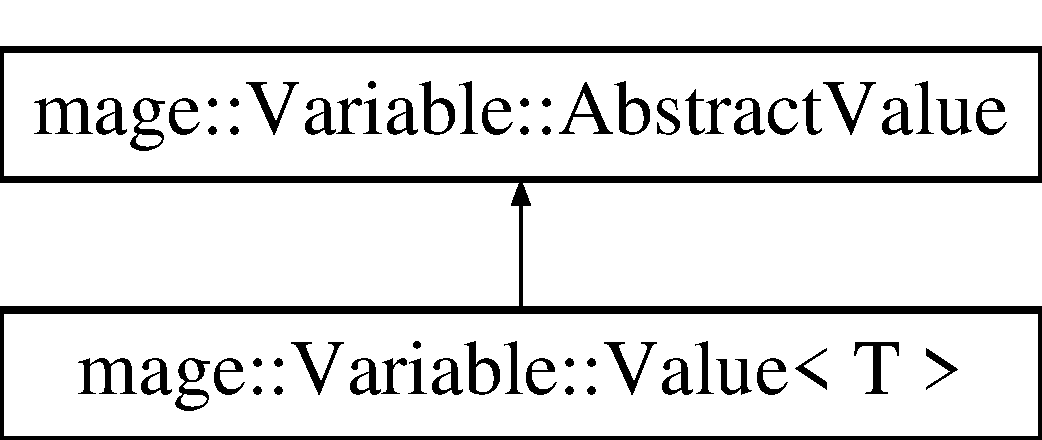
\includegraphics[height=2.000000cm]{structmage_1_1_variable_1_1_abstract_value}
\end{center}
\end{figure}
\subsection*{Public Member Functions}
\begin{DoxyCompactItemize}
\item 
virtual \hyperlink{structmage_1_1_variable_1_1_abstract_value_a7fa8fc14f81bb26f239af5f1263888a5}{$\sim$\+Abstract\+Value} ()=default
\item 
virtual const void $\ast$ \hyperlink{structmage_1_1_variable_1_1_abstract_value_aede2a77b571b80794a4254e34144f4c1}{Get\+Value} () const =0
\end{DoxyCompactItemize}
\subsection*{Protected Member Functions}
\begin{DoxyCompactItemize}
\item 
\hyperlink{structmage_1_1_variable_1_1_abstract_value_a0a96662d36697af8a17b88f6a2d8efca}{Abstract\+Value} ()=default
\item 
\hyperlink{structmage_1_1_variable_1_1_abstract_value_a09123ab568948a1a8bc7911c65fda422}{Abstract\+Value} (const \hyperlink{structmage_1_1_variable_1_1_abstract_value}{Abstract\+Value} \&abstract\+\_\+value)=default
\item 
\hyperlink{structmage_1_1_variable_1_1_abstract_value_af2decac4e5b5b52c3e6973b39a2dec5b}{Abstract\+Value} (\hyperlink{structmage_1_1_variable_1_1_abstract_value}{Abstract\+Value} \&\&abstract\+\_\+value)=default
\end{DoxyCompactItemize}
\subsection*{Private Member Functions}
\begin{DoxyCompactItemize}
\item 
\hyperlink{structmage_1_1_variable_1_1_abstract_value}{Abstract\+Value} \& \hyperlink{structmage_1_1_variable_1_1_abstract_value_a77f7107e78716a0ea76cfaedd0a50a4b}{operator=} (const \hyperlink{structmage_1_1_variable_1_1_abstract_value}{Abstract\+Value} \&abstract\+\_\+value)=delete
\item 
\hyperlink{structmage_1_1_variable_1_1_abstract_value}{Abstract\+Value} \& \hyperlink{structmage_1_1_variable_1_1_abstract_value_a4aac7aa9278054361c478b4b8a457e6e}{operator=} (\hyperlink{structmage_1_1_variable_1_1_abstract_value}{Abstract\+Value} \&\&abstract\+\_\+value)=delete
\end{DoxyCompactItemize}


\subsection{Detailed Description}
A struct of immutable abstract values.

\begin{DoxyNote}{Note}
This is an example of the Type Erasure pattern for templates. We need to keep the original type to ensure the right destructor can be called in case of non-\/primitive types. 
\end{DoxyNote}


\subsection{Constructor \& Destructor Documentation}
\hypertarget{structmage_1_1_variable_1_1_abstract_value_a7fa8fc14f81bb26f239af5f1263888a5}{}\label{structmage_1_1_variable_1_1_abstract_value_a7fa8fc14f81bb26f239af5f1263888a5} 
\index{mage\+::\+Variable\+::\+Abstract\+Value@{mage\+::\+Variable\+::\+Abstract\+Value}!````~Abstract\+Value@{$\sim$\+Abstract\+Value}}
\index{````~Abstract\+Value@{$\sim$\+Abstract\+Value}!mage\+::\+Variable\+::\+Abstract\+Value@{mage\+::\+Variable\+::\+Abstract\+Value}}
\subsubsection{\texorpdfstring{$\sim$\+Abstract\+Value()}{~AbstractValue()}}
{\footnotesize\ttfamily virtual mage\+::\+Variable\+::\+Abstract\+Value\+::$\sim$\+Abstract\+Value (\begin{DoxyParamCaption}{ }\end{DoxyParamCaption})\hspace{0.3cm}{\ttfamily [virtual]}, {\ttfamily [default]}}

Destructs this value. \hypertarget{structmage_1_1_variable_1_1_abstract_value_a0a96662d36697af8a17b88f6a2d8efca}{}\label{structmage_1_1_variable_1_1_abstract_value_a0a96662d36697af8a17b88f6a2d8efca} 
\index{mage\+::\+Variable\+::\+Abstract\+Value@{mage\+::\+Variable\+::\+Abstract\+Value}!Abstract\+Value@{Abstract\+Value}}
\index{Abstract\+Value@{Abstract\+Value}!mage\+::\+Variable\+::\+Abstract\+Value@{mage\+::\+Variable\+::\+Abstract\+Value}}
\subsubsection{\texorpdfstring{Abstract\+Value()}{AbstractValue()}\hspace{0.1cm}{\footnotesize\ttfamily [1/3]}}
{\footnotesize\ttfamily mage\+::\+Variable\+::\+Abstract\+Value\+::\+Abstract\+Value (\begin{DoxyParamCaption}{ }\end{DoxyParamCaption})\hspace{0.3cm}{\ttfamily [protected]}, {\ttfamily [default]}}

Constructs an abstract value. \hypertarget{structmage_1_1_variable_1_1_abstract_value_a09123ab568948a1a8bc7911c65fda422}{}\label{structmage_1_1_variable_1_1_abstract_value_a09123ab568948a1a8bc7911c65fda422} 
\index{mage\+::\+Variable\+::\+Abstract\+Value@{mage\+::\+Variable\+::\+Abstract\+Value}!Abstract\+Value@{Abstract\+Value}}
\index{Abstract\+Value@{Abstract\+Value}!mage\+::\+Variable\+::\+Abstract\+Value@{mage\+::\+Variable\+::\+Abstract\+Value}}
\subsubsection{\texorpdfstring{Abstract\+Value()}{AbstractValue()}\hspace{0.1cm}{\footnotesize\ttfamily [2/3]}}
{\footnotesize\ttfamily mage\+::\+Variable\+::\+Abstract\+Value\+::\+Abstract\+Value (\begin{DoxyParamCaption}\item[{const \hyperlink{structmage_1_1_variable_1_1_abstract_value}{Abstract\+Value} \&}]{abstract\+\_\+value }\end{DoxyParamCaption})\hspace{0.3cm}{\ttfamily [protected]}, {\ttfamily [default]}}

Constructs an abstract value from the given abstract value.


\begin{DoxyParams}[1]{Parameters}
\mbox{\tt in}  & {\em abstract\+\_\+value} & A reference to the abstract value. \\
\hline
\end{DoxyParams}
\hypertarget{structmage_1_1_variable_1_1_abstract_value_af2decac4e5b5b52c3e6973b39a2dec5b}{}\label{structmage_1_1_variable_1_1_abstract_value_af2decac4e5b5b52c3e6973b39a2dec5b} 
\index{mage\+::\+Variable\+::\+Abstract\+Value@{mage\+::\+Variable\+::\+Abstract\+Value}!Abstract\+Value@{Abstract\+Value}}
\index{Abstract\+Value@{Abstract\+Value}!mage\+::\+Variable\+::\+Abstract\+Value@{mage\+::\+Variable\+::\+Abstract\+Value}}
\subsubsection{\texorpdfstring{Abstract\+Value()}{AbstractValue()}\hspace{0.1cm}{\footnotesize\ttfamily [3/3]}}
{\footnotesize\ttfamily mage\+::\+Variable\+::\+Abstract\+Value\+::\+Abstract\+Value (\begin{DoxyParamCaption}\item[{\hyperlink{structmage_1_1_variable_1_1_abstract_value}{Abstract\+Value} \&\&}]{abstract\+\_\+value }\end{DoxyParamCaption})\hspace{0.3cm}{\ttfamily [protected]}, {\ttfamily [default]}}

Constructs an abstract value from the given abstract value.


\begin{DoxyParams}[1]{Parameters}
\mbox{\tt in}  & {\em abstract\+\_\+value} & A reference to the abstract value. \\
\hline
\end{DoxyParams}


\subsection{Member Function Documentation}
\hypertarget{structmage_1_1_variable_1_1_abstract_value_aede2a77b571b80794a4254e34144f4c1}{}\label{structmage_1_1_variable_1_1_abstract_value_aede2a77b571b80794a4254e34144f4c1} 
\index{mage\+::\+Variable\+::\+Abstract\+Value@{mage\+::\+Variable\+::\+Abstract\+Value}!Get\+Value@{Get\+Value}}
\index{Get\+Value@{Get\+Value}!mage\+::\+Variable\+::\+Abstract\+Value@{mage\+::\+Variable\+::\+Abstract\+Value}}
\subsubsection{\texorpdfstring{Get\+Value()}{GetValue()}}
{\footnotesize\ttfamily virtual const void$\ast$ mage\+::\+Variable\+::\+Abstract\+Value\+::\+Get\+Value (\begin{DoxyParamCaption}{ }\end{DoxyParamCaption}) const\hspace{0.3cm}{\ttfamily [pure virtual]}}

Returns the value of this value.

\begin{DoxyReturn}{Returns}
A pointer to the value of this value. 
\end{DoxyReturn}


Implemented in \hyperlink{structmage_1_1_variable_1_1_value_a04d70496ebb7ad71dafa3df877daeb26}{mage\+::\+Variable\+::\+Value$<$ T $>$}.

\hypertarget{structmage_1_1_variable_1_1_abstract_value_a77f7107e78716a0ea76cfaedd0a50a4b}{}\label{structmage_1_1_variable_1_1_abstract_value_a77f7107e78716a0ea76cfaedd0a50a4b} 
\index{mage\+::\+Variable\+::\+Abstract\+Value@{mage\+::\+Variable\+::\+Abstract\+Value}!operator=@{operator=}}
\index{operator=@{operator=}!mage\+::\+Variable\+::\+Abstract\+Value@{mage\+::\+Variable\+::\+Abstract\+Value}}
\subsubsection{\texorpdfstring{operator=()}{operator=()}\hspace{0.1cm}{\footnotesize\ttfamily [1/2]}}
{\footnotesize\ttfamily \hyperlink{structmage_1_1_variable_1_1_abstract_value}{Abstract\+Value}\& mage\+::\+Variable\+::\+Abstract\+Value\+::operator= (\begin{DoxyParamCaption}\item[{const \hyperlink{structmage_1_1_variable_1_1_abstract_value}{Abstract\+Value} \&}]{abstract\+\_\+value }\end{DoxyParamCaption})\hspace{0.3cm}{\ttfamily [private]}, {\ttfamily [delete]}}

Copies the given abstract value to this abstract value.


\begin{DoxyParams}[1]{Parameters}
\mbox{\tt in}  & {\em abstract\+\_\+value} & A reference to the abstract value to copy from. \\
\hline
\end{DoxyParams}
\begin{DoxyReturn}{Returns}
A reference to the copy of the given abstract value (i.\+e. this abstract value). 
\end{DoxyReturn}
\hypertarget{structmage_1_1_variable_1_1_abstract_value_a4aac7aa9278054361c478b4b8a457e6e}{}\label{structmage_1_1_variable_1_1_abstract_value_a4aac7aa9278054361c478b4b8a457e6e} 
\index{mage\+::\+Variable\+::\+Abstract\+Value@{mage\+::\+Variable\+::\+Abstract\+Value}!operator=@{operator=}}
\index{operator=@{operator=}!mage\+::\+Variable\+::\+Abstract\+Value@{mage\+::\+Variable\+::\+Abstract\+Value}}
\subsubsection{\texorpdfstring{operator=()}{operator=()}\hspace{0.1cm}{\footnotesize\ttfamily [2/2]}}
{\footnotesize\ttfamily \hyperlink{structmage_1_1_variable_1_1_abstract_value}{Abstract\+Value}\& mage\+::\+Variable\+::\+Abstract\+Value\+::operator= (\begin{DoxyParamCaption}\item[{\hyperlink{structmage_1_1_variable_1_1_abstract_value}{Abstract\+Value} \&\&}]{abstract\+\_\+value }\end{DoxyParamCaption})\hspace{0.3cm}{\ttfamily [private]}, {\ttfamily [delete]}}

Copies the given abstract value to this abstract value.


\begin{DoxyParams}[1]{Parameters}
\mbox{\tt in}  & {\em abstract\+\_\+value} & A reference to the abstract value to copy from. \\
\hline
\end{DoxyParams}
\begin{DoxyReturn}{Returns}
A reference to the copy of the given abstract value (i.\+e. this abstract value). 
\end{DoxyReturn}

\hypertarget{structmage_1_1_aligned_data}{}\section{mage\+:\+:Aligned\+Data$<$ DataT $>$ Struct Template Reference}
\label{structmage_1_1_aligned_data}\index{mage\+::\+Aligned\+Data$<$ Data\+T $>$@{mage\+::\+Aligned\+Data$<$ Data\+T $>$}}


{\ttfamily \#include $<$allocation.\+hpp$>$}

\subsection*{Static Public Member Functions}
\begin{DoxyCompactItemize}
\item 
static void $\ast$ \hyperlink{structmage_1_1_aligned_data_a0ddb884f1857519ceaf10d8980ff896b}{operator new} (size\+\_\+t size)
\item 
static void \hyperlink{structmage_1_1_aligned_data_a3e0b0d36f1a0a9ec78c1611103436ffc}{operator delete} (void $\ast$ptr) noexcept
\item 
static void $\ast$ \hyperlink{structmage_1_1_aligned_data_a139865ffc435aebff7703d68d8111f24}{operator new\mbox{[}$\,$\mbox{]}} (size\+\_\+t size)
\item 
static void \hyperlink{structmage_1_1_aligned_data_a257c2d30f4764caf48647e1f759d28b4}{operator delete\mbox{[}$\,$\mbox{]}} (void $\ast$ptr) noexcept
\end{DoxyCompactItemize}


\subsection{Detailed Description}
\subsubsection*{template$<$typename DataT$>$\newline
struct mage\+::\+Aligned\+Data$<$ Data\+T $>$}

A struct of aligned data.


\begin{DoxyTemplParams}{Template Parameters}
{\em The} & data type. \\
\hline
\end{DoxyTemplParams}


\subsection{Member Function Documentation}
\hypertarget{structmage_1_1_aligned_data_a3e0b0d36f1a0a9ec78c1611103436ffc}{}\label{structmage_1_1_aligned_data_a3e0b0d36f1a0a9ec78c1611103436ffc} 
\index{mage\+::\+Aligned\+Data@{mage\+::\+Aligned\+Data}!operator delete@{operator delete}}
\index{operator delete@{operator delete}!mage\+::\+Aligned\+Data@{mage\+::\+Aligned\+Data}}
\subsubsection{\texorpdfstring{operator delete()}{operator delete()}}
{\footnotesize\ttfamily template$<$typename DataT $>$ \\
static void \hyperlink{structmage_1_1_aligned_data}{mage\+::\+Aligned\+Data}$<$ DataT $>$\+::operator delete (\begin{DoxyParamCaption}\item[{void $\ast$}]{ptr }\end{DoxyParamCaption})\hspace{0.3cm}{\ttfamily [static]}, {\ttfamily [noexcept]}}

Deallocates the memory block pointed by {\itshape ptr} (if not nullptr), releasing the storage space previously allocated to it by a call to operator new and rendering that pointer location invalid.


\begin{DoxyParams}[1]{Parameters}
\mbox{\tt in}  & {\em ptr} & A pointer to the memory block that was allocated. \\
\hline
\end{DoxyParams}
\hypertarget{structmage_1_1_aligned_data_a257c2d30f4764caf48647e1f759d28b4}{}\label{structmage_1_1_aligned_data_a257c2d30f4764caf48647e1f759d28b4} 
\index{mage\+::\+Aligned\+Data@{mage\+::\+Aligned\+Data}!operator delete\mbox{[}\mbox{]}@{operator delete[]}}
\index{operator delete\mbox{[}\mbox{]}@{operator delete[]}!mage\+::\+Aligned\+Data@{mage\+::\+Aligned\+Data}}
\subsubsection{\texorpdfstring{operator delete[]()}{operator delete[]()}}
{\footnotesize\ttfamily template$<$typename DataT $>$ \\
static void \hyperlink{structmage_1_1_aligned_data}{mage\+::\+Aligned\+Data}$<$ DataT $>$\+::operator delete\mbox{[}$\,$\mbox{]} (\begin{DoxyParamCaption}\item[{void $\ast$}]{ptr }\end{DoxyParamCaption})\hspace{0.3cm}{\ttfamily [static]}, {\ttfamily [noexcept]}}

Deallocates the memory block pointed to by {\itshape ptr} (if not nullptr), releasing the storage space previously allocated to it by a call to operator new\mbox{[}\mbox{]} and rendering that pointer location invalid.


\begin{DoxyParams}[1]{Parameters}
\mbox{\tt in}  & {\em ptr} & A pointer to the memory block that was allocated. \\
\hline
\end{DoxyParams}
\hypertarget{structmage_1_1_aligned_data_a0ddb884f1857519ceaf10d8980ff896b}{}\label{structmage_1_1_aligned_data_a0ddb884f1857519ceaf10d8980ff896b} 
\index{mage\+::\+Aligned\+Data@{mage\+::\+Aligned\+Data}!operator new@{operator new}}
\index{operator new@{operator new}!mage\+::\+Aligned\+Data@{mage\+::\+Aligned\+Data}}
\subsubsection{\texorpdfstring{operator new()}{operator new()}}
{\footnotesize\ttfamily template$<$typename DataT $>$ \\
static void$\ast$ \hyperlink{structmage_1_1_aligned_data}{mage\+::\+Aligned\+Data}$<$ DataT $>$\+::operator new (\begin{DoxyParamCaption}\item[{size\+\_\+t}]{size }\end{DoxyParamCaption})\hspace{0.3cm}{\ttfamily [static]}}

Allocates {\itshape size} bytes of storage, suitably aligned to represent any object of that size, and returns a non-\/null pointer to the first byte of this block.


\begin{DoxyParams}[1]{Parameters}
\mbox{\tt in}  & {\em size} & The requested size in bytes to allocate in memory. \\
\hline
\end{DoxyParams}
\begin{DoxyReturn}{Returns}
A pointer to the memory block that was allocated. The pointer is a multiple of the given alignment. 
\end{DoxyReturn}

\begin{DoxyExceptions}{Exceptions}
{\em bad\+\_\+alloc} & Failed to allocate the memory block. \\
\hline
\end{DoxyExceptions}
\hypertarget{structmage_1_1_aligned_data_a139865ffc435aebff7703d68d8111f24}{}\label{structmage_1_1_aligned_data_a139865ffc435aebff7703d68d8111f24} 
\index{mage\+::\+Aligned\+Data@{mage\+::\+Aligned\+Data}!operator new\mbox{[}\mbox{]}@{operator new[]}}
\index{operator new\mbox{[}\mbox{]}@{operator new[]}!mage\+::\+Aligned\+Data@{mage\+::\+Aligned\+Data}}
\subsubsection{\texorpdfstring{operator new[]()}{operator new[]()}}
{\footnotesize\ttfamily template$<$typename DataT $>$ \\
static void$\ast$ \hyperlink{structmage_1_1_aligned_data}{mage\+::\+Aligned\+Data}$<$ DataT $>$\+::operator new\mbox{[}$\,$\mbox{]} (\begin{DoxyParamCaption}\item[{size\+\_\+t}]{size }\end{DoxyParamCaption})\hspace{0.3cm}{\ttfamily [static]}}

Allocates {\itshape size} bytes of storage, suitably aligned to represent any object of that size, and returns a non-\/null pointer to the first byte of this block.


\begin{DoxyParams}[1]{Parameters}
\mbox{\tt in}  & {\em size} & The requested size in bytes to allocate in memory. \\
\hline
\end{DoxyParams}
\begin{DoxyReturn}{Returns}
A pointer to the memory block that was allocated. The pointer is a multiple of the given alignment. 
\end{DoxyReturn}

\begin{DoxyExceptions}{Exceptions}
{\em bad\+\_\+alloc} & Failed to allocate the memory block. \\
\hline
\end{DoxyExceptions}

\hypertarget{classmage_1_1_ambient_light}{}\section{mage\+:\+:Ambient\+Light Class Reference}
\label{classmage_1_1_ambient_light}\index{mage\+::\+Ambient\+Light@{mage\+::\+Ambient\+Light}}


{\ttfamily \#include $<$ambient\+\_\+light.\+hpp$>$}

Inheritance diagram for mage\+:\+:Ambient\+Light\+:\begin{figure}[H]
\begin{center}
\leavevmode
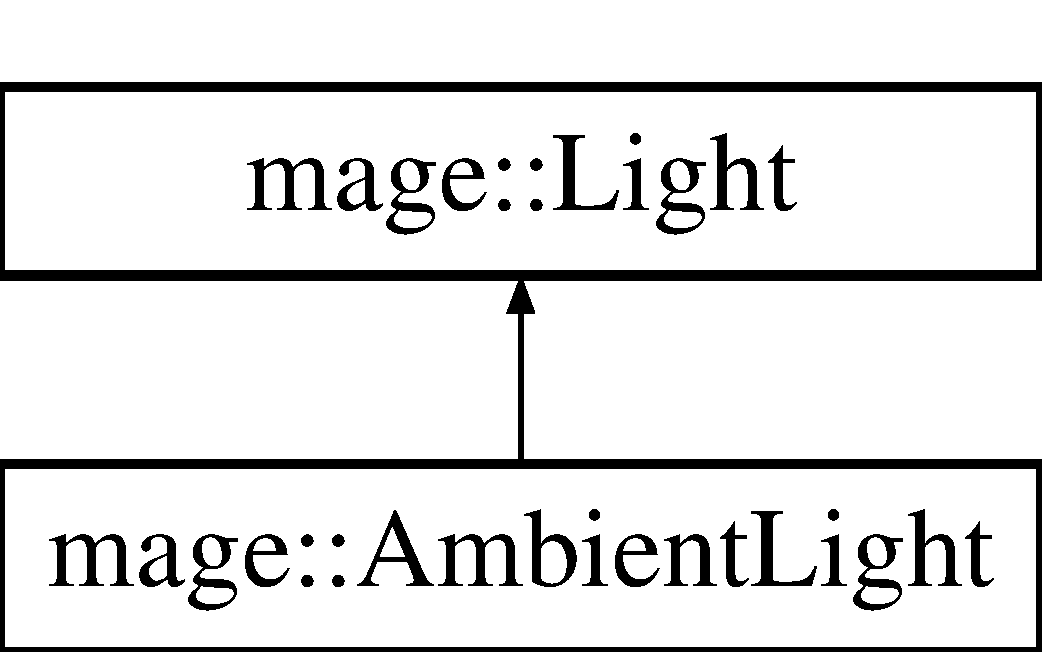
\includegraphics[height=2.000000cm]{classmage_1_1_ambient_light}
\end{center}
\end{figure}
\subsection*{Public Member Functions}
\begin{DoxyCompactItemize}
\item 
\hyperlink{classmage_1_1_ambient_light_a753dd42af4b6ad15b2f0867a99d6aabe}{Ambient\+Light} ()
\item 
\hyperlink{classmage_1_1_ambient_light_ac5295d1f90e64d3e59ff2856df32a187}{Ambient\+Light} (const \hyperlink{classmage_1_1_ambient_light}{Ambient\+Light} \&light)
\item 
\hyperlink{classmage_1_1_ambient_light_aab4919587032054d28ec15cf5639ad48}{Ambient\+Light} (\hyperlink{classmage_1_1_ambient_light}{Ambient\+Light} \&\&light)
\item 
virtual \hyperlink{classmage_1_1_ambient_light_a511bb794b11f112e750da09f4044e7db}{$\sim$\+Ambient\+Light} ()
\item 
\hyperlink{classmage_1_1_ambient_light}{Ambient\+Light} \& \hyperlink{classmage_1_1_ambient_light_aa8bbeaca08a626b6b5f5447a847724cc}{operator=} (const \hyperlink{classmage_1_1_ambient_light}{Ambient\+Light} \&light)
\item 
\hyperlink{classmage_1_1_ambient_light}{Ambient\+Light} \& \hyperlink{classmage_1_1_ambient_light_ae54bf8695957fb438e162a913725922a}{operator=} (\hyperlink{classmage_1_1_ambient_light}{Ambient\+Light} \&\&light)
\item 
\hyperlink{namespacemage_a3316d7143a973e37adf1110f2e80ca31}{Unique\+Ptr}$<$ \hyperlink{classmage_1_1_ambient_light}{Ambient\+Light} $>$ \hyperlink{classmage_1_1_ambient_light_a542a68882bc0807cf5f9a37391b9f44e}{Clone} () const
\item 
\hyperlink{namespacemage_aa97e833b45f06d60a0a9c4fc22ae02c0}{F32} \hyperlink{classmage_1_1_ambient_light_ab41f72d902f590ebc62ab58427e2bdab}{Get\+Radiance} () const noexcept
\item 
void \hyperlink{classmage_1_1_ambient_light_aac9a833f2261eaa1bf5eaab7608fc878}{Set\+Radiance} (\hyperlink{namespacemage_aa97e833b45f06d60a0a9c4fc22ae02c0}{F32} radiance) noexcept
\item 
const \hyperlink{structmage_1_1_r_g_b}{R\+GB} \hyperlink{classmage_1_1_ambient_light_a5d135eeeef619f13435341eebd3fe476}{Get\+Radiance\+Spectrum} () const noexcept
\end{DoxyCompactItemize}
\subsection*{Private Member Functions}
\begin{DoxyCompactItemize}
\item 
virtual \hyperlink{namespacemage_a3316d7143a973e37adf1110f2e80ca31}{Unique\+Ptr}$<$ \hyperlink{classmage_1_1_light}{Light} $>$ \hyperlink{classmage_1_1_ambient_light_a7223a4770653c20e662810b0956c6e51}{Clone\+Implementation} () const override
\end{DoxyCompactItemize}
\subsection*{Private Attributes}
\begin{DoxyCompactItemize}
\item 
\hyperlink{namespacemage_aa97e833b45f06d60a0a9c4fc22ae02c0}{F32} \hyperlink{classmage_1_1_ambient_light_a579aff19284637d89d85026b373574aa}{m\+\_\+radiance}
\end{DoxyCompactItemize}
\subsection*{Additional Inherited Members}


\subsection{Detailed Description}
A class of ambient lights. 

\subsection{Constructor \& Destructor Documentation}
\hypertarget{classmage_1_1_ambient_light_a753dd42af4b6ad15b2f0867a99d6aabe}{}\label{classmage_1_1_ambient_light_a753dd42af4b6ad15b2f0867a99d6aabe} 
\index{mage\+::\+Ambient\+Light@{mage\+::\+Ambient\+Light}!Ambient\+Light@{Ambient\+Light}}
\index{Ambient\+Light@{Ambient\+Light}!mage\+::\+Ambient\+Light@{mage\+::\+Ambient\+Light}}
\subsubsection{\texorpdfstring{Ambient\+Light()}{AmbientLight()}\hspace{0.1cm}{\footnotesize\ttfamily [1/3]}}
{\footnotesize\ttfamily mage\+::\+Ambient\+Light\+::\+Ambient\+Light (\begin{DoxyParamCaption}{ }\end{DoxyParamCaption})}

Constructs an ambient light. \hypertarget{classmage_1_1_ambient_light_ac5295d1f90e64d3e59ff2856df32a187}{}\label{classmage_1_1_ambient_light_ac5295d1f90e64d3e59ff2856df32a187} 
\index{mage\+::\+Ambient\+Light@{mage\+::\+Ambient\+Light}!Ambient\+Light@{Ambient\+Light}}
\index{Ambient\+Light@{Ambient\+Light}!mage\+::\+Ambient\+Light@{mage\+::\+Ambient\+Light}}
\subsubsection{\texorpdfstring{Ambient\+Light()}{AmbientLight()}\hspace{0.1cm}{\footnotesize\ttfamily [2/3]}}
{\footnotesize\ttfamily mage\+::\+Ambient\+Light\+::\+Ambient\+Light (\begin{DoxyParamCaption}\item[{const \hyperlink{classmage_1_1_ambient_light}{Ambient\+Light} \&}]{light }\end{DoxyParamCaption})\hspace{0.3cm}{\ttfamily [default]}}

Constructs an ambient light from the given ambient light.


\begin{DoxyParams}[1]{Parameters}
\mbox{\tt in}  & {\em light} & A reference to the ambient light to copy. \\
\hline
\end{DoxyParams}
\hypertarget{classmage_1_1_ambient_light_aab4919587032054d28ec15cf5639ad48}{}\label{classmage_1_1_ambient_light_aab4919587032054d28ec15cf5639ad48} 
\index{mage\+::\+Ambient\+Light@{mage\+::\+Ambient\+Light}!Ambient\+Light@{Ambient\+Light}}
\index{Ambient\+Light@{Ambient\+Light}!mage\+::\+Ambient\+Light@{mage\+::\+Ambient\+Light}}
\subsubsection{\texorpdfstring{Ambient\+Light()}{AmbientLight()}\hspace{0.1cm}{\footnotesize\ttfamily [3/3]}}
{\footnotesize\ttfamily mage\+::\+Ambient\+Light\+::\+Ambient\+Light (\begin{DoxyParamCaption}\item[{\hyperlink{classmage_1_1_ambient_light}{Ambient\+Light} \&\&}]{light }\end{DoxyParamCaption})\hspace{0.3cm}{\ttfamily [default]}}

Constructs an ambient light by moving the given ambient light.


\begin{DoxyParams}[1]{Parameters}
\mbox{\tt in}  & {\em light} & A reference to the ambient light to move. \\
\hline
\end{DoxyParams}
\hypertarget{classmage_1_1_ambient_light_a511bb794b11f112e750da09f4044e7db}{}\label{classmage_1_1_ambient_light_a511bb794b11f112e750da09f4044e7db} 
\index{mage\+::\+Ambient\+Light@{mage\+::\+Ambient\+Light}!````~Ambient\+Light@{$\sim$\+Ambient\+Light}}
\index{````~Ambient\+Light@{$\sim$\+Ambient\+Light}!mage\+::\+Ambient\+Light@{mage\+::\+Ambient\+Light}}
\subsubsection{\texorpdfstring{$\sim$\+Ambient\+Light()}{~AmbientLight()}}
{\footnotesize\ttfamily mage\+::\+Ambient\+Light\+::$\sim$\+Ambient\+Light (\begin{DoxyParamCaption}{ }\end{DoxyParamCaption})\hspace{0.3cm}{\ttfamily [virtual]}, {\ttfamily [default]}}

Destructs this ambient light. 

\subsection{Member Function Documentation}
\hypertarget{classmage_1_1_ambient_light_a542a68882bc0807cf5f9a37391b9f44e}{}\label{classmage_1_1_ambient_light_a542a68882bc0807cf5f9a37391b9f44e} 
\index{mage\+::\+Ambient\+Light@{mage\+::\+Ambient\+Light}!Clone@{Clone}}
\index{Clone@{Clone}!mage\+::\+Ambient\+Light@{mage\+::\+Ambient\+Light}}
\subsubsection{\texorpdfstring{Clone()}{Clone()}}
{\footnotesize\ttfamily \hyperlink{namespacemage_a3316d7143a973e37adf1110f2e80ca31}{Unique\+Ptr}$<$ \hyperlink{classmage_1_1_ambient_light}{Ambient\+Light} $>$ mage\+::\+Ambient\+Light\+::\+Clone (\begin{DoxyParamCaption}{ }\end{DoxyParamCaption}) const}

Clones this ambient light.

\begin{DoxyReturn}{Returns}
A pointer to the clone of this ambient light. 
\end{DoxyReturn}
\hypertarget{classmage_1_1_ambient_light_a7223a4770653c20e662810b0956c6e51}{}\label{classmage_1_1_ambient_light_a7223a4770653c20e662810b0956c6e51} 
\index{mage\+::\+Ambient\+Light@{mage\+::\+Ambient\+Light}!Clone\+Implementation@{Clone\+Implementation}}
\index{Clone\+Implementation@{Clone\+Implementation}!mage\+::\+Ambient\+Light@{mage\+::\+Ambient\+Light}}
\subsubsection{\texorpdfstring{Clone\+Implementation()}{CloneImplementation()}}
{\footnotesize\ttfamily \hyperlink{namespacemage_a3316d7143a973e37adf1110f2e80ca31}{Unique\+Ptr}$<$ \hyperlink{classmage_1_1_light}{Light} $>$ mage\+::\+Ambient\+Light\+::\+Clone\+Implementation (\begin{DoxyParamCaption}{ }\end{DoxyParamCaption}) const\hspace{0.3cm}{\ttfamily [override]}, {\ttfamily [private]}, {\ttfamily [virtual]}}

Clones this ambient light.

\begin{DoxyReturn}{Returns}
A pointer to the clone of this ambient light. 
\end{DoxyReturn}


Implements \hyperlink{classmage_1_1_light_aa613d76a1ebda69efde853d15f75490c}{mage\+::\+Light}.

\hypertarget{classmage_1_1_ambient_light_ab41f72d902f590ebc62ab58427e2bdab}{}\label{classmage_1_1_ambient_light_ab41f72d902f590ebc62ab58427e2bdab} 
\index{mage\+::\+Ambient\+Light@{mage\+::\+Ambient\+Light}!Get\+Radiance@{Get\+Radiance}}
\index{Get\+Radiance@{Get\+Radiance}!mage\+::\+Ambient\+Light@{mage\+::\+Ambient\+Light}}
\subsubsection{\texorpdfstring{Get\+Radiance()}{GetRadiance()}}
{\footnotesize\ttfamily \hyperlink{namespacemage_aa97e833b45f06d60a0a9c4fc22ae02c0}{F32} mage\+::\+Ambient\+Light\+::\+Get\+Radiance (\begin{DoxyParamCaption}{ }\end{DoxyParamCaption}) const\hspace{0.3cm}{\ttfamily [noexcept]}}

Returns the radiance of this ambient light.

\begin{DoxyReturn}{Returns}
The radiance in watts per square meter per steradians of this ambient light. 
\end{DoxyReturn}
\hypertarget{classmage_1_1_ambient_light_a5d135eeeef619f13435341eebd3fe476}{}\label{classmage_1_1_ambient_light_a5d135eeeef619f13435341eebd3fe476} 
\index{mage\+::\+Ambient\+Light@{mage\+::\+Ambient\+Light}!Get\+Radiance\+Spectrum@{Get\+Radiance\+Spectrum}}
\index{Get\+Radiance\+Spectrum@{Get\+Radiance\+Spectrum}!mage\+::\+Ambient\+Light@{mage\+::\+Ambient\+Light}}
\subsubsection{\texorpdfstring{Get\+Radiance\+Spectrum()}{GetRadianceSpectrum()}}
{\footnotesize\ttfamily const \hyperlink{structmage_1_1_r_g_b}{R\+GB} mage\+::\+Ambient\+Light\+::\+Get\+Radiance\+Spectrum (\begin{DoxyParamCaption}{ }\end{DoxyParamCaption}) const\hspace{0.3cm}{\ttfamily [noexcept]}}

Returns the radiance spectrum of this ambient light.

\begin{DoxyReturn}{Returns}
The radiance spectrum of this ambient light. 
\end{DoxyReturn}
\hypertarget{classmage_1_1_ambient_light_aa8bbeaca08a626b6b5f5447a847724cc}{}\label{classmage_1_1_ambient_light_aa8bbeaca08a626b6b5f5447a847724cc} 
\index{mage\+::\+Ambient\+Light@{mage\+::\+Ambient\+Light}!operator=@{operator=}}
\index{operator=@{operator=}!mage\+::\+Ambient\+Light@{mage\+::\+Ambient\+Light}}
\subsubsection{\texorpdfstring{operator=()}{operator=()}\hspace{0.1cm}{\footnotesize\ttfamily [1/2]}}
{\footnotesize\ttfamily \hyperlink{classmage_1_1_ambient_light}{Ambient\+Light} \& mage\+::\+Ambient\+Light\+::operator= (\begin{DoxyParamCaption}\item[{const \hyperlink{classmage_1_1_ambient_light}{Ambient\+Light} \&}]{light }\end{DoxyParamCaption})\hspace{0.3cm}{\ttfamily [default]}}

Copies the given ambient light to this ambient light.


\begin{DoxyParams}[1]{Parameters}
\mbox{\tt in}  & {\em light} & A reference to the ambient light to copy. \\
\hline
\end{DoxyParams}
\begin{DoxyReturn}{Returns}
A reference to the copy of the given ambient light (i.\+e. this ambient light). 
\end{DoxyReturn}
\hypertarget{classmage_1_1_ambient_light_ae54bf8695957fb438e162a913725922a}{}\label{classmage_1_1_ambient_light_ae54bf8695957fb438e162a913725922a} 
\index{mage\+::\+Ambient\+Light@{mage\+::\+Ambient\+Light}!operator=@{operator=}}
\index{operator=@{operator=}!mage\+::\+Ambient\+Light@{mage\+::\+Ambient\+Light}}
\subsubsection{\texorpdfstring{operator=()}{operator=()}\hspace{0.1cm}{\footnotesize\ttfamily [2/2]}}
{\footnotesize\ttfamily \hyperlink{classmage_1_1_ambient_light}{Ambient\+Light} \& mage\+::\+Ambient\+Light\+::operator= (\begin{DoxyParamCaption}\item[{\hyperlink{classmage_1_1_ambient_light}{Ambient\+Light} \&\&}]{light }\end{DoxyParamCaption})\hspace{0.3cm}{\ttfamily [default]}}

Moves the given ambient light to this ambient light.


\begin{DoxyParams}[1]{Parameters}
\mbox{\tt in}  & {\em light} & A reference to the ambient light to move. \\
\hline
\end{DoxyParams}
\begin{DoxyReturn}{Returns}
A reference to the moved ambient light (i.\+e. this ambient light). 
\end{DoxyReturn}
\hypertarget{classmage_1_1_ambient_light_aac9a833f2261eaa1bf5eaab7608fc878}{}\label{classmage_1_1_ambient_light_aac9a833f2261eaa1bf5eaab7608fc878} 
\index{mage\+::\+Ambient\+Light@{mage\+::\+Ambient\+Light}!Set\+Radiance@{Set\+Radiance}}
\index{Set\+Radiance@{Set\+Radiance}!mage\+::\+Ambient\+Light@{mage\+::\+Ambient\+Light}}
\subsubsection{\texorpdfstring{Set\+Radiance()}{SetRadiance()}}
{\footnotesize\ttfamily void mage\+::\+Ambient\+Light\+::\+Set\+Radiance (\begin{DoxyParamCaption}\item[{\hyperlink{namespacemage_aa97e833b45f06d60a0a9c4fc22ae02c0}{F32}}]{radiance }\end{DoxyParamCaption})\hspace{0.3cm}{\ttfamily [noexcept]}}

Sets the radiance of this ambient light to the given radiance.

\begin{DoxyPrecond}{Precondition}
{\itshape radiance} must be non-\/negative. 
\end{DoxyPrecond}

\begin{DoxyParams}[1]{Parameters}
\mbox{\tt in}  & {\em radiance} & The radiance in watts per square meter per steradians. \\
\hline
\end{DoxyParams}


\subsection{Member Data Documentation}
\hypertarget{classmage_1_1_ambient_light_a579aff19284637d89d85026b373574aa}{}\label{classmage_1_1_ambient_light_a579aff19284637d89d85026b373574aa} 
\index{mage\+::\+Ambient\+Light@{mage\+::\+Ambient\+Light}!m\+\_\+radiance@{m\+\_\+radiance}}
\index{m\+\_\+radiance@{m\+\_\+radiance}!mage\+::\+Ambient\+Light@{mage\+::\+Ambient\+Light}}
\subsubsection{\texorpdfstring{m\+\_\+radiance}{m\_radiance}}
{\footnotesize\ttfamily \hyperlink{namespacemage_aa97e833b45f06d60a0a9c4fc22ae02c0}{F32} mage\+::\+Ambient\+Light\+::m\+\_\+radiance\hspace{0.3cm}{\ttfamily [private]}}

The radiance in watts per square meter per steradians of this ambient light. 
\hypertarget{classmage_1_1_basic_pixel_shader}{}\section{mage\+:\+:Basic\+Pixel\+Shader Class Reference}
\label{classmage_1_1_basic_pixel_shader}\index{mage\+::\+Basic\+Pixel\+Shader@{mage\+::\+Basic\+Pixel\+Shader}}


{\ttfamily \#include $<$basic\+\_\+shader.\+hpp$>$}

Inheritance diagram for mage\+:\+:Basic\+Pixel\+Shader\+:\begin{figure}[H]
\begin{center}
\leavevmode
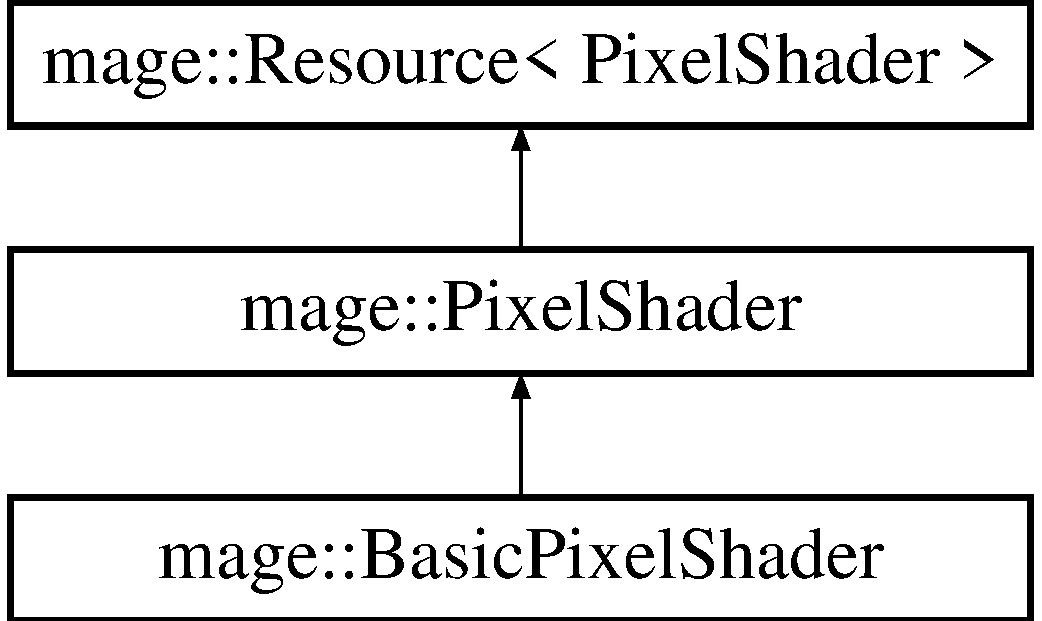
\includegraphics[height=3.000000cm]{classmage_1_1_basic_pixel_shader}
\end{center}
\end{figure}
\subsection*{Public Member Functions}
\begin{DoxyCompactItemize}
\item 
\hyperlink{classmage_1_1_basic_pixel_shader_ae89993e3ba1ab6461e4e984ee8c7b819}{Basic\+Pixel\+Shader} (const wstring \&fname)
\item 
\hyperlink{classmage_1_1_basic_pixel_shader_a6d4283d378d5655e25f7c20014a9663e}{Basic\+Pixel\+Shader} (const wstring \&fname, I\+D3\+D11\+Device2 $\ast$device, I\+D3\+D11\+Device\+Context2 $\ast$device\+\_\+context)
\item 
\hyperlink{classmage_1_1_basic_pixel_shader_ad7be28d3429b13d7adf6c150c173a117}{Basic\+Pixel\+Shader} (const wstring \&guid, const \hyperlink{structmage_1_1_compiled_pixel_shader}{Compiled\+Pixel\+Shader} \&compiled\+\_\+pixel\+\_\+shader)
\item 
\hyperlink{classmage_1_1_basic_pixel_shader_a931200fdba2748e374103d85a66690c5}{Basic\+Pixel\+Shader} (const wstring \&guid, I\+D3\+D11\+Device2 $\ast$device, I\+D3\+D11\+Device\+Context2 $\ast$device\+\_\+context, const \hyperlink{structmage_1_1_compiled_pixel_shader}{Compiled\+Pixel\+Shader} \&compiled\+\_\+pixel\+\_\+shader)
\item 
\hyperlink{classmage_1_1_basic_pixel_shader_ab82055206ff2a05b73f18ce23353a4bb}{Basic\+Pixel\+Shader} (const \hyperlink{classmage_1_1_basic_pixel_shader}{Basic\+Pixel\+Shader} \&pixel\+\_\+shader)=delete
\item 
\hyperlink{classmage_1_1_basic_pixel_shader_a0a5366edb694e78e4c8075fad70b7dff}{Basic\+Pixel\+Shader} (\hyperlink{classmage_1_1_basic_pixel_shader}{Basic\+Pixel\+Shader} \&\&pixel\+\_\+shader)
\item 
virtual \hyperlink{classmage_1_1_basic_pixel_shader_a7b4ac308850eb9ad55cbbd1e6389271b}{$\sim$\+Basic\+Pixel\+Shader} ()
\item 
\hyperlink{classmage_1_1_basic_pixel_shader}{Basic\+Pixel\+Shader} \& \hyperlink{classmage_1_1_basic_pixel_shader_a9656fdae2d17691d3e7dd850e7844efb}{operator=} (const \hyperlink{classmage_1_1_basic_pixel_shader}{Basic\+Pixel\+Shader} \&pixel\+\_\+shader)=delete
\item 
\hyperlink{classmage_1_1_basic_pixel_shader}{Basic\+Pixel\+Shader} \& \hyperlink{classmage_1_1_basic_pixel_shader_a5d6224f0454d1d1f9583f6b9f8ad8201}{operator=} (\hyperlink{classmage_1_1_basic_pixel_shader}{Basic\+Pixel\+Shader} \&\&pixel\+\_\+shader)=delete
\item 
virtual void \hyperlink{classmage_1_1_basic_pixel_shader_a67ce881c6c02b2ceabca29cd3b6a4a89}{Prepare\+Shading} (const \hyperlink{structmage_1_1_material}{Material} \&material, const \hyperlink{structmage_1_1_lighting}{Lighting} \&lighting) const override final
\end{DoxyCompactItemize}
\subsection*{Private Attributes}
\begin{DoxyCompactItemize}
\item 
\hyperlink{structmage_1_1_constant_buffer}{Constant\+Buffer}$<$ Material\+Buffer $>$ \hyperlink{classmage_1_1_basic_pixel_shader_aa61f52d3524276e234dbd2a1f3f13d6d}{m\+\_\+material\+\_\+buffer}
\end{DoxyCompactItemize}
\subsection*{Additional Inherited Members}


\subsection{Detailed Description}
A class of basic pixel shaders. 

\subsection{Constructor \& Destructor Documentation}
\hypertarget{classmage_1_1_basic_pixel_shader_ae89993e3ba1ab6461e4e984ee8c7b819}{}\label{classmage_1_1_basic_pixel_shader_ae89993e3ba1ab6461e4e984ee8c7b819} 
\index{mage\+::\+Basic\+Pixel\+Shader@{mage\+::\+Basic\+Pixel\+Shader}!Basic\+Pixel\+Shader@{Basic\+Pixel\+Shader}}
\index{Basic\+Pixel\+Shader@{Basic\+Pixel\+Shader}!mage\+::\+Basic\+Pixel\+Shader@{mage\+::\+Basic\+Pixel\+Shader}}
\subsubsection{\texorpdfstring{Basic\+Pixel\+Shader()}{BasicPixelShader()}\hspace{0.1cm}{\footnotesize\ttfamily [1/6]}}
{\footnotesize\ttfamily mage\+::\+Basic\+Pixel\+Shader\+::\+Basic\+Pixel\+Shader (\begin{DoxyParamCaption}\item[{const wstring \&}]{fname }\end{DoxyParamCaption})\hspace{0.3cm}{\ttfamily [explicit]}}

Constructs a basic pixel shader.

\begin{DoxyPrecond}{Precondition}
The current engine must be loaded. 
\end{DoxyPrecond}

\begin{DoxyParams}[1]{Parameters}
\mbox{\tt in}  & {\em fname} & A reference to the filename (the globally unique identifier). \\
\hline
\end{DoxyParams}

\begin{DoxyExceptions}{Exceptions}
{\em \hyperlink{structmage_1_1_formatted_exception}{Formatted\+Exception}} & Failed to initialize this pixel shader. \\
\hline
\end{DoxyExceptions}
\hypertarget{classmage_1_1_basic_pixel_shader_a6d4283d378d5655e25f7c20014a9663e}{}\label{classmage_1_1_basic_pixel_shader_a6d4283d378d5655e25f7c20014a9663e} 
\index{mage\+::\+Basic\+Pixel\+Shader@{mage\+::\+Basic\+Pixel\+Shader}!Basic\+Pixel\+Shader@{Basic\+Pixel\+Shader}}
\index{Basic\+Pixel\+Shader@{Basic\+Pixel\+Shader}!mage\+::\+Basic\+Pixel\+Shader@{mage\+::\+Basic\+Pixel\+Shader}}
\subsubsection{\texorpdfstring{Basic\+Pixel\+Shader()}{BasicPixelShader()}\hspace{0.1cm}{\footnotesize\ttfamily [2/6]}}
{\footnotesize\ttfamily mage\+::\+Basic\+Pixel\+Shader\+::\+Basic\+Pixel\+Shader (\begin{DoxyParamCaption}\item[{const wstring \&}]{fname,  }\item[{I\+D3\+D11\+Device2 $\ast$}]{device,  }\item[{I\+D3\+D11\+Device\+Context2 $\ast$}]{device\+\_\+context }\end{DoxyParamCaption})\hspace{0.3cm}{\ttfamily [explicit]}}

Constructs a basic pixel shader.

\begin{DoxyPrecond}{Precondition}
{\itshape device} is not equal to {\ttfamily nullptr}. 

{\itshape device\+\_\+context} is not equal to {\ttfamily nullptr}. 
\end{DoxyPrecond}

\begin{DoxyParams}[1]{Parameters}
\mbox{\tt in}  & {\em fname} & A reference to the filename (the globally unique identifier). \\
\hline
\mbox{\tt in}  & {\em device} & A pointer to the device. \\
\hline
\mbox{\tt in}  & {\em device\+\_\+context} & A pointer to the device context. \\
\hline
\end{DoxyParams}

\begin{DoxyExceptions}{Exceptions}
{\em \hyperlink{structmage_1_1_formatted_exception}{Formatted\+Exception}} & Failed to initialize this pixel shader. \\
\hline
\end{DoxyExceptions}
\hypertarget{classmage_1_1_basic_pixel_shader_ad7be28d3429b13d7adf6c150c173a117}{}\label{classmage_1_1_basic_pixel_shader_ad7be28d3429b13d7adf6c150c173a117} 
\index{mage\+::\+Basic\+Pixel\+Shader@{mage\+::\+Basic\+Pixel\+Shader}!Basic\+Pixel\+Shader@{Basic\+Pixel\+Shader}}
\index{Basic\+Pixel\+Shader@{Basic\+Pixel\+Shader}!mage\+::\+Basic\+Pixel\+Shader@{mage\+::\+Basic\+Pixel\+Shader}}
\subsubsection{\texorpdfstring{Basic\+Pixel\+Shader()}{BasicPixelShader()}\hspace{0.1cm}{\footnotesize\ttfamily [3/6]}}
{\footnotesize\ttfamily mage\+::\+Basic\+Pixel\+Shader\+::\+Basic\+Pixel\+Shader (\begin{DoxyParamCaption}\item[{const wstring \&}]{guid,  }\item[{const \hyperlink{structmage_1_1_compiled_pixel_shader}{Compiled\+Pixel\+Shader} \&}]{compiled\+\_\+pixel\+\_\+shader }\end{DoxyParamCaption})\hspace{0.3cm}{\ttfamily [explicit]}}

Constructs a basic pixel shader.

\begin{DoxyPrecond}{Precondition}
The current engine must be loaded. 
\end{DoxyPrecond}

\begin{DoxyParams}[1]{Parameters}
\mbox{\tt in}  & {\em guid} & A reference to the globally unique identifier. \\
\hline
\mbox{\tt in}  & {\em compiled\+\_\+pixel\+\_\+shader} & A reference to the compiled pixel shader. \\
\hline
\end{DoxyParams}

\begin{DoxyExceptions}{Exceptions}
{\em \hyperlink{structmage_1_1_formatted_exception}{Formatted\+Exception}} & Failed to initialize this pixel shader. \\
\hline
\end{DoxyExceptions}
\hypertarget{classmage_1_1_basic_pixel_shader_a931200fdba2748e374103d85a66690c5}{}\label{classmage_1_1_basic_pixel_shader_a931200fdba2748e374103d85a66690c5} 
\index{mage\+::\+Basic\+Pixel\+Shader@{mage\+::\+Basic\+Pixel\+Shader}!Basic\+Pixel\+Shader@{Basic\+Pixel\+Shader}}
\index{Basic\+Pixel\+Shader@{Basic\+Pixel\+Shader}!mage\+::\+Basic\+Pixel\+Shader@{mage\+::\+Basic\+Pixel\+Shader}}
\subsubsection{\texorpdfstring{Basic\+Pixel\+Shader()}{BasicPixelShader()}\hspace{0.1cm}{\footnotesize\ttfamily [4/6]}}
{\footnotesize\ttfamily mage\+::\+Basic\+Pixel\+Shader\+::\+Basic\+Pixel\+Shader (\begin{DoxyParamCaption}\item[{const wstring \&}]{guid,  }\item[{I\+D3\+D11\+Device2 $\ast$}]{device,  }\item[{I\+D3\+D11\+Device\+Context2 $\ast$}]{device\+\_\+context,  }\item[{const \hyperlink{structmage_1_1_compiled_pixel_shader}{Compiled\+Pixel\+Shader} \&}]{compiled\+\_\+pixel\+\_\+shader }\end{DoxyParamCaption})\hspace{0.3cm}{\ttfamily [explicit]}}

Constructs a basic pixel shader.

\begin{DoxyPrecond}{Precondition}
{\itshape device} is not equal to {\ttfamily nullptr}. 

{\itshape device\+\_\+context} is not equal to {\ttfamily nullptr}. 
\end{DoxyPrecond}

\begin{DoxyParams}[1]{Parameters}
\mbox{\tt in}  & {\em guid} & A reference to the globally unique identifier. \\
\hline
\mbox{\tt in}  & {\em device} & A pointer to the device. \\
\hline
\mbox{\tt in}  & {\em device\+\_\+context} & A pointer to the device context. \\
\hline
\mbox{\tt in}  & {\em compiled\+\_\+pixel\+\_\+shader} & A reference to the compiled pixel shader. \\
\hline
\end{DoxyParams}

\begin{DoxyExceptions}{Exceptions}
{\em \hyperlink{structmage_1_1_formatted_exception}{Formatted\+Exception}} & Failed to initialize this pixel shader. \\
\hline
\end{DoxyExceptions}
\hypertarget{classmage_1_1_basic_pixel_shader_ab82055206ff2a05b73f18ce23353a4bb}{}\label{classmage_1_1_basic_pixel_shader_ab82055206ff2a05b73f18ce23353a4bb} 
\index{mage\+::\+Basic\+Pixel\+Shader@{mage\+::\+Basic\+Pixel\+Shader}!Basic\+Pixel\+Shader@{Basic\+Pixel\+Shader}}
\index{Basic\+Pixel\+Shader@{Basic\+Pixel\+Shader}!mage\+::\+Basic\+Pixel\+Shader@{mage\+::\+Basic\+Pixel\+Shader}}
\subsubsection{\texorpdfstring{Basic\+Pixel\+Shader()}{BasicPixelShader()}\hspace{0.1cm}{\footnotesize\ttfamily [5/6]}}
{\footnotesize\ttfamily mage\+::\+Basic\+Pixel\+Shader\+::\+Basic\+Pixel\+Shader (\begin{DoxyParamCaption}\item[{const \hyperlink{classmage_1_1_basic_pixel_shader}{Basic\+Pixel\+Shader} \&}]{pixel\+\_\+shader }\end{DoxyParamCaption})\hspace{0.3cm}{\ttfamily [delete]}}

Constructs a basic pixel shader from the given basic pixel shader.


\begin{DoxyParams}[1]{Parameters}
\mbox{\tt in}  & {\em pixel\+\_\+shader} & A reference to the basic pixel shader to copy. \\
\hline
\end{DoxyParams}
\hypertarget{classmage_1_1_basic_pixel_shader_a0a5366edb694e78e4c8075fad70b7dff}{}\label{classmage_1_1_basic_pixel_shader_a0a5366edb694e78e4c8075fad70b7dff} 
\index{mage\+::\+Basic\+Pixel\+Shader@{mage\+::\+Basic\+Pixel\+Shader}!Basic\+Pixel\+Shader@{Basic\+Pixel\+Shader}}
\index{Basic\+Pixel\+Shader@{Basic\+Pixel\+Shader}!mage\+::\+Basic\+Pixel\+Shader@{mage\+::\+Basic\+Pixel\+Shader}}
\subsubsection{\texorpdfstring{Basic\+Pixel\+Shader()}{BasicPixelShader()}\hspace{0.1cm}{\footnotesize\ttfamily [6/6]}}
{\footnotesize\ttfamily mage\+::\+Basic\+Pixel\+Shader\+::\+Basic\+Pixel\+Shader (\begin{DoxyParamCaption}\item[{\hyperlink{classmage_1_1_basic_pixel_shader}{Basic\+Pixel\+Shader} \&\&}]{pixel\+\_\+shader }\end{DoxyParamCaption})\hspace{0.3cm}{\ttfamily [default]}}

Constructs a basic pixel shader by moving the given basic pixel shader.


\begin{DoxyParams}[1]{Parameters}
\mbox{\tt in}  & {\em pixel\+\_\+shader} & A reference to the basic pixel shader to move. \\
\hline
\end{DoxyParams}
\hypertarget{classmage_1_1_basic_pixel_shader_a7b4ac308850eb9ad55cbbd1e6389271b}{}\label{classmage_1_1_basic_pixel_shader_a7b4ac308850eb9ad55cbbd1e6389271b} 
\index{mage\+::\+Basic\+Pixel\+Shader@{mage\+::\+Basic\+Pixel\+Shader}!````~Basic\+Pixel\+Shader@{$\sim$\+Basic\+Pixel\+Shader}}
\index{````~Basic\+Pixel\+Shader@{$\sim$\+Basic\+Pixel\+Shader}!mage\+::\+Basic\+Pixel\+Shader@{mage\+::\+Basic\+Pixel\+Shader}}
\subsubsection{\texorpdfstring{$\sim$\+Basic\+Pixel\+Shader()}{~BasicPixelShader()}}
{\footnotesize\ttfamily mage\+::\+Basic\+Pixel\+Shader\+::$\sim$\+Basic\+Pixel\+Shader (\begin{DoxyParamCaption}{ }\end{DoxyParamCaption})\hspace{0.3cm}{\ttfamily [virtual]}, {\ttfamily [default]}}

Destructs this basic pixel shader. 

\subsection{Member Function Documentation}
\hypertarget{classmage_1_1_basic_pixel_shader_a9656fdae2d17691d3e7dd850e7844efb}{}\label{classmage_1_1_basic_pixel_shader_a9656fdae2d17691d3e7dd850e7844efb} 
\index{mage\+::\+Basic\+Pixel\+Shader@{mage\+::\+Basic\+Pixel\+Shader}!operator=@{operator=}}
\index{operator=@{operator=}!mage\+::\+Basic\+Pixel\+Shader@{mage\+::\+Basic\+Pixel\+Shader}}
\subsubsection{\texorpdfstring{operator=()}{operator=()}\hspace{0.1cm}{\footnotesize\ttfamily [1/2]}}
{\footnotesize\ttfamily \hyperlink{classmage_1_1_basic_pixel_shader}{Basic\+Pixel\+Shader}\& mage\+::\+Basic\+Pixel\+Shader\+::operator= (\begin{DoxyParamCaption}\item[{const \hyperlink{classmage_1_1_basic_pixel_shader}{Basic\+Pixel\+Shader} \&}]{pixel\+\_\+shader }\end{DoxyParamCaption})\hspace{0.3cm}{\ttfamily [delete]}}

Copies the given basic pixel shader to this basic pixel shader.


\begin{DoxyParams}[1]{Parameters}
\mbox{\tt in}  & {\em pixel\+\_\+shader} & A reference to the basic pixel shader to copy. \\
\hline
\end{DoxyParams}
\begin{DoxyReturn}{Returns}
A reference to the copy of the given basic pixel shader (i.\+e. this basic pixel shader). 
\end{DoxyReturn}
\hypertarget{classmage_1_1_basic_pixel_shader_a5d6224f0454d1d1f9583f6b9f8ad8201}{}\label{classmage_1_1_basic_pixel_shader_a5d6224f0454d1d1f9583f6b9f8ad8201} 
\index{mage\+::\+Basic\+Pixel\+Shader@{mage\+::\+Basic\+Pixel\+Shader}!operator=@{operator=}}
\index{operator=@{operator=}!mage\+::\+Basic\+Pixel\+Shader@{mage\+::\+Basic\+Pixel\+Shader}}
\subsubsection{\texorpdfstring{operator=()}{operator=()}\hspace{0.1cm}{\footnotesize\ttfamily [2/2]}}
{\footnotesize\ttfamily \hyperlink{classmage_1_1_basic_pixel_shader}{Basic\+Pixel\+Shader}\& mage\+::\+Basic\+Pixel\+Shader\+::operator= (\begin{DoxyParamCaption}\item[{\hyperlink{classmage_1_1_basic_pixel_shader}{Basic\+Pixel\+Shader} \&\&}]{pixel\+\_\+shader }\end{DoxyParamCaption})\hspace{0.3cm}{\ttfamily [delete]}}

Moves the given basic pixel shader to this basic pixel shader.


\begin{DoxyParams}[1]{Parameters}
\mbox{\tt in}  & {\em pixel\+\_\+shader} & A reference to the basic pixel shader to move. \\
\hline
\end{DoxyParams}
\begin{DoxyReturn}{Returns}
A reference to the moved basic pixel shader (i.\+e. this basic pixel shader). 
\end{DoxyReturn}
\hypertarget{classmage_1_1_basic_pixel_shader_a67ce881c6c02b2ceabca29cd3b6a4a89}{}\label{classmage_1_1_basic_pixel_shader_a67ce881c6c02b2ceabca29cd3b6a4a89} 
\index{mage\+::\+Basic\+Pixel\+Shader@{mage\+::\+Basic\+Pixel\+Shader}!Prepare\+Shading@{Prepare\+Shading}}
\index{Prepare\+Shading@{Prepare\+Shading}!mage\+::\+Basic\+Pixel\+Shader@{mage\+::\+Basic\+Pixel\+Shader}}
\subsubsection{\texorpdfstring{Prepare\+Shading()}{PrepareShading()}}
{\footnotesize\ttfamily void mage\+::\+Basic\+Pixel\+Shader\+::\+Prepare\+Shading (\begin{DoxyParamCaption}\item[{const \hyperlink{structmage_1_1_material}{Material} \&}]{material,  }\item[{const \hyperlink{structmage_1_1_lighting}{Lighting} \&}]{lighting }\end{DoxyParamCaption}) const\hspace{0.3cm}{\ttfamily [final]}, {\ttfamily [override]}, {\ttfamily [virtual]}}

Prepares this basic pixel shader for shading.


\begin{DoxyParams}[1]{Parameters}
\mbox{\tt in}  & {\em material} & A reference to the material. \\
\hline
\mbox{\tt in}  & {\em lighting} & A reference to the lighting buffer. \\
\hline
\end{DoxyParams}


Reimplemented from \hyperlink{classmage_1_1_pixel_shader_a5a1a58bcb0ed64405e746ec7a5af5269}{mage\+::\+Pixel\+Shader}.



\subsection{Member Data Documentation}
\hypertarget{classmage_1_1_basic_pixel_shader_aa61f52d3524276e234dbd2a1f3f13d6d}{}\label{classmage_1_1_basic_pixel_shader_aa61f52d3524276e234dbd2a1f3f13d6d} 
\index{mage\+::\+Basic\+Pixel\+Shader@{mage\+::\+Basic\+Pixel\+Shader}!m\+\_\+material\+\_\+buffer@{m\+\_\+material\+\_\+buffer}}
\index{m\+\_\+material\+\_\+buffer@{m\+\_\+material\+\_\+buffer}!mage\+::\+Basic\+Pixel\+Shader@{mage\+::\+Basic\+Pixel\+Shader}}
\subsubsection{\texorpdfstring{m\+\_\+material\+\_\+buffer}{m\_material\_buffer}}
{\footnotesize\ttfamily \hyperlink{structmage_1_1_constant_buffer}{Constant\+Buffer}$<$ Material\+Buffer $>$ mage\+::\+Basic\+Pixel\+Shader\+::m\+\_\+material\+\_\+buffer\hspace{0.3cm}{\ttfamily [private]}}

A pointer to the material buffer of this basic pixel shader. 
\hypertarget{classmage_1_1_basic_vertex_shader}{}\section{mage\+:\+:Basic\+Vertex\+Shader Class Reference}
\label{classmage_1_1_basic_vertex_shader}\index{mage\+::\+Basic\+Vertex\+Shader@{mage\+::\+Basic\+Vertex\+Shader}}


{\ttfamily \#include $<$basic\+\_\+shader.\+hpp$>$}

Inheritance diagram for mage\+:\+:Basic\+Vertex\+Shader\+:\begin{figure}[H]
\begin{center}
\leavevmode
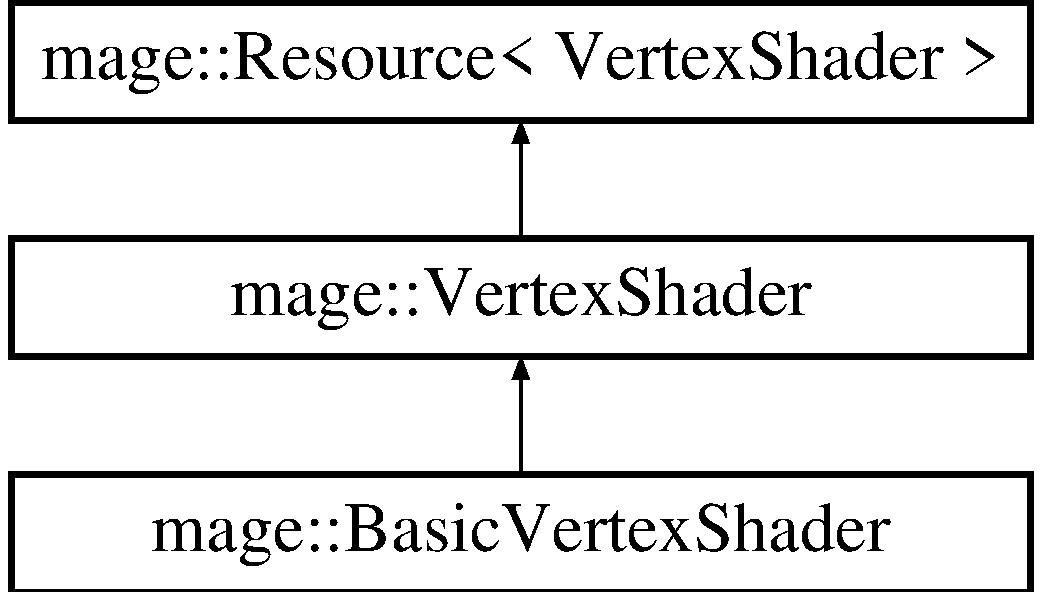
\includegraphics[height=3.000000cm]{classmage_1_1_basic_vertex_shader}
\end{center}
\end{figure}
\subsection*{Public Member Functions}
\begin{DoxyCompactItemize}
\item 
\hyperlink{classmage_1_1_basic_vertex_shader_a906db88dc79cfc9c3f0898d14f54065d}{Basic\+Vertex\+Shader} (I\+D3\+D11\+Device2 $\ast$device, I\+D3\+D11\+Device\+Context2 $\ast$device\+\_\+context, const wstring \&fname)
\item 
\hyperlink{classmage_1_1_basic_vertex_shader_a9cd9b21663a009c1ca37c35ab6ac7298}{Basic\+Vertex\+Shader} (I\+D3\+D11\+Device2 $\ast$device, I\+D3\+D11\+Device\+Context2 $\ast$device\+\_\+context, const \hyperlink{structmage_1_1_compiled_vertex_shader}{Compiled\+Vertex\+Shader} \&compiled\+\_\+vertex\+\_\+shader)
\item 
\hyperlink{classmage_1_1_basic_vertex_shader_ab547bf423545c41882a691ff3ebb32ce}{Basic\+Vertex\+Shader} (const \hyperlink{classmage_1_1_basic_vertex_shader}{Basic\+Vertex\+Shader} \&vertex\+\_\+shader)=delete
\item 
\hyperlink{classmage_1_1_basic_vertex_shader_a1c5f899e5dfaf81609e8e8fd73103ab2}{Basic\+Vertex\+Shader} (\hyperlink{classmage_1_1_basic_vertex_shader}{Basic\+Vertex\+Shader} \&\&vertex\+\_\+shader)
\item 
virtual \hyperlink{classmage_1_1_basic_vertex_shader_ad155c4135f5517667020ec519a3597c9}{$\sim$\+Basic\+Vertex\+Shader} ()
\item 
\hyperlink{classmage_1_1_basic_vertex_shader}{Basic\+Vertex\+Shader} \& \hyperlink{classmage_1_1_basic_vertex_shader_ab3d355e76715b24e21fb37c239d41932}{operator=} (const \hyperlink{classmage_1_1_basic_vertex_shader}{Basic\+Vertex\+Shader} \&vertex\+\_\+shader)=delete
\item 
\hyperlink{classmage_1_1_basic_vertex_shader}{Basic\+Vertex\+Shader} \& \hyperlink{classmage_1_1_basic_vertex_shader_ae5442c36b5f913ac6644cc2945a8c20a}{operator=} (\hyperlink{classmage_1_1_basic_vertex_shader}{Basic\+Vertex\+Shader} \&\&vertex\+\_\+shader)=delete
\item 
virtual void \hyperlink{classmage_1_1_basic_vertex_shader_ae565cb19b96591d5d1ff36ac0ff7344c}{Prepare\+Shading} (I\+D3\+D11\+Buffer $\ast$transform) const override final
\end{DoxyCompactItemize}
\subsection*{Additional Inherited Members}


\subsection{Detailed Description}
A class of basic vertex shaders. 

\subsection{Constructor \& Destructor Documentation}
\hypertarget{classmage_1_1_basic_vertex_shader_a906db88dc79cfc9c3f0898d14f54065d}{}\label{classmage_1_1_basic_vertex_shader_a906db88dc79cfc9c3f0898d14f54065d} 
\index{mage\+::\+Basic\+Vertex\+Shader@{mage\+::\+Basic\+Vertex\+Shader}!Basic\+Vertex\+Shader@{Basic\+Vertex\+Shader}}
\index{Basic\+Vertex\+Shader@{Basic\+Vertex\+Shader}!mage\+::\+Basic\+Vertex\+Shader@{mage\+::\+Basic\+Vertex\+Shader}}
\subsubsection{\texorpdfstring{Basic\+Vertex\+Shader()}{BasicVertexShader()}\hspace{0.1cm}{\footnotesize\ttfamily [1/4]}}
{\footnotesize\ttfamily mage\+::\+Basic\+Vertex\+Shader\+::\+Basic\+Vertex\+Shader (\begin{DoxyParamCaption}\item[{I\+D3\+D11\+Device2 $\ast$}]{device,  }\item[{I\+D3\+D11\+Device\+Context2 $\ast$}]{device\+\_\+context,  }\item[{const wstring \&}]{fname }\end{DoxyParamCaption})\hspace{0.3cm}{\ttfamily [explicit]}}

Constructs a basic vertex shader.

\begin{DoxyPrecond}{Precondition}
{\itshape device} is not equal to {\ttfamily nullptr}. 

{\itshape device\+\_\+context} is not equal to {\ttfamily nullptr}. 
\end{DoxyPrecond}

\begin{DoxyParams}[1]{Parameters}
\mbox{\tt in}  & {\em device} & A pointer to the device. \\
\hline
\mbox{\tt in}  & {\em device\+\_\+context} & A pointer to the device context. \\
\hline
\mbox{\tt in}  & {\em fname} & A reference to the filename. \\
\hline
\end{DoxyParams}

\begin{DoxyExceptions}{Exceptions}
{\em \hyperlink{structmage_1_1_formatted_exception}{Formatted\+Exception}} & Failed to initialize this vertex shader. \\
\hline
\end{DoxyExceptions}
\hypertarget{classmage_1_1_basic_vertex_shader_a9cd9b21663a009c1ca37c35ab6ac7298}{}\label{classmage_1_1_basic_vertex_shader_a9cd9b21663a009c1ca37c35ab6ac7298} 
\index{mage\+::\+Basic\+Vertex\+Shader@{mage\+::\+Basic\+Vertex\+Shader}!Basic\+Vertex\+Shader@{Basic\+Vertex\+Shader}}
\index{Basic\+Vertex\+Shader@{Basic\+Vertex\+Shader}!mage\+::\+Basic\+Vertex\+Shader@{mage\+::\+Basic\+Vertex\+Shader}}
\subsubsection{\texorpdfstring{Basic\+Vertex\+Shader()}{BasicVertexShader()}\hspace{0.1cm}{\footnotesize\ttfamily [2/4]}}
{\footnotesize\ttfamily mage\+::\+Basic\+Vertex\+Shader\+::\+Basic\+Vertex\+Shader (\begin{DoxyParamCaption}\item[{I\+D3\+D11\+Device2 $\ast$}]{device,  }\item[{I\+D3\+D11\+Device\+Context2 $\ast$}]{device\+\_\+context,  }\item[{const \hyperlink{structmage_1_1_compiled_vertex_shader}{Compiled\+Vertex\+Shader} \&}]{compiled\+\_\+vertex\+\_\+shader }\end{DoxyParamCaption})\hspace{0.3cm}{\ttfamily [explicit]}}

Constructs a basic vertex shader.

\begin{DoxyPrecond}{Precondition}
{\itshape device} is not equal to {\ttfamily nullptr}. 

{\itshape device\+\_\+context} is not equal to {\ttfamily nullptr}. 
\end{DoxyPrecond}

\begin{DoxyParams}[1]{Parameters}
\mbox{\tt in}  & {\em device} & A pointer to the device. \\
\hline
\mbox{\tt in}  & {\em device\+\_\+context} & A pointer to the device context. \\
\hline
\mbox{\tt in}  & {\em compiled\+\_\+vertex\+\_\+shader} & A reference to the compiled vertex shader. \\
\hline
\end{DoxyParams}

\begin{DoxyExceptions}{Exceptions}
{\em \hyperlink{structmage_1_1_formatted_exception}{Formatted\+Exception}} & Failed to initialize this vertex shader. \\
\hline
\end{DoxyExceptions}
\hypertarget{classmage_1_1_basic_vertex_shader_ab547bf423545c41882a691ff3ebb32ce}{}\label{classmage_1_1_basic_vertex_shader_ab547bf423545c41882a691ff3ebb32ce} 
\index{mage\+::\+Basic\+Vertex\+Shader@{mage\+::\+Basic\+Vertex\+Shader}!Basic\+Vertex\+Shader@{Basic\+Vertex\+Shader}}
\index{Basic\+Vertex\+Shader@{Basic\+Vertex\+Shader}!mage\+::\+Basic\+Vertex\+Shader@{mage\+::\+Basic\+Vertex\+Shader}}
\subsubsection{\texorpdfstring{Basic\+Vertex\+Shader()}{BasicVertexShader()}\hspace{0.1cm}{\footnotesize\ttfamily [3/4]}}
{\footnotesize\ttfamily mage\+::\+Basic\+Vertex\+Shader\+::\+Basic\+Vertex\+Shader (\begin{DoxyParamCaption}\item[{const \hyperlink{classmage_1_1_basic_vertex_shader}{Basic\+Vertex\+Shader} \&}]{vertex\+\_\+shader }\end{DoxyParamCaption})\hspace{0.3cm}{\ttfamily [delete]}}

Constructs a basic vertex shader from the given basic vertex shader.


\begin{DoxyParams}[1]{Parameters}
\mbox{\tt in}  & {\em vertex\+\_\+shader} & A reference to the basic vertex shader to copy. \\
\hline
\end{DoxyParams}
\hypertarget{classmage_1_1_basic_vertex_shader_a1c5f899e5dfaf81609e8e8fd73103ab2}{}\label{classmage_1_1_basic_vertex_shader_a1c5f899e5dfaf81609e8e8fd73103ab2} 
\index{mage\+::\+Basic\+Vertex\+Shader@{mage\+::\+Basic\+Vertex\+Shader}!Basic\+Vertex\+Shader@{Basic\+Vertex\+Shader}}
\index{Basic\+Vertex\+Shader@{Basic\+Vertex\+Shader}!mage\+::\+Basic\+Vertex\+Shader@{mage\+::\+Basic\+Vertex\+Shader}}
\subsubsection{\texorpdfstring{Basic\+Vertex\+Shader()}{BasicVertexShader()}\hspace{0.1cm}{\footnotesize\ttfamily [4/4]}}
{\footnotesize\ttfamily mage\+::\+Basic\+Vertex\+Shader\+::\+Basic\+Vertex\+Shader (\begin{DoxyParamCaption}\item[{\hyperlink{classmage_1_1_basic_vertex_shader}{Basic\+Vertex\+Shader} \&\&}]{vertex\+\_\+shader }\end{DoxyParamCaption})\hspace{0.3cm}{\ttfamily [default]}}

Constructs a basic vertex shader by moving the given basic vertex shader.


\begin{DoxyParams}[1]{Parameters}
\mbox{\tt in}  & {\em vertex\+\_\+shader} & A reference to the basic vertex shader to move. \\
\hline
\end{DoxyParams}
\hypertarget{classmage_1_1_basic_vertex_shader_ad155c4135f5517667020ec519a3597c9}{}\label{classmage_1_1_basic_vertex_shader_ad155c4135f5517667020ec519a3597c9} 
\index{mage\+::\+Basic\+Vertex\+Shader@{mage\+::\+Basic\+Vertex\+Shader}!````~Basic\+Vertex\+Shader@{$\sim$\+Basic\+Vertex\+Shader}}
\index{````~Basic\+Vertex\+Shader@{$\sim$\+Basic\+Vertex\+Shader}!mage\+::\+Basic\+Vertex\+Shader@{mage\+::\+Basic\+Vertex\+Shader}}
\subsubsection{\texorpdfstring{$\sim$\+Basic\+Vertex\+Shader()}{~BasicVertexShader()}}
{\footnotesize\ttfamily mage\+::\+Basic\+Vertex\+Shader\+::$\sim$\+Basic\+Vertex\+Shader (\begin{DoxyParamCaption}{ }\end{DoxyParamCaption})\hspace{0.3cm}{\ttfamily [virtual]}, {\ttfamily [default]}}

Destructs this basic vertex shader. 

\subsection{Member Function Documentation}
\hypertarget{classmage_1_1_basic_vertex_shader_ab3d355e76715b24e21fb37c239d41932}{}\label{classmage_1_1_basic_vertex_shader_ab3d355e76715b24e21fb37c239d41932} 
\index{mage\+::\+Basic\+Vertex\+Shader@{mage\+::\+Basic\+Vertex\+Shader}!operator=@{operator=}}
\index{operator=@{operator=}!mage\+::\+Basic\+Vertex\+Shader@{mage\+::\+Basic\+Vertex\+Shader}}
\subsubsection{\texorpdfstring{operator=()}{operator=()}\hspace{0.1cm}{\footnotesize\ttfamily [1/2]}}
{\footnotesize\ttfamily \hyperlink{classmage_1_1_basic_vertex_shader}{Basic\+Vertex\+Shader}\& mage\+::\+Basic\+Vertex\+Shader\+::operator= (\begin{DoxyParamCaption}\item[{const \hyperlink{classmage_1_1_basic_vertex_shader}{Basic\+Vertex\+Shader} \&}]{vertex\+\_\+shader }\end{DoxyParamCaption})\hspace{0.3cm}{\ttfamily [delete]}}

Copies the given basic vertex shader to this basic vertex shader.


\begin{DoxyParams}[1]{Parameters}
\mbox{\tt in}  & {\em vertex\+\_\+shader} & A reference to the basic vertex shader to copy. \\
\hline
\end{DoxyParams}
\begin{DoxyReturn}{Returns}
A reference to the copy of the given basic vertex shader (i.\+e. this basic vertex shader). 
\end{DoxyReturn}
\hypertarget{classmage_1_1_basic_vertex_shader_ae5442c36b5f913ac6644cc2945a8c20a}{}\label{classmage_1_1_basic_vertex_shader_ae5442c36b5f913ac6644cc2945a8c20a} 
\index{mage\+::\+Basic\+Vertex\+Shader@{mage\+::\+Basic\+Vertex\+Shader}!operator=@{operator=}}
\index{operator=@{operator=}!mage\+::\+Basic\+Vertex\+Shader@{mage\+::\+Basic\+Vertex\+Shader}}
\subsubsection{\texorpdfstring{operator=()}{operator=()}\hspace{0.1cm}{\footnotesize\ttfamily [2/2]}}
{\footnotesize\ttfamily \hyperlink{classmage_1_1_basic_vertex_shader}{Basic\+Vertex\+Shader}\& mage\+::\+Basic\+Vertex\+Shader\+::operator= (\begin{DoxyParamCaption}\item[{\hyperlink{classmage_1_1_basic_vertex_shader}{Basic\+Vertex\+Shader} \&\&}]{vertex\+\_\+shader }\end{DoxyParamCaption})\hspace{0.3cm}{\ttfamily [delete]}}

Copies the given basic vertex shader to this basic vertex shader.


\begin{DoxyParams}[1]{Parameters}
\mbox{\tt in}  & {\em vertex\+\_\+shader} & A reference to the basic vertex shader to copy. \\
\hline
\end{DoxyParams}
\begin{DoxyReturn}{Returns}
A reference to the moved basic vertex shader (i.\+e. this basic vertex shader). 
\end{DoxyReturn}
\hypertarget{classmage_1_1_basic_vertex_shader_ae565cb19b96591d5d1ff36ac0ff7344c}{}\label{classmage_1_1_basic_vertex_shader_ae565cb19b96591d5d1ff36ac0ff7344c} 
\index{mage\+::\+Basic\+Vertex\+Shader@{mage\+::\+Basic\+Vertex\+Shader}!Prepare\+Shading@{Prepare\+Shading}}
\index{Prepare\+Shading@{Prepare\+Shading}!mage\+::\+Basic\+Vertex\+Shader@{mage\+::\+Basic\+Vertex\+Shader}}
\subsubsection{\texorpdfstring{Prepare\+Shading()}{PrepareShading()}}
{\footnotesize\ttfamily void mage\+::\+Basic\+Vertex\+Shader\+::\+Prepare\+Shading (\begin{DoxyParamCaption}\item[{I\+D3\+D11\+Buffer $\ast$}]{transform }\end{DoxyParamCaption}) const\hspace{0.3cm}{\ttfamily [final]}, {\ttfamily [override]}, {\ttfamily [virtual]}}

Prepares this basic vertex shader for shading.

\begin{DoxyPrecond}{Precondition}
{\itshape transform} is not equal to {\ttfamily nullptr}. 
\end{DoxyPrecond}

\begin{DoxyParams}[1]{Parameters}
\mbox{\tt in}  & {\em transform} & A pointer to the transform buffer. \\
\hline
\end{DoxyParams}


Reimplemented from \hyperlink{classmage_1_1_vertex_shader_a53f4b25241f6c5739724d421c9f29a36}{mage\+::\+Vertex\+Shader}.


\hypertarget{classmage_1_1_behavior_script}{}\section{mage\+:\+:Behavior\+Script Class Reference}
\label{classmage_1_1_behavior_script}\index{mage\+::\+Behavior\+Script@{mage\+::\+Behavior\+Script}}


{\ttfamily \#include $<$behavior\+\_\+script.\+hpp$>$}

Inheritance diagram for mage\+:\+:Behavior\+Script\+:\begin{figure}[H]
\begin{center}
\leavevmode
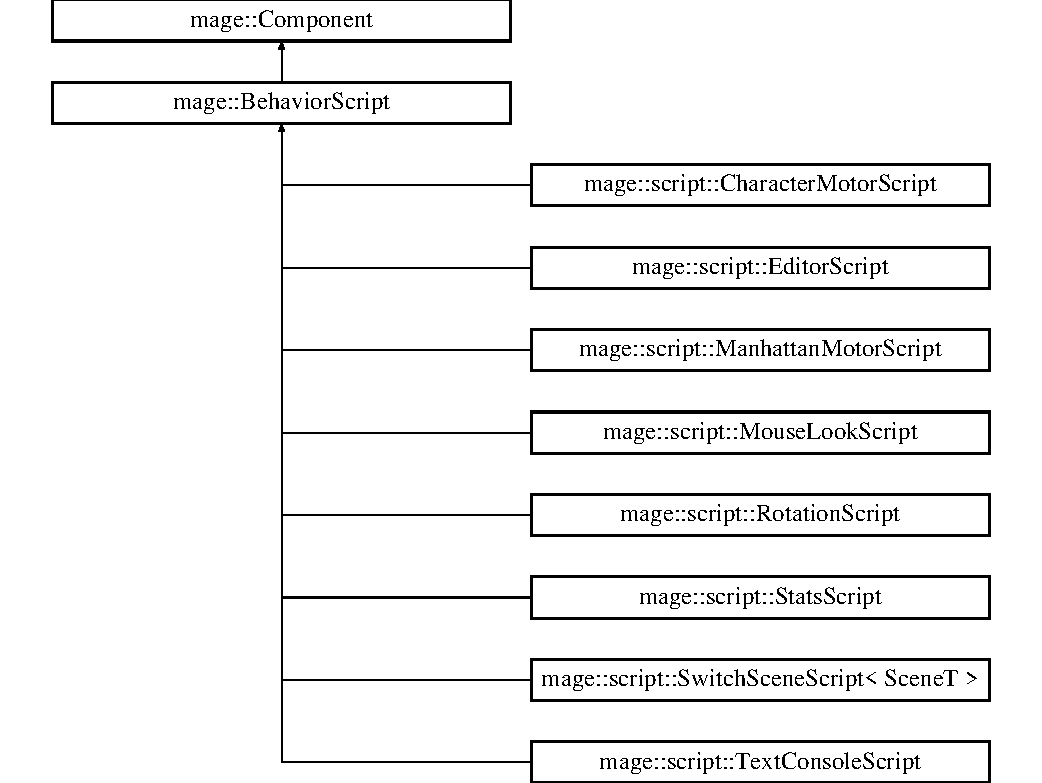
\includegraphics[height=7.604939cm]{classmage_1_1_behavior_script}
\end{center}
\end{figure}
\subsection*{Public Member Functions}
\begin{DoxyCompactItemize}
\item 
virtual \hyperlink{classmage_1_1_behavior_script_a61e4825ba0fc7746d49faa44ed7bc481}{$\sim$\+Behavior\+Script} ()
\item 
\hyperlink{classmage_1_1_behavior_script}{Behavior\+Script} \& \hyperlink{classmage_1_1_behavior_script_a0b3327ebf7009e668a7022d254cb1d51}{operator=} (const \hyperlink{classmage_1_1_behavior_script}{Behavior\+Script} \&script)=delete
\item 
\hyperlink{classmage_1_1_behavior_script}{Behavior\+Script} \& \hyperlink{classmage_1_1_behavior_script_a528c2bd218f2e6bb7d0a8ee50a05bf01}{operator=} (\hyperlink{classmage_1_1_behavior_script}{Behavior\+Script} \&\&script)=delete
\item 
virtual void \hyperlink{classmage_1_1_behavior_script_a8318f79ab78798ec37b39bc844f7138c}{Fixed\+Update} ()
\item 
virtual void \hyperlink{classmage_1_1_behavior_script_afb9cf3759edf8876416d1df85489cba6}{Update} (\mbox{[}\mbox{[}maybe\+\_\+unused\mbox{]}\mbox{]} \hyperlink{namespacemage_ad26233bbec640deda836e572c1a23708}{F64} delta\+\_\+time)
\item 
bool \hyperlink{classmage_1_1_behavior_script_a856e1b420ea0ead36adafa750237325c}{Is\+Active} () const noexcept
\item 
bool \hyperlink{classmage_1_1_behavior_script_a40e33539ca7013a13ef127af11bff3e1}{Is\+Passive} () const noexcept
\item 
void \hyperlink{classmage_1_1_behavior_script_a84a5bf0fc7ec3ecd36dddaf001143b54}{Activate} () noexcept
\item 
void \hyperlink{classmage_1_1_behavior_script_ab45260db9c30d596b1d688a01458f63e}{Deactivate} () noexcept
\item 
void \hyperlink{classmage_1_1_behavior_script_ab0dc76b101fd514c6e9f8799de382e8a}{Set\+Active} (bool active) noexcept
\item 
bool \hyperlink{classmage_1_1_behavior_script_abb1625dbaa3b1145009ea474b082938f}{Is\+Terminated} () const noexcept
\item 
void \hyperlink{classmage_1_1_behavior_script_a2beae460bb84a135aa7e29c7baf6b25b}{Terminate} () noexcept
\end{DoxyCompactItemize}
\subsection*{Protected Member Functions}
\begin{DoxyCompactItemize}
\item 
\hyperlink{classmage_1_1_behavior_script_ad064a6bbe2ba5f7622d1d20eeec958bf}{Behavior\+Script} ()
\item 
\hyperlink{classmage_1_1_behavior_script_ab95b988867dfb8592ab7678bff608116}{Behavior\+Script} (const \hyperlink{classmage_1_1_behavior_script}{Behavior\+Script} \&script)
\item 
\hyperlink{classmage_1_1_behavior_script_aa8f509053f6bb9dbfd3baa75bdd8b91e}{Behavior\+Script} (\hyperlink{classmage_1_1_behavior_script}{Behavior\+Script} \&\&script)
\end{DoxyCompactItemize}
\subsection*{Private Member Functions}
\begin{DoxyCompactItemize}
\item 
virtual void \hyperlink{classmage_1_1_behavior_script_a17703fd980599ccf7265b5ffc6148fe8}{On\+Active\+Change} () noexcept
\end{DoxyCompactItemize}
\subsection*{Private Attributes}
\begin{DoxyCompactItemize}
\item 
bool \hyperlink{classmage_1_1_behavior_script_a18f81792aed31a2d61a8a75784e2ceef}{m\+\_\+active}
\item 
bool \hyperlink{classmage_1_1_behavior_script_abc4a0e6728787347012404a597ab8e07}{m\+\_\+terminated}
\end{DoxyCompactItemize}


\subsection{Detailed Description}
A class of behavior scripts. 

\subsection{Constructor \& Destructor Documentation}
\hypertarget{classmage_1_1_behavior_script_a61e4825ba0fc7746d49faa44ed7bc481}{}\label{classmage_1_1_behavior_script_a61e4825ba0fc7746d49faa44ed7bc481} 
\index{mage\+::\+Behavior\+Script@{mage\+::\+Behavior\+Script}!````~Behavior\+Script@{$\sim$\+Behavior\+Script}}
\index{````~Behavior\+Script@{$\sim$\+Behavior\+Script}!mage\+::\+Behavior\+Script@{mage\+::\+Behavior\+Script}}
\subsubsection{\texorpdfstring{$\sim$\+Behavior\+Script()}{~BehaviorScript()}}
{\footnotesize\ttfamily mage\+::\+Behavior\+Script\+::$\sim$\+Behavior\+Script (\begin{DoxyParamCaption}{ }\end{DoxyParamCaption})\hspace{0.3cm}{\ttfamily [virtual]}, {\ttfamily [default]}}

Destructs this behavior script. \hypertarget{classmage_1_1_behavior_script_ad064a6bbe2ba5f7622d1d20eeec958bf}{}\label{classmage_1_1_behavior_script_ad064a6bbe2ba5f7622d1d20eeec958bf} 
\index{mage\+::\+Behavior\+Script@{mage\+::\+Behavior\+Script}!Behavior\+Script@{Behavior\+Script}}
\index{Behavior\+Script@{Behavior\+Script}!mage\+::\+Behavior\+Script@{mage\+::\+Behavior\+Script}}
\subsubsection{\texorpdfstring{Behavior\+Script()}{BehaviorScript()}\hspace{0.1cm}{\footnotesize\ttfamily [1/3]}}
{\footnotesize\ttfamily mage\+::\+Behavior\+Script\+::\+Behavior\+Script (\begin{DoxyParamCaption}{ }\end{DoxyParamCaption})\hspace{0.3cm}{\ttfamily [protected]}}

Constructs a behavior script. \hypertarget{classmage_1_1_behavior_script_ab95b988867dfb8592ab7678bff608116}{}\label{classmage_1_1_behavior_script_ab95b988867dfb8592ab7678bff608116} 
\index{mage\+::\+Behavior\+Script@{mage\+::\+Behavior\+Script}!Behavior\+Script@{Behavior\+Script}}
\index{Behavior\+Script@{Behavior\+Script}!mage\+::\+Behavior\+Script@{mage\+::\+Behavior\+Script}}
\subsubsection{\texorpdfstring{Behavior\+Script()}{BehaviorScript()}\hspace{0.1cm}{\footnotesize\ttfamily [2/3]}}
{\footnotesize\ttfamily mage\+::\+Behavior\+Script\+::\+Behavior\+Script (\begin{DoxyParamCaption}\item[{const \hyperlink{classmage_1_1_behavior_script}{Behavior\+Script} \&}]{script }\end{DoxyParamCaption})\hspace{0.3cm}{\ttfamily [protected]}, {\ttfamily [default]}}

Constructs a behavior script from the given behavior script.


\begin{DoxyParams}[1]{Parameters}
\mbox{\tt in}  & {\em script} & A reference to the behavior script to copy. \\
\hline
\end{DoxyParams}
\hypertarget{classmage_1_1_behavior_script_aa8f509053f6bb9dbfd3baa75bdd8b91e}{}\label{classmage_1_1_behavior_script_aa8f509053f6bb9dbfd3baa75bdd8b91e} 
\index{mage\+::\+Behavior\+Script@{mage\+::\+Behavior\+Script}!Behavior\+Script@{Behavior\+Script}}
\index{Behavior\+Script@{Behavior\+Script}!mage\+::\+Behavior\+Script@{mage\+::\+Behavior\+Script}}
\subsubsection{\texorpdfstring{Behavior\+Script()}{BehaviorScript()}\hspace{0.1cm}{\footnotesize\ttfamily [3/3]}}
{\footnotesize\ttfamily mage\+::\+Behavior\+Script\+::\+Behavior\+Script (\begin{DoxyParamCaption}\item[{\hyperlink{classmage_1_1_behavior_script}{Behavior\+Script} \&\&}]{script }\end{DoxyParamCaption})\hspace{0.3cm}{\ttfamily [protected]}, {\ttfamily [default]}}

Constructs a behavior script by moving the given behavior script.


\begin{DoxyParams}[1]{Parameters}
\mbox{\tt in}  & {\em script} & A reference to the behavior script to move. \\
\hline
\end{DoxyParams}


\subsection{Member Function Documentation}
\hypertarget{classmage_1_1_behavior_script_a84a5bf0fc7ec3ecd36dddaf001143b54}{}\label{classmage_1_1_behavior_script_a84a5bf0fc7ec3ecd36dddaf001143b54} 
\index{mage\+::\+Behavior\+Script@{mage\+::\+Behavior\+Script}!Activate@{Activate}}
\index{Activate@{Activate}!mage\+::\+Behavior\+Script@{mage\+::\+Behavior\+Script}}
\subsubsection{\texorpdfstring{Activate()}{Activate()}}
{\footnotesize\ttfamily void mage\+::\+Behavior\+Script\+::\+Activate (\begin{DoxyParamCaption}{ }\end{DoxyParamCaption})\hspace{0.3cm}{\ttfamily [noexcept]}}

Activates this behavior script (and its descendant behavior scripts). \hypertarget{classmage_1_1_behavior_script_ab45260db9c30d596b1d688a01458f63e}{}\label{classmage_1_1_behavior_script_ab45260db9c30d596b1d688a01458f63e} 
\index{mage\+::\+Behavior\+Script@{mage\+::\+Behavior\+Script}!Deactivate@{Deactivate}}
\index{Deactivate@{Deactivate}!mage\+::\+Behavior\+Script@{mage\+::\+Behavior\+Script}}
\subsubsection{\texorpdfstring{Deactivate()}{Deactivate()}}
{\footnotesize\ttfamily void mage\+::\+Behavior\+Script\+::\+Deactivate (\begin{DoxyParamCaption}{ }\end{DoxyParamCaption})\hspace{0.3cm}{\ttfamily [noexcept]}}

Deactives this behavior script (and its descendant behavior scripts). \hypertarget{classmage_1_1_behavior_script_a8318f79ab78798ec37b39bc844f7138c}{}\label{classmage_1_1_behavior_script_a8318f79ab78798ec37b39bc844f7138c} 
\index{mage\+::\+Behavior\+Script@{mage\+::\+Behavior\+Script}!Fixed\+Update@{Fixed\+Update}}
\index{Fixed\+Update@{Fixed\+Update}!mage\+::\+Behavior\+Script@{mage\+::\+Behavior\+Script}}
\subsubsection{\texorpdfstring{Fixed\+Update()}{FixedUpdate()}}
{\footnotesize\ttfamily void mage\+::\+Behavior\+Script\+::\+Fixed\+Update (\begin{DoxyParamCaption}{ }\end{DoxyParamCaption})\hspace{0.3cm}{\ttfamily [virtual]}}

Updates this behavior script.

This method can be called zero, one or multiple times per frame depending on the fixed delta time used by the engine. \hypertarget{classmage_1_1_behavior_script_a856e1b420ea0ead36adafa750237325c}{}\label{classmage_1_1_behavior_script_a856e1b420ea0ead36adafa750237325c} 
\index{mage\+::\+Behavior\+Script@{mage\+::\+Behavior\+Script}!Is\+Active@{Is\+Active}}
\index{Is\+Active@{Is\+Active}!mage\+::\+Behavior\+Script@{mage\+::\+Behavior\+Script}}
\subsubsection{\texorpdfstring{Is\+Active()}{IsActive()}}
{\footnotesize\ttfamily bool mage\+::\+Behavior\+Script\+::\+Is\+Active (\begin{DoxyParamCaption}{ }\end{DoxyParamCaption}) const\hspace{0.3cm}{\ttfamily [noexcept]}}

Checks whether this behavior script is active.

\begin{DoxyReturn}{Returns}
{\ttfamily true} if this behavior script is active. {\ttfamily false} otherwise (i.\+e. passive). 
\end{DoxyReturn}
\hypertarget{classmage_1_1_behavior_script_a40e33539ca7013a13ef127af11bff3e1}{}\label{classmage_1_1_behavior_script_a40e33539ca7013a13ef127af11bff3e1} 
\index{mage\+::\+Behavior\+Script@{mage\+::\+Behavior\+Script}!Is\+Passive@{Is\+Passive}}
\index{Is\+Passive@{Is\+Passive}!mage\+::\+Behavior\+Script@{mage\+::\+Behavior\+Script}}
\subsubsection{\texorpdfstring{Is\+Passive()}{IsPassive()}}
{\footnotesize\ttfamily bool mage\+::\+Behavior\+Script\+::\+Is\+Passive (\begin{DoxyParamCaption}{ }\end{DoxyParamCaption}) const\hspace{0.3cm}{\ttfamily [noexcept]}}

Checks whether this behavior script is passive.

\begin{DoxyReturn}{Returns}
{\ttfamily true} if this behavior script is passive. {\ttfamily false} otherwise (i.\+e. active). 
\end{DoxyReturn}
\hypertarget{classmage_1_1_behavior_script_abb1625dbaa3b1145009ea474b082938f}{}\label{classmage_1_1_behavior_script_abb1625dbaa3b1145009ea474b082938f} 
\index{mage\+::\+Behavior\+Script@{mage\+::\+Behavior\+Script}!Is\+Terminated@{Is\+Terminated}}
\index{Is\+Terminated@{Is\+Terminated}!mage\+::\+Behavior\+Script@{mage\+::\+Behavior\+Script}}
\subsubsection{\texorpdfstring{Is\+Terminated()}{IsTerminated()}}
{\footnotesize\ttfamily bool mage\+::\+Behavior\+Script\+::\+Is\+Terminated (\begin{DoxyParamCaption}{ }\end{DoxyParamCaption}) const\hspace{0.3cm}{\ttfamily [noexcept]}}

Checks whether this behavior script is terminated or not.

\begin{DoxyReturn}{Returns}
{\ttfamily true} if this behavior script is terminated. {\ttfamily false} otherwise. 
\end{DoxyReturn}
\hypertarget{classmage_1_1_behavior_script_a17703fd980599ccf7265b5ffc6148fe8}{}\label{classmage_1_1_behavior_script_a17703fd980599ccf7265b5ffc6148fe8} 
\index{mage\+::\+Behavior\+Script@{mage\+::\+Behavior\+Script}!On\+Active\+Change@{On\+Active\+Change}}
\index{On\+Active\+Change@{On\+Active\+Change}!mage\+::\+Behavior\+Script@{mage\+::\+Behavior\+Script}}
\subsubsection{\texorpdfstring{On\+Active\+Change()}{OnActiveChange()}}
{\footnotesize\ttfamily void mage\+::\+Behavior\+Script\+::\+On\+Active\+Change (\begin{DoxyParamCaption}{ }\end{DoxyParamCaption})\hspace{0.3cm}{\ttfamily [private]}, {\ttfamily [virtual]}, {\ttfamily [noexcept]}}

Notifies this transform behavior script of a change in activeness. \hypertarget{classmage_1_1_behavior_script_a0b3327ebf7009e668a7022d254cb1d51}{}\label{classmage_1_1_behavior_script_a0b3327ebf7009e668a7022d254cb1d51} 
\index{mage\+::\+Behavior\+Script@{mage\+::\+Behavior\+Script}!operator=@{operator=}}
\index{operator=@{operator=}!mage\+::\+Behavior\+Script@{mage\+::\+Behavior\+Script}}
\subsubsection{\texorpdfstring{operator=()}{operator=()}\hspace{0.1cm}{\footnotesize\ttfamily [1/2]}}
{\footnotesize\ttfamily \hyperlink{classmage_1_1_behavior_script}{Behavior\+Script}\& mage\+::\+Behavior\+Script\+::operator= (\begin{DoxyParamCaption}\item[{const \hyperlink{classmage_1_1_behavior_script}{Behavior\+Script} \&}]{script }\end{DoxyParamCaption})\hspace{0.3cm}{\ttfamily [delete]}}

Copies the given behavior script to this behavior script.


\begin{DoxyParams}[1]{Parameters}
\mbox{\tt in}  & {\em script} & A reference to the behavior script to copy. \\
\hline
\end{DoxyParams}
\begin{DoxyReturn}{Returns}
A reference to the copy of the given behavior script (i.\+e. this behavior script). 
\end{DoxyReturn}
\hypertarget{classmage_1_1_behavior_script_a528c2bd218f2e6bb7d0a8ee50a05bf01}{}\label{classmage_1_1_behavior_script_a528c2bd218f2e6bb7d0a8ee50a05bf01} 
\index{mage\+::\+Behavior\+Script@{mage\+::\+Behavior\+Script}!operator=@{operator=}}
\index{operator=@{operator=}!mage\+::\+Behavior\+Script@{mage\+::\+Behavior\+Script}}
\subsubsection{\texorpdfstring{operator=()}{operator=()}\hspace{0.1cm}{\footnotesize\ttfamily [2/2]}}
{\footnotesize\ttfamily \hyperlink{classmage_1_1_behavior_script}{Behavior\+Script}\& mage\+::\+Behavior\+Script\+::operator= (\begin{DoxyParamCaption}\item[{\hyperlink{classmage_1_1_behavior_script}{Behavior\+Script} \&\&}]{script }\end{DoxyParamCaption})\hspace{0.3cm}{\ttfamily [delete]}}

Moves the given behavior script to this behavior script.


\begin{DoxyParams}[1]{Parameters}
\mbox{\tt in}  & {\em script} & A reference to the behavior script to move. \\
\hline
\end{DoxyParams}
\begin{DoxyReturn}{Returns}
A reference to the moved behavior script (i.\+e. this behavior script). 
\end{DoxyReturn}
\hypertarget{classmage_1_1_behavior_script_ab0dc76b101fd514c6e9f8799de382e8a}{}\label{classmage_1_1_behavior_script_ab0dc76b101fd514c6e9f8799de382e8a} 
\index{mage\+::\+Behavior\+Script@{mage\+::\+Behavior\+Script}!Set\+Active@{Set\+Active}}
\index{Set\+Active@{Set\+Active}!mage\+::\+Behavior\+Script@{mage\+::\+Behavior\+Script}}
\subsubsection{\texorpdfstring{Set\+Active()}{SetActive()}}
{\footnotesize\ttfamily void mage\+::\+Behavior\+Script\+::\+Set\+Active (\begin{DoxyParamCaption}\item[{bool}]{active }\end{DoxyParamCaption})\hspace{0.3cm}{\ttfamily [noexcept]}}

Sets this behavior script active flag to the given value.


\begin{DoxyParams}[1]{Parameters}
\mbox{\tt in}  & {\em active} & The active flag. \\
\hline
\end{DoxyParams}
\hypertarget{classmage_1_1_behavior_script_a2beae460bb84a135aa7e29c7baf6b25b}{}\label{classmage_1_1_behavior_script_a2beae460bb84a135aa7e29c7baf6b25b} 
\index{mage\+::\+Behavior\+Script@{mage\+::\+Behavior\+Script}!Terminate@{Terminate}}
\index{Terminate@{Terminate}!mage\+::\+Behavior\+Script@{mage\+::\+Behavior\+Script}}
\subsubsection{\texorpdfstring{Terminate()}{Terminate()}}
{\footnotesize\ttfamily void mage\+::\+Behavior\+Script\+::\+Terminate (\begin{DoxyParamCaption}{ }\end{DoxyParamCaption})\hspace{0.3cm}{\ttfamily [noexcept]}}

Terminates this behavior script. \hypertarget{classmage_1_1_behavior_script_afb9cf3759edf8876416d1df85489cba6}{}\label{classmage_1_1_behavior_script_afb9cf3759edf8876416d1df85489cba6} 
\index{mage\+::\+Behavior\+Script@{mage\+::\+Behavior\+Script}!Update@{Update}}
\index{Update@{Update}!mage\+::\+Behavior\+Script@{mage\+::\+Behavior\+Script}}
\subsubsection{\texorpdfstring{Update()}{Update()}}
{\footnotesize\ttfamily void mage\+::\+Behavior\+Script\+::\+Update (\begin{DoxyParamCaption}\item[{\mbox{[}\mbox{[}maybe\+\_\+unused\mbox{]} \mbox{]} \hyperlink{namespacemage_ad26233bbec640deda836e572c1a23708}{F64}}]{delta\+\_\+time }\end{DoxyParamCaption})\hspace{0.3cm}{\ttfamily [virtual]}}

Updates this behavior script.

This method is called once per frame.


\begin{DoxyParams}[1]{Parameters}
\mbox{\tt in}  & {\em delta\+\_\+time} & The elapsed time since the previous update. \\
\hline
\end{DoxyParams}


Reimplemented in \hyperlink{classmage_1_1_mouse_look_script_a22cd0ec05722b229e4427fc3f1acf4a4}{mage\+::\+Mouse\+Look\+Script}, \hyperlink{classmage_1_1_input_controller_script_ae964c7b2c90fa2addb32562921376c80}{mage\+::\+Input\+Controller\+Script$<$ Orientation\+Script\+T, Movement\+Script\+T $>$}, \hyperlink{classmage_1_1_rotation_script_a93d00e047d8ca3075d2c52209c769761}{mage\+::\+Rotation\+Script}, \hyperlink{classmage_1_1_stats_script_a61ada9e05bce5699cdf5912cce90337b}{mage\+::\+Stats\+Script}, \hyperlink{classmage_1_1_character_motor_script_a67badc915464773eb874b318bd1f890a}{mage\+::\+Character\+Motor\+Script}, \hyperlink{classmage_1_1_manhattan_motor_script_acc4af968f5a7021adff82d26141188e0}{mage\+::\+Manhattan\+Motor\+Script}, \hyperlink{classmage_1_1_switch_scene_script_a9a92e2f108741599f121dd9083d4a89b}{mage\+::\+Switch\+Scene\+Script$<$ Scene\+T $>$}, \hyperlink{classmage_1_1_text_console_script_afc6fbebca3b5a3bf433777c93e6e27d6}{mage\+::\+Text\+Console\+Script}, \hyperlink{classmage_1_1_location_script_ad7d768404613003a34f754355effe580}{mage\+::\+Location\+Script}, and \hyperlink{classmage_1_1_render_mode_script_af40eef8ffcb392f408ebfa3f5801354a}{mage\+::\+Render\+Mode\+Script}.



\subsection{Member Data Documentation}
\hypertarget{classmage_1_1_behavior_script_a18f81792aed31a2d61a8a75784e2ceef}{}\label{classmage_1_1_behavior_script_a18f81792aed31a2d61a8a75784e2ceef} 
\index{mage\+::\+Behavior\+Script@{mage\+::\+Behavior\+Script}!m\+\_\+active@{m\+\_\+active}}
\index{m\+\_\+active@{m\+\_\+active}!mage\+::\+Behavior\+Script@{mage\+::\+Behavior\+Script}}
\subsubsection{\texorpdfstring{m\+\_\+active}{m\_active}}
{\footnotesize\ttfamily bool mage\+::\+Behavior\+Script\+::m\+\_\+active\hspace{0.3cm}{\ttfamily [private]}}

A flag indicating whether this behavior script is active or not (i.\+e. passive). \hypertarget{classmage_1_1_behavior_script_abc4a0e6728787347012404a597ab8e07}{}\label{classmage_1_1_behavior_script_abc4a0e6728787347012404a597ab8e07} 
\index{mage\+::\+Behavior\+Script@{mage\+::\+Behavior\+Script}!m\+\_\+terminated@{m\+\_\+terminated}}
\index{m\+\_\+terminated@{m\+\_\+terminated}!mage\+::\+Behavior\+Script@{mage\+::\+Behavior\+Script}}
\subsubsection{\texorpdfstring{m\+\_\+terminated}{m\_terminated}}
{\footnotesize\ttfamily bool mage\+::\+Behavior\+Script\+::m\+\_\+terminated\hspace{0.3cm}{\ttfamily [private]}}

A flag indicating whether this behavior script is terminated or not. 
\hypertarget{classmage_1_1_big_endian_binary_reader}{}\section{mage\+:\+:Big\+Endian\+Binary\+Reader Class Reference}
\label{classmage_1_1_big_endian_binary_reader}\index{mage\+::\+Big\+Endian\+Binary\+Reader@{mage\+::\+Big\+Endian\+Binary\+Reader}}


{\ttfamily \#include $<$binary\+\_\+reader.\+hpp$>$}

Inheritance diagram for mage\+:\+:Big\+Endian\+Binary\+Reader\+:\begin{figure}[H]
\begin{center}
\leavevmode
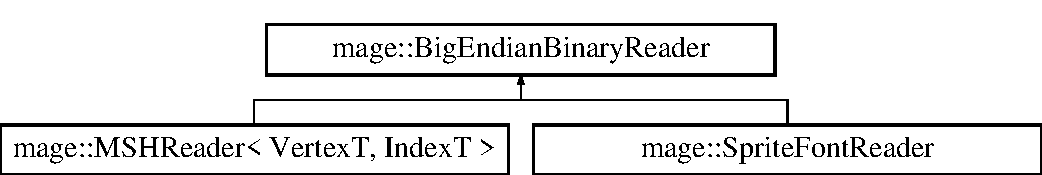
\includegraphics[height=2.000000cm]{classmage_1_1_big_endian_binary_reader}
\end{center}
\end{figure}
\subsection*{Public Member Functions}
\begin{DoxyCompactItemize}
\item 
virtual \hyperlink{classmage_1_1_big_endian_binary_reader_ae85a40e8ed06e8c887e38d914843b8d3}{$\sim$\+Big\+Endian\+Binary\+Reader} ()
\item 
\hyperlink{classmage_1_1_big_endian_binary_reader}{Big\+Endian\+Binary\+Reader} \& \hyperlink{classmage_1_1_big_endian_binary_reader_abd4b24df4219469a8c2e9253b1cad405}{operator=} (const \hyperlink{classmage_1_1_big_endian_binary_reader}{Big\+Endian\+Binary\+Reader} \&reader)=delete
\item 
\hyperlink{classmage_1_1_big_endian_binary_reader}{Big\+Endian\+Binary\+Reader} \& \hyperlink{classmage_1_1_big_endian_binary_reader_a9e2e0dd62afff04774d0246f7e5e4ce4}{operator=} (\hyperlink{classmage_1_1_big_endian_binary_reader}{Big\+Endian\+Binary\+Reader} \&\&reader)=delete
\item 
void \hyperlink{classmage_1_1_big_endian_binary_reader_a68db676feaa42c1c3a9bf16d0680b04f}{Read\+From\+File} (wstring fname)
\item 
void \hyperlink{classmage_1_1_big_endian_binary_reader_a44d2529136499412cdaf9ad5d1cf0e59}{Read\+From\+Memory} (const \hyperlink{namespacemage_afc638980bc6154f15af5e2d93a0e0ea9}{U8} $\ast$input, size\+\_\+t size)
\item 
const wstring \& \hyperlink{classmage_1_1_big_endian_binary_reader_a801558f27606dbc681809178aaaaacd1}{Get\+Filename} () const noexcept
\end{DoxyCompactItemize}
\subsection*{Protected Member Functions}
\begin{DoxyCompactItemize}
\item 
\hyperlink{classmage_1_1_big_endian_binary_reader_a1fd0dbee6950a8cb04aa399f0cdbaf2a}{Big\+Endian\+Binary\+Reader} ()
\item 
\hyperlink{classmage_1_1_big_endian_binary_reader_a9d490263268290217ae4f2f06e0699c4}{Big\+Endian\+Binary\+Reader} (const \hyperlink{classmage_1_1_big_endian_binary_reader}{Big\+Endian\+Binary\+Reader} \&reader)=delete
\item 
\hyperlink{classmage_1_1_big_endian_binary_reader_a3cb2fbd205854cf69c36054a2003e80e}{Big\+Endian\+Binary\+Reader} (\hyperlink{classmage_1_1_big_endian_binary_reader}{Big\+Endian\+Binary\+Reader} \&\&reader)
\item 
bool \hyperlink{classmage_1_1_big_endian_binary_reader_adaa45913c50d4cb54456121ba56c8afb}{Has\+Chars\+Left} () const noexcept
\item 
{\footnotesize template$<$typename DataT $>$ }\\const DataT \& \hyperlink{classmage_1_1_big_endian_binary_reader_a036399c5d3099a4e617127acb110ccdf}{Read\+Value} ()
\item 
{\footnotesize template$<$typename DataT $>$ }\\const DataT $\ast$ \hyperlink{classmage_1_1_big_endian_binary_reader_aa79d97deb6060a6c1015c8f2891ac6da}{Read\+Value\+Array} (size\+\_\+t count)
\end{DoxyCompactItemize}
\subsection*{Private Member Functions}
\begin{DoxyCompactItemize}
\item 
virtual void \hyperlink{classmage_1_1_big_endian_binary_reader_af072965dea0319d6366b21cc6562bbf9}{Read} ()=0
\end{DoxyCompactItemize}
\subsection*{Private Attributes}
\begin{DoxyCompactItemize}
\item 
wstring \hyperlink{classmage_1_1_big_endian_binary_reader_a0f836aec582a59f156b64bffb9653e41}{m\+\_\+fname}
\item 
const \hyperlink{namespacemage_afc638980bc6154f15af5e2d93a0e0ea9}{U8} $\ast$ \hyperlink{classmage_1_1_big_endian_binary_reader_a7dbfc5ce1712e431f75d80a4f7a56e33}{m\+\_\+pos}
\item 
const \hyperlink{namespacemage_afc638980bc6154f15af5e2d93a0e0ea9}{U8} $\ast$ \hyperlink{classmage_1_1_big_endian_binary_reader_ab4f707d30799b98afed0f9adfc27a3e2}{m\+\_\+end}
\item 
\hyperlink{namespacemage_a3316d7143a973e37adf1110f2e80ca31}{Unique\+Ptr}$<$ \hyperlink{namespacemage_afc638980bc6154f15af5e2d93a0e0ea9}{U8}\mbox{[}$\,$\mbox{]} $>$ \hyperlink{classmage_1_1_big_endian_binary_reader_a54128bdaa233c1bd20494189b2397fe3}{m\+\_\+data}
\end{DoxyCompactItemize}


\subsection{Detailed Description}
A class of readers for reading (big endian) binary files. 

\subsection{Constructor \& Destructor Documentation}
\hypertarget{classmage_1_1_big_endian_binary_reader_ae85a40e8ed06e8c887e38d914843b8d3}{}\label{classmage_1_1_big_endian_binary_reader_ae85a40e8ed06e8c887e38d914843b8d3} 
\index{mage\+::\+Big\+Endian\+Binary\+Reader@{mage\+::\+Big\+Endian\+Binary\+Reader}!````~Big\+Endian\+Binary\+Reader@{$\sim$\+Big\+Endian\+Binary\+Reader}}
\index{````~Big\+Endian\+Binary\+Reader@{$\sim$\+Big\+Endian\+Binary\+Reader}!mage\+::\+Big\+Endian\+Binary\+Reader@{mage\+::\+Big\+Endian\+Binary\+Reader}}
\subsubsection{\texorpdfstring{$\sim$\+Big\+Endian\+Binary\+Reader()}{~BigEndianBinaryReader()}}
{\footnotesize\ttfamily mage\+::\+Big\+Endian\+Binary\+Reader\+::$\sim$\+Big\+Endian\+Binary\+Reader (\begin{DoxyParamCaption}{ }\end{DoxyParamCaption})\hspace{0.3cm}{\ttfamily [virtual]}, {\ttfamily [default]}}

Destructs this big endian binary reader. \hypertarget{classmage_1_1_big_endian_binary_reader_a1fd0dbee6950a8cb04aa399f0cdbaf2a}{}\label{classmage_1_1_big_endian_binary_reader_a1fd0dbee6950a8cb04aa399f0cdbaf2a} 
\index{mage\+::\+Big\+Endian\+Binary\+Reader@{mage\+::\+Big\+Endian\+Binary\+Reader}!Big\+Endian\+Binary\+Reader@{Big\+Endian\+Binary\+Reader}}
\index{Big\+Endian\+Binary\+Reader@{Big\+Endian\+Binary\+Reader}!mage\+::\+Big\+Endian\+Binary\+Reader@{mage\+::\+Big\+Endian\+Binary\+Reader}}
\subsubsection{\texorpdfstring{Big\+Endian\+Binary\+Reader()}{BigEndianBinaryReader()}\hspace{0.1cm}{\footnotesize\ttfamily [1/3]}}
{\footnotesize\ttfamily mage\+::\+Big\+Endian\+Binary\+Reader\+::\+Big\+Endian\+Binary\+Reader (\begin{DoxyParamCaption}{ }\end{DoxyParamCaption})\hspace{0.3cm}{\ttfamily [protected]}}

Constructs a big endian binary reader. \hypertarget{classmage_1_1_big_endian_binary_reader_a9d490263268290217ae4f2f06e0699c4}{}\label{classmage_1_1_big_endian_binary_reader_a9d490263268290217ae4f2f06e0699c4} 
\index{mage\+::\+Big\+Endian\+Binary\+Reader@{mage\+::\+Big\+Endian\+Binary\+Reader}!Big\+Endian\+Binary\+Reader@{Big\+Endian\+Binary\+Reader}}
\index{Big\+Endian\+Binary\+Reader@{Big\+Endian\+Binary\+Reader}!mage\+::\+Big\+Endian\+Binary\+Reader@{mage\+::\+Big\+Endian\+Binary\+Reader}}
\subsubsection{\texorpdfstring{Big\+Endian\+Binary\+Reader()}{BigEndianBinaryReader()}\hspace{0.1cm}{\footnotesize\ttfamily [2/3]}}
{\footnotesize\ttfamily mage\+::\+Big\+Endian\+Binary\+Reader\+::\+Big\+Endian\+Binary\+Reader (\begin{DoxyParamCaption}\item[{const \hyperlink{classmage_1_1_big_endian_binary_reader}{Big\+Endian\+Binary\+Reader} \&}]{reader }\end{DoxyParamCaption})\hspace{0.3cm}{\ttfamily [protected]}, {\ttfamily [delete]}}

Constructs a big endian binary reader from the given big endian binary reader.


\begin{DoxyParams}[1]{Parameters}
\mbox{\tt in}  & {\em reader} & A reference to the big endian binary reader to copy. \\
\hline
\end{DoxyParams}
\hypertarget{classmage_1_1_big_endian_binary_reader_a3cb2fbd205854cf69c36054a2003e80e}{}\label{classmage_1_1_big_endian_binary_reader_a3cb2fbd205854cf69c36054a2003e80e} 
\index{mage\+::\+Big\+Endian\+Binary\+Reader@{mage\+::\+Big\+Endian\+Binary\+Reader}!Big\+Endian\+Binary\+Reader@{Big\+Endian\+Binary\+Reader}}
\index{Big\+Endian\+Binary\+Reader@{Big\+Endian\+Binary\+Reader}!mage\+::\+Big\+Endian\+Binary\+Reader@{mage\+::\+Big\+Endian\+Binary\+Reader}}
\subsubsection{\texorpdfstring{Big\+Endian\+Binary\+Reader()}{BigEndianBinaryReader()}\hspace{0.1cm}{\footnotesize\ttfamily [3/3]}}
{\footnotesize\ttfamily mage\+::\+Big\+Endian\+Binary\+Reader\+::\+Big\+Endian\+Binary\+Reader (\begin{DoxyParamCaption}\item[{\hyperlink{classmage_1_1_big_endian_binary_reader}{Big\+Endian\+Binary\+Reader} \&\&}]{reader }\end{DoxyParamCaption})\hspace{0.3cm}{\ttfamily [protected]}, {\ttfamily [default]}}

Constructs a big endian binary reader by moving the given big endian binary reader.


\begin{DoxyParams}[1]{Parameters}
\mbox{\tt in}  & {\em reader} & A reference to the big endian binary reader to move. \\
\hline
\end{DoxyParams}


\subsection{Member Function Documentation}
\hypertarget{classmage_1_1_big_endian_binary_reader_a801558f27606dbc681809178aaaaacd1}{}\label{classmage_1_1_big_endian_binary_reader_a801558f27606dbc681809178aaaaacd1} 
\index{mage\+::\+Big\+Endian\+Binary\+Reader@{mage\+::\+Big\+Endian\+Binary\+Reader}!Get\+Filename@{Get\+Filename}}
\index{Get\+Filename@{Get\+Filename}!mage\+::\+Big\+Endian\+Binary\+Reader@{mage\+::\+Big\+Endian\+Binary\+Reader}}
\subsubsection{\texorpdfstring{Get\+Filename()}{GetFilename()}}
{\footnotesize\ttfamily const wstring\& mage\+::\+Big\+Endian\+Binary\+Reader\+::\+Get\+Filename (\begin{DoxyParamCaption}{ }\end{DoxyParamCaption}) const\hspace{0.3cm}{\ttfamily [noexcept]}}

Returns the current filename of this big endian binary reader.

\begin{DoxyReturn}{Returns}
A reference to the current filename of this big endian binary reader. 
\end{DoxyReturn}
\hypertarget{classmage_1_1_big_endian_binary_reader_adaa45913c50d4cb54456121ba56c8afb}{}\label{classmage_1_1_big_endian_binary_reader_adaa45913c50d4cb54456121ba56c8afb} 
\index{mage\+::\+Big\+Endian\+Binary\+Reader@{mage\+::\+Big\+Endian\+Binary\+Reader}!Has\+Chars\+Left@{Has\+Chars\+Left}}
\index{Has\+Chars\+Left@{Has\+Chars\+Left}!mage\+::\+Big\+Endian\+Binary\+Reader@{mage\+::\+Big\+Endian\+Binary\+Reader}}
\subsubsection{\texorpdfstring{Has\+Chars\+Left()}{HasCharsLeft()}}
{\footnotesize\ttfamily bool mage\+::\+Big\+Endian\+Binary\+Reader\+::\+Has\+Chars\+Left (\begin{DoxyParamCaption}{ }\end{DoxyParamCaption}) const\hspace{0.3cm}{\ttfamily [protected]}, {\ttfamily [noexcept]}}

Checks if there are characters left to read by this binary reader.

\begin{DoxyReturn}{Returns}
{\ttfamily true} if there are characters left to read by this binary reader. {\ttfamily false} otherwise. 
\end{DoxyReturn}
\hypertarget{classmage_1_1_big_endian_binary_reader_abd4b24df4219469a8c2e9253b1cad405}{}\label{classmage_1_1_big_endian_binary_reader_abd4b24df4219469a8c2e9253b1cad405} 
\index{mage\+::\+Big\+Endian\+Binary\+Reader@{mage\+::\+Big\+Endian\+Binary\+Reader}!operator=@{operator=}}
\index{operator=@{operator=}!mage\+::\+Big\+Endian\+Binary\+Reader@{mage\+::\+Big\+Endian\+Binary\+Reader}}
\subsubsection{\texorpdfstring{operator=()}{operator=()}\hspace{0.1cm}{\footnotesize\ttfamily [1/2]}}
{\footnotesize\ttfamily \hyperlink{classmage_1_1_big_endian_binary_reader}{Big\+Endian\+Binary\+Reader}\& mage\+::\+Big\+Endian\+Binary\+Reader\+::operator= (\begin{DoxyParamCaption}\item[{const \hyperlink{classmage_1_1_big_endian_binary_reader}{Big\+Endian\+Binary\+Reader} \&}]{reader }\end{DoxyParamCaption})\hspace{0.3cm}{\ttfamily [delete]}}

Copies the given big endian binary reader to this big endian binary reader.


\begin{DoxyParams}[1]{Parameters}
\mbox{\tt in}  & {\em reader} & A reference to a big endian binary reader to copy. \\
\hline
\end{DoxyParams}
\begin{DoxyReturn}{Returns}
A reference to the copy of the given big endian binary reader (i.\+e. this big endian binary reader). 
\end{DoxyReturn}
\hypertarget{classmage_1_1_big_endian_binary_reader_a9e2e0dd62afff04774d0246f7e5e4ce4}{}\label{classmage_1_1_big_endian_binary_reader_a9e2e0dd62afff04774d0246f7e5e4ce4} 
\index{mage\+::\+Big\+Endian\+Binary\+Reader@{mage\+::\+Big\+Endian\+Binary\+Reader}!operator=@{operator=}}
\index{operator=@{operator=}!mage\+::\+Big\+Endian\+Binary\+Reader@{mage\+::\+Big\+Endian\+Binary\+Reader}}
\subsubsection{\texorpdfstring{operator=()}{operator=()}\hspace{0.1cm}{\footnotesize\ttfamily [2/2]}}
{\footnotesize\ttfamily \hyperlink{classmage_1_1_big_endian_binary_reader}{Big\+Endian\+Binary\+Reader}\& mage\+::\+Big\+Endian\+Binary\+Reader\+::operator= (\begin{DoxyParamCaption}\item[{\hyperlink{classmage_1_1_big_endian_binary_reader}{Big\+Endian\+Binary\+Reader} \&\&}]{reader }\end{DoxyParamCaption})\hspace{0.3cm}{\ttfamily [delete]}}

Moves the given big endian binary reader to this big endian binary reader.


\begin{DoxyParams}[1]{Parameters}
\mbox{\tt in}  & {\em reader} & A reference to a big endian binary reader to move. \\
\hline
\end{DoxyParams}
\begin{DoxyReturn}{Returns}
A reference to the moved big endian binary reader (i.\+e. this big endian binary reader). 
\end{DoxyReturn}
\hypertarget{classmage_1_1_big_endian_binary_reader_af072965dea0319d6366b21cc6562bbf9}{}\label{classmage_1_1_big_endian_binary_reader_af072965dea0319d6366b21cc6562bbf9} 
\index{mage\+::\+Big\+Endian\+Binary\+Reader@{mage\+::\+Big\+Endian\+Binary\+Reader}!Read@{Read}}
\index{Read@{Read}!mage\+::\+Big\+Endian\+Binary\+Reader@{mage\+::\+Big\+Endian\+Binary\+Reader}}
\subsubsection{\texorpdfstring{Read()}{Read()}}
{\footnotesize\ttfamily virtual void mage\+::\+Big\+Endian\+Binary\+Reader\+::\+Read (\begin{DoxyParamCaption}{ }\end{DoxyParamCaption})\hspace{0.3cm}{\ttfamily [private]}, {\ttfamily [pure virtual]}}

Starts reading.


\begin{DoxyExceptions}{Exceptions}
{\em \hyperlink{classmage_1_1_formatted_exception}{Formatted\+Exception}} & Failed to read to the given file. \\
\hline
\end{DoxyExceptions}


Implemented in \hyperlink{classmage_1_1_m_s_h_reader_a26b60060bf61183fb5758a4725c6a205}{mage\+::\+M\+S\+H\+Reader$<$ Vertex\+T, Index\+T $>$}, and \hyperlink{classmage_1_1_sprite_font_reader_af380ae127285a88ae41e35a9067db412}{mage\+::\+Sprite\+Font\+Reader}.

\hypertarget{classmage_1_1_big_endian_binary_reader_a68db676feaa42c1c3a9bf16d0680b04f}{}\label{classmage_1_1_big_endian_binary_reader_a68db676feaa42c1c3a9bf16d0680b04f} 
\index{mage\+::\+Big\+Endian\+Binary\+Reader@{mage\+::\+Big\+Endian\+Binary\+Reader}!Read\+From\+File@{Read\+From\+File}}
\index{Read\+From\+File@{Read\+From\+File}!mage\+::\+Big\+Endian\+Binary\+Reader@{mage\+::\+Big\+Endian\+Binary\+Reader}}
\subsubsection{\texorpdfstring{Read\+From\+File()}{ReadFromFile()}}
{\footnotesize\ttfamily void mage\+::\+Big\+Endian\+Binary\+Reader\+::\+Read\+From\+File (\begin{DoxyParamCaption}\item[{wstring}]{fname }\end{DoxyParamCaption})}

Reads from the given file.


\begin{DoxyParams}[1]{Parameters}
\mbox{\tt in}  & {\em fname} & The file name. \\
\hline
\end{DoxyParams}

\begin{DoxyExceptions}{Exceptions}
{\em \hyperlink{classmage_1_1_formatted_exception}{Formatted\+Exception}} & Failed to read from the given file. \\
\hline
\end{DoxyExceptions}
\hypertarget{classmage_1_1_big_endian_binary_reader_a44d2529136499412cdaf9ad5d1cf0e59}{}\label{classmage_1_1_big_endian_binary_reader_a44d2529136499412cdaf9ad5d1cf0e59} 
\index{mage\+::\+Big\+Endian\+Binary\+Reader@{mage\+::\+Big\+Endian\+Binary\+Reader}!Read\+From\+Memory@{Read\+From\+Memory}}
\index{Read\+From\+Memory@{Read\+From\+Memory}!mage\+::\+Big\+Endian\+Binary\+Reader@{mage\+::\+Big\+Endian\+Binary\+Reader}}
\subsubsection{\texorpdfstring{Read\+From\+Memory()}{ReadFromMemory()}}
{\footnotesize\ttfamily void mage\+::\+Big\+Endian\+Binary\+Reader\+::\+Read\+From\+Memory (\begin{DoxyParamCaption}\item[{const \hyperlink{namespacemage_afc638980bc6154f15af5e2d93a0e0ea9}{U8} $\ast$}]{input,  }\item[{size\+\_\+t}]{size }\end{DoxyParamCaption})}

Reads the input string.

\begin{DoxyPrecond}{Precondition}
{\itshape input} is not equal to {\ttfamily nullptr}. 
\end{DoxyPrecond}

\begin{DoxyParams}[1]{Parameters}
\mbox{\tt in}  & {\em input} & A pointer to the input byte string. \\
\hline
\mbox{\tt in}  & {\em size} & The size of the input string. \\
\hline
\end{DoxyParams}

\begin{DoxyExceptions}{Exceptions}
{\em \hyperlink{classmage_1_1_formatted_exception}{Formatted\+Exception}} & Failed to read from the given input string. \\
\hline
\end{DoxyExceptions}
\hypertarget{classmage_1_1_big_endian_binary_reader_a036399c5d3099a4e617127acb110ccdf}{}\label{classmage_1_1_big_endian_binary_reader_a036399c5d3099a4e617127acb110ccdf} 
\index{mage\+::\+Big\+Endian\+Binary\+Reader@{mage\+::\+Big\+Endian\+Binary\+Reader}!Read\+Value@{Read\+Value}}
\index{Read\+Value@{Read\+Value}!mage\+::\+Big\+Endian\+Binary\+Reader@{mage\+::\+Big\+Endian\+Binary\+Reader}}
\subsubsection{\texorpdfstring{Read\+Value()}{ReadValue()}}
{\footnotesize\ttfamily template$<$typename DataT $>$ \\
const DataT\& mage\+::\+Big\+Endian\+Binary\+Reader\+::\+Read\+Value (\begin{DoxyParamCaption}{ }\end{DoxyParamCaption})\hspace{0.3cm}{\ttfamily [protected]}}

Reads a {\ttfamily DataT} element.


\begin{DoxyTemplParams}{Template Parameters}
{\em DataT} & The data type. \\
\hline
\end{DoxyTemplParams}
\begin{DoxyReturn}{Returns}
A reference to the {\ttfamily DataT} element read. 
\end{DoxyReturn}

\begin{DoxyExceptions}{Exceptions}
{\em \hyperlink{classmage_1_1_formatted_exception}{Formatted\+Exception}} & Failed to read a {\ttfamily DataT} element. \\
\hline
\end{DoxyExceptions}
\hypertarget{classmage_1_1_big_endian_binary_reader_aa79d97deb6060a6c1015c8f2891ac6da}{}\label{classmage_1_1_big_endian_binary_reader_aa79d97deb6060a6c1015c8f2891ac6da} 
\index{mage\+::\+Big\+Endian\+Binary\+Reader@{mage\+::\+Big\+Endian\+Binary\+Reader}!Read\+Value\+Array@{Read\+Value\+Array}}
\index{Read\+Value\+Array@{Read\+Value\+Array}!mage\+::\+Big\+Endian\+Binary\+Reader@{mage\+::\+Big\+Endian\+Binary\+Reader}}
\subsubsection{\texorpdfstring{Read\+Value\+Array()}{ReadValueArray()}}
{\footnotesize\ttfamily template$<$typename DataT $>$ \\
const DataT$\ast$ mage\+::\+Big\+Endian\+Binary\+Reader\+::\+Read\+Value\+Array (\begin{DoxyParamCaption}\item[{size\+\_\+t}]{count }\end{DoxyParamCaption})\hspace{0.3cm}{\ttfamily [protected]}}

Reads an array of {\ttfamily DataT} elements.


\begin{DoxyTemplParams}{Template Parameters}
{\em DataT} & The data type. \\
\hline
\end{DoxyTemplParams}

\begin{DoxyParams}{Parameters}
{\em count} & The number of {\ttfamily DataT} elements to read. \\
\hline
\end{DoxyParams}
\begin{DoxyReturn}{Returns}
A pointer to the array of {\ttfamily DataT} element read. 
\end{DoxyReturn}

\begin{DoxyExceptions}{Exceptions}
{\em \hyperlink{classmage_1_1_formatted_exception}{Formatted\+Exception}} & Failed to read {\ttfamily count} {\ttfamily DataT} elements. \\
\hline
\end{DoxyExceptions}


\subsection{Member Data Documentation}
\hypertarget{classmage_1_1_big_endian_binary_reader_a54128bdaa233c1bd20494189b2397fe3}{}\label{classmage_1_1_big_endian_binary_reader_a54128bdaa233c1bd20494189b2397fe3} 
\index{mage\+::\+Big\+Endian\+Binary\+Reader@{mage\+::\+Big\+Endian\+Binary\+Reader}!m\+\_\+data@{m\+\_\+data}}
\index{m\+\_\+data@{m\+\_\+data}!mage\+::\+Big\+Endian\+Binary\+Reader@{mage\+::\+Big\+Endian\+Binary\+Reader}}
\subsubsection{\texorpdfstring{m\+\_\+data}{m\_data}}
{\footnotesize\ttfamily \hyperlink{namespacemage_a3316d7143a973e37adf1110f2e80ca31}{Unique\+Ptr}$<$ \hyperlink{namespacemage_afc638980bc6154f15af5e2d93a0e0ea9}{U8}\mbox{[}$\,$\mbox{]} $>$ mage\+::\+Big\+Endian\+Binary\+Reader\+::m\+\_\+data\hspace{0.3cm}{\ttfamily [private]}}

A pointer to the data to read of this binary reader. \hypertarget{classmage_1_1_big_endian_binary_reader_ab4f707d30799b98afed0f9adfc27a3e2}{}\label{classmage_1_1_big_endian_binary_reader_ab4f707d30799b98afed0f9adfc27a3e2} 
\index{mage\+::\+Big\+Endian\+Binary\+Reader@{mage\+::\+Big\+Endian\+Binary\+Reader}!m\+\_\+end@{m\+\_\+end}}
\index{m\+\_\+end@{m\+\_\+end}!mage\+::\+Big\+Endian\+Binary\+Reader@{mage\+::\+Big\+Endian\+Binary\+Reader}}
\subsubsection{\texorpdfstring{m\+\_\+end}{m\_end}}
{\footnotesize\ttfamily const \hyperlink{namespacemage_afc638980bc6154f15af5e2d93a0e0ea9}{U8}$\ast$ mage\+::\+Big\+Endian\+Binary\+Reader\+::m\+\_\+end\hspace{0.3cm}{\ttfamily [private]}}

A pointer to the end position of this binary reader. \hypertarget{classmage_1_1_big_endian_binary_reader_a0f836aec582a59f156b64bffb9653e41}{}\label{classmage_1_1_big_endian_binary_reader_a0f836aec582a59f156b64bffb9653e41} 
\index{mage\+::\+Big\+Endian\+Binary\+Reader@{mage\+::\+Big\+Endian\+Binary\+Reader}!m\+\_\+fname@{m\+\_\+fname}}
\index{m\+\_\+fname@{m\+\_\+fname}!mage\+::\+Big\+Endian\+Binary\+Reader@{mage\+::\+Big\+Endian\+Binary\+Reader}}
\subsubsection{\texorpdfstring{m\+\_\+fname}{m\_fname}}
{\footnotesize\ttfamily wstring mage\+::\+Big\+Endian\+Binary\+Reader\+::m\+\_\+fname\hspace{0.3cm}{\ttfamily [private]}}

The current filename of this line reader. \hypertarget{classmage_1_1_big_endian_binary_reader_a7dbfc5ce1712e431f75d80a4f7a56e33}{}\label{classmage_1_1_big_endian_binary_reader_a7dbfc5ce1712e431f75d80a4f7a56e33} 
\index{mage\+::\+Big\+Endian\+Binary\+Reader@{mage\+::\+Big\+Endian\+Binary\+Reader}!m\+\_\+pos@{m\+\_\+pos}}
\index{m\+\_\+pos@{m\+\_\+pos}!mage\+::\+Big\+Endian\+Binary\+Reader@{mage\+::\+Big\+Endian\+Binary\+Reader}}
\subsubsection{\texorpdfstring{m\+\_\+pos}{m\_pos}}
{\footnotesize\ttfamily const \hyperlink{namespacemage_afc638980bc6154f15af5e2d93a0e0ea9}{U8}$\ast$ mage\+::\+Big\+Endian\+Binary\+Reader\+::m\+\_\+pos\hspace{0.3cm}{\ttfamily [private]}}

A pointer to the current position of this binary reader. 
\hypertarget{classmage_1_1_big_endian_binary_writer}{}\section{mage\+:\+:Big\+Endian\+Binary\+Writer Class Reference}
\label{classmage_1_1_big_endian_binary_writer}\index{mage\+::\+Big\+Endian\+Binary\+Writer@{mage\+::\+Big\+Endian\+Binary\+Writer}}


{\ttfamily \#include $<$binary\+\_\+writer.\+hpp$>$}

Inheritance diagram for mage\+:\+:Big\+Endian\+Binary\+Writer\+:\begin{figure}[H]
\begin{center}
\leavevmode
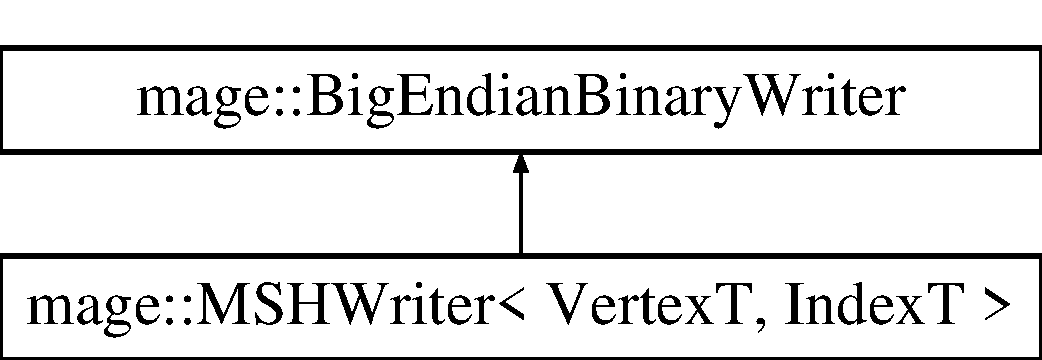
\includegraphics[height=2.000000cm]{classmage_1_1_big_endian_binary_writer}
\end{center}
\end{figure}
\subsection*{Public Member Functions}
\begin{DoxyCompactItemize}
\item 
\mbox{\hyperlink{classmage_1_1_big_endian_binary_writer}{Big\+Endian\+Binary\+Writer}} \& \mbox{\hyperlink{classmage_1_1_big_endian_binary_writer_ae574f7d0b630890256996c52818ba633}{operator=}} (const \mbox{\hyperlink{classmage_1_1_big_endian_binary_writer}{Big\+Endian\+Binary\+Writer}} \&writer)=delete
\item 
\mbox{\hyperlink{classmage_1_1_big_endian_binary_writer}{Big\+Endian\+Binary\+Writer}} \& \mbox{\hyperlink{classmage_1_1_big_endian_binary_writer_a8c01bf43f5e941578c5c5947ea184a78}{operator=}} (\mbox{\hyperlink{classmage_1_1_big_endian_binary_writer}{Big\+Endian\+Binary\+Writer}} \&\&writer) noexcept
\item 
void \mbox{\hyperlink{classmage_1_1_big_endian_binary_writer_a6ce9780687a45a6c6f98e0843190b63b}{Write\+To\+File}} (std\+::filesystem\+::path path)
\end{DoxyCompactItemize}
\subsection*{Protected Member Functions}
\begin{DoxyCompactItemize}
\item 
\mbox{\hyperlink{classmage_1_1_big_endian_binary_writer_ac0917b684913834577d4850269a6c09a}{Big\+Endian\+Binary\+Writer}} ()
\item 
\mbox{\hyperlink{classmage_1_1_big_endian_binary_writer_aafe65752342b2740e7293878ae469d9f}{Big\+Endian\+Binary\+Writer}} (const \mbox{\hyperlink{classmage_1_1_big_endian_binary_writer}{Big\+Endian\+Binary\+Writer}} \&writer)=delete
\item 
\mbox{\hyperlink{classmage_1_1_big_endian_binary_writer_aaf2dcf536afefc7b0ca8b0752024311d}{Big\+Endian\+Binary\+Writer}} (\mbox{\hyperlink{classmage_1_1_big_endian_binary_writer}{Big\+Endian\+Binary\+Writer}} \&\&writer) noexcept
\item 
\mbox{\hyperlink{classmage_1_1_big_endian_binary_writer_ab717bcbfc15ba4a1cb25eeb564e120b8}{$\sim$\+Big\+Endian\+Binary\+Writer}} ()
\item 
const std\+::filesystem\+::path \& \mbox{\hyperlink{classmage_1_1_big_endian_binary_writer_a812e65c16bf1b14d396d109eb969eeb8}{Get\+Path}} () const noexcept
\item 
{\footnotesize template$<$typename T $>$ }\\void \mbox{\hyperlink{classmage_1_1_big_endian_binary_writer_ae8bab2d7022672e1d30991c1288d981c}{Write}} (const T \&data)
\item 
{\footnotesize template$<$typename T $>$ }\\void \mbox{\hyperlink{classmage_1_1_big_endian_binary_writer_a7c82860ea3eed12777207cd00436b6c3}{Write\+Array}} (gsl\+::span$<$ const T $>$ data)
\item 
void \mbox{\hyperlink{classmage_1_1_big_endian_binary_writer_a869eff3f6e0666406bd5470af3e02096}{Write\+Character}} (char c)
\item 
void \mbox{\hyperlink{classmage_1_1_big_endian_binary_writer_acf065a2e7462c9e6cf46849bd2c9d2e7}{Write\+String}} (\mbox{\hyperlink{namespacemage_a8769f9d670d6b585ea306cb1062af94b}{Not\+Null}}$<$ \mbox{\hyperlink{namespacemage_abfd9206dc607ceb5d13ec68bf075a5c0}{const\+\_\+zstring}} $>$ str)
\end{DoxyCompactItemize}
\subsection*{Private Member Functions}
\begin{DoxyCompactItemize}
\item 
virtual void \mbox{\hyperlink{classmage_1_1_big_endian_binary_writer_a719581274b1b185ef05687183f7ded25}{Write\+Data}} ()=0
\end{DoxyCompactItemize}
\subsection*{Private Attributes}
\begin{DoxyCompactItemize}
\item 
\mbox{\hyperlink{namespacemage_ac11c62400d336d9f6857c7cdaecfc7a8}{Unique\+File\+Stream}} \mbox{\hyperlink{classmage_1_1_big_endian_binary_writer_ad2cdbdca429d6c351a57b51d175ffb55}{m\+\_\+file\+\_\+stream}}
\item 
std\+::filesystem\+::path \mbox{\hyperlink{classmage_1_1_big_endian_binary_writer_a22815e47cf8bf3443c10ec2ff4409745}{m\+\_\+path}}
\end{DoxyCompactItemize}


\subsection{Detailed Description}
A class of writers for writing (big endian) binary files. 

\subsection{Constructor \& Destructor Documentation}
\mbox{\Hypertarget{classmage_1_1_big_endian_binary_writer_ac0917b684913834577d4850269a6c09a}\label{classmage_1_1_big_endian_binary_writer_ac0917b684913834577d4850269a6c09a}} 
\index{mage\+::\+Big\+Endian\+Binary\+Writer@{mage\+::\+Big\+Endian\+Binary\+Writer}!Big\+Endian\+Binary\+Writer@{Big\+Endian\+Binary\+Writer}}
\index{Big\+Endian\+Binary\+Writer@{Big\+Endian\+Binary\+Writer}!mage\+::\+Big\+Endian\+Binary\+Writer@{mage\+::\+Big\+Endian\+Binary\+Writer}}
\subsubsection{\texorpdfstring{Big\+Endian\+Binary\+Writer()}{BigEndianBinaryWriter()}\hspace{0.1cm}{\footnotesize\ttfamily [1/3]}}
{\footnotesize\ttfamily mage\+::\+Big\+Endian\+Binary\+Writer\+::\+Big\+Endian\+Binary\+Writer (\begin{DoxyParamCaption}{ }\end{DoxyParamCaption})\hspace{0.3cm}{\ttfamily [protected]}}

Constructs a big endian binary writer. \mbox{\Hypertarget{classmage_1_1_big_endian_binary_writer_aafe65752342b2740e7293878ae469d9f}\label{classmage_1_1_big_endian_binary_writer_aafe65752342b2740e7293878ae469d9f}} 
\index{mage\+::\+Big\+Endian\+Binary\+Writer@{mage\+::\+Big\+Endian\+Binary\+Writer}!Big\+Endian\+Binary\+Writer@{Big\+Endian\+Binary\+Writer}}
\index{Big\+Endian\+Binary\+Writer@{Big\+Endian\+Binary\+Writer}!mage\+::\+Big\+Endian\+Binary\+Writer@{mage\+::\+Big\+Endian\+Binary\+Writer}}
\subsubsection{\texorpdfstring{Big\+Endian\+Binary\+Writer()}{BigEndianBinaryWriter()}\hspace{0.1cm}{\footnotesize\ttfamily [2/3]}}
{\footnotesize\ttfamily mage\+::\+Big\+Endian\+Binary\+Writer\+::\+Big\+Endian\+Binary\+Writer (\begin{DoxyParamCaption}\item[{const \mbox{\hyperlink{classmage_1_1_big_endian_binary_writer}{Big\+Endian\+Binary\+Writer}} \&}]{writer }\end{DoxyParamCaption})\hspace{0.3cm}{\ttfamily [protected]}, {\ttfamily [delete]}}

Constructs a big endian binary writer from the given big endian binary writer.


\begin{DoxyParams}[1]{Parameters}
\mbox{\tt in}  & {\em writer} & A reference to the big endian binary writer to copy. \\
\hline
\end{DoxyParams}
\mbox{\Hypertarget{classmage_1_1_big_endian_binary_writer_aaf2dcf536afefc7b0ca8b0752024311d}\label{classmage_1_1_big_endian_binary_writer_aaf2dcf536afefc7b0ca8b0752024311d}} 
\index{mage\+::\+Big\+Endian\+Binary\+Writer@{mage\+::\+Big\+Endian\+Binary\+Writer}!Big\+Endian\+Binary\+Writer@{Big\+Endian\+Binary\+Writer}}
\index{Big\+Endian\+Binary\+Writer@{Big\+Endian\+Binary\+Writer}!mage\+::\+Big\+Endian\+Binary\+Writer@{mage\+::\+Big\+Endian\+Binary\+Writer}}
\subsubsection{\texorpdfstring{Big\+Endian\+Binary\+Writer()}{BigEndianBinaryWriter()}\hspace{0.1cm}{\footnotesize\ttfamily [3/3]}}
{\footnotesize\ttfamily mage\+::\+Big\+Endian\+Binary\+Writer\+::\+Big\+Endian\+Binary\+Writer (\begin{DoxyParamCaption}\item[{\mbox{\hyperlink{classmage_1_1_big_endian_binary_writer}{Big\+Endian\+Binary\+Writer}} \&\&}]{writer }\end{DoxyParamCaption})\hspace{0.3cm}{\ttfamily [protected]}, {\ttfamily [default]}, {\ttfamily [noexcept]}}

Constructs a big endian binary writer by moving the given big endian binary writer.


\begin{DoxyParams}[1]{Parameters}
\mbox{\tt in}  & {\em writer} & A reference to the big endian binary writer to move. \\
\hline
\end{DoxyParams}
\mbox{\Hypertarget{classmage_1_1_big_endian_binary_writer_ab717bcbfc15ba4a1cb25eeb564e120b8}\label{classmage_1_1_big_endian_binary_writer_ab717bcbfc15ba4a1cb25eeb564e120b8}} 
\index{mage\+::\+Big\+Endian\+Binary\+Writer@{mage\+::\+Big\+Endian\+Binary\+Writer}!````~Big\+Endian\+Binary\+Writer@{$\sim$\+Big\+Endian\+Binary\+Writer}}
\index{````~Big\+Endian\+Binary\+Writer@{$\sim$\+Big\+Endian\+Binary\+Writer}!mage\+::\+Big\+Endian\+Binary\+Writer@{mage\+::\+Big\+Endian\+Binary\+Writer}}
\subsubsection{\texorpdfstring{$\sim$\+Big\+Endian\+Binary\+Writer()}{~BigEndianBinaryWriter()}}
{\footnotesize\ttfamily mage\+::\+Big\+Endian\+Binary\+Writer\+::$\sim$\+Big\+Endian\+Binary\+Writer (\begin{DoxyParamCaption}{ }\end{DoxyParamCaption})\hspace{0.3cm}{\ttfamily [protected]}, {\ttfamily [default]}}

Destructs this big endian binary writer. 

\subsection{Member Function Documentation}
\mbox{\Hypertarget{classmage_1_1_big_endian_binary_writer_a812e65c16bf1b14d396d109eb969eeb8}\label{classmage_1_1_big_endian_binary_writer_a812e65c16bf1b14d396d109eb969eeb8}} 
\index{mage\+::\+Big\+Endian\+Binary\+Writer@{mage\+::\+Big\+Endian\+Binary\+Writer}!Get\+Path@{Get\+Path}}
\index{Get\+Path@{Get\+Path}!mage\+::\+Big\+Endian\+Binary\+Writer@{mage\+::\+Big\+Endian\+Binary\+Writer}}
\subsubsection{\texorpdfstring{Get\+Path()}{GetPath()}}
{\footnotesize\ttfamily const std\+::filesystem\+::path\& mage\+::\+Big\+Endian\+Binary\+Writer\+::\+Get\+Path (\begin{DoxyParamCaption}{ }\end{DoxyParamCaption}) const\hspace{0.3cm}{\ttfamily [protected]}, {\ttfamily [noexcept]}}

Returns the current path of this big endian binary writer.

\begin{DoxyReturn}{Returns}
A reference to the current path of this big endian binary writer. 
\end{DoxyReturn}
\mbox{\Hypertarget{classmage_1_1_big_endian_binary_writer_ae574f7d0b630890256996c52818ba633}\label{classmage_1_1_big_endian_binary_writer_ae574f7d0b630890256996c52818ba633}} 
\index{mage\+::\+Big\+Endian\+Binary\+Writer@{mage\+::\+Big\+Endian\+Binary\+Writer}!operator=@{operator=}}
\index{operator=@{operator=}!mage\+::\+Big\+Endian\+Binary\+Writer@{mage\+::\+Big\+Endian\+Binary\+Writer}}
\subsubsection{\texorpdfstring{operator=()}{operator=()}\hspace{0.1cm}{\footnotesize\ttfamily [1/2]}}
{\footnotesize\ttfamily \mbox{\hyperlink{classmage_1_1_big_endian_binary_writer}{Big\+Endian\+Binary\+Writer}}\& mage\+::\+Big\+Endian\+Binary\+Writer\+::operator= (\begin{DoxyParamCaption}\item[{const \mbox{\hyperlink{classmage_1_1_big_endian_binary_writer}{Big\+Endian\+Binary\+Writer}} \&}]{writer }\end{DoxyParamCaption})\hspace{0.3cm}{\ttfamily [delete]}}

Copies the given big endian binary writer to this big endian binary writer.


\begin{DoxyParams}[1]{Parameters}
\mbox{\tt in}  & {\em writer} & A reference to a big endian binary writer to copy. \\
\hline
\end{DoxyParams}
\begin{DoxyReturn}{Returns}
A reference to the copy of the given big endian binary writer (i.\+e. this big endian binary writer). 
\end{DoxyReturn}
\mbox{\Hypertarget{classmage_1_1_big_endian_binary_writer_a8c01bf43f5e941578c5c5947ea184a78}\label{classmage_1_1_big_endian_binary_writer_a8c01bf43f5e941578c5c5947ea184a78}} 
\index{mage\+::\+Big\+Endian\+Binary\+Writer@{mage\+::\+Big\+Endian\+Binary\+Writer}!operator=@{operator=}}
\index{operator=@{operator=}!mage\+::\+Big\+Endian\+Binary\+Writer@{mage\+::\+Big\+Endian\+Binary\+Writer}}
\subsubsection{\texorpdfstring{operator=()}{operator=()}\hspace{0.1cm}{\footnotesize\ttfamily [2/2]}}
{\footnotesize\ttfamily \mbox{\hyperlink{classmage_1_1_big_endian_binary_writer}{Big\+Endian\+Binary\+Writer}} \& mage\+::\+Big\+Endian\+Binary\+Writer\+::operator= (\begin{DoxyParamCaption}\item[{\mbox{\hyperlink{classmage_1_1_big_endian_binary_writer}{Big\+Endian\+Binary\+Writer}} \&\&}]{writer }\end{DoxyParamCaption})\hspace{0.3cm}{\ttfamily [default]}, {\ttfamily [noexcept]}}

Moves the given big endian binary writer to this big endian binary writer.


\begin{DoxyParams}[1]{Parameters}
\mbox{\tt in}  & {\em writer} & A reference to a big endian binary writer to move. \\
\hline
\end{DoxyParams}
\begin{DoxyReturn}{Returns}
A reference to the moved big endian binary writer (i.\+e. this big endian binary writer). 
\end{DoxyReturn}
\mbox{\Hypertarget{classmage_1_1_big_endian_binary_writer_ae8bab2d7022672e1d30991c1288d981c}\label{classmage_1_1_big_endian_binary_writer_ae8bab2d7022672e1d30991c1288d981c}} 
\index{mage\+::\+Big\+Endian\+Binary\+Writer@{mage\+::\+Big\+Endian\+Binary\+Writer}!Write@{Write}}
\index{Write@{Write}!mage\+::\+Big\+Endian\+Binary\+Writer@{mage\+::\+Big\+Endian\+Binary\+Writer}}
\subsubsection{\texorpdfstring{Write()}{Write()}}
{\footnotesize\ttfamily template$<$typename T $>$ \\
void mage\+::\+Big\+Endian\+Binary\+Writer\+::\+Write (\begin{DoxyParamCaption}\item[{const T \&}]{data }\end{DoxyParamCaption})\hspace{0.3cm}{\ttfamily [protected]}}

Writes the given data.


\begin{DoxyTemplParams}{Template Parameters}
{\em T} & The data type. \\
\hline
\end{DoxyTemplParams}

\begin{DoxyParams}[1]{Parameters}
\mbox{\tt in}  & {\em data} & A reference to the data. \\
\hline
\end{DoxyParams}

\begin{DoxyExceptions}{Exceptions}
{\em \mbox{\hyperlink{classmage_1_1_exception}{Exception}}} & Failed to write the given data. \\
\hline
\end{DoxyExceptions}
\mbox{\Hypertarget{classmage_1_1_big_endian_binary_writer_a7c82860ea3eed12777207cd00436b6c3}\label{classmage_1_1_big_endian_binary_writer_a7c82860ea3eed12777207cd00436b6c3}} 
\index{mage\+::\+Big\+Endian\+Binary\+Writer@{mage\+::\+Big\+Endian\+Binary\+Writer}!Write\+Array@{Write\+Array}}
\index{Write\+Array@{Write\+Array}!mage\+::\+Big\+Endian\+Binary\+Writer@{mage\+::\+Big\+Endian\+Binary\+Writer}}
\subsubsection{\texorpdfstring{Write\+Array()}{WriteArray()}}
{\footnotesize\ttfamily template$<$typename T $>$ \\
void mage\+::\+Big\+Endian\+Binary\+Writer\+::\+Write\+Array (\begin{DoxyParamCaption}\item[{gsl\+::span$<$ const T $>$}]{data }\end{DoxyParamCaption})\hspace{0.3cm}{\ttfamily [protected]}}

Writes the given data array.


\begin{DoxyTemplParams}{Template Parameters}
{\em T} & The data type. \\
\hline
\end{DoxyTemplParams}

\begin{DoxyParams}[1]{Parameters}
\mbox{\tt in}  & {\em data} & The data array. \\
\hline
\end{DoxyParams}

\begin{DoxyExceptions}{Exceptions}
{\em \mbox{\hyperlink{classmage_1_1_exception}{Exception}}} & Failed to write the given data. \\
\hline
\end{DoxyExceptions}
\mbox{\Hypertarget{classmage_1_1_big_endian_binary_writer_a869eff3f6e0666406bd5470af3e02096}\label{classmage_1_1_big_endian_binary_writer_a869eff3f6e0666406bd5470af3e02096}} 
\index{mage\+::\+Big\+Endian\+Binary\+Writer@{mage\+::\+Big\+Endian\+Binary\+Writer}!Write\+Character@{Write\+Character}}
\index{Write\+Character@{Write\+Character}!mage\+::\+Big\+Endian\+Binary\+Writer@{mage\+::\+Big\+Endian\+Binary\+Writer}}
\subsubsection{\texorpdfstring{Write\+Character()}{WriteCharacter()}}
{\footnotesize\ttfamily void mage\+::\+Big\+Endian\+Binary\+Writer\+::\+Write\+Character (\begin{DoxyParamCaption}\item[{char}]{c }\end{DoxyParamCaption})\hspace{0.3cm}{\ttfamily [protected]}}

Writes the given character.


\begin{DoxyParams}[1]{Parameters}
\mbox{\tt in}  & {\em c} & The character to write. \\
\hline
\end{DoxyParams}

\begin{DoxyExceptions}{Exceptions}
{\em \mbox{\hyperlink{classmage_1_1_exception}{Exception}}} & Failed to write the given character. \\
\hline
\end{DoxyExceptions}
\mbox{\Hypertarget{classmage_1_1_big_endian_binary_writer_a719581274b1b185ef05687183f7ded25}\label{classmage_1_1_big_endian_binary_writer_a719581274b1b185ef05687183f7ded25}} 
\index{mage\+::\+Big\+Endian\+Binary\+Writer@{mage\+::\+Big\+Endian\+Binary\+Writer}!Write\+Data@{Write\+Data}}
\index{Write\+Data@{Write\+Data}!mage\+::\+Big\+Endian\+Binary\+Writer@{mage\+::\+Big\+Endian\+Binary\+Writer}}
\subsubsection{\texorpdfstring{Write\+Data()}{WriteData()}}
{\footnotesize\ttfamily virtual void mage\+::\+Big\+Endian\+Binary\+Writer\+::\+Write\+Data (\begin{DoxyParamCaption}{ }\end{DoxyParamCaption})\hspace{0.3cm}{\ttfamily [private]}, {\ttfamily [pure virtual]}}

Starts writing.


\begin{DoxyExceptions}{Exceptions}
{\em \mbox{\hyperlink{classmage_1_1_exception}{Exception}}} & Failed to write. \\
\hline
\end{DoxyExceptions}


Implemented in \mbox{\hyperlink{classmage_1_1rendering_1_1loader_1_1_m_s_h_writer_ad61ee7097e1bfb52ca9a0697d2cd6a7e}{mage\+::rendering\+::loader\+::\+M\+S\+H\+Writer$<$ Vertex\+T, Index\+T $>$}}.

\mbox{\Hypertarget{classmage_1_1_big_endian_binary_writer_acf065a2e7462c9e6cf46849bd2c9d2e7}\label{classmage_1_1_big_endian_binary_writer_acf065a2e7462c9e6cf46849bd2c9d2e7}} 
\index{mage\+::\+Big\+Endian\+Binary\+Writer@{mage\+::\+Big\+Endian\+Binary\+Writer}!Write\+String@{Write\+String}}
\index{Write\+String@{Write\+String}!mage\+::\+Big\+Endian\+Binary\+Writer@{mage\+::\+Big\+Endian\+Binary\+Writer}}
\subsubsection{\texorpdfstring{Write\+String()}{WriteString()}}
{\footnotesize\ttfamily void mage\+::\+Big\+Endian\+Binary\+Writer\+::\+Write\+String (\begin{DoxyParamCaption}\item[{\mbox{\hyperlink{namespacemage_a8769f9d670d6b585ea306cb1062af94b}{Not\+Null}}$<$ \mbox{\hyperlink{namespacemage_abfd9206dc607ceb5d13ec68bf075a5c0}{const\+\_\+zstring}} $>$}]{str }\end{DoxyParamCaption})\hspace{0.3cm}{\ttfamily [protected]}}

Writes the given string.


\begin{DoxyParams}[1]{Parameters}
\mbox{\tt in}  & {\em str} & A pointer to the first null-\/terminated byte string to write. \\
\hline
\end{DoxyParams}

\begin{DoxyExceptions}{Exceptions}
{\em \mbox{\hyperlink{classmage_1_1_exception}{Exception}}} & Failed to write the given string. \\
\hline
\end{DoxyExceptions}
\mbox{\Hypertarget{classmage_1_1_big_endian_binary_writer_a6ce9780687a45a6c6f98e0843190b63b}\label{classmage_1_1_big_endian_binary_writer_a6ce9780687a45a6c6f98e0843190b63b}} 
\index{mage\+::\+Big\+Endian\+Binary\+Writer@{mage\+::\+Big\+Endian\+Binary\+Writer}!Write\+To\+File@{Write\+To\+File}}
\index{Write\+To\+File@{Write\+To\+File}!mage\+::\+Big\+Endian\+Binary\+Writer@{mage\+::\+Big\+Endian\+Binary\+Writer}}
\subsubsection{\texorpdfstring{Write\+To\+File()}{WriteToFile()}}
{\footnotesize\ttfamily void mage\+::\+Big\+Endian\+Binary\+Writer\+::\+Write\+To\+File (\begin{DoxyParamCaption}\item[{std\+::filesystem\+::path}]{path }\end{DoxyParamCaption})}

Writes to the file associated with the given path.


\begin{DoxyParams}[1]{Parameters}
\mbox{\tt in}  & {\em path} & The path. \\
\hline
\end{DoxyParams}

\begin{DoxyExceptions}{Exceptions}
{\em \mbox{\hyperlink{classmage_1_1_exception}{Exception}}} & Failed to write to the file. \\
\hline
\end{DoxyExceptions}


\subsection{Member Data Documentation}
\mbox{\Hypertarget{classmage_1_1_big_endian_binary_writer_ad2cdbdca429d6c351a57b51d175ffb55}\label{classmage_1_1_big_endian_binary_writer_ad2cdbdca429d6c351a57b51d175ffb55}} 
\index{mage\+::\+Big\+Endian\+Binary\+Writer@{mage\+::\+Big\+Endian\+Binary\+Writer}!m\+\_\+file\+\_\+stream@{m\+\_\+file\+\_\+stream}}
\index{m\+\_\+file\+\_\+stream@{m\+\_\+file\+\_\+stream}!mage\+::\+Big\+Endian\+Binary\+Writer@{mage\+::\+Big\+Endian\+Binary\+Writer}}
\subsubsection{\texorpdfstring{m\+\_\+file\+\_\+stream}{m\_file\_stream}}
{\footnotesize\ttfamily \mbox{\hyperlink{namespacemage_ac11c62400d336d9f6857c7cdaecfc7a8}{Unique\+File\+Stream}} mage\+::\+Big\+Endian\+Binary\+Writer\+::m\+\_\+file\+\_\+stream\hspace{0.3cm}{\ttfamily [private]}}

A pointer to the file stream of this big endian binary writer. \mbox{\Hypertarget{classmage_1_1_big_endian_binary_writer_a22815e47cf8bf3443c10ec2ff4409745}\label{classmage_1_1_big_endian_binary_writer_a22815e47cf8bf3443c10ec2ff4409745}} 
\index{mage\+::\+Big\+Endian\+Binary\+Writer@{mage\+::\+Big\+Endian\+Binary\+Writer}!m\+\_\+path@{m\+\_\+path}}
\index{m\+\_\+path@{m\+\_\+path}!mage\+::\+Big\+Endian\+Binary\+Writer@{mage\+::\+Big\+Endian\+Binary\+Writer}}
\subsubsection{\texorpdfstring{m\+\_\+path}{m\_path}}
{\footnotesize\ttfamily std\+::filesystem\+::path mage\+::\+Big\+Endian\+Binary\+Writer\+::m\+\_\+path\hspace{0.3cm}{\ttfamily [private]}}

The current path of this big endian binary writer. 
\hypertarget{classmage_1_1_binary_reader}{}\section{mage\+:\+:Binary\+Reader Class Reference}
\label{classmage_1_1_binary_reader}\index{mage\+::\+Binary\+Reader@{mage\+::\+Binary\+Reader}}


{\ttfamily \#include $<$binary\+\_\+reader.\+hpp$>$}

\subsection*{Public Member Functions}
\begin{DoxyCompactItemize}
\item 
\hyperlink{classmage_1_1_binary_reader}{Binary\+Reader} \& \hyperlink{classmage_1_1_binary_reader_a0408bb456983b4a03ae42ab69c6f4bc3}{operator=} (const \hyperlink{classmage_1_1_binary_reader}{Binary\+Reader} \&reader)=delete
\item 
\hyperlink{classmage_1_1_binary_reader}{Binary\+Reader} \& \hyperlink{classmage_1_1_binary_reader_a280998bb89dacdcb88ec87c49ce90a02}{operator=} (\hyperlink{classmage_1_1_binary_reader}{Binary\+Reader} \&\&reader) noexcept
\item 
void \hyperlink{classmage_1_1_binary_reader_ad302abb7498cce11c0982d98973817de}{Read\+From\+File} (wstring fname, bool big\+\_\+endian)
\item 
void \hyperlink{classmage_1_1_binary_reader_a093d95a36bdc45f5d51f48f1ee09bb1f}{Read\+From\+Memory} (gsl\+::span$<$ const \hyperlink{namespacemage_afc638980bc6154f15af5e2d93a0e0ea9}{U8} $>$ input, bool big\+\_\+endian)
\item 
const wstring \& \hyperlink{classmage_1_1_binary_reader_ad9d4a4a3e2f0afc666d15badff08fe4a}{Get\+Filename} () const noexcept
\end{DoxyCompactItemize}
\subsection*{Protected Member Functions}
\begin{DoxyCompactItemize}
\item 
\hyperlink{classmage_1_1_binary_reader_aab82579cef4f2f022273cf1adfcc8497}{Binary\+Reader} ()
\item 
\hyperlink{classmage_1_1_binary_reader_a8c1ff948f1d056439f3d8cc37d7f507c}{Binary\+Reader} (const \hyperlink{classmage_1_1_binary_reader}{Binary\+Reader} \&reader)=delete
\item 
\hyperlink{classmage_1_1_binary_reader_a520841747b74b4b0e95f8d9b595492fa}{Binary\+Reader} (\hyperlink{classmage_1_1_binary_reader}{Binary\+Reader} \&\&reader) noexcept
\item 
\hyperlink{classmage_1_1_binary_reader_a42e6c31bc53f5214675f845756b5a404}{$\sim$\+Binary\+Reader} ()
\item 
bool \hyperlink{classmage_1_1_binary_reader_af68b85b30fbe8b5f2d4720163a658ab5}{Contains\+Chars} () const noexcept
\item 
\hyperlink{namespacemage_a8769f9d670d6b585ea306cb1062af94b}{Not\+Null}$<$ \hyperlink{namespacemage_abfd9206dc607ceb5d13ec68bf075a5c0}{const\+\_\+zstring} $>$ \hyperlink{classmage_1_1_binary_reader_ad2bed0756a38358fc4a8b10b02007af8}{Read\+Chars} (size\+\_\+t size)
\item 
{\footnotesize template$<$typename DataT $>$ }\\const DataT \hyperlink{classmage_1_1_binary_reader_ad914ec3edfef7a9e9976ef706be44b92}{Read} ()
\end{DoxyCompactItemize}
\subsection*{Private Member Functions}
\begin{DoxyCompactItemize}
\item 
virtual void \hyperlink{classmage_1_1_binary_reader_a67157828a9781644fb55bd7f3558f07c}{Read\+Data} ()=0
\end{DoxyCompactItemize}
\subsection*{Private Attributes}
\begin{DoxyCompactItemize}
\item 
wstring \hyperlink{classmage_1_1_binary_reader_a9c97c02d53ce60a9952751ad4f55414f}{m\+\_\+fname}
\item 
bool \hyperlink{classmage_1_1_binary_reader_a8d23fde958e08efe248edb5d92861113}{m\+\_\+big\+\_\+endian}
\item 
const \hyperlink{namespacemage_afc638980bc6154f15af5e2d93a0e0ea9}{U8} $\ast$ \hyperlink{classmage_1_1_binary_reader_aedb9632de1cf95d5af49499217744ed5}{m\+\_\+pos}
\item 
const \hyperlink{namespacemage_afc638980bc6154f15af5e2d93a0e0ea9}{U8} $\ast$ \hyperlink{classmage_1_1_binary_reader_a19b0f36cb1e8a05aaa9471514242e8ef}{m\+\_\+end}
\item 
\hyperlink{namespacemage_a3316d7143a973e37adf1110f2e80ca31}{Unique\+Ptr}$<$ \hyperlink{namespacemage_afc638980bc6154f15af5e2d93a0e0ea9}{U8}\mbox{[}$\,$\mbox{]} $>$ \hyperlink{classmage_1_1_binary_reader_a529bdcb620e1250aa0b12716c9b7eae1}{m\+\_\+data}
\end{DoxyCompactItemize}


\subsection{Detailed Description}
A class of readers for reading binary files. 

\subsection{Constructor \& Destructor Documentation}
\hypertarget{classmage_1_1_binary_reader_aab82579cef4f2f022273cf1adfcc8497}{}\label{classmage_1_1_binary_reader_aab82579cef4f2f022273cf1adfcc8497} 
\index{mage\+::\+Binary\+Reader@{mage\+::\+Binary\+Reader}!Binary\+Reader@{Binary\+Reader}}
\index{Binary\+Reader@{Binary\+Reader}!mage\+::\+Binary\+Reader@{mage\+::\+Binary\+Reader}}
\subsubsection{\texorpdfstring{Binary\+Reader()}{BinaryReader()}\hspace{0.1cm}{\footnotesize\ttfamily [1/3]}}
{\footnotesize\ttfamily mage\+::\+Binary\+Reader\+::\+Binary\+Reader (\begin{DoxyParamCaption}{ }\end{DoxyParamCaption})\hspace{0.3cm}{\ttfamily [protected]}}

Constructs a binary reader. \hypertarget{classmage_1_1_binary_reader_a8c1ff948f1d056439f3d8cc37d7f507c}{}\label{classmage_1_1_binary_reader_a8c1ff948f1d056439f3d8cc37d7f507c} 
\index{mage\+::\+Binary\+Reader@{mage\+::\+Binary\+Reader}!Binary\+Reader@{Binary\+Reader}}
\index{Binary\+Reader@{Binary\+Reader}!mage\+::\+Binary\+Reader@{mage\+::\+Binary\+Reader}}
\subsubsection{\texorpdfstring{Binary\+Reader()}{BinaryReader()}\hspace{0.1cm}{\footnotesize\ttfamily [2/3]}}
{\footnotesize\ttfamily mage\+::\+Binary\+Reader\+::\+Binary\+Reader (\begin{DoxyParamCaption}\item[{const \hyperlink{classmage_1_1_binary_reader}{Binary\+Reader} \&}]{reader }\end{DoxyParamCaption})\hspace{0.3cm}{\ttfamily [protected]}, {\ttfamily [delete]}}

Constructs a binary reader from the given binary reader.


\begin{DoxyParams}[1]{Parameters}
\mbox{\tt in}  & {\em reader} & A reference to the binary reader to copy. \\
\hline
\end{DoxyParams}
\hypertarget{classmage_1_1_binary_reader_a520841747b74b4b0e95f8d9b595492fa}{}\label{classmage_1_1_binary_reader_a520841747b74b4b0e95f8d9b595492fa} 
\index{mage\+::\+Binary\+Reader@{mage\+::\+Binary\+Reader}!Binary\+Reader@{Binary\+Reader}}
\index{Binary\+Reader@{Binary\+Reader}!mage\+::\+Binary\+Reader@{mage\+::\+Binary\+Reader}}
\subsubsection{\texorpdfstring{Binary\+Reader()}{BinaryReader()}\hspace{0.1cm}{\footnotesize\ttfamily [3/3]}}
{\footnotesize\ttfamily mage\+::\+Binary\+Reader\+::\+Binary\+Reader (\begin{DoxyParamCaption}\item[{\hyperlink{classmage_1_1_binary_reader}{Binary\+Reader} \&\&}]{reader }\end{DoxyParamCaption})\hspace{0.3cm}{\ttfamily [protected]}, {\ttfamily [default]}, {\ttfamily [noexcept]}}

Constructs a binary reader by moving the given binary reader.


\begin{DoxyParams}[1]{Parameters}
\mbox{\tt in}  & {\em reader} & A reference to the binary reader to move. \\
\hline
\end{DoxyParams}
\hypertarget{classmage_1_1_binary_reader_a42e6c31bc53f5214675f845756b5a404}{}\label{classmage_1_1_binary_reader_a42e6c31bc53f5214675f845756b5a404} 
\index{mage\+::\+Binary\+Reader@{mage\+::\+Binary\+Reader}!````~Binary\+Reader@{$\sim$\+Binary\+Reader}}
\index{````~Binary\+Reader@{$\sim$\+Binary\+Reader}!mage\+::\+Binary\+Reader@{mage\+::\+Binary\+Reader}}
\subsubsection{\texorpdfstring{$\sim$\+Binary\+Reader()}{~BinaryReader()}}
{\footnotesize\ttfamily mage\+::\+Binary\+Reader\+::$\sim$\+Binary\+Reader (\begin{DoxyParamCaption}{ }\end{DoxyParamCaption})\hspace{0.3cm}{\ttfamily [protected]}, {\ttfamily [default]}}

Destructs this binary reader. 

\subsection{Member Function Documentation}
\hypertarget{classmage_1_1_binary_reader_af68b85b30fbe8b5f2d4720163a658ab5}{}\label{classmage_1_1_binary_reader_af68b85b30fbe8b5f2d4720163a658ab5} 
\index{mage\+::\+Binary\+Reader@{mage\+::\+Binary\+Reader}!Contains\+Chars@{Contains\+Chars}}
\index{Contains\+Chars@{Contains\+Chars}!mage\+::\+Binary\+Reader@{mage\+::\+Binary\+Reader}}
\subsubsection{\texorpdfstring{Contains\+Chars()}{ContainsChars()}}
{\footnotesize\ttfamily bool mage\+::\+Binary\+Reader\+::\+Contains\+Chars (\begin{DoxyParamCaption}{ }\end{DoxyParamCaption}) const\hspace{0.3cm}{\ttfamily [protected]}, {\ttfamily [noexcept]}}

Checks if there are characters left to read by this binary reader.

\begin{DoxyReturn}{Returns}
{\ttfamily true} if there are characters left to read by this binary reader. {\ttfamily false} otherwise. 
\end{DoxyReturn}
\hypertarget{classmage_1_1_binary_reader_ad9d4a4a3e2f0afc666d15badff08fe4a}{}\label{classmage_1_1_binary_reader_ad9d4a4a3e2f0afc666d15badff08fe4a} 
\index{mage\+::\+Binary\+Reader@{mage\+::\+Binary\+Reader}!Get\+Filename@{Get\+Filename}}
\index{Get\+Filename@{Get\+Filename}!mage\+::\+Binary\+Reader@{mage\+::\+Binary\+Reader}}
\subsubsection{\texorpdfstring{Get\+Filename()}{GetFilename()}}
{\footnotesize\ttfamily const wstring\& mage\+::\+Binary\+Reader\+::\+Get\+Filename (\begin{DoxyParamCaption}{ }\end{DoxyParamCaption}) const\hspace{0.3cm}{\ttfamily [noexcept]}}

Returns the current filename of this binary reader.

\begin{DoxyReturn}{Returns}
A reference to the current filename of this binary reader. 
\end{DoxyReturn}
\hypertarget{classmage_1_1_binary_reader_a0408bb456983b4a03ae42ab69c6f4bc3}{}\label{classmage_1_1_binary_reader_a0408bb456983b4a03ae42ab69c6f4bc3} 
\index{mage\+::\+Binary\+Reader@{mage\+::\+Binary\+Reader}!operator=@{operator=}}
\index{operator=@{operator=}!mage\+::\+Binary\+Reader@{mage\+::\+Binary\+Reader}}
\subsubsection{\texorpdfstring{operator=()}{operator=()}\hspace{0.1cm}{\footnotesize\ttfamily [1/2]}}
{\footnotesize\ttfamily \hyperlink{classmage_1_1_binary_reader}{Binary\+Reader}\& mage\+::\+Binary\+Reader\+::operator= (\begin{DoxyParamCaption}\item[{const \hyperlink{classmage_1_1_binary_reader}{Binary\+Reader} \&}]{reader }\end{DoxyParamCaption})\hspace{0.3cm}{\ttfamily [delete]}}

Copies the given binary reader to this binary reader.


\begin{DoxyParams}[1]{Parameters}
\mbox{\tt in}  & {\em reader} & A reference to a binary reader to copy. \\
\hline
\end{DoxyParams}
\begin{DoxyReturn}{Returns}
A reference to the copy of the given binary reader (i.\+e. this binary reader). 
\end{DoxyReturn}
\hypertarget{classmage_1_1_binary_reader_a280998bb89dacdcb88ec87c49ce90a02}{}\label{classmage_1_1_binary_reader_a280998bb89dacdcb88ec87c49ce90a02} 
\index{mage\+::\+Binary\+Reader@{mage\+::\+Binary\+Reader}!operator=@{operator=}}
\index{operator=@{operator=}!mage\+::\+Binary\+Reader@{mage\+::\+Binary\+Reader}}
\subsubsection{\texorpdfstring{operator=()}{operator=()}\hspace{0.1cm}{\footnotesize\ttfamily [2/2]}}
{\footnotesize\ttfamily \hyperlink{classmage_1_1_binary_reader}{Binary\+Reader} \& mage\+::\+Binary\+Reader\+::operator= (\begin{DoxyParamCaption}\item[{\hyperlink{classmage_1_1_binary_reader}{Binary\+Reader} \&\&}]{reader }\end{DoxyParamCaption})\hspace{0.3cm}{\ttfamily [default]}, {\ttfamily [noexcept]}}

Moves the given binary reader to this binary reader.


\begin{DoxyParams}[1]{Parameters}
\mbox{\tt in}  & {\em reader} & A reference to a binary reader to move. \\
\hline
\end{DoxyParams}
\begin{DoxyReturn}{Returns}
A reference to the moved binary reader (i.\+e. this binary reader). 
\end{DoxyReturn}
\hypertarget{classmage_1_1_binary_reader_ad914ec3edfef7a9e9976ef706be44b92}{}\label{classmage_1_1_binary_reader_ad914ec3edfef7a9e9976ef706be44b92} 
\index{mage\+::\+Binary\+Reader@{mage\+::\+Binary\+Reader}!Read@{Read}}
\index{Read@{Read}!mage\+::\+Binary\+Reader@{mage\+::\+Binary\+Reader}}
\subsubsection{\texorpdfstring{Read()}{Read()}}
{\footnotesize\ttfamily template$<$typename DataT $>$ \\
const DataT mage\+::\+Binary\+Reader\+::\+Read (\begin{DoxyParamCaption}{ }\end{DoxyParamCaption})\hspace{0.3cm}{\ttfamily [protected]}}

Reads a {\ttfamily DataT} element.


\begin{DoxyTemplParams}{Template Parameters}
{\em DataT} & The data type. \\
\hline
\end{DoxyTemplParams}
\begin{DoxyReturn}{Returns}
The {\ttfamily DataT} element read. 
\end{DoxyReturn}

\begin{DoxyExceptions}{Exceptions}
{\em \hyperlink{classmage_1_1_exception}{Exception}} & Failed to read a {\ttfamily DataT} element. \\
\hline
\end{DoxyExceptions}
\hypertarget{classmage_1_1_binary_reader_ad2bed0756a38358fc4a8b10b02007af8}{}\label{classmage_1_1_binary_reader_ad2bed0756a38358fc4a8b10b02007af8} 
\index{mage\+::\+Binary\+Reader@{mage\+::\+Binary\+Reader}!Read\+Chars@{Read\+Chars}}
\index{Read\+Chars@{Read\+Chars}!mage\+::\+Binary\+Reader@{mage\+::\+Binary\+Reader}}
\subsubsection{\texorpdfstring{Read\+Chars()}{ReadChars()}}
{\footnotesize\ttfamily \hyperlink{namespacemage_a8769f9d670d6b585ea306cb1062af94b}{Not\+Null}$<$ \hyperlink{namespacemage_abfd9206dc607ceb5d13ec68bf075a5c0}{const\+\_\+zstring} $>$ mage\+::\+Binary\+Reader\+::\+Read\+Chars (\begin{DoxyParamCaption}\item[{size\+\_\+t}]{size }\end{DoxyParamCaption})\hspace{0.3cm}{\ttfamily [protected]}}

Reads an array of byte characters.


\begin{DoxyParams}{Parameters}
{\em size} & The number of bytes to read. \\
\hline
\end{DoxyParams}
\begin{DoxyReturn}{Returns}
A pointer to the array of characters read. 
\end{DoxyReturn}

\begin{DoxyExceptions}{Exceptions}
{\em \hyperlink{classmage_1_1_exception}{Exception}} & Failed to read {\ttfamily size} bytes. \\
\hline
\end{DoxyExceptions}
\hypertarget{classmage_1_1_binary_reader_a67157828a9781644fb55bd7f3558f07c}{}\label{classmage_1_1_binary_reader_a67157828a9781644fb55bd7f3558f07c} 
\index{mage\+::\+Binary\+Reader@{mage\+::\+Binary\+Reader}!Read\+Data@{Read\+Data}}
\index{Read\+Data@{Read\+Data}!mage\+::\+Binary\+Reader@{mage\+::\+Binary\+Reader}}
\subsubsection{\texorpdfstring{Read\+Data()}{ReadData()}}
{\footnotesize\ttfamily virtual void mage\+::\+Binary\+Reader\+::\+Read\+Data (\begin{DoxyParamCaption}{ }\end{DoxyParamCaption})\hspace{0.3cm}{\ttfamily [private]}, {\ttfamily [pure virtual]}}

Starts reading.


\begin{DoxyExceptions}{Exceptions}
{\em \hyperlink{classmage_1_1_exception}{Exception}} & Failed to read from the given file. \\
\hline
\end{DoxyExceptions}
\hypertarget{classmage_1_1_binary_reader_ad302abb7498cce11c0982d98973817de}{}\label{classmage_1_1_binary_reader_ad302abb7498cce11c0982d98973817de} 
\index{mage\+::\+Binary\+Reader@{mage\+::\+Binary\+Reader}!Read\+From\+File@{Read\+From\+File}}
\index{Read\+From\+File@{Read\+From\+File}!mage\+::\+Binary\+Reader@{mage\+::\+Binary\+Reader}}
\subsubsection{\texorpdfstring{Read\+From\+File()}{ReadFromFile()}}
{\footnotesize\ttfamily void mage\+::\+Binary\+Reader\+::\+Read\+From\+File (\begin{DoxyParamCaption}\item[{wstring}]{fname,  }\item[{bool}]{big\+\_\+endian }\end{DoxyParamCaption})}

Reads from the given file.


\begin{DoxyParams}[1]{Parameters}
\mbox{\tt in}  & {\em fname} & The file name. \\
\hline
\mbox{\tt in}  & {\em big\+\_\+endian} & Flag indicating whether the given byte array should be interpreted as big endian or not (i.\+e. little endian). \\
\hline
\end{DoxyParams}

\begin{DoxyExceptions}{Exceptions}
{\em \hyperlink{classmage_1_1_exception}{Exception}} & Failed to read from the given file. \\
\hline
\end{DoxyExceptions}
\hypertarget{classmage_1_1_binary_reader_a093d95a36bdc45f5d51f48f1ee09bb1f}{}\label{classmage_1_1_binary_reader_a093d95a36bdc45f5d51f48f1ee09bb1f} 
\index{mage\+::\+Binary\+Reader@{mage\+::\+Binary\+Reader}!Read\+From\+Memory@{Read\+From\+Memory}}
\index{Read\+From\+Memory@{Read\+From\+Memory}!mage\+::\+Binary\+Reader@{mage\+::\+Binary\+Reader}}
\subsubsection{\texorpdfstring{Read\+From\+Memory()}{ReadFromMemory()}}
{\footnotesize\ttfamily void mage\+::\+Binary\+Reader\+::\+Read\+From\+Memory (\begin{DoxyParamCaption}\item[{gsl\+::span$<$ const \hyperlink{namespacemage_afc638980bc6154f15af5e2d93a0e0ea9}{U8} $>$}]{input,  }\item[{bool}]{big\+\_\+endian }\end{DoxyParamCaption})}

Reads the input string.


\begin{DoxyParams}[1]{Parameters}
\mbox{\tt in}  & {\em input} & The input byte string. \\
\hline
\mbox{\tt in}  & {\em big\+\_\+endian} & Flag indicating whether the given byte array should be interpreted as big endian or not (i.\+e. little endian). \\
\hline
\end{DoxyParams}

\begin{DoxyExceptions}{Exceptions}
{\em \hyperlink{classmage_1_1_exception}{Exception}} & Failed to read from the given input string. \\
\hline
\end{DoxyExceptions}


\subsection{Member Data Documentation}
\hypertarget{classmage_1_1_binary_reader_a8d23fde958e08efe248edb5d92861113}{}\label{classmage_1_1_binary_reader_a8d23fde958e08efe248edb5d92861113} 
\index{mage\+::\+Binary\+Reader@{mage\+::\+Binary\+Reader}!m\+\_\+big\+\_\+endian@{m\+\_\+big\+\_\+endian}}
\index{m\+\_\+big\+\_\+endian@{m\+\_\+big\+\_\+endian}!mage\+::\+Binary\+Reader@{mage\+::\+Binary\+Reader}}
\subsubsection{\texorpdfstring{m\+\_\+big\+\_\+endian}{m\_big\_endian}}
{\footnotesize\ttfamily bool mage\+::\+Binary\+Reader\+::m\+\_\+big\+\_\+endian\hspace{0.3cm}{\ttfamily [private]}}

A flag indicating whether the current data of this binary reader should be interpreted as big endian or not (i.\+e. little endian). \hypertarget{classmage_1_1_binary_reader_a529bdcb620e1250aa0b12716c9b7eae1}{}\label{classmage_1_1_binary_reader_a529bdcb620e1250aa0b12716c9b7eae1} 
\index{mage\+::\+Binary\+Reader@{mage\+::\+Binary\+Reader}!m\+\_\+data@{m\+\_\+data}}
\index{m\+\_\+data@{m\+\_\+data}!mage\+::\+Binary\+Reader@{mage\+::\+Binary\+Reader}}
\subsubsection{\texorpdfstring{m\+\_\+data}{m\_data}}
{\footnotesize\ttfamily \hyperlink{namespacemage_a3316d7143a973e37adf1110f2e80ca31}{Unique\+Ptr}$<$ \hyperlink{namespacemage_afc638980bc6154f15af5e2d93a0e0ea9}{U8}\mbox{[}$\,$\mbox{]} $>$ mage\+::\+Binary\+Reader\+::m\+\_\+data\hspace{0.3cm}{\ttfamily [private]}}

A pointer to the data to read of this binary reader. \hypertarget{classmage_1_1_binary_reader_a19b0f36cb1e8a05aaa9471514242e8ef}{}\label{classmage_1_1_binary_reader_a19b0f36cb1e8a05aaa9471514242e8ef} 
\index{mage\+::\+Binary\+Reader@{mage\+::\+Binary\+Reader}!m\+\_\+end@{m\+\_\+end}}
\index{m\+\_\+end@{m\+\_\+end}!mage\+::\+Binary\+Reader@{mage\+::\+Binary\+Reader}}
\subsubsection{\texorpdfstring{m\+\_\+end}{m\_end}}
{\footnotesize\ttfamily const \hyperlink{namespacemage_afc638980bc6154f15af5e2d93a0e0ea9}{U8}$\ast$ mage\+::\+Binary\+Reader\+::m\+\_\+end\hspace{0.3cm}{\ttfamily [private]}}

A pointer to the end position of this binary reader. \hypertarget{classmage_1_1_binary_reader_a9c97c02d53ce60a9952751ad4f55414f}{}\label{classmage_1_1_binary_reader_a9c97c02d53ce60a9952751ad4f55414f} 
\index{mage\+::\+Binary\+Reader@{mage\+::\+Binary\+Reader}!m\+\_\+fname@{m\+\_\+fname}}
\index{m\+\_\+fname@{m\+\_\+fname}!mage\+::\+Binary\+Reader@{mage\+::\+Binary\+Reader}}
\subsubsection{\texorpdfstring{m\+\_\+fname}{m\_fname}}
{\footnotesize\ttfamily wstring mage\+::\+Binary\+Reader\+::m\+\_\+fname\hspace{0.3cm}{\ttfamily [private]}}

The current filename of this line reader. \hypertarget{classmage_1_1_binary_reader_aedb9632de1cf95d5af49499217744ed5}{}\label{classmage_1_1_binary_reader_aedb9632de1cf95d5af49499217744ed5} 
\index{mage\+::\+Binary\+Reader@{mage\+::\+Binary\+Reader}!m\+\_\+pos@{m\+\_\+pos}}
\index{m\+\_\+pos@{m\+\_\+pos}!mage\+::\+Binary\+Reader@{mage\+::\+Binary\+Reader}}
\subsubsection{\texorpdfstring{m\+\_\+pos}{m\_pos}}
{\footnotesize\ttfamily const \hyperlink{namespacemage_afc638980bc6154f15af5e2d93a0e0ea9}{U8}$\ast$ mage\+::\+Binary\+Reader\+::m\+\_\+pos\hspace{0.3cm}{\ttfamily [private]}}

A pointer to the current position of this binary reader. 
\hypertarget{structmage_1_1_b_s}{}\section{mage\+:\+:BS Struct Reference}
\label{structmage_1_1_b_s}\index{mage\+::\+BS@{mage\+::\+BS}}


{\ttfamily \#include $<$bounding\+\_\+volume.\+hpp$>$}

\subsection*{Public Member Functions}
\begin{DoxyCompactItemize}
\item 
\hyperlink{structmage_1_1_b_s_aa34921d9ea23b9a724ddf739b3adabfa}{BS} ()
\item 
\hyperlink{structmage_1_1_b_s_ae64c575576180fb6409125c8792c2d29}{BS} (const \hyperlink{structmage_1_1_point3}{Point3} \&p)
\item 
\hyperlink{structmage_1_1_b_s_a23be36778ebc6b31fcfb31fb032fdb0e}{BS} (const \hyperlink{structmage_1_1_point3}{Point3} \&p, float r)
\item 
\hyperlink{structmage_1_1_b_s_adb709aad7bd4b6816ae59ec87221bd6a}{BS} (const \hyperlink{structmage_1_1_a_a_b_b}{A\+A\+BB} \&aabb)
\item 
\hyperlink{structmage_1_1_b_s_a01cf5aaeae2a87c56527a338889f5079}{BS} (const \hyperlink{structmage_1_1_b_s}{BS} \&bs)=default
\item 
\hyperlink{structmage_1_1_b_s_a8974a41ba4a204e1b7ad5a218f9629e8}{BS} (\hyperlink{structmage_1_1_b_s}{BS} \&\&bs)=default
\item 
\hyperlink{structmage_1_1_b_s_a111f60f8ab53c7497ff7aaa743619829}{$\sim$\+BS} ()=default
\item 
\hyperlink{structmage_1_1_b_s}{BS} \& \hyperlink{structmage_1_1_b_s_aef60d898cb44bbf1e3988351b5717faa}{operator=} (const \hyperlink{structmage_1_1_b_s}{BS} \&bs)=default
\item 
\hyperlink{structmage_1_1_b_s}{BS} \& \hyperlink{structmage_1_1_b_s_a751360f4d52fe40f6f07f29a759c9f0c}{operator=} (\hyperlink{structmage_1_1_b_s}{BS} \&\&bs)=default
\item 
const \hyperlink{structmage_1_1_point3}{Point3} \hyperlink{structmage_1_1_b_s_a18f360e81ee3acd3bad8d23bed4326e5}{Centroid} () const noexcept
\item 
bool \hyperlink{structmage_1_1_b_s_a0050f2e110b107ae98bb9f33e3386758}{Encloses} (const \hyperlink{structmage_1_1_point3}{Point3} \&point) const noexcept
\item 
bool \hyperlink{structmage_1_1_b_s_adcbd276fc5ecb48367b83da5a42defd4}{Encloses\+Strict} (const \hyperlink{structmage_1_1_point3}{Point3} \&point) const noexcept
\item 
bool \hyperlink{structmage_1_1_b_s_a4f312c5d09aaa97dd85702713ad26d07}{Encloses} (F\+X\+M\+V\+E\+C\+T\+OR point) const noexcept
\item 
bool \hyperlink{structmage_1_1_b_s_abe3c13f8a9aa74199b38eff5bb3fd141}{Encloses\+Strict} (F\+X\+M\+V\+E\+C\+T\+OR point) const noexcept
\item 
bool \hyperlink{structmage_1_1_b_s_ac646d715cc59c4ac7c324696fbf00ba8}{Encloses} (const \hyperlink{structmage_1_1_a_a_b_b}{A\+A\+BB} \&aabb) const noexcept
\item 
bool \hyperlink{structmage_1_1_b_s_a5172470cadb43af2015e351ab6d4e8b6}{Encloses\+Strict} (const \hyperlink{structmage_1_1_a_a_b_b}{A\+A\+BB} \&aabb) const noexcept
\item 
bool \hyperlink{structmage_1_1_b_s_a31ae3c4759efcdf7e101cae3a702dc00}{Encloses} (const \hyperlink{structmage_1_1_b_s}{BS} \&bs) const noexcept
\item 
bool \hyperlink{structmage_1_1_b_s_ab0692e25e9cfe45eb3c6003f5fc8de9f}{Encloses\+Strict} (const \hyperlink{structmage_1_1_b_s}{BS} \&bs) const noexcept
\end{DoxyCompactItemize}
\subsection*{Public Attributes}
\begin{DoxyCompactItemize}
\item 
\hyperlink{structmage_1_1_point3}{Point3} \hyperlink{structmage_1_1_b_s_a6d63fae8fd20d26587ebd11efb1789d2}{m\+\_\+p}
\item 
float \hyperlink{structmage_1_1_b_s_a7a783b2ad117fc19a1caf548e3033df6}{m\+\_\+r}
\end{DoxyCompactItemize}


\subsection{Detailed Description}
A struct of Bounding Spheres (\hyperlink{structmage_1_1_b_s}{BS}). 

\subsection{Constructor \& Destructor Documentation}
\hypertarget{structmage_1_1_b_s_aa34921d9ea23b9a724ddf739b3adabfa}{}\label{structmage_1_1_b_s_aa34921d9ea23b9a724ddf739b3adabfa} 
\index{mage\+::\+BS@{mage\+::\+BS}!BS@{BS}}
\index{BS@{BS}!mage\+::\+BS@{mage\+::\+BS}}
\subsubsection{\texorpdfstring{B\+S()}{BS()}\hspace{0.1cm}{\footnotesize\ttfamily [1/6]}}
{\footnotesize\ttfamily mage\+::\+B\+S\+::\+BS (\begin{DoxyParamCaption}{ }\end{DoxyParamCaption})}

Constructs a \hyperlink{structmage_1_1_b_s}{BS}. \hypertarget{structmage_1_1_b_s_ae64c575576180fb6409125c8792c2d29}{}\label{structmage_1_1_b_s_ae64c575576180fb6409125c8792c2d29} 
\index{mage\+::\+BS@{mage\+::\+BS}!BS@{BS}}
\index{BS@{BS}!mage\+::\+BS@{mage\+::\+BS}}
\subsubsection{\texorpdfstring{B\+S()}{BS()}\hspace{0.1cm}{\footnotesize\ttfamily [2/6]}}
{\footnotesize\ttfamily mage\+::\+B\+S\+::\+BS (\begin{DoxyParamCaption}\item[{const \hyperlink{structmage_1_1_point3}{Point3} \&}]{p }\end{DoxyParamCaption})\hspace{0.3cm}{\ttfamily [explicit]}}

Constructs a \hyperlink{structmage_1_1_b_s}{BS} of the given point.


\begin{DoxyParams}[1]{Parameters}
\mbox{\tt in}  & {\em p} & A reference to the point. \\
\hline
\end{DoxyParams}
\hypertarget{structmage_1_1_b_s_a23be36778ebc6b31fcfb31fb032fdb0e}{}\label{structmage_1_1_b_s_a23be36778ebc6b31fcfb31fb032fdb0e} 
\index{mage\+::\+BS@{mage\+::\+BS}!BS@{BS}}
\index{BS@{BS}!mage\+::\+BS@{mage\+::\+BS}}
\subsubsection{\texorpdfstring{B\+S()}{BS()}\hspace{0.1cm}{\footnotesize\ttfamily [3/6]}}
{\footnotesize\ttfamily mage\+::\+B\+S\+::\+BS (\begin{DoxyParamCaption}\item[{const \hyperlink{structmage_1_1_point3}{Point3} \&}]{p,  }\item[{float}]{r }\end{DoxyParamCaption})\hspace{0.3cm}{\ttfamily [explicit]}}

Constructs a \hyperlink{structmage_1_1_b_s}{BS}.


\begin{DoxyParams}[1]{Parameters}
\mbox{\tt in}  & {\em p} & A reference to the position. \\
\hline
\mbox{\tt in}  & {\em r} & The radius. \\
\hline
\end{DoxyParams}
\hypertarget{structmage_1_1_b_s_adb709aad7bd4b6816ae59ec87221bd6a}{}\label{structmage_1_1_b_s_adb709aad7bd4b6816ae59ec87221bd6a} 
\index{mage\+::\+BS@{mage\+::\+BS}!BS@{BS}}
\index{BS@{BS}!mage\+::\+BS@{mage\+::\+BS}}
\subsubsection{\texorpdfstring{B\+S()}{BS()}\hspace{0.1cm}{\footnotesize\ttfamily [4/6]}}
{\footnotesize\ttfamily mage\+::\+B\+S\+::\+BS (\begin{DoxyParamCaption}\item[{const \hyperlink{structmage_1_1_a_a_b_b}{A\+A\+BB} \&}]{aabb }\end{DoxyParamCaption})\hspace{0.3cm}{\ttfamily [explicit]}}

Constructs a \hyperlink{structmage_1_1_b_s}{BS} from the given \hyperlink{structmage_1_1_a_a_b_b}{A\+A\+BB}.


\begin{DoxyParams}[1]{Parameters}
\mbox{\tt in}  & {\em aabb} & A reference to the aabb. \\
\hline
\end{DoxyParams}
\hypertarget{structmage_1_1_b_s_a01cf5aaeae2a87c56527a338889f5079}{}\label{structmage_1_1_b_s_a01cf5aaeae2a87c56527a338889f5079} 
\index{mage\+::\+BS@{mage\+::\+BS}!BS@{BS}}
\index{BS@{BS}!mage\+::\+BS@{mage\+::\+BS}}
\subsubsection{\texorpdfstring{B\+S()}{BS()}\hspace{0.1cm}{\footnotesize\ttfamily [5/6]}}
{\footnotesize\ttfamily mage\+::\+B\+S\+::\+BS (\begin{DoxyParamCaption}\item[{const \hyperlink{structmage_1_1_b_s}{BS} \&}]{bs }\end{DoxyParamCaption})\hspace{0.3cm}{\ttfamily [default]}}

Constructs a \hyperlink{structmage_1_1_b_s}{BS} from the given \hyperlink{structmage_1_1_b_s}{BS}.


\begin{DoxyParams}[1]{Parameters}
\mbox{\tt in}  & {\em bs} & A reference to the bs. \\
\hline
\end{DoxyParams}
\hypertarget{structmage_1_1_b_s_a8974a41ba4a204e1b7ad5a218f9629e8}{}\label{structmage_1_1_b_s_a8974a41ba4a204e1b7ad5a218f9629e8} 
\index{mage\+::\+BS@{mage\+::\+BS}!BS@{BS}}
\index{BS@{BS}!mage\+::\+BS@{mage\+::\+BS}}
\subsubsection{\texorpdfstring{B\+S()}{BS()}\hspace{0.1cm}{\footnotesize\ttfamily [6/6]}}
{\footnotesize\ttfamily mage\+::\+B\+S\+::\+BS (\begin{DoxyParamCaption}\item[{\hyperlink{structmage_1_1_b_s}{BS} \&\&}]{bs }\end{DoxyParamCaption})\hspace{0.3cm}{\ttfamily [default]}}

Constructs a \hyperlink{structmage_1_1_b_s}{BS} from the given \hyperlink{structmage_1_1_b_s}{BS}.


\begin{DoxyParams}[1]{Parameters}
\mbox{\tt in}  & {\em bs} & A reference to the bs. \\
\hline
\end{DoxyParams}
\hypertarget{structmage_1_1_b_s_a111f60f8ab53c7497ff7aaa743619829}{}\label{structmage_1_1_b_s_a111f60f8ab53c7497ff7aaa743619829} 
\index{mage\+::\+BS@{mage\+::\+BS}!````~BS@{$\sim$\+BS}}
\index{````~BS@{$\sim$\+BS}!mage\+::\+BS@{mage\+::\+BS}}
\subsubsection{\texorpdfstring{$\sim$\+B\+S()}{~BS()}}
{\footnotesize\ttfamily mage\+::\+B\+S\+::$\sim$\+BS (\begin{DoxyParamCaption}{ }\end{DoxyParamCaption})\hspace{0.3cm}{\ttfamily [default]}}

Destructs this \hyperlink{structmage_1_1_b_s}{BS}. 

\subsection{Member Function Documentation}
\hypertarget{structmage_1_1_b_s_a18f360e81ee3acd3bad8d23bed4326e5}{}\label{structmage_1_1_b_s_a18f360e81ee3acd3bad8d23bed4326e5} 
\index{mage\+::\+BS@{mage\+::\+BS}!Centroid@{Centroid}}
\index{Centroid@{Centroid}!mage\+::\+BS@{mage\+::\+BS}}
\subsubsection{\texorpdfstring{Centroid()}{Centroid()}}
{\footnotesize\ttfamily const \hyperlink{structmage_1_1_point3}{Point3} mage\+::\+B\+S\+::\+Centroid (\begin{DoxyParamCaption}{ }\end{DoxyParamCaption}) const\hspace{0.3cm}{\ttfamily [noexcept]}}

Returns the centroid of this \hyperlink{structmage_1_1_a_a_b_b}{A\+A\+BB}.

\begin{DoxyReturn}{Returns}
The centroid of this \hyperlink{structmage_1_1_a_a_b_b}{A\+A\+BB}. 
\end{DoxyReturn}
\hypertarget{structmage_1_1_b_s_a0050f2e110b107ae98bb9f33e3386758}{}\label{structmage_1_1_b_s_a0050f2e110b107ae98bb9f33e3386758} 
\index{mage\+::\+BS@{mage\+::\+BS}!Encloses@{Encloses}}
\index{Encloses@{Encloses}!mage\+::\+BS@{mage\+::\+BS}}
\subsubsection{\texorpdfstring{Encloses()}{Encloses()}\hspace{0.1cm}{\footnotesize\ttfamily [1/4]}}
{\footnotesize\ttfamily bool mage\+::\+B\+S\+::\+Encloses (\begin{DoxyParamCaption}\item[{const \hyperlink{structmage_1_1_point3}{Point3} \&}]{point }\end{DoxyParamCaption}) const\hspace{0.3cm}{\ttfamily [noexcept]}}

Checks whether this \hyperlink{structmage_1_1_b_s}{BS} completely encloses the given point.


\begin{DoxyParams}[1]{Parameters}
\mbox{\tt in}  & {\em point} & A reference to the point. \\
\hline
\end{DoxyParams}
\begin{DoxyReturn}{Returns}
{\ttfamily true} if this \hyperlink{structmage_1_1_b_s}{BS} completely encloses {\itshape point}. {\ttfamily false} otherwise. 
\end{DoxyReturn}
\begin{DoxyNote}{Note}
This is a full coverage test of a point with regard to a \hyperlink{structmage_1_1_b_s}{BS}. 
\end{DoxyNote}
\hypertarget{structmage_1_1_b_s_a4f312c5d09aaa97dd85702713ad26d07}{}\label{structmage_1_1_b_s_a4f312c5d09aaa97dd85702713ad26d07} 
\index{mage\+::\+BS@{mage\+::\+BS}!Encloses@{Encloses}}
\index{Encloses@{Encloses}!mage\+::\+BS@{mage\+::\+BS}}
\subsubsection{\texorpdfstring{Encloses()}{Encloses()}\hspace{0.1cm}{\footnotesize\ttfamily [2/4]}}
{\footnotesize\ttfamily bool mage\+::\+B\+S\+::\+Encloses (\begin{DoxyParamCaption}\item[{F\+X\+M\+V\+E\+C\+T\+OR}]{point }\end{DoxyParamCaption}) const\hspace{0.3cm}{\ttfamily [noexcept]}}

Checks whether this \hyperlink{structmage_1_1_b_s}{BS} completely encloses the given point.


\begin{DoxyParams}[1]{Parameters}
\mbox{\tt in}  & {\em point} & The point. \\
\hline
\end{DoxyParams}
\begin{DoxyReturn}{Returns}
{\ttfamily true} if this \hyperlink{structmage_1_1_b_s}{BS} completely encloses {\itshape point}. {\ttfamily false} otherwise. 
\end{DoxyReturn}
\begin{DoxyNote}{Note}
This is a full coverage test of a point with regard to a \hyperlink{structmage_1_1_b_s}{BS}. 
\end{DoxyNote}
\hypertarget{structmage_1_1_b_s_ac646d715cc59c4ac7c324696fbf00ba8}{}\label{structmage_1_1_b_s_ac646d715cc59c4ac7c324696fbf00ba8} 
\index{mage\+::\+BS@{mage\+::\+BS}!Encloses@{Encloses}}
\index{Encloses@{Encloses}!mage\+::\+BS@{mage\+::\+BS}}
\subsubsection{\texorpdfstring{Encloses()}{Encloses()}\hspace{0.1cm}{\footnotesize\ttfamily [3/4]}}
{\footnotesize\ttfamily bool mage\+::\+B\+S\+::\+Encloses (\begin{DoxyParamCaption}\item[{const \hyperlink{structmage_1_1_a_a_b_b}{A\+A\+BB} \&}]{aabb }\end{DoxyParamCaption}) const\hspace{0.3cm}{\ttfamily [noexcept]}}

Checks whether this \hyperlink{structmage_1_1_b_s}{BS} completely encloses the given \hyperlink{structmage_1_1_a_a_b_b}{A\+A\+BB}.


\begin{DoxyParams}[1]{Parameters}
\mbox{\tt in}  & {\em aabb} & A reference to the \hyperlink{structmage_1_1_a_a_b_b}{A\+A\+BB}. \\
\hline
\end{DoxyParams}
\begin{DoxyReturn}{Returns}
{\ttfamily true} if this \hyperlink{structmage_1_1_b_s}{BS} completely encloses {\itshape aabb}. {\ttfamily false} otherwise. 
\end{DoxyReturn}
\begin{DoxyNote}{Note}
This is a full coverage test of an \hyperlink{structmage_1_1_a_a_b_b}{A\+A\+BB} with regard to a \hyperlink{structmage_1_1_b_s}{BS}. 
\end{DoxyNote}
\hypertarget{structmage_1_1_b_s_a31ae3c4759efcdf7e101cae3a702dc00}{}\label{structmage_1_1_b_s_a31ae3c4759efcdf7e101cae3a702dc00} 
\index{mage\+::\+BS@{mage\+::\+BS}!Encloses@{Encloses}}
\index{Encloses@{Encloses}!mage\+::\+BS@{mage\+::\+BS}}
\subsubsection{\texorpdfstring{Encloses()}{Encloses()}\hspace{0.1cm}{\footnotesize\ttfamily [4/4]}}
{\footnotesize\ttfamily bool mage\+::\+B\+S\+::\+Encloses (\begin{DoxyParamCaption}\item[{const \hyperlink{structmage_1_1_b_s}{BS} \&}]{bs }\end{DoxyParamCaption}) const\hspace{0.3cm}{\ttfamily [noexcept]}}

Checks whether this \hyperlink{structmage_1_1_b_s}{BS} completely encloses the given \hyperlink{structmage_1_1_b_s}{BS}.


\begin{DoxyParams}[1]{Parameters}
\mbox{\tt in}  & {\em bs} & A reference to the \hyperlink{structmage_1_1_b_s}{BS}. \\
\hline
\end{DoxyParams}
\begin{DoxyReturn}{Returns}
{\ttfamily true} if this \hyperlink{structmage_1_1_b_s}{BS} completely encloses {\itshape bs}. {\ttfamily false} otherwise. 
\end{DoxyReturn}
\begin{DoxyNote}{Note}
This is a full coverage test of a \hyperlink{structmage_1_1_b_s}{BS} with regard to a \hyperlink{structmage_1_1_b_s}{BS}. 
\end{DoxyNote}
\hypertarget{structmage_1_1_b_s_adcbd276fc5ecb48367b83da5a42defd4}{}\label{structmage_1_1_b_s_adcbd276fc5ecb48367b83da5a42defd4} 
\index{mage\+::\+BS@{mage\+::\+BS}!Encloses\+Strict@{Encloses\+Strict}}
\index{Encloses\+Strict@{Encloses\+Strict}!mage\+::\+BS@{mage\+::\+BS}}
\subsubsection{\texorpdfstring{Encloses\+Strict()}{EnclosesStrict()}\hspace{0.1cm}{\footnotesize\ttfamily [1/4]}}
{\footnotesize\ttfamily bool mage\+::\+B\+S\+::\+Encloses\+Strict (\begin{DoxyParamCaption}\item[{const \hyperlink{structmage_1_1_point3}{Point3} \&}]{point }\end{DoxyParamCaption}) const\hspace{0.3cm}{\ttfamily [noexcept]}}

Checks whether this \hyperlink{structmage_1_1_b_s}{BS} completely, strictly encloses the given point.


\begin{DoxyParams}[1]{Parameters}
\mbox{\tt in}  & {\em point} & A reference to the point. \\
\hline
\end{DoxyParams}
\begin{DoxyReturn}{Returns}
{\ttfamily true} if this \hyperlink{structmage_1_1_b_s}{BS} completely, strictly encloses {\itshape point}. {\ttfamily false} otherwise. 
\end{DoxyReturn}
\begin{DoxyNote}{Note}
This is a full coverage test of a point with regard to a \hyperlink{structmage_1_1_b_s}{BS}. 
\end{DoxyNote}
\hypertarget{structmage_1_1_b_s_abe3c13f8a9aa74199b38eff5bb3fd141}{}\label{structmage_1_1_b_s_abe3c13f8a9aa74199b38eff5bb3fd141} 
\index{mage\+::\+BS@{mage\+::\+BS}!Encloses\+Strict@{Encloses\+Strict}}
\index{Encloses\+Strict@{Encloses\+Strict}!mage\+::\+BS@{mage\+::\+BS}}
\subsubsection{\texorpdfstring{Encloses\+Strict()}{EnclosesStrict()}\hspace{0.1cm}{\footnotesize\ttfamily [2/4]}}
{\footnotesize\ttfamily bool mage\+::\+B\+S\+::\+Encloses\+Strict (\begin{DoxyParamCaption}\item[{F\+X\+M\+V\+E\+C\+T\+OR}]{point }\end{DoxyParamCaption}) const\hspace{0.3cm}{\ttfamily [noexcept]}}

Checks whether this \hyperlink{structmage_1_1_b_s}{BS} completely, strictly encloses the given point.


\begin{DoxyParams}[1]{Parameters}
\mbox{\tt in}  & {\em point} & The point. \\
\hline
\end{DoxyParams}
\begin{DoxyReturn}{Returns}
{\ttfamily true} if this \hyperlink{structmage_1_1_b_s}{BS} completely, strictly encloses {\itshape point}. {\ttfamily false} otherwise. 
\end{DoxyReturn}
\begin{DoxyNote}{Note}
This is a full coverage test of a point with regard to a \hyperlink{structmage_1_1_b_s}{BS}. 
\end{DoxyNote}
\hypertarget{structmage_1_1_b_s_a5172470cadb43af2015e351ab6d4e8b6}{}\label{structmage_1_1_b_s_a5172470cadb43af2015e351ab6d4e8b6} 
\index{mage\+::\+BS@{mage\+::\+BS}!Encloses\+Strict@{Encloses\+Strict}}
\index{Encloses\+Strict@{Encloses\+Strict}!mage\+::\+BS@{mage\+::\+BS}}
\subsubsection{\texorpdfstring{Encloses\+Strict()}{EnclosesStrict()}\hspace{0.1cm}{\footnotesize\ttfamily [3/4]}}
{\footnotesize\ttfamily bool mage\+::\+B\+S\+::\+Encloses\+Strict (\begin{DoxyParamCaption}\item[{const \hyperlink{structmage_1_1_a_a_b_b}{A\+A\+BB} \&}]{aabb }\end{DoxyParamCaption}) const\hspace{0.3cm}{\ttfamily [noexcept]}}

Checks whether this \hyperlink{structmage_1_1_b_s}{BS} completely, strictly encloses the given \hyperlink{structmage_1_1_a_a_b_b}{A\+A\+BB}.


\begin{DoxyParams}[1]{Parameters}
\mbox{\tt in}  & {\em aabb} & A reference to the \hyperlink{structmage_1_1_a_a_b_b}{A\+A\+BB}. \\
\hline
\end{DoxyParams}
\begin{DoxyReturn}{Returns}
{\ttfamily true} if this \hyperlink{structmage_1_1_b_s}{BS} completely, strictly encloses {\itshape aabb}. {\ttfamily false} otherwise. 
\end{DoxyReturn}
\begin{DoxyNote}{Note}
This is a full coverage test of an \hyperlink{structmage_1_1_a_a_b_b}{A\+A\+BB} with regard to a \hyperlink{structmage_1_1_b_s}{BS}. 
\end{DoxyNote}
\hypertarget{structmage_1_1_b_s_ab0692e25e9cfe45eb3c6003f5fc8de9f}{}\label{structmage_1_1_b_s_ab0692e25e9cfe45eb3c6003f5fc8de9f} 
\index{mage\+::\+BS@{mage\+::\+BS}!Encloses\+Strict@{Encloses\+Strict}}
\index{Encloses\+Strict@{Encloses\+Strict}!mage\+::\+BS@{mage\+::\+BS}}
\subsubsection{\texorpdfstring{Encloses\+Strict()}{EnclosesStrict()}\hspace{0.1cm}{\footnotesize\ttfamily [4/4]}}
{\footnotesize\ttfamily bool mage\+::\+B\+S\+::\+Encloses\+Strict (\begin{DoxyParamCaption}\item[{const \hyperlink{structmage_1_1_b_s}{BS} \&}]{bs }\end{DoxyParamCaption}) const\hspace{0.3cm}{\ttfamily [noexcept]}}

Checks whether this \hyperlink{structmage_1_1_b_s}{BS} completely, strictly encloses the given \hyperlink{structmage_1_1_b_s}{BS}.


\begin{DoxyParams}[1]{Parameters}
\mbox{\tt in}  & {\em bs} & A reference to the \hyperlink{structmage_1_1_b_s}{BS}. \\
\hline
\end{DoxyParams}
\begin{DoxyReturn}{Returns}
{\ttfamily true} if this \hyperlink{structmage_1_1_b_s}{BS} completely, strictly encloses {\itshape bs}. {\ttfamily false} otherwise. 
\end{DoxyReturn}
\begin{DoxyNote}{Note}
This is a full coverage test of a \hyperlink{structmage_1_1_b_s}{BS} with regard to a \hyperlink{structmage_1_1_b_s}{BS}. 
\end{DoxyNote}
\hypertarget{structmage_1_1_b_s_aef60d898cb44bbf1e3988351b5717faa}{}\label{structmage_1_1_b_s_aef60d898cb44bbf1e3988351b5717faa} 
\index{mage\+::\+BS@{mage\+::\+BS}!operator=@{operator=}}
\index{operator=@{operator=}!mage\+::\+BS@{mage\+::\+BS}}
\subsubsection{\texorpdfstring{operator=()}{operator=()}\hspace{0.1cm}{\footnotesize\ttfamily [1/2]}}
{\footnotesize\ttfamily \hyperlink{structmage_1_1_b_s}{BS}\& mage\+::\+B\+S\+::operator= (\begin{DoxyParamCaption}\item[{const \hyperlink{structmage_1_1_b_s}{BS} \&}]{bs }\end{DoxyParamCaption})\hspace{0.3cm}{\ttfamily [default]}}

Copies the given \hyperlink{structmage_1_1_b_s}{BS} to this \hyperlink{structmage_1_1_b_s}{BS}.


\begin{DoxyParams}[1]{Parameters}
\mbox{\tt in}  & {\em bs} & A reference to the \hyperlink{structmage_1_1_b_s}{BS} to copy from. \\
\hline
\end{DoxyParams}
\begin{DoxyReturn}{Returns}
A reference to the copy of the given \hyperlink{structmage_1_1_b_s}{BS} (i.\+e. this \hyperlink{structmage_1_1_b_s}{BS}). 
\end{DoxyReturn}
\hypertarget{structmage_1_1_b_s_a751360f4d52fe40f6f07f29a759c9f0c}{}\label{structmage_1_1_b_s_a751360f4d52fe40f6f07f29a759c9f0c} 
\index{mage\+::\+BS@{mage\+::\+BS}!operator=@{operator=}}
\index{operator=@{operator=}!mage\+::\+BS@{mage\+::\+BS}}
\subsubsection{\texorpdfstring{operator=()}{operator=()}\hspace{0.1cm}{\footnotesize\ttfamily [2/2]}}
{\footnotesize\ttfamily \hyperlink{structmage_1_1_b_s}{BS}\& mage\+::\+B\+S\+::operator= (\begin{DoxyParamCaption}\item[{\hyperlink{structmage_1_1_b_s}{BS} \&\&}]{bs }\end{DoxyParamCaption})\hspace{0.3cm}{\ttfamily [default]}}

Copies the given \hyperlink{structmage_1_1_b_s}{BS} to this \hyperlink{structmage_1_1_b_s}{BS}.


\begin{DoxyParams}[1]{Parameters}
\mbox{\tt in}  & {\em bs} & A reference to the \hyperlink{structmage_1_1_b_s}{BS} to copy from. \\
\hline
\end{DoxyParams}
\begin{DoxyReturn}{Returns}
A reference to the copy of the given \hyperlink{structmage_1_1_b_s}{BS} (i.\+e. this \hyperlink{structmage_1_1_b_s}{BS}). 
\end{DoxyReturn}


\subsection{Member Data Documentation}
\hypertarget{structmage_1_1_b_s_a6d63fae8fd20d26587ebd11efb1789d2}{}\label{structmage_1_1_b_s_a6d63fae8fd20d26587ebd11efb1789d2} 
\index{mage\+::\+BS@{mage\+::\+BS}!m\+\_\+p@{m\+\_\+p}}
\index{m\+\_\+p@{m\+\_\+p}!mage\+::\+BS@{mage\+::\+BS}}
\subsubsection{\texorpdfstring{m\+\_\+p}{m\_p}}
{\footnotesize\ttfamily \hyperlink{structmage_1_1_point3}{Point3} mage\+::\+B\+S\+::m\+\_\+p}

The position of this \hyperlink{structmage_1_1_b_s}{BS}. \hypertarget{structmage_1_1_b_s_a7a783b2ad117fc19a1caf548e3033df6}{}\label{structmage_1_1_b_s_a7a783b2ad117fc19a1caf548e3033df6} 
\index{mage\+::\+BS@{mage\+::\+BS}!m\+\_\+r@{m\+\_\+r}}
\index{m\+\_\+r@{m\+\_\+r}!mage\+::\+BS@{mage\+::\+BS}}
\subsubsection{\texorpdfstring{m\+\_\+r}{m\_r}}
{\footnotesize\ttfamily float mage\+::\+B\+S\+::m\+\_\+r}

The radius of this \hyperlink{structmage_1_1_b_s}{BS}. 
\hypertarget{classmage_1_1_bump_pixel_shader}{}\section{mage\+:\+:Bump\+Pixel\+Shader Class Reference}
\label{classmage_1_1_bump_pixel_shader}\index{mage\+::\+Bump\+Pixel\+Shader@{mage\+::\+Bump\+Pixel\+Shader}}


{\ttfamily \#include $<$bump\+\_\+shader.\+hpp$>$}

Inheritance diagram for mage\+:\+:Bump\+Pixel\+Shader\+:\begin{figure}[H]
\begin{center}
\leavevmode
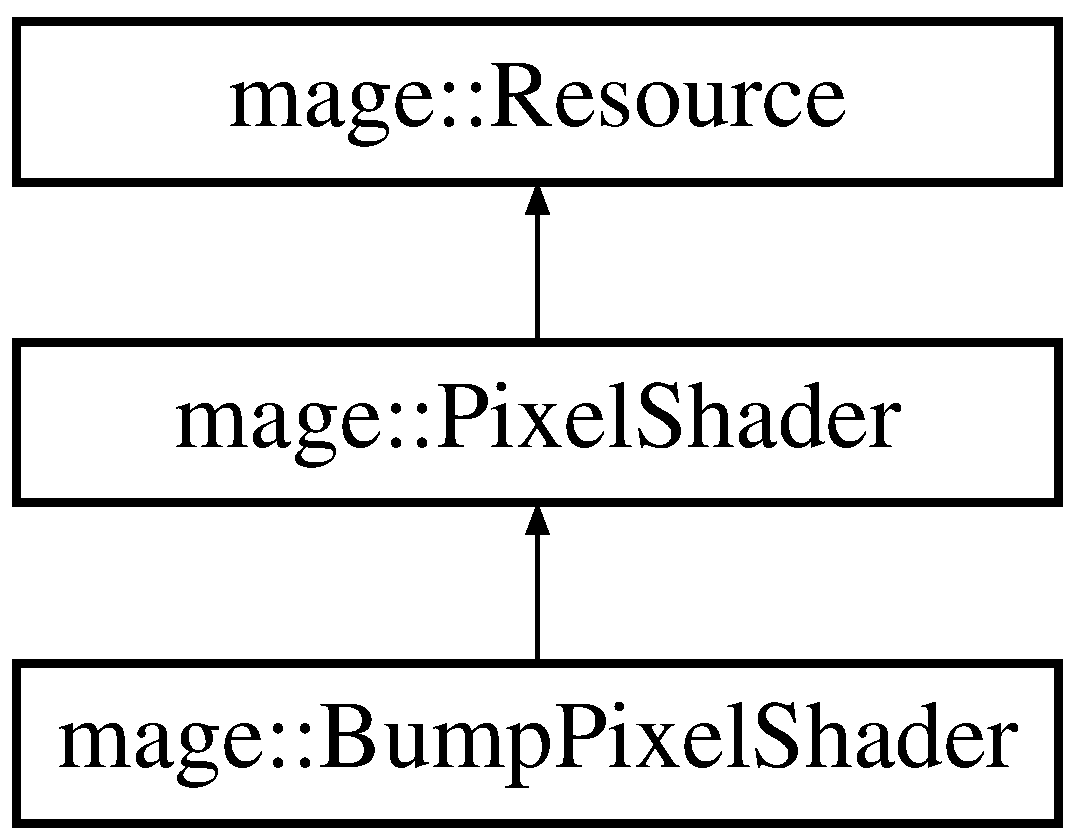
\includegraphics[height=3.000000cm]{classmage_1_1_bump_pixel_shader}
\end{center}
\end{figure}
\subsection*{Public Member Functions}
\begin{DoxyCompactItemize}
\item 
\hyperlink{classmage_1_1_bump_pixel_shader_a869f9e7c406079612eeac9885c0fc201}{Bump\+Pixel\+Shader} (I\+D3\+D11\+Device2 $\ast$device, I\+D3\+D11\+Device\+Context2 $\ast$device\+\_\+context, const wstring \&fname)
\item 
\hyperlink{classmage_1_1_bump_pixel_shader_abe9362661f862ea169b191c4d22d8c4d}{Bump\+Pixel\+Shader} (I\+D3\+D11\+Device2 $\ast$device, I\+D3\+D11\+Device\+Context2 $\ast$device\+\_\+context, const \hyperlink{structmage_1_1_compiled_pixel_shader}{Compiled\+Pixel\+Shader} \&compiled\+\_\+pixel\+\_\+shader)
\item 
\hyperlink{classmage_1_1_bump_pixel_shader_ae2442bfecc38813e11c0fb81b1b56205}{Bump\+Pixel\+Shader} (const \hyperlink{classmage_1_1_bump_pixel_shader}{Bump\+Pixel\+Shader} \&pixel\+\_\+shader)=delete
\item 
\hyperlink{classmage_1_1_bump_pixel_shader_a01db1b284501b163419bf50ed9997b81}{Bump\+Pixel\+Shader} (\hyperlink{classmage_1_1_bump_pixel_shader}{Bump\+Pixel\+Shader} \&\&pixel\+\_\+shader)
\item 
virtual \hyperlink{classmage_1_1_bump_pixel_shader_a73fde1c65d4e8e29795247a43a31926b}{$\sim$\+Bump\+Pixel\+Shader} ()
\item 
\hyperlink{classmage_1_1_bump_pixel_shader}{Bump\+Pixel\+Shader} \& \hyperlink{classmage_1_1_bump_pixel_shader_a9f9112ec617a7de6b6bd1272c8be42da}{operator=} (const \hyperlink{classmage_1_1_bump_pixel_shader}{Bump\+Pixel\+Shader} \&pixel\+\_\+shader)=delete
\item 
\hyperlink{classmage_1_1_bump_pixel_shader}{Bump\+Pixel\+Shader} \& \hyperlink{classmage_1_1_bump_pixel_shader_acebedf6bcce2d9f764ac807bc9456ede}{operator=} (\hyperlink{classmage_1_1_bump_pixel_shader}{Bump\+Pixel\+Shader} \&\&pixel\+\_\+shader)=delete
\item 
virtual void \hyperlink{classmage_1_1_bump_pixel_shader_aa365b87ca4860c58048ee1a119b4b668}{Prepare\+Shading} (const \hyperlink{structmage_1_1_material}{Material} \&material, const \hyperlink{structmage_1_1_lighting}{Lighting} \&lighting) const override final
\end{DoxyCompactItemize}
\subsection*{Private Attributes}
\begin{DoxyCompactItemize}
\item 
\hyperlink{structmage_1_1_constant_buffer}{Constant\+Buffer}$<$ Material\+Buffer $>$ \hyperlink{classmage_1_1_bump_pixel_shader_a0f586036023158b6234ff4d6d36b4e02}{m\+\_\+material\+\_\+buffer}
\end{DoxyCompactItemize}
\subsection*{Additional Inherited Members}


\subsection{Detailed Description}
A class of bump pixel shaders. 

\subsection{Constructor \& Destructor Documentation}
\hypertarget{classmage_1_1_bump_pixel_shader_a869f9e7c406079612eeac9885c0fc201}{}\label{classmage_1_1_bump_pixel_shader_a869f9e7c406079612eeac9885c0fc201} 
\index{mage\+::\+Bump\+Pixel\+Shader@{mage\+::\+Bump\+Pixel\+Shader}!Bump\+Pixel\+Shader@{Bump\+Pixel\+Shader}}
\index{Bump\+Pixel\+Shader@{Bump\+Pixel\+Shader}!mage\+::\+Bump\+Pixel\+Shader@{mage\+::\+Bump\+Pixel\+Shader}}
\subsubsection{\texorpdfstring{Bump\+Pixel\+Shader()}{BumpPixelShader()}\hspace{0.1cm}{\footnotesize\ttfamily [1/4]}}
{\footnotesize\ttfamily mage\+::\+Bump\+Pixel\+Shader\+::\+Bump\+Pixel\+Shader (\begin{DoxyParamCaption}\item[{I\+D3\+D11\+Device2 $\ast$}]{device,  }\item[{I\+D3\+D11\+Device\+Context2 $\ast$}]{device\+\_\+context,  }\item[{const wstring \&}]{fname }\end{DoxyParamCaption})\hspace{0.3cm}{\ttfamily [explicit]}}

Constructs a bump pixel shader.

\begin{DoxyPrecond}{Precondition}
{\itshape device} is not equal to {\ttfamily nullptr}. 

{\itshape device\+\_\+context} is not equal to {\ttfamily nullptr}. 
\end{DoxyPrecond}

\begin{DoxyParams}[1]{Parameters}
\mbox{\tt in}  & {\em device} & A pointer to the device. \\
\hline
\mbox{\tt in}  & {\em device\+\_\+context} & A pointer to the device context. \\
\hline
\mbox{\tt in}  & {\em fname} & A reference to the filename. \\
\hline
\end{DoxyParams}

\begin{DoxyExceptions}{Exceptions}
{\em \hyperlink{structmage_1_1_formatted_exception}{Formatted\+Exception}} & Failed to initialize this pixel shader. \\
\hline
\end{DoxyExceptions}
\hypertarget{classmage_1_1_bump_pixel_shader_abe9362661f862ea169b191c4d22d8c4d}{}\label{classmage_1_1_bump_pixel_shader_abe9362661f862ea169b191c4d22d8c4d} 
\index{mage\+::\+Bump\+Pixel\+Shader@{mage\+::\+Bump\+Pixel\+Shader}!Bump\+Pixel\+Shader@{Bump\+Pixel\+Shader}}
\index{Bump\+Pixel\+Shader@{Bump\+Pixel\+Shader}!mage\+::\+Bump\+Pixel\+Shader@{mage\+::\+Bump\+Pixel\+Shader}}
\subsubsection{\texorpdfstring{Bump\+Pixel\+Shader()}{BumpPixelShader()}\hspace{0.1cm}{\footnotesize\ttfamily [2/4]}}
{\footnotesize\ttfamily mage\+::\+Bump\+Pixel\+Shader\+::\+Bump\+Pixel\+Shader (\begin{DoxyParamCaption}\item[{I\+D3\+D11\+Device2 $\ast$}]{device,  }\item[{I\+D3\+D11\+Device\+Context2 $\ast$}]{device\+\_\+context,  }\item[{const \hyperlink{structmage_1_1_compiled_pixel_shader}{Compiled\+Pixel\+Shader} \&}]{compiled\+\_\+pixel\+\_\+shader }\end{DoxyParamCaption})\hspace{0.3cm}{\ttfamily [explicit]}}

Constructs a bump pixel shader.

\begin{DoxyPrecond}{Precondition}
{\itshape device} is not equal to {\ttfamily nullptr}. 

{\itshape device\+\_\+context} is not equal to {\ttfamily nullptr}. 
\end{DoxyPrecond}

\begin{DoxyParams}[1]{Parameters}
\mbox{\tt in}  & {\em device} & A pointer to the device. \\
\hline
\mbox{\tt in}  & {\em device\+\_\+context} & A pointer to the device context. \\
\hline
\mbox{\tt in}  & {\em compiled\+\_\+pixel\+\_\+shader} & A reference to the compiled pixel shader. \\
\hline
\end{DoxyParams}

\begin{DoxyExceptions}{Exceptions}
{\em \hyperlink{structmage_1_1_formatted_exception}{Formatted\+Exception}} & Failed to initialize this pixel shader. \\
\hline
\end{DoxyExceptions}
\hypertarget{classmage_1_1_bump_pixel_shader_ae2442bfecc38813e11c0fb81b1b56205}{}\label{classmage_1_1_bump_pixel_shader_ae2442bfecc38813e11c0fb81b1b56205} 
\index{mage\+::\+Bump\+Pixel\+Shader@{mage\+::\+Bump\+Pixel\+Shader}!Bump\+Pixel\+Shader@{Bump\+Pixel\+Shader}}
\index{Bump\+Pixel\+Shader@{Bump\+Pixel\+Shader}!mage\+::\+Bump\+Pixel\+Shader@{mage\+::\+Bump\+Pixel\+Shader}}
\subsubsection{\texorpdfstring{Bump\+Pixel\+Shader()}{BumpPixelShader()}\hspace{0.1cm}{\footnotesize\ttfamily [3/4]}}
{\footnotesize\ttfamily mage\+::\+Bump\+Pixel\+Shader\+::\+Bump\+Pixel\+Shader (\begin{DoxyParamCaption}\item[{const \hyperlink{classmage_1_1_bump_pixel_shader}{Bump\+Pixel\+Shader} \&}]{pixel\+\_\+shader }\end{DoxyParamCaption})\hspace{0.3cm}{\ttfamily [delete]}}

Constructs a bump pixel shader from the given bump pixel shader.


\begin{DoxyParams}[1]{Parameters}
\mbox{\tt in}  & {\em pixel\+\_\+shader} & A reference to the bump pixel shader to copy. \\
\hline
\end{DoxyParams}
\hypertarget{classmage_1_1_bump_pixel_shader_a01db1b284501b163419bf50ed9997b81}{}\label{classmage_1_1_bump_pixel_shader_a01db1b284501b163419bf50ed9997b81} 
\index{mage\+::\+Bump\+Pixel\+Shader@{mage\+::\+Bump\+Pixel\+Shader}!Bump\+Pixel\+Shader@{Bump\+Pixel\+Shader}}
\index{Bump\+Pixel\+Shader@{Bump\+Pixel\+Shader}!mage\+::\+Bump\+Pixel\+Shader@{mage\+::\+Bump\+Pixel\+Shader}}
\subsubsection{\texorpdfstring{Bump\+Pixel\+Shader()}{BumpPixelShader()}\hspace{0.1cm}{\footnotesize\ttfamily [4/4]}}
{\footnotesize\ttfamily mage\+::\+Bump\+Pixel\+Shader\+::\+Bump\+Pixel\+Shader (\begin{DoxyParamCaption}\item[{\hyperlink{classmage_1_1_bump_pixel_shader}{Bump\+Pixel\+Shader} \&\&}]{pixel\+\_\+shader }\end{DoxyParamCaption})\hspace{0.3cm}{\ttfamily [default]}}

Constructs a bump pixel shader by moving the given bump pixel shader.


\begin{DoxyParams}[1]{Parameters}
\mbox{\tt in}  & {\em pixel\+\_\+shader} & A reference to the bump pixel shader to move. \\
\hline
\end{DoxyParams}
\hypertarget{classmage_1_1_bump_pixel_shader_a73fde1c65d4e8e29795247a43a31926b}{}\label{classmage_1_1_bump_pixel_shader_a73fde1c65d4e8e29795247a43a31926b} 
\index{mage\+::\+Bump\+Pixel\+Shader@{mage\+::\+Bump\+Pixel\+Shader}!````~Bump\+Pixel\+Shader@{$\sim$\+Bump\+Pixel\+Shader}}
\index{````~Bump\+Pixel\+Shader@{$\sim$\+Bump\+Pixel\+Shader}!mage\+::\+Bump\+Pixel\+Shader@{mage\+::\+Bump\+Pixel\+Shader}}
\subsubsection{\texorpdfstring{$\sim$\+Bump\+Pixel\+Shader()}{~BumpPixelShader()}}
{\footnotesize\ttfamily mage\+::\+Bump\+Pixel\+Shader\+::$\sim$\+Bump\+Pixel\+Shader (\begin{DoxyParamCaption}{ }\end{DoxyParamCaption})\hspace{0.3cm}{\ttfamily [virtual]}, {\ttfamily [default]}}

Destructs this bump pixel shader. 

\subsection{Member Function Documentation}
\hypertarget{classmage_1_1_bump_pixel_shader_a9f9112ec617a7de6b6bd1272c8be42da}{}\label{classmage_1_1_bump_pixel_shader_a9f9112ec617a7de6b6bd1272c8be42da} 
\index{mage\+::\+Bump\+Pixel\+Shader@{mage\+::\+Bump\+Pixel\+Shader}!operator=@{operator=}}
\index{operator=@{operator=}!mage\+::\+Bump\+Pixel\+Shader@{mage\+::\+Bump\+Pixel\+Shader}}
\subsubsection{\texorpdfstring{operator=()}{operator=()}\hspace{0.1cm}{\footnotesize\ttfamily [1/2]}}
{\footnotesize\ttfamily \hyperlink{classmage_1_1_bump_pixel_shader}{Bump\+Pixel\+Shader}\& mage\+::\+Bump\+Pixel\+Shader\+::operator= (\begin{DoxyParamCaption}\item[{const \hyperlink{classmage_1_1_bump_pixel_shader}{Bump\+Pixel\+Shader} \&}]{pixel\+\_\+shader }\end{DoxyParamCaption})\hspace{0.3cm}{\ttfamily [delete]}}

Copies the given bump pixel shader to this bump pixel shader.


\begin{DoxyParams}[1]{Parameters}
\mbox{\tt in}  & {\em pixel\+\_\+shader} & A reference to the bump pixel shader to copy. \\
\hline
\end{DoxyParams}
\begin{DoxyReturn}{Returns}
A reference to the copy of the given bump pixel shader (i.\+e. this bump pixel shader). 
\end{DoxyReturn}
\hypertarget{classmage_1_1_bump_pixel_shader_acebedf6bcce2d9f764ac807bc9456ede}{}\label{classmage_1_1_bump_pixel_shader_acebedf6bcce2d9f764ac807bc9456ede} 
\index{mage\+::\+Bump\+Pixel\+Shader@{mage\+::\+Bump\+Pixel\+Shader}!operator=@{operator=}}
\index{operator=@{operator=}!mage\+::\+Bump\+Pixel\+Shader@{mage\+::\+Bump\+Pixel\+Shader}}
\subsubsection{\texorpdfstring{operator=()}{operator=()}\hspace{0.1cm}{\footnotesize\ttfamily [2/2]}}
{\footnotesize\ttfamily \hyperlink{classmage_1_1_bump_pixel_shader}{Bump\+Pixel\+Shader}\& mage\+::\+Bump\+Pixel\+Shader\+::operator= (\begin{DoxyParamCaption}\item[{\hyperlink{classmage_1_1_bump_pixel_shader}{Bump\+Pixel\+Shader} \&\&}]{pixel\+\_\+shader }\end{DoxyParamCaption})\hspace{0.3cm}{\ttfamily [delete]}}

Moves the given bump pixel shader to this bump pixel shader.


\begin{DoxyParams}[1]{Parameters}
\mbox{\tt in}  & {\em pixel\+\_\+shader} & A reference to the bump pixel shader to move. \\
\hline
\end{DoxyParams}
\begin{DoxyReturn}{Returns}
A reference to the moved bump pixel shader (i.\+e. this bump pixel shader). 
\end{DoxyReturn}
\hypertarget{classmage_1_1_bump_pixel_shader_aa365b87ca4860c58048ee1a119b4b668}{}\label{classmage_1_1_bump_pixel_shader_aa365b87ca4860c58048ee1a119b4b668} 
\index{mage\+::\+Bump\+Pixel\+Shader@{mage\+::\+Bump\+Pixel\+Shader}!Prepare\+Shading@{Prepare\+Shading}}
\index{Prepare\+Shading@{Prepare\+Shading}!mage\+::\+Bump\+Pixel\+Shader@{mage\+::\+Bump\+Pixel\+Shader}}
\subsubsection{\texorpdfstring{Prepare\+Shading()}{PrepareShading()}}
{\footnotesize\ttfamily void mage\+::\+Bump\+Pixel\+Shader\+::\+Prepare\+Shading (\begin{DoxyParamCaption}\item[{const \hyperlink{structmage_1_1_material}{Material} \&}]{material,  }\item[{const \hyperlink{structmage_1_1_lighting}{Lighting} \&}]{lighting }\end{DoxyParamCaption}) const\hspace{0.3cm}{\ttfamily [final]}, {\ttfamily [override]}, {\ttfamily [virtual]}}

Prepares this bump pixel shader for shading.


\begin{DoxyParams}[1]{Parameters}
\mbox{\tt in}  & {\em material} & A reference to the material. \\
\hline
\mbox{\tt in}  & {\em lighting} & A reference to the lighting buffer. \\
\hline
\end{DoxyParams}


Reimplemented from \hyperlink{classmage_1_1_pixel_shader_a5a1a58bcb0ed64405e746ec7a5af5269}{mage\+::\+Pixel\+Shader}.



\subsection{Member Data Documentation}
\hypertarget{classmage_1_1_bump_pixel_shader_a0f586036023158b6234ff4d6d36b4e02}{}\label{classmage_1_1_bump_pixel_shader_a0f586036023158b6234ff4d6d36b4e02} 
\index{mage\+::\+Bump\+Pixel\+Shader@{mage\+::\+Bump\+Pixel\+Shader}!m\+\_\+material\+\_\+buffer@{m\+\_\+material\+\_\+buffer}}
\index{m\+\_\+material\+\_\+buffer@{m\+\_\+material\+\_\+buffer}!mage\+::\+Bump\+Pixel\+Shader@{mage\+::\+Bump\+Pixel\+Shader}}
\subsubsection{\texorpdfstring{m\+\_\+material\+\_\+buffer}{m\_material\_buffer}}
{\footnotesize\ttfamily \hyperlink{structmage_1_1_constant_buffer}{Constant\+Buffer}$<$ Material\+Buffer $>$ mage\+::\+Bump\+Pixel\+Shader\+::m\+\_\+material\+\_\+buffer\hspace{0.3cm}{\ttfamily [private]}}

A pointer to the material buffer of this bump pixel shader. 
\hypertarget{classmage_1_1_bump_vertex_shader}{}\section{mage\+:\+:Bump\+Vertex\+Shader Class Reference}
\label{classmage_1_1_bump_vertex_shader}\index{mage\+::\+Bump\+Vertex\+Shader@{mage\+::\+Bump\+Vertex\+Shader}}


{\ttfamily \#include $<$bump\+\_\+shader.\+hpp$>$}

Inheritance diagram for mage\+:\+:Bump\+Vertex\+Shader\+:\begin{figure}[H]
\begin{center}
\leavevmode
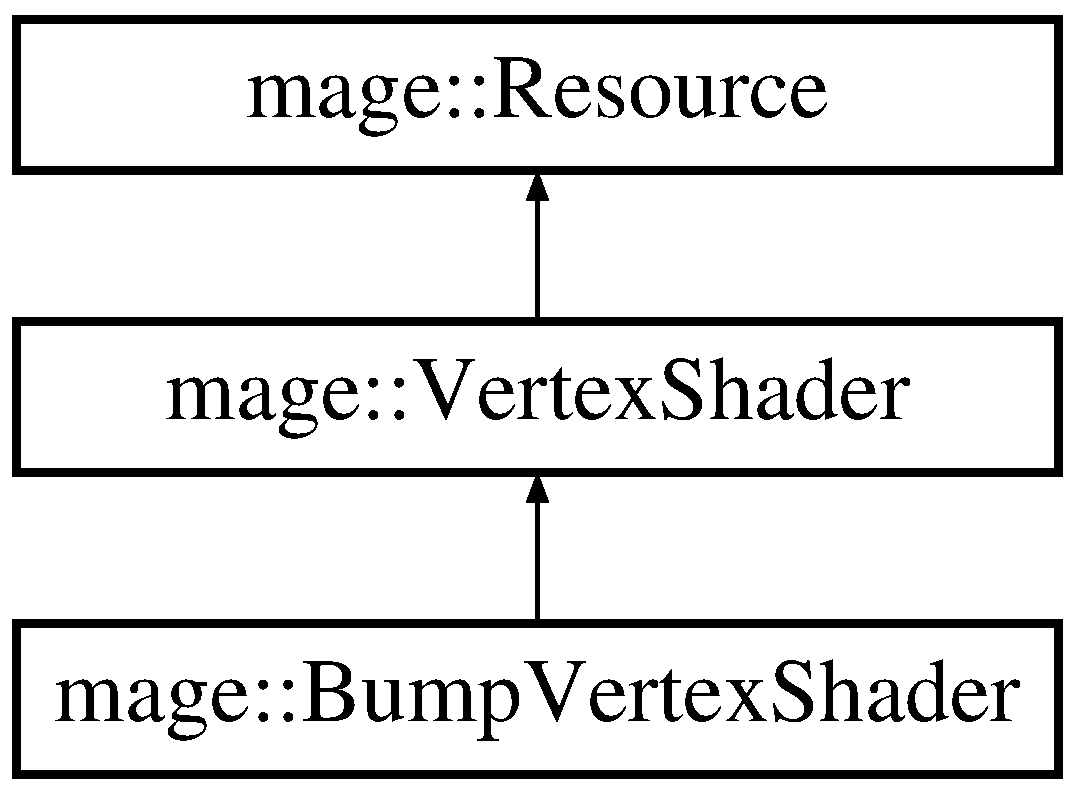
\includegraphics[height=3.000000cm]{classmage_1_1_bump_vertex_shader}
\end{center}
\end{figure}
\subsection*{Public Member Functions}
\begin{DoxyCompactItemize}
\item 
\hyperlink{classmage_1_1_bump_vertex_shader_abaaada10d913e62942d8ac9762a3f897}{Bump\+Vertex\+Shader} (I\+D3\+D11\+Device2 $\ast$device, I\+D3\+D11\+Device\+Context2 $\ast$device\+\_\+context, const wstring \&fname)
\item 
\hyperlink{classmage_1_1_bump_vertex_shader_a1990393c55846a6cbeded8601b495d49}{Bump\+Vertex\+Shader} (I\+D3\+D11\+Device2 $\ast$device, I\+D3\+D11\+Device\+Context2 $\ast$device\+\_\+context, const \hyperlink{structmage_1_1_compiled_vertex_shader}{Compiled\+Vertex\+Shader} \&compiled\+\_\+vertex\+\_\+shader)
\item 
\hyperlink{classmage_1_1_bump_vertex_shader_abb1bc40546871490c44d14dbe17303b2}{Bump\+Vertex\+Shader} (const \hyperlink{classmage_1_1_bump_vertex_shader}{Bump\+Vertex\+Shader} \&vertex\+\_\+shader)=delete
\item 
\hyperlink{classmage_1_1_bump_vertex_shader_aa94f0403d19493070c6b061b5dc76f76}{Bump\+Vertex\+Shader} (\hyperlink{classmage_1_1_bump_vertex_shader}{Bump\+Vertex\+Shader} \&\&vertex\+\_\+shader)
\item 
virtual \hyperlink{classmage_1_1_bump_vertex_shader_aac66d698654ff58a1440cf3dfdcece40}{$\sim$\+Bump\+Vertex\+Shader} ()
\item 
\hyperlink{classmage_1_1_bump_vertex_shader}{Bump\+Vertex\+Shader} \& \hyperlink{classmage_1_1_bump_vertex_shader_a03d0c6105391a294d8e762d9cac600a8}{operator=} (const \hyperlink{classmage_1_1_bump_vertex_shader}{Bump\+Vertex\+Shader} \&vertex\+\_\+shader)=delete
\item 
\hyperlink{classmage_1_1_bump_vertex_shader}{Bump\+Vertex\+Shader} \& \hyperlink{classmage_1_1_bump_vertex_shader_a478db6b064206d32b3b92df43a5a4382}{operator=} (\hyperlink{classmage_1_1_bump_vertex_shader}{Bump\+Vertex\+Shader} \&\&vertex\+\_\+shader)=delete
\item 
virtual void \hyperlink{classmage_1_1_bump_vertex_shader_a11513b06e76e8d3d55f6d96c5a14bdb7}{Prepare\+Shading} (I\+D3\+D11\+Buffer $\ast$transform) const override final
\end{DoxyCompactItemize}
\subsection*{Additional Inherited Members}


\subsection{Detailed Description}
A class of bump vertex shaders. 

\subsection{Constructor \& Destructor Documentation}
\hypertarget{classmage_1_1_bump_vertex_shader_abaaada10d913e62942d8ac9762a3f897}{}\label{classmage_1_1_bump_vertex_shader_abaaada10d913e62942d8ac9762a3f897} 
\index{mage\+::\+Bump\+Vertex\+Shader@{mage\+::\+Bump\+Vertex\+Shader}!Bump\+Vertex\+Shader@{Bump\+Vertex\+Shader}}
\index{Bump\+Vertex\+Shader@{Bump\+Vertex\+Shader}!mage\+::\+Bump\+Vertex\+Shader@{mage\+::\+Bump\+Vertex\+Shader}}
\subsubsection{\texorpdfstring{Bump\+Vertex\+Shader()}{BumpVertexShader()}\hspace{0.1cm}{\footnotesize\ttfamily [1/4]}}
{\footnotesize\ttfamily mage\+::\+Bump\+Vertex\+Shader\+::\+Bump\+Vertex\+Shader (\begin{DoxyParamCaption}\item[{I\+D3\+D11\+Device2 $\ast$}]{device,  }\item[{I\+D3\+D11\+Device\+Context2 $\ast$}]{device\+\_\+context,  }\item[{const wstring \&}]{fname }\end{DoxyParamCaption})\hspace{0.3cm}{\ttfamily [explicit]}}

Constructs a bump vertex shader.

\begin{DoxyPrecond}{Precondition}
{\itshape device} is not equal to {\ttfamily nullptr}. 

{\itshape device\+\_\+context} is not equal to {\ttfamily nullptr}. 
\end{DoxyPrecond}

\begin{DoxyParams}[1]{Parameters}
\mbox{\tt in}  & {\em device} & A pointer to the device. \\
\hline
\mbox{\tt in}  & {\em device\+\_\+context} & A pointer to the device context. \\
\hline
\mbox{\tt in}  & {\em fname} & A reference to the filename. \\
\hline
\end{DoxyParams}

\begin{DoxyExceptions}{Exceptions}
{\em \hyperlink{structmage_1_1_formatted_exception}{Formatted\+Exception}} & Failed to initialize this vertex shader. \\
\hline
\end{DoxyExceptions}
\hypertarget{classmage_1_1_bump_vertex_shader_a1990393c55846a6cbeded8601b495d49}{}\label{classmage_1_1_bump_vertex_shader_a1990393c55846a6cbeded8601b495d49} 
\index{mage\+::\+Bump\+Vertex\+Shader@{mage\+::\+Bump\+Vertex\+Shader}!Bump\+Vertex\+Shader@{Bump\+Vertex\+Shader}}
\index{Bump\+Vertex\+Shader@{Bump\+Vertex\+Shader}!mage\+::\+Bump\+Vertex\+Shader@{mage\+::\+Bump\+Vertex\+Shader}}
\subsubsection{\texorpdfstring{Bump\+Vertex\+Shader()}{BumpVertexShader()}\hspace{0.1cm}{\footnotesize\ttfamily [2/4]}}
{\footnotesize\ttfamily mage\+::\+Bump\+Vertex\+Shader\+::\+Bump\+Vertex\+Shader (\begin{DoxyParamCaption}\item[{I\+D3\+D11\+Device2 $\ast$}]{device,  }\item[{I\+D3\+D11\+Device\+Context2 $\ast$}]{device\+\_\+context,  }\item[{const \hyperlink{structmage_1_1_compiled_vertex_shader}{Compiled\+Vertex\+Shader} \&}]{compiled\+\_\+vertex\+\_\+shader }\end{DoxyParamCaption})\hspace{0.3cm}{\ttfamily [explicit]}}

Constructs a bump vertex shader.

\begin{DoxyPrecond}{Precondition}
{\itshape device} is not equal to {\ttfamily nullptr}. 

{\itshape device\+\_\+context} is not equal to {\ttfamily nullptr}. 
\end{DoxyPrecond}

\begin{DoxyParams}[1]{Parameters}
\mbox{\tt in}  & {\em device} & A pointer to the device. \\
\hline
\mbox{\tt in}  & {\em device\+\_\+context} & A pointer to the device context. \\
\hline
\mbox{\tt in}  & {\em compiled\+\_\+vertex\+\_\+shader} & A reference to the compiled vertex shader. \\
\hline
\end{DoxyParams}

\begin{DoxyExceptions}{Exceptions}
{\em \hyperlink{structmage_1_1_formatted_exception}{Formatted\+Exception}} & Failed to initialize this vertex shader. \\
\hline
\end{DoxyExceptions}
\hypertarget{classmage_1_1_bump_vertex_shader_abb1bc40546871490c44d14dbe17303b2}{}\label{classmage_1_1_bump_vertex_shader_abb1bc40546871490c44d14dbe17303b2} 
\index{mage\+::\+Bump\+Vertex\+Shader@{mage\+::\+Bump\+Vertex\+Shader}!Bump\+Vertex\+Shader@{Bump\+Vertex\+Shader}}
\index{Bump\+Vertex\+Shader@{Bump\+Vertex\+Shader}!mage\+::\+Bump\+Vertex\+Shader@{mage\+::\+Bump\+Vertex\+Shader}}
\subsubsection{\texorpdfstring{Bump\+Vertex\+Shader()}{BumpVertexShader()}\hspace{0.1cm}{\footnotesize\ttfamily [3/4]}}
{\footnotesize\ttfamily mage\+::\+Bump\+Vertex\+Shader\+::\+Bump\+Vertex\+Shader (\begin{DoxyParamCaption}\item[{const \hyperlink{classmage_1_1_bump_vertex_shader}{Bump\+Vertex\+Shader} \&}]{vertex\+\_\+shader }\end{DoxyParamCaption})\hspace{0.3cm}{\ttfamily [delete]}}

Constructs a bump vertex shader from the given bump vertex shader.


\begin{DoxyParams}[1]{Parameters}
\mbox{\tt in}  & {\em vertex\+\_\+shader} & A reference to the bump vertex shader to copy. \\
\hline
\end{DoxyParams}
\hypertarget{classmage_1_1_bump_vertex_shader_aa94f0403d19493070c6b061b5dc76f76}{}\label{classmage_1_1_bump_vertex_shader_aa94f0403d19493070c6b061b5dc76f76} 
\index{mage\+::\+Bump\+Vertex\+Shader@{mage\+::\+Bump\+Vertex\+Shader}!Bump\+Vertex\+Shader@{Bump\+Vertex\+Shader}}
\index{Bump\+Vertex\+Shader@{Bump\+Vertex\+Shader}!mage\+::\+Bump\+Vertex\+Shader@{mage\+::\+Bump\+Vertex\+Shader}}
\subsubsection{\texorpdfstring{Bump\+Vertex\+Shader()}{BumpVertexShader()}\hspace{0.1cm}{\footnotesize\ttfamily [4/4]}}
{\footnotesize\ttfamily mage\+::\+Bump\+Vertex\+Shader\+::\+Bump\+Vertex\+Shader (\begin{DoxyParamCaption}\item[{\hyperlink{classmage_1_1_bump_vertex_shader}{Bump\+Vertex\+Shader} \&\&}]{vertex\+\_\+shader }\end{DoxyParamCaption})\hspace{0.3cm}{\ttfamily [default]}}

Constructs a bump vertex shader by moving the given bump vertex shader.


\begin{DoxyParams}[1]{Parameters}
\mbox{\tt in}  & {\em vertex\+\_\+shader} & A reference to the bump vertex shader to move. \\
\hline
\end{DoxyParams}
\hypertarget{classmage_1_1_bump_vertex_shader_aac66d698654ff58a1440cf3dfdcece40}{}\label{classmage_1_1_bump_vertex_shader_aac66d698654ff58a1440cf3dfdcece40} 
\index{mage\+::\+Bump\+Vertex\+Shader@{mage\+::\+Bump\+Vertex\+Shader}!````~Bump\+Vertex\+Shader@{$\sim$\+Bump\+Vertex\+Shader}}
\index{````~Bump\+Vertex\+Shader@{$\sim$\+Bump\+Vertex\+Shader}!mage\+::\+Bump\+Vertex\+Shader@{mage\+::\+Bump\+Vertex\+Shader}}
\subsubsection{\texorpdfstring{$\sim$\+Bump\+Vertex\+Shader()}{~BumpVertexShader()}}
{\footnotesize\ttfamily mage\+::\+Bump\+Vertex\+Shader\+::$\sim$\+Bump\+Vertex\+Shader (\begin{DoxyParamCaption}{ }\end{DoxyParamCaption})\hspace{0.3cm}{\ttfamily [virtual]}, {\ttfamily [default]}}

Destructs this bump vertex shader. 

\subsection{Member Function Documentation}
\hypertarget{classmage_1_1_bump_vertex_shader_a03d0c6105391a294d8e762d9cac600a8}{}\label{classmage_1_1_bump_vertex_shader_a03d0c6105391a294d8e762d9cac600a8} 
\index{mage\+::\+Bump\+Vertex\+Shader@{mage\+::\+Bump\+Vertex\+Shader}!operator=@{operator=}}
\index{operator=@{operator=}!mage\+::\+Bump\+Vertex\+Shader@{mage\+::\+Bump\+Vertex\+Shader}}
\subsubsection{\texorpdfstring{operator=()}{operator=()}\hspace{0.1cm}{\footnotesize\ttfamily [1/2]}}
{\footnotesize\ttfamily \hyperlink{classmage_1_1_bump_vertex_shader}{Bump\+Vertex\+Shader}\& mage\+::\+Bump\+Vertex\+Shader\+::operator= (\begin{DoxyParamCaption}\item[{const \hyperlink{classmage_1_1_bump_vertex_shader}{Bump\+Vertex\+Shader} \&}]{vertex\+\_\+shader }\end{DoxyParamCaption})\hspace{0.3cm}{\ttfamily [delete]}}

Copies the given bump vertex shader to this bump vertex shader.


\begin{DoxyParams}[1]{Parameters}
\mbox{\tt in}  & {\em vertex\+\_\+shader} & A reference to the bump vertex shader to copy. \\
\hline
\end{DoxyParams}
\begin{DoxyReturn}{Returns}
A reference to the copy of the given bump vertex shader (i.\+e. this bump vertex shader). 
\end{DoxyReturn}
\hypertarget{classmage_1_1_bump_vertex_shader_a478db6b064206d32b3b92df43a5a4382}{}\label{classmage_1_1_bump_vertex_shader_a478db6b064206d32b3b92df43a5a4382} 
\index{mage\+::\+Bump\+Vertex\+Shader@{mage\+::\+Bump\+Vertex\+Shader}!operator=@{operator=}}
\index{operator=@{operator=}!mage\+::\+Bump\+Vertex\+Shader@{mage\+::\+Bump\+Vertex\+Shader}}
\subsubsection{\texorpdfstring{operator=()}{operator=()}\hspace{0.1cm}{\footnotesize\ttfamily [2/2]}}
{\footnotesize\ttfamily \hyperlink{classmage_1_1_bump_vertex_shader}{Bump\+Vertex\+Shader}\& mage\+::\+Bump\+Vertex\+Shader\+::operator= (\begin{DoxyParamCaption}\item[{\hyperlink{classmage_1_1_bump_vertex_shader}{Bump\+Vertex\+Shader} \&\&}]{vertex\+\_\+shader }\end{DoxyParamCaption})\hspace{0.3cm}{\ttfamily [delete]}}

Copies the given bump vertex shader to this bump vertex shader.


\begin{DoxyParams}[1]{Parameters}
\mbox{\tt in}  & {\em vertex\+\_\+shader} & A reference to the bump vertex shader to copy. \\
\hline
\end{DoxyParams}
\begin{DoxyReturn}{Returns}
A reference to the moved bump vertex shader (i.\+e. this bump vertex shader). 
\end{DoxyReturn}
\hypertarget{classmage_1_1_bump_vertex_shader_a11513b06e76e8d3d55f6d96c5a14bdb7}{}\label{classmage_1_1_bump_vertex_shader_a11513b06e76e8d3d55f6d96c5a14bdb7} 
\index{mage\+::\+Bump\+Vertex\+Shader@{mage\+::\+Bump\+Vertex\+Shader}!Prepare\+Shading@{Prepare\+Shading}}
\index{Prepare\+Shading@{Prepare\+Shading}!mage\+::\+Bump\+Vertex\+Shader@{mage\+::\+Bump\+Vertex\+Shader}}
\subsubsection{\texorpdfstring{Prepare\+Shading()}{PrepareShading()}}
{\footnotesize\ttfamily void mage\+::\+Bump\+Vertex\+Shader\+::\+Prepare\+Shading (\begin{DoxyParamCaption}\item[{I\+D3\+D11\+Buffer $\ast$}]{transform }\end{DoxyParamCaption}) const\hspace{0.3cm}{\ttfamily [final]}, {\ttfamily [override]}, {\ttfamily [virtual]}}

Prepares this bump vertex shader for shading.

\begin{DoxyPrecond}{Precondition}
{\itshape transform} is not equal to {\ttfamily nullptr}. 
\end{DoxyPrecond}

\begin{DoxyParams}[1]{Parameters}
\mbox{\tt in}  & {\em transform} & A pointer to the transform buffer. \\
\hline
\end{DoxyParams}


Reimplemented from \hyperlink{classmage_1_1_vertex_shader_a53f4b25241f6c5739724d421c9f29a36}{mage\+::\+Vertex\+Shader}.


\hypertarget{classmage_1_1_camera}{}\section{mage\+:\+:Camera Class Reference}
\label{classmage_1_1_camera}\index{mage\+::\+Camera@{mage\+::\+Camera}}


{\ttfamily \#include $<$camera.\+hpp$>$}

Inheritance diagram for mage\+:\+:Camera\+:\begin{figure}[H]
\begin{center}
\leavevmode
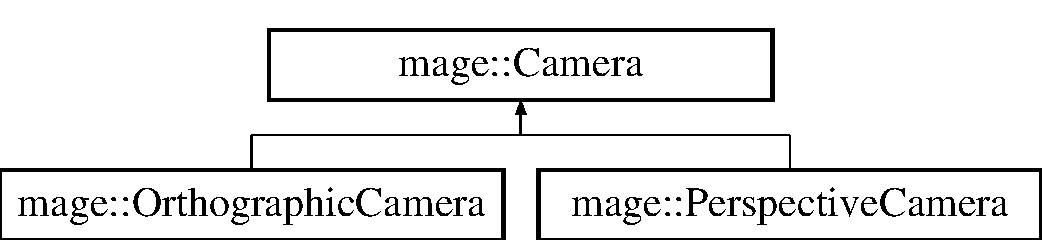
\includegraphics[height=2.000000cm]{classmage_1_1_camera}
\end{center}
\end{figure}
\subsection*{Public Member Functions}
\begin{DoxyCompactItemize}
\item 
virtual \hyperlink{classmage_1_1_camera_a181f7fdf168c0d66022edfecb697dd7d}{$\sim$\+Camera} ()=default
\item 
\hyperlink{classmage_1_1_camera}{Camera} \& \hyperlink{classmage_1_1_camera_afe33e674f74180d6b9566a85eec51ac4}{operator=} (const \hyperlink{classmage_1_1_camera}{Camera} \&camera)=default
\item 
\hyperlink{classmage_1_1_camera}{Camera} \& \hyperlink{classmage_1_1_camera_a481f758a59564bb4074249f9bbf4e305}{operator=} (\hyperlink{classmage_1_1_camera}{Camera} \&\&camera)=default
\item 
\hyperlink{namespacemage_a1e01ae66713838a7a67d30e44c67703e}{Shared\+Ptr}$<$ \hyperlink{classmage_1_1_camera}{Camera} $>$ \hyperlink{classmage_1_1_camera_a0da912eb0d403e190cd36ec9dcd6704a}{Clone} ()
\item 
float \hyperlink{classmage_1_1_camera_a175e3c36526a8a3e28cd2f8bd1701c55}{Get\+NearZ} () const
\item 
\hyperlink{classmage_1_1_camera}{Camera} \& \hyperlink{classmage_1_1_camera_ae2e148f1ff5128442927abc87114a739}{Set\+NearZ} (float near\+\_\+z)
\item 
float \hyperlink{classmage_1_1_camera_a7f293a8711086b3419fe3b4224ff2778}{Get\+FarZ} () const
\item 
\hyperlink{classmage_1_1_camera}{Camera} \& \hyperlink{classmage_1_1_camera_acd1ab15368f052b846f72b92a52a94c5}{Set\+FarZ} (float far\+\_\+z)
\item 
\hyperlink{classmage_1_1_camera}{Camera} \& \hyperlink{classmage_1_1_camera_a8cb00dc1b8455197412c80f321011dc1}{Set\+Near\+And\+FarZ} (float near\+\_\+z, float far\+\_\+z)
\item 
virtual X\+M\+M\+A\+T\+R\+IX \hyperlink{classmage_1_1_camera_a1f5206864cf18b5548219492556df5d2}{Get\+View\+To\+Projection\+Matrix} () const =0
\end{DoxyCompactItemize}
\subsection*{Protected Member Functions}
\begin{DoxyCompactItemize}
\item 
\hyperlink{classmage_1_1_camera_ae734b9b92203a384410e83f117fa4427}{Camera} (float near\+\_\+z=M\+A\+G\+E\+\_\+\+D\+E\+F\+A\+U\+L\+T\+\_\+\+C\+A\+M\+E\+R\+A\+\_\+\+N\+E\+A\+R\+\_\+Z, float far\+\_\+z=M\+A\+G\+E\+\_\+\+D\+E\+F\+A\+U\+L\+T\+\_\+\+C\+A\+M\+E\+R\+A\+\_\+\+F\+A\+R\+\_\+Z)
\item 
\hyperlink{classmage_1_1_camera_a7804afa68565efe4c48f95453d6c65f0}{Camera} (const \hyperlink{classmage_1_1_camera}{Camera} \&camera)=default
\item 
\hyperlink{classmage_1_1_camera_a595d9c89176aac92bbd58f4117c05ea9}{Camera} (\hyperlink{classmage_1_1_camera}{Camera} \&\&camera)=default
\end{DoxyCompactItemize}
\subsection*{Private Member Functions}
\begin{DoxyCompactItemize}
\item 
virtual \hyperlink{namespacemage_a1e01ae66713838a7a67d30e44c67703e}{Shared\+Ptr}$<$ \hyperlink{classmage_1_1_camera}{Camera} $>$ \hyperlink{classmage_1_1_camera_a96c1bee3dc4085c8c7892427518165fc}{Clone\+Implementation} () const =0
\end{DoxyCompactItemize}
\subsection*{Private Attributes}
\begin{DoxyCompactItemize}
\item 
float \hyperlink{classmage_1_1_camera_a685f8700a29d1f1eff2bec353c3ec970}{m\+\_\+near\+\_\+z}
\item 
float \hyperlink{classmage_1_1_camera_abe2eeca725ce3da238256007454b241f}{m\+\_\+far\+\_\+z}
\end{DoxyCompactItemize}


\subsection{Detailed Description}
A class of cameras. 

\subsection{Constructor \& Destructor Documentation}
\hypertarget{classmage_1_1_camera_a181f7fdf168c0d66022edfecb697dd7d}{}\label{classmage_1_1_camera_a181f7fdf168c0d66022edfecb697dd7d} 
\index{mage\+::\+Camera@{mage\+::\+Camera}!````~Camera@{$\sim$\+Camera}}
\index{````~Camera@{$\sim$\+Camera}!mage\+::\+Camera@{mage\+::\+Camera}}
\subsubsection{\texorpdfstring{$\sim$\+Camera()}{~Camera()}}
{\footnotesize\ttfamily virtual mage\+::\+Camera\+::$\sim$\+Camera (\begin{DoxyParamCaption}{ }\end{DoxyParamCaption})\hspace{0.3cm}{\ttfamily [virtual]}, {\ttfamily [default]}}

Destructs this camera. \hypertarget{classmage_1_1_camera_ae734b9b92203a384410e83f117fa4427}{}\label{classmage_1_1_camera_ae734b9b92203a384410e83f117fa4427} 
\index{mage\+::\+Camera@{mage\+::\+Camera}!Camera@{Camera}}
\index{Camera@{Camera}!mage\+::\+Camera@{mage\+::\+Camera}}
\subsubsection{\texorpdfstring{Camera()}{Camera()}\hspace{0.1cm}{\footnotesize\ttfamily [1/3]}}
{\footnotesize\ttfamily mage\+::\+Camera\+::\+Camera (\begin{DoxyParamCaption}\item[{float}]{near\+\_\+z = {\ttfamily MAGE\+\_\+DEFAULT\+\_\+CAMERA\+\_\+NEAR\+\_\+Z},  }\item[{float}]{far\+\_\+z = {\ttfamily MAGE\+\_\+DEFAULT\+\_\+CAMERA\+\_\+FAR\+\_\+Z} }\end{DoxyParamCaption})\hspace{0.3cm}{\ttfamily [explicit]}, {\ttfamily [protected]}}

Constructs a camera.


\begin{DoxyParams}[1]{Parameters}
\mbox{\tt in}  & {\em near\+\_\+z} & The position of the near z-\/plane in camera space. \\
\hline
\mbox{\tt in}  & {\em far\+\_\+z} & The position of the far z-\/plane in camera space. \\
\hline
\end{DoxyParams}
\hypertarget{classmage_1_1_camera_a7804afa68565efe4c48f95453d6c65f0}{}\label{classmage_1_1_camera_a7804afa68565efe4c48f95453d6c65f0} 
\index{mage\+::\+Camera@{mage\+::\+Camera}!Camera@{Camera}}
\index{Camera@{Camera}!mage\+::\+Camera@{mage\+::\+Camera}}
\subsubsection{\texorpdfstring{Camera()}{Camera()}\hspace{0.1cm}{\footnotesize\ttfamily [2/3]}}
{\footnotesize\ttfamily mage\+::\+Camera\+::\+Camera (\begin{DoxyParamCaption}\item[{const \hyperlink{classmage_1_1_camera}{Camera} \&}]{camera }\end{DoxyParamCaption})\hspace{0.3cm}{\ttfamily [protected]}, {\ttfamily [default]}}

Constructs a camera from the given camera.


\begin{DoxyParams}[1]{Parameters}
\mbox{\tt in}  & {\em camera} & A reference to the camera to copy. \\
\hline
\end{DoxyParams}
\hypertarget{classmage_1_1_camera_a595d9c89176aac92bbd58f4117c05ea9}{}\label{classmage_1_1_camera_a595d9c89176aac92bbd58f4117c05ea9} 
\index{mage\+::\+Camera@{mage\+::\+Camera}!Camera@{Camera}}
\index{Camera@{Camera}!mage\+::\+Camera@{mage\+::\+Camera}}
\subsubsection{\texorpdfstring{Camera()}{Camera()}\hspace{0.1cm}{\footnotesize\ttfamily [3/3]}}
{\footnotesize\ttfamily mage\+::\+Camera\+::\+Camera (\begin{DoxyParamCaption}\item[{\hyperlink{classmage_1_1_camera}{Camera} \&\&}]{camera }\end{DoxyParamCaption})\hspace{0.3cm}{\ttfamily [protected]}, {\ttfamily [default]}}

Constructs a camera by moving the given camera.


\begin{DoxyParams}[1]{Parameters}
\mbox{\tt in}  & {\em camera} & A reference to the camera to move. \\
\hline
\end{DoxyParams}


\subsection{Member Function Documentation}
\hypertarget{classmage_1_1_camera_a0da912eb0d403e190cd36ec9dcd6704a}{}\label{classmage_1_1_camera_a0da912eb0d403e190cd36ec9dcd6704a} 
\index{mage\+::\+Camera@{mage\+::\+Camera}!Clone@{Clone}}
\index{Clone@{Clone}!mage\+::\+Camera@{mage\+::\+Camera}}
\subsubsection{\texorpdfstring{Clone()}{Clone()}}
{\footnotesize\ttfamily \hyperlink{namespacemage_a1e01ae66713838a7a67d30e44c67703e}{Shared\+Ptr}$<$ \hyperlink{classmage_1_1_camera}{Camera} $>$ mage\+::\+Camera\+::\+Clone (\begin{DoxyParamCaption}{ }\end{DoxyParamCaption})}

Clones this camera.

\begin{DoxyReturn}{Returns}
A pointer to the clone of this camera. 
\end{DoxyReturn}
\hypertarget{classmage_1_1_camera_a96c1bee3dc4085c8c7892427518165fc}{}\label{classmage_1_1_camera_a96c1bee3dc4085c8c7892427518165fc} 
\index{mage\+::\+Camera@{mage\+::\+Camera}!Clone\+Implementation@{Clone\+Implementation}}
\index{Clone\+Implementation@{Clone\+Implementation}!mage\+::\+Camera@{mage\+::\+Camera}}
\subsubsection{\texorpdfstring{Clone\+Implementation()}{CloneImplementation()}}
{\footnotesize\ttfamily virtual \hyperlink{namespacemage_a1e01ae66713838a7a67d30e44c67703e}{Shared\+Ptr}$<$ \hyperlink{classmage_1_1_camera}{Camera} $>$ mage\+::\+Camera\+::\+Clone\+Implementation (\begin{DoxyParamCaption}{ }\end{DoxyParamCaption}) const\hspace{0.3cm}{\ttfamily [private]}, {\ttfamily [pure virtual]}}

Clones this camera.

\begin{DoxyReturn}{Returns}
A pointer to the clone of this camera. 
\end{DoxyReturn}


Implemented in \hyperlink{classmage_1_1_perspective_camera_a1c638e60154c84786d5924252d47716b}{mage\+::\+Perspective\+Camera}, and \hyperlink{classmage_1_1_orthographic_camera_aa4a201516a925e63c616f8a64573fbb2}{mage\+::\+Orthographic\+Camera}.

\hypertarget{classmage_1_1_camera_a7f293a8711086b3419fe3b4224ff2778}{}\label{classmage_1_1_camera_a7f293a8711086b3419fe3b4224ff2778} 
\index{mage\+::\+Camera@{mage\+::\+Camera}!Get\+FarZ@{Get\+FarZ}}
\index{Get\+FarZ@{Get\+FarZ}!mage\+::\+Camera@{mage\+::\+Camera}}
\subsubsection{\texorpdfstring{Get\+Far\+Z()}{GetFarZ()}}
{\footnotesize\ttfamily float mage\+::\+Camera\+::\+Get\+FarZ (\begin{DoxyParamCaption}{ }\end{DoxyParamCaption}) const}

Returns the position of the far z-\/plane of this camera in camera space.

\begin{DoxyReturn}{Returns}
The position of the far z-\/plane of this camera. 
\end{DoxyReturn}
\hypertarget{classmage_1_1_camera_a175e3c36526a8a3e28cd2f8bd1701c55}{}\label{classmage_1_1_camera_a175e3c36526a8a3e28cd2f8bd1701c55} 
\index{mage\+::\+Camera@{mage\+::\+Camera}!Get\+NearZ@{Get\+NearZ}}
\index{Get\+NearZ@{Get\+NearZ}!mage\+::\+Camera@{mage\+::\+Camera}}
\subsubsection{\texorpdfstring{Get\+Near\+Z()}{GetNearZ()}}
{\footnotesize\ttfamily float mage\+::\+Camera\+::\+Get\+NearZ (\begin{DoxyParamCaption}{ }\end{DoxyParamCaption}) const}

Returns the position of the near z-\/plane of this camera in camera space.

\begin{DoxyReturn}{Returns}
The position of the near z-\/plane of this camera. 
\end{DoxyReturn}
\hypertarget{classmage_1_1_camera_a1f5206864cf18b5548219492556df5d2}{}\label{classmage_1_1_camera_a1f5206864cf18b5548219492556df5d2} 
\index{mage\+::\+Camera@{mage\+::\+Camera}!Get\+View\+To\+Projection\+Matrix@{Get\+View\+To\+Projection\+Matrix}}
\index{Get\+View\+To\+Projection\+Matrix@{Get\+View\+To\+Projection\+Matrix}!mage\+::\+Camera@{mage\+::\+Camera}}
\subsubsection{\texorpdfstring{Get\+View\+To\+Projection\+Matrix()}{GetViewToProjectionMatrix()}}
{\footnotesize\ttfamily virtual X\+M\+M\+A\+T\+R\+IX mage\+::\+Camera\+::\+Get\+View\+To\+Projection\+Matrix (\begin{DoxyParamCaption}{ }\end{DoxyParamCaption}) const\hspace{0.3cm}{\ttfamily [pure virtual]}}

Returns the view-\/to-\/projection matrix of this camera.

\begin{DoxyReturn}{Returns}
The view-\/to-\/projection matrix of this camera. 
\end{DoxyReturn}


Implemented in \hyperlink{classmage_1_1_perspective_camera_a83a38a4e8180707df2323130f9cee4a5}{mage\+::\+Perspective\+Camera}, and \hyperlink{classmage_1_1_orthographic_camera_aedd86e56a0f7bc967ad8d9be2631a0cf}{mage\+::\+Orthographic\+Camera}.

\hypertarget{classmage_1_1_camera_afe33e674f74180d6b9566a85eec51ac4}{}\label{classmage_1_1_camera_afe33e674f74180d6b9566a85eec51ac4} 
\index{mage\+::\+Camera@{mage\+::\+Camera}!operator=@{operator=}}
\index{operator=@{operator=}!mage\+::\+Camera@{mage\+::\+Camera}}
\subsubsection{\texorpdfstring{operator=()}{operator=()}\hspace{0.1cm}{\footnotesize\ttfamily [1/2]}}
{\footnotesize\ttfamily \hyperlink{classmage_1_1_camera}{Camera}\& mage\+::\+Camera\+::operator= (\begin{DoxyParamCaption}\item[{const \hyperlink{classmage_1_1_camera}{Camera} \&}]{camera }\end{DoxyParamCaption})\hspace{0.3cm}{\ttfamily [default]}}

Copies the given camera to this camera.


\begin{DoxyParams}[1]{Parameters}
\mbox{\tt in}  & {\em camera} & A reference to the camera to copy. \\
\hline
\end{DoxyParams}
\begin{DoxyReturn}{Returns}
A reference to the copy of the given camera (i.\+e. this camera). 
\end{DoxyReturn}
\hypertarget{classmage_1_1_camera_a481f758a59564bb4074249f9bbf4e305}{}\label{classmage_1_1_camera_a481f758a59564bb4074249f9bbf4e305} 
\index{mage\+::\+Camera@{mage\+::\+Camera}!operator=@{operator=}}
\index{operator=@{operator=}!mage\+::\+Camera@{mage\+::\+Camera}}
\subsubsection{\texorpdfstring{operator=()}{operator=()}\hspace{0.1cm}{\footnotesize\ttfamily [2/2]}}
{\footnotesize\ttfamily \hyperlink{classmage_1_1_camera}{Camera}\& mage\+::\+Camera\+::operator= (\begin{DoxyParamCaption}\item[{\hyperlink{classmage_1_1_camera}{Camera} \&\&}]{camera }\end{DoxyParamCaption})\hspace{0.3cm}{\ttfamily [default]}}

Moves the given camera to this camera.


\begin{DoxyParams}[1]{Parameters}
\mbox{\tt in}  & {\em camera} & A reference to the camera to move. \\
\hline
\end{DoxyParams}
\begin{DoxyReturn}{Returns}
A reference to the moved camera (i.\+e. this camera). 
\end{DoxyReturn}
\hypertarget{classmage_1_1_camera_acd1ab15368f052b846f72b92a52a94c5}{}\label{classmage_1_1_camera_acd1ab15368f052b846f72b92a52a94c5} 
\index{mage\+::\+Camera@{mage\+::\+Camera}!Set\+FarZ@{Set\+FarZ}}
\index{Set\+FarZ@{Set\+FarZ}!mage\+::\+Camera@{mage\+::\+Camera}}
\subsubsection{\texorpdfstring{Set\+Far\+Z()}{SetFarZ()}}
{\footnotesize\ttfamily \hyperlink{classmage_1_1_camera}{Camera}\& mage\+::\+Camera\+::\+Set\+FarZ (\begin{DoxyParamCaption}\item[{float}]{far\+\_\+z }\end{DoxyParamCaption})}

Sets the position of the far z-\/plane of this camera to the given value.


\begin{DoxyParams}[1]{Parameters}
\mbox{\tt in}  & {\em far\+\_\+z} & The position of the far z-\/plane in camera space. \\
\hline
\end{DoxyParams}
\begin{DoxyReturn}{Returns}
A reference to this camera in camera space. 
\end{DoxyReturn}
\hypertarget{classmage_1_1_camera_a8cb00dc1b8455197412c80f321011dc1}{}\label{classmage_1_1_camera_a8cb00dc1b8455197412c80f321011dc1} 
\index{mage\+::\+Camera@{mage\+::\+Camera}!Set\+Near\+And\+FarZ@{Set\+Near\+And\+FarZ}}
\index{Set\+Near\+And\+FarZ@{Set\+Near\+And\+FarZ}!mage\+::\+Camera@{mage\+::\+Camera}}
\subsubsection{\texorpdfstring{Set\+Near\+And\+Far\+Z()}{SetNearAndFarZ()}}
{\footnotesize\ttfamily \hyperlink{classmage_1_1_camera}{Camera}\& mage\+::\+Camera\+::\+Set\+Near\+And\+FarZ (\begin{DoxyParamCaption}\item[{float}]{near\+\_\+z,  }\item[{float}]{far\+\_\+z }\end{DoxyParamCaption})}

Sets the position of the near and far z-\/plane of this camera to the given values.


\begin{DoxyParams}[1]{Parameters}
\mbox{\tt in}  & {\em near\+\_\+z} & The position of the near z-\/plane in camera space. \\
\hline
\mbox{\tt in}  & {\em far\+\_\+z} & The position of the far z-\/plane in camera space. \\
\hline
\end{DoxyParams}
\begin{DoxyReturn}{Returns}
A reference to this camera. 
\end{DoxyReturn}
\hypertarget{classmage_1_1_camera_ae2e148f1ff5128442927abc87114a739}{}\label{classmage_1_1_camera_ae2e148f1ff5128442927abc87114a739} 
\index{mage\+::\+Camera@{mage\+::\+Camera}!Set\+NearZ@{Set\+NearZ}}
\index{Set\+NearZ@{Set\+NearZ}!mage\+::\+Camera@{mage\+::\+Camera}}
\subsubsection{\texorpdfstring{Set\+Near\+Z()}{SetNearZ()}}
{\footnotesize\ttfamily \hyperlink{classmage_1_1_camera}{Camera}\& mage\+::\+Camera\+::\+Set\+NearZ (\begin{DoxyParamCaption}\item[{float}]{near\+\_\+z }\end{DoxyParamCaption})}

Sets the position of the near z-\/plane of this camera to the given value.


\begin{DoxyParams}[1]{Parameters}
\mbox{\tt in}  & {\em near\+\_\+z} & The position of the near z-\/plane in camera space. \\
\hline
\end{DoxyParams}
\begin{DoxyReturn}{Returns}
A reference to this camera in camera space. 
\end{DoxyReturn}


\subsection{Member Data Documentation}
\hypertarget{classmage_1_1_camera_abe2eeca725ce3da238256007454b241f}{}\label{classmage_1_1_camera_abe2eeca725ce3da238256007454b241f} 
\index{mage\+::\+Camera@{mage\+::\+Camera}!m\+\_\+far\+\_\+z@{m\+\_\+far\+\_\+z}}
\index{m\+\_\+far\+\_\+z@{m\+\_\+far\+\_\+z}!mage\+::\+Camera@{mage\+::\+Camera}}
\subsubsection{\texorpdfstring{m\+\_\+far\+\_\+z}{m\_far\_z}}
{\footnotesize\ttfamily float mage\+::\+Camera\+::m\+\_\+far\+\_\+z\hspace{0.3cm}{\ttfamily [private]}}

The position of the far z-\/plane of this camera in camera space. \hypertarget{classmage_1_1_camera_a685f8700a29d1f1eff2bec353c3ec970}{}\label{classmage_1_1_camera_a685f8700a29d1f1eff2bec353c3ec970} 
\index{mage\+::\+Camera@{mage\+::\+Camera}!m\+\_\+near\+\_\+z@{m\+\_\+near\+\_\+z}}
\index{m\+\_\+near\+\_\+z@{m\+\_\+near\+\_\+z}!mage\+::\+Camera@{mage\+::\+Camera}}
\subsubsection{\texorpdfstring{m\+\_\+near\+\_\+z}{m\_near\_z}}
{\footnotesize\ttfamily float mage\+::\+Camera\+::m\+\_\+near\+\_\+z\hspace{0.3cm}{\ttfamily [private]}}

The position of the near z-\/plane of this camera in camera space. 
\hypertarget{classmage_1_1_camera_node}{}\section{mage\+:\+:Camera\+Node Class Reference}
\label{classmage_1_1_camera_node}\index{mage\+::\+Camera\+Node@{mage\+::\+Camera\+Node}}


{\ttfamily \#include $<$camera\+\_\+node.\+hpp$>$}

Inheritance diagram for mage\+:\+:Camera\+Node\+:\begin{figure}[H]
\begin{center}
\leavevmode
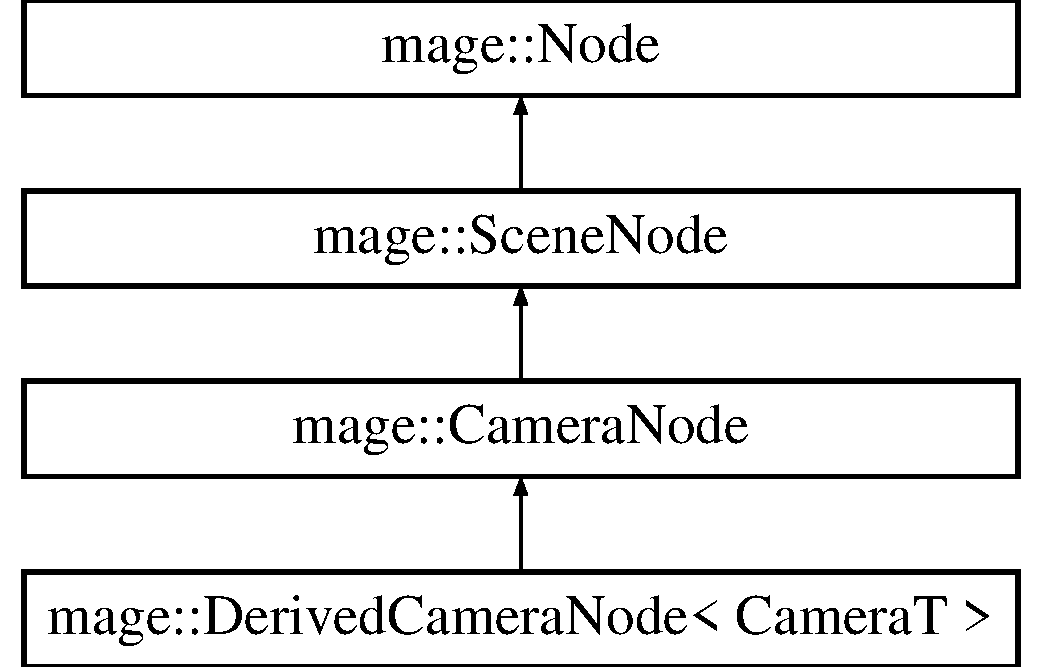
\includegraphics[height=3.000000cm]{classmage_1_1_camera_node}
\end{center}
\end{figure}
\subsection*{Public Member Functions}
\begin{DoxyCompactItemize}
\item 
virtual \hyperlink{classmage_1_1_camera_node_ac6612668e7b9f829e371794d422d357f}{$\sim$\+Camera\+Node} ()
\item 
\hyperlink{classmage_1_1_camera_node}{Camera\+Node} \& \hyperlink{classmage_1_1_camera_node_a03442d51e4279717f6692e0a731967a1}{operator=} (const \hyperlink{classmage_1_1_camera_node}{Camera\+Node} \&camera\+\_\+node)=delete
\item 
\hyperlink{classmage_1_1_camera_node}{Camera\+Node} \& \hyperlink{classmage_1_1_camera_node_a8da019549eeac6c4d7d6d7c4017dd498}{operator=} (\hyperlink{classmage_1_1_camera_node}{Camera\+Node} \&\&camera\+\_\+node)=delete
\item 
\hyperlink{namespacemage_a3316d7143a973e37adf1110f2e80ca31}{Unique\+Ptr}$<$ \hyperlink{classmage_1_1_camera_node}{Camera\+Node} $>$ \hyperlink{classmage_1_1_camera_node_a6c636830efadf9753f2f0d012153d61f}{Clone} () const
\item 
\hyperlink{classmage_1_1_camera}{Camera} $\ast$ \hyperlink{classmage_1_1_camera_node_aa9887e3bf192d6c078aae2430732cbf8}{Get\+Camera} () noexcept
\item 
const \hyperlink{classmage_1_1_camera}{Camera} $\ast$ \hyperlink{classmage_1_1_camera_node_aa911263cfce8cec2a42c6d03d25af606}{Get\+Camera} () const noexcept
\item 
\hyperlink{classmage_1_1_camera_settings}{Camera\+Settings} $\ast$ \hyperlink{classmage_1_1_camera_node_a0bd616c44db36301845b02a03f1db5ba}{Get\+Settings} () noexcept
\item 
const \hyperlink{classmage_1_1_camera_settings}{Camera\+Settings} $\ast$ \hyperlink{classmage_1_1_camera_node_a1098f7929715018978b1bb8ac00c7148}{Get\+Settings} () const noexcept
\item 
\hyperlink{classmage_1_1_viewport}{Viewport} \& \hyperlink{classmage_1_1_camera_node_ac280168901be6f8bdf03300f0b8c1a69}{Get\+Viewport} () noexcept
\item 
const \hyperlink{classmage_1_1_viewport}{Viewport} \& \hyperlink{classmage_1_1_camera_node_a09a761526f36b9547d29917835e907d6}{Get\+Viewport} () const noexcept
\item 
const \hyperlink{classmage_1_1_viewport}{Viewport} \hyperlink{classmage_1_1_camera_node_a1280c0c2735869d8703b67322f13b3cc}{Get\+S\+S\+Viewport} () const noexcept
\end{DoxyCompactItemize}
\subsection*{Protected Member Functions}
\begin{DoxyCompactItemize}
\item 
\hyperlink{classmage_1_1_camera_node_a4d513533dbb062bc3ebe87054eba632d}{Camera\+Node} (string name, \hyperlink{namespacemage_a3316d7143a973e37adf1110f2e80ca31}{Unique\+Ptr}$<$ \hyperlink{classmage_1_1_camera}{Camera} $>$ \&\&camera)
\item 
\hyperlink{classmage_1_1_camera_node_aa0becc29c416c313ebda763edb1b2181}{Camera\+Node} (const \hyperlink{classmage_1_1_camera_node}{Camera\+Node} \&camera\+\_\+node)
\item 
\hyperlink{classmage_1_1_camera_node_af46b911ecf12ed7c3cb31fb98a590fc1}{Camera\+Node} (\hyperlink{classmage_1_1_camera_node}{Camera\+Node} \&\&camera\+\_\+node)
\end{DoxyCompactItemize}
\subsection*{Private Member Functions}
\begin{DoxyCompactItemize}
\item 
virtual \hyperlink{namespacemage_a3316d7143a973e37adf1110f2e80ca31}{Unique\+Ptr}$<$ \hyperlink{classmage_1_1_node}{Node} $>$ \hyperlink{classmage_1_1_camera_node_a002d3a2b41cda270a26ca5d8f3a17f55}{Clone\+Implementation} () const override=0
\end{DoxyCompactItemize}
\subsection*{Private Attributes}
\begin{DoxyCompactItemize}
\item 
\hyperlink{namespacemage_a3316d7143a973e37adf1110f2e80ca31}{Unique\+Ptr}$<$ \hyperlink{classmage_1_1_camera}{Camera} $>$ \hyperlink{classmage_1_1_camera_node_a18f00f7ccd0c677043e11a1b3085dbfb}{m\+\_\+camera}
\item 
\hyperlink{namespacemage_a3316d7143a973e37adf1110f2e80ca31}{Unique\+Ptr}$<$ \hyperlink{classmage_1_1_camera_settings}{Camera\+Settings} $>$ \hyperlink{classmage_1_1_camera_node_aa8b1f1204534b3ee271e62b7cfe0f833}{m\+\_\+settings}
\item 
\hyperlink{classmage_1_1_viewport}{Viewport} \hyperlink{classmage_1_1_camera_node_a338e6f3112a167a7f81de59c7e33e87b}{m\+\_\+viewport}
\end{DoxyCompactItemize}


\subsection{Detailed Description}
A class of camera nodes. 

\subsection{Constructor \& Destructor Documentation}
\hypertarget{classmage_1_1_camera_node_ac6612668e7b9f829e371794d422d357f}{}\label{classmage_1_1_camera_node_ac6612668e7b9f829e371794d422d357f} 
\index{mage\+::\+Camera\+Node@{mage\+::\+Camera\+Node}!````~Camera\+Node@{$\sim$\+Camera\+Node}}
\index{````~Camera\+Node@{$\sim$\+Camera\+Node}!mage\+::\+Camera\+Node@{mage\+::\+Camera\+Node}}
\subsubsection{\texorpdfstring{$\sim$\+Camera\+Node()}{~CameraNode()}}
{\footnotesize\ttfamily mage\+::\+Camera\+Node\+::$\sim$\+Camera\+Node (\begin{DoxyParamCaption}{ }\end{DoxyParamCaption})\hspace{0.3cm}{\ttfamily [virtual]}, {\ttfamily [default]}}

Destructs this camera node. \hypertarget{classmage_1_1_camera_node_a4d513533dbb062bc3ebe87054eba632d}{}\label{classmage_1_1_camera_node_a4d513533dbb062bc3ebe87054eba632d} 
\index{mage\+::\+Camera\+Node@{mage\+::\+Camera\+Node}!Camera\+Node@{Camera\+Node}}
\index{Camera\+Node@{Camera\+Node}!mage\+::\+Camera\+Node@{mage\+::\+Camera\+Node}}
\subsubsection{\texorpdfstring{Camera\+Node()}{CameraNode()}\hspace{0.1cm}{\footnotesize\ttfamily [1/3]}}
{\footnotesize\ttfamily mage\+::\+Camera\+Node\+::\+Camera\+Node (\begin{DoxyParamCaption}\item[{string}]{name,  }\item[{\hyperlink{namespacemage_a3316d7143a973e37adf1110f2e80ca31}{Unique\+Ptr}$<$ \hyperlink{classmage_1_1_camera}{Camera} $>$ \&\&}]{camera }\end{DoxyParamCaption})\hspace{0.3cm}{\ttfamily [explicit]}, {\ttfamily [protected]}}

Constructs a camera node.

\begin{DoxyPrecond}{Precondition}
{\itshape camera} refers to a non {\ttfamily nullptr}. 
\end{DoxyPrecond}

\begin{DoxyParams}[1]{Parameters}
\mbox{\tt in}  & {\em name} & The name. \\
\hline
\mbox{\tt in}  & {\em camera} & A reference to the camera to move. \\
\hline
\end{DoxyParams}
\hypertarget{classmage_1_1_camera_node_aa0becc29c416c313ebda763edb1b2181}{}\label{classmage_1_1_camera_node_aa0becc29c416c313ebda763edb1b2181} 
\index{mage\+::\+Camera\+Node@{mage\+::\+Camera\+Node}!Camera\+Node@{Camera\+Node}}
\index{Camera\+Node@{Camera\+Node}!mage\+::\+Camera\+Node@{mage\+::\+Camera\+Node}}
\subsubsection{\texorpdfstring{Camera\+Node()}{CameraNode()}\hspace{0.1cm}{\footnotesize\ttfamily [2/3]}}
{\footnotesize\ttfamily mage\+::\+Camera\+Node\+::\+Camera\+Node (\begin{DoxyParamCaption}\item[{const \hyperlink{classmage_1_1_camera_node}{Camera\+Node} \&}]{camera\+\_\+node }\end{DoxyParamCaption})\hspace{0.3cm}{\ttfamily [protected]}}

Constructs a camera node from the given camera node.


\begin{DoxyParams}[1]{Parameters}
\mbox{\tt in}  & {\em camera\+\_\+node} & A reference to the camera node to copy. \\
\hline
\end{DoxyParams}
\hypertarget{classmage_1_1_camera_node_af46b911ecf12ed7c3cb31fb98a590fc1}{}\label{classmage_1_1_camera_node_af46b911ecf12ed7c3cb31fb98a590fc1} 
\index{mage\+::\+Camera\+Node@{mage\+::\+Camera\+Node}!Camera\+Node@{Camera\+Node}}
\index{Camera\+Node@{Camera\+Node}!mage\+::\+Camera\+Node@{mage\+::\+Camera\+Node}}
\subsubsection{\texorpdfstring{Camera\+Node()}{CameraNode()}\hspace{0.1cm}{\footnotesize\ttfamily [3/3]}}
{\footnotesize\ttfamily mage\+::\+Camera\+Node\+::\+Camera\+Node (\begin{DoxyParamCaption}\item[{\hyperlink{classmage_1_1_camera_node}{Camera\+Node} \&\&}]{camera\+\_\+node }\end{DoxyParamCaption})\hspace{0.3cm}{\ttfamily [protected]}, {\ttfamily [default]}}

Constructs a camera node by moving the given camera node.


\begin{DoxyParams}[1]{Parameters}
\mbox{\tt in}  & {\em camera\+\_\+node} & A reference to the camera node to move. \\
\hline
\end{DoxyParams}


\subsection{Member Function Documentation}
\hypertarget{classmage_1_1_camera_node_a6c636830efadf9753f2f0d012153d61f}{}\label{classmage_1_1_camera_node_a6c636830efadf9753f2f0d012153d61f} 
\index{mage\+::\+Camera\+Node@{mage\+::\+Camera\+Node}!Clone@{Clone}}
\index{Clone@{Clone}!mage\+::\+Camera\+Node@{mage\+::\+Camera\+Node}}
\subsubsection{\texorpdfstring{Clone()}{Clone()}}
{\footnotesize\ttfamily \hyperlink{namespacemage_a3316d7143a973e37adf1110f2e80ca31}{Unique\+Ptr}$<$ \hyperlink{classmage_1_1_camera_node}{Camera\+Node} $>$ mage\+::\+Camera\+Node\+::\+Clone (\begin{DoxyParamCaption}{ }\end{DoxyParamCaption}) const}

Clones this camera node.

\begin{DoxyReturn}{Returns}
A pointer to the clone of this camera node. 
\end{DoxyReturn}
\hypertarget{classmage_1_1_camera_node_a002d3a2b41cda270a26ca5d8f3a17f55}{}\label{classmage_1_1_camera_node_a002d3a2b41cda270a26ca5d8f3a17f55} 
\index{mage\+::\+Camera\+Node@{mage\+::\+Camera\+Node}!Clone\+Implementation@{Clone\+Implementation}}
\index{Clone\+Implementation@{Clone\+Implementation}!mage\+::\+Camera\+Node@{mage\+::\+Camera\+Node}}
\subsubsection{\texorpdfstring{Clone\+Implementation()}{CloneImplementation()}}
{\footnotesize\ttfamily virtual \hyperlink{namespacemage_a3316d7143a973e37adf1110f2e80ca31}{Unique\+Ptr}$<$ \hyperlink{classmage_1_1_node}{Node} $>$ mage\+::\+Camera\+Node\+::\+Clone\+Implementation (\begin{DoxyParamCaption}{ }\end{DoxyParamCaption}) const\hspace{0.3cm}{\ttfamily [override]}, {\ttfamily [private]}, {\ttfamily [pure virtual]}}

Clones this camera node.

\begin{DoxyReturn}{Returns}
A pointer to the clone of this camera node. 
\end{DoxyReturn}


Reimplemented from \hyperlink{classmage_1_1_node_a71a4763bfd4cba5653488b490e61dc8f}{mage\+::\+Node}.



Implemented in \hyperlink{classmage_1_1_derived_camera_node_aa965751029ebd6b41d3805b499a8304e}{mage\+::\+Derived\+Camera\+Node$<$ Camera\+T $>$}.

\hypertarget{classmage_1_1_camera_node_aa9887e3bf192d6c078aae2430732cbf8}{}\label{classmage_1_1_camera_node_aa9887e3bf192d6c078aae2430732cbf8} 
\index{mage\+::\+Camera\+Node@{mage\+::\+Camera\+Node}!Get\+Camera@{Get\+Camera}}
\index{Get\+Camera@{Get\+Camera}!mage\+::\+Camera\+Node@{mage\+::\+Camera\+Node}}
\subsubsection{\texorpdfstring{Get\+Camera()}{GetCamera()}\hspace{0.1cm}{\footnotesize\ttfamily [1/2]}}
{\footnotesize\ttfamily \hyperlink{classmage_1_1_camera}{Camera}$\ast$ mage\+::\+Camera\+Node\+::\+Get\+Camera (\begin{DoxyParamCaption}{ }\end{DoxyParamCaption})\hspace{0.3cm}{\ttfamily [noexcept]}}

Returns the camera of this camera node.

\begin{DoxyReturn}{Returns}
A pointer to the camera of this camera node. 
\end{DoxyReturn}
\hypertarget{classmage_1_1_camera_node_aa911263cfce8cec2a42c6d03d25af606}{}\label{classmage_1_1_camera_node_aa911263cfce8cec2a42c6d03d25af606} 
\index{mage\+::\+Camera\+Node@{mage\+::\+Camera\+Node}!Get\+Camera@{Get\+Camera}}
\index{Get\+Camera@{Get\+Camera}!mage\+::\+Camera\+Node@{mage\+::\+Camera\+Node}}
\subsubsection{\texorpdfstring{Get\+Camera()}{GetCamera()}\hspace{0.1cm}{\footnotesize\ttfamily [2/2]}}
{\footnotesize\ttfamily const \hyperlink{classmage_1_1_camera}{Camera}$\ast$ mage\+::\+Camera\+Node\+::\+Get\+Camera (\begin{DoxyParamCaption}{ }\end{DoxyParamCaption}) const\hspace{0.3cm}{\ttfamily [noexcept]}}

Returns the camera of this camera node.

\begin{DoxyReturn}{Returns}
A pointer to the camera of this camera node. 
\end{DoxyReturn}
\hypertarget{classmage_1_1_camera_node_a0bd616c44db36301845b02a03f1db5ba}{}\label{classmage_1_1_camera_node_a0bd616c44db36301845b02a03f1db5ba} 
\index{mage\+::\+Camera\+Node@{mage\+::\+Camera\+Node}!Get\+Settings@{Get\+Settings}}
\index{Get\+Settings@{Get\+Settings}!mage\+::\+Camera\+Node@{mage\+::\+Camera\+Node}}
\subsubsection{\texorpdfstring{Get\+Settings()}{GetSettings()}\hspace{0.1cm}{\footnotesize\ttfamily [1/2]}}
{\footnotesize\ttfamily \hyperlink{classmage_1_1_camera_settings}{Camera\+Settings}$\ast$ mage\+::\+Camera\+Node\+::\+Get\+Settings (\begin{DoxyParamCaption}{ }\end{DoxyParamCaption})\hspace{0.3cm}{\ttfamily [noexcept]}}

Returns the camera settings of this camera node.

\begin{DoxyReturn}{Returns}
A pointer to the camera settings of this camera node. 
\end{DoxyReturn}
\hypertarget{classmage_1_1_camera_node_a1098f7929715018978b1bb8ac00c7148}{}\label{classmage_1_1_camera_node_a1098f7929715018978b1bb8ac00c7148} 
\index{mage\+::\+Camera\+Node@{mage\+::\+Camera\+Node}!Get\+Settings@{Get\+Settings}}
\index{Get\+Settings@{Get\+Settings}!mage\+::\+Camera\+Node@{mage\+::\+Camera\+Node}}
\subsubsection{\texorpdfstring{Get\+Settings()}{GetSettings()}\hspace{0.1cm}{\footnotesize\ttfamily [2/2]}}
{\footnotesize\ttfamily const \hyperlink{classmage_1_1_camera_settings}{Camera\+Settings}$\ast$ mage\+::\+Camera\+Node\+::\+Get\+Settings (\begin{DoxyParamCaption}{ }\end{DoxyParamCaption}) const\hspace{0.3cm}{\ttfamily [noexcept]}}

Returns the camera settings of this camera node.

\begin{DoxyReturn}{Returns}
A pointer to the camera settings of this camera node. 
\end{DoxyReturn}
\hypertarget{classmage_1_1_camera_node_a1280c0c2735869d8703b67322f13b3cc}{}\label{classmage_1_1_camera_node_a1280c0c2735869d8703b67322f13b3cc} 
\index{mage\+::\+Camera\+Node@{mage\+::\+Camera\+Node}!Get\+S\+S\+Viewport@{Get\+S\+S\+Viewport}}
\index{Get\+S\+S\+Viewport@{Get\+S\+S\+Viewport}!mage\+::\+Camera\+Node@{mage\+::\+Camera\+Node}}
\subsubsection{\texorpdfstring{Get\+S\+S\+Viewport()}{GetSSViewport()}}
{\footnotesize\ttfamily const \hyperlink{classmage_1_1_viewport}{Viewport} mage\+::\+Camera\+Node\+::\+Get\+S\+S\+Viewport (\begin{DoxyParamCaption}{ }\end{DoxyParamCaption}) const\hspace{0.3cm}{\ttfamily [noexcept]}}

Returns the super-\/sampled viewport of this camera node.

\begin{DoxyPrecond}{Precondition}
The rendering manager associated with the current engine must be loaded. 
\end{DoxyPrecond}
\begin{DoxyReturn}{Returns}
The super-\/sampled viewport of this camera node. 
\end{DoxyReturn}
\hypertarget{classmage_1_1_camera_node_ac280168901be6f8bdf03300f0b8c1a69}{}\label{classmage_1_1_camera_node_ac280168901be6f8bdf03300f0b8c1a69} 
\index{mage\+::\+Camera\+Node@{mage\+::\+Camera\+Node}!Get\+Viewport@{Get\+Viewport}}
\index{Get\+Viewport@{Get\+Viewport}!mage\+::\+Camera\+Node@{mage\+::\+Camera\+Node}}
\subsubsection{\texorpdfstring{Get\+Viewport()}{GetViewport()}\hspace{0.1cm}{\footnotesize\ttfamily [1/2]}}
{\footnotesize\ttfamily \hyperlink{classmage_1_1_viewport}{Viewport}\& mage\+::\+Camera\+Node\+::\+Get\+Viewport (\begin{DoxyParamCaption}{ }\end{DoxyParamCaption})\hspace{0.3cm}{\ttfamily [noexcept]}}

Returns the viewport of this camera node.

\begin{DoxyReturn}{Returns}
A reference to the viewport of this camera node. 
\end{DoxyReturn}
\hypertarget{classmage_1_1_camera_node_a09a761526f36b9547d29917835e907d6}{}\label{classmage_1_1_camera_node_a09a761526f36b9547d29917835e907d6} 
\index{mage\+::\+Camera\+Node@{mage\+::\+Camera\+Node}!Get\+Viewport@{Get\+Viewport}}
\index{Get\+Viewport@{Get\+Viewport}!mage\+::\+Camera\+Node@{mage\+::\+Camera\+Node}}
\subsubsection{\texorpdfstring{Get\+Viewport()}{GetViewport()}\hspace{0.1cm}{\footnotesize\ttfamily [2/2]}}
{\footnotesize\ttfamily const \hyperlink{classmage_1_1_viewport}{Viewport}\& mage\+::\+Camera\+Node\+::\+Get\+Viewport (\begin{DoxyParamCaption}{ }\end{DoxyParamCaption}) const\hspace{0.3cm}{\ttfamily [noexcept]}}

Returns the viewport of this camera node.

\begin{DoxyReturn}{Returns}
A reference to the viewport of this camera node. 
\end{DoxyReturn}
\hypertarget{classmage_1_1_camera_node_a03442d51e4279717f6692e0a731967a1}{}\label{classmage_1_1_camera_node_a03442d51e4279717f6692e0a731967a1} 
\index{mage\+::\+Camera\+Node@{mage\+::\+Camera\+Node}!operator=@{operator=}}
\index{operator=@{operator=}!mage\+::\+Camera\+Node@{mage\+::\+Camera\+Node}}
\subsubsection{\texorpdfstring{operator=()}{operator=()}\hspace{0.1cm}{\footnotesize\ttfamily [1/2]}}
{\footnotesize\ttfamily \hyperlink{classmage_1_1_camera_node}{Camera\+Node}\& mage\+::\+Camera\+Node\+::operator= (\begin{DoxyParamCaption}\item[{const \hyperlink{classmage_1_1_camera_node}{Camera\+Node} \&}]{camera\+\_\+node }\end{DoxyParamCaption})\hspace{0.3cm}{\ttfamily [delete]}}

Copies the given camera node to this camera node.


\begin{DoxyParams}[1]{Parameters}
\mbox{\tt in}  & {\em camera\+\_\+node} & A reference to the camera node to copy. \\
\hline
\end{DoxyParams}
\begin{DoxyReturn}{Returns}
A reference to the copy of the given camera node (i.\+e. this camera node). 
\end{DoxyReturn}
\hypertarget{classmage_1_1_camera_node_a8da019549eeac6c4d7d6d7c4017dd498}{}\label{classmage_1_1_camera_node_a8da019549eeac6c4d7d6d7c4017dd498} 
\index{mage\+::\+Camera\+Node@{mage\+::\+Camera\+Node}!operator=@{operator=}}
\index{operator=@{operator=}!mage\+::\+Camera\+Node@{mage\+::\+Camera\+Node}}
\subsubsection{\texorpdfstring{operator=()}{operator=()}\hspace{0.1cm}{\footnotesize\ttfamily [2/2]}}
{\footnotesize\ttfamily \hyperlink{classmage_1_1_camera_node}{Camera\+Node}\& mage\+::\+Camera\+Node\+::operator= (\begin{DoxyParamCaption}\item[{\hyperlink{classmage_1_1_camera_node}{Camera\+Node} \&\&}]{camera\+\_\+node }\end{DoxyParamCaption})\hspace{0.3cm}{\ttfamily [delete]}}

Moves the given camera node to this camera node.


\begin{DoxyParams}[1]{Parameters}
\mbox{\tt in}  & {\em camera\+\_\+node} & A reference to the camera node to move. \\
\hline
\end{DoxyParams}
\begin{DoxyReturn}{Returns}
A reference to the moved camera node (i.\+e. this camera node). 
\end{DoxyReturn}


\subsection{Member Data Documentation}
\hypertarget{classmage_1_1_camera_node_a18f00f7ccd0c677043e11a1b3085dbfb}{}\label{classmage_1_1_camera_node_a18f00f7ccd0c677043e11a1b3085dbfb} 
\index{mage\+::\+Camera\+Node@{mage\+::\+Camera\+Node}!m\+\_\+camera@{m\+\_\+camera}}
\index{m\+\_\+camera@{m\+\_\+camera}!mage\+::\+Camera\+Node@{mage\+::\+Camera\+Node}}
\subsubsection{\texorpdfstring{m\+\_\+camera}{m\_camera}}
{\footnotesize\ttfamily \hyperlink{namespacemage_a3316d7143a973e37adf1110f2e80ca31}{Unique\+Ptr}$<$ \hyperlink{classmage_1_1_camera}{Camera} $>$ mage\+::\+Camera\+Node\+::m\+\_\+camera\hspace{0.3cm}{\ttfamily [private]}}

A pointer to the camera of this camera node. \hypertarget{classmage_1_1_camera_node_aa8b1f1204534b3ee271e62b7cfe0f833}{}\label{classmage_1_1_camera_node_aa8b1f1204534b3ee271e62b7cfe0f833} 
\index{mage\+::\+Camera\+Node@{mage\+::\+Camera\+Node}!m\+\_\+settings@{m\+\_\+settings}}
\index{m\+\_\+settings@{m\+\_\+settings}!mage\+::\+Camera\+Node@{mage\+::\+Camera\+Node}}
\subsubsection{\texorpdfstring{m\+\_\+settings}{m\_settings}}
{\footnotesize\ttfamily \hyperlink{namespacemage_a3316d7143a973e37adf1110f2e80ca31}{Unique\+Ptr}$<$ \hyperlink{classmage_1_1_camera_settings}{Camera\+Settings} $>$ mage\+::\+Camera\+Node\+::m\+\_\+settings\hspace{0.3cm}{\ttfamily [private]}}

A pointer to the camera settings of this camera node. \hypertarget{classmage_1_1_camera_node_a338e6f3112a167a7f81de59c7e33e87b}{}\label{classmage_1_1_camera_node_a338e6f3112a167a7f81de59c7e33e87b} 
\index{mage\+::\+Camera\+Node@{mage\+::\+Camera\+Node}!m\+\_\+viewport@{m\+\_\+viewport}}
\index{m\+\_\+viewport@{m\+\_\+viewport}!mage\+::\+Camera\+Node@{mage\+::\+Camera\+Node}}
\subsubsection{\texorpdfstring{m\+\_\+viewport}{m\_viewport}}
{\footnotesize\ttfamily \hyperlink{classmage_1_1_viewport}{Viewport} mage\+::\+Camera\+Node\+::m\+\_\+viewport\hspace{0.3cm}{\ttfamily [private]}}

The viewport of this camera node. 
\hypertarget{classmage_1_1_character_motor_script}{}\section{mage\+:\+:Character\+Motor\+Script Class Reference}
\label{classmage_1_1_character_motor_script}\index{mage\+::\+Character\+Motor\+Script@{mage\+::\+Character\+Motor\+Script}}


{\ttfamily \#include $<$character\+\_\+motor\+\_\+script.\+hpp$>$}

Inheritance diagram for mage\+:\+:Character\+Motor\+Script\+:\begin{figure}[H]
\begin{center}
\leavevmode
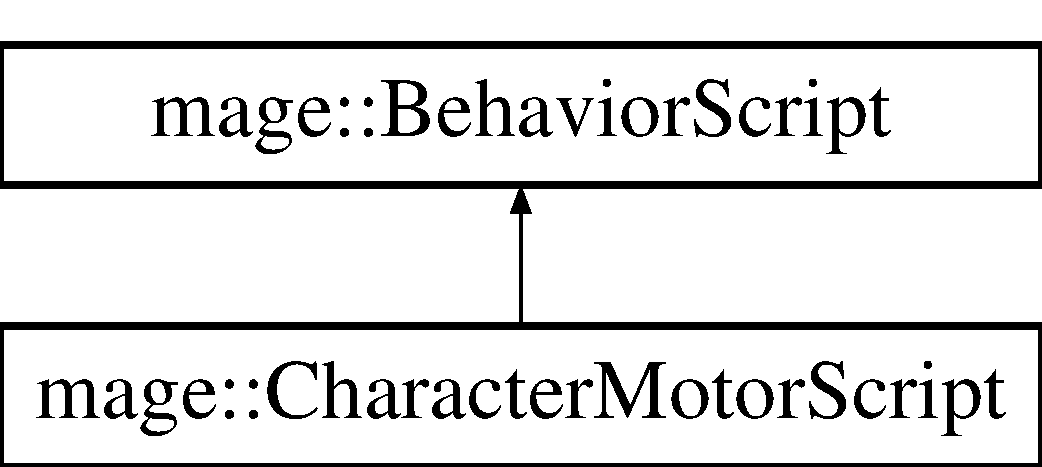
\includegraphics[height=2.000000cm]{classmage_1_1_character_motor_script}
\end{center}
\end{figure}
\subsection*{Public Member Functions}
\begin{DoxyCompactItemize}
\item 
\hyperlink{classmage_1_1_character_motor_script_af819140d0ebda767e9b82826c50972de}{Character\+Motor\+Script} (Transform $\ast$transform)
\item 
\hyperlink{classmage_1_1_character_motor_script_aa8b4b2c6eba7077677db51e24c2a9a36}{Character\+Motor\+Script} (const \hyperlink{classmage_1_1_character_motor_script}{Character\+Motor\+Script} \&script)=delete
\item 
\hyperlink{classmage_1_1_character_motor_script_a944682d8ff570a141e60cdd2d16aa3ad}{Character\+Motor\+Script} (\hyperlink{classmage_1_1_character_motor_script}{Character\+Motor\+Script} \&\&script)=default
\item 
virtual \hyperlink{classmage_1_1_character_motor_script_a03e8cdb2e30e21fe3a84f36101a169e3}{$\sim$\+Character\+Motor\+Script} ()=default
\item 
\hyperlink{classmage_1_1_character_motor_script}{Character\+Motor\+Script} \& \hyperlink{classmage_1_1_character_motor_script_a5b66cbbe6b829fe56a1bba5f9093b36e}{operator=} (const \hyperlink{classmage_1_1_character_motor_script}{Character\+Motor\+Script} \&script)=delete
\item 
\hyperlink{classmage_1_1_character_motor_script}{Character\+Motor\+Script} \& \hyperlink{classmage_1_1_character_motor_script_a05e8822fa633d8642702d125b26069f7}{operator=} (\hyperlink{classmage_1_1_character_motor_script}{Character\+Motor\+Script} \&\&script)=delete
\item 
virtual void \hyperlink{classmage_1_1_character_motor_script_af09581e810c02ca4a19ecbaf0d7580bb}{Update} (double delta\+\_\+time) override
\item 
float \hyperlink{classmage_1_1_character_motor_script_a0c512015222e3f332429df414c06862b}{Get\+Velocity} () const
\item 
void \hyperlink{classmage_1_1_character_motor_script_a3fd91c324e837b9d22e19d74478caec0}{Set\+Velocity} (float velocity)
\end{DoxyCompactItemize}
\subsection*{Private Attributes}
\begin{DoxyCompactItemize}
\item 
Transform $\ast$const \hyperlink{classmage_1_1_character_motor_script_a7331e960455b72ceb858254ccc7108f1}{m\+\_\+transform}
\item 
float \hyperlink{classmage_1_1_character_motor_script_a02441cc4c84ba12811845b7f966f4069}{m\+\_\+velocity}
\end{DoxyCompactItemize}
\subsection*{Additional Inherited Members}


\subsection{Constructor \& Destructor Documentation}
\hypertarget{classmage_1_1_character_motor_script_af819140d0ebda767e9b82826c50972de}{}\label{classmage_1_1_character_motor_script_af819140d0ebda767e9b82826c50972de} 
\index{mage\+::\+Character\+Motor\+Script@{mage\+::\+Character\+Motor\+Script}!Character\+Motor\+Script@{Character\+Motor\+Script}}
\index{Character\+Motor\+Script@{Character\+Motor\+Script}!mage\+::\+Character\+Motor\+Script@{mage\+::\+Character\+Motor\+Script}}
\subsubsection{\texorpdfstring{Character\+Motor\+Script()}{CharacterMotorScript()}\hspace{0.1cm}{\footnotesize\ttfamily [1/3]}}
{\footnotesize\ttfamily mage\+::\+Character\+Motor\+Script\+::\+Character\+Motor\+Script (\begin{DoxyParamCaption}\item[{Transform $\ast$}]{transform }\end{DoxyParamCaption})\hspace{0.3cm}{\ttfamily [explicit]}}

\hypertarget{classmage_1_1_character_motor_script_aa8b4b2c6eba7077677db51e24c2a9a36}{}\label{classmage_1_1_character_motor_script_aa8b4b2c6eba7077677db51e24c2a9a36} 
\index{mage\+::\+Character\+Motor\+Script@{mage\+::\+Character\+Motor\+Script}!Character\+Motor\+Script@{Character\+Motor\+Script}}
\index{Character\+Motor\+Script@{Character\+Motor\+Script}!mage\+::\+Character\+Motor\+Script@{mage\+::\+Character\+Motor\+Script}}
\subsubsection{\texorpdfstring{Character\+Motor\+Script()}{CharacterMotorScript()}\hspace{0.1cm}{\footnotesize\ttfamily [2/3]}}
{\footnotesize\ttfamily mage\+::\+Character\+Motor\+Script\+::\+Character\+Motor\+Script (\begin{DoxyParamCaption}\item[{const \hyperlink{classmage_1_1_character_motor_script}{Character\+Motor\+Script} \&}]{script }\end{DoxyParamCaption})\hspace{0.3cm}{\ttfamily [delete]}}

\hypertarget{classmage_1_1_character_motor_script_a944682d8ff570a141e60cdd2d16aa3ad}{}\label{classmage_1_1_character_motor_script_a944682d8ff570a141e60cdd2d16aa3ad} 
\index{mage\+::\+Character\+Motor\+Script@{mage\+::\+Character\+Motor\+Script}!Character\+Motor\+Script@{Character\+Motor\+Script}}
\index{Character\+Motor\+Script@{Character\+Motor\+Script}!mage\+::\+Character\+Motor\+Script@{mage\+::\+Character\+Motor\+Script}}
\subsubsection{\texorpdfstring{Character\+Motor\+Script()}{CharacterMotorScript()}\hspace{0.1cm}{\footnotesize\ttfamily [3/3]}}
{\footnotesize\ttfamily mage\+::\+Character\+Motor\+Script\+::\+Character\+Motor\+Script (\begin{DoxyParamCaption}\item[{\hyperlink{classmage_1_1_character_motor_script}{Character\+Motor\+Script} \&\&}]{script }\end{DoxyParamCaption})\hspace{0.3cm}{\ttfamily [default]}}

\hypertarget{classmage_1_1_character_motor_script_a03e8cdb2e30e21fe3a84f36101a169e3}{}\label{classmage_1_1_character_motor_script_a03e8cdb2e30e21fe3a84f36101a169e3} 
\index{mage\+::\+Character\+Motor\+Script@{mage\+::\+Character\+Motor\+Script}!````~Character\+Motor\+Script@{$\sim$\+Character\+Motor\+Script}}
\index{````~Character\+Motor\+Script@{$\sim$\+Character\+Motor\+Script}!mage\+::\+Character\+Motor\+Script@{mage\+::\+Character\+Motor\+Script}}
\subsubsection{\texorpdfstring{$\sim$\+Character\+Motor\+Script()}{~CharacterMotorScript()}}
{\footnotesize\ttfamily virtual mage\+::\+Character\+Motor\+Script\+::$\sim$\+Character\+Motor\+Script (\begin{DoxyParamCaption}{ }\end{DoxyParamCaption})\hspace{0.3cm}{\ttfamily [virtual]}, {\ttfamily [default]}}



\subsection{Member Function Documentation}
\hypertarget{classmage_1_1_character_motor_script_a0c512015222e3f332429df414c06862b}{}\label{classmage_1_1_character_motor_script_a0c512015222e3f332429df414c06862b} 
\index{mage\+::\+Character\+Motor\+Script@{mage\+::\+Character\+Motor\+Script}!Get\+Velocity@{Get\+Velocity}}
\index{Get\+Velocity@{Get\+Velocity}!mage\+::\+Character\+Motor\+Script@{mage\+::\+Character\+Motor\+Script}}
\subsubsection{\texorpdfstring{Get\+Velocity()}{GetVelocity()}}
{\footnotesize\ttfamily float mage\+::\+Character\+Motor\+Script\+::\+Get\+Velocity (\begin{DoxyParamCaption}{ }\end{DoxyParamCaption}) const}

\hypertarget{classmage_1_1_character_motor_script_a5b66cbbe6b829fe56a1bba5f9093b36e}{}\label{classmage_1_1_character_motor_script_a5b66cbbe6b829fe56a1bba5f9093b36e} 
\index{mage\+::\+Character\+Motor\+Script@{mage\+::\+Character\+Motor\+Script}!operator=@{operator=}}
\index{operator=@{operator=}!mage\+::\+Character\+Motor\+Script@{mage\+::\+Character\+Motor\+Script}}
\subsubsection{\texorpdfstring{operator=()}{operator=()}\hspace{0.1cm}{\footnotesize\ttfamily [1/2]}}
{\footnotesize\ttfamily \hyperlink{classmage_1_1_character_motor_script}{Character\+Motor\+Script}\& mage\+::\+Character\+Motor\+Script\+::operator= (\begin{DoxyParamCaption}\item[{const \hyperlink{classmage_1_1_character_motor_script}{Character\+Motor\+Script} \&}]{script }\end{DoxyParamCaption})\hspace{0.3cm}{\ttfamily [delete]}}

\hypertarget{classmage_1_1_character_motor_script_a05e8822fa633d8642702d125b26069f7}{}\label{classmage_1_1_character_motor_script_a05e8822fa633d8642702d125b26069f7} 
\index{mage\+::\+Character\+Motor\+Script@{mage\+::\+Character\+Motor\+Script}!operator=@{operator=}}
\index{operator=@{operator=}!mage\+::\+Character\+Motor\+Script@{mage\+::\+Character\+Motor\+Script}}
\subsubsection{\texorpdfstring{operator=()}{operator=()}\hspace{0.1cm}{\footnotesize\ttfamily [2/2]}}
{\footnotesize\ttfamily \hyperlink{classmage_1_1_character_motor_script}{Character\+Motor\+Script}\& mage\+::\+Character\+Motor\+Script\+::operator= (\begin{DoxyParamCaption}\item[{\hyperlink{classmage_1_1_character_motor_script}{Character\+Motor\+Script} \&\&}]{script }\end{DoxyParamCaption})\hspace{0.3cm}{\ttfamily [delete]}}

\hypertarget{classmage_1_1_character_motor_script_a3fd91c324e837b9d22e19d74478caec0}{}\label{classmage_1_1_character_motor_script_a3fd91c324e837b9d22e19d74478caec0} 
\index{mage\+::\+Character\+Motor\+Script@{mage\+::\+Character\+Motor\+Script}!Set\+Velocity@{Set\+Velocity}}
\index{Set\+Velocity@{Set\+Velocity}!mage\+::\+Character\+Motor\+Script@{mage\+::\+Character\+Motor\+Script}}
\subsubsection{\texorpdfstring{Set\+Velocity()}{SetVelocity()}}
{\footnotesize\ttfamily void mage\+::\+Character\+Motor\+Script\+::\+Set\+Velocity (\begin{DoxyParamCaption}\item[{float}]{velocity }\end{DoxyParamCaption})}

\hypertarget{classmage_1_1_character_motor_script_af09581e810c02ca4a19ecbaf0d7580bb}{}\label{classmage_1_1_character_motor_script_af09581e810c02ca4a19ecbaf0d7580bb} 
\index{mage\+::\+Character\+Motor\+Script@{mage\+::\+Character\+Motor\+Script}!Update@{Update}}
\index{Update@{Update}!mage\+::\+Character\+Motor\+Script@{mage\+::\+Character\+Motor\+Script}}
\subsubsection{\texorpdfstring{Update()}{Update()}}
{\footnotesize\ttfamily void mage\+::\+Character\+Motor\+Script\+::\+Update (\begin{DoxyParamCaption}\item[{double}]{delta\+\_\+time }\end{DoxyParamCaption})\hspace{0.3cm}{\ttfamily [override]}, {\ttfamily [virtual]}}

Updates this behavior script.


\begin{DoxyParams}[1]{Parameters}
\mbox{\tt in}  & {\em delta\+\_\+time} & The elapsed time since the previous update. \\
\hline
\end{DoxyParams}


Implements \hyperlink{classmage_1_1_behavior_script_a905b6c83640cb91d19fecab3435f6feb}{mage\+::\+Behavior\+Script}.



\subsection{Member Data Documentation}
\hypertarget{classmage_1_1_character_motor_script_a7331e960455b72ceb858254ccc7108f1}{}\label{classmage_1_1_character_motor_script_a7331e960455b72ceb858254ccc7108f1} 
\index{mage\+::\+Character\+Motor\+Script@{mage\+::\+Character\+Motor\+Script}!m\+\_\+transform@{m\+\_\+transform}}
\index{m\+\_\+transform@{m\+\_\+transform}!mage\+::\+Character\+Motor\+Script@{mage\+::\+Character\+Motor\+Script}}
\subsubsection{\texorpdfstring{m\+\_\+transform}{m\_transform}}
{\footnotesize\ttfamily Transform$\ast$ const mage\+::\+Character\+Motor\+Script\+::m\+\_\+transform\hspace{0.3cm}{\ttfamily [private]}}

\hypertarget{classmage_1_1_character_motor_script_a02441cc4c84ba12811845b7f966f4069}{}\label{classmage_1_1_character_motor_script_a02441cc4c84ba12811845b7f966f4069} 
\index{mage\+::\+Character\+Motor\+Script@{mage\+::\+Character\+Motor\+Script}!m\+\_\+velocity@{m\+\_\+velocity}}
\index{m\+\_\+velocity@{m\+\_\+velocity}!mage\+::\+Character\+Motor\+Script@{mage\+::\+Character\+Motor\+Script}}
\subsubsection{\texorpdfstring{m\+\_\+velocity}{m\_velocity}}
{\footnotesize\ttfamily float mage\+::\+Character\+Motor\+Script\+::m\+\_\+velocity\hspace{0.3cm}{\ttfamily [private]}}


\hypertarget{structmage_1_1_color}{}\section{mage\+:\+:Color Struct Reference}
\label{structmage_1_1_color}\index{mage\+::\+Color@{mage\+::\+Color}}


{\ttfamily \#include $<$math.\+hpp$>$}

Inheritance diagram for mage\+:\+:Color\+:\begin{figure}[H]
\begin{center}
\leavevmode
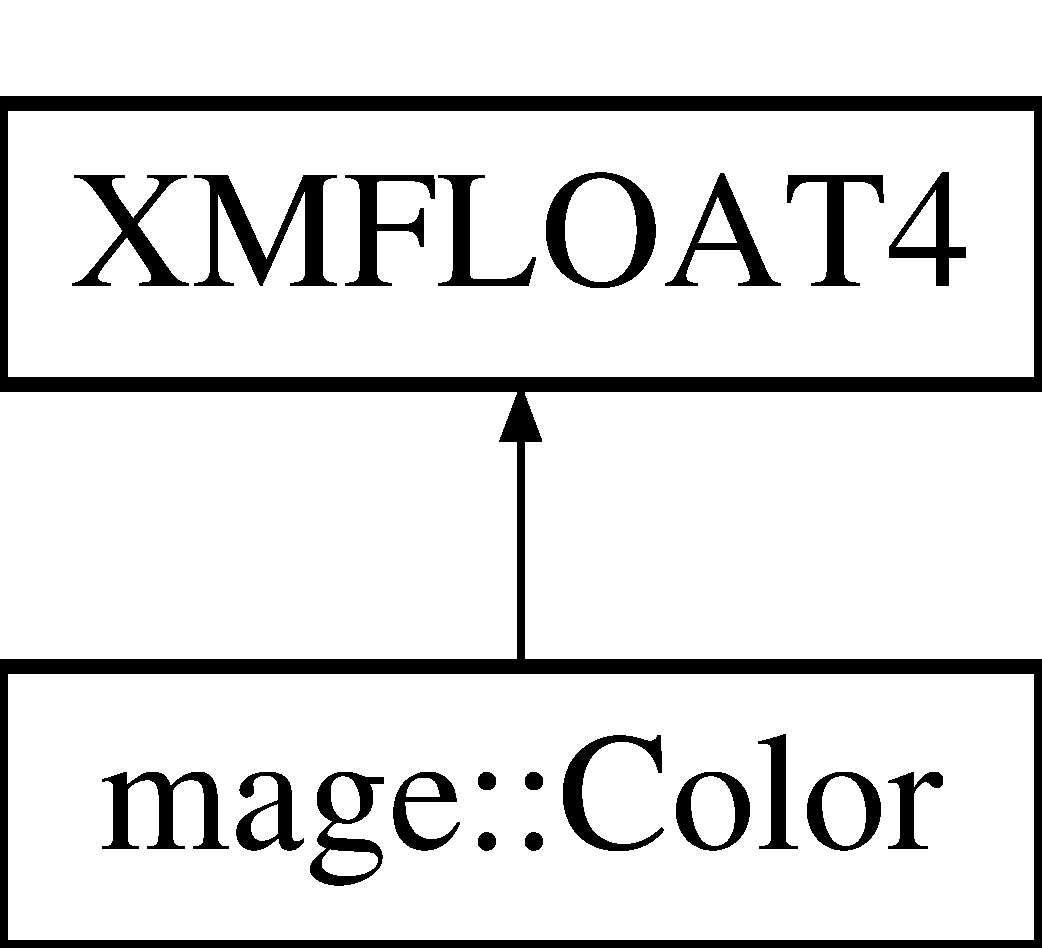
\includegraphics[height=2.000000cm]{structmage_1_1_color}
\end{center}
\end{figure}
\subsection*{Public Member Functions}
\begin{DoxyCompactItemize}
\item 
\hyperlink{structmage_1_1_color_a542f26c61d9c67098302b0262c518758}{Color} () noexcept
\item 
\hyperlink{structmage_1_1_color_aa8376e2ad8a303751939eb447f6fa51b}{Color} (float x, float y, float z, float w) noexcept
\item 
\hyperlink{structmage_1_1_color_a725cc051131ad2796383e714fb0038d9}{Color} (const \hyperlink{structmage_1_1_color}{Color} \&color)=default
\item 
\hyperlink{structmage_1_1_color_ada141b94913980bf54a3ac4fb3d45f35}{Color} (\hyperlink{structmage_1_1_color}{Color} \&\&color) noexcept=default
\item 
\hyperlink{structmage_1_1_color_afb821e8ce617a6475538fa7179a16c6b}{Color} (const X\+M\+F\+L\+O\+A\+T4 \&v) noexcept
\item 
\hyperlink{structmage_1_1_color_a6e01540c01b2923974ca31e1621f1f7e}{Color} (X\+M\+F\+L\+O\+A\+T4 \&\&v) noexcept
\item 
\hyperlink{structmage_1_1_color_aa4df1c9718b7846adf77fbeed79ac219}{$\sim$\+Color} ()=default
\item 
\hyperlink{structmage_1_1_color}{Color} \& \hyperlink{structmage_1_1_color_a194847cf864911d7ceff16aabec1459f}{operator=} (const \hyperlink{structmage_1_1_color}{Color} \&color)=default
\item 
\hyperlink{structmage_1_1_color}{Color} \& \hyperlink{structmage_1_1_color_aa16160a9b8a03a8b2d82569343dd8c6d}{operator=} (\hyperlink{structmage_1_1_color}{Color} \&\&color)=default
\end{DoxyCompactItemize}


\subsection{Detailed Description}
A struct of colors. 

\subsection{Constructor \& Destructor Documentation}
\hypertarget{structmage_1_1_color_a542f26c61d9c67098302b0262c518758}{}\label{structmage_1_1_color_a542f26c61d9c67098302b0262c518758} 
\index{mage\+::\+Color@{mage\+::\+Color}!Color@{Color}}
\index{Color@{Color}!mage\+::\+Color@{mage\+::\+Color}}
\subsubsection{\texorpdfstring{Color()}{Color()}\hspace{0.1cm}{\footnotesize\ttfamily [1/6]}}
{\footnotesize\ttfamily mage\+::\+Color\+::\+Color (\begin{DoxyParamCaption}{ }\end{DoxyParamCaption})\hspace{0.3cm}{\ttfamily [noexcept]}}

Constructs a color. \hypertarget{structmage_1_1_color_aa8376e2ad8a303751939eb447f6fa51b}{}\label{structmage_1_1_color_aa8376e2ad8a303751939eb447f6fa51b} 
\index{mage\+::\+Color@{mage\+::\+Color}!Color@{Color}}
\index{Color@{Color}!mage\+::\+Color@{mage\+::\+Color}}
\subsubsection{\texorpdfstring{Color()}{Color()}\hspace{0.1cm}{\footnotesize\ttfamily [2/6]}}
{\footnotesize\ttfamily mage\+::\+Color\+::\+Color (\begin{DoxyParamCaption}\item[{float}]{x,  }\item[{float}]{y,  }\item[{float}]{z,  }\item[{float}]{w }\end{DoxyParamCaption})\hspace{0.3cm}{\ttfamily [noexcept]}}

Constructs a color from the given components.


\begin{DoxyParams}[1]{Parameters}
\mbox{\tt in}  & {\em x} & The first component. \\
\hline
\mbox{\tt in}  & {\em y} & The second component. \\
\hline
\mbox{\tt in}  & {\em z} & The third component. \\
\hline
\mbox{\tt in}  & {\em w} & The fourth component. \\
\hline
\end{DoxyParams}
\hypertarget{structmage_1_1_color_a725cc051131ad2796383e714fb0038d9}{}\label{structmage_1_1_color_a725cc051131ad2796383e714fb0038d9} 
\index{mage\+::\+Color@{mage\+::\+Color}!Color@{Color}}
\index{Color@{Color}!mage\+::\+Color@{mage\+::\+Color}}
\subsubsection{\texorpdfstring{Color()}{Color()}\hspace{0.1cm}{\footnotesize\ttfamily [3/6]}}
{\footnotesize\ttfamily mage\+::\+Color\+::\+Color (\begin{DoxyParamCaption}\item[{const \hyperlink{structmage_1_1_color}{Color} \&}]{color }\end{DoxyParamCaption})\hspace{0.3cm}{\ttfamily [default]}}

Constructs a color from the given color.


\begin{DoxyParams}[1]{Parameters}
\mbox{\tt in}  & {\em color} & A reference to the color to copy. \\
\hline
\end{DoxyParams}
\hypertarget{structmage_1_1_color_ada141b94913980bf54a3ac4fb3d45f35}{}\label{structmage_1_1_color_ada141b94913980bf54a3ac4fb3d45f35} 
\index{mage\+::\+Color@{mage\+::\+Color}!Color@{Color}}
\index{Color@{Color}!mage\+::\+Color@{mage\+::\+Color}}
\subsubsection{\texorpdfstring{Color()}{Color()}\hspace{0.1cm}{\footnotesize\ttfamily [4/6]}}
{\footnotesize\ttfamily mage\+::\+Color\+::\+Color (\begin{DoxyParamCaption}\item[{\hyperlink{structmage_1_1_color}{Color} \&\&}]{color }\end{DoxyParamCaption})\hspace{0.3cm}{\ttfamily [default]}, {\ttfamily [noexcept]}}

Constructs a color by moving the given color.


\begin{DoxyParams}[1]{Parameters}
\mbox{\tt in}  & {\em color} & A reference to the color to move. \\
\hline
\end{DoxyParams}
\hypertarget{structmage_1_1_color_afb821e8ce617a6475538fa7179a16c6b}{}\label{structmage_1_1_color_afb821e8ce617a6475538fa7179a16c6b} 
\index{mage\+::\+Color@{mage\+::\+Color}!Color@{Color}}
\index{Color@{Color}!mage\+::\+Color@{mage\+::\+Color}}
\subsubsection{\texorpdfstring{Color()}{Color()}\hspace{0.1cm}{\footnotesize\ttfamily [5/6]}}
{\footnotesize\ttfamily mage\+::\+Color\+::\+Color (\begin{DoxyParamCaption}\item[{const X\+M\+F\+L\+O\+A\+T4 \&}]{v }\end{DoxyParamCaption})\hspace{0.3cm}{\ttfamily [explicit]}, {\ttfamily [noexcept]}}

Constructs a color from the given vector.


\begin{DoxyParams}[1]{Parameters}
\mbox{\tt in}  & {\em v} & A reference to the vector to copy. \\
\hline
\end{DoxyParams}
\hypertarget{structmage_1_1_color_a6e01540c01b2923974ca31e1621f1f7e}{}\label{structmage_1_1_color_a6e01540c01b2923974ca31e1621f1f7e} 
\index{mage\+::\+Color@{mage\+::\+Color}!Color@{Color}}
\index{Color@{Color}!mage\+::\+Color@{mage\+::\+Color}}
\subsubsection{\texorpdfstring{Color()}{Color()}\hspace{0.1cm}{\footnotesize\ttfamily [6/6]}}
{\footnotesize\ttfamily mage\+::\+Color\+::\+Color (\begin{DoxyParamCaption}\item[{X\+M\+F\+L\+O\+A\+T4 \&\&}]{v }\end{DoxyParamCaption})\hspace{0.3cm}{\ttfamily [explicit]}, {\ttfamily [noexcept]}}

Constructs a color by moving the given vector.


\begin{DoxyParams}[1]{Parameters}
\mbox{\tt in}  & {\em v} & A reference to the vector to move. \\
\hline
\end{DoxyParams}
\hypertarget{structmage_1_1_color_aa4df1c9718b7846adf77fbeed79ac219}{}\label{structmage_1_1_color_aa4df1c9718b7846adf77fbeed79ac219} 
\index{mage\+::\+Color@{mage\+::\+Color}!````~Color@{$\sim$\+Color}}
\index{````~Color@{$\sim$\+Color}!mage\+::\+Color@{mage\+::\+Color}}
\subsubsection{\texorpdfstring{$\sim$\+Color()}{~Color()}}
{\footnotesize\ttfamily mage\+::\+Color\+::$\sim$\+Color (\begin{DoxyParamCaption}{ }\end{DoxyParamCaption})\hspace{0.3cm}{\ttfamily [default]}}

Destructs this color. 

\subsection{Member Function Documentation}
\hypertarget{structmage_1_1_color_a194847cf864911d7ceff16aabec1459f}{}\label{structmage_1_1_color_a194847cf864911d7ceff16aabec1459f} 
\index{mage\+::\+Color@{mage\+::\+Color}!operator=@{operator=}}
\index{operator=@{operator=}!mage\+::\+Color@{mage\+::\+Color}}
\subsubsection{\texorpdfstring{operator=()}{operator=()}\hspace{0.1cm}{\footnotesize\ttfamily [1/2]}}
{\footnotesize\ttfamily \hyperlink{structmage_1_1_color}{Color}\& mage\+::\+Color\+::operator= (\begin{DoxyParamCaption}\item[{const \hyperlink{structmage_1_1_color}{Color} \&}]{color }\end{DoxyParamCaption})\hspace{0.3cm}{\ttfamily [default]}}

Copies the given color to this color.


\begin{DoxyParams}[1]{Parameters}
\mbox{\tt in}  & {\em color} & A reference to the color to copy. \\
\hline
\end{DoxyParams}
\begin{DoxyReturn}{Returns}
A reference to the copy of the given color (i.\+e. this color). 
\end{DoxyReturn}
\hypertarget{structmage_1_1_color_aa16160a9b8a03a8b2d82569343dd8c6d}{}\label{structmage_1_1_color_aa16160a9b8a03a8b2d82569343dd8c6d} 
\index{mage\+::\+Color@{mage\+::\+Color}!operator=@{operator=}}
\index{operator=@{operator=}!mage\+::\+Color@{mage\+::\+Color}}
\subsubsection{\texorpdfstring{operator=()}{operator=()}\hspace{0.1cm}{\footnotesize\ttfamily [2/2]}}
{\footnotesize\ttfamily \hyperlink{structmage_1_1_color}{Color}\& mage\+::\+Color\+::operator= (\begin{DoxyParamCaption}\item[{\hyperlink{structmage_1_1_color}{Color} \&\&}]{color }\end{DoxyParamCaption})\hspace{0.3cm}{\ttfamily [default]}}

Moves the given color to this color.


\begin{DoxyParams}[1]{Parameters}
\mbox{\tt in}  & {\em color} & A reference to the color to move. \\
\hline
\end{DoxyParams}
\begin{DoxyReturn}{Returns}
A reference to the moved color (i.\+e. this color). 
\end{DoxyReturn}

\hypertarget{structmage_1_1_color_string}{}\section{mage\+:\+:Color\+String Struct Reference}
\label{structmage_1_1_color_string}\index{mage\+::\+Color\+String@{mage\+::\+Color\+String}}


{\ttfamily \#include $<$color\+\_\+string.\+hpp$>$}

\subsection*{Public Member Functions}
\begin{DoxyCompactItemize}
\item 
\hyperlink{structmage_1_1_color_string_a9737fbe265c4432971e715439827f25a}{Color\+String} (const wstring \&str, const \hyperlink{structmage_1_1_color}{Color} \&color)
\item 
\hyperlink{structmage_1_1_color_string_a115be37cf649b0e250ca22604df34900}{Color\+String} (const wstring \&str, F\+X\+M\+V\+E\+C\+T\+OR color=Colors\+::\+White)
\item 
\hyperlink{structmage_1_1_color_string_a42597e6be67ed803a79eff88de769656}{Color\+String} (wstring \&\&str, const \hyperlink{structmage_1_1_color}{Color} \&color)
\item 
\hyperlink{structmage_1_1_color_string_a6a869d9a0325dbe261b8afc60976a7b4}{Color\+String} (wstring \&\&str, F\+X\+M\+V\+E\+C\+T\+OR color=Colors\+::\+White)
\item 
\hyperlink{structmage_1_1_color_string_aef572c89d1ed663837c6e5b1b6816984}{Color\+String} (const wchar\+\_\+t $\ast$str, const \hyperlink{structmage_1_1_color}{Color} \&color)
\item 
\hyperlink{structmage_1_1_color_string_ae60cd006f5c8fe178b097c158557b777}{Color\+String} (const wchar\+\_\+t $\ast$str, F\+X\+M\+V\+E\+C\+T\+OR color=Colors\+::\+White)
\item 
\hyperlink{structmage_1_1_color_string_aa878fda012b4149f673e905f6a8ea8b0}{Color\+String} (const \hyperlink{structmage_1_1_color_string}{Color\+String} \&color\+\_\+string)=default
\item 
\hyperlink{structmage_1_1_color_string_a68d8411da4dd7122975223e25bbcbb9a}{Color\+String} (\hyperlink{structmage_1_1_color_string}{Color\+String} \&\&color\+\_\+string)=default
\item 
\hyperlink{structmage_1_1_color_string_a95886010269c8c4bc3a27fbfe829f4c2}{$\sim$\+Color\+String} ()=default
\item 
\hyperlink{structmage_1_1_color_string}{Color\+String} \& \hyperlink{structmage_1_1_color_string_a568fed43403422ecafdf92d04e11c4e5}{operator=} (const \hyperlink{structmage_1_1_color_string}{Color\+String} \&color\+\_\+string)=default
\item 
\hyperlink{structmage_1_1_color_string}{Color\+String} \& \hyperlink{structmage_1_1_color_string_a2016416ce91bb7e94a8869201db47ef1}{operator=} (\hyperlink{structmage_1_1_color_string}{Color\+String} \&\&color\+\_\+string)=default
\item 
const wchar\+\_\+t $\ast$ \hyperlink{structmage_1_1_color_string_af2241b81cac59051e9ebf0ddefe719ed}{c\+\_\+str} () const noexcept
\item 
const wstring \& \hyperlink{structmage_1_1_color_string_aee22268a2fe552320299dfa5ac5a93e1}{Get\+String} () const noexcept
\item 
void \hyperlink{structmage_1_1_color_string_aa5ec8bb8e44683ed8a88534f04639930}{Set\+String} (const wstring \&str)
\item 
void \hyperlink{structmage_1_1_color_string_a62a374668fafc55281b97e6374027b25}{Set\+String} (wstring \&\&str) noexcept
\item 
void \hyperlink{structmage_1_1_color_string_a317caadad725b67ede68f1e474e47d3b}{Set\+String} (const wchar\+\_\+t $\ast$str)
\item 
const \hyperlink{structmage_1_1_color}{Color} \hyperlink{structmage_1_1_color_string_afba86162d9c13d76dcdb9cf232e8e89f}{Get\+Color} () const noexcept
\item 
const X\+M\+V\+E\+C\+T\+OR \hyperlink{structmage_1_1_color_string_a9326950147ecdc3c09909518e0dddb76}{Get\+Color\+Vector} () const noexcept
\item 
void \hyperlink{structmage_1_1_color_string_acff8b67574e427674e6abb98da7cca3a}{Set\+Color} (const \hyperlink{structmage_1_1_color}{Color} \&color) noexcept
\item 
void \hyperlink{structmage_1_1_color_string_a45a4a036e48431882c193be5bd718add}{Set\+Color} (\hyperlink{structmage_1_1_color}{Color} \&\&color) noexcept
\item 
void X\+M\+\_\+\+C\+A\+L\+L\+C\+O\+NV \hyperlink{structmage_1_1_color_string_ab4de02b485d18384fcca1a0b55600abd}{Set\+Color} (F\+X\+M\+V\+E\+C\+T\+OR color) noexcept
\end{DoxyCompactItemize}
\subsection*{Private Attributes}
\begin{DoxyCompactItemize}
\item 
wstring \hyperlink{structmage_1_1_color_string_a9eb840afa5112cd611f5bb1b21edc045}{m\+\_\+str}
\item 
\hyperlink{structmage_1_1_color}{Color} \hyperlink{structmage_1_1_color_string_a3f351c61281fc49786bc13842527d2a3}{m\+\_\+color}
\end{DoxyCompactItemize}


\subsection{Detailed Description}
A struct of color strings representing a string and its color. 

\subsection{Constructor \& Destructor Documentation}
\hypertarget{structmage_1_1_color_string_a9737fbe265c4432971e715439827f25a}{}\label{structmage_1_1_color_string_a9737fbe265c4432971e715439827f25a} 
\index{mage\+::\+Color\+String@{mage\+::\+Color\+String}!Color\+String@{Color\+String}}
\index{Color\+String@{Color\+String}!mage\+::\+Color\+String@{mage\+::\+Color\+String}}
\subsubsection{\texorpdfstring{Color\+String()}{ColorString()}\hspace{0.1cm}{\footnotesize\ttfamily [1/8]}}
{\footnotesize\ttfamily mage\+::\+Color\+String\+::\+Color\+String (\begin{DoxyParamCaption}\item[{const wstring \&}]{str,  }\item[{const \hyperlink{structmage_1_1_color}{Color} \&}]{color }\end{DoxyParamCaption})\hspace{0.3cm}{\ttfamily [explicit]}}

Constructs a color string fromt the given string and color.


\begin{DoxyParams}[1]{Parameters}
\mbox{\tt in}  & {\em str} & A reference to the string. \\
\hline
\mbox{\tt in}  & {\em color} & A reference to the (s\+R\+GB) color. \\
\hline
\end{DoxyParams}
\hypertarget{structmage_1_1_color_string_a115be37cf649b0e250ca22604df34900}{}\label{structmage_1_1_color_string_a115be37cf649b0e250ca22604df34900} 
\index{mage\+::\+Color\+String@{mage\+::\+Color\+String}!Color\+String@{Color\+String}}
\index{Color\+String@{Color\+String}!mage\+::\+Color\+String@{mage\+::\+Color\+String}}
\subsubsection{\texorpdfstring{Color\+String()}{ColorString()}\hspace{0.1cm}{\footnotesize\ttfamily [2/8]}}
{\footnotesize\ttfamily mage\+::\+Color\+String\+::\+Color\+String (\begin{DoxyParamCaption}\item[{const wstring \&}]{str,  }\item[{F\+X\+M\+V\+E\+C\+T\+OR}]{color = {\ttfamily Colors\+:\+:White} }\end{DoxyParamCaption})\hspace{0.3cm}{\ttfamily [explicit]}}

Constructs a color string fromt the given string and color.


\begin{DoxyParams}[1]{Parameters}
\mbox{\tt in}  & {\em str} & A reference to the string. \\
\hline
\mbox{\tt in}  & {\em color} & The (s\+R\+GB) color. \\
\hline
\end{DoxyParams}
\hypertarget{structmage_1_1_color_string_a42597e6be67ed803a79eff88de769656}{}\label{structmage_1_1_color_string_a42597e6be67ed803a79eff88de769656} 
\index{mage\+::\+Color\+String@{mage\+::\+Color\+String}!Color\+String@{Color\+String}}
\index{Color\+String@{Color\+String}!mage\+::\+Color\+String@{mage\+::\+Color\+String}}
\subsubsection{\texorpdfstring{Color\+String()}{ColorString()}\hspace{0.1cm}{\footnotesize\ttfamily [3/8]}}
{\footnotesize\ttfamily mage\+::\+Color\+String\+::\+Color\+String (\begin{DoxyParamCaption}\item[{wstring \&\&}]{str,  }\item[{const \hyperlink{structmage_1_1_color}{Color} \&}]{color }\end{DoxyParamCaption})\hspace{0.3cm}{\ttfamily [explicit]}}

Constructs a color string fromt the given string and color.


\begin{DoxyParams}[1]{Parameters}
\mbox{\tt in}  & {\em str} & A reference to the string. \\
\hline
\mbox{\tt in}  & {\em color} & A reference to the (s\+R\+GB) color. \\
\hline
\end{DoxyParams}
\hypertarget{structmage_1_1_color_string_a6a869d9a0325dbe261b8afc60976a7b4}{}\label{structmage_1_1_color_string_a6a869d9a0325dbe261b8afc60976a7b4} 
\index{mage\+::\+Color\+String@{mage\+::\+Color\+String}!Color\+String@{Color\+String}}
\index{Color\+String@{Color\+String}!mage\+::\+Color\+String@{mage\+::\+Color\+String}}
\subsubsection{\texorpdfstring{Color\+String()}{ColorString()}\hspace{0.1cm}{\footnotesize\ttfamily [4/8]}}
{\footnotesize\ttfamily mage\+::\+Color\+String\+::\+Color\+String (\begin{DoxyParamCaption}\item[{wstring \&\&}]{str,  }\item[{F\+X\+M\+V\+E\+C\+T\+OR}]{color = {\ttfamily Colors\+:\+:White} }\end{DoxyParamCaption})\hspace{0.3cm}{\ttfamily [explicit]}}

Constructs a color string fromt the given string and color.


\begin{DoxyParams}[1]{Parameters}
\mbox{\tt in}  & {\em str} & A reference to the string. \\
\hline
\mbox{\tt in}  & {\em color} & The (s\+R\+GB) color. \\
\hline
\end{DoxyParams}
\hypertarget{structmage_1_1_color_string_aef572c89d1ed663837c6e5b1b6816984}{}\label{structmage_1_1_color_string_aef572c89d1ed663837c6e5b1b6816984} 
\index{mage\+::\+Color\+String@{mage\+::\+Color\+String}!Color\+String@{Color\+String}}
\index{Color\+String@{Color\+String}!mage\+::\+Color\+String@{mage\+::\+Color\+String}}
\subsubsection{\texorpdfstring{Color\+String()}{ColorString()}\hspace{0.1cm}{\footnotesize\ttfamily [5/8]}}
{\footnotesize\ttfamily mage\+::\+Color\+String\+::\+Color\+String (\begin{DoxyParamCaption}\item[{const wchar\+\_\+t $\ast$}]{str,  }\item[{const \hyperlink{structmage_1_1_color}{Color} \&}]{color }\end{DoxyParamCaption})\hspace{0.3cm}{\ttfamily [explicit]}}

Constructs a color string fromt the given string and color.

\begin{DoxyPrecond}{Precondition}
{\itshape str} is not equal to {\ttfamily nullptr}. 
\end{DoxyPrecond}

\begin{DoxyParams}[1]{Parameters}
\mbox{\tt in}  & {\em str} & A pointer to the string. \\
\hline
\mbox{\tt in}  & {\em color} & A reference to the (s\+R\+GB) color. \\
\hline
\end{DoxyParams}
\hypertarget{structmage_1_1_color_string_ae60cd006f5c8fe178b097c158557b777}{}\label{structmage_1_1_color_string_ae60cd006f5c8fe178b097c158557b777} 
\index{mage\+::\+Color\+String@{mage\+::\+Color\+String}!Color\+String@{Color\+String}}
\index{Color\+String@{Color\+String}!mage\+::\+Color\+String@{mage\+::\+Color\+String}}
\subsubsection{\texorpdfstring{Color\+String()}{ColorString()}\hspace{0.1cm}{\footnotesize\ttfamily [6/8]}}
{\footnotesize\ttfamily mage\+::\+Color\+String\+::\+Color\+String (\begin{DoxyParamCaption}\item[{const wchar\+\_\+t $\ast$}]{str,  }\item[{F\+X\+M\+V\+E\+C\+T\+OR}]{color = {\ttfamily Colors\+:\+:White} }\end{DoxyParamCaption})\hspace{0.3cm}{\ttfamily [explicit]}}

Constructs a color string fromt the given str and color.

\begin{DoxyPrecond}{Precondition}
{\itshape str} is not equal to {\ttfamily nullptr}. 
\end{DoxyPrecond}

\begin{DoxyParams}[1]{Parameters}
\mbox{\tt in}  & {\em str} & A pointer to the str. \\
\hline
\mbox{\tt in}  & {\em color} & The (s\+R\+GB) color. \\
\hline
\end{DoxyParams}
\hypertarget{structmage_1_1_color_string_aa878fda012b4149f673e905f6a8ea8b0}{}\label{structmage_1_1_color_string_aa878fda012b4149f673e905f6a8ea8b0} 
\index{mage\+::\+Color\+String@{mage\+::\+Color\+String}!Color\+String@{Color\+String}}
\index{Color\+String@{Color\+String}!mage\+::\+Color\+String@{mage\+::\+Color\+String}}
\subsubsection{\texorpdfstring{Color\+String()}{ColorString()}\hspace{0.1cm}{\footnotesize\ttfamily [7/8]}}
{\footnotesize\ttfamily mage\+::\+Color\+String\+::\+Color\+String (\begin{DoxyParamCaption}\item[{const \hyperlink{structmage_1_1_color_string}{Color\+String} \&}]{color\+\_\+string }\end{DoxyParamCaption})\hspace{0.3cm}{\ttfamily [default]}}

Constructs a color string from the given color string.


\begin{DoxyParams}[1]{Parameters}
\mbox{\tt in}  & {\em color\+\_\+string} & A reference to the color string to copy. \\
\hline
\end{DoxyParams}
\hypertarget{structmage_1_1_color_string_a68d8411da4dd7122975223e25bbcbb9a}{}\label{structmage_1_1_color_string_a68d8411da4dd7122975223e25bbcbb9a} 
\index{mage\+::\+Color\+String@{mage\+::\+Color\+String}!Color\+String@{Color\+String}}
\index{Color\+String@{Color\+String}!mage\+::\+Color\+String@{mage\+::\+Color\+String}}
\subsubsection{\texorpdfstring{Color\+String()}{ColorString()}\hspace{0.1cm}{\footnotesize\ttfamily [8/8]}}
{\footnotesize\ttfamily mage\+::\+Color\+String\+::\+Color\+String (\begin{DoxyParamCaption}\item[{\hyperlink{structmage_1_1_color_string}{Color\+String} \&\&}]{color\+\_\+string }\end{DoxyParamCaption})\hspace{0.3cm}{\ttfamily [default]}}

Constructs a color string by moving the given color string.


\begin{DoxyParams}[1]{Parameters}
\mbox{\tt in}  & {\em color\+\_\+string} & A reference to the color string to move. \\
\hline
\end{DoxyParams}
\hypertarget{structmage_1_1_color_string_a95886010269c8c4bc3a27fbfe829f4c2}{}\label{structmage_1_1_color_string_a95886010269c8c4bc3a27fbfe829f4c2} 
\index{mage\+::\+Color\+String@{mage\+::\+Color\+String}!````~Color\+String@{$\sim$\+Color\+String}}
\index{````~Color\+String@{$\sim$\+Color\+String}!mage\+::\+Color\+String@{mage\+::\+Color\+String}}
\subsubsection{\texorpdfstring{$\sim$\+Color\+String()}{~ColorString()}}
{\footnotesize\ttfamily mage\+::\+Color\+String\+::$\sim$\+Color\+String (\begin{DoxyParamCaption}{ }\end{DoxyParamCaption})\hspace{0.3cm}{\ttfamily [default]}}

Destructs this color string. 

\subsection{Member Function Documentation}
\hypertarget{structmage_1_1_color_string_af2241b81cac59051e9ebf0ddefe719ed}{}\label{structmage_1_1_color_string_af2241b81cac59051e9ebf0ddefe719ed} 
\index{mage\+::\+Color\+String@{mage\+::\+Color\+String}!c\+\_\+str@{c\+\_\+str}}
\index{c\+\_\+str@{c\+\_\+str}!mage\+::\+Color\+String@{mage\+::\+Color\+String}}
\subsubsection{\texorpdfstring{c\+\_\+str()}{c\_str()}}
{\footnotesize\ttfamily const wchar\+\_\+t$\ast$ mage\+::\+Color\+String\+::c\+\_\+str (\begin{DoxyParamCaption}{ }\end{DoxyParamCaption}) const\hspace{0.3cm}{\ttfamily [noexcept]}}

Returns the string of this color string.

\begin{DoxyReturn}{Returns}
A pointer to the string of this color string. 
\end{DoxyReturn}
\hypertarget{structmage_1_1_color_string_afba86162d9c13d76dcdb9cf232e8e89f}{}\label{structmage_1_1_color_string_afba86162d9c13d76dcdb9cf232e8e89f} 
\index{mage\+::\+Color\+String@{mage\+::\+Color\+String}!Get\+Color@{Get\+Color}}
\index{Get\+Color@{Get\+Color}!mage\+::\+Color\+String@{mage\+::\+Color\+String}}
\subsubsection{\texorpdfstring{Get\+Color()}{GetColor()}}
{\footnotesize\ttfamily const \hyperlink{structmage_1_1_color}{Color} mage\+::\+Color\+String\+::\+Get\+Color (\begin{DoxyParamCaption}{ }\end{DoxyParamCaption}) const\hspace{0.3cm}{\ttfamily [noexcept]}}

Returns the (s\+R\+GB) color of this color string.

\begin{DoxyReturn}{Returns}
The (s\+R\+GB) color of this color string. 
\end{DoxyReturn}
\hypertarget{structmage_1_1_color_string_a9326950147ecdc3c09909518e0dddb76}{}\label{structmage_1_1_color_string_a9326950147ecdc3c09909518e0dddb76} 
\index{mage\+::\+Color\+String@{mage\+::\+Color\+String}!Get\+Color\+Vector@{Get\+Color\+Vector}}
\index{Get\+Color\+Vector@{Get\+Color\+Vector}!mage\+::\+Color\+String@{mage\+::\+Color\+String}}
\subsubsection{\texorpdfstring{Get\+Color\+Vector()}{GetColorVector()}}
{\footnotesize\ttfamily const X\+M\+V\+E\+C\+T\+OR mage\+::\+Color\+String\+::\+Get\+Color\+Vector (\begin{DoxyParamCaption}{ }\end{DoxyParamCaption}) const\hspace{0.3cm}{\ttfamily [noexcept]}}

Returns the (s\+R\+GB) color of this color string as {\ttfamily X\+M\+V\+E\+C\+T\+OR}.

\begin{DoxyReturn}{Returns}
The (s\+R\+GB) color of this color string as {\ttfamily X\+M\+V\+E\+C\+T\+OR}. 
\end{DoxyReturn}
\hypertarget{structmage_1_1_color_string_aee22268a2fe552320299dfa5ac5a93e1}{}\label{structmage_1_1_color_string_aee22268a2fe552320299dfa5ac5a93e1} 
\index{mage\+::\+Color\+String@{mage\+::\+Color\+String}!Get\+String@{Get\+String}}
\index{Get\+String@{Get\+String}!mage\+::\+Color\+String@{mage\+::\+Color\+String}}
\subsubsection{\texorpdfstring{Get\+String()}{GetString()}}
{\footnotesize\ttfamily const wstring\& mage\+::\+Color\+String\+::\+Get\+String (\begin{DoxyParamCaption}{ }\end{DoxyParamCaption}) const\hspace{0.3cm}{\ttfamily [noexcept]}}

Returns the string of this color string.

\begin{DoxyReturn}{Returns}
A reference to the string of this color string. 
\end{DoxyReturn}
\hypertarget{structmage_1_1_color_string_a568fed43403422ecafdf92d04e11c4e5}{}\label{structmage_1_1_color_string_a568fed43403422ecafdf92d04e11c4e5} 
\index{mage\+::\+Color\+String@{mage\+::\+Color\+String}!operator=@{operator=}}
\index{operator=@{operator=}!mage\+::\+Color\+String@{mage\+::\+Color\+String}}
\subsubsection{\texorpdfstring{operator=()}{operator=()}\hspace{0.1cm}{\footnotesize\ttfamily [1/2]}}
{\footnotesize\ttfamily \hyperlink{structmage_1_1_color_string}{Color\+String}\& mage\+::\+Color\+String\+::operator= (\begin{DoxyParamCaption}\item[{const \hyperlink{structmage_1_1_color_string}{Color\+String} \&}]{color\+\_\+string }\end{DoxyParamCaption})\hspace{0.3cm}{\ttfamily [default]}}

Copies the given color string to this color string.


\begin{DoxyParams}[1]{Parameters}
\mbox{\tt in}  & {\em color\+\_\+string} & A reference to the color string to copy. \\
\hline
\end{DoxyParams}
\begin{DoxyReturn}{Returns}
A reference to the copy of the given color string (i.\+e. this color string). 
\end{DoxyReturn}
\hypertarget{structmage_1_1_color_string_a2016416ce91bb7e94a8869201db47ef1}{}\label{structmage_1_1_color_string_a2016416ce91bb7e94a8869201db47ef1} 
\index{mage\+::\+Color\+String@{mage\+::\+Color\+String}!operator=@{operator=}}
\index{operator=@{operator=}!mage\+::\+Color\+String@{mage\+::\+Color\+String}}
\subsubsection{\texorpdfstring{operator=()}{operator=()}\hspace{0.1cm}{\footnotesize\ttfamily [2/2]}}
{\footnotesize\ttfamily \hyperlink{structmage_1_1_color_string}{Color\+String}\& mage\+::\+Color\+String\+::operator= (\begin{DoxyParamCaption}\item[{\hyperlink{structmage_1_1_color_string}{Color\+String} \&\&}]{color\+\_\+string }\end{DoxyParamCaption})\hspace{0.3cm}{\ttfamily [default]}}

Moves the given color string to this color string.


\begin{DoxyParams}[1]{Parameters}
\mbox{\tt in}  & {\em color\+\_\+string} & A reference to the color string to move. \\
\hline
\end{DoxyParams}
\begin{DoxyReturn}{Returns}
A reference to the moved color string (i.\+e. this color string). 
\end{DoxyReturn}
\hypertarget{structmage_1_1_color_string_acff8b67574e427674e6abb98da7cca3a}{}\label{structmage_1_1_color_string_acff8b67574e427674e6abb98da7cca3a} 
\index{mage\+::\+Color\+String@{mage\+::\+Color\+String}!Set\+Color@{Set\+Color}}
\index{Set\+Color@{Set\+Color}!mage\+::\+Color\+String@{mage\+::\+Color\+String}}
\subsubsection{\texorpdfstring{Set\+Color()}{SetColor()}\hspace{0.1cm}{\footnotesize\ttfamily [1/3]}}
{\footnotesize\ttfamily void mage\+::\+Color\+String\+::\+Set\+Color (\begin{DoxyParamCaption}\item[{const \hyperlink{structmage_1_1_color}{Color} \&}]{color }\end{DoxyParamCaption})\hspace{0.3cm}{\ttfamily [noexcept]}}

Sets the (s\+R\+GB) color of this color string to the given (s\+R\+GB) color.


\begin{DoxyParams}[1]{Parameters}
\mbox{\tt in}  & {\em color} & A reference to the (s\+R\+GB) color. \\
\hline
\end{DoxyParams}
\hypertarget{structmage_1_1_color_string_a45a4a036e48431882c193be5bd718add}{}\label{structmage_1_1_color_string_a45a4a036e48431882c193be5bd718add} 
\index{mage\+::\+Color\+String@{mage\+::\+Color\+String}!Set\+Color@{Set\+Color}}
\index{Set\+Color@{Set\+Color}!mage\+::\+Color\+String@{mage\+::\+Color\+String}}
\subsubsection{\texorpdfstring{Set\+Color()}{SetColor()}\hspace{0.1cm}{\footnotesize\ttfamily [2/3]}}
{\footnotesize\ttfamily void mage\+::\+Color\+String\+::\+Set\+Color (\begin{DoxyParamCaption}\item[{\hyperlink{structmage_1_1_color}{Color} \&\&}]{color }\end{DoxyParamCaption})\hspace{0.3cm}{\ttfamily [noexcept]}}

Sets the (s\+R\+GB) color of this color string to the given (s\+R\+GB) color.


\begin{DoxyParams}[1]{Parameters}
\mbox{\tt in}  & {\em color} & A reference to the (s\+R\+GB) color. \\
\hline
\end{DoxyParams}
\hypertarget{structmage_1_1_color_string_ab4de02b485d18384fcca1a0b55600abd}{}\label{structmage_1_1_color_string_ab4de02b485d18384fcca1a0b55600abd} 
\index{mage\+::\+Color\+String@{mage\+::\+Color\+String}!Set\+Color@{Set\+Color}}
\index{Set\+Color@{Set\+Color}!mage\+::\+Color\+String@{mage\+::\+Color\+String}}
\subsubsection{\texorpdfstring{Set\+Color()}{SetColor()}\hspace{0.1cm}{\footnotesize\ttfamily [3/3]}}
{\footnotesize\ttfamily void X\+M\+\_\+\+C\+A\+L\+L\+C\+O\+NV mage\+::\+Color\+String\+::\+Set\+Color (\begin{DoxyParamCaption}\item[{F\+X\+M\+V\+E\+C\+T\+OR}]{color }\end{DoxyParamCaption})\hspace{0.3cm}{\ttfamily [noexcept]}}

Sets the (s\+R\+GB) color of this color string to the given (s\+R\+GB) color.


\begin{DoxyParams}[1]{Parameters}
\mbox{\tt in}  & {\em color} & The (s\+R\+GB) color. \\
\hline
\end{DoxyParams}
\hypertarget{structmage_1_1_color_string_aa5ec8bb8e44683ed8a88534f04639930}{}\label{structmage_1_1_color_string_aa5ec8bb8e44683ed8a88534f04639930} 
\index{mage\+::\+Color\+String@{mage\+::\+Color\+String}!Set\+String@{Set\+String}}
\index{Set\+String@{Set\+String}!mage\+::\+Color\+String@{mage\+::\+Color\+String}}
\subsubsection{\texorpdfstring{Set\+String()}{SetString()}\hspace{0.1cm}{\footnotesize\ttfamily [1/3]}}
{\footnotesize\ttfamily void mage\+::\+Color\+String\+::\+Set\+String (\begin{DoxyParamCaption}\item[{const wstring \&}]{str }\end{DoxyParamCaption})}

Sets the string of this color string to the given string.


\begin{DoxyParams}[1]{Parameters}
\mbox{\tt in}  & {\em str} & A reference to the string. \\
\hline
\end{DoxyParams}
\hypertarget{structmage_1_1_color_string_a62a374668fafc55281b97e6374027b25}{}\label{structmage_1_1_color_string_a62a374668fafc55281b97e6374027b25} 
\index{mage\+::\+Color\+String@{mage\+::\+Color\+String}!Set\+String@{Set\+String}}
\index{Set\+String@{Set\+String}!mage\+::\+Color\+String@{mage\+::\+Color\+String}}
\subsubsection{\texorpdfstring{Set\+String()}{SetString()}\hspace{0.1cm}{\footnotesize\ttfamily [2/3]}}
{\footnotesize\ttfamily void mage\+::\+Color\+String\+::\+Set\+String (\begin{DoxyParamCaption}\item[{wstring \&\&}]{str }\end{DoxyParamCaption})\hspace{0.3cm}{\ttfamily [noexcept]}}

Sets the string of this color string to the given string.


\begin{DoxyParams}[1]{Parameters}
\mbox{\tt in}  & {\em str} & A reference to the string. \\
\hline
\end{DoxyParams}
\hypertarget{structmage_1_1_color_string_a317caadad725b67ede68f1e474e47d3b}{}\label{structmage_1_1_color_string_a317caadad725b67ede68f1e474e47d3b} 
\index{mage\+::\+Color\+String@{mage\+::\+Color\+String}!Set\+String@{Set\+String}}
\index{Set\+String@{Set\+String}!mage\+::\+Color\+String@{mage\+::\+Color\+String}}
\subsubsection{\texorpdfstring{Set\+String()}{SetString()}\hspace{0.1cm}{\footnotesize\ttfamily [3/3]}}
{\footnotesize\ttfamily void mage\+::\+Color\+String\+::\+Set\+String (\begin{DoxyParamCaption}\item[{const wchar\+\_\+t $\ast$}]{str }\end{DoxyParamCaption})}

Sets the string of this color string to the given string.

\begin{DoxyPrecond}{Precondition}
{\itshape str} is not equal to {\ttfamily nullptr}. 
\end{DoxyPrecond}

\begin{DoxyParams}[1]{Parameters}
\mbox{\tt in}  & {\em str} & A pointer to the string. \\
\hline
\end{DoxyParams}


\subsection{Member Data Documentation}
\hypertarget{structmage_1_1_color_string_a3f351c61281fc49786bc13842527d2a3}{}\label{structmage_1_1_color_string_a3f351c61281fc49786bc13842527d2a3} 
\index{mage\+::\+Color\+String@{mage\+::\+Color\+String}!m\+\_\+color@{m\+\_\+color}}
\index{m\+\_\+color@{m\+\_\+color}!mage\+::\+Color\+String@{mage\+::\+Color\+String}}
\subsubsection{\texorpdfstring{m\+\_\+color}{m\_color}}
{\footnotesize\ttfamily \hyperlink{structmage_1_1_color}{Color} mage\+::\+Color\+String\+::m\+\_\+color\hspace{0.3cm}{\ttfamily [private]}}

The (s\+R\+GB) color of this color string. \hypertarget{structmage_1_1_color_string_a9eb840afa5112cd611f5bb1b21edc045}{}\label{structmage_1_1_color_string_a9eb840afa5112cd611f5bb1b21edc045} 
\index{mage\+::\+Color\+String@{mage\+::\+Color\+String}!m\+\_\+str@{m\+\_\+str}}
\index{m\+\_\+str@{m\+\_\+str}!mage\+::\+Color\+String@{mage\+::\+Color\+String}}
\subsubsection{\texorpdfstring{m\+\_\+str}{m\_str}}
{\footnotesize\ttfamily wstring mage\+::\+Color\+String\+::m\+\_\+str\hspace{0.3cm}{\ttfamily [private]}}

The string of this color string. 
\hypertarget{structmage_1_1_combined_shader}{}\section{mage\+:\+:Combined\+Shader Struct Reference}
\label{structmage_1_1_combined_shader}\index{mage\+::\+Combined\+Shader@{mage\+::\+Combined\+Shader}}


{\ttfamily \#include $<$shader.\+hpp$>$}

\subsection*{Public Member Functions}
\begin{DoxyCompactItemize}
\item 
\hyperlink{structmage_1_1_combined_shader_ab9d6ce4dc9ed2602b19729ee8d126f61}{Combined\+Shader} (\hyperlink{namespacemage_a1e01ae66713838a7a67d30e44c67703e}{Shared\+Ptr}$<$ \hyperlink{classmage_1_1_vertex_shader}{Vertex\+Shader} $>$ vertex\+\_\+shader, \hyperlink{namespacemage_a1e01ae66713838a7a67d30e44c67703e}{Shared\+Ptr}$<$ \hyperlink{classmage_1_1_pixel_shader}{Pixel\+Shader} $>$ pixel\+\_\+shader)
\item 
\hyperlink{structmage_1_1_combined_shader_afc4a237b78efe6b13d6e569ede301b62}{Combined\+Shader} (const \hyperlink{structmage_1_1_combined_shader}{Combined\+Shader} \&shader)=default
\item 
\hyperlink{structmage_1_1_combined_shader_a74c1a44f6b1ec3cc1734b18b337441d3}{Combined\+Shader} (\hyperlink{structmage_1_1_combined_shader}{Combined\+Shader} \&\&shader)=default
\item 
\hyperlink{structmage_1_1_combined_shader_a6b1767d2525724f2f9120df87253973e}{$\sim$\+Combined\+Shader} ()=default
\item 
\hyperlink{structmage_1_1_combined_shader}{Combined\+Shader} \& \hyperlink{structmage_1_1_combined_shader_a14859fb597c07309fd269b56af373c02}{operator=} (const \hyperlink{structmage_1_1_combined_shader}{Combined\+Shader} \&shader)=default
\item 
\hyperlink{structmage_1_1_combined_shader}{Combined\+Shader} \& \hyperlink{structmage_1_1_combined_shader_ad05cf0e2c4f0cd7d37ad5be971aefd1b}{operator=} (\hyperlink{structmage_1_1_combined_shader}{Combined\+Shader} \&\&shader)=default
\item 
void \hyperlink{structmage_1_1_combined_shader_a46cc51271ab3676ab57452037f367a93}{Draw} (const \hyperlink{classmage_1_1_texture}{Texture} \&texture, const X\+M\+M\+A\+T\+R\+IX \&matrix) const
\item 
void \hyperlink{structmage_1_1_combined_shader_ad1fba7349714e62c7b1215b8928fddd3}{Draw} (I\+D3\+D11\+Shader\+Resource\+View $\ast$const $\ast$texture, const X\+M\+M\+A\+T\+R\+IX \&matrix) const
\item 
void \hyperlink{structmage_1_1_combined_shader_a9495f851c713c2d43c2eecf5aced3d9f}{Draw} (const \hyperlink{structmage_1_1_material}{Material} \&material, const \hyperlink{classmage_1_1_world}{World} \&world, const \hyperlink{structmage_1_1_transform_buffer}{Transform\+Buffer} \&transform\+\_\+buffer) const
\end{DoxyCompactItemize}
\subsection*{Private Attributes}
\begin{DoxyCompactItemize}
\item 
\hyperlink{namespacemage_a1e01ae66713838a7a67d30e44c67703e}{Shared\+Ptr}$<$ \hyperlink{classmage_1_1_vertex_shader}{Vertex\+Shader} $>$ \hyperlink{structmage_1_1_combined_shader_ae70a1404acc466fc7fbcb05756140f54}{m\+\_\+vertex\+\_\+shader}
\item 
\hyperlink{namespacemage_a1e01ae66713838a7a67d30e44c67703e}{Shared\+Ptr}$<$ \hyperlink{classmage_1_1_pixel_shader}{Pixel\+Shader} $>$ \hyperlink{structmage_1_1_combined_shader_a562b58278dcb98469c98250a636c640e}{m\+\_\+pixel\+\_\+shader}
\end{DoxyCompactItemize}


\subsection{Constructor \& Destructor Documentation}
\hypertarget{structmage_1_1_combined_shader_ab9d6ce4dc9ed2602b19729ee8d126f61}{}\label{structmage_1_1_combined_shader_ab9d6ce4dc9ed2602b19729ee8d126f61} 
\index{mage\+::\+Combined\+Shader@{mage\+::\+Combined\+Shader}!Combined\+Shader@{Combined\+Shader}}
\index{Combined\+Shader@{Combined\+Shader}!mage\+::\+Combined\+Shader@{mage\+::\+Combined\+Shader}}
\subsubsection{\texorpdfstring{Combined\+Shader()}{CombinedShader()}\hspace{0.1cm}{\footnotesize\ttfamily [1/3]}}
{\footnotesize\ttfamily mage\+::\+Combined\+Shader\+::\+Combined\+Shader (\begin{DoxyParamCaption}\item[{\hyperlink{namespacemage_a1e01ae66713838a7a67d30e44c67703e}{Shared\+Ptr}$<$ \hyperlink{classmage_1_1_vertex_shader}{Vertex\+Shader} $>$}]{vertex\+\_\+shader,  }\item[{\hyperlink{namespacemage_a1e01ae66713838a7a67d30e44c67703e}{Shared\+Ptr}$<$ \hyperlink{classmage_1_1_pixel_shader}{Pixel\+Shader} $>$}]{pixel\+\_\+shader }\end{DoxyParamCaption})\hspace{0.3cm}{\ttfamily [explicit]}}

\hypertarget{structmage_1_1_combined_shader_afc4a237b78efe6b13d6e569ede301b62}{}\label{structmage_1_1_combined_shader_afc4a237b78efe6b13d6e569ede301b62} 
\index{mage\+::\+Combined\+Shader@{mage\+::\+Combined\+Shader}!Combined\+Shader@{Combined\+Shader}}
\index{Combined\+Shader@{Combined\+Shader}!mage\+::\+Combined\+Shader@{mage\+::\+Combined\+Shader}}
\subsubsection{\texorpdfstring{Combined\+Shader()}{CombinedShader()}\hspace{0.1cm}{\footnotesize\ttfamily [2/3]}}
{\footnotesize\ttfamily mage\+::\+Combined\+Shader\+::\+Combined\+Shader (\begin{DoxyParamCaption}\item[{const \hyperlink{structmage_1_1_combined_shader}{Combined\+Shader} \&}]{shader }\end{DoxyParamCaption})\hspace{0.3cm}{\ttfamily [default]}}

\hypertarget{structmage_1_1_combined_shader_a74c1a44f6b1ec3cc1734b18b337441d3}{}\label{structmage_1_1_combined_shader_a74c1a44f6b1ec3cc1734b18b337441d3} 
\index{mage\+::\+Combined\+Shader@{mage\+::\+Combined\+Shader}!Combined\+Shader@{Combined\+Shader}}
\index{Combined\+Shader@{Combined\+Shader}!mage\+::\+Combined\+Shader@{mage\+::\+Combined\+Shader}}
\subsubsection{\texorpdfstring{Combined\+Shader()}{CombinedShader()}\hspace{0.1cm}{\footnotesize\ttfamily [3/3]}}
{\footnotesize\ttfamily mage\+::\+Combined\+Shader\+::\+Combined\+Shader (\begin{DoxyParamCaption}\item[{\hyperlink{structmage_1_1_combined_shader}{Combined\+Shader} \&\&}]{shader }\end{DoxyParamCaption})\hspace{0.3cm}{\ttfamily [default]}}

\hypertarget{structmage_1_1_combined_shader_a6b1767d2525724f2f9120df87253973e}{}\label{structmage_1_1_combined_shader_a6b1767d2525724f2f9120df87253973e} 
\index{mage\+::\+Combined\+Shader@{mage\+::\+Combined\+Shader}!````~Combined\+Shader@{$\sim$\+Combined\+Shader}}
\index{````~Combined\+Shader@{$\sim$\+Combined\+Shader}!mage\+::\+Combined\+Shader@{mage\+::\+Combined\+Shader}}
\subsubsection{\texorpdfstring{$\sim$\+Combined\+Shader()}{~CombinedShader()}}
{\footnotesize\ttfamily mage\+::\+Combined\+Shader\+::$\sim$\+Combined\+Shader (\begin{DoxyParamCaption}{ }\end{DoxyParamCaption})\hspace{0.3cm}{\ttfamily [default]}}



\subsection{Member Function Documentation}
\hypertarget{structmage_1_1_combined_shader_a46cc51271ab3676ab57452037f367a93}{}\label{structmage_1_1_combined_shader_a46cc51271ab3676ab57452037f367a93} 
\index{mage\+::\+Combined\+Shader@{mage\+::\+Combined\+Shader}!Draw@{Draw}}
\index{Draw@{Draw}!mage\+::\+Combined\+Shader@{mage\+::\+Combined\+Shader}}
\subsubsection{\texorpdfstring{Draw()}{Draw()}\hspace{0.1cm}{\footnotesize\ttfamily [1/3]}}
{\footnotesize\ttfamily void mage\+::\+Combined\+Shader\+::\+Draw (\begin{DoxyParamCaption}\item[{const \hyperlink{classmage_1_1_texture}{Texture} \&}]{texture,  }\item[{const X\+M\+M\+A\+T\+R\+IX \&}]{matrix }\end{DoxyParamCaption}) const}

\hypertarget{structmage_1_1_combined_shader_ad1fba7349714e62c7b1215b8928fddd3}{}\label{structmage_1_1_combined_shader_ad1fba7349714e62c7b1215b8928fddd3} 
\index{mage\+::\+Combined\+Shader@{mage\+::\+Combined\+Shader}!Draw@{Draw}}
\index{Draw@{Draw}!mage\+::\+Combined\+Shader@{mage\+::\+Combined\+Shader}}
\subsubsection{\texorpdfstring{Draw()}{Draw()}\hspace{0.1cm}{\footnotesize\ttfamily [2/3]}}
{\footnotesize\ttfamily void mage\+::\+Combined\+Shader\+::\+Draw (\begin{DoxyParamCaption}\item[{I\+D3\+D11\+Shader\+Resource\+View $\ast$const $\ast$}]{texture,  }\item[{const X\+M\+M\+A\+T\+R\+IX \&}]{matrix }\end{DoxyParamCaption}) const}

\hypertarget{structmage_1_1_combined_shader_a9495f851c713c2d43c2eecf5aced3d9f}{}\label{structmage_1_1_combined_shader_a9495f851c713c2d43c2eecf5aced3d9f} 
\index{mage\+::\+Combined\+Shader@{mage\+::\+Combined\+Shader}!Draw@{Draw}}
\index{Draw@{Draw}!mage\+::\+Combined\+Shader@{mage\+::\+Combined\+Shader}}
\subsubsection{\texorpdfstring{Draw()}{Draw()}\hspace{0.1cm}{\footnotesize\ttfamily [3/3]}}
{\footnotesize\ttfamily void mage\+::\+Combined\+Shader\+::\+Draw (\begin{DoxyParamCaption}\item[{const \hyperlink{structmage_1_1_material}{Material} \&}]{material,  }\item[{const \hyperlink{classmage_1_1_world}{World} \&}]{world,  }\item[{const \hyperlink{structmage_1_1_transform_buffer}{Transform\+Buffer} \&}]{transform\+\_\+buffer }\end{DoxyParamCaption}) const}

\hypertarget{structmage_1_1_combined_shader_a14859fb597c07309fd269b56af373c02}{}\label{structmage_1_1_combined_shader_a14859fb597c07309fd269b56af373c02} 
\index{mage\+::\+Combined\+Shader@{mage\+::\+Combined\+Shader}!operator=@{operator=}}
\index{operator=@{operator=}!mage\+::\+Combined\+Shader@{mage\+::\+Combined\+Shader}}
\subsubsection{\texorpdfstring{operator=()}{operator=()}\hspace{0.1cm}{\footnotesize\ttfamily [1/2]}}
{\footnotesize\ttfamily \hyperlink{structmage_1_1_combined_shader}{Combined\+Shader}\& mage\+::\+Combined\+Shader\+::operator= (\begin{DoxyParamCaption}\item[{const \hyperlink{structmage_1_1_combined_shader}{Combined\+Shader} \&}]{shader }\end{DoxyParamCaption})\hspace{0.3cm}{\ttfamily [default]}}

\hypertarget{structmage_1_1_combined_shader_ad05cf0e2c4f0cd7d37ad5be971aefd1b}{}\label{structmage_1_1_combined_shader_ad05cf0e2c4f0cd7d37ad5be971aefd1b} 
\index{mage\+::\+Combined\+Shader@{mage\+::\+Combined\+Shader}!operator=@{operator=}}
\index{operator=@{operator=}!mage\+::\+Combined\+Shader@{mage\+::\+Combined\+Shader}}
\subsubsection{\texorpdfstring{operator=()}{operator=()}\hspace{0.1cm}{\footnotesize\ttfamily [2/2]}}
{\footnotesize\ttfamily \hyperlink{structmage_1_1_combined_shader}{Combined\+Shader}\& mage\+::\+Combined\+Shader\+::operator= (\begin{DoxyParamCaption}\item[{\hyperlink{structmage_1_1_combined_shader}{Combined\+Shader} \&\&}]{shader }\end{DoxyParamCaption})\hspace{0.3cm}{\ttfamily [default]}}



\subsection{Member Data Documentation}
\hypertarget{structmage_1_1_combined_shader_a562b58278dcb98469c98250a636c640e}{}\label{structmage_1_1_combined_shader_a562b58278dcb98469c98250a636c640e} 
\index{mage\+::\+Combined\+Shader@{mage\+::\+Combined\+Shader}!m\+\_\+pixel\+\_\+shader@{m\+\_\+pixel\+\_\+shader}}
\index{m\+\_\+pixel\+\_\+shader@{m\+\_\+pixel\+\_\+shader}!mage\+::\+Combined\+Shader@{mage\+::\+Combined\+Shader}}
\subsubsection{\texorpdfstring{m\+\_\+pixel\+\_\+shader}{m\_pixel\_shader}}
{\footnotesize\ttfamily \hyperlink{namespacemage_a1e01ae66713838a7a67d30e44c67703e}{Shared\+Ptr}$<$ \hyperlink{classmage_1_1_pixel_shader}{Pixel\+Shader} $>$ mage\+::\+Combined\+Shader\+::m\+\_\+pixel\+\_\+shader\hspace{0.3cm}{\ttfamily [private]}}

\hypertarget{structmage_1_1_combined_shader_ae70a1404acc466fc7fbcb05756140f54}{}\label{structmage_1_1_combined_shader_ae70a1404acc466fc7fbcb05756140f54} 
\index{mage\+::\+Combined\+Shader@{mage\+::\+Combined\+Shader}!m\+\_\+vertex\+\_\+shader@{m\+\_\+vertex\+\_\+shader}}
\index{m\+\_\+vertex\+\_\+shader@{m\+\_\+vertex\+\_\+shader}!mage\+::\+Combined\+Shader@{mage\+::\+Combined\+Shader}}
\subsubsection{\texorpdfstring{m\+\_\+vertex\+\_\+shader}{m\_vertex\_shader}}
{\footnotesize\ttfamily \hyperlink{namespacemage_a1e01ae66713838a7a67d30e44c67703e}{Shared\+Ptr}$<$ \hyperlink{classmage_1_1_vertex_shader}{Vertex\+Shader} $>$ mage\+::\+Combined\+Shader\+::m\+\_\+vertex\+\_\+shader\hspace{0.3cm}{\ttfamily [private]}}


\hypertarget{structmage_1_1_compiled_pixel_shader}{}\section{mage\+:\+:Compiled\+Pixel\+Shader Struct Reference}
\label{structmage_1_1_compiled_pixel_shader}\index{mage\+::\+Compiled\+Pixel\+Shader@{mage\+::\+Compiled\+Pixel\+Shader}}


{\ttfamily \#include $<$compiled\+\_\+shader.\+hpp$>$}

Inheritance diagram for mage\+:\+:Compiled\+Pixel\+Shader\+:\begin{figure}[H]
\begin{center}
\leavevmode
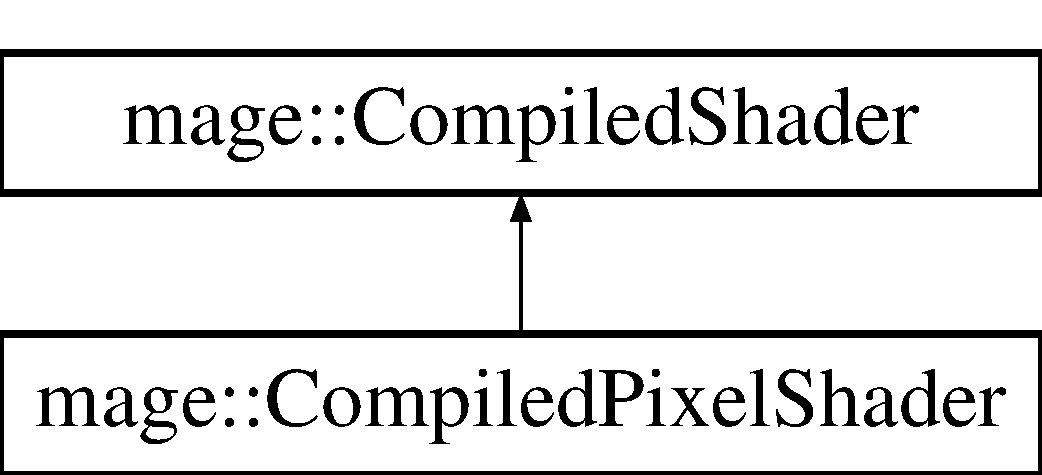
\includegraphics[height=2.000000cm]{structmage_1_1_compiled_pixel_shader}
\end{center}
\end{figure}
\subsection*{Public Member Functions}
\begin{DoxyCompactItemize}
\item 
\hyperlink{structmage_1_1_compiled_pixel_shader_a1c8cc509e405a53456dff36c204ec353}{Compiled\+Pixel\+Shader} (const wstring \&fname)
\item 
\hyperlink{structmage_1_1_compiled_pixel_shader_a0952d4118e0d7d259b6034a52182ed6c}{Compiled\+Pixel\+Shader} (const B\+Y\+TE $\ast$bytecode, S\+I\+Z\+E\+\_\+T bytecode\+\_\+size)
\item 
\hyperlink{structmage_1_1_compiled_pixel_shader_a3bf30a1885ff8244f7f6c755cc68366a}{Compiled\+Pixel\+Shader} (const \hyperlink{structmage_1_1_compiled_pixel_shader}{Compiled\+Pixel\+Shader} \&compiled\+\_\+pixel\+\_\+shader)
\item 
\hyperlink{structmage_1_1_compiled_pixel_shader_a512dada64de6fa3ebf31a096da80904d}{Compiled\+Pixel\+Shader} (\hyperlink{structmage_1_1_compiled_pixel_shader}{Compiled\+Pixel\+Shader} \&\&compiled\+\_\+pixel\+\_\+shader)
\item 
\hyperlink{structmage_1_1_compiled_pixel_shader_a2121a916b6b1fe1b36aadb136f6b4219}{$\sim$\+Compiled\+Pixel\+Shader} ()
\item 
\hyperlink{structmage_1_1_compiled_pixel_shader}{Compiled\+Pixel\+Shader} \& \hyperlink{structmage_1_1_compiled_pixel_shader_a0dde38701c2e15a52d5d80f992a32551}{operator=} (const \hyperlink{structmage_1_1_compiled_pixel_shader}{Compiled\+Pixel\+Shader} \&compiled\+\_\+pixel\+\_\+shader)=delete
\item 
\hyperlink{structmage_1_1_compiled_pixel_shader}{Compiled\+Pixel\+Shader} \& \hyperlink{structmage_1_1_compiled_pixel_shader_a347557ae3d91dd0d561c56bc2c811a2f}{operator=} (\hyperlink{structmage_1_1_compiled_pixel_shader}{Compiled\+Pixel\+Shader} \&\&compiled\+\_\+pixel\+\_\+shader)=delete
\end{DoxyCompactItemize}


\subsection{Detailed Description}
A struct of compiled pixel shaders. 

\subsection{Constructor \& Destructor Documentation}
\hypertarget{structmage_1_1_compiled_pixel_shader_a1c8cc509e405a53456dff36c204ec353}{}\label{structmage_1_1_compiled_pixel_shader_a1c8cc509e405a53456dff36c204ec353} 
\index{mage\+::\+Compiled\+Pixel\+Shader@{mage\+::\+Compiled\+Pixel\+Shader}!Compiled\+Pixel\+Shader@{Compiled\+Pixel\+Shader}}
\index{Compiled\+Pixel\+Shader@{Compiled\+Pixel\+Shader}!mage\+::\+Compiled\+Pixel\+Shader@{mage\+::\+Compiled\+Pixel\+Shader}}
\subsubsection{\texorpdfstring{Compiled\+Pixel\+Shader()}{CompiledPixelShader()}\hspace{0.1cm}{\footnotesize\ttfamily [1/4]}}
{\footnotesize\ttfamily mage\+::\+Compiled\+Pixel\+Shader\+::\+Compiled\+Pixel\+Shader (\begin{DoxyParamCaption}\item[{const wstring \&}]{fname }\end{DoxyParamCaption})\hspace{0.3cm}{\ttfamily [explicit]}}

Constructs a compiled pixel shader.


\begin{DoxyParams}[1]{Parameters}
\mbox{\tt in}  & {\em fname} & A reference to the filename. \\
\hline
\end{DoxyParams}

\begin{DoxyExceptions}{Exceptions}
{\em \hyperlink{structmage_1_1_formatted_exception}{Formatted\+Exception}} & Failed to load the compiled pixel shader from the given file. \\
\hline
\end{DoxyExceptions}
\hypertarget{structmage_1_1_compiled_pixel_shader_a0952d4118e0d7d259b6034a52182ed6c}{}\label{structmage_1_1_compiled_pixel_shader_a0952d4118e0d7d259b6034a52182ed6c} 
\index{mage\+::\+Compiled\+Pixel\+Shader@{mage\+::\+Compiled\+Pixel\+Shader}!Compiled\+Pixel\+Shader@{Compiled\+Pixel\+Shader}}
\index{Compiled\+Pixel\+Shader@{Compiled\+Pixel\+Shader}!mage\+::\+Compiled\+Pixel\+Shader@{mage\+::\+Compiled\+Pixel\+Shader}}
\subsubsection{\texorpdfstring{Compiled\+Pixel\+Shader()}{CompiledPixelShader()}\hspace{0.1cm}{\footnotesize\ttfamily [2/4]}}
{\footnotesize\ttfamily mage\+::\+Compiled\+Pixel\+Shader\+::\+Compiled\+Pixel\+Shader (\begin{DoxyParamCaption}\item[{const B\+Y\+TE $\ast$}]{bytecode,  }\item[{S\+I\+Z\+E\+\_\+T}]{bytecode\+\_\+size }\end{DoxyParamCaption})\hspace{0.3cm}{\ttfamily [explicit]}}

Constructs a compiled pixel shader.

\begin{DoxyPrecond}{Precondition}
{\itshape bytecode} is not equal to {\ttfamily nullptr}. 

The size of the data pointed to by {\itshape bytecode} is equal to {\itshape bytecode\+\_\+size} (bytes). 
\end{DoxyPrecond}

\begin{DoxyParams}[1]{Parameters}
\mbox{\tt in}  & {\em bytecode} & A pointer to the shader bytecode. \\
\hline
\mbox{\tt in}  & {\em bytecode\+\_\+size} & The size of the given shader bytecode. \\
\hline
\end{DoxyParams}
\hypertarget{structmage_1_1_compiled_pixel_shader_a3bf30a1885ff8244f7f6c755cc68366a}{}\label{structmage_1_1_compiled_pixel_shader_a3bf30a1885ff8244f7f6c755cc68366a} 
\index{mage\+::\+Compiled\+Pixel\+Shader@{mage\+::\+Compiled\+Pixel\+Shader}!Compiled\+Pixel\+Shader@{Compiled\+Pixel\+Shader}}
\index{Compiled\+Pixel\+Shader@{Compiled\+Pixel\+Shader}!mage\+::\+Compiled\+Pixel\+Shader@{mage\+::\+Compiled\+Pixel\+Shader}}
\subsubsection{\texorpdfstring{Compiled\+Pixel\+Shader()}{CompiledPixelShader()}\hspace{0.1cm}{\footnotesize\ttfamily [3/4]}}
{\footnotesize\ttfamily mage\+::\+Compiled\+Pixel\+Shader\+::\+Compiled\+Pixel\+Shader (\begin{DoxyParamCaption}\item[{const \hyperlink{structmage_1_1_compiled_pixel_shader}{Compiled\+Pixel\+Shader} \&}]{compiled\+\_\+pixel\+\_\+shader }\end{DoxyParamCaption})\hspace{0.3cm}{\ttfamily [default]}}

Constructs a compiled pixel shader from the given compiled pixel shader.


\begin{DoxyParams}[1]{Parameters}
\mbox{\tt in}  & {\em compiled\+\_\+pixel\+\_\+shader} & A reference to the compiled pixel shader to copy. \\
\hline
\end{DoxyParams}
\hypertarget{structmage_1_1_compiled_pixel_shader_a512dada64de6fa3ebf31a096da80904d}{}\label{structmage_1_1_compiled_pixel_shader_a512dada64de6fa3ebf31a096da80904d} 
\index{mage\+::\+Compiled\+Pixel\+Shader@{mage\+::\+Compiled\+Pixel\+Shader}!Compiled\+Pixel\+Shader@{Compiled\+Pixel\+Shader}}
\index{Compiled\+Pixel\+Shader@{Compiled\+Pixel\+Shader}!mage\+::\+Compiled\+Pixel\+Shader@{mage\+::\+Compiled\+Pixel\+Shader}}
\subsubsection{\texorpdfstring{Compiled\+Pixel\+Shader()}{CompiledPixelShader()}\hspace{0.1cm}{\footnotesize\ttfamily [4/4]}}
{\footnotesize\ttfamily mage\+::\+Compiled\+Pixel\+Shader\+::\+Compiled\+Pixel\+Shader (\begin{DoxyParamCaption}\item[{\hyperlink{structmage_1_1_compiled_pixel_shader}{Compiled\+Pixel\+Shader} \&\&}]{compiled\+\_\+pixel\+\_\+shader }\end{DoxyParamCaption})\hspace{0.3cm}{\ttfamily [default]}}

Constructs a compiled pixel shader by moving the given compiled pixel shader.


\begin{DoxyParams}[1]{Parameters}
\mbox{\tt in}  & {\em compiled\+\_\+pixel\+\_\+shader} & A reference to the compiled pixel shader to move. \\
\hline
\end{DoxyParams}
\hypertarget{structmage_1_1_compiled_pixel_shader_a2121a916b6b1fe1b36aadb136f6b4219}{}\label{structmage_1_1_compiled_pixel_shader_a2121a916b6b1fe1b36aadb136f6b4219} 
\index{mage\+::\+Compiled\+Pixel\+Shader@{mage\+::\+Compiled\+Pixel\+Shader}!````~Compiled\+Pixel\+Shader@{$\sim$\+Compiled\+Pixel\+Shader}}
\index{````~Compiled\+Pixel\+Shader@{$\sim$\+Compiled\+Pixel\+Shader}!mage\+::\+Compiled\+Pixel\+Shader@{mage\+::\+Compiled\+Pixel\+Shader}}
\subsubsection{\texorpdfstring{$\sim$\+Compiled\+Pixel\+Shader()}{~CompiledPixelShader()}}
{\footnotesize\ttfamily mage\+::\+Compiled\+Pixel\+Shader\+::$\sim$\+Compiled\+Pixel\+Shader (\begin{DoxyParamCaption}{ }\end{DoxyParamCaption})\hspace{0.3cm}{\ttfamily [default]}}

Destructs this compiled pixel shader. 

\subsection{Member Function Documentation}
\hypertarget{structmage_1_1_compiled_pixel_shader_a0dde38701c2e15a52d5d80f992a32551}{}\label{structmage_1_1_compiled_pixel_shader_a0dde38701c2e15a52d5d80f992a32551} 
\index{mage\+::\+Compiled\+Pixel\+Shader@{mage\+::\+Compiled\+Pixel\+Shader}!operator=@{operator=}}
\index{operator=@{operator=}!mage\+::\+Compiled\+Pixel\+Shader@{mage\+::\+Compiled\+Pixel\+Shader}}
\subsubsection{\texorpdfstring{operator=()}{operator=()}\hspace{0.1cm}{\footnotesize\ttfamily [1/2]}}
{\footnotesize\ttfamily \hyperlink{structmage_1_1_compiled_pixel_shader}{Compiled\+Pixel\+Shader}\& mage\+::\+Compiled\+Pixel\+Shader\+::operator= (\begin{DoxyParamCaption}\item[{const \hyperlink{structmage_1_1_compiled_pixel_shader}{Compiled\+Pixel\+Shader} \&}]{compiled\+\_\+pixel\+\_\+shader }\end{DoxyParamCaption})\hspace{0.3cm}{\ttfamily [delete]}}

Copies the given compiled pixel shader to this compiled pixel shader.


\begin{DoxyParams}[1]{Parameters}
\mbox{\tt in}  & {\em compiled\+\_\+pixel\+\_\+shader} & A reference to the compiled pixel shader to copy. \\
\hline
\end{DoxyParams}
\begin{DoxyReturn}{Returns}
A reference to the copy of the given compiled pixel shader (i.\+e. this compiled pixel shader). 
\end{DoxyReturn}
\hypertarget{structmage_1_1_compiled_pixel_shader_a347557ae3d91dd0d561c56bc2c811a2f}{}\label{structmage_1_1_compiled_pixel_shader_a347557ae3d91dd0d561c56bc2c811a2f} 
\index{mage\+::\+Compiled\+Pixel\+Shader@{mage\+::\+Compiled\+Pixel\+Shader}!operator=@{operator=}}
\index{operator=@{operator=}!mage\+::\+Compiled\+Pixel\+Shader@{mage\+::\+Compiled\+Pixel\+Shader}}
\subsubsection{\texorpdfstring{operator=()}{operator=()}\hspace{0.1cm}{\footnotesize\ttfamily [2/2]}}
{\footnotesize\ttfamily \hyperlink{structmage_1_1_compiled_pixel_shader}{Compiled\+Pixel\+Shader}\& mage\+::\+Compiled\+Pixel\+Shader\+::operator= (\begin{DoxyParamCaption}\item[{\hyperlink{structmage_1_1_compiled_pixel_shader}{Compiled\+Pixel\+Shader} \&\&}]{compiled\+\_\+pixel\+\_\+shader }\end{DoxyParamCaption})\hspace{0.3cm}{\ttfamily [delete]}}

Moves the given compiled pixel shader to this compiled pixel shader.


\begin{DoxyParams}[1]{Parameters}
\mbox{\tt in}  & {\em compiled\+\_\+pixel\+\_\+shader} & A reference to the compiled pixel shader to copy. \\
\hline
\end{DoxyParams}
\begin{DoxyReturn}{Returns}
A reference to the moved compiled pixel shader (i.\+e. this compiled pixel shader). 
\end{DoxyReturn}

\hypertarget{structmage_1_1_compiled_vertex_shader}{}\section{mage\+:\+:Compiled\+Vertex\+Shader Struct Reference}
\label{structmage_1_1_compiled_vertex_shader}\index{mage\+::\+Compiled\+Vertex\+Shader@{mage\+::\+Compiled\+Vertex\+Shader}}


{\ttfamily \#include $<$compiled\+\_\+shader.\+hpp$>$}

\subsection*{Public Member Functions}
\begin{DoxyCompactItemize}
\item 
\hyperlink{structmage_1_1_compiled_vertex_shader_abb08e4d5269937f0d9741ac0f748896f}{Compiled\+Vertex\+Shader} (const wstring \&name, const B\+Y\+TE $\ast$bytecode, S\+I\+Z\+E\+\_\+T bytecode\+\_\+size)
\item 
\hyperlink{structmage_1_1_compiled_vertex_shader_a7f8f7294f285ae5fdaf9726939c0b2e3}{Compiled\+Vertex\+Shader} (const \hyperlink{structmage_1_1_compiled_vertex_shader}{Compiled\+Vertex\+Shader} \&compiled\+\_\+vertex\+\_\+shader)=default
\item 
\hyperlink{structmage_1_1_compiled_vertex_shader_a9101da0cf1f08e55d33bfadda3e98f94}{Compiled\+Vertex\+Shader} (\hyperlink{structmage_1_1_compiled_vertex_shader}{Compiled\+Vertex\+Shader} \&\&compiled\+\_\+vertex\+\_\+shader)=default
\item 
\hyperlink{structmage_1_1_compiled_vertex_shader_af909e9e38ec2eef93a77aeac993e4755}{$\sim$\+Compiled\+Vertex\+Shader} ()=default
\item 
\hyperlink{structmage_1_1_compiled_vertex_shader}{Compiled\+Vertex\+Shader} \& \hyperlink{structmage_1_1_compiled_vertex_shader_a9ce8c846d9c29ffd67a19cffd362b709}{operator=} (const \hyperlink{structmage_1_1_compiled_vertex_shader}{Compiled\+Vertex\+Shader} \&compiled\+\_\+vertex\+\_\+shader)=delete
\item 
\hyperlink{structmage_1_1_compiled_vertex_shader}{Compiled\+Vertex\+Shader} \& \hyperlink{structmage_1_1_compiled_vertex_shader_ae42ff3528b8a4b58c3d9f085d0d4573e}{operator=} (\hyperlink{structmage_1_1_compiled_vertex_shader}{Compiled\+Vertex\+Shader} \&\&compiled\+\_\+vertex\+\_\+shader)=delete
\end{DoxyCompactItemize}
\subsection*{Public Attributes}
\begin{DoxyCompactItemize}
\item 
const wstring \hyperlink{structmage_1_1_compiled_vertex_shader_af37c5f63c4146dd796c7e4df5ade4d0e}{m\+\_\+name}
\item 
const B\+Y\+TE $\ast$const \hyperlink{structmage_1_1_compiled_vertex_shader_ab416def2b374a9c55475e717dd6df540}{m\+\_\+bytecode}
\item 
const S\+I\+Z\+E\+\_\+T \hyperlink{structmage_1_1_compiled_vertex_shader_aab5b4dc130cef9a34e4ceaff22ba3a14}{m\+\_\+bytecode\+\_\+size}
\end{DoxyCompactItemize}


\subsection{Detailed Description}
A struct of compiled vertex shaders. 

\subsection{Constructor \& Destructor Documentation}
\hypertarget{structmage_1_1_compiled_vertex_shader_abb08e4d5269937f0d9741ac0f748896f}{}\label{structmage_1_1_compiled_vertex_shader_abb08e4d5269937f0d9741ac0f748896f} 
\index{mage\+::\+Compiled\+Vertex\+Shader@{mage\+::\+Compiled\+Vertex\+Shader}!Compiled\+Vertex\+Shader@{Compiled\+Vertex\+Shader}}
\index{Compiled\+Vertex\+Shader@{Compiled\+Vertex\+Shader}!mage\+::\+Compiled\+Vertex\+Shader@{mage\+::\+Compiled\+Vertex\+Shader}}
\subsubsection{\texorpdfstring{Compiled\+Vertex\+Shader()}{CompiledVertexShader()}\hspace{0.1cm}{\footnotesize\ttfamily [1/3]}}
{\footnotesize\ttfamily mage\+::\+Compiled\+Vertex\+Shader\+::\+Compiled\+Vertex\+Shader (\begin{DoxyParamCaption}\item[{const wstring \&}]{name,  }\item[{const B\+Y\+TE $\ast$}]{bytecode,  }\item[{S\+I\+Z\+E\+\_\+T}]{bytecode\+\_\+size }\end{DoxyParamCaption})\hspace{0.3cm}{\ttfamily [explicit]}}

Constructs a compiled vertex shader.

\begin{DoxyPrecond}{Precondition}
{\itshape bytecode} is not equal to {\ttfamily nullptr}. 

The size of the data pointed to by {\itshape bytecode} is equal to {\itshape bytecode\+\_\+size} (bytes). 
\end{DoxyPrecond}

\begin{DoxyParams}[1]{Parameters}
\mbox{\tt in}  & {\em name} & A reference to the name of the shader. \\
\hline
\mbox{\tt in}  & {\em bytecode} & A pointer to the shader bytecode. \\
\hline
\mbox{\tt in}  & {\em bytecode\+\_\+size} & The size of the given shader bytecode. \\
\hline
\end{DoxyParams}
\hypertarget{structmage_1_1_compiled_vertex_shader_a7f8f7294f285ae5fdaf9726939c0b2e3}{}\label{structmage_1_1_compiled_vertex_shader_a7f8f7294f285ae5fdaf9726939c0b2e3} 
\index{mage\+::\+Compiled\+Vertex\+Shader@{mage\+::\+Compiled\+Vertex\+Shader}!Compiled\+Vertex\+Shader@{Compiled\+Vertex\+Shader}}
\index{Compiled\+Vertex\+Shader@{Compiled\+Vertex\+Shader}!mage\+::\+Compiled\+Vertex\+Shader@{mage\+::\+Compiled\+Vertex\+Shader}}
\subsubsection{\texorpdfstring{Compiled\+Vertex\+Shader()}{CompiledVertexShader()}\hspace{0.1cm}{\footnotesize\ttfamily [2/3]}}
{\footnotesize\ttfamily mage\+::\+Compiled\+Vertex\+Shader\+::\+Compiled\+Vertex\+Shader (\begin{DoxyParamCaption}\item[{const \hyperlink{structmage_1_1_compiled_vertex_shader}{Compiled\+Vertex\+Shader} \&}]{compiled\+\_\+vertex\+\_\+shader }\end{DoxyParamCaption})\hspace{0.3cm}{\ttfamily [default]}}

Constructs a compiled vertex shader from the given compiled vertex shader.


\begin{DoxyParams}[1]{Parameters}
\mbox{\tt in}  & {\em compiled\+\_\+vertex\+\_\+shader} & A reference to the compiled vertex shader to copy. \\
\hline
\end{DoxyParams}
\hypertarget{structmage_1_1_compiled_vertex_shader_a9101da0cf1f08e55d33bfadda3e98f94}{}\label{structmage_1_1_compiled_vertex_shader_a9101da0cf1f08e55d33bfadda3e98f94} 
\index{mage\+::\+Compiled\+Vertex\+Shader@{mage\+::\+Compiled\+Vertex\+Shader}!Compiled\+Vertex\+Shader@{Compiled\+Vertex\+Shader}}
\index{Compiled\+Vertex\+Shader@{Compiled\+Vertex\+Shader}!mage\+::\+Compiled\+Vertex\+Shader@{mage\+::\+Compiled\+Vertex\+Shader}}
\subsubsection{\texorpdfstring{Compiled\+Vertex\+Shader()}{CompiledVertexShader()}\hspace{0.1cm}{\footnotesize\ttfamily [3/3]}}
{\footnotesize\ttfamily mage\+::\+Compiled\+Vertex\+Shader\+::\+Compiled\+Vertex\+Shader (\begin{DoxyParamCaption}\item[{\hyperlink{structmage_1_1_compiled_vertex_shader}{Compiled\+Vertex\+Shader} \&\&}]{compiled\+\_\+vertex\+\_\+shader }\end{DoxyParamCaption})\hspace{0.3cm}{\ttfamily [default]}}

Constructs a compiled vertex shader by moving the given compiled vertex shader.


\begin{DoxyParams}[1]{Parameters}
\mbox{\tt in}  & {\em compiled\+\_\+vertex\+\_\+shader} & A reference to the compiled vertex shader to move. \\
\hline
\end{DoxyParams}
\hypertarget{structmage_1_1_compiled_vertex_shader_af909e9e38ec2eef93a77aeac993e4755}{}\label{structmage_1_1_compiled_vertex_shader_af909e9e38ec2eef93a77aeac993e4755} 
\index{mage\+::\+Compiled\+Vertex\+Shader@{mage\+::\+Compiled\+Vertex\+Shader}!````~Compiled\+Vertex\+Shader@{$\sim$\+Compiled\+Vertex\+Shader}}
\index{````~Compiled\+Vertex\+Shader@{$\sim$\+Compiled\+Vertex\+Shader}!mage\+::\+Compiled\+Vertex\+Shader@{mage\+::\+Compiled\+Vertex\+Shader}}
\subsubsection{\texorpdfstring{$\sim$\+Compiled\+Vertex\+Shader()}{~CompiledVertexShader()}}
{\footnotesize\ttfamily mage\+::\+Compiled\+Vertex\+Shader\+::$\sim$\+Compiled\+Vertex\+Shader (\begin{DoxyParamCaption}{ }\end{DoxyParamCaption})\hspace{0.3cm}{\ttfamily [default]}}

Destructs this compiled vertex shader. 

\subsection{Member Function Documentation}
\hypertarget{structmage_1_1_compiled_vertex_shader_a9ce8c846d9c29ffd67a19cffd362b709}{}\label{structmage_1_1_compiled_vertex_shader_a9ce8c846d9c29ffd67a19cffd362b709} 
\index{mage\+::\+Compiled\+Vertex\+Shader@{mage\+::\+Compiled\+Vertex\+Shader}!operator=@{operator=}}
\index{operator=@{operator=}!mage\+::\+Compiled\+Vertex\+Shader@{mage\+::\+Compiled\+Vertex\+Shader}}
\subsubsection{\texorpdfstring{operator=()}{operator=()}\hspace{0.1cm}{\footnotesize\ttfamily [1/2]}}
{\footnotesize\ttfamily \hyperlink{structmage_1_1_compiled_vertex_shader}{Compiled\+Vertex\+Shader}\& mage\+::\+Compiled\+Vertex\+Shader\+::operator= (\begin{DoxyParamCaption}\item[{const \hyperlink{structmage_1_1_compiled_vertex_shader}{Compiled\+Vertex\+Shader} \&}]{compiled\+\_\+vertex\+\_\+shader }\end{DoxyParamCaption})\hspace{0.3cm}{\ttfamily [delete]}}

Copies the given compiled vertex shader to this compiled vertex shader.


\begin{DoxyParams}[1]{Parameters}
\mbox{\tt in}  & {\em compiled\+\_\+vertex\+\_\+shader} & A reference to the compiled vertex shader to copy. \\
\hline
\end{DoxyParams}
\begin{DoxyReturn}{Returns}
A reference to the copy of the given compiled vertex shader (i.\+e. this compiled vertex shader). 
\end{DoxyReturn}
\hypertarget{structmage_1_1_compiled_vertex_shader_ae42ff3528b8a4b58c3d9f085d0d4573e}{}\label{structmage_1_1_compiled_vertex_shader_ae42ff3528b8a4b58c3d9f085d0d4573e} 
\index{mage\+::\+Compiled\+Vertex\+Shader@{mage\+::\+Compiled\+Vertex\+Shader}!operator=@{operator=}}
\index{operator=@{operator=}!mage\+::\+Compiled\+Vertex\+Shader@{mage\+::\+Compiled\+Vertex\+Shader}}
\subsubsection{\texorpdfstring{operator=()}{operator=()}\hspace{0.1cm}{\footnotesize\ttfamily [2/2]}}
{\footnotesize\ttfamily \hyperlink{structmage_1_1_compiled_vertex_shader}{Compiled\+Vertex\+Shader}\& mage\+::\+Compiled\+Vertex\+Shader\+::operator= (\begin{DoxyParamCaption}\item[{\hyperlink{structmage_1_1_compiled_vertex_shader}{Compiled\+Vertex\+Shader} \&\&}]{compiled\+\_\+vertex\+\_\+shader }\end{DoxyParamCaption})\hspace{0.3cm}{\ttfamily [delete]}}

Moves the given compiled vertex shader to this compiled vertex shader.


\begin{DoxyParams}[1]{Parameters}
\mbox{\tt in}  & {\em compiled\+\_\+vertex\+\_\+shader} & A reference to the compiled vertex shader to copy. \\
\hline
\end{DoxyParams}
\begin{DoxyReturn}{Returns}
A reference to the moved compiled vertex shader (i.\+e. this compiled vertex shader). 
\end{DoxyReturn}


\subsection{Member Data Documentation}
\hypertarget{structmage_1_1_compiled_vertex_shader_ab416def2b374a9c55475e717dd6df540}{}\label{structmage_1_1_compiled_vertex_shader_ab416def2b374a9c55475e717dd6df540} 
\index{mage\+::\+Compiled\+Vertex\+Shader@{mage\+::\+Compiled\+Vertex\+Shader}!m\+\_\+bytecode@{m\+\_\+bytecode}}
\index{m\+\_\+bytecode@{m\+\_\+bytecode}!mage\+::\+Compiled\+Vertex\+Shader@{mage\+::\+Compiled\+Vertex\+Shader}}
\subsubsection{\texorpdfstring{m\+\_\+bytecode}{m\_bytecode}}
{\footnotesize\ttfamily const B\+Y\+TE$\ast$ const mage\+::\+Compiled\+Vertex\+Shader\+::m\+\_\+bytecode}

A pointer to the bytecode of this compiled vertex shader. \hypertarget{structmage_1_1_compiled_vertex_shader_aab5b4dc130cef9a34e4ceaff22ba3a14}{}\label{structmage_1_1_compiled_vertex_shader_aab5b4dc130cef9a34e4ceaff22ba3a14} 
\index{mage\+::\+Compiled\+Vertex\+Shader@{mage\+::\+Compiled\+Vertex\+Shader}!m\+\_\+bytecode\+\_\+size@{m\+\_\+bytecode\+\_\+size}}
\index{m\+\_\+bytecode\+\_\+size@{m\+\_\+bytecode\+\_\+size}!mage\+::\+Compiled\+Vertex\+Shader@{mage\+::\+Compiled\+Vertex\+Shader}}
\subsubsection{\texorpdfstring{m\+\_\+bytecode\+\_\+size}{m\_bytecode\_size}}
{\footnotesize\ttfamily const S\+I\+Z\+E\+\_\+T mage\+::\+Compiled\+Vertex\+Shader\+::m\+\_\+bytecode\+\_\+size}

The size of the bytecode of this compiled vertex shader. \hypertarget{structmage_1_1_compiled_vertex_shader_af37c5f63c4146dd796c7e4df5ade4d0e}{}\label{structmage_1_1_compiled_vertex_shader_af37c5f63c4146dd796c7e4df5ade4d0e} 
\index{mage\+::\+Compiled\+Vertex\+Shader@{mage\+::\+Compiled\+Vertex\+Shader}!m\+\_\+name@{m\+\_\+name}}
\index{m\+\_\+name@{m\+\_\+name}!mage\+::\+Compiled\+Vertex\+Shader@{mage\+::\+Compiled\+Vertex\+Shader}}
\subsubsection{\texorpdfstring{m\+\_\+name}{m\_name}}
{\footnotesize\ttfamily const wstring mage\+::\+Compiled\+Vertex\+Shader\+::m\+\_\+name}

The name of this compiled vertex shader. 
\hypertarget{structmage_1_1_condition_variable}{}\section{mage\+:\+:Condition\+Variable Struct Reference}
\label{structmage_1_1_condition_variable}\index{mage\+::\+Condition\+Variable@{mage\+::\+Condition\+Variable}}


{\ttfamily \#include $<$lock.\+hpp$>$}

\subsection*{Public Member Functions}
\begin{DoxyCompactItemize}
\item 
\hyperlink{structmage_1_1_condition_variable_a09073f0affc601f052fce541a17ba559}{Condition\+Variable} ()
\item 
\hyperlink{structmage_1_1_condition_variable_add5ccf5807a94588c28621141df334d3}{Condition\+Variable} (const \hyperlink{structmage_1_1_condition_variable}{Condition\+Variable} \&condition\+\_\+variable)=delete
\item 
\hyperlink{structmage_1_1_condition_variable_a16507f71180938eb82af7e35d3ca5df7}{Condition\+Variable} (\hyperlink{structmage_1_1_condition_variable}{Condition\+Variable} \&\&condition\+\_\+variable)=default
\item 
\hyperlink{structmage_1_1_condition_variable_accd5253beb65b2904428afdb889cf00b}{$\sim$\+Condition\+Variable} ()
\item 
\hyperlink{structmage_1_1_condition_variable}{Condition\+Variable} \& \hyperlink{structmage_1_1_condition_variable_ac83eae5353cd004ee06fe2376e5bdbf4}{operator=} (const \hyperlink{structmage_1_1_condition_variable}{Condition\+Variable} \&condition\+\_\+variable)=delete
\item 
\hyperlink{structmage_1_1_condition_variable}{Condition\+Variable} \& \hyperlink{structmage_1_1_condition_variable_a3f05c5b53b2530e9fdd1bb890aa375c4}{operator=} (\hyperlink{structmage_1_1_condition_variable}{Condition\+Variable} \&\&condition\+\_\+variable)=delete
\item 
void \hyperlink{structmage_1_1_condition_variable_aab712c41e76c444606d5419a20d87b7a}{Lock} () noexcept
\item 
void \hyperlink{structmage_1_1_condition_variable_a40e853cf65b0c3cb3788d2b8a45448af}{Unlock} () noexcept
\item 
void \hyperlink{structmage_1_1_condition_variable_ad48673a4f7ea2a28c7ddc77222e5d8cc}{Signal} () noexcept
\item 
void \hyperlink{structmage_1_1_condition_variable_a15a1d797032d178c787a385d11522efb}{Wait} () noexcept
\end{DoxyCompactItemize}
\subsection*{Private Types}
\begin{DoxyCompactItemize}
\item 
enum \hyperlink{structmage_1_1_condition_variable_ae7627253bf4faebc0aae84a77920d195}{Event} \{ \hyperlink{structmage_1_1_condition_variable_ae7627253bf4faebc0aae84a77920d195a83361ddf52d1973875f7a48ac4bccf94}{S\+I\+G\+N\+AL} = 0, 
\hyperlink{structmage_1_1_condition_variable_ae7627253bf4faebc0aae84a77920d195a5863233d3c1e62ca806753b0d175199f}{B\+R\+O\+A\+D\+C\+A\+ST} = 1, 
\hyperlink{structmage_1_1_condition_variable_ae7627253bf4faebc0aae84a77920d195a553680ab09f088489b7d9f3cef9a5e14}{C\+O\+U\+NT} = 2
 \}
\end{DoxyCompactItemize}
\subsection*{Private Attributes}
\begin{DoxyCompactItemize}
\item 
\hyperlink{namespacemage_af2b398bf98eb10351f49cad73fe2cc73}{u32} \hyperlink{structmage_1_1_condition_variable_a3e707192c1372a21659df405867048eb}{m\+\_\+nb\+\_\+waiters}
\item 
C\+R\+I\+T\+I\+C\+A\+L\+\_\+\+S\+E\+C\+T\+I\+ON \hyperlink{structmage_1_1_condition_variable_a0686e682d62d44ff1eb9ac45acbb0eab}{m\+\_\+nb\+\_\+waiters\+\_\+mutex}
\item 
C\+R\+I\+T\+I\+C\+A\+L\+\_\+\+S\+E\+C\+T\+I\+ON \hyperlink{structmage_1_1_condition_variable_ab5ff870b2881a1979ccaec986d762441}{m\+\_\+condition\+\_\+mutex}
\item 
H\+A\+N\+D\+LE \hyperlink{structmage_1_1_condition_variable_a00691d5e29735da356f577bb5522017d}{m\+\_\+events} \mbox{[}\hyperlink{structmage_1_1_condition_variable_ae7627253bf4faebc0aae84a77920d195a553680ab09f088489b7d9f3cef9a5e14}{C\+O\+U\+NT}\mbox{]}
\end{DoxyCompactItemize}


\subsection{Detailed Description}
A struct of condition variables. 

\subsection{Member Enumeration Documentation}
\hypertarget{structmage_1_1_condition_variable_ae7627253bf4faebc0aae84a77920d195}{}\label{structmage_1_1_condition_variable_ae7627253bf4faebc0aae84a77920d195} 
\index{mage\+::\+Condition\+Variable@{mage\+::\+Condition\+Variable}!Event@{Event}}
\index{Event@{Event}!mage\+::\+Condition\+Variable@{mage\+::\+Condition\+Variable}}
\subsubsection{\texorpdfstring{Event}{Event}}
{\footnotesize\ttfamily enum \hyperlink{structmage_1_1_condition_variable_ae7627253bf4faebc0aae84a77920d195}{mage\+::\+Condition\+Variable\+::\+Event}\hspace{0.3cm}{\ttfamily [private]}}

An enumeration of the different types of events of this condition variable. \begin{DoxyEnumFields}{Enumerator}
\raisebox{\heightof{T}}[0pt][0pt]{\index{S\+I\+G\+N\+AL@{S\+I\+G\+N\+AL}!mage\+::\+Condition\+Variable@{mage\+::\+Condition\+Variable}}\index{mage\+::\+Condition\+Variable@{mage\+::\+Condition\+Variable}!S\+I\+G\+N\+AL@{S\+I\+G\+N\+AL}}}\hypertarget{structmage_1_1_condition_variable_ae7627253bf4faebc0aae84a77920d195a83361ddf52d1973875f7a48ac4bccf94}{}\label{structmage_1_1_condition_variable_ae7627253bf4faebc0aae84a77920d195a83361ddf52d1973875f7a48ac4bccf94} 
S\+I\+G\+N\+AL&\\
\hline

\raisebox{\heightof{T}}[0pt][0pt]{\index{B\+R\+O\+A\+D\+C\+A\+ST@{B\+R\+O\+A\+D\+C\+A\+ST}!mage\+::\+Condition\+Variable@{mage\+::\+Condition\+Variable}}\index{mage\+::\+Condition\+Variable@{mage\+::\+Condition\+Variable}!B\+R\+O\+A\+D\+C\+A\+ST@{B\+R\+O\+A\+D\+C\+A\+ST}}}\hypertarget{structmage_1_1_condition_variable_ae7627253bf4faebc0aae84a77920d195a5863233d3c1e62ca806753b0d175199f}{}\label{structmage_1_1_condition_variable_ae7627253bf4faebc0aae84a77920d195a5863233d3c1e62ca806753b0d175199f} 
B\+R\+O\+A\+D\+C\+A\+ST&\\
\hline

\raisebox{\heightof{T}}[0pt][0pt]{\index{C\+O\+U\+NT@{C\+O\+U\+NT}!mage\+::\+Condition\+Variable@{mage\+::\+Condition\+Variable}}\index{mage\+::\+Condition\+Variable@{mage\+::\+Condition\+Variable}!C\+O\+U\+NT@{C\+O\+U\+NT}}}\hypertarget{structmage_1_1_condition_variable_ae7627253bf4faebc0aae84a77920d195a553680ab09f088489b7d9f3cef9a5e14}{}\label{structmage_1_1_condition_variable_ae7627253bf4faebc0aae84a77920d195a553680ab09f088489b7d9f3cef9a5e14} 
C\+O\+U\+NT&\\
\hline

\end{DoxyEnumFields}


\subsection{Constructor \& Destructor Documentation}
\hypertarget{structmage_1_1_condition_variable_a09073f0affc601f052fce541a17ba559}{}\label{structmage_1_1_condition_variable_a09073f0affc601f052fce541a17ba559} 
\index{mage\+::\+Condition\+Variable@{mage\+::\+Condition\+Variable}!Condition\+Variable@{Condition\+Variable}}
\index{Condition\+Variable@{Condition\+Variable}!mage\+::\+Condition\+Variable@{mage\+::\+Condition\+Variable}}
\subsubsection{\texorpdfstring{Condition\+Variable()}{ConditionVariable()}\hspace{0.1cm}{\footnotesize\ttfamily [1/3]}}
{\footnotesize\ttfamily mage\+::\+Condition\+Variable\+::\+Condition\+Variable (\begin{DoxyParamCaption}{ }\end{DoxyParamCaption})}

Constructs a condition variable. \hypertarget{structmage_1_1_condition_variable_add5ccf5807a94588c28621141df334d3}{}\label{structmage_1_1_condition_variable_add5ccf5807a94588c28621141df334d3} 
\index{mage\+::\+Condition\+Variable@{mage\+::\+Condition\+Variable}!Condition\+Variable@{Condition\+Variable}}
\index{Condition\+Variable@{Condition\+Variable}!mage\+::\+Condition\+Variable@{mage\+::\+Condition\+Variable}}
\subsubsection{\texorpdfstring{Condition\+Variable()}{ConditionVariable()}\hspace{0.1cm}{\footnotesize\ttfamily [2/3]}}
{\footnotesize\ttfamily mage\+::\+Condition\+Variable\+::\+Condition\+Variable (\begin{DoxyParamCaption}\item[{const \hyperlink{structmage_1_1_condition_variable}{Condition\+Variable} \&}]{condition\+\_\+variable }\end{DoxyParamCaption})\hspace{0.3cm}{\ttfamily [delete]}}

Constructs a condition variable from the given condition variable.


\begin{DoxyParams}[1]{Parameters}
\mbox{\tt in}  & {\em condition\+\_\+variable} & A reference to the condition variable to copy. \\
\hline
\end{DoxyParams}
\hypertarget{structmage_1_1_condition_variable_a16507f71180938eb82af7e35d3ca5df7}{}\label{structmage_1_1_condition_variable_a16507f71180938eb82af7e35d3ca5df7} 
\index{mage\+::\+Condition\+Variable@{mage\+::\+Condition\+Variable}!Condition\+Variable@{Condition\+Variable}}
\index{Condition\+Variable@{Condition\+Variable}!mage\+::\+Condition\+Variable@{mage\+::\+Condition\+Variable}}
\subsubsection{\texorpdfstring{Condition\+Variable()}{ConditionVariable()}\hspace{0.1cm}{\footnotesize\ttfamily [3/3]}}
{\footnotesize\ttfamily mage\+::\+Condition\+Variable\+::\+Condition\+Variable (\begin{DoxyParamCaption}\item[{\hyperlink{structmage_1_1_condition_variable}{Condition\+Variable} \&\&}]{condition\+\_\+variable }\end{DoxyParamCaption})\hspace{0.3cm}{\ttfamily [default]}}

Constructs a condition variable by moving the given condition variable.


\begin{DoxyParams}[1]{Parameters}
\mbox{\tt in}  & {\em condition\+\_\+variable} & A reference to the condition variable to move. \\
\hline
\end{DoxyParams}
\hypertarget{structmage_1_1_condition_variable_accd5253beb65b2904428afdb889cf00b}{}\label{structmage_1_1_condition_variable_accd5253beb65b2904428afdb889cf00b} 
\index{mage\+::\+Condition\+Variable@{mage\+::\+Condition\+Variable}!````~Condition\+Variable@{$\sim$\+Condition\+Variable}}
\index{````~Condition\+Variable@{$\sim$\+Condition\+Variable}!mage\+::\+Condition\+Variable@{mage\+::\+Condition\+Variable}}
\subsubsection{\texorpdfstring{$\sim$\+Condition\+Variable()}{~ConditionVariable()}}
{\footnotesize\ttfamily mage\+::\+Condition\+Variable\+::$\sim$\+Condition\+Variable (\begin{DoxyParamCaption}{ }\end{DoxyParamCaption})}

Destructs this condition variable. 

\subsection{Member Function Documentation}
\hypertarget{structmage_1_1_condition_variable_aab712c41e76c444606d5419a20d87b7a}{}\label{structmage_1_1_condition_variable_aab712c41e76c444606d5419a20d87b7a} 
\index{mage\+::\+Condition\+Variable@{mage\+::\+Condition\+Variable}!Lock@{Lock}}
\index{Lock@{Lock}!mage\+::\+Condition\+Variable@{mage\+::\+Condition\+Variable}}
\subsubsection{\texorpdfstring{Lock()}{Lock()}}
{\footnotesize\ttfamily void mage\+::\+Condition\+Variable\+::\+Lock (\begin{DoxyParamCaption}{ }\end{DoxyParamCaption})\hspace{0.3cm}{\ttfamily [noexcept]}}

Locks this condition variable. \hypertarget{structmage_1_1_condition_variable_ac83eae5353cd004ee06fe2376e5bdbf4}{}\label{structmage_1_1_condition_variable_ac83eae5353cd004ee06fe2376e5bdbf4} 
\index{mage\+::\+Condition\+Variable@{mage\+::\+Condition\+Variable}!operator=@{operator=}}
\index{operator=@{operator=}!mage\+::\+Condition\+Variable@{mage\+::\+Condition\+Variable}}
\subsubsection{\texorpdfstring{operator=()}{operator=()}\hspace{0.1cm}{\footnotesize\ttfamily [1/2]}}
{\footnotesize\ttfamily \hyperlink{structmage_1_1_condition_variable}{Condition\+Variable}\& mage\+::\+Condition\+Variable\+::operator= (\begin{DoxyParamCaption}\item[{const \hyperlink{structmage_1_1_condition_variable}{Condition\+Variable} \&}]{condition\+\_\+variable }\end{DoxyParamCaption})\hspace{0.3cm}{\ttfamily [delete]}}

Copies the given condition variable to this condition variable.


\begin{DoxyParams}[1]{Parameters}
\mbox{\tt in}  & {\em condition\+\_\+variable} & A reference to the condition variable to copy. \\
\hline
\end{DoxyParams}
\begin{DoxyReturn}{Returns}
A reference to the copy of the given condition variable (i.\+e. this condition variable) 
\end{DoxyReturn}
\hypertarget{structmage_1_1_condition_variable_a3f05c5b53b2530e9fdd1bb890aa375c4}{}\label{structmage_1_1_condition_variable_a3f05c5b53b2530e9fdd1bb890aa375c4} 
\index{mage\+::\+Condition\+Variable@{mage\+::\+Condition\+Variable}!operator=@{operator=}}
\index{operator=@{operator=}!mage\+::\+Condition\+Variable@{mage\+::\+Condition\+Variable}}
\subsubsection{\texorpdfstring{operator=()}{operator=()}\hspace{0.1cm}{\footnotesize\ttfamily [2/2]}}
{\footnotesize\ttfamily \hyperlink{structmage_1_1_condition_variable}{Condition\+Variable}\& mage\+::\+Condition\+Variable\+::operator= (\begin{DoxyParamCaption}\item[{\hyperlink{structmage_1_1_condition_variable}{Condition\+Variable} \&\&}]{condition\+\_\+variable }\end{DoxyParamCaption})\hspace{0.3cm}{\ttfamily [delete]}}

Moves the given condition variable to this condition variable.


\begin{DoxyParams}[1]{Parameters}
\mbox{\tt in}  & {\em condition\+\_\+variable} & A reference to the condition variable to move. \\
\hline
\end{DoxyParams}
\begin{DoxyReturn}{Returns}
A reference to the moved condition variable (i.\+e. this condition variable) 
\end{DoxyReturn}
\hypertarget{structmage_1_1_condition_variable_ad48673a4f7ea2a28c7ddc77222e5d8cc}{}\label{structmage_1_1_condition_variable_ad48673a4f7ea2a28c7ddc77222e5d8cc} 
\index{mage\+::\+Condition\+Variable@{mage\+::\+Condition\+Variable}!Signal@{Signal}}
\index{Signal@{Signal}!mage\+::\+Condition\+Variable@{mage\+::\+Condition\+Variable}}
\subsubsection{\texorpdfstring{Signal()}{Signal()}}
{\footnotesize\ttfamily void mage\+::\+Condition\+Variable\+::\+Signal (\begin{DoxyParamCaption}{ }\end{DoxyParamCaption})\hspace{0.3cm}{\ttfamily [noexcept]}}

Signals a condition change. \hypertarget{structmage_1_1_condition_variable_a40e853cf65b0c3cb3788d2b8a45448af}{}\label{structmage_1_1_condition_variable_a40e853cf65b0c3cb3788d2b8a45448af} 
\index{mage\+::\+Condition\+Variable@{mage\+::\+Condition\+Variable}!Unlock@{Unlock}}
\index{Unlock@{Unlock}!mage\+::\+Condition\+Variable@{mage\+::\+Condition\+Variable}}
\subsubsection{\texorpdfstring{Unlock()}{Unlock()}}
{\footnotesize\ttfamily void mage\+::\+Condition\+Variable\+::\+Unlock (\begin{DoxyParamCaption}{ }\end{DoxyParamCaption})\hspace{0.3cm}{\ttfamily [noexcept]}}

Unlocks this condition variable. \hypertarget{structmage_1_1_condition_variable_a15a1d797032d178c787a385d11522efb}{}\label{structmage_1_1_condition_variable_a15a1d797032d178c787a385d11522efb} 
\index{mage\+::\+Condition\+Variable@{mage\+::\+Condition\+Variable}!Wait@{Wait}}
\index{Wait@{Wait}!mage\+::\+Condition\+Variable@{mage\+::\+Condition\+Variable}}
\subsubsection{\texorpdfstring{Wait()}{Wait()}}
{\footnotesize\ttfamily void mage\+::\+Condition\+Variable\+::\+Wait (\begin{DoxyParamCaption}{ }\end{DoxyParamCaption})\hspace{0.3cm}{\ttfamily [noexcept]}}

Waits for a signal indicating a condition change. 

\subsection{Member Data Documentation}
\hypertarget{structmage_1_1_condition_variable_ab5ff870b2881a1979ccaec986d762441}{}\label{structmage_1_1_condition_variable_ab5ff870b2881a1979ccaec986d762441} 
\index{mage\+::\+Condition\+Variable@{mage\+::\+Condition\+Variable}!m\+\_\+condition\+\_\+mutex@{m\+\_\+condition\+\_\+mutex}}
\index{m\+\_\+condition\+\_\+mutex@{m\+\_\+condition\+\_\+mutex}!mage\+::\+Condition\+Variable@{mage\+::\+Condition\+Variable}}
\subsubsection{\texorpdfstring{m\+\_\+condition\+\_\+mutex}{m\_condition\_mutex}}
{\footnotesize\ttfamily C\+R\+I\+T\+I\+C\+A\+L\+\_\+\+S\+E\+C\+T\+I\+ON mage\+::\+Condition\+Variable\+::m\+\_\+condition\+\_\+mutex\hspace{0.3cm}{\ttfamily [private]}}

The critical section object for the mutex guarding the condition of this condition variable. \hypertarget{structmage_1_1_condition_variable_a00691d5e29735da356f577bb5522017d}{}\label{structmage_1_1_condition_variable_a00691d5e29735da356f577bb5522017d} 
\index{mage\+::\+Condition\+Variable@{mage\+::\+Condition\+Variable}!m\+\_\+events@{m\+\_\+events}}
\index{m\+\_\+events@{m\+\_\+events}!mage\+::\+Condition\+Variable@{mage\+::\+Condition\+Variable}}
\subsubsection{\texorpdfstring{m\+\_\+events}{m\_events}}
{\footnotesize\ttfamily H\+A\+N\+D\+LE mage\+::\+Condition\+Variable\+::m\+\_\+events\mbox{[}\hyperlink{structmage_1_1_condition_variable_ae7627253bf4faebc0aae84a77920d195a553680ab09f088489b7d9f3cef9a5e14}{C\+O\+U\+NT}\mbox{]}\hspace{0.3cm}{\ttfamily [private]}}

The signal and broadcast event handles of this condition variable. \hypertarget{structmage_1_1_condition_variable_a3e707192c1372a21659df405867048eb}{}\label{structmage_1_1_condition_variable_a3e707192c1372a21659df405867048eb} 
\index{mage\+::\+Condition\+Variable@{mage\+::\+Condition\+Variable}!m\+\_\+nb\+\_\+waiters@{m\+\_\+nb\+\_\+waiters}}
\index{m\+\_\+nb\+\_\+waiters@{m\+\_\+nb\+\_\+waiters}!mage\+::\+Condition\+Variable@{mage\+::\+Condition\+Variable}}
\subsubsection{\texorpdfstring{m\+\_\+nb\+\_\+waiters}{m\_nb\_waiters}}
{\footnotesize\ttfamily \hyperlink{namespacemage_af2b398bf98eb10351f49cad73fe2cc73}{u32} mage\+::\+Condition\+Variable\+::m\+\_\+nb\+\_\+waiters\hspace{0.3cm}{\ttfamily [private]}}

The number of waiters of this condition variable. \hypertarget{structmage_1_1_condition_variable_a0686e682d62d44ff1eb9ac45acbb0eab}{}\label{structmage_1_1_condition_variable_a0686e682d62d44ff1eb9ac45acbb0eab} 
\index{mage\+::\+Condition\+Variable@{mage\+::\+Condition\+Variable}!m\+\_\+nb\+\_\+waiters\+\_\+mutex@{m\+\_\+nb\+\_\+waiters\+\_\+mutex}}
\index{m\+\_\+nb\+\_\+waiters\+\_\+mutex@{m\+\_\+nb\+\_\+waiters\+\_\+mutex}!mage\+::\+Condition\+Variable@{mage\+::\+Condition\+Variable}}
\subsubsection{\texorpdfstring{m\+\_\+nb\+\_\+waiters\+\_\+mutex}{m\_nb\_waiters\_mutex}}
{\footnotesize\ttfamily C\+R\+I\+T\+I\+C\+A\+L\+\_\+\+S\+E\+C\+T\+I\+ON mage\+::\+Condition\+Variable\+::m\+\_\+nb\+\_\+waiters\+\_\+mutex\hspace{0.3cm}{\ttfamily [private]}}

The critical section object for the mutex guarding {\ttfamily m\+\_\+nb\+\_\+waiters} of this condition variable. 
\hypertarget{structmage_1_1_constant_buffer}{}\section{mage\+:\+:Constant\+Buffer$<$ DataT $>$ Struct Template Reference}
\label{structmage_1_1_constant_buffer}\index{mage\+::\+Constant\+Buffer$<$ Data\+T $>$@{mage\+::\+Constant\+Buffer$<$ Data\+T $>$}}


{\ttfamily \#include $<$constant\+\_\+buffer.\+hpp$>$}

\subsection*{Public Member Functions}
\begin{DoxyCompactItemize}
\item 
\hyperlink{structmage_1_1_constant_buffer_a3badd88f8570d6622f6eb33c7420a87d}{Constant\+Buffer} ()
\item 
\hyperlink{structmage_1_1_constant_buffer_aaf32ac894aa2fe73bcbd9033e6e7efb0}{Constant\+Buffer} (I\+D3\+D11\+Device5 $\ast$device)
\item 
\hyperlink{structmage_1_1_constant_buffer_a67fe42cb52e63e38474b6c65341fbe82}{Constant\+Buffer} (const \hyperlink{structmage_1_1_constant_buffer}{Constant\+Buffer} \&buffer)=delete
\item 
\hyperlink{structmage_1_1_constant_buffer_aeb0642e0e405eeb18658c0962a52f406}{Constant\+Buffer} (\hyperlink{structmage_1_1_constant_buffer}{Constant\+Buffer} \&\&buffer) noexcept=default
\item 
\hyperlink{structmage_1_1_constant_buffer_a874e9507ea3b6d2f630f061c2fc6d2d0}{$\sim$\+Constant\+Buffer} ()=default
\item 
\hyperlink{structmage_1_1_constant_buffer}{Constant\+Buffer} \& \hyperlink{structmage_1_1_constant_buffer_acb1a4f4b656073609075b5e89dea6973}{operator=} (const \hyperlink{structmage_1_1_constant_buffer}{Constant\+Buffer} \&buffer)=delete
\item 
\hyperlink{structmage_1_1_constant_buffer}{Constant\+Buffer} \& \hyperlink{structmage_1_1_constant_buffer_ad050b1f0f03a5fcd2b51977a744781a3}{operator=} (\hyperlink{structmage_1_1_constant_buffer}{Constant\+Buffer} \&\&buffer)=delete
\item 
void \hyperlink{structmage_1_1_constant_buffer_aa9a12f5975b1b53b5b174e563d77aaf7}{Update\+Data} (I\+D3\+D11\+Device\+Context4 $\ast$device\+\_\+context, const DataT \&data)
\item 
I\+D3\+D11\+Buffer $\ast$ \hyperlink{structmage_1_1_constant_buffer_a6b8fcbd873ffbda96d7412c581d5a29a}{Get} () const noexcept
\item 
{\footnotesize template$<$typename Pipeline\+StageT $>$ }\\void \hyperlink{structmage_1_1_constant_buffer_a7592eed823334cdc3da614121f2b25ca}{Bind} (I\+D3\+D11\+Device\+Context4 $\ast$device\+\_\+context, \hyperlink{namespacemage_a41c104c036fba3756a74e19f793eeaa1}{U32} slot) const noexcept
\end{DoxyCompactItemize}
\subsection*{Private Member Functions}
\begin{DoxyCompactItemize}
\item 
void \hyperlink{structmage_1_1_constant_buffer_a52e82d01bd000ff314c33bfdc350c67e}{Setup\+Constant\+Buffer} (I\+D3\+D11\+Device5 $\ast$device)
\end{DoxyCompactItemize}
\subsection*{Private Attributes}
\begin{DoxyCompactItemize}
\item 
\hyperlink{namespacemage_ae74f374780900893caa5555d1031fd79}{Com\+Ptr}$<$ I\+D3\+D11\+Buffer $>$ \hyperlink{structmage_1_1_constant_buffer_a394571e3102fe053f3357e2e218c0eda}{m\+\_\+buffer}
\end{DoxyCompactItemize}


\subsection{Detailed Description}
\subsubsection*{template$<$typename DataT$>$\newline
struct mage\+::\+Constant\+Buffer$<$ Data\+T $>$}

A class of constant buffers (for binding buffers to the rendering pipeline).


\begin{DoxyTemplParams}{Template Parameters}
{\em DataT} & The data type. \\
\hline
\end{DoxyTemplParams}


\subsection{Constructor \& Destructor Documentation}
\hypertarget{structmage_1_1_constant_buffer_a3badd88f8570d6622f6eb33c7420a87d}{}\label{structmage_1_1_constant_buffer_a3badd88f8570d6622f6eb33c7420a87d} 
\index{mage\+::\+Constant\+Buffer@{mage\+::\+Constant\+Buffer}!Constant\+Buffer@{Constant\+Buffer}}
\index{Constant\+Buffer@{Constant\+Buffer}!mage\+::\+Constant\+Buffer@{mage\+::\+Constant\+Buffer}}
\subsubsection{\texorpdfstring{Constant\+Buffer()}{ConstantBuffer()}\hspace{0.1cm}{\footnotesize\ttfamily [1/4]}}
{\footnotesize\ttfamily template$<$typename DataT$>$ \\
\hyperlink{structmage_1_1_constant_buffer}{mage\+::\+Constant\+Buffer}$<$ DataT $>$\+::\hyperlink{structmage_1_1_constant_buffer}{Constant\+Buffer} (\begin{DoxyParamCaption}{ }\end{DoxyParamCaption})}

Constructs a constant buffer.

\begin{DoxyPrecond}{Precondition}
The device associated of the rendering manager associated with the current engine must be loaded. 
\end{DoxyPrecond}

\begin{DoxyExceptions}{Exceptions}
{\em \hyperlink{classmage_1_1_formatted_exception}{Formatted\+Exception}} & Failed to setup this constant buffer. \\
\hline
\end{DoxyExceptions}
\hypertarget{structmage_1_1_constant_buffer_aaf32ac894aa2fe73bcbd9033e6e7efb0}{}\label{structmage_1_1_constant_buffer_aaf32ac894aa2fe73bcbd9033e6e7efb0} 
\index{mage\+::\+Constant\+Buffer@{mage\+::\+Constant\+Buffer}!Constant\+Buffer@{Constant\+Buffer}}
\index{Constant\+Buffer@{Constant\+Buffer}!mage\+::\+Constant\+Buffer@{mage\+::\+Constant\+Buffer}}
\subsubsection{\texorpdfstring{Constant\+Buffer()}{ConstantBuffer()}\hspace{0.1cm}{\footnotesize\ttfamily [2/4]}}
{\footnotesize\ttfamily template$<$typename DataT$>$ \\
\hyperlink{structmage_1_1_constant_buffer}{mage\+::\+Constant\+Buffer}$<$ DataT $>$\+::\hyperlink{structmage_1_1_constant_buffer}{Constant\+Buffer} (\begin{DoxyParamCaption}\item[{I\+D3\+D11\+Device5 $\ast$}]{device }\end{DoxyParamCaption})\hspace{0.3cm}{\ttfamily [explicit]}}

Constructs a constant buffer.

\begin{DoxyPrecond}{Precondition}
{\itshape device} is not equal to {\ttfamily nullptr}. 
\end{DoxyPrecond}

\begin{DoxyParams}[1]{Parameters}
\mbox{\tt in}  & {\em device} & A pointer to the device. \\
\hline
\end{DoxyParams}

\begin{DoxyExceptions}{Exceptions}
{\em \hyperlink{classmage_1_1_formatted_exception}{Formatted\+Exception}} & Failed to setup this constant buffer. \\
\hline
\end{DoxyExceptions}
\hypertarget{structmage_1_1_constant_buffer_a67fe42cb52e63e38474b6c65341fbe82}{}\label{structmage_1_1_constant_buffer_a67fe42cb52e63e38474b6c65341fbe82} 
\index{mage\+::\+Constant\+Buffer@{mage\+::\+Constant\+Buffer}!Constant\+Buffer@{Constant\+Buffer}}
\index{Constant\+Buffer@{Constant\+Buffer}!mage\+::\+Constant\+Buffer@{mage\+::\+Constant\+Buffer}}
\subsubsection{\texorpdfstring{Constant\+Buffer()}{ConstantBuffer()}\hspace{0.1cm}{\footnotesize\ttfamily [3/4]}}
{\footnotesize\ttfamily template$<$typename DataT$>$ \\
\hyperlink{structmage_1_1_constant_buffer}{mage\+::\+Constant\+Buffer}$<$ DataT $>$\+::\hyperlink{structmage_1_1_constant_buffer}{Constant\+Buffer} (\begin{DoxyParamCaption}\item[{const \hyperlink{structmage_1_1_constant_buffer}{Constant\+Buffer}$<$ DataT $>$ \&}]{buffer }\end{DoxyParamCaption})\hspace{0.3cm}{\ttfamily [delete]}}

Constructs a constant buffer from the given constant buffer.


\begin{DoxyParams}[1]{Parameters}
\mbox{\tt in}  & {\em buffer} & A reference to the constant buffer to copy. \\
\hline
\end{DoxyParams}
\hypertarget{structmage_1_1_constant_buffer_aeb0642e0e405eeb18658c0962a52f406}{}\label{structmage_1_1_constant_buffer_aeb0642e0e405eeb18658c0962a52f406} 
\index{mage\+::\+Constant\+Buffer@{mage\+::\+Constant\+Buffer}!Constant\+Buffer@{Constant\+Buffer}}
\index{Constant\+Buffer@{Constant\+Buffer}!mage\+::\+Constant\+Buffer@{mage\+::\+Constant\+Buffer}}
\subsubsection{\texorpdfstring{Constant\+Buffer()}{ConstantBuffer()}\hspace{0.1cm}{\footnotesize\ttfamily [4/4]}}
{\footnotesize\ttfamily template$<$typename DataT$>$ \\
\hyperlink{structmage_1_1_constant_buffer}{mage\+::\+Constant\+Buffer}$<$ DataT $>$\+::\hyperlink{structmage_1_1_constant_buffer}{Constant\+Buffer} (\begin{DoxyParamCaption}\item[{\hyperlink{structmage_1_1_constant_buffer}{Constant\+Buffer}$<$ DataT $>$ \&\&}]{buffer }\end{DoxyParamCaption})\hspace{0.3cm}{\ttfamily [default]}, {\ttfamily [noexcept]}}

Constructs a constant buffer by moving the given constant buffer.


\begin{DoxyParams}[1]{Parameters}
\mbox{\tt in}  & {\em buffer} & A reference to the constant buffer to move. \\
\hline
\end{DoxyParams}
\hypertarget{structmage_1_1_constant_buffer_a874e9507ea3b6d2f630f061c2fc6d2d0}{}\label{structmage_1_1_constant_buffer_a874e9507ea3b6d2f630f061c2fc6d2d0} 
\index{mage\+::\+Constant\+Buffer@{mage\+::\+Constant\+Buffer}!````~Constant\+Buffer@{$\sim$\+Constant\+Buffer}}
\index{````~Constant\+Buffer@{$\sim$\+Constant\+Buffer}!mage\+::\+Constant\+Buffer@{mage\+::\+Constant\+Buffer}}
\subsubsection{\texorpdfstring{$\sim$\+Constant\+Buffer()}{~ConstantBuffer()}}
{\footnotesize\ttfamily template$<$typename DataT$>$ \\
\hyperlink{structmage_1_1_constant_buffer}{mage\+::\+Constant\+Buffer}$<$ DataT $>$\+::$\sim$\hyperlink{structmage_1_1_constant_buffer}{Constant\+Buffer} (\begin{DoxyParamCaption}{ }\end{DoxyParamCaption})\hspace{0.3cm}{\ttfamily [default]}}

Destructs this constant buffer. 

\subsection{Member Function Documentation}
\hypertarget{structmage_1_1_constant_buffer_a7592eed823334cdc3da614121f2b25ca}{}\label{structmage_1_1_constant_buffer_a7592eed823334cdc3da614121f2b25ca} 
\index{mage\+::\+Constant\+Buffer@{mage\+::\+Constant\+Buffer}!Bind@{Bind}}
\index{Bind@{Bind}!mage\+::\+Constant\+Buffer@{mage\+::\+Constant\+Buffer}}
\subsubsection{\texorpdfstring{Bind()}{Bind()}}
{\footnotesize\ttfamily template$<$typename DataT$>$ \\
template$<$typename Pipeline\+StageT $>$ \\
void \hyperlink{structmage_1_1_constant_buffer}{mage\+::\+Constant\+Buffer}$<$ DataT $>$\+::Bind (\begin{DoxyParamCaption}\item[{I\+D3\+D11\+Device\+Context4 $\ast$}]{device\+\_\+context,  }\item[{\hyperlink{namespacemage_a41c104c036fba3756a74e19f793eeaa1}{U32}}]{slot }\end{DoxyParamCaption}) const\hspace{0.3cm}{\ttfamily [noexcept]}}

Binds this constant buffer.

\begin{DoxyPrecond}{Precondition}
{\itshape device\+\_\+context} is not equal to {\ttfamily nullptr}. 

{\itshape slot} $<$ {\ttfamily D3\+D11\+\_\+\+C\+O\+M\+M\+O\+N\+S\+H\+A\+D\+E\+R\+\_\+\+C\+O\+N\+S\+T\+A\+N\+T\+\_\+\+B\+U\+F\+F\+E\+R\+\_\+\+A\+P\+I\+\_\+\+S\+L\+O\+T\+\_\+\+C\+O\+U\+NT}. 
\end{DoxyPrecond}

\begin{DoxyTemplParams}{Template Parameters}
{\em Pipeline\+StageT} & The pipeline stage type. \\
\hline
\end{DoxyTemplParams}

\begin{DoxyParams}[1]{Parameters}
\mbox{\tt in}  & {\em device\+\_\+context} & A pointer to the device context. \\
\hline
\mbox{\tt in}  & {\em slot} & The index into the device\textquotesingle{}s zero-\/based array to set the constant buffer to (ranges from 0 to {\ttfamily D3\+D11\+\_\+\+C\+O\+M\+M\+O\+N\+S\+H\+A\+D\+E\+R\+\_\+\+C\+O\+N\+S\+T\+A\+N\+T\+\_\+\+B\+U\+F\+F\+E\+R\+\_\+\+A\+P\+I\+\_\+\+S\+L\+O\+T\+\_\+\+C\+O\+U\+NT} 
\begin{DoxyItemize}
\item 1). 
\end{DoxyItemize}\\
\hline
\end{DoxyParams}
\hypertarget{structmage_1_1_constant_buffer_a6b8fcbd873ffbda96d7412c581d5a29a}{}\label{structmage_1_1_constant_buffer_a6b8fcbd873ffbda96d7412c581d5a29a} 
\index{mage\+::\+Constant\+Buffer@{mage\+::\+Constant\+Buffer}!Get@{Get}}
\index{Get@{Get}!mage\+::\+Constant\+Buffer@{mage\+::\+Constant\+Buffer}}
\subsubsection{\texorpdfstring{Get()}{Get()}}
{\footnotesize\ttfamily template$<$typename DataT$>$ \\
I\+D3\+D11\+Buffer$\ast$ \hyperlink{structmage_1_1_constant_buffer}{mage\+::\+Constant\+Buffer}$<$ DataT $>$\+::Get (\begin{DoxyParamCaption}{ }\end{DoxyParamCaption}) const\hspace{0.3cm}{\ttfamily [noexcept]}}

Returns the buffer resource of this constant buffer.

\begin{DoxyReturn}{Returns}
A pointer to the buffer resource of this constant buffer. 
\end{DoxyReturn}
\hypertarget{structmage_1_1_constant_buffer_acb1a4f4b656073609075b5e89dea6973}{}\label{structmage_1_1_constant_buffer_acb1a4f4b656073609075b5e89dea6973} 
\index{mage\+::\+Constant\+Buffer@{mage\+::\+Constant\+Buffer}!operator=@{operator=}}
\index{operator=@{operator=}!mage\+::\+Constant\+Buffer@{mage\+::\+Constant\+Buffer}}
\subsubsection{\texorpdfstring{operator=()}{operator=()}\hspace{0.1cm}{\footnotesize\ttfamily [1/2]}}
{\footnotesize\ttfamily template$<$typename DataT$>$ \\
\hyperlink{structmage_1_1_constant_buffer}{Constant\+Buffer}\& \hyperlink{structmage_1_1_constant_buffer}{mage\+::\+Constant\+Buffer}$<$ DataT $>$\+::operator= (\begin{DoxyParamCaption}\item[{const \hyperlink{structmage_1_1_constant_buffer}{Constant\+Buffer}$<$ DataT $>$ \&}]{buffer }\end{DoxyParamCaption})\hspace{0.3cm}{\ttfamily [delete]}}

Copies the given constant buffer to this constant buffer.


\begin{DoxyParams}[1]{Parameters}
\mbox{\tt in}  & {\em buffer} & A reference to the constant buffer to copy. \\
\hline
\end{DoxyParams}
\begin{DoxyReturn}{Returns}
A reference to the copy of the given constant buffer (i.\+e. this constant buffer). 
\end{DoxyReturn}
\hypertarget{structmage_1_1_constant_buffer_ad050b1f0f03a5fcd2b51977a744781a3}{}\label{structmage_1_1_constant_buffer_ad050b1f0f03a5fcd2b51977a744781a3} 
\index{mage\+::\+Constant\+Buffer@{mage\+::\+Constant\+Buffer}!operator=@{operator=}}
\index{operator=@{operator=}!mage\+::\+Constant\+Buffer@{mage\+::\+Constant\+Buffer}}
\subsubsection{\texorpdfstring{operator=()}{operator=()}\hspace{0.1cm}{\footnotesize\ttfamily [2/2]}}
{\footnotesize\ttfamily template$<$typename DataT$>$ \\
\hyperlink{structmage_1_1_constant_buffer}{Constant\+Buffer}\& \hyperlink{structmage_1_1_constant_buffer}{mage\+::\+Constant\+Buffer}$<$ DataT $>$\+::operator= (\begin{DoxyParamCaption}\item[{\hyperlink{structmage_1_1_constant_buffer}{Constant\+Buffer}$<$ DataT $>$ \&\&}]{buffer }\end{DoxyParamCaption})\hspace{0.3cm}{\ttfamily [delete]}}

Moves the given constant buffer to this constant buffer.


\begin{DoxyParams}[1]{Parameters}
\mbox{\tt in}  & {\em buffer} & A reference to the constant buffer to move. \\
\hline
\end{DoxyParams}
\begin{DoxyReturn}{Returns}
A reference to the moved constant buffer (i.\+e. this constant buffer). 
\end{DoxyReturn}
\hypertarget{structmage_1_1_constant_buffer_a52e82d01bd000ff314c33bfdc350c67e}{}\label{structmage_1_1_constant_buffer_a52e82d01bd000ff314c33bfdc350c67e} 
\index{mage\+::\+Constant\+Buffer@{mage\+::\+Constant\+Buffer}!Setup\+Constant\+Buffer@{Setup\+Constant\+Buffer}}
\index{Setup\+Constant\+Buffer@{Setup\+Constant\+Buffer}!mage\+::\+Constant\+Buffer@{mage\+::\+Constant\+Buffer}}
\subsubsection{\texorpdfstring{Setup\+Constant\+Buffer()}{SetupConstantBuffer()}}
{\footnotesize\ttfamily template$<$typename DataT$>$ \\
void \hyperlink{structmage_1_1_constant_buffer}{mage\+::\+Constant\+Buffer}$<$ DataT $>$\+::Setup\+Constant\+Buffer (\begin{DoxyParamCaption}\item[{I\+D3\+D11\+Device5 $\ast$}]{device }\end{DoxyParamCaption})\hspace{0.3cm}{\ttfamily [private]}}

Sets up the resource buffer of this constant buffer.

\begin{DoxyPrecond}{Precondition}
{\itshape device} is not equal to {\ttfamily nullptr}. 
\end{DoxyPrecond}

\begin{DoxyParams}[1]{Parameters}
\mbox{\tt in}  & {\em device} & A pointer to the device. \\
\hline
\end{DoxyParams}

\begin{DoxyExceptions}{Exceptions}
{\em \hyperlink{classmage_1_1_formatted_exception}{Formatted\+Exception}} & Failed to setup this constant buffer. \\
\hline
\end{DoxyExceptions}
\hypertarget{structmage_1_1_constant_buffer_aa9a12f5975b1b53b5b174e563d77aaf7}{}\label{structmage_1_1_constant_buffer_aa9a12f5975b1b53b5b174e563d77aaf7} 
\index{mage\+::\+Constant\+Buffer@{mage\+::\+Constant\+Buffer}!Update\+Data@{Update\+Data}}
\index{Update\+Data@{Update\+Data}!mage\+::\+Constant\+Buffer@{mage\+::\+Constant\+Buffer}}
\subsubsection{\texorpdfstring{Update\+Data()}{UpdateData()}}
{\footnotesize\ttfamily template$<$typename DataT$>$ \\
void \hyperlink{structmage_1_1_constant_buffer}{mage\+::\+Constant\+Buffer}$<$ DataT $>$\+::Update\+Data (\begin{DoxyParamCaption}\item[{I\+D3\+D11\+Device\+Context4 $\ast$}]{device\+\_\+context,  }\item[{const DataT \&}]{data }\end{DoxyParamCaption})}

Updates the data of this constant buffer with the given data.

\begin{DoxyPrecond}{Precondition}
{\itshape device\+\_\+context} is not equal to {\ttfamily nullptr}. 
\end{DoxyPrecond}

\begin{DoxyParams}[1]{Parameters}
\mbox{\tt in}  & {\em device\+\_\+context} & A pointer to the device context. \\
\hline
\mbox{\tt in}  & {\em data} & A reference to the data. \\
\hline
\end{DoxyParams}

\begin{DoxyExceptions}{Exceptions}
{\em \hyperlink{classmage_1_1_formatted_exception}{Formatted\+Exception}} & Failed to update the data. \\
\hline
\end{DoxyExceptions}


\subsection{Member Data Documentation}
\hypertarget{structmage_1_1_constant_buffer_a394571e3102fe053f3357e2e218c0eda}{}\label{structmage_1_1_constant_buffer_a394571e3102fe053f3357e2e218c0eda} 
\index{mage\+::\+Constant\+Buffer@{mage\+::\+Constant\+Buffer}!m\+\_\+buffer@{m\+\_\+buffer}}
\index{m\+\_\+buffer@{m\+\_\+buffer}!mage\+::\+Constant\+Buffer@{mage\+::\+Constant\+Buffer}}
\subsubsection{\texorpdfstring{m\+\_\+buffer}{m\_buffer}}
{\footnotesize\ttfamily template$<$typename DataT$>$ \\
\hyperlink{namespacemage_ae74f374780900893caa5555d1031fd79}{Com\+Ptr}$<$ I\+D3\+D11\+Buffer $>$ \hyperlink{structmage_1_1_constant_buffer}{mage\+::\+Constant\+Buffer}$<$ DataT $>$\+::m\+\_\+buffer\hspace{0.3cm}{\ttfamily [private]}}

A pointer to the buffer resource of this constant buffer. 
\hypertarget{classmage_1_1_c_p_u_monitor}{}\section{mage\+:\+:C\+P\+U\+Monitor Class Reference}
\label{classmage_1_1_c_p_u_monitor}\index{mage\+::\+C\+P\+U\+Monitor@{mage\+::\+C\+P\+U\+Monitor}}


{\ttfamily \#include $<$cpu\+\_\+monitor.\+hpp$>$}

\subsection*{Public Member Functions}
\begin{DoxyCompactItemize}
\item 
\mbox{\hyperlink{classmage_1_1_c_p_u_monitor_ad41542b831ae42cf8dbb206a70535598}{C\+P\+U\+Monitor}} () noexcept=default
\item 
\mbox{\hyperlink{classmage_1_1_c_p_u_monitor_a8d53a4b373c63d074fcb0cb969b3f7cb}{C\+P\+U\+Monitor}} (const \mbox{\hyperlink{classmage_1_1_c_p_u_monitor}{C\+P\+U\+Monitor}} \&cpu\+\_\+monitor) noexcept=default
\item 
\mbox{\hyperlink{classmage_1_1_c_p_u_monitor_a415f77c86323428f233f955249f5b252}{C\+P\+U\+Monitor}} (\mbox{\hyperlink{classmage_1_1_c_p_u_monitor}{C\+P\+U\+Monitor}} \&\&cpu\+\_\+monitor) noexcept=default
\item 
\mbox{\hyperlink{classmage_1_1_c_p_u_monitor_a597ea4b27675a22d3d66a1d817b26652}{$\sim$\+C\+P\+U\+Monitor}} ()=default
\item 
\mbox{\hyperlink{classmage_1_1_c_p_u_monitor}{C\+P\+U\+Monitor}} \& \mbox{\hyperlink{classmage_1_1_c_p_u_monitor_a878cc9fd170e6c34ee28f06591b06eeb}{operator=}} (const \mbox{\hyperlink{classmage_1_1_c_p_u_monitor}{C\+P\+U\+Monitor}} \&cpu\+\_\+monitor) noexcept=default
\item 
\mbox{\hyperlink{classmage_1_1_c_p_u_monitor}{C\+P\+U\+Monitor}} \& \mbox{\hyperlink{classmage_1_1_c_p_u_monitor_af1eacba414b2db72cf13d335f78785cd}{operator=}} (\mbox{\hyperlink{classmage_1_1_c_p_u_monitor}{C\+P\+U\+Monitor}} \&\&cpu\+\_\+monitor) noexcept=default
\item 
void \mbox{\hyperlink{classmage_1_1_c_p_u_monitor_a3f88acbb979f47309fd46f1b507fed09}{Start}} () noexcept
\item 
void \mbox{\hyperlink{classmage_1_1_c_p_u_monitor_a133aaed1df0e84486a6fc748d66615bb}{Stop}} () noexcept
\item 
void \mbox{\hyperlink{classmage_1_1_c_p_u_monitor_ab8b04a64545df631be0f40a54cc49e03}{Restart}} () noexcept
\item 
void \mbox{\hyperlink{classmage_1_1_c_p_u_monitor_a5fd594262dc1073da564955c58851760}{Resume}} () noexcept
\item 
\mbox{\hyperlink{namespacemage_ad26233bbec640deda836e572c1a23708}{F64}} \mbox{\hyperlink{classmage_1_1_c_p_u_monitor_a67a4eba9480d15855f6283ec434c215a}{Get\+C\+P\+U\+Delta\+Percentage}} () const noexcept
\item 
\mbox{\hyperlink{namespacemage_ad26233bbec640deda836e572c1a23708}{F64}} \mbox{\hyperlink{classmage_1_1_c_p_u_monitor_aec7712bcef92b93d368c312168ab56bd}{Get\+Total\+C\+P\+U\+Delta\+Percentage}} () const noexcept
\end{DoxyCompactItemize}
\subsection*{Private Attributes}
\begin{DoxyCompactItemize}
\item 
\mbox{\hyperlink{namespacemage_a06f4035ef59f07892e594bf1178a108a}{Wall\+Clock\+Timer}} \mbox{\hyperlink{classmage_1_1_c_p_u_monitor_ac1e3d7a7271515873a7a82a25eca4da2}{m\+\_\+wall\+\_\+clock\+\_\+timer}}
\item 
\mbox{\hyperlink{namespacemage_a1032d81f22079b7190cac3bf14136068}{C\+P\+U\+Timer}} \mbox{\hyperlink{classmage_1_1_c_p_u_monitor_a245b920ef7e6703087b47ad370cb3bbb}{m\+\_\+core\+\_\+clock\+\_\+timer}}
\end{DoxyCompactItemize}


\subsection{Detailed Description}
A class of C\+PU monitors for monitoring C\+PU usage. 

\subsection{Constructor \& Destructor Documentation}
\mbox{\Hypertarget{classmage_1_1_c_p_u_monitor_ad41542b831ae42cf8dbb206a70535598}\label{classmage_1_1_c_p_u_monitor_ad41542b831ae42cf8dbb206a70535598}} 
\index{mage\+::\+C\+P\+U\+Monitor@{mage\+::\+C\+P\+U\+Monitor}!C\+P\+U\+Monitor@{C\+P\+U\+Monitor}}
\index{C\+P\+U\+Monitor@{C\+P\+U\+Monitor}!mage\+::\+C\+P\+U\+Monitor@{mage\+::\+C\+P\+U\+Monitor}}
\subsubsection{\texorpdfstring{C\+P\+U\+Monitor()}{CPUMonitor()}\hspace{0.1cm}{\footnotesize\ttfamily [1/3]}}
{\footnotesize\ttfamily mage\+::\+C\+P\+U\+Monitor\+::\+C\+P\+U\+Monitor (\begin{DoxyParamCaption}{ }\end{DoxyParamCaption})\hspace{0.3cm}{\ttfamily [default]}, {\ttfamily [noexcept]}}

Constructs a C\+PU monitor. \mbox{\Hypertarget{classmage_1_1_c_p_u_monitor_a8d53a4b373c63d074fcb0cb969b3f7cb}\label{classmage_1_1_c_p_u_monitor_a8d53a4b373c63d074fcb0cb969b3f7cb}} 
\index{mage\+::\+C\+P\+U\+Monitor@{mage\+::\+C\+P\+U\+Monitor}!C\+P\+U\+Monitor@{C\+P\+U\+Monitor}}
\index{C\+P\+U\+Monitor@{C\+P\+U\+Monitor}!mage\+::\+C\+P\+U\+Monitor@{mage\+::\+C\+P\+U\+Monitor}}
\subsubsection{\texorpdfstring{C\+P\+U\+Monitor()}{CPUMonitor()}\hspace{0.1cm}{\footnotesize\ttfamily [2/3]}}
{\footnotesize\ttfamily mage\+::\+C\+P\+U\+Monitor\+::\+C\+P\+U\+Monitor (\begin{DoxyParamCaption}\item[{const \mbox{\hyperlink{classmage_1_1_c_p_u_monitor}{C\+P\+U\+Monitor}} \&}]{cpu\+\_\+monitor }\end{DoxyParamCaption})\hspace{0.3cm}{\ttfamily [default]}, {\ttfamily [noexcept]}}

Constructs a C\+PU monitor from the given C\+PU monitor.


\begin{DoxyParams}[1]{Parameters}
\mbox{\tt in}  & {\em cpu\+\_\+monitor} & A reference to the C\+PU monitor to copy. \\
\hline
\end{DoxyParams}
\mbox{\Hypertarget{classmage_1_1_c_p_u_monitor_a415f77c86323428f233f955249f5b252}\label{classmage_1_1_c_p_u_monitor_a415f77c86323428f233f955249f5b252}} 
\index{mage\+::\+C\+P\+U\+Monitor@{mage\+::\+C\+P\+U\+Monitor}!C\+P\+U\+Monitor@{C\+P\+U\+Monitor}}
\index{C\+P\+U\+Monitor@{C\+P\+U\+Monitor}!mage\+::\+C\+P\+U\+Monitor@{mage\+::\+C\+P\+U\+Monitor}}
\subsubsection{\texorpdfstring{C\+P\+U\+Monitor()}{CPUMonitor()}\hspace{0.1cm}{\footnotesize\ttfamily [3/3]}}
{\footnotesize\ttfamily mage\+::\+C\+P\+U\+Monitor\+::\+C\+P\+U\+Monitor (\begin{DoxyParamCaption}\item[{\mbox{\hyperlink{classmage_1_1_c_p_u_monitor}{C\+P\+U\+Monitor}} \&\&}]{cpu\+\_\+monitor }\end{DoxyParamCaption})\hspace{0.3cm}{\ttfamily [default]}, {\ttfamily [noexcept]}}

Constructs a C\+PU monitor by moving the given C\+PU monitor.


\begin{DoxyParams}[1]{Parameters}
\mbox{\tt in}  & {\em cpu\+\_\+monitor} & A reference to the C\+PU monitor to move. \\
\hline
\end{DoxyParams}
\mbox{\Hypertarget{classmage_1_1_c_p_u_monitor_a597ea4b27675a22d3d66a1d817b26652}\label{classmage_1_1_c_p_u_monitor_a597ea4b27675a22d3d66a1d817b26652}} 
\index{mage\+::\+C\+P\+U\+Monitor@{mage\+::\+C\+P\+U\+Monitor}!````~C\+P\+U\+Monitor@{$\sim$\+C\+P\+U\+Monitor}}
\index{````~C\+P\+U\+Monitor@{$\sim$\+C\+P\+U\+Monitor}!mage\+::\+C\+P\+U\+Monitor@{mage\+::\+C\+P\+U\+Monitor}}
\subsubsection{\texorpdfstring{$\sim$\+C\+P\+U\+Monitor()}{~CPUMonitor()}}
{\footnotesize\ttfamily mage\+::\+C\+P\+U\+Monitor\+::$\sim$\+C\+P\+U\+Monitor (\begin{DoxyParamCaption}{ }\end{DoxyParamCaption})\hspace{0.3cm}{\ttfamily [default]}}

Destructs this C\+PU monitor. 

\subsection{Member Function Documentation}
\mbox{\Hypertarget{classmage_1_1_c_p_u_monitor_a67a4eba9480d15855f6283ec434c215a}\label{classmage_1_1_c_p_u_monitor_a67a4eba9480d15855f6283ec434c215a}} 
\index{mage\+::\+C\+P\+U\+Monitor@{mage\+::\+C\+P\+U\+Monitor}!Get\+C\+P\+U\+Delta\+Percentage@{Get\+C\+P\+U\+Delta\+Percentage}}
\index{Get\+C\+P\+U\+Delta\+Percentage@{Get\+C\+P\+U\+Delta\+Percentage}!mage\+::\+C\+P\+U\+Monitor@{mage\+::\+C\+P\+U\+Monitor}}
\subsubsection{\texorpdfstring{Get\+C\+P\+U\+Delta\+Percentage()}{GetCPUDeltaPercentage()}}
{\footnotesize\ttfamily \mbox{\hyperlink{namespacemage_ad26233bbec640deda836e572c1a23708}{F64}} mage\+::\+C\+P\+U\+Monitor\+::\+Get\+C\+P\+U\+Delta\+Percentage (\begin{DoxyParamCaption}{ }\end{DoxyParamCaption}) const\hspace{0.3cm}{\ttfamily [noexcept]}}

Returns the C\+PU delta percentage of this C\+PU monitor\textquotesingle{}s process.

\begin{DoxyReturn}{Returns}
The C\+PU delta percentage of this C\+PU monitor\textquotesingle{}s process. 
\end{DoxyReturn}
\mbox{\Hypertarget{classmage_1_1_c_p_u_monitor_aec7712bcef92b93d368c312168ab56bd}\label{classmage_1_1_c_p_u_monitor_aec7712bcef92b93d368c312168ab56bd}} 
\index{mage\+::\+C\+P\+U\+Monitor@{mage\+::\+C\+P\+U\+Monitor}!Get\+Total\+C\+P\+U\+Delta\+Percentage@{Get\+Total\+C\+P\+U\+Delta\+Percentage}}
\index{Get\+Total\+C\+P\+U\+Delta\+Percentage@{Get\+Total\+C\+P\+U\+Delta\+Percentage}!mage\+::\+C\+P\+U\+Monitor@{mage\+::\+C\+P\+U\+Monitor}}
\subsubsection{\texorpdfstring{Get\+Total\+C\+P\+U\+Delta\+Percentage()}{GetTotalCPUDeltaPercentage()}}
{\footnotesize\ttfamily \mbox{\hyperlink{namespacemage_ad26233bbec640deda836e572c1a23708}{F64}} mage\+::\+C\+P\+U\+Monitor\+::\+Get\+Total\+C\+P\+U\+Delta\+Percentage (\begin{DoxyParamCaption}{ }\end{DoxyParamCaption}) const\hspace{0.3cm}{\ttfamily [noexcept]}}

Returns the total C\+PU delta percentage of this C\+PU monitor\textquotesingle{}s process.

\begin{DoxyReturn}{Returns}
The total C\+PU delta percentage of this C\+PU monitor\textquotesingle{}s process. 
\end{DoxyReturn}
\mbox{\Hypertarget{classmage_1_1_c_p_u_monitor_a878cc9fd170e6c34ee28f06591b06eeb}\label{classmage_1_1_c_p_u_monitor_a878cc9fd170e6c34ee28f06591b06eeb}} 
\index{mage\+::\+C\+P\+U\+Monitor@{mage\+::\+C\+P\+U\+Monitor}!operator=@{operator=}}
\index{operator=@{operator=}!mage\+::\+C\+P\+U\+Monitor@{mage\+::\+C\+P\+U\+Monitor}}
\subsubsection{\texorpdfstring{operator=()}{operator=()}\hspace{0.1cm}{\footnotesize\ttfamily [1/2]}}
{\footnotesize\ttfamily \mbox{\hyperlink{classmage_1_1_c_p_u_monitor}{C\+P\+U\+Monitor}}\& mage\+::\+C\+P\+U\+Monitor\+::operator= (\begin{DoxyParamCaption}\item[{const \mbox{\hyperlink{classmage_1_1_c_p_u_monitor}{C\+P\+U\+Monitor}} \&}]{cpu\+\_\+monitor }\end{DoxyParamCaption})\hspace{0.3cm}{\ttfamily [default]}, {\ttfamily [noexcept]}}

Copies the given C\+PU monitor to this C\+PU monitor.


\begin{DoxyParams}[1]{Parameters}
\mbox{\tt in}  & {\em cpu\+\_\+monitor} & A reference to the C\+PU monitor to copy. \\
\hline
\end{DoxyParams}
\begin{DoxyReturn}{Returns}
A reference to the copy of the given C\+PU monitor (i.\+e. this C\+PU monitor). 
\end{DoxyReturn}
\mbox{\Hypertarget{classmage_1_1_c_p_u_monitor_af1eacba414b2db72cf13d335f78785cd}\label{classmage_1_1_c_p_u_monitor_af1eacba414b2db72cf13d335f78785cd}} 
\index{mage\+::\+C\+P\+U\+Monitor@{mage\+::\+C\+P\+U\+Monitor}!operator=@{operator=}}
\index{operator=@{operator=}!mage\+::\+C\+P\+U\+Monitor@{mage\+::\+C\+P\+U\+Monitor}}
\subsubsection{\texorpdfstring{operator=()}{operator=()}\hspace{0.1cm}{\footnotesize\ttfamily [2/2]}}
{\footnotesize\ttfamily \mbox{\hyperlink{classmage_1_1_c_p_u_monitor}{C\+P\+U\+Monitor}}\& mage\+::\+C\+P\+U\+Monitor\+::operator= (\begin{DoxyParamCaption}\item[{\mbox{\hyperlink{classmage_1_1_c_p_u_monitor}{C\+P\+U\+Monitor}} \&\&}]{cpu\+\_\+monitor }\end{DoxyParamCaption})\hspace{0.3cm}{\ttfamily [default]}, {\ttfamily [noexcept]}}

Moves the given C\+PU monitor to this C\+PU monitor.


\begin{DoxyParams}[1]{Parameters}
\mbox{\tt in}  & {\em cpu\+\_\+monitor} & A reference to the C\+PU monitor to move. \\
\hline
\end{DoxyParams}
\begin{DoxyReturn}{Returns}
A reference to the moved C\+PU monitor (i.\+e. this C\+PU monitor). 
\end{DoxyReturn}
\mbox{\Hypertarget{classmage_1_1_c_p_u_monitor_ab8b04a64545df631be0f40a54cc49e03}\label{classmage_1_1_c_p_u_monitor_ab8b04a64545df631be0f40a54cc49e03}} 
\index{mage\+::\+C\+P\+U\+Monitor@{mage\+::\+C\+P\+U\+Monitor}!Restart@{Restart}}
\index{Restart@{Restart}!mage\+::\+C\+P\+U\+Monitor@{mage\+::\+C\+P\+U\+Monitor}}
\subsubsection{\texorpdfstring{Restart()}{Restart()}}
{\footnotesize\ttfamily void mage\+::\+C\+P\+U\+Monitor\+::\+Restart (\begin{DoxyParamCaption}{ }\end{DoxyParamCaption})\hspace{0.3cm}{\ttfamily [noexcept]}}

Restarts this C\+PU monitor. \mbox{\Hypertarget{classmage_1_1_c_p_u_monitor_a5fd594262dc1073da564955c58851760}\label{classmage_1_1_c_p_u_monitor_a5fd594262dc1073da564955c58851760}} 
\index{mage\+::\+C\+P\+U\+Monitor@{mage\+::\+C\+P\+U\+Monitor}!Resume@{Resume}}
\index{Resume@{Resume}!mage\+::\+C\+P\+U\+Monitor@{mage\+::\+C\+P\+U\+Monitor}}
\subsubsection{\texorpdfstring{Resume()}{Resume()}}
{\footnotesize\ttfamily void mage\+::\+C\+P\+U\+Monitor\+::\+Resume (\begin{DoxyParamCaption}{ }\end{DoxyParamCaption})\hspace{0.3cm}{\ttfamily [noexcept]}}

Resumes this C\+PU monitor. \mbox{\Hypertarget{classmage_1_1_c_p_u_monitor_a3f88acbb979f47309fd46f1b507fed09}\label{classmage_1_1_c_p_u_monitor_a3f88acbb979f47309fd46f1b507fed09}} 
\index{mage\+::\+C\+P\+U\+Monitor@{mage\+::\+C\+P\+U\+Monitor}!Start@{Start}}
\index{Start@{Start}!mage\+::\+C\+P\+U\+Monitor@{mage\+::\+C\+P\+U\+Monitor}}
\subsubsection{\texorpdfstring{Start()}{Start()}}
{\footnotesize\ttfamily void mage\+::\+C\+P\+U\+Monitor\+::\+Start (\begin{DoxyParamCaption}{ }\end{DoxyParamCaption})\hspace{0.3cm}{\ttfamily [noexcept]}}

Starts this C\+PU monitor. \mbox{\Hypertarget{classmage_1_1_c_p_u_monitor_a133aaed1df0e84486a6fc748d66615bb}\label{classmage_1_1_c_p_u_monitor_a133aaed1df0e84486a6fc748d66615bb}} 
\index{mage\+::\+C\+P\+U\+Monitor@{mage\+::\+C\+P\+U\+Monitor}!Stop@{Stop}}
\index{Stop@{Stop}!mage\+::\+C\+P\+U\+Monitor@{mage\+::\+C\+P\+U\+Monitor}}
\subsubsection{\texorpdfstring{Stop()}{Stop()}}
{\footnotesize\ttfamily void mage\+::\+C\+P\+U\+Monitor\+::\+Stop (\begin{DoxyParamCaption}{ }\end{DoxyParamCaption})\hspace{0.3cm}{\ttfamily [noexcept]}}

Stops this C\+PU monitor. 

\subsection{Member Data Documentation}
\mbox{\Hypertarget{classmage_1_1_c_p_u_monitor_a245b920ef7e6703087b47ad370cb3bbb}\label{classmage_1_1_c_p_u_monitor_a245b920ef7e6703087b47ad370cb3bbb}} 
\index{mage\+::\+C\+P\+U\+Monitor@{mage\+::\+C\+P\+U\+Monitor}!m\+\_\+core\+\_\+clock\+\_\+timer@{m\+\_\+core\+\_\+clock\+\_\+timer}}
\index{m\+\_\+core\+\_\+clock\+\_\+timer@{m\+\_\+core\+\_\+clock\+\_\+timer}!mage\+::\+C\+P\+U\+Monitor@{mage\+::\+C\+P\+U\+Monitor}}
\subsubsection{\texorpdfstring{m\+\_\+core\+\_\+clock\+\_\+timer}{m\_core\_clock\_timer}}
{\footnotesize\ttfamily \mbox{\hyperlink{namespacemage_a1032d81f22079b7190cac3bf14136068}{C\+P\+U\+Timer}} mage\+::\+C\+P\+U\+Monitor\+::m\+\_\+core\+\_\+clock\+\_\+timer\hspace{0.3cm}{\ttfamily [private]}}

The core clock per core timer of this C\+PU monitor. \mbox{\Hypertarget{classmage_1_1_c_p_u_monitor_ac1e3d7a7271515873a7a82a25eca4da2}\label{classmage_1_1_c_p_u_monitor_ac1e3d7a7271515873a7a82a25eca4da2}} 
\index{mage\+::\+C\+P\+U\+Monitor@{mage\+::\+C\+P\+U\+Monitor}!m\+\_\+wall\+\_\+clock\+\_\+timer@{m\+\_\+wall\+\_\+clock\+\_\+timer}}
\index{m\+\_\+wall\+\_\+clock\+\_\+timer@{m\+\_\+wall\+\_\+clock\+\_\+timer}!mage\+::\+C\+P\+U\+Monitor@{mage\+::\+C\+P\+U\+Monitor}}
\subsubsection{\texorpdfstring{m\+\_\+wall\+\_\+clock\+\_\+timer}{m\_wall\_clock\_timer}}
{\footnotesize\ttfamily \mbox{\hyperlink{namespacemage_a06f4035ef59f07892e594bf1178a108a}{Wall\+Clock\+Timer}} mage\+::\+C\+P\+U\+Monitor\+::m\+\_\+wall\+\_\+clock\+\_\+timer\hspace{0.3cm}{\ttfamily [private]}}

The wall clock timer of this C\+PU monitor. 
\hypertarget{classmage_1_1_c_p_u_timer}{}\section{mage\+:\+:C\+P\+U\+Timer Class Reference}
\label{classmage_1_1_c_p_u_timer}\index{mage\+::\+C\+P\+U\+Timer@{mage\+::\+C\+P\+U\+Timer}}


{\ttfamily \#include $<$cpu\+\_\+timer.\+hpp$>$}

\subsection*{Public Member Functions}
\begin{DoxyCompactItemize}
\item 
\hyperlink{classmage_1_1_c_p_u_timer_a398b1d5c99bcb09fbe37b2d74547b3e0}{C\+P\+U\+Timer} ()
\item 
\hyperlink{classmage_1_1_c_p_u_timer_a35d279dc760a491537099262892c62d5}{C\+P\+U\+Timer} (const \hyperlink{classmage_1_1_c_p_u_timer}{C\+P\+U\+Timer} \&timer)=default
\item 
\hyperlink{classmage_1_1_c_p_u_timer_a1f416a6188d447fb24396cc4409af7aa}{C\+P\+U\+Timer} (\hyperlink{classmage_1_1_c_p_u_timer}{C\+P\+U\+Timer} \&\&timer)=default
\item 
\hyperlink{classmage_1_1_c_p_u_timer_a32583449026cf0589104767339486d4b}{$\sim$\+C\+P\+U\+Timer} ()=default
\item 
\hyperlink{classmage_1_1_c_p_u_timer}{C\+P\+U\+Timer} \& \hyperlink{classmage_1_1_c_p_u_timer_aa453ec0f437762bff5c33ea344329d10}{operator=} (const \hyperlink{classmage_1_1_c_p_u_timer}{C\+P\+U\+Timer} \&timer)=default
\item 
\hyperlink{classmage_1_1_c_p_u_timer}{C\+P\+U\+Timer} \& \hyperlink{classmage_1_1_c_p_u_timer_aee546b06c3b665bc1868abc3d7e3a06d}{operator=} (\hyperlink{classmage_1_1_c_p_u_timer}{C\+P\+U\+Timer} \&\&timer)=default
\item 
void \hyperlink{classmage_1_1_c_p_u_timer_abcb6e468bad9fb821c18502b6445b696}{Start} () noexcept
\item 
void \hyperlink{classmage_1_1_c_p_u_timer_ae2fa5b36f436fd160d7f5b91783c0f11}{Stop} () noexcept
\item 
void \hyperlink{classmage_1_1_c_p_u_timer_aad56acfa4f2990d6894d75721ba16f15}{Restart} () noexcept
\item 
void \hyperlink{classmage_1_1_c_p_u_timer_a8285a7306896f52adb093284d6c9da4d}{Resume} () noexcept
\item 
\hyperlink{namespacemage_ab935747c6941320bd6214b5a5f265b09}{f64} \hyperlink{classmage_1_1_c_p_u_timer_a721f374b8ca33de787c744467d1e3656}{Get\+Core\+Delta\+Time\+Per\+Core} () const noexcept
\item 
\hyperlink{namespacemage_ab935747c6941320bd6214b5a5f265b09}{f64} \hyperlink{classmage_1_1_c_p_u_timer_a59d7c34a73f7f4eb670e93ac359c68e6}{Get\+Core\+Delta\+Time} () const noexcept
\item 
\hyperlink{namespacemage_ab935747c6941320bd6214b5a5f265b09}{f64} \hyperlink{classmage_1_1_c_p_u_timer_a448fd3861f8a1c1292abe62f23b7fa13}{Get\+Kernel\+Mode\+Delta\+Time\+Per\+Core} () const noexcept
\item 
\hyperlink{namespacemage_ab935747c6941320bd6214b5a5f265b09}{f64} \hyperlink{classmage_1_1_c_p_u_timer_aaa3e54ebc81f5d99e2f39e12d298e27b}{Get\+Kernel\+Mode\+Delta\+Time} () const noexcept
\item 
\hyperlink{namespacemage_ab935747c6941320bd6214b5a5f265b09}{f64} \hyperlink{classmage_1_1_c_p_u_timer_a9fc805a48140bec856b5bfe757299644}{Get\+User\+Mode\+Delta\+Time\+Per\+Core} () const noexcept
\item 
\hyperlink{namespacemage_ab935747c6941320bd6214b5a5f265b09}{f64} \hyperlink{classmage_1_1_c_p_u_timer_a8bbd3c5f38ad02ecb9f907a958c4c426}{Get\+User\+Mode\+Delta\+Time} () const noexcept
\item 
\hyperlink{namespacemage_ab935747c6941320bd6214b5a5f265b09}{f64} \hyperlink{classmage_1_1_c_p_u_timer_a38a95a2071856a92d75b1a588e7f8380}{Get\+Total\+Core\+Delta\+Time\+Per\+Core} () const noexcept
\item 
\hyperlink{namespacemage_ab935747c6941320bd6214b5a5f265b09}{f64} \hyperlink{classmage_1_1_c_p_u_timer_a2c2f4c9dc98036a4a69f96e91dbb8b5e}{Get\+Total\+Core\+Delta\+Time} () const noexcept
\item 
\hyperlink{namespacemage_ab935747c6941320bd6214b5a5f265b09}{f64} \hyperlink{classmage_1_1_c_p_u_timer_a88f3772e09fced4f551d1d9bd0e5b3ce}{Get\+Total\+Kernel\+Mode\+Delta\+Time\+Per\+Core} () const noexcept
\item 
\hyperlink{namespacemage_ab935747c6941320bd6214b5a5f265b09}{f64} \hyperlink{classmage_1_1_c_p_u_timer_ad4dde83f8b5db322e7a0ace33aaa5156}{Get\+Total\+Kernel\+Mode\+Delta\+Time} () const noexcept
\item 
\hyperlink{namespacemage_ab935747c6941320bd6214b5a5f265b09}{f64} \hyperlink{classmage_1_1_c_p_u_timer_afb9c6aee25bd70044ea0615a5a1bb75c}{Get\+Total\+User\+Mode\+Delta\+Time\+Per\+Core} () const noexcept
\item 
\hyperlink{namespacemage_ab935747c6941320bd6214b5a5f265b09}{f64} \hyperlink{classmage_1_1_c_p_u_timer_ae902f1aa7006ad96caadd558f6809ce7}{Get\+Total\+User\+Mode\+Delta\+Time} () const noexcept
\end{DoxyCompactItemize}
\subsection*{Private Types}
\begin{DoxyCompactItemize}
\item 
enum \hyperlink{classmage_1_1_c_p_u_timer_a98d59db3c396b14269c937e016c7625e}{Mode\+Index} \{ \hyperlink{classmage_1_1_c_p_u_timer_a98d59db3c396b14269c937e016c7625ea6ff9f4444ac481652f4412b5e1623846}{Mode\+Index\+::\+Kernel} = 0, 
\hyperlink{classmage_1_1_c_p_u_timer_a98d59db3c396b14269c937e016c7625ea8f9bfe9d1345237cb3b2b205864da075}{Mode\+Index\+::\+User} = 1, 
\hyperlink{classmage_1_1_c_p_u_timer_a98d59db3c396b14269c937e016c7625eae93f994f01c537c4e2f7d8528c3eb5e9}{Mode\+Index\+::\+Count} = 2
 \}
\end{DoxyCompactItemize}
\subsection*{Private Member Functions}
\begin{DoxyCompactItemize}
\item 
void \hyperlink{classmage_1_1_c_p_u_timer_aa956ede1a12c0c383e7fcc53e6f8c405}{Update\+Last\+Timestamp} () const noexcept
\item 
void \hyperlink{classmage_1_1_c_p_u_timer_acb1a264ae09cea3d96794e3c0af246e7}{Reset\+Delta\+Time} () const noexcept
\item 
void \hyperlink{classmage_1_1_c_p_u_timer_a4e82f7003a11e109495b7450e2f82f4f}{Update\+Delta\+Time} () const noexcept
\end{DoxyCompactItemize}
\subsection*{Static Private Member Functions}
\begin{DoxyCompactItemize}
\item 
static constexpr size\+\_\+t \hyperlink{classmage_1_1_c_p_u_timer_ae13da8e25167ec92802d272901e2598c}{Get\+Kernel\+Mode\+Index} () noexcept
\item 
static constexpr size\+\_\+t \hyperlink{classmage_1_1_c_p_u_timer_a457d65db3cb67775971e2750755ad403}{Get\+User\+Mode\+Index} () noexcept
\end{DoxyCompactItemize}
\subsection*{Private Attributes}
\begin{DoxyCompactItemize}
\item 
H\+A\+N\+D\+LE \hyperlink{classmage_1_1_c_p_u_timer_a95b8ac18c050ed25293c8a923087369a}{m\+\_\+handle}
\item 
size\+\_\+t \hyperlink{classmage_1_1_c_p_u_timer_ac5fdb38a70c74815231b5efd8d746be1}{m\+\_\+nb\+\_\+processor\+\_\+cores}
\item 
\hyperlink{namespacemage_aee97da48a07394dd617c9deb60ed2064}{u64} \hyperlink{classmage_1_1_c_p_u_timer_a49e9a8e9684d38bdfca5f4c343de5680}{m\+\_\+last\+\_\+timestamp} \mbox{[}static\+\_\+cast$<$ size\+\_\+t $>$(\hyperlink{classmage_1_1_c_p_u_timer_a98d59db3c396b14269c937e016c7625eae93f994f01c537c4e2f7d8528c3eb5e9}{Mode\+Index\+::\+Count})\mbox{]}
\item 
\hyperlink{namespacemage_aee97da48a07394dd617c9deb60ed2064}{u64} \hyperlink{classmage_1_1_c_p_u_timer_ae26f6009f73955f99f54dae807948eed}{m\+\_\+delta\+\_\+time} \mbox{[}static\+\_\+cast$<$ size\+\_\+t $>$(\hyperlink{classmage_1_1_c_p_u_timer_a98d59db3c396b14269c937e016c7625eae93f994f01c537c4e2f7d8528c3eb5e9}{Mode\+Index\+::\+Count})\mbox{]}
\item 
\hyperlink{namespacemage_aee97da48a07394dd617c9deb60ed2064}{u64} \hyperlink{classmage_1_1_c_p_u_timer_ac2287cfab6d9fc6db131c6ea7c84b389}{m\+\_\+total\+\_\+delta\+\_\+time} \mbox{[}static\+\_\+cast$<$ size\+\_\+t $>$(\hyperlink{classmage_1_1_c_p_u_timer_a98d59db3c396b14269c937e016c7625eae93f994f01c537c4e2f7d8528c3eb5e9}{Mode\+Index\+::\+Count})\mbox{]}
\item 
bool \hyperlink{classmage_1_1_c_p_u_timer_a7190afa453085b7bbd7cb76ff6bb62f2}{m\+\_\+running}
\end{DoxyCompactItemize}
\subsection*{Static Private Attributes}
\begin{DoxyCompactItemize}
\item 
static const \hyperlink{namespacemage_ab935747c6941320bd6214b5a5f265b09}{f64} \hyperlink{classmage_1_1_c_p_u_timer_a23fe9f25f7d24c47a9a5db827ec56ba6}{s\+\_\+time\+\_\+period} = 0.\+0000001
\end{DoxyCompactItemize}


\subsection{Detailed Description}
A class of C\+PU timers. 

\subsection{Member Enumeration Documentation}
\hypertarget{classmage_1_1_c_p_u_timer_a98d59db3c396b14269c937e016c7625e}{}\label{classmage_1_1_c_p_u_timer_a98d59db3c396b14269c937e016c7625e} 
\index{mage\+::\+C\+P\+U\+Timer@{mage\+::\+C\+P\+U\+Timer}!Mode\+Index@{Mode\+Index}}
\index{Mode\+Index@{Mode\+Index}!mage\+::\+C\+P\+U\+Timer@{mage\+::\+C\+P\+U\+Timer}}
\subsubsection{\texorpdfstring{Mode\+Index}{ModeIndex}}
{\footnotesize\ttfamily enum \hyperlink{classmage_1_1_c_p_u_timer_a98d59db3c396b14269c937e016c7625e}{mage\+::\+C\+P\+U\+Timer\+::\+Mode\+Index}\hspace{0.3cm}{\ttfamily [strong]}, {\ttfamily [private]}}

An enumeration of the different modes of this C\+PU timer. \begin{DoxyEnumFields}{Enumerator}
\raisebox{\heightof{T}}[0pt][0pt]{\index{Kernel@{Kernel}!mage\+::\+C\+P\+U\+Timer@{mage\+::\+C\+P\+U\+Timer}}\index{mage\+::\+C\+P\+U\+Timer@{mage\+::\+C\+P\+U\+Timer}!Kernel@{Kernel}}}\hypertarget{classmage_1_1_c_p_u_timer_a98d59db3c396b14269c937e016c7625ea6ff9f4444ac481652f4412b5e1623846}{}\label{classmage_1_1_c_p_u_timer_a98d59db3c396b14269c937e016c7625ea6ff9f4444ac481652f4412b5e1623846} 
Kernel&\\
\hline

\raisebox{\heightof{T}}[0pt][0pt]{\index{User@{User}!mage\+::\+C\+P\+U\+Timer@{mage\+::\+C\+P\+U\+Timer}}\index{mage\+::\+C\+P\+U\+Timer@{mage\+::\+C\+P\+U\+Timer}!User@{User}}}\hypertarget{classmage_1_1_c_p_u_timer_a98d59db3c396b14269c937e016c7625ea8f9bfe9d1345237cb3b2b205864da075}{}\label{classmage_1_1_c_p_u_timer_a98d59db3c396b14269c937e016c7625ea8f9bfe9d1345237cb3b2b205864da075} 
User&\\
\hline

\raisebox{\heightof{T}}[0pt][0pt]{\index{Count@{Count}!mage\+::\+C\+P\+U\+Timer@{mage\+::\+C\+P\+U\+Timer}}\index{mage\+::\+C\+P\+U\+Timer@{mage\+::\+C\+P\+U\+Timer}!Count@{Count}}}\hypertarget{classmage_1_1_c_p_u_timer_a98d59db3c396b14269c937e016c7625eae93f994f01c537c4e2f7d8528c3eb5e9}{}\label{classmage_1_1_c_p_u_timer_a98d59db3c396b14269c937e016c7625eae93f994f01c537c4e2f7d8528c3eb5e9} 
Count&\\
\hline

\end{DoxyEnumFields}


\subsection{Constructor \& Destructor Documentation}
\hypertarget{classmage_1_1_c_p_u_timer_a398b1d5c99bcb09fbe37b2d74547b3e0}{}\label{classmage_1_1_c_p_u_timer_a398b1d5c99bcb09fbe37b2d74547b3e0} 
\index{mage\+::\+C\+P\+U\+Timer@{mage\+::\+C\+P\+U\+Timer}!C\+P\+U\+Timer@{C\+P\+U\+Timer}}
\index{C\+P\+U\+Timer@{C\+P\+U\+Timer}!mage\+::\+C\+P\+U\+Timer@{mage\+::\+C\+P\+U\+Timer}}
\subsubsection{\texorpdfstring{C\+P\+U\+Timer()}{CPUTimer()}\hspace{0.1cm}{\footnotesize\ttfamily [1/3]}}
{\footnotesize\ttfamily mage\+::\+C\+P\+U\+Timer\+::\+C\+P\+U\+Timer (\begin{DoxyParamCaption}{ }\end{DoxyParamCaption})}

Constructs a C\+PU timer. \hypertarget{classmage_1_1_c_p_u_timer_a35d279dc760a491537099262892c62d5}{}\label{classmage_1_1_c_p_u_timer_a35d279dc760a491537099262892c62d5} 
\index{mage\+::\+C\+P\+U\+Timer@{mage\+::\+C\+P\+U\+Timer}!C\+P\+U\+Timer@{C\+P\+U\+Timer}}
\index{C\+P\+U\+Timer@{C\+P\+U\+Timer}!mage\+::\+C\+P\+U\+Timer@{mage\+::\+C\+P\+U\+Timer}}
\subsubsection{\texorpdfstring{C\+P\+U\+Timer()}{CPUTimer()}\hspace{0.1cm}{\footnotesize\ttfamily [2/3]}}
{\footnotesize\ttfamily mage\+::\+C\+P\+U\+Timer\+::\+C\+P\+U\+Timer (\begin{DoxyParamCaption}\item[{const \hyperlink{classmage_1_1_c_p_u_timer}{C\+P\+U\+Timer} \&}]{timer }\end{DoxyParamCaption})\hspace{0.3cm}{\ttfamily [default]}}

Constructs a C\+PU timer from the given C\+PU timer.


\begin{DoxyParams}[1]{Parameters}
\mbox{\tt in}  & {\em timer} & A reference to the C\+PU timer to copy. \\
\hline
\end{DoxyParams}
\hypertarget{classmage_1_1_c_p_u_timer_a1f416a6188d447fb24396cc4409af7aa}{}\label{classmage_1_1_c_p_u_timer_a1f416a6188d447fb24396cc4409af7aa} 
\index{mage\+::\+C\+P\+U\+Timer@{mage\+::\+C\+P\+U\+Timer}!C\+P\+U\+Timer@{C\+P\+U\+Timer}}
\index{C\+P\+U\+Timer@{C\+P\+U\+Timer}!mage\+::\+C\+P\+U\+Timer@{mage\+::\+C\+P\+U\+Timer}}
\subsubsection{\texorpdfstring{C\+P\+U\+Timer()}{CPUTimer()}\hspace{0.1cm}{\footnotesize\ttfamily [3/3]}}
{\footnotesize\ttfamily mage\+::\+C\+P\+U\+Timer\+::\+C\+P\+U\+Timer (\begin{DoxyParamCaption}\item[{\hyperlink{classmage_1_1_c_p_u_timer}{C\+P\+U\+Timer} \&\&}]{timer }\end{DoxyParamCaption})\hspace{0.3cm}{\ttfamily [default]}}

Constructs a C\+PU timer by moving the given C\+PU timer.


\begin{DoxyParams}[1]{Parameters}
\mbox{\tt in}  & {\em timer} & A reference to the C\+PU timer to move. \\
\hline
\end{DoxyParams}
\hypertarget{classmage_1_1_c_p_u_timer_a32583449026cf0589104767339486d4b}{}\label{classmage_1_1_c_p_u_timer_a32583449026cf0589104767339486d4b} 
\index{mage\+::\+C\+P\+U\+Timer@{mage\+::\+C\+P\+U\+Timer}!````~C\+P\+U\+Timer@{$\sim$\+C\+P\+U\+Timer}}
\index{````~C\+P\+U\+Timer@{$\sim$\+C\+P\+U\+Timer}!mage\+::\+C\+P\+U\+Timer@{mage\+::\+C\+P\+U\+Timer}}
\subsubsection{\texorpdfstring{$\sim$\+C\+P\+U\+Timer()}{~CPUTimer()}}
{\footnotesize\ttfamily mage\+::\+C\+P\+U\+Timer\+::$\sim$\+C\+P\+U\+Timer (\begin{DoxyParamCaption}{ }\end{DoxyParamCaption})\hspace{0.3cm}{\ttfamily [default]}}

Destructs this C\+PU timer. 

\subsection{Member Function Documentation}
\hypertarget{classmage_1_1_c_p_u_timer_a59d7c34a73f7f4eb670e93ac359c68e6}{}\label{classmage_1_1_c_p_u_timer_a59d7c34a73f7f4eb670e93ac359c68e6} 
\index{mage\+::\+C\+P\+U\+Timer@{mage\+::\+C\+P\+U\+Timer}!Get\+Core\+Delta\+Time@{Get\+Core\+Delta\+Time}}
\index{Get\+Core\+Delta\+Time@{Get\+Core\+Delta\+Time}!mage\+::\+C\+P\+U\+Timer@{mage\+::\+C\+P\+U\+Timer}}
\subsubsection{\texorpdfstring{Get\+Core\+Delta\+Time()}{GetCoreDeltaTime()}}
{\footnotesize\ttfamily \hyperlink{namespacemage_ab935747c6941320bd6214b5a5f265b09}{f64} mage\+::\+C\+P\+U\+Timer\+::\+Get\+Core\+Delta\+Time (\begin{DoxyParamCaption}{ }\end{DoxyParamCaption}) const\hspace{0.3cm}{\ttfamily [noexcept]}}

Returns the core delta time (in seconds) of this C\+PU timer\textquotesingle{}s process.

\begin{DoxyReturn}{Returns}
The core delta time (in seconds) of this C\+PU timer\textquotesingle{}s process. 
\end{DoxyReturn}
\hypertarget{classmage_1_1_c_p_u_timer_a721f374b8ca33de787c744467d1e3656}{}\label{classmage_1_1_c_p_u_timer_a721f374b8ca33de787c744467d1e3656} 
\index{mage\+::\+C\+P\+U\+Timer@{mage\+::\+C\+P\+U\+Timer}!Get\+Core\+Delta\+Time\+Per\+Core@{Get\+Core\+Delta\+Time\+Per\+Core}}
\index{Get\+Core\+Delta\+Time\+Per\+Core@{Get\+Core\+Delta\+Time\+Per\+Core}!mage\+::\+C\+P\+U\+Timer@{mage\+::\+C\+P\+U\+Timer}}
\subsubsection{\texorpdfstring{Get\+Core\+Delta\+Time\+Per\+Core()}{GetCoreDeltaTimePerCore()}}
{\footnotesize\ttfamily \hyperlink{namespacemage_ab935747c6941320bd6214b5a5f265b09}{f64} mage\+::\+C\+P\+U\+Timer\+::\+Get\+Core\+Delta\+Time\+Per\+Core (\begin{DoxyParamCaption}{ }\end{DoxyParamCaption}) const\hspace{0.3cm}{\ttfamily [noexcept]}}

Returns the core delta time (in seconds) per processing core of this C\+PU timer\textquotesingle{}s process.

\begin{DoxyReturn}{Returns}
The core delta time (in seconds) per processing core of this C\+PU timer\textquotesingle{}s process. 
\end{DoxyReturn}
\hypertarget{classmage_1_1_c_p_u_timer_aaa3e54ebc81f5d99e2f39e12d298e27b}{}\label{classmage_1_1_c_p_u_timer_aaa3e54ebc81f5d99e2f39e12d298e27b} 
\index{mage\+::\+C\+P\+U\+Timer@{mage\+::\+C\+P\+U\+Timer}!Get\+Kernel\+Mode\+Delta\+Time@{Get\+Kernel\+Mode\+Delta\+Time}}
\index{Get\+Kernel\+Mode\+Delta\+Time@{Get\+Kernel\+Mode\+Delta\+Time}!mage\+::\+C\+P\+U\+Timer@{mage\+::\+C\+P\+U\+Timer}}
\subsubsection{\texorpdfstring{Get\+Kernel\+Mode\+Delta\+Time()}{GetKernelModeDeltaTime()}}
{\footnotesize\ttfamily \hyperlink{namespacemage_ab935747c6941320bd6214b5a5f265b09}{f64} mage\+::\+C\+P\+U\+Timer\+::\+Get\+Kernel\+Mode\+Delta\+Time (\begin{DoxyParamCaption}{ }\end{DoxyParamCaption}) const\hspace{0.3cm}{\ttfamily [noexcept]}}

Returns the kernel mode delta time (in seconds) of this C\+PU timer\textquotesingle{}s process.

\begin{DoxyReturn}{Returns}
The kernel mode delta time (in seconds) of this C\+PU timer\textquotesingle{}s process. 
\end{DoxyReturn}
\hypertarget{classmage_1_1_c_p_u_timer_a448fd3861f8a1c1292abe62f23b7fa13}{}\label{classmage_1_1_c_p_u_timer_a448fd3861f8a1c1292abe62f23b7fa13} 
\index{mage\+::\+C\+P\+U\+Timer@{mage\+::\+C\+P\+U\+Timer}!Get\+Kernel\+Mode\+Delta\+Time\+Per\+Core@{Get\+Kernel\+Mode\+Delta\+Time\+Per\+Core}}
\index{Get\+Kernel\+Mode\+Delta\+Time\+Per\+Core@{Get\+Kernel\+Mode\+Delta\+Time\+Per\+Core}!mage\+::\+C\+P\+U\+Timer@{mage\+::\+C\+P\+U\+Timer}}
\subsubsection{\texorpdfstring{Get\+Kernel\+Mode\+Delta\+Time\+Per\+Core()}{GetKernelModeDeltaTimePerCore()}}
{\footnotesize\ttfamily \hyperlink{namespacemage_ab935747c6941320bd6214b5a5f265b09}{f64} mage\+::\+C\+P\+U\+Timer\+::\+Get\+Kernel\+Mode\+Delta\+Time\+Per\+Core (\begin{DoxyParamCaption}{ }\end{DoxyParamCaption}) const\hspace{0.3cm}{\ttfamily [noexcept]}}

Returns the kernel mode delta time (in seconds) per processing core of this C\+PU timer\textquotesingle{}s process.

\begin{DoxyReturn}{Returns}
The kernel mode delta time (in seconds) per processing core of this C\+PU timer\textquotesingle{}s process. 
\end{DoxyReturn}
\hypertarget{classmage_1_1_c_p_u_timer_ae13da8e25167ec92802d272901e2598c}{}\label{classmage_1_1_c_p_u_timer_ae13da8e25167ec92802d272901e2598c} 
\index{mage\+::\+C\+P\+U\+Timer@{mage\+::\+C\+P\+U\+Timer}!Get\+Kernel\+Mode\+Index@{Get\+Kernel\+Mode\+Index}}
\index{Get\+Kernel\+Mode\+Index@{Get\+Kernel\+Mode\+Index}!mage\+::\+C\+P\+U\+Timer@{mage\+::\+C\+P\+U\+Timer}}
\subsubsection{\texorpdfstring{Get\+Kernel\+Mode\+Index()}{GetKernelModeIndex()}}
{\footnotesize\ttfamily static constexpr size\+\_\+t mage\+::\+C\+P\+U\+Timer\+::\+Get\+Kernel\+Mode\+Index (\begin{DoxyParamCaption}{ }\end{DoxyParamCaption})\hspace{0.3cm}{\ttfamily [static]}, {\ttfamily [private]}, {\ttfamily [noexcept]}}

Returns the kernel mode index of C\+PU timers.

\begin{DoxyReturn}{Returns}
The kernel mode index of C\+PU timers. 
\end{DoxyReturn}
\hypertarget{classmage_1_1_c_p_u_timer_a2c2f4c9dc98036a4a69f96e91dbb8b5e}{}\label{classmage_1_1_c_p_u_timer_a2c2f4c9dc98036a4a69f96e91dbb8b5e} 
\index{mage\+::\+C\+P\+U\+Timer@{mage\+::\+C\+P\+U\+Timer}!Get\+Total\+Core\+Delta\+Time@{Get\+Total\+Core\+Delta\+Time}}
\index{Get\+Total\+Core\+Delta\+Time@{Get\+Total\+Core\+Delta\+Time}!mage\+::\+C\+P\+U\+Timer@{mage\+::\+C\+P\+U\+Timer}}
\subsubsection{\texorpdfstring{Get\+Total\+Core\+Delta\+Time()}{GetTotalCoreDeltaTime()}}
{\footnotesize\ttfamily \hyperlink{namespacemage_ab935747c6941320bd6214b5a5f265b09}{f64} mage\+::\+C\+P\+U\+Timer\+::\+Get\+Total\+Core\+Delta\+Time (\begin{DoxyParamCaption}{ }\end{DoxyParamCaption}) const\hspace{0.3cm}{\ttfamily [noexcept]}}

Returns the total core delta time (in seconds) of this C\+PU timer\textquotesingle{}s process.

\begin{DoxyReturn}{Returns}
The total core delta time (in seconds) of this C\+PU timer\textquotesingle{}s process. 
\end{DoxyReturn}
\hypertarget{classmage_1_1_c_p_u_timer_a38a95a2071856a92d75b1a588e7f8380}{}\label{classmage_1_1_c_p_u_timer_a38a95a2071856a92d75b1a588e7f8380} 
\index{mage\+::\+C\+P\+U\+Timer@{mage\+::\+C\+P\+U\+Timer}!Get\+Total\+Core\+Delta\+Time\+Per\+Core@{Get\+Total\+Core\+Delta\+Time\+Per\+Core}}
\index{Get\+Total\+Core\+Delta\+Time\+Per\+Core@{Get\+Total\+Core\+Delta\+Time\+Per\+Core}!mage\+::\+C\+P\+U\+Timer@{mage\+::\+C\+P\+U\+Timer}}
\subsubsection{\texorpdfstring{Get\+Total\+Core\+Delta\+Time\+Per\+Core()}{GetTotalCoreDeltaTimePerCore()}}
{\footnotesize\ttfamily \hyperlink{namespacemage_ab935747c6941320bd6214b5a5f265b09}{f64} mage\+::\+C\+P\+U\+Timer\+::\+Get\+Total\+Core\+Delta\+Time\+Per\+Core (\begin{DoxyParamCaption}{ }\end{DoxyParamCaption}) const\hspace{0.3cm}{\ttfamily [noexcept]}}

Returns the total core delta time (in seconds) per processing core of this C\+PU timer\textquotesingle{}s process.

\begin{DoxyReturn}{Returns}
The total core delta time (in seconds) per processing core of this C\+PU timer\textquotesingle{}s process. 
\end{DoxyReturn}
\hypertarget{classmage_1_1_c_p_u_timer_ad4dde83f8b5db322e7a0ace33aaa5156}{}\label{classmage_1_1_c_p_u_timer_ad4dde83f8b5db322e7a0ace33aaa5156} 
\index{mage\+::\+C\+P\+U\+Timer@{mage\+::\+C\+P\+U\+Timer}!Get\+Total\+Kernel\+Mode\+Delta\+Time@{Get\+Total\+Kernel\+Mode\+Delta\+Time}}
\index{Get\+Total\+Kernel\+Mode\+Delta\+Time@{Get\+Total\+Kernel\+Mode\+Delta\+Time}!mage\+::\+C\+P\+U\+Timer@{mage\+::\+C\+P\+U\+Timer}}
\subsubsection{\texorpdfstring{Get\+Total\+Kernel\+Mode\+Delta\+Time()}{GetTotalKernelModeDeltaTime()}}
{\footnotesize\ttfamily \hyperlink{namespacemage_ab935747c6941320bd6214b5a5f265b09}{f64} mage\+::\+C\+P\+U\+Timer\+::\+Get\+Total\+Kernel\+Mode\+Delta\+Time (\begin{DoxyParamCaption}{ }\end{DoxyParamCaption}) const\hspace{0.3cm}{\ttfamily [noexcept]}}

Returns the total kernel mode delta time (in seconds) of this C\+PU timer\textquotesingle{}s process.

\begin{DoxyReturn}{Returns}
The total kernel mode delta time (in seconds) of this C\+PU timer\textquotesingle{}s process. 
\end{DoxyReturn}
\hypertarget{classmage_1_1_c_p_u_timer_a88f3772e09fced4f551d1d9bd0e5b3ce}{}\label{classmage_1_1_c_p_u_timer_a88f3772e09fced4f551d1d9bd0e5b3ce} 
\index{mage\+::\+C\+P\+U\+Timer@{mage\+::\+C\+P\+U\+Timer}!Get\+Total\+Kernel\+Mode\+Delta\+Time\+Per\+Core@{Get\+Total\+Kernel\+Mode\+Delta\+Time\+Per\+Core}}
\index{Get\+Total\+Kernel\+Mode\+Delta\+Time\+Per\+Core@{Get\+Total\+Kernel\+Mode\+Delta\+Time\+Per\+Core}!mage\+::\+C\+P\+U\+Timer@{mage\+::\+C\+P\+U\+Timer}}
\subsubsection{\texorpdfstring{Get\+Total\+Kernel\+Mode\+Delta\+Time\+Per\+Core()}{GetTotalKernelModeDeltaTimePerCore()}}
{\footnotesize\ttfamily \hyperlink{namespacemage_ab935747c6941320bd6214b5a5f265b09}{f64} mage\+::\+C\+P\+U\+Timer\+::\+Get\+Total\+Kernel\+Mode\+Delta\+Time\+Per\+Core (\begin{DoxyParamCaption}{ }\end{DoxyParamCaption}) const\hspace{0.3cm}{\ttfamily [noexcept]}}

Returns the total kernel mode delta time (in seconds) per processing core of this C\+PU timer\textquotesingle{}s process.

\begin{DoxyReturn}{Returns}
The total kernel mode delta time (in seconds) per processing core of this C\+PU timer\textquotesingle{}s process. 
\end{DoxyReturn}
\hypertarget{classmage_1_1_c_p_u_timer_ae902f1aa7006ad96caadd558f6809ce7}{}\label{classmage_1_1_c_p_u_timer_ae902f1aa7006ad96caadd558f6809ce7} 
\index{mage\+::\+C\+P\+U\+Timer@{mage\+::\+C\+P\+U\+Timer}!Get\+Total\+User\+Mode\+Delta\+Time@{Get\+Total\+User\+Mode\+Delta\+Time}}
\index{Get\+Total\+User\+Mode\+Delta\+Time@{Get\+Total\+User\+Mode\+Delta\+Time}!mage\+::\+C\+P\+U\+Timer@{mage\+::\+C\+P\+U\+Timer}}
\subsubsection{\texorpdfstring{Get\+Total\+User\+Mode\+Delta\+Time()}{GetTotalUserModeDeltaTime()}}
{\footnotesize\ttfamily \hyperlink{namespacemage_ab935747c6941320bd6214b5a5f265b09}{f64} mage\+::\+C\+P\+U\+Timer\+::\+Get\+Total\+User\+Mode\+Delta\+Time (\begin{DoxyParamCaption}{ }\end{DoxyParamCaption}) const\hspace{0.3cm}{\ttfamily [noexcept]}}

Returns the total user mode delta time (in seconds) of this C\+PU timer\textquotesingle{}s process.

\begin{DoxyReturn}{Returns}
The total user mode delta time (in seconds) of this C\+PU timer\textquotesingle{}s process. 
\end{DoxyReturn}
\hypertarget{classmage_1_1_c_p_u_timer_afb9c6aee25bd70044ea0615a5a1bb75c}{}\label{classmage_1_1_c_p_u_timer_afb9c6aee25bd70044ea0615a5a1bb75c} 
\index{mage\+::\+C\+P\+U\+Timer@{mage\+::\+C\+P\+U\+Timer}!Get\+Total\+User\+Mode\+Delta\+Time\+Per\+Core@{Get\+Total\+User\+Mode\+Delta\+Time\+Per\+Core}}
\index{Get\+Total\+User\+Mode\+Delta\+Time\+Per\+Core@{Get\+Total\+User\+Mode\+Delta\+Time\+Per\+Core}!mage\+::\+C\+P\+U\+Timer@{mage\+::\+C\+P\+U\+Timer}}
\subsubsection{\texorpdfstring{Get\+Total\+User\+Mode\+Delta\+Time\+Per\+Core()}{GetTotalUserModeDeltaTimePerCore()}}
{\footnotesize\ttfamily \hyperlink{namespacemage_ab935747c6941320bd6214b5a5f265b09}{f64} mage\+::\+C\+P\+U\+Timer\+::\+Get\+Total\+User\+Mode\+Delta\+Time\+Per\+Core (\begin{DoxyParamCaption}{ }\end{DoxyParamCaption}) const\hspace{0.3cm}{\ttfamily [noexcept]}}

Returns the total user mode delta time (in seconds) per processing core of this C\+PU timer\textquotesingle{}s process.

\begin{DoxyReturn}{Returns}
The total user mode delta time (in seconds) per processing core of this C\+PU timer\textquotesingle{}s process. 
\end{DoxyReturn}
\hypertarget{classmage_1_1_c_p_u_timer_a8bbd3c5f38ad02ecb9f907a958c4c426}{}\label{classmage_1_1_c_p_u_timer_a8bbd3c5f38ad02ecb9f907a958c4c426} 
\index{mage\+::\+C\+P\+U\+Timer@{mage\+::\+C\+P\+U\+Timer}!Get\+User\+Mode\+Delta\+Time@{Get\+User\+Mode\+Delta\+Time}}
\index{Get\+User\+Mode\+Delta\+Time@{Get\+User\+Mode\+Delta\+Time}!mage\+::\+C\+P\+U\+Timer@{mage\+::\+C\+P\+U\+Timer}}
\subsubsection{\texorpdfstring{Get\+User\+Mode\+Delta\+Time()}{GetUserModeDeltaTime()}}
{\footnotesize\ttfamily \hyperlink{namespacemage_ab935747c6941320bd6214b5a5f265b09}{f64} mage\+::\+C\+P\+U\+Timer\+::\+Get\+User\+Mode\+Delta\+Time (\begin{DoxyParamCaption}{ }\end{DoxyParamCaption}) const\hspace{0.3cm}{\ttfamily [noexcept]}}

Returns the user mode delta time (in seconds) of this C\+PU timer\textquotesingle{}s process.

\begin{DoxyReturn}{Returns}
The user mode delta time (in seconds) of this C\+PU timer\textquotesingle{}s process. 
\end{DoxyReturn}
\hypertarget{classmage_1_1_c_p_u_timer_a9fc805a48140bec856b5bfe757299644}{}\label{classmage_1_1_c_p_u_timer_a9fc805a48140bec856b5bfe757299644} 
\index{mage\+::\+C\+P\+U\+Timer@{mage\+::\+C\+P\+U\+Timer}!Get\+User\+Mode\+Delta\+Time\+Per\+Core@{Get\+User\+Mode\+Delta\+Time\+Per\+Core}}
\index{Get\+User\+Mode\+Delta\+Time\+Per\+Core@{Get\+User\+Mode\+Delta\+Time\+Per\+Core}!mage\+::\+C\+P\+U\+Timer@{mage\+::\+C\+P\+U\+Timer}}
\subsubsection{\texorpdfstring{Get\+User\+Mode\+Delta\+Time\+Per\+Core()}{GetUserModeDeltaTimePerCore()}}
{\footnotesize\ttfamily \hyperlink{namespacemage_ab935747c6941320bd6214b5a5f265b09}{f64} mage\+::\+C\+P\+U\+Timer\+::\+Get\+User\+Mode\+Delta\+Time\+Per\+Core (\begin{DoxyParamCaption}{ }\end{DoxyParamCaption}) const\hspace{0.3cm}{\ttfamily [noexcept]}}

Returns the user mode delta time (in seconds) per processing core of this C\+PU timer\textquotesingle{}s process.

\begin{DoxyReturn}{Returns}
The user mode delta time (in seconds) per processing core of this C\+PU timer\textquotesingle{}s process. 
\end{DoxyReturn}
\hypertarget{classmage_1_1_c_p_u_timer_a457d65db3cb67775971e2750755ad403}{}\label{classmage_1_1_c_p_u_timer_a457d65db3cb67775971e2750755ad403} 
\index{mage\+::\+C\+P\+U\+Timer@{mage\+::\+C\+P\+U\+Timer}!Get\+User\+Mode\+Index@{Get\+User\+Mode\+Index}}
\index{Get\+User\+Mode\+Index@{Get\+User\+Mode\+Index}!mage\+::\+C\+P\+U\+Timer@{mage\+::\+C\+P\+U\+Timer}}
\subsubsection{\texorpdfstring{Get\+User\+Mode\+Index()}{GetUserModeIndex()}}
{\footnotesize\ttfamily static constexpr size\+\_\+t mage\+::\+C\+P\+U\+Timer\+::\+Get\+User\+Mode\+Index (\begin{DoxyParamCaption}{ }\end{DoxyParamCaption})\hspace{0.3cm}{\ttfamily [static]}, {\ttfamily [private]}, {\ttfamily [noexcept]}}

Returns the user mode index of C\+PU timers.

\begin{DoxyReturn}{Returns}
The user mode index of C\+PU timers. 
\end{DoxyReturn}
\hypertarget{classmage_1_1_c_p_u_timer_aa453ec0f437762bff5c33ea344329d10}{}\label{classmage_1_1_c_p_u_timer_aa453ec0f437762bff5c33ea344329d10} 
\index{mage\+::\+C\+P\+U\+Timer@{mage\+::\+C\+P\+U\+Timer}!operator=@{operator=}}
\index{operator=@{operator=}!mage\+::\+C\+P\+U\+Timer@{mage\+::\+C\+P\+U\+Timer}}
\subsubsection{\texorpdfstring{operator=()}{operator=()}\hspace{0.1cm}{\footnotesize\ttfamily [1/2]}}
{\footnotesize\ttfamily \hyperlink{classmage_1_1_c_p_u_timer}{C\+P\+U\+Timer}\& mage\+::\+C\+P\+U\+Timer\+::operator= (\begin{DoxyParamCaption}\item[{const \hyperlink{classmage_1_1_c_p_u_timer}{C\+P\+U\+Timer} \&}]{timer }\end{DoxyParamCaption})\hspace{0.3cm}{\ttfamily [default]}}

Copies the given C\+PU timer to this C\+PU timer.


\begin{DoxyParams}[1]{Parameters}
\mbox{\tt in}  & {\em timer} & A reference to the C\+PU timer to copy. \\
\hline
\end{DoxyParams}
\begin{DoxyReturn}{Returns}
A reference to the copy of the given C\+PU timer (i.\+e. this C\+PU timer). 
\end{DoxyReturn}
\hypertarget{classmage_1_1_c_p_u_timer_aee546b06c3b665bc1868abc3d7e3a06d}{}\label{classmage_1_1_c_p_u_timer_aee546b06c3b665bc1868abc3d7e3a06d} 
\index{mage\+::\+C\+P\+U\+Timer@{mage\+::\+C\+P\+U\+Timer}!operator=@{operator=}}
\index{operator=@{operator=}!mage\+::\+C\+P\+U\+Timer@{mage\+::\+C\+P\+U\+Timer}}
\subsubsection{\texorpdfstring{operator=()}{operator=()}\hspace{0.1cm}{\footnotesize\ttfamily [2/2]}}
{\footnotesize\ttfamily \hyperlink{classmage_1_1_c_p_u_timer}{C\+P\+U\+Timer}\& mage\+::\+C\+P\+U\+Timer\+::operator= (\begin{DoxyParamCaption}\item[{\hyperlink{classmage_1_1_c_p_u_timer}{C\+P\+U\+Timer} \&\&}]{timer }\end{DoxyParamCaption})\hspace{0.3cm}{\ttfamily [default]}}

Moves the given C\+PU timer to this C\+PU timer.


\begin{DoxyParams}[1]{Parameters}
\mbox{\tt in}  & {\em timer} & A reference to the C\+PU timer to move. \\
\hline
\end{DoxyParams}
\begin{DoxyReturn}{Returns}
A reference to the moved C\+PU timer (i.\+e. this C\+PU timer). 
\end{DoxyReturn}
\hypertarget{classmage_1_1_c_p_u_timer_acb1a264ae09cea3d96794e3c0af246e7}{}\label{classmage_1_1_c_p_u_timer_acb1a264ae09cea3d96794e3c0af246e7} 
\index{mage\+::\+C\+P\+U\+Timer@{mage\+::\+C\+P\+U\+Timer}!Reset\+Delta\+Time@{Reset\+Delta\+Time}}
\index{Reset\+Delta\+Time@{Reset\+Delta\+Time}!mage\+::\+C\+P\+U\+Timer@{mage\+::\+C\+P\+U\+Timer}}
\subsubsection{\texorpdfstring{Reset\+Delta\+Time()}{ResetDeltaTime()}}
{\footnotesize\ttfamily void mage\+::\+C\+P\+U\+Timer\+::\+Reset\+Delta\+Time (\begin{DoxyParamCaption}{ }\end{DoxyParamCaption}) const\hspace{0.3cm}{\ttfamily [private]}, {\ttfamily [noexcept]}}

Resets the modes\textquotesingle{} delta times, total delta times and last timestamps of this C\+PU timer\textquotesingle{}s process. \hypertarget{classmage_1_1_c_p_u_timer_aad56acfa4f2990d6894d75721ba16f15}{}\label{classmage_1_1_c_p_u_timer_aad56acfa4f2990d6894d75721ba16f15} 
\index{mage\+::\+C\+P\+U\+Timer@{mage\+::\+C\+P\+U\+Timer}!Restart@{Restart}}
\index{Restart@{Restart}!mage\+::\+C\+P\+U\+Timer@{mage\+::\+C\+P\+U\+Timer}}
\subsubsection{\texorpdfstring{Restart()}{Restart()}}
{\footnotesize\ttfamily void mage\+::\+C\+P\+U\+Timer\+::\+Restart (\begin{DoxyParamCaption}{ }\end{DoxyParamCaption})\hspace{0.3cm}{\ttfamily [noexcept]}}

Restarts this C\+PU timer. \hypertarget{classmage_1_1_c_p_u_timer_a8285a7306896f52adb093284d6c9da4d}{}\label{classmage_1_1_c_p_u_timer_a8285a7306896f52adb093284d6c9da4d} 
\index{mage\+::\+C\+P\+U\+Timer@{mage\+::\+C\+P\+U\+Timer}!Resume@{Resume}}
\index{Resume@{Resume}!mage\+::\+C\+P\+U\+Timer@{mage\+::\+C\+P\+U\+Timer}}
\subsubsection{\texorpdfstring{Resume()}{Resume()}}
{\footnotesize\ttfamily void mage\+::\+C\+P\+U\+Timer\+::\+Resume (\begin{DoxyParamCaption}{ }\end{DoxyParamCaption})\hspace{0.3cm}{\ttfamily [noexcept]}}

Resumes this C\+PU timer. \hypertarget{classmage_1_1_c_p_u_timer_abcb6e468bad9fb821c18502b6445b696}{}\label{classmage_1_1_c_p_u_timer_abcb6e468bad9fb821c18502b6445b696} 
\index{mage\+::\+C\+P\+U\+Timer@{mage\+::\+C\+P\+U\+Timer}!Start@{Start}}
\index{Start@{Start}!mage\+::\+C\+P\+U\+Timer@{mage\+::\+C\+P\+U\+Timer}}
\subsubsection{\texorpdfstring{Start()}{Start()}}
{\footnotesize\ttfamily void mage\+::\+C\+P\+U\+Timer\+::\+Start (\begin{DoxyParamCaption}{ }\end{DoxyParamCaption})\hspace{0.3cm}{\ttfamily [noexcept]}}

Starts this C\+PU timer. \hypertarget{classmage_1_1_c_p_u_timer_ae2fa5b36f436fd160d7f5b91783c0f11}{}\label{classmage_1_1_c_p_u_timer_ae2fa5b36f436fd160d7f5b91783c0f11} 
\index{mage\+::\+C\+P\+U\+Timer@{mage\+::\+C\+P\+U\+Timer}!Stop@{Stop}}
\index{Stop@{Stop}!mage\+::\+C\+P\+U\+Timer@{mage\+::\+C\+P\+U\+Timer}}
\subsubsection{\texorpdfstring{Stop()}{Stop()}}
{\footnotesize\ttfamily void mage\+::\+C\+P\+U\+Timer\+::\+Stop (\begin{DoxyParamCaption}{ }\end{DoxyParamCaption})\hspace{0.3cm}{\ttfamily [noexcept]}}

Stops this C\+PU timer. \hypertarget{classmage_1_1_c_p_u_timer_a4e82f7003a11e109495b7450e2f82f4f}{}\label{classmage_1_1_c_p_u_timer_a4e82f7003a11e109495b7450e2f82f4f} 
\index{mage\+::\+C\+P\+U\+Timer@{mage\+::\+C\+P\+U\+Timer}!Update\+Delta\+Time@{Update\+Delta\+Time}}
\index{Update\+Delta\+Time@{Update\+Delta\+Time}!mage\+::\+C\+P\+U\+Timer@{mage\+::\+C\+P\+U\+Timer}}
\subsubsection{\texorpdfstring{Update\+Delta\+Time()}{UpdateDeltaTime()}}
{\footnotesize\ttfamily void mage\+::\+C\+P\+U\+Timer\+::\+Update\+Delta\+Time (\begin{DoxyParamCaption}{ }\end{DoxyParamCaption}) const\hspace{0.3cm}{\ttfamily [private]}, {\ttfamily [noexcept]}}

Updates the modes\textquotesingle{} delta times, total delta times and last timestamps of this C\+PU timer\textquotesingle{}s process. \hypertarget{classmage_1_1_c_p_u_timer_aa956ede1a12c0c383e7fcc53e6f8c405}{}\label{classmage_1_1_c_p_u_timer_aa956ede1a12c0c383e7fcc53e6f8c405} 
\index{mage\+::\+C\+P\+U\+Timer@{mage\+::\+C\+P\+U\+Timer}!Update\+Last\+Timestamp@{Update\+Last\+Timestamp}}
\index{Update\+Last\+Timestamp@{Update\+Last\+Timestamp}!mage\+::\+C\+P\+U\+Timer@{mage\+::\+C\+P\+U\+Timer}}
\subsubsection{\texorpdfstring{Update\+Last\+Timestamp()}{UpdateLastTimestamp()}}
{\footnotesize\ttfamily void mage\+::\+C\+P\+U\+Timer\+::\+Update\+Last\+Timestamp (\begin{DoxyParamCaption}{ }\end{DoxyParamCaption}) const\hspace{0.3cm}{\ttfamily [private]}, {\ttfamily [noexcept]}}

Updates the modes\textquotesingle{} last timestamps of this C\+PU timer\textquotesingle{}s process. 

\subsection{Member Data Documentation}
\hypertarget{classmage_1_1_c_p_u_timer_ae26f6009f73955f99f54dae807948eed}{}\label{classmage_1_1_c_p_u_timer_ae26f6009f73955f99f54dae807948eed} 
\index{mage\+::\+C\+P\+U\+Timer@{mage\+::\+C\+P\+U\+Timer}!m\+\_\+delta\+\_\+time@{m\+\_\+delta\+\_\+time}}
\index{m\+\_\+delta\+\_\+time@{m\+\_\+delta\+\_\+time}!mage\+::\+C\+P\+U\+Timer@{mage\+::\+C\+P\+U\+Timer}}
\subsubsection{\texorpdfstring{m\+\_\+delta\+\_\+time}{m\_delta\_time}}
{\footnotesize\ttfamily \hyperlink{namespacemage_aee97da48a07394dd617c9deb60ed2064}{u64} mage\+::\+C\+P\+U\+Timer\+::m\+\_\+delta\+\_\+time\mbox{[}static\+\_\+cast$<$ size\+\_\+t $>$(\hyperlink{classmage_1_1_c_p_u_timer_a98d59db3c396b14269c937e016c7625eae93f994f01c537c4e2f7d8528c3eb5e9}{Mode\+Index\+::\+Count})\mbox{]}\hspace{0.3cm}{\ttfamily [mutable]}, {\ttfamily [private]}}

The modes\textquotesingle{} delta times (in seconds) of this C\+PU timer\textquotesingle{}s process. \hypertarget{classmage_1_1_c_p_u_timer_a95b8ac18c050ed25293c8a923087369a}{}\label{classmage_1_1_c_p_u_timer_a95b8ac18c050ed25293c8a923087369a} 
\index{mage\+::\+C\+P\+U\+Timer@{mage\+::\+C\+P\+U\+Timer}!m\+\_\+handle@{m\+\_\+handle}}
\index{m\+\_\+handle@{m\+\_\+handle}!mage\+::\+C\+P\+U\+Timer@{mage\+::\+C\+P\+U\+Timer}}
\subsubsection{\texorpdfstring{m\+\_\+handle}{m\_handle}}
{\footnotesize\ttfamily H\+A\+N\+D\+LE mage\+::\+C\+P\+U\+Timer\+::m\+\_\+handle\hspace{0.3cm}{\ttfamily [private]}}

The process handle. \hypertarget{classmage_1_1_c_p_u_timer_a49e9a8e9684d38bdfca5f4c343de5680}{}\label{classmage_1_1_c_p_u_timer_a49e9a8e9684d38bdfca5f4c343de5680} 
\index{mage\+::\+C\+P\+U\+Timer@{mage\+::\+C\+P\+U\+Timer}!m\+\_\+last\+\_\+timestamp@{m\+\_\+last\+\_\+timestamp}}
\index{m\+\_\+last\+\_\+timestamp@{m\+\_\+last\+\_\+timestamp}!mage\+::\+C\+P\+U\+Timer@{mage\+::\+C\+P\+U\+Timer}}
\subsubsection{\texorpdfstring{m\+\_\+last\+\_\+timestamp}{m\_last\_timestamp}}
{\footnotesize\ttfamily \hyperlink{namespacemage_aee97da48a07394dd617c9deb60ed2064}{u64} mage\+::\+C\+P\+U\+Timer\+::m\+\_\+last\+\_\+timestamp\mbox{[}static\+\_\+cast$<$ size\+\_\+t $>$(\hyperlink{classmage_1_1_c_p_u_timer_a98d59db3c396b14269c937e016c7625eae93f994f01c537c4e2f7d8528c3eb5e9}{Mode\+Index\+::\+Count})\mbox{]}\hspace{0.3cm}{\ttfamily [mutable]}, {\ttfamily [private]}}

The modes\textquotesingle{} last timestamps of this C\+PU timer\textquotesingle{}s process. \hypertarget{classmage_1_1_c_p_u_timer_ac5fdb38a70c74815231b5efd8d746be1}{}\label{classmage_1_1_c_p_u_timer_ac5fdb38a70c74815231b5efd8d746be1} 
\index{mage\+::\+C\+P\+U\+Timer@{mage\+::\+C\+P\+U\+Timer}!m\+\_\+nb\+\_\+processor\+\_\+cores@{m\+\_\+nb\+\_\+processor\+\_\+cores}}
\index{m\+\_\+nb\+\_\+processor\+\_\+cores@{m\+\_\+nb\+\_\+processor\+\_\+cores}!mage\+::\+C\+P\+U\+Timer@{mage\+::\+C\+P\+U\+Timer}}
\subsubsection{\texorpdfstring{m\+\_\+nb\+\_\+processor\+\_\+cores}{m\_nb\_processor\_cores}}
{\footnotesize\ttfamily size\+\_\+t mage\+::\+C\+P\+U\+Timer\+::m\+\_\+nb\+\_\+processor\+\_\+cores\hspace{0.3cm}{\ttfamily [private]}}

The number of processor cores. \hypertarget{classmage_1_1_c_p_u_timer_a7190afa453085b7bbd7cb76ff6bb62f2}{}\label{classmage_1_1_c_p_u_timer_a7190afa453085b7bbd7cb76ff6bb62f2} 
\index{mage\+::\+C\+P\+U\+Timer@{mage\+::\+C\+P\+U\+Timer}!m\+\_\+running@{m\+\_\+running}}
\index{m\+\_\+running@{m\+\_\+running}!mage\+::\+C\+P\+U\+Timer@{mage\+::\+C\+P\+U\+Timer}}
\subsubsection{\texorpdfstring{m\+\_\+running}{m\_running}}
{\footnotesize\ttfamily bool mage\+::\+C\+P\+U\+Timer\+::m\+\_\+running\hspace{0.3cm}{\ttfamily [private]}}

Flag indicating whether this C\+PU timer is running. \hypertarget{classmage_1_1_c_p_u_timer_ac2287cfab6d9fc6db131c6ea7c84b389}{}\label{classmage_1_1_c_p_u_timer_ac2287cfab6d9fc6db131c6ea7c84b389} 
\index{mage\+::\+C\+P\+U\+Timer@{mage\+::\+C\+P\+U\+Timer}!m\+\_\+total\+\_\+delta\+\_\+time@{m\+\_\+total\+\_\+delta\+\_\+time}}
\index{m\+\_\+total\+\_\+delta\+\_\+time@{m\+\_\+total\+\_\+delta\+\_\+time}!mage\+::\+C\+P\+U\+Timer@{mage\+::\+C\+P\+U\+Timer}}
\subsubsection{\texorpdfstring{m\+\_\+total\+\_\+delta\+\_\+time}{m\_total\_delta\_time}}
{\footnotesize\ttfamily \hyperlink{namespacemage_aee97da48a07394dd617c9deb60ed2064}{u64} mage\+::\+C\+P\+U\+Timer\+::m\+\_\+total\+\_\+delta\+\_\+time\mbox{[}static\+\_\+cast$<$ size\+\_\+t $>$(\hyperlink{classmage_1_1_c_p_u_timer_a98d59db3c396b14269c937e016c7625eae93f994f01c537c4e2f7d8528c3eb5e9}{Mode\+Index\+::\+Count})\mbox{]}\hspace{0.3cm}{\ttfamily [mutable]}, {\ttfamily [private]}}

The modes\textquotesingle{} total delta times (in seconds) of this C\+PU timer\textquotesingle{}s process. \hypertarget{classmage_1_1_c_p_u_timer_a23fe9f25f7d24c47a9a5db827ec56ba6}{}\label{classmage_1_1_c_p_u_timer_a23fe9f25f7d24c47a9a5db827ec56ba6} 
\index{mage\+::\+C\+P\+U\+Timer@{mage\+::\+C\+P\+U\+Timer}!s\+\_\+time\+\_\+period@{s\+\_\+time\+\_\+period}}
\index{s\+\_\+time\+\_\+period@{s\+\_\+time\+\_\+period}!mage\+::\+C\+P\+U\+Timer@{mage\+::\+C\+P\+U\+Timer}}
\subsubsection{\texorpdfstring{s\+\_\+time\+\_\+period}{s\_time\_period}}
{\footnotesize\ttfamily const \hyperlink{namespacemage_ab935747c6941320bd6214b5a5f265b09}{f64} mage\+::\+C\+P\+U\+Timer\+::s\+\_\+time\+\_\+period = 0.\+0000001\hspace{0.3cm}{\ttfamily [static]}, {\ttfamily [private]}}

The time period of C\+PU timers. 
\hypertarget{structmage_1_1_d_d_s___h_e_a_d_e_r}{}\section{mage\+:\+:D\+D\+S\+\_\+\+H\+E\+A\+D\+ER Struct Reference}
\label{structmage_1_1_d_d_s___h_e_a_d_e_r}\index{mage\+::\+D\+D\+S\+\_\+\+H\+E\+A\+D\+ER@{mage\+::\+D\+D\+S\+\_\+\+H\+E\+A\+D\+ER}}
\subsection*{Public Attributes}
\begin{DoxyCompactItemize}
\item 
uint32\+\_\+t \hyperlink{structmage_1_1_d_d_s___h_e_a_d_e_r_a6482c2116e359d2192e7e9f9b9bade94}{size}
\item 
uint32\+\_\+t \hyperlink{structmage_1_1_d_d_s___h_e_a_d_e_r_a9058659a1eba7d049f5addd09791439e}{flags}
\item 
uint32\+\_\+t \hyperlink{structmage_1_1_d_d_s___h_e_a_d_e_r_add2352edab3631c2d78ff1ec5d027fbc}{height}
\item 
uint32\+\_\+t \hyperlink{structmage_1_1_d_d_s___h_e_a_d_e_r_af85eb50a0cb1ba682ebd47fd8f009156}{width}
\item 
uint32\+\_\+t \hyperlink{structmage_1_1_d_d_s___h_e_a_d_e_r_aa2c802d3f03b1d9838841a8f6d2c71d0}{pitch\+\_\+or\+\_\+linear\+\_\+size}
\item 
uint32\+\_\+t \hyperlink{structmage_1_1_d_d_s___h_e_a_d_e_r_a7852a4695a8f8a2eb6b6fe5b3d9397ba}{depth}
\item 
uint32\+\_\+t \hyperlink{structmage_1_1_d_d_s___h_e_a_d_e_r_aab57cee5b4f63301d2ef702c49c3d191}{mip\+\_\+map\+\_\+count}
\item 
uint32\+\_\+t \hyperlink{structmage_1_1_d_d_s___h_e_a_d_e_r_a3bc3b3970db4747f8911aeb93fe6e309}{reserved1} \mbox{[}11\mbox{]}
\item 
\hyperlink{structmage_1_1_d_d_s___p_i_x_e_l_f_o_r_m_a_t}{D\+D\+S\+\_\+\+P\+I\+X\+E\+L\+F\+O\+R\+M\+AT} \hyperlink{structmage_1_1_d_d_s___h_e_a_d_e_r_af7a75b761a23052acab158294208b5d8}{ddspf}
\item 
uint32\+\_\+t \hyperlink{structmage_1_1_d_d_s___h_e_a_d_e_r_ad44c3f88942707c377f25a64fb1b6872}{caps}
\item 
uint32\+\_\+t \hyperlink{structmage_1_1_d_d_s___h_e_a_d_e_r_ada2de9e6468e8d5da2a3e246bc079dc9}{caps2}
\item 
uint32\+\_\+t \hyperlink{structmage_1_1_d_d_s___h_e_a_d_e_r_a85726c8826cc856565e2c978cb37ff4b}{caps3}
\item 
uint32\+\_\+t \hyperlink{structmage_1_1_d_d_s___h_e_a_d_e_r_a9f36aa53c86e3aa2bd7c667f28460645}{caps4}
\item 
uint32\+\_\+t \hyperlink{structmage_1_1_d_d_s___h_e_a_d_e_r_abb51770a073353c831a802fda3f72d5c}{reserved2}
\end{DoxyCompactItemize}


\subsection{Member Data Documentation}
\hypertarget{structmage_1_1_d_d_s___h_e_a_d_e_r_ad44c3f88942707c377f25a64fb1b6872}{}\label{structmage_1_1_d_d_s___h_e_a_d_e_r_ad44c3f88942707c377f25a64fb1b6872} 
\index{mage\+::\+D\+D\+S\+\_\+\+H\+E\+A\+D\+ER@{mage\+::\+D\+D\+S\+\_\+\+H\+E\+A\+D\+ER}!caps@{caps}}
\index{caps@{caps}!mage\+::\+D\+D\+S\+\_\+\+H\+E\+A\+D\+ER@{mage\+::\+D\+D\+S\+\_\+\+H\+E\+A\+D\+ER}}
\subsubsection{\texorpdfstring{caps}{caps}}
{\footnotesize\ttfamily uint32\+\_\+t mage\+::\+D\+D\+S\+\_\+\+H\+E\+A\+D\+E\+R\+::caps}

\hypertarget{structmage_1_1_d_d_s___h_e_a_d_e_r_ada2de9e6468e8d5da2a3e246bc079dc9}{}\label{structmage_1_1_d_d_s___h_e_a_d_e_r_ada2de9e6468e8d5da2a3e246bc079dc9} 
\index{mage\+::\+D\+D\+S\+\_\+\+H\+E\+A\+D\+ER@{mage\+::\+D\+D\+S\+\_\+\+H\+E\+A\+D\+ER}!caps2@{caps2}}
\index{caps2@{caps2}!mage\+::\+D\+D\+S\+\_\+\+H\+E\+A\+D\+ER@{mage\+::\+D\+D\+S\+\_\+\+H\+E\+A\+D\+ER}}
\subsubsection{\texorpdfstring{caps2}{caps2}}
{\footnotesize\ttfamily uint32\+\_\+t mage\+::\+D\+D\+S\+\_\+\+H\+E\+A\+D\+E\+R\+::caps2}

\hypertarget{structmage_1_1_d_d_s___h_e_a_d_e_r_a85726c8826cc856565e2c978cb37ff4b}{}\label{structmage_1_1_d_d_s___h_e_a_d_e_r_a85726c8826cc856565e2c978cb37ff4b} 
\index{mage\+::\+D\+D\+S\+\_\+\+H\+E\+A\+D\+ER@{mage\+::\+D\+D\+S\+\_\+\+H\+E\+A\+D\+ER}!caps3@{caps3}}
\index{caps3@{caps3}!mage\+::\+D\+D\+S\+\_\+\+H\+E\+A\+D\+ER@{mage\+::\+D\+D\+S\+\_\+\+H\+E\+A\+D\+ER}}
\subsubsection{\texorpdfstring{caps3}{caps3}}
{\footnotesize\ttfamily uint32\+\_\+t mage\+::\+D\+D\+S\+\_\+\+H\+E\+A\+D\+E\+R\+::caps3}

\hypertarget{structmage_1_1_d_d_s___h_e_a_d_e_r_a9f36aa53c86e3aa2bd7c667f28460645}{}\label{structmage_1_1_d_d_s___h_e_a_d_e_r_a9f36aa53c86e3aa2bd7c667f28460645} 
\index{mage\+::\+D\+D\+S\+\_\+\+H\+E\+A\+D\+ER@{mage\+::\+D\+D\+S\+\_\+\+H\+E\+A\+D\+ER}!caps4@{caps4}}
\index{caps4@{caps4}!mage\+::\+D\+D\+S\+\_\+\+H\+E\+A\+D\+ER@{mage\+::\+D\+D\+S\+\_\+\+H\+E\+A\+D\+ER}}
\subsubsection{\texorpdfstring{caps4}{caps4}}
{\footnotesize\ttfamily uint32\+\_\+t mage\+::\+D\+D\+S\+\_\+\+H\+E\+A\+D\+E\+R\+::caps4}

\hypertarget{structmage_1_1_d_d_s___h_e_a_d_e_r_af7a75b761a23052acab158294208b5d8}{}\label{structmage_1_1_d_d_s___h_e_a_d_e_r_af7a75b761a23052acab158294208b5d8} 
\index{mage\+::\+D\+D\+S\+\_\+\+H\+E\+A\+D\+ER@{mage\+::\+D\+D\+S\+\_\+\+H\+E\+A\+D\+ER}!ddspf@{ddspf}}
\index{ddspf@{ddspf}!mage\+::\+D\+D\+S\+\_\+\+H\+E\+A\+D\+ER@{mage\+::\+D\+D\+S\+\_\+\+H\+E\+A\+D\+ER}}
\subsubsection{\texorpdfstring{ddspf}{ddspf}}
{\footnotesize\ttfamily \hyperlink{structmage_1_1_d_d_s___p_i_x_e_l_f_o_r_m_a_t}{D\+D\+S\+\_\+\+P\+I\+X\+E\+L\+F\+O\+R\+M\+AT} mage\+::\+D\+D\+S\+\_\+\+H\+E\+A\+D\+E\+R\+::ddspf}

\hypertarget{structmage_1_1_d_d_s___h_e_a_d_e_r_a7852a4695a8f8a2eb6b6fe5b3d9397ba}{}\label{structmage_1_1_d_d_s___h_e_a_d_e_r_a7852a4695a8f8a2eb6b6fe5b3d9397ba} 
\index{mage\+::\+D\+D\+S\+\_\+\+H\+E\+A\+D\+ER@{mage\+::\+D\+D\+S\+\_\+\+H\+E\+A\+D\+ER}!depth@{depth}}
\index{depth@{depth}!mage\+::\+D\+D\+S\+\_\+\+H\+E\+A\+D\+ER@{mage\+::\+D\+D\+S\+\_\+\+H\+E\+A\+D\+ER}}
\subsubsection{\texorpdfstring{depth}{depth}}
{\footnotesize\ttfamily uint32\+\_\+t mage\+::\+D\+D\+S\+\_\+\+H\+E\+A\+D\+E\+R\+::depth}

\hypertarget{structmage_1_1_d_d_s___h_e_a_d_e_r_a9058659a1eba7d049f5addd09791439e}{}\label{structmage_1_1_d_d_s___h_e_a_d_e_r_a9058659a1eba7d049f5addd09791439e} 
\index{mage\+::\+D\+D\+S\+\_\+\+H\+E\+A\+D\+ER@{mage\+::\+D\+D\+S\+\_\+\+H\+E\+A\+D\+ER}!flags@{flags}}
\index{flags@{flags}!mage\+::\+D\+D\+S\+\_\+\+H\+E\+A\+D\+ER@{mage\+::\+D\+D\+S\+\_\+\+H\+E\+A\+D\+ER}}
\subsubsection{\texorpdfstring{flags}{flags}}
{\footnotesize\ttfamily uint32\+\_\+t mage\+::\+D\+D\+S\+\_\+\+H\+E\+A\+D\+E\+R\+::flags}

\hypertarget{structmage_1_1_d_d_s___h_e_a_d_e_r_add2352edab3631c2d78ff1ec5d027fbc}{}\label{structmage_1_1_d_d_s___h_e_a_d_e_r_add2352edab3631c2d78ff1ec5d027fbc} 
\index{mage\+::\+D\+D\+S\+\_\+\+H\+E\+A\+D\+ER@{mage\+::\+D\+D\+S\+\_\+\+H\+E\+A\+D\+ER}!height@{height}}
\index{height@{height}!mage\+::\+D\+D\+S\+\_\+\+H\+E\+A\+D\+ER@{mage\+::\+D\+D\+S\+\_\+\+H\+E\+A\+D\+ER}}
\subsubsection{\texorpdfstring{height}{height}}
{\footnotesize\ttfamily uint32\+\_\+t mage\+::\+D\+D\+S\+\_\+\+H\+E\+A\+D\+E\+R\+::height}

\hypertarget{structmage_1_1_d_d_s___h_e_a_d_e_r_aab57cee5b4f63301d2ef702c49c3d191}{}\label{structmage_1_1_d_d_s___h_e_a_d_e_r_aab57cee5b4f63301d2ef702c49c3d191} 
\index{mage\+::\+D\+D\+S\+\_\+\+H\+E\+A\+D\+ER@{mage\+::\+D\+D\+S\+\_\+\+H\+E\+A\+D\+ER}!mip\+\_\+map\+\_\+count@{mip\+\_\+map\+\_\+count}}
\index{mip\+\_\+map\+\_\+count@{mip\+\_\+map\+\_\+count}!mage\+::\+D\+D\+S\+\_\+\+H\+E\+A\+D\+ER@{mage\+::\+D\+D\+S\+\_\+\+H\+E\+A\+D\+ER}}
\subsubsection{\texorpdfstring{mip\+\_\+map\+\_\+count}{mip\_map\_count}}
{\footnotesize\ttfamily uint32\+\_\+t mage\+::\+D\+D\+S\+\_\+\+H\+E\+A\+D\+E\+R\+::mip\+\_\+map\+\_\+count}

\hypertarget{structmage_1_1_d_d_s___h_e_a_d_e_r_aa2c802d3f03b1d9838841a8f6d2c71d0}{}\label{structmage_1_1_d_d_s___h_e_a_d_e_r_aa2c802d3f03b1d9838841a8f6d2c71d0} 
\index{mage\+::\+D\+D\+S\+\_\+\+H\+E\+A\+D\+ER@{mage\+::\+D\+D\+S\+\_\+\+H\+E\+A\+D\+ER}!pitch\+\_\+or\+\_\+linear\+\_\+size@{pitch\+\_\+or\+\_\+linear\+\_\+size}}
\index{pitch\+\_\+or\+\_\+linear\+\_\+size@{pitch\+\_\+or\+\_\+linear\+\_\+size}!mage\+::\+D\+D\+S\+\_\+\+H\+E\+A\+D\+ER@{mage\+::\+D\+D\+S\+\_\+\+H\+E\+A\+D\+ER}}
\subsubsection{\texorpdfstring{pitch\+\_\+or\+\_\+linear\+\_\+size}{pitch\_or\_linear\_size}}
{\footnotesize\ttfamily uint32\+\_\+t mage\+::\+D\+D\+S\+\_\+\+H\+E\+A\+D\+E\+R\+::pitch\+\_\+or\+\_\+linear\+\_\+size}

\hypertarget{structmage_1_1_d_d_s___h_e_a_d_e_r_a3bc3b3970db4747f8911aeb93fe6e309}{}\label{structmage_1_1_d_d_s___h_e_a_d_e_r_a3bc3b3970db4747f8911aeb93fe6e309} 
\index{mage\+::\+D\+D\+S\+\_\+\+H\+E\+A\+D\+ER@{mage\+::\+D\+D\+S\+\_\+\+H\+E\+A\+D\+ER}!reserved1@{reserved1}}
\index{reserved1@{reserved1}!mage\+::\+D\+D\+S\+\_\+\+H\+E\+A\+D\+ER@{mage\+::\+D\+D\+S\+\_\+\+H\+E\+A\+D\+ER}}
\subsubsection{\texorpdfstring{reserved1}{reserved1}}
{\footnotesize\ttfamily uint32\+\_\+t mage\+::\+D\+D\+S\+\_\+\+H\+E\+A\+D\+E\+R\+::reserved1\mbox{[}11\mbox{]}}

\hypertarget{structmage_1_1_d_d_s___h_e_a_d_e_r_abb51770a073353c831a802fda3f72d5c}{}\label{structmage_1_1_d_d_s___h_e_a_d_e_r_abb51770a073353c831a802fda3f72d5c} 
\index{mage\+::\+D\+D\+S\+\_\+\+H\+E\+A\+D\+ER@{mage\+::\+D\+D\+S\+\_\+\+H\+E\+A\+D\+ER}!reserved2@{reserved2}}
\index{reserved2@{reserved2}!mage\+::\+D\+D\+S\+\_\+\+H\+E\+A\+D\+ER@{mage\+::\+D\+D\+S\+\_\+\+H\+E\+A\+D\+ER}}
\subsubsection{\texorpdfstring{reserved2}{reserved2}}
{\footnotesize\ttfamily uint32\+\_\+t mage\+::\+D\+D\+S\+\_\+\+H\+E\+A\+D\+E\+R\+::reserved2}

\hypertarget{structmage_1_1_d_d_s___h_e_a_d_e_r_a6482c2116e359d2192e7e9f9b9bade94}{}\label{structmage_1_1_d_d_s___h_e_a_d_e_r_a6482c2116e359d2192e7e9f9b9bade94} 
\index{mage\+::\+D\+D\+S\+\_\+\+H\+E\+A\+D\+ER@{mage\+::\+D\+D\+S\+\_\+\+H\+E\+A\+D\+ER}!size@{size}}
\index{size@{size}!mage\+::\+D\+D\+S\+\_\+\+H\+E\+A\+D\+ER@{mage\+::\+D\+D\+S\+\_\+\+H\+E\+A\+D\+ER}}
\subsubsection{\texorpdfstring{size}{size}}
{\footnotesize\ttfamily uint32\+\_\+t mage\+::\+D\+D\+S\+\_\+\+H\+E\+A\+D\+E\+R\+::size}

\hypertarget{structmage_1_1_d_d_s___h_e_a_d_e_r_af85eb50a0cb1ba682ebd47fd8f009156}{}\label{structmage_1_1_d_d_s___h_e_a_d_e_r_af85eb50a0cb1ba682ebd47fd8f009156} 
\index{mage\+::\+D\+D\+S\+\_\+\+H\+E\+A\+D\+ER@{mage\+::\+D\+D\+S\+\_\+\+H\+E\+A\+D\+ER}!width@{width}}
\index{width@{width}!mage\+::\+D\+D\+S\+\_\+\+H\+E\+A\+D\+ER@{mage\+::\+D\+D\+S\+\_\+\+H\+E\+A\+D\+ER}}
\subsubsection{\texorpdfstring{width}{width}}
{\footnotesize\ttfamily uint32\+\_\+t mage\+::\+D\+D\+S\+\_\+\+H\+E\+A\+D\+E\+R\+::width}


\hypertarget{structmage_1_1_d_d_s___h_e_a_d_e_r___d_x_t10}{}\section{mage\+:\+:D\+D\+S\+\_\+\+H\+E\+A\+D\+E\+R\+\_\+\+D\+X\+T10 Struct Reference}
\label{structmage_1_1_d_d_s___h_e_a_d_e_r___d_x_t10}\index{mage\+::\+D\+D\+S\+\_\+\+H\+E\+A\+D\+E\+R\+\_\+\+D\+X\+T10@{mage\+::\+D\+D\+S\+\_\+\+H\+E\+A\+D\+E\+R\+\_\+\+D\+X\+T10}}
\subsection*{Public Attributes}
\begin{DoxyCompactItemize}
\item 
D\+X\+G\+I\+\_\+\+F\+O\+R\+M\+AT \hyperlink{structmage_1_1_d_d_s___h_e_a_d_e_r___d_x_t10_a06df28f4738161963f81349e9bc8b09d}{dxgi\+\_\+format}
\item 
\hyperlink{namespacemage_af2b398bf98eb10351f49cad73fe2cc73}{u32} \hyperlink{structmage_1_1_d_d_s___h_e_a_d_e_r___d_x_t10_ab03495914b5c6b94cba4c46e54407536}{resource\+\_\+dimension}
\item 
\hyperlink{namespacemage_af2b398bf98eb10351f49cad73fe2cc73}{u32} \hyperlink{structmage_1_1_d_d_s___h_e_a_d_e_r___d_x_t10_a9e9e74202b67f9682d6231063c4bbd34}{misc\+\_\+flag}
\item 
\hyperlink{namespacemage_af2b398bf98eb10351f49cad73fe2cc73}{u32} \hyperlink{structmage_1_1_d_d_s___h_e_a_d_e_r___d_x_t10_a4a7aef871145b97e6e361e9902ef7974}{array\+\_\+size}
\item 
\hyperlink{namespacemage_af2b398bf98eb10351f49cad73fe2cc73}{u32} \hyperlink{structmage_1_1_d_d_s___h_e_a_d_e_r___d_x_t10_ac9ef55a5a45e03f484dc3896bd2fd95b}{misc\+\_\+flags2}
\end{DoxyCompactItemize}


\subsection{Member Data Documentation}
\hypertarget{structmage_1_1_d_d_s___h_e_a_d_e_r___d_x_t10_a4a7aef871145b97e6e361e9902ef7974}{}\label{structmage_1_1_d_d_s___h_e_a_d_e_r___d_x_t10_a4a7aef871145b97e6e361e9902ef7974} 
\index{mage\+::\+D\+D\+S\+\_\+\+H\+E\+A\+D\+E\+R\+\_\+\+D\+X\+T10@{mage\+::\+D\+D\+S\+\_\+\+H\+E\+A\+D\+E\+R\+\_\+\+D\+X\+T10}!array\+\_\+size@{array\+\_\+size}}
\index{array\+\_\+size@{array\+\_\+size}!mage\+::\+D\+D\+S\+\_\+\+H\+E\+A\+D\+E\+R\+\_\+\+D\+X\+T10@{mage\+::\+D\+D\+S\+\_\+\+H\+E\+A\+D\+E\+R\+\_\+\+D\+X\+T10}}
\subsubsection{\texorpdfstring{array\+\_\+size}{array\_size}}
{\footnotesize\ttfamily \hyperlink{namespacemage_af2b398bf98eb10351f49cad73fe2cc73}{u32} mage\+::\+D\+D\+S\+\_\+\+H\+E\+A\+D\+E\+R\+\_\+\+D\+X\+T10\+::array\+\_\+size}

\hypertarget{structmage_1_1_d_d_s___h_e_a_d_e_r___d_x_t10_a06df28f4738161963f81349e9bc8b09d}{}\label{structmage_1_1_d_d_s___h_e_a_d_e_r___d_x_t10_a06df28f4738161963f81349e9bc8b09d} 
\index{mage\+::\+D\+D\+S\+\_\+\+H\+E\+A\+D\+E\+R\+\_\+\+D\+X\+T10@{mage\+::\+D\+D\+S\+\_\+\+H\+E\+A\+D\+E\+R\+\_\+\+D\+X\+T10}!dxgi\+\_\+format@{dxgi\+\_\+format}}
\index{dxgi\+\_\+format@{dxgi\+\_\+format}!mage\+::\+D\+D\+S\+\_\+\+H\+E\+A\+D\+E\+R\+\_\+\+D\+X\+T10@{mage\+::\+D\+D\+S\+\_\+\+H\+E\+A\+D\+E\+R\+\_\+\+D\+X\+T10}}
\subsubsection{\texorpdfstring{dxgi\+\_\+format}{dxgi\_format}}
{\footnotesize\ttfamily D\+X\+G\+I\+\_\+\+F\+O\+R\+M\+AT mage\+::\+D\+D\+S\+\_\+\+H\+E\+A\+D\+E\+R\+\_\+\+D\+X\+T10\+::dxgi\+\_\+format}

\hypertarget{structmage_1_1_d_d_s___h_e_a_d_e_r___d_x_t10_a9e9e74202b67f9682d6231063c4bbd34}{}\label{structmage_1_1_d_d_s___h_e_a_d_e_r___d_x_t10_a9e9e74202b67f9682d6231063c4bbd34} 
\index{mage\+::\+D\+D\+S\+\_\+\+H\+E\+A\+D\+E\+R\+\_\+\+D\+X\+T10@{mage\+::\+D\+D\+S\+\_\+\+H\+E\+A\+D\+E\+R\+\_\+\+D\+X\+T10}!misc\+\_\+flag@{misc\+\_\+flag}}
\index{misc\+\_\+flag@{misc\+\_\+flag}!mage\+::\+D\+D\+S\+\_\+\+H\+E\+A\+D\+E\+R\+\_\+\+D\+X\+T10@{mage\+::\+D\+D\+S\+\_\+\+H\+E\+A\+D\+E\+R\+\_\+\+D\+X\+T10}}
\subsubsection{\texorpdfstring{misc\+\_\+flag}{misc\_flag}}
{\footnotesize\ttfamily \hyperlink{namespacemage_af2b398bf98eb10351f49cad73fe2cc73}{u32} mage\+::\+D\+D\+S\+\_\+\+H\+E\+A\+D\+E\+R\+\_\+\+D\+X\+T10\+::misc\+\_\+flag}

\hypertarget{structmage_1_1_d_d_s___h_e_a_d_e_r___d_x_t10_ac9ef55a5a45e03f484dc3896bd2fd95b}{}\label{structmage_1_1_d_d_s___h_e_a_d_e_r___d_x_t10_ac9ef55a5a45e03f484dc3896bd2fd95b} 
\index{mage\+::\+D\+D\+S\+\_\+\+H\+E\+A\+D\+E\+R\+\_\+\+D\+X\+T10@{mage\+::\+D\+D\+S\+\_\+\+H\+E\+A\+D\+E\+R\+\_\+\+D\+X\+T10}!misc\+\_\+flags2@{misc\+\_\+flags2}}
\index{misc\+\_\+flags2@{misc\+\_\+flags2}!mage\+::\+D\+D\+S\+\_\+\+H\+E\+A\+D\+E\+R\+\_\+\+D\+X\+T10@{mage\+::\+D\+D\+S\+\_\+\+H\+E\+A\+D\+E\+R\+\_\+\+D\+X\+T10}}
\subsubsection{\texorpdfstring{misc\+\_\+flags2}{misc\_flags2}}
{\footnotesize\ttfamily \hyperlink{namespacemage_af2b398bf98eb10351f49cad73fe2cc73}{u32} mage\+::\+D\+D\+S\+\_\+\+H\+E\+A\+D\+E\+R\+\_\+\+D\+X\+T10\+::misc\+\_\+flags2}

\hypertarget{structmage_1_1_d_d_s___h_e_a_d_e_r___d_x_t10_ab03495914b5c6b94cba4c46e54407536}{}\label{structmage_1_1_d_d_s___h_e_a_d_e_r___d_x_t10_ab03495914b5c6b94cba4c46e54407536} 
\index{mage\+::\+D\+D\+S\+\_\+\+H\+E\+A\+D\+E\+R\+\_\+\+D\+X\+T10@{mage\+::\+D\+D\+S\+\_\+\+H\+E\+A\+D\+E\+R\+\_\+\+D\+X\+T10}!resource\+\_\+dimension@{resource\+\_\+dimension}}
\index{resource\+\_\+dimension@{resource\+\_\+dimension}!mage\+::\+D\+D\+S\+\_\+\+H\+E\+A\+D\+E\+R\+\_\+\+D\+X\+T10@{mage\+::\+D\+D\+S\+\_\+\+H\+E\+A\+D\+E\+R\+\_\+\+D\+X\+T10}}
\subsubsection{\texorpdfstring{resource\+\_\+dimension}{resource\_dimension}}
{\footnotesize\ttfamily \hyperlink{namespacemage_af2b398bf98eb10351f49cad73fe2cc73}{u32} mage\+::\+D\+D\+S\+\_\+\+H\+E\+A\+D\+E\+R\+\_\+\+D\+X\+T10\+::resource\+\_\+dimension}


\hypertarget{structmage_1_1_d_d_s___p_i_x_e_l_f_o_r_m_a_t}{}\section{mage\+:\+:D\+D\+S\+\_\+\+P\+I\+X\+E\+L\+F\+O\+R\+M\+AT Struct Reference}
\label{structmage_1_1_d_d_s___p_i_x_e_l_f_o_r_m_a_t}\index{mage\+::\+D\+D\+S\+\_\+\+P\+I\+X\+E\+L\+F\+O\+R\+M\+AT@{mage\+::\+D\+D\+S\+\_\+\+P\+I\+X\+E\+L\+F\+O\+R\+M\+AT}}
\subsection*{Public Attributes}
\begin{DoxyCompactItemize}
\item 
uint32\+\_\+t \hyperlink{structmage_1_1_d_d_s___p_i_x_e_l_f_o_r_m_a_t_a75ee2fb62fda661645e254a823f619a9}{size}
\item 
uint32\+\_\+t \hyperlink{structmage_1_1_d_d_s___p_i_x_e_l_f_o_r_m_a_t_acccfb893bf7431a228b2ef79e72817b2}{flags}
\item 
uint32\+\_\+t \hyperlink{structmage_1_1_d_d_s___p_i_x_e_l_f_o_r_m_a_t_a106701459fcf09942d189bf9dcbee255}{four\+CC}
\item 
uint32\+\_\+t \hyperlink{structmage_1_1_d_d_s___p_i_x_e_l_f_o_r_m_a_t_add3b847f506039ba34a124e7cc9e9cfa}{R\+G\+B\+Bit\+Count}
\item 
uint32\+\_\+t \hyperlink{structmage_1_1_d_d_s___p_i_x_e_l_f_o_r_m_a_t_ad295cbd9c59d8e2bae97f2221bb2726f}{R\+Bit\+Mask}
\item 
uint32\+\_\+t \hyperlink{structmage_1_1_d_d_s___p_i_x_e_l_f_o_r_m_a_t_a56f79aaed7654821490a10f7941bb620}{G\+Bit\+Mask}
\item 
uint32\+\_\+t \hyperlink{structmage_1_1_d_d_s___p_i_x_e_l_f_o_r_m_a_t_ae21041782f2d3e95c2b77278668e2906}{B\+Bit\+Mask}
\item 
uint32\+\_\+t \hyperlink{structmage_1_1_d_d_s___p_i_x_e_l_f_o_r_m_a_t_a2f633f7ae47270caa66913cac7a50af3}{A\+Bit\+Mask}
\end{DoxyCompactItemize}


\subsection{Member Data Documentation}
\hypertarget{structmage_1_1_d_d_s___p_i_x_e_l_f_o_r_m_a_t_a2f633f7ae47270caa66913cac7a50af3}{}\label{structmage_1_1_d_d_s___p_i_x_e_l_f_o_r_m_a_t_a2f633f7ae47270caa66913cac7a50af3} 
\index{mage\+::\+D\+D\+S\+\_\+\+P\+I\+X\+E\+L\+F\+O\+R\+M\+AT@{mage\+::\+D\+D\+S\+\_\+\+P\+I\+X\+E\+L\+F\+O\+R\+M\+AT}!A\+Bit\+Mask@{A\+Bit\+Mask}}
\index{A\+Bit\+Mask@{A\+Bit\+Mask}!mage\+::\+D\+D\+S\+\_\+\+P\+I\+X\+E\+L\+F\+O\+R\+M\+AT@{mage\+::\+D\+D\+S\+\_\+\+P\+I\+X\+E\+L\+F\+O\+R\+M\+AT}}
\subsubsection{\texorpdfstring{A\+Bit\+Mask}{ABitMask}}
{\footnotesize\ttfamily uint32\+\_\+t mage\+::\+D\+D\+S\+\_\+\+P\+I\+X\+E\+L\+F\+O\+R\+M\+A\+T\+::\+A\+Bit\+Mask}

\hypertarget{structmage_1_1_d_d_s___p_i_x_e_l_f_o_r_m_a_t_ae21041782f2d3e95c2b77278668e2906}{}\label{structmage_1_1_d_d_s___p_i_x_e_l_f_o_r_m_a_t_ae21041782f2d3e95c2b77278668e2906} 
\index{mage\+::\+D\+D\+S\+\_\+\+P\+I\+X\+E\+L\+F\+O\+R\+M\+AT@{mage\+::\+D\+D\+S\+\_\+\+P\+I\+X\+E\+L\+F\+O\+R\+M\+AT}!B\+Bit\+Mask@{B\+Bit\+Mask}}
\index{B\+Bit\+Mask@{B\+Bit\+Mask}!mage\+::\+D\+D\+S\+\_\+\+P\+I\+X\+E\+L\+F\+O\+R\+M\+AT@{mage\+::\+D\+D\+S\+\_\+\+P\+I\+X\+E\+L\+F\+O\+R\+M\+AT}}
\subsubsection{\texorpdfstring{B\+Bit\+Mask}{BBitMask}}
{\footnotesize\ttfamily uint32\+\_\+t mage\+::\+D\+D\+S\+\_\+\+P\+I\+X\+E\+L\+F\+O\+R\+M\+A\+T\+::\+B\+Bit\+Mask}

\hypertarget{structmage_1_1_d_d_s___p_i_x_e_l_f_o_r_m_a_t_acccfb893bf7431a228b2ef79e72817b2}{}\label{structmage_1_1_d_d_s___p_i_x_e_l_f_o_r_m_a_t_acccfb893bf7431a228b2ef79e72817b2} 
\index{mage\+::\+D\+D\+S\+\_\+\+P\+I\+X\+E\+L\+F\+O\+R\+M\+AT@{mage\+::\+D\+D\+S\+\_\+\+P\+I\+X\+E\+L\+F\+O\+R\+M\+AT}!flags@{flags}}
\index{flags@{flags}!mage\+::\+D\+D\+S\+\_\+\+P\+I\+X\+E\+L\+F\+O\+R\+M\+AT@{mage\+::\+D\+D\+S\+\_\+\+P\+I\+X\+E\+L\+F\+O\+R\+M\+AT}}
\subsubsection{\texorpdfstring{flags}{flags}}
{\footnotesize\ttfamily uint32\+\_\+t mage\+::\+D\+D\+S\+\_\+\+P\+I\+X\+E\+L\+F\+O\+R\+M\+A\+T\+::flags}

\hypertarget{structmage_1_1_d_d_s___p_i_x_e_l_f_o_r_m_a_t_a106701459fcf09942d189bf9dcbee255}{}\label{structmage_1_1_d_d_s___p_i_x_e_l_f_o_r_m_a_t_a106701459fcf09942d189bf9dcbee255} 
\index{mage\+::\+D\+D\+S\+\_\+\+P\+I\+X\+E\+L\+F\+O\+R\+M\+AT@{mage\+::\+D\+D\+S\+\_\+\+P\+I\+X\+E\+L\+F\+O\+R\+M\+AT}!four\+CC@{four\+CC}}
\index{four\+CC@{four\+CC}!mage\+::\+D\+D\+S\+\_\+\+P\+I\+X\+E\+L\+F\+O\+R\+M\+AT@{mage\+::\+D\+D\+S\+\_\+\+P\+I\+X\+E\+L\+F\+O\+R\+M\+AT}}
\subsubsection{\texorpdfstring{four\+CC}{fourCC}}
{\footnotesize\ttfamily uint32\+\_\+t mage\+::\+D\+D\+S\+\_\+\+P\+I\+X\+E\+L\+F\+O\+R\+M\+A\+T\+::four\+CC}

\hypertarget{structmage_1_1_d_d_s___p_i_x_e_l_f_o_r_m_a_t_a56f79aaed7654821490a10f7941bb620}{}\label{structmage_1_1_d_d_s___p_i_x_e_l_f_o_r_m_a_t_a56f79aaed7654821490a10f7941bb620} 
\index{mage\+::\+D\+D\+S\+\_\+\+P\+I\+X\+E\+L\+F\+O\+R\+M\+AT@{mage\+::\+D\+D\+S\+\_\+\+P\+I\+X\+E\+L\+F\+O\+R\+M\+AT}!G\+Bit\+Mask@{G\+Bit\+Mask}}
\index{G\+Bit\+Mask@{G\+Bit\+Mask}!mage\+::\+D\+D\+S\+\_\+\+P\+I\+X\+E\+L\+F\+O\+R\+M\+AT@{mage\+::\+D\+D\+S\+\_\+\+P\+I\+X\+E\+L\+F\+O\+R\+M\+AT}}
\subsubsection{\texorpdfstring{G\+Bit\+Mask}{GBitMask}}
{\footnotesize\ttfamily uint32\+\_\+t mage\+::\+D\+D\+S\+\_\+\+P\+I\+X\+E\+L\+F\+O\+R\+M\+A\+T\+::\+G\+Bit\+Mask}

\hypertarget{structmage_1_1_d_d_s___p_i_x_e_l_f_o_r_m_a_t_ad295cbd9c59d8e2bae97f2221bb2726f}{}\label{structmage_1_1_d_d_s___p_i_x_e_l_f_o_r_m_a_t_ad295cbd9c59d8e2bae97f2221bb2726f} 
\index{mage\+::\+D\+D\+S\+\_\+\+P\+I\+X\+E\+L\+F\+O\+R\+M\+AT@{mage\+::\+D\+D\+S\+\_\+\+P\+I\+X\+E\+L\+F\+O\+R\+M\+AT}!R\+Bit\+Mask@{R\+Bit\+Mask}}
\index{R\+Bit\+Mask@{R\+Bit\+Mask}!mage\+::\+D\+D\+S\+\_\+\+P\+I\+X\+E\+L\+F\+O\+R\+M\+AT@{mage\+::\+D\+D\+S\+\_\+\+P\+I\+X\+E\+L\+F\+O\+R\+M\+AT}}
\subsubsection{\texorpdfstring{R\+Bit\+Mask}{RBitMask}}
{\footnotesize\ttfamily uint32\+\_\+t mage\+::\+D\+D\+S\+\_\+\+P\+I\+X\+E\+L\+F\+O\+R\+M\+A\+T\+::\+R\+Bit\+Mask}

\hypertarget{structmage_1_1_d_d_s___p_i_x_e_l_f_o_r_m_a_t_add3b847f506039ba34a124e7cc9e9cfa}{}\label{structmage_1_1_d_d_s___p_i_x_e_l_f_o_r_m_a_t_add3b847f506039ba34a124e7cc9e9cfa} 
\index{mage\+::\+D\+D\+S\+\_\+\+P\+I\+X\+E\+L\+F\+O\+R\+M\+AT@{mage\+::\+D\+D\+S\+\_\+\+P\+I\+X\+E\+L\+F\+O\+R\+M\+AT}!R\+G\+B\+Bit\+Count@{R\+G\+B\+Bit\+Count}}
\index{R\+G\+B\+Bit\+Count@{R\+G\+B\+Bit\+Count}!mage\+::\+D\+D\+S\+\_\+\+P\+I\+X\+E\+L\+F\+O\+R\+M\+AT@{mage\+::\+D\+D\+S\+\_\+\+P\+I\+X\+E\+L\+F\+O\+R\+M\+AT}}
\subsubsection{\texorpdfstring{R\+G\+B\+Bit\+Count}{RGBBitCount}}
{\footnotesize\ttfamily uint32\+\_\+t mage\+::\+D\+D\+S\+\_\+\+P\+I\+X\+E\+L\+F\+O\+R\+M\+A\+T\+::\+R\+G\+B\+Bit\+Count}

\hypertarget{structmage_1_1_d_d_s___p_i_x_e_l_f_o_r_m_a_t_a75ee2fb62fda661645e254a823f619a9}{}\label{structmage_1_1_d_d_s___p_i_x_e_l_f_o_r_m_a_t_a75ee2fb62fda661645e254a823f619a9} 
\index{mage\+::\+D\+D\+S\+\_\+\+P\+I\+X\+E\+L\+F\+O\+R\+M\+AT@{mage\+::\+D\+D\+S\+\_\+\+P\+I\+X\+E\+L\+F\+O\+R\+M\+AT}!size@{size}}
\index{size@{size}!mage\+::\+D\+D\+S\+\_\+\+P\+I\+X\+E\+L\+F\+O\+R\+M\+AT@{mage\+::\+D\+D\+S\+\_\+\+P\+I\+X\+E\+L\+F\+O\+R\+M\+AT}}
\subsubsection{\texorpdfstring{size}{size}}
{\footnotesize\ttfamily uint32\+\_\+t mage\+::\+D\+D\+S\+\_\+\+P\+I\+X\+E\+L\+F\+O\+R\+M\+A\+T\+::size}


\hypertarget{classmage_1_1_derived_camera_node}{}\section{mage\+:\+:Derived\+Camera\+Node$<$ CameraT $>$ Class Template Reference}
\label{classmage_1_1_derived_camera_node}\index{mage\+::\+Derived\+Camera\+Node$<$ Camera\+T $>$@{mage\+::\+Derived\+Camera\+Node$<$ Camera\+T $>$}}


{\ttfamily \#include $<$camera\+\_\+node.\+hpp$>$}

Inheritance diagram for mage\+:\+:Derived\+Camera\+Node$<$ CameraT $>$\+:\begin{figure}[H]
\begin{center}
\leavevmode
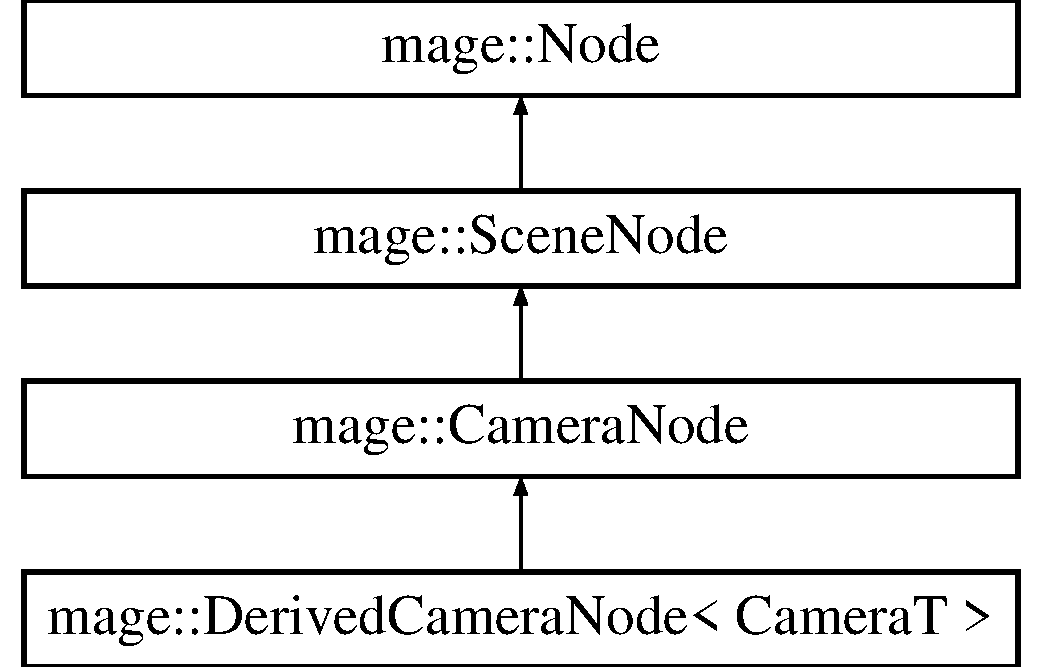
\includegraphics[height=4.000000cm]{classmage_1_1_derived_camera_node}
\end{center}
\end{figure}
\subsection*{Public Member Functions}
\begin{DoxyCompactItemize}
\item 
{\footnotesize template$<$typename... Constructor\+ArgsT$>$ }\\\hyperlink{classmage_1_1_derived_camera_node_a782a23d04ba78be88b0f73d9dde4552f}{Derived\+Camera\+Node} (const string \&name, Constructor\+ArgsT \&\&... args)
\item 
\hyperlink{classmage_1_1_derived_camera_node_a629ba0e2c1e6b29e6d45996256c59dbe}{Derived\+Camera\+Node} (const string \&name, \hyperlink{namespacemage_a3316d7143a973e37adf1110f2e80ca31}{Unique\+Ptr}$<$ CameraT $>$ \&\&camera)
\item 
\hyperlink{classmage_1_1_derived_camera_node_ae97b2a006e9e465e2530fdb814e855da}{Derived\+Camera\+Node} (const \hyperlink{classmage_1_1_derived_camera_node}{Derived\+Camera\+Node} \&camera\+\_\+node)
\item 
\hyperlink{classmage_1_1_derived_camera_node_a4c53aa526ee4f81a8d9cf8439650d291}{Derived\+Camera\+Node} (\hyperlink{classmage_1_1_derived_camera_node}{Derived\+Camera\+Node} \&\&camera\+\_\+node)
\item 
virtual \hyperlink{classmage_1_1_derived_camera_node_a74ab678b593c43b6bf95bb7fbfbd4d2d}{$\sim$\+Derived\+Camera\+Node} ()
\item 
\hyperlink{classmage_1_1_derived_camera_node}{Derived\+Camera\+Node} \& \hyperlink{classmage_1_1_derived_camera_node_a827c7952e061c6e12e38fff12585b3b3}{operator=} (const \hyperlink{classmage_1_1_derived_camera_node}{Derived\+Camera\+Node} \&camera\+\_\+node)=delete
\item 
\hyperlink{classmage_1_1_derived_camera_node}{Derived\+Camera\+Node} \& \hyperlink{classmage_1_1_derived_camera_node_a5faeff6f71a85b46d18f5b55e8dcf756}{operator=} (\hyperlink{classmage_1_1_derived_camera_node}{Derived\+Camera\+Node} \&\&camera\+\_\+node)=delete
\item 
\hyperlink{namespacemage_a3316d7143a973e37adf1110f2e80ca31}{Unique\+Ptr}$<$ \hyperlink{classmage_1_1_derived_camera_node}{Derived\+Camera\+Node} $>$ \hyperlink{classmage_1_1_derived_camera_node_a29e597fe2c9e0f37eeab8fec5330d764}{Clone} () const
\item 
CameraT $\ast$ \hyperlink{classmage_1_1_derived_camera_node_a423d9e416aec8ade92d0d2211d40de39}{Get\+Camera} () noexcept
\item 
const CameraT $\ast$ \hyperlink{classmage_1_1_derived_camera_node_aef2db8d343aeebc95c433150e234481a}{Get\+Camera} () const noexcept
\end{DoxyCompactItemize}
\subsection*{Private Member Functions}
\begin{DoxyCompactItemize}
\item 
virtual \hyperlink{namespacemage_a3316d7143a973e37adf1110f2e80ca31}{Unique\+Ptr}$<$ \hyperlink{classmage_1_1_node}{Node} $>$ \hyperlink{classmage_1_1_derived_camera_node_aa965751029ebd6b41d3805b499a8304e}{Clone\+Implementation} () const override
\end{DoxyCompactItemize}
\subsection*{Additional Inherited Members}


\subsection{Detailed Description}
\subsubsection*{template$<$typename CameraT$>$\newline
class mage\+::\+Derived\+Camera\+Node$<$ Camera\+T $>$}

A class of derived camera nodes.


\begin{DoxyTemplParams}{Template Parameters}
{\em CameraT} & The camera type. \\
\hline
\end{DoxyTemplParams}


\subsection{Constructor \& Destructor Documentation}
\hypertarget{classmage_1_1_derived_camera_node_a782a23d04ba78be88b0f73d9dde4552f}{}\label{classmage_1_1_derived_camera_node_a782a23d04ba78be88b0f73d9dde4552f} 
\index{mage\+::\+Derived\+Camera\+Node@{mage\+::\+Derived\+Camera\+Node}!Derived\+Camera\+Node@{Derived\+Camera\+Node}}
\index{Derived\+Camera\+Node@{Derived\+Camera\+Node}!mage\+::\+Derived\+Camera\+Node@{mage\+::\+Derived\+Camera\+Node}}
\subsubsection{\texorpdfstring{Derived\+Camera\+Node()}{DerivedCameraNode()}\hspace{0.1cm}{\footnotesize\ttfamily [1/4]}}
{\footnotesize\ttfamily template$<$typename CameraT $>$ \\
template$<$typename... Constructor\+ArgsT$>$ \\
\hyperlink{classmage_1_1_derived_camera_node}{mage\+::\+Derived\+Camera\+Node}$<$ CameraT $>$\+::\hyperlink{classmage_1_1_derived_camera_node}{Derived\+Camera\+Node} (\begin{DoxyParamCaption}\item[{const string \&}]{name,  }\item[{Constructor\+ArgsT \&\&...}]{args }\end{DoxyParamCaption})\hspace{0.3cm}{\ttfamily [explicit]}}

Constructs a derived camera node.


\begin{DoxyTemplParams}{Template Parameters}
{\em Constructor\+ArgsT} & The constructor argument types of the camera. \\
\hline
\end{DoxyTemplParams}

\begin{DoxyParams}[1]{Parameters}
\mbox{\tt in}  & {\em name} & A reference to the name. \\
\hline
\mbox{\tt in}  & {\em args} & A reference to the constructor arguments for the camera. \\
\hline
\end{DoxyParams}
\hypertarget{classmage_1_1_derived_camera_node_a629ba0e2c1e6b29e6d45996256c59dbe}{}\label{classmage_1_1_derived_camera_node_a629ba0e2c1e6b29e6d45996256c59dbe} 
\index{mage\+::\+Derived\+Camera\+Node@{mage\+::\+Derived\+Camera\+Node}!Derived\+Camera\+Node@{Derived\+Camera\+Node}}
\index{Derived\+Camera\+Node@{Derived\+Camera\+Node}!mage\+::\+Derived\+Camera\+Node@{mage\+::\+Derived\+Camera\+Node}}
\subsubsection{\texorpdfstring{Derived\+Camera\+Node()}{DerivedCameraNode()}\hspace{0.1cm}{\footnotesize\ttfamily [2/4]}}
{\footnotesize\ttfamily template$<$typename CameraT $>$ \\
\hyperlink{classmage_1_1_derived_camera_node}{mage\+::\+Derived\+Camera\+Node}$<$ CameraT $>$\+::\hyperlink{classmage_1_1_derived_camera_node}{Derived\+Camera\+Node} (\begin{DoxyParamCaption}\item[{const string \&}]{name,  }\item[{\hyperlink{namespacemage_a3316d7143a973e37adf1110f2e80ca31}{Unique\+Ptr}$<$ CameraT $>$ \&\&}]{camera }\end{DoxyParamCaption})\hspace{0.3cm}{\ttfamily [explicit]}}

Constructs a derived camera node.

\begin{DoxyPrecond}{Precondition}
{\itshape camera} refers to a non {\ttfamily nullptr}. 
\end{DoxyPrecond}

\begin{DoxyParams}[1]{Parameters}
\mbox{\tt in}  & {\em name} & A reference to the name. \\
\hline
\mbox{\tt in}  & {\em camera} & A reference to the camera to move. \\
\hline
\end{DoxyParams}
\hypertarget{classmage_1_1_derived_camera_node_ae97b2a006e9e465e2530fdb814e855da}{}\label{classmage_1_1_derived_camera_node_ae97b2a006e9e465e2530fdb814e855da} 
\index{mage\+::\+Derived\+Camera\+Node@{mage\+::\+Derived\+Camera\+Node}!Derived\+Camera\+Node@{Derived\+Camera\+Node}}
\index{Derived\+Camera\+Node@{Derived\+Camera\+Node}!mage\+::\+Derived\+Camera\+Node@{mage\+::\+Derived\+Camera\+Node}}
\subsubsection{\texorpdfstring{Derived\+Camera\+Node()}{DerivedCameraNode()}\hspace{0.1cm}{\footnotesize\ttfamily [3/4]}}
{\footnotesize\ttfamily template$<$typename CameraT $>$ \\
\hyperlink{classmage_1_1_derived_camera_node}{mage\+::\+Derived\+Camera\+Node}$<$ CameraT $>$\+::\hyperlink{classmage_1_1_derived_camera_node}{Derived\+Camera\+Node} (\begin{DoxyParamCaption}\item[{const \hyperlink{classmage_1_1_derived_camera_node}{Derived\+Camera\+Node}$<$ CameraT $>$ \&}]{camera\+\_\+node }\end{DoxyParamCaption})}

Constructs a derived camera node from the given derived camera node.


\begin{DoxyParams}[1]{Parameters}
\mbox{\tt in}  & {\em camera\+\_\+node} & A reference to the derived camera node to copy. \\
\hline
\end{DoxyParams}
\hypertarget{classmage_1_1_derived_camera_node_a4c53aa526ee4f81a8d9cf8439650d291}{}\label{classmage_1_1_derived_camera_node_a4c53aa526ee4f81a8d9cf8439650d291} 
\index{mage\+::\+Derived\+Camera\+Node@{mage\+::\+Derived\+Camera\+Node}!Derived\+Camera\+Node@{Derived\+Camera\+Node}}
\index{Derived\+Camera\+Node@{Derived\+Camera\+Node}!mage\+::\+Derived\+Camera\+Node@{mage\+::\+Derived\+Camera\+Node}}
\subsubsection{\texorpdfstring{Derived\+Camera\+Node()}{DerivedCameraNode()}\hspace{0.1cm}{\footnotesize\ttfamily [4/4]}}
{\footnotesize\ttfamily template$<$typename CameraT $>$ \\
\hyperlink{classmage_1_1_derived_camera_node}{mage\+::\+Derived\+Camera\+Node}$<$ CameraT $>$\+::\hyperlink{classmage_1_1_derived_camera_node}{Derived\+Camera\+Node} (\begin{DoxyParamCaption}\item[{\hyperlink{classmage_1_1_derived_camera_node}{Derived\+Camera\+Node}$<$ CameraT $>$ \&\&}]{camera\+\_\+node }\end{DoxyParamCaption})}

Constructs a derived camera node by moving the given derived camera node.


\begin{DoxyParams}[1]{Parameters}
\mbox{\tt in}  & {\em camera\+\_\+node} & A reference to the derived camera node to move. \\
\hline
\end{DoxyParams}
\hypertarget{classmage_1_1_derived_camera_node_a74ab678b593c43b6bf95bb7fbfbd4d2d}{}\label{classmage_1_1_derived_camera_node_a74ab678b593c43b6bf95bb7fbfbd4d2d} 
\index{mage\+::\+Derived\+Camera\+Node@{mage\+::\+Derived\+Camera\+Node}!````~Derived\+Camera\+Node@{$\sim$\+Derived\+Camera\+Node}}
\index{````~Derived\+Camera\+Node@{$\sim$\+Derived\+Camera\+Node}!mage\+::\+Derived\+Camera\+Node@{mage\+::\+Derived\+Camera\+Node}}
\subsubsection{\texorpdfstring{$\sim$\+Derived\+Camera\+Node()}{~DerivedCameraNode()}}
{\footnotesize\ttfamily template$<$typename CameraT $>$ \\
virtual \hyperlink{classmage_1_1_derived_camera_node}{mage\+::\+Derived\+Camera\+Node}$<$ CameraT $>$\+::$\sim$\hyperlink{classmage_1_1_derived_camera_node}{Derived\+Camera\+Node} (\begin{DoxyParamCaption}{ }\end{DoxyParamCaption})\hspace{0.3cm}{\ttfamily [virtual]}}

Destructs this derived camera node. 

\subsection{Member Function Documentation}
\hypertarget{classmage_1_1_derived_camera_node_a29e597fe2c9e0f37eeab8fec5330d764}{}\label{classmage_1_1_derived_camera_node_a29e597fe2c9e0f37eeab8fec5330d764} 
\index{mage\+::\+Derived\+Camera\+Node@{mage\+::\+Derived\+Camera\+Node}!Clone@{Clone}}
\index{Clone@{Clone}!mage\+::\+Derived\+Camera\+Node@{mage\+::\+Derived\+Camera\+Node}}
\subsubsection{\texorpdfstring{Clone()}{Clone()}}
{\footnotesize\ttfamily template$<$typename CameraT $>$ \\
\hyperlink{namespacemage_a3316d7143a973e37adf1110f2e80ca31}{Unique\+Ptr}$<$ \hyperlink{classmage_1_1_derived_camera_node}{Derived\+Camera\+Node} $>$ \hyperlink{classmage_1_1_derived_camera_node}{mage\+::\+Derived\+Camera\+Node}$<$ CameraT $>$\+::Clone (\begin{DoxyParamCaption}{ }\end{DoxyParamCaption}) const}

Clones this derived camera node.

\begin{DoxyReturn}{Returns}
A pointer to the clone of this derived camera node. 
\end{DoxyReturn}
\hypertarget{classmage_1_1_derived_camera_node_aa965751029ebd6b41d3805b499a8304e}{}\label{classmage_1_1_derived_camera_node_aa965751029ebd6b41d3805b499a8304e} 
\index{mage\+::\+Derived\+Camera\+Node@{mage\+::\+Derived\+Camera\+Node}!Clone\+Implementation@{Clone\+Implementation}}
\index{Clone\+Implementation@{Clone\+Implementation}!mage\+::\+Derived\+Camera\+Node@{mage\+::\+Derived\+Camera\+Node}}
\subsubsection{\texorpdfstring{Clone\+Implementation()}{CloneImplementation()}}
{\footnotesize\ttfamily template$<$typename CameraT $>$ \\
virtual \hyperlink{namespacemage_a3316d7143a973e37adf1110f2e80ca31}{Unique\+Ptr}$<$ \hyperlink{classmage_1_1_node}{Node} $>$ \hyperlink{classmage_1_1_derived_camera_node}{mage\+::\+Derived\+Camera\+Node}$<$ CameraT $>$\+::Clone\+Implementation (\begin{DoxyParamCaption}{ }\end{DoxyParamCaption}) const\hspace{0.3cm}{\ttfamily [override]}, {\ttfamily [private]}, {\ttfamily [virtual]}}

Clones this derived camera node.

\begin{DoxyReturn}{Returns}
A pointer to the clone of this derived camera node. 
\end{DoxyReturn}


Implements \hyperlink{classmage_1_1_camera_node_a002d3a2b41cda270a26ca5d8f3a17f55}{mage\+::\+Camera\+Node}.

\hypertarget{classmage_1_1_derived_camera_node_a423d9e416aec8ade92d0d2211d40de39}{}\label{classmage_1_1_derived_camera_node_a423d9e416aec8ade92d0d2211d40de39} 
\index{mage\+::\+Derived\+Camera\+Node@{mage\+::\+Derived\+Camera\+Node}!Get\+Camera@{Get\+Camera}}
\index{Get\+Camera@{Get\+Camera}!mage\+::\+Derived\+Camera\+Node@{mage\+::\+Derived\+Camera\+Node}}
\subsubsection{\texorpdfstring{Get\+Camera()}{GetCamera()}\hspace{0.1cm}{\footnotesize\ttfamily [1/2]}}
{\footnotesize\ttfamily template$<$typename CameraT $>$ \\
CameraT$\ast$ \hyperlink{classmage_1_1_derived_camera_node}{mage\+::\+Derived\+Camera\+Node}$<$ CameraT $>$\+::Get\+Camera (\begin{DoxyParamCaption}{ }\end{DoxyParamCaption})\hspace{0.3cm}{\ttfamily [noexcept]}}

Returns the camera of this derived camera node.

\begin{DoxyReturn}{Returns}
A pointer to the camera of this derived camera node. 
\end{DoxyReturn}
\hypertarget{classmage_1_1_derived_camera_node_aef2db8d343aeebc95c433150e234481a}{}\label{classmage_1_1_derived_camera_node_aef2db8d343aeebc95c433150e234481a} 
\index{mage\+::\+Derived\+Camera\+Node@{mage\+::\+Derived\+Camera\+Node}!Get\+Camera@{Get\+Camera}}
\index{Get\+Camera@{Get\+Camera}!mage\+::\+Derived\+Camera\+Node@{mage\+::\+Derived\+Camera\+Node}}
\subsubsection{\texorpdfstring{Get\+Camera()}{GetCamera()}\hspace{0.1cm}{\footnotesize\ttfamily [2/2]}}
{\footnotesize\ttfamily template$<$typename CameraT $>$ \\
const CameraT$\ast$ \hyperlink{classmage_1_1_derived_camera_node}{mage\+::\+Derived\+Camera\+Node}$<$ CameraT $>$\+::Get\+Camera (\begin{DoxyParamCaption}{ }\end{DoxyParamCaption}) const\hspace{0.3cm}{\ttfamily [noexcept]}}

Returns the camera of this derived camera node.

\begin{DoxyReturn}{Returns}
A pointer to the camera of this derived camera node. 
\end{DoxyReturn}
\hypertarget{classmage_1_1_derived_camera_node_a827c7952e061c6e12e38fff12585b3b3}{}\label{classmage_1_1_derived_camera_node_a827c7952e061c6e12e38fff12585b3b3} 
\index{mage\+::\+Derived\+Camera\+Node@{mage\+::\+Derived\+Camera\+Node}!operator=@{operator=}}
\index{operator=@{operator=}!mage\+::\+Derived\+Camera\+Node@{mage\+::\+Derived\+Camera\+Node}}
\subsubsection{\texorpdfstring{operator=()}{operator=()}\hspace{0.1cm}{\footnotesize\ttfamily [1/2]}}
{\footnotesize\ttfamily template$<$typename CameraT $>$ \\
\hyperlink{classmage_1_1_derived_camera_node}{Derived\+Camera\+Node}\& \hyperlink{classmage_1_1_derived_camera_node}{mage\+::\+Derived\+Camera\+Node}$<$ CameraT $>$\+::operator= (\begin{DoxyParamCaption}\item[{const \hyperlink{classmage_1_1_derived_camera_node}{Derived\+Camera\+Node}$<$ CameraT $>$ \&}]{camera\+\_\+node }\end{DoxyParamCaption})\hspace{0.3cm}{\ttfamily [delete]}}

Copies the given derived camera node to this derived camera node.


\begin{DoxyParams}[1]{Parameters}
\mbox{\tt in}  & {\em camera\+\_\+node} & A reference to the derived camera node to copy. \\
\hline
\end{DoxyParams}
\begin{DoxyReturn}{Returns}
A reference to the copy of the given derived camera node (i.\+e. this derived camera node). 
\end{DoxyReturn}
\hypertarget{classmage_1_1_derived_camera_node_a5faeff6f71a85b46d18f5b55e8dcf756}{}\label{classmage_1_1_derived_camera_node_a5faeff6f71a85b46d18f5b55e8dcf756} 
\index{mage\+::\+Derived\+Camera\+Node@{mage\+::\+Derived\+Camera\+Node}!operator=@{operator=}}
\index{operator=@{operator=}!mage\+::\+Derived\+Camera\+Node@{mage\+::\+Derived\+Camera\+Node}}
\subsubsection{\texorpdfstring{operator=()}{operator=()}\hspace{0.1cm}{\footnotesize\ttfamily [2/2]}}
{\footnotesize\ttfamily template$<$typename CameraT $>$ \\
\hyperlink{classmage_1_1_derived_camera_node}{Derived\+Camera\+Node}\& \hyperlink{classmage_1_1_derived_camera_node}{mage\+::\+Derived\+Camera\+Node}$<$ CameraT $>$\+::operator= (\begin{DoxyParamCaption}\item[{\hyperlink{classmage_1_1_derived_camera_node}{Derived\+Camera\+Node}$<$ CameraT $>$ \&\&}]{camera\+\_\+node }\end{DoxyParamCaption})\hspace{0.3cm}{\ttfamily [delete]}}

Moves the given derived camera node to this derived camera node.


\begin{DoxyParams}[1]{Parameters}
\mbox{\tt in}  & {\em camera\+\_\+node} & A reference to the derived camera node to move. \\
\hline
\end{DoxyParams}
\begin{DoxyReturn}{Returns}
A reference to the moved derived camera node (i.\+e. this derived camera node). 
\end{DoxyReturn}

\hypertarget{classmage_1_1_derived_light_node}{}\section{mage\+:\+:Derived\+Light\+Node$<$ LightT $>$ Class Template Reference}
\label{classmage_1_1_derived_light_node}\index{mage\+::\+Derived\+Light\+Node$<$ Light\+T $>$@{mage\+::\+Derived\+Light\+Node$<$ Light\+T $>$}}


{\ttfamily \#include $<$light\+\_\+node.\+hpp$>$}

Inheritance diagram for mage\+:\+:Derived\+Light\+Node$<$ LightT $>$\+:\begin{figure}[H]
\begin{center}
\leavevmode
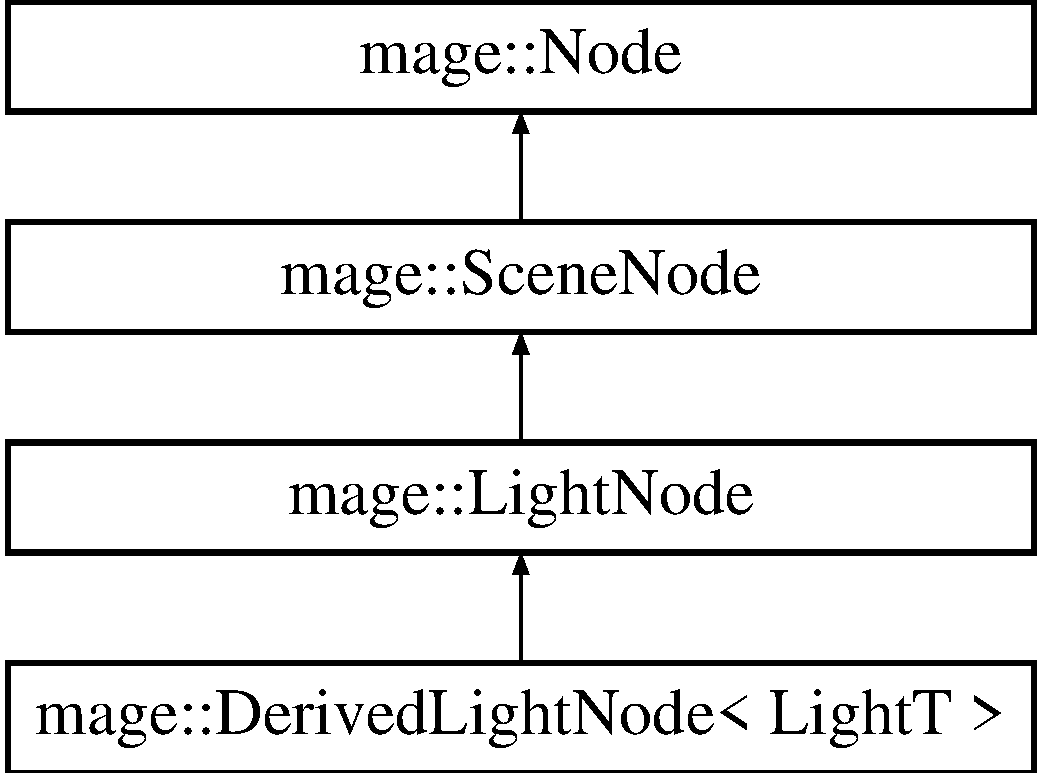
\includegraphics[height=4.000000cm]{classmage_1_1_derived_light_node}
\end{center}
\end{figure}
\subsection*{Public Member Functions}
\begin{DoxyCompactItemize}
\item 
{\footnotesize template$<$typename... Constructor\+ArgsT$>$ }\\\hyperlink{classmage_1_1_derived_light_node_a64003a60d92c245c8ad247bb16724852}{Derived\+Light\+Node} (const string \&name, Constructor\+ArgsT \&\&... args)
\item 
\hyperlink{classmage_1_1_derived_light_node_ab3e68ce3299581459843e8ad12f18464}{Derived\+Light\+Node} (const string \&name, \hyperlink{namespacemage_a8c307fbcc33bce9b7f2aa4c26c3b95cf}{Unique\+Ptr}$<$ LightT $>$ \&\&light)
\item 
\hyperlink{classmage_1_1_derived_light_node_a719b8fe088b93a7ecfb6d21b99cc170b}{Derived\+Light\+Node} (const \hyperlink{classmage_1_1_derived_light_node}{Derived\+Light\+Node} \&light\+\_\+node)
\item 
\hyperlink{classmage_1_1_derived_light_node_af99017273f3f8bedcbd3842c31e4ecc4}{Derived\+Light\+Node} (\hyperlink{classmage_1_1_derived_light_node}{Derived\+Light\+Node} \&\&light\+\_\+node)
\item 
virtual \hyperlink{classmage_1_1_derived_light_node_ad4b2371e323d30eda05744237d4dc4eb}{$\sim$\+Derived\+Light\+Node} ()
\item 
\hyperlink{classmage_1_1_derived_light_node}{Derived\+Light\+Node} \& \hyperlink{classmage_1_1_derived_light_node_ad4a81ae2a671d6c278c74dead4660949}{operator=} (const \hyperlink{classmage_1_1_derived_light_node}{Derived\+Light\+Node} \&light\+\_\+node)=delete
\item 
\hyperlink{classmage_1_1_derived_light_node}{Derived\+Light\+Node} \& \hyperlink{classmage_1_1_derived_light_node_a7eabbc97578958f97a7ec11728364eec}{operator=} (\hyperlink{classmage_1_1_derived_light_node}{Derived\+Light\+Node} \&\&light\+\_\+node)=delete
\item 
\hyperlink{namespacemage_a8c307fbcc33bce9b7f2aa4c26c3b95cf}{Unique\+Ptr}$<$ \hyperlink{classmage_1_1_derived_light_node}{Derived\+Light\+Node} $>$ \hyperlink{classmage_1_1_derived_light_node_a38fcbc8d5204f92d0dfd87c1c6d10281}{Clone} () const
\item 
LightT $\ast$ \hyperlink{classmage_1_1_derived_light_node_a1f45fa421b75d663a360bfdd518a1a1d}{Get\+Light} () noexcept
\item 
const LightT $\ast$ \hyperlink{classmage_1_1_derived_light_node_a61ace20169a3924d42abc163ebddc19b}{Get\+Light} () const noexcept
\end{DoxyCompactItemize}
\subsection*{Private Member Functions}
\begin{DoxyCompactItemize}
\item 
virtual \hyperlink{namespacemage_a8c307fbcc33bce9b7f2aa4c26c3b95cf}{Unique\+Ptr}$<$ \hyperlink{classmage_1_1_node}{Node} $>$ \hyperlink{classmage_1_1_derived_light_node_acf8858989780bf45a45c55a7c5564314}{Clone\+Implementation} () const override
\end{DoxyCompactItemize}
\subsection*{Additional Inherited Members}


\subsection{Detailed Description}
\subsubsection*{template$<$typename LightT$>$\newline
class mage\+::\+Derived\+Light\+Node$<$ Light\+T $>$}

A class of derived light nodes.


\begin{DoxyTemplParams}{Template Parameters}
{\em LightT} & The light type. \\
\hline
\end{DoxyTemplParams}


\subsection{Constructor \& Destructor Documentation}
\hypertarget{classmage_1_1_derived_light_node_a64003a60d92c245c8ad247bb16724852}{}\label{classmage_1_1_derived_light_node_a64003a60d92c245c8ad247bb16724852} 
\index{mage\+::\+Derived\+Light\+Node@{mage\+::\+Derived\+Light\+Node}!Derived\+Light\+Node@{Derived\+Light\+Node}}
\index{Derived\+Light\+Node@{Derived\+Light\+Node}!mage\+::\+Derived\+Light\+Node@{mage\+::\+Derived\+Light\+Node}}
\subsubsection{\texorpdfstring{Derived\+Light\+Node()}{DerivedLightNode()}\hspace{0.1cm}{\footnotesize\ttfamily [1/4]}}
{\footnotesize\ttfamily template$<$typename LightT $>$ \\
template$<$typename... Constructor\+ArgsT$>$ \\
\hyperlink{classmage_1_1_derived_light_node}{mage\+::\+Derived\+Light\+Node}$<$ LightT $>$\+::\hyperlink{classmage_1_1_derived_light_node}{Derived\+Light\+Node} (\begin{DoxyParamCaption}\item[{const string \&}]{name,  }\item[{Constructor\+ArgsT \&\&...}]{args }\end{DoxyParamCaption})\hspace{0.3cm}{\ttfamily [explicit]}}

Constructs a derived light node.


\begin{DoxyTemplParams}{Template Parameters}
{\em Constructor\+ArgsT} & The constructor argument types of the light. \\
\hline
\end{DoxyTemplParams}

\begin{DoxyParams}[1]{Parameters}
\mbox{\tt in}  & {\em name} & A reference to the name. \\
\hline
\mbox{\tt in}  & {\em args} & A reference to the constructor arguments for the light. \\
\hline
\end{DoxyParams}
\hypertarget{classmage_1_1_derived_light_node_ab3e68ce3299581459843e8ad12f18464}{}\label{classmage_1_1_derived_light_node_ab3e68ce3299581459843e8ad12f18464} 
\index{mage\+::\+Derived\+Light\+Node@{mage\+::\+Derived\+Light\+Node}!Derived\+Light\+Node@{Derived\+Light\+Node}}
\index{Derived\+Light\+Node@{Derived\+Light\+Node}!mage\+::\+Derived\+Light\+Node@{mage\+::\+Derived\+Light\+Node}}
\subsubsection{\texorpdfstring{Derived\+Light\+Node()}{DerivedLightNode()}\hspace{0.1cm}{\footnotesize\ttfamily [2/4]}}
{\footnotesize\ttfamily template$<$typename LightT $>$ \\
\hyperlink{classmage_1_1_derived_light_node}{mage\+::\+Derived\+Light\+Node}$<$ LightT $>$\+::\hyperlink{classmage_1_1_derived_light_node}{Derived\+Light\+Node} (\begin{DoxyParamCaption}\item[{const string \&}]{name,  }\item[{\hyperlink{namespacemage_a8c307fbcc33bce9b7f2aa4c26c3b95cf}{Unique\+Ptr}$<$ LightT $>$ \&\&}]{light }\end{DoxyParamCaption})\hspace{0.3cm}{\ttfamily [explicit]}}

Constructs a derived light node.


\begin{DoxyParams}[1]{Parameters}
\mbox{\tt in}  & {\em name} & A reference to the name. \\
\hline
\mbox{\tt in}  & {\em light} & A reference to the light to move. \\
\hline
\end{DoxyParams}
\hypertarget{classmage_1_1_derived_light_node_a719b8fe088b93a7ecfb6d21b99cc170b}{}\label{classmage_1_1_derived_light_node_a719b8fe088b93a7ecfb6d21b99cc170b} 
\index{mage\+::\+Derived\+Light\+Node@{mage\+::\+Derived\+Light\+Node}!Derived\+Light\+Node@{Derived\+Light\+Node}}
\index{Derived\+Light\+Node@{Derived\+Light\+Node}!mage\+::\+Derived\+Light\+Node@{mage\+::\+Derived\+Light\+Node}}
\subsubsection{\texorpdfstring{Derived\+Light\+Node()}{DerivedLightNode()}\hspace{0.1cm}{\footnotesize\ttfamily [3/4]}}
{\footnotesize\ttfamily template$<$typename LightT $>$ \\
\hyperlink{classmage_1_1_derived_light_node}{mage\+::\+Derived\+Light\+Node}$<$ LightT $>$\+::\hyperlink{classmage_1_1_derived_light_node}{Derived\+Light\+Node} (\begin{DoxyParamCaption}\item[{const \hyperlink{classmage_1_1_derived_light_node}{Derived\+Light\+Node}$<$ LightT $>$ \&}]{light\+\_\+node }\end{DoxyParamCaption})}

Constructs a derived light node from the given derived light node.


\begin{DoxyParams}[1]{Parameters}
\mbox{\tt in}  & {\em light\+\_\+node} & A reference to the derived light node to copy. \\
\hline
\end{DoxyParams}
\hypertarget{classmage_1_1_derived_light_node_af99017273f3f8bedcbd3842c31e4ecc4}{}\label{classmage_1_1_derived_light_node_af99017273f3f8bedcbd3842c31e4ecc4} 
\index{mage\+::\+Derived\+Light\+Node@{mage\+::\+Derived\+Light\+Node}!Derived\+Light\+Node@{Derived\+Light\+Node}}
\index{Derived\+Light\+Node@{Derived\+Light\+Node}!mage\+::\+Derived\+Light\+Node@{mage\+::\+Derived\+Light\+Node}}
\subsubsection{\texorpdfstring{Derived\+Light\+Node()}{DerivedLightNode()}\hspace{0.1cm}{\footnotesize\ttfamily [4/4]}}
{\footnotesize\ttfamily template$<$typename LightT $>$ \\
\hyperlink{classmage_1_1_derived_light_node}{mage\+::\+Derived\+Light\+Node}$<$ LightT $>$\+::\hyperlink{classmage_1_1_derived_light_node}{Derived\+Light\+Node} (\begin{DoxyParamCaption}\item[{\hyperlink{classmage_1_1_derived_light_node}{Derived\+Light\+Node}$<$ LightT $>$ \&\&}]{light\+\_\+node }\end{DoxyParamCaption})}

Constructs a derived light node by moving the given derived light node.


\begin{DoxyParams}[1]{Parameters}
\mbox{\tt in}  & {\em light\+\_\+node} & A reference to the derived light node to move. \\
\hline
\end{DoxyParams}
\hypertarget{classmage_1_1_derived_light_node_ad4b2371e323d30eda05744237d4dc4eb}{}\label{classmage_1_1_derived_light_node_ad4b2371e323d30eda05744237d4dc4eb} 
\index{mage\+::\+Derived\+Light\+Node@{mage\+::\+Derived\+Light\+Node}!````~Derived\+Light\+Node@{$\sim$\+Derived\+Light\+Node}}
\index{````~Derived\+Light\+Node@{$\sim$\+Derived\+Light\+Node}!mage\+::\+Derived\+Light\+Node@{mage\+::\+Derived\+Light\+Node}}
\subsubsection{\texorpdfstring{$\sim$\+Derived\+Light\+Node()}{~DerivedLightNode()}}
{\footnotesize\ttfamily template$<$typename LightT $>$ \\
virtual \hyperlink{classmage_1_1_derived_light_node}{mage\+::\+Derived\+Light\+Node}$<$ LightT $>$\+::$\sim$\hyperlink{classmage_1_1_derived_light_node}{Derived\+Light\+Node} (\begin{DoxyParamCaption}{ }\end{DoxyParamCaption})\hspace{0.3cm}{\ttfamily [virtual]}}

Destructs this derived light node. 

\subsection{Member Function Documentation}
\hypertarget{classmage_1_1_derived_light_node_a38fcbc8d5204f92d0dfd87c1c6d10281}{}\label{classmage_1_1_derived_light_node_a38fcbc8d5204f92d0dfd87c1c6d10281} 
\index{mage\+::\+Derived\+Light\+Node@{mage\+::\+Derived\+Light\+Node}!Clone@{Clone}}
\index{Clone@{Clone}!mage\+::\+Derived\+Light\+Node@{mage\+::\+Derived\+Light\+Node}}
\subsubsection{\texorpdfstring{Clone()}{Clone()}}
{\footnotesize\ttfamily template$<$typename LightT $>$ \\
\hyperlink{namespacemage_a8c307fbcc33bce9b7f2aa4c26c3b95cf}{Unique\+Ptr}$<$ \hyperlink{classmage_1_1_derived_light_node}{Derived\+Light\+Node} $>$ \hyperlink{classmage_1_1_derived_light_node}{mage\+::\+Derived\+Light\+Node}$<$ LightT $>$\+::Clone (\begin{DoxyParamCaption}{ }\end{DoxyParamCaption}) const}

Clones this derived light node.

\begin{DoxyReturn}{Returns}
A pointer to the clone of this derived light node. 
\end{DoxyReturn}
\hypertarget{classmage_1_1_derived_light_node_acf8858989780bf45a45c55a7c5564314}{}\label{classmage_1_1_derived_light_node_acf8858989780bf45a45c55a7c5564314} 
\index{mage\+::\+Derived\+Light\+Node@{mage\+::\+Derived\+Light\+Node}!Clone\+Implementation@{Clone\+Implementation}}
\index{Clone\+Implementation@{Clone\+Implementation}!mage\+::\+Derived\+Light\+Node@{mage\+::\+Derived\+Light\+Node}}
\subsubsection{\texorpdfstring{Clone\+Implementation()}{CloneImplementation()}}
{\footnotesize\ttfamily template$<$typename LightT $>$ \\
virtual \hyperlink{namespacemage_a8c307fbcc33bce9b7f2aa4c26c3b95cf}{Unique\+Ptr}$<$ \hyperlink{classmage_1_1_node}{Node} $>$ \hyperlink{classmage_1_1_derived_light_node}{mage\+::\+Derived\+Light\+Node}$<$ LightT $>$\+::Clone\+Implementation (\begin{DoxyParamCaption}{ }\end{DoxyParamCaption}) const\hspace{0.3cm}{\ttfamily [override]}, {\ttfamily [private]}, {\ttfamily [virtual]}}

Clones this derived light node.

\begin{DoxyReturn}{Returns}
A pointer to the clone of this derived light node. 
\end{DoxyReturn}


Implements \hyperlink{classmage_1_1_light_node_aea97601d0a4b8073a1c655ca334af242}{mage\+::\+Light\+Node}.

\hypertarget{classmage_1_1_derived_light_node_a1f45fa421b75d663a360bfdd518a1a1d}{}\label{classmage_1_1_derived_light_node_a1f45fa421b75d663a360bfdd518a1a1d} 
\index{mage\+::\+Derived\+Light\+Node@{mage\+::\+Derived\+Light\+Node}!Get\+Light@{Get\+Light}}
\index{Get\+Light@{Get\+Light}!mage\+::\+Derived\+Light\+Node@{mage\+::\+Derived\+Light\+Node}}
\subsubsection{\texorpdfstring{Get\+Light()}{GetLight()}\hspace{0.1cm}{\footnotesize\ttfamily [1/2]}}
{\footnotesize\ttfamily template$<$typename LightT $>$ \\
LightT$\ast$ \hyperlink{classmage_1_1_derived_light_node}{mage\+::\+Derived\+Light\+Node}$<$ LightT $>$\+::Get\+Light (\begin{DoxyParamCaption}{ }\end{DoxyParamCaption})\hspace{0.3cm}{\ttfamily [noexcept]}}

Returns the light of this derived light node.

\begin{DoxyReturn}{Returns}
A pointer to the light of this derived light node. 
\end{DoxyReturn}
\hypertarget{classmage_1_1_derived_light_node_a61ace20169a3924d42abc163ebddc19b}{}\label{classmage_1_1_derived_light_node_a61ace20169a3924d42abc163ebddc19b} 
\index{mage\+::\+Derived\+Light\+Node@{mage\+::\+Derived\+Light\+Node}!Get\+Light@{Get\+Light}}
\index{Get\+Light@{Get\+Light}!mage\+::\+Derived\+Light\+Node@{mage\+::\+Derived\+Light\+Node}}
\subsubsection{\texorpdfstring{Get\+Light()}{GetLight()}\hspace{0.1cm}{\footnotesize\ttfamily [2/2]}}
{\footnotesize\ttfamily template$<$typename LightT $>$ \\
const LightT$\ast$ \hyperlink{classmage_1_1_derived_light_node}{mage\+::\+Derived\+Light\+Node}$<$ LightT $>$\+::Get\+Light (\begin{DoxyParamCaption}{ }\end{DoxyParamCaption}) const\hspace{0.3cm}{\ttfamily [noexcept]}}

Returns the light of this derived light node.

\begin{DoxyReturn}{Returns}
A pointer to the light of this derived light node. 
\end{DoxyReturn}
\hypertarget{classmage_1_1_derived_light_node_ad4a81ae2a671d6c278c74dead4660949}{}\label{classmage_1_1_derived_light_node_ad4a81ae2a671d6c278c74dead4660949} 
\index{mage\+::\+Derived\+Light\+Node@{mage\+::\+Derived\+Light\+Node}!operator=@{operator=}}
\index{operator=@{operator=}!mage\+::\+Derived\+Light\+Node@{mage\+::\+Derived\+Light\+Node}}
\subsubsection{\texorpdfstring{operator=()}{operator=()}\hspace{0.1cm}{\footnotesize\ttfamily [1/2]}}
{\footnotesize\ttfamily template$<$typename LightT $>$ \\
\hyperlink{classmage_1_1_derived_light_node}{Derived\+Light\+Node}\& \hyperlink{classmage_1_1_derived_light_node}{mage\+::\+Derived\+Light\+Node}$<$ LightT $>$\+::operator= (\begin{DoxyParamCaption}\item[{const \hyperlink{classmage_1_1_derived_light_node}{Derived\+Light\+Node}$<$ LightT $>$ \&}]{light\+\_\+node }\end{DoxyParamCaption})\hspace{0.3cm}{\ttfamily [delete]}}

Copies the given derived light node to this derived light node.


\begin{DoxyParams}[1]{Parameters}
\mbox{\tt in}  & {\em light\+\_\+node} & A reference to the derived light node to copy. \\
\hline
\end{DoxyParams}
\begin{DoxyReturn}{Returns}
A reference to the copy of the given derived light node (i.\+e. this derived light node). 
\end{DoxyReturn}
\hypertarget{classmage_1_1_derived_light_node_a7eabbc97578958f97a7ec11728364eec}{}\label{classmage_1_1_derived_light_node_a7eabbc97578958f97a7ec11728364eec} 
\index{mage\+::\+Derived\+Light\+Node@{mage\+::\+Derived\+Light\+Node}!operator=@{operator=}}
\index{operator=@{operator=}!mage\+::\+Derived\+Light\+Node@{mage\+::\+Derived\+Light\+Node}}
\subsubsection{\texorpdfstring{operator=()}{operator=()}\hspace{0.1cm}{\footnotesize\ttfamily [2/2]}}
{\footnotesize\ttfamily template$<$typename LightT $>$ \\
\hyperlink{classmage_1_1_derived_light_node}{Derived\+Light\+Node}\& \hyperlink{classmage_1_1_derived_light_node}{mage\+::\+Derived\+Light\+Node}$<$ LightT $>$\+::operator= (\begin{DoxyParamCaption}\item[{\hyperlink{classmage_1_1_derived_light_node}{Derived\+Light\+Node}$<$ LightT $>$ \&\&}]{light\+\_\+node }\end{DoxyParamCaption})\hspace{0.3cm}{\ttfamily [delete]}}

Moves the given derived light node to this derived light node.


\begin{DoxyParams}[1]{Parameters}
\mbox{\tt in}  & {\em light\+\_\+node} & A reference to the derived light node to move. \\
\hline
\end{DoxyParams}
\begin{DoxyReturn}{Returns}
A reference to the moved derived light node (i.\+e. this derived light node). 
\end{DoxyReturn}

\hypertarget{classmage_1_1_device_enumeration}{}\section{mage\+:\+:Device\+Enumeration Class Reference}
\label{classmage_1_1_device_enumeration}\index{mage\+::\+Device\+Enumeration@{mage\+::\+Device\+Enumeration}}


{\ttfamily \#include $<$device\+\_\+enumeration.\+hpp$>$}

\subsection*{Public Member Functions}
\begin{DoxyCompactItemize}
\item 
\hyperlink{namespacemage_ae74f374780900893caa5555d1031fd79}{Com\+Ptr}$<$ I\+D\+X\+G\+I\+Adapter2 $>$ \hyperlink{classmage_1_1_device_enumeration_ad8a0702abdc70ea8fc1b6e46544839a1}{Get\+Adapter} () const
\item 
\hyperlink{namespacemage_ae74f374780900893caa5555d1031fd79}{Com\+Ptr}$<$ I\+D\+X\+G\+I\+Output2 $>$ \hyperlink{classmage_1_1_device_enumeration_ac3958dd53d2fdb8ff645d8dca6dc5fdd}{Get\+Output} () const
\item 
const D\+X\+G\+I\+\_\+\+M\+O\+D\+E\+\_\+\+D\+E\+S\+C1 $\ast$ \hyperlink{classmage_1_1_device_enumeration_a533ac2f6ea91604a3ea3cc8d93c3de87}{Get\+Display\+Mode} () const
\item 
bool \hyperlink{classmage_1_1_device_enumeration_a51479c8c85b286f78730c5622604e524}{Is\+Windowed} () const
\item 
bool \hyperlink{classmage_1_1_device_enumeration_a8957ecacc567708e80694b25aa141c4e}{Is\+Full\+Screen} () const
\item 
bool \hyperlink{classmage_1_1_device_enumeration_a035e2430142e4e4ffcbc712f83e1e7e0}{Is\+V\+Synced} () const
\end{DoxyCompactItemize}
\subsection*{Private Member Functions}
\begin{DoxyCompactItemize}
\item 
\hyperlink{classmage_1_1_device_enumeration_aa000048648beb6c2aca70e5ef04e0da2}{Device\+Enumeration} ()
\item 
\hyperlink{classmage_1_1_device_enumeration_ae32bc5dacf47b7deca4729d8b3cb66dc}{$\sim$\+Device\+Enumeration} ()=default
\item 
\hyperlink{classmage_1_1_device_enumeration_a90f3dc13cfb413aa8a2a49a31bcb6ae3}{Device\+Enumeration} (const \hyperlink{classmage_1_1_device_enumeration}{Device\+Enumeration} \&device\+\_\+enumeration)=delete
\item 
\hyperlink{classmage_1_1_device_enumeration_a2f139e0a31c941d8dd5a0e1ecabe1ab9}{Device\+Enumeration} (\hyperlink{classmage_1_1_device_enumeration}{Device\+Enumeration} \&\&device\+\_\+enumeration)=delete
\item 
\hyperlink{classmage_1_1_device_enumeration}{Device\+Enumeration} \& \hyperlink{classmage_1_1_device_enumeration_a03e3affa2b8bb4837cffda7b11389bea}{operator=} (const \hyperlink{classmage_1_1_device_enumeration}{Device\+Enumeration} \&device\+\_\+enumeration)=delete
\item 
\hyperlink{classmage_1_1_device_enumeration}{Device\+Enumeration} \& \hyperlink{classmage_1_1_device_enumeration_accf36804bfe510cc8a4d8495854596d6}{operator=} (\hyperlink{classmage_1_1_device_enumeration}{Device\+Enumeration} \&\&device\+\_\+enumeration)=delete
\item 
H\+R\+E\+S\+U\+LT \hyperlink{classmage_1_1_device_enumeration_a56806d9667b446bf14236b1f42aefb28}{Initialize\+Adapter\+And\+Output} ()
\item 
H\+R\+E\+S\+U\+LT \hyperlink{classmage_1_1_device_enumeration_ac4644c68492b919362e21f2e47fbad93}{Initialize\+Display\+Modes} ()
\item 
H\+R\+E\+S\+U\+LT \hyperlink{classmage_1_1_device_enumeration_a4fea0ffef733632456b281f74608a239}{Enumerate} ()
\item 
I\+N\+T\+\_\+\+P\+TR \hyperlink{classmage_1_1_device_enumeration_a5950a6575d9073d6d23b228779f5ace1}{Settings\+Dialog\+Proc} (H\+W\+ND hwnd\+Dlg, U\+I\+NT u\+Msg, W\+P\+A\+R\+AM w\+Param, L\+P\+A\+R\+AM l\+Param)
\end{DoxyCompactItemize}
\subsection*{Private Attributes}
\begin{DoxyCompactItemize}
\item 
\hyperlink{namespacemage_ae74f374780900893caa5555d1031fd79}{Com\+Ptr}$<$ I\+D\+X\+G\+I\+Adapter2 $>$ \hyperlink{classmage_1_1_device_enumeration_af53e43c5c1d67421831993a5fdc6014a}{m\+\_\+adapter}
\item 
\hyperlink{namespacemage_ae74f374780900893caa5555d1031fd79}{Com\+Ptr}$<$ I\+D\+X\+G\+I\+Output2 $>$ \hyperlink{classmage_1_1_device_enumeration_a49580b67748053ed6172d6458b5083ca}{m\+\_\+output}
\item 
\hyperlink{namespacemage_a8c307fbcc33bce9b7f2aa4c26c3b95cf}{Unique\+Ptr}$<$ \hyperlink{classmage_1_1_variable_script}{Variable\+Script} $>$ \hyperlink{classmage_1_1_device_enumeration_ab6a58580daf27bff07ba7df428833616}{m\+\_\+settings\+\_\+script}
\item 
list$<$ D\+X\+G\+I\+\_\+\+M\+O\+D\+E\+\_\+\+D\+E\+S\+C1 $>$ \hyperlink{classmage_1_1_device_enumeration_aae356ac476a35ce4074f61cfd75ecdbe}{m\+\_\+display\+\_\+modes}
\item 
const D\+X\+G\+I\+\_\+\+M\+O\+D\+E\+\_\+\+D\+E\+S\+C1 $\ast$ \hyperlink{classmage_1_1_device_enumeration_a74b32839bda6446db56aaf4b6dd25f20}{m\+\_\+selected\+\_\+diplay\+\_\+mode}
\item 
bool \hyperlink{classmage_1_1_device_enumeration_a277c5dae7861c9cb1175192a61274cc9}{m\+\_\+windowed}
\item 
bool \hyperlink{classmage_1_1_device_enumeration_a027220f50649c40785e2b918411adfad}{m\+\_\+vsync}
\end{DoxyCompactItemize}
\subsection*{Friends}
\begin{DoxyCompactItemize}
\item 
class \hyperlink{classmage_1_1_device_enumeration_a3e1914489e4bed4f9f23cdeab34a43dc}{Engine}
\item 
I\+N\+T\+\_\+\+P\+TR C\+A\+L\+L\+B\+A\+CK \hyperlink{classmage_1_1_device_enumeration_a3dff4eb8907e2e10f26cc616fe1c104d}{Settings\+Dialog\+Proc\+Delegate} (H\+W\+ND hwnd\+Dlg, U\+I\+NT u\+Msg, W\+P\+A\+R\+AM w\+Param, L\+P\+A\+R\+AM l\+Param)
\end{DoxyCompactItemize}


\subsection{Detailed Description}
A device enumeration. 

\subsection{Constructor \& Destructor Documentation}
\hypertarget{classmage_1_1_device_enumeration_aa000048648beb6c2aca70e5ef04e0da2}{}\label{classmage_1_1_device_enumeration_aa000048648beb6c2aca70e5ef04e0da2} 
\index{mage\+::\+Device\+Enumeration@{mage\+::\+Device\+Enumeration}!Device\+Enumeration@{Device\+Enumeration}}
\index{Device\+Enumeration@{Device\+Enumeration}!mage\+::\+Device\+Enumeration@{mage\+::\+Device\+Enumeration}}
\subsubsection{\texorpdfstring{Device\+Enumeration()}{DeviceEnumeration()}\hspace{0.1cm}{\footnotesize\ttfamily [1/3]}}
{\footnotesize\ttfamily mage\+::\+Device\+Enumeration\+::\+Device\+Enumeration (\begin{DoxyParamCaption}{ }\end{DoxyParamCaption})\hspace{0.3cm}{\ttfamily [private]}}

Constructs a device enumeration. \hypertarget{classmage_1_1_device_enumeration_ae32bc5dacf47b7deca4729d8b3cb66dc}{}\label{classmage_1_1_device_enumeration_ae32bc5dacf47b7deca4729d8b3cb66dc} 
\index{mage\+::\+Device\+Enumeration@{mage\+::\+Device\+Enumeration}!````~Device\+Enumeration@{$\sim$\+Device\+Enumeration}}
\index{````~Device\+Enumeration@{$\sim$\+Device\+Enumeration}!mage\+::\+Device\+Enumeration@{mage\+::\+Device\+Enumeration}}
\subsubsection{\texorpdfstring{$\sim$\+Device\+Enumeration()}{~DeviceEnumeration()}}
{\footnotesize\ttfamily mage\+::\+Device\+Enumeration\+::$\sim$\+Device\+Enumeration (\begin{DoxyParamCaption}{ }\end{DoxyParamCaption})\hspace{0.3cm}{\ttfamily [private]}, {\ttfamily [default]}}

Destructs this device enumeration. \hypertarget{classmage_1_1_device_enumeration_a90f3dc13cfb413aa8a2a49a31bcb6ae3}{}\label{classmage_1_1_device_enumeration_a90f3dc13cfb413aa8a2a49a31bcb6ae3} 
\index{mage\+::\+Device\+Enumeration@{mage\+::\+Device\+Enumeration}!Device\+Enumeration@{Device\+Enumeration}}
\index{Device\+Enumeration@{Device\+Enumeration}!mage\+::\+Device\+Enumeration@{mage\+::\+Device\+Enumeration}}
\subsubsection{\texorpdfstring{Device\+Enumeration()}{DeviceEnumeration()}\hspace{0.1cm}{\footnotesize\ttfamily [2/3]}}
{\footnotesize\ttfamily mage\+::\+Device\+Enumeration\+::\+Device\+Enumeration (\begin{DoxyParamCaption}\item[{const \hyperlink{classmage_1_1_device_enumeration}{Device\+Enumeration} \&}]{device\+\_\+enumeration }\end{DoxyParamCaption})\hspace{0.3cm}{\ttfamily [private]}, {\ttfamily [delete]}}

Constructs a device enumeration from the given device enumeration.


\begin{DoxyParams}[1]{Parameters}
\mbox{\tt in}  & {\em device\+\_\+enumeration} & A reference to a device enumeration. \\
\hline
\end{DoxyParams}
\hypertarget{classmage_1_1_device_enumeration_a2f139e0a31c941d8dd5a0e1ecabe1ab9}{}\label{classmage_1_1_device_enumeration_a2f139e0a31c941d8dd5a0e1ecabe1ab9} 
\index{mage\+::\+Device\+Enumeration@{mage\+::\+Device\+Enumeration}!Device\+Enumeration@{Device\+Enumeration}}
\index{Device\+Enumeration@{Device\+Enumeration}!mage\+::\+Device\+Enumeration@{mage\+::\+Device\+Enumeration}}
\subsubsection{\texorpdfstring{Device\+Enumeration()}{DeviceEnumeration()}\hspace{0.1cm}{\footnotesize\ttfamily [3/3]}}
{\footnotesize\ttfamily mage\+::\+Device\+Enumeration\+::\+Device\+Enumeration (\begin{DoxyParamCaption}\item[{\hyperlink{classmage_1_1_device_enumeration}{Device\+Enumeration} \&\&}]{device\+\_\+enumeration }\end{DoxyParamCaption})\hspace{0.3cm}{\ttfamily [private]}, {\ttfamily [delete]}}

Constructs a device enumeration from the given device enumeration.


\begin{DoxyParams}[1]{Parameters}
\mbox{\tt in}  & {\em device\+\_\+enumeration} & A reference to a device enumeration. \\
\hline
\end{DoxyParams}


\subsection{Member Function Documentation}
\hypertarget{classmage_1_1_device_enumeration_a4fea0ffef733632456b281f74608a239}{}\label{classmage_1_1_device_enumeration_a4fea0ffef733632456b281f74608a239} 
\index{mage\+::\+Device\+Enumeration@{mage\+::\+Device\+Enumeration}!Enumerate@{Enumerate}}
\index{Enumerate@{Enumerate}!mage\+::\+Device\+Enumeration@{mage\+::\+Device\+Enumeration}}
\subsubsection{\texorpdfstring{Enumerate()}{Enumerate()}}
{\footnotesize\ttfamily H\+R\+E\+S\+U\+LT mage\+::\+Device\+Enumeration\+::\+Enumerate (\begin{DoxyParamCaption}{ }\end{DoxyParamCaption})\hspace{0.3cm}{\ttfamily [private]}}

Enumerates the available display modes on the adapter output of the physical adapter with the most dedicated video memory.

\begin{DoxyReturn}{Returns}
A success/error value. 
\end{DoxyReturn}
\hypertarget{classmage_1_1_device_enumeration_ad8a0702abdc70ea8fc1b6e46544839a1}{}\label{classmage_1_1_device_enumeration_ad8a0702abdc70ea8fc1b6e46544839a1} 
\index{mage\+::\+Device\+Enumeration@{mage\+::\+Device\+Enumeration}!Get\+Adapter@{Get\+Adapter}}
\index{Get\+Adapter@{Get\+Adapter}!mage\+::\+Device\+Enumeration@{mage\+::\+Device\+Enumeration}}
\subsubsection{\texorpdfstring{Get\+Adapter()}{GetAdapter()}}
{\footnotesize\ttfamily \hyperlink{namespacemage_ae74f374780900893caa5555d1031fd79}{Com\+Ptr}$<$ I\+D\+X\+G\+I\+Adapter2 $>$ mage\+::\+Device\+Enumeration\+::\+Get\+Adapter (\begin{DoxyParamCaption}{ }\end{DoxyParamCaption}) const}

Returns the adapter.

\begin{DoxyReturn}{Returns}
A pointer to the adapter. 
\end{DoxyReturn}
\hypertarget{classmage_1_1_device_enumeration_a533ac2f6ea91604a3ea3cc8d93c3de87}{}\label{classmage_1_1_device_enumeration_a533ac2f6ea91604a3ea3cc8d93c3de87} 
\index{mage\+::\+Device\+Enumeration@{mage\+::\+Device\+Enumeration}!Get\+Display\+Mode@{Get\+Display\+Mode}}
\index{Get\+Display\+Mode@{Get\+Display\+Mode}!mage\+::\+Device\+Enumeration@{mage\+::\+Device\+Enumeration}}
\subsubsection{\texorpdfstring{Get\+Display\+Mode()}{GetDisplayMode()}}
{\footnotesize\ttfamily const D\+X\+G\+I\+\_\+\+M\+O\+D\+E\+\_\+\+D\+E\+S\+C1$\ast$ mage\+::\+Device\+Enumeration\+::\+Get\+Display\+Mode (\begin{DoxyParamCaption}{ }\end{DoxyParamCaption}) const}

Returns the selected display mode by the user.

\begin{DoxyReturn}{Returns}
A pointer to the selected display mode. 
\end{DoxyReturn}
\hypertarget{classmage_1_1_device_enumeration_ac3958dd53d2fdb8ff645d8dca6dc5fdd}{}\label{classmage_1_1_device_enumeration_ac3958dd53d2fdb8ff645d8dca6dc5fdd} 
\index{mage\+::\+Device\+Enumeration@{mage\+::\+Device\+Enumeration}!Get\+Output@{Get\+Output}}
\index{Get\+Output@{Get\+Output}!mage\+::\+Device\+Enumeration@{mage\+::\+Device\+Enumeration}}
\subsubsection{\texorpdfstring{Get\+Output()}{GetOutput()}}
{\footnotesize\ttfamily \hyperlink{namespacemage_ae74f374780900893caa5555d1031fd79}{Com\+Ptr}$<$ I\+D\+X\+G\+I\+Output2 $>$ mage\+::\+Device\+Enumeration\+::\+Get\+Output (\begin{DoxyParamCaption}{ }\end{DoxyParamCaption}) const}

Returns the output.

\begin{DoxyReturn}{Returns}
A pointer to the output. 
\end{DoxyReturn}
\hypertarget{classmage_1_1_device_enumeration_a56806d9667b446bf14236b1f42aefb28}{}\label{classmage_1_1_device_enumeration_a56806d9667b446bf14236b1f42aefb28} 
\index{mage\+::\+Device\+Enumeration@{mage\+::\+Device\+Enumeration}!Initialize\+Adapter\+And\+Output@{Initialize\+Adapter\+And\+Output}}
\index{Initialize\+Adapter\+And\+Output@{Initialize\+Adapter\+And\+Output}!mage\+::\+Device\+Enumeration@{mage\+::\+Device\+Enumeration}}
\subsubsection{\texorpdfstring{Initialize\+Adapter\+And\+Output()}{InitializeAdapterAndOutput()}}
{\footnotesize\ttfamily H\+R\+E\+S\+U\+LT mage\+::\+Device\+Enumeration\+::\+Initialize\+Adapter\+And\+Output (\begin{DoxyParamCaption}{ }\end{DoxyParamCaption})\hspace{0.3cm}{\ttfamily [private]}}

Initializes the adapter and the output of this device enumeration.

\begin{DoxyReturn}{Returns}
A success/error value. 
\end{DoxyReturn}
\hypertarget{classmage_1_1_device_enumeration_ac4644c68492b919362e21f2e47fbad93}{}\label{classmage_1_1_device_enumeration_ac4644c68492b919362e21f2e47fbad93} 
\index{mage\+::\+Device\+Enumeration@{mage\+::\+Device\+Enumeration}!Initialize\+Display\+Modes@{Initialize\+Display\+Modes}}
\index{Initialize\+Display\+Modes@{Initialize\+Display\+Modes}!mage\+::\+Device\+Enumeration@{mage\+::\+Device\+Enumeration}}
\subsubsection{\texorpdfstring{Initialize\+Display\+Modes()}{InitializeDisplayModes()}}
{\footnotesize\ttfamily H\+R\+E\+S\+U\+LT mage\+::\+Device\+Enumeration\+::\+Initialize\+Display\+Modes (\begin{DoxyParamCaption}{ }\end{DoxyParamCaption})\hspace{0.3cm}{\ttfamily [private]}}

Initializes the display modes of this device enumeration.

\begin{DoxyReturn}{Returns}
A success/error value. 
\end{DoxyReturn}
\hypertarget{classmage_1_1_device_enumeration_a8957ecacc567708e80694b25aa141c4e}{}\label{classmage_1_1_device_enumeration_a8957ecacc567708e80694b25aa141c4e} 
\index{mage\+::\+Device\+Enumeration@{mage\+::\+Device\+Enumeration}!Is\+Full\+Screen@{Is\+Full\+Screen}}
\index{Is\+Full\+Screen@{Is\+Full\+Screen}!mage\+::\+Device\+Enumeration@{mage\+::\+Device\+Enumeration}}
\subsubsection{\texorpdfstring{Is\+Full\+Screen()}{IsFullScreen()}}
{\footnotesize\ttfamily bool mage\+::\+Device\+Enumeration\+::\+Is\+Full\+Screen (\begin{DoxyParamCaption}{ }\end{DoxyParamCaption}) const}

Checks whether the application should run in full screen mode.

\begin{DoxyReturn}{Returns}
{\ttfamily true} if the application should run in full screen mode. {\ttfamily false} otherwise. 
\end{DoxyReturn}
\hypertarget{classmage_1_1_device_enumeration_a035e2430142e4e4ffcbc712f83e1e7e0}{}\label{classmage_1_1_device_enumeration_a035e2430142e4e4ffcbc712f83e1e7e0} 
\index{mage\+::\+Device\+Enumeration@{mage\+::\+Device\+Enumeration}!Is\+V\+Synced@{Is\+V\+Synced}}
\index{Is\+V\+Synced@{Is\+V\+Synced}!mage\+::\+Device\+Enumeration@{mage\+::\+Device\+Enumeration}}
\subsubsection{\texorpdfstring{Is\+V\+Synced()}{IsVSynced()}}
{\footnotesize\ttfamily bool mage\+::\+Device\+Enumeration\+::\+Is\+V\+Synced (\begin{DoxyParamCaption}{ }\end{DoxyParamCaption}) const}

Checks whether v-\/sync should be enabled.

\begin{DoxyReturn}{Returns}
{\ttfamily true} if v-\/sync should be enabled. {\ttfamily false} otherwise. 
\end{DoxyReturn}
\hypertarget{classmage_1_1_device_enumeration_a51479c8c85b286f78730c5622604e524}{}\label{classmage_1_1_device_enumeration_a51479c8c85b286f78730c5622604e524} 
\index{mage\+::\+Device\+Enumeration@{mage\+::\+Device\+Enumeration}!Is\+Windowed@{Is\+Windowed}}
\index{Is\+Windowed@{Is\+Windowed}!mage\+::\+Device\+Enumeration@{mage\+::\+Device\+Enumeration}}
\subsubsection{\texorpdfstring{Is\+Windowed()}{IsWindowed()}}
{\footnotesize\ttfamily bool mage\+::\+Device\+Enumeration\+::\+Is\+Windowed (\begin{DoxyParamCaption}{ }\end{DoxyParamCaption}) const}

Checks whether the application should run in windowed mode.

\begin{DoxyReturn}{Returns}
{\ttfamily true} if the application should run in windowed mode. {\ttfamily false} otherwise. 
\end{DoxyReturn}
\hypertarget{classmage_1_1_device_enumeration_a03e3affa2b8bb4837cffda7b11389bea}{}\label{classmage_1_1_device_enumeration_a03e3affa2b8bb4837cffda7b11389bea} 
\index{mage\+::\+Device\+Enumeration@{mage\+::\+Device\+Enumeration}!operator=@{operator=}}
\index{operator=@{operator=}!mage\+::\+Device\+Enumeration@{mage\+::\+Device\+Enumeration}}
\subsubsection{\texorpdfstring{operator=()}{operator=()}\hspace{0.1cm}{\footnotesize\ttfamily [1/2]}}
{\footnotesize\ttfamily \hyperlink{classmage_1_1_device_enumeration}{Device\+Enumeration}\& mage\+::\+Device\+Enumeration\+::operator= (\begin{DoxyParamCaption}\item[{const \hyperlink{classmage_1_1_device_enumeration}{Device\+Enumeration} \&}]{device\+\_\+enumeration }\end{DoxyParamCaption})\hspace{0.3cm}{\ttfamily [private]}, {\ttfamily [delete]}}

Copies the given device enumeration to this device enumeration.


\begin{DoxyParams}[1]{Parameters}
\mbox{\tt in}  & {\em device\+\_\+enumeration} & A reference to a device enumeration. \\
\hline
\end{DoxyParams}
\begin{DoxyReturn}{Returns}
A reference to the copy of the given device enumeration (i.\+e. this device enumeration). 
\end{DoxyReturn}
\hypertarget{classmage_1_1_device_enumeration_accf36804bfe510cc8a4d8495854596d6}{}\label{classmage_1_1_device_enumeration_accf36804bfe510cc8a4d8495854596d6} 
\index{mage\+::\+Device\+Enumeration@{mage\+::\+Device\+Enumeration}!operator=@{operator=}}
\index{operator=@{operator=}!mage\+::\+Device\+Enumeration@{mage\+::\+Device\+Enumeration}}
\subsubsection{\texorpdfstring{operator=()}{operator=()}\hspace{0.1cm}{\footnotesize\ttfamily [2/2]}}
{\footnotesize\ttfamily \hyperlink{classmage_1_1_device_enumeration}{Device\+Enumeration}\& mage\+::\+Device\+Enumeration\+::operator= (\begin{DoxyParamCaption}\item[{\hyperlink{classmage_1_1_device_enumeration}{Device\+Enumeration} \&\&}]{device\+\_\+enumeration }\end{DoxyParamCaption})\hspace{0.3cm}{\ttfamily [private]}, {\ttfamily [delete]}}

Copies the given device enumeration to this device enumeration.


\begin{DoxyParams}[1]{Parameters}
\mbox{\tt in}  & {\em device\+\_\+enumeration} & A reference to a device enumeration. \\
\hline
\end{DoxyParams}
\begin{DoxyReturn}{Returns}
A reference to the copy of the given device enumeration (i.\+e. this device enumeration). 
\end{DoxyReturn}
\hypertarget{classmage_1_1_device_enumeration_a5950a6575d9073d6d23b228779f5ace1}{}\label{classmage_1_1_device_enumeration_a5950a6575d9073d6d23b228779f5ace1} 
\index{mage\+::\+Device\+Enumeration@{mage\+::\+Device\+Enumeration}!Settings\+Dialog\+Proc@{Settings\+Dialog\+Proc}}
\index{Settings\+Dialog\+Proc@{Settings\+Dialog\+Proc}!mage\+::\+Device\+Enumeration@{mage\+::\+Device\+Enumeration}}
\subsubsection{\texorpdfstring{Settings\+Dialog\+Proc()}{SettingsDialogProc()}}
{\footnotesize\ttfamily I\+N\+T\+\_\+\+P\+TR mage\+::\+Device\+Enumeration\+::\+Settings\+Dialog\+Proc (\begin{DoxyParamCaption}\item[{H\+W\+ND}]{hwnd\+Dlg,  }\item[{U\+I\+NT}]{u\+Msg,  }\item[{W\+P\+A\+R\+AM}]{w\+Param,  }\item[{L\+P\+A\+R\+AM}]{l\+Param }\end{DoxyParamCaption})\hspace{0.3cm}{\ttfamily [private]}}

Engine-\/defined callback function used with the Create\+Dialog for device enumeration.


\begin{DoxyParams}[1]{Parameters}
\mbox{\tt in}  & {\em hwnd\+Dlg} & A handle to the dialog box. \\
\hline
\mbox{\tt in}  & {\em u\+Msg} & The message. \\
\hline
\mbox{\tt in}  & {\em w\+Param} & Additional message-\/specific information. \\
\hline
\mbox{\tt in}  & {\em l\+Param} & Additional message-\/specific information. \\
\hline
\end{DoxyParams}
\begin{DoxyReturn}{Returns}
{\ttfamily true} if {\itshape u\+Msg} is processed. {\ttfamily false} otherwise. 
\end{DoxyReturn}


\subsection{Friends And Related Function Documentation}
\hypertarget{classmage_1_1_device_enumeration_a3e1914489e4bed4f9f23cdeab34a43dc}{}\label{classmage_1_1_device_enumeration_a3e1914489e4bed4f9f23cdeab34a43dc} 
\index{mage\+::\+Device\+Enumeration@{mage\+::\+Device\+Enumeration}!Engine@{Engine}}
\index{Engine@{Engine}!mage\+::\+Device\+Enumeration@{mage\+::\+Device\+Enumeration}}
\subsubsection{\texorpdfstring{Engine}{Engine}}
{\footnotesize\ttfamily friend class \hyperlink{classmage_1_1_engine}{Engine}\hspace{0.3cm}{\ttfamily [friend]}}

\hypertarget{classmage_1_1_device_enumeration_a3dff4eb8907e2e10f26cc616fe1c104d}{}\label{classmage_1_1_device_enumeration_a3dff4eb8907e2e10f26cc616fe1c104d} 
\index{mage\+::\+Device\+Enumeration@{mage\+::\+Device\+Enumeration}!Settings\+Dialog\+Proc\+Delegate@{Settings\+Dialog\+Proc\+Delegate}}
\index{Settings\+Dialog\+Proc\+Delegate@{Settings\+Dialog\+Proc\+Delegate}!mage\+::\+Device\+Enumeration@{mage\+::\+Device\+Enumeration}}
\subsubsection{\texorpdfstring{Settings\+Dialog\+Proc\+Delegate}{SettingsDialogProcDelegate}}
{\footnotesize\ttfamily I\+N\+T\+\_\+\+P\+TR C\+A\+L\+L\+B\+A\+CK Settings\+Dialog\+Proc\+Delegate (\begin{DoxyParamCaption}\item[{H\+W\+ND}]{hwnd\+Dlg,  }\item[{U\+I\+NT}]{u\+Msg,  }\item[{W\+P\+A\+R\+AM}]{w\+Param,  }\item[{L\+P\+A\+R\+AM}]{l\+Param }\end{DoxyParamCaption})\hspace{0.3cm}{\ttfamily [friend]}}

Engine-\/defined callback function used with the Create\+Dialog for device enumeration.


\begin{DoxyParams}[1]{Parameters}
\mbox{\tt in}  & {\em hwnd\+Dlg} & A handle to the dialog box. \\
\hline
\mbox{\tt in}  & {\em u\+Msg} & The message. \\
\hline
\mbox{\tt in}  & {\em w\+Param} & Additional message-\/specific information. \\
\hline
\mbox{\tt in}  & {\em l\+Param} & Additional message-\/specific information. \\
\hline
\end{DoxyParams}
\begin{DoxyReturn}{Returns}
{\ttfamily true} if {\itshape u\+Msg} is processed. {\ttfamily false} otherwise. 
\end{DoxyReturn}


\subsection{Member Data Documentation}
\hypertarget{classmage_1_1_device_enumeration_af53e43c5c1d67421831993a5fdc6014a}{}\label{classmage_1_1_device_enumeration_af53e43c5c1d67421831993a5fdc6014a} 
\index{mage\+::\+Device\+Enumeration@{mage\+::\+Device\+Enumeration}!m\+\_\+adapter@{m\+\_\+adapter}}
\index{m\+\_\+adapter@{m\+\_\+adapter}!mage\+::\+Device\+Enumeration@{mage\+::\+Device\+Enumeration}}
\subsubsection{\texorpdfstring{m\+\_\+adapter}{m\_adapter}}
{\footnotesize\ttfamily \hyperlink{namespacemage_ae74f374780900893caa5555d1031fd79}{Com\+Ptr}$<$ I\+D\+X\+G\+I\+Adapter2 $>$ mage\+::\+Device\+Enumeration\+::m\+\_\+adapter\hspace{0.3cm}{\ttfamily [private]}}

A pointer to the adapter (or video card). \hypertarget{classmage_1_1_device_enumeration_aae356ac476a35ce4074f61cfd75ecdbe}{}\label{classmage_1_1_device_enumeration_aae356ac476a35ce4074f61cfd75ecdbe} 
\index{mage\+::\+Device\+Enumeration@{mage\+::\+Device\+Enumeration}!m\+\_\+display\+\_\+modes@{m\+\_\+display\+\_\+modes}}
\index{m\+\_\+display\+\_\+modes@{m\+\_\+display\+\_\+modes}!mage\+::\+Device\+Enumeration@{mage\+::\+Device\+Enumeration}}
\subsubsection{\texorpdfstring{m\+\_\+display\+\_\+modes}{m\_display\_modes}}
{\footnotesize\ttfamily list$<$ D\+X\+G\+I\+\_\+\+M\+O\+D\+E\+\_\+\+D\+E\+S\+C1 $>$ mage\+::\+Device\+Enumeration\+::m\+\_\+display\+\_\+modes\hspace{0.3cm}{\ttfamily [private]}}

The linked list of enumerated display modes. \hypertarget{classmage_1_1_device_enumeration_a49580b67748053ed6172d6458b5083ca}{}\label{classmage_1_1_device_enumeration_a49580b67748053ed6172d6458b5083ca} 
\index{mage\+::\+Device\+Enumeration@{mage\+::\+Device\+Enumeration}!m\+\_\+output@{m\+\_\+output}}
\index{m\+\_\+output@{m\+\_\+output}!mage\+::\+Device\+Enumeration@{mage\+::\+Device\+Enumeration}}
\subsubsection{\texorpdfstring{m\+\_\+output}{m\_output}}
{\footnotesize\ttfamily \hyperlink{namespacemage_ae74f374780900893caa5555d1031fd79}{Com\+Ptr}$<$ I\+D\+X\+G\+I\+Output2 $>$ mage\+::\+Device\+Enumeration\+::m\+\_\+output\hspace{0.3cm}{\ttfamily [private]}}

A pointer to the output. \hypertarget{classmage_1_1_device_enumeration_a74b32839bda6446db56aaf4b6dd25f20}{}\label{classmage_1_1_device_enumeration_a74b32839bda6446db56aaf4b6dd25f20} 
\index{mage\+::\+Device\+Enumeration@{mage\+::\+Device\+Enumeration}!m\+\_\+selected\+\_\+diplay\+\_\+mode@{m\+\_\+selected\+\_\+diplay\+\_\+mode}}
\index{m\+\_\+selected\+\_\+diplay\+\_\+mode@{m\+\_\+selected\+\_\+diplay\+\_\+mode}!mage\+::\+Device\+Enumeration@{mage\+::\+Device\+Enumeration}}
\subsubsection{\texorpdfstring{m\+\_\+selected\+\_\+diplay\+\_\+mode}{m\_selected\_diplay\_mode}}
{\footnotesize\ttfamily const D\+X\+G\+I\+\_\+\+M\+O\+D\+E\+\_\+\+D\+E\+S\+C1$\ast$ mage\+::\+Device\+Enumeration\+::m\+\_\+selected\+\_\+diplay\+\_\+mode\hspace{0.3cm}{\ttfamily [private]}}

A pointer to the selected display mode by the user. \hypertarget{classmage_1_1_device_enumeration_ab6a58580daf27bff07ba7df428833616}{}\label{classmage_1_1_device_enumeration_ab6a58580daf27bff07ba7df428833616} 
\index{mage\+::\+Device\+Enumeration@{mage\+::\+Device\+Enumeration}!m\+\_\+settings\+\_\+script@{m\+\_\+settings\+\_\+script}}
\index{m\+\_\+settings\+\_\+script@{m\+\_\+settings\+\_\+script}!mage\+::\+Device\+Enumeration@{mage\+::\+Device\+Enumeration}}
\subsubsection{\texorpdfstring{m\+\_\+settings\+\_\+script}{m\_settings\_script}}
{\footnotesize\ttfamily \hyperlink{namespacemage_a8c307fbcc33bce9b7f2aa4c26c3b95cf}{Unique\+Ptr}$<$ \hyperlink{classmage_1_1_variable_script}{Variable\+Script} $>$ mage\+::\+Device\+Enumeration\+::m\+\_\+settings\+\_\+script\hspace{0.3cm}{\ttfamily [private]}}

A pointer to the script which stores the device configuration. \hypertarget{classmage_1_1_device_enumeration_a027220f50649c40785e2b918411adfad}{}\label{classmage_1_1_device_enumeration_a027220f50649c40785e2b918411adfad} 
\index{mage\+::\+Device\+Enumeration@{mage\+::\+Device\+Enumeration}!m\+\_\+vsync@{m\+\_\+vsync}}
\index{m\+\_\+vsync@{m\+\_\+vsync}!mage\+::\+Device\+Enumeration@{mage\+::\+Device\+Enumeration}}
\subsubsection{\texorpdfstring{m\+\_\+vsync}{m\_vsync}}
{\footnotesize\ttfamily bool mage\+::\+Device\+Enumeration\+::m\+\_\+vsync\hspace{0.3cm}{\ttfamily [private]}}

Flag indicating whether v-\/sync should be enabled. \hypertarget{classmage_1_1_device_enumeration_a277c5dae7861c9cb1175192a61274cc9}{}\label{classmage_1_1_device_enumeration_a277c5dae7861c9cb1175192a61274cc9} 
\index{mage\+::\+Device\+Enumeration@{mage\+::\+Device\+Enumeration}!m\+\_\+windowed@{m\+\_\+windowed}}
\index{m\+\_\+windowed@{m\+\_\+windowed}!mage\+::\+Device\+Enumeration@{mage\+::\+Device\+Enumeration}}
\subsubsection{\texorpdfstring{m\+\_\+windowed}{m\_windowed}}
{\footnotesize\ttfamily bool mage\+::\+Device\+Enumeration\+::m\+\_\+windowed\hspace{0.3cm}{\ttfamily [private]}}

Flag indicating whether the application should run in windowed mode. 
\hypertarget{structmage_1_1_direction3}{}\section{mage\+:\+:Direction3 Struct Reference}
\label{structmage_1_1_direction3}\index{mage\+::\+Direction3@{mage\+::\+Direction3}}


{\ttfamily \#include $<$geometry.\+hpp$>$}

Inheritance diagram for mage\+:\+:Direction3\+:\begin{figure}[H]
\begin{center}
\leavevmode
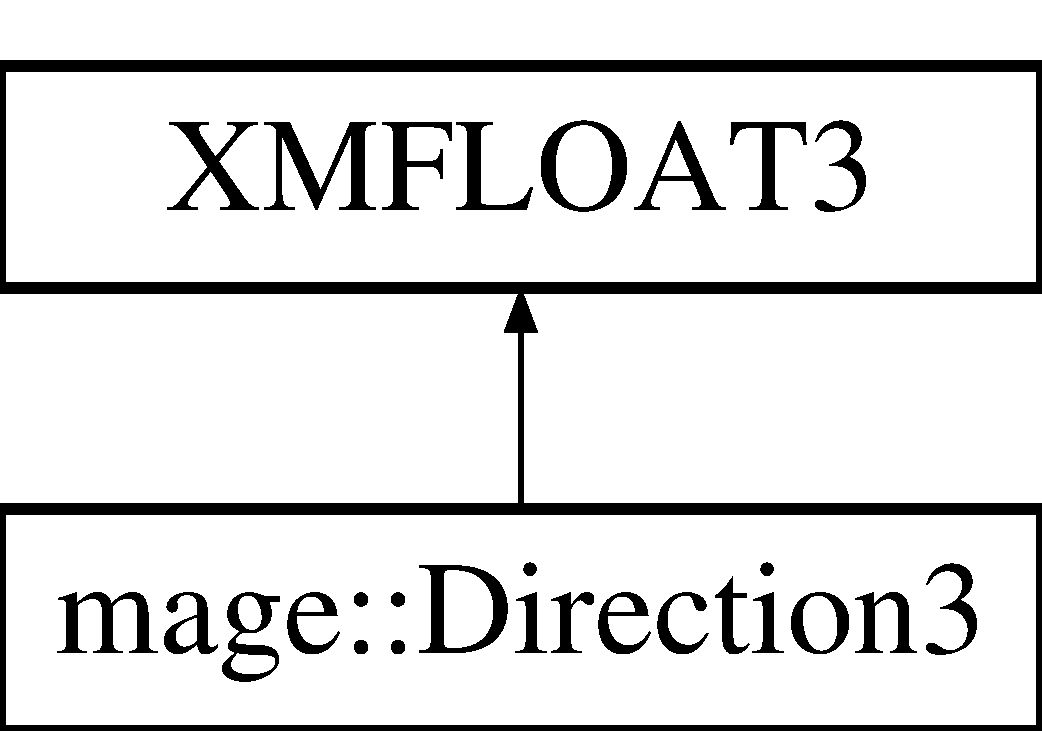
\includegraphics[height=4.000000cm]{structmage_1_1_direction3}
\end{center}
\end{figure}
\subsection*{Public Member Functions}
\begin{DoxyCompactItemize}
\item 
constexpr \mbox{\hyperlink{structmage_1_1_direction3_a64dd4745147f5fd39f710e8b9591074a}{Direction3}} () noexcept=default
\item 
constexpr \mbox{\hyperlink{structmage_1_1_direction3_a880d7413dc6f3742b53a089b870018c7}{Direction3}} (\mbox{\hyperlink{namespacemage_aa97e833b45f06d60a0a9c4fc22ae02c0}{F32}} x, \mbox{\hyperlink{namespacemage_aa97e833b45f06d60a0a9c4fc22ae02c0}{F32}} y, \mbox{\hyperlink{namespacemage_aa97e833b45f06d60a0a9c4fc22ae02c0}{F32}} z) noexcept
\item 
constexpr \mbox{\hyperlink{structmage_1_1_direction3_ad4d5801c6ad4949e0c7b0f4e2fec0ed9}{Direction3}} (const \mbox{\hyperlink{structmage_1_1_direction3}{Direction3}} \&direction) noexcept=default
\item 
constexpr \mbox{\hyperlink{structmage_1_1_direction3_aff1506b32f2b6dd49c2747eca90c76ce}{Direction3}} (\mbox{\hyperlink{structmage_1_1_direction3}{Direction3}} \&\&direction) noexcept=default
\item 
constexpr \mbox{\hyperlink{structmage_1_1_direction3_a9ef3fe2fd9fd55fade378d42eda597c3}{Direction3}} (\mbox{\hyperlink{namespacemage_a0fef5ab4e073c2d9ea876fefa3da4233}{F32x3}} v) noexcept
\item 
\mbox{\hyperlink{structmage_1_1_direction3_a583c087dc366d206aaf54a33bc90c50b}{$\sim$\+Direction3}} ()=default
\item 
constexpr \mbox{\hyperlink{structmage_1_1_direction3}{Direction3}} \& \mbox{\hyperlink{structmage_1_1_direction3_a500a363a93cded3e36a0704d288d34f3}{operator=}} (const \mbox{\hyperlink{structmage_1_1_direction3}{Direction3}} \&direction) noexcept=default
\item 
constexpr \mbox{\hyperlink{structmage_1_1_direction3}{Direction3}} \& \mbox{\hyperlink{structmage_1_1_direction3_a111a8f8d7286bfba0d7586925666315b}{operator=}} (\mbox{\hyperlink{structmage_1_1_direction3}{Direction3}} \&\&direction) noexcept=default
\item 
constexpr \mbox{\hyperlink{namespacemage_aa97e833b45f06d60a0a9c4fc22ae02c0}{F32}} \mbox{\hyperlink{structmage_1_1_direction3_a8d3ec6086f1b47844331950df3a47207}{GetX}} () const noexcept
\item 
constexpr void \mbox{\hyperlink{structmage_1_1_direction3_a0c2b501a6e30261d872227bb73be8914}{SetX}} (\mbox{\hyperlink{namespacemage_aa97e833b45f06d60a0a9c4fc22ae02c0}{F32}} x) noexcept
\item 
constexpr \mbox{\hyperlink{namespacemage_aa97e833b45f06d60a0a9c4fc22ae02c0}{F32}} \mbox{\hyperlink{structmage_1_1_direction3_a995bc58846a268b63f6e7fdd678420cd}{GetY}} () const noexcept
\item 
constexpr void \mbox{\hyperlink{structmage_1_1_direction3_a4ac25624a33e1eee6724f0b411737d2c}{SetY}} (\mbox{\hyperlink{namespacemage_aa97e833b45f06d60a0a9c4fc22ae02c0}{F32}} y) noexcept
\item 
constexpr \mbox{\hyperlink{namespacemage_aa97e833b45f06d60a0a9c4fc22ae02c0}{F32}} \mbox{\hyperlink{structmage_1_1_direction3_a6ee9bc60c92c37c6ff7e1b432bf191c7}{GetZ}} () const noexcept
\item 
constexpr void \mbox{\hyperlink{structmage_1_1_direction3_a26d3ef84f5c7429f325871c5d59e39e7}{SetZ}} (\mbox{\hyperlink{namespacemage_aa97e833b45f06d60a0a9c4fc22ae02c0}{F32}} z) noexcept
\end{DoxyCompactItemize}
\subsection*{Additional Inherited Members}


\subsection{Detailed Description}
A struct of directions in 3D space. 

\subsection{Constructor \& Destructor Documentation}
\mbox{\Hypertarget{structmage_1_1_direction3_a64dd4745147f5fd39f710e8b9591074a}\label{structmage_1_1_direction3_a64dd4745147f5fd39f710e8b9591074a}} 
\index{mage\+::\+Direction3@{mage\+::\+Direction3}!Direction3@{Direction3}}
\index{Direction3@{Direction3}!mage\+::\+Direction3@{mage\+::\+Direction3}}
\subsubsection{\texorpdfstring{Direction3()}{Direction3()}\hspace{0.1cm}{\footnotesize\ttfamily [1/5]}}
{\footnotesize\ttfamily constexpr mage\+::\+Direction3\+::\+Direction3 (\begin{DoxyParamCaption}{ }\end{DoxyParamCaption})\hspace{0.3cm}{\ttfamily [default]}, {\ttfamily [noexcept]}}

Constructs a direction. \mbox{\Hypertarget{structmage_1_1_direction3_a880d7413dc6f3742b53a089b870018c7}\label{structmage_1_1_direction3_a880d7413dc6f3742b53a089b870018c7}} 
\index{mage\+::\+Direction3@{mage\+::\+Direction3}!Direction3@{Direction3}}
\index{Direction3@{Direction3}!mage\+::\+Direction3@{mage\+::\+Direction3}}
\subsubsection{\texorpdfstring{Direction3()}{Direction3()}\hspace{0.1cm}{\footnotesize\ttfamily [2/5]}}
{\footnotesize\ttfamily constexpr mage\+::\+Direction3\+::\+Direction3 (\begin{DoxyParamCaption}\item[{\mbox{\hyperlink{namespacemage_aa97e833b45f06d60a0a9c4fc22ae02c0}{F32}}}]{x,  }\item[{\mbox{\hyperlink{namespacemage_aa97e833b45f06d60a0a9c4fc22ae02c0}{F32}}}]{y,  }\item[{\mbox{\hyperlink{namespacemage_aa97e833b45f06d60a0a9c4fc22ae02c0}{F32}}}]{z }\end{DoxyParamCaption})\hspace{0.3cm}{\ttfamily [noexcept]}}

Constructs a direction from the given coordinates.


\begin{DoxyParams}[1]{Parameters}
\mbox{\tt in}  & {\em x} & The x-\/coordinate. \\
\hline
\mbox{\tt in}  & {\em y} & The y-\/coordinate. \\
\hline
\mbox{\tt in}  & {\em z} & The z-\/coordinate. \\
\hline
\end{DoxyParams}
\mbox{\Hypertarget{structmage_1_1_direction3_ad4d5801c6ad4949e0c7b0f4e2fec0ed9}\label{structmage_1_1_direction3_ad4d5801c6ad4949e0c7b0f4e2fec0ed9}} 
\index{mage\+::\+Direction3@{mage\+::\+Direction3}!Direction3@{Direction3}}
\index{Direction3@{Direction3}!mage\+::\+Direction3@{mage\+::\+Direction3}}
\subsubsection{\texorpdfstring{Direction3()}{Direction3()}\hspace{0.1cm}{\footnotesize\ttfamily [3/5]}}
{\footnotesize\ttfamily constexpr mage\+::\+Direction3\+::\+Direction3 (\begin{DoxyParamCaption}\item[{const \mbox{\hyperlink{structmage_1_1_direction3}{Direction3}} \&}]{direction }\end{DoxyParamCaption})\hspace{0.3cm}{\ttfamily [default]}, {\ttfamily [noexcept]}}

Constructs a direction from the given direction.


\begin{DoxyParams}[1]{Parameters}
\mbox{\tt in}  & {\em direction} & A reference to the direction to copy. \\
\hline
\end{DoxyParams}
\mbox{\Hypertarget{structmage_1_1_direction3_aff1506b32f2b6dd49c2747eca90c76ce}\label{structmage_1_1_direction3_aff1506b32f2b6dd49c2747eca90c76ce}} 
\index{mage\+::\+Direction3@{mage\+::\+Direction3}!Direction3@{Direction3}}
\index{Direction3@{Direction3}!mage\+::\+Direction3@{mage\+::\+Direction3}}
\subsubsection{\texorpdfstring{Direction3()}{Direction3()}\hspace{0.1cm}{\footnotesize\ttfamily [4/5]}}
{\footnotesize\ttfamily constexpr mage\+::\+Direction3\+::\+Direction3 (\begin{DoxyParamCaption}\item[{\mbox{\hyperlink{structmage_1_1_direction3}{Direction3}} \&\&}]{direction }\end{DoxyParamCaption})\hspace{0.3cm}{\ttfamily [default]}, {\ttfamily [noexcept]}}

Constructs a direction by moving the given direction.


\begin{DoxyParams}[1]{Parameters}
\mbox{\tt in}  & {\em direction} & A reference to the direction to move. \\
\hline
\end{DoxyParams}
\mbox{\Hypertarget{structmage_1_1_direction3_a9ef3fe2fd9fd55fade378d42eda597c3}\label{structmage_1_1_direction3_a9ef3fe2fd9fd55fade378d42eda597c3}} 
\index{mage\+::\+Direction3@{mage\+::\+Direction3}!Direction3@{Direction3}}
\index{Direction3@{Direction3}!mage\+::\+Direction3@{mage\+::\+Direction3}}
\subsubsection{\texorpdfstring{Direction3()}{Direction3()}\hspace{0.1cm}{\footnotesize\ttfamily [5/5]}}
{\footnotesize\ttfamily constexpr mage\+::\+Direction3\+::\+Direction3 (\begin{DoxyParamCaption}\item[{\mbox{\hyperlink{namespacemage_a0fef5ab4e073c2d9ea876fefa3da4233}{F32x3}}}]{v }\end{DoxyParamCaption})\hspace{0.3cm}{\ttfamily [explicit]}, {\ttfamily [noexcept]}}

Constructs a direction from the given vector.


\begin{DoxyParams}[1]{Parameters}
\mbox{\tt in}  & {\em v} & The vector. \\
\hline
\end{DoxyParams}
\mbox{\Hypertarget{structmage_1_1_direction3_a583c087dc366d206aaf54a33bc90c50b}\label{structmage_1_1_direction3_a583c087dc366d206aaf54a33bc90c50b}} 
\index{mage\+::\+Direction3@{mage\+::\+Direction3}!````~Direction3@{$\sim$\+Direction3}}
\index{````~Direction3@{$\sim$\+Direction3}!mage\+::\+Direction3@{mage\+::\+Direction3}}
\subsubsection{\texorpdfstring{$\sim$\+Direction3()}{~Direction3()}}
{\footnotesize\ttfamily mage\+::\+Direction3\+::$\sim$\+Direction3 (\begin{DoxyParamCaption}{ }\end{DoxyParamCaption})\hspace{0.3cm}{\ttfamily [default]}}

Constructs a direction. 

\subsection{Member Function Documentation}
\mbox{\Hypertarget{structmage_1_1_direction3_a8d3ec6086f1b47844331950df3a47207}\label{structmage_1_1_direction3_a8d3ec6086f1b47844331950df3a47207}} 
\index{mage\+::\+Direction3@{mage\+::\+Direction3}!GetX@{GetX}}
\index{GetX@{GetX}!mage\+::\+Direction3@{mage\+::\+Direction3}}
\subsubsection{\texorpdfstring{Get\+X()}{GetX()}}
{\footnotesize\ttfamily constexpr \mbox{\hyperlink{namespacemage_aa97e833b45f06d60a0a9c4fc22ae02c0}{F32}} mage\+::\+Direction3\+::\+GetX (\begin{DoxyParamCaption}{ }\end{DoxyParamCaption}) const\hspace{0.3cm}{\ttfamily [noexcept]}}

Returns the X component of this direction.

\begin{DoxyReturn}{Returns}
The X component of this direction. 
\end{DoxyReturn}
\mbox{\Hypertarget{structmage_1_1_direction3_a995bc58846a268b63f6e7fdd678420cd}\label{structmage_1_1_direction3_a995bc58846a268b63f6e7fdd678420cd}} 
\index{mage\+::\+Direction3@{mage\+::\+Direction3}!GetY@{GetY}}
\index{GetY@{GetY}!mage\+::\+Direction3@{mage\+::\+Direction3}}
\subsubsection{\texorpdfstring{Get\+Y()}{GetY()}}
{\footnotesize\ttfamily constexpr \mbox{\hyperlink{namespacemage_aa97e833b45f06d60a0a9c4fc22ae02c0}{F32}} mage\+::\+Direction3\+::\+GetY (\begin{DoxyParamCaption}{ }\end{DoxyParamCaption}) const\hspace{0.3cm}{\ttfamily [noexcept]}}

Returns the Y component of this direction.

\begin{DoxyReturn}{Returns}
The Y component of this direction. 
\end{DoxyReturn}
\mbox{\Hypertarget{structmage_1_1_direction3_a6ee9bc60c92c37c6ff7e1b432bf191c7}\label{structmage_1_1_direction3_a6ee9bc60c92c37c6ff7e1b432bf191c7}} 
\index{mage\+::\+Direction3@{mage\+::\+Direction3}!GetZ@{GetZ}}
\index{GetZ@{GetZ}!mage\+::\+Direction3@{mage\+::\+Direction3}}
\subsubsection{\texorpdfstring{Get\+Z()}{GetZ()}}
{\footnotesize\ttfamily constexpr \mbox{\hyperlink{namespacemage_aa97e833b45f06d60a0a9c4fc22ae02c0}{F32}} mage\+::\+Direction3\+::\+GetZ (\begin{DoxyParamCaption}{ }\end{DoxyParamCaption}) const\hspace{0.3cm}{\ttfamily [noexcept]}}

Returns the Z component of this direction.

\begin{DoxyReturn}{Returns}
The Z component of this direction. 
\end{DoxyReturn}
\mbox{\Hypertarget{structmage_1_1_direction3_a500a363a93cded3e36a0704d288d34f3}\label{structmage_1_1_direction3_a500a363a93cded3e36a0704d288d34f3}} 
\index{mage\+::\+Direction3@{mage\+::\+Direction3}!operator=@{operator=}}
\index{operator=@{operator=}!mage\+::\+Direction3@{mage\+::\+Direction3}}
\subsubsection{\texorpdfstring{operator=()}{operator=()}\hspace{0.1cm}{\footnotesize\ttfamily [1/2]}}
{\footnotesize\ttfamily constexpr \mbox{\hyperlink{structmage_1_1_direction3}{Direction3}}\& mage\+::\+Direction3\+::operator= (\begin{DoxyParamCaption}\item[{const \mbox{\hyperlink{structmage_1_1_direction3}{Direction3}} \&}]{direction }\end{DoxyParamCaption})\hspace{0.3cm}{\ttfamily [default]}, {\ttfamily [noexcept]}}

Copies the given direction to this direction.


\begin{DoxyParams}[1]{Parameters}
\mbox{\tt in}  & {\em direction} & A reference to the direction to copy. \\
\hline
\end{DoxyParams}
\begin{DoxyReturn}{Returns}
A reference to the copy of the given direction (i.\+e. this direction). 
\end{DoxyReturn}
\mbox{\Hypertarget{structmage_1_1_direction3_a111a8f8d7286bfba0d7586925666315b}\label{structmage_1_1_direction3_a111a8f8d7286bfba0d7586925666315b}} 
\index{mage\+::\+Direction3@{mage\+::\+Direction3}!operator=@{operator=}}
\index{operator=@{operator=}!mage\+::\+Direction3@{mage\+::\+Direction3}}
\subsubsection{\texorpdfstring{operator=()}{operator=()}\hspace{0.1cm}{\footnotesize\ttfamily [2/2]}}
{\footnotesize\ttfamily constexpr \mbox{\hyperlink{structmage_1_1_direction3}{Direction3}}\& mage\+::\+Direction3\+::operator= (\begin{DoxyParamCaption}\item[{\mbox{\hyperlink{structmage_1_1_direction3}{Direction3}} \&\&}]{direction }\end{DoxyParamCaption})\hspace{0.3cm}{\ttfamily [default]}, {\ttfamily [noexcept]}}

Moves the given direction to this direction.


\begin{DoxyParams}[1]{Parameters}
\mbox{\tt in}  & {\em direction} & A reference to the direction to move. \\
\hline
\end{DoxyParams}
\begin{DoxyReturn}{Returns}
A reference to the moved direction (i.\+e. this direction). 
\end{DoxyReturn}
\mbox{\Hypertarget{structmage_1_1_direction3_a0c2b501a6e30261d872227bb73be8914}\label{structmage_1_1_direction3_a0c2b501a6e30261d872227bb73be8914}} 
\index{mage\+::\+Direction3@{mage\+::\+Direction3}!SetX@{SetX}}
\index{SetX@{SetX}!mage\+::\+Direction3@{mage\+::\+Direction3}}
\subsubsection{\texorpdfstring{Set\+X()}{SetX()}}
{\footnotesize\ttfamily constexpr void mage\+::\+Direction3\+::\+SetX (\begin{DoxyParamCaption}\item[{\mbox{\hyperlink{namespacemage_aa97e833b45f06d60a0a9c4fc22ae02c0}{F32}}}]{x }\end{DoxyParamCaption})\hspace{0.3cm}{\ttfamily [noexcept]}}

Sets the X component of this direction to the given value.


\begin{DoxyParams}[1]{Parameters}
\mbox{\tt in}  & {\em x} & The X component. \\
\hline
\end{DoxyParams}
\mbox{\Hypertarget{structmage_1_1_direction3_a4ac25624a33e1eee6724f0b411737d2c}\label{structmage_1_1_direction3_a4ac25624a33e1eee6724f0b411737d2c}} 
\index{mage\+::\+Direction3@{mage\+::\+Direction3}!SetY@{SetY}}
\index{SetY@{SetY}!mage\+::\+Direction3@{mage\+::\+Direction3}}
\subsubsection{\texorpdfstring{Set\+Y()}{SetY()}}
{\footnotesize\ttfamily constexpr void mage\+::\+Direction3\+::\+SetY (\begin{DoxyParamCaption}\item[{\mbox{\hyperlink{namespacemage_aa97e833b45f06d60a0a9c4fc22ae02c0}{F32}}}]{y }\end{DoxyParamCaption})\hspace{0.3cm}{\ttfamily [noexcept]}}

Sets the Y component of this direction to the given value.


\begin{DoxyParams}[1]{Parameters}
\mbox{\tt in}  & {\em y} & The Y component. \\
\hline
\end{DoxyParams}
\mbox{\Hypertarget{structmage_1_1_direction3_a26d3ef84f5c7429f325871c5d59e39e7}\label{structmage_1_1_direction3_a26d3ef84f5c7429f325871c5d59e39e7}} 
\index{mage\+::\+Direction3@{mage\+::\+Direction3}!SetZ@{SetZ}}
\index{SetZ@{SetZ}!mage\+::\+Direction3@{mage\+::\+Direction3}}
\subsubsection{\texorpdfstring{Set\+Z()}{SetZ()}}
{\footnotesize\ttfamily constexpr void mage\+::\+Direction3\+::\+SetZ (\begin{DoxyParamCaption}\item[{\mbox{\hyperlink{namespacemage_aa97e833b45f06d60a0a9c4fc22ae02c0}{F32}}}]{z }\end{DoxyParamCaption})\hspace{0.3cm}{\ttfamily [noexcept]}}

Sets the Z component of this direction to the given value.


\begin{DoxyParams}[1]{Parameters}
\mbox{\tt in}  & {\em z} & The Z component. \\
\hline
\end{DoxyParams}

\hypertarget{classmage_1_1_directional_light}{}\section{mage\+:\+:Directional\+Light Class Reference}
\label{classmage_1_1_directional_light}\index{mage\+::\+Directional\+Light@{mage\+::\+Directional\+Light}}


{\ttfamily \#include $<$directional\+\_\+light.\+hpp$>$}

Inheritance diagram for mage\+:\+:Directional\+Light\+:\begin{figure}[H]
\begin{center}
\leavevmode
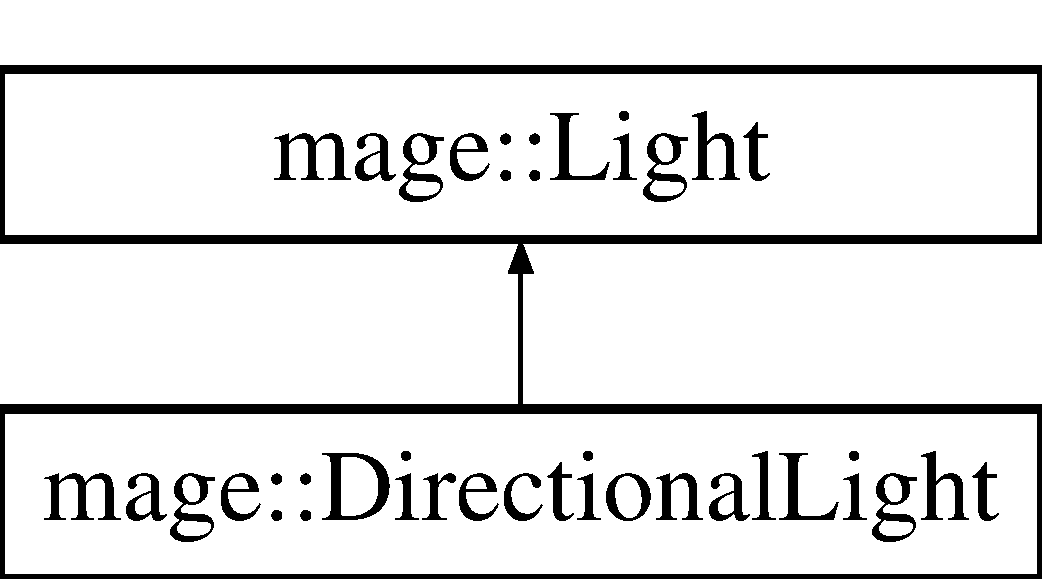
\includegraphics[height=2.000000cm]{classmage_1_1_directional_light}
\end{center}
\end{figure}
\subsection*{Public Member Functions}
\begin{DoxyCompactItemize}
\item 
\hyperlink{classmage_1_1_directional_light_a67df04219f61a8350045e5743b1de284}{Directional\+Light} (const \hyperlink{structmage_1_1_r_g_b_spectrum}{R\+G\+B\+Spectrum} \&intensity=\hyperlink{structmage_1_1_r_g_b_spectrum}{R\+G\+B\+Spectrum}(1.\+0f, 1.\+0f, 1.\+0f))
\item 
\hyperlink{classmage_1_1_directional_light_a777b1b8e00a51ba84f6af774a7b519ea}{Directional\+Light} (const \hyperlink{classmage_1_1_directional_light}{Directional\+Light} \&light)
\item 
\hyperlink{classmage_1_1_directional_light_a9563b260b550057e951500c40ecbe2d3}{Directional\+Light} (\hyperlink{classmage_1_1_directional_light}{Directional\+Light} \&\&light)
\item 
virtual \hyperlink{classmage_1_1_directional_light_a967d33c11a1477c01ce4c9720337caeb}{$\sim$\+Directional\+Light} ()
\item 
\hyperlink{classmage_1_1_directional_light}{Directional\+Light} \& \hyperlink{classmage_1_1_directional_light_a371d3c13d6e59c8d105da058b460874d}{operator=} (const \hyperlink{classmage_1_1_directional_light}{Directional\+Light} \&light)
\item 
\hyperlink{classmage_1_1_directional_light}{Directional\+Light} \& \hyperlink{classmage_1_1_directional_light_a508b595bf6aa5fc9db53e0a854fda41d}{operator=} (\hyperlink{classmage_1_1_directional_light}{Directional\+Light} \&\&light)
\item 
\hyperlink{namespacemage_a3316d7143a973e37adf1110f2e80ca31}{Unique\+Ptr}$<$ \hyperlink{classmage_1_1_directional_light}{Directional\+Light} $>$ \hyperlink{classmage_1_1_directional_light_a779c49e066215cff9f80ed40048dfc62}{Clone} () const
\item 
bool \hyperlink{classmage_1_1_directional_light_a645e7f3d3e4dc4ebf11d7a6aa6950a18}{Use\+Shadows} () const noexcept
\item 
void \hyperlink{classmage_1_1_directional_light_a36436d5d99ccf6a0e49e81f26c3f9bc7}{Enable\+Shadows} () noexcept
\item 
void \hyperlink{classmage_1_1_directional_light_addd4803dee85892dfd57f51e155c6572}{Dissable\+Shadows} () noexcept
\item 
void \hyperlink{classmage_1_1_directional_light_a1c15d8e42526ed5ae7568cff5c7b25e0}{Toggle\+Shadows} () noexcept
\item 
void \hyperlink{classmage_1_1_directional_light_ab70b4298dc6616dbe22446e8e3298424}{Set\+Shadows} (bool shadows) noexcept
\end{DoxyCompactItemize}
\subsection*{Private Member Functions}
\begin{DoxyCompactItemize}
\item 
virtual \hyperlink{namespacemage_a3316d7143a973e37adf1110f2e80ca31}{Unique\+Ptr}$<$ \hyperlink{classmage_1_1_light}{Light} $>$ \hyperlink{classmage_1_1_directional_light_a122d3dcd7633a85ef8a85e7d768da36d}{Clone\+Implementation} () const override
\end{DoxyCompactItemize}
\subsection*{Private Attributes}
\begin{DoxyCompactItemize}
\item 
bool \hyperlink{classmage_1_1_directional_light_a607a3dc01ee180f2044fe154c2b73903}{m\+\_\+shadows}
\end{DoxyCompactItemize}
\subsection*{Additional Inherited Members}


\subsection{Detailed Description}
A class of directional lights. 

\subsection{Constructor \& Destructor Documentation}
\hypertarget{classmage_1_1_directional_light_a67df04219f61a8350045e5743b1de284}{}\label{classmage_1_1_directional_light_a67df04219f61a8350045e5743b1de284} 
\index{mage\+::\+Directional\+Light@{mage\+::\+Directional\+Light}!Directional\+Light@{Directional\+Light}}
\index{Directional\+Light@{Directional\+Light}!mage\+::\+Directional\+Light@{mage\+::\+Directional\+Light}}
\subsubsection{\texorpdfstring{Directional\+Light()}{DirectionalLight()}\hspace{0.1cm}{\footnotesize\ttfamily [1/3]}}
{\footnotesize\ttfamily mage\+::\+Directional\+Light\+::\+Directional\+Light (\begin{DoxyParamCaption}\item[{const \hyperlink{structmage_1_1_r_g_b_spectrum}{R\+G\+B\+Spectrum} \&}]{intensity = {\ttfamily \hyperlink{structmage_1_1_r_g_b_spectrum}{R\+G\+B\+Spectrum}(1.0f,~1.0f,~1.0f)} }\end{DoxyParamCaption})\hspace{0.3cm}{\ttfamily [explicit]}}

Constructs a directional light.


\begin{DoxyParams}[1]{Parameters}
\mbox{\tt in}  & {\em intensity} & The R\+GB intensity. \\
\hline
\end{DoxyParams}
\hypertarget{classmage_1_1_directional_light_a777b1b8e00a51ba84f6af774a7b519ea}{}\label{classmage_1_1_directional_light_a777b1b8e00a51ba84f6af774a7b519ea} 
\index{mage\+::\+Directional\+Light@{mage\+::\+Directional\+Light}!Directional\+Light@{Directional\+Light}}
\index{Directional\+Light@{Directional\+Light}!mage\+::\+Directional\+Light@{mage\+::\+Directional\+Light}}
\subsubsection{\texorpdfstring{Directional\+Light()}{DirectionalLight()}\hspace{0.1cm}{\footnotesize\ttfamily [2/3]}}
{\footnotesize\ttfamily mage\+::\+Directional\+Light\+::\+Directional\+Light (\begin{DoxyParamCaption}\item[{const \hyperlink{classmage_1_1_directional_light}{Directional\+Light} \&}]{light }\end{DoxyParamCaption})\hspace{0.3cm}{\ttfamily [default]}}

Constructs a directional light from the given directional light.


\begin{DoxyParams}[1]{Parameters}
\mbox{\tt in}  & {\em light} & A reference to the directional light to copy. \\
\hline
\end{DoxyParams}
\hypertarget{classmage_1_1_directional_light_a9563b260b550057e951500c40ecbe2d3}{}\label{classmage_1_1_directional_light_a9563b260b550057e951500c40ecbe2d3} 
\index{mage\+::\+Directional\+Light@{mage\+::\+Directional\+Light}!Directional\+Light@{Directional\+Light}}
\index{Directional\+Light@{Directional\+Light}!mage\+::\+Directional\+Light@{mage\+::\+Directional\+Light}}
\subsubsection{\texorpdfstring{Directional\+Light()}{DirectionalLight()}\hspace{0.1cm}{\footnotesize\ttfamily [3/3]}}
{\footnotesize\ttfamily mage\+::\+Directional\+Light\+::\+Directional\+Light (\begin{DoxyParamCaption}\item[{\hyperlink{classmage_1_1_directional_light}{Directional\+Light} \&\&}]{light }\end{DoxyParamCaption})\hspace{0.3cm}{\ttfamily [default]}}

Constructs a directional light by moving the given directional light.


\begin{DoxyParams}[1]{Parameters}
\mbox{\tt in}  & {\em light} & A reference to the directional light to move. \\
\hline
\end{DoxyParams}
\hypertarget{classmage_1_1_directional_light_a967d33c11a1477c01ce4c9720337caeb}{}\label{classmage_1_1_directional_light_a967d33c11a1477c01ce4c9720337caeb} 
\index{mage\+::\+Directional\+Light@{mage\+::\+Directional\+Light}!````~Directional\+Light@{$\sim$\+Directional\+Light}}
\index{````~Directional\+Light@{$\sim$\+Directional\+Light}!mage\+::\+Directional\+Light@{mage\+::\+Directional\+Light}}
\subsubsection{\texorpdfstring{$\sim$\+Directional\+Light()}{~DirectionalLight()}}
{\footnotesize\ttfamily mage\+::\+Directional\+Light\+::$\sim$\+Directional\+Light (\begin{DoxyParamCaption}{ }\end{DoxyParamCaption})\hspace{0.3cm}{\ttfamily [virtual]}, {\ttfamily [default]}}

Destructs this directional light. 

\subsection{Member Function Documentation}
\hypertarget{classmage_1_1_directional_light_a779c49e066215cff9f80ed40048dfc62}{}\label{classmage_1_1_directional_light_a779c49e066215cff9f80ed40048dfc62} 
\index{mage\+::\+Directional\+Light@{mage\+::\+Directional\+Light}!Clone@{Clone}}
\index{Clone@{Clone}!mage\+::\+Directional\+Light@{mage\+::\+Directional\+Light}}
\subsubsection{\texorpdfstring{Clone()}{Clone()}}
{\footnotesize\ttfamily \hyperlink{namespacemage_a3316d7143a973e37adf1110f2e80ca31}{Unique\+Ptr}$<$ \hyperlink{classmage_1_1_directional_light}{Directional\+Light} $>$ mage\+::\+Directional\+Light\+::\+Clone (\begin{DoxyParamCaption}{ }\end{DoxyParamCaption}) const}

Clones this directional light.

\begin{DoxyReturn}{Returns}
A pointer to the clone of this directional light. 
\end{DoxyReturn}
\hypertarget{classmage_1_1_directional_light_a122d3dcd7633a85ef8a85e7d768da36d}{}\label{classmage_1_1_directional_light_a122d3dcd7633a85ef8a85e7d768da36d} 
\index{mage\+::\+Directional\+Light@{mage\+::\+Directional\+Light}!Clone\+Implementation@{Clone\+Implementation}}
\index{Clone\+Implementation@{Clone\+Implementation}!mage\+::\+Directional\+Light@{mage\+::\+Directional\+Light}}
\subsubsection{\texorpdfstring{Clone\+Implementation()}{CloneImplementation()}}
{\footnotesize\ttfamily \hyperlink{namespacemage_a3316d7143a973e37adf1110f2e80ca31}{Unique\+Ptr}$<$ \hyperlink{classmage_1_1_light}{Light} $>$ mage\+::\+Directional\+Light\+::\+Clone\+Implementation (\begin{DoxyParamCaption}{ }\end{DoxyParamCaption}) const\hspace{0.3cm}{\ttfamily [override]}, {\ttfamily [private]}, {\ttfamily [virtual]}}

Clones this directional light.

\begin{DoxyReturn}{Returns}
A pointer to the clone of this directional light. 
\end{DoxyReturn}


Implements \hyperlink{classmage_1_1_light_aa613d76a1ebda69efde853d15f75490c}{mage\+::\+Light}.

\hypertarget{classmage_1_1_directional_light_addd4803dee85892dfd57f51e155c6572}{}\label{classmage_1_1_directional_light_addd4803dee85892dfd57f51e155c6572} 
\index{mage\+::\+Directional\+Light@{mage\+::\+Directional\+Light}!Dissable\+Shadows@{Dissable\+Shadows}}
\index{Dissable\+Shadows@{Dissable\+Shadows}!mage\+::\+Directional\+Light@{mage\+::\+Directional\+Light}}
\subsubsection{\texorpdfstring{Dissable\+Shadows()}{DissableShadows()}}
{\footnotesize\ttfamily void mage\+::\+Directional\+Light\+::\+Dissable\+Shadows (\begin{DoxyParamCaption}{ }\end{DoxyParamCaption})\hspace{0.3cm}{\ttfamily [noexcept]}}

Dissables shadows for this directional light. \hypertarget{classmage_1_1_directional_light_a36436d5d99ccf6a0e49e81f26c3f9bc7}{}\label{classmage_1_1_directional_light_a36436d5d99ccf6a0e49e81f26c3f9bc7} 
\index{mage\+::\+Directional\+Light@{mage\+::\+Directional\+Light}!Enable\+Shadows@{Enable\+Shadows}}
\index{Enable\+Shadows@{Enable\+Shadows}!mage\+::\+Directional\+Light@{mage\+::\+Directional\+Light}}
\subsubsection{\texorpdfstring{Enable\+Shadows()}{EnableShadows()}}
{\footnotesize\ttfamily void mage\+::\+Directional\+Light\+::\+Enable\+Shadows (\begin{DoxyParamCaption}{ }\end{DoxyParamCaption})\hspace{0.3cm}{\ttfamily [noexcept]}}

Enables shadows for this directional light. \hypertarget{classmage_1_1_directional_light_a371d3c13d6e59c8d105da058b460874d}{}\label{classmage_1_1_directional_light_a371d3c13d6e59c8d105da058b460874d} 
\index{mage\+::\+Directional\+Light@{mage\+::\+Directional\+Light}!operator=@{operator=}}
\index{operator=@{operator=}!mage\+::\+Directional\+Light@{mage\+::\+Directional\+Light}}
\subsubsection{\texorpdfstring{operator=()}{operator=()}\hspace{0.1cm}{\footnotesize\ttfamily [1/2]}}
{\footnotesize\ttfamily \hyperlink{classmage_1_1_directional_light}{Directional\+Light} \& mage\+::\+Directional\+Light\+::operator= (\begin{DoxyParamCaption}\item[{const \hyperlink{classmage_1_1_directional_light}{Directional\+Light} \&}]{light }\end{DoxyParamCaption})\hspace{0.3cm}{\ttfamily [default]}}

Copies the given directional light to this directional light.


\begin{DoxyParams}[1]{Parameters}
\mbox{\tt in}  & {\em light} & A reference to the directional light to copy. \\
\hline
\end{DoxyParams}
\begin{DoxyReturn}{Returns}
A reference to the copy of the given directional light (i.\+e. this directional light). 
\end{DoxyReturn}
\hypertarget{classmage_1_1_directional_light_a508b595bf6aa5fc9db53e0a854fda41d}{}\label{classmage_1_1_directional_light_a508b595bf6aa5fc9db53e0a854fda41d} 
\index{mage\+::\+Directional\+Light@{mage\+::\+Directional\+Light}!operator=@{operator=}}
\index{operator=@{operator=}!mage\+::\+Directional\+Light@{mage\+::\+Directional\+Light}}
\subsubsection{\texorpdfstring{operator=()}{operator=()}\hspace{0.1cm}{\footnotesize\ttfamily [2/2]}}
{\footnotesize\ttfamily \hyperlink{classmage_1_1_directional_light}{Directional\+Light} \& mage\+::\+Directional\+Light\+::operator= (\begin{DoxyParamCaption}\item[{\hyperlink{classmage_1_1_directional_light}{Directional\+Light} \&\&}]{light }\end{DoxyParamCaption})\hspace{0.3cm}{\ttfamily [default]}}

Moves the given directional light to this directional light.


\begin{DoxyParams}[1]{Parameters}
\mbox{\tt in}  & {\em light} & A reference to the directional light to move. \\
\hline
\end{DoxyParams}
\begin{DoxyReturn}{Returns}
A reference to the moved directional light (i.\+e. this directional light). 
\end{DoxyReturn}
\hypertarget{classmage_1_1_directional_light_ab70b4298dc6616dbe22446e8e3298424}{}\label{classmage_1_1_directional_light_ab70b4298dc6616dbe22446e8e3298424} 
\index{mage\+::\+Directional\+Light@{mage\+::\+Directional\+Light}!Set\+Shadows@{Set\+Shadows}}
\index{Set\+Shadows@{Set\+Shadows}!mage\+::\+Directional\+Light@{mage\+::\+Directional\+Light}}
\subsubsection{\texorpdfstring{Set\+Shadows()}{SetShadows()}}
{\footnotesize\ttfamily void mage\+::\+Directional\+Light\+::\+Set\+Shadows (\begin{DoxyParamCaption}\item[{bool}]{shadows }\end{DoxyParamCaption})\hspace{0.3cm}{\ttfamily [noexcept]}}

Sets shadows for this directional light to the given value.


\begin{DoxyParams}[1]{Parameters}
\mbox{\tt in}  & {\em shadows} & {\ttfamily true} if shadows should be used for this directional light. {\ttfamily false} otherwise. \\
\hline
\end{DoxyParams}
\hypertarget{classmage_1_1_directional_light_a1c15d8e42526ed5ae7568cff5c7b25e0}{}\label{classmage_1_1_directional_light_a1c15d8e42526ed5ae7568cff5c7b25e0} 
\index{mage\+::\+Directional\+Light@{mage\+::\+Directional\+Light}!Toggle\+Shadows@{Toggle\+Shadows}}
\index{Toggle\+Shadows@{Toggle\+Shadows}!mage\+::\+Directional\+Light@{mage\+::\+Directional\+Light}}
\subsubsection{\texorpdfstring{Toggle\+Shadows()}{ToggleShadows()}}
{\footnotesize\ttfamily void mage\+::\+Directional\+Light\+::\+Toggle\+Shadows (\begin{DoxyParamCaption}{ }\end{DoxyParamCaption})\hspace{0.3cm}{\ttfamily [noexcept]}}

Toggles shadows for this directional light. \hypertarget{classmage_1_1_directional_light_a645e7f3d3e4dc4ebf11d7a6aa6950a18}{}\label{classmage_1_1_directional_light_a645e7f3d3e4dc4ebf11d7a6aa6950a18} 
\index{mage\+::\+Directional\+Light@{mage\+::\+Directional\+Light}!Use\+Shadows@{Use\+Shadows}}
\index{Use\+Shadows@{Use\+Shadows}!mage\+::\+Directional\+Light@{mage\+::\+Directional\+Light}}
\subsubsection{\texorpdfstring{Use\+Shadows()}{UseShadows()}}
{\footnotesize\ttfamily bool mage\+::\+Directional\+Light\+::\+Use\+Shadows (\begin{DoxyParamCaption}{ }\end{DoxyParamCaption}) const\hspace{0.3cm}{\ttfamily [noexcept]}}

Checks whether shadows should be used for this directional light.

\begin{DoxyReturn}{Returns}
{\ttfamily true} if shadows should be used for this directional light. {\ttfamily false} otherwise. 
\end{DoxyReturn}


\subsection{Member Data Documentation}
\hypertarget{classmage_1_1_directional_light_a607a3dc01ee180f2044fe154c2b73903}{}\label{classmage_1_1_directional_light_a607a3dc01ee180f2044fe154c2b73903} 
\index{mage\+::\+Directional\+Light@{mage\+::\+Directional\+Light}!m\+\_\+shadows@{m\+\_\+shadows}}
\index{m\+\_\+shadows@{m\+\_\+shadows}!mage\+::\+Directional\+Light@{mage\+::\+Directional\+Light}}
\subsubsection{\texorpdfstring{m\+\_\+shadows}{m\_shadows}}
{\footnotesize\ttfamily bool mage\+::\+Directional\+Light\+::m\+\_\+shadows\hspace{0.3cm}{\ttfamily [private]}}

A flag indicating whether shadows should be calculated or not not for this directional light. 
\hypertarget{classmage_1_1_dropshadow_sprite_text}{}\section{mage\+:\+:Dropshadow\+Sprite\+Text Class Reference}
\label{classmage_1_1_dropshadow_sprite_text}\index{mage\+::\+Dropshadow\+Sprite\+Text@{mage\+::\+Dropshadow\+Sprite\+Text}}


{\ttfamily \#include $<$dropshadow\+\_\+sprite\+\_\+text.\+hpp$>$}

Inheritance diagram for mage\+:\+:Dropshadow\+Sprite\+Text\+:\begin{figure}[H]
\begin{center}
\leavevmode
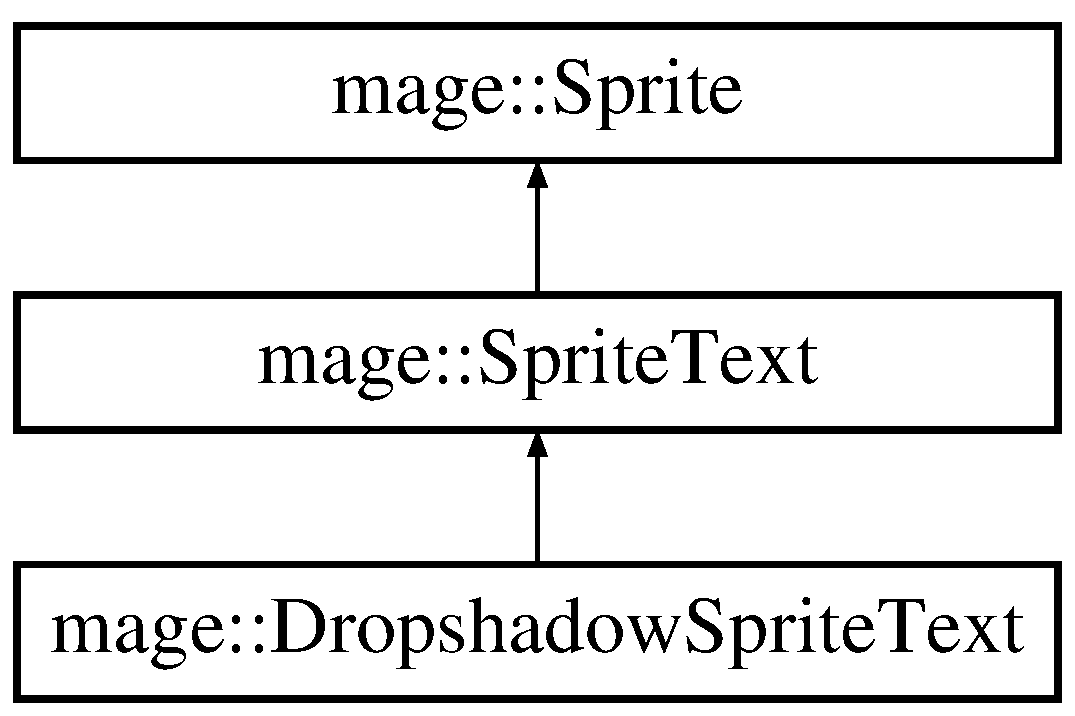
\includegraphics[height=2.000000cm]{classmage_1_1_dropshadow_sprite_text}
\end{center}
\end{figure}
\subsection*{Public Member Functions}
\begin{DoxyCompactItemize}
\item 
\hyperlink{classmage_1_1_dropshadow_sprite_text_a9258c03fd9d3f9eb4951fb1bde21a576}{Dropshadow\+Sprite\+Text} (const string \&name, const wstring \&text, \hyperlink{namespacemage_a1e01ae66713838a7a67d30e44c67703e}{Shared\+Ptr}$<$ \hyperlink{classmage_1_1_sprite_font}{Sprite\+Font} $>$ font, const X\+M\+V\+E\+C\+T\+OR \&\hyperlink{namespacemage_a56eceea5a9bceb2b56073f3ea4945781}{color}=Colors\+::\+White, const X\+M\+V\+E\+C\+T\+OR \&shadow\+\_\+color=Colors\+::\+Black, \hyperlink{namespacemage_a9cfe18123066ba4236f548f9de75d881}{Sprite\+Effect} effects=\hyperlink{namespacemage_a9cfe18123066ba4236f548f9de75d881af3c275fbfacfe174da928b2f24dfa515}{Sprite\+Effect\+\_\+\+None})
\item 
\hyperlink{classmage_1_1_dropshadow_sprite_text_a3d6c78caf74d6b8b0928934e08be0fe6}{Dropshadow\+Sprite\+Text} (const \hyperlink{classmage_1_1_dropshadow_sprite_text}{Dropshadow\+Sprite\+Text} \&sprite\+\_\+text)=default
\item 
\hyperlink{classmage_1_1_dropshadow_sprite_text_a23154e6e6be44142b656df65d11418e6}{Dropshadow\+Sprite\+Text} (\hyperlink{classmage_1_1_dropshadow_sprite_text}{Dropshadow\+Sprite\+Text} \&\&sprite\+\_\+text)=default
\item 
virtual \hyperlink{classmage_1_1_dropshadow_sprite_text_a06edb2d048974849c48c7a91ef244a2c}{$\sim$\+Dropshadow\+Sprite\+Text} ()=default
\item 
\hyperlink{classmage_1_1_dropshadow_sprite_text}{Dropshadow\+Sprite\+Text} \& \hyperlink{classmage_1_1_dropshadow_sprite_text_acc96ceb07c46894d731e86b735d3b594}{operator=} (const \hyperlink{classmage_1_1_dropshadow_sprite_text}{Dropshadow\+Sprite\+Text} \&sprite\+\_\+text)=default
\item 
\hyperlink{classmage_1_1_dropshadow_sprite_text}{Dropshadow\+Sprite\+Text} \& \hyperlink{classmage_1_1_dropshadow_sprite_text_a8f2ff9363c2710d03c87d45de6ccabc0}{operator=} (\hyperlink{classmage_1_1_dropshadow_sprite_text}{Dropshadow\+Sprite\+Text} \&\&sprite\+\_\+text)=default
\item 
virtual \hyperlink{classmage_1_1_dropshadow_sprite_text}{Dropshadow\+Sprite\+Text} $\ast$ \hyperlink{classmage_1_1_dropshadow_sprite_text_a116c49fb9638414c67a09501c4031a01}{Clone} () const override
\item 
virtual void \hyperlink{classmage_1_1_dropshadow_sprite_text_af76422c9812d7dc38e9b98e587103c67}{Draw} (\hyperlink{classmage_1_1_sprite_batch}{Sprite\+Batch} \&sprite\+\_\+batch) const override
\item 
const \hyperlink{structmage_1_1_color}{Color} \hyperlink{classmage_1_1_dropshadow_sprite_text_a776c11dfe60ad8c0c6f356c5f0f95af6}{Get\+Shadow\+Color} () const
\item 
void \hyperlink{classmage_1_1_dropshadow_sprite_text_abefcf9a3bd234df3996950410eefe1bf}{Set\+Shadow\+Color} (const \hyperlink{structmage_1_1_color}{Color} \&\hyperlink{namespacemage_a56eceea5a9bceb2b56073f3ea4945781}{color})
\item 
void \hyperlink{classmage_1_1_dropshadow_sprite_text_a8069cb327cc61dd92d516c793d9c49e7}{Set\+Shadow\+Color} (const X\+M\+V\+E\+C\+T\+OR \&\hyperlink{namespacemage_a56eceea5a9bceb2b56073f3ea4945781}{color})
\end{DoxyCompactItemize}
\subsection*{Private Attributes}
\begin{DoxyCompactItemize}
\item 
X\+M\+V\+E\+C\+T\+OR \hyperlink{classmage_1_1_dropshadow_sprite_text_a7953a6998932ab838acc0ece8ec526d4}{m\+\_\+shadow\+\_\+color}
\end{DoxyCompactItemize}
\subsection*{Additional Inherited Members}


\subsection{Constructor \& Destructor Documentation}
\hypertarget{classmage_1_1_dropshadow_sprite_text_a9258c03fd9d3f9eb4951fb1bde21a576}{}\label{classmage_1_1_dropshadow_sprite_text_a9258c03fd9d3f9eb4951fb1bde21a576} 
\index{mage\+::\+Dropshadow\+Sprite\+Text@{mage\+::\+Dropshadow\+Sprite\+Text}!Dropshadow\+Sprite\+Text@{Dropshadow\+Sprite\+Text}}
\index{Dropshadow\+Sprite\+Text@{Dropshadow\+Sprite\+Text}!mage\+::\+Dropshadow\+Sprite\+Text@{mage\+::\+Dropshadow\+Sprite\+Text}}
\subsubsection{\texorpdfstring{Dropshadow\+Sprite\+Text()}{DropshadowSpriteText()}\hspace{0.1cm}{\footnotesize\ttfamily [1/3]}}
{\footnotesize\ttfamily mage\+::\+Dropshadow\+Sprite\+Text\+::\+Dropshadow\+Sprite\+Text (\begin{DoxyParamCaption}\item[{const string \&}]{name,  }\item[{const wstring \&}]{text,  }\item[{\hyperlink{namespacemage_a1e01ae66713838a7a67d30e44c67703e}{Shared\+Ptr}$<$ \hyperlink{classmage_1_1_sprite_font}{Sprite\+Font} $>$}]{font,  }\item[{const X\+M\+V\+E\+C\+T\+OR \&}]{color = {\ttfamily Colors\+:\+:White},  }\item[{const X\+M\+V\+E\+C\+T\+OR \&}]{shadow\+\_\+color = {\ttfamily Colors\+:\+:Black},  }\item[{\hyperlink{namespacemage_a9cfe18123066ba4236f548f9de75d881}{Sprite\+Effect}}]{effects = {\ttfamily \hyperlink{namespacemage_a9cfe18123066ba4236f548f9de75d881af3c275fbfacfe174da928b2f24dfa515}{Sprite\+Effect\+\_\+\+None}} }\end{DoxyParamCaption})\hspace{0.3cm}{\ttfamily [explicit]}}

\hypertarget{classmage_1_1_dropshadow_sprite_text_a3d6c78caf74d6b8b0928934e08be0fe6}{}\label{classmage_1_1_dropshadow_sprite_text_a3d6c78caf74d6b8b0928934e08be0fe6} 
\index{mage\+::\+Dropshadow\+Sprite\+Text@{mage\+::\+Dropshadow\+Sprite\+Text}!Dropshadow\+Sprite\+Text@{Dropshadow\+Sprite\+Text}}
\index{Dropshadow\+Sprite\+Text@{Dropshadow\+Sprite\+Text}!mage\+::\+Dropshadow\+Sprite\+Text@{mage\+::\+Dropshadow\+Sprite\+Text}}
\subsubsection{\texorpdfstring{Dropshadow\+Sprite\+Text()}{DropshadowSpriteText()}\hspace{0.1cm}{\footnotesize\ttfamily [2/3]}}
{\footnotesize\ttfamily mage\+::\+Dropshadow\+Sprite\+Text\+::\+Dropshadow\+Sprite\+Text (\begin{DoxyParamCaption}\item[{const \hyperlink{classmage_1_1_dropshadow_sprite_text}{Dropshadow\+Sprite\+Text} \&}]{sprite\+\_\+text }\end{DoxyParamCaption})\hspace{0.3cm}{\ttfamily [default]}}

\hypertarget{classmage_1_1_dropshadow_sprite_text_a23154e6e6be44142b656df65d11418e6}{}\label{classmage_1_1_dropshadow_sprite_text_a23154e6e6be44142b656df65d11418e6} 
\index{mage\+::\+Dropshadow\+Sprite\+Text@{mage\+::\+Dropshadow\+Sprite\+Text}!Dropshadow\+Sprite\+Text@{Dropshadow\+Sprite\+Text}}
\index{Dropshadow\+Sprite\+Text@{Dropshadow\+Sprite\+Text}!mage\+::\+Dropshadow\+Sprite\+Text@{mage\+::\+Dropshadow\+Sprite\+Text}}
\subsubsection{\texorpdfstring{Dropshadow\+Sprite\+Text()}{DropshadowSpriteText()}\hspace{0.1cm}{\footnotesize\ttfamily [3/3]}}
{\footnotesize\ttfamily mage\+::\+Dropshadow\+Sprite\+Text\+::\+Dropshadow\+Sprite\+Text (\begin{DoxyParamCaption}\item[{\hyperlink{classmage_1_1_dropshadow_sprite_text}{Dropshadow\+Sprite\+Text} \&\&}]{sprite\+\_\+text }\end{DoxyParamCaption})\hspace{0.3cm}{\ttfamily [default]}}

\hypertarget{classmage_1_1_dropshadow_sprite_text_a06edb2d048974849c48c7a91ef244a2c}{}\label{classmage_1_1_dropshadow_sprite_text_a06edb2d048974849c48c7a91ef244a2c} 
\index{mage\+::\+Dropshadow\+Sprite\+Text@{mage\+::\+Dropshadow\+Sprite\+Text}!````~Dropshadow\+Sprite\+Text@{$\sim$\+Dropshadow\+Sprite\+Text}}
\index{````~Dropshadow\+Sprite\+Text@{$\sim$\+Dropshadow\+Sprite\+Text}!mage\+::\+Dropshadow\+Sprite\+Text@{mage\+::\+Dropshadow\+Sprite\+Text}}
\subsubsection{\texorpdfstring{$\sim$\+Dropshadow\+Sprite\+Text()}{~DropshadowSpriteText()}}
{\footnotesize\ttfamily virtual mage\+::\+Dropshadow\+Sprite\+Text\+::$\sim$\+Dropshadow\+Sprite\+Text (\begin{DoxyParamCaption}{ }\end{DoxyParamCaption})\hspace{0.3cm}{\ttfamily [virtual]}, {\ttfamily [default]}}



\subsection{Member Function Documentation}
\hypertarget{classmage_1_1_dropshadow_sprite_text_a116c49fb9638414c67a09501c4031a01}{}\label{classmage_1_1_dropshadow_sprite_text_a116c49fb9638414c67a09501c4031a01} 
\index{mage\+::\+Dropshadow\+Sprite\+Text@{mage\+::\+Dropshadow\+Sprite\+Text}!Clone@{Clone}}
\index{Clone@{Clone}!mage\+::\+Dropshadow\+Sprite\+Text@{mage\+::\+Dropshadow\+Sprite\+Text}}
\subsubsection{\texorpdfstring{Clone()}{Clone()}}
{\footnotesize\ttfamily virtual \hyperlink{classmage_1_1_dropshadow_sprite_text}{Dropshadow\+Sprite\+Text}$\ast$ mage\+::\+Dropshadow\+Sprite\+Text\+::\+Clone (\begin{DoxyParamCaption}{ }\end{DoxyParamCaption}) const\hspace{0.3cm}{\ttfamily [override]}, {\ttfamily [virtual]}}



Implements \hyperlink{classmage_1_1_sprite_text_ac4edf927911a9fb8e5c3a674b217637a}{mage\+::\+Sprite\+Text}.

\hypertarget{classmage_1_1_dropshadow_sprite_text_af76422c9812d7dc38e9b98e587103c67}{}\label{classmage_1_1_dropshadow_sprite_text_af76422c9812d7dc38e9b98e587103c67} 
\index{mage\+::\+Dropshadow\+Sprite\+Text@{mage\+::\+Dropshadow\+Sprite\+Text}!Draw@{Draw}}
\index{Draw@{Draw}!mage\+::\+Dropshadow\+Sprite\+Text@{mage\+::\+Dropshadow\+Sprite\+Text}}
\subsubsection{\texorpdfstring{Draw()}{Draw()}}
{\footnotesize\ttfamily void mage\+::\+Dropshadow\+Sprite\+Text\+::\+Draw (\begin{DoxyParamCaption}\item[{\hyperlink{classmage_1_1_sprite_batch}{Sprite\+Batch} \&}]{sprite\+\_\+batch }\end{DoxyParamCaption}) const\hspace{0.3cm}{\ttfamily [override]}, {\ttfamily [virtual]}}



Implements \hyperlink{classmage_1_1_sprite_text_a45d5ac8410d5a46b26e8491946a2ad9e}{mage\+::\+Sprite\+Text}.

\hypertarget{classmage_1_1_dropshadow_sprite_text_a776c11dfe60ad8c0c6f356c5f0f95af6}{}\label{classmage_1_1_dropshadow_sprite_text_a776c11dfe60ad8c0c6f356c5f0f95af6} 
\index{mage\+::\+Dropshadow\+Sprite\+Text@{mage\+::\+Dropshadow\+Sprite\+Text}!Get\+Shadow\+Color@{Get\+Shadow\+Color}}
\index{Get\+Shadow\+Color@{Get\+Shadow\+Color}!mage\+::\+Dropshadow\+Sprite\+Text@{mage\+::\+Dropshadow\+Sprite\+Text}}
\subsubsection{\texorpdfstring{Get\+Shadow\+Color()}{GetShadowColor()}}
{\footnotesize\ttfamily const \hyperlink{structmage_1_1_color}{Color} mage\+::\+Dropshadow\+Sprite\+Text\+::\+Get\+Shadow\+Color (\begin{DoxyParamCaption}{ }\end{DoxyParamCaption}) const}

\hypertarget{classmage_1_1_dropshadow_sprite_text_acc96ceb07c46894d731e86b735d3b594}{}\label{classmage_1_1_dropshadow_sprite_text_acc96ceb07c46894d731e86b735d3b594} 
\index{mage\+::\+Dropshadow\+Sprite\+Text@{mage\+::\+Dropshadow\+Sprite\+Text}!operator=@{operator=}}
\index{operator=@{operator=}!mage\+::\+Dropshadow\+Sprite\+Text@{mage\+::\+Dropshadow\+Sprite\+Text}}
\subsubsection{\texorpdfstring{operator=()}{operator=()}\hspace{0.1cm}{\footnotesize\ttfamily [1/2]}}
{\footnotesize\ttfamily \hyperlink{classmage_1_1_dropshadow_sprite_text}{Dropshadow\+Sprite\+Text}\& mage\+::\+Dropshadow\+Sprite\+Text\+::operator= (\begin{DoxyParamCaption}\item[{const \hyperlink{classmage_1_1_dropshadow_sprite_text}{Dropshadow\+Sprite\+Text} \&}]{sprite\+\_\+text }\end{DoxyParamCaption})\hspace{0.3cm}{\ttfamily [default]}}

\hypertarget{classmage_1_1_dropshadow_sprite_text_a8f2ff9363c2710d03c87d45de6ccabc0}{}\label{classmage_1_1_dropshadow_sprite_text_a8f2ff9363c2710d03c87d45de6ccabc0} 
\index{mage\+::\+Dropshadow\+Sprite\+Text@{mage\+::\+Dropshadow\+Sprite\+Text}!operator=@{operator=}}
\index{operator=@{operator=}!mage\+::\+Dropshadow\+Sprite\+Text@{mage\+::\+Dropshadow\+Sprite\+Text}}
\subsubsection{\texorpdfstring{operator=()}{operator=()}\hspace{0.1cm}{\footnotesize\ttfamily [2/2]}}
{\footnotesize\ttfamily \hyperlink{classmage_1_1_dropshadow_sprite_text}{Dropshadow\+Sprite\+Text}\& mage\+::\+Dropshadow\+Sprite\+Text\+::operator= (\begin{DoxyParamCaption}\item[{\hyperlink{classmage_1_1_dropshadow_sprite_text}{Dropshadow\+Sprite\+Text} \&\&}]{sprite\+\_\+text }\end{DoxyParamCaption})\hspace{0.3cm}{\ttfamily [default]}}

\hypertarget{classmage_1_1_dropshadow_sprite_text_abefcf9a3bd234df3996950410eefe1bf}{}\label{classmage_1_1_dropshadow_sprite_text_abefcf9a3bd234df3996950410eefe1bf} 
\index{mage\+::\+Dropshadow\+Sprite\+Text@{mage\+::\+Dropshadow\+Sprite\+Text}!Set\+Shadow\+Color@{Set\+Shadow\+Color}}
\index{Set\+Shadow\+Color@{Set\+Shadow\+Color}!mage\+::\+Dropshadow\+Sprite\+Text@{mage\+::\+Dropshadow\+Sprite\+Text}}
\subsubsection{\texorpdfstring{Set\+Shadow\+Color()}{SetShadowColor()}\hspace{0.1cm}{\footnotesize\ttfamily [1/2]}}
{\footnotesize\ttfamily void mage\+::\+Dropshadow\+Sprite\+Text\+::\+Set\+Shadow\+Color (\begin{DoxyParamCaption}\item[{const \hyperlink{structmage_1_1_color}{Color} \&}]{color }\end{DoxyParamCaption})}

\hypertarget{classmage_1_1_dropshadow_sprite_text_a8069cb327cc61dd92d516c793d9c49e7}{}\label{classmage_1_1_dropshadow_sprite_text_a8069cb327cc61dd92d516c793d9c49e7} 
\index{mage\+::\+Dropshadow\+Sprite\+Text@{mage\+::\+Dropshadow\+Sprite\+Text}!Set\+Shadow\+Color@{Set\+Shadow\+Color}}
\index{Set\+Shadow\+Color@{Set\+Shadow\+Color}!mage\+::\+Dropshadow\+Sprite\+Text@{mage\+::\+Dropshadow\+Sprite\+Text}}
\subsubsection{\texorpdfstring{Set\+Shadow\+Color()}{SetShadowColor()}\hspace{0.1cm}{\footnotesize\ttfamily [2/2]}}
{\footnotesize\ttfamily void mage\+::\+Dropshadow\+Sprite\+Text\+::\+Set\+Shadow\+Color (\begin{DoxyParamCaption}\item[{const X\+M\+V\+E\+C\+T\+OR \&}]{color }\end{DoxyParamCaption})}



\subsection{Member Data Documentation}
\hypertarget{classmage_1_1_dropshadow_sprite_text_a7953a6998932ab838acc0ece8ec526d4}{}\label{classmage_1_1_dropshadow_sprite_text_a7953a6998932ab838acc0ece8ec526d4} 
\index{mage\+::\+Dropshadow\+Sprite\+Text@{mage\+::\+Dropshadow\+Sprite\+Text}!m\+\_\+shadow\+\_\+color@{m\+\_\+shadow\+\_\+color}}
\index{m\+\_\+shadow\+\_\+color@{m\+\_\+shadow\+\_\+color}!mage\+::\+Dropshadow\+Sprite\+Text@{mage\+::\+Dropshadow\+Sprite\+Text}}
\subsubsection{\texorpdfstring{m\+\_\+shadow\+\_\+color}{m\_shadow\_color}}
{\footnotesize\ttfamily X\+M\+V\+E\+C\+T\+OR mage\+::\+Dropshadow\+Sprite\+Text\+::m\+\_\+shadow\+\_\+color\hspace{0.3cm}{\ttfamily [private]}}


\hypertarget{classmage_1_1_engine}{}\section{mage\+:\+:Engine Class Reference}
\label{classmage_1_1_engine}\index{mage\+::\+Engine@{mage\+::\+Engine}}


{\ttfamily \#include $<$engine.\+hpp$>$}

Inheritance diagram for mage\+:\+:Engine\+:\begin{figure}[H]
\begin{center}
\leavevmode
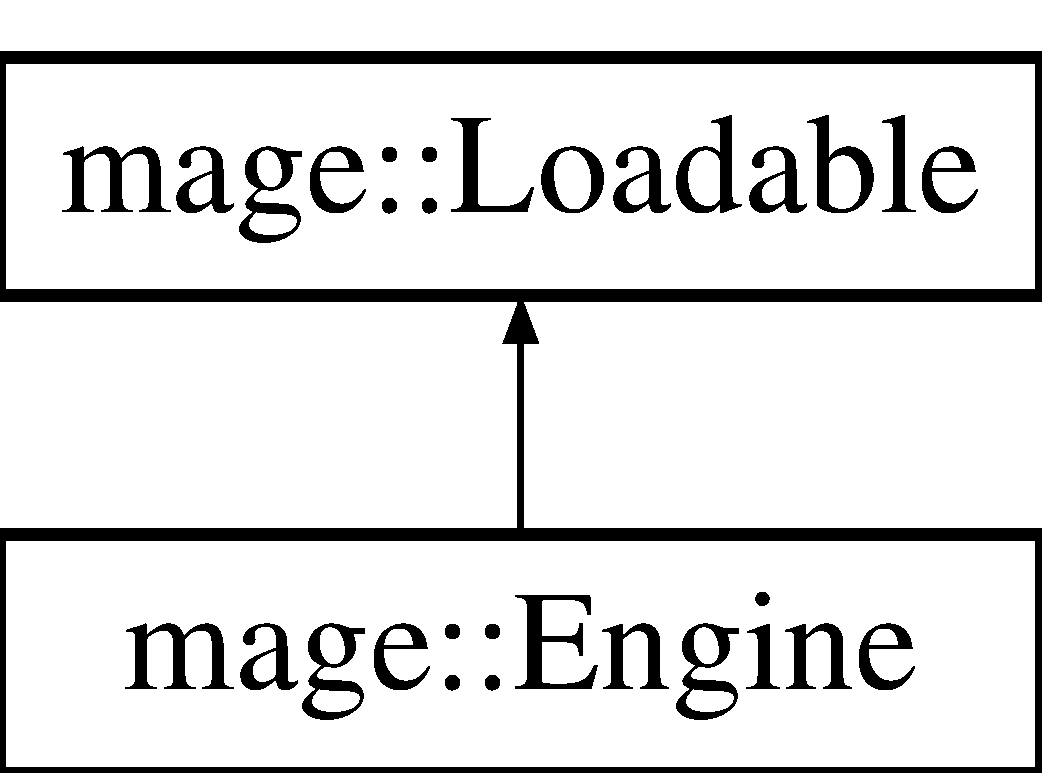
\includegraphics[height=2.000000cm]{classmage_1_1_engine}
\end{center}
\end{figure}
\subsection*{Public Member Functions}
\begin{DoxyCompactItemize}
\item 
\hyperlink{classmage_1_1_engine_a99770cbb017b29c284d7f8e4c7e2b84c}{Engine} (const \hyperlink{structmage_1_1_engine_setup}{Engine\+Setup} \&setup)
\item 
\hyperlink{classmage_1_1_engine_afd2f4f32b2e803f59521aafe1924f0ba}{Engine} (const \hyperlink{classmage_1_1_engine}{Engine} \&engine)=delete
\item 
\hyperlink{classmage_1_1_engine_a1374fc1d0d18e23df9150dfcd17955b0}{Engine} (\hyperlink{classmage_1_1_engine}{Engine} \&\&engine)=default
\item 
virtual \hyperlink{classmage_1_1_engine_a34628556f8397d70ed018d71e343c2f5}{$\sim$\+Engine} ()
\item 
\hyperlink{classmage_1_1_engine}{Engine} \& \hyperlink{classmage_1_1_engine_a1eedff82d4c8207c61676230520648fd}{operator=} (const \hyperlink{classmage_1_1_engine}{Engine} \&engine)=delete
\item 
\hyperlink{classmage_1_1_engine}{Engine} \& \hyperlink{classmage_1_1_engine_a22607a263e0be5e179cc0e4bf13b18f7}{operator=} (\hyperlink{classmage_1_1_engine}{Engine} \&\&engine)=delete
\item 
void \hyperlink{classmage_1_1_engine_a246c82d0e55bc29e73aecbc365464ec8}{Run} (int n\+Cmd\+Show=S\+W\+\_\+\+N\+O\+R\+M\+AL)
\item 
const \hyperlink{classmage_1_1_main_window}{Main\+Window} $\ast$ \hyperlink{classmage_1_1_engine_a28baaa54158acac8ffca3b6f31f63f82}{Get\+Main\+Window} () const
\item 
void \hyperlink{classmage_1_1_engine_a942bfa9892fa79bb1068d7c7ec4e6732}{Set\+Deactive\+Flag} (bool deactive)
\item 
const \hyperlink{classmage_1_1_renderer}{Renderer} $\ast$ \hyperlink{classmage_1_1_engine_a42ea717aaf468e0cacf8d8745041e09f}{Get\+Renderer} () const
\item 
void \hyperlink{classmage_1_1_engine_a8b574f0d702240d76fa98b2c79856d0d}{Set\+Mode\+Switch\+Flag} (bool mode\+\_\+switch)
\item 
const \hyperlink{classmage_1_1_input_manager}{Input\+Manager} $\ast$ \hyperlink{classmage_1_1_engine_a627271c15bb1ecb1079f9780d64e0d77}{Get\+Input\+Manager} () const
\item 
\hyperlink{classmage_1_1_resource_factory}{Resource\+Factory} $\ast$ \hyperlink{classmage_1_1_engine_a1610768d6de0e8548ba18904a692b1a8}{Get\+Resource\+Factory} () const
\item 
void \hyperlink{classmage_1_1_engine_aec75ed67f8fb68a383fa892e50b21ea7}{Set\+Scene} (\hyperlink{namespacemage_a1e01ae66713838a7a67d30e44c67703e}{Shared\+Ptr}$<$ \hyperlink{classmage_1_1_scene}{Scene} $>$ scene)
\end{DoxyCompactItemize}
\subsection*{Private Member Functions}
\begin{DoxyCompactItemize}
\item 
void \hyperlink{classmage_1_1_engine_a29a47448fb182b110d46d287a72b8b4e}{Initialize\+Systems} (const \hyperlink{structmage_1_1_engine_setup}{Engine\+Setup} \&setup)
\end{DoxyCompactItemize}
\subsection*{Private Attributes}
\begin{DoxyCompactItemize}
\item 
\hyperlink{namespacemage_a8c307fbcc33bce9b7f2aa4c26c3b95cf}{Unique\+Ptr}$<$ \hyperlink{classmage_1_1_main_window}{Main\+Window} $>$ \hyperlink{classmage_1_1_engine_a3aea7e8c0c1247cac570334a3d3543d6}{m\+\_\+main\+\_\+window}
\item 
bool \hyperlink{classmage_1_1_engine_ab8a4b0157403708ae7d1d018a95b4c63}{m\+\_\+deactive}
\item 
\hyperlink{namespacemage_a8c307fbcc33bce9b7f2aa4c26c3b95cf}{Unique\+Ptr}$<$ \hyperlink{classmage_1_1_renderer}{Renderer} $>$ \hyperlink{classmage_1_1_engine_a1248b7c21bc8256c72d372c12ed1ee68}{m\+\_\+renderer}
\item 
bool \hyperlink{classmage_1_1_engine_aa5cb2e0b7bb2c4a9020e79ab832ee221}{m\+\_\+mode\+\_\+switch}
\item 
\hyperlink{namespacemage_a8c307fbcc33bce9b7f2aa4c26c3b95cf}{Unique\+Ptr}$<$ \hyperlink{classmage_1_1_input_manager}{Input\+Manager} $>$ \hyperlink{classmage_1_1_engine_a8e9048208a6a5c5b034aaa1cbdab28bc}{m\+\_\+input\+\_\+manager}
\item 
\hyperlink{namespacemage_a8c307fbcc33bce9b7f2aa4c26c3b95cf}{Unique\+Ptr}$<$ \hyperlink{classmage_1_1_resource_factory}{Resource\+Factory} $>$ \hyperlink{classmage_1_1_engine_a0c7c2d4fc75fc3512e02054056cf8a90}{m\+\_\+resource\+\_\+factory}
\item 
\hyperlink{namespacemage_a1e01ae66713838a7a67d30e44c67703e}{Shared\+Ptr}$<$ \hyperlink{classmage_1_1_scene}{Scene} $>$ \hyperlink{classmage_1_1_engine_a82158ab9c1b60538ef8c46d5eb263bb8}{m\+\_\+scene}
\item 
\hyperlink{namespacemage_a8c307fbcc33bce9b7f2aa4c26c3b95cf}{Unique\+Ptr}$<$ \hyperlink{classmage_1_1_timer}{Timer} $>$ \hyperlink{classmage_1_1_engine_a4daac998928a6c087b310c52b3f26ae4}{m\+\_\+timer}
\end{DoxyCompactItemize}
\subsection*{Additional Inherited Members}


\subsection{Detailed Description}
A class of engines. 

\subsection{Constructor \& Destructor Documentation}
\hypertarget{classmage_1_1_engine_a99770cbb017b29c284d7f8e4c7e2b84c}{}\label{classmage_1_1_engine_a99770cbb017b29c284d7f8e4c7e2b84c} 
\index{mage\+::\+Engine@{mage\+::\+Engine}!Engine@{Engine}}
\index{Engine@{Engine}!mage\+::\+Engine@{mage\+::\+Engine}}
\subsubsection{\texorpdfstring{Engine()}{Engine()}\hspace{0.1cm}{\footnotesize\ttfamily [1/3]}}
{\footnotesize\ttfamily mage\+::\+Engine\+::\+Engine (\begin{DoxyParamCaption}\item[{const \hyperlink{structmage_1_1_engine_setup}{Engine\+Setup} \&}]{setup }\end{DoxyParamCaption})\hspace{0.3cm}{\ttfamily [explicit]}}

Constructs an engine from the given engine setup.


\begin{DoxyParams}[1]{Parameters}
\mbox{\tt in}  & {\em setup} & A reference to an engine setup. \\
\hline
\end{DoxyParams}

\begin{DoxyExceptions}{Exceptions}
{\em \hyperlink{structmage_1_1_formatted_exception}{Formatted\+Exception}} & Failed to initialize the engine. \\
\hline
\end{DoxyExceptions}
\hypertarget{classmage_1_1_engine_afd2f4f32b2e803f59521aafe1924f0ba}{}\label{classmage_1_1_engine_afd2f4f32b2e803f59521aafe1924f0ba} 
\index{mage\+::\+Engine@{mage\+::\+Engine}!Engine@{Engine}}
\index{Engine@{Engine}!mage\+::\+Engine@{mage\+::\+Engine}}
\subsubsection{\texorpdfstring{Engine()}{Engine()}\hspace{0.1cm}{\footnotesize\ttfamily [2/3]}}
{\footnotesize\ttfamily mage\+::\+Engine\+::\+Engine (\begin{DoxyParamCaption}\item[{const \hyperlink{classmage_1_1_engine}{Engine} \&}]{engine }\end{DoxyParamCaption})\hspace{0.3cm}{\ttfamily [delete]}}

Constructs an engine from the given engine.


\begin{DoxyParams}[1]{Parameters}
\mbox{\tt in}  & {\em engine} & A reference to the engine to copy. \\
\hline
\end{DoxyParams}
\hypertarget{classmage_1_1_engine_a1374fc1d0d18e23df9150dfcd17955b0}{}\label{classmage_1_1_engine_a1374fc1d0d18e23df9150dfcd17955b0} 
\index{mage\+::\+Engine@{mage\+::\+Engine}!Engine@{Engine}}
\index{Engine@{Engine}!mage\+::\+Engine@{mage\+::\+Engine}}
\subsubsection{\texorpdfstring{Engine()}{Engine()}\hspace{0.1cm}{\footnotesize\ttfamily [3/3]}}
{\footnotesize\ttfamily mage\+::\+Engine\+::\+Engine (\begin{DoxyParamCaption}\item[{\hyperlink{classmage_1_1_engine}{Engine} \&\&}]{engine }\end{DoxyParamCaption})\hspace{0.3cm}{\ttfamily [default]}}

Constructs an engine by moving the given engine.


\begin{DoxyParams}[1]{Parameters}
\mbox{\tt in}  & {\em engine} & A reference to the engine to move. \\
\hline
\end{DoxyParams}
\hypertarget{classmage_1_1_engine_a34628556f8397d70ed018d71e343c2f5}{}\label{classmage_1_1_engine_a34628556f8397d70ed018d71e343c2f5} 
\index{mage\+::\+Engine@{mage\+::\+Engine}!````~Engine@{$\sim$\+Engine}}
\index{````~Engine@{$\sim$\+Engine}!mage\+::\+Engine@{mage\+::\+Engine}}
\subsubsection{\texorpdfstring{$\sim$\+Engine()}{~Engine()}}
{\footnotesize\ttfamily mage\+::\+Engine\+::$\sim$\+Engine (\begin{DoxyParamCaption}{ }\end{DoxyParamCaption})\hspace{0.3cm}{\ttfamily [virtual]}}

Destructs this engine. 

\subsection{Member Function Documentation}
\hypertarget{classmage_1_1_engine_a627271c15bb1ecb1079f9780d64e0d77}{}\label{classmage_1_1_engine_a627271c15bb1ecb1079f9780d64e0d77} 
\index{mage\+::\+Engine@{mage\+::\+Engine}!Get\+Input\+Manager@{Get\+Input\+Manager}}
\index{Get\+Input\+Manager@{Get\+Input\+Manager}!mage\+::\+Engine@{mage\+::\+Engine}}
\subsubsection{\texorpdfstring{Get\+Input\+Manager()}{GetInputManager()}}
{\footnotesize\ttfamily const \hyperlink{classmage_1_1_input_manager}{Input\+Manager}$\ast$ mage\+::\+Engine\+::\+Get\+Input\+Manager (\begin{DoxyParamCaption}{ }\end{DoxyParamCaption}) const}

Returns the input manager of this engine.

\begin{DoxyReturn}{Returns}
{\ttfamily nullptr} if this engine is not properly setup. 

A pointer to the input manager of this engine. 
\end{DoxyReturn}
\hypertarget{classmage_1_1_engine_a28baaa54158acac8ffca3b6f31f63f82}{}\label{classmage_1_1_engine_a28baaa54158acac8ffca3b6f31f63f82} 
\index{mage\+::\+Engine@{mage\+::\+Engine}!Get\+Main\+Window@{Get\+Main\+Window}}
\index{Get\+Main\+Window@{Get\+Main\+Window}!mage\+::\+Engine@{mage\+::\+Engine}}
\subsubsection{\texorpdfstring{Get\+Main\+Window()}{GetMainWindow()}}
{\footnotesize\ttfamily const \hyperlink{classmage_1_1_main_window}{Main\+Window}$\ast$ mage\+::\+Engine\+::\+Get\+Main\+Window (\begin{DoxyParamCaption}{ }\end{DoxyParamCaption}) const}

Returns the main window of this engine.

\begin{DoxyReturn}{Returns}
{\ttfamily nullptr} if this engine is not properly setup. 

A pointer to the main window of this engine. 
\end{DoxyReturn}
\hypertarget{classmage_1_1_engine_a42ea717aaf468e0cacf8d8745041e09f}{}\label{classmage_1_1_engine_a42ea717aaf468e0cacf8d8745041e09f} 
\index{mage\+::\+Engine@{mage\+::\+Engine}!Get\+Renderer@{Get\+Renderer}}
\index{Get\+Renderer@{Get\+Renderer}!mage\+::\+Engine@{mage\+::\+Engine}}
\subsubsection{\texorpdfstring{Get\+Renderer()}{GetRenderer()}}
{\footnotesize\ttfamily const \hyperlink{classmage_1_1_renderer}{Renderer}$\ast$ mage\+::\+Engine\+::\+Get\+Renderer (\begin{DoxyParamCaption}{ }\end{DoxyParamCaption}) const}

Returns the renderer of this engine.

\begin{DoxyReturn}{Returns}
{\ttfamily nullptr} if this engine is not properly setup. 

A pointer to the renderer of this engine. 
\end{DoxyReturn}
\hypertarget{classmage_1_1_engine_a1610768d6de0e8548ba18904a692b1a8}{}\label{classmage_1_1_engine_a1610768d6de0e8548ba18904a692b1a8} 
\index{mage\+::\+Engine@{mage\+::\+Engine}!Get\+Resource\+Factory@{Get\+Resource\+Factory}}
\index{Get\+Resource\+Factory@{Get\+Resource\+Factory}!mage\+::\+Engine@{mage\+::\+Engine}}
\subsubsection{\texorpdfstring{Get\+Resource\+Factory()}{GetResourceFactory()}}
{\footnotesize\ttfamily \hyperlink{classmage_1_1_resource_factory}{Resource\+Factory}$\ast$ mage\+::\+Engine\+::\+Get\+Resource\+Factory (\begin{DoxyParamCaption}{ }\end{DoxyParamCaption}) const}

Returns the resource factory of this engine.

\begin{DoxyReturn}{Returns}
{\ttfamily nullptr} if this engine is not properly setup. 

A pointer to the resource factory of this engine. 
\end{DoxyReturn}
\hypertarget{classmage_1_1_engine_a29a47448fb182b110d46d287a72b8b4e}{}\label{classmage_1_1_engine_a29a47448fb182b110d46d287a72b8b4e} 
\index{mage\+::\+Engine@{mage\+::\+Engine}!Initialize\+Systems@{Initialize\+Systems}}
\index{Initialize\+Systems@{Initialize\+Systems}!mage\+::\+Engine@{mage\+::\+Engine}}
\subsubsection{\texorpdfstring{Initialize\+Systems()}{InitializeSystems()}}
{\footnotesize\ttfamily void mage\+::\+Engine\+::\+Initialize\+Systems (\begin{DoxyParamCaption}\item[{const \hyperlink{structmage_1_1_engine_setup}{Engine\+Setup} \&}]{setup }\end{DoxyParamCaption})\hspace{0.3cm}{\ttfamily [private]}}

Initializes the different systems of this engine.


\begin{DoxyParams}[1]{Parameters}
\mbox{\tt in}  & {\em setup} & A reference to an engine setup. \\
\hline
\end{DoxyParams}

\begin{DoxyExceptions}{Exceptions}
{\em \hyperlink{structmage_1_1_formatted_exception}{Formatted\+Exception}} & Failed to initialize at least one of the different systems of this engine. \\
\hline
\end{DoxyExceptions}
\hypertarget{classmage_1_1_engine_a1eedff82d4c8207c61676230520648fd}{}\label{classmage_1_1_engine_a1eedff82d4c8207c61676230520648fd} 
\index{mage\+::\+Engine@{mage\+::\+Engine}!operator=@{operator=}}
\index{operator=@{operator=}!mage\+::\+Engine@{mage\+::\+Engine}}
\subsubsection{\texorpdfstring{operator=()}{operator=()}\hspace{0.1cm}{\footnotesize\ttfamily [1/2]}}
{\footnotesize\ttfamily \hyperlink{classmage_1_1_engine}{Engine}\& mage\+::\+Engine\+::operator= (\begin{DoxyParamCaption}\item[{const \hyperlink{classmage_1_1_engine}{Engine} \&}]{engine }\end{DoxyParamCaption})\hspace{0.3cm}{\ttfamily [delete]}}

Copies the given engine to this engine.


\begin{DoxyParams}[1]{Parameters}
\mbox{\tt in}  & {\em engine} & A reference to the engine to copy. \\
\hline
\end{DoxyParams}
\begin{DoxyReturn}{Returns}
A reference to the copy of the given engine (i.\+e. this engine). 
\end{DoxyReturn}
\hypertarget{classmage_1_1_engine_a22607a263e0be5e179cc0e4bf13b18f7}{}\label{classmage_1_1_engine_a22607a263e0be5e179cc0e4bf13b18f7} 
\index{mage\+::\+Engine@{mage\+::\+Engine}!operator=@{operator=}}
\index{operator=@{operator=}!mage\+::\+Engine@{mage\+::\+Engine}}
\subsubsection{\texorpdfstring{operator=()}{operator=()}\hspace{0.1cm}{\footnotesize\ttfamily [2/2]}}
{\footnotesize\ttfamily \hyperlink{classmage_1_1_engine}{Engine}\& mage\+::\+Engine\+::operator= (\begin{DoxyParamCaption}\item[{\hyperlink{classmage_1_1_engine}{Engine} \&\&}]{engine }\end{DoxyParamCaption})\hspace{0.3cm}{\ttfamily [delete]}}

Copies the given engine to this engine.


\begin{DoxyParams}[1]{Parameters}
\mbox{\tt in}  & {\em engine} & A reference to the engine to move. \\
\hline
\end{DoxyParams}
\begin{DoxyReturn}{Returns}
A reference to the moved engine (i.\+e. this engine). 
\end{DoxyReturn}
\hypertarget{classmage_1_1_engine_a246c82d0e55bc29e73aecbc365464ec8}{}\label{classmage_1_1_engine_a246c82d0e55bc29e73aecbc365464ec8} 
\index{mage\+::\+Engine@{mage\+::\+Engine}!Run@{Run}}
\index{Run@{Run}!mage\+::\+Engine@{mage\+::\+Engine}}
\subsubsection{\texorpdfstring{Run()}{Run()}}
{\footnotesize\ttfamily void mage\+::\+Engine\+::\+Run (\begin{DoxyParamCaption}\item[{int}]{n\+Cmd\+Show = {\ttfamily SW\+\_\+NORMAL} }\end{DoxyParamCaption})}

Runs this engine.


\begin{DoxyParams}[1]{Parameters}
\mbox{\tt in}  & {\em n\+Cmd\+Show} & Controls how the engine window is to be shown. \\
\hline
\end{DoxyParams}
\hypertarget{classmage_1_1_engine_a942bfa9892fa79bb1068d7c7ec4e6732}{}\label{classmage_1_1_engine_a942bfa9892fa79bb1068d7c7ec4e6732} 
\index{mage\+::\+Engine@{mage\+::\+Engine}!Set\+Deactive\+Flag@{Set\+Deactive\+Flag}}
\index{Set\+Deactive\+Flag@{Set\+Deactive\+Flag}!mage\+::\+Engine@{mage\+::\+Engine}}
\subsubsection{\texorpdfstring{Set\+Deactive\+Flag()}{SetDeactiveFlag()}}
{\footnotesize\ttfamily void mage\+::\+Engine\+::\+Set\+Deactive\+Flag (\begin{DoxyParamCaption}\item[{bool}]{deactive }\end{DoxyParamCaption})}

Sets the deactive flag of this engine to the given value.


\begin{DoxyParams}[1]{Parameters}
\mbox{\tt in}  & {\em deactive} & The new value for the deactive flag. \\
\hline
\end{DoxyParams}
\hypertarget{classmage_1_1_engine_a8b574f0d702240d76fa98b2c79856d0d}{}\label{classmage_1_1_engine_a8b574f0d702240d76fa98b2c79856d0d} 
\index{mage\+::\+Engine@{mage\+::\+Engine}!Set\+Mode\+Switch\+Flag@{Set\+Mode\+Switch\+Flag}}
\index{Set\+Mode\+Switch\+Flag@{Set\+Mode\+Switch\+Flag}!mage\+::\+Engine@{mage\+::\+Engine}}
\subsubsection{\texorpdfstring{Set\+Mode\+Switch\+Flag()}{SetModeSwitchFlag()}}
{\footnotesize\ttfamily void mage\+::\+Engine\+::\+Set\+Mode\+Switch\+Flag (\begin{DoxyParamCaption}\item[{bool}]{mode\+\_\+switch }\end{DoxyParamCaption})}

Sets the mode switch flag of this engine to the given value.


\begin{DoxyParams}[1]{Parameters}
\mbox{\tt in}  & {\em mode\+\_\+switch} & The new value for the mode switch flag. \\
\hline
\end{DoxyParams}
\hypertarget{classmage_1_1_engine_aec75ed67f8fb68a383fa892e50b21ea7}{}\label{classmage_1_1_engine_aec75ed67f8fb68a383fa892e50b21ea7} 
\index{mage\+::\+Engine@{mage\+::\+Engine}!Set\+Scene@{Set\+Scene}}
\index{Set\+Scene@{Set\+Scene}!mage\+::\+Engine@{mage\+::\+Engine}}
\subsubsection{\texorpdfstring{Set\+Scene()}{SetScene()}}
{\footnotesize\ttfamily void mage\+::\+Engine\+::\+Set\+Scene (\begin{DoxyParamCaption}\item[{\hyperlink{namespacemage_a1e01ae66713838a7a67d30e44c67703e}{Shared\+Ptr}$<$ \hyperlink{classmage_1_1_scene}{Scene} $>$}]{scene }\end{DoxyParamCaption})}

Sets the scene of this engine to the given scene.

\begin{DoxyReturn}{Returns}
A pointer to the scene to set. 
\end{DoxyReturn}


\subsection{Member Data Documentation}
\hypertarget{classmage_1_1_engine_ab8a4b0157403708ae7d1d018a95b4c63}{}\label{classmage_1_1_engine_ab8a4b0157403708ae7d1d018a95b4c63} 
\index{mage\+::\+Engine@{mage\+::\+Engine}!m\+\_\+deactive@{m\+\_\+deactive}}
\index{m\+\_\+deactive@{m\+\_\+deactive}!mage\+::\+Engine@{mage\+::\+Engine}}
\subsubsection{\texorpdfstring{m\+\_\+deactive}{m\_deactive}}
{\footnotesize\ttfamily bool mage\+::\+Engine\+::m\+\_\+deactive\hspace{0.3cm}{\ttfamily [private]}}

Flag indicating whether the application is active or not. \hypertarget{classmage_1_1_engine_a8e9048208a6a5c5b034aaa1cbdab28bc}{}\label{classmage_1_1_engine_a8e9048208a6a5c5b034aaa1cbdab28bc} 
\index{mage\+::\+Engine@{mage\+::\+Engine}!m\+\_\+input\+\_\+manager@{m\+\_\+input\+\_\+manager}}
\index{m\+\_\+input\+\_\+manager@{m\+\_\+input\+\_\+manager}!mage\+::\+Engine@{mage\+::\+Engine}}
\subsubsection{\texorpdfstring{m\+\_\+input\+\_\+manager}{m\_input\_manager}}
{\footnotesize\ttfamily \hyperlink{namespacemage_a8c307fbcc33bce9b7f2aa4c26c3b95cf}{Unique\+Ptr}$<$ \hyperlink{classmage_1_1_input_manager}{Input\+Manager} $>$ mage\+::\+Engine\+::m\+\_\+input\+\_\+manager\hspace{0.3cm}{\ttfamily [private]}}

A pointer to the input manager of this engine. \hypertarget{classmage_1_1_engine_a3aea7e8c0c1247cac570334a3d3543d6}{}\label{classmage_1_1_engine_a3aea7e8c0c1247cac570334a3d3543d6} 
\index{mage\+::\+Engine@{mage\+::\+Engine}!m\+\_\+main\+\_\+window@{m\+\_\+main\+\_\+window}}
\index{m\+\_\+main\+\_\+window@{m\+\_\+main\+\_\+window}!mage\+::\+Engine@{mage\+::\+Engine}}
\subsubsection{\texorpdfstring{m\+\_\+main\+\_\+window}{m\_main\_window}}
{\footnotesize\ttfamily \hyperlink{namespacemage_a8c307fbcc33bce9b7f2aa4c26c3b95cf}{Unique\+Ptr}$<$ \hyperlink{classmage_1_1_main_window}{Main\+Window} $>$ mage\+::\+Engine\+::m\+\_\+main\+\_\+window\hspace{0.3cm}{\ttfamily [private]}}

A pointer to the main window of this engine. \hypertarget{classmage_1_1_engine_aa5cb2e0b7bb2c4a9020e79ab832ee221}{}\label{classmage_1_1_engine_aa5cb2e0b7bb2c4a9020e79ab832ee221} 
\index{mage\+::\+Engine@{mage\+::\+Engine}!m\+\_\+mode\+\_\+switch@{m\+\_\+mode\+\_\+switch}}
\index{m\+\_\+mode\+\_\+switch@{m\+\_\+mode\+\_\+switch}!mage\+::\+Engine@{mage\+::\+Engine}}
\subsubsection{\texorpdfstring{m\+\_\+mode\+\_\+switch}{m\_mode\_switch}}
{\footnotesize\ttfamily bool mage\+::\+Engine\+::m\+\_\+mode\+\_\+switch\hspace{0.3cm}{\ttfamily [private]}}

Flag indicating whether the application should switch between full screen and windowed mode. \hypertarget{classmage_1_1_engine_a1248b7c21bc8256c72d372c12ed1ee68}{}\label{classmage_1_1_engine_a1248b7c21bc8256c72d372c12ed1ee68} 
\index{mage\+::\+Engine@{mage\+::\+Engine}!m\+\_\+renderer@{m\+\_\+renderer}}
\index{m\+\_\+renderer@{m\+\_\+renderer}!mage\+::\+Engine@{mage\+::\+Engine}}
\subsubsection{\texorpdfstring{m\+\_\+renderer}{m\_renderer}}
{\footnotesize\ttfamily \hyperlink{namespacemage_a8c307fbcc33bce9b7f2aa4c26c3b95cf}{Unique\+Ptr}$<$ \hyperlink{classmage_1_1_renderer}{Renderer} $>$ mage\+::\+Engine\+::m\+\_\+renderer\hspace{0.3cm}{\ttfamily [private]}}

A pointer to the renderer of this engine. \hypertarget{classmage_1_1_engine_a0c7c2d4fc75fc3512e02054056cf8a90}{}\label{classmage_1_1_engine_a0c7c2d4fc75fc3512e02054056cf8a90} 
\index{mage\+::\+Engine@{mage\+::\+Engine}!m\+\_\+resource\+\_\+factory@{m\+\_\+resource\+\_\+factory}}
\index{m\+\_\+resource\+\_\+factory@{m\+\_\+resource\+\_\+factory}!mage\+::\+Engine@{mage\+::\+Engine}}
\subsubsection{\texorpdfstring{m\+\_\+resource\+\_\+factory}{m\_resource\_factory}}
{\footnotesize\ttfamily \hyperlink{namespacemage_a8c307fbcc33bce9b7f2aa4c26c3b95cf}{Unique\+Ptr}$<$ \hyperlink{classmage_1_1_resource_factory}{Resource\+Factory} $>$ mage\+::\+Engine\+::m\+\_\+resource\+\_\+factory\hspace{0.3cm}{\ttfamily [private]}}

A pointer to the resource factory of this engine. \hypertarget{classmage_1_1_engine_a82158ab9c1b60538ef8c46d5eb263bb8}{}\label{classmage_1_1_engine_a82158ab9c1b60538ef8c46d5eb263bb8} 
\index{mage\+::\+Engine@{mage\+::\+Engine}!m\+\_\+scene@{m\+\_\+scene}}
\index{m\+\_\+scene@{m\+\_\+scene}!mage\+::\+Engine@{mage\+::\+Engine}}
\subsubsection{\texorpdfstring{m\+\_\+scene}{m\_scene}}
{\footnotesize\ttfamily \hyperlink{namespacemage_a1e01ae66713838a7a67d30e44c67703e}{Shared\+Ptr}$<$ \hyperlink{classmage_1_1_scene}{Scene} $>$ mage\+::\+Engine\+::m\+\_\+scene\hspace{0.3cm}{\ttfamily [private]}}

A pointer to the current scene of this engine. \hypertarget{classmage_1_1_engine_a4daac998928a6c087b310c52b3f26ae4}{}\label{classmage_1_1_engine_a4daac998928a6c087b310c52b3f26ae4} 
\index{mage\+::\+Engine@{mage\+::\+Engine}!m\+\_\+timer@{m\+\_\+timer}}
\index{m\+\_\+timer@{m\+\_\+timer}!mage\+::\+Engine@{mage\+::\+Engine}}
\subsubsection{\texorpdfstring{m\+\_\+timer}{m\_timer}}
{\footnotesize\ttfamily \hyperlink{namespacemage_a8c307fbcc33bce9b7f2aa4c26c3b95cf}{Unique\+Ptr}$<$ \hyperlink{classmage_1_1_timer}{Timer} $>$ mage\+::\+Engine\+::m\+\_\+timer\hspace{0.3cm}{\ttfamily [private]}}

A pointer to the timer of this engine. 
\hypertarget{structmage_1_1_engine_setup}{}\section{mage\+:\+:Engine\+Setup Struct Reference}
\label{structmage_1_1_engine_setup}\index{mage\+::\+Engine\+Setup@{mage\+::\+Engine\+Setup}}


{\ttfamily \#include $<$engine\+\_\+setup.\+hpp$>$}

\subsection*{Public Member Functions}
\begin{DoxyCompactItemize}
\item 
virtual \hyperlink{structmage_1_1_engine_setup_ac9ec3df257c585930b21b2b69c99c177}{$\sim$\+Engine\+Setup} ()
\item 
\hyperlink{structmage_1_1_engine_setup}{Engine\+Setup} \& \hyperlink{structmage_1_1_engine_setup_ad7066882519b59ca533293f743334508}{operator=} (const \hyperlink{structmage_1_1_engine_setup}{Engine\+Setup} \&setup)=delete
\item 
\hyperlink{structmage_1_1_engine_setup}{Engine\+Setup} \& \hyperlink{structmage_1_1_engine_setup_a9ca25ff88af30786022964916790a497}{operator=} (\hyperlink{structmage_1_1_engine_setup}{Engine\+Setup} \&\&setup)=delete
\item 
const wstring \& \hyperlink{structmage_1_1_engine_setup_a63fed5e978c020ebc9d5080fe6fcefdc}{Get\+Application\+Name} () const
\item 
H\+I\+N\+S\+T\+A\+N\+CE \hyperlink{structmage_1_1_engine_setup_a2d9220896adfe924ac72165b4e2b13cf}{Get\+Application\+Hinstance} () const
\item 
virtual \hyperlink{namespacemage_a1e01ae66713838a7a67d30e44c67703e}{Shared\+Ptr}$<$ \hyperlink{classmage_1_1_scene}{Scene} $>$ \hyperlink{structmage_1_1_engine_setup_a004fce6a741fc68c8f6feed546d9f220}{Create\+Scene} () const =0
\end{DoxyCompactItemize}
\subsection*{Protected Member Functions}
\begin{DoxyCompactItemize}
\item 
\hyperlink{structmage_1_1_engine_setup_ac09a572abaf5f785004bb46a1d1bf49c}{Engine\+Setup} (H\+I\+N\+S\+T\+A\+N\+CE hinstance, const wstring \&name=M\+A\+G\+E\+\_\+\+D\+E\+F\+A\+U\+L\+T\+\_\+\+A\+P\+P\+L\+I\+C\+A\+T\+I\+O\+N\+\_\+\+N\+A\+ME)
\item 
\hyperlink{structmage_1_1_engine_setup_a2399c7966ed02ce9e9ab951b7483aac1}{Engine\+Setup} (const \hyperlink{structmage_1_1_engine_setup}{Engine\+Setup} \&setup)
\item 
\hyperlink{structmage_1_1_engine_setup_ac199c03ba1968ca0a98a2de48cfb952d}{Engine\+Setup} (\hyperlink{structmage_1_1_engine_setup}{Engine\+Setup} \&\&setup)
\end{DoxyCompactItemize}
\subsection*{Private Attributes}
\begin{DoxyCompactItemize}
\item 
const H\+I\+N\+S\+T\+A\+N\+CE \hyperlink{structmage_1_1_engine_setup_a678360078479bc3fee6bed4617caebbf}{m\+\_\+hinstance}
\item 
const wstring \hyperlink{structmage_1_1_engine_setup_a40fba981d4b1c30eff304b029a013009}{m\+\_\+name}
\end{DoxyCompactItemize}


\subsection{Detailed Description}
A struct of engine setups. 

\subsection{Constructor \& Destructor Documentation}
\hypertarget{structmage_1_1_engine_setup_ac9ec3df257c585930b21b2b69c99c177}{}\label{structmage_1_1_engine_setup_ac9ec3df257c585930b21b2b69c99c177} 
\index{mage\+::\+Engine\+Setup@{mage\+::\+Engine\+Setup}!````~Engine\+Setup@{$\sim$\+Engine\+Setup}}
\index{````~Engine\+Setup@{$\sim$\+Engine\+Setup}!mage\+::\+Engine\+Setup@{mage\+::\+Engine\+Setup}}
\subsubsection{\texorpdfstring{$\sim$\+Engine\+Setup()}{~EngineSetup()}}
{\footnotesize\ttfamily mage\+::\+Engine\+Setup\+::$\sim$\+Engine\+Setup (\begin{DoxyParamCaption}{ }\end{DoxyParamCaption})\hspace{0.3cm}{\ttfamily [virtual]}, {\ttfamily [default]}}

Destructs this engine setup. \hypertarget{structmage_1_1_engine_setup_ac09a572abaf5f785004bb46a1d1bf49c}{}\label{structmage_1_1_engine_setup_ac09a572abaf5f785004bb46a1d1bf49c} 
\index{mage\+::\+Engine\+Setup@{mage\+::\+Engine\+Setup}!Engine\+Setup@{Engine\+Setup}}
\index{Engine\+Setup@{Engine\+Setup}!mage\+::\+Engine\+Setup@{mage\+::\+Engine\+Setup}}
\subsubsection{\texorpdfstring{Engine\+Setup()}{EngineSetup()}\hspace{0.1cm}{\footnotesize\ttfamily [1/3]}}
{\footnotesize\ttfamily mage\+::\+Engine\+Setup\+::\+Engine\+Setup (\begin{DoxyParamCaption}\item[{H\+I\+N\+S\+T\+A\+N\+CE}]{hinstance,  }\item[{const wstring \&}]{name = {\ttfamily MAGE\+\_\+DEFAULT\+\_\+APPLICATION\+\_\+NAME} }\end{DoxyParamCaption})\hspace{0.3cm}{\ttfamily [explicit]}, {\ttfamily [protected]}}

Constructs an engine setup.

\begin{DoxyPrecond}{Precondition}
{\itshape hinstance} is not equal to {\ttfamily nullptr}. 
\end{DoxyPrecond}

\begin{DoxyParams}[1]{Parameters}
\mbox{\tt in}  & {\em hinstance} & The application instance handle of the application. \\
\hline
\mbox{\tt in}  & {\em name} & A reference to the name of the application. \\
\hline
\end{DoxyParams}
\hypertarget{structmage_1_1_engine_setup_a2399c7966ed02ce9e9ab951b7483aac1}{}\label{structmage_1_1_engine_setup_a2399c7966ed02ce9e9ab951b7483aac1} 
\index{mage\+::\+Engine\+Setup@{mage\+::\+Engine\+Setup}!Engine\+Setup@{Engine\+Setup}}
\index{Engine\+Setup@{Engine\+Setup}!mage\+::\+Engine\+Setup@{mage\+::\+Engine\+Setup}}
\subsubsection{\texorpdfstring{Engine\+Setup()}{EngineSetup()}\hspace{0.1cm}{\footnotesize\ttfamily [2/3]}}
{\footnotesize\ttfamily mage\+::\+Engine\+Setup\+::\+Engine\+Setup (\begin{DoxyParamCaption}\item[{const \hyperlink{structmage_1_1_engine_setup}{Engine\+Setup} \&}]{setup }\end{DoxyParamCaption})\hspace{0.3cm}{\ttfamily [protected]}, {\ttfamily [default]}}

Constructs an engine setup from the given engine setup.


\begin{DoxyParams}[1]{Parameters}
\mbox{\tt in}  & {\em setup} & A reference to the engine setup to copy. \\
\hline
\end{DoxyParams}
\hypertarget{structmage_1_1_engine_setup_ac199c03ba1968ca0a98a2de48cfb952d}{}\label{structmage_1_1_engine_setup_ac199c03ba1968ca0a98a2de48cfb952d} 
\index{mage\+::\+Engine\+Setup@{mage\+::\+Engine\+Setup}!Engine\+Setup@{Engine\+Setup}}
\index{Engine\+Setup@{Engine\+Setup}!mage\+::\+Engine\+Setup@{mage\+::\+Engine\+Setup}}
\subsubsection{\texorpdfstring{Engine\+Setup()}{EngineSetup()}\hspace{0.1cm}{\footnotesize\ttfamily [3/3]}}
{\footnotesize\ttfamily mage\+::\+Engine\+Setup\+::\+Engine\+Setup (\begin{DoxyParamCaption}\item[{\hyperlink{structmage_1_1_engine_setup}{Engine\+Setup} \&\&}]{setup }\end{DoxyParamCaption})\hspace{0.3cm}{\ttfamily [protected]}, {\ttfamily [default]}}

Constructs an engine setup by moving the given engine setup.


\begin{DoxyParams}[1]{Parameters}
\mbox{\tt in}  & {\em setup} & A reference to the engine setup to move. \\
\hline
\end{DoxyParams}


\subsection{Member Function Documentation}
\hypertarget{structmage_1_1_engine_setup_a004fce6a741fc68c8f6feed546d9f220}{}\label{structmage_1_1_engine_setup_a004fce6a741fc68c8f6feed546d9f220} 
\index{mage\+::\+Engine\+Setup@{mage\+::\+Engine\+Setup}!Create\+Scene@{Create\+Scene}}
\index{Create\+Scene@{Create\+Scene}!mage\+::\+Engine\+Setup@{mage\+::\+Engine\+Setup}}
\subsubsection{\texorpdfstring{Create\+Scene()}{CreateScene()}}
{\footnotesize\ttfamily virtual \hyperlink{namespacemage_a1e01ae66713838a7a67d30e44c67703e}{Shared\+Ptr}$<$ \hyperlink{classmage_1_1_scene}{Scene} $>$ mage\+::\+Engine\+Setup\+::\+Create\+Scene (\begin{DoxyParamCaption}{ }\end{DoxyParamCaption}) const\hspace{0.3cm}{\ttfamily [pure virtual]}}

Creates the first scene of the application.

\begin{DoxyReturn}{Returns}
A pointer to the first scene of the application. 
\end{DoxyReturn}
\hypertarget{structmage_1_1_engine_setup_a2d9220896adfe924ac72165b4e2b13cf}{}\label{structmage_1_1_engine_setup_a2d9220896adfe924ac72165b4e2b13cf} 
\index{mage\+::\+Engine\+Setup@{mage\+::\+Engine\+Setup}!Get\+Application\+Hinstance@{Get\+Application\+Hinstance}}
\index{Get\+Application\+Hinstance@{Get\+Application\+Hinstance}!mage\+::\+Engine\+Setup@{mage\+::\+Engine\+Setup}}
\subsubsection{\texorpdfstring{Get\+Application\+Hinstance()}{GetApplicationHinstance()}}
{\footnotesize\ttfamily H\+I\+N\+S\+T\+A\+N\+CE mage\+::\+Engine\+Setup\+::\+Get\+Application\+Hinstance (\begin{DoxyParamCaption}{ }\end{DoxyParamCaption}) const}

Returns the application instance handle of the application.

\begin{DoxyReturn}{Returns}
The application instance handle of the application. 
\end{DoxyReturn}
\hypertarget{structmage_1_1_engine_setup_a63fed5e978c020ebc9d5080fe6fcefdc}{}\label{structmage_1_1_engine_setup_a63fed5e978c020ebc9d5080fe6fcefdc} 
\index{mage\+::\+Engine\+Setup@{mage\+::\+Engine\+Setup}!Get\+Application\+Name@{Get\+Application\+Name}}
\index{Get\+Application\+Name@{Get\+Application\+Name}!mage\+::\+Engine\+Setup@{mage\+::\+Engine\+Setup}}
\subsubsection{\texorpdfstring{Get\+Application\+Name()}{GetApplicationName()}}
{\footnotesize\ttfamily const wstring\& mage\+::\+Engine\+Setup\+::\+Get\+Application\+Name (\begin{DoxyParamCaption}{ }\end{DoxyParamCaption}) const}

Returns the name of the application.

\begin{DoxyReturn}{Returns}
A reference to the name of the application. 
\end{DoxyReturn}
\hypertarget{structmage_1_1_engine_setup_ad7066882519b59ca533293f743334508}{}\label{structmage_1_1_engine_setup_ad7066882519b59ca533293f743334508} 
\index{mage\+::\+Engine\+Setup@{mage\+::\+Engine\+Setup}!operator=@{operator=}}
\index{operator=@{operator=}!mage\+::\+Engine\+Setup@{mage\+::\+Engine\+Setup}}
\subsubsection{\texorpdfstring{operator=()}{operator=()}\hspace{0.1cm}{\footnotesize\ttfamily [1/2]}}
{\footnotesize\ttfamily \hyperlink{structmage_1_1_engine_setup}{Engine\+Setup}\& mage\+::\+Engine\+Setup\+::operator= (\begin{DoxyParamCaption}\item[{const \hyperlink{structmage_1_1_engine_setup}{Engine\+Setup} \&}]{setup }\end{DoxyParamCaption})\hspace{0.3cm}{\ttfamily [delete]}}

Copies the given engine setup to this engine setup.


\begin{DoxyParams}[1]{Parameters}
\mbox{\tt in}  & {\em setup} & A reference to the engine setup to copy from. \\
\hline
\end{DoxyParams}
\begin{DoxyReturn}{Returns}
A reference to the copy of the given engine setup (i.\+e. this engine setup). 
\end{DoxyReturn}
\hypertarget{structmage_1_1_engine_setup_a9ca25ff88af30786022964916790a497}{}\label{structmage_1_1_engine_setup_a9ca25ff88af30786022964916790a497} 
\index{mage\+::\+Engine\+Setup@{mage\+::\+Engine\+Setup}!operator=@{operator=}}
\index{operator=@{operator=}!mage\+::\+Engine\+Setup@{mage\+::\+Engine\+Setup}}
\subsubsection{\texorpdfstring{operator=()}{operator=()}\hspace{0.1cm}{\footnotesize\ttfamily [2/2]}}
{\footnotesize\ttfamily \hyperlink{structmage_1_1_engine_setup}{Engine\+Setup}\& mage\+::\+Engine\+Setup\+::operator= (\begin{DoxyParamCaption}\item[{\hyperlink{structmage_1_1_engine_setup}{Engine\+Setup} \&\&}]{setup }\end{DoxyParamCaption})\hspace{0.3cm}{\ttfamily [delete]}}

Moves the given engine setup to this engine setup.


\begin{DoxyParams}[1]{Parameters}
\mbox{\tt in}  & {\em setup} & A reference to the engine setup to copy from. \\
\hline
\end{DoxyParams}
\begin{DoxyReturn}{Returns}
A reference to the moved engine setup (i.\+e. this engine setup). 
\end{DoxyReturn}


\subsection{Member Data Documentation}
\hypertarget{structmage_1_1_engine_setup_a678360078479bc3fee6bed4617caebbf}{}\label{structmage_1_1_engine_setup_a678360078479bc3fee6bed4617caebbf} 
\index{mage\+::\+Engine\+Setup@{mage\+::\+Engine\+Setup}!m\+\_\+hinstance@{m\+\_\+hinstance}}
\index{m\+\_\+hinstance@{m\+\_\+hinstance}!mage\+::\+Engine\+Setup@{mage\+::\+Engine\+Setup}}
\subsubsection{\texorpdfstring{m\+\_\+hinstance}{m\_hinstance}}
{\footnotesize\ttfamily const H\+I\+N\+S\+T\+A\+N\+CE mage\+::\+Engine\+Setup\+::m\+\_\+hinstance\hspace{0.3cm}{\ttfamily [private]}}

Application instance handle. \hypertarget{structmage_1_1_engine_setup_a40fba981d4b1c30eff304b029a013009}{}\label{structmage_1_1_engine_setup_a40fba981d4b1c30eff304b029a013009} 
\index{mage\+::\+Engine\+Setup@{mage\+::\+Engine\+Setup}!m\+\_\+name@{m\+\_\+name}}
\index{m\+\_\+name@{m\+\_\+name}!mage\+::\+Engine\+Setup@{mage\+::\+Engine\+Setup}}
\subsubsection{\texorpdfstring{m\+\_\+name}{m\_name}}
{\footnotesize\ttfamily const wstring mage\+::\+Engine\+Setup\+::m\+\_\+name\hspace{0.3cm}{\ttfamily [private]}}

Name of the application. 
\hypertarget{classmage_1_1_file_resource}{}\section{mage\+:\+:File\+Resource Class Reference}
\label{classmage_1_1_file_resource}\index{mage\+::\+File\+Resource@{mage\+::\+File\+Resource}}


{\ttfamily \#include $<$resource.\+hpp$>$}

Inheritance diagram for mage\+:\+:File\+Resource\+:\begin{figure}[H]
\begin{center}
\leavevmode
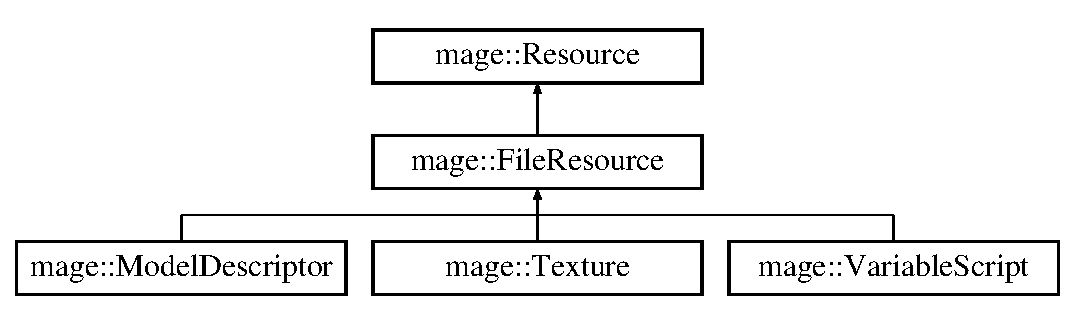
\includegraphics[height=2.800000cm]{classmage_1_1_file_resource}
\end{center}
\end{figure}
\subsection*{Public Member Functions}
\begin{DoxyCompactItemize}
\item 
\hyperlink{classmage_1_1_file_resource_ab126d9301d81c55b2aaacff86437e2d4}{File\+Resource} (const wstring \&fname)
\item 
\hyperlink{classmage_1_1_file_resource_a5aa20ee42fcfc4ee6877438ed7377930}{File\+Resource} (const \hyperlink{classmage_1_1_file_resource}{File\+Resource} \&file\+\_\+resource)=delete
\item 
\hyperlink{classmage_1_1_file_resource_a8022b27741face9debe1e8ccb1bc54e3}{File\+Resource} (\hyperlink{classmage_1_1_file_resource}{File\+Resource} \&\&file\+\_\+resource)
\item 
virtual \hyperlink{classmage_1_1_file_resource_a864fc0373785b1d5a82fecdc3aee7e46}{$\sim$\+File\+Resource} ()
\item 
\hyperlink{classmage_1_1_file_resource}{File\+Resource} \& \hyperlink{classmage_1_1_file_resource_a195da42fa3a40991e7c38cf8305b0bf2}{operator=} (const \hyperlink{classmage_1_1_file_resource}{File\+Resource} \&file\+\_\+resource)=delete
\item 
\hyperlink{classmage_1_1_file_resource}{File\+Resource} \& \hyperlink{classmage_1_1_file_resource_a7ec207d6e9cb0bc4b8020aa73df986b6}{operator=} (\hyperlink{classmage_1_1_file_resource}{File\+Resource} \&\&file\+\_\+resource)=delete
\item 
const wstring \& \hyperlink{classmage_1_1_file_resource_a25607552b782ae252851311d9b07fcd7}{Get\+Filename} () const noexcept
\item 
const wstring \hyperlink{classmage_1_1_file_resource_af53d0744d4c952286b7c00d63b9f0fb8}{Get\+Name} () const noexcept
\item 
const wstring \hyperlink{classmage_1_1_file_resource_a5c7d183fb6e55d6c91b6b336c68ffc82}{Get\+Path} () const noexcept
\end{DoxyCompactItemize}


\subsection{Detailed Description}
A class of file resources. 

\subsection{Constructor \& Destructor Documentation}
\hypertarget{classmage_1_1_file_resource_ab126d9301d81c55b2aaacff86437e2d4}{}\label{classmage_1_1_file_resource_ab126d9301d81c55b2aaacff86437e2d4} 
\index{mage\+::\+File\+Resource@{mage\+::\+File\+Resource}!File\+Resource@{File\+Resource}}
\index{File\+Resource@{File\+Resource}!mage\+::\+File\+Resource@{mage\+::\+File\+Resource}}
\subsubsection{\texorpdfstring{File\+Resource()}{FileResource()}\hspace{0.1cm}{\footnotesize\ttfamily [1/3]}}
{\footnotesize\ttfamily mage\+::\+File\+Resource\+::\+File\+Resource (\begin{DoxyParamCaption}\item[{const wstring \&}]{fname }\end{DoxyParamCaption})\hspace{0.3cm}{\ttfamily [explicit]}}

Constructs a file resource with a given filename.


\begin{DoxyParams}[1]{Parameters}
\mbox{\tt in}  & {\em fname} & A reference to the filename. \\
\hline
\end{DoxyParams}
\hypertarget{classmage_1_1_file_resource_a5aa20ee42fcfc4ee6877438ed7377930}{}\label{classmage_1_1_file_resource_a5aa20ee42fcfc4ee6877438ed7377930} 
\index{mage\+::\+File\+Resource@{mage\+::\+File\+Resource}!File\+Resource@{File\+Resource}}
\index{File\+Resource@{File\+Resource}!mage\+::\+File\+Resource@{mage\+::\+File\+Resource}}
\subsubsection{\texorpdfstring{File\+Resource()}{FileResource()}\hspace{0.1cm}{\footnotesize\ttfamily [2/3]}}
{\footnotesize\ttfamily mage\+::\+File\+Resource\+::\+File\+Resource (\begin{DoxyParamCaption}\item[{const \hyperlink{classmage_1_1_file_resource}{File\+Resource} \&}]{file\+\_\+resource }\end{DoxyParamCaption})\hspace{0.3cm}{\ttfamily [delete]}}

Constructs a file resource from the given file resource.


\begin{DoxyParams}[1]{Parameters}
\mbox{\tt in}  & {\em file\+\_\+resource} & A reference to the file resource to copy. \\
\hline
\end{DoxyParams}
\hypertarget{classmage_1_1_file_resource_a8022b27741face9debe1e8ccb1bc54e3}{}\label{classmage_1_1_file_resource_a8022b27741face9debe1e8ccb1bc54e3} 
\index{mage\+::\+File\+Resource@{mage\+::\+File\+Resource}!File\+Resource@{File\+Resource}}
\index{File\+Resource@{File\+Resource}!mage\+::\+File\+Resource@{mage\+::\+File\+Resource}}
\subsubsection{\texorpdfstring{File\+Resource()}{FileResource()}\hspace{0.1cm}{\footnotesize\ttfamily [3/3]}}
{\footnotesize\ttfamily mage\+::\+File\+Resource\+::\+File\+Resource (\begin{DoxyParamCaption}\item[{\hyperlink{classmage_1_1_file_resource}{File\+Resource} \&\&}]{file\+\_\+resource }\end{DoxyParamCaption})\hspace{0.3cm}{\ttfamily [default]}}

Constructs a file resource by moving the given file resource.


\begin{DoxyParams}[1]{Parameters}
\mbox{\tt in}  & {\em file\+\_\+resource} & A reference to the file resource to move. \\
\hline
\end{DoxyParams}
\hypertarget{classmage_1_1_file_resource_a864fc0373785b1d5a82fecdc3aee7e46}{}\label{classmage_1_1_file_resource_a864fc0373785b1d5a82fecdc3aee7e46} 
\index{mage\+::\+File\+Resource@{mage\+::\+File\+Resource}!````~File\+Resource@{$\sim$\+File\+Resource}}
\index{````~File\+Resource@{$\sim$\+File\+Resource}!mage\+::\+File\+Resource@{mage\+::\+File\+Resource}}
\subsubsection{\texorpdfstring{$\sim$\+File\+Resource()}{~FileResource()}}
{\footnotesize\ttfamily mage\+::\+File\+Resource\+::$\sim$\+File\+Resource (\begin{DoxyParamCaption}{ }\end{DoxyParamCaption})\hspace{0.3cm}{\ttfamily [virtual]}, {\ttfamily [default]}}

Destructs this file resource. 

\subsection{Member Function Documentation}
\hypertarget{classmage_1_1_file_resource_a25607552b782ae252851311d9b07fcd7}{}\label{classmage_1_1_file_resource_a25607552b782ae252851311d9b07fcd7} 
\index{mage\+::\+File\+Resource@{mage\+::\+File\+Resource}!Get\+Filename@{Get\+Filename}}
\index{Get\+Filename@{Get\+Filename}!mage\+::\+File\+Resource@{mage\+::\+File\+Resource}}
\subsubsection{\texorpdfstring{Get\+Filename()}{GetFilename()}}
{\footnotesize\ttfamily const wstring\& mage\+::\+File\+Resource\+::\+Get\+Filename (\begin{DoxyParamCaption}{ }\end{DoxyParamCaption}) const\hspace{0.3cm}{\ttfamily [noexcept]}}

Returns the filename of this file resource.

\begin{DoxyReturn}{Returns}
A reference to the filename of this file resource. 
\end{DoxyReturn}
\hypertarget{classmage_1_1_file_resource_af53d0744d4c952286b7c00d63b9f0fb8}{}\label{classmage_1_1_file_resource_af53d0744d4c952286b7c00d63b9f0fb8} 
\index{mage\+::\+File\+Resource@{mage\+::\+File\+Resource}!Get\+Name@{Get\+Name}}
\index{Get\+Name@{Get\+Name}!mage\+::\+File\+Resource@{mage\+::\+File\+Resource}}
\subsubsection{\texorpdfstring{Get\+Name()}{GetName()}}
{\footnotesize\ttfamily const wstring mage\+::\+File\+Resource\+::\+Get\+Name (\begin{DoxyParamCaption}{ }\end{DoxyParamCaption}) const\hspace{0.3cm}{\ttfamily [noexcept]}}

Returns the name of this file resource.

\begin{DoxyReturn}{Returns}
The name of this file resource. 
\end{DoxyReturn}
\hypertarget{classmage_1_1_file_resource_a5c7d183fb6e55d6c91b6b336c68ffc82}{}\label{classmage_1_1_file_resource_a5c7d183fb6e55d6c91b6b336c68ffc82} 
\index{mage\+::\+File\+Resource@{mage\+::\+File\+Resource}!Get\+Path@{Get\+Path}}
\index{Get\+Path@{Get\+Path}!mage\+::\+File\+Resource@{mage\+::\+File\+Resource}}
\subsubsection{\texorpdfstring{Get\+Path()}{GetPath()}}
{\footnotesize\ttfamily const wstring mage\+::\+File\+Resource\+::\+Get\+Path (\begin{DoxyParamCaption}{ }\end{DoxyParamCaption}) const\hspace{0.3cm}{\ttfamily [noexcept]}}

Returns the path of this file resource.

\begin{DoxyReturn}{Returns}
The path of this file resource. 
\end{DoxyReturn}
\hypertarget{classmage_1_1_file_resource_a195da42fa3a40991e7c38cf8305b0bf2}{}\label{classmage_1_1_file_resource_a195da42fa3a40991e7c38cf8305b0bf2} 
\index{mage\+::\+File\+Resource@{mage\+::\+File\+Resource}!operator=@{operator=}}
\index{operator=@{operator=}!mage\+::\+File\+Resource@{mage\+::\+File\+Resource}}
\subsubsection{\texorpdfstring{operator=()}{operator=()}\hspace{0.1cm}{\footnotesize\ttfamily [1/2]}}
{\footnotesize\ttfamily \hyperlink{classmage_1_1_file_resource}{File\+Resource}\& mage\+::\+File\+Resource\+::operator= (\begin{DoxyParamCaption}\item[{const \hyperlink{classmage_1_1_file_resource}{File\+Resource} \&}]{file\+\_\+resource }\end{DoxyParamCaption})\hspace{0.3cm}{\ttfamily [delete]}}

Copies the given file resource to this file resource.


\begin{DoxyParams}[1]{Parameters}
\mbox{\tt in}  & {\em file\+\_\+resource} & A reference to the file resource to copy. \\
\hline
\end{DoxyParams}
\begin{DoxyReturn}{Returns}
A reference to the copy of the given file resource (i.\+e. this file resource). 
\end{DoxyReturn}
\hypertarget{classmage_1_1_file_resource_a7ec207d6e9cb0bc4b8020aa73df986b6}{}\label{classmage_1_1_file_resource_a7ec207d6e9cb0bc4b8020aa73df986b6} 
\index{mage\+::\+File\+Resource@{mage\+::\+File\+Resource}!operator=@{operator=}}
\index{operator=@{operator=}!mage\+::\+File\+Resource@{mage\+::\+File\+Resource}}
\subsubsection{\texorpdfstring{operator=()}{operator=()}\hspace{0.1cm}{\footnotesize\ttfamily [2/2]}}
{\footnotesize\ttfamily \hyperlink{classmage_1_1_file_resource}{File\+Resource}\& mage\+::\+File\+Resource\+::operator= (\begin{DoxyParamCaption}\item[{\hyperlink{classmage_1_1_file_resource}{File\+Resource} \&\&}]{file\+\_\+resource }\end{DoxyParamCaption})\hspace{0.3cm}{\ttfamily [delete]}}

Moves the given file resource to this file resource.


\begin{DoxyParams}[1]{Parameters}
\mbox{\tt in}  & {\em file\+\_\+resource} & A reference to the file resource to move. \\
\hline
\end{DoxyParams}
\begin{DoxyReturn}{Returns}
A reference to the moved file resource (i.\+e. this file resource). 
\end{DoxyReturn}

\hypertarget{structmage_1_1_file_stream_closer}{}\section{mage\+:\+:File\+Stream\+Closer Struct Reference}
\label{structmage_1_1_file_stream_closer}\index{mage\+::\+File\+Stream\+Closer@{mage\+::\+File\+Stream\+Closer}}


{\ttfamily \#include $<$memory.\+hpp$>$}

\subsection*{Public Member Functions}
\begin{DoxyCompactItemize}
\item 
void \hyperlink{structmage_1_1_file_stream_closer_a87ef6007ca4e576a96f36c5fd003a386}{operator()} (F\+I\+LE $\ast$stream) const noexcept
\end{DoxyCompactItemize}


\subsection{Detailed Description}
A struct of file stream destructors (i.\+e. for closing file streams). 

\subsection{Member Function Documentation}
\hypertarget{structmage_1_1_file_stream_closer_a87ef6007ca4e576a96f36c5fd003a386}{}\label{structmage_1_1_file_stream_closer_a87ef6007ca4e576a96f36c5fd003a386} 
\index{mage\+::\+File\+Stream\+Closer@{mage\+::\+File\+Stream\+Closer}!operator()@{operator()}}
\index{operator()@{operator()}!mage\+::\+File\+Stream\+Closer@{mage\+::\+File\+Stream\+Closer}}
\subsubsection{\texorpdfstring{operator()()}{operator()()}}
{\footnotesize\ttfamily void mage\+::\+File\+Stream\+Closer\+::operator() (\begin{DoxyParamCaption}\item[{F\+I\+LE $\ast$}]{stream }\end{DoxyParamCaption}) const\hspace{0.3cm}{\ttfamily [noexcept]}}

Destructs the file stream.


\begin{DoxyParams}[1]{Parameters}
\mbox{\tt in}  & {\em stream} & A pointer to a file stream to destruct. \\
\hline
\end{DoxyParams}

\hypertarget{structmage_1_1_formatted_exception}{}\section{mage\+:\+:Formatted\+Exception Struct Reference}
\label{structmage_1_1_formatted_exception}\index{mage\+::\+Formatted\+Exception@{mage\+::\+Formatted\+Exception}}


{\ttfamily \#include $<$exception.\+hpp$>$}

Inheritance diagram for mage\+:\+:Formatted\+Exception\+:\begin{figure}[H]
\begin{center}
\leavevmode
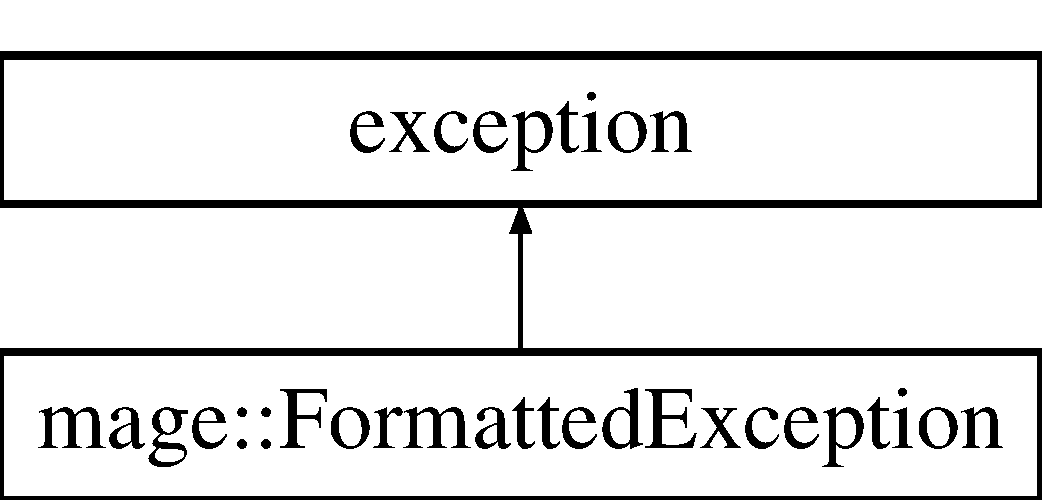
\includegraphics[height=2.000000cm]{structmage_1_1_formatted_exception}
\end{center}
\end{figure}
\subsection*{Public Member Functions}
\begin{DoxyCompactItemize}
\item 
\hyperlink{structmage_1_1_formatted_exception_a77b82a969ec33a3aacec74a5adc4ab8b}{Formatted\+Exception} ()
\item 
\hyperlink{structmage_1_1_formatted_exception_a3fe833a49052a2db99c023b1b1d43621}{Formatted\+Exception} (const char $\ast$format,...)
\item 
\hyperlink{structmage_1_1_formatted_exception_afd5d6b7a9db65b127badbf498186ebe8}{Formatted\+Exception} (const \hyperlink{structmage_1_1_formatted_exception}{Formatted\+Exception} \&formatted\+\_\+exception)
\item 
\hyperlink{structmage_1_1_formatted_exception_ab1371b0a079fc50fcae39722e5e29cb2}{Formatted\+Exception} (\hyperlink{structmage_1_1_formatted_exception}{Formatted\+Exception} \&\&formatted\+\_\+exception)
\item 
virtual \hyperlink{structmage_1_1_formatted_exception_a7bd56fe92b62d08b5ca4fb86592f1302}{$\sim$\+Formatted\+Exception} ()
\item 
\hyperlink{structmage_1_1_formatted_exception}{Formatted\+Exception} \& \hyperlink{structmage_1_1_formatted_exception_acc0ecbe1d510c5103ff4fd5b7054213b}{operator=} (const \hyperlink{structmage_1_1_formatted_exception}{Formatted\+Exception} \&formatted\+\_\+exception)
\item 
\hyperlink{structmage_1_1_formatted_exception}{Formatted\+Exception} \& \hyperlink{structmage_1_1_formatted_exception_aed7565e923543206710aa5f71ba5893a}{operator=} (\hyperlink{structmage_1_1_formatted_exception}{Formatted\+Exception} \&\&formatted\+\_\+exception)
\item 
virtual const char $\ast$ \hyperlink{structmage_1_1_formatted_exception_af24583c71b3cb760039f35d534b95ead}{what} () const noexcept override
\end{DoxyCompactItemize}
\subsection*{Private Attributes}
\begin{DoxyCompactItemize}
\item 
char \hyperlink{structmage_1_1_formatted_exception_aadccdcc1db09285dadc6b5a30681e05b}{m\+\_\+text} \mbox{[}2048\mbox{]}
\end{DoxyCompactItemize}


\subsection{Detailed Description}
A class of formatted exceptions. 

\subsection{Constructor \& Destructor Documentation}
\hypertarget{structmage_1_1_formatted_exception_a77b82a969ec33a3aacec74a5adc4ab8b}{}\label{structmage_1_1_formatted_exception_a77b82a969ec33a3aacec74a5adc4ab8b} 
\index{mage\+::\+Formatted\+Exception@{mage\+::\+Formatted\+Exception}!Formatted\+Exception@{Formatted\+Exception}}
\index{Formatted\+Exception@{Formatted\+Exception}!mage\+::\+Formatted\+Exception@{mage\+::\+Formatted\+Exception}}
\subsubsection{\texorpdfstring{Formatted\+Exception()}{FormattedException()}\hspace{0.1cm}{\footnotesize\ttfamily [1/4]}}
{\footnotesize\ttfamily mage\+::\+Formatted\+Exception\+::\+Formatted\+Exception (\begin{DoxyParamCaption}{ }\end{DoxyParamCaption})}

Constructs a formatted exception. \hypertarget{structmage_1_1_formatted_exception_a3fe833a49052a2db99c023b1b1d43621}{}\label{structmage_1_1_formatted_exception_a3fe833a49052a2db99c023b1b1d43621} 
\index{mage\+::\+Formatted\+Exception@{mage\+::\+Formatted\+Exception}!Formatted\+Exception@{Formatted\+Exception}}
\index{Formatted\+Exception@{Formatted\+Exception}!mage\+::\+Formatted\+Exception@{mage\+::\+Formatted\+Exception}}
\subsubsection{\texorpdfstring{Formatted\+Exception()}{FormattedException()}\hspace{0.1cm}{\footnotesize\ttfamily [2/4]}}
{\footnotesize\ttfamily mage\+::\+Formatted\+Exception\+::\+Formatted\+Exception (\begin{DoxyParamCaption}\item[{const char $\ast$}]{format,  }\item[{}]{... }\end{DoxyParamCaption})\hspace{0.3cm}{\ttfamily [explicit]}}

Constructs a formatted exception.

\begin{DoxyPrecond}{Precondition}
{\itshape format} is not equal to {\ttfamily nullptr}. 
\end{DoxyPrecond}

\begin{DoxyParams}[1]{Parameters}
\mbox{\tt in}  & {\em format} & Pointer to the message format. \\
\hline
\end{DoxyParams}
\hypertarget{structmage_1_1_formatted_exception_afd5d6b7a9db65b127badbf498186ebe8}{}\label{structmage_1_1_formatted_exception_afd5d6b7a9db65b127badbf498186ebe8} 
\index{mage\+::\+Formatted\+Exception@{mage\+::\+Formatted\+Exception}!Formatted\+Exception@{Formatted\+Exception}}
\index{Formatted\+Exception@{Formatted\+Exception}!mage\+::\+Formatted\+Exception@{mage\+::\+Formatted\+Exception}}
\subsubsection{\texorpdfstring{Formatted\+Exception()}{FormattedException()}\hspace{0.1cm}{\footnotesize\ttfamily [3/4]}}
{\footnotesize\ttfamily mage\+::\+Formatted\+Exception\+::\+Formatted\+Exception (\begin{DoxyParamCaption}\item[{const \hyperlink{structmage_1_1_formatted_exception}{Formatted\+Exception} \&}]{formatted\+\_\+exception }\end{DoxyParamCaption})\hspace{0.3cm}{\ttfamily [default]}}

Constructs a formatted exception from the given formatted exception.


\begin{DoxyParams}[1]{Parameters}
\mbox{\tt in}  & {\em formatted\+\_\+exception} & A reference to a formatted exception to copy. \\
\hline
\end{DoxyParams}
\hypertarget{structmage_1_1_formatted_exception_ab1371b0a079fc50fcae39722e5e29cb2}{}\label{structmage_1_1_formatted_exception_ab1371b0a079fc50fcae39722e5e29cb2} 
\index{mage\+::\+Formatted\+Exception@{mage\+::\+Formatted\+Exception}!Formatted\+Exception@{Formatted\+Exception}}
\index{Formatted\+Exception@{Formatted\+Exception}!mage\+::\+Formatted\+Exception@{mage\+::\+Formatted\+Exception}}
\subsubsection{\texorpdfstring{Formatted\+Exception()}{FormattedException()}\hspace{0.1cm}{\footnotesize\ttfamily [4/4]}}
{\footnotesize\ttfamily mage\+::\+Formatted\+Exception\+::\+Formatted\+Exception (\begin{DoxyParamCaption}\item[{\hyperlink{structmage_1_1_formatted_exception}{Formatted\+Exception} \&\&}]{formatted\+\_\+exception }\end{DoxyParamCaption})\hspace{0.3cm}{\ttfamily [default]}}

Constructs a formatted exception by moving the given formatted exception.


\begin{DoxyParams}[1]{Parameters}
\mbox{\tt in}  & {\em formatted\+\_\+exception} & A reference to a formatted exception to move. \\
\hline
\end{DoxyParams}
\hypertarget{structmage_1_1_formatted_exception_a7bd56fe92b62d08b5ca4fb86592f1302}{}\label{structmage_1_1_formatted_exception_a7bd56fe92b62d08b5ca4fb86592f1302} 
\index{mage\+::\+Formatted\+Exception@{mage\+::\+Formatted\+Exception}!````~Formatted\+Exception@{$\sim$\+Formatted\+Exception}}
\index{````~Formatted\+Exception@{$\sim$\+Formatted\+Exception}!mage\+::\+Formatted\+Exception@{mage\+::\+Formatted\+Exception}}
\subsubsection{\texorpdfstring{$\sim$\+Formatted\+Exception()}{~FormattedException()}}
{\footnotesize\ttfamily mage\+::\+Formatted\+Exception\+::$\sim$\+Formatted\+Exception (\begin{DoxyParamCaption}{ }\end{DoxyParamCaption})\hspace{0.3cm}{\ttfamily [virtual]}, {\ttfamily [default]}}

Destructs this formatted exception. 

\subsection{Member Function Documentation}
\hypertarget{structmage_1_1_formatted_exception_acc0ecbe1d510c5103ff4fd5b7054213b}{}\label{structmage_1_1_formatted_exception_acc0ecbe1d510c5103ff4fd5b7054213b} 
\index{mage\+::\+Formatted\+Exception@{mage\+::\+Formatted\+Exception}!operator=@{operator=}}
\index{operator=@{operator=}!mage\+::\+Formatted\+Exception@{mage\+::\+Formatted\+Exception}}
\subsubsection{\texorpdfstring{operator=()}{operator=()}\hspace{0.1cm}{\footnotesize\ttfamily [1/2]}}
{\footnotesize\ttfamily \hyperlink{structmage_1_1_formatted_exception}{Formatted\+Exception} \& mage\+::\+Formatted\+Exception\+::operator= (\begin{DoxyParamCaption}\item[{const \hyperlink{structmage_1_1_formatted_exception}{Formatted\+Exception} \&}]{formatted\+\_\+exception }\end{DoxyParamCaption})\hspace{0.3cm}{\ttfamily [default]}}

Copies the given formatted exception to this formatted exception.


\begin{DoxyParams}[1]{Parameters}
\mbox{\tt in}  & {\em formatted\+\_\+exception} & A reference to a formatted exception to copy. \\
\hline
\end{DoxyParams}
\begin{DoxyReturn}{Returns}
A reference to the copy of the given formatted exception (i.\+e. this formatted exception). 
\end{DoxyReturn}
\hypertarget{structmage_1_1_formatted_exception_aed7565e923543206710aa5f71ba5893a}{}\label{structmage_1_1_formatted_exception_aed7565e923543206710aa5f71ba5893a} 
\index{mage\+::\+Formatted\+Exception@{mage\+::\+Formatted\+Exception}!operator=@{operator=}}
\index{operator=@{operator=}!mage\+::\+Formatted\+Exception@{mage\+::\+Formatted\+Exception}}
\subsubsection{\texorpdfstring{operator=()}{operator=()}\hspace{0.1cm}{\footnotesize\ttfamily [2/2]}}
{\footnotesize\ttfamily \hyperlink{structmage_1_1_formatted_exception}{Formatted\+Exception} \& mage\+::\+Formatted\+Exception\+::operator= (\begin{DoxyParamCaption}\item[{\hyperlink{structmage_1_1_formatted_exception}{Formatted\+Exception} \&\&}]{formatted\+\_\+exception }\end{DoxyParamCaption})\hspace{0.3cm}{\ttfamily [default]}}

Moves the given formatted exception to this formatted exception.


\begin{DoxyParams}[1]{Parameters}
\mbox{\tt in}  & {\em formatted\+\_\+exception} & A reference to a formatted exception to move. \\
\hline
\end{DoxyParams}
\begin{DoxyReturn}{Returns}
A reference to the moved formatted exception (i.\+e. this formatted exception). 
\end{DoxyReturn}
\hypertarget{structmage_1_1_formatted_exception_af24583c71b3cb760039f35d534b95ead}{}\label{structmage_1_1_formatted_exception_af24583c71b3cb760039f35d534b95ead} 
\index{mage\+::\+Formatted\+Exception@{mage\+::\+Formatted\+Exception}!what@{what}}
\index{what@{what}!mage\+::\+Formatted\+Exception@{mage\+::\+Formatted\+Exception}}
\subsubsection{\texorpdfstring{what()}{what()}}
{\footnotesize\ttfamily virtual const char$\ast$ mage\+::\+Formatted\+Exception\+::what (\begin{DoxyParamCaption}{ }\end{DoxyParamCaption}) const\hspace{0.3cm}{\ttfamily [override]}, {\ttfamily [virtual]}, {\ttfamily [noexcept]}}

Returns a null-\/terminated byte string that may be used to identify the exception.

\begin{DoxyReturn}{Returns}
A null-\/terminated byte string that may be used to identify the exception. 
\end{DoxyReturn}


\subsection{Member Data Documentation}
\hypertarget{structmage_1_1_formatted_exception_aadccdcc1db09285dadc6b5a30681e05b}{}\label{structmage_1_1_formatted_exception_aadccdcc1db09285dadc6b5a30681e05b} 
\index{mage\+::\+Formatted\+Exception@{mage\+::\+Formatted\+Exception}!m\+\_\+text@{m\+\_\+text}}
\index{m\+\_\+text@{m\+\_\+text}!mage\+::\+Formatted\+Exception@{mage\+::\+Formatted\+Exception}}
\subsubsection{\texorpdfstring{m\+\_\+text}{m\_text}}
{\footnotesize\ttfamily char mage\+::\+Formatted\+Exception\+::m\+\_\+text\mbox{[}2048\mbox{]}\hspace{0.3cm}{\ttfamily [private]}}

The text buffer of this formatted exception. 
\hypertarget{classmage_1_1_f_p_s_input_controller_script}{}\section{mage\+:\+:F\+P\+S\+Input\+Controller\+Script Class Reference}
\label{classmage_1_1_f_p_s_input_controller_script}\index{mage\+::\+F\+P\+S\+Input\+Controller\+Script@{mage\+::\+F\+P\+S\+Input\+Controller\+Script}}


{\ttfamily \#include $<$fps\+\_\+input\+\_\+controller\+\_\+script.\+hpp$>$}

Inheritance diagram for mage\+:\+:F\+P\+S\+Input\+Controller\+Script\+:\begin{figure}[H]
\begin{center}
\leavevmode
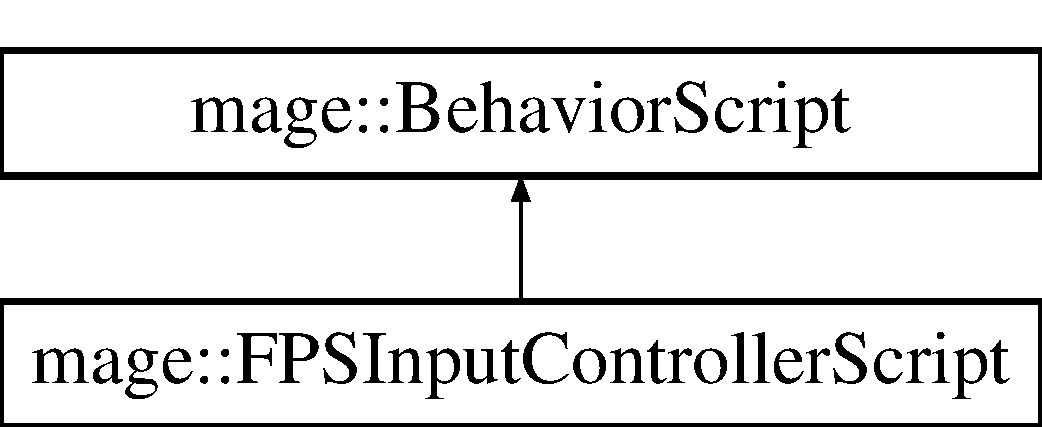
\includegraphics[height=2.000000cm]{classmage_1_1_f_p_s_input_controller_script}
\end{center}
\end{figure}
\subsection*{Public Member Functions}
\begin{DoxyCompactItemize}
\item 
\hyperlink{classmage_1_1_f_p_s_input_controller_script_a262c5e01549b86bdb7eb25be0da26413}{F\+P\+S\+Input\+Controller\+Script} (Transform $\ast$transform)
\item 
\hyperlink{classmage_1_1_f_p_s_input_controller_script_ad47bd24645ec8a7b08c3048c92ed56fd}{F\+P\+S\+Input\+Controller\+Script} (const \hyperlink{classmage_1_1_f_p_s_input_controller_script}{F\+P\+S\+Input\+Controller\+Script} \&script)=delete
\item 
\hyperlink{classmage_1_1_f_p_s_input_controller_script_acab23879d93819b2d4ccf98c16403c36}{F\+P\+S\+Input\+Controller\+Script} (\hyperlink{classmage_1_1_f_p_s_input_controller_script}{F\+P\+S\+Input\+Controller\+Script} \&\&script)=default
\item 
virtual \hyperlink{classmage_1_1_f_p_s_input_controller_script_af01f839ac9e214003de70732988de247}{$\sim$\+F\+P\+S\+Input\+Controller\+Script} ()=default
\item 
\hyperlink{classmage_1_1_f_p_s_input_controller_script}{F\+P\+S\+Input\+Controller\+Script} \& \hyperlink{classmage_1_1_f_p_s_input_controller_script_a226a1fb2eecbd7ecdf2033a8f5460e8b}{operator=} (const \hyperlink{classmage_1_1_f_p_s_input_controller_script}{F\+P\+S\+Input\+Controller\+Script} \&script)=delete
\item 
\hyperlink{classmage_1_1_f_p_s_input_controller_script}{F\+P\+S\+Input\+Controller\+Script} \& \hyperlink{classmage_1_1_f_p_s_input_controller_script_adac34abea3d474bf8183c2555dde9034}{operator=} (\hyperlink{classmage_1_1_f_p_s_input_controller_script}{F\+P\+S\+Input\+Controller\+Script} \&\&script)=delete
\item 
virtual void \hyperlink{classmage_1_1_f_p_s_input_controller_script_ab78955a67341970a41b21ae943b81585}{Update} (double delta\+\_\+time) override
\end{DoxyCompactItemize}
\subsection*{Private Attributes}
\begin{DoxyCompactItemize}
\item 
\hyperlink{namespacemage_a8c307fbcc33bce9b7f2aa4c26c3b95cf}{Unique\+Ptr}$<$ \hyperlink{classmage_1_1_mouse_look_script}{Mouse\+Look\+Script} $>$ \hyperlink{classmage_1_1_f_p_s_input_controller_script_a22d47829d2bf8ef73d20e531b3be4165}{m\+\_\+orientation\+\_\+script}
\item 
\hyperlink{namespacemage_a8c307fbcc33bce9b7f2aa4c26c3b95cf}{Unique\+Ptr}$<$ \hyperlink{classmage_1_1_character_motor_script}{Character\+Motor\+Script} $>$ \hyperlink{classmage_1_1_f_p_s_input_controller_script_adef81e743004c4c182ceb71f9bc35ab6}{m\+\_\+movement\+\_\+script}
\end{DoxyCompactItemize}
\subsection*{Additional Inherited Members}


\subsection{Constructor \& Destructor Documentation}
\hypertarget{classmage_1_1_f_p_s_input_controller_script_a262c5e01549b86bdb7eb25be0da26413}{}\label{classmage_1_1_f_p_s_input_controller_script_a262c5e01549b86bdb7eb25be0da26413} 
\index{mage\+::\+F\+P\+S\+Input\+Controller\+Script@{mage\+::\+F\+P\+S\+Input\+Controller\+Script}!F\+P\+S\+Input\+Controller\+Script@{F\+P\+S\+Input\+Controller\+Script}}
\index{F\+P\+S\+Input\+Controller\+Script@{F\+P\+S\+Input\+Controller\+Script}!mage\+::\+F\+P\+S\+Input\+Controller\+Script@{mage\+::\+F\+P\+S\+Input\+Controller\+Script}}
\subsubsection{\texorpdfstring{F\+P\+S\+Input\+Controller\+Script()}{FPSInputControllerScript()}\hspace{0.1cm}{\footnotesize\ttfamily [1/3]}}
{\footnotesize\ttfamily mage\+::\+F\+P\+S\+Input\+Controller\+Script\+::\+F\+P\+S\+Input\+Controller\+Script (\begin{DoxyParamCaption}\item[{Transform $\ast$}]{transform }\end{DoxyParamCaption})\hspace{0.3cm}{\ttfamily [explicit]}}

\hypertarget{classmage_1_1_f_p_s_input_controller_script_ad47bd24645ec8a7b08c3048c92ed56fd}{}\label{classmage_1_1_f_p_s_input_controller_script_ad47bd24645ec8a7b08c3048c92ed56fd} 
\index{mage\+::\+F\+P\+S\+Input\+Controller\+Script@{mage\+::\+F\+P\+S\+Input\+Controller\+Script}!F\+P\+S\+Input\+Controller\+Script@{F\+P\+S\+Input\+Controller\+Script}}
\index{F\+P\+S\+Input\+Controller\+Script@{F\+P\+S\+Input\+Controller\+Script}!mage\+::\+F\+P\+S\+Input\+Controller\+Script@{mage\+::\+F\+P\+S\+Input\+Controller\+Script}}
\subsubsection{\texorpdfstring{F\+P\+S\+Input\+Controller\+Script()}{FPSInputControllerScript()}\hspace{0.1cm}{\footnotesize\ttfamily [2/3]}}
{\footnotesize\ttfamily mage\+::\+F\+P\+S\+Input\+Controller\+Script\+::\+F\+P\+S\+Input\+Controller\+Script (\begin{DoxyParamCaption}\item[{const \hyperlink{classmage_1_1_f_p_s_input_controller_script}{F\+P\+S\+Input\+Controller\+Script} \&}]{script }\end{DoxyParamCaption})\hspace{0.3cm}{\ttfamily [delete]}}

\hypertarget{classmage_1_1_f_p_s_input_controller_script_acab23879d93819b2d4ccf98c16403c36}{}\label{classmage_1_1_f_p_s_input_controller_script_acab23879d93819b2d4ccf98c16403c36} 
\index{mage\+::\+F\+P\+S\+Input\+Controller\+Script@{mage\+::\+F\+P\+S\+Input\+Controller\+Script}!F\+P\+S\+Input\+Controller\+Script@{F\+P\+S\+Input\+Controller\+Script}}
\index{F\+P\+S\+Input\+Controller\+Script@{F\+P\+S\+Input\+Controller\+Script}!mage\+::\+F\+P\+S\+Input\+Controller\+Script@{mage\+::\+F\+P\+S\+Input\+Controller\+Script}}
\subsubsection{\texorpdfstring{F\+P\+S\+Input\+Controller\+Script()}{FPSInputControllerScript()}\hspace{0.1cm}{\footnotesize\ttfamily [3/3]}}
{\footnotesize\ttfamily mage\+::\+F\+P\+S\+Input\+Controller\+Script\+::\+F\+P\+S\+Input\+Controller\+Script (\begin{DoxyParamCaption}\item[{\hyperlink{classmage_1_1_f_p_s_input_controller_script}{F\+P\+S\+Input\+Controller\+Script} \&\&}]{script }\end{DoxyParamCaption})\hspace{0.3cm}{\ttfamily [default]}}

\hypertarget{classmage_1_1_f_p_s_input_controller_script_af01f839ac9e214003de70732988de247}{}\label{classmage_1_1_f_p_s_input_controller_script_af01f839ac9e214003de70732988de247} 
\index{mage\+::\+F\+P\+S\+Input\+Controller\+Script@{mage\+::\+F\+P\+S\+Input\+Controller\+Script}!````~F\+P\+S\+Input\+Controller\+Script@{$\sim$\+F\+P\+S\+Input\+Controller\+Script}}
\index{````~F\+P\+S\+Input\+Controller\+Script@{$\sim$\+F\+P\+S\+Input\+Controller\+Script}!mage\+::\+F\+P\+S\+Input\+Controller\+Script@{mage\+::\+F\+P\+S\+Input\+Controller\+Script}}
\subsubsection{\texorpdfstring{$\sim$\+F\+P\+S\+Input\+Controller\+Script()}{~FPSInputControllerScript()}}
{\footnotesize\ttfamily virtual mage\+::\+F\+P\+S\+Input\+Controller\+Script\+::$\sim$\+F\+P\+S\+Input\+Controller\+Script (\begin{DoxyParamCaption}{ }\end{DoxyParamCaption})\hspace{0.3cm}{\ttfamily [virtual]}, {\ttfamily [default]}}



\subsection{Member Function Documentation}
\hypertarget{classmage_1_1_f_p_s_input_controller_script_a226a1fb2eecbd7ecdf2033a8f5460e8b}{}\label{classmage_1_1_f_p_s_input_controller_script_a226a1fb2eecbd7ecdf2033a8f5460e8b} 
\index{mage\+::\+F\+P\+S\+Input\+Controller\+Script@{mage\+::\+F\+P\+S\+Input\+Controller\+Script}!operator=@{operator=}}
\index{operator=@{operator=}!mage\+::\+F\+P\+S\+Input\+Controller\+Script@{mage\+::\+F\+P\+S\+Input\+Controller\+Script}}
\subsubsection{\texorpdfstring{operator=()}{operator=()}\hspace{0.1cm}{\footnotesize\ttfamily [1/2]}}
{\footnotesize\ttfamily \hyperlink{classmage_1_1_f_p_s_input_controller_script}{F\+P\+S\+Input\+Controller\+Script}\& mage\+::\+F\+P\+S\+Input\+Controller\+Script\+::operator= (\begin{DoxyParamCaption}\item[{const \hyperlink{classmage_1_1_f_p_s_input_controller_script}{F\+P\+S\+Input\+Controller\+Script} \&}]{script }\end{DoxyParamCaption})\hspace{0.3cm}{\ttfamily [delete]}}

\hypertarget{classmage_1_1_f_p_s_input_controller_script_adac34abea3d474bf8183c2555dde9034}{}\label{classmage_1_1_f_p_s_input_controller_script_adac34abea3d474bf8183c2555dde9034} 
\index{mage\+::\+F\+P\+S\+Input\+Controller\+Script@{mage\+::\+F\+P\+S\+Input\+Controller\+Script}!operator=@{operator=}}
\index{operator=@{operator=}!mage\+::\+F\+P\+S\+Input\+Controller\+Script@{mage\+::\+F\+P\+S\+Input\+Controller\+Script}}
\subsubsection{\texorpdfstring{operator=()}{operator=()}\hspace{0.1cm}{\footnotesize\ttfamily [2/2]}}
{\footnotesize\ttfamily \hyperlink{classmage_1_1_f_p_s_input_controller_script}{F\+P\+S\+Input\+Controller\+Script}\& mage\+::\+F\+P\+S\+Input\+Controller\+Script\+::operator= (\begin{DoxyParamCaption}\item[{\hyperlink{classmage_1_1_f_p_s_input_controller_script}{F\+P\+S\+Input\+Controller\+Script} \&\&}]{script }\end{DoxyParamCaption})\hspace{0.3cm}{\ttfamily [delete]}}

\hypertarget{classmage_1_1_f_p_s_input_controller_script_ab78955a67341970a41b21ae943b81585}{}\label{classmage_1_1_f_p_s_input_controller_script_ab78955a67341970a41b21ae943b81585} 
\index{mage\+::\+F\+P\+S\+Input\+Controller\+Script@{mage\+::\+F\+P\+S\+Input\+Controller\+Script}!Update@{Update}}
\index{Update@{Update}!mage\+::\+F\+P\+S\+Input\+Controller\+Script@{mage\+::\+F\+P\+S\+Input\+Controller\+Script}}
\subsubsection{\texorpdfstring{Update()}{Update()}}
{\footnotesize\ttfamily virtual void mage\+::\+F\+P\+S\+Input\+Controller\+Script\+::\+Update (\begin{DoxyParamCaption}\item[{double}]{delta\+\_\+time }\end{DoxyParamCaption})\hspace{0.3cm}{\ttfamily [override]}, {\ttfamily [virtual]}}

Updates this behavior script.


\begin{DoxyParams}[1]{Parameters}
\mbox{\tt in}  & {\em delta\+\_\+time} & The elapsed time since the previous update. \\
\hline
\end{DoxyParams}


Implements \hyperlink{classmage_1_1_behavior_script_a905b6c83640cb91d19fecab3435f6feb}{mage\+::\+Behavior\+Script}.



\subsection{Member Data Documentation}
\hypertarget{classmage_1_1_f_p_s_input_controller_script_adef81e743004c4c182ceb71f9bc35ab6}{}\label{classmage_1_1_f_p_s_input_controller_script_adef81e743004c4c182ceb71f9bc35ab6} 
\index{mage\+::\+F\+P\+S\+Input\+Controller\+Script@{mage\+::\+F\+P\+S\+Input\+Controller\+Script}!m\+\_\+movement\+\_\+script@{m\+\_\+movement\+\_\+script}}
\index{m\+\_\+movement\+\_\+script@{m\+\_\+movement\+\_\+script}!mage\+::\+F\+P\+S\+Input\+Controller\+Script@{mage\+::\+F\+P\+S\+Input\+Controller\+Script}}
\subsubsection{\texorpdfstring{m\+\_\+movement\+\_\+script}{m\_movement\_script}}
{\footnotesize\ttfamily \hyperlink{namespacemage_a8c307fbcc33bce9b7f2aa4c26c3b95cf}{Unique\+Ptr}$<$ \hyperlink{classmage_1_1_character_motor_script}{Character\+Motor\+Script} $>$ mage\+::\+F\+P\+S\+Input\+Controller\+Script\+::m\+\_\+movement\+\_\+script\hspace{0.3cm}{\ttfamily [private]}}

\hypertarget{classmage_1_1_f_p_s_input_controller_script_a22d47829d2bf8ef73d20e531b3be4165}{}\label{classmage_1_1_f_p_s_input_controller_script_a22d47829d2bf8ef73d20e531b3be4165} 
\index{mage\+::\+F\+P\+S\+Input\+Controller\+Script@{mage\+::\+F\+P\+S\+Input\+Controller\+Script}!m\+\_\+orientation\+\_\+script@{m\+\_\+orientation\+\_\+script}}
\index{m\+\_\+orientation\+\_\+script@{m\+\_\+orientation\+\_\+script}!mage\+::\+F\+P\+S\+Input\+Controller\+Script@{mage\+::\+F\+P\+S\+Input\+Controller\+Script}}
\subsubsection{\texorpdfstring{m\+\_\+orientation\+\_\+script}{m\_orientation\_script}}
{\footnotesize\ttfamily \hyperlink{namespacemage_a8c307fbcc33bce9b7f2aa4c26c3b95cf}{Unique\+Ptr}$<$ \hyperlink{classmage_1_1_mouse_look_script}{Mouse\+Look\+Script} $>$ mage\+::\+F\+P\+S\+Input\+Controller\+Script\+::m\+\_\+orientation\+\_\+script\hspace{0.3cm}{\ttfamily [private]}}


\hypertarget{classmage_1_1_frame_rate_script}{}\section{mage\+:\+:Frame\+Rate\+Script Class Reference}
\label{classmage_1_1_frame_rate_script}\index{mage\+::\+Frame\+Rate\+Script@{mage\+::\+Frame\+Rate\+Script}}


{\ttfamily \#include $<$frame\+\_\+rate\+\_\+script.\+hpp$>$}

Inheritance diagram for mage\+:\+:Frame\+Rate\+Script\+:\begin{figure}[H]
\begin{center}
\leavevmode
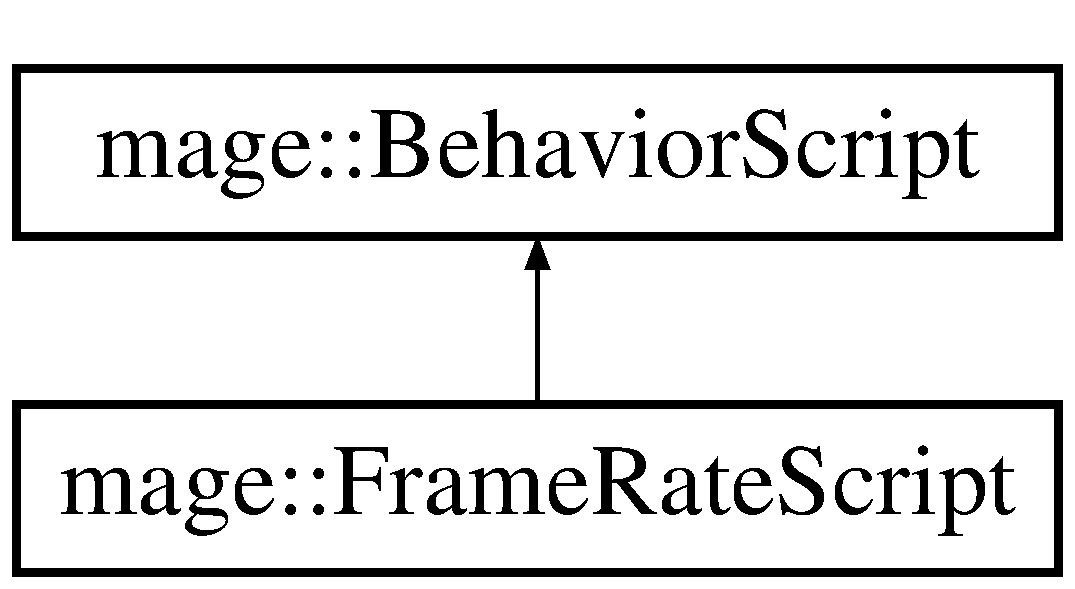
\includegraphics[height=2.000000cm]{classmage_1_1_frame_rate_script}
\end{center}
\end{figure}
\subsection*{Public Member Functions}
\begin{DoxyCompactItemize}
\item 
\hyperlink{classmage_1_1_frame_rate_script_a8ef13ffd08a684cbc2010b0e4594d4cf}{Frame\+Rate\+Script} (\hyperlink{namespacemage_a1e01ae66713838a7a67d30e44c67703e}{Shared\+Ptr}$<$ \hyperlink{classmage_1_1_sprite_text}{Sprite\+Text} $>$ text)
\item 
\hyperlink{classmage_1_1_frame_rate_script_a2c76a1ce175c5c5370582d7ccb878132}{Frame\+Rate\+Script} (const \hyperlink{classmage_1_1_frame_rate_script}{Frame\+Rate\+Script} \&script)=delete
\item 
\hyperlink{classmage_1_1_frame_rate_script_af2cb69b7338169598b80938e9ad77cdd}{Frame\+Rate\+Script} (\hyperlink{classmage_1_1_frame_rate_script}{Frame\+Rate\+Script} \&\&script)
\item 
virtual \hyperlink{classmage_1_1_frame_rate_script_a0863d9339500e10d988dd574448c28f3}{$\sim$\+Frame\+Rate\+Script} ()
\item 
\hyperlink{classmage_1_1_frame_rate_script}{Frame\+Rate\+Script} \& \hyperlink{classmage_1_1_frame_rate_script_a2077ec2facadcde117a20d18e2f0e9b7}{operator=} (const \hyperlink{classmage_1_1_frame_rate_script}{Frame\+Rate\+Script} \&script)=delete
\item 
\hyperlink{classmage_1_1_frame_rate_script}{Frame\+Rate\+Script} \& \hyperlink{classmage_1_1_frame_rate_script_a828664f89350ac0da2da3da26c05a6f0}{operator=} (\hyperlink{classmage_1_1_frame_rate_script}{Frame\+Rate\+Script} \&\&script)=delete
\item 
virtual void \hyperlink{classmage_1_1_frame_rate_script_a9bab0b26279823f1387428268b30e034}{Update} (double delta\+\_\+time) override
\end{DoxyCompactItemize}
\subsection*{Static Public Attributes}
\begin{DoxyCompactItemize}
\item 
static const double \hyperlink{classmage_1_1_frame_rate_script_ad28027c538faeab0c74bdb7b49f59469}{s\+\_\+resource\+\_\+fetch\+\_\+period} = 1.\+00
\end{DoxyCompactItemize}
\subsection*{Private Attributes}
\begin{DoxyCompactItemize}
\item 
double \hyperlink{classmage_1_1_frame_rate_script_ad2811547f84f1c62392e36fd8b82042d}{m\+\_\+accumulated\+\_\+time}
\item 
uint32\+\_\+t \hyperlink{classmage_1_1_frame_rate_script_a96dc980d017ad5e1b1f00db2526cd576}{m\+\_\+accumulated\+\_\+nb\+\_\+frames}
\item 
uint32\+\_\+t \hyperlink{classmage_1_1_frame_rate_script_a6126772a3b500a0c044837f432d10976}{m\+\_\+last\+\_\+frames\+\_\+per\+\_\+second}
\item 
double \hyperlink{classmage_1_1_frame_rate_script_a648f07d3c0c140b311703cdb85c63435}{m\+\_\+last\+\_\+milliseconds\+\_\+per\+\_\+frame}
\item 
\hyperlink{namespacemage_a1e01ae66713838a7a67d30e44c67703e}{Shared\+Ptr}$<$ \hyperlink{classmage_1_1_sprite_text}{Sprite\+Text} $>$ \hyperlink{classmage_1_1_frame_rate_script_a7d55db21f500e92914293cd6850e3b53}{m\+\_\+text}
\end{DoxyCompactItemize}
\subsection*{Additional Inherited Members}


\subsection{Constructor \& Destructor Documentation}
\hypertarget{classmage_1_1_frame_rate_script_a8ef13ffd08a684cbc2010b0e4594d4cf}{}\label{classmage_1_1_frame_rate_script_a8ef13ffd08a684cbc2010b0e4594d4cf} 
\index{mage\+::\+Frame\+Rate\+Script@{mage\+::\+Frame\+Rate\+Script}!Frame\+Rate\+Script@{Frame\+Rate\+Script}}
\index{Frame\+Rate\+Script@{Frame\+Rate\+Script}!mage\+::\+Frame\+Rate\+Script@{mage\+::\+Frame\+Rate\+Script}}
\subsubsection{\texorpdfstring{Frame\+Rate\+Script()}{FrameRateScript()}\hspace{0.1cm}{\footnotesize\ttfamily [1/3]}}
{\footnotesize\ttfamily mage\+::\+Frame\+Rate\+Script\+::\+Frame\+Rate\+Script (\begin{DoxyParamCaption}\item[{\hyperlink{namespacemage_a1e01ae66713838a7a67d30e44c67703e}{Shared\+Ptr}$<$ \hyperlink{classmage_1_1_sprite_text}{Sprite\+Text} $>$}]{text }\end{DoxyParamCaption})\hspace{0.3cm}{\ttfamily [explicit]}}

\hypertarget{classmage_1_1_frame_rate_script_a2c76a1ce175c5c5370582d7ccb878132}{}\label{classmage_1_1_frame_rate_script_a2c76a1ce175c5c5370582d7ccb878132} 
\index{mage\+::\+Frame\+Rate\+Script@{mage\+::\+Frame\+Rate\+Script}!Frame\+Rate\+Script@{Frame\+Rate\+Script}}
\index{Frame\+Rate\+Script@{Frame\+Rate\+Script}!mage\+::\+Frame\+Rate\+Script@{mage\+::\+Frame\+Rate\+Script}}
\subsubsection{\texorpdfstring{Frame\+Rate\+Script()}{FrameRateScript()}\hspace{0.1cm}{\footnotesize\ttfamily [2/3]}}
{\footnotesize\ttfamily mage\+::\+Frame\+Rate\+Script\+::\+Frame\+Rate\+Script (\begin{DoxyParamCaption}\item[{const \hyperlink{classmage_1_1_frame_rate_script}{Frame\+Rate\+Script} \&}]{script }\end{DoxyParamCaption})\hspace{0.3cm}{\ttfamily [delete]}}

\hypertarget{classmage_1_1_frame_rate_script_af2cb69b7338169598b80938e9ad77cdd}{}\label{classmage_1_1_frame_rate_script_af2cb69b7338169598b80938e9ad77cdd} 
\index{mage\+::\+Frame\+Rate\+Script@{mage\+::\+Frame\+Rate\+Script}!Frame\+Rate\+Script@{Frame\+Rate\+Script}}
\index{Frame\+Rate\+Script@{Frame\+Rate\+Script}!mage\+::\+Frame\+Rate\+Script@{mage\+::\+Frame\+Rate\+Script}}
\subsubsection{\texorpdfstring{Frame\+Rate\+Script()}{FrameRateScript()}\hspace{0.1cm}{\footnotesize\ttfamily [3/3]}}
{\footnotesize\ttfamily mage\+::\+Frame\+Rate\+Script\+::\+Frame\+Rate\+Script (\begin{DoxyParamCaption}\item[{\hyperlink{classmage_1_1_frame_rate_script}{Frame\+Rate\+Script} \&\&}]{script }\end{DoxyParamCaption})\hspace{0.3cm}{\ttfamily [default]}}

\hypertarget{classmage_1_1_frame_rate_script_a0863d9339500e10d988dd574448c28f3}{}\label{classmage_1_1_frame_rate_script_a0863d9339500e10d988dd574448c28f3} 
\index{mage\+::\+Frame\+Rate\+Script@{mage\+::\+Frame\+Rate\+Script}!````~Frame\+Rate\+Script@{$\sim$\+Frame\+Rate\+Script}}
\index{````~Frame\+Rate\+Script@{$\sim$\+Frame\+Rate\+Script}!mage\+::\+Frame\+Rate\+Script@{mage\+::\+Frame\+Rate\+Script}}
\subsubsection{\texorpdfstring{$\sim$\+Frame\+Rate\+Script()}{~FrameRateScript()}}
{\footnotesize\ttfamily mage\+::\+Frame\+Rate\+Script\+::$\sim$\+Frame\+Rate\+Script (\begin{DoxyParamCaption}{ }\end{DoxyParamCaption})\hspace{0.3cm}{\ttfamily [virtual]}, {\ttfamily [default]}}



\subsection{Member Function Documentation}
\hypertarget{classmage_1_1_frame_rate_script_a2077ec2facadcde117a20d18e2f0e9b7}{}\label{classmage_1_1_frame_rate_script_a2077ec2facadcde117a20d18e2f0e9b7} 
\index{mage\+::\+Frame\+Rate\+Script@{mage\+::\+Frame\+Rate\+Script}!operator=@{operator=}}
\index{operator=@{operator=}!mage\+::\+Frame\+Rate\+Script@{mage\+::\+Frame\+Rate\+Script}}
\subsubsection{\texorpdfstring{operator=()}{operator=()}\hspace{0.1cm}{\footnotesize\ttfamily [1/2]}}
{\footnotesize\ttfamily \hyperlink{classmage_1_1_frame_rate_script}{Frame\+Rate\+Script}\& mage\+::\+Frame\+Rate\+Script\+::operator= (\begin{DoxyParamCaption}\item[{const \hyperlink{classmage_1_1_frame_rate_script}{Frame\+Rate\+Script} \&}]{script }\end{DoxyParamCaption})\hspace{0.3cm}{\ttfamily [delete]}}

\hypertarget{classmage_1_1_frame_rate_script_a828664f89350ac0da2da3da26c05a6f0}{}\label{classmage_1_1_frame_rate_script_a828664f89350ac0da2da3da26c05a6f0} 
\index{mage\+::\+Frame\+Rate\+Script@{mage\+::\+Frame\+Rate\+Script}!operator=@{operator=}}
\index{operator=@{operator=}!mage\+::\+Frame\+Rate\+Script@{mage\+::\+Frame\+Rate\+Script}}
\subsubsection{\texorpdfstring{operator=()}{operator=()}\hspace{0.1cm}{\footnotesize\ttfamily [2/2]}}
{\footnotesize\ttfamily \hyperlink{classmage_1_1_frame_rate_script}{Frame\+Rate\+Script}\& mage\+::\+Frame\+Rate\+Script\+::operator= (\begin{DoxyParamCaption}\item[{\hyperlink{classmage_1_1_frame_rate_script}{Frame\+Rate\+Script} \&\&}]{script }\end{DoxyParamCaption})\hspace{0.3cm}{\ttfamily [delete]}}

\hypertarget{classmage_1_1_frame_rate_script_a9bab0b26279823f1387428268b30e034}{}\label{classmage_1_1_frame_rate_script_a9bab0b26279823f1387428268b30e034} 
\index{mage\+::\+Frame\+Rate\+Script@{mage\+::\+Frame\+Rate\+Script}!Update@{Update}}
\index{Update@{Update}!mage\+::\+Frame\+Rate\+Script@{mage\+::\+Frame\+Rate\+Script}}
\subsubsection{\texorpdfstring{Update()}{Update()}}
{\footnotesize\ttfamily void mage\+::\+Frame\+Rate\+Script\+::\+Update (\begin{DoxyParamCaption}\item[{double}]{delta\+\_\+time }\end{DoxyParamCaption})\hspace{0.3cm}{\ttfamily [override]}, {\ttfamily [virtual]}}

Updates this behavior script.


\begin{DoxyParams}[1]{Parameters}
\mbox{\tt in}  & {\em delta\+\_\+time} & The elapsed time since the previous update. \\
\hline
\end{DoxyParams}


Implements \hyperlink{classmage_1_1_behavior_script_a905b6c83640cb91d19fecab3435f6feb}{mage\+::\+Behavior\+Script}.



\subsection{Member Data Documentation}
\hypertarget{classmage_1_1_frame_rate_script_a96dc980d017ad5e1b1f00db2526cd576}{}\label{classmage_1_1_frame_rate_script_a96dc980d017ad5e1b1f00db2526cd576} 
\index{mage\+::\+Frame\+Rate\+Script@{mage\+::\+Frame\+Rate\+Script}!m\+\_\+accumulated\+\_\+nb\+\_\+frames@{m\+\_\+accumulated\+\_\+nb\+\_\+frames}}
\index{m\+\_\+accumulated\+\_\+nb\+\_\+frames@{m\+\_\+accumulated\+\_\+nb\+\_\+frames}!mage\+::\+Frame\+Rate\+Script@{mage\+::\+Frame\+Rate\+Script}}
\subsubsection{\texorpdfstring{m\+\_\+accumulated\+\_\+nb\+\_\+frames}{m\_accumulated\_nb\_frames}}
{\footnotesize\ttfamily uint32\+\_\+t mage\+::\+Frame\+Rate\+Script\+::m\+\_\+accumulated\+\_\+nb\+\_\+frames\hspace{0.3cm}{\ttfamily [private]}}

\hypertarget{classmage_1_1_frame_rate_script_ad2811547f84f1c62392e36fd8b82042d}{}\label{classmage_1_1_frame_rate_script_ad2811547f84f1c62392e36fd8b82042d} 
\index{mage\+::\+Frame\+Rate\+Script@{mage\+::\+Frame\+Rate\+Script}!m\+\_\+accumulated\+\_\+time@{m\+\_\+accumulated\+\_\+time}}
\index{m\+\_\+accumulated\+\_\+time@{m\+\_\+accumulated\+\_\+time}!mage\+::\+Frame\+Rate\+Script@{mage\+::\+Frame\+Rate\+Script}}
\subsubsection{\texorpdfstring{m\+\_\+accumulated\+\_\+time}{m\_accumulated\_time}}
{\footnotesize\ttfamily double mage\+::\+Frame\+Rate\+Script\+::m\+\_\+accumulated\+\_\+time\hspace{0.3cm}{\ttfamily [private]}}

\hypertarget{classmage_1_1_frame_rate_script_a6126772a3b500a0c044837f432d10976}{}\label{classmage_1_1_frame_rate_script_a6126772a3b500a0c044837f432d10976} 
\index{mage\+::\+Frame\+Rate\+Script@{mage\+::\+Frame\+Rate\+Script}!m\+\_\+last\+\_\+frames\+\_\+per\+\_\+second@{m\+\_\+last\+\_\+frames\+\_\+per\+\_\+second}}
\index{m\+\_\+last\+\_\+frames\+\_\+per\+\_\+second@{m\+\_\+last\+\_\+frames\+\_\+per\+\_\+second}!mage\+::\+Frame\+Rate\+Script@{mage\+::\+Frame\+Rate\+Script}}
\subsubsection{\texorpdfstring{m\+\_\+last\+\_\+frames\+\_\+per\+\_\+second}{m\_last\_frames\_per\_second}}
{\footnotesize\ttfamily uint32\+\_\+t mage\+::\+Frame\+Rate\+Script\+::m\+\_\+last\+\_\+frames\+\_\+per\+\_\+second\hspace{0.3cm}{\ttfamily [private]}}

\hypertarget{classmage_1_1_frame_rate_script_a648f07d3c0c140b311703cdb85c63435}{}\label{classmage_1_1_frame_rate_script_a648f07d3c0c140b311703cdb85c63435} 
\index{mage\+::\+Frame\+Rate\+Script@{mage\+::\+Frame\+Rate\+Script}!m\+\_\+last\+\_\+milliseconds\+\_\+per\+\_\+frame@{m\+\_\+last\+\_\+milliseconds\+\_\+per\+\_\+frame}}
\index{m\+\_\+last\+\_\+milliseconds\+\_\+per\+\_\+frame@{m\+\_\+last\+\_\+milliseconds\+\_\+per\+\_\+frame}!mage\+::\+Frame\+Rate\+Script@{mage\+::\+Frame\+Rate\+Script}}
\subsubsection{\texorpdfstring{m\+\_\+last\+\_\+milliseconds\+\_\+per\+\_\+frame}{m\_last\_milliseconds\_per\_frame}}
{\footnotesize\ttfamily double mage\+::\+Frame\+Rate\+Script\+::m\+\_\+last\+\_\+milliseconds\+\_\+per\+\_\+frame\hspace{0.3cm}{\ttfamily [private]}}

\hypertarget{classmage_1_1_frame_rate_script_a7d55db21f500e92914293cd6850e3b53}{}\label{classmage_1_1_frame_rate_script_a7d55db21f500e92914293cd6850e3b53} 
\index{mage\+::\+Frame\+Rate\+Script@{mage\+::\+Frame\+Rate\+Script}!m\+\_\+text@{m\+\_\+text}}
\index{m\+\_\+text@{m\+\_\+text}!mage\+::\+Frame\+Rate\+Script@{mage\+::\+Frame\+Rate\+Script}}
\subsubsection{\texorpdfstring{m\+\_\+text}{m\_text}}
{\footnotesize\ttfamily \hyperlink{namespacemage_a1e01ae66713838a7a67d30e44c67703e}{Shared\+Ptr}$<$ \hyperlink{classmage_1_1_sprite_text}{Sprite\+Text} $>$ mage\+::\+Frame\+Rate\+Script\+::m\+\_\+text\hspace{0.3cm}{\ttfamily [private]}}

\hypertarget{classmage_1_1_frame_rate_script_ad28027c538faeab0c74bdb7b49f59469}{}\label{classmage_1_1_frame_rate_script_ad28027c538faeab0c74bdb7b49f59469} 
\index{mage\+::\+Frame\+Rate\+Script@{mage\+::\+Frame\+Rate\+Script}!s\+\_\+resource\+\_\+fetch\+\_\+period@{s\+\_\+resource\+\_\+fetch\+\_\+period}}
\index{s\+\_\+resource\+\_\+fetch\+\_\+period@{s\+\_\+resource\+\_\+fetch\+\_\+period}!mage\+::\+Frame\+Rate\+Script@{mage\+::\+Frame\+Rate\+Script}}
\subsubsection{\texorpdfstring{s\+\_\+resource\+\_\+fetch\+\_\+period}{s\_resource\_fetch\_period}}
{\footnotesize\ttfamily const double mage\+::\+Frame\+Rate\+Script\+::s\+\_\+resource\+\_\+fetch\+\_\+period = 1.\+00\hspace{0.3cm}{\ttfamily [static]}}


\hypertarget{structmage_1_1_glyph}{}\section{mage\+:\+:Glyph Struct Reference}
\label{structmage_1_1_glyph}\index{mage\+::\+Glyph@{mage\+::\+Glyph}}


{\ttfamily \#include $<$glyph.\+hpp$>$}

\subsection*{Public Member Functions}
\begin{DoxyCompactItemize}
\item 
\hyperlink{structmage_1_1_glyph_aae91987833c1a89f6ce416d22544bb4b}{Glyph} () noexcept=default
\item 
\hyperlink{structmage_1_1_glyph_a6915f88bb426261e67f243629509f9a9}{Glyph} (const \hyperlink{structmage_1_1_glyph}{Glyph} \&glyph) noexcept=default
\item 
\hyperlink{structmage_1_1_glyph_a823494adc2f56bee49c3f9e498638f60}{Glyph} (\hyperlink{structmage_1_1_glyph}{Glyph} \&\&glyph) noexcept=default
\item 
\hyperlink{structmage_1_1_glyph_aa8e903334e77cc2930149923461d06ab}{$\sim$\+Glyph} ()=default
\item 
\hyperlink{structmage_1_1_glyph}{Glyph} \& \hyperlink{structmage_1_1_glyph_a4cc57bb9e8ba26d625b75e6557415f8d}{operator=} (const \hyperlink{structmage_1_1_glyph}{Glyph} \&glyph) noexcept=default
\item 
\hyperlink{structmage_1_1_glyph}{Glyph} \& \hyperlink{structmage_1_1_glyph_a7562e4fbcafb0633ec2c6db5b5160670}{operator=} (\hyperlink{structmage_1_1_glyph}{Glyph} \&\&glyph) noexcept=default
\item 
\hyperlink{namespacemage_a41c104c036fba3756a74e19f793eeaa1}{U32} \hyperlink{structmage_1_1_glyph_a672de806086fa9f23832d9f8e617fc3f}{Get\+Width} () const noexcept
\item 
\hyperlink{namespacemage_a41c104c036fba3756a74e19f793eeaa1}{U32} \hyperlink{structmage_1_1_glyph_a05deaaf61096d41cda1d85ef0488b36e}{Get\+Height} () const noexcept
\item 
bool \hyperlink{structmage_1_1_glyph_a7bb41307f74973e4bc547193dedc8dcc}{operator$<$} (const \hyperlink{structmage_1_1_glyph}{Glyph} \&rhs) const noexcept
\item 
bool \hyperlink{structmage_1_1_glyph_ad8e9835022217afef429f38891bba80e}{operator$<$} (wchar\+\_\+t rhs) const noexcept
\end{DoxyCompactItemize}
\subsection*{Public Attributes}
\begin{DoxyCompactItemize}
\item 
\hyperlink{namespacemage_a41c104c036fba3756a74e19f793eeaa1}{U32} \hyperlink{structmage_1_1_glyph_a1fc60ac3f30e27e5c7ccffa3b3bdd590}{m\+\_\+character}
\item 
R\+E\+CT \hyperlink{structmage_1_1_glyph_ac990dc92b5eebcc99da599f1a8d15bb4}{m\+\_\+sub\+\_\+rectangle}
\item 
\begin{tabbing}
xx\=xx\=xx\=xx\=xx\=xx\=xx\=xx\=xx\=\kill
union \{\\
\>struct \{\\
\>\>\hyperlink{namespacemage_aa97e833b45f06d60a0a9c4fc22ae02c0}{F32} \hyperlink{structmage_1_1_glyph_ac2972ac6759f912820f099fde31fe06c}{m\_offset\_x}\\
\>\>\hyperlink{namespacemage_aa97e833b45f06d60a0a9c4fc22ae02c0}{F32} \hyperlink{structmage_1_1_glyph_a45db4d78aeafa1278c2e9a17683a4cba}{m\_offset\_y}\\
\>\} \\
\>\hyperlink{namespacemage_aa97e833b45f06d60a0a9c4fc22ae02c0}{F32} \hyperlink{structmage_1_1_glyph_a7608c64db7a5f951a51d7e66e105638b}{m\_offsets} \mbox{[}2\mbox{]}\\
\}; \\

\end{tabbing}\item 
\hyperlink{namespacemage_aa97e833b45f06d60a0a9c4fc22ae02c0}{F32} \hyperlink{structmage_1_1_glyph_ac0905a82d2f5adefb7930359a0b3cef8}{m\+\_\+advance\+\_\+x}
\end{DoxyCompactItemize}


\subsection{Detailed Description}
A struct of glyphs. 

\subsection{Constructor \& Destructor Documentation}
\hypertarget{structmage_1_1_glyph_aae91987833c1a89f6ce416d22544bb4b}{}\label{structmage_1_1_glyph_aae91987833c1a89f6ce416d22544bb4b} 
\index{mage\+::\+Glyph@{mage\+::\+Glyph}!Glyph@{Glyph}}
\index{Glyph@{Glyph}!mage\+::\+Glyph@{mage\+::\+Glyph}}
\subsubsection{\texorpdfstring{Glyph()}{Glyph()}\hspace{0.1cm}{\footnotesize\ttfamily [1/3]}}
{\footnotesize\ttfamily mage\+::\+Glyph\+::\+Glyph (\begin{DoxyParamCaption}{ }\end{DoxyParamCaption})\hspace{0.3cm}{\ttfamily [default]}, {\ttfamily [noexcept]}}

Constructs a glyph. \hypertarget{structmage_1_1_glyph_a6915f88bb426261e67f243629509f9a9}{}\label{structmage_1_1_glyph_a6915f88bb426261e67f243629509f9a9} 
\index{mage\+::\+Glyph@{mage\+::\+Glyph}!Glyph@{Glyph}}
\index{Glyph@{Glyph}!mage\+::\+Glyph@{mage\+::\+Glyph}}
\subsubsection{\texorpdfstring{Glyph()}{Glyph()}\hspace{0.1cm}{\footnotesize\ttfamily [2/3]}}
{\footnotesize\ttfamily mage\+::\+Glyph\+::\+Glyph (\begin{DoxyParamCaption}\item[{const \hyperlink{structmage_1_1_glyph}{Glyph} \&}]{glyph }\end{DoxyParamCaption})\hspace{0.3cm}{\ttfamily [default]}, {\ttfamily [noexcept]}}

Constructs a glyph from the given glyph.


\begin{DoxyParams}[1]{Parameters}
\mbox{\tt in}  & {\em glyph} & A reference to the glyph to copy. \\
\hline
\end{DoxyParams}
\hypertarget{structmage_1_1_glyph_a823494adc2f56bee49c3f9e498638f60}{}\label{structmage_1_1_glyph_a823494adc2f56bee49c3f9e498638f60} 
\index{mage\+::\+Glyph@{mage\+::\+Glyph}!Glyph@{Glyph}}
\index{Glyph@{Glyph}!mage\+::\+Glyph@{mage\+::\+Glyph}}
\subsubsection{\texorpdfstring{Glyph()}{Glyph()}\hspace{0.1cm}{\footnotesize\ttfamily [3/3]}}
{\footnotesize\ttfamily mage\+::\+Glyph\+::\+Glyph (\begin{DoxyParamCaption}\item[{\hyperlink{structmage_1_1_glyph}{Glyph} \&\&}]{glyph }\end{DoxyParamCaption})\hspace{0.3cm}{\ttfamily [default]}, {\ttfamily [noexcept]}}

Constructs a glyph by moving the given glyph.


\begin{DoxyParams}[1]{Parameters}
\mbox{\tt in}  & {\em glyph} & A reference to the glyph to move. \\
\hline
\end{DoxyParams}
\hypertarget{structmage_1_1_glyph_aa8e903334e77cc2930149923461d06ab}{}\label{structmage_1_1_glyph_aa8e903334e77cc2930149923461d06ab} 
\index{mage\+::\+Glyph@{mage\+::\+Glyph}!````~Glyph@{$\sim$\+Glyph}}
\index{````~Glyph@{$\sim$\+Glyph}!mage\+::\+Glyph@{mage\+::\+Glyph}}
\subsubsection{\texorpdfstring{$\sim$\+Glyph()}{~Glyph()}}
{\footnotesize\ttfamily mage\+::\+Glyph\+::$\sim$\+Glyph (\begin{DoxyParamCaption}{ }\end{DoxyParamCaption})\hspace{0.3cm}{\ttfamily [default]}}

Destructs this glyph. 

\subsection{Member Function Documentation}
\hypertarget{structmage_1_1_glyph_a05deaaf61096d41cda1d85ef0488b36e}{}\label{structmage_1_1_glyph_a05deaaf61096d41cda1d85ef0488b36e} 
\index{mage\+::\+Glyph@{mage\+::\+Glyph}!Get\+Height@{Get\+Height}}
\index{Get\+Height@{Get\+Height}!mage\+::\+Glyph@{mage\+::\+Glyph}}
\subsubsection{\texorpdfstring{Get\+Height()}{GetHeight()}}
{\footnotesize\ttfamily \hyperlink{namespacemage_a41c104c036fba3756a74e19f793eeaa1}{U32} mage\+::\+Glyph\+::\+Get\+Height (\begin{DoxyParamCaption}{ }\end{DoxyParamCaption}) const\hspace{0.3cm}{\ttfamily [noexcept]}}

Returns the height of this glyph.

\begin{DoxyReturn}{Returns}
The height of this glyph. 
\end{DoxyReturn}
\hypertarget{structmage_1_1_glyph_a672de806086fa9f23832d9f8e617fc3f}{}\label{structmage_1_1_glyph_a672de806086fa9f23832d9f8e617fc3f} 
\index{mage\+::\+Glyph@{mage\+::\+Glyph}!Get\+Width@{Get\+Width}}
\index{Get\+Width@{Get\+Width}!mage\+::\+Glyph@{mage\+::\+Glyph}}
\subsubsection{\texorpdfstring{Get\+Width()}{GetWidth()}}
{\footnotesize\ttfamily \hyperlink{namespacemage_a41c104c036fba3756a74e19f793eeaa1}{U32} mage\+::\+Glyph\+::\+Get\+Width (\begin{DoxyParamCaption}{ }\end{DoxyParamCaption}) const\hspace{0.3cm}{\ttfamily [noexcept]}}

Returns the width of this glyph.

\begin{DoxyReturn}{Returns}
The width of this glyph. 
\end{DoxyReturn}
\hypertarget{structmage_1_1_glyph_a7bb41307f74973e4bc547193dedc8dcc}{}\label{structmage_1_1_glyph_a7bb41307f74973e4bc547193dedc8dcc} 
\index{mage\+::\+Glyph@{mage\+::\+Glyph}!operator$<$@{operator$<$}}
\index{operator$<$@{operator$<$}!mage\+::\+Glyph@{mage\+::\+Glyph}}
\subsubsection{\texorpdfstring{operator$<$()}{operator<()}\hspace{0.1cm}{\footnotesize\ttfamily [1/2]}}
{\footnotesize\ttfamily bool mage\+::\+Glyph\+::operator$<$ (\begin{DoxyParamCaption}\item[{const \hyperlink{structmage_1_1_glyph}{Glyph} \&}]{rhs }\end{DoxyParamCaption}) const\hspace{0.3cm}{\ttfamily [noexcept]}}

Checks whether this glyph\textquotesingle{}s character is smaller than the given glyph\textquotesingle{}s character.


\begin{DoxyParams}[1]{Parameters}
\mbox{\tt in}  & {\em rhs} & A reference to the glyph to compare against. \\
\hline
\end{DoxyParams}
\begin{DoxyReturn}{Returns}
{\ttfamily true} if the this glyph\textquotesingle{}s character is smaller than the given glyph\textquotesingle{}s character. {\ttfamily false} otherwise. 
\end{DoxyReturn}
\hypertarget{structmage_1_1_glyph_ad8e9835022217afef429f38891bba80e}{}\label{structmage_1_1_glyph_ad8e9835022217afef429f38891bba80e} 
\index{mage\+::\+Glyph@{mage\+::\+Glyph}!operator$<$@{operator$<$}}
\index{operator$<$@{operator$<$}!mage\+::\+Glyph@{mage\+::\+Glyph}}
\subsubsection{\texorpdfstring{operator$<$()}{operator<()}\hspace{0.1cm}{\footnotesize\ttfamily [2/2]}}
{\footnotesize\ttfamily bool mage\+::\+Glyph\+::operator$<$ (\begin{DoxyParamCaption}\item[{wchar\+\_\+t}]{rhs }\end{DoxyParamCaption}) const\hspace{0.3cm}{\ttfamily [noexcept]}}

Checks whether this glyph\textquotesingle{}s character is smaller than the given character.


\begin{DoxyParams}[1]{Parameters}
\mbox{\tt in}  & {\em rhs} & The character to compare against. \\
\hline
\end{DoxyParams}
\begin{DoxyReturn}{Returns}
{\ttfamily true} if the this glyph\textquotesingle{}s character is smaller than the given character. {\ttfamily false} otherwise. 
\end{DoxyReturn}
\hypertarget{structmage_1_1_glyph_a4cc57bb9e8ba26d625b75e6557415f8d}{}\label{structmage_1_1_glyph_a4cc57bb9e8ba26d625b75e6557415f8d} 
\index{mage\+::\+Glyph@{mage\+::\+Glyph}!operator=@{operator=}}
\index{operator=@{operator=}!mage\+::\+Glyph@{mage\+::\+Glyph}}
\subsubsection{\texorpdfstring{operator=()}{operator=()}\hspace{0.1cm}{\footnotesize\ttfamily [1/2]}}
{\footnotesize\ttfamily \hyperlink{structmage_1_1_glyph}{Glyph}\& mage\+::\+Glyph\+::operator= (\begin{DoxyParamCaption}\item[{const \hyperlink{structmage_1_1_glyph}{Glyph} \&}]{glyph }\end{DoxyParamCaption})\hspace{0.3cm}{\ttfamily [default]}, {\ttfamily [noexcept]}}

Copies the given glyph to this glyph.


\begin{DoxyParams}[1]{Parameters}
\mbox{\tt in}  & {\em glyph} & A reference to the glyph to copy. \\
\hline
\end{DoxyParams}
\begin{DoxyReturn}{Returns}
A reference to copy of the given glyph (i.\+e. this glyph). 
\end{DoxyReturn}
\hypertarget{structmage_1_1_glyph_a7562e4fbcafb0633ec2c6db5b5160670}{}\label{structmage_1_1_glyph_a7562e4fbcafb0633ec2c6db5b5160670} 
\index{mage\+::\+Glyph@{mage\+::\+Glyph}!operator=@{operator=}}
\index{operator=@{operator=}!mage\+::\+Glyph@{mage\+::\+Glyph}}
\subsubsection{\texorpdfstring{operator=()}{operator=()}\hspace{0.1cm}{\footnotesize\ttfamily [2/2]}}
{\footnotesize\ttfamily \hyperlink{structmage_1_1_glyph}{Glyph}\& mage\+::\+Glyph\+::operator= (\begin{DoxyParamCaption}\item[{\hyperlink{structmage_1_1_glyph}{Glyph} \&\&}]{glyph }\end{DoxyParamCaption})\hspace{0.3cm}{\ttfamily [default]}, {\ttfamily [noexcept]}}

Moves the given glyph to this glyph.


\begin{DoxyParams}[1]{Parameters}
\mbox{\tt in}  & {\em glyph} & A reference to the glyph to move. \\
\hline
\end{DoxyParams}
\begin{DoxyReturn}{Returns}
A reference to the moved glyph (i.\+e. this glyph). 
\end{DoxyReturn}


\subsection{Member Data Documentation}
\hypertarget{structmage_1_1_glyph_aa38d552d3a79706060b5dde53bd38881}{}\label{structmage_1_1_glyph_aa38d552d3a79706060b5dde53bd38881} 
\subsubsection{\texorpdfstring{"@1}{@1}}
{\footnotesize\ttfamily union \{ ... \} }

\hypertarget{structmage_1_1_glyph_ac0905a82d2f5adefb7930359a0b3cef8}{}\label{structmage_1_1_glyph_ac0905a82d2f5adefb7930359a0b3cef8} 
\index{mage\+::\+Glyph@{mage\+::\+Glyph}!m\+\_\+advance\+\_\+x@{m\+\_\+advance\+\_\+x}}
\index{m\+\_\+advance\+\_\+x@{m\+\_\+advance\+\_\+x}!mage\+::\+Glyph@{mage\+::\+Glyph}}
\subsubsection{\texorpdfstring{m\+\_\+advance\+\_\+x}{m\_advance\_x}}
{\footnotesize\ttfamily \hyperlink{namespacemage_aa97e833b45f06d60a0a9c4fc22ae02c0}{F32} mage\+::\+Glyph\+::m\+\_\+advance\+\_\+x}

The offset of this glyph to the right. \hypertarget{structmage_1_1_glyph_a1fc60ac3f30e27e5c7ccffa3b3bdd590}{}\label{structmage_1_1_glyph_a1fc60ac3f30e27e5c7ccffa3b3bdd590} 
\index{mage\+::\+Glyph@{mage\+::\+Glyph}!m\+\_\+character@{m\+\_\+character}}
\index{m\+\_\+character@{m\+\_\+character}!mage\+::\+Glyph@{mage\+::\+Glyph}}
\subsubsection{\texorpdfstring{m\+\_\+character}{m\_character}}
{\footnotesize\ttfamily \hyperlink{namespacemage_a41c104c036fba3756a74e19f793eeaa1}{U32} mage\+::\+Glyph\+::m\+\_\+character}

The character of this glyph. \hypertarget{structmage_1_1_glyph_ac2972ac6759f912820f099fde31fe06c}{}\label{structmage_1_1_glyph_ac2972ac6759f912820f099fde31fe06c} 
\index{mage\+::\+Glyph@{mage\+::\+Glyph}!m\+\_\+offset\+\_\+x@{m\+\_\+offset\+\_\+x}}
\index{m\+\_\+offset\+\_\+x@{m\+\_\+offset\+\_\+x}!mage\+::\+Glyph@{mage\+::\+Glyph}}
\subsubsection{\texorpdfstring{m\+\_\+offset\+\_\+x}{m\_offset\_x}}
{\footnotesize\ttfamily \hyperlink{namespacemage_aa97e833b45f06d60a0a9c4fc22ae02c0}{F32} mage\+::\+Glyph\+::m\+\_\+offset\+\_\+x}

The offset of this glyph from the left. \hypertarget{structmage_1_1_glyph_a45db4d78aeafa1278c2e9a17683a4cba}{}\label{structmage_1_1_glyph_a45db4d78aeafa1278c2e9a17683a4cba} 
\index{mage\+::\+Glyph@{mage\+::\+Glyph}!m\+\_\+offset\+\_\+y@{m\+\_\+offset\+\_\+y}}
\index{m\+\_\+offset\+\_\+y@{m\+\_\+offset\+\_\+y}!mage\+::\+Glyph@{mage\+::\+Glyph}}
\subsubsection{\texorpdfstring{m\+\_\+offset\+\_\+y}{m\_offset\_y}}
{\footnotesize\ttfamily \hyperlink{namespacemage_aa97e833b45f06d60a0a9c4fc22ae02c0}{F32} mage\+::\+Glyph\+::m\+\_\+offset\+\_\+y}

The offset of this glyph from the top. \hypertarget{structmage_1_1_glyph_a7608c64db7a5f951a51d7e66e105638b}{}\label{structmage_1_1_glyph_a7608c64db7a5f951a51d7e66e105638b} 
\index{mage\+::\+Glyph@{mage\+::\+Glyph}!m\+\_\+offsets@{m\+\_\+offsets}}
\index{m\+\_\+offsets@{m\+\_\+offsets}!mage\+::\+Glyph@{mage\+::\+Glyph}}
\subsubsection{\texorpdfstring{m\+\_\+offsets}{m\_offsets}}
{\footnotesize\ttfamily \hyperlink{namespacemage_aa97e833b45f06d60a0a9c4fc22ae02c0}{F32} mage\+::\+Glyph\+::m\+\_\+offsets\mbox{[}2\mbox{]}}

The offsets of this glyph. \hypertarget{structmage_1_1_glyph_ac990dc92b5eebcc99da599f1a8d15bb4}{}\label{structmage_1_1_glyph_ac990dc92b5eebcc99da599f1a8d15bb4} 
\index{mage\+::\+Glyph@{mage\+::\+Glyph}!m\+\_\+sub\+\_\+rectangle@{m\+\_\+sub\+\_\+rectangle}}
\index{m\+\_\+sub\+\_\+rectangle@{m\+\_\+sub\+\_\+rectangle}!mage\+::\+Glyph@{mage\+::\+Glyph}}
\subsubsection{\texorpdfstring{m\+\_\+sub\+\_\+rectangle}{m\_sub\_rectangle}}
{\footnotesize\ttfamily R\+E\+CT mage\+::\+Glyph\+::m\+\_\+sub\+\_\+rectangle}

The subrectangle of this glyph. 
\hypertarget{structmage_1_1_glyph_less_than}{}\section{mage\+:\+:Glyph\+Less\+Than Struct Reference}
\label{structmage_1_1_glyph_less_than}\index{mage\+::\+Glyph\+Less\+Than@{mage\+::\+Glyph\+Less\+Than}}
\subsection*{Public Member Functions}
\begin{DoxyCompactItemize}
\item 
bool \hyperlink{structmage_1_1_glyph_less_than_a7a8b5bb8d25f49790105ffee80cf2f71}{operator()} (const \hyperlink{structmage_1_1_glyph}{Glyph} \&lhs, const \hyperlink{structmage_1_1_glyph}{Glyph} \&rhs) noexcept
\item 
bool \hyperlink{structmage_1_1_glyph_less_than_a0ae04e2104bafaa37e951409a126a44f}{operator()} (const \hyperlink{structmage_1_1_glyph}{Glyph} \&lhs, wchar\+\_\+t rhs) noexcept
\item 
bool \hyperlink{structmage_1_1_glyph_less_than_a24f8a3b7cf190212a226fcf4900f558a}{operator()} (wchar\+\_\+t lhs, const \hyperlink{structmage_1_1_glyph}{Glyph} \&rhs) noexcept
\end{DoxyCompactItemize}


\subsection{Detailed Description}
A struct of glyph \char`\"{}less than\char`\"{} comparators. 

\subsection{Member Function Documentation}
\hypertarget{structmage_1_1_glyph_less_than_a7a8b5bb8d25f49790105ffee80cf2f71}{}\label{structmage_1_1_glyph_less_than_a7a8b5bb8d25f49790105ffee80cf2f71} 
\index{mage\+::\+Glyph\+Less\+Than@{mage\+::\+Glyph\+Less\+Than}!operator()@{operator()}}
\index{operator()@{operator()}!mage\+::\+Glyph\+Less\+Than@{mage\+::\+Glyph\+Less\+Than}}
\subsubsection{\texorpdfstring{operator()()}{operator()()}\hspace{0.1cm}{\footnotesize\ttfamily [1/3]}}
{\footnotesize\ttfamily bool mage\+::\+Glyph\+Less\+Than\+::operator() (\begin{DoxyParamCaption}\item[{const \hyperlink{structmage_1_1_glyph}{Glyph} \&}]{lhs,  }\item[{const \hyperlink{structmage_1_1_glyph}{Glyph} \&}]{rhs }\end{DoxyParamCaption})\hspace{0.3cm}{\ttfamily [noexcept]}}

Checks whether the first given glyph\textquotesingle{}s character is smaller than the second given glyph\textquotesingle{}s character.


\begin{DoxyParams}[1]{Parameters}
\mbox{\tt in}  & {\em lhs} & A reference to the first glyph. \\
\hline
\mbox{\tt in}  & {\em rhs} & A reference to the second glyph. \\
\hline
\end{DoxyParams}
\begin{DoxyReturn}{Returns}
{\ttfamily true} if the first given glyph\textquotesingle{}s character is smaller than the second given glyph\textquotesingle{}s character. {\ttfamily false} otherwise. 
\end{DoxyReturn}
\hypertarget{structmage_1_1_glyph_less_than_a0ae04e2104bafaa37e951409a126a44f}{}\label{structmage_1_1_glyph_less_than_a0ae04e2104bafaa37e951409a126a44f} 
\index{mage\+::\+Glyph\+Less\+Than@{mage\+::\+Glyph\+Less\+Than}!operator()@{operator()}}
\index{operator()@{operator()}!mage\+::\+Glyph\+Less\+Than@{mage\+::\+Glyph\+Less\+Than}}
\subsubsection{\texorpdfstring{operator()()}{operator()()}\hspace{0.1cm}{\footnotesize\ttfamily [2/3]}}
{\footnotesize\ttfamily bool mage\+::\+Glyph\+Less\+Than\+::operator() (\begin{DoxyParamCaption}\item[{const \hyperlink{structmage_1_1_glyph}{Glyph} \&}]{lhs,  }\item[{wchar\+\_\+t}]{rhs }\end{DoxyParamCaption})\hspace{0.3cm}{\ttfamily [noexcept]}}

Checks whether the given glyph\textquotesingle{}s character is smaller than the given character.


\begin{DoxyParams}[1]{Parameters}
\mbox{\tt in}  & {\em lhs} & A reference to the glyph. \\
\hline
\mbox{\tt in}  & {\em rhs} & The character. \\
\hline
\end{DoxyParams}
\begin{DoxyReturn}{Returns}
{\ttfamily true} if the given glyph\textquotesingle{}s character is smaller than the given character. {\ttfamily false} otherwise. 
\end{DoxyReturn}
\hypertarget{structmage_1_1_glyph_less_than_a24f8a3b7cf190212a226fcf4900f558a}{}\label{structmage_1_1_glyph_less_than_a24f8a3b7cf190212a226fcf4900f558a} 
\index{mage\+::\+Glyph\+Less\+Than@{mage\+::\+Glyph\+Less\+Than}!operator()@{operator()}}
\index{operator()@{operator()}!mage\+::\+Glyph\+Less\+Than@{mage\+::\+Glyph\+Less\+Than}}
\subsubsection{\texorpdfstring{operator()()}{operator()()}\hspace{0.1cm}{\footnotesize\ttfamily [3/3]}}
{\footnotesize\ttfamily bool mage\+::\+Glyph\+Less\+Than\+::operator() (\begin{DoxyParamCaption}\item[{wchar\+\_\+t}]{lhs,  }\item[{const \hyperlink{structmage_1_1_glyph}{Glyph} \&}]{rhs }\end{DoxyParamCaption})\hspace{0.3cm}{\ttfamily [noexcept]}}

Checks whether the given character is smaller than the given glyph\textquotesingle{}s character.


\begin{DoxyParams}[1]{Parameters}
\mbox{\tt in}  & {\em lhs} & The character. \\
\hline
\mbox{\tt in}  & {\em rhs} & A reference to the glyph. \\
\hline
\end{DoxyParams}
\begin{DoxyReturn}{Returns}
{\ttfamily true} if the given character is smaller than the given glyph\textquotesingle{}s character. {\ttfamily false} otherwise. 
\end{DoxyReturn}

\hypertarget{structmage_1_1_handle_closer}{}\section{mage\+:\+:Handle\+Closer Struct Reference}
\label{structmage_1_1_handle_closer}\index{mage\+::\+Handle\+Closer@{mage\+::\+Handle\+Closer}}


{\ttfamily \#include $<$memory.\+hpp$>$}

\subsection*{Public Member Functions}
\begin{DoxyCompactItemize}
\item 
void \hyperlink{structmage_1_1_handle_closer_a75dce6ac026a25d1ad73b87170d7183b}{operator()} (H\+A\+N\+D\+LE handle) const
\end{DoxyCompactItemize}


\subsection{Detailed Description}
A struct of handle destructors (i.\+e. for closing handles). 

\subsection{Member Function Documentation}
\hypertarget{structmage_1_1_handle_closer_a75dce6ac026a25d1ad73b87170d7183b}{}\label{structmage_1_1_handle_closer_a75dce6ac026a25d1ad73b87170d7183b} 
\index{mage\+::\+Handle\+Closer@{mage\+::\+Handle\+Closer}!operator()@{operator()}}
\index{operator()@{operator()}!mage\+::\+Handle\+Closer@{mage\+::\+Handle\+Closer}}
\subsubsection{\texorpdfstring{operator()()}{operator()()}}
{\footnotesize\ttfamily void mage\+::\+Handle\+Closer\+::operator() (\begin{DoxyParamCaption}\item[{H\+A\+N\+D\+LE}]{handle }\end{DoxyParamCaption}) const}

Destructs the given handle.


\begin{DoxyParams}[1]{Parameters}
\mbox{\tt in}  & {\em handle} & The handle to destruct. \\
\hline
\end{DoxyParams}

\hypertarget{structmage_1_1_id_generator}{}\section{mage\+:\+:Id\+Generator Struct Reference}
\label{structmage_1_1_id_generator}\index{mage\+::\+Id\+Generator@{mage\+::\+Id\+Generator}}


{\ttfamily \#include $<$id\+\_\+generator.\+hpp$>$}

\subsection*{Public Member Functions}
\begin{DoxyCompactItemize}
\item 
\hyperlink{structmage_1_1_id_generator_a10fccba8287b8e7ace574b690a197561}{Id\+Generator} (int32\+\_\+t first\+\_\+id=0)
\item 
\hyperlink{structmage_1_1_id_generator_a6f502d2cd8b63e7c76f31834b028a11d}{Id\+Generator} (const \hyperlink{structmage_1_1_id_generator}{Id\+Generator} \&id\+\_\+generator)=delete
\item 
\hyperlink{structmage_1_1_id_generator_a0ee69053c6cdb9f79a5857e65ebd2b6a}{Id\+Generator} (\hyperlink{structmage_1_1_id_generator}{Id\+Generator} \&\&id\+\_\+generator)=default
\item 
\hyperlink{structmage_1_1_id_generator_a70161ab5b10294ebba1ace7a3b0f8d31}{$\sim$\+Id\+Generator} ()=default
\item 
\hyperlink{structmage_1_1_id_generator}{Id\+Generator} \& \hyperlink{structmage_1_1_id_generator_a370c8289f38a534006e8b9ca7ec78026}{operator=} (const \hyperlink{structmage_1_1_id_generator}{Id\+Generator} \&id\+\_\+generator)=delete
\item 
\hyperlink{structmage_1_1_id_generator}{Id\+Generator} \& \hyperlink{structmage_1_1_id_generator_aace8082947445d26d2421ba8b361f1bc}{operator=} (\hyperlink{structmage_1_1_id_generator}{Id\+Generator} \&\&id\+\_\+generator)=delete
\item 
int32\+\_\+t \hyperlink{structmage_1_1_id_generator_a5125f4a4e928ae9bfcf71efce3789aa8}{Get\+Next\+Id} () noexcept
\end{DoxyCompactItemize}
\subsection*{Private Attributes}
\begin{DoxyCompactItemize}
\item 
\hyperlink{namespacemage_a37ac3b8da2d89495d105e00f1022cb1e}{Atomic\+Int32} \hyperlink{structmage_1_1_id_generator_ab094c8e57444d4fa02d5f3c2a5ea25f3}{m\+\_\+current\+\_\+id}
\end{DoxyCompactItemize}


\subsection{Detailed Description}
A struct of id generators. 

\subsection{Constructor \& Destructor Documentation}
\hypertarget{structmage_1_1_id_generator_a10fccba8287b8e7ace574b690a197561}{}\label{structmage_1_1_id_generator_a10fccba8287b8e7ace574b690a197561} 
\index{mage\+::\+Id\+Generator@{mage\+::\+Id\+Generator}!Id\+Generator@{Id\+Generator}}
\index{Id\+Generator@{Id\+Generator}!mage\+::\+Id\+Generator@{mage\+::\+Id\+Generator}}
\subsubsection{\texorpdfstring{Id\+Generator()}{IdGenerator()}\hspace{0.1cm}{\footnotesize\ttfamily [1/3]}}
{\footnotesize\ttfamily mage\+::\+Id\+Generator\+::\+Id\+Generator (\begin{DoxyParamCaption}\item[{int32\+\_\+t}]{first\+\_\+id = {\ttfamily 0} }\end{DoxyParamCaption})\hspace{0.3cm}{\ttfamily [explicit]}}

Constructs an id generator.


\begin{DoxyParams}[1]{Parameters}
\mbox{\tt in}  & {\em first\+\_\+id} & The first id of this id\+\_\+generator \\
\hline
\end{DoxyParams}
\hypertarget{structmage_1_1_id_generator_a6f502d2cd8b63e7c76f31834b028a11d}{}\label{structmage_1_1_id_generator_a6f502d2cd8b63e7c76f31834b028a11d} 
\index{mage\+::\+Id\+Generator@{mage\+::\+Id\+Generator}!Id\+Generator@{Id\+Generator}}
\index{Id\+Generator@{Id\+Generator}!mage\+::\+Id\+Generator@{mage\+::\+Id\+Generator}}
\subsubsection{\texorpdfstring{Id\+Generator()}{IdGenerator()}\hspace{0.1cm}{\footnotesize\ttfamily [2/3]}}
{\footnotesize\ttfamily mage\+::\+Id\+Generator\+::\+Id\+Generator (\begin{DoxyParamCaption}\item[{const \hyperlink{structmage_1_1_id_generator}{Id\+Generator} \&}]{id\+\_\+generator }\end{DoxyParamCaption})\hspace{0.3cm}{\ttfamily [delete]}}

Constructs an id generator from the given id generator.


\begin{DoxyParams}[1]{Parameters}
\mbox{\tt in}  & {\em id\+\_\+generator} & A reference to the id generator to copy. \\
\hline
\end{DoxyParams}
\hypertarget{structmage_1_1_id_generator_a0ee69053c6cdb9f79a5857e65ebd2b6a}{}\label{structmage_1_1_id_generator_a0ee69053c6cdb9f79a5857e65ebd2b6a} 
\index{mage\+::\+Id\+Generator@{mage\+::\+Id\+Generator}!Id\+Generator@{Id\+Generator}}
\index{Id\+Generator@{Id\+Generator}!mage\+::\+Id\+Generator@{mage\+::\+Id\+Generator}}
\subsubsection{\texorpdfstring{Id\+Generator()}{IdGenerator()}\hspace{0.1cm}{\footnotesize\ttfamily [3/3]}}
{\footnotesize\ttfamily mage\+::\+Id\+Generator\+::\+Id\+Generator (\begin{DoxyParamCaption}\item[{\hyperlink{structmage_1_1_id_generator}{Id\+Generator} \&\&}]{id\+\_\+generator }\end{DoxyParamCaption})\hspace{0.3cm}{\ttfamily [default]}}

Constructs an id generator by moving the given id generator.


\begin{DoxyParams}[1]{Parameters}
\mbox{\tt in}  & {\em id\+\_\+generator} & A reference to the id generator to move. \\
\hline
\end{DoxyParams}
\hypertarget{structmage_1_1_id_generator_a70161ab5b10294ebba1ace7a3b0f8d31}{}\label{structmage_1_1_id_generator_a70161ab5b10294ebba1ace7a3b0f8d31} 
\index{mage\+::\+Id\+Generator@{mage\+::\+Id\+Generator}!````~Id\+Generator@{$\sim$\+Id\+Generator}}
\index{````~Id\+Generator@{$\sim$\+Id\+Generator}!mage\+::\+Id\+Generator@{mage\+::\+Id\+Generator}}
\subsubsection{\texorpdfstring{$\sim$\+Id\+Generator()}{~IdGenerator()}}
{\footnotesize\ttfamily mage\+::\+Id\+Generator\+::$\sim$\+Id\+Generator (\begin{DoxyParamCaption}{ }\end{DoxyParamCaption})\hspace{0.3cm}{\ttfamily [default]}}

Destructs this id generator. 

\subsection{Member Function Documentation}
\hypertarget{structmage_1_1_id_generator_a5125f4a4e928ae9bfcf71efce3789aa8}{}\label{structmage_1_1_id_generator_a5125f4a4e928ae9bfcf71efce3789aa8} 
\index{mage\+::\+Id\+Generator@{mage\+::\+Id\+Generator}!Get\+Next\+Id@{Get\+Next\+Id}}
\index{Get\+Next\+Id@{Get\+Next\+Id}!mage\+::\+Id\+Generator@{mage\+::\+Id\+Generator}}
\subsubsection{\texorpdfstring{Get\+Next\+Id()}{GetNextId()}}
{\footnotesize\ttfamily int32\+\_\+t mage\+::\+Id\+Generator\+::\+Get\+Next\+Id (\begin{DoxyParamCaption}{ }\end{DoxyParamCaption})\hspace{0.3cm}{\ttfamily [noexcept]}}

Returns the next id of this id generator.

\begin{DoxyReturn}{Returns}
The next id of this id generator. 
\end{DoxyReturn}
\hypertarget{structmage_1_1_id_generator_a370c8289f38a534006e8b9ca7ec78026}{}\label{structmage_1_1_id_generator_a370c8289f38a534006e8b9ca7ec78026} 
\index{mage\+::\+Id\+Generator@{mage\+::\+Id\+Generator}!operator=@{operator=}}
\index{operator=@{operator=}!mage\+::\+Id\+Generator@{mage\+::\+Id\+Generator}}
\subsubsection{\texorpdfstring{operator=()}{operator=()}\hspace{0.1cm}{\footnotesize\ttfamily [1/2]}}
{\footnotesize\ttfamily \hyperlink{structmage_1_1_id_generator}{Id\+Generator}\& mage\+::\+Id\+Generator\+::operator= (\begin{DoxyParamCaption}\item[{const \hyperlink{structmage_1_1_id_generator}{Id\+Generator} \&}]{id\+\_\+generator }\end{DoxyParamCaption})\hspace{0.3cm}{\ttfamily [delete]}}

Copies the given id generator to this id generator.


\begin{DoxyParams}[1]{Parameters}
\mbox{\tt in}  & {\em id\+\_\+generator} & The id generator to copy. \\
\hline
\end{DoxyParams}
\begin{DoxyReturn}{Returns}
A reference to the copy of the given id generator (i.\+e. this id generator). 
\end{DoxyReturn}
\hypertarget{structmage_1_1_id_generator_aace8082947445d26d2421ba8b361f1bc}{}\label{structmage_1_1_id_generator_aace8082947445d26d2421ba8b361f1bc} 
\index{mage\+::\+Id\+Generator@{mage\+::\+Id\+Generator}!operator=@{operator=}}
\index{operator=@{operator=}!mage\+::\+Id\+Generator@{mage\+::\+Id\+Generator}}
\subsubsection{\texorpdfstring{operator=()}{operator=()}\hspace{0.1cm}{\footnotesize\ttfamily [2/2]}}
{\footnotesize\ttfamily \hyperlink{structmage_1_1_id_generator}{Id\+Generator}\& mage\+::\+Id\+Generator\+::operator= (\begin{DoxyParamCaption}\item[{\hyperlink{structmage_1_1_id_generator}{Id\+Generator} \&\&}]{id\+\_\+generator }\end{DoxyParamCaption})\hspace{0.3cm}{\ttfamily [delete]}}

Copies the given id generator to this id generator.


\begin{DoxyParams}[1]{Parameters}
\mbox{\tt in}  & {\em id\+\_\+generator} & The id generator to move. \\
\hline
\end{DoxyParams}
\begin{DoxyReturn}{Returns}
A reference to the moved id generator (i.\+e. this id generator). 
\end{DoxyReturn}


\subsection{Member Data Documentation}
\hypertarget{structmage_1_1_id_generator_ab094c8e57444d4fa02d5f3c2a5ea25f3}{}\label{structmage_1_1_id_generator_ab094c8e57444d4fa02d5f3c2a5ea25f3} 
\index{mage\+::\+Id\+Generator@{mage\+::\+Id\+Generator}!m\+\_\+current\+\_\+id@{m\+\_\+current\+\_\+id}}
\index{m\+\_\+current\+\_\+id@{m\+\_\+current\+\_\+id}!mage\+::\+Id\+Generator@{mage\+::\+Id\+Generator}}
\subsubsection{\texorpdfstring{m\+\_\+current\+\_\+id}{m\_current\_id}}
{\footnotesize\ttfamily \hyperlink{namespacemage_a37ac3b8da2d89495d105e00f1022cb1e}{Atomic\+Int32} mage\+::\+Id\+Generator\+::m\+\_\+current\+\_\+id\hspace{0.3cm}{\ttfamily [private]}}

The current id of this id generator. 
\hypertarget{classmage_1_1_input_manager}{}\section{mage\+:\+:Input\+Manager Class Reference}
\label{classmage_1_1_input_manager}\index{mage\+::\+Input\+Manager@{mage\+::\+Input\+Manager}}


{\ttfamily \#include $<$input\+\_\+manager.\+hpp$>$}

\subsection*{Public Member Functions}
\begin{DoxyCompactItemize}
\item 
\hyperlink{classmage_1_1_input_manager_afc28df27a0251c242113a9761c007534}{Input\+Manager} (H\+W\+ND hwindow)
\item 
\hyperlink{classmage_1_1_input_manager_a68503617f418bf270dc39bb18019b46d}{Input\+Manager} (const \hyperlink{classmage_1_1_input_manager}{Input\+Manager} \&input\+\_\+manager)=delete
\item 
\hyperlink{classmage_1_1_input_manager_a93de208333f18b4c61ec72d0a28d0d51}{Input\+Manager} (\hyperlink{classmage_1_1_input_manager}{Input\+Manager} \&\&input\+\_\+manager)=default
\item 
\hyperlink{classmage_1_1_input_manager_afb025b87d9448365593bab11e6e775a2}{$\sim$\+Input\+Manager} ()=default
\item 
\hyperlink{classmage_1_1_input_manager}{Input\+Manager} \& \hyperlink{classmage_1_1_input_manager_ad9caa8b7e99a69b774887f342bd5dda0}{operator=} (const \hyperlink{classmage_1_1_input_manager}{Input\+Manager} \&input\+\_\+manager)=delete
\item 
\hyperlink{classmage_1_1_input_manager}{Input\+Manager} \& \hyperlink{classmage_1_1_input_manager_ae7c1c4d2d55d86cbc88a5fbc2f1279a8}{operator=} (\hyperlink{classmage_1_1_input_manager}{Input\+Manager} \&\&input\+\_\+manager)=delete
\item 
void \hyperlink{classmage_1_1_input_manager_a5e516969ff4ae9876b98c28f48f93726}{Update} ()
\item 
const \hyperlink{classmage_1_1_keyboard}{Keyboard} $\ast$ \hyperlink{classmage_1_1_input_manager_a5b72139e30d1f3da6cda50f2989c1350}{Get\+Keyboard} () const
\item 
const \hyperlink{classmage_1_1_mouse}{Mouse} $\ast$ \hyperlink{classmage_1_1_input_manager_ad268916e07f44e40bf267efa0e673186}{Get\+Mouse} () const
\end{DoxyCompactItemize}
\subsection*{Private Member Functions}
\begin{DoxyCompactItemize}
\item 
void \hyperlink{classmage_1_1_input_manager_aaee6f1acc558620d2cf6313f3eb36a35}{Initialize\+DI} ()
\item 
void \hyperlink{classmage_1_1_input_manager_a73ec320ef9f3809f092b98da50f99840}{Initialize\+Input\+Systems} ()
\end{DoxyCompactItemize}
\subsection*{Private Attributes}
\begin{DoxyCompactItemize}
\item 
const H\+W\+ND \hyperlink{classmage_1_1_input_manager_aebef4e7c7a12484cc68cd167ae2961bc}{m\+\_\+hwindow}
\item 
\hyperlink{namespacemage_ae74f374780900893caa5555d1031fd79}{Com\+Ptr}$<$ I\+Direct\+Input8 $>$ \hyperlink{classmage_1_1_input_manager_a0ffbd0e68b5bab33c35f310625884f3a}{m\+\_\+di}
\item 
\hyperlink{namespacemage_a8c307fbcc33bce9b7f2aa4c26c3b95cf}{Unique\+Ptr}$<$ \hyperlink{classmage_1_1_keyboard}{Keyboard} $>$ \hyperlink{classmage_1_1_input_manager_a196bdd04e169e89d0fa5f6a4a180e4cb}{m\+\_\+keyboard}
\item 
\hyperlink{namespacemage_a8c307fbcc33bce9b7f2aa4c26c3b95cf}{Unique\+Ptr}$<$ \hyperlink{classmage_1_1_mouse}{Mouse} $>$ \hyperlink{classmage_1_1_input_manager_aab9773cccf9626a7e2acb99227b42e37}{m\+\_\+mouse}
\end{DoxyCompactItemize}


\subsection{Detailed Description}
A class of input managers. 

\subsection{Constructor \& Destructor Documentation}
\hypertarget{classmage_1_1_input_manager_afc28df27a0251c242113a9761c007534}{}\label{classmage_1_1_input_manager_afc28df27a0251c242113a9761c007534} 
\index{mage\+::\+Input\+Manager@{mage\+::\+Input\+Manager}!Input\+Manager@{Input\+Manager}}
\index{Input\+Manager@{Input\+Manager}!mage\+::\+Input\+Manager@{mage\+::\+Input\+Manager}}
\subsubsection{\texorpdfstring{Input\+Manager()}{InputManager()}\hspace{0.1cm}{\footnotesize\ttfamily [1/3]}}
{\footnotesize\ttfamily mage\+::\+Input\+Manager\+::\+Input\+Manager (\begin{DoxyParamCaption}\item[{H\+W\+ND}]{hwindow }\end{DoxyParamCaption})\hspace{0.3cm}{\ttfamily [explicit]}}

Constructs an input manager for the given window handle.

\begin{DoxyPrecond}{Precondition}
{\itshape hwindow} is not equal to {\ttfamily nullptr}. 
\end{DoxyPrecond}

\begin{DoxyParams}[1]{Parameters}
\mbox{\tt in}  & {\em hwindow} & The handle of the parent window. \\
\hline
\end{DoxyParams}

\begin{DoxyExceptions}{Exceptions}
{\em \hyperlink{structmage_1_1_formatted_exception}{Formatted\+Exception}} & Failed to initialize the Direct\+Input object. \\
\hline
{\em \hyperlink{structmage_1_1_formatted_exception}{Formatted\+Exception}} & Failed to initialize the input systems. \\
\hline
\end{DoxyExceptions}
\hypertarget{classmage_1_1_input_manager_a68503617f418bf270dc39bb18019b46d}{}\label{classmage_1_1_input_manager_a68503617f418bf270dc39bb18019b46d} 
\index{mage\+::\+Input\+Manager@{mage\+::\+Input\+Manager}!Input\+Manager@{Input\+Manager}}
\index{Input\+Manager@{Input\+Manager}!mage\+::\+Input\+Manager@{mage\+::\+Input\+Manager}}
\subsubsection{\texorpdfstring{Input\+Manager()}{InputManager()}\hspace{0.1cm}{\footnotesize\ttfamily [2/3]}}
{\footnotesize\ttfamily mage\+::\+Input\+Manager\+::\+Input\+Manager (\begin{DoxyParamCaption}\item[{const \hyperlink{classmage_1_1_input_manager}{Input\+Manager} \&}]{input\+\_\+manager }\end{DoxyParamCaption})\hspace{0.3cm}{\ttfamily [delete]}}

Constructs an input manager from the given input manager.


\begin{DoxyParams}[1]{Parameters}
\mbox{\tt in}  & {\em input\+\_\+manager} & A reference to the input manager to copy. \\
\hline
\end{DoxyParams}
\hypertarget{classmage_1_1_input_manager_a93de208333f18b4c61ec72d0a28d0d51}{}\label{classmage_1_1_input_manager_a93de208333f18b4c61ec72d0a28d0d51} 
\index{mage\+::\+Input\+Manager@{mage\+::\+Input\+Manager}!Input\+Manager@{Input\+Manager}}
\index{Input\+Manager@{Input\+Manager}!mage\+::\+Input\+Manager@{mage\+::\+Input\+Manager}}
\subsubsection{\texorpdfstring{Input\+Manager()}{InputManager()}\hspace{0.1cm}{\footnotesize\ttfamily [3/3]}}
{\footnotesize\ttfamily mage\+::\+Input\+Manager\+::\+Input\+Manager (\begin{DoxyParamCaption}\item[{\hyperlink{classmage_1_1_input_manager}{Input\+Manager} \&\&}]{input\+\_\+manager }\end{DoxyParamCaption})\hspace{0.3cm}{\ttfamily [default]}}

Constructs an input manager by moving the given input manager.


\begin{DoxyParams}[1]{Parameters}
\mbox{\tt in}  & {\em input\+\_\+manager} & A reference to the input manager to move. \\
\hline
\end{DoxyParams}
\hypertarget{classmage_1_1_input_manager_afb025b87d9448365593bab11e6e775a2}{}\label{classmage_1_1_input_manager_afb025b87d9448365593bab11e6e775a2} 
\index{mage\+::\+Input\+Manager@{mage\+::\+Input\+Manager}!````~Input\+Manager@{$\sim$\+Input\+Manager}}
\index{````~Input\+Manager@{$\sim$\+Input\+Manager}!mage\+::\+Input\+Manager@{mage\+::\+Input\+Manager}}
\subsubsection{\texorpdfstring{$\sim$\+Input\+Manager()}{~InputManager()}}
{\footnotesize\ttfamily mage\+::\+Input\+Manager\+::$\sim$\+Input\+Manager (\begin{DoxyParamCaption}{ }\end{DoxyParamCaption})\hspace{0.3cm}{\ttfamily [default]}}

Destructs this input manager. 

\subsection{Member Function Documentation}
\hypertarget{classmage_1_1_input_manager_a5b72139e30d1f3da6cda50f2989c1350}{}\label{classmage_1_1_input_manager_a5b72139e30d1f3da6cda50f2989c1350} 
\index{mage\+::\+Input\+Manager@{mage\+::\+Input\+Manager}!Get\+Keyboard@{Get\+Keyboard}}
\index{Get\+Keyboard@{Get\+Keyboard}!mage\+::\+Input\+Manager@{mage\+::\+Input\+Manager}}
\subsubsection{\texorpdfstring{Get\+Keyboard()}{GetKeyboard()}}
{\footnotesize\ttfamily const \hyperlink{classmage_1_1_keyboard}{Keyboard}$\ast$ mage\+::\+Input\+Manager\+::\+Get\+Keyboard (\begin{DoxyParamCaption}{ }\end{DoxyParamCaption}) const}

Returns the keyboard of this input manager.

\begin{DoxyReturn}{Returns}
A pointer to the keyboard of this input manager. 
\end{DoxyReturn}
\hypertarget{classmage_1_1_input_manager_ad268916e07f44e40bf267efa0e673186}{}\label{classmage_1_1_input_manager_ad268916e07f44e40bf267efa0e673186} 
\index{mage\+::\+Input\+Manager@{mage\+::\+Input\+Manager}!Get\+Mouse@{Get\+Mouse}}
\index{Get\+Mouse@{Get\+Mouse}!mage\+::\+Input\+Manager@{mage\+::\+Input\+Manager}}
\subsubsection{\texorpdfstring{Get\+Mouse()}{GetMouse()}}
{\footnotesize\ttfamily const \hyperlink{classmage_1_1_mouse}{Mouse}$\ast$ mage\+::\+Input\+Manager\+::\+Get\+Mouse (\begin{DoxyParamCaption}{ }\end{DoxyParamCaption}) const}

Returns the mouse of this input manager.

\begin{DoxyReturn}{Returns}
A pointer to the mouse of this input manager. 
\end{DoxyReturn}
\hypertarget{classmage_1_1_input_manager_aaee6f1acc558620d2cf6313f3eb36a35}{}\label{classmage_1_1_input_manager_aaee6f1acc558620d2cf6313f3eb36a35} 
\index{mage\+::\+Input\+Manager@{mage\+::\+Input\+Manager}!Initialize\+DI@{Initialize\+DI}}
\index{Initialize\+DI@{Initialize\+DI}!mage\+::\+Input\+Manager@{mage\+::\+Input\+Manager}}
\subsubsection{\texorpdfstring{Initialize\+D\+I()}{InitializeDI()}}
{\footnotesize\ttfamily void mage\+::\+Input\+Manager\+::\+Initialize\+DI (\begin{DoxyParamCaption}{ }\end{DoxyParamCaption})\hspace{0.3cm}{\ttfamily [private]}}

Initializes the Direct\+Input object of this input manager.


\begin{DoxyExceptions}{Exceptions}
{\em \hyperlink{structmage_1_1_formatted_exception}{Formatted\+Exception}} & Failed to initialize the Direct\+Input object. \\
\hline
\end{DoxyExceptions}
\hypertarget{classmage_1_1_input_manager_a73ec320ef9f3809f092b98da50f99840}{}\label{classmage_1_1_input_manager_a73ec320ef9f3809f092b98da50f99840} 
\index{mage\+::\+Input\+Manager@{mage\+::\+Input\+Manager}!Initialize\+Input\+Systems@{Initialize\+Input\+Systems}}
\index{Initialize\+Input\+Systems@{Initialize\+Input\+Systems}!mage\+::\+Input\+Manager@{mage\+::\+Input\+Manager}}
\subsubsection{\texorpdfstring{Initialize\+Input\+Systems()}{InitializeInputSystems()}}
{\footnotesize\ttfamily void mage\+::\+Input\+Manager\+::\+Initialize\+Input\+Systems (\begin{DoxyParamCaption}{ }\end{DoxyParamCaption})\hspace{0.3cm}{\ttfamily [private]}}

Initializes the different input systems of this input manager.


\begin{DoxyExceptions}{Exceptions}
{\em \hyperlink{structmage_1_1_formatted_exception}{Formatted\+Exception}} & Failed to initialize the input systems. \\
\hline
\end{DoxyExceptions}
\hypertarget{classmage_1_1_input_manager_ad9caa8b7e99a69b774887f342bd5dda0}{}\label{classmage_1_1_input_manager_ad9caa8b7e99a69b774887f342bd5dda0} 
\index{mage\+::\+Input\+Manager@{mage\+::\+Input\+Manager}!operator=@{operator=}}
\index{operator=@{operator=}!mage\+::\+Input\+Manager@{mage\+::\+Input\+Manager}}
\subsubsection{\texorpdfstring{operator=()}{operator=()}\hspace{0.1cm}{\footnotesize\ttfamily [1/2]}}
{\footnotesize\ttfamily \hyperlink{classmage_1_1_input_manager}{Input\+Manager}\& mage\+::\+Input\+Manager\+::operator= (\begin{DoxyParamCaption}\item[{const \hyperlink{classmage_1_1_input_manager}{Input\+Manager} \&}]{input\+\_\+manager }\end{DoxyParamCaption})\hspace{0.3cm}{\ttfamily [delete]}}

Copies the given input manager to this input manager.


\begin{DoxyParams}[1]{Parameters}
\mbox{\tt in}  & {\em input\+\_\+manager} & A reference to the input manager to copy. \\
\hline
\end{DoxyParams}
\begin{DoxyReturn}{Returns}
A reference to the copy of the given input manager (i.\+e. this input manager). 
\end{DoxyReturn}
\hypertarget{classmage_1_1_input_manager_ae7c1c4d2d55d86cbc88a5fbc2f1279a8}{}\label{classmage_1_1_input_manager_ae7c1c4d2d55d86cbc88a5fbc2f1279a8} 
\index{mage\+::\+Input\+Manager@{mage\+::\+Input\+Manager}!operator=@{operator=}}
\index{operator=@{operator=}!mage\+::\+Input\+Manager@{mage\+::\+Input\+Manager}}
\subsubsection{\texorpdfstring{operator=()}{operator=()}\hspace{0.1cm}{\footnotesize\ttfamily [2/2]}}
{\footnotesize\ttfamily \hyperlink{classmage_1_1_input_manager}{Input\+Manager}\& mage\+::\+Input\+Manager\+::operator= (\begin{DoxyParamCaption}\item[{\hyperlink{classmage_1_1_input_manager}{Input\+Manager} \&\&}]{input\+\_\+manager }\end{DoxyParamCaption})\hspace{0.3cm}{\ttfamily [delete]}}

Moves the given input manager to this input manager.


\begin{DoxyParams}[1]{Parameters}
\mbox{\tt in}  & {\em input\+\_\+manager} & A reference to the input manager to move. \\
\hline
\end{DoxyParams}
\begin{DoxyReturn}{Returns}
A reference to the moved input manager (i.\+e. this input manager). 
\end{DoxyReturn}
\hypertarget{classmage_1_1_input_manager_a5e516969ff4ae9876b98c28f48f93726}{}\label{classmage_1_1_input_manager_a5e516969ff4ae9876b98c28f48f93726} 
\index{mage\+::\+Input\+Manager@{mage\+::\+Input\+Manager}!Update@{Update}}
\index{Update@{Update}!mage\+::\+Input\+Manager@{mage\+::\+Input\+Manager}}
\subsubsection{\texorpdfstring{Update()}{Update()}}
{\footnotesize\ttfamily void mage\+::\+Input\+Manager\+::\+Update (\begin{DoxyParamCaption}{ }\end{DoxyParamCaption})}

Updates the state of the input systems of this input manager. 

\subsection{Member Data Documentation}
\hypertarget{classmage_1_1_input_manager_a0ffbd0e68b5bab33c35f310625884f3a}{}\label{classmage_1_1_input_manager_a0ffbd0e68b5bab33c35f310625884f3a} 
\index{mage\+::\+Input\+Manager@{mage\+::\+Input\+Manager}!m\+\_\+di@{m\+\_\+di}}
\index{m\+\_\+di@{m\+\_\+di}!mage\+::\+Input\+Manager@{mage\+::\+Input\+Manager}}
\subsubsection{\texorpdfstring{m\+\_\+di}{m\_di}}
{\footnotesize\ttfamily \hyperlink{namespacemage_ae74f374780900893caa5555d1031fd79}{Com\+Ptr}$<$ I\+Direct\+Input8 $>$ mage\+::\+Input\+Manager\+::m\+\_\+di\hspace{0.3cm}{\ttfamily [private]}}

A pointer to the Direct\+Input object of this input manager.

The methods of the I\+Direct\+Input8 interface are used to enumerate, create, and retrieve the status of Microsoft Direct\+Input device. \hypertarget{classmage_1_1_input_manager_aebef4e7c7a12484cc68cd167ae2961bc}{}\label{classmage_1_1_input_manager_aebef4e7c7a12484cc68cd167ae2961bc} 
\index{mage\+::\+Input\+Manager@{mage\+::\+Input\+Manager}!m\+\_\+hwindow@{m\+\_\+hwindow}}
\index{m\+\_\+hwindow@{m\+\_\+hwindow}!mage\+::\+Input\+Manager@{mage\+::\+Input\+Manager}}
\subsubsection{\texorpdfstring{m\+\_\+hwindow}{m\_hwindow}}
{\footnotesize\ttfamily const H\+W\+ND mage\+::\+Input\+Manager\+::m\+\_\+hwindow\hspace{0.3cm}{\ttfamily [private]}}

The handle of the parent window of this input manager. \hypertarget{classmage_1_1_input_manager_a196bdd04e169e89d0fa5f6a4a180e4cb}{}\label{classmage_1_1_input_manager_a196bdd04e169e89d0fa5f6a4a180e4cb} 
\index{mage\+::\+Input\+Manager@{mage\+::\+Input\+Manager}!m\+\_\+keyboard@{m\+\_\+keyboard}}
\index{m\+\_\+keyboard@{m\+\_\+keyboard}!mage\+::\+Input\+Manager@{mage\+::\+Input\+Manager}}
\subsubsection{\texorpdfstring{m\+\_\+keyboard}{m\_keyboard}}
{\footnotesize\ttfamily \hyperlink{namespacemage_a8c307fbcc33bce9b7f2aa4c26c3b95cf}{Unique\+Ptr}$<$ \hyperlink{classmage_1_1_keyboard}{Keyboard} $>$ mage\+::\+Input\+Manager\+::m\+\_\+keyboard\hspace{0.3cm}{\ttfamily [private]}}

A pointer to the keyboard of this input manager. \hypertarget{classmage_1_1_input_manager_aab9773cccf9626a7e2acb99227b42e37}{}\label{classmage_1_1_input_manager_aab9773cccf9626a7e2acb99227b42e37} 
\index{mage\+::\+Input\+Manager@{mage\+::\+Input\+Manager}!m\+\_\+mouse@{m\+\_\+mouse}}
\index{m\+\_\+mouse@{m\+\_\+mouse}!mage\+::\+Input\+Manager@{mage\+::\+Input\+Manager}}
\subsubsection{\texorpdfstring{m\+\_\+mouse}{m\_mouse}}
{\footnotesize\ttfamily \hyperlink{namespacemage_a8c307fbcc33bce9b7f2aa4c26c3b95cf}{Unique\+Ptr}$<$ \hyperlink{classmage_1_1_mouse}{Mouse} $>$ mage\+::\+Input\+Manager\+::m\+\_\+mouse\hspace{0.3cm}{\ttfamily [private]}}

A pointer to the mouse of this input manager. 
\hypertarget{classmage_1_1_keyboard}{}\section{mage\+:\+:Keyboard Class Reference}
\label{classmage_1_1_keyboard}\index{mage\+::\+Keyboard@{mage\+::\+Keyboard}}


{\ttfamily \#include $<$keyboard.\+hpp$>$}

Inheritance diagram for mage\+:\+:Keyboard\+:\begin{figure}[H]
\begin{center}
\leavevmode
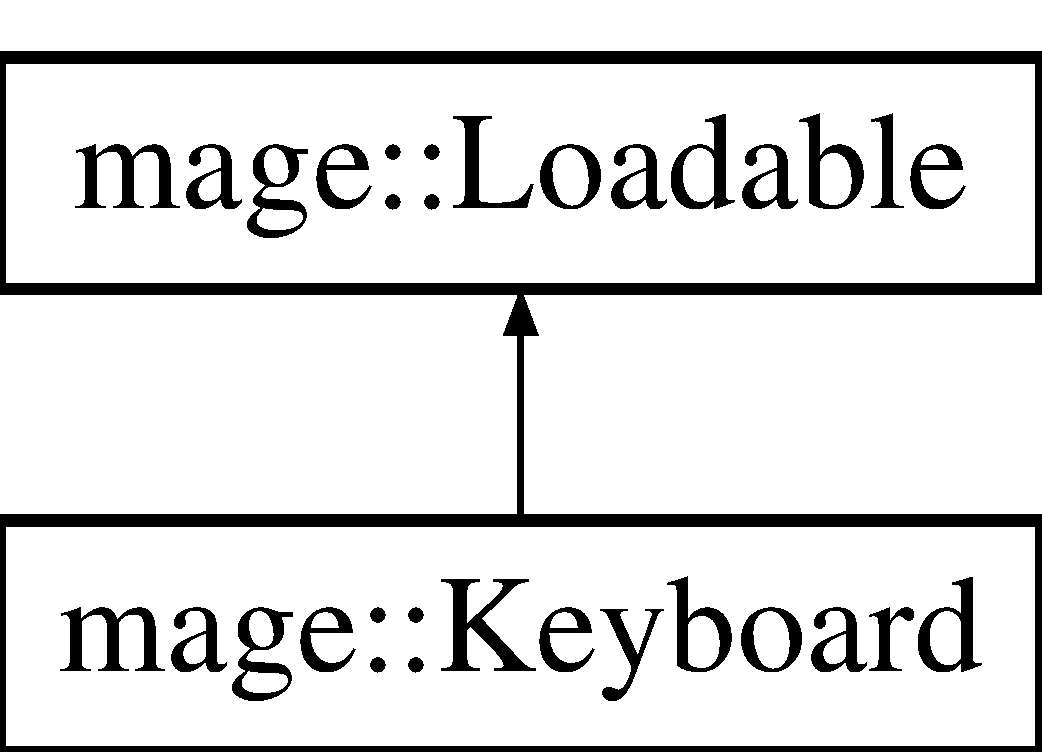
\includegraphics[height=2.000000cm]{classmage_1_1_keyboard}
\end{center}
\end{figure}
\subsection*{Public Member Functions}
\begin{DoxyCompactItemize}
\item 
\hyperlink{classmage_1_1_keyboard_af4afb6c7992b88f94f4b310c35f7e867}{Keyboard} (H\+W\+ND hwindow, \hyperlink{namespacemage_ae74f374780900893caa5555d1031fd79}{Com\+Ptr}$<$ I\+Direct\+Input8 $>$ di)
\item 
virtual \hyperlink{classmage_1_1_keyboard_a72426c8e5cd32f8e79f283d5409f9cc4}{$\sim$\+Keyboard} ()=default
\item 
void \hyperlink{classmage_1_1_keyboard_abb5fd91a304f8bbf8b15ab1a277dafaf}{Update} ()
\item 
H\+W\+ND \hyperlink{classmage_1_1_keyboard_ab9d2244f94faccb9c745b07a8bebc888}{Get\+Handle} () const
\item 
bool \hyperlink{classmage_1_1_keyboard_a94d35ad5ad27e3fc9496f3ab1fa28e4d}{Get\+Key\+Press} (unsigned char key, bool ignore\+\_\+press\+\_\+stamp=false) const
\end{DoxyCompactItemize}
\subsection*{Private Member Functions}
\begin{DoxyCompactItemize}
\item 
\hyperlink{classmage_1_1_keyboard_a39d07f8a5e37648ca9eba30aa55146bf}{Keyboard} (const \hyperlink{classmage_1_1_keyboard}{Keyboard} \&keyboard)=delete
\item 
\hyperlink{classmage_1_1_keyboard_a6ed1e7732253b4d7e4e0bf9ca5a6f108}{Keyboard} (\hyperlink{classmage_1_1_keyboard}{Keyboard} \&\&keyboard)=delete
\item 
\hyperlink{classmage_1_1_keyboard}{Keyboard} \& \hyperlink{classmage_1_1_keyboard_ae3ba98190c8c14ea894c676888825f35}{operator=} (const \hyperlink{classmage_1_1_keyboard}{Keyboard} \&keyboard)=delete
\item 
\hyperlink{classmage_1_1_keyboard}{Keyboard} \& \hyperlink{classmage_1_1_keyboard_a4f381bc90cc6828b4d0313999b544e6e}{operator=} (\hyperlink{classmage_1_1_keyboard}{Keyboard} \&\&keyboard)=delete
\item 
H\+R\+E\+S\+U\+LT \hyperlink{classmage_1_1_keyboard_a1d3211c7377529e570bb5cde900f73db}{Initialize\+Keyboard} (\hyperlink{namespacemage_ae74f374780900893caa5555d1031fd79}{Com\+Ptr}$<$ I\+Direct\+Input8 $>$ di)
\end{DoxyCompactItemize}
\subsection*{Private Attributes}
\begin{DoxyCompactItemize}
\item 
H\+W\+ND \hyperlink{classmage_1_1_keyboard_aa7196c689dad6f5aaf35e3929de02791}{m\+\_\+hwindow}
\item 
\hyperlink{namespacemage_ae74f374780900893caa5555d1031fd79}{Com\+Ptr}$<$ I\+Direct\+Input\+Device8 $>$ \hyperlink{classmage_1_1_keyboard_a992b8b8caf0d858163e5e9af04302324}{m\+\_\+keyboard}
\item 
uint64\+\_\+t \hyperlink{classmage_1_1_keyboard_a2c638a93d1f61d9d3578a0df8b6a1c39}{m\+\_\+press\+\_\+stamp}
\item 
unsigned char \hyperlink{classmage_1_1_keyboard_a7499df459499f5addd50507ea1e2358c}{m\+\_\+key\+\_\+state} \mbox{[}256\mbox{]}
\item 
uint64\+\_\+t \hyperlink{classmage_1_1_keyboard_a8eb4ce7e4e2395bb27d2ac9236655335}{m\+\_\+key\+\_\+press\+\_\+stamp} \mbox{[}256\mbox{]}
\end{DoxyCompactItemize}
\subsection*{Additional Inherited Members}


\subsection{Detailed Description}
A class of keyboards. 

\subsection{Constructor \& Destructor Documentation}
\hypertarget{classmage_1_1_keyboard_af4afb6c7992b88f94f4b310c35f7e867}{}\label{classmage_1_1_keyboard_af4afb6c7992b88f94f4b310c35f7e867} 
\index{mage\+::\+Keyboard@{mage\+::\+Keyboard}!Keyboard@{Keyboard}}
\index{Keyboard@{Keyboard}!mage\+::\+Keyboard@{mage\+::\+Keyboard}}
\subsubsection{\texorpdfstring{Keyboard()}{Keyboard()}\hspace{0.1cm}{\footnotesize\ttfamily [1/3]}}
{\footnotesize\ttfamily mage\+::\+Keyboard\+::\+Keyboard (\begin{DoxyParamCaption}\item[{H\+W\+ND}]{hwindow,  }\item[{\hyperlink{namespacemage_ae74f374780900893caa5555d1031fd79}{Com\+Ptr}$<$ I\+Direct\+Input8 $>$}]{di }\end{DoxyParamCaption})}

Constructs a keyboard.


\begin{DoxyParams}[1]{Parameters}
\mbox{\tt in}  & {\em hwindow} & The handle of the parent window. \\
\hline
\mbox{\tt in}  & {\em di} & A pointer to a direct input object. \\
\hline
\end{DoxyParams}
\hypertarget{classmage_1_1_keyboard_a72426c8e5cd32f8e79f283d5409f9cc4}{}\label{classmage_1_1_keyboard_a72426c8e5cd32f8e79f283d5409f9cc4} 
\index{mage\+::\+Keyboard@{mage\+::\+Keyboard}!````~Keyboard@{$\sim$\+Keyboard}}
\index{````~Keyboard@{$\sim$\+Keyboard}!mage\+::\+Keyboard@{mage\+::\+Keyboard}}
\subsubsection{\texorpdfstring{$\sim$\+Keyboard()}{~Keyboard()}}
{\footnotesize\ttfamily virtual mage\+::\+Keyboard\+::$\sim$\+Keyboard (\begin{DoxyParamCaption}{ }\end{DoxyParamCaption})\hspace{0.3cm}{\ttfamily [virtual]}, {\ttfamily [default]}}

Destructs this keyboard. \hypertarget{classmage_1_1_keyboard_a39d07f8a5e37648ca9eba30aa55146bf}{}\label{classmage_1_1_keyboard_a39d07f8a5e37648ca9eba30aa55146bf} 
\index{mage\+::\+Keyboard@{mage\+::\+Keyboard}!Keyboard@{Keyboard}}
\index{Keyboard@{Keyboard}!mage\+::\+Keyboard@{mage\+::\+Keyboard}}
\subsubsection{\texorpdfstring{Keyboard()}{Keyboard()}\hspace{0.1cm}{\footnotesize\ttfamily [2/3]}}
{\footnotesize\ttfamily mage\+::\+Keyboard\+::\+Keyboard (\begin{DoxyParamCaption}\item[{const \hyperlink{classmage_1_1_keyboard}{Keyboard} \&}]{keyboard }\end{DoxyParamCaption})\hspace{0.3cm}{\ttfamily [private]}, {\ttfamily [delete]}}

Constructs a keyboard from the given keyboard.


\begin{DoxyParams}[1]{Parameters}
\mbox{\tt in}  & {\em keyboard} & A reference to the keyboard. \\
\hline
\end{DoxyParams}
\hypertarget{classmage_1_1_keyboard_a6ed1e7732253b4d7e4e0bf9ca5a6f108}{}\label{classmage_1_1_keyboard_a6ed1e7732253b4d7e4e0bf9ca5a6f108} 
\index{mage\+::\+Keyboard@{mage\+::\+Keyboard}!Keyboard@{Keyboard}}
\index{Keyboard@{Keyboard}!mage\+::\+Keyboard@{mage\+::\+Keyboard}}
\subsubsection{\texorpdfstring{Keyboard()}{Keyboard()}\hspace{0.1cm}{\footnotesize\ttfamily [3/3]}}
{\footnotesize\ttfamily mage\+::\+Keyboard\+::\+Keyboard (\begin{DoxyParamCaption}\item[{\hyperlink{classmage_1_1_keyboard}{Keyboard} \&\&}]{keyboard }\end{DoxyParamCaption})\hspace{0.3cm}{\ttfamily [private]}, {\ttfamily [delete]}}

Constructs a keyboard from the given keyboard.


\begin{DoxyParams}[1]{Parameters}
\mbox{\tt in}  & {\em keyboard} & A reference to the keyboard. \\
\hline
\end{DoxyParams}


\subsection{Member Function Documentation}
\hypertarget{classmage_1_1_keyboard_ab9d2244f94faccb9c745b07a8bebc888}{}\label{classmage_1_1_keyboard_ab9d2244f94faccb9c745b07a8bebc888} 
\index{mage\+::\+Keyboard@{mage\+::\+Keyboard}!Get\+Handle@{Get\+Handle}}
\index{Get\+Handle@{Get\+Handle}!mage\+::\+Keyboard@{mage\+::\+Keyboard}}
\subsubsection{\texorpdfstring{Get\+Handle()}{GetHandle()}}
{\footnotesize\ttfamily H\+W\+ND mage\+::\+Keyboard\+::\+Get\+Handle (\begin{DoxyParamCaption}{ }\end{DoxyParamCaption}) const}

Returns the window handle of this keyboard.

\begin{DoxyReturn}{Returns}
The window handle of this keyboard. 
\end{DoxyReturn}
\hypertarget{classmage_1_1_keyboard_a94d35ad5ad27e3fc9496f3ab1fa28e4d}{}\label{classmage_1_1_keyboard_a94d35ad5ad27e3fc9496f3ab1fa28e4d} 
\index{mage\+::\+Keyboard@{mage\+::\+Keyboard}!Get\+Key\+Press@{Get\+Key\+Press}}
\index{Get\+Key\+Press@{Get\+Key\+Press}!mage\+::\+Keyboard@{mage\+::\+Keyboard}}
\subsubsection{\texorpdfstring{Get\+Key\+Press()}{GetKeyPress()}}
{\footnotesize\ttfamily bool mage\+::\+Keyboard\+::\+Get\+Key\+Press (\begin{DoxyParamCaption}\item[{unsigned char}]{key,  }\item[{bool}]{ignore\+\_\+press\+\_\+stamp = {\ttfamily false} }\end{DoxyParamCaption}) const}

Checks whether the given key of this keyboard is pressed.


\begin{DoxyParams}[1]{Parameters}
\mbox{\tt in}  & {\em key} & The key. \\
\hline
\mbox{\tt in}  & {\em ignore\+\_\+press\+\_\+stamp} & Flag indicating whether press stamps should be ignored. Consistent presses will return false when using the press stamp. \\
\hline
\end{DoxyParams}
\begin{DoxyReturn}{Returns}
{\ttfamily true} if the given key of this keyboard is pressed. {\ttfamily false} otherwise. 
\end{DoxyReturn}
\hypertarget{classmage_1_1_keyboard_a1d3211c7377529e570bb5cde900f73db}{}\label{classmage_1_1_keyboard_a1d3211c7377529e570bb5cde900f73db} 
\index{mage\+::\+Keyboard@{mage\+::\+Keyboard}!Initialize\+Keyboard@{Initialize\+Keyboard}}
\index{Initialize\+Keyboard@{Initialize\+Keyboard}!mage\+::\+Keyboard@{mage\+::\+Keyboard}}
\subsubsection{\texorpdfstring{Initialize\+Keyboard()}{InitializeKeyboard()}}
{\footnotesize\ttfamily H\+R\+E\+S\+U\+LT mage\+::\+Keyboard\+::\+Initialize\+Keyboard (\begin{DoxyParamCaption}\item[{\hyperlink{namespacemage_ae74f374780900893caa5555d1031fd79}{Com\+Ptr}$<$ I\+Direct\+Input8 $>$}]{di }\end{DoxyParamCaption})\hspace{0.3cm}{\ttfamily [private]}}

Initializes the keyboard device of this keyboard.


\begin{DoxyParams}[1]{Parameters}
\mbox{\tt in}  & {\em di} & A pointer to a direct input object. \\
\hline
\end{DoxyParams}
\begin{DoxyReturn}{Returns}
A success/error value. 
\end{DoxyReturn}
\hypertarget{classmage_1_1_keyboard_ae3ba98190c8c14ea894c676888825f35}{}\label{classmage_1_1_keyboard_ae3ba98190c8c14ea894c676888825f35} 
\index{mage\+::\+Keyboard@{mage\+::\+Keyboard}!operator=@{operator=}}
\index{operator=@{operator=}!mage\+::\+Keyboard@{mage\+::\+Keyboard}}
\subsubsection{\texorpdfstring{operator=()}{operator=()}\hspace{0.1cm}{\footnotesize\ttfamily [1/2]}}
{\footnotesize\ttfamily \hyperlink{classmage_1_1_keyboard}{Keyboard}\& mage\+::\+Keyboard\+::operator= (\begin{DoxyParamCaption}\item[{const \hyperlink{classmage_1_1_keyboard}{Keyboard} \&}]{keyboard }\end{DoxyParamCaption})\hspace{0.3cm}{\ttfamily [private]}, {\ttfamily [delete]}}

Copies the given keyboard to this keyboard.


\begin{DoxyParams}[1]{Parameters}
\mbox{\tt in}  & {\em keyboard} & A reference to the keyboard to copy from. \\
\hline
\end{DoxyParams}
\begin{DoxyReturn}{Returns}
A reference to the copy of the given keyboard (i.\+e. this keyboard). 
\end{DoxyReturn}
\hypertarget{classmage_1_1_keyboard_a4f381bc90cc6828b4d0313999b544e6e}{}\label{classmage_1_1_keyboard_a4f381bc90cc6828b4d0313999b544e6e} 
\index{mage\+::\+Keyboard@{mage\+::\+Keyboard}!operator=@{operator=}}
\index{operator=@{operator=}!mage\+::\+Keyboard@{mage\+::\+Keyboard}}
\subsubsection{\texorpdfstring{operator=()}{operator=()}\hspace{0.1cm}{\footnotesize\ttfamily [2/2]}}
{\footnotesize\ttfamily \hyperlink{classmage_1_1_keyboard}{Keyboard}\& mage\+::\+Keyboard\+::operator= (\begin{DoxyParamCaption}\item[{\hyperlink{classmage_1_1_keyboard}{Keyboard} \&\&}]{keyboard }\end{DoxyParamCaption})\hspace{0.3cm}{\ttfamily [private]}, {\ttfamily [delete]}}

Copies the given keyboard to this keyboard.


\begin{DoxyParams}[1]{Parameters}
\mbox{\tt in}  & {\em keyboard} & A reference to the keyboard to copy from. \\
\hline
\end{DoxyParams}
\begin{DoxyReturn}{Returns}
A reference to the copy of the given keyboard (i.\+e. this keyboard). 
\end{DoxyReturn}
\hypertarget{classmage_1_1_keyboard_abb5fd91a304f8bbf8b15ab1a277dafaf}{}\label{classmage_1_1_keyboard_abb5fd91a304f8bbf8b15ab1a277dafaf} 
\index{mage\+::\+Keyboard@{mage\+::\+Keyboard}!Update@{Update}}
\index{Update@{Update}!mage\+::\+Keyboard@{mage\+::\+Keyboard}}
\subsubsection{\texorpdfstring{Update()}{Update()}}
{\footnotesize\ttfamily void mage\+::\+Keyboard\+::\+Update (\begin{DoxyParamCaption}{ }\end{DoxyParamCaption})}

Updates the state of this keyboard. 

\subsection{Member Data Documentation}
\hypertarget{classmage_1_1_keyboard_aa7196c689dad6f5aaf35e3929de02791}{}\label{classmage_1_1_keyboard_aa7196c689dad6f5aaf35e3929de02791} 
\index{mage\+::\+Keyboard@{mage\+::\+Keyboard}!m\+\_\+hwindow@{m\+\_\+hwindow}}
\index{m\+\_\+hwindow@{m\+\_\+hwindow}!mage\+::\+Keyboard@{mage\+::\+Keyboard}}
\subsubsection{\texorpdfstring{m\+\_\+hwindow}{m\_hwindow}}
{\footnotesize\ttfamily H\+W\+ND mage\+::\+Keyboard\+::m\+\_\+hwindow\hspace{0.3cm}{\ttfamily [private]}}

The handle of the parent window. \hypertarget{classmage_1_1_keyboard_a8eb4ce7e4e2395bb27d2ac9236655335}{}\label{classmage_1_1_keyboard_a8eb4ce7e4e2395bb27d2ac9236655335} 
\index{mage\+::\+Keyboard@{mage\+::\+Keyboard}!m\+\_\+key\+\_\+press\+\_\+stamp@{m\+\_\+key\+\_\+press\+\_\+stamp}}
\index{m\+\_\+key\+\_\+press\+\_\+stamp@{m\+\_\+key\+\_\+press\+\_\+stamp}!mage\+::\+Keyboard@{mage\+::\+Keyboard}}
\subsubsection{\texorpdfstring{m\+\_\+key\+\_\+press\+\_\+stamp}{m\_key\_press\_stamp}}
{\footnotesize\ttfamily uint64\+\_\+t mage\+::\+Keyboard\+::m\+\_\+key\+\_\+press\+\_\+stamp\mbox{[}256\mbox{]}\hspace{0.3cm}{\ttfamily [mutable]}, {\ttfamily [private]}}

Stamps the keys pressed in the last frame of this keyboard. \hypertarget{classmage_1_1_keyboard_a7499df459499f5addd50507ea1e2358c}{}\label{classmage_1_1_keyboard_a7499df459499f5addd50507ea1e2358c} 
\index{mage\+::\+Keyboard@{mage\+::\+Keyboard}!m\+\_\+key\+\_\+state@{m\+\_\+key\+\_\+state}}
\index{m\+\_\+key\+\_\+state@{m\+\_\+key\+\_\+state}!mage\+::\+Keyboard@{mage\+::\+Keyboard}}
\subsubsection{\texorpdfstring{m\+\_\+key\+\_\+state}{m\_key\_state}}
{\footnotesize\ttfamily unsigned char mage\+::\+Keyboard\+::m\+\_\+key\+\_\+state\mbox{[}256\mbox{]}\hspace{0.3cm}{\ttfamily [private]}}

State of the keys of this keyboard. \hypertarget{classmage_1_1_keyboard_a992b8b8caf0d858163e5e9af04302324}{}\label{classmage_1_1_keyboard_a992b8b8caf0d858163e5e9af04302324} 
\index{mage\+::\+Keyboard@{mage\+::\+Keyboard}!m\+\_\+keyboard@{m\+\_\+keyboard}}
\index{m\+\_\+keyboard@{m\+\_\+keyboard}!mage\+::\+Keyboard@{mage\+::\+Keyboard}}
\subsubsection{\texorpdfstring{m\+\_\+keyboard}{m\_keyboard}}
{\footnotesize\ttfamily \hyperlink{namespacemage_ae74f374780900893caa5555d1031fd79}{Com\+Ptr}$<$ I\+Direct\+Input\+Device8 $>$ mage\+::\+Keyboard\+::m\+\_\+keyboard\hspace{0.3cm}{\ttfamily [private]}}

The Direct\+Input keyboard device of this keyboard.

The methods of the I\+Direct\+Input\+Device8 interface are used to gain and release access to Microsoft Direct\+Input devices, manage device properties and information, set behavior, perform initialization, create and play force-\/feedback effects, and invoke a device\textquotesingle{}s control panel. \hypertarget{classmage_1_1_keyboard_a2c638a93d1f61d9d3578a0df8b6a1c39}{}\label{classmage_1_1_keyboard_a2c638a93d1f61d9d3578a0df8b6a1c39} 
\index{mage\+::\+Keyboard@{mage\+::\+Keyboard}!m\+\_\+press\+\_\+stamp@{m\+\_\+press\+\_\+stamp}}
\index{m\+\_\+press\+\_\+stamp@{m\+\_\+press\+\_\+stamp}!mage\+::\+Keyboard@{mage\+::\+Keyboard}}
\subsubsection{\texorpdfstring{m\+\_\+press\+\_\+stamp}{m\_press\_stamp}}
{\footnotesize\ttfamily uint64\+\_\+t mage\+::\+Keyboard\+::m\+\_\+press\+\_\+stamp\hspace{0.3cm}{\ttfamily [private]}}

The current press stamp (incremented every frame). 
\hypertarget{classmage_1_1_light}{}\section{mage\+:\+:Light Class Reference}
\label{classmage_1_1_light}\index{mage\+::\+Light@{mage\+::\+Light}}


{\ttfamily \#include $<$light.\+hpp$>$}

Inheritance diagram for mage\+:\+:Light\+:\begin{figure}[H]
\begin{center}
\leavevmode
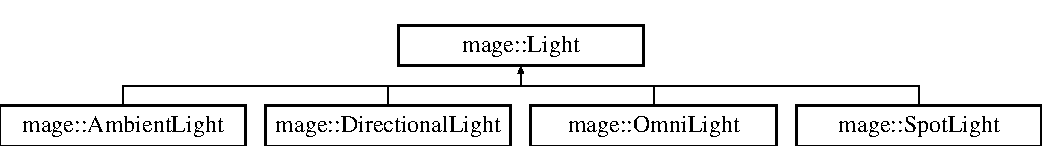
\includegraphics[height=1.944445cm]{classmage_1_1_light}
\end{center}
\end{figure}
\subsection*{Public Member Functions}
\begin{DoxyCompactItemize}
\item 
virtual \hyperlink{classmage_1_1_light_af877bc473dede83689a4bda8a36d4d36}{$\sim$\+Light} ()
\item 
\hyperlink{classmage_1_1_light}{Light} \& \hyperlink{classmage_1_1_light_ad1267c8d162e2cdead5e3a7d83cef3c1}{operator=} (const \hyperlink{classmage_1_1_light}{Light} \&light)
\item 
\hyperlink{classmage_1_1_light}{Light} \& \hyperlink{classmage_1_1_light_a5fd2edc3fcbcc1dbe7a2620b76cedd25}{operator=} (\hyperlink{classmage_1_1_light}{Light} \&\&light)
\item 
\hyperlink{namespacemage_a3316d7143a973e37adf1110f2e80ca31}{Unique\+Ptr}$<$ \hyperlink{classmage_1_1_light}{Light} $>$ \hyperlink{classmage_1_1_light_a4c87e4a361b20519c49b4a0397625a6a}{Clone} () const
\item 
const \hyperlink{structmage_1_1_r_g_b_spectrum}{R\+G\+B\+Spectrum} \hyperlink{classmage_1_1_light_ad4ffb4c5fa06812e7d523a69b177d55a}{Get\+Intensity} () const noexcept
\item 
void \hyperlink{classmage_1_1_light_ab7312aee7c5f7b4b564e27592e1b4223}{Set\+Intensity} (const \hyperlink{structmage_1_1_r_g_b_spectrum}{R\+G\+B\+Spectrum} \&intensity) noexcept
\item 
void \hyperlink{classmage_1_1_light_af96cc7c32afbfdc4d9b1a19b8ac0bf13}{Set\+Intensity} (\hyperlink{structmage_1_1_r_g_b_spectrum}{R\+G\+B\+Spectrum} \&\&intensity) noexcept
\end{DoxyCompactItemize}
\subsection*{Protected Member Functions}
\begin{DoxyCompactItemize}
\item 
\hyperlink{classmage_1_1_light_ab470ad4bde2c1e27068541bb53accb0c}{Light} (const \hyperlink{structmage_1_1_r_g_b_spectrum}{R\+G\+B\+Spectrum} \&intensity)
\item 
\hyperlink{classmage_1_1_light_aae4b7899b7709f658d0d061909e45cec}{Light} (\hyperlink{structmage_1_1_r_g_b_spectrum}{R\+G\+B\+Spectrum} \&\&intensity)
\item 
\hyperlink{classmage_1_1_light_aa91ba3fde50487939d99252c73f732cc}{Light} (const \hyperlink{classmage_1_1_light}{Light} \&light)
\item 
\hyperlink{classmage_1_1_light_a75343c11264fa27c4f166caaf0fec880}{Light} (\hyperlink{classmage_1_1_light}{Light} \&\&light)
\end{DoxyCompactItemize}
\subsection*{Private Member Functions}
\begin{DoxyCompactItemize}
\item 
virtual \hyperlink{namespacemage_a3316d7143a973e37adf1110f2e80ca31}{Unique\+Ptr}$<$ \hyperlink{classmage_1_1_light}{Light} $>$ \hyperlink{classmage_1_1_light_aa613d76a1ebda69efde853d15f75490c}{Clone\+Implementation} () const =0
\end{DoxyCompactItemize}
\subsection*{Private Attributes}
\begin{DoxyCompactItemize}
\item 
\hyperlink{structmage_1_1_r_g_b_spectrum}{R\+G\+B\+Spectrum} \hyperlink{classmage_1_1_light_a4ed8d43c8a4df71671a922d5f04974b8}{m\+\_\+intensity}
\end{DoxyCompactItemize}


\subsection{Detailed Description}
A class of lights. 

\subsection{Constructor \& Destructor Documentation}
\hypertarget{classmage_1_1_light_af877bc473dede83689a4bda8a36d4d36}{}\label{classmage_1_1_light_af877bc473dede83689a4bda8a36d4d36} 
\index{mage\+::\+Light@{mage\+::\+Light}!````~Light@{$\sim$\+Light}}
\index{````~Light@{$\sim$\+Light}!mage\+::\+Light@{mage\+::\+Light}}
\subsubsection{\texorpdfstring{$\sim$\+Light()}{~Light()}}
{\footnotesize\ttfamily mage\+::\+Light\+::$\sim$\+Light (\begin{DoxyParamCaption}{ }\end{DoxyParamCaption})\hspace{0.3cm}{\ttfamily [virtual]}, {\ttfamily [default]}}

Destructs this light. \hypertarget{classmage_1_1_light_ab470ad4bde2c1e27068541bb53accb0c}{}\label{classmage_1_1_light_ab470ad4bde2c1e27068541bb53accb0c} 
\index{mage\+::\+Light@{mage\+::\+Light}!Light@{Light}}
\index{Light@{Light}!mage\+::\+Light@{mage\+::\+Light}}
\subsubsection{\texorpdfstring{Light()}{Light()}\hspace{0.1cm}{\footnotesize\ttfamily [1/4]}}
{\footnotesize\ttfamily mage\+::\+Light\+::\+Light (\begin{DoxyParamCaption}\item[{const \hyperlink{structmage_1_1_r_g_b_spectrum}{R\+G\+B\+Spectrum} \&}]{intensity }\end{DoxyParamCaption})\hspace{0.3cm}{\ttfamily [explicit]}, {\ttfamily [protected]}}

Constructs a light.


\begin{DoxyParams}[1]{Parameters}
\mbox{\tt in}  & {\em intensity} & A reference to the R\+GB intensity. \\
\hline
\end{DoxyParams}
\hypertarget{classmage_1_1_light_aae4b7899b7709f658d0d061909e45cec}{}\label{classmage_1_1_light_aae4b7899b7709f658d0d061909e45cec} 
\index{mage\+::\+Light@{mage\+::\+Light}!Light@{Light}}
\index{Light@{Light}!mage\+::\+Light@{mage\+::\+Light}}
\subsubsection{\texorpdfstring{Light()}{Light()}\hspace{0.1cm}{\footnotesize\ttfamily [2/4]}}
{\footnotesize\ttfamily mage\+::\+Light\+::\+Light (\begin{DoxyParamCaption}\item[{\hyperlink{structmage_1_1_r_g_b_spectrum}{R\+G\+B\+Spectrum} \&\&}]{intensity }\end{DoxyParamCaption})\hspace{0.3cm}{\ttfamily [explicit]}, {\ttfamily [protected]}}

Constructs a light.


\begin{DoxyParams}[1]{Parameters}
\mbox{\tt in}  & {\em intensity} & A reference to the R\+GB intensity. \\
\hline
\end{DoxyParams}
\hypertarget{classmage_1_1_light_aa91ba3fde50487939d99252c73f732cc}{}\label{classmage_1_1_light_aa91ba3fde50487939d99252c73f732cc} 
\index{mage\+::\+Light@{mage\+::\+Light}!Light@{Light}}
\index{Light@{Light}!mage\+::\+Light@{mage\+::\+Light}}
\subsubsection{\texorpdfstring{Light()}{Light()}\hspace{0.1cm}{\footnotesize\ttfamily [3/4]}}
{\footnotesize\ttfamily mage\+::\+Light\+::\+Light (\begin{DoxyParamCaption}\item[{const \hyperlink{classmage_1_1_light}{Light} \&}]{light }\end{DoxyParamCaption})\hspace{0.3cm}{\ttfamily [protected]}, {\ttfamily [default]}}

Constructs a light from the given light.


\begin{DoxyParams}[1]{Parameters}
\mbox{\tt in}  & {\em light} & A reference to the light to copy. \\
\hline
\end{DoxyParams}
\hypertarget{classmage_1_1_light_a75343c11264fa27c4f166caaf0fec880}{}\label{classmage_1_1_light_a75343c11264fa27c4f166caaf0fec880} 
\index{mage\+::\+Light@{mage\+::\+Light}!Light@{Light}}
\index{Light@{Light}!mage\+::\+Light@{mage\+::\+Light}}
\subsubsection{\texorpdfstring{Light()}{Light()}\hspace{0.1cm}{\footnotesize\ttfamily [4/4]}}
{\footnotesize\ttfamily mage\+::\+Light\+::\+Light (\begin{DoxyParamCaption}\item[{\hyperlink{classmage_1_1_light}{Light} \&\&}]{light }\end{DoxyParamCaption})\hspace{0.3cm}{\ttfamily [protected]}, {\ttfamily [default]}}

Constructs a light by moving the given light.


\begin{DoxyParams}[1]{Parameters}
\mbox{\tt in}  & {\em light} & A reference to the light to move. \\
\hline
\end{DoxyParams}


\subsection{Member Function Documentation}
\hypertarget{classmage_1_1_light_a4c87e4a361b20519c49b4a0397625a6a}{}\label{classmage_1_1_light_a4c87e4a361b20519c49b4a0397625a6a} 
\index{mage\+::\+Light@{mage\+::\+Light}!Clone@{Clone}}
\index{Clone@{Clone}!mage\+::\+Light@{mage\+::\+Light}}
\subsubsection{\texorpdfstring{Clone()}{Clone()}}
{\footnotesize\ttfamily \hyperlink{namespacemage_a3316d7143a973e37adf1110f2e80ca31}{Unique\+Ptr}$<$ \hyperlink{classmage_1_1_light}{Light} $>$ mage\+::\+Light\+::\+Clone (\begin{DoxyParamCaption}{ }\end{DoxyParamCaption}) const}

Clones this light.

\begin{DoxyReturn}{Returns}
A pointer to the clone of this light. 
\end{DoxyReturn}
\hypertarget{classmage_1_1_light_aa613d76a1ebda69efde853d15f75490c}{}\label{classmage_1_1_light_aa613d76a1ebda69efde853d15f75490c} 
\index{mage\+::\+Light@{mage\+::\+Light}!Clone\+Implementation@{Clone\+Implementation}}
\index{Clone\+Implementation@{Clone\+Implementation}!mage\+::\+Light@{mage\+::\+Light}}
\subsubsection{\texorpdfstring{Clone\+Implementation()}{CloneImplementation()}}
{\footnotesize\ttfamily virtual \hyperlink{namespacemage_a3316d7143a973e37adf1110f2e80ca31}{Unique\+Ptr}$<$ \hyperlink{classmage_1_1_light}{Light} $>$ mage\+::\+Light\+::\+Clone\+Implementation (\begin{DoxyParamCaption}{ }\end{DoxyParamCaption}) const\hspace{0.3cm}{\ttfamily [private]}, {\ttfamily [pure virtual]}}

Clones this light.

\begin{DoxyReturn}{Returns}
A pointer to the clone of this light. 
\end{DoxyReturn}


Implemented in \hyperlink{classmage_1_1_spot_light_a060044ae1de97143878ad26524f03709}{mage\+::\+Spot\+Light}, \hyperlink{classmage_1_1_omni_light_a1212457828cdd96cc7170767b7bd1223}{mage\+::\+Omni\+Light}, \hyperlink{classmage_1_1_ambient_light_a7223a4770653c20e662810b0956c6e51}{mage\+::\+Ambient\+Light}, and \hyperlink{classmage_1_1_directional_light_a122d3dcd7633a85ef8a85e7d768da36d}{mage\+::\+Directional\+Light}.

\hypertarget{classmage_1_1_light_ad4ffb4c5fa06812e7d523a69b177d55a}{}\label{classmage_1_1_light_ad4ffb4c5fa06812e7d523a69b177d55a} 
\index{mage\+::\+Light@{mage\+::\+Light}!Get\+Intensity@{Get\+Intensity}}
\index{Get\+Intensity@{Get\+Intensity}!mage\+::\+Light@{mage\+::\+Light}}
\subsubsection{\texorpdfstring{Get\+Intensity()}{GetIntensity()}}
{\footnotesize\ttfamily const \hyperlink{structmage_1_1_r_g_b_spectrum}{R\+G\+B\+Spectrum} mage\+::\+Light\+::\+Get\+Intensity (\begin{DoxyParamCaption}{ }\end{DoxyParamCaption}) const\hspace{0.3cm}{\ttfamily [noexcept]}}

Returns the intensity of this light.

\begin{DoxyReturn}{Returns}
The intensity of this light. 
\end{DoxyReturn}
\hypertarget{classmage_1_1_light_ad1267c8d162e2cdead5e3a7d83cef3c1}{}\label{classmage_1_1_light_ad1267c8d162e2cdead5e3a7d83cef3c1} 
\index{mage\+::\+Light@{mage\+::\+Light}!operator=@{operator=}}
\index{operator=@{operator=}!mage\+::\+Light@{mage\+::\+Light}}
\subsubsection{\texorpdfstring{operator=()}{operator=()}\hspace{0.1cm}{\footnotesize\ttfamily [1/2]}}
{\footnotesize\ttfamily \hyperlink{classmage_1_1_light}{Light} \& mage\+::\+Light\+::operator= (\begin{DoxyParamCaption}\item[{const \hyperlink{classmage_1_1_light}{Light} \&}]{light }\end{DoxyParamCaption})\hspace{0.3cm}{\ttfamily [default]}}

Copies the given light to this light.


\begin{DoxyParams}[1]{Parameters}
\mbox{\tt in}  & {\em light} & A reference to the light to copy. \\
\hline
\end{DoxyParams}
\begin{DoxyReturn}{Returns}
A reference to the copy of the given light (i.\+e. this light). 
\end{DoxyReturn}
\hypertarget{classmage_1_1_light_a5fd2edc3fcbcc1dbe7a2620b76cedd25}{}\label{classmage_1_1_light_a5fd2edc3fcbcc1dbe7a2620b76cedd25} 
\index{mage\+::\+Light@{mage\+::\+Light}!operator=@{operator=}}
\index{operator=@{operator=}!mage\+::\+Light@{mage\+::\+Light}}
\subsubsection{\texorpdfstring{operator=()}{operator=()}\hspace{0.1cm}{\footnotesize\ttfamily [2/2]}}
{\footnotesize\ttfamily \hyperlink{classmage_1_1_light}{Light} \& mage\+::\+Light\+::operator= (\begin{DoxyParamCaption}\item[{\hyperlink{classmage_1_1_light}{Light} \&\&}]{light }\end{DoxyParamCaption})\hspace{0.3cm}{\ttfamily [default]}}

Moves the given light to this light.


\begin{DoxyParams}[1]{Parameters}
\mbox{\tt in}  & {\em light} & A reference to the light to move. \\
\hline
\end{DoxyParams}
\begin{DoxyReturn}{Returns}
A reference to the moved light (i.\+e. this light). 
\end{DoxyReturn}
\hypertarget{classmage_1_1_light_ab7312aee7c5f7b4b564e27592e1b4223}{}\label{classmage_1_1_light_ab7312aee7c5f7b4b564e27592e1b4223} 
\index{mage\+::\+Light@{mage\+::\+Light}!Set\+Intensity@{Set\+Intensity}}
\index{Set\+Intensity@{Set\+Intensity}!mage\+::\+Light@{mage\+::\+Light}}
\subsubsection{\texorpdfstring{Set\+Intensity()}{SetIntensity()}\hspace{0.1cm}{\footnotesize\ttfamily [1/2]}}
{\footnotesize\ttfamily void mage\+::\+Light\+::\+Set\+Intensity (\begin{DoxyParamCaption}\item[{const \hyperlink{structmage_1_1_r_g_b_spectrum}{R\+G\+B\+Spectrum} \&}]{intensity }\end{DoxyParamCaption})\hspace{0.3cm}{\ttfamily [noexcept]}}

Sets the intensity of this light to the given intensity.


\begin{DoxyParams}[1]{Parameters}
\mbox{\tt in}  & {\em intensity} & A reference to the intensity. \\
\hline
\end{DoxyParams}
\hypertarget{classmage_1_1_light_af96cc7c32afbfdc4d9b1a19b8ac0bf13}{}\label{classmage_1_1_light_af96cc7c32afbfdc4d9b1a19b8ac0bf13} 
\index{mage\+::\+Light@{mage\+::\+Light}!Set\+Intensity@{Set\+Intensity}}
\index{Set\+Intensity@{Set\+Intensity}!mage\+::\+Light@{mage\+::\+Light}}
\subsubsection{\texorpdfstring{Set\+Intensity()}{SetIntensity()}\hspace{0.1cm}{\footnotesize\ttfamily [2/2]}}
{\footnotesize\ttfamily void mage\+::\+Light\+::\+Set\+Intensity (\begin{DoxyParamCaption}\item[{\hyperlink{structmage_1_1_r_g_b_spectrum}{R\+G\+B\+Spectrum} \&\&}]{intensity }\end{DoxyParamCaption})\hspace{0.3cm}{\ttfamily [noexcept]}}

Sets the intensity of this light to the given intensity.


\begin{DoxyParams}[1]{Parameters}
\mbox{\tt in}  & {\em intensity} & A reference to the intensity. \\
\hline
\end{DoxyParams}


\subsection{Member Data Documentation}
\hypertarget{classmage_1_1_light_a4ed8d43c8a4df71671a922d5f04974b8}{}\label{classmage_1_1_light_a4ed8d43c8a4df71671a922d5f04974b8} 
\index{mage\+::\+Light@{mage\+::\+Light}!m\+\_\+intensity@{m\+\_\+intensity}}
\index{m\+\_\+intensity@{m\+\_\+intensity}!mage\+::\+Light@{mage\+::\+Light}}
\subsubsection{\texorpdfstring{m\+\_\+intensity}{m\_intensity}}
{\footnotesize\ttfamily \hyperlink{structmage_1_1_r_g_b_spectrum}{R\+G\+B\+Spectrum} mage\+::\+Light\+::m\+\_\+intensity\hspace{0.3cm}{\ttfamily [private]}}

The intensity of this light. 
\hypertarget{structmage_1_1_lighting}{}\section{mage\+:\+:Lighting Struct Reference}
\label{structmage_1_1_lighting}\index{mage\+::\+Lighting@{mage\+::\+Lighting}}


{\ttfamily \#include $<$shader.\+hpp$>$}

\subsection*{Public Member Functions}
\begin{DoxyCompactItemize}
\item 
\hyperlink{structmage_1_1_lighting_a7017afad521df6eacf2c45ae0f5adfd5}{Lighting} ()=default
\item 
\hyperlink{structmage_1_1_lighting_ae92175ad94cc88badf2dc4fd93cb2e2f}{Lighting} (const \hyperlink{structmage_1_1_lighting}{Lighting} \&buffer)=default
\item 
\hyperlink{structmage_1_1_lighting_a03ce177d02db1f7ee2b779aa4cb321c1}{Lighting} (\hyperlink{structmage_1_1_lighting}{Lighting} \&\&buffer)=default
\item 
\hyperlink{structmage_1_1_lighting_a2b357cb6853d05bae8be16fc6d63a6c3}{$\sim$\+Lighting} ()=default
\item 
\hyperlink{structmage_1_1_lighting}{Lighting} \& \hyperlink{structmage_1_1_lighting_af3407499990673e6a6880cbcc5f5b054}{operator=} (const \hyperlink{structmage_1_1_lighting}{Lighting} \&buffer)=default
\item 
\hyperlink{structmage_1_1_lighting}{Lighting} \& \hyperlink{structmage_1_1_lighting_adf7079d86353561a08e1729932d5e9e2}{operator=} (\hyperlink{structmage_1_1_lighting}{Lighting} \&\&buffer)=default
\end{DoxyCompactItemize}
\subsection*{Public Attributes}
\begin{DoxyCompactItemize}
\item 
I\+D3\+D11\+Buffer $\ast$ \hyperlink{structmage_1_1_lighting_aa8c55bf975d3d77e8d598591a9268766}{light\+\_\+data}
\item 
I\+D3\+D11\+Shader\+Resource\+View $\ast$ \hyperlink{structmage_1_1_lighting_add6b516f28826b888466df39f7db5e35}{omni\+\_\+lights}
\item 
I\+D3\+D11\+Shader\+Resource\+View $\ast$ \hyperlink{structmage_1_1_lighting_a6d9e373787f009cabac09319074aaf2e}{spot\+\_\+lights}
\end{DoxyCompactItemize}


\subsection{Constructor \& Destructor Documentation}
\hypertarget{structmage_1_1_lighting_a7017afad521df6eacf2c45ae0f5adfd5}{}\label{structmage_1_1_lighting_a7017afad521df6eacf2c45ae0f5adfd5} 
\index{mage\+::\+Lighting@{mage\+::\+Lighting}!Lighting@{Lighting}}
\index{Lighting@{Lighting}!mage\+::\+Lighting@{mage\+::\+Lighting}}
\subsubsection{\texorpdfstring{Lighting()}{Lighting()}\hspace{0.1cm}{\footnotesize\ttfamily [1/3]}}
{\footnotesize\ttfamily mage\+::\+Lighting\+::\+Lighting (\begin{DoxyParamCaption}{ }\end{DoxyParamCaption})\hspace{0.3cm}{\ttfamily [default]}}

\hypertarget{structmage_1_1_lighting_ae92175ad94cc88badf2dc4fd93cb2e2f}{}\label{structmage_1_1_lighting_ae92175ad94cc88badf2dc4fd93cb2e2f} 
\index{mage\+::\+Lighting@{mage\+::\+Lighting}!Lighting@{Lighting}}
\index{Lighting@{Lighting}!mage\+::\+Lighting@{mage\+::\+Lighting}}
\subsubsection{\texorpdfstring{Lighting()}{Lighting()}\hspace{0.1cm}{\footnotesize\ttfamily [2/3]}}
{\footnotesize\ttfamily mage\+::\+Lighting\+::\+Lighting (\begin{DoxyParamCaption}\item[{const \hyperlink{structmage_1_1_lighting}{Lighting} \&}]{buffer }\end{DoxyParamCaption})\hspace{0.3cm}{\ttfamily [default]}}

\hypertarget{structmage_1_1_lighting_a03ce177d02db1f7ee2b779aa4cb321c1}{}\label{structmage_1_1_lighting_a03ce177d02db1f7ee2b779aa4cb321c1} 
\index{mage\+::\+Lighting@{mage\+::\+Lighting}!Lighting@{Lighting}}
\index{Lighting@{Lighting}!mage\+::\+Lighting@{mage\+::\+Lighting}}
\subsubsection{\texorpdfstring{Lighting()}{Lighting()}\hspace{0.1cm}{\footnotesize\ttfamily [3/3]}}
{\footnotesize\ttfamily mage\+::\+Lighting\+::\+Lighting (\begin{DoxyParamCaption}\item[{\hyperlink{structmage_1_1_lighting}{Lighting} \&\&}]{buffer }\end{DoxyParamCaption})\hspace{0.3cm}{\ttfamily [default]}}

\hypertarget{structmage_1_1_lighting_a2b357cb6853d05bae8be16fc6d63a6c3}{}\label{structmage_1_1_lighting_a2b357cb6853d05bae8be16fc6d63a6c3} 
\index{mage\+::\+Lighting@{mage\+::\+Lighting}!````~Lighting@{$\sim$\+Lighting}}
\index{````~Lighting@{$\sim$\+Lighting}!mage\+::\+Lighting@{mage\+::\+Lighting}}
\subsubsection{\texorpdfstring{$\sim$\+Lighting()}{~Lighting()}}
{\footnotesize\ttfamily mage\+::\+Lighting\+::$\sim$\+Lighting (\begin{DoxyParamCaption}{ }\end{DoxyParamCaption})\hspace{0.3cm}{\ttfamily [default]}}



\subsection{Member Function Documentation}
\hypertarget{structmage_1_1_lighting_af3407499990673e6a6880cbcc5f5b054}{}\label{structmage_1_1_lighting_af3407499990673e6a6880cbcc5f5b054} 
\index{mage\+::\+Lighting@{mage\+::\+Lighting}!operator=@{operator=}}
\index{operator=@{operator=}!mage\+::\+Lighting@{mage\+::\+Lighting}}
\subsubsection{\texorpdfstring{operator=()}{operator=()}\hspace{0.1cm}{\footnotesize\ttfamily [1/2]}}
{\footnotesize\ttfamily \hyperlink{structmage_1_1_lighting}{Lighting}\& mage\+::\+Lighting\+::operator= (\begin{DoxyParamCaption}\item[{const \hyperlink{structmage_1_1_lighting}{Lighting} \&}]{buffer }\end{DoxyParamCaption})\hspace{0.3cm}{\ttfamily [default]}}

\hypertarget{structmage_1_1_lighting_adf7079d86353561a08e1729932d5e9e2}{}\label{structmage_1_1_lighting_adf7079d86353561a08e1729932d5e9e2} 
\index{mage\+::\+Lighting@{mage\+::\+Lighting}!operator=@{operator=}}
\index{operator=@{operator=}!mage\+::\+Lighting@{mage\+::\+Lighting}}
\subsubsection{\texorpdfstring{operator=()}{operator=()}\hspace{0.1cm}{\footnotesize\ttfamily [2/2]}}
{\footnotesize\ttfamily \hyperlink{structmage_1_1_lighting}{Lighting}\& mage\+::\+Lighting\+::operator= (\begin{DoxyParamCaption}\item[{\hyperlink{structmage_1_1_lighting}{Lighting} \&\&}]{buffer }\end{DoxyParamCaption})\hspace{0.3cm}{\ttfamily [default]}}



\subsection{Member Data Documentation}
\hypertarget{structmage_1_1_lighting_aa8c55bf975d3d77e8d598591a9268766}{}\label{structmage_1_1_lighting_aa8c55bf975d3d77e8d598591a9268766} 
\index{mage\+::\+Lighting@{mage\+::\+Lighting}!light\+\_\+data@{light\+\_\+data}}
\index{light\+\_\+data@{light\+\_\+data}!mage\+::\+Lighting@{mage\+::\+Lighting}}
\subsubsection{\texorpdfstring{light\+\_\+data}{light\_data}}
{\footnotesize\ttfamily I\+D3\+D11\+Buffer$\ast$ mage\+::\+Lighting\+::light\+\_\+data}

\hypertarget{structmage_1_1_lighting_add6b516f28826b888466df39f7db5e35}{}\label{structmage_1_1_lighting_add6b516f28826b888466df39f7db5e35} 
\index{mage\+::\+Lighting@{mage\+::\+Lighting}!omni\+\_\+lights@{omni\+\_\+lights}}
\index{omni\+\_\+lights@{omni\+\_\+lights}!mage\+::\+Lighting@{mage\+::\+Lighting}}
\subsubsection{\texorpdfstring{omni\+\_\+lights}{omni\_lights}}
{\footnotesize\ttfamily I\+D3\+D11\+Shader\+Resource\+View$\ast$ mage\+::\+Lighting\+::omni\+\_\+lights}

\hypertarget{structmage_1_1_lighting_a6d9e373787f009cabac09319074aaf2e}{}\label{structmage_1_1_lighting_a6d9e373787f009cabac09319074aaf2e} 
\index{mage\+::\+Lighting@{mage\+::\+Lighting}!spot\+\_\+lights@{spot\+\_\+lights}}
\index{spot\+\_\+lights@{spot\+\_\+lights}!mage\+::\+Lighting@{mage\+::\+Lighting}}
\subsubsection{\texorpdfstring{spot\+\_\+lights}{spot\_lights}}
{\footnotesize\ttfamily I\+D3\+D11\+Shader\+Resource\+View$\ast$ mage\+::\+Lighting\+::spot\+\_\+lights}


\hypertarget{classmage_1_1_light_node}{}\section{mage\+:\+:Light\+Node Class Reference}
\label{classmage_1_1_light_node}\index{mage\+::\+Light\+Node@{mage\+::\+Light\+Node}}


{\ttfamily \#include $<$light\+\_\+node.\+hpp$>$}

Inheritance diagram for mage\+:\+:Light\+Node\+:\begin{figure}[H]
\begin{center}
\leavevmode
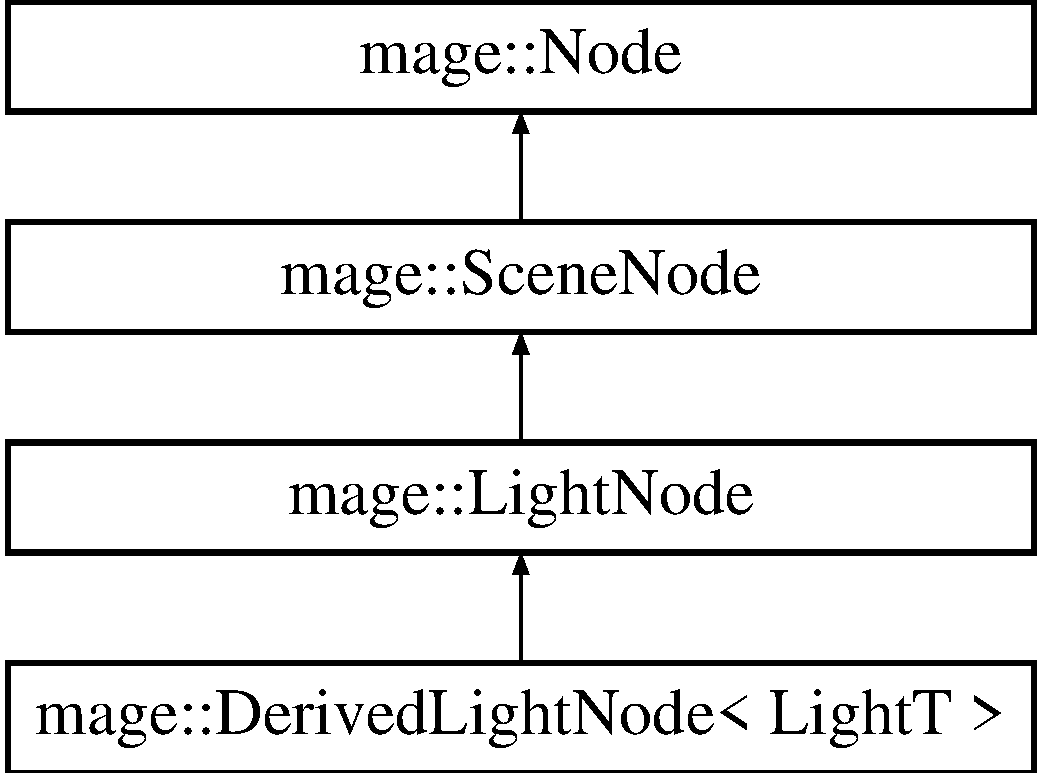
\includegraphics[height=4.000000cm]{classmage_1_1_light_node}
\end{center}
\end{figure}
\subsection*{Public Member Functions}
\begin{DoxyCompactItemize}
\item 
virtual \hyperlink{classmage_1_1_light_node_ad0c650ac0059589c28a3d1cfec95c07d}{$\sim$\+Light\+Node} ()
\item 
\hyperlink{classmage_1_1_light_node}{Light\+Node} \& \hyperlink{classmage_1_1_light_node_a41e3ee25215ccc1cbaed4b73e393930a}{operator=} (const \hyperlink{classmage_1_1_light_node}{Light\+Node} \&light\+\_\+node)=delete
\item 
\hyperlink{classmage_1_1_light_node}{Light\+Node} \& \hyperlink{classmage_1_1_light_node_abda92f7cf2ce3aed3af94d2278e2bfa1}{operator=} (\hyperlink{classmage_1_1_light_node}{Light\+Node} \&\&light\+\_\+node)=delete
\item 
\hyperlink{namespacemage_a3316d7143a973e37adf1110f2e80ca31}{Unique\+Ptr}$<$ \hyperlink{classmage_1_1_light_node}{Light\+Node} $>$ \hyperlink{classmage_1_1_light_node_a4d0c10f03de71cd497635feb431d02d5}{Clone} () const
\item 
\hyperlink{classmage_1_1_light}{Light} $\ast$ \hyperlink{classmage_1_1_light_node_a2b971e64ec2267d49c2ba96a00662d3b}{Get\+Light} () noexcept
\item 
const \hyperlink{classmage_1_1_light}{Light} $\ast$ \hyperlink{classmage_1_1_light_node_a015453d1751cf3ad78846e972957bb5b}{Get\+Light} () const noexcept
\end{DoxyCompactItemize}
\subsection*{Protected Member Functions}
\begin{DoxyCompactItemize}
\item 
\hyperlink{classmage_1_1_light_node_a4fea7bde70aebb6f9dc30e3374507c8a}{Light\+Node} (const string \&name, \hyperlink{namespacemage_a3316d7143a973e37adf1110f2e80ca31}{Unique\+Ptr}$<$ \hyperlink{classmage_1_1_light}{Light} $>$ \&\&light)
\item 
\hyperlink{classmage_1_1_light_node_afc1174329e2dbf2d349303fc396c3760}{Light\+Node} (const \hyperlink{classmage_1_1_light_node}{Light\+Node} \&light\+\_\+node)
\item 
\hyperlink{classmage_1_1_light_node_a0a2d5ee9e6417d73905d6f35116eccb3}{Light\+Node} (\hyperlink{classmage_1_1_light_node}{Light\+Node} \&\&light\+\_\+node)
\end{DoxyCompactItemize}
\subsection*{Private Member Functions}
\begin{DoxyCompactItemize}
\item 
virtual \hyperlink{namespacemage_a3316d7143a973e37adf1110f2e80ca31}{Unique\+Ptr}$<$ \hyperlink{classmage_1_1_node}{Node} $>$ \hyperlink{classmage_1_1_light_node_aea97601d0a4b8073a1c655ca334af242}{Clone\+Implementation} () const override=0
\end{DoxyCompactItemize}
\subsection*{Private Attributes}
\begin{DoxyCompactItemize}
\item 
\hyperlink{namespacemage_a3316d7143a973e37adf1110f2e80ca31}{Unique\+Ptr}$<$ \hyperlink{classmage_1_1_light}{Light} $>$ \hyperlink{classmage_1_1_light_node_aad97d01d2adb66eac0e93bdcdb919a05}{m\+\_\+light}
\end{DoxyCompactItemize}


\subsection{Detailed Description}
A class of light nodes. 

\subsection{Constructor \& Destructor Documentation}
\hypertarget{classmage_1_1_light_node_ad0c650ac0059589c28a3d1cfec95c07d}{}\label{classmage_1_1_light_node_ad0c650ac0059589c28a3d1cfec95c07d} 
\index{mage\+::\+Light\+Node@{mage\+::\+Light\+Node}!````~Light\+Node@{$\sim$\+Light\+Node}}
\index{````~Light\+Node@{$\sim$\+Light\+Node}!mage\+::\+Light\+Node@{mage\+::\+Light\+Node}}
\subsubsection{\texorpdfstring{$\sim$\+Light\+Node()}{~LightNode()}}
{\footnotesize\ttfamily mage\+::\+Light\+Node\+::$\sim$\+Light\+Node (\begin{DoxyParamCaption}{ }\end{DoxyParamCaption})\hspace{0.3cm}{\ttfamily [virtual]}, {\ttfamily [default]}}

Destructs this light node. \hypertarget{classmage_1_1_light_node_a4fea7bde70aebb6f9dc30e3374507c8a}{}\label{classmage_1_1_light_node_a4fea7bde70aebb6f9dc30e3374507c8a} 
\index{mage\+::\+Light\+Node@{mage\+::\+Light\+Node}!Light\+Node@{Light\+Node}}
\index{Light\+Node@{Light\+Node}!mage\+::\+Light\+Node@{mage\+::\+Light\+Node}}
\subsubsection{\texorpdfstring{Light\+Node()}{LightNode()}\hspace{0.1cm}{\footnotesize\ttfamily [1/3]}}
{\footnotesize\ttfamily mage\+::\+Light\+Node\+::\+Light\+Node (\begin{DoxyParamCaption}\item[{const string \&}]{name,  }\item[{\hyperlink{namespacemage_a3316d7143a973e37adf1110f2e80ca31}{Unique\+Ptr}$<$ \hyperlink{classmage_1_1_light}{Light} $>$ \&\&}]{light }\end{DoxyParamCaption})\hspace{0.3cm}{\ttfamily [explicit]}, {\ttfamily [protected]}}

Constructs a light node.


\begin{DoxyParams}[1]{Parameters}
\mbox{\tt in}  & {\em name} & A reference to the name. \\
\hline
\mbox{\tt in}  & {\em light} & A reference to the light to move. \\
\hline
\end{DoxyParams}
\hypertarget{classmage_1_1_light_node_afc1174329e2dbf2d349303fc396c3760}{}\label{classmage_1_1_light_node_afc1174329e2dbf2d349303fc396c3760} 
\index{mage\+::\+Light\+Node@{mage\+::\+Light\+Node}!Light\+Node@{Light\+Node}}
\index{Light\+Node@{Light\+Node}!mage\+::\+Light\+Node@{mage\+::\+Light\+Node}}
\subsubsection{\texorpdfstring{Light\+Node()}{LightNode()}\hspace{0.1cm}{\footnotesize\ttfamily [2/3]}}
{\footnotesize\ttfamily mage\+::\+Light\+Node\+::\+Light\+Node (\begin{DoxyParamCaption}\item[{const \hyperlink{classmage_1_1_light_node}{Light\+Node} \&}]{light\+\_\+node }\end{DoxyParamCaption})\hspace{0.3cm}{\ttfamily [protected]}}

Constructs a light node from the given light node.


\begin{DoxyParams}[1]{Parameters}
\mbox{\tt in}  & {\em light\+\_\+node} & A reference to the light node to copy. \\
\hline
\end{DoxyParams}
\hypertarget{classmage_1_1_light_node_a0a2d5ee9e6417d73905d6f35116eccb3}{}\label{classmage_1_1_light_node_a0a2d5ee9e6417d73905d6f35116eccb3} 
\index{mage\+::\+Light\+Node@{mage\+::\+Light\+Node}!Light\+Node@{Light\+Node}}
\index{Light\+Node@{Light\+Node}!mage\+::\+Light\+Node@{mage\+::\+Light\+Node}}
\subsubsection{\texorpdfstring{Light\+Node()}{LightNode()}\hspace{0.1cm}{\footnotesize\ttfamily [3/3]}}
{\footnotesize\ttfamily mage\+::\+Light\+Node\+::\+Light\+Node (\begin{DoxyParamCaption}\item[{\hyperlink{classmage_1_1_light_node}{Light\+Node} \&\&}]{light\+\_\+node }\end{DoxyParamCaption})\hspace{0.3cm}{\ttfamily [protected]}, {\ttfamily [default]}}

Constructs a light node by moving the given light node.


\begin{DoxyParams}[1]{Parameters}
\mbox{\tt in}  & {\em light\+\_\+node} & A reference to the light node to move. \\
\hline
\end{DoxyParams}


\subsection{Member Function Documentation}
\hypertarget{classmage_1_1_light_node_a4d0c10f03de71cd497635feb431d02d5}{}\label{classmage_1_1_light_node_a4d0c10f03de71cd497635feb431d02d5} 
\index{mage\+::\+Light\+Node@{mage\+::\+Light\+Node}!Clone@{Clone}}
\index{Clone@{Clone}!mage\+::\+Light\+Node@{mage\+::\+Light\+Node}}
\subsubsection{\texorpdfstring{Clone()}{Clone()}}
{\footnotesize\ttfamily \hyperlink{namespacemage_a3316d7143a973e37adf1110f2e80ca31}{Unique\+Ptr}$<$ \hyperlink{classmage_1_1_light_node}{Light\+Node} $>$ mage\+::\+Light\+Node\+::\+Clone (\begin{DoxyParamCaption}{ }\end{DoxyParamCaption}) const}

Clones this light node.

\begin{DoxyReturn}{Returns}
A pointer to the clone of this light node. 
\end{DoxyReturn}
\hypertarget{classmage_1_1_light_node_aea97601d0a4b8073a1c655ca334af242}{}\label{classmage_1_1_light_node_aea97601d0a4b8073a1c655ca334af242} 
\index{mage\+::\+Light\+Node@{mage\+::\+Light\+Node}!Clone\+Implementation@{Clone\+Implementation}}
\index{Clone\+Implementation@{Clone\+Implementation}!mage\+::\+Light\+Node@{mage\+::\+Light\+Node}}
\subsubsection{\texorpdfstring{Clone\+Implementation()}{CloneImplementation()}}
{\footnotesize\ttfamily virtual \hyperlink{namespacemage_a3316d7143a973e37adf1110f2e80ca31}{Unique\+Ptr}$<$ \hyperlink{classmage_1_1_node}{Node} $>$ mage\+::\+Light\+Node\+::\+Clone\+Implementation (\begin{DoxyParamCaption}{ }\end{DoxyParamCaption}) const\hspace{0.3cm}{\ttfamily [override]}, {\ttfamily [private]}, {\ttfamily [pure virtual]}}

Clones this camera node.

\begin{DoxyReturn}{Returns}
A pointer to the clone of this camera node. 
\end{DoxyReturn}


Reimplemented from \hyperlink{classmage_1_1_scene_node_a42d0d53ab804d38ebd584d2de6490eeb}{mage\+::\+Scene\+Node}.



Implemented in \hyperlink{classmage_1_1_derived_light_node_acf8858989780bf45a45c55a7c5564314}{mage\+::\+Derived\+Light\+Node$<$ Light\+T $>$}.

\hypertarget{classmage_1_1_light_node_a2b971e64ec2267d49c2ba96a00662d3b}{}\label{classmage_1_1_light_node_a2b971e64ec2267d49c2ba96a00662d3b} 
\index{mage\+::\+Light\+Node@{mage\+::\+Light\+Node}!Get\+Light@{Get\+Light}}
\index{Get\+Light@{Get\+Light}!mage\+::\+Light\+Node@{mage\+::\+Light\+Node}}
\subsubsection{\texorpdfstring{Get\+Light()}{GetLight()}\hspace{0.1cm}{\footnotesize\ttfamily [1/2]}}
{\footnotesize\ttfamily \hyperlink{classmage_1_1_light}{Light}$\ast$ mage\+::\+Light\+Node\+::\+Get\+Light (\begin{DoxyParamCaption}{ }\end{DoxyParamCaption})\hspace{0.3cm}{\ttfamily [noexcept]}}

Returns the light of this light node.

\begin{DoxyReturn}{Returns}
A pointer to the light of this light node. 
\end{DoxyReturn}
\hypertarget{classmage_1_1_light_node_a015453d1751cf3ad78846e972957bb5b}{}\label{classmage_1_1_light_node_a015453d1751cf3ad78846e972957bb5b} 
\index{mage\+::\+Light\+Node@{mage\+::\+Light\+Node}!Get\+Light@{Get\+Light}}
\index{Get\+Light@{Get\+Light}!mage\+::\+Light\+Node@{mage\+::\+Light\+Node}}
\subsubsection{\texorpdfstring{Get\+Light()}{GetLight()}\hspace{0.1cm}{\footnotesize\ttfamily [2/2]}}
{\footnotesize\ttfamily const \hyperlink{classmage_1_1_light}{Light}$\ast$ mage\+::\+Light\+Node\+::\+Get\+Light (\begin{DoxyParamCaption}{ }\end{DoxyParamCaption}) const\hspace{0.3cm}{\ttfamily [noexcept]}}

Returns the light of this light node.

\begin{DoxyReturn}{Returns}
A pointer to the light of this light node. 
\end{DoxyReturn}
\hypertarget{classmage_1_1_light_node_a41e3ee25215ccc1cbaed4b73e393930a}{}\label{classmage_1_1_light_node_a41e3ee25215ccc1cbaed4b73e393930a} 
\index{mage\+::\+Light\+Node@{mage\+::\+Light\+Node}!operator=@{operator=}}
\index{operator=@{operator=}!mage\+::\+Light\+Node@{mage\+::\+Light\+Node}}
\subsubsection{\texorpdfstring{operator=()}{operator=()}\hspace{0.1cm}{\footnotesize\ttfamily [1/2]}}
{\footnotesize\ttfamily \hyperlink{classmage_1_1_light_node}{Light\+Node}\& mage\+::\+Light\+Node\+::operator= (\begin{DoxyParamCaption}\item[{const \hyperlink{classmage_1_1_light_node}{Light\+Node} \&}]{light\+\_\+node }\end{DoxyParamCaption})\hspace{0.3cm}{\ttfamily [delete]}}

Copies the given light node to this light node.


\begin{DoxyParams}[1]{Parameters}
\mbox{\tt in}  & {\em light\+\_\+node} & A reference to the light node to copy. \\
\hline
\end{DoxyParams}
\begin{DoxyReturn}{Returns}
A reference to the copy of the given light node (i.\+e. this light node). 
\end{DoxyReturn}
\hypertarget{classmage_1_1_light_node_abda92f7cf2ce3aed3af94d2278e2bfa1}{}\label{classmage_1_1_light_node_abda92f7cf2ce3aed3af94d2278e2bfa1} 
\index{mage\+::\+Light\+Node@{mage\+::\+Light\+Node}!operator=@{operator=}}
\index{operator=@{operator=}!mage\+::\+Light\+Node@{mage\+::\+Light\+Node}}
\subsubsection{\texorpdfstring{operator=()}{operator=()}\hspace{0.1cm}{\footnotesize\ttfamily [2/2]}}
{\footnotesize\ttfamily \hyperlink{classmage_1_1_light_node}{Light\+Node}\& mage\+::\+Light\+Node\+::operator= (\begin{DoxyParamCaption}\item[{\hyperlink{classmage_1_1_light_node}{Light\+Node} \&\&}]{light\+\_\+node }\end{DoxyParamCaption})\hspace{0.3cm}{\ttfamily [delete]}}

Moves the given light node to this light node.


\begin{DoxyParams}[1]{Parameters}
\mbox{\tt in}  & {\em light\+\_\+node} & A reference to the light node to move. \\
\hline
\end{DoxyParams}
\begin{DoxyReturn}{Returns}
A reference to the moved light node (i.\+e. this light node). 
\end{DoxyReturn}


\subsection{Member Data Documentation}
\hypertarget{classmage_1_1_light_node_aad97d01d2adb66eac0e93bdcdb919a05}{}\label{classmage_1_1_light_node_aad97d01d2adb66eac0e93bdcdb919a05} 
\index{mage\+::\+Light\+Node@{mage\+::\+Light\+Node}!m\+\_\+light@{m\+\_\+light}}
\index{m\+\_\+light@{m\+\_\+light}!mage\+::\+Light\+Node@{mage\+::\+Light\+Node}}
\subsubsection{\texorpdfstring{m\+\_\+light}{m\_light}}
{\footnotesize\ttfamily \hyperlink{namespacemage_a3316d7143a973e37adf1110f2e80ca31}{Unique\+Ptr}$<$ \hyperlink{classmage_1_1_light}{Light} $>$ mage\+::\+Light\+Node\+::m\+\_\+light\hspace{0.3cm}{\ttfamily [private]}}

A pointer to the light of this light node. 
\hypertarget{classmage_1_1_line_reader}{}\section{mage\+:\+:Line\+Reader Class Reference}
\label{classmage_1_1_line_reader}\index{mage\+::\+Line\+Reader@{mage\+::\+Line\+Reader}}


{\ttfamily \#include $<$line\+\_\+reader.\+hpp$>$}

Inheritance diagram for mage\+:\+:Line\+Reader\+:\begin{figure}[H]
\begin{center}
\leavevmode
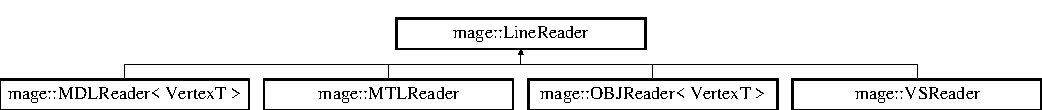
\includegraphics[height=1.000000cm]{classmage_1_1_line_reader}
\end{center}
\end{figure}
\subsection*{Public Member Functions}
\begin{DoxyCompactItemize}
\item 
\hyperlink{classmage_1_1_line_reader}{Line\+Reader} \& \hyperlink{classmage_1_1_line_reader_a2247078d0b5602f9a9a6b74019832faf}{operator=} (const \hyperlink{classmage_1_1_line_reader}{Line\+Reader} \&reader)=delete
\item 
\hyperlink{classmage_1_1_line_reader}{Line\+Reader} \& \hyperlink{classmage_1_1_line_reader_a3ba691cb32a1ab5dcbe75498068c1b86}{operator=} (\hyperlink{classmage_1_1_line_reader}{Line\+Reader} \&\&reader) noexcept
\item 
void \hyperlink{classmage_1_1_line_reader_a6ee0c53351656ac4cd92db1d7c372cff}{Read\+From\+File} (wstring fname, string delimiters=\hyperlink{namespacemage_a10fe126e627cc2ce8af2cc39cc5db81e}{g\+\_\+default\+\_\+delimiters})
\item 
void \hyperlink{classmage_1_1_line_reader_a35ceefa0efd4ccfc3c1401715c0934de}{Read\+From\+Memory} (const char $\ast$input, string delimiters=\hyperlink{namespacemage_a10fe126e627cc2ce8af2cc39cc5db81e}{g\+\_\+default\+\_\+delimiters})
\item 
const wstring \& \hyperlink{classmage_1_1_line_reader_a682ed8030c99a62d4409a01f9efa6d6b}{Get\+Filename} () const noexcept
\item 
const string \& \hyperlink{classmage_1_1_line_reader_aa00e1e27b614e11ec9f70e52d0bac551}{Get\+Delimiters} () const noexcept
\end{DoxyCompactItemize}
\subsection*{Protected Member Functions}
\begin{DoxyCompactItemize}
\item 
\hyperlink{classmage_1_1_line_reader_ab4a46321d7ea3ecda2d6390c78a7285b}{Line\+Reader} ()
\item 
\hyperlink{classmage_1_1_line_reader_ae4f871bebae110704b34c0bd88460639}{Line\+Reader} (const \hyperlink{classmage_1_1_line_reader}{Line\+Reader} \&reader)=delete
\item 
\hyperlink{classmage_1_1_line_reader_ae90c546a98e113a48ca1c94b854a4866}{Line\+Reader} (\hyperlink{classmage_1_1_line_reader}{Line\+Reader} \&\&reader) noexcept
\item 
\hyperlink{classmage_1_1_line_reader_ad9753ea392ebe5b3867852d3392fb1e7}{$\sim$\+Line\+Reader} ()
\item 
\hyperlink{namespacemage_a41c104c036fba3756a74e19f793eeaa1}{U32} \hyperlink{classmage_1_1_line_reader_aa0ed768e2799b74f2341c56fc6ac4969}{Get\+Current\+Line\+Number} () const noexcept
\item 
void \hyperlink{classmage_1_1_line_reader_a3a4b99bfef1e8a826d74a01bcc663fcb}{Read\+Line\+Remaining} ()
\item 
const char $\ast$ \hyperlink{classmage_1_1_line_reader_ad915c1a17549c7758c10f0b6db7e5611}{Read\+Chars} ()
\item 
const string \hyperlink{classmage_1_1_line_reader_ae9a7547d01b29c3237b198444d4f3aef}{Read\+Quoted\+String} ()
\item 
{\footnotesize template$<$typename DataT $>$ }\\const DataT \hyperlink{classmage_1_1_line_reader_aa1ba5aa332e49bdd63ef4ee4021120fd}{Read} ()
\item 
bool \hyperlink{classmage_1_1_line_reader_a7eb54d60902d1fb7846ea5c566312a0f}{Has\+Chars} () const
\item 
bool \hyperlink{classmage_1_1_line_reader_ac92de9a3d986c7031c902c9489cfaa5a}{Has\+Quoted\+String} () const
\item 
{\footnotesize template$<$typename DataT $>$ }\\bool \hyperlink{classmage_1_1_line_reader_a3feef41f3ae6ff506539ffd2f6d38043}{Has} () const
\end{DoxyCompactItemize}
\subsection*{Protected Attributes}
\begin{DoxyCompactItemize}
\item 
char $\ast$ \hyperlink{classmage_1_1_line_reader_a2f1cfe313dc89741386178e63a6b8b0c}{m\+\_\+context}
\end{DoxyCompactItemize}
\subsection*{Private Member Functions}
\begin{DoxyCompactItemize}
\item 
virtual void \hyperlink{classmage_1_1_line_reader_a4de135cfb0434be786cfcfd7959031ef}{Preprocess} ()
\item 
virtual void \hyperlink{classmage_1_1_line_reader_acfb2f7279ec77d070a86d7db812d4745}{Read\+Line} (char $\ast$line)=0
\item 
virtual void \hyperlink{classmage_1_1_line_reader_adfde21013140a1058d3dd567204abfb5}{Postprocess} ()
\end{DoxyCompactItemize}
\subsection*{Private Attributes}
\begin{DoxyCompactItemize}
\item 
\hyperlink{namespacemage_a0ee1bd45ad7dbb3dc8c8e1770e3538d4}{Unique\+File\+Stream} \hyperlink{classmage_1_1_line_reader_a510ff5355c6d26d7c29dc692ef18a3e2}{m\+\_\+file\+\_\+stream}
\item 
wstring \hyperlink{classmage_1_1_line_reader_ad6f55ba12fc610ab2fc1c26a48d12321}{m\+\_\+fname}
\item 
string \hyperlink{classmage_1_1_line_reader_a6de3398ac59fdd98f8c40cff6f5c1075}{m\+\_\+delimiters}
\item 
\hyperlink{namespacemage_a41c104c036fba3756a74e19f793eeaa1}{U32} \hyperlink{classmage_1_1_line_reader_ab145590a7e115106c0987905fde98393}{m\+\_\+line\+\_\+number}
\end{DoxyCompactItemize}


\subsection{Detailed Description}
A class of line readers for reading (non-\/binary) text files line by line. 

\subsection{Constructor \& Destructor Documentation}
\hypertarget{classmage_1_1_line_reader_ab4a46321d7ea3ecda2d6390c78a7285b}{}\label{classmage_1_1_line_reader_ab4a46321d7ea3ecda2d6390c78a7285b} 
\index{mage\+::\+Line\+Reader@{mage\+::\+Line\+Reader}!Line\+Reader@{Line\+Reader}}
\index{Line\+Reader@{Line\+Reader}!mage\+::\+Line\+Reader@{mage\+::\+Line\+Reader}}
\subsubsection{\texorpdfstring{Line\+Reader()}{LineReader()}\hspace{0.1cm}{\footnotesize\ttfamily [1/3]}}
{\footnotesize\ttfamily mage\+::\+Line\+Reader\+::\+Line\+Reader (\begin{DoxyParamCaption}{ }\end{DoxyParamCaption})\hspace{0.3cm}{\ttfamily [protected]}}

Constructs a line reader. \hypertarget{classmage_1_1_line_reader_ae4f871bebae110704b34c0bd88460639}{}\label{classmage_1_1_line_reader_ae4f871bebae110704b34c0bd88460639} 
\index{mage\+::\+Line\+Reader@{mage\+::\+Line\+Reader}!Line\+Reader@{Line\+Reader}}
\index{Line\+Reader@{Line\+Reader}!mage\+::\+Line\+Reader@{mage\+::\+Line\+Reader}}
\subsubsection{\texorpdfstring{Line\+Reader()}{LineReader()}\hspace{0.1cm}{\footnotesize\ttfamily [2/3]}}
{\footnotesize\ttfamily mage\+::\+Line\+Reader\+::\+Line\+Reader (\begin{DoxyParamCaption}\item[{const \hyperlink{classmage_1_1_line_reader}{Line\+Reader} \&}]{reader }\end{DoxyParamCaption})\hspace{0.3cm}{\ttfamily [protected]}, {\ttfamily [delete]}}

Constructs a line reader from the given line reader.


\begin{DoxyParams}[1]{Parameters}
\mbox{\tt in}  & {\em reader} & A reference to the line reader to copy. \\
\hline
\end{DoxyParams}
\hypertarget{classmage_1_1_line_reader_ae90c546a98e113a48ca1c94b854a4866}{}\label{classmage_1_1_line_reader_ae90c546a98e113a48ca1c94b854a4866} 
\index{mage\+::\+Line\+Reader@{mage\+::\+Line\+Reader}!Line\+Reader@{Line\+Reader}}
\index{Line\+Reader@{Line\+Reader}!mage\+::\+Line\+Reader@{mage\+::\+Line\+Reader}}
\subsubsection{\texorpdfstring{Line\+Reader()}{LineReader()}\hspace{0.1cm}{\footnotesize\ttfamily [3/3]}}
{\footnotesize\ttfamily mage\+::\+Line\+Reader\+::\+Line\+Reader (\begin{DoxyParamCaption}\item[{\hyperlink{classmage_1_1_line_reader}{Line\+Reader} \&\&}]{reader }\end{DoxyParamCaption})\hspace{0.3cm}{\ttfamily [protected]}, {\ttfamily [default]}, {\ttfamily [noexcept]}}

Constructs a line reader by moving the given line reader.


\begin{DoxyParams}[1]{Parameters}
\mbox{\tt in}  & {\em reader} & A reference to the line reader to move. \\
\hline
\end{DoxyParams}
\hypertarget{classmage_1_1_line_reader_ad9753ea392ebe5b3867852d3392fb1e7}{}\label{classmage_1_1_line_reader_ad9753ea392ebe5b3867852d3392fb1e7} 
\index{mage\+::\+Line\+Reader@{mage\+::\+Line\+Reader}!````~Line\+Reader@{$\sim$\+Line\+Reader}}
\index{````~Line\+Reader@{$\sim$\+Line\+Reader}!mage\+::\+Line\+Reader@{mage\+::\+Line\+Reader}}
\subsubsection{\texorpdfstring{$\sim$\+Line\+Reader()}{~LineReader()}}
{\footnotesize\ttfamily mage\+::\+Line\+Reader\+::$\sim$\+Line\+Reader (\begin{DoxyParamCaption}{ }\end{DoxyParamCaption})\hspace{0.3cm}{\ttfamily [protected]}, {\ttfamily [default]}}

Destructs this line reader. 

\subsection{Member Function Documentation}
\hypertarget{classmage_1_1_line_reader_aa0ed768e2799b74f2341c56fc6ac4969}{}\label{classmage_1_1_line_reader_aa0ed768e2799b74f2341c56fc6ac4969} 
\index{mage\+::\+Line\+Reader@{mage\+::\+Line\+Reader}!Get\+Current\+Line\+Number@{Get\+Current\+Line\+Number}}
\index{Get\+Current\+Line\+Number@{Get\+Current\+Line\+Number}!mage\+::\+Line\+Reader@{mage\+::\+Line\+Reader}}
\subsubsection{\texorpdfstring{Get\+Current\+Line\+Number()}{GetCurrentLineNumber()}}
{\footnotesize\ttfamily \hyperlink{namespacemage_a41c104c036fba3756a74e19f793eeaa1}{U32} mage\+::\+Line\+Reader\+::\+Get\+Current\+Line\+Number (\begin{DoxyParamCaption}{ }\end{DoxyParamCaption}) const\hspace{0.3cm}{\ttfamily [protected]}, {\ttfamily [noexcept]}}

Returns the current line number of this line reader.

\begin{DoxyReturn}{Returns}
The current line number of this line reader. 
\end{DoxyReturn}
\hypertarget{classmage_1_1_line_reader_aa00e1e27b614e11ec9f70e52d0bac551}{}\label{classmage_1_1_line_reader_aa00e1e27b614e11ec9f70e52d0bac551} 
\index{mage\+::\+Line\+Reader@{mage\+::\+Line\+Reader}!Get\+Delimiters@{Get\+Delimiters}}
\index{Get\+Delimiters@{Get\+Delimiters}!mage\+::\+Line\+Reader@{mage\+::\+Line\+Reader}}
\subsubsection{\texorpdfstring{Get\+Delimiters()}{GetDelimiters()}}
{\footnotesize\ttfamily const string\& mage\+::\+Line\+Reader\+::\+Get\+Delimiters (\begin{DoxyParamCaption}{ }\end{DoxyParamCaption}) const\hspace{0.3cm}{\ttfamily [noexcept]}}

Returns the current delimiters of this line reader.

\begin{DoxyReturn}{Returns}
A reference to the current delimiters of this line reader. 
\end{DoxyReturn}
\hypertarget{classmage_1_1_line_reader_a682ed8030c99a62d4409a01f9efa6d6b}{}\label{classmage_1_1_line_reader_a682ed8030c99a62d4409a01f9efa6d6b} 
\index{mage\+::\+Line\+Reader@{mage\+::\+Line\+Reader}!Get\+Filename@{Get\+Filename}}
\index{Get\+Filename@{Get\+Filename}!mage\+::\+Line\+Reader@{mage\+::\+Line\+Reader}}
\subsubsection{\texorpdfstring{Get\+Filename()}{GetFilename()}}
{\footnotesize\ttfamily const wstring\& mage\+::\+Line\+Reader\+::\+Get\+Filename (\begin{DoxyParamCaption}{ }\end{DoxyParamCaption}) const\hspace{0.3cm}{\ttfamily [noexcept]}}

Returns the current filename of this line reader.

\begin{DoxyReturn}{Returns}
A reference to the current filename of this line reader. 
\end{DoxyReturn}
\hypertarget{classmage_1_1_line_reader_a3feef41f3ae6ff506539ffd2f6d38043}{}\label{classmage_1_1_line_reader_a3feef41f3ae6ff506539ffd2f6d38043} 
\index{mage\+::\+Line\+Reader@{mage\+::\+Line\+Reader}!Has@{Has}}
\index{Has@{Has}!mage\+::\+Line\+Reader@{mage\+::\+Line\+Reader}}
\subsubsection{\texorpdfstring{Has()}{Has()}}
{\footnotesize\ttfamily template$<$typename DataT $>$ \\
bool mage\+::\+Line\+Reader\+::\+Has (\begin{DoxyParamCaption}{ }\end{DoxyParamCaption}) const\hspace{0.3cm}{\ttfamily [protected]}}

Checks whether the next token of this line reader is a {\ttfamily DataT} element.


\begin{DoxyTemplParams}{Template Parameters}
{\em DataT} & The data type. \\
\hline
\end{DoxyTemplParams}
\begin{DoxyReturn}{Returns}
{\ttfamily true} if the next token of this line reader is a {\ttfamily DataT} element. {\ttfamily false} otherwise. 
\end{DoxyReturn}
\hypertarget{classmage_1_1_line_reader_a7eb54d60902d1fb7846ea5c566312a0f}{}\label{classmage_1_1_line_reader_a7eb54d60902d1fb7846ea5c566312a0f} 
\index{mage\+::\+Line\+Reader@{mage\+::\+Line\+Reader}!Has\+Chars@{Has\+Chars}}
\index{Has\+Chars@{Has\+Chars}!mage\+::\+Line\+Reader@{mage\+::\+Line\+Reader}}
\subsubsection{\texorpdfstring{Has\+Chars()}{HasChars()}}
{\footnotesize\ttfamily bool mage\+::\+Line\+Reader\+::\+Has\+Chars (\begin{DoxyParamCaption}{ }\end{DoxyParamCaption}) const\hspace{0.3cm}{\ttfamily [protected]}}

Checks whether this line reader has a next token.

\begin{DoxyReturn}{Returns}
{\ttfamily true} if this line reader has a next token. {\ttfamily false} otherwise. 
\end{DoxyReturn}
\hypertarget{classmage_1_1_line_reader_ac92de9a3d986c7031c902c9489cfaa5a}{}\label{classmage_1_1_line_reader_ac92de9a3d986c7031c902c9489cfaa5a} 
\index{mage\+::\+Line\+Reader@{mage\+::\+Line\+Reader}!Has\+Quoted\+String@{Has\+Quoted\+String}}
\index{Has\+Quoted\+String@{Has\+Quoted\+String}!mage\+::\+Line\+Reader@{mage\+::\+Line\+Reader}}
\subsubsection{\texorpdfstring{Has\+Quoted\+String()}{HasQuotedString()}}
{\footnotesize\ttfamily bool mage\+::\+Line\+Reader\+::\+Has\+Quoted\+String (\begin{DoxyParamCaption}{ }\end{DoxyParamCaption}) const\hspace{0.3cm}{\ttfamily [protected]}}

Checks whether the next token of this line reader is a quoted string.

\begin{DoxyReturn}{Returns}
{\ttfamily true} if the next token of this line reader is a quoted string. {\ttfamily false} otherwise. 
\end{DoxyReturn}
\hypertarget{classmage_1_1_line_reader_a2247078d0b5602f9a9a6b74019832faf}{}\label{classmage_1_1_line_reader_a2247078d0b5602f9a9a6b74019832faf} 
\index{mage\+::\+Line\+Reader@{mage\+::\+Line\+Reader}!operator=@{operator=}}
\index{operator=@{operator=}!mage\+::\+Line\+Reader@{mage\+::\+Line\+Reader}}
\subsubsection{\texorpdfstring{operator=()}{operator=()}\hspace{0.1cm}{\footnotesize\ttfamily [1/2]}}
{\footnotesize\ttfamily \hyperlink{classmage_1_1_line_reader}{Line\+Reader}\& mage\+::\+Line\+Reader\+::operator= (\begin{DoxyParamCaption}\item[{const \hyperlink{classmage_1_1_line_reader}{Line\+Reader} \&}]{reader }\end{DoxyParamCaption})\hspace{0.3cm}{\ttfamily [delete]}}

Copies the given line reader to this line reader.


\begin{DoxyParams}[1]{Parameters}
\mbox{\tt in}  & {\em reader} & A reference to a line reader to copy. \\
\hline
\end{DoxyParams}
\begin{DoxyReturn}{Returns}
A reference to the copy of the given line reader (i.\+e. this line reader). 
\end{DoxyReturn}
\hypertarget{classmage_1_1_line_reader_a3ba691cb32a1ab5dcbe75498068c1b86}{}\label{classmage_1_1_line_reader_a3ba691cb32a1ab5dcbe75498068c1b86} 
\index{mage\+::\+Line\+Reader@{mage\+::\+Line\+Reader}!operator=@{operator=}}
\index{operator=@{operator=}!mage\+::\+Line\+Reader@{mage\+::\+Line\+Reader}}
\subsubsection{\texorpdfstring{operator=()}{operator=()}\hspace{0.1cm}{\footnotesize\ttfamily [2/2]}}
{\footnotesize\ttfamily \hyperlink{classmage_1_1_line_reader}{Line\+Reader} \& mage\+::\+Line\+Reader\+::operator= (\begin{DoxyParamCaption}\item[{\hyperlink{classmage_1_1_line_reader}{Line\+Reader} \&\&}]{reader }\end{DoxyParamCaption})\hspace{0.3cm}{\ttfamily [default]}, {\ttfamily [noexcept]}}

Moves the given line reader to this line reader.


\begin{DoxyParams}[1]{Parameters}
\mbox{\tt in}  & {\em reader} & A reference to a line reader to move. \\
\hline
\end{DoxyParams}
\begin{DoxyReturn}{Returns}
A reference to the moved line reader (i.\+e. this line reader). 
\end{DoxyReturn}
\hypertarget{classmage_1_1_line_reader_adfde21013140a1058d3dd567204abfb5}{}\label{classmage_1_1_line_reader_adfde21013140a1058d3dd567204abfb5} 
\index{mage\+::\+Line\+Reader@{mage\+::\+Line\+Reader}!Postprocess@{Postprocess}}
\index{Postprocess@{Postprocess}!mage\+::\+Line\+Reader@{mage\+::\+Line\+Reader}}
\subsubsection{\texorpdfstring{Postprocess()}{Postprocess()}}
{\footnotesize\ttfamily virtual void mage\+::\+Line\+Reader\+::\+Postprocess (\begin{DoxyParamCaption}{ }\end{DoxyParamCaption})\hspace{0.3cm}{\ttfamily [private]}, {\ttfamily [virtual]}}

Post-\/processes after reading the current file of this line reader.


\begin{DoxyExceptions}{Exceptions}
{\em \hyperlink{classmage_1_1_exception}{Exception}} & Failed to finish post-\/processing successfully. \\
\hline
\end{DoxyExceptions}


Reimplemented in \hyperlink{classmage_1_1loader_1_1_o_b_j_reader_ae8bc7d40a019523546d61bdfd599c368}{mage\+::loader\+::\+O\+B\+J\+Reader$<$ Vertex\+T, Index\+T $>$}.

\hypertarget{classmage_1_1_line_reader_a4de135cfb0434be786cfcfd7959031ef}{}\label{classmage_1_1_line_reader_a4de135cfb0434be786cfcfd7959031ef} 
\index{mage\+::\+Line\+Reader@{mage\+::\+Line\+Reader}!Preprocess@{Preprocess}}
\index{Preprocess@{Preprocess}!mage\+::\+Line\+Reader@{mage\+::\+Line\+Reader}}
\subsubsection{\texorpdfstring{Preprocess()}{Preprocess()}}
{\footnotesize\ttfamily virtual void mage\+::\+Line\+Reader\+::\+Preprocess (\begin{DoxyParamCaption}{ }\end{DoxyParamCaption})\hspace{0.3cm}{\ttfamily [private]}, {\ttfamily [virtual]}}

Pre-\/processes before reading the current file of this line reader.


\begin{DoxyExceptions}{Exceptions}
{\em \hyperlink{classmage_1_1_exception}{Exception}} & Failed to finish the pre-\/processing successfully. \\
\hline
\end{DoxyExceptions}


Reimplemented in \hyperlink{classmage_1_1loader_1_1_o_b_j_reader_a42cb85a0d14f9cc1caff68ae2cf84301}{mage\+::loader\+::\+O\+B\+J\+Reader$<$ Vertex\+T, Index\+T $>$}, and \hyperlink{classmage_1_1loader_1_1_m_d_l_reader_afe56982cb6a6ba9a2ce4abba9cbe3703}{mage\+::loader\+::\+M\+D\+L\+Reader$<$ Vertex\+T, Index\+T $>$}.

\hypertarget{classmage_1_1_line_reader_aa1ba5aa332e49bdd63ef4ee4021120fd}{}\label{classmage_1_1_line_reader_aa1ba5aa332e49bdd63ef4ee4021120fd} 
\index{mage\+::\+Line\+Reader@{mage\+::\+Line\+Reader}!Read@{Read}}
\index{Read@{Read}!mage\+::\+Line\+Reader@{mage\+::\+Line\+Reader}}
\subsubsection{\texorpdfstring{Read()}{Read()}}
{\footnotesize\ttfamily template$<$typename DataT $>$ \\
const DataT mage\+::\+Line\+Reader\+::\+Read (\begin{DoxyParamCaption}{ }\end{DoxyParamCaption})\hspace{0.3cm}{\ttfamily [protected]}}

Reads and converts the next token of this line reader to {\ttfamily DataT} element.


\begin{DoxyTemplParams}{Template Parameters}
{\em DataT} & The data type. \\
\hline
\end{DoxyTemplParams}
\begin{DoxyReturn}{Returns}
The {\ttfamily DataT} represented by the next token of this line reader. 
\end{DoxyReturn}

\begin{DoxyExceptions}{Exceptions}
{\em \hyperlink{classmage_1_1_exception}{Exception}} & There is no next token or the next token does not represent a {\ttfamily DataT} element. \\
\hline
\end{DoxyExceptions}
\hypertarget{classmage_1_1_line_reader_ad915c1a17549c7758c10f0b6db7e5611}{}\label{classmage_1_1_line_reader_ad915c1a17549c7758c10f0b6db7e5611} 
\index{mage\+::\+Line\+Reader@{mage\+::\+Line\+Reader}!Read\+Chars@{Read\+Chars}}
\index{Read\+Chars@{Read\+Chars}!mage\+::\+Line\+Reader@{mage\+::\+Line\+Reader}}
\subsubsection{\texorpdfstring{Read\+Chars()}{ReadChars()}}
{\footnotesize\ttfamily const char $\ast$ mage\+::\+Line\+Reader\+::\+Read\+Chars (\begin{DoxyParamCaption}{ }\end{DoxyParamCaption})\hspace{0.3cm}{\ttfamily [protected]}}

Reads and converts the next token of this line reader to a string.

\begin{DoxyReturn}{Returns}
The string represented by the next token of this line reader. 
\end{DoxyReturn}

\begin{DoxyExceptions}{Exceptions}
{\em \hyperlink{classmage_1_1_exception}{Exception}} & There is no next token. \\
\hline
\end{DoxyExceptions}
\hypertarget{classmage_1_1_line_reader_a6ee0c53351656ac4cd92db1d7c372cff}{}\label{classmage_1_1_line_reader_a6ee0c53351656ac4cd92db1d7c372cff} 
\index{mage\+::\+Line\+Reader@{mage\+::\+Line\+Reader}!Read\+From\+File@{Read\+From\+File}}
\index{Read\+From\+File@{Read\+From\+File}!mage\+::\+Line\+Reader@{mage\+::\+Line\+Reader}}
\subsubsection{\texorpdfstring{Read\+From\+File()}{ReadFromFile()}}
{\footnotesize\ttfamily void mage\+::\+Line\+Reader\+::\+Read\+From\+File (\begin{DoxyParamCaption}\item[{wstring}]{fname,  }\item[{string}]{delimiters = {\ttfamily \hyperlink{namespacemage_a10fe126e627cc2ce8af2cc39cc5db81e}{g\+\_\+default\+\_\+delimiters}} }\end{DoxyParamCaption})}

Reads from the given file.


\begin{DoxyParams}[1]{Parameters}
\mbox{\tt in}  & {\em fname} & The file name. \\
\hline
\mbox{\tt in}  & {\em delimiters} & The string containing the token delimiters (single characters). \\
\hline
\end{DoxyParams}

\begin{DoxyExceptions}{Exceptions}
{\em \hyperlink{classmage_1_1_exception}{Exception}} & Failed to read from the given file. \\
\hline
\end{DoxyExceptions}
\hypertarget{classmage_1_1_line_reader_a35ceefa0efd4ccfc3c1401715c0934de}{}\label{classmage_1_1_line_reader_a35ceefa0efd4ccfc3c1401715c0934de} 
\index{mage\+::\+Line\+Reader@{mage\+::\+Line\+Reader}!Read\+From\+Memory@{Read\+From\+Memory}}
\index{Read\+From\+Memory@{Read\+From\+Memory}!mage\+::\+Line\+Reader@{mage\+::\+Line\+Reader}}
\subsubsection{\texorpdfstring{Read\+From\+Memory()}{ReadFromMemory()}}
{\footnotesize\ttfamily void mage\+::\+Line\+Reader\+::\+Read\+From\+Memory (\begin{DoxyParamCaption}\item[{const char $\ast$}]{input,  }\item[{string}]{delimiters = {\ttfamily \hyperlink{namespacemage_a10fe126e627cc2ce8af2cc39cc5db81e}{g\+\_\+default\+\_\+delimiters}} }\end{DoxyParamCaption})}

Reads the input string.

\begin{DoxyPrecond}{Precondition}
{\itshape input} is not equal to {\ttfamily nullptr}. 
\end{DoxyPrecond}

\begin{DoxyParams}[1]{Parameters}
\mbox{\tt in}  & {\em input} & A pointer to the input null-\/terminated byte string. \\
\hline
\mbox{\tt in}  & {\em delimiters} & The string containing the token delimiters (single characters). \\
\hline
\end{DoxyParams}

\begin{DoxyExceptions}{Exceptions}
{\em \hyperlink{classmage_1_1_exception}{Exception}} & Failed to read from the given input string. \\
\hline
\end{DoxyExceptions}
\hypertarget{classmage_1_1_line_reader_acfb2f7279ec77d070a86d7db812d4745}{}\label{classmage_1_1_line_reader_acfb2f7279ec77d070a86d7db812d4745} 
\index{mage\+::\+Line\+Reader@{mage\+::\+Line\+Reader}!Read\+Line@{Read\+Line}}
\index{Read\+Line@{Read\+Line}!mage\+::\+Line\+Reader@{mage\+::\+Line\+Reader}}
\subsubsection{\texorpdfstring{Read\+Line()}{ReadLine()}}
{\footnotesize\ttfamily virtual void mage\+::\+Line\+Reader\+::\+Read\+Line (\begin{DoxyParamCaption}\item[{char $\ast$}]{line }\end{DoxyParamCaption})\hspace{0.3cm}{\ttfamily [private]}, {\ttfamily [pure virtual]}}

Reads the given line.

\begin{DoxyPrecond}{Precondition}
{\itshape line} is not equal to {\ttfamily nullptr}. 
\end{DoxyPrecond}

\begin{DoxyParams}[1]{Parameters}
\mbox{\tt in,out}  & {\em line} & A pointer to the null-\/terminated byte string to read. \\
\hline
\end{DoxyParams}

\begin{DoxyExceptions}{Exceptions}
{\em \hyperlink{classmage_1_1_exception}{Exception}} & Failed to read the given line. \\
\hline
\end{DoxyExceptions}


Implemented in \hyperlink{classmage_1_1loader_1_1_o_b_j_reader_a9a66ccf1569bdef5194dae20f6282186}{mage\+::loader\+::\+O\+B\+J\+Reader$<$ Vertex\+T, Index\+T $>$}, \hyperlink{classmage_1_1loader_1_1_m_d_l_reader_ac820f425a40dcd407434fdff4d420f86}{mage\+::loader\+::\+M\+D\+L\+Reader$<$ Vertex\+T, Index\+T $>$}, \hyperlink{classmage_1_1loader_1_1_m_t_l_reader_af16f5fa26bd9649d56550738bae77d24}{mage\+::loader\+::\+M\+T\+L\+Reader}, and \hyperlink{classmage_1_1loader_1_1_v_a_r_reader_a9635d8d256066746be81d9c2d223961d}{mage\+::loader\+::\+V\+A\+R\+Reader}.

\hypertarget{classmage_1_1_line_reader_a3a4b99bfef1e8a826d74a01bcc663fcb}{}\label{classmage_1_1_line_reader_a3a4b99bfef1e8a826d74a01bcc663fcb} 
\index{mage\+::\+Line\+Reader@{mage\+::\+Line\+Reader}!Read\+Line\+Remaining@{Read\+Line\+Remaining}}
\index{Read\+Line\+Remaining@{Read\+Line\+Remaining}!mage\+::\+Line\+Reader@{mage\+::\+Line\+Reader}}
\subsubsection{\texorpdfstring{Read\+Line\+Remaining()}{ReadLineRemaining()}}
{\footnotesize\ttfamily void mage\+::\+Line\+Reader\+::\+Read\+Line\+Remaining (\begin{DoxyParamCaption}{ }\end{DoxyParamCaption})\hspace{0.3cm}{\ttfamily [protected]}}

Reads the remaining tokens of the current line of this line reader. \hypertarget{classmage_1_1_line_reader_ae9a7547d01b29c3237b198444d4f3aef}{}\label{classmage_1_1_line_reader_ae9a7547d01b29c3237b198444d4f3aef} 
\index{mage\+::\+Line\+Reader@{mage\+::\+Line\+Reader}!Read\+Quoted\+String@{Read\+Quoted\+String}}
\index{Read\+Quoted\+String@{Read\+Quoted\+String}!mage\+::\+Line\+Reader@{mage\+::\+Line\+Reader}}
\subsubsection{\texorpdfstring{Read\+Quoted\+String()}{ReadQuotedString()}}
{\footnotesize\ttfamily const string mage\+::\+Line\+Reader\+::\+Read\+Quoted\+String (\begin{DoxyParamCaption}{ }\end{DoxyParamCaption})\hspace{0.3cm}{\ttfamily [protected]}}

Reads and converts the next token of this line reader to a quoted string.

\begin{DoxyReturn}{Returns}
The quoted string represented by the next token of this line reader. 
\end{DoxyReturn}

\begin{DoxyExceptions}{Exceptions}
{\em \hyperlink{classmage_1_1_exception}{Exception}} & There is no next token or the next token does not represent a quoted string. \\
\hline
\end{DoxyExceptions}


\subsection{Member Data Documentation}
\hypertarget{classmage_1_1_line_reader_a2f1cfe313dc89741386178e63a6b8b0c}{}\label{classmage_1_1_line_reader_a2f1cfe313dc89741386178e63a6b8b0c} 
\index{mage\+::\+Line\+Reader@{mage\+::\+Line\+Reader}!m\+\_\+context@{m\+\_\+context}}
\index{m\+\_\+context@{m\+\_\+context}!mage\+::\+Line\+Reader@{mage\+::\+Line\+Reader}}
\subsubsection{\texorpdfstring{m\+\_\+context}{m\_context}}
{\footnotesize\ttfamily char$\ast$ mage\+::\+Line\+Reader\+::m\+\_\+context\hspace{0.3cm}{\ttfamily [protected]}}

The current context of this line reader. \hypertarget{classmage_1_1_line_reader_a6de3398ac59fdd98f8c40cff6f5c1075}{}\label{classmage_1_1_line_reader_a6de3398ac59fdd98f8c40cff6f5c1075} 
\index{mage\+::\+Line\+Reader@{mage\+::\+Line\+Reader}!m\+\_\+delimiters@{m\+\_\+delimiters}}
\index{m\+\_\+delimiters@{m\+\_\+delimiters}!mage\+::\+Line\+Reader@{mage\+::\+Line\+Reader}}
\subsubsection{\texorpdfstring{m\+\_\+delimiters}{m\_delimiters}}
{\footnotesize\ttfamily string mage\+::\+Line\+Reader\+::m\+\_\+delimiters\hspace{0.3cm}{\ttfamily [private]}}

The current delimiters of this line reader. \hypertarget{classmage_1_1_line_reader_a510ff5355c6d26d7c29dc692ef18a3e2}{}\label{classmage_1_1_line_reader_a510ff5355c6d26d7c29dc692ef18a3e2} 
\index{mage\+::\+Line\+Reader@{mage\+::\+Line\+Reader}!m\+\_\+file\+\_\+stream@{m\+\_\+file\+\_\+stream}}
\index{m\+\_\+file\+\_\+stream@{m\+\_\+file\+\_\+stream}!mage\+::\+Line\+Reader@{mage\+::\+Line\+Reader}}
\subsubsection{\texorpdfstring{m\+\_\+file\+\_\+stream}{m\_file\_stream}}
{\footnotesize\ttfamily \hyperlink{namespacemage_a0ee1bd45ad7dbb3dc8c8e1770e3538d4}{Unique\+File\+Stream} mage\+::\+Line\+Reader\+::m\+\_\+file\+\_\+stream\hspace{0.3cm}{\ttfamily [private]}}

A pointer to the file stream of this line reader. \hypertarget{classmage_1_1_line_reader_ad6f55ba12fc610ab2fc1c26a48d12321}{}\label{classmage_1_1_line_reader_ad6f55ba12fc610ab2fc1c26a48d12321} 
\index{mage\+::\+Line\+Reader@{mage\+::\+Line\+Reader}!m\+\_\+fname@{m\+\_\+fname}}
\index{m\+\_\+fname@{m\+\_\+fname}!mage\+::\+Line\+Reader@{mage\+::\+Line\+Reader}}
\subsubsection{\texorpdfstring{m\+\_\+fname}{m\_fname}}
{\footnotesize\ttfamily wstring mage\+::\+Line\+Reader\+::m\+\_\+fname\hspace{0.3cm}{\ttfamily [private]}}

The current filename of this line reader. \hypertarget{classmage_1_1_line_reader_ab145590a7e115106c0987905fde98393}{}\label{classmage_1_1_line_reader_ab145590a7e115106c0987905fde98393} 
\index{mage\+::\+Line\+Reader@{mage\+::\+Line\+Reader}!m\+\_\+line\+\_\+number@{m\+\_\+line\+\_\+number}}
\index{m\+\_\+line\+\_\+number@{m\+\_\+line\+\_\+number}!mage\+::\+Line\+Reader@{mage\+::\+Line\+Reader}}
\subsubsection{\texorpdfstring{m\+\_\+line\+\_\+number}{m\_line\_number}}
{\footnotesize\ttfamily \hyperlink{namespacemage_a41c104c036fba3756a74e19f793eeaa1}{U32} mage\+::\+Line\+Reader\+::m\+\_\+line\+\_\+number\hspace{0.3cm}{\ttfamily [private]}}

The current line number of this line reader. 
\hypertarget{classmage_1_1_loadable}{}\section{mage\+:\+:Loadable Class Reference}
\label{classmage_1_1_loadable}\index{mage\+::\+Loadable@{mage\+::\+Loadable}}


{\ttfamily \#include $<$loadable.\+hpp$>$}

Inheritance diagram for mage\+:\+:Loadable\+:\begin{figure}[H]
\begin{center}
\leavevmode
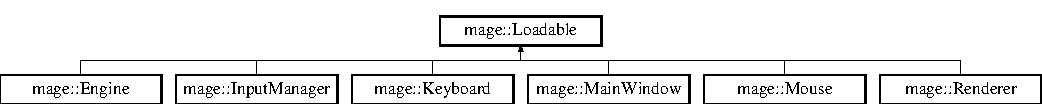
\includegraphics[height=1.393035cm]{classmage_1_1_loadable}
\end{center}
\end{figure}
\subsection*{Public Member Functions}
\begin{DoxyCompactItemize}
\item 
virtual \hyperlink{classmage_1_1_loadable_a7f51b5e1065ebe4dd1da7ef9c9966546}{$\sim$\+Loadable} ()=default
\item 
bool \hyperlink{classmage_1_1_loadable_a53cfa5beb9b44bbcda0d6166a54b8cb6}{Is\+Loaded} () const
\end{DoxyCompactItemize}
\subsection*{Protected Member Functions}
\begin{DoxyCompactItemize}
\item 
\hyperlink{classmage_1_1_loadable_afbdcb287b5e20583899a27a1c244bc7d}{Loadable} (bool loaded=false)
\item 
\hyperlink{classmage_1_1_loadable_a21364449c045d579cb6090347d83cd54}{Loadable} (const \hyperlink{classmage_1_1_loadable}{Loadable} \&loadable)=default
\item 
\hyperlink{classmage_1_1_loadable_ad5f3daaaa4902fe285513408ec92b832}{Loadable} (\hyperlink{classmage_1_1_loadable}{Loadable} \&\&loadable)=default
\item 
\hyperlink{classmage_1_1_loadable}{Loadable} \& \hyperlink{classmage_1_1_loadable_a82277616525b6ed9b1e19fd2dcdb4c0d}{operator=} (const \hyperlink{classmage_1_1_loadable}{Loadable} \&loadable)=default
\item 
\hyperlink{classmage_1_1_loadable}{Loadable} \& \hyperlink{classmage_1_1_loadable_adf203e75fa34f78e617fae0682be3444}{operator=} (\hyperlink{classmage_1_1_loadable}{Loadable} \&\&loadable)=default
\item 
void \hyperlink{classmage_1_1_loadable_a932ff8b287c8e68e30a13804cba08ff2}{Set\+Loaded} (bool loaded=true)
\end{DoxyCompactItemize}
\subsection*{Private Attributes}
\begin{DoxyCompactItemize}
\item 
bool \hyperlink{classmage_1_1_loadable_a993963fbfeb0f2e2ab9616bf7ef6a0f7}{m\+\_\+loaded}
\end{DoxyCompactItemize}


\subsection{Detailed Description}
A class of loadables. 

\subsection{Constructor \& Destructor Documentation}
\hypertarget{classmage_1_1_loadable_a7f51b5e1065ebe4dd1da7ef9c9966546}{}\label{classmage_1_1_loadable_a7f51b5e1065ebe4dd1da7ef9c9966546} 
\index{mage\+::\+Loadable@{mage\+::\+Loadable}!````~Loadable@{$\sim$\+Loadable}}
\index{````~Loadable@{$\sim$\+Loadable}!mage\+::\+Loadable@{mage\+::\+Loadable}}
\subsubsection{\texorpdfstring{$\sim$\+Loadable()}{~Loadable()}}
{\footnotesize\ttfamily virtual mage\+::\+Loadable\+::$\sim$\+Loadable (\begin{DoxyParamCaption}{ }\end{DoxyParamCaption})\hspace{0.3cm}{\ttfamily [virtual]}, {\ttfamily [default]}}

Destructs this loadable. \hypertarget{classmage_1_1_loadable_afbdcb287b5e20583899a27a1c244bc7d}{}\label{classmage_1_1_loadable_afbdcb287b5e20583899a27a1c244bc7d} 
\index{mage\+::\+Loadable@{mage\+::\+Loadable}!Loadable@{Loadable}}
\index{Loadable@{Loadable}!mage\+::\+Loadable@{mage\+::\+Loadable}}
\subsubsection{\texorpdfstring{Loadable()}{Loadable()}\hspace{0.1cm}{\footnotesize\ttfamily [1/3]}}
{\footnotesize\ttfamily mage\+::\+Loadable\+::\+Loadable (\begin{DoxyParamCaption}\item[{bool}]{loaded = {\ttfamily false} }\end{DoxyParamCaption})\hspace{0.3cm}{\ttfamily [explicit]}, {\ttfamily [protected]}}

Constructs a loadable.


\begin{DoxyParams}[1]{Parameters}
\mbox{\tt in}  & {\em loaded} & Flag indicating wether the loadable is loaded. \\
\hline
\end{DoxyParams}
\hypertarget{classmage_1_1_loadable_a21364449c045d579cb6090347d83cd54}{}\label{classmage_1_1_loadable_a21364449c045d579cb6090347d83cd54} 
\index{mage\+::\+Loadable@{mage\+::\+Loadable}!Loadable@{Loadable}}
\index{Loadable@{Loadable}!mage\+::\+Loadable@{mage\+::\+Loadable}}
\subsubsection{\texorpdfstring{Loadable()}{Loadable()}\hspace{0.1cm}{\footnotesize\ttfamily [2/3]}}
{\footnotesize\ttfamily mage\+::\+Loadable\+::\+Loadable (\begin{DoxyParamCaption}\item[{const \hyperlink{classmage_1_1_loadable}{Loadable} \&}]{loadable }\end{DoxyParamCaption})\hspace{0.3cm}{\ttfamily [protected]}, {\ttfamily [default]}}

Constructs a loadable from the given loadable.


\begin{DoxyParams}[1]{Parameters}
\mbox{\tt in}  & {\em loadable} & A reference to the loadable. \\
\hline
\end{DoxyParams}
\hypertarget{classmage_1_1_loadable_ad5f3daaaa4902fe285513408ec92b832}{}\label{classmage_1_1_loadable_ad5f3daaaa4902fe285513408ec92b832} 
\index{mage\+::\+Loadable@{mage\+::\+Loadable}!Loadable@{Loadable}}
\index{Loadable@{Loadable}!mage\+::\+Loadable@{mage\+::\+Loadable}}
\subsubsection{\texorpdfstring{Loadable()}{Loadable()}\hspace{0.1cm}{\footnotesize\ttfamily [3/3]}}
{\footnotesize\ttfamily mage\+::\+Loadable\+::\+Loadable (\begin{DoxyParamCaption}\item[{\hyperlink{classmage_1_1_loadable}{Loadable} \&\&}]{loadable }\end{DoxyParamCaption})\hspace{0.3cm}{\ttfamily [protected]}, {\ttfamily [default]}}

Constructs a loadable from the given loadable.


\begin{DoxyParams}[1]{Parameters}
\mbox{\tt in}  & {\em loadable} & A reference to the loadable. \\
\hline
\end{DoxyParams}


\subsection{Member Function Documentation}
\hypertarget{classmage_1_1_loadable_a53cfa5beb9b44bbcda0d6166a54b8cb6}{}\label{classmage_1_1_loadable_a53cfa5beb9b44bbcda0d6166a54b8cb6} 
\index{mage\+::\+Loadable@{mage\+::\+Loadable}!Is\+Loaded@{Is\+Loaded}}
\index{Is\+Loaded@{Is\+Loaded}!mage\+::\+Loadable@{mage\+::\+Loadable}}
\subsubsection{\texorpdfstring{Is\+Loaded()}{IsLoaded()}}
{\footnotesize\ttfamily bool mage\+::\+Loadable\+::\+Is\+Loaded (\begin{DoxyParamCaption}{ }\end{DoxyParamCaption}) const}

Checks wether this loadable is loaded.

\begin{DoxyReturn}{Returns}
{\ttfamily true} if this loadable is loaded. {\ttfamily false} otherwise. 
\end{DoxyReturn}
\hypertarget{classmage_1_1_loadable_a82277616525b6ed9b1e19fd2dcdb4c0d}{}\label{classmage_1_1_loadable_a82277616525b6ed9b1e19fd2dcdb4c0d} 
\index{mage\+::\+Loadable@{mage\+::\+Loadable}!operator=@{operator=}}
\index{operator=@{operator=}!mage\+::\+Loadable@{mage\+::\+Loadable}}
\subsubsection{\texorpdfstring{operator=()}{operator=()}\hspace{0.1cm}{\footnotesize\ttfamily [1/2]}}
{\footnotesize\ttfamily \hyperlink{classmage_1_1_loadable}{Loadable}\& mage\+::\+Loadable\+::operator= (\begin{DoxyParamCaption}\item[{const \hyperlink{classmage_1_1_loadable}{Loadable} \&}]{loadable }\end{DoxyParamCaption})\hspace{0.3cm}{\ttfamily [protected]}, {\ttfamily [default]}}

Copies the given loadable to this loadable.


\begin{DoxyParams}[1]{Parameters}
\mbox{\tt in}  & {\em loadable} & A reference to the loadable to copy from. \\
\hline
\end{DoxyParams}
\begin{DoxyReturn}{Returns}
A reference to the copy of the given loadable (i.\+e. this loadable). 
\end{DoxyReturn}
\hypertarget{classmage_1_1_loadable_adf203e75fa34f78e617fae0682be3444}{}\label{classmage_1_1_loadable_adf203e75fa34f78e617fae0682be3444} 
\index{mage\+::\+Loadable@{mage\+::\+Loadable}!operator=@{operator=}}
\index{operator=@{operator=}!mage\+::\+Loadable@{mage\+::\+Loadable}}
\subsubsection{\texorpdfstring{operator=()}{operator=()}\hspace{0.1cm}{\footnotesize\ttfamily [2/2]}}
{\footnotesize\ttfamily \hyperlink{classmage_1_1_loadable}{Loadable}\& mage\+::\+Loadable\+::operator= (\begin{DoxyParamCaption}\item[{\hyperlink{classmage_1_1_loadable}{Loadable} \&\&}]{loadable }\end{DoxyParamCaption})\hspace{0.3cm}{\ttfamily [protected]}, {\ttfamily [default]}}

Copies the given loadable to this loadable.


\begin{DoxyParams}[1]{Parameters}
\mbox{\tt in}  & {\em loadable} & A reference to the loadable to copy from. \\
\hline
\end{DoxyParams}
\begin{DoxyReturn}{Returns}
A reference to the copy of the given loadable (i.\+e. this loadable). 
\end{DoxyReturn}
\hypertarget{classmage_1_1_loadable_a932ff8b287c8e68e30a13804cba08ff2}{}\label{classmage_1_1_loadable_a932ff8b287c8e68e30a13804cba08ff2} 
\index{mage\+::\+Loadable@{mage\+::\+Loadable}!Set\+Loaded@{Set\+Loaded}}
\index{Set\+Loaded@{Set\+Loaded}!mage\+::\+Loadable@{mage\+::\+Loadable}}
\subsubsection{\texorpdfstring{Set\+Loaded()}{SetLoaded()}}
{\footnotesize\ttfamily void mage\+::\+Loadable\+::\+Set\+Loaded (\begin{DoxyParamCaption}\item[{bool}]{loaded = {\ttfamily true} }\end{DoxyParamCaption})\hspace{0.3cm}{\ttfamily [protected]}}

Set the state of this loadable to the given value.


\begin{DoxyParams}[1]{Parameters}
\mbox{\tt in}  & {\em loaded} & Flag indicating wether this loadable is loaded. \\
\hline
\end{DoxyParams}


\subsection{Member Data Documentation}
\hypertarget{classmage_1_1_loadable_a993963fbfeb0f2e2ab9616bf7ef6a0f7}{}\label{classmage_1_1_loadable_a993963fbfeb0f2e2ab9616bf7ef6a0f7} 
\index{mage\+::\+Loadable@{mage\+::\+Loadable}!m\+\_\+loaded@{m\+\_\+loaded}}
\index{m\+\_\+loaded@{m\+\_\+loaded}!mage\+::\+Loadable@{mage\+::\+Loadable}}
\subsubsection{\texorpdfstring{m\+\_\+loaded}{m\_loaded}}
{\footnotesize\ttfamily bool mage\+::\+Loadable\+::m\+\_\+loaded\hspace{0.3cm}{\ttfamily [private]}}

Flag indicating wether this loadable is loaded. 
\hypertarget{classmage_1_1_location_script}{}\section{mage\+:\+:Location\+Script Class Reference}
\label{classmage_1_1_location_script}\index{mage\+::\+Location\+Script@{mage\+::\+Location\+Script}}


{\ttfamily \#include $<$location\+\_\+script.\+hpp$>$}

Inheritance diagram for mage\+:\+:Location\+Script\+:\begin{figure}[H]
\begin{center}
\leavevmode
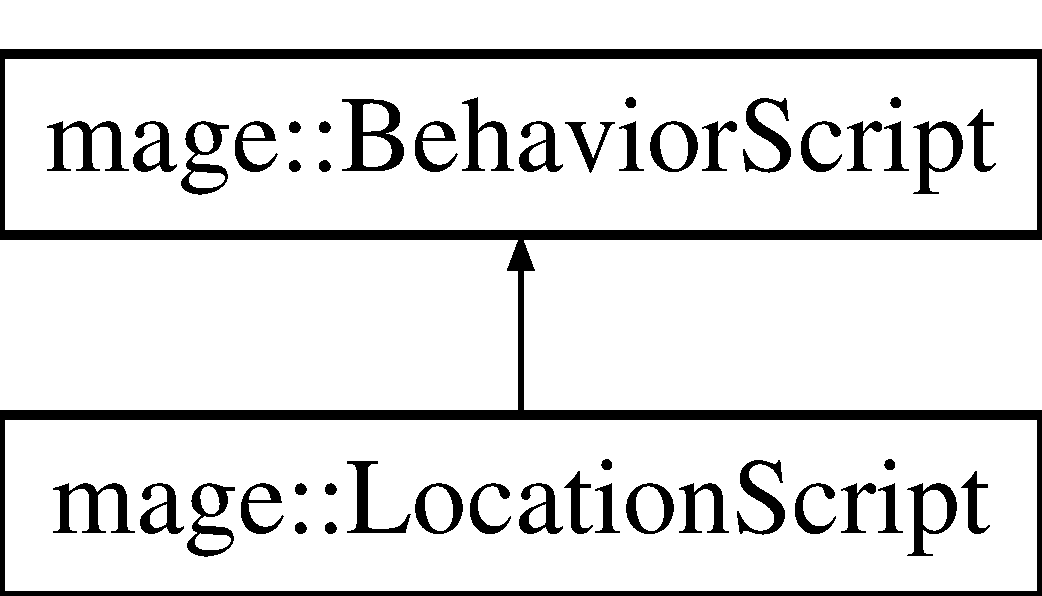
\includegraphics[height=2.000000cm]{classmage_1_1_location_script}
\end{center}
\end{figure}
\subsection*{Public Member Functions}
\begin{DoxyCompactItemize}
\item 
\hyperlink{classmage_1_1_location_script_a14bc9a5868daff6401b0c8b4feebbb3e}{Location\+Script} (Transform\+Node $\ast$transform, \hyperlink{namespacemage_a1e01ae66713838a7a67d30e44c67703e}{Shared\+Ptr}$<$ \hyperlink{classmage_1_1_sprite_text}{Sprite\+Text} $>$ text)
\item 
\hyperlink{classmage_1_1_location_script_a53fb0562896eadb4c747d53b53f65b40}{Location\+Script} (const \hyperlink{classmage_1_1_location_script}{Location\+Script} \&script)=delete
\item 
\hyperlink{classmage_1_1_location_script_a6cddb54a11e5d5d6dee034ef04ffbf2f}{Location\+Script} (\hyperlink{classmage_1_1_location_script}{Location\+Script} \&\&script)
\item 
virtual \hyperlink{classmage_1_1_location_script_a95ed60a4bd7d228cc28ce1622f254d75}{$\sim$\+Location\+Script} ()
\item 
\hyperlink{classmage_1_1_location_script}{Location\+Script} \& \hyperlink{classmage_1_1_location_script_a49409b091dbd1b93830c46831be453fb}{operator=} (const \hyperlink{classmage_1_1_location_script}{Location\+Script} \&script)=delete
\item 
\hyperlink{classmage_1_1_location_script}{Location\+Script} \& \hyperlink{classmage_1_1_location_script_a6e2ad5cd12a984d38c66bbcc81fef94b}{operator=} (\hyperlink{classmage_1_1_location_script}{Location\+Script} \&\&script)=delete
\item 
virtual void \hyperlink{classmage_1_1_location_script_a3ffe0474c573e2cf858aee62056324a3}{Update} (double delta\+\_\+time) override
\end{DoxyCompactItemize}
\subsection*{Private Attributes}
\begin{DoxyCompactItemize}
\item 
Transform\+Node $\ast$const \hyperlink{classmage_1_1_location_script_a6e4ed33a4d2031c8726731c64b8200c9}{m\+\_\+transform}
\item 
\hyperlink{namespacemage_a1e01ae66713838a7a67d30e44c67703e}{Shared\+Ptr}$<$ \hyperlink{classmage_1_1_sprite_text}{Sprite\+Text} $>$ \hyperlink{classmage_1_1_location_script_ac5c7ada3b364d85888686abf20cd6463}{m\+\_\+text}
\end{DoxyCompactItemize}
\subsection*{Additional Inherited Members}


\subsection{Constructor \& Destructor Documentation}
\hypertarget{classmage_1_1_location_script_a14bc9a5868daff6401b0c8b4feebbb3e}{}\label{classmage_1_1_location_script_a14bc9a5868daff6401b0c8b4feebbb3e} 
\index{mage\+::\+Location\+Script@{mage\+::\+Location\+Script}!Location\+Script@{Location\+Script}}
\index{Location\+Script@{Location\+Script}!mage\+::\+Location\+Script@{mage\+::\+Location\+Script}}
\subsubsection{\texorpdfstring{Location\+Script()}{LocationScript()}\hspace{0.1cm}{\footnotesize\ttfamily [1/3]}}
{\footnotesize\ttfamily mage\+::\+Location\+Script\+::\+Location\+Script (\begin{DoxyParamCaption}\item[{Transform\+Node $\ast$}]{transform,  }\item[{\hyperlink{namespacemage_a1e01ae66713838a7a67d30e44c67703e}{Shared\+Ptr}$<$ \hyperlink{classmage_1_1_sprite_text}{Sprite\+Text} $>$}]{text }\end{DoxyParamCaption})\hspace{0.3cm}{\ttfamily [explicit]}}

\hypertarget{classmage_1_1_location_script_a53fb0562896eadb4c747d53b53f65b40}{}\label{classmage_1_1_location_script_a53fb0562896eadb4c747d53b53f65b40} 
\index{mage\+::\+Location\+Script@{mage\+::\+Location\+Script}!Location\+Script@{Location\+Script}}
\index{Location\+Script@{Location\+Script}!mage\+::\+Location\+Script@{mage\+::\+Location\+Script}}
\subsubsection{\texorpdfstring{Location\+Script()}{LocationScript()}\hspace{0.1cm}{\footnotesize\ttfamily [2/3]}}
{\footnotesize\ttfamily mage\+::\+Location\+Script\+::\+Location\+Script (\begin{DoxyParamCaption}\item[{const \hyperlink{classmage_1_1_location_script}{Location\+Script} \&}]{script }\end{DoxyParamCaption})\hspace{0.3cm}{\ttfamily [delete]}}

\hypertarget{classmage_1_1_location_script_a6cddb54a11e5d5d6dee034ef04ffbf2f}{}\label{classmage_1_1_location_script_a6cddb54a11e5d5d6dee034ef04ffbf2f} 
\index{mage\+::\+Location\+Script@{mage\+::\+Location\+Script}!Location\+Script@{Location\+Script}}
\index{Location\+Script@{Location\+Script}!mage\+::\+Location\+Script@{mage\+::\+Location\+Script}}
\subsubsection{\texorpdfstring{Location\+Script()}{LocationScript()}\hspace{0.1cm}{\footnotesize\ttfamily [3/3]}}
{\footnotesize\ttfamily mage\+::\+Location\+Script\+::\+Location\+Script (\begin{DoxyParamCaption}\item[{\hyperlink{classmage_1_1_location_script}{Location\+Script} \&\&}]{script }\end{DoxyParamCaption})\hspace{0.3cm}{\ttfamily [default]}}

\hypertarget{classmage_1_1_location_script_a95ed60a4bd7d228cc28ce1622f254d75}{}\label{classmage_1_1_location_script_a95ed60a4bd7d228cc28ce1622f254d75} 
\index{mage\+::\+Location\+Script@{mage\+::\+Location\+Script}!````~Location\+Script@{$\sim$\+Location\+Script}}
\index{````~Location\+Script@{$\sim$\+Location\+Script}!mage\+::\+Location\+Script@{mage\+::\+Location\+Script}}
\subsubsection{\texorpdfstring{$\sim$\+Location\+Script()}{~LocationScript()}}
{\footnotesize\ttfamily mage\+::\+Location\+Script\+::$\sim$\+Location\+Script (\begin{DoxyParamCaption}{ }\end{DoxyParamCaption})\hspace{0.3cm}{\ttfamily [virtual]}, {\ttfamily [default]}}



\subsection{Member Function Documentation}
\hypertarget{classmage_1_1_location_script_a49409b091dbd1b93830c46831be453fb}{}\label{classmage_1_1_location_script_a49409b091dbd1b93830c46831be453fb} 
\index{mage\+::\+Location\+Script@{mage\+::\+Location\+Script}!operator=@{operator=}}
\index{operator=@{operator=}!mage\+::\+Location\+Script@{mage\+::\+Location\+Script}}
\subsubsection{\texorpdfstring{operator=()}{operator=()}\hspace{0.1cm}{\footnotesize\ttfamily [1/2]}}
{\footnotesize\ttfamily \hyperlink{classmage_1_1_location_script}{Location\+Script}\& mage\+::\+Location\+Script\+::operator= (\begin{DoxyParamCaption}\item[{const \hyperlink{classmage_1_1_location_script}{Location\+Script} \&}]{script }\end{DoxyParamCaption})\hspace{0.3cm}{\ttfamily [delete]}}

\hypertarget{classmage_1_1_location_script_a6e2ad5cd12a984d38c66bbcc81fef94b}{}\label{classmage_1_1_location_script_a6e2ad5cd12a984d38c66bbcc81fef94b} 
\index{mage\+::\+Location\+Script@{mage\+::\+Location\+Script}!operator=@{operator=}}
\index{operator=@{operator=}!mage\+::\+Location\+Script@{mage\+::\+Location\+Script}}
\subsubsection{\texorpdfstring{operator=()}{operator=()}\hspace{0.1cm}{\footnotesize\ttfamily [2/2]}}
{\footnotesize\ttfamily \hyperlink{classmage_1_1_location_script}{Location\+Script}\& mage\+::\+Location\+Script\+::operator= (\begin{DoxyParamCaption}\item[{\hyperlink{classmage_1_1_location_script}{Location\+Script} \&\&}]{script }\end{DoxyParamCaption})\hspace{0.3cm}{\ttfamily [delete]}}

\hypertarget{classmage_1_1_location_script_a3ffe0474c573e2cf858aee62056324a3}{}\label{classmage_1_1_location_script_a3ffe0474c573e2cf858aee62056324a3} 
\index{mage\+::\+Location\+Script@{mage\+::\+Location\+Script}!Update@{Update}}
\index{Update@{Update}!mage\+::\+Location\+Script@{mage\+::\+Location\+Script}}
\subsubsection{\texorpdfstring{Update()}{Update()}}
{\footnotesize\ttfamily void mage\+::\+Location\+Script\+::\+Update (\begin{DoxyParamCaption}\item[{double}]{delta\+\_\+time }\end{DoxyParamCaption})\hspace{0.3cm}{\ttfamily [override]}, {\ttfamily [virtual]}}

Updates this behavior script.


\begin{DoxyParams}[1]{Parameters}
\mbox{\tt in}  & {\em delta\+\_\+time} & The elapsed time since the previous update. \\
\hline
\end{DoxyParams}


Implements \hyperlink{classmage_1_1_behavior_script_a905b6c83640cb91d19fecab3435f6feb}{mage\+::\+Behavior\+Script}.



\subsection{Member Data Documentation}
\hypertarget{classmage_1_1_location_script_ac5c7ada3b364d85888686abf20cd6463}{}\label{classmage_1_1_location_script_ac5c7ada3b364d85888686abf20cd6463} 
\index{mage\+::\+Location\+Script@{mage\+::\+Location\+Script}!m\+\_\+text@{m\+\_\+text}}
\index{m\+\_\+text@{m\+\_\+text}!mage\+::\+Location\+Script@{mage\+::\+Location\+Script}}
\subsubsection{\texorpdfstring{m\+\_\+text}{m\_text}}
{\footnotesize\ttfamily \hyperlink{namespacemage_a1e01ae66713838a7a67d30e44c67703e}{Shared\+Ptr}$<$ \hyperlink{classmage_1_1_sprite_text}{Sprite\+Text} $>$ mage\+::\+Location\+Script\+::m\+\_\+text\hspace{0.3cm}{\ttfamily [private]}}

\hypertarget{classmage_1_1_location_script_a6e4ed33a4d2031c8726731c64b8200c9}{}\label{classmage_1_1_location_script_a6e4ed33a4d2031c8726731c64b8200c9} 
\index{mage\+::\+Location\+Script@{mage\+::\+Location\+Script}!m\+\_\+transform@{m\+\_\+transform}}
\index{m\+\_\+transform@{m\+\_\+transform}!mage\+::\+Location\+Script@{mage\+::\+Location\+Script}}
\subsubsection{\texorpdfstring{m\+\_\+transform}{m\_transform}}
{\footnotesize\ttfamily Transform\+Node$\ast$ const mage\+::\+Location\+Script\+::m\+\_\+transform\hspace{0.3cm}{\ttfamily [private]}}


\hypertarget{structmage_1_1_logging_configuration}{}\section{mage\+:\+:Logging\+Configuration Struct Reference}
\label{structmage_1_1_logging_configuration}\index{mage\+::\+Logging\+Configuration@{mage\+::\+Logging\+Configuration}}


{\ttfamily \#include $<$logging.\+hpp$>$}

\subsection*{Public Member Functions}
\begin{DoxyCompactItemize}
\item 
\hyperlink{structmage_1_1_logging_configuration_ab18d18c78e7104f4c677e6d08f31ca01}{Logging\+Configuration} (bool quiet=false, bool verbose=false)
\item 
\hyperlink{structmage_1_1_logging_configuration_a8e4ccd4301f5544213edd3b600cccff9}{Logging\+Configuration} (const \hyperlink{structmage_1_1_logging_configuration}{Logging\+Configuration} \&logging\+\_\+configuration)=default
\item 
\hyperlink{structmage_1_1_logging_configuration_ad5d3dd901720450fcf57d4b1b32fce15}{Logging\+Configuration} (\hyperlink{structmage_1_1_logging_configuration}{Logging\+Configuration} \&\&logging\+\_\+configuration)=default
\item 
\hyperlink{structmage_1_1_logging_configuration_a842cd1d5cf22c9fb6e2c76e684cd08ee}{$\sim$\+Logging\+Configuration} ()=default
\item 
\hyperlink{structmage_1_1_logging_configuration}{Logging\+Configuration} \& \hyperlink{structmage_1_1_logging_configuration_af35d0b0a2f5743944d3d9d66580074db}{operator=} (const \hyperlink{structmage_1_1_logging_configuration}{Logging\+Configuration} \&logging\+\_\+configuration)=default
\item 
\hyperlink{structmage_1_1_logging_configuration}{Logging\+Configuration} \& \hyperlink{structmage_1_1_logging_configuration_a699285ff50d1bb7573cc0c28bcf476b1}{operator=} (\hyperlink{structmage_1_1_logging_configuration}{Logging\+Configuration} \&\&logging\+\_\+configuration)=default
\item 
bool \hyperlink{structmage_1_1_logging_configuration_a64f7a7b45bc0e896b9d493ddaf13ca82}{Is\+Quiet} () const noexcept
\item 
bool \hyperlink{structmage_1_1_logging_configuration_a4ad7dc55f8d105c1125adcea4796bb3b}{Is\+Verbose} () const noexcept
\end{DoxyCompactItemize}
\subsection*{Private Attributes}
\begin{DoxyCompactItemize}
\item 
bool \hyperlink{structmage_1_1_logging_configuration_a38f457d5db84d15e008841ca8653b47c}{m\+\_\+quiet}
\item 
bool \hyperlink{structmage_1_1_logging_configuration_a60f052c2bb702d8153188e93f00427ac}{m\+\_\+verbose}
\end{DoxyCompactItemize}


\subsection{Detailed Description}
A struct of logging configurations of the engine processing. 

\subsection{Constructor \& Destructor Documentation}
\hypertarget{structmage_1_1_logging_configuration_ab18d18c78e7104f4c677e6d08f31ca01}{}\label{structmage_1_1_logging_configuration_ab18d18c78e7104f4c677e6d08f31ca01} 
\index{mage\+::\+Logging\+Configuration@{mage\+::\+Logging\+Configuration}!Logging\+Configuration@{Logging\+Configuration}}
\index{Logging\+Configuration@{Logging\+Configuration}!mage\+::\+Logging\+Configuration@{mage\+::\+Logging\+Configuration}}
\subsubsection{\texorpdfstring{Logging\+Configuration()}{LoggingConfiguration()}\hspace{0.1cm}{\footnotesize\ttfamily [1/3]}}
{\footnotesize\ttfamily mage\+::\+Logging\+Configuration\+::\+Logging\+Configuration (\begin{DoxyParamCaption}\item[{bool}]{quiet = {\ttfamily false},  }\item[{bool}]{verbose = {\ttfamily false} }\end{DoxyParamCaption})\hspace{0.3cm}{\ttfamily [explicit]}}

Constructs a logging configuration.


\begin{DoxyParams}[1]{Parameters}
\mbox{\tt in}  & {\em quiet} & Flag indicating whether quiet logging is preferred. \\
\hline
\mbox{\tt in}  & {\em verbose} & Flag indicating whether verbose logging is preferred. \\
\hline
\end{DoxyParams}
\hypertarget{structmage_1_1_logging_configuration_a8e4ccd4301f5544213edd3b600cccff9}{}\label{structmage_1_1_logging_configuration_a8e4ccd4301f5544213edd3b600cccff9} 
\index{mage\+::\+Logging\+Configuration@{mage\+::\+Logging\+Configuration}!Logging\+Configuration@{Logging\+Configuration}}
\index{Logging\+Configuration@{Logging\+Configuration}!mage\+::\+Logging\+Configuration@{mage\+::\+Logging\+Configuration}}
\subsubsection{\texorpdfstring{Logging\+Configuration()}{LoggingConfiguration()}\hspace{0.1cm}{\footnotesize\ttfamily [2/3]}}
{\footnotesize\ttfamily mage\+::\+Logging\+Configuration\+::\+Logging\+Configuration (\begin{DoxyParamCaption}\item[{const \hyperlink{structmage_1_1_logging_configuration}{Logging\+Configuration} \&}]{logging\+\_\+configuration }\end{DoxyParamCaption})\hspace{0.3cm}{\ttfamily [default]}}

Constructs a logging configuration from the given logging configuration.


\begin{DoxyParams}[1]{Parameters}
\mbox{\tt in}  & {\em logging\+\_\+configuration} & A reference to the logging configuration to copy. \\
\hline
\end{DoxyParams}
\hypertarget{structmage_1_1_logging_configuration_ad5d3dd901720450fcf57d4b1b32fce15}{}\label{structmage_1_1_logging_configuration_ad5d3dd901720450fcf57d4b1b32fce15} 
\index{mage\+::\+Logging\+Configuration@{mage\+::\+Logging\+Configuration}!Logging\+Configuration@{Logging\+Configuration}}
\index{Logging\+Configuration@{Logging\+Configuration}!mage\+::\+Logging\+Configuration@{mage\+::\+Logging\+Configuration}}
\subsubsection{\texorpdfstring{Logging\+Configuration()}{LoggingConfiguration()}\hspace{0.1cm}{\footnotesize\ttfamily [3/3]}}
{\footnotesize\ttfamily mage\+::\+Logging\+Configuration\+::\+Logging\+Configuration (\begin{DoxyParamCaption}\item[{\hyperlink{structmage_1_1_logging_configuration}{Logging\+Configuration} \&\&}]{logging\+\_\+configuration }\end{DoxyParamCaption})\hspace{0.3cm}{\ttfamily [default]}}

Constructs a logging configuration by moving the given logging configuration.


\begin{DoxyParams}[1]{Parameters}
\mbox{\tt in}  & {\em logging\+\_\+configuration} & A reference to the logging configuration to move. \\
\hline
\end{DoxyParams}
\hypertarget{structmage_1_1_logging_configuration_a842cd1d5cf22c9fb6e2c76e684cd08ee}{}\label{structmage_1_1_logging_configuration_a842cd1d5cf22c9fb6e2c76e684cd08ee} 
\index{mage\+::\+Logging\+Configuration@{mage\+::\+Logging\+Configuration}!````~Logging\+Configuration@{$\sim$\+Logging\+Configuration}}
\index{````~Logging\+Configuration@{$\sim$\+Logging\+Configuration}!mage\+::\+Logging\+Configuration@{mage\+::\+Logging\+Configuration}}
\subsubsection{\texorpdfstring{$\sim$\+Logging\+Configuration()}{~LoggingConfiguration()}}
{\footnotesize\ttfamily mage\+::\+Logging\+Configuration\+::$\sim$\+Logging\+Configuration (\begin{DoxyParamCaption}{ }\end{DoxyParamCaption})\hspace{0.3cm}{\ttfamily [default]}}

Destructs this logging configuration. 

\subsection{Member Function Documentation}
\hypertarget{structmage_1_1_logging_configuration_a64f7a7b45bc0e896b9d493ddaf13ca82}{}\label{structmage_1_1_logging_configuration_a64f7a7b45bc0e896b9d493ddaf13ca82} 
\index{mage\+::\+Logging\+Configuration@{mage\+::\+Logging\+Configuration}!Is\+Quiet@{Is\+Quiet}}
\index{Is\+Quiet@{Is\+Quiet}!mage\+::\+Logging\+Configuration@{mage\+::\+Logging\+Configuration}}
\subsubsection{\texorpdfstring{Is\+Quiet()}{IsQuiet()}}
{\footnotesize\ttfamily bool mage\+::\+Logging\+Configuration\+::\+Is\+Quiet (\begin{DoxyParamCaption}{ }\end{DoxyParamCaption}) const\hspace{0.3cm}{\ttfamily [noexcept]}}

Checks whether the logging of the engine processing is quiet.

\begin{DoxyReturn}{Returns}
{\ttfamily true} if the logging of the engine processing is quiet. {\ttfamily false} otherwise. 
\end{DoxyReturn}
\hypertarget{structmage_1_1_logging_configuration_a4ad7dc55f8d105c1125adcea4796bb3b}{}\label{structmage_1_1_logging_configuration_a4ad7dc55f8d105c1125adcea4796bb3b} 
\index{mage\+::\+Logging\+Configuration@{mage\+::\+Logging\+Configuration}!Is\+Verbose@{Is\+Verbose}}
\index{Is\+Verbose@{Is\+Verbose}!mage\+::\+Logging\+Configuration@{mage\+::\+Logging\+Configuration}}
\subsubsection{\texorpdfstring{Is\+Verbose()}{IsVerbose()}}
{\footnotesize\ttfamily bool mage\+::\+Logging\+Configuration\+::\+Is\+Verbose (\begin{DoxyParamCaption}{ }\end{DoxyParamCaption}) const\hspace{0.3cm}{\ttfamily [noexcept]}}

Checks wheter the logging of the engine processing is verbose.

\begin{DoxyReturn}{Returns}
{\ttfamily true} if the logging of the engine processing is verbose. {\ttfamily false} otherwise. 
\end{DoxyReturn}
\hypertarget{structmage_1_1_logging_configuration_af35d0b0a2f5743944d3d9d66580074db}{}\label{structmage_1_1_logging_configuration_af35d0b0a2f5743944d3d9d66580074db} 
\index{mage\+::\+Logging\+Configuration@{mage\+::\+Logging\+Configuration}!operator=@{operator=}}
\index{operator=@{operator=}!mage\+::\+Logging\+Configuration@{mage\+::\+Logging\+Configuration}}
\subsubsection{\texorpdfstring{operator=()}{operator=()}\hspace{0.1cm}{\footnotesize\ttfamily [1/2]}}
{\footnotesize\ttfamily \hyperlink{structmage_1_1_logging_configuration}{Logging\+Configuration}\& mage\+::\+Logging\+Configuration\+::operator= (\begin{DoxyParamCaption}\item[{const \hyperlink{structmage_1_1_logging_configuration}{Logging\+Configuration} \&}]{logging\+\_\+configuration }\end{DoxyParamCaption})\hspace{0.3cm}{\ttfamily [default]}}

Copies the given logging configuration to this logging configuration.


\begin{DoxyParams}[1]{Parameters}
\mbox{\tt in}  & {\em logging\+\_\+configuration} & A reference to the logging configuration to copy. \\
\hline
\end{DoxyParams}
\begin{DoxyReturn}{Returns}
A reference to the copy of the given logging configuration (i.\+e. this logging configuration). 
\end{DoxyReturn}
\hypertarget{structmage_1_1_logging_configuration_a699285ff50d1bb7573cc0c28bcf476b1}{}\label{structmage_1_1_logging_configuration_a699285ff50d1bb7573cc0c28bcf476b1} 
\index{mage\+::\+Logging\+Configuration@{mage\+::\+Logging\+Configuration}!operator=@{operator=}}
\index{operator=@{operator=}!mage\+::\+Logging\+Configuration@{mage\+::\+Logging\+Configuration}}
\subsubsection{\texorpdfstring{operator=()}{operator=()}\hspace{0.1cm}{\footnotesize\ttfamily [2/2]}}
{\footnotesize\ttfamily \hyperlink{structmage_1_1_logging_configuration}{Logging\+Configuration}\& mage\+::\+Logging\+Configuration\+::operator= (\begin{DoxyParamCaption}\item[{\hyperlink{structmage_1_1_logging_configuration}{Logging\+Configuration} \&\&}]{logging\+\_\+configuration }\end{DoxyParamCaption})\hspace{0.3cm}{\ttfamily [default]}}

Moves the given logging configuration to this logging configuration.


\begin{DoxyParams}[1]{Parameters}
\mbox{\tt in}  & {\em logging\+\_\+configuration} & A reference to the logging configuration to move. \\
\hline
\end{DoxyParams}
\begin{DoxyReturn}{Returns}
A reference to the moved logging configuration (i.\+e. this logging configuration). 
\end{DoxyReturn}


\subsection{Member Data Documentation}
\hypertarget{structmage_1_1_logging_configuration_a38f457d5db84d15e008841ca8653b47c}{}\label{structmage_1_1_logging_configuration_a38f457d5db84d15e008841ca8653b47c} 
\index{mage\+::\+Logging\+Configuration@{mage\+::\+Logging\+Configuration}!m\+\_\+quiet@{m\+\_\+quiet}}
\index{m\+\_\+quiet@{m\+\_\+quiet}!mage\+::\+Logging\+Configuration@{mage\+::\+Logging\+Configuration}}
\subsubsection{\texorpdfstring{m\+\_\+quiet}{m\_quiet}}
{\footnotesize\ttfamily bool mage\+::\+Logging\+Configuration\+::m\+\_\+quiet\hspace{0.3cm}{\ttfamily [private]}}

Flag indicating the logging of the engine processing is quiet. \hypertarget{structmage_1_1_logging_configuration_a60f052c2bb702d8153188e93f00427ac}{}\label{structmage_1_1_logging_configuration_a60f052c2bb702d8153188e93f00427ac} 
\index{mage\+::\+Logging\+Configuration@{mage\+::\+Logging\+Configuration}!m\+\_\+verbose@{m\+\_\+verbose}}
\index{m\+\_\+verbose@{m\+\_\+verbose}!mage\+::\+Logging\+Configuration@{mage\+::\+Logging\+Configuration}}
\subsubsection{\texorpdfstring{m\+\_\+verbose}{m\_verbose}}
{\footnotesize\ttfamily bool mage\+::\+Logging\+Configuration\+::m\+\_\+verbose\hspace{0.3cm}{\ttfamily [private]}}

Flag indicating the logging of the engine processing is verbose. 
\hypertarget{classmage_1_1_main_window}{}\section{mage\+:\+:Main\+Window Class Reference}
\label{classmage_1_1_main_window}\index{mage\+::\+Main\+Window@{mage\+::\+Main\+Window}}


{\ttfamily \#include $<$main\+\_\+window.\+hpp$>$}

\subsection*{Public Member Functions}
\begin{DoxyCompactItemize}
\item 
\hyperlink{classmage_1_1_main_window_a05350ed05ac1af3fb7ed3176e3d249ac}{Main\+Window} (H\+I\+N\+S\+T\+A\+N\+CE hinstance, const wstring \&title\+\_\+text, L\+O\+NG width, L\+O\+NG height)
\item 
\hyperlink{classmage_1_1_main_window_a8dc3c590bb168f8178a7db72ff60fd0c}{Main\+Window} (const \hyperlink{classmage_1_1_main_window}{Main\+Window} \&main\+\_\+window)=delete
\item 
\hyperlink{classmage_1_1_main_window_ab5c9cc962420580c62dd2b44c142cf4b}{Main\+Window} (\hyperlink{classmage_1_1_main_window}{Main\+Window} \&\&main\+\_\+window)
\item 
\hyperlink{classmage_1_1_main_window_ada7ecf97d82ce08ba2f31f0afd891031}{$\sim$\+Main\+Window} ()
\item 
\hyperlink{classmage_1_1_main_window}{Main\+Window} \& \hyperlink{classmage_1_1_main_window_a0c2414ae4e627fb401c045371c286de0}{operator=} (const \hyperlink{classmage_1_1_main_window}{Main\+Window} \&main\+\_\+window)=delete
\item 
\hyperlink{classmage_1_1_main_window}{Main\+Window} \& \hyperlink{classmage_1_1_main_window_a684d547966f69ef5df793b5ce516f76a}{operator=} (\hyperlink{classmage_1_1_main_window}{Main\+Window} \&\&main\+\_\+window)=delete
\item 
void \hyperlink{classmage_1_1_main_window_abbb86e7f4dab1b43ca28f83e265f511e}{Show} (int n\+Cmd\+Show) noexcept
\item 
H\+I\+N\+S\+T\+A\+N\+CE \hyperlink{classmage_1_1_main_window_a1b8c851147ea3b51e645c2fce961fe17}{Get\+Hinstance} () noexcept
\item 
H\+W\+ND \hyperlink{classmage_1_1_main_window_ab4520f7c5ef0828535a117a8512221b5}{Get\+Handle} () noexcept
\item 
const wstring \hyperlink{classmage_1_1_main_window_a16ea3780659e00c8e4732b518c7c4a1e}{Get\+Title\+Text} () const noexcept
\item 
void \hyperlink{classmage_1_1_main_window_aaadd51dc2b902d93ea2f28d685477301}{Set\+Title\+Text} (const wstring \&title\+\_\+text) noexcept
\item 
void \hyperlink{classmage_1_1_main_window_a1baa8554782be197fb5932c3af461f0e}{Set\+Title\+Text} (const wchar\+\_\+t $\ast$title\+\_\+text) noexcept
\end{DoxyCompactItemize}
\subsection*{Private Member Functions}
\begin{DoxyCompactItemize}
\item 
void \hyperlink{classmage_1_1_main_window_abcf8f87d562109236de14db7ee8a3df2}{Initialize\+Window} (const wstring \&title\+\_\+text, L\+O\+NG width, L\+O\+NG height)
\item 
void \hyperlink{classmage_1_1_main_window_ab87716ce916ba180068a65294fa037e8}{Initialize\+Window} (const wstring \&title\+\_\+text, const R\+E\+CT \&rectangle)
\item 
void \hyperlink{classmage_1_1_main_window_a229ff4bcc198ed9caf2ce54966caf746}{Uninitialize\+Window} () noexcept
\end{DoxyCompactItemize}
\subsection*{Private Attributes}
\begin{DoxyCompactItemize}
\item 
const H\+I\+N\+S\+T\+A\+N\+CE \hyperlink{classmage_1_1_main_window_a314759bf324579b568528bbf99bc5c7f}{m\+\_\+hinstance}
\item 
H\+W\+ND \hyperlink{classmage_1_1_main_window_afc9afabcf8a52d79f02c8352451863cc}{m\+\_\+hwindow}
\end{DoxyCompactItemize}


\subsection{Detailed Description}
A class of application main windows. 

\subsection{Constructor \& Destructor Documentation}
\hypertarget{classmage_1_1_main_window_a05350ed05ac1af3fb7ed3176e3d249ac}{}\label{classmage_1_1_main_window_a05350ed05ac1af3fb7ed3176e3d249ac} 
\index{mage\+::\+Main\+Window@{mage\+::\+Main\+Window}!Main\+Window@{Main\+Window}}
\index{Main\+Window@{Main\+Window}!mage\+::\+Main\+Window@{mage\+::\+Main\+Window}}
\subsubsection{\texorpdfstring{Main\+Window()}{MainWindow()}\hspace{0.1cm}{\footnotesize\ttfamily [1/3]}}
{\footnotesize\ttfamily mage\+::\+Main\+Window\+::\+Main\+Window (\begin{DoxyParamCaption}\item[{H\+I\+N\+S\+T\+A\+N\+CE}]{hinstance,  }\item[{const wstring \&}]{title\+\_\+text,  }\item[{L\+O\+NG}]{width,  }\item[{L\+O\+NG}]{height }\end{DoxyParamCaption})\hspace{0.3cm}{\ttfamily [explicit]}}

Constructs a main window.

\begin{DoxyPrecond}{Precondition}
{\itshape hinstance} is not equal to {\ttfamily nullptr}. 
\end{DoxyPrecond}

\begin{DoxyParams}[1]{Parameters}
\mbox{\tt in}  & {\em hinstance} & The application instance handle. \\
\hline
\mbox{\tt in}  & {\em title\+\_\+text} & A reference to the title text. \\
\hline
\mbox{\tt in}  & {\em width} & The width of the window. \\
\hline
\mbox{\tt in}  & {\em height} & The height of the window. \\
\hline
\end{DoxyParams}

\begin{DoxyExceptions}{Exceptions}
{\em \hyperlink{structmage_1_1_formatted_exception}{Formatted\+Exception}} & Failed to register the main window\textquotesingle{}s class. \\
\hline
{\em \hyperlink{structmage_1_1_formatted_exception}{Formatted\+Exception}} & Failed to create the main window. \\
\hline
\end{DoxyExceptions}
\hypertarget{classmage_1_1_main_window_a8dc3c590bb168f8178a7db72ff60fd0c}{}\label{classmage_1_1_main_window_a8dc3c590bb168f8178a7db72ff60fd0c} 
\index{mage\+::\+Main\+Window@{mage\+::\+Main\+Window}!Main\+Window@{Main\+Window}}
\index{Main\+Window@{Main\+Window}!mage\+::\+Main\+Window@{mage\+::\+Main\+Window}}
\subsubsection{\texorpdfstring{Main\+Window()}{MainWindow()}\hspace{0.1cm}{\footnotesize\ttfamily [2/3]}}
{\footnotesize\ttfamily mage\+::\+Main\+Window\+::\+Main\+Window (\begin{DoxyParamCaption}\item[{const \hyperlink{classmage_1_1_main_window}{Main\+Window} \&}]{main\+\_\+window }\end{DoxyParamCaption})\hspace{0.3cm}{\ttfamily [delete]}}

Constructs a main window from the given main window.


\begin{DoxyParams}[1]{Parameters}
\mbox{\tt in}  & {\em main\+\_\+window} & A reference to the main window to copy. \\
\hline
\end{DoxyParams}
\hypertarget{classmage_1_1_main_window_ab5c9cc962420580c62dd2b44c142cf4b}{}\label{classmage_1_1_main_window_ab5c9cc962420580c62dd2b44c142cf4b} 
\index{mage\+::\+Main\+Window@{mage\+::\+Main\+Window}!Main\+Window@{Main\+Window}}
\index{Main\+Window@{Main\+Window}!mage\+::\+Main\+Window@{mage\+::\+Main\+Window}}
\subsubsection{\texorpdfstring{Main\+Window()}{MainWindow()}\hspace{0.1cm}{\footnotesize\ttfamily [3/3]}}
{\footnotesize\ttfamily mage\+::\+Main\+Window\+::\+Main\+Window (\begin{DoxyParamCaption}\item[{\hyperlink{classmage_1_1_main_window}{Main\+Window} \&\&}]{main\+\_\+window }\end{DoxyParamCaption})\hspace{0.3cm}{\ttfamily [default]}}

Constructs a main window by moving the given main window.


\begin{DoxyParams}[1]{Parameters}
\mbox{\tt in}  & {\em main\+\_\+window} & A reference to the main window to move. \\
\hline
\end{DoxyParams}
\hypertarget{classmage_1_1_main_window_ada7ecf97d82ce08ba2f31f0afd891031}{}\label{classmage_1_1_main_window_ada7ecf97d82ce08ba2f31f0afd891031} 
\index{mage\+::\+Main\+Window@{mage\+::\+Main\+Window}!````~Main\+Window@{$\sim$\+Main\+Window}}
\index{````~Main\+Window@{$\sim$\+Main\+Window}!mage\+::\+Main\+Window@{mage\+::\+Main\+Window}}
\subsubsection{\texorpdfstring{$\sim$\+Main\+Window()}{~MainWindow()}}
{\footnotesize\ttfamily mage\+::\+Main\+Window\+::$\sim$\+Main\+Window (\begin{DoxyParamCaption}{ }\end{DoxyParamCaption})}

Destructs this main window. 

\subsection{Member Function Documentation}
\hypertarget{classmage_1_1_main_window_ab4520f7c5ef0828535a117a8512221b5}{}\label{classmage_1_1_main_window_ab4520f7c5ef0828535a117a8512221b5} 
\index{mage\+::\+Main\+Window@{mage\+::\+Main\+Window}!Get\+Handle@{Get\+Handle}}
\index{Get\+Handle@{Get\+Handle}!mage\+::\+Main\+Window@{mage\+::\+Main\+Window}}
\subsubsection{\texorpdfstring{Get\+Handle()}{GetHandle()}}
{\footnotesize\ttfamily H\+W\+ND mage\+::\+Main\+Window\+::\+Get\+Handle (\begin{DoxyParamCaption}{ }\end{DoxyParamCaption})\hspace{0.3cm}{\ttfamily [noexcept]}}

Returns the window handle of this main window.

\begin{DoxyReturn}{Returns}
The window handle of this main window. 
\end{DoxyReturn}
\hypertarget{classmage_1_1_main_window_a1b8c851147ea3b51e645c2fce961fe17}{}\label{classmage_1_1_main_window_a1b8c851147ea3b51e645c2fce961fe17} 
\index{mage\+::\+Main\+Window@{mage\+::\+Main\+Window}!Get\+Hinstance@{Get\+Hinstance}}
\index{Get\+Hinstance@{Get\+Hinstance}!mage\+::\+Main\+Window@{mage\+::\+Main\+Window}}
\subsubsection{\texorpdfstring{Get\+Hinstance()}{GetHinstance()}}
{\footnotesize\ttfamily H\+I\+N\+S\+T\+A\+N\+CE mage\+::\+Main\+Window\+::\+Get\+Hinstance (\begin{DoxyParamCaption}{ }\end{DoxyParamCaption})\hspace{0.3cm}{\ttfamily [noexcept]}}

Returns the application instance handle of this main window.

\begin{DoxyReturn}{Returns}
The application instance handle of this main window. 
\end{DoxyReturn}
\hypertarget{classmage_1_1_main_window_a16ea3780659e00c8e4732b518c7c4a1e}{}\label{classmage_1_1_main_window_a16ea3780659e00c8e4732b518c7c4a1e} 
\index{mage\+::\+Main\+Window@{mage\+::\+Main\+Window}!Get\+Title\+Text@{Get\+Title\+Text}}
\index{Get\+Title\+Text@{Get\+Title\+Text}!mage\+::\+Main\+Window@{mage\+::\+Main\+Window}}
\subsubsection{\texorpdfstring{Get\+Title\+Text()}{GetTitleText()}}
{\footnotesize\ttfamily const wstring mage\+::\+Main\+Window\+::\+Get\+Title\+Text (\begin{DoxyParamCaption}{ }\end{DoxyParamCaption}) const\hspace{0.3cm}{\ttfamily [noexcept]}}

Returns the title text of this main window.

\begin{DoxyReturn}{Returns}
The title text of this main window. 
\end{DoxyReturn}
\hypertarget{classmage_1_1_main_window_abcf8f87d562109236de14db7ee8a3df2}{}\label{classmage_1_1_main_window_abcf8f87d562109236de14db7ee8a3df2} 
\index{mage\+::\+Main\+Window@{mage\+::\+Main\+Window}!Initialize\+Window@{Initialize\+Window}}
\index{Initialize\+Window@{Initialize\+Window}!mage\+::\+Main\+Window@{mage\+::\+Main\+Window}}
\subsubsection{\texorpdfstring{Initialize\+Window()}{InitializeWindow()}\hspace{0.1cm}{\footnotesize\ttfamily [1/2]}}
{\footnotesize\ttfamily void mage\+::\+Main\+Window\+::\+Initialize\+Window (\begin{DoxyParamCaption}\item[{const wstring \&}]{title\+\_\+text,  }\item[{L\+O\+NG}]{width,  }\item[{L\+O\+NG}]{height }\end{DoxyParamCaption})\hspace{0.3cm}{\ttfamily [private]}}

Initializes the engine window of this main window.


\begin{DoxyParams}[1]{Parameters}
\mbox{\tt in}  & {\em title\+\_\+text} & A reference to the title text. \\
\hline
\mbox{\tt in}  & {\em width} & The width of the client rectangle of the window. \\
\hline
\mbox{\tt in}  & {\em height} & The height of the client rectangle of the window. \\
\hline
\end{DoxyParams}

\begin{DoxyExceptions}{Exceptions}
{\em \hyperlink{structmage_1_1_formatted_exception}{Formatted\+Exception}} & Failed to register the main window\textquotesingle{}s class. \\
\hline
{\em \hyperlink{structmage_1_1_formatted_exception}{Formatted\+Exception}} & Failed to create the main window. \\
\hline
\end{DoxyExceptions}
\hypertarget{classmage_1_1_main_window_ab87716ce916ba180068a65294fa037e8}{}\label{classmage_1_1_main_window_ab87716ce916ba180068a65294fa037e8} 
\index{mage\+::\+Main\+Window@{mage\+::\+Main\+Window}!Initialize\+Window@{Initialize\+Window}}
\index{Initialize\+Window@{Initialize\+Window}!mage\+::\+Main\+Window@{mage\+::\+Main\+Window}}
\subsubsection{\texorpdfstring{Initialize\+Window()}{InitializeWindow()}\hspace{0.1cm}{\footnotesize\ttfamily [2/2]}}
{\footnotesize\ttfamily void mage\+::\+Main\+Window\+::\+Initialize\+Window (\begin{DoxyParamCaption}\item[{const wstring \&}]{title\+\_\+text,  }\item[{const R\+E\+CT \&}]{rectangle }\end{DoxyParamCaption})\hspace{0.3cm}{\ttfamily [private]}}

Initializes the engine window of this main window.


\begin{DoxyParams}[1]{Parameters}
\mbox{\tt in}  & {\em title\+\_\+text} & A reference to the title text. \\
\hline
\mbox{\tt in}  & {\em rectangle} & A reference to the client rectangle of the window. \\
\hline
\end{DoxyParams}

\begin{DoxyExceptions}{Exceptions}
{\em \hyperlink{structmage_1_1_formatted_exception}{Formatted\+Exception}} & Failed to register the main window\textquotesingle{}s class. \\
\hline
{\em \hyperlink{structmage_1_1_formatted_exception}{Formatted\+Exception}} & Failed to create the main window. \\
\hline
\end{DoxyExceptions}
\hypertarget{classmage_1_1_main_window_a0c2414ae4e627fb401c045371c286de0}{}\label{classmage_1_1_main_window_a0c2414ae4e627fb401c045371c286de0} 
\index{mage\+::\+Main\+Window@{mage\+::\+Main\+Window}!operator=@{operator=}}
\index{operator=@{operator=}!mage\+::\+Main\+Window@{mage\+::\+Main\+Window}}
\subsubsection{\texorpdfstring{operator=()}{operator=()}\hspace{0.1cm}{\footnotesize\ttfamily [1/2]}}
{\footnotesize\ttfamily \hyperlink{classmage_1_1_main_window}{Main\+Window}\& mage\+::\+Main\+Window\+::operator= (\begin{DoxyParamCaption}\item[{const \hyperlink{classmage_1_1_main_window}{Main\+Window} \&}]{main\+\_\+window }\end{DoxyParamCaption})\hspace{0.3cm}{\ttfamily [delete]}}

Copies the given main window to this main window.


\begin{DoxyParams}[1]{Parameters}
\mbox{\tt in}  & {\em main\+\_\+window} & A reference to the main window to copy. \\
\hline
\end{DoxyParams}
\begin{DoxyReturn}{Returns}
A reference to the copy of the given main window (i.\+e. this main window). 
\end{DoxyReturn}
\hypertarget{classmage_1_1_main_window_a684d547966f69ef5df793b5ce516f76a}{}\label{classmage_1_1_main_window_a684d547966f69ef5df793b5ce516f76a} 
\index{mage\+::\+Main\+Window@{mage\+::\+Main\+Window}!operator=@{operator=}}
\index{operator=@{operator=}!mage\+::\+Main\+Window@{mage\+::\+Main\+Window}}
\subsubsection{\texorpdfstring{operator=()}{operator=()}\hspace{0.1cm}{\footnotesize\ttfamily [2/2]}}
{\footnotesize\ttfamily \hyperlink{classmage_1_1_main_window}{Main\+Window}\& mage\+::\+Main\+Window\+::operator= (\begin{DoxyParamCaption}\item[{\hyperlink{classmage_1_1_main_window}{Main\+Window} \&\&}]{main\+\_\+window }\end{DoxyParamCaption})\hspace{0.3cm}{\ttfamily [delete]}}

Moves the given main window to this main window.


\begin{DoxyParams}[1]{Parameters}
\mbox{\tt in}  & {\em main\+\_\+window} & A reference to the main window to move. \\
\hline
\end{DoxyParams}
\begin{DoxyReturn}{Returns}
A reference to the moved main window (i.\+e. this main window). 
\end{DoxyReturn}
\hypertarget{classmage_1_1_main_window_aaadd51dc2b902d93ea2f28d685477301}{}\label{classmage_1_1_main_window_aaadd51dc2b902d93ea2f28d685477301} 
\index{mage\+::\+Main\+Window@{mage\+::\+Main\+Window}!Set\+Title\+Text@{Set\+Title\+Text}}
\index{Set\+Title\+Text@{Set\+Title\+Text}!mage\+::\+Main\+Window@{mage\+::\+Main\+Window}}
\subsubsection{\texorpdfstring{Set\+Title\+Text()}{SetTitleText()}\hspace{0.1cm}{\footnotesize\ttfamily [1/2]}}
{\footnotesize\ttfamily void mage\+::\+Main\+Window\+::\+Set\+Title\+Text (\begin{DoxyParamCaption}\item[{const wstring \&}]{title\+\_\+text }\end{DoxyParamCaption})\hspace{0.3cm}{\ttfamily [noexcept]}}

Sets the title text of this main window to the given title text.


\begin{DoxyParams}[1]{Parameters}
\mbox{\tt in}  & {\em title\+\_\+text} & A reference to the title text. \\
\hline
\end{DoxyParams}
\hypertarget{classmage_1_1_main_window_a1baa8554782be197fb5932c3af461f0e}{}\label{classmage_1_1_main_window_a1baa8554782be197fb5932c3af461f0e} 
\index{mage\+::\+Main\+Window@{mage\+::\+Main\+Window}!Set\+Title\+Text@{Set\+Title\+Text}}
\index{Set\+Title\+Text@{Set\+Title\+Text}!mage\+::\+Main\+Window@{mage\+::\+Main\+Window}}
\subsubsection{\texorpdfstring{Set\+Title\+Text()}{SetTitleText()}\hspace{0.1cm}{\footnotesize\ttfamily [2/2]}}
{\footnotesize\ttfamily void mage\+::\+Main\+Window\+::\+Set\+Title\+Text (\begin{DoxyParamCaption}\item[{const wchar\+\_\+t $\ast$}]{title\+\_\+text }\end{DoxyParamCaption})\hspace{0.3cm}{\ttfamily [noexcept]}}

Sets the title text of this main window to the given title text.

\begin{DoxyPrecond}{Precondition}
{\itshape title\+\_\+text} is not equal to {\ttfamily nullptr}. 
\end{DoxyPrecond}

\begin{DoxyParams}[1]{Parameters}
\mbox{\tt in}  & {\em title\+\_\+text} & A pointer to the title text. \\
\hline
\end{DoxyParams}
\hypertarget{classmage_1_1_main_window_abbb86e7f4dab1b43ca28f83e265f511e}{}\label{classmage_1_1_main_window_abbb86e7f4dab1b43ca28f83e265f511e} 
\index{mage\+::\+Main\+Window@{mage\+::\+Main\+Window}!Show@{Show}}
\index{Show@{Show}!mage\+::\+Main\+Window@{mage\+::\+Main\+Window}}
\subsubsection{\texorpdfstring{Show()}{Show()}}
{\footnotesize\ttfamily void mage\+::\+Main\+Window\+::\+Show (\begin{DoxyParamCaption}\item[{int}]{n\+Cmd\+Show }\end{DoxyParamCaption})\hspace{0.3cm}{\ttfamily [noexcept]}}

Sets the specified window\textquotesingle{}s show state of this main window.


\begin{DoxyParams}[1]{Parameters}
\mbox{\tt in}  & {\em n\+Cmd\+Show} & Controls how this window is to be shown. \\
\hline
\end{DoxyParams}
\hypertarget{classmage_1_1_main_window_a229ff4bcc198ed9caf2ce54966caf746}{}\label{classmage_1_1_main_window_a229ff4bcc198ed9caf2ce54966caf746} 
\index{mage\+::\+Main\+Window@{mage\+::\+Main\+Window}!Uninitialize\+Window@{Uninitialize\+Window}}
\index{Uninitialize\+Window@{Uninitialize\+Window}!mage\+::\+Main\+Window@{mage\+::\+Main\+Window}}
\subsubsection{\texorpdfstring{Uninitialize\+Window()}{UninitializeWindow()}}
{\footnotesize\ttfamily void mage\+::\+Main\+Window\+::\+Uninitialize\+Window (\begin{DoxyParamCaption}{ }\end{DoxyParamCaption})\hspace{0.3cm}{\ttfamily [private]}, {\ttfamily [noexcept]}}

Uninitializes the engine window of this main window. 

\subsection{Member Data Documentation}
\hypertarget{classmage_1_1_main_window_a314759bf324579b568528bbf99bc5c7f}{}\label{classmage_1_1_main_window_a314759bf324579b568528bbf99bc5c7f} 
\index{mage\+::\+Main\+Window@{mage\+::\+Main\+Window}!m\+\_\+hinstance@{m\+\_\+hinstance}}
\index{m\+\_\+hinstance@{m\+\_\+hinstance}!mage\+::\+Main\+Window@{mage\+::\+Main\+Window}}
\subsubsection{\texorpdfstring{m\+\_\+hinstance}{m\_hinstance}}
{\footnotesize\ttfamily const H\+I\+N\+S\+T\+A\+N\+CE mage\+::\+Main\+Window\+::m\+\_\+hinstance\hspace{0.3cm}{\ttfamily [private]}}

The application instance handle of this main window. \hypertarget{classmage_1_1_main_window_afc9afabcf8a52d79f02c8352451863cc}{}\label{classmage_1_1_main_window_afc9afabcf8a52d79f02c8352451863cc} 
\index{mage\+::\+Main\+Window@{mage\+::\+Main\+Window}!m\+\_\+hwindow@{m\+\_\+hwindow}}
\index{m\+\_\+hwindow@{m\+\_\+hwindow}!mage\+::\+Main\+Window@{mage\+::\+Main\+Window}}
\subsubsection{\texorpdfstring{m\+\_\+hwindow}{m\_hwindow}}
{\footnotesize\ttfamily H\+W\+ND mage\+::\+Main\+Window\+::m\+\_\+hwindow\hspace{0.3cm}{\ttfamily [private]}}

The handle of the parent window of this main window. 
\hypertarget{classmage_1_1_manhattan_input_controller_script}{}\section{mage\+:\+:Manhattan\+Input\+Controller\+Script Class Reference}
\label{classmage_1_1_manhattan_input_controller_script}\index{mage\+::\+Manhattan\+Input\+Controller\+Script@{mage\+::\+Manhattan\+Input\+Controller\+Script}}


{\ttfamily \#include $<$manhattan\+\_\+input\+\_\+controller\+\_\+script.\+hpp$>$}

Inheritance diagram for mage\+:\+:Manhattan\+Input\+Controller\+Script\+:\begin{figure}[H]
\begin{center}
\leavevmode
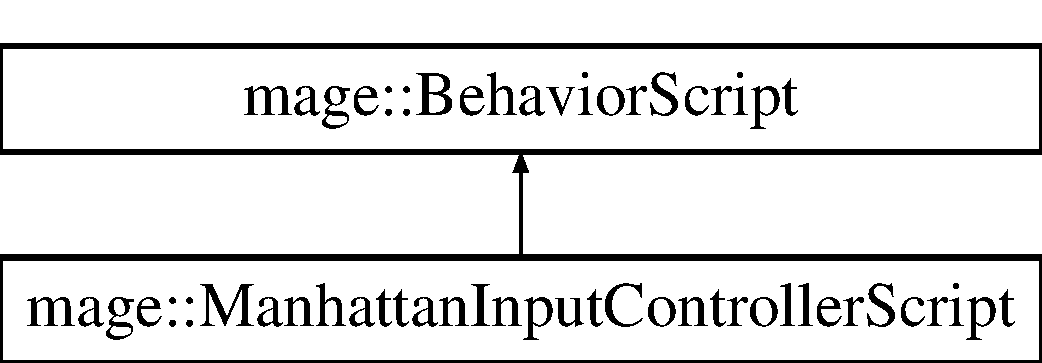
\includegraphics[height=2.000000cm]{classmage_1_1_manhattan_input_controller_script}
\end{center}
\end{figure}
\subsection*{Public Member Functions}
\begin{DoxyCompactItemize}
\item 
\hyperlink{classmage_1_1_manhattan_input_controller_script_a66462b00352cb8aee2f7de76b195d39d}{Manhattan\+Input\+Controller\+Script} (Transform $\ast$transform)
\item 
\hyperlink{classmage_1_1_manhattan_input_controller_script_ad16da80362158de342ecf8d669fbbe15}{Manhattan\+Input\+Controller\+Script} (const \hyperlink{classmage_1_1_manhattan_input_controller_script}{Manhattan\+Input\+Controller\+Script} \&script)=delete
\item 
\hyperlink{classmage_1_1_manhattan_input_controller_script_ad17804aa997c9adb3cbecb2a6bfbfda3}{Manhattan\+Input\+Controller\+Script} (\hyperlink{classmage_1_1_manhattan_input_controller_script}{Manhattan\+Input\+Controller\+Script} \&\&script)=default
\item 
virtual \hyperlink{classmage_1_1_manhattan_input_controller_script_ae4adff57a2d77647ab0b7b89d7bda6d0}{$\sim$\+Manhattan\+Input\+Controller\+Script} ()=default
\item 
\hyperlink{classmage_1_1_manhattan_input_controller_script}{Manhattan\+Input\+Controller\+Script} \& \hyperlink{classmage_1_1_manhattan_input_controller_script_a07fdb2fee8a1eb793c2d54853c9e4998}{operator=} (const \hyperlink{classmage_1_1_manhattan_input_controller_script}{Manhattan\+Input\+Controller\+Script} \&script)=delete
\item 
\hyperlink{classmage_1_1_manhattan_input_controller_script}{Manhattan\+Input\+Controller\+Script} \& \hyperlink{classmage_1_1_manhattan_input_controller_script_acea874b94a4531c393af739824012a1a}{operator=} (\hyperlink{classmage_1_1_manhattan_input_controller_script}{Manhattan\+Input\+Controller\+Script} \&\&script)=delete
\item 
virtual void \hyperlink{classmage_1_1_manhattan_input_controller_script_adfd98377642722fae5db6e005b2c6c3e}{Update} (double delta\+\_\+time) override
\end{DoxyCompactItemize}
\subsection*{Private Attributes}
\begin{DoxyCompactItemize}
\item 
\hyperlink{namespacemage_a8c307fbcc33bce9b7f2aa4c26c3b95cf}{Unique\+Ptr}$<$ \hyperlink{classmage_1_1_mouse_look_script}{Mouse\+Look\+Script} $>$ \hyperlink{classmage_1_1_manhattan_input_controller_script_add3be278d93719ba235d4606d555bd2a}{m\+\_\+orientation\+\_\+script}
\item 
\hyperlink{namespacemage_a8c307fbcc33bce9b7f2aa4c26c3b95cf}{Unique\+Ptr}$<$ \hyperlink{classmage_1_1_manhattan_motor_script}{Manhattan\+Motor\+Script} $>$ \hyperlink{classmage_1_1_manhattan_input_controller_script_ad3b6525bba021f03c17d2de6f5e54101}{m\+\_\+movement\+\_\+script}
\end{DoxyCompactItemize}
\subsection*{Additional Inherited Members}


\subsection{Constructor \& Destructor Documentation}
\hypertarget{classmage_1_1_manhattan_input_controller_script_a66462b00352cb8aee2f7de76b195d39d}{}\label{classmage_1_1_manhattan_input_controller_script_a66462b00352cb8aee2f7de76b195d39d} 
\index{mage\+::\+Manhattan\+Input\+Controller\+Script@{mage\+::\+Manhattan\+Input\+Controller\+Script}!Manhattan\+Input\+Controller\+Script@{Manhattan\+Input\+Controller\+Script}}
\index{Manhattan\+Input\+Controller\+Script@{Manhattan\+Input\+Controller\+Script}!mage\+::\+Manhattan\+Input\+Controller\+Script@{mage\+::\+Manhattan\+Input\+Controller\+Script}}
\subsubsection{\texorpdfstring{Manhattan\+Input\+Controller\+Script()}{ManhattanInputControllerScript()}\hspace{0.1cm}{\footnotesize\ttfamily [1/3]}}
{\footnotesize\ttfamily mage\+::\+Manhattan\+Input\+Controller\+Script\+::\+Manhattan\+Input\+Controller\+Script (\begin{DoxyParamCaption}\item[{Transform $\ast$}]{transform }\end{DoxyParamCaption})\hspace{0.3cm}{\ttfamily [explicit]}}

\hypertarget{classmage_1_1_manhattan_input_controller_script_ad16da80362158de342ecf8d669fbbe15}{}\label{classmage_1_1_manhattan_input_controller_script_ad16da80362158de342ecf8d669fbbe15} 
\index{mage\+::\+Manhattan\+Input\+Controller\+Script@{mage\+::\+Manhattan\+Input\+Controller\+Script}!Manhattan\+Input\+Controller\+Script@{Manhattan\+Input\+Controller\+Script}}
\index{Manhattan\+Input\+Controller\+Script@{Manhattan\+Input\+Controller\+Script}!mage\+::\+Manhattan\+Input\+Controller\+Script@{mage\+::\+Manhattan\+Input\+Controller\+Script}}
\subsubsection{\texorpdfstring{Manhattan\+Input\+Controller\+Script()}{ManhattanInputControllerScript()}\hspace{0.1cm}{\footnotesize\ttfamily [2/3]}}
{\footnotesize\ttfamily mage\+::\+Manhattan\+Input\+Controller\+Script\+::\+Manhattan\+Input\+Controller\+Script (\begin{DoxyParamCaption}\item[{const \hyperlink{classmage_1_1_manhattan_input_controller_script}{Manhattan\+Input\+Controller\+Script} \&}]{script }\end{DoxyParamCaption})\hspace{0.3cm}{\ttfamily [delete]}}

\hypertarget{classmage_1_1_manhattan_input_controller_script_ad17804aa997c9adb3cbecb2a6bfbfda3}{}\label{classmage_1_1_manhattan_input_controller_script_ad17804aa997c9adb3cbecb2a6bfbfda3} 
\index{mage\+::\+Manhattan\+Input\+Controller\+Script@{mage\+::\+Manhattan\+Input\+Controller\+Script}!Manhattan\+Input\+Controller\+Script@{Manhattan\+Input\+Controller\+Script}}
\index{Manhattan\+Input\+Controller\+Script@{Manhattan\+Input\+Controller\+Script}!mage\+::\+Manhattan\+Input\+Controller\+Script@{mage\+::\+Manhattan\+Input\+Controller\+Script}}
\subsubsection{\texorpdfstring{Manhattan\+Input\+Controller\+Script()}{ManhattanInputControllerScript()}\hspace{0.1cm}{\footnotesize\ttfamily [3/3]}}
{\footnotesize\ttfamily mage\+::\+Manhattan\+Input\+Controller\+Script\+::\+Manhattan\+Input\+Controller\+Script (\begin{DoxyParamCaption}\item[{\hyperlink{classmage_1_1_manhattan_input_controller_script}{Manhattan\+Input\+Controller\+Script} \&\&}]{script }\end{DoxyParamCaption})\hspace{0.3cm}{\ttfamily [default]}}

\hypertarget{classmage_1_1_manhattan_input_controller_script_ae4adff57a2d77647ab0b7b89d7bda6d0}{}\label{classmage_1_1_manhattan_input_controller_script_ae4adff57a2d77647ab0b7b89d7bda6d0} 
\index{mage\+::\+Manhattan\+Input\+Controller\+Script@{mage\+::\+Manhattan\+Input\+Controller\+Script}!````~Manhattan\+Input\+Controller\+Script@{$\sim$\+Manhattan\+Input\+Controller\+Script}}
\index{````~Manhattan\+Input\+Controller\+Script@{$\sim$\+Manhattan\+Input\+Controller\+Script}!mage\+::\+Manhattan\+Input\+Controller\+Script@{mage\+::\+Manhattan\+Input\+Controller\+Script}}
\subsubsection{\texorpdfstring{$\sim$\+Manhattan\+Input\+Controller\+Script()}{~ManhattanInputControllerScript()}}
{\footnotesize\ttfamily virtual mage\+::\+Manhattan\+Input\+Controller\+Script\+::$\sim$\+Manhattan\+Input\+Controller\+Script (\begin{DoxyParamCaption}{ }\end{DoxyParamCaption})\hspace{0.3cm}{\ttfamily [virtual]}, {\ttfamily [default]}}



\subsection{Member Function Documentation}
\hypertarget{classmage_1_1_manhattan_input_controller_script_a07fdb2fee8a1eb793c2d54853c9e4998}{}\label{classmage_1_1_manhattan_input_controller_script_a07fdb2fee8a1eb793c2d54853c9e4998} 
\index{mage\+::\+Manhattan\+Input\+Controller\+Script@{mage\+::\+Manhattan\+Input\+Controller\+Script}!operator=@{operator=}}
\index{operator=@{operator=}!mage\+::\+Manhattan\+Input\+Controller\+Script@{mage\+::\+Manhattan\+Input\+Controller\+Script}}
\subsubsection{\texorpdfstring{operator=()}{operator=()}\hspace{0.1cm}{\footnotesize\ttfamily [1/2]}}
{\footnotesize\ttfamily \hyperlink{classmage_1_1_manhattan_input_controller_script}{Manhattan\+Input\+Controller\+Script}\& mage\+::\+Manhattan\+Input\+Controller\+Script\+::operator= (\begin{DoxyParamCaption}\item[{const \hyperlink{classmage_1_1_manhattan_input_controller_script}{Manhattan\+Input\+Controller\+Script} \&}]{script }\end{DoxyParamCaption})\hspace{0.3cm}{\ttfamily [delete]}}

\hypertarget{classmage_1_1_manhattan_input_controller_script_acea874b94a4531c393af739824012a1a}{}\label{classmage_1_1_manhattan_input_controller_script_acea874b94a4531c393af739824012a1a} 
\index{mage\+::\+Manhattan\+Input\+Controller\+Script@{mage\+::\+Manhattan\+Input\+Controller\+Script}!operator=@{operator=}}
\index{operator=@{operator=}!mage\+::\+Manhattan\+Input\+Controller\+Script@{mage\+::\+Manhattan\+Input\+Controller\+Script}}
\subsubsection{\texorpdfstring{operator=()}{operator=()}\hspace{0.1cm}{\footnotesize\ttfamily [2/2]}}
{\footnotesize\ttfamily \hyperlink{classmage_1_1_manhattan_input_controller_script}{Manhattan\+Input\+Controller\+Script}\& mage\+::\+Manhattan\+Input\+Controller\+Script\+::operator= (\begin{DoxyParamCaption}\item[{\hyperlink{classmage_1_1_manhattan_input_controller_script}{Manhattan\+Input\+Controller\+Script} \&\&}]{script }\end{DoxyParamCaption})\hspace{0.3cm}{\ttfamily [delete]}}

\hypertarget{classmage_1_1_manhattan_input_controller_script_adfd98377642722fae5db6e005b2c6c3e}{}\label{classmage_1_1_manhattan_input_controller_script_adfd98377642722fae5db6e005b2c6c3e} 
\index{mage\+::\+Manhattan\+Input\+Controller\+Script@{mage\+::\+Manhattan\+Input\+Controller\+Script}!Update@{Update}}
\index{Update@{Update}!mage\+::\+Manhattan\+Input\+Controller\+Script@{mage\+::\+Manhattan\+Input\+Controller\+Script}}
\subsubsection{\texorpdfstring{Update()}{Update()}}
{\footnotesize\ttfamily virtual void mage\+::\+Manhattan\+Input\+Controller\+Script\+::\+Update (\begin{DoxyParamCaption}\item[{double}]{delta\+\_\+time }\end{DoxyParamCaption})\hspace{0.3cm}{\ttfamily [override]}, {\ttfamily [virtual]}}

Updates this behavior script.


\begin{DoxyParams}[1]{Parameters}
\mbox{\tt in}  & {\em delta\+\_\+time} & The elapsed time since the previous update. \\
\hline
\end{DoxyParams}


Implements \hyperlink{classmage_1_1_behavior_script_a905b6c83640cb91d19fecab3435f6feb}{mage\+::\+Behavior\+Script}.



\subsection{Member Data Documentation}
\hypertarget{classmage_1_1_manhattan_input_controller_script_ad3b6525bba021f03c17d2de6f5e54101}{}\label{classmage_1_1_manhattan_input_controller_script_ad3b6525bba021f03c17d2de6f5e54101} 
\index{mage\+::\+Manhattan\+Input\+Controller\+Script@{mage\+::\+Manhattan\+Input\+Controller\+Script}!m\+\_\+movement\+\_\+script@{m\+\_\+movement\+\_\+script}}
\index{m\+\_\+movement\+\_\+script@{m\+\_\+movement\+\_\+script}!mage\+::\+Manhattan\+Input\+Controller\+Script@{mage\+::\+Manhattan\+Input\+Controller\+Script}}
\subsubsection{\texorpdfstring{m\+\_\+movement\+\_\+script}{m\_movement\_script}}
{\footnotesize\ttfamily \hyperlink{namespacemage_a8c307fbcc33bce9b7f2aa4c26c3b95cf}{Unique\+Ptr}$<$ \hyperlink{classmage_1_1_manhattan_motor_script}{Manhattan\+Motor\+Script} $>$ mage\+::\+Manhattan\+Input\+Controller\+Script\+::m\+\_\+movement\+\_\+script\hspace{0.3cm}{\ttfamily [private]}}

\hypertarget{classmage_1_1_manhattan_input_controller_script_add3be278d93719ba235d4606d555bd2a}{}\label{classmage_1_1_manhattan_input_controller_script_add3be278d93719ba235d4606d555bd2a} 
\index{mage\+::\+Manhattan\+Input\+Controller\+Script@{mage\+::\+Manhattan\+Input\+Controller\+Script}!m\+\_\+orientation\+\_\+script@{m\+\_\+orientation\+\_\+script}}
\index{m\+\_\+orientation\+\_\+script@{m\+\_\+orientation\+\_\+script}!mage\+::\+Manhattan\+Input\+Controller\+Script@{mage\+::\+Manhattan\+Input\+Controller\+Script}}
\subsubsection{\texorpdfstring{m\+\_\+orientation\+\_\+script}{m\_orientation\_script}}
{\footnotesize\ttfamily \hyperlink{namespacemage_a8c307fbcc33bce9b7f2aa4c26c3b95cf}{Unique\+Ptr}$<$ \hyperlink{classmage_1_1_mouse_look_script}{Mouse\+Look\+Script} $>$ mage\+::\+Manhattan\+Input\+Controller\+Script\+::m\+\_\+orientation\+\_\+script\hspace{0.3cm}{\ttfamily [private]}}


\hypertarget{classmage_1_1_manhattan_motor_script}{}\section{mage\+:\+:Manhattan\+Motor\+Script Class Reference}
\label{classmage_1_1_manhattan_motor_script}\index{mage\+::\+Manhattan\+Motor\+Script@{mage\+::\+Manhattan\+Motor\+Script}}


{\ttfamily \#include $<$manhattan\+\_\+motor\+\_\+script.\+hpp$>$}

Inheritance diagram for mage\+:\+:Manhattan\+Motor\+Script\+:\begin{figure}[H]
\begin{center}
\leavevmode
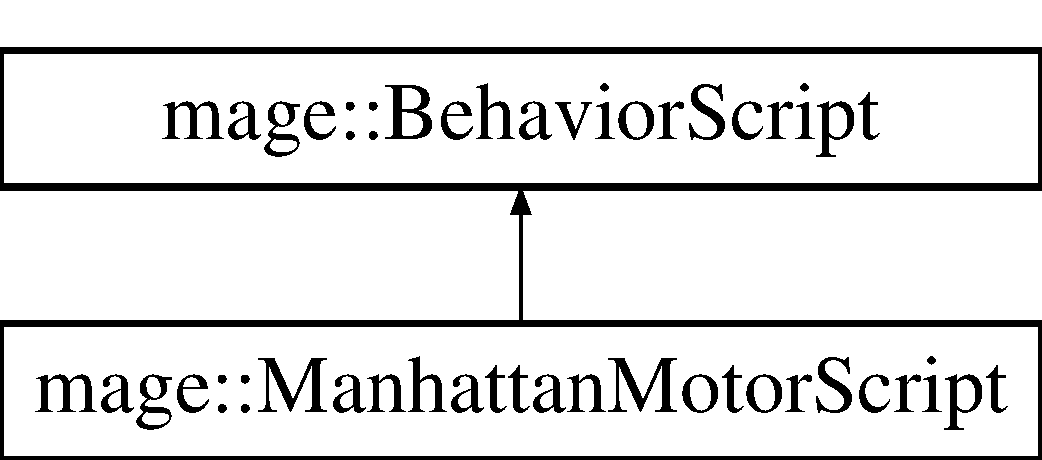
\includegraphics[height=2.000000cm]{classmage_1_1_manhattan_motor_script}
\end{center}
\end{figure}
\subsection*{Public Member Functions}
\begin{DoxyCompactItemize}
\item 
\hyperlink{classmage_1_1_manhattan_motor_script_a6a40360d3b1603e8e5fc64a230ed7574}{Manhattan\+Motor\+Script} (\hyperlink{classmage_1_1_transform_node}{Transform\+Node} $\ast$transform)
\item 
\hyperlink{classmage_1_1_manhattan_motor_script_a890f4456d4707e6eb33e43837b26e536}{Manhattan\+Motor\+Script} (const \hyperlink{classmage_1_1_manhattan_motor_script}{Manhattan\+Motor\+Script} \&script)=delete
\item 
\hyperlink{classmage_1_1_manhattan_motor_script_a3076d8c222953233e86202bd78f9504f}{Manhattan\+Motor\+Script} (\hyperlink{classmage_1_1_manhattan_motor_script}{Manhattan\+Motor\+Script} \&\&script)=default
\item 
virtual \hyperlink{classmage_1_1_manhattan_motor_script_abce38dc8f3f6d96b921cced37accf172}{$\sim$\+Manhattan\+Motor\+Script} ()=default
\item 
\hyperlink{classmage_1_1_manhattan_motor_script}{Manhattan\+Motor\+Script} \& \hyperlink{classmage_1_1_manhattan_motor_script_a563d4d429bbcabf25f57539857dde53c}{operator=} (const \hyperlink{classmage_1_1_manhattan_motor_script}{Manhattan\+Motor\+Script} \&script)=delete
\item 
\hyperlink{classmage_1_1_manhattan_motor_script}{Manhattan\+Motor\+Script} \& \hyperlink{classmage_1_1_manhattan_motor_script_a944149dc06764bc23feffde4de100679}{operator=} (\hyperlink{classmage_1_1_manhattan_motor_script}{Manhattan\+Motor\+Script} \&\&script)=delete
\item 
virtual void \hyperlink{classmage_1_1_manhattan_motor_script_aa2aee651ef777e71ac8da8345f86b212}{Update} (double delta\+\_\+time) override
\item 
float \hyperlink{classmage_1_1_manhattan_motor_script_a420ed8a511a6f404056a31245bb7bed0}{Get\+Velocity} () const
\item 
void \hyperlink{classmage_1_1_manhattan_motor_script_a9a21c42e1998dfe18b05d00011db7e7f}{Set\+Velocity} (float velocity)
\end{DoxyCompactItemize}
\subsection*{Private Attributes}
\begin{DoxyCompactItemize}
\item 
\hyperlink{classmage_1_1_transform_node}{Transform\+Node} $\ast$const \hyperlink{classmage_1_1_manhattan_motor_script_a87af31ce6376830ed040b19d78da386e}{m\+\_\+transform}
\item 
float \hyperlink{classmage_1_1_manhattan_motor_script_a824893c374fa6f271a964751dc1a59ec}{m\+\_\+velocity}
\end{DoxyCompactItemize}
\subsection*{Additional Inherited Members}


\subsection{Constructor \& Destructor Documentation}
\hypertarget{classmage_1_1_manhattan_motor_script_a6a40360d3b1603e8e5fc64a230ed7574}{}\label{classmage_1_1_manhattan_motor_script_a6a40360d3b1603e8e5fc64a230ed7574} 
\index{mage\+::\+Manhattan\+Motor\+Script@{mage\+::\+Manhattan\+Motor\+Script}!Manhattan\+Motor\+Script@{Manhattan\+Motor\+Script}}
\index{Manhattan\+Motor\+Script@{Manhattan\+Motor\+Script}!mage\+::\+Manhattan\+Motor\+Script@{mage\+::\+Manhattan\+Motor\+Script}}
\subsubsection{\texorpdfstring{Manhattan\+Motor\+Script()}{ManhattanMotorScript()}\hspace{0.1cm}{\footnotesize\ttfamily [1/3]}}
{\footnotesize\ttfamily mage\+::\+Manhattan\+Motor\+Script\+::\+Manhattan\+Motor\+Script (\begin{DoxyParamCaption}\item[{\hyperlink{classmage_1_1_transform_node}{Transform\+Node} $\ast$}]{transform }\end{DoxyParamCaption})\hspace{0.3cm}{\ttfamily [explicit]}}

\hypertarget{classmage_1_1_manhattan_motor_script_a890f4456d4707e6eb33e43837b26e536}{}\label{classmage_1_1_manhattan_motor_script_a890f4456d4707e6eb33e43837b26e536} 
\index{mage\+::\+Manhattan\+Motor\+Script@{mage\+::\+Manhattan\+Motor\+Script}!Manhattan\+Motor\+Script@{Manhattan\+Motor\+Script}}
\index{Manhattan\+Motor\+Script@{Manhattan\+Motor\+Script}!mage\+::\+Manhattan\+Motor\+Script@{mage\+::\+Manhattan\+Motor\+Script}}
\subsubsection{\texorpdfstring{Manhattan\+Motor\+Script()}{ManhattanMotorScript()}\hspace{0.1cm}{\footnotesize\ttfamily [2/3]}}
{\footnotesize\ttfamily mage\+::\+Manhattan\+Motor\+Script\+::\+Manhattan\+Motor\+Script (\begin{DoxyParamCaption}\item[{const \hyperlink{classmage_1_1_manhattan_motor_script}{Manhattan\+Motor\+Script} \&}]{script }\end{DoxyParamCaption})\hspace{0.3cm}{\ttfamily [delete]}}

\hypertarget{classmage_1_1_manhattan_motor_script_a3076d8c222953233e86202bd78f9504f}{}\label{classmage_1_1_manhattan_motor_script_a3076d8c222953233e86202bd78f9504f} 
\index{mage\+::\+Manhattan\+Motor\+Script@{mage\+::\+Manhattan\+Motor\+Script}!Manhattan\+Motor\+Script@{Manhattan\+Motor\+Script}}
\index{Manhattan\+Motor\+Script@{Manhattan\+Motor\+Script}!mage\+::\+Manhattan\+Motor\+Script@{mage\+::\+Manhattan\+Motor\+Script}}
\subsubsection{\texorpdfstring{Manhattan\+Motor\+Script()}{ManhattanMotorScript()}\hspace{0.1cm}{\footnotesize\ttfamily [3/3]}}
{\footnotesize\ttfamily mage\+::\+Manhattan\+Motor\+Script\+::\+Manhattan\+Motor\+Script (\begin{DoxyParamCaption}\item[{\hyperlink{classmage_1_1_manhattan_motor_script}{Manhattan\+Motor\+Script} \&\&}]{script }\end{DoxyParamCaption})\hspace{0.3cm}{\ttfamily [default]}}

\hypertarget{classmage_1_1_manhattan_motor_script_abce38dc8f3f6d96b921cced37accf172}{}\label{classmage_1_1_manhattan_motor_script_abce38dc8f3f6d96b921cced37accf172} 
\index{mage\+::\+Manhattan\+Motor\+Script@{mage\+::\+Manhattan\+Motor\+Script}!````~Manhattan\+Motor\+Script@{$\sim$\+Manhattan\+Motor\+Script}}
\index{````~Manhattan\+Motor\+Script@{$\sim$\+Manhattan\+Motor\+Script}!mage\+::\+Manhattan\+Motor\+Script@{mage\+::\+Manhattan\+Motor\+Script}}
\subsubsection{\texorpdfstring{$\sim$\+Manhattan\+Motor\+Script()}{~ManhattanMotorScript()}}
{\footnotesize\ttfamily virtual mage\+::\+Manhattan\+Motor\+Script\+::$\sim$\+Manhattan\+Motor\+Script (\begin{DoxyParamCaption}{ }\end{DoxyParamCaption})\hspace{0.3cm}{\ttfamily [virtual]}, {\ttfamily [default]}}



\subsection{Member Function Documentation}
\hypertarget{classmage_1_1_manhattan_motor_script_a420ed8a511a6f404056a31245bb7bed0}{}\label{classmage_1_1_manhattan_motor_script_a420ed8a511a6f404056a31245bb7bed0} 
\index{mage\+::\+Manhattan\+Motor\+Script@{mage\+::\+Manhattan\+Motor\+Script}!Get\+Velocity@{Get\+Velocity}}
\index{Get\+Velocity@{Get\+Velocity}!mage\+::\+Manhattan\+Motor\+Script@{mage\+::\+Manhattan\+Motor\+Script}}
\subsubsection{\texorpdfstring{Get\+Velocity()}{GetVelocity()}}
{\footnotesize\ttfamily float mage\+::\+Manhattan\+Motor\+Script\+::\+Get\+Velocity (\begin{DoxyParamCaption}{ }\end{DoxyParamCaption}) const}

\hypertarget{classmage_1_1_manhattan_motor_script_a563d4d429bbcabf25f57539857dde53c}{}\label{classmage_1_1_manhattan_motor_script_a563d4d429bbcabf25f57539857dde53c} 
\index{mage\+::\+Manhattan\+Motor\+Script@{mage\+::\+Manhattan\+Motor\+Script}!operator=@{operator=}}
\index{operator=@{operator=}!mage\+::\+Manhattan\+Motor\+Script@{mage\+::\+Manhattan\+Motor\+Script}}
\subsubsection{\texorpdfstring{operator=()}{operator=()}\hspace{0.1cm}{\footnotesize\ttfamily [1/2]}}
{\footnotesize\ttfamily \hyperlink{classmage_1_1_manhattan_motor_script}{Manhattan\+Motor\+Script}\& mage\+::\+Manhattan\+Motor\+Script\+::operator= (\begin{DoxyParamCaption}\item[{const \hyperlink{classmage_1_1_manhattan_motor_script}{Manhattan\+Motor\+Script} \&}]{script }\end{DoxyParamCaption})\hspace{0.3cm}{\ttfamily [delete]}}

\hypertarget{classmage_1_1_manhattan_motor_script_a944149dc06764bc23feffde4de100679}{}\label{classmage_1_1_manhattan_motor_script_a944149dc06764bc23feffde4de100679} 
\index{mage\+::\+Manhattan\+Motor\+Script@{mage\+::\+Manhattan\+Motor\+Script}!operator=@{operator=}}
\index{operator=@{operator=}!mage\+::\+Manhattan\+Motor\+Script@{mage\+::\+Manhattan\+Motor\+Script}}
\subsubsection{\texorpdfstring{operator=()}{operator=()}\hspace{0.1cm}{\footnotesize\ttfamily [2/2]}}
{\footnotesize\ttfamily \hyperlink{classmage_1_1_manhattan_motor_script}{Manhattan\+Motor\+Script}\& mage\+::\+Manhattan\+Motor\+Script\+::operator= (\begin{DoxyParamCaption}\item[{\hyperlink{classmage_1_1_manhattan_motor_script}{Manhattan\+Motor\+Script} \&\&}]{script }\end{DoxyParamCaption})\hspace{0.3cm}{\ttfamily [delete]}}

\hypertarget{classmage_1_1_manhattan_motor_script_a9a21c42e1998dfe18b05d00011db7e7f}{}\label{classmage_1_1_manhattan_motor_script_a9a21c42e1998dfe18b05d00011db7e7f} 
\index{mage\+::\+Manhattan\+Motor\+Script@{mage\+::\+Manhattan\+Motor\+Script}!Set\+Velocity@{Set\+Velocity}}
\index{Set\+Velocity@{Set\+Velocity}!mage\+::\+Manhattan\+Motor\+Script@{mage\+::\+Manhattan\+Motor\+Script}}
\subsubsection{\texorpdfstring{Set\+Velocity()}{SetVelocity()}}
{\footnotesize\ttfamily void mage\+::\+Manhattan\+Motor\+Script\+::\+Set\+Velocity (\begin{DoxyParamCaption}\item[{float}]{velocity }\end{DoxyParamCaption})}

\hypertarget{classmage_1_1_manhattan_motor_script_aa2aee651ef777e71ac8da8345f86b212}{}\label{classmage_1_1_manhattan_motor_script_aa2aee651ef777e71ac8da8345f86b212} 
\index{mage\+::\+Manhattan\+Motor\+Script@{mage\+::\+Manhattan\+Motor\+Script}!Update@{Update}}
\index{Update@{Update}!mage\+::\+Manhattan\+Motor\+Script@{mage\+::\+Manhattan\+Motor\+Script}}
\subsubsection{\texorpdfstring{Update()}{Update()}}
{\footnotesize\ttfamily void mage\+::\+Manhattan\+Motor\+Script\+::\+Update (\begin{DoxyParamCaption}\item[{double}]{delta\+\_\+time }\end{DoxyParamCaption})\hspace{0.3cm}{\ttfamily [override]}, {\ttfamily [virtual]}}

Updates this behavior script.


\begin{DoxyParams}[1]{Parameters}
\mbox{\tt in}  & {\em delta\+\_\+time} & The elapsed time since the previous update. \\
\hline
\end{DoxyParams}


Implements \hyperlink{classmage_1_1_behavior_script_a905b6c83640cb91d19fecab3435f6feb}{mage\+::\+Behavior\+Script}.



\subsection{Member Data Documentation}
\hypertarget{classmage_1_1_manhattan_motor_script_a87af31ce6376830ed040b19d78da386e}{}\label{classmage_1_1_manhattan_motor_script_a87af31ce6376830ed040b19d78da386e} 
\index{mage\+::\+Manhattan\+Motor\+Script@{mage\+::\+Manhattan\+Motor\+Script}!m\+\_\+transform@{m\+\_\+transform}}
\index{m\+\_\+transform@{m\+\_\+transform}!mage\+::\+Manhattan\+Motor\+Script@{mage\+::\+Manhattan\+Motor\+Script}}
\subsubsection{\texorpdfstring{m\+\_\+transform}{m\_transform}}
{\footnotesize\ttfamily \hyperlink{classmage_1_1_transform_node}{Transform\+Node}$\ast$ const mage\+::\+Manhattan\+Motor\+Script\+::m\+\_\+transform\hspace{0.3cm}{\ttfamily [private]}}

\hypertarget{classmage_1_1_manhattan_motor_script_a824893c374fa6f271a964751dc1a59ec}{}\label{classmage_1_1_manhattan_motor_script_a824893c374fa6f271a964751dc1a59ec} 
\index{mage\+::\+Manhattan\+Motor\+Script@{mage\+::\+Manhattan\+Motor\+Script}!m\+\_\+velocity@{m\+\_\+velocity}}
\index{m\+\_\+velocity@{m\+\_\+velocity}!mage\+::\+Manhattan\+Motor\+Script@{mage\+::\+Manhattan\+Motor\+Script}}
\subsubsection{\texorpdfstring{m\+\_\+velocity}{m\_velocity}}
{\footnotesize\ttfamily float mage\+::\+Manhattan\+Motor\+Script\+::m\+\_\+velocity\hspace{0.3cm}{\ttfamily [private]}}


\hypertarget{structmage_1_1_material}{}\section{mage\+:\+:Material Struct Reference}
\label{structmage_1_1_material}\index{mage\+::\+Material@{mage\+::\+Material}}


{\ttfamily \#include $<$material.\+hpp$>$}

\subsection*{Public Member Functions}
\begin{DoxyCompactItemize}
\item 
\hyperlink{structmage_1_1_material_a0307d3bcf53c6ba270c8be4d127298db}{Material} (const string \&name)
\item 
\hyperlink{structmage_1_1_material_abed630412cdc4a6281389d128ec4b5f3}{Material} (const \hyperlink{structmage_1_1_material}{Material} \&material)=default
\item 
\hyperlink{structmage_1_1_material_a41bfbc2bfa16e3694ac443d390b804c2}{Material} (\hyperlink{structmage_1_1_material}{Material} \&\&material)=default
\item 
\hyperlink{structmage_1_1_material_a4ca65b7e24144ee08dd1ce8d0eda9284}{$\sim$\+Material} ()=default
\item 
\hyperlink{structmage_1_1_material}{Material} \& \hyperlink{structmage_1_1_material_a7ebc9986924ca13ae8468005518dcfc7}{operator=} (const \hyperlink{structmage_1_1_material}{Material} \&material)=default
\item 
\hyperlink{structmage_1_1_material}{Material} \& \hyperlink{structmage_1_1_material_a500a2ebe99d4d7b3be5bf57b6bff62a1}{operator=} (\hyperlink{structmage_1_1_material}{Material} \&\&material)=default
\item 
const string \& \hyperlink{structmage_1_1_material_a9edb2f437eca07c6c12c24d10ec30eb3}{Get\+Name} () const noexcept
\item 
void \hyperlink{structmage_1_1_material_a4795f7aa36a445c09af6268a4af8cb61}{Set\+Name} (const string \&name)
\item 
\hyperlink{structmage_1_1_r_g_b_spectrum}{R\+G\+B\+Spectrum} \& \hyperlink{structmage_1_1_material_aba949cb74176530638c7bcb100882196}{Get\+Transmission\+Filter} () noexcept
\item 
const \hyperlink{structmage_1_1_r_g_b_spectrum}{R\+G\+B\+Spectrum} \& \hyperlink{structmage_1_1_material_a38071483e6d47eedb02b2e5c912073e7}{Get\+Transmission\+Filter} () const noexcept
\item 
void \hyperlink{structmage_1_1_material_afe8121e13eb9fff9ffb281e7c807f2e0}{Set\+Transmission\+Filter} (const \hyperlink{structmage_1_1_r_g_b_spectrum}{R\+G\+B\+Spectrum} \&transmission\+\_\+filter) noexcept
\item 
\hyperlink{structmage_1_1_r_g_b_spectrum}{R\+G\+B\+Spectrum} \& \hyperlink{structmage_1_1_material_a244df193031de84daf6cb9b8c30f0d72}{Get\+Ambient\+Reflectivity} () noexcept
\item 
const \hyperlink{structmage_1_1_r_g_b_spectrum}{R\+G\+B\+Spectrum} \& \hyperlink{structmage_1_1_material_ad13afcccbb9b73cddd23a8586e77136e}{Get\+Ambient\+Reflectivity} () const noexcept
\item 
void \hyperlink{structmage_1_1_material_a7a5cf55e733d2180865d5f6d9758336c}{Set\+Ambient\+Reflectivity} (const \hyperlink{structmage_1_1_r_g_b_spectrum}{R\+G\+B\+Spectrum} \&ambient\+\_\+reflectivity) noexcept
\item 
\hyperlink{namespacemage_a1e01ae66713838a7a67d30e44c67703e}{Shared\+Ptr}$<$ \hyperlink{classmage_1_1_texture}{Texture} $>$ \hyperlink{structmage_1_1_material_a231f4f13768d54af5a587266f45d734c}{Get\+Ambient\+Reflectivity\+Texture} () const noexcept
\item 
I\+D3\+D11\+Shader\+Resource\+View $\ast$ \hyperlink{structmage_1_1_material_ab0d0618400f2eb7cefecfa5c6da2192b}{Get\+Ambient\+Reflectivity\+S\+RV} () const noexcept
\item 
I\+D3\+D11\+Shader\+Resource\+View $\ast$const  $\ast$ \hyperlink{structmage_1_1_material_a52b0428fb9aeba97dcd8b5c7eb09836f}{Get\+Ambient\+Reflectivity\+S\+R\+V\+Address} () const noexcept
\item 
void \hyperlink{structmage_1_1_material_a220430d91bcc02a78a8e1601d7725417}{Set\+Ambient\+Reflectivity\+Texture} (\hyperlink{namespacemage_a1e01ae66713838a7a67d30e44c67703e}{Shared\+Ptr}$<$ \hyperlink{classmage_1_1_texture}{Texture} $>$ ambient\+\_\+reflectivity\+\_\+texture)
\item 
\hyperlink{structmage_1_1_r_g_b_spectrum}{R\+G\+B\+Spectrum} \& \hyperlink{structmage_1_1_material_afb37e1cd37df82b6607a4e5998e58ea8}{Get\+Diffuse\+Reflectivity} () noexcept
\item 
const \hyperlink{structmage_1_1_r_g_b_spectrum}{R\+G\+B\+Spectrum} \& \hyperlink{structmage_1_1_material_a046b0d8eece74bd68538fefd03c1f294}{Get\+Diffuse\+Reflectivity} () const noexcept
\item 
void \hyperlink{structmage_1_1_material_aef82ef4eba08eabc31989144316a57c6}{Set\+Diffuse\+Reflectivity} (const \hyperlink{structmage_1_1_r_g_b_spectrum}{R\+G\+B\+Spectrum} \&diffuse\+\_\+reflectivity) noexcept
\item 
\hyperlink{namespacemage_a1e01ae66713838a7a67d30e44c67703e}{Shared\+Ptr}$<$ \hyperlink{classmage_1_1_texture}{Texture} $>$ \hyperlink{structmage_1_1_material_a3b4de7dc988c91eb3ce7ea715d98b758}{Get\+Diffuse\+Reflectivity\+Texture} () const noexcept
\item 
I\+D3\+D11\+Shader\+Resource\+View $\ast$ \hyperlink{structmage_1_1_material_a20c4db65d5fb89178c0f6b6db2f87cda}{Get\+Diffuse\+Reflectivity\+S\+RV} () const noexcept
\item 
I\+D3\+D11\+Shader\+Resource\+View $\ast$const  $\ast$ \hyperlink{structmage_1_1_material_a655a7349f6023b81e8d396abe06ed6ac}{Get\+Diffuse\+Reflectivity\+S\+R\+V\+Address} () const noexcept
\item 
void \hyperlink{structmage_1_1_material_a32e02c92dfd73db1a8a809a45546dc87}{Set\+Diffuse\+Reflectivity\+Texture} (\hyperlink{namespacemage_a1e01ae66713838a7a67d30e44c67703e}{Shared\+Ptr}$<$ \hyperlink{classmage_1_1_texture}{Texture} $>$ diffuse\+\_\+reflectivity\+\_\+texture)
\item 
\hyperlink{structmage_1_1_r_g_b_spectrum}{R\+G\+B\+Spectrum} \& \hyperlink{structmage_1_1_material_ad5fde8d972471fc99b72a4fc969883b1}{Get\+Specular\+Reflectivity} () noexcept
\item 
const \hyperlink{structmage_1_1_r_g_b_spectrum}{R\+G\+B\+Spectrum} \& \hyperlink{structmage_1_1_material_a81005b5094b99b9a8d7f16bedd195718}{Get\+Specular\+Reflectivity} () const noexcept
\item 
void \hyperlink{structmage_1_1_material_ac615e33c8e17149345488fed5c16dc7b}{Set\+Specular\+Reflectivity} (const \hyperlink{structmage_1_1_r_g_b_spectrum}{R\+G\+B\+Spectrum} \&specular\+\_\+reflectivity) noexcept
\item 
\hyperlink{namespacemage_a1e01ae66713838a7a67d30e44c67703e}{Shared\+Ptr}$<$ \hyperlink{classmage_1_1_texture}{Texture} $>$ \hyperlink{structmage_1_1_material_a7ed5469af2440a4fc1db498c24f06764}{Get\+Specular\+Reflectivity\+Texture} () const noexcept
\item 
I\+D3\+D11\+Shader\+Resource\+View $\ast$ \hyperlink{structmage_1_1_material_a04fad2f985ed5078a8217ebcfd51c3f0}{Get\+Specular\+Reflectivity\+S\+RV} () const noexcept
\item 
I\+D3\+D11\+Shader\+Resource\+View $\ast$const  $\ast$ \hyperlink{structmage_1_1_material_a7c3ea6461982e7dc9a60a391d601f172}{Get\+Specular\+Reflectivity\+S\+R\+V\+Address} () const noexcept
\item 
void \hyperlink{structmage_1_1_material_a130430244dfd0b5866b00fca523e874c}{Set\+Specular\+Reflectivity\+Texture} (\hyperlink{namespacemage_a1e01ae66713838a7a67d30e44c67703e}{Shared\+Ptr}$<$ \hyperlink{classmage_1_1_texture}{Texture} $>$ specular\+\_\+reflectivity\+\_\+texture)
\item 
float \hyperlink{structmage_1_1_material_a48afb440024e4e2e45a81ce2b46c0d73}{Get\+Specular\+Exponent} () const noexcept
\item 
void \hyperlink{structmage_1_1_material_a078a2c9388993523e29f287e20385b3f}{Set\+Specular\+Exponent} (float specular\+\_\+exponent) noexcept
\item 
\hyperlink{namespacemage_a1e01ae66713838a7a67d30e44c67703e}{Shared\+Ptr}$<$ \hyperlink{classmage_1_1_texture}{Texture} $>$ \hyperlink{structmage_1_1_material_a24c476c257c3ba042ddda666c26660c0}{Get\+Specular\+Exponent\+Texture} () const noexcept
\item 
I\+D3\+D11\+Shader\+Resource\+View $\ast$ \hyperlink{structmage_1_1_material_aca8740404b0e52c781dd1c02ec167539}{Get\+Specular\+Exponent\+S\+RV} () const noexcept
\item 
I\+D3\+D11\+Shader\+Resource\+View $\ast$const  $\ast$ \hyperlink{structmage_1_1_material_a57a083f7769c5d6501282d66b6733b10}{Get\+Specular\+Exponent\+S\+R\+V\+Address} () const noexcept
\item 
void \hyperlink{structmage_1_1_material_ae07cb5f8c3b4ee0d6e6f4f91c1cbbf35}{Set\+Specular\+Exponent\+Texture} (\hyperlink{namespacemage_a1e01ae66713838a7a67d30e44c67703e}{Shared\+Ptr}$<$ \hyperlink{classmage_1_1_texture}{Texture} $>$ specular\+\_\+exponent\+\_\+texture)
\item 
float \hyperlink{structmage_1_1_material_aa320c6b371b9f055a76821db71d185bc}{Get\+Dissolve} () const noexcept
\item 
void \hyperlink{structmage_1_1_material_ad86de160f4e4e03c24329d8f9415ccaa}{Set\+Dissolve} (float dissolve) noexcept
\item 
\hyperlink{namespacemage_a1e01ae66713838a7a67d30e44c67703e}{Shared\+Ptr}$<$ \hyperlink{classmage_1_1_texture}{Texture} $>$ \hyperlink{structmage_1_1_material_abcf6fa7acad8c0cda8859e32eb2c3168}{Get\+Dissolve\+Texture} () const noexcept
\item 
I\+D3\+D11\+Shader\+Resource\+View $\ast$ \hyperlink{structmage_1_1_material_adb87e492a57c7539776a311a2e454167}{Get\+Dissolve\+S\+RV} () const noexcept
\item 
I\+D3\+D11\+Shader\+Resource\+View $\ast$const  $\ast$ \hyperlink{structmage_1_1_material_a9a50e538b24f15129fd95c1272fc82be}{Get\+Dissolve\+S\+R\+V\+Address} () const noexcept
\item 
void \hyperlink{structmage_1_1_material_ae2afaedc1d81fc753b060cca5d86db91}{Set\+Dissolve\+Texture} (\hyperlink{namespacemage_a1e01ae66713838a7a67d30e44c67703e}{Shared\+Ptr}$<$ \hyperlink{classmage_1_1_texture}{Texture} $>$ dissolve\+\_\+texture)
\item 
float \hyperlink{structmage_1_1_material_afa719020dabd412bbb06ac9f0d85abe9}{Get\+Index\+Of\+Refraction} () const noexcept
\item 
void \hyperlink{structmage_1_1_material_ae0f95f54af97ecff043ec7728260ae2b}{Set\+Index\+Of\+Refraction} (float index\+\_\+of\+\_\+refraction) noexcept
\item 
\hyperlink{namespacemage_a1e01ae66713838a7a67d30e44c67703e}{Shared\+Ptr}$<$ \hyperlink{classmage_1_1_texture}{Texture} $>$ \hyperlink{structmage_1_1_material_a7cf62e3f72b74c945e3d5c47c2c73485}{Get\+Decal\+Texture} () const noexcept
\item 
I\+D3\+D11\+Shader\+Resource\+View $\ast$ \hyperlink{structmage_1_1_material_a8d189673acfe8d0c104873fe0cceb601}{Get\+Decal\+S\+RV} () const noexcept
\item 
I\+D3\+D11\+Shader\+Resource\+View $\ast$const  $\ast$ \hyperlink{structmage_1_1_material_aaafa9944c4069c983ef2cff9f84e8039}{Get\+Decal\+S\+R\+V\+Address} () const noexcept
\item 
void \hyperlink{structmage_1_1_material_ad52bf9c9d802fce7f7ec47f35a44d180}{Set\+Decal\+Texture} (\hyperlink{namespacemage_a1e01ae66713838a7a67d30e44c67703e}{Shared\+Ptr}$<$ \hyperlink{classmage_1_1_texture}{Texture} $>$ decal\+\_\+texture)
\item 
\hyperlink{namespacemage_a1e01ae66713838a7a67d30e44c67703e}{Shared\+Ptr}$<$ \hyperlink{classmage_1_1_texture}{Texture} $>$ \hyperlink{structmage_1_1_material_ab548fbf5844ae7cd2822304ef7fb9602}{Get\+Displacement\+Texture} () const noexcept
\item 
I\+D3\+D11\+Shader\+Resource\+View $\ast$ \hyperlink{structmage_1_1_material_a638ee0913aa0722f499c883b71549503}{Get\+Displacement\+S\+RV} () const noexcept
\item 
I\+D3\+D11\+Shader\+Resource\+View $\ast$const  $\ast$ \hyperlink{structmage_1_1_material_a7672015b558ebbaa52e070f65b052b2e}{Get\+Displacement\+S\+R\+V\+Address} () const noexcept
\item 
void \hyperlink{structmage_1_1_material_ab9c90afa999906a3ad33c8a8da13da24}{Set\+Displacement\+Texture} (\hyperlink{namespacemage_a1e01ae66713838a7a67d30e44c67703e}{Shared\+Ptr}$<$ \hyperlink{classmage_1_1_texture}{Texture} $>$ displacement\+\_\+texture)
\item 
\hyperlink{namespacemage_a1e01ae66713838a7a67d30e44c67703e}{Shared\+Ptr}$<$ \hyperlink{classmage_1_1_texture}{Texture} $>$ \hyperlink{structmage_1_1_material_a7343766b10456e4ed1e09b3fe6110981}{Get\+Normal\+Texture} () const noexcept
\item 
I\+D3\+D11\+Shader\+Resource\+View $\ast$ \hyperlink{structmage_1_1_material_a0be98911c56dedaa4fd2f8714fc8a793}{Get\+Normal\+S\+RV} () const noexcept
\item 
I\+D3\+D11\+Shader\+Resource\+View $\ast$const  $\ast$ \hyperlink{structmage_1_1_material_a297911bb366b1cc1b28d0c35353eb806}{Get\+Normal\+S\+R\+V\+Address} () const noexcept
\item 
void \hyperlink{structmage_1_1_material_a61b695303632bd8fd1399c63e746319e}{Set\+Normal\+Texture} (\hyperlink{namespacemage_a1e01ae66713838a7a67d30e44c67703e}{Shared\+Ptr}$<$ \hyperlink{classmage_1_1_texture}{Texture} $>$ normal\+\_\+texture)
\item 
float \hyperlink{structmage_1_1_material_af6862d7f8fd561e7979bda46449f319f}{Get\+Parameter1} () const noexcept
\item 
void \hyperlink{structmage_1_1_material_a350e145990c73b08e7e2bda2a4255e88}{Set\+Parameter1} (float param1) noexcept
\item 
float \hyperlink{structmage_1_1_material_a078d5b29bd1262fae5052989c6d4ca8b}{Get\+Parameter2} () const noexcept
\item 
void \hyperlink{structmage_1_1_material_a7a1f7dbc0b3b3c72e87a3be0c17f825a}{Set\+Parameter2} (float param2) noexcept
\item 
float \hyperlink{structmage_1_1_material_ad802d2958227950f82ba838d61490b63}{Get\+Parameter3} () const noexcept
\item 
void \hyperlink{structmage_1_1_material_ae79a7b52c3c2ac2b6038276493d09f11}{Set\+Parameter3} (float param3) noexcept
\item 
float \hyperlink{structmage_1_1_material_a192dd5d9836fc12974dbaa820ca90dd2}{Get\+Parameter4} () const noexcept
\item 
void \hyperlink{structmage_1_1_material_a964eddafac7f3cab4bae60ed6c8429f2}{Set\+Parameter4} (float param4) noexcept
\end{DoxyCompactItemize}
\subsection*{Private Attributes}
\begin{DoxyCompactItemize}
\item 
string \hyperlink{structmage_1_1_material_a2b3e839a8ae093d53b12529d61ec6605}{m\+\_\+name}
\item 
\hyperlink{structmage_1_1_r_g_b_spectrum}{R\+G\+B\+Spectrum} \hyperlink{structmage_1_1_material_a9573a0d2a5fb0322f9eb103ace34dd47}{m\+\_\+transmission\+\_\+filter}
\item 
\hyperlink{structmage_1_1_r_g_b_spectrum}{R\+G\+B\+Spectrum} \hyperlink{structmage_1_1_material_ad8fb842410fe751ad220185271a00448}{m\+\_\+ambient\+\_\+reflectivity}
\item 
\hyperlink{namespacemage_a1e01ae66713838a7a67d30e44c67703e}{Shared\+Ptr}$<$ \hyperlink{classmage_1_1_texture}{Texture} $>$ \hyperlink{structmage_1_1_material_a72a90b9d339d705b5fd46098df5892e2}{m\+\_\+ambient\+\_\+reflectivity\+\_\+texture}
\item 
\hyperlink{structmage_1_1_r_g_b_spectrum}{R\+G\+B\+Spectrum} \hyperlink{structmage_1_1_material_afd2cc813023698e52edc01b267a17e6c}{m\+\_\+diffuse\+\_\+reflectivity}
\item 
\hyperlink{namespacemage_a1e01ae66713838a7a67d30e44c67703e}{Shared\+Ptr}$<$ \hyperlink{classmage_1_1_texture}{Texture} $>$ \hyperlink{structmage_1_1_material_a5193e30d3875695c96526a85edc84b88}{m\+\_\+diffuse\+\_\+reflectivity\+\_\+texture}
\item 
\hyperlink{structmage_1_1_r_g_b_spectrum}{R\+G\+B\+Spectrum} \hyperlink{structmage_1_1_material_a45587388f4ff57c209de2280b71af9d3}{m\+\_\+specular\+\_\+reflectivity}
\item 
\hyperlink{namespacemage_a1e01ae66713838a7a67d30e44c67703e}{Shared\+Ptr}$<$ \hyperlink{classmage_1_1_texture}{Texture} $>$ \hyperlink{structmage_1_1_material_ac925df9d71f8668c03e8efada632b300}{m\+\_\+specular\+\_\+reflectivity\+\_\+texture}
\item 
float \hyperlink{structmage_1_1_material_a62a9e8d9f90bf569b9f692c28da6a7dc}{m\+\_\+specular\+\_\+exponent}
\item 
\hyperlink{namespacemage_a1e01ae66713838a7a67d30e44c67703e}{Shared\+Ptr}$<$ \hyperlink{classmage_1_1_texture}{Texture} $>$ \hyperlink{structmage_1_1_material_a452a92691f612bd21857525c00c5e8e5}{m\+\_\+specular\+\_\+exponent\+\_\+texture}
\item 
float \hyperlink{structmage_1_1_material_a42b435ea58ce7da4b48febe9bb33aba7}{m\+\_\+dissolve}
\item 
\hyperlink{namespacemage_a1e01ae66713838a7a67d30e44c67703e}{Shared\+Ptr}$<$ \hyperlink{classmage_1_1_texture}{Texture} $>$ \hyperlink{structmage_1_1_material_aa68e02ed3da6000effc3aadcc99fa4b5}{m\+\_\+dissolve\+\_\+texture}
\item 
float \hyperlink{structmage_1_1_material_a8b584541ab8bfc527f856c68bb0152e7}{m\+\_\+index\+\_\+of\+\_\+refraction}
\item 
\hyperlink{namespacemage_a1e01ae66713838a7a67d30e44c67703e}{Shared\+Ptr}$<$ \hyperlink{classmage_1_1_texture}{Texture} $>$ \hyperlink{structmage_1_1_material_acdab45e5d78ddbb7f717d9db67ff3fcf}{m\+\_\+decal\+\_\+texture}
\item 
\hyperlink{namespacemage_a1e01ae66713838a7a67d30e44c67703e}{Shared\+Ptr}$<$ \hyperlink{classmage_1_1_texture}{Texture} $>$ \hyperlink{structmage_1_1_material_a04ca0a2efe12529ae0ea91e9cb622ade}{m\+\_\+displacement\+\_\+texture}
\item 
\hyperlink{namespacemage_a1e01ae66713838a7a67d30e44c67703e}{Shared\+Ptr}$<$ \hyperlink{classmage_1_1_texture}{Texture} $>$ \hyperlink{structmage_1_1_material_a18e56785d5ca3ae5a9b99c64e70622d6}{m\+\_\+normal\+\_\+texture}
\item 
float \hyperlink{structmage_1_1_material_a1d715533a43b78bbae02b5e243d59f00}{m\+\_\+param1}
\item 
float \hyperlink{structmage_1_1_material_ac451f95eb5b81b6eaa834d9c038f4471}{m\+\_\+param2}
\item 
float \hyperlink{structmage_1_1_material_a725176729546010fa227b73ba3863e29}{m\+\_\+param3}
\item 
float \hyperlink{structmage_1_1_material_a5bdd53b39894a2f04cf68b03906ab149}{m\+\_\+param4}
\end{DoxyCompactItemize}


\subsection{Detailed Description}
A struct of materials. 

\subsection{Constructor \& Destructor Documentation}
\hypertarget{structmage_1_1_material_a0307d3bcf53c6ba270c8be4d127298db}{}\label{structmage_1_1_material_a0307d3bcf53c6ba270c8be4d127298db} 
\index{mage\+::\+Material@{mage\+::\+Material}!Material@{Material}}
\index{Material@{Material}!mage\+::\+Material@{mage\+::\+Material}}
\subsubsection{\texorpdfstring{Material()}{Material()}\hspace{0.1cm}{\footnotesize\ttfamily [1/3]}}
{\footnotesize\ttfamily mage\+::\+Material\+::\+Material (\begin{DoxyParamCaption}\item[{const string \&}]{name }\end{DoxyParamCaption})\hspace{0.3cm}{\ttfamily [explicit]}}

Constructs a material.


\begin{DoxyParams}[1]{Parameters}
\mbox{\tt in}  & {\em name} & A reference to the name of the material. \\
\hline
\end{DoxyParams}
\hypertarget{structmage_1_1_material_abed630412cdc4a6281389d128ec4b5f3}{}\label{structmage_1_1_material_abed630412cdc4a6281389d128ec4b5f3} 
\index{mage\+::\+Material@{mage\+::\+Material}!Material@{Material}}
\index{Material@{Material}!mage\+::\+Material@{mage\+::\+Material}}
\subsubsection{\texorpdfstring{Material()}{Material()}\hspace{0.1cm}{\footnotesize\ttfamily [2/3]}}
{\footnotesize\ttfamily mage\+::\+Material\+::\+Material (\begin{DoxyParamCaption}\item[{const \hyperlink{structmage_1_1_material}{Material} \&}]{material }\end{DoxyParamCaption})\hspace{0.3cm}{\ttfamily [default]}}

Constructs a material from the given material.


\begin{DoxyParams}[1]{Parameters}
\mbox{\tt in}  & {\em material} & A reference to the material to copy. \\
\hline
\end{DoxyParams}
\hypertarget{structmage_1_1_material_a41bfbc2bfa16e3694ac443d390b804c2}{}\label{structmage_1_1_material_a41bfbc2bfa16e3694ac443d390b804c2} 
\index{mage\+::\+Material@{mage\+::\+Material}!Material@{Material}}
\index{Material@{Material}!mage\+::\+Material@{mage\+::\+Material}}
\subsubsection{\texorpdfstring{Material()}{Material()}\hspace{0.1cm}{\footnotesize\ttfamily [3/3]}}
{\footnotesize\ttfamily mage\+::\+Material\+::\+Material (\begin{DoxyParamCaption}\item[{\hyperlink{structmage_1_1_material}{Material} \&\&}]{material }\end{DoxyParamCaption})\hspace{0.3cm}{\ttfamily [default]}}

Constructs a material by moving the given material.


\begin{DoxyParams}[1]{Parameters}
\mbox{\tt in}  & {\em material} & A reference to the material to move. \\
\hline
\end{DoxyParams}
\hypertarget{structmage_1_1_material_a4ca65b7e24144ee08dd1ce8d0eda9284}{}\label{structmage_1_1_material_a4ca65b7e24144ee08dd1ce8d0eda9284} 
\index{mage\+::\+Material@{mage\+::\+Material}!````~Material@{$\sim$\+Material}}
\index{````~Material@{$\sim$\+Material}!mage\+::\+Material@{mage\+::\+Material}}
\subsubsection{\texorpdfstring{$\sim$\+Material()}{~Material()}}
{\footnotesize\ttfamily mage\+::\+Material\+::$\sim$\+Material (\begin{DoxyParamCaption}{ }\end{DoxyParamCaption})\hspace{0.3cm}{\ttfamily [default]}}

Destructs this material. 

\subsection{Member Function Documentation}
\hypertarget{structmage_1_1_material_a244df193031de84daf6cb9b8c30f0d72}{}\label{structmage_1_1_material_a244df193031de84daf6cb9b8c30f0d72} 
\index{mage\+::\+Material@{mage\+::\+Material}!Get\+Ambient\+Reflectivity@{Get\+Ambient\+Reflectivity}}
\index{Get\+Ambient\+Reflectivity@{Get\+Ambient\+Reflectivity}!mage\+::\+Material@{mage\+::\+Material}}
\subsubsection{\texorpdfstring{Get\+Ambient\+Reflectivity()}{GetAmbientReflectivity()}\hspace{0.1cm}{\footnotesize\ttfamily [1/2]}}
{\footnotesize\ttfamily \hyperlink{structmage_1_1_r_g_b_spectrum}{R\+G\+B\+Spectrum}\& mage\+::\+Material\+::\+Get\+Ambient\+Reflectivity (\begin{DoxyParamCaption}{ }\end{DoxyParamCaption})\hspace{0.3cm}{\ttfamily [noexcept]}}

\hypertarget{structmage_1_1_material_ad13afcccbb9b73cddd23a8586e77136e}{}\label{structmage_1_1_material_ad13afcccbb9b73cddd23a8586e77136e} 
\index{mage\+::\+Material@{mage\+::\+Material}!Get\+Ambient\+Reflectivity@{Get\+Ambient\+Reflectivity}}
\index{Get\+Ambient\+Reflectivity@{Get\+Ambient\+Reflectivity}!mage\+::\+Material@{mage\+::\+Material}}
\subsubsection{\texorpdfstring{Get\+Ambient\+Reflectivity()}{GetAmbientReflectivity()}\hspace{0.1cm}{\footnotesize\ttfamily [2/2]}}
{\footnotesize\ttfamily const \hyperlink{structmage_1_1_r_g_b_spectrum}{R\+G\+B\+Spectrum}\& mage\+::\+Material\+::\+Get\+Ambient\+Reflectivity (\begin{DoxyParamCaption}{ }\end{DoxyParamCaption}) const\hspace{0.3cm}{\ttfamily [noexcept]}}

\hypertarget{structmage_1_1_material_ab0d0618400f2eb7cefecfa5c6da2192b}{}\label{structmage_1_1_material_ab0d0618400f2eb7cefecfa5c6da2192b} 
\index{mage\+::\+Material@{mage\+::\+Material}!Get\+Ambient\+Reflectivity\+S\+RV@{Get\+Ambient\+Reflectivity\+S\+RV}}
\index{Get\+Ambient\+Reflectivity\+S\+RV@{Get\+Ambient\+Reflectivity\+S\+RV}!mage\+::\+Material@{mage\+::\+Material}}
\subsubsection{\texorpdfstring{Get\+Ambient\+Reflectivity\+S\+R\+V()}{GetAmbientReflectivitySRV()}}
{\footnotesize\ttfamily I\+D3\+D11\+Shader\+Resource\+View$\ast$ mage\+::\+Material\+::\+Get\+Ambient\+Reflectivity\+S\+RV (\begin{DoxyParamCaption}{ }\end{DoxyParamCaption}) const\hspace{0.3cm}{\ttfamily [noexcept]}}

\hypertarget{structmage_1_1_material_a52b0428fb9aeba97dcd8b5c7eb09836f}{}\label{structmage_1_1_material_a52b0428fb9aeba97dcd8b5c7eb09836f} 
\index{mage\+::\+Material@{mage\+::\+Material}!Get\+Ambient\+Reflectivity\+S\+R\+V\+Address@{Get\+Ambient\+Reflectivity\+S\+R\+V\+Address}}
\index{Get\+Ambient\+Reflectivity\+S\+R\+V\+Address@{Get\+Ambient\+Reflectivity\+S\+R\+V\+Address}!mage\+::\+Material@{mage\+::\+Material}}
\subsubsection{\texorpdfstring{Get\+Ambient\+Reflectivity\+S\+R\+V\+Address()}{GetAmbientReflectivitySRVAddress()}}
{\footnotesize\ttfamily I\+D3\+D11\+Shader\+Resource\+View$\ast$ const$\ast$ mage\+::\+Material\+::\+Get\+Ambient\+Reflectivity\+S\+R\+V\+Address (\begin{DoxyParamCaption}{ }\end{DoxyParamCaption}) const\hspace{0.3cm}{\ttfamily [noexcept]}}

\hypertarget{structmage_1_1_material_a231f4f13768d54af5a587266f45d734c}{}\label{structmage_1_1_material_a231f4f13768d54af5a587266f45d734c} 
\index{mage\+::\+Material@{mage\+::\+Material}!Get\+Ambient\+Reflectivity\+Texture@{Get\+Ambient\+Reflectivity\+Texture}}
\index{Get\+Ambient\+Reflectivity\+Texture@{Get\+Ambient\+Reflectivity\+Texture}!mage\+::\+Material@{mage\+::\+Material}}
\subsubsection{\texorpdfstring{Get\+Ambient\+Reflectivity\+Texture()}{GetAmbientReflectivityTexture()}}
{\footnotesize\ttfamily \hyperlink{namespacemage_a1e01ae66713838a7a67d30e44c67703e}{Shared\+Ptr}$<$ \hyperlink{classmage_1_1_texture}{Texture} $>$ mage\+::\+Material\+::\+Get\+Ambient\+Reflectivity\+Texture (\begin{DoxyParamCaption}{ }\end{DoxyParamCaption}) const\hspace{0.3cm}{\ttfamily [noexcept]}}

\hypertarget{structmage_1_1_material_a8d189673acfe8d0c104873fe0cceb601}{}\label{structmage_1_1_material_a8d189673acfe8d0c104873fe0cceb601} 
\index{mage\+::\+Material@{mage\+::\+Material}!Get\+Decal\+S\+RV@{Get\+Decal\+S\+RV}}
\index{Get\+Decal\+S\+RV@{Get\+Decal\+S\+RV}!mage\+::\+Material@{mage\+::\+Material}}
\subsubsection{\texorpdfstring{Get\+Decal\+S\+R\+V()}{GetDecalSRV()}}
{\footnotesize\ttfamily I\+D3\+D11\+Shader\+Resource\+View$\ast$ mage\+::\+Material\+::\+Get\+Decal\+S\+RV (\begin{DoxyParamCaption}{ }\end{DoxyParamCaption}) const\hspace{0.3cm}{\ttfamily [noexcept]}}

\hypertarget{structmage_1_1_material_aaafa9944c4069c983ef2cff9f84e8039}{}\label{structmage_1_1_material_aaafa9944c4069c983ef2cff9f84e8039} 
\index{mage\+::\+Material@{mage\+::\+Material}!Get\+Decal\+S\+R\+V\+Address@{Get\+Decal\+S\+R\+V\+Address}}
\index{Get\+Decal\+S\+R\+V\+Address@{Get\+Decal\+S\+R\+V\+Address}!mage\+::\+Material@{mage\+::\+Material}}
\subsubsection{\texorpdfstring{Get\+Decal\+S\+R\+V\+Address()}{GetDecalSRVAddress()}}
{\footnotesize\ttfamily I\+D3\+D11\+Shader\+Resource\+View$\ast$ const$\ast$ mage\+::\+Material\+::\+Get\+Decal\+S\+R\+V\+Address (\begin{DoxyParamCaption}{ }\end{DoxyParamCaption}) const\hspace{0.3cm}{\ttfamily [noexcept]}}

\hypertarget{structmage_1_1_material_a7cf62e3f72b74c945e3d5c47c2c73485}{}\label{structmage_1_1_material_a7cf62e3f72b74c945e3d5c47c2c73485} 
\index{mage\+::\+Material@{mage\+::\+Material}!Get\+Decal\+Texture@{Get\+Decal\+Texture}}
\index{Get\+Decal\+Texture@{Get\+Decal\+Texture}!mage\+::\+Material@{mage\+::\+Material}}
\subsubsection{\texorpdfstring{Get\+Decal\+Texture()}{GetDecalTexture()}}
{\footnotesize\ttfamily \hyperlink{namespacemage_a1e01ae66713838a7a67d30e44c67703e}{Shared\+Ptr}$<$ \hyperlink{classmage_1_1_texture}{Texture} $>$ mage\+::\+Material\+::\+Get\+Decal\+Texture (\begin{DoxyParamCaption}{ }\end{DoxyParamCaption}) const\hspace{0.3cm}{\ttfamily [noexcept]}}

\hypertarget{structmage_1_1_material_afb37e1cd37df82b6607a4e5998e58ea8}{}\label{structmage_1_1_material_afb37e1cd37df82b6607a4e5998e58ea8} 
\index{mage\+::\+Material@{mage\+::\+Material}!Get\+Diffuse\+Reflectivity@{Get\+Diffuse\+Reflectivity}}
\index{Get\+Diffuse\+Reflectivity@{Get\+Diffuse\+Reflectivity}!mage\+::\+Material@{mage\+::\+Material}}
\subsubsection{\texorpdfstring{Get\+Diffuse\+Reflectivity()}{GetDiffuseReflectivity()}\hspace{0.1cm}{\footnotesize\ttfamily [1/2]}}
{\footnotesize\ttfamily \hyperlink{structmage_1_1_r_g_b_spectrum}{R\+G\+B\+Spectrum}\& mage\+::\+Material\+::\+Get\+Diffuse\+Reflectivity (\begin{DoxyParamCaption}{ }\end{DoxyParamCaption})\hspace{0.3cm}{\ttfamily [noexcept]}}

\hypertarget{structmage_1_1_material_a046b0d8eece74bd68538fefd03c1f294}{}\label{structmage_1_1_material_a046b0d8eece74bd68538fefd03c1f294} 
\index{mage\+::\+Material@{mage\+::\+Material}!Get\+Diffuse\+Reflectivity@{Get\+Diffuse\+Reflectivity}}
\index{Get\+Diffuse\+Reflectivity@{Get\+Diffuse\+Reflectivity}!mage\+::\+Material@{mage\+::\+Material}}
\subsubsection{\texorpdfstring{Get\+Diffuse\+Reflectivity()}{GetDiffuseReflectivity()}\hspace{0.1cm}{\footnotesize\ttfamily [2/2]}}
{\footnotesize\ttfamily const \hyperlink{structmage_1_1_r_g_b_spectrum}{R\+G\+B\+Spectrum}\& mage\+::\+Material\+::\+Get\+Diffuse\+Reflectivity (\begin{DoxyParamCaption}{ }\end{DoxyParamCaption}) const\hspace{0.3cm}{\ttfamily [noexcept]}}

\hypertarget{structmage_1_1_material_a20c4db65d5fb89178c0f6b6db2f87cda}{}\label{structmage_1_1_material_a20c4db65d5fb89178c0f6b6db2f87cda} 
\index{mage\+::\+Material@{mage\+::\+Material}!Get\+Diffuse\+Reflectivity\+S\+RV@{Get\+Diffuse\+Reflectivity\+S\+RV}}
\index{Get\+Diffuse\+Reflectivity\+S\+RV@{Get\+Diffuse\+Reflectivity\+S\+RV}!mage\+::\+Material@{mage\+::\+Material}}
\subsubsection{\texorpdfstring{Get\+Diffuse\+Reflectivity\+S\+R\+V()}{GetDiffuseReflectivitySRV()}}
{\footnotesize\ttfamily I\+D3\+D11\+Shader\+Resource\+View$\ast$ mage\+::\+Material\+::\+Get\+Diffuse\+Reflectivity\+S\+RV (\begin{DoxyParamCaption}{ }\end{DoxyParamCaption}) const\hspace{0.3cm}{\ttfamily [noexcept]}}

\hypertarget{structmage_1_1_material_a655a7349f6023b81e8d396abe06ed6ac}{}\label{structmage_1_1_material_a655a7349f6023b81e8d396abe06ed6ac} 
\index{mage\+::\+Material@{mage\+::\+Material}!Get\+Diffuse\+Reflectivity\+S\+R\+V\+Address@{Get\+Diffuse\+Reflectivity\+S\+R\+V\+Address}}
\index{Get\+Diffuse\+Reflectivity\+S\+R\+V\+Address@{Get\+Diffuse\+Reflectivity\+S\+R\+V\+Address}!mage\+::\+Material@{mage\+::\+Material}}
\subsubsection{\texorpdfstring{Get\+Diffuse\+Reflectivity\+S\+R\+V\+Address()}{GetDiffuseReflectivitySRVAddress()}}
{\footnotesize\ttfamily I\+D3\+D11\+Shader\+Resource\+View$\ast$ const$\ast$ mage\+::\+Material\+::\+Get\+Diffuse\+Reflectivity\+S\+R\+V\+Address (\begin{DoxyParamCaption}{ }\end{DoxyParamCaption}) const\hspace{0.3cm}{\ttfamily [noexcept]}}

\hypertarget{structmage_1_1_material_a3b4de7dc988c91eb3ce7ea715d98b758}{}\label{structmage_1_1_material_a3b4de7dc988c91eb3ce7ea715d98b758} 
\index{mage\+::\+Material@{mage\+::\+Material}!Get\+Diffuse\+Reflectivity\+Texture@{Get\+Diffuse\+Reflectivity\+Texture}}
\index{Get\+Diffuse\+Reflectivity\+Texture@{Get\+Diffuse\+Reflectivity\+Texture}!mage\+::\+Material@{mage\+::\+Material}}
\subsubsection{\texorpdfstring{Get\+Diffuse\+Reflectivity\+Texture()}{GetDiffuseReflectivityTexture()}}
{\footnotesize\ttfamily \hyperlink{namespacemage_a1e01ae66713838a7a67d30e44c67703e}{Shared\+Ptr}$<$ \hyperlink{classmage_1_1_texture}{Texture} $>$ mage\+::\+Material\+::\+Get\+Diffuse\+Reflectivity\+Texture (\begin{DoxyParamCaption}{ }\end{DoxyParamCaption}) const\hspace{0.3cm}{\ttfamily [noexcept]}}

\hypertarget{structmage_1_1_material_a638ee0913aa0722f499c883b71549503}{}\label{structmage_1_1_material_a638ee0913aa0722f499c883b71549503} 
\index{mage\+::\+Material@{mage\+::\+Material}!Get\+Displacement\+S\+RV@{Get\+Displacement\+S\+RV}}
\index{Get\+Displacement\+S\+RV@{Get\+Displacement\+S\+RV}!mage\+::\+Material@{mage\+::\+Material}}
\subsubsection{\texorpdfstring{Get\+Displacement\+S\+R\+V()}{GetDisplacementSRV()}}
{\footnotesize\ttfamily I\+D3\+D11\+Shader\+Resource\+View$\ast$ mage\+::\+Material\+::\+Get\+Displacement\+S\+RV (\begin{DoxyParamCaption}{ }\end{DoxyParamCaption}) const\hspace{0.3cm}{\ttfamily [noexcept]}}

\hypertarget{structmage_1_1_material_a7672015b558ebbaa52e070f65b052b2e}{}\label{structmage_1_1_material_a7672015b558ebbaa52e070f65b052b2e} 
\index{mage\+::\+Material@{mage\+::\+Material}!Get\+Displacement\+S\+R\+V\+Address@{Get\+Displacement\+S\+R\+V\+Address}}
\index{Get\+Displacement\+S\+R\+V\+Address@{Get\+Displacement\+S\+R\+V\+Address}!mage\+::\+Material@{mage\+::\+Material}}
\subsubsection{\texorpdfstring{Get\+Displacement\+S\+R\+V\+Address()}{GetDisplacementSRVAddress()}}
{\footnotesize\ttfamily I\+D3\+D11\+Shader\+Resource\+View$\ast$ const$\ast$ mage\+::\+Material\+::\+Get\+Displacement\+S\+R\+V\+Address (\begin{DoxyParamCaption}{ }\end{DoxyParamCaption}) const\hspace{0.3cm}{\ttfamily [noexcept]}}

\hypertarget{structmage_1_1_material_ab548fbf5844ae7cd2822304ef7fb9602}{}\label{structmage_1_1_material_ab548fbf5844ae7cd2822304ef7fb9602} 
\index{mage\+::\+Material@{mage\+::\+Material}!Get\+Displacement\+Texture@{Get\+Displacement\+Texture}}
\index{Get\+Displacement\+Texture@{Get\+Displacement\+Texture}!mage\+::\+Material@{mage\+::\+Material}}
\subsubsection{\texorpdfstring{Get\+Displacement\+Texture()}{GetDisplacementTexture()}}
{\footnotesize\ttfamily \hyperlink{namespacemage_a1e01ae66713838a7a67d30e44c67703e}{Shared\+Ptr}$<$ \hyperlink{classmage_1_1_texture}{Texture} $>$ mage\+::\+Material\+::\+Get\+Displacement\+Texture (\begin{DoxyParamCaption}{ }\end{DoxyParamCaption}) const\hspace{0.3cm}{\ttfamily [noexcept]}}

\hypertarget{structmage_1_1_material_aa320c6b371b9f055a76821db71d185bc}{}\label{structmage_1_1_material_aa320c6b371b9f055a76821db71d185bc} 
\index{mage\+::\+Material@{mage\+::\+Material}!Get\+Dissolve@{Get\+Dissolve}}
\index{Get\+Dissolve@{Get\+Dissolve}!mage\+::\+Material@{mage\+::\+Material}}
\subsubsection{\texorpdfstring{Get\+Dissolve()}{GetDissolve()}}
{\footnotesize\ttfamily float mage\+::\+Material\+::\+Get\+Dissolve (\begin{DoxyParamCaption}{ }\end{DoxyParamCaption}) const\hspace{0.3cm}{\ttfamily [noexcept]}}

\hypertarget{structmage_1_1_material_adb87e492a57c7539776a311a2e454167}{}\label{structmage_1_1_material_adb87e492a57c7539776a311a2e454167} 
\index{mage\+::\+Material@{mage\+::\+Material}!Get\+Dissolve\+S\+RV@{Get\+Dissolve\+S\+RV}}
\index{Get\+Dissolve\+S\+RV@{Get\+Dissolve\+S\+RV}!mage\+::\+Material@{mage\+::\+Material}}
\subsubsection{\texorpdfstring{Get\+Dissolve\+S\+R\+V()}{GetDissolveSRV()}}
{\footnotesize\ttfamily I\+D3\+D11\+Shader\+Resource\+View$\ast$ mage\+::\+Material\+::\+Get\+Dissolve\+S\+RV (\begin{DoxyParamCaption}{ }\end{DoxyParamCaption}) const\hspace{0.3cm}{\ttfamily [noexcept]}}

\hypertarget{structmage_1_1_material_a9a50e538b24f15129fd95c1272fc82be}{}\label{structmage_1_1_material_a9a50e538b24f15129fd95c1272fc82be} 
\index{mage\+::\+Material@{mage\+::\+Material}!Get\+Dissolve\+S\+R\+V\+Address@{Get\+Dissolve\+S\+R\+V\+Address}}
\index{Get\+Dissolve\+S\+R\+V\+Address@{Get\+Dissolve\+S\+R\+V\+Address}!mage\+::\+Material@{mage\+::\+Material}}
\subsubsection{\texorpdfstring{Get\+Dissolve\+S\+R\+V\+Address()}{GetDissolveSRVAddress()}}
{\footnotesize\ttfamily I\+D3\+D11\+Shader\+Resource\+View$\ast$ const$\ast$ mage\+::\+Material\+::\+Get\+Dissolve\+S\+R\+V\+Address (\begin{DoxyParamCaption}{ }\end{DoxyParamCaption}) const\hspace{0.3cm}{\ttfamily [noexcept]}}

\hypertarget{structmage_1_1_material_abcf6fa7acad8c0cda8859e32eb2c3168}{}\label{structmage_1_1_material_abcf6fa7acad8c0cda8859e32eb2c3168} 
\index{mage\+::\+Material@{mage\+::\+Material}!Get\+Dissolve\+Texture@{Get\+Dissolve\+Texture}}
\index{Get\+Dissolve\+Texture@{Get\+Dissolve\+Texture}!mage\+::\+Material@{mage\+::\+Material}}
\subsubsection{\texorpdfstring{Get\+Dissolve\+Texture()}{GetDissolveTexture()}}
{\footnotesize\ttfamily \hyperlink{namespacemage_a1e01ae66713838a7a67d30e44c67703e}{Shared\+Ptr}$<$ \hyperlink{classmage_1_1_texture}{Texture} $>$ mage\+::\+Material\+::\+Get\+Dissolve\+Texture (\begin{DoxyParamCaption}{ }\end{DoxyParamCaption}) const\hspace{0.3cm}{\ttfamily [noexcept]}}

\hypertarget{structmage_1_1_material_afa719020dabd412bbb06ac9f0d85abe9}{}\label{structmage_1_1_material_afa719020dabd412bbb06ac9f0d85abe9} 
\index{mage\+::\+Material@{mage\+::\+Material}!Get\+Index\+Of\+Refraction@{Get\+Index\+Of\+Refraction}}
\index{Get\+Index\+Of\+Refraction@{Get\+Index\+Of\+Refraction}!mage\+::\+Material@{mage\+::\+Material}}
\subsubsection{\texorpdfstring{Get\+Index\+Of\+Refraction()}{GetIndexOfRefraction()}}
{\footnotesize\ttfamily float mage\+::\+Material\+::\+Get\+Index\+Of\+Refraction (\begin{DoxyParamCaption}{ }\end{DoxyParamCaption}) const\hspace{0.3cm}{\ttfamily [noexcept]}}

\hypertarget{structmage_1_1_material_a9edb2f437eca07c6c12c24d10ec30eb3}{}\label{structmage_1_1_material_a9edb2f437eca07c6c12c24d10ec30eb3} 
\index{mage\+::\+Material@{mage\+::\+Material}!Get\+Name@{Get\+Name}}
\index{Get\+Name@{Get\+Name}!mage\+::\+Material@{mage\+::\+Material}}
\subsubsection{\texorpdfstring{Get\+Name()}{GetName()}}
{\footnotesize\ttfamily const string\& mage\+::\+Material\+::\+Get\+Name (\begin{DoxyParamCaption}{ }\end{DoxyParamCaption}) const\hspace{0.3cm}{\ttfamily [noexcept]}}

\hypertarget{structmage_1_1_material_a0be98911c56dedaa4fd2f8714fc8a793}{}\label{structmage_1_1_material_a0be98911c56dedaa4fd2f8714fc8a793} 
\index{mage\+::\+Material@{mage\+::\+Material}!Get\+Normal\+S\+RV@{Get\+Normal\+S\+RV}}
\index{Get\+Normal\+S\+RV@{Get\+Normal\+S\+RV}!mage\+::\+Material@{mage\+::\+Material}}
\subsubsection{\texorpdfstring{Get\+Normal\+S\+R\+V()}{GetNormalSRV()}}
{\footnotesize\ttfamily I\+D3\+D11\+Shader\+Resource\+View$\ast$ mage\+::\+Material\+::\+Get\+Normal\+S\+RV (\begin{DoxyParamCaption}{ }\end{DoxyParamCaption}) const\hspace{0.3cm}{\ttfamily [noexcept]}}

\hypertarget{structmage_1_1_material_a297911bb366b1cc1b28d0c35353eb806}{}\label{structmage_1_1_material_a297911bb366b1cc1b28d0c35353eb806} 
\index{mage\+::\+Material@{mage\+::\+Material}!Get\+Normal\+S\+R\+V\+Address@{Get\+Normal\+S\+R\+V\+Address}}
\index{Get\+Normal\+S\+R\+V\+Address@{Get\+Normal\+S\+R\+V\+Address}!mage\+::\+Material@{mage\+::\+Material}}
\subsubsection{\texorpdfstring{Get\+Normal\+S\+R\+V\+Address()}{GetNormalSRVAddress()}}
{\footnotesize\ttfamily I\+D3\+D11\+Shader\+Resource\+View$\ast$ const$\ast$ mage\+::\+Material\+::\+Get\+Normal\+S\+R\+V\+Address (\begin{DoxyParamCaption}{ }\end{DoxyParamCaption}) const\hspace{0.3cm}{\ttfamily [noexcept]}}

\hypertarget{structmage_1_1_material_a7343766b10456e4ed1e09b3fe6110981}{}\label{structmage_1_1_material_a7343766b10456e4ed1e09b3fe6110981} 
\index{mage\+::\+Material@{mage\+::\+Material}!Get\+Normal\+Texture@{Get\+Normal\+Texture}}
\index{Get\+Normal\+Texture@{Get\+Normal\+Texture}!mage\+::\+Material@{mage\+::\+Material}}
\subsubsection{\texorpdfstring{Get\+Normal\+Texture()}{GetNormalTexture()}}
{\footnotesize\ttfamily \hyperlink{namespacemage_a1e01ae66713838a7a67d30e44c67703e}{Shared\+Ptr}$<$ \hyperlink{classmage_1_1_texture}{Texture} $>$ mage\+::\+Material\+::\+Get\+Normal\+Texture (\begin{DoxyParamCaption}{ }\end{DoxyParamCaption}) const\hspace{0.3cm}{\ttfamily [noexcept]}}

\hypertarget{structmage_1_1_material_af6862d7f8fd561e7979bda46449f319f}{}\label{structmage_1_1_material_af6862d7f8fd561e7979bda46449f319f} 
\index{mage\+::\+Material@{mage\+::\+Material}!Get\+Parameter1@{Get\+Parameter1}}
\index{Get\+Parameter1@{Get\+Parameter1}!mage\+::\+Material@{mage\+::\+Material}}
\subsubsection{\texorpdfstring{Get\+Parameter1()}{GetParameter1()}}
{\footnotesize\ttfamily float mage\+::\+Material\+::\+Get\+Parameter1 (\begin{DoxyParamCaption}{ }\end{DoxyParamCaption}) const\hspace{0.3cm}{\ttfamily [noexcept]}}

\hypertarget{structmage_1_1_material_a078d5b29bd1262fae5052989c6d4ca8b}{}\label{structmage_1_1_material_a078d5b29bd1262fae5052989c6d4ca8b} 
\index{mage\+::\+Material@{mage\+::\+Material}!Get\+Parameter2@{Get\+Parameter2}}
\index{Get\+Parameter2@{Get\+Parameter2}!mage\+::\+Material@{mage\+::\+Material}}
\subsubsection{\texorpdfstring{Get\+Parameter2()}{GetParameter2()}}
{\footnotesize\ttfamily float mage\+::\+Material\+::\+Get\+Parameter2 (\begin{DoxyParamCaption}{ }\end{DoxyParamCaption}) const\hspace{0.3cm}{\ttfamily [noexcept]}}

\hypertarget{structmage_1_1_material_ad802d2958227950f82ba838d61490b63}{}\label{structmage_1_1_material_ad802d2958227950f82ba838d61490b63} 
\index{mage\+::\+Material@{mage\+::\+Material}!Get\+Parameter3@{Get\+Parameter3}}
\index{Get\+Parameter3@{Get\+Parameter3}!mage\+::\+Material@{mage\+::\+Material}}
\subsubsection{\texorpdfstring{Get\+Parameter3()}{GetParameter3()}}
{\footnotesize\ttfamily float mage\+::\+Material\+::\+Get\+Parameter3 (\begin{DoxyParamCaption}{ }\end{DoxyParamCaption}) const\hspace{0.3cm}{\ttfamily [noexcept]}}

\hypertarget{structmage_1_1_material_a192dd5d9836fc12974dbaa820ca90dd2}{}\label{structmage_1_1_material_a192dd5d9836fc12974dbaa820ca90dd2} 
\index{mage\+::\+Material@{mage\+::\+Material}!Get\+Parameter4@{Get\+Parameter4}}
\index{Get\+Parameter4@{Get\+Parameter4}!mage\+::\+Material@{mage\+::\+Material}}
\subsubsection{\texorpdfstring{Get\+Parameter4()}{GetParameter4()}}
{\footnotesize\ttfamily float mage\+::\+Material\+::\+Get\+Parameter4 (\begin{DoxyParamCaption}{ }\end{DoxyParamCaption}) const\hspace{0.3cm}{\ttfamily [noexcept]}}

\hypertarget{structmage_1_1_material_a48afb440024e4e2e45a81ce2b46c0d73}{}\label{structmage_1_1_material_a48afb440024e4e2e45a81ce2b46c0d73} 
\index{mage\+::\+Material@{mage\+::\+Material}!Get\+Specular\+Exponent@{Get\+Specular\+Exponent}}
\index{Get\+Specular\+Exponent@{Get\+Specular\+Exponent}!mage\+::\+Material@{mage\+::\+Material}}
\subsubsection{\texorpdfstring{Get\+Specular\+Exponent()}{GetSpecularExponent()}}
{\footnotesize\ttfamily float mage\+::\+Material\+::\+Get\+Specular\+Exponent (\begin{DoxyParamCaption}{ }\end{DoxyParamCaption}) const\hspace{0.3cm}{\ttfamily [noexcept]}}

\hypertarget{structmage_1_1_material_aca8740404b0e52c781dd1c02ec167539}{}\label{structmage_1_1_material_aca8740404b0e52c781dd1c02ec167539} 
\index{mage\+::\+Material@{mage\+::\+Material}!Get\+Specular\+Exponent\+S\+RV@{Get\+Specular\+Exponent\+S\+RV}}
\index{Get\+Specular\+Exponent\+S\+RV@{Get\+Specular\+Exponent\+S\+RV}!mage\+::\+Material@{mage\+::\+Material}}
\subsubsection{\texorpdfstring{Get\+Specular\+Exponent\+S\+R\+V()}{GetSpecularExponentSRV()}}
{\footnotesize\ttfamily I\+D3\+D11\+Shader\+Resource\+View$\ast$ mage\+::\+Material\+::\+Get\+Specular\+Exponent\+S\+RV (\begin{DoxyParamCaption}{ }\end{DoxyParamCaption}) const\hspace{0.3cm}{\ttfamily [noexcept]}}

\hypertarget{structmage_1_1_material_a57a083f7769c5d6501282d66b6733b10}{}\label{structmage_1_1_material_a57a083f7769c5d6501282d66b6733b10} 
\index{mage\+::\+Material@{mage\+::\+Material}!Get\+Specular\+Exponent\+S\+R\+V\+Address@{Get\+Specular\+Exponent\+S\+R\+V\+Address}}
\index{Get\+Specular\+Exponent\+S\+R\+V\+Address@{Get\+Specular\+Exponent\+S\+R\+V\+Address}!mage\+::\+Material@{mage\+::\+Material}}
\subsubsection{\texorpdfstring{Get\+Specular\+Exponent\+S\+R\+V\+Address()}{GetSpecularExponentSRVAddress()}}
{\footnotesize\ttfamily I\+D3\+D11\+Shader\+Resource\+View$\ast$ const$\ast$ mage\+::\+Material\+::\+Get\+Specular\+Exponent\+S\+R\+V\+Address (\begin{DoxyParamCaption}{ }\end{DoxyParamCaption}) const\hspace{0.3cm}{\ttfamily [noexcept]}}

\hypertarget{structmage_1_1_material_a24c476c257c3ba042ddda666c26660c0}{}\label{structmage_1_1_material_a24c476c257c3ba042ddda666c26660c0} 
\index{mage\+::\+Material@{mage\+::\+Material}!Get\+Specular\+Exponent\+Texture@{Get\+Specular\+Exponent\+Texture}}
\index{Get\+Specular\+Exponent\+Texture@{Get\+Specular\+Exponent\+Texture}!mage\+::\+Material@{mage\+::\+Material}}
\subsubsection{\texorpdfstring{Get\+Specular\+Exponent\+Texture()}{GetSpecularExponentTexture()}}
{\footnotesize\ttfamily \hyperlink{namespacemage_a1e01ae66713838a7a67d30e44c67703e}{Shared\+Ptr}$<$ \hyperlink{classmage_1_1_texture}{Texture} $>$ mage\+::\+Material\+::\+Get\+Specular\+Exponent\+Texture (\begin{DoxyParamCaption}{ }\end{DoxyParamCaption}) const\hspace{0.3cm}{\ttfamily [noexcept]}}

\hypertarget{structmage_1_1_material_ad5fde8d972471fc99b72a4fc969883b1}{}\label{structmage_1_1_material_ad5fde8d972471fc99b72a4fc969883b1} 
\index{mage\+::\+Material@{mage\+::\+Material}!Get\+Specular\+Reflectivity@{Get\+Specular\+Reflectivity}}
\index{Get\+Specular\+Reflectivity@{Get\+Specular\+Reflectivity}!mage\+::\+Material@{mage\+::\+Material}}
\subsubsection{\texorpdfstring{Get\+Specular\+Reflectivity()}{GetSpecularReflectivity()}\hspace{0.1cm}{\footnotesize\ttfamily [1/2]}}
{\footnotesize\ttfamily \hyperlink{structmage_1_1_r_g_b_spectrum}{R\+G\+B\+Spectrum}\& mage\+::\+Material\+::\+Get\+Specular\+Reflectivity (\begin{DoxyParamCaption}{ }\end{DoxyParamCaption})\hspace{0.3cm}{\ttfamily [noexcept]}}

\hypertarget{structmage_1_1_material_a81005b5094b99b9a8d7f16bedd195718}{}\label{structmage_1_1_material_a81005b5094b99b9a8d7f16bedd195718} 
\index{mage\+::\+Material@{mage\+::\+Material}!Get\+Specular\+Reflectivity@{Get\+Specular\+Reflectivity}}
\index{Get\+Specular\+Reflectivity@{Get\+Specular\+Reflectivity}!mage\+::\+Material@{mage\+::\+Material}}
\subsubsection{\texorpdfstring{Get\+Specular\+Reflectivity()}{GetSpecularReflectivity()}\hspace{0.1cm}{\footnotesize\ttfamily [2/2]}}
{\footnotesize\ttfamily const \hyperlink{structmage_1_1_r_g_b_spectrum}{R\+G\+B\+Spectrum}\& mage\+::\+Material\+::\+Get\+Specular\+Reflectivity (\begin{DoxyParamCaption}{ }\end{DoxyParamCaption}) const\hspace{0.3cm}{\ttfamily [noexcept]}}

\hypertarget{structmage_1_1_material_a04fad2f985ed5078a8217ebcfd51c3f0}{}\label{structmage_1_1_material_a04fad2f985ed5078a8217ebcfd51c3f0} 
\index{mage\+::\+Material@{mage\+::\+Material}!Get\+Specular\+Reflectivity\+S\+RV@{Get\+Specular\+Reflectivity\+S\+RV}}
\index{Get\+Specular\+Reflectivity\+S\+RV@{Get\+Specular\+Reflectivity\+S\+RV}!mage\+::\+Material@{mage\+::\+Material}}
\subsubsection{\texorpdfstring{Get\+Specular\+Reflectivity\+S\+R\+V()}{GetSpecularReflectivitySRV()}}
{\footnotesize\ttfamily I\+D3\+D11\+Shader\+Resource\+View$\ast$ mage\+::\+Material\+::\+Get\+Specular\+Reflectivity\+S\+RV (\begin{DoxyParamCaption}{ }\end{DoxyParamCaption}) const\hspace{0.3cm}{\ttfamily [noexcept]}}

\hypertarget{structmage_1_1_material_a7c3ea6461982e7dc9a60a391d601f172}{}\label{structmage_1_1_material_a7c3ea6461982e7dc9a60a391d601f172} 
\index{mage\+::\+Material@{mage\+::\+Material}!Get\+Specular\+Reflectivity\+S\+R\+V\+Address@{Get\+Specular\+Reflectivity\+S\+R\+V\+Address}}
\index{Get\+Specular\+Reflectivity\+S\+R\+V\+Address@{Get\+Specular\+Reflectivity\+S\+R\+V\+Address}!mage\+::\+Material@{mage\+::\+Material}}
\subsubsection{\texorpdfstring{Get\+Specular\+Reflectivity\+S\+R\+V\+Address()}{GetSpecularReflectivitySRVAddress()}}
{\footnotesize\ttfamily I\+D3\+D11\+Shader\+Resource\+View$\ast$ const$\ast$ mage\+::\+Material\+::\+Get\+Specular\+Reflectivity\+S\+R\+V\+Address (\begin{DoxyParamCaption}{ }\end{DoxyParamCaption}) const\hspace{0.3cm}{\ttfamily [noexcept]}}

\hypertarget{structmage_1_1_material_a7ed5469af2440a4fc1db498c24f06764}{}\label{structmage_1_1_material_a7ed5469af2440a4fc1db498c24f06764} 
\index{mage\+::\+Material@{mage\+::\+Material}!Get\+Specular\+Reflectivity\+Texture@{Get\+Specular\+Reflectivity\+Texture}}
\index{Get\+Specular\+Reflectivity\+Texture@{Get\+Specular\+Reflectivity\+Texture}!mage\+::\+Material@{mage\+::\+Material}}
\subsubsection{\texorpdfstring{Get\+Specular\+Reflectivity\+Texture()}{GetSpecularReflectivityTexture()}}
{\footnotesize\ttfamily \hyperlink{namespacemage_a1e01ae66713838a7a67d30e44c67703e}{Shared\+Ptr}$<$ \hyperlink{classmage_1_1_texture}{Texture} $>$ mage\+::\+Material\+::\+Get\+Specular\+Reflectivity\+Texture (\begin{DoxyParamCaption}{ }\end{DoxyParamCaption}) const\hspace{0.3cm}{\ttfamily [noexcept]}}

\hypertarget{structmage_1_1_material_aba949cb74176530638c7bcb100882196}{}\label{structmage_1_1_material_aba949cb74176530638c7bcb100882196} 
\index{mage\+::\+Material@{mage\+::\+Material}!Get\+Transmission\+Filter@{Get\+Transmission\+Filter}}
\index{Get\+Transmission\+Filter@{Get\+Transmission\+Filter}!mage\+::\+Material@{mage\+::\+Material}}
\subsubsection{\texorpdfstring{Get\+Transmission\+Filter()}{GetTransmissionFilter()}\hspace{0.1cm}{\footnotesize\ttfamily [1/2]}}
{\footnotesize\ttfamily \hyperlink{structmage_1_1_r_g_b_spectrum}{R\+G\+B\+Spectrum}\& mage\+::\+Material\+::\+Get\+Transmission\+Filter (\begin{DoxyParamCaption}{ }\end{DoxyParamCaption})\hspace{0.3cm}{\ttfamily [noexcept]}}

\hypertarget{structmage_1_1_material_a38071483e6d47eedb02b2e5c912073e7}{}\label{structmage_1_1_material_a38071483e6d47eedb02b2e5c912073e7} 
\index{mage\+::\+Material@{mage\+::\+Material}!Get\+Transmission\+Filter@{Get\+Transmission\+Filter}}
\index{Get\+Transmission\+Filter@{Get\+Transmission\+Filter}!mage\+::\+Material@{mage\+::\+Material}}
\subsubsection{\texorpdfstring{Get\+Transmission\+Filter()}{GetTransmissionFilter()}\hspace{0.1cm}{\footnotesize\ttfamily [2/2]}}
{\footnotesize\ttfamily const \hyperlink{structmage_1_1_r_g_b_spectrum}{R\+G\+B\+Spectrum}\& mage\+::\+Material\+::\+Get\+Transmission\+Filter (\begin{DoxyParamCaption}{ }\end{DoxyParamCaption}) const\hspace{0.3cm}{\ttfamily [noexcept]}}

\hypertarget{structmage_1_1_material_a7ebc9986924ca13ae8468005518dcfc7}{}\label{structmage_1_1_material_a7ebc9986924ca13ae8468005518dcfc7} 
\index{mage\+::\+Material@{mage\+::\+Material}!operator=@{operator=}}
\index{operator=@{operator=}!mage\+::\+Material@{mage\+::\+Material}}
\subsubsection{\texorpdfstring{operator=()}{operator=()}\hspace{0.1cm}{\footnotesize\ttfamily [1/2]}}
{\footnotesize\ttfamily \hyperlink{structmage_1_1_material}{Material}\& mage\+::\+Material\+::operator= (\begin{DoxyParamCaption}\item[{const \hyperlink{structmage_1_1_material}{Material} \&}]{material }\end{DoxyParamCaption})\hspace{0.3cm}{\ttfamily [default]}}

Copies the given material to this material.


\begin{DoxyParams}[1]{Parameters}
\mbox{\tt in}  & {\em material} & A reference to the material to copy. \\
\hline
\end{DoxyParams}
\begin{DoxyReturn}{Returns}
A reference to the copy of the given material (i.\+e. this material). 
\end{DoxyReturn}
\hypertarget{structmage_1_1_material_a500a2ebe99d4d7b3be5bf57b6bff62a1}{}\label{structmage_1_1_material_a500a2ebe99d4d7b3be5bf57b6bff62a1} 
\index{mage\+::\+Material@{mage\+::\+Material}!operator=@{operator=}}
\index{operator=@{operator=}!mage\+::\+Material@{mage\+::\+Material}}
\subsubsection{\texorpdfstring{operator=()}{operator=()}\hspace{0.1cm}{\footnotesize\ttfamily [2/2]}}
{\footnotesize\ttfamily \hyperlink{structmage_1_1_material}{Material}\& mage\+::\+Material\+::operator= (\begin{DoxyParamCaption}\item[{\hyperlink{structmage_1_1_material}{Material} \&\&}]{material }\end{DoxyParamCaption})\hspace{0.3cm}{\ttfamily [default]}}

Moves the given material to this material.


\begin{DoxyParams}[1]{Parameters}
\mbox{\tt in}  & {\em material} & A reference to the material to move. \\
\hline
\end{DoxyParams}
\begin{DoxyReturn}{Returns}
A reference to the moved material (i.\+e. this material). 
\end{DoxyReturn}
\hypertarget{structmage_1_1_material_a7a5cf55e733d2180865d5f6d9758336c}{}\label{structmage_1_1_material_a7a5cf55e733d2180865d5f6d9758336c} 
\index{mage\+::\+Material@{mage\+::\+Material}!Set\+Ambient\+Reflectivity@{Set\+Ambient\+Reflectivity}}
\index{Set\+Ambient\+Reflectivity@{Set\+Ambient\+Reflectivity}!mage\+::\+Material@{mage\+::\+Material}}
\subsubsection{\texorpdfstring{Set\+Ambient\+Reflectivity()}{SetAmbientReflectivity()}}
{\footnotesize\ttfamily void mage\+::\+Material\+::\+Set\+Ambient\+Reflectivity (\begin{DoxyParamCaption}\item[{const \hyperlink{structmage_1_1_r_g_b_spectrum}{R\+G\+B\+Spectrum} \&}]{ambient\+\_\+reflectivity }\end{DoxyParamCaption})\hspace{0.3cm}{\ttfamily [noexcept]}}

\hypertarget{structmage_1_1_material_a220430d91bcc02a78a8e1601d7725417}{}\label{structmage_1_1_material_a220430d91bcc02a78a8e1601d7725417} 
\index{mage\+::\+Material@{mage\+::\+Material}!Set\+Ambient\+Reflectivity\+Texture@{Set\+Ambient\+Reflectivity\+Texture}}
\index{Set\+Ambient\+Reflectivity\+Texture@{Set\+Ambient\+Reflectivity\+Texture}!mage\+::\+Material@{mage\+::\+Material}}
\subsubsection{\texorpdfstring{Set\+Ambient\+Reflectivity\+Texture()}{SetAmbientReflectivityTexture()}}
{\footnotesize\ttfamily void mage\+::\+Material\+::\+Set\+Ambient\+Reflectivity\+Texture (\begin{DoxyParamCaption}\item[{\hyperlink{namespacemage_a1e01ae66713838a7a67d30e44c67703e}{Shared\+Ptr}$<$ \hyperlink{classmage_1_1_texture}{Texture} $>$}]{ambient\+\_\+reflectivity\+\_\+texture }\end{DoxyParamCaption})}

\hypertarget{structmage_1_1_material_ad52bf9c9d802fce7f7ec47f35a44d180}{}\label{structmage_1_1_material_ad52bf9c9d802fce7f7ec47f35a44d180} 
\index{mage\+::\+Material@{mage\+::\+Material}!Set\+Decal\+Texture@{Set\+Decal\+Texture}}
\index{Set\+Decal\+Texture@{Set\+Decal\+Texture}!mage\+::\+Material@{mage\+::\+Material}}
\subsubsection{\texorpdfstring{Set\+Decal\+Texture()}{SetDecalTexture()}}
{\footnotesize\ttfamily void mage\+::\+Material\+::\+Set\+Decal\+Texture (\begin{DoxyParamCaption}\item[{\hyperlink{namespacemage_a1e01ae66713838a7a67d30e44c67703e}{Shared\+Ptr}$<$ \hyperlink{classmage_1_1_texture}{Texture} $>$}]{decal\+\_\+texture }\end{DoxyParamCaption})}

\hypertarget{structmage_1_1_material_aef82ef4eba08eabc31989144316a57c6}{}\label{structmage_1_1_material_aef82ef4eba08eabc31989144316a57c6} 
\index{mage\+::\+Material@{mage\+::\+Material}!Set\+Diffuse\+Reflectivity@{Set\+Diffuse\+Reflectivity}}
\index{Set\+Diffuse\+Reflectivity@{Set\+Diffuse\+Reflectivity}!mage\+::\+Material@{mage\+::\+Material}}
\subsubsection{\texorpdfstring{Set\+Diffuse\+Reflectivity()}{SetDiffuseReflectivity()}}
{\footnotesize\ttfamily void mage\+::\+Material\+::\+Set\+Diffuse\+Reflectivity (\begin{DoxyParamCaption}\item[{const \hyperlink{structmage_1_1_r_g_b_spectrum}{R\+G\+B\+Spectrum} \&}]{diffuse\+\_\+reflectivity }\end{DoxyParamCaption})\hspace{0.3cm}{\ttfamily [noexcept]}}

\hypertarget{structmage_1_1_material_a32e02c92dfd73db1a8a809a45546dc87}{}\label{structmage_1_1_material_a32e02c92dfd73db1a8a809a45546dc87} 
\index{mage\+::\+Material@{mage\+::\+Material}!Set\+Diffuse\+Reflectivity\+Texture@{Set\+Diffuse\+Reflectivity\+Texture}}
\index{Set\+Diffuse\+Reflectivity\+Texture@{Set\+Diffuse\+Reflectivity\+Texture}!mage\+::\+Material@{mage\+::\+Material}}
\subsubsection{\texorpdfstring{Set\+Diffuse\+Reflectivity\+Texture()}{SetDiffuseReflectivityTexture()}}
{\footnotesize\ttfamily void mage\+::\+Material\+::\+Set\+Diffuse\+Reflectivity\+Texture (\begin{DoxyParamCaption}\item[{\hyperlink{namespacemage_a1e01ae66713838a7a67d30e44c67703e}{Shared\+Ptr}$<$ \hyperlink{classmage_1_1_texture}{Texture} $>$}]{diffuse\+\_\+reflectivity\+\_\+texture }\end{DoxyParamCaption})}

\hypertarget{structmage_1_1_material_ab9c90afa999906a3ad33c8a8da13da24}{}\label{structmage_1_1_material_ab9c90afa999906a3ad33c8a8da13da24} 
\index{mage\+::\+Material@{mage\+::\+Material}!Set\+Displacement\+Texture@{Set\+Displacement\+Texture}}
\index{Set\+Displacement\+Texture@{Set\+Displacement\+Texture}!mage\+::\+Material@{mage\+::\+Material}}
\subsubsection{\texorpdfstring{Set\+Displacement\+Texture()}{SetDisplacementTexture()}}
{\footnotesize\ttfamily void mage\+::\+Material\+::\+Set\+Displacement\+Texture (\begin{DoxyParamCaption}\item[{\hyperlink{namespacemage_a1e01ae66713838a7a67d30e44c67703e}{Shared\+Ptr}$<$ \hyperlink{classmage_1_1_texture}{Texture} $>$}]{displacement\+\_\+texture }\end{DoxyParamCaption})}

\hypertarget{structmage_1_1_material_ad86de160f4e4e03c24329d8f9415ccaa}{}\label{structmage_1_1_material_ad86de160f4e4e03c24329d8f9415ccaa} 
\index{mage\+::\+Material@{mage\+::\+Material}!Set\+Dissolve@{Set\+Dissolve}}
\index{Set\+Dissolve@{Set\+Dissolve}!mage\+::\+Material@{mage\+::\+Material}}
\subsubsection{\texorpdfstring{Set\+Dissolve()}{SetDissolve()}}
{\footnotesize\ttfamily void mage\+::\+Material\+::\+Set\+Dissolve (\begin{DoxyParamCaption}\item[{float}]{dissolve }\end{DoxyParamCaption})\hspace{0.3cm}{\ttfamily [noexcept]}}

\hypertarget{structmage_1_1_material_ae2afaedc1d81fc753b060cca5d86db91}{}\label{structmage_1_1_material_ae2afaedc1d81fc753b060cca5d86db91} 
\index{mage\+::\+Material@{mage\+::\+Material}!Set\+Dissolve\+Texture@{Set\+Dissolve\+Texture}}
\index{Set\+Dissolve\+Texture@{Set\+Dissolve\+Texture}!mage\+::\+Material@{mage\+::\+Material}}
\subsubsection{\texorpdfstring{Set\+Dissolve\+Texture()}{SetDissolveTexture()}}
{\footnotesize\ttfamily void mage\+::\+Material\+::\+Set\+Dissolve\+Texture (\begin{DoxyParamCaption}\item[{\hyperlink{namespacemage_a1e01ae66713838a7a67d30e44c67703e}{Shared\+Ptr}$<$ \hyperlink{classmage_1_1_texture}{Texture} $>$}]{dissolve\+\_\+texture }\end{DoxyParamCaption})}

\hypertarget{structmage_1_1_material_ae0f95f54af97ecff043ec7728260ae2b}{}\label{structmage_1_1_material_ae0f95f54af97ecff043ec7728260ae2b} 
\index{mage\+::\+Material@{mage\+::\+Material}!Set\+Index\+Of\+Refraction@{Set\+Index\+Of\+Refraction}}
\index{Set\+Index\+Of\+Refraction@{Set\+Index\+Of\+Refraction}!mage\+::\+Material@{mage\+::\+Material}}
\subsubsection{\texorpdfstring{Set\+Index\+Of\+Refraction()}{SetIndexOfRefraction()}}
{\footnotesize\ttfamily void mage\+::\+Material\+::\+Set\+Index\+Of\+Refraction (\begin{DoxyParamCaption}\item[{float}]{index\+\_\+of\+\_\+refraction }\end{DoxyParamCaption})\hspace{0.3cm}{\ttfamily [noexcept]}}

\hypertarget{structmage_1_1_material_a4795f7aa36a445c09af6268a4af8cb61}{}\label{structmage_1_1_material_a4795f7aa36a445c09af6268a4af8cb61} 
\index{mage\+::\+Material@{mage\+::\+Material}!Set\+Name@{Set\+Name}}
\index{Set\+Name@{Set\+Name}!mage\+::\+Material@{mage\+::\+Material}}
\subsubsection{\texorpdfstring{Set\+Name()}{SetName()}}
{\footnotesize\ttfamily void mage\+::\+Material\+::\+Set\+Name (\begin{DoxyParamCaption}\item[{const string \&}]{name }\end{DoxyParamCaption})}

\hypertarget{structmage_1_1_material_a61b695303632bd8fd1399c63e746319e}{}\label{structmage_1_1_material_a61b695303632bd8fd1399c63e746319e} 
\index{mage\+::\+Material@{mage\+::\+Material}!Set\+Normal\+Texture@{Set\+Normal\+Texture}}
\index{Set\+Normal\+Texture@{Set\+Normal\+Texture}!mage\+::\+Material@{mage\+::\+Material}}
\subsubsection{\texorpdfstring{Set\+Normal\+Texture()}{SetNormalTexture()}}
{\footnotesize\ttfamily void mage\+::\+Material\+::\+Set\+Normal\+Texture (\begin{DoxyParamCaption}\item[{\hyperlink{namespacemage_a1e01ae66713838a7a67d30e44c67703e}{Shared\+Ptr}$<$ \hyperlink{classmage_1_1_texture}{Texture} $>$}]{normal\+\_\+texture }\end{DoxyParamCaption})}

\hypertarget{structmage_1_1_material_a350e145990c73b08e7e2bda2a4255e88}{}\label{structmage_1_1_material_a350e145990c73b08e7e2bda2a4255e88} 
\index{mage\+::\+Material@{mage\+::\+Material}!Set\+Parameter1@{Set\+Parameter1}}
\index{Set\+Parameter1@{Set\+Parameter1}!mage\+::\+Material@{mage\+::\+Material}}
\subsubsection{\texorpdfstring{Set\+Parameter1()}{SetParameter1()}}
{\footnotesize\ttfamily void mage\+::\+Material\+::\+Set\+Parameter1 (\begin{DoxyParamCaption}\item[{float}]{param1 }\end{DoxyParamCaption})\hspace{0.3cm}{\ttfamily [noexcept]}}

\hypertarget{structmage_1_1_material_a7a1f7dbc0b3b3c72e87a3be0c17f825a}{}\label{structmage_1_1_material_a7a1f7dbc0b3b3c72e87a3be0c17f825a} 
\index{mage\+::\+Material@{mage\+::\+Material}!Set\+Parameter2@{Set\+Parameter2}}
\index{Set\+Parameter2@{Set\+Parameter2}!mage\+::\+Material@{mage\+::\+Material}}
\subsubsection{\texorpdfstring{Set\+Parameter2()}{SetParameter2()}}
{\footnotesize\ttfamily void mage\+::\+Material\+::\+Set\+Parameter2 (\begin{DoxyParamCaption}\item[{float}]{param2 }\end{DoxyParamCaption})\hspace{0.3cm}{\ttfamily [noexcept]}}

\hypertarget{structmage_1_1_material_ae79a7b52c3c2ac2b6038276493d09f11}{}\label{structmage_1_1_material_ae79a7b52c3c2ac2b6038276493d09f11} 
\index{mage\+::\+Material@{mage\+::\+Material}!Set\+Parameter3@{Set\+Parameter3}}
\index{Set\+Parameter3@{Set\+Parameter3}!mage\+::\+Material@{mage\+::\+Material}}
\subsubsection{\texorpdfstring{Set\+Parameter3()}{SetParameter3()}}
{\footnotesize\ttfamily void mage\+::\+Material\+::\+Set\+Parameter3 (\begin{DoxyParamCaption}\item[{float}]{param3 }\end{DoxyParamCaption})\hspace{0.3cm}{\ttfamily [noexcept]}}

\hypertarget{structmage_1_1_material_a964eddafac7f3cab4bae60ed6c8429f2}{}\label{structmage_1_1_material_a964eddafac7f3cab4bae60ed6c8429f2} 
\index{mage\+::\+Material@{mage\+::\+Material}!Set\+Parameter4@{Set\+Parameter4}}
\index{Set\+Parameter4@{Set\+Parameter4}!mage\+::\+Material@{mage\+::\+Material}}
\subsubsection{\texorpdfstring{Set\+Parameter4()}{SetParameter4()}}
{\footnotesize\ttfamily void mage\+::\+Material\+::\+Set\+Parameter4 (\begin{DoxyParamCaption}\item[{float}]{param4 }\end{DoxyParamCaption})\hspace{0.3cm}{\ttfamily [noexcept]}}

\hypertarget{structmage_1_1_material_a078a2c9388993523e29f287e20385b3f}{}\label{structmage_1_1_material_a078a2c9388993523e29f287e20385b3f} 
\index{mage\+::\+Material@{mage\+::\+Material}!Set\+Specular\+Exponent@{Set\+Specular\+Exponent}}
\index{Set\+Specular\+Exponent@{Set\+Specular\+Exponent}!mage\+::\+Material@{mage\+::\+Material}}
\subsubsection{\texorpdfstring{Set\+Specular\+Exponent()}{SetSpecularExponent()}}
{\footnotesize\ttfamily void mage\+::\+Material\+::\+Set\+Specular\+Exponent (\begin{DoxyParamCaption}\item[{float}]{specular\+\_\+exponent }\end{DoxyParamCaption})\hspace{0.3cm}{\ttfamily [noexcept]}}

\hypertarget{structmage_1_1_material_ae07cb5f8c3b4ee0d6e6f4f91c1cbbf35}{}\label{structmage_1_1_material_ae07cb5f8c3b4ee0d6e6f4f91c1cbbf35} 
\index{mage\+::\+Material@{mage\+::\+Material}!Set\+Specular\+Exponent\+Texture@{Set\+Specular\+Exponent\+Texture}}
\index{Set\+Specular\+Exponent\+Texture@{Set\+Specular\+Exponent\+Texture}!mage\+::\+Material@{mage\+::\+Material}}
\subsubsection{\texorpdfstring{Set\+Specular\+Exponent\+Texture()}{SetSpecularExponentTexture()}}
{\footnotesize\ttfamily void mage\+::\+Material\+::\+Set\+Specular\+Exponent\+Texture (\begin{DoxyParamCaption}\item[{\hyperlink{namespacemage_a1e01ae66713838a7a67d30e44c67703e}{Shared\+Ptr}$<$ \hyperlink{classmage_1_1_texture}{Texture} $>$}]{specular\+\_\+exponent\+\_\+texture }\end{DoxyParamCaption})}

\hypertarget{structmage_1_1_material_ac615e33c8e17149345488fed5c16dc7b}{}\label{structmage_1_1_material_ac615e33c8e17149345488fed5c16dc7b} 
\index{mage\+::\+Material@{mage\+::\+Material}!Set\+Specular\+Reflectivity@{Set\+Specular\+Reflectivity}}
\index{Set\+Specular\+Reflectivity@{Set\+Specular\+Reflectivity}!mage\+::\+Material@{mage\+::\+Material}}
\subsubsection{\texorpdfstring{Set\+Specular\+Reflectivity()}{SetSpecularReflectivity()}}
{\footnotesize\ttfamily void mage\+::\+Material\+::\+Set\+Specular\+Reflectivity (\begin{DoxyParamCaption}\item[{const \hyperlink{structmage_1_1_r_g_b_spectrum}{R\+G\+B\+Spectrum} \&}]{specular\+\_\+reflectivity }\end{DoxyParamCaption})\hspace{0.3cm}{\ttfamily [noexcept]}}

\hypertarget{structmage_1_1_material_a130430244dfd0b5866b00fca523e874c}{}\label{structmage_1_1_material_a130430244dfd0b5866b00fca523e874c} 
\index{mage\+::\+Material@{mage\+::\+Material}!Set\+Specular\+Reflectivity\+Texture@{Set\+Specular\+Reflectivity\+Texture}}
\index{Set\+Specular\+Reflectivity\+Texture@{Set\+Specular\+Reflectivity\+Texture}!mage\+::\+Material@{mage\+::\+Material}}
\subsubsection{\texorpdfstring{Set\+Specular\+Reflectivity\+Texture()}{SetSpecularReflectivityTexture()}}
{\footnotesize\ttfamily void mage\+::\+Material\+::\+Set\+Specular\+Reflectivity\+Texture (\begin{DoxyParamCaption}\item[{\hyperlink{namespacemage_a1e01ae66713838a7a67d30e44c67703e}{Shared\+Ptr}$<$ \hyperlink{classmage_1_1_texture}{Texture} $>$}]{specular\+\_\+reflectivity\+\_\+texture }\end{DoxyParamCaption})}

\hypertarget{structmage_1_1_material_afe8121e13eb9fff9ffb281e7c807f2e0}{}\label{structmage_1_1_material_afe8121e13eb9fff9ffb281e7c807f2e0} 
\index{mage\+::\+Material@{mage\+::\+Material}!Set\+Transmission\+Filter@{Set\+Transmission\+Filter}}
\index{Set\+Transmission\+Filter@{Set\+Transmission\+Filter}!mage\+::\+Material@{mage\+::\+Material}}
\subsubsection{\texorpdfstring{Set\+Transmission\+Filter()}{SetTransmissionFilter()}}
{\footnotesize\ttfamily void mage\+::\+Material\+::\+Set\+Transmission\+Filter (\begin{DoxyParamCaption}\item[{const \hyperlink{structmage_1_1_r_g_b_spectrum}{R\+G\+B\+Spectrum} \&}]{transmission\+\_\+filter }\end{DoxyParamCaption})\hspace{0.3cm}{\ttfamily [noexcept]}}



\subsection{Member Data Documentation}
\hypertarget{structmage_1_1_material_ad8fb842410fe751ad220185271a00448}{}\label{structmage_1_1_material_ad8fb842410fe751ad220185271a00448} 
\index{mage\+::\+Material@{mage\+::\+Material}!m\+\_\+ambient\+\_\+reflectivity@{m\+\_\+ambient\+\_\+reflectivity}}
\index{m\+\_\+ambient\+\_\+reflectivity@{m\+\_\+ambient\+\_\+reflectivity}!mage\+::\+Material@{mage\+::\+Material}}
\subsubsection{\texorpdfstring{m\+\_\+ambient\+\_\+reflectivity}{m\_ambient\_reflectivity}}
{\footnotesize\ttfamily \hyperlink{structmage_1_1_r_g_b_spectrum}{R\+G\+B\+Spectrum} mage\+::\+Material\+::m\+\_\+ambient\+\_\+reflectivity\hspace{0.3cm}{\ttfamily [private]}}

The ambient reflectivity of this material. \hypertarget{structmage_1_1_material_a72a90b9d339d705b5fd46098df5892e2}{}\label{structmage_1_1_material_a72a90b9d339d705b5fd46098df5892e2} 
\index{mage\+::\+Material@{mage\+::\+Material}!m\+\_\+ambient\+\_\+reflectivity\+\_\+texture@{m\+\_\+ambient\+\_\+reflectivity\+\_\+texture}}
\index{m\+\_\+ambient\+\_\+reflectivity\+\_\+texture@{m\+\_\+ambient\+\_\+reflectivity\+\_\+texture}!mage\+::\+Material@{mage\+::\+Material}}
\subsubsection{\texorpdfstring{m\+\_\+ambient\+\_\+reflectivity\+\_\+texture}{m\_ambient\_reflectivity\_texture}}
{\footnotesize\ttfamily \hyperlink{namespacemage_a1e01ae66713838a7a67d30e44c67703e}{Shared\+Ptr}$<$ \hyperlink{classmage_1_1_texture}{Texture} $>$ mage\+::\+Material\+::m\+\_\+ambient\+\_\+reflectivity\+\_\+texture\hspace{0.3cm}{\ttfamily [private]}}

A pointer to the ambient reflectivity texture of this material. \hypertarget{structmage_1_1_material_acdab45e5d78ddbb7f717d9db67ff3fcf}{}\label{structmage_1_1_material_acdab45e5d78ddbb7f717d9db67ff3fcf} 
\index{mage\+::\+Material@{mage\+::\+Material}!m\+\_\+decal\+\_\+texture@{m\+\_\+decal\+\_\+texture}}
\index{m\+\_\+decal\+\_\+texture@{m\+\_\+decal\+\_\+texture}!mage\+::\+Material@{mage\+::\+Material}}
\subsubsection{\texorpdfstring{m\+\_\+decal\+\_\+texture}{m\_decal\_texture}}
{\footnotesize\ttfamily \hyperlink{namespacemage_a1e01ae66713838a7a67d30e44c67703e}{Shared\+Ptr}$<$ \hyperlink{classmage_1_1_texture}{Texture} $>$ mage\+::\+Material\+::m\+\_\+decal\+\_\+texture\hspace{0.3cm}{\ttfamily [private]}}

A pointer to the decal texture of this material. \hypertarget{structmage_1_1_material_afd2cc813023698e52edc01b267a17e6c}{}\label{structmage_1_1_material_afd2cc813023698e52edc01b267a17e6c} 
\index{mage\+::\+Material@{mage\+::\+Material}!m\+\_\+diffuse\+\_\+reflectivity@{m\+\_\+diffuse\+\_\+reflectivity}}
\index{m\+\_\+diffuse\+\_\+reflectivity@{m\+\_\+diffuse\+\_\+reflectivity}!mage\+::\+Material@{mage\+::\+Material}}
\subsubsection{\texorpdfstring{m\+\_\+diffuse\+\_\+reflectivity}{m\_diffuse\_reflectivity}}
{\footnotesize\ttfamily \hyperlink{structmage_1_1_r_g_b_spectrum}{R\+G\+B\+Spectrum} mage\+::\+Material\+::m\+\_\+diffuse\+\_\+reflectivity\hspace{0.3cm}{\ttfamily [private]}}

The diffuse reflectivity of this material. \hypertarget{structmage_1_1_material_a5193e30d3875695c96526a85edc84b88}{}\label{structmage_1_1_material_a5193e30d3875695c96526a85edc84b88} 
\index{mage\+::\+Material@{mage\+::\+Material}!m\+\_\+diffuse\+\_\+reflectivity\+\_\+texture@{m\+\_\+diffuse\+\_\+reflectivity\+\_\+texture}}
\index{m\+\_\+diffuse\+\_\+reflectivity\+\_\+texture@{m\+\_\+diffuse\+\_\+reflectivity\+\_\+texture}!mage\+::\+Material@{mage\+::\+Material}}
\subsubsection{\texorpdfstring{m\+\_\+diffuse\+\_\+reflectivity\+\_\+texture}{m\_diffuse\_reflectivity\_texture}}
{\footnotesize\ttfamily \hyperlink{namespacemage_a1e01ae66713838a7a67d30e44c67703e}{Shared\+Ptr}$<$ \hyperlink{classmage_1_1_texture}{Texture} $>$ mage\+::\+Material\+::m\+\_\+diffuse\+\_\+reflectivity\+\_\+texture\hspace{0.3cm}{\ttfamily [private]}}

A pointer to the diffuse reflectivity texture of this material. \hypertarget{structmage_1_1_material_a04ca0a2efe12529ae0ea91e9cb622ade}{}\label{structmage_1_1_material_a04ca0a2efe12529ae0ea91e9cb622ade} 
\index{mage\+::\+Material@{mage\+::\+Material}!m\+\_\+displacement\+\_\+texture@{m\+\_\+displacement\+\_\+texture}}
\index{m\+\_\+displacement\+\_\+texture@{m\+\_\+displacement\+\_\+texture}!mage\+::\+Material@{mage\+::\+Material}}
\subsubsection{\texorpdfstring{m\+\_\+displacement\+\_\+texture}{m\_displacement\_texture}}
{\footnotesize\ttfamily \hyperlink{namespacemage_a1e01ae66713838a7a67d30e44c67703e}{Shared\+Ptr}$<$ \hyperlink{classmage_1_1_texture}{Texture} $>$ mage\+::\+Material\+::m\+\_\+displacement\+\_\+texture\hspace{0.3cm}{\ttfamily [private]}}

A pointer to the displacement texture of this material. \hypertarget{structmage_1_1_material_a42b435ea58ce7da4b48febe9bb33aba7}{}\label{structmage_1_1_material_a42b435ea58ce7da4b48febe9bb33aba7} 
\index{mage\+::\+Material@{mage\+::\+Material}!m\+\_\+dissolve@{m\+\_\+dissolve}}
\index{m\+\_\+dissolve@{m\+\_\+dissolve}!mage\+::\+Material@{mage\+::\+Material}}
\subsubsection{\texorpdfstring{m\+\_\+dissolve}{m\_dissolve}}
{\footnotesize\ttfamily float mage\+::\+Material\+::m\+\_\+dissolve\hspace{0.3cm}{\ttfamily [private]}}

The amount this material dissolves into the background.

A factor of 1.\+0 is fully opaque. A factor of 0.\+0 is fully dissolved (completely transparent).

Unlike a real transparent material, the dissolve does not depend upon material thickness nor does it have any spectral character. \hypertarget{structmage_1_1_material_aa68e02ed3da6000effc3aadcc99fa4b5}{}\label{structmage_1_1_material_aa68e02ed3da6000effc3aadcc99fa4b5} 
\index{mage\+::\+Material@{mage\+::\+Material}!m\+\_\+dissolve\+\_\+texture@{m\+\_\+dissolve\+\_\+texture}}
\index{m\+\_\+dissolve\+\_\+texture@{m\+\_\+dissolve\+\_\+texture}!mage\+::\+Material@{mage\+::\+Material}}
\subsubsection{\texorpdfstring{m\+\_\+dissolve\+\_\+texture}{m\_dissolve\_texture}}
{\footnotesize\ttfamily \hyperlink{namespacemage_a1e01ae66713838a7a67d30e44c67703e}{Shared\+Ptr}$<$ \hyperlink{classmage_1_1_texture}{Texture} $>$ mage\+::\+Material\+::m\+\_\+dissolve\+\_\+texture\hspace{0.3cm}{\ttfamily [private]}}

A pointer to the dissolve texture of this material. \hypertarget{structmage_1_1_material_a8b584541ab8bfc527f856c68bb0152e7}{}\label{structmage_1_1_material_a8b584541ab8bfc527f856c68bb0152e7} 
\index{mage\+::\+Material@{mage\+::\+Material}!m\+\_\+index\+\_\+of\+\_\+refraction@{m\+\_\+index\+\_\+of\+\_\+refraction}}
\index{m\+\_\+index\+\_\+of\+\_\+refraction@{m\+\_\+index\+\_\+of\+\_\+refraction}!mage\+::\+Material@{mage\+::\+Material}}
\subsubsection{\texorpdfstring{m\+\_\+index\+\_\+of\+\_\+refraction}{m\_index\_of\_refraction}}
{\footnotesize\ttfamily float mage\+::\+Material\+::m\+\_\+index\+\_\+of\+\_\+refraction\hspace{0.3cm}{\ttfamily [private]}}

The index of refraction (optical density) of this material. \hypertarget{structmage_1_1_material_a2b3e839a8ae093d53b12529d61ec6605}{}\label{structmage_1_1_material_a2b3e839a8ae093d53b12529d61ec6605} 
\index{mage\+::\+Material@{mage\+::\+Material}!m\+\_\+name@{m\+\_\+name}}
\index{m\+\_\+name@{m\+\_\+name}!mage\+::\+Material@{mage\+::\+Material}}
\subsubsection{\texorpdfstring{m\+\_\+name}{m\_name}}
{\footnotesize\ttfamily string mage\+::\+Material\+::m\+\_\+name\hspace{0.3cm}{\ttfamily [private]}}

The name of this material. \hypertarget{structmage_1_1_material_a18e56785d5ca3ae5a9b99c64e70622d6}{}\label{structmage_1_1_material_a18e56785d5ca3ae5a9b99c64e70622d6} 
\index{mage\+::\+Material@{mage\+::\+Material}!m\+\_\+normal\+\_\+texture@{m\+\_\+normal\+\_\+texture}}
\index{m\+\_\+normal\+\_\+texture@{m\+\_\+normal\+\_\+texture}!mage\+::\+Material@{mage\+::\+Material}}
\subsubsection{\texorpdfstring{m\+\_\+normal\+\_\+texture}{m\_normal\_texture}}
{\footnotesize\ttfamily \hyperlink{namespacemage_a1e01ae66713838a7a67d30e44c67703e}{Shared\+Ptr}$<$ \hyperlink{classmage_1_1_texture}{Texture} $>$ mage\+::\+Material\+::m\+\_\+normal\+\_\+texture\hspace{0.3cm}{\ttfamily [private]}}

A pointer to the normal texture of this material. \hypertarget{structmage_1_1_material_a1d715533a43b78bbae02b5e243d59f00}{}\label{structmage_1_1_material_a1d715533a43b78bbae02b5e243d59f00} 
\index{mage\+::\+Material@{mage\+::\+Material}!m\+\_\+param1@{m\+\_\+param1}}
\index{m\+\_\+param1@{m\+\_\+param1}!mage\+::\+Material@{mage\+::\+Material}}
\subsubsection{\texorpdfstring{m\+\_\+param1}{m\_param1}}
{\footnotesize\ttfamily float mage\+::\+Material\+::m\+\_\+param1\hspace{0.3cm}{\ttfamily [private]}}

The first material parameter of this material. \hypertarget{structmage_1_1_material_ac451f95eb5b81b6eaa834d9c038f4471}{}\label{structmage_1_1_material_ac451f95eb5b81b6eaa834d9c038f4471} 
\index{mage\+::\+Material@{mage\+::\+Material}!m\+\_\+param2@{m\+\_\+param2}}
\index{m\+\_\+param2@{m\+\_\+param2}!mage\+::\+Material@{mage\+::\+Material}}
\subsubsection{\texorpdfstring{m\+\_\+param2}{m\_param2}}
{\footnotesize\ttfamily float mage\+::\+Material\+::m\+\_\+param2\hspace{0.3cm}{\ttfamily [private]}}

The second material parameter of this material. \hypertarget{structmage_1_1_material_a725176729546010fa227b73ba3863e29}{}\label{structmage_1_1_material_a725176729546010fa227b73ba3863e29} 
\index{mage\+::\+Material@{mage\+::\+Material}!m\+\_\+param3@{m\+\_\+param3}}
\index{m\+\_\+param3@{m\+\_\+param3}!mage\+::\+Material@{mage\+::\+Material}}
\subsubsection{\texorpdfstring{m\+\_\+param3}{m\_param3}}
{\footnotesize\ttfamily float mage\+::\+Material\+::m\+\_\+param3\hspace{0.3cm}{\ttfamily [private]}}

The thirth material parameter of this material. \hypertarget{structmage_1_1_material_a5bdd53b39894a2f04cf68b03906ab149}{}\label{structmage_1_1_material_a5bdd53b39894a2f04cf68b03906ab149} 
\index{mage\+::\+Material@{mage\+::\+Material}!m\+\_\+param4@{m\+\_\+param4}}
\index{m\+\_\+param4@{m\+\_\+param4}!mage\+::\+Material@{mage\+::\+Material}}
\subsubsection{\texorpdfstring{m\+\_\+param4}{m\_param4}}
{\footnotesize\ttfamily float mage\+::\+Material\+::m\+\_\+param4\hspace{0.3cm}{\ttfamily [private]}}

The fourth material parameter of this material. \hypertarget{structmage_1_1_material_a62a9e8d9f90bf569b9f692c28da6a7dc}{}\label{structmage_1_1_material_a62a9e8d9f90bf569b9f692c28da6a7dc} 
\index{mage\+::\+Material@{mage\+::\+Material}!m\+\_\+specular\+\_\+exponent@{m\+\_\+specular\+\_\+exponent}}
\index{m\+\_\+specular\+\_\+exponent@{m\+\_\+specular\+\_\+exponent}!mage\+::\+Material@{mage\+::\+Material}}
\subsubsection{\texorpdfstring{m\+\_\+specular\+\_\+exponent}{m\_specular\_exponent}}
{\footnotesize\ttfamily float mage\+::\+Material\+::m\+\_\+specular\+\_\+exponent\hspace{0.3cm}{\ttfamily [private]}}

The specular exponent (surface roughness) of this material.

A high exponent results in a tight, concentrated highlight. Values normally range from 0 to 1000. \hypertarget{structmage_1_1_material_a452a92691f612bd21857525c00c5e8e5}{}\label{structmage_1_1_material_a452a92691f612bd21857525c00c5e8e5} 
\index{mage\+::\+Material@{mage\+::\+Material}!m\+\_\+specular\+\_\+exponent\+\_\+texture@{m\+\_\+specular\+\_\+exponent\+\_\+texture}}
\index{m\+\_\+specular\+\_\+exponent\+\_\+texture@{m\+\_\+specular\+\_\+exponent\+\_\+texture}!mage\+::\+Material@{mage\+::\+Material}}
\subsubsection{\texorpdfstring{m\+\_\+specular\+\_\+exponent\+\_\+texture}{m\_specular\_exponent\_texture}}
{\footnotesize\ttfamily \hyperlink{namespacemage_a1e01ae66713838a7a67d30e44c67703e}{Shared\+Ptr}$<$ \hyperlink{classmage_1_1_texture}{Texture} $>$ mage\+::\+Material\+::m\+\_\+specular\+\_\+exponent\+\_\+texture\hspace{0.3cm}{\ttfamily [private]}}

A pointer to the specular exponent texture of this material. \hypertarget{structmage_1_1_material_a45587388f4ff57c209de2280b71af9d3}{}\label{structmage_1_1_material_a45587388f4ff57c209de2280b71af9d3} 
\index{mage\+::\+Material@{mage\+::\+Material}!m\+\_\+specular\+\_\+reflectivity@{m\+\_\+specular\+\_\+reflectivity}}
\index{m\+\_\+specular\+\_\+reflectivity@{m\+\_\+specular\+\_\+reflectivity}!mage\+::\+Material@{mage\+::\+Material}}
\subsubsection{\texorpdfstring{m\+\_\+specular\+\_\+reflectivity}{m\_specular\_reflectivity}}
{\footnotesize\ttfamily \hyperlink{structmage_1_1_r_g_b_spectrum}{R\+G\+B\+Spectrum} mage\+::\+Material\+::m\+\_\+specular\+\_\+reflectivity\hspace{0.3cm}{\ttfamily [private]}}

The specular reflectivity of this material. \hypertarget{structmage_1_1_material_ac925df9d71f8668c03e8efada632b300}{}\label{structmage_1_1_material_ac925df9d71f8668c03e8efada632b300} 
\index{mage\+::\+Material@{mage\+::\+Material}!m\+\_\+specular\+\_\+reflectivity\+\_\+texture@{m\+\_\+specular\+\_\+reflectivity\+\_\+texture}}
\index{m\+\_\+specular\+\_\+reflectivity\+\_\+texture@{m\+\_\+specular\+\_\+reflectivity\+\_\+texture}!mage\+::\+Material@{mage\+::\+Material}}
\subsubsection{\texorpdfstring{m\+\_\+specular\+\_\+reflectivity\+\_\+texture}{m\_specular\_reflectivity\_texture}}
{\footnotesize\ttfamily \hyperlink{namespacemage_a1e01ae66713838a7a67d30e44c67703e}{Shared\+Ptr}$<$ \hyperlink{classmage_1_1_texture}{Texture} $>$ mage\+::\+Material\+::m\+\_\+specular\+\_\+reflectivity\+\_\+texture\hspace{0.3cm}{\ttfamily [private]}}

A pointer to the specular reflectivity texture of this material. \hypertarget{structmage_1_1_material_a9573a0d2a5fb0322f9eb103ace34dd47}{}\label{structmage_1_1_material_a9573a0d2a5fb0322f9eb103ace34dd47} 
\index{mage\+::\+Material@{mage\+::\+Material}!m\+\_\+transmission\+\_\+filter@{m\+\_\+transmission\+\_\+filter}}
\index{m\+\_\+transmission\+\_\+filter@{m\+\_\+transmission\+\_\+filter}!mage\+::\+Material@{mage\+::\+Material}}
\subsubsection{\texorpdfstring{m\+\_\+transmission\+\_\+filter}{m\_transmission\_filter}}
{\footnotesize\ttfamily \hyperlink{structmage_1_1_r_g_b_spectrum}{R\+G\+B\+Spectrum} mage\+::\+Material\+::m\+\_\+transmission\+\_\+filter\hspace{0.3cm}{\ttfamily [private]}}

The transmission filter of this material.

Any light passing through the material is filtered by the transmission filter, which only allows the specific colors to pass through. 
\hypertarget{classmage_1_1_m_d_l_reader}{}\section{mage\+:\+:M\+D\+L\+Reader$<$ VertexT $>$ Class Template Reference}
\label{classmage_1_1_m_d_l_reader}\index{mage\+::\+M\+D\+L\+Reader$<$ Vertex\+T $>$@{mage\+::\+M\+D\+L\+Reader$<$ Vertex\+T $>$}}


{\ttfamily \#include $<$mdl\+\_\+reader.\+hpp$>$}

Inheritance diagram for mage\+:\+:M\+D\+L\+Reader$<$ VertexT $>$\+:\begin{figure}[H]
\begin{center}
\leavevmode
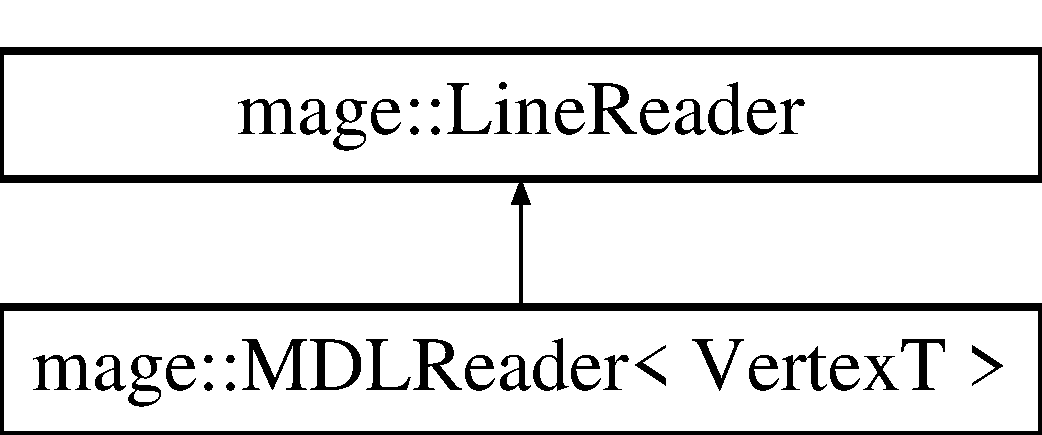
\includegraphics[height=2.000000cm]{classmage_1_1_m_d_l_reader}
\end{center}
\end{figure}
\subsection*{Public Member Functions}
\begin{DoxyCompactItemize}
\item 
\hyperlink{classmage_1_1_m_d_l_reader_a068ed8c9101b42033ea166ab7aa03c04}{M\+D\+L\+Reader} (\hyperlink{structmage_1_1_model_output}{Model\+Output}$<$ VertexT $>$ \&model\+\_\+output)
\item 
\hyperlink{classmage_1_1_m_d_l_reader_ae7b3ee7b2b02101da041249e98f31bcc}{M\+D\+L\+Reader} (const \hyperlink{classmage_1_1_m_d_l_reader}{M\+D\+L\+Reader} \&reader)=delete
\item 
\hyperlink{classmage_1_1_m_d_l_reader_ac2e45fb05db0255d7ebf2da6e54db3f4}{M\+D\+L\+Reader} (\hyperlink{classmage_1_1_m_d_l_reader}{M\+D\+L\+Reader} \&\&reader)=delete
\item 
virtual \hyperlink{classmage_1_1_m_d_l_reader_a2da322d25dee1198ceb3c9455e5a51bf}{$\sim$\+M\+D\+L\+Reader} ()=default
\item 
\hyperlink{classmage_1_1_m_d_l_reader}{M\+D\+L\+Reader} \& \hyperlink{classmage_1_1_m_d_l_reader_a8cc5e9966283f3f9727fa28a75412ddb}{operator=} (const \hyperlink{classmage_1_1_m_d_l_reader}{M\+D\+L\+Reader} \&reader)=delete
\item 
\hyperlink{classmage_1_1_m_d_l_reader}{M\+D\+L\+Reader} \& \hyperlink{classmage_1_1_m_d_l_reader_a993c23d2e7f16f22a28e48ae9b7173b4}{operator=} (\hyperlink{classmage_1_1_m_d_l_reader}{M\+D\+L\+Reader} \&\&reader)=delete
\end{DoxyCompactItemize}
\subsection*{Private Member Functions}
\begin{DoxyCompactItemize}
\item 
virtual void \hyperlink{classmage_1_1_m_d_l_reader_a8b99fb3bdea5e9dae156b135c160c22d}{Preprocess} () override
\item 
virtual void \hyperlink{classmage_1_1_m_d_l_reader_ac50f9cce64621b0a218b6778a611a702}{Read\+Line} (char $\ast$line) override
\item 
void \hyperlink{classmage_1_1_m_d_l_reader_ab688ce530cab867d155b696b2a1133a0}{Import\+Mesh} ()
\item 
void \hyperlink{classmage_1_1_m_d_l_reader_a78e12dbf59382cde7a56c323918d5bc2}{Read\+M\+D\+L\+Sub\+Model} ()
\item 
void \hyperlink{classmage_1_1_m_d_l_reader_a5fa8fa91dca9bea47a6bbf407e854be7}{Read\+M\+D\+L\+Material\+Library} ()
\end{DoxyCompactItemize}
\subsection*{Private Attributes}
\begin{DoxyCompactItemize}
\item 
\hyperlink{structmage_1_1_model_output}{Model\+Output}$<$ VertexT $>$ \& \hyperlink{classmage_1_1_m_d_l_reader_a41392308792749b78657497b69add850}{m\+\_\+model\+\_\+output}
\end{DoxyCompactItemize}
\subsection*{Additional Inherited Members}


\subsection{Constructor \& Destructor Documentation}
\hypertarget{classmage_1_1_m_d_l_reader_a068ed8c9101b42033ea166ab7aa03c04}{}\label{classmage_1_1_m_d_l_reader_a068ed8c9101b42033ea166ab7aa03c04} 
\index{mage\+::\+M\+D\+L\+Reader@{mage\+::\+M\+D\+L\+Reader}!M\+D\+L\+Reader@{M\+D\+L\+Reader}}
\index{M\+D\+L\+Reader@{M\+D\+L\+Reader}!mage\+::\+M\+D\+L\+Reader@{mage\+::\+M\+D\+L\+Reader}}
\subsubsection{\texorpdfstring{M\+D\+L\+Reader()}{MDLReader()}\hspace{0.1cm}{\footnotesize\ttfamily [1/3]}}
{\footnotesize\ttfamily template$<$typename VertexT $>$ \\
\hyperlink{classmage_1_1_m_d_l_reader}{mage\+::\+M\+D\+L\+Reader}$<$ VertexT $>$\+::\hyperlink{classmage_1_1_m_d_l_reader}{M\+D\+L\+Reader} (\begin{DoxyParamCaption}\item[{\hyperlink{structmage_1_1_model_output}{Model\+Output}$<$ VertexT $>$ \&}]{model\+\_\+output }\end{DoxyParamCaption})\hspace{0.3cm}{\ttfamily [explicit]}}

\hypertarget{classmage_1_1_m_d_l_reader_ae7b3ee7b2b02101da041249e98f31bcc}{}\label{classmage_1_1_m_d_l_reader_ae7b3ee7b2b02101da041249e98f31bcc} 
\index{mage\+::\+M\+D\+L\+Reader@{mage\+::\+M\+D\+L\+Reader}!M\+D\+L\+Reader@{M\+D\+L\+Reader}}
\index{M\+D\+L\+Reader@{M\+D\+L\+Reader}!mage\+::\+M\+D\+L\+Reader@{mage\+::\+M\+D\+L\+Reader}}
\subsubsection{\texorpdfstring{M\+D\+L\+Reader()}{MDLReader()}\hspace{0.1cm}{\footnotesize\ttfamily [2/3]}}
{\footnotesize\ttfamily template$<$typename VertexT $>$ \\
\hyperlink{classmage_1_1_m_d_l_reader}{mage\+::\+M\+D\+L\+Reader}$<$ VertexT $>$\+::\hyperlink{classmage_1_1_m_d_l_reader}{M\+D\+L\+Reader} (\begin{DoxyParamCaption}\item[{const \hyperlink{classmage_1_1_m_d_l_reader}{M\+D\+L\+Reader}$<$ VertexT $>$ \&}]{reader }\end{DoxyParamCaption})\hspace{0.3cm}{\ttfamily [delete]}}

\hypertarget{classmage_1_1_m_d_l_reader_ac2e45fb05db0255d7ebf2da6e54db3f4}{}\label{classmage_1_1_m_d_l_reader_ac2e45fb05db0255d7ebf2da6e54db3f4} 
\index{mage\+::\+M\+D\+L\+Reader@{mage\+::\+M\+D\+L\+Reader}!M\+D\+L\+Reader@{M\+D\+L\+Reader}}
\index{M\+D\+L\+Reader@{M\+D\+L\+Reader}!mage\+::\+M\+D\+L\+Reader@{mage\+::\+M\+D\+L\+Reader}}
\subsubsection{\texorpdfstring{M\+D\+L\+Reader()}{MDLReader()}\hspace{0.1cm}{\footnotesize\ttfamily [3/3]}}
{\footnotesize\ttfamily template$<$typename VertexT $>$ \\
\hyperlink{classmage_1_1_m_d_l_reader}{mage\+::\+M\+D\+L\+Reader}$<$ VertexT $>$\+::\hyperlink{classmage_1_1_m_d_l_reader}{M\+D\+L\+Reader} (\begin{DoxyParamCaption}\item[{\hyperlink{classmage_1_1_m_d_l_reader}{M\+D\+L\+Reader}$<$ VertexT $>$ \&\&}]{reader }\end{DoxyParamCaption})\hspace{0.3cm}{\ttfamily [delete]}}

\hypertarget{classmage_1_1_m_d_l_reader_a2da322d25dee1198ceb3c9455e5a51bf}{}\label{classmage_1_1_m_d_l_reader_a2da322d25dee1198ceb3c9455e5a51bf} 
\index{mage\+::\+M\+D\+L\+Reader@{mage\+::\+M\+D\+L\+Reader}!````~M\+D\+L\+Reader@{$\sim$\+M\+D\+L\+Reader}}
\index{````~M\+D\+L\+Reader@{$\sim$\+M\+D\+L\+Reader}!mage\+::\+M\+D\+L\+Reader@{mage\+::\+M\+D\+L\+Reader}}
\subsubsection{\texorpdfstring{$\sim$\+M\+D\+L\+Reader()}{~MDLReader()}}
{\footnotesize\ttfamily template$<$typename VertexT $>$ \\
virtual \hyperlink{classmage_1_1_m_d_l_reader}{mage\+::\+M\+D\+L\+Reader}$<$ VertexT $>$\+::$\sim$\hyperlink{classmage_1_1_m_d_l_reader}{M\+D\+L\+Reader} (\begin{DoxyParamCaption}{ }\end{DoxyParamCaption})\hspace{0.3cm}{\ttfamily [virtual]}, {\ttfamily [default]}}



\subsection{Member Function Documentation}
\hypertarget{classmage_1_1_m_d_l_reader_ab688ce530cab867d155b696b2a1133a0}{}\label{classmage_1_1_m_d_l_reader_ab688ce530cab867d155b696b2a1133a0} 
\index{mage\+::\+M\+D\+L\+Reader@{mage\+::\+M\+D\+L\+Reader}!Import\+Mesh@{Import\+Mesh}}
\index{Import\+Mesh@{Import\+Mesh}!mage\+::\+M\+D\+L\+Reader@{mage\+::\+M\+D\+L\+Reader}}
\subsubsection{\texorpdfstring{Import\+Mesh()}{ImportMesh()}}
{\footnotesize\ttfamily template$<$typename VertexT $>$ \\
void \hyperlink{classmage_1_1_m_d_l_reader}{mage\+::\+M\+D\+L\+Reader}$<$ VertexT $>$\+::Import\+Mesh (\begin{DoxyParamCaption}{ }\end{DoxyParamCaption})\hspace{0.3cm}{\ttfamily [private]}}

\hypertarget{classmage_1_1_m_d_l_reader_a8cc5e9966283f3f9727fa28a75412ddb}{}\label{classmage_1_1_m_d_l_reader_a8cc5e9966283f3f9727fa28a75412ddb} 
\index{mage\+::\+M\+D\+L\+Reader@{mage\+::\+M\+D\+L\+Reader}!operator=@{operator=}}
\index{operator=@{operator=}!mage\+::\+M\+D\+L\+Reader@{mage\+::\+M\+D\+L\+Reader}}
\subsubsection{\texorpdfstring{operator=()}{operator=()}\hspace{0.1cm}{\footnotesize\ttfamily [1/2]}}
{\footnotesize\ttfamily template$<$typename VertexT $>$ \\
\hyperlink{classmage_1_1_m_d_l_reader}{M\+D\+L\+Reader}\& \hyperlink{classmage_1_1_m_d_l_reader}{mage\+::\+M\+D\+L\+Reader}$<$ VertexT $>$\+::operator= (\begin{DoxyParamCaption}\item[{const \hyperlink{classmage_1_1_m_d_l_reader}{M\+D\+L\+Reader}$<$ VertexT $>$ \&}]{reader }\end{DoxyParamCaption})\hspace{0.3cm}{\ttfamily [delete]}}

\hypertarget{classmage_1_1_m_d_l_reader_a993c23d2e7f16f22a28e48ae9b7173b4}{}\label{classmage_1_1_m_d_l_reader_a993c23d2e7f16f22a28e48ae9b7173b4} 
\index{mage\+::\+M\+D\+L\+Reader@{mage\+::\+M\+D\+L\+Reader}!operator=@{operator=}}
\index{operator=@{operator=}!mage\+::\+M\+D\+L\+Reader@{mage\+::\+M\+D\+L\+Reader}}
\subsubsection{\texorpdfstring{operator=()}{operator=()}\hspace{0.1cm}{\footnotesize\ttfamily [2/2]}}
{\footnotesize\ttfamily template$<$typename VertexT $>$ \\
\hyperlink{classmage_1_1_m_d_l_reader}{M\+D\+L\+Reader}\& \hyperlink{classmage_1_1_m_d_l_reader}{mage\+::\+M\+D\+L\+Reader}$<$ VertexT $>$\+::operator= (\begin{DoxyParamCaption}\item[{\hyperlink{classmage_1_1_m_d_l_reader}{M\+D\+L\+Reader}$<$ VertexT $>$ \&\&}]{reader }\end{DoxyParamCaption})\hspace{0.3cm}{\ttfamily [delete]}}

\hypertarget{classmage_1_1_m_d_l_reader_a8b99fb3bdea5e9dae156b135c160c22d}{}\label{classmage_1_1_m_d_l_reader_a8b99fb3bdea5e9dae156b135c160c22d} 
\index{mage\+::\+M\+D\+L\+Reader@{mage\+::\+M\+D\+L\+Reader}!Preprocess@{Preprocess}}
\index{Preprocess@{Preprocess}!mage\+::\+M\+D\+L\+Reader@{mage\+::\+M\+D\+L\+Reader}}
\subsubsection{\texorpdfstring{Preprocess()}{Preprocess()}}
{\footnotesize\ttfamily template$<$typename VertexT $>$ \\
virtual void \hyperlink{classmage_1_1_m_d_l_reader}{mage\+::\+M\+D\+L\+Reader}$<$ VertexT $>$\+::Preprocess (\begin{DoxyParamCaption}{ }\end{DoxyParamCaption})\hspace{0.3cm}{\ttfamily [override]}, {\ttfamily [private]}, {\ttfamily [virtual]}}

Pre-\/process before reading the current file of this line reader.


\begin{DoxyExceptions}{Exceptions}
{\em \hyperlink{structmage_1_1_formatted_exception}{Formatted\+Exception}} & The pre-\/processing failed. \\
\hline
\end{DoxyExceptions}


Reimplemented from \hyperlink{classmage_1_1_line_reader_a4de135cfb0434be786cfcfd7959031ef}{mage\+::\+Line\+Reader}.

\hypertarget{classmage_1_1_m_d_l_reader_ac50f9cce64621b0a218b6778a611a702}{}\label{classmage_1_1_m_d_l_reader_ac50f9cce64621b0a218b6778a611a702} 
\index{mage\+::\+M\+D\+L\+Reader@{mage\+::\+M\+D\+L\+Reader}!Read\+Line@{Read\+Line}}
\index{Read\+Line@{Read\+Line}!mage\+::\+M\+D\+L\+Reader@{mage\+::\+M\+D\+L\+Reader}}
\subsubsection{\texorpdfstring{Read\+Line()}{ReadLine()}}
{\footnotesize\ttfamily template$<$typename VertexT $>$ \\
virtual void \hyperlink{classmage_1_1_m_d_l_reader}{mage\+::\+M\+D\+L\+Reader}$<$ VertexT $>$\+::Read\+Line (\begin{DoxyParamCaption}\item[{char $\ast$}]{line }\end{DoxyParamCaption})\hspace{0.3cm}{\ttfamily [override]}, {\ttfamily [private]}, {\ttfamily [virtual]}}

Reads the given line.


\begin{DoxyParams}[1]{Parameters}
\mbox{\tt in,out}  & {\em line} & A pointer to the null-\/terminated byte string to read. \\
\hline
\end{DoxyParams}

\begin{DoxyExceptions}{Exceptions}
{\em \hyperlink{structmage_1_1_formatted_exception}{Formatted\+Exception}} & The reading of the line failed. \\
\hline
\end{DoxyExceptions}


Implements \hyperlink{classmage_1_1_line_reader_acfb2f7279ec77d070a86d7db812d4745}{mage\+::\+Line\+Reader}.

\hypertarget{classmage_1_1_m_d_l_reader_a5fa8fa91dca9bea47a6bbf407e854be7}{}\label{classmage_1_1_m_d_l_reader_a5fa8fa91dca9bea47a6bbf407e854be7} 
\index{mage\+::\+M\+D\+L\+Reader@{mage\+::\+M\+D\+L\+Reader}!Read\+M\+D\+L\+Material\+Library@{Read\+M\+D\+L\+Material\+Library}}
\index{Read\+M\+D\+L\+Material\+Library@{Read\+M\+D\+L\+Material\+Library}!mage\+::\+M\+D\+L\+Reader@{mage\+::\+M\+D\+L\+Reader}}
\subsubsection{\texorpdfstring{Read\+M\+D\+L\+Material\+Library()}{ReadMDLMaterialLibrary()}}
{\footnotesize\ttfamily template$<$typename VertexT $>$ \\
void \hyperlink{classmage_1_1_m_d_l_reader}{mage\+::\+M\+D\+L\+Reader}$<$ VertexT $>$\+::Read\+M\+D\+L\+Material\+Library (\begin{DoxyParamCaption}{ }\end{DoxyParamCaption})\hspace{0.3cm}{\ttfamily [private]}}

\hypertarget{classmage_1_1_m_d_l_reader_a78e12dbf59382cde7a56c323918d5bc2}{}\label{classmage_1_1_m_d_l_reader_a78e12dbf59382cde7a56c323918d5bc2} 
\index{mage\+::\+M\+D\+L\+Reader@{mage\+::\+M\+D\+L\+Reader}!Read\+M\+D\+L\+Sub\+Model@{Read\+M\+D\+L\+Sub\+Model}}
\index{Read\+M\+D\+L\+Sub\+Model@{Read\+M\+D\+L\+Sub\+Model}!mage\+::\+M\+D\+L\+Reader@{mage\+::\+M\+D\+L\+Reader}}
\subsubsection{\texorpdfstring{Read\+M\+D\+L\+Sub\+Model()}{ReadMDLSubModel()}}
{\footnotesize\ttfamily template$<$typename VertexT $>$ \\
void \hyperlink{classmage_1_1_m_d_l_reader}{mage\+::\+M\+D\+L\+Reader}$<$ VertexT $>$\+::Read\+M\+D\+L\+Sub\+Model (\begin{DoxyParamCaption}{ }\end{DoxyParamCaption})\hspace{0.3cm}{\ttfamily [private]}}



\subsection{Member Data Documentation}
\hypertarget{classmage_1_1_m_d_l_reader_a41392308792749b78657497b69add850}{}\label{classmage_1_1_m_d_l_reader_a41392308792749b78657497b69add850} 
\index{mage\+::\+M\+D\+L\+Reader@{mage\+::\+M\+D\+L\+Reader}!m\+\_\+model\+\_\+output@{m\+\_\+model\+\_\+output}}
\index{m\+\_\+model\+\_\+output@{m\+\_\+model\+\_\+output}!mage\+::\+M\+D\+L\+Reader@{mage\+::\+M\+D\+L\+Reader}}
\subsubsection{\texorpdfstring{m\+\_\+model\+\_\+output}{m\_model\_output}}
{\footnotesize\ttfamily template$<$typename VertexT $>$ \\
\hyperlink{structmage_1_1_model_output}{Model\+Output}$<$ VertexT $>$\& \hyperlink{classmage_1_1_m_d_l_reader}{mage\+::\+M\+D\+L\+Reader}$<$ VertexT $>$\+::m\+\_\+model\+\_\+output\hspace{0.3cm}{\ttfamily [private]}}


\hypertarget{classmage_1_1_m_d_l_writer}{}\section{mage\+:\+:M\+D\+L\+Writer$<$ VertexT $>$ Class Template Reference}
\label{classmage_1_1_m_d_l_writer}\index{mage\+::\+M\+D\+L\+Writer$<$ Vertex\+T $>$@{mage\+::\+M\+D\+L\+Writer$<$ Vertex\+T $>$}}


{\ttfamily \#include $<$mdl\+\_\+writer.\+hpp$>$}

Inheritance diagram for mage\+:\+:M\+D\+L\+Writer$<$ VertexT $>$\+:\begin{figure}[H]
\begin{center}
\leavevmode
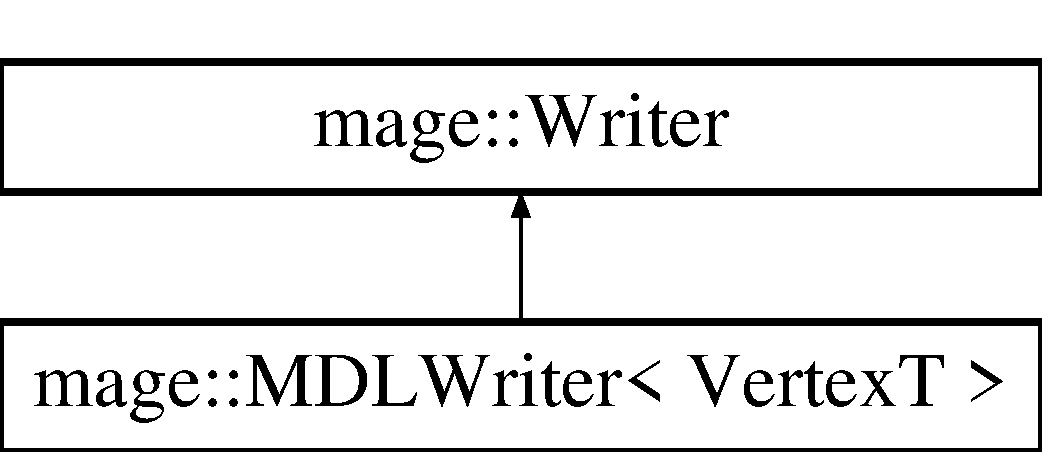
\includegraphics[height=2.000000cm]{classmage_1_1_m_d_l_writer}
\end{center}
\end{figure}
\subsection*{Public Member Functions}
\begin{DoxyCompactItemize}
\item 
\hyperlink{classmage_1_1_m_d_l_writer_a7e5c6c9c9a9d32b09c5e17f4691e01c1}{M\+D\+L\+Writer} (const \hyperlink{structmage_1_1_model_output}{Model\+Output}$<$ VertexT $>$ \&model\+\_\+output)
\item 
\hyperlink{classmage_1_1_m_d_l_writer_ad244168d68c45fe7dcafa350c8a13fbe}{M\+D\+L\+Writer} (const \hyperlink{classmage_1_1_m_d_l_writer}{M\+D\+L\+Writer} \&writer)=delete
\item 
\hyperlink{classmage_1_1_m_d_l_writer_acf2751035dfd4cca9884e6162830c5f5}{M\+D\+L\+Writer} (\hyperlink{classmage_1_1_m_d_l_writer}{M\+D\+L\+Writer} \&\&writer)=delete
\item 
virtual \hyperlink{classmage_1_1_m_d_l_writer_adcb78b5d8ac0d665f3bae0b643cd6932}{$\sim$\+M\+D\+L\+Writer} ()=default
\item 
\hyperlink{classmage_1_1_m_d_l_writer}{M\+D\+L\+Writer} \& \hyperlink{classmage_1_1_m_d_l_writer_ac8f4db1bc43a8fe4842409671505b49b}{operator=} (const \hyperlink{classmage_1_1_m_d_l_writer}{M\+D\+L\+Writer} \&writer)=delete
\item 
\hyperlink{classmage_1_1_m_d_l_writer}{M\+D\+L\+Writer} \& \hyperlink{classmage_1_1_m_d_l_writer_ac5c21784110691e24d84d6c241a2e5f6}{operator=} (\hyperlink{classmage_1_1_m_d_l_writer}{M\+D\+L\+Writer} \&\&writer)=delete
\end{DoxyCompactItemize}
\subsection*{Private Member Functions}
\begin{DoxyCompactItemize}
\item 
virtual H\+R\+E\+S\+U\+LT \hyperlink{classmage_1_1_m_d_l_writer_abd4f206b457d8b97e6e38e25f7e88ed3}{Write} () override
\item 
H\+R\+E\+S\+U\+LT \hyperlink{classmage_1_1_m_d_l_writer_ae749244a6528ab81600a62e95e73a44a}{Export\+Mesh} ()
\item 
void \hyperlink{classmage_1_1_m_d_l_writer_af9416c1b2599ea86f4af8018dc0b9baf}{Write\+Materials} ()
\item 
void \hyperlink{classmage_1_1_m_d_l_writer_a3db84a4600cb777b37c666166a631689}{Write\+Model\+Parts} ()
\end{DoxyCompactItemize}
\subsection*{Private Attributes}
\begin{DoxyCompactItemize}
\item 
const \hyperlink{structmage_1_1_model_output}{Model\+Output}$<$ VertexT $>$ \& \hyperlink{classmage_1_1_m_d_l_writer_a607fc83a3dbab79f55c3eaca203c027b}{m\+\_\+model\+\_\+output}
\end{DoxyCompactItemize}
\subsection*{Additional Inherited Members}


\subsection{Constructor \& Destructor Documentation}
\hypertarget{classmage_1_1_m_d_l_writer_a7e5c6c9c9a9d32b09c5e17f4691e01c1}{}\label{classmage_1_1_m_d_l_writer_a7e5c6c9c9a9d32b09c5e17f4691e01c1} 
\index{mage\+::\+M\+D\+L\+Writer@{mage\+::\+M\+D\+L\+Writer}!M\+D\+L\+Writer@{M\+D\+L\+Writer}}
\index{M\+D\+L\+Writer@{M\+D\+L\+Writer}!mage\+::\+M\+D\+L\+Writer@{mage\+::\+M\+D\+L\+Writer}}
\subsubsection{\texorpdfstring{M\+D\+L\+Writer()}{MDLWriter()}\hspace{0.1cm}{\footnotesize\ttfamily [1/3]}}
{\footnotesize\ttfamily template$<$typename VertexT $>$ \\
\hyperlink{classmage_1_1_m_d_l_writer}{mage\+::\+M\+D\+L\+Writer}$<$ VertexT $>$\+::\hyperlink{classmage_1_1_m_d_l_writer}{M\+D\+L\+Writer} (\begin{DoxyParamCaption}\item[{const \hyperlink{structmage_1_1_model_output}{Model\+Output}$<$ VertexT $>$ \&}]{model\+\_\+output }\end{DoxyParamCaption})\hspace{0.3cm}{\ttfamily [explicit]}}

\hypertarget{classmage_1_1_m_d_l_writer_ad244168d68c45fe7dcafa350c8a13fbe}{}\label{classmage_1_1_m_d_l_writer_ad244168d68c45fe7dcafa350c8a13fbe} 
\index{mage\+::\+M\+D\+L\+Writer@{mage\+::\+M\+D\+L\+Writer}!M\+D\+L\+Writer@{M\+D\+L\+Writer}}
\index{M\+D\+L\+Writer@{M\+D\+L\+Writer}!mage\+::\+M\+D\+L\+Writer@{mage\+::\+M\+D\+L\+Writer}}
\subsubsection{\texorpdfstring{M\+D\+L\+Writer()}{MDLWriter()}\hspace{0.1cm}{\footnotesize\ttfamily [2/3]}}
{\footnotesize\ttfamily template$<$typename VertexT $>$ \\
\hyperlink{classmage_1_1_m_d_l_writer}{mage\+::\+M\+D\+L\+Writer}$<$ VertexT $>$\+::\hyperlink{classmage_1_1_m_d_l_writer}{M\+D\+L\+Writer} (\begin{DoxyParamCaption}\item[{const \hyperlink{classmage_1_1_m_d_l_writer}{M\+D\+L\+Writer}$<$ VertexT $>$ \&}]{writer }\end{DoxyParamCaption})\hspace{0.3cm}{\ttfamily [delete]}}

\hypertarget{classmage_1_1_m_d_l_writer_acf2751035dfd4cca9884e6162830c5f5}{}\label{classmage_1_1_m_d_l_writer_acf2751035dfd4cca9884e6162830c5f5} 
\index{mage\+::\+M\+D\+L\+Writer@{mage\+::\+M\+D\+L\+Writer}!M\+D\+L\+Writer@{M\+D\+L\+Writer}}
\index{M\+D\+L\+Writer@{M\+D\+L\+Writer}!mage\+::\+M\+D\+L\+Writer@{mage\+::\+M\+D\+L\+Writer}}
\subsubsection{\texorpdfstring{M\+D\+L\+Writer()}{MDLWriter()}\hspace{0.1cm}{\footnotesize\ttfamily [3/3]}}
{\footnotesize\ttfamily template$<$typename VertexT $>$ \\
\hyperlink{classmage_1_1_m_d_l_writer}{mage\+::\+M\+D\+L\+Writer}$<$ VertexT $>$\+::\hyperlink{classmage_1_1_m_d_l_writer}{M\+D\+L\+Writer} (\begin{DoxyParamCaption}\item[{\hyperlink{classmage_1_1_m_d_l_writer}{M\+D\+L\+Writer}$<$ VertexT $>$ \&\&}]{writer }\end{DoxyParamCaption})\hspace{0.3cm}{\ttfamily [delete]}}

\hypertarget{classmage_1_1_m_d_l_writer_adcb78b5d8ac0d665f3bae0b643cd6932}{}\label{classmage_1_1_m_d_l_writer_adcb78b5d8ac0d665f3bae0b643cd6932} 
\index{mage\+::\+M\+D\+L\+Writer@{mage\+::\+M\+D\+L\+Writer}!````~M\+D\+L\+Writer@{$\sim$\+M\+D\+L\+Writer}}
\index{````~M\+D\+L\+Writer@{$\sim$\+M\+D\+L\+Writer}!mage\+::\+M\+D\+L\+Writer@{mage\+::\+M\+D\+L\+Writer}}
\subsubsection{\texorpdfstring{$\sim$\+M\+D\+L\+Writer()}{~MDLWriter()}}
{\footnotesize\ttfamily template$<$typename VertexT $>$ \\
virtual \hyperlink{classmage_1_1_m_d_l_writer}{mage\+::\+M\+D\+L\+Writer}$<$ VertexT $>$\+::$\sim$\hyperlink{classmage_1_1_m_d_l_writer}{M\+D\+L\+Writer} (\begin{DoxyParamCaption}{ }\end{DoxyParamCaption})\hspace{0.3cm}{\ttfamily [virtual]}, {\ttfamily [default]}}



\subsection{Member Function Documentation}
\hypertarget{classmage_1_1_m_d_l_writer_ae749244a6528ab81600a62e95e73a44a}{}\label{classmage_1_1_m_d_l_writer_ae749244a6528ab81600a62e95e73a44a} 
\index{mage\+::\+M\+D\+L\+Writer@{mage\+::\+M\+D\+L\+Writer}!Export\+Mesh@{Export\+Mesh}}
\index{Export\+Mesh@{Export\+Mesh}!mage\+::\+M\+D\+L\+Writer@{mage\+::\+M\+D\+L\+Writer}}
\subsubsection{\texorpdfstring{Export\+Mesh()}{ExportMesh()}}
{\footnotesize\ttfamily template$<$typename VertexT $>$ \\
H\+R\+E\+S\+U\+LT \hyperlink{classmage_1_1_m_d_l_writer}{mage\+::\+M\+D\+L\+Writer}$<$ VertexT $>$\+::Export\+Mesh (\begin{DoxyParamCaption}{ }\end{DoxyParamCaption})\hspace{0.3cm}{\ttfamily [private]}}

\hypertarget{classmage_1_1_m_d_l_writer_ac8f4db1bc43a8fe4842409671505b49b}{}\label{classmage_1_1_m_d_l_writer_ac8f4db1bc43a8fe4842409671505b49b} 
\index{mage\+::\+M\+D\+L\+Writer@{mage\+::\+M\+D\+L\+Writer}!operator=@{operator=}}
\index{operator=@{operator=}!mage\+::\+M\+D\+L\+Writer@{mage\+::\+M\+D\+L\+Writer}}
\subsubsection{\texorpdfstring{operator=()}{operator=()}\hspace{0.1cm}{\footnotesize\ttfamily [1/2]}}
{\footnotesize\ttfamily template$<$typename VertexT $>$ \\
\hyperlink{classmage_1_1_m_d_l_writer}{M\+D\+L\+Writer}\& \hyperlink{classmage_1_1_m_d_l_writer}{mage\+::\+M\+D\+L\+Writer}$<$ VertexT $>$\+::operator= (\begin{DoxyParamCaption}\item[{const \hyperlink{classmage_1_1_m_d_l_writer}{M\+D\+L\+Writer}$<$ VertexT $>$ \&}]{writer }\end{DoxyParamCaption})\hspace{0.3cm}{\ttfamily [delete]}}

\hypertarget{classmage_1_1_m_d_l_writer_ac5c21784110691e24d84d6c241a2e5f6}{}\label{classmage_1_1_m_d_l_writer_ac5c21784110691e24d84d6c241a2e5f6} 
\index{mage\+::\+M\+D\+L\+Writer@{mage\+::\+M\+D\+L\+Writer}!operator=@{operator=}}
\index{operator=@{operator=}!mage\+::\+M\+D\+L\+Writer@{mage\+::\+M\+D\+L\+Writer}}
\subsubsection{\texorpdfstring{operator=()}{operator=()}\hspace{0.1cm}{\footnotesize\ttfamily [2/2]}}
{\footnotesize\ttfamily template$<$typename VertexT $>$ \\
\hyperlink{classmage_1_1_m_d_l_writer}{M\+D\+L\+Writer}\& \hyperlink{classmage_1_1_m_d_l_writer}{mage\+::\+M\+D\+L\+Writer}$<$ VertexT $>$\+::operator= (\begin{DoxyParamCaption}\item[{\hyperlink{classmage_1_1_m_d_l_writer}{M\+D\+L\+Writer}$<$ VertexT $>$ \&\&}]{writer }\end{DoxyParamCaption})\hspace{0.3cm}{\ttfamily [delete]}}

\hypertarget{classmage_1_1_m_d_l_writer_abd4f206b457d8b97e6e38e25f7e88ed3}{}\label{classmage_1_1_m_d_l_writer_abd4f206b457d8b97e6e38e25f7e88ed3} 
\index{mage\+::\+M\+D\+L\+Writer@{mage\+::\+M\+D\+L\+Writer}!Write@{Write}}
\index{Write@{Write}!mage\+::\+M\+D\+L\+Writer@{mage\+::\+M\+D\+L\+Writer}}
\subsubsection{\texorpdfstring{Write()}{Write()}}
{\footnotesize\ttfamily template$<$typename VertexT $>$ \\
virtual H\+R\+E\+S\+U\+LT \hyperlink{classmage_1_1_m_d_l_writer}{mage\+::\+M\+D\+L\+Writer}$<$ VertexT $>$\+::Write (\begin{DoxyParamCaption}{ }\end{DoxyParamCaption})\hspace{0.3cm}{\ttfamily [override]}, {\ttfamily [private]}, {\ttfamily [virtual]}}



Implements \hyperlink{classmage_1_1_writer_a7ef124095098e7ea8f95e3be16499be3}{mage\+::\+Writer}.

\hypertarget{classmage_1_1_m_d_l_writer_af9416c1b2599ea86f4af8018dc0b9baf}{}\label{classmage_1_1_m_d_l_writer_af9416c1b2599ea86f4af8018dc0b9baf} 
\index{mage\+::\+M\+D\+L\+Writer@{mage\+::\+M\+D\+L\+Writer}!Write\+Materials@{Write\+Materials}}
\index{Write\+Materials@{Write\+Materials}!mage\+::\+M\+D\+L\+Writer@{mage\+::\+M\+D\+L\+Writer}}
\subsubsection{\texorpdfstring{Write\+Materials()}{WriteMaterials()}}
{\footnotesize\ttfamily template$<$typename VertexT $>$ \\
void \hyperlink{classmage_1_1_m_d_l_writer}{mage\+::\+M\+D\+L\+Writer}$<$ VertexT $>$\+::Write\+Materials (\begin{DoxyParamCaption}{ }\end{DoxyParamCaption})\hspace{0.3cm}{\ttfamily [private]}}

\hypertarget{classmage_1_1_m_d_l_writer_a3db84a4600cb777b37c666166a631689}{}\label{classmage_1_1_m_d_l_writer_a3db84a4600cb777b37c666166a631689} 
\index{mage\+::\+M\+D\+L\+Writer@{mage\+::\+M\+D\+L\+Writer}!Write\+Model\+Parts@{Write\+Model\+Parts}}
\index{Write\+Model\+Parts@{Write\+Model\+Parts}!mage\+::\+M\+D\+L\+Writer@{mage\+::\+M\+D\+L\+Writer}}
\subsubsection{\texorpdfstring{Write\+Model\+Parts()}{WriteModelParts()}}
{\footnotesize\ttfamily template$<$typename VertexT $>$ \\
void \hyperlink{classmage_1_1_m_d_l_writer}{mage\+::\+M\+D\+L\+Writer}$<$ VertexT $>$\+::Write\+Model\+Parts (\begin{DoxyParamCaption}{ }\end{DoxyParamCaption})\hspace{0.3cm}{\ttfamily [private]}}



\subsection{Member Data Documentation}
\hypertarget{classmage_1_1_m_d_l_writer_a607fc83a3dbab79f55c3eaca203c027b}{}\label{classmage_1_1_m_d_l_writer_a607fc83a3dbab79f55c3eaca203c027b} 
\index{mage\+::\+M\+D\+L\+Writer@{mage\+::\+M\+D\+L\+Writer}!m\+\_\+model\+\_\+output@{m\+\_\+model\+\_\+output}}
\index{m\+\_\+model\+\_\+output@{m\+\_\+model\+\_\+output}!mage\+::\+M\+D\+L\+Writer@{mage\+::\+M\+D\+L\+Writer}}
\subsubsection{\texorpdfstring{m\+\_\+model\+\_\+output}{m\_model\_output}}
{\footnotesize\ttfamily template$<$typename VertexT $>$ \\
const \hyperlink{structmage_1_1_model_output}{Model\+Output}$<$ VertexT $>$\& \hyperlink{classmage_1_1_m_d_l_writer}{mage\+::\+M\+D\+L\+Writer}$<$ VertexT $>$\+::m\+\_\+model\+\_\+output\hspace{0.3cm}{\ttfamily [private]}}


\hypertarget{classmage_1_1_memory_arena}{}\section{mage\+:\+:Memory\+Arena Class Reference}
\label{classmage_1_1_memory_arena}\index{mage\+::\+Memory\+Arena@{mage\+::\+Memory\+Arena}}


{\ttfamily \#include $<$memory\+\_\+arena.\+hpp$>$}

\subsection*{Classes}
\begin{DoxyCompactItemize}
\item 
class \mbox{\hyperlink{classmage_1_1_memory_arena_1_1_allocator}{Allocator}}
\end{DoxyCompactItemize}
\subsection*{Public Member Functions}
\begin{DoxyCompactItemize}
\item 
\mbox{\hyperlink{classmage_1_1_memory_arena_a139f7781be209bb29e7ad0ed04cb32a5}{Memory\+Arena}} (size\+\_\+t maximum\+\_\+block\+\_\+size, size\+\_\+t alignment)
\item 
\mbox{\hyperlink{classmage_1_1_memory_arena_a1eca6fdacbd1226f4b21f443d118168b}{Memory\+Arena}} (const \mbox{\hyperlink{classmage_1_1_memory_arena}{Memory\+Arena}} \&arena)=delete
\item 
\mbox{\hyperlink{classmage_1_1_memory_arena_a98829c5a87ba028c376f100cca09e876}{Memory\+Arena}} (\mbox{\hyperlink{classmage_1_1_memory_arena}{Memory\+Arena}} \&\&arena)
\item 
\mbox{\hyperlink{classmage_1_1_memory_arena_acfee6fc205e2eaf6aeef4acf19948e6e}{$\sim$\+Memory\+Arena}} ()
\item 
\mbox{\hyperlink{classmage_1_1_memory_arena}{Memory\+Arena}} \& \mbox{\hyperlink{classmage_1_1_memory_arena_a7e7799f859c55435714933972ecb8b95}{operator=}} (const \mbox{\hyperlink{classmage_1_1_memory_arena}{Memory\+Arena}} \&arena)=delete
\item 
\mbox{\hyperlink{classmage_1_1_memory_arena}{Memory\+Arena}} \& \mbox{\hyperlink{classmage_1_1_memory_arena_aa4b80a917a838a1ca3788f906723d273}{operator=}} (\mbox{\hyperlink{classmage_1_1_memory_arena}{Memory\+Arena}} \&\&arena)=delete
\item 
size\+\_\+t \mbox{\hyperlink{classmage_1_1_memory_arena_a79931a18af492ad8ef7e99b09ec36f2a}{Get\+Alignment}} () const noexcept
\item 
size\+\_\+t \mbox{\hyperlink{classmage_1_1_memory_arena_a6786cf52a03777580b439cafdd8ff8f9}{Get\+Maximum\+Block\+Size}} () const noexcept
\item 
size\+\_\+t \mbox{\hyperlink{classmage_1_1_memory_arena_a0b41d6901c3519f046cd551931f72c1b}{Get\+Current\+Block\+Size}} () const noexcept
\item 
size\+\_\+t \mbox{\hyperlink{classmage_1_1_memory_arena_ac8e8ac4ba60cd2bb1d8dc8a5d4a9f4ad}{Get\+Total\+Block\+Size}} () const noexcept
\item 
void $\ast$ \mbox{\hyperlink{classmage_1_1_memory_arena_a7bdbc9da32c1f8d49ce5d2f153870284}{Get\+Current\+Block\+Ptr}} () const noexcept
\item 
void \mbox{\hyperlink{classmage_1_1_memory_arena_a117b74c7bd5dfb28dfdaae6cab253491}{Reset}} ()
\item 
void $\ast$ \mbox{\hyperlink{classmage_1_1_memory_arena_a2e63b11c535dbfefd69d071466be9ce1}{Alloc}} (size\+\_\+t size)
\item 
{\footnotesize template$<$typename T $>$ }\\T $\ast$ \mbox{\hyperlink{classmage_1_1_memory_arena_a0880de049e8e76cd26918528eb892813}{Alloc\+Data}} (size\+\_\+t count=1, bool initialization=false)
\item 
{\footnotesize template$<$typename T $>$ }\\\mbox{\hyperlink{classmage_1_1_memory_arena_1_1_allocator}{Allocator}}$<$ T $>$ \mbox{\hyperlink{classmage_1_1_memory_arena_aa2cc5c42ed20c11900330ace3dfcdc8f}{Get\+Allocator}} () const noexcept
\end{DoxyCompactItemize}
\subsection*{Private Types}
\begin{DoxyCompactItemize}
\item 
using \mbox{\hyperlink{classmage_1_1_memory_arena_a133e9d40bd216e3f1d98c6a2b36cf373}{Memory\+Block}} = std\+::pair$<$ size\+\_\+t, \mbox{\hyperlink{namespacemage_afc638980bc6154f15af5e2d93a0e0ea9}{U8}} $\ast$$>$
\end{DoxyCompactItemize}
\subsection*{Private Attributes}
\begin{DoxyCompactItemize}
\item 
const size\+\_\+t \mbox{\hyperlink{classmage_1_1_memory_arena_a424c3ff6f1d96545dd08f94c1c79c963}{m\+\_\+alignment}}
\item 
const size\+\_\+t \mbox{\hyperlink{classmage_1_1_memory_arena_aeef4c56cf50fd3cbbba2879fcd028b86}{m\+\_\+maximum\+\_\+block\+\_\+size}}
\item 
\mbox{\hyperlink{classmage_1_1_memory_arena_a133e9d40bd216e3f1d98c6a2b36cf373}{Memory\+Block}} \mbox{\hyperlink{classmage_1_1_memory_arena_a2680b25146c174ac7fd639f1bd0acc7c}{m\+\_\+current\+\_\+block}}
\item 
size\+\_\+t \mbox{\hyperlink{classmage_1_1_memory_arena_a880d07eb372ce1c8b907947fcbdfc59c}{m\+\_\+current\+\_\+block\+\_\+pos}}
\item 
std\+::list$<$ \mbox{\hyperlink{classmage_1_1_memory_arena_a133e9d40bd216e3f1d98c6a2b36cf373}{Memory\+Block}} $>$ \mbox{\hyperlink{classmage_1_1_memory_arena_a49a6d7fb9396f57210897abfb4e30903}{m\+\_\+used\+\_\+blocks}}
\item 
std\+::list$<$ \mbox{\hyperlink{classmage_1_1_memory_arena_a133e9d40bd216e3f1d98c6a2b36cf373}{Memory\+Block}} $>$ \mbox{\hyperlink{classmage_1_1_memory_arena_a02f251a5aafa61d239b4daed3458a654}{m\+\_\+available\+\_\+blocks}}
\end{DoxyCompactItemize}


\subsection{Detailed Description}
A class of memory arenas. 

\subsection{Member Typedef Documentation}
\mbox{\Hypertarget{classmage_1_1_memory_arena_a133e9d40bd216e3f1d98c6a2b36cf373}\label{classmage_1_1_memory_arena_a133e9d40bd216e3f1d98c6a2b36cf373}} 
\index{mage\+::\+Memory\+Arena@{mage\+::\+Memory\+Arena}!Memory\+Block@{Memory\+Block}}
\index{Memory\+Block@{Memory\+Block}!mage\+::\+Memory\+Arena@{mage\+::\+Memory\+Arena}}
\subsubsection{\texorpdfstring{Memory\+Block}{MemoryBlock}}
{\footnotesize\ttfamily using \mbox{\hyperlink{classmage_1_1_memory_arena_a133e9d40bd216e3f1d98c6a2b36cf373}{mage\+::\+Memory\+Arena\+::\+Memory\+Block}} =  std\+::pair$<$ size\+\_\+t, \mbox{\hyperlink{namespacemage_afc638980bc6154f15af5e2d93a0e0ea9}{U8}}$\ast$ $>$\hspace{0.3cm}{\ttfamily [private]}}

A type definition for a memory block. 

\subsection{Constructor \& Destructor Documentation}
\mbox{\Hypertarget{classmage_1_1_memory_arena_a139f7781be209bb29e7ad0ed04cb32a5}\label{classmage_1_1_memory_arena_a139f7781be209bb29e7ad0ed04cb32a5}} 
\index{mage\+::\+Memory\+Arena@{mage\+::\+Memory\+Arena}!Memory\+Arena@{Memory\+Arena}}
\index{Memory\+Arena@{Memory\+Arena}!mage\+::\+Memory\+Arena@{mage\+::\+Memory\+Arena}}
\subsubsection{\texorpdfstring{Memory\+Arena()}{MemoryArena()}\hspace{0.1cm}{\footnotesize\ttfamily [1/3]}}
{\footnotesize\ttfamily mage\+::\+Memory\+Arena\+::\+Memory\+Arena (\begin{DoxyParamCaption}\item[{size\+\_\+t}]{maximum\+\_\+block\+\_\+size,  }\item[{size\+\_\+t}]{alignment }\end{DoxyParamCaption})\hspace{0.3cm}{\ttfamily [explicit]}}

Constructs a memory arena with given block size.


\begin{DoxyParams}[1]{Parameters}
\mbox{\tt in}  & {\em maximum\+\_\+block\+\_\+size} & The maximum block size in bytes. \\
\hline
\mbox{\tt in}  & {\em alignment} & The alignment in bytes. \\
\hline
\end{DoxyParams}
\mbox{\Hypertarget{classmage_1_1_memory_arena_a1eca6fdacbd1226f4b21f443d118168b}\label{classmage_1_1_memory_arena_a1eca6fdacbd1226f4b21f443d118168b}} 
\index{mage\+::\+Memory\+Arena@{mage\+::\+Memory\+Arena}!Memory\+Arena@{Memory\+Arena}}
\index{Memory\+Arena@{Memory\+Arena}!mage\+::\+Memory\+Arena@{mage\+::\+Memory\+Arena}}
\subsubsection{\texorpdfstring{Memory\+Arena()}{MemoryArena()}\hspace{0.1cm}{\footnotesize\ttfamily [2/3]}}
{\footnotesize\ttfamily mage\+::\+Memory\+Arena\+::\+Memory\+Arena (\begin{DoxyParamCaption}\item[{const \mbox{\hyperlink{classmage_1_1_memory_arena}{Memory\+Arena}} \&}]{arena }\end{DoxyParamCaption})\hspace{0.3cm}{\ttfamily [delete]}}

Constructs a memory arena from the given memory arena.


\begin{DoxyParams}[1]{Parameters}
\mbox{\tt in}  & {\em arena} & A reference to the memory arena to copy. \\
\hline
\end{DoxyParams}
\mbox{\Hypertarget{classmage_1_1_memory_arena_a98829c5a87ba028c376f100cca09e876}\label{classmage_1_1_memory_arena_a98829c5a87ba028c376f100cca09e876}} 
\index{mage\+::\+Memory\+Arena@{mage\+::\+Memory\+Arena}!Memory\+Arena@{Memory\+Arena}}
\index{Memory\+Arena@{Memory\+Arena}!mage\+::\+Memory\+Arena@{mage\+::\+Memory\+Arena}}
\subsubsection{\texorpdfstring{Memory\+Arena()}{MemoryArena()}\hspace{0.1cm}{\footnotesize\ttfamily [3/3]}}
{\footnotesize\ttfamily mage\+::\+Memory\+Arena\+::\+Memory\+Arena (\begin{DoxyParamCaption}\item[{\mbox{\hyperlink{classmage_1_1_memory_arena}{Memory\+Arena}} \&\&}]{arena }\end{DoxyParamCaption})\hspace{0.3cm}{\ttfamily [default]}}

Constructs a memory arena by moving the given memory arena.


\begin{DoxyParams}[1]{Parameters}
\mbox{\tt in}  & {\em arena} & A reference to the memory arena to move. \\
\hline
\end{DoxyParams}
\mbox{\Hypertarget{classmage_1_1_memory_arena_acfee6fc205e2eaf6aeef4acf19948e6e}\label{classmage_1_1_memory_arena_acfee6fc205e2eaf6aeef4acf19948e6e}} 
\index{mage\+::\+Memory\+Arena@{mage\+::\+Memory\+Arena}!````~Memory\+Arena@{$\sim$\+Memory\+Arena}}
\index{````~Memory\+Arena@{$\sim$\+Memory\+Arena}!mage\+::\+Memory\+Arena@{mage\+::\+Memory\+Arena}}
\subsubsection{\texorpdfstring{$\sim$\+Memory\+Arena()}{~MemoryArena()}}
{\footnotesize\ttfamily mage\+::\+Memory\+Arena\+::$\sim$\+Memory\+Arena (\begin{DoxyParamCaption}{ }\end{DoxyParamCaption})}

Destructs this memory arena. 

\subsection{Member Function Documentation}
\mbox{\Hypertarget{classmage_1_1_memory_arena_a2e63b11c535dbfefd69d071466be9ce1}\label{classmage_1_1_memory_arena_a2e63b11c535dbfefd69d071466be9ce1}} 
\index{mage\+::\+Memory\+Arena@{mage\+::\+Memory\+Arena}!Alloc@{Alloc}}
\index{Alloc@{Alloc}!mage\+::\+Memory\+Arena@{mage\+::\+Memory\+Arena}}
\subsubsection{\texorpdfstring{Alloc()}{Alloc()}}
{\footnotesize\ttfamily void $\ast$ mage\+::\+Memory\+Arena\+::\+Alloc (\begin{DoxyParamCaption}\item[{size\+\_\+t}]{size }\end{DoxyParamCaption})}

Allocates a block of memory of the given size on this memory arena.


\begin{DoxyParams}[1]{Parameters}
\mbox{\tt in}  & {\em size} & The requested size in bytes to allocate in memory. \\
\hline
\end{DoxyParams}
\begin{DoxyReturn}{Returns}
{\ttfamily nullptr} if the allocation failed. 

A pointer to the memory block that was allocated. 
\end{DoxyReturn}
\mbox{\Hypertarget{classmage_1_1_memory_arena_a0880de049e8e76cd26918528eb892813}\label{classmage_1_1_memory_arena_a0880de049e8e76cd26918528eb892813}} 
\index{mage\+::\+Memory\+Arena@{mage\+::\+Memory\+Arena}!Alloc\+Data@{Alloc\+Data}}
\index{Alloc\+Data@{Alloc\+Data}!mage\+::\+Memory\+Arena@{mage\+::\+Memory\+Arena}}
\subsubsection{\texorpdfstring{Alloc\+Data()}{AllocData()}}
{\footnotesize\ttfamily template$<$typename T $>$ \\
T$\ast$ mage\+::\+Memory\+Arena\+::\+Alloc\+Data (\begin{DoxyParamCaption}\item[{size\+\_\+t}]{count = {\ttfamily 1},  }\item[{bool}]{initialization = {\ttfamily false} }\end{DoxyParamCaption})}

Allocates a block of memory on this memory arena.


\begin{DoxyTemplParams}{Template Parameters}
{\em T} & The type of objects to allocate in memory. \\
\hline
\end{DoxyTemplParams}

\begin{DoxyParams}[1]{Parameters}
\mbox{\tt in}  & {\em count} & The number of objects of type {\ttfamily T} to allocate in memory. \\
\hline
\mbox{\tt in}  & {\em initialization} & Flag indicating whether the objects need to be initialized (i.\+e. the constructor needs to be called). \\
\hline
\end{DoxyParams}
\begin{DoxyReturn}{Returns}
{\ttfamily nullptr} if the allocation failed. 

A pointer to the memory block that was allocated. 
\end{DoxyReturn}
\begin{DoxyNote}{Note}
The objects will be constructed with their default empty constructor. 
\end{DoxyNote}
\mbox{\Hypertarget{classmage_1_1_memory_arena_a79931a18af492ad8ef7e99b09ec36f2a}\label{classmage_1_1_memory_arena_a79931a18af492ad8ef7e99b09ec36f2a}} 
\index{mage\+::\+Memory\+Arena@{mage\+::\+Memory\+Arena}!Get\+Alignment@{Get\+Alignment}}
\index{Get\+Alignment@{Get\+Alignment}!mage\+::\+Memory\+Arena@{mage\+::\+Memory\+Arena}}
\subsubsection{\texorpdfstring{Get\+Alignment()}{GetAlignment()}}
{\footnotesize\ttfamily size\+\_\+t mage\+::\+Memory\+Arena\+::\+Get\+Alignment (\begin{DoxyParamCaption}{ }\end{DoxyParamCaption}) const\hspace{0.3cm}{\ttfamily [noexcept]}}

Returns the alignment of this memory arena.

\begin{DoxyReturn}{Returns}
The alignment in bytes of this memory arena. 
\end{DoxyReturn}
\mbox{\Hypertarget{classmage_1_1_memory_arena_aa2cc5c42ed20c11900330ace3dfcdc8f}\label{classmage_1_1_memory_arena_aa2cc5c42ed20c11900330ace3dfcdc8f}} 
\index{mage\+::\+Memory\+Arena@{mage\+::\+Memory\+Arena}!Get\+Allocator@{Get\+Allocator}}
\index{Get\+Allocator@{Get\+Allocator}!mage\+::\+Memory\+Arena@{mage\+::\+Memory\+Arena}}
\subsubsection{\texorpdfstring{Get\+Allocator()}{GetAllocator()}}
{\footnotesize\ttfamily template$<$typename T $>$ \\
\mbox{\hyperlink{classmage_1_1_memory_arena_1_1_allocator}{Allocator}}$<$ T $>$ mage\+::\+Memory\+Arena\+::\+Get\+Allocator (\begin{DoxyParamCaption}{ }\end{DoxyParamCaption}) const\hspace{0.3cm}{\ttfamily [noexcept]}}

Returns an allocator for this memory arena.


\begin{DoxyTemplParams}{Template Parameters}
{\em T} & The data type of the allocator. \\
\hline
\end{DoxyTemplParams}
\begin{DoxyReturn}{Returns}
An allocator for this memory arena. 
\end{DoxyReturn}
\mbox{\Hypertarget{classmage_1_1_memory_arena_a7bdbc9da32c1f8d49ce5d2f153870284}\label{classmage_1_1_memory_arena_a7bdbc9da32c1f8d49ce5d2f153870284}} 
\index{mage\+::\+Memory\+Arena@{mage\+::\+Memory\+Arena}!Get\+Current\+Block\+Ptr@{Get\+Current\+Block\+Ptr}}
\index{Get\+Current\+Block\+Ptr@{Get\+Current\+Block\+Ptr}!mage\+::\+Memory\+Arena@{mage\+::\+Memory\+Arena}}
\subsubsection{\texorpdfstring{Get\+Current\+Block\+Ptr()}{GetCurrentBlockPtr()}}
{\footnotesize\ttfamily void$\ast$ mage\+::\+Memory\+Arena\+::\+Get\+Current\+Block\+Ptr (\begin{DoxyParamCaption}{ }\end{DoxyParamCaption}) const\hspace{0.3cm}{\ttfamily [noexcept]}}

Returns a pointer to the current block of this memory arena.

\begin{DoxyReturn}{Returns}
A pointer to the current block of this memory arena. 
\end{DoxyReturn}
\mbox{\Hypertarget{classmage_1_1_memory_arena_a0b41d6901c3519f046cd551931f72c1b}\label{classmage_1_1_memory_arena_a0b41d6901c3519f046cd551931f72c1b}} 
\index{mage\+::\+Memory\+Arena@{mage\+::\+Memory\+Arena}!Get\+Current\+Block\+Size@{Get\+Current\+Block\+Size}}
\index{Get\+Current\+Block\+Size@{Get\+Current\+Block\+Size}!mage\+::\+Memory\+Arena@{mage\+::\+Memory\+Arena}}
\subsubsection{\texorpdfstring{Get\+Current\+Block\+Size()}{GetCurrentBlockSize()}}
{\footnotesize\ttfamily size\+\_\+t mage\+::\+Memory\+Arena\+::\+Get\+Current\+Block\+Size (\begin{DoxyParamCaption}{ }\end{DoxyParamCaption}) const\hspace{0.3cm}{\ttfamily [noexcept]}}

Returns the block size (in bytes) of the current block of this memory arena.

\begin{DoxyReturn}{Returns}
The block size (in bytes) of the current block of this memory arena. 
\end{DoxyReturn}
\mbox{\Hypertarget{classmage_1_1_memory_arena_a6786cf52a03777580b439cafdd8ff8f9}\label{classmage_1_1_memory_arena_a6786cf52a03777580b439cafdd8ff8f9}} 
\index{mage\+::\+Memory\+Arena@{mage\+::\+Memory\+Arena}!Get\+Maximum\+Block\+Size@{Get\+Maximum\+Block\+Size}}
\index{Get\+Maximum\+Block\+Size@{Get\+Maximum\+Block\+Size}!mage\+::\+Memory\+Arena@{mage\+::\+Memory\+Arena}}
\subsubsection{\texorpdfstring{Get\+Maximum\+Block\+Size()}{GetMaximumBlockSize()}}
{\footnotesize\ttfamily size\+\_\+t mage\+::\+Memory\+Arena\+::\+Get\+Maximum\+Block\+Size (\begin{DoxyParamCaption}{ }\end{DoxyParamCaption}) const\hspace{0.3cm}{\ttfamily [noexcept]}}

Returns the maximum block size of this memory arena.

\begin{DoxyReturn}{Returns}
The maximum block size in bytes of this memory arena. 
\end{DoxyReturn}
\mbox{\Hypertarget{classmage_1_1_memory_arena_ac8e8ac4ba60cd2bb1d8dc8a5d4a9f4ad}\label{classmage_1_1_memory_arena_ac8e8ac4ba60cd2bb1d8dc8a5d4a9f4ad}} 
\index{mage\+::\+Memory\+Arena@{mage\+::\+Memory\+Arena}!Get\+Total\+Block\+Size@{Get\+Total\+Block\+Size}}
\index{Get\+Total\+Block\+Size@{Get\+Total\+Block\+Size}!mage\+::\+Memory\+Arena@{mage\+::\+Memory\+Arena}}
\subsubsection{\texorpdfstring{Get\+Total\+Block\+Size()}{GetTotalBlockSize()}}
{\footnotesize\ttfamily size\+\_\+t mage\+::\+Memory\+Arena\+::\+Get\+Total\+Block\+Size (\begin{DoxyParamCaption}{ }\end{DoxyParamCaption}) const\hspace{0.3cm}{\ttfamily [noexcept]}}

Returns the block size (in bytes) of all blocks of this memory arena.

\begin{DoxyReturn}{Returns}
The block size (in bytes) of all blocks of this memory arena. 
\end{DoxyReturn}
\mbox{\Hypertarget{classmage_1_1_memory_arena_a7e7799f859c55435714933972ecb8b95}\label{classmage_1_1_memory_arena_a7e7799f859c55435714933972ecb8b95}} 
\index{mage\+::\+Memory\+Arena@{mage\+::\+Memory\+Arena}!operator=@{operator=}}
\index{operator=@{operator=}!mage\+::\+Memory\+Arena@{mage\+::\+Memory\+Arena}}
\subsubsection{\texorpdfstring{operator=()}{operator=()}\hspace{0.1cm}{\footnotesize\ttfamily [1/2]}}
{\footnotesize\ttfamily \mbox{\hyperlink{classmage_1_1_memory_arena}{Memory\+Arena}}\& mage\+::\+Memory\+Arena\+::operator= (\begin{DoxyParamCaption}\item[{const \mbox{\hyperlink{classmage_1_1_memory_arena}{Memory\+Arena}} \&}]{arena }\end{DoxyParamCaption})\hspace{0.3cm}{\ttfamily [delete]}}

Copies the given memory arena to this memory arena.


\begin{DoxyParams}[1]{Parameters}
\mbox{\tt in}  & {\em arena} & A reference to the memory arena to copy. \\
\hline
\end{DoxyParams}
\begin{DoxyReturn}{Returns}
A reference to the copy of the given memory arena (i.\+e. this memory arena). 
\end{DoxyReturn}
\mbox{\Hypertarget{classmage_1_1_memory_arena_aa4b80a917a838a1ca3788f906723d273}\label{classmage_1_1_memory_arena_aa4b80a917a838a1ca3788f906723d273}} 
\index{mage\+::\+Memory\+Arena@{mage\+::\+Memory\+Arena}!operator=@{operator=}}
\index{operator=@{operator=}!mage\+::\+Memory\+Arena@{mage\+::\+Memory\+Arena}}
\subsubsection{\texorpdfstring{operator=()}{operator=()}\hspace{0.1cm}{\footnotesize\ttfamily [2/2]}}
{\footnotesize\ttfamily \mbox{\hyperlink{classmage_1_1_memory_arena}{Memory\+Arena}}\& mage\+::\+Memory\+Arena\+::operator= (\begin{DoxyParamCaption}\item[{\mbox{\hyperlink{classmage_1_1_memory_arena}{Memory\+Arena}} \&\&}]{arena }\end{DoxyParamCaption})\hspace{0.3cm}{\ttfamily [delete]}}

Moves the given memory arena to this memory arena.


\begin{DoxyParams}[1]{Parameters}
\mbox{\tt in}  & {\em arena} & A reference to the memory arena to move. \\
\hline
\end{DoxyParams}
\begin{DoxyReturn}{Returns}
A reference to the moved memory arena (i.\+e. this memory arena). 
\end{DoxyReturn}
\mbox{\Hypertarget{classmage_1_1_memory_arena_a117b74c7bd5dfb28dfdaae6cab253491}\label{classmage_1_1_memory_arena_a117b74c7bd5dfb28dfdaae6cab253491}} 
\index{mage\+::\+Memory\+Arena@{mage\+::\+Memory\+Arena}!Reset@{Reset}}
\index{Reset@{Reset}!mage\+::\+Memory\+Arena@{mage\+::\+Memory\+Arena}}
\subsubsection{\texorpdfstring{Reset()}{Reset()}}
{\footnotesize\ttfamily void mage\+::\+Memory\+Arena\+::\+Reset (\begin{DoxyParamCaption}{ }\end{DoxyParamCaption})}

Resets this memory arena. 

\subsection{Member Data Documentation}
\mbox{\Hypertarget{classmage_1_1_memory_arena_a424c3ff6f1d96545dd08f94c1c79c963}\label{classmage_1_1_memory_arena_a424c3ff6f1d96545dd08f94c1c79c963}} 
\index{mage\+::\+Memory\+Arena@{mage\+::\+Memory\+Arena}!m\+\_\+alignment@{m\+\_\+alignment}}
\index{m\+\_\+alignment@{m\+\_\+alignment}!mage\+::\+Memory\+Arena@{mage\+::\+Memory\+Arena}}
\subsubsection{\texorpdfstring{m\+\_\+alignment}{m\_alignment}}
{\footnotesize\ttfamily const size\+\_\+t mage\+::\+Memory\+Arena\+::m\+\_\+alignment\hspace{0.3cm}{\ttfamily [private]}}

The alignment in bytes of this memory arena. \mbox{\Hypertarget{classmage_1_1_memory_arena_a02f251a5aafa61d239b4daed3458a654}\label{classmage_1_1_memory_arena_a02f251a5aafa61d239b4daed3458a654}} 
\index{mage\+::\+Memory\+Arena@{mage\+::\+Memory\+Arena}!m\+\_\+available\+\_\+blocks@{m\+\_\+available\+\_\+blocks}}
\index{m\+\_\+available\+\_\+blocks@{m\+\_\+available\+\_\+blocks}!mage\+::\+Memory\+Arena@{mage\+::\+Memory\+Arena}}
\subsubsection{\texorpdfstring{m\+\_\+available\+\_\+blocks}{m\_available\_blocks}}
{\footnotesize\ttfamily std\+::list$<$ \mbox{\hyperlink{classmage_1_1_memory_arena_a133e9d40bd216e3f1d98c6a2b36cf373}{Memory\+Block}} $>$ mage\+::\+Memory\+Arena\+::m\+\_\+available\+\_\+blocks\hspace{0.3cm}{\ttfamily [private]}}

A collection containing the available blocks of this memory arena. \mbox{\Hypertarget{classmage_1_1_memory_arena_a2680b25146c174ac7fd639f1bd0acc7c}\label{classmage_1_1_memory_arena_a2680b25146c174ac7fd639f1bd0acc7c}} 
\index{mage\+::\+Memory\+Arena@{mage\+::\+Memory\+Arena}!m\+\_\+current\+\_\+block@{m\+\_\+current\+\_\+block}}
\index{m\+\_\+current\+\_\+block@{m\+\_\+current\+\_\+block}!mage\+::\+Memory\+Arena@{mage\+::\+Memory\+Arena}}
\subsubsection{\texorpdfstring{m\+\_\+current\+\_\+block}{m\_current\_block}}
{\footnotesize\ttfamily \mbox{\hyperlink{classmage_1_1_memory_arena_a133e9d40bd216e3f1d98c6a2b36cf373}{Memory\+Block}} mage\+::\+Memory\+Arena\+::m\+\_\+current\+\_\+block\hspace{0.3cm}{\ttfamily [private]}}

The current block of this memory arena. \mbox{\Hypertarget{classmage_1_1_memory_arena_a880d07eb372ce1c8b907947fcbdfc59c}\label{classmage_1_1_memory_arena_a880d07eb372ce1c8b907947fcbdfc59c}} 
\index{mage\+::\+Memory\+Arena@{mage\+::\+Memory\+Arena}!m\+\_\+current\+\_\+block\+\_\+pos@{m\+\_\+current\+\_\+block\+\_\+pos}}
\index{m\+\_\+current\+\_\+block\+\_\+pos@{m\+\_\+current\+\_\+block\+\_\+pos}!mage\+::\+Memory\+Arena@{mage\+::\+Memory\+Arena}}
\subsubsection{\texorpdfstring{m\+\_\+current\+\_\+block\+\_\+pos}{m\_current\_block\_pos}}
{\footnotesize\ttfamily size\+\_\+t mage\+::\+Memory\+Arena\+::m\+\_\+current\+\_\+block\+\_\+pos\hspace{0.3cm}{\ttfamily [private]}}

The current block position of this memory arena. \mbox{\Hypertarget{classmage_1_1_memory_arena_aeef4c56cf50fd3cbbba2879fcd028b86}\label{classmage_1_1_memory_arena_aeef4c56cf50fd3cbbba2879fcd028b86}} 
\index{mage\+::\+Memory\+Arena@{mage\+::\+Memory\+Arena}!m\+\_\+maximum\+\_\+block\+\_\+size@{m\+\_\+maximum\+\_\+block\+\_\+size}}
\index{m\+\_\+maximum\+\_\+block\+\_\+size@{m\+\_\+maximum\+\_\+block\+\_\+size}!mage\+::\+Memory\+Arena@{mage\+::\+Memory\+Arena}}
\subsubsection{\texorpdfstring{m\+\_\+maximum\+\_\+block\+\_\+size}{m\_maximum\_block\_size}}
{\footnotesize\ttfamily const size\+\_\+t mage\+::\+Memory\+Arena\+::m\+\_\+maximum\+\_\+block\+\_\+size\hspace{0.3cm}{\ttfamily [private]}}

The maximum block size in bytes of this memory arena. \mbox{\Hypertarget{classmage_1_1_memory_arena_a49a6d7fb9396f57210897abfb4e30903}\label{classmage_1_1_memory_arena_a49a6d7fb9396f57210897abfb4e30903}} 
\index{mage\+::\+Memory\+Arena@{mage\+::\+Memory\+Arena}!m\+\_\+used\+\_\+blocks@{m\+\_\+used\+\_\+blocks}}
\index{m\+\_\+used\+\_\+blocks@{m\+\_\+used\+\_\+blocks}!mage\+::\+Memory\+Arena@{mage\+::\+Memory\+Arena}}
\subsubsection{\texorpdfstring{m\+\_\+used\+\_\+blocks}{m\_used\_blocks}}
{\footnotesize\ttfamily std\+::list$<$ \mbox{\hyperlink{classmage_1_1_memory_arena_a133e9d40bd216e3f1d98c6a2b36cf373}{Memory\+Block}} $>$ mage\+::\+Memory\+Arena\+::m\+\_\+used\+\_\+blocks\hspace{0.3cm}{\ttfamily [private]}}

A collection containing the used blocks of this memory arena. 
\hypertarget{classmage_1_1_mesh}{}\section{mage\+:\+:Mesh Class Reference}
\label{classmage_1_1_mesh}\index{mage\+::\+Mesh@{mage\+::\+Mesh}}


{\ttfamily \#include $<$mesh.\+hpp$>$}

Inheritance diagram for mage\+:\+:Mesh\+:\begin{figure}[H]
\begin{center}
\leavevmode
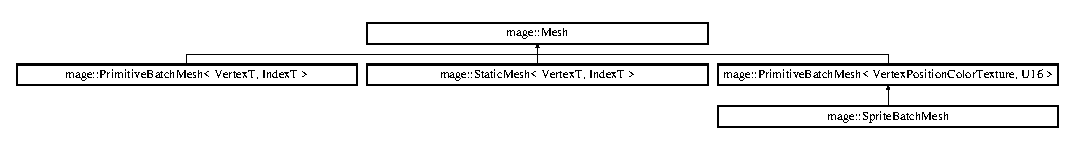
\includegraphics[height=2.000000cm]{classmage_1_1_mesh}
\end{center}
\end{figure}
\subsection*{Public Member Functions}
\begin{DoxyCompactItemize}
\item 
virtual \hyperlink{classmage_1_1_mesh_afa39b90805e434cabb0989878e335b9e}{$\sim$\+Mesh} ()
\item 
\hyperlink{classmage_1_1_mesh}{Mesh} \& \hyperlink{classmage_1_1_mesh_a5baf961af32b379671a59a082492bc5e}{operator=} (const \hyperlink{classmage_1_1_mesh}{Mesh} \&mesh)=delete
\item 
\hyperlink{classmage_1_1_mesh}{Mesh} \& \hyperlink{classmage_1_1_mesh_a28e437196db171b2df1c4bcf3df07a63}{operator=} (\hyperlink{classmage_1_1_mesh}{Mesh} \&\&mesh)=delete
\item 
size\+\_\+t \hyperlink{classmage_1_1_mesh_a2421eac892ef5fd6db21d8214c02e774}{Get\+Vertex\+Size} () const
\item 
size\+\_\+t \hyperlink{classmage_1_1_mesh_a47732f4ac48000c2a1f5562bdba38a81}{Get\+Number\+Of\+Vertices} () const
\item 
size\+\_\+t \hyperlink{classmage_1_1_mesh_a69991b73609ebf936df5c7d2afd2b767}{Get\+Number\+Of\+Indices} () const
\item 
D\+X\+G\+I\+\_\+\+F\+O\+R\+M\+AT \hyperlink{classmage_1_1_mesh_ac76cf9345039a7170597a0e5219a71f9}{Get\+Index\+Format} () const
\item 
D3\+D11\+\_\+\+P\+R\+I\+M\+I\+T\+I\+V\+E\+\_\+\+T\+O\+P\+O\+L\+O\+GY \hyperlink{classmage_1_1_mesh_a3628c67de9562e31a8266a51776c903a}{Get\+Primitive\+Topology} () const
\item 
void \hyperlink{classmage_1_1_mesh_a728979ae0be55283813eecf3e7c40e80}{Prepare\+Drawing} () const
\item 
void \hyperlink{classmage_1_1_mesh_a62f7b8176f7747f2b4db7674524a146c}{Draw} () const
\item 
void \hyperlink{classmage_1_1_mesh_ae1f71bddbb1fa3b45cec55f0fe920c7d}{Draw} (size\+\_\+t start\+\_\+index, size\+\_\+t nb\+\_\+indices) const
\end{DoxyCompactItemize}
\subsection*{Protected Member Functions}
\begin{DoxyCompactItemize}
\item 
\hyperlink{classmage_1_1_mesh_a364e6ecdca96e9b4932aea8711f2bb12}{Mesh} (I\+D3\+D11\+Device2 $\ast$device, I\+D3\+D11\+Device\+Context2 $\ast$device\+\_\+context, size\+\_\+t vertex\+\_\+size, D\+X\+G\+I\+\_\+\+F\+O\+R\+M\+AT index\+\_\+format=D\+X\+G\+I\+\_\+\+F\+O\+R\+M\+A\+T\+\_\+\+R32\+\_\+\+U\+I\+NT, D3\+D11\+\_\+\+P\+R\+I\+M\+I\+T\+I\+V\+E\+\_\+\+T\+O\+P\+O\+L\+O\+GY primitive\+\_\+topology=D3\+D11\+\_\+\+P\+R\+I\+M\+I\+T\+I\+V\+E\+\_\+\+T\+O\+P\+O\+L\+O\+G\+Y\+\_\+\+T\+R\+I\+A\+N\+G\+L\+E\+L\+I\+ST)
\item 
\hyperlink{classmage_1_1_mesh_a1627e85c72d10bdedbfbf746b108cc73}{Mesh} (const \hyperlink{classmage_1_1_mesh}{Mesh} \&mesh)=delete
\item 
\hyperlink{classmage_1_1_mesh_a2751abe4790ca150f1fcc285504645ae}{Mesh} (\hyperlink{classmage_1_1_mesh}{Mesh} \&\&mesh)
\item 
void \hyperlink{classmage_1_1_mesh_a7d871e56f4489e7aa0557688662589bb}{Set\+Number\+Of\+Vertices} (size\+\_\+t nb\+\_\+vertices)
\item 
void \hyperlink{classmage_1_1_mesh_a19336d13ef5219c196678b8fdf4cca2b}{Set\+Number\+Of\+Indices} (size\+\_\+t nb\+\_\+indices)
\end{DoxyCompactItemize}
\subsection*{Protected Attributes}
\begin{DoxyCompactItemize}
\item 
I\+D3\+D11\+Device2 $\ast$const \hyperlink{classmage_1_1_mesh_ad1d91b6048d73bb05d0d39028d048f18}{m\+\_\+device}
\item 
I\+D3\+D11\+Device\+Context2 $\ast$const \hyperlink{classmage_1_1_mesh_a1d19b5bceea2256f4d80ebc06fa74f00}{m\+\_\+device\+\_\+context}
\item 
\hyperlink{namespacemage_ae74f374780900893caa5555d1031fd79}{Com\+Ptr}$<$ I\+D3\+D11\+Buffer $>$ \hyperlink{classmage_1_1_mesh_af5ae74887eb330201829477cf772ba6e}{m\+\_\+vertex\+\_\+buffer}
\item 
\hyperlink{namespacemage_ae74f374780900893caa5555d1031fd79}{Com\+Ptr}$<$ I\+D3\+D11\+Buffer $>$ \hyperlink{classmage_1_1_mesh_abe29363ebac77b284ca69532fd5b3373}{m\+\_\+index\+\_\+buffer}
\end{DoxyCompactItemize}
\subsection*{Private Attributes}
\begin{DoxyCompactItemize}
\item 
const size\+\_\+t \hyperlink{classmage_1_1_mesh_ab3ebdfffca054f32ac69e47c486d57b1}{m\+\_\+vertex\+\_\+size}
\item 
size\+\_\+t \hyperlink{classmage_1_1_mesh_a5a04aa73e98c75dd5b8929296c3af9bb}{m\+\_\+nb\+\_\+vertices}
\item 
size\+\_\+t \hyperlink{classmage_1_1_mesh_a5e3baa9e2b2e9b4ce795a456f76d87b2}{m\+\_\+nb\+\_\+indices}
\item 
const D\+X\+G\+I\+\_\+\+F\+O\+R\+M\+AT \hyperlink{classmage_1_1_mesh_a93dbb92d756948df3b08fc29426c6acf}{m\+\_\+index\+\_\+format}
\item 
const D3\+D11\+\_\+\+P\+R\+I\+M\+I\+T\+I\+V\+E\+\_\+\+T\+O\+P\+O\+L\+O\+GY \hyperlink{classmage_1_1_mesh_a329fab0ad24e11b73a8981c6d09a0c7c}{m\+\_\+primitive\+\_\+topology}
\end{DoxyCompactItemize}


\subsection{Detailed Description}
A class of indexed meshes. 

\subsection{Constructor \& Destructor Documentation}
\hypertarget{classmage_1_1_mesh_afa39b90805e434cabb0989878e335b9e}{}\label{classmage_1_1_mesh_afa39b90805e434cabb0989878e335b9e} 
\index{mage\+::\+Mesh@{mage\+::\+Mesh}!````~Mesh@{$\sim$\+Mesh}}
\index{````~Mesh@{$\sim$\+Mesh}!mage\+::\+Mesh@{mage\+::\+Mesh}}
\subsubsection{\texorpdfstring{$\sim$\+Mesh()}{~Mesh()}}
{\footnotesize\ttfamily mage\+::\+Mesh\+::$\sim$\+Mesh (\begin{DoxyParamCaption}{ }\end{DoxyParamCaption})\hspace{0.3cm}{\ttfamily [virtual]}, {\ttfamily [default]}}

Destructs this mesh. \hypertarget{classmage_1_1_mesh_a364e6ecdca96e9b4932aea8711f2bb12}{}\label{classmage_1_1_mesh_a364e6ecdca96e9b4932aea8711f2bb12} 
\index{mage\+::\+Mesh@{mage\+::\+Mesh}!Mesh@{Mesh}}
\index{Mesh@{Mesh}!mage\+::\+Mesh@{mage\+::\+Mesh}}
\subsubsection{\texorpdfstring{Mesh()}{Mesh()}\hspace{0.1cm}{\footnotesize\ttfamily [1/3]}}
{\footnotesize\ttfamily mage\+::\+Mesh\+::\+Mesh (\begin{DoxyParamCaption}\item[{I\+D3\+D11\+Device2 $\ast$}]{device,  }\item[{I\+D3\+D11\+Device\+Context2 $\ast$}]{device\+\_\+context,  }\item[{size\+\_\+t}]{vertex\+\_\+size,  }\item[{D\+X\+G\+I\+\_\+\+F\+O\+R\+M\+AT}]{index\+\_\+format = {\ttfamily DXGI\+\_\+FORMAT\+\_\+R32\+\_\+UINT},  }\item[{D3\+D11\+\_\+\+P\+R\+I\+M\+I\+T\+I\+V\+E\+\_\+\+T\+O\+P\+O\+L\+O\+GY}]{primitive\+\_\+topology = {\ttfamily D3D11\+\_\+PRIMITIVE\+\_\+TOPOLOGY\+\_\+TRIANGLELIST} }\end{DoxyParamCaption})\hspace{0.3cm}{\ttfamily [explicit]}, {\ttfamily [protected]}}

Constructs a mesh.

\begin{DoxyPrecond}{Precondition}
{\itshape device} is not equal to {\ttfamily nullptr}. 

{\itshape device\+\_\+context} is not equal to {\ttfamily nullptr}. 
\end{DoxyPrecond}

\begin{DoxyParams}[1]{Parameters}
\mbox{\tt in}  & {\em device} & A pointer to the device. \\
\hline
\mbox{\tt in}  & {\em device\+\_\+context} & A pointer to the device context. \\
\hline
\mbox{\tt in}  & {\em vertex\+\_\+size} & The vertex size. \\
\hline
\mbox{\tt in}  & {\em index\+\_\+format} & The index format. \\
\hline
\mbox{\tt in}  & {\em primitive\+\_\+topology} & The primitive topology. \\
\hline
\end{DoxyParams}
\hypertarget{classmage_1_1_mesh_a1627e85c72d10bdedbfbf746b108cc73}{}\label{classmage_1_1_mesh_a1627e85c72d10bdedbfbf746b108cc73} 
\index{mage\+::\+Mesh@{mage\+::\+Mesh}!Mesh@{Mesh}}
\index{Mesh@{Mesh}!mage\+::\+Mesh@{mage\+::\+Mesh}}
\subsubsection{\texorpdfstring{Mesh()}{Mesh()}\hspace{0.1cm}{\footnotesize\ttfamily [2/3]}}
{\footnotesize\ttfamily mage\+::\+Mesh\+::\+Mesh (\begin{DoxyParamCaption}\item[{const \hyperlink{classmage_1_1_mesh}{Mesh} \&}]{mesh }\end{DoxyParamCaption})\hspace{0.3cm}{\ttfamily [protected]}, {\ttfamily [delete]}}

Constructs a mesh from the given mesh.


\begin{DoxyParams}[1]{Parameters}
\mbox{\tt in}  & {\em mesh} & A reference to the mesh to copy. \\
\hline
\end{DoxyParams}
\hypertarget{classmage_1_1_mesh_a2751abe4790ca150f1fcc285504645ae}{}\label{classmage_1_1_mesh_a2751abe4790ca150f1fcc285504645ae} 
\index{mage\+::\+Mesh@{mage\+::\+Mesh}!Mesh@{Mesh}}
\index{Mesh@{Mesh}!mage\+::\+Mesh@{mage\+::\+Mesh}}
\subsubsection{\texorpdfstring{Mesh()}{Mesh()}\hspace{0.1cm}{\footnotesize\ttfamily [3/3]}}
{\footnotesize\ttfamily mage\+::\+Mesh\+::\+Mesh (\begin{DoxyParamCaption}\item[{\hyperlink{classmage_1_1_mesh}{Mesh} \&\&}]{mesh }\end{DoxyParamCaption})\hspace{0.3cm}{\ttfamily [protected]}, {\ttfamily [default]}}

Constructs a mesh by moving the given mesh.


\begin{DoxyParams}[1]{Parameters}
\mbox{\tt in}  & {\em mesh} & A reference to the mesh to move. \\
\hline
\end{DoxyParams}


\subsection{Member Function Documentation}
\hypertarget{classmage_1_1_mesh_a62f7b8176f7747f2b4db7674524a146c}{}\label{classmage_1_1_mesh_a62f7b8176f7747f2b4db7674524a146c} 
\index{mage\+::\+Mesh@{mage\+::\+Mesh}!Draw@{Draw}}
\index{Draw@{Draw}!mage\+::\+Mesh@{mage\+::\+Mesh}}
\subsubsection{\texorpdfstring{Draw()}{Draw()}\hspace{0.1cm}{\footnotesize\ttfamily [1/2]}}
{\footnotesize\ttfamily void mage\+::\+Mesh\+::\+Draw (\begin{DoxyParamCaption}{ }\end{DoxyParamCaption}) const}

Draws this complete mesh. \hypertarget{classmage_1_1_mesh_ae1f71bddbb1fa3b45cec55f0fe920c7d}{}\label{classmage_1_1_mesh_ae1f71bddbb1fa3b45cec55f0fe920c7d} 
\index{mage\+::\+Mesh@{mage\+::\+Mesh}!Draw@{Draw}}
\index{Draw@{Draw}!mage\+::\+Mesh@{mage\+::\+Mesh}}
\subsubsection{\texorpdfstring{Draw()}{Draw()}\hspace{0.1cm}{\footnotesize\ttfamily [2/2]}}
{\footnotesize\ttfamily void mage\+::\+Mesh\+::\+Draw (\begin{DoxyParamCaption}\item[{size\+\_\+t}]{start\+\_\+index,  }\item[{size\+\_\+t}]{nb\+\_\+indices }\end{DoxyParamCaption}) const}

Draws a submesh of this mesh.


\begin{DoxyParams}[1]{Parameters}
\mbox{\tt in}  & {\em start\+\_\+index} & The start index. \\
\hline
\mbox{\tt in}  & {\em nb\+\_\+indices} & The number of indices. \\
\hline
\end{DoxyParams}
\hypertarget{classmage_1_1_mesh_ac76cf9345039a7170597a0e5219a71f9}{}\label{classmage_1_1_mesh_ac76cf9345039a7170597a0e5219a71f9} 
\index{mage\+::\+Mesh@{mage\+::\+Mesh}!Get\+Index\+Format@{Get\+Index\+Format}}
\index{Get\+Index\+Format@{Get\+Index\+Format}!mage\+::\+Mesh@{mage\+::\+Mesh}}
\subsubsection{\texorpdfstring{Get\+Index\+Format()}{GetIndexFormat()}}
{\footnotesize\ttfamily D\+X\+G\+I\+\_\+\+F\+O\+R\+M\+AT mage\+::\+Mesh\+::\+Get\+Index\+Format (\begin{DoxyParamCaption}{ }\end{DoxyParamCaption}) const}

Returns the index format of this mesh.

\begin{DoxyReturn}{Returns}
The index format of this mesh. 
\end{DoxyReturn}
\hypertarget{classmage_1_1_mesh_a69991b73609ebf936df5c7d2afd2b767}{}\label{classmage_1_1_mesh_a69991b73609ebf936df5c7d2afd2b767} 
\index{mage\+::\+Mesh@{mage\+::\+Mesh}!Get\+Number\+Of\+Indices@{Get\+Number\+Of\+Indices}}
\index{Get\+Number\+Of\+Indices@{Get\+Number\+Of\+Indices}!mage\+::\+Mesh@{mage\+::\+Mesh}}
\subsubsection{\texorpdfstring{Get\+Number\+Of\+Indices()}{GetNumberOfIndices()}}
{\footnotesize\ttfamily size\+\_\+t mage\+::\+Mesh\+::\+Get\+Number\+Of\+Indices (\begin{DoxyParamCaption}{ }\end{DoxyParamCaption}) const}

Returns the number of indices of this mesh.

\begin{DoxyReturn}{Returns}
The number of indices of this mesh. 
\end{DoxyReturn}
\hypertarget{classmage_1_1_mesh_a47732f4ac48000c2a1f5562bdba38a81}{}\label{classmage_1_1_mesh_a47732f4ac48000c2a1f5562bdba38a81} 
\index{mage\+::\+Mesh@{mage\+::\+Mesh}!Get\+Number\+Of\+Vertices@{Get\+Number\+Of\+Vertices}}
\index{Get\+Number\+Of\+Vertices@{Get\+Number\+Of\+Vertices}!mage\+::\+Mesh@{mage\+::\+Mesh}}
\subsubsection{\texorpdfstring{Get\+Number\+Of\+Vertices()}{GetNumberOfVertices()}}
{\footnotesize\ttfamily size\+\_\+t mage\+::\+Mesh\+::\+Get\+Number\+Of\+Vertices (\begin{DoxyParamCaption}{ }\end{DoxyParamCaption}) const}

Returns the number of vertices of this mesh.

\begin{DoxyReturn}{Returns}
The number of vertices of this mesh. 
\end{DoxyReturn}
\hypertarget{classmage_1_1_mesh_a3628c67de9562e31a8266a51776c903a}{}\label{classmage_1_1_mesh_a3628c67de9562e31a8266a51776c903a} 
\index{mage\+::\+Mesh@{mage\+::\+Mesh}!Get\+Primitive\+Topology@{Get\+Primitive\+Topology}}
\index{Get\+Primitive\+Topology@{Get\+Primitive\+Topology}!mage\+::\+Mesh@{mage\+::\+Mesh}}
\subsubsection{\texorpdfstring{Get\+Primitive\+Topology()}{GetPrimitiveTopology()}}
{\footnotesize\ttfamily D3\+D11\+\_\+\+P\+R\+I\+M\+I\+T\+I\+V\+E\+\_\+\+T\+O\+P\+O\+L\+O\+GY mage\+::\+Mesh\+::\+Get\+Primitive\+Topology (\begin{DoxyParamCaption}{ }\end{DoxyParamCaption}) const}

Returns the primitive topology of this mesh.

\begin{DoxyReturn}{Returns}
The primitive topology of this mesh. 
\end{DoxyReturn}
\hypertarget{classmage_1_1_mesh_a2421eac892ef5fd6db21d8214c02e774}{}\label{classmage_1_1_mesh_a2421eac892ef5fd6db21d8214c02e774} 
\index{mage\+::\+Mesh@{mage\+::\+Mesh}!Get\+Vertex\+Size@{Get\+Vertex\+Size}}
\index{Get\+Vertex\+Size@{Get\+Vertex\+Size}!mage\+::\+Mesh@{mage\+::\+Mesh}}
\subsubsection{\texorpdfstring{Get\+Vertex\+Size()}{GetVertexSize()}}
{\footnotesize\ttfamily size\+\_\+t mage\+::\+Mesh\+::\+Get\+Vertex\+Size (\begin{DoxyParamCaption}{ }\end{DoxyParamCaption}) const}

Returns the size (in bytes) of the vertices of this mesh.

\begin{DoxyReturn}{Returns}
The vertex size (in bytes) of this static mesh. 
\end{DoxyReturn}
\hypertarget{classmage_1_1_mesh_a5baf961af32b379671a59a082492bc5e}{}\label{classmage_1_1_mesh_a5baf961af32b379671a59a082492bc5e} 
\index{mage\+::\+Mesh@{mage\+::\+Mesh}!operator=@{operator=}}
\index{operator=@{operator=}!mage\+::\+Mesh@{mage\+::\+Mesh}}
\subsubsection{\texorpdfstring{operator=()}{operator=()}\hspace{0.1cm}{\footnotesize\ttfamily [1/2]}}
{\footnotesize\ttfamily \hyperlink{classmage_1_1_mesh}{Mesh}\& mage\+::\+Mesh\+::operator= (\begin{DoxyParamCaption}\item[{const \hyperlink{classmage_1_1_mesh}{Mesh} \&}]{mesh }\end{DoxyParamCaption})\hspace{0.3cm}{\ttfamily [delete]}}

Copies the given mesh to this mesh.


\begin{DoxyParams}[1]{Parameters}
\mbox{\tt in}  & {\em mesh} & A reference to the mesh to copy. \\
\hline
\end{DoxyParams}
\begin{DoxyReturn}{Returns}
A reference to the copy of the given mesh (i.\+e. this mesh). 
\end{DoxyReturn}
\hypertarget{classmage_1_1_mesh_a28e437196db171b2df1c4bcf3df07a63}{}\label{classmage_1_1_mesh_a28e437196db171b2df1c4bcf3df07a63} 
\index{mage\+::\+Mesh@{mage\+::\+Mesh}!operator=@{operator=}}
\index{operator=@{operator=}!mage\+::\+Mesh@{mage\+::\+Mesh}}
\subsubsection{\texorpdfstring{operator=()}{operator=()}\hspace{0.1cm}{\footnotesize\ttfamily [2/2]}}
{\footnotesize\ttfamily \hyperlink{classmage_1_1_mesh}{Mesh}\& mage\+::\+Mesh\+::operator= (\begin{DoxyParamCaption}\item[{\hyperlink{classmage_1_1_mesh}{Mesh} \&\&}]{mesh }\end{DoxyParamCaption})\hspace{0.3cm}{\ttfamily [delete]}}

Moves the given mesh to this mesh.


\begin{DoxyParams}[1]{Parameters}
\mbox{\tt in}  & {\em mesh} & A reference to the mesh to move. \\
\hline
\end{DoxyParams}
\begin{DoxyReturn}{Returns}
A reference to the moved mesh (i.\+e. this mesh). 
\end{DoxyReturn}
\hypertarget{classmage_1_1_mesh_a728979ae0be55283813eecf3e7c40e80}{}\label{classmage_1_1_mesh_a728979ae0be55283813eecf3e7c40e80} 
\index{mage\+::\+Mesh@{mage\+::\+Mesh}!Prepare\+Drawing@{Prepare\+Drawing}}
\index{Prepare\+Drawing@{Prepare\+Drawing}!mage\+::\+Mesh@{mage\+::\+Mesh}}
\subsubsection{\texorpdfstring{Prepare\+Drawing()}{PrepareDrawing()}}
{\footnotesize\ttfamily void mage\+::\+Mesh\+::\+Prepare\+Drawing (\begin{DoxyParamCaption}{ }\end{DoxyParamCaption}) const}

Prepares the drawing of this mesh.

The vertex buffer, index buffer and primitive topology of this mesh will be bound to the input-\/assembler stage. \hypertarget{classmage_1_1_mesh_a19336d13ef5219c196678b8fdf4cca2b}{}\label{classmage_1_1_mesh_a19336d13ef5219c196678b8fdf4cca2b} 
\index{mage\+::\+Mesh@{mage\+::\+Mesh}!Set\+Number\+Of\+Indices@{Set\+Number\+Of\+Indices}}
\index{Set\+Number\+Of\+Indices@{Set\+Number\+Of\+Indices}!mage\+::\+Mesh@{mage\+::\+Mesh}}
\subsubsection{\texorpdfstring{Set\+Number\+Of\+Indices()}{SetNumberOfIndices()}}
{\footnotesize\ttfamily void mage\+::\+Mesh\+::\+Set\+Number\+Of\+Indices (\begin{DoxyParamCaption}\item[{size\+\_\+t}]{nb\+\_\+indices }\end{DoxyParamCaption})\hspace{0.3cm}{\ttfamily [protected]}}

Sets the number of indices of this mesh to the given number.


\begin{DoxyParams}[1]{Parameters}
\mbox{\tt in}  & {\em nb\+\_\+indices} & The number of indices of this mesh. \\
\hline
\end{DoxyParams}
\hypertarget{classmage_1_1_mesh_a7d871e56f4489e7aa0557688662589bb}{}\label{classmage_1_1_mesh_a7d871e56f4489e7aa0557688662589bb} 
\index{mage\+::\+Mesh@{mage\+::\+Mesh}!Set\+Number\+Of\+Vertices@{Set\+Number\+Of\+Vertices}}
\index{Set\+Number\+Of\+Vertices@{Set\+Number\+Of\+Vertices}!mage\+::\+Mesh@{mage\+::\+Mesh}}
\subsubsection{\texorpdfstring{Set\+Number\+Of\+Vertices()}{SetNumberOfVertices()}}
{\footnotesize\ttfamily void mage\+::\+Mesh\+::\+Set\+Number\+Of\+Vertices (\begin{DoxyParamCaption}\item[{size\+\_\+t}]{nb\+\_\+vertices }\end{DoxyParamCaption})\hspace{0.3cm}{\ttfamily [protected]}}

Sets the number of vertices of this mesh to the given number.


\begin{DoxyParams}[1]{Parameters}
\mbox{\tt in}  & {\em nb\+\_\+vertices} & The number of vertices of this mesh. \\
\hline
\end{DoxyParams}


\subsection{Member Data Documentation}
\hypertarget{classmage_1_1_mesh_ad1d91b6048d73bb05d0d39028d048f18}{}\label{classmage_1_1_mesh_ad1d91b6048d73bb05d0d39028d048f18} 
\index{mage\+::\+Mesh@{mage\+::\+Mesh}!m\+\_\+device@{m\+\_\+device}}
\index{m\+\_\+device@{m\+\_\+device}!mage\+::\+Mesh@{mage\+::\+Mesh}}
\subsubsection{\texorpdfstring{m\+\_\+device}{m\_device}}
{\footnotesize\ttfamily I\+D3\+D11\+Device2$\ast$ const mage\+::\+Mesh\+::m\+\_\+device\hspace{0.3cm}{\ttfamily [protected]}}

A pointer to the device of this mesh. \hypertarget{classmage_1_1_mesh_a1d19b5bceea2256f4d80ebc06fa74f00}{}\label{classmage_1_1_mesh_a1d19b5bceea2256f4d80ebc06fa74f00} 
\index{mage\+::\+Mesh@{mage\+::\+Mesh}!m\+\_\+device\+\_\+context@{m\+\_\+device\+\_\+context}}
\index{m\+\_\+device\+\_\+context@{m\+\_\+device\+\_\+context}!mage\+::\+Mesh@{mage\+::\+Mesh}}
\subsubsection{\texorpdfstring{m\+\_\+device\+\_\+context}{m\_device\_context}}
{\footnotesize\ttfamily I\+D3\+D11\+Device\+Context2$\ast$ const mage\+::\+Mesh\+::m\+\_\+device\+\_\+context\hspace{0.3cm}{\ttfamily [protected]}}

A pointer to the device context of this mesh. \hypertarget{classmage_1_1_mesh_abe29363ebac77b284ca69532fd5b3373}{}\label{classmage_1_1_mesh_abe29363ebac77b284ca69532fd5b3373} 
\index{mage\+::\+Mesh@{mage\+::\+Mesh}!m\+\_\+index\+\_\+buffer@{m\+\_\+index\+\_\+buffer}}
\index{m\+\_\+index\+\_\+buffer@{m\+\_\+index\+\_\+buffer}!mage\+::\+Mesh@{mage\+::\+Mesh}}
\subsubsection{\texorpdfstring{m\+\_\+index\+\_\+buffer}{m\_index\_buffer}}
{\footnotesize\ttfamily \hyperlink{namespacemage_ae74f374780900893caa5555d1031fd79}{Com\+Ptr}$<$ I\+D3\+D11\+Buffer $>$ mage\+::\+Mesh\+::m\+\_\+index\+\_\+buffer\hspace{0.3cm}{\ttfamily [protected]}}

A pointer to the index buffer of this mesh. \hypertarget{classmage_1_1_mesh_a93dbb92d756948df3b08fc29426c6acf}{}\label{classmage_1_1_mesh_a93dbb92d756948df3b08fc29426c6acf} 
\index{mage\+::\+Mesh@{mage\+::\+Mesh}!m\+\_\+index\+\_\+format@{m\+\_\+index\+\_\+format}}
\index{m\+\_\+index\+\_\+format@{m\+\_\+index\+\_\+format}!mage\+::\+Mesh@{mage\+::\+Mesh}}
\subsubsection{\texorpdfstring{m\+\_\+index\+\_\+format}{m\_index\_format}}
{\footnotesize\ttfamily const D\+X\+G\+I\+\_\+\+F\+O\+R\+M\+AT mage\+::\+Mesh\+::m\+\_\+index\+\_\+format\hspace{0.3cm}{\ttfamily [private]}}

The index format of this mesh. \hypertarget{classmage_1_1_mesh_a5e3baa9e2b2e9b4ce795a456f76d87b2}{}\label{classmage_1_1_mesh_a5e3baa9e2b2e9b4ce795a456f76d87b2} 
\index{mage\+::\+Mesh@{mage\+::\+Mesh}!m\+\_\+nb\+\_\+indices@{m\+\_\+nb\+\_\+indices}}
\index{m\+\_\+nb\+\_\+indices@{m\+\_\+nb\+\_\+indices}!mage\+::\+Mesh@{mage\+::\+Mesh}}
\subsubsection{\texorpdfstring{m\+\_\+nb\+\_\+indices}{m\_nb\_indices}}
{\footnotesize\ttfamily size\+\_\+t mage\+::\+Mesh\+::m\+\_\+nb\+\_\+indices\hspace{0.3cm}{\ttfamily [private]}}

The number of indices of this mesh. \hypertarget{classmage_1_1_mesh_a5a04aa73e98c75dd5b8929296c3af9bb}{}\label{classmage_1_1_mesh_a5a04aa73e98c75dd5b8929296c3af9bb} 
\index{mage\+::\+Mesh@{mage\+::\+Mesh}!m\+\_\+nb\+\_\+vertices@{m\+\_\+nb\+\_\+vertices}}
\index{m\+\_\+nb\+\_\+vertices@{m\+\_\+nb\+\_\+vertices}!mage\+::\+Mesh@{mage\+::\+Mesh}}
\subsubsection{\texorpdfstring{m\+\_\+nb\+\_\+vertices}{m\_nb\_vertices}}
{\footnotesize\ttfamily size\+\_\+t mage\+::\+Mesh\+::m\+\_\+nb\+\_\+vertices\hspace{0.3cm}{\ttfamily [private]}}

The number of vertices of this mesh. \hypertarget{classmage_1_1_mesh_a329fab0ad24e11b73a8981c6d09a0c7c}{}\label{classmage_1_1_mesh_a329fab0ad24e11b73a8981c6d09a0c7c} 
\index{mage\+::\+Mesh@{mage\+::\+Mesh}!m\+\_\+primitive\+\_\+topology@{m\+\_\+primitive\+\_\+topology}}
\index{m\+\_\+primitive\+\_\+topology@{m\+\_\+primitive\+\_\+topology}!mage\+::\+Mesh@{mage\+::\+Mesh}}
\subsubsection{\texorpdfstring{m\+\_\+primitive\+\_\+topology}{m\_primitive\_topology}}
{\footnotesize\ttfamily const D3\+D11\+\_\+\+P\+R\+I\+M\+I\+T\+I\+V\+E\+\_\+\+T\+O\+P\+O\+L\+O\+GY mage\+::\+Mesh\+::m\+\_\+primitive\+\_\+topology\hspace{0.3cm}{\ttfamily [private]}}

The primitive topology of this mesh. \hypertarget{classmage_1_1_mesh_af5ae74887eb330201829477cf772ba6e}{}\label{classmage_1_1_mesh_af5ae74887eb330201829477cf772ba6e} 
\index{mage\+::\+Mesh@{mage\+::\+Mesh}!m\+\_\+vertex\+\_\+buffer@{m\+\_\+vertex\+\_\+buffer}}
\index{m\+\_\+vertex\+\_\+buffer@{m\+\_\+vertex\+\_\+buffer}!mage\+::\+Mesh@{mage\+::\+Mesh}}
\subsubsection{\texorpdfstring{m\+\_\+vertex\+\_\+buffer}{m\_vertex\_buffer}}
{\footnotesize\ttfamily \hyperlink{namespacemage_ae74f374780900893caa5555d1031fd79}{Com\+Ptr}$<$ I\+D3\+D11\+Buffer $>$ mage\+::\+Mesh\+::m\+\_\+vertex\+\_\+buffer\hspace{0.3cm}{\ttfamily [protected]}}

A pointer to the vertex buffer of this mesh. \hypertarget{classmage_1_1_mesh_ab3ebdfffca054f32ac69e47c486d57b1}{}\label{classmage_1_1_mesh_ab3ebdfffca054f32ac69e47c486d57b1} 
\index{mage\+::\+Mesh@{mage\+::\+Mesh}!m\+\_\+vertex\+\_\+size@{m\+\_\+vertex\+\_\+size}}
\index{m\+\_\+vertex\+\_\+size@{m\+\_\+vertex\+\_\+size}!mage\+::\+Mesh@{mage\+::\+Mesh}}
\subsubsection{\texorpdfstring{m\+\_\+vertex\+\_\+size}{m\_vertex\_size}}
{\footnotesize\ttfamily const size\+\_\+t mage\+::\+Mesh\+::m\+\_\+vertex\+\_\+size\hspace{0.3cm}{\ttfamily [private]}}

The vertex size of this static mesh. 
\hypertarget{structmage_1_1_mesh_descriptor}{}\section{mage\+:\+:Mesh\+Descriptor$<$ VertexT $>$ Struct Template Reference}
\label{structmage_1_1_mesh_descriptor}\index{mage\+::\+Mesh\+Descriptor$<$ Vertex\+T $>$@{mage\+::\+Mesh\+Descriptor$<$ Vertex\+T $>$}}


{\ttfamily \#include $<$mesh\+\_\+descriptor.\+hpp$>$}

\subsection*{Public Member Functions}
\begin{DoxyCompactItemize}
\item 
\hyperlink{structmage_1_1_mesh_descriptor_ae9c4651675fc0600fca01f0614c70762}{Mesh\+Descriptor} (bool invert\+\_\+handedness=false, bool clockwise\+\_\+order=true)
\item 
\hyperlink{structmage_1_1_mesh_descriptor_ab6347b2a60fbdf11573ddfe9283616d4}{Mesh\+Descriptor} (const \hyperlink{structmage_1_1_mesh_descriptor}{Mesh\+Descriptor}$<$ VertexT $>$ \&desc)=default
\item 
\hyperlink{structmage_1_1_mesh_descriptor_a62de61d0ea1ad1a514246f40e21c9faa}{Mesh\+Descriptor} (\hyperlink{structmage_1_1_mesh_descriptor}{Mesh\+Descriptor}$<$ VertexT $>$ \&\&desc)=default
\item 
\hyperlink{structmage_1_1_mesh_descriptor_adca32db164ab3032164c8dfe17af3db4}{$\sim$\+Mesh\+Descriptor} ()=default
\item 
\hyperlink{structmage_1_1_mesh_descriptor}{Mesh\+Descriptor} \& \hyperlink{structmage_1_1_mesh_descriptor_aef6a9568a8d4516dbeff4d8f665ca213}{operator=} (const \hyperlink{structmage_1_1_mesh_descriptor}{Mesh\+Descriptor}$<$ VertexT $>$ \&desc)=default
\item 
\hyperlink{structmage_1_1_mesh_descriptor}{Mesh\+Descriptor} \& \hyperlink{structmage_1_1_mesh_descriptor_aee596eaa945924860d9a26daa58d8f45}{operator=} (\hyperlink{structmage_1_1_mesh_descriptor}{Mesh\+Descriptor}$<$ VertexT $>$ \&\&desc)=default
\item 
bool \hyperlink{structmage_1_1_mesh_descriptor_a7f63b926282683dcb0f674eca0901f5e}{Invert\+Handness} () const
\item 
bool \hyperlink{structmage_1_1_mesh_descriptor_ab81b000d93242ae002227010c4a9446c}{Clockwise\+Order} () const
\end{DoxyCompactItemize}
\subsection*{Private Attributes}
\begin{DoxyCompactItemize}
\item 
bool \hyperlink{structmage_1_1_mesh_descriptor_af7b8124e44ac65ca2088d5d8ca0639f5}{m\+\_\+invert\+\_\+handedness}
\item 
bool \hyperlink{structmage_1_1_mesh_descriptor_a7e769c8d1d81b3514b951b306865dc88}{m\+\_\+clockwise\+\_\+order}
\end{DoxyCompactItemize}


\subsection{Constructor \& Destructor Documentation}
\hypertarget{structmage_1_1_mesh_descriptor_ae9c4651675fc0600fca01f0614c70762}{}\label{structmage_1_1_mesh_descriptor_ae9c4651675fc0600fca01f0614c70762} 
\index{mage\+::\+Mesh\+Descriptor@{mage\+::\+Mesh\+Descriptor}!Mesh\+Descriptor@{Mesh\+Descriptor}}
\index{Mesh\+Descriptor@{Mesh\+Descriptor}!mage\+::\+Mesh\+Descriptor@{mage\+::\+Mesh\+Descriptor}}
\subsubsection{\texorpdfstring{Mesh\+Descriptor()}{MeshDescriptor()}\hspace{0.1cm}{\footnotesize\ttfamily [1/3]}}
{\footnotesize\ttfamily template$<$typename VertexT$>$ \\
\hyperlink{structmage_1_1_mesh_descriptor}{mage\+::\+Mesh\+Descriptor}$<$ VertexT $>$\+::\hyperlink{structmage_1_1_mesh_descriptor}{Mesh\+Descriptor} (\begin{DoxyParamCaption}\item[{bool}]{invert\+\_\+handedness = {\ttfamily false},  }\item[{bool}]{clockwise\+\_\+order = {\ttfamily true} }\end{DoxyParamCaption})\hspace{0.3cm}{\ttfamily [explicit]}}

Constructs a mesh descriptor.


\begin{DoxyParams}[1]{Parameters}
\mbox{\tt in}  & {\em invert\+\_\+handedness} & Flag indicating whether the handness of the coordinate system of the mesh should be inverted. \\
\hline
\mbox{\tt in}  & {\em clockwise\+\_\+order} & Flag indicating whether the vertices of triangles should be in clockwise order. \\
\hline
\end{DoxyParams}
\hypertarget{structmage_1_1_mesh_descriptor_ab6347b2a60fbdf11573ddfe9283616d4}{}\label{structmage_1_1_mesh_descriptor_ab6347b2a60fbdf11573ddfe9283616d4} 
\index{mage\+::\+Mesh\+Descriptor@{mage\+::\+Mesh\+Descriptor}!Mesh\+Descriptor@{Mesh\+Descriptor}}
\index{Mesh\+Descriptor@{Mesh\+Descriptor}!mage\+::\+Mesh\+Descriptor@{mage\+::\+Mesh\+Descriptor}}
\subsubsection{\texorpdfstring{Mesh\+Descriptor()}{MeshDescriptor()}\hspace{0.1cm}{\footnotesize\ttfamily [2/3]}}
{\footnotesize\ttfamily template$<$typename VertexT$>$ \\
\hyperlink{structmage_1_1_mesh_descriptor}{mage\+::\+Mesh\+Descriptor}$<$ VertexT $>$\+::\hyperlink{structmage_1_1_mesh_descriptor}{Mesh\+Descriptor} (\begin{DoxyParamCaption}\item[{const \hyperlink{structmage_1_1_mesh_descriptor}{Mesh\+Descriptor}$<$ VertexT $>$ \&}]{desc }\end{DoxyParamCaption})\hspace{0.3cm}{\ttfamily [default]}}

\hypertarget{structmage_1_1_mesh_descriptor_a62de61d0ea1ad1a514246f40e21c9faa}{}\label{structmage_1_1_mesh_descriptor_a62de61d0ea1ad1a514246f40e21c9faa} 
\index{mage\+::\+Mesh\+Descriptor@{mage\+::\+Mesh\+Descriptor}!Mesh\+Descriptor@{Mesh\+Descriptor}}
\index{Mesh\+Descriptor@{Mesh\+Descriptor}!mage\+::\+Mesh\+Descriptor@{mage\+::\+Mesh\+Descriptor}}
\subsubsection{\texorpdfstring{Mesh\+Descriptor()}{MeshDescriptor()}\hspace{0.1cm}{\footnotesize\ttfamily [3/3]}}
{\footnotesize\ttfamily template$<$typename VertexT$>$ \\
\hyperlink{structmage_1_1_mesh_descriptor}{mage\+::\+Mesh\+Descriptor}$<$ VertexT $>$\+::\hyperlink{structmage_1_1_mesh_descriptor}{Mesh\+Descriptor} (\begin{DoxyParamCaption}\item[{\hyperlink{structmage_1_1_mesh_descriptor}{Mesh\+Descriptor}$<$ VertexT $>$ \&\&}]{desc }\end{DoxyParamCaption})\hspace{0.3cm}{\ttfamily [default]}}

\hypertarget{structmage_1_1_mesh_descriptor_adca32db164ab3032164c8dfe17af3db4}{}\label{structmage_1_1_mesh_descriptor_adca32db164ab3032164c8dfe17af3db4} 
\index{mage\+::\+Mesh\+Descriptor@{mage\+::\+Mesh\+Descriptor}!````~Mesh\+Descriptor@{$\sim$\+Mesh\+Descriptor}}
\index{````~Mesh\+Descriptor@{$\sim$\+Mesh\+Descriptor}!mage\+::\+Mesh\+Descriptor@{mage\+::\+Mesh\+Descriptor}}
\subsubsection{\texorpdfstring{$\sim$\+Mesh\+Descriptor()}{~MeshDescriptor()}}
{\footnotesize\ttfamily template$<$typename VertexT$>$ \\
\hyperlink{structmage_1_1_mesh_descriptor}{mage\+::\+Mesh\+Descriptor}$<$ VertexT $>$\+::$\sim$\hyperlink{structmage_1_1_mesh_descriptor}{Mesh\+Descriptor} (\begin{DoxyParamCaption}{ }\end{DoxyParamCaption})\hspace{0.3cm}{\ttfamily [default]}}



\subsection{Member Function Documentation}
\hypertarget{structmage_1_1_mesh_descriptor_ab81b000d93242ae002227010c4a9446c}{}\label{structmage_1_1_mesh_descriptor_ab81b000d93242ae002227010c4a9446c} 
\index{mage\+::\+Mesh\+Descriptor@{mage\+::\+Mesh\+Descriptor}!Clockwise\+Order@{Clockwise\+Order}}
\index{Clockwise\+Order@{Clockwise\+Order}!mage\+::\+Mesh\+Descriptor@{mage\+::\+Mesh\+Descriptor}}
\subsubsection{\texorpdfstring{Clockwise\+Order()}{ClockwiseOrder()}}
{\footnotesize\ttfamily template$<$typename VertexT$>$ \\
bool \hyperlink{structmage_1_1_mesh_descriptor}{mage\+::\+Mesh\+Descriptor}$<$ VertexT $>$\+::Clockwise\+Order (\begin{DoxyParamCaption}{ }\end{DoxyParamCaption}) const}

\hypertarget{structmage_1_1_mesh_descriptor_a7f63b926282683dcb0f674eca0901f5e}{}\label{structmage_1_1_mesh_descriptor_a7f63b926282683dcb0f674eca0901f5e} 
\index{mage\+::\+Mesh\+Descriptor@{mage\+::\+Mesh\+Descriptor}!Invert\+Handness@{Invert\+Handness}}
\index{Invert\+Handness@{Invert\+Handness}!mage\+::\+Mesh\+Descriptor@{mage\+::\+Mesh\+Descriptor}}
\subsubsection{\texorpdfstring{Invert\+Handness()}{InvertHandness()}}
{\footnotesize\ttfamily template$<$typename VertexT$>$ \\
bool \hyperlink{structmage_1_1_mesh_descriptor}{mage\+::\+Mesh\+Descriptor}$<$ VertexT $>$\+::Invert\+Handness (\begin{DoxyParamCaption}{ }\end{DoxyParamCaption}) const}

\hypertarget{structmage_1_1_mesh_descriptor_aef6a9568a8d4516dbeff4d8f665ca213}{}\label{structmage_1_1_mesh_descriptor_aef6a9568a8d4516dbeff4d8f665ca213} 
\index{mage\+::\+Mesh\+Descriptor@{mage\+::\+Mesh\+Descriptor}!operator=@{operator=}}
\index{operator=@{operator=}!mage\+::\+Mesh\+Descriptor@{mage\+::\+Mesh\+Descriptor}}
\subsubsection{\texorpdfstring{operator=()}{operator=()}\hspace{0.1cm}{\footnotesize\ttfamily [1/2]}}
{\footnotesize\ttfamily template$<$typename VertexT$>$ \\
\hyperlink{structmage_1_1_mesh_descriptor}{Mesh\+Descriptor}\& \hyperlink{structmage_1_1_mesh_descriptor}{mage\+::\+Mesh\+Descriptor}$<$ VertexT $>$\+::operator= (\begin{DoxyParamCaption}\item[{const \hyperlink{structmage_1_1_mesh_descriptor}{Mesh\+Descriptor}$<$ VertexT $>$ \&}]{desc }\end{DoxyParamCaption})\hspace{0.3cm}{\ttfamily [default]}}

\hypertarget{structmage_1_1_mesh_descriptor_aee596eaa945924860d9a26daa58d8f45}{}\label{structmage_1_1_mesh_descriptor_aee596eaa945924860d9a26daa58d8f45} 
\index{mage\+::\+Mesh\+Descriptor@{mage\+::\+Mesh\+Descriptor}!operator=@{operator=}}
\index{operator=@{operator=}!mage\+::\+Mesh\+Descriptor@{mage\+::\+Mesh\+Descriptor}}
\subsubsection{\texorpdfstring{operator=()}{operator=()}\hspace{0.1cm}{\footnotesize\ttfamily [2/2]}}
{\footnotesize\ttfamily template$<$typename VertexT$>$ \\
\hyperlink{structmage_1_1_mesh_descriptor}{Mesh\+Descriptor}\& \hyperlink{structmage_1_1_mesh_descriptor}{mage\+::\+Mesh\+Descriptor}$<$ VertexT $>$\+::operator= (\begin{DoxyParamCaption}\item[{\hyperlink{structmage_1_1_mesh_descriptor}{Mesh\+Descriptor}$<$ VertexT $>$ \&\&}]{desc }\end{DoxyParamCaption})\hspace{0.3cm}{\ttfamily [default]}}



\subsection{Member Data Documentation}
\hypertarget{structmage_1_1_mesh_descriptor_a7e769c8d1d81b3514b951b306865dc88}{}\label{structmage_1_1_mesh_descriptor_a7e769c8d1d81b3514b951b306865dc88} 
\index{mage\+::\+Mesh\+Descriptor@{mage\+::\+Mesh\+Descriptor}!m\+\_\+clockwise\+\_\+order@{m\+\_\+clockwise\+\_\+order}}
\index{m\+\_\+clockwise\+\_\+order@{m\+\_\+clockwise\+\_\+order}!mage\+::\+Mesh\+Descriptor@{mage\+::\+Mesh\+Descriptor}}
\subsubsection{\texorpdfstring{m\+\_\+clockwise\+\_\+order}{m\_clockwise\_order}}
{\footnotesize\ttfamily template$<$typename VertexT$>$ \\
bool \hyperlink{structmage_1_1_mesh_descriptor}{mage\+::\+Mesh\+Descriptor}$<$ VertexT $>$\+::m\+\_\+clockwise\+\_\+order\hspace{0.3cm}{\ttfamily [private]}}

\hypertarget{structmage_1_1_mesh_descriptor_af7b8124e44ac65ca2088d5d8ca0639f5}{}\label{structmage_1_1_mesh_descriptor_af7b8124e44ac65ca2088d5d8ca0639f5} 
\index{mage\+::\+Mesh\+Descriptor@{mage\+::\+Mesh\+Descriptor}!m\+\_\+invert\+\_\+handedness@{m\+\_\+invert\+\_\+handedness}}
\index{m\+\_\+invert\+\_\+handedness@{m\+\_\+invert\+\_\+handedness}!mage\+::\+Mesh\+Descriptor@{mage\+::\+Mesh\+Descriptor}}
\subsubsection{\texorpdfstring{m\+\_\+invert\+\_\+handedness}{m\_invert\_handedness}}
{\footnotesize\ttfamily template$<$typename VertexT$>$ \\
bool \hyperlink{structmage_1_1_mesh_descriptor}{mage\+::\+Mesh\+Descriptor}$<$ VertexT $>$\+::m\+\_\+invert\+\_\+handedness\hspace{0.3cm}{\ttfamily [private]}}


\hypertarget{classmage_1_1_model}{}\section{mage\+:\+:Model Class Reference}
\label{classmage_1_1_model}\index{mage\+::\+Model@{mage\+::\+Model}}


{\ttfamily \#include $<$model.\+hpp$>$}

\subsection*{Public Member Functions}
\begin{DoxyCompactItemize}
\item 
\hyperlink{classmage_1_1_model_aca2d5faa95a447ff3ecaab685aec8581}{Model} (\hyperlink{namespacemage_a1e01ae66713838a7a67d30e44c67703e}{Shared\+Ptr}$<$ const \hyperlink{classmage_1_1_mesh}{Mesh} $>$ mesh, size\+\_\+t start\+\_\+index, size\+\_\+t nb\+\_\+indices, const \hyperlink{structmage_1_1_shaded_material}{Shaded\+Material} \&material)
\item 
\hyperlink{classmage_1_1_model_ac5f1d340bbfefd30bec3e6343a86059a}{Model} (const \hyperlink{classmage_1_1_model}{Model} \&model)
\item 
\hyperlink{classmage_1_1_model_a085272d7cb82587094f18747ecc5aad0}{Model} (\hyperlink{classmage_1_1_model}{Model} \&\&model)=default
\item 
virtual \hyperlink{classmage_1_1_model_a802f7bcb3d15d3baab4a8d383d9e9293}{$\sim$\+Model} ()=default
\item 
\hyperlink{classmage_1_1_model}{Model} \& \hyperlink{classmage_1_1_model_a563515c64ec39cfcda9f6ca37576391b}{operator=} (const \hyperlink{classmage_1_1_model}{Model} \&model)=delete
\item 
\hyperlink{classmage_1_1_model}{Model} \& \hyperlink{classmage_1_1_model_a084e30d15822bfefa79128f30a57cc02}{operator=} (\hyperlink{classmage_1_1_model}{Model} \&\&model)=delete
\item 
\hyperlink{namespacemage_a1e01ae66713838a7a67d30e44c67703e}{Shared\+Ptr}$<$ \hyperlink{classmage_1_1_model}{Model} $>$ \hyperlink{classmage_1_1_model_ac0043eb1766f8a5be05284fbb9c3e912}{Clone} () const
\item 
size\+\_\+t \hyperlink{classmage_1_1_model_af17401dfd3e51f96dc0652a3aa3c4412}{Get\+Start\+Index} () const
\item 
size\+\_\+t \hyperlink{classmage_1_1_model_ac118db61c4541d16d9b1b52e55524956}{Get\+Number\+Of\+Indices} () const
\item 
const \hyperlink{classmage_1_1_mesh}{Mesh} $\ast$ \hyperlink{classmage_1_1_model_a085c12b33ebe60e7576c643e2d47baf0}{Get\+Mesh} () const
\item 
\hyperlink{structmage_1_1_material}{Material} \& \hyperlink{classmage_1_1_model_ae2d9b0fee188fe8f0377872bc2f8c2f6}{Get\+Material} ()
\item 
const \hyperlink{structmage_1_1_material}{Material} \& \hyperlink{classmage_1_1_model_aedb16dfea55edaefc3e5d88e9f9fa756}{Get\+Material} () const
\item 
\hyperlink{structmage_1_1_shaded_material}{Shaded\+Material} $\ast$ \hyperlink{classmage_1_1_model_af709f5b1ec136cbab25bda39e20e1662}{Get\+Shaded\+Material} ()
\item 
const \hyperlink{structmage_1_1_shaded_material}{Shaded\+Material} $\ast$ \hyperlink{classmage_1_1_model_a84af7ad13b2bc1d8a51828a62fbaa4b0}{Get\+Shaded\+Material} () const
\item 
void \hyperlink{classmage_1_1_model_a0083c64e8199db23b78a9281be84685f}{Prepare\+Drawing} () const
\item 
void \hyperlink{classmage_1_1_model_a14cc836651dc3eeb378d749b24c149d9}{Prepare\+Shading} (I\+D3\+D11\+Buffer $\ast$transform, const \hyperlink{structmage_1_1_lighting}{Lighting} \&lighting) const
\item 
void \hyperlink{classmage_1_1_model_a13badcd5e7bfaf8fbdc447dc211d5ad9}{Draw} () const
\end{DoxyCompactItemize}
\subsection*{Private Member Functions}
\begin{DoxyCompactItemize}
\item 
virtual \hyperlink{namespacemage_a1e01ae66713838a7a67d30e44c67703e}{Shared\+Ptr}$<$ \hyperlink{classmage_1_1_model}{Model} $>$ \hyperlink{classmage_1_1_model_af90feb622e30e1531983c01372b2df37}{Clone\+Implementation} () const
\end{DoxyCompactItemize}
\subsection*{Private Attributes}
\begin{DoxyCompactItemize}
\item 
\hyperlink{namespacemage_a1e01ae66713838a7a67d30e44c67703e}{Shared\+Ptr}$<$ const \hyperlink{classmage_1_1_mesh}{Mesh} $>$ \hyperlink{classmage_1_1_model_aecd2b4031c5df30fb5f7ed6d62810f73}{m\+\_\+mesh}
\item 
const size\+\_\+t \hyperlink{classmage_1_1_model_a63a3e697c9eb1606249de15cc7b818c3}{m\+\_\+start\+\_\+index}
\item 
const size\+\_\+t \hyperlink{classmage_1_1_model_a1fcf80ed9f3002bd2319ef83f073ae75}{m\+\_\+nb\+\_\+indices}
\item 
\hyperlink{namespacemage_a8c307fbcc33bce9b7f2aa4c26c3b95cf}{Unique\+Ptr}$<$ \hyperlink{structmage_1_1_shaded_material}{Shaded\+Material} $>$ \hyperlink{classmage_1_1_model_a93e080e5dc2c7c0672a278de76899122}{m\+\_\+material}
\end{DoxyCompactItemize}


\subsection{Detailed Description}
A class of models. 

\subsection{Constructor \& Destructor Documentation}
\hypertarget{classmage_1_1_model_aca2d5faa95a447ff3ecaab685aec8581}{}\label{classmage_1_1_model_aca2d5faa95a447ff3ecaab685aec8581} 
\index{mage\+::\+Model@{mage\+::\+Model}!Model@{Model}}
\index{Model@{Model}!mage\+::\+Model@{mage\+::\+Model}}
\subsubsection{\texorpdfstring{Model()}{Model()}\hspace{0.1cm}{\footnotesize\ttfamily [1/3]}}
{\footnotesize\ttfamily mage\+::\+Model\+::\+Model (\begin{DoxyParamCaption}\item[{\hyperlink{namespacemage_a1e01ae66713838a7a67d30e44c67703e}{Shared\+Ptr}$<$ const \hyperlink{classmage_1_1_mesh}{Mesh} $>$}]{mesh,  }\item[{size\+\_\+t}]{start\+\_\+index,  }\item[{size\+\_\+t}]{nb\+\_\+indices,  }\item[{const \hyperlink{structmage_1_1_shaded_material}{Shaded\+Material} \&}]{material }\end{DoxyParamCaption})\hspace{0.3cm}{\ttfamily [explicit]}}

\hypertarget{classmage_1_1_model_ac5f1d340bbfefd30bec3e6343a86059a}{}\label{classmage_1_1_model_ac5f1d340bbfefd30bec3e6343a86059a} 
\index{mage\+::\+Model@{mage\+::\+Model}!Model@{Model}}
\index{Model@{Model}!mage\+::\+Model@{mage\+::\+Model}}
\subsubsection{\texorpdfstring{Model()}{Model()}\hspace{0.1cm}{\footnotesize\ttfamily [2/3]}}
{\footnotesize\ttfamily mage\+::\+Model\+::\+Model (\begin{DoxyParamCaption}\item[{const \hyperlink{classmage_1_1_model}{Model} \&}]{model }\end{DoxyParamCaption})}

\hypertarget{classmage_1_1_model_a085272d7cb82587094f18747ecc5aad0}{}\label{classmage_1_1_model_a085272d7cb82587094f18747ecc5aad0} 
\index{mage\+::\+Model@{mage\+::\+Model}!Model@{Model}}
\index{Model@{Model}!mage\+::\+Model@{mage\+::\+Model}}
\subsubsection{\texorpdfstring{Model()}{Model()}\hspace{0.1cm}{\footnotesize\ttfamily [3/3]}}
{\footnotesize\ttfamily mage\+::\+Model\+::\+Model (\begin{DoxyParamCaption}\item[{\hyperlink{classmage_1_1_model}{Model} \&\&}]{model }\end{DoxyParamCaption})\hspace{0.3cm}{\ttfamily [default]}}

\hypertarget{classmage_1_1_model_a802f7bcb3d15d3baab4a8d383d9e9293}{}\label{classmage_1_1_model_a802f7bcb3d15d3baab4a8d383d9e9293} 
\index{mage\+::\+Model@{mage\+::\+Model}!````~Model@{$\sim$\+Model}}
\index{````~Model@{$\sim$\+Model}!mage\+::\+Model@{mage\+::\+Model}}
\subsubsection{\texorpdfstring{$\sim$\+Model()}{~Model()}}
{\footnotesize\ttfamily virtual mage\+::\+Model\+::$\sim$\+Model (\begin{DoxyParamCaption}{ }\end{DoxyParamCaption})\hspace{0.3cm}{\ttfamily [virtual]}, {\ttfamily [default]}}



\subsection{Member Function Documentation}
\hypertarget{classmage_1_1_model_ac0043eb1766f8a5be05284fbb9c3e912}{}\label{classmage_1_1_model_ac0043eb1766f8a5be05284fbb9c3e912} 
\index{mage\+::\+Model@{mage\+::\+Model}!Clone@{Clone}}
\index{Clone@{Clone}!mage\+::\+Model@{mage\+::\+Model}}
\subsubsection{\texorpdfstring{Clone()}{Clone()}}
{\footnotesize\ttfamily \hyperlink{namespacemage_a1e01ae66713838a7a67d30e44c67703e}{Shared\+Ptr}$<$ \hyperlink{classmage_1_1_model}{Model} $>$ mage\+::\+Model\+::\+Clone (\begin{DoxyParamCaption}{ }\end{DoxyParamCaption}) const}

\hypertarget{classmage_1_1_model_af90feb622e30e1531983c01372b2df37}{}\label{classmage_1_1_model_af90feb622e30e1531983c01372b2df37} 
\index{mage\+::\+Model@{mage\+::\+Model}!Clone\+Implementation@{Clone\+Implementation}}
\index{Clone\+Implementation@{Clone\+Implementation}!mage\+::\+Model@{mage\+::\+Model}}
\subsubsection{\texorpdfstring{Clone\+Implementation()}{CloneImplementation()}}
{\footnotesize\ttfamily virtual \hyperlink{namespacemage_a1e01ae66713838a7a67d30e44c67703e}{Shared\+Ptr}$<$ \hyperlink{classmage_1_1_model}{Model} $>$ mage\+::\+Model\+::\+Clone\+Implementation (\begin{DoxyParamCaption}{ }\end{DoxyParamCaption}) const\hspace{0.3cm}{\ttfamily [private]}, {\ttfamily [virtual]}}

\hypertarget{classmage_1_1_model_a13badcd5e7bfaf8fbdc447dc211d5ad9}{}\label{classmage_1_1_model_a13badcd5e7bfaf8fbdc447dc211d5ad9} 
\index{mage\+::\+Model@{mage\+::\+Model}!Draw@{Draw}}
\index{Draw@{Draw}!mage\+::\+Model@{mage\+::\+Model}}
\subsubsection{\texorpdfstring{Draw()}{Draw()}}
{\footnotesize\ttfamily void mage\+::\+Model\+::\+Draw (\begin{DoxyParamCaption}{ }\end{DoxyParamCaption}) const}

\hypertarget{classmage_1_1_model_ae2d9b0fee188fe8f0377872bc2f8c2f6}{}\label{classmage_1_1_model_ae2d9b0fee188fe8f0377872bc2f8c2f6} 
\index{mage\+::\+Model@{mage\+::\+Model}!Get\+Material@{Get\+Material}}
\index{Get\+Material@{Get\+Material}!mage\+::\+Model@{mage\+::\+Model}}
\subsubsection{\texorpdfstring{Get\+Material()}{GetMaterial()}\hspace{0.1cm}{\footnotesize\ttfamily [1/2]}}
{\footnotesize\ttfamily \hyperlink{structmage_1_1_material}{Material}\& mage\+::\+Model\+::\+Get\+Material (\begin{DoxyParamCaption}{ }\end{DoxyParamCaption})}

\hypertarget{classmage_1_1_model_aedb16dfea55edaefc3e5d88e9f9fa756}{}\label{classmage_1_1_model_aedb16dfea55edaefc3e5d88e9f9fa756} 
\index{mage\+::\+Model@{mage\+::\+Model}!Get\+Material@{Get\+Material}}
\index{Get\+Material@{Get\+Material}!mage\+::\+Model@{mage\+::\+Model}}
\subsubsection{\texorpdfstring{Get\+Material()}{GetMaterial()}\hspace{0.1cm}{\footnotesize\ttfamily [2/2]}}
{\footnotesize\ttfamily const \hyperlink{structmage_1_1_material}{Material}\& mage\+::\+Model\+::\+Get\+Material (\begin{DoxyParamCaption}{ }\end{DoxyParamCaption}) const}

\hypertarget{classmage_1_1_model_a085c12b33ebe60e7576c643e2d47baf0}{}\label{classmage_1_1_model_a085c12b33ebe60e7576c643e2d47baf0} 
\index{mage\+::\+Model@{mage\+::\+Model}!Get\+Mesh@{Get\+Mesh}}
\index{Get\+Mesh@{Get\+Mesh}!mage\+::\+Model@{mage\+::\+Model}}
\subsubsection{\texorpdfstring{Get\+Mesh()}{GetMesh()}}
{\footnotesize\ttfamily const \hyperlink{classmage_1_1_mesh}{Mesh}$\ast$ mage\+::\+Model\+::\+Get\+Mesh (\begin{DoxyParamCaption}{ }\end{DoxyParamCaption}) const}

\hypertarget{classmage_1_1_model_ac118db61c4541d16d9b1b52e55524956}{}\label{classmage_1_1_model_ac118db61c4541d16d9b1b52e55524956} 
\index{mage\+::\+Model@{mage\+::\+Model}!Get\+Number\+Of\+Indices@{Get\+Number\+Of\+Indices}}
\index{Get\+Number\+Of\+Indices@{Get\+Number\+Of\+Indices}!mage\+::\+Model@{mage\+::\+Model}}
\subsubsection{\texorpdfstring{Get\+Number\+Of\+Indices()}{GetNumberOfIndices()}}
{\footnotesize\ttfamily size\+\_\+t mage\+::\+Model\+::\+Get\+Number\+Of\+Indices (\begin{DoxyParamCaption}{ }\end{DoxyParamCaption}) const}

\hypertarget{classmage_1_1_model_af709f5b1ec136cbab25bda39e20e1662}{}\label{classmage_1_1_model_af709f5b1ec136cbab25bda39e20e1662} 
\index{mage\+::\+Model@{mage\+::\+Model}!Get\+Shaded\+Material@{Get\+Shaded\+Material}}
\index{Get\+Shaded\+Material@{Get\+Shaded\+Material}!mage\+::\+Model@{mage\+::\+Model}}
\subsubsection{\texorpdfstring{Get\+Shaded\+Material()}{GetShadedMaterial()}\hspace{0.1cm}{\footnotesize\ttfamily [1/2]}}
{\footnotesize\ttfamily \hyperlink{structmage_1_1_shaded_material}{Shaded\+Material}$\ast$ mage\+::\+Model\+::\+Get\+Shaded\+Material (\begin{DoxyParamCaption}{ }\end{DoxyParamCaption})}

\hypertarget{classmage_1_1_model_a84af7ad13b2bc1d8a51828a62fbaa4b0}{}\label{classmage_1_1_model_a84af7ad13b2bc1d8a51828a62fbaa4b0} 
\index{mage\+::\+Model@{mage\+::\+Model}!Get\+Shaded\+Material@{Get\+Shaded\+Material}}
\index{Get\+Shaded\+Material@{Get\+Shaded\+Material}!mage\+::\+Model@{mage\+::\+Model}}
\subsubsection{\texorpdfstring{Get\+Shaded\+Material()}{GetShadedMaterial()}\hspace{0.1cm}{\footnotesize\ttfamily [2/2]}}
{\footnotesize\ttfamily const \hyperlink{structmage_1_1_shaded_material}{Shaded\+Material}$\ast$ mage\+::\+Model\+::\+Get\+Shaded\+Material (\begin{DoxyParamCaption}{ }\end{DoxyParamCaption}) const}

\hypertarget{classmage_1_1_model_af17401dfd3e51f96dc0652a3aa3c4412}{}\label{classmage_1_1_model_af17401dfd3e51f96dc0652a3aa3c4412} 
\index{mage\+::\+Model@{mage\+::\+Model}!Get\+Start\+Index@{Get\+Start\+Index}}
\index{Get\+Start\+Index@{Get\+Start\+Index}!mage\+::\+Model@{mage\+::\+Model}}
\subsubsection{\texorpdfstring{Get\+Start\+Index()}{GetStartIndex()}}
{\footnotesize\ttfamily size\+\_\+t mage\+::\+Model\+::\+Get\+Start\+Index (\begin{DoxyParamCaption}{ }\end{DoxyParamCaption}) const}

\hypertarget{classmage_1_1_model_a563515c64ec39cfcda9f6ca37576391b}{}\label{classmage_1_1_model_a563515c64ec39cfcda9f6ca37576391b} 
\index{mage\+::\+Model@{mage\+::\+Model}!operator=@{operator=}}
\index{operator=@{operator=}!mage\+::\+Model@{mage\+::\+Model}}
\subsubsection{\texorpdfstring{operator=()}{operator=()}\hspace{0.1cm}{\footnotesize\ttfamily [1/2]}}
{\footnotesize\ttfamily \hyperlink{classmage_1_1_model}{Model}\& mage\+::\+Model\+::operator= (\begin{DoxyParamCaption}\item[{const \hyperlink{classmage_1_1_model}{Model} \&}]{model }\end{DoxyParamCaption})\hspace{0.3cm}{\ttfamily [delete]}}

\hypertarget{classmage_1_1_model_a084e30d15822bfefa79128f30a57cc02}{}\label{classmage_1_1_model_a084e30d15822bfefa79128f30a57cc02} 
\index{mage\+::\+Model@{mage\+::\+Model}!operator=@{operator=}}
\index{operator=@{operator=}!mage\+::\+Model@{mage\+::\+Model}}
\subsubsection{\texorpdfstring{operator=()}{operator=()}\hspace{0.1cm}{\footnotesize\ttfamily [2/2]}}
{\footnotesize\ttfamily \hyperlink{classmage_1_1_model}{Model}\& mage\+::\+Model\+::operator= (\begin{DoxyParamCaption}\item[{\hyperlink{classmage_1_1_model}{Model} \&\&}]{model }\end{DoxyParamCaption})\hspace{0.3cm}{\ttfamily [delete]}}

\hypertarget{classmage_1_1_model_a0083c64e8199db23b78a9281be84685f}{}\label{classmage_1_1_model_a0083c64e8199db23b78a9281be84685f} 
\index{mage\+::\+Model@{mage\+::\+Model}!Prepare\+Drawing@{Prepare\+Drawing}}
\index{Prepare\+Drawing@{Prepare\+Drawing}!mage\+::\+Model@{mage\+::\+Model}}
\subsubsection{\texorpdfstring{Prepare\+Drawing()}{PrepareDrawing()}}
{\footnotesize\ttfamily void mage\+::\+Model\+::\+Prepare\+Drawing (\begin{DoxyParamCaption}{ }\end{DoxyParamCaption}) const}

\hypertarget{classmage_1_1_model_a14cc836651dc3eeb378d749b24c149d9}{}\label{classmage_1_1_model_a14cc836651dc3eeb378d749b24c149d9} 
\index{mage\+::\+Model@{mage\+::\+Model}!Prepare\+Shading@{Prepare\+Shading}}
\index{Prepare\+Shading@{Prepare\+Shading}!mage\+::\+Model@{mage\+::\+Model}}
\subsubsection{\texorpdfstring{Prepare\+Shading()}{PrepareShading()}}
{\footnotesize\ttfamily void mage\+::\+Model\+::\+Prepare\+Shading (\begin{DoxyParamCaption}\item[{I\+D3\+D11\+Buffer $\ast$}]{transform,  }\item[{const \hyperlink{structmage_1_1_lighting}{Lighting} \&}]{lighting }\end{DoxyParamCaption}) const}



\subsection{Member Data Documentation}
\hypertarget{classmage_1_1_model_a93e080e5dc2c7c0672a278de76899122}{}\label{classmage_1_1_model_a93e080e5dc2c7c0672a278de76899122} 
\index{mage\+::\+Model@{mage\+::\+Model}!m\+\_\+material@{m\+\_\+material}}
\index{m\+\_\+material@{m\+\_\+material}!mage\+::\+Model@{mage\+::\+Model}}
\subsubsection{\texorpdfstring{m\+\_\+material}{m\_material}}
{\footnotesize\ttfamily \hyperlink{namespacemage_a8c307fbcc33bce9b7f2aa4c26c3b95cf}{Unique\+Ptr}$<$ \hyperlink{structmage_1_1_shaded_material}{Shaded\+Material} $>$ mage\+::\+Model\+::m\+\_\+material\hspace{0.3cm}{\ttfamily [private]}}

\hypertarget{classmage_1_1_model_aecd2b4031c5df30fb5f7ed6d62810f73}{}\label{classmage_1_1_model_aecd2b4031c5df30fb5f7ed6d62810f73} 
\index{mage\+::\+Model@{mage\+::\+Model}!m\+\_\+mesh@{m\+\_\+mesh}}
\index{m\+\_\+mesh@{m\+\_\+mesh}!mage\+::\+Model@{mage\+::\+Model}}
\subsubsection{\texorpdfstring{m\+\_\+mesh}{m\_mesh}}
{\footnotesize\ttfamily \hyperlink{namespacemage_a1e01ae66713838a7a67d30e44c67703e}{Shared\+Ptr}$<$ const \hyperlink{classmage_1_1_mesh}{Mesh} $>$ mage\+::\+Model\+::m\+\_\+mesh\hspace{0.3cm}{\ttfamily [private]}}

\hypertarget{classmage_1_1_model_a1fcf80ed9f3002bd2319ef83f073ae75}{}\label{classmage_1_1_model_a1fcf80ed9f3002bd2319ef83f073ae75} 
\index{mage\+::\+Model@{mage\+::\+Model}!m\+\_\+nb\+\_\+indices@{m\+\_\+nb\+\_\+indices}}
\index{m\+\_\+nb\+\_\+indices@{m\+\_\+nb\+\_\+indices}!mage\+::\+Model@{mage\+::\+Model}}
\subsubsection{\texorpdfstring{m\+\_\+nb\+\_\+indices}{m\_nb\_indices}}
{\footnotesize\ttfamily const size\+\_\+t mage\+::\+Model\+::m\+\_\+nb\+\_\+indices\hspace{0.3cm}{\ttfamily [private]}}

\hypertarget{classmage_1_1_model_a63a3e697c9eb1606249de15cc7b818c3}{}\label{classmage_1_1_model_a63a3e697c9eb1606249de15cc7b818c3} 
\index{mage\+::\+Model@{mage\+::\+Model}!m\+\_\+start\+\_\+index@{m\+\_\+start\+\_\+index}}
\index{m\+\_\+start\+\_\+index@{m\+\_\+start\+\_\+index}!mage\+::\+Model@{mage\+::\+Model}}
\subsubsection{\texorpdfstring{m\+\_\+start\+\_\+index}{m\_start\_index}}
{\footnotesize\ttfamily const size\+\_\+t mage\+::\+Model\+::m\+\_\+start\+\_\+index\hspace{0.3cm}{\ttfamily [private]}}


\hypertarget{classmage_1_1_model_descriptor}{}\section{mage\+:\+:Model\+Descriptor Class Reference}
\label{classmage_1_1_model_descriptor}\index{mage\+::\+Model\+Descriptor@{mage\+::\+Model\+Descriptor}}


{\ttfamily \#include $<$model\+\_\+descriptor.\+hpp$>$}

Inheritance diagram for mage\+:\+:Model\+Descriptor\+:\begin{figure}[H]
\begin{center}
\leavevmode
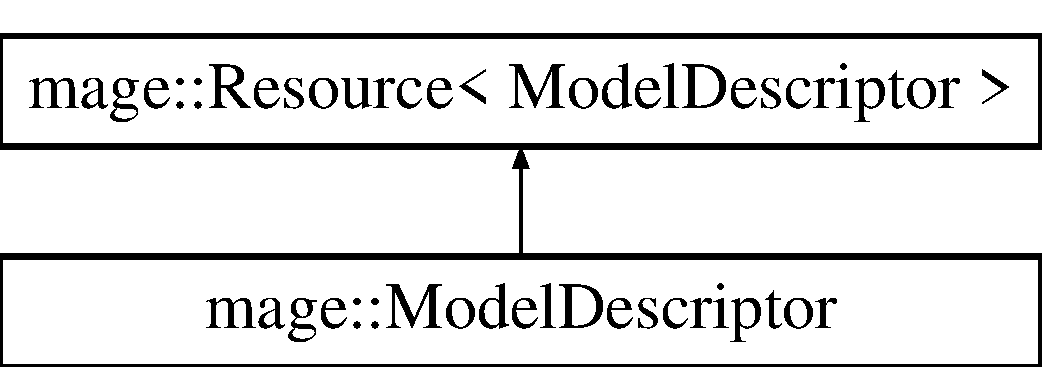
\includegraphics[height=3.000000cm]{classmage_1_1_model_descriptor}
\end{center}
\end{figure}
\subsection*{Public Member Functions}
\begin{DoxyCompactItemize}
\item 
{\footnotesize template$<$typename VertexT $>$ }\\\hyperlink{classmage_1_1_model_descriptor_a1ae1d85907be96350cef77e6a4ba4fb9}{Model\+Descriptor} (I\+D3\+D11\+Device2 $\ast$device, I\+D3\+D11\+Device\+Context2 $\ast$device\+\_\+context, const wstring \&fname, const \hyperlink{structmage_1_1_mesh_descriptor}{Mesh\+Descriptor}$<$ VertexT $>$ \&desc=\hyperlink{structmage_1_1_mesh_descriptor}{Mesh\+Descriptor}$<$ VertexT $>$())
\item 
\hyperlink{classmage_1_1_model_descriptor_af44185efc20e10ede762d29bc454c5f3}{Model\+Descriptor} (const \hyperlink{classmage_1_1_model_descriptor}{Model\+Descriptor} \&desc)=delete
\item 
\hyperlink{classmage_1_1_model_descriptor_af5ece586e2a8404cc29e703885531e72}{Model\+Descriptor} (\hyperlink{classmage_1_1_model_descriptor}{Model\+Descriptor} \&\&desc)
\item 
virtual \hyperlink{classmage_1_1_model_descriptor_aae13cf050ee7f9283d91282c04f62df1}{$\sim$\+Model\+Descriptor} ()
\item 
\hyperlink{classmage_1_1_model_descriptor}{Model\+Descriptor} \& \hyperlink{classmage_1_1_model_descriptor_a734b17224719896921e9f6252ee88483}{operator=} (const \hyperlink{classmage_1_1_model_descriptor}{Model\+Descriptor} \&desc)=delete
\item 
\hyperlink{classmage_1_1_model_descriptor}{Model\+Descriptor} \& \hyperlink{classmage_1_1_model_descriptor_ae2ae685569c0ae534d9f0b5622a807d0}{operator=} (\hyperlink{classmage_1_1_model_descriptor}{Model\+Descriptor} \&\&desc)=delete
\item 
\hyperlink{namespacemage_a1e01ae66713838a7a67d30e44c67703e}{Shared\+Ptr}$<$ const \hyperlink{classmage_1_1_static_mesh}{Static\+Mesh} $>$ \hyperlink{classmage_1_1_model_descriptor_aad2a0d8ca726eec787834d24e6192f0c}{Get\+Mesh} () const noexcept
\item 
const \hyperlink{structmage_1_1_material}{Material} $\ast$ \hyperlink{classmage_1_1_model_descriptor_adc013e6b054c7efa0d92a3ad1ff37e61}{Get\+Material} (const string \&name) const noexcept
\item 
{\footnotesize template$<$typename ActionT $>$ }\\void \hyperlink{classmage_1_1_model_descriptor_ac4723e18238b0d6ac3c54168b8e9a09f}{For\+Each\+Material} (ActionT action) const
\item 
const \hyperlink{structmage_1_1_model_part}{Model\+Part} $\ast$ \hyperlink{classmage_1_1_model_descriptor_a9c8e98d71883edd33b9d6c1964e7bf36}{Get\+Model\+Part} (const string \&name) const noexcept
\item 
{\footnotesize template$<$typename ActionT $>$ }\\void \hyperlink{classmage_1_1_model_descriptor_a1d61699788385cf29726fac0067bcb5c}{For\+Each\+Model\+Part} (ActionT action) const
\end{DoxyCompactItemize}
\subsection*{Private Attributes}
\begin{DoxyCompactItemize}
\item 
\hyperlink{namespacemage_a1e01ae66713838a7a67d30e44c67703e}{Shared\+Ptr}$<$ \hyperlink{classmage_1_1_static_mesh}{Static\+Mesh} $>$ \hyperlink{classmage_1_1_model_descriptor_ac3935d5b0738860809a770403ed07480}{m\+\_\+mesh}
\item 
vector$<$ \hyperlink{structmage_1_1_material}{Material} $>$ \hyperlink{classmage_1_1_model_descriptor_a672238b257f99836243d84f634ffeea2}{m\+\_\+materials}
\item 
vector$<$ \hyperlink{structmage_1_1_model_part}{Model\+Part} $>$ \hyperlink{classmage_1_1_model_descriptor_a200c6e44c9b6a5bde5c8490fb93ba00f}{m\+\_\+model\+\_\+parts}
\end{DoxyCompactItemize}


\subsection{Detailed Description}
A class of model descriptors describing a complete model. 

\subsection{Constructor \& Destructor Documentation}
\hypertarget{classmage_1_1_model_descriptor_a1ae1d85907be96350cef77e6a4ba4fb9}{}\label{classmage_1_1_model_descriptor_a1ae1d85907be96350cef77e6a4ba4fb9} 
\index{mage\+::\+Model\+Descriptor@{mage\+::\+Model\+Descriptor}!Model\+Descriptor@{Model\+Descriptor}}
\index{Model\+Descriptor@{Model\+Descriptor}!mage\+::\+Model\+Descriptor@{mage\+::\+Model\+Descriptor}}
\subsubsection{\texorpdfstring{Model\+Descriptor()}{ModelDescriptor()}\hspace{0.1cm}{\footnotesize\ttfamily [1/3]}}
{\footnotesize\ttfamily template$<$typename VertexT $>$ \\
mage\+::\+Model\+Descriptor\+::\+Model\+Descriptor (\begin{DoxyParamCaption}\item[{I\+D3\+D11\+Device2 $\ast$}]{device,  }\item[{I\+D3\+D11\+Device\+Context2 $\ast$}]{device\+\_\+context,  }\item[{const wstring \&}]{fname,  }\item[{const \hyperlink{structmage_1_1_mesh_descriptor}{Mesh\+Descriptor}$<$ VertexT $>$ \&}]{desc = {\ttfamily \hyperlink{structmage_1_1_mesh_descriptor}{Mesh\+Descriptor}$<$~VertexT~$>$()} }\end{DoxyParamCaption})\hspace{0.3cm}{\ttfamily [explicit]}}

Constructs a model descriptor.

\begin{DoxyPrecond}{Precondition}
{\itshape device} is not equal to {\ttfamily nullptr}. 

{\itshape device\+\_\+context} is not equal to {\ttfamily nullptr}. 
\end{DoxyPrecond}

\begin{DoxyTemplParams}{Template Parameters}
{\em VertexT} & The vertex type. \\
\hline
\end{DoxyTemplParams}

\begin{DoxyParams}[1]{Parameters}
\mbox{\tt in}  & {\em device} & A pointer to the device. \\
\hline
\mbox{\tt in}  & {\em device\+\_\+context} & A pointer to the device context. \\
\hline
\mbox{\tt in}  & {\em fname} & A reference to the filename. \\
\hline
\mbox{\tt in}  & {\em desc} & A reference to the mesh descriptor. \\
\hline
\end{DoxyParams}

\begin{DoxyExceptions}{Exceptions}
{\em \hyperlink{structmage_1_1_formatted_exception}{Formatted\+Exception}} & Failed to initialize the model descriptor. \\
\hline
\end{DoxyExceptions}
\hypertarget{classmage_1_1_model_descriptor_af44185efc20e10ede762d29bc454c5f3}{}\label{classmage_1_1_model_descriptor_af44185efc20e10ede762d29bc454c5f3} 
\index{mage\+::\+Model\+Descriptor@{mage\+::\+Model\+Descriptor}!Model\+Descriptor@{Model\+Descriptor}}
\index{Model\+Descriptor@{Model\+Descriptor}!mage\+::\+Model\+Descriptor@{mage\+::\+Model\+Descriptor}}
\subsubsection{\texorpdfstring{Model\+Descriptor()}{ModelDescriptor()}\hspace{0.1cm}{\footnotesize\ttfamily [2/3]}}
{\footnotesize\ttfamily mage\+::\+Model\+Descriptor\+::\+Model\+Descriptor (\begin{DoxyParamCaption}\item[{const \hyperlink{classmage_1_1_model_descriptor}{Model\+Descriptor} \&}]{desc }\end{DoxyParamCaption})\hspace{0.3cm}{\ttfamily [delete]}}

Constructs a model descriptor from the given model descriptor.


\begin{DoxyParams}[1]{Parameters}
\mbox{\tt in}  & {\em desc} & A reference to the model descriptor to copy. \\
\hline
\end{DoxyParams}
\hypertarget{classmage_1_1_model_descriptor_af5ece586e2a8404cc29e703885531e72}{}\label{classmage_1_1_model_descriptor_af5ece586e2a8404cc29e703885531e72} 
\index{mage\+::\+Model\+Descriptor@{mage\+::\+Model\+Descriptor}!Model\+Descriptor@{Model\+Descriptor}}
\index{Model\+Descriptor@{Model\+Descriptor}!mage\+::\+Model\+Descriptor@{mage\+::\+Model\+Descriptor}}
\subsubsection{\texorpdfstring{Model\+Descriptor()}{ModelDescriptor()}\hspace{0.1cm}{\footnotesize\ttfamily [3/3]}}
{\footnotesize\ttfamily mage\+::\+Model\+Descriptor\+::\+Model\+Descriptor (\begin{DoxyParamCaption}\item[{\hyperlink{classmage_1_1_model_descriptor}{Model\+Descriptor} \&\&}]{desc }\end{DoxyParamCaption})\hspace{0.3cm}{\ttfamily [default]}}

Constructs a model descriptor by moving the given model descriptor.


\begin{DoxyParams}[1]{Parameters}
\mbox{\tt in}  & {\em desc} & A reference to the model descriptor to move. \\
\hline
\end{DoxyParams}
\hypertarget{classmage_1_1_model_descriptor_aae13cf050ee7f9283d91282c04f62df1}{}\label{classmage_1_1_model_descriptor_aae13cf050ee7f9283d91282c04f62df1} 
\index{mage\+::\+Model\+Descriptor@{mage\+::\+Model\+Descriptor}!````~Model\+Descriptor@{$\sim$\+Model\+Descriptor}}
\index{````~Model\+Descriptor@{$\sim$\+Model\+Descriptor}!mage\+::\+Model\+Descriptor@{mage\+::\+Model\+Descriptor}}
\subsubsection{\texorpdfstring{$\sim$\+Model\+Descriptor()}{~ModelDescriptor()}}
{\footnotesize\ttfamily mage\+::\+Model\+Descriptor\+::$\sim$\+Model\+Descriptor (\begin{DoxyParamCaption}{ }\end{DoxyParamCaption})\hspace{0.3cm}{\ttfamily [virtual]}}

Destructs a model descriptor. 

\subsection{Member Function Documentation}
\hypertarget{classmage_1_1_model_descriptor_ac4723e18238b0d6ac3c54168b8e9a09f}{}\label{classmage_1_1_model_descriptor_ac4723e18238b0d6ac3c54168b8e9a09f} 
\index{mage\+::\+Model\+Descriptor@{mage\+::\+Model\+Descriptor}!For\+Each\+Material@{For\+Each\+Material}}
\index{For\+Each\+Material@{For\+Each\+Material}!mage\+::\+Model\+Descriptor@{mage\+::\+Model\+Descriptor}}
\subsubsection{\texorpdfstring{For\+Each\+Material()}{ForEachMaterial()}}
{\footnotesize\ttfamily template$<$typename ActionT $>$ \\
void mage\+::\+Model\+Descriptor\+::\+For\+Each\+Material (\begin{DoxyParamCaption}\item[{ActionT}]{action }\end{DoxyParamCaption}) const}

Traverses all materials of this model descriptor.


\begin{DoxyTemplParams}{Template Parameters}
{\em ActionT} & An action to perform on all materials of this model descriptor. The action must accept {\ttfamily const} {\ttfamily \hyperlink{structmage_1_1_material}{Material}\&} values. \\
\hline
\end{DoxyTemplParams}
\hypertarget{classmage_1_1_model_descriptor_a1d61699788385cf29726fac0067bcb5c}{}\label{classmage_1_1_model_descriptor_a1d61699788385cf29726fac0067bcb5c} 
\index{mage\+::\+Model\+Descriptor@{mage\+::\+Model\+Descriptor}!For\+Each\+Model\+Part@{For\+Each\+Model\+Part}}
\index{For\+Each\+Model\+Part@{For\+Each\+Model\+Part}!mage\+::\+Model\+Descriptor@{mage\+::\+Model\+Descriptor}}
\subsubsection{\texorpdfstring{For\+Each\+Model\+Part()}{ForEachModelPart()}}
{\footnotesize\ttfamily template$<$typename ActionT $>$ \\
void mage\+::\+Model\+Descriptor\+::\+For\+Each\+Model\+Part (\begin{DoxyParamCaption}\item[{ActionT}]{action }\end{DoxyParamCaption}) const}

Traverses all model parts of this model descriptor.


\begin{DoxyTemplParams}{Template Parameters}
{\em ActionT} & An action to perform on all model parts of this model descriptor. The action must accept {\ttfamily const} {\ttfamily \hyperlink{structmage_1_1_model_part}{Model\+Part}\&} values. \\
\hline
\end{DoxyTemplParams}
\hypertarget{classmage_1_1_model_descriptor_adc013e6b054c7efa0d92a3ad1ff37e61}{}\label{classmage_1_1_model_descriptor_adc013e6b054c7efa0d92a3ad1ff37e61} 
\index{mage\+::\+Model\+Descriptor@{mage\+::\+Model\+Descriptor}!Get\+Material@{Get\+Material}}
\index{Get\+Material@{Get\+Material}!mage\+::\+Model\+Descriptor@{mage\+::\+Model\+Descriptor}}
\subsubsection{\texorpdfstring{Get\+Material()}{GetMaterial()}}
{\footnotesize\ttfamily const \hyperlink{structmage_1_1_material}{Material} $\ast$ mage\+::\+Model\+Descriptor\+::\+Get\+Material (\begin{DoxyParamCaption}\item[{const string \&}]{name }\end{DoxyParamCaption}) const\hspace{0.3cm}{\ttfamily [noexcept]}}

Returns the material corresponding to the given name.


\begin{DoxyParams}[1]{Parameters}
\mbox{\tt in}  & {\em name} & A reference to the name of the material. \\
\hline
\end{DoxyParams}
\begin{DoxyReturn}{Returns}
{\ttfamily nullptr} if this model descriptor contains no material matching the given name {\itshape name}. 

A pointer to the material of this model descriptor matching the given name {\itshape name}. 
\end{DoxyReturn}
\hypertarget{classmage_1_1_model_descriptor_aad2a0d8ca726eec787834d24e6192f0c}{}\label{classmage_1_1_model_descriptor_aad2a0d8ca726eec787834d24e6192f0c} 
\index{mage\+::\+Model\+Descriptor@{mage\+::\+Model\+Descriptor}!Get\+Mesh@{Get\+Mesh}}
\index{Get\+Mesh@{Get\+Mesh}!mage\+::\+Model\+Descriptor@{mage\+::\+Model\+Descriptor}}
\subsubsection{\texorpdfstring{Get\+Mesh()}{GetMesh()}}
{\footnotesize\ttfamily \hyperlink{namespacemage_a1e01ae66713838a7a67d30e44c67703e}{Shared\+Ptr}$<$ const \hyperlink{classmage_1_1_static_mesh}{Static\+Mesh} $>$ mage\+::\+Model\+Descriptor\+::\+Get\+Mesh (\begin{DoxyParamCaption}{ }\end{DoxyParamCaption}) const\hspace{0.3cm}{\ttfamily [noexcept]}}

Returns the mesh of this model descriptor.

\begin{DoxyReturn}{Returns}
A pointer to the mesh of this model descriptor. 
\end{DoxyReturn}
\hypertarget{classmage_1_1_model_descriptor_a9c8e98d71883edd33b9d6c1964e7bf36}{}\label{classmage_1_1_model_descriptor_a9c8e98d71883edd33b9d6c1964e7bf36} 
\index{mage\+::\+Model\+Descriptor@{mage\+::\+Model\+Descriptor}!Get\+Model\+Part@{Get\+Model\+Part}}
\index{Get\+Model\+Part@{Get\+Model\+Part}!mage\+::\+Model\+Descriptor@{mage\+::\+Model\+Descriptor}}
\subsubsection{\texorpdfstring{Get\+Model\+Part()}{GetModelPart()}}
{\footnotesize\ttfamily const \hyperlink{structmage_1_1_model_part}{Model\+Part} $\ast$ mage\+::\+Model\+Descriptor\+::\+Get\+Model\+Part (\begin{DoxyParamCaption}\item[{const string \&}]{name }\end{DoxyParamCaption}) const\hspace{0.3cm}{\ttfamily [noexcept]}}

Returns the model part corresponding to the given name.


\begin{DoxyParams}[1]{Parameters}
\mbox{\tt in}  & {\em name} & A reference to the name of the model part. \\
\hline
\end{DoxyParams}
\begin{DoxyReturn}{Returns}
{\ttfamily nullptr} if this model descriptor contains no model part matching the given name {\itshape name}. 

A pointer to the model part of this model descriptor matching the given name {\itshape name}. 
\end{DoxyReturn}
\hypertarget{classmage_1_1_model_descriptor_a734b17224719896921e9f6252ee88483}{}\label{classmage_1_1_model_descriptor_a734b17224719896921e9f6252ee88483} 
\index{mage\+::\+Model\+Descriptor@{mage\+::\+Model\+Descriptor}!operator=@{operator=}}
\index{operator=@{operator=}!mage\+::\+Model\+Descriptor@{mage\+::\+Model\+Descriptor}}
\subsubsection{\texorpdfstring{operator=()}{operator=()}\hspace{0.1cm}{\footnotesize\ttfamily [1/2]}}
{\footnotesize\ttfamily \hyperlink{classmage_1_1_model_descriptor}{Model\+Descriptor}\& mage\+::\+Model\+Descriptor\+::operator= (\begin{DoxyParamCaption}\item[{const \hyperlink{classmage_1_1_model_descriptor}{Model\+Descriptor} \&}]{desc }\end{DoxyParamCaption})\hspace{0.3cm}{\ttfamily [delete]}}

Copies the given model descriptor to this model descriptor.


\begin{DoxyParams}[1]{Parameters}
\mbox{\tt in}  & {\em desc} & A reference to the model descriptor to copy. \\
\hline
\end{DoxyParams}
\hypertarget{classmage_1_1_model_descriptor_ae2ae685569c0ae534d9f0b5622a807d0}{}\label{classmage_1_1_model_descriptor_ae2ae685569c0ae534d9f0b5622a807d0} 
\index{mage\+::\+Model\+Descriptor@{mage\+::\+Model\+Descriptor}!operator=@{operator=}}
\index{operator=@{operator=}!mage\+::\+Model\+Descriptor@{mage\+::\+Model\+Descriptor}}
\subsubsection{\texorpdfstring{operator=()}{operator=()}\hspace{0.1cm}{\footnotesize\ttfamily [2/2]}}
{\footnotesize\ttfamily \hyperlink{classmage_1_1_model_descriptor}{Model\+Descriptor}\& mage\+::\+Model\+Descriptor\+::operator= (\begin{DoxyParamCaption}\item[{\hyperlink{classmage_1_1_model_descriptor}{Model\+Descriptor} \&\&}]{desc }\end{DoxyParamCaption})\hspace{0.3cm}{\ttfamily [delete]}}

Moves the given model descriptor to this model descriptor.


\begin{DoxyParams}[1]{Parameters}
\mbox{\tt in}  & {\em desc} & A reference to the model descriptor to move. \\
\hline
\end{DoxyParams}


\subsection{Member Data Documentation}
\hypertarget{classmage_1_1_model_descriptor_a672238b257f99836243d84f634ffeea2}{}\label{classmage_1_1_model_descriptor_a672238b257f99836243d84f634ffeea2} 
\index{mage\+::\+Model\+Descriptor@{mage\+::\+Model\+Descriptor}!m\+\_\+materials@{m\+\_\+materials}}
\index{m\+\_\+materials@{m\+\_\+materials}!mage\+::\+Model\+Descriptor@{mage\+::\+Model\+Descriptor}}
\subsubsection{\texorpdfstring{m\+\_\+materials}{m\_materials}}
{\footnotesize\ttfamily vector$<$ \hyperlink{structmage_1_1_material}{Material} $>$ mage\+::\+Model\+Descriptor\+::m\+\_\+materials\hspace{0.3cm}{\ttfamily [private]}}

A vector containing all the materials of the model of this model descriptor. \hypertarget{classmage_1_1_model_descriptor_ac3935d5b0738860809a770403ed07480}{}\label{classmage_1_1_model_descriptor_ac3935d5b0738860809a770403ed07480} 
\index{mage\+::\+Model\+Descriptor@{mage\+::\+Model\+Descriptor}!m\+\_\+mesh@{m\+\_\+mesh}}
\index{m\+\_\+mesh@{m\+\_\+mesh}!mage\+::\+Model\+Descriptor@{mage\+::\+Model\+Descriptor}}
\subsubsection{\texorpdfstring{m\+\_\+mesh}{m\_mesh}}
{\footnotesize\ttfamily \hyperlink{namespacemage_a1e01ae66713838a7a67d30e44c67703e}{Shared\+Ptr}$<$ \hyperlink{classmage_1_1_static_mesh}{Static\+Mesh} $>$ mage\+::\+Model\+Descriptor\+::m\+\_\+mesh\hspace{0.3cm}{\ttfamily [private]}}

A pointer to the mesh of the model of this model descriptor. \hypertarget{classmage_1_1_model_descriptor_a200c6e44c9b6a5bde5c8490fb93ba00f}{}\label{classmage_1_1_model_descriptor_a200c6e44c9b6a5bde5c8490fb93ba00f} 
\index{mage\+::\+Model\+Descriptor@{mage\+::\+Model\+Descriptor}!m\+\_\+model\+\_\+parts@{m\+\_\+model\+\_\+parts}}
\index{m\+\_\+model\+\_\+parts@{m\+\_\+model\+\_\+parts}!mage\+::\+Model\+Descriptor@{mage\+::\+Model\+Descriptor}}
\subsubsection{\texorpdfstring{m\+\_\+model\+\_\+parts}{m\_model\_parts}}
{\footnotesize\ttfamily vector$<$ \hyperlink{structmage_1_1_model_part}{Model\+Part} $>$ mage\+::\+Model\+Descriptor\+::m\+\_\+model\+\_\+parts\hspace{0.3cm}{\ttfamily [private]}}

A vector containing all the model parts of the model of this model descriptor. 
\hypertarget{classmage_1_1_model_node}{}\section{mage\+:\+:Model\+Node Class Reference}
\label{classmage_1_1_model_node}\index{mage\+::\+Model\+Node@{mage\+::\+Model\+Node}}


{\ttfamily \#include $<$model\+\_\+node.\+hpp$>$}

Inheritance diagram for mage\+:\+:Model\+Node\+:\begin{figure}[H]
\begin{center}
\leavevmode
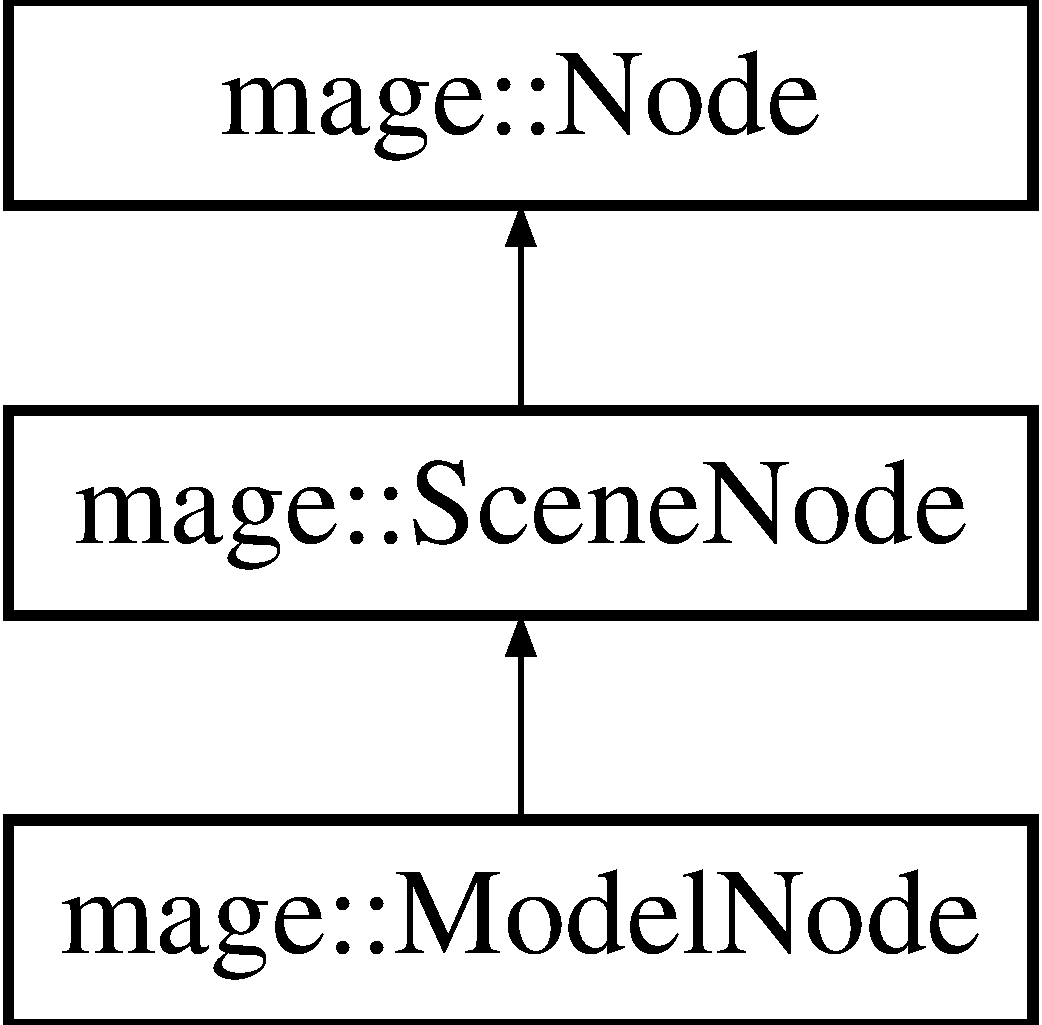
\includegraphics[height=3.000000cm]{classmage_1_1_model_node}
\end{center}
\end{figure}
\subsection*{Public Member Functions}
\begin{DoxyCompactItemize}
\item 
\hyperlink{classmage_1_1_model_node_a15d6a41cc5cdc90310313147100c1d6f}{Model\+Node} (const string \&name, \hyperlink{namespacemage_a8c307fbcc33bce9b7f2aa4c26c3b95cf}{Unique\+Ptr}$<$ \hyperlink{classmage_1_1_model}{Model} $>$ \&\&model)
\item 
\hyperlink{classmage_1_1_model_node_a409c098ddecf20d1b393d43c15d16482}{Model\+Node} (const \hyperlink{classmage_1_1_model_node}{Model\+Node} \&model\+\_\+node)
\item 
\hyperlink{classmage_1_1_model_node_a19ba577112ea488f227ea31642fb2cb2}{Model\+Node} (\hyperlink{classmage_1_1_model_node}{Model\+Node} \&\&model\+\_\+node)
\item 
virtual \hyperlink{classmage_1_1_model_node_a131c0062a1bed3d29fade27e602bec44}{$\sim$\+Model\+Node} ()
\item 
\hyperlink{classmage_1_1_model_node}{Model\+Node} \& \hyperlink{classmage_1_1_model_node_ad8378279b79930dfe98d176dbc1c5db9}{operator=} (const \hyperlink{classmage_1_1_model_node}{Model\+Node} \&model\+\_\+node)=delete
\item 
\hyperlink{classmage_1_1_model_node}{Model\+Node} \& \hyperlink{classmage_1_1_model_node_ad39321f4d392aa4e28169b8d7a08af68}{operator=} (\hyperlink{classmage_1_1_model_node}{Model\+Node} \&\&model\+\_\+node)=delete
\item 
\hyperlink{namespacemage_a8c307fbcc33bce9b7f2aa4c26c3b95cf}{Unique\+Ptr}$<$ \hyperlink{classmage_1_1_model_node}{Model\+Node} $>$ \hyperlink{classmage_1_1_model_node_a766f90e1d626c455ba552a3ded08b948}{Clone} () const
\item 
\hyperlink{classmage_1_1_model}{Model} $\ast$ \hyperlink{classmage_1_1_model_node_a358f3458d4444ea026467505eac0b675}{Get\+Model} ()
\item 
const \hyperlink{classmage_1_1_model}{Model} $\ast$ \hyperlink{classmage_1_1_model_node_a721b88e6649758b2258c95e972478249}{Get\+Model} () const
\end{DoxyCompactItemize}
\subsection*{Private Member Functions}
\begin{DoxyCompactItemize}
\item 
virtual \hyperlink{namespacemage_a8c307fbcc33bce9b7f2aa4c26c3b95cf}{Unique\+Ptr}$<$ \hyperlink{classmage_1_1_node}{Node} $>$ \hyperlink{classmage_1_1_model_node_a34146201083015276b38240af307417f}{Clone\+Implementation} () const override
\end{DoxyCompactItemize}
\subsection*{Private Attributes}
\begin{DoxyCompactItemize}
\item 
\hyperlink{namespacemage_a8c307fbcc33bce9b7f2aa4c26c3b95cf}{Unique\+Ptr}$<$ \hyperlink{classmage_1_1_model}{Model} $>$ \hyperlink{classmage_1_1_model_node_a784faf19f736a1c74808321ed0e52d36}{m\+\_\+model}
\end{DoxyCompactItemize}


\subsection{Constructor \& Destructor Documentation}
\hypertarget{classmage_1_1_model_node_a15d6a41cc5cdc90310313147100c1d6f}{}\label{classmage_1_1_model_node_a15d6a41cc5cdc90310313147100c1d6f} 
\index{mage\+::\+Model\+Node@{mage\+::\+Model\+Node}!Model\+Node@{Model\+Node}}
\index{Model\+Node@{Model\+Node}!mage\+::\+Model\+Node@{mage\+::\+Model\+Node}}
\subsubsection{\texorpdfstring{Model\+Node()}{ModelNode()}\hspace{0.1cm}{\footnotesize\ttfamily [1/3]}}
{\footnotesize\ttfamily mage\+::\+Model\+Node\+::\+Model\+Node (\begin{DoxyParamCaption}\item[{const string \&}]{name,  }\item[{\hyperlink{namespacemage_a8c307fbcc33bce9b7f2aa4c26c3b95cf}{Unique\+Ptr}$<$ \hyperlink{classmage_1_1_model}{Model} $>$ \&\&}]{model }\end{DoxyParamCaption})\hspace{0.3cm}{\ttfamily [explicit]}}

\hypertarget{classmage_1_1_model_node_a409c098ddecf20d1b393d43c15d16482}{}\label{classmage_1_1_model_node_a409c098ddecf20d1b393d43c15d16482} 
\index{mage\+::\+Model\+Node@{mage\+::\+Model\+Node}!Model\+Node@{Model\+Node}}
\index{Model\+Node@{Model\+Node}!mage\+::\+Model\+Node@{mage\+::\+Model\+Node}}
\subsubsection{\texorpdfstring{Model\+Node()}{ModelNode()}\hspace{0.1cm}{\footnotesize\ttfamily [2/3]}}
{\footnotesize\ttfamily mage\+::\+Model\+Node\+::\+Model\+Node (\begin{DoxyParamCaption}\item[{const \hyperlink{classmage_1_1_model_node}{Model\+Node} \&}]{model\+\_\+node }\end{DoxyParamCaption})}

\hypertarget{classmage_1_1_model_node_a19ba577112ea488f227ea31642fb2cb2}{}\label{classmage_1_1_model_node_a19ba577112ea488f227ea31642fb2cb2} 
\index{mage\+::\+Model\+Node@{mage\+::\+Model\+Node}!Model\+Node@{Model\+Node}}
\index{Model\+Node@{Model\+Node}!mage\+::\+Model\+Node@{mage\+::\+Model\+Node}}
\subsubsection{\texorpdfstring{Model\+Node()}{ModelNode()}\hspace{0.1cm}{\footnotesize\ttfamily [3/3]}}
{\footnotesize\ttfamily mage\+::\+Model\+Node\+::\+Model\+Node (\begin{DoxyParamCaption}\item[{\hyperlink{classmage_1_1_model_node}{Model\+Node} \&\&}]{model\+\_\+node }\end{DoxyParamCaption})\hspace{0.3cm}{\ttfamily [default]}}

\hypertarget{classmage_1_1_model_node_a131c0062a1bed3d29fade27e602bec44}{}\label{classmage_1_1_model_node_a131c0062a1bed3d29fade27e602bec44} 
\index{mage\+::\+Model\+Node@{mage\+::\+Model\+Node}!````~Model\+Node@{$\sim$\+Model\+Node}}
\index{````~Model\+Node@{$\sim$\+Model\+Node}!mage\+::\+Model\+Node@{mage\+::\+Model\+Node}}
\subsubsection{\texorpdfstring{$\sim$\+Model\+Node()}{~ModelNode()}}
{\footnotesize\ttfamily mage\+::\+Model\+Node\+::$\sim$\+Model\+Node (\begin{DoxyParamCaption}{ }\end{DoxyParamCaption})\hspace{0.3cm}{\ttfamily [virtual]}, {\ttfamily [default]}}



\subsection{Member Function Documentation}
\hypertarget{classmage_1_1_model_node_a766f90e1d626c455ba552a3ded08b948}{}\label{classmage_1_1_model_node_a766f90e1d626c455ba552a3ded08b948} 
\index{mage\+::\+Model\+Node@{mage\+::\+Model\+Node}!Clone@{Clone}}
\index{Clone@{Clone}!mage\+::\+Model\+Node@{mage\+::\+Model\+Node}}
\subsubsection{\texorpdfstring{Clone()}{Clone()}}
{\footnotesize\ttfamily \hyperlink{namespacemage_a8c307fbcc33bce9b7f2aa4c26c3b95cf}{Unique\+Ptr}$<$ \hyperlink{classmage_1_1_model_node}{Model\+Node} $>$ mage\+::\+Model\+Node\+::\+Clone (\begin{DoxyParamCaption}{ }\end{DoxyParamCaption}) const}

\hypertarget{classmage_1_1_model_node_a34146201083015276b38240af307417f}{}\label{classmage_1_1_model_node_a34146201083015276b38240af307417f} 
\index{mage\+::\+Model\+Node@{mage\+::\+Model\+Node}!Clone\+Implementation@{Clone\+Implementation}}
\index{Clone\+Implementation@{Clone\+Implementation}!mage\+::\+Model\+Node@{mage\+::\+Model\+Node}}
\subsubsection{\texorpdfstring{Clone\+Implementation()}{CloneImplementation()}}
{\footnotesize\ttfamily \hyperlink{namespacemage_a8c307fbcc33bce9b7f2aa4c26c3b95cf}{Unique\+Ptr}$<$ \hyperlink{classmage_1_1_node}{Node} $>$ mage\+::\+Model\+Node\+::\+Clone\+Implementation (\begin{DoxyParamCaption}{ }\end{DoxyParamCaption}) const\hspace{0.3cm}{\ttfamily [override]}, {\ttfamily [private]}, {\ttfamily [virtual]}}

Clones this node.

\begin{DoxyReturn}{Returns}
A pointer to the clone of this node. 
\end{DoxyReturn}


Reimplemented from \hyperlink{classmage_1_1_scene_node_a42d0d53ab804d38ebd584d2de6490eeb}{mage\+::\+Scene\+Node}.

\hypertarget{classmage_1_1_model_node_a358f3458d4444ea026467505eac0b675}{}\label{classmage_1_1_model_node_a358f3458d4444ea026467505eac0b675} 
\index{mage\+::\+Model\+Node@{mage\+::\+Model\+Node}!Get\+Model@{Get\+Model}}
\index{Get\+Model@{Get\+Model}!mage\+::\+Model\+Node@{mage\+::\+Model\+Node}}
\subsubsection{\texorpdfstring{Get\+Model()}{GetModel()}\hspace{0.1cm}{\footnotesize\ttfamily [1/2]}}
{\footnotesize\ttfamily \hyperlink{classmage_1_1_model}{Model}$\ast$ mage\+::\+Model\+Node\+::\+Get\+Model (\begin{DoxyParamCaption}{ }\end{DoxyParamCaption})}

\hypertarget{classmage_1_1_model_node_a721b88e6649758b2258c95e972478249}{}\label{classmage_1_1_model_node_a721b88e6649758b2258c95e972478249} 
\index{mage\+::\+Model\+Node@{mage\+::\+Model\+Node}!Get\+Model@{Get\+Model}}
\index{Get\+Model@{Get\+Model}!mage\+::\+Model\+Node@{mage\+::\+Model\+Node}}
\subsubsection{\texorpdfstring{Get\+Model()}{GetModel()}\hspace{0.1cm}{\footnotesize\ttfamily [2/2]}}
{\footnotesize\ttfamily const \hyperlink{classmage_1_1_model}{Model}$\ast$ mage\+::\+Model\+Node\+::\+Get\+Model (\begin{DoxyParamCaption}{ }\end{DoxyParamCaption}) const}

\hypertarget{classmage_1_1_model_node_ad8378279b79930dfe98d176dbc1c5db9}{}\label{classmage_1_1_model_node_ad8378279b79930dfe98d176dbc1c5db9} 
\index{mage\+::\+Model\+Node@{mage\+::\+Model\+Node}!operator=@{operator=}}
\index{operator=@{operator=}!mage\+::\+Model\+Node@{mage\+::\+Model\+Node}}
\subsubsection{\texorpdfstring{operator=()}{operator=()}\hspace{0.1cm}{\footnotesize\ttfamily [1/2]}}
{\footnotesize\ttfamily \hyperlink{classmage_1_1_model_node}{Model\+Node}\& mage\+::\+Model\+Node\+::operator= (\begin{DoxyParamCaption}\item[{const \hyperlink{classmage_1_1_model_node}{Model\+Node} \&}]{model\+\_\+node }\end{DoxyParamCaption})\hspace{0.3cm}{\ttfamily [delete]}}

\hypertarget{classmage_1_1_model_node_ad39321f4d392aa4e28169b8d7a08af68}{}\label{classmage_1_1_model_node_ad39321f4d392aa4e28169b8d7a08af68} 
\index{mage\+::\+Model\+Node@{mage\+::\+Model\+Node}!operator=@{operator=}}
\index{operator=@{operator=}!mage\+::\+Model\+Node@{mage\+::\+Model\+Node}}
\subsubsection{\texorpdfstring{operator=()}{operator=()}\hspace{0.1cm}{\footnotesize\ttfamily [2/2]}}
{\footnotesize\ttfamily \hyperlink{classmage_1_1_model_node}{Model\+Node}\& mage\+::\+Model\+Node\+::operator= (\begin{DoxyParamCaption}\item[{\hyperlink{classmage_1_1_model_node}{Model\+Node} \&\&}]{model\+\_\+node }\end{DoxyParamCaption})\hspace{0.3cm}{\ttfamily [delete]}}



\subsection{Member Data Documentation}
\hypertarget{classmage_1_1_model_node_a784faf19f736a1c74808321ed0e52d36}{}\label{classmage_1_1_model_node_a784faf19f736a1c74808321ed0e52d36} 
\index{mage\+::\+Model\+Node@{mage\+::\+Model\+Node}!m\+\_\+model@{m\+\_\+model}}
\index{m\+\_\+model@{m\+\_\+model}!mage\+::\+Model\+Node@{mage\+::\+Model\+Node}}
\subsubsection{\texorpdfstring{m\+\_\+model}{m\_model}}
{\footnotesize\ttfamily \hyperlink{namespacemage_a8c307fbcc33bce9b7f2aa4c26c3b95cf}{Unique\+Ptr}$<$ \hyperlink{classmage_1_1_model}{Model} $>$ mage\+::\+Model\+Node\+::m\+\_\+model\hspace{0.3cm}{\ttfamily [private]}}


\hypertarget{structmage_1_1_model_output}{}\section{mage\+:\+:Model\+Output$<$ VertexT $>$ Struct Template Reference}
\label{structmage_1_1_model_output}\index{mage\+::\+Model\+Output$<$ Vertex\+T $>$@{mage\+::\+Model\+Output$<$ Vertex\+T $>$}}


{\ttfamily \#include $<$model\+\_\+output.\+hpp$>$}

\subsection*{Public Member Functions}
\begin{DoxyCompactItemize}
\item 
\hyperlink{structmage_1_1_model_output_a7d64b57d8207968541eb9c6da6ef0163}{Model\+Output} ()=default
\item 
\hyperlink{structmage_1_1_model_output_aac808e40a66f33da4ea28ebb7443623d}{Model\+Output} (const \hyperlink{structmage_1_1_model_output}{Model\+Output}$<$ VertexT $>$ \&output)=delete
\item 
\hyperlink{structmage_1_1_model_output_a20faa6e5b76ec7903a09e222e61e5353}{Model\+Output} (\hyperlink{structmage_1_1_model_output}{Model\+Output}$<$ VertexT $>$ \&\&output)=default
\item 
\hyperlink{structmage_1_1_model_output_a69a7f27486ad287943cbf973107ad8e1}{$\sim$\+Model\+Output} ()=default
\item 
\hyperlink{structmage_1_1_model_output}{Model\+Output}$<$ VertexT $>$ \& \hyperlink{structmage_1_1_model_output_ada52bf380c0259a0d7ef855457e5a9da}{operator=} (const \hyperlink{structmage_1_1_model_output}{Model\+Output}$<$ VertexT $>$ \&output)=delete
\item 
\hyperlink{structmage_1_1_model_output}{Model\+Output}$<$ VertexT $>$ \& \hyperlink{structmage_1_1_model_output_a5e368e3ae8a52d329f8d9b5f1c4b9d03}{operator=} (\hyperlink{structmage_1_1_model_output}{Model\+Output}$<$ VertexT $>$ \&\&output)=delete
\item 
void \hyperlink{structmage_1_1_model_output_ad62942de2a55fce53d31aeafa1d0795a}{Add\+Model\+Part} (\hyperlink{structmage_1_1_model_part}{Model\+Part} \&\&model\+\_\+part, bool create\+\_\+bounding\+\_\+volumes=true)
\item 
bool \hyperlink{structmage_1_1_model_output_a90c6d42d13813b9c340bd1a250276a8d}{Has\+Model\+Part} (const string \&name) noexcept
\item 
void \hyperlink{structmage_1_1_model_output_a833c8e380e2812ab0ca2853bb915e75f}{Start\+Model\+Part} (string child, string parent=M\+A\+G\+E\+\_\+\+M\+D\+L\+\_\+\+P\+A\+R\+T\+\_\+\+D\+E\+F\+A\+U\+L\+T\+\_\+\+P\+A\+R\+E\+NT)
\item 
void \hyperlink{structmage_1_1_model_output_a26836ecfea7e7f78cc1c1e37da915230}{Set\+Material} (string material)
\item 
void \hyperlink{structmage_1_1_model_output_aca4628ef55d8ded956de4c06e1433f45}{End\+Model\+Part} (bool create\+\_\+bounding\+\_\+volumes=true) noexcept
\end{DoxyCompactItemize}
\subsection*{Public Attributes}
\begin{DoxyCompactItemize}
\item 
vector$<$ VertexT $>$ \hyperlink{structmage_1_1_model_output_a4d669b5fee2d6a1bc993a94b0a2d5580}{m\+\_\+vertex\+\_\+buffer}
\item 
vector$<$ \hyperlink{namespacemage_a41c104c036fba3756a74e19f793eeaa1}{U32} $>$ \hyperlink{structmage_1_1_model_output_a0d38026bd5211748810a27b54375689d}{m\+\_\+index\+\_\+buffer}
\item 
vector$<$ \hyperlink{classmage_1_1_material}{Material} $>$ \hyperlink{structmage_1_1_model_output_a3bfdb493d92a83b40a8b363a96e89a0c}{m\+\_\+material\+\_\+buffer}
\item 
vector$<$ \hyperlink{structmage_1_1_model_part}{Model\+Part} $>$ \hyperlink{structmage_1_1_model_output_a86df369ff4959458ee6991c36e6aa01a}{m\+\_\+model\+\_\+parts}
\end{DoxyCompactItemize}
\subsection*{Private Member Functions}
\begin{DoxyCompactItemize}
\item 
void \hyperlink{structmage_1_1_model_output_aec05a0a43d141b8b8260e741314615c1}{Setup\+Bounding\+Volumes} (\hyperlink{structmage_1_1_model_part}{Model\+Part} \&model\+\_\+part) noexcept
\end{DoxyCompactItemize}


\subsection{Detailed Description}
\subsubsection*{template$<$typename VertexT$>$\newline
struct mage\+::\+Model\+Output$<$ Vertex\+T $>$}

A struct of model outputs.


\begin{DoxyTemplParams}{Template Parameters}
{\em VertexT} & The vertex type. \\
\hline
\end{DoxyTemplParams}


\subsection{Constructor \& Destructor Documentation}
\hypertarget{structmage_1_1_model_output_a7d64b57d8207968541eb9c6da6ef0163}{}\label{structmage_1_1_model_output_a7d64b57d8207968541eb9c6da6ef0163} 
\index{mage\+::\+Model\+Output@{mage\+::\+Model\+Output}!Model\+Output@{Model\+Output}}
\index{Model\+Output@{Model\+Output}!mage\+::\+Model\+Output@{mage\+::\+Model\+Output}}
\subsubsection{\texorpdfstring{Model\+Output()}{ModelOutput()}\hspace{0.1cm}{\footnotesize\ttfamily [1/3]}}
{\footnotesize\ttfamily template$<$typename VertexT $>$ \\
\hyperlink{structmage_1_1_model_output}{mage\+::\+Model\+Output}$<$ VertexT $>$\+::\hyperlink{structmage_1_1_model_output}{Model\+Output} (\begin{DoxyParamCaption}{ }\end{DoxyParamCaption})\hspace{0.3cm}{\ttfamily [default]}}

Constructs a model output. \hypertarget{structmage_1_1_model_output_aac808e40a66f33da4ea28ebb7443623d}{}\label{structmage_1_1_model_output_aac808e40a66f33da4ea28ebb7443623d} 
\index{mage\+::\+Model\+Output@{mage\+::\+Model\+Output}!Model\+Output@{Model\+Output}}
\index{Model\+Output@{Model\+Output}!mage\+::\+Model\+Output@{mage\+::\+Model\+Output}}
\subsubsection{\texorpdfstring{Model\+Output()}{ModelOutput()}\hspace{0.1cm}{\footnotesize\ttfamily [2/3]}}
{\footnotesize\ttfamily template$<$typename VertexT $>$ \\
\hyperlink{structmage_1_1_model_output}{mage\+::\+Model\+Output}$<$ VertexT $>$\+::\hyperlink{structmage_1_1_model_output}{Model\+Output} (\begin{DoxyParamCaption}\item[{const \hyperlink{structmage_1_1_model_output}{Model\+Output}$<$ VertexT $>$ \&}]{output }\end{DoxyParamCaption})\hspace{0.3cm}{\ttfamily [delete]}}

Constructs a model output from the given model output.


\begin{DoxyParams}[1]{Parameters}
\mbox{\tt in}  & {\em output} & A reference to the model output to copy. \\
\hline
\end{DoxyParams}
\hypertarget{structmage_1_1_model_output_a20faa6e5b76ec7903a09e222e61e5353}{}\label{structmage_1_1_model_output_a20faa6e5b76ec7903a09e222e61e5353} 
\index{mage\+::\+Model\+Output@{mage\+::\+Model\+Output}!Model\+Output@{Model\+Output}}
\index{Model\+Output@{Model\+Output}!mage\+::\+Model\+Output@{mage\+::\+Model\+Output}}
\subsubsection{\texorpdfstring{Model\+Output()}{ModelOutput()}\hspace{0.1cm}{\footnotesize\ttfamily [3/3]}}
{\footnotesize\ttfamily template$<$typename VertexT $>$ \\
\hyperlink{structmage_1_1_model_output}{mage\+::\+Model\+Output}$<$ VertexT $>$\+::\hyperlink{structmage_1_1_model_output}{Model\+Output} (\begin{DoxyParamCaption}\item[{\hyperlink{structmage_1_1_model_output}{Model\+Output}$<$ VertexT $>$ \&\&}]{output }\end{DoxyParamCaption})\hspace{0.3cm}{\ttfamily [default]}}

Constructs a model output by moving the given model output.


\begin{DoxyParams}[1]{Parameters}
\mbox{\tt in}  & {\em output} & A reference to the model output to move. \\
\hline
\end{DoxyParams}
\hypertarget{structmage_1_1_model_output_a69a7f27486ad287943cbf973107ad8e1}{}\label{structmage_1_1_model_output_a69a7f27486ad287943cbf973107ad8e1} 
\index{mage\+::\+Model\+Output@{mage\+::\+Model\+Output}!````~Model\+Output@{$\sim$\+Model\+Output}}
\index{````~Model\+Output@{$\sim$\+Model\+Output}!mage\+::\+Model\+Output@{mage\+::\+Model\+Output}}
\subsubsection{\texorpdfstring{$\sim$\+Model\+Output()}{~ModelOutput()}}
{\footnotesize\ttfamily template$<$typename VertexT $>$ \\
\hyperlink{structmage_1_1_model_output}{mage\+::\+Model\+Output}$<$ VertexT $>$\+::$\sim$\hyperlink{structmage_1_1_model_output}{Model\+Output} (\begin{DoxyParamCaption}{ }\end{DoxyParamCaption})\hspace{0.3cm}{\ttfamily [default]}}

Destructs this model output. 

\subsection{Member Function Documentation}
\hypertarget{structmage_1_1_model_output_ad62942de2a55fce53d31aeafa1d0795a}{}\label{structmage_1_1_model_output_ad62942de2a55fce53d31aeafa1d0795a} 
\index{mage\+::\+Model\+Output@{mage\+::\+Model\+Output}!Add\+Model\+Part@{Add\+Model\+Part}}
\index{Add\+Model\+Part@{Add\+Model\+Part}!mage\+::\+Model\+Output@{mage\+::\+Model\+Output}}
\subsubsection{\texorpdfstring{Add\+Model\+Part()}{AddModelPart()}}
{\footnotesize\ttfamily template$<$typename VertexT $>$ \\
void \hyperlink{structmage_1_1_model_output}{mage\+::\+Model\+Output}$<$ VertexT $>$\+::Add\+Model\+Part (\begin{DoxyParamCaption}\item[{\hyperlink{structmage_1_1_model_part}{Model\+Part} \&\&}]{model\+\_\+part,  }\item[{bool}]{create\+\_\+bounding\+\_\+volumes = {\ttfamily true} }\end{DoxyParamCaption})}

Adds a model part.


\begin{DoxyParams}[1]{Parameters}
\mbox{\tt in}  & {\em model\+\_\+part} & A reference to the model part to add. \\
\hline
\mbox{\tt in}  & {\em create\+\_\+bounding\+\_\+volumes} & A flag indicating whether bounding volumes must be created for the given model part. \\
\hline
\end{DoxyParams}
\hypertarget{structmage_1_1_model_output_aca4628ef55d8ded956de4c06e1433f45}{}\label{structmage_1_1_model_output_aca4628ef55d8ded956de4c06e1433f45} 
\index{mage\+::\+Model\+Output@{mage\+::\+Model\+Output}!End\+Model\+Part@{End\+Model\+Part}}
\index{End\+Model\+Part@{End\+Model\+Part}!mage\+::\+Model\+Output@{mage\+::\+Model\+Output}}
\subsubsection{\texorpdfstring{End\+Model\+Part()}{EndModelPart()}}
{\footnotesize\ttfamily template$<$typename VertexT $>$ \\
void \hyperlink{structmage_1_1_model_output}{mage\+::\+Model\+Output}$<$ VertexT $>$\+::End\+Model\+Part (\begin{DoxyParamCaption}\item[{bool}]{create\+\_\+bounding\+\_\+volumes = {\ttfamily true} }\end{DoxyParamCaption})\hspace{0.3cm}{\ttfamily [noexcept]}}

Ends the creation of the last model part.

\begin{DoxyPrecond}{Precondition}
This model output contains at least one model part. 
\end{DoxyPrecond}

\begin{DoxyParams}[1]{Parameters}
\mbox{\tt in}  & {\em create\+\_\+bounding\+\_\+volumes} & A flag indicating whether bounding volumes must be created for the given model part. \\
\hline
\end{DoxyParams}
\hypertarget{structmage_1_1_model_output_a90c6d42d13813b9c340bd1a250276a8d}{}\label{structmage_1_1_model_output_a90c6d42d13813b9c340bd1a250276a8d} 
\index{mage\+::\+Model\+Output@{mage\+::\+Model\+Output}!Has\+Model\+Part@{Has\+Model\+Part}}
\index{Has\+Model\+Part@{Has\+Model\+Part}!mage\+::\+Model\+Output@{mage\+::\+Model\+Output}}
\subsubsection{\texorpdfstring{Has\+Model\+Part()}{HasModelPart()}}
{\footnotesize\ttfamily template$<$typename VertexT $>$ \\
bool \hyperlink{structmage_1_1_model_output}{mage\+::\+Model\+Output}$<$ VertexT $>$\+::Has\+Model\+Part (\begin{DoxyParamCaption}\item[{const string \&}]{name }\end{DoxyParamCaption})\hspace{0.3cm}{\ttfamily [noexcept]}}

Checks whether this model output contains a model part with the given name.


\begin{DoxyParams}[1]{Parameters}
\mbox{\tt in}  & {\em name} & The name of the model part. \\
\hline
\end{DoxyParams}
\hypertarget{structmage_1_1_model_output_ada52bf380c0259a0d7ef855457e5a9da}{}\label{structmage_1_1_model_output_ada52bf380c0259a0d7ef855457e5a9da} 
\index{mage\+::\+Model\+Output@{mage\+::\+Model\+Output}!operator=@{operator=}}
\index{operator=@{operator=}!mage\+::\+Model\+Output@{mage\+::\+Model\+Output}}
\subsubsection{\texorpdfstring{operator=()}{operator=()}\hspace{0.1cm}{\footnotesize\ttfamily [1/2]}}
{\footnotesize\ttfamily template$<$typename VertexT $>$ \\
\hyperlink{structmage_1_1_model_output}{Model\+Output}$<$ VertexT $>$\& \hyperlink{structmage_1_1_model_output}{mage\+::\+Model\+Output}$<$ VertexT $>$\+::operator= (\begin{DoxyParamCaption}\item[{const \hyperlink{structmage_1_1_model_output}{Model\+Output}$<$ VertexT $>$ \&}]{output }\end{DoxyParamCaption})\hspace{0.3cm}{\ttfamily [delete]}}

Copies the given model output to this model output.


\begin{DoxyParams}[1]{Parameters}
\mbox{\tt in}  & {\em output} & A reference to the model output to copy. \\
\hline
\end{DoxyParams}
\begin{DoxyReturn}{Returns}
A reference to the copy of the given model output (i.\+e. this model output). 
\end{DoxyReturn}
\hypertarget{structmage_1_1_model_output_a5e368e3ae8a52d329f8d9b5f1c4b9d03}{}\label{structmage_1_1_model_output_a5e368e3ae8a52d329f8d9b5f1c4b9d03} 
\index{mage\+::\+Model\+Output@{mage\+::\+Model\+Output}!operator=@{operator=}}
\index{operator=@{operator=}!mage\+::\+Model\+Output@{mage\+::\+Model\+Output}}
\subsubsection{\texorpdfstring{operator=()}{operator=()}\hspace{0.1cm}{\footnotesize\ttfamily [2/2]}}
{\footnotesize\ttfamily template$<$typename VertexT $>$ \\
\hyperlink{structmage_1_1_model_output}{Model\+Output}$<$ VertexT $>$\& \hyperlink{structmage_1_1_model_output}{mage\+::\+Model\+Output}$<$ VertexT $>$\+::operator= (\begin{DoxyParamCaption}\item[{\hyperlink{structmage_1_1_model_output}{Model\+Output}$<$ VertexT $>$ \&\&}]{output }\end{DoxyParamCaption})\hspace{0.3cm}{\ttfamily [delete]}}

Moves the given model output to this model output.


\begin{DoxyParams}[1]{Parameters}
\mbox{\tt in}  & {\em output} & A reference to the model output to move. \\
\hline
\end{DoxyParams}
\begin{DoxyReturn}{Returns}
A reference to the moved model output (i.\+e. this model output). 
\end{DoxyReturn}
\hypertarget{structmage_1_1_model_output_a26836ecfea7e7f78cc1c1e37da915230}{}\label{structmage_1_1_model_output_a26836ecfea7e7f78cc1c1e37da915230} 
\index{mage\+::\+Model\+Output@{mage\+::\+Model\+Output}!Set\+Material@{Set\+Material}}
\index{Set\+Material@{Set\+Material}!mage\+::\+Model\+Output@{mage\+::\+Model\+Output}}
\subsubsection{\texorpdfstring{Set\+Material()}{SetMaterial()}}
{\footnotesize\ttfamily template$<$typename VertexT $>$ \\
void \hyperlink{structmage_1_1_model_output}{mage\+::\+Model\+Output}$<$ VertexT $>$\+::Set\+Material (\begin{DoxyParamCaption}\item[{string}]{material }\end{DoxyParamCaption})}

Sets the name of the material of the last model part to the given material name.

\begin{DoxyPrecond}{Precondition}
This model output contains at least one model part. 
\end{DoxyPrecond}

\begin{DoxyParams}[1]{Parameters}
\mbox{\tt in}  & {\em material} & The name of the material. \\
\hline
\end{DoxyParams}
\hypertarget{structmage_1_1_model_output_aec05a0a43d141b8b8260e741314615c1}{}\label{structmage_1_1_model_output_aec05a0a43d141b8b8260e741314615c1} 
\index{mage\+::\+Model\+Output@{mage\+::\+Model\+Output}!Setup\+Bounding\+Volumes@{Setup\+Bounding\+Volumes}}
\index{Setup\+Bounding\+Volumes@{Setup\+Bounding\+Volumes}!mage\+::\+Model\+Output@{mage\+::\+Model\+Output}}
\subsubsection{\texorpdfstring{Setup\+Bounding\+Volumes()}{SetupBoundingVolumes()}}
{\footnotesize\ttfamily template$<$typename VertexT $>$ \\
void \hyperlink{structmage_1_1_model_output}{mage\+::\+Model\+Output}$<$ VertexT $>$\+::Setup\+Bounding\+Volumes (\begin{DoxyParamCaption}\item[{\hyperlink{structmage_1_1_model_part}{Model\+Part} \&}]{model\+\_\+part }\end{DoxyParamCaption})\hspace{0.3cm}{\ttfamily [private]}, {\ttfamily [noexcept]}}

Sets up the bounding volumes of the given model part.


\begin{DoxyParams}[1]{Parameters}
\mbox{\tt in}  & {\em model\+\_\+part} & A reference to the model part. \\
\hline
\end{DoxyParams}
\hypertarget{structmage_1_1_model_output_a833c8e380e2812ab0ca2853bb915e75f}{}\label{structmage_1_1_model_output_a833c8e380e2812ab0ca2853bb915e75f} 
\index{mage\+::\+Model\+Output@{mage\+::\+Model\+Output}!Start\+Model\+Part@{Start\+Model\+Part}}
\index{Start\+Model\+Part@{Start\+Model\+Part}!mage\+::\+Model\+Output@{mage\+::\+Model\+Output}}
\subsubsection{\texorpdfstring{Start\+Model\+Part()}{StartModelPart()}}
{\footnotesize\ttfamily template$<$typename VertexT $>$ \\
void \hyperlink{structmage_1_1_model_output}{mage\+::\+Model\+Output}$<$ VertexT $>$\+::Start\+Model\+Part (\begin{DoxyParamCaption}\item[{string}]{child,  }\item[{string}]{parent = {\ttfamily MAGE\+\_\+MDL\+\_\+PART\+\_\+DEFAULT\+\_\+PARENT} }\end{DoxyParamCaption})}

Starts the creation of a new model part.


\begin{DoxyParams}[1]{Parameters}
\mbox{\tt in}  & {\em child} & The name. \\
\hline
\mbox{\tt in}  & {\em parent} & The name of the parent model part. \\
\hline
\end{DoxyParams}


\subsection{Member Data Documentation}
\hypertarget{structmage_1_1_model_output_a0d38026bd5211748810a27b54375689d}{}\label{structmage_1_1_model_output_a0d38026bd5211748810a27b54375689d} 
\index{mage\+::\+Model\+Output@{mage\+::\+Model\+Output}!m\+\_\+index\+\_\+buffer@{m\+\_\+index\+\_\+buffer}}
\index{m\+\_\+index\+\_\+buffer@{m\+\_\+index\+\_\+buffer}!mage\+::\+Model\+Output@{mage\+::\+Model\+Output}}
\subsubsection{\texorpdfstring{m\+\_\+index\+\_\+buffer}{m\_index\_buffer}}
{\footnotesize\ttfamily template$<$typename VertexT $>$ \\
vector$<$ \hyperlink{namespacemage_a41c104c036fba3756a74e19f793eeaa1}{U32} $>$ \hyperlink{structmage_1_1_model_output}{mage\+::\+Model\+Output}$<$ VertexT $>$\+::m\+\_\+index\+\_\+buffer}

A vector containing the indices of this model output. \hypertarget{structmage_1_1_model_output_a3bfdb493d92a83b40a8b363a96e89a0c}{}\label{structmage_1_1_model_output_a3bfdb493d92a83b40a8b363a96e89a0c} 
\index{mage\+::\+Model\+Output@{mage\+::\+Model\+Output}!m\+\_\+material\+\_\+buffer@{m\+\_\+material\+\_\+buffer}}
\index{m\+\_\+material\+\_\+buffer@{m\+\_\+material\+\_\+buffer}!mage\+::\+Model\+Output@{mage\+::\+Model\+Output}}
\subsubsection{\texorpdfstring{m\+\_\+material\+\_\+buffer}{m\_material\_buffer}}
{\footnotesize\ttfamily template$<$typename VertexT $>$ \\
vector$<$ \hyperlink{classmage_1_1_material}{Material} $>$ \hyperlink{structmage_1_1_model_output}{mage\+::\+Model\+Output}$<$ VertexT $>$\+::m\+\_\+material\+\_\+buffer}

A vector containing the materials of this model output. \hypertarget{structmage_1_1_model_output_a86df369ff4959458ee6991c36e6aa01a}{}\label{structmage_1_1_model_output_a86df369ff4959458ee6991c36e6aa01a} 
\index{mage\+::\+Model\+Output@{mage\+::\+Model\+Output}!m\+\_\+model\+\_\+parts@{m\+\_\+model\+\_\+parts}}
\index{m\+\_\+model\+\_\+parts@{m\+\_\+model\+\_\+parts}!mage\+::\+Model\+Output@{mage\+::\+Model\+Output}}
\subsubsection{\texorpdfstring{m\+\_\+model\+\_\+parts}{m\_model\_parts}}
{\footnotesize\ttfamily template$<$typename VertexT $>$ \\
vector$<$ \hyperlink{structmage_1_1_model_part}{Model\+Part} $>$ \hyperlink{structmage_1_1_model_output}{mage\+::\+Model\+Output}$<$ VertexT $>$\+::m\+\_\+model\+\_\+parts}

A vector containing the model parts of this model output. \hypertarget{structmage_1_1_model_output_a4d669b5fee2d6a1bc993a94b0a2d5580}{}\label{structmage_1_1_model_output_a4d669b5fee2d6a1bc993a94b0a2d5580} 
\index{mage\+::\+Model\+Output@{mage\+::\+Model\+Output}!m\+\_\+vertex\+\_\+buffer@{m\+\_\+vertex\+\_\+buffer}}
\index{m\+\_\+vertex\+\_\+buffer@{m\+\_\+vertex\+\_\+buffer}!mage\+::\+Model\+Output@{mage\+::\+Model\+Output}}
\subsubsection{\texorpdfstring{m\+\_\+vertex\+\_\+buffer}{m\_vertex\_buffer}}
{\footnotesize\ttfamily template$<$typename VertexT $>$ \\
vector$<$ VertexT $>$ \hyperlink{structmage_1_1_model_output}{mage\+::\+Model\+Output}$<$ VertexT $>$\+::m\+\_\+vertex\+\_\+buffer}

A vector containing the vertices of this model output. 
\hypertarget{structmage_1_1_model_part}{}\section{mage\+:\+:Model\+Part Struct Reference}
\label{structmage_1_1_model_part}\index{mage\+::\+Model\+Part@{mage\+::\+Model\+Part}}


{\ttfamily \#include $<$model\+\_\+output.\+hpp$>$}

\subsection*{Public Member Functions}
\begin{DoxyCompactItemize}
\item 
\hyperlink{structmage_1_1_model_part_a4dd57bba5fcd2af3baaf62fd62536400}{Model\+Part} ()
\item 
\hyperlink{structmage_1_1_model_part_a3c39c2c312f07687f8ad5c2c2580d1e2}{Model\+Part} (const \hyperlink{structmage_1_1_model_part}{Model\+Part} \&model\+\_\+part)=default
\item 
\hyperlink{structmage_1_1_model_part_a7cde529f13e74aac853de739d9f44829}{Model\+Part} (\hyperlink{structmage_1_1_model_part}{Model\+Part} \&\&model\+\_\+part) noexcept=default
\item 
\hyperlink{structmage_1_1_model_part_a3322c5c7924ec30be170ae1ed6dca550}{$\sim$\+Model\+Part} ()=default
\item 
\hyperlink{structmage_1_1_model_part}{Model\+Part} \& \hyperlink{structmage_1_1_model_part_a37e9d66b701ed84111160bf5a003b658}{operator=} (const \hyperlink{structmage_1_1_model_part}{Model\+Part} \&model\+\_\+part)=default
\item 
\hyperlink{structmage_1_1_model_part}{Model\+Part} \& \hyperlink{structmage_1_1_model_part_aba7bba374ab20f6bf55fbb337c166e32}{operator=} (\hyperlink{structmage_1_1_model_part}{Model\+Part} \&\&model\+\_\+part) noexcept=default
\item 
bool \hyperlink{structmage_1_1_model_part_aa12af4ef9373600229b7f46dacec0bca}{Has\+Default\+Child} () const noexcept
\item 
bool \hyperlink{structmage_1_1_model_part_a09e744279e58040b2407db9babda583f}{Has\+Default\+Parent} () const noexcept
\item 
bool \hyperlink{structmage_1_1_model_part_a62e4f54f388430a17d27dc61a4436ed4}{Has\+Default\+Material} () const noexcept
\end{DoxyCompactItemize}
\subsection*{Public Attributes}
\begin{DoxyCompactItemize}
\item 
string \hyperlink{structmage_1_1_model_part_abac2e9942c2d8015dc8b4f363729dc45}{m\+\_\+child}
\item 
string \hyperlink{structmage_1_1_model_part_ad4754bbb69d28885c09cef591d4d96c5}{m\+\_\+parent}
\item 
\hyperlink{namespacemage_a73fbe0da4b8d5bc156bb8453e5b63a17}{F32x3} \hyperlink{structmage_1_1_model_part_aa2bff327f45a021442ec7f0a6909f929}{m\+\_\+translation}
\item 
\hyperlink{namespacemage_a73fbe0da4b8d5bc156bb8453e5b63a17}{F32x3} \hyperlink{structmage_1_1_model_part_a6d87b11e95535b8b99b6bfca468f3651}{m\+\_\+rotation}
\item 
\hyperlink{namespacemage_a73fbe0da4b8d5bc156bb8453e5b63a17}{F32x3} \hyperlink{structmage_1_1_model_part_a1519beaed190c0bd6d131785e2575c28}{m\+\_\+scale}
\item 
string \hyperlink{structmage_1_1_model_part_a606603dd01b895cb1aa91b51089bf27f}{m\+\_\+material}
\item 
\hyperlink{namespacemage_a41c104c036fba3756a74e19f793eeaa1}{U32} \hyperlink{structmage_1_1_model_part_a3151ca6c89bad26bc454aca693be97c4}{m\+\_\+start\+\_\+index}
\item 
\hyperlink{namespacemage_a41c104c036fba3756a74e19f793eeaa1}{U32} \hyperlink{structmage_1_1_model_part_ad4be9d829693ccb96bb45fc18aa0ede8}{m\+\_\+nb\+\_\+indices}
\item 
\hyperlink{structmage_1_1_a_a_b_b}{A\+A\+BB} \hyperlink{structmage_1_1_model_part_ab5b4cb74ac7d725896825b0f7ce8472a}{m\+\_\+aabb}
\item 
\hyperlink{structmage_1_1_b_s}{BS} \hyperlink{structmage_1_1_model_part_a551f6c340fa5547364e6cde9720ad856}{m\+\_\+bs}
\end{DoxyCompactItemize}


\subsection{Detailed Description}
A struct of model parts. 

\subsection{Constructor \& Destructor Documentation}
\hypertarget{structmage_1_1_model_part_a4dd57bba5fcd2af3baaf62fd62536400}{}\label{structmage_1_1_model_part_a4dd57bba5fcd2af3baaf62fd62536400} 
\index{mage\+::\+Model\+Part@{mage\+::\+Model\+Part}!Model\+Part@{Model\+Part}}
\index{Model\+Part@{Model\+Part}!mage\+::\+Model\+Part@{mage\+::\+Model\+Part}}
\subsubsection{\texorpdfstring{Model\+Part()}{ModelPart()}\hspace{0.1cm}{\footnotesize\ttfamily [1/3]}}
{\footnotesize\ttfamily mage\+::\+Model\+Part\+::\+Model\+Part (\begin{DoxyParamCaption}{ }\end{DoxyParamCaption})}

Constructs a model part. \hypertarget{structmage_1_1_model_part_a3c39c2c312f07687f8ad5c2c2580d1e2}{}\label{structmage_1_1_model_part_a3c39c2c312f07687f8ad5c2c2580d1e2} 
\index{mage\+::\+Model\+Part@{mage\+::\+Model\+Part}!Model\+Part@{Model\+Part}}
\index{Model\+Part@{Model\+Part}!mage\+::\+Model\+Part@{mage\+::\+Model\+Part}}
\subsubsection{\texorpdfstring{Model\+Part()}{ModelPart()}\hspace{0.1cm}{\footnotesize\ttfamily [2/3]}}
{\footnotesize\ttfamily mage\+::\+Model\+Part\+::\+Model\+Part (\begin{DoxyParamCaption}\item[{const \hyperlink{structmage_1_1_model_part}{Model\+Part} \&}]{model\+\_\+part }\end{DoxyParamCaption})\hspace{0.3cm}{\ttfamily [default]}}

Constructs a model part from the given model part.


\begin{DoxyParams}[1]{Parameters}
\mbox{\tt in}  & {\em model\+\_\+part} & A reference to the model part to copy. \\
\hline
\end{DoxyParams}
\hypertarget{structmage_1_1_model_part_a7cde529f13e74aac853de739d9f44829}{}\label{structmage_1_1_model_part_a7cde529f13e74aac853de739d9f44829} 
\index{mage\+::\+Model\+Part@{mage\+::\+Model\+Part}!Model\+Part@{Model\+Part}}
\index{Model\+Part@{Model\+Part}!mage\+::\+Model\+Part@{mage\+::\+Model\+Part}}
\subsubsection{\texorpdfstring{Model\+Part()}{ModelPart()}\hspace{0.1cm}{\footnotesize\ttfamily [3/3]}}
{\footnotesize\ttfamily mage\+::\+Model\+Part\+::\+Model\+Part (\begin{DoxyParamCaption}\item[{\hyperlink{structmage_1_1_model_part}{Model\+Part} \&\&}]{model\+\_\+part }\end{DoxyParamCaption})\hspace{0.3cm}{\ttfamily [default]}, {\ttfamily [noexcept]}}

Constructs a model part by moving the given model part.


\begin{DoxyParams}[1]{Parameters}
\mbox{\tt in}  & {\em model\+\_\+part} & A reference to the model part to move. \\
\hline
\end{DoxyParams}
\hypertarget{structmage_1_1_model_part_a3322c5c7924ec30be170ae1ed6dca550}{}\label{structmage_1_1_model_part_a3322c5c7924ec30be170ae1ed6dca550} 
\index{mage\+::\+Model\+Part@{mage\+::\+Model\+Part}!````~Model\+Part@{$\sim$\+Model\+Part}}
\index{````~Model\+Part@{$\sim$\+Model\+Part}!mage\+::\+Model\+Part@{mage\+::\+Model\+Part}}
\subsubsection{\texorpdfstring{$\sim$\+Model\+Part()}{~ModelPart()}}
{\footnotesize\ttfamily mage\+::\+Model\+Part\+::$\sim$\+Model\+Part (\begin{DoxyParamCaption}{ }\end{DoxyParamCaption})\hspace{0.3cm}{\ttfamily [default]}}

Destructs this model part. 

\subsection{Member Function Documentation}
\hypertarget{structmage_1_1_model_part_aa12af4ef9373600229b7f46dacec0bca}{}\label{structmage_1_1_model_part_aa12af4ef9373600229b7f46dacec0bca} 
\index{mage\+::\+Model\+Part@{mage\+::\+Model\+Part}!Has\+Default\+Child@{Has\+Default\+Child}}
\index{Has\+Default\+Child@{Has\+Default\+Child}!mage\+::\+Model\+Part@{mage\+::\+Model\+Part}}
\subsubsection{\texorpdfstring{Has\+Default\+Child()}{HasDefaultChild()}}
{\footnotesize\ttfamily bool mage\+::\+Model\+Part\+::\+Has\+Default\+Child (\begin{DoxyParamCaption}{ }\end{DoxyParamCaption}) const\hspace{0.3cm}{\ttfamily [noexcept]}}

Checks whether this model part has the default child as its child.

\begin{DoxyReturn}{Returns}
{\ttfamily true} if this model part has the default child as its child. {\ttfamily false} otherwise. 
\end{DoxyReturn}
\hypertarget{structmage_1_1_model_part_a62e4f54f388430a17d27dc61a4436ed4}{}\label{structmage_1_1_model_part_a62e4f54f388430a17d27dc61a4436ed4} 
\index{mage\+::\+Model\+Part@{mage\+::\+Model\+Part}!Has\+Default\+Material@{Has\+Default\+Material}}
\index{Has\+Default\+Material@{Has\+Default\+Material}!mage\+::\+Model\+Part@{mage\+::\+Model\+Part}}
\subsubsection{\texorpdfstring{Has\+Default\+Material()}{HasDefaultMaterial()}}
{\footnotesize\ttfamily bool mage\+::\+Model\+Part\+::\+Has\+Default\+Material (\begin{DoxyParamCaption}{ }\end{DoxyParamCaption}) const\hspace{0.3cm}{\ttfamily [noexcept]}}

Checks whether this model part has the default material as its material.

\begin{DoxyReturn}{Returns}
{\ttfamily true} if this model part has the default material as its material. {\ttfamily false} otherwise. 
\end{DoxyReturn}
\hypertarget{structmage_1_1_model_part_a09e744279e58040b2407db9babda583f}{}\label{structmage_1_1_model_part_a09e744279e58040b2407db9babda583f} 
\index{mage\+::\+Model\+Part@{mage\+::\+Model\+Part}!Has\+Default\+Parent@{Has\+Default\+Parent}}
\index{Has\+Default\+Parent@{Has\+Default\+Parent}!mage\+::\+Model\+Part@{mage\+::\+Model\+Part}}
\subsubsection{\texorpdfstring{Has\+Default\+Parent()}{HasDefaultParent()}}
{\footnotesize\ttfamily bool mage\+::\+Model\+Part\+::\+Has\+Default\+Parent (\begin{DoxyParamCaption}{ }\end{DoxyParamCaption}) const\hspace{0.3cm}{\ttfamily [noexcept]}}

Checks whether this model part has the default parent as its parent.

\begin{DoxyReturn}{Returns}
{\ttfamily true} if this model part has the default parent as its parent. {\ttfamily false} otherwise. 
\end{DoxyReturn}
\hypertarget{structmage_1_1_model_part_a37e9d66b701ed84111160bf5a003b658}{}\label{structmage_1_1_model_part_a37e9d66b701ed84111160bf5a003b658} 
\index{mage\+::\+Model\+Part@{mage\+::\+Model\+Part}!operator=@{operator=}}
\index{operator=@{operator=}!mage\+::\+Model\+Part@{mage\+::\+Model\+Part}}
\subsubsection{\texorpdfstring{operator=()}{operator=()}\hspace{0.1cm}{\footnotesize\ttfamily [1/2]}}
{\footnotesize\ttfamily \hyperlink{structmage_1_1_model_part}{Model\+Part}\& mage\+::\+Model\+Part\+::operator= (\begin{DoxyParamCaption}\item[{const \hyperlink{structmage_1_1_model_part}{Model\+Part} \&}]{model\+\_\+part }\end{DoxyParamCaption})\hspace{0.3cm}{\ttfamily [default]}}

Copies the given model part to this model part.


\begin{DoxyParams}[1]{Parameters}
\mbox{\tt in}  & {\em model\+\_\+part} & A reference to the model part to copy. \\
\hline
\end{DoxyParams}
\begin{DoxyReturn}{Returns}
A reference to the copy of the given model part (i.\+e. this model part). 
\end{DoxyReturn}
\hypertarget{structmage_1_1_model_part_aba7bba374ab20f6bf55fbb337c166e32}{}\label{structmage_1_1_model_part_aba7bba374ab20f6bf55fbb337c166e32} 
\index{mage\+::\+Model\+Part@{mage\+::\+Model\+Part}!operator=@{operator=}}
\index{operator=@{operator=}!mage\+::\+Model\+Part@{mage\+::\+Model\+Part}}
\subsubsection{\texorpdfstring{operator=()}{operator=()}\hspace{0.1cm}{\footnotesize\ttfamily [2/2]}}
{\footnotesize\ttfamily \hyperlink{structmage_1_1_model_part}{Model\+Part}\& mage\+::\+Model\+Part\+::operator= (\begin{DoxyParamCaption}\item[{\hyperlink{structmage_1_1_model_part}{Model\+Part} \&\&}]{model\+\_\+part }\end{DoxyParamCaption})\hspace{0.3cm}{\ttfamily [default]}, {\ttfamily [noexcept]}}

Moves the given model part to this model part.


\begin{DoxyParams}[1]{Parameters}
\mbox{\tt in}  & {\em model\+\_\+part} & A reference to the model part to move. \\
\hline
\end{DoxyParams}
\begin{DoxyReturn}{Returns}
A reference to the moved model part (i.\+e. this model part). 
\end{DoxyReturn}


\subsection{Member Data Documentation}
\hypertarget{structmage_1_1_model_part_ab5b4cb74ac7d725896825b0f7ce8472a}{}\label{structmage_1_1_model_part_ab5b4cb74ac7d725896825b0f7ce8472a} 
\index{mage\+::\+Model\+Part@{mage\+::\+Model\+Part}!m\+\_\+aabb@{m\+\_\+aabb}}
\index{m\+\_\+aabb@{m\+\_\+aabb}!mage\+::\+Model\+Part@{mage\+::\+Model\+Part}}
\subsubsection{\texorpdfstring{m\+\_\+aabb}{m\_aabb}}
{\footnotesize\ttfamily \hyperlink{structmage_1_1_a_a_b_b}{A\+A\+BB} mage\+::\+Model\+Part\+::m\+\_\+aabb}

The \hyperlink{structmage_1_1_a_a_b_b}{A\+A\+BB} of this model part. \hypertarget{structmage_1_1_model_part_a551f6c340fa5547364e6cde9720ad856}{}\label{structmage_1_1_model_part_a551f6c340fa5547364e6cde9720ad856} 
\index{mage\+::\+Model\+Part@{mage\+::\+Model\+Part}!m\+\_\+bs@{m\+\_\+bs}}
\index{m\+\_\+bs@{m\+\_\+bs}!mage\+::\+Model\+Part@{mage\+::\+Model\+Part}}
\subsubsection{\texorpdfstring{m\+\_\+bs}{m\_bs}}
{\footnotesize\ttfamily \hyperlink{structmage_1_1_b_s}{BS} mage\+::\+Model\+Part\+::m\+\_\+bs}

The \hyperlink{structmage_1_1_b_s}{BS} of this model part. \hypertarget{structmage_1_1_model_part_abac2e9942c2d8015dc8b4f363729dc45}{}\label{structmage_1_1_model_part_abac2e9942c2d8015dc8b4f363729dc45} 
\index{mage\+::\+Model\+Part@{mage\+::\+Model\+Part}!m\+\_\+child@{m\+\_\+child}}
\index{m\+\_\+child@{m\+\_\+child}!mage\+::\+Model\+Part@{mage\+::\+Model\+Part}}
\subsubsection{\texorpdfstring{m\+\_\+child}{m\_child}}
{\footnotesize\ttfamily string mage\+::\+Model\+Part\+::m\+\_\+child}

The name of this model part. \hypertarget{structmage_1_1_model_part_a606603dd01b895cb1aa91b51089bf27f}{}\label{structmage_1_1_model_part_a606603dd01b895cb1aa91b51089bf27f} 
\index{mage\+::\+Model\+Part@{mage\+::\+Model\+Part}!m\+\_\+material@{m\+\_\+material}}
\index{m\+\_\+material@{m\+\_\+material}!mage\+::\+Model\+Part@{mage\+::\+Model\+Part}}
\subsubsection{\texorpdfstring{m\+\_\+material}{m\_material}}
{\footnotesize\ttfamily string mage\+::\+Model\+Part\+::m\+\_\+material}

The name of the material of this model part. \hypertarget{structmage_1_1_model_part_ad4be9d829693ccb96bb45fc18aa0ede8}{}\label{structmage_1_1_model_part_ad4be9d829693ccb96bb45fc18aa0ede8} 
\index{mage\+::\+Model\+Part@{mage\+::\+Model\+Part}!m\+\_\+nb\+\_\+indices@{m\+\_\+nb\+\_\+indices}}
\index{m\+\_\+nb\+\_\+indices@{m\+\_\+nb\+\_\+indices}!mage\+::\+Model\+Part@{mage\+::\+Model\+Part}}
\subsubsection{\texorpdfstring{m\+\_\+nb\+\_\+indices}{m\_nb\_indices}}
{\footnotesize\ttfamily \hyperlink{namespacemage_a41c104c036fba3756a74e19f793eeaa1}{U32} mage\+::\+Model\+Part\+::m\+\_\+nb\+\_\+indices}

The number of indices of this model part in the mesh of the corresponding model. \hypertarget{structmage_1_1_model_part_ad4754bbb69d28885c09cef591d4d96c5}{}\label{structmage_1_1_model_part_ad4754bbb69d28885c09cef591d4d96c5} 
\index{mage\+::\+Model\+Part@{mage\+::\+Model\+Part}!m\+\_\+parent@{m\+\_\+parent}}
\index{m\+\_\+parent@{m\+\_\+parent}!mage\+::\+Model\+Part@{mage\+::\+Model\+Part}}
\subsubsection{\texorpdfstring{m\+\_\+parent}{m\_parent}}
{\footnotesize\ttfamily string mage\+::\+Model\+Part\+::m\+\_\+parent}

The name of the parent model part of this model part. \hypertarget{structmage_1_1_model_part_a6d87b11e95535b8b99b6bfca468f3651}{}\label{structmage_1_1_model_part_a6d87b11e95535b8b99b6bfca468f3651} 
\index{mage\+::\+Model\+Part@{mage\+::\+Model\+Part}!m\+\_\+rotation@{m\+\_\+rotation}}
\index{m\+\_\+rotation@{m\+\_\+rotation}!mage\+::\+Model\+Part@{mage\+::\+Model\+Part}}
\subsubsection{\texorpdfstring{m\+\_\+rotation}{m\_rotation}}
{\footnotesize\ttfamily \hyperlink{namespacemage_a73fbe0da4b8d5bc156bb8453e5b63a17}{F32x3} mage\+::\+Model\+Part\+::m\+\_\+rotation}

The local rotation component of this model part. \hypertarget{structmage_1_1_model_part_a1519beaed190c0bd6d131785e2575c28}{}\label{structmage_1_1_model_part_a1519beaed190c0bd6d131785e2575c28} 
\index{mage\+::\+Model\+Part@{mage\+::\+Model\+Part}!m\+\_\+scale@{m\+\_\+scale}}
\index{m\+\_\+scale@{m\+\_\+scale}!mage\+::\+Model\+Part@{mage\+::\+Model\+Part}}
\subsubsection{\texorpdfstring{m\+\_\+scale}{m\_scale}}
{\footnotesize\ttfamily \hyperlink{namespacemage_a73fbe0da4b8d5bc156bb8453e5b63a17}{F32x3} mage\+::\+Model\+Part\+::m\+\_\+scale}

The local scale component of this model part. \hypertarget{structmage_1_1_model_part_a3151ca6c89bad26bc454aca693be97c4}{}\label{structmage_1_1_model_part_a3151ca6c89bad26bc454aca693be97c4} 
\index{mage\+::\+Model\+Part@{mage\+::\+Model\+Part}!m\+\_\+start\+\_\+index@{m\+\_\+start\+\_\+index}}
\index{m\+\_\+start\+\_\+index@{m\+\_\+start\+\_\+index}!mage\+::\+Model\+Part@{mage\+::\+Model\+Part}}
\subsubsection{\texorpdfstring{m\+\_\+start\+\_\+index}{m\_start\_index}}
{\footnotesize\ttfamily \hyperlink{namespacemage_a41c104c036fba3756a74e19f793eeaa1}{U32} mage\+::\+Model\+Part\+::m\+\_\+start\+\_\+index}

The start index of this model part in the mesh of the corresponding model. \hypertarget{structmage_1_1_model_part_aa2bff327f45a021442ec7f0a6909f929}{}\label{structmage_1_1_model_part_aa2bff327f45a021442ec7f0a6909f929} 
\index{mage\+::\+Model\+Part@{mage\+::\+Model\+Part}!m\+\_\+translation@{m\+\_\+translation}}
\index{m\+\_\+translation@{m\+\_\+translation}!mage\+::\+Model\+Part@{mage\+::\+Model\+Part}}
\subsubsection{\texorpdfstring{m\+\_\+translation}{m\_translation}}
{\footnotesize\ttfamily \hyperlink{namespacemage_a73fbe0da4b8d5bc156bb8453e5b63a17}{F32x3} mage\+::\+Model\+Part\+::m\+\_\+translation}

The local translation component of this model part. 
\hypertarget{classmage_1_1_mouse}{}\section{mage\+:\+:Mouse Class Reference}
\label{classmage_1_1_mouse}\index{mage\+::\+Mouse@{mage\+::\+Mouse}}


{\ttfamily \#include $<$mouse.\+hpp$>$}

\subsection*{Public Member Functions}
\begin{DoxyCompactItemize}
\item 
\hyperlink{classmage_1_1_mouse_ad02365977dab44603400ac6f24e0df97}{Mouse} (H\+W\+ND hwindow, I\+Direct\+Input8 $\ast$di)
\item 
\hyperlink{classmage_1_1_mouse_af11aa23e6cfbefb4cd3d90b17c63db7c}{Mouse} (const \hyperlink{classmage_1_1_mouse}{Mouse} \&mouse)=delete
\item 
\hyperlink{classmage_1_1_mouse_a7f3cf710c9e588379ffdcaa044fb3cb3}{Mouse} (\hyperlink{classmage_1_1_mouse}{Mouse} \&\&mouse)=default
\item 
\hyperlink{classmage_1_1_mouse_a29ed64ff53304fdb5c336264d702a4cf}{$\sim$\+Mouse} ()=default
\item 
\hyperlink{classmage_1_1_mouse}{Mouse} \& \hyperlink{classmage_1_1_mouse_a585119f1b0db3fbc7436c86676518c8c}{operator=} (const \hyperlink{classmage_1_1_mouse}{Mouse} \&mouse)=delete
\item 
\hyperlink{classmage_1_1_mouse}{Mouse} \& \hyperlink{classmage_1_1_mouse_a42d80f535a12356762a506438036dd71}{operator=} (\hyperlink{classmage_1_1_mouse}{Mouse} \&\&mouse)=delete
\item 
void \hyperlink{classmage_1_1_mouse_a0cddae3f871dd69c1ba6928dc6b1f985}{Update} ()
\item 
bool \hyperlink{classmage_1_1_mouse_a9c8d4493c86685b259819b5995a17c7a}{Get\+Mouse\+Button\+Press} (char mouse\+\_\+button, bool ignore\+\_\+press\+\_\+stamp=false) const
\item 
int32\+\_\+t \hyperlink{classmage_1_1_mouse_af2c2e3a3b7f5f0ccab8b31d5f820c1fc}{Get\+PositionX} () const
\item 
int32\+\_\+t \hyperlink{classmage_1_1_mouse_ac158bf873174eb91be523b56439fb06c}{Get\+PositionY} () const
\item 
int32\+\_\+t \hyperlink{classmage_1_1_mouse_a4268857c537895bd1aea144120254fa4}{Get\+DeltaX} () const
\item 
int32\+\_\+t \hyperlink{classmage_1_1_mouse_a43acf31458088ae2d779fecdac2be0c6}{Get\+DeltaY} () const
\item 
int32\+\_\+t \hyperlink{classmage_1_1_mouse_a241a67628ecb123f86fee484fd910807}{Get\+Delta\+Wheel} () const
\end{DoxyCompactItemize}
\subsection*{Private Member Functions}
\begin{DoxyCompactItemize}
\item 
void \hyperlink{classmage_1_1_mouse_ac158b6d6fff5b05dea5ebefa86c0d56a}{Initialize\+Mouse} ()
\end{DoxyCompactItemize}
\subsection*{Private Attributes}
\begin{DoxyCompactItemize}
\item 
const H\+W\+ND \hyperlink{classmage_1_1_mouse_a51592b367595f8ed772266104fc813c5}{m\+\_\+hwindow}
\item 
I\+Direct\+Input8 $\ast$const \hyperlink{classmage_1_1_mouse_a892a9e1d5ad16ac9b67a5f69fbfedeab}{m\+\_\+di}
\item 
\hyperlink{namespacemage_ae74f374780900893caa5555d1031fd79}{Com\+Ptr}$<$ I\+Direct\+Input\+Device8 $>$ \hyperlink{classmage_1_1_mouse_a3f2803f3c0e008f5d764a11de3dbe098}{m\+\_\+mouse}
\item 
uint64\+\_\+t \hyperlink{classmage_1_1_mouse_a32b30d3c37a2082869f4ff4f522dfbf8}{m\+\_\+press\+\_\+stamp}
\item 
D\+I\+M\+O\+U\+S\+E\+S\+T\+A\+TE \hyperlink{classmage_1_1_mouse_af99645fb4226077abee4532a5e663066}{m\+\_\+mouse\+\_\+state}
\item 
uint64\+\_\+t \hyperlink{classmage_1_1_mouse_a0f5a38e23bdf7eae1b7b1030a53edff0}{m\+\_\+mouse\+\_\+button\+\_\+press\+\_\+stamp} \mbox{[}3\mbox{]}
\item 
P\+O\+I\+NT \hyperlink{classmage_1_1_mouse_a2a8332ef7a4daa0f9ed48a9a1ad80684}{m\+\_\+mouse\+\_\+position}
\end{DoxyCompactItemize}


\subsection{Detailed Description}
A class of mouses. 

\subsection{Constructor \& Destructor Documentation}
\hypertarget{classmage_1_1_mouse_ad02365977dab44603400ac6f24e0df97}{}\label{classmage_1_1_mouse_ad02365977dab44603400ac6f24e0df97} 
\index{mage\+::\+Mouse@{mage\+::\+Mouse}!Mouse@{Mouse}}
\index{Mouse@{Mouse}!mage\+::\+Mouse@{mage\+::\+Mouse}}
\subsubsection{\texorpdfstring{Mouse()}{Mouse()}\hspace{0.1cm}{\footnotesize\ttfamily [1/3]}}
{\footnotesize\ttfamily mage\+::\+Mouse\+::\+Mouse (\begin{DoxyParamCaption}\item[{H\+W\+ND}]{hwindow,  }\item[{I\+Direct\+Input8 $\ast$}]{di }\end{DoxyParamCaption})\hspace{0.3cm}{\ttfamily [explicit]}}

Constructs a mouse.

\begin{DoxyPrecond}{Precondition}
{\itshape hwindow} is not equal to {\ttfamily nullptr}. 

{\itshape di} is not equal to {\ttfamily nullptr}. 
\end{DoxyPrecond}

\begin{DoxyParams}[1]{Parameters}
\mbox{\tt in}  & {\em hwindow} & The handle of the parent window. \\
\hline
\mbox{\tt in}  & {\em di} & A pointer to a direct input object. \\
\hline
\end{DoxyParams}

\begin{DoxyExceptions}{Exceptions}
{\em \hyperlink{structmage_1_1_formatted_exception}{Formatted\+Exception}} & Failed to initialize the mouse. \\
\hline
\end{DoxyExceptions}
\hypertarget{classmage_1_1_mouse_af11aa23e6cfbefb4cd3d90b17c63db7c}{}\label{classmage_1_1_mouse_af11aa23e6cfbefb4cd3d90b17c63db7c} 
\index{mage\+::\+Mouse@{mage\+::\+Mouse}!Mouse@{Mouse}}
\index{Mouse@{Mouse}!mage\+::\+Mouse@{mage\+::\+Mouse}}
\subsubsection{\texorpdfstring{Mouse()}{Mouse()}\hspace{0.1cm}{\footnotesize\ttfamily [2/3]}}
{\footnotesize\ttfamily mage\+::\+Mouse\+::\+Mouse (\begin{DoxyParamCaption}\item[{const \hyperlink{classmage_1_1_mouse}{Mouse} \&}]{mouse }\end{DoxyParamCaption})\hspace{0.3cm}{\ttfamily [delete]}}

Constructs a mouse from the given mouse.


\begin{DoxyParams}[1]{Parameters}
\mbox{\tt in}  & {\em mouse} & A reference to the mouse to copy. \\
\hline
\end{DoxyParams}
\hypertarget{classmage_1_1_mouse_a7f3cf710c9e588379ffdcaa044fb3cb3}{}\label{classmage_1_1_mouse_a7f3cf710c9e588379ffdcaa044fb3cb3} 
\index{mage\+::\+Mouse@{mage\+::\+Mouse}!Mouse@{Mouse}}
\index{Mouse@{Mouse}!mage\+::\+Mouse@{mage\+::\+Mouse}}
\subsubsection{\texorpdfstring{Mouse()}{Mouse()}\hspace{0.1cm}{\footnotesize\ttfamily [3/3]}}
{\footnotesize\ttfamily mage\+::\+Mouse\+::\+Mouse (\begin{DoxyParamCaption}\item[{\hyperlink{classmage_1_1_mouse}{Mouse} \&\&}]{mouse }\end{DoxyParamCaption})\hspace{0.3cm}{\ttfamily [default]}}

Constructs a mouse by moving the given mouse.


\begin{DoxyParams}[1]{Parameters}
\mbox{\tt in}  & {\em mouse} & A reference to the mouse to move. \\
\hline
\end{DoxyParams}
\hypertarget{classmage_1_1_mouse_a29ed64ff53304fdb5c336264d702a4cf}{}\label{classmage_1_1_mouse_a29ed64ff53304fdb5c336264d702a4cf} 
\index{mage\+::\+Mouse@{mage\+::\+Mouse}!````~Mouse@{$\sim$\+Mouse}}
\index{````~Mouse@{$\sim$\+Mouse}!mage\+::\+Mouse@{mage\+::\+Mouse}}
\subsubsection{\texorpdfstring{$\sim$\+Mouse()}{~Mouse()}}
{\footnotesize\ttfamily mage\+::\+Mouse\+::$\sim$\+Mouse (\begin{DoxyParamCaption}{ }\end{DoxyParamCaption})\hspace{0.3cm}{\ttfamily [default]}}

Destructs this mouse. 

\subsection{Member Function Documentation}
\hypertarget{classmage_1_1_mouse_a241a67628ecb123f86fee484fd910807}{}\label{classmage_1_1_mouse_a241a67628ecb123f86fee484fd910807} 
\index{mage\+::\+Mouse@{mage\+::\+Mouse}!Get\+Delta\+Wheel@{Get\+Delta\+Wheel}}
\index{Get\+Delta\+Wheel@{Get\+Delta\+Wheel}!mage\+::\+Mouse@{mage\+::\+Mouse}}
\subsubsection{\texorpdfstring{Get\+Delta\+Wheel()}{GetDeltaWheel()}}
{\footnotesize\ttfamily int32\+\_\+t mage\+::\+Mouse\+::\+Get\+Delta\+Wheel (\begin{DoxyParamCaption}{ }\end{DoxyParamCaption}) const}

Returns the change in this mouse\textquotesingle{}s scroll wheel.

\begin{DoxyReturn}{Returns}
The change in this mouse\textquotesingle{}s scroll wheel. 
\end{DoxyReturn}
\hypertarget{classmage_1_1_mouse_a4268857c537895bd1aea144120254fa4}{}\label{classmage_1_1_mouse_a4268857c537895bd1aea144120254fa4} 
\index{mage\+::\+Mouse@{mage\+::\+Mouse}!Get\+DeltaX@{Get\+DeltaX}}
\index{Get\+DeltaX@{Get\+DeltaX}!mage\+::\+Mouse@{mage\+::\+Mouse}}
\subsubsection{\texorpdfstring{Get\+Delta\+X()}{GetDeltaX()}}
{\footnotesize\ttfamily int32\+\_\+t mage\+::\+Mouse\+::\+Get\+DeltaX (\begin{DoxyParamCaption}{ }\end{DoxyParamCaption}) const}

Returns the change in this mouse\textquotesingle{}s horizontal coordinate.

\begin{DoxyReturn}{Returns}
The change in this mouse\textquotesingle{}s horizontal coordinate. 
\end{DoxyReturn}
\hypertarget{classmage_1_1_mouse_a43acf31458088ae2d779fecdac2be0c6}{}\label{classmage_1_1_mouse_a43acf31458088ae2d779fecdac2be0c6} 
\index{mage\+::\+Mouse@{mage\+::\+Mouse}!Get\+DeltaY@{Get\+DeltaY}}
\index{Get\+DeltaY@{Get\+DeltaY}!mage\+::\+Mouse@{mage\+::\+Mouse}}
\subsubsection{\texorpdfstring{Get\+Delta\+Y()}{GetDeltaY()}}
{\footnotesize\ttfamily int32\+\_\+t mage\+::\+Mouse\+::\+Get\+DeltaY (\begin{DoxyParamCaption}{ }\end{DoxyParamCaption}) const}

Returns the change in this mouse\textquotesingle{}s vertical coordinate.

\begin{DoxyReturn}{Returns}
The change in this mouse\textquotesingle{}s vertical coordinate. 
\end{DoxyReturn}
\hypertarget{classmage_1_1_mouse_a9c8d4493c86685b259819b5995a17c7a}{}\label{classmage_1_1_mouse_a9c8d4493c86685b259819b5995a17c7a} 
\index{mage\+::\+Mouse@{mage\+::\+Mouse}!Get\+Mouse\+Button\+Press@{Get\+Mouse\+Button\+Press}}
\index{Get\+Mouse\+Button\+Press@{Get\+Mouse\+Button\+Press}!mage\+::\+Mouse@{mage\+::\+Mouse}}
\subsubsection{\texorpdfstring{Get\+Mouse\+Button\+Press()}{GetMouseButtonPress()}}
{\footnotesize\ttfamily bool mage\+::\+Mouse\+::\+Get\+Mouse\+Button\+Press (\begin{DoxyParamCaption}\item[{char}]{mouse\+\_\+button,  }\item[{bool}]{ignore\+\_\+press\+\_\+stamp = {\ttfamily false} }\end{DoxyParamCaption}) const}

Checks whether the given mouse button of this mouse is pressed.


\begin{DoxyParams}[1]{Parameters}
\mbox{\tt in}  & {\em mouse\+\_\+button} & The mouse button. \\
\hline
\mbox{\tt in}  & {\em ignore\+\_\+press\+\_\+stamp} & Flag indicating whether press stamps should be ignored. Consistent presses will return false when using the press stamp. \\
\hline
\end{DoxyParams}
\begin{DoxyReturn}{Returns}
{\ttfamily true} if the given mouse button is pressed. {\ttfamily false} otherwise. 
\end{DoxyReturn}
\hypertarget{classmage_1_1_mouse_af2c2e3a3b7f5f0ccab8b31d5f820c1fc}{}\label{classmage_1_1_mouse_af2c2e3a3b7f5f0ccab8b31d5f820c1fc} 
\index{mage\+::\+Mouse@{mage\+::\+Mouse}!Get\+PositionX@{Get\+PositionX}}
\index{Get\+PositionX@{Get\+PositionX}!mage\+::\+Mouse@{mage\+::\+Mouse}}
\subsubsection{\texorpdfstring{Get\+Position\+X()}{GetPositionX()}}
{\footnotesize\ttfamily int32\+\_\+t mage\+::\+Mouse\+::\+Get\+PositionX (\begin{DoxyParamCaption}{ }\end{DoxyParamCaption}) const}

Returns the horizontal position of this mouse.

\begin{DoxyReturn}{Returns}
The horizontal position of this mouse. 
\end{DoxyReturn}
\hypertarget{classmage_1_1_mouse_ac158bf873174eb91be523b56439fb06c}{}\label{classmage_1_1_mouse_ac158bf873174eb91be523b56439fb06c} 
\index{mage\+::\+Mouse@{mage\+::\+Mouse}!Get\+PositionY@{Get\+PositionY}}
\index{Get\+PositionY@{Get\+PositionY}!mage\+::\+Mouse@{mage\+::\+Mouse}}
\subsubsection{\texorpdfstring{Get\+Position\+Y()}{GetPositionY()}}
{\footnotesize\ttfamily int32\+\_\+t mage\+::\+Mouse\+::\+Get\+PositionY (\begin{DoxyParamCaption}{ }\end{DoxyParamCaption}) const}

Returns the vertical position of this mouse.

\begin{DoxyReturn}{Returns}
The vertical position of this mouse. 
\end{DoxyReturn}
\hypertarget{classmage_1_1_mouse_ac158b6d6fff5b05dea5ebefa86c0d56a}{}\label{classmage_1_1_mouse_ac158b6d6fff5b05dea5ebefa86c0d56a} 
\index{mage\+::\+Mouse@{mage\+::\+Mouse}!Initialize\+Mouse@{Initialize\+Mouse}}
\index{Initialize\+Mouse@{Initialize\+Mouse}!mage\+::\+Mouse@{mage\+::\+Mouse}}
\subsubsection{\texorpdfstring{Initialize\+Mouse()}{InitializeMouse()}}
{\footnotesize\ttfamily void mage\+::\+Mouse\+::\+Initialize\+Mouse (\begin{DoxyParamCaption}{ }\end{DoxyParamCaption})\hspace{0.3cm}{\ttfamily [private]}}

Initializes the mouse device of this mouse.


\begin{DoxyExceptions}{Exceptions}
{\em \hyperlink{structmage_1_1_formatted_exception}{Formatted\+Exception}} & Failed to initialize the mouse. \\
\hline
\end{DoxyExceptions}
\hypertarget{classmage_1_1_mouse_a585119f1b0db3fbc7436c86676518c8c}{}\label{classmage_1_1_mouse_a585119f1b0db3fbc7436c86676518c8c} 
\index{mage\+::\+Mouse@{mage\+::\+Mouse}!operator=@{operator=}}
\index{operator=@{operator=}!mage\+::\+Mouse@{mage\+::\+Mouse}}
\subsubsection{\texorpdfstring{operator=()}{operator=()}\hspace{0.1cm}{\footnotesize\ttfamily [1/2]}}
{\footnotesize\ttfamily \hyperlink{classmage_1_1_mouse}{Mouse}\& mage\+::\+Mouse\+::operator= (\begin{DoxyParamCaption}\item[{const \hyperlink{classmage_1_1_mouse}{Mouse} \&}]{mouse }\end{DoxyParamCaption})\hspace{0.3cm}{\ttfamily [delete]}}

Copies the given mouse to this mouse.


\begin{DoxyParams}[1]{Parameters}
\mbox{\tt in}  & {\em mouse} & A reference to the mouse to copy. \\
\hline
\end{DoxyParams}
\begin{DoxyReturn}{Returns}
A reference to the copy of the given mouse (i.\+e. this mouse). 
\end{DoxyReturn}
\hypertarget{classmage_1_1_mouse_a42d80f535a12356762a506438036dd71}{}\label{classmage_1_1_mouse_a42d80f535a12356762a506438036dd71} 
\index{mage\+::\+Mouse@{mage\+::\+Mouse}!operator=@{operator=}}
\index{operator=@{operator=}!mage\+::\+Mouse@{mage\+::\+Mouse}}
\subsubsection{\texorpdfstring{operator=()}{operator=()}\hspace{0.1cm}{\footnotesize\ttfamily [2/2]}}
{\footnotesize\ttfamily \hyperlink{classmage_1_1_mouse}{Mouse}\& mage\+::\+Mouse\+::operator= (\begin{DoxyParamCaption}\item[{\hyperlink{classmage_1_1_mouse}{Mouse} \&\&}]{mouse }\end{DoxyParamCaption})\hspace{0.3cm}{\ttfamily [delete]}}

Moves the given mouse to this mouse.


\begin{DoxyParams}[1]{Parameters}
\mbox{\tt in}  & {\em mouse} & A reference to the mouse to move. \\
\hline
\end{DoxyParams}
\begin{DoxyReturn}{Returns}
A reference to the moved mouse (i.\+e. this mouse). 
\end{DoxyReturn}
\hypertarget{classmage_1_1_mouse_a0cddae3f871dd69c1ba6928dc6b1f985}{}\label{classmage_1_1_mouse_a0cddae3f871dd69c1ba6928dc6b1f985} 
\index{mage\+::\+Mouse@{mage\+::\+Mouse}!Update@{Update}}
\index{Update@{Update}!mage\+::\+Mouse@{mage\+::\+Mouse}}
\subsubsection{\texorpdfstring{Update()}{Update()}}
{\footnotesize\ttfamily void mage\+::\+Mouse\+::\+Update (\begin{DoxyParamCaption}{ }\end{DoxyParamCaption})}

Updates the state of this mouse. 

\subsection{Member Data Documentation}
\hypertarget{classmage_1_1_mouse_a892a9e1d5ad16ac9b67a5f69fbfedeab}{}\label{classmage_1_1_mouse_a892a9e1d5ad16ac9b67a5f69fbfedeab} 
\index{mage\+::\+Mouse@{mage\+::\+Mouse}!m\+\_\+di@{m\+\_\+di}}
\index{m\+\_\+di@{m\+\_\+di}!mage\+::\+Mouse@{mage\+::\+Mouse}}
\subsubsection{\texorpdfstring{m\+\_\+di}{m\_di}}
{\footnotesize\ttfamily I\+Direct\+Input8$\ast$ const mage\+::\+Mouse\+::m\+\_\+di\hspace{0.3cm}{\ttfamily [private]}}

A pointer to the Direct\+Input object of this mouse. \hypertarget{classmage_1_1_mouse_a51592b367595f8ed772266104fc813c5}{}\label{classmage_1_1_mouse_a51592b367595f8ed772266104fc813c5} 
\index{mage\+::\+Mouse@{mage\+::\+Mouse}!m\+\_\+hwindow@{m\+\_\+hwindow}}
\index{m\+\_\+hwindow@{m\+\_\+hwindow}!mage\+::\+Mouse@{mage\+::\+Mouse}}
\subsubsection{\texorpdfstring{m\+\_\+hwindow}{m\_hwindow}}
{\footnotesize\ttfamily const H\+W\+ND mage\+::\+Mouse\+::m\+\_\+hwindow\hspace{0.3cm}{\ttfamily [private]}}

The handle of the parent window of this mouse. \hypertarget{classmage_1_1_mouse_a3f2803f3c0e008f5d764a11de3dbe098}{}\label{classmage_1_1_mouse_a3f2803f3c0e008f5d764a11de3dbe098} 
\index{mage\+::\+Mouse@{mage\+::\+Mouse}!m\+\_\+mouse@{m\+\_\+mouse}}
\index{m\+\_\+mouse@{m\+\_\+mouse}!mage\+::\+Mouse@{mage\+::\+Mouse}}
\subsubsection{\texorpdfstring{m\+\_\+mouse}{m\_mouse}}
{\footnotesize\ttfamily \hyperlink{namespacemage_ae74f374780900893caa5555d1031fd79}{Com\+Ptr}$<$ I\+Direct\+Input\+Device8 $>$ mage\+::\+Mouse\+::m\+\_\+mouse\hspace{0.3cm}{\ttfamily [private]}}

A pointer to the Direct\+Input mouse device of this mouse. \hypertarget{classmage_1_1_mouse_a0f5a38e23bdf7eae1b7b1030a53edff0}{}\label{classmage_1_1_mouse_a0f5a38e23bdf7eae1b7b1030a53edff0} 
\index{mage\+::\+Mouse@{mage\+::\+Mouse}!m\+\_\+mouse\+\_\+button\+\_\+press\+\_\+stamp@{m\+\_\+mouse\+\_\+button\+\_\+press\+\_\+stamp}}
\index{m\+\_\+mouse\+\_\+button\+\_\+press\+\_\+stamp@{m\+\_\+mouse\+\_\+button\+\_\+press\+\_\+stamp}!mage\+::\+Mouse@{mage\+::\+Mouse}}
\subsubsection{\texorpdfstring{m\+\_\+mouse\+\_\+button\+\_\+press\+\_\+stamp}{m\_mouse\_button\_press\_stamp}}
{\footnotesize\ttfamily uint64\+\_\+t mage\+::\+Mouse\+::m\+\_\+mouse\+\_\+button\+\_\+press\+\_\+stamp\mbox{[}3\mbox{]}\hspace{0.3cm}{\ttfamily [mutable]}, {\ttfamily [private]}}

The mouse button press stamp of this mouse.

Stamps the mouse buttons pressed in the last frame of this mouse. \hypertarget{classmage_1_1_mouse_a2a8332ef7a4daa0f9ed48a9a1ad80684}{}\label{classmage_1_1_mouse_a2a8332ef7a4daa0f9ed48a9a1ad80684} 
\index{mage\+::\+Mouse@{mage\+::\+Mouse}!m\+\_\+mouse\+\_\+position@{m\+\_\+mouse\+\_\+position}}
\index{m\+\_\+mouse\+\_\+position@{m\+\_\+mouse\+\_\+position}!mage\+::\+Mouse@{mage\+::\+Mouse}}
\subsubsection{\texorpdfstring{m\+\_\+mouse\+\_\+position}{m\_mouse\_position}}
{\footnotesize\ttfamily P\+O\+I\+NT mage\+::\+Mouse\+::m\+\_\+mouse\+\_\+position\hspace{0.3cm}{\ttfamily [private]}}

The position of the mouse cursor on the screen of this mouse. \hypertarget{classmage_1_1_mouse_af99645fb4226077abee4532a5e663066}{}\label{classmage_1_1_mouse_af99645fb4226077abee4532a5e663066} 
\index{mage\+::\+Mouse@{mage\+::\+Mouse}!m\+\_\+mouse\+\_\+state@{m\+\_\+mouse\+\_\+state}}
\index{m\+\_\+mouse\+\_\+state@{m\+\_\+mouse\+\_\+state}!mage\+::\+Mouse@{mage\+::\+Mouse}}
\subsubsection{\texorpdfstring{m\+\_\+mouse\+\_\+state}{m\_mouse\_state}}
{\footnotesize\ttfamily D\+I\+M\+O\+U\+S\+E\+S\+T\+A\+TE mage\+::\+Mouse\+::m\+\_\+mouse\+\_\+state\hspace{0.3cm}{\ttfamily [private]}}

The state of the mouse buttons of this mouse.

Describes the state of a mouse device that has up to four buttons, or another device that is being accessed as if it were a mouse device. \hypertarget{classmage_1_1_mouse_a32b30d3c37a2082869f4ff4f522dfbf8}{}\label{classmage_1_1_mouse_a32b30d3c37a2082869f4ff4f522dfbf8} 
\index{mage\+::\+Mouse@{mage\+::\+Mouse}!m\+\_\+press\+\_\+stamp@{m\+\_\+press\+\_\+stamp}}
\index{m\+\_\+press\+\_\+stamp@{m\+\_\+press\+\_\+stamp}!mage\+::\+Mouse@{mage\+::\+Mouse}}
\subsubsection{\texorpdfstring{m\+\_\+press\+\_\+stamp}{m\_press\_stamp}}
{\footnotesize\ttfamily uint64\+\_\+t mage\+::\+Mouse\+::m\+\_\+press\+\_\+stamp\hspace{0.3cm}{\ttfamily [private]}}

The current press stamp (incremented every frame) of this mouse. 
\hypertarget{classmage_1_1_mouse_look_script}{}\section{mage\+:\+:Mouse\+Look\+Script Class Reference}
\label{classmage_1_1_mouse_look_script}\index{mage\+::\+Mouse\+Look\+Script@{mage\+::\+Mouse\+Look\+Script}}


{\ttfamily \#include $<$mouse\+\_\+look\+\_\+script.\+hpp$>$}

Inheritance diagram for mage\+:\+:Mouse\+Look\+Script\+:\begin{figure}[H]
\begin{center}
\leavevmode
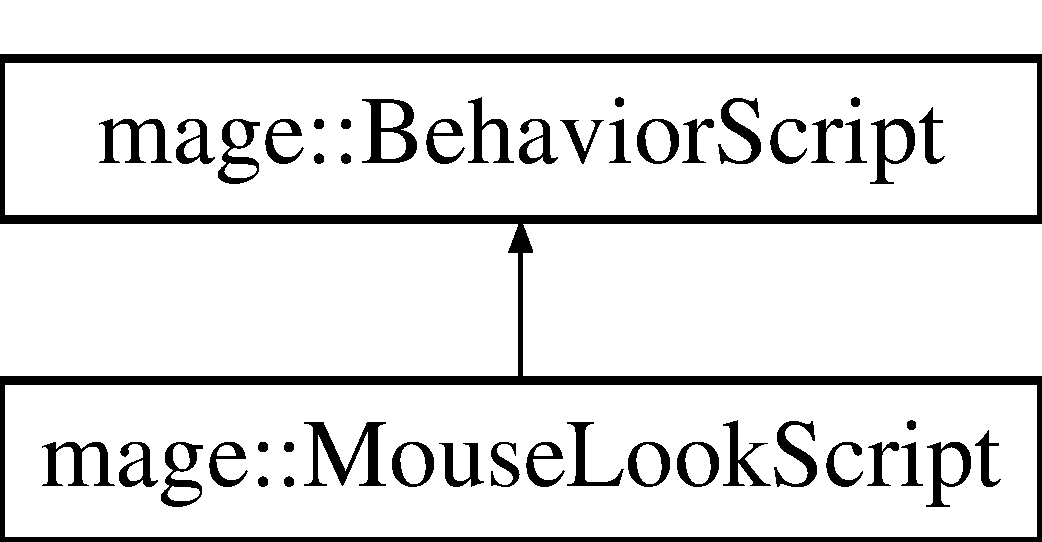
\includegraphics[height=2.000000cm]{classmage_1_1_mouse_look_script}
\end{center}
\end{figure}
\subsection*{Public Types}
\begin{DoxyCompactItemize}
\item 
enum \hyperlink{classmage_1_1_mouse_look_script_af63fd955f796c11e0378813e5d1ab5f8}{Rotation\+Axes} \{ \hyperlink{classmage_1_1_mouse_look_script_af63fd955f796c11e0378813e5d1ab5f8abf27c48f8a38ed19eeeba089dd8d3ba1}{Rotation\+Axes\+::\+MouseX} = 1, 
\hyperlink{classmage_1_1_mouse_look_script_af63fd955f796c11e0378813e5d1ab5f8a73843207a289db41b16a5bb8254ca425}{Rotation\+Axes\+::\+MouseY} = 2, 
\hyperlink{classmage_1_1_mouse_look_script_af63fd955f796c11e0378813e5d1ab5f8a109431b32c091e8a7ad541546c66c522}{Rotation\+Axes\+::\+Mouse\+X\+AndY} = MouseX $\vert$ MouseY
 \}
\end{DoxyCompactItemize}
\subsection*{Public Member Functions}
\begin{DoxyCompactItemize}
\item 
\hyperlink{classmage_1_1_mouse_look_script_a6f2e447da00bbea7cf146b4d2aef3a57}{Mouse\+Look\+Script} (\hyperlink{structmage_1_1_transform_node}{Transform\+Node} $\ast$transform, \hyperlink{classmage_1_1_mouse_look_script_af63fd955f796c11e0378813e5d1ab5f8}{Rotation\+Axes} axes=\hyperlink{classmage_1_1_mouse_look_script_af63fd955f796c11e0378813e5d1ab5f8a109431b32c091e8a7ad541546c66c522}{Rotation\+Axes\+::\+Mouse\+X\+AndY}, const X\+M\+F\+L\+O\+A\+T2 \&sensitivity=X\+M\+F\+L\+O\+A\+T2(1.\+8f, 1.\+8f), const X\+M\+F\+L\+O\+A\+T2 \&minimum\+\_\+rotation=\+X\+M\+F\+L\+O\+A\+T2(-\/\+X\+M\+\_\+\+P\+I/3.\+0f, -\/\+X\+M\+\_\+\+P\+I), const X\+M\+F\+L\+O\+A\+T2 \&maximum\+\_\+rotation=\+X\+M\+F\+L\+O\+A\+T2(\+X\+M\+\_\+\+P\+I/3.\+0f, X\+M\+\_\+\+P\+I), const X\+M\+F\+L\+O\+A\+T2 \&direction=\+X\+M\+F\+L\+O\+A\+T2(1.\+0f, 1.\+0f))
\item 
\hyperlink{classmage_1_1_mouse_look_script_a54bd09419068ab61c4dd6fda412771d3}{Mouse\+Look\+Script} (const \hyperlink{classmage_1_1_mouse_look_script}{Mouse\+Look\+Script} \&script)=delete
\item 
\hyperlink{classmage_1_1_mouse_look_script_aaca52076bde601772344c61639345e03}{Mouse\+Look\+Script} (\hyperlink{classmage_1_1_mouse_look_script}{Mouse\+Look\+Script} \&\&script)
\item 
virtual \hyperlink{classmage_1_1_mouse_look_script_ac402a33218e69d3594102b606dd051dc}{$\sim$\+Mouse\+Look\+Script} ()
\item 
\hyperlink{classmage_1_1_mouse_look_script}{Mouse\+Look\+Script} \& \hyperlink{classmage_1_1_mouse_look_script_a13fba7e90bf10d24814e0a8cec25645e}{operator=} (const \hyperlink{classmage_1_1_mouse_look_script}{Mouse\+Look\+Script} \&script)=delete
\item 
\hyperlink{classmage_1_1_mouse_look_script}{Mouse\+Look\+Script} \& \hyperlink{classmage_1_1_mouse_look_script_a2754174f5595fa424471c631818dc2b6}{operator=} (\hyperlink{classmage_1_1_mouse_look_script}{Mouse\+Look\+Script} \&\&script)=delete
\item 
virtual void \hyperlink{classmage_1_1_mouse_look_script_a7962403a78c02b2fe64e8f06f6319312}{Update} (double delta\+\_\+time) override
\item 
\hyperlink{classmage_1_1_mouse_look_script_af63fd955f796c11e0378813e5d1ab5f8}{Rotation\+Axes} \hyperlink{classmage_1_1_mouse_look_script_afe564764c233eab0f1183e4d4096c037}{Get\+Rotation\+Axes} () const noexcept
\item 
void \hyperlink{classmage_1_1_mouse_look_script_ac0fbe4b4661fd7f3c78207a336624670}{Set\+Rotation\+Axes} (\hyperlink{classmage_1_1_mouse_look_script_af63fd955f796c11e0378813e5d1ab5f8}{Rotation\+Axes} axes) noexcept
\item 
float \hyperlink{classmage_1_1_mouse_look_script_a3aec50fa8f0a38878a1977797db3015f}{Get\+SensitivityX} () const noexcept
\item 
float \hyperlink{classmage_1_1_mouse_look_script_a4dd528a4a0631acf1f8b64b6039f72b0}{Get\+SensitivityY} () const noexcept
\item 
const X\+M\+F\+L\+O\+A\+T2 \& \hyperlink{classmage_1_1_mouse_look_script_ac4834dacc6d80a83faaa4e3c3c236ae8}{Get\+Sensitivity} () const noexcept
\item 
void \hyperlink{classmage_1_1_mouse_look_script_a3acf0b2991234849fbf9256bb4fe48d4}{Set\+SensitivityX} (float x) noexcept
\item 
void \hyperlink{classmage_1_1_mouse_look_script_a3b92c0fd89b2fe82c7c688705ef24ee4}{Set\+SensitivityY} (float y) noexcept
\item 
void \hyperlink{classmage_1_1_mouse_look_script_ac53d16f789083f4d3fd43c0e75db8776}{Set\+Sensitivity} (float x, float y)
\item 
void \hyperlink{classmage_1_1_mouse_look_script_afcdd18f25a8d193e44f82fead1a814fc}{Set\+Sensitivity} (const X\+M\+F\+L\+O\+A\+T2 \&sensitivity) noexcept
\item 
void \hyperlink{classmage_1_1_mouse_look_script_a532715b6e11ee72a2bf76866457e69b2}{Set\+Sensitivity} (X\+M\+F\+L\+O\+A\+T2 \&\&sensitivity) noexcept
\item 
void X\+M\+\_\+\+C\+A\+L\+L\+C\+O\+NV \hyperlink{classmage_1_1_mouse_look_script_a909c1c584952bd0273972b6c68649e72}{Set\+Sensitivity} (F\+X\+M\+V\+E\+C\+T\+OR sensitivity) noexcept
\item 
float \hyperlink{classmage_1_1_mouse_look_script_a1961b562ee19c7575f3005a0b1c9bc07}{Get\+Minimum\+RotationX} () const noexcept
\item 
float \hyperlink{classmage_1_1_mouse_look_script_a4c2274d715404591ec3e4ae4ba7fb3e3}{Get\+Minimum\+RotationY} () const noexcept
\item 
const X\+M\+F\+L\+O\+A\+T2 \& \hyperlink{classmage_1_1_mouse_look_script_a9bfb1bd2c5f4b6b2163a40782b5ac7fd}{Get\+Minimum\+Rotation} () const noexcept
\item 
void \hyperlink{classmage_1_1_mouse_look_script_a480b68fb46a6b61fa4eb372843f33258}{Set\+Minimum\+RotationX} (float x) noexcept
\item 
void \hyperlink{classmage_1_1_mouse_look_script_ad010dc4dbec4815e12ae6c0fd919350b}{Set\+Minimum\+RotationY} (float y) noexcept
\item 
void \hyperlink{classmage_1_1_mouse_look_script_a27b21afa03d6c5cba9b206beb1a12533}{Set\+Minimum\+Rotation} (float x, float y) noexcept
\item 
void \hyperlink{classmage_1_1_mouse_look_script_a85eff477d2a3a98330193d466c6e54a0}{Set\+Minimum\+Rotation} (const X\+M\+F\+L\+O\+A\+T2 \&minimum\+\_\+rotation) noexcept
\item 
void \hyperlink{classmage_1_1_mouse_look_script_ac7e0fe75ff9e16b34ba53cb1a96744e9}{Set\+Minimum\+Rotation} (X\+M\+F\+L\+O\+A\+T2 \&\&minimum\+\_\+rotation) noexcept
\item 
void X\+M\+\_\+\+C\+A\+L\+L\+C\+O\+NV \hyperlink{classmage_1_1_mouse_look_script_a5e0c956a28b8c26dfdfcc704301fd0c7}{Set\+Minimum\+Rotation} (F\+X\+M\+V\+E\+C\+T\+OR minimum\+\_\+rotation) noexcept
\item 
float \hyperlink{classmage_1_1_mouse_look_script_ad9ba164d80ed752e64cd7b0275a21460}{Get\+Maximum\+RotationX} () const noexcept
\item 
float \hyperlink{classmage_1_1_mouse_look_script_a9650ed4b2592e89fc8428b3a7dde1029}{Get\+Maximum\+RotationY} () const noexcept
\item 
const X\+M\+F\+L\+O\+A\+T2 \& \hyperlink{classmage_1_1_mouse_look_script_a43d226ce0c1d8232bfe231cbcb20698e}{Get\+Maximum\+Rotation} () const noexcept
\item 
void \hyperlink{classmage_1_1_mouse_look_script_a27362a20031fce6ded6212e68545d8ee}{Set\+Maximum\+RotationX} (float x) noexcept
\item 
void \hyperlink{classmage_1_1_mouse_look_script_a8a48ea338ba2d2da3278b389d6861dfb}{Set\+Maximum\+RotationY} (float y) noexcept
\item 
void \hyperlink{classmage_1_1_mouse_look_script_aeffd8aa88e7ae4741f1610a28d0243c4}{Set\+Maximum\+Rotation} (float x, float y) noexcept
\item 
void \hyperlink{classmage_1_1_mouse_look_script_a38b8cefcfbd263017491f9c29b3fbc3c}{Set\+Maximum\+Rotation} (const X\+M\+F\+L\+O\+A\+T2 \&maximum\+\_\+rotation) noexcept
\item 
void \hyperlink{classmage_1_1_mouse_look_script_a98648bbce4fcaf05c4e831c81a49cef1}{Set\+Maximum\+Rotation} (X\+M\+F\+L\+O\+A\+T2 \&\&maximum\+\_\+rotation) noexcept
\item 
void X\+M\+\_\+\+C\+A\+L\+L\+C\+O\+NV \hyperlink{classmage_1_1_mouse_look_script_a234ef8a9d21255042d3831a804acc374}{Set\+Maximum\+Rotation} (F\+X\+M\+V\+E\+C\+T\+OR maximum\+\_\+rotation) noexcept
\item 
void \hyperlink{classmage_1_1_mouse_look_script_a2f1fa6a912e9ee8720c51d7b03df39a1}{Invert\+DirectionX} () noexcept
\item 
void \hyperlink{classmage_1_1_mouse_look_script_a773f4e2ab6eac735e920db427d82e634}{Invert\+DirectionY} () noexcept
\end{DoxyCompactItemize}
\subsection*{Private Attributes}
\begin{DoxyCompactItemize}
\item 
\hyperlink{structmage_1_1_transform_node}{Transform\+Node} $\ast$const \hyperlink{classmage_1_1_mouse_look_script_a419b30350dc3eed30ae2f983812391f5}{m\+\_\+transform}
\item 
\hyperlink{classmage_1_1_mouse_look_script_af63fd955f796c11e0378813e5d1ab5f8}{Rotation\+Axes} \hyperlink{classmage_1_1_mouse_look_script_ab5df1b96d5860a9b8f30256e7c89b26b}{m\+\_\+axes}
\item 
X\+M\+F\+L\+O\+A\+T2 \hyperlink{classmage_1_1_mouse_look_script_a4f38b9bd8e7271503a70753ce6a923c7}{m\+\_\+sensitivity}
\item 
X\+M\+F\+L\+O\+A\+T2 \hyperlink{classmage_1_1_mouse_look_script_ad09bda241666f60dfc408500cafd073d}{m\+\_\+minimum\+\_\+rotation}
\item 
X\+M\+F\+L\+O\+A\+T2 \hyperlink{classmage_1_1_mouse_look_script_a0d5f2933555b76efd7cf83c7672574dd}{m\+\_\+maximum\+\_\+rotation}
\item 
X\+M\+F\+L\+O\+A\+T2 \hyperlink{classmage_1_1_mouse_look_script_a07c9a61869dab687a0426fa0c4b41fa7}{m\+\_\+direction}
\end{DoxyCompactItemize}
\subsection*{Additional Inherited Members}


\subsection{Member Enumeration Documentation}
\hypertarget{classmage_1_1_mouse_look_script_af63fd955f796c11e0378813e5d1ab5f8}{}\label{classmage_1_1_mouse_look_script_af63fd955f796c11e0378813e5d1ab5f8} 
\index{mage\+::\+Mouse\+Look\+Script@{mage\+::\+Mouse\+Look\+Script}!Rotation\+Axes@{Rotation\+Axes}}
\index{Rotation\+Axes@{Rotation\+Axes}!mage\+::\+Mouse\+Look\+Script@{mage\+::\+Mouse\+Look\+Script}}
\subsubsection{\texorpdfstring{Rotation\+Axes}{RotationAxes}}
{\footnotesize\ttfamily enum \hyperlink{classmage_1_1_mouse_look_script_af63fd955f796c11e0378813e5d1ab5f8}{mage\+::\+Mouse\+Look\+Script\+::\+Rotation\+Axes}\hspace{0.3cm}{\ttfamily [strong]}}

\begin{DoxyEnumFields}{Enumerator}
\raisebox{\heightof{T}}[0pt][0pt]{\index{MouseX@{MouseX}!mage\+::\+Mouse\+Look\+Script@{mage\+::\+Mouse\+Look\+Script}}\index{mage\+::\+Mouse\+Look\+Script@{mage\+::\+Mouse\+Look\+Script}!MouseX@{MouseX}}}\hypertarget{classmage_1_1_mouse_look_script_af63fd955f796c11e0378813e5d1ab5f8abf27c48f8a38ed19eeeba089dd8d3ba1}{}\label{classmage_1_1_mouse_look_script_af63fd955f796c11e0378813e5d1ab5f8abf27c48f8a38ed19eeeba089dd8d3ba1} 
MouseX&\\
\hline

\raisebox{\heightof{T}}[0pt][0pt]{\index{MouseY@{MouseY}!mage\+::\+Mouse\+Look\+Script@{mage\+::\+Mouse\+Look\+Script}}\index{mage\+::\+Mouse\+Look\+Script@{mage\+::\+Mouse\+Look\+Script}!MouseY@{MouseY}}}\hypertarget{classmage_1_1_mouse_look_script_af63fd955f796c11e0378813e5d1ab5f8a73843207a289db41b16a5bb8254ca425}{}\label{classmage_1_1_mouse_look_script_af63fd955f796c11e0378813e5d1ab5f8a73843207a289db41b16a5bb8254ca425} 
MouseY&\\
\hline

\raisebox{\heightof{T}}[0pt][0pt]{\index{Mouse\+X\+AndY@{Mouse\+X\+AndY}!mage\+::\+Mouse\+Look\+Script@{mage\+::\+Mouse\+Look\+Script}}\index{mage\+::\+Mouse\+Look\+Script@{mage\+::\+Mouse\+Look\+Script}!Mouse\+X\+AndY@{Mouse\+X\+AndY}}}\hypertarget{classmage_1_1_mouse_look_script_af63fd955f796c11e0378813e5d1ab5f8a109431b32c091e8a7ad541546c66c522}{}\label{classmage_1_1_mouse_look_script_af63fd955f796c11e0378813e5d1ab5f8a109431b32c091e8a7ad541546c66c522} 
Mouse\+X\+AndY&\\
\hline

\end{DoxyEnumFields}


\subsection{Constructor \& Destructor Documentation}
\hypertarget{classmage_1_1_mouse_look_script_a6f2e447da00bbea7cf146b4d2aef3a57}{}\label{classmage_1_1_mouse_look_script_a6f2e447da00bbea7cf146b4d2aef3a57} 
\index{mage\+::\+Mouse\+Look\+Script@{mage\+::\+Mouse\+Look\+Script}!Mouse\+Look\+Script@{Mouse\+Look\+Script}}
\index{Mouse\+Look\+Script@{Mouse\+Look\+Script}!mage\+::\+Mouse\+Look\+Script@{mage\+::\+Mouse\+Look\+Script}}
\subsubsection{\texorpdfstring{Mouse\+Look\+Script()}{MouseLookScript()}\hspace{0.1cm}{\footnotesize\ttfamily [1/3]}}
{\footnotesize\ttfamily mage\+::\+Mouse\+Look\+Script\+::\+Mouse\+Look\+Script (\begin{DoxyParamCaption}\item[{\hyperlink{structmage_1_1_transform_node}{Transform\+Node} $\ast$}]{transform,  }\item[{\hyperlink{classmage_1_1_mouse_look_script_af63fd955f796c11e0378813e5d1ab5f8}{Rotation\+Axes}}]{axes = {\ttfamily \hyperlink{classmage_1_1_mouse_look_script_af63fd955f796c11e0378813e5d1ab5f8a109431b32c091e8a7ad541546c66c522}{Rotation\+Axes\+::\+Mouse\+X\+AndY}},  }\item[{const X\+M\+F\+L\+O\+A\+T2 \&}]{sensitivity = {\ttfamily XMFLOAT2(1.8f,~1.8f)},  }\item[{const X\+M\+F\+L\+O\+A\+T2 \&}]{minimum\+\_\+rotation = {\ttfamily XMFLOAT2(-\/XM\+\_\+PI~/~3.0f,~-\/XM\+\_\+PI)},  }\item[{const X\+M\+F\+L\+O\+A\+T2 \&}]{maximum\+\_\+rotation = {\ttfamily XMFLOAT2(~XM\+\_\+PI~/~3.0f,~~XM\+\_\+PI)},  }\item[{const X\+M\+F\+L\+O\+A\+T2 \&}]{direction = {\ttfamily XMFLOAT2(1.0f,~1.0f)} }\end{DoxyParamCaption})\hspace{0.3cm}{\ttfamily [explicit]}}

\hypertarget{classmage_1_1_mouse_look_script_a54bd09419068ab61c4dd6fda412771d3}{}\label{classmage_1_1_mouse_look_script_a54bd09419068ab61c4dd6fda412771d3} 
\index{mage\+::\+Mouse\+Look\+Script@{mage\+::\+Mouse\+Look\+Script}!Mouse\+Look\+Script@{Mouse\+Look\+Script}}
\index{Mouse\+Look\+Script@{Mouse\+Look\+Script}!mage\+::\+Mouse\+Look\+Script@{mage\+::\+Mouse\+Look\+Script}}
\subsubsection{\texorpdfstring{Mouse\+Look\+Script()}{MouseLookScript()}\hspace{0.1cm}{\footnotesize\ttfamily [2/3]}}
{\footnotesize\ttfamily mage\+::\+Mouse\+Look\+Script\+::\+Mouse\+Look\+Script (\begin{DoxyParamCaption}\item[{const \hyperlink{classmage_1_1_mouse_look_script}{Mouse\+Look\+Script} \&}]{script }\end{DoxyParamCaption})\hspace{0.3cm}{\ttfamily [delete]}}

\hypertarget{classmage_1_1_mouse_look_script_aaca52076bde601772344c61639345e03}{}\label{classmage_1_1_mouse_look_script_aaca52076bde601772344c61639345e03} 
\index{mage\+::\+Mouse\+Look\+Script@{mage\+::\+Mouse\+Look\+Script}!Mouse\+Look\+Script@{Mouse\+Look\+Script}}
\index{Mouse\+Look\+Script@{Mouse\+Look\+Script}!mage\+::\+Mouse\+Look\+Script@{mage\+::\+Mouse\+Look\+Script}}
\subsubsection{\texorpdfstring{Mouse\+Look\+Script()}{MouseLookScript()}\hspace{0.1cm}{\footnotesize\ttfamily [3/3]}}
{\footnotesize\ttfamily mage\+::\+Mouse\+Look\+Script\+::\+Mouse\+Look\+Script (\begin{DoxyParamCaption}\item[{\hyperlink{classmage_1_1_mouse_look_script}{Mouse\+Look\+Script} \&\&}]{script }\end{DoxyParamCaption})\hspace{0.3cm}{\ttfamily [default]}}

\hypertarget{classmage_1_1_mouse_look_script_ac402a33218e69d3594102b606dd051dc}{}\label{classmage_1_1_mouse_look_script_ac402a33218e69d3594102b606dd051dc} 
\index{mage\+::\+Mouse\+Look\+Script@{mage\+::\+Mouse\+Look\+Script}!````~Mouse\+Look\+Script@{$\sim$\+Mouse\+Look\+Script}}
\index{````~Mouse\+Look\+Script@{$\sim$\+Mouse\+Look\+Script}!mage\+::\+Mouse\+Look\+Script@{mage\+::\+Mouse\+Look\+Script}}
\subsubsection{\texorpdfstring{$\sim$\+Mouse\+Look\+Script()}{~MouseLookScript()}}
{\footnotesize\ttfamily mage\+::\+Mouse\+Look\+Script\+::$\sim$\+Mouse\+Look\+Script (\begin{DoxyParamCaption}{ }\end{DoxyParamCaption})\hspace{0.3cm}{\ttfamily [virtual]}, {\ttfamily [default]}}



\subsection{Member Function Documentation}
\hypertarget{classmage_1_1_mouse_look_script_a43d226ce0c1d8232bfe231cbcb20698e}{}\label{classmage_1_1_mouse_look_script_a43d226ce0c1d8232bfe231cbcb20698e} 
\index{mage\+::\+Mouse\+Look\+Script@{mage\+::\+Mouse\+Look\+Script}!Get\+Maximum\+Rotation@{Get\+Maximum\+Rotation}}
\index{Get\+Maximum\+Rotation@{Get\+Maximum\+Rotation}!mage\+::\+Mouse\+Look\+Script@{mage\+::\+Mouse\+Look\+Script}}
\subsubsection{\texorpdfstring{Get\+Maximum\+Rotation()}{GetMaximumRotation()}}
{\footnotesize\ttfamily const X\+M\+F\+L\+O\+A\+T2\& mage\+::\+Mouse\+Look\+Script\+::\+Get\+Maximum\+Rotation (\begin{DoxyParamCaption}{ }\end{DoxyParamCaption}) const\hspace{0.3cm}{\ttfamily [noexcept]}}

\hypertarget{classmage_1_1_mouse_look_script_ad9ba164d80ed752e64cd7b0275a21460}{}\label{classmage_1_1_mouse_look_script_ad9ba164d80ed752e64cd7b0275a21460} 
\index{mage\+::\+Mouse\+Look\+Script@{mage\+::\+Mouse\+Look\+Script}!Get\+Maximum\+RotationX@{Get\+Maximum\+RotationX}}
\index{Get\+Maximum\+RotationX@{Get\+Maximum\+RotationX}!mage\+::\+Mouse\+Look\+Script@{mage\+::\+Mouse\+Look\+Script}}
\subsubsection{\texorpdfstring{Get\+Maximum\+Rotation\+X()}{GetMaximumRotationX()}}
{\footnotesize\ttfamily float mage\+::\+Mouse\+Look\+Script\+::\+Get\+Maximum\+RotationX (\begin{DoxyParamCaption}{ }\end{DoxyParamCaption}) const\hspace{0.3cm}{\ttfamily [noexcept]}}

\hypertarget{classmage_1_1_mouse_look_script_a9650ed4b2592e89fc8428b3a7dde1029}{}\label{classmage_1_1_mouse_look_script_a9650ed4b2592e89fc8428b3a7dde1029} 
\index{mage\+::\+Mouse\+Look\+Script@{mage\+::\+Mouse\+Look\+Script}!Get\+Maximum\+RotationY@{Get\+Maximum\+RotationY}}
\index{Get\+Maximum\+RotationY@{Get\+Maximum\+RotationY}!mage\+::\+Mouse\+Look\+Script@{mage\+::\+Mouse\+Look\+Script}}
\subsubsection{\texorpdfstring{Get\+Maximum\+Rotation\+Y()}{GetMaximumRotationY()}}
{\footnotesize\ttfamily float mage\+::\+Mouse\+Look\+Script\+::\+Get\+Maximum\+RotationY (\begin{DoxyParamCaption}{ }\end{DoxyParamCaption}) const\hspace{0.3cm}{\ttfamily [noexcept]}}

\hypertarget{classmage_1_1_mouse_look_script_a9bfb1bd2c5f4b6b2163a40782b5ac7fd}{}\label{classmage_1_1_mouse_look_script_a9bfb1bd2c5f4b6b2163a40782b5ac7fd} 
\index{mage\+::\+Mouse\+Look\+Script@{mage\+::\+Mouse\+Look\+Script}!Get\+Minimum\+Rotation@{Get\+Minimum\+Rotation}}
\index{Get\+Minimum\+Rotation@{Get\+Minimum\+Rotation}!mage\+::\+Mouse\+Look\+Script@{mage\+::\+Mouse\+Look\+Script}}
\subsubsection{\texorpdfstring{Get\+Minimum\+Rotation()}{GetMinimumRotation()}}
{\footnotesize\ttfamily const X\+M\+F\+L\+O\+A\+T2\& mage\+::\+Mouse\+Look\+Script\+::\+Get\+Minimum\+Rotation (\begin{DoxyParamCaption}{ }\end{DoxyParamCaption}) const\hspace{0.3cm}{\ttfamily [noexcept]}}

\hypertarget{classmage_1_1_mouse_look_script_a1961b562ee19c7575f3005a0b1c9bc07}{}\label{classmage_1_1_mouse_look_script_a1961b562ee19c7575f3005a0b1c9bc07} 
\index{mage\+::\+Mouse\+Look\+Script@{mage\+::\+Mouse\+Look\+Script}!Get\+Minimum\+RotationX@{Get\+Minimum\+RotationX}}
\index{Get\+Minimum\+RotationX@{Get\+Minimum\+RotationX}!mage\+::\+Mouse\+Look\+Script@{mage\+::\+Mouse\+Look\+Script}}
\subsubsection{\texorpdfstring{Get\+Minimum\+Rotation\+X()}{GetMinimumRotationX()}}
{\footnotesize\ttfamily float mage\+::\+Mouse\+Look\+Script\+::\+Get\+Minimum\+RotationX (\begin{DoxyParamCaption}{ }\end{DoxyParamCaption}) const\hspace{0.3cm}{\ttfamily [noexcept]}}

\hypertarget{classmage_1_1_mouse_look_script_a4c2274d715404591ec3e4ae4ba7fb3e3}{}\label{classmage_1_1_mouse_look_script_a4c2274d715404591ec3e4ae4ba7fb3e3} 
\index{mage\+::\+Mouse\+Look\+Script@{mage\+::\+Mouse\+Look\+Script}!Get\+Minimum\+RotationY@{Get\+Minimum\+RotationY}}
\index{Get\+Minimum\+RotationY@{Get\+Minimum\+RotationY}!mage\+::\+Mouse\+Look\+Script@{mage\+::\+Mouse\+Look\+Script}}
\subsubsection{\texorpdfstring{Get\+Minimum\+Rotation\+Y()}{GetMinimumRotationY()}}
{\footnotesize\ttfamily float mage\+::\+Mouse\+Look\+Script\+::\+Get\+Minimum\+RotationY (\begin{DoxyParamCaption}{ }\end{DoxyParamCaption}) const\hspace{0.3cm}{\ttfamily [noexcept]}}

\hypertarget{classmage_1_1_mouse_look_script_afe564764c233eab0f1183e4d4096c037}{}\label{classmage_1_1_mouse_look_script_afe564764c233eab0f1183e4d4096c037} 
\index{mage\+::\+Mouse\+Look\+Script@{mage\+::\+Mouse\+Look\+Script}!Get\+Rotation\+Axes@{Get\+Rotation\+Axes}}
\index{Get\+Rotation\+Axes@{Get\+Rotation\+Axes}!mage\+::\+Mouse\+Look\+Script@{mage\+::\+Mouse\+Look\+Script}}
\subsubsection{\texorpdfstring{Get\+Rotation\+Axes()}{GetRotationAxes()}}
{\footnotesize\ttfamily \hyperlink{classmage_1_1_mouse_look_script_af63fd955f796c11e0378813e5d1ab5f8}{Rotation\+Axes} mage\+::\+Mouse\+Look\+Script\+::\+Get\+Rotation\+Axes (\begin{DoxyParamCaption}{ }\end{DoxyParamCaption}) const\hspace{0.3cm}{\ttfamily [noexcept]}}

\hypertarget{classmage_1_1_mouse_look_script_ac4834dacc6d80a83faaa4e3c3c236ae8}{}\label{classmage_1_1_mouse_look_script_ac4834dacc6d80a83faaa4e3c3c236ae8} 
\index{mage\+::\+Mouse\+Look\+Script@{mage\+::\+Mouse\+Look\+Script}!Get\+Sensitivity@{Get\+Sensitivity}}
\index{Get\+Sensitivity@{Get\+Sensitivity}!mage\+::\+Mouse\+Look\+Script@{mage\+::\+Mouse\+Look\+Script}}
\subsubsection{\texorpdfstring{Get\+Sensitivity()}{GetSensitivity()}}
{\footnotesize\ttfamily const X\+M\+F\+L\+O\+A\+T2\& mage\+::\+Mouse\+Look\+Script\+::\+Get\+Sensitivity (\begin{DoxyParamCaption}{ }\end{DoxyParamCaption}) const\hspace{0.3cm}{\ttfamily [noexcept]}}

\hypertarget{classmage_1_1_mouse_look_script_a3aec50fa8f0a38878a1977797db3015f}{}\label{classmage_1_1_mouse_look_script_a3aec50fa8f0a38878a1977797db3015f} 
\index{mage\+::\+Mouse\+Look\+Script@{mage\+::\+Mouse\+Look\+Script}!Get\+SensitivityX@{Get\+SensitivityX}}
\index{Get\+SensitivityX@{Get\+SensitivityX}!mage\+::\+Mouse\+Look\+Script@{mage\+::\+Mouse\+Look\+Script}}
\subsubsection{\texorpdfstring{Get\+Sensitivity\+X()}{GetSensitivityX()}}
{\footnotesize\ttfamily float mage\+::\+Mouse\+Look\+Script\+::\+Get\+SensitivityX (\begin{DoxyParamCaption}{ }\end{DoxyParamCaption}) const\hspace{0.3cm}{\ttfamily [noexcept]}}

\hypertarget{classmage_1_1_mouse_look_script_a4dd528a4a0631acf1f8b64b6039f72b0}{}\label{classmage_1_1_mouse_look_script_a4dd528a4a0631acf1f8b64b6039f72b0} 
\index{mage\+::\+Mouse\+Look\+Script@{mage\+::\+Mouse\+Look\+Script}!Get\+SensitivityY@{Get\+SensitivityY}}
\index{Get\+SensitivityY@{Get\+SensitivityY}!mage\+::\+Mouse\+Look\+Script@{mage\+::\+Mouse\+Look\+Script}}
\subsubsection{\texorpdfstring{Get\+Sensitivity\+Y()}{GetSensitivityY()}}
{\footnotesize\ttfamily float mage\+::\+Mouse\+Look\+Script\+::\+Get\+SensitivityY (\begin{DoxyParamCaption}{ }\end{DoxyParamCaption}) const\hspace{0.3cm}{\ttfamily [noexcept]}}

\hypertarget{classmage_1_1_mouse_look_script_a2f1fa6a912e9ee8720c51d7b03df39a1}{}\label{classmage_1_1_mouse_look_script_a2f1fa6a912e9ee8720c51d7b03df39a1} 
\index{mage\+::\+Mouse\+Look\+Script@{mage\+::\+Mouse\+Look\+Script}!Invert\+DirectionX@{Invert\+DirectionX}}
\index{Invert\+DirectionX@{Invert\+DirectionX}!mage\+::\+Mouse\+Look\+Script@{mage\+::\+Mouse\+Look\+Script}}
\subsubsection{\texorpdfstring{Invert\+Direction\+X()}{InvertDirectionX()}}
{\footnotesize\ttfamily void mage\+::\+Mouse\+Look\+Script\+::\+Invert\+DirectionX (\begin{DoxyParamCaption}{ }\end{DoxyParamCaption})\hspace{0.3cm}{\ttfamily [noexcept]}}

\hypertarget{classmage_1_1_mouse_look_script_a773f4e2ab6eac735e920db427d82e634}{}\label{classmage_1_1_mouse_look_script_a773f4e2ab6eac735e920db427d82e634} 
\index{mage\+::\+Mouse\+Look\+Script@{mage\+::\+Mouse\+Look\+Script}!Invert\+DirectionY@{Invert\+DirectionY}}
\index{Invert\+DirectionY@{Invert\+DirectionY}!mage\+::\+Mouse\+Look\+Script@{mage\+::\+Mouse\+Look\+Script}}
\subsubsection{\texorpdfstring{Invert\+Direction\+Y()}{InvertDirectionY()}}
{\footnotesize\ttfamily void mage\+::\+Mouse\+Look\+Script\+::\+Invert\+DirectionY (\begin{DoxyParamCaption}{ }\end{DoxyParamCaption})\hspace{0.3cm}{\ttfamily [noexcept]}}

\hypertarget{classmage_1_1_mouse_look_script_a13fba7e90bf10d24814e0a8cec25645e}{}\label{classmage_1_1_mouse_look_script_a13fba7e90bf10d24814e0a8cec25645e} 
\index{mage\+::\+Mouse\+Look\+Script@{mage\+::\+Mouse\+Look\+Script}!operator=@{operator=}}
\index{operator=@{operator=}!mage\+::\+Mouse\+Look\+Script@{mage\+::\+Mouse\+Look\+Script}}
\subsubsection{\texorpdfstring{operator=()}{operator=()}\hspace{0.1cm}{\footnotesize\ttfamily [1/2]}}
{\footnotesize\ttfamily \hyperlink{classmage_1_1_mouse_look_script}{Mouse\+Look\+Script}\& mage\+::\+Mouse\+Look\+Script\+::operator= (\begin{DoxyParamCaption}\item[{const \hyperlink{classmage_1_1_mouse_look_script}{Mouse\+Look\+Script} \&}]{script }\end{DoxyParamCaption})\hspace{0.3cm}{\ttfamily [delete]}}

\hypertarget{classmage_1_1_mouse_look_script_a2754174f5595fa424471c631818dc2b6}{}\label{classmage_1_1_mouse_look_script_a2754174f5595fa424471c631818dc2b6} 
\index{mage\+::\+Mouse\+Look\+Script@{mage\+::\+Mouse\+Look\+Script}!operator=@{operator=}}
\index{operator=@{operator=}!mage\+::\+Mouse\+Look\+Script@{mage\+::\+Mouse\+Look\+Script}}
\subsubsection{\texorpdfstring{operator=()}{operator=()}\hspace{0.1cm}{\footnotesize\ttfamily [2/2]}}
{\footnotesize\ttfamily \hyperlink{classmage_1_1_mouse_look_script}{Mouse\+Look\+Script}\& mage\+::\+Mouse\+Look\+Script\+::operator= (\begin{DoxyParamCaption}\item[{\hyperlink{classmage_1_1_mouse_look_script}{Mouse\+Look\+Script} \&\&}]{script }\end{DoxyParamCaption})\hspace{0.3cm}{\ttfamily [delete]}}

\hypertarget{classmage_1_1_mouse_look_script_aeffd8aa88e7ae4741f1610a28d0243c4}{}\label{classmage_1_1_mouse_look_script_aeffd8aa88e7ae4741f1610a28d0243c4} 
\index{mage\+::\+Mouse\+Look\+Script@{mage\+::\+Mouse\+Look\+Script}!Set\+Maximum\+Rotation@{Set\+Maximum\+Rotation}}
\index{Set\+Maximum\+Rotation@{Set\+Maximum\+Rotation}!mage\+::\+Mouse\+Look\+Script@{mage\+::\+Mouse\+Look\+Script}}
\subsubsection{\texorpdfstring{Set\+Maximum\+Rotation()}{SetMaximumRotation()}\hspace{0.1cm}{\footnotesize\ttfamily [1/4]}}
{\footnotesize\ttfamily void mage\+::\+Mouse\+Look\+Script\+::\+Set\+Maximum\+Rotation (\begin{DoxyParamCaption}\item[{float}]{x,  }\item[{float}]{y }\end{DoxyParamCaption})\hspace{0.3cm}{\ttfamily [noexcept]}}

\hypertarget{classmage_1_1_mouse_look_script_a38b8cefcfbd263017491f9c29b3fbc3c}{}\label{classmage_1_1_mouse_look_script_a38b8cefcfbd263017491f9c29b3fbc3c} 
\index{mage\+::\+Mouse\+Look\+Script@{mage\+::\+Mouse\+Look\+Script}!Set\+Maximum\+Rotation@{Set\+Maximum\+Rotation}}
\index{Set\+Maximum\+Rotation@{Set\+Maximum\+Rotation}!mage\+::\+Mouse\+Look\+Script@{mage\+::\+Mouse\+Look\+Script}}
\subsubsection{\texorpdfstring{Set\+Maximum\+Rotation()}{SetMaximumRotation()}\hspace{0.1cm}{\footnotesize\ttfamily [2/4]}}
{\footnotesize\ttfamily void mage\+::\+Mouse\+Look\+Script\+::\+Set\+Maximum\+Rotation (\begin{DoxyParamCaption}\item[{const X\+M\+F\+L\+O\+A\+T2 \&}]{maximum\+\_\+rotation }\end{DoxyParamCaption})\hspace{0.3cm}{\ttfamily [noexcept]}}

\hypertarget{classmage_1_1_mouse_look_script_a98648bbce4fcaf05c4e831c81a49cef1}{}\label{classmage_1_1_mouse_look_script_a98648bbce4fcaf05c4e831c81a49cef1} 
\index{mage\+::\+Mouse\+Look\+Script@{mage\+::\+Mouse\+Look\+Script}!Set\+Maximum\+Rotation@{Set\+Maximum\+Rotation}}
\index{Set\+Maximum\+Rotation@{Set\+Maximum\+Rotation}!mage\+::\+Mouse\+Look\+Script@{mage\+::\+Mouse\+Look\+Script}}
\subsubsection{\texorpdfstring{Set\+Maximum\+Rotation()}{SetMaximumRotation()}\hspace{0.1cm}{\footnotesize\ttfamily [3/4]}}
{\footnotesize\ttfamily void mage\+::\+Mouse\+Look\+Script\+::\+Set\+Maximum\+Rotation (\begin{DoxyParamCaption}\item[{X\+M\+F\+L\+O\+A\+T2 \&\&}]{maximum\+\_\+rotation }\end{DoxyParamCaption})\hspace{0.3cm}{\ttfamily [noexcept]}}

\hypertarget{classmage_1_1_mouse_look_script_a234ef8a9d21255042d3831a804acc374}{}\label{classmage_1_1_mouse_look_script_a234ef8a9d21255042d3831a804acc374} 
\index{mage\+::\+Mouse\+Look\+Script@{mage\+::\+Mouse\+Look\+Script}!Set\+Maximum\+Rotation@{Set\+Maximum\+Rotation}}
\index{Set\+Maximum\+Rotation@{Set\+Maximum\+Rotation}!mage\+::\+Mouse\+Look\+Script@{mage\+::\+Mouse\+Look\+Script}}
\subsubsection{\texorpdfstring{Set\+Maximum\+Rotation()}{SetMaximumRotation()}\hspace{0.1cm}{\footnotesize\ttfamily [4/4]}}
{\footnotesize\ttfamily void X\+M\+\_\+\+C\+A\+L\+L\+C\+O\+NV mage\+::\+Mouse\+Look\+Script\+::\+Set\+Maximum\+Rotation (\begin{DoxyParamCaption}\item[{F\+X\+M\+V\+E\+C\+T\+OR}]{maximum\+\_\+rotation }\end{DoxyParamCaption})\hspace{0.3cm}{\ttfamily [noexcept]}}

\hypertarget{classmage_1_1_mouse_look_script_a27362a20031fce6ded6212e68545d8ee}{}\label{classmage_1_1_mouse_look_script_a27362a20031fce6ded6212e68545d8ee} 
\index{mage\+::\+Mouse\+Look\+Script@{mage\+::\+Mouse\+Look\+Script}!Set\+Maximum\+RotationX@{Set\+Maximum\+RotationX}}
\index{Set\+Maximum\+RotationX@{Set\+Maximum\+RotationX}!mage\+::\+Mouse\+Look\+Script@{mage\+::\+Mouse\+Look\+Script}}
\subsubsection{\texorpdfstring{Set\+Maximum\+Rotation\+X()}{SetMaximumRotationX()}}
{\footnotesize\ttfamily void mage\+::\+Mouse\+Look\+Script\+::\+Set\+Maximum\+RotationX (\begin{DoxyParamCaption}\item[{float}]{x }\end{DoxyParamCaption})\hspace{0.3cm}{\ttfamily [noexcept]}}

\hypertarget{classmage_1_1_mouse_look_script_a8a48ea338ba2d2da3278b389d6861dfb}{}\label{classmage_1_1_mouse_look_script_a8a48ea338ba2d2da3278b389d6861dfb} 
\index{mage\+::\+Mouse\+Look\+Script@{mage\+::\+Mouse\+Look\+Script}!Set\+Maximum\+RotationY@{Set\+Maximum\+RotationY}}
\index{Set\+Maximum\+RotationY@{Set\+Maximum\+RotationY}!mage\+::\+Mouse\+Look\+Script@{mage\+::\+Mouse\+Look\+Script}}
\subsubsection{\texorpdfstring{Set\+Maximum\+Rotation\+Y()}{SetMaximumRotationY()}}
{\footnotesize\ttfamily void mage\+::\+Mouse\+Look\+Script\+::\+Set\+Maximum\+RotationY (\begin{DoxyParamCaption}\item[{float}]{y }\end{DoxyParamCaption})\hspace{0.3cm}{\ttfamily [noexcept]}}

\hypertarget{classmage_1_1_mouse_look_script_a27b21afa03d6c5cba9b206beb1a12533}{}\label{classmage_1_1_mouse_look_script_a27b21afa03d6c5cba9b206beb1a12533} 
\index{mage\+::\+Mouse\+Look\+Script@{mage\+::\+Mouse\+Look\+Script}!Set\+Minimum\+Rotation@{Set\+Minimum\+Rotation}}
\index{Set\+Minimum\+Rotation@{Set\+Minimum\+Rotation}!mage\+::\+Mouse\+Look\+Script@{mage\+::\+Mouse\+Look\+Script}}
\subsubsection{\texorpdfstring{Set\+Minimum\+Rotation()}{SetMinimumRotation()}\hspace{0.1cm}{\footnotesize\ttfamily [1/4]}}
{\footnotesize\ttfamily void mage\+::\+Mouse\+Look\+Script\+::\+Set\+Minimum\+Rotation (\begin{DoxyParamCaption}\item[{float}]{x,  }\item[{float}]{y }\end{DoxyParamCaption})\hspace{0.3cm}{\ttfamily [noexcept]}}

\hypertarget{classmage_1_1_mouse_look_script_a85eff477d2a3a98330193d466c6e54a0}{}\label{classmage_1_1_mouse_look_script_a85eff477d2a3a98330193d466c6e54a0} 
\index{mage\+::\+Mouse\+Look\+Script@{mage\+::\+Mouse\+Look\+Script}!Set\+Minimum\+Rotation@{Set\+Minimum\+Rotation}}
\index{Set\+Minimum\+Rotation@{Set\+Minimum\+Rotation}!mage\+::\+Mouse\+Look\+Script@{mage\+::\+Mouse\+Look\+Script}}
\subsubsection{\texorpdfstring{Set\+Minimum\+Rotation()}{SetMinimumRotation()}\hspace{0.1cm}{\footnotesize\ttfamily [2/4]}}
{\footnotesize\ttfamily void mage\+::\+Mouse\+Look\+Script\+::\+Set\+Minimum\+Rotation (\begin{DoxyParamCaption}\item[{const X\+M\+F\+L\+O\+A\+T2 \&}]{minimum\+\_\+rotation }\end{DoxyParamCaption})\hspace{0.3cm}{\ttfamily [noexcept]}}

\hypertarget{classmage_1_1_mouse_look_script_ac7e0fe75ff9e16b34ba53cb1a96744e9}{}\label{classmage_1_1_mouse_look_script_ac7e0fe75ff9e16b34ba53cb1a96744e9} 
\index{mage\+::\+Mouse\+Look\+Script@{mage\+::\+Mouse\+Look\+Script}!Set\+Minimum\+Rotation@{Set\+Minimum\+Rotation}}
\index{Set\+Minimum\+Rotation@{Set\+Minimum\+Rotation}!mage\+::\+Mouse\+Look\+Script@{mage\+::\+Mouse\+Look\+Script}}
\subsubsection{\texorpdfstring{Set\+Minimum\+Rotation()}{SetMinimumRotation()}\hspace{0.1cm}{\footnotesize\ttfamily [3/4]}}
{\footnotesize\ttfamily void mage\+::\+Mouse\+Look\+Script\+::\+Set\+Minimum\+Rotation (\begin{DoxyParamCaption}\item[{X\+M\+F\+L\+O\+A\+T2 \&\&}]{minimum\+\_\+rotation }\end{DoxyParamCaption})\hspace{0.3cm}{\ttfamily [noexcept]}}

\hypertarget{classmage_1_1_mouse_look_script_a5e0c956a28b8c26dfdfcc704301fd0c7}{}\label{classmage_1_1_mouse_look_script_a5e0c956a28b8c26dfdfcc704301fd0c7} 
\index{mage\+::\+Mouse\+Look\+Script@{mage\+::\+Mouse\+Look\+Script}!Set\+Minimum\+Rotation@{Set\+Minimum\+Rotation}}
\index{Set\+Minimum\+Rotation@{Set\+Minimum\+Rotation}!mage\+::\+Mouse\+Look\+Script@{mage\+::\+Mouse\+Look\+Script}}
\subsubsection{\texorpdfstring{Set\+Minimum\+Rotation()}{SetMinimumRotation()}\hspace{0.1cm}{\footnotesize\ttfamily [4/4]}}
{\footnotesize\ttfamily void X\+M\+\_\+\+C\+A\+L\+L\+C\+O\+NV mage\+::\+Mouse\+Look\+Script\+::\+Set\+Minimum\+Rotation (\begin{DoxyParamCaption}\item[{F\+X\+M\+V\+E\+C\+T\+OR}]{minimum\+\_\+rotation }\end{DoxyParamCaption})\hspace{0.3cm}{\ttfamily [noexcept]}}

\hypertarget{classmage_1_1_mouse_look_script_a480b68fb46a6b61fa4eb372843f33258}{}\label{classmage_1_1_mouse_look_script_a480b68fb46a6b61fa4eb372843f33258} 
\index{mage\+::\+Mouse\+Look\+Script@{mage\+::\+Mouse\+Look\+Script}!Set\+Minimum\+RotationX@{Set\+Minimum\+RotationX}}
\index{Set\+Minimum\+RotationX@{Set\+Minimum\+RotationX}!mage\+::\+Mouse\+Look\+Script@{mage\+::\+Mouse\+Look\+Script}}
\subsubsection{\texorpdfstring{Set\+Minimum\+Rotation\+X()}{SetMinimumRotationX()}}
{\footnotesize\ttfamily void mage\+::\+Mouse\+Look\+Script\+::\+Set\+Minimum\+RotationX (\begin{DoxyParamCaption}\item[{float}]{x }\end{DoxyParamCaption})\hspace{0.3cm}{\ttfamily [noexcept]}}

\hypertarget{classmage_1_1_mouse_look_script_ad010dc4dbec4815e12ae6c0fd919350b}{}\label{classmage_1_1_mouse_look_script_ad010dc4dbec4815e12ae6c0fd919350b} 
\index{mage\+::\+Mouse\+Look\+Script@{mage\+::\+Mouse\+Look\+Script}!Set\+Minimum\+RotationY@{Set\+Minimum\+RotationY}}
\index{Set\+Minimum\+RotationY@{Set\+Minimum\+RotationY}!mage\+::\+Mouse\+Look\+Script@{mage\+::\+Mouse\+Look\+Script}}
\subsubsection{\texorpdfstring{Set\+Minimum\+Rotation\+Y()}{SetMinimumRotationY()}}
{\footnotesize\ttfamily void mage\+::\+Mouse\+Look\+Script\+::\+Set\+Minimum\+RotationY (\begin{DoxyParamCaption}\item[{float}]{y }\end{DoxyParamCaption})\hspace{0.3cm}{\ttfamily [noexcept]}}

\hypertarget{classmage_1_1_mouse_look_script_ac0fbe4b4661fd7f3c78207a336624670}{}\label{classmage_1_1_mouse_look_script_ac0fbe4b4661fd7f3c78207a336624670} 
\index{mage\+::\+Mouse\+Look\+Script@{mage\+::\+Mouse\+Look\+Script}!Set\+Rotation\+Axes@{Set\+Rotation\+Axes}}
\index{Set\+Rotation\+Axes@{Set\+Rotation\+Axes}!mage\+::\+Mouse\+Look\+Script@{mage\+::\+Mouse\+Look\+Script}}
\subsubsection{\texorpdfstring{Set\+Rotation\+Axes()}{SetRotationAxes()}}
{\footnotesize\ttfamily void mage\+::\+Mouse\+Look\+Script\+::\+Set\+Rotation\+Axes (\begin{DoxyParamCaption}\item[{\hyperlink{classmage_1_1_mouse_look_script_af63fd955f796c11e0378813e5d1ab5f8}{Rotation\+Axes}}]{axes }\end{DoxyParamCaption})\hspace{0.3cm}{\ttfamily [noexcept]}}

\hypertarget{classmage_1_1_mouse_look_script_ac53d16f789083f4d3fd43c0e75db8776}{}\label{classmage_1_1_mouse_look_script_ac53d16f789083f4d3fd43c0e75db8776} 
\index{mage\+::\+Mouse\+Look\+Script@{mage\+::\+Mouse\+Look\+Script}!Set\+Sensitivity@{Set\+Sensitivity}}
\index{Set\+Sensitivity@{Set\+Sensitivity}!mage\+::\+Mouse\+Look\+Script@{mage\+::\+Mouse\+Look\+Script}}
\subsubsection{\texorpdfstring{Set\+Sensitivity()}{SetSensitivity()}\hspace{0.1cm}{\footnotesize\ttfamily [1/4]}}
{\footnotesize\ttfamily void mage\+::\+Mouse\+Look\+Script\+::\+Set\+Sensitivity (\begin{DoxyParamCaption}\item[{float}]{x,  }\item[{float}]{y }\end{DoxyParamCaption})}

\hypertarget{classmage_1_1_mouse_look_script_afcdd18f25a8d193e44f82fead1a814fc}{}\label{classmage_1_1_mouse_look_script_afcdd18f25a8d193e44f82fead1a814fc} 
\index{mage\+::\+Mouse\+Look\+Script@{mage\+::\+Mouse\+Look\+Script}!Set\+Sensitivity@{Set\+Sensitivity}}
\index{Set\+Sensitivity@{Set\+Sensitivity}!mage\+::\+Mouse\+Look\+Script@{mage\+::\+Mouse\+Look\+Script}}
\subsubsection{\texorpdfstring{Set\+Sensitivity()}{SetSensitivity()}\hspace{0.1cm}{\footnotesize\ttfamily [2/4]}}
{\footnotesize\ttfamily void mage\+::\+Mouse\+Look\+Script\+::\+Set\+Sensitivity (\begin{DoxyParamCaption}\item[{const X\+M\+F\+L\+O\+A\+T2 \&}]{sensitivity }\end{DoxyParamCaption})\hspace{0.3cm}{\ttfamily [noexcept]}}

\hypertarget{classmage_1_1_mouse_look_script_a532715b6e11ee72a2bf76866457e69b2}{}\label{classmage_1_1_mouse_look_script_a532715b6e11ee72a2bf76866457e69b2} 
\index{mage\+::\+Mouse\+Look\+Script@{mage\+::\+Mouse\+Look\+Script}!Set\+Sensitivity@{Set\+Sensitivity}}
\index{Set\+Sensitivity@{Set\+Sensitivity}!mage\+::\+Mouse\+Look\+Script@{mage\+::\+Mouse\+Look\+Script}}
\subsubsection{\texorpdfstring{Set\+Sensitivity()}{SetSensitivity()}\hspace{0.1cm}{\footnotesize\ttfamily [3/4]}}
{\footnotesize\ttfamily void mage\+::\+Mouse\+Look\+Script\+::\+Set\+Sensitivity (\begin{DoxyParamCaption}\item[{X\+M\+F\+L\+O\+A\+T2 \&\&}]{sensitivity }\end{DoxyParamCaption})\hspace{0.3cm}{\ttfamily [noexcept]}}

\hypertarget{classmage_1_1_mouse_look_script_a909c1c584952bd0273972b6c68649e72}{}\label{classmage_1_1_mouse_look_script_a909c1c584952bd0273972b6c68649e72} 
\index{mage\+::\+Mouse\+Look\+Script@{mage\+::\+Mouse\+Look\+Script}!Set\+Sensitivity@{Set\+Sensitivity}}
\index{Set\+Sensitivity@{Set\+Sensitivity}!mage\+::\+Mouse\+Look\+Script@{mage\+::\+Mouse\+Look\+Script}}
\subsubsection{\texorpdfstring{Set\+Sensitivity()}{SetSensitivity()}\hspace{0.1cm}{\footnotesize\ttfamily [4/4]}}
{\footnotesize\ttfamily void X\+M\+\_\+\+C\+A\+L\+L\+C\+O\+NV mage\+::\+Mouse\+Look\+Script\+::\+Set\+Sensitivity (\begin{DoxyParamCaption}\item[{F\+X\+M\+V\+E\+C\+T\+OR}]{sensitivity }\end{DoxyParamCaption})\hspace{0.3cm}{\ttfamily [noexcept]}}

\hypertarget{classmage_1_1_mouse_look_script_a3acf0b2991234849fbf9256bb4fe48d4}{}\label{classmage_1_1_mouse_look_script_a3acf0b2991234849fbf9256bb4fe48d4} 
\index{mage\+::\+Mouse\+Look\+Script@{mage\+::\+Mouse\+Look\+Script}!Set\+SensitivityX@{Set\+SensitivityX}}
\index{Set\+SensitivityX@{Set\+SensitivityX}!mage\+::\+Mouse\+Look\+Script@{mage\+::\+Mouse\+Look\+Script}}
\subsubsection{\texorpdfstring{Set\+Sensitivity\+X()}{SetSensitivityX()}}
{\footnotesize\ttfamily void mage\+::\+Mouse\+Look\+Script\+::\+Set\+SensitivityX (\begin{DoxyParamCaption}\item[{float}]{x }\end{DoxyParamCaption})\hspace{0.3cm}{\ttfamily [noexcept]}}

\hypertarget{classmage_1_1_mouse_look_script_a3b92c0fd89b2fe82c7c688705ef24ee4}{}\label{classmage_1_1_mouse_look_script_a3b92c0fd89b2fe82c7c688705ef24ee4} 
\index{mage\+::\+Mouse\+Look\+Script@{mage\+::\+Mouse\+Look\+Script}!Set\+SensitivityY@{Set\+SensitivityY}}
\index{Set\+SensitivityY@{Set\+SensitivityY}!mage\+::\+Mouse\+Look\+Script@{mage\+::\+Mouse\+Look\+Script}}
\subsubsection{\texorpdfstring{Set\+Sensitivity\+Y()}{SetSensitivityY()}}
{\footnotesize\ttfamily void mage\+::\+Mouse\+Look\+Script\+::\+Set\+SensitivityY (\begin{DoxyParamCaption}\item[{float}]{y }\end{DoxyParamCaption})\hspace{0.3cm}{\ttfamily [noexcept]}}

\hypertarget{classmage_1_1_mouse_look_script_a7962403a78c02b2fe64e8f06f6319312}{}\label{classmage_1_1_mouse_look_script_a7962403a78c02b2fe64e8f06f6319312} 
\index{mage\+::\+Mouse\+Look\+Script@{mage\+::\+Mouse\+Look\+Script}!Update@{Update}}
\index{Update@{Update}!mage\+::\+Mouse\+Look\+Script@{mage\+::\+Mouse\+Look\+Script}}
\subsubsection{\texorpdfstring{Update()}{Update()}}
{\footnotesize\ttfamily void mage\+::\+Mouse\+Look\+Script\+::\+Update (\begin{DoxyParamCaption}\item[{double}]{delta\+\_\+time }\end{DoxyParamCaption})\hspace{0.3cm}{\ttfamily [override]}, {\ttfamily [virtual]}}

Updates this behavior script.


\begin{DoxyParams}[1]{Parameters}
\mbox{\tt in}  & {\em delta\+\_\+time} & The elapsed time since the previous update. \\
\hline
\end{DoxyParams}


Implements \hyperlink{classmage_1_1_behavior_script_a905b6c83640cb91d19fecab3435f6feb}{mage\+::\+Behavior\+Script}.



\subsection{Member Data Documentation}
\hypertarget{classmage_1_1_mouse_look_script_ab5df1b96d5860a9b8f30256e7c89b26b}{}\label{classmage_1_1_mouse_look_script_ab5df1b96d5860a9b8f30256e7c89b26b} 
\index{mage\+::\+Mouse\+Look\+Script@{mage\+::\+Mouse\+Look\+Script}!m\+\_\+axes@{m\+\_\+axes}}
\index{m\+\_\+axes@{m\+\_\+axes}!mage\+::\+Mouse\+Look\+Script@{mage\+::\+Mouse\+Look\+Script}}
\subsubsection{\texorpdfstring{m\+\_\+axes}{m\_axes}}
{\footnotesize\ttfamily \hyperlink{classmage_1_1_mouse_look_script_af63fd955f796c11e0378813e5d1ab5f8}{Rotation\+Axes} mage\+::\+Mouse\+Look\+Script\+::m\+\_\+axes\hspace{0.3cm}{\ttfamily [private]}}

\hypertarget{classmage_1_1_mouse_look_script_a07c9a61869dab687a0426fa0c4b41fa7}{}\label{classmage_1_1_mouse_look_script_a07c9a61869dab687a0426fa0c4b41fa7} 
\index{mage\+::\+Mouse\+Look\+Script@{mage\+::\+Mouse\+Look\+Script}!m\+\_\+direction@{m\+\_\+direction}}
\index{m\+\_\+direction@{m\+\_\+direction}!mage\+::\+Mouse\+Look\+Script@{mage\+::\+Mouse\+Look\+Script}}
\subsubsection{\texorpdfstring{m\+\_\+direction}{m\_direction}}
{\footnotesize\ttfamily X\+M\+F\+L\+O\+A\+T2 mage\+::\+Mouse\+Look\+Script\+::m\+\_\+direction\hspace{0.3cm}{\ttfamily [private]}}

\hypertarget{classmage_1_1_mouse_look_script_a0d5f2933555b76efd7cf83c7672574dd}{}\label{classmage_1_1_mouse_look_script_a0d5f2933555b76efd7cf83c7672574dd} 
\index{mage\+::\+Mouse\+Look\+Script@{mage\+::\+Mouse\+Look\+Script}!m\+\_\+maximum\+\_\+rotation@{m\+\_\+maximum\+\_\+rotation}}
\index{m\+\_\+maximum\+\_\+rotation@{m\+\_\+maximum\+\_\+rotation}!mage\+::\+Mouse\+Look\+Script@{mage\+::\+Mouse\+Look\+Script}}
\subsubsection{\texorpdfstring{m\+\_\+maximum\+\_\+rotation}{m\_maximum\_rotation}}
{\footnotesize\ttfamily X\+M\+F\+L\+O\+A\+T2 mage\+::\+Mouse\+Look\+Script\+::m\+\_\+maximum\+\_\+rotation\hspace{0.3cm}{\ttfamily [private]}}

\hypertarget{classmage_1_1_mouse_look_script_ad09bda241666f60dfc408500cafd073d}{}\label{classmage_1_1_mouse_look_script_ad09bda241666f60dfc408500cafd073d} 
\index{mage\+::\+Mouse\+Look\+Script@{mage\+::\+Mouse\+Look\+Script}!m\+\_\+minimum\+\_\+rotation@{m\+\_\+minimum\+\_\+rotation}}
\index{m\+\_\+minimum\+\_\+rotation@{m\+\_\+minimum\+\_\+rotation}!mage\+::\+Mouse\+Look\+Script@{mage\+::\+Mouse\+Look\+Script}}
\subsubsection{\texorpdfstring{m\+\_\+minimum\+\_\+rotation}{m\_minimum\_rotation}}
{\footnotesize\ttfamily X\+M\+F\+L\+O\+A\+T2 mage\+::\+Mouse\+Look\+Script\+::m\+\_\+minimum\+\_\+rotation\hspace{0.3cm}{\ttfamily [private]}}

\hypertarget{classmage_1_1_mouse_look_script_a4f38b9bd8e7271503a70753ce6a923c7}{}\label{classmage_1_1_mouse_look_script_a4f38b9bd8e7271503a70753ce6a923c7} 
\index{mage\+::\+Mouse\+Look\+Script@{mage\+::\+Mouse\+Look\+Script}!m\+\_\+sensitivity@{m\+\_\+sensitivity}}
\index{m\+\_\+sensitivity@{m\+\_\+sensitivity}!mage\+::\+Mouse\+Look\+Script@{mage\+::\+Mouse\+Look\+Script}}
\subsubsection{\texorpdfstring{m\+\_\+sensitivity}{m\_sensitivity}}
{\footnotesize\ttfamily X\+M\+F\+L\+O\+A\+T2 mage\+::\+Mouse\+Look\+Script\+::m\+\_\+sensitivity\hspace{0.3cm}{\ttfamily [private]}}

\hypertarget{classmage_1_1_mouse_look_script_a419b30350dc3eed30ae2f983812391f5}{}\label{classmage_1_1_mouse_look_script_a419b30350dc3eed30ae2f983812391f5} 
\index{mage\+::\+Mouse\+Look\+Script@{mage\+::\+Mouse\+Look\+Script}!m\+\_\+transform@{m\+\_\+transform}}
\index{m\+\_\+transform@{m\+\_\+transform}!mage\+::\+Mouse\+Look\+Script@{mage\+::\+Mouse\+Look\+Script}}
\subsubsection{\texorpdfstring{m\+\_\+transform}{m\_transform}}
{\footnotesize\ttfamily \hyperlink{structmage_1_1_transform_node}{Transform\+Node}$\ast$ const mage\+::\+Mouse\+Look\+Script\+::m\+\_\+transform\hspace{0.3cm}{\ttfamily [private]}}


\hypertarget{classmage_1_1_m_s_h_reader}{}\section{mage\+:\+:M\+S\+H\+Reader$<$ VertexT, IndexT $>$ Class Template Reference}
\label{classmage_1_1_m_s_h_reader}\index{mage\+::\+M\+S\+H\+Reader$<$ Vertex\+T, Index\+T $>$@{mage\+::\+M\+S\+H\+Reader$<$ Vertex\+T, Index\+T $>$}}


{\ttfamily \#include $<$msh\+\_\+reader.\+hpp$>$}

Inheritance diagram for mage\+:\+:M\+S\+H\+Reader$<$ VertexT, IndexT $>$\+:\begin{figure}[H]
\begin{center}
\leavevmode
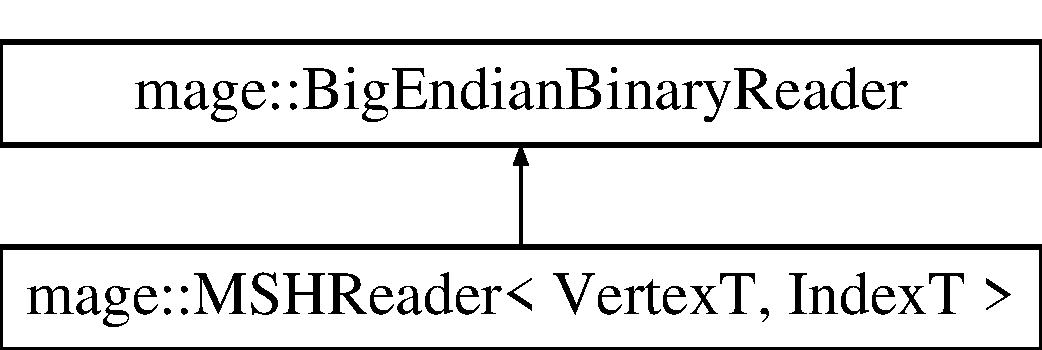
\includegraphics[height=2.000000cm]{classmage_1_1_m_s_h_reader}
\end{center}
\end{figure}
\subsection*{Public Member Functions}
\begin{DoxyCompactItemize}
\item 
\hyperlink{classmage_1_1_m_s_h_reader_af1254630a9770015c7b62d88eb5251bb}{M\+S\+H\+Reader} (vector$<$ VertexT $>$ \&vertices, vector$<$ IndexT $>$ \&indices)
\item 
\hyperlink{classmage_1_1_m_s_h_reader_aa33b8f059752b9aa321e8d227fe811bd}{M\+S\+H\+Reader} (const \hyperlink{classmage_1_1_m_s_h_reader}{M\+S\+H\+Reader} \&reader)=delete
\item 
\hyperlink{classmage_1_1_m_s_h_reader_a3c34d4fed2a717a2589dff1609f7c8b4}{M\+S\+H\+Reader} (\hyperlink{classmage_1_1_m_s_h_reader}{M\+S\+H\+Reader} \&\&reader)
\item 
virtual \hyperlink{classmage_1_1_m_s_h_reader_a6e1f882fa81362f744f438a1f992b182}{$\sim$\+M\+S\+H\+Reader} ()
\item 
\hyperlink{classmage_1_1_m_s_h_reader}{M\+S\+H\+Reader} \& \hyperlink{classmage_1_1_m_s_h_reader_abbe36c0fcfbf0c909a45f974c34ecc3a}{operator=} (const \hyperlink{classmage_1_1_m_s_h_reader}{M\+S\+H\+Reader} \&reader)=delete
\item 
\hyperlink{classmage_1_1_m_s_h_reader}{M\+S\+H\+Reader} \& \hyperlink{classmage_1_1_m_s_h_reader_a0f014d780eaa5477aa7206db51fede2f}{operator=} (\hyperlink{classmage_1_1_m_s_h_reader}{M\+S\+H\+Reader} \&\&reader)=delete
\end{DoxyCompactItemize}
\subsection*{Private Member Functions}
\begin{DoxyCompactItemize}
\item 
virtual void \hyperlink{classmage_1_1_m_s_h_reader_a26b60060bf61183fb5758a4725c6a205}{Read} () override
\item 
bool \hyperlink{classmage_1_1_m_s_h_reader_a2bc2f2a6410de600c39336f4516a5231}{Is\+Header\+Valid} ()
\end{DoxyCompactItemize}
\subsection*{Private Attributes}
\begin{DoxyCompactItemize}
\item 
vector$<$ VertexT $>$ \& \hyperlink{classmage_1_1_m_s_h_reader_a6b4c0fbf02771cb7bc0ebcb685c3c30b}{m\+\_\+vertices}
\item 
vector$<$ IndexT $>$ \& \hyperlink{classmage_1_1_m_s_h_reader_ae96b703b052eb9951872683e17ab11ae}{m\+\_\+indices}
\end{DoxyCompactItemize}
\subsection*{Additional Inherited Members}


\subsection{Detailed Description}
\subsubsection*{template$<$typename VertexT, typename IndexT$>$\newline
class mage\+::\+M\+S\+H\+Reader$<$ Vertex\+T, Index\+T $>$}

A class of M\+SH file readers for reading meshes.


\begin{DoxyTemplParams}{Template Parameters}
{\em VertexT} & The vertex type. \\
\hline
{\em IndexT} & The index type. \\
\hline
\end{DoxyTemplParams}


\subsection{Constructor \& Destructor Documentation}
\hypertarget{classmage_1_1_m_s_h_reader_af1254630a9770015c7b62d88eb5251bb}{}\label{classmage_1_1_m_s_h_reader_af1254630a9770015c7b62d88eb5251bb} 
\index{mage\+::\+M\+S\+H\+Reader@{mage\+::\+M\+S\+H\+Reader}!M\+S\+H\+Reader@{M\+S\+H\+Reader}}
\index{M\+S\+H\+Reader@{M\+S\+H\+Reader}!mage\+::\+M\+S\+H\+Reader@{mage\+::\+M\+S\+H\+Reader}}
\subsubsection{\texorpdfstring{M\+S\+H\+Reader()}{MSHReader()}\hspace{0.1cm}{\footnotesize\ttfamily [1/3]}}
{\footnotesize\ttfamily template$<$typename VertexT , typename IndexT $>$ \\
\hyperlink{classmage_1_1_m_s_h_reader}{mage\+::\+M\+S\+H\+Reader}$<$ VertexT, IndexT $>$\+::\hyperlink{classmage_1_1_m_s_h_reader}{M\+S\+H\+Reader} (\begin{DoxyParamCaption}\item[{vector$<$ VertexT $>$ \&}]{vertices,  }\item[{vector$<$ IndexT $>$ \&}]{indices }\end{DoxyParamCaption})\hspace{0.3cm}{\ttfamily [explicit]}}

Constructs a M\+SH reader.


\begin{DoxyParams}[1]{Parameters}
\mbox{\tt in}  & {\em vertices} & A reference to a vector for storing the read vertices from file. \\
\hline
\mbox{\tt in}  & {\em indices} & A reference to a vector for storing the read indices from file. \\
\hline
\end{DoxyParams}
\hypertarget{classmage_1_1_m_s_h_reader_aa33b8f059752b9aa321e8d227fe811bd}{}\label{classmage_1_1_m_s_h_reader_aa33b8f059752b9aa321e8d227fe811bd} 
\index{mage\+::\+M\+S\+H\+Reader@{mage\+::\+M\+S\+H\+Reader}!M\+S\+H\+Reader@{M\+S\+H\+Reader}}
\index{M\+S\+H\+Reader@{M\+S\+H\+Reader}!mage\+::\+M\+S\+H\+Reader@{mage\+::\+M\+S\+H\+Reader}}
\subsubsection{\texorpdfstring{M\+S\+H\+Reader()}{MSHReader()}\hspace{0.1cm}{\footnotesize\ttfamily [2/3]}}
{\footnotesize\ttfamily template$<$typename VertexT , typename IndexT $>$ \\
\hyperlink{classmage_1_1_m_s_h_reader}{mage\+::\+M\+S\+H\+Reader}$<$ VertexT, IndexT $>$\+::\hyperlink{classmage_1_1_m_s_h_reader}{M\+S\+H\+Reader} (\begin{DoxyParamCaption}\item[{const \hyperlink{classmage_1_1_m_s_h_reader}{M\+S\+H\+Reader}$<$ VertexT, IndexT $>$ \&}]{reader }\end{DoxyParamCaption})\hspace{0.3cm}{\ttfamily [delete]}}

Constructs a M\+SH reader from the given M\+SH reader.


\begin{DoxyParams}[1]{Parameters}
\mbox{\tt in}  & {\em reader} & A reference to the M\+SH reader to copy. \\
\hline
\end{DoxyParams}
\hypertarget{classmage_1_1_m_s_h_reader_a3c34d4fed2a717a2589dff1609f7c8b4}{}\label{classmage_1_1_m_s_h_reader_a3c34d4fed2a717a2589dff1609f7c8b4} 
\index{mage\+::\+M\+S\+H\+Reader@{mage\+::\+M\+S\+H\+Reader}!M\+S\+H\+Reader@{M\+S\+H\+Reader}}
\index{M\+S\+H\+Reader@{M\+S\+H\+Reader}!mage\+::\+M\+S\+H\+Reader@{mage\+::\+M\+S\+H\+Reader}}
\subsubsection{\texorpdfstring{M\+S\+H\+Reader()}{MSHReader()}\hspace{0.1cm}{\footnotesize\ttfamily [3/3]}}
{\footnotesize\ttfamily template$<$typename VertexT , typename IndexT $>$ \\
\hyperlink{classmage_1_1_m_s_h_reader}{mage\+::\+M\+S\+H\+Reader}$<$ VertexT, IndexT $>$\+::\hyperlink{classmage_1_1_m_s_h_reader}{M\+S\+H\+Reader} (\begin{DoxyParamCaption}\item[{\hyperlink{classmage_1_1_m_s_h_reader}{M\+S\+H\+Reader}$<$ VertexT, IndexT $>$ \&\&}]{reader }\end{DoxyParamCaption})}

Constructs a M\+SH reader by moving the given M\+SH reader.


\begin{DoxyParams}[1]{Parameters}
\mbox{\tt in}  & {\em reader} & A reference to the M\+SH reader to move. \\
\hline
\end{DoxyParams}
\hypertarget{classmage_1_1_m_s_h_reader_a6e1f882fa81362f744f438a1f992b182}{}\label{classmage_1_1_m_s_h_reader_a6e1f882fa81362f744f438a1f992b182} 
\index{mage\+::\+M\+S\+H\+Reader@{mage\+::\+M\+S\+H\+Reader}!````~M\+S\+H\+Reader@{$\sim$\+M\+S\+H\+Reader}}
\index{````~M\+S\+H\+Reader@{$\sim$\+M\+S\+H\+Reader}!mage\+::\+M\+S\+H\+Reader@{mage\+::\+M\+S\+H\+Reader}}
\subsubsection{\texorpdfstring{$\sim$\+M\+S\+H\+Reader()}{~MSHReader()}}
{\footnotesize\ttfamily template$<$typename VertexT , typename IndexT $>$ \\
virtual \hyperlink{classmage_1_1_m_s_h_reader}{mage\+::\+M\+S\+H\+Reader}$<$ VertexT, IndexT $>$\+::$\sim$\hyperlink{classmage_1_1_m_s_h_reader}{M\+S\+H\+Reader} (\begin{DoxyParamCaption}{ }\end{DoxyParamCaption})\hspace{0.3cm}{\ttfamily [virtual]}}

Destructs this M\+SH reader. 

\subsection{Member Function Documentation}
\hypertarget{classmage_1_1_m_s_h_reader_a2bc2f2a6410de600c39336f4516a5231}{}\label{classmage_1_1_m_s_h_reader_a2bc2f2a6410de600c39336f4516a5231} 
\index{mage\+::\+M\+S\+H\+Reader@{mage\+::\+M\+S\+H\+Reader}!Is\+Header\+Valid@{Is\+Header\+Valid}}
\index{Is\+Header\+Valid@{Is\+Header\+Valid}!mage\+::\+M\+S\+H\+Reader@{mage\+::\+M\+S\+H\+Reader}}
\subsubsection{\texorpdfstring{Is\+Header\+Valid()}{IsHeaderValid()}}
{\footnotesize\ttfamily template$<$typename VertexT , typename IndexT $>$ \\
bool \hyperlink{classmage_1_1_m_s_h_reader}{mage\+::\+M\+S\+H\+Reader}$<$ VertexT, IndexT $>$\+::Is\+Header\+Valid (\begin{DoxyParamCaption}{ }\end{DoxyParamCaption})\hspace{0.3cm}{\ttfamily [private]}}

Checks whether the header of the file is valid.

\begin{DoxyReturn}{Returns}
{\ttfamily true} if the header of the file is valid. {\ttfamily false} otherwise. 
\end{DoxyReturn}
\hypertarget{classmage_1_1_m_s_h_reader_abbe36c0fcfbf0c909a45f974c34ecc3a}{}\label{classmage_1_1_m_s_h_reader_abbe36c0fcfbf0c909a45f974c34ecc3a} 
\index{mage\+::\+M\+S\+H\+Reader@{mage\+::\+M\+S\+H\+Reader}!operator=@{operator=}}
\index{operator=@{operator=}!mage\+::\+M\+S\+H\+Reader@{mage\+::\+M\+S\+H\+Reader}}
\subsubsection{\texorpdfstring{operator=()}{operator=()}\hspace{0.1cm}{\footnotesize\ttfamily [1/2]}}
{\footnotesize\ttfamily template$<$typename VertexT , typename IndexT $>$ \\
\hyperlink{classmage_1_1_m_s_h_reader}{M\+S\+H\+Reader}\& \hyperlink{classmage_1_1_m_s_h_reader}{mage\+::\+M\+S\+H\+Reader}$<$ VertexT, IndexT $>$\+::operator= (\begin{DoxyParamCaption}\item[{const \hyperlink{classmage_1_1_m_s_h_reader}{M\+S\+H\+Reader}$<$ VertexT, IndexT $>$ \&}]{reader }\end{DoxyParamCaption})\hspace{0.3cm}{\ttfamily [delete]}}

Copies the given M\+SH reader to this M\+SH reader.


\begin{DoxyParams}[1]{Parameters}
\mbox{\tt in}  & {\em reader} & A reference to a M\+SH reader to copy. \\
\hline
\end{DoxyParams}
\begin{DoxyReturn}{Returns}
A reference to the copy of the given M\+SH reader (i.\+e. this M\+SH reader). 
\end{DoxyReturn}
\hypertarget{classmage_1_1_m_s_h_reader_a0f014d780eaa5477aa7206db51fede2f}{}\label{classmage_1_1_m_s_h_reader_a0f014d780eaa5477aa7206db51fede2f} 
\index{mage\+::\+M\+S\+H\+Reader@{mage\+::\+M\+S\+H\+Reader}!operator=@{operator=}}
\index{operator=@{operator=}!mage\+::\+M\+S\+H\+Reader@{mage\+::\+M\+S\+H\+Reader}}
\subsubsection{\texorpdfstring{operator=()}{operator=()}\hspace{0.1cm}{\footnotesize\ttfamily [2/2]}}
{\footnotesize\ttfamily template$<$typename VertexT , typename IndexT $>$ \\
\hyperlink{classmage_1_1_m_s_h_reader}{M\+S\+H\+Reader}\& \hyperlink{classmage_1_1_m_s_h_reader}{mage\+::\+M\+S\+H\+Reader}$<$ VertexT, IndexT $>$\+::operator= (\begin{DoxyParamCaption}\item[{\hyperlink{classmage_1_1_m_s_h_reader}{M\+S\+H\+Reader}$<$ VertexT, IndexT $>$ \&\&}]{reader }\end{DoxyParamCaption})\hspace{0.3cm}{\ttfamily [delete]}}

Moves the given M\+SH reader to this M\+SH reader.


\begin{DoxyParams}[1]{Parameters}
\mbox{\tt in}  & {\em reader} & A reference to a M\+SH reader to move. \\
\hline
\end{DoxyParams}
\begin{DoxyReturn}{Returns}
A reference to the moved M\+SH reader (i.\+e. this M\+SH reader). 
\end{DoxyReturn}
\hypertarget{classmage_1_1_m_s_h_reader_a26b60060bf61183fb5758a4725c6a205}{}\label{classmage_1_1_m_s_h_reader_a26b60060bf61183fb5758a4725c6a205} 
\index{mage\+::\+M\+S\+H\+Reader@{mage\+::\+M\+S\+H\+Reader}!Read@{Read}}
\index{Read@{Read}!mage\+::\+M\+S\+H\+Reader@{mage\+::\+M\+S\+H\+Reader}}
\subsubsection{\texorpdfstring{Read()}{Read()}}
{\footnotesize\ttfamily template$<$typename VertexT , typename IndexT $>$ \\
virtual void \hyperlink{classmage_1_1_m_s_h_reader}{mage\+::\+M\+S\+H\+Reader}$<$ VertexT, IndexT $>$\+::Read (\begin{DoxyParamCaption}{ }\end{DoxyParamCaption})\hspace{0.3cm}{\ttfamily [override]}, {\ttfamily [private]}, {\ttfamily [virtual]}}

Starts reading.


\begin{DoxyExceptions}{Exceptions}
{\em \hyperlink{classmage_1_1_formatted_exception}{Formatted\+Exception}} & Failed to read to the given file. \\
\hline
\end{DoxyExceptions}


Implements \hyperlink{classmage_1_1_big_endian_binary_reader_af072965dea0319d6366b21cc6562bbf9}{mage\+::\+Big\+Endian\+Binary\+Reader}.



\subsection{Member Data Documentation}
\hypertarget{classmage_1_1_m_s_h_reader_ae96b703b052eb9951872683e17ab11ae}{}\label{classmage_1_1_m_s_h_reader_ae96b703b052eb9951872683e17ab11ae} 
\index{mage\+::\+M\+S\+H\+Reader@{mage\+::\+M\+S\+H\+Reader}!m\+\_\+indices@{m\+\_\+indices}}
\index{m\+\_\+indices@{m\+\_\+indices}!mage\+::\+M\+S\+H\+Reader@{mage\+::\+M\+S\+H\+Reader}}
\subsubsection{\texorpdfstring{m\+\_\+indices}{m\_indices}}
{\footnotesize\ttfamily template$<$typename VertexT , typename IndexT $>$ \\
vector$<$ IndexT $>$\& \hyperlink{classmage_1_1_m_s_h_reader}{mage\+::\+M\+S\+H\+Reader}$<$ VertexT, IndexT $>$\+::m\+\_\+indices\hspace{0.3cm}{\ttfamily [private]}}

A reference to a vector containing the read indices of this M\+SH reader. \hypertarget{classmage_1_1_m_s_h_reader_a6b4c0fbf02771cb7bc0ebcb685c3c30b}{}\label{classmage_1_1_m_s_h_reader_a6b4c0fbf02771cb7bc0ebcb685c3c30b} 
\index{mage\+::\+M\+S\+H\+Reader@{mage\+::\+M\+S\+H\+Reader}!m\+\_\+vertices@{m\+\_\+vertices}}
\index{m\+\_\+vertices@{m\+\_\+vertices}!mage\+::\+M\+S\+H\+Reader@{mage\+::\+M\+S\+H\+Reader}}
\subsubsection{\texorpdfstring{m\+\_\+vertices}{m\_vertices}}
{\footnotesize\ttfamily template$<$typename VertexT , typename IndexT $>$ \\
vector$<$ VertexT $>$\& \hyperlink{classmage_1_1_m_s_h_reader}{mage\+::\+M\+S\+H\+Reader}$<$ VertexT, IndexT $>$\+::m\+\_\+vertices\hspace{0.3cm}{\ttfamily [private]}}

A reference to a vector containing the read vertices of this M\+SH reader. 
\hypertarget{classmage_1_1_m_s_h_writer}{}\section{mage\+:\+:M\+S\+H\+Writer$<$ VertexT, IndexT $>$ Class Template Reference}
\label{classmage_1_1_m_s_h_writer}\index{mage\+::\+M\+S\+H\+Writer$<$ Vertex\+T, Index\+T $>$@{mage\+::\+M\+S\+H\+Writer$<$ Vertex\+T, Index\+T $>$}}


{\ttfamily \#include $<$msh\+\_\+writer.\+hpp$>$}

Inheritance diagram for mage\+:\+:M\+S\+H\+Writer$<$ VertexT, IndexT $>$\+:\begin{figure}[H]
\begin{center}
\leavevmode
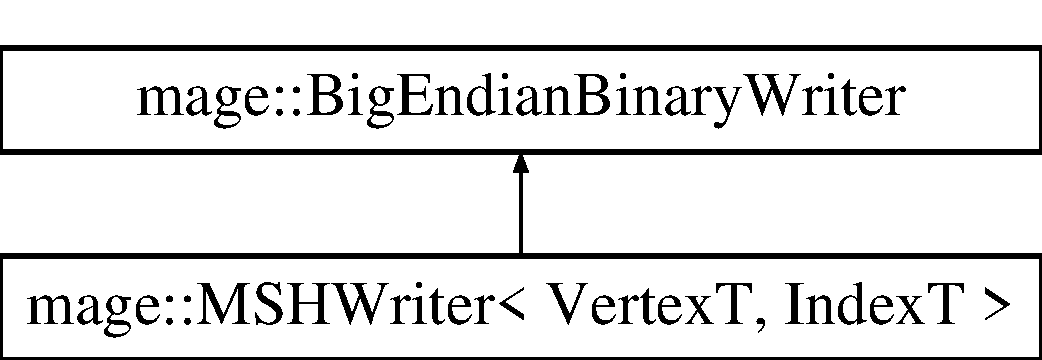
\includegraphics[height=2.000000cm]{classmage_1_1_m_s_h_writer}
\end{center}
\end{figure}
\subsection*{Public Member Functions}
\begin{DoxyCompactItemize}
\item 
\hyperlink{classmage_1_1_m_s_h_writer_a4b74333888706ab61c9d6c3b6fefd4c5}{M\+S\+H\+Writer} (const vector$<$ VertexT $>$ \&vertices, const vector$<$ IndexT $>$ \&indices)
\item 
\hyperlink{classmage_1_1_m_s_h_writer_a2d806cd90f75130775a29ccc5a2f92be}{M\+S\+H\+Writer} (const \hyperlink{classmage_1_1_m_s_h_writer}{M\+S\+H\+Writer}$<$ VertexT, IndexT $>$ \&writer)=delete
\item 
\hyperlink{classmage_1_1_m_s_h_writer_a69988e7b0eea3b4e9053455955acaec5}{M\+S\+H\+Writer} (\hyperlink{classmage_1_1_m_s_h_writer}{M\+S\+H\+Writer}$<$ VertexT, IndexT $>$ \&\&writer)
\item 
virtual \hyperlink{classmage_1_1_m_s_h_writer_a75e57bab20c8928b230305118bf9aa5f}{$\sim$\+M\+S\+H\+Writer} ()
\item 
\hyperlink{classmage_1_1_m_s_h_writer}{M\+S\+H\+Writer}$<$ VertexT, IndexT $>$ \& \hyperlink{classmage_1_1_m_s_h_writer_a2c44587daf98ba5565ac883878b61c9e}{operator=} (const \hyperlink{classmage_1_1_m_s_h_writer}{M\+S\+H\+Writer}$<$ VertexT, IndexT $>$ \&writer)=delete
\item 
\hyperlink{classmage_1_1_m_s_h_writer}{M\+S\+H\+Writer}$<$ VertexT, IndexT $>$ \& \hyperlink{classmage_1_1_m_s_h_writer_ae1fddfee32bfcf1e6b9f031749cdbbcb}{operator=} (\hyperlink{classmage_1_1_m_s_h_writer}{M\+S\+H\+Writer}$<$ VertexT, IndexT $>$ \&\&writer)=delete
\end{DoxyCompactItemize}
\subsection*{Private Member Functions}
\begin{DoxyCompactItemize}
\item 
virtual void \hyperlink{classmage_1_1_m_s_h_writer_ab97c9570c45bff97d88700d0dcf3ed75}{Write} () override
\end{DoxyCompactItemize}
\subsection*{Private Attributes}
\begin{DoxyCompactItemize}
\item 
const vector$<$ VertexT $>$ \& \hyperlink{classmage_1_1_m_s_h_writer_ac0fc94011fd8200a83082201eee5ded5}{m\+\_\+vertices}
\item 
const vector$<$ IndexT $>$ \& \hyperlink{classmage_1_1_m_s_h_writer_a01cf9e635af683a1a9d6fa347b219dee}{m\+\_\+indices}
\end{DoxyCompactItemize}
\subsection*{Additional Inherited Members}


\subsection{Detailed Description}
\subsubsection*{template$<$typename VertexT, typename IndexT$>$\newline
class mage\+::\+M\+S\+H\+Writer$<$ Vertex\+T, Index\+T $>$}

A class of M\+SH file writers for writing meshes.


\begin{DoxyTemplParams}{Template Parameters}
{\em VertexT} & The vertex type. \\
\hline
{\em IndexT} & The index type. \\
\hline
\end{DoxyTemplParams}


\subsection{Constructor \& Destructor Documentation}
\hypertarget{classmage_1_1_m_s_h_writer_a4b74333888706ab61c9d6c3b6fefd4c5}{}\label{classmage_1_1_m_s_h_writer_a4b74333888706ab61c9d6c3b6fefd4c5} 
\index{mage\+::\+M\+S\+H\+Writer@{mage\+::\+M\+S\+H\+Writer}!M\+S\+H\+Writer@{M\+S\+H\+Writer}}
\index{M\+S\+H\+Writer@{M\+S\+H\+Writer}!mage\+::\+M\+S\+H\+Writer@{mage\+::\+M\+S\+H\+Writer}}
\subsubsection{\texorpdfstring{M\+S\+H\+Writer()}{MSHWriter()}\hspace{0.1cm}{\footnotesize\ttfamily [1/3]}}
{\footnotesize\ttfamily template$<$typename VertexT , typename IndexT $>$ \\
\hyperlink{classmage_1_1_m_s_h_writer}{mage\+::\+M\+S\+H\+Writer}$<$ VertexT, IndexT $>$\+::\hyperlink{classmage_1_1_m_s_h_writer}{M\+S\+H\+Writer} (\begin{DoxyParamCaption}\item[{const vector$<$ VertexT $>$ \&}]{vertices,  }\item[{const vector$<$ IndexT $>$ \&}]{indices }\end{DoxyParamCaption})\hspace{0.3cm}{\ttfamily [explicit]}}

Constructs a M\+SH writer.


\begin{DoxyParams}[1]{Parameters}
\mbox{\tt in}  & {\em vertices} & A reference to a vector containing the vertices. \\
\hline
\mbox{\tt in}  & {\em indices} & A reference to a vector containing the indices. \\
\hline
\end{DoxyParams}
\hypertarget{classmage_1_1_m_s_h_writer_a2d806cd90f75130775a29ccc5a2f92be}{}\label{classmage_1_1_m_s_h_writer_a2d806cd90f75130775a29ccc5a2f92be} 
\index{mage\+::\+M\+S\+H\+Writer@{mage\+::\+M\+S\+H\+Writer}!M\+S\+H\+Writer@{M\+S\+H\+Writer}}
\index{M\+S\+H\+Writer@{M\+S\+H\+Writer}!mage\+::\+M\+S\+H\+Writer@{mage\+::\+M\+S\+H\+Writer}}
\subsubsection{\texorpdfstring{M\+S\+H\+Writer()}{MSHWriter()}\hspace{0.1cm}{\footnotesize\ttfamily [2/3]}}
{\footnotesize\ttfamily template$<$typename VertexT , typename IndexT $>$ \\
\hyperlink{classmage_1_1_m_s_h_writer}{mage\+::\+M\+S\+H\+Writer}$<$ VertexT, IndexT $>$\+::\hyperlink{classmage_1_1_m_s_h_writer}{M\+S\+H\+Writer} (\begin{DoxyParamCaption}\item[{const \hyperlink{classmage_1_1_m_s_h_writer}{M\+S\+H\+Writer}$<$ VertexT, IndexT $>$ \&}]{writer }\end{DoxyParamCaption})\hspace{0.3cm}{\ttfamily [delete]}}

Constructs a M\+SH writer from the given M\+SH writer.


\begin{DoxyParams}[1]{Parameters}
\mbox{\tt in}  & {\em writer} & A reference to the M\+SH writer to copy. \\
\hline
\end{DoxyParams}
\hypertarget{classmage_1_1_m_s_h_writer_a69988e7b0eea3b4e9053455955acaec5}{}\label{classmage_1_1_m_s_h_writer_a69988e7b0eea3b4e9053455955acaec5} 
\index{mage\+::\+M\+S\+H\+Writer@{mage\+::\+M\+S\+H\+Writer}!M\+S\+H\+Writer@{M\+S\+H\+Writer}}
\index{M\+S\+H\+Writer@{M\+S\+H\+Writer}!mage\+::\+M\+S\+H\+Writer@{mage\+::\+M\+S\+H\+Writer}}
\subsubsection{\texorpdfstring{M\+S\+H\+Writer()}{MSHWriter()}\hspace{0.1cm}{\footnotesize\ttfamily [3/3]}}
{\footnotesize\ttfamily template$<$typename VertexT , typename IndexT $>$ \\
\hyperlink{classmage_1_1_m_s_h_writer}{mage\+::\+M\+S\+H\+Writer}$<$ VertexT, IndexT $>$\+::\hyperlink{classmage_1_1_m_s_h_writer}{M\+S\+H\+Writer} (\begin{DoxyParamCaption}\item[{\hyperlink{classmage_1_1_m_s_h_writer}{M\+S\+H\+Writer}$<$ VertexT, IndexT $>$ \&\&}]{writer }\end{DoxyParamCaption})}

Constructs a M\+SH writer by moving the given M\+SH writer.


\begin{DoxyParams}[1]{Parameters}
\mbox{\tt in}  & {\em writer} & A reference to the M\+SH writer to move. \\
\hline
\end{DoxyParams}
\hypertarget{classmage_1_1_m_s_h_writer_a75e57bab20c8928b230305118bf9aa5f}{}\label{classmage_1_1_m_s_h_writer_a75e57bab20c8928b230305118bf9aa5f} 
\index{mage\+::\+M\+S\+H\+Writer@{mage\+::\+M\+S\+H\+Writer}!````~M\+S\+H\+Writer@{$\sim$\+M\+S\+H\+Writer}}
\index{````~M\+S\+H\+Writer@{$\sim$\+M\+S\+H\+Writer}!mage\+::\+M\+S\+H\+Writer@{mage\+::\+M\+S\+H\+Writer}}
\subsubsection{\texorpdfstring{$\sim$\+M\+S\+H\+Writer()}{~MSHWriter()}}
{\footnotesize\ttfamily template$<$typename VertexT , typename IndexT $>$ \\
virtual \hyperlink{classmage_1_1_m_s_h_writer}{mage\+::\+M\+S\+H\+Writer}$<$ VertexT, IndexT $>$\+::$\sim$\hyperlink{classmage_1_1_m_s_h_writer}{M\+S\+H\+Writer} (\begin{DoxyParamCaption}{ }\end{DoxyParamCaption})\hspace{0.3cm}{\ttfamily [virtual]}}

Destructs this M\+SH writer. 

\subsection{Member Function Documentation}
\hypertarget{classmage_1_1_m_s_h_writer_a2c44587daf98ba5565ac883878b61c9e}{}\label{classmage_1_1_m_s_h_writer_a2c44587daf98ba5565ac883878b61c9e} 
\index{mage\+::\+M\+S\+H\+Writer@{mage\+::\+M\+S\+H\+Writer}!operator=@{operator=}}
\index{operator=@{operator=}!mage\+::\+M\+S\+H\+Writer@{mage\+::\+M\+S\+H\+Writer}}
\subsubsection{\texorpdfstring{operator=()}{operator=()}\hspace{0.1cm}{\footnotesize\ttfamily [1/2]}}
{\footnotesize\ttfamily template$<$typename VertexT , typename IndexT $>$ \\
\hyperlink{classmage_1_1_m_s_h_writer}{M\+S\+H\+Writer}$<$ VertexT, IndexT $>$\& \hyperlink{classmage_1_1_m_s_h_writer}{mage\+::\+M\+S\+H\+Writer}$<$ VertexT, IndexT $>$\+::operator= (\begin{DoxyParamCaption}\item[{const \hyperlink{classmage_1_1_m_s_h_writer}{M\+S\+H\+Writer}$<$ VertexT, IndexT $>$ \&}]{writer }\end{DoxyParamCaption})\hspace{0.3cm}{\ttfamily [delete]}}

Copies the given M\+SH writer to this M\+SH writer.


\begin{DoxyParams}[1]{Parameters}
\mbox{\tt in}  & {\em writer} & A reference to a M\+SH writer to copy. \\
\hline
\end{DoxyParams}
\begin{DoxyReturn}{Returns}
A reference to the copy of the given M\+SH writer (i.\+e. this M\+SH writer). 
\end{DoxyReturn}
\hypertarget{classmage_1_1_m_s_h_writer_ae1fddfee32bfcf1e6b9f031749cdbbcb}{}\label{classmage_1_1_m_s_h_writer_ae1fddfee32bfcf1e6b9f031749cdbbcb} 
\index{mage\+::\+M\+S\+H\+Writer@{mage\+::\+M\+S\+H\+Writer}!operator=@{operator=}}
\index{operator=@{operator=}!mage\+::\+M\+S\+H\+Writer@{mage\+::\+M\+S\+H\+Writer}}
\subsubsection{\texorpdfstring{operator=()}{operator=()}\hspace{0.1cm}{\footnotesize\ttfamily [2/2]}}
{\footnotesize\ttfamily template$<$typename VertexT , typename IndexT $>$ \\
\hyperlink{classmage_1_1_m_s_h_writer}{M\+S\+H\+Writer}$<$ VertexT, IndexT $>$\& \hyperlink{classmage_1_1_m_s_h_writer}{mage\+::\+M\+S\+H\+Writer}$<$ VertexT, IndexT $>$\+::operator= (\begin{DoxyParamCaption}\item[{\hyperlink{classmage_1_1_m_s_h_writer}{M\+S\+H\+Writer}$<$ VertexT, IndexT $>$ \&\&}]{writer }\end{DoxyParamCaption})\hspace{0.3cm}{\ttfamily [delete]}}

Moves the given M\+SH writer to this M\+SH writer.


\begin{DoxyParams}[1]{Parameters}
\mbox{\tt in}  & {\em writer} & A reference to a M\+SH writer to move. \\
\hline
\end{DoxyParams}
\begin{DoxyReturn}{Returns}
A reference to the moved M\+SH writer (i.\+e. this M\+SH writer). 
\end{DoxyReturn}
\hypertarget{classmage_1_1_m_s_h_writer_ab97c9570c45bff97d88700d0dcf3ed75}{}\label{classmage_1_1_m_s_h_writer_ab97c9570c45bff97d88700d0dcf3ed75} 
\index{mage\+::\+M\+S\+H\+Writer@{mage\+::\+M\+S\+H\+Writer}!Write@{Write}}
\index{Write@{Write}!mage\+::\+M\+S\+H\+Writer@{mage\+::\+M\+S\+H\+Writer}}
\subsubsection{\texorpdfstring{Write()}{Write()}}
{\footnotesize\ttfamily template$<$typename VertexT , typename IndexT $>$ \\
virtual void \hyperlink{classmage_1_1_m_s_h_writer}{mage\+::\+M\+S\+H\+Writer}$<$ VertexT, IndexT $>$\+::Write (\begin{DoxyParamCaption}{ }\end{DoxyParamCaption})\hspace{0.3cm}{\ttfamily [override]}, {\ttfamily [private]}, {\ttfamily [virtual]}}

Starts writing.


\begin{DoxyExceptions}{Exceptions}
{\em \hyperlink{classmage_1_1_formatted_exception}{Formatted\+Exception}} & Failed to write. \\
\hline
\end{DoxyExceptions}


Implements \hyperlink{classmage_1_1_big_endian_binary_writer_ae6ee6613e629971502324cffc944795d}{mage\+::\+Big\+Endian\+Binary\+Writer}.



\subsection{Member Data Documentation}
\hypertarget{classmage_1_1_m_s_h_writer_a01cf9e635af683a1a9d6fa347b219dee}{}\label{classmage_1_1_m_s_h_writer_a01cf9e635af683a1a9d6fa347b219dee} 
\index{mage\+::\+M\+S\+H\+Writer@{mage\+::\+M\+S\+H\+Writer}!m\+\_\+indices@{m\+\_\+indices}}
\index{m\+\_\+indices@{m\+\_\+indices}!mage\+::\+M\+S\+H\+Writer@{mage\+::\+M\+S\+H\+Writer}}
\subsubsection{\texorpdfstring{m\+\_\+indices}{m\_indices}}
{\footnotesize\ttfamily template$<$typename VertexT , typename IndexT $>$ \\
const vector$<$ IndexT $>$\& \hyperlink{classmage_1_1_m_s_h_writer}{mage\+::\+M\+S\+H\+Writer}$<$ VertexT, IndexT $>$\+::m\+\_\+indices\hspace{0.3cm}{\ttfamily [private]}}

A reference to a vector containing the indices to write by this VS writer. \hypertarget{classmage_1_1_m_s_h_writer_ac0fc94011fd8200a83082201eee5ded5}{}\label{classmage_1_1_m_s_h_writer_ac0fc94011fd8200a83082201eee5ded5} 
\index{mage\+::\+M\+S\+H\+Writer@{mage\+::\+M\+S\+H\+Writer}!m\+\_\+vertices@{m\+\_\+vertices}}
\index{m\+\_\+vertices@{m\+\_\+vertices}!mage\+::\+M\+S\+H\+Writer@{mage\+::\+M\+S\+H\+Writer}}
\subsubsection{\texorpdfstring{m\+\_\+vertices}{m\_vertices}}
{\footnotesize\ttfamily template$<$typename VertexT , typename IndexT $>$ \\
const vector$<$ VertexT $>$\& \hyperlink{classmage_1_1_m_s_h_writer}{mage\+::\+M\+S\+H\+Writer}$<$ VertexT, IndexT $>$\+::m\+\_\+vertices\hspace{0.3cm}{\ttfamily [private]}}

A reference to a vector containing the vertices to write by this VS writer. 
\hypertarget{classmage_1_1_m_t_l_reader}{}\section{mage\+:\+:M\+T\+L\+Reader Class Reference}
\label{classmage_1_1_m_t_l_reader}\index{mage\+::\+M\+T\+L\+Reader@{mage\+::\+M\+T\+L\+Reader}}


{\ttfamily \#include $<$mtl\+\_\+reader.\+hpp$>$}

Inheritance diagram for mage\+:\+:M\+T\+L\+Reader\+:\begin{figure}[H]
\begin{center}
\leavevmode
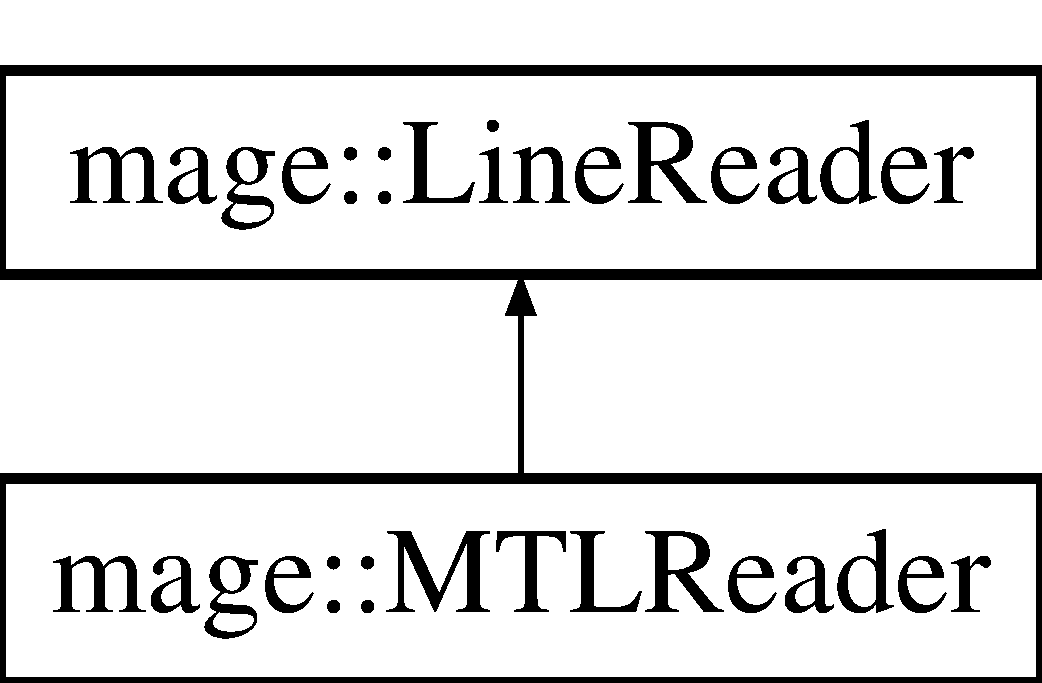
\includegraphics[height=2.000000cm]{classmage_1_1_m_t_l_reader}
\end{center}
\end{figure}
\subsection*{Public Member Functions}
\begin{DoxyCompactItemize}
\item 
\hyperlink{classmage_1_1_m_t_l_reader_a924f813cca170e2592a6e7d2a3255be8}{M\+T\+L\+Reader} (vector$<$ \hyperlink{structmage_1_1_material}{Material} $>$ \&material\+\_\+buffer)
\item 
\hyperlink{classmage_1_1_m_t_l_reader_adcc57156298b2198c24c041503df2e6d}{M\+T\+L\+Reader} (const \hyperlink{classmage_1_1_m_t_l_reader}{M\+T\+L\+Reader} \&reader)=delete
\item 
\hyperlink{classmage_1_1_m_t_l_reader_a415057f591e54e91658c77092b7b2d4e}{M\+T\+L\+Reader} (\hyperlink{classmage_1_1_m_t_l_reader}{M\+T\+L\+Reader} \&\&reader)
\item 
virtual \hyperlink{classmage_1_1_m_t_l_reader_a9d3216b2637bc9402d37c7438860f542}{$\sim$\+M\+T\+L\+Reader} ()
\item 
\hyperlink{classmage_1_1_m_t_l_reader}{M\+T\+L\+Reader} \& \hyperlink{classmage_1_1_m_t_l_reader_ae239ac085326919918a418edabcafeae}{operator=} (const \hyperlink{classmage_1_1_m_t_l_reader}{M\+T\+L\+Reader} \&reader)=delete
\item 
\hyperlink{classmage_1_1_m_t_l_reader}{M\+T\+L\+Reader} \& \hyperlink{classmage_1_1_m_t_l_reader_aa777389ff4a3cd2f1df2cbf5c6da708e}{operator=} (\hyperlink{classmage_1_1_m_t_l_reader}{M\+T\+L\+Reader} \&\&reader)=delete
\end{DoxyCompactItemize}
\subsection*{Private Member Functions}
\begin{DoxyCompactItemize}
\item 
virtual void \hyperlink{classmage_1_1_m_t_l_reader_ac3981549364be195f96b32cfafc8b147}{Read\+Line} (char $\ast$line) override
\item 
void \hyperlink{classmage_1_1_m_t_l_reader_a53494ca5e0f905b97227b21711a1686a}{Read\+M\+T\+L\+Material\+Name} ()
\item 
void \hyperlink{classmage_1_1_m_t_l_reader_a4d5819606b5ea81862852587b2e1511b}{Read\+M\+T\+L\+Transmission\+Filter} ()
\item 
void \hyperlink{classmage_1_1_m_t_l_reader_a7137e998979a79fe258f226bfbda669e}{Read\+M\+T\+L\+Ambient\+Reflectivity} ()
\item 
void \hyperlink{classmage_1_1_m_t_l_reader_accd087a8e5b2d489b83f70ecf0fe0d18}{Read\+M\+T\+L\+Diffuse\+Reflectivity} ()
\item 
void \hyperlink{classmage_1_1_m_t_l_reader_aa90f43e397bc5fc277b936bdeff4e672}{Read\+M\+T\+L\+Specular\+Reflectivity} ()
\item 
void \hyperlink{classmage_1_1_m_t_l_reader_a0ac9c6202ff7fa921d551e1aaa59b33f}{Read\+M\+T\+L\+Specular\+Exponent} ()
\item 
void \hyperlink{classmage_1_1_m_t_l_reader_a788a80ec60a2e50c1017630afb607f1c}{Read\+M\+T\+L\+Dissolve} ()
\item 
void \hyperlink{classmage_1_1_m_t_l_reader_a06576927d764c9cd2be41871f137fac4}{Read\+M\+T\+L\+Optical\+Density} ()
\item 
void \hyperlink{classmage_1_1_m_t_l_reader_ae5fa12979b84a5880bf560b43d495305}{Read\+M\+T\+L\+Ambient\+Reflectivity\+Texture} ()
\item 
void \hyperlink{classmage_1_1_m_t_l_reader_ad941332bf48f9fd9f7c4cecf5ae6ccc4}{Read\+M\+T\+L\+Diffuse\+Reflectivity\+Texture} ()
\item 
void \hyperlink{classmage_1_1_m_t_l_reader_abb56329a3642b377b006bca6cee60440}{Read\+M\+T\+L\+Specular\+Reflectivity\+Texture} ()
\item 
void \hyperlink{classmage_1_1_m_t_l_reader_a9b68187f940dc05a5d86527843f09d18}{Read\+M\+T\+L\+Specular\+Exponent\+Texture} ()
\item 
void \hyperlink{classmage_1_1_m_t_l_reader_aae7a327ad0c5223041c9e849ea2a88d7}{Read\+M\+T\+L\+Dissolve\+Texture} ()
\item 
void \hyperlink{classmage_1_1_m_t_l_reader_a578df3a55c79fba9d46616791b2e5539}{Read\+M\+T\+L\+Decal\+Texture} ()
\item 
void \hyperlink{classmage_1_1_m_t_l_reader_a9d4f8dea5a5582c5e7b788149110800c}{Read\+M\+T\+L\+Displacement\+Texture} ()
\item 
void \hyperlink{classmage_1_1_m_t_l_reader_acf7aacf933f842d3e14af92d161acd5b}{Read\+M\+T\+L\+Bump\+Texture} ()
\item 
void \hyperlink{classmage_1_1_m_t_l_reader_a77bbb659fe66e9bad451281dbd0c49d7}{Read\+M\+T\+L\+Illumination\+Model} ()
\item 
const \hyperlink{structmage_1_1_r_g_b_spectrum}{R\+G\+B\+Spectrum} \hyperlink{classmage_1_1_m_t_l_reader_a607a55ab2e68d3bc9b879d7e3377f0e3}{Read\+M\+T\+L\+Spectrum} ()
\item 
\hyperlink{namespacemage_a1e01ae66713838a7a67d30e44c67703e}{Shared\+Ptr}$<$ \hyperlink{classmage_1_1_texture}{Texture} $>$ \hyperlink{classmage_1_1_m_t_l_reader_a7ff401dab1b58709debff6cbe2c02d0c}{Read\+M\+T\+L\+Texture} ()
\end{DoxyCompactItemize}
\subsection*{Private Attributes}
\begin{DoxyCompactItemize}
\item 
vector$<$ \hyperlink{structmage_1_1_material}{Material} $>$ \& \hyperlink{classmage_1_1_m_t_l_reader_a6382e0e9fce6581b129d18f5d82994c2}{m\+\_\+material\+\_\+buffer}
\end{DoxyCompactItemize}
\subsection*{Additional Inherited Members}


\subsection{Detailed Description}
A class of M\+TL file readers for reading materials. 

\subsection{Constructor \& Destructor Documentation}
\hypertarget{classmage_1_1_m_t_l_reader_a924f813cca170e2592a6e7d2a3255be8}{}\label{classmage_1_1_m_t_l_reader_a924f813cca170e2592a6e7d2a3255be8} 
\index{mage\+::\+M\+T\+L\+Reader@{mage\+::\+M\+T\+L\+Reader}!M\+T\+L\+Reader@{M\+T\+L\+Reader}}
\index{M\+T\+L\+Reader@{M\+T\+L\+Reader}!mage\+::\+M\+T\+L\+Reader@{mage\+::\+M\+T\+L\+Reader}}
\subsubsection{\texorpdfstring{M\+T\+L\+Reader()}{MTLReader()}\hspace{0.1cm}{\footnotesize\ttfamily [1/3]}}
{\footnotesize\ttfamily mage\+::\+M\+T\+L\+Reader\+::\+M\+T\+L\+Reader (\begin{DoxyParamCaption}\item[{vector$<$ \hyperlink{structmage_1_1_material}{Material} $>$ \&}]{material\+\_\+buffer }\end{DoxyParamCaption})\hspace{0.3cm}{\ttfamily [explicit]}}

A construct a M\+TL reader.


\begin{DoxyParams}[1]{Parameters}
\mbox{\tt in}  & {\em material\+\_\+buffer} & A reference to a vector for storing the read materials from file. \\
\hline
\end{DoxyParams}
\hypertarget{classmage_1_1_m_t_l_reader_adcc57156298b2198c24c041503df2e6d}{}\label{classmage_1_1_m_t_l_reader_adcc57156298b2198c24c041503df2e6d} 
\index{mage\+::\+M\+T\+L\+Reader@{mage\+::\+M\+T\+L\+Reader}!M\+T\+L\+Reader@{M\+T\+L\+Reader}}
\index{M\+T\+L\+Reader@{M\+T\+L\+Reader}!mage\+::\+M\+T\+L\+Reader@{mage\+::\+M\+T\+L\+Reader}}
\subsubsection{\texorpdfstring{M\+T\+L\+Reader()}{MTLReader()}\hspace{0.1cm}{\footnotesize\ttfamily [2/3]}}
{\footnotesize\ttfamily mage\+::\+M\+T\+L\+Reader\+::\+M\+T\+L\+Reader (\begin{DoxyParamCaption}\item[{const \hyperlink{classmage_1_1_m_t_l_reader}{M\+T\+L\+Reader} \&}]{reader }\end{DoxyParamCaption})\hspace{0.3cm}{\ttfamily [delete]}}

Constructs a M\+TL reader from the given M\+TL reader.


\begin{DoxyParams}[1]{Parameters}
\mbox{\tt in}  & {\em reader} & A reference to the M\+TL reader to copy. \\
\hline
\end{DoxyParams}
\hypertarget{classmage_1_1_m_t_l_reader_a415057f591e54e91658c77092b7b2d4e}{}\label{classmage_1_1_m_t_l_reader_a415057f591e54e91658c77092b7b2d4e} 
\index{mage\+::\+M\+T\+L\+Reader@{mage\+::\+M\+T\+L\+Reader}!M\+T\+L\+Reader@{M\+T\+L\+Reader}}
\index{M\+T\+L\+Reader@{M\+T\+L\+Reader}!mage\+::\+M\+T\+L\+Reader@{mage\+::\+M\+T\+L\+Reader}}
\subsubsection{\texorpdfstring{M\+T\+L\+Reader()}{MTLReader()}\hspace{0.1cm}{\footnotesize\ttfamily [3/3]}}
{\footnotesize\ttfamily mage\+::\+M\+T\+L\+Reader\+::\+M\+T\+L\+Reader (\begin{DoxyParamCaption}\item[{\hyperlink{classmage_1_1_m_t_l_reader}{M\+T\+L\+Reader} \&\&}]{reader }\end{DoxyParamCaption})\hspace{0.3cm}{\ttfamily [default]}}

Constructs a M\+TL reader by moving the given M\+TL reader.


\begin{DoxyParams}[1]{Parameters}
\mbox{\tt in}  & {\em reader} & A reference to the M\+TL reader to move. \\
\hline
\end{DoxyParams}
\hypertarget{classmage_1_1_m_t_l_reader_a9d3216b2637bc9402d37c7438860f542}{}\label{classmage_1_1_m_t_l_reader_a9d3216b2637bc9402d37c7438860f542} 
\index{mage\+::\+M\+T\+L\+Reader@{mage\+::\+M\+T\+L\+Reader}!````~M\+T\+L\+Reader@{$\sim$\+M\+T\+L\+Reader}}
\index{````~M\+T\+L\+Reader@{$\sim$\+M\+T\+L\+Reader}!mage\+::\+M\+T\+L\+Reader@{mage\+::\+M\+T\+L\+Reader}}
\subsubsection{\texorpdfstring{$\sim$\+M\+T\+L\+Reader()}{~MTLReader()}}
{\footnotesize\ttfamily mage\+::\+M\+T\+L\+Reader\+::$\sim$\+M\+T\+L\+Reader (\begin{DoxyParamCaption}{ }\end{DoxyParamCaption})\hspace{0.3cm}{\ttfamily [virtual]}, {\ttfamily [default]}}

Destructs this M\+TL reader. 

\subsection{Member Function Documentation}
\hypertarget{classmage_1_1_m_t_l_reader_ae239ac085326919918a418edabcafeae}{}\label{classmage_1_1_m_t_l_reader_ae239ac085326919918a418edabcafeae} 
\index{mage\+::\+M\+T\+L\+Reader@{mage\+::\+M\+T\+L\+Reader}!operator=@{operator=}}
\index{operator=@{operator=}!mage\+::\+M\+T\+L\+Reader@{mage\+::\+M\+T\+L\+Reader}}
\subsubsection{\texorpdfstring{operator=()}{operator=()}\hspace{0.1cm}{\footnotesize\ttfamily [1/2]}}
{\footnotesize\ttfamily \hyperlink{classmage_1_1_m_t_l_reader}{M\+T\+L\+Reader}\& mage\+::\+M\+T\+L\+Reader\+::operator= (\begin{DoxyParamCaption}\item[{const \hyperlink{classmage_1_1_m_t_l_reader}{M\+T\+L\+Reader} \&}]{reader }\end{DoxyParamCaption})\hspace{0.3cm}{\ttfamily [delete]}}

Copies the given M\+TL reader to this M\+TL reader.


\begin{DoxyParams}[1]{Parameters}
\mbox{\tt in}  & {\em reader} & A reference to a M\+TL reader to copy. \\
\hline
\end{DoxyParams}
\begin{DoxyReturn}{Returns}
A reference to the copy of the given M\+TL reader (i.\+e. this M\+TL reader). 
\end{DoxyReturn}
\hypertarget{classmage_1_1_m_t_l_reader_aa777389ff4a3cd2f1df2cbf5c6da708e}{}\label{classmage_1_1_m_t_l_reader_aa777389ff4a3cd2f1df2cbf5c6da708e} 
\index{mage\+::\+M\+T\+L\+Reader@{mage\+::\+M\+T\+L\+Reader}!operator=@{operator=}}
\index{operator=@{operator=}!mage\+::\+M\+T\+L\+Reader@{mage\+::\+M\+T\+L\+Reader}}
\subsubsection{\texorpdfstring{operator=()}{operator=()}\hspace{0.1cm}{\footnotesize\ttfamily [2/2]}}
{\footnotesize\ttfamily \hyperlink{classmage_1_1_m_t_l_reader}{M\+T\+L\+Reader}\& mage\+::\+M\+T\+L\+Reader\+::operator= (\begin{DoxyParamCaption}\item[{\hyperlink{classmage_1_1_m_t_l_reader}{M\+T\+L\+Reader} \&\&}]{reader }\end{DoxyParamCaption})\hspace{0.3cm}{\ttfamily [delete]}}

Moves the given M\+TL reader to this M\+TL reader.


\begin{DoxyParams}[1]{Parameters}
\mbox{\tt in}  & {\em reader} & A reference to a M\+TL reader to move. \\
\hline
\end{DoxyParams}
\begin{DoxyReturn}{Returns}
A reference to the moved M\+TL reader (i.\+e. this M\+TL reader). 
\end{DoxyReturn}
\hypertarget{classmage_1_1_m_t_l_reader_ac3981549364be195f96b32cfafc8b147}{}\label{classmage_1_1_m_t_l_reader_ac3981549364be195f96b32cfafc8b147} 
\index{mage\+::\+M\+T\+L\+Reader@{mage\+::\+M\+T\+L\+Reader}!Read\+Line@{Read\+Line}}
\index{Read\+Line@{Read\+Line}!mage\+::\+M\+T\+L\+Reader@{mage\+::\+M\+T\+L\+Reader}}
\subsubsection{\texorpdfstring{Read\+Line()}{ReadLine()}}
{\footnotesize\ttfamily void mage\+::\+M\+T\+L\+Reader\+::\+Read\+Line (\begin{DoxyParamCaption}\item[{char $\ast$}]{line }\end{DoxyParamCaption})\hspace{0.3cm}{\ttfamily [override]}, {\ttfamily [private]}, {\ttfamily [virtual]}}

Reads the given line.

\begin{DoxyPrecond}{Precondition}
{\itshape line} is not equal to {\ttfamily nullptr}. 
\end{DoxyPrecond}

\begin{DoxyParams}[1]{Parameters}
\mbox{\tt in,out}  & {\em line} & A pointer to the null-\/terminated byte string to read. \\
\hline
\end{DoxyParams}

\begin{DoxyExceptions}{Exceptions}
{\em \hyperlink{structmage_1_1_formatted_exception}{Formatted\+Exception}} & Failed to read the given line. \\
\hline
\end{DoxyExceptions}


Implements \hyperlink{classmage_1_1_line_reader_acfb2f7279ec77d070a86d7db812d4745}{mage\+::\+Line\+Reader}.

\hypertarget{classmage_1_1_m_t_l_reader_a7137e998979a79fe258f226bfbda669e}{}\label{classmage_1_1_m_t_l_reader_a7137e998979a79fe258f226bfbda669e} 
\index{mage\+::\+M\+T\+L\+Reader@{mage\+::\+M\+T\+L\+Reader}!Read\+M\+T\+L\+Ambient\+Reflectivity@{Read\+M\+T\+L\+Ambient\+Reflectivity}}
\index{Read\+M\+T\+L\+Ambient\+Reflectivity@{Read\+M\+T\+L\+Ambient\+Reflectivity}!mage\+::\+M\+T\+L\+Reader@{mage\+::\+M\+T\+L\+Reader}}
\subsubsection{\texorpdfstring{Read\+M\+T\+L\+Ambient\+Reflectivity()}{ReadMTLAmbientReflectivity()}}
{\footnotesize\ttfamily void mage\+::\+M\+T\+L\+Reader\+::\+Read\+M\+T\+L\+Ambient\+Reflectivity (\begin{DoxyParamCaption}{ }\end{DoxyParamCaption})\hspace{0.3cm}{\ttfamily [private]}}

Reads an Ambient Reflectivity definition.


\begin{DoxyExceptions}{Exceptions}
{\em \hyperlink{structmage_1_1_formatted_exception}{Formatted\+Exception}} & Failed to read an Ambient Reflectivity definition. \\
\hline
\end{DoxyExceptions}
\hypertarget{classmage_1_1_m_t_l_reader_ae5fa12979b84a5880bf560b43d495305}{}\label{classmage_1_1_m_t_l_reader_ae5fa12979b84a5880bf560b43d495305} 
\index{mage\+::\+M\+T\+L\+Reader@{mage\+::\+M\+T\+L\+Reader}!Read\+M\+T\+L\+Ambient\+Reflectivity\+Texture@{Read\+M\+T\+L\+Ambient\+Reflectivity\+Texture}}
\index{Read\+M\+T\+L\+Ambient\+Reflectivity\+Texture@{Read\+M\+T\+L\+Ambient\+Reflectivity\+Texture}!mage\+::\+M\+T\+L\+Reader@{mage\+::\+M\+T\+L\+Reader}}
\subsubsection{\texorpdfstring{Read\+M\+T\+L\+Ambient\+Reflectivity\+Texture()}{ReadMTLAmbientReflectivityTexture()}}
{\footnotesize\ttfamily void mage\+::\+M\+T\+L\+Reader\+::\+Read\+M\+T\+L\+Ambient\+Reflectivity\+Texture (\begin{DoxyParamCaption}{ }\end{DoxyParamCaption})\hspace{0.3cm}{\ttfamily [private]}}

Reads an Ambient Reflectivity \hyperlink{classmage_1_1_texture}{Texture} definition.


\begin{DoxyExceptions}{Exceptions}
{\em \hyperlink{structmage_1_1_formatted_exception}{Formatted\+Exception}} & Failed to read Ambient Reflectivity \hyperlink{classmage_1_1_texture}{Texture} definition. \\
\hline
\end{DoxyExceptions}
\hypertarget{classmage_1_1_m_t_l_reader_acf7aacf933f842d3e14af92d161acd5b}{}\label{classmage_1_1_m_t_l_reader_acf7aacf933f842d3e14af92d161acd5b} 
\index{mage\+::\+M\+T\+L\+Reader@{mage\+::\+M\+T\+L\+Reader}!Read\+M\+T\+L\+Bump\+Texture@{Read\+M\+T\+L\+Bump\+Texture}}
\index{Read\+M\+T\+L\+Bump\+Texture@{Read\+M\+T\+L\+Bump\+Texture}!mage\+::\+M\+T\+L\+Reader@{mage\+::\+M\+T\+L\+Reader}}
\subsubsection{\texorpdfstring{Read\+M\+T\+L\+Bump\+Texture()}{ReadMTLBumpTexture()}}
{\footnotesize\ttfamily void mage\+::\+M\+T\+L\+Reader\+::\+Read\+M\+T\+L\+Bump\+Texture (\begin{DoxyParamCaption}{ }\end{DoxyParamCaption})\hspace{0.3cm}{\ttfamily [private]}}

Reads a Bump \hyperlink{classmage_1_1_texture}{Texture} definition.


\begin{DoxyExceptions}{Exceptions}
{\em \hyperlink{structmage_1_1_formatted_exception}{Formatted\+Exception}} & Failed to read a Bump \hyperlink{classmage_1_1_texture}{Texture} definition. \\
\hline
\end{DoxyExceptions}
\hypertarget{classmage_1_1_m_t_l_reader_a578df3a55c79fba9d46616791b2e5539}{}\label{classmage_1_1_m_t_l_reader_a578df3a55c79fba9d46616791b2e5539} 
\index{mage\+::\+M\+T\+L\+Reader@{mage\+::\+M\+T\+L\+Reader}!Read\+M\+T\+L\+Decal\+Texture@{Read\+M\+T\+L\+Decal\+Texture}}
\index{Read\+M\+T\+L\+Decal\+Texture@{Read\+M\+T\+L\+Decal\+Texture}!mage\+::\+M\+T\+L\+Reader@{mage\+::\+M\+T\+L\+Reader}}
\subsubsection{\texorpdfstring{Read\+M\+T\+L\+Decal\+Texture()}{ReadMTLDecalTexture()}}
{\footnotesize\ttfamily void mage\+::\+M\+T\+L\+Reader\+::\+Read\+M\+T\+L\+Decal\+Texture (\begin{DoxyParamCaption}{ }\end{DoxyParamCaption})\hspace{0.3cm}{\ttfamily [private]}}

Reads a Decal \hyperlink{classmage_1_1_texture}{Texture} definition.


\begin{DoxyExceptions}{Exceptions}
{\em \hyperlink{structmage_1_1_formatted_exception}{Formatted\+Exception}} & Failed to read a Decal \hyperlink{classmage_1_1_texture}{Texture} definition. \\
\hline
\end{DoxyExceptions}
\hypertarget{classmage_1_1_m_t_l_reader_accd087a8e5b2d489b83f70ecf0fe0d18}{}\label{classmage_1_1_m_t_l_reader_accd087a8e5b2d489b83f70ecf0fe0d18} 
\index{mage\+::\+M\+T\+L\+Reader@{mage\+::\+M\+T\+L\+Reader}!Read\+M\+T\+L\+Diffuse\+Reflectivity@{Read\+M\+T\+L\+Diffuse\+Reflectivity}}
\index{Read\+M\+T\+L\+Diffuse\+Reflectivity@{Read\+M\+T\+L\+Diffuse\+Reflectivity}!mage\+::\+M\+T\+L\+Reader@{mage\+::\+M\+T\+L\+Reader}}
\subsubsection{\texorpdfstring{Read\+M\+T\+L\+Diffuse\+Reflectivity()}{ReadMTLDiffuseReflectivity()}}
{\footnotesize\ttfamily void mage\+::\+M\+T\+L\+Reader\+::\+Read\+M\+T\+L\+Diffuse\+Reflectivity (\begin{DoxyParamCaption}{ }\end{DoxyParamCaption})\hspace{0.3cm}{\ttfamily [private]}}

Reads a Diffuse Reflectivity definition.


\begin{DoxyExceptions}{Exceptions}
{\em \hyperlink{structmage_1_1_formatted_exception}{Formatted\+Exception}} & Failed to read a Diffuse Reflectivity definition. \\
\hline
\end{DoxyExceptions}
\hypertarget{classmage_1_1_m_t_l_reader_ad941332bf48f9fd9f7c4cecf5ae6ccc4}{}\label{classmage_1_1_m_t_l_reader_ad941332bf48f9fd9f7c4cecf5ae6ccc4} 
\index{mage\+::\+M\+T\+L\+Reader@{mage\+::\+M\+T\+L\+Reader}!Read\+M\+T\+L\+Diffuse\+Reflectivity\+Texture@{Read\+M\+T\+L\+Diffuse\+Reflectivity\+Texture}}
\index{Read\+M\+T\+L\+Diffuse\+Reflectivity\+Texture@{Read\+M\+T\+L\+Diffuse\+Reflectivity\+Texture}!mage\+::\+M\+T\+L\+Reader@{mage\+::\+M\+T\+L\+Reader}}
\subsubsection{\texorpdfstring{Read\+M\+T\+L\+Diffuse\+Reflectivity\+Texture()}{ReadMTLDiffuseReflectivityTexture()}}
{\footnotesize\ttfamily void mage\+::\+M\+T\+L\+Reader\+::\+Read\+M\+T\+L\+Diffuse\+Reflectivity\+Texture (\begin{DoxyParamCaption}{ }\end{DoxyParamCaption})\hspace{0.3cm}{\ttfamily [private]}}

Reads a Diffuse Reflectivity \hyperlink{classmage_1_1_texture}{Texture} definition.


\begin{DoxyExceptions}{Exceptions}
{\em \hyperlink{structmage_1_1_formatted_exception}{Formatted\+Exception}} & Failed to read a Diffuse Reflectivity \hyperlink{classmage_1_1_texture}{Texture} definition. \\
\hline
\end{DoxyExceptions}
\hypertarget{classmage_1_1_m_t_l_reader_a9d4f8dea5a5582c5e7b788149110800c}{}\label{classmage_1_1_m_t_l_reader_a9d4f8dea5a5582c5e7b788149110800c} 
\index{mage\+::\+M\+T\+L\+Reader@{mage\+::\+M\+T\+L\+Reader}!Read\+M\+T\+L\+Displacement\+Texture@{Read\+M\+T\+L\+Displacement\+Texture}}
\index{Read\+M\+T\+L\+Displacement\+Texture@{Read\+M\+T\+L\+Displacement\+Texture}!mage\+::\+M\+T\+L\+Reader@{mage\+::\+M\+T\+L\+Reader}}
\subsubsection{\texorpdfstring{Read\+M\+T\+L\+Displacement\+Texture()}{ReadMTLDisplacementTexture()}}
{\footnotesize\ttfamily void mage\+::\+M\+T\+L\+Reader\+::\+Read\+M\+T\+L\+Displacement\+Texture (\begin{DoxyParamCaption}{ }\end{DoxyParamCaption})\hspace{0.3cm}{\ttfamily [private]}}

Reads a Displacement \hyperlink{classmage_1_1_texture}{Texture} definition.


\begin{DoxyExceptions}{Exceptions}
{\em \hyperlink{structmage_1_1_formatted_exception}{Formatted\+Exception}} & Failed to read a Displacement \hyperlink{classmage_1_1_texture}{Texture} definition. \\
\hline
\end{DoxyExceptions}
\hypertarget{classmage_1_1_m_t_l_reader_a788a80ec60a2e50c1017630afb607f1c}{}\label{classmage_1_1_m_t_l_reader_a788a80ec60a2e50c1017630afb607f1c} 
\index{mage\+::\+M\+T\+L\+Reader@{mage\+::\+M\+T\+L\+Reader}!Read\+M\+T\+L\+Dissolve@{Read\+M\+T\+L\+Dissolve}}
\index{Read\+M\+T\+L\+Dissolve@{Read\+M\+T\+L\+Dissolve}!mage\+::\+M\+T\+L\+Reader@{mage\+::\+M\+T\+L\+Reader}}
\subsubsection{\texorpdfstring{Read\+M\+T\+L\+Dissolve()}{ReadMTLDissolve()}}
{\footnotesize\ttfamily void mage\+::\+M\+T\+L\+Reader\+::\+Read\+M\+T\+L\+Dissolve (\begin{DoxyParamCaption}{ }\end{DoxyParamCaption})\hspace{0.3cm}{\ttfamily [private]}}

Reads a Dissolve definition.


\begin{DoxyExceptions}{Exceptions}
{\em \hyperlink{structmage_1_1_formatted_exception}{Formatted\+Exception}} & Failed to read a Dissolve definition. \\
\hline
\end{DoxyExceptions}
\hypertarget{classmage_1_1_m_t_l_reader_aae7a327ad0c5223041c9e849ea2a88d7}{}\label{classmage_1_1_m_t_l_reader_aae7a327ad0c5223041c9e849ea2a88d7} 
\index{mage\+::\+M\+T\+L\+Reader@{mage\+::\+M\+T\+L\+Reader}!Read\+M\+T\+L\+Dissolve\+Texture@{Read\+M\+T\+L\+Dissolve\+Texture}}
\index{Read\+M\+T\+L\+Dissolve\+Texture@{Read\+M\+T\+L\+Dissolve\+Texture}!mage\+::\+M\+T\+L\+Reader@{mage\+::\+M\+T\+L\+Reader}}
\subsubsection{\texorpdfstring{Read\+M\+T\+L\+Dissolve\+Texture()}{ReadMTLDissolveTexture()}}
{\footnotesize\ttfamily void mage\+::\+M\+T\+L\+Reader\+::\+Read\+M\+T\+L\+Dissolve\+Texture (\begin{DoxyParamCaption}{ }\end{DoxyParamCaption})\hspace{0.3cm}{\ttfamily [private]}}

Reads a Dissolve \hyperlink{classmage_1_1_texture}{Texture} definition.


\begin{DoxyExceptions}{Exceptions}
{\em \hyperlink{structmage_1_1_formatted_exception}{Formatted\+Exception}} & Failed to read a Dissolve \hyperlink{classmage_1_1_texture}{Texture} definition. \\
\hline
\end{DoxyExceptions}
\hypertarget{classmage_1_1_m_t_l_reader_a77bbb659fe66e9bad451281dbd0c49d7}{}\label{classmage_1_1_m_t_l_reader_a77bbb659fe66e9bad451281dbd0c49d7} 
\index{mage\+::\+M\+T\+L\+Reader@{mage\+::\+M\+T\+L\+Reader}!Read\+M\+T\+L\+Illumination\+Model@{Read\+M\+T\+L\+Illumination\+Model}}
\index{Read\+M\+T\+L\+Illumination\+Model@{Read\+M\+T\+L\+Illumination\+Model}!mage\+::\+M\+T\+L\+Reader@{mage\+::\+M\+T\+L\+Reader}}
\subsubsection{\texorpdfstring{Read\+M\+T\+L\+Illumination\+Model()}{ReadMTLIlluminationModel()}}
{\footnotesize\ttfamily void mage\+::\+M\+T\+L\+Reader\+::\+Read\+M\+T\+L\+Illumination\+Model (\begin{DoxyParamCaption}{ }\end{DoxyParamCaption})\hspace{0.3cm}{\ttfamily [private]}}

Reads an Illumination \hyperlink{classmage_1_1_model}{Model} definition.

\begin{DoxyNote}{Note}
An illumination model is, if present, silently ignored. 
\end{DoxyNote}

\begin{DoxyExceptions}{Exceptions}
{\em \hyperlink{structmage_1_1_formatted_exception}{Formatted\+Exception}} & Failed to read an Illumination \hyperlink{classmage_1_1_model}{Model} definition. \\
\hline
\end{DoxyExceptions}
\hypertarget{classmage_1_1_m_t_l_reader_a53494ca5e0f905b97227b21711a1686a}{}\label{classmage_1_1_m_t_l_reader_a53494ca5e0f905b97227b21711a1686a} 
\index{mage\+::\+M\+T\+L\+Reader@{mage\+::\+M\+T\+L\+Reader}!Read\+M\+T\+L\+Material\+Name@{Read\+M\+T\+L\+Material\+Name}}
\index{Read\+M\+T\+L\+Material\+Name@{Read\+M\+T\+L\+Material\+Name}!mage\+::\+M\+T\+L\+Reader@{mage\+::\+M\+T\+L\+Reader}}
\subsubsection{\texorpdfstring{Read\+M\+T\+L\+Material\+Name()}{ReadMTLMaterialName()}}
{\footnotesize\ttfamily void mage\+::\+M\+T\+L\+Reader\+::\+Read\+M\+T\+L\+Material\+Name (\begin{DoxyParamCaption}{ }\end{DoxyParamCaption})\hspace{0.3cm}{\ttfamily [private]}}

Reads a \hyperlink{structmage_1_1_material}{Material} Name definition.


\begin{DoxyExceptions}{Exceptions}
{\em \hyperlink{structmage_1_1_formatted_exception}{Formatted\+Exception}} & Failed to read a \hyperlink{structmage_1_1_material}{Material} Name definition. \\
\hline
\end{DoxyExceptions}
\hypertarget{classmage_1_1_m_t_l_reader_a06576927d764c9cd2be41871f137fac4}{}\label{classmage_1_1_m_t_l_reader_a06576927d764c9cd2be41871f137fac4} 
\index{mage\+::\+M\+T\+L\+Reader@{mage\+::\+M\+T\+L\+Reader}!Read\+M\+T\+L\+Optical\+Density@{Read\+M\+T\+L\+Optical\+Density}}
\index{Read\+M\+T\+L\+Optical\+Density@{Read\+M\+T\+L\+Optical\+Density}!mage\+::\+M\+T\+L\+Reader@{mage\+::\+M\+T\+L\+Reader}}
\subsubsection{\texorpdfstring{Read\+M\+T\+L\+Optical\+Density()}{ReadMTLOpticalDensity()}}
{\footnotesize\ttfamily void mage\+::\+M\+T\+L\+Reader\+::\+Read\+M\+T\+L\+Optical\+Density (\begin{DoxyParamCaption}{ }\end{DoxyParamCaption})\hspace{0.3cm}{\ttfamily [private]}}

Reads an Optical Density definition.


\begin{DoxyExceptions}{Exceptions}
{\em \hyperlink{structmage_1_1_formatted_exception}{Formatted\+Exception}} & Failed to read an Optical Density definition. \\
\hline
\end{DoxyExceptions}
\hypertarget{classmage_1_1_m_t_l_reader_a607a55ab2e68d3bc9b879d7e3377f0e3}{}\label{classmage_1_1_m_t_l_reader_a607a55ab2e68d3bc9b879d7e3377f0e3} 
\index{mage\+::\+M\+T\+L\+Reader@{mage\+::\+M\+T\+L\+Reader}!Read\+M\+T\+L\+Spectrum@{Read\+M\+T\+L\+Spectrum}}
\index{Read\+M\+T\+L\+Spectrum@{Read\+M\+T\+L\+Spectrum}!mage\+::\+M\+T\+L\+Reader@{mage\+::\+M\+T\+L\+Reader}}
\subsubsection{\texorpdfstring{Read\+M\+T\+L\+Spectrum()}{ReadMTLSpectrum()}}
{\footnotesize\ttfamily const \hyperlink{structmage_1_1_r_g_b_spectrum}{R\+G\+B\+Spectrum} mage\+::\+M\+T\+L\+Reader\+::\+Read\+M\+T\+L\+Spectrum (\begin{DoxyParamCaption}{ }\end{DoxyParamCaption})\hspace{0.3cm}{\ttfamily [private]}}

Reads an R\+GB spectrum.

\begin{DoxyReturn}{Returns}
The {\ttfamily \hyperlink{structmage_1_1_r_g_b_spectrum}{R\+G\+B\+Spectrum}} represented by the next token of this M\+TL reader. 
\end{DoxyReturn}

\begin{DoxyExceptions}{Exceptions}
{\em \hyperlink{structmage_1_1_formatted_exception}{Formatted\+Exception}} & Failed to read a {\ttfamily \hyperlink{structmage_1_1_r_g_b_spectrum}{R\+G\+B\+Spectrum}}. \\
\hline
\end{DoxyExceptions}
\hypertarget{classmage_1_1_m_t_l_reader_a0ac9c6202ff7fa921d551e1aaa59b33f}{}\label{classmage_1_1_m_t_l_reader_a0ac9c6202ff7fa921d551e1aaa59b33f} 
\index{mage\+::\+M\+T\+L\+Reader@{mage\+::\+M\+T\+L\+Reader}!Read\+M\+T\+L\+Specular\+Exponent@{Read\+M\+T\+L\+Specular\+Exponent}}
\index{Read\+M\+T\+L\+Specular\+Exponent@{Read\+M\+T\+L\+Specular\+Exponent}!mage\+::\+M\+T\+L\+Reader@{mage\+::\+M\+T\+L\+Reader}}
\subsubsection{\texorpdfstring{Read\+M\+T\+L\+Specular\+Exponent()}{ReadMTLSpecularExponent()}}
{\footnotesize\ttfamily void mage\+::\+M\+T\+L\+Reader\+::\+Read\+M\+T\+L\+Specular\+Exponent (\begin{DoxyParamCaption}{ }\end{DoxyParamCaption})\hspace{0.3cm}{\ttfamily [private]}}

Reads a Specular Exponent definition.


\begin{DoxyExceptions}{Exceptions}
{\em \hyperlink{structmage_1_1_formatted_exception}{Formatted\+Exception}} & Failed to read a Specular Exponent definition. \\
\hline
\end{DoxyExceptions}
\hypertarget{classmage_1_1_m_t_l_reader_a9b68187f940dc05a5d86527843f09d18}{}\label{classmage_1_1_m_t_l_reader_a9b68187f940dc05a5d86527843f09d18} 
\index{mage\+::\+M\+T\+L\+Reader@{mage\+::\+M\+T\+L\+Reader}!Read\+M\+T\+L\+Specular\+Exponent\+Texture@{Read\+M\+T\+L\+Specular\+Exponent\+Texture}}
\index{Read\+M\+T\+L\+Specular\+Exponent\+Texture@{Read\+M\+T\+L\+Specular\+Exponent\+Texture}!mage\+::\+M\+T\+L\+Reader@{mage\+::\+M\+T\+L\+Reader}}
\subsubsection{\texorpdfstring{Read\+M\+T\+L\+Specular\+Exponent\+Texture()}{ReadMTLSpecularExponentTexture()}}
{\footnotesize\ttfamily void mage\+::\+M\+T\+L\+Reader\+::\+Read\+M\+T\+L\+Specular\+Exponent\+Texture (\begin{DoxyParamCaption}{ }\end{DoxyParamCaption})\hspace{0.3cm}{\ttfamily [private]}}

Reads a Specular Exponent \hyperlink{classmage_1_1_texture}{Texture} definition.


\begin{DoxyExceptions}{Exceptions}
{\em \hyperlink{structmage_1_1_formatted_exception}{Formatted\+Exception}} & Failed to read a Specular Exponent \hyperlink{classmage_1_1_texture}{Texture} definition. \\
\hline
\end{DoxyExceptions}
\hypertarget{classmage_1_1_m_t_l_reader_aa90f43e397bc5fc277b936bdeff4e672}{}\label{classmage_1_1_m_t_l_reader_aa90f43e397bc5fc277b936bdeff4e672} 
\index{mage\+::\+M\+T\+L\+Reader@{mage\+::\+M\+T\+L\+Reader}!Read\+M\+T\+L\+Specular\+Reflectivity@{Read\+M\+T\+L\+Specular\+Reflectivity}}
\index{Read\+M\+T\+L\+Specular\+Reflectivity@{Read\+M\+T\+L\+Specular\+Reflectivity}!mage\+::\+M\+T\+L\+Reader@{mage\+::\+M\+T\+L\+Reader}}
\subsubsection{\texorpdfstring{Read\+M\+T\+L\+Specular\+Reflectivity()}{ReadMTLSpecularReflectivity()}}
{\footnotesize\ttfamily void mage\+::\+M\+T\+L\+Reader\+::\+Read\+M\+T\+L\+Specular\+Reflectivity (\begin{DoxyParamCaption}{ }\end{DoxyParamCaption})\hspace{0.3cm}{\ttfamily [private]}}

Reads a Specular Reflectivity definition.


\begin{DoxyExceptions}{Exceptions}
{\em \hyperlink{structmage_1_1_formatted_exception}{Formatted\+Exception}} & Failed to read a Specular Reflectivity definition. \\
\hline
\end{DoxyExceptions}
\hypertarget{classmage_1_1_m_t_l_reader_abb56329a3642b377b006bca6cee60440}{}\label{classmage_1_1_m_t_l_reader_abb56329a3642b377b006bca6cee60440} 
\index{mage\+::\+M\+T\+L\+Reader@{mage\+::\+M\+T\+L\+Reader}!Read\+M\+T\+L\+Specular\+Reflectivity\+Texture@{Read\+M\+T\+L\+Specular\+Reflectivity\+Texture}}
\index{Read\+M\+T\+L\+Specular\+Reflectivity\+Texture@{Read\+M\+T\+L\+Specular\+Reflectivity\+Texture}!mage\+::\+M\+T\+L\+Reader@{mage\+::\+M\+T\+L\+Reader}}
\subsubsection{\texorpdfstring{Read\+M\+T\+L\+Specular\+Reflectivity\+Texture()}{ReadMTLSpecularReflectivityTexture()}}
{\footnotesize\ttfamily void mage\+::\+M\+T\+L\+Reader\+::\+Read\+M\+T\+L\+Specular\+Reflectivity\+Texture (\begin{DoxyParamCaption}{ }\end{DoxyParamCaption})\hspace{0.3cm}{\ttfamily [private]}}

Reads a Specular Reflectivity \hyperlink{classmage_1_1_texture}{Texture} definition.


\begin{DoxyExceptions}{Exceptions}
{\em \hyperlink{structmage_1_1_formatted_exception}{Formatted\+Exception}} & Failed to read a Specular Reflectivity \hyperlink{classmage_1_1_texture}{Texture} definition. \\
\hline
\end{DoxyExceptions}
\hypertarget{classmage_1_1_m_t_l_reader_a7ff401dab1b58709debff6cbe2c02d0c}{}\label{classmage_1_1_m_t_l_reader_a7ff401dab1b58709debff6cbe2c02d0c} 
\index{mage\+::\+M\+T\+L\+Reader@{mage\+::\+M\+T\+L\+Reader}!Read\+M\+T\+L\+Texture@{Read\+M\+T\+L\+Texture}}
\index{Read\+M\+T\+L\+Texture@{Read\+M\+T\+L\+Texture}!mage\+::\+M\+T\+L\+Reader@{mage\+::\+M\+T\+L\+Reader}}
\subsubsection{\texorpdfstring{Read\+M\+T\+L\+Texture()}{ReadMTLTexture()}}
{\footnotesize\ttfamily \hyperlink{namespacemage_a1e01ae66713838a7a67d30e44c67703e}{Shared\+Ptr}$<$ \hyperlink{classmage_1_1_texture}{Texture} $>$ mage\+::\+M\+T\+L\+Reader\+::\+Read\+M\+T\+L\+Texture (\begin{DoxyParamCaption}{ }\end{DoxyParamCaption})\hspace{0.3cm}{\ttfamily [private]}}

Reads a texture.

\begin{DoxyReturn}{Returns}
A pointer to the texture represented by the next token of this M\+TL reader. 
\end{DoxyReturn}

\begin{DoxyExceptions}{Exceptions}
{\em \hyperlink{structmage_1_1_formatted_exception}{Formatted\+Exception}} & Failed to read a texture. \\
\hline
\end{DoxyExceptions}
\hypertarget{classmage_1_1_m_t_l_reader_a4d5819606b5ea81862852587b2e1511b}{}\label{classmage_1_1_m_t_l_reader_a4d5819606b5ea81862852587b2e1511b} 
\index{mage\+::\+M\+T\+L\+Reader@{mage\+::\+M\+T\+L\+Reader}!Read\+M\+T\+L\+Transmission\+Filter@{Read\+M\+T\+L\+Transmission\+Filter}}
\index{Read\+M\+T\+L\+Transmission\+Filter@{Read\+M\+T\+L\+Transmission\+Filter}!mage\+::\+M\+T\+L\+Reader@{mage\+::\+M\+T\+L\+Reader}}
\subsubsection{\texorpdfstring{Read\+M\+T\+L\+Transmission\+Filter()}{ReadMTLTransmissionFilter()}}
{\footnotesize\ttfamily void mage\+::\+M\+T\+L\+Reader\+::\+Read\+M\+T\+L\+Transmission\+Filter (\begin{DoxyParamCaption}{ }\end{DoxyParamCaption})\hspace{0.3cm}{\ttfamily [private]}}

Reads a Transmission Filter definition.


\begin{DoxyExceptions}{Exceptions}
{\em \hyperlink{structmage_1_1_formatted_exception}{Formatted\+Exception}} & Failed to read a Transmission Filter definition. \\
\hline
\end{DoxyExceptions}


\subsection{Member Data Documentation}
\hypertarget{classmage_1_1_m_t_l_reader_a6382e0e9fce6581b129d18f5d82994c2}{}\label{classmage_1_1_m_t_l_reader_a6382e0e9fce6581b129d18f5d82994c2} 
\index{mage\+::\+M\+T\+L\+Reader@{mage\+::\+M\+T\+L\+Reader}!m\+\_\+material\+\_\+buffer@{m\+\_\+material\+\_\+buffer}}
\index{m\+\_\+material\+\_\+buffer@{m\+\_\+material\+\_\+buffer}!mage\+::\+M\+T\+L\+Reader@{mage\+::\+M\+T\+L\+Reader}}
\subsubsection{\texorpdfstring{m\+\_\+material\+\_\+buffer}{m\_material\_buffer}}
{\footnotesize\ttfamily vector$<$ \hyperlink{structmage_1_1_material}{Material} $>$\& mage\+::\+M\+T\+L\+Reader\+::m\+\_\+material\+\_\+buffer\hspace{0.3cm}{\ttfamily [private]}}

A reference to a vector containing the read materials of this M\+TL reader. 
\hypertarget{structmage_1_1_mutex}{}\section{mage\+:\+:Mutex Struct Reference}
\label{structmage_1_1_mutex}\index{mage\+::\+Mutex@{mage\+::\+Mutex}}


{\ttfamily \#include $<$lock.\+hpp$>$}

\subsection*{Public Member Functions}
\begin{DoxyCompactItemize}
\item 
\hyperlink{structmage_1_1_mutex_ab22db01311271ef54642b10ea53dfd8a}{Mutex} ()
\item 
\hyperlink{structmage_1_1_mutex_af1c2c7d0134ba853903522d2f3684f22}{Mutex} (const \hyperlink{structmage_1_1_mutex}{Mutex} \&mutex)=delete
\item 
\hyperlink{structmage_1_1_mutex_ae6810872c542877f10ea09283e57b6d1}{Mutex} (\hyperlink{structmage_1_1_mutex}{Mutex} \&\&mutex)=default
\item 
\hyperlink{structmage_1_1_mutex_a143d82ec7bb43f953a1703caa7972e9d}{$\sim$\+Mutex} ()
\item 
\hyperlink{structmage_1_1_mutex}{Mutex} \& \hyperlink{structmage_1_1_mutex_a56072bdabdeadd5d897de232dbd298a0}{operator=} (const \hyperlink{structmage_1_1_mutex}{Mutex} \&mutex)=delete
\item 
\hyperlink{structmage_1_1_mutex}{Mutex} \& \hyperlink{structmage_1_1_mutex_aaef0078f5b70afb0e5a290a5b5f33680}{operator=} (\hyperlink{structmage_1_1_mutex}{Mutex} \&\&mutex)=delete
\end{DoxyCompactItemize}
\subsection*{Private Attributes}
\begin{DoxyCompactItemize}
\item 
C\+R\+I\+T\+I\+C\+A\+L\+\_\+\+S\+E\+C\+T\+I\+ON \hyperlink{structmage_1_1_mutex_a18414337aef28b7ed261e7a805d2c103}{m\+\_\+critical\+\_\+section}
\end{DoxyCompactItemize}
\subsection*{Friends}
\begin{DoxyCompactItemize}
\item 
struct \hyperlink{structmage_1_1_mutex_a058473d070063e5098732f355f432bd9}{Mutex\+Lock}
\end{DoxyCompactItemize}


\subsection{Detailed Description}
A struct of mutexes. 

\subsection{Constructor \& Destructor Documentation}
\hypertarget{structmage_1_1_mutex_ab22db01311271ef54642b10ea53dfd8a}{}\label{structmage_1_1_mutex_ab22db01311271ef54642b10ea53dfd8a} 
\index{mage\+::\+Mutex@{mage\+::\+Mutex}!Mutex@{Mutex}}
\index{Mutex@{Mutex}!mage\+::\+Mutex@{mage\+::\+Mutex}}
\subsubsection{\texorpdfstring{Mutex()}{Mutex()}\hspace{0.1cm}{\footnotesize\ttfamily [1/3]}}
{\footnotesize\ttfamily mage\+::\+Mutex\+::\+Mutex (\begin{DoxyParamCaption}{ }\end{DoxyParamCaption})}

Constructs a mutex. \hypertarget{structmage_1_1_mutex_af1c2c7d0134ba853903522d2f3684f22}{}\label{structmage_1_1_mutex_af1c2c7d0134ba853903522d2f3684f22} 
\index{mage\+::\+Mutex@{mage\+::\+Mutex}!Mutex@{Mutex}}
\index{Mutex@{Mutex}!mage\+::\+Mutex@{mage\+::\+Mutex}}
\subsubsection{\texorpdfstring{Mutex()}{Mutex()}\hspace{0.1cm}{\footnotesize\ttfamily [2/3]}}
{\footnotesize\ttfamily mage\+::\+Mutex\+::\+Mutex (\begin{DoxyParamCaption}\item[{const \hyperlink{structmage_1_1_mutex}{Mutex} \&}]{mutex }\end{DoxyParamCaption})\hspace{0.3cm}{\ttfamily [delete]}}

Constructs a mutex from the given mutex.


\begin{DoxyParams}[1]{Parameters}
\mbox{\tt in}  & {\em mutex} & A reference to the mutex to copy. \\
\hline
\end{DoxyParams}
\hypertarget{structmage_1_1_mutex_ae6810872c542877f10ea09283e57b6d1}{}\label{structmage_1_1_mutex_ae6810872c542877f10ea09283e57b6d1} 
\index{mage\+::\+Mutex@{mage\+::\+Mutex}!Mutex@{Mutex}}
\index{Mutex@{Mutex}!mage\+::\+Mutex@{mage\+::\+Mutex}}
\subsubsection{\texorpdfstring{Mutex()}{Mutex()}\hspace{0.1cm}{\footnotesize\ttfamily [3/3]}}
{\footnotesize\ttfamily mage\+::\+Mutex\+::\+Mutex (\begin{DoxyParamCaption}\item[{\hyperlink{structmage_1_1_mutex}{Mutex} \&\&}]{mutex }\end{DoxyParamCaption})\hspace{0.3cm}{\ttfamily [default]}}

Constructs a mutex by moving the given mutex.


\begin{DoxyParams}[1]{Parameters}
\mbox{\tt in}  & {\em mutex} & A reference to the mutex to move. \\
\hline
\end{DoxyParams}
\hypertarget{structmage_1_1_mutex_a143d82ec7bb43f953a1703caa7972e9d}{}\label{structmage_1_1_mutex_a143d82ec7bb43f953a1703caa7972e9d} 
\index{mage\+::\+Mutex@{mage\+::\+Mutex}!````~Mutex@{$\sim$\+Mutex}}
\index{````~Mutex@{$\sim$\+Mutex}!mage\+::\+Mutex@{mage\+::\+Mutex}}
\subsubsection{\texorpdfstring{$\sim$\+Mutex()}{~Mutex()}}
{\footnotesize\ttfamily mage\+::\+Mutex\+::$\sim$\+Mutex (\begin{DoxyParamCaption}{ }\end{DoxyParamCaption})}

Destructs this mutex. 

\subsection{Member Function Documentation}
\hypertarget{structmage_1_1_mutex_a56072bdabdeadd5d897de232dbd298a0}{}\label{structmage_1_1_mutex_a56072bdabdeadd5d897de232dbd298a0} 
\index{mage\+::\+Mutex@{mage\+::\+Mutex}!operator=@{operator=}}
\index{operator=@{operator=}!mage\+::\+Mutex@{mage\+::\+Mutex}}
\subsubsection{\texorpdfstring{operator=()}{operator=()}\hspace{0.1cm}{\footnotesize\ttfamily [1/2]}}
{\footnotesize\ttfamily \hyperlink{structmage_1_1_mutex}{Mutex}\& mage\+::\+Mutex\+::operator= (\begin{DoxyParamCaption}\item[{const \hyperlink{structmage_1_1_mutex}{Mutex} \&}]{mutex }\end{DoxyParamCaption})\hspace{0.3cm}{\ttfamily [delete]}}

Copies the given mutex to this mutex.


\begin{DoxyParams}[1]{Parameters}
\mbox{\tt in}  & {\em mutex} & A reference to the mutex to copy. \\
\hline
\end{DoxyParams}
\begin{DoxyReturn}{Returns}
A reference to the copy of the given mutex (i.\+e. this mutex). 
\end{DoxyReturn}
\hypertarget{structmage_1_1_mutex_aaef0078f5b70afb0e5a290a5b5f33680}{}\label{structmage_1_1_mutex_aaef0078f5b70afb0e5a290a5b5f33680} 
\index{mage\+::\+Mutex@{mage\+::\+Mutex}!operator=@{operator=}}
\index{operator=@{operator=}!mage\+::\+Mutex@{mage\+::\+Mutex}}
\subsubsection{\texorpdfstring{operator=()}{operator=()}\hspace{0.1cm}{\footnotesize\ttfamily [2/2]}}
{\footnotesize\ttfamily \hyperlink{structmage_1_1_mutex}{Mutex}\& mage\+::\+Mutex\+::operator= (\begin{DoxyParamCaption}\item[{\hyperlink{structmage_1_1_mutex}{Mutex} \&\&}]{mutex }\end{DoxyParamCaption})\hspace{0.3cm}{\ttfamily [delete]}}

Moves the given mutex to this mutex.


\begin{DoxyParams}[1]{Parameters}
\mbox{\tt in}  & {\em mutex} & A reference to the mutex to move. \\
\hline
\end{DoxyParams}
\begin{DoxyReturn}{Returns}
A reference to the moved mutex (i.\+e. this mutex). 
\end{DoxyReturn}


\subsection{Friends And Related Function Documentation}
\hypertarget{structmage_1_1_mutex_a058473d070063e5098732f355f432bd9}{}\label{structmage_1_1_mutex_a058473d070063e5098732f355f432bd9} 
\index{mage\+::\+Mutex@{mage\+::\+Mutex}!Mutex\+Lock@{Mutex\+Lock}}
\index{Mutex\+Lock@{Mutex\+Lock}!mage\+::\+Mutex@{mage\+::\+Mutex}}
\subsubsection{\texorpdfstring{Mutex\+Lock}{MutexLock}}
{\footnotesize\ttfamily friend struct \hyperlink{structmage_1_1_mutex_lock}{Mutex\+Lock}\hspace{0.3cm}{\ttfamily [friend]}}



\subsection{Member Data Documentation}
\hypertarget{structmage_1_1_mutex_a18414337aef28b7ed261e7a805d2c103}{}\label{structmage_1_1_mutex_a18414337aef28b7ed261e7a805d2c103} 
\index{mage\+::\+Mutex@{mage\+::\+Mutex}!m\+\_\+critical\+\_\+section@{m\+\_\+critical\+\_\+section}}
\index{m\+\_\+critical\+\_\+section@{m\+\_\+critical\+\_\+section}!mage\+::\+Mutex@{mage\+::\+Mutex}}
\subsubsection{\texorpdfstring{m\+\_\+critical\+\_\+section}{m\_critical\_section}}
{\footnotesize\ttfamily C\+R\+I\+T\+I\+C\+A\+L\+\_\+\+S\+E\+C\+T\+I\+ON mage\+::\+Mutex\+::m\+\_\+critical\+\_\+section\hspace{0.3cm}{\ttfamily [private]}}

The critical section object of this mutex. 
\hypertarget{structmage_1_1_mutex_lock}{}\section{mage\+:\+:Mutex\+Lock Struct Reference}
\label{structmage_1_1_mutex_lock}\index{mage\+::\+Mutex\+Lock@{mage\+::\+Mutex\+Lock}}


{\ttfamily \#include $<$lock.\+hpp$>$}

\subsection*{Public Member Functions}
\begin{DoxyCompactItemize}
\item 
\hyperlink{structmage_1_1_mutex_lock_aa8cd93677eec2656ca217fdf79f911c4}{Mutex\+Lock} (\hyperlink{structmage_1_1_mutex}{Mutex} \&mutex)
\item 
\hyperlink{structmage_1_1_mutex_lock_a20b0f44c31bcb2040cbf23f071870af9}{Mutex\+Lock} (const \hyperlink{structmage_1_1_mutex_lock}{Mutex\+Lock} \&mutex\+\_\+lock)=delete
\item 
\hyperlink{structmage_1_1_mutex_lock_a5045ffd6d3743b7994ba2ddfaf093a4a}{Mutex\+Lock} (\hyperlink{structmage_1_1_mutex_lock}{Mutex\+Lock} \&\&mutex\+\_\+lock)=delete
\item 
\hyperlink{structmage_1_1_mutex_lock_a2631e8878646b2d25b136b6adb55d553}{$\sim$\+Mutex\+Lock} ()
\item 
\hyperlink{structmage_1_1_mutex_lock}{Mutex\+Lock} \& \hyperlink{structmage_1_1_mutex_lock_a739909161a9a9ca0fc8143ac84967765}{operator=} (const \hyperlink{structmage_1_1_mutex_lock}{Mutex\+Lock} \&mutex\+\_\+lock)=delete
\item 
\hyperlink{structmage_1_1_mutex_lock}{Mutex\+Lock} \& \hyperlink{structmage_1_1_mutex_lock_a189a5b4efe2831352b13bd30b80ea47d}{operator=} (\hyperlink{structmage_1_1_mutex_lock}{Mutex\+Lock} \&\&mutex\+\_\+lock)=delete
\end{DoxyCompactItemize}
\subsection*{Private Attributes}
\begin{DoxyCompactItemize}
\item 
\hyperlink{structmage_1_1_mutex}{Mutex} \& \hyperlink{structmage_1_1_mutex_lock_a1c796e1e66bd49007fe746d1425b82f4}{m\+\_\+mutex}
\end{DoxyCompactItemize}


\subsection{Detailed Description}
A struct of mutex locks. 

\subsection{Constructor \& Destructor Documentation}
\hypertarget{structmage_1_1_mutex_lock_aa8cd93677eec2656ca217fdf79f911c4}{}\label{structmage_1_1_mutex_lock_aa8cd93677eec2656ca217fdf79f911c4} 
\index{mage\+::\+Mutex\+Lock@{mage\+::\+Mutex\+Lock}!Mutex\+Lock@{Mutex\+Lock}}
\index{Mutex\+Lock@{Mutex\+Lock}!mage\+::\+Mutex\+Lock@{mage\+::\+Mutex\+Lock}}
\subsubsection{\texorpdfstring{Mutex\+Lock()}{MutexLock()}\hspace{0.1cm}{\footnotesize\ttfamily [1/3]}}
{\footnotesize\ttfamily mage\+::\+Mutex\+Lock\+::\+Mutex\+Lock (\begin{DoxyParamCaption}\item[{\hyperlink{structmage_1_1_mutex}{Mutex} \&}]{mutex }\end{DoxyParamCaption})\hspace{0.3cm}{\ttfamily [explicit]}}

Constructs a mutex lock for the given mutex.


\begin{DoxyParams}[1]{Parameters}
\mbox{\tt in}  & {\em mutex} & A reference to the mutex. \\
\hline
\end{DoxyParams}
\hypertarget{structmage_1_1_mutex_lock_a20b0f44c31bcb2040cbf23f071870af9}{}\label{structmage_1_1_mutex_lock_a20b0f44c31bcb2040cbf23f071870af9} 
\index{mage\+::\+Mutex\+Lock@{mage\+::\+Mutex\+Lock}!Mutex\+Lock@{Mutex\+Lock}}
\index{Mutex\+Lock@{Mutex\+Lock}!mage\+::\+Mutex\+Lock@{mage\+::\+Mutex\+Lock}}
\subsubsection{\texorpdfstring{Mutex\+Lock()}{MutexLock()}\hspace{0.1cm}{\footnotesize\ttfamily [2/3]}}
{\footnotesize\ttfamily mage\+::\+Mutex\+Lock\+::\+Mutex\+Lock (\begin{DoxyParamCaption}\item[{const \hyperlink{structmage_1_1_mutex_lock}{Mutex\+Lock} \&}]{mutex\+\_\+lock }\end{DoxyParamCaption})\hspace{0.3cm}{\ttfamily [delete]}}

Constructs a mutex lock from the given mutex lock.


\begin{DoxyParams}[1]{Parameters}
\mbox{\tt in}  & {\em mutex\+\_\+lock} & A reference to the mutex lock to copy. \\
\hline
\end{DoxyParams}
\hypertarget{structmage_1_1_mutex_lock_a5045ffd6d3743b7994ba2ddfaf093a4a}{}\label{structmage_1_1_mutex_lock_a5045ffd6d3743b7994ba2ddfaf093a4a} 
\index{mage\+::\+Mutex\+Lock@{mage\+::\+Mutex\+Lock}!Mutex\+Lock@{Mutex\+Lock}}
\index{Mutex\+Lock@{Mutex\+Lock}!mage\+::\+Mutex\+Lock@{mage\+::\+Mutex\+Lock}}
\subsubsection{\texorpdfstring{Mutex\+Lock()}{MutexLock()}\hspace{0.1cm}{\footnotesize\ttfamily [3/3]}}
{\footnotesize\ttfamily mage\+::\+Mutex\+Lock\+::\+Mutex\+Lock (\begin{DoxyParamCaption}\item[{\hyperlink{structmage_1_1_mutex_lock}{Mutex\+Lock} \&\&}]{mutex\+\_\+lock }\end{DoxyParamCaption})\hspace{0.3cm}{\ttfamily [delete]}}

Constructs a mutex lock by moving the given mutex lock.


\begin{DoxyParams}[1]{Parameters}
\mbox{\tt in}  & {\em mutex\+\_\+lock} & A reference to the mutex lock to move. \\
\hline
\end{DoxyParams}
\hypertarget{structmage_1_1_mutex_lock_a2631e8878646b2d25b136b6adb55d553}{}\label{structmage_1_1_mutex_lock_a2631e8878646b2d25b136b6adb55d553} 
\index{mage\+::\+Mutex\+Lock@{mage\+::\+Mutex\+Lock}!````~Mutex\+Lock@{$\sim$\+Mutex\+Lock}}
\index{````~Mutex\+Lock@{$\sim$\+Mutex\+Lock}!mage\+::\+Mutex\+Lock@{mage\+::\+Mutex\+Lock}}
\subsubsection{\texorpdfstring{$\sim$\+Mutex\+Lock()}{~MutexLock()}}
{\footnotesize\ttfamily mage\+::\+Mutex\+Lock\+::$\sim$\+Mutex\+Lock (\begin{DoxyParamCaption}{ }\end{DoxyParamCaption})}

Destructs this mutex lock. 

\subsection{Member Function Documentation}
\hypertarget{structmage_1_1_mutex_lock_a739909161a9a9ca0fc8143ac84967765}{}\label{structmage_1_1_mutex_lock_a739909161a9a9ca0fc8143ac84967765} 
\index{mage\+::\+Mutex\+Lock@{mage\+::\+Mutex\+Lock}!operator=@{operator=}}
\index{operator=@{operator=}!mage\+::\+Mutex\+Lock@{mage\+::\+Mutex\+Lock}}
\subsubsection{\texorpdfstring{operator=()}{operator=()}\hspace{0.1cm}{\footnotesize\ttfamily [1/2]}}
{\footnotesize\ttfamily \hyperlink{structmage_1_1_mutex_lock}{Mutex\+Lock}\& mage\+::\+Mutex\+Lock\+::operator= (\begin{DoxyParamCaption}\item[{const \hyperlink{structmage_1_1_mutex_lock}{Mutex\+Lock} \&}]{mutex\+\_\+lock }\end{DoxyParamCaption})\hspace{0.3cm}{\ttfamily [delete]}}

Copies the given mutex lock to this mutex lock.


\begin{DoxyParams}[1]{Parameters}
\mbox{\tt in}  & {\em mutex\+\_\+lock} & A reference to the mutex lock to copy. \\
\hline
\end{DoxyParams}
\begin{DoxyReturn}{Returns}
A reference to the copy of the given mutex lock (i.\+e. this mutex lock) 
\end{DoxyReturn}
\hypertarget{structmage_1_1_mutex_lock_a189a5b4efe2831352b13bd30b80ea47d}{}\label{structmage_1_1_mutex_lock_a189a5b4efe2831352b13bd30b80ea47d} 
\index{mage\+::\+Mutex\+Lock@{mage\+::\+Mutex\+Lock}!operator=@{operator=}}
\index{operator=@{operator=}!mage\+::\+Mutex\+Lock@{mage\+::\+Mutex\+Lock}}
\subsubsection{\texorpdfstring{operator=()}{operator=()}\hspace{0.1cm}{\footnotesize\ttfamily [2/2]}}
{\footnotesize\ttfamily \hyperlink{structmage_1_1_mutex_lock}{Mutex\+Lock}\& mage\+::\+Mutex\+Lock\+::operator= (\begin{DoxyParamCaption}\item[{\hyperlink{structmage_1_1_mutex_lock}{Mutex\+Lock} \&\&}]{mutex\+\_\+lock }\end{DoxyParamCaption})\hspace{0.3cm}{\ttfamily [delete]}}

Moves the given mutex lock to this mutex lock.


\begin{DoxyParams}[1]{Parameters}
\mbox{\tt in}  & {\em mutex\+\_\+lock} & A reference to the mutex lock to move. \\
\hline
\end{DoxyParams}
\begin{DoxyReturn}{Returns}
A reference to the moved mutex lock (i.\+e. this mutex lock) 
\end{DoxyReturn}


\subsection{Member Data Documentation}
\hypertarget{structmage_1_1_mutex_lock_a1c796e1e66bd49007fe746d1425b82f4}{}\label{structmage_1_1_mutex_lock_a1c796e1e66bd49007fe746d1425b82f4} 
\index{mage\+::\+Mutex\+Lock@{mage\+::\+Mutex\+Lock}!m\+\_\+mutex@{m\+\_\+mutex}}
\index{m\+\_\+mutex@{m\+\_\+mutex}!mage\+::\+Mutex\+Lock@{mage\+::\+Mutex\+Lock}}
\subsubsection{\texorpdfstring{m\+\_\+mutex}{m\_mutex}}
{\footnotesize\ttfamily \hyperlink{structmage_1_1_mutex}{Mutex}\& mage\+::\+Mutex\+Lock\+::m\+\_\+mutex\hspace{0.3cm}{\ttfamily [private]}}

A reference to the mutex of this mutex lock. 
\hypertarget{classmage_1_1_node}{}\section{mage\+:\+:Node Class Reference}
\label{classmage_1_1_node}\index{mage\+::\+Node@{mage\+::\+Node}}


{\ttfamily \#include $<$transform\+\_\+node.\+hpp$>$}

Inheritance diagram for mage\+:\+:Node\+:\begin{figure}[H]
\begin{center}
\leavevmode
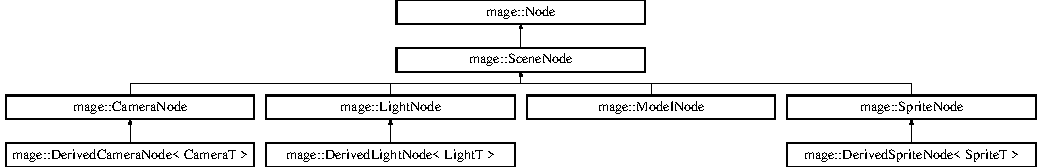
\includegraphics[height=2.986667cm]{classmage_1_1_node}
\end{center}
\end{figure}
\subsection*{Public Member Functions}
\begin{DoxyCompactItemize}
\item 
\hyperlink{classmage_1_1_node_a58b816eaa1dfd3c4b7f14896f190587f}{Node} ()
\item 
\hyperlink{classmage_1_1_node_af9da591163469f210895f3a5b389d7cc}{Node} (const \hyperlink{classmage_1_1_node}{Node} \&node)
\item 
\hyperlink{classmage_1_1_node_adbc40b6c4100f74faa2b59a7a0b79388}{Node} (\hyperlink{classmage_1_1_node}{Node} \&\&node)
\item 
virtual \hyperlink{classmage_1_1_node_a1369fc11b331abacbaf11aeb5729e871}{$\sim$\+Node} ()
\item 
\hyperlink{classmage_1_1_node}{Node} \& \hyperlink{classmage_1_1_node_ad10ea13608963acfa06d3c1577314da5}{operator=} (const \hyperlink{classmage_1_1_node}{Node} \&node)=delete
\item 
\hyperlink{classmage_1_1_node}{Node} \& \hyperlink{classmage_1_1_node_a007043de35c65edb9a0d790824186151}{operator=} (\hyperlink{classmage_1_1_node}{Node} \&\&node)=delete
\item 
\hyperlink{namespacemage_a8c307fbcc33bce9b7f2aa4c26c3b95cf}{Unique\+Ptr}$<$ \hyperlink{classmage_1_1_node}{Node} $>$ \hyperlink{classmage_1_1_node_a18e08151571435d319be2414474c93c0}{Clone} () const
\item 
\hyperlink{classmage_1_1_transform_node}{Transform\+Node} $\ast$ \hyperlink{classmage_1_1_node_aee9d81f3a236fe48128ad5960a22beb4}{Get\+Transform} ()
\item 
const \hyperlink{classmage_1_1_transform_node}{Transform\+Node} $\ast$ \hyperlink{classmage_1_1_node_a319b7fdc98412cb02ba1cffab2527bf2}{Get\+Transform} () const
\item 
bool \hyperlink{classmage_1_1_node_ac1e76b877582d74e24e44891dd8c3667}{Is\+Active} () const
\item 
bool \hyperlink{classmage_1_1_node_ad1aea56c1abfd8fe5084b71f35604276}{Is\+Passive} () const
\item 
void \hyperlink{classmage_1_1_node_a3b2cccf69650526f15f57e9dee326a6b}{Make\+Active} ()
\item 
void \hyperlink{classmage_1_1_node_abb90906339681ecde9b8f47b708c14c9}{Make\+Passive} ()
\item 
void \hyperlink{classmage_1_1_node_aea6d7145a71b3af31d5516b4df2e7da5}{Set\+Active} (bool active)
\item 
bool \hyperlink{classmage_1_1_node_a9819d0219bdca364621584b6aa29ba30}{Has\+Parent\+Node} () const
\item 
\hyperlink{classmage_1_1_node}{Node} $\ast$ \hyperlink{classmage_1_1_node_ae30f2ca6816eeeef28610f385864aec9}{Get\+Parent\+Node} () const
\item 
size\+\_\+t \hyperlink{classmage_1_1_node_ab11750938bf343f16dcdf7a327834318}{Get\+Number\+Of\+Child\+Nodes} () const
\item 
bool \hyperlink{classmage_1_1_node_a1b8c2d933a281f7f815791db38c965ad}{Has\+Child\+Node} (\hyperlink{namespacemage_a1e01ae66713838a7a67d30e44c67703e}{Shared\+Ptr}$<$ const \hyperlink{classmage_1_1_node}{Node} $>$ node) const
\item 
void \hyperlink{classmage_1_1_node_a11a7c052c5e4a6713d60aaad67dfde5d}{Add\+Child\+Node} (\hyperlink{namespacemage_a1e01ae66713838a7a67d30e44c67703e}{Shared\+Ptr}$<$ \hyperlink{classmage_1_1_node}{Node} $>$ node)
\item 
void \hyperlink{classmage_1_1_node_a0da235c6459c315ad1c4be5c7aa7c7f0}{Remove\+Child\+Node} (\hyperlink{namespacemage_a1e01ae66713838a7a67d30e44c67703e}{Shared\+Ptr}$<$ \hyperlink{classmage_1_1_node}{Node} $>$ node)
\item 
void \hyperlink{classmage_1_1_node_a5813fe733404dd327b77f595291c70bb}{Remove\+All\+Child\+Nodes} ()
\item 
{\footnotesize template$<$typename ActionT $>$ }\\void \hyperlink{classmage_1_1_node_afedb523a462952ec29aed7504d0a71d4}{For\+Each\+Child\+Node} (ActionT action) const
\item 
{\footnotesize template$<$typename ActionT $>$ }\\void \hyperlink{classmage_1_1_node_a86668c371e1452204b52f2896cbb16fd}{For\+Each\+Descendant\+Node} (ActionT action) const
\end{DoxyCompactItemize}
\subsection*{Private Member Functions}
\begin{DoxyCompactItemize}
\item 
virtual \hyperlink{namespacemage_a8c307fbcc33bce9b7f2aa4c26c3b95cf}{Unique\+Ptr}$<$ \hyperlink{classmage_1_1_node}{Node} $>$ \hyperlink{classmage_1_1_node_a71a4763bfd4cba5653488b490e61dc8f}{Clone\+Implementation} () const
\end{DoxyCompactItemize}
\subsection*{Private Attributes}
\begin{DoxyCompactItemize}
\item 
\hyperlink{namespacemage_a8c307fbcc33bce9b7f2aa4c26c3b95cf}{Unique\+Ptr}$<$ \hyperlink{classmage_1_1_transform_node}{Transform\+Node} $>$ \hyperlink{classmage_1_1_node_a24512023f5f6ec7adad9810e55ec2ab5}{m\+\_\+transform}
\item 
bool \hyperlink{classmage_1_1_node_ac4dd6c399de8b2a92df92365df7ecdac}{m\+\_\+active}
\end{DoxyCompactItemize}


\subsection{Detailed Description}
A class of nodes. 

\subsection{Constructor \& Destructor Documentation}
\hypertarget{classmage_1_1_node_a58b816eaa1dfd3c4b7f14896f190587f}{}\label{classmage_1_1_node_a58b816eaa1dfd3c4b7f14896f190587f} 
\index{mage\+::\+Node@{mage\+::\+Node}!Node@{Node}}
\index{Node@{Node}!mage\+::\+Node@{mage\+::\+Node}}
\subsubsection{\texorpdfstring{Node()}{Node()}\hspace{0.1cm}{\footnotesize\ttfamily [1/3]}}
{\footnotesize\ttfamily mage\+::\+Node\+::\+Node (\begin{DoxyParamCaption}{ }\end{DoxyParamCaption})}

Constructs a node. \hypertarget{classmage_1_1_node_af9da591163469f210895f3a5b389d7cc}{}\label{classmage_1_1_node_af9da591163469f210895f3a5b389d7cc} 
\index{mage\+::\+Node@{mage\+::\+Node}!Node@{Node}}
\index{Node@{Node}!mage\+::\+Node@{mage\+::\+Node}}
\subsubsection{\texorpdfstring{Node()}{Node()}\hspace{0.1cm}{\footnotesize\ttfamily [2/3]}}
{\footnotesize\ttfamily mage\+::\+Node\+::\+Node (\begin{DoxyParamCaption}\item[{const \hyperlink{classmage_1_1_node}{Node} \&}]{node }\end{DoxyParamCaption})}

Constructs a node from the given node.


\begin{DoxyParams}[1]{Parameters}
\mbox{\tt in}  & {\em node} & A reference to the node. \\
\hline
\end{DoxyParams}
\hypertarget{classmage_1_1_node_adbc40b6c4100f74faa2b59a7a0b79388}{}\label{classmage_1_1_node_adbc40b6c4100f74faa2b59a7a0b79388} 
\index{mage\+::\+Node@{mage\+::\+Node}!Node@{Node}}
\index{Node@{Node}!mage\+::\+Node@{mage\+::\+Node}}
\subsubsection{\texorpdfstring{Node()}{Node()}\hspace{0.1cm}{\footnotesize\ttfamily [3/3]}}
{\footnotesize\ttfamily mage\+::\+Node\+::\+Node (\begin{DoxyParamCaption}\item[{\hyperlink{classmage_1_1_node}{Node} \&\&}]{node }\end{DoxyParamCaption})\hspace{0.3cm}{\ttfamily [default]}}

Constructs a node by moving the given node.


\begin{DoxyParams}[1]{Parameters}
\mbox{\tt in}  & {\em node} & A reference to the node to move. \\
\hline
\end{DoxyParams}
\hypertarget{classmage_1_1_node_a1369fc11b331abacbaf11aeb5729e871}{}\label{classmage_1_1_node_a1369fc11b331abacbaf11aeb5729e871} 
\index{mage\+::\+Node@{mage\+::\+Node}!````~Node@{$\sim$\+Node}}
\index{````~Node@{$\sim$\+Node}!mage\+::\+Node@{mage\+::\+Node}}
\subsubsection{\texorpdfstring{$\sim$\+Node()}{~Node()}}
{\footnotesize\ttfamily mage\+::\+Node\+::$\sim$\+Node (\begin{DoxyParamCaption}{ }\end{DoxyParamCaption})\hspace{0.3cm}{\ttfamily [virtual]}, {\ttfamily [default]}}

Destructs this node. 

\subsection{Member Function Documentation}
\hypertarget{classmage_1_1_node_a11a7c052c5e4a6713d60aaad67dfde5d}{}\label{classmage_1_1_node_a11a7c052c5e4a6713d60aaad67dfde5d} 
\index{mage\+::\+Node@{mage\+::\+Node}!Add\+Child\+Node@{Add\+Child\+Node}}
\index{Add\+Child\+Node@{Add\+Child\+Node}!mage\+::\+Node@{mage\+::\+Node}}
\subsubsection{\texorpdfstring{Add\+Child\+Node()}{AddChildNode()}}
{\footnotesize\ttfamily void mage\+::\+Node\+::\+Add\+Child\+Node (\begin{DoxyParamCaption}\item[{\hyperlink{namespacemage_a1e01ae66713838a7a67d30e44c67703e}{Shared\+Ptr}$<$ \hyperlink{classmage_1_1_node}{Node} $>$}]{node }\end{DoxyParamCaption})}

Adds the given node to the child nodes of this node.


\begin{DoxyParams}[1]{Parameters}
\mbox{\tt in}  & {\em node} & A pointer to the node to add. \\
\hline
\end{DoxyParams}
\hypertarget{classmage_1_1_node_a18e08151571435d319be2414474c93c0}{}\label{classmage_1_1_node_a18e08151571435d319be2414474c93c0} 
\index{mage\+::\+Node@{mage\+::\+Node}!Clone@{Clone}}
\index{Clone@{Clone}!mage\+::\+Node@{mage\+::\+Node}}
\subsubsection{\texorpdfstring{Clone()}{Clone()}}
{\footnotesize\ttfamily \hyperlink{namespacemage_a8c307fbcc33bce9b7f2aa4c26c3b95cf}{Unique\+Ptr}$<$ \hyperlink{classmage_1_1_node}{Node} $>$ mage\+::\+Node\+::\+Clone (\begin{DoxyParamCaption}{ }\end{DoxyParamCaption}) const}

Clones this node.

\begin{DoxyReturn}{Returns}
A pointer to the clone of this node. 
\end{DoxyReturn}
\hypertarget{classmage_1_1_node_a71a4763bfd4cba5653488b490e61dc8f}{}\label{classmage_1_1_node_a71a4763bfd4cba5653488b490e61dc8f} 
\index{mage\+::\+Node@{mage\+::\+Node}!Clone\+Implementation@{Clone\+Implementation}}
\index{Clone\+Implementation@{Clone\+Implementation}!mage\+::\+Node@{mage\+::\+Node}}
\subsubsection{\texorpdfstring{Clone\+Implementation()}{CloneImplementation()}}
{\footnotesize\ttfamily \hyperlink{namespacemage_a8c307fbcc33bce9b7f2aa4c26c3b95cf}{Unique\+Ptr}$<$ \hyperlink{classmage_1_1_node}{Node} $>$ mage\+::\+Node\+::\+Clone\+Implementation (\begin{DoxyParamCaption}{ }\end{DoxyParamCaption}) const\hspace{0.3cm}{\ttfamily [private]}, {\ttfamily [virtual]}}

Clones this node.

\begin{DoxyReturn}{Returns}
A pointer to the clone of this node. 
\end{DoxyReturn}


Reimplemented in \hyperlink{classmage_1_1_derived_light_node_acf8858989780bf45a45c55a7c5564314}{mage\+::\+Derived\+Light\+Node$<$ Light\+T $>$}, \hyperlink{classmage_1_1_derived_camera_node_aa965751029ebd6b41d3805b499a8304e}{mage\+::\+Derived\+Camera\+Node$<$ Camera\+T $>$}, \hyperlink{classmage_1_1_light_node_aea97601d0a4b8073a1c655ca334af242}{mage\+::\+Light\+Node}, \hyperlink{classmage_1_1_camera_node_a002d3a2b41cda270a26ca5d8f3a17f55}{mage\+::\+Camera\+Node}, \hyperlink{classmage_1_1_model_node_a34146201083015276b38240af307417f}{mage\+::\+Model\+Node}, and \hyperlink{classmage_1_1_scene_node_a42d0d53ab804d38ebd584d2de6490eeb}{mage\+::\+Scene\+Node}.

\hypertarget{classmage_1_1_node_afedb523a462952ec29aed7504d0a71d4}{}\label{classmage_1_1_node_afedb523a462952ec29aed7504d0a71d4} 
\index{mage\+::\+Node@{mage\+::\+Node}!For\+Each\+Child\+Node@{For\+Each\+Child\+Node}}
\index{For\+Each\+Child\+Node@{For\+Each\+Child\+Node}!mage\+::\+Node@{mage\+::\+Node}}
\subsubsection{\texorpdfstring{For\+Each\+Child\+Node()}{ForEachChildNode()}}
{\footnotesize\ttfamily template$<$typename ActionT $>$ \\
void mage\+::\+Node\+::\+For\+Each\+Child\+Node (\begin{DoxyParamCaption}\item[{ActionT}]{action }\end{DoxyParamCaption}) const}

Traverses all child nodes of this node.


\begin{DoxyTemplParams}{Template Parameters}
{\em ActionT} & An action to perform on all child nodes of this node. The action must accept ({\ttfamily const}) {\ttfamily \hyperlink{classmage_1_1_node}{Node}\&} values. \\
\hline
\end{DoxyTemplParams}
\hypertarget{classmage_1_1_node_a86668c371e1452204b52f2896cbb16fd}{}\label{classmage_1_1_node_a86668c371e1452204b52f2896cbb16fd} 
\index{mage\+::\+Node@{mage\+::\+Node}!For\+Each\+Descendant\+Node@{For\+Each\+Descendant\+Node}}
\index{For\+Each\+Descendant\+Node@{For\+Each\+Descendant\+Node}!mage\+::\+Node@{mage\+::\+Node}}
\subsubsection{\texorpdfstring{For\+Each\+Descendant\+Node()}{ForEachDescendantNode()}}
{\footnotesize\ttfamily template$<$typename ActionT $>$ \\
void mage\+::\+Node\+::\+For\+Each\+Descendant\+Node (\begin{DoxyParamCaption}\item[{ActionT}]{action }\end{DoxyParamCaption}) const}

Traverses all descendant (childs included) nodes of this transform node.


\begin{DoxyTemplParams}{Template Parameters}
{\em ActionT} & An action to perform on all descendant nodes of this node. The action must accept ({\ttfamily const}) {\ttfamily \hyperlink{classmage_1_1_node}{Node}\&} values. \\
\hline
\end{DoxyTemplParams}
\hypertarget{classmage_1_1_node_ab11750938bf343f16dcdf7a327834318}{}\label{classmage_1_1_node_ab11750938bf343f16dcdf7a327834318} 
\index{mage\+::\+Node@{mage\+::\+Node}!Get\+Number\+Of\+Child\+Nodes@{Get\+Number\+Of\+Child\+Nodes}}
\index{Get\+Number\+Of\+Child\+Nodes@{Get\+Number\+Of\+Child\+Nodes}!mage\+::\+Node@{mage\+::\+Node}}
\subsubsection{\texorpdfstring{Get\+Number\+Of\+Child\+Nodes()}{GetNumberOfChildNodes()}}
{\footnotesize\ttfamily size\+\_\+t mage\+::\+Node\+::\+Get\+Number\+Of\+Child\+Nodes (\begin{DoxyParamCaption}{ }\end{DoxyParamCaption}) const}

Returns the number of child nodes of this node.

\begin{DoxyReturn}{Returns}
The number of child nodes of this node. 
\end{DoxyReturn}
\hypertarget{classmage_1_1_node_ae30f2ca6816eeeef28610f385864aec9}{}\label{classmage_1_1_node_ae30f2ca6816eeeef28610f385864aec9} 
\index{mage\+::\+Node@{mage\+::\+Node}!Get\+Parent\+Node@{Get\+Parent\+Node}}
\index{Get\+Parent\+Node@{Get\+Parent\+Node}!mage\+::\+Node@{mage\+::\+Node}}
\subsubsection{\texorpdfstring{Get\+Parent\+Node()}{GetParentNode()}}
{\footnotesize\ttfamily \hyperlink{classmage_1_1_node}{Node}$\ast$ mage\+::\+Node\+::\+Get\+Parent\+Node (\begin{DoxyParamCaption}{ }\end{DoxyParamCaption}) const}

Returns the parent node of this node.

\begin{DoxyReturn}{Returns}
{\ttfamily nullptr} if this node has no parent node. 

A pointer to the parent node of this node. 
\end{DoxyReturn}
\hypertarget{classmage_1_1_node_aee9d81f3a236fe48128ad5960a22beb4}{}\label{classmage_1_1_node_aee9d81f3a236fe48128ad5960a22beb4} 
\index{mage\+::\+Node@{mage\+::\+Node}!Get\+Transform@{Get\+Transform}}
\index{Get\+Transform@{Get\+Transform}!mage\+::\+Node@{mage\+::\+Node}}
\subsubsection{\texorpdfstring{Get\+Transform()}{GetTransform()}\hspace{0.1cm}{\footnotesize\ttfamily [1/2]}}
{\footnotesize\ttfamily \hyperlink{classmage_1_1_transform_node}{Transform\+Node}$\ast$ mage\+::\+Node\+::\+Get\+Transform (\begin{DoxyParamCaption}{ }\end{DoxyParamCaption})}

Returns the transform of this node.

\begin{DoxyReturn}{Returns}
A pointer to the transform of this node. 
\end{DoxyReturn}
\hypertarget{classmage_1_1_node_a319b7fdc98412cb02ba1cffab2527bf2}{}\label{classmage_1_1_node_a319b7fdc98412cb02ba1cffab2527bf2} 
\index{mage\+::\+Node@{mage\+::\+Node}!Get\+Transform@{Get\+Transform}}
\index{Get\+Transform@{Get\+Transform}!mage\+::\+Node@{mage\+::\+Node}}
\subsubsection{\texorpdfstring{Get\+Transform()}{GetTransform()}\hspace{0.1cm}{\footnotesize\ttfamily [2/2]}}
{\footnotesize\ttfamily const \hyperlink{classmage_1_1_transform_node}{Transform\+Node}$\ast$ mage\+::\+Node\+::\+Get\+Transform (\begin{DoxyParamCaption}{ }\end{DoxyParamCaption}) const}

Returns the transform of this node.

\begin{DoxyReturn}{Returns}
A pointer to the transform of this node. 
\end{DoxyReturn}
\hypertarget{classmage_1_1_node_a1b8c2d933a281f7f815791db38c965ad}{}\label{classmage_1_1_node_a1b8c2d933a281f7f815791db38c965ad} 
\index{mage\+::\+Node@{mage\+::\+Node}!Has\+Child\+Node@{Has\+Child\+Node}}
\index{Has\+Child\+Node@{Has\+Child\+Node}!mage\+::\+Node@{mage\+::\+Node}}
\subsubsection{\texorpdfstring{Has\+Child\+Node()}{HasChildNode()}}
{\footnotesize\ttfamily bool mage\+::\+Node\+::\+Has\+Child\+Node (\begin{DoxyParamCaption}\item[{\hyperlink{namespacemage_a1e01ae66713838a7a67d30e44c67703e}{Shared\+Ptr}$<$ const \hyperlink{classmage_1_1_node}{Node} $>$}]{node }\end{DoxyParamCaption}) const}

Checks whether this node contains the given node as a child node.


\begin{DoxyParams}[1]{Parameters}
\mbox{\tt in}  & {\em node} & A pointer to the node. \\
\hline
\end{DoxyParams}
\begin{DoxyReturn}{Returns}
{\ttfamily true} if this node contains the given node as a child node. {\ttfamily false} otherwise. 
\end{DoxyReturn}
\hypertarget{classmage_1_1_node_a9819d0219bdca364621584b6aa29ba30}{}\label{classmage_1_1_node_a9819d0219bdca364621584b6aa29ba30} 
\index{mage\+::\+Node@{mage\+::\+Node}!Has\+Parent\+Node@{Has\+Parent\+Node}}
\index{Has\+Parent\+Node@{Has\+Parent\+Node}!mage\+::\+Node@{mage\+::\+Node}}
\subsubsection{\texorpdfstring{Has\+Parent\+Node()}{HasParentNode()}}
{\footnotesize\ttfamily bool mage\+::\+Node\+::\+Has\+Parent\+Node (\begin{DoxyParamCaption}{ }\end{DoxyParamCaption}) const}

Checks whether this node has a parent node.

\begin{DoxyReturn}{Returns}
{\ttfamily true} if this node has a parent node. {\ttfamily false} otherwise. 
\end{DoxyReturn}
\hypertarget{classmage_1_1_node_ac1e76b877582d74e24e44891dd8c3667}{}\label{classmage_1_1_node_ac1e76b877582d74e24e44891dd8c3667} 
\index{mage\+::\+Node@{mage\+::\+Node}!Is\+Active@{Is\+Active}}
\index{Is\+Active@{Is\+Active}!mage\+::\+Node@{mage\+::\+Node}}
\subsubsection{\texorpdfstring{Is\+Active()}{IsActive()}}
{\footnotesize\ttfamily bool mage\+::\+Node\+::\+Is\+Active (\begin{DoxyParamCaption}{ }\end{DoxyParamCaption}) const}

Checks whether this node is active.

\begin{DoxyReturn}{Returns}
{\ttfamily true} if this node is active. {\ttfamily false} otherwise (i.\+e. passive). 
\end{DoxyReturn}
\hypertarget{classmage_1_1_node_ad1aea56c1abfd8fe5084b71f35604276}{}\label{classmage_1_1_node_ad1aea56c1abfd8fe5084b71f35604276} 
\index{mage\+::\+Node@{mage\+::\+Node}!Is\+Passive@{Is\+Passive}}
\index{Is\+Passive@{Is\+Passive}!mage\+::\+Node@{mage\+::\+Node}}
\subsubsection{\texorpdfstring{Is\+Passive()}{IsPassive()}}
{\footnotesize\ttfamily bool mage\+::\+Node\+::\+Is\+Passive (\begin{DoxyParamCaption}{ }\end{DoxyParamCaption}) const}

Checks whether this node is passive.

\begin{DoxyReturn}{Returns}
{\ttfamily true} if this node is passive. {\ttfamily false} otherwise (i.\+e. active). 
\end{DoxyReturn}
\hypertarget{classmage_1_1_node_a3b2cccf69650526f15f57e9dee326a6b}{}\label{classmage_1_1_node_a3b2cccf69650526f15f57e9dee326a6b} 
\index{mage\+::\+Node@{mage\+::\+Node}!Make\+Active@{Make\+Active}}
\index{Make\+Active@{Make\+Active}!mage\+::\+Node@{mage\+::\+Node}}
\subsubsection{\texorpdfstring{Make\+Active()}{MakeActive()}}
{\footnotesize\ttfamily void mage\+::\+Node\+::\+Make\+Active (\begin{DoxyParamCaption}{ }\end{DoxyParamCaption})}

Makes this node (and its descendant nodes) active. \hypertarget{classmage_1_1_node_abb90906339681ecde9b8f47b708c14c9}{}\label{classmage_1_1_node_abb90906339681ecde9b8f47b708c14c9} 
\index{mage\+::\+Node@{mage\+::\+Node}!Make\+Passive@{Make\+Passive}}
\index{Make\+Passive@{Make\+Passive}!mage\+::\+Node@{mage\+::\+Node}}
\subsubsection{\texorpdfstring{Make\+Passive()}{MakePassive()}}
{\footnotesize\ttfamily void mage\+::\+Node\+::\+Make\+Passive (\begin{DoxyParamCaption}{ }\end{DoxyParamCaption})}

Makes this node (and its descendant nodes) passive. \hypertarget{classmage_1_1_node_ad10ea13608963acfa06d3c1577314da5}{}\label{classmage_1_1_node_ad10ea13608963acfa06d3c1577314da5} 
\index{mage\+::\+Node@{mage\+::\+Node}!operator=@{operator=}}
\index{operator=@{operator=}!mage\+::\+Node@{mage\+::\+Node}}
\subsubsection{\texorpdfstring{operator=()}{operator=()}\hspace{0.1cm}{\footnotesize\ttfamily [1/2]}}
{\footnotesize\ttfamily \hyperlink{classmage_1_1_node}{Node}\& mage\+::\+Node\+::operator= (\begin{DoxyParamCaption}\item[{const \hyperlink{classmage_1_1_node}{Node} \&}]{node }\end{DoxyParamCaption})\hspace{0.3cm}{\ttfamily [delete]}}

Copies the given node to this node.


\begin{DoxyParams}[1]{Parameters}
\mbox{\tt in}  & {\em node} & A reference to the node to copy. \\
\hline
\end{DoxyParams}
\begin{DoxyReturn}{Returns}
A reference to the copy of the given node (i.\+e. this node). 
\end{DoxyReturn}
\hypertarget{classmage_1_1_node_a007043de35c65edb9a0d790824186151}{}\label{classmage_1_1_node_a007043de35c65edb9a0d790824186151} 
\index{mage\+::\+Node@{mage\+::\+Node}!operator=@{operator=}}
\index{operator=@{operator=}!mage\+::\+Node@{mage\+::\+Node}}
\subsubsection{\texorpdfstring{operator=()}{operator=()}\hspace{0.1cm}{\footnotesize\ttfamily [2/2]}}
{\footnotesize\ttfamily \hyperlink{classmage_1_1_node}{Node}\& mage\+::\+Node\+::operator= (\begin{DoxyParamCaption}\item[{\hyperlink{classmage_1_1_node}{Node} \&\&}]{node }\end{DoxyParamCaption})\hspace{0.3cm}{\ttfamily [delete]}}

Moves the given node to this node.


\begin{DoxyParams}[1]{Parameters}
\mbox{\tt in}  & {\em node} & A reference to the node to move. \\
\hline
\end{DoxyParams}
\begin{DoxyReturn}{Returns}
A reference to the moved node (i.\+e. this node). 
\end{DoxyReturn}
\hypertarget{classmage_1_1_node_a5813fe733404dd327b77f595291c70bb}{}\label{classmage_1_1_node_a5813fe733404dd327b77f595291c70bb} 
\index{mage\+::\+Node@{mage\+::\+Node}!Remove\+All\+Child\+Nodes@{Remove\+All\+Child\+Nodes}}
\index{Remove\+All\+Child\+Nodes@{Remove\+All\+Child\+Nodes}!mage\+::\+Node@{mage\+::\+Node}}
\subsubsection{\texorpdfstring{Remove\+All\+Child\+Nodes()}{RemoveAllChildNodes()}}
{\footnotesize\ttfamily void mage\+::\+Node\+::\+Remove\+All\+Child\+Nodes (\begin{DoxyParamCaption}{ }\end{DoxyParamCaption})}

Removes all child nodes from this node. \hypertarget{classmage_1_1_node_a0da235c6459c315ad1c4be5c7aa7c7f0}{}\label{classmage_1_1_node_a0da235c6459c315ad1c4be5c7aa7c7f0} 
\index{mage\+::\+Node@{mage\+::\+Node}!Remove\+Child\+Node@{Remove\+Child\+Node}}
\index{Remove\+Child\+Node@{Remove\+Child\+Node}!mage\+::\+Node@{mage\+::\+Node}}
\subsubsection{\texorpdfstring{Remove\+Child\+Node()}{RemoveChildNode()}}
{\footnotesize\ttfamily void mage\+::\+Node\+::\+Remove\+Child\+Node (\begin{DoxyParamCaption}\item[{\hyperlink{namespacemage_a1e01ae66713838a7a67d30e44c67703e}{Shared\+Ptr}$<$ \hyperlink{classmage_1_1_node}{Node} $>$}]{node }\end{DoxyParamCaption})}

Removes the given node from the child nodes of this node.


\begin{DoxyParams}[1]{Parameters}
\mbox{\tt in}  & {\em node} & A pointer to the node to remove. \\
\hline
\end{DoxyParams}
\hypertarget{classmage_1_1_node_aea6d7145a71b3af31d5516b4df2e7da5}{}\label{classmage_1_1_node_aea6d7145a71b3af31d5516b4df2e7da5} 
\index{mage\+::\+Node@{mage\+::\+Node}!Set\+Active@{Set\+Active}}
\index{Set\+Active@{Set\+Active}!mage\+::\+Node@{mage\+::\+Node}}
\subsubsection{\texorpdfstring{Set\+Active()}{SetActive()}}
{\footnotesize\ttfamily void mage\+::\+Node\+::\+Set\+Active (\begin{DoxyParamCaption}\item[{bool}]{active }\end{DoxyParamCaption})}

Sets this node active flag to the given value.


\begin{DoxyParams}[1]{Parameters}
\mbox{\tt in}  & {\em active} & The active flag. \\
\hline
\end{DoxyParams}


\subsection{Member Data Documentation}
\hypertarget{classmage_1_1_node_ac4dd6c399de8b2a92df92365df7ecdac}{}\label{classmage_1_1_node_ac4dd6c399de8b2a92df92365df7ecdac} 
\index{mage\+::\+Node@{mage\+::\+Node}!m\+\_\+active@{m\+\_\+active}}
\index{m\+\_\+active@{m\+\_\+active}!mage\+::\+Node@{mage\+::\+Node}}
\subsubsection{\texorpdfstring{m\+\_\+active}{m\_active}}
{\footnotesize\ttfamily bool mage\+::\+Node\+::m\+\_\+active\hspace{0.3cm}{\ttfamily [private]}}

A flag indicating whether this node is active or not (i.\+e. passive). \hypertarget{classmage_1_1_node_a24512023f5f6ec7adad9810e55ec2ab5}{}\label{classmage_1_1_node_a24512023f5f6ec7adad9810e55ec2ab5} 
\index{mage\+::\+Node@{mage\+::\+Node}!m\+\_\+transform@{m\+\_\+transform}}
\index{m\+\_\+transform@{m\+\_\+transform}!mage\+::\+Node@{mage\+::\+Node}}
\subsubsection{\texorpdfstring{m\+\_\+transform}{m\_transform}}
{\footnotesize\ttfamily \hyperlink{namespacemage_a8c307fbcc33bce9b7f2aa4c26c3b95cf}{Unique\+Ptr}$<$ \hyperlink{classmage_1_1_transform_node}{Transform\+Node} $>$ mage\+::\+Node\+::m\+\_\+transform\hspace{0.3cm}{\ttfamily [private]}}

A pointer to the transform of this node. 
\hypertarget{structmage_1_1_normal3}{}\section{mage\+:\+:Normal3 Struct Reference}
\label{structmage_1_1_normal3}\index{mage\+::\+Normal3@{mage\+::\+Normal3}}


{\ttfamily \#include $<$math.\+hpp$>$}

Inheritance diagram for mage\+:\+:Normal3\+:\begin{figure}[H]
\begin{center}
\leavevmode
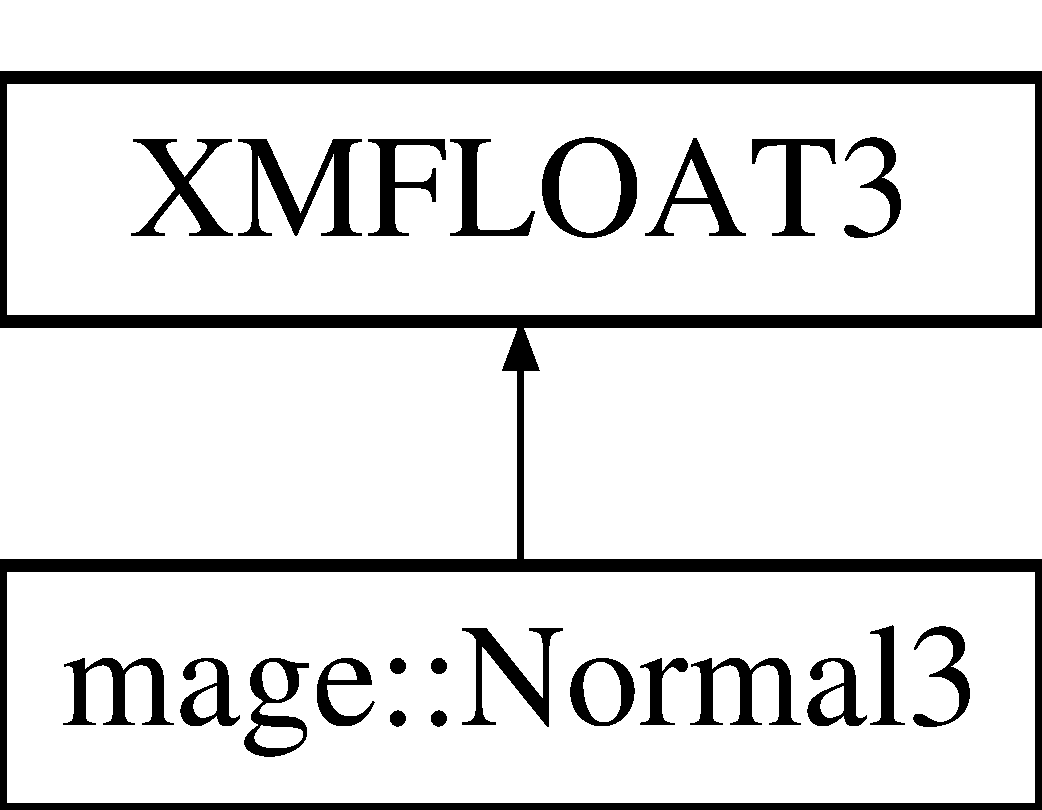
\includegraphics[height=2.000000cm]{structmage_1_1_normal3}
\end{center}
\end{figure}
\subsection*{Public Member Functions}
\begin{DoxyCompactItemize}
\item 
\hyperlink{structmage_1_1_normal3_a66ec99f0de4f8231f747e37a4da65cc4}{Normal3} ()
\item 
\hyperlink{structmage_1_1_normal3_a59094c1f96a9721cd8846c5c6ec06f93}{Normal3} (float x, float y, float z)
\item 
\hyperlink{structmage_1_1_normal3_ada9c762e16b51177f3fc1aa6d5310b20}{Normal3} (const \hyperlink{structmage_1_1_normal3}{Normal3} \&normal)
\item 
\hyperlink{structmage_1_1_normal3_a1a58b2fcb3920ff68007257ae6434273}{Normal3} (const \hyperlink{structmage_1_1_point3}{Point3} \&point)
\item 
\hyperlink{structmage_1_1_normal3_a0942e7aace8354f0a414f77ccf90b69c}{Normal3} (const \hyperlink{structmage_1_1_direction3}{Direction3} \&direction)
\item 
\hyperlink{structmage_1_1_normal3_a61565f1183535666a2fb5183b83bebd2}{Normal3} (const X\+M\+F\+L\+O\+A\+T3 \&vector)
\item 
\hyperlink{structmage_1_1_normal3_a3384b2970fd85fe729514ce0686b4446}{$\sim$\+Normal3} ()=default
\item 
\hyperlink{structmage_1_1_normal3}{Normal3} \& \hyperlink{structmage_1_1_normal3_ade86357989ceaecf1b22bb9e53ca7fed}{operator=} (const \hyperlink{structmage_1_1_normal3}{Normal3} \&normal)
\end{DoxyCompactItemize}


\subsection{Constructor \& Destructor Documentation}
\hypertarget{structmage_1_1_normal3_a66ec99f0de4f8231f747e37a4da65cc4}{}\label{structmage_1_1_normal3_a66ec99f0de4f8231f747e37a4da65cc4} 
\index{mage\+::\+Normal3@{mage\+::\+Normal3}!Normal3@{Normal3}}
\index{Normal3@{Normal3}!mage\+::\+Normal3@{mage\+::\+Normal3}}
\subsubsection{\texorpdfstring{Normal3()}{Normal3()}\hspace{0.1cm}{\footnotesize\ttfamily [1/6]}}
{\footnotesize\ttfamily mage\+::\+Normal3\+::\+Normal3 (\begin{DoxyParamCaption}{ }\end{DoxyParamCaption})}

\hypertarget{structmage_1_1_normal3_a59094c1f96a9721cd8846c5c6ec06f93}{}\label{structmage_1_1_normal3_a59094c1f96a9721cd8846c5c6ec06f93} 
\index{mage\+::\+Normal3@{mage\+::\+Normal3}!Normal3@{Normal3}}
\index{Normal3@{Normal3}!mage\+::\+Normal3@{mage\+::\+Normal3}}
\subsubsection{\texorpdfstring{Normal3()}{Normal3()}\hspace{0.1cm}{\footnotesize\ttfamily [2/6]}}
{\footnotesize\ttfamily mage\+::\+Normal3\+::\+Normal3 (\begin{DoxyParamCaption}\item[{float}]{x,  }\item[{float}]{y,  }\item[{float}]{z }\end{DoxyParamCaption})}

\hypertarget{structmage_1_1_normal3_ada9c762e16b51177f3fc1aa6d5310b20}{}\label{structmage_1_1_normal3_ada9c762e16b51177f3fc1aa6d5310b20} 
\index{mage\+::\+Normal3@{mage\+::\+Normal3}!Normal3@{Normal3}}
\index{Normal3@{Normal3}!mage\+::\+Normal3@{mage\+::\+Normal3}}
\subsubsection{\texorpdfstring{Normal3()}{Normal3()}\hspace{0.1cm}{\footnotesize\ttfamily [3/6]}}
{\footnotesize\ttfamily mage\+::\+Normal3\+::\+Normal3 (\begin{DoxyParamCaption}\item[{const \hyperlink{structmage_1_1_normal3}{Normal3} \&}]{normal }\end{DoxyParamCaption})}

\hypertarget{structmage_1_1_normal3_a1a58b2fcb3920ff68007257ae6434273}{}\label{structmage_1_1_normal3_a1a58b2fcb3920ff68007257ae6434273} 
\index{mage\+::\+Normal3@{mage\+::\+Normal3}!Normal3@{Normal3}}
\index{Normal3@{Normal3}!mage\+::\+Normal3@{mage\+::\+Normal3}}
\subsubsection{\texorpdfstring{Normal3()}{Normal3()}\hspace{0.1cm}{\footnotesize\ttfamily [4/6]}}
{\footnotesize\ttfamily mage\+::\+Normal3\+::\+Normal3 (\begin{DoxyParamCaption}\item[{const \hyperlink{structmage_1_1_point3}{Point3} \&}]{point }\end{DoxyParamCaption})\hspace{0.3cm}{\ttfamily [explicit]}}

\hypertarget{structmage_1_1_normal3_a0942e7aace8354f0a414f77ccf90b69c}{}\label{structmage_1_1_normal3_a0942e7aace8354f0a414f77ccf90b69c} 
\index{mage\+::\+Normal3@{mage\+::\+Normal3}!Normal3@{Normal3}}
\index{Normal3@{Normal3}!mage\+::\+Normal3@{mage\+::\+Normal3}}
\subsubsection{\texorpdfstring{Normal3()}{Normal3()}\hspace{0.1cm}{\footnotesize\ttfamily [5/6]}}
{\footnotesize\ttfamily mage\+::\+Normal3\+::\+Normal3 (\begin{DoxyParamCaption}\item[{const \hyperlink{structmage_1_1_direction3}{Direction3} \&}]{direction }\end{DoxyParamCaption})\hspace{0.3cm}{\ttfamily [explicit]}}

\hypertarget{structmage_1_1_normal3_a61565f1183535666a2fb5183b83bebd2}{}\label{structmage_1_1_normal3_a61565f1183535666a2fb5183b83bebd2} 
\index{mage\+::\+Normal3@{mage\+::\+Normal3}!Normal3@{Normal3}}
\index{Normal3@{Normal3}!mage\+::\+Normal3@{mage\+::\+Normal3}}
\subsubsection{\texorpdfstring{Normal3()}{Normal3()}\hspace{0.1cm}{\footnotesize\ttfamily [6/6]}}
{\footnotesize\ttfamily mage\+::\+Normal3\+::\+Normal3 (\begin{DoxyParamCaption}\item[{const X\+M\+F\+L\+O\+A\+T3 \&}]{vector }\end{DoxyParamCaption})\hspace{0.3cm}{\ttfamily [explicit]}}

\hypertarget{structmage_1_1_normal3_a3384b2970fd85fe729514ce0686b4446}{}\label{structmage_1_1_normal3_a3384b2970fd85fe729514ce0686b4446} 
\index{mage\+::\+Normal3@{mage\+::\+Normal3}!````~Normal3@{$\sim$\+Normal3}}
\index{````~Normal3@{$\sim$\+Normal3}!mage\+::\+Normal3@{mage\+::\+Normal3}}
\subsubsection{\texorpdfstring{$\sim$\+Normal3()}{~Normal3()}}
{\footnotesize\ttfamily mage\+::\+Normal3\+::$\sim$\+Normal3 (\begin{DoxyParamCaption}{ }\end{DoxyParamCaption})\hspace{0.3cm}{\ttfamily [default]}}



\subsection{Member Function Documentation}
\hypertarget{structmage_1_1_normal3_ade86357989ceaecf1b22bb9e53ca7fed}{}\label{structmage_1_1_normal3_ade86357989ceaecf1b22bb9e53ca7fed} 
\index{mage\+::\+Normal3@{mage\+::\+Normal3}!operator=@{operator=}}
\index{operator=@{operator=}!mage\+::\+Normal3@{mage\+::\+Normal3}}
\subsubsection{\texorpdfstring{operator=()}{operator=()}}
{\footnotesize\ttfamily \hyperlink{structmage_1_1_normal3}{Normal3}\& mage\+::\+Normal3\+::operator= (\begin{DoxyParamCaption}\item[{const \hyperlink{structmage_1_1_normal3}{Normal3} \&}]{normal }\end{DoxyParamCaption})}


\hypertarget{classmage_1_1_normal_sprite_text}{}\section{mage\+:\+:Normal\+Sprite\+Text Class Reference}
\label{classmage_1_1_normal_sprite_text}\index{mage\+::\+Normal\+Sprite\+Text@{mage\+::\+Normal\+Sprite\+Text}}


{\ttfamily \#include $<$normal\+\_\+sprite\+\_\+text.\+hpp$>$}

Inheritance diagram for mage\+:\+:Normal\+Sprite\+Text\+:\begin{figure}[H]
\begin{center}
\leavevmode
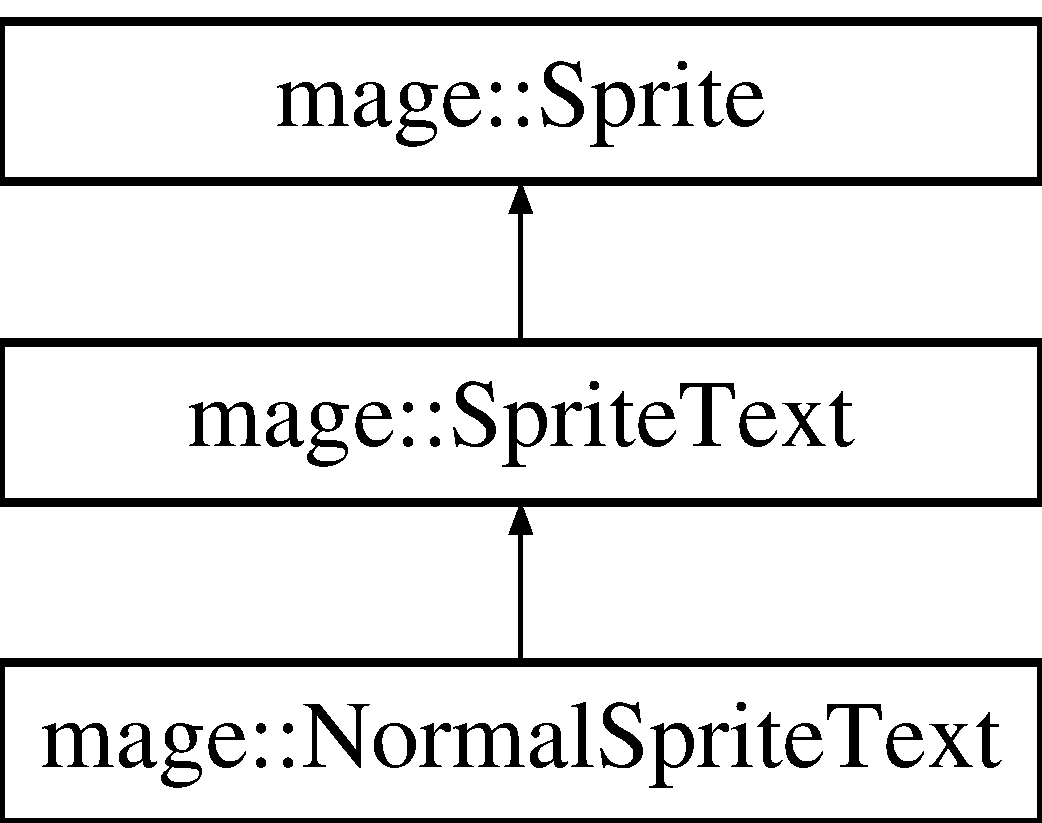
\includegraphics[height=3.000000cm]{classmage_1_1_normal_sprite_text}
\end{center}
\end{figure}
\subsection*{Public Member Functions}
\begin{DoxyCompactItemize}
\item 
\hyperlink{classmage_1_1_normal_sprite_text_a3943f079a5d18e27a2eca8c96fbfeb68}{Normal\+Sprite\+Text} (\hyperlink{namespacemage_a1e01ae66713838a7a67d30e44c67703e}{Shared\+Ptr}$<$ \hyperlink{classmage_1_1_sprite_font}{Sprite\+Font} $>$ font, \hyperlink{namespacemage_a9cfe18123066ba4236f548f9de75d881}{Sprite\+Effect} effects=\hyperlink{namespacemage_a5e7e18b0154373ce8fc942fe3f6b27fda6adf97f83acf6453d4a6a4b1070f3754}{Sprite\+Effect\+::\+None})
\item 
\hyperlink{classmage_1_1_normal_sprite_text_aa73a83a29b28d7b5f20240f3074e5d4d}{Normal\+Sprite\+Text} (const \hyperlink{classmage_1_1_normal_sprite_text}{Normal\+Sprite\+Text} \&sprite\+\_\+text)
\item 
\hyperlink{classmage_1_1_normal_sprite_text_ab2b8232a1bb1aa5294eaa335cb0ccd97}{Normal\+Sprite\+Text} (\hyperlink{classmage_1_1_normal_sprite_text}{Normal\+Sprite\+Text} \&\&sprite\+\_\+text)
\item 
virtual \hyperlink{classmage_1_1_normal_sprite_text_ae8575ab8ece5b8b923509fc7ab4d3dea}{$\sim$\+Normal\+Sprite\+Text} ()
\item 
\hyperlink{classmage_1_1_normal_sprite_text}{Normal\+Sprite\+Text} \& \hyperlink{classmage_1_1_normal_sprite_text_ab7dbd2e71dcaef5d6b7b767afa8d7094}{operator=} (const \hyperlink{classmage_1_1_normal_sprite_text}{Normal\+Sprite\+Text} \&sprite\+\_\+text)=delete
\item 
\hyperlink{classmage_1_1_normal_sprite_text}{Normal\+Sprite\+Text} \& \hyperlink{classmage_1_1_normal_sprite_text_a54cb023fad3b66dba35854ceaa50bc44}{operator=} (\hyperlink{classmage_1_1_normal_sprite_text}{Normal\+Sprite\+Text} \&\&sprite\+\_\+text)=delete
\item 
\hyperlink{namespacemage_a3316d7143a973e37adf1110f2e80ca31}{Unique\+Ptr}$<$ \hyperlink{classmage_1_1_normal_sprite_text}{Normal\+Sprite\+Text} $>$ \hyperlink{classmage_1_1_normal_sprite_text_a8357ea517cff639204da4825024d9d34}{Clone} () const
\item 
virtual void \hyperlink{classmage_1_1_normal_sprite_text_ad2a1b02bea18afd6bf61b106a727a355}{Draw} (\hyperlink{classmage_1_1_sprite_batch}{Sprite\+Batch} \&sprite\+\_\+batch) const override
\end{DoxyCompactItemize}
\subsection*{Private Member Functions}
\begin{DoxyCompactItemize}
\item 
virtual \hyperlink{namespacemage_a3316d7143a973e37adf1110f2e80ca31}{Unique\+Ptr}$<$ \hyperlink{classmage_1_1_sprite}{Sprite} $>$ \hyperlink{classmage_1_1_normal_sprite_text_acab5b61f8be4a475cd54b51278956e37}{Clone\+Implementation} () const override
\end{DoxyCompactItemize}
\subsection*{Additional Inherited Members}


\subsection{Detailed Description}
A class of normal sprite texts. 

\subsection{Constructor \& Destructor Documentation}
\hypertarget{classmage_1_1_normal_sprite_text_a3943f079a5d18e27a2eca8c96fbfeb68}{}\label{classmage_1_1_normal_sprite_text_a3943f079a5d18e27a2eca8c96fbfeb68} 
\index{mage\+::\+Normal\+Sprite\+Text@{mage\+::\+Normal\+Sprite\+Text}!Normal\+Sprite\+Text@{Normal\+Sprite\+Text}}
\index{Normal\+Sprite\+Text@{Normal\+Sprite\+Text}!mage\+::\+Normal\+Sprite\+Text@{mage\+::\+Normal\+Sprite\+Text}}
\subsubsection{\texorpdfstring{Normal\+Sprite\+Text()}{NormalSpriteText()}\hspace{0.1cm}{\footnotesize\ttfamily [1/3]}}
{\footnotesize\ttfamily mage\+::\+Normal\+Sprite\+Text\+::\+Normal\+Sprite\+Text (\begin{DoxyParamCaption}\item[{\hyperlink{namespacemage_a1e01ae66713838a7a67d30e44c67703e}{Shared\+Ptr}$<$ \hyperlink{classmage_1_1_sprite_font}{Sprite\+Font} $>$}]{font,  }\item[{\hyperlink{namespacemage_a9cfe18123066ba4236f548f9de75d881}{Sprite\+Effect}}]{effects = {\ttfamily \hyperlink{namespacemage_a5e7e18b0154373ce8fc942fe3f6b27fda6adf97f83acf6453d4a6a4b1070f3754}{Sprite\+Effect\+::\+None}} }\end{DoxyParamCaption})\hspace{0.3cm}{\ttfamily [explicit]}}

Constructs a normal sprite text.

\begin{DoxyPrecond}{Precondition}
{\ttfamily font.\+get()} is not equal to {\ttfamily nullptr}. 
\end{DoxyPrecond}

\begin{DoxyParams}[1]{Parameters}
\mbox{\tt in}  & {\em font} & A pointer to the sprite font. \\
\hline
\mbox{\tt in}  & {\em effects} & The sprite effects to apply. \\
\hline
\end{DoxyParams}
\hypertarget{classmage_1_1_normal_sprite_text_aa73a83a29b28d7b5f20240f3074e5d4d}{}\label{classmage_1_1_normal_sprite_text_aa73a83a29b28d7b5f20240f3074e5d4d} 
\index{mage\+::\+Normal\+Sprite\+Text@{mage\+::\+Normal\+Sprite\+Text}!Normal\+Sprite\+Text@{Normal\+Sprite\+Text}}
\index{Normal\+Sprite\+Text@{Normal\+Sprite\+Text}!mage\+::\+Normal\+Sprite\+Text@{mage\+::\+Normal\+Sprite\+Text}}
\subsubsection{\texorpdfstring{Normal\+Sprite\+Text()}{NormalSpriteText()}\hspace{0.1cm}{\footnotesize\ttfamily [2/3]}}
{\footnotesize\ttfamily mage\+::\+Normal\+Sprite\+Text\+::\+Normal\+Sprite\+Text (\begin{DoxyParamCaption}\item[{const \hyperlink{classmage_1_1_normal_sprite_text}{Normal\+Sprite\+Text} \&}]{sprite\+\_\+text }\end{DoxyParamCaption})\hspace{0.3cm}{\ttfamily [default]}}

Constructs a normal sprite text from the given normal sprite text.


\begin{DoxyParams}[1]{Parameters}
\mbox{\tt in}  & {\em sprite\+\_\+text} & A reference to the normal sprite text to copy. \\
\hline
\end{DoxyParams}
\hypertarget{classmage_1_1_normal_sprite_text_ab2b8232a1bb1aa5294eaa335cb0ccd97}{}\label{classmage_1_1_normal_sprite_text_ab2b8232a1bb1aa5294eaa335cb0ccd97} 
\index{mage\+::\+Normal\+Sprite\+Text@{mage\+::\+Normal\+Sprite\+Text}!Normal\+Sprite\+Text@{Normal\+Sprite\+Text}}
\index{Normal\+Sprite\+Text@{Normal\+Sprite\+Text}!mage\+::\+Normal\+Sprite\+Text@{mage\+::\+Normal\+Sprite\+Text}}
\subsubsection{\texorpdfstring{Normal\+Sprite\+Text()}{NormalSpriteText()}\hspace{0.1cm}{\footnotesize\ttfamily [3/3]}}
{\footnotesize\ttfamily mage\+::\+Normal\+Sprite\+Text\+::\+Normal\+Sprite\+Text (\begin{DoxyParamCaption}\item[{\hyperlink{classmage_1_1_normal_sprite_text}{Normal\+Sprite\+Text} \&\&}]{sprite\+\_\+text }\end{DoxyParamCaption})\hspace{0.3cm}{\ttfamily [default]}}

Constructs a normal sprite text by moving the given normal sprite text.


\begin{DoxyParams}[1]{Parameters}
\mbox{\tt in}  & {\em sprite\+\_\+text} & A reference to the normal sprite text to move. \\
\hline
\end{DoxyParams}
\hypertarget{classmage_1_1_normal_sprite_text_ae8575ab8ece5b8b923509fc7ab4d3dea}{}\label{classmage_1_1_normal_sprite_text_ae8575ab8ece5b8b923509fc7ab4d3dea} 
\index{mage\+::\+Normal\+Sprite\+Text@{mage\+::\+Normal\+Sprite\+Text}!````~Normal\+Sprite\+Text@{$\sim$\+Normal\+Sprite\+Text}}
\index{````~Normal\+Sprite\+Text@{$\sim$\+Normal\+Sprite\+Text}!mage\+::\+Normal\+Sprite\+Text@{mage\+::\+Normal\+Sprite\+Text}}
\subsubsection{\texorpdfstring{$\sim$\+Normal\+Sprite\+Text()}{~NormalSpriteText()}}
{\footnotesize\ttfamily mage\+::\+Normal\+Sprite\+Text\+::$\sim$\+Normal\+Sprite\+Text (\begin{DoxyParamCaption}{ }\end{DoxyParamCaption})\hspace{0.3cm}{\ttfamily [virtual]}, {\ttfamily [default]}}

Destructs this normal sprite text. 

\subsection{Member Function Documentation}
\hypertarget{classmage_1_1_normal_sprite_text_a8357ea517cff639204da4825024d9d34}{}\label{classmage_1_1_normal_sprite_text_a8357ea517cff639204da4825024d9d34} 
\index{mage\+::\+Normal\+Sprite\+Text@{mage\+::\+Normal\+Sprite\+Text}!Clone@{Clone}}
\index{Clone@{Clone}!mage\+::\+Normal\+Sprite\+Text@{mage\+::\+Normal\+Sprite\+Text}}
\subsubsection{\texorpdfstring{Clone()}{Clone()}}
{\footnotesize\ttfamily \hyperlink{namespacemage_a3316d7143a973e37adf1110f2e80ca31}{Unique\+Ptr}$<$ \hyperlink{classmage_1_1_normal_sprite_text}{Normal\+Sprite\+Text} $>$ mage\+::\+Normal\+Sprite\+Text\+::\+Clone (\begin{DoxyParamCaption}{ }\end{DoxyParamCaption}) const}

Clones this normal sprite text.

\begin{DoxyReturn}{Returns}
A pointer to the clone of this normal sprite text. 
\end{DoxyReturn}
\hypertarget{classmage_1_1_normal_sprite_text_acab5b61f8be4a475cd54b51278956e37}{}\label{classmage_1_1_normal_sprite_text_acab5b61f8be4a475cd54b51278956e37} 
\index{mage\+::\+Normal\+Sprite\+Text@{mage\+::\+Normal\+Sprite\+Text}!Clone\+Implementation@{Clone\+Implementation}}
\index{Clone\+Implementation@{Clone\+Implementation}!mage\+::\+Normal\+Sprite\+Text@{mage\+::\+Normal\+Sprite\+Text}}
\subsubsection{\texorpdfstring{Clone\+Implementation()}{CloneImplementation()}}
{\footnotesize\ttfamily \hyperlink{namespacemage_a3316d7143a973e37adf1110f2e80ca31}{Unique\+Ptr}$<$ \hyperlink{classmage_1_1_sprite}{Sprite} $>$ mage\+::\+Normal\+Sprite\+Text\+::\+Clone\+Implementation (\begin{DoxyParamCaption}{ }\end{DoxyParamCaption}) const\hspace{0.3cm}{\ttfamily [override]}, {\ttfamily [private]}, {\ttfamily [virtual]}}

Clones this normal sprite text.

\begin{DoxyReturn}{Returns}
A pointer to the clone of this normal sprite text. 
\end{DoxyReturn}


Implements \hyperlink{classmage_1_1_sprite_text_aa2c63346f5ad7f63f7a6d474df3556ef}{mage\+::\+Sprite\+Text}.

\hypertarget{classmage_1_1_normal_sprite_text_ad2a1b02bea18afd6bf61b106a727a355}{}\label{classmage_1_1_normal_sprite_text_ad2a1b02bea18afd6bf61b106a727a355} 
\index{mage\+::\+Normal\+Sprite\+Text@{mage\+::\+Normal\+Sprite\+Text}!Draw@{Draw}}
\index{Draw@{Draw}!mage\+::\+Normal\+Sprite\+Text@{mage\+::\+Normal\+Sprite\+Text}}
\subsubsection{\texorpdfstring{Draw()}{Draw()}}
{\footnotesize\ttfamily void mage\+::\+Normal\+Sprite\+Text\+::\+Draw (\begin{DoxyParamCaption}\item[{\hyperlink{classmage_1_1_sprite_batch}{Sprite\+Batch} \&}]{sprite\+\_\+batch }\end{DoxyParamCaption}) const\hspace{0.3cm}{\ttfamily [override]}, {\ttfamily [virtual]}}

Draws this normal sprite text.


\begin{DoxyParams}[1]{Parameters}
\mbox{\tt in}  & {\em sprite\+\_\+batch} & A reference to the sprite batch used for rendering this normal sprite text. \\
\hline
\end{DoxyParams}


Implements \hyperlink{classmage_1_1_sprite_text_a45d5ac8410d5a46b26e8491946a2ad9e}{mage\+::\+Sprite\+Text}.

\hypertarget{classmage_1_1_normal_sprite_text_ab7dbd2e71dcaef5d6b7b767afa8d7094}{}\label{classmage_1_1_normal_sprite_text_ab7dbd2e71dcaef5d6b7b767afa8d7094} 
\index{mage\+::\+Normal\+Sprite\+Text@{mage\+::\+Normal\+Sprite\+Text}!operator=@{operator=}}
\index{operator=@{operator=}!mage\+::\+Normal\+Sprite\+Text@{mage\+::\+Normal\+Sprite\+Text}}
\subsubsection{\texorpdfstring{operator=()}{operator=()}\hspace{0.1cm}{\footnotesize\ttfamily [1/2]}}
{\footnotesize\ttfamily \hyperlink{classmage_1_1_normal_sprite_text}{Normal\+Sprite\+Text}\& mage\+::\+Normal\+Sprite\+Text\+::operator= (\begin{DoxyParamCaption}\item[{const \hyperlink{classmage_1_1_normal_sprite_text}{Normal\+Sprite\+Text} \&}]{sprite\+\_\+text }\end{DoxyParamCaption})\hspace{0.3cm}{\ttfamily [delete]}}

Copies the given normal sprite text to this normal sprite text.


\begin{DoxyParams}[1]{Parameters}
\mbox{\tt in}  & {\em sprite\+\_\+text} & A reference to the normal sprite text to copy. \\
\hline
\end{DoxyParams}
\begin{DoxyReturn}{Returns}
A reference to the copy of the given normal sprite text (i.\+e. this normal sprite text). 
\end{DoxyReturn}
\hypertarget{classmage_1_1_normal_sprite_text_a54cb023fad3b66dba35854ceaa50bc44}{}\label{classmage_1_1_normal_sprite_text_a54cb023fad3b66dba35854ceaa50bc44} 
\index{mage\+::\+Normal\+Sprite\+Text@{mage\+::\+Normal\+Sprite\+Text}!operator=@{operator=}}
\index{operator=@{operator=}!mage\+::\+Normal\+Sprite\+Text@{mage\+::\+Normal\+Sprite\+Text}}
\subsubsection{\texorpdfstring{operator=()}{operator=()}\hspace{0.1cm}{\footnotesize\ttfamily [2/2]}}
{\footnotesize\ttfamily \hyperlink{classmage_1_1_normal_sprite_text}{Normal\+Sprite\+Text}\& mage\+::\+Normal\+Sprite\+Text\+::operator= (\begin{DoxyParamCaption}\item[{\hyperlink{classmage_1_1_normal_sprite_text}{Normal\+Sprite\+Text} \&\&}]{sprite\+\_\+text }\end{DoxyParamCaption})\hspace{0.3cm}{\ttfamily [delete]}}

Moves the given normal sprite text to this normal sprite text.


\begin{DoxyParams}[1]{Parameters}
\mbox{\tt in}  & {\em sprite\+\_\+text} & A reference to the normal sprite text to move. \\
\hline
\end{DoxyParams}
\begin{DoxyReturn}{Returns}
A reference to the moved normal sprite text (i.\+e. this normal sprite text). 
\end{DoxyReturn}

\hypertarget{structmage_1_1_o_b_j_reader_1_1_o_b_j_comparator_x_m_u_i_n_t3}{}\section{mage\+:\+:O\+B\+J\+Reader$<$ VertexT $>$\+:\+:O\+B\+J\+Comparator\+X\+M\+U\+I\+N\+T3 Struct Reference}
\label{structmage_1_1_o_b_j_reader_1_1_o_b_j_comparator_x_m_u_i_n_t3}\index{mage\+::\+O\+B\+J\+Reader$<$ Vertex\+T $>$\+::\+O\+B\+J\+Comparator\+X\+M\+U\+I\+N\+T3@{mage\+::\+O\+B\+J\+Reader$<$ Vertex\+T $>$\+::\+O\+B\+J\+Comparator\+X\+M\+U\+I\+N\+T3}}
\subsection*{Public Member Functions}
\begin{DoxyCompactItemize}
\item 
bool \hyperlink{structmage_1_1_o_b_j_reader_1_1_o_b_j_comparator_x_m_u_i_n_t3_abe8c653d6d8d24c3001c5dea5061c6c1}{operator()} (const X\+M\+U\+I\+N\+T3 \&a, const X\+M\+U\+I\+N\+T3 \&b) const
\end{DoxyCompactItemize}


\subsection{Detailed Description}
\subsubsection*{template$<$typename VertexT$>$\newline
struct mage\+::\+O\+B\+J\+Reader$<$ Vertex\+T $>$\+::\+O\+B\+J\+Comparator\+X\+M\+U\+I\+N\+T3}

A struct of {\ttfamily X\+M\+U\+I\+N\+T3} comparators for O\+BJ vertex indices. 

\subsection{Member Function Documentation}
\hypertarget{structmage_1_1_o_b_j_reader_1_1_o_b_j_comparator_x_m_u_i_n_t3_abe8c653d6d8d24c3001c5dea5061c6c1}{}\label{structmage_1_1_o_b_j_reader_1_1_o_b_j_comparator_x_m_u_i_n_t3_abe8c653d6d8d24c3001c5dea5061c6c1} 
\index{mage\+::\+O\+B\+J\+Reader\+::\+O\+B\+J\+Comparator\+X\+M\+U\+I\+N\+T3@{mage\+::\+O\+B\+J\+Reader\+::\+O\+B\+J\+Comparator\+X\+M\+U\+I\+N\+T3}!operator()@{operator()}}
\index{operator()@{operator()}!mage\+::\+O\+B\+J\+Reader\+::\+O\+B\+J\+Comparator\+X\+M\+U\+I\+N\+T3@{mage\+::\+O\+B\+J\+Reader\+::\+O\+B\+J\+Comparator\+X\+M\+U\+I\+N\+T3}}
\subsubsection{\texorpdfstring{operator()()}{operator()()}}
{\footnotesize\ttfamily template$<$typename VertexT $>$ \\
bool \hyperlink{classmage_1_1_o_b_j_reader}{mage\+::\+O\+B\+J\+Reader}$<$ VertexT $>$\+::O\+B\+J\+Comparator\+X\+M\+U\+I\+N\+T3\+::operator() (\begin{DoxyParamCaption}\item[{const X\+M\+U\+I\+N\+T3 \&}]{a,  }\item[{const X\+M\+U\+I\+N\+T3 \&}]{b }\end{DoxyParamCaption}) const}

Compares the two given {\ttfamily X\+M\+U\+I\+N\+T3} vectors against each other.


\begin{DoxyParams}[1]{Parameters}
\mbox{\tt in}  & {\em a} & A reference to the first vector. \\
\hline
\mbox{\tt in}  & {\em b} & A reference to the second vector. \\
\hline
\end{DoxyParams}
\begin{DoxyReturn}{Returns}
{\ttfamily true} if the {\itshape a} is smaller than {\itshape b}. {\ttfamily false} otherwise. 
\end{DoxyReturn}

\hypertarget{classmage_1_1_o_b_j_reader}{}\section{mage\+:\+:O\+B\+J\+Reader$<$ VertexT $>$ Class Template Reference}
\label{classmage_1_1_o_b_j_reader}\index{mage\+::\+O\+B\+J\+Reader$<$ Vertex\+T $>$@{mage\+::\+O\+B\+J\+Reader$<$ Vertex\+T $>$}}


{\ttfamily \#include $<$obj\+\_\+reader.\+hpp$>$}

Inheritance diagram for mage\+:\+:O\+B\+J\+Reader$<$ VertexT $>$\+:\begin{figure}[H]
\begin{center}
\leavevmode
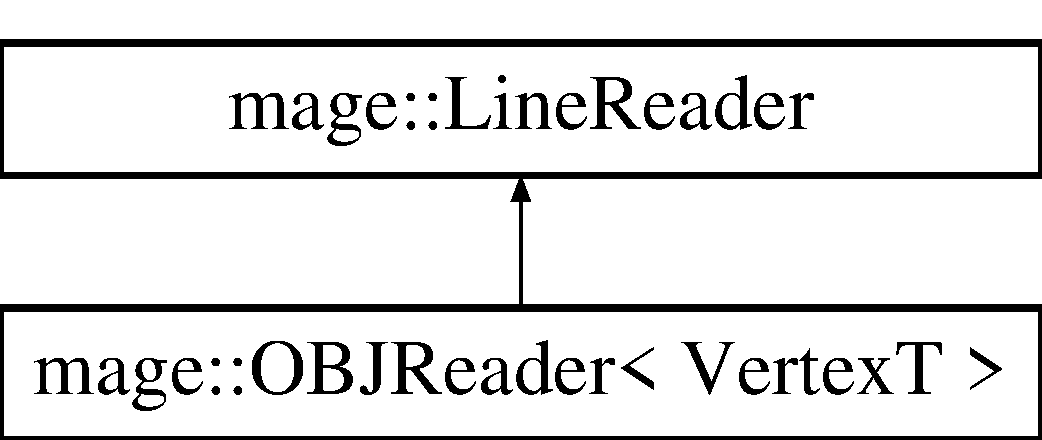
\includegraphics[height=2.000000cm]{classmage_1_1_o_b_j_reader}
\end{center}
\end{figure}
\subsection*{Classes}
\begin{DoxyCompactItemize}
\item 
struct \hyperlink{structmage_1_1_o_b_j_reader_1_1_o_b_j_comparator_x_m_u_i_n_t3}{O\+B\+J\+Comparator\+X\+M\+U\+I\+N\+T3}
\end{DoxyCompactItemize}
\subsection*{Public Member Functions}
\begin{DoxyCompactItemize}
\item 
\hyperlink{classmage_1_1_o_b_j_reader_a87c63bd4beb00ce03be5395a37d2a0ac}{O\+B\+J\+Reader} (\hyperlink{structmage_1_1_model_output}{Model\+Output}$<$ VertexT $>$ \&model\+\_\+output, const \hyperlink{structmage_1_1_mesh_descriptor}{Mesh\+Descriptor}$<$ VertexT $>$ \&mesh\+\_\+desc)
\item 
\hyperlink{classmage_1_1_o_b_j_reader_a8864bc1ca0520bf90e216415db772bbb}{O\+B\+J\+Reader} (const \hyperlink{classmage_1_1_o_b_j_reader}{O\+B\+J\+Reader} \&reader)=delete
\item 
\hyperlink{classmage_1_1_o_b_j_reader_ab25803656fb224d94227c1c121c733ee}{O\+B\+J\+Reader} (\hyperlink{classmage_1_1_o_b_j_reader}{O\+B\+J\+Reader} \&\&reader)=delete
\item 
virtual \hyperlink{classmage_1_1_o_b_j_reader_ad6087ff608be5a45559957a076f910e2}{$\sim$\+O\+B\+J\+Reader} ()=default
\item 
\hyperlink{classmage_1_1_o_b_j_reader}{O\+B\+J\+Reader} \& \hyperlink{classmage_1_1_o_b_j_reader_a62e516060267f828c5aa1a3f23dcf55d}{operator=} (const \hyperlink{classmage_1_1_o_b_j_reader}{O\+B\+J\+Reader} \&reader)=delete
\item 
\hyperlink{classmage_1_1_o_b_j_reader}{O\+B\+J\+Reader} \& \hyperlink{classmage_1_1_o_b_j_reader_ac795c3b1d19ecf38735b76bc5b97fa80}{operator=} (\hyperlink{classmage_1_1_o_b_j_reader}{O\+B\+J\+Reader} \&\&reader)=delete
\end{DoxyCompactItemize}
\subsection*{Private Member Functions}
\begin{DoxyCompactItemize}
\item 
virtual void \hyperlink{classmage_1_1_o_b_j_reader_ae3a3ad3b50f1dd8dffe3109fc7dc2937}{Preprocess} () override
\item 
virtual void \hyperlink{classmage_1_1_o_b_j_reader_a8d4bd7be6de3098ba899cc36e3be1283}{Read\+Line} (char $\ast$line) override
\item 
virtual void \hyperlink{classmage_1_1_o_b_j_reader_a248977c8300575ed2bab04df26197919}{Postprocess} () override
\item 
void \hyperlink{classmage_1_1_o_b_j_reader_abc1f67436e50230bd2071b2dc31a4689}{Read\+O\+B\+J\+Material\+Library} ()
\item 
void \hyperlink{classmage_1_1_o_b_j_reader_aa4c73ff0e5e3de40cacbebc189037802}{Read\+O\+B\+J\+Material\+Use} ()
\item 
void \hyperlink{classmage_1_1_o_b_j_reader_a8159620b12d426073581202fee022662}{Read\+O\+B\+J\+Group} ()
\item 
void \hyperlink{classmage_1_1_o_b_j_reader_afc3f17024a006cce3b7869ca8c6a8f07}{Read\+O\+B\+J\+Object} ()
\item 
void \hyperlink{classmage_1_1_o_b_j_reader_a2dd830c506ffbfbcd932b9bf75a35c56}{Read\+O\+B\+J\+Smoothing\+Group} ()
\item 
void \hyperlink{classmage_1_1_o_b_j_reader_a70fc61d8cc14dc8efbd73a88188cc511}{Read\+O\+B\+J\+Vertex} ()
\item 
void \hyperlink{classmage_1_1_o_b_j_reader_ae0dfedd81f23e6e15725e9ef02dd3034}{Read\+O\+B\+J\+Vertex\+Texture} ()
\item 
void \hyperlink{classmage_1_1_o_b_j_reader_aa9ef2ced0ad787b13818722c7dfa0636}{Read\+O\+B\+J\+Vertex\+Normal} ()
\item 
void \hyperlink{classmage_1_1_o_b_j_reader_a647cd7683007f351096702924ce46a3b}{Read\+O\+B\+J\+Face} ()
\item 
const \hyperlink{structmage_1_1_point3}{Point3} \hyperlink{classmage_1_1_o_b_j_reader_ace593a436953e8583b5b4cd721893c44}{Read\+O\+B\+J\+Vertex\+Coordinates} ()
\item 
const \hyperlink{structmage_1_1_normal3}{Normal3} \hyperlink{classmage_1_1_o_b_j_reader_a2be022b43cf2ad848c7a2d013b16e5f2}{Read\+O\+B\+J\+Vertex\+Normal\+Coordinates} ()
\item 
const \hyperlink{structmage_1_1_u_v}{UV} \hyperlink{classmage_1_1_o_b_j_reader_a9b1a38d60a9d1c5c9095394fa37375e6}{Read\+O\+B\+J\+Vertex\+Texture\+Coordinates} ()
\item 
const X\+M\+U\+I\+N\+T3 \hyperlink{classmage_1_1_o_b_j_reader_a2e807f8c18874135888d1e99d4d08d90}{Read\+O\+B\+J\+Vertex\+Indices} ()
\item 
const VertexT \hyperlink{classmage_1_1_o_b_j_reader_aa899d5657f913d488cc748fd49ccee60}{Construct\+Vertex} (const X\+M\+U\+I\+N\+T3 \&vertex\+\_\+indices)
\end{DoxyCompactItemize}
\subsection*{Private Attributes}
\begin{DoxyCompactItemize}
\item 
vector$<$ \hyperlink{structmage_1_1_point3}{Point3} $>$ \hyperlink{classmage_1_1_o_b_j_reader_a1032eb4a6844a99f1d96fc17c3e52aee}{m\+\_\+vertex\+\_\+coordinates}
\item 
vector$<$ \hyperlink{structmage_1_1_u_v}{UV} $>$ \hyperlink{classmage_1_1_o_b_j_reader_aec7c093d380be0b8506f7b8fdf9c3ad1}{m\+\_\+vertex\+\_\+texture\+\_\+coordinates}
\item 
vector$<$ \hyperlink{structmage_1_1_normal3}{Normal3} $>$ \hyperlink{classmage_1_1_o_b_j_reader_a765e87afe7bd138dadcfc8c194311ed3}{m\+\_\+vertex\+\_\+normal\+\_\+coordinates}
\item 
map$<$ X\+M\+U\+I\+N\+T3, uint32\+\_\+t, \hyperlink{structmage_1_1_o_b_j_reader_1_1_o_b_j_comparator_x_m_u_i_n_t3}{O\+B\+J\+Comparator\+X\+M\+U\+I\+N\+T3} $>$ \hyperlink{classmage_1_1_o_b_j_reader_a3783d5387bcba3d593437f9e2c350387}{m\+\_\+mapping}
\item 
\hyperlink{structmage_1_1_model_output}{Model\+Output}$<$ VertexT $>$ \& \hyperlink{classmage_1_1_o_b_j_reader_ad4691c59a3e3ecefd201a8f03528bbd8}{m\+\_\+model\+\_\+output}
\item 
const \hyperlink{structmage_1_1_mesh_descriptor}{Mesh\+Descriptor}$<$ VertexT $>$ \& \hyperlink{classmage_1_1_o_b_j_reader_a3395a44a17a5749a332751465cece640}{m\+\_\+mesh\+\_\+desc}
\end{DoxyCompactItemize}
\subsection*{Additional Inherited Members}


\subsection{Constructor \& Destructor Documentation}
\hypertarget{classmage_1_1_o_b_j_reader_a87c63bd4beb00ce03be5395a37d2a0ac}{}\label{classmage_1_1_o_b_j_reader_a87c63bd4beb00ce03be5395a37d2a0ac} 
\index{mage\+::\+O\+B\+J\+Reader@{mage\+::\+O\+B\+J\+Reader}!O\+B\+J\+Reader@{O\+B\+J\+Reader}}
\index{O\+B\+J\+Reader@{O\+B\+J\+Reader}!mage\+::\+O\+B\+J\+Reader@{mage\+::\+O\+B\+J\+Reader}}
\subsubsection{\texorpdfstring{O\+B\+J\+Reader()}{OBJReader()}\hspace{0.1cm}{\footnotesize\ttfamily [1/3]}}
{\footnotesize\ttfamily template$<$typename VertexT$>$ \\
\hyperlink{classmage_1_1_o_b_j_reader}{mage\+::\+O\+B\+J\+Reader}$<$ VertexT $>$\+::\hyperlink{classmage_1_1_o_b_j_reader}{O\+B\+J\+Reader} (\begin{DoxyParamCaption}\item[{\hyperlink{structmage_1_1_model_output}{Model\+Output}$<$ VertexT $>$ \&}]{model\+\_\+output,  }\item[{const \hyperlink{structmage_1_1_mesh_descriptor}{Mesh\+Descriptor}$<$ VertexT $>$ \&}]{mesh\+\_\+desc }\end{DoxyParamCaption})\hspace{0.3cm}{\ttfamily [explicit]}}

\hypertarget{classmage_1_1_o_b_j_reader_a8864bc1ca0520bf90e216415db772bbb}{}\label{classmage_1_1_o_b_j_reader_a8864bc1ca0520bf90e216415db772bbb} 
\index{mage\+::\+O\+B\+J\+Reader@{mage\+::\+O\+B\+J\+Reader}!O\+B\+J\+Reader@{O\+B\+J\+Reader}}
\index{O\+B\+J\+Reader@{O\+B\+J\+Reader}!mage\+::\+O\+B\+J\+Reader@{mage\+::\+O\+B\+J\+Reader}}
\subsubsection{\texorpdfstring{O\+B\+J\+Reader()}{OBJReader()}\hspace{0.1cm}{\footnotesize\ttfamily [2/3]}}
{\footnotesize\ttfamily template$<$typename VertexT$>$ \\
\hyperlink{classmage_1_1_o_b_j_reader}{mage\+::\+O\+B\+J\+Reader}$<$ VertexT $>$\+::\hyperlink{classmage_1_1_o_b_j_reader}{O\+B\+J\+Reader} (\begin{DoxyParamCaption}\item[{const \hyperlink{classmage_1_1_o_b_j_reader}{O\+B\+J\+Reader}$<$ VertexT $>$ \&}]{reader }\end{DoxyParamCaption})\hspace{0.3cm}{\ttfamily [delete]}}

\hypertarget{classmage_1_1_o_b_j_reader_ab25803656fb224d94227c1c121c733ee}{}\label{classmage_1_1_o_b_j_reader_ab25803656fb224d94227c1c121c733ee} 
\index{mage\+::\+O\+B\+J\+Reader@{mage\+::\+O\+B\+J\+Reader}!O\+B\+J\+Reader@{O\+B\+J\+Reader}}
\index{O\+B\+J\+Reader@{O\+B\+J\+Reader}!mage\+::\+O\+B\+J\+Reader@{mage\+::\+O\+B\+J\+Reader}}
\subsubsection{\texorpdfstring{O\+B\+J\+Reader()}{OBJReader()}\hspace{0.1cm}{\footnotesize\ttfamily [3/3]}}
{\footnotesize\ttfamily template$<$typename VertexT$>$ \\
\hyperlink{classmage_1_1_o_b_j_reader}{mage\+::\+O\+B\+J\+Reader}$<$ VertexT $>$\+::\hyperlink{classmage_1_1_o_b_j_reader}{O\+B\+J\+Reader} (\begin{DoxyParamCaption}\item[{\hyperlink{classmage_1_1_o_b_j_reader}{O\+B\+J\+Reader}$<$ VertexT $>$ \&\&}]{reader }\end{DoxyParamCaption})\hspace{0.3cm}{\ttfamily [delete]}}

\hypertarget{classmage_1_1_o_b_j_reader_ad6087ff608be5a45559957a076f910e2}{}\label{classmage_1_1_o_b_j_reader_ad6087ff608be5a45559957a076f910e2} 
\index{mage\+::\+O\+B\+J\+Reader@{mage\+::\+O\+B\+J\+Reader}!````~O\+B\+J\+Reader@{$\sim$\+O\+B\+J\+Reader}}
\index{````~O\+B\+J\+Reader@{$\sim$\+O\+B\+J\+Reader}!mage\+::\+O\+B\+J\+Reader@{mage\+::\+O\+B\+J\+Reader}}
\subsubsection{\texorpdfstring{$\sim$\+O\+B\+J\+Reader()}{~OBJReader()}}
{\footnotesize\ttfamily template$<$typename VertexT$>$ \\
virtual \hyperlink{classmage_1_1_o_b_j_reader}{mage\+::\+O\+B\+J\+Reader}$<$ VertexT $>$\+::$\sim$\hyperlink{classmage_1_1_o_b_j_reader}{O\+B\+J\+Reader} (\begin{DoxyParamCaption}{ }\end{DoxyParamCaption})\hspace{0.3cm}{\ttfamily [virtual]}, {\ttfamily [default]}}



\subsection{Member Function Documentation}
\hypertarget{classmage_1_1_o_b_j_reader_aa899d5657f913d488cc748fd49ccee60}{}\label{classmage_1_1_o_b_j_reader_aa899d5657f913d488cc748fd49ccee60} 
\index{mage\+::\+O\+B\+J\+Reader@{mage\+::\+O\+B\+J\+Reader}!Construct\+Vertex@{Construct\+Vertex}}
\index{Construct\+Vertex@{Construct\+Vertex}!mage\+::\+O\+B\+J\+Reader@{mage\+::\+O\+B\+J\+Reader}}
\subsubsection{\texorpdfstring{Construct\+Vertex()}{ConstructVertex()}}
{\footnotesize\ttfamily template$<$typename VertexT$>$ \\
const VertexT \hyperlink{classmage_1_1_o_b_j_reader}{mage\+::\+O\+B\+J\+Reader}$<$ VertexT $>$\+::Construct\+Vertex (\begin{DoxyParamCaption}\item[{const X\+M\+U\+I\+N\+T3 \&}]{vertex\+\_\+indices }\end{DoxyParamCaption})\hspace{0.3cm}{\ttfamily [private]}}

\hypertarget{classmage_1_1_o_b_j_reader_a62e516060267f828c5aa1a3f23dcf55d}{}\label{classmage_1_1_o_b_j_reader_a62e516060267f828c5aa1a3f23dcf55d} 
\index{mage\+::\+O\+B\+J\+Reader@{mage\+::\+O\+B\+J\+Reader}!operator=@{operator=}}
\index{operator=@{operator=}!mage\+::\+O\+B\+J\+Reader@{mage\+::\+O\+B\+J\+Reader}}
\subsubsection{\texorpdfstring{operator=()}{operator=()}\hspace{0.1cm}{\footnotesize\ttfamily [1/2]}}
{\footnotesize\ttfamily template$<$typename VertexT$>$ \\
\hyperlink{classmage_1_1_o_b_j_reader}{O\+B\+J\+Reader}\& \hyperlink{classmage_1_1_o_b_j_reader}{mage\+::\+O\+B\+J\+Reader}$<$ VertexT $>$\+::operator= (\begin{DoxyParamCaption}\item[{const \hyperlink{classmage_1_1_o_b_j_reader}{O\+B\+J\+Reader}$<$ VertexT $>$ \&}]{reader }\end{DoxyParamCaption})\hspace{0.3cm}{\ttfamily [delete]}}

\hypertarget{classmage_1_1_o_b_j_reader_ac795c3b1d19ecf38735b76bc5b97fa80}{}\label{classmage_1_1_o_b_j_reader_ac795c3b1d19ecf38735b76bc5b97fa80} 
\index{mage\+::\+O\+B\+J\+Reader@{mage\+::\+O\+B\+J\+Reader}!operator=@{operator=}}
\index{operator=@{operator=}!mage\+::\+O\+B\+J\+Reader@{mage\+::\+O\+B\+J\+Reader}}
\subsubsection{\texorpdfstring{operator=()}{operator=()}\hspace{0.1cm}{\footnotesize\ttfamily [2/2]}}
{\footnotesize\ttfamily template$<$typename VertexT$>$ \\
\hyperlink{classmage_1_1_o_b_j_reader}{O\+B\+J\+Reader}\& \hyperlink{classmage_1_1_o_b_j_reader}{mage\+::\+O\+B\+J\+Reader}$<$ VertexT $>$\+::operator= (\begin{DoxyParamCaption}\item[{\hyperlink{classmage_1_1_o_b_j_reader}{O\+B\+J\+Reader}$<$ VertexT $>$ \&\&}]{reader }\end{DoxyParamCaption})\hspace{0.3cm}{\ttfamily [delete]}}

\hypertarget{classmage_1_1_o_b_j_reader_a248977c8300575ed2bab04df26197919}{}\label{classmage_1_1_o_b_j_reader_a248977c8300575ed2bab04df26197919} 
\index{mage\+::\+O\+B\+J\+Reader@{mage\+::\+O\+B\+J\+Reader}!Postprocess@{Postprocess}}
\index{Postprocess@{Postprocess}!mage\+::\+O\+B\+J\+Reader@{mage\+::\+O\+B\+J\+Reader}}
\subsubsection{\texorpdfstring{Postprocess()}{Postprocess()}}
{\footnotesize\ttfamily template$<$typename VertexT$>$ \\
virtual void \hyperlink{classmage_1_1_o_b_j_reader}{mage\+::\+O\+B\+J\+Reader}$<$ VertexT $>$\+::Postprocess (\begin{DoxyParamCaption}{ }\end{DoxyParamCaption})\hspace{0.3cm}{\ttfamily [override]}, {\ttfamily [private]}, {\ttfamily [virtual]}}

Post-\/process after reading the current file of this line reader.


\begin{DoxyExceptions}{Exceptions}
{\em \hyperlink{structmage_1_1_formatted_exception}{Formatted\+Exception}} & The post-\/processing failed. \\
\hline
\end{DoxyExceptions}


Reimplemented from \hyperlink{classmage_1_1_line_reader_adfde21013140a1058d3dd567204abfb5}{mage\+::\+Line\+Reader}.

\hypertarget{classmage_1_1_o_b_j_reader_ae3a3ad3b50f1dd8dffe3109fc7dc2937}{}\label{classmage_1_1_o_b_j_reader_ae3a3ad3b50f1dd8dffe3109fc7dc2937} 
\index{mage\+::\+O\+B\+J\+Reader@{mage\+::\+O\+B\+J\+Reader}!Preprocess@{Preprocess}}
\index{Preprocess@{Preprocess}!mage\+::\+O\+B\+J\+Reader@{mage\+::\+O\+B\+J\+Reader}}
\subsubsection{\texorpdfstring{Preprocess()}{Preprocess()}}
{\footnotesize\ttfamily template$<$typename VertexT$>$ \\
virtual void \hyperlink{classmage_1_1_o_b_j_reader}{mage\+::\+O\+B\+J\+Reader}$<$ VertexT $>$\+::Preprocess (\begin{DoxyParamCaption}{ }\end{DoxyParamCaption})\hspace{0.3cm}{\ttfamily [override]}, {\ttfamily [private]}, {\ttfamily [virtual]}}

Pre-\/process before reading the current file of this line reader.


\begin{DoxyExceptions}{Exceptions}
{\em \hyperlink{structmage_1_1_formatted_exception}{Formatted\+Exception}} & The pre-\/processing failed. \\
\hline
\end{DoxyExceptions}


Reimplemented from \hyperlink{classmage_1_1_line_reader_a4de135cfb0434be786cfcfd7959031ef}{mage\+::\+Line\+Reader}.

\hypertarget{classmage_1_1_o_b_j_reader_a8d4bd7be6de3098ba899cc36e3be1283}{}\label{classmage_1_1_o_b_j_reader_a8d4bd7be6de3098ba899cc36e3be1283} 
\index{mage\+::\+O\+B\+J\+Reader@{mage\+::\+O\+B\+J\+Reader}!Read\+Line@{Read\+Line}}
\index{Read\+Line@{Read\+Line}!mage\+::\+O\+B\+J\+Reader@{mage\+::\+O\+B\+J\+Reader}}
\subsubsection{\texorpdfstring{Read\+Line()}{ReadLine()}}
{\footnotesize\ttfamily template$<$typename VertexT$>$ \\
virtual void \hyperlink{classmage_1_1_o_b_j_reader}{mage\+::\+O\+B\+J\+Reader}$<$ VertexT $>$\+::Read\+Line (\begin{DoxyParamCaption}\item[{char $\ast$}]{line }\end{DoxyParamCaption})\hspace{0.3cm}{\ttfamily [override]}, {\ttfamily [private]}, {\ttfamily [virtual]}}

Reads the given line.


\begin{DoxyParams}[1]{Parameters}
\mbox{\tt in,out}  & {\em line} & A pointer to the null-\/terminated byte string to read. \\
\hline
\end{DoxyParams}

\begin{DoxyExceptions}{Exceptions}
{\em \hyperlink{structmage_1_1_formatted_exception}{Formatted\+Exception}} & The reading of the line failed. \\
\hline
\end{DoxyExceptions}


Implements \hyperlink{classmage_1_1_line_reader_acfb2f7279ec77d070a86d7db812d4745}{mage\+::\+Line\+Reader}.

\hypertarget{classmage_1_1_o_b_j_reader_a647cd7683007f351096702924ce46a3b}{}\label{classmage_1_1_o_b_j_reader_a647cd7683007f351096702924ce46a3b} 
\index{mage\+::\+O\+B\+J\+Reader@{mage\+::\+O\+B\+J\+Reader}!Read\+O\+B\+J\+Face@{Read\+O\+B\+J\+Face}}
\index{Read\+O\+B\+J\+Face@{Read\+O\+B\+J\+Face}!mage\+::\+O\+B\+J\+Reader@{mage\+::\+O\+B\+J\+Reader}}
\subsubsection{\texorpdfstring{Read\+O\+B\+J\+Face()}{ReadOBJFace()}}
{\footnotesize\ttfamily template$<$typename VertexT$>$ \\
void \hyperlink{classmage_1_1_o_b_j_reader}{mage\+::\+O\+B\+J\+Reader}$<$ VertexT $>$\+::Read\+O\+B\+J\+Face (\begin{DoxyParamCaption}{ }\end{DoxyParamCaption})\hspace{0.3cm}{\ttfamily [private]}}

\hypertarget{classmage_1_1_o_b_j_reader_a8159620b12d426073581202fee022662}{}\label{classmage_1_1_o_b_j_reader_a8159620b12d426073581202fee022662} 
\index{mage\+::\+O\+B\+J\+Reader@{mage\+::\+O\+B\+J\+Reader}!Read\+O\+B\+J\+Group@{Read\+O\+B\+J\+Group}}
\index{Read\+O\+B\+J\+Group@{Read\+O\+B\+J\+Group}!mage\+::\+O\+B\+J\+Reader@{mage\+::\+O\+B\+J\+Reader}}
\subsubsection{\texorpdfstring{Read\+O\+B\+J\+Group()}{ReadOBJGroup()}}
{\footnotesize\ttfamily template$<$typename VertexT$>$ \\
void \hyperlink{classmage_1_1_o_b_j_reader}{mage\+::\+O\+B\+J\+Reader}$<$ VertexT $>$\+::Read\+O\+B\+J\+Group (\begin{DoxyParamCaption}{ }\end{DoxyParamCaption})\hspace{0.3cm}{\ttfamily [private]}}

\hypertarget{classmage_1_1_o_b_j_reader_abc1f67436e50230bd2071b2dc31a4689}{}\label{classmage_1_1_o_b_j_reader_abc1f67436e50230bd2071b2dc31a4689} 
\index{mage\+::\+O\+B\+J\+Reader@{mage\+::\+O\+B\+J\+Reader}!Read\+O\+B\+J\+Material\+Library@{Read\+O\+B\+J\+Material\+Library}}
\index{Read\+O\+B\+J\+Material\+Library@{Read\+O\+B\+J\+Material\+Library}!mage\+::\+O\+B\+J\+Reader@{mage\+::\+O\+B\+J\+Reader}}
\subsubsection{\texorpdfstring{Read\+O\+B\+J\+Material\+Library()}{ReadOBJMaterialLibrary()}}
{\footnotesize\ttfamily template$<$typename VertexT$>$ \\
void \hyperlink{classmage_1_1_o_b_j_reader}{mage\+::\+O\+B\+J\+Reader}$<$ VertexT $>$\+::Read\+O\+B\+J\+Material\+Library (\begin{DoxyParamCaption}{ }\end{DoxyParamCaption})\hspace{0.3cm}{\ttfamily [private]}}

\hypertarget{classmage_1_1_o_b_j_reader_aa4c73ff0e5e3de40cacbebc189037802}{}\label{classmage_1_1_o_b_j_reader_aa4c73ff0e5e3de40cacbebc189037802} 
\index{mage\+::\+O\+B\+J\+Reader@{mage\+::\+O\+B\+J\+Reader}!Read\+O\+B\+J\+Material\+Use@{Read\+O\+B\+J\+Material\+Use}}
\index{Read\+O\+B\+J\+Material\+Use@{Read\+O\+B\+J\+Material\+Use}!mage\+::\+O\+B\+J\+Reader@{mage\+::\+O\+B\+J\+Reader}}
\subsubsection{\texorpdfstring{Read\+O\+B\+J\+Material\+Use()}{ReadOBJMaterialUse()}}
{\footnotesize\ttfamily template$<$typename VertexT$>$ \\
void \hyperlink{classmage_1_1_o_b_j_reader}{mage\+::\+O\+B\+J\+Reader}$<$ VertexT $>$\+::Read\+O\+B\+J\+Material\+Use (\begin{DoxyParamCaption}{ }\end{DoxyParamCaption})\hspace{0.3cm}{\ttfamily [private]}}

\hypertarget{classmage_1_1_o_b_j_reader_afc3f17024a006cce3b7869ca8c6a8f07}{}\label{classmage_1_1_o_b_j_reader_afc3f17024a006cce3b7869ca8c6a8f07} 
\index{mage\+::\+O\+B\+J\+Reader@{mage\+::\+O\+B\+J\+Reader}!Read\+O\+B\+J\+Object@{Read\+O\+B\+J\+Object}}
\index{Read\+O\+B\+J\+Object@{Read\+O\+B\+J\+Object}!mage\+::\+O\+B\+J\+Reader@{mage\+::\+O\+B\+J\+Reader}}
\subsubsection{\texorpdfstring{Read\+O\+B\+J\+Object()}{ReadOBJObject()}}
{\footnotesize\ttfamily template$<$typename VertexT$>$ \\
void \hyperlink{classmage_1_1_o_b_j_reader}{mage\+::\+O\+B\+J\+Reader}$<$ VertexT $>$\+::Read\+O\+B\+J\+Object (\begin{DoxyParamCaption}{ }\end{DoxyParamCaption})\hspace{0.3cm}{\ttfamily [private]}}

\hypertarget{classmage_1_1_o_b_j_reader_a2dd830c506ffbfbcd932b9bf75a35c56}{}\label{classmage_1_1_o_b_j_reader_a2dd830c506ffbfbcd932b9bf75a35c56} 
\index{mage\+::\+O\+B\+J\+Reader@{mage\+::\+O\+B\+J\+Reader}!Read\+O\+B\+J\+Smoothing\+Group@{Read\+O\+B\+J\+Smoothing\+Group}}
\index{Read\+O\+B\+J\+Smoothing\+Group@{Read\+O\+B\+J\+Smoothing\+Group}!mage\+::\+O\+B\+J\+Reader@{mage\+::\+O\+B\+J\+Reader}}
\subsubsection{\texorpdfstring{Read\+O\+B\+J\+Smoothing\+Group()}{ReadOBJSmoothingGroup()}}
{\footnotesize\ttfamily template$<$typename VertexT$>$ \\
void \hyperlink{classmage_1_1_o_b_j_reader}{mage\+::\+O\+B\+J\+Reader}$<$ VertexT $>$\+::Read\+O\+B\+J\+Smoothing\+Group (\begin{DoxyParamCaption}{ }\end{DoxyParamCaption})\hspace{0.3cm}{\ttfamily [private]}}

\hypertarget{classmage_1_1_o_b_j_reader_a70fc61d8cc14dc8efbd73a88188cc511}{}\label{classmage_1_1_o_b_j_reader_a70fc61d8cc14dc8efbd73a88188cc511} 
\index{mage\+::\+O\+B\+J\+Reader@{mage\+::\+O\+B\+J\+Reader}!Read\+O\+B\+J\+Vertex@{Read\+O\+B\+J\+Vertex}}
\index{Read\+O\+B\+J\+Vertex@{Read\+O\+B\+J\+Vertex}!mage\+::\+O\+B\+J\+Reader@{mage\+::\+O\+B\+J\+Reader}}
\subsubsection{\texorpdfstring{Read\+O\+B\+J\+Vertex()}{ReadOBJVertex()}}
{\footnotesize\ttfamily template$<$typename VertexT$>$ \\
void \hyperlink{classmage_1_1_o_b_j_reader}{mage\+::\+O\+B\+J\+Reader}$<$ VertexT $>$\+::Read\+O\+B\+J\+Vertex (\begin{DoxyParamCaption}{ }\end{DoxyParamCaption})\hspace{0.3cm}{\ttfamily [private]}}

\hypertarget{classmage_1_1_o_b_j_reader_ace593a436953e8583b5b4cd721893c44}{}\label{classmage_1_1_o_b_j_reader_ace593a436953e8583b5b4cd721893c44} 
\index{mage\+::\+O\+B\+J\+Reader@{mage\+::\+O\+B\+J\+Reader}!Read\+O\+B\+J\+Vertex\+Coordinates@{Read\+O\+B\+J\+Vertex\+Coordinates}}
\index{Read\+O\+B\+J\+Vertex\+Coordinates@{Read\+O\+B\+J\+Vertex\+Coordinates}!mage\+::\+O\+B\+J\+Reader@{mage\+::\+O\+B\+J\+Reader}}
\subsubsection{\texorpdfstring{Read\+O\+B\+J\+Vertex\+Coordinates()}{ReadOBJVertexCoordinates()}}
{\footnotesize\ttfamily template$<$typename VertexT$>$ \\
const \hyperlink{structmage_1_1_point3}{Point3} \hyperlink{classmage_1_1_o_b_j_reader}{mage\+::\+O\+B\+J\+Reader}$<$ VertexT $>$\+::Read\+O\+B\+J\+Vertex\+Coordinates (\begin{DoxyParamCaption}{ }\end{DoxyParamCaption})\hspace{0.3cm}{\ttfamily [private]}}

\hypertarget{classmage_1_1_o_b_j_reader_a2e807f8c18874135888d1e99d4d08d90}{}\label{classmage_1_1_o_b_j_reader_a2e807f8c18874135888d1e99d4d08d90} 
\index{mage\+::\+O\+B\+J\+Reader@{mage\+::\+O\+B\+J\+Reader}!Read\+O\+B\+J\+Vertex\+Indices@{Read\+O\+B\+J\+Vertex\+Indices}}
\index{Read\+O\+B\+J\+Vertex\+Indices@{Read\+O\+B\+J\+Vertex\+Indices}!mage\+::\+O\+B\+J\+Reader@{mage\+::\+O\+B\+J\+Reader}}
\subsubsection{\texorpdfstring{Read\+O\+B\+J\+Vertex\+Indices()}{ReadOBJVertexIndices()}}
{\footnotesize\ttfamily template$<$typename VertexT$>$ \\
const X\+M\+U\+I\+N\+T3 \hyperlink{classmage_1_1_o_b_j_reader}{mage\+::\+O\+B\+J\+Reader}$<$ VertexT $>$\+::Read\+O\+B\+J\+Vertex\+Indices (\begin{DoxyParamCaption}{ }\end{DoxyParamCaption})\hspace{0.3cm}{\ttfamily [private]}}

\hypertarget{classmage_1_1_o_b_j_reader_aa9ef2ced0ad787b13818722c7dfa0636}{}\label{classmage_1_1_o_b_j_reader_aa9ef2ced0ad787b13818722c7dfa0636} 
\index{mage\+::\+O\+B\+J\+Reader@{mage\+::\+O\+B\+J\+Reader}!Read\+O\+B\+J\+Vertex\+Normal@{Read\+O\+B\+J\+Vertex\+Normal}}
\index{Read\+O\+B\+J\+Vertex\+Normal@{Read\+O\+B\+J\+Vertex\+Normal}!mage\+::\+O\+B\+J\+Reader@{mage\+::\+O\+B\+J\+Reader}}
\subsubsection{\texorpdfstring{Read\+O\+B\+J\+Vertex\+Normal()}{ReadOBJVertexNormal()}}
{\footnotesize\ttfamily template$<$typename VertexT$>$ \\
void \hyperlink{classmage_1_1_o_b_j_reader}{mage\+::\+O\+B\+J\+Reader}$<$ VertexT $>$\+::Read\+O\+B\+J\+Vertex\+Normal (\begin{DoxyParamCaption}{ }\end{DoxyParamCaption})\hspace{0.3cm}{\ttfamily [private]}}

\hypertarget{classmage_1_1_o_b_j_reader_a2be022b43cf2ad848c7a2d013b16e5f2}{}\label{classmage_1_1_o_b_j_reader_a2be022b43cf2ad848c7a2d013b16e5f2} 
\index{mage\+::\+O\+B\+J\+Reader@{mage\+::\+O\+B\+J\+Reader}!Read\+O\+B\+J\+Vertex\+Normal\+Coordinates@{Read\+O\+B\+J\+Vertex\+Normal\+Coordinates}}
\index{Read\+O\+B\+J\+Vertex\+Normal\+Coordinates@{Read\+O\+B\+J\+Vertex\+Normal\+Coordinates}!mage\+::\+O\+B\+J\+Reader@{mage\+::\+O\+B\+J\+Reader}}
\subsubsection{\texorpdfstring{Read\+O\+B\+J\+Vertex\+Normal\+Coordinates()}{ReadOBJVertexNormalCoordinates()}}
{\footnotesize\ttfamily template$<$typename VertexT$>$ \\
const \hyperlink{structmage_1_1_normal3}{Normal3} \hyperlink{classmage_1_1_o_b_j_reader}{mage\+::\+O\+B\+J\+Reader}$<$ VertexT $>$\+::Read\+O\+B\+J\+Vertex\+Normal\+Coordinates (\begin{DoxyParamCaption}{ }\end{DoxyParamCaption})\hspace{0.3cm}{\ttfamily [private]}}

\hypertarget{classmage_1_1_o_b_j_reader_ae0dfedd81f23e6e15725e9ef02dd3034}{}\label{classmage_1_1_o_b_j_reader_ae0dfedd81f23e6e15725e9ef02dd3034} 
\index{mage\+::\+O\+B\+J\+Reader@{mage\+::\+O\+B\+J\+Reader}!Read\+O\+B\+J\+Vertex\+Texture@{Read\+O\+B\+J\+Vertex\+Texture}}
\index{Read\+O\+B\+J\+Vertex\+Texture@{Read\+O\+B\+J\+Vertex\+Texture}!mage\+::\+O\+B\+J\+Reader@{mage\+::\+O\+B\+J\+Reader}}
\subsubsection{\texorpdfstring{Read\+O\+B\+J\+Vertex\+Texture()}{ReadOBJVertexTexture()}}
{\footnotesize\ttfamily template$<$typename VertexT$>$ \\
void \hyperlink{classmage_1_1_o_b_j_reader}{mage\+::\+O\+B\+J\+Reader}$<$ VertexT $>$\+::Read\+O\+B\+J\+Vertex\+Texture (\begin{DoxyParamCaption}{ }\end{DoxyParamCaption})\hspace{0.3cm}{\ttfamily [private]}}

\hypertarget{classmage_1_1_o_b_j_reader_a9b1a38d60a9d1c5c9095394fa37375e6}{}\label{classmage_1_1_o_b_j_reader_a9b1a38d60a9d1c5c9095394fa37375e6} 
\index{mage\+::\+O\+B\+J\+Reader@{mage\+::\+O\+B\+J\+Reader}!Read\+O\+B\+J\+Vertex\+Texture\+Coordinates@{Read\+O\+B\+J\+Vertex\+Texture\+Coordinates}}
\index{Read\+O\+B\+J\+Vertex\+Texture\+Coordinates@{Read\+O\+B\+J\+Vertex\+Texture\+Coordinates}!mage\+::\+O\+B\+J\+Reader@{mage\+::\+O\+B\+J\+Reader}}
\subsubsection{\texorpdfstring{Read\+O\+B\+J\+Vertex\+Texture\+Coordinates()}{ReadOBJVertexTextureCoordinates()}}
{\footnotesize\ttfamily template$<$typename VertexT$>$ \\
const \hyperlink{structmage_1_1_u_v}{UV} \hyperlink{classmage_1_1_o_b_j_reader}{mage\+::\+O\+B\+J\+Reader}$<$ VertexT $>$\+::Read\+O\+B\+J\+Vertex\+Texture\+Coordinates (\begin{DoxyParamCaption}{ }\end{DoxyParamCaption})\hspace{0.3cm}{\ttfamily [private]}}



\subsection{Member Data Documentation}
\hypertarget{classmage_1_1_o_b_j_reader_a3783d5387bcba3d593437f9e2c350387}{}\label{classmage_1_1_o_b_j_reader_a3783d5387bcba3d593437f9e2c350387} 
\index{mage\+::\+O\+B\+J\+Reader@{mage\+::\+O\+B\+J\+Reader}!m\+\_\+mapping@{m\+\_\+mapping}}
\index{m\+\_\+mapping@{m\+\_\+mapping}!mage\+::\+O\+B\+J\+Reader@{mage\+::\+O\+B\+J\+Reader}}
\subsubsection{\texorpdfstring{m\+\_\+mapping}{m\_mapping}}
{\footnotesize\ttfamily template$<$typename VertexT$>$ \\
map$<$ X\+M\+U\+I\+N\+T3, uint32\+\_\+t, \hyperlink{structmage_1_1_o_b_j_reader_1_1_o_b_j_comparator_x_m_u_i_n_t3}{O\+B\+J\+Comparator\+X\+M\+U\+I\+N\+T3} $>$ \hyperlink{classmage_1_1_o_b_j_reader}{mage\+::\+O\+B\+J\+Reader}$<$ VertexT $>$\+::m\+\_\+mapping\hspace{0.3cm}{\ttfamily [private]}}

\hypertarget{classmage_1_1_o_b_j_reader_a3395a44a17a5749a332751465cece640}{}\label{classmage_1_1_o_b_j_reader_a3395a44a17a5749a332751465cece640} 
\index{mage\+::\+O\+B\+J\+Reader@{mage\+::\+O\+B\+J\+Reader}!m\+\_\+mesh\+\_\+desc@{m\+\_\+mesh\+\_\+desc}}
\index{m\+\_\+mesh\+\_\+desc@{m\+\_\+mesh\+\_\+desc}!mage\+::\+O\+B\+J\+Reader@{mage\+::\+O\+B\+J\+Reader}}
\subsubsection{\texorpdfstring{m\+\_\+mesh\+\_\+desc}{m\_mesh\_desc}}
{\footnotesize\ttfamily template$<$typename VertexT$>$ \\
const \hyperlink{structmage_1_1_mesh_descriptor}{Mesh\+Descriptor}$<$ VertexT $>$\& \hyperlink{classmage_1_1_o_b_j_reader}{mage\+::\+O\+B\+J\+Reader}$<$ VertexT $>$\+::m\+\_\+mesh\+\_\+desc\hspace{0.3cm}{\ttfamily [private]}}

\hypertarget{classmage_1_1_o_b_j_reader_ad4691c59a3e3ecefd201a8f03528bbd8}{}\label{classmage_1_1_o_b_j_reader_ad4691c59a3e3ecefd201a8f03528bbd8} 
\index{mage\+::\+O\+B\+J\+Reader@{mage\+::\+O\+B\+J\+Reader}!m\+\_\+model\+\_\+output@{m\+\_\+model\+\_\+output}}
\index{m\+\_\+model\+\_\+output@{m\+\_\+model\+\_\+output}!mage\+::\+O\+B\+J\+Reader@{mage\+::\+O\+B\+J\+Reader}}
\subsubsection{\texorpdfstring{m\+\_\+model\+\_\+output}{m\_model\_output}}
{\footnotesize\ttfamily template$<$typename VertexT$>$ \\
\hyperlink{structmage_1_1_model_output}{Model\+Output}$<$ VertexT $>$\& \hyperlink{classmage_1_1_o_b_j_reader}{mage\+::\+O\+B\+J\+Reader}$<$ VertexT $>$\+::m\+\_\+model\+\_\+output\hspace{0.3cm}{\ttfamily [private]}}

\hypertarget{classmage_1_1_o_b_j_reader_a1032eb4a6844a99f1d96fc17c3e52aee}{}\label{classmage_1_1_o_b_j_reader_a1032eb4a6844a99f1d96fc17c3e52aee} 
\index{mage\+::\+O\+B\+J\+Reader@{mage\+::\+O\+B\+J\+Reader}!m\+\_\+vertex\+\_\+coordinates@{m\+\_\+vertex\+\_\+coordinates}}
\index{m\+\_\+vertex\+\_\+coordinates@{m\+\_\+vertex\+\_\+coordinates}!mage\+::\+O\+B\+J\+Reader@{mage\+::\+O\+B\+J\+Reader}}
\subsubsection{\texorpdfstring{m\+\_\+vertex\+\_\+coordinates}{m\_vertex\_coordinates}}
{\footnotesize\ttfamily template$<$typename VertexT$>$ \\
vector$<$ \hyperlink{structmage_1_1_point3}{Point3} $>$ \hyperlink{classmage_1_1_o_b_j_reader}{mage\+::\+O\+B\+J\+Reader}$<$ VertexT $>$\+::m\+\_\+vertex\+\_\+coordinates\hspace{0.3cm}{\ttfamily [private]}}

\hypertarget{classmage_1_1_o_b_j_reader_a765e87afe7bd138dadcfc8c194311ed3}{}\label{classmage_1_1_o_b_j_reader_a765e87afe7bd138dadcfc8c194311ed3} 
\index{mage\+::\+O\+B\+J\+Reader@{mage\+::\+O\+B\+J\+Reader}!m\+\_\+vertex\+\_\+normal\+\_\+coordinates@{m\+\_\+vertex\+\_\+normal\+\_\+coordinates}}
\index{m\+\_\+vertex\+\_\+normal\+\_\+coordinates@{m\+\_\+vertex\+\_\+normal\+\_\+coordinates}!mage\+::\+O\+B\+J\+Reader@{mage\+::\+O\+B\+J\+Reader}}
\subsubsection{\texorpdfstring{m\+\_\+vertex\+\_\+normal\+\_\+coordinates}{m\_vertex\_normal\_coordinates}}
{\footnotesize\ttfamily template$<$typename VertexT$>$ \\
vector$<$ \hyperlink{structmage_1_1_normal3}{Normal3} $>$ \hyperlink{classmage_1_1_o_b_j_reader}{mage\+::\+O\+B\+J\+Reader}$<$ VertexT $>$\+::m\+\_\+vertex\+\_\+normal\+\_\+coordinates\hspace{0.3cm}{\ttfamily [private]}}

\hypertarget{classmage_1_1_o_b_j_reader_aec7c093d380be0b8506f7b8fdf9c3ad1}{}\label{classmage_1_1_o_b_j_reader_aec7c093d380be0b8506f7b8fdf9c3ad1} 
\index{mage\+::\+O\+B\+J\+Reader@{mage\+::\+O\+B\+J\+Reader}!m\+\_\+vertex\+\_\+texture\+\_\+coordinates@{m\+\_\+vertex\+\_\+texture\+\_\+coordinates}}
\index{m\+\_\+vertex\+\_\+texture\+\_\+coordinates@{m\+\_\+vertex\+\_\+texture\+\_\+coordinates}!mage\+::\+O\+B\+J\+Reader@{mage\+::\+O\+B\+J\+Reader}}
\subsubsection{\texorpdfstring{m\+\_\+vertex\+\_\+texture\+\_\+coordinates}{m\_vertex\_texture\_coordinates}}
{\footnotesize\ttfamily template$<$typename VertexT$>$ \\
vector$<$ \hyperlink{structmage_1_1_u_v}{UV} $>$ \hyperlink{classmage_1_1_o_b_j_reader}{mage\+::\+O\+B\+J\+Reader}$<$ VertexT $>$\+::m\+\_\+vertex\+\_\+texture\+\_\+coordinates\hspace{0.3cm}{\ttfamily [private]}}


\hypertarget{classmage_1_1_omni_light}{}\section{mage\+:\+:Omni\+Light Class Reference}
\label{classmage_1_1_omni_light}\index{mage\+::\+Omni\+Light@{mage\+::\+Omni\+Light}}


{\ttfamily \#include $<$omni\+\_\+light.\+hpp$>$}

Inheritance diagram for mage\+:\+:Omni\+Light\+:\begin{figure}[H]
\begin{center}
\leavevmode
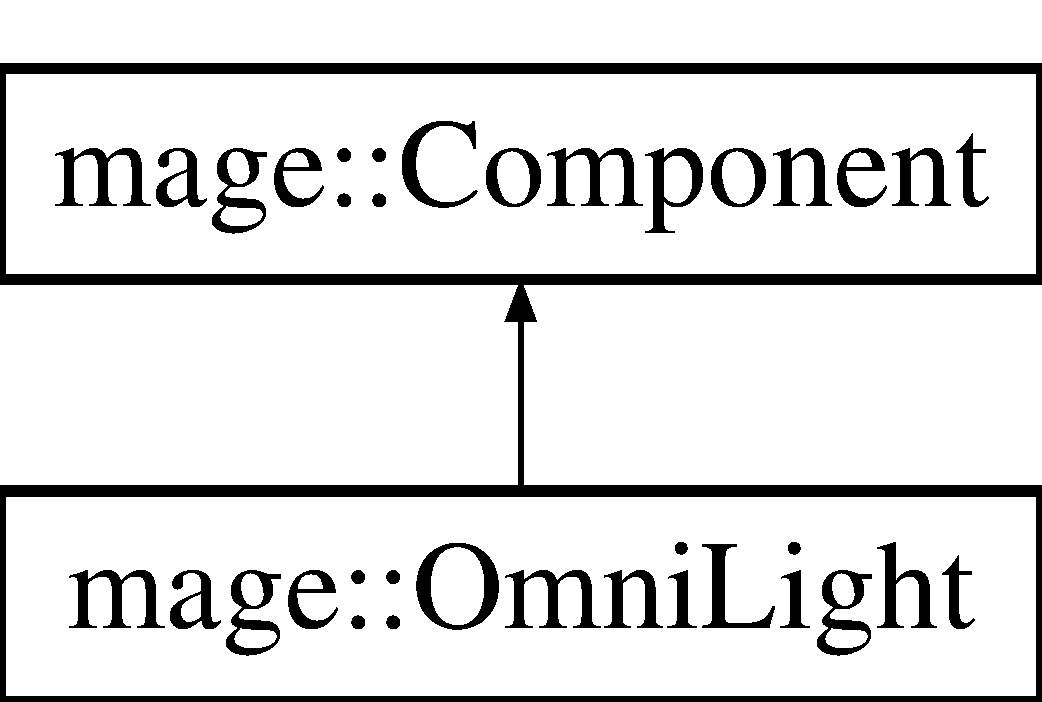
\includegraphics[height=2.000000cm]{classmage_1_1_omni_light}
\end{center}
\end{figure}
\subsection*{Public Member Functions}
\begin{DoxyCompactItemize}
\item 
\hyperlink{classmage_1_1_omni_light_a94794dd7c19fcac0c0d0b9d83108513b}{Omni\+Light} (const \hyperlink{structmage_1_1_r_g_b_spectrum}{R\+G\+B\+Spectrum} \&intensity=\hyperlink{structmage_1_1_r_g_b_spectrum}{R\+G\+B\+Spectrum}(1.\+0f, 1.\+0f, 1.\+0f))
\item 
\hyperlink{classmage_1_1_omni_light_accf10bcdf8ed523cfb04129f5345ef92}{Omni\+Light} (const \hyperlink{classmage_1_1_omni_light}{Omni\+Light} \&light)
\item 
\hyperlink{classmage_1_1_omni_light_ae0353cedc67d88be2f4b88374482933d}{Omni\+Light} (\hyperlink{classmage_1_1_omni_light}{Omni\+Light} \&\&light)
\item 
virtual \hyperlink{classmage_1_1_omni_light_af6f4921499b430041966f38aac920b69}{$\sim$\+Omni\+Light} ()
\item 
\hyperlink{classmage_1_1_omni_light}{Omni\+Light} \& \hyperlink{classmage_1_1_omni_light_a7bdce151d327daef5e1f31daedcc4627}{operator=} (const \hyperlink{classmage_1_1_omni_light}{Omni\+Light} \&light)
\item 
\hyperlink{classmage_1_1_omni_light}{Omni\+Light} \& \hyperlink{classmage_1_1_omni_light_a287a54dede61e65efe4493ec20531428}{operator=} (\hyperlink{classmage_1_1_omni_light}{Omni\+Light} \&\&light)
\item 
\hyperlink{namespacemage_a3316d7143a973e37adf1110f2e80ca31}{Unique\+Ptr}$<$ \hyperlink{classmage_1_1_omni_light}{Omni\+Light} $>$ \hyperlink{classmage_1_1_omni_light_a82325924de65733314dcf2b87e926d60}{Clone} () const
\item 
\hyperlink{namespacemage_aa97e833b45f06d60a0a9c4fc22ae02c0}{F32} \hyperlink{classmage_1_1_omni_light_a32551ce9c37a3f4f6fa2ba9faba47358}{Get\+Start\+Distance\+Falloff} () const noexcept
\item 
void \hyperlink{classmage_1_1_omni_light_a221f403ca37b500dff1085d2e74f582c}{Set\+Start\+Distance\+Falloff} (\hyperlink{namespacemage_aa97e833b45f06d60a0a9c4fc22ae02c0}{F32} distance\+\_\+falloff\+\_\+start) noexcept
\item 
\hyperlink{namespacemage_aa97e833b45f06d60a0a9c4fc22ae02c0}{F32} \hyperlink{classmage_1_1_omni_light_abe17539c94e52b00a1182cd9780dbf77}{Get\+End\+Distance\+Falloff} () const noexcept
\item 
void \hyperlink{classmage_1_1_omni_light_a35dac13256d90da9c829653eb68070e9}{Set\+End\+Distance\+Falloff} (\hyperlink{namespacemage_aa97e833b45f06d60a0a9c4fc22ae02c0}{F32} distance\+\_\+falloff\+\_\+end) noexcept
\item 
void \hyperlink{classmage_1_1_omni_light_aa7a5fbf5cbf15199d6e5c6ef28b6ce84}{Set\+Distance\+Falloff} (\hyperlink{namespacemage_aa97e833b45f06d60a0a9c4fc22ae02c0}{F32} distance\+\_\+falloff\+\_\+start, \hyperlink{namespacemage_aa97e833b45f06d60a0a9c4fc22ae02c0}{F32} distance\+\_\+falloff\+\_\+end) noexcept
\item 
\hyperlink{namespacemage_aa97e833b45f06d60a0a9c4fc22ae02c0}{F32} \hyperlink{classmage_1_1_omni_light_adf729b70a53ae97b054f0f2226590612}{Get\+Range\+Distance\+Falloff} () const noexcept
\item 
void \hyperlink{classmage_1_1_omni_light_ad1947b5fcd6c175aa21be1cd19159fb9}{Set\+Range\+Distance\+Falloff} (\hyperlink{namespacemage_aa97e833b45f06d60a0a9c4fc22ae02c0}{F32} distance\+\_\+falloff\+\_\+start, \hyperlink{namespacemage_aa97e833b45f06d60a0a9c4fc22ae02c0}{F32} distance\+\_\+falloff\+\_\+range) noexcept
\item 
bool \hyperlink{classmage_1_1_omni_light_a8d58e7e1b26e54b3d9785ca79213cc4f}{Use\+Shadows} () const noexcept
\item 
void \hyperlink{classmage_1_1_omni_light_ad7c2e780dc83eb63fa44e1475492e192}{Enable\+Shadows} () noexcept
\item 
void \hyperlink{classmage_1_1_omni_light_a2353a53e336ffb55be9949ea6f1d8979}{Dissable\+Shadows} () noexcept
\item 
void \hyperlink{classmage_1_1_omni_light_a19164a13e884bce6fbc80b760c82d243}{Toggle\+Shadows} () noexcept
\item 
void \hyperlink{classmage_1_1_omni_light_a337082a4e6026fe6f98098df063e6660}{Set\+Shadows} (bool shadows) noexcept
\item 
\hyperlink{namespacemage_aa97e833b45f06d60a0a9c4fc22ae02c0}{F32} \hyperlink{classmage_1_1_omni_light_a7a0bd82c0272a7eeeb33a9ede796bae1}{Get\+F\+OV} () const noexcept
\item 
\hyperlink{namespacemage_aa97e833b45f06d60a0a9c4fc22ae02c0}{F32} \hyperlink{classmage_1_1_omni_light_a976a37c3f7c160f0383a93e4f7497eed}{Get\+Aspect\+Ratio} () const noexcept
\item 
const X\+M\+M\+A\+T\+R\+IX \hyperlink{classmage_1_1_omni_light_a3efda1559769189e4693c6e3c570ab4b}{Get\+View\+To\+Projection\+Matrix} () const noexcept
\item 
const \hyperlink{classmage_1_1_perspective_camera}{Perspective\+Camera} \hyperlink{classmage_1_1_omni_light_ac31708d7696a809bb75c75a85b14de80}{Get\+Light\+Camera} () const noexcept
\end{DoxyCompactItemize}
\subsection*{Private Member Functions}
\begin{DoxyCompactItemize}
\item 
virtual \hyperlink{namespacemage_a3316d7143a973e37adf1110f2e80ca31}{Unique\+Ptr}$<$ \hyperlink{classmage_1_1_light}{Light} $>$ \hyperlink{classmage_1_1_omni_light_a1212457828cdd96cc7170767b7bd1223}{Clone\+Implementation} () const override
\item 
void \hyperlink{classmage_1_1_omni_light_a6a10cdc0ed276d68e5378eaf934158e1}{Update\+Bounding\+Volumes} () noexcept
\end{DoxyCompactItemize}
\subsection*{Private Attributes}
\begin{DoxyCompactItemize}
\item 
\hyperlink{namespacemage_aa97e833b45f06d60a0a9c4fc22ae02c0}{F32} \hyperlink{classmage_1_1_omni_light_a1f879f4aaf9b9e7545ee5efb91b45dc5}{m\+\_\+distance\+\_\+falloff\+\_\+start}
\item 
\hyperlink{namespacemage_aa97e833b45f06d60a0a9c4fc22ae02c0}{F32} \hyperlink{classmage_1_1_omni_light_adca1b76cdcc29215aae6f25ea57327c5}{m\+\_\+distance\+\_\+falloff\+\_\+end}
\item 
bool \hyperlink{classmage_1_1_omni_light_a63e5dab12be5021815e98c81dd9aed6a}{m\+\_\+shadows}
\end{DoxyCompactItemize}
\subsection*{Additional Inherited Members}


\subsection{Detailed Description}
A class of omni lights. 

\subsection{Constructor \& Destructor Documentation}
\hypertarget{classmage_1_1_omni_light_a94794dd7c19fcac0c0d0b9d83108513b}{}\label{classmage_1_1_omni_light_a94794dd7c19fcac0c0d0b9d83108513b} 
\index{mage\+::\+Omni\+Light@{mage\+::\+Omni\+Light}!Omni\+Light@{Omni\+Light}}
\index{Omni\+Light@{Omni\+Light}!mage\+::\+Omni\+Light@{mage\+::\+Omni\+Light}}
\subsubsection{\texorpdfstring{Omni\+Light()}{OmniLight()}\hspace{0.1cm}{\footnotesize\ttfamily [1/3]}}
{\footnotesize\ttfamily mage\+::\+Omni\+Light\+::\+Omni\+Light (\begin{DoxyParamCaption}\item[{const \hyperlink{structmage_1_1_r_g_b_spectrum}{R\+G\+B\+Spectrum} \&}]{intensity = {\ttfamily \hyperlink{structmage_1_1_r_g_b_spectrum}{R\+G\+B\+Spectrum}(1.0f,~1.0f,~1.0f)} }\end{DoxyParamCaption})\hspace{0.3cm}{\ttfamily [explicit]}}

Constructs an omni light.


\begin{DoxyParams}[1]{Parameters}
\mbox{\tt in}  & {\em intensity} & The R\+GB intensity. \\
\hline
\end{DoxyParams}
\hypertarget{classmage_1_1_omni_light_accf10bcdf8ed523cfb04129f5345ef92}{}\label{classmage_1_1_omni_light_accf10bcdf8ed523cfb04129f5345ef92} 
\index{mage\+::\+Omni\+Light@{mage\+::\+Omni\+Light}!Omni\+Light@{Omni\+Light}}
\index{Omni\+Light@{Omni\+Light}!mage\+::\+Omni\+Light@{mage\+::\+Omni\+Light}}
\subsubsection{\texorpdfstring{Omni\+Light()}{OmniLight()}\hspace{0.1cm}{\footnotesize\ttfamily [2/3]}}
{\footnotesize\ttfamily mage\+::\+Omni\+Light\+::\+Omni\+Light (\begin{DoxyParamCaption}\item[{const \hyperlink{classmage_1_1_omni_light}{Omni\+Light} \&}]{light }\end{DoxyParamCaption})\hspace{0.3cm}{\ttfamily [default]}}

Constructs an omni light from the given omni light.


\begin{DoxyParams}[1]{Parameters}
\mbox{\tt in}  & {\em light} & A reference to the omni light to copy. \\
\hline
\end{DoxyParams}
\hypertarget{classmage_1_1_omni_light_ae0353cedc67d88be2f4b88374482933d}{}\label{classmage_1_1_omni_light_ae0353cedc67d88be2f4b88374482933d} 
\index{mage\+::\+Omni\+Light@{mage\+::\+Omni\+Light}!Omni\+Light@{Omni\+Light}}
\index{Omni\+Light@{Omni\+Light}!mage\+::\+Omni\+Light@{mage\+::\+Omni\+Light}}
\subsubsection{\texorpdfstring{Omni\+Light()}{OmniLight()}\hspace{0.1cm}{\footnotesize\ttfamily [3/3]}}
{\footnotesize\ttfamily mage\+::\+Omni\+Light\+::\+Omni\+Light (\begin{DoxyParamCaption}\item[{\hyperlink{classmage_1_1_omni_light}{Omni\+Light} \&\&}]{light }\end{DoxyParamCaption})\hspace{0.3cm}{\ttfamily [default]}}

Constructs an omni light by moving the given omni light.


\begin{DoxyParams}[1]{Parameters}
\mbox{\tt in}  & {\em light} & A reference to the omni light to move. \\
\hline
\end{DoxyParams}
\hypertarget{classmage_1_1_omni_light_af6f4921499b430041966f38aac920b69}{}\label{classmage_1_1_omni_light_af6f4921499b430041966f38aac920b69} 
\index{mage\+::\+Omni\+Light@{mage\+::\+Omni\+Light}!````~Omni\+Light@{$\sim$\+Omni\+Light}}
\index{````~Omni\+Light@{$\sim$\+Omni\+Light}!mage\+::\+Omni\+Light@{mage\+::\+Omni\+Light}}
\subsubsection{\texorpdfstring{$\sim$\+Omni\+Light()}{~OmniLight()}}
{\footnotesize\ttfamily mage\+::\+Omni\+Light\+::$\sim$\+Omni\+Light (\begin{DoxyParamCaption}{ }\end{DoxyParamCaption})\hspace{0.3cm}{\ttfamily [virtual]}, {\ttfamily [default]}}

Destructs this omni light. 

\subsection{Member Function Documentation}
\hypertarget{classmage_1_1_omni_light_a82325924de65733314dcf2b87e926d60}{}\label{classmage_1_1_omni_light_a82325924de65733314dcf2b87e926d60} 
\index{mage\+::\+Omni\+Light@{mage\+::\+Omni\+Light}!Clone@{Clone}}
\index{Clone@{Clone}!mage\+::\+Omni\+Light@{mage\+::\+Omni\+Light}}
\subsubsection{\texorpdfstring{Clone()}{Clone()}}
{\footnotesize\ttfamily \hyperlink{namespacemage_a3316d7143a973e37adf1110f2e80ca31}{Unique\+Ptr}$<$ \hyperlink{classmage_1_1_omni_light}{Omni\+Light} $>$ mage\+::\+Omni\+Light\+::\+Clone (\begin{DoxyParamCaption}{ }\end{DoxyParamCaption}) const}

Clones this omni light.

\begin{DoxyReturn}{Returns}
A pointer to the clone of this omni light. 
\end{DoxyReturn}
\hypertarget{classmage_1_1_omni_light_a1212457828cdd96cc7170767b7bd1223}{}\label{classmage_1_1_omni_light_a1212457828cdd96cc7170767b7bd1223} 
\index{mage\+::\+Omni\+Light@{mage\+::\+Omni\+Light}!Clone\+Implementation@{Clone\+Implementation}}
\index{Clone\+Implementation@{Clone\+Implementation}!mage\+::\+Omni\+Light@{mage\+::\+Omni\+Light}}
\subsubsection{\texorpdfstring{Clone\+Implementation()}{CloneImplementation()}}
{\footnotesize\ttfamily \hyperlink{namespacemage_a3316d7143a973e37adf1110f2e80ca31}{Unique\+Ptr}$<$ \hyperlink{classmage_1_1_light}{Light} $>$ mage\+::\+Omni\+Light\+::\+Clone\+Implementation (\begin{DoxyParamCaption}{ }\end{DoxyParamCaption}) const\hspace{0.3cm}{\ttfamily [override]}, {\ttfamily [private]}, {\ttfamily [virtual]}}

Clones this omni light.

\begin{DoxyReturn}{Returns}
A pointer to the clone of this omni light. 
\end{DoxyReturn}


Implements \hyperlink{classmage_1_1_light_aa613d76a1ebda69efde853d15f75490c}{mage\+::\+Light}.

\hypertarget{classmage_1_1_omni_light_a2353a53e336ffb55be9949ea6f1d8979}{}\label{classmage_1_1_omni_light_a2353a53e336ffb55be9949ea6f1d8979} 
\index{mage\+::\+Omni\+Light@{mage\+::\+Omni\+Light}!Dissable\+Shadows@{Dissable\+Shadows}}
\index{Dissable\+Shadows@{Dissable\+Shadows}!mage\+::\+Omni\+Light@{mage\+::\+Omni\+Light}}
\subsubsection{\texorpdfstring{Dissable\+Shadows()}{DissableShadows()}}
{\footnotesize\ttfamily void mage\+::\+Omni\+Light\+::\+Dissable\+Shadows (\begin{DoxyParamCaption}{ }\end{DoxyParamCaption})\hspace{0.3cm}{\ttfamily [noexcept]}}

Dissables shadows for this omni light. \hypertarget{classmage_1_1_omni_light_ad7c2e780dc83eb63fa44e1475492e192}{}\label{classmage_1_1_omni_light_ad7c2e780dc83eb63fa44e1475492e192} 
\index{mage\+::\+Omni\+Light@{mage\+::\+Omni\+Light}!Enable\+Shadows@{Enable\+Shadows}}
\index{Enable\+Shadows@{Enable\+Shadows}!mage\+::\+Omni\+Light@{mage\+::\+Omni\+Light}}
\subsubsection{\texorpdfstring{Enable\+Shadows()}{EnableShadows()}}
{\footnotesize\ttfamily void mage\+::\+Omni\+Light\+::\+Enable\+Shadows (\begin{DoxyParamCaption}{ }\end{DoxyParamCaption})\hspace{0.3cm}{\ttfamily [noexcept]}}

Enables shadows for this omni light. \hypertarget{classmage_1_1_omni_light_a976a37c3f7c160f0383a93e4f7497eed}{}\label{classmage_1_1_omni_light_a976a37c3f7c160f0383a93e4f7497eed} 
\index{mage\+::\+Omni\+Light@{mage\+::\+Omni\+Light}!Get\+Aspect\+Ratio@{Get\+Aspect\+Ratio}}
\index{Get\+Aspect\+Ratio@{Get\+Aspect\+Ratio}!mage\+::\+Omni\+Light@{mage\+::\+Omni\+Light}}
\subsubsection{\texorpdfstring{Get\+Aspect\+Ratio()}{GetAspectRatio()}}
{\footnotesize\ttfamily \hyperlink{namespacemage_aa97e833b45f06d60a0a9c4fc22ae02c0}{F32} mage\+::\+Omni\+Light\+::\+Get\+Aspect\+Ratio (\begin{DoxyParamCaption}{ }\end{DoxyParamCaption}) const\hspace{0.3cm}{\ttfamily [noexcept]}}

Returns the aspect ratio of this omni light.

\begin{DoxyReturn}{Returns}
The aspect ratio of this omni light. 
\end{DoxyReturn}
\hypertarget{classmage_1_1_omni_light_abe17539c94e52b00a1182cd9780dbf77}{}\label{classmage_1_1_omni_light_abe17539c94e52b00a1182cd9780dbf77} 
\index{mage\+::\+Omni\+Light@{mage\+::\+Omni\+Light}!Get\+End\+Distance\+Falloff@{Get\+End\+Distance\+Falloff}}
\index{Get\+End\+Distance\+Falloff@{Get\+End\+Distance\+Falloff}!mage\+::\+Omni\+Light@{mage\+::\+Omni\+Light}}
\subsubsection{\texorpdfstring{Get\+End\+Distance\+Falloff()}{GetEndDistanceFalloff()}}
{\footnotesize\ttfamily \hyperlink{namespacemage_aa97e833b45f06d60a0a9c4fc22ae02c0}{F32} mage\+::\+Omni\+Light\+::\+Get\+End\+Distance\+Falloff (\begin{DoxyParamCaption}{ }\end{DoxyParamCaption}) const\hspace{0.3cm}{\ttfamily [noexcept]}}

Returns the distance at which intensity falloff ends of this omni light.

\begin{DoxyReturn}{Returns}
The distance at which intensity falloff ends of this omni light. 
\end{DoxyReturn}
\hypertarget{classmage_1_1_omni_light_a7a0bd82c0272a7eeeb33a9ede796bae1}{}\label{classmage_1_1_omni_light_a7a0bd82c0272a7eeeb33a9ede796bae1} 
\index{mage\+::\+Omni\+Light@{mage\+::\+Omni\+Light}!Get\+F\+OV@{Get\+F\+OV}}
\index{Get\+F\+OV@{Get\+F\+OV}!mage\+::\+Omni\+Light@{mage\+::\+Omni\+Light}}
\subsubsection{\texorpdfstring{Get\+F\+O\+V()}{GetFOV()}}
{\footnotesize\ttfamily \hyperlink{namespacemage_aa97e833b45f06d60a0a9c4fc22ae02c0}{F32} mage\+::\+Omni\+Light\+::\+Get\+F\+OV (\begin{DoxyParamCaption}{ }\end{DoxyParamCaption}) const\hspace{0.3cm}{\ttfamily [noexcept]}}

Returns the (horizontal and vertical) field-\/of-\/view of this omni light.

\begin{DoxyReturn}{Returns}
The (horizontal and vertical) field-\/of-\/view of this omni light. 
\end{DoxyReturn}
\hypertarget{classmage_1_1_omni_light_ac31708d7696a809bb75c75a85b14de80}{}\label{classmage_1_1_omni_light_ac31708d7696a809bb75c75a85b14de80} 
\index{mage\+::\+Omni\+Light@{mage\+::\+Omni\+Light}!Get\+Light\+Camera@{Get\+Light\+Camera}}
\index{Get\+Light\+Camera@{Get\+Light\+Camera}!mage\+::\+Omni\+Light@{mage\+::\+Omni\+Light}}
\subsubsection{\texorpdfstring{Get\+Light\+Camera()}{GetLightCamera()}}
{\footnotesize\ttfamily const \hyperlink{classmage_1_1_perspective_camera}{Perspective\+Camera} mage\+::\+Omni\+Light\+::\+Get\+Light\+Camera (\begin{DoxyParamCaption}{ }\end{DoxyParamCaption}) const\hspace{0.3cm}{\ttfamily [noexcept]}}

Returns the (forward) light camera of this omni light.

\begin{DoxyReturn}{Returns}
The (forward) light camera of this omni light. 
\end{DoxyReturn}
\hypertarget{classmage_1_1_omni_light_adf729b70a53ae97b054f0f2226590612}{}\label{classmage_1_1_omni_light_adf729b70a53ae97b054f0f2226590612} 
\index{mage\+::\+Omni\+Light@{mage\+::\+Omni\+Light}!Get\+Range\+Distance\+Falloff@{Get\+Range\+Distance\+Falloff}}
\index{Get\+Range\+Distance\+Falloff@{Get\+Range\+Distance\+Falloff}!mage\+::\+Omni\+Light@{mage\+::\+Omni\+Light}}
\subsubsection{\texorpdfstring{Get\+Range\+Distance\+Falloff()}{GetRangeDistanceFalloff()}}
{\footnotesize\ttfamily \hyperlink{namespacemage_aa97e833b45f06d60a0a9c4fc22ae02c0}{F32} mage\+::\+Omni\+Light\+::\+Get\+Range\+Distance\+Falloff (\begin{DoxyParamCaption}{ }\end{DoxyParamCaption}) const\hspace{0.3cm}{\ttfamily [noexcept]}}

Returns the distance range where intensity falloff occurs of this omni light.

\begin{DoxyReturn}{Returns}
The distance range where intensity falloff occurs of this omni light. {\itshape \hyperlink{classmage_1_1_omni_light_abe17539c94e52b00a1182cd9780dbf77}{Get\+End\+Distance\+Falloff()}} -\/ {\itshape \hyperlink{classmage_1_1_omni_light_a32551ce9c37a3f4f6fa2ba9faba47358}{Get\+Start\+Distance\+Falloff()}}. 
\end{DoxyReturn}
\hypertarget{classmage_1_1_omni_light_a32551ce9c37a3f4f6fa2ba9faba47358}{}\label{classmage_1_1_omni_light_a32551ce9c37a3f4f6fa2ba9faba47358} 
\index{mage\+::\+Omni\+Light@{mage\+::\+Omni\+Light}!Get\+Start\+Distance\+Falloff@{Get\+Start\+Distance\+Falloff}}
\index{Get\+Start\+Distance\+Falloff@{Get\+Start\+Distance\+Falloff}!mage\+::\+Omni\+Light@{mage\+::\+Omni\+Light}}
\subsubsection{\texorpdfstring{Get\+Start\+Distance\+Falloff()}{GetStartDistanceFalloff()}}
{\footnotesize\ttfamily \hyperlink{namespacemage_aa97e833b45f06d60a0a9c4fc22ae02c0}{F32} mage\+::\+Omni\+Light\+::\+Get\+Start\+Distance\+Falloff (\begin{DoxyParamCaption}{ }\end{DoxyParamCaption}) const\hspace{0.3cm}{\ttfamily [noexcept]}}

Returns the distance at which intensity falloff starts of this omni light.

\begin{DoxyReturn}{Returns}
The distance at which intensity falloff starts of this omni light. 
\end{DoxyReturn}
\hypertarget{classmage_1_1_omni_light_a3efda1559769189e4693c6e3c570ab4b}{}\label{classmage_1_1_omni_light_a3efda1559769189e4693c6e3c570ab4b} 
\index{mage\+::\+Omni\+Light@{mage\+::\+Omni\+Light}!Get\+View\+To\+Projection\+Matrix@{Get\+View\+To\+Projection\+Matrix}}
\index{Get\+View\+To\+Projection\+Matrix@{Get\+View\+To\+Projection\+Matrix}!mage\+::\+Omni\+Light@{mage\+::\+Omni\+Light}}
\subsubsection{\texorpdfstring{Get\+View\+To\+Projection\+Matrix()}{GetViewToProjectionMatrix()}}
{\footnotesize\ttfamily const X\+M\+M\+A\+T\+R\+IX mage\+::\+Omni\+Light\+::\+Get\+View\+To\+Projection\+Matrix (\begin{DoxyParamCaption}{ }\end{DoxyParamCaption}) const\hspace{0.3cm}{\ttfamily [noexcept]}}

Returns the view-\/to-\/projection matrix of the (forward) light camera of this omni light.

\begin{DoxyReturn}{Returns}
The view-\/to-\/projection matrix of the (forward) light camera of this omni light. 
\end{DoxyReturn}
\hypertarget{classmage_1_1_omni_light_a7bdce151d327daef5e1f31daedcc4627}{}\label{classmage_1_1_omni_light_a7bdce151d327daef5e1f31daedcc4627} 
\index{mage\+::\+Omni\+Light@{mage\+::\+Omni\+Light}!operator=@{operator=}}
\index{operator=@{operator=}!mage\+::\+Omni\+Light@{mage\+::\+Omni\+Light}}
\subsubsection{\texorpdfstring{operator=()}{operator=()}\hspace{0.1cm}{\footnotesize\ttfamily [1/2]}}
{\footnotesize\ttfamily \hyperlink{classmage_1_1_omni_light}{Omni\+Light} \& mage\+::\+Omni\+Light\+::operator= (\begin{DoxyParamCaption}\item[{const \hyperlink{classmage_1_1_omni_light}{Omni\+Light} \&}]{light }\end{DoxyParamCaption})\hspace{0.3cm}{\ttfamily [default]}}

Copies the given omni light to this omni light.


\begin{DoxyParams}[1]{Parameters}
\mbox{\tt in}  & {\em light} & A reference to the omni light to copy. \\
\hline
\end{DoxyParams}
\begin{DoxyReturn}{Returns}
A reference to the copy of the given omni light (i.\+e. this omni light). 
\end{DoxyReturn}
\hypertarget{classmage_1_1_omni_light_a287a54dede61e65efe4493ec20531428}{}\label{classmage_1_1_omni_light_a287a54dede61e65efe4493ec20531428} 
\index{mage\+::\+Omni\+Light@{mage\+::\+Omni\+Light}!operator=@{operator=}}
\index{operator=@{operator=}!mage\+::\+Omni\+Light@{mage\+::\+Omni\+Light}}
\subsubsection{\texorpdfstring{operator=()}{operator=()}\hspace{0.1cm}{\footnotesize\ttfamily [2/2]}}
{\footnotesize\ttfamily \hyperlink{classmage_1_1_omni_light}{Omni\+Light} \& mage\+::\+Omni\+Light\+::operator= (\begin{DoxyParamCaption}\item[{\hyperlink{classmage_1_1_omni_light}{Omni\+Light} \&\&}]{light }\end{DoxyParamCaption})\hspace{0.3cm}{\ttfamily [default]}}

Moves the given omni light to this omni light.


\begin{DoxyParams}[1]{Parameters}
\mbox{\tt in}  & {\em light} & A reference to the omni light to move. \\
\hline
\end{DoxyParams}
\begin{DoxyReturn}{Returns}
A reference to the moved omni light (i.\+e. this omni light). 
\end{DoxyReturn}
\hypertarget{classmage_1_1_omni_light_aa7a5fbf5cbf15199d6e5c6ef28b6ce84}{}\label{classmage_1_1_omni_light_aa7a5fbf5cbf15199d6e5c6ef28b6ce84} 
\index{mage\+::\+Omni\+Light@{mage\+::\+Omni\+Light}!Set\+Distance\+Falloff@{Set\+Distance\+Falloff}}
\index{Set\+Distance\+Falloff@{Set\+Distance\+Falloff}!mage\+::\+Omni\+Light@{mage\+::\+Omni\+Light}}
\subsubsection{\texorpdfstring{Set\+Distance\+Falloff()}{SetDistanceFalloff()}}
{\footnotesize\ttfamily void mage\+::\+Omni\+Light\+::\+Set\+Distance\+Falloff (\begin{DoxyParamCaption}\item[{\hyperlink{namespacemage_aa97e833b45f06d60a0a9c4fc22ae02c0}{F32}}]{distance\+\_\+falloff\+\_\+start,  }\item[{\hyperlink{namespacemage_aa97e833b45f06d60a0a9c4fc22ae02c0}{F32}}]{distance\+\_\+falloff\+\_\+end }\end{DoxyParamCaption})\hspace{0.3cm}{\ttfamily [noexcept]}}

Sets the distance at which intensity falloff starts and ends of this omni light to the given values.

\begin{DoxyPrecond}{Precondition}
{\itshape distance\+\_\+falloff\+\_\+end} $>$ 0. 
\end{DoxyPrecond}

\begin{DoxyParams}[1]{Parameters}
\mbox{\tt in}  & {\em distance\+\_\+falloff\+\_\+start} & The distance at which intensity falloff starts. \\
\hline
\mbox{\tt in}  & {\em distance\+\_\+falloff\+\_\+end} & The distance at which intensity falloff ends. \\
\hline
\end{DoxyParams}
\hypertarget{classmage_1_1_omni_light_a35dac13256d90da9c829653eb68070e9}{}\label{classmage_1_1_omni_light_a35dac13256d90da9c829653eb68070e9} 
\index{mage\+::\+Omni\+Light@{mage\+::\+Omni\+Light}!Set\+End\+Distance\+Falloff@{Set\+End\+Distance\+Falloff}}
\index{Set\+End\+Distance\+Falloff@{Set\+End\+Distance\+Falloff}!mage\+::\+Omni\+Light@{mage\+::\+Omni\+Light}}
\subsubsection{\texorpdfstring{Set\+End\+Distance\+Falloff()}{SetEndDistanceFalloff()}}
{\footnotesize\ttfamily void mage\+::\+Omni\+Light\+::\+Set\+End\+Distance\+Falloff (\begin{DoxyParamCaption}\item[{\hyperlink{namespacemage_aa97e833b45f06d60a0a9c4fc22ae02c0}{F32}}]{distance\+\_\+falloff\+\_\+end }\end{DoxyParamCaption})\hspace{0.3cm}{\ttfamily [noexcept]}}

Sets the distance at which intensity falloff ends of this omni light to the given value.

\begin{DoxyPrecond}{Precondition}
{\itshape distance\+\_\+falloff\+\_\+end} $>$ 0. 
\end{DoxyPrecond}

\begin{DoxyParams}[1]{Parameters}
\mbox{\tt in}  & {\em distance\+\_\+falloff\+\_\+end} & The distance at which intensity falloff ends. \\
\hline
\end{DoxyParams}
\hypertarget{classmage_1_1_omni_light_ad1947b5fcd6c175aa21be1cd19159fb9}{}\label{classmage_1_1_omni_light_ad1947b5fcd6c175aa21be1cd19159fb9} 
\index{mage\+::\+Omni\+Light@{mage\+::\+Omni\+Light}!Set\+Range\+Distance\+Falloff@{Set\+Range\+Distance\+Falloff}}
\index{Set\+Range\+Distance\+Falloff@{Set\+Range\+Distance\+Falloff}!mage\+::\+Omni\+Light@{mage\+::\+Omni\+Light}}
\subsubsection{\texorpdfstring{Set\+Range\+Distance\+Falloff()}{SetRangeDistanceFalloff()}}
{\footnotesize\ttfamily void mage\+::\+Omni\+Light\+::\+Set\+Range\+Distance\+Falloff (\begin{DoxyParamCaption}\item[{\hyperlink{namespacemage_aa97e833b45f06d60a0a9c4fc22ae02c0}{F32}}]{distance\+\_\+falloff\+\_\+start,  }\item[{\hyperlink{namespacemage_aa97e833b45f06d60a0a9c4fc22ae02c0}{F32}}]{distance\+\_\+falloff\+\_\+range }\end{DoxyParamCaption})\hspace{0.3cm}{\ttfamily [noexcept]}}

Sets the distance at which intensity falloff starts and the distance range where intensity falloff occurs of this omni light to the given values.

\begin{DoxyPrecond}{Precondition}
{\itshape distance\+\_\+falloff\+\_\+start} + {\itshape distance\+\_\+falloff\+\_\+range} $>$ 0. 
\end{DoxyPrecond}

\begin{DoxyParams}[1]{Parameters}
\mbox{\tt in}  & {\em distance\+\_\+falloff\+\_\+start} & The distance at which intensity falloff starts. \\
\hline
\mbox{\tt in}  & {\em distance\+\_\+falloff\+\_\+range} & The distance range where intensity falloff occurs. \\
\hline
\end{DoxyParams}
\hypertarget{classmage_1_1_omni_light_a337082a4e6026fe6f98098df063e6660}{}\label{classmage_1_1_omni_light_a337082a4e6026fe6f98098df063e6660} 
\index{mage\+::\+Omni\+Light@{mage\+::\+Omni\+Light}!Set\+Shadows@{Set\+Shadows}}
\index{Set\+Shadows@{Set\+Shadows}!mage\+::\+Omni\+Light@{mage\+::\+Omni\+Light}}
\subsubsection{\texorpdfstring{Set\+Shadows()}{SetShadows()}}
{\footnotesize\ttfamily void mage\+::\+Omni\+Light\+::\+Set\+Shadows (\begin{DoxyParamCaption}\item[{bool}]{shadows }\end{DoxyParamCaption})\hspace{0.3cm}{\ttfamily [noexcept]}}

Sets shadows for this omni light to the given value.


\begin{DoxyParams}[1]{Parameters}
\mbox{\tt in}  & {\em shadows} & {\ttfamily true} if shadows should be used for this omni light. {\ttfamily false} otherwise. \\
\hline
\end{DoxyParams}
\hypertarget{classmage_1_1_omni_light_a221f403ca37b500dff1085d2e74f582c}{}\label{classmage_1_1_omni_light_a221f403ca37b500dff1085d2e74f582c} 
\index{mage\+::\+Omni\+Light@{mage\+::\+Omni\+Light}!Set\+Start\+Distance\+Falloff@{Set\+Start\+Distance\+Falloff}}
\index{Set\+Start\+Distance\+Falloff@{Set\+Start\+Distance\+Falloff}!mage\+::\+Omni\+Light@{mage\+::\+Omni\+Light}}
\subsubsection{\texorpdfstring{Set\+Start\+Distance\+Falloff()}{SetStartDistanceFalloff()}}
{\footnotesize\ttfamily void mage\+::\+Omni\+Light\+::\+Set\+Start\+Distance\+Falloff (\begin{DoxyParamCaption}\item[{\hyperlink{namespacemage_aa97e833b45f06d60a0a9c4fc22ae02c0}{F32}}]{distance\+\_\+falloff\+\_\+start }\end{DoxyParamCaption})\hspace{0.3cm}{\ttfamily [noexcept]}}

Sets the distance at which intensity falloff starts of this omni light to the given value.


\begin{DoxyParams}[1]{Parameters}
\mbox{\tt in}  & {\em distance\+\_\+falloff\+\_\+start} & The distance at which intensity falloff starts. \\
\hline
\end{DoxyParams}
\hypertarget{classmage_1_1_omni_light_a19164a13e884bce6fbc80b760c82d243}{}\label{classmage_1_1_omni_light_a19164a13e884bce6fbc80b760c82d243} 
\index{mage\+::\+Omni\+Light@{mage\+::\+Omni\+Light}!Toggle\+Shadows@{Toggle\+Shadows}}
\index{Toggle\+Shadows@{Toggle\+Shadows}!mage\+::\+Omni\+Light@{mage\+::\+Omni\+Light}}
\subsubsection{\texorpdfstring{Toggle\+Shadows()}{ToggleShadows()}}
{\footnotesize\ttfamily void mage\+::\+Omni\+Light\+::\+Toggle\+Shadows (\begin{DoxyParamCaption}{ }\end{DoxyParamCaption})\hspace{0.3cm}{\ttfamily [noexcept]}}

Toggles shadows for this omni light. \hypertarget{classmage_1_1_omni_light_a6a10cdc0ed276d68e5378eaf934158e1}{}\label{classmage_1_1_omni_light_a6a10cdc0ed276d68e5378eaf934158e1} 
\index{mage\+::\+Omni\+Light@{mage\+::\+Omni\+Light}!Update\+Bounding\+Volumes@{Update\+Bounding\+Volumes}}
\index{Update\+Bounding\+Volumes@{Update\+Bounding\+Volumes}!mage\+::\+Omni\+Light@{mage\+::\+Omni\+Light}}
\subsubsection{\texorpdfstring{Update\+Bounding\+Volumes()}{UpdateBoundingVolumes()}}
{\footnotesize\ttfamily void mage\+::\+Omni\+Light\+::\+Update\+Bounding\+Volumes (\begin{DoxyParamCaption}{ }\end{DoxyParamCaption})\hspace{0.3cm}{\ttfamily [private]}, {\ttfamily [noexcept]}}

Updates the bounding volumes of this omni light. \hypertarget{classmage_1_1_omni_light_a8d58e7e1b26e54b3d9785ca79213cc4f}{}\label{classmage_1_1_omni_light_a8d58e7e1b26e54b3d9785ca79213cc4f} 
\index{mage\+::\+Omni\+Light@{mage\+::\+Omni\+Light}!Use\+Shadows@{Use\+Shadows}}
\index{Use\+Shadows@{Use\+Shadows}!mage\+::\+Omni\+Light@{mage\+::\+Omni\+Light}}
\subsubsection{\texorpdfstring{Use\+Shadows()}{UseShadows()}}
{\footnotesize\ttfamily bool mage\+::\+Omni\+Light\+::\+Use\+Shadows (\begin{DoxyParamCaption}{ }\end{DoxyParamCaption}) const\hspace{0.3cm}{\ttfamily [noexcept]}}

Checks whether shadows should be used for this omni light.

\begin{DoxyReturn}{Returns}
{\ttfamily true} if shadows should be used for this omni light. {\ttfamily false} otherwise. 
\end{DoxyReturn}


\subsection{Member Data Documentation}
\hypertarget{classmage_1_1_omni_light_adca1b76cdcc29215aae6f25ea57327c5}{}\label{classmage_1_1_omni_light_adca1b76cdcc29215aae6f25ea57327c5} 
\index{mage\+::\+Omni\+Light@{mage\+::\+Omni\+Light}!m\+\_\+distance\+\_\+falloff\+\_\+end@{m\+\_\+distance\+\_\+falloff\+\_\+end}}
\index{m\+\_\+distance\+\_\+falloff\+\_\+end@{m\+\_\+distance\+\_\+falloff\+\_\+end}!mage\+::\+Omni\+Light@{mage\+::\+Omni\+Light}}
\subsubsection{\texorpdfstring{m\+\_\+distance\+\_\+falloff\+\_\+end}{m\_distance\_falloff\_end}}
{\footnotesize\ttfamily \hyperlink{namespacemage_aa97e833b45f06d60a0a9c4fc22ae02c0}{F32} mage\+::\+Omni\+Light\+::m\+\_\+distance\+\_\+falloff\+\_\+end\hspace{0.3cm}{\ttfamily [private]}}

The end of the distance falloff of this omni light. \hypertarget{classmage_1_1_omni_light_a1f879f4aaf9b9e7545ee5efb91b45dc5}{}\label{classmage_1_1_omni_light_a1f879f4aaf9b9e7545ee5efb91b45dc5} 
\index{mage\+::\+Omni\+Light@{mage\+::\+Omni\+Light}!m\+\_\+distance\+\_\+falloff\+\_\+start@{m\+\_\+distance\+\_\+falloff\+\_\+start}}
\index{m\+\_\+distance\+\_\+falloff\+\_\+start@{m\+\_\+distance\+\_\+falloff\+\_\+start}!mage\+::\+Omni\+Light@{mage\+::\+Omni\+Light}}
\subsubsection{\texorpdfstring{m\+\_\+distance\+\_\+falloff\+\_\+start}{m\_distance\_falloff\_start}}
{\footnotesize\ttfamily \hyperlink{namespacemage_aa97e833b45f06d60a0a9c4fc22ae02c0}{F32} mage\+::\+Omni\+Light\+::m\+\_\+distance\+\_\+falloff\+\_\+start\hspace{0.3cm}{\ttfamily [private]}}

The start of the distance falloff of this omni light. \hypertarget{classmage_1_1_omni_light_a63e5dab12be5021815e98c81dd9aed6a}{}\label{classmage_1_1_omni_light_a63e5dab12be5021815e98c81dd9aed6a} 
\index{mage\+::\+Omni\+Light@{mage\+::\+Omni\+Light}!m\+\_\+shadows@{m\+\_\+shadows}}
\index{m\+\_\+shadows@{m\+\_\+shadows}!mage\+::\+Omni\+Light@{mage\+::\+Omni\+Light}}
\subsubsection{\texorpdfstring{m\+\_\+shadows}{m\_shadows}}
{\footnotesize\ttfamily bool mage\+::\+Omni\+Light\+::m\+\_\+shadows\hspace{0.3cm}{\ttfamily [private]}}

A flag indicating whether shadows should be calculated or not for this omni light. 
\hypertarget{classmage_1_1_orthographic_camera}{}\section{mage\+:\+:Orthographic\+Camera Class Reference}
\label{classmage_1_1_orthographic_camera}\index{mage\+::\+Orthographic\+Camera@{mage\+::\+Orthographic\+Camera}}


{\ttfamily \#include $<$orthographic\+\_\+camera.\+hpp$>$}

Inheritance diagram for mage\+:\+:Orthographic\+Camera\+:\begin{figure}[H]
\begin{center}
\leavevmode
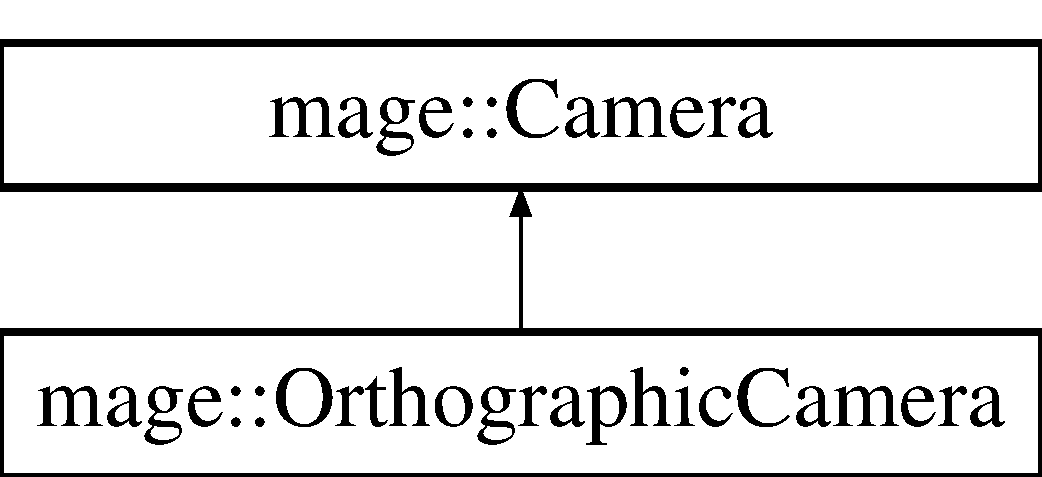
\includegraphics[height=2.000000cm]{classmage_1_1_orthographic_camera}
\end{center}
\end{figure}
\subsection*{Public Member Functions}
\begin{DoxyCompactItemize}
\item 
\hyperlink{classmage_1_1_orthographic_camera_a4a9c362b0c1cb90608b699deb3ae8b23}{Orthographic\+Camera} (float width=M\+A\+G\+E\+\_\+\+D\+E\+F\+A\+U\+L\+T\+\_\+\+C\+A\+M\+E\+R\+A\+\_\+\+O\+R\+T\+H\+O\+G\+R\+A\+P\+H\+I\+C\+\_\+\+W\+I\+D\+TH, float height=M\+A\+G\+E\+\_\+\+D\+E\+F\+A\+U\+L\+T\+\_\+\+C\+A\+M\+E\+R\+A\+\_\+\+O\+R\+T\+H\+O\+G\+R\+A\+P\+H\+I\+C\+\_\+\+H\+E\+I\+G\+HT, float near\+\_\+z=M\+A\+G\+E\+\_\+\+D\+E\+F\+A\+U\+L\+T\+\_\+\+C\+A\+M\+E\+R\+A\+\_\+\+N\+E\+A\+R\+\_\+Z, float far\+\_\+z=M\+A\+G\+E\+\_\+\+D\+E\+F\+A\+U\+L\+T\+\_\+\+C\+A\+M\+E\+R\+A\+\_\+\+F\+A\+R\+\_\+Z)
\item 
\hyperlink{classmage_1_1_orthographic_camera_a0293f01356417e9f32db027ba92d6029}{Orthographic\+Camera} (const \hyperlink{classmage_1_1_orthographic_camera}{Orthographic\+Camera} \&camera)=default
\item 
\hyperlink{classmage_1_1_orthographic_camera_a6abe78fc17b583046b30a459f9ef07ef}{Orthographic\+Camera} (\hyperlink{classmage_1_1_orthographic_camera}{Orthographic\+Camera} \&\&camera)=default
\item 
virtual \hyperlink{classmage_1_1_orthographic_camera_abdad923634e17f217ba975a9149f6c57}{$\sim$\+Orthographic\+Camera} ()=default
\item 
\hyperlink{classmage_1_1_orthographic_camera}{Orthographic\+Camera} \& \hyperlink{classmage_1_1_orthographic_camera_a38631b1c377f0e3b6fa99ac5535ce226}{operator=} (const \hyperlink{classmage_1_1_orthographic_camera}{Orthographic\+Camera} \&camera)=default
\item 
\hyperlink{classmage_1_1_orthographic_camera}{Orthographic\+Camera} \& \hyperlink{classmage_1_1_orthographic_camera_a51b38eab8945fb1a2031a7ba1755d689}{operator=} (\hyperlink{classmage_1_1_orthographic_camera}{Orthographic\+Camera} \&\&camera)=default
\item 
\hyperlink{namespacemage_a1e01ae66713838a7a67d30e44c67703e}{Shared\+Ptr}$<$ \hyperlink{classmage_1_1_orthographic_camera}{Orthographic\+Camera} $>$ \hyperlink{classmage_1_1_orthographic_camera_a4b9e8cca5814d955efe1dad1df784aba}{Clone} () const
\item 
float \hyperlink{classmage_1_1_orthographic_camera_ac8daeca630e0f4503354e3eede7ead5c}{Get\+Width} () const
\item 
\hyperlink{classmage_1_1_orthographic_camera}{Orthographic\+Camera} \& \hyperlink{classmage_1_1_orthographic_camera_aa38c67d3cfb41fb715bdf71d417bbc0d}{Set\+Width} (float width)
\item 
float \hyperlink{classmage_1_1_orthographic_camera_a596e2cf22fee8cf30139ffe9d4cdcda7}{Get\+Height} () const
\item 
\hyperlink{classmage_1_1_orthographic_camera}{Orthographic\+Camera} \& \hyperlink{classmage_1_1_orthographic_camera_a57cb23f7bee15791f6a73a1244815614}{Set\+Height} (float height)
\item 
\hyperlink{classmage_1_1_orthographic_camera}{Orthographic\+Camera} \& \hyperlink{classmage_1_1_orthographic_camera_a3ba89b58268c56fbebb8904bbe260f2f}{Set\+Width\+And\+Height} (float width, float height)
\item 
void \hyperlink{classmage_1_1_orthographic_camera_a10e09af47e741ab76dc2aa2a03f04c06}{Set\+View\+To\+Projection\+Matrix} (float width=M\+A\+G\+E\+\_\+\+D\+E\+F\+A\+U\+L\+T\+\_\+\+C\+A\+M\+E\+R\+A\+\_\+\+O\+R\+T\+H\+O\+G\+R\+A\+P\+H\+I\+C\+\_\+\+W\+I\+D\+TH, float height=M\+A\+G\+E\+\_\+\+D\+E\+F\+A\+U\+L\+T\+\_\+\+C\+A\+M\+E\+R\+A\+\_\+\+O\+R\+T\+H\+O\+G\+R\+A\+P\+H\+I\+C\+\_\+\+H\+E\+I\+G\+HT, float near\+\_\+z=M\+A\+G\+E\+\_\+\+D\+E\+F\+A\+U\+L\+T\+\_\+\+C\+A\+M\+E\+R\+A\+\_\+\+N\+E\+A\+R\+\_\+Z, float far\+\_\+z=M\+A\+G\+E\+\_\+\+D\+E\+F\+A\+U\+L\+T\+\_\+\+C\+A\+M\+E\+R\+A\+\_\+\+F\+A\+R\+\_\+Z)
\item 
virtual X\+M\+M\+A\+T\+R\+IX \hyperlink{classmage_1_1_orthographic_camera_aedd86e56a0f7bc967ad8d9be2631a0cf}{Get\+View\+To\+Projection\+Matrix} () const override
\end{DoxyCompactItemize}
\subsection*{Private Member Functions}
\begin{DoxyCompactItemize}
\item 
virtual \hyperlink{namespacemage_a1e01ae66713838a7a67d30e44c67703e}{Shared\+Ptr}$<$ \hyperlink{classmage_1_1_camera}{Camera} $>$ \hyperlink{classmage_1_1_orthographic_camera_a5a55280980bb4dc24d4b0213ad22cf64}{Clone\+Implementation} () const override
\end{DoxyCompactItemize}
\subsection*{Private Attributes}
\begin{DoxyCompactItemize}
\item 
float \hyperlink{classmage_1_1_orthographic_camera_aadef4cff19cc1b1ecf427f82bbc3ea6a}{m\+\_\+width}
\item 
float \hyperlink{classmage_1_1_orthographic_camera_a63169098f604874c1b30c4b276b5a3e1}{m\+\_\+height}
\end{DoxyCompactItemize}
\subsection*{Additional Inherited Members}


\subsection{Detailed Description}
A class of orthographic cameras. 

\subsection{Constructor \& Destructor Documentation}
\hypertarget{classmage_1_1_orthographic_camera_a4a9c362b0c1cb90608b699deb3ae8b23}{}\label{classmage_1_1_orthographic_camera_a4a9c362b0c1cb90608b699deb3ae8b23} 
\index{mage\+::\+Orthographic\+Camera@{mage\+::\+Orthographic\+Camera}!Orthographic\+Camera@{Orthographic\+Camera}}
\index{Orthographic\+Camera@{Orthographic\+Camera}!mage\+::\+Orthographic\+Camera@{mage\+::\+Orthographic\+Camera}}
\subsubsection{\texorpdfstring{Orthographic\+Camera()}{OrthographicCamera()}\hspace{0.1cm}{\footnotesize\ttfamily [1/3]}}
{\footnotesize\ttfamily mage\+::\+Orthographic\+Camera\+::\+Orthographic\+Camera (\begin{DoxyParamCaption}\item[{float}]{width = {\ttfamily MAGE\+\_\+DEFAULT\+\_\+CAMERA\+\_\+ORTHOGRAPHIC\+\_\+WIDTH},  }\item[{float}]{height = {\ttfamily MAGE\+\_\+DEFAULT\+\_\+CAMERA\+\_\+ORTHOGRAPHIC\+\_\+HEIGHT},  }\item[{float}]{near\+\_\+z = {\ttfamily MAGE\+\_\+DEFAULT\+\_\+CAMERA\+\_\+NEAR\+\_\+Z},  }\item[{float}]{far\+\_\+z = {\ttfamily MAGE\+\_\+DEFAULT\+\_\+CAMERA\+\_\+FAR\+\_\+Z} }\end{DoxyParamCaption})\hspace{0.3cm}{\ttfamily [explicit]}}

Constructs an orthographic camera.


\begin{DoxyParams}[1]{Parameters}
\mbox{\tt in}  & {\em width} & The width of the camera projection plane in camera space. \\
\hline
\mbox{\tt in}  & {\em height} & The height of the camera projection plane in camera space. \\
\hline
\mbox{\tt in}  & {\em near\+\_\+z} & The position of the near z-\/plane in camera space. \\
\hline
\mbox{\tt in}  & {\em far\+\_\+z} & The position of the far z-\/plane in camera space. \\
\hline
\end{DoxyParams}
\hypertarget{classmage_1_1_orthographic_camera_a0293f01356417e9f32db027ba92d6029}{}\label{classmage_1_1_orthographic_camera_a0293f01356417e9f32db027ba92d6029} 
\index{mage\+::\+Orthographic\+Camera@{mage\+::\+Orthographic\+Camera}!Orthographic\+Camera@{Orthographic\+Camera}}
\index{Orthographic\+Camera@{Orthographic\+Camera}!mage\+::\+Orthographic\+Camera@{mage\+::\+Orthographic\+Camera}}
\subsubsection{\texorpdfstring{Orthographic\+Camera()}{OrthographicCamera()}\hspace{0.1cm}{\footnotesize\ttfamily [2/3]}}
{\footnotesize\ttfamily mage\+::\+Orthographic\+Camera\+::\+Orthographic\+Camera (\begin{DoxyParamCaption}\item[{const \hyperlink{classmage_1_1_orthographic_camera}{Orthographic\+Camera} \&}]{camera }\end{DoxyParamCaption})\hspace{0.3cm}{\ttfamily [default]}}

Constructs an orthographic camera from the given orthographic camera.


\begin{DoxyParams}[1]{Parameters}
\mbox{\tt in}  & {\em camera} & A reference to the orthographic camera to copy. \\
\hline
\end{DoxyParams}
\hypertarget{classmage_1_1_orthographic_camera_a6abe78fc17b583046b30a459f9ef07ef}{}\label{classmage_1_1_orthographic_camera_a6abe78fc17b583046b30a459f9ef07ef} 
\index{mage\+::\+Orthographic\+Camera@{mage\+::\+Orthographic\+Camera}!Orthographic\+Camera@{Orthographic\+Camera}}
\index{Orthographic\+Camera@{Orthographic\+Camera}!mage\+::\+Orthographic\+Camera@{mage\+::\+Orthographic\+Camera}}
\subsubsection{\texorpdfstring{Orthographic\+Camera()}{OrthographicCamera()}\hspace{0.1cm}{\footnotesize\ttfamily [3/3]}}
{\footnotesize\ttfamily mage\+::\+Orthographic\+Camera\+::\+Orthographic\+Camera (\begin{DoxyParamCaption}\item[{\hyperlink{classmage_1_1_orthographic_camera}{Orthographic\+Camera} \&\&}]{camera }\end{DoxyParamCaption})\hspace{0.3cm}{\ttfamily [default]}}

Constructs an orthographic camera by moving the given orthographic camera.


\begin{DoxyParams}[1]{Parameters}
\mbox{\tt in}  & {\em camera} & A reference to the orthographic camera to move. \\
\hline
\end{DoxyParams}
\hypertarget{classmage_1_1_orthographic_camera_abdad923634e17f217ba975a9149f6c57}{}\label{classmage_1_1_orthographic_camera_abdad923634e17f217ba975a9149f6c57} 
\index{mage\+::\+Orthographic\+Camera@{mage\+::\+Orthographic\+Camera}!````~Orthographic\+Camera@{$\sim$\+Orthographic\+Camera}}
\index{````~Orthographic\+Camera@{$\sim$\+Orthographic\+Camera}!mage\+::\+Orthographic\+Camera@{mage\+::\+Orthographic\+Camera}}
\subsubsection{\texorpdfstring{$\sim$\+Orthographic\+Camera()}{~OrthographicCamera()}}
{\footnotesize\ttfamily virtual mage\+::\+Orthographic\+Camera\+::$\sim$\+Orthographic\+Camera (\begin{DoxyParamCaption}{ }\end{DoxyParamCaption})\hspace{0.3cm}{\ttfamily [virtual]}, {\ttfamily [default]}}

Destructs this orthographic camera. 

\subsection{Member Function Documentation}
\hypertarget{classmage_1_1_orthographic_camera_a4b9e8cca5814d955efe1dad1df784aba}{}\label{classmage_1_1_orthographic_camera_a4b9e8cca5814d955efe1dad1df784aba} 
\index{mage\+::\+Orthographic\+Camera@{mage\+::\+Orthographic\+Camera}!Clone@{Clone}}
\index{Clone@{Clone}!mage\+::\+Orthographic\+Camera@{mage\+::\+Orthographic\+Camera}}
\subsubsection{\texorpdfstring{Clone()}{Clone()}}
{\footnotesize\ttfamily \hyperlink{namespacemage_a1e01ae66713838a7a67d30e44c67703e}{Shared\+Ptr}$<$ \hyperlink{classmage_1_1_orthographic_camera}{Orthographic\+Camera} $>$ mage\+::\+Orthographic\+Camera\+::\+Clone (\begin{DoxyParamCaption}{ }\end{DoxyParamCaption}) const}

Clones this orthographic camera.

\begin{DoxyReturn}{Returns}
A pointer to the clone of this orthographic camera. 
\end{DoxyReturn}
\hypertarget{classmage_1_1_orthographic_camera_a5a55280980bb4dc24d4b0213ad22cf64}{}\label{classmage_1_1_orthographic_camera_a5a55280980bb4dc24d4b0213ad22cf64} 
\index{mage\+::\+Orthographic\+Camera@{mage\+::\+Orthographic\+Camera}!Clone\+Implementation@{Clone\+Implementation}}
\index{Clone\+Implementation@{Clone\+Implementation}!mage\+::\+Orthographic\+Camera@{mage\+::\+Orthographic\+Camera}}
\subsubsection{\texorpdfstring{Clone\+Implementation()}{CloneImplementation()}}
{\footnotesize\ttfamily virtual \hyperlink{namespacemage_a1e01ae66713838a7a67d30e44c67703e}{Shared\+Ptr}$<$ \hyperlink{classmage_1_1_camera}{Camera} $>$ mage\+::\+Orthographic\+Camera\+::\+Clone\+Implementation (\begin{DoxyParamCaption}{ }\end{DoxyParamCaption}) const\hspace{0.3cm}{\ttfamily [override]}, {\ttfamily [private]}, {\ttfamily [virtual]}}

Clones this orthographic camera.

\begin{DoxyReturn}{Returns}
A pointer to the clone of this orthographic camera. 
\end{DoxyReturn}


Implements \hyperlink{classmage_1_1_camera_a96c1bee3dc4085c8c7892427518165fc}{mage\+::\+Camera}.

\hypertarget{classmage_1_1_orthographic_camera_a596e2cf22fee8cf30139ffe9d4cdcda7}{}\label{classmage_1_1_orthographic_camera_a596e2cf22fee8cf30139ffe9d4cdcda7} 
\index{mage\+::\+Orthographic\+Camera@{mage\+::\+Orthographic\+Camera}!Get\+Height@{Get\+Height}}
\index{Get\+Height@{Get\+Height}!mage\+::\+Orthographic\+Camera@{mage\+::\+Orthographic\+Camera}}
\subsubsection{\texorpdfstring{Get\+Height()}{GetHeight()}}
{\footnotesize\ttfamily float mage\+::\+Orthographic\+Camera\+::\+Get\+Height (\begin{DoxyParamCaption}{ }\end{DoxyParamCaption}) const}

Returns the height of the camera projection plane of this orthographic camera in camera space.

\begin{DoxyReturn}{Returns}
The height of the camera projection plane of this orthographic camera in camera space. 
\end{DoxyReturn}
\hypertarget{classmage_1_1_orthographic_camera_aedd86e56a0f7bc967ad8d9be2631a0cf}{}\label{classmage_1_1_orthographic_camera_aedd86e56a0f7bc967ad8d9be2631a0cf} 
\index{mage\+::\+Orthographic\+Camera@{mage\+::\+Orthographic\+Camera}!Get\+View\+To\+Projection\+Matrix@{Get\+View\+To\+Projection\+Matrix}}
\index{Get\+View\+To\+Projection\+Matrix@{Get\+View\+To\+Projection\+Matrix}!mage\+::\+Orthographic\+Camera@{mage\+::\+Orthographic\+Camera}}
\subsubsection{\texorpdfstring{Get\+View\+To\+Projection\+Matrix()}{GetViewToProjectionMatrix()}}
{\footnotesize\ttfamily virtual X\+M\+M\+A\+T\+R\+IX mage\+::\+Orthographic\+Camera\+::\+Get\+View\+To\+Projection\+Matrix (\begin{DoxyParamCaption}{ }\end{DoxyParamCaption}) const\hspace{0.3cm}{\ttfamily [override]}, {\ttfamily [virtual]}}

Returns the view-\/to-\/projection matrix of this orthographic camera.

\begin{DoxyReturn}{Returns}
The view-\/to-\/projection matrix of this orthographic camera. 
\end{DoxyReturn}


Implements \hyperlink{classmage_1_1_camera_a1f5206864cf18b5548219492556df5d2}{mage\+::\+Camera}.

\hypertarget{classmage_1_1_orthographic_camera_ac8daeca630e0f4503354e3eede7ead5c}{}\label{classmage_1_1_orthographic_camera_ac8daeca630e0f4503354e3eede7ead5c} 
\index{mage\+::\+Orthographic\+Camera@{mage\+::\+Orthographic\+Camera}!Get\+Width@{Get\+Width}}
\index{Get\+Width@{Get\+Width}!mage\+::\+Orthographic\+Camera@{mage\+::\+Orthographic\+Camera}}
\subsubsection{\texorpdfstring{Get\+Width()}{GetWidth()}}
{\footnotesize\ttfamily float mage\+::\+Orthographic\+Camera\+::\+Get\+Width (\begin{DoxyParamCaption}{ }\end{DoxyParamCaption}) const}

Returns the width of the camera projection plane of this orthographic camera in camera space.

\begin{DoxyReturn}{Returns}
The width of the camera projection plane of this orthographic camera in camera space. 
\end{DoxyReturn}
\hypertarget{classmage_1_1_orthographic_camera_a38631b1c377f0e3b6fa99ac5535ce226}{}\label{classmage_1_1_orthographic_camera_a38631b1c377f0e3b6fa99ac5535ce226} 
\index{mage\+::\+Orthographic\+Camera@{mage\+::\+Orthographic\+Camera}!operator=@{operator=}}
\index{operator=@{operator=}!mage\+::\+Orthographic\+Camera@{mage\+::\+Orthographic\+Camera}}
\subsubsection{\texorpdfstring{operator=()}{operator=()}\hspace{0.1cm}{\footnotesize\ttfamily [1/2]}}
{\footnotesize\ttfamily \hyperlink{classmage_1_1_orthographic_camera}{Orthographic\+Camera}\& mage\+::\+Orthographic\+Camera\+::operator= (\begin{DoxyParamCaption}\item[{const \hyperlink{classmage_1_1_orthographic_camera}{Orthographic\+Camera} \&}]{camera }\end{DoxyParamCaption})\hspace{0.3cm}{\ttfamily [default]}}

Copies the given orthographic camera to this orthographic camera.


\begin{DoxyParams}[1]{Parameters}
\mbox{\tt in}  & {\em camera} & A reference to the orthographic camera to copy. \\
\hline
\end{DoxyParams}
\begin{DoxyReturn}{Returns}
A reference to the copy of the given orthographic camera (i.\+e. this orthographic camera). 
\end{DoxyReturn}
\hypertarget{classmage_1_1_orthographic_camera_a51b38eab8945fb1a2031a7ba1755d689}{}\label{classmage_1_1_orthographic_camera_a51b38eab8945fb1a2031a7ba1755d689} 
\index{mage\+::\+Orthographic\+Camera@{mage\+::\+Orthographic\+Camera}!operator=@{operator=}}
\index{operator=@{operator=}!mage\+::\+Orthographic\+Camera@{mage\+::\+Orthographic\+Camera}}
\subsubsection{\texorpdfstring{operator=()}{operator=()}\hspace{0.1cm}{\footnotesize\ttfamily [2/2]}}
{\footnotesize\ttfamily \hyperlink{classmage_1_1_orthographic_camera}{Orthographic\+Camera}\& mage\+::\+Orthographic\+Camera\+::operator= (\begin{DoxyParamCaption}\item[{\hyperlink{classmage_1_1_orthographic_camera}{Orthographic\+Camera} \&\&}]{camera }\end{DoxyParamCaption})\hspace{0.3cm}{\ttfamily [default]}}

Moves the given orthographic camera to this orthographic camera.


\begin{DoxyParams}[1]{Parameters}
\mbox{\tt in}  & {\em camera} & A reference to the orthographic camera to move. \\
\hline
\end{DoxyParams}
\begin{DoxyReturn}{Returns}
A reference to the moved orthographic camera (i.\+e. this orthographic camera). 
\end{DoxyReturn}
\hypertarget{classmage_1_1_orthographic_camera_a57cb23f7bee15791f6a73a1244815614}{}\label{classmage_1_1_orthographic_camera_a57cb23f7bee15791f6a73a1244815614} 
\index{mage\+::\+Orthographic\+Camera@{mage\+::\+Orthographic\+Camera}!Set\+Height@{Set\+Height}}
\index{Set\+Height@{Set\+Height}!mage\+::\+Orthographic\+Camera@{mage\+::\+Orthographic\+Camera}}
\subsubsection{\texorpdfstring{Set\+Height()}{SetHeight()}}
{\footnotesize\ttfamily \hyperlink{classmage_1_1_orthographic_camera}{Orthographic\+Camera}\& mage\+::\+Orthographic\+Camera\+::\+Set\+Height (\begin{DoxyParamCaption}\item[{float}]{height }\end{DoxyParamCaption})}

Sets the height of the camera projection plane of this orthographic camera to the given value.


\begin{DoxyParams}[1]{Parameters}
\mbox{\tt in}  & {\em height} & The height of the camera projection plane in camera space. \\
\hline
\end{DoxyParams}
\begin{DoxyReturn}{Returns}
A reference to this orthographic camera. 
\end{DoxyReturn}
\hypertarget{classmage_1_1_orthographic_camera_a10e09af47e741ab76dc2aa2a03f04c06}{}\label{classmage_1_1_orthographic_camera_a10e09af47e741ab76dc2aa2a03f04c06} 
\index{mage\+::\+Orthographic\+Camera@{mage\+::\+Orthographic\+Camera}!Set\+View\+To\+Projection\+Matrix@{Set\+View\+To\+Projection\+Matrix}}
\index{Set\+View\+To\+Projection\+Matrix@{Set\+View\+To\+Projection\+Matrix}!mage\+::\+Orthographic\+Camera@{mage\+::\+Orthographic\+Camera}}
\subsubsection{\texorpdfstring{Set\+View\+To\+Projection\+Matrix()}{SetViewToProjectionMatrix()}}
{\footnotesize\ttfamily void mage\+::\+Orthographic\+Camera\+::\+Set\+View\+To\+Projection\+Matrix (\begin{DoxyParamCaption}\item[{float}]{width = {\ttfamily MAGE\+\_\+DEFAULT\+\_\+CAMERA\+\_\+ORTHOGRAPHIC\+\_\+WIDTH},  }\item[{float}]{height = {\ttfamily MAGE\+\_\+DEFAULT\+\_\+CAMERA\+\_\+ORTHOGRAPHIC\+\_\+HEIGHT},  }\item[{float}]{near\+\_\+z = {\ttfamily MAGE\+\_\+DEFAULT\+\_\+CAMERA\+\_\+NEAR\+\_\+Z},  }\item[{float}]{far\+\_\+z = {\ttfamily MAGE\+\_\+DEFAULT\+\_\+CAMERA\+\_\+FAR\+\_\+Z} }\end{DoxyParamCaption})}

Sets the view-\/to-\/projection matrix of this orthographic camera.


\begin{DoxyParams}[1]{Parameters}
\mbox{\tt in}  & {\em width} & The width of the camera projection plane in camera space. \\
\hline
\mbox{\tt in}  & {\em height} & The height of the camera projection plane in camera space. \\
\hline
\mbox{\tt in}  & {\em near\+\_\+z} & The position of the near z-\/plane in camera space. \\
\hline
\mbox{\tt in}  & {\em far\+\_\+z} & The position of the far z-\/plane in camera space. \\
\hline
\end{DoxyParams}
\hypertarget{classmage_1_1_orthographic_camera_aa38c67d3cfb41fb715bdf71d417bbc0d}{}\label{classmage_1_1_orthographic_camera_aa38c67d3cfb41fb715bdf71d417bbc0d} 
\index{mage\+::\+Orthographic\+Camera@{mage\+::\+Orthographic\+Camera}!Set\+Width@{Set\+Width}}
\index{Set\+Width@{Set\+Width}!mage\+::\+Orthographic\+Camera@{mage\+::\+Orthographic\+Camera}}
\subsubsection{\texorpdfstring{Set\+Width()}{SetWidth()}}
{\footnotesize\ttfamily \hyperlink{classmage_1_1_orthographic_camera}{Orthographic\+Camera}\& mage\+::\+Orthographic\+Camera\+::\+Set\+Width (\begin{DoxyParamCaption}\item[{float}]{width }\end{DoxyParamCaption})}

Sets the width of the camera projection plane of this orthographic camera to the given value.


\begin{DoxyParams}[1]{Parameters}
\mbox{\tt in}  & {\em width} & The width of the camera projection plane in camera space. \\
\hline
\end{DoxyParams}
\begin{DoxyReturn}{Returns}
A reference to this orthographic camera. 
\end{DoxyReturn}
\hypertarget{classmage_1_1_orthographic_camera_a3ba89b58268c56fbebb8904bbe260f2f}{}\label{classmage_1_1_orthographic_camera_a3ba89b58268c56fbebb8904bbe260f2f} 
\index{mage\+::\+Orthographic\+Camera@{mage\+::\+Orthographic\+Camera}!Set\+Width\+And\+Height@{Set\+Width\+And\+Height}}
\index{Set\+Width\+And\+Height@{Set\+Width\+And\+Height}!mage\+::\+Orthographic\+Camera@{mage\+::\+Orthographic\+Camera}}
\subsubsection{\texorpdfstring{Set\+Width\+And\+Height()}{SetWidthAndHeight()}}
{\footnotesize\ttfamily \hyperlink{classmage_1_1_orthographic_camera}{Orthographic\+Camera}\& mage\+::\+Orthographic\+Camera\+::\+Set\+Width\+And\+Height (\begin{DoxyParamCaption}\item[{float}]{width,  }\item[{float}]{height }\end{DoxyParamCaption})}

Sets the width and height of the camera projection plane of this orthographic camera to the given values.


\begin{DoxyParams}[1]{Parameters}
\mbox{\tt in}  & {\em width} & The width of the camera projection plane in camera space. \\
\hline
\mbox{\tt in}  & {\em height} & The height of the camera projection plane in camera space. \\
\hline
\end{DoxyParams}
\begin{DoxyReturn}{Returns}
A reference to this orthographic camera. 
\end{DoxyReturn}


\subsection{Member Data Documentation}
\hypertarget{classmage_1_1_orthographic_camera_a63169098f604874c1b30c4b276b5a3e1}{}\label{classmage_1_1_orthographic_camera_a63169098f604874c1b30c4b276b5a3e1} 
\index{mage\+::\+Orthographic\+Camera@{mage\+::\+Orthographic\+Camera}!m\+\_\+height@{m\+\_\+height}}
\index{m\+\_\+height@{m\+\_\+height}!mage\+::\+Orthographic\+Camera@{mage\+::\+Orthographic\+Camera}}
\subsubsection{\texorpdfstring{m\+\_\+height}{m\_height}}
{\footnotesize\ttfamily float mage\+::\+Orthographic\+Camera\+::m\+\_\+height\hspace{0.3cm}{\ttfamily [private]}}

The height of the camera projection plane of this orthographic camera in camera space. \hypertarget{classmage_1_1_orthographic_camera_aadef4cff19cc1b1ecf427f82bbc3ea6a}{}\label{classmage_1_1_orthographic_camera_aadef4cff19cc1b1ecf427f82bbc3ea6a} 
\index{mage\+::\+Orthographic\+Camera@{mage\+::\+Orthographic\+Camera}!m\+\_\+width@{m\+\_\+width}}
\index{m\+\_\+width@{m\+\_\+width}!mage\+::\+Orthographic\+Camera@{mage\+::\+Orthographic\+Camera}}
\subsubsection{\texorpdfstring{m\+\_\+width}{m\_width}}
{\footnotesize\ttfamily float mage\+::\+Orthographic\+Camera\+::m\+\_\+width\hspace{0.3cm}{\ttfamily [private]}}

The width of the camera projection plane of this orthographic camera in camera space. 
\hypertarget{classmage_1_1_outline_sprite_text}{}\section{mage\+:\+:Outline\+Sprite\+Text Class Reference}
\label{classmage_1_1_outline_sprite_text}\index{mage\+::\+Outline\+Sprite\+Text@{mage\+::\+Outline\+Sprite\+Text}}


{\ttfamily \#include $<$outline\+\_\+sprite\+\_\+text.\+hpp$>$}

Inheritance diagram for mage\+:\+:Outline\+Sprite\+Text\+:\begin{figure}[H]
\begin{center}
\leavevmode
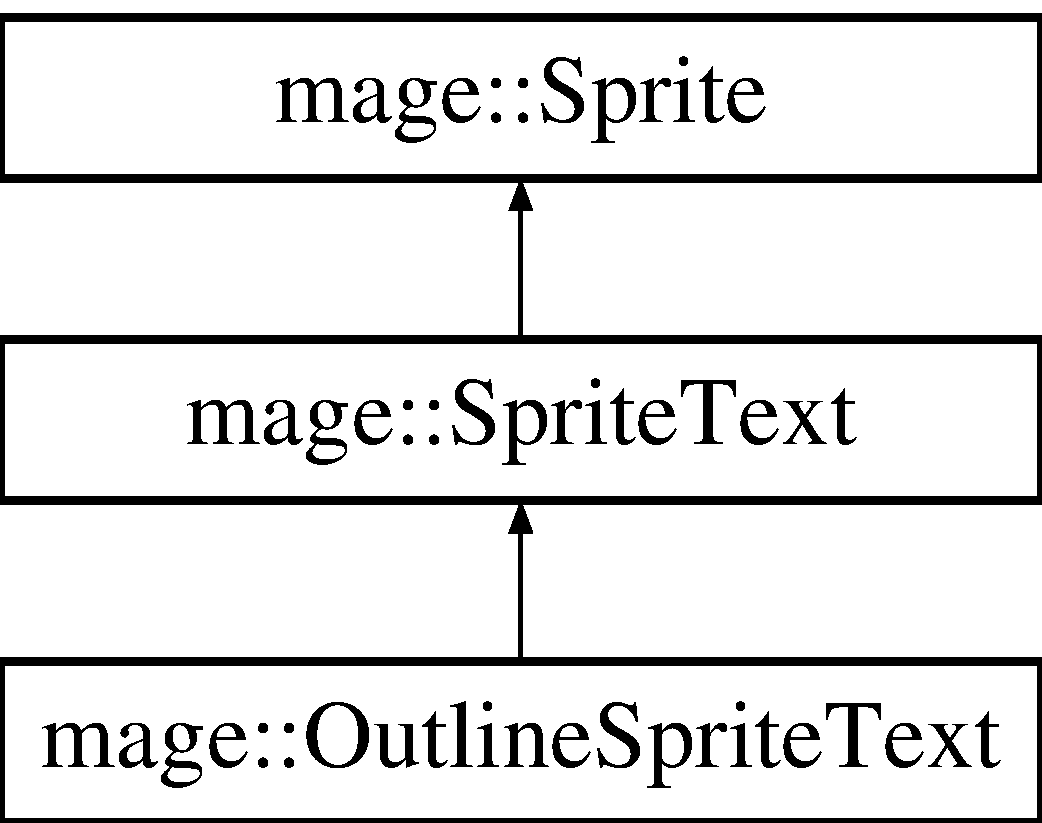
\includegraphics[height=3.000000cm]{classmage_1_1_outline_sprite_text}
\end{center}
\end{figure}
\subsection*{Public Member Functions}
\begin{DoxyCompactItemize}
\item 
\hyperlink{classmage_1_1_outline_sprite_text_a20863727c984b3765c2282d1e50047ea}{Outline\+Sprite\+Text} (const string \&name, \hyperlink{namespacemage_a1e01ae66713838a7a67d30e44c67703e}{Shared\+Ptr}$<$ \hyperlink{classmage_1_1_sprite_font}{Sprite\+Font} $>$ font, const \hyperlink{structmage_1_1_color}{Color} \&border\+\_\+color, \hyperlink{namespacemage_a9cfe18123066ba4236f548f9de75d881}{Sprite\+Effect} effects=\hyperlink{namespacemage_a9cfe18123066ba4236f548f9de75d881a6adf97f83acf6453d4a6a4b1070f3754}{Sprite\+Effect\+::\+None})
\item 
\hyperlink{classmage_1_1_outline_sprite_text_a8a6872c31f2538754b65445497fb50f4}{Outline\+Sprite\+Text} (const string \&name, \hyperlink{namespacemage_a1e01ae66713838a7a67d30e44c67703e}{Shared\+Ptr}$<$ \hyperlink{classmage_1_1_sprite_font}{Sprite\+Font} $>$ font, const X\+M\+V\+E\+C\+T\+OR \&border\+\_\+color=Colors\+::\+Black, \hyperlink{namespacemage_a9cfe18123066ba4236f548f9de75d881}{Sprite\+Effect} effects=\hyperlink{namespacemage_a9cfe18123066ba4236f548f9de75d881a6adf97f83acf6453d4a6a4b1070f3754}{Sprite\+Effect\+::\+None})
\item 
\hyperlink{classmage_1_1_outline_sprite_text_a15be7f23a00e893314b905d5385903c5}{Outline\+Sprite\+Text} (const \hyperlink{classmage_1_1_outline_sprite_text}{Outline\+Sprite\+Text} \&sprite\+\_\+text)
\item 
\hyperlink{classmage_1_1_outline_sprite_text_a86bb6e1637bcc71a4272f193466669e2}{Outline\+Sprite\+Text} (\hyperlink{classmage_1_1_outline_sprite_text}{Outline\+Sprite\+Text} \&\&sprite\+\_\+text)
\item 
virtual \hyperlink{classmage_1_1_outline_sprite_text_ae4d77ebb3f5bac4fd02b148d6173d10f}{$\sim$\+Outline\+Sprite\+Text} ()
\item 
\hyperlink{classmage_1_1_outline_sprite_text}{Outline\+Sprite\+Text} \& \hyperlink{classmage_1_1_outline_sprite_text_a324ec8e5c0d319b449895cc45d6b3807}{operator=} (const \hyperlink{classmage_1_1_outline_sprite_text}{Outline\+Sprite\+Text} \&sprite\+\_\+text)=delete
\item 
\hyperlink{classmage_1_1_outline_sprite_text}{Outline\+Sprite\+Text} \& \hyperlink{classmage_1_1_outline_sprite_text_a3549e97af5461728a399f01af9125486}{operator=} (\hyperlink{classmage_1_1_outline_sprite_text}{Outline\+Sprite\+Text} \&\&sprite\+\_\+text)=delete
\item 
\hyperlink{namespacemage_a8c307fbcc33bce9b7f2aa4c26c3b95cf}{Unique\+Ptr}$<$ \hyperlink{classmage_1_1_outline_sprite_text}{Outline\+Sprite\+Text} $>$ \hyperlink{classmage_1_1_outline_sprite_text_aa188cb104f6f00fdc75c532d66869f02}{Clone} () const
\item 
virtual void \hyperlink{classmage_1_1_outline_sprite_text_a524e9ad1caeeeaa32405e61d1a5e1032}{Draw} (Sprite\+Batch \&sprite\+\_\+batch) const override
\item 
const \hyperlink{structmage_1_1_color}{Color} \hyperlink{classmage_1_1_outline_sprite_text_adb4936119bcc0b148c9e11f021e83940}{Get\+Border\+Color} () const noexcept
\item 
void \hyperlink{classmage_1_1_outline_sprite_text_a66b448443de5a459bb28f66c682a12bd}{Set\+Border\+Color} (const \hyperlink{structmage_1_1_color}{Color} \&\hyperlink{namespacemage_a8ac46837ac2f6a9b756e66979165acd6}{color}) noexcept
\item 
void \hyperlink{classmage_1_1_outline_sprite_text_acb4952d08d69ee8ccd20fb668f3efcd3}{Set\+Border\+Color} (const X\+M\+V\+E\+C\+T\+OR \&\hyperlink{namespacemage_a8ac46837ac2f6a9b756e66979165acd6}{color}) noexcept
\end{DoxyCompactItemize}
\subsection*{Private Member Functions}
\begin{DoxyCompactItemize}
\item 
virtual \hyperlink{namespacemage_a8c307fbcc33bce9b7f2aa4c26c3b95cf}{Unique\+Ptr}$<$ \hyperlink{classmage_1_1_sprite_object}{Sprite\+Object} $>$ \hyperlink{classmage_1_1_outline_sprite_text_af8d29408abb61c05a23499bf37c4c7b0}{Clone\+Implementation} () const override
\item 
const X\+M\+V\+E\+C\+T\+OR \hyperlink{classmage_1_1_outline_sprite_text_a287bef30662bbd00ca999b3577249226}{Get\+Border\+Color\+Vector} () const noexcept
\end{DoxyCompactItemize}
\subsection*{Private Attributes}
\begin{DoxyCompactItemize}
\item 
\hyperlink{structmage_1_1_color}{Color} \hyperlink{classmage_1_1_outline_sprite_text_a19301d370498a08759445f415da78822}{m\+\_\+border\+\_\+color}
\end{DoxyCompactItemize}
\subsection*{Additional Inherited Members}


\subsection{Detailed Description}
A class of outline sprite texts. 

\subsection{Constructor \& Destructor Documentation}
\hypertarget{classmage_1_1_outline_sprite_text_a20863727c984b3765c2282d1e50047ea}{}\label{classmage_1_1_outline_sprite_text_a20863727c984b3765c2282d1e50047ea} 
\index{mage\+::\+Outline\+Sprite\+Text@{mage\+::\+Outline\+Sprite\+Text}!Outline\+Sprite\+Text@{Outline\+Sprite\+Text}}
\index{Outline\+Sprite\+Text@{Outline\+Sprite\+Text}!mage\+::\+Outline\+Sprite\+Text@{mage\+::\+Outline\+Sprite\+Text}}
\subsubsection{\texorpdfstring{Outline\+Sprite\+Text()}{OutlineSpriteText()}\hspace{0.1cm}{\footnotesize\ttfamily [1/4]}}
{\footnotesize\ttfamily mage\+::\+Outline\+Sprite\+Text\+::\+Outline\+Sprite\+Text (\begin{DoxyParamCaption}\item[{const string \&}]{name,  }\item[{\hyperlink{namespacemage_a1e01ae66713838a7a67d30e44c67703e}{Shared\+Ptr}$<$ \hyperlink{classmage_1_1_sprite_font}{Sprite\+Font} $>$}]{font,  }\item[{const \hyperlink{structmage_1_1_color}{Color} \&}]{border\+\_\+color,  }\item[{\hyperlink{namespacemage_a9cfe18123066ba4236f548f9de75d881}{Sprite\+Effect}}]{effects = {\ttfamily \hyperlink{namespacemage_a9cfe18123066ba4236f548f9de75d881a6adf97f83acf6453d4a6a4b1070f3754}{Sprite\+Effect\+::\+None}} }\end{DoxyParamCaption})\hspace{0.3cm}{\ttfamily [explicit]}}

Constructs a outline sprite text.

\begin{DoxyPrecond}{Precondition}
{\ttfamily font.\+get()} is not equal to {\ttfamily nullptr}. 
\end{DoxyPrecond}

\begin{DoxyParams}[1]{Parameters}
\mbox{\tt in}  & {\em name} & The name. \\
\hline
\mbox{\tt in}  & {\em font} & A pointer to the sprite font. \\
\hline
\mbox{\tt in}  & {\em border\+\_\+color} & A reference to the border color. \\
\hline
\mbox{\tt in}  & {\em effects} & The sprite effects to apply. \\
\hline
\end{DoxyParams}
\hypertarget{classmage_1_1_outline_sprite_text_a8a6872c31f2538754b65445497fb50f4}{}\label{classmage_1_1_outline_sprite_text_a8a6872c31f2538754b65445497fb50f4} 
\index{mage\+::\+Outline\+Sprite\+Text@{mage\+::\+Outline\+Sprite\+Text}!Outline\+Sprite\+Text@{Outline\+Sprite\+Text}}
\index{Outline\+Sprite\+Text@{Outline\+Sprite\+Text}!mage\+::\+Outline\+Sprite\+Text@{mage\+::\+Outline\+Sprite\+Text}}
\subsubsection{\texorpdfstring{Outline\+Sprite\+Text()}{OutlineSpriteText()}\hspace{0.1cm}{\footnotesize\ttfamily [2/4]}}
{\footnotesize\ttfamily mage\+::\+Outline\+Sprite\+Text\+::\+Outline\+Sprite\+Text (\begin{DoxyParamCaption}\item[{const string \&}]{name,  }\item[{\hyperlink{namespacemage_a1e01ae66713838a7a67d30e44c67703e}{Shared\+Ptr}$<$ \hyperlink{classmage_1_1_sprite_font}{Sprite\+Font} $>$}]{font,  }\item[{const X\+M\+V\+E\+C\+T\+OR \&}]{border\+\_\+color = {\ttfamily Colors\+:\+:Black},  }\item[{\hyperlink{namespacemage_a9cfe18123066ba4236f548f9de75d881}{Sprite\+Effect}}]{effects = {\ttfamily \hyperlink{namespacemage_a9cfe18123066ba4236f548f9de75d881a6adf97f83acf6453d4a6a4b1070f3754}{Sprite\+Effect\+::\+None}} }\end{DoxyParamCaption})\hspace{0.3cm}{\ttfamily [explicit]}}

Constructs a outline sprite text.

\begin{DoxyPrecond}{Precondition}
{\ttfamily font.\+get()} is not equal to {\ttfamily nullptr}. 
\end{DoxyPrecond}

\begin{DoxyParams}[1]{Parameters}
\mbox{\tt in}  & {\em name} & The name. \\
\hline
\mbox{\tt in}  & {\em font} & A pointer to the sprite font. \\
\hline
\mbox{\tt in}  & {\em border\+\_\+color} & A reference to the border color. \\
\hline
\mbox{\tt in}  & {\em effects} & The sprite effects to apply. \\
\hline
\end{DoxyParams}
\hypertarget{classmage_1_1_outline_sprite_text_a15be7f23a00e893314b905d5385903c5}{}\label{classmage_1_1_outline_sprite_text_a15be7f23a00e893314b905d5385903c5} 
\index{mage\+::\+Outline\+Sprite\+Text@{mage\+::\+Outline\+Sprite\+Text}!Outline\+Sprite\+Text@{Outline\+Sprite\+Text}}
\index{Outline\+Sprite\+Text@{Outline\+Sprite\+Text}!mage\+::\+Outline\+Sprite\+Text@{mage\+::\+Outline\+Sprite\+Text}}
\subsubsection{\texorpdfstring{Outline\+Sprite\+Text()}{OutlineSpriteText()}\hspace{0.1cm}{\footnotesize\ttfamily [3/4]}}
{\footnotesize\ttfamily mage\+::\+Outline\+Sprite\+Text\+::\+Outline\+Sprite\+Text (\begin{DoxyParamCaption}\item[{const \hyperlink{classmage_1_1_outline_sprite_text}{Outline\+Sprite\+Text} \&}]{sprite\+\_\+text }\end{DoxyParamCaption})\hspace{0.3cm}{\ttfamily [default]}}

Constructs a outline sprite text from the given outline sprite text.


\begin{DoxyParams}[1]{Parameters}
\mbox{\tt in}  & {\em sprite\+\_\+text} & A reference to the outline sprite text to copy. \\
\hline
\end{DoxyParams}
\hypertarget{classmage_1_1_outline_sprite_text_a86bb6e1637bcc71a4272f193466669e2}{}\label{classmage_1_1_outline_sprite_text_a86bb6e1637bcc71a4272f193466669e2} 
\index{mage\+::\+Outline\+Sprite\+Text@{mage\+::\+Outline\+Sprite\+Text}!Outline\+Sprite\+Text@{Outline\+Sprite\+Text}}
\index{Outline\+Sprite\+Text@{Outline\+Sprite\+Text}!mage\+::\+Outline\+Sprite\+Text@{mage\+::\+Outline\+Sprite\+Text}}
\subsubsection{\texorpdfstring{Outline\+Sprite\+Text()}{OutlineSpriteText()}\hspace{0.1cm}{\footnotesize\ttfamily [4/4]}}
{\footnotesize\ttfamily mage\+::\+Outline\+Sprite\+Text\+::\+Outline\+Sprite\+Text (\begin{DoxyParamCaption}\item[{\hyperlink{classmage_1_1_outline_sprite_text}{Outline\+Sprite\+Text} \&\&}]{sprite\+\_\+text }\end{DoxyParamCaption})\hspace{0.3cm}{\ttfamily [default]}}

Constructs a outline sprite text by moving the given outline sprite text.


\begin{DoxyParams}[1]{Parameters}
\mbox{\tt in}  & {\em sprite\+\_\+text} & A reference to the outline sprite text to move. \\
\hline
\end{DoxyParams}
\hypertarget{classmage_1_1_outline_sprite_text_ae4d77ebb3f5bac4fd02b148d6173d10f}{}\label{classmage_1_1_outline_sprite_text_ae4d77ebb3f5bac4fd02b148d6173d10f} 
\index{mage\+::\+Outline\+Sprite\+Text@{mage\+::\+Outline\+Sprite\+Text}!````~Outline\+Sprite\+Text@{$\sim$\+Outline\+Sprite\+Text}}
\index{````~Outline\+Sprite\+Text@{$\sim$\+Outline\+Sprite\+Text}!mage\+::\+Outline\+Sprite\+Text@{mage\+::\+Outline\+Sprite\+Text}}
\subsubsection{\texorpdfstring{$\sim$\+Outline\+Sprite\+Text()}{~OutlineSpriteText()}}
{\footnotesize\ttfamily mage\+::\+Outline\+Sprite\+Text\+::$\sim$\+Outline\+Sprite\+Text (\begin{DoxyParamCaption}{ }\end{DoxyParamCaption})\hspace{0.3cm}{\ttfamily [virtual]}, {\ttfamily [default]}}

Destructs this outline sprite text. 

\subsection{Member Function Documentation}
\hypertarget{classmage_1_1_outline_sprite_text_aa188cb104f6f00fdc75c532d66869f02}{}\label{classmage_1_1_outline_sprite_text_aa188cb104f6f00fdc75c532d66869f02} 
\index{mage\+::\+Outline\+Sprite\+Text@{mage\+::\+Outline\+Sprite\+Text}!Clone@{Clone}}
\index{Clone@{Clone}!mage\+::\+Outline\+Sprite\+Text@{mage\+::\+Outline\+Sprite\+Text}}
\subsubsection{\texorpdfstring{Clone()}{Clone()}}
{\footnotesize\ttfamily \hyperlink{namespacemage_a8c307fbcc33bce9b7f2aa4c26c3b95cf}{Unique\+Ptr}$<$ \hyperlink{classmage_1_1_outline_sprite_text}{Outline\+Sprite\+Text} $>$ mage\+::\+Outline\+Sprite\+Text\+::\+Clone (\begin{DoxyParamCaption}{ }\end{DoxyParamCaption}) const}

Clones this outline sprite text.

\begin{DoxyReturn}{Returns}
A pointer to the clone of this outline sprite text. 
\end{DoxyReturn}
\hypertarget{classmage_1_1_outline_sprite_text_af8d29408abb61c05a23499bf37c4c7b0}{}\label{classmage_1_1_outline_sprite_text_af8d29408abb61c05a23499bf37c4c7b0} 
\index{mage\+::\+Outline\+Sprite\+Text@{mage\+::\+Outline\+Sprite\+Text}!Clone\+Implementation@{Clone\+Implementation}}
\index{Clone\+Implementation@{Clone\+Implementation}!mage\+::\+Outline\+Sprite\+Text@{mage\+::\+Outline\+Sprite\+Text}}
\subsubsection{\texorpdfstring{Clone\+Implementation()}{CloneImplementation()}}
{\footnotesize\ttfamily \hyperlink{namespacemage_a8c307fbcc33bce9b7f2aa4c26c3b95cf}{Unique\+Ptr}$<$ \hyperlink{classmage_1_1_sprite_object}{Sprite\+Object} $>$ mage\+::\+Outline\+Sprite\+Text\+::\+Clone\+Implementation (\begin{DoxyParamCaption}{ }\end{DoxyParamCaption}) const\hspace{0.3cm}{\ttfamily [override]}, {\ttfamily [private]}, {\ttfamily [virtual]}}

Clones this outline sprite text.

\begin{DoxyReturn}{Returns}
A pointer to the clone of this outline sprite text. 
\end{DoxyReturn}


Implements \hyperlink{classmage_1_1_sprite_text_a2b9f59a1730f8b9691f173251a2b4944}{mage\+::\+Sprite\+Text}.

\hypertarget{classmage_1_1_outline_sprite_text_a524e9ad1caeeeaa32405e61d1a5e1032}{}\label{classmage_1_1_outline_sprite_text_a524e9ad1caeeeaa32405e61d1a5e1032} 
\index{mage\+::\+Outline\+Sprite\+Text@{mage\+::\+Outline\+Sprite\+Text}!Draw@{Draw}}
\index{Draw@{Draw}!mage\+::\+Outline\+Sprite\+Text@{mage\+::\+Outline\+Sprite\+Text}}
\subsubsection{\texorpdfstring{Draw()}{Draw()}}
{\footnotesize\ttfamily void mage\+::\+Outline\+Sprite\+Text\+::\+Draw (\begin{DoxyParamCaption}\item[{Sprite\+Batch \&}]{sprite\+\_\+batch }\end{DoxyParamCaption}) const\hspace{0.3cm}{\ttfamily [override]}, {\ttfamily [virtual]}}

Draws this outline sprite text.


\begin{DoxyParams}[1]{Parameters}
\mbox{\tt in}  & {\em sprite\+\_\+batch} & A reference to the sprite batch used for rendering this outline sprite text. \\
\hline
\end{DoxyParams}


Implements \hyperlink{classmage_1_1_sprite_text_a45d5ac8410d5a46b26e8491946a2ad9e}{mage\+::\+Sprite\+Text}.

\hypertarget{classmage_1_1_outline_sprite_text_adb4936119bcc0b148c9e11f021e83940}{}\label{classmage_1_1_outline_sprite_text_adb4936119bcc0b148c9e11f021e83940} 
\index{mage\+::\+Outline\+Sprite\+Text@{mage\+::\+Outline\+Sprite\+Text}!Get\+Border\+Color@{Get\+Border\+Color}}
\index{Get\+Border\+Color@{Get\+Border\+Color}!mage\+::\+Outline\+Sprite\+Text@{mage\+::\+Outline\+Sprite\+Text}}
\subsubsection{\texorpdfstring{Get\+Border\+Color()}{GetBorderColor()}}
{\footnotesize\ttfamily const \hyperlink{structmage_1_1_color}{Color} mage\+::\+Outline\+Sprite\+Text\+::\+Get\+Border\+Color (\begin{DoxyParamCaption}{ }\end{DoxyParamCaption}) const\hspace{0.3cm}{\ttfamily [noexcept]}}

Returns the border color of this outline sprite text.

\begin{DoxyReturn}{Returns}
The border color of this outline sprite text. 
\end{DoxyReturn}
\hypertarget{classmage_1_1_outline_sprite_text_a287bef30662bbd00ca999b3577249226}{}\label{classmage_1_1_outline_sprite_text_a287bef30662bbd00ca999b3577249226} 
\index{mage\+::\+Outline\+Sprite\+Text@{mage\+::\+Outline\+Sprite\+Text}!Get\+Border\+Color\+Vector@{Get\+Border\+Color\+Vector}}
\index{Get\+Border\+Color\+Vector@{Get\+Border\+Color\+Vector}!mage\+::\+Outline\+Sprite\+Text@{mage\+::\+Outline\+Sprite\+Text}}
\subsubsection{\texorpdfstring{Get\+Border\+Color\+Vector()}{GetBorderColorVector()}}
{\footnotesize\ttfamily const X\+M\+V\+E\+C\+T\+OR mage\+::\+Outline\+Sprite\+Text\+::\+Get\+Border\+Color\+Vector (\begin{DoxyParamCaption}{ }\end{DoxyParamCaption}) const\hspace{0.3cm}{\ttfamily [private]}, {\ttfamily [noexcept]}}

Returns the border color of this outline sprite text as {\ttfamily X\+M\+V\+E\+C\+T\+OR}.

\begin{DoxyReturn}{Returns}
The border color of this outline sprite text as {\ttfamily X\+M\+V\+E\+C\+T\+OR}. 
\end{DoxyReturn}
\hypertarget{classmage_1_1_outline_sprite_text_a324ec8e5c0d319b449895cc45d6b3807}{}\label{classmage_1_1_outline_sprite_text_a324ec8e5c0d319b449895cc45d6b3807} 
\index{mage\+::\+Outline\+Sprite\+Text@{mage\+::\+Outline\+Sprite\+Text}!operator=@{operator=}}
\index{operator=@{operator=}!mage\+::\+Outline\+Sprite\+Text@{mage\+::\+Outline\+Sprite\+Text}}
\subsubsection{\texorpdfstring{operator=()}{operator=()}\hspace{0.1cm}{\footnotesize\ttfamily [1/2]}}
{\footnotesize\ttfamily \hyperlink{classmage_1_1_outline_sprite_text}{Outline\+Sprite\+Text}\& mage\+::\+Outline\+Sprite\+Text\+::operator= (\begin{DoxyParamCaption}\item[{const \hyperlink{classmage_1_1_outline_sprite_text}{Outline\+Sprite\+Text} \&}]{sprite\+\_\+text }\end{DoxyParamCaption})\hspace{0.3cm}{\ttfamily [delete]}}

Copies the given outline sprite text to this outline sprite text.


\begin{DoxyParams}[1]{Parameters}
\mbox{\tt in}  & {\em sprite\+\_\+text} & A reference to the outline sprite text to copy. \\
\hline
\end{DoxyParams}
\begin{DoxyReturn}{Returns}
A reference to the copy of the given outline sprite text (i.\+e. this outline sprite text). 
\end{DoxyReturn}
\hypertarget{classmage_1_1_outline_sprite_text_a3549e97af5461728a399f01af9125486}{}\label{classmage_1_1_outline_sprite_text_a3549e97af5461728a399f01af9125486} 
\index{mage\+::\+Outline\+Sprite\+Text@{mage\+::\+Outline\+Sprite\+Text}!operator=@{operator=}}
\index{operator=@{operator=}!mage\+::\+Outline\+Sprite\+Text@{mage\+::\+Outline\+Sprite\+Text}}
\subsubsection{\texorpdfstring{operator=()}{operator=()}\hspace{0.1cm}{\footnotesize\ttfamily [2/2]}}
{\footnotesize\ttfamily \hyperlink{classmage_1_1_outline_sprite_text}{Outline\+Sprite\+Text}\& mage\+::\+Outline\+Sprite\+Text\+::operator= (\begin{DoxyParamCaption}\item[{\hyperlink{classmage_1_1_outline_sprite_text}{Outline\+Sprite\+Text} \&\&}]{sprite\+\_\+text }\end{DoxyParamCaption})\hspace{0.3cm}{\ttfamily [delete]}}

Moves the given outline sprite text to this outline sprite text.


\begin{DoxyParams}[1]{Parameters}
\mbox{\tt in}  & {\em sprite\+\_\+text} & A reference to the outline sprite text to move. \\
\hline
\end{DoxyParams}
\begin{DoxyReturn}{Returns}
A reference to the moved outline sprite text (i.\+e. this outline sprite text). 
\end{DoxyReturn}
\hypertarget{classmage_1_1_outline_sprite_text_a66b448443de5a459bb28f66c682a12bd}{}\label{classmage_1_1_outline_sprite_text_a66b448443de5a459bb28f66c682a12bd} 
\index{mage\+::\+Outline\+Sprite\+Text@{mage\+::\+Outline\+Sprite\+Text}!Set\+Border\+Color@{Set\+Border\+Color}}
\index{Set\+Border\+Color@{Set\+Border\+Color}!mage\+::\+Outline\+Sprite\+Text@{mage\+::\+Outline\+Sprite\+Text}}
\subsubsection{\texorpdfstring{Set\+Border\+Color()}{SetBorderColor()}\hspace{0.1cm}{\footnotesize\ttfamily [1/2]}}
{\footnotesize\ttfamily void mage\+::\+Outline\+Sprite\+Text\+::\+Set\+Border\+Color (\begin{DoxyParamCaption}\item[{const \hyperlink{structmage_1_1_color}{Color} \&}]{color }\end{DoxyParamCaption})\hspace{0.3cm}{\ttfamily [noexcept]}}

Sets the border color of this outline sprite text to the given color.


\begin{DoxyParams}[1]{Parameters}
\mbox{\tt in}  & {\em color} & A reference to the border color. \\
\hline
\end{DoxyParams}
\hypertarget{classmage_1_1_outline_sprite_text_acb4952d08d69ee8ccd20fb668f3efcd3}{}\label{classmage_1_1_outline_sprite_text_acb4952d08d69ee8ccd20fb668f3efcd3} 
\index{mage\+::\+Outline\+Sprite\+Text@{mage\+::\+Outline\+Sprite\+Text}!Set\+Border\+Color@{Set\+Border\+Color}}
\index{Set\+Border\+Color@{Set\+Border\+Color}!mage\+::\+Outline\+Sprite\+Text@{mage\+::\+Outline\+Sprite\+Text}}
\subsubsection{\texorpdfstring{Set\+Border\+Color()}{SetBorderColor()}\hspace{0.1cm}{\footnotesize\ttfamily [2/2]}}
{\footnotesize\ttfamily void mage\+::\+Outline\+Sprite\+Text\+::\+Set\+Border\+Color (\begin{DoxyParamCaption}\item[{const X\+M\+V\+E\+C\+T\+OR \&}]{color }\end{DoxyParamCaption})\hspace{0.3cm}{\ttfamily [noexcept]}}

Sets the border color of this outline sprite text to the given color.


\begin{DoxyParams}[1]{Parameters}
\mbox{\tt in}  & {\em color} & A reference to the border color. \\
\hline
\end{DoxyParams}


\subsection{Member Data Documentation}
\hypertarget{classmage_1_1_outline_sprite_text_a19301d370498a08759445f415da78822}{}\label{classmage_1_1_outline_sprite_text_a19301d370498a08759445f415da78822} 
\index{mage\+::\+Outline\+Sprite\+Text@{mage\+::\+Outline\+Sprite\+Text}!m\+\_\+border\+\_\+color@{m\+\_\+border\+\_\+color}}
\index{m\+\_\+border\+\_\+color@{m\+\_\+border\+\_\+color}!mage\+::\+Outline\+Sprite\+Text@{mage\+::\+Outline\+Sprite\+Text}}
\subsubsection{\texorpdfstring{m\+\_\+border\+\_\+color}{m\_border\_color}}
{\footnotesize\ttfamily \hyperlink{structmage_1_1_color}{Color} mage\+::\+Outline\+Sprite\+Text\+::m\+\_\+border\+\_\+color\hspace{0.3cm}{\ttfamily [private]}}

The border color of this outline sprite text. 
\hypertarget{classmage_1_1_perspective_camera}{}\section{mage\+:\+:Perspective\+Camera Class Reference}
\label{classmage_1_1_perspective_camera}\index{mage\+::\+Perspective\+Camera@{mage\+::\+Perspective\+Camera}}


{\ttfamily \#include $<$perspective\+\_\+camera.\+hpp$>$}

Inheritance diagram for mage\+:\+:Perspective\+Camera\+:\begin{figure}[H]
\begin{center}
\leavevmode
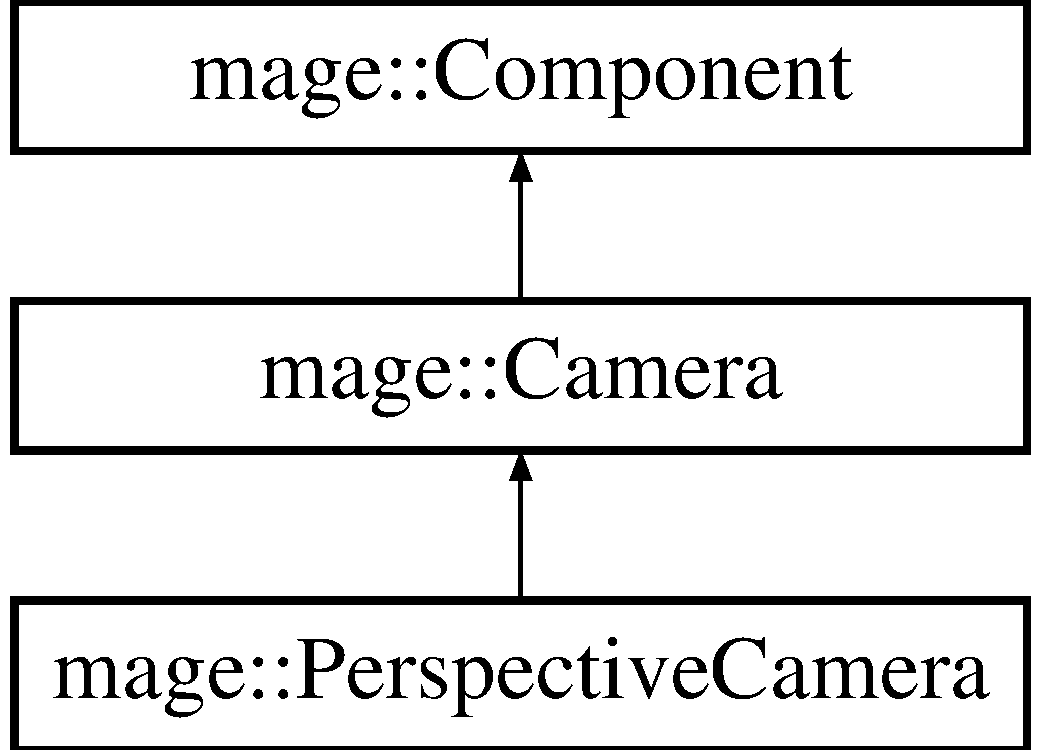
\includegraphics[height=2.000000cm]{classmage_1_1_perspective_camera}
\end{center}
\end{figure}
\subsection*{Public Member Functions}
\begin{DoxyCompactItemize}
\item 
\hyperlink{classmage_1_1_perspective_camera_a118a233aa484bbff31032703087a5a8c}{Perspective\+Camera} (float aspect\+\_\+ratio, float fov\+\_\+y=M\+A\+G\+E\+\_\+\+D\+E\+F\+A\+U\+L\+T\+\_\+\+C\+A\+M\+E\+R\+A\+\_\+\+P\+E\+R\+S\+P\+E\+C\+T\+I\+V\+E\+\_\+\+F\+O\+V\+\_\+Y, float near\+\_\+z=M\+A\+G\+E\+\_\+\+D\+E\+F\+A\+U\+L\+T\+\_\+\+C\+A\+M\+E\+R\+A\+\_\+\+N\+E\+A\+R\+\_\+Z, float far\+\_\+z=M\+A\+G\+E\+\_\+\+D\+E\+F\+A\+U\+L\+T\+\_\+\+C\+A\+M\+E\+R\+A\+\_\+\+F\+A\+R\+\_\+Z)
\item 
\hyperlink{classmage_1_1_perspective_camera_af04c3995faa777606a1cd610acad43c0}{Perspective\+Camera} (float width, float height, float fov\+\_\+y=M\+A\+G\+E\+\_\+\+D\+E\+F\+A\+U\+L\+T\+\_\+\+C\+A\+M\+E\+R\+A\+\_\+\+P\+E\+R\+S\+P\+E\+C\+T\+I\+V\+E\+\_\+\+F\+O\+V\+\_\+Y, float near\+\_\+z=M\+A\+G\+E\+\_\+\+D\+E\+F\+A\+U\+L\+T\+\_\+\+C\+A\+M\+E\+R\+A\+\_\+\+N\+E\+A\+R\+\_\+Z, float far\+\_\+z=M\+A\+G\+E\+\_\+\+D\+E\+F\+A\+U\+L\+T\+\_\+\+C\+A\+M\+E\+R\+A\+\_\+\+F\+A\+R\+\_\+Z)
\item 
\hyperlink{classmage_1_1_perspective_camera_a198d1460d9312af27ed6ef2ac28b616d}{Perspective\+Camera} (const \hyperlink{classmage_1_1_perspective_camera}{Perspective\+Camera} \&camera)
\item 
\hyperlink{classmage_1_1_perspective_camera_a04531e5b956e72300337571e0eb7143d}{Perspective\+Camera} (\hyperlink{classmage_1_1_perspective_camera}{Perspective\+Camera} \&\&camera)
\item 
virtual \hyperlink{classmage_1_1_perspective_camera_a47ba88d7458528795dd832474cdb3eb9}{$\sim$\+Perspective\+Camera} ()
\item 
\hyperlink{classmage_1_1_perspective_camera}{Perspective\+Camera} \& \hyperlink{classmage_1_1_perspective_camera_a0fe5ef8bd4d28efa8e4851a8055b6fa5}{operator=} (const \hyperlink{classmage_1_1_perspective_camera}{Perspective\+Camera} \&camera)
\item 
\hyperlink{classmage_1_1_perspective_camera}{Perspective\+Camera} \& \hyperlink{classmage_1_1_perspective_camera_a338c75900237f3623b31b0231a5f5782}{operator=} (\hyperlink{classmage_1_1_perspective_camera}{Perspective\+Camera} \&\&camera)
\item 
\hyperlink{namespacemage_a8c307fbcc33bce9b7f2aa4c26c3b95cf}{Unique\+Ptr}$<$ \hyperlink{classmage_1_1_perspective_camera}{Perspective\+Camera} $>$ \hyperlink{classmage_1_1_perspective_camera_a21545965da7ef1b6f99887bb6d2bb095}{Clone} () const
\item 
float \hyperlink{classmage_1_1_perspective_camera_a15223034b30ca691c51de8850c033293}{Get\+F\+O\+VY} () const
\item 
\hyperlink{classmage_1_1_perspective_camera}{Perspective\+Camera} \& \hyperlink{classmage_1_1_perspective_camera_a2b6357e96bfbd5a322863cf6e72bb889}{Set\+F\+O\+VY} (float fov\+\_\+y)
\item 
float \hyperlink{classmage_1_1_perspective_camera_ab74cbd2777d5b430da5702a12b1b451e}{Get\+Aspect\+Ratio} () const
\item 
\hyperlink{classmage_1_1_perspective_camera}{Perspective\+Camera} \& \hyperlink{classmage_1_1_perspective_camera_afa5b9b8f6d1945fe63e9121359fb39bb}{Set\+Aspect\+Ratio} (float aspect\+\_\+ratio)
\item 
\hyperlink{classmage_1_1_perspective_camera}{Perspective\+Camera} \& \hyperlink{classmage_1_1_perspective_camera_a8fa66b4025306709cf825b267c866b29}{Set\+Aspect\+Ratio} (float width, float height)
\item 
void \hyperlink{classmage_1_1_perspective_camera_a7a7d25bbf0b5cf7952de9a3af280558b}{Set\+View\+To\+Projection\+Matrix} (float aspect\+\_\+ratio, float fov\+\_\+y=M\+A\+G\+E\+\_\+\+D\+E\+F\+A\+U\+L\+T\+\_\+\+C\+A\+M\+E\+R\+A\+\_\+\+P\+E\+R\+S\+P\+E\+C\+T\+I\+V\+E\+\_\+\+F\+O\+V\+\_\+Y, float near\+\_\+z=M\+A\+G\+E\+\_\+\+D\+E\+F\+A\+U\+L\+T\+\_\+\+C\+A\+M\+E\+R\+A\+\_\+\+N\+E\+A\+R\+\_\+Z, float far\+\_\+z=M\+A\+G\+E\+\_\+\+D\+E\+F\+A\+U\+L\+T\+\_\+\+C\+A\+M\+E\+R\+A\+\_\+\+F\+A\+R\+\_\+Z)
\item 
void \hyperlink{classmage_1_1_perspective_camera_a7e0688cce05ce5a0007fb000e8f1a43a}{Set\+View\+To\+Projection\+Matrix} (float width, float height, float fov\+\_\+y=M\+A\+G\+E\+\_\+\+D\+E\+F\+A\+U\+L\+T\+\_\+\+C\+A\+M\+E\+R\+A\+\_\+\+P\+E\+R\+S\+P\+E\+C\+T\+I\+V\+E\+\_\+\+F\+O\+V\+\_\+Y, float near\+\_\+z=M\+A\+G\+E\+\_\+\+D\+E\+F\+A\+U\+L\+T\+\_\+\+C\+A\+M\+E\+R\+A\+\_\+\+N\+E\+A\+R\+\_\+Z, float far\+\_\+z=M\+A\+G\+E\+\_\+\+D\+E\+F\+A\+U\+L\+T\+\_\+\+C\+A\+M\+E\+R\+A\+\_\+\+F\+A\+R\+\_\+Z)
\item 
virtual X\+M\+M\+A\+T\+R\+IX \hyperlink{classmage_1_1_perspective_camera_a83a38a4e8180707df2323130f9cee4a5}{Get\+View\+To\+Projection\+Matrix} () const override
\end{DoxyCompactItemize}
\subsection*{Private Member Functions}
\begin{DoxyCompactItemize}
\item 
virtual \hyperlink{namespacemage_a8c307fbcc33bce9b7f2aa4c26c3b95cf}{Unique\+Ptr}$<$ \hyperlink{classmage_1_1_camera}{Camera} $>$ \hyperlink{classmage_1_1_perspective_camera_aa597ab884256b7e6fad63653af3ac789}{Clone\+Implementation} () const override
\end{DoxyCompactItemize}
\subsection*{Private Attributes}
\begin{DoxyCompactItemize}
\item 
float \hyperlink{classmage_1_1_perspective_camera_ab92d993fece777cfeca8d5c7d371ffc9}{m\+\_\+aspect\+\_\+ratio}
\item 
float \hyperlink{classmage_1_1_perspective_camera_abdcf1a0cdd247e0f7e14e70898678af6}{m\+\_\+fov\+\_\+y}
\end{DoxyCompactItemize}
\subsection*{Additional Inherited Members}


\subsection{Detailed Description}
A class of perspective cameras. 

\subsection{Constructor \& Destructor Documentation}
\hypertarget{classmage_1_1_perspective_camera_a118a233aa484bbff31032703087a5a8c}{}\label{classmage_1_1_perspective_camera_a118a233aa484bbff31032703087a5a8c} 
\index{mage\+::\+Perspective\+Camera@{mage\+::\+Perspective\+Camera}!Perspective\+Camera@{Perspective\+Camera}}
\index{Perspective\+Camera@{Perspective\+Camera}!mage\+::\+Perspective\+Camera@{mage\+::\+Perspective\+Camera}}
\subsubsection{\texorpdfstring{Perspective\+Camera()}{PerspectiveCamera()}\hspace{0.1cm}{\footnotesize\ttfamily [1/4]}}
{\footnotesize\ttfamily mage\+::\+Perspective\+Camera\+::\+Perspective\+Camera (\begin{DoxyParamCaption}\item[{float}]{aspect\+\_\+ratio,  }\item[{float}]{fov\+\_\+y = {\ttfamily MAGE\+\_\+DEFAULT\+\_\+CAMERA\+\_\+PERSPECTIVE\+\_\+FOV\+\_\+Y},  }\item[{float}]{near\+\_\+z = {\ttfamily MAGE\+\_\+DEFAULT\+\_\+CAMERA\+\_\+NEAR\+\_\+Z},  }\item[{float}]{far\+\_\+z = {\ttfamily MAGE\+\_\+DEFAULT\+\_\+CAMERA\+\_\+FAR\+\_\+Z} }\end{DoxyParamCaption})\hspace{0.3cm}{\ttfamily [explicit]}}

Constructs a perspective camera.


\begin{DoxyParams}[1]{Parameters}
\mbox{\tt in}  & {\em aspect\+\_\+ratio} & The aspect ratio. \\
\hline
\mbox{\tt in}  & {\em fov\+\_\+y} & The vertical field-\/of-\/view. \\
\hline
\mbox{\tt in}  & {\em near\+\_\+z} & The position of the near z-\/plane in camera space. \\
\hline
\mbox{\tt in}  & {\em far\+\_\+z} & The position of the far z-\/plane in camera space. \\
\hline
\end{DoxyParams}
\hypertarget{classmage_1_1_perspective_camera_af04c3995faa777606a1cd610acad43c0}{}\label{classmage_1_1_perspective_camera_af04c3995faa777606a1cd610acad43c0} 
\index{mage\+::\+Perspective\+Camera@{mage\+::\+Perspective\+Camera}!Perspective\+Camera@{Perspective\+Camera}}
\index{Perspective\+Camera@{Perspective\+Camera}!mage\+::\+Perspective\+Camera@{mage\+::\+Perspective\+Camera}}
\subsubsection{\texorpdfstring{Perspective\+Camera()}{PerspectiveCamera()}\hspace{0.1cm}{\footnotesize\ttfamily [2/4]}}
{\footnotesize\ttfamily mage\+::\+Perspective\+Camera\+::\+Perspective\+Camera (\begin{DoxyParamCaption}\item[{float}]{width,  }\item[{float}]{height,  }\item[{float}]{fov\+\_\+y = {\ttfamily MAGE\+\_\+DEFAULT\+\_\+CAMERA\+\_\+PERSPECTIVE\+\_\+FOV\+\_\+Y},  }\item[{float}]{near\+\_\+z = {\ttfamily MAGE\+\_\+DEFAULT\+\_\+CAMERA\+\_\+NEAR\+\_\+Z},  }\item[{float}]{far\+\_\+z = {\ttfamily MAGE\+\_\+DEFAULT\+\_\+CAMERA\+\_\+FAR\+\_\+Z} }\end{DoxyParamCaption})\hspace{0.3cm}{\ttfamily [explicit]}}

Constructs a perspective camera.


\begin{DoxyParams}[1]{Parameters}
\mbox{\tt in}  & {\em width} & The width. \\
\hline
\mbox{\tt in}  & {\em height} & The height. \\
\hline
\mbox{\tt in}  & {\em fov\+\_\+y} & The vertical field-\/of-\/view. \\
\hline
\mbox{\tt in}  & {\em near\+\_\+z} & The position of the near z-\/plane in camera space. \\
\hline
\mbox{\tt in}  & {\em far\+\_\+z} & The position of the far z-\/plane in camera space. \\
\hline
\end{DoxyParams}
\hypertarget{classmage_1_1_perspective_camera_a198d1460d9312af27ed6ef2ac28b616d}{}\label{classmage_1_1_perspective_camera_a198d1460d9312af27ed6ef2ac28b616d} 
\index{mage\+::\+Perspective\+Camera@{mage\+::\+Perspective\+Camera}!Perspective\+Camera@{Perspective\+Camera}}
\index{Perspective\+Camera@{Perspective\+Camera}!mage\+::\+Perspective\+Camera@{mage\+::\+Perspective\+Camera}}
\subsubsection{\texorpdfstring{Perspective\+Camera()}{PerspectiveCamera()}\hspace{0.1cm}{\footnotesize\ttfamily [3/4]}}
{\footnotesize\ttfamily mage\+::\+Perspective\+Camera\+::\+Perspective\+Camera (\begin{DoxyParamCaption}\item[{const \hyperlink{classmage_1_1_perspective_camera}{Perspective\+Camera} \&}]{camera }\end{DoxyParamCaption})\hspace{0.3cm}{\ttfamily [default]}}

Constructs a perspective camera from the given perspective camera.


\begin{DoxyParams}[1]{Parameters}
\mbox{\tt in}  & {\em camera} & A reference to the perspective camera to copy. \\
\hline
\end{DoxyParams}
\hypertarget{classmage_1_1_perspective_camera_a04531e5b956e72300337571e0eb7143d}{}\label{classmage_1_1_perspective_camera_a04531e5b956e72300337571e0eb7143d} 
\index{mage\+::\+Perspective\+Camera@{mage\+::\+Perspective\+Camera}!Perspective\+Camera@{Perspective\+Camera}}
\index{Perspective\+Camera@{Perspective\+Camera}!mage\+::\+Perspective\+Camera@{mage\+::\+Perspective\+Camera}}
\subsubsection{\texorpdfstring{Perspective\+Camera()}{PerspectiveCamera()}\hspace{0.1cm}{\footnotesize\ttfamily [4/4]}}
{\footnotesize\ttfamily mage\+::\+Perspective\+Camera\+::\+Perspective\+Camera (\begin{DoxyParamCaption}\item[{\hyperlink{classmage_1_1_perspective_camera}{Perspective\+Camera} \&\&}]{camera }\end{DoxyParamCaption})\hspace{0.3cm}{\ttfamily [default]}}

Constructs a perspective camera by moving the given perspective camera.


\begin{DoxyParams}[1]{Parameters}
\mbox{\tt in}  & {\em camera} & A reference to the perspective camera to move. \\
\hline
\end{DoxyParams}
\hypertarget{classmage_1_1_perspective_camera_a47ba88d7458528795dd832474cdb3eb9}{}\label{classmage_1_1_perspective_camera_a47ba88d7458528795dd832474cdb3eb9} 
\index{mage\+::\+Perspective\+Camera@{mage\+::\+Perspective\+Camera}!````~Perspective\+Camera@{$\sim$\+Perspective\+Camera}}
\index{````~Perspective\+Camera@{$\sim$\+Perspective\+Camera}!mage\+::\+Perspective\+Camera@{mage\+::\+Perspective\+Camera}}
\subsubsection{\texorpdfstring{$\sim$\+Perspective\+Camera()}{~PerspectiveCamera()}}
{\footnotesize\ttfamily mage\+::\+Perspective\+Camera\+::$\sim$\+Perspective\+Camera (\begin{DoxyParamCaption}{ }\end{DoxyParamCaption})\hspace{0.3cm}{\ttfamily [virtual]}, {\ttfamily [default]}}

Destructs this perspective camera. 

\subsection{Member Function Documentation}
\hypertarget{classmage_1_1_perspective_camera_a21545965da7ef1b6f99887bb6d2bb095}{}\label{classmage_1_1_perspective_camera_a21545965da7ef1b6f99887bb6d2bb095} 
\index{mage\+::\+Perspective\+Camera@{mage\+::\+Perspective\+Camera}!Clone@{Clone}}
\index{Clone@{Clone}!mage\+::\+Perspective\+Camera@{mage\+::\+Perspective\+Camera}}
\subsubsection{\texorpdfstring{Clone()}{Clone()}}
{\footnotesize\ttfamily \hyperlink{namespacemage_a8c307fbcc33bce9b7f2aa4c26c3b95cf}{Unique\+Ptr}$<$ \hyperlink{classmage_1_1_perspective_camera}{Perspective\+Camera} $>$ mage\+::\+Perspective\+Camera\+::\+Clone (\begin{DoxyParamCaption}{ }\end{DoxyParamCaption}) const}

Clones this perspective camera.

\begin{DoxyReturn}{Returns}
A pointer to the clone of this perspective camera. 
\end{DoxyReturn}
\hypertarget{classmage_1_1_perspective_camera_aa597ab884256b7e6fad63653af3ac789}{}\label{classmage_1_1_perspective_camera_aa597ab884256b7e6fad63653af3ac789} 
\index{mage\+::\+Perspective\+Camera@{mage\+::\+Perspective\+Camera}!Clone\+Implementation@{Clone\+Implementation}}
\index{Clone\+Implementation@{Clone\+Implementation}!mage\+::\+Perspective\+Camera@{mage\+::\+Perspective\+Camera}}
\subsubsection{\texorpdfstring{Clone\+Implementation()}{CloneImplementation()}}
{\footnotesize\ttfamily \hyperlink{namespacemage_a8c307fbcc33bce9b7f2aa4c26c3b95cf}{Unique\+Ptr}$<$ \hyperlink{classmage_1_1_camera}{Camera} $>$ mage\+::\+Perspective\+Camera\+::\+Clone\+Implementation (\begin{DoxyParamCaption}{ }\end{DoxyParamCaption}) const\hspace{0.3cm}{\ttfamily [override]}, {\ttfamily [private]}, {\ttfamily [virtual]}}

Clones this perspective camera.

\begin{DoxyReturn}{Returns}
A pointer to the clone of this perspective camera. 
\end{DoxyReturn}


Implements \hyperlink{classmage_1_1_camera_aedf6e7d6ee6c6e9e82da814ef8e705ab}{mage\+::\+Camera}.

\hypertarget{classmage_1_1_perspective_camera_ab74cbd2777d5b430da5702a12b1b451e}{}\label{classmage_1_1_perspective_camera_ab74cbd2777d5b430da5702a12b1b451e} 
\index{mage\+::\+Perspective\+Camera@{mage\+::\+Perspective\+Camera}!Get\+Aspect\+Ratio@{Get\+Aspect\+Ratio}}
\index{Get\+Aspect\+Ratio@{Get\+Aspect\+Ratio}!mage\+::\+Perspective\+Camera@{mage\+::\+Perspective\+Camera}}
\subsubsection{\texorpdfstring{Get\+Aspect\+Ratio()}{GetAspectRatio()}}
{\footnotesize\ttfamily float mage\+::\+Perspective\+Camera\+::\+Get\+Aspect\+Ratio (\begin{DoxyParamCaption}{ }\end{DoxyParamCaption}) const}

Returns the aspect ratio of this perspective camera.

\begin{DoxyReturn}{Returns}
The aspect ratio of this perspective camera. 
\end{DoxyReturn}
\hypertarget{classmage_1_1_perspective_camera_a15223034b30ca691c51de8850c033293}{}\label{classmage_1_1_perspective_camera_a15223034b30ca691c51de8850c033293} 
\index{mage\+::\+Perspective\+Camera@{mage\+::\+Perspective\+Camera}!Get\+F\+O\+VY@{Get\+F\+O\+VY}}
\index{Get\+F\+O\+VY@{Get\+F\+O\+VY}!mage\+::\+Perspective\+Camera@{mage\+::\+Perspective\+Camera}}
\subsubsection{\texorpdfstring{Get\+F\+O\+V\+Y()}{GetFOVY()}}
{\footnotesize\ttfamily float mage\+::\+Perspective\+Camera\+::\+Get\+F\+O\+VY (\begin{DoxyParamCaption}{ }\end{DoxyParamCaption}) const}

Returns the vertical field-\/of-\/view of this perspective camera.

\begin{DoxyReturn}{Returns}
The vertical field-\/of-\/view of this perspective camera. 
\end{DoxyReturn}
\hypertarget{classmage_1_1_perspective_camera_a83a38a4e8180707df2323130f9cee4a5}{}\label{classmage_1_1_perspective_camera_a83a38a4e8180707df2323130f9cee4a5} 
\index{mage\+::\+Perspective\+Camera@{mage\+::\+Perspective\+Camera}!Get\+View\+To\+Projection\+Matrix@{Get\+View\+To\+Projection\+Matrix}}
\index{Get\+View\+To\+Projection\+Matrix@{Get\+View\+To\+Projection\+Matrix}!mage\+::\+Perspective\+Camera@{mage\+::\+Perspective\+Camera}}
\subsubsection{\texorpdfstring{Get\+View\+To\+Projection\+Matrix()}{GetViewToProjectionMatrix()}}
{\footnotesize\ttfamily virtual X\+M\+M\+A\+T\+R\+IX mage\+::\+Perspective\+Camera\+::\+Get\+View\+To\+Projection\+Matrix (\begin{DoxyParamCaption}{ }\end{DoxyParamCaption}) const\hspace{0.3cm}{\ttfamily [override]}, {\ttfamily [virtual]}}

Returns the view-\/to-\/projection matrix of this perspective camera.

\begin{DoxyReturn}{Returns}
The view-\/to-\/projection matrix of this perspective camera. 
\end{DoxyReturn}


Implements \hyperlink{classmage_1_1_camera_a1f5206864cf18b5548219492556df5d2}{mage\+::\+Camera}.

\hypertarget{classmage_1_1_perspective_camera_a0fe5ef8bd4d28efa8e4851a8055b6fa5}{}\label{classmage_1_1_perspective_camera_a0fe5ef8bd4d28efa8e4851a8055b6fa5} 
\index{mage\+::\+Perspective\+Camera@{mage\+::\+Perspective\+Camera}!operator=@{operator=}}
\index{operator=@{operator=}!mage\+::\+Perspective\+Camera@{mage\+::\+Perspective\+Camera}}
\subsubsection{\texorpdfstring{operator=()}{operator=()}\hspace{0.1cm}{\footnotesize\ttfamily [1/2]}}
{\footnotesize\ttfamily \hyperlink{classmage_1_1_perspective_camera}{Perspective\+Camera} \& mage\+::\+Perspective\+Camera\+::operator= (\begin{DoxyParamCaption}\item[{const \hyperlink{classmage_1_1_perspective_camera}{Perspective\+Camera} \&}]{camera }\end{DoxyParamCaption})\hspace{0.3cm}{\ttfamily [default]}}

Copies the given perspective camera to this perspective camera.


\begin{DoxyParams}[1]{Parameters}
\mbox{\tt in}  & {\em camera} & A reference to the perspective camera to copy. \\
\hline
\end{DoxyParams}
\begin{DoxyReturn}{Returns}
A reference to the copy of the given perspective camera (i.\+e. this perspective camera). 
\end{DoxyReturn}
\hypertarget{classmage_1_1_perspective_camera_a338c75900237f3623b31b0231a5f5782}{}\label{classmage_1_1_perspective_camera_a338c75900237f3623b31b0231a5f5782} 
\index{mage\+::\+Perspective\+Camera@{mage\+::\+Perspective\+Camera}!operator=@{operator=}}
\index{operator=@{operator=}!mage\+::\+Perspective\+Camera@{mage\+::\+Perspective\+Camera}}
\subsubsection{\texorpdfstring{operator=()}{operator=()}\hspace{0.1cm}{\footnotesize\ttfamily [2/2]}}
{\footnotesize\ttfamily \hyperlink{classmage_1_1_perspective_camera}{Perspective\+Camera} \& mage\+::\+Perspective\+Camera\+::operator= (\begin{DoxyParamCaption}\item[{\hyperlink{classmage_1_1_perspective_camera}{Perspective\+Camera} \&\&}]{camera }\end{DoxyParamCaption})\hspace{0.3cm}{\ttfamily [default]}}

Moves the given perspective camera to this perspective camera.


\begin{DoxyParams}[1]{Parameters}
\mbox{\tt in}  & {\em camera} & A reference to the perspective camera to move. \\
\hline
\end{DoxyParams}
\begin{DoxyReturn}{Returns}
A reference to the moved perspective camera (i.\+e. this perspective camera). 
\end{DoxyReturn}
\hypertarget{classmage_1_1_perspective_camera_afa5b9b8f6d1945fe63e9121359fb39bb}{}\label{classmage_1_1_perspective_camera_afa5b9b8f6d1945fe63e9121359fb39bb} 
\index{mage\+::\+Perspective\+Camera@{mage\+::\+Perspective\+Camera}!Set\+Aspect\+Ratio@{Set\+Aspect\+Ratio}}
\index{Set\+Aspect\+Ratio@{Set\+Aspect\+Ratio}!mage\+::\+Perspective\+Camera@{mage\+::\+Perspective\+Camera}}
\subsubsection{\texorpdfstring{Set\+Aspect\+Ratio()}{SetAspectRatio()}\hspace{0.1cm}{\footnotesize\ttfamily [1/2]}}
{\footnotesize\ttfamily \hyperlink{classmage_1_1_perspective_camera}{Perspective\+Camera}\& mage\+::\+Perspective\+Camera\+::\+Set\+Aspect\+Ratio (\begin{DoxyParamCaption}\item[{float}]{aspect\+\_\+ratio }\end{DoxyParamCaption})}

Sets the aspect ratio of this perspective camera to the given value.


\begin{DoxyParams}[1]{Parameters}
\mbox{\tt in}  & {\em aspect\+\_\+ratio} & The aspect ratio. \\
\hline
\end{DoxyParams}
\begin{DoxyReturn}{Returns}
A reference to this perspective camera. 
\end{DoxyReturn}
\hypertarget{classmage_1_1_perspective_camera_a8fa66b4025306709cf825b267c866b29}{}\label{classmage_1_1_perspective_camera_a8fa66b4025306709cf825b267c866b29} 
\index{mage\+::\+Perspective\+Camera@{mage\+::\+Perspective\+Camera}!Set\+Aspect\+Ratio@{Set\+Aspect\+Ratio}}
\index{Set\+Aspect\+Ratio@{Set\+Aspect\+Ratio}!mage\+::\+Perspective\+Camera@{mage\+::\+Perspective\+Camera}}
\subsubsection{\texorpdfstring{Set\+Aspect\+Ratio()}{SetAspectRatio()}\hspace{0.1cm}{\footnotesize\ttfamily [2/2]}}
{\footnotesize\ttfamily \hyperlink{classmage_1_1_perspective_camera}{Perspective\+Camera}\& mage\+::\+Perspective\+Camera\+::\+Set\+Aspect\+Ratio (\begin{DoxyParamCaption}\item[{float}]{width,  }\item[{float}]{height }\end{DoxyParamCaption})}

Sets the aspect ratio of this perspective camera.


\begin{DoxyParams}[1]{Parameters}
\mbox{\tt in}  & {\em width} & The width. \\
\hline
\mbox{\tt in}  & {\em height} & The height. \\
\hline
\end{DoxyParams}
\begin{DoxyReturn}{Returns}
A reference to this perspective camera. 
\end{DoxyReturn}
\hypertarget{classmage_1_1_perspective_camera_a2b6357e96bfbd5a322863cf6e72bb889}{}\label{classmage_1_1_perspective_camera_a2b6357e96bfbd5a322863cf6e72bb889} 
\index{mage\+::\+Perspective\+Camera@{mage\+::\+Perspective\+Camera}!Set\+F\+O\+VY@{Set\+F\+O\+VY}}
\index{Set\+F\+O\+VY@{Set\+F\+O\+VY}!mage\+::\+Perspective\+Camera@{mage\+::\+Perspective\+Camera}}
\subsubsection{\texorpdfstring{Set\+F\+O\+V\+Y()}{SetFOVY()}}
{\footnotesize\ttfamily \hyperlink{classmage_1_1_perspective_camera}{Perspective\+Camera}\& mage\+::\+Perspective\+Camera\+::\+Set\+F\+O\+VY (\begin{DoxyParamCaption}\item[{float}]{fov\+\_\+y }\end{DoxyParamCaption})}

Sets the vertical field-\/of-\/view of this perspective camera to the given value.


\begin{DoxyParams}[1]{Parameters}
\mbox{\tt in}  & {\em fov\+\_\+y} & The vertical field-\/of-\/view. \\
\hline
\end{DoxyParams}
\begin{DoxyReturn}{Returns}
A reference to this perspective camera. 
\end{DoxyReturn}
\hypertarget{classmage_1_1_perspective_camera_a7a7d25bbf0b5cf7952de9a3af280558b}{}\label{classmage_1_1_perspective_camera_a7a7d25bbf0b5cf7952de9a3af280558b} 
\index{mage\+::\+Perspective\+Camera@{mage\+::\+Perspective\+Camera}!Set\+View\+To\+Projection\+Matrix@{Set\+View\+To\+Projection\+Matrix}}
\index{Set\+View\+To\+Projection\+Matrix@{Set\+View\+To\+Projection\+Matrix}!mage\+::\+Perspective\+Camera@{mage\+::\+Perspective\+Camera}}
\subsubsection{\texorpdfstring{Set\+View\+To\+Projection\+Matrix()}{SetViewToProjectionMatrix()}\hspace{0.1cm}{\footnotesize\ttfamily [1/2]}}
{\footnotesize\ttfamily void mage\+::\+Perspective\+Camera\+::\+Set\+View\+To\+Projection\+Matrix (\begin{DoxyParamCaption}\item[{float}]{aspect\+\_\+ratio,  }\item[{float}]{fov\+\_\+y = {\ttfamily MAGE\+\_\+DEFAULT\+\_\+CAMERA\+\_\+PERSPECTIVE\+\_\+FOV\+\_\+Y},  }\item[{float}]{near\+\_\+z = {\ttfamily MAGE\+\_\+DEFAULT\+\_\+CAMERA\+\_\+NEAR\+\_\+Z},  }\item[{float}]{far\+\_\+z = {\ttfamily MAGE\+\_\+DEFAULT\+\_\+CAMERA\+\_\+FAR\+\_\+Z} }\end{DoxyParamCaption})}

Sets the view-\/to-\/projection matrix of this perspective camera.


\begin{DoxyParams}[1]{Parameters}
\mbox{\tt in}  & {\em aspect\+\_\+ratio} & The aspect ratio. \\
\hline
\mbox{\tt in}  & {\em fov\+\_\+y} & The vertical field-\/of-\/view. \\
\hline
\mbox{\tt in}  & {\em near\+\_\+z} & The position of the near z-\/plane in camera space. \\
\hline
\mbox{\tt in}  & {\em far\+\_\+z} & The position of the far z-\/plane in camera space. \\
\hline
\end{DoxyParams}
\hypertarget{classmage_1_1_perspective_camera_a7e0688cce05ce5a0007fb000e8f1a43a}{}\label{classmage_1_1_perspective_camera_a7e0688cce05ce5a0007fb000e8f1a43a} 
\index{mage\+::\+Perspective\+Camera@{mage\+::\+Perspective\+Camera}!Set\+View\+To\+Projection\+Matrix@{Set\+View\+To\+Projection\+Matrix}}
\index{Set\+View\+To\+Projection\+Matrix@{Set\+View\+To\+Projection\+Matrix}!mage\+::\+Perspective\+Camera@{mage\+::\+Perspective\+Camera}}
\subsubsection{\texorpdfstring{Set\+View\+To\+Projection\+Matrix()}{SetViewToProjectionMatrix()}\hspace{0.1cm}{\footnotesize\ttfamily [2/2]}}
{\footnotesize\ttfamily void mage\+::\+Perspective\+Camera\+::\+Set\+View\+To\+Projection\+Matrix (\begin{DoxyParamCaption}\item[{float}]{width,  }\item[{float}]{height,  }\item[{float}]{fov\+\_\+y = {\ttfamily MAGE\+\_\+DEFAULT\+\_\+CAMERA\+\_\+PERSPECTIVE\+\_\+FOV\+\_\+Y},  }\item[{float}]{near\+\_\+z = {\ttfamily MAGE\+\_\+DEFAULT\+\_\+CAMERA\+\_\+NEAR\+\_\+Z},  }\item[{float}]{far\+\_\+z = {\ttfamily MAGE\+\_\+DEFAULT\+\_\+CAMERA\+\_\+FAR\+\_\+Z} }\end{DoxyParamCaption})}

Sets the view-\/to-\/projection matrix of this perspective camera.


\begin{DoxyParams}[1]{Parameters}
\mbox{\tt in}  & {\em width} & The width. \\
\hline
\mbox{\tt in}  & {\em height} & The height. \\
\hline
\mbox{\tt in}  & {\em fov\+\_\+y} & The vertical field-\/of-\/view. \\
\hline
\mbox{\tt in}  & {\em near\+\_\+z} & The position of the near z-\/plane in camera space. \\
\hline
\mbox{\tt in}  & {\em far\+\_\+z} & The position of the far z-\/plane in camera space. \\
\hline
\end{DoxyParams}


\subsection{Member Data Documentation}
\hypertarget{classmage_1_1_perspective_camera_ab92d993fece777cfeca8d5c7d371ffc9}{}\label{classmage_1_1_perspective_camera_ab92d993fece777cfeca8d5c7d371ffc9} 
\index{mage\+::\+Perspective\+Camera@{mage\+::\+Perspective\+Camera}!m\+\_\+aspect\+\_\+ratio@{m\+\_\+aspect\+\_\+ratio}}
\index{m\+\_\+aspect\+\_\+ratio@{m\+\_\+aspect\+\_\+ratio}!mage\+::\+Perspective\+Camera@{mage\+::\+Perspective\+Camera}}
\subsubsection{\texorpdfstring{m\+\_\+aspect\+\_\+ratio}{m\_aspect\_ratio}}
{\footnotesize\ttfamily float mage\+::\+Perspective\+Camera\+::m\+\_\+aspect\+\_\+ratio\hspace{0.3cm}{\ttfamily [private]}}

The aspect ratio of this perspective camera. \hypertarget{classmage_1_1_perspective_camera_abdcf1a0cdd247e0f7e14e70898678af6}{}\label{classmage_1_1_perspective_camera_abdcf1a0cdd247e0f7e14e70898678af6} 
\index{mage\+::\+Perspective\+Camera@{mage\+::\+Perspective\+Camera}!m\+\_\+fov\+\_\+y@{m\+\_\+fov\+\_\+y}}
\index{m\+\_\+fov\+\_\+y@{m\+\_\+fov\+\_\+y}!mage\+::\+Perspective\+Camera@{mage\+::\+Perspective\+Camera}}
\subsubsection{\texorpdfstring{m\+\_\+fov\+\_\+y}{m\_fov\_y}}
{\footnotesize\ttfamily float mage\+::\+Perspective\+Camera\+::m\+\_\+fov\+\_\+y\hspace{0.3cm}{\ttfamily [private]}}

The vertical field-\/of-\/view of this perspective camera. 
\hypertarget{classmage_1_1_pixel_shader}{}\section{mage\+:\+:Pixel\+Shader Class Reference}
\label{classmage_1_1_pixel_shader}\index{mage\+::\+Pixel\+Shader@{mage\+::\+Pixel\+Shader}}


{\ttfamily \#include $<$shader.\+hpp$>$}

Inheritance diagram for mage\+:\+:Pixel\+Shader\+:\begin{figure}[H]
\begin{center}
\leavevmode
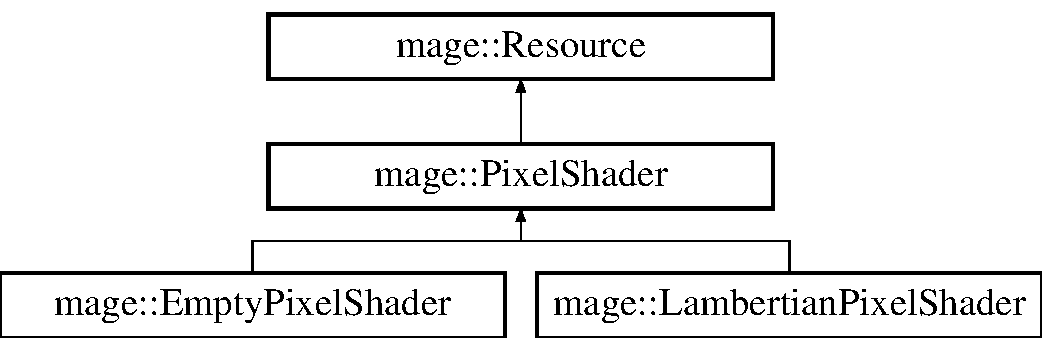
\includegraphics[height=3.000000cm]{classmage_1_1_pixel_shader}
\end{center}
\end{figure}
\subsection*{Public Member Functions}
\begin{DoxyCompactItemize}
\item 
\hyperlink{classmage_1_1_pixel_shader_a0e8952d69f42380d289e7b4bb8035b3e}{Pixel\+Shader} (I\+D3\+D11\+Device2 $\ast$device, I\+D3\+D11\+Device\+Context2 $\ast$device\+\_\+context, const wstring \&fname)
\item 
\hyperlink{classmage_1_1_pixel_shader_a6d3bef6c6d0e2b20443eed92788646e2}{Pixel\+Shader} (I\+D3\+D11\+Device2 $\ast$device, I\+D3\+D11\+Device\+Context2 $\ast$device\+\_\+context, const \hyperlink{structmage_1_1_compiled_pixel_shader}{Compiled\+Pixel\+Shader} \&compiled\+\_\+pixel\+\_\+shader)
\item 
\hyperlink{classmage_1_1_pixel_shader_a361df943e40e9015ac4b769af130ce79}{Pixel\+Shader} (const \hyperlink{classmage_1_1_pixel_shader}{Pixel\+Shader} \&pixel\+\_\+shader)=delete
\item 
\hyperlink{classmage_1_1_pixel_shader_a5b2d7d36082d25c6f860674df745f7cd}{Pixel\+Shader} (\hyperlink{classmage_1_1_pixel_shader}{Pixel\+Shader} \&\&pixel\+\_\+shader)
\item 
virtual \hyperlink{classmage_1_1_pixel_shader_aac21a59d5d614f5bf1905f01479de44e}{$\sim$\+Pixel\+Shader} ()
\item 
\hyperlink{classmage_1_1_pixel_shader}{Pixel\+Shader} \& \hyperlink{classmage_1_1_pixel_shader_ac3a3535b2751237f4aad110dca05d0c3}{operator=} (const \hyperlink{classmage_1_1_pixel_shader}{Pixel\+Shader} \&pixel\+\_\+shader)=delete
\item 
\hyperlink{classmage_1_1_pixel_shader}{Pixel\+Shader} \& \hyperlink{classmage_1_1_pixel_shader_aaeab6f6fda7d6e1f7d333da03d58daf9}{operator=} (\hyperlink{classmage_1_1_pixel_shader}{Pixel\+Shader} \&\&pixel\+\_\+shader)=delete
\item 
virtual void \hyperlink{classmage_1_1_pixel_shader_ab677013145ca252c57e5a001134c01ff}{Prepare\+Shading} (I\+D3\+D11\+Shader\+Resource\+View $\ast$texture) const
\item 
virtual void \hyperlink{classmage_1_1_pixel_shader_a5a1a58bcb0ed64405e746ec7a5af5269}{Prepare\+Shading} (const \hyperlink{structmage_1_1_material}{Material} \&material, const \hyperlink{structmage_1_1_lighting}{Lighting} \&lighting) const
\end{DoxyCompactItemize}
\subsection*{Protected Attributes}
\begin{DoxyCompactItemize}
\item 
I\+D3\+D11\+Device2 $\ast$const \hyperlink{classmage_1_1_pixel_shader_a7fa34f27d8f39db2403edac28ddecc68}{m\+\_\+device}
\item 
I\+D3\+D11\+Device\+Context2 $\ast$const \hyperlink{classmage_1_1_pixel_shader_a6b9bbf18f255b061fb75453f32a78720}{m\+\_\+device\+\_\+context}
\item 
\hyperlink{namespacemage_ae74f374780900893caa5555d1031fd79}{Com\+Ptr}$<$ I\+D3\+D11\+Pixel\+Shader $>$ \hyperlink{classmage_1_1_pixel_shader_a1dd0f87be1c1f7fe5a1bb2737263222f}{m\+\_\+pixel\+\_\+shader}
\end{DoxyCompactItemize}
\subsection*{Private Member Functions}
\begin{DoxyCompactItemize}
\item 
void \hyperlink{classmage_1_1_pixel_shader_a5297d3d12153f9a866751b623203c5aa}{Setup\+Shader} ()
\item 
void \hyperlink{classmage_1_1_pixel_shader_a3010aefe86be3e1efaf2f1c010c42a48}{Setup\+Shader} (const \hyperlink{structmage_1_1_compiled_pixel_shader}{Compiled\+Pixel\+Shader} \&compiled\+\_\+pixel\+\_\+shader)
\end{DoxyCompactItemize}


\subsection{Detailed Description}
A class of pixel shaders. 

\subsection{Constructor \& Destructor Documentation}
\hypertarget{classmage_1_1_pixel_shader_a0e8952d69f42380d289e7b4bb8035b3e}{}\label{classmage_1_1_pixel_shader_a0e8952d69f42380d289e7b4bb8035b3e} 
\index{mage\+::\+Pixel\+Shader@{mage\+::\+Pixel\+Shader}!Pixel\+Shader@{Pixel\+Shader}}
\index{Pixel\+Shader@{Pixel\+Shader}!mage\+::\+Pixel\+Shader@{mage\+::\+Pixel\+Shader}}
\subsubsection{\texorpdfstring{Pixel\+Shader()}{PixelShader()}\hspace{0.1cm}{\footnotesize\ttfamily [1/4]}}
{\footnotesize\ttfamily mage\+::\+Pixel\+Shader\+::\+Pixel\+Shader (\begin{DoxyParamCaption}\item[{I\+D3\+D11\+Device2 $\ast$}]{device,  }\item[{I\+D3\+D11\+Device\+Context2 $\ast$}]{device\+\_\+context,  }\item[{const wstring \&}]{fname }\end{DoxyParamCaption})\hspace{0.3cm}{\ttfamily [explicit]}}

Constructs a pixel shader.

\begin{DoxyPrecond}{Precondition}
{\itshape device} is not equal to {\ttfamily nullptr}. 

{\itshape device\+\_\+context} is not equal to {\ttfamily nullptr}. 
\end{DoxyPrecond}

\begin{DoxyParams}[1]{Parameters}
\mbox{\tt in}  & {\em device} & A pointer to the device. \\
\hline
\mbox{\tt in}  & {\em device\+\_\+context} & A pointer to the device context. \\
\hline
\mbox{\tt in}  & {\em fname} & A reference to the filename. \\
\hline
\end{DoxyParams}

\begin{DoxyExceptions}{Exceptions}
{\em \hyperlink{structmage_1_1_formatted_exception}{Formatted\+Exception}} & Failed to initialize this pixel shader. \\
\hline
\end{DoxyExceptions}
\hypertarget{classmage_1_1_pixel_shader_a6d3bef6c6d0e2b20443eed92788646e2}{}\label{classmage_1_1_pixel_shader_a6d3bef6c6d0e2b20443eed92788646e2} 
\index{mage\+::\+Pixel\+Shader@{mage\+::\+Pixel\+Shader}!Pixel\+Shader@{Pixel\+Shader}}
\index{Pixel\+Shader@{Pixel\+Shader}!mage\+::\+Pixel\+Shader@{mage\+::\+Pixel\+Shader}}
\subsubsection{\texorpdfstring{Pixel\+Shader()}{PixelShader()}\hspace{0.1cm}{\footnotesize\ttfamily [2/4]}}
{\footnotesize\ttfamily mage\+::\+Pixel\+Shader\+::\+Pixel\+Shader (\begin{DoxyParamCaption}\item[{I\+D3\+D11\+Device2 $\ast$}]{device,  }\item[{I\+D3\+D11\+Device\+Context2 $\ast$}]{device\+\_\+context,  }\item[{const \hyperlink{structmage_1_1_compiled_pixel_shader}{Compiled\+Pixel\+Shader} \&}]{compiled\+\_\+pixel\+\_\+shader }\end{DoxyParamCaption})\hspace{0.3cm}{\ttfamily [explicit]}}

Constructs a pixel shader.

\begin{DoxyPrecond}{Precondition}
{\itshape device} is not equal to {\ttfamily nullptr}. 

{\itshape device\+\_\+context} is not equal to {\ttfamily nullptr}. 
\end{DoxyPrecond}

\begin{DoxyParams}[1]{Parameters}
\mbox{\tt in}  & {\em device} & A pointer to the device. \\
\hline
\mbox{\tt in}  & {\em device\+\_\+context} & A pointer to the device context. \\
\hline
\mbox{\tt in}  & {\em compiled\+\_\+pixel\+\_\+shader} & A reference to the compiled pixel shader. \\
\hline
\end{DoxyParams}

\begin{DoxyExceptions}{Exceptions}
{\em \hyperlink{structmage_1_1_formatted_exception}{Formatted\+Exception}} & Failed to initialize this pixel shader. \\
\hline
\end{DoxyExceptions}
\hypertarget{classmage_1_1_pixel_shader_a361df943e40e9015ac4b769af130ce79}{}\label{classmage_1_1_pixel_shader_a361df943e40e9015ac4b769af130ce79} 
\index{mage\+::\+Pixel\+Shader@{mage\+::\+Pixel\+Shader}!Pixel\+Shader@{Pixel\+Shader}}
\index{Pixel\+Shader@{Pixel\+Shader}!mage\+::\+Pixel\+Shader@{mage\+::\+Pixel\+Shader}}
\subsubsection{\texorpdfstring{Pixel\+Shader()}{PixelShader()}\hspace{0.1cm}{\footnotesize\ttfamily [3/4]}}
{\footnotesize\ttfamily mage\+::\+Pixel\+Shader\+::\+Pixel\+Shader (\begin{DoxyParamCaption}\item[{const \hyperlink{classmage_1_1_pixel_shader}{Pixel\+Shader} \&}]{pixel\+\_\+shader }\end{DoxyParamCaption})\hspace{0.3cm}{\ttfamily [delete]}}

Constructs a pixel shader from the given pixel shader.


\begin{DoxyParams}[1]{Parameters}
\mbox{\tt in}  & {\em pixel\+\_\+shader} & A reference to the pixel shader to copy. \\
\hline
\end{DoxyParams}
\hypertarget{classmage_1_1_pixel_shader_a5b2d7d36082d25c6f860674df745f7cd}{}\label{classmage_1_1_pixel_shader_a5b2d7d36082d25c6f860674df745f7cd} 
\index{mage\+::\+Pixel\+Shader@{mage\+::\+Pixel\+Shader}!Pixel\+Shader@{Pixel\+Shader}}
\index{Pixel\+Shader@{Pixel\+Shader}!mage\+::\+Pixel\+Shader@{mage\+::\+Pixel\+Shader}}
\subsubsection{\texorpdfstring{Pixel\+Shader()}{PixelShader()}\hspace{0.1cm}{\footnotesize\ttfamily [4/4]}}
{\footnotesize\ttfamily mage\+::\+Pixel\+Shader\+::\+Pixel\+Shader (\begin{DoxyParamCaption}\item[{\hyperlink{classmage_1_1_pixel_shader}{Pixel\+Shader} \&\&}]{pixel\+\_\+shader }\end{DoxyParamCaption})\hspace{0.3cm}{\ttfamily [default]}}

Constructs a pixel shader by moving the given pixel shader.


\begin{DoxyParams}[1]{Parameters}
\mbox{\tt in}  & {\em pixel\+\_\+shader} & A reference to the pixel shader to move. \\
\hline
\end{DoxyParams}
\hypertarget{classmage_1_1_pixel_shader_aac21a59d5d614f5bf1905f01479de44e}{}\label{classmage_1_1_pixel_shader_aac21a59d5d614f5bf1905f01479de44e} 
\index{mage\+::\+Pixel\+Shader@{mage\+::\+Pixel\+Shader}!````~Pixel\+Shader@{$\sim$\+Pixel\+Shader}}
\index{````~Pixel\+Shader@{$\sim$\+Pixel\+Shader}!mage\+::\+Pixel\+Shader@{mage\+::\+Pixel\+Shader}}
\subsubsection{\texorpdfstring{$\sim$\+Pixel\+Shader()}{~PixelShader()}}
{\footnotesize\ttfamily mage\+::\+Pixel\+Shader\+::$\sim$\+Pixel\+Shader (\begin{DoxyParamCaption}{ }\end{DoxyParamCaption})\hspace{0.3cm}{\ttfamily [virtual]}, {\ttfamily [default]}}

Destructs this pixel shader. 

\subsection{Member Function Documentation}
\hypertarget{classmage_1_1_pixel_shader_ac3a3535b2751237f4aad110dca05d0c3}{}\label{classmage_1_1_pixel_shader_ac3a3535b2751237f4aad110dca05d0c3} 
\index{mage\+::\+Pixel\+Shader@{mage\+::\+Pixel\+Shader}!operator=@{operator=}}
\index{operator=@{operator=}!mage\+::\+Pixel\+Shader@{mage\+::\+Pixel\+Shader}}
\subsubsection{\texorpdfstring{operator=()}{operator=()}\hspace{0.1cm}{\footnotesize\ttfamily [1/2]}}
{\footnotesize\ttfamily \hyperlink{classmage_1_1_pixel_shader}{Pixel\+Shader}\& mage\+::\+Pixel\+Shader\+::operator= (\begin{DoxyParamCaption}\item[{const \hyperlink{classmage_1_1_pixel_shader}{Pixel\+Shader} \&}]{pixel\+\_\+shader }\end{DoxyParamCaption})\hspace{0.3cm}{\ttfamily [delete]}}

Copies the given pixel shader to this pixel shader.


\begin{DoxyParams}[1]{Parameters}
\mbox{\tt in}  & {\em pixel\+\_\+shader} & A reference to the pixel shader to copy. \\
\hline
\end{DoxyParams}
\begin{DoxyReturn}{Returns}
A reference to the copy of the given pixel shader (i.\+e. this pixel shader). 
\end{DoxyReturn}
\hypertarget{classmage_1_1_pixel_shader_aaeab6f6fda7d6e1f7d333da03d58daf9}{}\label{classmage_1_1_pixel_shader_aaeab6f6fda7d6e1f7d333da03d58daf9} 
\index{mage\+::\+Pixel\+Shader@{mage\+::\+Pixel\+Shader}!operator=@{operator=}}
\index{operator=@{operator=}!mage\+::\+Pixel\+Shader@{mage\+::\+Pixel\+Shader}}
\subsubsection{\texorpdfstring{operator=()}{operator=()}\hspace{0.1cm}{\footnotesize\ttfamily [2/2]}}
{\footnotesize\ttfamily \hyperlink{classmage_1_1_pixel_shader}{Pixel\+Shader}\& mage\+::\+Pixel\+Shader\+::operator= (\begin{DoxyParamCaption}\item[{\hyperlink{classmage_1_1_pixel_shader}{Pixel\+Shader} \&\&}]{pixel\+\_\+shader }\end{DoxyParamCaption})\hspace{0.3cm}{\ttfamily [delete]}}

Moves the given pixel shader to this pixel shader.


\begin{DoxyParams}[1]{Parameters}
\mbox{\tt in}  & {\em pixel\+\_\+shader} & A reference to the pixel shader to move. \\
\hline
\end{DoxyParams}
\begin{DoxyReturn}{Returns}
A reference to the moved pixel shader (i.\+e. this pixel shader). 
\end{DoxyReturn}
\hypertarget{classmage_1_1_pixel_shader_ab677013145ca252c57e5a001134c01ff}{}\label{classmage_1_1_pixel_shader_ab677013145ca252c57e5a001134c01ff} 
\index{mage\+::\+Pixel\+Shader@{mage\+::\+Pixel\+Shader}!Prepare\+Shading@{Prepare\+Shading}}
\index{Prepare\+Shading@{Prepare\+Shading}!mage\+::\+Pixel\+Shader@{mage\+::\+Pixel\+Shader}}
\subsubsection{\texorpdfstring{Prepare\+Shading()}{PrepareShading()}\hspace{0.1cm}{\footnotesize\ttfamily [1/2]}}
{\footnotesize\ttfamily void mage\+::\+Pixel\+Shader\+::\+Prepare\+Shading (\begin{DoxyParamCaption}\item[{I\+D3\+D11\+Shader\+Resource\+View $\ast$}]{texture }\end{DoxyParamCaption}) const\hspace{0.3cm}{\ttfamily [virtual]}}

Prepares this pixel shader for shading.

\begin{DoxyPrecond}{Precondition}
{\itshape texture} is not equal to {\ttfamily nullptr}. 
\end{DoxyPrecond}

\begin{DoxyParams}[1]{Parameters}
\mbox{\tt in}  & {\em texture} & A pointer to the texture shader resource view. \\
\hline
\end{DoxyParams}


Reimplemented in \hyperlink{classmage_1_1_sprite_pixel_shader_a8c0c4daf36c74822a772b1a38e8d876a}{mage\+::\+Sprite\+Pixel\+Shader}.

\hypertarget{classmage_1_1_pixel_shader_a5a1a58bcb0ed64405e746ec7a5af5269}{}\label{classmage_1_1_pixel_shader_a5a1a58bcb0ed64405e746ec7a5af5269} 
\index{mage\+::\+Pixel\+Shader@{mage\+::\+Pixel\+Shader}!Prepare\+Shading@{Prepare\+Shading}}
\index{Prepare\+Shading@{Prepare\+Shading}!mage\+::\+Pixel\+Shader@{mage\+::\+Pixel\+Shader}}
\subsubsection{\texorpdfstring{Prepare\+Shading()}{PrepareShading()}\hspace{0.1cm}{\footnotesize\ttfamily [2/2]}}
{\footnotesize\ttfamily void mage\+::\+Pixel\+Shader\+::\+Prepare\+Shading (\begin{DoxyParamCaption}\item[{const \hyperlink{structmage_1_1_material}{Material} \&}]{material,  }\item[{const \hyperlink{structmage_1_1_lighting}{Lighting} \&}]{lighting }\end{DoxyParamCaption}) const\hspace{0.3cm}{\ttfamily [virtual]}}

Prepares this pixel shader for shading.


\begin{DoxyParams}[1]{Parameters}
\mbox{\tt in}  & {\em material} & A reference to the material. \\
\hline
\mbox{\tt in}  & {\em lighting} & A reference to the lighting buffer. \\
\hline
\end{DoxyParams}


Reimplemented in \hyperlink{classmage_1_1_basic_pixel_shader_a67ce881c6c02b2ceabca29cd3b6a4a89}{mage\+::\+Basic\+Pixel\+Shader}, and \hyperlink{classmage_1_1_bump_pixel_shader_aa365b87ca4860c58048ee1a119b4b668}{mage\+::\+Bump\+Pixel\+Shader}.

\hypertarget{classmage_1_1_pixel_shader_a5297d3d12153f9a866751b623203c5aa}{}\label{classmage_1_1_pixel_shader_a5297d3d12153f9a866751b623203c5aa} 
\index{mage\+::\+Pixel\+Shader@{mage\+::\+Pixel\+Shader}!Setup\+Shader@{Setup\+Shader}}
\index{Setup\+Shader@{Setup\+Shader}!mage\+::\+Pixel\+Shader@{mage\+::\+Pixel\+Shader}}
\subsubsection{\texorpdfstring{Setup\+Shader()}{SetupShader()}\hspace{0.1cm}{\footnotesize\ttfamily [1/2]}}
{\footnotesize\ttfamily void mage\+::\+Pixel\+Shader\+::\+Setup\+Shader (\begin{DoxyParamCaption}{ }\end{DoxyParamCaption})\hspace{0.3cm}{\ttfamily [private]}}

Sets up this pixel shader (from compiled shader output).


\begin{DoxyExceptions}{Exceptions}
{\em \hyperlink{structmage_1_1_formatted_exception}{Formatted\+Exception}} & Failed to setup this pixel shader. \\
\hline
\end{DoxyExceptions}
\hypertarget{classmage_1_1_pixel_shader_a3010aefe86be3e1efaf2f1c010c42a48}{}\label{classmage_1_1_pixel_shader_a3010aefe86be3e1efaf2f1c010c42a48} 
\index{mage\+::\+Pixel\+Shader@{mage\+::\+Pixel\+Shader}!Setup\+Shader@{Setup\+Shader}}
\index{Setup\+Shader@{Setup\+Shader}!mage\+::\+Pixel\+Shader@{mage\+::\+Pixel\+Shader}}
\subsubsection{\texorpdfstring{Setup\+Shader()}{SetupShader()}\hspace{0.1cm}{\footnotesize\ttfamily [2/2]}}
{\footnotesize\ttfamily void mage\+::\+Pixel\+Shader\+::\+Setup\+Shader (\begin{DoxyParamCaption}\item[{const \hyperlink{structmage_1_1_compiled_pixel_shader}{Compiled\+Pixel\+Shader} \&}]{compiled\+\_\+pixel\+\_\+shader }\end{DoxyParamCaption})\hspace{0.3cm}{\ttfamily [private]}}

Sets up this pixel shader.


\begin{DoxyParams}[1]{Parameters}
\mbox{\tt in}  & {\em compiled\+\_\+pixel\+\_\+shader} & A reference to the compiled pixel shader. \\
\hline
\end{DoxyParams}

\begin{DoxyExceptions}{Exceptions}
{\em \hyperlink{structmage_1_1_formatted_exception}{Formatted\+Exception}} & Failed to setup this pixel shader. \\
\hline
\end{DoxyExceptions}


\subsection{Member Data Documentation}
\hypertarget{classmage_1_1_pixel_shader_a7fa34f27d8f39db2403edac28ddecc68}{}\label{classmage_1_1_pixel_shader_a7fa34f27d8f39db2403edac28ddecc68} 
\index{mage\+::\+Pixel\+Shader@{mage\+::\+Pixel\+Shader}!m\+\_\+device@{m\+\_\+device}}
\index{m\+\_\+device@{m\+\_\+device}!mage\+::\+Pixel\+Shader@{mage\+::\+Pixel\+Shader}}
\subsubsection{\texorpdfstring{m\+\_\+device}{m\_device}}
{\footnotesize\ttfamily I\+D3\+D11\+Device2$\ast$ const mage\+::\+Pixel\+Shader\+::m\+\_\+device\hspace{0.3cm}{\ttfamily [protected]}}

A pointer to the device of this pixel shader. \hypertarget{classmage_1_1_pixel_shader_a6b9bbf18f255b061fb75453f32a78720}{}\label{classmage_1_1_pixel_shader_a6b9bbf18f255b061fb75453f32a78720} 
\index{mage\+::\+Pixel\+Shader@{mage\+::\+Pixel\+Shader}!m\+\_\+device\+\_\+context@{m\+\_\+device\+\_\+context}}
\index{m\+\_\+device\+\_\+context@{m\+\_\+device\+\_\+context}!mage\+::\+Pixel\+Shader@{mage\+::\+Pixel\+Shader}}
\subsubsection{\texorpdfstring{m\+\_\+device\+\_\+context}{m\_device\_context}}
{\footnotesize\ttfamily I\+D3\+D11\+Device\+Context2$\ast$ const mage\+::\+Pixel\+Shader\+::m\+\_\+device\+\_\+context\hspace{0.3cm}{\ttfamily [protected]}}

A pointer to the device context of this pixel shader. \hypertarget{classmage_1_1_pixel_shader_a1dd0f87be1c1f7fe5a1bb2737263222f}{}\label{classmage_1_1_pixel_shader_a1dd0f87be1c1f7fe5a1bb2737263222f} 
\index{mage\+::\+Pixel\+Shader@{mage\+::\+Pixel\+Shader}!m\+\_\+pixel\+\_\+shader@{m\+\_\+pixel\+\_\+shader}}
\index{m\+\_\+pixel\+\_\+shader@{m\+\_\+pixel\+\_\+shader}!mage\+::\+Pixel\+Shader@{mage\+::\+Pixel\+Shader}}
\subsubsection{\texorpdfstring{m\+\_\+pixel\+\_\+shader}{m\_pixel\_shader}}
{\footnotesize\ttfamily \hyperlink{namespacemage_ae74f374780900893caa5555d1031fd79}{Com\+Ptr}$<$ I\+D3\+D11\+Pixel\+Shader $>$ mage\+::\+Pixel\+Shader\+::m\+\_\+pixel\+\_\+shader\hspace{0.3cm}{\ttfamily [protected]}}

A pointer to the pixel shader of this pixel shader. 
\hypertarget{structmage_1_1_point3}{}\section{mage\+:\+:Point3 Struct Reference}
\label{structmage_1_1_point3}\index{mage\+::\+Point3@{mage\+::\+Point3}}


{\ttfamily \#include $<$math.\+hpp$>$}

Inheritance diagram for mage\+:\+:Point3\+:\begin{figure}[H]
\begin{center}
\leavevmode
\includegraphics[height=2.000000cm]{structmage_1_1_point3}
\end{center}
\end{figure}
\subsection*{Public Member Functions}
\begin{DoxyCompactItemize}
\item 
\hyperlink{structmage_1_1_point3_a2675c303e54c6047520bc1a298c7fef1}{Point3} ()
\item 
\hyperlink{structmage_1_1_point3_a754210fa30befab6db5957a8d9b397f2}{Point3} (float x, float y, float z)
\item 
\hyperlink{structmage_1_1_point3_ad2e95e6eaa32339663e35f936990eb0c}{Point3} (const \hyperlink{structmage_1_1_point3}{Point3} \&point)
\item 
\hyperlink{structmage_1_1_point3_a3d10561285e01d03978e0d91fda6ff1d}{Point3} (\hyperlink{structmage_1_1_point3}{Point3} \&\&point)
\item 
\hyperlink{structmage_1_1_point3_a5ccb5f2f660b3ecdb471ed859923d4fc}{Point3} (const \hyperlink{structmage_1_1_direction3}{Direction3} \&direction)
\item 
\hyperlink{structmage_1_1_point3_ad189bc5943a8fac34495e38471534ffa}{Point3} (\hyperlink{structmage_1_1_direction3}{Direction3} \&\&direction)
\item 
\hyperlink{structmage_1_1_point3_ae56d0fb055b286df68d8d645378408c8}{Point3} (const \hyperlink{structmage_1_1_normal3}{Normal3} \&normal)
\item 
\hyperlink{structmage_1_1_point3_acab03c18e6b20bea3768e14cb1435302}{Point3} (\hyperlink{structmage_1_1_normal3}{Normal3} \&\&normal)
\item 
\hyperlink{structmage_1_1_point3_a2298bfe2417508187bdad7fbaa6178c1}{Point3} (const X\+M\+F\+L\+O\+A\+T3 \&vector)
\item 
\hyperlink{structmage_1_1_point3_a84b8c62ed63301fde1ce0e045c12352b}{Point3} (X\+M\+F\+L\+O\+A\+T3 \&\&vector)
\item 
\hyperlink{structmage_1_1_point3_a952151b6ff72b68569f95445c2ac2495}{$\sim$\+Point3} ()=default
\item 
\hyperlink{structmage_1_1_point3}{Point3} \& \hyperlink{structmage_1_1_point3_a53403b16c67a6c7d72910edaec04e371}{operator=} (const \hyperlink{structmage_1_1_point3}{Point3} \&point)
\item 
\hyperlink{structmage_1_1_point3}{Point3} \& \hyperlink{structmage_1_1_point3_a6889dad6ac4106bd9a52fcae4dfa401c}{operator=} (\hyperlink{structmage_1_1_point3}{Point3} \&\&point)
\end{DoxyCompactItemize}


\subsection{Constructor \& Destructor Documentation}
\hypertarget{structmage_1_1_point3_a2675c303e54c6047520bc1a298c7fef1}{}\label{structmage_1_1_point3_a2675c303e54c6047520bc1a298c7fef1} 
\index{mage\+::\+Point3@{mage\+::\+Point3}!Point3@{Point3}}
\index{Point3@{Point3}!mage\+::\+Point3@{mage\+::\+Point3}}
\subsubsection{\texorpdfstring{Point3()}{Point3()}\hspace{0.1cm}{\footnotesize\ttfamily [1/10]}}
{\footnotesize\ttfamily mage\+::\+Point3\+::\+Point3 (\begin{DoxyParamCaption}{ }\end{DoxyParamCaption})}

\hypertarget{structmage_1_1_point3_a754210fa30befab6db5957a8d9b397f2}{}\label{structmage_1_1_point3_a754210fa30befab6db5957a8d9b397f2} 
\index{mage\+::\+Point3@{mage\+::\+Point3}!Point3@{Point3}}
\index{Point3@{Point3}!mage\+::\+Point3@{mage\+::\+Point3}}
\subsubsection{\texorpdfstring{Point3()}{Point3()}\hspace{0.1cm}{\footnotesize\ttfamily [2/10]}}
{\footnotesize\ttfamily mage\+::\+Point3\+::\+Point3 (\begin{DoxyParamCaption}\item[{float}]{x,  }\item[{float}]{y,  }\item[{float}]{z }\end{DoxyParamCaption})}

\hypertarget{structmage_1_1_point3_ad2e95e6eaa32339663e35f936990eb0c}{}\label{structmage_1_1_point3_ad2e95e6eaa32339663e35f936990eb0c} 
\index{mage\+::\+Point3@{mage\+::\+Point3}!Point3@{Point3}}
\index{Point3@{Point3}!mage\+::\+Point3@{mage\+::\+Point3}}
\subsubsection{\texorpdfstring{Point3()}{Point3()}\hspace{0.1cm}{\footnotesize\ttfamily [3/10]}}
{\footnotesize\ttfamily mage\+::\+Point3\+::\+Point3 (\begin{DoxyParamCaption}\item[{const \hyperlink{structmage_1_1_point3}{Point3} \&}]{point }\end{DoxyParamCaption})}

\hypertarget{structmage_1_1_point3_a3d10561285e01d03978e0d91fda6ff1d}{}\label{structmage_1_1_point3_a3d10561285e01d03978e0d91fda6ff1d} 
\index{mage\+::\+Point3@{mage\+::\+Point3}!Point3@{Point3}}
\index{Point3@{Point3}!mage\+::\+Point3@{mage\+::\+Point3}}
\subsubsection{\texorpdfstring{Point3()}{Point3()}\hspace{0.1cm}{\footnotesize\ttfamily [4/10]}}
{\footnotesize\ttfamily mage\+::\+Point3\+::\+Point3 (\begin{DoxyParamCaption}\item[{\hyperlink{structmage_1_1_point3}{Point3} \&\&}]{point }\end{DoxyParamCaption})}

\hypertarget{structmage_1_1_point3_a5ccb5f2f660b3ecdb471ed859923d4fc}{}\label{structmage_1_1_point3_a5ccb5f2f660b3ecdb471ed859923d4fc} 
\index{mage\+::\+Point3@{mage\+::\+Point3}!Point3@{Point3}}
\index{Point3@{Point3}!mage\+::\+Point3@{mage\+::\+Point3}}
\subsubsection{\texorpdfstring{Point3()}{Point3()}\hspace{0.1cm}{\footnotesize\ttfamily [5/10]}}
{\footnotesize\ttfamily mage\+::\+Point3\+::\+Point3 (\begin{DoxyParamCaption}\item[{const \hyperlink{structmage_1_1_direction3}{Direction3} \&}]{direction }\end{DoxyParamCaption})\hspace{0.3cm}{\ttfamily [explicit]}}

\hypertarget{structmage_1_1_point3_ad189bc5943a8fac34495e38471534ffa}{}\label{structmage_1_1_point3_ad189bc5943a8fac34495e38471534ffa} 
\index{mage\+::\+Point3@{mage\+::\+Point3}!Point3@{Point3}}
\index{Point3@{Point3}!mage\+::\+Point3@{mage\+::\+Point3}}
\subsubsection{\texorpdfstring{Point3()}{Point3()}\hspace{0.1cm}{\footnotesize\ttfamily [6/10]}}
{\footnotesize\ttfamily mage\+::\+Point3\+::\+Point3 (\begin{DoxyParamCaption}\item[{\hyperlink{structmage_1_1_direction3}{Direction3} \&\&}]{direction }\end{DoxyParamCaption})\hspace{0.3cm}{\ttfamily [explicit]}}

\hypertarget{structmage_1_1_point3_ae56d0fb055b286df68d8d645378408c8}{}\label{structmage_1_1_point3_ae56d0fb055b286df68d8d645378408c8} 
\index{mage\+::\+Point3@{mage\+::\+Point3}!Point3@{Point3}}
\index{Point3@{Point3}!mage\+::\+Point3@{mage\+::\+Point3}}
\subsubsection{\texorpdfstring{Point3()}{Point3()}\hspace{0.1cm}{\footnotesize\ttfamily [7/10]}}
{\footnotesize\ttfamily mage\+::\+Point3\+::\+Point3 (\begin{DoxyParamCaption}\item[{const \hyperlink{structmage_1_1_normal3}{Normal3} \&}]{normal }\end{DoxyParamCaption})\hspace{0.3cm}{\ttfamily [explicit]}}

\hypertarget{structmage_1_1_point3_acab03c18e6b20bea3768e14cb1435302}{}\label{structmage_1_1_point3_acab03c18e6b20bea3768e14cb1435302} 
\index{mage\+::\+Point3@{mage\+::\+Point3}!Point3@{Point3}}
\index{Point3@{Point3}!mage\+::\+Point3@{mage\+::\+Point3}}
\subsubsection{\texorpdfstring{Point3()}{Point3()}\hspace{0.1cm}{\footnotesize\ttfamily [8/10]}}
{\footnotesize\ttfamily mage\+::\+Point3\+::\+Point3 (\begin{DoxyParamCaption}\item[{\hyperlink{structmage_1_1_normal3}{Normal3} \&\&}]{normal }\end{DoxyParamCaption})\hspace{0.3cm}{\ttfamily [explicit]}}

\hypertarget{structmage_1_1_point3_a2298bfe2417508187bdad7fbaa6178c1}{}\label{structmage_1_1_point3_a2298bfe2417508187bdad7fbaa6178c1} 
\index{mage\+::\+Point3@{mage\+::\+Point3}!Point3@{Point3}}
\index{Point3@{Point3}!mage\+::\+Point3@{mage\+::\+Point3}}
\subsubsection{\texorpdfstring{Point3()}{Point3()}\hspace{0.1cm}{\footnotesize\ttfamily [9/10]}}
{\footnotesize\ttfamily mage\+::\+Point3\+::\+Point3 (\begin{DoxyParamCaption}\item[{const X\+M\+F\+L\+O\+A\+T3 \&}]{vector }\end{DoxyParamCaption})\hspace{0.3cm}{\ttfamily [explicit]}}

\hypertarget{structmage_1_1_point3_a84b8c62ed63301fde1ce0e045c12352b}{}\label{structmage_1_1_point3_a84b8c62ed63301fde1ce0e045c12352b} 
\index{mage\+::\+Point3@{mage\+::\+Point3}!Point3@{Point3}}
\index{Point3@{Point3}!mage\+::\+Point3@{mage\+::\+Point3}}
\subsubsection{\texorpdfstring{Point3()}{Point3()}\hspace{0.1cm}{\footnotesize\ttfamily [10/10]}}
{\footnotesize\ttfamily mage\+::\+Point3\+::\+Point3 (\begin{DoxyParamCaption}\item[{X\+M\+F\+L\+O\+A\+T3 \&\&}]{vector }\end{DoxyParamCaption})\hspace{0.3cm}{\ttfamily [explicit]}}

\hypertarget{structmage_1_1_point3_a952151b6ff72b68569f95445c2ac2495}{}\label{structmage_1_1_point3_a952151b6ff72b68569f95445c2ac2495} 
\index{mage\+::\+Point3@{mage\+::\+Point3}!````~Point3@{$\sim$\+Point3}}
\index{````~Point3@{$\sim$\+Point3}!mage\+::\+Point3@{mage\+::\+Point3}}
\subsubsection{\texorpdfstring{$\sim$\+Point3()}{~Point3()}}
{\footnotesize\ttfamily mage\+::\+Point3\+::$\sim$\+Point3 (\begin{DoxyParamCaption}{ }\end{DoxyParamCaption})\hspace{0.3cm}{\ttfamily [default]}}



\subsection{Member Function Documentation}
\hypertarget{structmage_1_1_point3_a53403b16c67a6c7d72910edaec04e371}{}\label{structmage_1_1_point3_a53403b16c67a6c7d72910edaec04e371} 
\index{mage\+::\+Point3@{mage\+::\+Point3}!operator=@{operator=}}
\index{operator=@{operator=}!mage\+::\+Point3@{mage\+::\+Point3}}
\subsubsection{\texorpdfstring{operator=()}{operator=()}\hspace{0.1cm}{\footnotesize\ttfamily [1/2]}}
{\footnotesize\ttfamily \hyperlink{structmage_1_1_point3}{Point3}\& mage\+::\+Point3\+::operator= (\begin{DoxyParamCaption}\item[{const \hyperlink{structmage_1_1_point3}{Point3} \&}]{point }\end{DoxyParamCaption})}

\hypertarget{structmage_1_1_point3_a6889dad6ac4106bd9a52fcae4dfa401c}{}\label{structmage_1_1_point3_a6889dad6ac4106bd9a52fcae4dfa401c} 
\index{mage\+::\+Point3@{mage\+::\+Point3}!operator=@{operator=}}
\index{operator=@{operator=}!mage\+::\+Point3@{mage\+::\+Point3}}
\subsubsection{\texorpdfstring{operator=()}{operator=()}\hspace{0.1cm}{\footnotesize\ttfamily [2/2]}}
{\footnotesize\ttfamily \hyperlink{structmage_1_1_point3}{Point3}\& mage\+::\+Point3\+::operator= (\begin{DoxyParamCaption}\item[{\hyperlink{structmage_1_1_point3}{Point3} \&\&}]{point }\end{DoxyParamCaption})}


\hypertarget{classmage_1_1_progress_reporter}{}\section{mage\+:\+:Progress\+Reporter Class Reference}
\label{classmage_1_1_progress_reporter}\index{mage\+::\+Progress\+Reporter@{mage\+::\+Progress\+Reporter}}


{\ttfamily \#include $<$progress\+\_\+reporter.\+hpp$>$}

\subsection*{Public Member Functions}
\begin{DoxyCompactItemize}
\item 
\hyperlink{classmage_1_1_progress_reporter_ab105fa7ac8fb1c53c60deab107c26f74}{Progress\+Reporter} (const string \&title, uint32\+\_\+t nb\+\_\+work, char plus\+\_\+char=\textquotesingle{}+\textquotesingle{}, uint32\+\_\+t bar\+\_\+length=0)
\item 
virtual \hyperlink{classmage_1_1_progress_reporter_aa543239c6dd4474a77cf4cf6904c1b26}{$\sim$\+Progress\+Reporter} ()
\item 
void \hyperlink{classmage_1_1_progress_reporter_a0a5f99f15e4152da9a3d6aadd888244a}{Update} (uint32\+\_\+t nb\+\_\+work=1)
\item 
void \hyperlink{classmage_1_1_progress_reporter_a11d758647ac2082bc296ab53a7454eaa}{Done} ()
\end{DoxyCompactItemize}
\subsection*{Private Member Functions}
\begin{DoxyCompactItemize}
\item 
\hyperlink{classmage_1_1_progress_reporter_a59c1ca6e4c0d480a1726d79ef6d42e74}{Progress\+Reporter} (const \hyperlink{classmage_1_1_progress_reporter}{Progress\+Reporter} \&progress\+\_\+reporter)=delete
\item 
\hyperlink{classmage_1_1_progress_reporter_a51e53891454e814b3c860f8de4506c1b}{Progress\+Reporter} (\hyperlink{classmage_1_1_progress_reporter}{Progress\+Reporter} \&\&progress\+\_\+reporter)=delete
\item 
\hyperlink{classmage_1_1_progress_reporter}{Progress\+Reporter} \& \hyperlink{classmage_1_1_progress_reporter_a7bc52147f6d2e30d897f512f910c8917}{operator=} (const \hyperlink{classmage_1_1_progress_reporter}{Progress\+Reporter} \&progress\+\_\+reporter)=delete
\item 
\hyperlink{classmage_1_1_progress_reporter}{Progress\+Reporter} \& \hyperlink{classmage_1_1_progress_reporter_aba75cd5ea2d9faae4264b844f857e260}{operator=} (\hyperlink{classmage_1_1_progress_reporter}{Progress\+Reporter} \&\&progress\+\_\+reporter)=delete
\end{DoxyCompactItemize}
\subsection*{Private Attributes}
\begin{DoxyCompactItemize}
\item 
const uint32\+\_\+t \hyperlink{classmage_1_1_progress_reporter_a1b0c8d8f3cde82161b34897c5e95e09b}{m\+\_\+nb\+\_\+work\+\_\+total}
\item 
uint32\+\_\+t \hyperlink{classmage_1_1_progress_reporter_ad3cb941594f138c208fa522a355a985b}{m\+\_\+nb\+\_\+work\+\_\+done}
\item 
uint32\+\_\+t \hyperlink{classmage_1_1_progress_reporter_aeae54fa7c542ccfbdaa44c0942c483fd}{m\+\_\+nb\+\_\+plusses\+\_\+total}
\item 
uint32\+\_\+t \hyperlink{classmage_1_1_progress_reporter_a17d7a4f8b2c8a6de255786f6165726bd}{m\+\_\+nb\+\_\+plusses\+\_\+printed}
\item 
\hyperlink{namespacemage_a8c307fbcc33bce9b7f2aa4c26c3b95cf}{Unique\+Ptr}$<$ \hyperlink{classmage_1_1_timer}{Timer} $>$ \hyperlink{classmage_1_1_progress_reporter_a4c5c81ce84ceaab7764bd640a18db788}{m\+\_\+timer}
\item 
F\+I\+LE $\ast$ \hyperlink{classmage_1_1_progress_reporter_ad325ee5978fd1d16a97acbe37a977982}{m\+\_\+fout}
\item 
const char \hyperlink{classmage_1_1_progress_reporter_ab3c8d12e79e63ae2b99fde8d6627c230}{m\+\_\+plus\+\_\+char}
\item 
char $\ast$ \hyperlink{classmage_1_1_progress_reporter_a3aa49d5b886263402d9a9ecb4851670c}{m\+\_\+buffer}
\item 
char $\ast$ \hyperlink{classmage_1_1_progress_reporter_a7adafaaf90edf29c8c27f4008aea41c9}{m\+\_\+current\+\_\+pos}
\item 
\hyperlink{classmage_1_1_mutex}{Mutex} \hyperlink{classmage_1_1_progress_reporter_a32a499aa1b8fccbc8393fe32305dfeb1}{m\+\_\+mutex}
\end{DoxyCompactItemize}


\subsection{Detailed Description}
A class of progress reporters. 

\subsection{Constructor \& Destructor Documentation}
\hypertarget{classmage_1_1_progress_reporter_ab105fa7ac8fb1c53c60deab107c26f74}{}\label{classmage_1_1_progress_reporter_ab105fa7ac8fb1c53c60deab107c26f74} 
\index{mage\+::\+Progress\+Reporter@{mage\+::\+Progress\+Reporter}!Progress\+Reporter@{Progress\+Reporter}}
\index{Progress\+Reporter@{Progress\+Reporter}!mage\+::\+Progress\+Reporter@{mage\+::\+Progress\+Reporter}}
\subsubsection{\texorpdfstring{Progress\+Reporter()}{ProgressReporter()}\hspace{0.1cm}{\footnotesize\ttfamily [1/3]}}
{\footnotesize\ttfamily mage\+::\+Progress\+Reporter\+::\+Progress\+Reporter (\begin{DoxyParamCaption}\item[{const string \&}]{title,  }\item[{uint32\+\_\+t}]{nb\+\_\+work,  }\item[{char}]{plus\+\_\+char = {\ttfamily \textquotesingle{}+\textquotesingle{}},  }\item[{uint32\+\_\+t}]{bar\+\_\+length = {\ttfamily 0} }\end{DoxyParamCaption})}

Constructs a progress reporter.


\begin{DoxyParams}[1]{Parameters}
\mbox{\tt in}  & {\em title} & A reference to the title. \\
\hline
\mbox{\tt in}  & {\em nb\+\_\+work} & The total number of work units. \\
\hline
\mbox{\tt in}  & {\em plus\+\_\+char} & The character representing a work unit that is already done. \\
\hline
\mbox{\tt in}  & {\em bar\+\_\+length} & The length of the progress bar. If 0 the default length will be chosen. \\
\hline
\end{DoxyParams}
\hypertarget{classmage_1_1_progress_reporter_aa543239c6dd4474a77cf4cf6904c1b26}{}\label{classmage_1_1_progress_reporter_aa543239c6dd4474a77cf4cf6904c1b26} 
\index{mage\+::\+Progress\+Reporter@{mage\+::\+Progress\+Reporter}!````~Progress\+Reporter@{$\sim$\+Progress\+Reporter}}
\index{````~Progress\+Reporter@{$\sim$\+Progress\+Reporter}!mage\+::\+Progress\+Reporter@{mage\+::\+Progress\+Reporter}}
\subsubsection{\texorpdfstring{$\sim$\+Progress\+Reporter()}{~ProgressReporter()}}
{\footnotesize\ttfamily mage\+::\+Progress\+Reporter\+::$\sim$\+Progress\+Reporter (\begin{DoxyParamCaption}{ }\end{DoxyParamCaption})\hspace{0.3cm}{\ttfamily [virtual]}}

Destructs this progress reporter. \hypertarget{classmage_1_1_progress_reporter_a59c1ca6e4c0d480a1726d79ef6d42e74}{}\label{classmage_1_1_progress_reporter_a59c1ca6e4c0d480a1726d79ef6d42e74} 
\index{mage\+::\+Progress\+Reporter@{mage\+::\+Progress\+Reporter}!Progress\+Reporter@{Progress\+Reporter}}
\index{Progress\+Reporter@{Progress\+Reporter}!mage\+::\+Progress\+Reporter@{mage\+::\+Progress\+Reporter}}
\subsubsection{\texorpdfstring{Progress\+Reporter()}{ProgressReporter()}\hspace{0.1cm}{\footnotesize\ttfamily [2/3]}}
{\footnotesize\ttfamily mage\+::\+Progress\+Reporter\+::\+Progress\+Reporter (\begin{DoxyParamCaption}\item[{const \hyperlink{classmage_1_1_progress_reporter}{Progress\+Reporter} \&}]{progress\+\_\+reporter }\end{DoxyParamCaption})\hspace{0.3cm}{\ttfamily [private]}, {\ttfamily [delete]}}

Constructs a progress reporter from the given progress reporter.


\begin{DoxyParams}[1]{Parameters}
\mbox{\tt in}  & {\em progress\+\_\+reporter} & A reference to the progress reporter. \\
\hline
\end{DoxyParams}
\hypertarget{classmage_1_1_progress_reporter_a51e53891454e814b3c860f8de4506c1b}{}\label{classmage_1_1_progress_reporter_a51e53891454e814b3c860f8de4506c1b} 
\index{mage\+::\+Progress\+Reporter@{mage\+::\+Progress\+Reporter}!Progress\+Reporter@{Progress\+Reporter}}
\index{Progress\+Reporter@{Progress\+Reporter}!mage\+::\+Progress\+Reporter@{mage\+::\+Progress\+Reporter}}
\subsubsection{\texorpdfstring{Progress\+Reporter()}{ProgressReporter()}\hspace{0.1cm}{\footnotesize\ttfamily [3/3]}}
{\footnotesize\ttfamily mage\+::\+Progress\+Reporter\+::\+Progress\+Reporter (\begin{DoxyParamCaption}\item[{\hyperlink{classmage_1_1_progress_reporter}{Progress\+Reporter} \&\&}]{progress\+\_\+reporter }\end{DoxyParamCaption})\hspace{0.3cm}{\ttfamily [private]}, {\ttfamily [delete]}}

Constructs a progress reporter from the given progress reporter.


\begin{DoxyParams}[1]{Parameters}
\mbox{\tt in}  & {\em progress\+\_\+reporter} & A reference to the progress reporter. \\
\hline
\end{DoxyParams}


\subsection{Member Function Documentation}
\hypertarget{classmage_1_1_progress_reporter_a11d758647ac2082bc296ab53a7454eaa}{}\label{classmage_1_1_progress_reporter_a11d758647ac2082bc296ab53a7454eaa} 
\index{mage\+::\+Progress\+Reporter@{mage\+::\+Progress\+Reporter}!Done@{Done}}
\index{Done@{Done}!mage\+::\+Progress\+Reporter@{mage\+::\+Progress\+Reporter}}
\subsubsection{\texorpdfstring{Done()}{Done()}}
{\footnotesize\ttfamily void mage\+::\+Progress\+Reporter\+::\+Done (\begin{DoxyParamCaption}{ }\end{DoxyParamCaption})}

Finishes this progress reporter. \hypertarget{classmage_1_1_progress_reporter_a7bc52147f6d2e30d897f512f910c8917}{}\label{classmage_1_1_progress_reporter_a7bc52147f6d2e30d897f512f910c8917} 
\index{mage\+::\+Progress\+Reporter@{mage\+::\+Progress\+Reporter}!operator=@{operator=}}
\index{operator=@{operator=}!mage\+::\+Progress\+Reporter@{mage\+::\+Progress\+Reporter}}
\subsubsection{\texorpdfstring{operator=()}{operator=()}\hspace{0.1cm}{\footnotesize\ttfamily [1/2]}}
{\footnotesize\ttfamily \hyperlink{classmage_1_1_progress_reporter}{Progress\+Reporter}\& mage\+::\+Progress\+Reporter\+::operator= (\begin{DoxyParamCaption}\item[{const \hyperlink{classmage_1_1_progress_reporter}{Progress\+Reporter} \&}]{progress\+\_\+reporter }\end{DoxyParamCaption})\hspace{0.3cm}{\ttfamily [private]}, {\ttfamily [delete]}}

Copies the given progress reporter to this progress reporter.


\begin{DoxyParams}[1]{Parameters}
\mbox{\tt in}  & {\em progress\+\_\+reporter} & A reference to the progress reporter to copy from. \\
\hline
\end{DoxyParams}
\begin{DoxyReturn}{Returns}
A reference to the copy of the given progress reporter (i.\+e. this progress reporter). 
\end{DoxyReturn}
\hypertarget{classmage_1_1_progress_reporter_aba75cd5ea2d9faae4264b844f857e260}{}\label{classmage_1_1_progress_reporter_aba75cd5ea2d9faae4264b844f857e260} 
\index{mage\+::\+Progress\+Reporter@{mage\+::\+Progress\+Reporter}!operator=@{operator=}}
\index{operator=@{operator=}!mage\+::\+Progress\+Reporter@{mage\+::\+Progress\+Reporter}}
\subsubsection{\texorpdfstring{operator=()}{operator=()}\hspace{0.1cm}{\footnotesize\ttfamily [2/2]}}
{\footnotesize\ttfamily \hyperlink{classmage_1_1_progress_reporter}{Progress\+Reporter}\& mage\+::\+Progress\+Reporter\+::operator= (\begin{DoxyParamCaption}\item[{\hyperlink{classmage_1_1_progress_reporter}{Progress\+Reporter} \&\&}]{progress\+\_\+reporter }\end{DoxyParamCaption})\hspace{0.3cm}{\ttfamily [private]}, {\ttfamily [delete]}}

Copies the given progress reporter to this progress reporter.


\begin{DoxyParams}[1]{Parameters}
\mbox{\tt in}  & {\em progress\+\_\+reporter} & A reference to the progress reporter to copy from. \\
\hline
\end{DoxyParams}
\begin{DoxyReturn}{Returns}
A reference to the copy of the given progress reporter (i.\+e. this progress reporter). 
\end{DoxyReturn}
\hypertarget{classmage_1_1_progress_reporter_a0a5f99f15e4152da9a3d6aadd888244a}{}\label{classmage_1_1_progress_reporter_a0a5f99f15e4152da9a3d6aadd888244a} 
\index{mage\+::\+Progress\+Reporter@{mage\+::\+Progress\+Reporter}!Update@{Update}}
\index{Update@{Update}!mage\+::\+Progress\+Reporter@{mage\+::\+Progress\+Reporter}}
\subsubsection{\texorpdfstring{Update()}{Update()}}
{\footnotesize\ttfamily void mage\+::\+Progress\+Reporter\+::\+Update (\begin{DoxyParamCaption}\item[{uint32\+\_\+t}]{nb\+\_\+work = {\ttfamily 1} }\end{DoxyParamCaption})}

Updates this progress reporter.


\begin{DoxyParams}[1]{Parameters}
\mbox{\tt in}  & {\em nb\+\_\+work} & The number of work units that are done. \\
\hline
\end{DoxyParams}


\subsection{Member Data Documentation}
\hypertarget{classmage_1_1_progress_reporter_a3aa49d5b886263402d9a9ecb4851670c}{}\label{classmage_1_1_progress_reporter_a3aa49d5b886263402d9a9ecb4851670c} 
\index{mage\+::\+Progress\+Reporter@{mage\+::\+Progress\+Reporter}!m\+\_\+buffer@{m\+\_\+buffer}}
\index{m\+\_\+buffer@{m\+\_\+buffer}!mage\+::\+Progress\+Reporter@{mage\+::\+Progress\+Reporter}}
\subsubsection{\texorpdfstring{m\+\_\+buffer}{m\_buffer}}
{\footnotesize\ttfamily char$\ast$ mage\+::\+Progress\+Reporter\+::m\+\_\+buffer\hspace{0.3cm}{\ttfamily [private]}}

The output buffer of this progress reporter. \hypertarget{classmage_1_1_progress_reporter_a7adafaaf90edf29c8c27f4008aea41c9}{}\label{classmage_1_1_progress_reporter_a7adafaaf90edf29c8c27f4008aea41c9} 
\index{mage\+::\+Progress\+Reporter@{mage\+::\+Progress\+Reporter}!m\+\_\+current\+\_\+pos@{m\+\_\+current\+\_\+pos}}
\index{m\+\_\+current\+\_\+pos@{m\+\_\+current\+\_\+pos}!mage\+::\+Progress\+Reporter@{mage\+::\+Progress\+Reporter}}
\subsubsection{\texorpdfstring{m\+\_\+current\+\_\+pos}{m\_current\_pos}}
{\footnotesize\ttfamily char$\ast$ mage\+::\+Progress\+Reporter\+::m\+\_\+current\+\_\+pos\hspace{0.3cm}{\ttfamily [private]}}

The current (output) position of this progress reporter. \hypertarget{classmage_1_1_progress_reporter_ad325ee5978fd1d16a97acbe37a977982}{}\label{classmage_1_1_progress_reporter_ad325ee5978fd1d16a97acbe37a977982} 
\index{mage\+::\+Progress\+Reporter@{mage\+::\+Progress\+Reporter}!m\+\_\+fout@{m\+\_\+fout}}
\index{m\+\_\+fout@{m\+\_\+fout}!mage\+::\+Progress\+Reporter@{mage\+::\+Progress\+Reporter}}
\subsubsection{\texorpdfstring{m\+\_\+fout}{m\_fout}}
{\footnotesize\ttfamily F\+I\+LE$\ast$ mage\+::\+Progress\+Reporter\+::m\+\_\+fout\hspace{0.3cm}{\ttfamily [private]}}

The output file stream of this progress reporter. \hypertarget{classmage_1_1_progress_reporter_a32a499aa1b8fccbc8393fe32305dfeb1}{}\label{classmage_1_1_progress_reporter_a32a499aa1b8fccbc8393fe32305dfeb1} 
\index{mage\+::\+Progress\+Reporter@{mage\+::\+Progress\+Reporter}!m\+\_\+mutex@{m\+\_\+mutex}}
\index{m\+\_\+mutex@{m\+\_\+mutex}!mage\+::\+Progress\+Reporter@{mage\+::\+Progress\+Reporter}}
\subsubsection{\texorpdfstring{m\+\_\+mutex}{m\_mutex}}
{\footnotesize\ttfamily \hyperlink{classmage_1_1_mutex}{Mutex} mage\+::\+Progress\+Reporter\+::m\+\_\+mutex\hspace{0.3cm}{\ttfamily [private]}}

The mutex needed for updating this progress reporter. \hypertarget{classmage_1_1_progress_reporter_a17d7a4f8b2c8a6de255786f6165726bd}{}\label{classmage_1_1_progress_reporter_a17d7a4f8b2c8a6de255786f6165726bd} 
\index{mage\+::\+Progress\+Reporter@{mage\+::\+Progress\+Reporter}!m\+\_\+nb\+\_\+plusses\+\_\+printed@{m\+\_\+nb\+\_\+plusses\+\_\+printed}}
\index{m\+\_\+nb\+\_\+plusses\+\_\+printed@{m\+\_\+nb\+\_\+plusses\+\_\+printed}!mage\+::\+Progress\+Reporter@{mage\+::\+Progress\+Reporter}}
\subsubsection{\texorpdfstring{m\+\_\+nb\+\_\+plusses\+\_\+printed}{m\_nb\_plusses\_printed}}
{\footnotesize\ttfamily uint32\+\_\+t mage\+::\+Progress\+Reporter\+::m\+\_\+nb\+\_\+plusses\+\_\+printed\hspace{0.3cm}{\ttfamily [private]}}

The total number of plusses that are already outputted. \hypertarget{classmage_1_1_progress_reporter_aeae54fa7c542ccfbdaa44c0942c483fd}{}\label{classmage_1_1_progress_reporter_aeae54fa7c542ccfbdaa44c0942c483fd} 
\index{mage\+::\+Progress\+Reporter@{mage\+::\+Progress\+Reporter}!m\+\_\+nb\+\_\+plusses\+\_\+total@{m\+\_\+nb\+\_\+plusses\+\_\+total}}
\index{m\+\_\+nb\+\_\+plusses\+\_\+total@{m\+\_\+nb\+\_\+plusses\+\_\+total}!mage\+::\+Progress\+Reporter@{mage\+::\+Progress\+Reporter}}
\subsubsection{\texorpdfstring{m\+\_\+nb\+\_\+plusses\+\_\+total}{m\_nb\_plusses\_total}}
{\footnotesize\ttfamily uint32\+\_\+t mage\+::\+Progress\+Reporter\+::m\+\_\+nb\+\_\+plusses\+\_\+total\hspace{0.3cm}{\ttfamily [private]}}

The total number of plusses that need to be outputted. \hypertarget{classmage_1_1_progress_reporter_ad3cb941594f138c208fa522a355a985b}{}\label{classmage_1_1_progress_reporter_ad3cb941594f138c208fa522a355a985b} 
\index{mage\+::\+Progress\+Reporter@{mage\+::\+Progress\+Reporter}!m\+\_\+nb\+\_\+work\+\_\+done@{m\+\_\+nb\+\_\+work\+\_\+done}}
\index{m\+\_\+nb\+\_\+work\+\_\+done@{m\+\_\+nb\+\_\+work\+\_\+done}!mage\+::\+Progress\+Reporter@{mage\+::\+Progress\+Reporter}}
\subsubsection{\texorpdfstring{m\+\_\+nb\+\_\+work\+\_\+done}{m\_nb\_work\_done}}
{\footnotesize\ttfamily uint32\+\_\+t mage\+::\+Progress\+Reporter\+::m\+\_\+nb\+\_\+work\+\_\+done\hspace{0.3cm}{\ttfamily [private]}}

The number of work units that are already done. \hypertarget{classmage_1_1_progress_reporter_a1b0c8d8f3cde82161b34897c5e95e09b}{}\label{classmage_1_1_progress_reporter_a1b0c8d8f3cde82161b34897c5e95e09b} 
\index{mage\+::\+Progress\+Reporter@{mage\+::\+Progress\+Reporter}!m\+\_\+nb\+\_\+work\+\_\+total@{m\+\_\+nb\+\_\+work\+\_\+total}}
\index{m\+\_\+nb\+\_\+work\+\_\+total@{m\+\_\+nb\+\_\+work\+\_\+total}!mage\+::\+Progress\+Reporter@{mage\+::\+Progress\+Reporter}}
\subsubsection{\texorpdfstring{m\+\_\+nb\+\_\+work\+\_\+total}{m\_nb\_work\_total}}
{\footnotesize\ttfamily const uint32\+\_\+t mage\+::\+Progress\+Reporter\+::m\+\_\+nb\+\_\+work\+\_\+total\hspace{0.3cm}{\ttfamily [private]}}

The total number of work units that need to be done. \hypertarget{classmage_1_1_progress_reporter_ab3c8d12e79e63ae2b99fde8d6627c230}{}\label{classmage_1_1_progress_reporter_ab3c8d12e79e63ae2b99fde8d6627c230} 
\index{mage\+::\+Progress\+Reporter@{mage\+::\+Progress\+Reporter}!m\+\_\+plus\+\_\+char@{m\+\_\+plus\+\_\+char}}
\index{m\+\_\+plus\+\_\+char@{m\+\_\+plus\+\_\+char}!mage\+::\+Progress\+Reporter@{mage\+::\+Progress\+Reporter}}
\subsubsection{\texorpdfstring{m\+\_\+plus\+\_\+char}{m\_plus\_char}}
{\footnotesize\ttfamily const char mage\+::\+Progress\+Reporter\+::m\+\_\+plus\+\_\+char\hspace{0.3cm}{\ttfamily [private]}}

The character representing a work unit that is already done. \hypertarget{classmage_1_1_progress_reporter_a4c5c81ce84ceaab7764bd640a18db788}{}\label{classmage_1_1_progress_reporter_a4c5c81ce84ceaab7764bd640a18db788} 
\index{mage\+::\+Progress\+Reporter@{mage\+::\+Progress\+Reporter}!m\+\_\+timer@{m\+\_\+timer}}
\index{m\+\_\+timer@{m\+\_\+timer}!mage\+::\+Progress\+Reporter@{mage\+::\+Progress\+Reporter}}
\subsubsection{\texorpdfstring{m\+\_\+timer}{m\_timer}}
{\footnotesize\ttfamily \hyperlink{namespacemage_a8c307fbcc33bce9b7f2aa4c26c3b95cf}{Unique\+Ptr}$<$ \hyperlink{classmage_1_1_timer}{Timer} $>$ mage\+::\+Progress\+Reporter\+::m\+\_\+timer\hspace{0.3cm}{\ttfamily [private]}}

The timer of this progress reporter. 
\hypertarget{structmage_1_1_read_write_mutex}{}\section{mage\+:\+:Read\+Write\+Mutex Struct Reference}
\label{structmage_1_1_read_write_mutex}\index{mage\+::\+Read\+Write\+Mutex@{mage\+::\+Read\+Write\+Mutex}}


{\ttfamily \#include $<$lock.\+hpp$>$}

\subsection*{Public Member Functions}
\begin{DoxyCompactItemize}
\item 
\hyperlink{structmage_1_1_read_write_mutex_aae10694de3862f2d1059477169883940}{Read\+Write\+Mutex} ()
\item 
\hyperlink{structmage_1_1_read_write_mutex_aacb2f69e7e2b084147e1e45628e9dd67}{Read\+Write\+Mutex} (const \hyperlink{structmage_1_1_read_write_mutex}{Read\+Write\+Mutex} \&mutex)=delete
\item 
\hyperlink{structmage_1_1_read_write_mutex_ab5cc5ca0afcca8a994c6468033a501bf}{Read\+Write\+Mutex} (\hyperlink{structmage_1_1_read_write_mutex}{Read\+Write\+Mutex} \&\&mutex)=default
\item 
\hyperlink{structmage_1_1_read_write_mutex_a73676d9414658d63edfe443ee1d55c8b}{$\sim$\+Read\+Write\+Mutex} ()
\item 
\hyperlink{structmage_1_1_read_write_mutex}{Read\+Write\+Mutex} \& \hyperlink{structmage_1_1_read_write_mutex_a408e06f3c8bcc644e43afbf7e9ac772f}{operator=} (const \hyperlink{structmage_1_1_read_write_mutex}{Read\+Write\+Mutex} \&mutex)=delete
\item 
\hyperlink{structmage_1_1_read_write_mutex}{Read\+Write\+Mutex} \& \hyperlink{structmage_1_1_read_write_mutex_a14ea4d1be75046741a7663e0d86a017a}{operator=} (\hyperlink{structmage_1_1_read_write_mutex}{Read\+Write\+Mutex} \&\&mutex)=delete
\end{DoxyCompactItemize}
\subsection*{Private Member Functions}
\begin{DoxyCompactItemize}
\item 
void \hyperlink{structmage_1_1_read_write_mutex_af78045647078aaf3966c8f1b06e35c92}{Acquire\+Read} ()
\item 
void \hyperlink{structmage_1_1_read_write_mutex_a0af5059a9bd16abd8a21b15e7ebe053d}{Release\+Read} ()
\item 
void \hyperlink{structmage_1_1_read_write_mutex_a76137013107a9c2c1fc05c1e0747965e}{Acquire\+Write} ()
\item 
void \hyperlink{structmage_1_1_read_write_mutex_ad0fd296bdaa212f54a58372c8dfe1d1d}{Release\+Write} ()
\end{DoxyCompactItemize}
\subsection*{Private Attributes}
\begin{DoxyCompactItemize}
\item 
L\+O\+NG \hyperlink{structmage_1_1_read_write_mutex_a003313794a9b43f80bd9b258b039438d}{m\+\_\+nb\+\_\+writers\+\_\+waiting}
\item 
L\+O\+NG \hyperlink{structmage_1_1_read_write_mutex_acbe7553fff7cca2656f6f2b8f0471484}{m\+\_\+nb\+\_\+readers\+\_\+waiting}
\item 
D\+W\+O\+RD \hyperlink{structmage_1_1_read_write_mutex_a1e0ad98e517236170faae5b27decfdce}{m\+\_\+active\+\_\+writer\+\_\+readers}
\item 
H\+A\+N\+D\+LE \hyperlink{structmage_1_1_read_write_mutex_a65c0ef8b687d48104b09a9d175e72236}{m\+\_\+ready\+\_\+to\+\_\+read\+\_\+handle}
\item 
H\+A\+N\+D\+LE \hyperlink{structmage_1_1_read_write_mutex_a9498ef85b52486342ba657f34369f89e}{m\+\_\+ready\+\_\+to\+\_\+write\+\_\+handle}
\item 
C\+R\+I\+T\+I\+C\+A\+L\+\_\+\+S\+E\+C\+T\+I\+ON \hyperlink{structmage_1_1_read_write_mutex_a77fe51b87e5205d60ea045fa53bc1fa3}{m\+\_\+critical\+\_\+section}
\end{DoxyCompactItemize}
\subsection*{Friends}
\begin{DoxyCompactItemize}
\item 
struct \hyperlink{structmage_1_1_read_write_mutex_a7ae207fc659160d3c55a5ba1468007f7}{Read\+Write\+Mutex\+Lock}
\end{DoxyCompactItemize}


\subsection{Detailed Description}
A struct of read write mutexes. 

\subsection{Constructor \& Destructor Documentation}
\hypertarget{structmage_1_1_read_write_mutex_aae10694de3862f2d1059477169883940}{}\label{structmage_1_1_read_write_mutex_aae10694de3862f2d1059477169883940} 
\index{mage\+::\+Read\+Write\+Mutex@{mage\+::\+Read\+Write\+Mutex}!Read\+Write\+Mutex@{Read\+Write\+Mutex}}
\index{Read\+Write\+Mutex@{Read\+Write\+Mutex}!mage\+::\+Read\+Write\+Mutex@{mage\+::\+Read\+Write\+Mutex}}
\subsubsection{\texorpdfstring{Read\+Write\+Mutex()}{ReadWriteMutex()}\hspace{0.1cm}{\footnotesize\ttfamily [1/3]}}
{\footnotesize\ttfamily mage\+::\+Read\+Write\+Mutex\+::\+Read\+Write\+Mutex (\begin{DoxyParamCaption}{ }\end{DoxyParamCaption})}

Constructs a read write mutex. \hypertarget{structmage_1_1_read_write_mutex_aacb2f69e7e2b084147e1e45628e9dd67}{}\label{structmage_1_1_read_write_mutex_aacb2f69e7e2b084147e1e45628e9dd67} 
\index{mage\+::\+Read\+Write\+Mutex@{mage\+::\+Read\+Write\+Mutex}!Read\+Write\+Mutex@{Read\+Write\+Mutex}}
\index{Read\+Write\+Mutex@{Read\+Write\+Mutex}!mage\+::\+Read\+Write\+Mutex@{mage\+::\+Read\+Write\+Mutex}}
\subsubsection{\texorpdfstring{Read\+Write\+Mutex()}{ReadWriteMutex()}\hspace{0.1cm}{\footnotesize\ttfamily [2/3]}}
{\footnotesize\ttfamily mage\+::\+Read\+Write\+Mutex\+::\+Read\+Write\+Mutex (\begin{DoxyParamCaption}\item[{const \hyperlink{structmage_1_1_read_write_mutex}{Read\+Write\+Mutex} \&}]{mutex }\end{DoxyParamCaption})\hspace{0.3cm}{\ttfamily [delete]}}

Constructs a read write mutex from the given read write mutex.


\begin{DoxyParams}[1]{Parameters}
\mbox{\tt in}  & {\em mutex} & A reference to the read write mutex to copy. \\
\hline
\end{DoxyParams}
\hypertarget{structmage_1_1_read_write_mutex_ab5cc5ca0afcca8a994c6468033a501bf}{}\label{structmage_1_1_read_write_mutex_ab5cc5ca0afcca8a994c6468033a501bf} 
\index{mage\+::\+Read\+Write\+Mutex@{mage\+::\+Read\+Write\+Mutex}!Read\+Write\+Mutex@{Read\+Write\+Mutex}}
\index{Read\+Write\+Mutex@{Read\+Write\+Mutex}!mage\+::\+Read\+Write\+Mutex@{mage\+::\+Read\+Write\+Mutex}}
\subsubsection{\texorpdfstring{Read\+Write\+Mutex()}{ReadWriteMutex()}\hspace{0.1cm}{\footnotesize\ttfamily [3/3]}}
{\footnotesize\ttfamily mage\+::\+Read\+Write\+Mutex\+::\+Read\+Write\+Mutex (\begin{DoxyParamCaption}\item[{\hyperlink{structmage_1_1_read_write_mutex}{Read\+Write\+Mutex} \&\&}]{mutex }\end{DoxyParamCaption})\hspace{0.3cm}{\ttfamily [default]}}

Constructs a read write mutex by moving the given read write mutex.


\begin{DoxyParams}[1]{Parameters}
\mbox{\tt in}  & {\em mutex} & A reference to the read write mutex to move. \\
\hline
\end{DoxyParams}
\hypertarget{structmage_1_1_read_write_mutex_a73676d9414658d63edfe443ee1d55c8b}{}\label{structmage_1_1_read_write_mutex_a73676d9414658d63edfe443ee1d55c8b} 
\index{mage\+::\+Read\+Write\+Mutex@{mage\+::\+Read\+Write\+Mutex}!````~Read\+Write\+Mutex@{$\sim$\+Read\+Write\+Mutex}}
\index{````~Read\+Write\+Mutex@{$\sim$\+Read\+Write\+Mutex}!mage\+::\+Read\+Write\+Mutex@{mage\+::\+Read\+Write\+Mutex}}
\subsubsection{\texorpdfstring{$\sim$\+Read\+Write\+Mutex()}{~ReadWriteMutex()}}
{\footnotesize\ttfamily mage\+::\+Read\+Write\+Mutex\+::$\sim$\+Read\+Write\+Mutex (\begin{DoxyParamCaption}{ }\end{DoxyParamCaption})}

Destructs this read write mutex. 

\subsection{Member Function Documentation}
\hypertarget{structmage_1_1_read_write_mutex_af78045647078aaf3966c8f1b06e35c92}{}\label{structmage_1_1_read_write_mutex_af78045647078aaf3966c8f1b06e35c92} 
\index{mage\+::\+Read\+Write\+Mutex@{mage\+::\+Read\+Write\+Mutex}!Acquire\+Read@{Acquire\+Read}}
\index{Acquire\+Read@{Acquire\+Read}!mage\+::\+Read\+Write\+Mutex@{mage\+::\+Read\+Write\+Mutex}}
\subsubsection{\texorpdfstring{Acquire\+Read()}{AcquireRead()}}
{\footnotesize\ttfamily void mage\+::\+Read\+Write\+Mutex\+::\+Acquire\+Read (\begin{DoxyParamCaption}{ }\end{DoxyParamCaption})\hspace{0.3cm}{\ttfamily [private]}}

Acquires a read. \hypertarget{structmage_1_1_read_write_mutex_a76137013107a9c2c1fc05c1e0747965e}{}\label{structmage_1_1_read_write_mutex_a76137013107a9c2c1fc05c1e0747965e} 
\index{mage\+::\+Read\+Write\+Mutex@{mage\+::\+Read\+Write\+Mutex}!Acquire\+Write@{Acquire\+Write}}
\index{Acquire\+Write@{Acquire\+Write}!mage\+::\+Read\+Write\+Mutex@{mage\+::\+Read\+Write\+Mutex}}
\subsubsection{\texorpdfstring{Acquire\+Write()}{AcquireWrite()}}
{\footnotesize\ttfamily void mage\+::\+Read\+Write\+Mutex\+::\+Acquire\+Write (\begin{DoxyParamCaption}{ }\end{DoxyParamCaption})\hspace{0.3cm}{\ttfamily [private]}}

Acquires a write. \hypertarget{structmage_1_1_read_write_mutex_a408e06f3c8bcc644e43afbf7e9ac772f}{}\label{structmage_1_1_read_write_mutex_a408e06f3c8bcc644e43afbf7e9ac772f} 
\index{mage\+::\+Read\+Write\+Mutex@{mage\+::\+Read\+Write\+Mutex}!operator=@{operator=}}
\index{operator=@{operator=}!mage\+::\+Read\+Write\+Mutex@{mage\+::\+Read\+Write\+Mutex}}
\subsubsection{\texorpdfstring{operator=()}{operator=()}\hspace{0.1cm}{\footnotesize\ttfamily [1/2]}}
{\footnotesize\ttfamily \hyperlink{structmage_1_1_read_write_mutex}{Read\+Write\+Mutex}\& mage\+::\+Read\+Write\+Mutex\+::operator= (\begin{DoxyParamCaption}\item[{const \hyperlink{structmage_1_1_read_write_mutex}{Read\+Write\+Mutex} \&}]{mutex }\end{DoxyParamCaption})\hspace{0.3cm}{\ttfamily [delete]}}

Copies the given read write mutex to this read write mutex.


\begin{DoxyParams}[1]{Parameters}
\mbox{\tt in}  & {\em mutex} & A reference to a read write mutex to copy. \\
\hline
\end{DoxyParams}
\begin{DoxyReturn}{Returns}
A reference to the copy of the given read write mutex (i.\+e. this read write mutex). 
\end{DoxyReturn}
\hypertarget{structmage_1_1_read_write_mutex_a14ea4d1be75046741a7663e0d86a017a}{}\label{structmage_1_1_read_write_mutex_a14ea4d1be75046741a7663e0d86a017a} 
\index{mage\+::\+Read\+Write\+Mutex@{mage\+::\+Read\+Write\+Mutex}!operator=@{operator=}}
\index{operator=@{operator=}!mage\+::\+Read\+Write\+Mutex@{mage\+::\+Read\+Write\+Mutex}}
\subsubsection{\texorpdfstring{operator=()}{operator=()}\hspace{0.1cm}{\footnotesize\ttfamily [2/2]}}
{\footnotesize\ttfamily \hyperlink{structmage_1_1_read_write_mutex}{Read\+Write\+Mutex}\& mage\+::\+Read\+Write\+Mutex\+::operator= (\begin{DoxyParamCaption}\item[{\hyperlink{structmage_1_1_read_write_mutex}{Read\+Write\+Mutex} \&\&}]{mutex }\end{DoxyParamCaption})\hspace{0.3cm}{\ttfamily [delete]}}

Moves the given read write mutex to this read write mutex.


\begin{DoxyParams}[1]{Parameters}
\mbox{\tt in}  & {\em mutex} & A reference to a read write mutex to move. \\
\hline
\end{DoxyParams}
\begin{DoxyReturn}{Returns}
A reference to the moved read write mutex (i.\+e. this read write mutex). 
\end{DoxyReturn}
\hypertarget{structmage_1_1_read_write_mutex_a0af5059a9bd16abd8a21b15e7ebe053d}{}\label{structmage_1_1_read_write_mutex_a0af5059a9bd16abd8a21b15e7ebe053d} 
\index{mage\+::\+Read\+Write\+Mutex@{mage\+::\+Read\+Write\+Mutex}!Release\+Read@{Release\+Read}}
\index{Release\+Read@{Release\+Read}!mage\+::\+Read\+Write\+Mutex@{mage\+::\+Read\+Write\+Mutex}}
\subsubsection{\texorpdfstring{Release\+Read()}{ReleaseRead()}}
{\footnotesize\ttfamily void mage\+::\+Read\+Write\+Mutex\+::\+Release\+Read (\begin{DoxyParamCaption}{ }\end{DoxyParamCaption})\hspace{0.3cm}{\ttfamily [private]}}

Releases a read. \hypertarget{structmage_1_1_read_write_mutex_ad0fd296bdaa212f54a58372c8dfe1d1d}{}\label{structmage_1_1_read_write_mutex_ad0fd296bdaa212f54a58372c8dfe1d1d} 
\index{mage\+::\+Read\+Write\+Mutex@{mage\+::\+Read\+Write\+Mutex}!Release\+Write@{Release\+Write}}
\index{Release\+Write@{Release\+Write}!mage\+::\+Read\+Write\+Mutex@{mage\+::\+Read\+Write\+Mutex}}
\subsubsection{\texorpdfstring{Release\+Write()}{ReleaseWrite()}}
{\footnotesize\ttfamily void mage\+::\+Read\+Write\+Mutex\+::\+Release\+Write (\begin{DoxyParamCaption}{ }\end{DoxyParamCaption})\hspace{0.3cm}{\ttfamily [private]}}

Releases a write. 

\subsection{Friends And Related Function Documentation}
\hypertarget{structmage_1_1_read_write_mutex_a7ae207fc659160d3c55a5ba1468007f7}{}\label{structmage_1_1_read_write_mutex_a7ae207fc659160d3c55a5ba1468007f7} 
\index{mage\+::\+Read\+Write\+Mutex@{mage\+::\+Read\+Write\+Mutex}!Read\+Write\+Mutex\+Lock@{Read\+Write\+Mutex\+Lock}}
\index{Read\+Write\+Mutex\+Lock@{Read\+Write\+Mutex\+Lock}!mage\+::\+Read\+Write\+Mutex@{mage\+::\+Read\+Write\+Mutex}}
\subsubsection{\texorpdfstring{Read\+Write\+Mutex\+Lock}{ReadWriteMutexLock}}
{\footnotesize\ttfamily friend struct \hyperlink{structmage_1_1_read_write_mutex_lock}{Read\+Write\+Mutex\+Lock}\hspace{0.3cm}{\ttfamily [friend]}}



\subsection{Member Data Documentation}
\hypertarget{structmage_1_1_read_write_mutex_a1e0ad98e517236170faae5b27decfdce}{}\label{structmage_1_1_read_write_mutex_a1e0ad98e517236170faae5b27decfdce} 
\index{mage\+::\+Read\+Write\+Mutex@{mage\+::\+Read\+Write\+Mutex}!m\+\_\+active\+\_\+writer\+\_\+readers@{m\+\_\+active\+\_\+writer\+\_\+readers}}
\index{m\+\_\+active\+\_\+writer\+\_\+readers@{m\+\_\+active\+\_\+writer\+\_\+readers}!mage\+::\+Read\+Write\+Mutex@{mage\+::\+Read\+Write\+Mutex}}
\subsubsection{\texorpdfstring{m\+\_\+active\+\_\+writer\+\_\+readers}{m\_active\_writer\_readers}}
{\footnotesize\ttfamily D\+W\+O\+RD mage\+::\+Read\+Write\+Mutex\+::m\+\_\+active\+\_\+writer\+\_\+readers\hspace{0.3cm}{\ttfamily [private]}}

The active group of this read write mutex.

H\+I\+W\+O\+RD is the flag indicating a writer is active. L\+O\+W\+O\+RD is the number of active readers. \hypertarget{structmage_1_1_read_write_mutex_a77fe51b87e5205d60ea045fa53bc1fa3}{}\label{structmage_1_1_read_write_mutex_a77fe51b87e5205d60ea045fa53bc1fa3} 
\index{mage\+::\+Read\+Write\+Mutex@{mage\+::\+Read\+Write\+Mutex}!m\+\_\+critical\+\_\+section@{m\+\_\+critical\+\_\+section}}
\index{m\+\_\+critical\+\_\+section@{m\+\_\+critical\+\_\+section}!mage\+::\+Read\+Write\+Mutex@{mage\+::\+Read\+Write\+Mutex}}
\subsubsection{\texorpdfstring{m\+\_\+critical\+\_\+section}{m\_critical\_section}}
{\footnotesize\ttfamily C\+R\+I\+T\+I\+C\+A\+L\+\_\+\+S\+E\+C\+T\+I\+ON mage\+::\+Read\+Write\+Mutex\+::m\+\_\+critical\+\_\+section\hspace{0.3cm}{\ttfamily [private]}}

The critical section object of this read write mutex. \hypertarget{structmage_1_1_read_write_mutex_acbe7553fff7cca2656f6f2b8f0471484}{}\label{structmage_1_1_read_write_mutex_acbe7553fff7cca2656f6f2b8f0471484} 
\index{mage\+::\+Read\+Write\+Mutex@{mage\+::\+Read\+Write\+Mutex}!m\+\_\+nb\+\_\+readers\+\_\+waiting@{m\+\_\+nb\+\_\+readers\+\_\+waiting}}
\index{m\+\_\+nb\+\_\+readers\+\_\+waiting@{m\+\_\+nb\+\_\+readers\+\_\+waiting}!mage\+::\+Read\+Write\+Mutex@{mage\+::\+Read\+Write\+Mutex}}
\subsubsection{\texorpdfstring{m\+\_\+nb\+\_\+readers\+\_\+waiting}{m\_nb\_readers\_waiting}}
{\footnotesize\ttfamily L\+O\+NG mage\+::\+Read\+Write\+Mutex\+::m\+\_\+nb\+\_\+readers\+\_\+waiting\hspace{0.3cm}{\ttfamily [private]}}

The number of readers waiting for this read write mutex. \hypertarget{structmage_1_1_read_write_mutex_a003313794a9b43f80bd9b258b039438d}{}\label{structmage_1_1_read_write_mutex_a003313794a9b43f80bd9b258b039438d} 
\index{mage\+::\+Read\+Write\+Mutex@{mage\+::\+Read\+Write\+Mutex}!m\+\_\+nb\+\_\+writers\+\_\+waiting@{m\+\_\+nb\+\_\+writers\+\_\+waiting}}
\index{m\+\_\+nb\+\_\+writers\+\_\+waiting@{m\+\_\+nb\+\_\+writers\+\_\+waiting}!mage\+::\+Read\+Write\+Mutex@{mage\+::\+Read\+Write\+Mutex}}
\subsubsection{\texorpdfstring{m\+\_\+nb\+\_\+writers\+\_\+waiting}{m\_nb\_writers\_waiting}}
{\footnotesize\ttfamily L\+O\+NG mage\+::\+Read\+Write\+Mutex\+::m\+\_\+nb\+\_\+writers\+\_\+waiting\hspace{0.3cm}{\ttfamily [private]}}

The number of writers waiting for this read write mutex. \hypertarget{structmage_1_1_read_write_mutex_a65c0ef8b687d48104b09a9d175e72236}{}\label{structmage_1_1_read_write_mutex_a65c0ef8b687d48104b09a9d175e72236} 
\index{mage\+::\+Read\+Write\+Mutex@{mage\+::\+Read\+Write\+Mutex}!m\+\_\+ready\+\_\+to\+\_\+read\+\_\+handle@{m\+\_\+ready\+\_\+to\+\_\+read\+\_\+handle}}
\index{m\+\_\+ready\+\_\+to\+\_\+read\+\_\+handle@{m\+\_\+ready\+\_\+to\+\_\+read\+\_\+handle}!mage\+::\+Read\+Write\+Mutex@{mage\+::\+Read\+Write\+Mutex}}
\subsubsection{\texorpdfstring{m\+\_\+ready\+\_\+to\+\_\+read\+\_\+handle}{m\_ready\_to\_read\_handle}}
{\footnotesize\ttfamily H\+A\+N\+D\+LE mage\+::\+Read\+Write\+Mutex\+::m\+\_\+ready\+\_\+to\+\_\+read\+\_\+handle\hspace{0.3cm}{\ttfamily [private]}}

The handle of this read write mutex if ready for reading. \hypertarget{structmage_1_1_read_write_mutex_a9498ef85b52486342ba657f34369f89e}{}\label{structmage_1_1_read_write_mutex_a9498ef85b52486342ba657f34369f89e} 
\index{mage\+::\+Read\+Write\+Mutex@{mage\+::\+Read\+Write\+Mutex}!m\+\_\+ready\+\_\+to\+\_\+write\+\_\+handle@{m\+\_\+ready\+\_\+to\+\_\+write\+\_\+handle}}
\index{m\+\_\+ready\+\_\+to\+\_\+write\+\_\+handle@{m\+\_\+ready\+\_\+to\+\_\+write\+\_\+handle}!mage\+::\+Read\+Write\+Mutex@{mage\+::\+Read\+Write\+Mutex}}
\subsubsection{\texorpdfstring{m\+\_\+ready\+\_\+to\+\_\+write\+\_\+handle}{m\_ready\_to\_write\_handle}}
{\footnotesize\ttfamily H\+A\+N\+D\+LE mage\+::\+Read\+Write\+Mutex\+::m\+\_\+ready\+\_\+to\+\_\+write\+\_\+handle\hspace{0.3cm}{\ttfamily [private]}}

The handle of this read write mutex if ready for writing. 
\hypertarget{structmage_1_1_read_write_mutex_lock}{}\section{mage\+:\+:Read\+Write\+Mutex\+Lock Struct Reference}
\label{structmage_1_1_read_write_mutex_lock}\index{mage\+::\+Read\+Write\+Mutex\+Lock@{mage\+::\+Read\+Write\+Mutex\+Lock}}


{\ttfamily \#include $<$lock.\+hpp$>$}

\subsection*{Public Member Functions}
\begin{DoxyCompactItemize}
\item 
\hyperlink{structmage_1_1_read_write_mutex_lock_a323e2f45646caa23c4ee21452c8f8d4a}{Read\+Write\+Mutex\+Lock} (\hyperlink{classmage_1_1_read_write_mutex}{Read\+Write\+Mutex} \&mutex, \hyperlink{namespacemage_afd76fcca37ce5c5b2227671290973c74}{Read\+Write\+Mutex\+Lock\+Type} lock\+\_\+type)
\item 
\hyperlink{structmage_1_1_read_write_mutex_lock_a64b600234d29ba7307fcd77a17486582}{$\sim$\+Read\+Write\+Mutex\+Lock} ()
\item 
void \hyperlink{structmage_1_1_read_write_mutex_lock_a01843784e8dbf0d3dfd6100562f699be}{Upgrade\+To\+Write} ()
\item 
void \hyperlink{structmage_1_1_read_write_mutex_lock_ad3292e579d09107c7361989657b9bade}{Downgrade\+To\+Read} ()
\end{DoxyCompactItemize}
\subsection*{Private Member Functions}
\begin{DoxyCompactItemize}
\item 
\hyperlink{structmage_1_1_read_write_mutex_lock_a2c9cd6329bfd18c4752235ebee7edb4a}{Read\+Write\+Mutex\+Lock} (const \hyperlink{structmage_1_1_read_write_mutex_lock}{Read\+Write\+Mutex\+Lock} \&mutex\+\_\+lock)=delete
\item 
\hyperlink{structmage_1_1_read_write_mutex_lock}{Read\+Write\+Mutex\+Lock} \& \hyperlink{structmage_1_1_read_write_mutex_lock_ade82a57f337e39a1515f67fbc1f6fc43}{operator=} (const \hyperlink{structmage_1_1_read_write_mutex_lock}{Read\+Write\+Mutex\+Lock} \&mutex\+\_\+lock)=delete
\end{DoxyCompactItemize}
\subsection*{Private Attributes}
\begin{DoxyCompactItemize}
\item 
\hyperlink{namespacemage_afd76fcca37ce5c5b2227671290973c74}{Read\+Write\+Mutex\+Lock\+Type} \hyperlink{structmage_1_1_read_write_mutex_lock_aa117ffe94f6850ddc91ad6d1389fb6e2}{m\+\_\+type}
\item 
\hyperlink{classmage_1_1_read_write_mutex}{Read\+Write\+Mutex} \& \hyperlink{structmage_1_1_read_write_mutex_lock_a6ee9034fa984e11ec07c20ec77ab1bfe}{m\+\_\+mutex}
\end{DoxyCompactItemize}


\subsection{Detailed Description}
A struct of read write mutex locks. 

\subsection{Constructor \& Destructor Documentation}
\hypertarget{structmage_1_1_read_write_mutex_lock_a323e2f45646caa23c4ee21452c8f8d4a}{}\label{structmage_1_1_read_write_mutex_lock_a323e2f45646caa23c4ee21452c8f8d4a} 
\index{mage\+::\+Read\+Write\+Mutex\+Lock@{mage\+::\+Read\+Write\+Mutex\+Lock}!Read\+Write\+Mutex\+Lock@{Read\+Write\+Mutex\+Lock}}
\index{Read\+Write\+Mutex\+Lock@{Read\+Write\+Mutex\+Lock}!mage\+::\+Read\+Write\+Mutex\+Lock@{mage\+::\+Read\+Write\+Mutex\+Lock}}
\subsubsection{\texorpdfstring{Read\+Write\+Mutex\+Lock()}{ReadWriteMutexLock()}\hspace{0.1cm}{\footnotesize\ttfamily [1/2]}}
{\footnotesize\ttfamily mage\+::\+Read\+Write\+Mutex\+Lock\+::\+Read\+Write\+Mutex\+Lock (\begin{DoxyParamCaption}\item[{\hyperlink{classmage_1_1_read_write_mutex}{Read\+Write\+Mutex} \&}]{mutex,  }\item[{\hyperlink{namespacemage_afd76fcca37ce5c5b2227671290973c74}{Read\+Write\+Mutex\+Lock\+Type}}]{lock\+\_\+type }\end{DoxyParamCaption})}

Constructs a read write mutex lock for the given read write mutex and lock type.


\begin{DoxyParams}[1]{Parameters}
\mbox{\tt in}  & {\em mutex} & A reference to a read write mutex. \\
\hline
\mbox{\tt in}  & {\em lock\+\_\+type} & The lock type. \\
\hline
\end{DoxyParams}
\hypertarget{structmage_1_1_read_write_mutex_lock_a64b600234d29ba7307fcd77a17486582}{}\label{structmage_1_1_read_write_mutex_lock_a64b600234d29ba7307fcd77a17486582} 
\index{mage\+::\+Read\+Write\+Mutex\+Lock@{mage\+::\+Read\+Write\+Mutex\+Lock}!````~Read\+Write\+Mutex\+Lock@{$\sim$\+Read\+Write\+Mutex\+Lock}}
\index{````~Read\+Write\+Mutex\+Lock@{$\sim$\+Read\+Write\+Mutex\+Lock}!mage\+::\+Read\+Write\+Mutex\+Lock@{mage\+::\+Read\+Write\+Mutex\+Lock}}
\subsubsection{\texorpdfstring{$\sim$\+Read\+Write\+Mutex\+Lock()}{~ReadWriteMutexLock()}}
{\footnotesize\ttfamily mage\+::\+Read\+Write\+Mutex\+Lock\+::$\sim$\+Read\+Write\+Mutex\+Lock (\begin{DoxyParamCaption}{ }\end{DoxyParamCaption})}

Destructs this read write mutex lock. \hypertarget{structmage_1_1_read_write_mutex_lock_a2c9cd6329bfd18c4752235ebee7edb4a}{}\label{structmage_1_1_read_write_mutex_lock_a2c9cd6329bfd18c4752235ebee7edb4a} 
\index{mage\+::\+Read\+Write\+Mutex\+Lock@{mage\+::\+Read\+Write\+Mutex\+Lock}!Read\+Write\+Mutex\+Lock@{Read\+Write\+Mutex\+Lock}}
\index{Read\+Write\+Mutex\+Lock@{Read\+Write\+Mutex\+Lock}!mage\+::\+Read\+Write\+Mutex\+Lock@{mage\+::\+Read\+Write\+Mutex\+Lock}}
\subsubsection{\texorpdfstring{Read\+Write\+Mutex\+Lock()}{ReadWriteMutexLock()}\hspace{0.1cm}{\footnotesize\ttfamily [2/2]}}
{\footnotesize\ttfamily mage\+::\+Read\+Write\+Mutex\+Lock\+::\+Read\+Write\+Mutex\+Lock (\begin{DoxyParamCaption}\item[{const \hyperlink{structmage_1_1_read_write_mutex_lock}{Read\+Write\+Mutex\+Lock} \&}]{mutex\+\_\+lock }\end{DoxyParamCaption})\hspace{0.3cm}{\ttfamily [private]}, {\ttfamily [delete]}}

Constructs a read write mutex lock from the given read write mutex lock.


\begin{DoxyParams}[1]{Parameters}
\mbox{\tt in}  & {\em mutex\+\_\+lock} & A reference to a read write mutex lock. \\
\hline
\end{DoxyParams}


\subsection{Member Function Documentation}
\hypertarget{structmage_1_1_read_write_mutex_lock_ad3292e579d09107c7361989657b9bade}{}\label{structmage_1_1_read_write_mutex_lock_ad3292e579d09107c7361989657b9bade} 
\index{mage\+::\+Read\+Write\+Mutex\+Lock@{mage\+::\+Read\+Write\+Mutex\+Lock}!Downgrade\+To\+Read@{Downgrade\+To\+Read}}
\index{Downgrade\+To\+Read@{Downgrade\+To\+Read}!mage\+::\+Read\+Write\+Mutex\+Lock@{mage\+::\+Read\+Write\+Mutex\+Lock}}
\subsubsection{\texorpdfstring{Downgrade\+To\+Read()}{DowngradeToRead()}}
{\footnotesize\ttfamily void mage\+::\+Read\+Write\+Mutex\+Lock\+::\+Downgrade\+To\+Read (\begin{DoxyParamCaption}{ }\end{DoxyParamCaption})}

Downgrades this read write lock to read. \hypertarget{structmage_1_1_read_write_mutex_lock_ade82a57f337e39a1515f67fbc1f6fc43}{}\label{structmage_1_1_read_write_mutex_lock_ade82a57f337e39a1515f67fbc1f6fc43} 
\index{mage\+::\+Read\+Write\+Mutex\+Lock@{mage\+::\+Read\+Write\+Mutex\+Lock}!operator=@{operator=}}
\index{operator=@{operator=}!mage\+::\+Read\+Write\+Mutex\+Lock@{mage\+::\+Read\+Write\+Mutex\+Lock}}
\subsubsection{\texorpdfstring{operator=()}{operator=()}}
{\footnotesize\ttfamily \hyperlink{structmage_1_1_read_write_mutex_lock}{Read\+Write\+Mutex\+Lock}\& mage\+::\+Read\+Write\+Mutex\+Lock\+::operator= (\begin{DoxyParamCaption}\item[{const \hyperlink{structmage_1_1_read_write_mutex_lock}{Read\+Write\+Mutex\+Lock} \&}]{mutex\+\_\+lock }\end{DoxyParamCaption})\hspace{0.3cm}{\ttfamily [private]}, {\ttfamily [delete]}}

Copies the given read write mutex lock to this read write mutex lock.


\begin{DoxyParams}[1]{Parameters}
\mbox{\tt in}  & {\em mutex\+\_\+lock} & A reference to a read write mutex lock. \\
\hline
\end{DoxyParams}
\begin{DoxyReturn}{Returns}
A reference to the copy of the given mutex lock (i.\+e. this mutex lock). 
\end{DoxyReturn}
\hypertarget{structmage_1_1_read_write_mutex_lock_a01843784e8dbf0d3dfd6100562f699be}{}\label{structmage_1_1_read_write_mutex_lock_a01843784e8dbf0d3dfd6100562f699be} 
\index{mage\+::\+Read\+Write\+Mutex\+Lock@{mage\+::\+Read\+Write\+Mutex\+Lock}!Upgrade\+To\+Write@{Upgrade\+To\+Write}}
\index{Upgrade\+To\+Write@{Upgrade\+To\+Write}!mage\+::\+Read\+Write\+Mutex\+Lock@{mage\+::\+Read\+Write\+Mutex\+Lock}}
\subsubsection{\texorpdfstring{Upgrade\+To\+Write()}{UpgradeToWrite()}}
{\footnotesize\ttfamily void mage\+::\+Read\+Write\+Mutex\+Lock\+::\+Upgrade\+To\+Write (\begin{DoxyParamCaption}{ }\end{DoxyParamCaption})}

Upgrades this read write lock to write. 

\subsection{Member Data Documentation}
\hypertarget{structmage_1_1_read_write_mutex_lock_a6ee9034fa984e11ec07c20ec77ab1bfe}{}\label{structmage_1_1_read_write_mutex_lock_a6ee9034fa984e11ec07c20ec77ab1bfe} 
\index{mage\+::\+Read\+Write\+Mutex\+Lock@{mage\+::\+Read\+Write\+Mutex\+Lock}!m\+\_\+mutex@{m\+\_\+mutex}}
\index{m\+\_\+mutex@{m\+\_\+mutex}!mage\+::\+Read\+Write\+Mutex\+Lock@{mage\+::\+Read\+Write\+Mutex\+Lock}}
\subsubsection{\texorpdfstring{m\+\_\+mutex}{m\_mutex}}
{\footnotesize\ttfamily \hyperlink{classmage_1_1_read_write_mutex}{Read\+Write\+Mutex}\& mage\+::\+Read\+Write\+Mutex\+Lock\+::m\+\_\+mutex\hspace{0.3cm}{\ttfamily [private]}}

The read write mutex of this read write mutex lock. \hypertarget{structmage_1_1_read_write_mutex_lock_aa117ffe94f6850ddc91ad6d1389fb6e2}{}\label{structmage_1_1_read_write_mutex_lock_aa117ffe94f6850ddc91ad6d1389fb6e2} 
\index{mage\+::\+Read\+Write\+Mutex\+Lock@{mage\+::\+Read\+Write\+Mutex\+Lock}!m\+\_\+type@{m\+\_\+type}}
\index{m\+\_\+type@{m\+\_\+type}!mage\+::\+Read\+Write\+Mutex\+Lock@{mage\+::\+Read\+Write\+Mutex\+Lock}}
\subsubsection{\texorpdfstring{m\+\_\+type}{m\_type}}
{\footnotesize\ttfamily \hyperlink{namespacemage_afd76fcca37ce5c5b2227671290973c74}{Read\+Write\+Mutex\+Lock\+Type} mage\+::\+Read\+Write\+Mutex\+Lock\+::m\+\_\+type\hspace{0.3cm}{\ttfamily [private]}}

The lock type of this read write mutex lock. 
\hypertarget{classmage_1_1_renderer}{}\section{mage\+:\+:Renderer Class Reference}
\label{classmage_1_1_renderer}\index{mage\+::\+Renderer@{mage\+::\+Renderer}}


{\ttfamily \#include $<$renderer.\+hpp$>$}

\subsection*{Public Member Functions}
\begin{DoxyCompactItemize}
\item 
\hyperlink{classmage_1_1_renderer_a4efd88a30f3ad43cf5d490d62259f921}{Renderer} (I\+D3\+D11\+Device5 $\ast$device, I\+D3\+D11\+Device\+Context4 $\ast$device\+\_\+context, \hyperlink{namespacemage_a41c104c036fba3756a74e19f793eeaa1}{U32} width, \hyperlink{namespacemage_a41c104c036fba3756a74e19f793eeaa1}{U32} height)
\item 
\hyperlink{classmage_1_1_renderer_acd6b509da2bd7e7d764b45b912fe5298}{Renderer} (const \hyperlink{classmage_1_1_renderer}{Renderer} \&renderer)=delete
\item 
\hyperlink{classmage_1_1_renderer_a50dcb6da913089a97475b2d1c0d0062e}{Renderer} (\hyperlink{classmage_1_1_renderer}{Renderer} \&\&renderer) noexcept
\item 
\hyperlink{classmage_1_1_renderer_a997e041f28cc71d069d1ab7d29fe6ced}{$\sim$\+Renderer} ()
\item 
\hyperlink{classmage_1_1_renderer}{Renderer} \& \hyperlink{classmage_1_1_renderer_a2762ead5f771ae95e4293cd7eb1a2834}{operator=} (const \hyperlink{classmage_1_1_renderer}{Renderer} \&renderer)=delete
\item 
\hyperlink{classmage_1_1_renderer}{Renderer} \& \hyperlink{classmage_1_1_renderer_aa381bb89bffdc8ea2d8e3625e28cd28a}{operator=} (\hyperlink{classmage_1_1_renderer}{Renderer} \&\&renderer)=delete
\item 
void \hyperlink{classmage_1_1_renderer_a0de9d7d913e5f92a75ff2cc075601b9d}{Bind\+Persistent\+State} ()
\item 
void \hyperlink{classmage_1_1_renderer_a6dba3f3b9a1d3d8ed84d6ea3bec17058}{Render} (const \hyperlink{classmage_1_1_scene}{Scene} \&scene)
\item 
\hyperlink{classmage_1_1_a_a_pass}{A\+A\+Pass} $\ast$ \hyperlink{classmage_1_1_renderer_a52fd71822fe54161ad505a0361ec6c75}{Get\+A\+A\+Pass} ()
\item 
\hyperlink{classmage_1_1_back_buffer_pass}{Back\+Buffer\+Pass} $\ast$ \hyperlink{classmage_1_1_renderer_a94e08d62790b3bfb1a12ae2ae657c5c2}{Get\+Back\+Buffer\+Pass} ()
\item 
\hyperlink{classmage_1_1_bounding_volume_pass}{Bounding\+Volume\+Pass} $\ast$ \hyperlink{classmage_1_1_renderer_a770922853ea48d3f01be5518df8aadb5}{Get\+Bounding\+Volume\+Pass} ()
\item 
\hyperlink{classmage_1_1_constant_component_pass}{Constant\+Component\+Pass} $\ast$ \hyperlink{classmage_1_1_renderer_ae0299628a5475fb8587186a4cacc6a75}{Get\+Constant\+Component\+Pass} ()
\item 
\hyperlink{classmage_1_1_constant_shading_pass}{Constant\+Shading\+Pass} $\ast$ \hyperlink{classmage_1_1_renderer_a190ca65f3a88e4c4e607e0909674a9d9}{Get\+Constant\+Shading\+Pass} ()
\item 
\hyperlink{classmage_1_1_deferred_shading_pass}{Deferred\+Shading\+Pass} $\ast$ \hyperlink{classmage_1_1_renderer_af678bc2be0c501375b448fc95adad131}{Get\+Deferred\+Shading\+Pass} ()
\item 
\hyperlink{classmage_1_1_depth_pass}{Depth\+Pass} $\ast$ \hyperlink{classmage_1_1_renderer_ad73ac769e45eeeb9d293b019be996936}{Get\+Depth\+Pass} ()
\item 
\hyperlink{classmage_1_1_d_o_f_pass}{D\+O\+F\+Pass} $\ast$ \hyperlink{classmage_1_1_renderer_aecc4a5b2b6978ca03796f078c3936423}{Get\+D\+O\+F\+Pass} ()
\item 
\hyperlink{classmage_1_1_g_buffer_pass}{G\+Buffer\+Pass} $\ast$ \hyperlink{classmage_1_1_renderer_a65fbd3dddaf1bff3fc9f53e00c38bb62}{Get\+G\+Buffer\+Pass} ()
\item 
\hyperlink{classmage_1_1_l_buffer_pass}{L\+Buffer\+Pass} $\ast$ \hyperlink{classmage_1_1_renderer_a6b43c7342a017282e5f9f14ac581ea2b}{Get\+L\+Buffer\+Pass} ()
\item 
\hyperlink{classmage_1_1_shading_normal_pass}{Shading\+Normal\+Pass} $\ast$ \hyperlink{classmage_1_1_renderer_a57e18039593423628715375e7a1b1163}{Get\+Shading\+Normal\+Pass} ()
\item 
\hyperlink{classmage_1_1_sky_pass}{Sky\+Pass} $\ast$ \hyperlink{classmage_1_1_renderer_ad81ae84e11337dc699d4c6fb2d367e4d}{Get\+Sky\+Pass} ()
\item 
\hyperlink{classmage_1_1_sprite_pass}{Sprite\+Pass} $\ast$ \hyperlink{classmage_1_1_renderer_ada671ebf46487d88c326657a43184117}{Get\+Sprite\+Pass} ()
\item 
\hyperlink{classmage_1_1_variable_component_pass}{Variable\+Component\+Pass} $\ast$ \hyperlink{classmage_1_1_renderer_abc9ee209c84f87d3186b4390162b9be1}{Get\+Variable\+Component\+Pass} ()
\item 
\hyperlink{classmage_1_1_variable_shading_pass}{Variable\+Shading\+Pass} $\ast$ \hyperlink{classmage_1_1_renderer_aaea6458a480c62f8b0b911f16e5058b9}{Get\+Variable\+Shading\+Pass} ()
\item 
\hyperlink{classmage_1_1_voxelization_pass}{Voxelization\+Pass} $\ast$ \hyperlink{classmage_1_1_renderer_a911673ea96e3182e0d2389d3f02603a2}{Get\+Voxelization\+Pass} ()
\item 
\hyperlink{classmage_1_1_wireframe_pass}{Wireframe\+Pass} $\ast$ \hyperlink{classmage_1_1_renderer_a8069fab64b56b69dca3d9a8a5ebc3f8e}{Get\+Wireframe\+Pass} ()
\end{DoxyCompactItemize}
\subsection*{Static Public Member Functions}
\begin{DoxyCompactItemize}
\item 
static \hyperlink{classmage_1_1_renderer}{Renderer} $\ast$ \hyperlink{classmage_1_1_renderer_a401f8e17f60d8546b30de22943ac35db}{Get} () noexcept
\end{DoxyCompactItemize}
\subsection*{Private Member Functions}
\begin{DoxyCompactItemize}
\item 
void X\+M\+\_\+\+C\+A\+L\+L\+C\+O\+NV \hyperlink{classmage_1_1_renderer_a9c49991b051183c89308b81ff02eda35}{Bind\+Camera\+Buffer} (const \hyperlink{classmage_1_1_camera}{Camera} \&camera, F\+X\+M\+M\+A\+T\+R\+IX view\+\_\+to\+\_\+projection, C\+X\+M\+M\+A\+T\+R\+IX projection\+\_\+to\+\_\+view, C\+X\+M\+M\+A\+T\+R\+IX world\+\_\+to\+\_\+view, C\+X\+M\+M\+A\+T\+R\+IX view\+\_\+to\+\_\+world)
\item 
void X\+M\+\_\+\+C\+A\+L\+L\+C\+O\+NV \hyperlink{classmage_1_1_renderer_af262c5909fc943477d9723828987c0d5}{Execute\+Solid\+Forward\+Pipeline} (const \hyperlink{classmage_1_1_scene}{Scene} \&scene, const \hyperlink{classmage_1_1_camera}{Camera} \&camera, F\+X\+M\+M\+A\+T\+R\+IX world\+\_\+to\+\_\+projection, C\+X\+M\+M\+A\+T\+R\+IX world\+\_\+to\+\_\+view, C\+X\+M\+M\+A\+T\+R\+IX view\+\_\+to\+\_\+world)
\item 
void X\+M\+\_\+\+C\+A\+L\+L\+C\+O\+NV \hyperlink{classmage_1_1_renderer_afd977cdfa89847cc0529e0b793af9988}{Execute\+Forward\+Pipeline} (const \hyperlink{classmage_1_1_scene}{Scene} \&scene, const \hyperlink{classmage_1_1_camera}{Camera} \&camera, F\+X\+M\+M\+A\+T\+R\+IX world\+\_\+to\+\_\+projection, C\+X\+M\+M\+A\+T\+R\+IX world\+\_\+to\+\_\+view, C\+X\+M\+M\+A\+T\+R\+IX view\+\_\+to\+\_\+world)
\item 
void X\+M\+\_\+\+C\+A\+L\+L\+C\+O\+NV \hyperlink{classmage_1_1_renderer_a3fb91b8f8f0022e9e8381103c7e23427}{Execute\+Deferred\+Pipeline} (const \hyperlink{classmage_1_1_scene}{Scene} \&scene, const \hyperlink{classmage_1_1_camera}{Camera} \&camera, F\+X\+M\+M\+A\+T\+R\+IX world\+\_\+to\+\_\+projection, C\+X\+M\+M\+A\+T\+R\+IX world\+\_\+to\+\_\+view, C\+X\+M\+M\+A\+T\+R\+IX view\+\_\+to\+\_\+world)
\item 
void \hyperlink{classmage_1_1_renderer_a9ffd7b8c58e4647b38d864778d53d390}{Execute\+A\+A\+Pipeline} (const \hyperlink{classmage_1_1_camera}{Camera} \&camera)
\end{DoxyCompactItemize}
\subsection*{Private Attributes}
\begin{DoxyCompactItemize}
\item 
I\+D3\+D11\+Device\+Context4 $\ast$const \hyperlink{classmage_1_1_renderer_ab4161386c4ddd51aa6d3299c10f1744a}{m\+\_\+device\+\_\+context}
\item 
\hyperlink{classmage_1_1_viewport}{Viewport} \hyperlink{classmage_1_1_renderer_a4a874bbe3cd4f19a16a65cca7bb93100}{m\+\_\+maximum\+\_\+viewport}
\item 
\hyperlink{classmage_1_1_constant_buffer}{Constant\+Buffer}$<$ \hyperlink{structmage_1_1_game_buffer}{Game\+Buffer} $>$ \hyperlink{classmage_1_1_renderer_abba23dce8a4946d352f901707900857b}{m\+\_\+game\+\_\+buffer}
\item 
\hyperlink{classmage_1_1_constant_buffer}{Constant\+Buffer}$<$ \hyperlink{structmage_1_1_camera_buffer}{Camera\+Buffer} $>$ \hyperlink{classmage_1_1_renderer_ac6ea5b2ff22e051400a693b3f98ef816}{m\+\_\+camera\+\_\+buffer}
\item 
\hyperlink{namespacemage_a3316d7143a973e37adf1110f2e80ca31}{Unique\+Ptr}$<$ \hyperlink{classmage_1_1_a_a_pass}{A\+A\+Pass} $>$ \hyperlink{classmage_1_1_renderer_a275986047921b355d94b1a7111df6665}{m\+\_\+aa\+\_\+pass}
\item 
\hyperlink{namespacemage_a3316d7143a973e37adf1110f2e80ca31}{Unique\+Ptr}$<$ \hyperlink{classmage_1_1_back_buffer_pass}{Back\+Buffer\+Pass} $>$ \hyperlink{classmage_1_1_renderer_a21db5f4d584b3325911d132d0022b856}{m\+\_\+back\+\_\+buffer\+\_\+pass}
\item 
\hyperlink{namespacemage_a3316d7143a973e37adf1110f2e80ca31}{Unique\+Ptr}$<$ \hyperlink{classmage_1_1_bounding_volume_pass}{Bounding\+Volume\+Pass} $>$ \hyperlink{classmage_1_1_renderer_a36271439a6217d1fd9b9162f5d90b738}{m\+\_\+bounding\+\_\+volume\+\_\+pass}
\item 
\hyperlink{namespacemage_a3316d7143a973e37adf1110f2e80ca31}{Unique\+Ptr}$<$ \hyperlink{classmage_1_1_constant_component_pass}{Constant\+Component\+Pass} $>$ \hyperlink{classmage_1_1_renderer_a263748ea2ded028b1885f122e62caf39}{m\+\_\+constant\+\_\+component\+\_\+pass}
\item 
\hyperlink{namespacemage_a3316d7143a973e37adf1110f2e80ca31}{Unique\+Ptr}$<$ \hyperlink{classmage_1_1_constant_shading_pass}{Constant\+Shading\+Pass} $>$ \hyperlink{classmage_1_1_renderer_af6536c9471209a50c8630e0b49a45177}{m\+\_\+constant\+\_\+shading\+\_\+pass}
\item 
\hyperlink{namespacemage_a3316d7143a973e37adf1110f2e80ca31}{Unique\+Ptr}$<$ \hyperlink{classmage_1_1_deferred_shading_pass}{Deferred\+Shading\+Pass} $>$ \hyperlink{classmage_1_1_renderer_a0179c9a4fe8b2c6d090a96adc94383b0}{m\+\_\+deferred\+\_\+shading\+\_\+pass}
\item 
\hyperlink{namespacemage_a3316d7143a973e37adf1110f2e80ca31}{Unique\+Ptr}$<$ \hyperlink{classmage_1_1_depth_pass}{Depth\+Pass} $>$ \hyperlink{classmage_1_1_renderer_a8c0dc117b4df9685e9e049175e5a91a6}{m\+\_\+depth\+\_\+pass}
\item 
\hyperlink{namespacemage_a3316d7143a973e37adf1110f2e80ca31}{Unique\+Ptr}$<$ \hyperlink{classmage_1_1_d_o_f_pass}{D\+O\+F\+Pass} $>$ \hyperlink{classmage_1_1_renderer_aa0c9add6ebb5bf1ace9592c6041bf5a8}{m\+\_\+dof\+\_\+pass}
\item 
\hyperlink{namespacemage_a3316d7143a973e37adf1110f2e80ca31}{Unique\+Ptr}$<$ \hyperlink{classmage_1_1_g_buffer_pass}{G\+Buffer\+Pass} $>$ \hyperlink{classmage_1_1_renderer_a7f36e74990c2c32d7fa26cdc00f86009}{m\+\_\+gbuffer\+\_\+pass}
\item 
\hyperlink{namespacemage_a3316d7143a973e37adf1110f2e80ca31}{Unique\+Ptr}$<$ \hyperlink{classmage_1_1_l_buffer_pass}{L\+Buffer\+Pass} $>$ \hyperlink{classmage_1_1_renderer_a7f60c763f2636bd1ea608b69a5924996}{m\+\_\+lbuffer\+\_\+pass}
\item 
\hyperlink{namespacemage_a3316d7143a973e37adf1110f2e80ca31}{Unique\+Ptr}$<$ \hyperlink{classmage_1_1_shading_normal_pass}{Shading\+Normal\+Pass} $>$ \hyperlink{classmage_1_1_renderer_a1867f2dd151f3180b8efebba5b018fc8}{m\+\_\+shading\+\_\+normal\+\_\+pass}
\item 
\hyperlink{namespacemage_a3316d7143a973e37adf1110f2e80ca31}{Unique\+Ptr}$<$ \hyperlink{classmage_1_1_sky_pass}{Sky\+Pass} $>$ \hyperlink{classmage_1_1_renderer_a7e9d76a3294d0a5b2d99a5335ff0cd04}{m\+\_\+sky\+\_\+pass}
\item 
\hyperlink{namespacemage_a3316d7143a973e37adf1110f2e80ca31}{Unique\+Ptr}$<$ \hyperlink{classmage_1_1_sprite_pass}{Sprite\+Pass} $>$ \hyperlink{classmage_1_1_renderer_ae6850abe92b8d03f3eefbfb34fe9e5d8}{m\+\_\+sprite\+\_\+pass}
\item 
\hyperlink{namespacemage_a3316d7143a973e37adf1110f2e80ca31}{Unique\+Ptr}$<$ \hyperlink{classmage_1_1_variable_component_pass}{Variable\+Component\+Pass} $>$ \hyperlink{classmage_1_1_renderer_a6016e73941650d3b88ef9ab9873548a6}{m\+\_\+variable\+\_\+component\+\_\+pass}
\item 
\hyperlink{namespacemage_a3316d7143a973e37adf1110f2e80ca31}{Unique\+Ptr}$<$ \hyperlink{classmage_1_1_variable_shading_pass}{Variable\+Shading\+Pass} $>$ \hyperlink{classmage_1_1_renderer_adb0d48e33a86c3ee481b26165e416487}{m\+\_\+variable\+\_\+shading\+\_\+pass}
\item 
\hyperlink{namespacemage_a3316d7143a973e37adf1110f2e80ca31}{Unique\+Ptr}$<$ \hyperlink{classmage_1_1_voxelization_pass}{Voxelization\+Pass} $>$ \hyperlink{classmage_1_1_renderer_a763f835f495bb7784a71c95178755dc4}{m\+\_\+voxelization\+\_\+pass}
\item 
\hyperlink{namespacemage_a3316d7143a973e37adf1110f2e80ca31}{Unique\+Ptr}$<$ \hyperlink{classmage_1_1_wireframe_pass}{Wireframe\+Pass} $>$ \hyperlink{classmage_1_1_renderer_a8c9f28228031337e26725af8213268ed}{m\+\_\+wireframe\+\_\+pass}
\end{DoxyCompactItemize}


\subsection{Detailed Description}
A class of renderers. 

\subsection{Constructor \& Destructor Documentation}
\hypertarget{classmage_1_1_renderer_a4efd88a30f3ad43cf5d490d62259f921}{}\label{classmage_1_1_renderer_a4efd88a30f3ad43cf5d490d62259f921} 
\index{mage\+::\+Renderer@{mage\+::\+Renderer}!Renderer@{Renderer}}
\index{Renderer@{Renderer}!mage\+::\+Renderer@{mage\+::\+Renderer}}
\subsubsection{\texorpdfstring{Renderer()}{Renderer()}\hspace{0.1cm}{\footnotesize\ttfamily [1/3]}}
{\footnotesize\ttfamily mage\+::\+Renderer\+::\+Renderer (\begin{DoxyParamCaption}\item[{I\+D3\+D11\+Device5 $\ast$}]{device,  }\item[{I\+D3\+D11\+Device\+Context4 $\ast$}]{device\+\_\+context,  }\item[{\hyperlink{namespacemage_a41c104c036fba3756a74e19f793eeaa1}{U32}}]{width,  }\item[{\hyperlink{namespacemage_a41c104c036fba3756a74e19f793eeaa1}{U32}}]{height }\end{DoxyParamCaption})\hspace{0.3cm}{\ttfamily [explicit]}}

Constructs a renderer.

\begin{DoxyPrecond}{Precondition}
{\itshape device} is not equal to {\ttfamily nullptr}. 

{\itshape device\+\_\+context} is not equal to {\ttfamily nullptr}. 
\end{DoxyPrecond}

\begin{DoxyParams}[1]{Parameters}
\mbox{\tt in}  & {\em device} & A pointer to the device. \\
\hline
\mbox{\tt in}  & {\em device\+\_\+context} & A pointer to the device context. \\
\hline
\mbox{\tt in}  & {\em width} & The width in pixels of the back buffer. \\
\hline
\mbox{\tt in}  & {\em height} & The height in pixels of the back buffer. \\
\hline
\end{DoxyParams}
\hypertarget{classmage_1_1_renderer_acd6b509da2bd7e7d764b45b912fe5298}{}\label{classmage_1_1_renderer_acd6b509da2bd7e7d764b45b912fe5298} 
\index{mage\+::\+Renderer@{mage\+::\+Renderer}!Renderer@{Renderer}}
\index{Renderer@{Renderer}!mage\+::\+Renderer@{mage\+::\+Renderer}}
\subsubsection{\texorpdfstring{Renderer()}{Renderer()}\hspace{0.1cm}{\footnotesize\ttfamily [2/3]}}
{\footnotesize\ttfamily mage\+::\+Renderer\+::\+Renderer (\begin{DoxyParamCaption}\item[{const \hyperlink{classmage_1_1_renderer}{Renderer} \&}]{renderer }\end{DoxyParamCaption})\hspace{0.3cm}{\ttfamily [delete]}}

Constructs a renderer from the given renderer.


\begin{DoxyParams}[1]{Parameters}
\mbox{\tt in}  & {\em renderer} & A reference to the renderer to copy. \\
\hline
\end{DoxyParams}
\hypertarget{classmage_1_1_renderer_a50dcb6da913089a97475b2d1c0d0062e}{}\label{classmage_1_1_renderer_a50dcb6da913089a97475b2d1c0d0062e} 
\index{mage\+::\+Renderer@{mage\+::\+Renderer}!Renderer@{Renderer}}
\index{Renderer@{Renderer}!mage\+::\+Renderer@{mage\+::\+Renderer}}
\subsubsection{\texorpdfstring{Renderer()}{Renderer()}\hspace{0.1cm}{\footnotesize\ttfamily [3/3]}}
{\footnotesize\ttfamily mage\+::\+Renderer\+::\+Renderer (\begin{DoxyParamCaption}\item[{\hyperlink{classmage_1_1_renderer}{Renderer} \&\&}]{renderer }\end{DoxyParamCaption})\hspace{0.3cm}{\ttfamily [default]}, {\ttfamily [noexcept]}}

Constructs a renderer by moving the given renderer.


\begin{DoxyParams}[1]{Parameters}
\mbox{\tt in}  & {\em renderer} & A reference to the renderer to move. \\
\hline
\end{DoxyParams}
\hypertarget{classmage_1_1_renderer_a997e041f28cc71d069d1ab7d29fe6ced}{}\label{classmage_1_1_renderer_a997e041f28cc71d069d1ab7d29fe6ced} 
\index{mage\+::\+Renderer@{mage\+::\+Renderer}!````~Renderer@{$\sim$\+Renderer}}
\index{````~Renderer@{$\sim$\+Renderer}!mage\+::\+Renderer@{mage\+::\+Renderer}}
\subsubsection{\texorpdfstring{$\sim$\+Renderer()}{~Renderer()}}
{\footnotesize\ttfamily mage\+::\+Renderer\+::$\sim$\+Renderer (\begin{DoxyParamCaption}{ }\end{DoxyParamCaption})\hspace{0.3cm}{\ttfamily [default]}}

Destructs this renderer. 

\subsection{Member Function Documentation}
\hypertarget{classmage_1_1_renderer_a9c49991b051183c89308b81ff02eda35}{}\label{classmage_1_1_renderer_a9c49991b051183c89308b81ff02eda35} 
\index{mage\+::\+Renderer@{mage\+::\+Renderer}!Bind\+Camera\+Buffer@{Bind\+Camera\+Buffer}}
\index{Bind\+Camera\+Buffer@{Bind\+Camera\+Buffer}!mage\+::\+Renderer@{mage\+::\+Renderer}}
\subsubsection{\texorpdfstring{Bind\+Camera\+Buffer()}{BindCameraBuffer()}}
{\footnotesize\ttfamily void X\+M\+\_\+\+C\+A\+L\+L\+C\+O\+NV mage\+::\+Renderer\+::\+Bind\+Camera\+Buffer (\begin{DoxyParamCaption}\item[{const \hyperlink{classmage_1_1_camera}{Camera} \&}]{camera,  }\item[{F\+X\+M\+M\+A\+T\+R\+IX}]{view\+\_\+to\+\_\+projection,  }\item[{C\+X\+M\+M\+A\+T\+R\+IX}]{projection\+\_\+to\+\_\+view,  }\item[{C\+X\+M\+M\+A\+T\+R\+IX}]{world\+\_\+to\+\_\+view,  }\item[{C\+X\+M\+M\+A\+T\+R\+IX}]{view\+\_\+to\+\_\+world }\end{DoxyParamCaption})\hspace{0.3cm}{\ttfamily [private]}}

Binds the camera buffer of this renderer.


\begin{DoxyParams}[1]{Parameters}
\mbox{\tt in}  & {\em camera} & A reference to the camera. \\
\hline
\mbox{\tt in}  & {\em view\+\_\+to\+\_\+projection} & The view-\/to-\/projection transformation matrix. \\
\hline
\mbox{\tt in}  & {\em projection\+\_\+to\+\_\+view} & The projection-\/to-\/view transformation matrix. \\
\hline
\mbox{\tt in}  & {\em world\+\_\+to\+\_\+view} & The world-\/to-\/view transformation matrix. \\
\hline
\mbox{\tt in}  & {\em view\+\_\+to\+\_\+world} & The view-\/to-\/world transformation matrix. \\
\hline
\end{DoxyParams}

\begin{DoxyExceptions}{Exceptions}
{\em \hyperlink{classmage_1_1_exception}{Exception}} & Failed to bind the persistent state of this renderer. \\
\hline
\end{DoxyExceptions}
\hypertarget{classmage_1_1_renderer_a0de9d7d913e5f92a75ff2cc075601b9d}{}\label{classmage_1_1_renderer_a0de9d7d913e5f92a75ff2cc075601b9d} 
\index{mage\+::\+Renderer@{mage\+::\+Renderer}!Bind\+Persistent\+State@{Bind\+Persistent\+State}}
\index{Bind\+Persistent\+State@{Bind\+Persistent\+State}!mage\+::\+Renderer@{mage\+::\+Renderer}}
\subsubsection{\texorpdfstring{Bind\+Persistent\+State()}{BindPersistentState()}}
{\footnotesize\ttfamily void mage\+::\+Renderer\+::\+Bind\+Persistent\+State (\begin{DoxyParamCaption}{ }\end{DoxyParamCaption})}

Binds the persistent state of this renderer.


\begin{DoxyExceptions}{Exceptions}
{\em \hyperlink{classmage_1_1_exception}{Exception}} & Failed to bind the persistent state of this renderer. \\
\hline
\end{DoxyExceptions}
\hypertarget{classmage_1_1_renderer_a9ffd7b8c58e4647b38d864778d53d390}{}\label{classmage_1_1_renderer_a9ffd7b8c58e4647b38d864778d53d390} 
\index{mage\+::\+Renderer@{mage\+::\+Renderer}!Execute\+A\+A\+Pipeline@{Execute\+A\+A\+Pipeline}}
\index{Execute\+A\+A\+Pipeline@{Execute\+A\+A\+Pipeline}!mage\+::\+Renderer@{mage\+::\+Renderer}}
\subsubsection{\texorpdfstring{Execute\+A\+A\+Pipeline()}{ExecuteAAPipeline()}}
{\footnotesize\ttfamily void mage\+::\+Renderer\+::\+Execute\+A\+A\+Pipeline (\begin{DoxyParamCaption}\item[{const \hyperlink{classmage_1_1_camera}{Camera} \&}]{camera }\end{DoxyParamCaption})\hspace{0.3cm}{\ttfamily [private]}}

\hypertarget{classmage_1_1_renderer_a3fb91b8f8f0022e9e8381103c7e23427}{}\label{classmage_1_1_renderer_a3fb91b8f8f0022e9e8381103c7e23427} 
\index{mage\+::\+Renderer@{mage\+::\+Renderer}!Execute\+Deferred\+Pipeline@{Execute\+Deferred\+Pipeline}}
\index{Execute\+Deferred\+Pipeline@{Execute\+Deferred\+Pipeline}!mage\+::\+Renderer@{mage\+::\+Renderer}}
\subsubsection{\texorpdfstring{Execute\+Deferred\+Pipeline()}{ExecuteDeferredPipeline()}}
{\footnotesize\ttfamily void X\+M\+\_\+\+C\+A\+L\+L\+C\+O\+NV mage\+::\+Renderer\+::\+Execute\+Deferred\+Pipeline (\begin{DoxyParamCaption}\item[{const \hyperlink{classmage_1_1_scene}{Scene} \&}]{scene,  }\item[{const \hyperlink{classmage_1_1_camera}{Camera} \&}]{camera,  }\item[{F\+X\+M\+M\+A\+T\+R\+IX}]{world\+\_\+to\+\_\+projection,  }\item[{C\+X\+M\+M\+A\+T\+R\+IX}]{world\+\_\+to\+\_\+view,  }\item[{C\+X\+M\+M\+A\+T\+R\+IX}]{view\+\_\+to\+\_\+world }\end{DoxyParamCaption})\hspace{0.3cm}{\ttfamily [private]}}

\hypertarget{classmage_1_1_renderer_afd977cdfa89847cc0529e0b793af9988}{}\label{classmage_1_1_renderer_afd977cdfa89847cc0529e0b793af9988} 
\index{mage\+::\+Renderer@{mage\+::\+Renderer}!Execute\+Forward\+Pipeline@{Execute\+Forward\+Pipeline}}
\index{Execute\+Forward\+Pipeline@{Execute\+Forward\+Pipeline}!mage\+::\+Renderer@{mage\+::\+Renderer}}
\subsubsection{\texorpdfstring{Execute\+Forward\+Pipeline()}{ExecuteForwardPipeline()}}
{\footnotesize\ttfamily void X\+M\+\_\+\+C\+A\+L\+L\+C\+O\+NV mage\+::\+Renderer\+::\+Execute\+Forward\+Pipeline (\begin{DoxyParamCaption}\item[{const \hyperlink{classmage_1_1_scene}{Scene} \&}]{scene,  }\item[{const \hyperlink{classmage_1_1_camera}{Camera} \&}]{camera,  }\item[{F\+X\+M\+M\+A\+T\+R\+IX}]{world\+\_\+to\+\_\+projection,  }\item[{C\+X\+M\+M\+A\+T\+R\+IX}]{world\+\_\+to\+\_\+view,  }\item[{C\+X\+M\+M\+A\+T\+R\+IX}]{view\+\_\+to\+\_\+world }\end{DoxyParamCaption})\hspace{0.3cm}{\ttfamily [private]}}

\hypertarget{classmage_1_1_renderer_af262c5909fc943477d9723828987c0d5}{}\label{classmage_1_1_renderer_af262c5909fc943477d9723828987c0d5} 
\index{mage\+::\+Renderer@{mage\+::\+Renderer}!Execute\+Solid\+Forward\+Pipeline@{Execute\+Solid\+Forward\+Pipeline}}
\index{Execute\+Solid\+Forward\+Pipeline@{Execute\+Solid\+Forward\+Pipeline}!mage\+::\+Renderer@{mage\+::\+Renderer}}
\subsubsection{\texorpdfstring{Execute\+Solid\+Forward\+Pipeline()}{ExecuteSolidForwardPipeline()}}
{\footnotesize\ttfamily void X\+M\+\_\+\+C\+A\+L\+L\+C\+O\+NV mage\+::\+Renderer\+::\+Execute\+Solid\+Forward\+Pipeline (\begin{DoxyParamCaption}\item[{const \hyperlink{classmage_1_1_scene}{Scene} \&}]{scene,  }\item[{const \hyperlink{classmage_1_1_camera}{Camera} \&}]{camera,  }\item[{F\+X\+M\+M\+A\+T\+R\+IX}]{world\+\_\+to\+\_\+projection,  }\item[{C\+X\+M\+M\+A\+T\+R\+IX}]{world\+\_\+to\+\_\+view,  }\item[{C\+X\+M\+M\+A\+T\+R\+IX}]{view\+\_\+to\+\_\+world }\end{DoxyParamCaption})\hspace{0.3cm}{\ttfamily [private]}}

\hypertarget{classmage_1_1_renderer_a401f8e17f60d8546b30de22943ac35db}{}\label{classmage_1_1_renderer_a401f8e17f60d8546b30de22943ac35db} 
\index{mage\+::\+Renderer@{mage\+::\+Renderer}!Get@{Get}}
\index{Get@{Get}!mage\+::\+Renderer@{mage\+::\+Renderer}}
\subsubsection{\texorpdfstring{Get()}{Get()}}
{\footnotesize\ttfamily \hyperlink{classmage_1_1_renderer}{Renderer} $\ast$ mage\+::\+Renderer\+::\+Get (\begin{DoxyParamCaption}{ }\end{DoxyParamCaption})\hspace{0.3cm}{\ttfamily [static]}, {\ttfamily [noexcept]}}

Returns the renderer of the rendering manager associated with the current engine.

\begin{DoxyPrecond}{Precondition}
The rendering manager associated with the current engine must be loaded. 
\end{DoxyPrecond}
\begin{DoxyReturn}{Returns}
A pointer to the renderer of the rendering manager associated with the current engine. 
\end{DoxyReturn}
\hypertarget{classmage_1_1_renderer_a52fd71822fe54161ad505a0361ec6c75}{}\label{classmage_1_1_renderer_a52fd71822fe54161ad505a0361ec6c75} 
\index{mage\+::\+Renderer@{mage\+::\+Renderer}!Get\+A\+A\+Pass@{Get\+A\+A\+Pass}}
\index{Get\+A\+A\+Pass@{Get\+A\+A\+Pass}!mage\+::\+Renderer@{mage\+::\+Renderer}}
\subsubsection{\texorpdfstring{Get\+A\+A\+Pass()}{GetAAPass()}}
{\footnotesize\ttfamily \hyperlink{classmage_1_1_a_a_pass}{A\+A\+Pass}$\ast$ mage\+::\+Renderer\+::\+Get\+A\+A\+Pass (\begin{DoxyParamCaption}{ }\end{DoxyParamCaption})}

Returns the AA pass of this renderer.

\begin{DoxyPrecond}{Precondition}
The rendering manager associated with the current engine must be loaded. 

The resource manager associated with the current engine must be loaded. 
\end{DoxyPrecond}
\begin{DoxyReturn}{Returns}
A pointer to the AA pass of this renderer. 
\end{DoxyReturn}
\hypertarget{classmage_1_1_renderer_a94e08d62790b3bfb1a12ae2ae657c5c2}{}\label{classmage_1_1_renderer_a94e08d62790b3bfb1a12ae2ae657c5c2} 
\index{mage\+::\+Renderer@{mage\+::\+Renderer}!Get\+Back\+Buffer\+Pass@{Get\+Back\+Buffer\+Pass}}
\index{Get\+Back\+Buffer\+Pass@{Get\+Back\+Buffer\+Pass}!mage\+::\+Renderer@{mage\+::\+Renderer}}
\subsubsection{\texorpdfstring{Get\+Back\+Buffer\+Pass()}{GetBackBufferPass()}}
{\footnotesize\ttfamily \hyperlink{classmage_1_1_back_buffer_pass}{Back\+Buffer\+Pass}$\ast$ mage\+::\+Renderer\+::\+Get\+Back\+Buffer\+Pass (\begin{DoxyParamCaption}{ }\end{DoxyParamCaption})}

Returns the back buffer pass of this renderer.

\begin{DoxyPrecond}{Precondition}
The rendering manager associated with the current engine must be loaded. 

The resource manager associated with the current engine must be loaded. 
\end{DoxyPrecond}
\begin{DoxyReturn}{Returns}
A pointer to the back buffer pass of this renderer. 
\end{DoxyReturn}
\hypertarget{classmage_1_1_renderer_a770922853ea48d3f01be5518df8aadb5}{}\label{classmage_1_1_renderer_a770922853ea48d3f01be5518df8aadb5} 
\index{mage\+::\+Renderer@{mage\+::\+Renderer}!Get\+Bounding\+Volume\+Pass@{Get\+Bounding\+Volume\+Pass}}
\index{Get\+Bounding\+Volume\+Pass@{Get\+Bounding\+Volume\+Pass}!mage\+::\+Renderer@{mage\+::\+Renderer}}
\subsubsection{\texorpdfstring{Get\+Bounding\+Volume\+Pass()}{GetBoundingVolumePass()}}
{\footnotesize\ttfamily \hyperlink{classmage_1_1_bounding_volume_pass}{Bounding\+Volume\+Pass}$\ast$ mage\+::\+Renderer\+::\+Get\+Bounding\+Volume\+Pass (\begin{DoxyParamCaption}{ }\end{DoxyParamCaption})}

Returns the bounding volume pass of this renderer.

\begin{DoxyPrecond}{Precondition}
The rendering manager associated with the current engine must be loaded. 

The resource manager associated with the current engine must be loaded. 
\end{DoxyPrecond}
\begin{DoxyReturn}{Returns}
A pointer to the bounding volume pass of this scene renderer. 
\end{DoxyReturn}
\hypertarget{classmage_1_1_renderer_ae0299628a5475fb8587186a4cacc6a75}{}\label{classmage_1_1_renderer_ae0299628a5475fb8587186a4cacc6a75} 
\index{mage\+::\+Renderer@{mage\+::\+Renderer}!Get\+Constant\+Component\+Pass@{Get\+Constant\+Component\+Pass}}
\index{Get\+Constant\+Component\+Pass@{Get\+Constant\+Component\+Pass}!mage\+::\+Renderer@{mage\+::\+Renderer}}
\subsubsection{\texorpdfstring{Get\+Constant\+Component\+Pass()}{GetConstantComponentPass()}}
{\footnotesize\ttfamily \hyperlink{classmage_1_1_constant_component_pass}{Constant\+Component\+Pass}$\ast$ mage\+::\+Renderer\+::\+Get\+Constant\+Component\+Pass (\begin{DoxyParamCaption}{ }\end{DoxyParamCaption})}

Returns the constant component pass of this renderer.

\begin{DoxyPrecond}{Precondition}
The rendering manager associated with the current engine must be loaded. 

The resource manager associated with the current engine must be loaded. 
\end{DoxyPrecond}
\begin{DoxyReturn}{Returns}
A pointer to the constant component pass of this scene renderer. 
\end{DoxyReturn}
\hypertarget{classmage_1_1_renderer_a190ca65f3a88e4c4e607e0909674a9d9}{}\label{classmage_1_1_renderer_a190ca65f3a88e4c4e607e0909674a9d9} 
\index{mage\+::\+Renderer@{mage\+::\+Renderer}!Get\+Constant\+Shading\+Pass@{Get\+Constant\+Shading\+Pass}}
\index{Get\+Constant\+Shading\+Pass@{Get\+Constant\+Shading\+Pass}!mage\+::\+Renderer@{mage\+::\+Renderer}}
\subsubsection{\texorpdfstring{Get\+Constant\+Shading\+Pass()}{GetConstantShadingPass()}}
{\footnotesize\ttfamily \hyperlink{classmage_1_1_constant_shading_pass}{Constant\+Shading\+Pass}$\ast$ mage\+::\+Renderer\+::\+Get\+Constant\+Shading\+Pass (\begin{DoxyParamCaption}{ }\end{DoxyParamCaption})}

Returns the constant shading pass of this renderer.

\begin{DoxyPrecond}{Precondition}
The rendering manager associated with the current engine must be loaded. 

The resource manager associated with the current engine must be loaded. 
\end{DoxyPrecond}
\begin{DoxyReturn}{Returns}
A pointer to the constant shading pass of this scene renderer. 
\end{DoxyReturn}
\hypertarget{classmage_1_1_renderer_af678bc2be0c501375b448fc95adad131}{}\label{classmage_1_1_renderer_af678bc2be0c501375b448fc95adad131} 
\index{mage\+::\+Renderer@{mage\+::\+Renderer}!Get\+Deferred\+Shading\+Pass@{Get\+Deferred\+Shading\+Pass}}
\index{Get\+Deferred\+Shading\+Pass@{Get\+Deferred\+Shading\+Pass}!mage\+::\+Renderer@{mage\+::\+Renderer}}
\subsubsection{\texorpdfstring{Get\+Deferred\+Shading\+Pass()}{GetDeferredShadingPass()}}
{\footnotesize\ttfamily \hyperlink{classmage_1_1_deferred_shading_pass}{Deferred\+Shading\+Pass}$\ast$ mage\+::\+Renderer\+::\+Get\+Deferred\+Shading\+Pass (\begin{DoxyParamCaption}{ }\end{DoxyParamCaption})}

Returns the deferred shading pass of this renderer.

\begin{DoxyPrecond}{Precondition}
The rendering manager associated with the current engine must be loaded. 

The resource manager associated with the current engine must be loaded. 
\end{DoxyPrecond}
\begin{DoxyReturn}{Returns}
A pointer to the deferred shading pass of this scene renderer. 
\end{DoxyReturn}
\hypertarget{classmage_1_1_renderer_ad73ac769e45eeeb9d293b019be996936}{}\label{classmage_1_1_renderer_ad73ac769e45eeeb9d293b019be996936} 
\index{mage\+::\+Renderer@{mage\+::\+Renderer}!Get\+Depth\+Pass@{Get\+Depth\+Pass}}
\index{Get\+Depth\+Pass@{Get\+Depth\+Pass}!mage\+::\+Renderer@{mage\+::\+Renderer}}
\subsubsection{\texorpdfstring{Get\+Depth\+Pass()}{GetDepthPass()}}
{\footnotesize\ttfamily \hyperlink{classmage_1_1_depth_pass}{Depth\+Pass}$\ast$ mage\+::\+Renderer\+::\+Get\+Depth\+Pass (\begin{DoxyParamCaption}{ }\end{DoxyParamCaption})}

Returns the depth pass of this renderer.

\begin{DoxyPrecond}{Precondition}
The rendering manager associated with the current engine must be loaded. 

The resource manager associated with the current engine must be loaded. 
\end{DoxyPrecond}
\begin{DoxyReturn}{Returns}
A pointer to the depth pass of this renderer. 
\end{DoxyReturn}
\hypertarget{classmage_1_1_renderer_aecc4a5b2b6978ca03796f078c3936423}{}\label{classmage_1_1_renderer_aecc4a5b2b6978ca03796f078c3936423} 
\index{mage\+::\+Renderer@{mage\+::\+Renderer}!Get\+D\+O\+F\+Pass@{Get\+D\+O\+F\+Pass}}
\index{Get\+D\+O\+F\+Pass@{Get\+D\+O\+F\+Pass}!mage\+::\+Renderer@{mage\+::\+Renderer}}
\subsubsection{\texorpdfstring{Get\+D\+O\+F\+Pass()}{GetDOFPass()}}
{\footnotesize\ttfamily \hyperlink{classmage_1_1_d_o_f_pass}{D\+O\+F\+Pass}$\ast$ mage\+::\+Renderer\+::\+Get\+D\+O\+F\+Pass (\begin{DoxyParamCaption}{ }\end{DoxyParamCaption})}

Returns the depth-\/of-\/field pass of this renderer.

\begin{DoxyPrecond}{Precondition}
The rendering manager associated with the current engine must be loaded. 

The resource manager associated with the current engine must be loaded. 
\end{DoxyPrecond}
\begin{DoxyReturn}{Returns}
A pointer to the depth-\/of-\/field pass of this renderer. 
\end{DoxyReturn}
\hypertarget{classmage_1_1_renderer_a65fbd3dddaf1bff3fc9f53e00c38bb62}{}\label{classmage_1_1_renderer_a65fbd3dddaf1bff3fc9f53e00c38bb62} 
\index{mage\+::\+Renderer@{mage\+::\+Renderer}!Get\+G\+Buffer\+Pass@{Get\+G\+Buffer\+Pass}}
\index{Get\+G\+Buffer\+Pass@{Get\+G\+Buffer\+Pass}!mage\+::\+Renderer@{mage\+::\+Renderer}}
\subsubsection{\texorpdfstring{Get\+G\+Buffer\+Pass()}{GetGBufferPass()}}
{\footnotesize\ttfamily \hyperlink{classmage_1_1_g_buffer_pass}{G\+Buffer\+Pass}$\ast$ mage\+::\+Renderer\+::\+Get\+G\+Buffer\+Pass (\begin{DoxyParamCaption}{ }\end{DoxyParamCaption})}

Returns the G\+Buffer pass of this renderer.

\begin{DoxyPrecond}{Precondition}
The rendering manager associated with the current engine must be loaded. 

The resource manager associated with the current engine must be loaded. 
\end{DoxyPrecond}
\begin{DoxyReturn}{Returns}
A pointer to the G\+Buffer pass of this renderer. 
\end{DoxyReturn}
\hypertarget{classmage_1_1_renderer_a6b43c7342a017282e5f9f14ac581ea2b}{}\label{classmage_1_1_renderer_a6b43c7342a017282e5f9f14ac581ea2b} 
\index{mage\+::\+Renderer@{mage\+::\+Renderer}!Get\+L\+Buffer\+Pass@{Get\+L\+Buffer\+Pass}}
\index{Get\+L\+Buffer\+Pass@{Get\+L\+Buffer\+Pass}!mage\+::\+Renderer@{mage\+::\+Renderer}}
\subsubsection{\texorpdfstring{Get\+L\+Buffer\+Pass()}{GetLBufferPass()}}
{\footnotesize\ttfamily \hyperlink{classmage_1_1_l_buffer_pass}{L\+Buffer\+Pass}$\ast$ mage\+::\+Renderer\+::\+Get\+L\+Buffer\+Pass (\begin{DoxyParamCaption}{ }\end{DoxyParamCaption})}

Returns the L\+Buffer pass of this renderer.

\begin{DoxyPrecond}{Precondition}
The rendering manager associated with the current engine must be loaded. 

The resource manager associated with the current engine must be loaded. 
\end{DoxyPrecond}
\begin{DoxyReturn}{Returns}
A pointer to the L\+Buffer pass of this renderer. 
\end{DoxyReturn}
\hypertarget{classmage_1_1_renderer_a57e18039593423628715375e7a1b1163}{}\label{classmage_1_1_renderer_a57e18039593423628715375e7a1b1163} 
\index{mage\+::\+Renderer@{mage\+::\+Renderer}!Get\+Shading\+Normal\+Pass@{Get\+Shading\+Normal\+Pass}}
\index{Get\+Shading\+Normal\+Pass@{Get\+Shading\+Normal\+Pass}!mage\+::\+Renderer@{mage\+::\+Renderer}}
\subsubsection{\texorpdfstring{Get\+Shading\+Normal\+Pass()}{GetShadingNormalPass()}}
{\footnotesize\ttfamily \hyperlink{classmage_1_1_shading_normal_pass}{Shading\+Normal\+Pass}$\ast$ mage\+::\+Renderer\+::\+Get\+Shading\+Normal\+Pass (\begin{DoxyParamCaption}{ }\end{DoxyParamCaption})}

Returns the shading normal pass of this renderer.

\begin{DoxyPrecond}{Precondition}
The rendering manager associated with the current engine must be loaded. 

The resource manager associated with the current engine must be loaded. 
\end{DoxyPrecond}
\begin{DoxyReturn}{Returns}
A pointer to the shading normal pass of this scene renderer. 
\end{DoxyReturn}
\hypertarget{classmage_1_1_renderer_ad81ae84e11337dc699d4c6fb2d367e4d}{}\label{classmage_1_1_renderer_ad81ae84e11337dc699d4c6fb2d367e4d} 
\index{mage\+::\+Renderer@{mage\+::\+Renderer}!Get\+Sky\+Pass@{Get\+Sky\+Pass}}
\index{Get\+Sky\+Pass@{Get\+Sky\+Pass}!mage\+::\+Renderer@{mage\+::\+Renderer}}
\subsubsection{\texorpdfstring{Get\+Sky\+Pass()}{GetSkyPass()}}
{\footnotesize\ttfamily \hyperlink{classmage_1_1_sky_pass}{Sky\+Pass}$\ast$ mage\+::\+Renderer\+::\+Get\+Sky\+Pass (\begin{DoxyParamCaption}{ }\end{DoxyParamCaption})}

Returns the sky pass of this renderer.

\begin{DoxyPrecond}{Precondition}
The rendering manager associated with the current engine must be loaded. 

The resource manager associated with the current engine must be loaded. 
\end{DoxyPrecond}
\begin{DoxyReturn}{Returns}
A pointer to the sky pass of this renderer. 
\end{DoxyReturn}
\hypertarget{classmage_1_1_renderer_ada671ebf46487d88c326657a43184117}{}\label{classmage_1_1_renderer_ada671ebf46487d88c326657a43184117} 
\index{mage\+::\+Renderer@{mage\+::\+Renderer}!Get\+Sprite\+Pass@{Get\+Sprite\+Pass}}
\index{Get\+Sprite\+Pass@{Get\+Sprite\+Pass}!mage\+::\+Renderer@{mage\+::\+Renderer}}
\subsubsection{\texorpdfstring{Get\+Sprite\+Pass()}{GetSpritePass()}}
{\footnotesize\ttfamily \hyperlink{classmage_1_1_sprite_pass}{Sprite\+Pass}$\ast$ mage\+::\+Renderer\+::\+Get\+Sprite\+Pass (\begin{DoxyParamCaption}{ }\end{DoxyParamCaption})}

Returns the sprite pass of this renderer.

\begin{DoxyPrecond}{Precondition}
The rendering manager associated with the current engine must be loaded. 

The resource manager associated with the current engine must be loaded. 
\end{DoxyPrecond}
\begin{DoxyReturn}{Returns}
A pointer to the sprite pass of this renderer. 
\end{DoxyReturn}
\hypertarget{classmage_1_1_renderer_abc9ee209c84f87d3186b4390162b9be1}{}\label{classmage_1_1_renderer_abc9ee209c84f87d3186b4390162b9be1} 
\index{mage\+::\+Renderer@{mage\+::\+Renderer}!Get\+Variable\+Component\+Pass@{Get\+Variable\+Component\+Pass}}
\index{Get\+Variable\+Component\+Pass@{Get\+Variable\+Component\+Pass}!mage\+::\+Renderer@{mage\+::\+Renderer}}
\subsubsection{\texorpdfstring{Get\+Variable\+Component\+Pass()}{GetVariableComponentPass()}}
{\footnotesize\ttfamily \hyperlink{classmage_1_1_variable_component_pass}{Variable\+Component\+Pass}$\ast$ mage\+::\+Renderer\+::\+Get\+Variable\+Component\+Pass (\begin{DoxyParamCaption}{ }\end{DoxyParamCaption})}

Returns the variable component pass of this renderer.

\begin{DoxyPrecond}{Precondition}
The rendering manager associated with the current engine must be loaded. 

The resource manager associated with the current engine must be loaded. 
\end{DoxyPrecond}
\begin{DoxyReturn}{Returns}
A pointer to the variable component pass of this scene renderer. 
\end{DoxyReturn}
\hypertarget{classmage_1_1_renderer_aaea6458a480c62f8b0b911f16e5058b9}{}\label{classmage_1_1_renderer_aaea6458a480c62f8b0b911f16e5058b9} 
\index{mage\+::\+Renderer@{mage\+::\+Renderer}!Get\+Variable\+Shading\+Pass@{Get\+Variable\+Shading\+Pass}}
\index{Get\+Variable\+Shading\+Pass@{Get\+Variable\+Shading\+Pass}!mage\+::\+Renderer@{mage\+::\+Renderer}}
\subsubsection{\texorpdfstring{Get\+Variable\+Shading\+Pass()}{GetVariableShadingPass()}}
{\footnotesize\ttfamily \hyperlink{classmage_1_1_variable_shading_pass}{Variable\+Shading\+Pass}$\ast$ mage\+::\+Renderer\+::\+Get\+Variable\+Shading\+Pass (\begin{DoxyParamCaption}{ }\end{DoxyParamCaption})}

Returns the variable shading pass of this renderer.

\begin{DoxyPrecond}{Precondition}
The rendering manager associated with the current engine must be loaded. 

The resource manager associated with the current engine must be loaded. 
\end{DoxyPrecond}
\begin{DoxyReturn}{Returns}
A pointer to the variable shading pass of this scene renderer. 
\end{DoxyReturn}
\hypertarget{classmage_1_1_renderer_a911673ea96e3182e0d2389d3f02603a2}{}\label{classmage_1_1_renderer_a911673ea96e3182e0d2389d3f02603a2} 
\index{mage\+::\+Renderer@{mage\+::\+Renderer}!Get\+Voxelization\+Pass@{Get\+Voxelization\+Pass}}
\index{Get\+Voxelization\+Pass@{Get\+Voxelization\+Pass}!mage\+::\+Renderer@{mage\+::\+Renderer}}
\subsubsection{\texorpdfstring{Get\+Voxelization\+Pass()}{GetVoxelizationPass()}}
{\footnotesize\ttfamily \hyperlink{classmage_1_1_voxelization_pass}{Voxelization\+Pass}$\ast$ mage\+::\+Renderer\+::\+Get\+Voxelization\+Pass (\begin{DoxyParamCaption}{ }\end{DoxyParamCaption})}

Returns the voxelization pass of this renderer.

\begin{DoxyPrecond}{Precondition}
The rendering manager associated with the current engine must be loaded. 

The resource manager associated with the current engine must be loaded. 
\end{DoxyPrecond}
\begin{DoxyReturn}{Returns}
A pointer to the voxelization pass of this renderer. 
\end{DoxyReturn}
\hypertarget{classmage_1_1_renderer_a8069fab64b56b69dca3d9a8a5ebc3f8e}{}\label{classmage_1_1_renderer_a8069fab64b56b69dca3d9a8a5ebc3f8e} 
\index{mage\+::\+Renderer@{mage\+::\+Renderer}!Get\+Wireframe\+Pass@{Get\+Wireframe\+Pass}}
\index{Get\+Wireframe\+Pass@{Get\+Wireframe\+Pass}!mage\+::\+Renderer@{mage\+::\+Renderer}}
\subsubsection{\texorpdfstring{Get\+Wireframe\+Pass()}{GetWireframePass()}}
{\footnotesize\ttfamily \hyperlink{classmage_1_1_wireframe_pass}{Wireframe\+Pass}$\ast$ mage\+::\+Renderer\+::\+Get\+Wireframe\+Pass (\begin{DoxyParamCaption}{ }\end{DoxyParamCaption})}

Returns the wireframe pass of this renderer.

\begin{DoxyPrecond}{Precondition}
The rendering manager associated with the current engine must be loaded. 

The resource manager associated with the current engine must be loaded. 
\end{DoxyPrecond}
\begin{DoxyReturn}{Returns}
A pointer to the wireframe pass of this renderer. 
\end{DoxyReturn}
\hypertarget{classmage_1_1_renderer_a2762ead5f771ae95e4293cd7eb1a2834}{}\label{classmage_1_1_renderer_a2762ead5f771ae95e4293cd7eb1a2834} 
\index{mage\+::\+Renderer@{mage\+::\+Renderer}!operator=@{operator=}}
\index{operator=@{operator=}!mage\+::\+Renderer@{mage\+::\+Renderer}}
\subsubsection{\texorpdfstring{operator=()}{operator=()}\hspace{0.1cm}{\footnotesize\ttfamily [1/2]}}
{\footnotesize\ttfamily \hyperlink{classmage_1_1_renderer}{Renderer}\& mage\+::\+Renderer\+::operator= (\begin{DoxyParamCaption}\item[{const \hyperlink{classmage_1_1_renderer}{Renderer} \&}]{renderer }\end{DoxyParamCaption})\hspace{0.3cm}{\ttfamily [delete]}}

Copies the given renderer to this renderer.


\begin{DoxyParams}[1]{Parameters}
\mbox{\tt in}  & {\em renderer} & A reference to the renderer to copy. \\
\hline
\end{DoxyParams}
\begin{DoxyReturn}{Returns}
A reference to the copy of the given renderer (i.\+e. this renderer). 
\end{DoxyReturn}
\hypertarget{classmage_1_1_renderer_aa381bb89bffdc8ea2d8e3625e28cd28a}{}\label{classmage_1_1_renderer_aa381bb89bffdc8ea2d8e3625e28cd28a} 
\index{mage\+::\+Renderer@{mage\+::\+Renderer}!operator=@{operator=}}
\index{operator=@{operator=}!mage\+::\+Renderer@{mage\+::\+Renderer}}
\subsubsection{\texorpdfstring{operator=()}{operator=()}\hspace{0.1cm}{\footnotesize\ttfamily [2/2]}}
{\footnotesize\ttfamily \hyperlink{classmage_1_1_renderer}{Renderer}\& mage\+::\+Renderer\+::operator= (\begin{DoxyParamCaption}\item[{\hyperlink{classmage_1_1_renderer}{Renderer} \&\&}]{renderer }\end{DoxyParamCaption})\hspace{0.3cm}{\ttfamily [delete]}}

Moves the given renderer to this renderer.


\begin{DoxyParams}[1]{Parameters}
\mbox{\tt in}  & {\em renderer} & A reference to the renderer to move. \\
\hline
\end{DoxyParams}
\begin{DoxyReturn}{Returns}
A reference to the moved renderer (i.\+e. this renderer). 
\end{DoxyReturn}
\hypertarget{classmage_1_1_renderer_a6dba3f3b9a1d3d8ed84d6ea3bec17058}{}\label{classmage_1_1_renderer_a6dba3f3b9a1d3d8ed84d6ea3bec17058} 
\index{mage\+::\+Renderer@{mage\+::\+Renderer}!Render@{Render}}
\index{Render@{Render}!mage\+::\+Renderer@{mage\+::\+Renderer}}
\subsubsection{\texorpdfstring{Render()}{Render()}}
{\footnotesize\ttfamily void mage\+::\+Renderer\+::\+Render (\begin{DoxyParamCaption}\item[{const \hyperlink{classmage_1_1_scene}{Scene} \&}]{scene }\end{DoxyParamCaption})}

Renders the given scene.


\begin{DoxyParams}[1]{Parameters}
\mbox{\tt in}  & {\em scene} & A reference to the scene. \\
\hline
\end{DoxyParams}

\begin{DoxyExceptions}{Exceptions}
{\em \hyperlink{classmage_1_1_exception}{Exception}} & Failed to render the scene. \\
\hline
\end{DoxyExceptions}


\subsection{Member Data Documentation}
\hypertarget{classmage_1_1_renderer_a275986047921b355d94b1a7111df6665}{}\label{classmage_1_1_renderer_a275986047921b355d94b1a7111df6665} 
\index{mage\+::\+Renderer@{mage\+::\+Renderer}!m\+\_\+aa\+\_\+pass@{m\+\_\+aa\+\_\+pass}}
\index{m\+\_\+aa\+\_\+pass@{m\+\_\+aa\+\_\+pass}!mage\+::\+Renderer@{mage\+::\+Renderer}}
\subsubsection{\texorpdfstring{m\+\_\+aa\+\_\+pass}{m\_aa\_pass}}
{\footnotesize\ttfamily \hyperlink{namespacemage_a3316d7143a973e37adf1110f2e80ca31}{Unique\+Ptr}$<$ \hyperlink{classmage_1_1_a_a_pass}{A\+A\+Pass} $>$ mage\+::\+Renderer\+::m\+\_\+aa\+\_\+pass\hspace{0.3cm}{\ttfamily [private]}}

A pointer to the AA pass of this renderer. \hypertarget{classmage_1_1_renderer_a21db5f4d584b3325911d132d0022b856}{}\label{classmage_1_1_renderer_a21db5f4d584b3325911d132d0022b856} 
\index{mage\+::\+Renderer@{mage\+::\+Renderer}!m\+\_\+back\+\_\+buffer\+\_\+pass@{m\+\_\+back\+\_\+buffer\+\_\+pass}}
\index{m\+\_\+back\+\_\+buffer\+\_\+pass@{m\+\_\+back\+\_\+buffer\+\_\+pass}!mage\+::\+Renderer@{mage\+::\+Renderer}}
\subsubsection{\texorpdfstring{m\+\_\+back\+\_\+buffer\+\_\+pass}{m\_back\_buffer\_pass}}
{\footnotesize\ttfamily \hyperlink{namespacemage_a3316d7143a973e37adf1110f2e80ca31}{Unique\+Ptr}$<$ \hyperlink{classmage_1_1_back_buffer_pass}{Back\+Buffer\+Pass} $>$ mage\+::\+Renderer\+::m\+\_\+back\+\_\+buffer\+\_\+pass\hspace{0.3cm}{\ttfamily [private]}}

A pointer to the back buffer pass of this renderer. \hypertarget{classmage_1_1_renderer_a36271439a6217d1fd9b9162f5d90b738}{}\label{classmage_1_1_renderer_a36271439a6217d1fd9b9162f5d90b738} 
\index{mage\+::\+Renderer@{mage\+::\+Renderer}!m\+\_\+bounding\+\_\+volume\+\_\+pass@{m\+\_\+bounding\+\_\+volume\+\_\+pass}}
\index{m\+\_\+bounding\+\_\+volume\+\_\+pass@{m\+\_\+bounding\+\_\+volume\+\_\+pass}!mage\+::\+Renderer@{mage\+::\+Renderer}}
\subsubsection{\texorpdfstring{m\+\_\+bounding\+\_\+volume\+\_\+pass}{m\_bounding\_volume\_pass}}
{\footnotesize\ttfamily \hyperlink{namespacemage_a3316d7143a973e37adf1110f2e80ca31}{Unique\+Ptr}$<$ \hyperlink{classmage_1_1_bounding_volume_pass}{Bounding\+Volume\+Pass} $>$ mage\+::\+Renderer\+::m\+\_\+bounding\+\_\+volume\+\_\+pass\hspace{0.3cm}{\ttfamily [private]}}

A pointer to the bounding volume pass of this renderer. \hypertarget{classmage_1_1_renderer_ac6ea5b2ff22e051400a693b3f98ef816}{}\label{classmage_1_1_renderer_ac6ea5b2ff22e051400a693b3f98ef816} 
\index{mage\+::\+Renderer@{mage\+::\+Renderer}!m\+\_\+camera\+\_\+buffer@{m\+\_\+camera\+\_\+buffer}}
\index{m\+\_\+camera\+\_\+buffer@{m\+\_\+camera\+\_\+buffer}!mage\+::\+Renderer@{mage\+::\+Renderer}}
\subsubsection{\texorpdfstring{m\+\_\+camera\+\_\+buffer}{m\_camera\_buffer}}
{\footnotesize\ttfamily \hyperlink{classmage_1_1_constant_buffer}{Constant\+Buffer}$<$ \hyperlink{structmage_1_1_camera_buffer}{Camera\+Buffer} $>$ mage\+::\+Renderer\+::m\+\_\+camera\+\_\+buffer\hspace{0.3cm}{\ttfamily [private]}}

A pointer to the camera buffer of this renderer. \hypertarget{classmage_1_1_renderer_a263748ea2ded028b1885f122e62caf39}{}\label{classmage_1_1_renderer_a263748ea2ded028b1885f122e62caf39} 
\index{mage\+::\+Renderer@{mage\+::\+Renderer}!m\+\_\+constant\+\_\+component\+\_\+pass@{m\+\_\+constant\+\_\+component\+\_\+pass}}
\index{m\+\_\+constant\+\_\+component\+\_\+pass@{m\+\_\+constant\+\_\+component\+\_\+pass}!mage\+::\+Renderer@{mage\+::\+Renderer}}
\subsubsection{\texorpdfstring{m\+\_\+constant\+\_\+component\+\_\+pass}{m\_constant\_component\_pass}}
{\footnotesize\ttfamily \hyperlink{namespacemage_a3316d7143a973e37adf1110f2e80ca31}{Unique\+Ptr}$<$ \hyperlink{classmage_1_1_constant_component_pass}{Constant\+Component\+Pass} $>$ mage\+::\+Renderer\+::m\+\_\+constant\+\_\+component\+\_\+pass\hspace{0.3cm}{\ttfamily [private]}}

A pointer to the constant component pass of this renderer. \hypertarget{classmage_1_1_renderer_af6536c9471209a50c8630e0b49a45177}{}\label{classmage_1_1_renderer_af6536c9471209a50c8630e0b49a45177} 
\index{mage\+::\+Renderer@{mage\+::\+Renderer}!m\+\_\+constant\+\_\+shading\+\_\+pass@{m\+\_\+constant\+\_\+shading\+\_\+pass}}
\index{m\+\_\+constant\+\_\+shading\+\_\+pass@{m\+\_\+constant\+\_\+shading\+\_\+pass}!mage\+::\+Renderer@{mage\+::\+Renderer}}
\subsubsection{\texorpdfstring{m\+\_\+constant\+\_\+shading\+\_\+pass}{m\_constant\_shading\_pass}}
{\footnotesize\ttfamily \hyperlink{namespacemage_a3316d7143a973e37adf1110f2e80ca31}{Unique\+Ptr}$<$ \hyperlink{classmage_1_1_constant_shading_pass}{Constant\+Shading\+Pass} $>$ mage\+::\+Renderer\+::m\+\_\+constant\+\_\+shading\+\_\+pass\hspace{0.3cm}{\ttfamily [private]}}

A pointer to the constant shading pass of this renderer. \hypertarget{classmage_1_1_renderer_a0179c9a4fe8b2c6d090a96adc94383b0}{}\label{classmage_1_1_renderer_a0179c9a4fe8b2c6d090a96adc94383b0} 
\index{mage\+::\+Renderer@{mage\+::\+Renderer}!m\+\_\+deferred\+\_\+shading\+\_\+pass@{m\+\_\+deferred\+\_\+shading\+\_\+pass}}
\index{m\+\_\+deferred\+\_\+shading\+\_\+pass@{m\+\_\+deferred\+\_\+shading\+\_\+pass}!mage\+::\+Renderer@{mage\+::\+Renderer}}
\subsubsection{\texorpdfstring{m\+\_\+deferred\+\_\+shading\+\_\+pass}{m\_deferred\_shading\_pass}}
{\footnotesize\ttfamily \hyperlink{namespacemage_a3316d7143a973e37adf1110f2e80ca31}{Unique\+Ptr}$<$ \hyperlink{classmage_1_1_deferred_shading_pass}{Deferred\+Shading\+Pass} $>$ mage\+::\+Renderer\+::m\+\_\+deferred\+\_\+shading\+\_\+pass\hspace{0.3cm}{\ttfamily [private]}}

A pointer to the deferred shading pass of this renderer. \hypertarget{classmage_1_1_renderer_a8c0dc117b4df9685e9e049175e5a91a6}{}\label{classmage_1_1_renderer_a8c0dc117b4df9685e9e049175e5a91a6} 
\index{mage\+::\+Renderer@{mage\+::\+Renderer}!m\+\_\+depth\+\_\+pass@{m\+\_\+depth\+\_\+pass}}
\index{m\+\_\+depth\+\_\+pass@{m\+\_\+depth\+\_\+pass}!mage\+::\+Renderer@{mage\+::\+Renderer}}
\subsubsection{\texorpdfstring{m\+\_\+depth\+\_\+pass}{m\_depth\_pass}}
{\footnotesize\ttfamily \hyperlink{namespacemage_a3316d7143a973e37adf1110f2e80ca31}{Unique\+Ptr}$<$ \hyperlink{classmage_1_1_depth_pass}{Depth\+Pass} $>$ mage\+::\+Renderer\+::m\+\_\+depth\+\_\+pass\hspace{0.3cm}{\ttfamily [private]}}

A pointer to the depth pass of this renderer. \hypertarget{classmage_1_1_renderer_ab4161386c4ddd51aa6d3299c10f1744a}{}\label{classmage_1_1_renderer_ab4161386c4ddd51aa6d3299c10f1744a} 
\index{mage\+::\+Renderer@{mage\+::\+Renderer}!m\+\_\+device\+\_\+context@{m\+\_\+device\+\_\+context}}
\index{m\+\_\+device\+\_\+context@{m\+\_\+device\+\_\+context}!mage\+::\+Renderer@{mage\+::\+Renderer}}
\subsubsection{\texorpdfstring{m\+\_\+device\+\_\+context}{m\_device\_context}}
{\footnotesize\ttfamily I\+D3\+D11\+Device\+Context4$\ast$ const mage\+::\+Renderer\+::m\+\_\+device\+\_\+context\hspace{0.3cm}{\ttfamily [private]}}

A pointer to the device context of this renderer. \hypertarget{classmage_1_1_renderer_aa0c9add6ebb5bf1ace9592c6041bf5a8}{}\label{classmage_1_1_renderer_aa0c9add6ebb5bf1ace9592c6041bf5a8} 
\index{mage\+::\+Renderer@{mage\+::\+Renderer}!m\+\_\+dof\+\_\+pass@{m\+\_\+dof\+\_\+pass}}
\index{m\+\_\+dof\+\_\+pass@{m\+\_\+dof\+\_\+pass}!mage\+::\+Renderer@{mage\+::\+Renderer}}
\subsubsection{\texorpdfstring{m\+\_\+dof\+\_\+pass}{m\_dof\_pass}}
{\footnotesize\ttfamily \hyperlink{namespacemage_a3316d7143a973e37adf1110f2e80ca31}{Unique\+Ptr}$<$ \hyperlink{classmage_1_1_d_o_f_pass}{D\+O\+F\+Pass} $>$ mage\+::\+Renderer\+::m\+\_\+dof\+\_\+pass\hspace{0.3cm}{\ttfamily [private]}}

A pointer to the depth-\/of-\/field pass of this renderer. \hypertarget{classmage_1_1_renderer_abba23dce8a4946d352f901707900857b}{}\label{classmage_1_1_renderer_abba23dce8a4946d352f901707900857b} 
\index{mage\+::\+Renderer@{mage\+::\+Renderer}!m\+\_\+game\+\_\+buffer@{m\+\_\+game\+\_\+buffer}}
\index{m\+\_\+game\+\_\+buffer@{m\+\_\+game\+\_\+buffer}!mage\+::\+Renderer@{mage\+::\+Renderer}}
\subsubsection{\texorpdfstring{m\+\_\+game\+\_\+buffer}{m\_game\_buffer}}
{\footnotesize\ttfamily \hyperlink{classmage_1_1_constant_buffer}{Constant\+Buffer}$<$ \hyperlink{structmage_1_1_game_buffer}{Game\+Buffer} $>$ mage\+::\+Renderer\+::m\+\_\+game\+\_\+buffer\hspace{0.3cm}{\ttfamily [private]}}

A pointer to the game buffer of this renderer. \hypertarget{classmage_1_1_renderer_a7f36e74990c2c32d7fa26cdc00f86009}{}\label{classmage_1_1_renderer_a7f36e74990c2c32d7fa26cdc00f86009} 
\index{mage\+::\+Renderer@{mage\+::\+Renderer}!m\+\_\+gbuffer\+\_\+pass@{m\+\_\+gbuffer\+\_\+pass}}
\index{m\+\_\+gbuffer\+\_\+pass@{m\+\_\+gbuffer\+\_\+pass}!mage\+::\+Renderer@{mage\+::\+Renderer}}
\subsubsection{\texorpdfstring{m\+\_\+gbuffer\+\_\+pass}{m\_gbuffer\_pass}}
{\footnotesize\ttfamily \hyperlink{namespacemage_a3316d7143a973e37adf1110f2e80ca31}{Unique\+Ptr}$<$ \hyperlink{classmage_1_1_g_buffer_pass}{G\+Buffer\+Pass} $>$ mage\+::\+Renderer\+::m\+\_\+gbuffer\+\_\+pass\hspace{0.3cm}{\ttfamily [private]}}

A pointer to the G\+Buffer pass of this renderer. \hypertarget{classmage_1_1_renderer_a7f60c763f2636bd1ea608b69a5924996}{}\label{classmage_1_1_renderer_a7f60c763f2636bd1ea608b69a5924996} 
\index{mage\+::\+Renderer@{mage\+::\+Renderer}!m\+\_\+lbuffer\+\_\+pass@{m\+\_\+lbuffer\+\_\+pass}}
\index{m\+\_\+lbuffer\+\_\+pass@{m\+\_\+lbuffer\+\_\+pass}!mage\+::\+Renderer@{mage\+::\+Renderer}}
\subsubsection{\texorpdfstring{m\+\_\+lbuffer\+\_\+pass}{m\_lbuffer\_pass}}
{\footnotesize\ttfamily \hyperlink{namespacemage_a3316d7143a973e37adf1110f2e80ca31}{Unique\+Ptr}$<$ \hyperlink{classmage_1_1_l_buffer_pass}{L\+Buffer\+Pass} $>$ mage\+::\+Renderer\+::m\+\_\+lbuffer\+\_\+pass\hspace{0.3cm}{\ttfamily [private]}}

A pointer to the L\+Buffer pass of this renderer. \hypertarget{classmage_1_1_renderer_a4a874bbe3cd4f19a16a65cca7bb93100}{}\label{classmage_1_1_renderer_a4a874bbe3cd4f19a16a65cca7bb93100} 
\index{mage\+::\+Renderer@{mage\+::\+Renderer}!m\+\_\+maximum\+\_\+viewport@{m\+\_\+maximum\+\_\+viewport}}
\index{m\+\_\+maximum\+\_\+viewport@{m\+\_\+maximum\+\_\+viewport}!mage\+::\+Renderer@{mage\+::\+Renderer}}
\subsubsection{\texorpdfstring{m\+\_\+maximum\+\_\+viewport}{m\_maximum\_viewport}}
{\footnotesize\ttfamily \hyperlink{classmage_1_1_viewport}{Viewport} mage\+::\+Renderer\+::m\+\_\+maximum\+\_\+viewport\hspace{0.3cm}{\ttfamily [private]}}

The maximum viewport of this renderer. \hypertarget{classmage_1_1_renderer_a1867f2dd151f3180b8efebba5b018fc8}{}\label{classmage_1_1_renderer_a1867f2dd151f3180b8efebba5b018fc8} 
\index{mage\+::\+Renderer@{mage\+::\+Renderer}!m\+\_\+shading\+\_\+normal\+\_\+pass@{m\+\_\+shading\+\_\+normal\+\_\+pass}}
\index{m\+\_\+shading\+\_\+normal\+\_\+pass@{m\+\_\+shading\+\_\+normal\+\_\+pass}!mage\+::\+Renderer@{mage\+::\+Renderer}}
\subsubsection{\texorpdfstring{m\+\_\+shading\+\_\+normal\+\_\+pass}{m\_shading\_normal\_pass}}
{\footnotesize\ttfamily \hyperlink{namespacemage_a3316d7143a973e37adf1110f2e80ca31}{Unique\+Ptr}$<$ \hyperlink{classmage_1_1_shading_normal_pass}{Shading\+Normal\+Pass} $>$ mage\+::\+Renderer\+::m\+\_\+shading\+\_\+normal\+\_\+pass\hspace{0.3cm}{\ttfamily [private]}}

A pointer to the shading normal pass of this renderer. \hypertarget{classmage_1_1_renderer_a7e9d76a3294d0a5b2d99a5335ff0cd04}{}\label{classmage_1_1_renderer_a7e9d76a3294d0a5b2d99a5335ff0cd04} 
\index{mage\+::\+Renderer@{mage\+::\+Renderer}!m\+\_\+sky\+\_\+pass@{m\+\_\+sky\+\_\+pass}}
\index{m\+\_\+sky\+\_\+pass@{m\+\_\+sky\+\_\+pass}!mage\+::\+Renderer@{mage\+::\+Renderer}}
\subsubsection{\texorpdfstring{m\+\_\+sky\+\_\+pass}{m\_sky\_pass}}
{\footnotesize\ttfamily \hyperlink{namespacemage_a3316d7143a973e37adf1110f2e80ca31}{Unique\+Ptr}$<$ \hyperlink{classmage_1_1_sky_pass}{Sky\+Pass} $>$ mage\+::\+Renderer\+::m\+\_\+sky\+\_\+pass\hspace{0.3cm}{\ttfamily [private]}}

A pointer to the sky pass of this renderer. \hypertarget{classmage_1_1_renderer_ae6850abe92b8d03f3eefbfb34fe9e5d8}{}\label{classmage_1_1_renderer_ae6850abe92b8d03f3eefbfb34fe9e5d8} 
\index{mage\+::\+Renderer@{mage\+::\+Renderer}!m\+\_\+sprite\+\_\+pass@{m\+\_\+sprite\+\_\+pass}}
\index{m\+\_\+sprite\+\_\+pass@{m\+\_\+sprite\+\_\+pass}!mage\+::\+Renderer@{mage\+::\+Renderer}}
\subsubsection{\texorpdfstring{m\+\_\+sprite\+\_\+pass}{m\_sprite\_pass}}
{\footnotesize\ttfamily \hyperlink{namespacemage_a3316d7143a973e37adf1110f2e80ca31}{Unique\+Ptr}$<$ \hyperlink{classmage_1_1_sprite_pass}{Sprite\+Pass} $>$ mage\+::\+Renderer\+::m\+\_\+sprite\+\_\+pass\hspace{0.3cm}{\ttfamily [private]}}

A pointer to the sprite pass of this renderer. \hypertarget{classmage_1_1_renderer_a6016e73941650d3b88ef9ab9873548a6}{}\label{classmage_1_1_renderer_a6016e73941650d3b88ef9ab9873548a6} 
\index{mage\+::\+Renderer@{mage\+::\+Renderer}!m\+\_\+variable\+\_\+component\+\_\+pass@{m\+\_\+variable\+\_\+component\+\_\+pass}}
\index{m\+\_\+variable\+\_\+component\+\_\+pass@{m\+\_\+variable\+\_\+component\+\_\+pass}!mage\+::\+Renderer@{mage\+::\+Renderer}}
\subsubsection{\texorpdfstring{m\+\_\+variable\+\_\+component\+\_\+pass}{m\_variable\_component\_pass}}
{\footnotesize\ttfamily \hyperlink{namespacemage_a3316d7143a973e37adf1110f2e80ca31}{Unique\+Ptr}$<$ \hyperlink{classmage_1_1_variable_component_pass}{Variable\+Component\+Pass} $>$ mage\+::\+Renderer\+::m\+\_\+variable\+\_\+component\+\_\+pass\hspace{0.3cm}{\ttfamily [private]}}

A pointer to the variable component pass of this renderer. \hypertarget{classmage_1_1_renderer_adb0d48e33a86c3ee481b26165e416487}{}\label{classmage_1_1_renderer_adb0d48e33a86c3ee481b26165e416487} 
\index{mage\+::\+Renderer@{mage\+::\+Renderer}!m\+\_\+variable\+\_\+shading\+\_\+pass@{m\+\_\+variable\+\_\+shading\+\_\+pass}}
\index{m\+\_\+variable\+\_\+shading\+\_\+pass@{m\+\_\+variable\+\_\+shading\+\_\+pass}!mage\+::\+Renderer@{mage\+::\+Renderer}}
\subsubsection{\texorpdfstring{m\+\_\+variable\+\_\+shading\+\_\+pass}{m\_variable\_shading\_pass}}
{\footnotesize\ttfamily \hyperlink{namespacemage_a3316d7143a973e37adf1110f2e80ca31}{Unique\+Ptr}$<$ \hyperlink{classmage_1_1_variable_shading_pass}{Variable\+Shading\+Pass} $>$ mage\+::\+Renderer\+::m\+\_\+variable\+\_\+shading\+\_\+pass\hspace{0.3cm}{\ttfamily [private]}}

A pointer to the variable shading pass of this renderer. \hypertarget{classmage_1_1_renderer_a763f835f495bb7784a71c95178755dc4}{}\label{classmage_1_1_renderer_a763f835f495bb7784a71c95178755dc4} 
\index{mage\+::\+Renderer@{mage\+::\+Renderer}!m\+\_\+voxelization\+\_\+pass@{m\+\_\+voxelization\+\_\+pass}}
\index{m\+\_\+voxelization\+\_\+pass@{m\+\_\+voxelization\+\_\+pass}!mage\+::\+Renderer@{mage\+::\+Renderer}}
\subsubsection{\texorpdfstring{m\+\_\+voxelization\+\_\+pass}{m\_voxelization\_pass}}
{\footnotesize\ttfamily \hyperlink{namespacemage_a3316d7143a973e37adf1110f2e80ca31}{Unique\+Ptr}$<$ \hyperlink{classmage_1_1_voxelization_pass}{Voxelization\+Pass} $>$ mage\+::\+Renderer\+::m\+\_\+voxelization\+\_\+pass\hspace{0.3cm}{\ttfamily [private]}}

A pointer to the voxelization pass of this renderer. \hypertarget{classmage_1_1_renderer_a8c9f28228031337e26725af8213268ed}{}\label{classmage_1_1_renderer_a8c9f28228031337e26725af8213268ed} 
\index{mage\+::\+Renderer@{mage\+::\+Renderer}!m\+\_\+wireframe\+\_\+pass@{m\+\_\+wireframe\+\_\+pass}}
\index{m\+\_\+wireframe\+\_\+pass@{m\+\_\+wireframe\+\_\+pass}!mage\+::\+Renderer@{mage\+::\+Renderer}}
\subsubsection{\texorpdfstring{m\+\_\+wireframe\+\_\+pass}{m\_wireframe\_pass}}
{\footnotesize\ttfamily \hyperlink{namespacemage_a3316d7143a973e37adf1110f2e80ca31}{Unique\+Ptr}$<$ \hyperlink{classmage_1_1_wireframe_pass}{Wireframe\+Pass} $>$ mage\+::\+Renderer\+::m\+\_\+wireframe\+\_\+pass\hspace{0.3cm}{\ttfamily [private]}}

A pointer to the wireframe pass of this renderer. 
\hypertarget{structmage_1_1_rendering_state}{}\section{mage\+:\+:Rendering\+State Struct Reference}
\label{structmage_1_1_rendering_state}\index{mage\+::\+Rendering\+State@{mage\+::\+Rendering\+State}}


{\ttfamily \#include $<$rendering\+\_\+state.\+hpp$>$}

\subsection*{Public Member Functions}
\begin{DoxyCompactItemize}
\item 
\hyperlink{structmage_1_1_rendering_state_acd2fe8a62bbd9c40e4b6d7dbee710223}{Rendering\+State} (\hyperlink{structmage_1_1_rendering_state_cache}{Rendering\+State\+Cache} $\ast$rendering\+\_\+state\+\_\+cache)
\item 
\hyperlink{structmage_1_1_rendering_state_a6a1914effafb160ff1d05c8a1963278a}{Rendering\+State} (I\+D3\+D11\+Device2 $\ast$device, I\+D3\+D11\+Device\+Context2 $\ast$device\+\_\+context, \hyperlink{structmage_1_1_rendering_state_cache}{Rendering\+State\+Cache} $\ast$rendering\+\_\+state\+\_\+cache)
\item 
\hyperlink{structmage_1_1_rendering_state_aa56cf6681d7e9e59124534dfea51be15}{Rendering\+State} (const \hyperlink{structmage_1_1_rendering_state}{Rendering\+State} \&rendering\+\_\+state)
\item 
\hyperlink{structmage_1_1_rendering_state_a70c843e9c1923d4b0d855fa7a57f38bd}{Rendering\+State} (\hyperlink{structmage_1_1_rendering_state}{Rendering\+State} \&\&rendering\+\_\+state)
\item 
\hyperlink{structmage_1_1_rendering_state_aaf45726193df68d65acffbbbf699cfa3}{$\sim$\+Rendering\+State} ()
\item 
\hyperlink{structmage_1_1_rendering_state}{Rendering\+State} \& \hyperlink{structmage_1_1_rendering_state_af03ad38dd9b88949fc9d3603e4829c26}{operator=} (const \hyperlink{structmage_1_1_rendering_state}{Rendering\+State} \&rendering\+\_\+state)=delete
\item 
\hyperlink{structmage_1_1_rendering_state}{Rendering\+State} \& \hyperlink{structmage_1_1_rendering_state_ad16e9963683b1eda6cbe675b8b210368}{operator=} (\hyperlink{structmage_1_1_rendering_state}{Rendering\+State} \&\&rendering\+\_\+state)=delete
\item 
void \hyperlink{structmage_1_1_rendering_state_ac685d7f5b0832bc4af9e09ed3f50bf22}{Prepare\+Rendering} ()
\item 
void \hyperlink{structmage_1_1_rendering_state_aa8279c1177941c8f14502fc9c7296655}{Set\+Default\+Rendering\+State2D} ()
\item 
void \hyperlink{structmage_1_1_rendering_state_ac6029d9fdc873317b97f60d59b88e7a7}{Set\+Default\+Rendering\+State3D} ()
\item 
void \hyperlink{structmage_1_1_rendering_state_aa91119e7704856c097adb20b6080a26e}{Set\+Blend\+State} (I\+D3\+D11\+Blend\+State $\ast$blend\+\_\+state) noexcept
\item 
void \hyperlink{structmage_1_1_rendering_state_ab0f578405f3c880234757e152be1a670}{Set\+Opaque\+Blend\+State} ()
\item 
void \hyperlink{structmage_1_1_rendering_state_a7f97752f22b0a32912f24d16c1aa2441}{Set\+Alpha\+Blend\+State} ()
\item 
void \hyperlink{structmage_1_1_rendering_state_a61341d0fc7f1140faaf8fb33f9bb13fb}{Set\+Additive\+Blend\+State} ()
\item 
void \hyperlink{structmage_1_1_rendering_state_acf313a797964e3a86dde2799a42f2db3}{Set\+Non\+Premultiplied\+Blend\+State} ()
\item 
I\+D3\+D11\+Blend\+State $\ast$ \hyperlink{structmage_1_1_rendering_state_ac1a0e8f7ba3865eaf0ec8445664a6a43}{Get\+Blend\+State} () const noexcept
\item 
void \hyperlink{structmage_1_1_rendering_state_ad6081a1d840e30f58a8090f80e59b8fe}{Set\+Depth\+Stencil\+State} (I\+D3\+D11\+Depth\+Stencil\+State $\ast$depth\+\_\+stencil\+\_\+state) noexcept
\item 
void \hyperlink{structmage_1_1_rendering_state_a67db088d08560ab5f3adde28032972a4}{Set\+Depth\+None\+Depth\+Stencil\+State} ()
\item 
void \hyperlink{structmage_1_1_rendering_state_a88933420c94d4127973d8148ccd97e86}{Set\+Depth\+Default\+Depth\+Stencil\+State} ()
\item 
void \hyperlink{structmage_1_1_rendering_state_a86ff2bb5739ada7ffcc275f4624d2a24}{Set\+Depth\+Read\+Depth\+Stencil\+State} ()
\item 
I\+D3\+D11\+Depth\+Stencil\+State $\ast$ \hyperlink{structmage_1_1_rendering_state_a8a11db948fdf3c84bf55346877fcc020}{Get\+Depth\+Stencil\+State} () const noexcept
\item 
void \hyperlink{structmage_1_1_rendering_state_a44d2892e59966697e79b80eb0cd847f7}{Set\+Rasterizer\+State} (I\+D3\+D11\+Rasterizer\+State $\ast$rasterizer\+\_\+state) noexcept
\item 
void \hyperlink{structmage_1_1_rendering_state_a4841e36e7be34f949da1d4088f217a1a}{Set\+Cull\+None\+Rasterizer\+State} ()
\item 
void \hyperlink{structmage_1_1_rendering_state_a707034239265916d82e7dbe168f09cb6}{Set\+Cull\+Clockwise\+Rasterizer\+State} ()
\item 
void \hyperlink{structmage_1_1_rendering_state_aa66215168ce8752ef20065b161bad1fc}{Set\+Cull\+Counter\+Clockwise\+Rasterizer\+State} ()
\item 
void \hyperlink{structmage_1_1_rendering_state_a392b339b24950c71bfc7285bcca5eacf}{Set\+Wireframe\+Rasterizer\+State} ()
\item 
I\+D3\+D11\+Rasterizer\+State $\ast$ \hyperlink{structmage_1_1_rendering_state_a46b7f58a95f8029598d8354fdf02840f}{Get\+Rasterizer\+State} () const noexcept
\item 
void \hyperlink{structmage_1_1_rendering_state_a3829b0bd0eaedc664542481445ab226b}{Set\+Sampler\+State} (I\+D3\+D11\+Sampler\+State $\ast$sampler\+\_\+state) noexcept
\item 
void \hyperlink{structmage_1_1_rendering_state_ab8cebd05d1b01ec22f311aa0f1c1dc7e}{Set\+Point\+Wrap\+Sampler\+State} ()
\item 
void \hyperlink{structmage_1_1_rendering_state_aabf9e70b12cb12560e6c6c880bbc08ca}{Set\+Point\+Clamp\+Sampler\+State} ()
\item 
void \hyperlink{structmage_1_1_rendering_state_a6ffd109271b4988fa6d4a6fc2daa2125}{Set\+Linear\+Wrap\+Sampler\+State} ()
\item 
void \hyperlink{structmage_1_1_rendering_state_a4f414c7bed884194bd93d89f893c86b4}{Set\+Linear\+Clamp\+Sampler\+State} ()
\item 
void \hyperlink{structmage_1_1_rendering_state_a92318b9b250555ca1d6b516d49371abc}{Set\+Anisotropic\+Wrap\+Sampler\+State} ()
\item 
void \hyperlink{structmage_1_1_rendering_state_a52b80c58015fb64f0b8afa7712807ccd}{Set\+Anisotropic\+Clamp\+Sampler\+State} ()
\item 
I\+D3\+D11\+Sampler\+State $\ast$ \hyperlink{structmage_1_1_rendering_state_a72a0817f0041d49af156f8115347460d}{Get\+Sampler\+State} () const noexcept
\end{DoxyCompactItemize}
\subsection*{Private Attributes}
\begin{DoxyCompactItemize}
\item 
I\+D3\+D11\+Device2 $\ast$const \hyperlink{structmage_1_1_rendering_state_a7985712bda141bfac079d4fb6d85cfec}{m\+\_\+device}
\item 
I\+D3\+D11\+Device\+Context2 $\ast$const \hyperlink{structmage_1_1_rendering_state_a13e46783f38a60fe032dc2aad708ec48}{m\+\_\+device\+\_\+context}
\item 
\hyperlink{structmage_1_1_rendering_state_cache}{Rendering\+State\+Cache} $\ast$const \hyperlink{structmage_1_1_rendering_state_a8d422a14392f89eec1ece2d917511168}{m\+\_\+rendering\+\_\+state\+\_\+cache}
\item 
I\+D3\+D11\+Blend\+State $\ast$ \hyperlink{structmage_1_1_rendering_state_ab08e5f63a1bd463ce6029eaaf3526ae4}{m\+\_\+blend\+\_\+state}
\item 
I\+D3\+D11\+Depth\+Stencil\+State $\ast$ \hyperlink{structmage_1_1_rendering_state_a2428412ad160c0d4dd2538c3a9cc863f}{m\+\_\+depth\+\_\+stencil\+\_\+state}
\item 
I\+D3\+D11\+Rasterizer\+State $\ast$ \hyperlink{structmage_1_1_rendering_state_a63b8c00bd0e2e1c56bd2a42f269733a8}{m\+\_\+rasterizer\+\_\+state}
\item 
I\+D3\+D11\+Sampler\+State $\ast$ \hyperlink{structmage_1_1_rendering_state_a88c58f587b9670d662aef5a3a52fa38d}{m\+\_\+sampler\+\_\+state}
\end{DoxyCompactItemize}


\subsection{Detailed Description}
A struct of rendering states containing a blend, depth stencil, rasterizer and sampler state for rendering. 

\subsection{Constructor \& Destructor Documentation}
\hypertarget{structmage_1_1_rendering_state_acd2fe8a62bbd9c40e4b6d7dbee710223}{}\label{structmage_1_1_rendering_state_acd2fe8a62bbd9c40e4b6d7dbee710223} 
\index{mage\+::\+Rendering\+State@{mage\+::\+Rendering\+State}!Rendering\+State@{Rendering\+State}}
\index{Rendering\+State@{Rendering\+State}!mage\+::\+Rendering\+State@{mage\+::\+Rendering\+State}}
\subsubsection{\texorpdfstring{Rendering\+State()}{RenderingState()}\hspace{0.1cm}{\footnotesize\ttfamily [1/4]}}
{\footnotesize\ttfamily mage\+::\+Rendering\+State\+::\+Rendering\+State (\begin{DoxyParamCaption}\item[{\hyperlink{structmage_1_1_rendering_state_cache}{Rendering\+State\+Cache} $\ast$}]{rendering\+\_\+state\+\_\+cache }\end{DoxyParamCaption})\hspace{0.3cm}{\ttfamily [explicit]}}

Constructs a rendering state.

\begin{DoxyPrecond}{Precondition}
The current engine must be loaded. 

{\itshape rendering\+\_\+state\+\_\+cache} is not equal to {\ttfamily nullptr}. 
\end{DoxyPrecond}

\begin{DoxyParams}[1]{Parameters}
\mbox{\tt in}  & {\em rendering\+\_\+state\+\_\+cache} & A pointer to the rendering state cache. \\
\hline
\end{DoxyParams}
\hypertarget{structmage_1_1_rendering_state_a6a1914effafb160ff1d05c8a1963278a}{}\label{structmage_1_1_rendering_state_a6a1914effafb160ff1d05c8a1963278a} 
\index{mage\+::\+Rendering\+State@{mage\+::\+Rendering\+State}!Rendering\+State@{Rendering\+State}}
\index{Rendering\+State@{Rendering\+State}!mage\+::\+Rendering\+State@{mage\+::\+Rendering\+State}}
\subsubsection{\texorpdfstring{Rendering\+State()}{RenderingState()}\hspace{0.1cm}{\footnotesize\ttfamily [2/4]}}
{\footnotesize\ttfamily mage\+::\+Rendering\+State\+::\+Rendering\+State (\begin{DoxyParamCaption}\item[{I\+D3\+D11\+Device2 $\ast$}]{device,  }\item[{I\+D3\+D11\+Device\+Context2 $\ast$}]{device\+\_\+context,  }\item[{\hyperlink{structmage_1_1_rendering_state_cache}{Rendering\+State\+Cache} $\ast$}]{rendering\+\_\+state\+\_\+cache }\end{DoxyParamCaption})\hspace{0.3cm}{\ttfamily [explicit]}}

Constructs a rendering state.

\begin{DoxyPrecond}{Precondition}
{\itshape device} is not equal to {\ttfamily nullptr}. 

{\itshape device\+\_\+context} is not equal to {\ttfamily nullptr}. 

{\itshape rendering\+\_\+state\+\_\+cache} is not equal to {\ttfamily nullptr}. 
\end{DoxyPrecond}

\begin{DoxyParams}[1]{Parameters}
\mbox{\tt in}  & {\em device} & A pointer to the device. \\
\hline
\mbox{\tt in}  & {\em device\+\_\+context} & A pointer to the device context. \\
\hline
\mbox{\tt in}  & {\em rendering\+\_\+state\+\_\+cache} & A pointer to the rendering state cache. \\
\hline
\end{DoxyParams}
\hypertarget{structmage_1_1_rendering_state_aa56cf6681d7e9e59124534dfea51be15}{}\label{structmage_1_1_rendering_state_aa56cf6681d7e9e59124534dfea51be15} 
\index{mage\+::\+Rendering\+State@{mage\+::\+Rendering\+State}!Rendering\+State@{Rendering\+State}}
\index{Rendering\+State@{Rendering\+State}!mage\+::\+Rendering\+State@{mage\+::\+Rendering\+State}}
\subsubsection{\texorpdfstring{Rendering\+State()}{RenderingState()}\hspace{0.1cm}{\footnotesize\ttfamily [3/4]}}
{\footnotesize\ttfamily mage\+::\+Rendering\+State\+::\+Rendering\+State (\begin{DoxyParamCaption}\item[{const \hyperlink{structmage_1_1_rendering_state}{Rendering\+State} \&}]{rendering\+\_\+state }\end{DoxyParamCaption})\hspace{0.3cm}{\ttfamily [default]}}

Constructs a rendering state from the given rendering state.


\begin{DoxyParams}[1]{Parameters}
\mbox{\tt in}  & {\em rendering\+\_\+state} & A reference to the rendering state to copy. \\
\hline
\end{DoxyParams}
\hypertarget{structmage_1_1_rendering_state_a70c843e9c1923d4b0d855fa7a57f38bd}{}\label{structmage_1_1_rendering_state_a70c843e9c1923d4b0d855fa7a57f38bd} 
\index{mage\+::\+Rendering\+State@{mage\+::\+Rendering\+State}!Rendering\+State@{Rendering\+State}}
\index{Rendering\+State@{Rendering\+State}!mage\+::\+Rendering\+State@{mage\+::\+Rendering\+State}}
\subsubsection{\texorpdfstring{Rendering\+State()}{RenderingState()}\hspace{0.1cm}{\footnotesize\ttfamily [4/4]}}
{\footnotesize\ttfamily mage\+::\+Rendering\+State\+::\+Rendering\+State (\begin{DoxyParamCaption}\item[{\hyperlink{structmage_1_1_rendering_state}{Rendering\+State} \&\&}]{rendering\+\_\+state }\end{DoxyParamCaption})\hspace{0.3cm}{\ttfamily [default]}}

Constructs a rendering state by moving the given rendering state.


\begin{DoxyParams}[1]{Parameters}
\mbox{\tt in}  & {\em rendering\+\_\+state} & A reference to the rendering state to move. \\
\hline
\end{DoxyParams}
\hypertarget{structmage_1_1_rendering_state_aaf45726193df68d65acffbbbf699cfa3}{}\label{structmage_1_1_rendering_state_aaf45726193df68d65acffbbbf699cfa3} 
\index{mage\+::\+Rendering\+State@{mage\+::\+Rendering\+State}!````~Rendering\+State@{$\sim$\+Rendering\+State}}
\index{````~Rendering\+State@{$\sim$\+Rendering\+State}!mage\+::\+Rendering\+State@{mage\+::\+Rendering\+State}}
\subsubsection{\texorpdfstring{$\sim$\+Rendering\+State()}{~RenderingState()}}
{\footnotesize\ttfamily mage\+::\+Rendering\+State\+::$\sim$\+Rendering\+State (\begin{DoxyParamCaption}{ }\end{DoxyParamCaption})\hspace{0.3cm}{\ttfamily [default]}}

Destructs this rendering state. 

\subsection{Member Function Documentation}
\hypertarget{structmage_1_1_rendering_state_ac1a0e8f7ba3865eaf0ec8445664a6a43}{}\label{structmage_1_1_rendering_state_ac1a0e8f7ba3865eaf0ec8445664a6a43} 
\index{mage\+::\+Rendering\+State@{mage\+::\+Rendering\+State}!Get\+Blend\+State@{Get\+Blend\+State}}
\index{Get\+Blend\+State@{Get\+Blend\+State}!mage\+::\+Rendering\+State@{mage\+::\+Rendering\+State}}
\subsubsection{\texorpdfstring{Get\+Blend\+State()}{GetBlendState()}}
{\footnotesize\ttfamily I\+D3\+D11\+Blend\+State$\ast$ mage\+::\+Rendering\+State\+::\+Get\+Blend\+State (\begin{DoxyParamCaption}{ }\end{DoxyParamCaption}) const\hspace{0.3cm}{\ttfamily [noexcept]}}

Returns the blend state of this rendering state.

\begin{DoxyReturn}{Returns}
A pointer to the blend state of this rendering state. 
\end{DoxyReturn}
\hypertarget{structmage_1_1_rendering_state_a8a11db948fdf3c84bf55346877fcc020}{}\label{structmage_1_1_rendering_state_a8a11db948fdf3c84bf55346877fcc020} 
\index{mage\+::\+Rendering\+State@{mage\+::\+Rendering\+State}!Get\+Depth\+Stencil\+State@{Get\+Depth\+Stencil\+State}}
\index{Get\+Depth\+Stencil\+State@{Get\+Depth\+Stencil\+State}!mage\+::\+Rendering\+State@{mage\+::\+Rendering\+State}}
\subsubsection{\texorpdfstring{Get\+Depth\+Stencil\+State()}{GetDepthStencilState()}}
{\footnotesize\ttfamily I\+D3\+D11\+Depth\+Stencil\+State$\ast$ mage\+::\+Rendering\+State\+::\+Get\+Depth\+Stencil\+State (\begin{DoxyParamCaption}{ }\end{DoxyParamCaption}) const\hspace{0.3cm}{\ttfamily [noexcept]}}

Returns the depth stencil state of this rendering state.

\begin{DoxyReturn}{Returns}
A pointer to the depth stencil state of this rendering state. 
\end{DoxyReturn}
\hypertarget{structmage_1_1_rendering_state_a46b7f58a95f8029598d8354fdf02840f}{}\label{structmage_1_1_rendering_state_a46b7f58a95f8029598d8354fdf02840f} 
\index{mage\+::\+Rendering\+State@{mage\+::\+Rendering\+State}!Get\+Rasterizer\+State@{Get\+Rasterizer\+State}}
\index{Get\+Rasterizer\+State@{Get\+Rasterizer\+State}!mage\+::\+Rendering\+State@{mage\+::\+Rendering\+State}}
\subsubsection{\texorpdfstring{Get\+Rasterizer\+State()}{GetRasterizerState()}}
{\footnotesize\ttfamily I\+D3\+D11\+Rasterizer\+State$\ast$ mage\+::\+Rendering\+State\+::\+Get\+Rasterizer\+State (\begin{DoxyParamCaption}{ }\end{DoxyParamCaption}) const\hspace{0.3cm}{\ttfamily [noexcept]}}

Returns the rasterizer state of this rendering state.

\begin{DoxyReturn}{Returns}
A pointer to the rasterizer state of this rendering state. 
\end{DoxyReturn}
\hypertarget{structmage_1_1_rendering_state_a72a0817f0041d49af156f8115347460d}{}\label{structmage_1_1_rendering_state_a72a0817f0041d49af156f8115347460d} 
\index{mage\+::\+Rendering\+State@{mage\+::\+Rendering\+State}!Get\+Sampler\+State@{Get\+Sampler\+State}}
\index{Get\+Sampler\+State@{Get\+Sampler\+State}!mage\+::\+Rendering\+State@{mage\+::\+Rendering\+State}}
\subsubsection{\texorpdfstring{Get\+Sampler\+State()}{GetSamplerState()}}
{\footnotesize\ttfamily I\+D3\+D11\+Sampler\+State$\ast$ mage\+::\+Rendering\+State\+::\+Get\+Sampler\+State (\begin{DoxyParamCaption}{ }\end{DoxyParamCaption}) const\hspace{0.3cm}{\ttfamily [noexcept]}}

Returns the sampler state of this rendering state.

\begin{DoxyReturn}{Returns}
A pointer to the sampler state of this rendering state. 
\end{DoxyReturn}
\hypertarget{structmage_1_1_rendering_state_af03ad38dd9b88949fc9d3603e4829c26}{}\label{structmage_1_1_rendering_state_af03ad38dd9b88949fc9d3603e4829c26} 
\index{mage\+::\+Rendering\+State@{mage\+::\+Rendering\+State}!operator=@{operator=}}
\index{operator=@{operator=}!mage\+::\+Rendering\+State@{mage\+::\+Rendering\+State}}
\subsubsection{\texorpdfstring{operator=()}{operator=()}\hspace{0.1cm}{\footnotesize\ttfamily [1/2]}}
{\footnotesize\ttfamily \hyperlink{structmage_1_1_rendering_state}{Rendering\+State}\& mage\+::\+Rendering\+State\+::operator= (\begin{DoxyParamCaption}\item[{const \hyperlink{structmage_1_1_rendering_state}{Rendering\+State} \&}]{rendering\+\_\+state }\end{DoxyParamCaption})\hspace{0.3cm}{\ttfamily [delete]}}

Copies the given rendering state to this rendering state.


\begin{DoxyParams}[1]{Parameters}
\mbox{\tt in}  & {\em rendering\+\_\+state} & A reference to the rendering state to copy. \\
\hline
\end{DoxyParams}
\begin{DoxyReturn}{Returns}
A reference to the copy of the given rendering state (i.\+e. this rendering state). 
\end{DoxyReturn}
\hypertarget{structmage_1_1_rendering_state_ad16e9963683b1eda6cbe675b8b210368}{}\label{structmage_1_1_rendering_state_ad16e9963683b1eda6cbe675b8b210368} 
\index{mage\+::\+Rendering\+State@{mage\+::\+Rendering\+State}!operator=@{operator=}}
\index{operator=@{operator=}!mage\+::\+Rendering\+State@{mage\+::\+Rendering\+State}}
\subsubsection{\texorpdfstring{operator=()}{operator=()}\hspace{0.1cm}{\footnotesize\ttfamily [2/2]}}
{\footnotesize\ttfamily \hyperlink{structmage_1_1_rendering_state}{Rendering\+State}\& mage\+::\+Rendering\+State\+::operator= (\begin{DoxyParamCaption}\item[{\hyperlink{structmage_1_1_rendering_state}{Rendering\+State} \&\&}]{rendering\+\_\+state }\end{DoxyParamCaption})\hspace{0.3cm}{\ttfamily [delete]}}

Moves the given rendering state to this rendering state.


\begin{DoxyParams}[1]{Parameters}
\mbox{\tt in}  & {\em rendering\+\_\+state} & A reference to the rendering state to move. \\
\hline
\end{DoxyParams}
\begin{DoxyReturn}{Returns}
A reference to the moved rendering state (i.\+e. this rendering state). 
\end{DoxyReturn}
\hypertarget{structmage_1_1_rendering_state_ac685d7f5b0832bc4af9e09ed3f50bf22}{}\label{structmage_1_1_rendering_state_ac685d7f5b0832bc4af9e09ed3f50bf22} 
\index{mage\+::\+Rendering\+State@{mage\+::\+Rendering\+State}!Prepare\+Rendering@{Prepare\+Rendering}}
\index{Prepare\+Rendering@{Prepare\+Rendering}!mage\+::\+Rendering\+State@{mage\+::\+Rendering\+State}}
\subsubsection{\texorpdfstring{Prepare\+Rendering()}{PrepareRendering()}}
{\footnotesize\ttfamily void mage\+::\+Rendering\+State\+::\+Prepare\+Rendering (\begin{DoxyParamCaption}{ }\end{DoxyParamCaption})}

Prepares this rendering state for rendering.

\begin{DoxyPrecond}{Precondition}
All states (blend, depth stencil, rasterizer, sampler) of this rendering state must be set. 
\end{DoxyPrecond}
\hypertarget{structmage_1_1_rendering_state_a61341d0fc7f1140faaf8fb33f9bb13fb}{}\label{structmage_1_1_rendering_state_a61341d0fc7f1140faaf8fb33f9bb13fb} 
\index{mage\+::\+Rendering\+State@{mage\+::\+Rendering\+State}!Set\+Additive\+Blend\+State@{Set\+Additive\+Blend\+State}}
\index{Set\+Additive\+Blend\+State@{Set\+Additive\+Blend\+State}!mage\+::\+Rendering\+State@{mage\+::\+Rendering\+State}}
\subsubsection{\texorpdfstring{Set\+Additive\+Blend\+State()}{SetAdditiveBlendState()}}
{\footnotesize\ttfamily void mage\+::\+Rendering\+State\+::\+Set\+Additive\+Blend\+State (\begin{DoxyParamCaption}{ }\end{DoxyParamCaption})}

Sets the blend state of this rendering state to the an additive blend state.


\begin{DoxyExceptions}{Exceptions}
{\em \hyperlink{structmage_1_1_formatted_exception}{Formatted\+Exception}} & Failed to set the blend state of this rendering state. \\
\hline
\end{DoxyExceptions}
\hypertarget{structmage_1_1_rendering_state_a7f97752f22b0a32912f24d16c1aa2441}{}\label{structmage_1_1_rendering_state_a7f97752f22b0a32912f24d16c1aa2441} 
\index{mage\+::\+Rendering\+State@{mage\+::\+Rendering\+State}!Set\+Alpha\+Blend\+State@{Set\+Alpha\+Blend\+State}}
\index{Set\+Alpha\+Blend\+State@{Set\+Alpha\+Blend\+State}!mage\+::\+Rendering\+State@{mage\+::\+Rendering\+State}}
\subsubsection{\texorpdfstring{Set\+Alpha\+Blend\+State()}{SetAlphaBlendState()}}
{\footnotesize\ttfamily void mage\+::\+Rendering\+State\+::\+Set\+Alpha\+Blend\+State (\begin{DoxyParamCaption}{ }\end{DoxyParamCaption})}

Sets the blend state of this rendering state to the an alpha blend state.


\begin{DoxyExceptions}{Exceptions}
{\em \hyperlink{structmage_1_1_formatted_exception}{Formatted\+Exception}} & Failed to set the blend state of this rendering state. \\
\hline
\end{DoxyExceptions}
\hypertarget{structmage_1_1_rendering_state_a52b80c58015fb64f0b8afa7712807ccd}{}\label{structmage_1_1_rendering_state_a52b80c58015fb64f0b8afa7712807ccd} 
\index{mage\+::\+Rendering\+State@{mage\+::\+Rendering\+State}!Set\+Anisotropic\+Clamp\+Sampler\+State@{Set\+Anisotropic\+Clamp\+Sampler\+State}}
\index{Set\+Anisotropic\+Clamp\+Sampler\+State@{Set\+Anisotropic\+Clamp\+Sampler\+State}!mage\+::\+Rendering\+State@{mage\+::\+Rendering\+State}}
\subsubsection{\texorpdfstring{Set\+Anisotropic\+Clamp\+Sampler\+State()}{SetAnisotropicClampSamplerState()}}
{\footnotesize\ttfamily void mage\+::\+Rendering\+State\+::\+Set\+Anisotropic\+Clamp\+Sampler\+State (\begin{DoxyParamCaption}{ }\end{DoxyParamCaption})}

Sets the sampler state of this rendering state to an anisotropic sampling state with clamping.


\begin{DoxyExceptions}{Exceptions}
{\em \hyperlink{structmage_1_1_formatted_exception}{Formatted\+Exception}} & Failed to set the sampler state of this rendering state. \\
\hline
\end{DoxyExceptions}
\hypertarget{structmage_1_1_rendering_state_a92318b9b250555ca1d6b516d49371abc}{}\label{structmage_1_1_rendering_state_a92318b9b250555ca1d6b516d49371abc} 
\index{mage\+::\+Rendering\+State@{mage\+::\+Rendering\+State}!Set\+Anisotropic\+Wrap\+Sampler\+State@{Set\+Anisotropic\+Wrap\+Sampler\+State}}
\index{Set\+Anisotropic\+Wrap\+Sampler\+State@{Set\+Anisotropic\+Wrap\+Sampler\+State}!mage\+::\+Rendering\+State@{mage\+::\+Rendering\+State}}
\subsubsection{\texorpdfstring{Set\+Anisotropic\+Wrap\+Sampler\+State()}{SetAnisotropicWrapSamplerState()}}
{\footnotesize\ttfamily void mage\+::\+Rendering\+State\+::\+Set\+Anisotropic\+Wrap\+Sampler\+State (\begin{DoxyParamCaption}{ }\end{DoxyParamCaption})}

Sets the sampler state of this rendering state to an anisotropic sampling state with wrapping.


\begin{DoxyExceptions}{Exceptions}
{\em \hyperlink{structmage_1_1_formatted_exception}{Formatted\+Exception}} & Failed to set the sampler state of this rendering state. \\
\hline
\end{DoxyExceptions}
\hypertarget{structmage_1_1_rendering_state_aa91119e7704856c097adb20b6080a26e}{}\label{structmage_1_1_rendering_state_aa91119e7704856c097adb20b6080a26e} 
\index{mage\+::\+Rendering\+State@{mage\+::\+Rendering\+State}!Set\+Blend\+State@{Set\+Blend\+State}}
\index{Set\+Blend\+State@{Set\+Blend\+State}!mage\+::\+Rendering\+State@{mage\+::\+Rendering\+State}}
\subsubsection{\texorpdfstring{Set\+Blend\+State()}{SetBlendState()}}
{\footnotesize\ttfamily void mage\+::\+Rendering\+State\+::\+Set\+Blend\+State (\begin{DoxyParamCaption}\item[{I\+D3\+D11\+Blend\+State $\ast$}]{blend\+\_\+state }\end{DoxyParamCaption})\hspace{0.3cm}{\ttfamily [noexcept]}}

Sets the blend state of this rendering state to the given blend state.


\begin{DoxyExceptions}{Exceptions}
{\em \hyperlink{structmage_1_1_formatted_exception}{Formatted\+Exception}} & Failed to set the blend state of this rendering state. \\
\hline
\end{DoxyExceptions}
\hypertarget{structmage_1_1_rendering_state_a707034239265916d82e7dbe168f09cb6}{}\label{structmage_1_1_rendering_state_a707034239265916d82e7dbe168f09cb6} 
\index{mage\+::\+Rendering\+State@{mage\+::\+Rendering\+State}!Set\+Cull\+Clockwise\+Rasterizer\+State@{Set\+Cull\+Clockwise\+Rasterizer\+State}}
\index{Set\+Cull\+Clockwise\+Rasterizer\+State@{Set\+Cull\+Clockwise\+Rasterizer\+State}!mage\+::\+Rendering\+State@{mage\+::\+Rendering\+State}}
\subsubsection{\texorpdfstring{Set\+Cull\+Clockwise\+Rasterizer\+State()}{SetCullClockwiseRasterizerState()}}
{\footnotesize\ttfamily void mage\+::\+Rendering\+State\+::\+Set\+Cull\+Clockwise\+Rasterizer\+State (\begin{DoxyParamCaption}{ }\end{DoxyParamCaption})}

Sets the rasterizer state of this rendering state to the a clockwise-\/culling rasterizer state.


\begin{DoxyExceptions}{Exceptions}
{\em \hyperlink{structmage_1_1_formatted_exception}{Formatted\+Exception}} & Failed to set the rasterizer state of this rendering state. \\
\hline
\end{DoxyExceptions}
\hypertarget{structmage_1_1_rendering_state_aa66215168ce8752ef20065b161bad1fc}{}\label{structmage_1_1_rendering_state_aa66215168ce8752ef20065b161bad1fc} 
\index{mage\+::\+Rendering\+State@{mage\+::\+Rendering\+State}!Set\+Cull\+Counter\+Clockwise\+Rasterizer\+State@{Set\+Cull\+Counter\+Clockwise\+Rasterizer\+State}}
\index{Set\+Cull\+Counter\+Clockwise\+Rasterizer\+State@{Set\+Cull\+Counter\+Clockwise\+Rasterizer\+State}!mage\+::\+Rendering\+State@{mage\+::\+Rendering\+State}}
\subsubsection{\texorpdfstring{Set\+Cull\+Counter\+Clockwise\+Rasterizer\+State()}{SetCullCounterClockwiseRasterizerState()}}
{\footnotesize\ttfamily void mage\+::\+Rendering\+State\+::\+Set\+Cull\+Counter\+Clockwise\+Rasterizer\+State (\begin{DoxyParamCaption}{ }\end{DoxyParamCaption})}

Sets the rasterizer state of this rendering state to the a counter-\/clockwise-\/culling rasterizer state.


\begin{DoxyExceptions}{Exceptions}
{\em \hyperlink{structmage_1_1_formatted_exception}{Formatted\+Exception}} & Failed to set the rasterizer state of this rendering state. \\
\hline
\end{DoxyExceptions}
\hypertarget{structmage_1_1_rendering_state_a4841e36e7be34f949da1d4088f217a1a}{}\label{structmage_1_1_rendering_state_a4841e36e7be34f949da1d4088f217a1a} 
\index{mage\+::\+Rendering\+State@{mage\+::\+Rendering\+State}!Set\+Cull\+None\+Rasterizer\+State@{Set\+Cull\+None\+Rasterizer\+State}}
\index{Set\+Cull\+None\+Rasterizer\+State@{Set\+Cull\+None\+Rasterizer\+State}!mage\+::\+Rendering\+State@{mage\+::\+Rendering\+State}}
\subsubsection{\texorpdfstring{Set\+Cull\+None\+Rasterizer\+State()}{SetCullNoneRasterizerState()}}
{\footnotesize\ttfamily void mage\+::\+Rendering\+State\+::\+Set\+Cull\+None\+Rasterizer\+State (\begin{DoxyParamCaption}{ }\end{DoxyParamCaption})}

Sets the rasterizer state of this rendering state to the a no-\/culling rasterizer state.


\begin{DoxyExceptions}{Exceptions}
{\em \hyperlink{structmage_1_1_formatted_exception}{Formatted\+Exception}} & Failed to set the rasterizer state of this rendering state. \\
\hline
\end{DoxyExceptions}
\hypertarget{structmage_1_1_rendering_state_aa8279c1177941c8f14502fc9c7296655}{}\label{structmage_1_1_rendering_state_aa8279c1177941c8f14502fc9c7296655} 
\index{mage\+::\+Rendering\+State@{mage\+::\+Rendering\+State}!Set\+Default\+Rendering\+State2D@{Set\+Default\+Rendering\+State2D}}
\index{Set\+Default\+Rendering\+State2D@{Set\+Default\+Rendering\+State2D}!mage\+::\+Rendering\+State@{mage\+::\+Rendering\+State}}
\subsubsection{\texorpdfstring{Set\+Default\+Rendering\+State2\+D()}{SetDefaultRenderingState2D()}}
{\footnotesize\ttfamily void mage\+::\+Rendering\+State\+::\+Set\+Default\+Rendering\+State2D (\begin{DoxyParamCaption}{ }\end{DoxyParamCaption})}

Sets the states (blend, depth stencil, rasterizer, sampler) of this rendering state to the default rendering states for 2D rendering.


\begin{DoxyExceptions}{Exceptions}
{\em \hyperlink{structmage_1_1_formatted_exception}{Formatted\+Exception}} & Failed to set the states of this rendering state. \\
\hline
\end{DoxyExceptions}
\hypertarget{structmage_1_1_rendering_state_ac6029d9fdc873317b97f60d59b88e7a7}{}\label{structmage_1_1_rendering_state_ac6029d9fdc873317b97f60d59b88e7a7} 
\index{mage\+::\+Rendering\+State@{mage\+::\+Rendering\+State}!Set\+Default\+Rendering\+State3D@{Set\+Default\+Rendering\+State3D}}
\index{Set\+Default\+Rendering\+State3D@{Set\+Default\+Rendering\+State3D}!mage\+::\+Rendering\+State@{mage\+::\+Rendering\+State}}
\subsubsection{\texorpdfstring{Set\+Default\+Rendering\+State3\+D()}{SetDefaultRenderingState3D()}}
{\footnotesize\ttfamily void mage\+::\+Rendering\+State\+::\+Set\+Default\+Rendering\+State3D (\begin{DoxyParamCaption}{ }\end{DoxyParamCaption})}

Sets the states (blend, depth stencil, rasterizer, sampler) of this rendering state to the default rendering states for 3D rendering.


\begin{DoxyExceptions}{Exceptions}
{\em \hyperlink{structmage_1_1_formatted_exception}{Formatted\+Exception}} & Failed to set the states of this rendering state. \\
\hline
\end{DoxyExceptions}
\hypertarget{structmage_1_1_rendering_state_a88933420c94d4127973d8148ccd97e86}{}\label{structmage_1_1_rendering_state_a88933420c94d4127973d8148ccd97e86} 
\index{mage\+::\+Rendering\+State@{mage\+::\+Rendering\+State}!Set\+Depth\+Default\+Depth\+Stencil\+State@{Set\+Depth\+Default\+Depth\+Stencil\+State}}
\index{Set\+Depth\+Default\+Depth\+Stencil\+State@{Set\+Depth\+Default\+Depth\+Stencil\+State}!mage\+::\+Rendering\+State@{mage\+::\+Rendering\+State}}
\subsubsection{\texorpdfstring{Set\+Depth\+Default\+Depth\+Stencil\+State()}{SetDepthDefaultDepthStencilState()}}
{\footnotesize\ttfamily void mage\+::\+Rendering\+State\+::\+Set\+Depth\+Default\+Depth\+Stencil\+State (\begin{DoxyParamCaption}{ }\end{DoxyParamCaption})}

Sets the depth stencil state of this rendering state to the a default depth stencil state.


\begin{DoxyExceptions}{Exceptions}
{\em \hyperlink{structmage_1_1_formatted_exception}{Formatted\+Exception}} & Failed to set the depth stencil state of this rendering state. \\
\hline
\end{DoxyExceptions}
\hypertarget{structmage_1_1_rendering_state_a67db088d08560ab5f3adde28032972a4}{}\label{structmage_1_1_rendering_state_a67db088d08560ab5f3adde28032972a4} 
\index{mage\+::\+Rendering\+State@{mage\+::\+Rendering\+State}!Set\+Depth\+None\+Depth\+Stencil\+State@{Set\+Depth\+None\+Depth\+Stencil\+State}}
\index{Set\+Depth\+None\+Depth\+Stencil\+State@{Set\+Depth\+None\+Depth\+Stencil\+State}!mage\+::\+Rendering\+State@{mage\+::\+Rendering\+State}}
\subsubsection{\texorpdfstring{Set\+Depth\+None\+Depth\+Stencil\+State()}{SetDepthNoneDepthStencilState()}}
{\footnotesize\ttfamily void mage\+::\+Rendering\+State\+::\+Set\+Depth\+None\+Depth\+Stencil\+State (\begin{DoxyParamCaption}{ }\end{DoxyParamCaption})}

Sets the depth stencil state of this rendering state to the a no-\/depth stencil state.


\begin{DoxyExceptions}{Exceptions}
{\em \hyperlink{structmage_1_1_formatted_exception}{Formatted\+Exception}} & Failed to set the depth stencil state of this rendering state. \\
\hline
\end{DoxyExceptions}
\hypertarget{structmage_1_1_rendering_state_a86ff2bb5739ada7ffcc275f4624d2a24}{}\label{structmage_1_1_rendering_state_a86ff2bb5739ada7ffcc275f4624d2a24} 
\index{mage\+::\+Rendering\+State@{mage\+::\+Rendering\+State}!Set\+Depth\+Read\+Depth\+Stencil\+State@{Set\+Depth\+Read\+Depth\+Stencil\+State}}
\index{Set\+Depth\+Read\+Depth\+Stencil\+State@{Set\+Depth\+Read\+Depth\+Stencil\+State}!mage\+::\+Rendering\+State@{mage\+::\+Rendering\+State}}
\subsubsection{\texorpdfstring{Set\+Depth\+Read\+Depth\+Stencil\+State()}{SetDepthReadDepthStencilState()}}
{\footnotesize\ttfamily void mage\+::\+Rendering\+State\+::\+Set\+Depth\+Read\+Depth\+Stencil\+State (\begin{DoxyParamCaption}{ }\end{DoxyParamCaption})}

Sets the depth stencil state of this rendering state to the a read depth stencil state.


\begin{DoxyExceptions}{Exceptions}
{\em \hyperlink{structmage_1_1_formatted_exception}{Formatted\+Exception}} & Failed to set the depth stencil state of this rendering state. \\
\hline
\end{DoxyExceptions}
\hypertarget{structmage_1_1_rendering_state_ad6081a1d840e30f58a8090f80e59b8fe}{}\label{structmage_1_1_rendering_state_ad6081a1d840e30f58a8090f80e59b8fe} 
\index{mage\+::\+Rendering\+State@{mage\+::\+Rendering\+State}!Set\+Depth\+Stencil\+State@{Set\+Depth\+Stencil\+State}}
\index{Set\+Depth\+Stencil\+State@{Set\+Depth\+Stencil\+State}!mage\+::\+Rendering\+State@{mage\+::\+Rendering\+State}}
\subsubsection{\texorpdfstring{Set\+Depth\+Stencil\+State()}{SetDepthStencilState()}}
{\footnotesize\ttfamily void mage\+::\+Rendering\+State\+::\+Set\+Depth\+Stencil\+State (\begin{DoxyParamCaption}\item[{I\+D3\+D11\+Depth\+Stencil\+State $\ast$}]{depth\+\_\+stencil\+\_\+state }\end{DoxyParamCaption})\hspace{0.3cm}{\ttfamily [noexcept]}}

Sets the depth stencil state of this rendering state to the given depth stencil state.


\begin{DoxyExceptions}{Exceptions}
{\em \hyperlink{structmage_1_1_formatted_exception}{Formatted\+Exception}} & Failed to set the depth stencil state of this rendering state. \\
\hline
\end{DoxyExceptions}
\hypertarget{structmage_1_1_rendering_state_a4f414c7bed884194bd93d89f893c86b4}{}\label{structmage_1_1_rendering_state_a4f414c7bed884194bd93d89f893c86b4} 
\index{mage\+::\+Rendering\+State@{mage\+::\+Rendering\+State}!Set\+Linear\+Clamp\+Sampler\+State@{Set\+Linear\+Clamp\+Sampler\+State}}
\index{Set\+Linear\+Clamp\+Sampler\+State@{Set\+Linear\+Clamp\+Sampler\+State}!mage\+::\+Rendering\+State@{mage\+::\+Rendering\+State}}
\subsubsection{\texorpdfstring{Set\+Linear\+Clamp\+Sampler\+State()}{SetLinearClampSamplerState()}}
{\footnotesize\ttfamily void mage\+::\+Rendering\+State\+::\+Set\+Linear\+Clamp\+Sampler\+State (\begin{DoxyParamCaption}{ }\end{DoxyParamCaption})}

Sets the sampler state of this rendering state to a linear sampling state with clamping.


\begin{DoxyExceptions}{Exceptions}
{\em \hyperlink{structmage_1_1_formatted_exception}{Formatted\+Exception}} & Failed to set the sampler state of this rendering state. \\
\hline
\end{DoxyExceptions}
\hypertarget{structmage_1_1_rendering_state_a6ffd109271b4988fa6d4a6fc2daa2125}{}\label{structmage_1_1_rendering_state_a6ffd109271b4988fa6d4a6fc2daa2125} 
\index{mage\+::\+Rendering\+State@{mage\+::\+Rendering\+State}!Set\+Linear\+Wrap\+Sampler\+State@{Set\+Linear\+Wrap\+Sampler\+State}}
\index{Set\+Linear\+Wrap\+Sampler\+State@{Set\+Linear\+Wrap\+Sampler\+State}!mage\+::\+Rendering\+State@{mage\+::\+Rendering\+State}}
\subsubsection{\texorpdfstring{Set\+Linear\+Wrap\+Sampler\+State()}{SetLinearWrapSamplerState()}}
{\footnotesize\ttfamily void mage\+::\+Rendering\+State\+::\+Set\+Linear\+Wrap\+Sampler\+State (\begin{DoxyParamCaption}{ }\end{DoxyParamCaption})}

Sets the sampler state of this rendering state to a linear sampling state with wrapping.


\begin{DoxyExceptions}{Exceptions}
{\em \hyperlink{structmage_1_1_formatted_exception}{Formatted\+Exception}} & Failed to set the sampler state of this rendering state. \\
\hline
\end{DoxyExceptions}
\hypertarget{structmage_1_1_rendering_state_acf313a797964e3a86dde2799a42f2db3}{}\label{structmage_1_1_rendering_state_acf313a797964e3a86dde2799a42f2db3} 
\index{mage\+::\+Rendering\+State@{mage\+::\+Rendering\+State}!Set\+Non\+Premultiplied\+Blend\+State@{Set\+Non\+Premultiplied\+Blend\+State}}
\index{Set\+Non\+Premultiplied\+Blend\+State@{Set\+Non\+Premultiplied\+Blend\+State}!mage\+::\+Rendering\+State@{mage\+::\+Rendering\+State}}
\subsubsection{\texorpdfstring{Set\+Non\+Premultiplied\+Blend\+State()}{SetNonPremultipliedBlendState()}}
{\footnotesize\ttfamily void mage\+::\+Rendering\+State\+::\+Set\+Non\+Premultiplied\+Blend\+State (\begin{DoxyParamCaption}{ }\end{DoxyParamCaption})}

Sets the blend state of this rendering state to the a non-\/premultiplied blend state.


\begin{DoxyExceptions}{Exceptions}
{\em \hyperlink{structmage_1_1_formatted_exception}{Formatted\+Exception}} & Failed to set the blend state of this rendering state. \\
\hline
\end{DoxyExceptions}
\hypertarget{structmage_1_1_rendering_state_ab0f578405f3c880234757e152be1a670}{}\label{structmage_1_1_rendering_state_ab0f578405f3c880234757e152be1a670} 
\index{mage\+::\+Rendering\+State@{mage\+::\+Rendering\+State}!Set\+Opaque\+Blend\+State@{Set\+Opaque\+Blend\+State}}
\index{Set\+Opaque\+Blend\+State@{Set\+Opaque\+Blend\+State}!mage\+::\+Rendering\+State@{mage\+::\+Rendering\+State}}
\subsubsection{\texorpdfstring{Set\+Opaque\+Blend\+State()}{SetOpaqueBlendState()}}
{\footnotesize\ttfamily void mage\+::\+Rendering\+State\+::\+Set\+Opaque\+Blend\+State (\begin{DoxyParamCaption}{ }\end{DoxyParamCaption})}

Sets the blend state of this rendering state to the an opaque blend state.


\begin{DoxyExceptions}{Exceptions}
{\em \hyperlink{structmage_1_1_formatted_exception}{Formatted\+Exception}} & Failed to set the blend state of this rendering state. \\
\hline
\end{DoxyExceptions}
\hypertarget{structmage_1_1_rendering_state_aabf9e70b12cb12560e6c6c880bbc08ca}{}\label{structmage_1_1_rendering_state_aabf9e70b12cb12560e6c6c880bbc08ca} 
\index{mage\+::\+Rendering\+State@{mage\+::\+Rendering\+State}!Set\+Point\+Clamp\+Sampler\+State@{Set\+Point\+Clamp\+Sampler\+State}}
\index{Set\+Point\+Clamp\+Sampler\+State@{Set\+Point\+Clamp\+Sampler\+State}!mage\+::\+Rendering\+State@{mage\+::\+Rendering\+State}}
\subsubsection{\texorpdfstring{Set\+Point\+Clamp\+Sampler\+State()}{SetPointClampSamplerState()}}
{\footnotesize\ttfamily void mage\+::\+Rendering\+State\+::\+Set\+Point\+Clamp\+Sampler\+State (\begin{DoxyParamCaption}{ }\end{DoxyParamCaption})}

Sets the sampler state of this rendering state to a point sampling state with clamping.


\begin{DoxyExceptions}{Exceptions}
{\em \hyperlink{structmage_1_1_formatted_exception}{Formatted\+Exception}} & Failed to set the sampler state of this rendering state. \\
\hline
\end{DoxyExceptions}
\hypertarget{structmage_1_1_rendering_state_ab8cebd05d1b01ec22f311aa0f1c1dc7e}{}\label{structmage_1_1_rendering_state_ab8cebd05d1b01ec22f311aa0f1c1dc7e} 
\index{mage\+::\+Rendering\+State@{mage\+::\+Rendering\+State}!Set\+Point\+Wrap\+Sampler\+State@{Set\+Point\+Wrap\+Sampler\+State}}
\index{Set\+Point\+Wrap\+Sampler\+State@{Set\+Point\+Wrap\+Sampler\+State}!mage\+::\+Rendering\+State@{mage\+::\+Rendering\+State}}
\subsubsection{\texorpdfstring{Set\+Point\+Wrap\+Sampler\+State()}{SetPointWrapSamplerState()}}
{\footnotesize\ttfamily void mage\+::\+Rendering\+State\+::\+Set\+Point\+Wrap\+Sampler\+State (\begin{DoxyParamCaption}{ }\end{DoxyParamCaption})}

Sets the sampler state of this rendering state to a point sampling state with wrapping.


\begin{DoxyExceptions}{Exceptions}
{\em \hyperlink{structmage_1_1_formatted_exception}{Formatted\+Exception}} & Failed to set the sampler state of this rendering state. \\
\hline
\end{DoxyExceptions}
\hypertarget{structmage_1_1_rendering_state_a44d2892e59966697e79b80eb0cd847f7}{}\label{structmage_1_1_rendering_state_a44d2892e59966697e79b80eb0cd847f7} 
\index{mage\+::\+Rendering\+State@{mage\+::\+Rendering\+State}!Set\+Rasterizer\+State@{Set\+Rasterizer\+State}}
\index{Set\+Rasterizer\+State@{Set\+Rasterizer\+State}!mage\+::\+Rendering\+State@{mage\+::\+Rendering\+State}}
\subsubsection{\texorpdfstring{Set\+Rasterizer\+State()}{SetRasterizerState()}}
{\footnotesize\ttfamily void mage\+::\+Rendering\+State\+::\+Set\+Rasterizer\+State (\begin{DoxyParamCaption}\item[{I\+D3\+D11\+Rasterizer\+State $\ast$}]{rasterizer\+\_\+state }\end{DoxyParamCaption})\hspace{0.3cm}{\ttfamily [noexcept]}}

Sets the rasterizer state of this rendering state to the given rasterizer state.


\begin{DoxyExceptions}{Exceptions}
{\em \hyperlink{structmage_1_1_formatted_exception}{Formatted\+Exception}} & Failed to set the rasterizer state of this rendering state. \\
\hline
\end{DoxyExceptions}
\hypertarget{structmage_1_1_rendering_state_a3829b0bd0eaedc664542481445ab226b}{}\label{structmage_1_1_rendering_state_a3829b0bd0eaedc664542481445ab226b} 
\index{mage\+::\+Rendering\+State@{mage\+::\+Rendering\+State}!Set\+Sampler\+State@{Set\+Sampler\+State}}
\index{Set\+Sampler\+State@{Set\+Sampler\+State}!mage\+::\+Rendering\+State@{mage\+::\+Rendering\+State}}
\subsubsection{\texorpdfstring{Set\+Sampler\+State()}{SetSamplerState()}}
{\footnotesize\ttfamily void mage\+::\+Rendering\+State\+::\+Set\+Sampler\+State (\begin{DoxyParamCaption}\item[{I\+D3\+D11\+Sampler\+State $\ast$}]{sampler\+\_\+state }\end{DoxyParamCaption})\hspace{0.3cm}{\ttfamily [noexcept]}}

Sets the sampler state of this rendering state to the given sampler state.


\begin{DoxyExceptions}{Exceptions}
{\em \hyperlink{structmage_1_1_formatted_exception}{Formatted\+Exception}} & Failed to set the sampler state of this rendering state. \\
\hline
\end{DoxyExceptions}
\hypertarget{structmage_1_1_rendering_state_a392b339b24950c71bfc7285bcca5eacf}{}\label{structmage_1_1_rendering_state_a392b339b24950c71bfc7285bcca5eacf} 
\index{mage\+::\+Rendering\+State@{mage\+::\+Rendering\+State}!Set\+Wireframe\+Rasterizer\+State@{Set\+Wireframe\+Rasterizer\+State}}
\index{Set\+Wireframe\+Rasterizer\+State@{Set\+Wireframe\+Rasterizer\+State}!mage\+::\+Rendering\+State@{mage\+::\+Rendering\+State}}
\subsubsection{\texorpdfstring{Set\+Wireframe\+Rasterizer\+State()}{SetWireframeRasterizerState()}}
{\footnotesize\ttfamily void mage\+::\+Rendering\+State\+::\+Set\+Wireframe\+Rasterizer\+State (\begin{DoxyParamCaption}{ }\end{DoxyParamCaption})}

Sets the rasterizer state of this rendering state to the a wireframe rasterizer state.


\begin{DoxyExceptions}{Exceptions}
{\em \hyperlink{structmage_1_1_formatted_exception}{Formatted\+Exception}} & Failed to set the rasterizer state of this rendering state. \\
\hline
\end{DoxyExceptions}


\subsection{Member Data Documentation}
\hypertarget{structmage_1_1_rendering_state_ab08e5f63a1bd463ce6029eaaf3526ae4}{}\label{structmage_1_1_rendering_state_ab08e5f63a1bd463ce6029eaaf3526ae4} 
\index{mage\+::\+Rendering\+State@{mage\+::\+Rendering\+State}!m\+\_\+blend\+\_\+state@{m\+\_\+blend\+\_\+state}}
\index{m\+\_\+blend\+\_\+state@{m\+\_\+blend\+\_\+state}!mage\+::\+Rendering\+State@{mage\+::\+Rendering\+State}}
\subsubsection{\texorpdfstring{m\+\_\+blend\+\_\+state}{m\_blend\_state}}
{\footnotesize\ttfamily I\+D3\+D11\+Blend\+State$\ast$ mage\+::\+Rendering\+State\+::m\+\_\+blend\+\_\+state\hspace{0.3cm}{\ttfamily [private]}}

A pointer to the blend state of this rendering state. \hypertarget{structmage_1_1_rendering_state_a2428412ad160c0d4dd2538c3a9cc863f}{}\label{structmage_1_1_rendering_state_a2428412ad160c0d4dd2538c3a9cc863f} 
\index{mage\+::\+Rendering\+State@{mage\+::\+Rendering\+State}!m\+\_\+depth\+\_\+stencil\+\_\+state@{m\+\_\+depth\+\_\+stencil\+\_\+state}}
\index{m\+\_\+depth\+\_\+stencil\+\_\+state@{m\+\_\+depth\+\_\+stencil\+\_\+state}!mage\+::\+Rendering\+State@{mage\+::\+Rendering\+State}}
\subsubsection{\texorpdfstring{m\+\_\+depth\+\_\+stencil\+\_\+state}{m\_depth\_stencil\_state}}
{\footnotesize\ttfamily I\+D3\+D11\+Depth\+Stencil\+State$\ast$ mage\+::\+Rendering\+State\+::m\+\_\+depth\+\_\+stencil\+\_\+state\hspace{0.3cm}{\ttfamily [private]}}

A pointer to the depth stencil state of this rendering state. \hypertarget{structmage_1_1_rendering_state_a7985712bda141bfac079d4fb6d85cfec}{}\label{structmage_1_1_rendering_state_a7985712bda141bfac079d4fb6d85cfec} 
\index{mage\+::\+Rendering\+State@{mage\+::\+Rendering\+State}!m\+\_\+device@{m\+\_\+device}}
\index{m\+\_\+device@{m\+\_\+device}!mage\+::\+Rendering\+State@{mage\+::\+Rendering\+State}}
\subsubsection{\texorpdfstring{m\+\_\+device}{m\_device}}
{\footnotesize\ttfamily I\+D3\+D11\+Device2$\ast$ const mage\+::\+Rendering\+State\+::m\+\_\+device\hspace{0.3cm}{\ttfamily [private]}}

A pointer to the device of this rendering state. \hypertarget{structmage_1_1_rendering_state_a13e46783f38a60fe032dc2aad708ec48}{}\label{structmage_1_1_rendering_state_a13e46783f38a60fe032dc2aad708ec48} 
\index{mage\+::\+Rendering\+State@{mage\+::\+Rendering\+State}!m\+\_\+device\+\_\+context@{m\+\_\+device\+\_\+context}}
\index{m\+\_\+device\+\_\+context@{m\+\_\+device\+\_\+context}!mage\+::\+Rendering\+State@{mage\+::\+Rendering\+State}}
\subsubsection{\texorpdfstring{m\+\_\+device\+\_\+context}{m\_device\_context}}
{\footnotesize\ttfamily I\+D3\+D11\+Device\+Context2$\ast$ const mage\+::\+Rendering\+State\+::m\+\_\+device\+\_\+context\hspace{0.3cm}{\ttfamily [private]}}

A pointer to the device context of this rendering state. \hypertarget{structmage_1_1_rendering_state_a63b8c00bd0e2e1c56bd2a42f269733a8}{}\label{structmage_1_1_rendering_state_a63b8c00bd0e2e1c56bd2a42f269733a8} 
\index{mage\+::\+Rendering\+State@{mage\+::\+Rendering\+State}!m\+\_\+rasterizer\+\_\+state@{m\+\_\+rasterizer\+\_\+state}}
\index{m\+\_\+rasterizer\+\_\+state@{m\+\_\+rasterizer\+\_\+state}!mage\+::\+Rendering\+State@{mage\+::\+Rendering\+State}}
\subsubsection{\texorpdfstring{m\+\_\+rasterizer\+\_\+state}{m\_rasterizer\_state}}
{\footnotesize\ttfamily I\+D3\+D11\+Rasterizer\+State$\ast$ mage\+::\+Rendering\+State\+::m\+\_\+rasterizer\+\_\+state\hspace{0.3cm}{\ttfamily [private]}}

A pointer to the rasterizer state of this rendering state. \hypertarget{structmage_1_1_rendering_state_a8d422a14392f89eec1ece2d917511168}{}\label{structmage_1_1_rendering_state_a8d422a14392f89eec1ece2d917511168} 
\index{mage\+::\+Rendering\+State@{mage\+::\+Rendering\+State}!m\+\_\+rendering\+\_\+state\+\_\+cache@{m\+\_\+rendering\+\_\+state\+\_\+cache}}
\index{m\+\_\+rendering\+\_\+state\+\_\+cache@{m\+\_\+rendering\+\_\+state\+\_\+cache}!mage\+::\+Rendering\+State@{mage\+::\+Rendering\+State}}
\subsubsection{\texorpdfstring{m\+\_\+rendering\+\_\+state\+\_\+cache}{m\_rendering\_state\_cache}}
{\footnotesize\ttfamily \hyperlink{structmage_1_1_rendering_state_cache}{Rendering\+State\+Cache}$\ast$ const mage\+::\+Rendering\+State\+::m\+\_\+rendering\+\_\+state\+\_\+cache\hspace{0.3cm}{\ttfamily [private]}}

A pointer to the rendering state cache of this rendering state. \hypertarget{structmage_1_1_rendering_state_a88c58f587b9670d662aef5a3a52fa38d}{}\label{structmage_1_1_rendering_state_a88c58f587b9670d662aef5a3a52fa38d} 
\index{mage\+::\+Rendering\+State@{mage\+::\+Rendering\+State}!m\+\_\+sampler\+\_\+state@{m\+\_\+sampler\+\_\+state}}
\index{m\+\_\+sampler\+\_\+state@{m\+\_\+sampler\+\_\+state}!mage\+::\+Rendering\+State@{mage\+::\+Rendering\+State}}
\subsubsection{\texorpdfstring{m\+\_\+sampler\+\_\+state}{m\_sampler\_state}}
{\footnotesize\ttfamily I\+D3\+D11\+Sampler\+State$\ast$ mage\+::\+Rendering\+State\+::m\+\_\+sampler\+\_\+state\hspace{0.3cm}{\ttfamily [private]}}

A pointer to the sampler state of this rendering state. 
\hypertarget{structmage_1_1_rendering_state_cache}{}\section{mage\+:\+:Rendering\+State\+Cache Struct Reference}
\label{structmage_1_1_rendering_state_cache}\index{mage\+::\+Rendering\+State\+Cache@{mage\+::\+Rendering\+State\+Cache}}


{\ttfamily \#include $<$rendering\+\_\+state\+\_\+cache.\+hpp$>$}

\subsection*{Public Member Functions}
\begin{DoxyCompactItemize}
\item 
\hyperlink{structmage_1_1_rendering_state_cache_ad818eaa6c950c5851d6e684b9a4b3a65}{Rendering\+State\+Cache} (I\+D3\+D11\+Device2 $\ast$device)
\item 
\hyperlink{structmage_1_1_rendering_state_cache_a47c0f5527ce10ca9b6a059946efda239}{Rendering\+State\+Cache} (const \hyperlink{structmage_1_1_rendering_state_cache}{Rendering\+State\+Cache} \&rendering\+\_\+state\+\_\+cache)=delete
\item 
\hyperlink{structmage_1_1_rendering_state_cache_aacdb082df6180f0fe6a76f54b7b2f776}{Rendering\+State\+Cache} (\hyperlink{structmage_1_1_rendering_state_cache}{Rendering\+State\+Cache} \&\&rendering\+\_\+state\+\_\+cache)
\item 
\hyperlink{structmage_1_1_rendering_state_cache_ac727351db3d929df122327887edc3668}{$\sim$\+Rendering\+State\+Cache} ()
\item 
\hyperlink{structmage_1_1_rendering_state_cache}{Rendering\+State\+Cache} \& \hyperlink{structmage_1_1_rendering_state_cache_a9534ceabde1d3f9f318f90d2ceec7646}{operator=} (const \hyperlink{structmage_1_1_rendering_state_cache}{Rendering\+State\+Cache} \&rendering\+\_\+state\+\_\+cache)=delete
\item 
\hyperlink{structmage_1_1_rendering_state_cache}{Rendering\+State\+Cache} \& \hyperlink{structmage_1_1_rendering_state_cache_aac885d9a83e196299ac896b3847f471b}{operator=} (\hyperlink{structmage_1_1_rendering_state_cache}{Rendering\+State\+Cache} \&\&rendering\+\_\+state\+\_\+cache)=delete
\item 
I\+D3\+D11\+Blend\+State $\ast$ \hyperlink{structmage_1_1_rendering_state_cache_a7208ccd74aa075e5283ad91d0efdf455}{Get\+Opaque\+Blend\+State} ()
\item 
I\+D3\+D11\+Blend\+State $\ast$ \hyperlink{structmage_1_1_rendering_state_cache_a19ad72ad35096722e3d61e58e0ab9205}{Get\+Alpha\+Blend\+State} ()
\item 
I\+D3\+D11\+Blend\+State $\ast$ \hyperlink{structmage_1_1_rendering_state_cache_afa897dcd0b71e4ff8e6ce6d8e31aaa71}{Get\+Additive\+Blend\+State} ()
\item 
I\+D3\+D11\+Blend\+State $\ast$ \hyperlink{structmage_1_1_rendering_state_cache_ae1b3d9745e1761e45908d9ad7c4f29dd}{Get\+Non\+Premultiplied\+Blend\+State} ()
\item 
I\+D3\+D11\+Depth\+Stencil\+State $\ast$ \hyperlink{structmage_1_1_rendering_state_cache_a5885a7c2a375bcb37d2139e04e162ecd}{Get\+Depth\+None\+Depth\+Stencil\+State} ()
\item 
I\+D3\+D11\+Depth\+Stencil\+State $\ast$ \hyperlink{structmage_1_1_rendering_state_cache_aaa928ab554db5e83354bca7f7d82308d}{Get\+Depth\+Default\+Depth\+Stencil\+State} ()
\item 
I\+D3\+D11\+Depth\+Stencil\+State $\ast$ \hyperlink{structmage_1_1_rendering_state_cache_adca5a3b2a24505f4c8bcad07ff1d3d42}{Get\+Depth\+Read\+Depth\+Stencil\+State} ()
\item 
I\+D3\+D11\+Rasterizer\+State $\ast$ \hyperlink{structmage_1_1_rendering_state_cache_af9c689e85b54cf0af4018c20e3ab61a1}{Get\+Cull\+None\+Rasterizer\+State} ()
\item 
I\+D3\+D11\+Rasterizer\+State $\ast$ \hyperlink{structmage_1_1_rendering_state_cache_a4055aaf84813811b94ed741c07cbee3c}{Get\+Cull\+Clockwise\+Rasterizer\+State} ()
\item 
I\+D3\+D11\+Rasterizer\+State $\ast$ \hyperlink{structmage_1_1_rendering_state_cache_aa41c6a83a929c09f040dddbd4e21d5fb}{Get\+Cull\+Counter\+Clockwise\+Rasterizer\+State} ()
\item 
I\+D3\+D11\+Rasterizer\+State $\ast$ \hyperlink{structmage_1_1_rendering_state_cache_a86d51235df703c952a1e50d95eae4244}{Get\+Wireframe\+Rasterizer\+State} ()
\item 
I\+D3\+D11\+Sampler\+State $\ast$ \hyperlink{structmage_1_1_rendering_state_cache_a4d1b6eef773700e3fb80195f93b484f9}{Get\+Point\+Wrap\+Sampler\+State} ()
\item 
I\+D3\+D11\+Sampler\+State $\ast$ \hyperlink{structmage_1_1_rendering_state_cache_aabf172b1363478d2570a242303e38838}{Get\+Point\+Clamp\+Sampler\+State} ()
\item 
I\+D3\+D11\+Sampler\+State $\ast$ \hyperlink{structmage_1_1_rendering_state_cache_abcd4b98f9c0170466551901845c86824}{Get\+Linear\+Wrap\+Sampler\+State} ()
\item 
I\+D3\+D11\+Sampler\+State $\ast$ \hyperlink{structmage_1_1_rendering_state_cache_a8fd935f6eaca18ee85eef482c4b0acf8}{Get\+Linear\+Clamp\+Sampler\+State} ()
\item 
I\+D3\+D11\+Sampler\+State $\ast$ \hyperlink{structmage_1_1_rendering_state_cache_a183a1b919105bd1758cc6fb6cdeab018}{Get\+Anisotropic\+Wrap\+Sampler\+State} ()
\item 
I\+D3\+D11\+Sampler\+State $\ast$ \hyperlink{structmage_1_1_rendering_state_cache_ad4b0894beba4725e53a5a7ca3b9085cb}{Get\+Anisotropic\+Clamp\+Sampler\+State} ()
\end{DoxyCompactItemize}
\subsection*{Static Public Member Functions}
\begin{DoxyCompactItemize}
\item 
static \hyperlink{structmage_1_1_rendering_state_cache}{Rendering\+State\+Cache} $\ast$ \hyperlink{structmage_1_1_rendering_state_cache_a1792e037c8847d1d35219305bce42c52}{Get} () noexcept
\end{DoxyCompactItemize}
\subsection*{Private Attributes}
\begin{DoxyCompactItemize}
\item 
I\+D3\+D11\+Device2 $\ast$const \hyperlink{structmage_1_1_rendering_state_cache_ad1846bcede5c3e6c8ce631b504b45cdf}{m\+\_\+device}
\item 
\hyperlink{namespacemage_ae74f374780900893caa5555d1031fd79}{Com\+Ptr}$<$ I\+D3\+D11\+Blend\+State $>$ \hyperlink{structmage_1_1_rendering_state_cache_ac655dae04386c2998677dff61704c975}{m\+\_\+opaque\+\_\+blend\+\_\+state}
\item 
\hyperlink{namespacemage_ae74f374780900893caa5555d1031fd79}{Com\+Ptr}$<$ I\+D3\+D11\+Blend\+State $>$ \hyperlink{structmage_1_1_rendering_state_cache_a4eda3c0aeeaca45e4e07358267bb8ae6}{m\+\_\+alpha\+\_\+blend\+\_\+state}
\item 
\hyperlink{namespacemage_ae74f374780900893caa5555d1031fd79}{Com\+Ptr}$<$ I\+D3\+D11\+Blend\+State $>$ \hyperlink{structmage_1_1_rendering_state_cache_ae29d186475c245d3eb5701005631c655}{m\+\_\+additive\+\_\+blend\+\_\+state}
\item 
\hyperlink{namespacemage_ae74f374780900893caa5555d1031fd79}{Com\+Ptr}$<$ I\+D3\+D11\+Blend\+State $>$ \hyperlink{structmage_1_1_rendering_state_cache_adaf1dd35ebb8e0ad9f2135ad0efee67a}{m\+\_\+non\+\_\+premultiplied\+\_\+blend\+\_\+state}
\item 
\hyperlink{namespacemage_ae74f374780900893caa5555d1031fd79}{Com\+Ptr}$<$ I\+D3\+D11\+Depth\+Stencil\+State $>$ \hyperlink{structmage_1_1_rendering_state_cache_a2dfd8ceaab6604f77bda85900d0ebd0a}{m\+\_\+depth\+\_\+none\+\_\+depth\+\_\+stencil\+\_\+state}
\item 
\hyperlink{namespacemage_ae74f374780900893caa5555d1031fd79}{Com\+Ptr}$<$ I\+D3\+D11\+Depth\+Stencil\+State $>$ \hyperlink{structmage_1_1_rendering_state_cache_ad7f220ca4bc92d814e3e9044b0edf7e2}{m\+\_\+depth\+\_\+default\+\_\+depth\+\_\+stencil\+\_\+state}
\item 
\hyperlink{namespacemage_ae74f374780900893caa5555d1031fd79}{Com\+Ptr}$<$ I\+D3\+D11\+Depth\+Stencil\+State $>$ \hyperlink{structmage_1_1_rendering_state_cache_af58f7cc04ca479493902eca2b4f349bc}{m\+\_\+depth\+\_\+read\+\_\+depth\+\_\+stencil\+\_\+state}
\item 
\hyperlink{namespacemage_ae74f374780900893caa5555d1031fd79}{Com\+Ptr}$<$ I\+D3\+D11\+Rasterizer\+State $>$ \hyperlink{structmage_1_1_rendering_state_cache_a3801dbdf6386c9534123d695cbde47c7}{m\+\_\+cull\+\_\+none\+\_\+rasterizer\+\_\+state}
\item 
\hyperlink{namespacemage_ae74f374780900893caa5555d1031fd79}{Com\+Ptr}$<$ I\+D3\+D11\+Rasterizer\+State $>$ \hyperlink{structmage_1_1_rendering_state_cache_a4194ce92cb7cccd2ae219e13eaf7cfdc}{m\+\_\+cull\+\_\+clockwise\+\_\+rasterizer\+\_\+state}
\item 
\hyperlink{namespacemage_ae74f374780900893caa5555d1031fd79}{Com\+Ptr}$<$ I\+D3\+D11\+Rasterizer\+State $>$ \hyperlink{structmage_1_1_rendering_state_cache_a825b91a2cb5ab76375d1ebebe7a0ef74}{m\+\_\+cull\+\_\+counter\+\_\+clockwise\+\_\+rasterizer\+\_\+state}
\item 
\hyperlink{namespacemage_ae74f374780900893caa5555d1031fd79}{Com\+Ptr}$<$ I\+D3\+D11\+Rasterizer\+State $>$ \hyperlink{structmage_1_1_rendering_state_cache_a2fddb539c6cb42feb3c54b73ad2fe800}{m\+\_\+wireframe\+\_\+rasterizer\+\_\+state}
\item 
\hyperlink{namespacemage_ae74f374780900893caa5555d1031fd79}{Com\+Ptr}$<$ I\+D3\+D11\+Sampler\+State $>$ \hyperlink{structmage_1_1_rendering_state_cache_ae4011d6ce5effbacf3fd69ffa5d46ebc}{m\+\_\+point\+\_\+wrap\+\_\+sampler\+\_\+state}
\item 
\hyperlink{namespacemage_ae74f374780900893caa5555d1031fd79}{Com\+Ptr}$<$ I\+D3\+D11\+Sampler\+State $>$ \hyperlink{structmage_1_1_rendering_state_cache_ad53e96f5527120d6cfed5a4759dc0d41}{m\+\_\+point\+\_\+clamp\+\_\+sampler\+\_\+state}
\item 
\hyperlink{namespacemage_ae74f374780900893caa5555d1031fd79}{Com\+Ptr}$<$ I\+D3\+D11\+Sampler\+State $>$ \hyperlink{structmage_1_1_rendering_state_cache_a7f7289f3759840045dbe3dd2785199a8}{m\+\_\+linear\+\_\+wrap\+\_\+sampler\+\_\+state}
\item 
\hyperlink{namespacemage_ae74f374780900893caa5555d1031fd79}{Com\+Ptr}$<$ I\+D3\+D11\+Sampler\+State $>$ \hyperlink{structmage_1_1_rendering_state_cache_a8086db2af33ea844744f3e81a4471af6}{m\+\_\+linear\+\_\+clamp\+\_\+sampler\+\_\+state}
\item 
\hyperlink{namespacemage_ae74f374780900893caa5555d1031fd79}{Com\+Ptr}$<$ I\+D3\+D11\+Sampler\+State $>$ \hyperlink{structmage_1_1_rendering_state_cache_ac44316b27ee83a1aeb9f8afc26b5a743}{m\+\_\+anisotropic\+\_\+wrap\+\_\+sampler\+\_\+state}
\item 
\hyperlink{namespacemage_ae74f374780900893caa5555d1031fd79}{Com\+Ptr}$<$ I\+D3\+D11\+Sampler\+State $>$ \hyperlink{structmage_1_1_rendering_state_cache_a56467ab3877bfb1fa547efe4e4a62cc7}{m\+\_\+anisotropic\+\_\+clamp\+\_\+sampler\+\_\+state}
\item 
\hyperlink{structmage_1_1_mutex}{Mutex} \hyperlink{structmage_1_1_rendering_state_cache_a97aad58b39eedbeeb27ed47c87ded52a}{m\+\_\+mutex}
\end{DoxyCompactItemize}


\subsection{Detailed Description}
A struct of rendering state caches. 

\subsection{Constructor \& Destructor Documentation}
\hypertarget{structmage_1_1_rendering_state_cache_ad818eaa6c950c5851d6e684b9a4b3a65}{}\label{structmage_1_1_rendering_state_cache_ad818eaa6c950c5851d6e684b9a4b3a65} 
\index{mage\+::\+Rendering\+State\+Cache@{mage\+::\+Rendering\+State\+Cache}!Rendering\+State\+Cache@{Rendering\+State\+Cache}}
\index{Rendering\+State\+Cache@{Rendering\+State\+Cache}!mage\+::\+Rendering\+State\+Cache@{mage\+::\+Rendering\+State\+Cache}}
\subsubsection{\texorpdfstring{Rendering\+State\+Cache()}{RenderingStateCache()}\hspace{0.1cm}{\footnotesize\ttfamily [1/3]}}
{\footnotesize\ttfamily mage\+::\+Rendering\+State\+Cache\+::\+Rendering\+State\+Cache (\begin{DoxyParamCaption}\item[{I\+D3\+D11\+Device2 $\ast$}]{device }\end{DoxyParamCaption})\hspace{0.3cm}{\ttfamily [explicit]}}

Constructs a rendering state cache.

\begin{DoxyPrecond}{Precondition}
{\itshape device} is not equal to {\ttfamily nullptr}. 
\end{DoxyPrecond}

\begin{DoxyParams}[1]{Parameters}
\mbox{\tt in}  & {\em device} & A pointer to the device. \\
\hline
\end{DoxyParams}
\hypertarget{structmage_1_1_rendering_state_cache_a47c0f5527ce10ca9b6a059946efda239}{}\label{structmage_1_1_rendering_state_cache_a47c0f5527ce10ca9b6a059946efda239} 
\index{mage\+::\+Rendering\+State\+Cache@{mage\+::\+Rendering\+State\+Cache}!Rendering\+State\+Cache@{Rendering\+State\+Cache}}
\index{Rendering\+State\+Cache@{Rendering\+State\+Cache}!mage\+::\+Rendering\+State\+Cache@{mage\+::\+Rendering\+State\+Cache}}
\subsubsection{\texorpdfstring{Rendering\+State\+Cache()}{RenderingStateCache()}\hspace{0.1cm}{\footnotesize\ttfamily [2/3]}}
{\footnotesize\ttfamily mage\+::\+Rendering\+State\+Cache\+::\+Rendering\+State\+Cache (\begin{DoxyParamCaption}\item[{const \hyperlink{structmage_1_1_rendering_state_cache}{Rendering\+State\+Cache} \&}]{rendering\+\_\+state\+\_\+cache }\end{DoxyParamCaption})\hspace{0.3cm}{\ttfamily [delete]}}

Constructs a rendering state cache from the given rendering state cache.


\begin{DoxyParams}[1]{Parameters}
\mbox{\tt in}  & {\em rendering\+\_\+state\+\_\+cache} & A reference to the rendering state cache to copy. \\
\hline
\end{DoxyParams}
\hypertarget{structmage_1_1_rendering_state_cache_aacdb082df6180f0fe6a76f54b7b2f776}{}\label{structmage_1_1_rendering_state_cache_aacdb082df6180f0fe6a76f54b7b2f776} 
\index{mage\+::\+Rendering\+State\+Cache@{mage\+::\+Rendering\+State\+Cache}!Rendering\+State\+Cache@{Rendering\+State\+Cache}}
\index{Rendering\+State\+Cache@{Rendering\+State\+Cache}!mage\+::\+Rendering\+State\+Cache@{mage\+::\+Rendering\+State\+Cache}}
\subsubsection{\texorpdfstring{Rendering\+State\+Cache()}{RenderingStateCache()}\hspace{0.1cm}{\footnotesize\ttfamily [3/3]}}
{\footnotesize\ttfamily mage\+::\+Rendering\+State\+Cache\+::\+Rendering\+State\+Cache (\begin{DoxyParamCaption}\item[{\hyperlink{structmage_1_1_rendering_state_cache}{Rendering\+State\+Cache} \&\&}]{rendering\+\_\+state\+\_\+cache }\end{DoxyParamCaption})\hspace{0.3cm}{\ttfamily [default]}}

Constructs a rendering state cache by moving the given rendering state cache.


\begin{DoxyParams}[1]{Parameters}
\mbox{\tt in}  & {\em rendering\+\_\+state\+\_\+cache} & A reference to the rendering state cache to move. \\
\hline
\end{DoxyParams}
\hypertarget{structmage_1_1_rendering_state_cache_ac727351db3d929df122327887edc3668}{}\label{structmage_1_1_rendering_state_cache_ac727351db3d929df122327887edc3668} 
\index{mage\+::\+Rendering\+State\+Cache@{mage\+::\+Rendering\+State\+Cache}!````~Rendering\+State\+Cache@{$\sim$\+Rendering\+State\+Cache}}
\index{````~Rendering\+State\+Cache@{$\sim$\+Rendering\+State\+Cache}!mage\+::\+Rendering\+State\+Cache@{mage\+::\+Rendering\+State\+Cache}}
\subsubsection{\texorpdfstring{$\sim$\+Rendering\+State\+Cache()}{~RenderingStateCache()}}
{\footnotesize\ttfamily mage\+::\+Rendering\+State\+Cache\+::$\sim$\+Rendering\+State\+Cache (\begin{DoxyParamCaption}{ }\end{DoxyParamCaption})\hspace{0.3cm}{\ttfamily [default]}}

Destructs this rendering state cache. 

\subsection{Member Function Documentation}
\hypertarget{structmage_1_1_rendering_state_cache_a1792e037c8847d1d35219305bce42c52}{}\label{structmage_1_1_rendering_state_cache_a1792e037c8847d1d35219305bce42c52} 
\index{mage\+::\+Rendering\+State\+Cache@{mage\+::\+Rendering\+State\+Cache}!Get@{Get}}
\index{Get@{Get}!mage\+::\+Rendering\+State\+Cache@{mage\+::\+Rendering\+State\+Cache}}
\subsubsection{\texorpdfstring{Get()}{Get()}}
{\footnotesize\ttfamily \hyperlink{structmage_1_1_rendering_state_cache}{Rendering\+State\+Cache} $\ast$ mage\+::\+Rendering\+State\+Cache\+::\+Get (\begin{DoxyParamCaption}{ }\end{DoxyParamCaption})\hspace{0.3cm}{\ttfamily [static]}, {\ttfamily [noexcept]}}

Returns the renderer state cache associated with the current engine.

\begin{DoxyPrecond}{Precondition}
The rendering state cache associated with the current engine must be loaded. 
\end{DoxyPrecond}
\begin{DoxyReturn}{Returns}
A pointer to the renderer state cache associated with the current engine. 
\end{DoxyReturn}
\hypertarget{structmage_1_1_rendering_state_cache_afa897dcd0b71e4ff8e6ce6d8e31aaa71}{}\label{structmage_1_1_rendering_state_cache_afa897dcd0b71e4ff8e6ce6d8e31aaa71} 
\index{mage\+::\+Rendering\+State\+Cache@{mage\+::\+Rendering\+State\+Cache}!Get\+Additive\+Blend\+State@{Get\+Additive\+Blend\+State}}
\index{Get\+Additive\+Blend\+State@{Get\+Additive\+Blend\+State}!mage\+::\+Rendering\+State\+Cache@{mage\+::\+Rendering\+State\+Cache}}
\subsubsection{\texorpdfstring{Get\+Additive\+Blend\+State()}{GetAdditiveBlendState()}}
{\footnotesize\ttfamily I\+D3\+D11\+Blend\+State $\ast$ mage\+::\+Rendering\+State\+Cache\+::\+Get\+Additive\+Blend\+State (\begin{DoxyParamCaption}{ }\end{DoxyParamCaption})}

Returns the additive blend state of this rendering cache.

\begin{DoxyReturn}{Returns}
A pointer to the additive blend state of this rendering cache. 
\end{DoxyReturn}

\begin{DoxyExceptions}{Exceptions}
{\em \hyperlink{structmage_1_1_formatted_exception}{Formatted\+Exception}} & Failed to create the blend state of this rendering state cache. \\
\hline
\end{DoxyExceptions}
\hypertarget{structmage_1_1_rendering_state_cache_a19ad72ad35096722e3d61e58e0ab9205}{}\label{structmage_1_1_rendering_state_cache_a19ad72ad35096722e3d61e58e0ab9205} 
\index{mage\+::\+Rendering\+State\+Cache@{mage\+::\+Rendering\+State\+Cache}!Get\+Alpha\+Blend\+State@{Get\+Alpha\+Blend\+State}}
\index{Get\+Alpha\+Blend\+State@{Get\+Alpha\+Blend\+State}!mage\+::\+Rendering\+State\+Cache@{mage\+::\+Rendering\+State\+Cache}}
\subsubsection{\texorpdfstring{Get\+Alpha\+Blend\+State()}{GetAlphaBlendState()}}
{\footnotesize\ttfamily I\+D3\+D11\+Blend\+State $\ast$ mage\+::\+Rendering\+State\+Cache\+::\+Get\+Alpha\+Blend\+State (\begin{DoxyParamCaption}{ }\end{DoxyParamCaption})}

Returns the alpha blend state of this rendering cache.

\begin{DoxyReturn}{Returns}
A pointer to the alpha blend state of this rendering cache. 
\end{DoxyReturn}

\begin{DoxyExceptions}{Exceptions}
{\em \hyperlink{structmage_1_1_formatted_exception}{Formatted\+Exception}} & Failed to create the blend state of this rendering state cache. \\
\hline
\end{DoxyExceptions}
\hypertarget{structmage_1_1_rendering_state_cache_ad4b0894beba4725e53a5a7ca3b9085cb}{}\label{structmage_1_1_rendering_state_cache_ad4b0894beba4725e53a5a7ca3b9085cb} 
\index{mage\+::\+Rendering\+State\+Cache@{mage\+::\+Rendering\+State\+Cache}!Get\+Anisotropic\+Clamp\+Sampler\+State@{Get\+Anisotropic\+Clamp\+Sampler\+State}}
\index{Get\+Anisotropic\+Clamp\+Sampler\+State@{Get\+Anisotropic\+Clamp\+Sampler\+State}!mage\+::\+Rendering\+State\+Cache@{mage\+::\+Rendering\+State\+Cache}}
\subsubsection{\texorpdfstring{Get\+Anisotropic\+Clamp\+Sampler\+State()}{GetAnisotropicClampSamplerState()}}
{\footnotesize\ttfamily I\+D3\+D11\+Sampler\+State $\ast$ mage\+::\+Rendering\+State\+Cache\+::\+Get\+Anisotropic\+Clamp\+Sampler\+State (\begin{DoxyParamCaption}{ }\end{DoxyParamCaption})}

Returns the anisotropic sampling state with clamping of this rendering cache.

\begin{DoxyReturn}{Returns}
A pointer to the anisotropic sampling state with clamping of this rendering cache. 
\end{DoxyReturn}

\begin{DoxyExceptions}{Exceptions}
{\em \hyperlink{structmage_1_1_formatted_exception}{Formatted\+Exception}} & Failed to create the sampler state of this rendering state cache. \\
\hline
\end{DoxyExceptions}
\hypertarget{structmage_1_1_rendering_state_cache_a183a1b919105bd1758cc6fb6cdeab018}{}\label{structmage_1_1_rendering_state_cache_a183a1b919105bd1758cc6fb6cdeab018} 
\index{mage\+::\+Rendering\+State\+Cache@{mage\+::\+Rendering\+State\+Cache}!Get\+Anisotropic\+Wrap\+Sampler\+State@{Get\+Anisotropic\+Wrap\+Sampler\+State}}
\index{Get\+Anisotropic\+Wrap\+Sampler\+State@{Get\+Anisotropic\+Wrap\+Sampler\+State}!mage\+::\+Rendering\+State\+Cache@{mage\+::\+Rendering\+State\+Cache}}
\subsubsection{\texorpdfstring{Get\+Anisotropic\+Wrap\+Sampler\+State()}{GetAnisotropicWrapSamplerState()}}
{\footnotesize\ttfamily I\+D3\+D11\+Sampler\+State $\ast$ mage\+::\+Rendering\+State\+Cache\+::\+Get\+Anisotropic\+Wrap\+Sampler\+State (\begin{DoxyParamCaption}{ }\end{DoxyParamCaption})}

Returns the anisotropic sampling state with wrapping of this rendering cache.

\begin{DoxyReturn}{Returns}
A pointer to the anisotropic sampling state with wrapping of this rendering cache. 
\end{DoxyReturn}

\begin{DoxyExceptions}{Exceptions}
{\em \hyperlink{structmage_1_1_formatted_exception}{Formatted\+Exception}} & Failed to create the sampler state of this rendering state cache. \\
\hline
\end{DoxyExceptions}
\hypertarget{structmage_1_1_rendering_state_cache_a4055aaf84813811b94ed741c07cbee3c}{}\label{structmage_1_1_rendering_state_cache_a4055aaf84813811b94ed741c07cbee3c} 
\index{mage\+::\+Rendering\+State\+Cache@{mage\+::\+Rendering\+State\+Cache}!Get\+Cull\+Clockwise\+Rasterizer\+State@{Get\+Cull\+Clockwise\+Rasterizer\+State}}
\index{Get\+Cull\+Clockwise\+Rasterizer\+State@{Get\+Cull\+Clockwise\+Rasterizer\+State}!mage\+::\+Rendering\+State\+Cache@{mage\+::\+Rendering\+State\+Cache}}
\subsubsection{\texorpdfstring{Get\+Cull\+Clockwise\+Rasterizer\+State()}{GetCullClockwiseRasterizerState()}}
{\footnotesize\ttfamily I\+D3\+D11\+Rasterizer\+State $\ast$ mage\+::\+Rendering\+State\+Cache\+::\+Get\+Cull\+Clockwise\+Rasterizer\+State (\begin{DoxyParamCaption}{ }\end{DoxyParamCaption})}

Returns the clockwise-\/culling rasterizer state of this rendering cache.

\begin{DoxyReturn}{Returns}
A pointer to the clockwise-\/culling rasterizer state of this rendering cache. 
\end{DoxyReturn}

\begin{DoxyExceptions}{Exceptions}
{\em \hyperlink{structmage_1_1_formatted_exception}{Formatted\+Exception}} & Failed to create the rasterizer state of this rendering state cache. \\
\hline
\end{DoxyExceptions}
\hypertarget{structmage_1_1_rendering_state_cache_aa41c6a83a929c09f040dddbd4e21d5fb}{}\label{structmage_1_1_rendering_state_cache_aa41c6a83a929c09f040dddbd4e21d5fb} 
\index{mage\+::\+Rendering\+State\+Cache@{mage\+::\+Rendering\+State\+Cache}!Get\+Cull\+Counter\+Clockwise\+Rasterizer\+State@{Get\+Cull\+Counter\+Clockwise\+Rasterizer\+State}}
\index{Get\+Cull\+Counter\+Clockwise\+Rasterizer\+State@{Get\+Cull\+Counter\+Clockwise\+Rasterizer\+State}!mage\+::\+Rendering\+State\+Cache@{mage\+::\+Rendering\+State\+Cache}}
\subsubsection{\texorpdfstring{Get\+Cull\+Counter\+Clockwise\+Rasterizer\+State()}{GetCullCounterClockwiseRasterizerState()}}
{\footnotesize\ttfamily I\+D3\+D11\+Rasterizer\+State $\ast$ mage\+::\+Rendering\+State\+Cache\+::\+Get\+Cull\+Counter\+Clockwise\+Rasterizer\+State (\begin{DoxyParamCaption}{ }\end{DoxyParamCaption})}

Returns the counter-\/clockwise-\/culling rasterizer state of this rendering cache.

\begin{DoxyReturn}{Returns}
A pointer to the counter-\/clockwise-\/culling rasterizer state of this rendering cache. 
\end{DoxyReturn}

\begin{DoxyExceptions}{Exceptions}
{\em \hyperlink{structmage_1_1_formatted_exception}{Formatted\+Exception}} & Failed to create the rasterizer state of this rendering state cache. \\
\hline
\end{DoxyExceptions}
\hypertarget{structmage_1_1_rendering_state_cache_af9c689e85b54cf0af4018c20e3ab61a1}{}\label{structmage_1_1_rendering_state_cache_af9c689e85b54cf0af4018c20e3ab61a1} 
\index{mage\+::\+Rendering\+State\+Cache@{mage\+::\+Rendering\+State\+Cache}!Get\+Cull\+None\+Rasterizer\+State@{Get\+Cull\+None\+Rasterizer\+State}}
\index{Get\+Cull\+None\+Rasterizer\+State@{Get\+Cull\+None\+Rasterizer\+State}!mage\+::\+Rendering\+State\+Cache@{mage\+::\+Rendering\+State\+Cache}}
\subsubsection{\texorpdfstring{Get\+Cull\+None\+Rasterizer\+State()}{GetCullNoneRasterizerState()}}
{\footnotesize\ttfamily I\+D3\+D11\+Rasterizer\+State $\ast$ mage\+::\+Rendering\+State\+Cache\+::\+Get\+Cull\+None\+Rasterizer\+State (\begin{DoxyParamCaption}{ }\end{DoxyParamCaption})}

Returns the no-\/culling rasterizer state of this rendering cache.

\begin{DoxyReturn}{Returns}
A pointer to the no-\/culling rasterizer state of this rendering cache. 
\end{DoxyReturn}

\begin{DoxyExceptions}{Exceptions}
{\em \hyperlink{structmage_1_1_formatted_exception}{Formatted\+Exception}} & Failed to create the rasterizer state of this rendering state cache. \\
\hline
\end{DoxyExceptions}
\hypertarget{structmage_1_1_rendering_state_cache_aaa928ab554db5e83354bca7f7d82308d}{}\label{structmage_1_1_rendering_state_cache_aaa928ab554db5e83354bca7f7d82308d} 
\index{mage\+::\+Rendering\+State\+Cache@{mage\+::\+Rendering\+State\+Cache}!Get\+Depth\+Default\+Depth\+Stencil\+State@{Get\+Depth\+Default\+Depth\+Stencil\+State}}
\index{Get\+Depth\+Default\+Depth\+Stencil\+State@{Get\+Depth\+Default\+Depth\+Stencil\+State}!mage\+::\+Rendering\+State\+Cache@{mage\+::\+Rendering\+State\+Cache}}
\subsubsection{\texorpdfstring{Get\+Depth\+Default\+Depth\+Stencil\+State()}{GetDepthDefaultDepthStencilState()}}
{\footnotesize\ttfamily I\+D3\+D11\+Depth\+Stencil\+State $\ast$ mage\+::\+Rendering\+State\+Cache\+::\+Get\+Depth\+Default\+Depth\+Stencil\+State (\begin{DoxyParamCaption}{ }\end{DoxyParamCaption})}

Returns the default depth stencil state of this rendering cache.

\begin{DoxyReturn}{Returns}
A pointer to the read depth stencil state of this rendering cache. 
\end{DoxyReturn}

\begin{DoxyExceptions}{Exceptions}
{\em \hyperlink{structmage_1_1_formatted_exception}{Formatted\+Exception}} & Failed to create the depth stencil state of this rendering state cache. \\
\hline
\end{DoxyExceptions}
\hypertarget{structmage_1_1_rendering_state_cache_a5885a7c2a375bcb37d2139e04e162ecd}{}\label{structmage_1_1_rendering_state_cache_a5885a7c2a375bcb37d2139e04e162ecd} 
\index{mage\+::\+Rendering\+State\+Cache@{mage\+::\+Rendering\+State\+Cache}!Get\+Depth\+None\+Depth\+Stencil\+State@{Get\+Depth\+None\+Depth\+Stencil\+State}}
\index{Get\+Depth\+None\+Depth\+Stencil\+State@{Get\+Depth\+None\+Depth\+Stencil\+State}!mage\+::\+Rendering\+State\+Cache@{mage\+::\+Rendering\+State\+Cache}}
\subsubsection{\texorpdfstring{Get\+Depth\+None\+Depth\+Stencil\+State()}{GetDepthNoneDepthStencilState()}}
{\footnotesize\ttfamily I\+D3\+D11\+Depth\+Stencil\+State $\ast$ mage\+::\+Rendering\+State\+Cache\+::\+Get\+Depth\+None\+Depth\+Stencil\+State (\begin{DoxyParamCaption}{ }\end{DoxyParamCaption})}

Returns the no-\/depth stencil state of this rendering cache.

\begin{DoxyReturn}{Returns}
A pointer to the read depth stencil state of this rendering cache. 
\end{DoxyReturn}

\begin{DoxyExceptions}{Exceptions}
{\em \hyperlink{structmage_1_1_formatted_exception}{Formatted\+Exception}} & Failed to create the depth stencil state of this rendering state cache. \\
\hline
\end{DoxyExceptions}
\hypertarget{structmage_1_1_rendering_state_cache_adca5a3b2a24505f4c8bcad07ff1d3d42}{}\label{structmage_1_1_rendering_state_cache_adca5a3b2a24505f4c8bcad07ff1d3d42} 
\index{mage\+::\+Rendering\+State\+Cache@{mage\+::\+Rendering\+State\+Cache}!Get\+Depth\+Read\+Depth\+Stencil\+State@{Get\+Depth\+Read\+Depth\+Stencil\+State}}
\index{Get\+Depth\+Read\+Depth\+Stencil\+State@{Get\+Depth\+Read\+Depth\+Stencil\+State}!mage\+::\+Rendering\+State\+Cache@{mage\+::\+Rendering\+State\+Cache}}
\subsubsection{\texorpdfstring{Get\+Depth\+Read\+Depth\+Stencil\+State()}{GetDepthReadDepthStencilState()}}
{\footnotesize\ttfamily I\+D3\+D11\+Depth\+Stencil\+State $\ast$ mage\+::\+Rendering\+State\+Cache\+::\+Get\+Depth\+Read\+Depth\+Stencil\+State (\begin{DoxyParamCaption}{ }\end{DoxyParamCaption})}

Returns the read depth stencil state of this rendering cache.

\begin{DoxyReturn}{Returns}
A pointer to the read depth stencil state of this rendering cache. 
\end{DoxyReturn}

\begin{DoxyExceptions}{Exceptions}
{\em \hyperlink{structmage_1_1_formatted_exception}{Formatted\+Exception}} & Failed to create the depth stencil state of this rendering state cache. \\
\hline
\end{DoxyExceptions}
\hypertarget{structmage_1_1_rendering_state_cache_a8fd935f6eaca18ee85eef482c4b0acf8}{}\label{structmage_1_1_rendering_state_cache_a8fd935f6eaca18ee85eef482c4b0acf8} 
\index{mage\+::\+Rendering\+State\+Cache@{mage\+::\+Rendering\+State\+Cache}!Get\+Linear\+Clamp\+Sampler\+State@{Get\+Linear\+Clamp\+Sampler\+State}}
\index{Get\+Linear\+Clamp\+Sampler\+State@{Get\+Linear\+Clamp\+Sampler\+State}!mage\+::\+Rendering\+State\+Cache@{mage\+::\+Rendering\+State\+Cache}}
\subsubsection{\texorpdfstring{Get\+Linear\+Clamp\+Sampler\+State()}{GetLinearClampSamplerState()}}
{\footnotesize\ttfamily I\+D3\+D11\+Sampler\+State $\ast$ mage\+::\+Rendering\+State\+Cache\+::\+Get\+Linear\+Clamp\+Sampler\+State (\begin{DoxyParamCaption}{ }\end{DoxyParamCaption})}

Returns the linear sampling state with clamping of this rendering cache.

\begin{DoxyReturn}{Returns}
A pointer to the linear sampling state with clamping of this rendering cache. 
\end{DoxyReturn}

\begin{DoxyExceptions}{Exceptions}
{\em \hyperlink{structmage_1_1_formatted_exception}{Formatted\+Exception}} & Failed to create the sampler state of this rendering state cache. \\
\hline
\end{DoxyExceptions}
\hypertarget{structmage_1_1_rendering_state_cache_abcd4b98f9c0170466551901845c86824}{}\label{structmage_1_1_rendering_state_cache_abcd4b98f9c0170466551901845c86824} 
\index{mage\+::\+Rendering\+State\+Cache@{mage\+::\+Rendering\+State\+Cache}!Get\+Linear\+Wrap\+Sampler\+State@{Get\+Linear\+Wrap\+Sampler\+State}}
\index{Get\+Linear\+Wrap\+Sampler\+State@{Get\+Linear\+Wrap\+Sampler\+State}!mage\+::\+Rendering\+State\+Cache@{mage\+::\+Rendering\+State\+Cache}}
\subsubsection{\texorpdfstring{Get\+Linear\+Wrap\+Sampler\+State()}{GetLinearWrapSamplerState()}}
{\footnotesize\ttfamily I\+D3\+D11\+Sampler\+State $\ast$ mage\+::\+Rendering\+State\+Cache\+::\+Get\+Linear\+Wrap\+Sampler\+State (\begin{DoxyParamCaption}{ }\end{DoxyParamCaption})}

Returns the point sampling state with wrapping of this rendering cache.

\begin{DoxyReturn}{Returns}
A pointer to the point sampling state with wrapping of this rendering cache. 
\end{DoxyReturn}

\begin{DoxyExceptions}{Exceptions}
{\em \hyperlink{structmage_1_1_formatted_exception}{Formatted\+Exception}} & Failed to create the sampler state of this rendering state cache. \\
\hline
\end{DoxyExceptions}
\hypertarget{structmage_1_1_rendering_state_cache_ae1b3d9745e1761e45908d9ad7c4f29dd}{}\label{structmage_1_1_rendering_state_cache_ae1b3d9745e1761e45908d9ad7c4f29dd} 
\index{mage\+::\+Rendering\+State\+Cache@{mage\+::\+Rendering\+State\+Cache}!Get\+Non\+Premultiplied\+Blend\+State@{Get\+Non\+Premultiplied\+Blend\+State}}
\index{Get\+Non\+Premultiplied\+Blend\+State@{Get\+Non\+Premultiplied\+Blend\+State}!mage\+::\+Rendering\+State\+Cache@{mage\+::\+Rendering\+State\+Cache}}
\subsubsection{\texorpdfstring{Get\+Non\+Premultiplied\+Blend\+State()}{GetNonPremultipliedBlendState()}}
{\footnotesize\ttfamily I\+D3\+D11\+Blend\+State $\ast$ mage\+::\+Rendering\+State\+Cache\+::\+Get\+Non\+Premultiplied\+Blend\+State (\begin{DoxyParamCaption}{ }\end{DoxyParamCaption})}

Returns the non-\/premultiplied blend state of this rendering cache.

\begin{DoxyReturn}{Returns}
A pointer to the non-\/premultiplied blend state of this rendering cache. 
\end{DoxyReturn}

\begin{DoxyExceptions}{Exceptions}
{\em \hyperlink{structmage_1_1_formatted_exception}{Formatted\+Exception}} & Failed to create the blend state of this rendering state cache. \\
\hline
\end{DoxyExceptions}
\hypertarget{structmage_1_1_rendering_state_cache_a7208ccd74aa075e5283ad91d0efdf455}{}\label{structmage_1_1_rendering_state_cache_a7208ccd74aa075e5283ad91d0efdf455} 
\index{mage\+::\+Rendering\+State\+Cache@{mage\+::\+Rendering\+State\+Cache}!Get\+Opaque\+Blend\+State@{Get\+Opaque\+Blend\+State}}
\index{Get\+Opaque\+Blend\+State@{Get\+Opaque\+Blend\+State}!mage\+::\+Rendering\+State\+Cache@{mage\+::\+Rendering\+State\+Cache}}
\subsubsection{\texorpdfstring{Get\+Opaque\+Blend\+State()}{GetOpaqueBlendState()}}
{\footnotesize\ttfamily I\+D3\+D11\+Blend\+State $\ast$ mage\+::\+Rendering\+State\+Cache\+::\+Get\+Opaque\+Blend\+State (\begin{DoxyParamCaption}{ }\end{DoxyParamCaption})}

Returns the opaque blend state of this rendering cache.

\begin{DoxyReturn}{Returns}
A pointer to the opaque blend state of this rendering cache. 
\end{DoxyReturn}

\begin{DoxyExceptions}{Exceptions}
{\em \hyperlink{structmage_1_1_formatted_exception}{Formatted\+Exception}} & Failed to create the blend state of this rendering state cache. \\
\hline
\end{DoxyExceptions}
\hypertarget{structmage_1_1_rendering_state_cache_aabf172b1363478d2570a242303e38838}{}\label{structmage_1_1_rendering_state_cache_aabf172b1363478d2570a242303e38838} 
\index{mage\+::\+Rendering\+State\+Cache@{mage\+::\+Rendering\+State\+Cache}!Get\+Point\+Clamp\+Sampler\+State@{Get\+Point\+Clamp\+Sampler\+State}}
\index{Get\+Point\+Clamp\+Sampler\+State@{Get\+Point\+Clamp\+Sampler\+State}!mage\+::\+Rendering\+State\+Cache@{mage\+::\+Rendering\+State\+Cache}}
\subsubsection{\texorpdfstring{Get\+Point\+Clamp\+Sampler\+State()}{GetPointClampSamplerState()}}
{\footnotesize\ttfamily I\+D3\+D11\+Sampler\+State $\ast$ mage\+::\+Rendering\+State\+Cache\+::\+Get\+Point\+Clamp\+Sampler\+State (\begin{DoxyParamCaption}{ }\end{DoxyParamCaption})}

Returns the point sampling state with clamping of this rendering cache.

\begin{DoxyReturn}{Returns}
A pointer to the point sampling state with clamping of this rendering cache. 
\end{DoxyReturn}

\begin{DoxyExceptions}{Exceptions}
{\em \hyperlink{structmage_1_1_formatted_exception}{Formatted\+Exception}} & Failed to create the sampler state of this rendering state cache. \\
\hline
\end{DoxyExceptions}
\hypertarget{structmage_1_1_rendering_state_cache_a4d1b6eef773700e3fb80195f93b484f9}{}\label{structmage_1_1_rendering_state_cache_a4d1b6eef773700e3fb80195f93b484f9} 
\index{mage\+::\+Rendering\+State\+Cache@{mage\+::\+Rendering\+State\+Cache}!Get\+Point\+Wrap\+Sampler\+State@{Get\+Point\+Wrap\+Sampler\+State}}
\index{Get\+Point\+Wrap\+Sampler\+State@{Get\+Point\+Wrap\+Sampler\+State}!mage\+::\+Rendering\+State\+Cache@{mage\+::\+Rendering\+State\+Cache}}
\subsubsection{\texorpdfstring{Get\+Point\+Wrap\+Sampler\+State()}{GetPointWrapSamplerState()}}
{\footnotesize\ttfamily I\+D3\+D11\+Sampler\+State $\ast$ mage\+::\+Rendering\+State\+Cache\+::\+Get\+Point\+Wrap\+Sampler\+State (\begin{DoxyParamCaption}{ }\end{DoxyParamCaption})}

Returns the point sampling state with wrapping of this rendering cache.

\begin{DoxyReturn}{Returns}
A pointer to the point sampling state with wrapping of this rendering cache. 
\end{DoxyReturn}

\begin{DoxyExceptions}{Exceptions}
{\em \hyperlink{structmage_1_1_formatted_exception}{Formatted\+Exception}} & Failed to create the sampler state of this rendering state cache. \\
\hline
\end{DoxyExceptions}
\hypertarget{structmage_1_1_rendering_state_cache_a86d51235df703c952a1e50d95eae4244}{}\label{structmage_1_1_rendering_state_cache_a86d51235df703c952a1e50d95eae4244} 
\index{mage\+::\+Rendering\+State\+Cache@{mage\+::\+Rendering\+State\+Cache}!Get\+Wireframe\+Rasterizer\+State@{Get\+Wireframe\+Rasterizer\+State}}
\index{Get\+Wireframe\+Rasterizer\+State@{Get\+Wireframe\+Rasterizer\+State}!mage\+::\+Rendering\+State\+Cache@{mage\+::\+Rendering\+State\+Cache}}
\subsubsection{\texorpdfstring{Get\+Wireframe\+Rasterizer\+State()}{GetWireframeRasterizerState()}}
{\footnotesize\ttfamily I\+D3\+D11\+Rasterizer\+State $\ast$ mage\+::\+Rendering\+State\+Cache\+::\+Get\+Wireframe\+Rasterizer\+State (\begin{DoxyParamCaption}{ }\end{DoxyParamCaption})}

Returns the wireframe rasterizer state of this rendering cache.

\begin{DoxyReturn}{Returns}
A pointer to the wireframe rasterizer state of this rendering cache. 
\end{DoxyReturn}

\begin{DoxyExceptions}{Exceptions}
{\em \hyperlink{structmage_1_1_formatted_exception}{Formatted\+Exception}} & Failed to create the rasterizer state of this rendering state cache. \\
\hline
\end{DoxyExceptions}
\hypertarget{structmage_1_1_rendering_state_cache_a9534ceabde1d3f9f318f90d2ceec7646}{}\label{structmage_1_1_rendering_state_cache_a9534ceabde1d3f9f318f90d2ceec7646} 
\index{mage\+::\+Rendering\+State\+Cache@{mage\+::\+Rendering\+State\+Cache}!operator=@{operator=}}
\index{operator=@{operator=}!mage\+::\+Rendering\+State\+Cache@{mage\+::\+Rendering\+State\+Cache}}
\subsubsection{\texorpdfstring{operator=()}{operator=()}\hspace{0.1cm}{\footnotesize\ttfamily [1/2]}}
{\footnotesize\ttfamily \hyperlink{structmage_1_1_rendering_state_cache}{Rendering\+State\+Cache}\& mage\+::\+Rendering\+State\+Cache\+::operator= (\begin{DoxyParamCaption}\item[{const \hyperlink{structmage_1_1_rendering_state_cache}{Rendering\+State\+Cache} \&}]{rendering\+\_\+state\+\_\+cache }\end{DoxyParamCaption})\hspace{0.3cm}{\ttfamily [delete]}}

Copies the given rendering state cache to this rendering state cache.


\begin{DoxyParams}[1]{Parameters}
\mbox{\tt in}  & {\em rendering\+\_\+state\+\_\+cache} & A reference to the rendering state cache to copy. \\
\hline
\end{DoxyParams}
\begin{DoxyReturn}{Returns}
A reference to the copy of the given rendering state cache (i.\+e. this rendering state cache). 
\end{DoxyReturn}
\hypertarget{structmage_1_1_rendering_state_cache_aac885d9a83e196299ac896b3847f471b}{}\label{structmage_1_1_rendering_state_cache_aac885d9a83e196299ac896b3847f471b} 
\index{mage\+::\+Rendering\+State\+Cache@{mage\+::\+Rendering\+State\+Cache}!operator=@{operator=}}
\index{operator=@{operator=}!mage\+::\+Rendering\+State\+Cache@{mage\+::\+Rendering\+State\+Cache}}
\subsubsection{\texorpdfstring{operator=()}{operator=()}\hspace{0.1cm}{\footnotesize\ttfamily [2/2]}}
{\footnotesize\ttfamily \hyperlink{structmage_1_1_rendering_state_cache}{Rendering\+State\+Cache}\& mage\+::\+Rendering\+State\+Cache\+::operator= (\begin{DoxyParamCaption}\item[{\hyperlink{structmage_1_1_rendering_state_cache}{Rendering\+State\+Cache} \&\&}]{rendering\+\_\+state\+\_\+cache }\end{DoxyParamCaption})\hspace{0.3cm}{\ttfamily [delete]}}

Moves the given rendering state cache to this rendering state cache.


\begin{DoxyParams}[1]{Parameters}
\mbox{\tt in}  & {\em rendering\+\_\+state\+\_\+cache} & A reference to the rendering state cache to move. \\
\hline
\end{DoxyParams}
\begin{DoxyReturn}{Returns}
A reference to the moved rendering state cache (i.\+e. this rendering state cache). 
\end{DoxyReturn}


\subsection{Member Data Documentation}
\hypertarget{structmage_1_1_rendering_state_cache_ae29d186475c245d3eb5701005631c655}{}\label{structmage_1_1_rendering_state_cache_ae29d186475c245d3eb5701005631c655} 
\index{mage\+::\+Rendering\+State\+Cache@{mage\+::\+Rendering\+State\+Cache}!m\+\_\+additive\+\_\+blend\+\_\+state@{m\+\_\+additive\+\_\+blend\+\_\+state}}
\index{m\+\_\+additive\+\_\+blend\+\_\+state@{m\+\_\+additive\+\_\+blend\+\_\+state}!mage\+::\+Rendering\+State\+Cache@{mage\+::\+Rendering\+State\+Cache}}
\subsubsection{\texorpdfstring{m\+\_\+additive\+\_\+blend\+\_\+state}{m\_additive\_blend\_state}}
{\footnotesize\ttfamily \hyperlink{namespacemage_ae74f374780900893caa5555d1031fd79}{Com\+Ptr}$<$ I\+D3\+D11\+Blend\+State $>$ mage\+::\+Rendering\+State\+Cache\+::m\+\_\+additive\+\_\+blend\+\_\+state\hspace{0.3cm}{\ttfamily [private]}}

A pointer to the additive blend state of this rendering cache. \hypertarget{structmage_1_1_rendering_state_cache_a4eda3c0aeeaca45e4e07358267bb8ae6}{}\label{structmage_1_1_rendering_state_cache_a4eda3c0aeeaca45e4e07358267bb8ae6} 
\index{mage\+::\+Rendering\+State\+Cache@{mage\+::\+Rendering\+State\+Cache}!m\+\_\+alpha\+\_\+blend\+\_\+state@{m\+\_\+alpha\+\_\+blend\+\_\+state}}
\index{m\+\_\+alpha\+\_\+blend\+\_\+state@{m\+\_\+alpha\+\_\+blend\+\_\+state}!mage\+::\+Rendering\+State\+Cache@{mage\+::\+Rendering\+State\+Cache}}
\subsubsection{\texorpdfstring{m\+\_\+alpha\+\_\+blend\+\_\+state}{m\_alpha\_blend\_state}}
{\footnotesize\ttfamily \hyperlink{namespacemage_ae74f374780900893caa5555d1031fd79}{Com\+Ptr}$<$ I\+D3\+D11\+Blend\+State $>$ mage\+::\+Rendering\+State\+Cache\+::m\+\_\+alpha\+\_\+blend\+\_\+state\hspace{0.3cm}{\ttfamily [private]}}

A pointer to the alpha blend state of this rendering cache. \hypertarget{structmage_1_1_rendering_state_cache_a56467ab3877bfb1fa547efe4e4a62cc7}{}\label{structmage_1_1_rendering_state_cache_a56467ab3877bfb1fa547efe4e4a62cc7} 
\index{mage\+::\+Rendering\+State\+Cache@{mage\+::\+Rendering\+State\+Cache}!m\+\_\+anisotropic\+\_\+clamp\+\_\+sampler\+\_\+state@{m\+\_\+anisotropic\+\_\+clamp\+\_\+sampler\+\_\+state}}
\index{m\+\_\+anisotropic\+\_\+clamp\+\_\+sampler\+\_\+state@{m\+\_\+anisotropic\+\_\+clamp\+\_\+sampler\+\_\+state}!mage\+::\+Rendering\+State\+Cache@{mage\+::\+Rendering\+State\+Cache}}
\subsubsection{\texorpdfstring{m\+\_\+anisotropic\+\_\+clamp\+\_\+sampler\+\_\+state}{m\_anisotropic\_clamp\_sampler\_state}}
{\footnotesize\ttfamily \hyperlink{namespacemage_ae74f374780900893caa5555d1031fd79}{Com\+Ptr}$<$ I\+D3\+D11\+Sampler\+State $>$ mage\+::\+Rendering\+State\+Cache\+::m\+\_\+anisotropic\+\_\+clamp\+\_\+sampler\+\_\+state\hspace{0.3cm}{\ttfamily [private]}}

A pointer to the anisotropic sampling state with clamping of this rendering cache. \hypertarget{structmage_1_1_rendering_state_cache_ac44316b27ee83a1aeb9f8afc26b5a743}{}\label{structmage_1_1_rendering_state_cache_ac44316b27ee83a1aeb9f8afc26b5a743} 
\index{mage\+::\+Rendering\+State\+Cache@{mage\+::\+Rendering\+State\+Cache}!m\+\_\+anisotropic\+\_\+wrap\+\_\+sampler\+\_\+state@{m\+\_\+anisotropic\+\_\+wrap\+\_\+sampler\+\_\+state}}
\index{m\+\_\+anisotropic\+\_\+wrap\+\_\+sampler\+\_\+state@{m\+\_\+anisotropic\+\_\+wrap\+\_\+sampler\+\_\+state}!mage\+::\+Rendering\+State\+Cache@{mage\+::\+Rendering\+State\+Cache}}
\subsubsection{\texorpdfstring{m\+\_\+anisotropic\+\_\+wrap\+\_\+sampler\+\_\+state}{m\_anisotropic\_wrap\_sampler\_state}}
{\footnotesize\ttfamily \hyperlink{namespacemage_ae74f374780900893caa5555d1031fd79}{Com\+Ptr}$<$ I\+D3\+D11\+Sampler\+State $>$ mage\+::\+Rendering\+State\+Cache\+::m\+\_\+anisotropic\+\_\+wrap\+\_\+sampler\+\_\+state\hspace{0.3cm}{\ttfamily [private]}}

A pointer to the anisotropic sampling state with wrapping of this rendering cache. \hypertarget{structmage_1_1_rendering_state_cache_a4194ce92cb7cccd2ae219e13eaf7cfdc}{}\label{structmage_1_1_rendering_state_cache_a4194ce92cb7cccd2ae219e13eaf7cfdc} 
\index{mage\+::\+Rendering\+State\+Cache@{mage\+::\+Rendering\+State\+Cache}!m\+\_\+cull\+\_\+clockwise\+\_\+rasterizer\+\_\+state@{m\+\_\+cull\+\_\+clockwise\+\_\+rasterizer\+\_\+state}}
\index{m\+\_\+cull\+\_\+clockwise\+\_\+rasterizer\+\_\+state@{m\+\_\+cull\+\_\+clockwise\+\_\+rasterizer\+\_\+state}!mage\+::\+Rendering\+State\+Cache@{mage\+::\+Rendering\+State\+Cache}}
\subsubsection{\texorpdfstring{m\+\_\+cull\+\_\+clockwise\+\_\+rasterizer\+\_\+state}{m\_cull\_clockwise\_rasterizer\_state}}
{\footnotesize\ttfamily \hyperlink{namespacemage_ae74f374780900893caa5555d1031fd79}{Com\+Ptr}$<$ I\+D3\+D11\+Rasterizer\+State $>$ mage\+::\+Rendering\+State\+Cache\+::m\+\_\+cull\+\_\+clockwise\+\_\+rasterizer\+\_\+state\hspace{0.3cm}{\ttfamily [private]}}

A pointer to the clockwise-\/culling rasterizer state of this rendering cache. \hypertarget{structmage_1_1_rendering_state_cache_a825b91a2cb5ab76375d1ebebe7a0ef74}{}\label{structmage_1_1_rendering_state_cache_a825b91a2cb5ab76375d1ebebe7a0ef74} 
\index{mage\+::\+Rendering\+State\+Cache@{mage\+::\+Rendering\+State\+Cache}!m\+\_\+cull\+\_\+counter\+\_\+clockwise\+\_\+rasterizer\+\_\+state@{m\+\_\+cull\+\_\+counter\+\_\+clockwise\+\_\+rasterizer\+\_\+state}}
\index{m\+\_\+cull\+\_\+counter\+\_\+clockwise\+\_\+rasterizer\+\_\+state@{m\+\_\+cull\+\_\+counter\+\_\+clockwise\+\_\+rasterizer\+\_\+state}!mage\+::\+Rendering\+State\+Cache@{mage\+::\+Rendering\+State\+Cache}}
\subsubsection{\texorpdfstring{m\+\_\+cull\+\_\+counter\+\_\+clockwise\+\_\+rasterizer\+\_\+state}{m\_cull\_counter\_clockwise\_rasterizer\_state}}
{\footnotesize\ttfamily \hyperlink{namespacemage_ae74f374780900893caa5555d1031fd79}{Com\+Ptr}$<$ I\+D3\+D11\+Rasterizer\+State $>$ mage\+::\+Rendering\+State\+Cache\+::m\+\_\+cull\+\_\+counter\+\_\+clockwise\+\_\+rasterizer\+\_\+state\hspace{0.3cm}{\ttfamily [private]}}

A pointer to the counter-\/clockwise-\/culling rasterizer state of this rendering cache. \hypertarget{structmage_1_1_rendering_state_cache_a3801dbdf6386c9534123d695cbde47c7}{}\label{structmage_1_1_rendering_state_cache_a3801dbdf6386c9534123d695cbde47c7} 
\index{mage\+::\+Rendering\+State\+Cache@{mage\+::\+Rendering\+State\+Cache}!m\+\_\+cull\+\_\+none\+\_\+rasterizer\+\_\+state@{m\+\_\+cull\+\_\+none\+\_\+rasterizer\+\_\+state}}
\index{m\+\_\+cull\+\_\+none\+\_\+rasterizer\+\_\+state@{m\+\_\+cull\+\_\+none\+\_\+rasterizer\+\_\+state}!mage\+::\+Rendering\+State\+Cache@{mage\+::\+Rendering\+State\+Cache}}
\subsubsection{\texorpdfstring{m\+\_\+cull\+\_\+none\+\_\+rasterizer\+\_\+state}{m\_cull\_none\_rasterizer\_state}}
{\footnotesize\ttfamily \hyperlink{namespacemage_ae74f374780900893caa5555d1031fd79}{Com\+Ptr}$<$ I\+D3\+D11\+Rasterizer\+State $>$ mage\+::\+Rendering\+State\+Cache\+::m\+\_\+cull\+\_\+none\+\_\+rasterizer\+\_\+state\hspace{0.3cm}{\ttfamily [private]}}

A pointer to the no-\/culling rasterizer state of this rendering cache. \hypertarget{structmage_1_1_rendering_state_cache_ad7f220ca4bc92d814e3e9044b0edf7e2}{}\label{structmage_1_1_rendering_state_cache_ad7f220ca4bc92d814e3e9044b0edf7e2} 
\index{mage\+::\+Rendering\+State\+Cache@{mage\+::\+Rendering\+State\+Cache}!m\+\_\+depth\+\_\+default\+\_\+depth\+\_\+stencil\+\_\+state@{m\+\_\+depth\+\_\+default\+\_\+depth\+\_\+stencil\+\_\+state}}
\index{m\+\_\+depth\+\_\+default\+\_\+depth\+\_\+stencil\+\_\+state@{m\+\_\+depth\+\_\+default\+\_\+depth\+\_\+stencil\+\_\+state}!mage\+::\+Rendering\+State\+Cache@{mage\+::\+Rendering\+State\+Cache}}
\subsubsection{\texorpdfstring{m\+\_\+depth\+\_\+default\+\_\+depth\+\_\+stencil\+\_\+state}{m\_depth\_default\_depth\_stencil\_state}}
{\footnotesize\ttfamily \hyperlink{namespacemage_ae74f374780900893caa5555d1031fd79}{Com\+Ptr}$<$ I\+D3\+D11\+Depth\+Stencil\+State $>$ mage\+::\+Rendering\+State\+Cache\+::m\+\_\+depth\+\_\+default\+\_\+depth\+\_\+stencil\+\_\+state\hspace{0.3cm}{\ttfamily [private]}}

A pointer to the default depth stencil state of this rendering cache. \hypertarget{structmage_1_1_rendering_state_cache_a2dfd8ceaab6604f77bda85900d0ebd0a}{}\label{structmage_1_1_rendering_state_cache_a2dfd8ceaab6604f77bda85900d0ebd0a} 
\index{mage\+::\+Rendering\+State\+Cache@{mage\+::\+Rendering\+State\+Cache}!m\+\_\+depth\+\_\+none\+\_\+depth\+\_\+stencil\+\_\+state@{m\+\_\+depth\+\_\+none\+\_\+depth\+\_\+stencil\+\_\+state}}
\index{m\+\_\+depth\+\_\+none\+\_\+depth\+\_\+stencil\+\_\+state@{m\+\_\+depth\+\_\+none\+\_\+depth\+\_\+stencil\+\_\+state}!mage\+::\+Rendering\+State\+Cache@{mage\+::\+Rendering\+State\+Cache}}
\subsubsection{\texorpdfstring{m\+\_\+depth\+\_\+none\+\_\+depth\+\_\+stencil\+\_\+state}{m\_depth\_none\_depth\_stencil\_state}}
{\footnotesize\ttfamily \hyperlink{namespacemage_ae74f374780900893caa5555d1031fd79}{Com\+Ptr}$<$ I\+D3\+D11\+Depth\+Stencil\+State $>$ mage\+::\+Rendering\+State\+Cache\+::m\+\_\+depth\+\_\+none\+\_\+depth\+\_\+stencil\+\_\+state\hspace{0.3cm}{\ttfamily [private]}}

A pointer to the no-\/depth stencil state of this rendering cache. \hypertarget{structmage_1_1_rendering_state_cache_af58f7cc04ca479493902eca2b4f349bc}{}\label{structmage_1_1_rendering_state_cache_af58f7cc04ca479493902eca2b4f349bc} 
\index{mage\+::\+Rendering\+State\+Cache@{mage\+::\+Rendering\+State\+Cache}!m\+\_\+depth\+\_\+read\+\_\+depth\+\_\+stencil\+\_\+state@{m\+\_\+depth\+\_\+read\+\_\+depth\+\_\+stencil\+\_\+state}}
\index{m\+\_\+depth\+\_\+read\+\_\+depth\+\_\+stencil\+\_\+state@{m\+\_\+depth\+\_\+read\+\_\+depth\+\_\+stencil\+\_\+state}!mage\+::\+Rendering\+State\+Cache@{mage\+::\+Rendering\+State\+Cache}}
\subsubsection{\texorpdfstring{m\+\_\+depth\+\_\+read\+\_\+depth\+\_\+stencil\+\_\+state}{m\_depth\_read\_depth\_stencil\_state}}
{\footnotesize\ttfamily \hyperlink{namespacemage_ae74f374780900893caa5555d1031fd79}{Com\+Ptr}$<$ I\+D3\+D11\+Depth\+Stencil\+State $>$ mage\+::\+Rendering\+State\+Cache\+::m\+\_\+depth\+\_\+read\+\_\+depth\+\_\+stencil\+\_\+state\hspace{0.3cm}{\ttfamily [private]}}

A pointer to the read depth stencil state of this rendering cache. \hypertarget{structmage_1_1_rendering_state_cache_ad1846bcede5c3e6c8ce631b504b45cdf}{}\label{structmage_1_1_rendering_state_cache_ad1846bcede5c3e6c8ce631b504b45cdf} 
\index{mage\+::\+Rendering\+State\+Cache@{mage\+::\+Rendering\+State\+Cache}!m\+\_\+device@{m\+\_\+device}}
\index{m\+\_\+device@{m\+\_\+device}!mage\+::\+Rendering\+State\+Cache@{mage\+::\+Rendering\+State\+Cache}}
\subsubsection{\texorpdfstring{m\+\_\+device}{m\_device}}
{\footnotesize\ttfamily I\+D3\+D11\+Device2$\ast$ const mage\+::\+Rendering\+State\+Cache\+::m\+\_\+device\hspace{0.3cm}{\ttfamily [private]}}

The device of this rendering state. \hypertarget{structmage_1_1_rendering_state_cache_a8086db2af33ea844744f3e81a4471af6}{}\label{structmage_1_1_rendering_state_cache_a8086db2af33ea844744f3e81a4471af6} 
\index{mage\+::\+Rendering\+State\+Cache@{mage\+::\+Rendering\+State\+Cache}!m\+\_\+linear\+\_\+clamp\+\_\+sampler\+\_\+state@{m\+\_\+linear\+\_\+clamp\+\_\+sampler\+\_\+state}}
\index{m\+\_\+linear\+\_\+clamp\+\_\+sampler\+\_\+state@{m\+\_\+linear\+\_\+clamp\+\_\+sampler\+\_\+state}!mage\+::\+Rendering\+State\+Cache@{mage\+::\+Rendering\+State\+Cache}}
\subsubsection{\texorpdfstring{m\+\_\+linear\+\_\+clamp\+\_\+sampler\+\_\+state}{m\_linear\_clamp\_sampler\_state}}
{\footnotesize\ttfamily \hyperlink{namespacemage_ae74f374780900893caa5555d1031fd79}{Com\+Ptr}$<$ I\+D3\+D11\+Sampler\+State $>$ mage\+::\+Rendering\+State\+Cache\+::m\+\_\+linear\+\_\+clamp\+\_\+sampler\+\_\+state\hspace{0.3cm}{\ttfamily [private]}}

A pointer to the linear sampling state with clamping of this rendering cache. \hypertarget{structmage_1_1_rendering_state_cache_a7f7289f3759840045dbe3dd2785199a8}{}\label{structmage_1_1_rendering_state_cache_a7f7289f3759840045dbe3dd2785199a8} 
\index{mage\+::\+Rendering\+State\+Cache@{mage\+::\+Rendering\+State\+Cache}!m\+\_\+linear\+\_\+wrap\+\_\+sampler\+\_\+state@{m\+\_\+linear\+\_\+wrap\+\_\+sampler\+\_\+state}}
\index{m\+\_\+linear\+\_\+wrap\+\_\+sampler\+\_\+state@{m\+\_\+linear\+\_\+wrap\+\_\+sampler\+\_\+state}!mage\+::\+Rendering\+State\+Cache@{mage\+::\+Rendering\+State\+Cache}}
\subsubsection{\texorpdfstring{m\+\_\+linear\+\_\+wrap\+\_\+sampler\+\_\+state}{m\_linear\_wrap\_sampler\_state}}
{\footnotesize\ttfamily \hyperlink{namespacemage_ae74f374780900893caa5555d1031fd79}{Com\+Ptr}$<$ I\+D3\+D11\+Sampler\+State $>$ mage\+::\+Rendering\+State\+Cache\+::m\+\_\+linear\+\_\+wrap\+\_\+sampler\+\_\+state\hspace{0.3cm}{\ttfamily [private]}}

A pointer to the linear sampling state with wrapping of this rendering cache. \hypertarget{structmage_1_1_rendering_state_cache_a97aad58b39eedbeeb27ed47c87ded52a}{}\label{structmage_1_1_rendering_state_cache_a97aad58b39eedbeeb27ed47c87ded52a} 
\index{mage\+::\+Rendering\+State\+Cache@{mage\+::\+Rendering\+State\+Cache}!m\+\_\+mutex@{m\+\_\+mutex}}
\index{m\+\_\+mutex@{m\+\_\+mutex}!mage\+::\+Rendering\+State\+Cache@{mage\+::\+Rendering\+State\+Cache}}
\subsubsection{\texorpdfstring{m\+\_\+mutex}{m\_mutex}}
{\footnotesize\ttfamily \hyperlink{structmage_1_1_mutex}{Mutex} mage\+::\+Rendering\+State\+Cache\+::m\+\_\+mutex\hspace{0.3cm}{\ttfamily [private]}}

The mutex of this rendering state cache. \hypertarget{structmage_1_1_rendering_state_cache_adaf1dd35ebb8e0ad9f2135ad0efee67a}{}\label{structmage_1_1_rendering_state_cache_adaf1dd35ebb8e0ad9f2135ad0efee67a} 
\index{mage\+::\+Rendering\+State\+Cache@{mage\+::\+Rendering\+State\+Cache}!m\+\_\+non\+\_\+premultiplied\+\_\+blend\+\_\+state@{m\+\_\+non\+\_\+premultiplied\+\_\+blend\+\_\+state}}
\index{m\+\_\+non\+\_\+premultiplied\+\_\+blend\+\_\+state@{m\+\_\+non\+\_\+premultiplied\+\_\+blend\+\_\+state}!mage\+::\+Rendering\+State\+Cache@{mage\+::\+Rendering\+State\+Cache}}
\subsubsection{\texorpdfstring{m\+\_\+non\+\_\+premultiplied\+\_\+blend\+\_\+state}{m\_non\_premultiplied\_blend\_state}}
{\footnotesize\ttfamily \hyperlink{namespacemage_ae74f374780900893caa5555d1031fd79}{Com\+Ptr}$<$ I\+D3\+D11\+Blend\+State $>$ mage\+::\+Rendering\+State\+Cache\+::m\+\_\+non\+\_\+premultiplied\+\_\+blend\+\_\+state\hspace{0.3cm}{\ttfamily [private]}}

A pointer to the non-\/premultiplied blend state of this rendering cache. \hypertarget{structmage_1_1_rendering_state_cache_ac655dae04386c2998677dff61704c975}{}\label{structmage_1_1_rendering_state_cache_ac655dae04386c2998677dff61704c975} 
\index{mage\+::\+Rendering\+State\+Cache@{mage\+::\+Rendering\+State\+Cache}!m\+\_\+opaque\+\_\+blend\+\_\+state@{m\+\_\+opaque\+\_\+blend\+\_\+state}}
\index{m\+\_\+opaque\+\_\+blend\+\_\+state@{m\+\_\+opaque\+\_\+blend\+\_\+state}!mage\+::\+Rendering\+State\+Cache@{mage\+::\+Rendering\+State\+Cache}}
\subsubsection{\texorpdfstring{m\+\_\+opaque\+\_\+blend\+\_\+state}{m\_opaque\_blend\_state}}
{\footnotesize\ttfamily \hyperlink{namespacemage_ae74f374780900893caa5555d1031fd79}{Com\+Ptr}$<$ I\+D3\+D11\+Blend\+State $>$ mage\+::\+Rendering\+State\+Cache\+::m\+\_\+opaque\+\_\+blend\+\_\+state\hspace{0.3cm}{\ttfamily [private]}}

A pointer to the opaque blend state of this rendering cache. \hypertarget{structmage_1_1_rendering_state_cache_ad53e96f5527120d6cfed5a4759dc0d41}{}\label{structmage_1_1_rendering_state_cache_ad53e96f5527120d6cfed5a4759dc0d41} 
\index{mage\+::\+Rendering\+State\+Cache@{mage\+::\+Rendering\+State\+Cache}!m\+\_\+point\+\_\+clamp\+\_\+sampler\+\_\+state@{m\+\_\+point\+\_\+clamp\+\_\+sampler\+\_\+state}}
\index{m\+\_\+point\+\_\+clamp\+\_\+sampler\+\_\+state@{m\+\_\+point\+\_\+clamp\+\_\+sampler\+\_\+state}!mage\+::\+Rendering\+State\+Cache@{mage\+::\+Rendering\+State\+Cache}}
\subsubsection{\texorpdfstring{m\+\_\+point\+\_\+clamp\+\_\+sampler\+\_\+state}{m\_point\_clamp\_sampler\_state}}
{\footnotesize\ttfamily \hyperlink{namespacemage_ae74f374780900893caa5555d1031fd79}{Com\+Ptr}$<$ I\+D3\+D11\+Sampler\+State $>$ mage\+::\+Rendering\+State\+Cache\+::m\+\_\+point\+\_\+clamp\+\_\+sampler\+\_\+state\hspace{0.3cm}{\ttfamily [private]}}

A pointer to the point sampling state with clamping of this rendering cache. \hypertarget{structmage_1_1_rendering_state_cache_ae4011d6ce5effbacf3fd69ffa5d46ebc}{}\label{structmage_1_1_rendering_state_cache_ae4011d6ce5effbacf3fd69ffa5d46ebc} 
\index{mage\+::\+Rendering\+State\+Cache@{mage\+::\+Rendering\+State\+Cache}!m\+\_\+point\+\_\+wrap\+\_\+sampler\+\_\+state@{m\+\_\+point\+\_\+wrap\+\_\+sampler\+\_\+state}}
\index{m\+\_\+point\+\_\+wrap\+\_\+sampler\+\_\+state@{m\+\_\+point\+\_\+wrap\+\_\+sampler\+\_\+state}!mage\+::\+Rendering\+State\+Cache@{mage\+::\+Rendering\+State\+Cache}}
\subsubsection{\texorpdfstring{m\+\_\+point\+\_\+wrap\+\_\+sampler\+\_\+state}{m\_point\_wrap\_sampler\_state}}
{\footnotesize\ttfamily \hyperlink{namespacemage_ae74f374780900893caa5555d1031fd79}{Com\+Ptr}$<$ I\+D3\+D11\+Sampler\+State $>$ mage\+::\+Rendering\+State\+Cache\+::m\+\_\+point\+\_\+wrap\+\_\+sampler\+\_\+state\hspace{0.3cm}{\ttfamily [private]}}

A pointer to the point sampling state with wrapping of this rendering cache. \hypertarget{structmage_1_1_rendering_state_cache_a2fddb539c6cb42feb3c54b73ad2fe800}{}\label{structmage_1_1_rendering_state_cache_a2fddb539c6cb42feb3c54b73ad2fe800} 
\index{mage\+::\+Rendering\+State\+Cache@{mage\+::\+Rendering\+State\+Cache}!m\+\_\+wireframe\+\_\+rasterizer\+\_\+state@{m\+\_\+wireframe\+\_\+rasterizer\+\_\+state}}
\index{m\+\_\+wireframe\+\_\+rasterizer\+\_\+state@{m\+\_\+wireframe\+\_\+rasterizer\+\_\+state}!mage\+::\+Rendering\+State\+Cache@{mage\+::\+Rendering\+State\+Cache}}
\subsubsection{\texorpdfstring{m\+\_\+wireframe\+\_\+rasterizer\+\_\+state}{m\_wireframe\_rasterizer\_state}}
{\footnotesize\ttfamily \hyperlink{namespacemage_ae74f374780900893caa5555d1031fd79}{Com\+Ptr}$<$ I\+D3\+D11\+Rasterizer\+State $>$ mage\+::\+Rendering\+State\+Cache\+::m\+\_\+wireframe\+\_\+rasterizer\+\_\+state\hspace{0.3cm}{\ttfamily [private]}}

A pointer to the wireframe rasterizer state of this rendering cache. 
\hypertarget{classmage_1_1_resource}{}\section{mage\+:\+:Resource$<$ ResourceT $>$ Class Template Reference}
\label{classmage_1_1_resource}\index{mage\+::\+Resource$<$ Resource\+T $>$@{mage\+::\+Resource$<$ Resource\+T $>$}}


{\ttfamily \#include $<$resource.\+hpp$>$}

\subsection*{Public Member Functions}
\begin{DoxyCompactItemize}
\item 
\hyperlink{classmage_1_1_resource_a397a81a1195dea231776db9787cad52d}{Resource} (wstring guid) noexcept
\item 
\hyperlink{classmage_1_1_resource_a53da586d9bae285ab50c4cca2421a9ce}{Resource} (const \hyperlink{classmage_1_1_resource}{Resource} \&resource)=delete
\item 
\hyperlink{classmage_1_1_resource_adfff024cb267644156ba1b357d6f8d10}{Resource} (\hyperlink{classmage_1_1_resource}{Resource} \&\&resource) noexcept
\item 
virtual \hyperlink{classmage_1_1_resource_a56a3ac799224e100b271b65ec455b59e}{$\sim$\+Resource} ()
\item 
\hyperlink{classmage_1_1_resource}{Resource} \& \hyperlink{classmage_1_1_resource_a938159cb02ec565b9b957f993db4769d}{operator=} (const \hyperlink{classmage_1_1_resource}{Resource} \&resource)=delete
\item 
\hyperlink{classmage_1_1_resource}{Resource} \& \hyperlink{classmage_1_1_resource_aa1f7a7ddd31f4fc16293b4a5ca9a93c8}{operator=} (\hyperlink{classmage_1_1_resource}{Resource} \&\&resource) noexcept
\item 
const wstring \& \hyperlink{classmage_1_1_resource_adaa2464cb1fdb51a3f6028c0f316d083}{Get\+Guid} () const noexcept
\item 
const wstring \& \hyperlink{classmage_1_1_resource_a21bed60ba52a741eaffddc953f241be7}{Get\+Filename} () const noexcept
\item 
const wstring \hyperlink{classmage_1_1_resource_a6414c6f8342f4cc92e7ed7861000cd2f}{Get\+Name} () const
\item 
const wstring \hyperlink{classmage_1_1_resource_a01cb4f6f8ff66a1f2545edc89af656c9}{Get\+Path} () const
\end{DoxyCompactItemize}
\subsection*{Private Attributes}
\begin{DoxyCompactItemize}
\item 
wstring \hyperlink{classmage_1_1_resource_ac8cf21b8b48c47a104110e12e259ad99}{m\+\_\+guid}
\end{DoxyCompactItemize}


\subsection{Detailed Description}
\subsubsection*{template$<$typename ResourceT$>$\newline
class mage\+::\+Resource$<$ Resource\+T $>$}

A class of resources.


\begin{DoxyTemplParams}{Template Parameters}
{\em ResourceT} & The reource type. \\
\hline
\end{DoxyTemplParams}


\subsection{Constructor \& Destructor Documentation}
\hypertarget{classmage_1_1_resource_a397a81a1195dea231776db9787cad52d}{}\label{classmage_1_1_resource_a397a81a1195dea231776db9787cad52d} 
\index{mage\+::\+Resource@{mage\+::\+Resource}!Resource@{Resource}}
\index{Resource@{Resource}!mage\+::\+Resource@{mage\+::\+Resource}}
\subsubsection{\texorpdfstring{Resource()}{Resource()}\hspace{0.1cm}{\footnotesize\ttfamily [1/3]}}
{\footnotesize\ttfamily template$<$typename ResourceT$>$ \\
\hyperlink{classmage_1_1_resource}{mage\+::\+Resource}$<$ ResourceT $>$\+::\hyperlink{classmage_1_1_resource}{Resource} (\begin{DoxyParamCaption}\item[{wstring}]{guid }\end{DoxyParamCaption})\hspace{0.3cm}{\ttfamily [explicit]}, {\ttfamily [noexcept]}}

Constructs a resource.


\begin{DoxyParams}[1]{Parameters}
\mbox{\tt in}  & {\em guid} & The globally unique identifier. \\
\hline
\end{DoxyParams}
\hypertarget{classmage_1_1_resource_a53da586d9bae285ab50c4cca2421a9ce}{}\label{classmage_1_1_resource_a53da586d9bae285ab50c4cca2421a9ce} 
\index{mage\+::\+Resource@{mage\+::\+Resource}!Resource@{Resource}}
\index{Resource@{Resource}!mage\+::\+Resource@{mage\+::\+Resource}}
\subsubsection{\texorpdfstring{Resource()}{Resource()}\hspace{0.1cm}{\footnotesize\ttfamily [2/3]}}
{\footnotesize\ttfamily template$<$typename ResourceT$>$ \\
\hyperlink{classmage_1_1_resource}{mage\+::\+Resource}$<$ ResourceT $>$\+::\hyperlink{classmage_1_1_resource}{Resource} (\begin{DoxyParamCaption}\item[{const \hyperlink{classmage_1_1_resource}{Resource}$<$ ResourceT $>$ \&}]{resource }\end{DoxyParamCaption})\hspace{0.3cm}{\ttfamily [delete]}}

Constructs a resource from the given resource.


\begin{DoxyParams}[1]{Parameters}
\mbox{\tt in}  & {\em resource} & A reference to the resource to copy. \\
\hline
\end{DoxyParams}
\hypertarget{classmage_1_1_resource_adfff024cb267644156ba1b357d6f8d10}{}\label{classmage_1_1_resource_adfff024cb267644156ba1b357d6f8d10} 
\index{mage\+::\+Resource@{mage\+::\+Resource}!Resource@{Resource}}
\index{Resource@{Resource}!mage\+::\+Resource@{mage\+::\+Resource}}
\subsubsection{\texorpdfstring{Resource()}{Resource()}\hspace{0.1cm}{\footnotesize\ttfamily [3/3]}}
{\footnotesize\ttfamily template$<$typename ResourceT$>$ \\
\hyperlink{classmage_1_1_resource}{mage\+::\+Resource}$<$ ResourceT $>$\+::\hyperlink{classmage_1_1_resource}{Resource} (\begin{DoxyParamCaption}\item[{\hyperlink{classmage_1_1_resource}{Resource}$<$ ResourceT $>$ \&\&}]{resource }\end{DoxyParamCaption})\hspace{0.3cm}{\ttfamily [noexcept]}}

Constructs a resource by moving the given resource.


\begin{DoxyParams}[1]{Parameters}
\mbox{\tt in}  & {\em resource} & A reference to the resource to move. \\
\hline
\end{DoxyParams}
\hypertarget{classmage_1_1_resource_a56a3ac799224e100b271b65ec455b59e}{}\label{classmage_1_1_resource_a56a3ac799224e100b271b65ec455b59e} 
\index{mage\+::\+Resource@{mage\+::\+Resource}!````~Resource@{$\sim$\+Resource}}
\index{````~Resource@{$\sim$\+Resource}!mage\+::\+Resource@{mage\+::\+Resource}}
\subsubsection{\texorpdfstring{$\sim$\+Resource()}{~Resource()}}
{\footnotesize\ttfamily template$<$typename ResourceT$>$ \\
virtual \hyperlink{classmage_1_1_resource}{mage\+::\+Resource}$<$ ResourceT $>$\+::$\sim$\hyperlink{classmage_1_1_resource}{Resource} (\begin{DoxyParamCaption}{ }\end{DoxyParamCaption})\hspace{0.3cm}{\ttfamily [virtual]}}

Destructs this resource. 

\subsection{Member Function Documentation}
\hypertarget{classmage_1_1_resource_a21bed60ba52a741eaffddc953f241be7}{}\label{classmage_1_1_resource_a21bed60ba52a741eaffddc953f241be7} 
\index{mage\+::\+Resource@{mage\+::\+Resource}!Get\+Filename@{Get\+Filename}}
\index{Get\+Filename@{Get\+Filename}!mage\+::\+Resource@{mage\+::\+Resource}}
\subsubsection{\texorpdfstring{Get\+Filename()}{GetFilename()}}
{\footnotesize\ttfamily template$<$typename ResourceT$>$ \\
const wstring\& \hyperlink{classmage_1_1_resource}{mage\+::\+Resource}$<$ ResourceT $>$\+::Get\+Filename (\begin{DoxyParamCaption}{ }\end{DoxyParamCaption}) const\hspace{0.3cm}{\ttfamily [noexcept]}}

Returns the filename of this resource.

\begin{DoxyPrecond}{Precondition}
This resource represents a file resource. 
\end{DoxyPrecond}
\begin{DoxyReturn}{Returns}
A reference to the filename of this resource. 
\end{DoxyReturn}
\hypertarget{classmage_1_1_resource_adaa2464cb1fdb51a3f6028c0f316d083}{}\label{classmage_1_1_resource_adaa2464cb1fdb51a3f6028c0f316d083} 
\index{mage\+::\+Resource@{mage\+::\+Resource}!Get\+Guid@{Get\+Guid}}
\index{Get\+Guid@{Get\+Guid}!mage\+::\+Resource@{mage\+::\+Resource}}
\subsubsection{\texorpdfstring{Get\+Guid()}{GetGuid()}}
{\footnotesize\ttfamily template$<$typename ResourceT$>$ \\
const wstring\& \hyperlink{classmage_1_1_resource}{mage\+::\+Resource}$<$ ResourceT $>$\+::Get\+Guid (\begin{DoxyParamCaption}{ }\end{DoxyParamCaption}) const\hspace{0.3cm}{\ttfamily [noexcept]}}

Returns the globally unique identifier of this resource.

\begin{DoxyReturn}{Returns}
A reference to the globally unique identifier of this resource. 
\end{DoxyReturn}
\hypertarget{classmage_1_1_resource_a6414c6f8342f4cc92e7ed7861000cd2f}{}\label{classmage_1_1_resource_a6414c6f8342f4cc92e7ed7861000cd2f} 
\index{mage\+::\+Resource@{mage\+::\+Resource}!Get\+Name@{Get\+Name}}
\index{Get\+Name@{Get\+Name}!mage\+::\+Resource@{mage\+::\+Resource}}
\subsubsection{\texorpdfstring{Get\+Name()}{GetName()}}
{\footnotesize\ttfamily template$<$typename ResourceT$>$ \\
const wstring \hyperlink{classmage_1_1_resource}{mage\+::\+Resource}$<$ ResourceT $>$\+::Get\+Name (\begin{DoxyParamCaption}{ }\end{DoxyParamCaption}) const}

Returns the name of this resource.

\begin{DoxyPrecond}{Precondition}
This resource represents a file resource. 
\end{DoxyPrecond}
\begin{DoxyReturn}{Returns}
The name of this resource. 
\end{DoxyReturn}
\hypertarget{classmage_1_1_resource_a01cb4f6f8ff66a1f2545edc89af656c9}{}\label{classmage_1_1_resource_a01cb4f6f8ff66a1f2545edc89af656c9} 
\index{mage\+::\+Resource@{mage\+::\+Resource}!Get\+Path@{Get\+Path}}
\index{Get\+Path@{Get\+Path}!mage\+::\+Resource@{mage\+::\+Resource}}
\subsubsection{\texorpdfstring{Get\+Path()}{GetPath()}}
{\footnotesize\ttfamily template$<$typename ResourceT$>$ \\
const wstring \hyperlink{classmage_1_1_resource}{mage\+::\+Resource}$<$ ResourceT $>$\+::Get\+Path (\begin{DoxyParamCaption}{ }\end{DoxyParamCaption}) const}

Returns the path of this resource.

\begin{DoxyPrecond}{Precondition}
This resource represents a file resource. 
\end{DoxyPrecond}
\begin{DoxyReturn}{Returns}
The path of this resource. 
\end{DoxyReturn}
\hypertarget{classmage_1_1_resource_a938159cb02ec565b9b957f993db4769d}{}\label{classmage_1_1_resource_a938159cb02ec565b9b957f993db4769d} 
\index{mage\+::\+Resource@{mage\+::\+Resource}!operator=@{operator=}}
\index{operator=@{operator=}!mage\+::\+Resource@{mage\+::\+Resource}}
\subsubsection{\texorpdfstring{operator=()}{operator=()}\hspace{0.1cm}{\footnotesize\ttfamily [1/2]}}
{\footnotesize\ttfamily template$<$typename ResourceT$>$ \\
\hyperlink{classmage_1_1_resource}{Resource}\& \hyperlink{classmage_1_1_resource}{mage\+::\+Resource}$<$ ResourceT $>$\+::operator= (\begin{DoxyParamCaption}\item[{const \hyperlink{classmage_1_1_resource}{Resource}$<$ ResourceT $>$ \&}]{resource }\end{DoxyParamCaption})\hspace{0.3cm}{\ttfamily [delete]}}

Copies the given resource to this resource.


\begin{DoxyParams}[1]{Parameters}
\mbox{\tt in}  & {\em resource} & A reference to the resource to copy. \\
\hline
\end{DoxyParams}
\begin{DoxyReturn}{Returns}
A reference to the copy of the given resource (i.\+e. this resource). 
\end{DoxyReturn}
\hypertarget{classmage_1_1_resource_aa1f7a7ddd31f4fc16293b4a5ca9a93c8}{}\label{classmage_1_1_resource_aa1f7a7ddd31f4fc16293b4a5ca9a93c8} 
\index{mage\+::\+Resource@{mage\+::\+Resource}!operator=@{operator=}}
\index{operator=@{operator=}!mage\+::\+Resource@{mage\+::\+Resource}}
\subsubsection{\texorpdfstring{operator=()}{operator=()}\hspace{0.1cm}{\footnotesize\ttfamily [2/2]}}
{\footnotesize\ttfamily template$<$typename ResourceT$>$ \\
\hyperlink{classmage_1_1_resource}{Resource}\& \hyperlink{classmage_1_1_resource}{mage\+::\+Resource}$<$ ResourceT $>$\+::operator= (\begin{DoxyParamCaption}\item[{\hyperlink{classmage_1_1_resource}{Resource}$<$ ResourceT $>$ \&\&}]{resource }\end{DoxyParamCaption})\hspace{0.3cm}{\ttfamily [noexcept]}}

Moves the given resource to this resource.


\begin{DoxyParams}[1]{Parameters}
\mbox{\tt in}  & {\em resource} & A reference to the resource to move. \\
\hline
\end{DoxyParams}
\begin{DoxyReturn}{Returns}
A reference to the moved resource (i.\+e. this resource). 
\end{DoxyReturn}


\subsection{Member Data Documentation}
\hypertarget{classmage_1_1_resource_ac8cf21b8b48c47a104110e12e259ad99}{}\label{classmage_1_1_resource_ac8cf21b8b48c47a104110e12e259ad99} 
\index{mage\+::\+Resource@{mage\+::\+Resource}!m\+\_\+guid@{m\+\_\+guid}}
\index{m\+\_\+guid@{m\+\_\+guid}!mage\+::\+Resource@{mage\+::\+Resource}}
\subsubsection{\texorpdfstring{m\+\_\+guid}{m\_guid}}
{\footnotesize\ttfamily template$<$typename ResourceT$>$ \\
wstring \hyperlink{classmage_1_1_resource}{mage\+::\+Resource}$<$ ResourceT $>$\+::m\+\_\+guid\hspace{0.3cm}{\ttfamily [private]}}

The globally unique identifier of this resource. 
\hypertarget{classmage_1_1_resource_factory}{}\section{mage\+:\+:Resource\+Factory Class Reference}
\label{classmage_1_1_resource_factory}\index{mage\+::\+Resource\+Factory@{mage\+::\+Resource\+Factory}}


{\ttfamily \#include $<$resource\+\_\+factory.\+hpp$>$}

\subsection*{Public Member Functions}
\begin{DoxyCompactItemize}
\item 
\hyperlink{classmage_1_1_resource_factory_a340bde81096427e319b60063ae771a0d}{Resource\+Factory} ()
\item 
\hyperlink{classmage_1_1_resource_factory_ac2d236ed7dc16f4ab87d9d8e95d78a94}{Resource\+Factory} (const \hyperlink{classmage_1_1_resource_factory}{Resource\+Factory} \&resource\+\_\+factory)=delete
\item 
\hyperlink{classmage_1_1_resource_factory_a492a4d018530a7e5dcdb3f7a2800b252}{Resource\+Factory} (\hyperlink{classmage_1_1_resource_factory}{Resource\+Factory} \&\&resource\+\_\+factory)
\item 
virtual \hyperlink{classmage_1_1_resource_factory_a58764dea5d6cd05405bd62366cc25681}{$\sim$\+Resource\+Factory} ()
\item 
\hyperlink{classmage_1_1_resource_factory}{Resource\+Factory} \& \hyperlink{classmage_1_1_resource_factory_a1a99724dd744fde5ce2a1488966b30d0}{operator=} (const \hyperlink{classmage_1_1_resource_factory}{Resource\+Factory} \&resource\+\_\+factory)=delete
\item 
\hyperlink{classmage_1_1_resource_factory}{Resource\+Factory} \& \hyperlink{classmage_1_1_resource_factory_a4a1a0c064f068329f4b94c47ec17046f}{operator=} (\hyperlink{classmage_1_1_resource_factory}{Resource\+Factory} \&\&resource\+\_\+factory)=delete
\item 
{\footnotesize template$<$typename VertexT $>$ }\\\hyperlink{namespacemage_a1e01ae66713838a7a67d30e44c67703e}{Shared\+Ptr}$<$ \hyperlink{classmage_1_1_model_descriptor}{Model\+Descriptor} $>$ \hyperlink{classmage_1_1_resource_factory_ae27d9c780713784afcd02726ce959b8c}{Create\+Model\+Descriptor} (I\+D3\+D11\+Device2 $\ast$device, I\+D3\+D11\+Device\+Context2 $\ast$device\+\_\+context, const wstring \&fname, const \hyperlink{structmage_1_1_mesh_descriptor}{Mesh\+Descriptor}$<$ VertexT $>$ \&desc)
\item 
\hyperlink{namespacemage_a1e01ae66713838a7a67d30e44c67703e}{Shared\+Ptr}$<$ \hyperlink{classmage_1_1_vertex_shader}{Vertex\+Shader} $>$ \hyperlink{classmage_1_1_resource_factory_af2940e4c5b3d975a9b3a69cebbfaea42}{Create\+Basic\+Vertex\+Shader} (I\+D3\+D11\+Device2 $\ast$device, I\+D3\+D11\+Device\+Context2 $\ast$device\+\_\+context, const \hyperlink{structmage_1_1_compiled_vertex_shader}{Compiled\+Vertex\+Shader} \&compiled\+\_\+vertex\+\_\+shader)
\item 
\hyperlink{namespacemage_a1e01ae66713838a7a67d30e44c67703e}{Shared\+Ptr}$<$ \hyperlink{classmage_1_1_pixel_shader}{Pixel\+Shader} $>$ \hyperlink{classmage_1_1_resource_factory_a7de0876328fdabd672cd7719f616dd0d}{Create\+Basic\+Pixel\+Shader} (I\+D3\+D11\+Device2 $\ast$device, I\+D3\+D11\+Device\+Context2 $\ast$device\+\_\+context, const \hyperlink{structmage_1_1_compiled_pixel_shader}{Compiled\+Pixel\+Shader} \&compiled\+\_\+pixel\+\_\+shader)
\item 
\hyperlink{namespacemage_a1e01ae66713838a7a67d30e44c67703e}{Shared\+Ptr}$<$ \hyperlink{classmage_1_1_vertex_shader}{Vertex\+Shader} $>$ \hyperlink{classmage_1_1_resource_factory_ab3f6757ed97e85fdbef279b5f2817b77}{Create\+Bump\+Vertex\+Shader} (I\+D3\+D11\+Device2 $\ast$device, I\+D3\+D11\+Device\+Context2 $\ast$device\+\_\+context, const \hyperlink{structmage_1_1_compiled_vertex_shader}{Compiled\+Vertex\+Shader} \&compiled\+\_\+vertex\+\_\+shader)
\item 
\hyperlink{namespacemage_a1e01ae66713838a7a67d30e44c67703e}{Shared\+Ptr}$<$ \hyperlink{classmage_1_1_pixel_shader}{Pixel\+Shader} $>$ \hyperlink{classmage_1_1_resource_factory_a4e81a4ebd39f16ac6b69e926db66c5ae}{Create\+Bump\+Pixel\+Shader} (I\+D3\+D11\+Device2 $\ast$device, I\+D3\+D11\+Device\+Context2 $\ast$device\+\_\+context, const \hyperlink{structmage_1_1_compiled_pixel_shader}{Compiled\+Pixel\+Shader} \&compiled\+\_\+pixel\+\_\+shader)
\item 
\hyperlink{namespacemage_a1e01ae66713838a7a67d30e44c67703e}{Shared\+Ptr}$<$ \hyperlink{classmage_1_1_vertex_shader}{Vertex\+Shader} $>$ \hyperlink{classmage_1_1_resource_factory_a8210187f8255c95d9c3b7b86cefd5035}{Create\+Sprite\+Vertex\+Shader} (I\+D3\+D11\+Device2 $\ast$device, I\+D3\+D11\+Device\+Context2 $\ast$device\+\_\+context)
\item 
\hyperlink{namespacemage_a1e01ae66713838a7a67d30e44c67703e}{Shared\+Ptr}$<$ \hyperlink{classmage_1_1_pixel_shader}{Pixel\+Shader} $>$ \hyperlink{classmage_1_1_resource_factory_a75d06c10e6d34263bc0f4e2816003e72}{Create\+Sprite\+Pixel\+Shader} (I\+D3\+D11\+Device2 $\ast$device, I\+D3\+D11\+Device\+Context2 $\ast$device\+\_\+context)
\item 
\hyperlink{namespacemage_a1e01ae66713838a7a67d30e44c67703e}{Shared\+Ptr}$<$ \hyperlink{classmage_1_1_sprite_font}{Sprite\+Font} $>$ \hyperlink{classmage_1_1_resource_factory_a4f2e39f6195c13bd885c46b8d130bdfc}{Create\+Font} (I\+D3\+D11\+Device2 $\ast$device, const wstring \&fname, const \hyperlink{structmage_1_1_sprite_font_descriptor}{Sprite\+Font\+Descriptor} \&desc)
\item 
\hyperlink{namespacemage_a1e01ae66713838a7a67d30e44c67703e}{Shared\+Ptr}$<$ \hyperlink{classmage_1_1_texture}{Texture} $>$ \hyperlink{classmage_1_1_resource_factory_ab7f2069f6baf97fb158bf45a76e0a657}{Create\+Texture} (I\+D3\+D11\+Device2 $\ast$device, const wstring \&fname)
\item 
\hyperlink{namespacemage_a1e01ae66713838a7a67d30e44c67703e}{Shared\+Ptr}$<$ \hyperlink{classmage_1_1_variable_script}{Variable\+Script} $>$ \hyperlink{classmage_1_1_resource_factory_a523e3f76a3d8347f6d75a7b87a291b1e}{Create\+Variable\+Script} (const wstring \&fname, bool import)
\end{DoxyCompactItemize}
\subsection*{Private Attributes}
\begin{DoxyCompactItemize}
\item 
\hyperlink{namespacemage_a8c307fbcc33bce9b7f2aa4c26c3b95cf}{Unique\+Ptr}$<$ \hyperlink{classmage_1_1_resource_pool}{Resource\+Pool}$<$ wstring, \hyperlink{classmage_1_1_model_descriptor}{Model\+Descriptor} $>$ $>$ \hyperlink{classmage_1_1_resource_factory_a1739407c8918b375e7feaa2240628bde}{m\+\_\+model\+\_\+descriptor\+\_\+resource\+\_\+pool}
\item 
\hyperlink{namespacemage_a8c307fbcc33bce9b7f2aa4c26c3b95cf}{Unique\+Ptr}$<$ \hyperlink{classmage_1_1_resource_pool}{Resource\+Pool}$<$ wstring, \hyperlink{classmage_1_1_vertex_shader}{Vertex\+Shader} $>$ $>$ \hyperlink{classmage_1_1_resource_factory_a9f961cc4c47821c9fadbac05b9b88c07}{m\+\_\+vertex\+\_\+shader\+\_\+resource\+\_\+pool}
\item 
\hyperlink{namespacemage_a8c307fbcc33bce9b7f2aa4c26c3b95cf}{Unique\+Ptr}$<$ \hyperlink{classmage_1_1_resource_pool}{Resource\+Pool}$<$ wstring, \hyperlink{classmage_1_1_pixel_shader}{Pixel\+Shader} $>$ $>$ \hyperlink{classmage_1_1_resource_factory_a987af631d0fda02fd336ceb02113a128}{m\+\_\+pixel\+\_\+shader\+\_\+resource\+\_\+pool}
\item 
\hyperlink{namespacemage_a8c307fbcc33bce9b7f2aa4c26c3b95cf}{Unique\+Ptr}$<$ \hyperlink{classmage_1_1_resource_pool}{Resource\+Pool}$<$ wstring, \hyperlink{classmage_1_1_sprite_font}{Sprite\+Font} $>$ $>$ \hyperlink{classmage_1_1_resource_factory_a22db66fbf8dc004124c724770007f056}{m\+\_\+font\+\_\+resource\+\_\+pool}
\item 
\hyperlink{namespacemage_a8c307fbcc33bce9b7f2aa4c26c3b95cf}{Unique\+Ptr}$<$ \hyperlink{classmage_1_1_resource_pool}{Resource\+Pool}$<$ wstring, \hyperlink{classmage_1_1_texture}{Texture} $>$ $>$ \hyperlink{classmage_1_1_resource_factory_a0bb6251c64ac1f5e9de04968f9d78e57}{m\+\_\+texture\+\_\+resource\+\_\+pool}
\item 
\hyperlink{namespacemage_a8c307fbcc33bce9b7f2aa4c26c3b95cf}{Unique\+Ptr}$<$ \hyperlink{classmage_1_1_resource_pool}{Resource\+Pool}$<$ wstring, \hyperlink{classmage_1_1_variable_script}{Variable\+Script} $>$ $>$ \hyperlink{classmage_1_1_resource_factory_a78b0848a3aa92c338d2bc209996dd649}{m\+\_\+variable\+\_\+script\+\_\+resource\+\_\+pool}
\end{DoxyCompactItemize}


\subsection{Detailed Description}
A class of resource factories. 

\subsection{Constructor \& Destructor Documentation}
\hypertarget{classmage_1_1_resource_factory_a340bde81096427e319b60063ae771a0d}{}\label{classmage_1_1_resource_factory_a340bde81096427e319b60063ae771a0d} 
\index{mage\+::\+Resource\+Factory@{mage\+::\+Resource\+Factory}!Resource\+Factory@{Resource\+Factory}}
\index{Resource\+Factory@{Resource\+Factory}!mage\+::\+Resource\+Factory@{mage\+::\+Resource\+Factory}}
\subsubsection{\texorpdfstring{Resource\+Factory()}{ResourceFactory()}\hspace{0.1cm}{\footnotesize\ttfamily [1/3]}}
{\footnotesize\ttfamily mage\+::\+Resource\+Factory\+::\+Resource\+Factory (\begin{DoxyParamCaption}{ }\end{DoxyParamCaption})}

Constructs a resource factory. \hypertarget{classmage_1_1_resource_factory_ac2d236ed7dc16f4ab87d9d8e95d78a94}{}\label{classmage_1_1_resource_factory_ac2d236ed7dc16f4ab87d9d8e95d78a94} 
\index{mage\+::\+Resource\+Factory@{mage\+::\+Resource\+Factory}!Resource\+Factory@{Resource\+Factory}}
\index{Resource\+Factory@{Resource\+Factory}!mage\+::\+Resource\+Factory@{mage\+::\+Resource\+Factory}}
\subsubsection{\texorpdfstring{Resource\+Factory()}{ResourceFactory()}\hspace{0.1cm}{\footnotesize\ttfamily [2/3]}}
{\footnotesize\ttfamily mage\+::\+Resource\+Factory\+::\+Resource\+Factory (\begin{DoxyParamCaption}\item[{const \hyperlink{classmage_1_1_resource_factory}{Resource\+Factory} \&}]{resource\+\_\+factory }\end{DoxyParamCaption})\hspace{0.3cm}{\ttfamily [delete]}}

Constructs a resource factory from the given resource factory.


\begin{DoxyParams}[1]{Parameters}
\mbox{\tt in}  & {\em resource\+\_\+factory} & A reference to the resource factory to copy. \\
\hline
\end{DoxyParams}
\hypertarget{classmage_1_1_resource_factory_a492a4d018530a7e5dcdb3f7a2800b252}{}\label{classmage_1_1_resource_factory_a492a4d018530a7e5dcdb3f7a2800b252} 
\index{mage\+::\+Resource\+Factory@{mage\+::\+Resource\+Factory}!Resource\+Factory@{Resource\+Factory}}
\index{Resource\+Factory@{Resource\+Factory}!mage\+::\+Resource\+Factory@{mage\+::\+Resource\+Factory}}
\subsubsection{\texorpdfstring{Resource\+Factory()}{ResourceFactory()}\hspace{0.1cm}{\footnotesize\ttfamily [3/3]}}
{\footnotesize\ttfamily mage\+::\+Resource\+Factory\+::\+Resource\+Factory (\begin{DoxyParamCaption}\item[{\hyperlink{classmage_1_1_resource_factory}{Resource\+Factory} \&\&}]{resource\+\_\+factory }\end{DoxyParamCaption})\hspace{0.3cm}{\ttfamily [default]}}

Constructs a resource factory by moving the given resource factory.


\begin{DoxyParams}[1]{Parameters}
\mbox{\tt in}  & {\em resource\+\_\+factory} & A reference to the resource factory to move. \\
\hline
\end{DoxyParams}
\hypertarget{classmage_1_1_resource_factory_a58764dea5d6cd05405bd62366cc25681}{}\label{classmage_1_1_resource_factory_a58764dea5d6cd05405bd62366cc25681} 
\index{mage\+::\+Resource\+Factory@{mage\+::\+Resource\+Factory}!````~Resource\+Factory@{$\sim$\+Resource\+Factory}}
\index{````~Resource\+Factory@{$\sim$\+Resource\+Factory}!mage\+::\+Resource\+Factory@{mage\+::\+Resource\+Factory}}
\subsubsection{\texorpdfstring{$\sim$\+Resource\+Factory()}{~ResourceFactory()}}
{\footnotesize\ttfamily mage\+::\+Resource\+Factory\+::$\sim$\+Resource\+Factory (\begin{DoxyParamCaption}{ }\end{DoxyParamCaption})\hspace{0.3cm}{\ttfamily [virtual]}}

Destructs this resource factory. 

\subsection{Member Function Documentation}
\hypertarget{classmage_1_1_resource_factory_a7de0876328fdabd672cd7719f616dd0d}{}\label{classmage_1_1_resource_factory_a7de0876328fdabd672cd7719f616dd0d} 
\index{mage\+::\+Resource\+Factory@{mage\+::\+Resource\+Factory}!Create\+Basic\+Pixel\+Shader@{Create\+Basic\+Pixel\+Shader}}
\index{Create\+Basic\+Pixel\+Shader@{Create\+Basic\+Pixel\+Shader}!mage\+::\+Resource\+Factory@{mage\+::\+Resource\+Factory}}
\subsubsection{\texorpdfstring{Create\+Basic\+Pixel\+Shader()}{CreateBasicPixelShader()}}
{\footnotesize\ttfamily \hyperlink{namespacemage_a1e01ae66713838a7a67d30e44c67703e}{Shared\+Ptr}$<$ \hyperlink{classmage_1_1_pixel_shader}{Pixel\+Shader} $>$ mage\+::\+Resource\+Factory\+::\+Create\+Basic\+Pixel\+Shader (\begin{DoxyParamCaption}\item[{I\+D3\+D11\+Device2 $\ast$}]{device,  }\item[{I\+D3\+D11\+Device\+Context2 $\ast$}]{device\+\_\+context,  }\item[{const \hyperlink{structmage_1_1_compiled_pixel_shader}{Compiled\+Pixel\+Shader} \&}]{compiled\+\_\+pixel\+\_\+shader }\end{DoxyParamCaption})}

Creates a basic pixel shader (if not existing).

\begin{DoxyPrecond}{Precondition}
{\itshape device} is not equal to {\ttfamily nullptr}. 

{\itshape device\+\_\+context} is not equal to {\ttfamily nullptr}. 
\end{DoxyPrecond}

\begin{DoxyParams}[1]{Parameters}
\mbox{\tt in}  & {\em device} & A pointer to the device. \\
\hline
\mbox{\tt in}  & {\em device\+\_\+context} & A pointer to the device context. \\
\hline
\mbox{\tt in}  & {\em compiled\+\_\+pixel\+\_\+shader} & A reference to the compiled pixel shader. \\
\hline
\end{DoxyParams}
\begin{DoxyReturn}{Returns}
A pointer to the basic pixel shader. 
\end{DoxyReturn}

\begin{DoxyExceptions}{Exceptions}
{\em \hyperlink{structmage_1_1_formatted_exception}{Formatted\+Exception}} & Failed to create the basic pixel shader. \\
\hline
\end{DoxyExceptions}
\hypertarget{classmage_1_1_resource_factory_af2940e4c5b3d975a9b3a69cebbfaea42}{}\label{classmage_1_1_resource_factory_af2940e4c5b3d975a9b3a69cebbfaea42} 
\index{mage\+::\+Resource\+Factory@{mage\+::\+Resource\+Factory}!Create\+Basic\+Vertex\+Shader@{Create\+Basic\+Vertex\+Shader}}
\index{Create\+Basic\+Vertex\+Shader@{Create\+Basic\+Vertex\+Shader}!mage\+::\+Resource\+Factory@{mage\+::\+Resource\+Factory}}
\subsubsection{\texorpdfstring{Create\+Basic\+Vertex\+Shader()}{CreateBasicVertexShader()}}
{\footnotesize\ttfamily \hyperlink{namespacemage_a1e01ae66713838a7a67d30e44c67703e}{Shared\+Ptr}$<$ \hyperlink{classmage_1_1_vertex_shader}{Vertex\+Shader} $>$ mage\+::\+Resource\+Factory\+::\+Create\+Basic\+Vertex\+Shader (\begin{DoxyParamCaption}\item[{I\+D3\+D11\+Device2 $\ast$}]{device,  }\item[{I\+D3\+D11\+Device\+Context2 $\ast$}]{device\+\_\+context,  }\item[{const \hyperlink{structmage_1_1_compiled_vertex_shader}{Compiled\+Vertex\+Shader} \&}]{compiled\+\_\+vertex\+\_\+shader }\end{DoxyParamCaption})}

Creates a basic vertex shader (if not existing).

\begin{DoxyPrecond}{Precondition}
{\itshape device} is not equal to {\ttfamily nullptr}. 

{\itshape device\+\_\+context} is not equal to {\ttfamily nullptr}. 
\end{DoxyPrecond}

\begin{DoxyParams}[1]{Parameters}
\mbox{\tt in}  & {\em device} & A pointer to the device. \\
\hline
\mbox{\tt in}  & {\em device\+\_\+context} & A pointer to the device context. \\
\hline
\mbox{\tt in}  & {\em compiled\+\_\+vertex\+\_\+shader} & A reference to the compiled vertex shader. \\
\hline
\end{DoxyParams}
\begin{DoxyReturn}{Returns}
A pointer to the basic vertex shader. 
\end{DoxyReturn}

\begin{DoxyExceptions}{Exceptions}
{\em \hyperlink{structmage_1_1_formatted_exception}{Formatted\+Exception}} & Failed to create the basic vertex shader. \\
\hline
\end{DoxyExceptions}
\hypertarget{classmage_1_1_resource_factory_a4e81a4ebd39f16ac6b69e926db66c5ae}{}\label{classmage_1_1_resource_factory_a4e81a4ebd39f16ac6b69e926db66c5ae} 
\index{mage\+::\+Resource\+Factory@{mage\+::\+Resource\+Factory}!Create\+Bump\+Pixel\+Shader@{Create\+Bump\+Pixel\+Shader}}
\index{Create\+Bump\+Pixel\+Shader@{Create\+Bump\+Pixel\+Shader}!mage\+::\+Resource\+Factory@{mage\+::\+Resource\+Factory}}
\subsubsection{\texorpdfstring{Create\+Bump\+Pixel\+Shader()}{CreateBumpPixelShader()}}
{\footnotesize\ttfamily \hyperlink{namespacemage_a1e01ae66713838a7a67d30e44c67703e}{Shared\+Ptr}$<$ \hyperlink{classmage_1_1_pixel_shader}{Pixel\+Shader} $>$ mage\+::\+Resource\+Factory\+::\+Create\+Bump\+Pixel\+Shader (\begin{DoxyParamCaption}\item[{I\+D3\+D11\+Device2 $\ast$}]{device,  }\item[{I\+D3\+D11\+Device\+Context2 $\ast$}]{device\+\_\+context,  }\item[{const \hyperlink{structmage_1_1_compiled_pixel_shader}{Compiled\+Pixel\+Shader} \&}]{compiled\+\_\+pixel\+\_\+shader }\end{DoxyParamCaption})}

Creates a bump pixel shader (if not existing).

\begin{DoxyPrecond}{Precondition}
{\itshape device} is not equal to {\ttfamily nullptr}. 

{\itshape device\+\_\+context} is not equal to {\ttfamily nullptr}. 
\end{DoxyPrecond}

\begin{DoxyParams}[1]{Parameters}
\mbox{\tt in}  & {\em device} & A pointer to the device. \\
\hline
\mbox{\tt in}  & {\em device\+\_\+context} & A pointer to the device context. \\
\hline
\mbox{\tt in}  & {\em compiled\+\_\+pixel\+\_\+shader} & A reference to the compiled pixel shader. \\
\hline
\end{DoxyParams}
\begin{DoxyReturn}{Returns}
A pointer to the bump pixel shader. 
\end{DoxyReturn}

\begin{DoxyExceptions}{Exceptions}
{\em \hyperlink{structmage_1_1_formatted_exception}{Formatted\+Exception}} & Failed to create the bump pixel shader. \\
\hline
\end{DoxyExceptions}
\hypertarget{classmage_1_1_resource_factory_ab3f6757ed97e85fdbef279b5f2817b77}{}\label{classmage_1_1_resource_factory_ab3f6757ed97e85fdbef279b5f2817b77} 
\index{mage\+::\+Resource\+Factory@{mage\+::\+Resource\+Factory}!Create\+Bump\+Vertex\+Shader@{Create\+Bump\+Vertex\+Shader}}
\index{Create\+Bump\+Vertex\+Shader@{Create\+Bump\+Vertex\+Shader}!mage\+::\+Resource\+Factory@{mage\+::\+Resource\+Factory}}
\subsubsection{\texorpdfstring{Create\+Bump\+Vertex\+Shader()}{CreateBumpVertexShader()}}
{\footnotesize\ttfamily \hyperlink{namespacemage_a1e01ae66713838a7a67d30e44c67703e}{Shared\+Ptr}$<$ \hyperlink{classmage_1_1_vertex_shader}{Vertex\+Shader} $>$ mage\+::\+Resource\+Factory\+::\+Create\+Bump\+Vertex\+Shader (\begin{DoxyParamCaption}\item[{I\+D3\+D11\+Device2 $\ast$}]{device,  }\item[{I\+D3\+D11\+Device\+Context2 $\ast$}]{device\+\_\+context,  }\item[{const \hyperlink{structmage_1_1_compiled_vertex_shader}{Compiled\+Vertex\+Shader} \&}]{compiled\+\_\+vertex\+\_\+shader }\end{DoxyParamCaption})}

Creates a bump vertex shader (if not existing).

\begin{DoxyPrecond}{Precondition}
{\itshape device} is not equal to {\ttfamily nullptr}. 

{\itshape device\+\_\+context} is not equal to {\ttfamily nullptr}. 
\end{DoxyPrecond}

\begin{DoxyParams}[1]{Parameters}
\mbox{\tt in}  & {\em device} & A pointer to the device. \\
\hline
\mbox{\tt in}  & {\em device\+\_\+context} & A pointer to the device context. \\
\hline
\mbox{\tt in}  & {\em compiled\+\_\+vertex\+\_\+shader} & A reference to the compiled vertex shader. \\
\hline
\end{DoxyParams}
\begin{DoxyReturn}{Returns}
A pointer to the bump vertex shader. 
\end{DoxyReturn}

\begin{DoxyExceptions}{Exceptions}
{\em \hyperlink{structmage_1_1_formatted_exception}{Formatted\+Exception}} & Failed to create the bump vertex shader. \\
\hline
\end{DoxyExceptions}
\hypertarget{classmage_1_1_resource_factory_a4f2e39f6195c13bd885c46b8d130bdfc}{}\label{classmage_1_1_resource_factory_a4f2e39f6195c13bd885c46b8d130bdfc} 
\index{mage\+::\+Resource\+Factory@{mage\+::\+Resource\+Factory}!Create\+Font@{Create\+Font}}
\index{Create\+Font@{Create\+Font}!mage\+::\+Resource\+Factory@{mage\+::\+Resource\+Factory}}
\subsubsection{\texorpdfstring{Create\+Font()}{CreateFont()}}
{\footnotesize\ttfamily \hyperlink{namespacemage_a1e01ae66713838a7a67d30e44c67703e}{Shared\+Ptr}$<$ \hyperlink{classmage_1_1_sprite_font}{Sprite\+Font} $>$ mage\+::\+Resource\+Factory\+::\+Create\+Font (\begin{DoxyParamCaption}\item[{I\+D3\+D11\+Device2 $\ast$}]{device,  }\item[{const wstring \&}]{fname,  }\item[{const \hyperlink{structmage_1_1_sprite_font_descriptor}{Sprite\+Font\+Descriptor} \&}]{desc }\end{DoxyParamCaption})}

Creates a sprite font (if not existing).

\begin{DoxyPrecond}{Precondition}
{\itshape device} is not equal to {\ttfamily nullptr}. 
\end{DoxyPrecond}

\begin{DoxyParams}[1]{Parameters}
\mbox{\tt in}  & {\em device} & A pointer to the device. \\
\hline
\mbox{\tt in}  & {\em fname} & A reference to the filename. \\
\hline
\mbox{\tt in}  & {\em desc} & A reference to the sprite font descriptor. \\
\hline
\end{DoxyParams}
\begin{DoxyReturn}{Returns}
A pointer to the sprite font. 
\end{DoxyReturn}

\begin{DoxyExceptions}{Exceptions}
{\em \hyperlink{structmage_1_1_formatted_exception}{Formatted\+Exception}} & Failed to create the sprite font. \\
\hline
\end{DoxyExceptions}
\hypertarget{classmage_1_1_resource_factory_ae27d9c780713784afcd02726ce959b8c}{}\label{classmage_1_1_resource_factory_ae27d9c780713784afcd02726ce959b8c} 
\index{mage\+::\+Resource\+Factory@{mage\+::\+Resource\+Factory}!Create\+Model\+Descriptor@{Create\+Model\+Descriptor}}
\index{Create\+Model\+Descriptor@{Create\+Model\+Descriptor}!mage\+::\+Resource\+Factory@{mage\+::\+Resource\+Factory}}
\subsubsection{\texorpdfstring{Create\+Model\+Descriptor()}{CreateModelDescriptor()}}
{\footnotesize\ttfamily template$<$typename VertexT $>$ \\
\hyperlink{namespacemage_a1e01ae66713838a7a67d30e44c67703e}{Shared\+Ptr}$<$ \hyperlink{classmage_1_1_model_descriptor}{Model\+Descriptor} $>$ mage\+::\+Resource\+Factory\+::\+Create\+Model\+Descriptor (\begin{DoxyParamCaption}\item[{I\+D3\+D11\+Device2 $\ast$}]{device,  }\item[{I\+D3\+D11\+Device\+Context2 $\ast$}]{device\+\_\+context,  }\item[{const wstring \&}]{fname,  }\item[{const \hyperlink{structmage_1_1_mesh_descriptor}{Mesh\+Descriptor}$<$ VertexT $>$ \&}]{desc }\end{DoxyParamCaption})}

Creates a model descriptor (if not existing).

\begin{DoxyPrecond}{Precondition}
{\itshape device} is not equal to {\ttfamily nullptr}. 

{\itshape device\+\_\+context} is not equal to {\ttfamily nullptr}. 
\end{DoxyPrecond}

\begin{DoxyParams}[1]{Parameters}
\mbox{\tt in}  & {\em device} & A pointer to the device. \\
\hline
\mbox{\tt in}  & {\em device\+\_\+context} & A pointer to the device context. \\
\hline
\mbox{\tt in}  & {\em fname} & A reference to the filename. \\
\hline
\mbox{\tt in}  & {\em desc} & A reference to the mesh descriptor. \\
\hline
\end{DoxyParams}
\begin{DoxyReturn}{Returns}
A pointer to the model descriptor. 
\end{DoxyReturn}

\begin{DoxyExceptions}{Exceptions}
{\em \hyperlink{structmage_1_1_formatted_exception}{Formatted\+Exception}} & Failed to create the model descriptor. \\
\hline
\end{DoxyExceptions}
\hypertarget{classmage_1_1_resource_factory_a75d06c10e6d34263bc0f4e2816003e72}{}\label{classmage_1_1_resource_factory_a75d06c10e6d34263bc0f4e2816003e72} 
\index{mage\+::\+Resource\+Factory@{mage\+::\+Resource\+Factory}!Create\+Sprite\+Pixel\+Shader@{Create\+Sprite\+Pixel\+Shader}}
\index{Create\+Sprite\+Pixel\+Shader@{Create\+Sprite\+Pixel\+Shader}!mage\+::\+Resource\+Factory@{mage\+::\+Resource\+Factory}}
\subsubsection{\texorpdfstring{Create\+Sprite\+Pixel\+Shader()}{CreateSpritePixelShader()}}
{\footnotesize\ttfamily \hyperlink{namespacemage_a1e01ae66713838a7a67d30e44c67703e}{Shared\+Ptr}$<$ \hyperlink{classmage_1_1_pixel_shader}{Pixel\+Shader} $>$ mage\+::\+Resource\+Factory\+::\+Create\+Sprite\+Pixel\+Shader (\begin{DoxyParamCaption}\item[{I\+D3\+D11\+Device2 $\ast$}]{device,  }\item[{I\+D3\+D11\+Device\+Context2 $\ast$}]{device\+\_\+context }\end{DoxyParamCaption})}

Creates a sprite pixel shader (if not existing).

\begin{DoxyPrecond}{Precondition}
{\itshape device} is not equal to {\ttfamily nullptr}. 

{\itshape device\+\_\+context} is not equal to {\ttfamily nullptr}. 
\end{DoxyPrecond}

\begin{DoxyParams}[1]{Parameters}
\mbox{\tt in}  & {\em device} & A pointer to the device. \\
\hline
\mbox{\tt in}  & {\em device\+\_\+context} & A pointer to the device context. \\
\hline
\end{DoxyParams}
\begin{DoxyReturn}{Returns}
A pointer to the sprite pixel shader. 
\end{DoxyReturn}

\begin{DoxyExceptions}{Exceptions}
{\em \hyperlink{structmage_1_1_formatted_exception}{Formatted\+Exception}} & Failed to create the sprite pixel shader. \\
\hline
\end{DoxyExceptions}
\hypertarget{classmage_1_1_resource_factory_a8210187f8255c95d9c3b7b86cefd5035}{}\label{classmage_1_1_resource_factory_a8210187f8255c95d9c3b7b86cefd5035} 
\index{mage\+::\+Resource\+Factory@{mage\+::\+Resource\+Factory}!Create\+Sprite\+Vertex\+Shader@{Create\+Sprite\+Vertex\+Shader}}
\index{Create\+Sprite\+Vertex\+Shader@{Create\+Sprite\+Vertex\+Shader}!mage\+::\+Resource\+Factory@{mage\+::\+Resource\+Factory}}
\subsubsection{\texorpdfstring{Create\+Sprite\+Vertex\+Shader()}{CreateSpriteVertexShader()}}
{\footnotesize\ttfamily \hyperlink{namespacemage_a1e01ae66713838a7a67d30e44c67703e}{Shared\+Ptr}$<$ \hyperlink{classmage_1_1_vertex_shader}{Vertex\+Shader} $>$ mage\+::\+Resource\+Factory\+::\+Create\+Sprite\+Vertex\+Shader (\begin{DoxyParamCaption}\item[{I\+D3\+D11\+Device2 $\ast$}]{device,  }\item[{I\+D3\+D11\+Device\+Context2 $\ast$}]{device\+\_\+context }\end{DoxyParamCaption})}

Creates a sprite vertex shader (if not existing).

\begin{DoxyPrecond}{Precondition}
{\itshape device} is not equal to {\ttfamily nullptr}. 

{\itshape device\+\_\+context} is not equal to {\ttfamily nullptr}. 
\end{DoxyPrecond}

\begin{DoxyParams}[1]{Parameters}
\mbox{\tt in}  & {\em device} & A pointer to the device. \\
\hline
\mbox{\tt in}  & {\em device\+\_\+context} & A pointer to the device context. \\
\hline
\end{DoxyParams}
\begin{DoxyReturn}{Returns}
A pointer to the sprite vertex shader. 
\end{DoxyReturn}

\begin{DoxyExceptions}{Exceptions}
{\em \hyperlink{structmage_1_1_formatted_exception}{Formatted\+Exception}} & Failed to create the sprite vertex shader. \\
\hline
\end{DoxyExceptions}
\hypertarget{classmage_1_1_resource_factory_ab7f2069f6baf97fb158bf45a76e0a657}{}\label{classmage_1_1_resource_factory_ab7f2069f6baf97fb158bf45a76e0a657} 
\index{mage\+::\+Resource\+Factory@{mage\+::\+Resource\+Factory}!Create\+Texture@{Create\+Texture}}
\index{Create\+Texture@{Create\+Texture}!mage\+::\+Resource\+Factory@{mage\+::\+Resource\+Factory}}
\subsubsection{\texorpdfstring{Create\+Texture()}{CreateTexture()}}
{\footnotesize\ttfamily \hyperlink{namespacemage_a1e01ae66713838a7a67d30e44c67703e}{Shared\+Ptr}$<$ \hyperlink{classmage_1_1_texture}{Texture} $>$ mage\+::\+Resource\+Factory\+::\+Create\+Texture (\begin{DoxyParamCaption}\item[{I\+D3\+D11\+Device2 $\ast$}]{device,  }\item[{const wstring \&}]{fname }\end{DoxyParamCaption})}

Creates a texture (if not existing).

\begin{DoxyPrecond}{Precondition}
{\itshape device} is not equal to {\ttfamily nullptr}. 
\end{DoxyPrecond}

\begin{DoxyParams}[1]{Parameters}
\mbox{\tt in}  & {\em device} & A pointer to the device. \\
\hline
\mbox{\tt in}  & {\em fname} & A reference to the filename. \\
\hline
\end{DoxyParams}
\begin{DoxyReturn}{Returns}
A pointer to the texture. 
\end{DoxyReturn}

\begin{DoxyExceptions}{Exceptions}
{\em \hyperlink{structmage_1_1_formatted_exception}{Formatted\+Exception}} & Failed to create the texture. \\
\hline
\end{DoxyExceptions}
\hypertarget{classmage_1_1_resource_factory_a523e3f76a3d8347f6d75a7b87a291b1e}{}\label{classmage_1_1_resource_factory_a523e3f76a3d8347f6d75a7b87a291b1e} 
\index{mage\+::\+Resource\+Factory@{mage\+::\+Resource\+Factory}!Create\+Variable\+Script@{Create\+Variable\+Script}}
\index{Create\+Variable\+Script@{Create\+Variable\+Script}!mage\+::\+Resource\+Factory@{mage\+::\+Resource\+Factory}}
\subsubsection{\texorpdfstring{Create\+Variable\+Script()}{CreateVariableScript()}}
{\footnotesize\ttfamily \hyperlink{namespacemage_a1e01ae66713838a7a67d30e44c67703e}{Shared\+Ptr}$<$ \hyperlink{classmage_1_1_variable_script}{Variable\+Script} $>$ mage\+::\+Resource\+Factory\+::\+Create\+Variable\+Script (\begin{DoxyParamCaption}\item[{const wstring \&}]{fname,  }\item[{bool}]{import }\end{DoxyParamCaption})}

Creates a variable script (if not existing).


\begin{DoxyParams}[1]{Parameters}
\mbox{\tt in}  & {\em fname} & A reference to the filename of the variable script. \\
\hline
\mbox{\tt in}  & {\em import} & Flag indicating whether the variables of the variable script need to be imported. \\
\hline
\end{DoxyParams}
\begin{DoxyReturn}{Returns}
A pointer to the variable script. 
\end{DoxyReturn}

\begin{DoxyExceptions}{Exceptions}
{\em \hyperlink{structmage_1_1_formatted_exception}{Formatted\+Exception}} & Failed to import the variable script from file (only possible if {\itshape import} is equal to {\ttfamily true}). \\
\hline
\end{DoxyExceptions}
\hypertarget{classmage_1_1_resource_factory_a1a99724dd744fde5ce2a1488966b30d0}{}\label{classmage_1_1_resource_factory_a1a99724dd744fde5ce2a1488966b30d0} 
\index{mage\+::\+Resource\+Factory@{mage\+::\+Resource\+Factory}!operator=@{operator=}}
\index{operator=@{operator=}!mage\+::\+Resource\+Factory@{mage\+::\+Resource\+Factory}}
\subsubsection{\texorpdfstring{operator=()}{operator=()}\hspace{0.1cm}{\footnotesize\ttfamily [1/2]}}
{\footnotesize\ttfamily \hyperlink{classmage_1_1_resource_factory}{Resource\+Factory}\& mage\+::\+Resource\+Factory\+::operator= (\begin{DoxyParamCaption}\item[{const \hyperlink{classmage_1_1_resource_factory}{Resource\+Factory} \&}]{resource\+\_\+factory }\end{DoxyParamCaption})\hspace{0.3cm}{\ttfamily [delete]}}

Copies the given resource factory to this resource factory.


\begin{DoxyParams}[1]{Parameters}
\mbox{\tt in}  & {\em resource\+\_\+factory} & A reference to the resource factory to copy. \\
\hline
\end{DoxyParams}
\begin{DoxyReturn}{Returns}
A reference to the copy of the given resource factory (i.\+e. this resource factory). 
\end{DoxyReturn}
\hypertarget{classmage_1_1_resource_factory_a4a1a0c064f068329f4b94c47ec17046f}{}\label{classmage_1_1_resource_factory_a4a1a0c064f068329f4b94c47ec17046f} 
\index{mage\+::\+Resource\+Factory@{mage\+::\+Resource\+Factory}!operator=@{operator=}}
\index{operator=@{operator=}!mage\+::\+Resource\+Factory@{mage\+::\+Resource\+Factory}}
\subsubsection{\texorpdfstring{operator=()}{operator=()}\hspace{0.1cm}{\footnotesize\ttfamily [2/2]}}
{\footnotesize\ttfamily \hyperlink{classmage_1_1_resource_factory}{Resource\+Factory}\& mage\+::\+Resource\+Factory\+::operator= (\begin{DoxyParamCaption}\item[{\hyperlink{classmage_1_1_resource_factory}{Resource\+Factory} \&\&}]{resource\+\_\+factory }\end{DoxyParamCaption})\hspace{0.3cm}{\ttfamily [delete]}}

Moves the given resource factory to this resource factory.


\begin{DoxyParams}[1]{Parameters}
\mbox{\tt in}  & {\em resource\+\_\+factory} & A reference to the resource factory to move. \\
\hline
\end{DoxyParams}
\begin{DoxyReturn}{Returns}
A reference to the moved resource factory (i.\+e. this resource factory). 
\end{DoxyReturn}


\subsection{Member Data Documentation}
\hypertarget{classmage_1_1_resource_factory_a22db66fbf8dc004124c724770007f056}{}\label{classmage_1_1_resource_factory_a22db66fbf8dc004124c724770007f056} 
\index{mage\+::\+Resource\+Factory@{mage\+::\+Resource\+Factory}!m\+\_\+font\+\_\+resource\+\_\+pool@{m\+\_\+font\+\_\+resource\+\_\+pool}}
\index{m\+\_\+font\+\_\+resource\+\_\+pool@{m\+\_\+font\+\_\+resource\+\_\+pool}!mage\+::\+Resource\+Factory@{mage\+::\+Resource\+Factory}}
\subsubsection{\texorpdfstring{m\+\_\+font\+\_\+resource\+\_\+pool}{m\_font\_resource\_pool}}
{\footnotesize\ttfamily \hyperlink{namespacemage_a8c307fbcc33bce9b7f2aa4c26c3b95cf}{Unique\+Ptr}$<$ \hyperlink{classmage_1_1_resource_pool}{Resource\+Pool}$<$ wstring, \hyperlink{classmage_1_1_sprite_font}{Sprite\+Font} $>$ $>$ mage\+::\+Resource\+Factory\+::m\+\_\+font\+\_\+resource\+\_\+pool\hspace{0.3cm}{\ttfamily [private]}}

A pointer to the sprite font resource pool of this resource factory. \hypertarget{classmage_1_1_resource_factory_a1739407c8918b375e7feaa2240628bde}{}\label{classmage_1_1_resource_factory_a1739407c8918b375e7feaa2240628bde} 
\index{mage\+::\+Resource\+Factory@{mage\+::\+Resource\+Factory}!m\+\_\+model\+\_\+descriptor\+\_\+resource\+\_\+pool@{m\+\_\+model\+\_\+descriptor\+\_\+resource\+\_\+pool}}
\index{m\+\_\+model\+\_\+descriptor\+\_\+resource\+\_\+pool@{m\+\_\+model\+\_\+descriptor\+\_\+resource\+\_\+pool}!mage\+::\+Resource\+Factory@{mage\+::\+Resource\+Factory}}
\subsubsection{\texorpdfstring{m\+\_\+model\+\_\+descriptor\+\_\+resource\+\_\+pool}{m\_model\_descriptor\_resource\_pool}}
{\footnotesize\ttfamily \hyperlink{namespacemage_a8c307fbcc33bce9b7f2aa4c26c3b95cf}{Unique\+Ptr}$<$ \hyperlink{classmage_1_1_resource_pool}{Resource\+Pool}$<$ wstring, \hyperlink{classmage_1_1_model_descriptor}{Model\+Descriptor} $>$ $>$ mage\+::\+Resource\+Factory\+::m\+\_\+model\+\_\+descriptor\+\_\+resource\+\_\+pool\hspace{0.3cm}{\ttfamily [private]}}

A pointer to the model descriptor resource pool of this resource factory. \hypertarget{classmage_1_1_resource_factory_a987af631d0fda02fd336ceb02113a128}{}\label{classmage_1_1_resource_factory_a987af631d0fda02fd336ceb02113a128} 
\index{mage\+::\+Resource\+Factory@{mage\+::\+Resource\+Factory}!m\+\_\+pixel\+\_\+shader\+\_\+resource\+\_\+pool@{m\+\_\+pixel\+\_\+shader\+\_\+resource\+\_\+pool}}
\index{m\+\_\+pixel\+\_\+shader\+\_\+resource\+\_\+pool@{m\+\_\+pixel\+\_\+shader\+\_\+resource\+\_\+pool}!mage\+::\+Resource\+Factory@{mage\+::\+Resource\+Factory}}
\subsubsection{\texorpdfstring{m\+\_\+pixel\+\_\+shader\+\_\+resource\+\_\+pool}{m\_pixel\_shader\_resource\_pool}}
{\footnotesize\ttfamily \hyperlink{namespacemage_a8c307fbcc33bce9b7f2aa4c26c3b95cf}{Unique\+Ptr}$<$ \hyperlink{classmage_1_1_resource_pool}{Resource\+Pool}$<$ wstring, \hyperlink{classmage_1_1_pixel_shader}{Pixel\+Shader} $>$ $>$ mage\+::\+Resource\+Factory\+::m\+\_\+pixel\+\_\+shader\+\_\+resource\+\_\+pool\hspace{0.3cm}{\ttfamily [private]}}

A pointer to the pixel shader resource pool of this resource factory. \hypertarget{classmage_1_1_resource_factory_a0bb6251c64ac1f5e9de04968f9d78e57}{}\label{classmage_1_1_resource_factory_a0bb6251c64ac1f5e9de04968f9d78e57} 
\index{mage\+::\+Resource\+Factory@{mage\+::\+Resource\+Factory}!m\+\_\+texture\+\_\+resource\+\_\+pool@{m\+\_\+texture\+\_\+resource\+\_\+pool}}
\index{m\+\_\+texture\+\_\+resource\+\_\+pool@{m\+\_\+texture\+\_\+resource\+\_\+pool}!mage\+::\+Resource\+Factory@{mage\+::\+Resource\+Factory}}
\subsubsection{\texorpdfstring{m\+\_\+texture\+\_\+resource\+\_\+pool}{m\_texture\_resource\_pool}}
{\footnotesize\ttfamily \hyperlink{namespacemage_a8c307fbcc33bce9b7f2aa4c26c3b95cf}{Unique\+Ptr}$<$ \hyperlink{classmage_1_1_resource_pool}{Resource\+Pool}$<$ wstring, \hyperlink{classmage_1_1_texture}{Texture} $>$ $>$ mage\+::\+Resource\+Factory\+::m\+\_\+texture\+\_\+resource\+\_\+pool\hspace{0.3cm}{\ttfamily [private]}}

A pointer to the texture resource pool of this resource factory. \hypertarget{classmage_1_1_resource_factory_a78b0848a3aa92c338d2bc209996dd649}{}\label{classmage_1_1_resource_factory_a78b0848a3aa92c338d2bc209996dd649} 
\index{mage\+::\+Resource\+Factory@{mage\+::\+Resource\+Factory}!m\+\_\+variable\+\_\+script\+\_\+resource\+\_\+pool@{m\+\_\+variable\+\_\+script\+\_\+resource\+\_\+pool}}
\index{m\+\_\+variable\+\_\+script\+\_\+resource\+\_\+pool@{m\+\_\+variable\+\_\+script\+\_\+resource\+\_\+pool}!mage\+::\+Resource\+Factory@{mage\+::\+Resource\+Factory}}
\subsubsection{\texorpdfstring{m\+\_\+variable\+\_\+script\+\_\+resource\+\_\+pool}{m\_variable\_script\_resource\_pool}}
{\footnotesize\ttfamily \hyperlink{namespacemage_a8c307fbcc33bce9b7f2aa4c26c3b95cf}{Unique\+Ptr}$<$ \hyperlink{classmage_1_1_resource_pool}{Resource\+Pool}$<$ wstring, \hyperlink{classmage_1_1_variable_script}{Variable\+Script} $>$ $>$ mage\+::\+Resource\+Factory\+::m\+\_\+variable\+\_\+script\+\_\+resource\+\_\+pool\hspace{0.3cm}{\ttfamily [private]}}

A pointer to the variable script resource pool of this resource factory. \hypertarget{classmage_1_1_resource_factory_a9f961cc4c47821c9fadbac05b9b88c07}{}\label{classmage_1_1_resource_factory_a9f961cc4c47821c9fadbac05b9b88c07} 
\index{mage\+::\+Resource\+Factory@{mage\+::\+Resource\+Factory}!m\+\_\+vertex\+\_\+shader\+\_\+resource\+\_\+pool@{m\+\_\+vertex\+\_\+shader\+\_\+resource\+\_\+pool}}
\index{m\+\_\+vertex\+\_\+shader\+\_\+resource\+\_\+pool@{m\+\_\+vertex\+\_\+shader\+\_\+resource\+\_\+pool}!mage\+::\+Resource\+Factory@{mage\+::\+Resource\+Factory}}
\subsubsection{\texorpdfstring{m\+\_\+vertex\+\_\+shader\+\_\+resource\+\_\+pool}{m\_vertex\_shader\_resource\_pool}}
{\footnotesize\ttfamily \hyperlink{namespacemage_a8c307fbcc33bce9b7f2aa4c26c3b95cf}{Unique\+Ptr}$<$ \hyperlink{classmage_1_1_resource_pool}{Resource\+Pool}$<$ wstring, \hyperlink{classmage_1_1_vertex_shader}{Vertex\+Shader} $>$ $>$ mage\+::\+Resource\+Factory\+::m\+\_\+vertex\+\_\+shader\+\_\+resource\+\_\+pool\hspace{0.3cm}{\ttfamily [private]}}

A pointer to the vertex shader resource pool of this resource factory. 
\hypertarget{classmage_1_1_resource_pool}{}\section{mage\+:\+:Resource\+Pool$<$ KeyT, ResourceT $>$ Class Template Reference}
\label{classmage_1_1_resource_pool}\index{mage\+::\+Resource\+Pool$<$ Key\+T, Resource\+T $>$@{mage\+::\+Resource\+Pool$<$ Key\+T, Resource\+T $>$}}


{\ttfamily \#include $<$resource\+\_\+pool.\+hpp$>$}

\subsection*{Classes}
\begin{DoxyCompactItemize}
\item 
struct \hyperlink{structmage_1_1_resource_pool_1_1_resource}{Resource}
\end{DoxyCompactItemize}
\subsection*{Public Member Functions}
\begin{DoxyCompactItemize}
\item 
\hyperlink{classmage_1_1_resource_pool_a94aff142869744ed48fb1b426face48b}{Resource\+Pool} ()=default
\item 
\hyperlink{classmage_1_1_resource_pool_ad1cc0cf98317e65900879b85625f10ac}{Resource\+Pool} (const \hyperlink{classmage_1_1_resource_pool}{Resource\+Pool} \&pool)=delete
\item 
\hyperlink{classmage_1_1_resource_pool_a65be4521fb3fd6e60a3d142204d2bd53}{Resource\+Pool} (\hyperlink{classmage_1_1_resource_pool}{Resource\+Pool} \&\&pool)=default
\item 
\hyperlink{classmage_1_1_resource_pool_ad5dceb2a1cbd47ced5cb6ad269f4510e}{$\sim$\+Resource\+Pool} () noexcept
\item 
\hyperlink{classmage_1_1_resource_pool}{Resource\+Pool} \& \hyperlink{classmage_1_1_resource_pool_accb458f018c38fc154fd3931e0129ad6}{operator=} (const \hyperlink{classmage_1_1_resource_pool}{Resource\+Pool} \&pool)=delete
\item 
\hyperlink{classmage_1_1_resource_pool}{Resource\+Pool} \& \hyperlink{classmage_1_1_resource_pool_a75dbf08b971929eb90d32b38faa3cfb1}{operator=} (\hyperlink{classmage_1_1_resource_pool}{Resource\+Pool} \&\&pool)=delete
\item 
size\+\_\+t \hyperlink{classmage_1_1_resource_pool_ae614f64c61250036e15e7c93b9d6cc9f}{Get\+Number\+Of\+Resources} () const noexcept
\item 
bool \hyperlink{classmage_1_1_resource_pool_a77d614ec79c615fc365474ef7c8c0e6f}{Has\+Resource} (const KeyT \&key) noexcept
\item 
\hyperlink{namespacemage_a1e01ae66713838a7a67d30e44c67703e}{Shared\+Ptr}$<$ ResourceT $>$ \hyperlink{classmage_1_1_resource_pool_ad1d85cf6c36d992d4192118abbead349}{Get\+Resource} (const KeyT \&key) noexcept
\item 
{\footnotesize template$<$typename... Constructor\+ArgsT$>$ }\\\hyperlink{namespacemage_a1e01ae66713838a7a67d30e44c67703e}{Shared\+Ptr}$<$ ResourceT $>$ \hyperlink{classmage_1_1_resource_pool_a5290731a0083d8253330cd40f6304d2c}{Get\+Or\+Create\+Resource} (const KeyT \&key, Constructor\+ArgsT \&\&... args)
\item 
{\footnotesize template$<$typename Derived\+ResourceT , typename... Constructor\+ArgsT$>$ }\\\hyperlink{namespacemage_a1e01ae66713838a7a67d30e44c67703e}{Shared\+Ptr}$<$ ResourceT $>$ \hyperlink{classmage_1_1_resource_pool_a63bfe534b77e11798bfd301512c99f05}{Get\+Or\+Create\+Derived\+Resource} (const KeyT \&key, Constructor\+ArgsT \&\&... args)
\item 
void \hyperlink{classmage_1_1_resource_pool_a56680a516f219bcf69bf5c8aaebdfeed}{Remove\+Resource} (const KeyT \&key)
\item 
void \hyperlink{classmage_1_1_resource_pool_a83a33e15bd8f326d0ebc11b3f8e52a41}{Remove\+All\+Resources} ()
\end{DoxyCompactItemize}
\subsection*{Private Types}
\begin{DoxyCompactItemize}
\item 
using \hyperlink{classmage_1_1_resource_pool_a7ae3cfa639bbc3696fa359673fed6153}{Resource\+Map} = std\+::map$<$ KeyT, \hyperlink{namespacemage_aa159a63c0d58464bdf32dfe419dd5dc1}{Weak\+Ptr}$<$ ResourceT $>$ $>$
\end{DoxyCompactItemize}
\subsection*{Private Attributes}
\begin{DoxyCompactItemize}
\item 
\hyperlink{classmage_1_1_resource_pool_a7ae3cfa639bbc3696fa359673fed6153}{Resource\+Map} \hyperlink{classmage_1_1_resource_pool_a5b72496aa427f783a6de90d8ee7ff2a5}{m\+\_\+resource\+\_\+map}
\item 
\hyperlink{classmage_1_1_mutex}{Mutex} \hyperlink{classmage_1_1_resource_pool_a5857b70ac755db750dcaff5277201f9f}{m\+\_\+resource\+\_\+map\+\_\+mutex}
\end{DoxyCompactItemize}


\subsection{Detailed Description}
\subsubsection*{template$<$typename KeyT, typename ResourceT$>$\newline
class mage\+::\+Resource\+Pool$<$ Key\+T, Resource\+T $>$}

A class of resource pools.


\begin{DoxyTemplParams}{Template Parameters}
{\em KeyT} & The key type. \\
\hline
{\em ResourceT} & The resource type. \\
\hline
\end{DoxyTemplParams}


\subsection{Member Typedef Documentation}
\hypertarget{classmage_1_1_resource_pool_a7ae3cfa639bbc3696fa359673fed6153}{}\label{classmage_1_1_resource_pool_a7ae3cfa639bbc3696fa359673fed6153} 
\index{mage\+::\+Resource\+Pool@{mage\+::\+Resource\+Pool}!Resource\+Map@{Resource\+Map}}
\index{Resource\+Map@{Resource\+Map}!mage\+::\+Resource\+Pool@{mage\+::\+Resource\+Pool}}
\subsubsection{\texorpdfstring{Resource\+Map}{ResourceMap}}
{\footnotesize\ttfamily template$<$typename KeyT, typename ResourceT$>$ \\
using \hyperlink{classmage_1_1_resource_pool}{mage\+::\+Resource\+Pool}$<$ KeyT, ResourceT $>$\+::\hyperlink{classmage_1_1_resource_pool_a7ae3cfa639bbc3696fa359673fed6153}{Resource\+Map} =  std\+::map$<$ KeyT, \hyperlink{namespacemage_aa159a63c0d58464bdf32dfe419dd5dc1}{Weak\+Ptr}$<$ ResourceT $>$ $>$\hspace{0.3cm}{\ttfamily [private]}}

A resource map used by a resource pool. 

\subsection{Constructor \& Destructor Documentation}
\hypertarget{classmage_1_1_resource_pool_a94aff142869744ed48fb1b426face48b}{}\label{classmage_1_1_resource_pool_a94aff142869744ed48fb1b426face48b} 
\index{mage\+::\+Resource\+Pool@{mage\+::\+Resource\+Pool}!Resource\+Pool@{Resource\+Pool}}
\index{Resource\+Pool@{Resource\+Pool}!mage\+::\+Resource\+Pool@{mage\+::\+Resource\+Pool}}
\subsubsection{\texorpdfstring{Resource\+Pool()}{ResourcePool()}\hspace{0.1cm}{\footnotesize\ttfamily [1/3]}}
{\footnotesize\ttfamily template$<$typename KeyT, typename ResourceT$>$ \\
\hyperlink{classmage_1_1_resource_pool}{mage\+::\+Resource\+Pool}$<$ KeyT, ResourceT $>$\+::\hyperlink{classmage_1_1_resource_pool}{Resource\+Pool} (\begin{DoxyParamCaption}{ }\end{DoxyParamCaption})\hspace{0.3cm}{\ttfamily [default]}}

Constructs a resource pool. \hypertarget{classmage_1_1_resource_pool_ad1cc0cf98317e65900879b85625f10ac}{}\label{classmage_1_1_resource_pool_ad1cc0cf98317e65900879b85625f10ac} 
\index{mage\+::\+Resource\+Pool@{mage\+::\+Resource\+Pool}!Resource\+Pool@{Resource\+Pool}}
\index{Resource\+Pool@{Resource\+Pool}!mage\+::\+Resource\+Pool@{mage\+::\+Resource\+Pool}}
\subsubsection{\texorpdfstring{Resource\+Pool()}{ResourcePool()}\hspace{0.1cm}{\footnotesize\ttfamily [2/3]}}
{\footnotesize\ttfamily template$<$typename KeyT, typename ResourceT$>$ \\
\hyperlink{classmage_1_1_resource_pool}{mage\+::\+Resource\+Pool}$<$ KeyT, ResourceT $>$\+::\hyperlink{classmage_1_1_resource_pool}{Resource\+Pool} (\begin{DoxyParamCaption}\item[{const \hyperlink{classmage_1_1_resource_pool}{Resource\+Pool}$<$ KeyT, ResourceT $>$ \&}]{pool }\end{DoxyParamCaption})\hspace{0.3cm}{\ttfamily [delete]}}

Constructs a resource pool from the given resource pool.


\begin{DoxyParams}[1]{Parameters}
\mbox{\tt in}  & {\em pool} & A reference to the resource pool to copy. \\
\hline
\end{DoxyParams}
\hypertarget{classmage_1_1_resource_pool_a65be4521fb3fd6e60a3d142204d2bd53}{}\label{classmage_1_1_resource_pool_a65be4521fb3fd6e60a3d142204d2bd53} 
\index{mage\+::\+Resource\+Pool@{mage\+::\+Resource\+Pool}!Resource\+Pool@{Resource\+Pool}}
\index{Resource\+Pool@{Resource\+Pool}!mage\+::\+Resource\+Pool@{mage\+::\+Resource\+Pool}}
\subsubsection{\texorpdfstring{Resource\+Pool()}{ResourcePool()}\hspace{0.1cm}{\footnotesize\ttfamily [3/3]}}
{\footnotesize\ttfamily template$<$typename KeyT, typename ResourceT$>$ \\
\hyperlink{classmage_1_1_resource_pool}{mage\+::\+Resource\+Pool}$<$ KeyT, ResourceT $>$\+::\hyperlink{classmage_1_1_resource_pool}{Resource\+Pool} (\begin{DoxyParamCaption}\item[{\hyperlink{classmage_1_1_resource_pool}{Resource\+Pool}$<$ KeyT, ResourceT $>$ \&\&}]{pool }\end{DoxyParamCaption})\hspace{0.3cm}{\ttfamily [default]}}

Constructs a resource pool by moving the given resource pool.


\begin{DoxyParams}[1]{Parameters}
\mbox{\tt in}  & {\em pool} & A reference to the resource pool to move. \\
\hline
\end{DoxyParams}
\hypertarget{classmage_1_1_resource_pool_ad5dceb2a1cbd47ced5cb6ad269f4510e}{}\label{classmage_1_1_resource_pool_ad5dceb2a1cbd47ced5cb6ad269f4510e} 
\index{mage\+::\+Resource\+Pool@{mage\+::\+Resource\+Pool}!````~Resource\+Pool@{$\sim$\+Resource\+Pool}}
\index{````~Resource\+Pool@{$\sim$\+Resource\+Pool}!mage\+::\+Resource\+Pool@{mage\+::\+Resource\+Pool}}
\subsubsection{\texorpdfstring{$\sim$\+Resource\+Pool()}{~ResourcePool()}}
{\footnotesize\ttfamily template$<$typename KeyT, typename ResourceT$>$ \\
\hyperlink{classmage_1_1_resource_pool}{mage\+::\+Resource\+Pool}$<$ KeyT, ResourceT $>$\+::$\sim$\hyperlink{classmage_1_1_resource_pool}{Resource\+Pool} (\begin{DoxyParamCaption}{ }\end{DoxyParamCaption})\hspace{0.3cm}{\ttfamily [noexcept]}}

Destructs this resource pool. 

\subsection{Member Function Documentation}
\hypertarget{classmage_1_1_resource_pool_ae614f64c61250036e15e7c93b9d6cc9f}{}\label{classmage_1_1_resource_pool_ae614f64c61250036e15e7c93b9d6cc9f} 
\index{mage\+::\+Resource\+Pool@{mage\+::\+Resource\+Pool}!Get\+Number\+Of\+Resources@{Get\+Number\+Of\+Resources}}
\index{Get\+Number\+Of\+Resources@{Get\+Number\+Of\+Resources}!mage\+::\+Resource\+Pool@{mage\+::\+Resource\+Pool}}
\subsubsection{\texorpdfstring{Get\+Number\+Of\+Resources()}{GetNumberOfResources()}}
{\footnotesize\ttfamily template$<$typename KeyT, typename ResourceT$>$ \\
size\+\_\+t \hyperlink{classmage_1_1_resource_pool}{mage\+::\+Resource\+Pool}$<$ KeyT, ResourceT $>$\+::Get\+Number\+Of\+Resources (\begin{DoxyParamCaption}{ }\end{DoxyParamCaption}) const\hspace{0.3cm}{\ttfamily [noexcept]}}

Returns the number of resources contained in this resource pool. \hypertarget{classmage_1_1_resource_pool_a63bfe534b77e11798bfd301512c99f05}{}\label{classmage_1_1_resource_pool_a63bfe534b77e11798bfd301512c99f05} 
\index{mage\+::\+Resource\+Pool@{mage\+::\+Resource\+Pool}!Get\+Or\+Create\+Derived\+Resource@{Get\+Or\+Create\+Derived\+Resource}}
\index{Get\+Or\+Create\+Derived\+Resource@{Get\+Or\+Create\+Derived\+Resource}!mage\+::\+Resource\+Pool@{mage\+::\+Resource\+Pool}}
\subsubsection{\texorpdfstring{Get\+Or\+Create\+Derived\+Resource()}{GetOrCreateDerivedResource()}}
{\footnotesize\ttfamily template$<$typename KeyT, typename ResourceT$>$ \\
template$<$typename Derived\+ResourceT , typename... Constructor\+ArgsT$>$ \\
\hyperlink{namespacemage_a1e01ae66713838a7a67d30e44c67703e}{Shared\+Ptr}$<$ ResourceT $>$ \hyperlink{classmage_1_1_resource_pool}{mage\+::\+Resource\+Pool}$<$ KeyT, ResourceT $>$\+::Get\+Or\+Create\+Derived\+Resource (\begin{DoxyParamCaption}\item[{const KeyT \&}]{key,  }\item[{Constructor\+ArgsT \&\&...}]{args }\end{DoxyParamCaption})}

Returns the resource corresponding to the given key from this resource pool.

If no resource is contained in this resource pool corresponding to the given key, a new resource is created from the given arguments, added to this resource pool and returned.

\begin{DoxyPrecond}{Precondition}
{\ttfamily Derived\+ResourceT} is a derived class of {\ttfamily ResourceT}. 
\end{DoxyPrecond}

\begin{DoxyTemplParams}{Template Parameters}
{\em Derived\+ResourceT} & The derived resource type. \\
\hline
{\em Constructor\+ArgsT} & The argument types for creating a new resource of type {\ttfamily Derived\+ResourceT}. \\
\hline
\end{DoxyTemplParams}

\begin{DoxyParams}[1]{Parameters}
\mbox{\tt in}  & {\em key} & A reference to the key of the resource. \\
\hline
\mbox{\tt in}  & {\em args} & The arguments for creating a new resource of type {\ttfamily Derived\+ResourceT}. \\
\hline
\end{DoxyParams}
\begin{DoxyReturn}{Returns}
A pointer to the resource corresponding to the given key from this resource pool. 
\end{DoxyReturn}
\hypertarget{classmage_1_1_resource_pool_a5290731a0083d8253330cd40f6304d2c}{}\label{classmage_1_1_resource_pool_a5290731a0083d8253330cd40f6304d2c} 
\index{mage\+::\+Resource\+Pool@{mage\+::\+Resource\+Pool}!Get\+Or\+Create\+Resource@{Get\+Or\+Create\+Resource}}
\index{Get\+Or\+Create\+Resource@{Get\+Or\+Create\+Resource}!mage\+::\+Resource\+Pool@{mage\+::\+Resource\+Pool}}
\subsubsection{\texorpdfstring{Get\+Or\+Create\+Resource()}{GetOrCreateResource()}}
{\footnotesize\ttfamily template$<$typename KeyT, typename ResourceT$>$ \\
template$<$typename... Constructor\+ArgsT$>$ \\
\hyperlink{namespacemage_a1e01ae66713838a7a67d30e44c67703e}{Shared\+Ptr}$<$ ResourceT $>$ \hyperlink{classmage_1_1_resource_pool}{mage\+::\+Resource\+Pool}$<$ KeyT, ResourceT $>$\+::Get\+Or\+Create\+Resource (\begin{DoxyParamCaption}\item[{const KeyT \&}]{key,  }\item[{Constructor\+ArgsT \&\&...}]{args }\end{DoxyParamCaption})}

Returns the resource corresponding to the given key from this resource pool.

If no resource is contained in this resource pool corresponding to the given key, a new resource is created from the given arguments, added to this resource pool and returned.


\begin{DoxyTemplParams}{Template Parameters}
{\em Constructor\+ArgsT} & The argument types for creating a new resource of type {\ttfamily ResourceT}. \\
\hline
\end{DoxyTemplParams}

\begin{DoxyParams}[1]{Parameters}
\mbox{\tt in}  & {\em key} & A reference to the key of the resource. \\
\hline
\mbox{\tt in}  & {\em args} & The arguments for creating a new resource of type {\ttfamily ResourceT}. \\
\hline
\end{DoxyParams}
\begin{DoxyReturn}{Returns}
A pointer to the resource corresponding to the given key from this resource pool. 
\end{DoxyReturn}
\hypertarget{classmage_1_1_resource_pool_ad1d85cf6c36d992d4192118abbead349}{}\label{classmage_1_1_resource_pool_ad1d85cf6c36d992d4192118abbead349} 
\index{mage\+::\+Resource\+Pool@{mage\+::\+Resource\+Pool}!Get\+Resource@{Get\+Resource}}
\index{Get\+Resource@{Get\+Resource}!mage\+::\+Resource\+Pool@{mage\+::\+Resource\+Pool}}
\subsubsection{\texorpdfstring{Get\+Resource()}{GetResource()}}
{\footnotesize\ttfamily template$<$typename KeyT, typename ResourceT$>$ \\
\hyperlink{namespacemage_a1e01ae66713838a7a67d30e44c67703e}{Shared\+Ptr}$<$ ResourceT $>$ \hyperlink{classmage_1_1_resource_pool}{mage\+::\+Resource\+Pool}$<$ KeyT, ResourceT $>$\+::Get\+Resource (\begin{DoxyParamCaption}\item[{const KeyT \&}]{key }\end{DoxyParamCaption})\hspace{0.3cm}{\ttfamily [noexcept]}}

Returns the resource corresponding to the given key from this resource pool.


\begin{DoxyParams}[1]{Parameters}
\mbox{\tt in}  & {\em key} & A reference to the key of the resource. \\
\hline
\end{DoxyParams}
\begin{DoxyReturn}{Returns}
{\ttfamily nullptr}, if no resource is contained in this resource pool corresponding to the given key. 

A pointer to the resource corresponding to the given key from this resource pool. 
\end{DoxyReturn}
\hypertarget{classmage_1_1_resource_pool_a77d614ec79c615fc365474ef7c8c0e6f}{}\label{classmage_1_1_resource_pool_a77d614ec79c615fc365474ef7c8c0e6f} 
\index{mage\+::\+Resource\+Pool@{mage\+::\+Resource\+Pool}!Has\+Resource@{Has\+Resource}}
\index{Has\+Resource@{Has\+Resource}!mage\+::\+Resource\+Pool@{mage\+::\+Resource\+Pool}}
\subsubsection{\texorpdfstring{Has\+Resource()}{HasResource()}}
{\footnotesize\ttfamily template$<$typename KeyT, typename ResourceT$>$ \\
bool \hyperlink{classmage_1_1_resource_pool}{mage\+::\+Resource\+Pool}$<$ KeyT, ResourceT $>$\+::Has\+Resource (\begin{DoxyParamCaption}\item[{const KeyT \&}]{key }\end{DoxyParamCaption})\hspace{0.3cm}{\ttfamily [noexcept]}}

Checks whether this resource pool contains a resource corresponding to the given key from this resource pool.


\begin{DoxyParams}[1]{Parameters}
\mbox{\tt in}  & {\em key} & A reference to the key of the resource. \\
\hline
\end{DoxyParams}
\begin{DoxyReturn}{Returns}
{\ttfamily true}, if a resource is contained in this resource pool corresponding to the given key. {\ttfamily false}, otherwise. 
\end{DoxyReturn}
\hypertarget{classmage_1_1_resource_pool_accb458f018c38fc154fd3931e0129ad6}{}\label{classmage_1_1_resource_pool_accb458f018c38fc154fd3931e0129ad6} 
\index{mage\+::\+Resource\+Pool@{mage\+::\+Resource\+Pool}!operator=@{operator=}}
\index{operator=@{operator=}!mage\+::\+Resource\+Pool@{mage\+::\+Resource\+Pool}}
\subsubsection{\texorpdfstring{operator=()}{operator=()}\hspace{0.1cm}{\footnotesize\ttfamily [1/2]}}
{\footnotesize\ttfamily template$<$typename KeyT, typename ResourceT$>$ \\
\hyperlink{classmage_1_1_resource_pool}{Resource\+Pool}\& \hyperlink{classmage_1_1_resource_pool}{mage\+::\+Resource\+Pool}$<$ KeyT, ResourceT $>$\+::operator= (\begin{DoxyParamCaption}\item[{const \hyperlink{classmage_1_1_resource_pool}{Resource\+Pool}$<$ KeyT, ResourceT $>$ \&}]{pool }\end{DoxyParamCaption})\hspace{0.3cm}{\ttfamily [delete]}}

Copies the given resource pool to this resource pool.


\begin{DoxyParams}[1]{Parameters}
\mbox{\tt in}  & {\em pool} & A reference to the resource pool to copy. \\
\hline
\end{DoxyParams}
\begin{DoxyReturn}{Returns}
A reference to the copy of the given resource pool (i.\+e. this resource pool). 
\end{DoxyReturn}
\hypertarget{classmage_1_1_resource_pool_a75dbf08b971929eb90d32b38faa3cfb1}{}\label{classmage_1_1_resource_pool_a75dbf08b971929eb90d32b38faa3cfb1} 
\index{mage\+::\+Resource\+Pool@{mage\+::\+Resource\+Pool}!operator=@{operator=}}
\index{operator=@{operator=}!mage\+::\+Resource\+Pool@{mage\+::\+Resource\+Pool}}
\subsubsection{\texorpdfstring{operator=()}{operator=()}\hspace{0.1cm}{\footnotesize\ttfamily [2/2]}}
{\footnotesize\ttfamily template$<$typename KeyT, typename ResourceT$>$ \\
\hyperlink{classmage_1_1_resource_pool}{Resource\+Pool}\& \hyperlink{classmage_1_1_resource_pool}{mage\+::\+Resource\+Pool}$<$ KeyT, ResourceT $>$\+::operator= (\begin{DoxyParamCaption}\item[{\hyperlink{classmage_1_1_resource_pool}{Resource\+Pool}$<$ KeyT, ResourceT $>$ \&\&}]{pool }\end{DoxyParamCaption})\hspace{0.3cm}{\ttfamily [delete]}}

Moves the given resource pool to this resource pool.


\begin{DoxyParams}[1]{Parameters}
\mbox{\tt in}  & {\em pool} & A reference to the resource pool to move. \\
\hline
\end{DoxyParams}
\begin{DoxyReturn}{Returns}
A reference to the moved resource pool (i.\+e. this resource pool). 
\end{DoxyReturn}
\hypertarget{classmage_1_1_resource_pool_a83a33e15bd8f326d0ebc11b3f8e52a41}{}\label{classmage_1_1_resource_pool_a83a33e15bd8f326d0ebc11b3f8e52a41} 
\index{mage\+::\+Resource\+Pool@{mage\+::\+Resource\+Pool}!Remove\+All\+Resources@{Remove\+All\+Resources}}
\index{Remove\+All\+Resources@{Remove\+All\+Resources}!mage\+::\+Resource\+Pool@{mage\+::\+Resource\+Pool}}
\subsubsection{\texorpdfstring{Remove\+All\+Resources()}{RemoveAllResources()}}
{\footnotesize\ttfamily template$<$typename KeyT, typename ResourceT$>$ \\
void \hyperlink{classmage_1_1_resource_pool}{mage\+::\+Resource\+Pool}$<$ KeyT, ResourceT $>$\+::Remove\+All\+Resources (\begin{DoxyParamCaption}{ }\end{DoxyParamCaption})}

Removes all resources from this resource pool. \hypertarget{classmage_1_1_resource_pool_a56680a516f219bcf69bf5c8aaebdfeed}{}\label{classmage_1_1_resource_pool_a56680a516f219bcf69bf5c8aaebdfeed} 
\index{mage\+::\+Resource\+Pool@{mage\+::\+Resource\+Pool}!Remove\+Resource@{Remove\+Resource}}
\index{Remove\+Resource@{Remove\+Resource}!mage\+::\+Resource\+Pool@{mage\+::\+Resource\+Pool}}
\subsubsection{\texorpdfstring{Remove\+Resource()}{RemoveResource()}}
{\footnotesize\ttfamily template$<$typename KeyT, typename ResourceT$>$ \\
void \hyperlink{classmage_1_1_resource_pool}{mage\+::\+Resource\+Pool}$<$ KeyT, ResourceT $>$\+::Remove\+Resource (\begin{DoxyParamCaption}\item[{const KeyT \&}]{key }\end{DoxyParamCaption})}

Removes the resource corresponding to the given key from this resource pool.


\begin{DoxyParams}[1]{Parameters}
\mbox{\tt in}  & {\em key} & A reference to the key of the resource to remove. \\
\hline
\end{DoxyParams}


\subsection{Member Data Documentation}
\hypertarget{classmage_1_1_resource_pool_a5b72496aa427f783a6de90d8ee7ff2a5}{}\label{classmage_1_1_resource_pool_a5b72496aa427f783a6de90d8ee7ff2a5} 
\index{mage\+::\+Resource\+Pool@{mage\+::\+Resource\+Pool}!m\+\_\+resource\+\_\+map@{m\+\_\+resource\+\_\+map}}
\index{m\+\_\+resource\+\_\+map@{m\+\_\+resource\+\_\+map}!mage\+::\+Resource\+Pool@{mage\+::\+Resource\+Pool}}
\subsubsection{\texorpdfstring{m\+\_\+resource\+\_\+map}{m\_resource\_map}}
{\footnotesize\ttfamily template$<$typename KeyT, typename ResourceT$>$ \\
\hyperlink{classmage_1_1_resource_pool_a7ae3cfa639bbc3696fa359673fed6153}{Resource\+Map} \hyperlink{classmage_1_1_resource_pool}{mage\+::\+Resource\+Pool}$<$ KeyT, ResourceT $>$\+::m\+\_\+resource\+\_\+map\hspace{0.3cm}{\ttfamily [private]}}

The resource map of this resource pool. \hypertarget{classmage_1_1_resource_pool_a5857b70ac755db750dcaff5277201f9f}{}\label{classmage_1_1_resource_pool_a5857b70ac755db750dcaff5277201f9f} 
\index{mage\+::\+Resource\+Pool@{mage\+::\+Resource\+Pool}!m\+\_\+resource\+\_\+map\+\_\+mutex@{m\+\_\+resource\+\_\+map\+\_\+mutex}}
\index{m\+\_\+resource\+\_\+map\+\_\+mutex@{m\+\_\+resource\+\_\+map\+\_\+mutex}!mage\+::\+Resource\+Pool@{mage\+::\+Resource\+Pool}}
\subsubsection{\texorpdfstring{m\+\_\+resource\+\_\+map\+\_\+mutex}{m\_resource\_map\_mutex}}
{\footnotesize\ttfamily template$<$typename KeyT, typename ResourceT$>$ \\
\hyperlink{classmage_1_1_mutex}{Mutex} \hyperlink{classmage_1_1_resource_pool}{mage\+::\+Resource\+Pool}$<$ KeyT, ResourceT $>$\+::m\+\_\+resource\+\_\+map\+\_\+mutex\hspace{0.3cm}{\ttfamily [mutable]}, {\ttfamily [private]}}

The mutex for accessing the resource map of this resource pool. 
\hypertarget{structmage_1_1_resource_pool_1_1_resource_pool_entry}{}\section{mage\+:\+:Resource\+Pool$<$ KeyT, ResourceT $>$\+:\+:Resource\+Pool\+Entry$<$ Derived\+ResourceT $>$ Struct Template Reference}
\label{structmage_1_1_resource_pool_1_1_resource_pool_entry}\index{mage\+::\+Resource\+Pool$<$ Key\+T, Resource\+T $>$\+::\+Resource\+Pool\+Entry$<$ Derived\+Resource\+T $>$@{mage\+::\+Resource\+Pool$<$ Key\+T, Resource\+T $>$\+::\+Resource\+Pool\+Entry$<$ Derived\+Resource\+T $>$}}
Inheritance diagram for mage\+:\+:Resource\+Pool$<$ KeyT, ResourceT $>$\+:\+:Resource\+Pool\+Entry$<$ Derived\+ResourceT $>$\+:\begin{figure}[H]
\begin{center}
\leavevmode
\includegraphics[height=2.000000cm]{structmage_1_1_resource_pool_1_1_resource_pool_entry}
\end{center}
\end{figure}
\subsection*{Public Member Functions}
\begin{DoxyCompactItemize}
\item 
{\footnotesize template$<$typename... Constructor\+ArgsT$>$ }\\\hyperlink{structmage_1_1_resource_pool_1_1_resource_pool_entry_a8e255033a6f139f5f30e17869325eb2e}{Resource\+Pool\+Entry} (\hyperlink{classmage_1_1_resource_pool}{Resource\+Pool}$<$ KeyT, ResourceT $>$ \&resource\+\_\+pool, KeyT resource\+\_\+key, Constructor\+ArgsT \&\&... args)
\item 
\hyperlink{structmage_1_1_resource_pool_1_1_resource_pool_entry_a10ba1bc114b97a82fc957b17c3bef56e}{Resource\+Pool\+Entry} (const \hyperlink{structmage_1_1_resource_pool_1_1_resource_pool_entry}{Resource\+Pool\+Entry} \&resource)=delete
\item 
\hyperlink{structmage_1_1_resource_pool_1_1_resource_pool_entry_a7e97168b2d81c76dd6dbd6d7037a6243}{Resource\+Pool\+Entry} (\hyperlink{structmage_1_1_resource_pool_1_1_resource_pool_entry}{Resource\+Pool\+Entry} \&\&resource)=delete
\item 
virtual \hyperlink{structmage_1_1_resource_pool_1_1_resource_pool_entry_ae8d7b54f633fb865e2c299d2fd2bf466}{$\sim$\+Resource\+Pool\+Entry} ()
\item 
\hyperlink{structmage_1_1_resource_pool_1_1_resource_pool_entry}{Resource\+Pool\+Entry} \& \hyperlink{structmage_1_1_resource_pool_1_1_resource_pool_entry_a2a08bf48f2dce191a23f088530879ca0}{operator=} (const \hyperlink{structmage_1_1_resource_pool_1_1_resource_pool_entry}{Resource\+Pool\+Entry} \&resource)=delete
\item 
\hyperlink{structmage_1_1_resource_pool_1_1_resource_pool_entry}{Resource\+Pool\+Entry} \& \hyperlink{structmage_1_1_resource_pool_1_1_resource_pool_entry_ab9de5fdfecd8e19a510541b9353fe854}{operator=} (\hyperlink{structmage_1_1_resource_pool_1_1_resource_pool_entry}{Resource\+Pool\+Entry} \&\&resource)=delete
\end{DoxyCompactItemize}
\subsection*{Private Attributes}
\begin{DoxyCompactItemize}
\item 
\hyperlink{classmage_1_1_resource_pool}{Resource\+Pool}$<$ KeyT, ResourceT $>$ \& \hyperlink{structmage_1_1_resource_pool_1_1_resource_pool_entry_a657a97767707dbb045f49440dff4c126}{m\+\_\+resource\+\_\+pool}
\item 
KeyT \hyperlink{structmage_1_1_resource_pool_1_1_resource_pool_entry_a2ca0b2ee479f64dbec5288a9a8b2b4c9}{m\+\_\+resource\+\_\+key}
\end{DoxyCompactItemize}


\subsection{Constructor \& Destructor Documentation}
\hypertarget{structmage_1_1_resource_pool_1_1_resource_pool_entry_a8e255033a6f139f5f30e17869325eb2e}{}\label{structmage_1_1_resource_pool_1_1_resource_pool_entry_a8e255033a6f139f5f30e17869325eb2e} 
\index{mage\+::\+Resource\+Pool\+::\+Resource\+Pool\+Entry@{mage\+::\+Resource\+Pool\+::\+Resource\+Pool\+Entry}!Resource\+Pool\+Entry@{Resource\+Pool\+Entry}}
\index{Resource\+Pool\+Entry@{Resource\+Pool\+Entry}!mage\+::\+Resource\+Pool\+::\+Resource\+Pool\+Entry@{mage\+::\+Resource\+Pool\+::\+Resource\+Pool\+Entry}}
\subsubsection{\texorpdfstring{Resource\+Pool\+Entry()}{ResourcePoolEntry()}\hspace{0.1cm}{\footnotesize\ttfamily [1/3]}}
{\footnotesize\ttfamily template$<$typename KeyT, typename ResourceT$>$ \\
template$<$typename Derived\+ResourceT $>$ \\
template$<$typename... Constructor\+ArgsT$>$ \\
\hyperlink{classmage_1_1_resource_pool}{mage\+::\+Resource\+Pool}$<$ KeyT, ResourceT $>$\+::\hyperlink{structmage_1_1_resource_pool_1_1_resource_pool_entry}{Resource\+Pool\+Entry}$<$ Derived\+ResourceT $>$\+::\hyperlink{structmage_1_1_resource_pool_1_1_resource_pool_entry}{Resource\+Pool\+Entry} (\begin{DoxyParamCaption}\item[{\hyperlink{classmage_1_1_resource_pool}{Resource\+Pool}$<$ KeyT, ResourceT $>$ \&}]{resource\+\_\+pool,  }\item[{KeyT}]{resource\+\_\+key,  }\item[{Constructor\+ArgsT \&\&...}]{args }\end{DoxyParamCaption})}

\hypertarget{structmage_1_1_resource_pool_1_1_resource_pool_entry_a10ba1bc114b97a82fc957b17c3bef56e}{}\label{structmage_1_1_resource_pool_1_1_resource_pool_entry_a10ba1bc114b97a82fc957b17c3bef56e} 
\index{mage\+::\+Resource\+Pool\+::\+Resource\+Pool\+Entry@{mage\+::\+Resource\+Pool\+::\+Resource\+Pool\+Entry}!Resource\+Pool\+Entry@{Resource\+Pool\+Entry}}
\index{Resource\+Pool\+Entry@{Resource\+Pool\+Entry}!mage\+::\+Resource\+Pool\+::\+Resource\+Pool\+Entry@{mage\+::\+Resource\+Pool\+::\+Resource\+Pool\+Entry}}
\subsubsection{\texorpdfstring{Resource\+Pool\+Entry()}{ResourcePoolEntry()}\hspace{0.1cm}{\footnotesize\ttfamily [2/3]}}
{\footnotesize\ttfamily template$<$typename KeyT, typename ResourceT$>$ \\
template$<$typename Derived\+ResourceT $>$ \\
\hyperlink{classmage_1_1_resource_pool}{mage\+::\+Resource\+Pool}$<$ KeyT, ResourceT $>$\+::\hyperlink{structmage_1_1_resource_pool_1_1_resource_pool_entry}{Resource\+Pool\+Entry}$<$ Derived\+ResourceT $>$\+::\hyperlink{structmage_1_1_resource_pool_1_1_resource_pool_entry}{Resource\+Pool\+Entry} (\begin{DoxyParamCaption}\item[{const \hyperlink{structmage_1_1_resource_pool_1_1_resource_pool_entry}{Resource\+Pool\+Entry}$<$ Derived\+ResourceT $>$ \&}]{resource }\end{DoxyParamCaption})\hspace{0.3cm}{\ttfamily [delete]}}

\hypertarget{structmage_1_1_resource_pool_1_1_resource_pool_entry_a7e97168b2d81c76dd6dbd6d7037a6243}{}\label{structmage_1_1_resource_pool_1_1_resource_pool_entry_a7e97168b2d81c76dd6dbd6d7037a6243} 
\index{mage\+::\+Resource\+Pool\+::\+Resource\+Pool\+Entry@{mage\+::\+Resource\+Pool\+::\+Resource\+Pool\+Entry}!Resource\+Pool\+Entry@{Resource\+Pool\+Entry}}
\index{Resource\+Pool\+Entry@{Resource\+Pool\+Entry}!mage\+::\+Resource\+Pool\+::\+Resource\+Pool\+Entry@{mage\+::\+Resource\+Pool\+::\+Resource\+Pool\+Entry}}
\subsubsection{\texorpdfstring{Resource\+Pool\+Entry()}{ResourcePoolEntry()}\hspace{0.1cm}{\footnotesize\ttfamily [3/3]}}
{\footnotesize\ttfamily template$<$typename KeyT, typename ResourceT$>$ \\
template$<$typename Derived\+ResourceT $>$ \\
\hyperlink{classmage_1_1_resource_pool}{mage\+::\+Resource\+Pool}$<$ KeyT, ResourceT $>$\+::\hyperlink{structmage_1_1_resource_pool_1_1_resource_pool_entry}{Resource\+Pool\+Entry}$<$ Derived\+ResourceT $>$\+::\hyperlink{structmage_1_1_resource_pool_1_1_resource_pool_entry}{Resource\+Pool\+Entry} (\begin{DoxyParamCaption}\item[{\hyperlink{structmage_1_1_resource_pool_1_1_resource_pool_entry}{Resource\+Pool\+Entry}$<$ Derived\+ResourceT $>$ \&\&}]{resource }\end{DoxyParamCaption})\hspace{0.3cm}{\ttfamily [delete]}}

\hypertarget{structmage_1_1_resource_pool_1_1_resource_pool_entry_ae8d7b54f633fb865e2c299d2fd2bf466}{}\label{structmage_1_1_resource_pool_1_1_resource_pool_entry_ae8d7b54f633fb865e2c299d2fd2bf466} 
\index{mage\+::\+Resource\+Pool\+::\+Resource\+Pool\+Entry@{mage\+::\+Resource\+Pool\+::\+Resource\+Pool\+Entry}!````~Resource\+Pool\+Entry@{$\sim$\+Resource\+Pool\+Entry}}
\index{````~Resource\+Pool\+Entry@{$\sim$\+Resource\+Pool\+Entry}!mage\+::\+Resource\+Pool\+::\+Resource\+Pool\+Entry@{mage\+::\+Resource\+Pool\+::\+Resource\+Pool\+Entry}}
\subsubsection{\texorpdfstring{$\sim$\+Resource\+Pool\+Entry()}{~ResourcePoolEntry()}}
{\footnotesize\ttfamily template$<$typename KeyT, typename ResourceT$>$ \\
template$<$typename Derived\+ResourceT $>$ \\
virtual \hyperlink{classmage_1_1_resource_pool}{mage\+::\+Resource\+Pool}$<$ KeyT, ResourceT $>$\+::\hyperlink{structmage_1_1_resource_pool_1_1_resource_pool_entry}{Resource\+Pool\+Entry}$<$ Derived\+ResourceT $>$\+::$\sim$\hyperlink{structmage_1_1_resource_pool_1_1_resource_pool_entry}{Resource\+Pool\+Entry} (\begin{DoxyParamCaption}{ }\end{DoxyParamCaption})\hspace{0.3cm}{\ttfamily [virtual]}}



\subsection{Member Function Documentation}
\hypertarget{structmage_1_1_resource_pool_1_1_resource_pool_entry_a2a08bf48f2dce191a23f088530879ca0}{}\label{structmage_1_1_resource_pool_1_1_resource_pool_entry_a2a08bf48f2dce191a23f088530879ca0} 
\index{mage\+::\+Resource\+Pool\+::\+Resource\+Pool\+Entry@{mage\+::\+Resource\+Pool\+::\+Resource\+Pool\+Entry}!operator=@{operator=}}
\index{operator=@{operator=}!mage\+::\+Resource\+Pool\+::\+Resource\+Pool\+Entry@{mage\+::\+Resource\+Pool\+::\+Resource\+Pool\+Entry}}
\subsubsection{\texorpdfstring{operator=()}{operator=()}\hspace{0.1cm}{\footnotesize\ttfamily [1/2]}}
{\footnotesize\ttfamily template$<$typename KeyT, typename ResourceT$>$ \\
template$<$typename Derived\+ResourceT $>$ \\
\hyperlink{structmage_1_1_resource_pool_1_1_resource_pool_entry}{Resource\+Pool\+Entry}\& \hyperlink{classmage_1_1_resource_pool}{mage\+::\+Resource\+Pool}$<$ KeyT, ResourceT $>$\+::\hyperlink{structmage_1_1_resource_pool_1_1_resource_pool_entry}{Resource\+Pool\+Entry}$<$ Derived\+ResourceT $>$\+::operator= (\begin{DoxyParamCaption}\item[{const \hyperlink{structmage_1_1_resource_pool_1_1_resource_pool_entry}{Resource\+Pool\+Entry}$<$ Derived\+ResourceT $>$ \&}]{resource }\end{DoxyParamCaption})\hspace{0.3cm}{\ttfamily [delete]}}

\hypertarget{structmage_1_1_resource_pool_1_1_resource_pool_entry_ab9de5fdfecd8e19a510541b9353fe854}{}\label{structmage_1_1_resource_pool_1_1_resource_pool_entry_ab9de5fdfecd8e19a510541b9353fe854} 
\index{mage\+::\+Resource\+Pool\+::\+Resource\+Pool\+Entry@{mage\+::\+Resource\+Pool\+::\+Resource\+Pool\+Entry}!operator=@{operator=}}
\index{operator=@{operator=}!mage\+::\+Resource\+Pool\+::\+Resource\+Pool\+Entry@{mage\+::\+Resource\+Pool\+::\+Resource\+Pool\+Entry}}
\subsubsection{\texorpdfstring{operator=()}{operator=()}\hspace{0.1cm}{\footnotesize\ttfamily [2/2]}}
{\footnotesize\ttfamily template$<$typename KeyT, typename ResourceT$>$ \\
template$<$typename Derived\+ResourceT $>$ \\
\hyperlink{structmage_1_1_resource_pool_1_1_resource_pool_entry}{Resource\+Pool\+Entry}\& \hyperlink{classmage_1_1_resource_pool}{mage\+::\+Resource\+Pool}$<$ KeyT, ResourceT $>$\+::\hyperlink{structmage_1_1_resource_pool_1_1_resource_pool_entry}{Resource\+Pool\+Entry}$<$ Derived\+ResourceT $>$\+::operator= (\begin{DoxyParamCaption}\item[{\hyperlink{structmage_1_1_resource_pool_1_1_resource_pool_entry}{Resource\+Pool\+Entry}$<$ Derived\+ResourceT $>$ \&\&}]{resource }\end{DoxyParamCaption})\hspace{0.3cm}{\ttfamily [delete]}}



\subsection{Member Data Documentation}
\hypertarget{structmage_1_1_resource_pool_1_1_resource_pool_entry_a2ca0b2ee479f64dbec5288a9a8b2b4c9}{}\label{structmage_1_1_resource_pool_1_1_resource_pool_entry_a2ca0b2ee479f64dbec5288a9a8b2b4c9} 
\index{mage\+::\+Resource\+Pool\+::\+Resource\+Pool\+Entry@{mage\+::\+Resource\+Pool\+::\+Resource\+Pool\+Entry}!m\+\_\+resource\+\_\+key@{m\+\_\+resource\+\_\+key}}
\index{m\+\_\+resource\+\_\+key@{m\+\_\+resource\+\_\+key}!mage\+::\+Resource\+Pool\+::\+Resource\+Pool\+Entry@{mage\+::\+Resource\+Pool\+::\+Resource\+Pool\+Entry}}
\subsubsection{\texorpdfstring{m\+\_\+resource\+\_\+key}{m\_resource\_key}}
{\footnotesize\ttfamily template$<$typename KeyT, typename ResourceT$>$ \\
template$<$typename Derived\+ResourceT $>$ \\
KeyT \hyperlink{classmage_1_1_resource_pool}{mage\+::\+Resource\+Pool}$<$ KeyT, ResourceT $>$\+::\hyperlink{structmage_1_1_resource_pool_1_1_resource_pool_entry}{Resource\+Pool\+Entry}$<$ Derived\+ResourceT $>$\+::m\+\_\+resource\+\_\+key\hspace{0.3cm}{\ttfamily [private]}}

\hypertarget{structmage_1_1_resource_pool_1_1_resource_pool_entry_a657a97767707dbb045f49440dff4c126}{}\label{structmage_1_1_resource_pool_1_1_resource_pool_entry_a657a97767707dbb045f49440dff4c126} 
\index{mage\+::\+Resource\+Pool\+::\+Resource\+Pool\+Entry@{mage\+::\+Resource\+Pool\+::\+Resource\+Pool\+Entry}!m\+\_\+resource\+\_\+pool@{m\+\_\+resource\+\_\+pool}}
\index{m\+\_\+resource\+\_\+pool@{m\+\_\+resource\+\_\+pool}!mage\+::\+Resource\+Pool\+::\+Resource\+Pool\+Entry@{mage\+::\+Resource\+Pool\+::\+Resource\+Pool\+Entry}}
\subsubsection{\texorpdfstring{m\+\_\+resource\+\_\+pool}{m\_resource\_pool}}
{\footnotesize\ttfamily template$<$typename KeyT, typename ResourceT$>$ \\
template$<$typename Derived\+ResourceT $>$ \\
\hyperlink{classmage_1_1_resource_pool}{Resource\+Pool}$<$ KeyT, ResourceT $>$\& \hyperlink{classmage_1_1_resource_pool}{mage\+::\+Resource\+Pool}$<$ KeyT, ResourceT $>$\+::\hyperlink{structmage_1_1_resource_pool_1_1_resource_pool_entry}{Resource\+Pool\+Entry}$<$ Derived\+ResourceT $>$\+::m\+\_\+resource\+\_\+pool\hspace{0.3cm}{\ttfamily [private]}}


\hypertarget{structmage_1_1_r_g_b_spectrum}{}\section{mage\+:\+:R\+G\+B\+Spectrum Struct Reference}
\label{structmage_1_1_r_g_b_spectrum}\index{mage\+::\+R\+G\+B\+Spectrum@{mage\+::\+R\+G\+B\+Spectrum}}


{\ttfamily \#include $<$spectrum.\+hpp$>$}

Inheritance diagram for mage\+:\+:R\+G\+B\+Spectrum\+:\begin{figure}[H]
\begin{center}
\leavevmode
\includegraphics[height=2.000000cm]{structmage_1_1_r_g_b_spectrum}
\end{center}
\end{figure}
\subsection*{Public Member Functions}
\begin{DoxyCompactItemize}
\item 
\hyperlink{structmage_1_1_r_g_b_spectrum_ac9ebcf270e9572fd0af180f50b7ceb10}{R\+G\+B\+Spectrum} ()
\item 
\hyperlink{structmage_1_1_r_g_b_spectrum_aae798159a0ea02e95347918ef881b3aa}{R\+G\+B\+Spectrum} (float r, float g, float b)
\item 
\hyperlink{structmage_1_1_r_g_b_spectrum_a5cf405a5fbaa641a421df5767d2847b4}{R\+G\+B\+Spectrum} (const \hyperlink{structmage_1_1_r_g_b_spectrum}{R\+G\+B\+Spectrum} \&rgb)
\item 
\hyperlink{structmage_1_1_r_g_b_spectrum_a866ef0a3fe393f853d969e00a4c02086}{R\+G\+B\+Spectrum} (\hyperlink{structmage_1_1_r_g_b_spectrum}{R\+G\+B\+Spectrum} \&\&rgb)
\item 
\hyperlink{structmage_1_1_r_g_b_spectrum_a7c87ee10a81c55b1954915c1abea0cb9}{R\+G\+B\+Spectrum} (const \hyperlink{structmage_1_1_x_y_z_spectrum}{X\+Y\+Z\+Spectrum} \&xyz)
\item 
\hyperlink{structmage_1_1_r_g_b_spectrum_ad3307598d8156374483f66c0d3492b90}{R\+G\+B\+Spectrum} (\hyperlink{structmage_1_1_x_y_z_spectrum}{X\+Y\+Z\+Spectrum} \&\&xyz)
\item 
\hyperlink{structmage_1_1_r_g_b_spectrum_af2837c778d5aa9b065f5b8b0a039fa02}{R\+G\+B\+Spectrum} (const X\+M\+F\+L\+O\+A\+T3 \&vector)
\item 
\hyperlink{structmage_1_1_r_g_b_spectrum_aa97e6d34ba6bd45c071b458ee7f69191}{R\+G\+B\+Spectrum} (X\+M\+F\+L\+O\+A\+T3 \&\&vector)
\item 
\hyperlink{structmage_1_1_r_g_b_spectrum_a7c18a007349953b1e4711a4856680b02}{$\sim$\+R\+G\+B\+Spectrum} ()=default
\item 
\hyperlink{structmage_1_1_r_g_b_spectrum}{R\+G\+B\+Spectrum} \& \hyperlink{structmage_1_1_r_g_b_spectrum_ac4701cc62489d27130853c3ba667a767}{operator=} (const \hyperlink{structmage_1_1_r_g_b_spectrum}{R\+G\+B\+Spectrum} \&rgb)=default
\item 
\hyperlink{structmage_1_1_r_g_b_spectrum}{R\+G\+B\+Spectrum} \& \hyperlink{structmage_1_1_r_g_b_spectrum_a3a487cd0fcb35395c0979552dc551829}{operator=} (\hyperlink{structmage_1_1_r_g_b_spectrum}{R\+G\+B\+Spectrum} \&\&rgb)=default
\end{DoxyCompactItemize}


\subsection{Constructor \& Destructor Documentation}
\hypertarget{structmage_1_1_r_g_b_spectrum_ac9ebcf270e9572fd0af180f50b7ceb10}{}\label{structmage_1_1_r_g_b_spectrum_ac9ebcf270e9572fd0af180f50b7ceb10} 
\index{mage\+::\+R\+G\+B\+Spectrum@{mage\+::\+R\+G\+B\+Spectrum}!R\+G\+B\+Spectrum@{R\+G\+B\+Spectrum}}
\index{R\+G\+B\+Spectrum@{R\+G\+B\+Spectrum}!mage\+::\+R\+G\+B\+Spectrum@{mage\+::\+R\+G\+B\+Spectrum}}
\subsubsection{\texorpdfstring{R\+G\+B\+Spectrum()}{RGBSpectrum()}\hspace{0.1cm}{\footnotesize\ttfamily [1/8]}}
{\footnotesize\ttfamily mage\+::\+R\+G\+B\+Spectrum\+::\+R\+G\+B\+Spectrum (\begin{DoxyParamCaption}{ }\end{DoxyParamCaption})}

\hypertarget{structmage_1_1_r_g_b_spectrum_aae798159a0ea02e95347918ef881b3aa}{}\label{structmage_1_1_r_g_b_spectrum_aae798159a0ea02e95347918ef881b3aa} 
\index{mage\+::\+R\+G\+B\+Spectrum@{mage\+::\+R\+G\+B\+Spectrum}!R\+G\+B\+Spectrum@{R\+G\+B\+Spectrum}}
\index{R\+G\+B\+Spectrum@{R\+G\+B\+Spectrum}!mage\+::\+R\+G\+B\+Spectrum@{mage\+::\+R\+G\+B\+Spectrum}}
\subsubsection{\texorpdfstring{R\+G\+B\+Spectrum()}{RGBSpectrum()}\hspace{0.1cm}{\footnotesize\ttfamily [2/8]}}
{\footnotesize\ttfamily mage\+::\+R\+G\+B\+Spectrum\+::\+R\+G\+B\+Spectrum (\begin{DoxyParamCaption}\item[{float}]{r,  }\item[{float}]{g,  }\item[{float}]{b }\end{DoxyParamCaption})}

\hypertarget{structmage_1_1_r_g_b_spectrum_a5cf405a5fbaa641a421df5767d2847b4}{}\label{structmage_1_1_r_g_b_spectrum_a5cf405a5fbaa641a421df5767d2847b4} 
\index{mage\+::\+R\+G\+B\+Spectrum@{mage\+::\+R\+G\+B\+Spectrum}!R\+G\+B\+Spectrum@{R\+G\+B\+Spectrum}}
\index{R\+G\+B\+Spectrum@{R\+G\+B\+Spectrum}!mage\+::\+R\+G\+B\+Spectrum@{mage\+::\+R\+G\+B\+Spectrum}}
\subsubsection{\texorpdfstring{R\+G\+B\+Spectrum()}{RGBSpectrum()}\hspace{0.1cm}{\footnotesize\ttfamily [3/8]}}
{\footnotesize\ttfamily mage\+::\+R\+G\+B\+Spectrum\+::\+R\+G\+B\+Spectrum (\begin{DoxyParamCaption}\item[{const \hyperlink{structmage_1_1_r_g_b_spectrum}{R\+G\+B\+Spectrum} \&}]{rgb }\end{DoxyParamCaption})}

\hypertarget{structmage_1_1_r_g_b_spectrum_a866ef0a3fe393f853d969e00a4c02086}{}\label{structmage_1_1_r_g_b_spectrum_a866ef0a3fe393f853d969e00a4c02086} 
\index{mage\+::\+R\+G\+B\+Spectrum@{mage\+::\+R\+G\+B\+Spectrum}!R\+G\+B\+Spectrum@{R\+G\+B\+Spectrum}}
\index{R\+G\+B\+Spectrum@{R\+G\+B\+Spectrum}!mage\+::\+R\+G\+B\+Spectrum@{mage\+::\+R\+G\+B\+Spectrum}}
\subsubsection{\texorpdfstring{R\+G\+B\+Spectrum()}{RGBSpectrum()}\hspace{0.1cm}{\footnotesize\ttfamily [4/8]}}
{\footnotesize\ttfamily mage\+::\+R\+G\+B\+Spectrum\+::\+R\+G\+B\+Spectrum (\begin{DoxyParamCaption}\item[{\hyperlink{structmage_1_1_r_g_b_spectrum}{R\+G\+B\+Spectrum} \&\&}]{rgb }\end{DoxyParamCaption})}

\hypertarget{structmage_1_1_r_g_b_spectrum_a7c87ee10a81c55b1954915c1abea0cb9}{}\label{structmage_1_1_r_g_b_spectrum_a7c87ee10a81c55b1954915c1abea0cb9} 
\index{mage\+::\+R\+G\+B\+Spectrum@{mage\+::\+R\+G\+B\+Spectrum}!R\+G\+B\+Spectrum@{R\+G\+B\+Spectrum}}
\index{R\+G\+B\+Spectrum@{R\+G\+B\+Spectrum}!mage\+::\+R\+G\+B\+Spectrum@{mage\+::\+R\+G\+B\+Spectrum}}
\subsubsection{\texorpdfstring{R\+G\+B\+Spectrum()}{RGBSpectrum()}\hspace{0.1cm}{\footnotesize\ttfamily [5/8]}}
{\footnotesize\ttfamily mage\+::\+R\+G\+B\+Spectrum\+::\+R\+G\+B\+Spectrum (\begin{DoxyParamCaption}\item[{const \hyperlink{structmage_1_1_x_y_z_spectrum}{X\+Y\+Z\+Spectrum} \&}]{xyz }\end{DoxyParamCaption})}

\hypertarget{structmage_1_1_r_g_b_spectrum_ad3307598d8156374483f66c0d3492b90}{}\label{structmage_1_1_r_g_b_spectrum_ad3307598d8156374483f66c0d3492b90} 
\index{mage\+::\+R\+G\+B\+Spectrum@{mage\+::\+R\+G\+B\+Spectrum}!R\+G\+B\+Spectrum@{R\+G\+B\+Spectrum}}
\index{R\+G\+B\+Spectrum@{R\+G\+B\+Spectrum}!mage\+::\+R\+G\+B\+Spectrum@{mage\+::\+R\+G\+B\+Spectrum}}
\subsubsection{\texorpdfstring{R\+G\+B\+Spectrum()}{RGBSpectrum()}\hspace{0.1cm}{\footnotesize\ttfamily [6/8]}}
{\footnotesize\ttfamily mage\+::\+R\+G\+B\+Spectrum\+::\+R\+G\+B\+Spectrum (\begin{DoxyParamCaption}\item[{\hyperlink{structmage_1_1_x_y_z_spectrum}{X\+Y\+Z\+Spectrum} \&\&}]{xyz }\end{DoxyParamCaption})}

\hypertarget{structmage_1_1_r_g_b_spectrum_af2837c778d5aa9b065f5b8b0a039fa02}{}\label{structmage_1_1_r_g_b_spectrum_af2837c778d5aa9b065f5b8b0a039fa02} 
\index{mage\+::\+R\+G\+B\+Spectrum@{mage\+::\+R\+G\+B\+Spectrum}!R\+G\+B\+Spectrum@{R\+G\+B\+Spectrum}}
\index{R\+G\+B\+Spectrum@{R\+G\+B\+Spectrum}!mage\+::\+R\+G\+B\+Spectrum@{mage\+::\+R\+G\+B\+Spectrum}}
\subsubsection{\texorpdfstring{R\+G\+B\+Spectrum()}{RGBSpectrum()}\hspace{0.1cm}{\footnotesize\ttfamily [7/8]}}
{\footnotesize\ttfamily mage\+::\+R\+G\+B\+Spectrum\+::\+R\+G\+B\+Spectrum (\begin{DoxyParamCaption}\item[{const X\+M\+F\+L\+O\+A\+T3 \&}]{vector }\end{DoxyParamCaption})\hspace{0.3cm}{\ttfamily [explicit]}}

\hypertarget{structmage_1_1_r_g_b_spectrum_aa97e6d34ba6bd45c071b458ee7f69191}{}\label{structmage_1_1_r_g_b_spectrum_aa97e6d34ba6bd45c071b458ee7f69191} 
\index{mage\+::\+R\+G\+B\+Spectrum@{mage\+::\+R\+G\+B\+Spectrum}!R\+G\+B\+Spectrum@{R\+G\+B\+Spectrum}}
\index{R\+G\+B\+Spectrum@{R\+G\+B\+Spectrum}!mage\+::\+R\+G\+B\+Spectrum@{mage\+::\+R\+G\+B\+Spectrum}}
\subsubsection{\texorpdfstring{R\+G\+B\+Spectrum()}{RGBSpectrum()}\hspace{0.1cm}{\footnotesize\ttfamily [8/8]}}
{\footnotesize\ttfamily mage\+::\+R\+G\+B\+Spectrum\+::\+R\+G\+B\+Spectrum (\begin{DoxyParamCaption}\item[{X\+M\+F\+L\+O\+A\+T3 \&\&}]{vector }\end{DoxyParamCaption})\hspace{0.3cm}{\ttfamily [explicit]}}

\hypertarget{structmage_1_1_r_g_b_spectrum_a7c18a007349953b1e4711a4856680b02}{}\label{structmage_1_1_r_g_b_spectrum_a7c18a007349953b1e4711a4856680b02} 
\index{mage\+::\+R\+G\+B\+Spectrum@{mage\+::\+R\+G\+B\+Spectrum}!````~R\+G\+B\+Spectrum@{$\sim$\+R\+G\+B\+Spectrum}}
\index{````~R\+G\+B\+Spectrum@{$\sim$\+R\+G\+B\+Spectrum}!mage\+::\+R\+G\+B\+Spectrum@{mage\+::\+R\+G\+B\+Spectrum}}
\subsubsection{\texorpdfstring{$\sim$\+R\+G\+B\+Spectrum()}{~RGBSpectrum()}}
{\footnotesize\ttfamily mage\+::\+R\+G\+B\+Spectrum\+::$\sim$\+R\+G\+B\+Spectrum (\begin{DoxyParamCaption}{ }\end{DoxyParamCaption})\hspace{0.3cm}{\ttfamily [default]}}



\subsection{Member Function Documentation}
\hypertarget{structmage_1_1_r_g_b_spectrum_ac4701cc62489d27130853c3ba667a767}{}\label{structmage_1_1_r_g_b_spectrum_ac4701cc62489d27130853c3ba667a767} 
\index{mage\+::\+R\+G\+B\+Spectrum@{mage\+::\+R\+G\+B\+Spectrum}!operator=@{operator=}}
\index{operator=@{operator=}!mage\+::\+R\+G\+B\+Spectrum@{mage\+::\+R\+G\+B\+Spectrum}}
\subsubsection{\texorpdfstring{operator=()}{operator=()}\hspace{0.1cm}{\footnotesize\ttfamily [1/2]}}
{\footnotesize\ttfamily \hyperlink{structmage_1_1_r_g_b_spectrum}{R\+G\+B\+Spectrum}\& mage\+::\+R\+G\+B\+Spectrum\+::operator= (\begin{DoxyParamCaption}\item[{const \hyperlink{structmage_1_1_r_g_b_spectrum}{R\+G\+B\+Spectrum} \&}]{rgb }\end{DoxyParamCaption})\hspace{0.3cm}{\ttfamily [default]}}

\hypertarget{structmage_1_1_r_g_b_spectrum_a3a487cd0fcb35395c0979552dc551829}{}\label{structmage_1_1_r_g_b_spectrum_a3a487cd0fcb35395c0979552dc551829} 
\index{mage\+::\+R\+G\+B\+Spectrum@{mage\+::\+R\+G\+B\+Spectrum}!operator=@{operator=}}
\index{operator=@{operator=}!mage\+::\+R\+G\+B\+Spectrum@{mage\+::\+R\+G\+B\+Spectrum}}
\subsubsection{\texorpdfstring{operator=()}{operator=()}\hspace{0.1cm}{\footnotesize\ttfamily [2/2]}}
{\footnotesize\ttfamily \hyperlink{structmage_1_1_r_g_b_spectrum}{R\+G\+B\+Spectrum}\& mage\+::\+R\+G\+B\+Spectrum\+::operator= (\begin{DoxyParamCaption}\item[{\hyperlink{structmage_1_1_r_g_b_spectrum}{R\+G\+B\+Spectrum} \&\&}]{rgb }\end{DoxyParamCaption})\hspace{0.3cm}{\ttfamily [default]}}


\hypertarget{classmage_1_1_scene}{}\section{mage\+:\+:Scene Class Reference}
\label{classmage_1_1_scene}\index{mage\+::\+Scene@{mage\+::\+Scene}}


{\ttfamily \#include $<$scene.\+hpp$>$}

\subsection*{Public Member Functions}
\begin{DoxyCompactItemize}
\item 
virtual \hyperlink{classmage_1_1_scene_adc40910fdca62586659c2961fe7e7f3c}{$\sim$\+Scene} ()
\item 
\hyperlink{classmage_1_1_scene}{Scene} \& \hyperlink{classmage_1_1_scene_a2c25c0fedc0230771d8c00a8288a69ce}{operator=} (const \hyperlink{classmage_1_1_scene}{Scene} \&scene)=delete
\item 
\hyperlink{classmage_1_1_scene}{Scene} \& \hyperlink{classmage_1_1_scene_a400926762670c9cd9b6d456291600f53}{operator=} (\hyperlink{classmage_1_1_scene}{Scene} \&\&scene)=delete
\item 
const string \& \hyperlink{classmage_1_1_scene_a251ff8f6ce0da5c55ee31e3450b5fb9a}{Get\+Name} () const
\item 
void \hyperlink{classmage_1_1_scene_a9b7c1c2f84cc3b3c5ff3de4f29d830e9}{Set\+Name} (const string \&name)
\item 
void \hyperlink{classmage_1_1_scene_a3cd12ef381ca743bf0b8f8aa2a76eb57}{Initialize} ()
\item 
void \hyperlink{classmage_1_1_scene_aa10e6eafc00834f63f146589326cbfe2}{Update} (double delta\+\_\+time)
\item 
void \hyperlink{classmage_1_1_scene_a53487349d68f0ffcc91b243d0cfb86a3}{Render2D} () const
\item 
void \hyperlink{classmage_1_1_scene_a51d2d441067d30cf3a444d6a80811f93}{Render3D} () const
\item 
void \hyperlink{classmage_1_1_scene_a714dc33c04dc2b8e2cec93564905b174}{Uninitialize} ()
\item 
\hyperlink{namespacemage_a1e01ae66713838a7a67d30e44c67703e}{Shared\+Ptr}$<$ \hyperlink{classmage_1_1_camera_node}{Camera\+Node} $>$ \hyperlink{classmage_1_1_scene_a4ce734c571a4ac2fc564cf1c641e7820}{Get\+Camera} () const
\item 
void \hyperlink{classmage_1_1_scene_a7568ec0884d04812af2f70990c8ec80d}{Set\+Camera} (\hyperlink{namespacemage_a1e01ae66713838a7a67d30e44c67703e}{Shared\+Ptr}$<$ \hyperlink{classmage_1_1_camera_node}{Camera\+Node} $>$ camera)
\item 
\hyperlink{namespacemage_a1e01ae66713838a7a67d30e44c67703e}{Shared\+Ptr}$<$ \hyperlink{namespacemage_a2ba71e84d4a4fb1e4a7160800c53f519}{Orthographic\+Camera\+Node} $>$ \hyperlink{classmage_1_1_scene_a9ed9e3a611434f62427c7bd4c16d2456}{Create\+Orthographic\+Camera\+Node} ()
\item 
\hyperlink{namespacemage_a1e01ae66713838a7a67d30e44c67703e}{Shared\+Ptr}$<$ \hyperlink{namespacemage_af3a338f28772b91cf6d7cb85df6f4bb9}{Perspective\+Camera\+Node} $>$ \hyperlink{classmage_1_1_scene_a3f4141d407133e6419af92376bc3ecc1}{Create\+Perspective\+Camera\+Node} ()
\item 
\hyperlink{namespacemage_a1e01ae66713838a7a67d30e44c67703e}{Shared\+Ptr}$<$ \hyperlink{namespacemage_a85082c7e15a2bbf19b1753b7de6c45db}{Omni\+Light\+Node} $>$ \hyperlink{classmage_1_1_scene_a370f5ce63a6277a1369c1545f0acbffa}{Create\+Omni\+Light\+Node} ()
\item 
\hyperlink{namespacemage_a1e01ae66713838a7a67d30e44c67703e}{Shared\+Ptr}$<$ \hyperlink{namespacemage_a46c8f54b869a5dc07f520c600b9046bd}{Spot\+Light\+Node} $>$ \hyperlink{classmage_1_1_scene_a27ffb510eeb8e208ba20ee0d76138a3f}{Create\+Spot\+Light\+Node} ()
\item 
\hyperlink{namespacemage_a1e01ae66713838a7a67d30e44c67703e}{Shared\+Ptr}$<$ \hyperlink{classmage_1_1_model_node}{Model\+Node} $>$ \hyperlink{classmage_1_1_scene_a8ff21b5512cfbc053d96882a5d30996e}{Create\+Model\+Node} (const \hyperlink{classmage_1_1_model_descriptor}{Model\+Descriptor} \&desc, const \hyperlink{structmage_1_1_combined_shader}{Combined\+Shader} \&shader=\hyperlink{namespacemage_a91a20907d6a7a77bdd768dbd0bc420c5}{Create\+Lambertian\+Shader}())
\item 
size\+\_\+t \hyperlink{classmage_1_1_scene_a799ac8ddd90d24f6c3c208942e4f159c}{Get\+Number\+Of\+Scripts} () const
\item 
bool \hyperlink{classmage_1_1_scene_a9dd6c49e9db7590de1de4fbd128c78a9}{Has\+Script} (\hyperlink{namespacemage_a1e01ae66713838a7a67d30e44c67703e}{Shared\+Ptr}$<$ const \hyperlink{classmage_1_1_behavior_script}{Behavior\+Script} $>$ script) const
\item 
void \hyperlink{classmage_1_1_scene_ab97b66c81c32681699052e154d0e0722}{Add\+Script} (\hyperlink{namespacemage_a1e01ae66713838a7a67d30e44c67703e}{Shared\+Ptr}$<$ \hyperlink{classmage_1_1_behavior_script}{Behavior\+Script} $>$ script)
\item 
void \hyperlink{classmage_1_1_scene_a82705ba56543dea410439760b1667bc5}{Remove\+Script} (\hyperlink{namespacemage_a1e01ae66713838a7a67d30e44c67703e}{Shared\+Ptr}$<$ \hyperlink{classmage_1_1_behavior_script}{Behavior\+Script} $>$ script)
\item 
void \hyperlink{classmage_1_1_scene_a04b6e0b4d9ca18d15d3da098e581d336}{Remove\+All\+Scripts} ()
\item 
{\footnotesize template$<$typename ActionT $>$ }\\void \hyperlink{classmage_1_1_scene_a4d16d973adce12868b9a0df9d92ef6d6}{For\+Each\+Script} (ActionT action) const
\item 
void \hyperlink{classmage_1_1_scene_a735a4eba6bf6a072195f1cfc58dfca47}{Add\+Sprite} (\hyperlink{namespacemage_a1e01ae66713838a7a67d30e44c67703e}{Shared\+Ptr}$<$ \hyperlink{classmage_1_1_sprite_object}{Sprite\+Object} $>$ sprite)
\item 
void \hyperlink{classmage_1_1_scene_a6d886d48157b9988ab61cc9b01ee752e}{Remove\+Sprite} (\hyperlink{namespacemage_a1e01ae66713838a7a67d30e44c67703e}{Shared\+Ptr}$<$ \hyperlink{classmage_1_1_sprite_object}{Sprite\+Object} $>$ sprite)
\item 
void \hyperlink{classmage_1_1_scene_aad8b532e9c127fd216ca9db9ad9f3420}{Remove\+All\+Sprites} ()
\item 
{\footnotesize template$<$typename ActionT $>$ }\\void \hyperlink{classmage_1_1_scene_ae181b160f9a75593db9f551c9c233329}{For\+Each\+Sprite} (ActionT action) const
\end{DoxyCompactItemize}
\subsection*{Protected Member Functions}
\begin{DoxyCompactItemize}
\item 
\hyperlink{classmage_1_1_scene_aab61b38547fc53aa9c5b3b559f4d2e26}{Scene} (const string \&name)
\item 
\hyperlink{classmage_1_1_scene_a88d83ccb2e10549d5370f850b2b4c228}{Scene} (const \hyperlink{classmage_1_1_scene}{Scene} \&scene)=delete
\item 
\hyperlink{classmage_1_1_scene_a35b8fc4242c2348e53014b96416fc3d3}{Scene} (\hyperlink{classmage_1_1_scene}{Scene} \&\&scene)=default
\end{DoxyCompactItemize}
\subsection*{Private Member Functions}
\begin{DoxyCompactItemize}
\item 
virtual void \hyperlink{classmage_1_1_scene_a1fb4a93eaa2f6a9e20594e205abb9a32}{Load} ()
\item 
virtual void \hyperlink{classmage_1_1_scene_a16786d7fcf0b813e2e94061b082cfd1d}{Close} ()
\item 
void \hyperlink{classmage_1_1_scene_a916cc7a0867bf1c09e5d10de53192140}{Clear} ()
\item 
void \hyperlink{classmage_1_1_scene_acfd5cf0484e1814cb265604ed970335f}{Add\+Model} (\hyperlink{namespacemage_a1e01ae66713838a7a67d30e44c67703e}{Shared\+Ptr}$<$ \hyperlink{classmage_1_1_model_node}{Model\+Node} $>$ model)
\item 
void \hyperlink{classmage_1_1_scene_a1b66a3d247eaa143234d15d72aa67a85}{Remove\+Model} (\hyperlink{namespacemage_a1e01ae66713838a7a67d30e44c67703e}{Shared\+Ptr}$<$ \hyperlink{classmage_1_1_model_node}{Model\+Node} $>$ model)
\item 
void \hyperlink{classmage_1_1_scene_a5dffc6ff3e40981087cbfc2462e5b84a}{Remove\+All\+Models} ()
\item 
{\footnotesize template$<$typename ActionT $>$ }\\void \hyperlink{classmage_1_1_scene_a6327548021f874f22a1adc81cfc8a1ea}{For\+Each\+Model} (ActionT action) const
\item 
void \hyperlink{classmage_1_1_scene_a6ce8182afe3c1f39249ec08b62aee317}{Add\+Light} (\hyperlink{namespacemage_a1e01ae66713838a7a67d30e44c67703e}{Shared\+Ptr}$<$ \hyperlink{namespacemage_a85082c7e15a2bbf19b1753b7de6c45db}{Omni\+Light\+Node} $>$ light)
\item 
void \hyperlink{classmage_1_1_scene_aeeba74ee789d4917ed72b179f16c1222}{Add\+Light} (\hyperlink{namespacemage_a1e01ae66713838a7a67d30e44c67703e}{Shared\+Ptr}$<$ \hyperlink{namespacemage_a46c8f54b869a5dc07f520c600b9046bd}{Spot\+Light\+Node} $>$ light)
\item 
void \hyperlink{classmage_1_1_scene_a1da46b19f87d387af18d2f7fc37bb6d7}{Remove\+Light} (\hyperlink{namespacemage_a1e01ae66713838a7a67d30e44c67703e}{Shared\+Ptr}$<$ \hyperlink{namespacemage_a85082c7e15a2bbf19b1753b7de6c45db}{Omni\+Light\+Node} $>$ light)
\item 
void \hyperlink{classmage_1_1_scene_a371c31d030990b9fa641271c4c733d87}{Remove\+Light} (\hyperlink{namespacemage_a1e01ae66713838a7a67d30e44c67703e}{Shared\+Ptr}$<$ \hyperlink{namespacemage_a46c8f54b869a5dc07f520c600b9046bd}{Spot\+Light\+Node} $>$ light)
\item 
void \hyperlink{classmage_1_1_scene_acde7e343459ea1444f2b0f7bbb3e1882}{Remove\+All\+Lights} ()
\item 
{\footnotesize template$<$typename ActionT $>$ }\\void \hyperlink{classmage_1_1_scene_acd71cef84ec39e63852d5918c7b17863}{For\+Each\+Omni\+Light} (ActionT action) const
\item 
{\footnotesize template$<$typename ActionT $>$ }\\void \hyperlink{classmage_1_1_scene_a51bb697a9d96891bb7502317efff7ec1}{For\+Each\+Spot\+Light} (ActionT action) const
\item 
{\footnotesize template$<$typename ActionT $>$ }\\void \hyperlink{classmage_1_1_scene_a131c27235c6f172a316c56fea7f2e80c}{For\+Each\+Light} (ActionT action) const
\end{DoxyCompactItemize}
\subsection*{Private Attributes}
\begin{DoxyCompactItemize}
\item 
string \hyperlink{classmage_1_1_scene_a6cc8cb08b1853c4e3063b33a94e8fb47}{m\+\_\+name}
\item 
vector$<$ \hyperlink{namespacemage_a1e01ae66713838a7a67d30e44c67703e}{Shared\+Ptr}$<$ \hyperlink{classmage_1_1_behavior_script}{Behavior\+Script} $>$ $>$ \hyperlink{classmage_1_1_scene_a84548bf6978f8955ce5892cb23536a4e}{m\+\_\+scripts}
\item 
\hyperlink{namespacemage_a1e01ae66713838a7a67d30e44c67703e}{Shared\+Ptr}$<$ \hyperlink{classmage_1_1_camera_node}{Camera\+Node} $>$ \hyperlink{classmage_1_1_scene_a39c785951d9fb99477c1894eabba0cc6}{m\+\_\+camera}
\item 
vector$<$ \hyperlink{namespacemage_a1e01ae66713838a7a67d30e44c67703e}{Shared\+Ptr}$<$ \hyperlink{classmage_1_1_model_node}{Model\+Node} $>$ $>$ \hyperlink{classmage_1_1_scene_a01132a667fbc1517f11ae561bc221071}{m\+\_\+models}
\item 
vector$<$ \hyperlink{namespacemage_a1e01ae66713838a7a67d30e44c67703e}{Shared\+Ptr}$<$ \hyperlink{namespacemage_a85082c7e15a2bbf19b1753b7de6c45db}{Omni\+Light\+Node} $>$ $>$ \hyperlink{classmage_1_1_scene_a881c3dd7e85e5069650f29fd2722bf78}{m\+\_\+omni\+\_\+lights}
\item 
vector$<$ \hyperlink{namespacemage_a1e01ae66713838a7a67d30e44c67703e}{Shared\+Ptr}$<$ \hyperlink{namespacemage_a46c8f54b869a5dc07f520c600b9046bd}{Spot\+Light\+Node} $>$ $>$ \hyperlink{classmage_1_1_scene_a4e1954bc0b812d6a71123ca3ac9eeb75}{m\+\_\+spot\+\_\+lights}
\item 
vector$<$ \hyperlink{namespacemage_a1e01ae66713838a7a67d30e44c67703e}{Shared\+Ptr}$<$ \hyperlink{classmage_1_1_sprite_object}{Sprite\+Object} $>$ $>$ \hyperlink{classmage_1_1_scene_a7379b399f02999f89f6ccda5bfa01b02}{m\+\_\+sprites}
\item 
\hyperlink{namespacemage_a1e01ae66713838a7a67d30e44c67703e}{Shared\+Ptr}$<$ Sprite\+Batch $>$ \hyperlink{classmage_1_1_scene_a7a334e1b7764532817f10efbc0b91a82}{m\+\_\+sprite\+\_\+batch}
\item 
\hyperlink{structmage_1_1_constant_buffer}{Constant\+Buffer}$<$ Transform\+Buffer $>$ \hyperlink{classmage_1_1_scene_a2e57c981725d0a64bfc8f82381ac3d6a}{m\+\_\+transform\+\_\+buffer}
\item 
\hyperlink{structmage_1_1_constant_buffer}{Constant\+Buffer}$<$ Light\+Data\+Buffer $>$ \hyperlink{classmage_1_1_scene_aa74ca1637e0a88546135d64bf3614f29}{m\+\_\+light\+\_\+data\+\_\+buffer}
\item 
\hyperlink{structmage_1_1_structured_buffer}{Structured\+Buffer}$<$ Omni\+Light\+Buffer $>$ \hyperlink{classmage_1_1_scene_a274ed5e548431ba805513a86a00bbaf1}{m\+\_\+omni\+\_\+lights\+\_\+buffer}
\item 
\hyperlink{structmage_1_1_structured_buffer}{Structured\+Buffer}$<$ Spot\+Light\+Buffer $>$ \hyperlink{classmage_1_1_scene_a64118c052d728ac988031898fd2d757d}{m\+\_\+spot\+\_\+lights\+\_\+buffer}
\end{DoxyCompactItemize}


\subsection{Constructor \& Destructor Documentation}
\hypertarget{classmage_1_1_scene_adc40910fdca62586659c2961fe7e7f3c}{}\label{classmage_1_1_scene_adc40910fdca62586659c2961fe7e7f3c} 
\index{mage\+::\+Scene@{mage\+::\+Scene}!````~Scene@{$\sim$\+Scene}}
\index{````~Scene@{$\sim$\+Scene}!mage\+::\+Scene@{mage\+::\+Scene}}
\subsubsection{\texorpdfstring{$\sim$\+Scene()}{~Scene()}}
{\footnotesize\ttfamily mage\+::\+Scene\+::$\sim$\+Scene (\begin{DoxyParamCaption}{ }\end{DoxyParamCaption})\hspace{0.3cm}{\ttfamily [virtual]}}

\hypertarget{classmage_1_1_scene_aab61b38547fc53aa9c5b3b559f4d2e26}{}\label{classmage_1_1_scene_aab61b38547fc53aa9c5b3b559f4d2e26} 
\index{mage\+::\+Scene@{mage\+::\+Scene}!Scene@{Scene}}
\index{Scene@{Scene}!mage\+::\+Scene@{mage\+::\+Scene}}
\subsubsection{\texorpdfstring{Scene()}{Scene()}\hspace{0.1cm}{\footnotesize\ttfamily [1/3]}}
{\footnotesize\ttfamily mage\+::\+Scene\+::\+Scene (\begin{DoxyParamCaption}\item[{const string \&}]{name }\end{DoxyParamCaption})\hspace{0.3cm}{\ttfamily [explicit]}, {\ttfamily [protected]}}

\hypertarget{classmage_1_1_scene_a88d83ccb2e10549d5370f850b2b4c228}{}\label{classmage_1_1_scene_a88d83ccb2e10549d5370f850b2b4c228} 
\index{mage\+::\+Scene@{mage\+::\+Scene}!Scene@{Scene}}
\index{Scene@{Scene}!mage\+::\+Scene@{mage\+::\+Scene}}
\subsubsection{\texorpdfstring{Scene()}{Scene()}\hspace{0.1cm}{\footnotesize\ttfamily [2/3]}}
{\footnotesize\ttfamily mage\+::\+Scene\+::\+Scene (\begin{DoxyParamCaption}\item[{const \hyperlink{classmage_1_1_scene}{Scene} \&}]{scene }\end{DoxyParamCaption})\hspace{0.3cm}{\ttfamily [protected]}, {\ttfamily [delete]}}

\hypertarget{classmage_1_1_scene_a35b8fc4242c2348e53014b96416fc3d3}{}\label{classmage_1_1_scene_a35b8fc4242c2348e53014b96416fc3d3} 
\index{mage\+::\+Scene@{mage\+::\+Scene}!Scene@{Scene}}
\index{Scene@{Scene}!mage\+::\+Scene@{mage\+::\+Scene}}
\subsubsection{\texorpdfstring{Scene()}{Scene()}\hspace{0.1cm}{\footnotesize\ttfamily [3/3]}}
{\footnotesize\ttfamily mage\+::\+Scene\+::\+Scene (\begin{DoxyParamCaption}\item[{\hyperlink{classmage_1_1_scene}{Scene} \&\&}]{scene }\end{DoxyParamCaption})\hspace{0.3cm}{\ttfamily [protected]}, {\ttfamily [default]}}



\subsection{Member Function Documentation}
\hypertarget{classmage_1_1_scene_a6ce8182afe3c1f39249ec08b62aee317}{}\label{classmage_1_1_scene_a6ce8182afe3c1f39249ec08b62aee317} 
\index{mage\+::\+Scene@{mage\+::\+Scene}!Add\+Light@{Add\+Light}}
\index{Add\+Light@{Add\+Light}!mage\+::\+Scene@{mage\+::\+Scene}}
\subsubsection{\texorpdfstring{Add\+Light()}{AddLight()}\hspace{0.1cm}{\footnotesize\ttfamily [1/2]}}
{\footnotesize\ttfamily void mage\+::\+Scene\+::\+Add\+Light (\begin{DoxyParamCaption}\item[{\hyperlink{namespacemage_a1e01ae66713838a7a67d30e44c67703e}{Shared\+Ptr}$<$ \hyperlink{namespacemage_a85082c7e15a2bbf19b1753b7de6c45db}{Omni\+Light\+Node} $>$}]{light }\end{DoxyParamCaption})\hspace{0.3cm}{\ttfamily [private]}}

\hypertarget{classmage_1_1_scene_aeeba74ee789d4917ed72b179f16c1222}{}\label{classmage_1_1_scene_aeeba74ee789d4917ed72b179f16c1222} 
\index{mage\+::\+Scene@{mage\+::\+Scene}!Add\+Light@{Add\+Light}}
\index{Add\+Light@{Add\+Light}!mage\+::\+Scene@{mage\+::\+Scene}}
\subsubsection{\texorpdfstring{Add\+Light()}{AddLight()}\hspace{0.1cm}{\footnotesize\ttfamily [2/2]}}
{\footnotesize\ttfamily void mage\+::\+Scene\+::\+Add\+Light (\begin{DoxyParamCaption}\item[{\hyperlink{namespacemage_a1e01ae66713838a7a67d30e44c67703e}{Shared\+Ptr}$<$ \hyperlink{namespacemage_a46c8f54b869a5dc07f520c600b9046bd}{Spot\+Light\+Node} $>$}]{light }\end{DoxyParamCaption})\hspace{0.3cm}{\ttfamily [private]}}

\hypertarget{classmage_1_1_scene_acfd5cf0484e1814cb265604ed970335f}{}\label{classmage_1_1_scene_acfd5cf0484e1814cb265604ed970335f} 
\index{mage\+::\+Scene@{mage\+::\+Scene}!Add\+Model@{Add\+Model}}
\index{Add\+Model@{Add\+Model}!mage\+::\+Scene@{mage\+::\+Scene}}
\subsubsection{\texorpdfstring{Add\+Model()}{AddModel()}}
{\footnotesize\ttfamily void mage\+::\+Scene\+::\+Add\+Model (\begin{DoxyParamCaption}\item[{\hyperlink{namespacemage_a1e01ae66713838a7a67d30e44c67703e}{Shared\+Ptr}$<$ \hyperlink{classmage_1_1_model_node}{Model\+Node} $>$}]{model }\end{DoxyParamCaption})\hspace{0.3cm}{\ttfamily [private]}}

\hypertarget{classmage_1_1_scene_ab97b66c81c32681699052e154d0e0722}{}\label{classmage_1_1_scene_ab97b66c81c32681699052e154d0e0722} 
\index{mage\+::\+Scene@{mage\+::\+Scene}!Add\+Script@{Add\+Script}}
\index{Add\+Script@{Add\+Script}!mage\+::\+Scene@{mage\+::\+Scene}}
\subsubsection{\texorpdfstring{Add\+Script()}{AddScript()}}
{\footnotesize\ttfamily void mage\+::\+Scene\+::\+Add\+Script (\begin{DoxyParamCaption}\item[{\hyperlink{namespacemage_a1e01ae66713838a7a67d30e44c67703e}{Shared\+Ptr}$<$ \hyperlink{classmage_1_1_behavior_script}{Behavior\+Script} $>$}]{script }\end{DoxyParamCaption})}

\hypertarget{classmage_1_1_scene_a735a4eba6bf6a072195f1cfc58dfca47}{}\label{classmage_1_1_scene_a735a4eba6bf6a072195f1cfc58dfca47} 
\index{mage\+::\+Scene@{mage\+::\+Scene}!Add\+Sprite@{Add\+Sprite}}
\index{Add\+Sprite@{Add\+Sprite}!mage\+::\+Scene@{mage\+::\+Scene}}
\subsubsection{\texorpdfstring{Add\+Sprite()}{AddSprite()}}
{\footnotesize\ttfamily void mage\+::\+Scene\+::\+Add\+Sprite (\begin{DoxyParamCaption}\item[{\hyperlink{namespacemage_a1e01ae66713838a7a67d30e44c67703e}{Shared\+Ptr}$<$ \hyperlink{classmage_1_1_sprite_object}{Sprite\+Object} $>$}]{sprite }\end{DoxyParamCaption})}

\hypertarget{classmage_1_1_scene_a916cc7a0867bf1c09e5d10de53192140}{}\label{classmage_1_1_scene_a916cc7a0867bf1c09e5d10de53192140} 
\index{mage\+::\+Scene@{mage\+::\+Scene}!Clear@{Clear}}
\index{Clear@{Clear}!mage\+::\+Scene@{mage\+::\+Scene}}
\subsubsection{\texorpdfstring{Clear()}{Clear()}}
{\footnotesize\ttfamily void mage\+::\+Scene\+::\+Clear (\begin{DoxyParamCaption}{ }\end{DoxyParamCaption})\hspace{0.3cm}{\ttfamily [private]}}

\hypertarget{classmage_1_1_scene_a16786d7fcf0b813e2e94061b082cfd1d}{}\label{classmage_1_1_scene_a16786d7fcf0b813e2e94061b082cfd1d} 
\index{mage\+::\+Scene@{mage\+::\+Scene}!Close@{Close}}
\index{Close@{Close}!mage\+::\+Scene@{mage\+::\+Scene}}
\subsubsection{\texorpdfstring{Close()}{Close()}}
{\footnotesize\ttfamily virtual void mage\+::\+Scene\+::\+Close (\begin{DoxyParamCaption}{ }\end{DoxyParamCaption})\hspace{0.3cm}{\ttfamily [private]}, {\ttfamily [virtual]}}

Closes this scene. Allows this scene to preform any post-\/processing destruction. \hypertarget{classmage_1_1_scene_a8ff21b5512cfbc053d96882a5d30996e}{}\label{classmage_1_1_scene_a8ff21b5512cfbc053d96882a5d30996e} 
\index{mage\+::\+Scene@{mage\+::\+Scene}!Create\+Model\+Node@{Create\+Model\+Node}}
\index{Create\+Model\+Node@{Create\+Model\+Node}!mage\+::\+Scene@{mage\+::\+Scene}}
\subsubsection{\texorpdfstring{Create\+Model\+Node()}{CreateModelNode()}}
{\footnotesize\ttfamily \hyperlink{namespacemage_a1e01ae66713838a7a67d30e44c67703e}{Shared\+Ptr}$<$ \hyperlink{classmage_1_1_model_node}{Model\+Node} $>$ mage\+::\+Scene\+::\+Create\+Model\+Node (\begin{DoxyParamCaption}\item[{const \hyperlink{classmage_1_1_model_descriptor}{Model\+Descriptor} \&}]{desc,  }\item[{const \hyperlink{structmage_1_1_combined_shader}{Combined\+Shader} \&}]{shader = {\ttfamily \hyperlink{namespacemage_a91a20907d6a7a77bdd768dbd0bc420c5}{Create\+Lambertian\+Shader}()} }\end{DoxyParamCaption})}

\hypertarget{classmage_1_1_scene_a370f5ce63a6277a1369c1545f0acbffa}{}\label{classmage_1_1_scene_a370f5ce63a6277a1369c1545f0acbffa} 
\index{mage\+::\+Scene@{mage\+::\+Scene}!Create\+Omni\+Light\+Node@{Create\+Omni\+Light\+Node}}
\index{Create\+Omni\+Light\+Node@{Create\+Omni\+Light\+Node}!mage\+::\+Scene@{mage\+::\+Scene}}
\subsubsection{\texorpdfstring{Create\+Omni\+Light\+Node()}{CreateOmniLightNode()}}
{\footnotesize\ttfamily \hyperlink{namespacemage_a1e01ae66713838a7a67d30e44c67703e}{Shared\+Ptr}$<$ \hyperlink{namespacemage_a85082c7e15a2bbf19b1753b7de6c45db}{Omni\+Light\+Node} $>$ mage\+::\+Scene\+::\+Create\+Omni\+Light\+Node (\begin{DoxyParamCaption}{ }\end{DoxyParamCaption})}

\hypertarget{classmage_1_1_scene_a9ed9e3a611434f62427c7bd4c16d2456}{}\label{classmage_1_1_scene_a9ed9e3a611434f62427c7bd4c16d2456} 
\index{mage\+::\+Scene@{mage\+::\+Scene}!Create\+Orthographic\+Camera\+Node@{Create\+Orthographic\+Camera\+Node}}
\index{Create\+Orthographic\+Camera\+Node@{Create\+Orthographic\+Camera\+Node}!mage\+::\+Scene@{mage\+::\+Scene}}
\subsubsection{\texorpdfstring{Create\+Orthographic\+Camera\+Node()}{CreateOrthographicCameraNode()}}
{\footnotesize\ttfamily \hyperlink{namespacemage_a1e01ae66713838a7a67d30e44c67703e}{Shared\+Ptr}$<$ \hyperlink{namespacemage_a2ba71e84d4a4fb1e4a7160800c53f519}{Orthographic\+Camera\+Node} $>$ mage\+::\+Scene\+::\+Create\+Orthographic\+Camera\+Node (\begin{DoxyParamCaption}{ }\end{DoxyParamCaption})}

\hypertarget{classmage_1_1_scene_a3f4141d407133e6419af92376bc3ecc1}{}\label{classmage_1_1_scene_a3f4141d407133e6419af92376bc3ecc1} 
\index{mage\+::\+Scene@{mage\+::\+Scene}!Create\+Perspective\+Camera\+Node@{Create\+Perspective\+Camera\+Node}}
\index{Create\+Perspective\+Camera\+Node@{Create\+Perspective\+Camera\+Node}!mage\+::\+Scene@{mage\+::\+Scene}}
\subsubsection{\texorpdfstring{Create\+Perspective\+Camera\+Node()}{CreatePerspectiveCameraNode()}}
{\footnotesize\ttfamily \hyperlink{namespacemage_a1e01ae66713838a7a67d30e44c67703e}{Shared\+Ptr}$<$ \hyperlink{namespacemage_af3a338f28772b91cf6d7cb85df6f4bb9}{Perspective\+Camera\+Node} $>$ mage\+::\+Scene\+::\+Create\+Perspective\+Camera\+Node (\begin{DoxyParamCaption}{ }\end{DoxyParamCaption})}

\hypertarget{classmage_1_1_scene_a27ffb510eeb8e208ba20ee0d76138a3f}{}\label{classmage_1_1_scene_a27ffb510eeb8e208ba20ee0d76138a3f} 
\index{mage\+::\+Scene@{mage\+::\+Scene}!Create\+Spot\+Light\+Node@{Create\+Spot\+Light\+Node}}
\index{Create\+Spot\+Light\+Node@{Create\+Spot\+Light\+Node}!mage\+::\+Scene@{mage\+::\+Scene}}
\subsubsection{\texorpdfstring{Create\+Spot\+Light\+Node()}{CreateSpotLightNode()}}
{\footnotesize\ttfamily \hyperlink{namespacemage_a1e01ae66713838a7a67d30e44c67703e}{Shared\+Ptr}$<$ \hyperlink{namespacemage_a46c8f54b869a5dc07f520c600b9046bd}{Spot\+Light\+Node} $>$ mage\+::\+Scene\+::\+Create\+Spot\+Light\+Node (\begin{DoxyParamCaption}{ }\end{DoxyParamCaption})}

\hypertarget{classmage_1_1_scene_a131c27235c6f172a316c56fea7f2e80c}{}\label{classmage_1_1_scene_a131c27235c6f172a316c56fea7f2e80c} 
\index{mage\+::\+Scene@{mage\+::\+Scene}!For\+Each\+Light@{For\+Each\+Light}}
\index{For\+Each\+Light@{For\+Each\+Light}!mage\+::\+Scene@{mage\+::\+Scene}}
\subsubsection{\texorpdfstring{For\+Each\+Light()}{ForEachLight()}}
{\footnotesize\ttfamily template$<$typename ActionT $>$ \\
void mage\+::\+Scene\+::\+For\+Each\+Light (\begin{DoxyParamCaption}\item[{ActionT}]{action }\end{DoxyParamCaption}) const\hspace{0.3cm}{\ttfamily [private]}}

\hypertarget{classmage_1_1_scene_a6327548021f874f22a1adc81cfc8a1ea}{}\label{classmage_1_1_scene_a6327548021f874f22a1adc81cfc8a1ea} 
\index{mage\+::\+Scene@{mage\+::\+Scene}!For\+Each\+Model@{For\+Each\+Model}}
\index{For\+Each\+Model@{For\+Each\+Model}!mage\+::\+Scene@{mage\+::\+Scene}}
\subsubsection{\texorpdfstring{For\+Each\+Model()}{ForEachModel()}}
{\footnotesize\ttfamily template$<$typename ActionT $>$ \\
void mage\+::\+Scene\+::\+For\+Each\+Model (\begin{DoxyParamCaption}\item[{ActionT}]{action }\end{DoxyParamCaption}) const\hspace{0.3cm}{\ttfamily [private]}}

\hypertarget{classmage_1_1_scene_acd71cef84ec39e63852d5918c7b17863}{}\label{classmage_1_1_scene_acd71cef84ec39e63852d5918c7b17863} 
\index{mage\+::\+Scene@{mage\+::\+Scene}!For\+Each\+Omni\+Light@{For\+Each\+Omni\+Light}}
\index{For\+Each\+Omni\+Light@{For\+Each\+Omni\+Light}!mage\+::\+Scene@{mage\+::\+Scene}}
\subsubsection{\texorpdfstring{For\+Each\+Omni\+Light()}{ForEachOmniLight()}}
{\footnotesize\ttfamily template$<$typename ActionT $>$ \\
void mage\+::\+Scene\+::\+For\+Each\+Omni\+Light (\begin{DoxyParamCaption}\item[{ActionT}]{action }\end{DoxyParamCaption}) const\hspace{0.3cm}{\ttfamily [private]}}

\hypertarget{classmage_1_1_scene_a4d16d973adce12868b9a0df9d92ef6d6}{}\label{classmage_1_1_scene_a4d16d973adce12868b9a0df9d92ef6d6} 
\index{mage\+::\+Scene@{mage\+::\+Scene}!For\+Each\+Script@{For\+Each\+Script}}
\index{For\+Each\+Script@{For\+Each\+Script}!mage\+::\+Scene@{mage\+::\+Scene}}
\subsubsection{\texorpdfstring{For\+Each\+Script()}{ForEachScript()}}
{\footnotesize\ttfamily template$<$typename ActionT $>$ \\
void mage\+::\+Scene\+::\+For\+Each\+Script (\begin{DoxyParamCaption}\item[{ActionT}]{action }\end{DoxyParamCaption}) const}

\hypertarget{classmage_1_1_scene_a51bb697a9d96891bb7502317efff7ec1}{}\label{classmage_1_1_scene_a51bb697a9d96891bb7502317efff7ec1} 
\index{mage\+::\+Scene@{mage\+::\+Scene}!For\+Each\+Spot\+Light@{For\+Each\+Spot\+Light}}
\index{For\+Each\+Spot\+Light@{For\+Each\+Spot\+Light}!mage\+::\+Scene@{mage\+::\+Scene}}
\subsubsection{\texorpdfstring{For\+Each\+Spot\+Light()}{ForEachSpotLight()}}
{\footnotesize\ttfamily template$<$typename ActionT $>$ \\
void mage\+::\+Scene\+::\+For\+Each\+Spot\+Light (\begin{DoxyParamCaption}\item[{ActionT}]{action }\end{DoxyParamCaption}) const\hspace{0.3cm}{\ttfamily [private]}}

\hypertarget{classmage_1_1_scene_ae181b160f9a75593db9f551c9c233329}{}\label{classmage_1_1_scene_ae181b160f9a75593db9f551c9c233329} 
\index{mage\+::\+Scene@{mage\+::\+Scene}!For\+Each\+Sprite@{For\+Each\+Sprite}}
\index{For\+Each\+Sprite@{For\+Each\+Sprite}!mage\+::\+Scene@{mage\+::\+Scene}}
\subsubsection{\texorpdfstring{For\+Each\+Sprite()}{ForEachSprite()}}
{\footnotesize\ttfamily template$<$typename ActionT $>$ \\
void mage\+::\+Scene\+::\+For\+Each\+Sprite (\begin{DoxyParamCaption}\item[{ActionT}]{action }\end{DoxyParamCaption}) const}

\hypertarget{classmage_1_1_scene_a4ce734c571a4ac2fc564cf1c641e7820}{}\label{classmage_1_1_scene_a4ce734c571a4ac2fc564cf1c641e7820} 
\index{mage\+::\+Scene@{mage\+::\+Scene}!Get\+Camera@{Get\+Camera}}
\index{Get\+Camera@{Get\+Camera}!mage\+::\+Scene@{mage\+::\+Scene}}
\subsubsection{\texorpdfstring{Get\+Camera()}{GetCamera()}}
{\footnotesize\ttfamily \hyperlink{namespacemage_a1e01ae66713838a7a67d30e44c67703e}{Shared\+Ptr}$<$ \hyperlink{classmage_1_1_camera_node}{Camera\+Node} $>$ mage\+::\+Scene\+::\+Get\+Camera (\begin{DoxyParamCaption}{ }\end{DoxyParamCaption}) const}

\hypertarget{classmage_1_1_scene_a251ff8f6ce0da5c55ee31e3450b5fb9a}{}\label{classmage_1_1_scene_a251ff8f6ce0da5c55ee31e3450b5fb9a} 
\index{mage\+::\+Scene@{mage\+::\+Scene}!Get\+Name@{Get\+Name}}
\index{Get\+Name@{Get\+Name}!mage\+::\+Scene@{mage\+::\+Scene}}
\subsubsection{\texorpdfstring{Get\+Name()}{GetName()}}
{\footnotesize\ttfamily const string\& mage\+::\+Scene\+::\+Get\+Name (\begin{DoxyParamCaption}{ }\end{DoxyParamCaption}) const}

\hypertarget{classmage_1_1_scene_a799ac8ddd90d24f6c3c208942e4f159c}{}\label{classmage_1_1_scene_a799ac8ddd90d24f6c3c208942e4f159c} 
\index{mage\+::\+Scene@{mage\+::\+Scene}!Get\+Number\+Of\+Scripts@{Get\+Number\+Of\+Scripts}}
\index{Get\+Number\+Of\+Scripts@{Get\+Number\+Of\+Scripts}!mage\+::\+Scene@{mage\+::\+Scene}}
\subsubsection{\texorpdfstring{Get\+Number\+Of\+Scripts()}{GetNumberOfScripts()}}
{\footnotesize\ttfamily size\+\_\+t mage\+::\+Scene\+::\+Get\+Number\+Of\+Scripts (\begin{DoxyParamCaption}{ }\end{DoxyParamCaption}) const}

\hypertarget{classmage_1_1_scene_a9dd6c49e9db7590de1de4fbd128c78a9}{}\label{classmage_1_1_scene_a9dd6c49e9db7590de1de4fbd128c78a9} 
\index{mage\+::\+Scene@{mage\+::\+Scene}!Has\+Script@{Has\+Script}}
\index{Has\+Script@{Has\+Script}!mage\+::\+Scene@{mage\+::\+Scene}}
\subsubsection{\texorpdfstring{Has\+Script()}{HasScript()}}
{\footnotesize\ttfamily bool mage\+::\+Scene\+::\+Has\+Script (\begin{DoxyParamCaption}\item[{\hyperlink{namespacemage_a1e01ae66713838a7a67d30e44c67703e}{Shared\+Ptr}$<$ const \hyperlink{classmage_1_1_behavior_script}{Behavior\+Script} $>$}]{script }\end{DoxyParamCaption}) const}

\hypertarget{classmage_1_1_scene_a3cd12ef381ca743bf0b8f8aa2a76eb57}{}\label{classmage_1_1_scene_a3cd12ef381ca743bf0b8f8aa2a76eb57} 
\index{mage\+::\+Scene@{mage\+::\+Scene}!Initialize@{Initialize}}
\index{Initialize@{Initialize}!mage\+::\+Scene@{mage\+::\+Scene}}
\subsubsection{\texorpdfstring{Initialize()}{Initialize()}}
{\footnotesize\ttfamily void mage\+::\+Scene\+::\+Initialize (\begin{DoxyParamCaption}{ }\end{DoxyParamCaption})}

Initializes this scene. \hypertarget{classmage_1_1_scene_a1fb4a93eaa2f6a9e20594e205abb9a32}{}\label{classmage_1_1_scene_a1fb4a93eaa2f6a9e20594e205abb9a32} 
\index{mage\+::\+Scene@{mage\+::\+Scene}!Load@{Load}}
\index{Load@{Load}!mage\+::\+Scene@{mage\+::\+Scene}}
\subsubsection{\texorpdfstring{Load()}{Load()}}
{\footnotesize\ttfamily virtual void mage\+::\+Scene\+::\+Load (\begin{DoxyParamCaption}{ }\end{DoxyParamCaption})\hspace{0.3cm}{\ttfamily [private]}, {\ttfamily [virtual]}}

Loads this scene. Allows this scene to preform any pre-\/processing construction. \hypertarget{classmage_1_1_scene_a2c25c0fedc0230771d8c00a8288a69ce}{}\label{classmage_1_1_scene_a2c25c0fedc0230771d8c00a8288a69ce} 
\index{mage\+::\+Scene@{mage\+::\+Scene}!operator=@{operator=}}
\index{operator=@{operator=}!mage\+::\+Scene@{mage\+::\+Scene}}
\subsubsection{\texorpdfstring{operator=()}{operator=()}\hspace{0.1cm}{\footnotesize\ttfamily [1/2]}}
{\footnotesize\ttfamily \hyperlink{classmage_1_1_scene}{Scene}\& mage\+::\+Scene\+::operator= (\begin{DoxyParamCaption}\item[{const \hyperlink{classmage_1_1_scene}{Scene} \&}]{scene }\end{DoxyParamCaption})\hspace{0.3cm}{\ttfamily [delete]}}

\hypertarget{classmage_1_1_scene_a400926762670c9cd9b6d456291600f53}{}\label{classmage_1_1_scene_a400926762670c9cd9b6d456291600f53} 
\index{mage\+::\+Scene@{mage\+::\+Scene}!operator=@{operator=}}
\index{operator=@{operator=}!mage\+::\+Scene@{mage\+::\+Scene}}
\subsubsection{\texorpdfstring{operator=()}{operator=()}\hspace{0.1cm}{\footnotesize\ttfamily [2/2]}}
{\footnotesize\ttfamily \hyperlink{classmage_1_1_scene}{Scene}\& mage\+::\+Scene\+::operator= (\begin{DoxyParamCaption}\item[{\hyperlink{classmage_1_1_scene}{Scene} \&\&}]{scene }\end{DoxyParamCaption})\hspace{0.3cm}{\ttfamily [delete]}}

\hypertarget{classmage_1_1_scene_acde7e343459ea1444f2b0f7bbb3e1882}{}\label{classmage_1_1_scene_acde7e343459ea1444f2b0f7bbb3e1882} 
\index{mage\+::\+Scene@{mage\+::\+Scene}!Remove\+All\+Lights@{Remove\+All\+Lights}}
\index{Remove\+All\+Lights@{Remove\+All\+Lights}!mage\+::\+Scene@{mage\+::\+Scene}}
\subsubsection{\texorpdfstring{Remove\+All\+Lights()}{RemoveAllLights()}}
{\footnotesize\ttfamily void mage\+::\+Scene\+::\+Remove\+All\+Lights (\begin{DoxyParamCaption}{ }\end{DoxyParamCaption})\hspace{0.3cm}{\ttfamily [private]}}

\hypertarget{classmage_1_1_scene_a5dffc6ff3e40981087cbfc2462e5b84a}{}\label{classmage_1_1_scene_a5dffc6ff3e40981087cbfc2462e5b84a} 
\index{mage\+::\+Scene@{mage\+::\+Scene}!Remove\+All\+Models@{Remove\+All\+Models}}
\index{Remove\+All\+Models@{Remove\+All\+Models}!mage\+::\+Scene@{mage\+::\+Scene}}
\subsubsection{\texorpdfstring{Remove\+All\+Models()}{RemoveAllModels()}}
{\footnotesize\ttfamily void mage\+::\+Scene\+::\+Remove\+All\+Models (\begin{DoxyParamCaption}{ }\end{DoxyParamCaption})\hspace{0.3cm}{\ttfamily [private]}}

\hypertarget{classmage_1_1_scene_a04b6e0b4d9ca18d15d3da098e581d336}{}\label{classmage_1_1_scene_a04b6e0b4d9ca18d15d3da098e581d336} 
\index{mage\+::\+Scene@{mage\+::\+Scene}!Remove\+All\+Scripts@{Remove\+All\+Scripts}}
\index{Remove\+All\+Scripts@{Remove\+All\+Scripts}!mage\+::\+Scene@{mage\+::\+Scene}}
\subsubsection{\texorpdfstring{Remove\+All\+Scripts()}{RemoveAllScripts()}}
{\footnotesize\ttfamily void mage\+::\+Scene\+::\+Remove\+All\+Scripts (\begin{DoxyParamCaption}{ }\end{DoxyParamCaption})}

\hypertarget{classmage_1_1_scene_aad8b532e9c127fd216ca9db9ad9f3420}{}\label{classmage_1_1_scene_aad8b532e9c127fd216ca9db9ad9f3420} 
\index{mage\+::\+Scene@{mage\+::\+Scene}!Remove\+All\+Sprites@{Remove\+All\+Sprites}}
\index{Remove\+All\+Sprites@{Remove\+All\+Sprites}!mage\+::\+Scene@{mage\+::\+Scene}}
\subsubsection{\texorpdfstring{Remove\+All\+Sprites()}{RemoveAllSprites()}}
{\footnotesize\ttfamily void mage\+::\+Scene\+::\+Remove\+All\+Sprites (\begin{DoxyParamCaption}{ }\end{DoxyParamCaption})}

\hypertarget{classmage_1_1_scene_a1da46b19f87d387af18d2f7fc37bb6d7}{}\label{classmage_1_1_scene_a1da46b19f87d387af18d2f7fc37bb6d7} 
\index{mage\+::\+Scene@{mage\+::\+Scene}!Remove\+Light@{Remove\+Light}}
\index{Remove\+Light@{Remove\+Light}!mage\+::\+Scene@{mage\+::\+Scene}}
\subsubsection{\texorpdfstring{Remove\+Light()}{RemoveLight()}\hspace{0.1cm}{\footnotesize\ttfamily [1/2]}}
{\footnotesize\ttfamily void mage\+::\+Scene\+::\+Remove\+Light (\begin{DoxyParamCaption}\item[{\hyperlink{namespacemage_a1e01ae66713838a7a67d30e44c67703e}{Shared\+Ptr}$<$ \hyperlink{namespacemage_a85082c7e15a2bbf19b1753b7de6c45db}{Omni\+Light\+Node} $>$}]{light }\end{DoxyParamCaption})\hspace{0.3cm}{\ttfamily [private]}}

\hypertarget{classmage_1_1_scene_a371c31d030990b9fa641271c4c733d87}{}\label{classmage_1_1_scene_a371c31d030990b9fa641271c4c733d87} 
\index{mage\+::\+Scene@{mage\+::\+Scene}!Remove\+Light@{Remove\+Light}}
\index{Remove\+Light@{Remove\+Light}!mage\+::\+Scene@{mage\+::\+Scene}}
\subsubsection{\texorpdfstring{Remove\+Light()}{RemoveLight()}\hspace{0.1cm}{\footnotesize\ttfamily [2/2]}}
{\footnotesize\ttfamily void mage\+::\+Scene\+::\+Remove\+Light (\begin{DoxyParamCaption}\item[{\hyperlink{namespacemage_a1e01ae66713838a7a67d30e44c67703e}{Shared\+Ptr}$<$ \hyperlink{namespacemage_a46c8f54b869a5dc07f520c600b9046bd}{Spot\+Light\+Node} $>$}]{light }\end{DoxyParamCaption})\hspace{0.3cm}{\ttfamily [private]}}

\hypertarget{classmage_1_1_scene_a1b66a3d247eaa143234d15d72aa67a85}{}\label{classmage_1_1_scene_a1b66a3d247eaa143234d15d72aa67a85} 
\index{mage\+::\+Scene@{mage\+::\+Scene}!Remove\+Model@{Remove\+Model}}
\index{Remove\+Model@{Remove\+Model}!mage\+::\+Scene@{mage\+::\+Scene}}
\subsubsection{\texorpdfstring{Remove\+Model()}{RemoveModel()}}
{\footnotesize\ttfamily void mage\+::\+Scene\+::\+Remove\+Model (\begin{DoxyParamCaption}\item[{\hyperlink{namespacemage_a1e01ae66713838a7a67d30e44c67703e}{Shared\+Ptr}$<$ \hyperlink{classmage_1_1_model_node}{Model\+Node} $>$}]{model }\end{DoxyParamCaption})\hspace{0.3cm}{\ttfamily [private]}}

\hypertarget{classmage_1_1_scene_a82705ba56543dea410439760b1667bc5}{}\label{classmage_1_1_scene_a82705ba56543dea410439760b1667bc5} 
\index{mage\+::\+Scene@{mage\+::\+Scene}!Remove\+Script@{Remove\+Script}}
\index{Remove\+Script@{Remove\+Script}!mage\+::\+Scene@{mage\+::\+Scene}}
\subsubsection{\texorpdfstring{Remove\+Script()}{RemoveScript()}}
{\footnotesize\ttfamily void mage\+::\+Scene\+::\+Remove\+Script (\begin{DoxyParamCaption}\item[{\hyperlink{namespacemage_a1e01ae66713838a7a67d30e44c67703e}{Shared\+Ptr}$<$ \hyperlink{classmage_1_1_behavior_script}{Behavior\+Script} $>$}]{script }\end{DoxyParamCaption})}

\hypertarget{classmage_1_1_scene_a6d886d48157b9988ab61cc9b01ee752e}{}\label{classmage_1_1_scene_a6d886d48157b9988ab61cc9b01ee752e} 
\index{mage\+::\+Scene@{mage\+::\+Scene}!Remove\+Sprite@{Remove\+Sprite}}
\index{Remove\+Sprite@{Remove\+Sprite}!mage\+::\+Scene@{mage\+::\+Scene}}
\subsubsection{\texorpdfstring{Remove\+Sprite()}{RemoveSprite()}}
{\footnotesize\ttfamily void mage\+::\+Scene\+::\+Remove\+Sprite (\begin{DoxyParamCaption}\item[{\hyperlink{namespacemage_a1e01ae66713838a7a67d30e44c67703e}{Shared\+Ptr}$<$ \hyperlink{classmage_1_1_sprite_object}{Sprite\+Object} $>$}]{sprite }\end{DoxyParamCaption})}

\hypertarget{classmage_1_1_scene_a53487349d68f0ffcc91b243d0cfb86a3}{}\label{classmage_1_1_scene_a53487349d68f0ffcc91b243d0cfb86a3} 
\index{mage\+::\+Scene@{mage\+::\+Scene}!Render2D@{Render2D}}
\index{Render2D@{Render2D}!mage\+::\+Scene@{mage\+::\+Scene}}
\subsubsection{\texorpdfstring{Render2\+D()}{Render2D()}}
{\footnotesize\ttfamily void mage\+::\+Scene\+::\+Render2D (\begin{DoxyParamCaption}{ }\end{DoxyParamCaption}) const}

Renders this scene. \hypertarget{classmage_1_1_scene_a51d2d441067d30cf3a444d6a80811f93}{}\label{classmage_1_1_scene_a51d2d441067d30cf3a444d6a80811f93} 
\index{mage\+::\+Scene@{mage\+::\+Scene}!Render3D@{Render3D}}
\index{Render3D@{Render3D}!mage\+::\+Scene@{mage\+::\+Scene}}
\subsubsection{\texorpdfstring{Render3\+D()}{Render3D()}}
{\footnotesize\ttfamily void mage\+::\+Scene\+::\+Render3D (\begin{DoxyParamCaption}{ }\end{DoxyParamCaption}) const}

Renders this scene. \hypertarget{classmage_1_1_scene_a7568ec0884d04812af2f70990c8ec80d}{}\label{classmage_1_1_scene_a7568ec0884d04812af2f70990c8ec80d} 
\index{mage\+::\+Scene@{mage\+::\+Scene}!Set\+Camera@{Set\+Camera}}
\index{Set\+Camera@{Set\+Camera}!mage\+::\+Scene@{mage\+::\+Scene}}
\subsubsection{\texorpdfstring{Set\+Camera()}{SetCamera()}}
{\footnotesize\ttfamily void mage\+::\+Scene\+::\+Set\+Camera (\begin{DoxyParamCaption}\item[{\hyperlink{namespacemage_a1e01ae66713838a7a67d30e44c67703e}{Shared\+Ptr}$<$ \hyperlink{classmage_1_1_camera_node}{Camera\+Node} $>$}]{camera }\end{DoxyParamCaption})}

\hypertarget{classmage_1_1_scene_a9b7c1c2f84cc3b3c5ff3de4f29d830e9}{}\label{classmage_1_1_scene_a9b7c1c2f84cc3b3c5ff3de4f29d830e9} 
\index{mage\+::\+Scene@{mage\+::\+Scene}!Set\+Name@{Set\+Name}}
\index{Set\+Name@{Set\+Name}!mage\+::\+Scene@{mage\+::\+Scene}}
\subsubsection{\texorpdfstring{Set\+Name()}{SetName()}}
{\footnotesize\ttfamily void mage\+::\+Scene\+::\+Set\+Name (\begin{DoxyParamCaption}\item[{const string \&}]{name }\end{DoxyParamCaption})}

\hypertarget{classmage_1_1_scene_a714dc33c04dc2b8e2cec93564905b174}{}\label{classmage_1_1_scene_a714dc33c04dc2b8e2cec93564905b174} 
\index{mage\+::\+Scene@{mage\+::\+Scene}!Uninitialize@{Uninitialize}}
\index{Uninitialize@{Uninitialize}!mage\+::\+Scene@{mage\+::\+Scene}}
\subsubsection{\texorpdfstring{Uninitialize()}{Uninitialize()}}
{\footnotesize\ttfamily void mage\+::\+Scene\+::\+Uninitialize (\begin{DoxyParamCaption}{ }\end{DoxyParamCaption})}

Uninitializes this scene. \hypertarget{classmage_1_1_scene_aa10e6eafc00834f63f146589326cbfe2}{}\label{classmage_1_1_scene_aa10e6eafc00834f63f146589326cbfe2} 
\index{mage\+::\+Scene@{mage\+::\+Scene}!Update@{Update}}
\index{Update@{Update}!mage\+::\+Scene@{mage\+::\+Scene}}
\subsubsection{\texorpdfstring{Update()}{Update()}}
{\footnotesize\ttfamily void mage\+::\+Scene\+::\+Update (\begin{DoxyParamCaption}\item[{double}]{delta\+\_\+time }\end{DoxyParamCaption})}

Updates this scene.


\begin{DoxyParams}[1]{Parameters}
\mbox{\tt in}  & {\em delta\+\_\+time} & The elapsed time since the previous update. \\
\hline
\end{DoxyParams}


\subsection{Member Data Documentation}
\hypertarget{classmage_1_1_scene_a39c785951d9fb99477c1894eabba0cc6}{}\label{classmage_1_1_scene_a39c785951d9fb99477c1894eabba0cc6} 
\index{mage\+::\+Scene@{mage\+::\+Scene}!m\+\_\+camera@{m\+\_\+camera}}
\index{m\+\_\+camera@{m\+\_\+camera}!mage\+::\+Scene@{mage\+::\+Scene}}
\subsubsection{\texorpdfstring{m\+\_\+camera}{m\_camera}}
{\footnotesize\ttfamily \hyperlink{namespacemage_a1e01ae66713838a7a67d30e44c67703e}{Shared\+Ptr}$<$ \hyperlink{classmage_1_1_camera_node}{Camera\+Node} $>$ mage\+::\+Scene\+::m\+\_\+camera\hspace{0.3cm}{\ttfamily [private]}}

\hypertarget{classmage_1_1_scene_aa74ca1637e0a88546135d64bf3614f29}{}\label{classmage_1_1_scene_aa74ca1637e0a88546135d64bf3614f29} 
\index{mage\+::\+Scene@{mage\+::\+Scene}!m\+\_\+light\+\_\+data\+\_\+buffer@{m\+\_\+light\+\_\+data\+\_\+buffer}}
\index{m\+\_\+light\+\_\+data\+\_\+buffer@{m\+\_\+light\+\_\+data\+\_\+buffer}!mage\+::\+Scene@{mage\+::\+Scene}}
\subsubsection{\texorpdfstring{m\+\_\+light\+\_\+data\+\_\+buffer}{m\_light\_data\_buffer}}
{\footnotesize\ttfamily \hyperlink{structmage_1_1_constant_buffer}{Constant\+Buffer}$<$ Light\+Data\+Buffer $>$ mage\+::\+Scene\+::m\+\_\+light\+\_\+data\+\_\+buffer\hspace{0.3cm}{\ttfamily [private]}}

\hypertarget{classmage_1_1_scene_a01132a667fbc1517f11ae561bc221071}{}\label{classmage_1_1_scene_a01132a667fbc1517f11ae561bc221071} 
\index{mage\+::\+Scene@{mage\+::\+Scene}!m\+\_\+models@{m\+\_\+models}}
\index{m\+\_\+models@{m\+\_\+models}!mage\+::\+Scene@{mage\+::\+Scene}}
\subsubsection{\texorpdfstring{m\+\_\+models}{m\_models}}
{\footnotesize\ttfamily vector$<$ \hyperlink{namespacemage_a1e01ae66713838a7a67d30e44c67703e}{Shared\+Ptr}$<$ \hyperlink{classmage_1_1_model_node}{Model\+Node} $>$ $>$ mage\+::\+Scene\+::m\+\_\+models\hspace{0.3cm}{\ttfamily [private]}}

\hypertarget{classmage_1_1_scene_a6cc8cb08b1853c4e3063b33a94e8fb47}{}\label{classmage_1_1_scene_a6cc8cb08b1853c4e3063b33a94e8fb47} 
\index{mage\+::\+Scene@{mage\+::\+Scene}!m\+\_\+name@{m\+\_\+name}}
\index{m\+\_\+name@{m\+\_\+name}!mage\+::\+Scene@{mage\+::\+Scene}}
\subsubsection{\texorpdfstring{m\+\_\+name}{m\_name}}
{\footnotesize\ttfamily string mage\+::\+Scene\+::m\+\_\+name\hspace{0.3cm}{\ttfamily [private]}}

\hypertarget{classmage_1_1_scene_a881c3dd7e85e5069650f29fd2722bf78}{}\label{classmage_1_1_scene_a881c3dd7e85e5069650f29fd2722bf78} 
\index{mage\+::\+Scene@{mage\+::\+Scene}!m\+\_\+omni\+\_\+lights@{m\+\_\+omni\+\_\+lights}}
\index{m\+\_\+omni\+\_\+lights@{m\+\_\+omni\+\_\+lights}!mage\+::\+Scene@{mage\+::\+Scene}}
\subsubsection{\texorpdfstring{m\+\_\+omni\+\_\+lights}{m\_omni\_lights}}
{\footnotesize\ttfamily vector$<$ \hyperlink{namespacemage_a1e01ae66713838a7a67d30e44c67703e}{Shared\+Ptr}$<$ \hyperlink{namespacemage_a85082c7e15a2bbf19b1753b7de6c45db}{Omni\+Light\+Node} $>$ $>$ mage\+::\+Scene\+::m\+\_\+omni\+\_\+lights\hspace{0.3cm}{\ttfamily [private]}}

\hypertarget{classmage_1_1_scene_a274ed5e548431ba805513a86a00bbaf1}{}\label{classmage_1_1_scene_a274ed5e548431ba805513a86a00bbaf1} 
\index{mage\+::\+Scene@{mage\+::\+Scene}!m\+\_\+omni\+\_\+lights\+\_\+buffer@{m\+\_\+omni\+\_\+lights\+\_\+buffer}}
\index{m\+\_\+omni\+\_\+lights\+\_\+buffer@{m\+\_\+omni\+\_\+lights\+\_\+buffer}!mage\+::\+Scene@{mage\+::\+Scene}}
\subsubsection{\texorpdfstring{m\+\_\+omni\+\_\+lights\+\_\+buffer}{m\_omni\_lights\_buffer}}
{\footnotesize\ttfamily \hyperlink{structmage_1_1_structured_buffer}{Structured\+Buffer}$<$ Omni\+Light\+Buffer $>$ mage\+::\+Scene\+::m\+\_\+omni\+\_\+lights\+\_\+buffer\hspace{0.3cm}{\ttfamily [private]}}

\hypertarget{classmage_1_1_scene_a84548bf6978f8955ce5892cb23536a4e}{}\label{classmage_1_1_scene_a84548bf6978f8955ce5892cb23536a4e} 
\index{mage\+::\+Scene@{mage\+::\+Scene}!m\+\_\+scripts@{m\+\_\+scripts}}
\index{m\+\_\+scripts@{m\+\_\+scripts}!mage\+::\+Scene@{mage\+::\+Scene}}
\subsubsection{\texorpdfstring{m\+\_\+scripts}{m\_scripts}}
{\footnotesize\ttfamily vector$<$ \hyperlink{namespacemage_a1e01ae66713838a7a67d30e44c67703e}{Shared\+Ptr}$<$ \hyperlink{classmage_1_1_behavior_script}{Behavior\+Script} $>$ $>$ mage\+::\+Scene\+::m\+\_\+scripts\hspace{0.3cm}{\ttfamily [private]}}

\hypertarget{classmage_1_1_scene_a4e1954bc0b812d6a71123ca3ac9eeb75}{}\label{classmage_1_1_scene_a4e1954bc0b812d6a71123ca3ac9eeb75} 
\index{mage\+::\+Scene@{mage\+::\+Scene}!m\+\_\+spot\+\_\+lights@{m\+\_\+spot\+\_\+lights}}
\index{m\+\_\+spot\+\_\+lights@{m\+\_\+spot\+\_\+lights}!mage\+::\+Scene@{mage\+::\+Scene}}
\subsubsection{\texorpdfstring{m\+\_\+spot\+\_\+lights}{m\_spot\_lights}}
{\footnotesize\ttfamily vector$<$ \hyperlink{namespacemage_a1e01ae66713838a7a67d30e44c67703e}{Shared\+Ptr}$<$ \hyperlink{namespacemage_a46c8f54b869a5dc07f520c600b9046bd}{Spot\+Light\+Node} $>$ $>$ mage\+::\+Scene\+::m\+\_\+spot\+\_\+lights\hspace{0.3cm}{\ttfamily [private]}}

\hypertarget{classmage_1_1_scene_a64118c052d728ac988031898fd2d757d}{}\label{classmage_1_1_scene_a64118c052d728ac988031898fd2d757d} 
\index{mage\+::\+Scene@{mage\+::\+Scene}!m\+\_\+spot\+\_\+lights\+\_\+buffer@{m\+\_\+spot\+\_\+lights\+\_\+buffer}}
\index{m\+\_\+spot\+\_\+lights\+\_\+buffer@{m\+\_\+spot\+\_\+lights\+\_\+buffer}!mage\+::\+Scene@{mage\+::\+Scene}}
\subsubsection{\texorpdfstring{m\+\_\+spot\+\_\+lights\+\_\+buffer}{m\_spot\_lights\_buffer}}
{\footnotesize\ttfamily \hyperlink{structmage_1_1_structured_buffer}{Structured\+Buffer}$<$ Spot\+Light\+Buffer $>$ mage\+::\+Scene\+::m\+\_\+spot\+\_\+lights\+\_\+buffer\hspace{0.3cm}{\ttfamily [private]}}

\hypertarget{classmage_1_1_scene_a7a334e1b7764532817f10efbc0b91a82}{}\label{classmage_1_1_scene_a7a334e1b7764532817f10efbc0b91a82} 
\index{mage\+::\+Scene@{mage\+::\+Scene}!m\+\_\+sprite\+\_\+batch@{m\+\_\+sprite\+\_\+batch}}
\index{m\+\_\+sprite\+\_\+batch@{m\+\_\+sprite\+\_\+batch}!mage\+::\+Scene@{mage\+::\+Scene}}
\subsubsection{\texorpdfstring{m\+\_\+sprite\+\_\+batch}{m\_sprite\_batch}}
{\footnotesize\ttfamily \hyperlink{namespacemage_a1e01ae66713838a7a67d30e44c67703e}{Shared\+Ptr}$<$ Sprite\+Batch $>$ mage\+::\+Scene\+::m\+\_\+sprite\+\_\+batch\hspace{0.3cm}{\ttfamily [private]}}

\hypertarget{classmage_1_1_scene_a7379b399f02999f89f6ccda5bfa01b02}{}\label{classmage_1_1_scene_a7379b399f02999f89f6ccda5bfa01b02} 
\index{mage\+::\+Scene@{mage\+::\+Scene}!m\+\_\+sprites@{m\+\_\+sprites}}
\index{m\+\_\+sprites@{m\+\_\+sprites}!mage\+::\+Scene@{mage\+::\+Scene}}
\subsubsection{\texorpdfstring{m\+\_\+sprites}{m\_sprites}}
{\footnotesize\ttfamily vector$<$ \hyperlink{namespacemage_a1e01ae66713838a7a67d30e44c67703e}{Shared\+Ptr} $<$ \hyperlink{classmage_1_1_sprite_object}{Sprite\+Object} $>$ $>$ mage\+::\+Scene\+::m\+\_\+sprites\hspace{0.3cm}{\ttfamily [private]}}

\hypertarget{classmage_1_1_scene_a2e57c981725d0a64bfc8f82381ac3d6a}{}\label{classmage_1_1_scene_a2e57c981725d0a64bfc8f82381ac3d6a} 
\index{mage\+::\+Scene@{mage\+::\+Scene}!m\+\_\+transform\+\_\+buffer@{m\+\_\+transform\+\_\+buffer}}
\index{m\+\_\+transform\+\_\+buffer@{m\+\_\+transform\+\_\+buffer}!mage\+::\+Scene@{mage\+::\+Scene}}
\subsubsection{\texorpdfstring{m\+\_\+transform\+\_\+buffer}{m\_transform\_buffer}}
{\footnotesize\ttfamily \hyperlink{structmage_1_1_constant_buffer}{Constant\+Buffer}$<$ Transform\+Buffer $>$ mage\+::\+Scene\+::m\+\_\+transform\+\_\+buffer\hspace{0.3cm}{\ttfamily [private]}}


\hypertarget{classmage_1_1_scene_node}{}\section{mage\+:\+:Scene\+Node$<$ Scene\+ObjectT $>$ Class Template Reference}
\label{classmage_1_1_scene_node}\index{mage\+::\+Scene\+Node$<$ Scene\+Object\+T $>$@{mage\+::\+Scene\+Node$<$ Scene\+Object\+T $>$}}


{\ttfamily \#include $<$scene\+\_\+node.\+hpp$>$}

Inheritance diagram for mage\+:\+:Scene\+Node$<$ Scene\+ObjectT $>$\+:\begin{figure}[H]
\begin{center}
\leavevmode
\includegraphics[height=2.000000cm]{classmage_1_1_scene_node}
\end{center}
\end{figure}
\subsection*{Public Member Functions}
\begin{DoxyCompactItemize}
\item 
\hyperlink{classmage_1_1_scene_node_afef93aec34dc43e60c18eaf1d89864be}{Scene\+Node} (const string \&name, \hyperlink{namespacemage_a1e01ae66713838a7a67d30e44c67703e}{Shared\+Ptr}$<$ Scene\+ObjectT $>$ scene\+\_\+object)
\item 
\hyperlink{classmage_1_1_scene_node_a5693f183f91055371196d07cbf077322}{Scene\+Node} (const \hyperlink{classmage_1_1_scene_node}{Scene\+Node}$<$ Scene\+ObjectT $>$ \&scene\+\_\+node)
\item 
\hyperlink{classmage_1_1_scene_node_a514dd7c8f0f80d8be133ede010833c6d}{Scene\+Node} (\hyperlink{classmage_1_1_scene_node}{Scene\+Node}$<$ Scene\+ObjectT $>$ \&\&scene\+\_\+node)=default
\item 
virtual \hyperlink{classmage_1_1_scene_node_a2a55b3b31cc8c9ba933d1e2559e4dbc7}{$\sim$\+Scene\+Node} ()=default
\item 
\hyperlink{classmage_1_1_scene_node}{Scene\+Node} \& \hyperlink{classmage_1_1_scene_node_a64c931d2d33ec110575b0a7659c41bdb}{operator=} (const \hyperlink{classmage_1_1_scene_node}{Scene\+Node}$<$ Scene\+ObjectT $>$ \&scene\+\_\+node)=delete
\item 
\hyperlink{classmage_1_1_scene_node}{Scene\+Node} \& \hyperlink{classmage_1_1_scene_node_a5fe1aa53e7ac43653483af8397ce78a9}{operator=} (\hyperlink{classmage_1_1_scene_node}{Scene\+Node}$<$ Scene\+ObjectT $>$ \&\&scene\+\_\+node)=delete
\item 
\hyperlink{namespacemage_a1e01ae66713838a7a67d30e44c67703e}{Shared\+Ptr}$<$ \hyperlink{classmage_1_1_scene_node}{Scene\+Node}$<$ Scene\+ObjectT $>$ $>$ \hyperlink{classmage_1_1_scene_node_a5cb20e0955c4afddcf7c2ecf79008e83}{Clone} () const
\item 
const string \& \hyperlink{classmage_1_1_scene_node_ab8245744de5c344b52fec0b2679caeb0}{Get\+Name} () const
\item 
void \hyperlink{classmage_1_1_scene_node_a9b77104eb1122ebb75fb5bba537bc967}{Set\+Name} (const string \&name)
\item 
Scene\+ObjectT $\ast$ \hyperlink{classmage_1_1_scene_node_a1c5f19002fe2b056673eb3c9dedf1bf1}{Get\+Object} ()
\item 
const Scene\+ObjectT $\ast$ \hyperlink{classmage_1_1_scene_node_a9efded16dbe61f16e498246ea3ba9095}{Get\+Object} () const
\item 
\hyperlink{namespacemage_a1e01ae66713838a7a67d30e44c67703e}{Shared\+Ptr}$<$ Scene\+ObjectT $>$ $\ast$ \hyperlink{classmage_1_1_scene_node_aee3e06bc2c0979f01678ee96149c2607}{Get\+Shared\+Object} ()
\end{DoxyCompactItemize}
\subsection*{Private Member Functions}
\begin{DoxyCompactItemize}
\item 
virtual \hyperlink{namespacemage_a1e01ae66713838a7a67d30e44c67703e}{Shared\+Ptr}$<$ \hyperlink{classmage_1_1_node}{Node} $>$ \hyperlink{classmage_1_1_scene_node_acbbf6e621375c1630b0e1e5ca35e4aec}{Clone\+Implementation} () const override
\end{DoxyCompactItemize}
\subsection*{Private Attributes}
\begin{DoxyCompactItemize}
\item 
string \hyperlink{classmage_1_1_scene_node_a210a40aa88e7c21d4b506ff78581eb2f}{m\+\_\+name}
\item 
\hyperlink{namespacemage_a1e01ae66713838a7a67d30e44c67703e}{Shared\+Ptr}$<$ Scene\+ObjectT $>$ \hyperlink{classmage_1_1_scene_node_aa05fbcdeb18d75170a5d5af70de995a9}{m\+\_\+scene\+\_\+object}
\end{DoxyCompactItemize}


\subsection{Constructor \& Destructor Documentation}
\hypertarget{classmage_1_1_scene_node_afef93aec34dc43e60c18eaf1d89864be}{}\label{classmage_1_1_scene_node_afef93aec34dc43e60c18eaf1d89864be} 
\index{mage\+::\+Scene\+Node@{mage\+::\+Scene\+Node}!Scene\+Node@{Scene\+Node}}
\index{Scene\+Node@{Scene\+Node}!mage\+::\+Scene\+Node@{mage\+::\+Scene\+Node}}
\subsubsection{\texorpdfstring{Scene\+Node()}{SceneNode()}\hspace{0.1cm}{\footnotesize\ttfamily [1/3]}}
{\footnotesize\ttfamily template$<$typename Scene\+ObjectT$>$ \\
\hyperlink{classmage_1_1_scene_node}{mage\+::\+Scene\+Node}$<$ Scene\+ObjectT $>$\+::\hyperlink{classmage_1_1_scene_node}{Scene\+Node} (\begin{DoxyParamCaption}\item[{const string \&}]{name,  }\item[{\hyperlink{namespacemage_a1e01ae66713838a7a67d30e44c67703e}{Shared\+Ptr}$<$ Scene\+ObjectT $>$}]{scene\+\_\+object }\end{DoxyParamCaption})\hspace{0.3cm}{\ttfamily [explicit]}}

\hypertarget{classmage_1_1_scene_node_a5693f183f91055371196d07cbf077322}{}\label{classmage_1_1_scene_node_a5693f183f91055371196d07cbf077322} 
\index{mage\+::\+Scene\+Node@{mage\+::\+Scene\+Node}!Scene\+Node@{Scene\+Node}}
\index{Scene\+Node@{Scene\+Node}!mage\+::\+Scene\+Node@{mage\+::\+Scene\+Node}}
\subsubsection{\texorpdfstring{Scene\+Node()}{SceneNode()}\hspace{0.1cm}{\footnotesize\ttfamily [2/3]}}
{\footnotesize\ttfamily template$<$typename Scene\+ObjectT$>$ \\
\hyperlink{classmage_1_1_scene_node}{mage\+::\+Scene\+Node}$<$ Scene\+ObjectT $>$\+::\hyperlink{classmage_1_1_scene_node}{Scene\+Node} (\begin{DoxyParamCaption}\item[{const \hyperlink{classmage_1_1_scene_node}{Scene\+Node}$<$ Scene\+ObjectT $>$ \&}]{scene\+\_\+node }\end{DoxyParamCaption})}

\hypertarget{classmage_1_1_scene_node_a514dd7c8f0f80d8be133ede010833c6d}{}\label{classmage_1_1_scene_node_a514dd7c8f0f80d8be133ede010833c6d} 
\index{mage\+::\+Scene\+Node@{mage\+::\+Scene\+Node}!Scene\+Node@{Scene\+Node}}
\index{Scene\+Node@{Scene\+Node}!mage\+::\+Scene\+Node@{mage\+::\+Scene\+Node}}
\subsubsection{\texorpdfstring{Scene\+Node()}{SceneNode()}\hspace{0.1cm}{\footnotesize\ttfamily [3/3]}}
{\footnotesize\ttfamily template$<$typename Scene\+ObjectT$>$ \\
\hyperlink{classmage_1_1_scene_node}{mage\+::\+Scene\+Node}$<$ Scene\+ObjectT $>$\+::\hyperlink{classmage_1_1_scene_node}{Scene\+Node} (\begin{DoxyParamCaption}\item[{\hyperlink{classmage_1_1_scene_node}{Scene\+Node}$<$ Scene\+ObjectT $>$ \&\&}]{scene\+\_\+node }\end{DoxyParamCaption})\hspace{0.3cm}{\ttfamily [default]}}

\hypertarget{classmage_1_1_scene_node_a2a55b3b31cc8c9ba933d1e2559e4dbc7}{}\label{classmage_1_1_scene_node_a2a55b3b31cc8c9ba933d1e2559e4dbc7} 
\index{mage\+::\+Scene\+Node@{mage\+::\+Scene\+Node}!````~Scene\+Node@{$\sim$\+Scene\+Node}}
\index{````~Scene\+Node@{$\sim$\+Scene\+Node}!mage\+::\+Scene\+Node@{mage\+::\+Scene\+Node}}
\subsubsection{\texorpdfstring{$\sim$\+Scene\+Node()}{~SceneNode()}}
{\footnotesize\ttfamily template$<$typename Scene\+ObjectT$>$ \\
virtual \hyperlink{classmage_1_1_scene_node}{mage\+::\+Scene\+Node}$<$ Scene\+ObjectT $>$\+::$\sim$\hyperlink{classmage_1_1_scene_node}{Scene\+Node} (\begin{DoxyParamCaption}{ }\end{DoxyParamCaption})\hspace{0.3cm}{\ttfamily [virtual]}, {\ttfamily [default]}}



\subsection{Member Function Documentation}
\hypertarget{classmage_1_1_scene_node_a5cb20e0955c4afddcf7c2ecf79008e83}{}\label{classmage_1_1_scene_node_a5cb20e0955c4afddcf7c2ecf79008e83} 
\index{mage\+::\+Scene\+Node@{mage\+::\+Scene\+Node}!Clone@{Clone}}
\index{Clone@{Clone}!mage\+::\+Scene\+Node@{mage\+::\+Scene\+Node}}
\subsubsection{\texorpdfstring{Clone()}{Clone()}}
{\footnotesize\ttfamily template$<$typename Scene\+ObjectT$>$ \\
\hyperlink{namespacemage_a1e01ae66713838a7a67d30e44c67703e}{Shared\+Ptr}$<$ \hyperlink{classmage_1_1_scene_node}{Scene\+Node}$<$ Scene\+ObjectT $>$ $>$ \hyperlink{classmage_1_1_scene_node}{mage\+::\+Scene\+Node}$<$ Scene\+ObjectT $>$\+::Clone (\begin{DoxyParamCaption}{ }\end{DoxyParamCaption}) const}

\hypertarget{classmage_1_1_scene_node_acbbf6e621375c1630b0e1e5ca35e4aec}{}\label{classmage_1_1_scene_node_acbbf6e621375c1630b0e1e5ca35e4aec} 
\index{mage\+::\+Scene\+Node@{mage\+::\+Scene\+Node}!Clone\+Implementation@{Clone\+Implementation}}
\index{Clone\+Implementation@{Clone\+Implementation}!mage\+::\+Scene\+Node@{mage\+::\+Scene\+Node}}
\subsubsection{\texorpdfstring{Clone\+Implementation()}{CloneImplementation()}}
{\footnotesize\ttfamily template$<$typename Scene\+ObjectT$>$ \\
virtual \hyperlink{namespacemage_a1e01ae66713838a7a67d30e44c67703e}{Shared\+Ptr}$<$ \hyperlink{classmage_1_1_node}{Node} $>$ \hyperlink{classmage_1_1_scene_node}{mage\+::\+Scene\+Node}$<$ Scene\+ObjectT $>$\+::Clone\+Implementation (\begin{DoxyParamCaption}{ }\end{DoxyParamCaption}) const\hspace{0.3cm}{\ttfamily [override]}, {\ttfamily [private]}, {\ttfamily [virtual]}}

Clones this node.

\begin{DoxyReturn}{Returns}
A pointer to the clone of this node. 
\end{DoxyReturn}


Reimplemented from \hyperlink{classmage_1_1_node_ac2ff348254ff10db82fca1d2d9ffeeb9}{mage\+::\+Node}.

\hypertarget{classmage_1_1_scene_node_ab8245744de5c344b52fec0b2679caeb0}{}\label{classmage_1_1_scene_node_ab8245744de5c344b52fec0b2679caeb0} 
\index{mage\+::\+Scene\+Node@{mage\+::\+Scene\+Node}!Get\+Name@{Get\+Name}}
\index{Get\+Name@{Get\+Name}!mage\+::\+Scene\+Node@{mage\+::\+Scene\+Node}}
\subsubsection{\texorpdfstring{Get\+Name()}{GetName()}}
{\footnotesize\ttfamily template$<$typename Scene\+ObjectT$>$ \\
const string\& \hyperlink{classmage_1_1_scene_node}{mage\+::\+Scene\+Node}$<$ Scene\+ObjectT $>$\+::Get\+Name (\begin{DoxyParamCaption}{ }\end{DoxyParamCaption}) const}

\hypertarget{classmage_1_1_scene_node_a1c5f19002fe2b056673eb3c9dedf1bf1}{}\label{classmage_1_1_scene_node_a1c5f19002fe2b056673eb3c9dedf1bf1} 
\index{mage\+::\+Scene\+Node@{mage\+::\+Scene\+Node}!Get\+Object@{Get\+Object}}
\index{Get\+Object@{Get\+Object}!mage\+::\+Scene\+Node@{mage\+::\+Scene\+Node}}
\subsubsection{\texorpdfstring{Get\+Object()}{GetObject()}\hspace{0.1cm}{\footnotesize\ttfamily [1/2]}}
{\footnotesize\ttfamily template$<$typename Scene\+ObjectT$>$ \\
Scene\+ObjectT$\ast$ \hyperlink{classmage_1_1_scene_node}{mage\+::\+Scene\+Node}$<$ Scene\+ObjectT $>$\+::Get\+Object (\begin{DoxyParamCaption}{ }\end{DoxyParamCaption})}

\hypertarget{classmage_1_1_scene_node_a9efded16dbe61f16e498246ea3ba9095}{}\label{classmage_1_1_scene_node_a9efded16dbe61f16e498246ea3ba9095} 
\index{mage\+::\+Scene\+Node@{mage\+::\+Scene\+Node}!Get\+Object@{Get\+Object}}
\index{Get\+Object@{Get\+Object}!mage\+::\+Scene\+Node@{mage\+::\+Scene\+Node}}
\subsubsection{\texorpdfstring{Get\+Object()}{GetObject()}\hspace{0.1cm}{\footnotesize\ttfamily [2/2]}}
{\footnotesize\ttfamily template$<$typename Scene\+ObjectT$>$ \\
const Scene\+ObjectT$\ast$ \hyperlink{classmage_1_1_scene_node}{mage\+::\+Scene\+Node}$<$ Scene\+ObjectT $>$\+::Get\+Object (\begin{DoxyParamCaption}{ }\end{DoxyParamCaption}) const}

\hypertarget{classmage_1_1_scene_node_aee3e06bc2c0979f01678ee96149c2607}{}\label{classmage_1_1_scene_node_aee3e06bc2c0979f01678ee96149c2607} 
\index{mage\+::\+Scene\+Node@{mage\+::\+Scene\+Node}!Get\+Shared\+Object@{Get\+Shared\+Object}}
\index{Get\+Shared\+Object@{Get\+Shared\+Object}!mage\+::\+Scene\+Node@{mage\+::\+Scene\+Node}}
\subsubsection{\texorpdfstring{Get\+Shared\+Object()}{GetSharedObject()}}
{\footnotesize\ttfamily template$<$typename Scene\+ObjectT$>$ \\
\hyperlink{namespacemage_a1e01ae66713838a7a67d30e44c67703e}{Shared\+Ptr}$<$ Scene\+ObjectT $>$$\ast$ \hyperlink{classmage_1_1_scene_node}{mage\+::\+Scene\+Node}$<$ Scene\+ObjectT $>$\+::Get\+Shared\+Object (\begin{DoxyParamCaption}{ }\end{DoxyParamCaption})}

\hypertarget{classmage_1_1_scene_node_a64c931d2d33ec110575b0a7659c41bdb}{}\label{classmage_1_1_scene_node_a64c931d2d33ec110575b0a7659c41bdb} 
\index{mage\+::\+Scene\+Node@{mage\+::\+Scene\+Node}!operator=@{operator=}}
\index{operator=@{operator=}!mage\+::\+Scene\+Node@{mage\+::\+Scene\+Node}}
\subsubsection{\texorpdfstring{operator=()}{operator=()}\hspace{0.1cm}{\footnotesize\ttfamily [1/2]}}
{\footnotesize\ttfamily template$<$typename Scene\+ObjectT$>$ \\
\hyperlink{classmage_1_1_scene_node}{Scene\+Node}\& \hyperlink{classmage_1_1_scene_node}{mage\+::\+Scene\+Node}$<$ Scene\+ObjectT $>$\+::operator= (\begin{DoxyParamCaption}\item[{const \hyperlink{classmage_1_1_scene_node}{Scene\+Node}$<$ Scene\+ObjectT $>$ \&}]{scene\+\_\+node }\end{DoxyParamCaption})\hspace{0.3cm}{\ttfamily [delete]}}

\hypertarget{classmage_1_1_scene_node_a5fe1aa53e7ac43653483af8397ce78a9}{}\label{classmage_1_1_scene_node_a5fe1aa53e7ac43653483af8397ce78a9} 
\index{mage\+::\+Scene\+Node@{mage\+::\+Scene\+Node}!operator=@{operator=}}
\index{operator=@{operator=}!mage\+::\+Scene\+Node@{mage\+::\+Scene\+Node}}
\subsubsection{\texorpdfstring{operator=()}{operator=()}\hspace{0.1cm}{\footnotesize\ttfamily [2/2]}}
{\footnotesize\ttfamily template$<$typename Scene\+ObjectT$>$ \\
\hyperlink{classmage_1_1_scene_node}{Scene\+Node}\& \hyperlink{classmage_1_1_scene_node}{mage\+::\+Scene\+Node}$<$ Scene\+ObjectT $>$\+::operator= (\begin{DoxyParamCaption}\item[{\hyperlink{classmage_1_1_scene_node}{Scene\+Node}$<$ Scene\+ObjectT $>$ \&\&}]{scene\+\_\+node }\end{DoxyParamCaption})\hspace{0.3cm}{\ttfamily [delete]}}

\hypertarget{classmage_1_1_scene_node_a9b77104eb1122ebb75fb5bba537bc967}{}\label{classmage_1_1_scene_node_a9b77104eb1122ebb75fb5bba537bc967} 
\index{mage\+::\+Scene\+Node@{mage\+::\+Scene\+Node}!Set\+Name@{Set\+Name}}
\index{Set\+Name@{Set\+Name}!mage\+::\+Scene\+Node@{mage\+::\+Scene\+Node}}
\subsubsection{\texorpdfstring{Set\+Name()}{SetName()}}
{\footnotesize\ttfamily template$<$typename Scene\+ObjectT$>$ \\
void \hyperlink{classmage_1_1_scene_node}{mage\+::\+Scene\+Node}$<$ Scene\+ObjectT $>$\+::Set\+Name (\begin{DoxyParamCaption}\item[{const string \&}]{name }\end{DoxyParamCaption})}



\subsection{Member Data Documentation}
\hypertarget{classmage_1_1_scene_node_a210a40aa88e7c21d4b506ff78581eb2f}{}\label{classmage_1_1_scene_node_a210a40aa88e7c21d4b506ff78581eb2f} 
\index{mage\+::\+Scene\+Node@{mage\+::\+Scene\+Node}!m\+\_\+name@{m\+\_\+name}}
\index{m\+\_\+name@{m\+\_\+name}!mage\+::\+Scene\+Node@{mage\+::\+Scene\+Node}}
\subsubsection{\texorpdfstring{m\+\_\+name}{m\_name}}
{\footnotesize\ttfamily template$<$typename Scene\+ObjectT$>$ \\
string \hyperlink{classmage_1_1_scene_node}{mage\+::\+Scene\+Node}$<$ Scene\+ObjectT $>$\+::m\+\_\+name\hspace{0.3cm}{\ttfamily [private]}}

\hypertarget{classmage_1_1_scene_node_aa05fbcdeb18d75170a5d5af70de995a9}{}\label{classmage_1_1_scene_node_aa05fbcdeb18d75170a5d5af70de995a9} 
\index{mage\+::\+Scene\+Node@{mage\+::\+Scene\+Node}!m\+\_\+scene\+\_\+object@{m\+\_\+scene\+\_\+object}}
\index{m\+\_\+scene\+\_\+object@{m\+\_\+scene\+\_\+object}!mage\+::\+Scene\+Node@{mage\+::\+Scene\+Node}}
\subsubsection{\texorpdfstring{m\+\_\+scene\+\_\+object}{m\_scene\_object}}
{\footnotesize\ttfamily template$<$typename Scene\+ObjectT$>$ \\
\hyperlink{namespacemage_a1e01ae66713838a7a67d30e44c67703e}{Shared\+Ptr}$<$ Scene\+ObjectT $>$ \hyperlink{classmage_1_1_scene_node}{mage\+::\+Scene\+Node}$<$ Scene\+ObjectT $>$\+::m\+\_\+scene\+\_\+object\hspace{0.3cm}{\ttfamily [private]}}


\hypertarget{structmage_1_1_semaphore}{}\section{mage\+:\+:Semaphore Struct Reference}
\label{structmage_1_1_semaphore}\index{mage\+::\+Semaphore@{mage\+::\+Semaphore}}


{\ttfamily \#include $<$lock.\+hpp$>$}

\subsection*{Public Member Functions}
\begin{DoxyCompactItemize}
\item 
\hyperlink{structmage_1_1_semaphore_a7b4f53c18b9a244ed98ef58fa5cfa2bb}{Semaphore} ()
\item 
\hyperlink{structmage_1_1_semaphore_a8873b2ed82ff66d323a8c3cebf0fb5c0}{Semaphore} (const \hyperlink{structmage_1_1_semaphore}{Semaphore} \&semaphore)=delete
\item 
\hyperlink{structmage_1_1_semaphore_a48c70e46bdfd206556a93ae96ad760a5}{Semaphore} (\hyperlink{structmage_1_1_semaphore}{Semaphore} \&\&semaphore)=delete
\item 
\hyperlink{structmage_1_1_semaphore_a991ed365c28e4a9c63ff34a5efeb012d}{$\sim$\+Semaphore} ()
\item 
\hyperlink{structmage_1_1_semaphore}{Semaphore} \& \hyperlink{structmage_1_1_semaphore_af3308cf7fa1ed33cda0ee53b9565f658}{operator=} (const \hyperlink{structmage_1_1_semaphore}{Semaphore} \&semaphore)=delete
\item 
\hyperlink{structmage_1_1_semaphore}{Semaphore} \& \hyperlink{structmage_1_1_semaphore_a7ce33136147e745f75d51abc77cd845c}{operator=} (\hyperlink{structmage_1_1_semaphore}{Semaphore} \&\&semaphore)=delete
\item 
void \hyperlink{structmage_1_1_semaphore_ade44c79f534e30d969e9ea89169d5504}{Signal} (uint32\+\_\+t count=1)
\item 
void \hyperlink{structmage_1_1_semaphore_ae63599939b6bcc3939cbeddd7ffa5f66}{Wait} ()
\item 
bool \hyperlink{structmage_1_1_semaphore_ab34cdf4e9b7388dbdb30aab167c074f6}{Try\+Wait} ()
\end{DoxyCompactItemize}
\subsection*{Private Attributes}
\begin{DoxyCompactItemize}
\item 
H\+A\+N\+D\+LE \hyperlink{structmage_1_1_semaphore_ac1ded856984b4ac3739d9ff627838fda}{m\+\_\+handle}
\end{DoxyCompactItemize}


\subsection{Detailed Description}
A struct of semaphores. 

\subsection{Constructor \& Destructor Documentation}
\hypertarget{structmage_1_1_semaphore_a7b4f53c18b9a244ed98ef58fa5cfa2bb}{}\label{structmage_1_1_semaphore_a7b4f53c18b9a244ed98ef58fa5cfa2bb} 
\index{mage\+::\+Semaphore@{mage\+::\+Semaphore}!Semaphore@{Semaphore}}
\index{Semaphore@{Semaphore}!mage\+::\+Semaphore@{mage\+::\+Semaphore}}
\subsubsection{\texorpdfstring{Semaphore()}{Semaphore()}\hspace{0.1cm}{\footnotesize\ttfamily [1/3]}}
{\footnotesize\ttfamily mage\+::\+Semaphore\+::\+Semaphore (\begin{DoxyParamCaption}{ }\end{DoxyParamCaption})}

Constructs a semaphore. \hypertarget{structmage_1_1_semaphore_a8873b2ed82ff66d323a8c3cebf0fb5c0}{}\label{structmage_1_1_semaphore_a8873b2ed82ff66d323a8c3cebf0fb5c0} 
\index{mage\+::\+Semaphore@{mage\+::\+Semaphore}!Semaphore@{Semaphore}}
\index{Semaphore@{Semaphore}!mage\+::\+Semaphore@{mage\+::\+Semaphore}}
\subsubsection{\texorpdfstring{Semaphore()}{Semaphore()}\hspace{0.1cm}{\footnotesize\ttfamily [2/3]}}
{\footnotesize\ttfamily mage\+::\+Semaphore\+::\+Semaphore (\begin{DoxyParamCaption}\item[{const \hyperlink{structmage_1_1_semaphore}{Semaphore} \&}]{semaphore }\end{DoxyParamCaption})\hspace{0.3cm}{\ttfamily [delete]}}

Constructs a semaphore from the given semaphore.


\begin{DoxyParams}[1]{Parameters}
\mbox{\tt in}  & {\em semaphore} & A reference to the semaphore to copy. \\
\hline
\end{DoxyParams}
\hypertarget{structmage_1_1_semaphore_a48c70e46bdfd206556a93ae96ad760a5}{}\label{structmage_1_1_semaphore_a48c70e46bdfd206556a93ae96ad760a5} 
\index{mage\+::\+Semaphore@{mage\+::\+Semaphore}!Semaphore@{Semaphore}}
\index{Semaphore@{Semaphore}!mage\+::\+Semaphore@{mage\+::\+Semaphore}}
\subsubsection{\texorpdfstring{Semaphore()}{Semaphore()}\hspace{0.1cm}{\footnotesize\ttfamily [3/3]}}
{\footnotesize\ttfamily mage\+::\+Semaphore\+::\+Semaphore (\begin{DoxyParamCaption}\item[{\hyperlink{structmage_1_1_semaphore}{Semaphore} \&\&}]{semaphore }\end{DoxyParamCaption})\hspace{0.3cm}{\ttfamily [delete]}}

Constructs a semaphore by moving the given semaphore.


\begin{DoxyParams}[1]{Parameters}
\mbox{\tt in}  & {\em semaphore} & A reference to the semaphore to move. \\
\hline
\end{DoxyParams}
\hypertarget{structmage_1_1_semaphore_a991ed365c28e4a9c63ff34a5efeb012d}{}\label{structmage_1_1_semaphore_a991ed365c28e4a9c63ff34a5efeb012d} 
\index{mage\+::\+Semaphore@{mage\+::\+Semaphore}!````~Semaphore@{$\sim$\+Semaphore}}
\index{````~Semaphore@{$\sim$\+Semaphore}!mage\+::\+Semaphore@{mage\+::\+Semaphore}}
\subsubsection{\texorpdfstring{$\sim$\+Semaphore()}{~Semaphore()}}
{\footnotesize\ttfamily mage\+::\+Semaphore\+::$\sim$\+Semaphore (\begin{DoxyParamCaption}{ }\end{DoxyParamCaption})}

Destructs this semaphore. 

\subsection{Member Function Documentation}
\hypertarget{structmage_1_1_semaphore_af3308cf7fa1ed33cda0ee53b9565f658}{}\label{structmage_1_1_semaphore_af3308cf7fa1ed33cda0ee53b9565f658} 
\index{mage\+::\+Semaphore@{mage\+::\+Semaphore}!operator=@{operator=}}
\index{operator=@{operator=}!mage\+::\+Semaphore@{mage\+::\+Semaphore}}
\subsubsection{\texorpdfstring{operator=()}{operator=()}\hspace{0.1cm}{\footnotesize\ttfamily [1/2]}}
{\footnotesize\ttfamily \hyperlink{structmage_1_1_semaphore}{Semaphore}\& mage\+::\+Semaphore\+::operator= (\begin{DoxyParamCaption}\item[{const \hyperlink{structmage_1_1_semaphore}{Semaphore} \&}]{semaphore }\end{DoxyParamCaption})\hspace{0.3cm}{\ttfamily [delete]}}

Copies the given semaphore to this semaphore.


\begin{DoxyParams}[1]{Parameters}
\mbox{\tt in}  & {\em semaphore} & A reference to the semaphore to copy. \\
\hline
\end{DoxyParams}
\begin{DoxyReturn}{Returns}
A reference to the copy of the given semaphore (i.\+e. this semaphore) 
\end{DoxyReturn}
\hypertarget{structmage_1_1_semaphore_a7ce33136147e745f75d51abc77cd845c}{}\label{structmage_1_1_semaphore_a7ce33136147e745f75d51abc77cd845c} 
\index{mage\+::\+Semaphore@{mage\+::\+Semaphore}!operator=@{operator=}}
\index{operator=@{operator=}!mage\+::\+Semaphore@{mage\+::\+Semaphore}}
\subsubsection{\texorpdfstring{operator=()}{operator=()}\hspace{0.1cm}{\footnotesize\ttfamily [2/2]}}
{\footnotesize\ttfamily \hyperlink{structmage_1_1_semaphore}{Semaphore}\& mage\+::\+Semaphore\+::operator= (\begin{DoxyParamCaption}\item[{\hyperlink{structmage_1_1_semaphore}{Semaphore} \&\&}]{semaphore }\end{DoxyParamCaption})\hspace{0.3cm}{\ttfamily [delete]}}

Copies the given semaphore to this semaphore.


\begin{DoxyParams}[1]{Parameters}
\mbox{\tt in}  & {\em semaphore} & A reference to the semaphore to move. \\
\hline
\end{DoxyParams}
\begin{DoxyReturn}{Returns}
A reference to the moved semaphore (i.\+e. this semaphore) 
\end{DoxyReturn}
\hypertarget{structmage_1_1_semaphore_ade44c79f534e30d969e9ea89169d5504}{}\label{structmage_1_1_semaphore_ade44c79f534e30d969e9ea89169d5504} 
\index{mage\+::\+Semaphore@{mage\+::\+Semaphore}!Signal@{Signal}}
\index{Signal@{Signal}!mage\+::\+Semaphore@{mage\+::\+Semaphore}}
\subsubsection{\texorpdfstring{Signal()}{Signal()}}
{\footnotesize\ttfamily void mage\+::\+Semaphore\+::\+Signal (\begin{DoxyParamCaption}\item[{uint32\+\_\+t}]{count = {\ttfamily 1} }\end{DoxyParamCaption})}

Increments the value of this semaphore variable by the given value.

If the initial value of the semaphore is negative, the waiting queue is not empty and thus one blocked process can be transferred to the ready queue.


\begin{DoxyParams}[1]{Parameters}
\mbox{\tt in}  & {\em count} & The increment value. \\
\hline
\end{DoxyParams}
\hypertarget{structmage_1_1_semaphore_ab34cdf4e9b7388dbdb30aab167c074f6}{}\label{structmage_1_1_semaphore_ab34cdf4e9b7388dbdb30aab167c074f6} 
\index{mage\+::\+Semaphore@{mage\+::\+Semaphore}!Try\+Wait@{Try\+Wait}}
\index{Try\+Wait@{Try\+Wait}!mage\+::\+Semaphore@{mage\+::\+Semaphore}}
\subsubsection{\texorpdfstring{Try\+Wait()}{TryWait()}}
{\footnotesize\ttfamily bool mage\+::\+Semaphore\+::\+Try\+Wait (\begin{DoxyParamCaption}{ }\end{DoxyParamCaption})}

Checks whether waiting for this semaphore would be necessary.

\begin{DoxyReturn}{Returns}
{\ttfamily true} if waiting for this semaphore would be necessary. {\ttfamily false} otherwise. 
\end{DoxyReturn}
\hypertarget{structmage_1_1_semaphore_ae63599939b6bcc3939cbeddd7ffa5f66}{}\label{structmage_1_1_semaphore_ae63599939b6bcc3939cbeddd7ffa5f66} 
\index{mage\+::\+Semaphore@{mage\+::\+Semaphore}!Wait@{Wait}}
\index{Wait@{Wait}!mage\+::\+Semaphore@{mage\+::\+Semaphore}}
\subsubsection{\texorpdfstring{Wait()}{Wait()}}
{\footnotesize\ttfamily void mage\+::\+Semaphore\+::\+Wait (\begin{DoxyParamCaption}{ }\end{DoxyParamCaption})}

Decrements the value of this semaphore variable by one.

The process executing wait is blocked until the value of the semaphore is greater or equal to 1. 

\subsection{Member Data Documentation}
\hypertarget{structmage_1_1_semaphore_ac1ded856984b4ac3739d9ff627838fda}{}\label{structmage_1_1_semaphore_ac1ded856984b4ac3739d9ff627838fda} 
\index{mage\+::\+Semaphore@{mage\+::\+Semaphore}!m\+\_\+handle@{m\+\_\+handle}}
\index{m\+\_\+handle@{m\+\_\+handle}!mage\+::\+Semaphore@{mage\+::\+Semaphore}}
\subsubsection{\texorpdfstring{m\+\_\+handle}{m\_handle}}
{\footnotesize\ttfamily H\+A\+N\+D\+LE mage\+::\+Semaphore\+::m\+\_\+handle\hspace{0.3cm}{\ttfamily [private]}}

The handle of this semaphore. 
\hypertarget{structmage_1_1_shaded_material}{}\section{mage\+:\+:Shaded\+Material Struct Reference}
\label{structmage_1_1_shaded_material}\index{mage\+::\+Shaded\+Material@{mage\+::\+Shaded\+Material}}


{\ttfamily \#include $<$shaded\+\_\+material.\+hpp$>$}

\subsection*{Public Member Functions}
\begin{DoxyCompactItemize}
\item 
\hyperlink{structmage_1_1_shaded_material_a58594c0008865c68efc6ff6868016236}{Shaded\+Material} (const \hyperlink{structmage_1_1_combined_shader}{Combined\+Shader} \&shader, const \hyperlink{structmage_1_1_material}{Material} \&material)
\item 
\hyperlink{structmage_1_1_shaded_material_a8bd45b489933e89f0a16f79e29161c27}{Shaded\+Material} (const \hyperlink{structmage_1_1_shaded_material}{Shaded\+Material} \&shaded\+\_\+material)=default
\item 
\hyperlink{structmage_1_1_shaded_material_acd222233b31513b095e26aa6e38c4a99}{Shaded\+Material} (\hyperlink{structmage_1_1_shaded_material}{Shaded\+Material} \&\&shaded\+\_\+material)=default
\item 
\hyperlink{structmage_1_1_shaded_material_ac7be54322faed90a07b26225e270e571}{$\sim$\+Shaded\+Material} ()=default
\item 
\hyperlink{structmage_1_1_shaded_material}{Shaded\+Material} \& \hyperlink{structmage_1_1_shaded_material_ade9ec3ee6aae198e695240a5b89a0d72}{operator=} (const \hyperlink{structmage_1_1_shaded_material}{Shaded\+Material} \&shaded\+\_\+material)=default
\item 
\hyperlink{structmage_1_1_shaded_material}{Shaded\+Material} \& \hyperlink{structmage_1_1_shaded_material_a29fb482ab140fcb47709ffda03a67714}{operator=} (\hyperlink{structmage_1_1_shaded_material}{Shaded\+Material} \&\&shaded\+\_\+material)=default
\item 
void \hyperlink{structmage_1_1_shaded_material_a53336b2d98e414a73ad64f3176b5e996}{Prepare\+Shading} (I\+D3\+D11\+Buffer $\ast$transform, const \hyperlink{structmage_1_1_lighting}{Lighting} \&lighting) const
\item 
\hyperlink{structmage_1_1_material}{Material} \& \hyperlink{structmage_1_1_shaded_material_a785d01e0156c6aba84d479917b62ab03}{Get\+Material} ()
\item 
const \hyperlink{structmage_1_1_material}{Material} \& \hyperlink{structmage_1_1_shaded_material_a936a1cb2c79b28818814ac504d059ea3}{Get\+Material} () const
\item 
\hyperlink{structmage_1_1_combined_shader}{Combined\+Shader} \& \hyperlink{structmage_1_1_shaded_material_a1138a96b289a841920f39553ebb230d1}{Get\+Shader} ()
\item 
const \hyperlink{structmage_1_1_combined_shader}{Combined\+Shader} \& \hyperlink{structmage_1_1_shaded_material_ac03da6f1dfd81fc19da5a8f8214662ee}{Get\+Shader} () const
\end{DoxyCompactItemize}
\subsection*{Private Attributes}
\begin{DoxyCompactItemize}
\item 
\hyperlink{structmage_1_1_combined_shader}{Combined\+Shader} \hyperlink{structmage_1_1_shaded_material_a712d07ac1995ff592bbb8ab20a294270}{m\+\_\+shader}
\item 
\hyperlink{structmage_1_1_material}{Material} \hyperlink{structmage_1_1_shaded_material_a319e1ca2103c50f84ce0605b08bd34b4}{m\+\_\+material}
\end{DoxyCompactItemize}


\subsection{Constructor \& Destructor Documentation}
\hypertarget{structmage_1_1_shaded_material_a58594c0008865c68efc6ff6868016236}{}\label{structmage_1_1_shaded_material_a58594c0008865c68efc6ff6868016236} 
\index{mage\+::\+Shaded\+Material@{mage\+::\+Shaded\+Material}!Shaded\+Material@{Shaded\+Material}}
\index{Shaded\+Material@{Shaded\+Material}!mage\+::\+Shaded\+Material@{mage\+::\+Shaded\+Material}}
\subsubsection{\texorpdfstring{Shaded\+Material()}{ShadedMaterial()}\hspace{0.1cm}{\footnotesize\ttfamily [1/3]}}
{\footnotesize\ttfamily mage\+::\+Shaded\+Material\+::\+Shaded\+Material (\begin{DoxyParamCaption}\item[{const \hyperlink{structmage_1_1_combined_shader}{Combined\+Shader} \&}]{shader,  }\item[{const \hyperlink{structmage_1_1_material}{Material} \&}]{material }\end{DoxyParamCaption})\hspace{0.3cm}{\ttfamily [explicit]}}

\hypertarget{structmage_1_1_shaded_material_a8bd45b489933e89f0a16f79e29161c27}{}\label{structmage_1_1_shaded_material_a8bd45b489933e89f0a16f79e29161c27} 
\index{mage\+::\+Shaded\+Material@{mage\+::\+Shaded\+Material}!Shaded\+Material@{Shaded\+Material}}
\index{Shaded\+Material@{Shaded\+Material}!mage\+::\+Shaded\+Material@{mage\+::\+Shaded\+Material}}
\subsubsection{\texorpdfstring{Shaded\+Material()}{ShadedMaterial()}\hspace{0.1cm}{\footnotesize\ttfamily [2/3]}}
{\footnotesize\ttfamily mage\+::\+Shaded\+Material\+::\+Shaded\+Material (\begin{DoxyParamCaption}\item[{const \hyperlink{structmage_1_1_shaded_material}{Shaded\+Material} \&}]{shaded\+\_\+material }\end{DoxyParamCaption})\hspace{0.3cm}{\ttfamily [default]}}

\hypertarget{structmage_1_1_shaded_material_acd222233b31513b095e26aa6e38c4a99}{}\label{structmage_1_1_shaded_material_acd222233b31513b095e26aa6e38c4a99} 
\index{mage\+::\+Shaded\+Material@{mage\+::\+Shaded\+Material}!Shaded\+Material@{Shaded\+Material}}
\index{Shaded\+Material@{Shaded\+Material}!mage\+::\+Shaded\+Material@{mage\+::\+Shaded\+Material}}
\subsubsection{\texorpdfstring{Shaded\+Material()}{ShadedMaterial()}\hspace{0.1cm}{\footnotesize\ttfamily [3/3]}}
{\footnotesize\ttfamily mage\+::\+Shaded\+Material\+::\+Shaded\+Material (\begin{DoxyParamCaption}\item[{\hyperlink{structmage_1_1_shaded_material}{Shaded\+Material} \&\&}]{shaded\+\_\+material }\end{DoxyParamCaption})\hspace{0.3cm}{\ttfamily [default]}}

\hypertarget{structmage_1_1_shaded_material_ac7be54322faed90a07b26225e270e571}{}\label{structmage_1_1_shaded_material_ac7be54322faed90a07b26225e270e571} 
\index{mage\+::\+Shaded\+Material@{mage\+::\+Shaded\+Material}!````~Shaded\+Material@{$\sim$\+Shaded\+Material}}
\index{````~Shaded\+Material@{$\sim$\+Shaded\+Material}!mage\+::\+Shaded\+Material@{mage\+::\+Shaded\+Material}}
\subsubsection{\texorpdfstring{$\sim$\+Shaded\+Material()}{~ShadedMaterial()}}
{\footnotesize\ttfamily mage\+::\+Shaded\+Material\+::$\sim$\+Shaded\+Material (\begin{DoxyParamCaption}{ }\end{DoxyParamCaption})\hspace{0.3cm}{\ttfamily [default]}}



\subsection{Member Function Documentation}
\hypertarget{structmage_1_1_shaded_material_a785d01e0156c6aba84d479917b62ab03}{}\label{structmage_1_1_shaded_material_a785d01e0156c6aba84d479917b62ab03} 
\index{mage\+::\+Shaded\+Material@{mage\+::\+Shaded\+Material}!Get\+Material@{Get\+Material}}
\index{Get\+Material@{Get\+Material}!mage\+::\+Shaded\+Material@{mage\+::\+Shaded\+Material}}
\subsubsection{\texorpdfstring{Get\+Material()}{GetMaterial()}\hspace{0.1cm}{\footnotesize\ttfamily [1/2]}}
{\footnotesize\ttfamily \hyperlink{structmage_1_1_material}{Material}\& mage\+::\+Shaded\+Material\+::\+Get\+Material (\begin{DoxyParamCaption}{ }\end{DoxyParamCaption})}

\hypertarget{structmage_1_1_shaded_material_a936a1cb2c79b28818814ac504d059ea3}{}\label{structmage_1_1_shaded_material_a936a1cb2c79b28818814ac504d059ea3} 
\index{mage\+::\+Shaded\+Material@{mage\+::\+Shaded\+Material}!Get\+Material@{Get\+Material}}
\index{Get\+Material@{Get\+Material}!mage\+::\+Shaded\+Material@{mage\+::\+Shaded\+Material}}
\subsubsection{\texorpdfstring{Get\+Material()}{GetMaterial()}\hspace{0.1cm}{\footnotesize\ttfamily [2/2]}}
{\footnotesize\ttfamily const \hyperlink{structmage_1_1_material}{Material}\& mage\+::\+Shaded\+Material\+::\+Get\+Material (\begin{DoxyParamCaption}{ }\end{DoxyParamCaption}) const}

\hypertarget{structmage_1_1_shaded_material_a1138a96b289a841920f39553ebb230d1}{}\label{structmage_1_1_shaded_material_a1138a96b289a841920f39553ebb230d1} 
\index{mage\+::\+Shaded\+Material@{mage\+::\+Shaded\+Material}!Get\+Shader@{Get\+Shader}}
\index{Get\+Shader@{Get\+Shader}!mage\+::\+Shaded\+Material@{mage\+::\+Shaded\+Material}}
\subsubsection{\texorpdfstring{Get\+Shader()}{GetShader()}\hspace{0.1cm}{\footnotesize\ttfamily [1/2]}}
{\footnotesize\ttfamily \hyperlink{structmage_1_1_combined_shader}{Combined\+Shader}\& mage\+::\+Shaded\+Material\+::\+Get\+Shader (\begin{DoxyParamCaption}{ }\end{DoxyParamCaption})}

\hypertarget{structmage_1_1_shaded_material_ac03da6f1dfd81fc19da5a8f8214662ee}{}\label{structmage_1_1_shaded_material_ac03da6f1dfd81fc19da5a8f8214662ee} 
\index{mage\+::\+Shaded\+Material@{mage\+::\+Shaded\+Material}!Get\+Shader@{Get\+Shader}}
\index{Get\+Shader@{Get\+Shader}!mage\+::\+Shaded\+Material@{mage\+::\+Shaded\+Material}}
\subsubsection{\texorpdfstring{Get\+Shader()}{GetShader()}\hspace{0.1cm}{\footnotesize\ttfamily [2/2]}}
{\footnotesize\ttfamily const \hyperlink{structmage_1_1_combined_shader}{Combined\+Shader}\& mage\+::\+Shaded\+Material\+::\+Get\+Shader (\begin{DoxyParamCaption}{ }\end{DoxyParamCaption}) const}

\hypertarget{structmage_1_1_shaded_material_ade9ec3ee6aae198e695240a5b89a0d72}{}\label{structmage_1_1_shaded_material_ade9ec3ee6aae198e695240a5b89a0d72} 
\index{mage\+::\+Shaded\+Material@{mage\+::\+Shaded\+Material}!operator=@{operator=}}
\index{operator=@{operator=}!mage\+::\+Shaded\+Material@{mage\+::\+Shaded\+Material}}
\subsubsection{\texorpdfstring{operator=()}{operator=()}\hspace{0.1cm}{\footnotesize\ttfamily [1/2]}}
{\footnotesize\ttfamily \hyperlink{structmage_1_1_shaded_material}{Shaded\+Material}\& mage\+::\+Shaded\+Material\+::operator= (\begin{DoxyParamCaption}\item[{const \hyperlink{structmage_1_1_shaded_material}{Shaded\+Material} \&}]{shaded\+\_\+material }\end{DoxyParamCaption})\hspace{0.3cm}{\ttfamily [default]}}

\hypertarget{structmage_1_1_shaded_material_a29fb482ab140fcb47709ffda03a67714}{}\label{structmage_1_1_shaded_material_a29fb482ab140fcb47709ffda03a67714} 
\index{mage\+::\+Shaded\+Material@{mage\+::\+Shaded\+Material}!operator=@{operator=}}
\index{operator=@{operator=}!mage\+::\+Shaded\+Material@{mage\+::\+Shaded\+Material}}
\subsubsection{\texorpdfstring{operator=()}{operator=()}\hspace{0.1cm}{\footnotesize\ttfamily [2/2]}}
{\footnotesize\ttfamily \hyperlink{structmage_1_1_shaded_material}{Shaded\+Material}\& mage\+::\+Shaded\+Material\+::operator= (\begin{DoxyParamCaption}\item[{\hyperlink{structmage_1_1_shaded_material}{Shaded\+Material} \&\&}]{shaded\+\_\+material }\end{DoxyParamCaption})\hspace{0.3cm}{\ttfamily [default]}}

\hypertarget{structmage_1_1_shaded_material_a53336b2d98e414a73ad64f3176b5e996}{}\label{structmage_1_1_shaded_material_a53336b2d98e414a73ad64f3176b5e996} 
\index{mage\+::\+Shaded\+Material@{mage\+::\+Shaded\+Material}!Prepare\+Shading@{Prepare\+Shading}}
\index{Prepare\+Shading@{Prepare\+Shading}!mage\+::\+Shaded\+Material@{mage\+::\+Shaded\+Material}}
\subsubsection{\texorpdfstring{Prepare\+Shading()}{PrepareShading()}}
{\footnotesize\ttfamily void mage\+::\+Shaded\+Material\+::\+Prepare\+Shading (\begin{DoxyParamCaption}\item[{I\+D3\+D11\+Buffer $\ast$}]{transform,  }\item[{const \hyperlink{structmage_1_1_lighting}{Lighting} \&}]{lighting }\end{DoxyParamCaption}) const}



\subsection{Member Data Documentation}
\hypertarget{structmage_1_1_shaded_material_a319e1ca2103c50f84ce0605b08bd34b4}{}\label{structmage_1_1_shaded_material_a319e1ca2103c50f84ce0605b08bd34b4} 
\index{mage\+::\+Shaded\+Material@{mage\+::\+Shaded\+Material}!m\+\_\+material@{m\+\_\+material}}
\index{m\+\_\+material@{m\+\_\+material}!mage\+::\+Shaded\+Material@{mage\+::\+Shaded\+Material}}
\subsubsection{\texorpdfstring{m\+\_\+material}{m\_material}}
{\footnotesize\ttfamily \hyperlink{structmage_1_1_material}{Material} mage\+::\+Shaded\+Material\+::m\+\_\+material\hspace{0.3cm}{\ttfamily [private]}}

\hypertarget{structmage_1_1_shaded_material_a712d07ac1995ff592bbb8ab20a294270}{}\label{structmage_1_1_shaded_material_a712d07ac1995ff592bbb8ab20a294270} 
\index{mage\+::\+Shaded\+Material@{mage\+::\+Shaded\+Material}!m\+\_\+shader@{m\+\_\+shader}}
\index{m\+\_\+shader@{m\+\_\+shader}!mage\+::\+Shaded\+Material@{mage\+::\+Shaded\+Material}}
\subsubsection{\texorpdfstring{m\+\_\+shader}{m\_shader}}
{\footnotesize\ttfamily \hyperlink{structmage_1_1_combined_shader}{Combined\+Shader} mage\+::\+Shaded\+Material\+::m\+\_\+shader\hspace{0.3cm}{\ttfamily [private]}}


\hypertarget{classmage_1_1_spot_light}{}\section{mage\+:\+:Spot\+Light Class Reference}
\label{classmage_1_1_spot_light}\index{mage\+::\+Spot\+Light@{mage\+::\+Spot\+Light}}


{\ttfamily \#include $<$spot\+\_\+light.\+hpp$>$}

Inheritance diagram for mage\+:\+:Spot\+Light\+:\begin{figure}[H]
\begin{center}
\leavevmode
\includegraphics[height=2.000000cm]{classmage_1_1_spot_light}
\end{center}
\end{figure}
\subsection*{Public Member Functions}
\begin{DoxyCompactItemize}
\item 
\hyperlink{classmage_1_1_spot_light_adc5c7b5fead1b7b0c8728ffd816a9ada}{Spot\+Light} (const \hyperlink{structmage_1_1_r_g_b_spectrum}{R\+G\+B\+Spectrum} \&intensity=\hyperlink{structmage_1_1_r_g_b_spectrum}{R\+G\+B\+Spectrum}(1.\+0f, 1.\+0f, 1.\+0f))
\item 
\hyperlink{classmage_1_1_spot_light_a597abd916ed14372be208a68eb01b871}{Spot\+Light} (const \hyperlink{classmage_1_1_spot_light}{Spot\+Light} \&light)
\item 
\hyperlink{classmage_1_1_spot_light_a3a5574f34f5b80cbeef00709f8a9d094}{Spot\+Light} (\hyperlink{classmage_1_1_spot_light}{Spot\+Light} \&\&light)
\item 
virtual \hyperlink{classmage_1_1_spot_light_aeeaba91c6448102ac6a23587c5366808}{$\sim$\+Spot\+Light} ()
\item 
\hyperlink{classmage_1_1_spot_light}{Spot\+Light} \& \hyperlink{classmage_1_1_spot_light_a04a23d643186a58fb3a03d0a73a63e39}{operator=} (const \hyperlink{classmage_1_1_spot_light}{Spot\+Light} \&light)
\item 
\hyperlink{classmage_1_1_spot_light}{Spot\+Light} \& \hyperlink{classmage_1_1_spot_light_ab79e4bf1c488c1a753f434a4d84567e5}{operator=} (\hyperlink{classmage_1_1_spot_light}{Spot\+Light} \&\&light)
\item 
\hyperlink{namespacemage_a3316d7143a973e37adf1110f2e80ca31}{Unique\+Ptr}$<$ \hyperlink{classmage_1_1_spot_light}{Spot\+Light} $>$ \hyperlink{classmage_1_1_spot_light_a1092a1238be8cfd771a43e6976d16270}{Clone} () const
\item 
float \hyperlink{classmage_1_1_spot_light_a98a5da32f0023d8f0d600fe3f362decd}{Get\+Start\+Distance\+Falloff} () const noexcept
\item 
void \hyperlink{classmage_1_1_spot_light_a68a880f1c8f63e3d6813ca55ac79ffee}{Set\+Start\+Distance\+Falloff} (float distance\+\_\+falloff\+\_\+start) noexcept
\item 
float \hyperlink{classmage_1_1_spot_light_a4d1d2c3a5f5b2a01e6e625d84eb588d1}{Get\+End\+Distance\+Falloff} () const noexcept
\item 
void \hyperlink{classmage_1_1_spot_light_ad0ed513c07128338abd8b23295004456}{Set\+End\+Distance\+Falloff} (float distance\+\_\+falloff\+\_\+end) noexcept
\item 
void \hyperlink{classmage_1_1_spot_light_aa17cdc7e6950207f9fcb7d93497401d0}{Set\+Distance\+Falloff} (float distance\+\_\+falloff\+\_\+start, float distance\+\_\+falloff\+\_\+end) noexcept
\item 
float \hyperlink{classmage_1_1_spot_light_aa4d49da481b55080fff3e8f6094a6dcd}{Get\+Range\+Distance\+Falloff} () const noexcept
\item 
void \hyperlink{classmage_1_1_spot_light_ab25a82884ac4ad5293ef86314b28502e}{Set\+Range\+Distance\+Falloff} (float distance\+\_\+falloff\+\_\+start, float distance\+\_\+falloff\+\_\+range) noexcept
\item 
float \hyperlink{classmage_1_1_spot_light_ae221dd2747e65d01fcbf2a9b08c54abd}{Get\+Start\+Angular\+Cutoff} () const noexcept
\item 
void \hyperlink{classmage_1_1_spot_light_a16587c74a69e3e17ffdebbfb9f45d3da}{Set\+Start\+Angular\+Cutoff} (float cos\+\_\+penumbra) noexcept
\item 
float \hyperlink{classmage_1_1_spot_light_a9e1ec369a3f42a4662c4cde2aa4a9ac4}{Get\+End\+Angular\+Cutoff} () const noexcept
\item 
void \hyperlink{classmage_1_1_spot_light_aaec9faedf28add6d7d86ae89165b4aca}{Set\+End\+Angular\+Cutoff} (float cos\+\_\+umbra) noexcept
\item 
void \hyperlink{classmage_1_1_spot_light_a51bdd2f7294982f9a7e74aef6b19c461}{Set\+Angular\+Cutoff} (float cos\+\_\+penumbra, float cos\+\_\+umbra) noexcept
\item 
float \hyperlink{classmage_1_1_spot_light_a330d2d426b6f29a3c3e30fe0219bb9f2}{Get\+Range\+Angular\+Cutoff} () const noexcept
\item 
float \hyperlink{classmage_1_1_spot_light_a041dfc4fd7729d8d954f19af9debb3d1}{Get\+Penumbra\+Angle} () const noexcept
\item 
void \hyperlink{classmage_1_1_spot_light_af87723d2dc06e5d66c927516a45141ab}{Set\+Penumbra\+Angle} (float penumbra) noexcept
\item 
float \hyperlink{classmage_1_1_spot_light_a61d921afd94fbbf040cdb697d89c1a94}{Get\+Umbra\+Angle} () const noexcept
\item 
void \hyperlink{classmage_1_1_spot_light_a2941a409b850fe341c203c0189eae636}{Set\+Umbra\+Angle} (float umbra) noexcept
\item 
void \hyperlink{classmage_1_1_spot_light_ab4fee7e6685331be0e9b054ad457d808}{Set\+Penumbra\+And\+Umbra\+Angles} (float penumbra, float umbra) noexcept
\item 
float \hyperlink{classmage_1_1_spot_light_a0e92cc6201e2b9c8b2eb06c50a53ae13}{Get\+Exponent\+Property} () const noexcept
\item 
void \hyperlink{classmage_1_1_spot_light_aebe212a24ba81f744c74e9b6747031bd}{Set\+Exponent\+Property} (float exponent\+\_\+property) noexcept
\end{DoxyCompactItemize}
\subsection*{Private Member Functions}
\begin{DoxyCompactItemize}
\item 
virtual \hyperlink{namespacemage_a3316d7143a973e37adf1110f2e80ca31}{Unique\+Ptr}$<$ \hyperlink{classmage_1_1_light}{Light} $>$ \hyperlink{classmage_1_1_spot_light_a060044ae1de97143878ad26524f03709}{Clone\+Implementation} () const override
\item 
void \hyperlink{classmage_1_1_spot_light_a83035abee0050acdca47b1f95b30a793}{Update\+Bounding\+Volumes} () noexcept
\end{DoxyCompactItemize}
\subsection*{Private Attributes}
\begin{DoxyCompactItemize}
\item 
float \hyperlink{classmage_1_1_spot_light_ac1ac3c8c25760d8beb7e05c8caeaa6a3}{m\+\_\+exponent\+\_\+property}
\item 
float \hyperlink{classmage_1_1_spot_light_a96c4a4f1b77c9a6aadb82cf48248cc5d}{m\+\_\+distance\+\_\+falloff\+\_\+start}
\item 
float \hyperlink{classmage_1_1_spot_light_a8e0616e3a36d1a05d800cc4a43739178}{m\+\_\+distance\+\_\+falloff\+\_\+end}
\item 
float \hyperlink{classmage_1_1_spot_light_ac5d9f3426397abff72c5098b6e7e8472}{m\+\_\+cos\+\_\+penumbra}
\item 
float \hyperlink{classmage_1_1_spot_light_a9afab31514f93d702f9e516491f262f2}{m\+\_\+cos\+\_\+umbra}
\end{DoxyCompactItemize}
\subsection*{Additional Inherited Members}


\subsection{Detailed Description}
A class of spotlights. 

\subsection{Constructor \& Destructor Documentation}
\hypertarget{classmage_1_1_spot_light_adc5c7b5fead1b7b0c8728ffd816a9ada}{}\label{classmage_1_1_spot_light_adc5c7b5fead1b7b0c8728ffd816a9ada} 
\index{mage\+::\+Spot\+Light@{mage\+::\+Spot\+Light}!Spot\+Light@{Spot\+Light}}
\index{Spot\+Light@{Spot\+Light}!mage\+::\+Spot\+Light@{mage\+::\+Spot\+Light}}
\subsubsection{\texorpdfstring{Spot\+Light()}{SpotLight()}\hspace{0.1cm}{\footnotesize\ttfamily [1/3]}}
{\footnotesize\ttfamily mage\+::\+Spot\+Light\+::\+Spot\+Light (\begin{DoxyParamCaption}\item[{const \hyperlink{structmage_1_1_r_g_b_spectrum}{R\+G\+B\+Spectrum} \&}]{intensity = {\ttfamily \hyperlink{structmage_1_1_r_g_b_spectrum}{R\+G\+B\+Spectrum}(1.0f,~1.0f,~1.0f)} }\end{DoxyParamCaption})\hspace{0.3cm}{\ttfamily [explicit]}}

Constructs a spotlight.


\begin{DoxyParams}[1]{Parameters}
\mbox{\tt in}  & {\em intensity} & The R\+GB intensity. \\
\hline
\end{DoxyParams}
\hypertarget{classmage_1_1_spot_light_a597abd916ed14372be208a68eb01b871}{}\label{classmage_1_1_spot_light_a597abd916ed14372be208a68eb01b871} 
\index{mage\+::\+Spot\+Light@{mage\+::\+Spot\+Light}!Spot\+Light@{Spot\+Light}}
\index{Spot\+Light@{Spot\+Light}!mage\+::\+Spot\+Light@{mage\+::\+Spot\+Light}}
\subsubsection{\texorpdfstring{Spot\+Light()}{SpotLight()}\hspace{0.1cm}{\footnotesize\ttfamily [2/3]}}
{\footnotesize\ttfamily mage\+::\+Spot\+Light\+::\+Spot\+Light (\begin{DoxyParamCaption}\item[{const \hyperlink{classmage_1_1_spot_light}{Spot\+Light} \&}]{light }\end{DoxyParamCaption})\hspace{0.3cm}{\ttfamily [default]}}

Constructs a spotlight from the given spotlight.


\begin{DoxyParams}[1]{Parameters}
\mbox{\tt in}  & {\em light} & A reference to the spotlight to copy. \\
\hline
\end{DoxyParams}
\hypertarget{classmage_1_1_spot_light_a3a5574f34f5b80cbeef00709f8a9d094}{}\label{classmage_1_1_spot_light_a3a5574f34f5b80cbeef00709f8a9d094} 
\index{mage\+::\+Spot\+Light@{mage\+::\+Spot\+Light}!Spot\+Light@{Spot\+Light}}
\index{Spot\+Light@{Spot\+Light}!mage\+::\+Spot\+Light@{mage\+::\+Spot\+Light}}
\subsubsection{\texorpdfstring{Spot\+Light()}{SpotLight()}\hspace{0.1cm}{\footnotesize\ttfamily [3/3]}}
{\footnotesize\ttfamily mage\+::\+Spot\+Light\+::\+Spot\+Light (\begin{DoxyParamCaption}\item[{\hyperlink{classmage_1_1_spot_light}{Spot\+Light} \&\&}]{light }\end{DoxyParamCaption})\hspace{0.3cm}{\ttfamily [default]}}

Constructs a spotlight by moving the given spotlight.


\begin{DoxyParams}[1]{Parameters}
\mbox{\tt in}  & {\em light} & A reference to the spotlight to move. \\
\hline
\end{DoxyParams}
\hypertarget{classmage_1_1_spot_light_aeeaba91c6448102ac6a23587c5366808}{}\label{classmage_1_1_spot_light_aeeaba91c6448102ac6a23587c5366808} 
\index{mage\+::\+Spot\+Light@{mage\+::\+Spot\+Light}!````~Spot\+Light@{$\sim$\+Spot\+Light}}
\index{````~Spot\+Light@{$\sim$\+Spot\+Light}!mage\+::\+Spot\+Light@{mage\+::\+Spot\+Light}}
\subsubsection{\texorpdfstring{$\sim$\+Spot\+Light()}{~SpotLight()}}
{\footnotesize\ttfamily mage\+::\+Spot\+Light\+::$\sim$\+Spot\+Light (\begin{DoxyParamCaption}{ }\end{DoxyParamCaption})\hspace{0.3cm}{\ttfamily [virtual]}, {\ttfamily [default]}}

Destructs this spotlight. 

\subsection{Member Function Documentation}
\hypertarget{classmage_1_1_spot_light_a1092a1238be8cfd771a43e6976d16270}{}\label{classmage_1_1_spot_light_a1092a1238be8cfd771a43e6976d16270} 
\index{mage\+::\+Spot\+Light@{mage\+::\+Spot\+Light}!Clone@{Clone}}
\index{Clone@{Clone}!mage\+::\+Spot\+Light@{mage\+::\+Spot\+Light}}
\subsubsection{\texorpdfstring{Clone()}{Clone()}}
{\footnotesize\ttfamily \hyperlink{namespacemage_a3316d7143a973e37adf1110f2e80ca31}{Unique\+Ptr}$<$ \hyperlink{classmage_1_1_spot_light}{Spot\+Light} $>$ mage\+::\+Spot\+Light\+::\+Clone (\begin{DoxyParamCaption}{ }\end{DoxyParamCaption}) const}

Clones this spotlight.

\begin{DoxyReturn}{Returns}
A pointer to the clone of this spotlight. 
\end{DoxyReturn}
\hypertarget{classmage_1_1_spot_light_a060044ae1de97143878ad26524f03709}{}\label{classmage_1_1_spot_light_a060044ae1de97143878ad26524f03709} 
\index{mage\+::\+Spot\+Light@{mage\+::\+Spot\+Light}!Clone\+Implementation@{Clone\+Implementation}}
\index{Clone\+Implementation@{Clone\+Implementation}!mage\+::\+Spot\+Light@{mage\+::\+Spot\+Light}}
\subsubsection{\texorpdfstring{Clone\+Implementation()}{CloneImplementation()}}
{\footnotesize\ttfamily \hyperlink{namespacemage_a3316d7143a973e37adf1110f2e80ca31}{Unique\+Ptr}$<$ \hyperlink{classmage_1_1_light}{Light} $>$ mage\+::\+Spot\+Light\+::\+Clone\+Implementation (\begin{DoxyParamCaption}{ }\end{DoxyParamCaption}) const\hspace{0.3cm}{\ttfamily [override]}, {\ttfamily [private]}, {\ttfamily [virtual]}}

Clones this spotlight.

\begin{DoxyReturn}{Returns}
A pointer to the clone of this spotlight. 
\end{DoxyReturn}


Implements \hyperlink{classmage_1_1_light_aa613d76a1ebda69efde853d15f75490c}{mage\+::\+Light}.

\hypertarget{classmage_1_1_spot_light_a9e1ec369a3f42a4662c4cde2aa4a9ac4}{}\label{classmage_1_1_spot_light_a9e1ec369a3f42a4662c4cde2aa4a9ac4} 
\index{mage\+::\+Spot\+Light@{mage\+::\+Spot\+Light}!Get\+End\+Angular\+Cutoff@{Get\+End\+Angular\+Cutoff}}
\index{Get\+End\+Angular\+Cutoff@{Get\+End\+Angular\+Cutoff}!mage\+::\+Spot\+Light@{mage\+::\+Spot\+Light}}
\subsubsection{\texorpdfstring{Get\+End\+Angular\+Cutoff()}{GetEndAngularCutoff()}}
{\footnotesize\ttfamily float mage\+::\+Spot\+Light\+::\+Get\+End\+Angular\+Cutoff (\begin{DoxyParamCaption}{ }\end{DoxyParamCaption}) const\hspace{0.3cm}{\ttfamily [noexcept]}}

Returns the cosine of the umbra angle of this spotlight.

\begin{DoxyReturn}{Returns}
The cosine of the umbra angle of this spotlight. 
\end{DoxyReturn}
\hypertarget{classmage_1_1_spot_light_a4d1d2c3a5f5b2a01e6e625d84eb588d1}{}\label{classmage_1_1_spot_light_a4d1d2c3a5f5b2a01e6e625d84eb588d1} 
\index{mage\+::\+Spot\+Light@{mage\+::\+Spot\+Light}!Get\+End\+Distance\+Falloff@{Get\+End\+Distance\+Falloff}}
\index{Get\+End\+Distance\+Falloff@{Get\+End\+Distance\+Falloff}!mage\+::\+Spot\+Light@{mage\+::\+Spot\+Light}}
\subsubsection{\texorpdfstring{Get\+End\+Distance\+Falloff()}{GetEndDistanceFalloff()}}
{\footnotesize\ttfamily float mage\+::\+Spot\+Light\+::\+Get\+End\+Distance\+Falloff (\begin{DoxyParamCaption}{ }\end{DoxyParamCaption}) const\hspace{0.3cm}{\ttfamily [noexcept]}}

Returns the distance at which intensity falloff ends of this spotlight.

\begin{DoxyReturn}{Returns}
The distance at which intensity falloff ends of this spotlight. 
\end{DoxyReturn}
\hypertarget{classmage_1_1_spot_light_a0e92cc6201e2b9c8b2eb06c50a53ae13}{}\label{classmage_1_1_spot_light_a0e92cc6201e2b9c8b2eb06c50a53ae13} 
\index{mage\+::\+Spot\+Light@{mage\+::\+Spot\+Light}!Get\+Exponent\+Property@{Get\+Exponent\+Property}}
\index{Get\+Exponent\+Property@{Get\+Exponent\+Property}!mage\+::\+Spot\+Light@{mage\+::\+Spot\+Light}}
\subsubsection{\texorpdfstring{Get\+Exponent\+Property()}{GetExponentProperty()}}
{\footnotesize\ttfamily float mage\+::\+Spot\+Light\+::\+Get\+Exponent\+Property (\begin{DoxyParamCaption}{ }\end{DoxyParamCaption}) const\hspace{0.3cm}{\ttfamily [noexcept]}}

Returns the exponent property of this spotlight.

\begin{DoxyReturn}{Returns}
The exponent property of this spotlight. 
\end{DoxyReturn}
\hypertarget{classmage_1_1_spot_light_a041dfc4fd7729d8d954f19af9debb3d1}{}\label{classmage_1_1_spot_light_a041dfc4fd7729d8d954f19af9debb3d1} 
\index{mage\+::\+Spot\+Light@{mage\+::\+Spot\+Light}!Get\+Penumbra\+Angle@{Get\+Penumbra\+Angle}}
\index{Get\+Penumbra\+Angle@{Get\+Penumbra\+Angle}!mage\+::\+Spot\+Light@{mage\+::\+Spot\+Light}}
\subsubsection{\texorpdfstring{Get\+Penumbra\+Angle()}{GetPenumbraAngle()}}
{\footnotesize\ttfamily float mage\+::\+Spot\+Light\+::\+Get\+Penumbra\+Angle (\begin{DoxyParamCaption}{ }\end{DoxyParamCaption}) const\hspace{0.3cm}{\ttfamily [noexcept]}}

Returns the penumbra angle (in radians) of this spotlight.

\begin{DoxyReturn}{Returns}
The penumbra angle (in radians) of this spotlight. 
\end{DoxyReturn}
\hypertarget{classmage_1_1_spot_light_a330d2d426b6f29a3c3e30fe0219bb9f2}{}\label{classmage_1_1_spot_light_a330d2d426b6f29a3c3e30fe0219bb9f2} 
\index{mage\+::\+Spot\+Light@{mage\+::\+Spot\+Light}!Get\+Range\+Angular\+Cutoff@{Get\+Range\+Angular\+Cutoff}}
\index{Get\+Range\+Angular\+Cutoff@{Get\+Range\+Angular\+Cutoff}!mage\+::\+Spot\+Light@{mage\+::\+Spot\+Light}}
\subsubsection{\texorpdfstring{Get\+Range\+Angular\+Cutoff()}{GetRangeAngularCutoff()}}
{\footnotesize\ttfamily float mage\+::\+Spot\+Light\+::\+Get\+Range\+Angular\+Cutoff (\begin{DoxyParamCaption}{ }\end{DoxyParamCaption}) const\hspace{0.3cm}{\ttfamily [noexcept]}}

Returns the cosine range where intensity falloff occurs of this spotlight.

\begin{DoxyReturn}{Returns}
The cosine range where intensity falloff occurs of this spotlight. {\itshape \hyperlink{classmage_1_1_spot_light_ae221dd2747e65d01fcbf2a9b08c54abd}{Get\+Start\+Angular\+Cutoff()}} -\/ {\itshape \hyperlink{classmage_1_1_spot_light_a9e1ec369a3f42a4662c4cde2aa4a9ac4}{Get\+End\+Angular\+Cutoff()}} 
\end{DoxyReturn}
\hypertarget{classmage_1_1_spot_light_aa4d49da481b55080fff3e8f6094a6dcd}{}\label{classmage_1_1_spot_light_aa4d49da481b55080fff3e8f6094a6dcd} 
\index{mage\+::\+Spot\+Light@{mage\+::\+Spot\+Light}!Get\+Range\+Distance\+Falloff@{Get\+Range\+Distance\+Falloff}}
\index{Get\+Range\+Distance\+Falloff@{Get\+Range\+Distance\+Falloff}!mage\+::\+Spot\+Light@{mage\+::\+Spot\+Light}}
\subsubsection{\texorpdfstring{Get\+Range\+Distance\+Falloff()}{GetRangeDistanceFalloff()}}
{\footnotesize\ttfamily float mage\+::\+Spot\+Light\+::\+Get\+Range\+Distance\+Falloff (\begin{DoxyParamCaption}{ }\end{DoxyParamCaption}) const\hspace{0.3cm}{\ttfamily [noexcept]}}

Returns the distance range where intensity falloff occurs of this spotlight.

\begin{DoxyReturn}{Returns}
The distance range where intensity falloff occurs of this spotlight. {\itshape \hyperlink{classmage_1_1_spot_light_a4d1d2c3a5f5b2a01e6e625d84eb588d1}{Get\+End\+Distance\+Falloff()}} -\/ {\itshape \hyperlink{classmage_1_1_spot_light_a98a5da32f0023d8f0d600fe3f362decd}{Get\+Start\+Distance\+Falloff()}} 
\end{DoxyReturn}
\hypertarget{classmage_1_1_spot_light_ae221dd2747e65d01fcbf2a9b08c54abd}{}\label{classmage_1_1_spot_light_ae221dd2747e65d01fcbf2a9b08c54abd} 
\index{mage\+::\+Spot\+Light@{mage\+::\+Spot\+Light}!Get\+Start\+Angular\+Cutoff@{Get\+Start\+Angular\+Cutoff}}
\index{Get\+Start\+Angular\+Cutoff@{Get\+Start\+Angular\+Cutoff}!mage\+::\+Spot\+Light@{mage\+::\+Spot\+Light}}
\subsubsection{\texorpdfstring{Get\+Start\+Angular\+Cutoff()}{GetStartAngularCutoff()}}
{\footnotesize\ttfamily float mage\+::\+Spot\+Light\+::\+Get\+Start\+Angular\+Cutoff (\begin{DoxyParamCaption}{ }\end{DoxyParamCaption}) const\hspace{0.3cm}{\ttfamily [noexcept]}}

Returns the cosine of the penumbra angle of this spotlight.

\begin{DoxyReturn}{Returns}
The cosine of the penumbra angle of this spotlight. 
\end{DoxyReturn}
\hypertarget{classmage_1_1_spot_light_a98a5da32f0023d8f0d600fe3f362decd}{}\label{classmage_1_1_spot_light_a98a5da32f0023d8f0d600fe3f362decd} 
\index{mage\+::\+Spot\+Light@{mage\+::\+Spot\+Light}!Get\+Start\+Distance\+Falloff@{Get\+Start\+Distance\+Falloff}}
\index{Get\+Start\+Distance\+Falloff@{Get\+Start\+Distance\+Falloff}!mage\+::\+Spot\+Light@{mage\+::\+Spot\+Light}}
\subsubsection{\texorpdfstring{Get\+Start\+Distance\+Falloff()}{GetStartDistanceFalloff()}}
{\footnotesize\ttfamily float mage\+::\+Spot\+Light\+::\+Get\+Start\+Distance\+Falloff (\begin{DoxyParamCaption}{ }\end{DoxyParamCaption}) const\hspace{0.3cm}{\ttfamily [noexcept]}}

Returns the distance at which intensity falloff starts of this spotlight.

\begin{DoxyReturn}{Returns}
The distance at which intensity falloff starts of this spotlight. 
\end{DoxyReturn}
\hypertarget{classmage_1_1_spot_light_a61d921afd94fbbf040cdb697d89c1a94}{}\label{classmage_1_1_spot_light_a61d921afd94fbbf040cdb697d89c1a94} 
\index{mage\+::\+Spot\+Light@{mage\+::\+Spot\+Light}!Get\+Umbra\+Angle@{Get\+Umbra\+Angle}}
\index{Get\+Umbra\+Angle@{Get\+Umbra\+Angle}!mage\+::\+Spot\+Light@{mage\+::\+Spot\+Light}}
\subsubsection{\texorpdfstring{Get\+Umbra\+Angle()}{GetUmbraAngle()}}
{\footnotesize\ttfamily float mage\+::\+Spot\+Light\+::\+Get\+Umbra\+Angle (\begin{DoxyParamCaption}{ }\end{DoxyParamCaption}) const\hspace{0.3cm}{\ttfamily [noexcept]}}

Returns the umbra angle (in radians) of this spotlight.

\begin{DoxyReturn}{Returns}
The umbra angle (in radians) of this spotlight. 
\end{DoxyReturn}
\hypertarget{classmage_1_1_spot_light_a04a23d643186a58fb3a03d0a73a63e39}{}\label{classmage_1_1_spot_light_a04a23d643186a58fb3a03d0a73a63e39} 
\index{mage\+::\+Spot\+Light@{mage\+::\+Spot\+Light}!operator=@{operator=}}
\index{operator=@{operator=}!mage\+::\+Spot\+Light@{mage\+::\+Spot\+Light}}
\subsubsection{\texorpdfstring{operator=()}{operator=()}\hspace{0.1cm}{\footnotesize\ttfamily [1/2]}}
{\footnotesize\ttfamily \hyperlink{classmage_1_1_spot_light}{Spot\+Light} \& mage\+::\+Spot\+Light\+::operator= (\begin{DoxyParamCaption}\item[{const \hyperlink{classmage_1_1_spot_light}{Spot\+Light} \&}]{light }\end{DoxyParamCaption})\hspace{0.3cm}{\ttfamily [default]}}

Copies the given spotlight to this spotlight.


\begin{DoxyParams}[1]{Parameters}
\mbox{\tt in}  & {\em light} & A reference to the spotlight to copy. \\
\hline
\end{DoxyParams}
\begin{DoxyReturn}{Returns}
A reference to the copy of the given spotlight (i.\+e. this spotlight). 
\end{DoxyReturn}
\hypertarget{classmage_1_1_spot_light_ab79e4bf1c488c1a753f434a4d84567e5}{}\label{classmage_1_1_spot_light_ab79e4bf1c488c1a753f434a4d84567e5} 
\index{mage\+::\+Spot\+Light@{mage\+::\+Spot\+Light}!operator=@{operator=}}
\index{operator=@{operator=}!mage\+::\+Spot\+Light@{mage\+::\+Spot\+Light}}
\subsubsection{\texorpdfstring{operator=()}{operator=()}\hspace{0.1cm}{\footnotesize\ttfamily [2/2]}}
{\footnotesize\ttfamily \hyperlink{classmage_1_1_spot_light}{Spot\+Light} \& mage\+::\+Spot\+Light\+::operator= (\begin{DoxyParamCaption}\item[{\hyperlink{classmage_1_1_spot_light}{Spot\+Light} \&\&}]{light }\end{DoxyParamCaption})\hspace{0.3cm}{\ttfamily [default]}}

Moves the given spotlight to this spotlight.


\begin{DoxyParams}[1]{Parameters}
\mbox{\tt in}  & {\em light} & A reference to the spotlight to move. \\
\hline
\end{DoxyParams}
\begin{DoxyReturn}{Returns}
A reference to the moved spotlight (i.\+e. this spotlight). 
\end{DoxyReturn}
\hypertarget{classmage_1_1_spot_light_a51bdd2f7294982f9a7e74aef6b19c461}{}\label{classmage_1_1_spot_light_a51bdd2f7294982f9a7e74aef6b19c461} 
\index{mage\+::\+Spot\+Light@{mage\+::\+Spot\+Light}!Set\+Angular\+Cutoff@{Set\+Angular\+Cutoff}}
\index{Set\+Angular\+Cutoff@{Set\+Angular\+Cutoff}!mage\+::\+Spot\+Light@{mage\+::\+Spot\+Light}}
\subsubsection{\texorpdfstring{Set\+Angular\+Cutoff()}{SetAngularCutoff()}}
{\footnotesize\ttfamily void mage\+::\+Spot\+Light\+::\+Set\+Angular\+Cutoff (\begin{DoxyParamCaption}\item[{float}]{cos\+\_\+penumbra,  }\item[{float}]{cos\+\_\+umbra }\end{DoxyParamCaption})\hspace{0.3cm}{\ttfamily [noexcept]}}

Sets the cosine of the penumbra and umbra angles of this spotlight to the given values.

\begin{DoxyPrecond}{Precondition}
{\itshape cos\+\_\+umbra} $>$ 0. 
\end{DoxyPrecond}

\begin{DoxyParams}[1]{Parameters}
\mbox{\tt in}  & {\em cos\+\_\+penumbra} & The cosine of the penumbra angle. \\
\hline
\mbox{\tt in}  & {\em cos\+\_\+umbra} & The cosine of the umbra angle. \\
\hline
\end{DoxyParams}
\hypertarget{classmage_1_1_spot_light_aa17cdc7e6950207f9fcb7d93497401d0}{}\label{classmage_1_1_spot_light_aa17cdc7e6950207f9fcb7d93497401d0} 
\index{mage\+::\+Spot\+Light@{mage\+::\+Spot\+Light}!Set\+Distance\+Falloff@{Set\+Distance\+Falloff}}
\index{Set\+Distance\+Falloff@{Set\+Distance\+Falloff}!mage\+::\+Spot\+Light@{mage\+::\+Spot\+Light}}
\subsubsection{\texorpdfstring{Set\+Distance\+Falloff()}{SetDistanceFalloff()}}
{\footnotesize\ttfamily void mage\+::\+Spot\+Light\+::\+Set\+Distance\+Falloff (\begin{DoxyParamCaption}\item[{float}]{distance\+\_\+falloff\+\_\+start,  }\item[{float}]{distance\+\_\+falloff\+\_\+end }\end{DoxyParamCaption})\hspace{0.3cm}{\ttfamily [noexcept]}}

Sets the distance at which intensity falloff starts and ends of this spotlight to the given values.

\begin{DoxyPrecond}{Precondition}
{\itshape distance\+\_\+falloff\+\_\+end} $>$ 0. 
\end{DoxyPrecond}

\begin{DoxyParams}[1]{Parameters}
\mbox{\tt in}  & {\em distance\+\_\+falloff\+\_\+start} & The distance at which intensity falloff starts. \\
\hline
\mbox{\tt in}  & {\em distance\+\_\+falloff\+\_\+end} & The distance at which intensity falloff ends. \\
\hline
\end{DoxyParams}
\hypertarget{classmage_1_1_spot_light_aaec9faedf28add6d7d86ae89165b4aca}{}\label{classmage_1_1_spot_light_aaec9faedf28add6d7d86ae89165b4aca} 
\index{mage\+::\+Spot\+Light@{mage\+::\+Spot\+Light}!Set\+End\+Angular\+Cutoff@{Set\+End\+Angular\+Cutoff}}
\index{Set\+End\+Angular\+Cutoff@{Set\+End\+Angular\+Cutoff}!mage\+::\+Spot\+Light@{mage\+::\+Spot\+Light}}
\subsubsection{\texorpdfstring{Set\+End\+Angular\+Cutoff()}{SetEndAngularCutoff()}}
{\footnotesize\ttfamily void mage\+::\+Spot\+Light\+::\+Set\+End\+Angular\+Cutoff (\begin{DoxyParamCaption}\item[{float}]{cos\+\_\+umbra }\end{DoxyParamCaption})\hspace{0.3cm}{\ttfamily [noexcept]}}

Sets the cosine of the umbra angle of this spotlight to the given value.

\begin{DoxyPrecond}{Precondition}
{\itshape cos\+\_\+umbra} $>$ 0. 
\end{DoxyPrecond}

\begin{DoxyParams}[1]{Parameters}
\mbox{\tt in}  & {\em cos\+\_\+umbra} & The cosine of the umbra angle. \\
\hline
\end{DoxyParams}
\hypertarget{classmage_1_1_spot_light_ad0ed513c07128338abd8b23295004456}{}\label{classmage_1_1_spot_light_ad0ed513c07128338abd8b23295004456} 
\index{mage\+::\+Spot\+Light@{mage\+::\+Spot\+Light}!Set\+End\+Distance\+Falloff@{Set\+End\+Distance\+Falloff}}
\index{Set\+End\+Distance\+Falloff@{Set\+End\+Distance\+Falloff}!mage\+::\+Spot\+Light@{mage\+::\+Spot\+Light}}
\subsubsection{\texorpdfstring{Set\+End\+Distance\+Falloff()}{SetEndDistanceFalloff()}}
{\footnotesize\ttfamily void mage\+::\+Spot\+Light\+::\+Set\+End\+Distance\+Falloff (\begin{DoxyParamCaption}\item[{float}]{distance\+\_\+falloff\+\_\+end }\end{DoxyParamCaption})\hspace{0.3cm}{\ttfamily [noexcept]}}

Sets the distance at which intensity falloff ends of this spotlight to the given value.

\begin{DoxyPrecond}{Precondition}
{\itshape distance\+\_\+falloff\+\_\+end} $>$ 0. 
\end{DoxyPrecond}

\begin{DoxyParams}[1]{Parameters}
\mbox{\tt in}  & {\em distance\+\_\+falloff\+\_\+end} & The distance at which intensity falloff ends. \\
\hline
\end{DoxyParams}
\hypertarget{classmage_1_1_spot_light_aebe212a24ba81f744c74e9b6747031bd}{}\label{classmage_1_1_spot_light_aebe212a24ba81f744c74e9b6747031bd} 
\index{mage\+::\+Spot\+Light@{mage\+::\+Spot\+Light}!Set\+Exponent\+Property@{Set\+Exponent\+Property}}
\index{Set\+Exponent\+Property@{Set\+Exponent\+Property}!mage\+::\+Spot\+Light@{mage\+::\+Spot\+Light}}
\subsubsection{\texorpdfstring{Set\+Exponent\+Property()}{SetExponentProperty()}}
{\footnotesize\ttfamily void mage\+::\+Spot\+Light\+::\+Set\+Exponent\+Property (\begin{DoxyParamCaption}\item[{float}]{exponent\+\_\+property }\end{DoxyParamCaption})\hspace{0.3cm}{\ttfamily [noexcept]}}

Sets the exponent property of this spotlight to the given value.


\begin{DoxyParams}[1]{Parameters}
\mbox{\tt in}  & {\em exponent\+\_\+property} & The exponent property. \\
\hline
\end{DoxyParams}
\hypertarget{classmage_1_1_spot_light_ab4fee7e6685331be0e9b054ad457d808}{}\label{classmage_1_1_spot_light_ab4fee7e6685331be0e9b054ad457d808} 
\index{mage\+::\+Spot\+Light@{mage\+::\+Spot\+Light}!Set\+Penumbra\+And\+Umbra\+Angles@{Set\+Penumbra\+And\+Umbra\+Angles}}
\index{Set\+Penumbra\+And\+Umbra\+Angles@{Set\+Penumbra\+And\+Umbra\+Angles}!mage\+::\+Spot\+Light@{mage\+::\+Spot\+Light}}
\subsubsection{\texorpdfstring{Set\+Penumbra\+And\+Umbra\+Angles()}{SetPenumbraAndUmbraAngles()}}
{\footnotesize\ttfamily void mage\+::\+Spot\+Light\+::\+Set\+Penumbra\+And\+Umbra\+Angles (\begin{DoxyParamCaption}\item[{float}]{penumbra,  }\item[{float}]{umbra }\end{DoxyParamCaption})\hspace{0.3cm}{\ttfamily [noexcept]}}

Sets the penumbra and umbra angles (in radians) of this spotlight to the given values.

\begin{DoxyPrecond}{Precondition}
cos({\itshape umbra}) $>$ 0. 
\end{DoxyPrecond}

\begin{DoxyParams}[1]{Parameters}
\mbox{\tt in}  & {\em penumbra} & The penumbra angle (in radians). \\
\hline
\mbox{\tt in}  & {\em umbra} & The umbra angle (in radians). \\
\hline
\end{DoxyParams}
\hypertarget{classmage_1_1_spot_light_af87723d2dc06e5d66c927516a45141ab}{}\label{classmage_1_1_spot_light_af87723d2dc06e5d66c927516a45141ab} 
\index{mage\+::\+Spot\+Light@{mage\+::\+Spot\+Light}!Set\+Penumbra\+Angle@{Set\+Penumbra\+Angle}}
\index{Set\+Penumbra\+Angle@{Set\+Penumbra\+Angle}!mage\+::\+Spot\+Light@{mage\+::\+Spot\+Light}}
\subsubsection{\texorpdfstring{Set\+Penumbra\+Angle()}{SetPenumbraAngle()}}
{\footnotesize\ttfamily void mage\+::\+Spot\+Light\+::\+Set\+Penumbra\+Angle (\begin{DoxyParamCaption}\item[{float}]{penumbra }\end{DoxyParamCaption})\hspace{0.3cm}{\ttfamily [noexcept]}}

Sets the penumbra angle (in radians) of this spotlight to the given value (in radians).


\begin{DoxyParams}[1]{Parameters}
\mbox{\tt in}  & {\em penumbra} & The penumbra angle (in radians). \\
\hline
\end{DoxyParams}
\hypertarget{classmage_1_1_spot_light_ab25a82884ac4ad5293ef86314b28502e}{}\label{classmage_1_1_spot_light_ab25a82884ac4ad5293ef86314b28502e} 
\index{mage\+::\+Spot\+Light@{mage\+::\+Spot\+Light}!Set\+Range\+Distance\+Falloff@{Set\+Range\+Distance\+Falloff}}
\index{Set\+Range\+Distance\+Falloff@{Set\+Range\+Distance\+Falloff}!mage\+::\+Spot\+Light@{mage\+::\+Spot\+Light}}
\subsubsection{\texorpdfstring{Set\+Range\+Distance\+Falloff()}{SetRangeDistanceFalloff()}}
{\footnotesize\ttfamily void mage\+::\+Spot\+Light\+::\+Set\+Range\+Distance\+Falloff (\begin{DoxyParamCaption}\item[{float}]{distance\+\_\+falloff\+\_\+start,  }\item[{float}]{distance\+\_\+falloff\+\_\+range }\end{DoxyParamCaption})\hspace{0.3cm}{\ttfamily [noexcept]}}

Sets the distance at which intensity falloff starts and the distance range where intensity falloff occurs of this spotlight to the given values.

\begin{DoxyPrecond}{Precondition}
{\itshape distance\+\_\+falloff\+\_\+start} + {\itshape distance\+\_\+falloff\+\_\+range} $>$ 0. 
\end{DoxyPrecond}

\begin{DoxyParams}[1]{Parameters}
\mbox{\tt in}  & {\em distance\+\_\+falloff\+\_\+start} & The distance at which intensity falloff starts. \\
\hline
\mbox{\tt in}  & {\em distance\+\_\+falloff\+\_\+range} & The distance range where intensity falloff occurs. \\
\hline
\end{DoxyParams}
\hypertarget{classmage_1_1_spot_light_a16587c74a69e3e17ffdebbfb9f45d3da}{}\label{classmage_1_1_spot_light_a16587c74a69e3e17ffdebbfb9f45d3da} 
\index{mage\+::\+Spot\+Light@{mage\+::\+Spot\+Light}!Set\+Start\+Angular\+Cutoff@{Set\+Start\+Angular\+Cutoff}}
\index{Set\+Start\+Angular\+Cutoff@{Set\+Start\+Angular\+Cutoff}!mage\+::\+Spot\+Light@{mage\+::\+Spot\+Light}}
\subsubsection{\texorpdfstring{Set\+Start\+Angular\+Cutoff()}{SetStartAngularCutoff()}}
{\footnotesize\ttfamily void mage\+::\+Spot\+Light\+::\+Set\+Start\+Angular\+Cutoff (\begin{DoxyParamCaption}\item[{float}]{cos\+\_\+penumbra }\end{DoxyParamCaption})\hspace{0.3cm}{\ttfamily [noexcept]}}

Sets the cosine of the penumbra angle of this spotlight to the given value.


\begin{DoxyParams}[1]{Parameters}
\mbox{\tt in}  & {\em cos\+\_\+penumbra} & The cosine of the penumbra angle. \\
\hline
\end{DoxyParams}
\hypertarget{classmage_1_1_spot_light_a68a880f1c8f63e3d6813ca55ac79ffee}{}\label{classmage_1_1_spot_light_a68a880f1c8f63e3d6813ca55ac79ffee} 
\index{mage\+::\+Spot\+Light@{mage\+::\+Spot\+Light}!Set\+Start\+Distance\+Falloff@{Set\+Start\+Distance\+Falloff}}
\index{Set\+Start\+Distance\+Falloff@{Set\+Start\+Distance\+Falloff}!mage\+::\+Spot\+Light@{mage\+::\+Spot\+Light}}
\subsubsection{\texorpdfstring{Set\+Start\+Distance\+Falloff()}{SetStartDistanceFalloff()}}
{\footnotesize\ttfamily void mage\+::\+Spot\+Light\+::\+Set\+Start\+Distance\+Falloff (\begin{DoxyParamCaption}\item[{float}]{distance\+\_\+falloff\+\_\+start }\end{DoxyParamCaption})\hspace{0.3cm}{\ttfamily [noexcept]}}

Sets the distance at which intensity falloff starts of this spotlight to the given value.


\begin{DoxyParams}[1]{Parameters}
\mbox{\tt in}  & {\em distance\+\_\+falloff\+\_\+start} & The distance at which intensity falloff starts. \\
\hline
\end{DoxyParams}
\hypertarget{classmage_1_1_spot_light_a2941a409b850fe341c203c0189eae636}{}\label{classmage_1_1_spot_light_a2941a409b850fe341c203c0189eae636} 
\index{mage\+::\+Spot\+Light@{mage\+::\+Spot\+Light}!Set\+Umbra\+Angle@{Set\+Umbra\+Angle}}
\index{Set\+Umbra\+Angle@{Set\+Umbra\+Angle}!mage\+::\+Spot\+Light@{mage\+::\+Spot\+Light}}
\subsubsection{\texorpdfstring{Set\+Umbra\+Angle()}{SetUmbraAngle()}}
{\footnotesize\ttfamily void mage\+::\+Spot\+Light\+::\+Set\+Umbra\+Angle (\begin{DoxyParamCaption}\item[{float}]{umbra }\end{DoxyParamCaption})\hspace{0.3cm}{\ttfamily [noexcept]}}

Sets the umbra angle (in radians) of this spotlight to the given value.

\begin{DoxyPrecond}{Precondition}
cos({\itshape umbra}) $>$ 0. 
\end{DoxyPrecond}

\begin{DoxyParams}[1]{Parameters}
\mbox{\tt in}  & {\em umbra} & The umbra angle (in radians). \\
\hline
\end{DoxyParams}
\hypertarget{classmage_1_1_spot_light_a83035abee0050acdca47b1f95b30a793}{}\label{classmage_1_1_spot_light_a83035abee0050acdca47b1f95b30a793} 
\index{mage\+::\+Spot\+Light@{mage\+::\+Spot\+Light}!Update\+Bounding\+Volumes@{Update\+Bounding\+Volumes}}
\index{Update\+Bounding\+Volumes@{Update\+Bounding\+Volumes}!mage\+::\+Spot\+Light@{mage\+::\+Spot\+Light}}
\subsubsection{\texorpdfstring{Update\+Bounding\+Volumes()}{UpdateBoundingVolumes()}}
{\footnotesize\ttfamily void mage\+::\+Spot\+Light\+::\+Update\+Bounding\+Volumes (\begin{DoxyParamCaption}{ }\end{DoxyParamCaption})\hspace{0.3cm}{\ttfamily [private]}, {\ttfamily [noexcept]}}

Updates the bounding volumes of this spotlight. 

\subsection{Member Data Documentation}
\hypertarget{classmage_1_1_spot_light_ac5d9f3426397abff72c5098b6e7e8472}{}\label{classmage_1_1_spot_light_ac5d9f3426397abff72c5098b6e7e8472} 
\index{mage\+::\+Spot\+Light@{mage\+::\+Spot\+Light}!m\+\_\+cos\+\_\+penumbra@{m\+\_\+cos\+\_\+penumbra}}
\index{m\+\_\+cos\+\_\+penumbra@{m\+\_\+cos\+\_\+penumbra}!mage\+::\+Spot\+Light@{mage\+::\+Spot\+Light}}
\subsubsection{\texorpdfstring{m\+\_\+cos\+\_\+penumbra}{m\_cos\_penumbra}}
{\footnotesize\ttfamily float mage\+::\+Spot\+Light\+::m\+\_\+cos\+\_\+penumbra\hspace{0.3cm}{\ttfamily [private]}}

The cosine of the penumbra angle of this spotlight. \hypertarget{classmage_1_1_spot_light_a9afab31514f93d702f9e516491f262f2}{}\label{classmage_1_1_spot_light_a9afab31514f93d702f9e516491f262f2} 
\index{mage\+::\+Spot\+Light@{mage\+::\+Spot\+Light}!m\+\_\+cos\+\_\+umbra@{m\+\_\+cos\+\_\+umbra}}
\index{m\+\_\+cos\+\_\+umbra@{m\+\_\+cos\+\_\+umbra}!mage\+::\+Spot\+Light@{mage\+::\+Spot\+Light}}
\subsubsection{\texorpdfstring{m\+\_\+cos\+\_\+umbra}{m\_cos\_umbra}}
{\footnotesize\ttfamily float mage\+::\+Spot\+Light\+::m\+\_\+cos\+\_\+umbra\hspace{0.3cm}{\ttfamily [private]}}

The cosine of the umbra angle of this spotlight. \hypertarget{classmage_1_1_spot_light_a8e0616e3a36d1a05d800cc4a43739178}{}\label{classmage_1_1_spot_light_a8e0616e3a36d1a05d800cc4a43739178} 
\index{mage\+::\+Spot\+Light@{mage\+::\+Spot\+Light}!m\+\_\+distance\+\_\+falloff\+\_\+end@{m\+\_\+distance\+\_\+falloff\+\_\+end}}
\index{m\+\_\+distance\+\_\+falloff\+\_\+end@{m\+\_\+distance\+\_\+falloff\+\_\+end}!mage\+::\+Spot\+Light@{mage\+::\+Spot\+Light}}
\subsubsection{\texorpdfstring{m\+\_\+distance\+\_\+falloff\+\_\+end}{m\_distance\_falloff\_end}}
{\footnotesize\ttfamily float mage\+::\+Spot\+Light\+::m\+\_\+distance\+\_\+falloff\+\_\+end\hspace{0.3cm}{\ttfamily [private]}}

The end of the distance falloff of this spotlight. \hypertarget{classmage_1_1_spot_light_a96c4a4f1b77c9a6aadb82cf48248cc5d}{}\label{classmage_1_1_spot_light_a96c4a4f1b77c9a6aadb82cf48248cc5d} 
\index{mage\+::\+Spot\+Light@{mage\+::\+Spot\+Light}!m\+\_\+distance\+\_\+falloff\+\_\+start@{m\+\_\+distance\+\_\+falloff\+\_\+start}}
\index{m\+\_\+distance\+\_\+falloff\+\_\+start@{m\+\_\+distance\+\_\+falloff\+\_\+start}!mage\+::\+Spot\+Light@{mage\+::\+Spot\+Light}}
\subsubsection{\texorpdfstring{m\+\_\+distance\+\_\+falloff\+\_\+start}{m\_distance\_falloff\_start}}
{\footnotesize\ttfamily float mage\+::\+Spot\+Light\+::m\+\_\+distance\+\_\+falloff\+\_\+start\hspace{0.3cm}{\ttfamily [private]}}

The start of the distance falloff of this spotlight. \hypertarget{classmage_1_1_spot_light_ac1ac3c8c25760d8beb7e05c8caeaa6a3}{}\label{classmage_1_1_spot_light_ac1ac3c8c25760d8beb7e05c8caeaa6a3} 
\index{mage\+::\+Spot\+Light@{mage\+::\+Spot\+Light}!m\+\_\+exponent\+\_\+property@{m\+\_\+exponent\+\_\+property}}
\index{m\+\_\+exponent\+\_\+property@{m\+\_\+exponent\+\_\+property}!mage\+::\+Spot\+Light@{mage\+::\+Spot\+Light}}
\subsubsection{\texorpdfstring{m\+\_\+exponent\+\_\+property}{m\_exponent\_property}}
{\footnotesize\ttfamily float mage\+::\+Spot\+Light\+::m\+\_\+exponent\+\_\+property\hspace{0.3cm}{\ttfamily [private]}}

The exponent property of this spotlight. 
\hypertarget{classmage_1_1_sprite_batch_mesh}{}\section{mage\+:\+:Sprite\+Batch\+Mesh Class Reference}
\label{classmage_1_1_sprite_batch_mesh}\index{mage\+::\+Sprite\+Batch\+Mesh@{mage\+::\+Sprite\+Batch\+Mesh}}


{\ttfamily \#include $<$sprite\+\_\+batch\+\_\+mesh.\+hpp$>$}

Inheritance diagram for mage\+:\+:Sprite\+Batch\+Mesh\+:\begin{figure}[H]
\begin{center}
\leavevmode
\includegraphics[height=3.000000cm]{classmage_1_1_sprite_batch_mesh}
\end{center}
\end{figure}
\subsection*{Public Member Functions}
\begin{DoxyCompactItemize}
\item 
\hyperlink{classmage_1_1_sprite_batch_mesh_ae5b2219aa3d5bbfb216036dad9c12e5d}{Sprite\+Batch\+Mesh} ()
\item 
\hyperlink{classmage_1_1_sprite_batch_mesh_a3df41f79eb6080be26acceb4d283a913}{Sprite\+Batch\+Mesh} (I\+D3\+D11\+Device5 $\ast$device)
\item 
\hyperlink{classmage_1_1_sprite_batch_mesh_a06615b441ee7cc03d4a50e2f29c4be46}{Sprite\+Batch\+Mesh} (const \hyperlink{classmage_1_1_sprite_batch_mesh}{Sprite\+Batch\+Mesh} \&mesh)=delete
\item 
\hyperlink{classmage_1_1_sprite_batch_mesh_a449601f328db56e11d93e9f4ecb1015b}{Sprite\+Batch\+Mesh} (\hyperlink{classmage_1_1_sprite_batch_mesh}{Sprite\+Batch\+Mesh} \&\&mesh) noexcept
\item 
virtual \hyperlink{classmage_1_1_sprite_batch_mesh_a4f9ad5d0d58722499b9e7ddfac3312c9}{$\sim$\+Sprite\+Batch\+Mesh} ()
\item 
\hyperlink{classmage_1_1_sprite_batch_mesh}{Sprite\+Batch\+Mesh} \& \hyperlink{classmage_1_1_sprite_batch_mesh_a6b2b8f8aca90b9bb1967e6cdbf4d06da}{operator=} (const \hyperlink{classmage_1_1_sprite_batch_mesh}{Sprite\+Batch\+Mesh} \&mesh)=delete
\item 
\hyperlink{classmage_1_1_sprite_batch_mesh}{Sprite\+Batch\+Mesh} \& \hyperlink{classmage_1_1_sprite_batch_mesh_a2a9c60b7000d68649ac0eb5a08626795}{operator=} (\hyperlink{classmage_1_1_sprite_batch_mesh}{Sprite\+Batch\+Mesh} \&\&mesh) noexcept
\end{DoxyCompactItemize}
\subsection*{Static Public Member Functions}
\begin{DoxyCompactItemize}
\item 
static constexpr size\+\_\+t \hyperlink{classmage_1_1_sprite_batch_mesh_a489cec36c8cee8ece130b2c22597c711}{Min\+Vertices\+Per\+Batch} () noexcept
\item 
static constexpr size\+\_\+t \hyperlink{classmage_1_1_sprite_batch_mesh_a63c6b47e82be3175891ceb41847ed64d}{Max\+Vertices\+Per\+Batch} () noexcept
\item 
static constexpr size\+\_\+t \hyperlink{classmage_1_1_sprite_batch_mesh_af97c5b660417a70f9a0365c74279ef3e}{Min\+Indices\+Per\+Batch} () noexcept
\item 
static constexpr size\+\_\+t \hyperlink{classmage_1_1_sprite_batch_mesh_a3c4aa8a1c0d5055e3e9b2290b2957bba}{Max\+Indices\+Per\+Batch} () noexcept
\end{DoxyCompactItemize}
\subsection*{Static Public Attributes}
\begin{DoxyCompactItemize}
\item 
static constexpr size\+\_\+t \hyperlink{classmage_1_1_sprite_batch_mesh_aa924d282c2c4d0be90e6497b3af6d6e7}{s\+\_\+min\+\_\+sprites\+\_\+per\+\_\+batch} = 128
\item 
static constexpr size\+\_\+t \hyperlink{classmage_1_1_sprite_batch_mesh_a9c927eae74553f110cef6046cc00fc7b}{s\+\_\+max\+\_\+sprites\+\_\+per\+\_\+batch} = 2048
\item 
static constexpr size\+\_\+t \hyperlink{classmage_1_1_sprite_batch_mesh_ac873479f07c19891f7847bed6fc9b862}{s\+\_\+vertices\+\_\+per\+\_\+sprite} = 4
\item 
static constexpr size\+\_\+t \hyperlink{classmage_1_1_sprite_batch_mesh_a8d1e6e60f2f7ab36e559628e2cea600e}{s\+\_\+indices\+\_\+per\+\_\+sprite} = 6
\end{DoxyCompactItemize}
\subsection*{Static Private Member Functions}
\begin{DoxyCompactItemize}
\item 
static const std\+::vector$<$ \hyperlink{namespacemage_af69057eec1ce005c1c3b34ae33486f16}{U16} $>$ \hyperlink{classmage_1_1_sprite_batch_mesh_ac86d489223a98f63d9d4aa9a296fb051}{Generate\+Indices} ()
\end{DoxyCompactItemize}
\subsection*{Additional Inherited Members}


\subsection{Detailed Description}
A class of indexed sprite batch meshes. 

\subsection{Constructor \& Destructor Documentation}
\hypertarget{classmage_1_1_sprite_batch_mesh_ae5b2219aa3d5bbfb216036dad9c12e5d}{}\label{classmage_1_1_sprite_batch_mesh_ae5b2219aa3d5bbfb216036dad9c12e5d} 
\index{mage\+::\+Sprite\+Batch\+Mesh@{mage\+::\+Sprite\+Batch\+Mesh}!Sprite\+Batch\+Mesh@{Sprite\+Batch\+Mesh}}
\index{Sprite\+Batch\+Mesh@{Sprite\+Batch\+Mesh}!mage\+::\+Sprite\+Batch\+Mesh@{mage\+::\+Sprite\+Batch\+Mesh}}
\subsubsection{\texorpdfstring{Sprite\+Batch\+Mesh()}{SpriteBatchMesh()}\hspace{0.1cm}{\footnotesize\ttfamily [1/4]}}
{\footnotesize\ttfamily mage\+::\+Sprite\+Batch\+Mesh\+::\+Sprite\+Batch\+Mesh (\begin{DoxyParamCaption}{ }\end{DoxyParamCaption})}

Constructs a sprite batch mesh.

\begin{DoxyPrecond}{Precondition}
The device associated with the current engine must be loaded. 
\end{DoxyPrecond}

\begin{DoxyExceptions}{Exceptions}
{\em \hyperlink{classmage_1_1_exception}{Exception}} & Failed to setup the vertex buffer of the sprite batch mesh. \\
\hline
{\em \hyperlink{classmage_1_1_exception}{Exception}} & Failed to setup the index buffer of the sprite batch mesh. \\
\hline
\end{DoxyExceptions}
\hypertarget{classmage_1_1_sprite_batch_mesh_a3df41f79eb6080be26acceb4d283a913}{}\label{classmage_1_1_sprite_batch_mesh_a3df41f79eb6080be26acceb4d283a913} 
\index{mage\+::\+Sprite\+Batch\+Mesh@{mage\+::\+Sprite\+Batch\+Mesh}!Sprite\+Batch\+Mesh@{Sprite\+Batch\+Mesh}}
\index{Sprite\+Batch\+Mesh@{Sprite\+Batch\+Mesh}!mage\+::\+Sprite\+Batch\+Mesh@{mage\+::\+Sprite\+Batch\+Mesh}}
\subsubsection{\texorpdfstring{Sprite\+Batch\+Mesh()}{SpriteBatchMesh()}\hspace{0.1cm}{\footnotesize\ttfamily [2/4]}}
{\footnotesize\ttfamily mage\+::\+Sprite\+Batch\+Mesh\+::\+Sprite\+Batch\+Mesh (\begin{DoxyParamCaption}\item[{I\+D3\+D11\+Device5 $\ast$}]{device }\end{DoxyParamCaption})\hspace{0.3cm}{\ttfamily [explicit]}}

Constructs a sprite batch mesh.

\begin{DoxyPrecond}{Precondition}
{\itshape device} is not equal to {\ttfamily nullptr}. 
\end{DoxyPrecond}

\begin{DoxyParams}[1]{Parameters}
\mbox{\tt in}  & {\em device} & A pointer to the device. \\
\hline
\end{DoxyParams}

\begin{DoxyExceptions}{Exceptions}
{\em \hyperlink{classmage_1_1_exception}{Exception}} & Failed to setup the vertex buffer of the sprite batch mesh. \\
\hline
{\em \hyperlink{classmage_1_1_exception}{Exception}} & Failed to setup the index buffer of the sprite batch mesh. \\
\hline
\end{DoxyExceptions}
\hypertarget{classmage_1_1_sprite_batch_mesh_a06615b441ee7cc03d4a50e2f29c4be46}{}\label{classmage_1_1_sprite_batch_mesh_a06615b441ee7cc03d4a50e2f29c4be46} 
\index{mage\+::\+Sprite\+Batch\+Mesh@{mage\+::\+Sprite\+Batch\+Mesh}!Sprite\+Batch\+Mesh@{Sprite\+Batch\+Mesh}}
\index{Sprite\+Batch\+Mesh@{Sprite\+Batch\+Mesh}!mage\+::\+Sprite\+Batch\+Mesh@{mage\+::\+Sprite\+Batch\+Mesh}}
\subsubsection{\texorpdfstring{Sprite\+Batch\+Mesh()}{SpriteBatchMesh()}\hspace{0.1cm}{\footnotesize\ttfamily [3/4]}}
{\footnotesize\ttfamily mage\+::\+Sprite\+Batch\+Mesh\+::\+Sprite\+Batch\+Mesh (\begin{DoxyParamCaption}\item[{const \hyperlink{classmage_1_1_sprite_batch_mesh}{Sprite\+Batch\+Mesh} \&}]{mesh }\end{DoxyParamCaption})\hspace{0.3cm}{\ttfamily [delete]}}

Constructs a sprite batch mesh from the given sprite batch mesh.


\begin{DoxyParams}[1]{Parameters}
\mbox{\tt in}  & {\em mesh} & A reference to the sprite batch mesh to copy. \\
\hline
\end{DoxyParams}
\hypertarget{classmage_1_1_sprite_batch_mesh_a449601f328db56e11d93e9f4ecb1015b}{}\label{classmage_1_1_sprite_batch_mesh_a449601f328db56e11d93e9f4ecb1015b} 
\index{mage\+::\+Sprite\+Batch\+Mesh@{mage\+::\+Sprite\+Batch\+Mesh}!Sprite\+Batch\+Mesh@{Sprite\+Batch\+Mesh}}
\index{Sprite\+Batch\+Mesh@{Sprite\+Batch\+Mesh}!mage\+::\+Sprite\+Batch\+Mesh@{mage\+::\+Sprite\+Batch\+Mesh}}
\subsubsection{\texorpdfstring{Sprite\+Batch\+Mesh()}{SpriteBatchMesh()}\hspace{0.1cm}{\footnotesize\ttfamily [4/4]}}
{\footnotesize\ttfamily mage\+::\+Sprite\+Batch\+Mesh\+::\+Sprite\+Batch\+Mesh (\begin{DoxyParamCaption}\item[{\hyperlink{classmage_1_1_sprite_batch_mesh}{Sprite\+Batch\+Mesh} \&\&}]{mesh }\end{DoxyParamCaption})\hspace{0.3cm}{\ttfamily [default]}, {\ttfamily [noexcept]}}

Constructs a sprite batch mesh by moving the given sprite batch mesh.


\begin{DoxyParams}[1]{Parameters}
\mbox{\tt in}  & {\em mesh} & A reference to the sprite batch mesh to move. \\
\hline
\end{DoxyParams}
\hypertarget{classmage_1_1_sprite_batch_mesh_a4f9ad5d0d58722499b9e7ddfac3312c9}{}\label{classmage_1_1_sprite_batch_mesh_a4f9ad5d0d58722499b9e7ddfac3312c9} 
\index{mage\+::\+Sprite\+Batch\+Mesh@{mage\+::\+Sprite\+Batch\+Mesh}!````~Sprite\+Batch\+Mesh@{$\sim$\+Sprite\+Batch\+Mesh}}
\index{````~Sprite\+Batch\+Mesh@{$\sim$\+Sprite\+Batch\+Mesh}!mage\+::\+Sprite\+Batch\+Mesh@{mage\+::\+Sprite\+Batch\+Mesh}}
\subsubsection{\texorpdfstring{$\sim$\+Sprite\+Batch\+Mesh()}{~SpriteBatchMesh()}}
{\footnotesize\ttfamily mage\+::\+Sprite\+Batch\+Mesh\+::$\sim$\+Sprite\+Batch\+Mesh (\begin{DoxyParamCaption}{ }\end{DoxyParamCaption})\hspace{0.3cm}{\ttfamily [virtual]}, {\ttfamily [default]}}

Destructs this sprite batch mesh. 

\subsection{Member Function Documentation}
\hypertarget{classmage_1_1_sprite_batch_mesh_ac86d489223a98f63d9d4aa9a296fb051}{}\label{classmage_1_1_sprite_batch_mesh_ac86d489223a98f63d9d4aa9a296fb051} 
\index{mage\+::\+Sprite\+Batch\+Mesh@{mage\+::\+Sprite\+Batch\+Mesh}!Generate\+Indices@{Generate\+Indices}}
\index{Generate\+Indices@{Generate\+Indices}!mage\+::\+Sprite\+Batch\+Mesh@{mage\+::\+Sprite\+Batch\+Mesh}}
\subsubsection{\texorpdfstring{Generate\+Indices()}{GenerateIndices()}}
{\footnotesize\ttfamily const std\+::vector$<$ \hyperlink{namespacemage_af69057eec1ce005c1c3b34ae33486f16}{U16} $>$ mage\+::\+Sprite\+Batch\+Mesh\+::\+Generate\+Indices (\begin{DoxyParamCaption}{ }\end{DoxyParamCaption})\hspace{0.3cm}{\ttfamily [static]}, {\ttfamily [private]}}

Generates the indices of a sprite batch mesh.

\begin{DoxyReturn}{Returns}
A vector containing the indices of a sprite batch mesh. 
\end{DoxyReturn}
\hypertarget{classmage_1_1_sprite_batch_mesh_a3c4aa8a1c0d5055e3e9b2290b2957bba}{}\label{classmage_1_1_sprite_batch_mesh_a3c4aa8a1c0d5055e3e9b2290b2957bba} 
\index{mage\+::\+Sprite\+Batch\+Mesh@{mage\+::\+Sprite\+Batch\+Mesh}!Max\+Indices\+Per\+Batch@{Max\+Indices\+Per\+Batch}}
\index{Max\+Indices\+Per\+Batch@{Max\+Indices\+Per\+Batch}!mage\+::\+Sprite\+Batch\+Mesh@{mage\+::\+Sprite\+Batch\+Mesh}}
\subsubsection{\texorpdfstring{Max\+Indices\+Per\+Batch()}{MaxIndicesPerBatch()}}
{\footnotesize\ttfamily static constexpr size\+\_\+t mage\+::\+Sprite\+Batch\+Mesh\+::\+Max\+Indices\+Per\+Batch (\begin{DoxyParamCaption}{ }\end{DoxyParamCaption})\hspace{0.3cm}{\ttfamily [static]}, {\ttfamily [noexcept]}}

Returns the maximum number of indices to draw per batch for sprite batch meshes.

\begin{DoxyReturn}{Returns}
The maximum number of indices to draw per batch for sprite batch meshes. 
\end{DoxyReturn}
\hypertarget{classmage_1_1_sprite_batch_mesh_a63c6b47e82be3175891ceb41847ed64d}{}\label{classmage_1_1_sprite_batch_mesh_a63c6b47e82be3175891ceb41847ed64d} 
\index{mage\+::\+Sprite\+Batch\+Mesh@{mage\+::\+Sprite\+Batch\+Mesh}!Max\+Vertices\+Per\+Batch@{Max\+Vertices\+Per\+Batch}}
\index{Max\+Vertices\+Per\+Batch@{Max\+Vertices\+Per\+Batch}!mage\+::\+Sprite\+Batch\+Mesh@{mage\+::\+Sprite\+Batch\+Mesh}}
\subsubsection{\texorpdfstring{Max\+Vertices\+Per\+Batch()}{MaxVerticesPerBatch()}}
{\footnotesize\ttfamily static constexpr size\+\_\+t mage\+::\+Sprite\+Batch\+Mesh\+::\+Max\+Vertices\+Per\+Batch (\begin{DoxyParamCaption}{ }\end{DoxyParamCaption})\hspace{0.3cm}{\ttfamily [static]}, {\ttfamily [noexcept]}}

Returns the maximum number of vertices to draw per batch for sprite batch meshes.

\begin{DoxyReturn}{Returns}
The maximum number of vertices to draw per batch for sprite batch meshes. 
\end{DoxyReturn}
\hypertarget{classmage_1_1_sprite_batch_mesh_af97c5b660417a70f9a0365c74279ef3e}{}\label{classmage_1_1_sprite_batch_mesh_af97c5b660417a70f9a0365c74279ef3e} 
\index{mage\+::\+Sprite\+Batch\+Mesh@{mage\+::\+Sprite\+Batch\+Mesh}!Min\+Indices\+Per\+Batch@{Min\+Indices\+Per\+Batch}}
\index{Min\+Indices\+Per\+Batch@{Min\+Indices\+Per\+Batch}!mage\+::\+Sprite\+Batch\+Mesh@{mage\+::\+Sprite\+Batch\+Mesh}}
\subsubsection{\texorpdfstring{Min\+Indices\+Per\+Batch()}{MinIndicesPerBatch()}}
{\footnotesize\ttfamily static constexpr size\+\_\+t mage\+::\+Sprite\+Batch\+Mesh\+::\+Min\+Indices\+Per\+Batch (\begin{DoxyParamCaption}{ }\end{DoxyParamCaption})\hspace{0.3cm}{\ttfamily [static]}, {\ttfamily [noexcept]}}

Returns the minimum number of indices to draw per batch for sprite batch meshes.

\begin{DoxyReturn}{Returns}
The minimum number of indices to draw per batch for sprite batch meshes. 
\end{DoxyReturn}
\hypertarget{classmage_1_1_sprite_batch_mesh_a489cec36c8cee8ece130b2c22597c711}{}\label{classmage_1_1_sprite_batch_mesh_a489cec36c8cee8ece130b2c22597c711} 
\index{mage\+::\+Sprite\+Batch\+Mesh@{mage\+::\+Sprite\+Batch\+Mesh}!Min\+Vertices\+Per\+Batch@{Min\+Vertices\+Per\+Batch}}
\index{Min\+Vertices\+Per\+Batch@{Min\+Vertices\+Per\+Batch}!mage\+::\+Sprite\+Batch\+Mesh@{mage\+::\+Sprite\+Batch\+Mesh}}
\subsubsection{\texorpdfstring{Min\+Vertices\+Per\+Batch()}{MinVerticesPerBatch()}}
{\footnotesize\ttfamily static constexpr size\+\_\+t mage\+::\+Sprite\+Batch\+Mesh\+::\+Min\+Vertices\+Per\+Batch (\begin{DoxyParamCaption}{ }\end{DoxyParamCaption})\hspace{0.3cm}{\ttfamily [static]}, {\ttfamily [noexcept]}}

Returns the minimum number of vertices to draw per batch for sprite batch meshes.

\begin{DoxyReturn}{Returns}
The minimum number of vertices to draw per batch for sprite batch meshes. 
\end{DoxyReturn}
\hypertarget{classmage_1_1_sprite_batch_mesh_a6b2b8f8aca90b9bb1967e6cdbf4d06da}{}\label{classmage_1_1_sprite_batch_mesh_a6b2b8f8aca90b9bb1967e6cdbf4d06da} 
\index{mage\+::\+Sprite\+Batch\+Mesh@{mage\+::\+Sprite\+Batch\+Mesh}!operator=@{operator=}}
\index{operator=@{operator=}!mage\+::\+Sprite\+Batch\+Mesh@{mage\+::\+Sprite\+Batch\+Mesh}}
\subsubsection{\texorpdfstring{operator=()}{operator=()}\hspace{0.1cm}{\footnotesize\ttfamily [1/2]}}
{\footnotesize\ttfamily \hyperlink{classmage_1_1_sprite_batch_mesh}{Sprite\+Batch\+Mesh}\& mage\+::\+Sprite\+Batch\+Mesh\+::operator= (\begin{DoxyParamCaption}\item[{const \hyperlink{classmage_1_1_sprite_batch_mesh}{Sprite\+Batch\+Mesh} \&}]{mesh }\end{DoxyParamCaption})\hspace{0.3cm}{\ttfamily [delete]}}

Copies the given sprite batch mesh to this sprite batch mesh.


\begin{DoxyParams}[1]{Parameters}
\mbox{\tt in}  & {\em mesh} & A reference to the sprite batch mesh to copy. \\
\hline
\end{DoxyParams}
\begin{DoxyReturn}{Returns}
A reference to the copy of the given sprite batch mesh (i.\+e. this sprite batch mesh). 
\end{DoxyReturn}
\hypertarget{classmage_1_1_sprite_batch_mesh_a2a9c60b7000d68649ac0eb5a08626795}{}\label{classmage_1_1_sprite_batch_mesh_a2a9c60b7000d68649ac0eb5a08626795} 
\index{mage\+::\+Sprite\+Batch\+Mesh@{mage\+::\+Sprite\+Batch\+Mesh}!operator=@{operator=}}
\index{operator=@{operator=}!mage\+::\+Sprite\+Batch\+Mesh@{mage\+::\+Sprite\+Batch\+Mesh}}
\subsubsection{\texorpdfstring{operator=()}{operator=()}\hspace{0.1cm}{\footnotesize\ttfamily [2/2]}}
{\footnotesize\ttfamily \hyperlink{classmage_1_1_sprite_batch_mesh}{Sprite\+Batch\+Mesh} \& mage\+::\+Sprite\+Batch\+Mesh\+::operator= (\begin{DoxyParamCaption}\item[{\hyperlink{classmage_1_1_sprite_batch_mesh}{Sprite\+Batch\+Mesh} \&\&}]{mesh }\end{DoxyParamCaption})\hspace{0.3cm}{\ttfamily [default]}, {\ttfamily [noexcept]}}

Moves the given sprite batch mesh to this sprite batch mesh.


\begin{DoxyParams}[1]{Parameters}
\mbox{\tt in}  & {\em mesh} & A reference to the sprite batch mesh to move. \\
\hline
\end{DoxyParams}
\begin{DoxyReturn}{Returns}
A reference to the moved sprite batch mesh (i.\+e. this sprite batch mesh). 
\end{DoxyReturn}


\subsection{Member Data Documentation}
\hypertarget{classmage_1_1_sprite_batch_mesh_a8d1e6e60f2f7ab36e559628e2cea600e}{}\label{classmage_1_1_sprite_batch_mesh_a8d1e6e60f2f7ab36e559628e2cea600e} 
\index{mage\+::\+Sprite\+Batch\+Mesh@{mage\+::\+Sprite\+Batch\+Mesh}!s\+\_\+indices\+\_\+per\+\_\+sprite@{s\+\_\+indices\+\_\+per\+\_\+sprite}}
\index{s\+\_\+indices\+\_\+per\+\_\+sprite@{s\+\_\+indices\+\_\+per\+\_\+sprite}!mage\+::\+Sprite\+Batch\+Mesh@{mage\+::\+Sprite\+Batch\+Mesh}}
\subsubsection{\texorpdfstring{s\+\_\+indices\+\_\+per\+\_\+sprite}{s\_indices\_per\_sprite}}
{\footnotesize\ttfamily constexpr size\+\_\+t mage\+::\+Sprite\+Batch\+Mesh\+::s\+\_\+indices\+\_\+per\+\_\+sprite = 6\hspace{0.3cm}{\ttfamily [static]}}

The number of indices per sprite. \hypertarget{classmage_1_1_sprite_batch_mesh_a9c927eae74553f110cef6046cc00fc7b}{}\label{classmage_1_1_sprite_batch_mesh_a9c927eae74553f110cef6046cc00fc7b} 
\index{mage\+::\+Sprite\+Batch\+Mesh@{mage\+::\+Sprite\+Batch\+Mesh}!s\+\_\+max\+\_\+sprites\+\_\+per\+\_\+batch@{s\+\_\+max\+\_\+sprites\+\_\+per\+\_\+batch}}
\index{s\+\_\+max\+\_\+sprites\+\_\+per\+\_\+batch@{s\+\_\+max\+\_\+sprites\+\_\+per\+\_\+batch}!mage\+::\+Sprite\+Batch\+Mesh@{mage\+::\+Sprite\+Batch\+Mesh}}
\subsubsection{\texorpdfstring{s\+\_\+max\+\_\+sprites\+\_\+per\+\_\+batch}{s\_max\_sprites\_per\_batch}}
{\footnotesize\ttfamily constexpr size\+\_\+t mage\+::\+Sprite\+Batch\+Mesh\+::s\+\_\+max\+\_\+sprites\+\_\+per\+\_\+batch = 2048\hspace{0.3cm}{\ttfamily [static]}}

The maximum number of sprites to draw per batch (i.\+e. the maximum number of sprites that can be represented by a single sprite batch mesh) for sprite batch meshes. \hypertarget{classmage_1_1_sprite_batch_mesh_aa924d282c2c4d0be90e6497b3af6d6e7}{}\label{classmage_1_1_sprite_batch_mesh_aa924d282c2c4d0be90e6497b3af6d6e7} 
\index{mage\+::\+Sprite\+Batch\+Mesh@{mage\+::\+Sprite\+Batch\+Mesh}!s\+\_\+min\+\_\+sprites\+\_\+per\+\_\+batch@{s\+\_\+min\+\_\+sprites\+\_\+per\+\_\+batch}}
\index{s\+\_\+min\+\_\+sprites\+\_\+per\+\_\+batch@{s\+\_\+min\+\_\+sprites\+\_\+per\+\_\+batch}!mage\+::\+Sprite\+Batch\+Mesh@{mage\+::\+Sprite\+Batch\+Mesh}}
\subsubsection{\texorpdfstring{s\+\_\+min\+\_\+sprites\+\_\+per\+\_\+batch}{s\_min\_sprites\_per\_batch}}
{\footnotesize\ttfamily constexpr size\+\_\+t mage\+::\+Sprite\+Batch\+Mesh\+::s\+\_\+min\+\_\+sprites\+\_\+per\+\_\+batch = 128\hspace{0.3cm}{\ttfamily [static]}}

The minimum number of sprites to draw per batch for sprite batch meshes. \hypertarget{classmage_1_1_sprite_batch_mesh_ac873479f07c19891f7847bed6fc9b862}{}\label{classmage_1_1_sprite_batch_mesh_ac873479f07c19891f7847bed6fc9b862} 
\index{mage\+::\+Sprite\+Batch\+Mesh@{mage\+::\+Sprite\+Batch\+Mesh}!s\+\_\+vertices\+\_\+per\+\_\+sprite@{s\+\_\+vertices\+\_\+per\+\_\+sprite}}
\index{s\+\_\+vertices\+\_\+per\+\_\+sprite@{s\+\_\+vertices\+\_\+per\+\_\+sprite}!mage\+::\+Sprite\+Batch\+Mesh@{mage\+::\+Sprite\+Batch\+Mesh}}
\subsubsection{\texorpdfstring{s\+\_\+vertices\+\_\+per\+\_\+sprite}{s\_vertices\_per\_sprite}}
{\footnotesize\ttfamily constexpr size\+\_\+t mage\+::\+Sprite\+Batch\+Mesh\+::s\+\_\+vertices\+\_\+per\+\_\+sprite = 4\hspace{0.3cm}{\ttfamily [static]}}

The number of vertices per sprite. 
\hypertarget{classmage_1_1_sprite_font}{}\section{mage\+:\+:Sprite\+Font Class Reference}
\label{classmage_1_1_sprite_font}\index{mage\+::\+Sprite\+Font@{mage\+::\+Sprite\+Font}}


{\ttfamily \#include $<$sprite\+\_\+font.\+hpp$>$}

Inheritance diagram for mage\+:\+:Sprite\+Font\+:\begin{figure}[H]
\begin{center}
\leavevmode
\includegraphics[height=2.000000cm]{classmage_1_1_sprite_font}
\end{center}
\end{figure}
\subsection*{Public Member Functions}
\begin{DoxyCompactItemize}
\item 
\hyperlink{classmage_1_1_sprite_font_a081eb41de898a96ecd8f0b5bde3987d9}{Sprite\+Font} (const wstring \&fname, const \hyperlink{structmage_1_1_sprite_font_descriptor}{Sprite\+Font\+Descriptor} \&desc=\hyperlink{structmage_1_1_sprite_font_descriptor}{Sprite\+Font\+Descriptor}())
\item 
\hyperlink{classmage_1_1_sprite_font_aad86ca75acba684a4cbc10c84f64ca9f}{Sprite\+Font} (const wstring \&fname, I\+D3\+D11\+Device2 $\ast$device, const \hyperlink{structmage_1_1_sprite_font_descriptor}{Sprite\+Font\+Descriptor} \&desc=\hyperlink{structmage_1_1_sprite_font_descriptor}{Sprite\+Font\+Descriptor}())
\item 
\hyperlink{classmage_1_1_sprite_font_a5df751fe06abda25127fdd9222e41948}{Sprite\+Font} (const \hyperlink{classmage_1_1_sprite_font}{Sprite\+Font} \&font)=delete
\item 
\hyperlink{classmage_1_1_sprite_font_ad1ba3d6947515b36b40b037a2760df29}{Sprite\+Font} (\hyperlink{classmage_1_1_sprite_font}{Sprite\+Font} \&\&font)
\item 
virtual \hyperlink{classmage_1_1_sprite_font_acbf50687b4a5dbb2ff1ad73ecc89b7f1}{$\sim$\+Sprite\+Font} ()
\item 
\hyperlink{classmage_1_1_sprite_font}{Sprite\+Font} \& \hyperlink{classmage_1_1_sprite_font_a3f95359a336adc87088eefe3103a770b}{operator=} (const \hyperlink{classmage_1_1_sprite_font}{Sprite\+Font} \&font)=delete
\item 
\hyperlink{classmage_1_1_sprite_font}{Sprite\+Font} \& \hyperlink{classmage_1_1_sprite_font_ab00b7f5c2740faf52ea778d94ae704bd}{operator=} (\hyperlink{classmage_1_1_sprite_font}{Sprite\+Font} \&\&font)=delete
\item 
void X\+M\+\_\+\+C\+A\+L\+L\+C\+O\+NV \hyperlink{classmage_1_1_sprite_font_a02498ef183874ed31c408fc142a8231e}{Draw\+String} (\hyperlink{classmage_1_1_sprite_batch}{Sprite\+Batch} \&sprite\+\_\+batch, const wchar\+\_\+t $\ast$str, const \hyperlink{structmage_1_1_sprite_transform}{Sprite\+Transform} \&transform, F\+X\+M\+V\+E\+C\+T\+OR color=Colors\+::\+White, \hyperlink{namespacemage_a9cfe18123066ba4236f548f9de75d881}{Sprite\+Effect} effects=\hyperlink{namespacemage_a5e7e18b0154373ce8fc942fe3f6b27fda6adf97f83acf6453d4a6a4b1070f3754}{Sprite\+Effect\+::\+None}) const
\item 
void \hyperlink{classmage_1_1_sprite_font_a10fee860b9ccbc3063c1721deb7688e5}{Draw\+String} (\hyperlink{classmage_1_1_sprite_batch}{Sprite\+Batch} \&sprite\+\_\+batch, const vector$<$ \hyperlink{structmage_1_1_color_string}{Color\+String} $>$ \&text, const \hyperlink{structmage_1_1_sprite_transform}{Sprite\+Transform} \&transform, \hyperlink{namespacemage_a9cfe18123066ba4236f548f9de75d881}{Sprite\+Effect} effects=\hyperlink{namespacemage_a5e7e18b0154373ce8fc942fe3f6b27fda6adf97f83acf6453d4a6a4b1070f3754}{Sprite\+Effect\+::\+None}) const
\item 
const X\+M\+V\+E\+C\+T\+OR \hyperlink{classmage_1_1_sprite_font_af8d3b1e3f9cbda7d3f1c5ab95100dae7}{Measure\+String} (const wchar\+\_\+t $\ast$str) const
\item 
const X\+M\+V\+E\+C\+T\+OR \hyperlink{classmage_1_1_sprite_font_a17416e00488252cfda8778265a6f2be9}{Measure\+String} (const vector$<$ \hyperlink{structmage_1_1_color_string}{Color\+String} $>$ \&text) const
\item 
const R\+E\+CT \hyperlink{classmage_1_1_sprite_font_a80e5f0cdbb424754a0fb8239103d0f26}{Measure\+Draw\+Bounds} (const wchar\+\_\+t $\ast$str, const X\+M\+F\+L\+O\+A\+T2 \&position) const
\item 
const R\+E\+CT \hyperlink{classmage_1_1_sprite_font_a7204248284cf5f158c16794f6c6fa253}{Measure\+Draw\+Bounds} (const vector$<$ \hyperlink{structmage_1_1_color_string}{Color\+String} $>$ \&text, const X\+M\+F\+L\+O\+A\+T2 \&position) const
\item 
\hyperlink{namespacemage_aa97e833b45f06d60a0a9c4fc22ae02c0}{F32} \hyperlink{classmage_1_1_sprite_font_ac64978e793aa09bf3fa163b02071ab5b}{Get\+Line\+Spacing} () const noexcept
\item 
void \hyperlink{classmage_1_1_sprite_font_afcbdf433fea7da7802c23ef53eb9e5ad}{Set\+Line\+Spacing} (\hyperlink{namespacemage_aa97e833b45f06d60a0a9c4fc22ae02c0}{F32} spacing) noexcept
\item 
wchar\+\_\+t \hyperlink{classmage_1_1_sprite_font_a9be513809e714558708cab21a22d7316}{Get\+Default\+Character} () const noexcept
\item 
void \hyperlink{classmage_1_1_sprite_font_a0b0feb25673d6f9d9e3215167800d817}{Set\+Default\+Character} (wchar\+\_\+t character)
\item 
bool \hyperlink{classmage_1_1_sprite_font_a01836c4197661dbdd66c624d8dc6a7c3}{Contains\+Character} (wchar\+\_\+t character) const
\item 
const \hyperlink{structmage_1_1_glyph}{Glyph} $\ast$ \hyperlink{classmage_1_1_sprite_font_aa13424a1e0153ffb9433bb2cb416360b}{Get\+Glyph} (wchar\+\_\+t character) const
\item 
I\+D3\+D11\+Shader\+Resource\+View $\ast$ \hyperlink{classmage_1_1_sprite_font_a8e43f8d97fb7e5ee03ed49fb45ee1b5f}{Get} () const noexcept
\end{DoxyCompactItemize}
\subsection*{Private Member Functions}
\begin{DoxyCompactItemize}
\item 
void \hyperlink{classmage_1_1_sprite_font_ae0edccbf98f4bd3b3195fa602baee121}{Initialize\+Sprite\+Font} (const \hyperlink{structmage_1_1_sprite_font_output}{Sprite\+Font\+Output} \&output)
\end{DoxyCompactItemize}
\subsection*{Private Attributes}
\begin{DoxyCompactItemize}
\item 
\hyperlink{namespacemage_ae74f374780900893caa5555d1031fd79}{Com\+Ptr}$<$ I\+D3\+D11\+Shader\+Resource\+View $>$ \hyperlink{classmage_1_1_sprite_font_a0f52f8845cb204d4ca3b3f3020df0029}{m\+\_\+texture\+\_\+srv}
\item 
vector$<$ \hyperlink{structmage_1_1_glyph}{Glyph} $>$ \hyperlink{classmage_1_1_sprite_font_acf4efc927a2ca3fc0eb297ed080ddfbb}{m\+\_\+glyphs}
\item 
const \hyperlink{structmage_1_1_glyph}{Glyph} $\ast$ \hyperlink{classmage_1_1_sprite_font_ad25667d3bfb539b71b39124fdc8ed6d6}{m\+\_\+default\+\_\+glyph}
\item 
\hyperlink{namespacemage_aa97e833b45f06d60a0a9c4fc22ae02c0}{F32} \hyperlink{classmage_1_1_sprite_font_a0d85446d7a3e2c1f73a013314fca4d84}{m\+\_\+line\+\_\+spacing}
\end{DoxyCompactItemize}


\subsection{Detailed Description}
A class of sprite fonts. 

\subsection{Constructor \& Destructor Documentation}
\hypertarget{classmage_1_1_sprite_font_a081eb41de898a96ecd8f0b5bde3987d9}{}\label{classmage_1_1_sprite_font_a081eb41de898a96ecd8f0b5bde3987d9} 
\index{mage\+::\+Sprite\+Font@{mage\+::\+Sprite\+Font}!Sprite\+Font@{Sprite\+Font}}
\index{Sprite\+Font@{Sprite\+Font}!mage\+::\+Sprite\+Font@{mage\+::\+Sprite\+Font}}
\subsubsection{\texorpdfstring{Sprite\+Font()}{SpriteFont()}\hspace{0.1cm}{\footnotesize\ttfamily [1/4]}}
{\footnotesize\ttfamily mage\+::\+Sprite\+Font\+::\+Sprite\+Font (\begin{DoxyParamCaption}\item[{const wstring \&}]{fname,  }\item[{const \hyperlink{structmage_1_1_sprite_font_descriptor}{Sprite\+Font\+Descriptor} \&}]{desc = {\ttfamily \hyperlink{structmage_1_1_sprite_font_descriptor}{Sprite\+Font\+Descriptor}()} }\end{DoxyParamCaption})\hspace{0.3cm}{\ttfamily [explicit]}}

Constructs a sprite font.

\begin{DoxyPrecond}{Precondition}
The device associated of the rendering manager associated with the current engine must be loaded. 
\end{DoxyPrecond}

\begin{DoxyParams}[1]{Parameters}
\mbox{\tt in}  & {\em fname} & A reference to the filename (the globally unique identifier). \\
\hline
\mbox{\tt in}  & {\em desc} & A reference to the sprite font descriptor. \\
\hline
\end{DoxyParams}

\begin{DoxyExceptions}{Exceptions}
{\em \hyperlink{structmage_1_1_formatted_exception}{Formatted\+Exception}} & Failed to initialize the sprite font. \\
\hline
\end{DoxyExceptions}
\hypertarget{classmage_1_1_sprite_font_aad86ca75acba684a4cbc10c84f64ca9f}{}\label{classmage_1_1_sprite_font_aad86ca75acba684a4cbc10c84f64ca9f} 
\index{mage\+::\+Sprite\+Font@{mage\+::\+Sprite\+Font}!Sprite\+Font@{Sprite\+Font}}
\index{Sprite\+Font@{Sprite\+Font}!mage\+::\+Sprite\+Font@{mage\+::\+Sprite\+Font}}
\subsubsection{\texorpdfstring{Sprite\+Font()}{SpriteFont()}\hspace{0.1cm}{\footnotesize\ttfamily [2/4]}}
{\footnotesize\ttfamily mage\+::\+Sprite\+Font\+::\+Sprite\+Font (\begin{DoxyParamCaption}\item[{const wstring \&}]{fname,  }\item[{I\+D3\+D11\+Device2 $\ast$}]{device,  }\item[{const \hyperlink{structmage_1_1_sprite_font_descriptor}{Sprite\+Font\+Descriptor} \&}]{desc = {\ttfamily \hyperlink{structmage_1_1_sprite_font_descriptor}{Sprite\+Font\+Descriptor}()} }\end{DoxyParamCaption})\hspace{0.3cm}{\ttfamily [explicit]}}

Constructs a sprite font.

\begin{DoxyPrecond}{Precondition}
{\itshape device} is not equal to {\ttfamily nullptr}. 

The renderer associated with the current engine must be loaded. 
\end{DoxyPrecond}

\begin{DoxyParams}[1]{Parameters}
\mbox{\tt in}  & {\em fname} & A reference to the filename (the globally unique identifier). \\
\hline
\mbox{\tt in}  & {\em device} & A pointer to the device. \\
\hline
\mbox{\tt in}  & {\em desc} & A reference to the sprite font descriptor. \\
\hline
\end{DoxyParams}

\begin{DoxyExceptions}{Exceptions}
{\em \hyperlink{structmage_1_1_formatted_exception}{Formatted\+Exception}} & Failed to initialize the sprite font. \\
\hline
\end{DoxyExceptions}
\hypertarget{classmage_1_1_sprite_font_a5df751fe06abda25127fdd9222e41948}{}\label{classmage_1_1_sprite_font_a5df751fe06abda25127fdd9222e41948} 
\index{mage\+::\+Sprite\+Font@{mage\+::\+Sprite\+Font}!Sprite\+Font@{Sprite\+Font}}
\index{Sprite\+Font@{Sprite\+Font}!mage\+::\+Sprite\+Font@{mage\+::\+Sprite\+Font}}
\subsubsection{\texorpdfstring{Sprite\+Font()}{SpriteFont()}\hspace{0.1cm}{\footnotesize\ttfamily [3/4]}}
{\footnotesize\ttfamily mage\+::\+Sprite\+Font\+::\+Sprite\+Font (\begin{DoxyParamCaption}\item[{const \hyperlink{classmage_1_1_sprite_font}{Sprite\+Font} \&}]{font }\end{DoxyParamCaption})\hspace{0.3cm}{\ttfamily [delete]}}

Constructs a sprite font from the given sprite font.


\begin{DoxyParams}[1]{Parameters}
\mbox{\tt in}  & {\em font} & A reference to the sprite font to copy. \\
\hline
\end{DoxyParams}
\hypertarget{classmage_1_1_sprite_font_ad1ba3d6947515b36b40b037a2760df29}{}\label{classmage_1_1_sprite_font_ad1ba3d6947515b36b40b037a2760df29} 
\index{mage\+::\+Sprite\+Font@{mage\+::\+Sprite\+Font}!Sprite\+Font@{Sprite\+Font}}
\index{Sprite\+Font@{Sprite\+Font}!mage\+::\+Sprite\+Font@{mage\+::\+Sprite\+Font}}
\subsubsection{\texorpdfstring{Sprite\+Font()}{SpriteFont()}\hspace{0.1cm}{\footnotesize\ttfamily [4/4]}}
{\footnotesize\ttfamily mage\+::\+Sprite\+Font\+::\+Sprite\+Font (\begin{DoxyParamCaption}\item[{\hyperlink{classmage_1_1_sprite_font}{Sprite\+Font} \&\&}]{font }\end{DoxyParamCaption})\hspace{0.3cm}{\ttfamily [default]}}

Constructs a sprite font by moving the given sprite font.


\begin{DoxyParams}[1]{Parameters}
\mbox{\tt in}  & {\em font} & A reference to the sprite font to move. \\
\hline
\end{DoxyParams}
\hypertarget{classmage_1_1_sprite_font_acbf50687b4a5dbb2ff1ad73ecc89b7f1}{}\label{classmage_1_1_sprite_font_acbf50687b4a5dbb2ff1ad73ecc89b7f1} 
\index{mage\+::\+Sprite\+Font@{mage\+::\+Sprite\+Font}!````~Sprite\+Font@{$\sim$\+Sprite\+Font}}
\index{````~Sprite\+Font@{$\sim$\+Sprite\+Font}!mage\+::\+Sprite\+Font@{mage\+::\+Sprite\+Font}}
\subsubsection{\texorpdfstring{$\sim$\+Sprite\+Font()}{~SpriteFont()}}
{\footnotesize\ttfamily mage\+::\+Sprite\+Font\+::$\sim$\+Sprite\+Font (\begin{DoxyParamCaption}{ }\end{DoxyParamCaption})\hspace{0.3cm}{\ttfamily [virtual]}, {\ttfamily [default]}}

Destructs this sprite font. 

\subsection{Member Function Documentation}
\hypertarget{classmage_1_1_sprite_font_a01836c4197661dbdd66c624d8dc6a7c3}{}\label{classmage_1_1_sprite_font_a01836c4197661dbdd66c624d8dc6a7c3} 
\index{mage\+::\+Sprite\+Font@{mage\+::\+Sprite\+Font}!Contains\+Character@{Contains\+Character}}
\index{Contains\+Character@{Contains\+Character}!mage\+::\+Sprite\+Font@{mage\+::\+Sprite\+Font}}
\subsubsection{\texorpdfstring{Contains\+Character()}{ContainsCharacter()}}
{\footnotesize\ttfamily bool mage\+::\+Sprite\+Font\+::\+Contains\+Character (\begin{DoxyParamCaption}\item[{wchar\+\_\+t}]{character }\end{DoxyParamCaption}) const}

Checks whether this sprite font contains a glyp matching the given character.


\begin{DoxyParams}[1]{Parameters}
\mbox{\tt in}  & {\em character} & The character. \\
\hline
\end{DoxyParams}
\begin{DoxyReturn}{Returns}
{\ttfamily true} if this sprite font contains a glyph corresponding to the given character. {\ttfamily false} otherwise. 
\end{DoxyReturn}
\hypertarget{classmage_1_1_sprite_font_a02498ef183874ed31c408fc142a8231e}{}\label{classmage_1_1_sprite_font_a02498ef183874ed31c408fc142a8231e} 
\index{mage\+::\+Sprite\+Font@{mage\+::\+Sprite\+Font}!Draw\+String@{Draw\+String}}
\index{Draw\+String@{Draw\+String}!mage\+::\+Sprite\+Font@{mage\+::\+Sprite\+Font}}
\subsubsection{\texorpdfstring{Draw\+String()}{DrawString()}\hspace{0.1cm}{\footnotesize\ttfamily [1/2]}}
{\footnotesize\ttfamily void X\+M\+\_\+\+C\+A\+L\+L\+C\+O\+NV mage\+::\+Sprite\+Font\+::\+Draw\+String (\begin{DoxyParamCaption}\item[{\hyperlink{classmage_1_1_sprite_batch}{Sprite\+Batch} \&}]{sprite\+\_\+batch,  }\item[{const wchar\+\_\+t $\ast$}]{str,  }\item[{const \hyperlink{structmage_1_1_sprite_transform}{Sprite\+Transform} \&}]{transform,  }\item[{F\+X\+M\+V\+E\+C\+T\+OR}]{color = {\ttfamily Colors\+:\+:White},  }\item[{\hyperlink{namespacemage_a9cfe18123066ba4236f548f9de75d881}{Sprite\+Effect}}]{effects = {\ttfamily \hyperlink{namespacemage_a5e7e18b0154373ce8fc942fe3f6b27fda6adf97f83acf6453d4a6a4b1070f3754}{Sprite\+Effect\+::\+None}} }\end{DoxyParamCaption}) const}

Draws the given string with this sprite font using the given sprite batch.

\begin{DoxyPrecond}{Precondition}
{\itshape str} string is not equal to {\ttfamily nullptr}. 
\end{DoxyPrecond}

\begin{DoxyParams}[1]{Parameters}
\mbox{\tt in}  & {\em sprite\+\_\+batch} & A reference to the sprite batch used for rendering the given string with this sprite font. \\
\hline
\mbox{\tt in}  & {\em str} & A pointer to the first null-\/terminated byte string. \\
\hline
\mbox{\tt in}  & {\em transform} & A reference to the sprite transform. \\
\hline
\mbox{\tt in}  & {\em color} & The (s\+R\+GB) sprite color. \\
\hline
\mbox{\tt in}  & {\em effects} & The sprite effects to apply. \\
\hline
\end{DoxyParams}
\hypertarget{classmage_1_1_sprite_font_a10fee860b9ccbc3063c1721deb7688e5}{}\label{classmage_1_1_sprite_font_a10fee860b9ccbc3063c1721deb7688e5} 
\index{mage\+::\+Sprite\+Font@{mage\+::\+Sprite\+Font}!Draw\+String@{Draw\+String}}
\index{Draw\+String@{Draw\+String}!mage\+::\+Sprite\+Font@{mage\+::\+Sprite\+Font}}
\subsubsection{\texorpdfstring{Draw\+String()}{DrawString()}\hspace{0.1cm}{\footnotesize\ttfamily [2/2]}}
{\footnotesize\ttfamily void mage\+::\+Sprite\+Font\+::\+Draw\+String (\begin{DoxyParamCaption}\item[{\hyperlink{classmage_1_1_sprite_batch}{Sprite\+Batch} \&}]{sprite\+\_\+batch,  }\item[{const vector$<$ \hyperlink{structmage_1_1_color_string}{Color\+String} $>$ \&}]{text,  }\item[{const \hyperlink{structmage_1_1_sprite_transform}{Sprite\+Transform} \&}]{transform,  }\item[{\hyperlink{namespacemage_a9cfe18123066ba4236f548f9de75d881}{Sprite\+Effect}}]{effects = {\ttfamily \hyperlink{namespacemage_a5e7e18b0154373ce8fc942fe3f6b27fda6adf97f83acf6453d4a6a4b1070f3754}{Sprite\+Effect\+::\+None}} }\end{DoxyParamCaption}) const}

Draws the given text with this sprite font using the given sprite batch.


\begin{DoxyParams}[1]{Parameters}
\mbox{\tt in}  & {\em sprite\+\_\+batch} & A reference to the sprite batch used for rendering the given text with this sprite font. \\
\hline
\mbox{\tt in}  & {\em text} & A reference to a vector containing color strings. \\
\hline
\mbox{\tt in}  & {\em transform} & A reference to the sprite transform. \\
\hline
\mbox{\tt in}  & {\em effects} & The sprite effects to apply. \\
\hline
\end{DoxyParams}
\hypertarget{classmage_1_1_sprite_font_a8e43f8d97fb7e5ee03ed49fb45ee1b5f}{}\label{classmage_1_1_sprite_font_a8e43f8d97fb7e5ee03ed49fb45ee1b5f} 
\index{mage\+::\+Sprite\+Font@{mage\+::\+Sprite\+Font}!Get@{Get}}
\index{Get@{Get}!mage\+::\+Sprite\+Font@{mage\+::\+Sprite\+Font}}
\subsubsection{\texorpdfstring{Get()}{Get()}}
{\footnotesize\ttfamily I\+D3\+D11\+Shader\+Resource\+View$\ast$ mage\+::\+Sprite\+Font\+::\+Get (\begin{DoxyParamCaption}{ }\end{DoxyParamCaption}) const\hspace{0.3cm}{\ttfamily [noexcept]}}

Returns a pointer to the shader resource view of the texture of this sprite font.

\begin{DoxyReturn}{Returns}
A pointer to the shader resource view of the texture of this sprite font. 
\end{DoxyReturn}
\hypertarget{classmage_1_1_sprite_font_a9be513809e714558708cab21a22d7316}{}\label{classmage_1_1_sprite_font_a9be513809e714558708cab21a22d7316} 
\index{mage\+::\+Sprite\+Font@{mage\+::\+Sprite\+Font}!Get\+Default\+Character@{Get\+Default\+Character}}
\index{Get\+Default\+Character@{Get\+Default\+Character}!mage\+::\+Sprite\+Font@{mage\+::\+Sprite\+Font}}
\subsubsection{\texorpdfstring{Get\+Default\+Character()}{GetDefaultCharacter()}}
{\footnotesize\ttfamily wchar\+\_\+t mage\+::\+Sprite\+Font\+::\+Get\+Default\+Character (\begin{DoxyParamCaption}{ }\end{DoxyParamCaption}) const\hspace{0.3cm}{\ttfamily [noexcept]}}

Returns the default character of this sprite font.

If this sprite font has no default glyph, {\ttfamily L\textquotesingle{}0\textquotesingle{}} is returned.

\begin{DoxyReturn}{Returns}
The default character of this sprite font. 
\end{DoxyReturn}
\hypertarget{classmage_1_1_sprite_font_aa13424a1e0153ffb9433bb2cb416360b}{}\label{classmage_1_1_sprite_font_aa13424a1e0153ffb9433bb2cb416360b} 
\index{mage\+::\+Sprite\+Font@{mage\+::\+Sprite\+Font}!Get\+Glyph@{Get\+Glyph}}
\index{Get\+Glyph@{Get\+Glyph}!mage\+::\+Sprite\+Font@{mage\+::\+Sprite\+Font}}
\subsubsection{\texorpdfstring{Get\+Glyph()}{GetGlyph()}}
{\footnotesize\ttfamily const \hyperlink{structmage_1_1_glyph}{Glyph} $\ast$ mage\+::\+Sprite\+Font\+::\+Get\+Glyph (\begin{DoxyParamCaption}\item[{wchar\+\_\+t}]{character }\end{DoxyParamCaption}) const}

Returns the glyph of this sprite font corresponding to the given character.


\begin{DoxyParams}[1]{Parameters}
\mbox{\tt in}  & {\em character} & The character. \\
\hline
\end{DoxyParams}
\begin{DoxyReturn}{Returns}
A pointer to the default glyph of this sprite font if the given character does not match any glyphs of this sprite font and if this sprite font has a default character. 

A pointer to the glyph of this sprite font corresponding to the given character. 
\end{DoxyReturn}

\begin{DoxyExceptions}{Exceptions}
{\em \hyperlink{structmage_1_1_formatted_exception}{Formatted\+Exception}} & If the given character does not match any glyphs of this sprite font and if this sprite font has not a default character. \\
\hline
\end{DoxyExceptions}
\hypertarget{classmage_1_1_sprite_font_ac64978e793aa09bf3fa163b02071ab5b}{}\label{classmage_1_1_sprite_font_ac64978e793aa09bf3fa163b02071ab5b} 
\index{mage\+::\+Sprite\+Font@{mage\+::\+Sprite\+Font}!Get\+Line\+Spacing@{Get\+Line\+Spacing}}
\index{Get\+Line\+Spacing@{Get\+Line\+Spacing}!mage\+::\+Sprite\+Font@{mage\+::\+Sprite\+Font}}
\subsubsection{\texorpdfstring{Get\+Line\+Spacing()}{GetLineSpacing()}}
{\footnotesize\ttfamily \hyperlink{namespacemage_aa97e833b45f06d60a0a9c4fc22ae02c0}{F32} mage\+::\+Sprite\+Font\+::\+Get\+Line\+Spacing (\begin{DoxyParamCaption}{ }\end{DoxyParamCaption}) const\hspace{0.3cm}{\ttfamily [noexcept]}}

Returns the line spacing of this sprite font.

\begin{DoxyReturn}{Returns}
The line spacing of this sprite font. 
\end{DoxyReturn}
\hypertarget{classmage_1_1_sprite_font_ae0edccbf98f4bd3b3195fa602baee121}{}\label{classmage_1_1_sprite_font_ae0edccbf98f4bd3b3195fa602baee121} 
\index{mage\+::\+Sprite\+Font@{mage\+::\+Sprite\+Font}!Initialize\+Sprite\+Font@{Initialize\+Sprite\+Font}}
\index{Initialize\+Sprite\+Font@{Initialize\+Sprite\+Font}!mage\+::\+Sprite\+Font@{mage\+::\+Sprite\+Font}}
\subsubsection{\texorpdfstring{Initialize\+Sprite\+Font()}{InitializeSpriteFont()}}
{\footnotesize\ttfamily void mage\+::\+Sprite\+Font\+::\+Initialize\+Sprite\+Font (\begin{DoxyParamCaption}\item[{const \hyperlink{structmage_1_1_sprite_font_output}{Sprite\+Font\+Output} \&}]{output }\end{DoxyParamCaption})\hspace{0.3cm}{\ttfamily [private]}}

Initializes this sprite font with the given sprite font output.


\begin{DoxyParams}[1]{Parameters}
\mbox{\tt in}  & {\em output} & A reference to the sprite font output. \\
\hline
\end{DoxyParams}

\begin{DoxyExceptions}{Exceptions}
{\em \hyperlink{structmage_1_1_formatted_exception}{Formatted\+Exception}} & The sprite font glyphs of the given sprite font output are not sorted. \\
\hline
\end{DoxyExceptions}
\hypertarget{classmage_1_1_sprite_font_a80e5f0cdbb424754a0fb8239103d0f26}{}\label{classmage_1_1_sprite_font_a80e5f0cdbb424754a0fb8239103d0f26} 
\index{mage\+::\+Sprite\+Font@{mage\+::\+Sprite\+Font}!Measure\+Draw\+Bounds@{Measure\+Draw\+Bounds}}
\index{Measure\+Draw\+Bounds@{Measure\+Draw\+Bounds}!mage\+::\+Sprite\+Font@{mage\+::\+Sprite\+Font}}
\subsubsection{\texorpdfstring{Measure\+Draw\+Bounds()}{MeasureDrawBounds()}\hspace{0.1cm}{\footnotesize\ttfamily [1/2]}}
{\footnotesize\ttfamily const R\+E\+CT mage\+::\+Sprite\+Font\+::\+Measure\+Draw\+Bounds (\begin{DoxyParamCaption}\item[{const wchar\+\_\+t $\ast$}]{str,  }\item[{const X\+M\+F\+L\+O\+A\+T2 \&}]{position }\end{DoxyParamCaption}) const}

Returns a rectangle bounding the given string with this sprite font.

\begin{DoxyPrecond}{Precondition}
{\itshape str} string is not equal to {\ttfamily nullptr}. 
\end{DoxyPrecond}

\begin{DoxyParams}[1]{Parameters}
\mbox{\tt in}  & {\em str} & A pointer to the first null-\/terminated byte string. \\
\hline
\mbox{\tt in}  & {\em position} & The top-\/left position of the string. \\
\hline
\end{DoxyParams}
\begin{DoxyReturn}{Returns}
A {\ttfamily R\+E\+CT} bounding the given string with this sprite font. 
\end{DoxyReturn}
\hypertarget{classmage_1_1_sprite_font_a7204248284cf5f158c16794f6c6fa253}{}\label{classmage_1_1_sprite_font_a7204248284cf5f158c16794f6c6fa253} 
\index{mage\+::\+Sprite\+Font@{mage\+::\+Sprite\+Font}!Measure\+Draw\+Bounds@{Measure\+Draw\+Bounds}}
\index{Measure\+Draw\+Bounds@{Measure\+Draw\+Bounds}!mage\+::\+Sprite\+Font@{mage\+::\+Sprite\+Font}}
\subsubsection{\texorpdfstring{Measure\+Draw\+Bounds()}{MeasureDrawBounds()}\hspace{0.1cm}{\footnotesize\ttfamily [2/2]}}
{\footnotesize\ttfamily const R\+E\+CT mage\+::\+Sprite\+Font\+::\+Measure\+Draw\+Bounds (\begin{DoxyParamCaption}\item[{const vector$<$ \hyperlink{structmage_1_1_color_string}{Color\+String} $>$ \&}]{text,  }\item[{const X\+M\+F\+L\+O\+A\+T2 \&}]{position }\end{DoxyParamCaption}) const}

Returns a rectangle bounding the given text with this sprite font.


\begin{DoxyParams}[1]{Parameters}
\mbox{\tt in}  & {\em text} & A reference to a vector containing color strings. \\
\hline
\mbox{\tt in}  & {\em position} & The top-\/left position of the text. \\
\hline
\end{DoxyParams}
\begin{DoxyReturn}{Returns}
A {\ttfamily R\+E\+CT} bounding the given text with this sprite font. 
\end{DoxyReturn}
\hypertarget{classmage_1_1_sprite_font_af8d3b1e3f9cbda7d3f1c5ab95100dae7}{}\label{classmage_1_1_sprite_font_af8d3b1e3f9cbda7d3f1c5ab95100dae7} 
\index{mage\+::\+Sprite\+Font@{mage\+::\+Sprite\+Font}!Measure\+String@{Measure\+String}}
\index{Measure\+String@{Measure\+String}!mage\+::\+Sprite\+Font@{mage\+::\+Sprite\+Font}}
\subsubsection{\texorpdfstring{Measure\+String()}{MeasureString()}\hspace{0.1cm}{\footnotesize\ttfamily [1/2]}}
{\footnotesize\ttfamily const X\+M\+V\+E\+C\+T\+OR mage\+::\+Sprite\+Font\+::\+Measure\+String (\begin{DoxyParamCaption}\item[{const wchar\+\_\+t $\ast$}]{str }\end{DoxyParamCaption}) const}

Returns the size of the given string with this sprite font in pixels.

\begin{DoxyPrecond}{Precondition}
{\itshape str} is not equal to {\ttfamily nullptr}. 
\end{DoxyPrecond}

\begin{DoxyParams}[1]{Parameters}
\mbox{\tt in}  & {\em str} & A pointer to the first null-\/terminated byte string. \\
\hline
\end{DoxyParams}
\begin{DoxyReturn}{Returns}
A {\itshape X\+M\+V\+E\+C\+T\+OR} containing the pixel width as first coordinate and pixel height as second coordinate. 
\end{DoxyReturn}
\begin{DoxyNote}{Note}
The string size is computed from the origin to the rightmost pixel rendered by any character glyph. This has the effect of ignoring \textquotesingle{}trailing spaces\textquotesingle{}. 
\end{DoxyNote}
\hypertarget{classmage_1_1_sprite_font_a17416e00488252cfda8778265a6f2be9}{}\label{classmage_1_1_sprite_font_a17416e00488252cfda8778265a6f2be9} 
\index{mage\+::\+Sprite\+Font@{mage\+::\+Sprite\+Font}!Measure\+String@{Measure\+String}}
\index{Measure\+String@{Measure\+String}!mage\+::\+Sprite\+Font@{mage\+::\+Sprite\+Font}}
\subsubsection{\texorpdfstring{Measure\+String()}{MeasureString()}\hspace{0.1cm}{\footnotesize\ttfamily [2/2]}}
{\footnotesize\ttfamily const X\+M\+V\+E\+C\+T\+OR mage\+::\+Sprite\+Font\+::\+Measure\+String (\begin{DoxyParamCaption}\item[{const vector$<$ \hyperlink{structmage_1_1_color_string}{Color\+String} $>$ \&}]{text }\end{DoxyParamCaption}) const}

Returns the size of the given text with this sprite font in pixels.


\begin{DoxyParams}[1]{Parameters}
\mbox{\tt in}  & {\em text} & A reference to a vector containing color strings. \\
\hline
\end{DoxyParams}
\begin{DoxyReturn}{Returns}
A {\itshape X\+M\+V\+E\+C\+T\+OR} containing the pixel width as first coordinate and pixel height as second coordinate. 
\end{DoxyReturn}
\begin{DoxyNote}{Note}
The text size is computed from the origin to the rightmost pixel rendered by any character glyph. This has the effect of ignoring \textquotesingle{}trailing spaces\textquotesingle{}. 
\end{DoxyNote}
\hypertarget{classmage_1_1_sprite_font_a3f95359a336adc87088eefe3103a770b}{}\label{classmage_1_1_sprite_font_a3f95359a336adc87088eefe3103a770b} 
\index{mage\+::\+Sprite\+Font@{mage\+::\+Sprite\+Font}!operator=@{operator=}}
\index{operator=@{operator=}!mage\+::\+Sprite\+Font@{mage\+::\+Sprite\+Font}}
\subsubsection{\texorpdfstring{operator=()}{operator=()}\hspace{0.1cm}{\footnotesize\ttfamily [1/2]}}
{\footnotesize\ttfamily \hyperlink{classmage_1_1_sprite_font}{Sprite\+Font}\& mage\+::\+Sprite\+Font\+::operator= (\begin{DoxyParamCaption}\item[{const \hyperlink{classmage_1_1_sprite_font}{Sprite\+Font} \&}]{font }\end{DoxyParamCaption})\hspace{0.3cm}{\ttfamily [delete]}}

Copies the given sprite font to this sprite font.


\begin{DoxyParams}[1]{Parameters}
\mbox{\tt in}  & {\em font} & A reference to the sprite font to copy. \\
\hline
\end{DoxyParams}
\begin{DoxyReturn}{Returns}
A reference to the copy of the given sprite font (i.\+e. this sprite font). 
\end{DoxyReturn}
\hypertarget{classmage_1_1_sprite_font_ab00b7f5c2740faf52ea778d94ae704bd}{}\label{classmage_1_1_sprite_font_ab00b7f5c2740faf52ea778d94ae704bd} 
\index{mage\+::\+Sprite\+Font@{mage\+::\+Sprite\+Font}!operator=@{operator=}}
\index{operator=@{operator=}!mage\+::\+Sprite\+Font@{mage\+::\+Sprite\+Font}}
\subsubsection{\texorpdfstring{operator=()}{operator=()}\hspace{0.1cm}{\footnotesize\ttfamily [2/2]}}
{\footnotesize\ttfamily \hyperlink{classmage_1_1_sprite_font}{Sprite\+Font}\& mage\+::\+Sprite\+Font\+::operator= (\begin{DoxyParamCaption}\item[{\hyperlink{classmage_1_1_sprite_font}{Sprite\+Font} \&\&}]{font }\end{DoxyParamCaption})\hspace{0.3cm}{\ttfamily [delete]}}

Moves the given sprite font to this sprite font.


\begin{DoxyParams}[1]{Parameters}
\mbox{\tt in}  & {\em font} & A reference to the sprite font to move. \\
\hline
\end{DoxyParams}
\begin{DoxyReturn}{Returns}
A reference to the moved sprite font (i.\+e. this sprite font). 
\end{DoxyReturn}
\hypertarget{classmage_1_1_sprite_font_a0b0feb25673d6f9d9e3215167800d817}{}\label{classmage_1_1_sprite_font_a0b0feb25673d6f9d9e3215167800d817} 
\index{mage\+::\+Sprite\+Font@{mage\+::\+Sprite\+Font}!Set\+Default\+Character@{Set\+Default\+Character}}
\index{Set\+Default\+Character@{Set\+Default\+Character}!mage\+::\+Sprite\+Font@{mage\+::\+Sprite\+Font}}
\subsubsection{\texorpdfstring{Set\+Default\+Character()}{SetDefaultCharacter()}}
{\footnotesize\ttfamily void mage\+::\+Sprite\+Font\+::\+Set\+Default\+Character (\begin{DoxyParamCaption}\item[{wchar\+\_\+t}]{character }\end{DoxyParamCaption})}

Sets the default character of this sprite font to the given character.

If {\itshape character} is equal to {\ttfamily 0}, the default glyph of this sprite font is set to {\ttfamily nullptr}.


\begin{DoxyParams}[1]{Parameters}
\mbox{\tt in}  & {\em character} & The character. \\
\hline
\end{DoxyParams}

\begin{DoxyExceptions}{Exceptions}
{\em \hyperlink{structmage_1_1_formatted_exception}{Formatted\+Exception}} & If the given character does not match any glyphs of this sprite font and if this sprite font has not a default character. \\
\hline
\end{DoxyExceptions}
\hypertarget{classmage_1_1_sprite_font_afcbdf433fea7da7802c23ef53eb9e5ad}{}\label{classmage_1_1_sprite_font_afcbdf433fea7da7802c23ef53eb9e5ad} 
\index{mage\+::\+Sprite\+Font@{mage\+::\+Sprite\+Font}!Set\+Line\+Spacing@{Set\+Line\+Spacing}}
\index{Set\+Line\+Spacing@{Set\+Line\+Spacing}!mage\+::\+Sprite\+Font@{mage\+::\+Sprite\+Font}}
\subsubsection{\texorpdfstring{Set\+Line\+Spacing()}{SetLineSpacing()}}
{\footnotesize\ttfamily void mage\+::\+Sprite\+Font\+::\+Set\+Line\+Spacing (\begin{DoxyParamCaption}\item[{\hyperlink{namespacemage_aa97e833b45f06d60a0a9c4fc22ae02c0}{F32}}]{spacing }\end{DoxyParamCaption})\hspace{0.3cm}{\ttfamily [noexcept]}}

Sets the line spacing of this sprite font to the given spacing value.


\begin{DoxyParams}[1]{Parameters}
\mbox{\tt in}  & {\em spacing} & The line spacing. \\
\hline
\end{DoxyParams}


\subsection{Member Data Documentation}
\hypertarget{classmage_1_1_sprite_font_ad25667d3bfb539b71b39124fdc8ed6d6}{}\label{classmage_1_1_sprite_font_ad25667d3bfb539b71b39124fdc8ed6d6} 
\index{mage\+::\+Sprite\+Font@{mage\+::\+Sprite\+Font}!m\+\_\+default\+\_\+glyph@{m\+\_\+default\+\_\+glyph}}
\index{m\+\_\+default\+\_\+glyph@{m\+\_\+default\+\_\+glyph}!mage\+::\+Sprite\+Font@{mage\+::\+Sprite\+Font}}
\subsubsection{\texorpdfstring{m\+\_\+default\+\_\+glyph}{m\_default\_glyph}}
{\footnotesize\ttfamily const \hyperlink{structmage_1_1_glyph}{Glyph}$\ast$ mage\+::\+Sprite\+Font\+::m\+\_\+default\+\_\+glyph\hspace{0.3cm}{\ttfamily [private]}}

A pointer to the default glyph of this sprite font. \hypertarget{classmage_1_1_sprite_font_acf4efc927a2ca3fc0eb297ed080ddfbb}{}\label{classmage_1_1_sprite_font_acf4efc927a2ca3fc0eb297ed080ddfbb} 
\index{mage\+::\+Sprite\+Font@{mage\+::\+Sprite\+Font}!m\+\_\+glyphs@{m\+\_\+glyphs}}
\index{m\+\_\+glyphs@{m\+\_\+glyphs}!mage\+::\+Sprite\+Font@{mage\+::\+Sprite\+Font}}
\subsubsection{\texorpdfstring{m\+\_\+glyphs}{m\_glyphs}}
{\footnotesize\ttfamily vector$<$ \hyperlink{structmage_1_1_glyph}{Glyph} $>$ mage\+::\+Sprite\+Font\+::m\+\_\+glyphs\hspace{0.3cm}{\ttfamily [private]}}

A vector containing the glyphs of this sprite font. \hypertarget{classmage_1_1_sprite_font_a0d85446d7a3e2c1f73a013314fca4d84}{}\label{classmage_1_1_sprite_font_a0d85446d7a3e2c1f73a013314fca4d84} 
\index{mage\+::\+Sprite\+Font@{mage\+::\+Sprite\+Font}!m\+\_\+line\+\_\+spacing@{m\+\_\+line\+\_\+spacing}}
\index{m\+\_\+line\+\_\+spacing@{m\+\_\+line\+\_\+spacing}!mage\+::\+Sprite\+Font@{mage\+::\+Sprite\+Font}}
\subsubsection{\texorpdfstring{m\+\_\+line\+\_\+spacing}{m\_line\_spacing}}
{\footnotesize\ttfamily \hyperlink{namespacemage_aa97e833b45f06d60a0a9c4fc22ae02c0}{F32} mage\+::\+Sprite\+Font\+::m\+\_\+line\+\_\+spacing\hspace{0.3cm}{\ttfamily [private]}}

The (extra) line spacing of this sprite font. \hypertarget{classmage_1_1_sprite_font_a0f52f8845cb204d4ca3b3f3020df0029}{}\label{classmage_1_1_sprite_font_a0f52f8845cb204d4ca3b3f3020df0029} 
\index{mage\+::\+Sprite\+Font@{mage\+::\+Sprite\+Font}!m\+\_\+texture\+\_\+srv@{m\+\_\+texture\+\_\+srv}}
\index{m\+\_\+texture\+\_\+srv@{m\+\_\+texture\+\_\+srv}!mage\+::\+Sprite\+Font@{mage\+::\+Sprite\+Font}}
\subsubsection{\texorpdfstring{m\+\_\+texture\+\_\+srv}{m\_texture\_srv}}
{\footnotesize\ttfamily \hyperlink{namespacemage_ae74f374780900893caa5555d1031fd79}{Com\+Ptr}$<$ I\+D3\+D11\+Shader\+Resource\+View $>$ mage\+::\+Sprite\+Font\+::m\+\_\+texture\+\_\+srv\hspace{0.3cm}{\ttfamily [private]}}

A pointer to the texture of this sprite font. 
\hypertarget{structmage_1_1_sprite_font_descriptor}{}\section{mage\+:\+:Sprite\+Font\+Descriptor Struct Reference}
\label{structmage_1_1_sprite_font_descriptor}\index{mage\+::\+Sprite\+Font\+Descriptor@{mage\+::\+Sprite\+Font\+Descriptor}}


{\ttfamily \#include $<$sprite\+\_\+font\+\_\+descriptor.\+hpp$>$}

\subsection*{Public Member Functions}
\begin{DoxyCompactItemize}
\item 
\hyperlink{structmage_1_1_sprite_font_descriptor_a3622392aa130d14690c3cb1553b746bd}{Sprite\+Font\+Descriptor} (bool force\+\_\+srgb=false)
\item 
\hyperlink{structmage_1_1_sprite_font_descriptor_a8a8d4998026895fc55646a8d3538dcaa}{Sprite\+Font\+Descriptor} (const \hyperlink{structmage_1_1_sprite_font_descriptor}{Sprite\+Font\+Descriptor} \&desc)=default
\item 
\hyperlink{structmage_1_1_sprite_font_descriptor_a1b9b54d75205df352a65e6eb3665d675}{Sprite\+Font\+Descriptor} (\hyperlink{structmage_1_1_sprite_font_descriptor}{Sprite\+Font\+Descriptor} \&\&desc)=default
\item 
\hyperlink{structmage_1_1_sprite_font_descriptor_ab259871eed5ca9be3830d7da9cfc7092}{$\sim$\+Sprite\+Font\+Descriptor} ()=default
\item 
\hyperlink{structmage_1_1_sprite_font_descriptor}{Sprite\+Font\+Descriptor} \& \hyperlink{structmage_1_1_sprite_font_descriptor_a2279d65420bd8230a334c4ceb560fcf6}{operator=} (const \hyperlink{structmage_1_1_sprite_font_descriptor}{Sprite\+Font\+Descriptor} \&desc)=default
\item 
\hyperlink{structmage_1_1_sprite_font_descriptor}{Sprite\+Font\+Descriptor} \& \hyperlink{structmage_1_1_sprite_font_descriptor_a4d7c7df43f32819446f35ef71f49ebac}{operator=} (\hyperlink{structmage_1_1_sprite_font_descriptor}{Sprite\+Font\+Descriptor} \&\&desc)=default
\item 
bool \hyperlink{structmage_1_1_sprite_font_descriptor_a255defd4a4d706c37a755c0144c2a927}{Force\+S\+R\+GB} () const
\end{DoxyCompactItemize}
\subsection*{Private Attributes}
\begin{DoxyCompactItemize}
\item 
bool \hyperlink{structmage_1_1_sprite_font_descriptor_a7fa7230004e671127856e2ab1c27c94a}{m\+\_\+force\+\_\+srgb}
\end{DoxyCompactItemize}


\subsection{Constructor \& Destructor Documentation}
\hypertarget{structmage_1_1_sprite_font_descriptor_a3622392aa130d14690c3cb1553b746bd}{}\label{structmage_1_1_sprite_font_descriptor_a3622392aa130d14690c3cb1553b746bd} 
\index{mage\+::\+Sprite\+Font\+Descriptor@{mage\+::\+Sprite\+Font\+Descriptor}!Sprite\+Font\+Descriptor@{Sprite\+Font\+Descriptor}}
\index{Sprite\+Font\+Descriptor@{Sprite\+Font\+Descriptor}!mage\+::\+Sprite\+Font\+Descriptor@{mage\+::\+Sprite\+Font\+Descriptor}}
\subsubsection{\texorpdfstring{Sprite\+Font\+Descriptor()}{SpriteFontDescriptor()}\hspace{0.1cm}{\footnotesize\ttfamily [1/3]}}
{\footnotesize\ttfamily mage\+::\+Sprite\+Font\+Descriptor\+::\+Sprite\+Font\+Descriptor (\begin{DoxyParamCaption}\item[{bool}]{force\+\_\+srgb = {\ttfamily false} }\end{DoxyParamCaption})\hspace{0.3cm}{\ttfamily [explicit]}}

\hypertarget{structmage_1_1_sprite_font_descriptor_a8a8d4998026895fc55646a8d3538dcaa}{}\label{structmage_1_1_sprite_font_descriptor_a8a8d4998026895fc55646a8d3538dcaa} 
\index{mage\+::\+Sprite\+Font\+Descriptor@{mage\+::\+Sprite\+Font\+Descriptor}!Sprite\+Font\+Descriptor@{Sprite\+Font\+Descriptor}}
\index{Sprite\+Font\+Descriptor@{Sprite\+Font\+Descriptor}!mage\+::\+Sprite\+Font\+Descriptor@{mage\+::\+Sprite\+Font\+Descriptor}}
\subsubsection{\texorpdfstring{Sprite\+Font\+Descriptor()}{SpriteFontDescriptor()}\hspace{0.1cm}{\footnotesize\ttfamily [2/3]}}
{\footnotesize\ttfamily mage\+::\+Sprite\+Font\+Descriptor\+::\+Sprite\+Font\+Descriptor (\begin{DoxyParamCaption}\item[{const \hyperlink{structmage_1_1_sprite_font_descriptor}{Sprite\+Font\+Descriptor} \&}]{desc }\end{DoxyParamCaption})\hspace{0.3cm}{\ttfamily [default]}}

\hypertarget{structmage_1_1_sprite_font_descriptor_a1b9b54d75205df352a65e6eb3665d675}{}\label{structmage_1_1_sprite_font_descriptor_a1b9b54d75205df352a65e6eb3665d675} 
\index{mage\+::\+Sprite\+Font\+Descriptor@{mage\+::\+Sprite\+Font\+Descriptor}!Sprite\+Font\+Descriptor@{Sprite\+Font\+Descriptor}}
\index{Sprite\+Font\+Descriptor@{Sprite\+Font\+Descriptor}!mage\+::\+Sprite\+Font\+Descriptor@{mage\+::\+Sprite\+Font\+Descriptor}}
\subsubsection{\texorpdfstring{Sprite\+Font\+Descriptor()}{SpriteFontDescriptor()}\hspace{0.1cm}{\footnotesize\ttfamily [3/3]}}
{\footnotesize\ttfamily mage\+::\+Sprite\+Font\+Descriptor\+::\+Sprite\+Font\+Descriptor (\begin{DoxyParamCaption}\item[{\hyperlink{structmage_1_1_sprite_font_descriptor}{Sprite\+Font\+Descriptor} \&\&}]{desc }\end{DoxyParamCaption})\hspace{0.3cm}{\ttfamily [default]}}

\hypertarget{structmage_1_1_sprite_font_descriptor_ab259871eed5ca9be3830d7da9cfc7092}{}\label{structmage_1_1_sprite_font_descriptor_ab259871eed5ca9be3830d7da9cfc7092} 
\index{mage\+::\+Sprite\+Font\+Descriptor@{mage\+::\+Sprite\+Font\+Descriptor}!````~Sprite\+Font\+Descriptor@{$\sim$\+Sprite\+Font\+Descriptor}}
\index{````~Sprite\+Font\+Descriptor@{$\sim$\+Sprite\+Font\+Descriptor}!mage\+::\+Sprite\+Font\+Descriptor@{mage\+::\+Sprite\+Font\+Descriptor}}
\subsubsection{\texorpdfstring{$\sim$\+Sprite\+Font\+Descriptor()}{~SpriteFontDescriptor()}}
{\footnotesize\ttfamily mage\+::\+Sprite\+Font\+Descriptor\+::$\sim$\+Sprite\+Font\+Descriptor (\begin{DoxyParamCaption}{ }\end{DoxyParamCaption})\hspace{0.3cm}{\ttfamily [default]}}



\subsection{Member Function Documentation}
\hypertarget{structmage_1_1_sprite_font_descriptor_a255defd4a4d706c37a755c0144c2a927}{}\label{structmage_1_1_sprite_font_descriptor_a255defd4a4d706c37a755c0144c2a927} 
\index{mage\+::\+Sprite\+Font\+Descriptor@{mage\+::\+Sprite\+Font\+Descriptor}!Force\+S\+R\+GB@{Force\+S\+R\+GB}}
\index{Force\+S\+R\+GB@{Force\+S\+R\+GB}!mage\+::\+Sprite\+Font\+Descriptor@{mage\+::\+Sprite\+Font\+Descriptor}}
\subsubsection{\texorpdfstring{Force\+S\+R\+G\+B()}{ForceSRGB()}}
{\footnotesize\ttfamily bool mage\+::\+Sprite\+Font\+Descriptor\+::\+Force\+S\+R\+GB (\begin{DoxyParamCaption}{ }\end{DoxyParamCaption}) const}

\hypertarget{structmage_1_1_sprite_font_descriptor_a2279d65420bd8230a334c4ceb560fcf6}{}\label{structmage_1_1_sprite_font_descriptor_a2279d65420bd8230a334c4ceb560fcf6} 
\index{mage\+::\+Sprite\+Font\+Descriptor@{mage\+::\+Sprite\+Font\+Descriptor}!operator=@{operator=}}
\index{operator=@{operator=}!mage\+::\+Sprite\+Font\+Descriptor@{mage\+::\+Sprite\+Font\+Descriptor}}
\subsubsection{\texorpdfstring{operator=()}{operator=()}\hspace{0.1cm}{\footnotesize\ttfamily [1/2]}}
{\footnotesize\ttfamily \hyperlink{structmage_1_1_sprite_font_descriptor}{Sprite\+Font\+Descriptor}\& mage\+::\+Sprite\+Font\+Descriptor\+::operator= (\begin{DoxyParamCaption}\item[{const \hyperlink{structmage_1_1_sprite_font_descriptor}{Sprite\+Font\+Descriptor} \&}]{desc }\end{DoxyParamCaption})\hspace{0.3cm}{\ttfamily [default]}}

\hypertarget{structmage_1_1_sprite_font_descriptor_a4d7c7df43f32819446f35ef71f49ebac}{}\label{structmage_1_1_sprite_font_descriptor_a4d7c7df43f32819446f35ef71f49ebac} 
\index{mage\+::\+Sprite\+Font\+Descriptor@{mage\+::\+Sprite\+Font\+Descriptor}!operator=@{operator=}}
\index{operator=@{operator=}!mage\+::\+Sprite\+Font\+Descriptor@{mage\+::\+Sprite\+Font\+Descriptor}}
\subsubsection{\texorpdfstring{operator=()}{operator=()}\hspace{0.1cm}{\footnotesize\ttfamily [2/2]}}
{\footnotesize\ttfamily \hyperlink{structmage_1_1_sprite_font_descriptor}{Sprite\+Font\+Descriptor}\& mage\+::\+Sprite\+Font\+Descriptor\+::operator= (\begin{DoxyParamCaption}\item[{\hyperlink{structmage_1_1_sprite_font_descriptor}{Sprite\+Font\+Descriptor} \&\&}]{desc }\end{DoxyParamCaption})\hspace{0.3cm}{\ttfamily [default]}}



\subsection{Member Data Documentation}
\hypertarget{structmage_1_1_sprite_font_descriptor_a7fa7230004e671127856e2ab1c27c94a}{}\label{structmage_1_1_sprite_font_descriptor_a7fa7230004e671127856e2ab1c27c94a} 
\index{mage\+::\+Sprite\+Font\+Descriptor@{mage\+::\+Sprite\+Font\+Descriptor}!m\+\_\+force\+\_\+srgb@{m\+\_\+force\+\_\+srgb}}
\index{m\+\_\+force\+\_\+srgb@{m\+\_\+force\+\_\+srgb}!mage\+::\+Sprite\+Font\+Descriptor@{mage\+::\+Sprite\+Font\+Descriptor}}
\subsubsection{\texorpdfstring{m\+\_\+force\+\_\+srgb}{m\_force\_srgb}}
{\footnotesize\ttfamily bool mage\+::\+Sprite\+Font\+Descriptor\+::m\+\_\+force\+\_\+srgb\hspace{0.3cm}{\ttfamily [private]}}


\hypertarget{structmage_1_1_sprite_font_output}{}\section{mage\+:\+:Sprite\+Font\+Output Struct Reference}
\label{structmage_1_1_sprite_font_output}\index{mage\+::\+Sprite\+Font\+Output@{mage\+::\+Sprite\+Font\+Output}}


{\ttfamily \#include $<$sprite\+\_\+font\+\_\+output.\+hpp$>$}

\subsection*{Public Member Functions}
\begin{DoxyCompactItemize}
\item 
\hyperlink{structmage_1_1_sprite_font_output_a91ed0cd4cb7f9bfab57ff0e3fa4436bc}{Sprite\+Font\+Output} ()=default
\item 
\hyperlink{structmage_1_1_sprite_font_output_a02ea4f9574bce22b4f0f32b78b6b3b79}{Sprite\+Font\+Output} (const \hyperlink{structmage_1_1_sprite_font_output}{Sprite\+Font\+Output} \&output)=delete
\item 
\hyperlink{structmage_1_1_sprite_font_output_ac7dbae468f4e14c2a41860c1ca4a05f6}{Sprite\+Font\+Output} (\hyperlink{structmage_1_1_sprite_font_output}{Sprite\+Font\+Output} \&\&output)=default
\item 
\hyperlink{structmage_1_1_sprite_font_output_ab0793582b679667ff018eda962b77f6a}{$\sim$\+Sprite\+Font\+Output} ()=default
\item 
\hyperlink{structmage_1_1_sprite_font_output}{Sprite\+Font\+Output} \& \hyperlink{structmage_1_1_sprite_font_output_a1eeb719ec5e2e8f84f51fc9c5db228f7}{operator=} (const \hyperlink{structmage_1_1_sprite_font_output}{Sprite\+Font\+Output} \&output)=delete
\item 
\hyperlink{structmage_1_1_sprite_font_output}{Sprite\+Font\+Output} \& \hyperlink{structmage_1_1_sprite_font_output_a5433b918576d7e6724ed46046724a753}{operator=} (\hyperlink{structmage_1_1_sprite_font_output}{Sprite\+Font\+Output} \&\&output)=delete
\end{DoxyCompactItemize}
\subsection*{Public Attributes}
\begin{DoxyCompactItemize}
\item 
\hyperlink{namespacemage_ae74f374780900893caa5555d1031fd79}{Com\+Ptr}$<$ I\+D3\+D11\+Shader\+Resource\+View $>$ \hyperlink{structmage_1_1_sprite_font_output_a3e2f3b44decf05bc81ce91f4bf9ad092}{m\+\_\+texture}
\item 
vector$<$ \hyperlink{structmage_1_1_glyph}{Glyph} $>$ \hyperlink{structmage_1_1_sprite_font_output_aee63c847a919bce662dee371594607dd}{m\+\_\+glyphs}
\item 
wchar\+\_\+t \hyperlink{structmage_1_1_sprite_font_output_a137cca7a8a91c623272b345e9931ca80}{m\+\_\+default\+\_\+character}
\item 
float \hyperlink{structmage_1_1_sprite_font_output_adc36a5113ca2473efbc3aa7989606f28}{m\+\_\+line\+\_\+spacing}
\end{DoxyCompactItemize}


\subsection{Detailed Description}
A struct of sprite font outputs for storing the data of a sprite font. 

\subsection{Constructor \& Destructor Documentation}
\hypertarget{structmage_1_1_sprite_font_output_a91ed0cd4cb7f9bfab57ff0e3fa4436bc}{}\label{structmage_1_1_sprite_font_output_a91ed0cd4cb7f9bfab57ff0e3fa4436bc} 
\index{mage\+::\+Sprite\+Font\+Output@{mage\+::\+Sprite\+Font\+Output}!Sprite\+Font\+Output@{Sprite\+Font\+Output}}
\index{Sprite\+Font\+Output@{Sprite\+Font\+Output}!mage\+::\+Sprite\+Font\+Output@{mage\+::\+Sprite\+Font\+Output}}
\subsubsection{\texorpdfstring{Sprite\+Font\+Output()}{SpriteFontOutput()}\hspace{0.1cm}{\footnotesize\ttfamily [1/3]}}
{\footnotesize\ttfamily mage\+::\+Sprite\+Font\+Output\+::\+Sprite\+Font\+Output (\begin{DoxyParamCaption}{ }\end{DoxyParamCaption})\hspace{0.3cm}{\ttfamily [default]}}

Constructs a sprite font output. \hypertarget{structmage_1_1_sprite_font_output_a02ea4f9574bce22b4f0f32b78b6b3b79}{}\label{structmage_1_1_sprite_font_output_a02ea4f9574bce22b4f0f32b78b6b3b79} 
\index{mage\+::\+Sprite\+Font\+Output@{mage\+::\+Sprite\+Font\+Output}!Sprite\+Font\+Output@{Sprite\+Font\+Output}}
\index{Sprite\+Font\+Output@{Sprite\+Font\+Output}!mage\+::\+Sprite\+Font\+Output@{mage\+::\+Sprite\+Font\+Output}}
\subsubsection{\texorpdfstring{Sprite\+Font\+Output()}{SpriteFontOutput()}\hspace{0.1cm}{\footnotesize\ttfamily [2/3]}}
{\footnotesize\ttfamily mage\+::\+Sprite\+Font\+Output\+::\+Sprite\+Font\+Output (\begin{DoxyParamCaption}\item[{const \hyperlink{structmage_1_1_sprite_font_output}{Sprite\+Font\+Output} \&}]{output }\end{DoxyParamCaption})\hspace{0.3cm}{\ttfamily [delete]}}

Constructs a sprite font output from the given sprite font output.


\begin{DoxyParams}[1]{Parameters}
\mbox{\tt in}  & {\em output} & A reference to the sprite font output to copy. \\
\hline
\end{DoxyParams}
\hypertarget{structmage_1_1_sprite_font_output_ac7dbae468f4e14c2a41860c1ca4a05f6}{}\label{structmage_1_1_sprite_font_output_ac7dbae468f4e14c2a41860c1ca4a05f6} 
\index{mage\+::\+Sprite\+Font\+Output@{mage\+::\+Sprite\+Font\+Output}!Sprite\+Font\+Output@{Sprite\+Font\+Output}}
\index{Sprite\+Font\+Output@{Sprite\+Font\+Output}!mage\+::\+Sprite\+Font\+Output@{mage\+::\+Sprite\+Font\+Output}}
\subsubsection{\texorpdfstring{Sprite\+Font\+Output()}{SpriteFontOutput()}\hspace{0.1cm}{\footnotesize\ttfamily [3/3]}}
{\footnotesize\ttfamily mage\+::\+Sprite\+Font\+Output\+::\+Sprite\+Font\+Output (\begin{DoxyParamCaption}\item[{\hyperlink{structmage_1_1_sprite_font_output}{Sprite\+Font\+Output} \&\&}]{output }\end{DoxyParamCaption})\hspace{0.3cm}{\ttfamily [default]}}

Constructs a sprite font output by moving the given sprite font output.


\begin{DoxyParams}[1]{Parameters}
\mbox{\tt in}  & {\em output} & A reference to the sprite font output to move. \\
\hline
\end{DoxyParams}
\hypertarget{structmage_1_1_sprite_font_output_ab0793582b679667ff018eda962b77f6a}{}\label{structmage_1_1_sprite_font_output_ab0793582b679667ff018eda962b77f6a} 
\index{mage\+::\+Sprite\+Font\+Output@{mage\+::\+Sprite\+Font\+Output}!````~Sprite\+Font\+Output@{$\sim$\+Sprite\+Font\+Output}}
\index{````~Sprite\+Font\+Output@{$\sim$\+Sprite\+Font\+Output}!mage\+::\+Sprite\+Font\+Output@{mage\+::\+Sprite\+Font\+Output}}
\subsubsection{\texorpdfstring{$\sim$\+Sprite\+Font\+Output()}{~SpriteFontOutput()}}
{\footnotesize\ttfamily mage\+::\+Sprite\+Font\+Output\+::$\sim$\+Sprite\+Font\+Output (\begin{DoxyParamCaption}{ }\end{DoxyParamCaption})\hspace{0.3cm}{\ttfamily [default]}}

Destructs this sprite font output. 

\subsection{Member Function Documentation}
\hypertarget{structmage_1_1_sprite_font_output_a1eeb719ec5e2e8f84f51fc9c5db228f7}{}\label{structmage_1_1_sprite_font_output_a1eeb719ec5e2e8f84f51fc9c5db228f7} 
\index{mage\+::\+Sprite\+Font\+Output@{mage\+::\+Sprite\+Font\+Output}!operator=@{operator=}}
\index{operator=@{operator=}!mage\+::\+Sprite\+Font\+Output@{mage\+::\+Sprite\+Font\+Output}}
\subsubsection{\texorpdfstring{operator=()}{operator=()}\hspace{0.1cm}{\footnotesize\ttfamily [1/2]}}
{\footnotesize\ttfamily \hyperlink{structmage_1_1_sprite_font_output}{Sprite\+Font\+Output}\& mage\+::\+Sprite\+Font\+Output\+::operator= (\begin{DoxyParamCaption}\item[{const \hyperlink{structmage_1_1_sprite_font_output}{Sprite\+Font\+Output} \&}]{output }\end{DoxyParamCaption})\hspace{0.3cm}{\ttfamily [delete]}}

Copies the given sprite font output to this sprite font output.


\begin{DoxyParams}[1]{Parameters}
\mbox{\tt in}  & {\em output} & A reference to the sprite font output to copy. \\
\hline
\end{DoxyParams}
\begin{DoxyReturn}{Returns}
A reference to the copy of the given sprite font output (i.\+e. this sprite font output). 
\end{DoxyReturn}
\hypertarget{structmage_1_1_sprite_font_output_a5433b918576d7e6724ed46046724a753}{}\label{structmage_1_1_sprite_font_output_a5433b918576d7e6724ed46046724a753} 
\index{mage\+::\+Sprite\+Font\+Output@{mage\+::\+Sprite\+Font\+Output}!operator=@{operator=}}
\index{operator=@{operator=}!mage\+::\+Sprite\+Font\+Output@{mage\+::\+Sprite\+Font\+Output}}
\subsubsection{\texorpdfstring{operator=()}{operator=()}\hspace{0.1cm}{\footnotesize\ttfamily [2/2]}}
{\footnotesize\ttfamily \hyperlink{structmage_1_1_sprite_font_output}{Sprite\+Font\+Output}\& mage\+::\+Sprite\+Font\+Output\+::operator= (\begin{DoxyParamCaption}\item[{\hyperlink{structmage_1_1_sprite_font_output}{Sprite\+Font\+Output} \&\&}]{output }\end{DoxyParamCaption})\hspace{0.3cm}{\ttfamily [delete]}}

Moves the given sprite font output to this sprite font output.


\begin{DoxyParams}[1]{Parameters}
\mbox{\tt in}  & {\em output} & A reference to the sprite font output to move. \\
\hline
\end{DoxyParams}
\begin{DoxyReturn}{Returns}
A reference to the moved sprite font output (i.\+e. this sprite font output). 
\end{DoxyReturn}


\subsection{Member Data Documentation}
\hypertarget{structmage_1_1_sprite_font_output_a137cca7a8a91c623272b345e9931ca80}{}\label{structmage_1_1_sprite_font_output_a137cca7a8a91c623272b345e9931ca80} 
\index{mage\+::\+Sprite\+Font\+Output@{mage\+::\+Sprite\+Font\+Output}!m\+\_\+default\+\_\+character@{m\+\_\+default\+\_\+character}}
\index{m\+\_\+default\+\_\+character@{m\+\_\+default\+\_\+character}!mage\+::\+Sprite\+Font\+Output@{mage\+::\+Sprite\+Font\+Output}}
\subsubsection{\texorpdfstring{m\+\_\+default\+\_\+character}{m\_default\_character}}
{\footnotesize\ttfamily wchar\+\_\+t mage\+::\+Sprite\+Font\+Output\+::m\+\_\+default\+\_\+character}

The default character of the sprite font of this sprite font output. \hypertarget{structmage_1_1_sprite_font_output_aee63c847a919bce662dee371594607dd}{}\label{structmage_1_1_sprite_font_output_aee63c847a919bce662dee371594607dd} 
\index{mage\+::\+Sprite\+Font\+Output@{mage\+::\+Sprite\+Font\+Output}!m\+\_\+glyphs@{m\+\_\+glyphs}}
\index{m\+\_\+glyphs@{m\+\_\+glyphs}!mage\+::\+Sprite\+Font\+Output@{mage\+::\+Sprite\+Font\+Output}}
\subsubsection{\texorpdfstring{m\+\_\+glyphs}{m\_glyphs}}
{\footnotesize\ttfamily vector$<$ \hyperlink{structmage_1_1_glyph}{Glyph} $>$ mage\+::\+Sprite\+Font\+Output\+::m\+\_\+glyphs}

A vector containing the glyphs of the sprite font of this sprite font output. \hypertarget{structmage_1_1_sprite_font_output_adc36a5113ca2473efbc3aa7989606f28}{}\label{structmage_1_1_sprite_font_output_adc36a5113ca2473efbc3aa7989606f28} 
\index{mage\+::\+Sprite\+Font\+Output@{mage\+::\+Sprite\+Font\+Output}!m\+\_\+line\+\_\+spacing@{m\+\_\+line\+\_\+spacing}}
\index{m\+\_\+line\+\_\+spacing@{m\+\_\+line\+\_\+spacing}!mage\+::\+Sprite\+Font\+Output@{mage\+::\+Sprite\+Font\+Output}}
\subsubsection{\texorpdfstring{m\+\_\+line\+\_\+spacing}{m\_line\_spacing}}
{\footnotesize\ttfamily float mage\+::\+Sprite\+Font\+Output\+::m\+\_\+line\+\_\+spacing}

The (extra) line spacing of the sprite font of this sprite font output. \hypertarget{structmage_1_1_sprite_font_output_a3e2f3b44decf05bc81ce91f4bf9ad092}{}\label{structmage_1_1_sprite_font_output_a3e2f3b44decf05bc81ce91f4bf9ad092} 
\index{mage\+::\+Sprite\+Font\+Output@{mage\+::\+Sprite\+Font\+Output}!m\+\_\+texture@{m\+\_\+texture}}
\index{m\+\_\+texture@{m\+\_\+texture}!mage\+::\+Sprite\+Font\+Output@{mage\+::\+Sprite\+Font\+Output}}
\subsubsection{\texorpdfstring{m\+\_\+texture}{m\_texture}}
{\footnotesize\ttfamily \hyperlink{namespacemage_ae74f374780900893caa5555d1031fd79}{Com\+Ptr}$<$ I\+D3\+D11\+Shader\+Resource\+View $>$ mage\+::\+Sprite\+Font\+Output\+::m\+\_\+texture}

A pointer to the texture of the sprite font of this sprite font output. 
\hypertarget{classmage_1_1_sprite_font_reader}{}\section{mage\+:\+:Sprite\+Font\+Reader Class Reference}
\label{classmage_1_1_sprite_font_reader}\index{mage\+::\+Sprite\+Font\+Reader@{mage\+::\+Sprite\+Font\+Reader}}


{\ttfamily \#include $<$spritefont\+\_\+reader.\+hpp$>$}

Inheritance diagram for mage\+:\+:Sprite\+Font\+Reader\+:\begin{figure}[H]
\begin{center}
\leavevmode
\includegraphics[height=2.000000cm]{classmage_1_1_sprite_font_reader}
\end{center}
\end{figure}
\subsection*{Public Member Functions}
\begin{DoxyCompactItemize}
\item 
\hyperlink{classmage_1_1_sprite_font_reader_ab257bc3c1f787182c14da56545ff6d10}{Sprite\+Font\+Reader} (I\+D3\+D11\+Device2 $\ast$device, \hyperlink{structmage_1_1_sprite_font_output}{Sprite\+Font\+Output} \&output, const \hyperlink{structmage_1_1_sprite_font_descriptor}{Sprite\+Font\+Descriptor} \&desc)
\item 
\hyperlink{classmage_1_1_sprite_font_reader_a81f2b8ceab31ea5006d2bef498a03bbc}{Sprite\+Font\+Reader} (const \hyperlink{classmage_1_1_sprite_font_reader}{Sprite\+Font\+Reader} \&reader)=delete
\item 
\hyperlink{classmage_1_1_sprite_font_reader_a2130816e03384c99af146a21795ac5e8}{Sprite\+Font\+Reader} (\hyperlink{classmage_1_1_sprite_font_reader}{Sprite\+Font\+Reader} \&\&reader)=delete
\item 
virtual \hyperlink{classmage_1_1_sprite_font_reader_a296715f88672f810a6e4b74f74840c53}{$\sim$\+Sprite\+Font\+Reader} ()=default
\item 
\hyperlink{classmage_1_1_sprite_font_reader}{Sprite\+Font\+Reader} \& \hyperlink{classmage_1_1_sprite_font_reader_a4de55b4bebfabb5f1c32078864baef11}{operator=} (const \hyperlink{classmage_1_1_sprite_font_reader}{Sprite\+Font\+Reader} \&reader)=delete
\item 
\hyperlink{classmage_1_1_sprite_font_reader}{Sprite\+Font\+Reader} \& \hyperlink{classmage_1_1_sprite_font_reader_aae3c6305ea97146bd85b2d93a037d47d}{operator=} (\hyperlink{classmage_1_1_sprite_font_reader}{Sprite\+Font\+Reader} \&\&reader)=delete
\item 
virtual H\+R\+E\+S\+U\+LT \hyperlink{classmage_1_1_sprite_font_reader_a6bc9fa71b4c9d884ba939d99f4c9c0d7}{Read} () override
\end{DoxyCompactItemize}
\subsection*{Private Member Functions}
\begin{DoxyCompactItemize}
\item 
bool \hyperlink{classmage_1_1_sprite_font_reader_aa6dd3fc28e531d6db6ecda6ce3535d4c}{Is\+Header\+Valid} ()
\item 
H\+R\+E\+S\+U\+LT \hyperlink{classmage_1_1_sprite_font_reader_a0ab2521309a82f1160e4839b8ca6e400}{Read\+Texture} ()
\end{DoxyCompactItemize}
\subsection*{Private Attributes}
\begin{DoxyCompactItemize}
\item 
I\+D3\+D11\+Device2 $\ast$const \hyperlink{classmage_1_1_sprite_font_reader_aa77ee2a35b9ad15d5c1abfc6ffe5810c}{m\+\_\+device}
\item 
\hyperlink{structmage_1_1_sprite_font_output}{Sprite\+Font\+Output} \& \hyperlink{classmage_1_1_sprite_font_reader_a3df62ce71f85745c493b142c726261b3}{m\+\_\+output}
\item 
const \hyperlink{structmage_1_1_sprite_font_descriptor}{Sprite\+Font\+Descriptor} \& \hyperlink{classmage_1_1_sprite_font_reader_a6951665c0a5fda28ea6784945565cb6e}{m\+\_\+desc}
\end{DoxyCompactItemize}
\subsection*{Additional Inherited Members}


\subsection{Constructor \& Destructor Documentation}
\hypertarget{classmage_1_1_sprite_font_reader_ab257bc3c1f787182c14da56545ff6d10}{}\label{classmage_1_1_sprite_font_reader_ab257bc3c1f787182c14da56545ff6d10} 
\index{mage\+::\+Sprite\+Font\+Reader@{mage\+::\+Sprite\+Font\+Reader}!Sprite\+Font\+Reader@{Sprite\+Font\+Reader}}
\index{Sprite\+Font\+Reader@{Sprite\+Font\+Reader}!mage\+::\+Sprite\+Font\+Reader@{mage\+::\+Sprite\+Font\+Reader}}
\subsubsection{\texorpdfstring{Sprite\+Font\+Reader()}{SpriteFontReader()}\hspace{0.1cm}{\footnotesize\ttfamily [1/3]}}
{\footnotesize\ttfamily mage\+::\+Sprite\+Font\+Reader\+::\+Sprite\+Font\+Reader (\begin{DoxyParamCaption}\item[{I\+D3\+D11\+Device2 $\ast$}]{device,  }\item[{\hyperlink{structmage_1_1_sprite_font_output}{Sprite\+Font\+Output} \&}]{output,  }\item[{const \hyperlink{structmage_1_1_sprite_font_descriptor}{Sprite\+Font\+Descriptor} \&}]{desc }\end{DoxyParamCaption})\hspace{0.3cm}{\ttfamily [explicit]}}

\hypertarget{classmage_1_1_sprite_font_reader_a81f2b8ceab31ea5006d2bef498a03bbc}{}\label{classmage_1_1_sprite_font_reader_a81f2b8ceab31ea5006d2bef498a03bbc} 
\index{mage\+::\+Sprite\+Font\+Reader@{mage\+::\+Sprite\+Font\+Reader}!Sprite\+Font\+Reader@{Sprite\+Font\+Reader}}
\index{Sprite\+Font\+Reader@{Sprite\+Font\+Reader}!mage\+::\+Sprite\+Font\+Reader@{mage\+::\+Sprite\+Font\+Reader}}
\subsubsection{\texorpdfstring{Sprite\+Font\+Reader()}{SpriteFontReader()}\hspace{0.1cm}{\footnotesize\ttfamily [2/3]}}
{\footnotesize\ttfamily mage\+::\+Sprite\+Font\+Reader\+::\+Sprite\+Font\+Reader (\begin{DoxyParamCaption}\item[{const \hyperlink{classmage_1_1_sprite_font_reader}{Sprite\+Font\+Reader} \&}]{reader }\end{DoxyParamCaption})\hspace{0.3cm}{\ttfamily [delete]}}

\hypertarget{classmage_1_1_sprite_font_reader_a2130816e03384c99af146a21795ac5e8}{}\label{classmage_1_1_sprite_font_reader_a2130816e03384c99af146a21795ac5e8} 
\index{mage\+::\+Sprite\+Font\+Reader@{mage\+::\+Sprite\+Font\+Reader}!Sprite\+Font\+Reader@{Sprite\+Font\+Reader}}
\index{Sprite\+Font\+Reader@{Sprite\+Font\+Reader}!mage\+::\+Sprite\+Font\+Reader@{mage\+::\+Sprite\+Font\+Reader}}
\subsubsection{\texorpdfstring{Sprite\+Font\+Reader()}{SpriteFontReader()}\hspace{0.1cm}{\footnotesize\ttfamily [3/3]}}
{\footnotesize\ttfamily mage\+::\+Sprite\+Font\+Reader\+::\+Sprite\+Font\+Reader (\begin{DoxyParamCaption}\item[{\hyperlink{classmage_1_1_sprite_font_reader}{Sprite\+Font\+Reader} \&\&}]{reader }\end{DoxyParamCaption})\hspace{0.3cm}{\ttfamily [delete]}}

\hypertarget{classmage_1_1_sprite_font_reader_a296715f88672f810a6e4b74f74840c53}{}\label{classmage_1_1_sprite_font_reader_a296715f88672f810a6e4b74f74840c53} 
\index{mage\+::\+Sprite\+Font\+Reader@{mage\+::\+Sprite\+Font\+Reader}!````~Sprite\+Font\+Reader@{$\sim$\+Sprite\+Font\+Reader}}
\index{````~Sprite\+Font\+Reader@{$\sim$\+Sprite\+Font\+Reader}!mage\+::\+Sprite\+Font\+Reader@{mage\+::\+Sprite\+Font\+Reader}}
\subsubsection{\texorpdfstring{$\sim$\+Sprite\+Font\+Reader()}{~SpriteFontReader()}}
{\footnotesize\ttfamily virtual mage\+::\+Sprite\+Font\+Reader\+::$\sim$\+Sprite\+Font\+Reader (\begin{DoxyParamCaption}{ }\end{DoxyParamCaption})\hspace{0.3cm}{\ttfamily [virtual]}, {\ttfamily [default]}}



\subsection{Member Function Documentation}
\hypertarget{classmage_1_1_sprite_font_reader_aa6dd3fc28e531d6db6ecda6ce3535d4c}{}\label{classmage_1_1_sprite_font_reader_aa6dd3fc28e531d6db6ecda6ce3535d4c} 
\index{mage\+::\+Sprite\+Font\+Reader@{mage\+::\+Sprite\+Font\+Reader}!Is\+Header\+Valid@{Is\+Header\+Valid}}
\index{Is\+Header\+Valid@{Is\+Header\+Valid}!mage\+::\+Sprite\+Font\+Reader@{mage\+::\+Sprite\+Font\+Reader}}
\subsubsection{\texorpdfstring{Is\+Header\+Valid()}{IsHeaderValid()}}
{\footnotesize\ttfamily bool mage\+::\+Sprite\+Font\+Reader\+::\+Is\+Header\+Valid (\begin{DoxyParamCaption}{ }\end{DoxyParamCaption})\hspace{0.3cm}{\ttfamily [private]}}

\hypertarget{classmage_1_1_sprite_font_reader_a4de55b4bebfabb5f1c32078864baef11}{}\label{classmage_1_1_sprite_font_reader_a4de55b4bebfabb5f1c32078864baef11} 
\index{mage\+::\+Sprite\+Font\+Reader@{mage\+::\+Sprite\+Font\+Reader}!operator=@{operator=}}
\index{operator=@{operator=}!mage\+::\+Sprite\+Font\+Reader@{mage\+::\+Sprite\+Font\+Reader}}
\subsubsection{\texorpdfstring{operator=()}{operator=()}\hspace{0.1cm}{\footnotesize\ttfamily [1/2]}}
{\footnotesize\ttfamily \hyperlink{classmage_1_1_sprite_font_reader}{Sprite\+Font\+Reader}\& mage\+::\+Sprite\+Font\+Reader\+::operator= (\begin{DoxyParamCaption}\item[{const \hyperlink{classmage_1_1_sprite_font_reader}{Sprite\+Font\+Reader} \&}]{reader }\end{DoxyParamCaption})\hspace{0.3cm}{\ttfamily [delete]}}

\hypertarget{classmage_1_1_sprite_font_reader_aae3c6305ea97146bd85b2d93a037d47d}{}\label{classmage_1_1_sprite_font_reader_aae3c6305ea97146bd85b2d93a037d47d} 
\index{mage\+::\+Sprite\+Font\+Reader@{mage\+::\+Sprite\+Font\+Reader}!operator=@{operator=}}
\index{operator=@{operator=}!mage\+::\+Sprite\+Font\+Reader@{mage\+::\+Sprite\+Font\+Reader}}
\subsubsection{\texorpdfstring{operator=()}{operator=()}\hspace{0.1cm}{\footnotesize\ttfamily [2/2]}}
{\footnotesize\ttfamily \hyperlink{classmage_1_1_sprite_font_reader}{Sprite\+Font\+Reader}\& mage\+::\+Sprite\+Font\+Reader\+::operator= (\begin{DoxyParamCaption}\item[{\hyperlink{classmage_1_1_sprite_font_reader}{Sprite\+Font\+Reader} \&\&}]{reader }\end{DoxyParamCaption})\hspace{0.3cm}{\ttfamily [delete]}}

\hypertarget{classmage_1_1_sprite_font_reader_a6bc9fa71b4c9d884ba939d99f4c9c0d7}{}\label{classmage_1_1_sprite_font_reader_a6bc9fa71b4c9d884ba939d99f4c9c0d7} 
\index{mage\+::\+Sprite\+Font\+Reader@{mage\+::\+Sprite\+Font\+Reader}!Read@{Read}}
\index{Read@{Read}!mage\+::\+Sprite\+Font\+Reader@{mage\+::\+Sprite\+Font\+Reader}}
\subsubsection{\texorpdfstring{Read()}{Read()}}
{\footnotesize\ttfamily H\+R\+E\+S\+U\+LT mage\+::\+Sprite\+Font\+Reader\+::\+Read (\begin{DoxyParamCaption}{ }\end{DoxyParamCaption})\hspace{0.3cm}{\ttfamily [override]}, {\ttfamily [virtual]}}



Implements \hyperlink{classmage_1_1_big_endian_binary_reader_a723f28280c4e1343f42f41eea2b97015}{mage\+::\+Big\+Endian\+Binary\+Reader}.

\hypertarget{classmage_1_1_sprite_font_reader_a0ab2521309a82f1160e4839b8ca6e400}{}\label{classmage_1_1_sprite_font_reader_a0ab2521309a82f1160e4839b8ca6e400} 
\index{mage\+::\+Sprite\+Font\+Reader@{mage\+::\+Sprite\+Font\+Reader}!Read\+Texture@{Read\+Texture}}
\index{Read\+Texture@{Read\+Texture}!mage\+::\+Sprite\+Font\+Reader@{mage\+::\+Sprite\+Font\+Reader}}
\subsubsection{\texorpdfstring{Read\+Texture()}{ReadTexture()}}
{\footnotesize\ttfamily H\+R\+E\+S\+U\+LT mage\+::\+Sprite\+Font\+Reader\+::\+Read\+Texture (\begin{DoxyParamCaption}{ }\end{DoxyParamCaption})\hspace{0.3cm}{\ttfamily [private]}}



\subsection{Member Data Documentation}
\hypertarget{classmage_1_1_sprite_font_reader_a6951665c0a5fda28ea6784945565cb6e}{}\label{classmage_1_1_sprite_font_reader_a6951665c0a5fda28ea6784945565cb6e} 
\index{mage\+::\+Sprite\+Font\+Reader@{mage\+::\+Sprite\+Font\+Reader}!m\+\_\+desc@{m\+\_\+desc}}
\index{m\+\_\+desc@{m\+\_\+desc}!mage\+::\+Sprite\+Font\+Reader@{mage\+::\+Sprite\+Font\+Reader}}
\subsubsection{\texorpdfstring{m\+\_\+desc}{m\_desc}}
{\footnotesize\ttfamily const \hyperlink{structmage_1_1_sprite_font_descriptor}{Sprite\+Font\+Descriptor}\& mage\+::\+Sprite\+Font\+Reader\+::m\+\_\+desc\hspace{0.3cm}{\ttfamily [private]}}

\hypertarget{classmage_1_1_sprite_font_reader_aa77ee2a35b9ad15d5c1abfc6ffe5810c}{}\label{classmage_1_1_sprite_font_reader_aa77ee2a35b9ad15d5c1abfc6ffe5810c} 
\index{mage\+::\+Sprite\+Font\+Reader@{mage\+::\+Sprite\+Font\+Reader}!m\+\_\+device@{m\+\_\+device}}
\index{m\+\_\+device@{m\+\_\+device}!mage\+::\+Sprite\+Font\+Reader@{mage\+::\+Sprite\+Font\+Reader}}
\subsubsection{\texorpdfstring{m\+\_\+device}{m\_device}}
{\footnotesize\ttfamily I\+D3\+D11\+Device2$\ast$ const mage\+::\+Sprite\+Font\+Reader\+::m\+\_\+device\hspace{0.3cm}{\ttfamily [private]}}

\hypertarget{classmage_1_1_sprite_font_reader_a3df62ce71f85745c493b142c726261b3}{}\label{classmage_1_1_sprite_font_reader_a3df62ce71f85745c493b142c726261b3} 
\index{mage\+::\+Sprite\+Font\+Reader@{mage\+::\+Sprite\+Font\+Reader}!m\+\_\+output@{m\+\_\+output}}
\index{m\+\_\+output@{m\+\_\+output}!mage\+::\+Sprite\+Font\+Reader@{mage\+::\+Sprite\+Font\+Reader}}
\subsubsection{\texorpdfstring{m\+\_\+output}{m\_output}}
{\footnotesize\ttfamily \hyperlink{structmage_1_1_sprite_font_output}{Sprite\+Font\+Output}\& mage\+::\+Sprite\+Font\+Reader\+::m\+\_\+output\hspace{0.3cm}{\ttfamily [private]}}


\hypertarget{classmage_1_1_sprite_image}{}\section{mage\+:\+:Sprite\+Image Class Reference}
\label{classmage_1_1_sprite_image}\index{mage\+::\+Sprite\+Image@{mage\+::\+Sprite\+Image}}


{\ttfamily \#include $<$sprite\+\_\+image.\+hpp$>$}

Inheritance diagram for mage\+:\+:Sprite\+Image\+:\begin{figure}[H]
\begin{center}
\leavevmode
\includegraphics[height=2.000000cm]{classmage_1_1_sprite_image}
\end{center}
\end{figure}
\subsection*{Public Member Functions}
\begin{DoxyCompactItemize}
\item 
\hyperlink{classmage_1_1_sprite_image_a11448d089eb7a52002faa59fe6600182}{Sprite\+Image} (const string \&name, \hyperlink{namespacemage_a1e01ae66713838a7a67d30e44c67703e}{Shared\+Ptr}$<$ \hyperlink{classmage_1_1_texture}{Texture} $>$ texture, const \hyperlink{structmage_1_1_color}{Color} \&\hyperlink{namespacemage_a56eceea5a9bceb2b56073f3ea4945781}{color}, \hyperlink{namespacemage_a9cfe18123066ba4236f548f9de75d881}{Sprite\+Effect} effects=\hyperlink{namespacemage_a9cfe18123066ba4236f548f9de75d881af3c275fbfacfe174da928b2f24dfa515}{Sprite\+Effect\+\_\+\+None})
\item 
\hyperlink{classmage_1_1_sprite_image_a709554823e08e369dda15b290ef9f9d6}{Sprite\+Image} (const string \&name, \hyperlink{namespacemage_a1e01ae66713838a7a67d30e44c67703e}{Shared\+Ptr}$<$ \hyperlink{classmage_1_1_texture}{Texture} $>$ texture, const R\+E\+CT \&texture\+\_\+region, const \hyperlink{structmage_1_1_color}{Color} \&\hyperlink{namespacemage_a56eceea5a9bceb2b56073f3ea4945781}{color}, \hyperlink{namespacemage_a9cfe18123066ba4236f548f9de75d881}{Sprite\+Effect} effects=\hyperlink{namespacemage_a9cfe18123066ba4236f548f9de75d881af3c275fbfacfe174da928b2f24dfa515}{Sprite\+Effect\+\_\+\+None})
\item 
\hyperlink{classmage_1_1_sprite_image_a0b18feb55a4a9c2c8ac5fad2a3fbf1cb}{Sprite\+Image} (const string \&name, \hyperlink{namespacemage_a1e01ae66713838a7a67d30e44c67703e}{Shared\+Ptr}$<$ \hyperlink{classmage_1_1_texture}{Texture} $>$ texture, const X\+M\+V\+E\+C\+T\+OR \&\hyperlink{namespacemage_a56eceea5a9bceb2b56073f3ea4945781}{color}=Colors\+::\+White, \hyperlink{namespacemage_a9cfe18123066ba4236f548f9de75d881}{Sprite\+Effect} effects=\hyperlink{namespacemage_a9cfe18123066ba4236f548f9de75d881af3c275fbfacfe174da928b2f24dfa515}{Sprite\+Effect\+\_\+\+None})
\item 
\hyperlink{classmage_1_1_sprite_image_a060e0679c4d2e8ad2c094fa316d58ce6}{Sprite\+Image} (const string \&name, \hyperlink{namespacemage_a1e01ae66713838a7a67d30e44c67703e}{Shared\+Ptr}$<$ \hyperlink{classmage_1_1_texture}{Texture} $>$ texture, const R\+E\+CT \&texture\+\_\+region, const X\+M\+V\+E\+C\+T\+OR \&\hyperlink{namespacemage_a56eceea5a9bceb2b56073f3ea4945781}{color}=Colors\+::\+White, \hyperlink{namespacemage_a9cfe18123066ba4236f548f9de75d881}{Sprite\+Effect} effects=\hyperlink{namespacemage_a9cfe18123066ba4236f548f9de75d881af3c275fbfacfe174da928b2f24dfa515}{Sprite\+Effect\+\_\+\+None})
\item 
\hyperlink{classmage_1_1_sprite_image_a7ce3b568dc3ff96e7467a8d00bba997d}{Sprite\+Image} (const \hyperlink{classmage_1_1_sprite_image}{Sprite\+Image} \&sprite\+\_\+image)
\item 
\hyperlink{classmage_1_1_sprite_image_ae1ea5c900498c8ecdf5dd3131d056dd5}{Sprite\+Image} (\hyperlink{classmage_1_1_sprite_image}{Sprite\+Image} \&\&sprite\+\_\+image)
\item 
virtual \hyperlink{classmage_1_1_sprite_image_a9121ee110f7e64ee6e936e0d3350ab44}{$\sim$\+Sprite\+Image} ()
\item 
\hyperlink{classmage_1_1_sprite_image}{Sprite\+Image} \& \hyperlink{classmage_1_1_sprite_image_a20d8e8272cf62599f6c0e4b1ff4f3586}{operator=} (const \hyperlink{classmage_1_1_sprite_image}{Sprite\+Image} \&sprite\+\_\+image)=delete
\item 
\hyperlink{classmage_1_1_sprite_image}{Sprite\+Image} \& \hyperlink{classmage_1_1_sprite_image_a9f83e728a93550f6b20bb4d500483171}{operator=} (\hyperlink{classmage_1_1_sprite_image}{Sprite\+Image} \&\&sprite\+\_\+image)=delete
\item 
\hyperlink{namespacemage_a8c307fbcc33bce9b7f2aa4c26c3b95cf}{Unique\+Ptr}$<$ \hyperlink{classmage_1_1_sprite_image}{Sprite\+Image} $>$ \hyperlink{classmage_1_1_sprite_image_a19db9a2a418dd04db0b38d1f8aa7e035}{Clone} () const
\item 
void \hyperlink{classmage_1_1_sprite_image_ae30d3293931f674fea17008063755bb6}{Draw} (Sprite\+Batch \&sprite\+\_\+batch) const
\item 
void \hyperlink{classmage_1_1_sprite_image_a99640fe6fc85d704f6a2831d0f663033}{Set\+Texture\+Region} (const R\+E\+CT \&texture\+\_\+region)
\item 
\hyperlink{namespacemage_a1e01ae66713838a7a67d30e44c67703e}{Shared\+Ptr}$<$ \hyperlink{classmage_1_1_texture}{Texture} $>$ \hyperlink{classmage_1_1_sprite_image_a3c04fb68baaf44e4ee8beb08aff26f35}{Get\+Texture} () const
\item 
void \hyperlink{classmage_1_1_sprite_image_a12e0ffecc7995f13ccf0374fa37dc4c6}{Set\+Texture} (\hyperlink{namespacemage_a1e01ae66713838a7a67d30e44c67703e}{Shared\+Ptr}$<$ \hyperlink{classmage_1_1_texture}{Texture} $>$ texture)
\item 
const \hyperlink{structmage_1_1_color}{Color} \hyperlink{classmage_1_1_sprite_image_a33dff0d92d5b6505da004ea3587dd0ff}{Get\+Color} () const
\item 
void \hyperlink{classmage_1_1_sprite_image_a3f4ef2e0a24c2e9deeb6827bf438ae21}{Set\+Color} (const \hyperlink{structmage_1_1_color}{Color} \&\hyperlink{namespacemage_a56eceea5a9bceb2b56073f3ea4945781}{color})
\item 
void \hyperlink{classmage_1_1_sprite_image_a936547b1852b2249f03c3187bc354ee8}{Set\+Color} (const X\+M\+V\+E\+C\+T\+OR \&\hyperlink{namespacemage_a56eceea5a9bceb2b56073f3ea4945781}{color})
\end{DoxyCompactItemize}
\subsection*{Private Member Functions}
\begin{DoxyCompactItemize}
\item 
virtual \hyperlink{namespacemage_a8c307fbcc33bce9b7f2aa4c26c3b95cf}{Unique\+Ptr}$<$ \hyperlink{classmage_1_1_sprite_object}{Sprite\+Object} $>$ \hyperlink{classmage_1_1_sprite_image_a61e61349fd3435616893aae787feff37}{Clone\+Implementation} () const override
\item 
const X\+M\+V\+E\+C\+T\+OR \hyperlink{classmage_1_1_sprite_image_a08c7f8a40dd8097f849cb0469a12703c}{Get\+Color\+Vector} () const
\end{DoxyCompactItemize}
\subsection*{Private Attributes}
\begin{DoxyCompactItemize}
\item 
\hyperlink{structmage_1_1_color}{Color} \hyperlink{classmage_1_1_sprite_image_a63331a3170f5af1a14b15913afc59ce2}{m\+\_\+color}
\item 
\hyperlink{namespacemage_a8c307fbcc33bce9b7f2aa4c26c3b95cf}{Unique\+Ptr}$<$ R\+E\+CT $>$ \hyperlink{classmage_1_1_sprite_image_a8d20ef6d6470dc01f73a599060953b65}{m\+\_\+texture\+\_\+region}
\item 
\hyperlink{namespacemage_a1e01ae66713838a7a67d30e44c67703e}{Shared\+Ptr}$<$ \hyperlink{classmage_1_1_texture}{Texture} $>$ \hyperlink{classmage_1_1_sprite_image_a8416fc862782dc019e15275261e7ca15}{m\+\_\+texture}
\end{DoxyCompactItemize}
\subsection*{Additional Inherited Members}


\subsection{Detailed Description}
A class of sprite images. 

\subsection{Constructor \& Destructor Documentation}
\hypertarget{classmage_1_1_sprite_image_a11448d089eb7a52002faa59fe6600182}{}\label{classmage_1_1_sprite_image_a11448d089eb7a52002faa59fe6600182} 
\index{mage\+::\+Sprite\+Image@{mage\+::\+Sprite\+Image}!Sprite\+Image@{Sprite\+Image}}
\index{Sprite\+Image@{Sprite\+Image}!mage\+::\+Sprite\+Image@{mage\+::\+Sprite\+Image}}
\subsubsection{\texorpdfstring{Sprite\+Image()}{SpriteImage()}\hspace{0.1cm}{\footnotesize\ttfamily [1/6]}}
{\footnotesize\ttfamily mage\+::\+Sprite\+Image\+::\+Sprite\+Image (\begin{DoxyParamCaption}\item[{const string \&}]{name,  }\item[{\hyperlink{namespacemage_a1e01ae66713838a7a67d30e44c67703e}{Shared\+Ptr}$<$ \hyperlink{classmage_1_1_texture}{Texture} $>$}]{texture,  }\item[{const \hyperlink{structmage_1_1_color}{Color} \&}]{color,  }\item[{\hyperlink{namespacemage_a9cfe18123066ba4236f548f9de75d881}{Sprite\+Effect}}]{effects = {\ttfamily \hyperlink{namespacemage_a9cfe18123066ba4236f548f9de75d881af3c275fbfacfe174da928b2f24dfa515}{Sprite\+Effect\+\_\+\+None}} }\end{DoxyParamCaption})\hspace{0.3cm}{\ttfamily [explicit]}}

Constructs a sprite image.

\begin{DoxyPrecond}{Precondition}
{\ttfamily texture.\+get()} is not equal to {\ttfamily nullptr}. 
\end{DoxyPrecond}

\begin{DoxyParams}[1]{Parameters}
\mbox{\tt in}  & {\em name} & The name. \\
\hline
\mbox{\tt in}  & {\em texture} & A pointer to the texture. \\
\hline
\mbox{\tt in}  & {\em color} & The color. \\
\hline
\mbox{\tt in}  & {\em effects} & The sprite effects to apply. \\
\hline
\end{DoxyParams}
\hypertarget{classmage_1_1_sprite_image_a709554823e08e369dda15b290ef9f9d6}{}\label{classmage_1_1_sprite_image_a709554823e08e369dda15b290ef9f9d6} 
\index{mage\+::\+Sprite\+Image@{mage\+::\+Sprite\+Image}!Sprite\+Image@{Sprite\+Image}}
\index{Sprite\+Image@{Sprite\+Image}!mage\+::\+Sprite\+Image@{mage\+::\+Sprite\+Image}}
\subsubsection{\texorpdfstring{Sprite\+Image()}{SpriteImage()}\hspace{0.1cm}{\footnotesize\ttfamily [2/6]}}
{\footnotesize\ttfamily mage\+::\+Sprite\+Image\+::\+Sprite\+Image (\begin{DoxyParamCaption}\item[{const string \&}]{name,  }\item[{\hyperlink{namespacemage_a1e01ae66713838a7a67d30e44c67703e}{Shared\+Ptr}$<$ \hyperlink{classmage_1_1_texture}{Texture} $>$}]{texture,  }\item[{const R\+E\+CT \&}]{texture\+\_\+region,  }\item[{const \hyperlink{structmage_1_1_color}{Color} \&}]{color,  }\item[{\hyperlink{namespacemage_a9cfe18123066ba4236f548f9de75d881}{Sprite\+Effect}}]{effects = {\ttfamily \hyperlink{namespacemage_a9cfe18123066ba4236f548f9de75d881af3c275fbfacfe174da928b2f24dfa515}{Sprite\+Effect\+\_\+\+None}} }\end{DoxyParamCaption})\hspace{0.3cm}{\ttfamily [explicit]}}

Constructs a sprite image.

\begin{DoxyPrecond}{Precondition}
{\ttfamily texture.\+get()} is not equal to {\ttfamily nullptr}. 
\end{DoxyPrecond}

\begin{DoxyParams}[1]{Parameters}
\mbox{\tt in}  & {\em name} & The name. \\
\hline
\mbox{\tt in}  & {\em texture} & A pointer to the texture. \\
\hline
\mbox{\tt in}  & {\em texture\+\_\+region} & A reference to the texture region. \\
\hline
\mbox{\tt in}  & {\em color} & The color. \\
\hline
\mbox{\tt in}  & {\em effects} & The sprite effects to apply. \\
\hline
\end{DoxyParams}
\hypertarget{classmage_1_1_sprite_image_a0b18feb55a4a9c2c8ac5fad2a3fbf1cb}{}\label{classmage_1_1_sprite_image_a0b18feb55a4a9c2c8ac5fad2a3fbf1cb} 
\index{mage\+::\+Sprite\+Image@{mage\+::\+Sprite\+Image}!Sprite\+Image@{Sprite\+Image}}
\index{Sprite\+Image@{Sprite\+Image}!mage\+::\+Sprite\+Image@{mage\+::\+Sprite\+Image}}
\subsubsection{\texorpdfstring{Sprite\+Image()}{SpriteImage()}\hspace{0.1cm}{\footnotesize\ttfamily [3/6]}}
{\footnotesize\ttfamily mage\+::\+Sprite\+Image\+::\+Sprite\+Image (\begin{DoxyParamCaption}\item[{const string \&}]{name,  }\item[{\hyperlink{namespacemage_a1e01ae66713838a7a67d30e44c67703e}{Shared\+Ptr}$<$ \hyperlink{classmage_1_1_texture}{Texture} $>$}]{texture,  }\item[{const X\+M\+V\+E\+C\+T\+OR \&}]{color = {\ttfamily Colors\+:\+:White},  }\item[{\hyperlink{namespacemage_a9cfe18123066ba4236f548f9de75d881}{Sprite\+Effect}}]{effects = {\ttfamily \hyperlink{namespacemage_a9cfe18123066ba4236f548f9de75d881af3c275fbfacfe174da928b2f24dfa515}{Sprite\+Effect\+\_\+\+None}} }\end{DoxyParamCaption})\hspace{0.3cm}{\ttfamily [explicit]}}

Constructs a sprite image.

\begin{DoxyPrecond}{Precondition}
{\ttfamily texture.\+get()} is not equal to {\ttfamily nullptr}. 
\end{DoxyPrecond}

\begin{DoxyParams}[1]{Parameters}
\mbox{\tt in}  & {\em name} & The name. \\
\hline
\mbox{\tt in}  & {\em texture} & A pointer to the texture. \\
\hline
\mbox{\tt in}  & {\em color} & The color. \\
\hline
\mbox{\tt in}  & {\em effects} & The sprite effects to apply. \\
\hline
\end{DoxyParams}
\hypertarget{classmage_1_1_sprite_image_a060e0679c4d2e8ad2c094fa316d58ce6}{}\label{classmage_1_1_sprite_image_a060e0679c4d2e8ad2c094fa316d58ce6} 
\index{mage\+::\+Sprite\+Image@{mage\+::\+Sprite\+Image}!Sprite\+Image@{Sprite\+Image}}
\index{Sprite\+Image@{Sprite\+Image}!mage\+::\+Sprite\+Image@{mage\+::\+Sprite\+Image}}
\subsubsection{\texorpdfstring{Sprite\+Image()}{SpriteImage()}\hspace{0.1cm}{\footnotesize\ttfamily [4/6]}}
{\footnotesize\ttfamily mage\+::\+Sprite\+Image\+::\+Sprite\+Image (\begin{DoxyParamCaption}\item[{const string \&}]{name,  }\item[{\hyperlink{namespacemage_a1e01ae66713838a7a67d30e44c67703e}{Shared\+Ptr}$<$ \hyperlink{classmage_1_1_texture}{Texture} $>$}]{texture,  }\item[{const R\+E\+CT \&}]{texture\+\_\+region,  }\item[{const X\+M\+V\+E\+C\+T\+OR \&}]{color = {\ttfamily Colors\+:\+:White},  }\item[{\hyperlink{namespacemage_a9cfe18123066ba4236f548f9de75d881}{Sprite\+Effect}}]{effects = {\ttfamily \hyperlink{namespacemage_a9cfe18123066ba4236f548f9de75d881af3c275fbfacfe174da928b2f24dfa515}{Sprite\+Effect\+\_\+\+None}} }\end{DoxyParamCaption})\hspace{0.3cm}{\ttfamily [explicit]}}

Constructs a sprite image.

\begin{DoxyPrecond}{Precondition}
{\ttfamily texture.\+get()} is not equal to {\ttfamily nullptr}. 
\end{DoxyPrecond}

\begin{DoxyParams}[1]{Parameters}
\mbox{\tt in}  & {\em name} & The name. \\
\hline
\mbox{\tt in}  & {\em texture} & A pointer to the texture. \\
\hline
\mbox{\tt in}  & {\em texture\+\_\+region} & A reference to the texture region. \\
\hline
\mbox{\tt in}  & {\em color} & The color. \\
\hline
\mbox{\tt in}  & {\em effects} & The sprite effects to apply. \\
\hline
\end{DoxyParams}
\hypertarget{classmage_1_1_sprite_image_a7ce3b568dc3ff96e7467a8d00bba997d}{}\label{classmage_1_1_sprite_image_a7ce3b568dc3ff96e7467a8d00bba997d} 
\index{mage\+::\+Sprite\+Image@{mage\+::\+Sprite\+Image}!Sprite\+Image@{Sprite\+Image}}
\index{Sprite\+Image@{Sprite\+Image}!mage\+::\+Sprite\+Image@{mage\+::\+Sprite\+Image}}
\subsubsection{\texorpdfstring{Sprite\+Image()}{SpriteImage()}\hspace{0.1cm}{\footnotesize\ttfamily [5/6]}}
{\footnotesize\ttfamily mage\+::\+Sprite\+Image\+::\+Sprite\+Image (\begin{DoxyParamCaption}\item[{const \hyperlink{classmage_1_1_sprite_image}{Sprite\+Image} \&}]{sprite\+\_\+image }\end{DoxyParamCaption})}

Constructs a sprite image from the given sprite image.


\begin{DoxyParams}[1]{Parameters}
\mbox{\tt in}  & {\em sprite\+\_\+image} & A reference to the sprite image to copy. \\
\hline
\end{DoxyParams}
\hypertarget{classmage_1_1_sprite_image_ae1ea5c900498c8ecdf5dd3131d056dd5}{}\label{classmage_1_1_sprite_image_ae1ea5c900498c8ecdf5dd3131d056dd5} 
\index{mage\+::\+Sprite\+Image@{mage\+::\+Sprite\+Image}!Sprite\+Image@{Sprite\+Image}}
\index{Sprite\+Image@{Sprite\+Image}!mage\+::\+Sprite\+Image@{mage\+::\+Sprite\+Image}}
\subsubsection{\texorpdfstring{Sprite\+Image()}{SpriteImage()}\hspace{0.1cm}{\footnotesize\ttfamily [6/6]}}
{\footnotesize\ttfamily mage\+::\+Sprite\+Image\+::\+Sprite\+Image (\begin{DoxyParamCaption}\item[{\hyperlink{classmage_1_1_sprite_image}{Sprite\+Image} \&\&}]{sprite\+\_\+image }\end{DoxyParamCaption})\hspace{0.3cm}{\ttfamily [default]}}

Constructs a sprite image by moving the given sprite image.


\begin{DoxyParams}[1]{Parameters}
\mbox{\tt in}  & {\em sprite\+\_\+image} & A reference to the sprite image to move. \\
\hline
\end{DoxyParams}
\hypertarget{classmage_1_1_sprite_image_a9121ee110f7e64ee6e936e0d3350ab44}{}\label{classmage_1_1_sprite_image_a9121ee110f7e64ee6e936e0d3350ab44} 
\index{mage\+::\+Sprite\+Image@{mage\+::\+Sprite\+Image}!````~Sprite\+Image@{$\sim$\+Sprite\+Image}}
\index{````~Sprite\+Image@{$\sim$\+Sprite\+Image}!mage\+::\+Sprite\+Image@{mage\+::\+Sprite\+Image}}
\subsubsection{\texorpdfstring{$\sim$\+Sprite\+Image()}{~SpriteImage()}}
{\footnotesize\ttfamily mage\+::\+Sprite\+Image\+::$\sim$\+Sprite\+Image (\begin{DoxyParamCaption}{ }\end{DoxyParamCaption})\hspace{0.3cm}{\ttfamily [virtual]}, {\ttfamily [default]}}

Destruct this sprite image. 

\subsection{Member Function Documentation}
\hypertarget{classmage_1_1_sprite_image_a19db9a2a418dd04db0b38d1f8aa7e035}{}\label{classmage_1_1_sprite_image_a19db9a2a418dd04db0b38d1f8aa7e035} 
\index{mage\+::\+Sprite\+Image@{mage\+::\+Sprite\+Image}!Clone@{Clone}}
\index{Clone@{Clone}!mage\+::\+Sprite\+Image@{mage\+::\+Sprite\+Image}}
\subsubsection{\texorpdfstring{Clone()}{Clone()}}
{\footnotesize\ttfamily \hyperlink{namespacemage_a8c307fbcc33bce9b7f2aa4c26c3b95cf}{Unique\+Ptr}$<$ \hyperlink{classmage_1_1_sprite_image}{Sprite\+Image} $>$ mage\+::\+Sprite\+Image\+::\+Clone (\begin{DoxyParamCaption}{ }\end{DoxyParamCaption}) const}

Clones this sprite image.

\begin{DoxyReturn}{Returns}
A pointer to the clone of this sprite image. 
\end{DoxyReturn}
\hypertarget{classmage_1_1_sprite_image_a61e61349fd3435616893aae787feff37}{}\label{classmage_1_1_sprite_image_a61e61349fd3435616893aae787feff37} 
\index{mage\+::\+Sprite\+Image@{mage\+::\+Sprite\+Image}!Clone\+Implementation@{Clone\+Implementation}}
\index{Clone\+Implementation@{Clone\+Implementation}!mage\+::\+Sprite\+Image@{mage\+::\+Sprite\+Image}}
\subsubsection{\texorpdfstring{Clone\+Implementation()}{CloneImplementation()}}
{\footnotesize\ttfamily \hyperlink{namespacemage_a8c307fbcc33bce9b7f2aa4c26c3b95cf}{Unique\+Ptr}$<$ \hyperlink{classmage_1_1_sprite_object}{Sprite\+Object} $>$ mage\+::\+Sprite\+Image\+::\+Clone\+Implementation (\begin{DoxyParamCaption}{ }\end{DoxyParamCaption}) const\hspace{0.3cm}{\ttfamily [override]}, {\ttfamily [private]}, {\ttfamily [virtual]}}

Clones this sprite image.

\begin{DoxyReturn}{Returns}
A pointer to the clone of this sprite image. 
\end{DoxyReturn}


Implements \hyperlink{classmage_1_1_sprite_object_acbbe3d5894e5a43df411b7e5785ae174}{mage\+::\+Sprite\+Object}.

\hypertarget{classmage_1_1_sprite_image_ae30d3293931f674fea17008063755bb6}{}\label{classmage_1_1_sprite_image_ae30d3293931f674fea17008063755bb6} 
\index{mage\+::\+Sprite\+Image@{mage\+::\+Sprite\+Image}!Draw@{Draw}}
\index{Draw@{Draw}!mage\+::\+Sprite\+Image@{mage\+::\+Sprite\+Image}}
\subsubsection{\texorpdfstring{Draw()}{Draw()}}
{\footnotesize\ttfamily void mage\+::\+Sprite\+Image\+::\+Draw (\begin{DoxyParamCaption}\item[{Sprite\+Batch \&}]{sprite\+\_\+batch }\end{DoxyParamCaption}) const\hspace{0.3cm}{\ttfamily [virtual]}}

Draws this sprite image.


\begin{DoxyParams}[1]{Parameters}
\mbox{\tt in}  & {\em sprite\+\_\+batch} & A reference to the sprite batch used for rendering this sprite image. \\
\hline
\end{DoxyParams}


Implements \hyperlink{classmage_1_1_sprite_object_a1c1c885fe7846f7ee1cc0b73571c2fa0}{mage\+::\+Sprite\+Object}.

\hypertarget{classmage_1_1_sprite_image_a33dff0d92d5b6505da004ea3587dd0ff}{}\label{classmage_1_1_sprite_image_a33dff0d92d5b6505da004ea3587dd0ff} 
\index{mage\+::\+Sprite\+Image@{mage\+::\+Sprite\+Image}!Get\+Color@{Get\+Color}}
\index{Get\+Color@{Get\+Color}!mage\+::\+Sprite\+Image@{mage\+::\+Sprite\+Image}}
\subsubsection{\texorpdfstring{Get\+Color()}{GetColor()}}
{\footnotesize\ttfamily const \hyperlink{structmage_1_1_color}{Color} mage\+::\+Sprite\+Image\+::\+Get\+Color (\begin{DoxyParamCaption}{ }\end{DoxyParamCaption}) const}

Returns the color of this sprite image.

\begin{DoxyReturn}{Returns}
The color of this sprite image. 
\end{DoxyReturn}
\hypertarget{classmage_1_1_sprite_image_a08c7f8a40dd8097f849cb0469a12703c}{}\label{classmage_1_1_sprite_image_a08c7f8a40dd8097f849cb0469a12703c} 
\index{mage\+::\+Sprite\+Image@{mage\+::\+Sprite\+Image}!Get\+Color\+Vector@{Get\+Color\+Vector}}
\index{Get\+Color\+Vector@{Get\+Color\+Vector}!mage\+::\+Sprite\+Image@{mage\+::\+Sprite\+Image}}
\subsubsection{\texorpdfstring{Get\+Color\+Vector()}{GetColorVector()}}
{\footnotesize\ttfamily const X\+M\+V\+E\+C\+T\+OR mage\+::\+Sprite\+Image\+::\+Get\+Color\+Vector (\begin{DoxyParamCaption}{ }\end{DoxyParamCaption}) const\hspace{0.3cm}{\ttfamily [private]}}

Returns the color of this sprite image as {\ttfamily X\+M\+V\+E\+C\+T\+OR}.

\begin{DoxyReturn}{Returns}
The color of this sprite image as {\ttfamily X\+M\+V\+E\+C\+T\+OR}. 
\end{DoxyReturn}
\hypertarget{classmage_1_1_sprite_image_a3c04fb68baaf44e4ee8beb08aff26f35}{}\label{classmage_1_1_sprite_image_a3c04fb68baaf44e4ee8beb08aff26f35} 
\index{mage\+::\+Sprite\+Image@{mage\+::\+Sprite\+Image}!Get\+Texture@{Get\+Texture}}
\index{Get\+Texture@{Get\+Texture}!mage\+::\+Sprite\+Image@{mage\+::\+Sprite\+Image}}
\subsubsection{\texorpdfstring{Get\+Texture()}{GetTexture()}}
{\footnotesize\ttfamily \hyperlink{namespacemage_a1e01ae66713838a7a67d30e44c67703e}{Shared\+Ptr}$<$ \hyperlink{classmage_1_1_texture}{Texture} $>$ mage\+::\+Sprite\+Image\+::\+Get\+Texture (\begin{DoxyParamCaption}{ }\end{DoxyParamCaption}) const}

Returns the texture of this sprite image.

\begin{DoxyReturn}{Returns}
A pointer to the texture of this sprite image. 
\end{DoxyReturn}
\hypertarget{classmage_1_1_sprite_image_a20d8e8272cf62599f6c0e4b1ff4f3586}{}\label{classmage_1_1_sprite_image_a20d8e8272cf62599f6c0e4b1ff4f3586} 
\index{mage\+::\+Sprite\+Image@{mage\+::\+Sprite\+Image}!operator=@{operator=}}
\index{operator=@{operator=}!mage\+::\+Sprite\+Image@{mage\+::\+Sprite\+Image}}
\subsubsection{\texorpdfstring{operator=()}{operator=()}\hspace{0.1cm}{\footnotesize\ttfamily [1/2]}}
{\footnotesize\ttfamily \hyperlink{classmage_1_1_sprite_image}{Sprite\+Image}\& mage\+::\+Sprite\+Image\+::operator= (\begin{DoxyParamCaption}\item[{const \hyperlink{classmage_1_1_sprite_image}{Sprite\+Image} \&}]{sprite\+\_\+image }\end{DoxyParamCaption})\hspace{0.3cm}{\ttfamily [delete]}}

Copies the given sprite image to this sprite image.


\begin{DoxyParams}[1]{Parameters}
\mbox{\tt in}  & {\em sprite\+\_\+image} & A reference to the sprite image to copy. \\
\hline
\end{DoxyParams}
\begin{DoxyReturn}{Returns}
A reference to the copy of the given sprite image (i.\+e. this sprite image). 
\end{DoxyReturn}
\hypertarget{classmage_1_1_sprite_image_a9f83e728a93550f6b20bb4d500483171}{}\label{classmage_1_1_sprite_image_a9f83e728a93550f6b20bb4d500483171} 
\index{mage\+::\+Sprite\+Image@{mage\+::\+Sprite\+Image}!operator=@{operator=}}
\index{operator=@{operator=}!mage\+::\+Sprite\+Image@{mage\+::\+Sprite\+Image}}
\subsubsection{\texorpdfstring{operator=()}{operator=()}\hspace{0.1cm}{\footnotesize\ttfamily [2/2]}}
{\footnotesize\ttfamily \hyperlink{classmage_1_1_sprite_image}{Sprite\+Image}\& mage\+::\+Sprite\+Image\+::operator= (\begin{DoxyParamCaption}\item[{\hyperlink{classmage_1_1_sprite_image}{Sprite\+Image} \&\&}]{sprite\+\_\+image }\end{DoxyParamCaption})\hspace{0.3cm}{\ttfamily [delete]}}

Moves the given sprite image to this sprite image.


\begin{DoxyParams}[1]{Parameters}
\mbox{\tt in}  & {\em sprite\+\_\+image} & A reference to the sprite image to move. \\
\hline
\end{DoxyParams}
\begin{DoxyReturn}{Returns}
A reference to the moved sprite image (i.\+e. this sprite image). 
\end{DoxyReturn}
\hypertarget{classmage_1_1_sprite_image_a3f4ef2e0a24c2e9deeb6827bf438ae21}{}\label{classmage_1_1_sprite_image_a3f4ef2e0a24c2e9deeb6827bf438ae21} 
\index{mage\+::\+Sprite\+Image@{mage\+::\+Sprite\+Image}!Set\+Color@{Set\+Color}}
\index{Set\+Color@{Set\+Color}!mage\+::\+Sprite\+Image@{mage\+::\+Sprite\+Image}}
\subsubsection{\texorpdfstring{Set\+Color()}{SetColor()}\hspace{0.1cm}{\footnotesize\ttfamily [1/2]}}
{\footnotesize\ttfamily void mage\+::\+Sprite\+Image\+::\+Set\+Color (\begin{DoxyParamCaption}\item[{const \hyperlink{structmage_1_1_color}{Color} \&}]{color }\end{DoxyParamCaption})}

Sets the color of this sprite image to the given color.


\begin{DoxyParams}[1]{Parameters}
\mbox{\tt in}  & {\em color} & A reference to the color. \\
\hline
\end{DoxyParams}
\hypertarget{classmage_1_1_sprite_image_a936547b1852b2249f03c3187bc354ee8}{}\label{classmage_1_1_sprite_image_a936547b1852b2249f03c3187bc354ee8} 
\index{mage\+::\+Sprite\+Image@{mage\+::\+Sprite\+Image}!Set\+Color@{Set\+Color}}
\index{Set\+Color@{Set\+Color}!mage\+::\+Sprite\+Image@{mage\+::\+Sprite\+Image}}
\subsubsection{\texorpdfstring{Set\+Color()}{SetColor()}\hspace{0.1cm}{\footnotesize\ttfamily [2/2]}}
{\footnotesize\ttfamily void mage\+::\+Sprite\+Image\+::\+Set\+Color (\begin{DoxyParamCaption}\item[{const X\+M\+V\+E\+C\+T\+OR \&}]{color }\end{DoxyParamCaption})}

Sets the color of this sprite image to the given color.


\begin{DoxyParams}[1]{Parameters}
\mbox{\tt in}  & {\em color} & A reference to the color. \\
\hline
\end{DoxyParams}
\hypertarget{classmage_1_1_sprite_image_a12e0ffecc7995f13ccf0374fa37dc4c6}{}\label{classmage_1_1_sprite_image_a12e0ffecc7995f13ccf0374fa37dc4c6} 
\index{mage\+::\+Sprite\+Image@{mage\+::\+Sprite\+Image}!Set\+Texture@{Set\+Texture}}
\index{Set\+Texture@{Set\+Texture}!mage\+::\+Sprite\+Image@{mage\+::\+Sprite\+Image}}
\subsubsection{\texorpdfstring{Set\+Texture()}{SetTexture()}}
{\footnotesize\ttfamily void mage\+::\+Sprite\+Image\+::\+Set\+Texture (\begin{DoxyParamCaption}\item[{\hyperlink{namespacemage_a1e01ae66713838a7a67d30e44c67703e}{Shared\+Ptr}$<$ \hyperlink{classmage_1_1_texture}{Texture} $>$}]{texture }\end{DoxyParamCaption})}

Sets the texture of this sprite image to the given texture.

\begin{DoxyPrecond}{Precondition}
{\ttfamily texture.\+get()} is not equal to {\ttfamily nullptr} 
\end{DoxyPrecond}

\begin{DoxyParams}[1]{Parameters}
\mbox{\tt in}  & {\em texture} & A pointer to the texture. \\
\hline
\end{DoxyParams}
\hypertarget{classmage_1_1_sprite_image_a99640fe6fc85d704f6a2831d0f663033}{}\label{classmage_1_1_sprite_image_a99640fe6fc85d704f6a2831d0f663033} 
\index{mage\+::\+Sprite\+Image@{mage\+::\+Sprite\+Image}!Set\+Texture\+Region@{Set\+Texture\+Region}}
\index{Set\+Texture\+Region@{Set\+Texture\+Region}!mage\+::\+Sprite\+Image@{mage\+::\+Sprite\+Image}}
\subsubsection{\texorpdfstring{Set\+Texture\+Region()}{SetTextureRegion()}}
{\footnotesize\ttfamily void mage\+::\+Sprite\+Image\+::\+Set\+Texture\+Region (\begin{DoxyParamCaption}\item[{const R\+E\+CT \&}]{texture\+\_\+region }\end{DoxyParamCaption})}

Sets the texture region of this sprite image to the given texture region.


\begin{DoxyParams}[1]{Parameters}
\mbox{\tt in}  & {\em texture\+\_\+region} & A reference to the texture region. \\
\hline
\end{DoxyParams}


\subsection{Member Data Documentation}
\hypertarget{classmage_1_1_sprite_image_a63331a3170f5af1a14b15913afc59ce2}{}\label{classmage_1_1_sprite_image_a63331a3170f5af1a14b15913afc59ce2} 
\index{mage\+::\+Sprite\+Image@{mage\+::\+Sprite\+Image}!m\+\_\+color@{m\+\_\+color}}
\index{m\+\_\+color@{m\+\_\+color}!mage\+::\+Sprite\+Image@{mage\+::\+Sprite\+Image}}
\subsubsection{\texorpdfstring{m\+\_\+color}{m\_color}}
{\footnotesize\ttfamily \hyperlink{structmage_1_1_color}{Color} mage\+::\+Sprite\+Image\+::m\+\_\+color\hspace{0.3cm}{\ttfamily [private]}}

The color of this sprite image. \hypertarget{classmage_1_1_sprite_image_a8416fc862782dc019e15275261e7ca15}{}\label{classmage_1_1_sprite_image_a8416fc862782dc019e15275261e7ca15} 
\index{mage\+::\+Sprite\+Image@{mage\+::\+Sprite\+Image}!m\+\_\+texture@{m\+\_\+texture}}
\index{m\+\_\+texture@{m\+\_\+texture}!mage\+::\+Sprite\+Image@{mage\+::\+Sprite\+Image}}
\subsubsection{\texorpdfstring{m\+\_\+texture}{m\_texture}}
{\footnotesize\ttfamily \hyperlink{namespacemage_a1e01ae66713838a7a67d30e44c67703e}{Shared\+Ptr}$<$ \hyperlink{classmage_1_1_texture}{Texture} $>$ mage\+::\+Sprite\+Image\+::m\+\_\+texture\hspace{0.3cm}{\ttfamily [private]}}

A pointer tot the texture of this sprite image. \hypertarget{classmage_1_1_sprite_image_a8d20ef6d6470dc01f73a599060953b65}{}\label{classmage_1_1_sprite_image_a8d20ef6d6470dc01f73a599060953b65} 
\index{mage\+::\+Sprite\+Image@{mage\+::\+Sprite\+Image}!m\+\_\+texture\+\_\+region@{m\+\_\+texture\+\_\+region}}
\index{m\+\_\+texture\+\_\+region@{m\+\_\+texture\+\_\+region}!mage\+::\+Sprite\+Image@{mage\+::\+Sprite\+Image}}
\subsubsection{\texorpdfstring{m\+\_\+texture\+\_\+region}{m\_texture\_region}}
{\footnotesize\ttfamily \hyperlink{namespacemage_a8c307fbcc33bce9b7f2aa4c26c3b95cf}{Unique\+Ptr}$<$ R\+E\+CT $>$ mage\+::\+Sprite\+Image\+::m\+\_\+texture\+\_\+region\hspace{0.3cm}{\ttfamily [private]}}

A pointer to the texture region of this sprite image.

If {\ttfamily nullptr}, the full texture region is considered. 
\hypertarget{classmage_1_1_sprite_object}{}\section{mage\+:\+:Sprite\+Object Class Reference}
\label{classmage_1_1_sprite_object}\index{mage\+::\+Sprite\+Object@{mage\+::\+Sprite\+Object}}


{\ttfamily \#include $<$sprite\+\_\+object.\+hpp$>$}

Inheritance diagram for mage\+:\+:Sprite\+Object\+:\begin{figure}[H]
\begin{center}
\leavevmode
\includegraphics[height=3.000000cm]{classmage_1_1_sprite_object}
\end{center}
\end{figure}
\subsection*{Public Member Functions}
\begin{DoxyCompactItemize}
\item 
virtual \hyperlink{classmage_1_1_sprite_object_aad4d1472cb468d8c19b61ab030332ceb}{$\sim$\+Sprite\+Object} ()
\item 
\hyperlink{classmage_1_1_sprite_object}{Sprite\+Object} \& \hyperlink{classmage_1_1_sprite_object_ab24af642e7c49a13ca5526248f106b4e}{operator=} (const \hyperlink{classmage_1_1_sprite_object}{Sprite\+Object} \&sprite\+\_\+object)=delete
\item 
\hyperlink{classmage_1_1_sprite_object}{Sprite\+Object} \& \hyperlink{classmage_1_1_sprite_object_a0d098954e6ef5b331b2b7e6f6cb3c21e}{operator=} (\hyperlink{classmage_1_1_sprite_object}{Sprite\+Object} \&\&sprite\+\_\+object)=delete
\item 
\hyperlink{namespacemage_a8c307fbcc33bce9b7f2aa4c26c3b95cf}{Unique\+Ptr}$<$ \hyperlink{classmage_1_1_sprite_object}{Sprite\+Object} $>$ \hyperlink{classmage_1_1_sprite_object_a761528ee815cbac83f9a490e07752e5c}{Clone} () const
\item 
virtual void \hyperlink{classmage_1_1_sprite_object_a1c1c885fe7846f7ee1cc0b73571c2fa0}{Draw} (Sprite\+Batch \&sprite\+\_\+batch) const =0
\item 
bool \hyperlink{classmage_1_1_sprite_object_a4fbb934427eee923548dd027e19dc9ba}{Is\+Active} () const noexcept
\item 
bool \hyperlink{classmage_1_1_sprite_object_a194682f23dbdf7ce5a7345eaba4c2fa1}{Is\+Passive} () const noexcept
\item 
void \hyperlink{classmage_1_1_sprite_object_a145bdced3ec8ef41dfaf615f4ad7b1ef}{Make\+Active} () noexcept
\item 
void \hyperlink{classmage_1_1_sprite_object_a0d778b381ab405ae5fc6a858d6d465e0}{Make\+Passive} () noexcept
\item 
void \hyperlink{classmage_1_1_sprite_object_a8f27da427493db1567b842b83fa10f65}{Set\+Active} (bool active) noexcept
\item 
const string \& \hyperlink{classmage_1_1_sprite_object_a1bfe66d73a37eac4c8e8a7b0e17112aa}{Get\+Name} () const noexcept
\item 
void \hyperlink{classmage_1_1_sprite_object_a784cd7d61f3a9f71a521656ae3199366}{Set\+Name} (const string \&name)
\item 
\hyperlink{namespacemage_a9cfe18123066ba4236f548f9de75d881}{Sprite\+Effect} \hyperlink{classmage_1_1_sprite_object_a05f4124356abc1eec2158017ef3d947e}{Get\+Sprite\+Effects} () const noexcept
\item 
void \hyperlink{classmage_1_1_sprite_object_aef6cf252d79c9fcec978d83642da0e9a}{Set\+Sprite\+Effects} (\hyperlink{namespacemage_a9cfe18123066ba4236f548f9de75d881}{Sprite\+Effect} effects) noexcept
\item 
Sprite\+Transform $\ast$ \hyperlink{classmage_1_1_sprite_object_a709751381e87803088fc7013043bc65e}{Get\+Transform} () noexcept
\item 
const Sprite\+Transform $\ast$ \hyperlink{classmage_1_1_sprite_object_ada7bf149994abd24c652b83e8f9374ec}{Get\+Transform} () const noexcept
\end{DoxyCompactItemize}
\subsection*{Protected Member Functions}
\begin{DoxyCompactItemize}
\item 
\hyperlink{classmage_1_1_sprite_object_af68fccf1e8a51f5b4a99a48dfb515f65}{Sprite\+Object} (const string \&name, \hyperlink{namespacemage_a9cfe18123066ba4236f548f9de75d881}{Sprite\+Effect} effects=\hyperlink{namespacemage_a9cfe18123066ba4236f548f9de75d881a6adf97f83acf6453d4a6a4b1070f3754}{Sprite\+Effect\+::\+None})
\item 
\hyperlink{classmage_1_1_sprite_object_ac75871029cd740aeb0dd3e23d037b703}{Sprite\+Object} (const \hyperlink{classmage_1_1_sprite_object}{Sprite\+Object} \&sprite\+\_\+object)
\item 
\hyperlink{classmage_1_1_sprite_object_a32243a50679f743554850069f27cca9b}{Sprite\+Object} (\hyperlink{classmage_1_1_sprite_object}{Sprite\+Object} \&\&sprite\+\_\+object)
\end{DoxyCompactItemize}
\subsection*{Private Member Functions}
\begin{DoxyCompactItemize}
\item 
virtual \hyperlink{namespacemage_a8c307fbcc33bce9b7f2aa4c26c3b95cf}{Unique\+Ptr}$<$ \hyperlink{classmage_1_1_sprite_object}{Sprite\+Object} $>$ \hyperlink{classmage_1_1_sprite_object_acbbe3d5894e5a43df411b7e5785ae174}{Clone\+Implementation} () const =0
\end{DoxyCompactItemize}
\subsection*{Private Attributes}
\begin{DoxyCompactItemize}
\item 
\hyperlink{namespacemage_a8c307fbcc33bce9b7f2aa4c26c3b95cf}{Unique\+Ptr}$<$ Sprite\+Transform $>$ \hyperlink{classmage_1_1_sprite_object_a9523ae6f081a8fde3cbb3558f6e327da}{m\+\_\+transform}
\item 
bool \hyperlink{classmage_1_1_sprite_object_a6694bb9cade83917202cf9ca6d359e81}{m\+\_\+active}
\item 
string \hyperlink{classmage_1_1_sprite_object_a6f2a859e40ed391909bb4c87a8b74480}{m\+\_\+name}
\item 
\hyperlink{namespacemage_a9cfe18123066ba4236f548f9de75d881}{Sprite\+Effect} \hyperlink{classmage_1_1_sprite_object_a270f73b8d316f72c4228854d08a6d2ea}{m\+\_\+effects}
\end{DoxyCompactItemize}


\subsection{Detailed Description}
A class of sprite objects. 

\subsection{Constructor \& Destructor Documentation}
\hypertarget{classmage_1_1_sprite_object_aad4d1472cb468d8c19b61ab030332ceb}{}\label{classmage_1_1_sprite_object_aad4d1472cb468d8c19b61ab030332ceb} 
\index{mage\+::\+Sprite\+Object@{mage\+::\+Sprite\+Object}!````~Sprite\+Object@{$\sim$\+Sprite\+Object}}
\index{````~Sprite\+Object@{$\sim$\+Sprite\+Object}!mage\+::\+Sprite\+Object@{mage\+::\+Sprite\+Object}}
\subsubsection{\texorpdfstring{$\sim$\+Sprite\+Object()}{~SpriteObject()}}
{\footnotesize\ttfamily mage\+::\+Sprite\+Object\+::$\sim$\+Sprite\+Object (\begin{DoxyParamCaption}{ }\end{DoxyParamCaption})\hspace{0.3cm}{\ttfamily [virtual]}, {\ttfamily [default]}}

Destruct this sprite object. \hypertarget{classmage_1_1_sprite_object_af68fccf1e8a51f5b4a99a48dfb515f65}{}\label{classmage_1_1_sprite_object_af68fccf1e8a51f5b4a99a48dfb515f65} 
\index{mage\+::\+Sprite\+Object@{mage\+::\+Sprite\+Object}!Sprite\+Object@{Sprite\+Object}}
\index{Sprite\+Object@{Sprite\+Object}!mage\+::\+Sprite\+Object@{mage\+::\+Sprite\+Object}}
\subsubsection{\texorpdfstring{Sprite\+Object()}{SpriteObject()}\hspace{0.1cm}{\footnotesize\ttfamily [1/3]}}
{\footnotesize\ttfamily mage\+::\+Sprite\+Object\+::\+Sprite\+Object (\begin{DoxyParamCaption}\item[{const string \&}]{name,  }\item[{\hyperlink{namespacemage_a9cfe18123066ba4236f548f9de75d881}{Sprite\+Effect}}]{effects = {\ttfamily \hyperlink{namespacemage_a9cfe18123066ba4236f548f9de75d881a6adf97f83acf6453d4a6a4b1070f3754}{Sprite\+Effect\+::\+None}} }\end{DoxyParamCaption})\hspace{0.3cm}{\ttfamily [explicit]}, {\ttfamily [protected]}}

Constructs a sprite object.


\begin{DoxyParams}[1]{Parameters}
\mbox{\tt in}  & {\em name} & The name. \\
\hline
\mbox{\tt in}  & {\em effects} & The sprite effects to apply. \\
\hline
\end{DoxyParams}
\hypertarget{classmage_1_1_sprite_object_ac75871029cd740aeb0dd3e23d037b703}{}\label{classmage_1_1_sprite_object_ac75871029cd740aeb0dd3e23d037b703} 
\index{mage\+::\+Sprite\+Object@{mage\+::\+Sprite\+Object}!Sprite\+Object@{Sprite\+Object}}
\index{Sprite\+Object@{Sprite\+Object}!mage\+::\+Sprite\+Object@{mage\+::\+Sprite\+Object}}
\subsubsection{\texorpdfstring{Sprite\+Object()}{SpriteObject()}\hspace{0.1cm}{\footnotesize\ttfamily [2/3]}}
{\footnotesize\ttfamily mage\+::\+Sprite\+Object\+::\+Sprite\+Object (\begin{DoxyParamCaption}\item[{const \hyperlink{classmage_1_1_sprite_object}{Sprite\+Object} \&}]{sprite\+\_\+object }\end{DoxyParamCaption})\hspace{0.3cm}{\ttfamily [protected]}}

Constructs a sprite object from the given sprite object.


\begin{DoxyParams}[1]{Parameters}
\mbox{\tt in}  & {\em sprite\+\_\+object} & A reference to the sprite object to copy. \\
\hline
\end{DoxyParams}
\hypertarget{classmage_1_1_sprite_object_a32243a50679f743554850069f27cca9b}{}\label{classmage_1_1_sprite_object_a32243a50679f743554850069f27cca9b} 
\index{mage\+::\+Sprite\+Object@{mage\+::\+Sprite\+Object}!Sprite\+Object@{Sprite\+Object}}
\index{Sprite\+Object@{Sprite\+Object}!mage\+::\+Sprite\+Object@{mage\+::\+Sprite\+Object}}
\subsubsection{\texorpdfstring{Sprite\+Object()}{SpriteObject()}\hspace{0.1cm}{\footnotesize\ttfamily [3/3]}}
{\footnotesize\ttfamily mage\+::\+Sprite\+Object\+::\+Sprite\+Object (\begin{DoxyParamCaption}\item[{\hyperlink{classmage_1_1_sprite_object}{Sprite\+Object} \&\&}]{sprite\+\_\+object }\end{DoxyParamCaption})\hspace{0.3cm}{\ttfamily [protected]}, {\ttfamily [default]}}

Constructs a sprite object by moving the given sprite object.


\begin{DoxyParams}[1]{Parameters}
\mbox{\tt in}  & {\em sprite\+\_\+object} & A reference to the sprite object to move. \\
\hline
\end{DoxyParams}


\subsection{Member Function Documentation}
\hypertarget{classmage_1_1_sprite_object_a761528ee815cbac83f9a490e07752e5c}{}\label{classmage_1_1_sprite_object_a761528ee815cbac83f9a490e07752e5c} 
\index{mage\+::\+Sprite\+Object@{mage\+::\+Sprite\+Object}!Clone@{Clone}}
\index{Clone@{Clone}!mage\+::\+Sprite\+Object@{mage\+::\+Sprite\+Object}}
\subsubsection{\texorpdfstring{Clone()}{Clone()}}
{\footnotesize\ttfamily \hyperlink{namespacemage_a8c307fbcc33bce9b7f2aa4c26c3b95cf}{Unique\+Ptr}$<$ \hyperlink{classmage_1_1_sprite_object}{Sprite\+Object} $>$ mage\+::\+Sprite\+Object\+::\+Clone (\begin{DoxyParamCaption}{ }\end{DoxyParamCaption}) const}

Clones this sprite object.

\begin{DoxyReturn}{Returns}
A pointer to the clone of this sprite object. 
\end{DoxyReturn}
\hypertarget{classmage_1_1_sprite_object_acbbe3d5894e5a43df411b7e5785ae174}{}\label{classmage_1_1_sprite_object_acbbe3d5894e5a43df411b7e5785ae174} 
\index{mage\+::\+Sprite\+Object@{mage\+::\+Sprite\+Object}!Clone\+Implementation@{Clone\+Implementation}}
\index{Clone\+Implementation@{Clone\+Implementation}!mage\+::\+Sprite\+Object@{mage\+::\+Sprite\+Object}}
\subsubsection{\texorpdfstring{Clone\+Implementation()}{CloneImplementation()}}
{\footnotesize\ttfamily virtual \hyperlink{namespacemage_a8c307fbcc33bce9b7f2aa4c26c3b95cf}{Unique\+Ptr}$<$ \hyperlink{classmage_1_1_sprite_object}{Sprite\+Object} $>$ mage\+::\+Sprite\+Object\+::\+Clone\+Implementation (\begin{DoxyParamCaption}{ }\end{DoxyParamCaption}) const\hspace{0.3cm}{\ttfamily [private]}, {\ttfamily [pure virtual]}}

Clones this sprite object.

\begin{DoxyReturn}{Returns}
A pointer to the clone of this sprite object. 
\end{DoxyReturn}


Implemented in \hyperlink{classmage_1_1_sprite_text_a2b9f59a1730f8b9691f173251a2b4944}{mage\+::\+Sprite\+Text}, \hyperlink{classmage_1_1_sprite_image_a61e61349fd3435616893aae787feff37}{mage\+::\+Sprite\+Image}, \hyperlink{classmage_1_1_dropshadow_sprite_text_ae4b94b4120a9cae6bae11b61e7aed39b}{mage\+::\+Dropshadow\+Sprite\+Text}, \hyperlink{classmage_1_1_outline_sprite_text_af8d29408abb61c05a23499bf37c4c7b0}{mage\+::\+Outline\+Sprite\+Text}, and \hyperlink{classmage_1_1_normal_sprite_text_a261996eafdc02f39c6c57eb2b7ec2cea}{mage\+::\+Normal\+Sprite\+Text}.

\hypertarget{classmage_1_1_sprite_object_a1c1c885fe7846f7ee1cc0b73571c2fa0}{}\label{classmage_1_1_sprite_object_a1c1c885fe7846f7ee1cc0b73571c2fa0} 
\index{mage\+::\+Sprite\+Object@{mage\+::\+Sprite\+Object}!Draw@{Draw}}
\index{Draw@{Draw}!mage\+::\+Sprite\+Object@{mage\+::\+Sprite\+Object}}
\subsubsection{\texorpdfstring{Draw()}{Draw()}}
{\footnotesize\ttfamily virtual void mage\+::\+Sprite\+Object\+::\+Draw (\begin{DoxyParamCaption}\item[{Sprite\+Batch \&}]{sprite\+\_\+batch }\end{DoxyParamCaption}) const\hspace{0.3cm}{\ttfamily [pure virtual]}}

Draws this sprite object.


\begin{DoxyParams}[1]{Parameters}
\mbox{\tt in}  & {\em sprite\+\_\+batch} & A reference to the sprite batch used for rendering this sprite object. \\
\hline
\end{DoxyParams}


Implemented in \hyperlink{classmage_1_1_sprite_image_ae30d3293931f674fea17008063755bb6}{mage\+::\+Sprite\+Image}, \hyperlink{classmage_1_1_dropshadow_sprite_text_af76422c9812d7dc38e9b98e587103c67}{mage\+::\+Dropshadow\+Sprite\+Text}, \hyperlink{classmage_1_1_outline_sprite_text_a524e9ad1caeeeaa32405e61d1a5e1032}{mage\+::\+Outline\+Sprite\+Text}, \hyperlink{classmage_1_1_normal_sprite_text_ad2a1b02bea18afd6bf61b106a727a355}{mage\+::\+Normal\+Sprite\+Text}, and \hyperlink{classmage_1_1_sprite_text_a45d5ac8410d5a46b26e8491946a2ad9e}{mage\+::\+Sprite\+Text}.

\hypertarget{classmage_1_1_sprite_object_a1bfe66d73a37eac4c8e8a7b0e17112aa}{}\label{classmage_1_1_sprite_object_a1bfe66d73a37eac4c8e8a7b0e17112aa} 
\index{mage\+::\+Sprite\+Object@{mage\+::\+Sprite\+Object}!Get\+Name@{Get\+Name}}
\index{Get\+Name@{Get\+Name}!mage\+::\+Sprite\+Object@{mage\+::\+Sprite\+Object}}
\subsubsection{\texorpdfstring{Get\+Name()}{GetName()}}
{\footnotesize\ttfamily const string\& mage\+::\+Sprite\+Object\+::\+Get\+Name (\begin{DoxyParamCaption}{ }\end{DoxyParamCaption}) const\hspace{0.3cm}{\ttfamily [noexcept]}}

Returns the name of this sprite object.

\begin{DoxyReturn}{Returns}
A reference to the name of this sprite object. 
\end{DoxyReturn}
\hypertarget{classmage_1_1_sprite_object_a05f4124356abc1eec2158017ef3d947e}{}\label{classmage_1_1_sprite_object_a05f4124356abc1eec2158017ef3d947e} 
\index{mage\+::\+Sprite\+Object@{mage\+::\+Sprite\+Object}!Get\+Sprite\+Effects@{Get\+Sprite\+Effects}}
\index{Get\+Sprite\+Effects@{Get\+Sprite\+Effects}!mage\+::\+Sprite\+Object@{mage\+::\+Sprite\+Object}}
\subsubsection{\texorpdfstring{Get\+Sprite\+Effects()}{GetSpriteEffects()}}
{\footnotesize\ttfamily \hyperlink{namespacemage_a9cfe18123066ba4236f548f9de75d881}{Sprite\+Effect} mage\+::\+Sprite\+Object\+::\+Get\+Sprite\+Effects (\begin{DoxyParamCaption}{ }\end{DoxyParamCaption}) const\hspace{0.3cm}{\ttfamily [noexcept]}}

Returns the sprite effects of this sprite object.

\begin{DoxyReturn}{Returns}
The sprite effects of this sprite object. 
\end{DoxyReturn}
\hypertarget{classmage_1_1_sprite_object_a709751381e87803088fc7013043bc65e}{}\label{classmage_1_1_sprite_object_a709751381e87803088fc7013043bc65e} 
\index{mage\+::\+Sprite\+Object@{mage\+::\+Sprite\+Object}!Get\+Transform@{Get\+Transform}}
\index{Get\+Transform@{Get\+Transform}!mage\+::\+Sprite\+Object@{mage\+::\+Sprite\+Object}}
\subsubsection{\texorpdfstring{Get\+Transform()}{GetTransform()}\hspace{0.1cm}{\footnotesize\ttfamily [1/2]}}
{\footnotesize\ttfamily Sprite\+Transform$\ast$ mage\+::\+Sprite\+Object\+::\+Get\+Transform (\begin{DoxyParamCaption}{ }\end{DoxyParamCaption})\hspace{0.3cm}{\ttfamily [noexcept]}}

Returns the transform of this sprite object.

\begin{DoxyReturn}{Returns}
A pointer to the transform of this sprite object. 
\end{DoxyReturn}
\hypertarget{classmage_1_1_sprite_object_ada7bf149994abd24c652b83e8f9374ec}{}\label{classmage_1_1_sprite_object_ada7bf149994abd24c652b83e8f9374ec} 
\index{mage\+::\+Sprite\+Object@{mage\+::\+Sprite\+Object}!Get\+Transform@{Get\+Transform}}
\index{Get\+Transform@{Get\+Transform}!mage\+::\+Sprite\+Object@{mage\+::\+Sprite\+Object}}
\subsubsection{\texorpdfstring{Get\+Transform()}{GetTransform()}\hspace{0.1cm}{\footnotesize\ttfamily [2/2]}}
{\footnotesize\ttfamily const Sprite\+Transform$\ast$ mage\+::\+Sprite\+Object\+::\+Get\+Transform (\begin{DoxyParamCaption}{ }\end{DoxyParamCaption}) const\hspace{0.3cm}{\ttfamily [noexcept]}}

Returns the transform of this sprite object.

\begin{DoxyReturn}{Returns}
A pointer to the transform of this sprite object. 
\end{DoxyReturn}
\hypertarget{classmage_1_1_sprite_object_a4fbb934427eee923548dd027e19dc9ba}{}\label{classmage_1_1_sprite_object_a4fbb934427eee923548dd027e19dc9ba} 
\index{mage\+::\+Sprite\+Object@{mage\+::\+Sprite\+Object}!Is\+Active@{Is\+Active}}
\index{Is\+Active@{Is\+Active}!mage\+::\+Sprite\+Object@{mage\+::\+Sprite\+Object}}
\subsubsection{\texorpdfstring{Is\+Active()}{IsActive()}}
{\footnotesize\ttfamily bool mage\+::\+Sprite\+Object\+::\+Is\+Active (\begin{DoxyParamCaption}{ }\end{DoxyParamCaption}) const\hspace{0.3cm}{\ttfamily [noexcept]}}

Checks whether this sprite object is active.

\begin{DoxyReturn}{Returns}
{\ttfamily true} if this sprite object is active. {\ttfamily false} otherwise (i.\+e. passive). 
\end{DoxyReturn}
\hypertarget{classmage_1_1_sprite_object_a194682f23dbdf7ce5a7345eaba4c2fa1}{}\label{classmage_1_1_sprite_object_a194682f23dbdf7ce5a7345eaba4c2fa1} 
\index{mage\+::\+Sprite\+Object@{mage\+::\+Sprite\+Object}!Is\+Passive@{Is\+Passive}}
\index{Is\+Passive@{Is\+Passive}!mage\+::\+Sprite\+Object@{mage\+::\+Sprite\+Object}}
\subsubsection{\texorpdfstring{Is\+Passive()}{IsPassive()}}
{\footnotesize\ttfamily bool mage\+::\+Sprite\+Object\+::\+Is\+Passive (\begin{DoxyParamCaption}{ }\end{DoxyParamCaption}) const\hspace{0.3cm}{\ttfamily [noexcept]}}

Checks whether this sprite object is passive.

\begin{DoxyReturn}{Returns}
{\ttfamily true} if this sprite object is passive. {\ttfamily false} otherwise (i.\+e. active). 
\end{DoxyReturn}
\hypertarget{classmage_1_1_sprite_object_a145bdced3ec8ef41dfaf615f4ad7b1ef}{}\label{classmage_1_1_sprite_object_a145bdced3ec8ef41dfaf615f4ad7b1ef} 
\index{mage\+::\+Sprite\+Object@{mage\+::\+Sprite\+Object}!Make\+Active@{Make\+Active}}
\index{Make\+Active@{Make\+Active}!mage\+::\+Sprite\+Object@{mage\+::\+Sprite\+Object}}
\subsubsection{\texorpdfstring{Make\+Active()}{MakeActive()}}
{\footnotesize\ttfamily void mage\+::\+Sprite\+Object\+::\+Make\+Active (\begin{DoxyParamCaption}{ }\end{DoxyParamCaption})\hspace{0.3cm}{\ttfamily [noexcept]}}

Makes this sprite object active. \hypertarget{classmage_1_1_sprite_object_a0d778b381ab405ae5fc6a858d6d465e0}{}\label{classmage_1_1_sprite_object_a0d778b381ab405ae5fc6a858d6d465e0} 
\index{mage\+::\+Sprite\+Object@{mage\+::\+Sprite\+Object}!Make\+Passive@{Make\+Passive}}
\index{Make\+Passive@{Make\+Passive}!mage\+::\+Sprite\+Object@{mage\+::\+Sprite\+Object}}
\subsubsection{\texorpdfstring{Make\+Passive()}{MakePassive()}}
{\footnotesize\ttfamily void mage\+::\+Sprite\+Object\+::\+Make\+Passive (\begin{DoxyParamCaption}{ }\end{DoxyParamCaption})\hspace{0.3cm}{\ttfamily [noexcept]}}

Makes this sprite object passive. \hypertarget{classmage_1_1_sprite_object_ab24af642e7c49a13ca5526248f106b4e}{}\label{classmage_1_1_sprite_object_ab24af642e7c49a13ca5526248f106b4e} 
\index{mage\+::\+Sprite\+Object@{mage\+::\+Sprite\+Object}!operator=@{operator=}}
\index{operator=@{operator=}!mage\+::\+Sprite\+Object@{mage\+::\+Sprite\+Object}}
\subsubsection{\texorpdfstring{operator=()}{operator=()}\hspace{0.1cm}{\footnotesize\ttfamily [1/2]}}
{\footnotesize\ttfamily \hyperlink{classmage_1_1_sprite_object}{Sprite\+Object}\& mage\+::\+Sprite\+Object\+::operator= (\begin{DoxyParamCaption}\item[{const \hyperlink{classmage_1_1_sprite_object}{Sprite\+Object} \&}]{sprite\+\_\+object }\end{DoxyParamCaption})\hspace{0.3cm}{\ttfamily [delete]}}

Copies the given sprite object to this sprite object.


\begin{DoxyParams}[1]{Parameters}
\mbox{\tt in}  & {\em sprite\+\_\+object} & A reference to the sprite text to copy. \\
\hline
\end{DoxyParams}
\begin{DoxyReturn}{Returns}
A reference to the copy of the given sprite object (i.\+e. this sprite object). 
\end{DoxyReturn}
\hypertarget{classmage_1_1_sprite_object_a0d098954e6ef5b331b2b7e6f6cb3c21e}{}\label{classmage_1_1_sprite_object_a0d098954e6ef5b331b2b7e6f6cb3c21e} 
\index{mage\+::\+Sprite\+Object@{mage\+::\+Sprite\+Object}!operator=@{operator=}}
\index{operator=@{operator=}!mage\+::\+Sprite\+Object@{mage\+::\+Sprite\+Object}}
\subsubsection{\texorpdfstring{operator=()}{operator=()}\hspace{0.1cm}{\footnotesize\ttfamily [2/2]}}
{\footnotesize\ttfamily \hyperlink{classmage_1_1_sprite_object}{Sprite\+Object}\& mage\+::\+Sprite\+Object\+::operator= (\begin{DoxyParamCaption}\item[{\hyperlink{classmage_1_1_sprite_object}{Sprite\+Object} \&\&}]{sprite\+\_\+object }\end{DoxyParamCaption})\hspace{0.3cm}{\ttfamily [delete]}}

Moves the given sprite object to this sprite object.


\begin{DoxyParams}[1]{Parameters}
\mbox{\tt in}  & {\em sprite\+\_\+object} & A reference to the sprite object to move. \\
\hline
\end{DoxyParams}
\begin{DoxyReturn}{Returns}
A reference to the moved sprite object (i.\+e. this sprite object). 
\end{DoxyReturn}
\hypertarget{classmage_1_1_sprite_object_a8f27da427493db1567b842b83fa10f65}{}\label{classmage_1_1_sprite_object_a8f27da427493db1567b842b83fa10f65} 
\index{mage\+::\+Sprite\+Object@{mage\+::\+Sprite\+Object}!Set\+Active@{Set\+Active}}
\index{Set\+Active@{Set\+Active}!mage\+::\+Sprite\+Object@{mage\+::\+Sprite\+Object}}
\subsubsection{\texorpdfstring{Set\+Active()}{SetActive()}}
{\footnotesize\ttfamily void mage\+::\+Sprite\+Object\+::\+Set\+Active (\begin{DoxyParamCaption}\item[{bool}]{active }\end{DoxyParamCaption})\hspace{0.3cm}{\ttfamily [noexcept]}}

Sets this sprite object active flag to the given value.


\begin{DoxyParams}[1]{Parameters}
\mbox{\tt in}  & {\em active} & The active flag. \\
\hline
\end{DoxyParams}
\hypertarget{classmage_1_1_sprite_object_a784cd7d61f3a9f71a521656ae3199366}{}\label{classmage_1_1_sprite_object_a784cd7d61f3a9f71a521656ae3199366} 
\index{mage\+::\+Sprite\+Object@{mage\+::\+Sprite\+Object}!Set\+Name@{Set\+Name}}
\index{Set\+Name@{Set\+Name}!mage\+::\+Sprite\+Object@{mage\+::\+Sprite\+Object}}
\subsubsection{\texorpdfstring{Set\+Name()}{SetName()}}
{\footnotesize\ttfamily void mage\+::\+Sprite\+Object\+::\+Set\+Name (\begin{DoxyParamCaption}\item[{const string \&}]{name }\end{DoxyParamCaption})}

Sets the name of this sprite object to the given name.


\begin{DoxyParams}[1]{Parameters}
\mbox{\tt in}  & {\em name} & A reference to the name. \\
\hline
\end{DoxyParams}
\hypertarget{classmage_1_1_sprite_object_aef6cf252d79c9fcec978d83642da0e9a}{}\label{classmage_1_1_sprite_object_aef6cf252d79c9fcec978d83642da0e9a} 
\index{mage\+::\+Sprite\+Object@{mage\+::\+Sprite\+Object}!Set\+Sprite\+Effects@{Set\+Sprite\+Effects}}
\index{Set\+Sprite\+Effects@{Set\+Sprite\+Effects}!mage\+::\+Sprite\+Object@{mage\+::\+Sprite\+Object}}
\subsubsection{\texorpdfstring{Set\+Sprite\+Effects()}{SetSpriteEffects()}}
{\footnotesize\ttfamily void mage\+::\+Sprite\+Object\+::\+Set\+Sprite\+Effects (\begin{DoxyParamCaption}\item[{\hyperlink{namespacemage_a9cfe18123066ba4236f548f9de75d881}{Sprite\+Effect}}]{effects }\end{DoxyParamCaption})\hspace{0.3cm}{\ttfamily [noexcept]}}

Sets the sprite effects of this sprite object to the given sprite effects.


\begin{DoxyParams}[1]{Parameters}
\mbox{\tt in}  & {\em effects} & The sprite effects. \\
\hline
\end{DoxyParams}


\subsection{Member Data Documentation}
\hypertarget{classmage_1_1_sprite_object_a6694bb9cade83917202cf9ca6d359e81}{}\label{classmage_1_1_sprite_object_a6694bb9cade83917202cf9ca6d359e81} 
\index{mage\+::\+Sprite\+Object@{mage\+::\+Sprite\+Object}!m\+\_\+active@{m\+\_\+active}}
\index{m\+\_\+active@{m\+\_\+active}!mage\+::\+Sprite\+Object@{mage\+::\+Sprite\+Object}}
\subsubsection{\texorpdfstring{m\+\_\+active}{m\_active}}
{\footnotesize\ttfamily bool mage\+::\+Sprite\+Object\+::m\+\_\+active\hspace{0.3cm}{\ttfamily [private]}}

A flag indicating whether this node is active or not (i.\+e. passive). \hypertarget{classmage_1_1_sprite_object_a270f73b8d316f72c4228854d08a6d2ea}{}\label{classmage_1_1_sprite_object_a270f73b8d316f72c4228854d08a6d2ea} 
\index{mage\+::\+Sprite\+Object@{mage\+::\+Sprite\+Object}!m\+\_\+effects@{m\+\_\+effects}}
\index{m\+\_\+effects@{m\+\_\+effects}!mage\+::\+Sprite\+Object@{mage\+::\+Sprite\+Object}}
\subsubsection{\texorpdfstring{m\+\_\+effects}{m\_effects}}
{\footnotesize\ttfamily \hyperlink{namespacemage_a9cfe18123066ba4236f548f9de75d881}{Sprite\+Effect} mage\+::\+Sprite\+Object\+::m\+\_\+effects\hspace{0.3cm}{\ttfamily [private]}}

The sprite effects of this sprite object. \hypertarget{classmage_1_1_sprite_object_a6f2a859e40ed391909bb4c87a8b74480}{}\label{classmage_1_1_sprite_object_a6f2a859e40ed391909bb4c87a8b74480} 
\index{mage\+::\+Sprite\+Object@{mage\+::\+Sprite\+Object}!m\+\_\+name@{m\+\_\+name}}
\index{m\+\_\+name@{m\+\_\+name}!mage\+::\+Sprite\+Object@{mage\+::\+Sprite\+Object}}
\subsubsection{\texorpdfstring{m\+\_\+name}{m\_name}}
{\footnotesize\ttfamily string mage\+::\+Sprite\+Object\+::m\+\_\+name\hspace{0.3cm}{\ttfamily [private]}}

The name of this sprite object. \hypertarget{classmage_1_1_sprite_object_a9523ae6f081a8fde3cbb3558f6e327da}{}\label{classmage_1_1_sprite_object_a9523ae6f081a8fde3cbb3558f6e327da} 
\index{mage\+::\+Sprite\+Object@{mage\+::\+Sprite\+Object}!m\+\_\+transform@{m\+\_\+transform}}
\index{m\+\_\+transform@{m\+\_\+transform}!mage\+::\+Sprite\+Object@{mage\+::\+Sprite\+Object}}
\subsubsection{\texorpdfstring{m\+\_\+transform}{m\_transform}}
{\footnotesize\ttfamily \hyperlink{namespacemage_a8c307fbcc33bce9b7f2aa4c26c3b95cf}{Unique\+Ptr}$<$ Sprite\+Transform $>$ mage\+::\+Sprite\+Object\+::m\+\_\+transform\hspace{0.3cm}{\ttfamily [private]}}

A pointer to the sprite transform of this sprite object. 
\hypertarget{classmage_1_1_sprite_pixel_shader}{}\section{mage\+:\+:Sprite\+Pixel\+Shader Class Reference}
\label{classmage_1_1_sprite_pixel_shader}\index{mage\+::\+Sprite\+Pixel\+Shader@{mage\+::\+Sprite\+Pixel\+Shader}}


{\ttfamily \#include $<$sprite\+\_\+shader.\+hpp$>$}

Inheritance diagram for mage\+:\+:Sprite\+Pixel\+Shader\+:\begin{figure}[H]
\begin{center}
\leavevmode
\includegraphics[height=3.000000cm]{classmage_1_1_sprite_pixel_shader}
\end{center}
\end{figure}
\subsection*{Public Member Functions}
\begin{DoxyCompactItemize}
\item 
\hyperlink{classmage_1_1_sprite_pixel_shader_abffbb811fa7b34e538748ae5d082aec4}{Sprite\+Pixel\+Shader} (I\+D3\+D11\+Device2 $\ast$device, I\+D3\+D11\+Device\+Context2 $\ast$device\+\_\+context)
\item 
\hyperlink{classmage_1_1_sprite_pixel_shader_a5803ea69e04c58528f9c4fbbc0f4efbc}{Sprite\+Pixel\+Shader} (const \hyperlink{classmage_1_1_sprite_pixel_shader}{Sprite\+Pixel\+Shader} \&pixel\+\_\+shader)=delete
\item 
\hyperlink{classmage_1_1_sprite_pixel_shader_a1507191b6574cc1fb499b4995f73edfe}{Sprite\+Pixel\+Shader} (\hyperlink{classmage_1_1_sprite_pixel_shader}{Sprite\+Pixel\+Shader} \&\&pixel\+\_\+shader)
\item 
virtual \hyperlink{classmage_1_1_sprite_pixel_shader_a0e2a3f2b52417ebffc56db3739bdd0c2}{$\sim$\+Sprite\+Pixel\+Shader} ()
\item 
\hyperlink{classmage_1_1_sprite_pixel_shader}{Sprite\+Pixel\+Shader} \& \hyperlink{classmage_1_1_sprite_pixel_shader_adf6e6f0872406b9df46cb87731ed1ae0}{operator=} (const \hyperlink{classmage_1_1_sprite_pixel_shader}{Sprite\+Pixel\+Shader} \&pixel\+\_\+shader)=delete
\item 
\hyperlink{classmage_1_1_sprite_pixel_shader}{Sprite\+Pixel\+Shader} \& \hyperlink{classmage_1_1_sprite_pixel_shader_ad982c266c5ba3510009a3f5e7519e284}{operator=} (\hyperlink{classmage_1_1_sprite_pixel_shader}{Sprite\+Pixel\+Shader} \&\&pixel\+\_\+shader)=delete
\item 
virtual void \hyperlink{classmage_1_1_sprite_pixel_shader_a8c0c4daf36c74822a772b1a38e8d876a}{Prepare\+Shading} (I\+D3\+D11\+Shader\+Resource\+View $\ast$texture) const override final
\end{DoxyCompactItemize}
\subsection*{Additional Inherited Members}


\subsection{Detailed Description}
A class of sprite pixel shaders. 

\subsection{Constructor \& Destructor Documentation}
\hypertarget{classmage_1_1_sprite_pixel_shader_abffbb811fa7b34e538748ae5d082aec4}{}\label{classmage_1_1_sprite_pixel_shader_abffbb811fa7b34e538748ae5d082aec4} 
\index{mage\+::\+Sprite\+Pixel\+Shader@{mage\+::\+Sprite\+Pixel\+Shader}!Sprite\+Pixel\+Shader@{Sprite\+Pixel\+Shader}}
\index{Sprite\+Pixel\+Shader@{Sprite\+Pixel\+Shader}!mage\+::\+Sprite\+Pixel\+Shader@{mage\+::\+Sprite\+Pixel\+Shader}}
\subsubsection{\texorpdfstring{Sprite\+Pixel\+Shader()}{SpritePixelShader()}\hspace{0.1cm}{\footnotesize\ttfamily [1/3]}}
{\footnotesize\ttfamily mage\+::\+Sprite\+Pixel\+Shader\+::\+Sprite\+Pixel\+Shader (\begin{DoxyParamCaption}\item[{I\+D3\+D11\+Device2 $\ast$}]{device,  }\item[{I\+D3\+D11\+Device\+Context2 $\ast$}]{device\+\_\+context }\end{DoxyParamCaption})\hspace{0.3cm}{\ttfamily [explicit]}}

Constructs a sprite pixel shader.

\begin{DoxyPrecond}{Precondition}
{\itshape device} is not equal to {\ttfamily nullptr}. 

{\itshape device\+\_\+context} is not equal to {\ttfamily nullptr}. 
\end{DoxyPrecond}

\begin{DoxyParams}[1]{Parameters}
\mbox{\tt in}  & {\em device} & A pointer to the device. \\
\hline
\mbox{\tt in}  & {\em device\+\_\+context} & A pointer to the device context. \\
\hline
\end{DoxyParams}

\begin{DoxyExceptions}{Exceptions}
{\em \hyperlink{structmage_1_1_formatted_exception}{Formatted\+Exception}} & Failed to initialize this sprite pixel shader. \\
\hline
\end{DoxyExceptions}
\hypertarget{classmage_1_1_sprite_pixel_shader_a5803ea69e04c58528f9c4fbbc0f4efbc}{}\label{classmage_1_1_sprite_pixel_shader_a5803ea69e04c58528f9c4fbbc0f4efbc} 
\index{mage\+::\+Sprite\+Pixel\+Shader@{mage\+::\+Sprite\+Pixel\+Shader}!Sprite\+Pixel\+Shader@{Sprite\+Pixel\+Shader}}
\index{Sprite\+Pixel\+Shader@{Sprite\+Pixel\+Shader}!mage\+::\+Sprite\+Pixel\+Shader@{mage\+::\+Sprite\+Pixel\+Shader}}
\subsubsection{\texorpdfstring{Sprite\+Pixel\+Shader()}{SpritePixelShader()}\hspace{0.1cm}{\footnotesize\ttfamily [2/3]}}
{\footnotesize\ttfamily mage\+::\+Sprite\+Pixel\+Shader\+::\+Sprite\+Pixel\+Shader (\begin{DoxyParamCaption}\item[{const \hyperlink{classmage_1_1_sprite_pixel_shader}{Sprite\+Pixel\+Shader} \&}]{pixel\+\_\+shader }\end{DoxyParamCaption})\hspace{0.3cm}{\ttfamily [delete]}}

Constructs a sprite pixel shader from the given sprite pixel shader.


\begin{DoxyParams}[1]{Parameters}
\mbox{\tt in}  & {\em pixel\+\_\+shader} & A reference to the sprite pixel shader to copy. \\
\hline
\end{DoxyParams}
\hypertarget{classmage_1_1_sprite_pixel_shader_a1507191b6574cc1fb499b4995f73edfe}{}\label{classmage_1_1_sprite_pixel_shader_a1507191b6574cc1fb499b4995f73edfe} 
\index{mage\+::\+Sprite\+Pixel\+Shader@{mage\+::\+Sprite\+Pixel\+Shader}!Sprite\+Pixel\+Shader@{Sprite\+Pixel\+Shader}}
\index{Sprite\+Pixel\+Shader@{Sprite\+Pixel\+Shader}!mage\+::\+Sprite\+Pixel\+Shader@{mage\+::\+Sprite\+Pixel\+Shader}}
\subsubsection{\texorpdfstring{Sprite\+Pixel\+Shader()}{SpritePixelShader()}\hspace{0.1cm}{\footnotesize\ttfamily [3/3]}}
{\footnotesize\ttfamily mage\+::\+Sprite\+Pixel\+Shader\+::\+Sprite\+Pixel\+Shader (\begin{DoxyParamCaption}\item[{\hyperlink{classmage_1_1_sprite_pixel_shader}{Sprite\+Pixel\+Shader} \&\&}]{pixel\+\_\+shader }\end{DoxyParamCaption})\hspace{0.3cm}{\ttfamily [default]}}

Constructs a sprite pixel shader by moving the given sprite pixel shader.


\begin{DoxyParams}[1]{Parameters}
\mbox{\tt in}  & {\em pixel\+\_\+shader} & A reference to the sprite pixel shader to move. \\
\hline
\end{DoxyParams}
\hypertarget{classmage_1_1_sprite_pixel_shader_a0e2a3f2b52417ebffc56db3739bdd0c2}{}\label{classmage_1_1_sprite_pixel_shader_a0e2a3f2b52417ebffc56db3739bdd0c2} 
\index{mage\+::\+Sprite\+Pixel\+Shader@{mage\+::\+Sprite\+Pixel\+Shader}!````~Sprite\+Pixel\+Shader@{$\sim$\+Sprite\+Pixel\+Shader}}
\index{````~Sprite\+Pixel\+Shader@{$\sim$\+Sprite\+Pixel\+Shader}!mage\+::\+Sprite\+Pixel\+Shader@{mage\+::\+Sprite\+Pixel\+Shader}}
\subsubsection{\texorpdfstring{$\sim$\+Sprite\+Pixel\+Shader()}{~SpritePixelShader()}}
{\footnotesize\ttfamily mage\+::\+Sprite\+Pixel\+Shader\+::$\sim$\+Sprite\+Pixel\+Shader (\begin{DoxyParamCaption}{ }\end{DoxyParamCaption})\hspace{0.3cm}{\ttfamily [virtual]}, {\ttfamily [default]}}

Destructs this sprite pixel shader. 

\subsection{Member Function Documentation}
\hypertarget{classmage_1_1_sprite_pixel_shader_adf6e6f0872406b9df46cb87731ed1ae0}{}\label{classmage_1_1_sprite_pixel_shader_adf6e6f0872406b9df46cb87731ed1ae0} 
\index{mage\+::\+Sprite\+Pixel\+Shader@{mage\+::\+Sprite\+Pixel\+Shader}!operator=@{operator=}}
\index{operator=@{operator=}!mage\+::\+Sprite\+Pixel\+Shader@{mage\+::\+Sprite\+Pixel\+Shader}}
\subsubsection{\texorpdfstring{operator=()}{operator=()}\hspace{0.1cm}{\footnotesize\ttfamily [1/2]}}
{\footnotesize\ttfamily \hyperlink{classmage_1_1_sprite_pixel_shader}{Sprite\+Pixel\+Shader}\& mage\+::\+Sprite\+Pixel\+Shader\+::operator= (\begin{DoxyParamCaption}\item[{const \hyperlink{classmage_1_1_sprite_pixel_shader}{Sprite\+Pixel\+Shader} \&}]{pixel\+\_\+shader }\end{DoxyParamCaption})\hspace{0.3cm}{\ttfamily [delete]}}

Copies the given sprite pixel shader to this sprite pixel shader.


\begin{DoxyParams}[1]{Parameters}
\mbox{\tt in}  & {\em pixel\+\_\+shader} & A reference to the sprite pixel shader to copy. \\
\hline
\end{DoxyParams}
\begin{DoxyReturn}{Returns}
A reference to the copy of the given sprite pixel shader (i.\+e. this sprite pixel shader). 
\end{DoxyReturn}
\hypertarget{classmage_1_1_sprite_pixel_shader_ad982c266c5ba3510009a3f5e7519e284}{}\label{classmage_1_1_sprite_pixel_shader_ad982c266c5ba3510009a3f5e7519e284} 
\index{mage\+::\+Sprite\+Pixel\+Shader@{mage\+::\+Sprite\+Pixel\+Shader}!operator=@{operator=}}
\index{operator=@{operator=}!mage\+::\+Sprite\+Pixel\+Shader@{mage\+::\+Sprite\+Pixel\+Shader}}
\subsubsection{\texorpdfstring{operator=()}{operator=()}\hspace{0.1cm}{\footnotesize\ttfamily [2/2]}}
{\footnotesize\ttfamily \hyperlink{classmage_1_1_sprite_pixel_shader}{Sprite\+Pixel\+Shader}\& mage\+::\+Sprite\+Pixel\+Shader\+::operator= (\begin{DoxyParamCaption}\item[{\hyperlink{classmage_1_1_sprite_pixel_shader}{Sprite\+Pixel\+Shader} \&\&}]{pixel\+\_\+shader }\end{DoxyParamCaption})\hspace{0.3cm}{\ttfamily [delete]}}

Moves the given sprite pixel shader to this sprite pixel shader.


\begin{DoxyParams}[1]{Parameters}
\mbox{\tt in}  & {\em pixel\+\_\+shader} & A reference to the sprite pixel shader to move. \\
\hline
\end{DoxyParams}
\begin{DoxyReturn}{Returns}
A reference to the moved sprite pixel shader (i.\+e. this sprite pixel shader). 
\end{DoxyReturn}
\hypertarget{classmage_1_1_sprite_pixel_shader_a8c0c4daf36c74822a772b1a38e8d876a}{}\label{classmage_1_1_sprite_pixel_shader_a8c0c4daf36c74822a772b1a38e8d876a} 
\index{mage\+::\+Sprite\+Pixel\+Shader@{mage\+::\+Sprite\+Pixel\+Shader}!Prepare\+Shading@{Prepare\+Shading}}
\index{Prepare\+Shading@{Prepare\+Shading}!mage\+::\+Sprite\+Pixel\+Shader@{mage\+::\+Sprite\+Pixel\+Shader}}
\subsubsection{\texorpdfstring{Prepare\+Shading()}{PrepareShading()}}
{\footnotesize\ttfamily void mage\+::\+Sprite\+Pixel\+Shader\+::\+Prepare\+Shading (\begin{DoxyParamCaption}\item[{I\+D3\+D11\+Shader\+Resource\+View $\ast$}]{texture }\end{DoxyParamCaption}) const\hspace{0.3cm}{\ttfamily [final]}, {\ttfamily [override]}, {\ttfamily [virtual]}}

Prepares this sprite pixel shader for shading.


\begin{DoxyParams}[1]{Parameters}
\mbox{\tt in}  & {\em texture} & A pointer to the texture shader resource view. \\
\hline
\end{DoxyParams}


Reimplemented from \hyperlink{classmage_1_1_pixel_shader_ab677013145ca252c57e5a001134c01ff}{mage\+::\+Pixel\+Shader}.


\hypertarget{classmage_1_1_sprite_text}{}\section{mage\+:\+:Sprite\+Text Class Reference}
\label{classmage_1_1_sprite_text}\index{mage\+::\+Sprite\+Text@{mage\+::\+Sprite\+Text}}


{\ttfamily \#include $<$sprite\+\_\+text.\+hpp$>$}

Inheritance diagram for mage\+:\+:Sprite\+Text\+:\begin{figure}[H]
\begin{center}
\leavevmode
\includegraphics[height=2.000000cm]{classmage_1_1_sprite_text}
\end{center}
\end{figure}
\subsection*{Public Types}
\begin{DoxyCompactItemize}
\item 
enum \hyperlink{classmage_1_1_sprite_text_a4d3101d037b6fe4247d77b5fbf811dd2}{Text\+Effect} \+: U8 \{ \hyperlink{classmage_1_1_sprite_text_a4d3101d037b6fe4247d77b5fbf811dd2a6adf97f83acf6453d4a6a4b1070f3754}{Text\+Effect\+::\+None} = 0, 
\hyperlink{classmage_1_1_sprite_text_a4d3101d037b6fe4247d77b5fbf811dd2a62fb0c043d7459d6590e00540884ea62}{Text\+Effect\+::\+Drop\+Shadow}, 
\hyperlink{classmage_1_1_sprite_text_a4d3101d037b6fe4247d77b5fbf811dd2a606b51cc1c9d0b4af394419a22f2ff1f}{Text\+Effect\+::\+Outline}
 \}
\end{DoxyCompactItemize}
\subsection*{Public Member Functions}
\begin{DoxyCompactItemize}
\item 
\hyperlink{classmage_1_1_sprite_text_ae55645d53a2f774703603139a80dd84b}{Sprite\+Text} ()
\item 
\hyperlink{classmage_1_1_sprite_text_a6dce7aa2dfa9d63d11e37e41acf82e52}{Sprite\+Text} (const \hyperlink{classmage_1_1_sprite_text}{Sprite\+Text} \&sprite)
\item 
\hyperlink{classmage_1_1_sprite_text_a4a5292d05ad76644d9b914cdc26ce4d6}{Sprite\+Text} (\hyperlink{classmage_1_1_sprite_text}{Sprite\+Text} \&\&sprite) noexcept
\item 
virtual \hyperlink{classmage_1_1_sprite_text_aa30d68a79775dce902c190f2cd298bb4}{$\sim$\+Sprite\+Text} ()
\item 
\hyperlink{classmage_1_1_sprite_text}{Sprite\+Text} \& \hyperlink{classmage_1_1_sprite_text_a727e8c9e79fb0caab58c9121e798467b}{operator=} (const \hyperlink{classmage_1_1_sprite_text}{Sprite\+Text} \&sprite)
\item 
\hyperlink{classmage_1_1_sprite_text}{Sprite\+Text} \& \hyperlink{classmage_1_1_sprite_text_a203a5e33e16d412691d43928809e5a50}{operator=} (\hyperlink{classmage_1_1_sprite_text}{Sprite\+Text} \&\&sprite) noexcept
\item 
void \hyperlink{classmage_1_1_sprite_text_a7db90f9aaebdda3cf9410c11729fd609}{Draw} (\hyperlink{classmage_1_1_sprite_batch}{Sprite\+Batch} \&sprite\+\_\+batch) const
\item 
\hyperlink{classmage_1_1_sprite_transform}{Sprite\+Transform} \& \hyperlink{classmage_1_1_sprite_text_af2d7d48fd0134a9d713c3a4820ac09ba}{Get\+Sprite\+Transform} () noexcept
\item 
const \hyperlink{classmage_1_1_sprite_transform}{Sprite\+Transform} \& \hyperlink{classmage_1_1_sprite_text_aa1b83ca76e72decf0b476d07a9a35c83}{Get\+Sprite\+Transform} () const noexcept
\item 
\hyperlink{namespacemage_ad62ebdf0e7aae0caf1535a4ea3f056ea}{Sprite\+Effect} \hyperlink{classmage_1_1_sprite_text_a2bd9f195c3c31906c2b3dbf276f5bc97}{Get\+Sprite\+Effects} () const noexcept
\item 
void \hyperlink{classmage_1_1_sprite_text_ab457137566eb5a57562c7ff6d387fc93}{Set\+Sprite\+Effects} (\hyperlink{namespacemage_ad62ebdf0e7aae0caf1535a4ea3f056ea}{Sprite\+Effect} sprite\+\_\+effects) noexcept
\item 
void \hyperlink{classmage_1_1_sprite_text_add6f3e1150dc041d999dba772e43be14}{Clear\+Text} () noexcept
\item 
const std\+::vector$<$ \hyperlink{classmage_1_1_color_string}{Color\+String} $>$ \& \hyperlink{classmage_1_1_sprite_text_a035a18c8c388649f38a6a62e3cbcc18a}{Get\+Text} () const noexcept
\item 
void \hyperlink{classmage_1_1_sprite_text_a6853a914502bb28cfc4dc14160345542}{Set\+Text} (\hyperlink{classmage_1_1_color_string}{Color\+String} text)
\item 
void \hyperlink{classmage_1_1_sprite_text_ae401ba9ddbb1e53e84fb24f4bd4f11bb}{Append\+Text} (\hyperlink{classmage_1_1_color_string}{Color\+String} text)
\item 
{\footnotesize template$<$typename ActionT $>$ }\\void \hyperlink{classmage_1_1_sprite_text_ad975957b908ad3926ace75fb60ff4474}{For\+Each\+Color\+String} (ActionT action)
\item 
{\footnotesize template$<$typename ActionT $>$ }\\void \hyperlink{classmage_1_1_sprite_text_abc70368fd800a82cbd1ec31f51d4db17}{For\+Each\+Color\+String} (ActionT action) const
\item 
\hyperlink{structmage_1_1_s_r_g_b_a}{S\+R\+G\+BA} \& \hyperlink{classmage_1_1_sprite_text_a0b8d0df75efa9dd9e666b68db6ee71b5}{Get\+Text\+Effect\+Color} () noexcept
\item 
const \hyperlink{structmage_1_1_s_r_g_b_a}{S\+R\+G\+BA} \& \hyperlink{classmage_1_1_sprite_text_af9f15b5b215e1433cee2152a5ce5e299}{Get\+Text\+Effect\+Color} () const noexcept
\item 
\hyperlink{classmage_1_1_sprite_text_a4d3101d037b6fe4247d77b5fbf811dd2}{Text\+Effect} \hyperlink{classmage_1_1_sprite_text_a1f5b83df9a7332ac3774a038df169847}{Get\+Text\+Effect} () const noexcept
\item 
void \hyperlink{classmage_1_1_sprite_text_ae258a31796c3fa6b8c31e0b98010a0ef}{Set\+Text\+Effect} (\hyperlink{classmage_1_1_sprite_text_a4d3101d037b6fe4247d77b5fbf811dd2}{Text\+Effect} text\+\_\+effect) noexcept
\item 
\hyperlink{namespacemage_a1e01ae66713838a7a67d30e44c67703e}{Shared\+Ptr}$<$ const \hyperlink{classmage_1_1_sprite_font}{Sprite\+Font} $>$ \hyperlink{classmage_1_1_sprite_text_aa1aab1690f37220babce2639463bd7d5}{Get\+Font} () const noexcept
\item 
I\+D3\+D11\+Shader\+Resource\+View $\ast$ \hyperlink{classmage_1_1_sprite_text_a2e09c7c64f9ef7bcc5a28ccfb4f13040}{Get\+Font\+S\+RV} () const noexcept
\item 
void \hyperlink{classmage_1_1_sprite_text_a46235c90d3fc9872c2342cd17eaa9e89}{Set\+Font} (\hyperlink{namespacemage_a1e01ae66713838a7a67d30e44c67703e}{Shared\+Ptr}$<$ const \hyperlink{classmage_1_1_sprite_font}{Sprite\+Font} $>$ font) noexcept
\end{DoxyCompactItemize}
\subsection*{Private Attributes}
\begin{DoxyCompactItemize}
\item 
\hyperlink{classmage_1_1_sprite_transform}{Sprite\+Transform} \hyperlink{classmage_1_1_sprite_text_ade755cb73d8db4f388063cda1a351c50}{m\+\_\+sprite\+\_\+transform}
\item 
\hyperlink{namespacemage_ad62ebdf0e7aae0caf1535a4ea3f056ea}{Sprite\+Effect} \hyperlink{classmage_1_1_sprite_text_acc64029be6634cac0651ceaaa0f84a3b}{m\+\_\+sprite\+\_\+effects}
\item 
std\+::vector$<$ \hyperlink{classmage_1_1_color_string}{Color\+String} $>$ \hyperlink{classmage_1_1_sprite_text_aadda462c0b67282ef86a7cb2b235367c}{m\+\_\+strings}
\item 
\hyperlink{structmage_1_1_s_r_g_b_a}{S\+R\+G\+BA} \hyperlink{classmage_1_1_sprite_text_a82f53e64dc8cc9a9d23a1c26ee9fad9e}{m\+\_\+text\+\_\+effect\+\_\+color}
\item 
\hyperlink{classmage_1_1_sprite_text_a4d3101d037b6fe4247d77b5fbf811dd2}{Text\+Effect} \hyperlink{classmage_1_1_sprite_text_a4019b7510bba20a9b86460fd6c47698f}{m\+\_\+text\+\_\+effect}
\item 
\hyperlink{namespacemage_a1e01ae66713838a7a67d30e44c67703e}{Shared\+Ptr}$<$ const \hyperlink{classmage_1_1_sprite_font}{Sprite\+Font} $>$ \hyperlink{classmage_1_1_sprite_text_a7d5f122cd5a87e47786796e41dbf6b71}{m\+\_\+font}
\end{DoxyCompactItemize}
\subsection*{Additional Inherited Members}


\subsection{Detailed Description}
A class of sprite texts. 

\subsection{Member Enumeration Documentation}
\hypertarget{classmage_1_1_sprite_text_a4d3101d037b6fe4247d77b5fbf811dd2}{}\label{classmage_1_1_sprite_text_a4d3101d037b6fe4247d77b5fbf811dd2} 
\index{mage\+::\+Sprite\+Text@{mage\+::\+Sprite\+Text}!Text\+Effect@{Text\+Effect}}
\index{Text\+Effect@{Text\+Effect}!mage\+::\+Sprite\+Text@{mage\+::\+Sprite\+Text}}
\subsubsection{\texorpdfstring{Text\+Effect}{TextEffect}}
{\footnotesize\ttfamily enum \hyperlink{classmage_1_1_sprite_text_a4d3101d037b6fe4247d77b5fbf811dd2}{mage\+::\+Sprite\+Text\+::\+Text\+Effect} \+: \hyperlink{namespacemage_afc638980bc6154f15af5e2d93a0e0ea9}{U8}\hspace{0.3cm}{\ttfamily [strong]}}

An enumeration of the different text effects. This contains\+:

{\ttfamily None}, {\ttfamily Drop\+Shadow} and {\ttfamily Outline}. \begin{DoxyEnumFields}{Enumerator}
\raisebox{\heightof{T}}[0pt][0pt]{\index{None@{None}!mage\+::\+Sprite\+Text@{mage\+::\+Sprite\+Text}}\index{mage\+::\+Sprite\+Text@{mage\+::\+Sprite\+Text}!None@{None}}}\hypertarget{classmage_1_1_sprite_text_a4d3101d037b6fe4247d77b5fbf811dd2a6adf97f83acf6453d4a6a4b1070f3754}{}\label{classmage_1_1_sprite_text_a4d3101d037b6fe4247d77b5fbf811dd2a6adf97f83acf6453d4a6a4b1070f3754} 
None&\\
\hline

\raisebox{\heightof{T}}[0pt][0pt]{\index{Drop\+Shadow@{Drop\+Shadow}!mage\+::\+Sprite\+Text@{mage\+::\+Sprite\+Text}}\index{mage\+::\+Sprite\+Text@{mage\+::\+Sprite\+Text}!Drop\+Shadow@{Drop\+Shadow}}}\hypertarget{classmage_1_1_sprite_text_a4d3101d037b6fe4247d77b5fbf811dd2a62fb0c043d7459d6590e00540884ea62}{}\label{classmage_1_1_sprite_text_a4d3101d037b6fe4247d77b5fbf811dd2a62fb0c043d7459d6590e00540884ea62} 
Drop\+Shadow&\\
\hline

\raisebox{\heightof{T}}[0pt][0pt]{\index{Outline@{Outline}!mage\+::\+Sprite\+Text@{mage\+::\+Sprite\+Text}}\index{mage\+::\+Sprite\+Text@{mage\+::\+Sprite\+Text}!Outline@{Outline}}}\hypertarget{classmage_1_1_sprite_text_a4d3101d037b6fe4247d77b5fbf811dd2a606b51cc1c9d0b4af394419a22f2ff1f}{}\label{classmage_1_1_sprite_text_a4d3101d037b6fe4247d77b5fbf811dd2a606b51cc1c9d0b4af394419a22f2ff1f} 
Outline&\\
\hline

\end{DoxyEnumFields}


\subsection{Constructor \& Destructor Documentation}
\hypertarget{classmage_1_1_sprite_text_ae55645d53a2f774703603139a80dd84b}{}\label{classmage_1_1_sprite_text_ae55645d53a2f774703603139a80dd84b} 
\index{mage\+::\+Sprite\+Text@{mage\+::\+Sprite\+Text}!Sprite\+Text@{Sprite\+Text}}
\index{Sprite\+Text@{Sprite\+Text}!mage\+::\+Sprite\+Text@{mage\+::\+Sprite\+Text}}
\subsubsection{\texorpdfstring{Sprite\+Text()}{SpriteText()}\hspace{0.1cm}{\footnotesize\ttfamily [1/3]}}
{\footnotesize\ttfamily mage\+::\+Sprite\+Text\+::\+Sprite\+Text (\begin{DoxyParamCaption}{ }\end{DoxyParamCaption})}

Constructs a sprite text.

\begin{DoxyPrecond}{Precondition}
The resource manager associated with the current engine must be loaded. 
\end{DoxyPrecond}
\hypertarget{classmage_1_1_sprite_text_a6dce7aa2dfa9d63d11e37e41acf82e52}{}\label{classmage_1_1_sprite_text_a6dce7aa2dfa9d63d11e37e41acf82e52} 
\index{mage\+::\+Sprite\+Text@{mage\+::\+Sprite\+Text}!Sprite\+Text@{Sprite\+Text}}
\index{Sprite\+Text@{Sprite\+Text}!mage\+::\+Sprite\+Text@{mage\+::\+Sprite\+Text}}
\subsubsection{\texorpdfstring{Sprite\+Text()}{SpriteText()}\hspace{0.1cm}{\footnotesize\ttfamily [2/3]}}
{\footnotesize\ttfamily mage\+::\+Sprite\+Text\+::\+Sprite\+Text (\begin{DoxyParamCaption}\item[{const \hyperlink{classmage_1_1_sprite_text}{Sprite\+Text} \&}]{sprite }\end{DoxyParamCaption})\hspace{0.3cm}{\ttfamily [default]}}

Constructs a sprite text from the given sprite text.


\begin{DoxyParams}[1]{Parameters}
\mbox{\tt in}  & {\em sprite} & A reference to the sprite text to copy. \\
\hline
\end{DoxyParams}
\hypertarget{classmage_1_1_sprite_text_a4a5292d05ad76644d9b914cdc26ce4d6}{}\label{classmage_1_1_sprite_text_a4a5292d05ad76644d9b914cdc26ce4d6} 
\index{mage\+::\+Sprite\+Text@{mage\+::\+Sprite\+Text}!Sprite\+Text@{Sprite\+Text}}
\index{Sprite\+Text@{Sprite\+Text}!mage\+::\+Sprite\+Text@{mage\+::\+Sprite\+Text}}
\subsubsection{\texorpdfstring{Sprite\+Text()}{SpriteText()}\hspace{0.1cm}{\footnotesize\ttfamily [3/3]}}
{\footnotesize\ttfamily mage\+::\+Sprite\+Text\+::\+Sprite\+Text (\begin{DoxyParamCaption}\item[{\hyperlink{classmage_1_1_sprite_text}{Sprite\+Text} \&\&}]{sprite }\end{DoxyParamCaption})\hspace{0.3cm}{\ttfamily [default]}, {\ttfamily [noexcept]}}

Constructs a sprite text by moving the given sprite text.


\begin{DoxyParams}[1]{Parameters}
\mbox{\tt in}  & {\em sprite} & A reference to the sprite text to move. \\
\hline
\end{DoxyParams}
\hypertarget{classmage_1_1_sprite_text_aa30d68a79775dce902c190f2cd298bb4}{}\label{classmage_1_1_sprite_text_aa30d68a79775dce902c190f2cd298bb4} 
\index{mage\+::\+Sprite\+Text@{mage\+::\+Sprite\+Text}!````~Sprite\+Text@{$\sim$\+Sprite\+Text}}
\index{````~Sprite\+Text@{$\sim$\+Sprite\+Text}!mage\+::\+Sprite\+Text@{mage\+::\+Sprite\+Text}}
\subsubsection{\texorpdfstring{$\sim$\+Sprite\+Text()}{~SpriteText()}}
{\footnotesize\ttfamily mage\+::\+Sprite\+Text\+::$\sim$\+Sprite\+Text (\begin{DoxyParamCaption}{ }\end{DoxyParamCaption})\hspace{0.3cm}{\ttfamily [virtual]}, {\ttfamily [default]}}

Destruct this sprite text. 

\subsection{Member Function Documentation}
\hypertarget{classmage_1_1_sprite_text_ae401ba9ddbb1e53e84fb24f4bd4f11bb}{}\label{classmage_1_1_sprite_text_ae401ba9ddbb1e53e84fb24f4bd4f11bb} 
\index{mage\+::\+Sprite\+Text@{mage\+::\+Sprite\+Text}!Append\+Text@{Append\+Text}}
\index{Append\+Text@{Append\+Text}!mage\+::\+Sprite\+Text@{mage\+::\+Sprite\+Text}}
\subsubsection{\texorpdfstring{Append\+Text()}{AppendText()}}
{\footnotesize\ttfamily void mage\+::\+Sprite\+Text\+::\+Append\+Text (\begin{DoxyParamCaption}\item[{\hyperlink{classmage_1_1_color_string}{Color\+String}}]{text }\end{DoxyParamCaption})}

Appends the given text to the end of the text of this sprite text.


\begin{DoxyParams}[1]{Parameters}
\mbox{\tt in}  & {\em text} & The text. \\
\hline
\end{DoxyParams}
\hypertarget{classmage_1_1_sprite_text_add6f3e1150dc041d999dba772e43be14}{}\label{classmage_1_1_sprite_text_add6f3e1150dc041d999dba772e43be14} 
\index{mage\+::\+Sprite\+Text@{mage\+::\+Sprite\+Text}!Clear\+Text@{Clear\+Text}}
\index{Clear\+Text@{Clear\+Text}!mage\+::\+Sprite\+Text@{mage\+::\+Sprite\+Text}}
\subsubsection{\texorpdfstring{Clear\+Text()}{ClearText()}}
{\footnotesize\ttfamily void mage\+::\+Sprite\+Text\+::\+Clear\+Text (\begin{DoxyParamCaption}{ }\end{DoxyParamCaption})\hspace{0.3cm}{\ttfamily [noexcept]}}

Clears the text of this sprite text. \hypertarget{classmage_1_1_sprite_text_a7db90f9aaebdda3cf9410c11729fd609}{}\label{classmage_1_1_sprite_text_a7db90f9aaebdda3cf9410c11729fd609} 
\index{mage\+::\+Sprite\+Text@{mage\+::\+Sprite\+Text}!Draw@{Draw}}
\index{Draw@{Draw}!mage\+::\+Sprite\+Text@{mage\+::\+Sprite\+Text}}
\subsubsection{\texorpdfstring{Draw()}{Draw()}}
{\footnotesize\ttfamily void mage\+::\+Sprite\+Text\+::\+Draw (\begin{DoxyParamCaption}\item[{\hyperlink{classmage_1_1_sprite_batch}{Sprite\+Batch} \&}]{sprite\+\_\+batch }\end{DoxyParamCaption}) const}

Draws this sprite text.


\begin{DoxyParams}[1]{Parameters}
\mbox{\tt in}  & {\em sprite\+\_\+batch} & A reference to the sprite batch used for rendering this sprite text. \\
\hline
\end{DoxyParams}
\hypertarget{classmage_1_1_sprite_text_ad975957b908ad3926ace75fb60ff4474}{}\label{classmage_1_1_sprite_text_ad975957b908ad3926ace75fb60ff4474} 
\index{mage\+::\+Sprite\+Text@{mage\+::\+Sprite\+Text}!For\+Each\+Color\+String@{For\+Each\+Color\+String}}
\index{For\+Each\+Color\+String@{For\+Each\+Color\+String}!mage\+::\+Sprite\+Text@{mage\+::\+Sprite\+Text}}
\subsubsection{\texorpdfstring{For\+Each\+Color\+String()}{ForEachColorString()}\hspace{0.1cm}{\footnotesize\ttfamily [1/2]}}
{\footnotesize\ttfamily template$<$typename ActionT $>$ \\
void mage\+::\+Sprite\+Text\+::\+For\+Each\+Color\+String (\begin{DoxyParamCaption}\item[{ActionT}]{action }\end{DoxyParamCaption})}

Traverses all color strings of this sprite text.


\begin{DoxyTemplParams}{Template Parameters}
{\em ActionT} & An action to perform on all color strings of this sprite text. The action must accept {\ttfamily \hyperlink{classmage_1_1_color_string}{Color\+String}\&} values. \\
\hline
\end{DoxyTemplParams}

\begin{DoxyParams}[1]{Parameters}
\mbox{\tt in}  & {\em action} & The action. \\
\hline
\end{DoxyParams}
\hypertarget{classmage_1_1_sprite_text_abc70368fd800a82cbd1ec31f51d4db17}{}\label{classmage_1_1_sprite_text_abc70368fd800a82cbd1ec31f51d4db17} 
\index{mage\+::\+Sprite\+Text@{mage\+::\+Sprite\+Text}!For\+Each\+Color\+String@{For\+Each\+Color\+String}}
\index{For\+Each\+Color\+String@{For\+Each\+Color\+String}!mage\+::\+Sprite\+Text@{mage\+::\+Sprite\+Text}}
\subsubsection{\texorpdfstring{For\+Each\+Color\+String()}{ForEachColorString()}\hspace{0.1cm}{\footnotesize\ttfamily [2/2]}}
{\footnotesize\ttfamily template$<$typename ActionT $>$ \\
void mage\+::\+Sprite\+Text\+::\+For\+Each\+Color\+String (\begin{DoxyParamCaption}\item[{ActionT}]{action }\end{DoxyParamCaption}) const}

Traverses all color strings of this sprite text.


\begin{DoxyTemplParams}{Template Parameters}
{\em ActionT} & An action to perform on all color strings of this sprite text. The action must accept {\ttfamily const} {\ttfamily \hyperlink{classmage_1_1_color_string}{Color\+String}\&} values. \\
\hline
\end{DoxyTemplParams}

\begin{DoxyParams}[1]{Parameters}
\mbox{\tt in}  & {\em action} & The action. \\
\hline
\end{DoxyParams}
\hypertarget{classmage_1_1_sprite_text_aa1aab1690f37220babce2639463bd7d5}{}\label{classmage_1_1_sprite_text_aa1aab1690f37220babce2639463bd7d5} 
\index{mage\+::\+Sprite\+Text@{mage\+::\+Sprite\+Text}!Get\+Font@{Get\+Font}}
\index{Get\+Font@{Get\+Font}!mage\+::\+Sprite\+Text@{mage\+::\+Sprite\+Text}}
\subsubsection{\texorpdfstring{Get\+Font()}{GetFont()}}
{\footnotesize\ttfamily \hyperlink{namespacemage_a1e01ae66713838a7a67d30e44c67703e}{Shared\+Ptr}$<$ const \hyperlink{classmage_1_1_sprite_font}{Sprite\+Font} $>$ mage\+::\+Sprite\+Text\+::\+Get\+Font (\begin{DoxyParamCaption}{ }\end{DoxyParamCaption}) const\hspace{0.3cm}{\ttfamily [noexcept]}}

Returns the font of this sprite text.

\begin{DoxyReturn}{Returns}
A pointer to the font of this sprite text. 
\end{DoxyReturn}
\hypertarget{classmage_1_1_sprite_text_a2e09c7c64f9ef7bcc5a28ccfb4f13040}{}\label{classmage_1_1_sprite_text_a2e09c7c64f9ef7bcc5a28ccfb4f13040} 
\index{mage\+::\+Sprite\+Text@{mage\+::\+Sprite\+Text}!Get\+Font\+S\+RV@{Get\+Font\+S\+RV}}
\index{Get\+Font\+S\+RV@{Get\+Font\+S\+RV}!mage\+::\+Sprite\+Text@{mage\+::\+Sprite\+Text}}
\subsubsection{\texorpdfstring{Get\+Font\+S\+R\+V()}{GetFontSRV()}}
{\footnotesize\ttfamily I\+D3\+D11\+Shader\+Resource\+View$\ast$ mage\+::\+Sprite\+Text\+::\+Get\+Font\+S\+RV (\begin{DoxyParamCaption}{ }\end{DoxyParamCaption}) const\hspace{0.3cm}{\ttfamily [noexcept]}}

Returns the shader resource view of the font of this sprite text.

\begin{DoxyReturn}{Returns}
A pointer to the shader resource view of the font of this sprite text. 
\end{DoxyReturn}
\hypertarget{classmage_1_1_sprite_text_a2bd9f195c3c31906c2b3dbf276f5bc97}{}\label{classmage_1_1_sprite_text_a2bd9f195c3c31906c2b3dbf276f5bc97} 
\index{mage\+::\+Sprite\+Text@{mage\+::\+Sprite\+Text}!Get\+Sprite\+Effects@{Get\+Sprite\+Effects}}
\index{Get\+Sprite\+Effects@{Get\+Sprite\+Effects}!mage\+::\+Sprite\+Text@{mage\+::\+Sprite\+Text}}
\subsubsection{\texorpdfstring{Get\+Sprite\+Effects()}{GetSpriteEffects()}}
{\footnotesize\ttfamily \hyperlink{namespacemage_ad62ebdf0e7aae0caf1535a4ea3f056ea}{Sprite\+Effect} mage\+::\+Sprite\+Text\+::\+Get\+Sprite\+Effects (\begin{DoxyParamCaption}{ }\end{DoxyParamCaption}) const\hspace{0.3cm}{\ttfamily [noexcept]}}

Returns the sprite effects of this sprite text.

\begin{DoxyReturn}{Returns}
The sprite effects of this sprite text. 
\end{DoxyReturn}
\hypertarget{classmage_1_1_sprite_text_af2d7d48fd0134a9d713c3a4820ac09ba}{}\label{classmage_1_1_sprite_text_af2d7d48fd0134a9d713c3a4820ac09ba} 
\index{mage\+::\+Sprite\+Text@{mage\+::\+Sprite\+Text}!Get\+Sprite\+Transform@{Get\+Sprite\+Transform}}
\index{Get\+Sprite\+Transform@{Get\+Sprite\+Transform}!mage\+::\+Sprite\+Text@{mage\+::\+Sprite\+Text}}
\subsubsection{\texorpdfstring{Get\+Sprite\+Transform()}{GetSpriteTransform()}\hspace{0.1cm}{\footnotesize\ttfamily [1/2]}}
{\footnotesize\ttfamily \hyperlink{classmage_1_1_sprite_transform}{Sprite\+Transform}\& mage\+::\+Sprite\+Text\+::\+Get\+Sprite\+Transform (\begin{DoxyParamCaption}{ }\end{DoxyParamCaption})\hspace{0.3cm}{\ttfamily [noexcept]}}

Returns the sprite transform of this sprite text.

\begin{DoxyReturn}{Returns}
A reference to the sprite transform of this sprite text. 
\end{DoxyReturn}
\hypertarget{classmage_1_1_sprite_text_aa1b83ca76e72decf0b476d07a9a35c83}{}\label{classmage_1_1_sprite_text_aa1b83ca76e72decf0b476d07a9a35c83} 
\index{mage\+::\+Sprite\+Text@{mage\+::\+Sprite\+Text}!Get\+Sprite\+Transform@{Get\+Sprite\+Transform}}
\index{Get\+Sprite\+Transform@{Get\+Sprite\+Transform}!mage\+::\+Sprite\+Text@{mage\+::\+Sprite\+Text}}
\subsubsection{\texorpdfstring{Get\+Sprite\+Transform()}{GetSpriteTransform()}\hspace{0.1cm}{\footnotesize\ttfamily [2/2]}}
{\footnotesize\ttfamily const \hyperlink{classmage_1_1_sprite_transform}{Sprite\+Transform}\& mage\+::\+Sprite\+Text\+::\+Get\+Sprite\+Transform (\begin{DoxyParamCaption}{ }\end{DoxyParamCaption}) const\hspace{0.3cm}{\ttfamily [noexcept]}}

Returns the sprite transform of this sprite text.

\begin{DoxyReturn}{Returns}
A reference to the sprite transform of this sprite text. 
\end{DoxyReturn}
\hypertarget{classmage_1_1_sprite_text_a035a18c8c388649f38a6a62e3cbcc18a}{}\label{classmage_1_1_sprite_text_a035a18c8c388649f38a6a62e3cbcc18a} 
\index{mage\+::\+Sprite\+Text@{mage\+::\+Sprite\+Text}!Get\+Text@{Get\+Text}}
\index{Get\+Text@{Get\+Text}!mage\+::\+Sprite\+Text@{mage\+::\+Sprite\+Text}}
\subsubsection{\texorpdfstring{Get\+Text()}{GetText()}}
{\footnotesize\ttfamily const std\+::vector$<$ \hyperlink{classmage_1_1_color_string}{Color\+String} $>$\& mage\+::\+Sprite\+Text\+::\+Get\+Text (\begin{DoxyParamCaption}{ }\end{DoxyParamCaption}) const\hspace{0.3cm}{\ttfamily [noexcept]}}

Returns the text of this sprite text.

\begin{DoxyReturn}{Returns}
A reference to a vector containing the color strings of this sprite text. 
\end{DoxyReturn}
\hypertarget{classmage_1_1_sprite_text_a1f5b83df9a7332ac3774a038df169847}{}\label{classmage_1_1_sprite_text_a1f5b83df9a7332ac3774a038df169847} 
\index{mage\+::\+Sprite\+Text@{mage\+::\+Sprite\+Text}!Get\+Text\+Effect@{Get\+Text\+Effect}}
\index{Get\+Text\+Effect@{Get\+Text\+Effect}!mage\+::\+Sprite\+Text@{mage\+::\+Sprite\+Text}}
\subsubsection{\texorpdfstring{Get\+Text\+Effect()}{GetTextEffect()}}
{\footnotesize\ttfamily \hyperlink{classmage_1_1_sprite_text_a4d3101d037b6fe4247d77b5fbf811dd2}{Text\+Effect} mage\+::\+Sprite\+Text\+::\+Get\+Text\+Effect (\begin{DoxyParamCaption}{ }\end{DoxyParamCaption}) const\hspace{0.3cm}{\ttfamily [noexcept]}}

Returns the text effect of this sprite text.

\begin{DoxyReturn}{Returns}
The text effect of this sprite text. 
\end{DoxyReturn}
\hypertarget{classmage_1_1_sprite_text_a0b8d0df75efa9dd9e666b68db6ee71b5}{}\label{classmage_1_1_sprite_text_a0b8d0df75efa9dd9e666b68db6ee71b5} 
\index{mage\+::\+Sprite\+Text@{mage\+::\+Sprite\+Text}!Get\+Text\+Effect\+Color@{Get\+Text\+Effect\+Color}}
\index{Get\+Text\+Effect\+Color@{Get\+Text\+Effect\+Color}!mage\+::\+Sprite\+Text@{mage\+::\+Sprite\+Text}}
\subsubsection{\texorpdfstring{Get\+Text\+Effect\+Color()}{GetTextEffectColor()}\hspace{0.1cm}{\footnotesize\ttfamily [1/2]}}
{\footnotesize\ttfamily \hyperlink{structmage_1_1_s_r_g_b_a}{S\+R\+G\+BA}\& mage\+::\+Sprite\+Text\+::\+Get\+Text\+Effect\+Color (\begin{DoxyParamCaption}{ }\end{DoxyParamCaption})\hspace{0.3cm}{\ttfamily [noexcept]}}

Returns the s\+R\+GB text effect color of this sprite text.

\begin{DoxyReturn}{Returns}
A reference to the s\+R\+GB text effect color of this sprite text. 
\end{DoxyReturn}
\hypertarget{classmage_1_1_sprite_text_af9f15b5b215e1433cee2152a5ce5e299}{}\label{classmage_1_1_sprite_text_af9f15b5b215e1433cee2152a5ce5e299} 
\index{mage\+::\+Sprite\+Text@{mage\+::\+Sprite\+Text}!Get\+Text\+Effect\+Color@{Get\+Text\+Effect\+Color}}
\index{Get\+Text\+Effect\+Color@{Get\+Text\+Effect\+Color}!mage\+::\+Sprite\+Text@{mage\+::\+Sprite\+Text}}
\subsubsection{\texorpdfstring{Get\+Text\+Effect\+Color()}{GetTextEffectColor()}\hspace{0.1cm}{\footnotesize\ttfamily [2/2]}}
{\footnotesize\ttfamily const \hyperlink{structmage_1_1_s_r_g_b_a}{S\+R\+G\+BA}\& mage\+::\+Sprite\+Text\+::\+Get\+Text\+Effect\+Color (\begin{DoxyParamCaption}{ }\end{DoxyParamCaption}) const\hspace{0.3cm}{\ttfamily [noexcept]}}

Returns the s\+R\+GB text effect color of this sprite text.

\begin{DoxyReturn}{Returns}
A reference to the s\+R\+GB text effect color of this sprite text. 
\end{DoxyReturn}
\hypertarget{classmage_1_1_sprite_text_a727e8c9e79fb0caab58c9121e798467b}{}\label{classmage_1_1_sprite_text_a727e8c9e79fb0caab58c9121e798467b} 
\index{mage\+::\+Sprite\+Text@{mage\+::\+Sprite\+Text}!operator=@{operator=}}
\index{operator=@{operator=}!mage\+::\+Sprite\+Text@{mage\+::\+Sprite\+Text}}
\subsubsection{\texorpdfstring{operator=()}{operator=()}\hspace{0.1cm}{\footnotesize\ttfamily [1/2]}}
{\footnotesize\ttfamily \hyperlink{classmage_1_1_sprite_text}{Sprite\+Text} \& mage\+::\+Sprite\+Text\+::operator= (\begin{DoxyParamCaption}\item[{const \hyperlink{classmage_1_1_sprite_text}{Sprite\+Text} \&}]{sprite }\end{DoxyParamCaption})\hspace{0.3cm}{\ttfamily [default]}}

Copies the given sprite text to this sprite text.


\begin{DoxyParams}[1]{Parameters}
\mbox{\tt in}  & {\em sprite} & A reference to the sprite text to copy. \\
\hline
\end{DoxyParams}
\begin{DoxyReturn}{Returns}
A reference to the copy of the given sprite text (i.\+e. this sprite text). 
\end{DoxyReturn}
\hypertarget{classmage_1_1_sprite_text_a203a5e33e16d412691d43928809e5a50}{}\label{classmage_1_1_sprite_text_a203a5e33e16d412691d43928809e5a50} 
\index{mage\+::\+Sprite\+Text@{mage\+::\+Sprite\+Text}!operator=@{operator=}}
\index{operator=@{operator=}!mage\+::\+Sprite\+Text@{mage\+::\+Sprite\+Text}}
\subsubsection{\texorpdfstring{operator=()}{operator=()}\hspace{0.1cm}{\footnotesize\ttfamily [2/2]}}
{\footnotesize\ttfamily \hyperlink{classmage_1_1_sprite_text}{Sprite\+Text} \& mage\+::\+Sprite\+Text\+::operator= (\begin{DoxyParamCaption}\item[{\hyperlink{classmage_1_1_sprite_text}{Sprite\+Text} \&\&}]{sprite }\end{DoxyParamCaption})\hspace{0.3cm}{\ttfamily [default]}, {\ttfamily [noexcept]}}

Moves the given sprite text to this sprite text.


\begin{DoxyParams}[1]{Parameters}
\mbox{\tt in}  & {\em sprite} & A reference to the sprite text to move. \\
\hline
\end{DoxyParams}
\begin{DoxyReturn}{Returns}
A reference to the moved sprite text (i.\+e. this sprite text). 
\end{DoxyReturn}
\hypertarget{classmage_1_1_sprite_text_a46235c90d3fc9872c2342cd17eaa9e89}{}\label{classmage_1_1_sprite_text_a46235c90d3fc9872c2342cd17eaa9e89} 
\index{mage\+::\+Sprite\+Text@{mage\+::\+Sprite\+Text}!Set\+Font@{Set\+Font}}
\index{Set\+Font@{Set\+Font}!mage\+::\+Sprite\+Text@{mage\+::\+Sprite\+Text}}
\subsubsection{\texorpdfstring{Set\+Font()}{SetFont()}}
{\footnotesize\ttfamily void mage\+::\+Sprite\+Text\+::\+Set\+Font (\begin{DoxyParamCaption}\item[{\hyperlink{namespacemage_a1e01ae66713838a7a67d30e44c67703e}{Shared\+Ptr}$<$ const \hyperlink{classmage_1_1_sprite_font}{Sprite\+Font} $>$}]{font }\end{DoxyParamCaption})\hspace{0.3cm}{\ttfamily [noexcept]}}

Sets the font of this sprite text to the given font.

\begin{DoxyPrecond}{Precondition}
{\ttfamily font.\+get()} is not equal to {\ttfamily nullptr}. 
\end{DoxyPrecond}

\begin{DoxyParams}[1]{Parameters}
\mbox{\tt in}  & {\em font} & A pointer to the font of this sprite text. \\
\hline
\end{DoxyParams}
\hypertarget{classmage_1_1_sprite_text_ab457137566eb5a57562c7ff6d387fc93}{}\label{classmage_1_1_sprite_text_ab457137566eb5a57562c7ff6d387fc93} 
\index{mage\+::\+Sprite\+Text@{mage\+::\+Sprite\+Text}!Set\+Sprite\+Effects@{Set\+Sprite\+Effects}}
\index{Set\+Sprite\+Effects@{Set\+Sprite\+Effects}!mage\+::\+Sprite\+Text@{mage\+::\+Sprite\+Text}}
\subsubsection{\texorpdfstring{Set\+Sprite\+Effects()}{SetSpriteEffects()}}
{\footnotesize\ttfamily void mage\+::\+Sprite\+Text\+::\+Set\+Sprite\+Effects (\begin{DoxyParamCaption}\item[{\hyperlink{namespacemage_ad62ebdf0e7aae0caf1535a4ea3f056ea}{Sprite\+Effect}}]{sprite\+\_\+effects }\end{DoxyParamCaption})\hspace{0.3cm}{\ttfamily [noexcept]}}

Sets the sprite effects of this sprite text to the given sprite effects.


\begin{DoxyParams}[1]{Parameters}
\mbox{\tt in}  & {\em sprite\+\_\+effects} & The sprite effects. \\
\hline
\end{DoxyParams}
\hypertarget{classmage_1_1_sprite_text_a6853a914502bb28cfc4dc14160345542}{}\label{classmage_1_1_sprite_text_a6853a914502bb28cfc4dc14160345542} 
\index{mage\+::\+Sprite\+Text@{mage\+::\+Sprite\+Text}!Set\+Text@{Set\+Text}}
\index{Set\+Text@{Set\+Text}!mage\+::\+Sprite\+Text@{mage\+::\+Sprite\+Text}}
\subsubsection{\texorpdfstring{Set\+Text()}{SetText()}}
{\footnotesize\ttfamily void mage\+::\+Sprite\+Text\+::\+Set\+Text (\begin{DoxyParamCaption}\item[{\hyperlink{classmage_1_1_color_string}{Color\+String}}]{text }\end{DoxyParamCaption})}

Sets the text of this sprite text to the given text.


\begin{DoxyParams}[1]{Parameters}
\mbox{\tt in}  & {\em text} & The text. \\
\hline
\end{DoxyParams}
\hypertarget{classmage_1_1_sprite_text_ae258a31796c3fa6b8c31e0b98010a0ef}{}\label{classmage_1_1_sprite_text_ae258a31796c3fa6b8c31e0b98010a0ef} 
\index{mage\+::\+Sprite\+Text@{mage\+::\+Sprite\+Text}!Set\+Text\+Effect@{Set\+Text\+Effect}}
\index{Set\+Text\+Effect@{Set\+Text\+Effect}!mage\+::\+Sprite\+Text@{mage\+::\+Sprite\+Text}}
\subsubsection{\texorpdfstring{Set\+Text\+Effect()}{SetTextEffect()}}
{\footnotesize\ttfamily void mage\+::\+Sprite\+Text\+::\+Set\+Text\+Effect (\begin{DoxyParamCaption}\item[{\hyperlink{classmage_1_1_sprite_text_a4d3101d037b6fe4247d77b5fbf811dd2}{Text\+Effect}}]{text\+\_\+effect }\end{DoxyParamCaption})\hspace{0.3cm}{\ttfamily [noexcept]}}

Sets the text effect of this sprite text to the given text effect.


\begin{DoxyParams}[1]{Parameters}
\mbox{\tt in}  & {\em text\+\_\+effect} & The text effect. \\
\hline
\end{DoxyParams}


\subsection{Member Data Documentation}
\hypertarget{classmage_1_1_sprite_text_a7d5f122cd5a87e47786796e41dbf6b71}{}\label{classmage_1_1_sprite_text_a7d5f122cd5a87e47786796e41dbf6b71} 
\index{mage\+::\+Sprite\+Text@{mage\+::\+Sprite\+Text}!m\+\_\+font@{m\+\_\+font}}
\index{m\+\_\+font@{m\+\_\+font}!mage\+::\+Sprite\+Text@{mage\+::\+Sprite\+Text}}
\subsubsection{\texorpdfstring{m\+\_\+font}{m\_font}}
{\footnotesize\ttfamily \hyperlink{namespacemage_a1e01ae66713838a7a67d30e44c67703e}{Shared\+Ptr}$<$ const \hyperlink{classmage_1_1_sprite_font}{Sprite\+Font} $>$ mage\+::\+Sprite\+Text\+::m\+\_\+font\hspace{0.3cm}{\ttfamily [private]}}

A pointer to the sprite font of this sprite text. \hypertarget{classmage_1_1_sprite_text_acc64029be6634cac0651ceaaa0f84a3b}{}\label{classmage_1_1_sprite_text_acc64029be6634cac0651ceaaa0f84a3b} 
\index{mage\+::\+Sprite\+Text@{mage\+::\+Sprite\+Text}!m\+\_\+sprite\+\_\+effects@{m\+\_\+sprite\+\_\+effects}}
\index{m\+\_\+sprite\+\_\+effects@{m\+\_\+sprite\+\_\+effects}!mage\+::\+Sprite\+Text@{mage\+::\+Sprite\+Text}}
\subsubsection{\texorpdfstring{m\+\_\+sprite\+\_\+effects}{m\_sprite\_effects}}
{\footnotesize\ttfamily \hyperlink{namespacemage_ad62ebdf0e7aae0caf1535a4ea3f056ea}{Sprite\+Effect} mage\+::\+Sprite\+Text\+::m\+\_\+sprite\+\_\+effects\hspace{0.3cm}{\ttfamily [private]}}

The sprite effects of this sprite text. \hypertarget{classmage_1_1_sprite_text_ade755cb73d8db4f388063cda1a351c50}{}\label{classmage_1_1_sprite_text_ade755cb73d8db4f388063cda1a351c50} 
\index{mage\+::\+Sprite\+Text@{mage\+::\+Sprite\+Text}!m\+\_\+sprite\+\_\+transform@{m\+\_\+sprite\+\_\+transform}}
\index{m\+\_\+sprite\+\_\+transform@{m\+\_\+sprite\+\_\+transform}!mage\+::\+Sprite\+Text@{mage\+::\+Sprite\+Text}}
\subsubsection{\texorpdfstring{m\+\_\+sprite\+\_\+transform}{m\_sprite\_transform}}
{\footnotesize\ttfamily \hyperlink{classmage_1_1_sprite_transform}{Sprite\+Transform} mage\+::\+Sprite\+Text\+::m\+\_\+sprite\+\_\+transform\hspace{0.3cm}{\ttfamily [private]}}

The sprite transform of this sprite text. \hypertarget{classmage_1_1_sprite_text_aadda462c0b67282ef86a7cb2b235367c}{}\label{classmage_1_1_sprite_text_aadda462c0b67282ef86a7cb2b235367c} 
\index{mage\+::\+Sprite\+Text@{mage\+::\+Sprite\+Text}!m\+\_\+strings@{m\+\_\+strings}}
\index{m\+\_\+strings@{m\+\_\+strings}!mage\+::\+Sprite\+Text@{mage\+::\+Sprite\+Text}}
\subsubsection{\texorpdfstring{m\+\_\+strings}{m\_strings}}
{\footnotesize\ttfamily std\+::vector$<$ \hyperlink{classmage_1_1_color_string}{Color\+String} $>$ mage\+::\+Sprite\+Text\+::m\+\_\+strings\hspace{0.3cm}{\ttfamily [private]}}

A vector with the color strings of this sprite text. \hypertarget{classmage_1_1_sprite_text_a4019b7510bba20a9b86460fd6c47698f}{}\label{classmage_1_1_sprite_text_a4019b7510bba20a9b86460fd6c47698f} 
\index{mage\+::\+Sprite\+Text@{mage\+::\+Sprite\+Text}!m\+\_\+text\+\_\+effect@{m\+\_\+text\+\_\+effect}}
\index{m\+\_\+text\+\_\+effect@{m\+\_\+text\+\_\+effect}!mage\+::\+Sprite\+Text@{mage\+::\+Sprite\+Text}}
\subsubsection{\texorpdfstring{m\+\_\+text\+\_\+effect}{m\_text\_effect}}
{\footnotesize\ttfamily \hyperlink{classmage_1_1_sprite_text_a4d3101d037b6fe4247d77b5fbf811dd2}{Text\+Effect} mage\+::\+Sprite\+Text\+::m\+\_\+text\+\_\+effect\hspace{0.3cm}{\ttfamily [private]}}

The text effect of this sprite text. \hypertarget{classmage_1_1_sprite_text_a82f53e64dc8cc9a9d23a1c26ee9fad9e}{}\label{classmage_1_1_sprite_text_a82f53e64dc8cc9a9d23a1c26ee9fad9e} 
\index{mage\+::\+Sprite\+Text@{mage\+::\+Sprite\+Text}!m\+\_\+text\+\_\+effect\+\_\+color@{m\+\_\+text\+\_\+effect\+\_\+color}}
\index{m\+\_\+text\+\_\+effect\+\_\+color@{m\+\_\+text\+\_\+effect\+\_\+color}!mage\+::\+Sprite\+Text@{mage\+::\+Sprite\+Text}}
\subsubsection{\texorpdfstring{m\+\_\+text\+\_\+effect\+\_\+color}{m\_text\_effect\_color}}
{\footnotesize\ttfamily \hyperlink{structmage_1_1_s_r_g_b_a}{S\+R\+G\+BA} mage\+::\+Sprite\+Text\+::m\+\_\+text\+\_\+effect\+\_\+color\hspace{0.3cm}{\ttfamily [private]}}

The s\+R\+GB text effect color of this sprite text. 
\hypertarget{classmage_1_1_sprite_vertex_shader}{}\section{mage\+:\+:Sprite\+Vertex\+Shader Class Reference}
\label{classmage_1_1_sprite_vertex_shader}\index{mage\+::\+Sprite\+Vertex\+Shader@{mage\+::\+Sprite\+Vertex\+Shader}}


{\ttfamily \#include $<$sprite\+\_\+shader.\+hpp$>$}

Inheritance diagram for mage\+:\+:Sprite\+Vertex\+Shader\+:\begin{figure}[H]
\begin{center}
\leavevmode
\includegraphics[height=3.000000cm]{classmage_1_1_sprite_vertex_shader}
\end{center}
\end{figure}
\subsection*{Public Member Functions}
\begin{DoxyCompactItemize}
\item 
\hyperlink{classmage_1_1_sprite_vertex_shader_a94668fab325ad0c9e7b55bdce6c8202c}{Sprite\+Vertex\+Shader} (const wstring \&guid, const \hyperlink{structmage_1_1_compiled_shader}{Compiled\+Shader} $\ast$compiled\+\_\+shader)
\item 
\hyperlink{classmage_1_1_sprite_vertex_shader_a3a171ccc51c9a6e98e63c55b732d95b2}{Sprite\+Vertex\+Shader} (const wstring \&guid, I\+D3\+D11\+Device2 $\ast$device, I\+D3\+D11\+Device\+Context2 $\ast$device\+\_\+context, const \hyperlink{structmage_1_1_compiled_shader}{Compiled\+Shader} $\ast$compiled\+\_\+shader)
\item 
\hyperlink{classmage_1_1_sprite_vertex_shader_a00f902a89cc3f9c9ce3d5b526eece29c}{Sprite\+Vertex\+Shader} (const \hyperlink{classmage_1_1_sprite_vertex_shader}{Sprite\+Vertex\+Shader} \&vertex\+\_\+shader)=delete
\item 
\hyperlink{classmage_1_1_sprite_vertex_shader_abc0c5838e2b1941b6a55dbe238e5b6f6}{Sprite\+Vertex\+Shader} (\hyperlink{classmage_1_1_sprite_vertex_shader}{Sprite\+Vertex\+Shader} \&\&vertex\+\_\+shader)
\item 
virtual \hyperlink{classmage_1_1_sprite_vertex_shader_a36e755541ea81318ccf518533358e0d3}{$\sim$\+Sprite\+Vertex\+Shader} ()
\item 
\hyperlink{classmage_1_1_sprite_vertex_shader}{Sprite\+Vertex\+Shader} \& \hyperlink{classmage_1_1_sprite_vertex_shader_a4400ddda9637b280b7c8aedeeec6e4e7}{operator=} (const \hyperlink{classmage_1_1_sprite_vertex_shader}{Sprite\+Vertex\+Shader} \&vertex\+\_\+shader)=delete
\item 
\hyperlink{classmage_1_1_sprite_vertex_shader}{Sprite\+Vertex\+Shader} \& \hyperlink{classmage_1_1_sprite_vertex_shader_aac64cf5df2b118ba95be72aef2bd3dca}{operator=} (\hyperlink{classmage_1_1_sprite_vertex_shader}{Sprite\+Vertex\+Shader} \&\&vertex\+\_\+shader)=delete
\item 
virtual void \hyperlink{classmage_1_1_sprite_vertex_shader_a10be47ca65f4baed735b5ffb52ee92bf}{Prepare\+Shading} (I\+D3\+D11\+Buffer $\ast$transform) const override final
\end{DoxyCompactItemize}
\subsection*{Additional Inherited Members}


\subsection{Detailed Description}
A class of sprite vertex shaders. 

\subsection{Constructor \& Destructor Documentation}
\hypertarget{classmage_1_1_sprite_vertex_shader_a94668fab325ad0c9e7b55bdce6c8202c}{}\label{classmage_1_1_sprite_vertex_shader_a94668fab325ad0c9e7b55bdce6c8202c} 
\index{mage\+::\+Sprite\+Vertex\+Shader@{mage\+::\+Sprite\+Vertex\+Shader}!Sprite\+Vertex\+Shader@{Sprite\+Vertex\+Shader}}
\index{Sprite\+Vertex\+Shader@{Sprite\+Vertex\+Shader}!mage\+::\+Sprite\+Vertex\+Shader@{mage\+::\+Sprite\+Vertex\+Shader}}
\subsubsection{\texorpdfstring{Sprite\+Vertex\+Shader()}{SpriteVertexShader()}\hspace{0.1cm}{\footnotesize\ttfamily [1/4]}}
{\footnotesize\ttfamily mage\+::\+Sprite\+Vertex\+Shader\+::\+Sprite\+Vertex\+Shader (\begin{DoxyParamCaption}\item[{const wstring \&}]{guid,  }\item[{const \hyperlink{structmage_1_1_compiled_shader}{Compiled\+Shader} $\ast$}]{compiled\+\_\+shader }\end{DoxyParamCaption})\hspace{0.3cm}{\ttfamily [explicit]}}

Constructs a sprite vertex shader.

\begin{DoxyPrecond}{Precondition}
The current engine must be loaded. 

{\itshape compiled\+\_\+shader} is not equal to {\ttfamily nullptr}. 
\end{DoxyPrecond}

\begin{DoxyParams}[1]{Parameters}
\mbox{\tt in}  & {\em guid} & A reference to the globally unique identifier. \\
\hline
\mbox{\tt in}  & {\em compiled\+\_\+shader} & A pointer to the compiled vertex shader. \\
\hline
\end{DoxyParams}

\begin{DoxyExceptions}{Exceptions}
{\em \hyperlink{structmage_1_1_formatted_exception}{Formatted\+Exception}} & Failed to initialize this vertex shader. \\
\hline
\end{DoxyExceptions}
\hypertarget{classmage_1_1_sprite_vertex_shader_a3a171ccc51c9a6e98e63c55b732d95b2}{}\label{classmage_1_1_sprite_vertex_shader_a3a171ccc51c9a6e98e63c55b732d95b2} 
\index{mage\+::\+Sprite\+Vertex\+Shader@{mage\+::\+Sprite\+Vertex\+Shader}!Sprite\+Vertex\+Shader@{Sprite\+Vertex\+Shader}}
\index{Sprite\+Vertex\+Shader@{Sprite\+Vertex\+Shader}!mage\+::\+Sprite\+Vertex\+Shader@{mage\+::\+Sprite\+Vertex\+Shader}}
\subsubsection{\texorpdfstring{Sprite\+Vertex\+Shader()}{SpriteVertexShader()}\hspace{0.1cm}{\footnotesize\ttfamily [2/4]}}
{\footnotesize\ttfamily mage\+::\+Sprite\+Vertex\+Shader\+::\+Sprite\+Vertex\+Shader (\begin{DoxyParamCaption}\item[{const wstring \&}]{guid,  }\item[{I\+D3\+D11\+Device2 $\ast$}]{device,  }\item[{I\+D3\+D11\+Device\+Context2 $\ast$}]{device\+\_\+context,  }\item[{const \hyperlink{structmage_1_1_compiled_shader}{Compiled\+Shader} $\ast$}]{compiled\+\_\+shader }\end{DoxyParamCaption})\hspace{0.3cm}{\ttfamily [explicit]}}

Constructs a sprite vertex shader.

\begin{DoxyPrecond}{Precondition}
{\itshape device} is not equal to {\ttfamily nullptr}. 

{\itshape device\+\_\+context} is not equal to {\ttfamily nullptr}. 

{\itshape compiled\+\_\+shader} is not equal to {\ttfamily nullptr}. 
\end{DoxyPrecond}

\begin{DoxyParams}[1]{Parameters}
\mbox{\tt in}  & {\em guid} & A reference to the globally unique identifier. \\
\hline
\mbox{\tt in}  & {\em device} & A pointer to the device. \\
\hline
\mbox{\tt in}  & {\em device\+\_\+context} & A pointer to the device context. \\
\hline
\mbox{\tt in}  & {\em compiled\+\_\+shader} & A pointer to the compiled vertex shader. \\
\hline
\end{DoxyParams}

\begin{DoxyExceptions}{Exceptions}
{\em \hyperlink{structmage_1_1_formatted_exception}{Formatted\+Exception}} & Failed to initialize this vertex shader. \\
\hline
\end{DoxyExceptions}
\hypertarget{classmage_1_1_sprite_vertex_shader_a00f902a89cc3f9c9ce3d5b526eece29c}{}\label{classmage_1_1_sprite_vertex_shader_a00f902a89cc3f9c9ce3d5b526eece29c} 
\index{mage\+::\+Sprite\+Vertex\+Shader@{mage\+::\+Sprite\+Vertex\+Shader}!Sprite\+Vertex\+Shader@{Sprite\+Vertex\+Shader}}
\index{Sprite\+Vertex\+Shader@{Sprite\+Vertex\+Shader}!mage\+::\+Sprite\+Vertex\+Shader@{mage\+::\+Sprite\+Vertex\+Shader}}
\subsubsection{\texorpdfstring{Sprite\+Vertex\+Shader()}{SpriteVertexShader()}\hspace{0.1cm}{\footnotesize\ttfamily [3/4]}}
{\footnotesize\ttfamily mage\+::\+Sprite\+Vertex\+Shader\+::\+Sprite\+Vertex\+Shader (\begin{DoxyParamCaption}\item[{const \hyperlink{classmage_1_1_sprite_vertex_shader}{Sprite\+Vertex\+Shader} \&}]{vertex\+\_\+shader }\end{DoxyParamCaption})\hspace{0.3cm}{\ttfamily [delete]}}

Constructs a sprite vertex shader from the given sprite vertex shader.


\begin{DoxyParams}[1]{Parameters}
\mbox{\tt in}  & {\em vertex\+\_\+shader} & A reference to the sprite vertex shader to copy. \\
\hline
\end{DoxyParams}
\hypertarget{classmage_1_1_sprite_vertex_shader_abc0c5838e2b1941b6a55dbe238e5b6f6}{}\label{classmage_1_1_sprite_vertex_shader_abc0c5838e2b1941b6a55dbe238e5b6f6} 
\index{mage\+::\+Sprite\+Vertex\+Shader@{mage\+::\+Sprite\+Vertex\+Shader}!Sprite\+Vertex\+Shader@{Sprite\+Vertex\+Shader}}
\index{Sprite\+Vertex\+Shader@{Sprite\+Vertex\+Shader}!mage\+::\+Sprite\+Vertex\+Shader@{mage\+::\+Sprite\+Vertex\+Shader}}
\subsubsection{\texorpdfstring{Sprite\+Vertex\+Shader()}{SpriteVertexShader()}\hspace{0.1cm}{\footnotesize\ttfamily [4/4]}}
{\footnotesize\ttfamily mage\+::\+Sprite\+Vertex\+Shader\+::\+Sprite\+Vertex\+Shader (\begin{DoxyParamCaption}\item[{\hyperlink{classmage_1_1_sprite_vertex_shader}{Sprite\+Vertex\+Shader} \&\&}]{vertex\+\_\+shader }\end{DoxyParamCaption})\hspace{0.3cm}{\ttfamily [default]}}

Constructs a sprite vertex shader by moving the given sprite vertex shader.


\begin{DoxyParams}[1]{Parameters}
\mbox{\tt in}  & {\em vertex\+\_\+shader} & A reference to the sprite vertex shader to move. \\
\hline
\end{DoxyParams}
\hypertarget{classmage_1_1_sprite_vertex_shader_a36e755541ea81318ccf518533358e0d3}{}\label{classmage_1_1_sprite_vertex_shader_a36e755541ea81318ccf518533358e0d3} 
\index{mage\+::\+Sprite\+Vertex\+Shader@{mage\+::\+Sprite\+Vertex\+Shader}!````~Sprite\+Vertex\+Shader@{$\sim$\+Sprite\+Vertex\+Shader}}
\index{````~Sprite\+Vertex\+Shader@{$\sim$\+Sprite\+Vertex\+Shader}!mage\+::\+Sprite\+Vertex\+Shader@{mage\+::\+Sprite\+Vertex\+Shader}}
\subsubsection{\texorpdfstring{$\sim$\+Sprite\+Vertex\+Shader()}{~SpriteVertexShader()}}
{\footnotesize\ttfamily mage\+::\+Sprite\+Vertex\+Shader\+::$\sim$\+Sprite\+Vertex\+Shader (\begin{DoxyParamCaption}{ }\end{DoxyParamCaption})\hspace{0.3cm}{\ttfamily [virtual]}, {\ttfamily [default]}}

Destructs this sprite vertex shader. 

\subsection{Member Function Documentation}
\hypertarget{classmage_1_1_sprite_vertex_shader_a4400ddda9637b280b7c8aedeeec6e4e7}{}\label{classmage_1_1_sprite_vertex_shader_a4400ddda9637b280b7c8aedeeec6e4e7} 
\index{mage\+::\+Sprite\+Vertex\+Shader@{mage\+::\+Sprite\+Vertex\+Shader}!operator=@{operator=}}
\index{operator=@{operator=}!mage\+::\+Sprite\+Vertex\+Shader@{mage\+::\+Sprite\+Vertex\+Shader}}
\subsubsection{\texorpdfstring{operator=()}{operator=()}\hspace{0.1cm}{\footnotesize\ttfamily [1/2]}}
{\footnotesize\ttfamily \hyperlink{classmage_1_1_sprite_vertex_shader}{Sprite\+Vertex\+Shader}\& mage\+::\+Sprite\+Vertex\+Shader\+::operator= (\begin{DoxyParamCaption}\item[{const \hyperlink{classmage_1_1_sprite_vertex_shader}{Sprite\+Vertex\+Shader} \&}]{vertex\+\_\+shader }\end{DoxyParamCaption})\hspace{0.3cm}{\ttfamily [delete]}}

Copies the given sprite vertex shader to this sprite vertex shader.


\begin{DoxyParams}[1]{Parameters}
\mbox{\tt in}  & {\em vertex\+\_\+shader} & A reference to the sprite vertex shader to copy. \\
\hline
\end{DoxyParams}
\begin{DoxyReturn}{Returns}
A reference to the copy of the given sprite vertex shader (i.\+e. this sprite vertex shader). 
\end{DoxyReturn}
\hypertarget{classmage_1_1_sprite_vertex_shader_aac64cf5df2b118ba95be72aef2bd3dca}{}\label{classmage_1_1_sprite_vertex_shader_aac64cf5df2b118ba95be72aef2bd3dca} 
\index{mage\+::\+Sprite\+Vertex\+Shader@{mage\+::\+Sprite\+Vertex\+Shader}!operator=@{operator=}}
\index{operator=@{operator=}!mage\+::\+Sprite\+Vertex\+Shader@{mage\+::\+Sprite\+Vertex\+Shader}}
\subsubsection{\texorpdfstring{operator=()}{operator=()}\hspace{0.1cm}{\footnotesize\ttfamily [2/2]}}
{\footnotesize\ttfamily \hyperlink{classmage_1_1_sprite_vertex_shader}{Sprite\+Vertex\+Shader}\& mage\+::\+Sprite\+Vertex\+Shader\+::operator= (\begin{DoxyParamCaption}\item[{\hyperlink{classmage_1_1_sprite_vertex_shader}{Sprite\+Vertex\+Shader} \&\&}]{vertex\+\_\+shader }\end{DoxyParamCaption})\hspace{0.3cm}{\ttfamily [delete]}}

Copies the given sprite vertex shader to this sprite vertex shader.


\begin{DoxyParams}[1]{Parameters}
\mbox{\tt in}  & {\em vertex\+\_\+shader} & A reference to the sprite vertex shader to copy. \\
\hline
\end{DoxyParams}
\begin{DoxyReturn}{Returns}
A reference to the moved sprite vertex shader (i.\+e. this sprite vertex shader). 
\end{DoxyReturn}
\hypertarget{classmage_1_1_sprite_vertex_shader_a10be47ca65f4baed735b5ffb52ee92bf}{}\label{classmage_1_1_sprite_vertex_shader_a10be47ca65f4baed735b5ffb52ee92bf} 
\index{mage\+::\+Sprite\+Vertex\+Shader@{mage\+::\+Sprite\+Vertex\+Shader}!Prepare\+Shading@{Prepare\+Shading}}
\index{Prepare\+Shading@{Prepare\+Shading}!mage\+::\+Sprite\+Vertex\+Shader@{mage\+::\+Sprite\+Vertex\+Shader}}
\subsubsection{\texorpdfstring{Prepare\+Shading()}{PrepareShading()}}
{\footnotesize\ttfamily void mage\+::\+Sprite\+Vertex\+Shader\+::\+Prepare\+Shading (\begin{DoxyParamCaption}\item[{I\+D3\+D11\+Buffer $\ast$}]{transform }\end{DoxyParamCaption}) const\hspace{0.3cm}{\ttfamily [final]}, {\ttfamily [override]}, {\ttfamily [virtual]}}

Prepares this sprite vertex shader for shading.

\begin{DoxyPrecond}{Precondition}
{\itshape transform} is not equal to {\ttfamily nullptr}. 
\end{DoxyPrecond}

\begin{DoxyParams}[1]{Parameters}
\mbox{\tt in}  & {\em transform} & A pointer to the transform buffer. \\
\hline
\end{DoxyParams}


Reimplemented from \hyperlink{classmage_1_1_vertex_shader_a53f4b25241f6c5739724d421c9f29a36}{mage\+::\+Vertex\+Shader}.


\hypertarget{classmage_1_1_static_mesh}{}\section{mage\+:\+:Static\+Mesh Class Reference}
\label{classmage_1_1_static_mesh}\index{mage\+::\+Static\+Mesh@{mage\+::\+Static\+Mesh}}


{\ttfamily \#include $<$static\+\_\+mesh.\+hpp$>$}

Inheritance diagram for mage\+:\+:Static\+Mesh\+:\begin{figure}[H]
\begin{center}
\leavevmode
\includegraphics[height=2.000000cm]{classmage_1_1_static_mesh}
\end{center}
\end{figure}
\subsection*{Public Member Functions}
\begin{DoxyCompactItemize}
\item 
{\footnotesize template$<$typename VertexT , typename IndexT $>$ }\\\hyperlink{classmage_1_1_static_mesh_ad1fb729eb4549c46f357d639127f9724}{Static\+Mesh} (const VertexT $\ast$vertices, size\+\_\+t nb\+\_\+vertices, const IndexT $\ast$indices, size\+\_\+t nb\+\_\+indices, D\+X\+G\+I\+\_\+\+F\+O\+R\+M\+AT index\+\_\+format, D3\+D11\+\_\+\+P\+R\+I\+M\+I\+T\+I\+V\+E\+\_\+\+T\+O\+P\+O\+L\+O\+GY primitive\+\_\+topology=D3\+D11\+\_\+\+P\+R\+I\+M\+I\+T\+I\+V\+E\+\_\+\+T\+O\+P\+O\+L\+O\+G\+Y\+\_\+\+T\+R\+I\+A\+N\+G\+L\+E\+L\+I\+ST)
\item 
{\footnotesize template$<$typename VertexT , typename IndexT $>$ }\\\hyperlink{classmage_1_1_static_mesh_a27ae7b57c79515029dccf1d7d2e3fd6c}{Static\+Mesh} (I\+D3\+D11\+Device2 $\ast$device, I\+D3\+D11\+Device\+Context2 $\ast$device\+\_\+context, const VertexT $\ast$vertices, size\+\_\+t nb\+\_\+vertices, const IndexT $\ast$indices, size\+\_\+t nb\+\_\+indices, D\+X\+G\+I\+\_\+\+F\+O\+R\+M\+AT index\+\_\+format, D3\+D11\+\_\+\+P\+R\+I\+M\+I\+T\+I\+V\+E\+\_\+\+T\+O\+P\+O\+L\+O\+GY primitive\+\_\+topology=D3\+D11\+\_\+\+P\+R\+I\+M\+I\+T\+I\+V\+E\+\_\+\+T\+O\+P\+O\+L\+O\+G\+Y\+\_\+\+T\+R\+I\+A\+N\+G\+L\+E\+L\+I\+ST)
\item 
{\footnotesize template$<$typename VertexT , typename IndexT $>$ }\\\hyperlink{classmage_1_1_static_mesh_afb1c3ff87eae3811b33a5ff236e2ba76}{Static\+Mesh} (const vector$<$ VertexT $>$ \&vertices, const vector$<$ IndexT $>$ \&indices, D\+X\+G\+I\+\_\+\+F\+O\+R\+M\+AT index\+\_\+format, D3\+D11\+\_\+\+P\+R\+I\+M\+I\+T\+I\+V\+E\+\_\+\+T\+O\+P\+O\+L\+O\+GY primitive\+\_\+topology=D3\+D11\+\_\+\+P\+R\+I\+M\+I\+T\+I\+V\+E\+\_\+\+T\+O\+P\+O\+L\+O\+G\+Y\+\_\+\+T\+R\+I\+A\+N\+G\+L\+E\+L\+I\+ST)
\item 
{\footnotesize template$<$typename VertexT , typename IndexT $>$ }\\\hyperlink{classmage_1_1_static_mesh_ad0a08d752ab0633beed67a94a6070edc}{Static\+Mesh} (I\+D3\+D11\+Device2 $\ast$device, I\+D3\+D11\+Device\+Context2 $\ast$device\+\_\+context, const vector$<$ VertexT $>$ \&vertices, const vector$<$ IndexT $>$ \&indices, D\+X\+G\+I\+\_\+\+F\+O\+R\+M\+AT index\+\_\+format, D3\+D11\+\_\+\+P\+R\+I\+M\+I\+T\+I\+V\+E\+\_\+\+T\+O\+P\+O\+L\+O\+GY primitive\+\_\+topology=D3\+D11\+\_\+\+P\+R\+I\+M\+I\+T\+I\+V\+E\+\_\+\+T\+O\+P\+O\+L\+O\+G\+Y\+\_\+\+T\+R\+I\+A\+N\+G\+L\+E\+L\+I\+ST)
\item 
\hyperlink{classmage_1_1_static_mesh_a15be69ad312c252c9816a57ec1555d73}{Static\+Mesh} (const \hyperlink{classmage_1_1_static_mesh}{Static\+Mesh} \&static\+\_\+mesh)=delete
\item 
\hyperlink{classmage_1_1_static_mesh_a4b3fab6fc753dc32d91bd8260ba3828f}{Static\+Mesh} (\hyperlink{classmage_1_1_static_mesh}{Static\+Mesh} \&\&static\+\_\+mesh)
\item 
virtual \hyperlink{classmage_1_1_static_mesh_a7fbae949f631d29913193a1b2c2ef658}{$\sim$\+Static\+Mesh} ()
\item 
\hyperlink{classmage_1_1_static_mesh}{Static\+Mesh} \& \hyperlink{classmage_1_1_static_mesh_af73dd102f2de9cf7529e380895cfc8ff}{operator=} (const \hyperlink{classmage_1_1_static_mesh}{Static\+Mesh} \&static\+\_\+mesh)=delete
\item 
\hyperlink{classmage_1_1_static_mesh}{Static\+Mesh} \& \hyperlink{classmage_1_1_static_mesh_a38912f8555053abba649bea160d56e46}{operator=} (\hyperlink{classmage_1_1_static_mesh}{Static\+Mesh} \&\&static\+\_\+mesh)=delete
\item 
const \hyperlink{structmage_1_1_a_a_b_b}{A\+A\+BB} \& \hyperlink{classmage_1_1_static_mesh_aaf793aaeccd66c2b1b172f2847db86ed}{Get\+A\+A\+BB} () const noexcept
\item 
const \hyperlink{structmage_1_1_b_s}{BS} \& \hyperlink{classmage_1_1_static_mesh_a007a31e6630f5095af7f1e468f12912f}{Get\+BS} () const noexcept
\end{DoxyCompactItemize}
\subsection*{Private Member Functions}
\begin{DoxyCompactItemize}
\item 
{\footnotesize template$<$typename VertexT $>$ }\\void \hyperlink{classmage_1_1_static_mesh_a532dcf96ac9b1bf7988a0726d1eb2fe5}{Setup\+Bounding\+Volumes} (const VertexT $\ast$vertices, size\+\_\+t nb\+\_\+vertices) noexcept
\item 
{\footnotesize template$<$typename VertexT $>$ }\\void \hyperlink{classmage_1_1_static_mesh_a66d1b876d80987abec5f1e4db3edc9a2}{Setup\+Vertex\+Buffer} (const VertexT $\ast$vertices, size\+\_\+t nb\+\_\+vertices)
\item 
{\footnotesize template$<$typename IndexT $>$ }\\void \hyperlink{classmage_1_1_static_mesh_ade9dd1d61d4b938cba291f465e6a6a3a}{Setup\+Index\+Buffer} (const IndexT $\ast$indices, size\+\_\+t nb\+\_\+indices)
\end{DoxyCompactItemize}
\subsection*{Private Attributes}
\begin{DoxyCompactItemize}
\item 
\hyperlink{structmage_1_1_a_a_b_b}{A\+A\+BB} \hyperlink{classmage_1_1_static_mesh_ae295e5ab8242dd6464c71eda10ca2f85}{m\+\_\+aabb}
\item 
\hyperlink{structmage_1_1_b_s}{BS} \hyperlink{classmage_1_1_static_mesh_ae5a9d7c89d7253130329d7b482045c8f}{m\+\_\+bs}
\end{DoxyCompactItemize}
\subsection*{Additional Inherited Members}


\subsection{Detailed Description}
A class of indexed static meshes. 

\subsection{Constructor \& Destructor Documentation}
\hypertarget{classmage_1_1_static_mesh_ad1fb729eb4549c46f357d639127f9724}{}\label{classmage_1_1_static_mesh_ad1fb729eb4549c46f357d639127f9724} 
\index{mage\+::\+Static\+Mesh@{mage\+::\+Static\+Mesh}!Static\+Mesh@{Static\+Mesh}}
\index{Static\+Mesh@{Static\+Mesh}!mage\+::\+Static\+Mesh@{mage\+::\+Static\+Mesh}}
\subsubsection{\texorpdfstring{Static\+Mesh()}{StaticMesh()}\hspace{0.1cm}{\footnotesize\ttfamily [1/6]}}
{\footnotesize\ttfamily template$<$typename VertexT , typename IndexT $>$ \\
mage\+::\+Static\+Mesh\+::\+Static\+Mesh (\begin{DoxyParamCaption}\item[{const VertexT $\ast$}]{vertices,  }\item[{size\+\_\+t}]{nb\+\_\+vertices,  }\item[{const IndexT $\ast$}]{indices,  }\item[{size\+\_\+t}]{nb\+\_\+indices,  }\item[{D\+X\+G\+I\+\_\+\+F\+O\+R\+M\+AT}]{index\+\_\+format,  }\item[{D3\+D11\+\_\+\+P\+R\+I\+M\+I\+T\+I\+V\+E\+\_\+\+T\+O\+P\+O\+L\+O\+GY}]{primitive\+\_\+topology = {\ttfamily D3D11\+\_\+PRIMITIVE\+\_\+TOPOLOGY\+\_\+TRIANGLELIST} }\end{DoxyParamCaption})\hspace{0.3cm}{\ttfamily [explicit]}}

Constructs a static mesh.

\begin{DoxyPrecond}{Precondition}
The current engine must be loaded. 

{\itshape vertices} points to an array of at least {\itshape nb\+\_\+vertices} vertices. 

{\itshape nb\+\_\+vertices} must be greater than zero. 

{\itshape indices} points to an array of at least {\itshape nb\+\_\+indices} indices. 

{\itshape nb\+\_\+indices} must be greater than zero. 
\end{DoxyPrecond}

\begin{DoxyTemplParams}{Template Parameters}
{\em VertexT} & The vertex type. \\
\hline
{\em IndexT} & The index type. \\
\hline
\end{DoxyTemplParams}

\begin{DoxyParams}[1]{Parameters}
\mbox{\tt in}  & {\em vertices} & A pointer to an array of vertices. \\
\hline
\mbox{\tt in}  & {\em nb\+\_\+vertices} & The number of vertices. \\
\hline
\mbox{\tt in}  & {\em indices} & A pointer to an array of indices. \\
\hline
\mbox{\tt in}  & {\em nb\+\_\+indices} & The number of indices. \\
\hline
\mbox{\tt in}  & {\em index\+\_\+format} & The index format. \\
\hline
\mbox{\tt in}  & {\em primitive\+\_\+topology} & The primitive topology. \\
\hline
\end{DoxyParams}

\begin{DoxyExceptions}{Exceptions}
{\em \hyperlink{structmage_1_1_formatted_exception}{Formatted\+Exception}} & Failed to setup the vertex buffer of the static mesh. \\
\hline
{\em \hyperlink{structmage_1_1_formatted_exception}{Formatted\+Exception}} & Failed to setup the index buffer of the static mesh. \\
\hline
\end{DoxyExceptions}
\hypertarget{classmage_1_1_static_mesh_a27ae7b57c79515029dccf1d7d2e3fd6c}{}\label{classmage_1_1_static_mesh_a27ae7b57c79515029dccf1d7d2e3fd6c} 
\index{mage\+::\+Static\+Mesh@{mage\+::\+Static\+Mesh}!Static\+Mesh@{Static\+Mesh}}
\index{Static\+Mesh@{Static\+Mesh}!mage\+::\+Static\+Mesh@{mage\+::\+Static\+Mesh}}
\subsubsection{\texorpdfstring{Static\+Mesh()}{StaticMesh()}\hspace{0.1cm}{\footnotesize\ttfamily [2/6]}}
{\footnotesize\ttfamily template$<$typename VertexT , typename IndexT $>$ \\
mage\+::\+Static\+Mesh\+::\+Static\+Mesh (\begin{DoxyParamCaption}\item[{I\+D3\+D11\+Device2 $\ast$}]{device,  }\item[{I\+D3\+D11\+Device\+Context2 $\ast$}]{device\+\_\+context,  }\item[{const VertexT $\ast$}]{vertices,  }\item[{size\+\_\+t}]{nb\+\_\+vertices,  }\item[{const IndexT $\ast$}]{indices,  }\item[{size\+\_\+t}]{nb\+\_\+indices,  }\item[{D\+X\+G\+I\+\_\+\+F\+O\+R\+M\+AT}]{index\+\_\+format,  }\item[{D3\+D11\+\_\+\+P\+R\+I\+M\+I\+T\+I\+V\+E\+\_\+\+T\+O\+P\+O\+L\+O\+GY}]{primitive\+\_\+topology = {\ttfamily D3D11\+\_\+PRIMITIVE\+\_\+TOPOLOGY\+\_\+TRIANGLELIST} }\end{DoxyParamCaption})\hspace{0.3cm}{\ttfamily [explicit]}}

Constructs a static mesh.

\begin{DoxyPrecond}{Precondition}
{\itshape device} is not equal to {\ttfamily nullptr}. 

{\itshape device\+\_\+context} is not equal to {\ttfamily nullptr}. 

{\itshape vertices} points to an array of at least {\itshape nb\+\_\+vertices} vertices. 

{\itshape nb\+\_\+vertices} must be greater than zero. 

{\itshape indices} points to an array of at least {\itshape nb\+\_\+indices} indices. 

{\itshape nb\+\_\+indices} must be greater than zero. 
\end{DoxyPrecond}

\begin{DoxyTemplParams}{Template Parameters}
{\em VertexT} & The vertex type. \\
\hline
{\em IndexT} & The index type. \\
\hline
\end{DoxyTemplParams}

\begin{DoxyParams}[1]{Parameters}
\mbox{\tt in}  & {\em device} & A pointer to the device. \\
\hline
\mbox{\tt in}  & {\em device\+\_\+context} & A pointer to the device context. \\
\hline
\mbox{\tt in}  & {\em vertices} & A pointer to an array of vertices. \\
\hline
\mbox{\tt in}  & {\em nb\+\_\+vertices} & The number of vertices. \\
\hline
\mbox{\tt in}  & {\em indices} & A pointer to an array of indices. \\
\hline
\mbox{\tt in}  & {\em nb\+\_\+indices} & The number of indices. \\
\hline
\mbox{\tt in}  & {\em index\+\_\+format} & The index format. \\
\hline
\mbox{\tt in}  & {\em primitive\+\_\+topology} & The primitive topology. \\
\hline
\end{DoxyParams}

\begin{DoxyExceptions}{Exceptions}
{\em \hyperlink{structmage_1_1_formatted_exception}{Formatted\+Exception}} & Failed to setup the vertex buffer of the static mesh. \\
\hline
{\em \hyperlink{structmage_1_1_formatted_exception}{Formatted\+Exception}} & Failed to setup the index buffer of the static mesh. \\
\hline
\end{DoxyExceptions}
\hypertarget{classmage_1_1_static_mesh_afb1c3ff87eae3811b33a5ff236e2ba76}{}\label{classmage_1_1_static_mesh_afb1c3ff87eae3811b33a5ff236e2ba76} 
\index{mage\+::\+Static\+Mesh@{mage\+::\+Static\+Mesh}!Static\+Mesh@{Static\+Mesh}}
\index{Static\+Mesh@{Static\+Mesh}!mage\+::\+Static\+Mesh@{mage\+::\+Static\+Mesh}}
\subsubsection{\texorpdfstring{Static\+Mesh()}{StaticMesh()}\hspace{0.1cm}{\footnotesize\ttfamily [3/6]}}
{\footnotesize\ttfamily template$<$typename VertexT , typename IndexT $>$ \\
mage\+::\+Static\+Mesh\+::\+Static\+Mesh (\begin{DoxyParamCaption}\item[{const vector$<$ VertexT $>$ \&}]{vertices,  }\item[{const vector$<$ IndexT $>$ \&}]{indices,  }\item[{D\+X\+G\+I\+\_\+\+F\+O\+R\+M\+AT}]{index\+\_\+format,  }\item[{D3\+D11\+\_\+\+P\+R\+I\+M\+I\+T\+I\+V\+E\+\_\+\+T\+O\+P\+O\+L\+O\+GY}]{primitive\+\_\+topology = {\ttfamily D3D11\+\_\+PRIMITIVE\+\_\+TOPOLOGY\+\_\+TRIANGLELIST} }\end{DoxyParamCaption})\hspace{0.3cm}{\ttfamily [explicit]}}

Constructs a static mesh.

\begin{DoxyPrecond}{Precondition}
The current engine must be loaded. 

The number of vertices must be greater than zero. 

The number of indices must be greater than zero. 
\end{DoxyPrecond}

\begin{DoxyTemplParams}{Template Parameters}
{\em VertexT} & The vertex type. \\
\hline
{\em IndexT} & The index type. \\
\hline
\end{DoxyTemplParams}

\begin{DoxyParams}[1]{Parameters}
\mbox{\tt in}  & {\em vertices} & A reference to a vector of vertices. \\
\hline
\mbox{\tt in}  & {\em indices} & A reference to a vector of indices. \\
\hline
\mbox{\tt in}  & {\em index\+\_\+format} & The index format. \\
\hline
\mbox{\tt in}  & {\em primitive\+\_\+topology} & The primitive topology. \\
\hline
\end{DoxyParams}

\begin{DoxyExceptions}{Exceptions}
{\em \hyperlink{structmage_1_1_formatted_exception}{Formatted\+Exception}} & Failed to setup the vertex buffer of the static mesh. \\
\hline
{\em \hyperlink{structmage_1_1_formatted_exception}{Formatted\+Exception}} & Failed to setup the index buffer of the static mesh. \\
\hline
\end{DoxyExceptions}
\hypertarget{classmage_1_1_static_mesh_ad0a08d752ab0633beed67a94a6070edc}{}\label{classmage_1_1_static_mesh_ad0a08d752ab0633beed67a94a6070edc} 
\index{mage\+::\+Static\+Mesh@{mage\+::\+Static\+Mesh}!Static\+Mesh@{Static\+Mesh}}
\index{Static\+Mesh@{Static\+Mesh}!mage\+::\+Static\+Mesh@{mage\+::\+Static\+Mesh}}
\subsubsection{\texorpdfstring{Static\+Mesh()}{StaticMesh()}\hspace{0.1cm}{\footnotesize\ttfamily [4/6]}}
{\footnotesize\ttfamily template$<$typename VertexT , typename IndexT $>$ \\
mage\+::\+Static\+Mesh\+::\+Static\+Mesh (\begin{DoxyParamCaption}\item[{I\+D3\+D11\+Device2 $\ast$}]{device,  }\item[{I\+D3\+D11\+Device\+Context2 $\ast$}]{device\+\_\+context,  }\item[{const vector$<$ VertexT $>$ \&}]{vertices,  }\item[{const vector$<$ IndexT $>$ \&}]{indices,  }\item[{D\+X\+G\+I\+\_\+\+F\+O\+R\+M\+AT}]{index\+\_\+format,  }\item[{D3\+D11\+\_\+\+P\+R\+I\+M\+I\+T\+I\+V\+E\+\_\+\+T\+O\+P\+O\+L\+O\+GY}]{primitive\+\_\+topology = {\ttfamily D3D11\+\_\+PRIMITIVE\+\_\+TOPOLOGY\+\_\+TRIANGLELIST} }\end{DoxyParamCaption})\hspace{0.3cm}{\ttfamily [explicit]}}

Constructs a static mesh.

\begin{DoxyPrecond}{Precondition}
{\itshape device} is not equal to {\ttfamily nullptr}. 

{\itshape device\+\_\+context} is not equal to {\ttfamily nullptr}. 

The number of vertices must be greater than zero. 

The number of indices must be greater than zero. 
\end{DoxyPrecond}

\begin{DoxyTemplParams}{Template Parameters}
{\em VertexT} & The vertex type. \\
\hline
{\em IndexT} & The index type. \\
\hline
\end{DoxyTemplParams}

\begin{DoxyParams}[1]{Parameters}
\mbox{\tt in}  & {\em device} & A pointer to the device. \\
\hline
\mbox{\tt in}  & {\em device\+\_\+context} & A pointer to the device context. \\
\hline
\mbox{\tt in}  & {\em vertices} & A reference to a vector of vertices. \\
\hline
\mbox{\tt in}  & {\em indices} & A reference to a vector of indices. \\
\hline
\mbox{\tt in}  & {\em index\+\_\+format} & The index format. \\
\hline
\mbox{\tt in}  & {\em primitive\+\_\+topology} & The primitive topology. \\
\hline
\end{DoxyParams}

\begin{DoxyExceptions}{Exceptions}
{\em \hyperlink{structmage_1_1_formatted_exception}{Formatted\+Exception}} & Failed to setup the vertex buffer of the static mesh. \\
\hline
{\em \hyperlink{structmage_1_1_formatted_exception}{Formatted\+Exception}} & Failed to setup the index buffer of the static mesh. \\
\hline
\end{DoxyExceptions}
\hypertarget{classmage_1_1_static_mesh_a15be69ad312c252c9816a57ec1555d73}{}\label{classmage_1_1_static_mesh_a15be69ad312c252c9816a57ec1555d73} 
\index{mage\+::\+Static\+Mesh@{mage\+::\+Static\+Mesh}!Static\+Mesh@{Static\+Mesh}}
\index{Static\+Mesh@{Static\+Mesh}!mage\+::\+Static\+Mesh@{mage\+::\+Static\+Mesh}}
\subsubsection{\texorpdfstring{Static\+Mesh()}{StaticMesh()}\hspace{0.1cm}{\footnotesize\ttfamily [5/6]}}
{\footnotesize\ttfamily mage\+::\+Static\+Mesh\+::\+Static\+Mesh (\begin{DoxyParamCaption}\item[{const \hyperlink{classmage_1_1_static_mesh}{Static\+Mesh} \&}]{static\+\_\+mesh }\end{DoxyParamCaption})\hspace{0.3cm}{\ttfamily [delete]}}

Constructs a static mesh from the given static mesh.


\begin{DoxyParams}[1]{Parameters}
\mbox{\tt in}  & {\em static\+\_\+mesh} & A reference to the static mesh to copy. \\
\hline
\end{DoxyParams}
\hypertarget{classmage_1_1_static_mesh_a4b3fab6fc753dc32d91bd8260ba3828f}{}\label{classmage_1_1_static_mesh_a4b3fab6fc753dc32d91bd8260ba3828f} 
\index{mage\+::\+Static\+Mesh@{mage\+::\+Static\+Mesh}!Static\+Mesh@{Static\+Mesh}}
\index{Static\+Mesh@{Static\+Mesh}!mage\+::\+Static\+Mesh@{mage\+::\+Static\+Mesh}}
\subsubsection{\texorpdfstring{Static\+Mesh()}{StaticMesh()}\hspace{0.1cm}{\footnotesize\ttfamily [6/6]}}
{\footnotesize\ttfamily mage\+::\+Static\+Mesh\+::\+Static\+Mesh (\begin{DoxyParamCaption}\item[{\hyperlink{classmage_1_1_static_mesh}{Static\+Mesh} \&\&}]{static\+\_\+mesh }\end{DoxyParamCaption})\hspace{0.3cm}{\ttfamily [default]}}

Constructs a static mesh by moving the given static mesh.


\begin{DoxyParams}[1]{Parameters}
\mbox{\tt in}  & {\em static\+\_\+mesh} & A reference to the static mesh to move. \\
\hline
\end{DoxyParams}
\hypertarget{classmage_1_1_static_mesh_a7fbae949f631d29913193a1b2c2ef658}{}\label{classmage_1_1_static_mesh_a7fbae949f631d29913193a1b2c2ef658} 
\index{mage\+::\+Static\+Mesh@{mage\+::\+Static\+Mesh}!````~Static\+Mesh@{$\sim$\+Static\+Mesh}}
\index{````~Static\+Mesh@{$\sim$\+Static\+Mesh}!mage\+::\+Static\+Mesh@{mage\+::\+Static\+Mesh}}
\subsubsection{\texorpdfstring{$\sim$\+Static\+Mesh()}{~StaticMesh()}}
{\footnotesize\ttfamily mage\+::\+Static\+Mesh\+::$\sim$\+Static\+Mesh (\begin{DoxyParamCaption}{ }\end{DoxyParamCaption})\hspace{0.3cm}{\ttfamily [virtual]}, {\ttfamily [default]}}

Destructs this static mesh. 

\subsection{Member Function Documentation}
\hypertarget{classmage_1_1_static_mesh_aaf793aaeccd66c2b1b172f2847db86ed}{}\label{classmage_1_1_static_mesh_aaf793aaeccd66c2b1b172f2847db86ed} 
\index{mage\+::\+Static\+Mesh@{mage\+::\+Static\+Mesh}!Get\+A\+A\+BB@{Get\+A\+A\+BB}}
\index{Get\+A\+A\+BB@{Get\+A\+A\+BB}!mage\+::\+Static\+Mesh@{mage\+::\+Static\+Mesh}}
\subsubsection{\texorpdfstring{Get\+A\+A\+B\+B()}{GetAABB()}}
{\footnotesize\ttfamily const \hyperlink{structmage_1_1_a_a_b_b}{A\+A\+BB}\& mage\+::\+Static\+Mesh\+::\+Get\+A\+A\+BB (\begin{DoxyParamCaption}{ }\end{DoxyParamCaption}) const\hspace{0.3cm}{\ttfamily [noexcept]}}

Returns the \hyperlink{structmage_1_1_a_a_b_b}{A\+A\+BB} of this static mesh.

\begin{DoxyReturn}{Returns}
A reference to the \hyperlink{structmage_1_1_a_a_b_b}{A\+A\+BB} of this static mesh. 
\end{DoxyReturn}
\hypertarget{classmage_1_1_static_mesh_a007a31e6630f5095af7f1e468f12912f}{}\label{classmage_1_1_static_mesh_a007a31e6630f5095af7f1e468f12912f} 
\index{mage\+::\+Static\+Mesh@{mage\+::\+Static\+Mesh}!Get\+BS@{Get\+BS}}
\index{Get\+BS@{Get\+BS}!mage\+::\+Static\+Mesh@{mage\+::\+Static\+Mesh}}
\subsubsection{\texorpdfstring{Get\+B\+S()}{GetBS()}}
{\footnotesize\ttfamily const \hyperlink{structmage_1_1_b_s}{BS}\& mage\+::\+Static\+Mesh\+::\+Get\+BS (\begin{DoxyParamCaption}{ }\end{DoxyParamCaption}) const\hspace{0.3cm}{\ttfamily [noexcept]}}

Returns the \hyperlink{structmage_1_1_b_s}{BS} of this static mesh.

\begin{DoxyReturn}{Returns}
A reference to the \hyperlink{structmage_1_1_b_s}{BS} of this static mesh. 
\end{DoxyReturn}
\hypertarget{classmage_1_1_static_mesh_af73dd102f2de9cf7529e380895cfc8ff}{}\label{classmage_1_1_static_mesh_af73dd102f2de9cf7529e380895cfc8ff} 
\index{mage\+::\+Static\+Mesh@{mage\+::\+Static\+Mesh}!operator=@{operator=}}
\index{operator=@{operator=}!mage\+::\+Static\+Mesh@{mage\+::\+Static\+Mesh}}
\subsubsection{\texorpdfstring{operator=()}{operator=()}\hspace{0.1cm}{\footnotesize\ttfamily [1/2]}}
{\footnotesize\ttfamily \hyperlink{classmage_1_1_static_mesh}{Static\+Mesh}\& mage\+::\+Static\+Mesh\+::operator= (\begin{DoxyParamCaption}\item[{const \hyperlink{classmage_1_1_static_mesh}{Static\+Mesh} \&}]{static\+\_\+mesh }\end{DoxyParamCaption})\hspace{0.3cm}{\ttfamily [delete]}}

Copies the given static mesh to this static mesh.


\begin{DoxyParams}[1]{Parameters}
\mbox{\tt in}  & {\em static\+\_\+mesh} & A reference to the static mesh to copy. \\
\hline
\end{DoxyParams}
\begin{DoxyReturn}{Returns}
A reference to the copy of the given static mesh (i.\+e. this static mesh). 
\end{DoxyReturn}
\hypertarget{classmage_1_1_static_mesh_a38912f8555053abba649bea160d56e46}{}\label{classmage_1_1_static_mesh_a38912f8555053abba649bea160d56e46} 
\index{mage\+::\+Static\+Mesh@{mage\+::\+Static\+Mesh}!operator=@{operator=}}
\index{operator=@{operator=}!mage\+::\+Static\+Mesh@{mage\+::\+Static\+Mesh}}
\subsubsection{\texorpdfstring{operator=()}{operator=()}\hspace{0.1cm}{\footnotesize\ttfamily [2/2]}}
{\footnotesize\ttfamily \hyperlink{classmage_1_1_static_mesh}{Static\+Mesh}\& mage\+::\+Static\+Mesh\+::operator= (\begin{DoxyParamCaption}\item[{\hyperlink{classmage_1_1_static_mesh}{Static\+Mesh} \&\&}]{static\+\_\+mesh }\end{DoxyParamCaption})\hspace{0.3cm}{\ttfamily [delete]}}

Moves the given static mesh to this static mesh.


\begin{DoxyParams}[1]{Parameters}
\mbox{\tt in}  & {\em static\+\_\+mesh} & A reference to the static mesh to move. \\
\hline
\end{DoxyParams}
\begin{DoxyReturn}{Returns}
A reference to the moved static mesh (i.\+e. this static mesh). 
\end{DoxyReturn}
\hypertarget{classmage_1_1_static_mesh_a532dcf96ac9b1bf7988a0726d1eb2fe5}{}\label{classmage_1_1_static_mesh_a532dcf96ac9b1bf7988a0726d1eb2fe5} 
\index{mage\+::\+Static\+Mesh@{mage\+::\+Static\+Mesh}!Setup\+Bounding\+Volumes@{Setup\+Bounding\+Volumes}}
\index{Setup\+Bounding\+Volumes@{Setup\+Bounding\+Volumes}!mage\+::\+Static\+Mesh@{mage\+::\+Static\+Mesh}}
\subsubsection{\texorpdfstring{Setup\+Bounding\+Volumes()}{SetupBoundingVolumes()}}
{\footnotesize\ttfamily template$<$typename VertexT $>$ \\
void mage\+::\+Static\+Mesh\+::\+Setup\+Bounding\+Volumes (\begin{DoxyParamCaption}\item[{const VertexT $\ast$}]{vertices,  }\item[{size\+\_\+t}]{nb\+\_\+vertices }\end{DoxyParamCaption})\hspace{0.3cm}{\ttfamily [private]}, {\ttfamily [noexcept]}}

Sets up the bounding volumes of this static mesh.

\begin{DoxyPrecond}{Precondition}
{\itshape vertices} points to an array of at least {\itshape nb\+\_\+vertices} vertices. 

{\itshape nb\+\_\+vertices} must be greater than zero. 
\end{DoxyPrecond}

\begin{DoxyTemplParams}{Template Parameters}
{\em VertexT} & The vertex type. \\
\hline
\end{DoxyTemplParams}

\begin{DoxyParams}[1]{Parameters}
\mbox{\tt in}  & {\em vertices} & A pointer to an array of vertices. \\
\hline
\mbox{\tt in}  & {\em nb\+\_\+vertices} & The number of vertices. \\
\hline
\end{DoxyParams}
\hypertarget{classmage_1_1_static_mesh_ade9dd1d61d4b938cba291f465e6a6a3a}{}\label{classmage_1_1_static_mesh_ade9dd1d61d4b938cba291f465e6a6a3a} 
\index{mage\+::\+Static\+Mesh@{mage\+::\+Static\+Mesh}!Setup\+Index\+Buffer@{Setup\+Index\+Buffer}}
\index{Setup\+Index\+Buffer@{Setup\+Index\+Buffer}!mage\+::\+Static\+Mesh@{mage\+::\+Static\+Mesh}}
\subsubsection{\texorpdfstring{Setup\+Index\+Buffer()}{SetupIndexBuffer()}}
{\footnotesize\ttfamily template$<$typename IndexT $>$ \\
void mage\+::\+Static\+Mesh\+::\+Setup\+Index\+Buffer (\begin{DoxyParamCaption}\item[{const IndexT $\ast$}]{indices,  }\item[{size\+\_\+t}]{nb\+\_\+indices }\end{DoxyParamCaption})\hspace{0.3cm}{\ttfamily [private]}}

Sets up the index buffer of this static mesh.

\begin{DoxyPrecond}{Precondition}
{\itshape indices} points to an array of at least {\itshape nb\+\_\+indices} indices. 

{\itshape nb\+\_\+indices} must be greater than zero. 
\end{DoxyPrecond}

\begin{DoxyTemplParams}{Template Parameters}
{\em IndexT} & The index type. \\
\hline
\end{DoxyTemplParams}

\begin{DoxyParams}[1]{Parameters}
\mbox{\tt in}  & {\em indices} & A pointer to an array of indices. \\
\hline
\mbox{\tt in}  & {\em nb\+\_\+indices} & The number of indices. \\
\hline
\end{DoxyParams}

\begin{DoxyExceptions}{Exceptions}
{\em \hyperlink{structmage_1_1_formatted_exception}{Formatted\+Exception}} & Failed to setup the index buffer of this static mesh. \\
\hline
\end{DoxyExceptions}
\hypertarget{classmage_1_1_static_mesh_a66d1b876d80987abec5f1e4db3edc9a2}{}\label{classmage_1_1_static_mesh_a66d1b876d80987abec5f1e4db3edc9a2} 
\index{mage\+::\+Static\+Mesh@{mage\+::\+Static\+Mesh}!Setup\+Vertex\+Buffer@{Setup\+Vertex\+Buffer}}
\index{Setup\+Vertex\+Buffer@{Setup\+Vertex\+Buffer}!mage\+::\+Static\+Mesh@{mage\+::\+Static\+Mesh}}
\subsubsection{\texorpdfstring{Setup\+Vertex\+Buffer()}{SetupVertexBuffer()}}
{\footnotesize\ttfamily template$<$typename VertexT $>$ \\
void mage\+::\+Static\+Mesh\+::\+Setup\+Vertex\+Buffer (\begin{DoxyParamCaption}\item[{const VertexT $\ast$}]{vertices,  }\item[{size\+\_\+t}]{nb\+\_\+vertices }\end{DoxyParamCaption})\hspace{0.3cm}{\ttfamily [private]}}

Sets up the vertex buffer of this static mesh.

\begin{DoxyPrecond}{Precondition}
{\itshape vertices} points to an array of at least {\itshape nb\+\_\+vertices} vertices. 

{\itshape nb\+\_\+vertices} must be greater than zero. 
\end{DoxyPrecond}

\begin{DoxyTemplParams}{Template Parameters}
{\em VertexT} & The vertex type. \\
\hline
\end{DoxyTemplParams}

\begin{DoxyParams}[1]{Parameters}
\mbox{\tt in}  & {\em vertices} & A pointer to an array of vertices. \\
\hline
\mbox{\tt in}  & {\em nb\+\_\+vertices} & The number of vertices. \\
\hline
\end{DoxyParams}

\begin{DoxyExceptions}{Exceptions}
{\em \hyperlink{structmage_1_1_formatted_exception}{Formatted\+Exception}} & Failed to setup the vertex buffer of this static mesh. \\
\hline
\end{DoxyExceptions}


\subsection{Member Data Documentation}
\hypertarget{classmage_1_1_static_mesh_ae295e5ab8242dd6464c71eda10ca2f85}{}\label{classmage_1_1_static_mesh_ae295e5ab8242dd6464c71eda10ca2f85} 
\index{mage\+::\+Static\+Mesh@{mage\+::\+Static\+Mesh}!m\+\_\+aabb@{m\+\_\+aabb}}
\index{m\+\_\+aabb@{m\+\_\+aabb}!mage\+::\+Static\+Mesh@{mage\+::\+Static\+Mesh}}
\subsubsection{\texorpdfstring{m\+\_\+aabb}{m\_aabb}}
{\footnotesize\ttfamily \hyperlink{structmage_1_1_a_a_b_b}{A\+A\+BB} mage\+::\+Static\+Mesh\+::m\+\_\+aabb\hspace{0.3cm}{\ttfamily [private]}}

The \hyperlink{structmage_1_1_a_a_b_b}{A\+A\+BB} of this static mesh. \hypertarget{classmage_1_1_static_mesh_ae5a9d7c89d7253130329d7b482045c8f}{}\label{classmage_1_1_static_mesh_ae5a9d7c89d7253130329d7b482045c8f} 
\index{mage\+::\+Static\+Mesh@{mage\+::\+Static\+Mesh}!m\+\_\+bs@{m\+\_\+bs}}
\index{m\+\_\+bs@{m\+\_\+bs}!mage\+::\+Static\+Mesh@{mage\+::\+Static\+Mesh}}
\subsubsection{\texorpdfstring{m\+\_\+bs}{m\_bs}}
{\footnotesize\ttfamily \hyperlink{structmage_1_1_b_s}{BS} mage\+::\+Static\+Mesh\+::m\+\_\+bs\hspace{0.3cm}{\ttfamily [private]}}

The \hyperlink{structmage_1_1_b_s}{BS} of this static mesh. 
\hypertarget{classmage_1_1_stats_script}{}\section{mage\+:\+:Stats\+Script Class Reference}
\label{classmage_1_1_stats_script}\index{mage\+::\+Stats\+Script@{mage\+::\+Stats\+Script}}


{\ttfamily \#include $<$stats\+\_\+script.\+hpp$>$}

Inheritance diagram for mage\+:\+:Stats\+Script\+:\begin{figure}[H]
\begin{center}
\leavevmode
\includegraphics[height=2.000000cm]{classmage_1_1_stats_script}
\end{center}
\end{figure}
\subsection*{Public Member Functions}
\begin{DoxyCompactItemize}
\item 
\hyperlink{classmage_1_1_stats_script_a1deb5458611675fc99309edd01d285f8}{Stats\+Script} (\hyperlink{classmage_1_1_sprite_text}{Sprite\+Text} $\ast$text)
\item 
\hyperlink{classmage_1_1_stats_script_aab237b7c391d7ca7ad96cfa33a3aac81}{Stats\+Script} (const \hyperlink{classmage_1_1_stats_script}{Stats\+Script} \&script)=delete
\item 
\hyperlink{classmage_1_1_stats_script_af511d7e2e6bec30cd05782de94c65abe}{Stats\+Script} (\hyperlink{classmage_1_1_stats_script}{Stats\+Script} \&\&script)
\item 
virtual \hyperlink{classmage_1_1_stats_script_a65ba91e19c78c99831a65ad6dd6bb149}{$\sim$\+Stats\+Script} ()
\item 
\hyperlink{classmage_1_1_stats_script}{Stats\+Script} \& \hyperlink{classmage_1_1_stats_script_a7da39f1c0cc417dabdc539f49deec7c3}{operator=} (const \hyperlink{classmage_1_1_stats_script}{Stats\+Script} \&script)=delete
\item 
\hyperlink{classmage_1_1_stats_script}{Stats\+Script} \& \hyperlink{classmage_1_1_stats_script_a6adacd651debb83254e1121f32c8f21e}{operator=} (\hyperlink{classmage_1_1_stats_script}{Stats\+Script} \&\&script)=delete
\item 
virtual void \hyperlink{classmage_1_1_stats_script_ab25f82f68cfb2db9e13f210dcc0d5780}{Update} (\hyperlink{namespacemage_ad26233bbec640deda836e572c1a23708}{F64} delta\+\_\+time) override
\end{DoxyCompactItemize}
\subsection*{Static Public Attributes}
\begin{DoxyCompactItemize}
\item 
static const \hyperlink{namespacemage_ad26233bbec640deda836e572c1a23708}{F64} \hyperlink{classmage_1_1_stats_script_acf98f29dd44164fb7d5859a8d5b297fa}{s\+\_\+resource\+\_\+fetch\+\_\+period} = 1.\+0
\end{DoxyCompactItemize}
\subsection*{Private Attributes}
\begin{DoxyCompactItemize}
\item 
\hyperlink{namespacemage_ad26233bbec640deda836e572c1a23708}{F64} \hyperlink{classmage_1_1_stats_script_a4b7d6ce800fbec0851f4e89f9291c351}{m\+\_\+accumulated\+\_\+time}
\item 
\hyperlink{namespacemage_a41c104c036fba3756a74e19f793eeaa1}{U32} \hyperlink{classmage_1_1_stats_script_a0a5a7a81f47e6929c3a49355e494df2e}{m\+\_\+accumulated\+\_\+nb\+\_\+frames}
\item 
\hyperlink{namespacemage_a41c104c036fba3756a74e19f793eeaa1}{U32} \hyperlink{classmage_1_1_stats_script_a93abeec5884239fe27961d5cb5871231}{m\+\_\+last\+\_\+frames\+\_\+per\+\_\+second}
\item 
\hyperlink{namespacemage_ad26233bbec640deda836e572c1a23708}{F64} \hyperlink{classmage_1_1_stats_script_a60f952a8e8d920239a7b76ac384e0819}{m\+\_\+last\+\_\+milliseconds\+\_\+per\+\_\+frame}
\item 
\hyperlink{namespacemage_ad26233bbec640deda836e572c1a23708}{F64} \hyperlink{classmage_1_1_stats_script_a18ef542485b22d2f1834832cd498e7df}{m\+\_\+last\+\_\+cpu\+\_\+usage}
\item 
\hyperlink{namespacemage_a41c104c036fba3756a74e19f793eeaa1}{U32} \hyperlink{classmage_1_1_stats_script_ad7eacb6dd3ae5b6c41ed6ba5d9264d3b}{m\+\_\+last\+\_\+ram\+\_\+usage}
\item 
\hyperlink{namespacemage_a3316d7143a973e37adf1110f2e80ca31}{Unique\+Ptr}$<$ \hyperlink{classmage_1_1_c_p_u_monitor}{C\+P\+U\+Monitor} $>$ \hyperlink{classmage_1_1_stats_script_a12e321d8fe1003de3643c4b799dd4c8f}{m\+\_\+monitor}
\item 
\hyperlink{classmage_1_1_sprite_text}{Sprite\+Text} $\ast$const \hyperlink{classmage_1_1_stats_script_a15f95a755a20b01a80df24a8c073b6c5}{m\+\_\+text}
\end{DoxyCompactItemize}
\subsection*{Additional Inherited Members}


\subsection{Constructor \& Destructor Documentation}
\hypertarget{classmage_1_1_stats_script_a1deb5458611675fc99309edd01d285f8}{}\label{classmage_1_1_stats_script_a1deb5458611675fc99309edd01d285f8} 
\index{mage\+::\+Stats\+Script@{mage\+::\+Stats\+Script}!Stats\+Script@{Stats\+Script}}
\index{Stats\+Script@{Stats\+Script}!mage\+::\+Stats\+Script@{mage\+::\+Stats\+Script}}
\subsubsection{\texorpdfstring{Stats\+Script()}{StatsScript()}\hspace{0.1cm}{\footnotesize\ttfamily [1/3]}}
{\footnotesize\ttfamily mage\+::\+Stats\+Script\+::\+Stats\+Script (\begin{DoxyParamCaption}\item[{\hyperlink{classmage_1_1_sprite_text}{Sprite\+Text} $\ast$}]{text }\end{DoxyParamCaption})\hspace{0.3cm}{\ttfamily [explicit]}}

\hypertarget{classmage_1_1_stats_script_aab237b7c391d7ca7ad96cfa33a3aac81}{}\label{classmage_1_1_stats_script_aab237b7c391d7ca7ad96cfa33a3aac81} 
\index{mage\+::\+Stats\+Script@{mage\+::\+Stats\+Script}!Stats\+Script@{Stats\+Script}}
\index{Stats\+Script@{Stats\+Script}!mage\+::\+Stats\+Script@{mage\+::\+Stats\+Script}}
\subsubsection{\texorpdfstring{Stats\+Script()}{StatsScript()}\hspace{0.1cm}{\footnotesize\ttfamily [2/3]}}
{\footnotesize\ttfamily mage\+::\+Stats\+Script\+::\+Stats\+Script (\begin{DoxyParamCaption}\item[{const \hyperlink{classmage_1_1_stats_script}{Stats\+Script} \&}]{script }\end{DoxyParamCaption})\hspace{0.3cm}{\ttfamily [delete]}}

\hypertarget{classmage_1_1_stats_script_af511d7e2e6bec30cd05782de94c65abe}{}\label{classmage_1_1_stats_script_af511d7e2e6bec30cd05782de94c65abe} 
\index{mage\+::\+Stats\+Script@{mage\+::\+Stats\+Script}!Stats\+Script@{Stats\+Script}}
\index{Stats\+Script@{Stats\+Script}!mage\+::\+Stats\+Script@{mage\+::\+Stats\+Script}}
\subsubsection{\texorpdfstring{Stats\+Script()}{StatsScript()}\hspace{0.1cm}{\footnotesize\ttfamily [3/3]}}
{\footnotesize\ttfamily mage\+::\+Stats\+Script\+::\+Stats\+Script (\begin{DoxyParamCaption}\item[{\hyperlink{classmage_1_1_stats_script}{Stats\+Script} \&\&}]{script }\end{DoxyParamCaption})\hspace{0.3cm}{\ttfamily [default]}}

\hypertarget{classmage_1_1_stats_script_a65ba91e19c78c99831a65ad6dd6bb149}{}\label{classmage_1_1_stats_script_a65ba91e19c78c99831a65ad6dd6bb149} 
\index{mage\+::\+Stats\+Script@{mage\+::\+Stats\+Script}!````~Stats\+Script@{$\sim$\+Stats\+Script}}
\index{````~Stats\+Script@{$\sim$\+Stats\+Script}!mage\+::\+Stats\+Script@{mage\+::\+Stats\+Script}}
\subsubsection{\texorpdfstring{$\sim$\+Stats\+Script()}{~StatsScript()}}
{\footnotesize\ttfamily mage\+::\+Stats\+Script\+::$\sim$\+Stats\+Script (\begin{DoxyParamCaption}{ }\end{DoxyParamCaption})\hspace{0.3cm}{\ttfamily [virtual]}, {\ttfamily [default]}}



\subsection{Member Function Documentation}
\hypertarget{classmage_1_1_stats_script_a7da39f1c0cc417dabdc539f49deec7c3}{}\label{classmage_1_1_stats_script_a7da39f1c0cc417dabdc539f49deec7c3} 
\index{mage\+::\+Stats\+Script@{mage\+::\+Stats\+Script}!operator=@{operator=}}
\index{operator=@{operator=}!mage\+::\+Stats\+Script@{mage\+::\+Stats\+Script}}
\subsubsection{\texorpdfstring{operator=()}{operator=()}\hspace{0.1cm}{\footnotesize\ttfamily [1/2]}}
{\footnotesize\ttfamily \hyperlink{classmage_1_1_stats_script}{Stats\+Script}\& mage\+::\+Stats\+Script\+::operator= (\begin{DoxyParamCaption}\item[{const \hyperlink{classmage_1_1_stats_script}{Stats\+Script} \&}]{script }\end{DoxyParamCaption})\hspace{0.3cm}{\ttfamily [delete]}}

\hypertarget{classmage_1_1_stats_script_a6adacd651debb83254e1121f32c8f21e}{}\label{classmage_1_1_stats_script_a6adacd651debb83254e1121f32c8f21e} 
\index{mage\+::\+Stats\+Script@{mage\+::\+Stats\+Script}!operator=@{operator=}}
\index{operator=@{operator=}!mage\+::\+Stats\+Script@{mage\+::\+Stats\+Script}}
\subsubsection{\texorpdfstring{operator=()}{operator=()}\hspace{0.1cm}{\footnotesize\ttfamily [2/2]}}
{\footnotesize\ttfamily \hyperlink{classmage_1_1_stats_script}{Stats\+Script}\& mage\+::\+Stats\+Script\+::operator= (\begin{DoxyParamCaption}\item[{\hyperlink{classmage_1_1_stats_script}{Stats\+Script} \&\&}]{script }\end{DoxyParamCaption})\hspace{0.3cm}{\ttfamily [delete]}}

\hypertarget{classmage_1_1_stats_script_ab25f82f68cfb2db9e13f210dcc0d5780}{}\label{classmage_1_1_stats_script_ab25f82f68cfb2db9e13f210dcc0d5780} 
\index{mage\+::\+Stats\+Script@{mage\+::\+Stats\+Script}!Update@{Update}}
\index{Update@{Update}!mage\+::\+Stats\+Script@{mage\+::\+Stats\+Script}}
\subsubsection{\texorpdfstring{Update()}{Update()}}
{\footnotesize\ttfamily void mage\+::\+Stats\+Script\+::\+Update (\begin{DoxyParamCaption}\item[{\hyperlink{namespacemage_ad26233bbec640deda836e572c1a23708}{F64}}]{delta\+\_\+time }\end{DoxyParamCaption})\hspace{0.3cm}{\ttfamily [override]}, {\ttfamily [virtual]}}

Updates this behavior script.

This method is called once per frame.


\begin{DoxyParams}[1]{Parameters}
\mbox{\tt in}  & {\em delta\+\_\+time} & The elapsed time since the previous update. \\
\hline
\end{DoxyParams}


Reimplemented from \hyperlink{classmage_1_1_behavior_script_a58c0fb3e1f2f3fb3a41e658a99b84a21}{mage\+::\+Behavior\+Script}.



\subsection{Member Data Documentation}
\hypertarget{classmage_1_1_stats_script_a0a5a7a81f47e6929c3a49355e494df2e}{}\label{classmage_1_1_stats_script_a0a5a7a81f47e6929c3a49355e494df2e} 
\index{mage\+::\+Stats\+Script@{mage\+::\+Stats\+Script}!m\+\_\+accumulated\+\_\+nb\+\_\+frames@{m\+\_\+accumulated\+\_\+nb\+\_\+frames}}
\index{m\+\_\+accumulated\+\_\+nb\+\_\+frames@{m\+\_\+accumulated\+\_\+nb\+\_\+frames}!mage\+::\+Stats\+Script@{mage\+::\+Stats\+Script}}
\subsubsection{\texorpdfstring{m\+\_\+accumulated\+\_\+nb\+\_\+frames}{m\_accumulated\_nb\_frames}}
{\footnotesize\ttfamily \hyperlink{namespacemage_a41c104c036fba3756a74e19f793eeaa1}{U32} mage\+::\+Stats\+Script\+::m\+\_\+accumulated\+\_\+nb\+\_\+frames\hspace{0.3cm}{\ttfamily [private]}}

\hypertarget{classmage_1_1_stats_script_a4b7d6ce800fbec0851f4e89f9291c351}{}\label{classmage_1_1_stats_script_a4b7d6ce800fbec0851f4e89f9291c351} 
\index{mage\+::\+Stats\+Script@{mage\+::\+Stats\+Script}!m\+\_\+accumulated\+\_\+time@{m\+\_\+accumulated\+\_\+time}}
\index{m\+\_\+accumulated\+\_\+time@{m\+\_\+accumulated\+\_\+time}!mage\+::\+Stats\+Script@{mage\+::\+Stats\+Script}}
\subsubsection{\texorpdfstring{m\+\_\+accumulated\+\_\+time}{m\_accumulated\_time}}
{\footnotesize\ttfamily \hyperlink{namespacemage_ad26233bbec640deda836e572c1a23708}{F64} mage\+::\+Stats\+Script\+::m\+\_\+accumulated\+\_\+time\hspace{0.3cm}{\ttfamily [private]}}

\hypertarget{classmage_1_1_stats_script_a18ef542485b22d2f1834832cd498e7df}{}\label{classmage_1_1_stats_script_a18ef542485b22d2f1834832cd498e7df} 
\index{mage\+::\+Stats\+Script@{mage\+::\+Stats\+Script}!m\+\_\+last\+\_\+cpu\+\_\+usage@{m\+\_\+last\+\_\+cpu\+\_\+usage}}
\index{m\+\_\+last\+\_\+cpu\+\_\+usage@{m\+\_\+last\+\_\+cpu\+\_\+usage}!mage\+::\+Stats\+Script@{mage\+::\+Stats\+Script}}
\subsubsection{\texorpdfstring{m\+\_\+last\+\_\+cpu\+\_\+usage}{m\_last\_cpu\_usage}}
{\footnotesize\ttfamily \hyperlink{namespacemage_ad26233bbec640deda836e572c1a23708}{F64} mage\+::\+Stats\+Script\+::m\+\_\+last\+\_\+cpu\+\_\+usage\hspace{0.3cm}{\ttfamily [private]}}

\hypertarget{classmage_1_1_stats_script_a93abeec5884239fe27961d5cb5871231}{}\label{classmage_1_1_stats_script_a93abeec5884239fe27961d5cb5871231} 
\index{mage\+::\+Stats\+Script@{mage\+::\+Stats\+Script}!m\+\_\+last\+\_\+frames\+\_\+per\+\_\+second@{m\+\_\+last\+\_\+frames\+\_\+per\+\_\+second}}
\index{m\+\_\+last\+\_\+frames\+\_\+per\+\_\+second@{m\+\_\+last\+\_\+frames\+\_\+per\+\_\+second}!mage\+::\+Stats\+Script@{mage\+::\+Stats\+Script}}
\subsubsection{\texorpdfstring{m\+\_\+last\+\_\+frames\+\_\+per\+\_\+second}{m\_last\_frames\_per\_second}}
{\footnotesize\ttfamily \hyperlink{namespacemage_a41c104c036fba3756a74e19f793eeaa1}{U32} mage\+::\+Stats\+Script\+::m\+\_\+last\+\_\+frames\+\_\+per\+\_\+second\hspace{0.3cm}{\ttfamily [private]}}

\hypertarget{classmage_1_1_stats_script_a60f952a8e8d920239a7b76ac384e0819}{}\label{classmage_1_1_stats_script_a60f952a8e8d920239a7b76ac384e0819} 
\index{mage\+::\+Stats\+Script@{mage\+::\+Stats\+Script}!m\+\_\+last\+\_\+milliseconds\+\_\+per\+\_\+frame@{m\+\_\+last\+\_\+milliseconds\+\_\+per\+\_\+frame}}
\index{m\+\_\+last\+\_\+milliseconds\+\_\+per\+\_\+frame@{m\+\_\+last\+\_\+milliseconds\+\_\+per\+\_\+frame}!mage\+::\+Stats\+Script@{mage\+::\+Stats\+Script}}
\subsubsection{\texorpdfstring{m\+\_\+last\+\_\+milliseconds\+\_\+per\+\_\+frame}{m\_last\_milliseconds\_per\_frame}}
{\footnotesize\ttfamily \hyperlink{namespacemage_ad26233bbec640deda836e572c1a23708}{F64} mage\+::\+Stats\+Script\+::m\+\_\+last\+\_\+milliseconds\+\_\+per\+\_\+frame\hspace{0.3cm}{\ttfamily [private]}}

\hypertarget{classmage_1_1_stats_script_ad7eacb6dd3ae5b6c41ed6ba5d9264d3b}{}\label{classmage_1_1_stats_script_ad7eacb6dd3ae5b6c41ed6ba5d9264d3b} 
\index{mage\+::\+Stats\+Script@{mage\+::\+Stats\+Script}!m\+\_\+last\+\_\+ram\+\_\+usage@{m\+\_\+last\+\_\+ram\+\_\+usage}}
\index{m\+\_\+last\+\_\+ram\+\_\+usage@{m\+\_\+last\+\_\+ram\+\_\+usage}!mage\+::\+Stats\+Script@{mage\+::\+Stats\+Script}}
\subsubsection{\texorpdfstring{m\+\_\+last\+\_\+ram\+\_\+usage}{m\_last\_ram\_usage}}
{\footnotesize\ttfamily \hyperlink{namespacemage_a41c104c036fba3756a74e19f793eeaa1}{U32} mage\+::\+Stats\+Script\+::m\+\_\+last\+\_\+ram\+\_\+usage\hspace{0.3cm}{\ttfamily [private]}}

\hypertarget{classmage_1_1_stats_script_a12e321d8fe1003de3643c4b799dd4c8f}{}\label{classmage_1_1_stats_script_a12e321d8fe1003de3643c4b799dd4c8f} 
\index{mage\+::\+Stats\+Script@{mage\+::\+Stats\+Script}!m\+\_\+monitor@{m\+\_\+monitor}}
\index{m\+\_\+monitor@{m\+\_\+monitor}!mage\+::\+Stats\+Script@{mage\+::\+Stats\+Script}}
\subsubsection{\texorpdfstring{m\+\_\+monitor}{m\_monitor}}
{\footnotesize\ttfamily \hyperlink{namespacemage_a3316d7143a973e37adf1110f2e80ca31}{Unique\+Ptr}$<$ \hyperlink{classmage_1_1_c_p_u_monitor}{C\+P\+U\+Monitor} $>$ mage\+::\+Stats\+Script\+::m\+\_\+monitor\hspace{0.3cm}{\ttfamily [private]}}

\hypertarget{classmage_1_1_stats_script_a15f95a755a20b01a80df24a8c073b6c5}{}\label{classmage_1_1_stats_script_a15f95a755a20b01a80df24a8c073b6c5} 
\index{mage\+::\+Stats\+Script@{mage\+::\+Stats\+Script}!m\+\_\+text@{m\+\_\+text}}
\index{m\+\_\+text@{m\+\_\+text}!mage\+::\+Stats\+Script@{mage\+::\+Stats\+Script}}
\subsubsection{\texorpdfstring{m\+\_\+text}{m\_text}}
{\footnotesize\ttfamily \hyperlink{classmage_1_1_sprite_text}{Sprite\+Text}$\ast$ const mage\+::\+Stats\+Script\+::m\+\_\+text\hspace{0.3cm}{\ttfamily [private]}}

\hypertarget{classmage_1_1_stats_script_acf98f29dd44164fb7d5859a8d5b297fa}{}\label{classmage_1_1_stats_script_acf98f29dd44164fb7d5859a8d5b297fa} 
\index{mage\+::\+Stats\+Script@{mage\+::\+Stats\+Script}!s\+\_\+resource\+\_\+fetch\+\_\+period@{s\+\_\+resource\+\_\+fetch\+\_\+period}}
\index{s\+\_\+resource\+\_\+fetch\+\_\+period@{s\+\_\+resource\+\_\+fetch\+\_\+period}!mage\+::\+Stats\+Script@{mage\+::\+Stats\+Script}}
\subsubsection{\texorpdfstring{s\+\_\+resource\+\_\+fetch\+\_\+period}{s\_resource\_fetch\_period}}
{\footnotesize\ttfamily const \hyperlink{namespacemage_ad26233bbec640deda836e572c1a23708}{F64} mage\+::\+Stats\+Script\+::s\+\_\+resource\+\_\+fetch\+\_\+period = 1.\+0\hspace{0.3cm}{\ttfamily [static]}}


\hypertarget{structmage_1_1_structured_buffer}{}\section{mage\+:\+:Structured\+Buffer$<$ DataT $>$ Struct Template Reference}
\label{structmage_1_1_structured_buffer}\index{mage\+::\+Structured\+Buffer$<$ Data\+T $>$@{mage\+::\+Structured\+Buffer$<$ Data\+T $>$}}


{\ttfamily \#include $<$structured\+\_\+buffer.\+hpp$>$}

\subsection*{Public Member Functions}
\begin{DoxyCompactItemize}
\item 
\hyperlink{structmage_1_1_structured_buffer_ad384318eca9a617f61f81472ea68f32e}{Structured\+Buffer} (size\+\_\+t nb\+\_\+initial\+\_\+data\+\_\+elements)
\item 
\hyperlink{structmage_1_1_structured_buffer_af2b3ddd89bdca13ac79131d757ff4dce}{Structured\+Buffer} (I\+D3\+D11\+Device5 $\ast$device, size\+\_\+t nb\+\_\+initial\+\_\+data\+\_\+elements)
\item 
\hyperlink{structmage_1_1_structured_buffer_aa017416099a12305d0177094c768150e}{Structured\+Buffer} (const \hyperlink{structmage_1_1_structured_buffer}{Structured\+Buffer} \&buffer)=delete
\item 
\hyperlink{structmage_1_1_structured_buffer_a455bd930f39f5fdf6af4f453694997da}{Structured\+Buffer} (\hyperlink{structmage_1_1_structured_buffer}{Structured\+Buffer} \&\&buffer)=default
\item 
\hyperlink{structmage_1_1_structured_buffer_a02ab1d322e1aef0c608b85224b80dbcf}{$\sim$\+Structured\+Buffer} ()=default
\item 
\hyperlink{structmage_1_1_structured_buffer}{Structured\+Buffer} \& \hyperlink{structmage_1_1_structured_buffer_ac00255155ab1eb61244392adcf262d40}{operator=} (const \hyperlink{structmage_1_1_structured_buffer}{Structured\+Buffer} \&buffer)=delete
\item 
\hyperlink{structmage_1_1_structured_buffer}{Structured\+Buffer} \& \hyperlink{structmage_1_1_structured_buffer_a2647510e153d15b89f860e2a5c68e231}{operator=} (\hyperlink{structmage_1_1_structured_buffer}{Structured\+Buffer} \&\&buffer)=delete
\item 
size\+\_\+t \hyperlink{structmage_1_1_structured_buffer_a1e9ccab07c0f78ff1a8e4d8a0590f79e}{size} () const noexcept
\item 
void \hyperlink{structmage_1_1_structured_buffer_ae7cc4d45f8303c7d9e1b2c2b3e485714}{Update\+Data} (I\+D3\+D11\+Device\+Context4 $\ast$device\+\_\+context, const vector$<$ DataT $>$ \&data)
\item 
void \hyperlink{structmage_1_1_structured_buffer_adc0f3c674603cc8e852080f3fade1155}{Update\+Data} (I\+D3\+D11\+Device5 $\ast$device, I\+D3\+D11\+Device\+Context4 $\ast$device\+\_\+context, const vector$<$ DataT $>$ \&data)
\item 
I\+D3\+D11\+Shader\+Resource\+View $\ast$ \hyperlink{structmage_1_1_structured_buffer_ad933738bc55b10aea665913a8215bab0}{Get} () const noexcept
\item 
{\footnotesize template$<$typename Pipeline\+StageT $>$ }\\void \hyperlink{structmage_1_1_structured_buffer_ae3884b12cbf30188089481b39fefa4c2}{Bind} (I\+D3\+D11\+Device\+Context4 $\ast$device\+\_\+context, \hyperlink{namespacemage_a41c104c036fba3756a74e19f793eeaa1}{U32} slot) const noexcept
\end{DoxyCompactItemize}
\subsection*{Private Member Functions}
\begin{DoxyCompactItemize}
\item 
void \hyperlink{structmage_1_1_structured_buffer_aa970b9b1ce5dc7620693f994afcd2faa}{Setup\+Structured\+Buffer} (I\+D3\+D11\+Device5 $\ast$device, size\+\_\+t nb\+\_\+data\+\_\+elements)
\end{DoxyCompactItemize}
\subsection*{Private Attributes}
\begin{DoxyCompactItemize}
\item 
\hyperlink{namespacemage_ae74f374780900893caa5555d1031fd79}{Com\+Ptr}$<$ I\+D3\+D11\+Buffer $>$ \hyperlink{structmage_1_1_structured_buffer_adbd113ab2fe539e34587887876fe3825}{m\+\_\+buffer}
\item 
\hyperlink{namespacemage_ae74f374780900893caa5555d1031fd79}{Com\+Ptr}$<$ I\+D3\+D11\+Shader\+Resource\+View $>$ \hyperlink{structmage_1_1_structured_buffer_a94f811f1d36cf63dad600e6f89dcc40b}{m\+\_\+buffer\+\_\+srv}
\item 
size\+\_\+t \hyperlink{structmage_1_1_structured_buffer_a92c53203287f6ef5ab8ed88c7b588e72}{m\+\_\+nb\+\_\+data\+\_\+elements}
\item 
size\+\_\+t \hyperlink{structmage_1_1_structured_buffer_a8c69058d2ce956c7c1690a45e1bffb34}{m\+\_\+nb\+\_\+used\+\_\+data\+\_\+elements}
\end{DoxyCompactItemize}


\subsection{Detailed Description}
\subsubsection*{template$<$typename DataT$>$\newline
struct mage\+::\+Structured\+Buffer$<$ Data\+T $>$}

A class of structured buffers (for binding arrays of buffers to the rendering pipeline).


\begin{DoxyTemplParams}{Template Parameters}
{\em DataT} & The data type. \\
\hline
\end{DoxyTemplParams}


\subsection{Constructor \& Destructor Documentation}
\hypertarget{structmage_1_1_structured_buffer_ad384318eca9a617f61f81472ea68f32e}{}\label{structmage_1_1_structured_buffer_ad384318eca9a617f61f81472ea68f32e} 
\index{mage\+::\+Structured\+Buffer@{mage\+::\+Structured\+Buffer}!Structured\+Buffer@{Structured\+Buffer}}
\index{Structured\+Buffer@{Structured\+Buffer}!mage\+::\+Structured\+Buffer@{mage\+::\+Structured\+Buffer}}
\subsubsection{\texorpdfstring{Structured\+Buffer()}{StructuredBuffer()}\hspace{0.1cm}{\footnotesize\ttfamily [1/4]}}
{\footnotesize\ttfamily template$<$typename DataT$>$ \\
\hyperlink{structmage_1_1_structured_buffer}{mage\+::\+Structured\+Buffer}$<$ DataT $>$\+::\hyperlink{structmage_1_1_structured_buffer}{Structured\+Buffer} (\begin{DoxyParamCaption}\item[{size\+\_\+t}]{nb\+\_\+initial\+\_\+data\+\_\+elements }\end{DoxyParamCaption})\hspace{0.3cm}{\ttfamily [explicit]}}

Constructs a structured buffer.

\begin{DoxyPrecond}{Precondition}
The device associated of the rendering manager associated with the current engine must be loaded. 
\end{DoxyPrecond}

\begin{DoxyParams}[1]{Parameters}
\mbox{\tt in}  & {\em nb\+\_\+initial\+\_\+data\+\_\+elements} & The initial number of slots for storing data elements to provide. \\
\hline
\end{DoxyParams}

\begin{DoxyExceptions}{Exceptions}
{\em \hyperlink{classmage_1_1_formatted_exception}{Formatted\+Exception}} & Failed to setup this structured buffer. \\
\hline
\end{DoxyExceptions}
\hypertarget{structmage_1_1_structured_buffer_af2b3ddd89bdca13ac79131d757ff4dce}{}\label{structmage_1_1_structured_buffer_af2b3ddd89bdca13ac79131d757ff4dce} 
\index{mage\+::\+Structured\+Buffer@{mage\+::\+Structured\+Buffer}!Structured\+Buffer@{Structured\+Buffer}}
\index{Structured\+Buffer@{Structured\+Buffer}!mage\+::\+Structured\+Buffer@{mage\+::\+Structured\+Buffer}}
\subsubsection{\texorpdfstring{Structured\+Buffer()}{StructuredBuffer()}\hspace{0.1cm}{\footnotesize\ttfamily [2/4]}}
{\footnotesize\ttfamily template$<$typename DataT$>$ \\
\hyperlink{structmage_1_1_structured_buffer}{mage\+::\+Structured\+Buffer}$<$ DataT $>$\+::\hyperlink{structmage_1_1_structured_buffer}{Structured\+Buffer} (\begin{DoxyParamCaption}\item[{I\+D3\+D11\+Device5 $\ast$}]{device,  }\item[{size\+\_\+t}]{nb\+\_\+initial\+\_\+data\+\_\+elements }\end{DoxyParamCaption})\hspace{0.3cm}{\ttfamily [explicit]}}

Constructs a structured buffer.

\begin{DoxyPrecond}{Precondition}
{\itshape device} is not equal to {\ttfamily nullptr}. 
\end{DoxyPrecond}

\begin{DoxyParams}[1]{Parameters}
\mbox{\tt in}  & {\em device} & A pointer to the device. \\
\hline
\mbox{\tt in}  & {\em nb\+\_\+initial\+\_\+data\+\_\+elements} & The initial number of slots for storing data elements to provide. \\
\hline
\end{DoxyParams}

\begin{DoxyExceptions}{Exceptions}
{\em \hyperlink{classmage_1_1_formatted_exception}{Formatted\+Exception}} & Failed to setup this structured buffer. \\
\hline
\end{DoxyExceptions}
\hypertarget{structmage_1_1_structured_buffer_aa017416099a12305d0177094c768150e}{}\label{structmage_1_1_structured_buffer_aa017416099a12305d0177094c768150e} 
\index{mage\+::\+Structured\+Buffer@{mage\+::\+Structured\+Buffer}!Structured\+Buffer@{Structured\+Buffer}}
\index{Structured\+Buffer@{Structured\+Buffer}!mage\+::\+Structured\+Buffer@{mage\+::\+Structured\+Buffer}}
\subsubsection{\texorpdfstring{Structured\+Buffer()}{StructuredBuffer()}\hspace{0.1cm}{\footnotesize\ttfamily [3/4]}}
{\footnotesize\ttfamily template$<$typename DataT$>$ \\
\hyperlink{structmage_1_1_structured_buffer}{mage\+::\+Structured\+Buffer}$<$ DataT $>$\+::\hyperlink{structmage_1_1_structured_buffer}{Structured\+Buffer} (\begin{DoxyParamCaption}\item[{const \hyperlink{structmage_1_1_structured_buffer}{Structured\+Buffer}$<$ DataT $>$ \&}]{buffer }\end{DoxyParamCaption})\hspace{0.3cm}{\ttfamily [delete]}}

Constructs a structured buffer from the given structured buffer.


\begin{DoxyParams}[1]{Parameters}
\mbox{\tt in}  & {\em buffer} & A reference to the structured buffer to copy. \\
\hline
\end{DoxyParams}
\hypertarget{structmage_1_1_structured_buffer_a455bd930f39f5fdf6af4f453694997da}{}\label{structmage_1_1_structured_buffer_a455bd930f39f5fdf6af4f453694997da} 
\index{mage\+::\+Structured\+Buffer@{mage\+::\+Structured\+Buffer}!Structured\+Buffer@{Structured\+Buffer}}
\index{Structured\+Buffer@{Structured\+Buffer}!mage\+::\+Structured\+Buffer@{mage\+::\+Structured\+Buffer}}
\subsubsection{\texorpdfstring{Structured\+Buffer()}{StructuredBuffer()}\hspace{0.1cm}{\footnotesize\ttfamily [4/4]}}
{\footnotesize\ttfamily template$<$typename DataT$>$ \\
\hyperlink{structmage_1_1_structured_buffer}{mage\+::\+Structured\+Buffer}$<$ DataT $>$\+::\hyperlink{structmage_1_1_structured_buffer}{Structured\+Buffer} (\begin{DoxyParamCaption}\item[{\hyperlink{structmage_1_1_structured_buffer}{Structured\+Buffer}$<$ DataT $>$ \&\&}]{buffer }\end{DoxyParamCaption})\hspace{0.3cm}{\ttfamily [default]}}

Constructs a structured buffer by moving the given structured buffer.


\begin{DoxyParams}[1]{Parameters}
\mbox{\tt in}  & {\em buffer} & A reference to the structured buffer to move. \\
\hline
\end{DoxyParams}
\hypertarget{structmage_1_1_structured_buffer_a02ab1d322e1aef0c608b85224b80dbcf}{}\label{structmage_1_1_structured_buffer_a02ab1d322e1aef0c608b85224b80dbcf} 
\index{mage\+::\+Structured\+Buffer@{mage\+::\+Structured\+Buffer}!````~Structured\+Buffer@{$\sim$\+Structured\+Buffer}}
\index{````~Structured\+Buffer@{$\sim$\+Structured\+Buffer}!mage\+::\+Structured\+Buffer@{mage\+::\+Structured\+Buffer}}
\subsubsection{\texorpdfstring{$\sim$\+Structured\+Buffer()}{~StructuredBuffer()}}
{\footnotesize\ttfamily template$<$typename DataT$>$ \\
\hyperlink{structmage_1_1_structured_buffer}{mage\+::\+Structured\+Buffer}$<$ DataT $>$\+::$\sim$\hyperlink{structmage_1_1_structured_buffer}{Structured\+Buffer} (\begin{DoxyParamCaption}{ }\end{DoxyParamCaption})\hspace{0.3cm}{\ttfamily [default]}}

Destructs this structured buffer. 

\subsection{Member Function Documentation}
\hypertarget{structmage_1_1_structured_buffer_ae3884b12cbf30188089481b39fefa4c2}{}\label{structmage_1_1_structured_buffer_ae3884b12cbf30188089481b39fefa4c2} 
\index{mage\+::\+Structured\+Buffer@{mage\+::\+Structured\+Buffer}!Bind@{Bind}}
\index{Bind@{Bind}!mage\+::\+Structured\+Buffer@{mage\+::\+Structured\+Buffer}}
\subsubsection{\texorpdfstring{Bind()}{Bind()}}
{\footnotesize\ttfamily template$<$typename DataT$>$ \\
template$<$typename Pipeline\+StageT $>$ \\
void \hyperlink{structmage_1_1_structured_buffer}{mage\+::\+Structured\+Buffer}$<$ DataT $>$\+::Bind (\begin{DoxyParamCaption}\item[{I\+D3\+D11\+Device\+Context4 $\ast$}]{device\+\_\+context,  }\item[{\hyperlink{namespacemage_a41c104c036fba3756a74e19f793eeaa1}{U32}}]{slot }\end{DoxyParamCaption}) const\hspace{0.3cm}{\ttfamily [noexcept]}}

Binds this structured buffer.

\begin{DoxyPrecond}{Precondition}
{\itshape device\+\_\+context} is not equal to {\ttfamily nullptr}. 

{\itshape slot} $<$ {\ttfamily D3\+D11\+\_\+\+C\+O\+M\+M\+O\+N\+S\+H\+A\+D\+E\+R\+\_\+\+I\+N\+P\+U\+T\+\_\+\+R\+E\+S\+O\+U\+R\+C\+E\+\_\+\+S\+L\+O\+T\+\_\+\+C\+O\+U\+NT}. 
\end{DoxyPrecond}

\begin{DoxyTemplParams}{Template Parameters}
{\em Pipeline\+StageT} & The pipeline stage type. \\
\hline
\end{DoxyTemplParams}

\begin{DoxyParams}[1]{Parameters}
\mbox{\tt in}  & {\em device\+\_\+context} & A pointer to the device context. \\
\hline
\mbox{\tt in}  & {\em slot} & The index into the device\textquotesingle{}s zero-\/based array to set the shader resource view to (ranges from 0 to {\ttfamily D3\+D11\+\_\+\+C\+O\+M\+M\+O\+N\+S\+H\+A\+D\+E\+R\+\_\+\+I\+N\+P\+U\+T\+\_\+\+R\+E\+S\+O\+U\+R\+C\+E\+\_\+\+S\+L\+O\+T\+\_\+\+C\+O\+U\+NT} -\/ 1). \\
\hline
\end{DoxyParams}
\hypertarget{structmage_1_1_structured_buffer_ad933738bc55b10aea665913a8215bab0}{}\label{structmage_1_1_structured_buffer_ad933738bc55b10aea665913a8215bab0} 
\index{mage\+::\+Structured\+Buffer@{mage\+::\+Structured\+Buffer}!Get@{Get}}
\index{Get@{Get}!mage\+::\+Structured\+Buffer@{mage\+::\+Structured\+Buffer}}
\subsubsection{\texorpdfstring{Get()}{Get()}}
{\footnotesize\ttfamily template$<$typename DataT$>$ \\
I\+D3\+D11\+Shader\+Resource\+View$\ast$ \hyperlink{structmage_1_1_structured_buffer}{mage\+::\+Structured\+Buffer}$<$ DataT $>$\+::Get (\begin{DoxyParamCaption}{ }\end{DoxyParamCaption}) const\hspace{0.3cm}{\ttfamily [noexcept]}}

Returns the shader resource view of this structured buffer.

\begin{DoxyReturn}{Returns}
A pointer to the shader resource view of this structured buffer. 
\end{DoxyReturn}
\hypertarget{structmage_1_1_structured_buffer_ac00255155ab1eb61244392adcf262d40}{}\label{structmage_1_1_structured_buffer_ac00255155ab1eb61244392adcf262d40} 
\index{mage\+::\+Structured\+Buffer@{mage\+::\+Structured\+Buffer}!operator=@{operator=}}
\index{operator=@{operator=}!mage\+::\+Structured\+Buffer@{mage\+::\+Structured\+Buffer}}
\subsubsection{\texorpdfstring{operator=()}{operator=()}\hspace{0.1cm}{\footnotesize\ttfamily [1/2]}}
{\footnotesize\ttfamily template$<$typename DataT$>$ \\
\hyperlink{structmage_1_1_structured_buffer}{Structured\+Buffer}\& \hyperlink{structmage_1_1_structured_buffer}{mage\+::\+Structured\+Buffer}$<$ DataT $>$\+::operator= (\begin{DoxyParamCaption}\item[{const \hyperlink{structmage_1_1_structured_buffer}{Structured\+Buffer}$<$ DataT $>$ \&}]{buffer }\end{DoxyParamCaption})\hspace{0.3cm}{\ttfamily [delete]}}

Copies the given structured buffer to this structured buffer.


\begin{DoxyParams}[1]{Parameters}
\mbox{\tt in}  & {\em buffer} & A reference to the structured buffer to copy. \\
\hline
\end{DoxyParams}
\begin{DoxyReturn}{Returns}
A reference to the copy of the given structured buffer (i.\+e. this structured buffer). 
\end{DoxyReturn}
\hypertarget{structmage_1_1_structured_buffer_a2647510e153d15b89f860e2a5c68e231}{}\label{structmage_1_1_structured_buffer_a2647510e153d15b89f860e2a5c68e231} 
\index{mage\+::\+Structured\+Buffer@{mage\+::\+Structured\+Buffer}!operator=@{operator=}}
\index{operator=@{operator=}!mage\+::\+Structured\+Buffer@{mage\+::\+Structured\+Buffer}}
\subsubsection{\texorpdfstring{operator=()}{operator=()}\hspace{0.1cm}{\footnotesize\ttfamily [2/2]}}
{\footnotesize\ttfamily template$<$typename DataT$>$ \\
\hyperlink{structmage_1_1_structured_buffer}{Structured\+Buffer}\& \hyperlink{structmage_1_1_structured_buffer}{mage\+::\+Structured\+Buffer}$<$ DataT $>$\+::operator= (\begin{DoxyParamCaption}\item[{\hyperlink{structmage_1_1_structured_buffer}{Structured\+Buffer}$<$ DataT $>$ \&\&}]{buffer }\end{DoxyParamCaption})\hspace{0.3cm}{\ttfamily [delete]}}

Moves the given structured buffer to this structured buffer.


\begin{DoxyParams}[1]{Parameters}
\mbox{\tt in}  & {\em buffer} & A reference to the structured buffer to move. \\
\hline
\end{DoxyParams}
\begin{DoxyReturn}{Returns}
A reference to the moved structured buffer (i.\+e. this structured buffer). 
\end{DoxyReturn}
\hypertarget{structmage_1_1_structured_buffer_aa970b9b1ce5dc7620693f994afcd2faa}{}\label{structmage_1_1_structured_buffer_aa970b9b1ce5dc7620693f994afcd2faa} 
\index{mage\+::\+Structured\+Buffer@{mage\+::\+Structured\+Buffer}!Setup\+Structured\+Buffer@{Setup\+Structured\+Buffer}}
\index{Setup\+Structured\+Buffer@{Setup\+Structured\+Buffer}!mage\+::\+Structured\+Buffer@{mage\+::\+Structured\+Buffer}}
\subsubsection{\texorpdfstring{Setup\+Structured\+Buffer()}{SetupStructuredBuffer()}}
{\footnotesize\ttfamily template$<$typename DataT$>$ \\
void \hyperlink{structmage_1_1_structured_buffer}{mage\+::\+Structured\+Buffer}$<$ DataT $>$\+::Setup\+Structured\+Buffer (\begin{DoxyParamCaption}\item[{I\+D3\+D11\+Device5 $\ast$}]{device,  }\item[{size\+\_\+t}]{nb\+\_\+data\+\_\+elements }\end{DoxyParamCaption})\hspace{0.3cm}{\ttfamily [private]}}

Sets up the resource buffer and shader resource view of this structured buffer.

\begin{DoxyPrecond}{Precondition}
{\itshape device} is not equal to {\ttfamily nullptr}. 
\end{DoxyPrecond}

\begin{DoxyParams}[1]{Parameters}
\mbox{\tt in}  & {\em device} & A pointer to the device. \\
\hline
\mbox{\tt in}  & {\em nb\+\_\+data\+\_\+elements} & The number of slots for storing data elements to provide. \\
\hline
\end{DoxyParams}

\begin{DoxyExceptions}{Exceptions}
{\em \hyperlink{classmage_1_1_formatted_exception}{Formatted\+Exception}} & Failed to setup this structured buffer. \\
\hline
\end{DoxyExceptions}
\hypertarget{structmage_1_1_structured_buffer_a1e9ccab07c0f78ff1a8e4d8a0590f79e}{}\label{structmage_1_1_structured_buffer_a1e9ccab07c0f78ff1a8e4d8a0590f79e} 
\index{mage\+::\+Structured\+Buffer@{mage\+::\+Structured\+Buffer}!size@{size}}
\index{size@{size}!mage\+::\+Structured\+Buffer@{mage\+::\+Structured\+Buffer}}
\subsubsection{\texorpdfstring{size()}{size()}}
{\footnotesize\ttfamily template$<$typename DataT$>$ \\
size\+\_\+t \hyperlink{structmage_1_1_structured_buffer}{mage\+::\+Structured\+Buffer}$<$ DataT $>$\+::size (\begin{DoxyParamCaption}{ }\end{DoxyParamCaption}) const\hspace{0.3cm}{\ttfamily [noexcept]}}

Returns the size of this structured buffer (i.\+e. the used number of data elements).

\begin{DoxyReturn}{Returns}
The size of this structured buffer. 
\end{DoxyReturn}
\hypertarget{structmage_1_1_structured_buffer_ae7cc4d45f8303c7d9e1b2c2b3e485714}{}\label{structmage_1_1_structured_buffer_ae7cc4d45f8303c7d9e1b2c2b3e485714} 
\index{mage\+::\+Structured\+Buffer@{mage\+::\+Structured\+Buffer}!Update\+Data@{Update\+Data}}
\index{Update\+Data@{Update\+Data}!mage\+::\+Structured\+Buffer@{mage\+::\+Structured\+Buffer}}
\subsubsection{\texorpdfstring{Update\+Data()}{UpdateData()}\hspace{0.1cm}{\footnotesize\ttfamily [1/2]}}
{\footnotesize\ttfamily template$<$typename DataT$>$ \\
void \hyperlink{structmage_1_1_structured_buffer}{mage\+::\+Structured\+Buffer}$<$ DataT $>$\+::Update\+Data (\begin{DoxyParamCaption}\item[{I\+D3\+D11\+Device\+Context4 $\ast$}]{device\+\_\+context,  }\item[{const vector$<$ DataT $>$ \&}]{data }\end{DoxyParamCaption})}

Updates the data of this structured buffer with the given data.

\begin{DoxyPrecond}{Precondition}
The device associated of the rendering manager associated with the current engine must be loaded. 

{\itshape device\+\_\+context} is not equal to {\ttfamily nullptr}. 
\end{DoxyPrecond}

\begin{DoxyParams}[1]{Parameters}
\mbox{\tt in}  & {\em device\+\_\+context} & A pointer to the device context. \\
\hline
\mbox{\tt in}  & {\em data} & A reference to a vector with the data elements. \\
\hline
\end{DoxyParams}

\begin{DoxyExceptions}{Exceptions}
{\em \hyperlink{classmage_1_1_formatted_exception}{Formatted\+Exception}} & Failed to update the data. \\
\hline
\end{DoxyExceptions}
\hypertarget{structmage_1_1_structured_buffer_adc0f3c674603cc8e852080f3fade1155}{}\label{structmage_1_1_structured_buffer_adc0f3c674603cc8e852080f3fade1155} 
\index{mage\+::\+Structured\+Buffer@{mage\+::\+Structured\+Buffer}!Update\+Data@{Update\+Data}}
\index{Update\+Data@{Update\+Data}!mage\+::\+Structured\+Buffer@{mage\+::\+Structured\+Buffer}}
\subsubsection{\texorpdfstring{Update\+Data()}{UpdateData()}\hspace{0.1cm}{\footnotesize\ttfamily [2/2]}}
{\footnotesize\ttfamily template$<$typename DataT$>$ \\
void \hyperlink{structmage_1_1_structured_buffer}{mage\+::\+Structured\+Buffer}$<$ DataT $>$\+::Update\+Data (\begin{DoxyParamCaption}\item[{I\+D3\+D11\+Device5 $\ast$}]{device,  }\item[{I\+D3\+D11\+Device\+Context4 $\ast$}]{device\+\_\+context,  }\item[{const vector$<$ DataT $>$ \&}]{data }\end{DoxyParamCaption})}

Updates the data of this structured buffer with the given data.

\begin{DoxyPrecond}{Precondition}
{\itshape device} is not equal to {\ttfamily nullptr}. 

{\itshape device\+\_\+context} is not equal to {\ttfamily nullptr}. 
\end{DoxyPrecond}

\begin{DoxyParams}[1]{Parameters}
\mbox{\tt in}  & {\em device} & A pointer to the device. \\
\hline
\mbox{\tt in}  & {\em device\+\_\+context} & A pointer to the device context. \\
\hline
\mbox{\tt in}  & {\em data} & A reference to a vector with the data elements. \\
\hline
\end{DoxyParams}

\begin{DoxyExceptions}{Exceptions}
{\em \hyperlink{classmage_1_1_formatted_exception}{Formatted\+Exception}} & Failed to update the data. \\
\hline
\end{DoxyExceptions}


\subsection{Member Data Documentation}
\hypertarget{structmage_1_1_structured_buffer_adbd113ab2fe539e34587887876fe3825}{}\label{structmage_1_1_structured_buffer_adbd113ab2fe539e34587887876fe3825} 
\index{mage\+::\+Structured\+Buffer@{mage\+::\+Structured\+Buffer}!m\+\_\+buffer@{m\+\_\+buffer}}
\index{m\+\_\+buffer@{m\+\_\+buffer}!mage\+::\+Structured\+Buffer@{mage\+::\+Structured\+Buffer}}
\subsubsection{\texorpdfstring{m\+\_\+buffer}{m\_buffer}}
{\footnotesize\ttfamily template$<$typename DataT$>$ \\
\hyperlink{namespacemage_ae74f374780900893caa5555d1031fd79}{Com\+Ptr}$<$ I\+D3\+D11\+Buffer $>$ \hyperlink{structmage_1_1_structured_buffer}{mage\+::\+Structured\+Buffer}$<$ DataT $>$\+::m\+\_\+buffer\hspace{0.3cm}{\ttfamily [private]}}

A pointer to the buffer resource of this structured buffer. \hypertarget{structmage_1_1_structured_buffer_a94f811f1d36cf63dad600e6f89dcc40b}{}\label{structmage_1_1_structured_buffer_a94f811f1d36cf63dad600e6f89dcc40b} 
\index{mage\+::\+Structured\+Buffer@{mage\+::\+Structured\+Buffer}!m\+\_\+buffer\+\_\+srv@{m\+\_\+buffer\+\_\+srv}}
\index{m\+\_\+buffer\+\_\+srv@{m\+\_\+buffer\+\_\+srv}!mage\+::\+Structured\+Buffer@{mage\+::\+Structured\+Buffer}}
\subsubsection{\texorpdfstring{m\+\_\+buffer\+\_\+srv}{m\_buffer\_srv}}
{\footnotesize\ttfamily template$<$typename DataT$>$ \\
\hyperlink{namespacemage_ae74f374780900893caa5555d1031fd79}{Com\+Ptr}$<$ I\+D3\+D11\+Shader\+Resource\+View $>$ \hyperlink{structmage_1_1_structured_buffer}{mage\+::\+Structured\+Buffer}$<$ DataT $>$\+::m\+\_\+buffer\+\_\+srv\hspace{0.3cm}{\ttfamily [private]}}

A pointer to the shader resource view of this structured buffer. \hypertarget{structmage_1_1_structured_buffer_a92c53203287f6ef5ab8ed88c7b588e72}{}\label{structmage_1_1_structured_buffer_a92c53203287f6ef5ab8ed88c7b588e72} 
\index{mage\+::\+Structured\+Buffer@{mage\+::\+Structured\+Buffer}!m\+\_\+nb\+\_\+data\+\_\+elements@{m\+\_\+nb\+\_\+data\+\_\+elements}}
\index{m\+\_\+nb\+\_\+data\+\_\+elements@{m\+\_\+nb\+\_\+data\+\_\+elements}!mage\+::\+Structured\+Buffer@{mage\+::\+Structured\+Buffer}}
\subsubsection{\texorpdfstring{m\+\_\+nb\+\_\+data\+\_\+elements}{m\_nb\_data\_elements}}
{\footnotesize\ttfamily template$<$typename DataT$>$ \\
size\+\_\+t \hyperlink{structmage_1_1_structured_buffer}{mage\+::\+Structured\+Buffer}$<$ DataT $>$\+::m\+\_\+nb\+\_\+data\+\_\+elements\hspace{0.3cm}{\ttfamily [private]}}

The number of slots available for storing data elements in the current buffer resource of this structured buffer. \hypertarget{structmage_1_1_structured_buffer_a8c69058d2ce956c7c1690a45e1bffb34}{}\label{structmage_1_1_structured_buffer_a8c69058d2ce956c7c1690a45e1bffb34} 
\index{mage\+::\+Structured\+Buffer@{mage\+::\+Structured\+Buffer}!m\+\_\+nb\+\_\+used\+\_\+data\+\_\+elements@{m\+\_\+nb\+\_\+used\+\_\+data\+\_\+elements}}
\index{m\+\_\+nb\+\_\+used\+\_\+data\+\_\+elements@{m\+\_\+nb\+\_\+used\+\_\+data\+\_\+elements}!mage\+::\+Structured\+Buffer@{mage\+::\+Structured\+Buffer}}
\subsubsection{\texorpdfstring{m\+\_\+nb\+\_\+used\+\_\+data\+\_\+elements}{m\_nb\_used\_data\_elements}}
{\footnotesize\ttfamily template$<$typename DataT$>$ \\
size\+\_\+t \hyperlink{structmage_1_1_structured_buffer}{mage\+::\+Structured\+Buffer}$<$ DataT $>$\+::m\+\_\+nb\+\_\+used\+\_\+data\+\_\+elements\hspace{0.3cm}{\ttfamily [private]}}

The number of used slots in the current buffer resource of this structured buffer. 
\hypertarget{classmage_1_1_system_usage_script}{}\section{mage\+:\+:System\+Usage\+Script Class Reference}
\label{classmage_1_1_system_usage_script}\index{mage\+::\+System\+Usage\+Script@{mage\+::\+System\+Usage\+Script}}


{\ttfamily \#include $<$system\+\_\+usage\+\_\+script.\+hpp$>$}

Inheritance diagram for mage\+:\+:System\+Usage\+Script\+:\begin{figure}[H]
\begin{center}
\leavevmode
\includegraphics[height=2.000000cm]{classmage_1_1_system_usage_script}
\end{center}
\end{figure}
\subsection*{Public Member Functions}
\begin{DoxyCompactItemize}
\item 
\hyperlink{classmage_1_1_system_usage_script_a4a94f0c3bae3ba17931bddc5919d547a}{System\+Usage\+Script} (\hyperlink{classmage_1_1_sprite_text}{Sprite\+Text} $\ast$text)
\item 
\hyperlink{classmage_1_1_system_usage_script_a3fccc6dda27ede785fb9c45360e53bb0}{System\+Usage\+Script} (const \hyperlink{classmage_1_1_system_usage_script}{System\+Usage\+Script} \&script)=delete
\item 
\hyperlink{classmage_1_1_system_usage_script_a013e7c6510442421d74bffa3b2f810fe}{System\+Usage\+Script} (\hyperlink{classmage_1_1_system_usage_script}{System\+Usage\+Script} \&\&script)
\item 
virtual \hyperlink{classmage_1_1_system_usage_script_ac4c71b831e5cd5d6a5db8783150b76cc}{$\sim$\+System\+Usage\+Script} ()
\item 
\hyperlink{classmage_1_1_system_usage_script}{System\+Usage\+Script} \& \hyperlink{classmage_1_1_system_usage_script_a3ca814599a30991f3e6068cec2b876df}{operator=} (const \hyperlink{classmage_1_1_system_usage_script}{System\+Usage\+Script} \&script)=delete
\item 
\hyperlink{classmage_1_1_system_usage_script}{System\+Usage\+Script} \& \hyperlink{classmage_1_1_system_usage_script_ad9c1a2f19c6d79adbd32789e479e1427}{operator=} (\hyperlink{classmage_1_1_system_usage_script}{System\+Usage\+Script} \&\&script)=delete
\item 
virtual void \hyperlink{classmage_1_1_system_usage_script_af7189c6e81dabfe077710ed9f3c7cd09}{Update} (double delta\+\_\+time) override
\end{DoxyCompactItemize}
\subsection*{Static Public Attributes}
\begin{DoxyCompactItemize}
\item 
static const double \hyperlink{classmage_1_1_system_usage_script_a1c6b08be09a34ebd4515f6c09622afbd}{s\+\_\+resource\+\_\+fetch\+\_\+period} = 1.\+00
\end{DoxyCompactItemize}
\subsection*{Private Attributes}
\begin{DoxyCompactItemize}
\item 
double \hyperlink{classmage_1_1_system_usage_script_ab8df9ff99617df9010c4c2f27a6ff9c8}{m\+\_\+accumulated\+\_\+time}
\item 
double \hyperlink{classmage_1_1_system_usage_script_a4a49987cd15cdc2fa3d550a542191621}{m\+\_\+last\+\_\+cpu\+\_\+usage}
\item 
uint32\+\_\+t \hyperlink{classmage_1_1_system_usage_script_a64538d152d33546516a6acdda939b619}{m\+\_\+last\+\_\+ram\+\_\+usage}
\item 
\hyperlink{namespacemage_a3316d7143a973e37adf1110f2e80ca31}{Unique\+Ptr}$<$ \hyperlink{classmage_1_1_c_p_u_monitor}{C\+P\+U\+Monitor} $>$ \hyperlink{classmage_1_1_system_usage_script_a45574bef4a526bdd99108e92bf12dcbd}{m\+\_\+monitor}
\item 
\hyperlink{classmage_1_1_sprite_text}{Sprite\+Text} $\ast$const \hyperlink{classmage_1_1_system_usage_script_a8875656163d9c9dfdfadd02c4e008eff}{m\+\_\+text}
\end{DoxyCompactItemize}
\subsection*{Additional Inherited Members}


\subsection{Constructor \& Destructor Documentation}
\hypertarget{classmage_1_1_system_usage_script_a4a94f0c3bae3ba17931bddc5919d547a}{}\label{classmage_1_1_system_usage_script_a4a94f0c3bae3ba17931bddc5919d547a} 
\index{mage\+::\+System\+Usage\+Script@{mage\+::\+System\+Usage\+Script}!System\+Usage\+Script@{System\+Usage\+Script}}
\index{System\+Usage\+Script@{System\+Usage\+Script}!mage\+::\+System\+Usage\+Script@{mage\+::\+System\+Usage\+Script}}
\subsubsection{\texorpdfstring{System\+Usage\+Script()}{SystemUsageScript()}\hspace{0.1cm}{\footnotesize\ttfamily [1/3]}}
{\footnotesize\ttfamily mage\+::\+System\+Usage\+Script\+::\+System\+Usage\+Script (\begin{DoxyParamCaption}\item[{\hyperlink{classmage_1_1_sprite_text}{Sprite\+Text} $\ast$}]{text }\end{DoxyParamCaption})\hspace{0.3cm}{\ttfamily [explicit]}}

\hypertarget{classmage_1_1_system_usage_script_a3fccc6dda27ede785fb9c45360e53bb0}{}\label{classmage_1_1_system_usage_script_a3fccc6dda27ede785fb9c45360e53bb0} 
\index{mage\+::\+System\+Usage\+Script@{mage\+::\+System\+Usage\+Script}!System\+Usage\+Script@{System\+Usage\+Script}}
\index{System\+Usage\+Script@{System\+Usage\+Script}!mage\+::\+System\+Usage\+Script@{mage\+::\+System\+Usage\+Script}}
\subsubsection{\texorpdfstring{System\+Usage\+Script()}{SystemUsageScript()}\hspace{0.1cm}{\footnotesize\ttfamily [2/3]}}
{\footnotesize\ttfamily mage\+::\+System\+Usage\+Script\+::\+System\+Usage\+Script (\begin{DoxyParamCaption}\item[{const \hyperlink{classmage_1_1_system_usage_script}{System\+Usage\+Script} \&}]{script }\end{DoxyParamCaption})\hspace{0.3cm}{\ttfamily [delete]}}

\hypertarget{classmage_1_1_system_usage_script_a013e7c6510442421d74bffa3b2f810fe}{}\label{classmage_1_1_system_usage_script_a013e7c6510442421d74bffa3b2f810fe} 
\index{mage\+::\+System\+Usage\+Script@{mage\+::\+System\+Usage\+Script}!System\+Usage\+Script@{System\+Usage\+Script}}
\index{System\+Usage\+Script@{System\+Usage\+Script}!mage\+::\+System\+Usage\+Script@{mage\+::\+System\+Usage\+Script}}
\subsubsection{\texorpdfstring{System\+Usage\+Script()}{SystemUsageScript()}\hspace{0.1cm}{\footnotesize\ttfamily [3/3]}}
{\footnotesize\ttfamily mage\+::\+System\+Usage\+Script\+::\+System\+Usage\+Script (\begin{DoxyParamCaption}\item[{\hyperlink{classmage_1_1_system_usage_script}{System\+Usage\+Script} \&\&}]{script }\end{DoxyParamCaption})\hspace{0.3cm}{\ttfamily [default]}}

\hypertarget{classmage_1_1_system_usage_script_ac4c71b831e5cd5d6a5db8783150b76cc}{}\label{classmage_1_1_system_usage_script_ac4c71b831e5cd5d6a5db8783150b76cc} 
\index{mage\+::\+System\+Usage\+Script@{mage\+::\+System\+Usage\+Script}!````~System\+Usage\+Script@{$\sim$\+System\+Usage\+Script}}
\index{````~System\+Usage\+Script@{$\sim$\+System\+Usage\+Script}!mage\+::\+System\+Usage\+Script@{mage\+::\+System\+Usage\+Script}}
\subsubsection{\texorpdfstring{$\sim$\+System\+Usage\+Script()}{~SystemUsageScript()}}
{\footnotesize\ttfamily mage\+::\+System\+Usage\+Script\+::$\sim$\+System\+Usage\+Script (\begin{DoxyParamCaption}{ }\end{DoxyParamCaption})\hspace{0.3cm}{\ttfamily [virtual]}, {\ttfamily [default]}}



\subsection{Member Function Documentation}
\hypertarget{classmage_1_1_system_usage_script_a3ca814599a30991f3e6068cec2b876df}{}\label{classmage_1_1_system_usage_script_a3ca814599a30991f3e6068cec2b876df} 
\index{mage\+::\+System\+Usage\+Script@{mage\+::\+System\+Usage\+Script}!operator=@{operator=}}
\index{operator=@{operator=}!mage\+::\+System\+Usage\+Script@{mage\+::\+System\+Usage\+Script}}
\subsubsection{\texorpdfstring{operator=()}{operator=()}\hspace{0.1cm}{\footnotesize\ttfamily [1/2]}}
{\footnotesize\ttfamily \hyperlink{classmage_1_1_system_usage_script}{System\+Usage\+Script}\& mage\+::\+System\+Usage\+Script\+::operator= (\begin{DoxyParamCaption}\item[{const \hyperlink{classmage_1_1_system_usage_script}{System\+Usage\+Script} \&}]{script }\end{DoxyParamCaption})\hspace{0.3cm}{\ttfamily [delete]}}

\hypertarget{classmage_1_1_system_usage_script_ad9c1a2f19c6d79adbd32789e479e1427}{}\label{classmage_1_1_system_usage_script_ad9c1a2f19c6d79adbd32789e479e1427} 
\index{mage\+::\+System\+Usage\+Script@{mage\+::\+System\+Usage\+Script}!operator=@{operator=}}
\index{operator=@{operator=}!mage\+::\+System\+Usage\+Script@{mage\+::\+System\+Usage\+Script}}
\subsubsection{\texorpdfstring{operator=()}{operator=()}\hspace{0.1cm}{\footnotesize\ttfamily [2/2]}}
{\footnotesize\ttfamily \hyperlink{classmage_1_1_system_usage_script}{System\+Usage\+Script}\& mage\+::\+System\+Usage\+Script\+::operator= (\begin{DoxyParamCaption}\item[{\hyperlink{classmage_1_1_system_usage_script}{System\+Usage\+Script} \&\&}]{script }\end{DoxyParamCaption})\hspace{0.3cm}{\ttfamily [delete]}}

\hypertarget{classmage_1_1_system_usage_script_af7189c6e81dabfe077710ed9f3c7cd09}{}\label{classmage_1_1_system_usage_script_af7189c6e81dabfe077710ed9f3c7cd09} 
\index{mage\+::\+System\+Usage\+Script@{mage\+::\+System\+Usage\+Script}!Update@{Update}}
\index{Update@{Update}!mage\+::\+System\+Usage\+Script@{mage\+::\+System\+Usage\+Script}}
\subsubsection{\texorpdfstring{Update()}{Update()}}
{\footnotesize\ttfamily void mage\+::\+System\+Usage\+Script\+::\+Update (\begin{DoxyParamCaption}\item[{double}]{delta\+\_\+time }\end{DoxyParamCaption})\hspace{0.3cm}{\ttfamily [override]}, {\ttfamily [virtual]}}

Updates this behavior script.


\begin{DoxyParams}[1]{Parameters}
\mbox{\tt in}  & {\em delta\+\_\+time} & The elapsed time since the previous update. \\
\hline
\end{DoxyParams}


Implements \hyperlink{classmage_1_1_behavior_script_a905b6c83640cb91d19fecab3435f6feb}{mage\+::\+Behavior\+Script}.



\subsection{Member Data Documentation}
\hypertarget{classmage_1_1_system_usage_script_ab8df9ff99617df9010c4c2f27a6ff9c8}{}\label{classmage_1_1_system_usage_script_ab8df9ff99617df9010c4c2f27a6ff9c8} 
\index{mage\+::\+System\+Usage\+Script@{mage\+::\+System\+Usage\+Script}!m\+\_\+accumulated\+\_\+time@{m\+\_\+accumulated\+\_\+time}}
\index{m\+\_\+accumulated\+\_\+time@{m\+\_\+accumulated\+\_\+time}!mage\+::\+System\+Usage\+Script@{mage\+::\+System\+Usage\+Script}}
\subsubsection{\texorpdfstring{m\+\_\+accumulated\+\_\+time}{m\_accumulated\_time}}
{\footnotesize\ttfamily double mage\+::\+System\+Usage\+Script\+::m\+\_\+accumulated\+\_\+time\hspace{0.3cm}{\ttfamily [private]}}

\hypertarget{classmage_1_1_system_usage_script_a4a49987cd15cdc2fa3d550a542191621}{}\label{classmage_1_1_system_usage_script_a4a49987cd15cdc2fa3d550a542191621} 
\index{mage\+::\+System\+Usage\+Script@{mage\+::\+System\+Usage\+Script}!m\+\_\+last\+\_\+cpu\+\_\+usage@{m\+\_\+last\+\_\+cpu\+\_\+usage}}
\index{m\+\_\+last\+\_\+cpu\+\_\+usage@{m\+\_\+last\+\_\+cpu\+\_\+usage}!mage\+::\+System\+Usage\+Script@{mage\+::\+System\+Usage\+Script}}
\subsubsection{\texorpdfstring{m\+\_\+last\+\_\+cpu\+\_\+usage}{m\_last\_cpu\_usage}}
{\footnotesize\ttfamily double mage\+::\+System\+Usage\+Script\+::m\+\_\+last\+\_\+cpu\+\_\+usage\hspace{0.3cm}{\ttfamily [private]}}

\hypertarget{classmage_1_1_system_usage_script_a64538d152d33546516a6acdda939b619}{}\label{classmage_1_1_system_usage_script_a64538d152d33546516a6acdda939b619} 
\index{mage\+::\+System\+Usage\+Script@{mage\+::\+System\+Usage\+Script}!m\+\_\+last\+\_\+ram\+\_\+usage@{m\+\_\+last\+\_\+ram\+\_\+usage}}
\index{m\+\_\+last\+\_\+ram\+\_\+usage@{m\+\_\+last\+\_\+ram\+\_\+usage}!mage\+::\+System\+Usage\+Script@{mage\+::\+System\+Usage\+Script}}
\subsubsection{\texorpdfstring{m\+\_\+last\+\_\+ram\+\_\+usage}{m\_last\_ram\_usage}}
{\footnotesize\ttfamily uint32\+\_\+t mage\+::\+System\+Usage\+Script\+::m\+\_\+last\+\_\+ram\+\_\+usage\hspace{0.3cm}{\ttfamily [private]}}

\hypertarget{classmage_1_1_system_usage_script_a45574bef4a526bdd99108e92bf12dcbd}{}\label{classmage_1_1_system_usage_script_a45574bef4a526bdd99108e92bf12dcbd} 
\index{mage\+::\+System\+Usage\+Script@{mage\+::\+System\+Usage\+Script}!m\+\_\+monitor@{m\+\_\+monitor}}
\index{m\+\_\+monitor@{m\+\_\+monitor}!mage\+::\+System\+Usage\+Script@{mage\+::\+System\+Usage\+Script}}
\subsubsection{\texorpdfstring{m\+\_\+monitor}{m\_monitor}}
{\footnotesize\ttfamily \hyperlink{namespacemage_a3316d7143a973e37adf1110f2e80ca31}{Unique\+Ptr}$<$ \hyperlink{classmage_1_1_c_p_u_monitor}{C\+P\+U\+Monitor} $>$ mage\+::\+System\+Usage\+Script\+::m\+\_\+monitor\hspace{0.3cm}{\ttfamily [private]}}

\hypertarget{classmage_1_1_system_usage_script_a8875656163d9c9dfdfadd02c4e008eff}{}\label{classmage_1_1_system_usage_script_a8875656163d9c9dfdfadd02c4e008eff} 
\index{mage\+::\+System\+Usage\+Script@{mage\+::\+System\+Usage\+Script}!m\+\_\+text@{m\+\_\+text}}
\index{m\+\_\+text@{m\+\_\+text}!mage\+::\+System\+Usage\+Script@{mage\+::\+System\+Usage\+Script}}
\subsubsection{\texorpdfstring{m\+\_\+text}{m\_text}}
{\footnotesize\ttfamily \hyperlink{classmage_1_1_sprite_text}{Sprite\+Text}$\ast$ const mage\+::\+System\+Usage\+Script\+::m\+\_\+text\hspace{0.3cm}{\ttfamily [private]}}

\hypertarget{classmage_1_1_system_usage_script_a1c6b08be09a34ebd4515f6c09622afbd}{}\label{classmage_1_1_system_usage_script_a1c6b08be09a34ebd4515f6c09622afbd} 
\index{mage\+::\+System\+Usage\+Script@{mage\+::\+System\+Usage\+Script}!s\+\_\+resource\+\_\+fetch\+\_\+period@{s\+\_\+resource\+\_\+fetch\+\_\+period}}
\index{s\+\_\+resource\+\_\+fetch\+\_\+period@{s\+\_\+resource\+\_\+fetch\+\_\+period}!mage\+::\+System\+Usage\+Script@{mage\+::\+System\+Usage\+Script}}
\subsubsection{\texorpdfstring{s\+\_\+resource\+\_\+fetch\+\_\+period}{s\_resource\_fetch\_period}}
{\footnotesize\ttfamily const double mage\+::\+System\+Usage\+Script\+::s\+\_\+resource\+\_\+fetch\+\_\+period = 1.\+00\hspace{0.3cm}{\ttfamily [static]}}


\hypertarget{classmage_1_1_text_console_script}{}\section{mage\+:\+:Text\+Console\+Script Class Reference}
\label{classmage_1_1_text_console_script}\index{mage\+::\+Text\+Console\+Script@{mage\+::\+Text\+Console\+Script}}


{\ttfamily \#include $<$text\+\_\+console\+\_\+script.\+hpp$>$}

Inheritance diagram for mage\+:\+:Text\+Console\+Script\+:\begin{figure}[H]
\begin{center}
\leavevmode
\includegraphics[height=2.000000cm]{classmage_1_1_text_console_script}
\end{center}
\end{figure}
\subsection*{Public Member Functions}
\begin{DoxyCompactItemize}
\item 
\hyperlink{classmage_1_1_text_console_script_a5da87d9a6b1a70f31a9b906beb5587bc}{Text\+Console\+Script} (\hyperlink{namespacemage_a1e01ae66713838a7a67d30e44c67703e}{Shared\+Ptr}$<$ \hyperlink{classmage_1_1_sprite_text}{Sprite\+Text} $>$ text, uint32\+\_\+t nb\+\_\+rows, uint32\+\_\+t nb\+\_\+columns)
\item 
\hyperlink{classmage_1_1_text_console_script_ad31e204ced04dc42fb98397df6015198}{Text\+Console\+Script} (const \hyperlink{classmage_1_1_text_console_script}{Text\+Console\+Script} \&script)=delete
\item 
\hyperlink{classmage_1_1_text_console_script_a6d245efb103011f1b2e2c43c590c22bf}{Text\+Console\+Script} (\hyperlink{classmage_1_1_text_console_script}{Text\+Console\+Script} \&\&script)
\item 
virtual \hyperlink{classmage_1_1_text_console_script_a3269d6b792053d4ce13d63103ca5b4e9}{$\sim$\+Text\+Console\+Script} ()
\item 
\hyperlink{classmage_1_1_text_console_script}{Text\+Console\+Script} \& \hyperlink{classmage_1_1_text_console_script_af7da3f0735f72fed0d6fc265b6ae07e9}{operator=} (const \hyperlink{classmage_1_1_text_console_script}{Text\+Console\+Script} \&script)=delete
\item 
\hyperlink{classmage_1_1_text_console_script}{Text\+Console\+Script} \& \hyperlink{classmage_1_1_text_console_script_a2a14c6a981fe7ded4e7a4fa5480ac6cb}{operator=} (\hyperlink{classmage_1_1_text_console_script}{Text\+Console\+Script} \&\&script)=delete
\item 
virtual void \hyperlink{classmage_1_1_text_console_script_a7b1acbf48376b650c08fa941a63ffa98}{Update} (double delta\+\_\+time) override
\item 
void \hyperlink{classmage_1_1_text_console_script_aff5acec462f505735720a17d541ba912}{Clear} ()
\item 
void \hyperlink{classmage_1_1_text_console_script_a659586a498f8ff0f55aa2a3f25f0828b}{Write} (const wchar\+\_\+t $\ast$str)
\item 
void \hyperlink{classmage_1_1_text_console_script_a24fe33795c69e70d07a680826cfafcc1}{Write\+Line} (const wchar\+\_\+t $\ast$str)
\item 
void \hyperlink{classmage_1_1_text_console_script_a4d9ba97e4ff4ad5390b20e5523a20e92}{Format} (const wchar\+\_\+t $\ast$format,...)
\item 
\hyperlink{classmage_1_1_sprite_text}{Sprite\+Text} $\ast$ \hyperlink{classmage_1_1_text_console_script_a4ca556738d1a1892944c6973442c4d22}{Get\+Transform} ()
\item 
const \hyperlink{classmage_1_1_sprite_text}{Sprite\+Text} $\ast$ \hyperlink{classmage_1_1_text_console_script_a8c65fa13d8c56b15c63ce918439c2669}{Get\+Transform} () const
\end{DoxyCompactItemize}
\subsection*{Private Member Functions}
\begin{DoxyCompactItemize}
\item 
void \hyperlink{classmage_1_1_text_console_script_ac1e1d4768ead2de82493ab487449bbd8}{Process\+String} (const wchar\+\_\+t $\ast$str)
\item 
void \hyperlink{classmage_1_1_text_console_script_a0e82c5d5b84499bf4ed2233cf26145fa}{Increment\+Row} ()
\item 
void \hyperlink{classmage_1_1_text_console_script_a08324571bfbe793eafedc22126e575b9}{Set\+Character} (wchar\+\_\+t character, uint32\+\_\+t row, uint32\+\_\+t column)
\end{DoxyCompactItemize}
\subsection*{Private Attributes}
\begin{DoxyCompactItemize}
\item 
\hyperlink{namespacemage_a1e01ae66713838a7a67d30e44c67703e}{Shared\+Ptr}$<$ \hyperlink{classmage_1_1_sprite_text}{Sprite\+Text} $>$ \hyperlink{classmage_1_1_text_console_script_a761287353d8f9b031beb890c9f6c7203}{m\+\_\+text}
\item 
const uint32\+\_\+t \hyperlink{classmage_1_1_text_console_script_ac2e2d9630355f22945259d5a0af135ef}{m\+\_\+nb\+\_\+rows}
\item 
const uint32\+\_\+t \hyperlink{classmage_1_1_text_console_script_a6a4f3fdc2fb4be3c01e83363c5d7f631}{m\+\_\+nb\+\_\+columns}
\item 
uint32\+\_\+t \hyperlink{classmage_1_1_text_console_script_ac08f796712a2dc5d6e78a3f558272dff}{m\+\_\+current\+\_\+column}
\item 
uint32\+\_\+t \hyperlink{classmage_1_1_text_console_script_aedb5aebdee16791c69e0143525ee9d10}{m\+\_\+current\+\_\+row}
\item 
\hyperlink{namespacemage_a8c307fbcc33bce9b7f2aa4c26c3b95cf}{Unique\+Ptr}$<$ wchar\+\_\+t\mbox{[}$\,$\mbox{]} $>$ \hyperlink{classmage_1_1_text_console_script_a526410b1b43646948809b772c5446346}{m\+\_\+buffer}
\item 
vector$<$ wchar\+\_\+t $>$ \hyperlink{classmage_1_1_text_console_script_a6500bfd006f5c90d05f3da7f3e8e75a8}{m\+\_\+temp\+\_\+buffer}
\item 
\hyperlink{structmage_1_1_mutex}{Mutex} \hyperlink{classmage_1_1_text_console_script_a7212b01c007fc3d2fd11620c570f1c55}{m\+\_\+mutex}
\end{DoxyCompactItemize}
\subsection*{Additional Inherited Members}


\subsection{Constructor \& Destructor Documentation}
\hypertarget{classmage_1_1_text_console_script_a5da87d9a6b1a70f31a9b906beb5587bc}{}\label{classmage_1_1_text_console_script_a5da87d9a6b1a70f31a9b906beb5587bc} 
\index{mage\+::\+Text\+Console\+Script@{mage\+::\+Text\+Console\+Script}!Text\+Console\+Script@{Text\+Console\+Script}}
\index{Text\+Console\+Script@{Text\+Console\+Script}!mage\+::\+Text\+Console\+Script@{mage\+::\+Text\+Console\+Script}}
\subsubsection{\texorpdfstring{Text\+Console\+Script()}{TextConsoleScript()}\hspace{0.1cm}{\footnotesize\ttfamily [1/3]}}
{\footnotesize\ttfamily mage\+::\+Text\+Console\+Script\+::\+Text\+Console\+Script (\begin{DoxyParamCaption}\item[{\hyperlink{namespacemage_a1e01ae66713838a7a67d30e44c67703e}{Shared\+Ptr}$<$ \hyperlink{classmage_1_1_sprite_text}{Sprite\+Text} $>$}]{text,  }\item[{uint32\+\_\+t}]{nb\+\_\+rows,  }\item[{uint32\+\_\+t}]{nb\+\_\+columns }\end{DoxyParamCaption})\hspace{0.3cm}{\ttfamily [explicit]}}

\hypertarget{classmage_1_1_text_console_script_ad31e204ced04dc42fb98397df6015198}{}\label{classmage_1_1_text_console_script_ad31e204ced04dc42fb98397df6015198} 
\index{mage\+::\+Text\+Console\+Script@{mage\+::\+Text\+Console\+Script}!Text\+Console\+Script@{Text\+Console\+Script}}
\index{Text\+Console\+Script@{Text\+Console\+Script}!mage\+::\+Text\+Console\+Script@{mage\+::\+Text\+Console\+Script}}
\subsubsection{\texorpdfstring{Text\+Console\+Script()}{TextConsoleScript()}\hspace{0.1cm}{\footnotesize\ttfamily [2/3]}}
{\footnotesize\ttfamily mage\+::\+Text\+Console\+Script\+::\+Text\+Console\+Script (\begin{DoxyParamCaption}\item[{const \hyperlink{classmage_1_1_text_console_script}{Text\+Console\+Script} \&}]{script }\end{DoxyParamCaption})\hspace{0.3cm}{\ttfamily [delete]}}

\hypertarget{classmage_1_1_text_console_script_a6d245efb103011f1b2e2c43c590c22bf}{}\label{classmage_1_1_text_console_script_a6d245efb103011f1b2e2c43c590c22bf} 
\index{mage\+::\+Text\+Console\+Script@{mage\+::\+Text\+Console\+Script}!Text\+Console\+Script@{Text\+Console\+Script}}
\index{Text\+Console\+Script@{Text\+Console\+Script}!mage\+::\+Text\+Console\+Script@{mage\+::\+Text\+Console\+Script}}
\subsubsection{\texorpdfstring{Text\+Console\+Script()}{TextConsoleScript()}\hspace{0.1cm}{\footnotesize\ttfamily [3/3]}}
{\footnotesize\ttfamily mage\+::\+Text\+Console\+Script\+::\+Text\+Console\+Script (\begin{DoxyParamCaption}\item[{\hyperlink{classmage_1_1_text_console_script}{Text\+Console\+Script} \&\&}]{script }\end{DoxyParamCaption})\hspace{0.3cm}{\ttfamily [default]}}

\hypertarget{classmage_1_1_text_console_script_a3269d6b792053d4ce13d63103ca5b4e9}{}\label{classmage_1_1_text_console_script_a3269d6b792053d4ce13d63103ca5b4e9} 
\index{mage\+::\+Text\+Console\+Script@{mage\+::\+Text\+Console\+Script}!````~Text\+Console\+Script@{$\sim$\+Text\+Console\+Script}}
\index{````~Text\+Console\+Script@{$\sim$\+Text\+Console\+Script}!mage\+::\+Text\+Console\+Script@{mage\+::\+Text\+Console\+Script}}
\subsubsection{\texorpdfstring{$\sim$\+Text\+Console\+Script()}{~TextConsoleScript()}}
{\footnotesize\ttfamily mage\+::\+Text\+Console\+Script\+::$\sim$\+Text\+Console\+Script (\begin{DoxyParamCaption}{ }\end{DoxyParamCaption})\hspace{0.3cm}{\ttfamily [virtual]}, {\ttfamily [default]}}



\subsection{Member Function Documentation}
\hypertarget{classmage_1_1_text_console_script_aff5acec462f505735720a17d541ba912}{}\label{classmage_1_1_text_console_script_aff5acec462f505735720a17d541ba912} 
\index{mage\+::\+Text\+Console\+Script@{mage\+::\+Text\+Console\+Script}!Clear@{Clear}}
\index{Clear@{Clear}!mage\+::\+Text\+Console\+Script@{mage\+::\+Text\+Console\+Script}}
\subsubsection{\texorpdfstring{Clear()}{Clear()}}
{\footnotesize\ttfamily void mage\+::\+Text\+Console\+Script\+::\+Clear (\begin{DoxyParamCaption}{ }\end{DoxyParamCaption})}

\hypertarget{classmage_1_1_text_console_script_a4d9ba97e4ff4ad5390b20e5523a20e92}{}\label{classmage_1_1_text_console_script_a4d9ba97e4ff4ad5390b20e5523a20e92} 
\index{mage\+::\+Text\+Console\+Script@{mage\+::\+Text\+Console\+Script}!Format@{Format}}
\index{Format@{Format}!mage\+::\+Text\+Console\+Script@{mage\+::\+Text\+Console\+Script}}
\subsubsection{\texorpdfstring{Format()}{Format()}}
{\footnotesize\ttfamily void mage\+::\+Text\+Console\+Script\+::\+Format (\begin{DoxyParamCaption}\item[{const wchar\+\_\+t $\ast$}]{format,  }\item[{}]{... }\end{DoxyParamCaption})}

\hypertarget{classmage_1_1_text_console_script_a4ca556738d1a1892944c6973442c4d22}{}\label{classmage_1_1_text_console_script_a4ca556738d1a1892944c6973442c4d22} 
\index{mage\+::\+Text\+Console\+Script@{mage\+::\+Text\+Console\+Script}!Get\+Transform@{Get\+Transform}}
\index{Get\+Transform@{Get\+Transform}!mage\+::\+Text\+Console\+Script@{mage\+::\+Text\+Console\+Script}}
\subsubsection{\texorpdfstring{Get\+Transform()}{GetTransform()}\hspace{0.1cm}{\footnotesize\ttfamily [1/2]}}
{\footnotesize\ttfamily \hyperlink{classmage_1_1_sprite_text}{Sprite\+Text}$\ast$ mage\+::\+Text\+Console\+Script\+::\+Get\+Transform (\begin{DoxyParamCaption}{ }\end{DoxyParamCaption})}

\hypertarget{classmage_1_1_text_console_script_a8c65fa13d8c56b15c63ce918439c2669}{}\label{classmage_1_1_text_console_script_a8c65fa13d8c56b15c63ce918439c2669} 
\index{mage\+::\+Text\+Console\+Script@{mage\+::\+Text\+Console\+Script}!Get\+Transform@{Get\+Transform}}
\index{Get\+Transform@{Get\+Transform}!mage\+::\+Text\+Console\+Script@{mage\+::\+Text\+Console\+Script}}
\subsubsection{\texorpdfstring{Get\+Transform()}{GetTransform()}\hspace{0.1cm}{\footnotesize\ttfamily [2/2]}}
{\footnotesize\ttfamily const \hyperlink{classmage_1_1_sprite_text}{Sprite\+Text}$\ast$ mage\+::\+Text\+Console\+Script\+::\+Get\+Transform (\begin{DoxyParamCaption}{ }\end{DoxyParamCaption}) const}

\hypertarget{classmage_1_1_text_console_script_a0e82c5d5b84499bf4ed2233cf26145fa}{}\label{classmage_1_1_text_console_script_a0e82c5d5b84499bf4ed2233cf26145fa} 
\index{mage\+::\+Text\+Console\+Script@{mage\+::\+Text\+Console\+Script}!Increment\+Row@{Increment\+Row}}
\index{Increment\+Row@{Increment\+Row}!mage\+::\+Text\+Console\+Script@{mage\+::\+Text\+Console\+Script}}
\subsubsection{\texorpdfstring{Increment\+Row()}{IncrementRow()}}
{\footnotesize\ttfamily void mage\+::\+Text\+Console\+Script\+::\+Increment\+Row (\begin{DoxyParamCaption}{ }\end{DoxyParamCaption})\hspace{0.3cm}{\ttfamily [private]}}

\hypertarget{classmage_1_1_text_console_script_af7da3f0735f72fed0d6fc265b6ae07e9}{}\label{classmage_1_1_text_console_script_af7da3f0735f72fed0d6fc265b6ae07e9} 
\index{mage\+::\+Text\+Console\+Script@{mage\+::\+Text\+Console\+Script}!operator=@{operator=}}
\index{operator=@{operator=}!mage\+::\+Text\+Console\+Script@{mage\+::\+Text\+Console\+Script}}
\subsubsection{\texorpdfstring{operator=()}{operator=()}\hspace{0.1cm}{\footnotesize\ttfamily [1/2]}}
{\footnotesize\ttfamily \hyperlink{classmage_1_1_text_console_script}{Text\+Console\+Script}\& mage\+::\+Text\+Console\+Script\+::operator= (\begin{DoxyParamCaption}\item[{const \hyperlink{classmage_1_1_text_console_script}{Text\+Console\+Script} \&}]{script }\end{DoxyParamCaption})\hspace{0.3cm}{\ttfamily [delete]}}

\hypertarget{classmage_1_1_text_console_script_a2a14c6a981fe7ded4e7a4fa5480ac6cb}{}\label{classmage_1_1_text_console_script_a2a14c6a981fe7ded4e7a4fa5480ac6cb} 
\index{mage\+::\+Text\+Console\+Script@{mage\+::\+Text\+Console\+Script}!operator=@{operator=}}
\index{operator=@{operator=}!mage\+::\+Text\+Console\+Script@{mage\+::\+Text\+Console\+Script}}
\subsubsection{\texorpdfstring{operator=()}{operator=()}\hspace{0.1cm}{\footnotesize\ttfamily [2/2]}}
{\footnotesize\ttfamily \hyperlink{classmage_1_1_text_console_script}{Text\+Console\+Script}\& mage\+::\+Text\+Console\+Script\+::operator= (\begin{DoxyParamCaption}\item[{\hyperlink{classmage_1_1_text_console_script}{Text\+Console\+Script} \&\&}]{script }\end{DoxyParamCaption})\hspace{0.3cm}{\ttfamily [delete]}}

\hypertarget{classmage_1_1_text_console_script_ac1e1d4768ead2de82493ab487449bbd8}{}\label{classmage_1_1_text_console_script_ac1e1d4768ead2de82493ab487449bbd8} 
\index{mage\+::\+Text\+Console\+Script@{mage\+::\+Text\+Console\+Script}!Process\+String@{Process\+String}}
\index{Process\+String@{Process\+String}!mage\+::\+Text\+Console\+Script@{mage\+::\+Text\+Console\+Script}}
\subsubsection{\texorpdfstring{Process\+String()}{ProcessString()}}
{\footnotesize\ttfamily void mage\+::\+Text\+Console\+Script\+::\+Process\+String (\begin{DoxyParamCaption}\item[{const wchar\+\_\+t $\ast$}]{str }\end{DoxyParamCaption})\hspace{0.3cm}{\ttfamily [private]}}

\hypertarget{classmage_1_1_text_console_script_a08324571bfbe793eafedc22126e575b9}{}\label{classmage_1_1_text_console_script_a08324571bfbe793eafedc22126e575b9} 
\index{mage\+::\+Text\+Console\+Script@{mage\+::\+Text\+Console\+Script}!Set\+Character@{Set\+Character}}
\index{Set\+Character@{Set\+Character}!mage\+::\+Text\+Console\+Script@{mage\+::\+Text\+Console\+Script}}
\subsubsection{\texorpdfstring{Set\+Character()}{SetCharacter()}}
{\footnotesize\ttfamily void mage\+::\+Text\+Console\+Script\+::\+Set\+Character (\begin{DoxyParamCaption}\item[{wchar\+\_\+t}]{character,  }\item[{uint32\+\_\+t}]{row,  }\item[{uint32\+\_\+t}]{column }\end{DoxyParamCaption})\hspace{0.3cm}{\ttfamily [private]}}

\hypertarget{classmage_1_1_text_console_script_a7b1acbf48376b650c08fa941a63ffa98}{}\label{classmage_1_1_text_console_script_a7b1acbf48376b650c08fa941a63ffa98} 
\index{mage\+::\+Text\+Console\+Script@{mage\+::\+Text\+Console\+Script}!Update@{Update}}
\index{Update@{Update}!mage\+::\+Text\+Console\+Script@{mage\+::\+Text\+Console\+Script}}
\subsubsection{\texorpdfstring{Update()}{Update()}}
{\footnotesize\ttfamily void mage\+::\+Text\+Console\+Script\+::\+Update (\begin{DoxyParamCaption}\item[{double}]{delta\+\_\+time }\end{DoxyParamCaption})\hspace{0.3cm}{\ttfamily [override]}, {\ttfamily [virtual]}}

Updates this behavior script.


\begin{DoxyParams}[1]{Parameters}
\mbox{\tt in}  & {\em delta\+\_\+time} & The elapsed time since the previous update. \\
\hline
\end{DoxyParams}


Implements \hyperlink{classmage_1_1_behavior_script_a905b6c83640cb91d19fecab3435f6feb}{mage\+::\+Behavior\+Script}.

\hypertarget{classmage_1_1_text_console_script_a659586a498f8ff0f55aa2a3f25f0828b}{}\label{classmage_1_1_text_console_script_a659586a498f8ff0f55aa2a3f25f0828b} 
\index{mage\+::\+Text\+Console\+Script@{mage\+::\+Text\+Console\+Script}!Write@{Write}}
\index{Write@{Write}!mage\+::\+Text\+Console\+Script@{mage\+::\+Text\+Console\+Script}}
\subsubsection{\texorpdfstring{Write()}{Write()}}
{\footnotesize\ttfamily void mage\+::\+Text\+Console\+Script\+::\+Write (\begin{DoxyParamCaption}\item[{const wchar\+\_\+t $\ast$}]{str }\end{DoxyParamCaption})}

\hypertarget{classmage_1_1_text_console_script_a24fe33795c69e70d07a680826cfafcc1}{}\label{classmage_1_1_text_console_script_a24fe33795c69e70d07a680826cfafcc1} 
\index{mage\+::\+Text\+Console\+Script@{mage\+::\+Text\+Console\+Script}!Write\+Line@{Write\+Line}}
\index{Write\+Line@{Write\+Line}!mage\+::\+Text\+Console\+Script@{mage\+::\+Text\+Console\+Script}}
\subsubsection{\texorpdfstring{Write\+Line()}{WriteLine()}}
{\footnotesize\ttfamily void mage\+::\+Text\+Console\+Script\+::\+Write\+Line (\begin{DoxyParamCaption}\item[{const wchar\+\_\+t $\ast$}]{str }\end{DoxyParamCaption})}



\subsection{Member Data Documentation}
\hypertarget{classmage_1_1_text_console_script_a526410b1b43646948809b772c5446346}{}\label{classmage_1_1_text_console_script_a526410b1b43646948809b772c5446346} 
\index{mage\+::\+Text\+Console\+Script@{mage\+::\+Text\+Console\+Script}!m\+\_\+buffer@{m\+\_\+buffer}}
\index{m\+\_\+buffer@{m\+\_\+buffer}!mage\+::\+Text\+Console\+Script@{mage\+::\+Text\+Console\+Script}}
\subsubsection{\texorpdfstring{m\+\_\+buffer}{m\_buffer}}
{\footnotesize\ttfamily \hyperlink{namespacemage_a8c307fbcc33bce9b7f2aa4c26c3b95cf}{Unique\+Ptr}$<$ wchar\+\_\+t\mbox{[}$\,$\mbox{]} $>$ mage\+::\+Text\+Console\+Script\+::m\+\_\+buffer\hspace{0.3cm}{\ttfamily [private]}}

\hypertarget{classmage_1_1_text_console_script_ac08f796712a2dc5d6e78a3f558272dff}{}\label{classmage_1_1_text_console_script_ac08f796712a2dc5d6e78a3f558272dff} 
\index{mage\+::\+Text\+Console\+Script@{mage\+::\+Text\+Console\+Script}!m\+\_\+current\+\_\+column@{m\+\_\+current\+\_\+column}}
\index{m\+\_\+current\+\_\+column@{m\+\_\+current\+\_\+column}!mage\+::\+Text\+Console\+Script@{mage\+::\+Text\+Console\+Script}}
\subsubsection{\texorpdfstring{m\+\_\+current\+\_\+column}{m\_current\_column}}
{\footnotesize\ttfamily uint32\+\_\+t mage\+::\+Text\+Console\+Script\+::m\+\_\+current\+\_\+column\hspace{0.3cm}{\ttfamily [private]}}

\hypertarget{classmage_1_1_text_console_script_aedb5aebdee16791c69e0143525ee9d10}{}\label{classmage_1_1_text_console_script_aedb5aebdee16791c69e0143525ee9d10} 
\index{mage\+::\+Text\+Console\+Script@{mage\+::\+Text\+Console\+Script}!m\+\_\+current\+\_\+row@{m\+\_\+current\+\_\+row}}
\index{m\+\_\+current\+\_\+row@{m\+\_\+current\+\_\+row}!mage\+::\+Text\+Console\+Script@{mage\+::\+Text\+Console\+Script}}
\subsubsection{\texorpdfstring{m\+\_\+current\+\_\+row}{m\_current\_row}}
{\footnotesize\ttfamily uint32\+\_\+t mage\+::\+Text\+Console\+Script\+::m\+\_\+current\+\_\+row\hspace{0.3cm}{\ttfamily [private]}}

\hypertarget{classmage_1_1_text_console_script_a7212b01c007fc3d2fd11620c570f1c55}{}\label{classmage_1_1_text_console_script_a7212b01c007fc3d2fd11620c570f1c55} 
\index{mage\+::\+Text\+Console\+Script@{mage\+::\+Text\+Console\+Script}!m\+\_\+mutex@{m\+\_\+mutex}}
\index{m\+\_\+mutex@{m\+\_\+mutex}!mage\+::\+Text\+Console\+Script@{mage\+::\+Text\+Console\+Script}}
\subsubsection{\texorpdfstring{m\+\_\+mutex}{m\_mutex}}
{\footnotesize\ttfamily \hyperlink{structmage_1_1_mutex}{Mutex} mage\+::\+Text\+Console\+Script\+::m\+\_\+mutex\hspace{0.3cm}{\ttfamily [private]}}

\hypertarget{classmage_1_1_text_console_script_a6a4f3fdc2fb4be3c01e83363c5d7f631}{}\label{classmage_1_1_text_console_script_a6a4f3fdc2fb4be3c01e83363c5d7f631} 
\index{mage\+::\+Text\+Console\+Script@{mage\+::\+Text\+Console\+Script}!m\+\_\+nb\+\_\+columns@{m\+\_\+nb\+\_\+columns}}
\index{m\+\_\+nb\+\_\+columns@{m\+\_\+nb\+\_\+columns}!mage\+::\+Text\+Console\+Script@{mage\+::\+Text\+Console\+Script}}
\subsubsection{\texorpdfstring{m\+\_\+nb\+\_\+columns}{m\_nb\_columns}}
{\footnotesize\ttfamily const uint32\+\_\+t mage\+::\+Text\+Console\+Script\+::m\+\_\+nb\+\_\+columns\hspace{0.3cm}{\ttfamily [private]}}

\hypertarget{classmage_1_1_text_console_script_ac2e2d9630355f22945259d5a0af135ef}{}\label{classmage_1_1_text_console_script_ac2e2d9630355f22945259d5a0af135ef} 
\index{mage\+::\+Text\+Console\+Script@{mage\+::\+Text\+Console\+Script}!m\+\_\+nb\+\_\+rows@{m\+\_\+nb\+\_\+rows}}
\index{m\+\_\+nb\+\_\+rows@{m\+\_\+nb\+\_\+rows}!mage\+::\+Text\+Console\+Script@{mage\+::\+Text\+Console\+Script}}
\subsubsection{\texorpdfstring{m\+\_\+nb\+\_\+rows}{m\_nb\_rows}}
{\footnotesize\ttfamily const uint32\+\_\+t mage\+::\+Text\+Console\+Script\+::m\+\_\+nb\+\_\+rows\hspace{0.3cm}{\ttfamily [private]}}

\hypertarget{classmage_1_1_text_console_script_a6500bfd006f5c90d05f3da7f3e8e75a8}{}\label{classmage_1_1_text_console_script_a6500bfd006f5c90d05f3da7f3e8e75a8} 
\index{mage\+::\+Text\+Console\+Script@{mage\+::\+Text\+Console\+Script}!m\+\_\+temp\+\_\+buffer@{m\+\_\+temp\+\_\+buffer}}
\index{m\+\_\+temp\+\_\+buffer@{m\+\_\+temp\+\_\+buffer}!mage\+::\+Text\+Console\+Script@{mage\+::\+Text\+Console\+Script}}
\subsubsection{\texorpdfstring{m\+\_\+temp\+\_\+buffer}{m\_temp\_buffer}}
{\footnotesize\ttfamily vector$<$ wchar\+\_\+t $>$ mage\+::\+Text\+Console\+Script\+::m\+\_\+temp\+\_\+buffer\hspace{0.3cm}{\ttfamily [private]}}

\hypertarget{classmage_1_1_text_console_script_a761287353d8f9b031beb890c9f6c7203}{}\label{classmage_1_1_text_console_script_a761287353d8f9b031beb890c9f6c7203} 
\index{mage\+::\+Text\+Console\+Script@{mage\+::\+Text\+Console\+Script}!m\+\_\+text@{m\+\_\+text}}
\index{m\+\_\+text@{m\+\_\+text}!mage\+::\+Text\+Console\+Script@{mage\+::\+Text\+Console\+Script}}
\subsubsection{\texorpdfstring{m\+\_\+text}{m\_text}}
{\footnotesize\ttfamily \hyperlink{namespacemage_a1e01ae66713838a7a67d30e44c67703e}{Shared\+Ptr}$<$ \hyperlink{classmage_1_1_sprite_text}{Sprite\+Text} $>$ mage\+::\+Text\+Console\+Script\+::m\+\_\+text\hspace{0.3cm}{\ttfamily [private]}}


\hypertarget{classmage_1_1_texture}{}\section{mage\+:\+:Texture Class Reference}
\label{classmage_1_1_texture}\index{mage\+::\+Texture@{mage\+::\+Texture}}


{\ttfamily \#include $<$texture.\+hpp$>$}

Inheritance diagram for mage\+:\+:Texture\+:\begin{figure}[H]
\begin{center}
\leavevmode
\includegraphics[height=3.000000cm]{classmage_1_1_texture}
\end{center}
\end{figure}
\subsection*{Public Member Functions}
\begin{DoxyCompactItemize}
\item 
\hyperlink{classmage_1_1_texture_a680c4df56476b4c66c1e2ffd5bef63c2}{Texture} (I\+D3\+D11\+Device2 $\ast$device, const wstring \&fname)
\item 
virtual \hyperlink{classmage_1_1_texture_a81664804ac0259e8c67851409ee106fa}{$\sim$\+Texture} ()=default
\item 
I\+D3\+D11\+Shader\+Resource\+View $\ast$ \hyperlink{classmage_1_1_texture_a8b04efb947c49819642f86c8a16f813b}{Get\+Texture\+Resource\+View} () const
\item 
I\+D3\+D11\+Shader\+Resource\+View $\ast$$\ast$ \hyperlink{classmage_1_1_texture_a322ee2751dbd9ccfb245c6d481dfc803}{Get\+Texture\+Resource\+View\+Address} ()
\end{DoxyCompactItemize}
\subsection*{Private Member Functions}
\begin{DoxyCompactItemize}
\item 
\hyperlink{classmage_1_1_texture_aed9e8ab5bc3efdeb381672fd4e243ea7}{Texture} (const \hyperlink{classmage_1_1_texture}{Texture} \&texture)=delete
\item 
\hyperlink{classmage_1_1_texture_ac1381892e58871e56498f537092f827f}{Texture} (\hyperlink{classmage_1_1_texture}{Texture} \&\&texture)=delete
\item 
\hyperlink{classmage_1_1_texture}{Texture} \& \hyperlink{classmage_1_1_texture_a0b73b4df98d729c8f60e58b0ca065636}{operator=} (const \hyperlink{classmage_1_1_texture}{Texture} \&texture)=delete
\item 
\hyperlink{classmage_1_1_texture}{Texture} \& \hyperlink{classmage_1_1_texture_a765e9cf3bddedbe2795dea0fe57245ff}{operator=} (\hyperlink{classmage_1_1_texture}{Texture} \&\&texture)=delete
\end{DoxyCompactItemize}
\subsection*{Private Attributes}
\begin{DoxyCompactItemize}
\item 
I\+D3\+D11\+Device2 $\ast$const \hyperlink{classmage_1_1_texture_ad5409f37b321649bc1a12bcee8eb661b}{m\+\_\+device}
\item 
\hyperlink{namespacemage_ae74f374780900893caa5555d1031fd79}{Com\+Ptr}$<$ I\+D3\+D11\+Shader\+Resource\+View $>$ \hyperlink{classmage_1_1_texture_a3de1d2d744e7bb276b0f66d72640e423}{m\+\_\+texture\+\_\+resource\+\_\+view}
\end{DoxyCompactItemize}


\subsection{Constructor \& Destructor Documentation}
\hypertarget{classmage_1_1_texture_a680c4df56476b4c66c1e2ffd5bef63c2}{}\label{classmage_1_1_texture_a680c4df56476b4c66c1e2ffd5bef63c2} 
\index{mage\+::\+Texture@{mage\+::\+Texture}!Texture@{Texture}}
\index{Texture@{Texture}!mage\+::\+Texture@{mage\+::\+Texture}}
\subsubsection{\texorpdfstring{Texture()}{Texture()}\hspace{0.1cm}{\footnotesize\ttfamily [1/3]}}
{\footnotesize\ttfamily mage\+::\+Texture\+::\+Texture (\begin{DoxyParamCaption}\item[{I\+D3\+D11\+Device2 $\ast$}]{device,  }\item[{const wstring \&}]{fname }\end{DoxyParamCaption})}

\hypertarget{classmage_1_1_texture_a81664804ac0259e8c67851409ee106fa}{}\label{classmage_1_1_texture_a81664804ac0259e8c67851409ee106fa} 
\index{mage\+::\+Texture@{mage\+::\+Texture}!````~Texture@{$\sim$\+Texture}}
\index{````~Texture@{$\sim$\+Texture}!mage\+::\+Texture@{mage\+::\+Texture}}
\subsubsection{\texorpdfstring{$\sim$\+Texture()}{~Texture()}}
{\footnotesize\ttfamily virtual mage\+::\+Texture\+::$\sim$\+Texture (\begin{DoxyParamCaption}{ }\end{DoxyParamCaption})\hspace{0.3cm}{\ttfamily [virtual]}, {\ttfamily [default]}}

\hypertarget{classmage_1_1_texture_aed9e8ab5bc3efdeb381672fd4e243ea7}{}\label{classmage_1_1_texture_aed9e8ab5bc3efdeb381672fd4e243ea7} 
\index{mage\+::\+Texture@{mage\+::\+Texture}!Texture@{Texture}}
\index{Texture@{Texture}!mage\+::\+Texture@{mage\+::\+Texture}}
\subsubsection{\texorpdfstring{Texture()}{Texture()}\hspace{0.1cm}{\footnotesize\ttfamily [2/3]}}
{\footnotesize\ttfamily mage\+::\+Texture\+::\+Texture (\begin{DoxyParamCaption}\item[{const \hyperlink{classmage_1_1_texture}{Texture} \&}]{texture }\end{DoxyParamCaption})\hspace{0.3cm}{\ttfamily [private]}, {\ttfamily [delete]}}

\hypertarget{classmage_1_1_texture_ac1381892e58871e56498f537092f827f}{}\label{classmage_1_1_texture_ac1381892e58871e56498f537092f827f} 
\index{mage\+::\+Texture@{mage\+::\+Texture}!Texture@{Texture}}
\index{Texture@{Texture}!mage\+::\+Texture@{mage\+::\+Texture}}
\subsubsection{\texorpdfstring{Texture()}{Texture()}\hspace{0.1cm}{\footnotesize\ttfamily [3/3]}}
{\footnotesize\ttfamily mage\+::\+Texture\+::\+Texture (\begin{DoxyParamCaption}\item[{\hyperlink{classmage_1_1_texture}{Texture} \&\&}]{texture }\end{DoxyParamCaption})\hspace{0.3cm}{\ttfamily [private]}, {\ttfamily [delete]}}



\subsection{Member Function Documentation}
\hypertarget{classmage_1_1_texture_a8b04efb947c49819642f86c8a16f813b}{}\label{classmage_1_1_texture_a8b04efb947c49819642f86c8a16f813b} 
\index{mage\+::\+Texture@{mage\+::\+Texture}!Get\+Texture\+Resource\+View@{Get\+Texture\+Resource\+View}}
\index{Get\+Texture\+Resource\+View@{Get\+Texture\+Resource\+View}!mage\+::\+Texture@{mage\+::\+Texture}}
\subsubsection{\texorpdfstring{Get\+Texture\+Resource\+View()}{GetTextureResourceView()}}
{\footnotesize\ttfamily I\+D3\+D11\+Shader\+Resource\+View$\ast$ mage\+::\+Texture\+::\+Get\+Texture\+Resource\+View (\begin{DoxyParamCaption}{ }\end{DoxyParamCaption}) const}

\hypertarget{classmage_1_1_texture_a322ee2751dbd9ccfb245c6d481dfc803}{}\label{classmage_1_1_texture_a322ee2751dbd9ccfb245c6d481dfc803} 
\index{mage\+::\+Texture@{mage\+::\+Texture}!Get\+Texture\+Resource\+View\+Address@{Get\+Texture\+Resource\+View\+Address}}
\index{Get\+Texture\+Resource\+View\+Address@{Get\+Texture\+Resource\+View\+Address}!mage\+::\+Texture@{mage\+::\+Texture}}
\subsubsection{\texorpdfstring{Get\+Texture\+Resource\+View\+Address()}{GetTextureResourceViewAddress()}}
{\footnotesize\ttfamily I\+D3\+D11\+Shader\+Resource\+View$\ast$$\ast$ mage\+::\+Texture\+::\+Get\+Texture\+Resource\+View\+Address (\begin{DoxyParamCaption}{ }\end{DoxyParamCaption})}

\hypertarget{classmage_1_1_texture_a0b73b4df98d729c8f60e58b0ca065636}{}\label{classmage_1_1_texture_a0b73b4df98d729c8f60e58b0ca065636} 
\index{mage\+::\+Texture@{mage\+::\+Texture}!operator=@{operator=}}
\index{operator=@{operator=}!mage\+::\+Texture@{mage\+::\+Texture}}
\subsubsection{\texorpdfstring{operator=()}{operator=()}\hspace{0.1cm}{\footnotesize\ttfamily [1/2]}}
{\footnotesize\ttfamily \hyperlink{classmage_1_1_texture}{Texture}\& mage\+::\+Texture\+::operator= (\begin{DoxyParamCaption}\item[{const \hyperlink{classmage_1_1_texture}{Texture} \&}]{texture }\end{DoxyParamCaption})\hspace{0.3cm}{\ttfamily [private]}, {\ttfamily [delete]}}

\hypertarget{classmage_1_1_texture_a765e9cf3bddedbe2795dea0fe57245ff}{}\label{classmage_1_1_texture_a765e9cf3bddedbe2795dea0fe57245ff} 
\index{mage\+::\+Texture@{mage\+::\+Texture}!operator=@{operator=}}
\index{operator=@{operator=}!mage\+::\+Texture@{mage\+::\+Texture}}
\subsubsection{\texorpdfstring{operator=()}{operator=()}\hspace{0.1cm}{\footnotesize\ttfamily [2/2]}}
{\footnotesize\ttfamily \hyperlink{classmage_1_1_texture}{Texture}\& mage\+::\+Texture\+::operator= (\begin{DoxyParamCaption}\item[{\hyperlink{classmage_1_1_texture}{Texture} \&\&}]{texture }\end{DoxyParamCaption})\hspace{0.3cm}{\ttfamily [private]}, {\ttfamily [delete]}}



\subsection{Member Data Documentation}
\hypertarget{classmage_1_1_texture_ad5409f37b321649bc1a12bcee8eb661b}{}\label{classmage_1_1_texture_ad5409f37b321649bc1a12bcee8eb661b} 
\index{mage\+::\+Texture@{mage\+::\+Texture}!m\+\_\+device@{m\+\_\+device}}
\index{m\+\_\+device@{m\+\_\+device}!mage\+::\+Texture@{mage\+::\+Texture}}
\subsubsection{\texorpdfstring{m\+\_\+device}{m\_device}}
{\footnotesize\ttfamily I\+D3\+D11\+Device2$\ast$ const mage\+::\+Texture\+::m\+\_\+device\hspace{0.3cm}{\ttfamily [private]}}

\hypertarget{classmage_1_1_texture_a3de1d2d744e7bb276b0f66d72640e423}{}\label{classmage_1_1_texture_a3de1d2d744e7bb276b0f66d72640e423} 
\index{mage\+::\+Texture@{mage\+::\+Texture}!m\+\_\+texture\+\_\+resource\+\_\+view@{m\+\_\+texture\+\_\+resource\+\_\+view}}
\index{m\+\_\+texture\+\_\+resource\+\_\+view@{m\+\_\+texture\+\_\+resource\+\_\+view}!mage\+::\+Texture@{mage\+::\+Texture}}
\subsubsection{\texorpdfstring{m\+\_\+texture\+\_\+resource\+\_\+view}{m\_texture\_resource\_view}}
{\footnotesize\ttfamily \hyperlink{namespacemage_ae74f374780900893caa5555d1031fd79}{Com\+Ptr}$<$ I\+D3\+D11\+Shader\+Resource\+View $>$ mage\+::\+Texture\+::m\+\_\+texture\+\_\+resource\+\_\+view\hspace{0.3cm}{\ttfamily [private]}}


\hypertarget{classmage_1_1_timer}{}\section{mage\+:\+:Timer Class Reference}
\label{classmage_1_1_timer}\index{mage\+::\+Timer@{mage\+::\+Timer}}


{\ttfamily \#include $<$timer.\+hpp$>$}

\subsection*{Public Member Functions}
\begin{DoxyCompactItemize}
\item 
\hyperlink{classmage_1_1_timer_ad529d2329ae911c8b4c64efd05a71dd0}{Timer} () noexcept
\item 
\hyperlink{classmage_1_1_timer_ae792c5a546deb35e5e65ed7fe6a8d281}{Timer} (const \hyperlink{classmage_1_1_timer}{Timer} \&timer) noexcept=default
\item 
\hyperlink{classmage_1_1_timer_a9fde919b6040a044748e98f59e18bece}{Timer} (\hyperlink{classmage_1_1_timer}{Timer} \&\&timer) noexcept=default
\item 
\hyperlink{classmage_1_1_timer_a66d6964a6d42eef72f7312f1233e4f74}{$\sim$\+Timer} ()=default
\item 
\hyperlink{classmage_1_1_timer}{Timer} \& \hyperlink{classmage_1_1_timer_a607d4bce80a92977bc8394c8774a6434}{operator=} (const \hyperlink{classmage_1_1_timer}{Timer} \&timer) noexcept=default
\item 
\hyperlink{classmage_1_1_timer}{Timer} \& \hyperlink{classmage_1_1_timer_a38d7c1fe4c4061c56286183032dc67d8}{operator=} (\hyperlink{classmage_1_1_timer}{Timer} \&\&timer) noexcept=default
\item 
void \hyperlink{classmage_1_1_timer_a60e9e329f1e71a6e25351ff6dbcc1b92}{Start} () noexcept
\item 
void \hyperlink{classmage_1_1_timer_aa880e02bfeea2d082a5f34e497bd6500}{Stop} () noexcept
\item 
void \hyperlink{classmage_1_1_timer_a47e6893e733911624ebf54d5f88cd3fd}{Restart} () noexcept
\item 
void \hyperlink{classmage_1_1_timer_ab3cfad4fd61d52852181f7a060069892}{Resume} () noexcept
\item 
\hyperlink{namespacemage_ad26233bbec640deda836e572c1a23708}{F64} \hyperlink{classmage_1_1_timer_a49d36d6d60530a55af210abd01577365}{Get\+Delta\+Time} () const noexcept
\item 
\hyperlink{namespacemage_ad26233bbec640deda836e572c1a23708}{F64} \hyperlink{classmage_1_1_timer_a21ee76bc048a3c80f1bfbbbd807e97a7}{Get\+Total\+Delta\+Time} () const noexcept
\end{DoxyCompactItemize}
\subsection*{Private Types}
\begin{DoxyCompactItemize}
\item 
using \hyperlink{classmage_1_1_timer_a6d46c5edc40fd404d44d8762c814c5f3}{Clock} = std\+::chrono\+::high\+\_\+resolution\+\_\+clock
\item 
using \hyperlink{classmage_1_1_timer_aff202783fe113efdf539f9dc685a158c}{Time\+Stamp} = Clock\+::time\+\_\+point
\item 
using \hyperlink{classmage_1_1_timer_a5e38d0ad64043ad3622072e7b6637d98}{Time\+Interval} = Clock\+::duration
\end{DoxyCompactItemize}
\subsection*{Private Member Functions}
\begin{DoxyCompactItemize}
\item 
void \hyperlink{classmage_1_1_timer_a5b66b3bfbed7cd4a3ad565abec5c3b02}{Reset\+Delta\+Time} () const noexcept
\item 
void \hyperlink{classmage_1_1_timer_a10f12ad8645e8022a09067f1393c065b}{Update\+Delta\+Time} () const noexcept
\end{DoxyCompactItemize}
\subsection*{Private Attributes}
\begin{DoxyCompactItemize}
\item 
\hyperlink{classmage_1_1_timer_a6d46c5edc40fd404d44d8762c814c5f3}{Clock} \hyperlink{classmage_1_1_timer_aa85148d55792c8cc703918beede17215}{m\+\_\+clock}
\item 
\hyperlink{classmage_1_1_timer_aff202783fe113efdf539f9dc685a158c}{Time\+Stamp} \hyperlink{classmage_1_1_timer_af87b641f17eba20552a7a309dfc3761a}{m\+\_\+last\+\_\+timestamp}
\item 
\hyperlink{classmage_1_1_timer_a5e38d0ad64043ad3622072e7b6637d98}{Time\+Interval} \hyperlink{classmage_1_1_timer_a05eac9cb442358351b0f2861f70e56b9}{m\+\_\+delta\+\_\+time}
\item 
\hyperlink{classmage_1_1_timer_a5e38d0ad64043ad3622072e7b6637d98}{Time\+Interval} \hyperlink{classmage_1_1_timer_a642e43f01ce61c54c89ea116235342e9}{m\+\_\+total\+\_\+delta\+\_\+time}
\item 
bool \hyperlink{classmage_1_1_timer_ac8d975843e5b2199848284de910d3291}{m\+\_\+running}
\end{DoxyCompactItemize}


\subsection{Detailed Description}
A class of (high precision) wall clock timers. 

\subsection{Member Typedef Documentation}
\hypertarget{classmage_1_1_timer_a6d46c5edc40fd404d44d8762c814c5f3}{}\label{classmage_1_1_timer_a6d46c5edc40fd404d44d8762c814c5f3} 
\index{mage\+::\+Timer@{mage\+::\+Timer}!Clock@{Clock}}
\index{Clock@{Clock}!mage\+::\+Timer@{mage\+::\+Timer}}
\subsubsection{\texorpdfstring{Clock}{Clock}}
{\footnotesize\ttfamily using \hyperlink{classmage_1_1_timer_a6d46c5edc40fd404d44d8762c814c5f3}{mage\+::\+Timer\+::\+Clock} =  std\+::chrono\+::high\+\_\+resolution\+\_\+clock\hspace{0.3cm}{\ttfamily [private]}}

The clock type of timers. \hypertarget{classmage_1_1_timer_a5e38d0ad64043ad3622072e7b6637d98}{}\label{classmage_1_1_timer_a5e38d0ad64043ad3622072e7b6637d98} 
\index{mage\+::\+Timer@{mage\+::\+Timer}!Time\+Interval@{Time\+Interval}}
\index{Time\+Interval@{Time\+Interval}!mage\+::\+Timer@{mage\+::\+Timer}}
\subsubsection{\texorpdfstring{Time\+Interval}{TimeInterval}}
{\footnotesize\ttfamily using \hyperlink{classmage_1_1_timer_a5e38d0ad64043ad3622072e7b6637d98}{mage\+::\+Timer\+::\+Time\+Interval} =  Clock\+::duration\hspace{0.3cm}{\ttfamily [private]}}

The time interval type representing the interval between time points of timers. \hypertarget{classmage_1_1_timer_aff202783fe113efdf539f9dc685a158c}{}\label{classmage_1_1_timer_aff202783fe113efdf539f9dc685a158c} 
\index{mage\+::\+Timer@{mage\+::\+Timer}!Time\+Stamp@{Time\+Stamp}}
\index{Time\+Stamp@{Time\+Stamp}!mage\+::\+Timer@{mage\+::\+Timer}}
\subsubsection{\texorpdfstring{Time\+Stamp}{TimeStamp}}
{\footnotesize\ttfamily using \hyperlink{classmage_1_1_timer_aff202783fe113efdf539f9dc685a158c}{mage\+::\+Timer\+::\+Time\+Stamp} =  Clock\+::time\+\_\+point\hspace{0.3cm}{\ttfamily [private]}}

The time stamp type representing the time points of timers. 

\subsection{Constructor \& Destructor Documentation}
\hypertarget{classmage_1_1_timer_ad529d2329ae911c8b4c64efd05a71dd0}{}\label{classmage_1_1_timer_ad529d2329ae911c8b4c64efd05a71dd0} 
\index{mage\+::\+Timer@{mage\+::\+Timer}!Timer@{Timer}}
\index{Timer@{Timer}!mage\+::\+Timer@{mage\+::\+Timer}}
\subsubsection{\texorpdfstring{Timer()}{Timer()}\hspace{0.1cm}{\footnotesize\ttfamily [1/3]}}
{\footnotesize\ttfamily mage\+::\+Timer\+::\+Timer (\begin{DoxyParamCaption}{ }\end{DoxyParamCaption})\hspace{0.3cm}{\ttfamily [noexcept]}}

Constructs a timer. \hypertarget{classmage_1_1_timer_ae792c5a546deb35e5e65ed7fe6a8d281}{}\label{classmage_1_1_timer_ae792c5a546deb35e5e65ed7fe6a8d281} 
\index{mage\+::\+Timer@{mage\+::\+Timer}!Timer@{Timer}}
\index{Timer@{Timer}!mage\+::\+Timer@{mage\+::\+Timer}}
\subsubsection{\texorpdfstring{Timer()}{Timer()}\hspace{0.1cm}{\footnotesize\ttfamily [2/3]}}
{\footnotesize\ttfamily mage\+::\+Timer\+::\+Timer (\begin{DoxyParamCaption}\item[{const \hyperlink{classmage_1_1_timer}{Timer} \&}]{timer }\end{DoxyParamCaption})\hspace{0.3cm}{\ttfamily [default]}, {\ttfamily [noexcept]}}

Constructs a timer from the given timer.


\begin{DoxyParams}[1]{Parameters}
\mbox{\tt in}  & {\em timer} & A reference to the timer to copy. \\
\hline
\end{DoxyParams}
\hypertarget{classmage_1_1_timer_a9fde919b6040a044748e98f59e18bece}{}\label{classmage_1_1_timer_a9fde919b6040a044748e98f59e18bece} 
\index{mage\+::\+Timer@{mage\+::\+Timer}!Timer@{Timer}}
\index{Timer@{Timer}!mage\+::\+Timer@{mage\+::\+Timer}}
\subsubsection{\texorpdfstring{Timer()}{Timer()}\hspace{0.1cm}{\footnotesize\ttfamily [3/3]}}
{\footnotesize\ttfamily mage\+::\+Timer\+::\+Timer (\begin{DoxyParamCaption}\item[{\hyperlink{classmage_1_1_timer}{Timer} \&\&}]{timer }\end{DoxyParamCaption})\hspace{0.3cm}{\ttfamily [default]}, {\ttfamily [noexcept]}}

Constructs a timer by moving the given timer.


\begin{DoxyParams}[1]{Parameters}
\mbox{\tt in}  & {\em timer} & A reference to the timer to move. \\
\hline
\end{DoxyParams}
\hypertarget{classmage_1_1_timer_a66d6964a6d42eef72f7312f1233e4f74}{}\label{classmage_1_1_timer_a66d6964a6d42eef72f7312f1233e4f74} 
\index{mage\+::\+Timer@{mage\+::\+Timer}!````~Timer@{$\sim$\+Timer}}
\index{````~Timer@{$\sim$\+Timer}!mage\+::\+Timer@{mage\+::\+Timer}}
\subsubsection{\texorpdfstring{$\sim$\+Timer()}{~Timer()}}
{\footnotesize\ttfamily mage\+::\+Timer\+::$\sim$\+Timer (\begin{DoxyParamCaption}{ }\end{DoxyParamCaption})\hspace{0.3cm}{\ttfamily [default]}}

Destructs this timer. 

\subsection{Member Function Documentation}
\hypertarget{classmage_1_1_timer_a49d36d6d60530a55af210abd01577365}{}\label{classmage_1_1_timer_a49d36d6d60530a55af210abd01577365} 
\index{mage\+::\+Timer@{mage\+::\+Timer}!Get\+Delta\+Time@{Get\+Delta\+Time}}
\index{Get\+Delta\+Time@{Get\+Delta\+Time}!mage\+::\+Timer@{mage\+::\+Timer}}
\subsubsection{\texorpdfstring{Get\+Delta\+Time()}{GetDeltaTime()}}
{\footnotesize\ttfamily \hyperlink{namespacemage_ad26233bbec640deda836e572c1a23708}{F64} mage\+::\+Timer\+::\+Get\+Delta\+Time (\begin{DoxyParamCaption}{ }\end{DoxyParamCaption}) const\hspace{0.3cm}{\ttfamily [noexcept]}}

Returns the wall clock delta time (in seconds) of this timer.

\begin{DoxyReturn}{Returns}
The wall clock delta time (in seconds) of this timer. 
\end{DoxyReturn}
\hypertarget{classmage_1_1_timer_a21ee76bc048a3c80f1bfbbbd807e97a7}{}\label{classmage_1_1_timer_a21ee76bc048a3c80f1bfbbbd807e97a7} 
\index{mage\+::\+Timer@{mage\+::\+Timer}!Get\+Total\+Delta\+Time@{Get\+Total\+Delta\+Time}}
\index{Get\+Total\+Delta\+Time@{Get\+Total\+Delta\+Time}!mage\+::\+Timer@{mage\+::\+Timer}}
\subsubsection{\texorpdfstring{Get\+Total\+Delta\+Time()}{GetTotalDeltaTime()}}
{\footnotesize\ttfamily \hyperlink{namespacemage_ad26233bbec640deda836e572c1a23708}{F64} mage\+::\+Timer\+::\+Get\+Total\+Delta\+Time (\begin{DoxyParamCaption}{ }\end{DoxyParamCaption}) const\hspace{0.3cm}{\ttfamily [noexcept]}}

Returns the total wall clock delta time (in seconds) of this timer.

\begin{DoxyReturn}{Returns}
The total wall clock delta time (in seconds) of this timer. 
\end{DoxyReturn}
\hypertarget{classmage_1_1_timer_a607d4bce80a92977bc8394c8774a6434}{}\label{classmage_1_1_timer_a607d4bce80a92977bc8394c8774a6434} 
\index{mage\+::\+Timer@{mage\+::\+Timer}!operator=@{operator=}}
\index{operator=@{operator=}!mage\+::\+Timer@{mage\+::\+Timer}}
\subsubsection{\texorpdfstring{operator=()}{operator=()}\hspace{0.1cm}{\footnotesize\ttfamily [1/2]}}
{\footnotesize\ttfamily \hyperlink{classmage_1_1_timer}{Timer}\& mage\+::\+Timer\+::operator= (\begin{DoxyParamCaption}\item[{const \hyperlink{classmage_1_1_timer}{Timer} \&}]{timer }\end{DoxyParamCaption})\hspace{0.3cm}{\ttfamily [default]}, {\ttfamily [noexcept]}}

Copies the given timer to this timer.


\begin{DoxyParams}[1]{Parameters}
\mbox{\tt in}  & {\em timer} & A reference to the timer to copy. \\
\hline
\end{DoxyParams}
\begin{DoxyReturn}{Returns}
A reference to the copy of the given timer (i.\+e. this timer). 
\end{DoxyReturn}
\hypertarget{classmage_1_1_timer_a38d7c1fe4c4061c56286183032dc67d8}{}\label{classmage_1_1_timer_a38d7c1fe4c4061c56286183032dc67d8} 
\index{mage\+::\+Timer@{mage\+::\+Timer}!operator=@{operator=}}
\index{operator=@{operator=}!mage\+::\+Timer@{mage\+::\+Timer}}
\subsubsection{\texorpdfstring{operator=()}{operator=()}\hspace{0.1cm}{\footnotesize\ttfamily [2/2]}}
{\footnotesize\ttfamily \hyperlink{classmage_1_1_timer}{Timer}\& mage\+::\+Timer\+::operator= (\begin{DoxyParamCaption}\item[{\hyperlink{classmage_1_1_timer}{Timer} \&\&}]{timer }\end{DoxyParamCaption})\hspace{0.3cm}{\ttfamily [default]}, {\ttfamily [noexcept]}}

Moves the given timer to this timer.


\begin{DoxyParams}[1]{Parameters}
\mbox{\tt in}  & {\em timer} & A reference to the timer to move. \\
\hline
\end{DoxyParams}
\begin{DoxyReturn}{Returns}
A reference to the moved timer (i.\+e. this timer). 
\end{DoxyReturn}
\hypertarget{classmage_1_1_timer_a5b66b3bfbed7cd4a3ad565abec5c3b02}{}\label{classmage_1_1_timer_a5b66b3bfbed7cd4a3ad565abec5c3b02} 
\index{mage\+::\+Timer@{mage\+::\+Timer}!Reset\+Delta\+Time@{Reset\+Delta\+Time}}
\index{Reset\+Delta\+Time@{Reset\+Delta\+Time}!mage\+::\+Timer@{mage\+::\+Timer}}
\subsubsection{\texorpdfstring{Reset\+Delta\+Time()}{ResetDeltaTime()}}
{\footnotesize\ttfamily void mage\+::\+Timer\+::\+Reset\+Delta\+Time (\begin{DoxyParamCaption}{ }\end{DoxyParamCaption}) const\hspace{0.3cm}{\ttfamily [private]}, {\ttfamily [noexcept]}}

Resets the delta time, total delta time and last timestamp of this timer. \hypertarget{classmage_1_1_timer_a47e6893e733911624ebf54d5f88cd3fd}{}\label{classmage_1_1_timer_a47e6893e733911624ebf54d5f88cd3fd} 
\index{mage\+::\+Timer@{mage\+::\+Timer}!Restart@{Restart}}
\index{Restart@{Restart}!mage\+::\+Timer@{mage\+::\+Timer}}
\subsubsection{\texorpdfstring{Restart()}{Restart()}}
{\footnotesize\ttfamily void mage\+::\+Timer\+::\+Restart (\begin{DoxyParamCaption}{ }\end{DoxyParamCaption})\hspace{0.3cm}{\ttfamily [noexcept]}}

Restarts this timer. \hypertarget{classmage_1_1_timer_ab3cfad4fd61d52852181f7a060069892}{}\label{classmage_1_1_timer_ab3cfad4fd61d52852181f7a060069892} 
\index{mage\+::\+Timer@{mage\+::\+Timer}!Resume@{Resume}}
\index{Resume@{Resume}!mage\+::\+Timer@{mage\+::\+Timer}}
\subsubsection{\texorpdfstring{Resume()}{Resume()}}
{\footnotesize\ttfamily void mage\+::\+Timer\+::\+Resume (\begin{DoxyParamCaption}{ }\end{DoxyParamCaption})\hspace{0.3cm}{\ttfamily [noexcept]}}

Resumes this timer. \hypertarget{classmage_1_1_timer_a60e9e329f1e71a6e25351ff6dbcc1b92}{}\label{classmage_1_1_timer_a60e9e329f1e71a6e25351ff6dbcc1b92} 
\index{mage\+::\+Timer@{mage\+::\+Timer}!Start@{Start}}
\index{Start@{Start}!mage\+::\+Timer@{mage\+::\+Timer}}
\subsubsection{\texorpdfstring{Start()}{Start()}}
{\footnotesize\ttfamily void mage\+::\+Timer\+::\+Start (\begin{DoxyParamCaption}{ }\end{DoxyParamCaption})\hspace{0.3cm}{\ttfamily [noexcept]}}

Starts this timer. \hypertarget{classmage_1_1_timer_aa880e02bfeea2d082a5f34e497bd6500}{}\label{classmage_1_1_timer_aa880e02bfeea2d082a5f34e497bd6500} 
\index{mage\+::\+Timer@{mage\+::\+Timer}!Stop@{Stop}}
\index{Stop@{Stop}!mage\+::\+Timer@{mage\+::\+Timer}}
\subsubsection{\texorpdfstring{Stop()}{Stop()}}
{\footnotesize\ttfamily void mage\+::\+Timer\+::\+Stop (\begin{DoxyParamCaption}{ }\end{DoxyParamCaption})\hspace{0.3cm}{\ttfamily [noexcept]}}

Stops this timer. \hypertarget{classmage_1_1_timer_a10f12ad8645e8022a09067f1393c065b}{}\label{classmage_1_1_timer_a10f12ad8645e8022a09067f1393c065b} 
\index{mage\+::\+Timer@{mage\+::\+Timer}!Update\+Delta\+Time@{Update\+Delta\+Time}}
\index{Update\+Delta\+Time@{Update\+Delta\+Time}!mage\+::\+Timer@{mage\+::\+Timer}}
\subsubsection{\texorpdfstring{Update\+Delta\+Time()}{UpdateDeltaTime()}}
{\footnotesize\ttfamily void mage\+::\+Timer\+::\+Update\+Delta\+Time (\begin{DoxyParamCaption}{ }\end{DoxyParamCaption}) const\hspace{0.3cm}{\ttfamily [private]}, {\ttfamily [noexcept]}}

Updates the delta time, total delta time and last timestamp of this timer. 

\subsection{Member Data Documentation}
\hypertarget{classmage_1_1_timer_aa85148d55792c8cc703918beede17215}{}\label{classmage_1_1_timer_aa85148d55792c8cc703918beede17215} 
\index{mage\+::\+Timer@{mage\+::\+Timer}!m\+\_\+clock@{m\+\_\+clock}}
\index{m\+\_\+clock@{m\+\_\+clock}!mage\+::\+Timer@{mage\+::\+Timer}}
\subsubsection{\texorpdfstring{m\+\_\+clock}{m\_clock}}
{\footnotesize\ttfamily \hyperlink{classmage_1_1_timer_a6d46c5edc40fd404d44d8762c814c5f3}{Clock} mage\+::\+Timer\+::m\+\_\+clock\hspace{0.3cm}{\ttfamily [private]}}

The clock of this timer. \hypertarget{classmage_1_1_timer_a05eac9cb442358351b0f2861f70e56b9}{}\label{classmage_1_1_timer_a05eac9cb442358351b0f2861f70e56b9} 
\index{mage\+::\+Timer@{mage\+::\+Timer}!m\+\_\+delta\+\_\+time@{m\+\_\+delta\+\_\+time}}
\index{m\+\_\+delta\+\_\+time@{m\+\_\+delta\+\_\+time}!mage\+::\+Timer@{mage\+::\+Timer}}
\subsubsection{\texorpdfstring{m\+\_\+delta\+\_\+time}{m\_delta\_time}}
{\footnotesize\ttfamily \hyperlink{classmage_1_1_timer_a5e38d0ad64043ad3622072e7b6637d98}{Time\+Interval} mage\+::\+Timer\+::m\+\_\+delta\+\_\+time\hspace{0.3cm}{\ttfamily [mutable]}, {\ttfamily [private]}}

The delta time of this timer. \hypertarget{classmage_1_1_timer_af87b641f17eba20552a7a309dfc3761a}{}\label{classmage_1_1_timer_af87b641f17eba20552a7a309dfc3761a} 
\index{mage\+::\+Timer@{mage\+::\+Timer}!m\+\_\+last\+\_\+timestamp@{m\+\_\+last\+\_\+timestamp}}
\index{m\+\_\+last\+\_\+timestamp@{m\+\_\+last\+\_\+timestamp}!mage\+::\+Timer@{mage\+::\+Timer}}
\subsubsection{\texorpdfstring{m\+\_\+last\+\_\+timestamp}{m\_last\_timestamp}}
{\footnotesize\ttfamily \hyperlink{classmage_1_1_timer_aff202783fe113efdf539f9dc685a158c}{Time\+Stamp} mage\+::\+Timer\+::m\+\_\+last\+\_\+timestamp\hspace{0.3cm}{\ttfamily [mutable]}, {\ttfamily [private]}}

The last timestamp of this timer. \hypertarget{classmage_1_1_timer_ac8d975843e5b2199848284de910d3291}{}\label{classmage_1_1_timer_ac8d975843e5b2199848284de910d3291} 
\index{mage\+::\+Timer@{mage\+::\+Timer}!m\+\_\+running@{m\+\_\+running}}
\index{m\+\_\+running@{m\+\_\+running}!mage\+::\+Timer@{mage\+::\+Timer}}
\subsubsection{\texorpdfstring{m\+\_\+running}{m\_running}}
{\footnotesize\ttfamily bool mage\+::\+Timer\+::m\+\_\+running\hspace{0.3cm}{\ttfamily [private]}}

Flag indicating whether this timer is running. \hypertarget{classmage_1_1_timer_a642e43f01ce61c54c89ea116235342e9}{}\label{classmage_1_1_timer_a642e43f01ce61c54c89ea116235342e9} 
\index{mage\+::\+Timer@{mage\+::\+Timer}!m\+\_\+total\+\_\+delta\+\_\+time@{m\+\_\+total\+\_\+delta\+\_\+time}}
\index{m\+\_\+total\+\_\+delta\+\_\+time@{m\+\_\+total\+\_\+delta\+\_\+time}!mage\+::\+Timer@{mage\+::\+Timer}}
\subsubsection{\texorpdfstring{m\+\_\+total\+\_\+delta\+\_\+time}{m\_total\_delta\_time}}
{\footnotesize\ttfamily \hyperlink{classmage_1_1_timer_a5e38d0ad64043ad3622072e7b6637d98}{Time\+Interval} mage\+::\+Timer\+::m\+\_\+total\+\_\+delta\+\_\+time\hspace{0.3cm}{\ttfamily [mutable]}, {\ttfamily [private]}}

The total delta time of this timer. 
\hypertarget{structmage_1_1_u_v}{}\section{mage\+:\+:UV Struct Reference}
\label{structmage_1_1_u_v}\index{mage\+::\+UV@{mage\+::\+UV}}


{\ttfamily \#include $<$math.\+hpp$>$}

Inheritance diagram for mage\+:\+:UV\+:\begin{figure}[H]
\begin{center}
\leavevmode
\includegraphics[height=2.000000cm]{structmage_1_1_u_v}
\end{center}
\end{figure}
\subsection*{Public Member Functions}
\begin{DoxyCompactItemize}
\item 
\hyperlink{structmage_1_1_u_v_a2b7b6f75876aab6a932cb283942eec99}{UV} () noexcept
\item 
\hyperlink{structmage_1_1_u_v_a4496eed67c10630433143d8e85dd6ebb}{UV} (\hyperlink{namespacemage_aa97e833b45f06d60a0a9c4fc22ae02c0}{F32} u, \hyperlink{namespacemage_aa97e833b45f06d60a0a9c4fc22ae02c0}{F32} v) noexcept
\item 
\hyperlink{structmage_1_1_u_v_a6ae26e6be3db3b2b2fb7e6b8df76fc24}{UV} (const \hyperlink{structmage_1_1_u_v}{UV} \&uv)=default
\item 
\hyperlink{structmage_1_1_u_v_a47ad5c6b2fa30ef9a91bc875d71131b0}{UV} (\hyperlink{structmage_1_1_u_v}{UV} \&\&uv) noexcept=default
\item 
\hyperlink{structmage_1_1_u_v_a20ccaa4ee48cf6a9d072295f62461f7d}{UV} (const X\+M\+F\+L\+O\+A\+T2 \&v) noexcept
\item 
\hyperlink{structmage_1_1_u_v_a7a1800a0330d2ae8705418543fed6465}{UV} (X\+M\+F\+L\+O\+A\+T2 \&\&v) noexcept
\item 
\hyperlink{structmage_1_1_u_v_a9389be8cc9bb64861b69f79b44b6dd1b}{$\sim$\+UV} ()=default
\item 
\hyperlink{structmage_1_1_u_v}{UV} \& \hyperlink{structmage_1_1_u_v_a3ef9497749cc5a99285b110d3f5a59aa}{operator=} (const \hyperlink{structmage_1_1_u_v}{UV} \&uv)=default
\item 
\hyperlink{structmage_1_1_u_v}{UV} \& \hyperlink{structmage_1_1_u_v_ab3a52afacb7c0b6e8f702888f66847f9}{operator=} (\hyperlink{structmage_1_1_u_v}{UV} \&\&uv)=default
\end{DoxyCompactItemize}


\subsection{Detailed Description}
A struct of \hyperlink{structmage_1_1_u_v}{UV} texture coordinates. 

\subsection{Constructor \& Destructor Documentation}
\hypertarget{structmage_1_1_u_v_a2b7b6f75876aab6a932cb283942eec99}{}\label{structmage_1_1_u_v_a2b7b6f75876aab6a932cb283942eec99} 
\index{mage\+::\+UV@{mage\+::\+UV}!UV@{UV}}
\index{UV@{UV}!mage\+::\+UV@{mage\+::\+UV}}
\subsubsection{\texorpdfstring{U\+V()}{UV()}\hspace{0.1cm}{\footnotesize\ttfamily [1/6]}}
{\footnotesize\ttfamily mage\+::\+U\+V\+::\+UV (\begin{DoxyParamCaption}{ }\end{DoxyParamCaption})\hspace{0.3cm}{\ttfamily [noexcept]}}

Constructs a set of \hyperlink{structmage_1_1_u_v}{UV} texture coordinates. \hypertarget{structmage_1_1_u_v_a4496eed67c10630433143d8e85dd6ebb}{}\label{structmage_1_1_u_v_a4496eed67c10630433143d8e85dd6ebb} 
\index{mage\+::\+UV@{mage\+::\+UV}!UV@{UV}}
\index{UV@{UV}!mage\+::\+UV@{mage\+::\+UV}}
\subsubsection{\texorpdfstring{U\+V()}{UV()}\hspace{0.1cm}{\footnotesize\ttfamily [2/6]}}
{\footnotesize\ttfamily mage\+::\+U\+V\+::\+UV (\begin{DoxyParamCaption}\item[{\hyperlink{namespacemage_aa97e833b45f06d60a0a9c4fc22ae02c0}{F32}}]{u,  }\item[{\hyperlink{namespacemage_aa97e833b45f06d60a0a9c4fc22ae02c0}{F32}}]{v }\end{DoxyParamCaption})\hspace{0.3cm}{\ttfamily [noexcept]}}

Constructs a set of \hyperlink{structmage_1_1_u_v}{UV} texture coordinates.


\begin{DoxyParams}[1]{Parameters}
\mbox{\tt in}  & {\em u} & The u texture coordinate. \\
\hline
\mbox{\tt in}  & {\em v} & The v texture coordinate. \\
\hline
\end{DoxyParams}
\hypertarget{structmage_1_1_u_v_a6ae26e6be3db3b2b2fb7e6b8df76fc24}{}\label{structmage_1_1_u_v_a6ae26e6be3db3b2b2fb7e6b8df76fc24} 
\index{mage\+::\+UV@{mage\+::\+UV}!UV@{UV}}
\index{UV@{UV}!mage\+::\+UV@{mage\+::\+UV}}
\subsubsection{\texorpdfstring{U\+V()}{UV()}\hspace{0.1cm}{\footnotesize\ttfamily [3/6]}}
{\footnotesize\ttfamily mage\+::\+U\+V\+::\+UV (\begin{DoxyParamCaption}\item[{const \hyperlink{structmage_1_1_u_v}{UV} \&}]{uv }\end{DoxyParamCaption})\hspace{0.3cm}{\ttfamily [default]}}

Constructs a set of \hyperlink{structmage_1_1_u_v}{UV} texture coordinates from the given set of \hyperlink{structmage_1_1_u_v}{UV} texture coordinates.


\begin{DoxyParams}[1]{Parameters}
\mbox{\tt in}  & {\em uv} & A reference to the set of \hyperlink{structmage_1_1_u_v}{UV} texture coordinates to copy. \\
\hline
\end{DoxyParams}
\hypertarget{structmage_1_1_u_v_a47ad5c6b2fa30ef9a91bc875d71131b0}{}\label{structmage_1_1_u_v_a47ad5c6b2fa30ef9a91bc875d71131b0} 
\index{mage\+::\+UV@{mage\+::\+UV}!UV@{UV}}
\index{UV@{UV}!mage\+::\+UV@{mage\+::\+UV}}
\subsubsection{\texorpdfstring{U\+V()}{UV()}\hspace{0.1cm}{\footnotesize\ttfamily [4/6]}}
{\footnotesize\ttfamily mage\+::\+U\+V\+::\+UV (\begin{DoxyParamCaption}\item[{\hyperlink{structmage_1_1_u_v}{UV} \&\&}]{uv }\end{DoxyParamCaption})\hspace{0.3cm}{\ttfamily [default]}, {\ttfamily [noexcept]}}

Constructs a set of \hyperlink{structmage_1_1_u_v}{UV} texture coordinates by moving the given set of \hyperlink{structmage_1_1_u_v}{UV} texture coordinates.


\begin{DoxyParams}[1]{Parameters}
\mbox{\tt in}  & {\em uv} & A reference to the set of \hyperlink{structmage_1_1_u_v}{UV} texture coordinates to move. \\
\hline
\end{DoxyParams}
\hypertarget{structmage_1_1_u_v_a20ccaa4ee48cf6a9d072295f62461f7d}{}\label{structmage_1_1_u_v_a20ccaa4ee48cf6a9d072295f62461f7d} 
\index{mage\+::\+UV@{mage\+::\+UV}!UV@{UV}}
\index{UV@{UV}!mage\+::\+UV@{mage\+::\+UV}}
\subsubsection{\texorpdfstring{U\+V()}{UV()}\hspace{0.1cm}{\footnotesize\ttfamily [5/6]}}
{\footnotesize\ttfamily mage\+::\+U\+V\+::\+UV (\begin{DoxyParamCaption}\item[{const X\+M\+F\+L\+O\+A\+T2 \&}]{v }\end{DoxyParamCaption})\hspace{0.3cm}{\ttfamily [explicit]}, {\ttfamily [noexcept]}}

Constructs a set of \hyperlink{structmage_1_1_u_v}{UV} texture coordinates from the given vector.


\begin{DoxyParams}[1]{Parameters}
\mbox{\tt in}  & {\em v} & A reference to the vector to copy. \\
\hline
\end{DoxyParams}
\hypertarget{structmage_1_1_u_v_a7a1800a0330d2ae8705418543fed6465}{}\label{structmage_1_1_u_v_a7a1800a0330d2ae8705418543fed6465} 
\index{mage\+::\+UV@{mage\+::\+UV}!UV@{UV}}
\index{UV@{UV}!mage\+::\+UV@{mage\+::\+UV}}
\subsubsection{\texorpdfstring{U\+V()}{UV()}\hspace{0.1cm}{\footnotesize\ttfamily [6/6]}}
{\footnotesize\ttfamily mage\+::\+U\+V\+::\+UV (\begin{DoxyParamCaption}\item[{X\+M\+F\+L\+O\+A\+T2 \&\&}]{v }\end{DoxyParamCaption})\hspace{0.3cm}{\ttfamily [explicit]}, {\ttfamily [noexcept]}}

Constructs a set of \hyperlink{structmage_1_1_u_v}{UV} texture coordinates by moving the given vector.


\begin{DoxyParams}[1]{Parameters}
\mbox{\tt in}  & {\em v} & A reference to the vector to move. \\
\hline
\end{DoxyParams}
\hypertarget{structmage_1_1_u_v_a9389be8cc9bb64861b69f79b44b6dd1b}{}\label{structmage_1_1_u_v_a9389be8cc9bb64861b69f79b44b6dd1b} 
\index{mage\+::\+UV@{mage\+::\+UV}!````~UV@{$\sim$\+UV}}
\index{````~UV@{$\sim$\+UV}!mage\+::\+UV@{mage\+::\+UV}}
\subsubsection{\texorpdfstring{$\sim$\+U\+V()}{~UV()}}
{\footnotesize\ttfamily mage\+::\+U\+V\+::$\sim$\+UV (\begin{DoxyParamCaption}{ }\end{DoxyParamCaption})\hspace{0.3cm}{\ttfamily [default]}}

Destructs this set of \hyperlink{structmage_1_1_u_v}{UV} texture coordinates. 

\subsection{Member Function Documentation}
\hypertarget{structmage_1_1_u_v_a3ef9497749cc5a99285b110d3f5a59aa}{}\label{structmage_1_1_u_v_a3ef9497749cc5a99285b110d3f5a59aa} 
\index{mage\+::\+UV@{mage\+::\+UV}!operator=@{operator=}}
\index{operator=@{operator=}!mage\+::\+UV@{mage\+::\+UV}}
\subsubsection{\texorpdfstring{operator=()}{operator=()}\hspace{0.1cm}{\footnotesize\ttfamily [1/2]}}
{\footnotesize\ttfamily \hyperlink{structmage_1_1_u_v}{UV}\& mage\+::\+U\+V\+::operator= (\begin{DoxyParamCaption}\item[{const \hyperlink{structmage_1_1_u_v}{UV} \&}]{uv }\end{DoxyParamCaption})\hspace{0.3cm}{\ttfamily [default]}}

Copies the given set of \hyperlink{structmage_1_1_u_v}{UV} texture coordinates to this set of texture coordinates.


\begin{DoxyParams}[1]{Parameters}
\mbox{\tt in}  & {\em uv} & A reference to the set of \hyperlink{structmage_1_1_u_v}{UV} texture coordinates to copy. \\
\hline
\end{DoxyParams}
\begin{DoxyReturn}{Returns}
A reference to the copy of the given set of \hyperlink{structmage_1_1_u_v}{UV} texture coordinates (i.\+e. this set of \hyperlink{structmage_1_1_u_v}{UV} texture coordinates). 
\end{DoxyReturn}
\hypertarget{structmage_1_1_u_v_ab3a52afacb7c0b6e8f702888f66847f9}{}\label{structmage_1_1_u_v_ab3a52afacb7c0b6e8f702888f66847f9} 
\index{mage\+::\+UV@{mage\+::\+UV}!operator=@{operator=}}
\index{operator=@{operator=}!mage\+::\+UV@{mage\+::\+UV}}
\subsubsection{\texorpdfstring{operator=()}{operator=()}\hspace{0.1cm}{\footnotesize\ttfamily [2/2]}}
{\footnotesize\ttfamily \hyperlink{structmage_1_1_u_v}{UV}\& mage\+::\+U\+V\+::operator= (\begin{DoxyParamCaption}\item[{\hyperlink{structmage_1_1_u_v}{UV} \&\&}]{uv }\end{DoxyParamCaption})\hspace{0.3cm}{\ttfamily [default]}}

Moves the given set of \hyperlink{structmage_1_1_u_v}{UV} texture coordinates to this set of texture coordinates.


\begin{DoxyParams}[1]{Parameters}
\mbox{\tt in}  & {\em uv} & A reference to the set of \hyperlink{structmage_1_1_u_v}{UV} texture coordinates to move. \\
\hline
\end{DoxyParams}
\begin{DoxyReturn}{Returns}
A reference to the moved set of \hyperlink{structmage_1_1_u_v}{UV} texture coordinates (i.\+e. this set of \hyperlink{structmage_1_1_u_v}{UV} texture coordinates). 
\end{DoxyReturn}

\hypertarget{structmage_1_1_variable_1_1_value}{}\section{mage\+:\+:Variable\+:\+:Value$<$ T $>$ Struct Template Reference}
\label{structmage_1_1_variable_1_1_value}\index{mage\+::\+Variable\+::\+Value$<$ T $>$@{mage\+::\+Variable\+::\+Value$<$ T $>$}}
Inheritance diagram for mage\+:\+:Variable\+:\+:Value$<$ T $>$\+:\begin{figure}[H]
\begin{center}
\leavevmode
\includegraphics[height=2.000000cm]{structmage_1_1_variable_1_1_value}
\end{center}
\end{figure}
\subsection*{Public Member Functions}
\begin{DoxyCompactItemize}
\item 
\hyperlink{structmage_1_1_variable_1_1_value_a1e29cc5eaeb8356a11a1eca0232cf162}{Value} (const T $\ast$value)
\item 
virtual \hyperlink{structmage_1_1_variable_1_1_value_ab0b88d59c1049b89557fbaf649a3b459}{$\sim$\+Value} ()
\item 
virtual const void $\ast$ \hyperlink{structmage_1_1_variable_1_1_value_a04d70496ebb7ad71dafa3df877daeb26}{Get\+Value} () const override
\end{DoxyCompactItemize}
\subsection*{Private Member Functions}
\begin{DoxyCompactItemize}
\item 
\hyperlink{structmage_1_1_variable_1_1_value_a083583e9c9c59eae659db2bfdf4b6629}{Value} (const \hyperlink{structmage_1_1_variable_1_1_value}{Value} \&value)
\item 
\hyperlink{structmage_1_1_variable_1_1_value}{Value} \& \hyperlink{structmage_1_1_variable_1_1_value_a19c45282edac9ffaa0f687b7dd414392}{operator=} (const \hyperlink{structmage_1_1_variable_1_1_value}{Value} \&value)=delete
\end{DoxyCompactItemize}
\subsection*{Private Attributes}
\begin{DoxyCompactItemize}
\item 
const T $\ast$ \hyperlink{structmage_1_1_variable_1_1_value_aa15243b8811b108a0c7bff05456e377c}{m\+\_\+value}
\end{DoxyCompactItemize}
\subsection*{Additional Inherited Members}


\subsection{Detailed Description}
\subsubsection*{template$<$typename T$>$\newline
struct mage\+::\+Variable\+::\+Value$<$ T $>$}

A struct of immutable values. 
\begin{DoxyTemplParams}{Template Parameters}
{\em T} & The type of the value. \\
\hline
\end{DoxyTemplParams}


\subsection{Constructor \& Destructor Documentation}
\hypertarget{structmage_1_1_variable_1_1_value_a1e29cc5eaeb8356a11a1eca0232cf162}{}\label{structmage_1_1_variable_1_1_value_a1e29cc5eaeb8356a11a1eca0232cf162} 
\index{mage\+::\+Variable\+::\+Value@{mage\+::\+Variable\+::\+Value}!Value@{Value}}
\index{Value@{Value}!mage\+::\+Variable\+::\+Value@{mage\+::\+Variable\+::\+Value}}
\subsubsection{\texorpdfstring{Value()}{Value()}\hspace{0.1cm}{\footnotesize\ttfamily [1/2]}}
{\footnotesize\ttfamily template$<$typename T $>$ \\
\hyperlink{structmage_1_1_variable_1_1_value}{mage\+::\+Variable\+::\+Value}$<$ T $>$\+::\hyperlink{structmage_1_1_variable_1_1_value}{Value} (\begin{DoxyParamCaption}\item[{const T $\ast$}]{value }\end{DoxyParamCaption})}

Constructs a value.


\begin{DoxyParams}[1]{Parameters}
\mbox{\tt in}  & {\em value} & A pointer to the value. \\
\hline
\end{DoxyParams}
\hypertarget{structmage_1_1_variable_1_1_value_ab0b88d59c1049b89557fbaf649a3b459}{}\label{structmage_1_1_variable_1_1_value_ab0b88d59c1049b89557fbaf649a3b459} 
\index{mage\+::\+Variable\+::\+Value@{mage\+::\+Variable\+::\+Value}!````~Value@{$\sim$\+Value}}
\index{````~Value@{$\sim$\+Value}!mage\+::\+Variable\+::\+Value@{mage\+::\+Variable\+::\+Value}}
\subsubsection{\texorpdfstring{$\sim$\+Value()}{~Value()}}
{\footnotesize\ttfamily template$<$typename T $>$ \\
virtual \hyperlink{structmage_1_1_variable_1_1_value}{mage\+::\+Variable\+::\+Value}$<$ T $>$\+::$\sim$\hyperlink{structmage_1_1_variable_1_1_value}{Value} (\begin{DoxyParamCaption}{ }\end{DoxyParamCaption})\hspace{0.3cm}{\ttfamily [virtual]}}

Destructs this value. \hypertarget{structmage_1_1_variable_1_1_value_a083583e9c9c59eae659db2bfdf4b6629}{}\label{structmage_1_1_variable_1_1_value_a083583e9c9c59eae659db2bfdf4b6629} 
\index{mage\+::\+Variable\+::\+Value@{mage\+::\+Variable\+::\+Value}!Value@{Value}}
\index{Value@{Value}!mage\+::\+Variable\+::\+Value@{mage\+::\+Variable\+::\+Value}}
\subsubsection{\texorpdfstring{Value()}{Value()}\hspace{0.1cm}{\footnotesize\ttfamily [2/2]}}
{\footnotesize\ttfamily template$<$typename T $>$ \\
\hyperlink{structmage_1_1_variable_1_1_value}{mage\+::\+Variable\+::\+Value}$<$ T $>$\+::\hyperlink{structmage_1_1_variable_1_1_value}{Value} (\begin{DoxyParamCaption}\item[{const \hyperlink{structmage_1_1_variable_1_1_value}{Value}$<$ T $>$ \&}]{value }\end{DoxyParamCaption})\hspace{0.3cm}{\ttfamily [private]}}

Constructs a value from the given value.


\begin{DoxyParams}[1]{Parameters}
\mbox{\tt in}  & {\em value} & A reference to the value. \\
\hline
\end{DoxyParams}


\subsection{Member Function Documentation}
\hypertarget{structmage_1_1_variable_1_1_value_a04d70496ebb7ad71dafa3df877daeb26}{}\label{structmage_1_1_variable_1_1_value_a04d70496ebb7ad71dafa3df877daeb26} 
\index{mage\+::\+Variable\+::\+Value@{mage\+::\+Variable\+::\+Value}!Get\+Value@{Get\+Value}}
\index{Get\+Value@{Get\+Value}!mage\+::\+Variable\+::\+Value@{mage\+::\+Variable\+::\+Value}}
\subsubsection{\texorpdfstring{Get\+Value()}{GetValue()}}
{\footnotesize\ttfamily template$<$typename T $>$ \\
virtual const void$\ast$ \hyperlink{structmage_1_1_variable_1_1_value}{mage\+::\+Variable\+::\+Value}$<$ T $>$\+::Get\+Value (\begin{DoxyParamCaption}{ }\end{DoxyParamCaption}) const\hspace{0.3cm}{\ttfamily [override]}, {\ttfamily [virtual]}}

Returns the value of this value.

\begin{DoxyReturn}{Returns}
A pointer to the value of this value. 
\end{DoxyReturn}


Implements \hyperlink{structmage_1_1_variable_1_1_abstract_value_aede2a77b571b80794a4254e34144f4c1}{mage\+::\+Variable\+::\+Abstract\+Value}.

\hypertarget{structmage_1_1_variable_1_1_value_a19c45282edac9ffaa0f687b7dd414392}{}\label{structmage_1_1_variable_1_1_value_a19c45282edac9ffaa0f687b7dd414392} 
\index{mage\+::\+Variable\+::\+Value@{mage\+::\+Variable\+::\+Value}!operator=@{operator=}}
\index{operator=@{operator=}!mage\+::\+Variable\+::\+Value@{mage\+::\+Variable\+::\+Value}}
\subsubsection{\texorpdfstring{operator=()}{operator=()}}
{\footnotesize\ttfamily template$<$typename T $>$ \\
\hyperlink{structmage_1_1_variable_1_1_value}{Value}\& \hyperlink{structmage_1_1_variable_1_1_value}{mage\+::\+Variable\+::\+Value}$<$ T $>$\+::operator= (\begin{DoxyParamCaption}\item[{const \hyperlink{structmage_1_1_variable_1_1_value}{Value}$<$ T $>$ \&}]{value }\end{DoxyParamCaption})\hspace{0.3cm}{\ttfamily [private]}, {\ttfamily [delete]}}

Copies the given value to this value.


\begin{DoxyParams}[1]{Parameters}
\mbox{\tt in}  & {\em value} & A reference to the value to copy from. \\
\hline
\end{DoxyParams}
\begin{DoxyReturn}{Returns}
A reference to the copy of the given value (i.\+e. this value). 
\end{DoxyReturn}


\subsection{Member Data Documentation}
\hypertarget{structmage_1_1_variable_1_1_value_aa15243b8811b108a0c7bff05456e377c}{}\label{structmage_1_1_variable_1_1_value_aa15243b8811b108a0c7bff05456e377c} 
\index{mage\+::\+Variable\+::\+Value@{mage\+::\+Variable\+::\+Value}!m\+\_\+value@{m\+\_\+value}}
\index{m\+\_\+value@{m\+\_\+value}!mage\+::\+Variable\+::\+Value@{mage\+::\+Variable\+::\+Value}}
\subsubsection{\texorpdfstring{m\+\_\+value}{m\_value}}
{\footnotesize\ttfamily template$<$typename T $>$ \\
const T$\ast$ \hyperlink{structmage_1_1_variable_1_1_value}{mage\+::\+Variable\+::\+Value}$<$ T $>$\+::m\+\_\+value\hspace{0.3cm}{\ttfamily [private]}}

A pointer to the value of this value. 
\hypertarget{structmage_1_1_variable}{}\section{mage\+:\+:Variable Struct Reference}
\label{structmage_1_1_variable}\index{mage\+::\+Variable@{mage\+::\+Variable}}


{\ttfamily \#include $<$variable.\+hpp$>$}

\subsection*{Classes}
\begin{DoxyCompactItemize}
\item 
struct \hyperlink{structmage_1_1_variable_1_1_abstract_value}{Abstract\+Value}
\item 
struct \hyperlink{structmage_1_1_variable_1_1_value}{Value}
\end{DoxyCompactItemize}
\subsection*{Public Member Functions}
\begin{DoxyCompactItemize}
\item 
{\footnotesize template$<$typename T $>$ }\\\hyperlink{structmage_1_1_variable_aefdee0e7bab3f1a18f0dc1cdc28429b6}{Variable} (\hyperlink{namespacemage_a530428e73bac0ba7fe84b29086a9e33a}{Variable\+Type} type, const string \&name, const T $\ast$value)
\item 
\hyperlink{structmage_1_1_variable_a8f4d3e950b25b14e996ad074e42a5e9e}{$\sim$\+Variable} ()
\item 
bool \hyperlink{structmage_1_1_variable_a5d1f7965ca7d0e29f6879cda014e8fa9}{operator==} (const \hyperlink{structmage_1_1_variable}{Variable} \&variable) const
\item 
bool \hyperlink{structmage_1_1_variable_a7983cd74a25e3998abac8d89245d1fd9}{operator!=} (const \hyperlink{structmage_1_1_variable}{Variable} \&variable) const
\item 
const string \& \hyperlink{structmage_1_1_variable_a7f70fdadf34cdf6b26adc9910eade11d}{Get\+Name} () const
\item 
const \hyperlink{namespacemage_a530428e73bac0ba7fe84b29086a9e33a}{Variable\+Type} \& \hyperlink{structmage_1_1_variable_a5265e80b2a1c280fad5886174dfc997a}{Get\+Type} () const
\item 
const void $\ast$ \hyperlink{structmage_1_1_variable_a65ecc95bcdc26733394d3a32d3d698f1}{Get\+Value} () const
\item 
{\footnotesize template$<$typename T $>$ }\\void \hyperlink{structmage_1_1_variable_afa9cfd0a42d8a15cccf7f49197648504}{Set\+Value} (const T $\ast$value)
\end{DoxyCompactItemize}
\subsection*{Private Member Functions}
\begin{DoxyCompactItemize}
\item 
\hyperlink{structmage_1_1_variable_a95b243cd65ea2f9be716545e6c4f4b8e}{Variable} (const \hyperlink{structmage_1_1_variable}{Variable} \&variable)=delete
\item 
\hyperlink{structmage_1_1_variable}{Variable} \& \hyperlink{structmage_1_1_variable_a99029d04b45f356b9681787fdab8a139}{operator=} (const \hyperlink{structmage_1_1_variable}{Variable} \&variable)=delete
\end{DoxyCompactItemize}
\subsection*{Private Attributes}
\begin{DoxyCompactItemize}
\item 
const string \hyperlink{structmage_1_1_variable_afac262aa51bb1dfe447d501abcaa08d0}{m\+\_\+name}
\item 
const \hyperlink{namespacemage_a530428e73bac0ba7fe84b29086a9e33a}{Variable\+Type} \hyperlink{structmage_1_1_variable_acb45a61a0690e0efac614915595c4449}{m\+\_\+type}
\item 
const \hyperlink{structmage_1_1_variable_1_1_abstract_value}{Abstract\+Value} $\ast$ \hyperlink{structmage_1_1_variable_a99388f3fbccf983b8d6954fd31d0eb27}{m\+\_\+value}
\end{DoxyCompactItemize}


\subsection{Detailed Description}
A struct of (immutable) variables. 

\subsection{Constructor \& Destructor Documentation}
\hypertarget{structmage_1_1_variable_aefdee0e7bab3f1a18f0dc1cdc28429b6}{}\label{structmage_1_1_variable_aefdee0e7bab3f1a18f0dc1cdc28429b6} 
\index{mage\+::\+Variable@{mage\+::\+Variable}!Variable@{Variable}}
\index{Variable@{Variable}!mage\+::\+Variable@{mage\+::\+Variable}}
\subsubsection{\texorpdfstring{Variable()}{Variable()}\hspace{0.1cm}{\footnotesize\ttfamily [1/2]}}
{\footnotesize\ttfamily template$<$typename T $>$ \\
mage\+::\+Variable\+::\+Variable (\begin{DoxyParamCaption}\item[{\hyperlink{namespacemage_a530428e73bac0ba7fe84b29086a9e33a}{Variable\+Type}}]{type,  }\item[{const string \&}]{name,  }\item[{const T $\ast$}]{value }\end{DoxyParamCaption})}

Constructs a variable.


\begin{DoxyTemplParams}{Template Parameters}
{\em T} & The (storage) type of the value. \\
\hline
\end{DoxyTemplParams}

\begin{DoxyParams}[1]{Parameters}
\mbox{\tt in}  & {\em type} & The (scripting) type of the value. \\
\hline
\mbox{\tt in}  & {\em name} & The name. \\
\hline
\mbox{\tt in}  & {\em value} & A pointer to the value. \\
\hline
\end{DoxyParams}
\hypertarget{structmage_1_1_variable_a8f4d3e950b25b14e996ad074e42a5e9e}{}\label{structmage_1_1_variable_a8f4d3e950b25b14e996ad074e42a5e9e} 
\index{mage\+::\+Variable@{mage\+::\+Variable}!````~Variable@{$\sim$\+Variable}}
\index{````~Variable@{$\sim$\+Variable}!mage\+::\+Variable@{mage\+::\+Variable}}
\subsubsection{\texorpdfstring{$\sim$\+Variable()}{~Variable()}}
{\footnotesize\ttfamily mage\+::\+Variable\+::$\sim$\+Variable (\begin{DoxyParamCaption}{ }\end{DoxyParamCaption})}

Destructs this variable. \hypertarget{structmage_1_1_variable_a95b243cd65ea2f9be716545e6c4f4b8e}{}\label{structmage_1_1_variable_a95b243cd65ea2f9be716545e6c4f4b8e} 
\index{mage\+::\+Variable@{mage\+::\+Variable}!Variable@{Variable}}
\index{Variable@{Variable}!mage\+::\+Variable@{mage\+::\+Variable}}
\subsubsection{\texorpdfstring{Variable()}{Variable()}\hspace{0.1cm}{\footnotesize\ttfamily [2/2]}}
{\footnotesize\ttfamily mage\+::\+Variable\+::\+Variable (\begin{DoxyParamCaption}\item[{const \hyperlink{structmage_1_1_variable}{Variable} \&}]{variable }\end{DoxyParamCaption})\hspace{0.3cm}{\ttfamily [private]}, {\ttfamily [delete]}}

Constructs a variable from the given variable.


\begin{DoxyParams}[1]{Parameters}
\mbox{\tt in}  & {\em variable} & A reference to the variable. \\
\hline
\end{DoxyParams}


\subsection{Member Function Documentation}
\hypertarget{structmage_1_1_variable_a7f70fdadf34cdf6b26adc9910eade11d}{}\label{structmage_1_1_variable_a7f70fdadf34cdf6b26adc9910eade11d} 
\index{mage\+::\+Variable@{mage\+::\+Variable}!Get\+Name@{Get\+Name}}
\index{Get\+Name@{Get\+Name}!mage\+::\+Variable@{mage\+::\+Variable}}
\subsubsection{\texorpdfstring{Get\+Name()}{GetName()}}
{\footnotesize\ttfamily const string\& mage\+::\+Variable\+::\+Get\+Name (\begin{DoxyParamCaption}{ }\end{DoxyParamCaption}) const}

Returns the name of this variable.

\begin{DoxyReturn}{Returns}
A reference to the name of this variable. 
\end{DoxyReturn}
\hypertarget{structmage_1_1_variable_a5265e80b2a1c280fad5886174dfc997a}{}\label{structmage_1_1_variable_a5265e80b2a1c280fad5886174dfc997a} 
\index{mage\+::\+Variable@{mage\+::\+Variable}!Get\+Type@{Get\+Type}}
\index{Get\+Type@{Get\+Type}!mage\+::\+Variable@{mage\+::\+Variable}}
\subsubsection{\texorpdfstring{Get\+Type()}{GetType()}}
{\footnotesize\ttfamily const \hyperlink{namespacemage_a530428e73bac0ba7fe84b29086a9e33a}{Variable\+Type}\& mage\+::\+Variable\+::\+Get\+Type (\begin{DoxyParamCaption}{ }\end{DoxyParamCaption}) const}

Returns the scripting type of this value.

\begin{DoxyReturn}{Returns}
The type of this value. 
\end{DoxyReturn}
\hypertarget{structmage_1_1_variable_a65ecc95bcdc26733394d3a32d3d698f1}{}\label{structmage_1_1_variable_a65ecc95bcdc26733394d3a32d3d698f1} 
\index{mage\+::\+Variable@{mage\+::\+Variable}!Get\+Value@{Get\+Value}}
\index{Get\+Value@{Get\+Value}!mage\+::\+Variable@{mage\+::\+Variable}}
\subsubsection{\texorpdfstring{Get\+Value()}{GetValue()}}
{\footnotesize\ttfamily const void$\ast$ mage\+::\+Variable\+::\+Get\+Value (\begin{DoxyParamCaption}{ }\end{DoxyParamCaption}) const}

Returns the value of this variable.

\begin{DoxyReturn}{Returns}
A pointer to the value of this variable. 
\end{DoxyReturn}
\hypertarget{structmage_1_1_variable_a7983cd74a25e3998abac8d89245d1fd9}{}\label{structmage_1_1_variable_a7983cd74a25e3998abac8d89245d1fd9} 
\index{mage\+::\+Variable@{mage\+::\+Variable}!operator"!=@{operator"!=}}
\index{operator"!=@{operator"!=}!mage\+::\+Variable@{mage\+::\+Variable}}
\subsubsection{\texorpdfstring{operator"!=()}{operator!=()}}
{\footnotesize\ttfamily bool mage\+::\+Variable\+::operator!= (\begin{DoxyParamCaption}\item[{const \hyperlink{structmage_1_1_variable}{Variable} \&}]{variable }\end{DoxyParamCaption}) const}

Checks whether the given variable is not equal to this variable.


\begin{DoxyParams}[1]{Parameters}
\mbox{\tt in}  & {\em variable} & A reference to the variable to compare with. \\
\hline
\end{DoxyParams}
\begin{DoxyReturn}{Returns}
{\ttfamily true} if and only if this variable and {\itshape variable} have not the same name. {\ttfamily false} otherwise. 
\end{DoxyReturn}
\hypertarget{structmage_1_1_variable_a99029d04b45f356b9681787fdab8a139}{}\label{structmage_1_1_variable_a99029d04b45f356b9681787fdab8a139} 
\index{mage\+::\+Variable@{mage\+::\+Variable}!operator=@{operator=}}
\index{operator=@{operator=}!mage\+::\+Variable@{mage\+::\+Variable}}
\subsubsection{\texorpdfstring{operator=()}{operator=()}}
{\footnotesize\ttfamily \hyperlink{structmage_1_1_variable}{Variable}\& mage\+::\+Variable\+::operator= (\begin{DoxyParamCaption}\item[{const \hyperlink{structmage_1_1_variable}{Variable} \&}]{variable }\end{DoxyParamCaption})\hspace{0.3cm}{\ttfamily [private]}, {\ttfamily [delete]}}

Copies the given variable to this variable.


\begin{DoxyParams}[1]{Parameters}
\mbox{\tt in}  & {\em variable} & A reference to the variable to copy from. \\
\hline
\end{DoxyParams}
\begin{DoxyReturn}{Returns}
A reference to the copy of the given variable (i.\+e. this variable). 
\end{DoxyReturn}
\hypertarget{structmage_1_1_variable_a5d1f7965ca7d0e29f6879cda014e8fa9}{}\label{structmage_1_1_variable_a5d1f7965ca7d0e29f6879cda014e8fa9} 
\index{mage\+::\+Variable@{mage\+::\+Variable}!operator==@{operator==}}
\index{operator==@{operator==}!mage\+::\+Variable@{mage\+::\+Variable}}
\subsubsection{\texorpdfstring{operator==()}{operator==()}}
{\footnotesize\ttfamily bool mage\+::\+Variable\+::operator== (\begin{DoxyParamCaption}\item[{const \hyperlink{structmage_1_1_variable}{Variable} \&}]{variable }\end{DoxyParamCaption}) const}

Checks whether the given variable is equal to this variable.


\begin{DoxyParams}[1]{Parameters}
\mbox{\tt in}  & {\em variable} & A reference to the variable to compare with. \\
\hline
\end{DoxyParams}
\begin{DoxyReturn}{Returns}
{\ttfamily true} if and only if this variable and {\itshape variable} have the same name. {\ttfamily false} otherwise. 
\end{DoxyReturn}
\hypertarget{structmage_1_1_variable_afa9cfd0a42d8a15cccf7f49197648504}{}\label{structmage_1_1_variable_afa9cfd0a42d8a15cccf7f49197648504} 
\index{mage\+::\+Variable@{mage\+::\+Variable}!Set\+Value@{Set\+Value}}
\index{Set\+Value@{Set\+Value}!mage\+::\+Variable@{mage\+::\+Variable}}
\subsubsection{\texorpdfstring{Set\+Value()}{SetValue()}}
{\footnotesize\ttfamily template$<$typename T $>$ \\
void mage\+::\+Variable\+::\+Set\+Value (\begin{DoxyParamCaption}\item[{const T $\ast$}]{value }\end{DoxyParamCaption})}

Sets the value of this variable.


\begin{DoxyTemplParams}{Template Parameters}
{\em T} & The (storage) type of the value. \\
\hline
\end{DoxyTemplParams}

\begin{DoxyParams}[1]{Parameters}
\mbox{\tt in}  & {\em value} & A pointer to the value. \\
\hline
\end{DoxyParams}


\subsection{Member Data Documentation}
\hypertarget{structmage_1_1_variable_afac262aa51bb1dfe447d501abcaa08d0}{}\label{structmage_1_1_variable_afac262aa51bb1dfe447d501abcaa08d0} 
\index{mage\+::\+Variable@{mage\+::\+Variable}!m\+\_\+name@{m\+\_\+name}}
\index{m\+\_\+name@{m\+\_\+name}!mage\+::\+Variable@{mage\+::\+Variable}}
\subsubsection{\texorpdfstring{m\+\_\+name}{m\_name}}
{\footnotesize\ttfamily const string mage\+::\+Variable\+::m\+\_\+name\hspace{0.3cm}{\ttfamily [private]}}

The name of this variable. \hypertarget{structmage_1_1_variable_acb45a61a0690e0efac614915595c4449}{}\label{structmage_1_1_variable_acb45a61a0690e0efac614915595c4449} 
\index{mage\+::\+Variable@{mage\+::\+Variable}!m\+\_\+type@{m\+\_\+type}}
\index{m\+\_\+type@{m\+\_\+type}!mage\+::\+Variable@{mage\+::\+Variable}}
\subsubsection{\texorpdfstring{m\+\_\+type}{m\_type}}
{\footnotesize\ttfamily const \hyperlink{namespacemage_a530428e73bac0ba7fe84b29086a9e33a}{Variable\+Type} mage\+::\+Variable\+::m\+\_\+type\hspace{0.3cm}{\ttfamily [private]}}

The type of this value.

\begin{DoxyNote}{Note}
It is not possible to use typeid(\+T).name() since this assumes a bijection between the scripting types and the storage types, which is not the case. Thus the type needs to be stored explicitly. 
\end{DoxyNote}
\hypertarget{structmage_1_1_variable_a99388f3fbccf983b8d6954fd31d0eb27}{}\label{structmage_1_1_variable_a99388f3fbccf983b8d6954fd31d0eb27} 
\index{mage\+::\+Variable@{mage\+::\+Variable}!m\+\_\+value@{m\+\_\+value}}
\index{m\+\_\+value@{m\+\_\+value}!mage\+::\+Variable@{mage\+::\+Variable}}
\subsubsection{\texorpdfstring{m\+\_\+value}{m\_value}}
{\footnotesize\ttfamily const \hyperlink{structmage_1_1_variable_1_1_abstract_value}{Abstract\+Value}$\ast$ mage\+::\+Variable\+::m\+\_\+value\hspace{0.3cm}{\ttfamily [private]}}

A pointer to the value of this variable. 
\hypertarget{classmage_1_1_variable_script}{}\section{mage\+:\+:Variable\+Script Class Reference}
\label{classmage_1_1_variable_script}\index{mage\+::\+Variable\+Script@{mage\+::\+Variable\+Script}}


{\ttfamily \#include $<$variable\+\_\+script.\+hpp$>$}

Inheritance diagram for mage\+:\+:Variable\+Script\+:\begin{figure}[H]
\begin{center}
\leavevmode
\includegraphics[height=2.000000cm]{classmage_1_1_variable_script}
\end{center}
\end{figure}
\subsection*{Public Member Functions}
\begin{DoxyCompactItemize}
\item 
\hyperlink{classmage_1_1_variable_script_a87830f09a97aa8f7df3074029c5ab8d5}{Variable\+Script} (wstring fname, bool import=true)
\item 
\hyperlink{classmage_1_1_variable_script_aebd4e6cf2bdae4e57c9da428007fc4d7}{Variable\+Script} (const \hyperlink{classmage_1_1_variable_script}{Variable\+Script} \&variable\+\_\+script)=delete
\item 
\hyperlink{classmage_1_1_variable_script_acb767379c723255dd07ff2a541bc5f90}{Variable\+Script} (\hyperlink{classmage_1_1_variable_script}{Variable\+Script} \&\&variable\+\_\+script)
\item 
virtual \hyperlink{classmage_1_1_variable_script_ae7026e1283b1a1164f02fdc3e1f2b829}{$\sim$\+Variable\+Script} ()
\item 
\hyperlink{classmage_1_1_variable_script}{Variable\+Script} \& \hyperlink{classmage_1_1_variable_script_ae090b066ea939fc6611e77a47df6a97f}{operator=} (const \hyperlink{classmage_1_1_variable_script}{Variable\+Script} \&variable\+\_\+script)=delete
\item 
\hyperlink{classmage_1_1_variable_script}{Variable\+Script} \& \hyperlink{classmage_1_1_variable_script_a4602887cc8b6c45a169af7822cf744a1}{operator=} (\hyperlink{classmage_1_1_variable_script}{Variable\+Script} \&\&variable\+\_\+script)=delete
\item 
void \hyperlink{classmage_1_1_variable_script_a5f1cc3bfb611edbc8dfb433ec55cc965}{Import\+Script} ()
\item 
void \hyperlink{classmage_1_1_variable_script_ae8bbfb30b5d47b5c66cd1b45bdd2cec5}{Import\+Script} (const wstring \&fname)
\item 
void \hyperlink{classmage_1_1_variable_script_ab12b7f789f6af2b301ff350fa401b324}{Export\+Script} () const
\item 
void \hyperlink{classmage_1_1_variable_script_a05ce2bcc72418422a443bcd8eff23486}{Export\+Script} (const wstring \&fname) const
\item 
bool \hyperlink{classmage_1_1_variable_script_a01386b6b5f5440c617909c452d9df308}{Is\+Empty} () const noexcept
\item 
size\+\_\+t \hyperlink{classmage_1_1_variable_script_aea9aaa1659bceca4d22b9ab4ba4aba7a}{Get\+Number\+Of\+Variables} () const noexcept
\item 
{\footnotesize template$<$typename T $>$ }\\void \hyperlink{classmage_1_1_variable_script_a981ec417c40c5b010fc2199a7aa44f95}{Add\+Variable} (\hyperlink{namespacemage_a530428e73bac0ba7fe84b29086a9e33a}{Variable\+Type} type, const string \&name, const T \&value)
\item 
void \hyperlink{classmage_1_1_variable_script_a4970ef4faafb1a6a43c4648ec9f36cce}{Remove\+Variable} (const string \&name)
\item 
void \hyperlink{classmage_1_1_variable_script_af83059a4ce77ebd1ae042707d0acf750}{Remove\+All\+Variables} () noexcept
\item 
{\footnotesize template$<$typename T $>$ }\\const T $\ast$ \hyperlink{classmage_1_1_variable_script_a231b83e1e32b882489ed90faa69f7137}{Get\+Value\+Of\+Variable} (const string \&name) const
\item 
{\footnotesize template$<$typename T $>$ }\\void \hyperlink{classmage_1_1_variable_script_a309360848e9261773b1c6e9f8dcee7a1}{Set\+Value\+Of\+Variable} (const string \&name, const T \&value)
\end{DoxyCompactItemize}
\subsection*{Private Attributes}
\begin{DoxyCompactItemize}
\item 
map$<$ string, \hyperlink{structmage_1_1_variable}{Variable} $>$ \hyperlink{classmage_1_1_variable_script_a18e5571793e4399e989c533409dd5ac3}{m\+\_\+variables}
\end{DoxyCompactItemize}


\subsection{Detailed Description}
A class of variable scripts. 

\subsection{Constructor \& Destructor Documentation}
\hypertarget{classmage_1_1_variable_script_a87830f09a97aa8f7df3074029c5ab8d5}{}\label{classmage_1_1_variable_script_a87830f09a97aa8f7df3074029c5ab8d5} 
\index{mage\+::\+Variable\+Script@{mage\+::\+Variable\+Script}!Variable\+Script@{Variable\+Script}}
\index{Variable\+Script@{Variable\+Script}!mage\+::\+Variable\+Script@{mage\+::\+Variable\+Script}}
\subsubsection{\texorpdfstring{Variable\+Script()}{VariableScript()}\hspace{0.1cm}{\footnotesize\ttfamily [1/3]}}
{\footnotesize\ttfamily mage\+::\+Variable\+Script\+::\+Variable\+Script (\begin{DoxyParamCaption}\item[{wstring}]{fname,  }\item[{bool}]{import = {\ttfamily true} }\end{DoxyParamCaption})\hspace{0.3cm}{\ttfamily [explicit]}}

Constructs a variable script.


\begin{DoxyParams}[1]{Parameters}
\mbox{\tt in}  & {\em fname} & The filename (the globally unique identifier). \\
\hline
\mbox{\tt in}  & {\em import} & Flag indicating whether the variables of the variable script need to be imported. \\
\hline
\end{DoxyParams}

\begin{DoxyExceptions}{Exceptions}
{\em \hyperlink{classmage_1_1_formatted_exception}{Formatted\+Exception}} & Failed to import the variable script from file (only possible if {\itshape import} is equal to {\ttfamily true}). \\
\hline
\end{DoxyExceptions}
\hypertarget{classmage_1_1_variable_script_aebd4e6cf2bdae4e57c9da428007fc4d7}{}\label{classmage_1_1_variable_script_aebd4e6cf2bdae4e57c9da428007fc4d7} 
\index{mage\+::\+Variable\+Script@{mage\+::\+Variable\+Script}!Variable\+Script@{Variable\+Script}}
\index{Variable\+Script@{Variable\+Script}!mage\+::\+Variable\+Script@{mage\+::\+Variable\+Script}}
\subsubsection{\texorpdfstring{Variable\+Script()}{VariableScript()}\hspace{0.1cm}{\footnotesize\ttfamily [2/3]}}
{\footnotesize\ttfamily mage\+::\+Variable\+Script\+::\+Variable\+Script (\begin{DoxyParamCaption}\item[{const \hyperlink{classmage_1_1_variable_script}{Variable\+Script} \&}]{variable\+\_\+script }\end{DoxyParamCaption})\hspace{0.3cm}{\ttfamily [delete]}}

Constructs a variable script from the given variable script.


\begin{DoxyParams}[1]{Parameters}
\mbox{\tt in}  & {\em variable\+\_\+script} & A reference to the variable script to copy. \\
\hline
\end{DoxyParams}
\hypertarget{classmage_1_1_variable_script_acb767379c723255dd07ff2a541bc5f90}{}\label{classmage_1_1_variable_script_acb767379c723255dd07ff2a541bc5f90} 
\index{mage\+::\+Variable\+Script@{mage\+::\+Variable\+Script}!Variable\+Script@{Variable\+Script}}
\index{Variable\+Script@{Variable\+Script}!mage\+::\+Variable\+Script@{mage\+::\+Variable\+Script}}
\subsubsection{\texorpdfstring{Variable\+Script()}{VariableScript()}\hspace{0.1cm}{\footnotesize\ttfamily [3/3]}}
{\footnotesize\ttfamily mage\+::\+Variable\+Script\+::\+Variable\+Script (\begin{DoxyParamCaption}\item[{\hyperlink{classmage_1_1_variable_script}{Variable\+Script} \&\&}]{variable\+\_\+script }\end{DoxyParamCaption})\hspace{0.3cm}{\ttfamily [default]}}

Constructs a variable script by moving the given variable script.


\begin{DoxyParams}[1]{Parameters}
\mbox{\tt in}  & {\em variable\+\_\+script} & A reference to the variable script to move. \\
\hline
\end{DoxyParams}
\hypertarget{classmage_1_1_variable_script_ae7026e1283b1a1164f02fdc3e1f2b829}{}\label{classmage_1_1_variable_script_ae7026e1283b1a1164f02fdc3e1f2b829} 
\index{mage\+::\+Variable\+Script@{mage\+::\+Variable\+Script}!````~Variable\+Script@{$\sim$\+Variable\+Script}}
\index{````~Variable\+Script@{$\sim$\+Variable\+Script}!mage\+::\+Variable\+Script@{mage\+::\+Variable\+Script}}
\subsubsection{\texorpdfstring{$\sim$\+Variable\+Script()}{~VariableScript()}}
{\footnotesize\ttfamily mage\+::\+Variable\+Script\+::$\sim$\+Variable\+Script (\begin{DoxyParamCaption}{ }\end{DoxyParamCaption})\hspace{0.3cm}{\ttfamily [virtual]}, {\ttfamily [default]}}

Destruct this variable script. 

\subsection{Member Function Documentation}
\hypertarget{classmage_1_1_variable_script_a981ec417c40c5b010fc2199a7aa44f95}{}\label{classmage_1_1_variable_script_a981ec417c40c5b010fc2199a7aa44f95} 
\index{mage\+::\+Variable\+Script@{mage\+::\+Variable\+Script}!Add\+Variable@{Add\+Variable}}
\index{Add\+Variable@{Add\+Variable}!mage\+::\+Variable\+Script@{mage\+::\+Variable\+Script}}
\subsubsection{\texorpdfstring{Add\+Variable()}{AddVariable()}}
{\footnotesize\ttfamily template$<$typename T $>$ \\
void mage\+::\+Variable\+Script\+::\+Add\+Variable (\begin{DoxyParamCaption}\item[{\hyperlink{namespacemage_a530428e73bac0ba7fe84b29086a9e33a}{Variable\+Type}}]{type,  }\item[{const string \&}]{name,  }\item[{const T \&}]{value }\end{DoxyParamCaption})}

Adds the given variable to this variable script.

\begin{DoxyPrecond}{Precondition}
No variable with the name {\itshape name} exist in this variable script. 
\end{DoxyPrecond}

\begin{DoxyTemplParams}{Template Parameters}
{\em T} & The (storage) type of the value. \\
\hline
\end{DoxyTemplParams}

\begin{DoxyParams}[1]{Parameters}
\mbox{\tt in}  & {\em type} & The (scripting) type of the variable. \\
\hline
\mbox{\tt in}  & {\em type} & The type of the variable. \\
\hline
\mbox{\tt in}  & {\em name} & The name of the variable. \\
\hline
\mbox{\tt in}  & {\em value} & A reference to the value of the variable. \\
\hline
\end{DoxyParams}
\hypertarget{classmage_1_1_variable_script_ab12b7f789f6af2b301ff350fa401b324}{}\label{classmage_1_1_variable_script_ab12b7f789f6af2b301ff350fa401b324} 
\index{mage\+::\+Variable\+Script@{mage\+::\+Variable\+Script}!Export\+Script@{Export\+Script}}
\index{Export\+Script@{Export\+Script}!mage\+::\+Variable\+Script@{mage\+::\+Variable\+Script}}
\subsubsection{\texorpdfstring{Export\+Script()}{ExportScript()}\hspace{0.1cm}{\footnotesize\ttfamily [1/2]}}
{\footnotesize\ttfamily void mage\+::\+Variable\+Script\+::\+Export\+Script (\begin{DoxyParamCaption}{ }\end{DoxyParamCaption}) const}

Exports this variable script to the file of this variable script.


\begin{DoxyExceptions}{Exceptions}
{\em \hyperlink{classmage_1_1_formatted_exception}{Formatted\+Exception}} & Failed to export the variable script to file. \\
\hline
\end{DoxyExceptions}
\hypertarget{classmage_1_1_variable_script_a05ce2bcc72418422a443bcd8eff23486}{}\label{classmage_1_1_variable_script_a05ce2bcc72418422a443bcd8eff23486} 
\index{mage\+::\+Variable\+Script@{mage\+::\+Variable\+Script}!Export\+Script@{Export\+Script}}
\index{Export\+Script@{Export\+Script}!mage\+::\+Variable\+Script@{mage\+::\+Variable\+Script}}
\subsubsection{\texorpdfstring{Export\+Script()}{ExportScript()}\hspace{0.1cm}{\footnotesize\ttfamily [2/2]}}
{\footnotesize\ttfamily void mage\+::\+Variable\+Script\+::\+Export\+Script (\begin{DoxyParamCaption}\item[{const wstring \&}]{fname }\end{DoxyParamCaption}) const}

Exports this variable script to the file with the given filename.


\begin{DoxyParams}[1]{Parameters}
\mbox{\tt in}  & {\em fname} & A reference to the filename. \\
\hline
\end{DoxyParams}

\begin{DoxyExceptions}{Exceptions}
{\em \hyperlink{classmage_1_1_formatted_exception}{Formatted\+Exception}} & Failed to export the variable script to file. \\
\hline
\end{DoxyExceptions}
\hypertarget{classmage_1_1_variable_script_aea9aaa1659bceca4d22b9ab4ba4aba7a}{}\label{classmage_1_1_variable_script_aea9aaa1659bceca4d22b9ab4ba4aba7a} 
\index{mage\+::\+Variable\+Script@{mage\+::\+Variable\+Script}!Get\+Number\+Of\+Variables@{Get\+Number\+Of\+Variables}}
\index{Get\+Number\+Of\+Variables@{Get\+Number\+Of\+Variables}!mage\+::\+Variable\+Script@{mage\+::\+Variable\+Script}}
\subsubsection{\texorpdfstring{Get\+Number\+Of\+Variables()}{GetNumberOfVariables()}}
{\footnotesize\ttfamily size\+\_\+t mage\+::\+Variable\+Script\+::\+Get\+Number\+Of\+Variables (\begin{DoxyParamCaption}{ }\end{DoxyParamCaption}) const\hspace{0.3cm}{\ttfamily [noexcept]}}

Returns the number of variables in this variable script.

\begin{DoxyReturn}{Returns}
The number of variables in this variable script. 
\end{DoxyReturn}
\hypertarget{classmage_1_1_variable_script_a231b83e1e32b882489ed90faa69f7137}{}\label{classmage_1_1_variable_script_a231b83e1e32b882489ed90faa69f7137} 
\index{mage\+::\+Variable\+Script@{mage\+::\+Variable\+Script}!Get\+Value\+Of\+Variable@{Get\+Value\+Of\+Variable}}
\index{Get\+Value\+Of\+Variable@{Get\+Value\+Of\+Variable}!mage\+::\+Variable\+Script@{mage\+::\+Variable\+Script}}
\subsubsection{\texorpdfstring{Get\+Value\+Of\+Variable()}{GetValueOfVariable()}}
{\footnotesize\ttfamily template$<$typename T $>$ \\
const T$\ast$ mage\+::\+Variable\+Script\+::\+Get\+Value\+Of\+Variable (\begin{DoxyParamCaption}\item[{const string \&}]{name }\end{DoxyParamCaption}) const}

Returns the value of the given variable in this variable script.


\begin{DoxyTemplParams}{Template Parameters}
{\em T} & The (storage) type of the value. \\
\hline
\end{DoxyTemplParams}

\begin{DoxyParams}[1]{Parameters}
\mbox{\tt in}  & {\em name} & The name of the variable. \\
\hline
\end{DoxyParams}
\begin{DoxyReturn}{Returns}
{\ttfamily nullptr} if no variable with the name {\itshape name} exists in this variable script. 

A pointer to the value of the variable. 
\end{DoxyReturn}
\hypertarget{classmage_1_1_variable_script_a5f1cc3bfb611edbc8dfb433ec55cc965}{}\label{classmage_1_1_variable_script_a5f1cc3bfb611edbc8dfb433ec55cc965} 
\index{mage\+::\+Variable\+Script@{mage\+::\+Variable\+Script}!Import\+Script@{Import\+Script}}
\index{Import\+Script@{Import\+Script}!mage\+::\+Variable\+Script@{mage\+::\+Variable\+Script}}
\subsubsection{\texorpdfstring{Import\+Script()}{ImportScript()}\hspace{0.1cm}{\footnotesize\ttfamily [1/2]}}
{\footnotesize\ttfamily void mage\+::\+Variable\+Script\+::\+Import\+Script (\begin{DoxyParamCaption}{ }\end{DoxyParamCaption})}

Imports this variable script from the file of this variable script.


\begin{DoxyExceptions}{Exceptions}
{\em \hyperlink{classmage_1_1_formatted_exception}{Formatted\+Exception}} & Failed to import the variable script from file. \\
\hline
\end{DoxyExceptions}
\hypertarget{classmage_1_1_variable_script_ae8bbfb30b5d47b5c66cd1b45bdd2cec5}{}\label{classmage_1_1_variable_script_ae8bbfb30b5d47b5c66cd1b45bdd2cec5} 
\index{mage\+::\+Variable\+Script@{mage\+::\+Variable\+Script}!Import\+Script@{Import\+Script}}
\index{Import\+Script@{Import\+Script}!mage\+::\+Variable\+Script@{mage\+::\+Variable\+Script}}
\subsubsection{\texorpdfstring{Import\+Script()}{ImportScript()}\hspace{0.1cm}{\footnotesize\ttfamily [2/2]}}
{\footnotesize\ttfamily void mage\+::\+Variable\+Script\+::\+Import\+Script (\begin{DoxyParamCaption}\item[{const wstring \&}]{fname }\end{DoxyParamCaption})}

Imports this variable script from the file with the given filename.


\begin{DoxyParams}[1]{Parameters}
\mbox{\tt in}  & {\em fname} & A reference to the filename. \\
\hline
\end{DoxyParams}

\begin{DoxyExceptions}{Exceptions}
{\em \hyperlink{classmage_1_1_formatted_exception}{Formatted\+Exception}} & Failed to import the variable script from file. \\
\hline
\end{DoxyExceptions}
\hypertarget{classmage_1_1_variable_script_a01386b6b5f5440c617909c452d9df308}{}\label{classmage_1_1_variable_script_a01386b6b5f5440c617909c452d9df308} 
\index{mage\+::\+Variable\+Script@{mage\+::\+Variable\+Script}!Is\+Empty@{Is\+Empty}}
\index{Is\+Empty@{Is\+Empty}!mage\+::\+Variable\+Script@{mage\+::\+Variable\+Script}}
\subsubsection{\texorpdfstring{Is\+Empty()}{IsEmpty()}}
{\footnotesize\ttfamily bool mage\+::\+Variable\+Script\+::\+Is\+Empty (\begin{DoxyParamCaption}{ }\end{DoxyParamCaption}) const\hspace{0.3cm}{\ttfamily [noexcept]}}

Checks whether this variable script is empty.

\begin{DoxyReturn}{Returns}
{\ttfamily true} if this variable script is empty. {\ttfamily false} otherwise. 
\end{DoxyReturn}
\hypertarget{classmage_1_1_variable_script_ae090b066ea939fc6611e77a47df6a97f}{}\label{classmage_1_1_variable_script_ae090b066ea939fc6611e77a47df6a97f} 
\index{mage\+::\+Variable\+Script@{mage\+::\+Variable\+Script}!operator=@{operator=}}
\index{operator=@{operator=}!mage\+::\+Variable\+Script@{mage\+::\+Variable\+Script}}
\subsubsection{\texorpdfstring{operator=()}{operator=()}\hspace{0.1cm}{\footnotesize\ttfamily [1/2]}}
{\footnotesize\ttfamily \hyperlink{classmage_1_1_variable_script}{Variable\+Script}\& mage\+::\+Variable\+Script\+::operator= (\begin{DoxyParamCaption}\item[{const \hyperlink{classmage_1_1_variable_script}{Variable\+Script} \&}]{variable\+\_\+script }\end{DoxyParamCaption})\hspace{0.3cm}{\ttfamily [delete]}}

Copies the given variable script to this variable script.


\begin{DoxyParams}[1]{Parameters}
\mbox{\tt in}  & {\em variable\+\_\+script} & A reference to the variable script to copy. \\
\hline
\end{DoxyParams}
\begin{DoxyReturn}{Returns}
A reference to the copy of the given variable script (i.\+e. this variable script). 
\end{DoxyReturn}
\hypertarget{classmage_1_1_variable_script_a4602887cc8b6c45a169af7822cf744a1}{}\label{classmage_1_1_variable_script_a4602887cc8b6c45a169af7822cf744a1} 
\index{mage\+::\+Variable\+Script@{mage\+::\+Variable\+Script}!operator=@{operator=}}
\index{operator=@{operator=}!mage\+::\+Variable\+Script@{mage\+::\+Variable\+Script}}
\subsubsection{\texorpdfstring{operator=()}{operator=()}\hspace{0.1cm}{\footnotesize\ttfamily [2/2]}}
{\footnotesize\ttfamily \hyperlink{classmage_1_1_variable_script}{Variable\+Script}\& mage\+::\+Variable\+Script\+::operator= (\begin{DoxyParamCaption}\item[{\hyperlink{classmage_1_1_variable_script}{Variable\+Script} \&\&}]{variable\+\_\+script }\end{DoxyParamCaption})\hspace{0.3cm}{\ttfamily [delete]}}

Moves the given variable script to this variable script.


\begin{DoxyParams}[1]{Parameters}
\mbox{\tt in}  & {\em variable\+\_\+script} & A reference to the variable script to move. \\
\hline
\end{DoxyParams}
\begin{DoxyReturn}{Returns}
A reference to the moved variable script (i.\+e. this variable script). 
\end{DoxyReturn}
\hypertarget{classmage_1_1_variable_script_af83059a4ce77ebd1ae042707d0acf750}{}\label{classmage_1_1_variable_script_af83059a4ce77ebd1ae042707d0acf750} 
\index{mage\+::\+Variable\+Script@{mage\+::\+Variable\+Script}!Remove\+All\+Variables@{Remove\+All\+Variables}}
\index{Remove\+All\+Variables@{Remove\+All\+Variables}!mage\+::\+Variable\+Script@{mage\+::\+Variable\+Script}}
\subsubsection{\texorpdfstring{Remove\+All\+Variables()}{RemoveAllVariables()}}
{\footnotesize\ttfamily void mage\+::\+Variable\+Script\+::\+Remove\+All\+Variables (\begin{DoxyParamCaption}{ }\end{DoxyParamCaption})\hspace{0.3cm}{\ttfamily [noexcept]}}

Removes all variables from this variable script. \hypertarget{classmage_1_1_variable_script_a4970ef4faafb1a6a43c4648ec9f36cce}{}\label{classmage_1_1_variable_script_a4970ef4faafb1a6a43c4648ec9f36cce} 
\index{mage\+::\+Variable\+Script@{mage\+::\+Variable\+Script}!Remove\+Variable@{Remove\+Variable}}
\index{Remove\+Variable@{Remove\+Variable}!mage\+::\+Variable\+Script@{mage\+::\+Variable\+Script}}
\subsubsection{\texorpdfstring{Remove\+Variable()}{RemoveVariable()}}
{\footnotesize\ttfamily void mage\+::\+Variable\+Script\+::\+Remove\+Variable (\begin{DoxyParamCaption}\item[{const string \&}]{name }\end{DoxyParamCaption})}

Removes the given variable from this variable script.


\begin{DoxyParams}[1]{Parameters}
\mbox{\tt in}  & {\em name} & The name of the variable. \\
\hline
\end{DoxyParams}
\hypertarget{classmage_1_1_variable_script_a309360848e9261773b1c6e9f8dcee7a1}{}\label{classmage_1_1_variable_script_a309360848e9261773b1c6e9f8dcee7a1} 
\index{mage\+::\+Variable\+Script@{mage\+::\+Variable\+Script}!Set\+Value\+Of\+Variable@{Set\+Value\+Of\+Variable}}
\index{Set\+Value\+Of\+Variable@{Set\+Value\+Of\+Variable}!mage\+::\+Variable\+Script@{mage\+::\+Variable\+Script}}
\subsubsection{\texorpdfstring{Set\+Value\+Of\+Variable()}{SetValueOfVariable()}}
{\footnotesize\ttfamily template$<$typename T $>$ \\
void mage\+::\+Variable\+Script\+::\+Set\+Value\+Of\+Variable (\begin{DoxyParamCaption}\item[{const string \&}]{name,  }\item[{const T \&}]{value }\end{DoxyParamCaption})}

Sets the value of the given variable in this variable script.


\begin{DoxyTemplParams}{Template Parameters}
{\em T} & The (storage) type of the value. \\
\hline
\end{DoxyTemplParams}

\begin{DoxyParams}[1]{Parameters}
\mbox{\tt in}  & {\em name} & The name of the variable. \\
\hline
\mbox{\tt in}  & {\em value} & A reference to the value of the variable. \\
\hline
\end{DoxyParams}
\begin{DoxyNote}{Note}
Nothing happens if no variable with the name {\itshape name} exists in this variable script. 
\end{DoxyNote}


\subsection{Member Data Documentation}
\hypertarget{classmage_1_1_variable_script_a18e5571793e4399e989c533409dd5ac3}{}\label{classmage_1_1_variable_script_a18e5571793e4399e989c533409dd5ac3} 
\index{mage\+::\+Variable\+Script@{mage\+::\+Variable\+Script}!m\+\_\+variables@{m\+\_\+variables}}
\index{m\+\_\+variables@{m\+\_\+variables}!mage\+::\+Variable\+Script@{mage\+::\+Variable\+Script}}
\subsubsection{\texorpdfstring{m\+\_\+variables}{m\_variables}}
{\footnotesize\ttfamily map$<$ string, \hyperlink{structmage_1_1_variable}{Variable} $>$ mage\+::\+Variable\+Script\+::m\+\_\+variables\hspace{0.3cm}{\ttfamily [private]}}

A map containing the variables in this variable script

The keys match the variables\textquotesingle{} name and the values match the variables. 
\hypertarget{structmage_1_1_vertex_position}{}\section{mage\+:\+:Vertex\+Position Struct Reference}
\label{structmage_1_1_vertex_position}\index{mage\+::\+Vertex\+Position@{mage\+::\+Vertex\+Position}}


{\ttfamily \#include $<$vertex.\+hpp$>$}

\subsection*{Public Member Functions}
\begin{DoxyCompactItemize}
\item 
constexpr \hyperlink{structmage_1_1_vertex_position_a3d6367a3f555b5003e33132dfd77c1f0}{Vertex\+Position} () noexcept=default
\item 
constexpr \hyperlink{structmage_1_1_vertex_position_abee8a097ada3b0cbdec6c559f2393b0a}{Vertex\+Position} (const \hyperlink{structmage_1_1_point3}{Point3} \&p) noexcept
\item 
constexpr \hyperlink{structmage_1_1_vertex_position_a4f050c756f48e216f1bf540c8ec252aa}{Vertex\+Position} (const \hyperlink{structmage_1_1_vertex_position}{Vertex\+Position} \&vertex) noexcept=default
\item 
constexpr \hyperlink{structmage_1_1_vertex_position_a0198bb4e4d5ec39224a6e9b9dbf52ac0}{Vertex\+Position} (\hyperlink{structmage_1_1_vertex_position}{Vertex\+Position} \&\&vertex) noexcept=default
\item 
\hyperlink{structmage_1_1_vertex_position_ae78ac5fd76f3217ec72435beaa34ed6e}{$\sim$\+Vertex\+Position} ()=default
\item 
constexpr \hyperlink{structmage_1_1_vertex_position}{Vertex\+Position} \& \hyperlink{structmage_1_1_vertex_position_a1d4d4c85a0aaae40a7d7d50f9873f6ef}{operator=} (const \hyperlink{structmage_1_1_vertex_position}{Vertex\+Position} \&vertex) noexcept=default
\item 
constexpr \hyperlink{structmage_1_1_vertex_position}{Vertex\+Position} \& \hyperlink{structmage_1_1_vertex_position_af0ff6c62f29e2170e93fb50cfe713c3a}{operator=} (\hyperlink{structmage_1_1_vertex_position}{Vertex\+Position} \&\&vertex) noexcept=default
\end{DoxyCompactItemize}
\subsection*{Static Public Member Functions}
\begin{DoxyCompactItemize}
\item 
static constexpr bool \hyperlink{structmage_1_1_vertex_position_ab99ff01bb689bf62f693f13212d673ad}{Has\+Position} () noexcept
\item 
static constexpr bool \hyperlink{structmage_1_1_vertex_position_ac67b22c20ae993660be823e8e1d9b52d}{Has\+Normal} () noexcept
\item 
static constexpr bool \hyperlink{structmage_1_1_vertex_position_a593c015184b164cf9bcf82938d4db39f}{Has\+Texture} () noexcept
\item 
static constexpr bool \hyperlink{structmage_1_1_vertex_position_a93f07ce2967b0ae2d22dede08b4fd3e0}{Has\+Color} () noexcept
\end{DoxyCompactItemize}
\subsection*{Public Attributes}
\begin{DoxyCompactItemize}
\item 
\hyperlink{structmage_1_1_point3}{Point3} \hyperlink{structmage_1_1_vertex_position_af752daea9af1272dba3d3da256e0aaa2}{m\+\_\+p}
\end{DoxyCompactItemize}
\subsection*{Static Public Attributes}
\begin{DoxyCompactItemize}
\item 
static constexpr size\+\_\+t \hyperlink{structmage_1_1_vertex_position_a250e2e24576b67c4970717a1419af9e2}{s\+\_\+nb\+\_\+input\+\_\+elements} = 1
\item 
static const D3\+D11\+\_\+\+I\+N\+P\+U\+T\+\_\+\+E\+L\+E\+M\+E\+N\+T\+\_\+\+D\+E\+SC \hyperlink{structmage_1_1_vertex_position_a4e43cd06303beccd4791fdec9a13c47f}{s\+\_\+input\+\_\+element\+\_\+desc} \mbox{[}\hyperlink{structmage_1_1_vertex_position_a250e2e24576b67c4970717a1419af9e2}{s\+\_\+nb\+\_\+input\+\_\+elements}\mbox{]}
\end{DoxyCompactItemize}


\subsection{Detailed Description}
A struct of vertices containing position coordinates. 

\subsection{Constructor \& Destructor Documentation}
\hypertarget{structmage_1_1_vertex_position_a3d6367a3f555b5003e33132dfd77c1f0}{}\label{structmage_1_1_vertex_position_a3d6367a3f555b5003e33132dfd77c1f0} 
\index{mage\+::\+Vertex\+Position@{mage\+::\+Vertex\+Position}!Vertex\+Position@{Vertex\+Position}}
\index{Vertex\+Position@{Vertex\+Position}!mage\+::\+Vertex\+Position@{mage\+::\+Vertex\+Position}}
\subsubsection{\texorpdfstring{Vertex\+Position()}{VertexPosition()}\hspace{0.1cm}{\footnotesize\ttfamily [1/4]}}
{\footnotesize\ttfamily constexpr mage\+::\+Vertex\+Position\+::\+Vertex\+Position (\begin{DoxyParamCaption}{ }\end{DoxyParamCaption})\hspace{0.3cm}{\ttfamily [default]}, {\ttfamily [noexcept]}}

Constructs a vertex. \hypertarget{structmage_1_1_vertex_position_abee8a097ada3b0cbdec6c559f2393b0a}{}\label{structmage_1_1_vertex_position_abee8a097ada3b0cbdec6c559f2393b0a} 
\index{mage\+::\+Vertex\+Position@{mage\+::\+Vertex\+Position}!Vertex\+Position@{Vertex\+Position}}
\index{Vertex\+Position@{Vertex\+Position}!mage\+::\+Vertex\+Position@{mage\+::\+Vertex\+Position}}
\subsubsection{\texorpdfstring{Vertex\+Position()}{VertexPosition()}\hspace{0.1cm}{\footnotesize\ttfamily [2/4]}}
{\footnotesize\ttfamily constexpr mage\+::\+Vertex\+Position\+::\+Vertex\+Position (\begin{DoxyParamCaption}\item[{const \hyperlink{structmage_1_1_point3}{Point3} \&}]{p }\end{DoxyParamCaption})\hspace{0.3cm}{\ttfamily [explicit]}, {\ttfamily [noexcept]}}

Constructs a vertex.


\begin{DoxyParams}[1]{Parameters}
\mbox{\tt in}  & {\em p} & A reference to the position of the vertex. \\
\hline
\end{DoxyParams}
\hypertarget{structmage_1_1_vertex_position_a4f050c756f48e216f1bf540c8ec252aa}{}\label{structmage_1_1_vertex_position_a4f050c756f48e216f1bf540c8ec252aa} 
\index{mage\+::\+Vertex\+Position@{mage\+::\+Vertex\+Position}!Vertex\+Position@{Vertex\+Position}}
\index{Vertex\+Position@{Vertex\+Position}!mage\+::\+Vertex\+Position@{mage\+::\+Vertex\+Position}}
\subsubsection{\texorpdfstring{Vertex\+Position()}{VertexPosition()}\hspace{0.1cm}{\footnotesize\ttfamily [3/4]}}
{\footnotesize\ttfamily constexpr mage\+::\+Vertex\+Position\+::\+Vertex\+Position (\begin{DoxyParamCaption}\item[{const \hyperlink{structmage_1_1_vertex_position}{Vertex\+Position} \&}]{vertex }\end{DoxyParamCaption})\hspace{0.3cm}{\ttfamily [default]}, {\ttfamily [noexcept]}}

Constructs a vertex from the given vertex.


\begin{DoxyParams}[1]{Parameters}
\mbox{\tt in}  & {\em vertex} & A reference to the vertex to copy. \\
\hline
\end{DoxyParams}
\hypertarget{structmage_1_1_vertex_position_a0198bb4e4d5ec39224a6e9b9dbf52ac0}{}\label{structmage_1_1_vertex_position_a0198bb4e4d5ec39224a6e9b9dbf52ac0} 
\index{mage\+::\+Vertex\+Position@{mage\+::\+Vertex\+Position}!Vertex\+Position@{Vertex\+Position}}
\index{Vertex\+Position@{Vertex\+Position}!mage\+::\+Vertex\+Position@{mage\+::\+Vertex\+Position}}
\subsubsection{\texorpdfstring{Vertex\+Position()}{VertexPosition()}\hspace{0.1cm}{\footnotesize\ttfamily [4/4]}}
{\footnotesize\ttfamily constexpr mage\+::\+Vertex\+Position\+::\+Vertex\+Position (\begin{DoxyParamCaption}\item[{\hyperlink{structmage_1_1_vertex_position}{Vertex\+Position} \&\&}]{vertex }\end{DoxyParamCaption})\hspace{0.3cm}{\ttfamily [default]}, {\ttfamily [noexcept]}}

Constructs a vertex by moving the given vertex.


\begin{DoxyParams}[1]{Parameters}
\mbox{\tt in}  & {\em vertex} & A reference to the vertex to move. \\
\hline
\end{DoxyParams}
\hypertarget{structmage_1_1_vertex_position_ae78ac5fd76f3217ec72435beaa34ed6e}{}\label{structmage_1_1_vertex_position_ae78ac5fd76f3217ec72435beaa34ed6e} 
\index{mage\+::\+Vertex\+Position@{mage\+::\+Vertex\+Position}!````~Vertex\+Position@{$\sim$\+Vertex\+Position}}
\index{````~Vertex\+Position@{$\sim$\+Vertex\+Position}!mage\+::\+Vertex\+Position@{mage\+::\+Vertex\+Position}}
\subsubsection{\texorpdfstring{$\sim$\+Vertex\+Position()}{~VertexPosition()}}
{\footnotesize\ttfamily mage\+::\+Vertex\+Position\+::$\sim$\+Vertex\+Position (\begin{DoxyParamCaption}{ }\end{DoxyParamCaption})\hspace{0.3cm}{\ttfamily [default]}}

Destructs this vertex. 

\subsection{Member Function Documentation}
\hypertarget{structmage_1_1_vertex_position_a93f07ce2967b0ae2d22dede08b4fd3e0}{}\label{structmage_1_1_vertex_position_a93f07ce2967b0ae2d22dede08b4fd3e0} 
\index{mage\+::\+Vertex\+Position@{mage\+::\+Vertex\+Position}!Has\+Color@{Has\+Color}}
\index{Has\+Color@{Has\+Color}!mage\+::\+Vertex\+Position@{mage\+::\+Vertex\+Position}}
\subsubsection{\texorpdfstring{Has\+Color()}{HasColor()}}
{\footnotesize\ttfamily static constexpr bool mage\+::\+Vertex\+Position\+::\+Has\+Color (\begin{DoxyParamCaption}{ }\end{DoxyParamCaption})\hspace{0.3cm}{\ttfamily [static]}, {\ttfamily [noexcept]}}

Checks whether vertices have a color.

\begin{DoxyReturn}{Returns}
{\ttfamily true} if vertices have a color. {\ttfamily false} otherwise. 
\end{DoxyReturn}
\hypertarget{structmage_1_1_vertex_position_ac67b22c20ae993660be823e8e1d9b52d}{}\label{structmage_1_1_vertex_position_ac67b22c20ae993660be823e8e1d9b52d} 
\index{mage\+::\+Vertex\+Position@{mage\+::\+Vertex\+Position}!Has\+Normal@{Has\+Normal}}
\index{Has\+Normal@{Has\+Normal}!mage\+::\+Vertex\+Position@{mage\+::\+Vertex\+Position}}
\subsubsection{\texorpdfstring{Has\+Normal()}{HasNormal()}}
{\footnotesize\ttfamily static constexpr bool mage\+::\+Vertex\+Position\+::\+Has\+Normal (\begin{DoxyParamCaption}{ }\end{DoxyParamCaption})\hspace{0.3cm}{\ttfamily [static]}, {\ttfamily [noexcept]}}

Checks whether vertices have a normal.

\begin{DoxyReturn}{Returns}
{\ttfamily true} if vertices have a normal. {\ttfamily false} otherwise. 
\end{DoxyReturn}
\hypertarget{structmage_1_1_vertex_position_ab99ff01bb689bf62f693f13212d673ad}{}\label{structmage_1_1_vertex_position_ab99ff01bb689bf62f693f13212d673ad} 
\index{mage\+::\+Vertex\+Position@{mage\+::\+Vertex\+Position}!Has\+Position@{Has\+Position}}
\index{Has\+Position@{Has\+Position}!mage\+::\+Vertex\+Position@{mage\+::\+Vertex\+Position}}
\subsubsection{\texorpdfstring{Has\+Position()}{HasPosition()}}
{\footnotesize\ttfamily static constexpr bool mage\+::\+Vertex\+Position\+::\+Has\+Position (\begin{DoxyParamCaption}{ }\end{DoxyParamCaption})\hspace{0.3cm}{\ttfamily [static]}, {\ttfamily [noexcept]}}

Checks whether vertices have a position.

\begin{DoxyReturn}{Returns}
{\ttfamily true} if vertices have a position. {\ttfamily false} otherwise. 
\end{DoxyReturn}
\hypertarget{structmage_1_1_vertex_position_a593c015184b164cf9bcf82938d4db39f}{}\label{structmage_1_1_vertex_position_a593c015184b164cf9bcf82938d4db39f} 
\index{mage\+::\+Vertex\+Position@{mage\+::\+Vertex\+Position}!Has\+Texture@{Has\+Texture}}
\index{Has\+Texture@{Has\+Texture}!mage\+::\+Vertex\+Position@{mage\+::\+Vertex\+Position}}
\subsubsection{\texorpdfstring{Has\+Texture()}{HasTexture()}}
{\footnotesize\ttfamily static constexpr bool mage\+::\+Vertex\+Position\+::\+Has\+Texture (\begin{DoxyParamCaption}{ }\end{DoxyParamCaption})\hspace{0.3cm}{\ttfamily [static]}, {\ttfamily [noexcept]}}

Checks whether vertices have a texture.

\begin{DoxyReturn}{Returns}
{\ttfamily true} if vertices have a texture. {\ttfamily false} otherwise. 
\end{DoxyReturn}
\hypertarget{structmage_1_1_vertex_position_a1d4d4c85a0aaae40a7d7d50f9873f6ef}{}\label{structmage_1_1_vertex_position_a1d4d4c85a0aaae40a7d7d50f9873f6ef} 
\index{mage\+::\+Vertex\+Position@{mage\+::\+Vertex\+Position}!operator=@{operator=}}
\index{operator=@{operator=}!mage\+::\+Vertex\+Position@{mage\+::\+Vertex\+Position}}
\subsubsection{\texorpdfstring{operator=()}{operator=()}\hspace{0.1cm}{\footnotesize\ttfamily [1/2]}}
{\footnotesize\ttfamily constexpr \hyperlink{structmage_1_1_vertex_position}{Vertex\+Position}\& mage\+::\+Vertex\+Position\+::operator= (\begin{DoxyParamCaption}\item[{const \hyperlink{structmage_1_1_vertex_position}{Vertex\+Position} \&}]{vertex }\end{DoxyParamCaption})\hspace{0.3cm}{\ttfamily [default]}, {\ttfamily [noexcept]}}

Copies the given vertex to this vertex.


\begin{DoxyParams}[1]{Parameters}
\mbox{\tt in}  & {\em vertex} & A reference to the vertex to copy. \\
\hline
\end{DoxyParams}
\begin{DoxyReturn}{Returns}
A reference to the copy of the given vertex (i.\+e. this vertex). 
\end{DoxyReturn}
\hypertarget{structmage_1_1_vertex_position_af0ff6c62f29e2170e93fb50cfe713c3a}{}\label{structmage_1_1_vertex_position_af0ff6c62f29e2170e93fb50cfe713c3a} 
\index{mage\+::\+Vertex\+Position@{mage\+::\+Vertex\+Position}!operator=@{operator=}}
\index{operator=@{operator=}!mage\+::\+Vertex\+Position@{mage\+::\+Vertex\+Position}}
\subsubsection{\texorpdfstring{operator=()}{operator=()}\hspace{0.1cm}{\footnotesize\ttfamily [2/2]}}
{\footnotesize\ttfamily constexpr \hyperlink{structmage_1_1_vertex_position}{Vertex\+Position}\& mage\+::\+Vertex\+Position\+::operator= (\begin{DoxyParamCaption}\item[{\hyperlink{structmage_1_1_vertex_position}{Vertex\+Position} \&\&}]{vertex }\end{DoxyParamCaption})\hspace{0.3cm}{\ttfamily [default]}, {\ttfamily [noexcept]}}

Moves the given vertex to this vertex.


\begin{DoxyParams}[1]{Parameters}
\mbox{\tt in}  & {\em vertex} & A reference to the vertex to move. \\
\hline
\end{DoxyParams}
\begin{DoxyReturn}{Returns}
A reference to the moved vertex (i.\+e. this vertex). 
\end{DoxyReturn}


\subsection{Member Data Documentation}
\hypertarget{structmage_1_1_vertex_position_af752daea9af1272dba3d3da256e0aaa2}{}\label{structmage_1_1_vertex_position_af752daea9af1272dba3d3da256e0aaa2} 
\index{mage\+::\+Vertex\+Position@{mage\+::\+Vertex\+Position}!m\+\_\+p@{m\+\_\+p}}
\index{m\+\_\+p@{m\+\_\+p}!mage\+::\+Vertex\+Position@{mage\+::\+Vertex\+Position}}
\subsubsection{\texorpdfstring{m\+\_\+p}{m\_p}}
{\footnotesize\ttfamily \hyperlink{structmage_1_1_point3}{Point3} mage\+::\+Vertex\+Position\+::m\+\_\+p}

The position of this vertex. \hypertarget{structmage_1_1_vertex_position_a4e43cd06303beccd4791fdec9a13c47f}{}\label{structmage_1_1_vertex_position_a4e43cd06303beccd4791fdec9a13c47f} 
\index{mage\+::\+Vertex\+Position@{mage\+::\+Vertex\+Position}!s\+\_\+input\+\_\+element\+\_\+desc@{s\+\_\+input\+\_\+element\+\_\+desc}}
\index{s\+\_\+input\+\_\+element\+\_\+desc@{s\+\_\+input\+\_\+element\+\_\+desc}!mage\+::\+Vertex\+Position@{mage\+::\+Vertex\+Position}}
\subsubsection{\texorpdfstring{s\+\_\+input\+\_\+element\+\_\+desc}{s\_input\_element\_desc}}
{\footnotesize\ttfamily const D3\+D11\+\_\+\+I\+N\+P\+U\+T\+\_\+\+E\+L\+E\+M\+E\+N\+T\+\_\+\+D\+E\+SC mage\+::\+Vertex\+Position\+::s\+\_\+input\+\_\+element\+\_\+desc\hspace{0.3cm}{\ttfamily [static]}}

{\bfseries Initial value\+:}
\begin{DoxyCode}
= \{
        \{ MAGE\_VERTEX\_SEMANTIC\_NAME\_POSITION, 0u, DXGI\_FORMAT\_R32G32B32\_FLOAT,    0u, 
      D3D11\_APPEND\_ALIGNED\_ELEMENT, D3D11\_INPUT\_PER\_VERTEX\_DATA, 0u \}
    \}
\end{DoxyCode}
The input element descriptor of a vertex. \hypertarget{structmage_1_1_vertex_position_a250e2e24576b67c4970717a1419af9e2}{}\label{structmage_1_1_vertex_position_a250e2e24576b67c4970717a1419af9e2} 
\index{mage\+::\+Vertex\+Position@{mage\+::\+Vertex\+Position}!s\+\_\+nb\+\_\+input\+\_\+elements@{s\+\_\+nb\+\_\+input\+\_\+elements}}
\index{s\+\_\+nb\+\_\+input\+\_\+elements@{s\+\_\+nb\+\_\+input\+\_\+elements}!mage\+::\+Vertex\+Position@{mage\+::\+Vertex\+Position}}
\subsubsection{\texorpdfstring{s\+\_\+nb\+\_\+input\+\_\+elements}{s\_nb\_input\_elements}}
{\footnotesize\ttfamily constexpr size\+\_\+t mage\+::\+Vertex\+Position\+::s\+\_\+nb\+\_\+input\+\_\+elements = 1\hspace{0.3cm}{\ttfamily [static]}}

The number of elements in the input element descriptor of a vertex. 
\hypertarget{structmage_1_1_vertex_position_color}{}\section{mage\+:\+:Vertex\+Position\+Color Struct Reference}
\label{structmage_1_1_vertex_position_color}\index{mage\+::\+Vertex\+Position\+Color@{mage\+::\+Vertex\+Position\+Color}}


{\ttfamily \#include $<$vertex.\+hpp$>$}

\subsection*{Public Member Functions}
\begin{DoxyCompactItemize}
\item 
\hyperlink{structmage_1_1_vertex_position_color_a9346fd83bc634a105b3d81231c42136b}{Vertex\+Position\+Color} ()=default
\item 
\hyperlink{structmage_1_1_vertex_position_color_aa41e2d55816bf687261f91f8e79846f2}{Vertex\+Position\+Color} (const \hyperlink{structmage_1_1_point3}{Point3} \&\hyperlink{structmage_1_1_vertex_position_color_afe40a78afb8e13e742d93d5092b1a614}{p}, const \hyperlink{structmage_1_1_color}{Color} \&\hyperlink{structmage_1_1_vertex_position_color_a4a9e50e66f73e93a9a529c0c940e2458}{c})
\item 
\hyperlink{structmage_1_1_vertex_position_color_a35fcbd35fe6384affee2b5dfabd29016}{Vertex\+Position\+Color} (const \hyperlink{structmage_1_1_vertex_position_color}{Vertex\+Position\+Color} \&vertex)=default
\item 
\hyperlink{structmage_1_1_vertex_position_color_a0fdc77311a4b9b1c97f4f7ab83990d26}{Vertex\+Position\+Color} (\hyperlink{structmage_1_1_vertex_position_color}{Vertex\+Position\+Color} \&\&vertex)=default
\item 
\hyperlink{structmage_1_1_vertex_position_color_a18c4400389dfd47482a7d0901d904aec}{$\sim$\+Vertex\+Position\+Color} ()=default
\item 
\hyperlink{structmage_1_1_vertex_position_color}{Vertex\+Position\+Color} \& \hyperlink{structmage_1_1_vertex_position_color_aa621ed54ab2eee82d636a5805db5d28b}{operator=} (const \hyperlink{structmage_1_1_vertex_position_color}{Vertex\+Position\+Color} \&vertex)=default
\item 
\hyperlink{structmage_1_1_vertex_position_color}{Vertex\+Position\+Color} \& \hyperlink{structmage_1_1_vertex_position_color_a2c78f670a027a3891266dba88bfe9e87}{operator=} (\hyperlink{structmage_1_1_vertex_position_color}{Vertex\+Position\+Color} \&\&vertex)=default
\end{DoxyCompactItemize}
\subsection*{Static Public Member Functions}
\begin{DoxyCompactItemize}
\item 
static constexpr bool \hyperlink{structmage_1_1_vertex_position_color_a254be63b468600a4a60639644d34086b}{Has\+Position} () noexcept
\item 
static constexpr bool \hyperlink{structmage_1_1_vertex_position_color_a53289aa86f3de21ba083d33dd18fafb8}{Has\+Normal} () noexcept
\item 
static constexpr bool \hyperlink{structmage_1_1_vertex_position_color_a34d7619b86890e49bd7678d333a50eef}{Has\+Texture} () noexcept
\item 
static constexpr bool \hyperlink{structmage_1_1_vertex_position_color_ae009d24a1a0fe1b60be9139c8ea62e5c}{Has\+Color} () noexcept
\end{DoxyCompactItemize}
\subsection*{Public Attributes}
\begin{DoxyCompactItemize}
\item 
\hyperlink{structmage_1_1_point3}{Point3} \hyperlink{structmage_1_1_vertex_position_color_afe40a78afb8e13e742d93d5092b1a614}{p}
\item 
\hyperlink{structmage_1_1_color}{Color} \hyperlink{structmage_1_1_vertex_position_color_a4a9e50e66f73e93a9a529c0c940e2458}{c}
\end{DoxyCompactItemize}
\subsection*{Static Public Attributes}
\begin{DoxyCompactItemize}
\item 
static const uint32\+\_\+t \hyperlink{structmage_1_1_vertex_position_color_a480c2767efdb73c09ebf55313e4b29c9}{s\+\_\+nb\+\_\+input\+\_\+elements} = 2
\item 
static const D3\+D11\+\_\+\+I\+N\+P\+U\+T\+\_\+\+E\+L\+E\+M\+E\+N\+T\+\_\+\+D\+E\+SC \hyperlink{structmage_1_1_vertex_position_color_a0cc09950718850b64339c5fd5130ff9a}{s\+\_\+input\+\_\+element\+\_\+desc} \mbox{[}\hyperlink{structmage_1_1_vertex_position_color_a480c2767efdb73c09ebf55313e4b29c9}{s\+\_\+nb\+\_\+input\+\_\+elements}\mbox{]}
\end{DoxyCompactItemize}


\subsection{Detailed Description}
A struct of vertices containing position coordinates and a color. 

\subsection{Constructor \& Destructor Documentation}
\hypertarget{structmage_1_1_vertex_position_color_a9346fd83bc634a105b3d81231c42136b}{}\label{structmage_1_1_vertex_position_color_a9346fd83bc634a105b3d81231c42136b} 
\index{mage\+::\+Vertex\+Position\+Color@{mage\+::\+Vertex\+Position\+Color}!Vertex\+Position\+Color@{Vertex\+Position\+Color}}
\index{Vertex\+Position\+Color@{Vertex\+Position\+Color}!mage\+::\+Vertex\+Position\+Color@{mage\+::\+Vertex\+Position\+Color}}
\subsubsection{\texorpdfstring{Vertex\+Position\+Color()}{VertexPositionColor()}\hspace{0.1cm}{\footnotesize\ttfamily [1/4]}}
{\footnotesize\ttfamily mage\+::\+Vertex\+Position\+Color\+::\+Vertex\+Position\+Color (\begin{DoxyParamCaption}{ }\end{DoxyParamCaption})\hspace{0.3cm}{\ttfamily [default]}}

Constructs a vertex. \hypertarget{structmage_1_1_vertex_position_color_aa41e2d55816bf687261f91f8e79846f2}{}\label{structmage_1_1_vertex_position_color_aa41e2d55816bf687261f91f8e79846f2} 
\index{mage\+::\+Vertex\+Position\+Color@{mage\+::\+Vertex\+Position\+Color}!Vertex\+Position\+Color@{Vertex\+Position\+Color}}
\index{Vertex\+Position\+Color@{Vertex\+Position\+Color}!mage\+::\+Vertex\+Position\+Color@{mage\+::\+Vertex\+Position\+Color}}
\subsubsection{\texorpdfstring{Vertex\+Position\+Color()}{VertexPositionColor()}\hspace{0.1cm}{\footnotesize\ttfamily [2/4]}}
{\footnotesize\ttfamily mage\+::\+Vertex\+Position\+Color\+::\+Vertex\+Position\+Color (\begin{DoxyParamCaption}\item[{const \hyperlink{structmage_1_1_point3}{Point3} \&}]{p,  }\item[{const \hyperlink{structmage_1_1_color}{Color} \&}]{c }\end{DoxyParamCaption})\hspace{0.3cm}{\ttfamily [explicit]}}

Constructs a vertex.


\begin{DoxyParams}[1]{Parameters}
\mbox{\tt in}  & {\em p} & A reference to the position of the vertex. \\
\hline
\mbox{\tt in}  & {\em c} & A reference to the color of the vertex. \\
\hline
\end{DoxyParams}
\hypertarget{structmage_1_1_vertex_position_color_a35fcbd35fe6384affee2b5dfabd29016}{}\label{structmage_1_1_vertex_position_color_a35fcbd35fe6384affee2b5dfabd29016} 
\index{mage\+::\+Vertex\+Position\+Color@{mage\+::\+Vertex\+Position\+Color}!Vertex\+Position\+Color@{Vertex\+Position\+Color}}
\index{Vertex\+Position\+Color@{Vertex\+Position\+Color}!mage\+::\+Vertex\+Position\+Color@{mage\+::\+Vertex\+Position\+Color}}
\subsubsection{\texorpdfstring{Vertex\+Position\+Color()}{VertexPositionColor()}\hspace{0.1cm}{\footnotesize\ttfamily [3/4]}}
{\footnotesize\ttfamily mage\+::\+Vertex\+Position\+Color\+::\+Vertex\+Position\+Color (\begin{DoxyParamCaption}\item[{const \hyperlink{structmage_1_1_vertex_position_color}{Vertex\+Position\+Color} \&}]{vertex }\end{DoxyParamCaption})\hspace{0.3cm}{\ttfamily [default]}}

Constructs a vertex from the given vertex.


\begin{DoxyParams}[1]{Parameters}
\mbox{\tt in}  & {\em vertex} & A reference to the vertex to copy. \\
\hline
\end{DoxyParams}
\hypertarget{structmage_1_1_vertex_position_color_a0fdc77311a4b9b1c97f4f7ab83990d26}{}\label{structmage_1_1_vertex_position_color_a0fdc77311a4b9b1c97f4f7ab83990d26} 
\index{mage\+::\+Vertex\+Position\+Color@{mage\+::\+Vertex\+Position\+Color}!Vertex\+Position\+Color@{Vertex\+Position\+Color}}
\index{Vertex\+Position\+Color@{Vertex\+Position\+Color}!mage\+::\+Vertex\+Position\+Color@{mage\+::\+Vertex\+Position\+Color}}
\subsubsection{\texorpdfstring{Vertex\+Position\+Color()}{VertexPositionColor()}\hspace{0.1cm}{\footnotesize\ttfamily [4/4]}}
{\footnotesize\ttfamily mage\+::\+Vertex\+Position\+Color\+::\+Vertex\+Position\+Color (\begin{DoxyParamCaption}\item[{\hyperlink{structmage_1_1_vertex_position_color}{Vertex\+Position\+Color} \&\&}]{vertex }\end{DoxyParamCaption})\hspace{0.3cm}{\ttfamily [default]}}

Constructs a vertex by moving the given vertex.


\begin{DoxyParams}[1]{Parameters}
\mbox{\tt in}  & {\em vertex} & A reference to the vertex to move. \\
\hline
\end{DoxyParams}
\hypertarget{structmage_1_1_vertex_position_color_a18c4400389dfd47482a7d0901d904aec}{}\label{structmage_1_1_vertex_position_color_a18c4400389dfd47482a7d0901d904aec} 
\index{mage\+::\+Vertex\+Position\+Color@{mage\+::\+Vertex\+Position\+Color}!````~Vertex\+Position\+Color@{$\sim$\+Vertex\+Position\+Color}}
\index{````~Vertex\+Position\+Color@{$\sim$\+Vertex\+Position\+Color}!mage\+::\+Vertex\+Position\+Color@{mage\+::\+Vertex\+Position\+Color}}
\subsubsection{\texorpdfstring{$\sim$\+Vertex\+Position\+Color()}{~VertexPositionColor()}}
{\footnotesize\ttfamily mage\+::\+Vertex\+Position\+Color\+::$\sim$\+Vertex\+Position\+Color (\begin{DoxyParamCaption}{ }\end{DoxyParamCaption})\hspace{0.3cm}{\ttfamily [default]}}

Destructs this vertex. 

\subsection{Member Function Documentation}
\hypertarget{structmage_1_1_vertex_position_color_ae009d24a1a0fe1b60be9139c8ea62e5c}{}\label{structmage_1_1_vertex_position_color_ae009d24a1a0fe1b60be9139c8ea62e5c} 
\index{mage\+::\+Vertex\+Position\+Color@{mage\+::\+Vertex\+Position\+Color}!Has\+Color@{Has\+Color}}
\index{Has\+Color@{Has\+Color}!mage\+::\+Vertex\+Position\+Color@{mage\+::\+Vertex\+Position\+Color}}
\subsubsection{\texorpdfstring{Has\+Color()}{HasColor()}}
{\footnotesize\ttfamily static constexpr bool mage\+::\+Vertex\+Position\+Color\+::\+Has\+Color (\begin{DoxyParamCaption}{ }\end{DoxyParamCaption})\hspace{0.3cm}{\ttfamily [static]}, {\ttfamily [noexcept]}}

Checks whether vertices have a color.

\begin{DoxyReturn}{Returns}
{\ttfamily true} if vertices have a color. {\ttfamily false} otherwise. 
\end{DoxyReturn}
\hypertarget{structmage_1_1_vertex_position_color_a53289aa86f3de21ba083d33dd18fafb8}{}\label{structmage_1_1_vertex_position_color_a53289aa86f3de21ba083d33dd18fafb8} 
\index{mage\+::\+Vertex\+Position\+Color@{mage\+::\+Vertex\+Position\+Color}!Has\+Normal@{Has\+Normal}}
\index{Has\+Normal@{Has\+Normal}!mage\+::\+Vertex\+Position\+Color@{mage\+::\+Vertex\+Position\+Color}}
\subsubsection{\texorpdfstring{Has\+Normal()}{HasNormal()}}
{\footnotesize\ttfamily static constexpr bool mage\+::\+Vertex\+Position\+Color\+::\+Has\+Normal (\begin{DoxyParamCaption}{ }\end{DoxyParamCaption})\hspace{0.3cm}{\ttfamily [static]}, {\ttfamily [noexcept]}}

Checks whether vertices have a normal.

\begin{DoxyReturn}{Returns}
{\ttfamily true} if vertices have a normal. {\ttfamily false} otherwise. 
\end{DoxyReturn}
\hypertarget{structmage_1_1_vertex_position_color_a254be63b468600a4a60639644d34086b}{}\label{structmage_1_1_vertex_position_color_a254be63b468600a4a60639644d34086b} 
\index{mage\+::\+Vertex\+Position\+Color@{mage\+::\+Vertex\+Position\+Color}!Has\+Position@{Has\+Position}}
\index{Has\+Position@{Has\+Position}!mage\+::\+Vertex\+Position\+Color@{mage\+::\+Vertex\+Position\+Color}}
\subsubsection{\texorpdfstring{Has\+Position()}{HasPosition()}}
{\footnotesize\ttfamily static constexpr bool mage\+::\+Vertex\+Position\+Color\+::\+Has\+Position (\begin{DoxyParamCaption}{ }\end{DoxyParamCaption})\hspace{0.3cm}{\ttfamily [static]}, {\ttfamily [noexcept]}}

Checks whether vertices have a position.

\begin{DoxyReturn}{Returns}
{\ttfamily true} if vertices have a position. {\ttfamily false} otherwise. 
\end{DoxyReturn}
\hypertarget{structmage_1_1_vertex_position_color_a34d7619b86890e49bd7678d333a50eef}{}\label{structmage_1_1_vertex_position_color_a34d7619b86890e49bd7678d333a50eef} 
\index{mage\+::\+Vertex\+Position\+Color@{mage\+::\+Vertex\+Position\+Color}!Has\+Texture@{Has\+Texture}}
\index{Has\+Texture@{Has\+Texture}!mage\+::\+Vertex\+Position\+Color@{mage\+::\+Vertex\+Position\+Color}}
\subsubsection{\texorpdfstring{Has\+Texture()}{HasTexture()}}
{\footnotesize\ttfamily static constexpr bool mage\+::\+Vertex\+Position\+Color\+::\+Has\+Texture (\begin{DoxyParamCaption}{ }\end{DoxyParamCaption})\hspace{0.3cm}{\ttfamily [static]}, {\ttfamily [noexcept]}}

Checks whether vertices have a texture.

\begin{DoxyReturn}{Returns}
{\ttfamily true} if vertices have a texture. {\ttfamily false} otherwise. 
\end{DoxyReturn}
\hypertarget{structmage_1_1_vertex_position_color_aa621ed54ab2eee82d636a5805db5d28b}{}\label{structmage_1_1_vertex_position_color_aa621ed54ab2eee82d636a5805db5d28b} 
\index{mage\+::\+Vertex\+Position\+Color@{mage\+::\+Vertex\+Position\+Color}!operator=@{operator=}}
\index{operator=@{operator=}!mage\+::\+Vertex\+Position\+Color@{mage\+::\+Vertex\+Position\+Color}}
\subsubsection{\texorpdfstring{operator=()}{operator=()}\hspace{0.1cm}{\footnotesize\ttfamily [1/2]}}
{\footnotesize\ttfamily \hyperlink{structmage_1_1_vertex_position_color}{Vertex\+Position\+Color}\& mage\+::\+Vertex\+Position\+Color\+::operator= (\begin{DoxyParamCaption}\item[{const \hyperlink{structmage_1_1_vertex_position_color}{Vertex\+Position\+Color} \&}]{vertex }\end{DoxyParamCaption})\hspace{0.3cm}{\ttfamily [default]}}

Copies the given vertex to this vertex.


\begin{DoxyParams}[1]{Parameters}
\mbox{\tt in}  & {\em vertex} & A reference to the vertex to copy. \\
\hline
\end{DoxyParams}
\begin{DoxyReturn}{Returns}
A reference to the copy of the given vertex (i.\+e. this vertex). 
\end{DoxyReturn}
\hypertarget{structmage_1_1_vertex_position_color_a2c78f670a027a3891266dba88bfe9e87}{}\label{structmage_1_1_vertex_position_color_a2c78f670a027a3891266dba88bfe9e87} 
\index{mage\+::\+Vertex\+Position\+Color@{mage\+::\+Vertex\+Position\+Color}!operator=@{operator=}}
\index{operator=@{operator=}!mage\+::\+Vertex\+Position\+Color@{mage\+::\+Vertex\+Position\+Color}}
\subsubsection{\texorpdfstring{operator=()}{operator=()}\hspace{0.1cm}{\footnotesize\ttfamily [2/2]}}
{\footnotesize\ttfamily \hyperlink{structmage_1_1_vertex_position_color}{Vertex\+Position\+Color}\& mage\+::\+Vertex\+Position\+Color\+::operator= (\begin{DoxyParamCaption}\item[{\hyperlink{structmage_1_1_vertex_position_color}{Vertex\+Position\+Color} \&\&}]{vertex }\end{DoxyParamCaption})\hspace{0.3cm}{\ttfamily [default]}}

Moves the given vertex to this vertex.


\begin{DoxyParams}[1]{Parameters}
\mbox{\tt in}  & {\em vertex} & A reference to the vertex to move. \\
\hline
\end{DoxyParams}
\begin{DoxyReturn}{Returns}
A reference to the moved vertex (i.\+e. this vertex). 
\end{DoxyReturn}


\subsection{Member Data Documentation}
\hypertarget{structmage_1_1_vertex_position_color_a4a9e50e66f73e93a9a529c0c940e2458}{}\label{structmage_1_1_vertex_position_color_a4a9e50e66f73e93a9a529c0c940e2458} 
\index{mage\+::\+Vertex\+Position\+Color@{mage\+::\+Vertex\+Position\+Color}!c@{c}}
\index{c@{c}!mage\+::\+Vertex\+Position\+Color@{mage\+::\+Vertex\+Position\+Color}}
\subsubsection{\texorpdfstring{c}{c}}
{\footnotesize\ttfamily \hyperlink{structmage_1_1_color}{Color} mage\+::\+Vertex\+Position\+Color\+::c}

The color of this vertex. \hypertarget{structmage_1_1_vertex_position_color_afe40a78afb8e13e742d93d5092b1a614}{}\label{structmage_1_1_vertex_position_color_afe40a78afb8e13e742d93d5092b1a614} 
\index{mage\+::\+Vertex\+Position\+Color@{mage\+::\+Vertex\+Position\+Color}!p@{p}}
\index{p@{p}!mage\+::\+Vertex\+Position\+Color@{mage\+::\+Vertex\+Position\+Color}}
\subsubsection{\texorpdfstring{p}{p}}
{\footnotesize\ttfamily \hyperlink{structmage_1_1_point3}{Point3} mage\+::\+Vertex\+Position\+Color\+::p}

The position of this vertex. \hypertarget{structmage_1_1_vertex_position_color_a0cc09950718850b64339c5fd5130ff9a}{}\label{structmage_1_1_vertex_position_color_a0cc09950718850b64339c5fd5130ff9a} 
\index{mage\+::\+Vertex\+Position\+Color@{mage\+::\+Vertex\+Position\+Color}!s\+\_\+input\+\_\+element\+\_\+desc@{s\+\_\+input\+\_\+element\+\_\+desc}}
\index{s\+\_\+input\+\_\+element\+\_\+desc@{s\+\_\+input\+\_\+element\+\_\+desc}!mage\+::\+Vertex\+Position\+Color@{mage\+::\+Vertex\+Position\+Color}}
\subsubsection{\texorpdfstring{s\+\_\+input\+\_\+element\+\_\+desc}{s\_input\_element\_desc}}
{\footnotesize\ttfamily const D3\+D11\+\_\+\+I\+N\+P\+U\+T\+\_\+\+E\+L\+E\+M\+E\+N\+T\+\_\+\+D\+E\+SC mage\+::\+Vertex\+Position\+Color\+::s\+\_\+input\+\_\+element\+\_\+desc\hspace{0.3cm}{\ttfamily [static]}}

{\bfseries Initial value\+:}
\begin{DoxyCode}
= \{
        \{ MAGE\_VERTEX\_SEMANTIC\_NAME\_POSITION, 0, DXGI\_FORMAT\_R32G32B32\_FLOAT,    0, 
      D3D11\_APPEND\_ALIGNED\_ELEMENT, D3D11\_INPUT\_PER\_VERTEX\_DATA, 0 \},
        \{ MAGE\_VERTEX\_SEMANTIC\_NAME\_COLOR,    0, DXGI\_FORMAT\_R32G32B32A32\_FLOAT, 0, 
      D3D11\_APPEND\_ALIGNED\_ELEMENT, D3D11\_INPUT\_PER\_VERTEX\_DATA, 0 \}
    \}
\end{DoxyCode}
The input element descriptor of a vertex. \hypertarget{structmage_1_1_vertex_position_color_a480c2767efdb73c09ebf55313e4b29c9}{}\label{structmage_1_1_vertex_position_color_a480c2767efdb73c09ebf55313e4b29c9} 
\index{mage\+::\+Vertex\+Position\+Color@{mage\+::\+Vertex\+Position\+Color}!s\+\_\+nb\+\_\+input\+\_\+elements@{s\+\_\+nb\+\_\+input\+\_\+elements}}
\index{s\+\_\+nb\+\_\+input\+\_\+elements@{s\+\_\+nb\+\_\+input\+\_\+elements}!mage\+::\+Vertex\+Position\+Color@{mage\+::\+Vertex\+Position\+Color}}
\subsubsection{\texorpdfstring{s\+\_\+nb\+\_\+input\+\_\+elements}{s\_nb\_input\_elements}}
{\footnotesize\ttfamily const uint32\+\_\+t mage\+::\+Vertex\+Position\+Color\+::s\+\_\+nb\+\_\+input\+\_\+elements = 2\hspace{0.3cm}{\ttfamily [static]}}

The number of elements in the input element descriptor of a vertex. 
\hypertarget{structmage_1_1_vertex_position_color_texture}{}\section{mage\+:\+:Vertex\+Position\+Color\+Texture Struct Reference}
\label{structmage_1_1_vertex_position_color_texture}\index{mage\+::\+Vertex\+Position\+Color\+Texture@{mage\+::\+Vertex\+Position\+Color\+Texture}}


{\ttfamily \#include $<$vertex.\+hpp$>$}

\subsection*{Public Member Functions}
\begin{DoxyCompactItemize}
\item 
\hyperlink{structmage_1_1_vertex_position_color_texture_a49020fb0c115c3dc3c94471fcbc30a82}{Vertex\+Position\+Color\+Texture} ()=default
\item 
\hyperlink{structmage_1_1_vertex_position_color_texture_a98753386ae479cdc11174136bf8e9412}{Vertex\+Position\+Color\+Texture} (const \hyperlink{structmage_1_1_point3}{Point3} \&\hyperlink{structmage_1_1_vertex_position_color_texture_a145c2e2fce90b07252b778b46e31ea24}{p}, const \hyperlink{structmage_1_1_color}{Color} \&\hyperlink{structmage_1_1_vertex_position_color_texture_afb9ec100ec42e83e501448d4bb0ee4f8}{c}, const \hyperlink{structmage_1_1_u_v}{UV} \&\hyperlink{structmage_1_1_vertex_position_color_texture_adfbaa105e46bb65f502ec33eaa2e8b15}{tex})
\item 
\hyperlink{structmage_1_1_vertex_position_color_texture_a722b0b67f3e8373c1f1935c5cfaa4212}{Vertex\+Position\+Color\+Texture} (const \hyperlink{structmage_1_1_vertex_position_color_texture}{Vertex\+Position\+Color\+Texture} \&vertex)=default
\item 
\hyperlink{structmage_1_1_vertex_position_color_texture_ad3dcf3020023261216437b6315f29261}{Vertex\+Position\+Color\+Texture} (\hyperlink{structmage_1_1_vertex_position_color_texture}{Vertex\+Position\+Color\+Texture} \&\&vertex)=default
\item 
\hyperlink{structmage_1_1_vertex_position_color_texture_a07cc697a88ef1a75ef64aadac9945c11}{$\sim$\+Vertex\+Position\+Color\+Texture} ()=default
\item 
\hyperlink{structmage_1_1_vertex_position_color_texture}{Vertex\+Position\+Color\+Texture} \& \hyperlink{structmage_1_1_vertex_position_color_texture_a6b8d5ebc779ddf9f6e68dc83cb30fe0c}{operator=} (const \hyperlink{structmage_1_1_vertex_position_color_texture}{Vertex\+Position\+Color\+Texture} \&vertex)=default
\item 
\hyperlink{structmage_1_1_vertex_position_color_texture}{Vertex\+Position\+Color\+Texture} \& \hyperlink{structmage_1_1_vertex_position_color_texture_a7f3b2f23f7ed7f4d228f352fb1e53bcd}{operator=} (\hyperlink{structmage_1_1_vertex_position_color_texture}{Vertex\+Position\+Color\+Texture} \&\&vertex)=default
\end{DoxyCompactItemize}
\subsection*{Public Attributes}
\begin{DoxyCompactItemize}
\item 
\hyperlink{structmage_1_1_point3}{Point3} \hyperlink{structmage_1_1_vertex_position_color_texture_a145c2e2fce90b07252b778b46e31ea24}{p}
\item 
\hyperlink{structmage_1_1_color}{Color} \hyperlink{structmage_1_1_vertex_position_color_texture_afb9ec100ec42e83e501448d4bb0ee4f8}{c}
\item 
\hyperlink{structmage_1_1_u_v}{UV} \hyperlink{structmage_1_1_vertex_position_color_texture_adfbaa105e46bb65f502ec33eaa2e8b15}{tex}
\end{DoxyCompactItemize}
\subsection*{Static Public Attributes}
\begin{DoxyCompactItemize}
\item 
static const uint32\+\_\+t \hyperlink{structmage_1_1_vertex_position_color_texture_a435a9387a5dda4fb5aff9b9b3f11e736}{nb\+\_\+input\+\_\+elements} = 3
\item 
static const D3\+D11\+\_\+\+I\+N\+P\+U\+T\+\_\+\+E\+L\+E\+M\+E\+N\+T\+\_\+\+D\+E\+SC \hyperlink{structmage_1_1_vertex_position_color_texture_a4be64221f4ae8e2bf37bb83fb59f2f0c}{input\+\_\+element\+\_\+desc} \mbox{[}\hyperlink{structmage_1_1_vertex_position_color_texture_a435a9387a5dda4fb5aff9b9b3f11e736}{nb\+\_\+input\+\_\+elements}\mbox{]}
\end{DoxyCompactItemize}


\subsection{Constructor \& Destructor Documentation}
\hypertarget{structmage_1_1_vertex_position_color_texture_a49020fb0c115c3dc3c94471fcbc30a82}{}\label{structmage_1_1_vertex_position_color_texture_a49020fb0c115c3dc3c94471fcbc30a82} 
\index{mage\+::\+Vertex\+Position\+Color\+Texture@{mage\+::\+Vertex\+Position\+Color\+Texture}!Vertex\+Position\+Color\+Texture@{Vertex\+Position\+Color\+Texture}}
\index{Vertex\+Position\+Color\+Texture@{Vertex\+Position\+Color\+Texture}!mage\+::\+Vertex\+Position\+Color\+Texture@{mage\+::\+Vertex\+Position\+Color\+Texture}}
\subsubsection{\texorpdfstring{Vertex\+Position\+Color\+Texture()}{VertexPositionColorTexture()}\hspace{0.1cm}{\footnotesize\ttfamily [1/4]}}
{\footnotesize\ttfamily mage\+::\+Vertex\+Position\+Color\+Texture\+::\+Vertex\+Position\+Color\+Texture (\begin{DoxyParamCaption}{ }\end{DoxyParamCaption})\hspace{0.3cm}{\ttfamily [default]}}

Constructs a vertex. \hypertarget{structmage_1_1_vertex_position_color_texture_a98753386ae479cdc11174136bf8e9412}{}\label{structmage_1_1_vertex_position_color_texture_a98753386ae479cdc11174136bf8e9412} 
\index{mage\+::\+Vertex\+Position\+Color\+Texture@{mage\+::\+Vertex\+Position\+Color\+Texture}!Vertex\+Position\+Color\+Texture@{Vertex\+Position\+Color\+Texture}}
\index{Vertex\+Position\+Color\+Texture@{Vertex\+Position\+Color\+Texture}!mage\+::\+Vertex\+Position\+Color\+Texture@{mage\+::\+Vertex\+Position\+Color\+Texture}}
\subsubsection{\texorpdfstring{Vertex\+Position\+Color\+Texture()}{VertexPositionColorTexture()}\hspace{0.1cm}{\footnotesize\ttfamily [2/4]}}
{\footnotesize\ttfamily mage\+::\+Vertex\+Position\+Color\+Texture\+::\+Vertex\+Position\+Color\+Texture (\begin{DoxyParamCaption}\item[{const \hyperlink{structmage_1_1_point3}{Point3} \&}]{p,  }\item[{const \hyperlink{structmage_1_1_color}{Color} \&}]{c,  }\item[{const \hyperlink{structmage_1_1_u_v}{UV} \&}]{tex }\end{DoxyParamCaption})}

Constructs a vertex.


\begin{DoxyParams}[1]{Parameters}
\mbox{\tt in}  & {\em p} & A reference to the position of the vertex. \\
\hline
\mbox{\tt in}  & {\em c} & A reference to the color of the vertex. \\
\hline
\mbox{\tt in}  & {\em tex} & A reference to the texture coordinates of the vertex. \\
\hline
\end{DoxyParams}
\hypertarget{structmage_1_1_vertex_position_color_texture_a722b0b67f3e8373c1f1935c5cfaa4212}{}\label{structmage_1_1_vertex_position_color_texture_a722b0b67f3e8373c1f1935c5cfaa4212} 
\index{mage\+::\+Vertex\+Position\+Color\+Texture@{mage\+::\+Vertex\+Position\+Color\+Texture}!Vertex\+Position\+Color\+Texture@{Vertex\+Position\+Color\+Texture}}
\index{Vertex\+Position\+Color\+Texture@{Vertex\+Position\+Color\+Texture}!mage\+::\+Vertex\+Position\+Color\+Texture@{mage\+::\+Vertex\+Position\+Color\+Texture}}
\subsubsection{\texorpdfstring{Vertex\+Position\+Color\+Texture()}{VertexPositionColorTexture()}\hspace{0.1cm}{\footnotesize\ttfamily [3/4]}}
{\footnotesize\ttfamily mage\+::\+Vertex\+Position\+Color\+Texture\+::\+Vertex\+Position\+Color\+Texture (\begin{DoxyParamCaption}\item[{const \hyperlink{structmage_1_1_vertex_position_color_texture}{Vertex\+Position\+Color\+Texture} \&}]{vertex }\end{DoxyParamCaption})\hspace{0.3cm}{\ttfamily [default]}}

Constructs a vertex from the given vertex.


\begin{DoxyParams}[1]{Parameters}
\mbox{\tt in}  & {\em vertex} & A reference to a vertex. \\
\hline
\end{DoxyParams}
\hypertarget{structmage_1_1_vertex_position_color_texture_ad3dcf3020023261216437b6315f29261}{}\label{structmage_1_1_vertex_position_color_texture_ad3dcf3020023261216437b6315f29261} 
\index{mage\+::\+Vertex\+Position\+Color\+Texture@{mage\+::\+Vertex\+Position\+Color\+Texture}!Vertex\+Position\+Color\+Texture@{Vertex\+Position\+Color\+Texture}}
\index{Vertex\+Position\+Color\+Texture@{Vertex\+Position\+Color\+Texture}!mage\+::\+Vertex\+Position\+Color\+Texture@{mage\+::\+Vertex\+Position\+Color\+Texture}}
\subsubsection{\texorpdfstring{Vertex\+Position\+Color\+Texture()}{VertexPositionColorTexture()}\hspace{0.1cm}{\footnotesize\ttfamily [4/4]}}
{\footnotesize\ttfamily mage\+::\+Vertex\+Position\+Color\+Texture\+::\+Vertex\+Position\+Color\+Texture (\begin{DoxyParamCaption}\item[{\hyperlink{structmage_1_1_vertex_position_color_texture}{Vertex\+Position\+Color\+Texture} \&\&}]{vertex }\end{DoxyParamCaption})\hspace{0.3cm}{\ttfamily [default]}}

Constructs a vertex from the given vertex.


\begin{DoxyParams}[1]{Parameters}
\mbox{\tt in}  & {\em vertex} & A reference to a vertex. \\
\hline
\end{DoxyParams}
\hypertarget{structmage_1_1_vertex_position_color_texture_a07cc697a88ef1a75ef64aadac9945c11}{}\label{structmage_1_1_vertex_position_color_texture_a07cc697a88ef1a75ef64aadac9945c11} 
\index{mage\+::\+Vertex\+Position\+Color\+Texture@{mage\+::\+Vertex\+Position\+Color\+Texture}!````~Vertex\+Position\+Color\+Texture@{$\sim$\+Vertex\+Position\+Color\+Texture}}
\index{````~Vertex\+Position\+Color\+Texture@{$\sim$\+Vertex\+Position\+Color\+Texture}!mage\+::\+Vertex\+Position\+Color\+Texture@{mage\+::\+Vertex\+Position\+Color\+Texture}}
\subsubsection{\texorpdfstring{$\sim$\+Vertex\+Position\+Color\+Texture()}{~VertexPositionColorTexture()}}
{\footnotesize\ttfamily mage\+::\+Vertex\+Position\+Color\+Texture\+::$\sim$\+Vertex\+Position\+Color\+Texture (\begin{DoxyParamCaption}{ }\end{DoxyParamCaption})\hspace{0.3cm}{\ttfamily [default]}}

Destructs this vertex. 

\subsection{Member Function Documentation}
\hypertarget{structmage_1_1_vertex_position_color_texture_a6b8d5ebc779ddf9f6e68dc83cb30fe0c}{}\label{structmage_1_1_vertex_position_color_texture_a6b8d5ebc779ddf9f6e68dc83cb30fe0c} 
\index{mage\+::\+Vertex\+Position\+Color\+Texture@{mage\+::\+Vertex\+Position\+Color\+Texture}!operator=@{operator=}}
\index{operator=@{operator=}!mage\+::\+Vertex\+Position\+Color\+Texture@{mage\+::\+Vertex\+Position\+Color\+Texture}}
\subsubsection{\texorpdfstring{operator=()}{operator=()}\hspace{0.1cm}{\footnotesize\ttfamily [1/2]}}
{\footnotesize\ttfamily \hyperlink{structmage_1_1_vertex_position_color_texture}{Vertex\+Position\+Color\+Texture}\& mage\+::\+Vertex\+Position\+Color\+Texture\+::operator= (\begin{DoxyParamCaption}\item[{const \hyperlink{structmage_1_1_vertex_position_color_texture}{Vertex\+Position\+Color\+Texture} \&}]{vertex }\end{DoxyParamCaption})\hspace{0.3cm}{\ttfamily [default]}}

Copies the given vertex to this vertex.


\begin{DoxyParams}[1]{Parameters}
\mbox{\tt in}  & {\em vertex} & A reference to a vertex. \\
\hline
\end{DoxyParams}
\begin{DoxyReturn}{Returns}
A reference to the copy of the given vertex (i.\+e. this vertex). 
\end{DoxyReturn}
\hypertarget{structmage_1_1_vertex_position_color_texture_a7f3b2f23f7ed7f4d228f352fb1e53bcd}{}\label{structmage_1_1_vertex_position_color_texture_a7f3b2f23f7ed7f4d228f352fb1e53bcd} 
\index{mage\+::\+Vertex\+Position\+Color\+Texture@{mage\+::\+Vertex\+Position\+Color\+Texture}!operator=@{operator=}}
\index{operator=@{operator=}!mage\+::\+Vertex\+Position\+Color\+Texture@{mage\+::\+Vertex\+Position\+Color\+Texture}}
\subsubsection{\texorpdfstring{operator=()}{operator=()}\hspace{0.1cm}{\footnotesize\ttfamily [2/2]}}
{\footnotesize\ttfamily \hyperlink{structmage_1_1_vertex_position_color_texture}{Vertex\+Position\+Color\+Texture}\& mage\+::\+Vertex\+Position\+Color\+Texture\+::operator= (\begin{DoxyParamCaption}\item[{\hyperlink{structmage_1_1_vertex_position_color_texture}{Vertex\+Position\+Color\+Texture} \&\&}]{vertex }\end{DoxyParamCaption})\hspace{0.3cm}{\ttfamily [default]}}

Copies the given vertex to this vertex.


\begin{DoxyParams}[1]{Parameters}
\mbox{\tt in}  & {\em vertex} & A reference to a vertex. \\
\hline
\end{DoxyParams}
\begin{DoxyReturn}{Returns}
A reference to the copy of the given vertex (i.\+e. this vertex). 
\end{DoxyReturn}


\subsection{Member Data Documentation}
\hypertarget{structmage_1_1_vertex_position_color_texture_afb9ec100ec42e83e501448d4bb0ee4f8}{}\label{structmage_1_1_vertex_position_color_texture_afb9ec100ec42e83e501448d4bb0ee4f8} 
\index{mage\+::\+Vertex\+Position\+Color\+Texture@{mage\+::\+Vertex\+Position\+Color\+Texture}!c@{c}}
\index{c@{c}!mage\+::\+Vertex\+Position\+Color\+Texture@{mage\+::\+Vertex\+Position\+Color\+Texture}}
\subsubsection{\texorpdfstring{c}{c}}
{\footnotesize\ttfamily \hyperlink{structmage_1_1_color}{Color} mage\+::\+Vertex\+Position\+Color\+Texture\+::c}

The color of this vertex. \hypertarget{structmage_1_1_vertex_position_color_texture_a4be64221f4ae8e2bf37bb83fb59f2f0c}{}\label{structmage_1_1_vertex_position_color_texture_a4be64221f4ae8e2bf37bb83fb59f2f0c} 
\index{mage\+::\+Vertex\+Position\+Color\+Texture@{mage\+::\+Vertex\+Position\+Color\+Texture}!input\+\_\+element\+\_\+desc@{input\+\_\+element\+\_\+desc}}
\index{input\+\_\+element\+\_\+desc@{input\+\_\+element\+\_\+desc}!mage\+::\+Vertex\+Position\+Color\+Texture@{mage\+::\+Vertex\+Position\+Color\+Texture}}
\subsubsection{\texorpdfstring{input\+\_\+element\+\_\+desc}{input\_element\_desc}}
{\footnotesize\ttfamily const D3\+D11\+\_\+\+I\+N\+P\+U\+T\+\_\+\+E\+L\+E\+M\+E\+N\+T\+\_\+\+D\+E\+SC mage\+::\+Vertex\+Position\+Color\+Texture\+::input\+\_\+element\+\_\+desc\hspace{0.3cm}{\ttfamily [static]}}

{\bfseries Initial value\+:}
\begin{DoxyCode}
= \{
        \{ MAGE\_VERTEX\_SEMANTIC\_NAME\_POSITION, 0, DXGI\_FORMAT\_R32G32B32\_FLOAT,    0, 
      D3D11\_APPEND\_ALIGNED\_ELEMENT, D3D11\_INPUT\_PER\_VERTEX\_DATA, 0 \},
        \{ MAGE\_VERTEX\_SEMANTIC\_NAME\_COLOR,    0, DXGI\_FORMAT\_R32G32B32A32\_FLOAT, 0, 
      D3D11\_APPEND\_ALIGNED\_ELEMENT, D3D11\_INPUT\_PER\_VERTEX\_DATA, 0 \},
        \{ MAGE\_VERTEX\_SEMANTIC\_NAME\_TEXTURE,  0, DXGI\_FORMAT\_R32G32\_FLOAT,       0, 
      D3D11\_APPEND\_ALIGNED\_ELEMENT, D3D11\_INPUT\_PER\_VERTEX\_DATA, 0 \}
    \}
\end{DoxyCode}
The input element descriptor of a vertex. \hypertarget{structmage_1_1_vertex_position_color_texture_a435a9387a5dda4fb5aff9b9b3f11e736}{}\label{structmage_1_1_vertex_position_color_texture_a435a9387a5dda4fb5aff9b9b3f11e736} 
\index{mage\+::\+Vertex\+Position\+Color\+Texture@{mage\+::\+Vertex\+Position\+Color\+Texture}!nb\+\_\+input\+\_\+elements@{nb\+\_\+input\+\_\+elements}}
\index{nb\+\_\+input\+\_\+elements@{nb\+\_\+input\+\_\+elements}!mage\+::\+Vertex\+Position\+Color\+Texture@{mage\+::\+Vertex\+Position\+Color\+Texture}}
\subsubsection{\texorpdfstring{nb\+\_\+input\+\_\+elements}{nb\_input\_elements}}
{\footnotesize\ttfamily const uint32\+\_\+t mage\+::\+Vertex\+Position\+Color\+Texture\+::nb\+\_\+input\+\_\+elements = 3\hspace{0.3cm}{\ttfamily [static]}}

The number of elements in the input element descriptor of a vertex. \hypertarget{structmage_1_1_vertex_position_color_texture_a145c2e2fce90b07252b778b46e31ea24}{}\label{structmage_1_1_vertex_position_color_texture_a145c2e2fce90b07252b778b46e31ea24} 
\index{mage\+::\+Vertex\+Position\+Color\+Texture@{mage\+::\+Vertex\+Position\+Color\+Texture}!p@{p}}
\index{p@{p}!mage\+::\+Vertex\+Position\+Color\+Texture@{mage\+::\+Vertex\+Position\+Color\+Texture}}
\subsubsection{\texorpdfstring{p}{p}}
{\footnotesize\ttfamily \hyperlink{structmage_1_1_point3}{Point3} mage\+::\+Vertex\+Position\+Color\+Texture\+::p}

The position of this vertex. \hypertarget{structmage_1_1_vertex_position_color_texture_adfbaa105e46bb65f502ec33eaa2e8b15}{}\label{structmage_1_1_vertex_position_color_texture_adfbaa105e46bb65f502ec33eaa2e8b15} 
\index{mage\+::\+Vertex\+Position\+Color\+Texture@{mage\+::\+Vertex\+Position\+Color\+Texture}!tex@{tex}}
\index{tex@{tex}!mage\+::\+Vertex\+Position\+Color\+Texture@{mage\+::\+Vertex\+Position\+Color\+Texture}}
\subsubsection{\texorpdfstring{tex}{tex}}
{\footnotesize\ttfamily \hyperlink{structmage_1_1_u_v}{UV} mage\+::\+Vertex\+Position\+Color\+Texture\+::tex}

The texture coordinates of this vertex. 
\hypertarget{structmage_1_1_vertex_position_normal}{}\section{mage\+:\+:Vertex\+Position\+Normal Struct Reference}
\label{structmage_1_1_vertex_position_normal}\index{mage\+::\+Vertex\+Position\+Normal@{mage\+::\+Vertex\+Position\+Normal}}


{\ttfamily \#include $<$vertex.\+hpp$>$}

\subsection*{Public Member Functions}
\begin{DoxyCompactItemize}
\item 
\hyperlink{structmage_1_1_vertex_position_normal_a470e35daf194befbf45ac3ecfd6848e3}{Vertex\+Position\+Normal} ()=default
\item 
\hyperlink{structmage_1_1_vertex_position_normal_ad2fc50a2050b9a7c961e1bd98d736710}{Vertex\+Position\+Normal} (const \hyperlink{structmage_1_1_point3}{Point3} \&\hyperlink{structmage_1_1_vertex_position_normal_ac95e9941363ec5687f0bf21e59b83940}{p}, const \hyperlink{structmage_1_1_normal3}{Normal3} \&\hyperlink{structmage_1_1_vertex_position_normal_a09baa618081e66e21cdfe5752dbf8df6}{n})
\item 
\hyperlink{structmage_1_1_vertex_position_normal_a9a0bb5edf57cc8b4e97b32a6eda1be93}{Vertex\+Position\+Normal} (const \hyperlink{structmage_1_1_vertex_position_normal}{Vertex\+Position\+Normal} \&vertex)=default
\item 
\hyperlink{structmage_1_1_vertex_position_normal_a23ca5ed9238a02837b44b97c5248dc12}{Vertex\+Position\+Normal} (\hyperlink{structmage_1_1_vertex_position_normal}{Vertex\+Position\+Normal} \&\&vertex)=default
\item 
\hyperlink{structmage_1_1_vertex_position_normal_a664123217b7e8d18769ea46fc318e0c1}{$\sim$\+Vertex\+Position\+Normal} ()=default
\item 
\hyperlink{structmage_1_1_vertex_position_normal}{Vertex\+Position\+Normal} \& \hyperlink{structmage_1_1_vertex_position_normal_a43c666c745b5807afddf87049ace0ef1}{operator=} (const \hyperlink{structmage_1_1_vertex_position_normal}{Vertex\+Position\+Normal} \&vertex)=default
\item 
\hyperlink{structmage_1_1_vertex_position_normal}{Vertex\+Position\+Normal} \& \hyperlink{structmage_1_1_vertex_position_normal_acd4c5c78fba38ea8ea61f8d508ce10a3}{operator=} (\hyperlink{structmage_1_1_vertex_position_normal}{Vertex\+Position\+Normal} \&\&vertex)=default
\end{DoxyCompactItemize}
\subsection*{Public Attributes}
\begin{DoxyCompactItemize}
\item 
\hyperlink{structmage_1_1_point3}{Point3} \hyperlink{structmage_1_1_vertex_position_normal_ac95e9941363ec5687f0bf21e59b83940}{p}
\item 
\hyperlink{structmage_1_1_normal3}{Normal3} \hyperlink{structmage_1_1_vertex_position_normal_a09baa618081e66e21cdfe5752dbf8df6}{n}
\end{DoxyCompactItemize}
\subsection*{Static Public Attributes}
\begin{DoxyCompactItemize}
\item 
static const uint32\+\_\+t \hyperlink{structmage_1_1_vertex_position_normal_a7ccf8843b44100cfdd8ad9bc30228f94}{nb\+\_\+input\+\_\+elements} = 2
\item 
static const D3\+D11\+\_\+\+I\+N\+P\+U\+T\+\_\+\+E\+L\+E\+M\+E\+N\+T\+\_\+\+D\+E\+SC \hyperlink{structmage_1_1_vertex_position_normal_ab4765069df93930c4fecc0029503061e}{input\+\_\+element\+\_\+desc} \mbox{[}\hyperlink{structmage_1_1_vertex_position_normal_a7ccf8843b44100cfdd8ad9bc30228f94}{nb\+\_\+input\+\_\+elements}\mbox{]}
\end{DoxyCompactItemize}


\subsection{Constructor \& Destructor Documentation}
\hypertarget{structmage_1_1_vertex_position_normal_a470e35daf194befbf45ac3ecfd6848e3}{}\label{structmage_1_1_vertex_position_normal_a470e35daf194befbf45ac3ecfd6848e3} 
\index{mage\+::\+Vertex\+Position\+Normal@{mage\+::\+Vertex\+Position\+Normal}!Vertex\+Position\+Normal@{Vertex\+Position\+Normal}}
\index{Vertex\+Position\+Normal@{Vertex\+Position\+Normal}!mage\+::\+Vertex\+Position\+Normal@{mage\+::\+Vertex\+Position\+Normal}}
\subsubsection{\texorpdfstring{Vertex\+Position\+Normal()}{VertexPositionNormal()}\hspace{0.1cm}{\footnotesize\ttfamily [1/4]}}
{\footnotesize\ttfamily mage\+::\+Vertex\+Position\+Normal\+::\+Vertex\+Position\+Normal (\begin{DoxyParamCaption}{ }\end{DoxyParamCaption})\hspace{0.3cm}{\ttfamily [default]}}

Constructs a vertex. \hypertarget{structmage_1_1_vertex_position_normal_ad2fc50a2050b9a7c961e1bd98d736710}{}\label{structmage_1_1_vertex_position_normal_ad2fc50a2050b9a7c961e1bd98d736710} 
\index{mage\+::\+Vertex\+Position\+Normal@{mage\+::\+Vertex\+Position\+Normal}!Vertex\+Position\+Normal@{Vertex\+Position\+Normal}}
\index{Vertex\+Position\+Normal@{Vertex\+Position\+Normal}!mage\+::\+Vertex\+Position\+Normal@{mage\+::\+Vertex\+Position\+Normal}}
\subsubsection{\texorpdfstring{Vertex\+Position\+Normal()}{VertexPositionNormal()}\hspace{0.1cm}{\footnotesize\ttfamily [2/4]}}
{\footnotesize\ttfamily mage\+::\+Vertex\+Position\+Normal\+::\+Vertex\+Position\+Normal (\begin{DoxyParamCaption}\item[{const \hyperlink{structmage_1_1_point3}{Point3} \&}]{p,  }\item[{const \hyperlink{structmage_1_1_normal3}{Normal3} \&}]{n }\end{DoxyParamCaption})\hspace{0.3cm}{\ttfamily [explicit]}}

Constructs a vertex.


\begin{DoxyParams}[1]{Parameters}
\mbox{\tt in}  & {\em p} & A reference to the position of the vertex. \\
\hline
\mbox{\tt in}  & {\em n} & A reference to the normal of the vertex. \\
\hline
\end{DoxyParams}
\hypertarget{structmage_1_1_vertex_position_normal_a9a0bb5edf57cc8b4e97b32a6eda1be93}{}\label{structmage_1_1_vertex_position_normal_a9a0bb5edf57cc8b4e97b32a6eda1be93} 
\index{mage\+::\+Vertex\+Position\+Normal@{mage\+::\+Vertex\+Position\+Normal}!Vertex\+Position\+Normal@{Vertex\+Position\+Normal}}
\index{Vertex\+Position\+Normal@{Vertex\+Position\+Normal}!mage\+::\+Vertex\+Position\+Normal@{mage\+::\+Vertex\+Position\+Normal}}
\subsubsection{\texorpdfstring{Vertex\+Position\+Normal()}{VertexPositionNormal()}\hspace{0.1cm}{\footnotesize\ttfamily [3/4]}}
{\footnotesize\ttfamily mage\+::\+Vertex\+Position\+Normal\+::\+Vertex\+Position\+Normal (\begin{DoxyParamCaption}\item[{const \hyperlink{structmage_1_1_vertex_position_normal}{Vertex\+Position\+Normal} \&}]{vertex }\end{DoxyParamCaption})\hspace{0.3cm}{\ttfamily [default]}}

Constructs a vertex from the given vertex.


\begin{DoxyParams}[1]{Parameters}
\mbox{\tt in}  & {\em vertex} & A reference to a vertex. \\
\hline
\end{DoxyParams}
\hypertarget{structmage_1_1_vertex_position_normal_a23ca5ed9238a02837b44b97c5248dc12}{}\label{structmage_1_1_vertex_position_normal_a23ca5ed9238a02837b44b97c5248dc12} 
\index{mage\+::\+Vertex\+Position\+Normal@{mage\+::\+Vertex\+Position\+Normal}!Vertex\+Position\+Normal@{Vertex\+Position\+Normal}}
\index{Vertex\+Position\+Normal@{Vertex\+Position\+Normal}!mage\+::\+Vertex\+Position\+Normal@{mage\+::\+Vertex\+Position\+Normal}}
\subsubsection{\texorpdfstring{Vertex\+Position\+Normal()}{VertexPositionNormal()}\hspace{0.1cm}{\footnotesize\ttfamily [4/4]}}
{\footnotesize\ttfamily mage\+::\+Vertex\+Position\+Normal\+::\+Vertex\+Position\+Normal (\begin{DoxyParamCaption}\item[{\hyperlink{structmage_1_1_vertex_position_normal}{Vertex\+Position\+Normal} \&\&}]{vertex }\end{DoxyParamCaption})\hspace{0.3cm}{\ttfamily [default]}}

Constructs a vertex from the given vertex.


\begin{DoxyParams}[1]{Parameters}
\mbox{\tt in}  & {\em vertex} & A reference to a vertex. \\
\hline
\end{DoxyParams}
\hypertarget{structmage_1_1_vertex_position_normal_a664123217b7e8d18769ea46fc318e0c1}{}\label{structmage_1_1_vertex_position_normal_a664123217b7e8d18769ea46fc318e0c1} 
\index{mage\+::\+Vertex\+Position\+Normal@{mage\+::\+Vertex\+Position\+Normal}!````~Vertex\+Position\+Normal@{$\sim$\+Vertex\+Position\+Normal}}
\index{````~Vertex\+Position\+Normal@{$\sim$\+Vertex\+Position\+Normal}!mage\+::\+Vertex\+Position\+Normal@{mage\+::\+Vertex\+Position\+Normal}}
\subsubsection{\texorpdfstring{$\sim$\+Vertex\+Position\+Normal()}{~VertexPositionNormal()}}
{\footnotesize\ttfamily mage\+::\+Vertex\+Position\+Normal\+::$\sim$\+Vertex\+Position\+Normal (\begin{DoxyParamCaption}{ }\end{DoxyParamCaption})\hspace{0.3cm}{\ttfamily [default]}}

Destructs this vertex. 

\subsection{Member Function Documentation}
\hypertarget{structmage_1_1_vertex_position_normal_a43c666c745b5807afddf87049ace0ef1}{}\label{structmage_1_1_vertex_position_normal_a43c666c745b5807afddf87049ace0ef1} 
\index{mage\+::\+Vertex\+Position\+Normal@{mage\+::\+Vertex\+Position\+Normal}!operator=@{operator=}}
\index{operator=@{operator=}!mage\+::\+Vertex\+Position\+Normal@{mage\+::\+Vertex\+Position\+Normal}}
\subsubsection{\texorpdfstring{operator=()}{operator=()}\hspace{0.1cm}{\footnotesize\ttfamily [1/2]}}
{\footnotesize\ttfamily \hyperlink{structmage_1_1_vertex_position_normal}{Vertex\+Position\+Normal}\& mage\+::\+Vertex\+Position\+Normal\+::operator= (\begin{DoxyParamCaption}\item[{const \hyperlink{structmage_1_1_vertex_position_normal}{Vertex\+Position\+Normal} \&}]{vertex }\end{DoxyParamCaption})\hspace{0.3cm}{\ttfamily [default]}}

Copies the given vertex to this vertex.


\begin{DoxyParams}[1]{Parameters}
\mbox{\tt in}  & {\em vertex} & A reference to a vertex. \\
\hline
\end{DoxyParams}
\begin{DoxyReturn}{Returns}
A reference to the copy of the given vertex (i.\+e. this vertex). 
\end{DoxyReturn}
\hypertarget{structmage_1_1_vertex_position_normal_acd4c5c78fba38ea8ea61f8d508ce10a3}{}\label{structmage_1_1_vertex_position_normal_acd4c5c78fba38ea8ea61f8d508ce10a3} 
\index{mage\+::\+Vertex\+Position\+Normal@{mage\+::\+Vertex\+Position\+Normal}!operator=@{operator=}}
\index{operator=@{operator=}!mage\+::\+Vertex\+Position\+Normal@{mage\+::\+Vertex\+Position\+Normal}}
\subsubsection{\texorpdfstring{operator=()}{operator=()}\hspace{0.1cm}{\footnotesize\ttfamily [2/2]}}
{\footnotesize\ttfamily \hyperlink{structmage_1_1_vertex_position_normal}{Vertex\+Position\+Normal}\& mage\+::\+Vertex\+Position\+Normal\+::operator= (\begin{DoxyParamCaption}\item[{\hyperlink{structmage_1_1_vertex_position_normal}{Vertex\+Position\+Normal} \&\&}]{vertex }\end{DoxyParamCaption})\hspace{0.3cm}{\ttfamily [default]}}

Copies the given vertex to this vertex.


\begin{DoxyParams}[1]{Parameters}
\mbox{\tt in}  & {\em vertex} & A reference to a vertex. \\
\hline
\end{DoxyParams}
\begin{DoxyReturn}{Returns}
A reference to the copy of the given vertex (i.\+e. this vertex). 
\end{DoxyReturn}


\subsection{Member Data Documentation}
\hypertarget{structmage_1_1_vertex_position_normal_ab4765069df93930c4fecc0029503061e}{}\label{structmage_1_1_vertex_position_normal_ab4765069df93930c4fecc0029503061e} 
\index{mage\+::\+Vertex\+Position\+Normal@{mage\+::\+Vertex\+Position\+Normal}!input\+\_\+element\+\_\+desc@{input\+\_\+element\+\_\+desc}}
\index{input\+\_\+element\+\_\+desc@{input\+\_\+element\+\_\+desc}!mage\+::\+Vertex\+Position\+Normal@{mage\+::\+Vertex\+Position\+Normal}}
\subsubsection{\texorpdfstring{input\+\_\+element\+\_\+desc}{input\_element\_desc}}
{\footnotesize\ttfamily const D3\+D11\+\_\+\+I\+N\+P\+U\+T\+\_\+\+E\+L\+E\+M\+E\+N\+T\+\_\+\+D\+E\+SC mage\+::\+Vertex\+Position\+Normal\+::input\+\_\+element\+\_\+desc\hspace{0.3cm}{\ttfamily [static]}}

{\bfseries Initial value\+:}
\begin{DoxyCode}
= \{
        \{ MAGE\_VERTEX\_SEMANTIC\_NAME\_POSITION, 0, DXGI\_FORMAT\_R32G32B32\_FLOAT,    0, 
      D3D11\_APPEND\_ALIGNED\_ELEMENT, D3D11\_INPUT\_PER\_VERTEX\_DATA, 0 \},
        \{ MAGE\_VERTEX\_SEMANTIC\_NAME\_NORMAL,   0, DXGI\_FORMAT\_R32G32B32\_FLOAT,    0, 
      D3D11\_APPEND\_ALIGNED\_ELEMENT, D3D11\_INPUT\_PER\_VERTEX\_DATA, 0 \}
    \}
\end{DoxyCode}
The input element descriptor of a vertex. \hypertarget{structmage_1_1_vertex_position_normal_a09baa618081e66e21cdfe5752dbf8df6}{}\label{structmage_1_1_vertex_position_normal_a09baa618081e66e21cdfe5752dbf8df6} 
\index{mage\+::\+Vertex\+Position\+Normal@{mage\+::\+Vertex\+Position\+Normal}!n@{n}}
\index{n@{n}!mage\+::\+Vertex\+Position\+Normal@{mage\+::\+Vertex\+Position\+Normal}}
\subsubsection{\texorpdfstring{n}{n}}
{\footnotesize\ttfamily \hyperlink{structmage_1_1_normal3}{Normal3} mage\+::\+Vertex\+Position\+Normal\+::n}

The normal of this vertex. \hypertarget{structmage_1_1_vertex_position_normal_a7ccf8843b44100cfdd8ad9bc30228f94}{}\label{structmage_1_1_vertex_position_normal_a7ccf8843b44100cfdd8ad9bc30228f94} 
\index{mage\+::\+Vertex\+Position\+Normal@{mage\+::\+Vertex\+Position\+Normal}!nb\+\_\+input\+\_\+elements@{nb\+\_\+input\+\_\+elements}}
\index{nb\+\_\+input\+\_\+elements@{nb\+\_\+input\+\_\+elements}!mage\+::\+Vertex\+Position\+Normal@{mage\+::\+Vertex\+Position\+Normal}}
\subsubsection{\texorpdfstring{nb\+\_\+input\+\_\+elements}{nb\_input\_elements}}
{\footnotesize\ttfamily const uint32\+\_\+t mage\+::\+Vertex\+Position\+Normal\+::nb\+\_\+input\+\_\+elements = 2\hspace{0.3cm}{\ttfamily [static]}}

The number of elements in the input element descriptor of a vertex. \hypertarget{structmage_1_1_vertex_position_normal_ac95e9941363ec5687f0bf21e59b83940}{}\label{structmage_1_1_vertex_position_normal_ac95e9941363ec5687f0bf21e59b83940} 
\index{mage\+::\+Vertex\+Position\+Normal@{mage\+::\+Vertex\+Position\+Normal}!p@{p}}
\index{p@{p}!mage\+::\+Vertex\+Position\+Normal@{mage\+::\+Vertex\+Position\+Normal}}
\subsubsection{\texorpdfstring{p}{p}}
{\footnotesize\ttfamily \hyperlink{structmage_1_1_point3}{Point3} mage\+::\+Vertex\+Position\+Normal\+::p}

The position of this vertex. 
\hypertarget{structmage_1_1_vertex_position_normal_color}{}\section{mage\+:\+:Vertex\+Position\+Normal\+Color Struct Reference}
\label{structmage_1_1_vertex_position_normal_color}\index{mage\+::\+Vertex\+Position\+Normal\+Color@{mage\+::\+Vertex\+Position\+Normal\+Color}}


{\ttfamily \#include $<$vertex.\+hpp$>$}

\subsection*{Public Member Functions}
\begin{DoxyCompactItemize}
\item 
constexpr \hyperlink{structmage_1_1_vertex_position_normal_color_a427387ac9b0e28c85c03eeab1796ae09}{Vertex\+Position\+Normal\+Color} () noexcept=default
\item 
constexpr \hyperlink{structmage_1_1_vertex_position_normal_color_a5098d027d69c0454b2754411614e181b}{Vertex\+Position\+Normal\+Color} (const \hyperlink{structmage_1_1_point3}{Point3} \&p, const \hyperlink{structmage_1_1_normal3}{Normal3} \&n, const \hyperlink{structmage_1_1_s_r_g_b_a}{S\+R\+G\+BA} \&c) noexcept
\item 
constexpr \hyperlink{structmage_1_1_vertex_position_normal_color_a6679da0ba4c160068124899bb7a4b8d7}{Vertex\+Position\+Normal\+Color} (const \hyperlink{structmage_1_1_vertex_position_normal_color}{Vertex\+Position\+Normal\+Color} \&vertex) noexcept=default
\item 
constexpr \hyperlink{structmage_1_1_vertex_position_normal_color_ad6d07a23a4fc2ad7694e666163ed2a78}{Vertex\+Position\+Normal\+Color} (\hyperlink{structmage_1_1_vertex_position_normal_color}{Vertex\+Position\+Normal\+Color} \&\&vertex) noexcept=default
\item 
\hyperlink{structmage_1_1_vertex_position_normal_color_a4c51d0599843601d1cc1a6a55149aafe}{$\sim$\+Vertex\+Position\+Normal\+Color} ()=default
\item 
constexpr \hyperlink{structmage_1_1_vertex_position_normal_color}{Vertex\+Position\+Normal\+Color} \& \hyperlink{structmage_1_1_vertex_position_normal_color_aa2af425d22686e8d7eac31b88eb00792}{operator=} (const \hyperlink{structmage_1_1_vertex_position_normal_color}{Vertex\+Position\+Normal\+Color} \&vertex) noexcept=default
\item 
constexpr \hyperlink{structmage_1_1_vertex_position_normal_color}{Vertex\+Position\+Normal\+Color} \& \hyperlink{structmage_1_1_vertex_position_normal_color_a05270c6feff508dced4d82cda4fda0f6}{operator=} (\hyperlink{structmage_1_1_vertex_position_normal_color}{Vertex\+Position\+Normal\+Color} \&\&vertex) noexcept=default
\end{DoxyCompactItemize}
\subsection*{Static Public Member Functions}
\begin{DoxyCompactItemize}
\item 
static constexpr bool \hyperlink{structmage_1_1_vertex_position_normal_color_ae5e4ff514524b532f8c148a2f7e2cf8d}{Has\+Position} () noexcept
\item 
static constexpr bool \hyperlink{structmage_1_1_vertex_position_normal_color_a89924fd28326ffbe05b3b096f713937d}{Has\+Normal} () noexcept
\item 
static constexpr bool \hyperlink{structmage_1_1_vertex_position_normal_color_a9939ce4300e6dd0402abd299f55435ef}{Has\+Texture} () noexcept
\item 
static constexpr bool \hyperlink{structmage_1_1_vertex_position_normal_color_ab59f21c8f7ae5cef563365fc9b7d34c7}{Has\+Color} () noexcept
\end{DoxyCompactItemize}
\subsection*{Public Attributes}
\begin{DoxyCompactItemize}
\item 
\hyperlink{structmage_1_1_point3}{Point3} \hyperlink{structmage_1_1_vertex_position_normal_color_a4e5a4dff047da3d9b433a52d11584b54}{m\+\_\+p}
\item 
\hyperlink{structmage_1_1_normal3}{Normal3} \hyperlink{structmage_1_1_vertex_position_normal_color_aea2aa7191c054a17093310c20201020b}{m\+\_\+n}
\item 
\hyperlink{structmage_1_1_s_r_g_b_a}{S\+R\+G\+BA} \hyperlink{structmage_1_1_vertex_position_normal_color_a7d294a529c50b10832436dc456433a71}{m\+\_\+c}
\end{DoxyCompactItemize}
\subsection*{Static Public Attributes}
\begin{DoxyCompactItemize}
\item 
static constexpr size\+\_\+t \hyperlink{structmage_1_1_vertex_position_normal_color_ade9c12dfa6b8a61b58e0779e39d52801}{s\+\_\+nb\+\_\+input\+\_\+elements} = 3
\item 
static const D3\+D11\+\_\+\+I\+N\+P\+U\+T\+\_\+\+E\+L\+E\+M\+E\+N\+T\+\_\+\+D\+E\+SC \hyperlink{structmage_1_1_vertex_position_normal_color_a1d14ae159608683093a33b38fb6259e4}{s\+\_\+input\+\_\+element\+\_\+desc} \mbox{[}\hyperlink{structmage_1_1_vertex_position_normal_color_ade9c12dfa6b8a61b58e0779e39d52801}{s\+\_\+nb\+\_\+input\+\_\+elements}\mbox{]}
\end{DoxyCompactItemize}


\subsection{Detailed Description}
A struct of vertices containing position and normal coordinates and a color. 

\subsection{Constructor \& Destructor Documentation}
\hypertarget{structmage_1_1_vertex_position_normal_color_a427387ac9b0e28c85c03eeab1796ae09}{}\label{structmage_1_1_vertex_position_normal_color_a427387ac9b0e28c85c03eeab1796ae09} 
\index{mage\+::\+Vertex\+Position\+Normal\+Color@{mage\+::\+Vertex\+Position\+Normal\+Color}!Vertex\+Position\+Normal\+Color@{Vertex\+Position\+Normal\+Color}}
\index{Vertex\+Position\+Normal\+Color@{Vertex\+Position\+Normal\+Color}!mage\+::\+Vertex\+Position\+Normal\+Color@{mage\+::\+Vertex\+Position\+Normal\+Color}}
\subsubsection{\texorpdfstring{Vertex\+Position\+Normal\+Color()}{VertexPositionNormalColor()}\hspace{0.1cm}{\footnotesize\ttfamily [1/4]}}
{\footnotesize\ttfamily constexpr mage\+::\+Vertex\+Position\+Normal\+Color\+::\+Vertex\+Position\+Normal\+Color (\begin{DoxyParamCaption}{ }\end{DoxyParamCaption})\hspace{0.3cm}{\ttfamily [default]}, {\ttfamily [noexcept]}}

Constructs a vertex. \hypertarget{structmage_1_1_vertex_position_normal_color_a5098d027d69c0454b2754411614e181b}{}\label{structmage_1_1_vertex_position_normal_color_a5098d027d69c0454b2754411614e181b} 
\index{mage\+::\+Vertex\+Position\+Normal\+Color@{mage\+::\+Vertex\+Position\+Normal\+Color}!Vertex\+Position\+Normal\+Color@{Vertex\+Position\+Normal\+Color}}
\index{Vertex\+Position\+Normal\+Color@{Vertex\+Position\+Normal\+Color}!mage\+::\+Vertex\+Position\+Normal\+Color@{mage\+::\+Vertex\+Position\+Normal\+Color}}
\subsubsection{\texorpdfstring{Vertex\+Position\+Normal\+Color()}{VertexPositionNormalColor()}\hspace{0.1cm}{\footnotesize\ttfamily [2/4]}}
{\footnotesize\ttfamily constexpr mage\+::\+Vertex\+Position\+Normal\+Color\+::\+Vertex\+Position\+Normal\+Color (\begin{DoxyParamCaption}\item[{const \hyperlink{structmage_1_1_point3}{Point3} \&}]{p,  }\item[{const \hyperlink{structmage_1_1_normal3}{Normal3} \&}]{n,  }\item[{const \hyperlink{structmage_1_1_s_r_g_b_a}{S\+R\+G\+BA} \&}]{c }\end{DoxyParamCaption})\hspace{0.3cm}{\ttfamily [explicit]}, {\ttfamily [noexcept]}}

Constructs a vertex.


\begin{DoxyParams}[1]{Parameters}
\mbox{\tt in}  & {\em p} & A reference to the position of the vertex. \\
\hline
\mbox{\tt in}  & {\em n} & A reference to the normal of the vertex. \\
\hline
\mbox{\tt in}  & {\em c} & A reference to the s\+R\+GB color of the vertex. \\
\hline
\end{DoxyParams}
\hypertarget{structmage_1_1_vertex_position_normal_color_a6679da0ba4c160068124899bb7a4b8d7}{}\label{structmage_1_1_vertex_position_normal_color_a6679da0ba4c160068124899bb7a4b8d7} 
\index{mage\+::\+Vertex\+Position\+Normal\+Color@{mage\+::\+Vertex\+Position\+Normal\+Color}!Vertex\+Position\+Normal\+Color@{Vertex\+Position\+Normal\+Color}}
\index{Vertex\+Position\+Normal\+Color@{Vertex\+Position\+Normal\+Color}!mage\+::\+Vertex\+Position\+Normal\+Color@{mage\+::\+Vertex\+Position\+Normal\+Color}}
\subsubsection{\texorpdfstring{Vertex\+Position\+Normal\+Color()}{VertexPositionNormalColor()}\hspace{0.1cm}{\footnotesize\ttfamily [3/4]}}
{\footnotesize\ttfamily constexpr mage\+::\+Vertex\+Position\+Normal\+Color\+::\+Vertex\+Position\+Normal\+Color (\begin{DoxyParamCaption}\item[{const \hyperlink{structmage_1_1_vertex_position_normal_color}{Vertex\+Position\+Normal\+Color} \&}]{vertex }\end{DoxyParamCaption})\hspace{0.3cm}{\ttfamily [default]}, {\ttfamily [noexcept]}}

Constructs a vertex from the given vertex.


\begin{DoxyParams}[1]{Parameters}
\mbox{\tt in}  & {\em vertex} & A reference to the vertex to copy. \\
\hline
\end{DoxyParams}
\hypertarget{structmage_1_1_vertex_position_normal_color_ad6d07a23a4fc2ad7694e666163ed2a78}{}\label{structmage_1_1_vertex_position_normal_color_ad6d07a23a4fc2ad7694e666163ed2a78} 
\index{mage\+::\+Vertex\+Position\+Normal\+Color@{mage\+::\+Vertex\+Position\+Normal\+Color}!Vertex\+Position\+Normal\+Color@{Vertex\+Position\+Normal\+Color}}
\index{Vertex\+Position\+Normal\+Color@{Vertex\+Position\+Normal\+Color}!mage\+::\+Vertex\+Position\+Normal\+Color@{mage\+::\+Vertex\+Position\+Normal\+Color}}
\subsubsection{\texorpdfstring{Vertex\+Position\+Normal\+Color()}{VertexPositionNormalColor()}\hspace{0.1cm}{\footnotesize\ttfamily [4/4]}}
{\footnotesize\ttfamily constexpr mage\+::\+Vertex\+Position\+Normal\+Color\+::\+Vertex\+Position\+Normal\+Color (\begin{DoxyParamCaption}\item[{\hyperlink{structmage_1_1_vertex_position_normal_color}{Vertex\+Position\+Normal\+Color} \&\&}]{vertex }\end{DoxyParamCaption})\hspace{0.3cm}{\ttfamily [default]}, {\ttfamily [noexcept]}}

Constructs a vertex by moving the given vertex.


\begin{DoxyParams}[1]{Parameters}
\mbox{\tt in}  & {\em vertex} & A reference to the vertex to move. \\
\hline
\end{DoxyParams}
\hypertarget{structmage_1_1_vertex_position_normal_color_a4c51d0599843601d1cc1a6a55149aafe}{}\label{structmage_1_1_vertex_position_normal_color_a4c51d0599843601d1cc1a6a55149aafe} 
\index{mage\+::\+Vertex\+Position\+Normal\+Color@{mage\+::\+Vertex\+Position\+Normal\+Color}!````~Vertex\+Position\+Normal\+Color@{$\sim$\+Vertex\+Position\+Normal\+Color}}
\index{````~Vertex\+Position\+Normal\+Color@{$\sim$\+Vertex\+Position\+Normal\+Color}!mage\+::\+Vertex\+Position\+Normal\+Color@{mage\+::\+Vertex\+Position\+Normal\+Color}}
\subsubsection{\texorpdfstring{$\sim$\+Vertex\+Position\+Normal\+Color()}{~VertexPositionNormalColor()}}
{\footnotesize\ttfamily mage\+::\+Vertex\+Position\+Normal\+Color\+::$\sim$\+Vertex\+Position\+Normal\+Color (\begin{DoxyParamCaption}{ }\end{DoxyParamCaption})\hspace{0.3cm}{\ttfamily [default]}}

Destructs this vertex. 

\subsection{Member Function Documentation}
\hypertarget{structmage_1_1_vertex_position_normal_color_ab59f21c8f7ae5cef563365fc9b7d34c7}{}\label{structmage_1_1_vertex_position_normal_color_ab59f21c8f7ae5cef563365fc9b7d34c7} 
\index{mage\+::\+Vertex\+Position\+Normal\+Color@{mage\+::\+Vertex\+Position\+Normal\+Color}!Has\+Color@{Has\+Color}}
\index{Has\+Color@{Has\+Color}!mage\+::\+Vertex\+Position\+Normal\+Color@{mage\+::\+Vertex\+Position\+Normal\+Color}}
\subsubsection{\texorpdfstring{Has\+Color()}{HasColor()}}
{\footnotesize\ttfamily static constexpr bool mage\+::\+Vertex\+Position\+Normal\+Color\+::\+Has\+Color (\begin{DoxyParamCaption}{ }\end{DoxyParamCaption})\hspace{0.3cm}{\ttfamily [static]}, {\ttfamily [noexcept]}}

Checks whether vertices have a color.

\begin{DoxyReturn}{Returns}
{\ttfamily true} if vertices have a color. {\ttfamily false} otherwise. 
\end{DoxyReturn}
\hypertarget{structmage_1_1_vertex_position_normal_color_a89924fd28326ffbe05b3b096f713937d}{}\label{structmage_1_1_vertex_position_normal_color_a89924fd28326ffbe05b3b096f713937d} 
\index{mage\+::\+Vertex\+Position\+Normal\+Color@{mage\+::\+Vertex\+Position\+Normal\+Color}!Has\+Normal@{Has\+Normal}}
\index{Has\+Normal@{Has\+Normal}!mage\+::\+Vertex\+Position\+Normal\+Color@{mage\+::\+Vertex\+Position\+Normal\+Color}}
\subsubsection{\texorpdfstring{Has\+Normal()}{HasNormal()}}
{\footnotesize\ttfamily static constexpr bool mage\+::\+Vertex\+Position\+Normal\+Color\+::\+Has\+Normal (\begin{DoxyParamCaption}{ }\end{DoxyParamCaption})\hspace{0.3cm}{\ttfamily [static]}, {\ttfamily [noexcept]}}

Checks whether vertices have a normal.

\begin{DoxyReturn}{Returns}
{\ttfamily true} if vertices have a normal. {\ttfamily false} otherwise. 
\end{DoxyReturn}
\hypertarget{structmage_1_1_vertex_position_normal_color_ae5e4ff514524b532f8c148a2f7e2cf8d}{}\label{structmage_1_1_vertex_position_normal_color_ae5e4ff514524b532f8c148a2f7e2cf8d} 
\index{mage\+::\+Vertex\+Position\+Normal\+Color@{mage\+::\+Vertex\+Position\+Normal\+Color}!Has\+Position@{Has\+Position}}
\index{Has\+Position@{Has\+Position}!mage\+::\+Vertex\+Position\+Normal\+Color@{mage\+::\+Vertex\+Position\+Normal\+Color}}
\subsubsection{\texorpdfstring{Has\+Position()}{HasPosition()}}
{\footnotesize\ttfamily static constexpr bool mage\+::\+Vertex\+Position\+Normal\+Color\+::\+Has\+Position (\begin{DoxyParamCaption}{ }\end{DoxyParamCaption})\hspace{0.3cm}{\ttfamily [static]}, {\ttfamily [noexcept]}}

Checks whether vertices have a position.

\begin{DoxyReturn}{Returns}
{\ttfamily true} if vertices have a position. {\ttfamily false} otherwise. 
\end{DoxyReturn}
\hypertarget{structmage_1_1_vertex_position_normal_color_a9939ce4300e6dd0402abd299f55435ef}{}\label{structmage_1_1_vertex_position_normal_color_a9939ce4300e6dd0402abd299f55435ef} 
\index{mage\+::\+Vertex\+Position\+Normal\+Color@{mage\+::\+Vertex\+Position\+Normal\+Color}!Has\+Texture@{Has\+Texture}}
\index{Has\+Texture@{Has\+Texture}!mage\+::\+Vertex\+Position\+Normal\+Color@{mage\+::\+Vertex\+Position\+Normal\+Color}}
\subsubsection{\texorpdfstring{Has\+Texture()}{HasTexture()}}
{\footnotesize\ttfamily static constexpr bool mage\+::\+Vertex\+Position\+Normal\+Color\+::\+Has\+Texture (\begin{DoxyParamCaption}{ }\end{DoxyParamCaption})\hspace{0.3cm}{\ttfamily [static]}, {\ttfamily [noexcept]}}

Checks whether vertices have a texture.

\begin{DoxyReturn}{Returns}
{\ttfamily true} if vertices have a texture. {\ttfamily false} otherwise. 
\end{DoxyReturn}
\hypertarget{structmage_1_1_vertex_position_normal_color_aa2af425d22686e8d7eac31b88eb00792}{}\label{structmage_1_1_vertex_position_normal_color_aa2af425d22686e8d7eac31b88eb00792} 
\index{mage\+::\+Vertex\+Position\+Normal\+Color@{mage\+::\+Vertex\+Position\+Normal\+Color}!operator=@{operator=}}
\index{operator=@{operator=}!mage\+::\+Vertex\+Position\+Normal\+Color@{mage\+::\+Vertex\+Position\+Normal\+Color}}
\subsubsection{\texorpdfstring{operator=()}{operator=()}\hspace{0.1cm}{\footnotesize\ttfamily [1/2]}}
{\footnotesize\ttfamily constexpr \hyperlink{structmage_1_1_vertex_position_normal_color}{Vertex\+Position\+Normal\+Color}\& mage\+::\+Vertex\+Position\+Normal\+Color\+::operator= (\begin{DoxyParamCaption}\item[{const \hyperlink{structmage_1_1_vertex_position_normal_color}{Vertex\+Position\+Normal\+Color} \&}]{vertex }\end{DoxyParamCaption})\hspace{0.3cm}{\ttfamily [default]}, {\ttfamily [noexcept]}}

Copies the given vertex to this vertex.


\begin{DoxyParams}[1]{Parameters}
\mbox{\tt in}  & {\em vertex} & A reference to the vertex to copy. \\
\hline
\end{DoxyParams}
\begin{DoxyReturn}{Returns}
A reference to the copy of the given vertex (i.\+e. this vertex). 
\end{DoxyReturn}
\hypertarget{structmage_1_1_vertex_position_normal_color_a05270c6feff508dced4d82cda4fda0f6}{}\label{structmage_1_1_vertex_position_normal_color_a05270c6feff508dced4d82cda4fda0f6} 
\index{mage\+::\+Vertex\+Position\+Normal\+Color@{mage\+::\+Vertex\+Position\+Normal\+Color}!operator=@{operator=}}
\index{operator=@{operator=}!mage\+::\+Vertex\+Position\+Normal\+Color@{mage\+::\+Vertex\+Position\+Normal\+Color}}
\subsubsection{\texorpdfstring{operator=()}{operator=()}\hspace{0.1cm}{\footnotesize\ttfamily [2/2]}}
{\footnotesize\ttfamily constexpr \hyperlink{structmage_1_1_vertex_position_normal_color}{Vertex\+Position\+Normal\+Color}\& mage\+::\+Vertex\+Position\+Normal\+Color\+::operator= (\begin{DoxyParamCaption}\item[{\hyperlink{structmage_1_1_vertex_position_normal_color}{Vertex\+Position\+Normal\+Color} \&\&}]{vertex }\end{DoxyParamCaption})\hspace{0.3cm}{\ttfamily [default]}, {\ttfamily [noexcept]}}

Moves the given vertex to this vertex.


\begin{DoxyParams}[1]{Parameters}
\mbox{\tt in}  & {\em vertex} & A reference to the vertex to move. \\
\hline
\end{DoxyParams}
\begin{DoxyReturn}{Returns}
A reference to the moved vertex (i.\+e. this vertex). 
\end{DoxyReturn}


\subsection{Member Data Documentation}
\hypertarget{structmage_1_1_vertex_position_normal_color_a7d294a529c50b10832436dc456433a71}{}\label{structmage_1_1_vertex_position_normal_color_a7d294a529c50b10832436dc456433a71} 
\index{mage\+::\+Vertex\+Position\+Normal\+Color@{mage\+::\+Vertex\+Position\+Normal\+Color}!m\+\_\+c@{m\+\_\+c}}
\index{m\+\_\+c@{m\+\_\+c}!mage\+::\+Vertex\+Position\+Normal\+Color@{mage\+::\+Vertex\+Position\+Normal\+Color}}
\subsubsection{\texorpdfstring{m\+\_\+c}{m\_c}}
{\footnotesize\ttfamily \hyperlink{structmage_1_1_s_r_g_b_a}{S\+R\+G\+BA} mage\+::\+Vertex\+Position\+Normal\+Color\+::m\+\_\+c}

The s\+R\+GB color of this vertex. \hypertarget{structmage_1_1_vertex_position_normal_color_aea2aa7191c054a17093310c20201020b}{}\label{structmage_1_1_vertex_position_normal_color_aea2aa7191c054a17093310c20201020b} 
\index{mage\+::\+Vertex\+Position\+Normal\+Color@{mage\+::\+Vertex\+Position\+Normal\+Color}!m\+\_\+n@{m\+\_\+n}}
\index{m\+\_\+n@{m\+\_\+n}!mage\+::\+Vertex\+Position\+Normal\+Color@{mage\+::\+Vertex\+Position\+Normal\+Color}}
\subsubsection{\texorpdfstring{m\+\_\+n}{m\_n}}
{\footnotesize\ttfamily \hyperlink{structmage_1_1_normal3}{Normal3} mage\+::\+Vertex\+Position\+Normal\+Color\+::m\+\_\+n}

The normal of this vertex. \hypertarget{structmage_1_1_vertex_position_normal_color_a4e5a4dff047da3d9b433a52d11584b54}{}\label{structmage_1_1_vertex_position_normal_color_a4e5a4dff047da3d9b433a52d11584b54} 
\index{mage\+::\+Vertex\+Position\+Normal\+Color@{mage\+::\+Vertex\+Position\+Normal\+Color}!m\+\_\+p@{m\+\_\+p}}
\index{m\+\_\+p@{m\+\_\+p}!mage\+::\+Vertex\+Position\+Normal\+Color@{mage\+::\+Vertex\+Position\+Normal\+Color}}
\subsubsection{\texorpdfstring{m\+\_\+p}{m\_p}}
{\footnotesize\ttfamily \hyperlink{structmage_1_1_point3}{Point3} mage\+::\+Vertex\+Position\+Normal\+Color\+::m\+\_\+p}

The position of this vertex. \hypertarget{structmage_1_1_vertex_position_normal_color_a1d14ae159608683093a33b38fb6259e4}{}\label{structmage_1_1_vertex_position_normal_color_a1d14ae159608683093a33b38fb6259e4} 
\index{mage\+::\+Vertex\+Position\+Normal\+Color@{mage\+::\+Vertex\+Position\+Normal\+Color}!s\+\_\+input\+\_\+element\+\_\+desc@{s\+\_\+input\+\_\+element\+\_\+desc}}
\index{s\+\_\+input\+\_\+element\+\_\+desc@{s\+\_\+input\+\_\+element\+\_\+desc}!mage\+::\+Vertex\+Position\+Normal\+Color@{mage\+::\+Vertex\+Position\+Normal\+Color}}
\subsubsection{\texorpdfstring{s\+\_\+input\+\_\+element\+\_\+desc}{s\_input\_element\_desc}}
{\footnotesize\ttfamily const D3\+D11\+\_\+\+I\+N\+P\+U\+T\+\_\+\+E\+L\+E\+M\+E\+N\+T\+\_\+\+D\+E\+SC mage\+::\+Vertex\+Position\+Normal\+Color\+::s\+\_\+input\+\_\+element\+\_\+desc\hspace{0.3cm}{\ttfamily [static]}}

{\bfseries Initial value\+:}
\begin{DoxyCode}
= \{
        \{ MAGE\_VERTEX\_SEMANTIC\_NAME\_POSITION, 0u, DXGI\_FORMAT\_R32G32B32\_FLOAT,    0u, 
      D3D11\_APPEND\_ALIGNED\_ELEMENT, D3D11\_INPUT\_PER\_VERTEX\_DATA, 0u \},
        \{ MAGE\_VERTEX\_SEMANTIC\_NAME\_NORMAL,   0u, DXGI\_FORMAT\_R32G32B32\_FLOAT,    0u, 
      D3D11\_APPEND\_ALIGNED\_ELEMENT, D3D11\_INPUT\_PER\_VERTEX\_DATA, 0u \},
        \{ MAGE\_VERTEX\_SEMANTIC\_NAME\_COLOR,    0u, DXGI\_FORMAT\_R32G32B32A32\_FLOAT, 0u, 
      D3D11\_APPEND\_ALIGNED\_ELEMENT, D3D11\_INPUT\_PER\_VERTEX\_DATA, 0u \}
    \}
\end{DoxyCode}
The input element descriptor of a vertex. \hypertarget{structmage_1_1_vertex_position_normal_color_ade9c12dfa6b8a61b58e0779e39d52801}{}\label{structmage_1_1_vertex_position_normal_color_ade9c12dfa6b8a61b58e0779e39d52801} 
\index{mage\+::\+Vertex\+Position\+Normal\+Color@{mage\+::\+Vertex\+Position\+Normal\+Color}!s\+\_\+nb\+\_\+input\+\_\+elements@{s\+\_\+nb\+\_\+input\+\_\+elements}}
\index{s\+\_\+nb\+\_\+input\+\_\+elements@{s\+\_\+nb\+\_\+input\+\_\+elements}!mage\+::\+Vertex\+Position\+Normal\+Color@{mage\+::\+Vertex\+Position\+Normal\+Color}}
\subsubsection{\texorpdfstring{s\+\_\+nb\+\_\+input\+\_\+elements}{s\_nb\_input\_elements}}
{\footnotesize\ttfamily constexpr size\+\_\+t mage\+::\+Vertex\+Position\+Normal\+Color\+::s\+\_\+nb\+\_\+input\+\_\+elements = 3\hspace{0.3cm}{\ttfamily [static]}}

The number of elements in the input element descriptor of a vertex. 
\hypertarget{structmage_1_1_vertex_position_normal_color_texture}{}\section{mage\+:\+:Vertex\+Position\+Normal\+Color\+Texture Struct Reference}
\label{structmage_1_1_vertex_position_normal_color_texture}\index{mage\+::\+Vertex\+Position\+Normal\+Color\+Texture@{mage\+::\+Vertex\+Position\+Normal\+Color\+Texture}}


{\ttfamily \#include $<$vertex.\+hpp$>$}

\subsection*{Public Member Functions}
\begin{DoxyCompactItemize}
\item 
\hyperlink{structmage_1_1_vertex_position_normal_color_texture_a50e877f0cef0e1422d5053a911c877ec}{Vertex\+Position\+Normal\+Color\+Texture} () noexcept=default
\item 
constexpr \hyperlink{structmage_1_1_vertex_position_normal_color_texture_aebe5436c626ab479073f9293777394de}{Vertex\+Position\+Normal\+Color\+Texture} (const \hyperlink{structmage_1_1_point3}{Point3} \&p, const \hyperlink{structmage_1_1_normal3}{Normal3} \&n, const \hyperlink{structmage_1_1_s_r_g_b_a}{S\+R\+G\+BA} \&c, const \hyperlink{structmage_1_1_u_v}{UV} \&tex) noexcept
\item 
constexpr \hyperlink{structmage_1_1_vertex_position_normal_color_texture_a3776106a96980079a321e7fd66605cb2}{Vertex\+Position\+Normal\+Color\+Texture} (const \hyperlink{structmage_1_1_vertex_position_normal_color_texture}{Vertex\+Position\+Normal\+Color\+Texture} \&vertex) noexcept=default
\item 
constexpr \hyperlink{structmage_1_1_vertex_position_normal_color_texture_ae453b2d23359d907f13a377d03221a0a}{Vertex\+Position\+Normal\+Color\+Texture} (\hyperlink{structmage_1_1_vertex_position_normal_color_texture}{Vertex\+Position\+Normal\+Color\+Texture} \&\&vertex) noexcept=default
\item 
\hyperlink{structmage_1_1_vertex_position_normal_color_texture_af3538a12eab74715dd9b5256f8765162}{$\sim$\+Vertex\+Position\+Normal\+Color\+Texture} ()=default
\item 
constexpr \hyperlink{structmage_1_1_vertex_position_normal_color_texture}{Vertex\+Position\+Normal\+Color\+Texture} \& \hyperlink{structmage_1_1_vertex_position_normal_color_texture_a97ad96dc018b200c1fd0c86586ddd5fc}{operator=} (const \hyperlink{structmage_1_1_vertex_position_normal_color_texture}{Vertex\+Position\+Normal\+Color\+Texture} \&vertex) noexcept=default
\item 
constexpr \hyperlink{structmage_1_1_vertex_position_normal_color_texture}{Vertex\+Position\+Normal\+Color\+Texture} \& \hyperlink{structmage_1_1_vertex_position_normal_color_texture_a495b54b0ea751f40d53abc2ffc336557}{operator=} (\hyperlink{structmage_1_1_vertex_position_normal_color_texture}{Vertex\+Position\+Normal\+Color\+Texture} \&\&vertex) noexcept=default
\end{DoxyCompactItemize}
\subsection*{Static Public Member Functions}
\begin{DoxyCompactItemize}
\item 
static constexpr bool \hyperlink{structmage_1_1_vertex_position_normal_color_texture_a493fdcc26dfbee8025da34f2d2600b1f}{Has\+Position} () noexcept
\item 
static constexpr bool \hyperlink{structmage_1_1_vertex_position_normal_color_texture_af1b565b25fd4beb2cff66931cc32de86}{Has\+Normal} () noexcept
\item 
static constexpr bool \hyperlink{structmage_1_1_vertex_position_normal_color_texture_a27f5a115642f443419683417360fd58e}{Has\+Texture} () noexcept
\item 
static constexpr bool \hyperlink{structmage_1_1_vertex_position_normal_color_texture_aee56f3577ac93b0f57084ab76ec45abd}{Has\+Color} () noexcept
\end{DoxyCompactItemize}
\subsection*{Public Attributes}
\begin{DoxyCompactItemize}
\item 
\hyperlink{structmage_1_1_point3}{Point3} \hyperlink{structmage_1_1_vertex_position_normal_color_texture_aa89d2cda6de313b7543c71cb3810b38b}{m\+\_\+p}
\item 
\hyperlink{structmage_1_1_normal3}{Normal3} \hyperlink{structmage_1_1_vertex_position_normal_color_texture_a2ee881cac4d5676cd3806e346231a280}{m\+\_\+n}
\item 
\hyperlink{structmage_1_1_s_r_g_b_a}{S\+R\+G\+BA} \hyperlink{structmage_1_1_vertex_position_normal_color_texture_a241873e111ffd017acc2a248bd72c1c6}{m\+\_\+c}
\item 
\hyperlink{structmage_1_1_u_v}{UV} \hyperlink{structmage_1_1_vertex_position_normal_color_texture_a2f056a448a366f5eb5977f33f1309282}{m\+\_\+tex}
\end{DoxyCompactItemize}
\subsection*{Static Public Attributes}
\begin{DoxyCompactItemize}
\item 
static constexpr size\+\_\+t \hyperlink{structmage_1_1_vertex_position_normal_color_texture_aec9480e361ddffcbcb29cd58a0c33aff}{s\+\_\+nb\+\_\+input\+\_\+elements} = 4
\item 
static const D3\+D11\+\_\+\+I\+N\+P\+U\+T\+\_\+\+E\+L\+E\+M\+E\+N\+T\+\_\+\+D\+E\+SC \hyperlink{structmage_1_1_vertex_position_normal_color_texture_a95286a5de390f414f036371f4ad08de1}{s\+\_\+input\+\_\+element\+\_\+desc} \mbox{[}\hyperlink{structmage_1_1_vertex_position_normal_color_texture_aec9480e361ddffcbcb29cd58a0c33aff}{s\+\_\+nb\+\_\+input\+\_\+elements}\mbox{]}
\end{DoxyCompactItemize}


\subsection{Detailed Description}
A struct of vertices containing position, normal and texture coordinates and a color. 

\subsection{Constructor \& Destructor Documentation}
\hypertarget{structmage_1_1_vertex_position_normal_color_texture_a50e877f0cef0e1422d5053a911c877ec}{}\label{structmage_1_1_vertex_position_normal_color_texture_a50e877f0cef0e1422d5053a911c877ec} 
\index{mage\+::\+Vertex\+Position\+Normal\+Color\+Texture@{mage\+::\+Vertex\+Position\+Normal\+Color\+Texture}!Vertex\+Position\+Normal\+Color\+Texture@{Vertex\+Position\+Normal\+Color\+Texture}}
\index{Vertex\+Position\+Normal\+Color\+Texture@{Vertex\+Position\+Normal\+Color\+Texture}!mage\+::\+Vertex\+Position\+Normal\+Color\+Texture@{mage\+::\+Vertex\+Position\+Normal\+Color\+Texture}}
\subsubsection{\texorpdfstring{Vertex\+Position\+Normal\+Color\+Texture()}{VertexPositionNormalColorTexture()}\hspace{0.1cm}{\footnotesize\ttfamily [1/4]}}
{\footnotesize\ttfamily mage\+::\+Vertex\+Position\+Normal\+Color\+Texture\+::\+Vertex\+Position\+Normal\+Color\+Texture (\begin{DoxyParamCaption}{ }\end{DoxyParamCaption})\hspace{0.3cm}{\ttfamily [default]}, {\ttfamily [noexcept]}}

Constructs a vertex. \hypertarget{structmage_1_1_vertex_position_normal_color_texture_aebe5436c626ab479073f9293777394de}{}\label{structmage_1_1_vertex_position_normal_color_texture_aebe5436c626ab479073f9293777394de} 
\index{mage\+::\+Vertex\+Position\+Normal\+Color\+Texture@{mage\+::\+Vertex\+Position\+Normal\+Color\+Texture}!Vertex\+Position\+Normal\+Color\+Texture@{Vertex\+Position\+Normal\+Color\+Texture}}
\index{Vertex\+Position\+Normal\+Color\+Texture@{Vertex\+Position\+Normal\+Color\+Texture}!mage\+::\+Vertex\+Position\+Normal\+Color\+Texture@{mage\+::\+Vertex\+Position\+Normal\+Color\+Texture}}
\subsubsection{\texorpdfstring{Vertex\+Position\+Normal\+Color\+Texture()}{VertexPositionNormalColorTexture()}\hspace{0.1cm}{\footnotesize\ttfamily [2/4]}}
{\footnotesize\ttfamily constexpr mage\+::\+Vertex\+Position\+Normal\+Color\+Texture\+::\+Vertex\+Position\+Normal\+Color\+Texture (\begin{DoxyParamCaption}\item[{const \hyperlink{structmage_1_1_point3}{Point3} \&}]{p,  }\item[{const \hyperlink{structmage_1_1_normal3}{Normal3} \&}]{n,  }\item[{const \hyperlink{structmage_1_1_s_r_g_b_a}{S\+R\+G\+BA} \&}]{c,  }\item[{const \hyperlink{structmage_1_1_u_v}{UV} \&}]{tex }\end{DoxyParamCaption})\hspace{0.3cm}{\ttfamily [explicit]}, {\ttfamily [noexcept]}}

Constructs a vertex.


\begin{DoxyParams}[1]{Parameters}
\mbox{\tt in}  & {\em p} & A reference to the position of the vertex. \\
\hline
\mbox{\tt in}  & {\em n} & A reference to the normal of the vertex. \\
\hline
\mbox{\tt in}  & {\em c} & A reference to the s\+R\+GB color of the vertex. \\
\hline
\mbox{\tt in}  & {\em tex} & A reference to the texture coordinates of the vertex. \\
\hline
\end{DoxyParams}
\hypertarget{structmage_1_1_vertex_position_normal_color_texture_a3776106a96980079a321e7fd66605cb2}{}\label{structmage_1_1_vertex_position_normal_color_texture_a3776106a96980079a321e7fd66605cb2} 
\index{mage\+::\+Vertex\+Position\+Normal\+Color\+Texture@{mage\+::\+Vertex\+Position\+Normal\+Color\+Texture}!Vertex\+Position\+Normal\+Color\+Texture@{Vertex\+Position\+Normal\+Color\+Texture}}
\index{Vertex\+Position\+Normal\+Color\+Texture@{Vertex\+Position\+Normal\+Color\+Texture}!mage\+::\+Vertex\+Position\+Normal\+Color\+Texture@{mage\+::\+Vertex\+Position\+Normal\+Color\+Texture}}
\subsubsection{\texorpdfstring{Vertex\+Position\+Normal\+Color\+Texture()}{VertexPositionNormalColorTexture()}\hspace{0.1cm}{\footnotesize\ttfamily [3/4]}}
{\footnotesize\ttfamily constexpr mage\+::\+Vertex\+Position\+Normal\+Color\+Texture\+::\+Vertex\+Position\+Normal\+Color\+Texture (\begin{DoxyParamCaption}\item[{const \hyperlink{structmage_1_1_vertex_position_normal_color_texture}{Vertex\+Position\+Normal\+Color\+Texture} \&}]{vertex }\end{DoxyParamCaption})\hspace{0.3cm}{\ttfamily [default]}, {\ttfamily [noexcept]}}

Constructs a vertex from the given vertex.


\begin{DoxyParams}[1]{Parameters}
\mbox{\tt in}  & {\em vertex} & A reference to the vertex to copy. \\
\hline
\end{DoxyParams}
\hypertarget{structmage_1_1_vertex_position_normal_color_texture_ae453b2d23359d907f13a377d03221a0a}{}\label{structmage_1_1_vertex_position_normal_color_texture_ae453b2d23359d907f13a377d03221a0a} 
\index{mage\+::\+Vertex\+Position\+Normal\+Color\+Texture@{mage\+::\+Vertex\+Position\+Normal\+Color\+Texture}!Vertex\+Position\+Normal\+Color\+Texture@{Vertex\+Position\+Normal\+Color\+Texture}}
\index{Vertex\+Position\+Normal\+Color\+Texture@{Vertex\+Position\+Normal\+Color\+Texture}!mage\+::\+Vertex\+Position\+Normal\+Color\+Texture@{mage\+::\+Vertex\+Position\+Normal\+Color\+Texture}}
\subsubsection{\texorpdfstring{Vertex\+Position\+Normal\+Color\+Texture()}{VertexPositionNormalColorTexture()}\hspace{0.1cm}{\footnotesize\ttfamily [4/4]}}
{\footnotesize\ttfamily constexpr mage\+::\+Vertex\+Position\+Normal\+Color\+Texture\+::\+Vertex\+Position\+Normal\+Color\+Texture (\begin{DoxyParamCaption}\item[{\hyperlink{structmage_1_1_vertex_position_normal_color_texture}{Vertex\+Position\+Normal\+Color\+Texture} \&\&}]{vertex }\end{DoxyParamCaption})\hspace{0.3cm}{\ttfamily [default]}, {\ttfamily [noexcept]}}

Constructs a vertex by moving the given vertex.


\begin{DoxyParams}[1]{Parameters}
\mbox{\tt in}  & {\em vertex} & A reference to the vertex to move. \\
\hline
\end{DoxyParams}
\hypertarget{structmage_1_1_vertex_position_normal_color_texture_af3538a12eab74715dd9b5256f8765162}{}\label{structmage_1_1_vertex_position_normal_color_texture_af3538a12eab74715dd9b5256f8765162} 
\index{mage\+::\+Vertex\+Position\+Normal\+Color\+Texture@{mage\+::\+Vertex\+Position\+Normal\+Color\+Texture}!````~Vertex\+Position\+Normal\+Color\+Texture@{$\sim$\+Vertex\+Position\+Normal\+Color\+Texture}}
\index{````~Vertex\+Position\+Normal\+Color\+Texture@{$\sim$\+Vertex\+Position\+Normal\+Color\+Texture}!mage\+::\+Vertex\+Position\+Normal\+Color\+Texture@{mage\+::\+Vertex\+Position\+Normal\+Color\+Texture}}
\subsubsection{\texorpdfstring{$\sim$\+Vertex\+Position\+Normal\+Color\+Texture()}{~VertexPositionNormalColorTexture()}}
{\footnotesize\ttfamily mage\+::\+Vertex\+Position\+Normal\+Color\+Texture\+::$\sim$\+Vertex\+Position\+Normal\+Color\+Texture (\begin{DoxyParamCaption}{ }\end{DoxyParamCaption})\hspace{0.3cm}{\ttfamily [default]}}

Destructs this vertex. 

\subsection{Member Function Documentation}
\hypertarget{structmage_1_1_vertex_position_normal_color_texture_aee56f3577ac93b0f57084ab76ec45abd}{}\label{structmage_1_1_vertex_position_normal_color_texture_aee56f3577ac93b0f57084ab76ec45abd} 
\index{mage\+::\+Vertex\+Position\+Normal\+Color\+Texture@{mage\+::\+Vertex\+Position\+Normal\+Color\+Texture}!Has\+Color@{Has\+Color}}
\index{Has\+Color@{Has\+Color}!mage\+::\+Vertex\+Position\+Normal\+Color\+Texture@{mage\+::\+Vertex\+Position\+Normal\+Color\+Texture}}
\subsubsection{\texorpdfstring{Has\+Color()}{HasColor()}}
{\footnotesize\ttfamily static constexpr bool mage\+::\+Vertex\+Position\+Normal\+Color\+Texture\+::\+Has\+Color (\begin{DoxyParamCaption}{ }\end{DoxyParamCaption})\hspace{0.3cm}{\ttfamily [static]}, {\ttfamily [noexcept]}}

Checks whether vertices have a color.

\begin{DoxyReturn}{Returns}
{\ttfamily true} if vertices have a color. {\ttfamily false} otherwise. 
\end{DoxyReturn}
\hypertarget{structmage_1_1_vertex_position_normal_color_texture_af1b565b25fd4beb2cff66931cc32de86}{}\label{structmage_1_1_vertex_position_normal_color_texture_af1b565b25fd4beb2cff66931cc32de86} 
\index{mage\+::\+Vertex\+Position\+Normal\+Color\+Texture@{mage\+::\+Vertex\+Position\+Normal\+Color\+Texture}!Has\+Normal@{Has\+Normal}}
\index{Has\+Normal@{Has\+Normal}!mage\+::\+Vertex\+Position\+Normal\+Color\+Texture@{mage\+::\+Vertex\+Position\+Normal\+Color\+Texture}}
\subsubsection{\texorpdfstring{Has\+Normal()}{HasNormal()}}
{\footnotesize\ttfamily static constexpr bool mage\+::\+Vertex\+Position\+Normal\+Color\+Texture\+::\+Has\+Normal (\begin{DoxyParamCaption}{ }\end{DoxyParamCaption})\hspace{0.3cm}{\ttfamily [static]}, {\ttfamily [noexcept]}}

Checks whether vertices have a normal.

\begin{DoxyReturn}{Returns}
{\ttfamily true} if vertices have a normal. {\ttfamily false} otherwise. 
\end{DoxyReturn}
\hypertarget{structmage_1_1_vertex_position_normal_color_texture_a493fdcc26dfbee8025da34f2d2600b1f}{}\label{structmage_1_1_vertex_position_normal_color_texture_a493fdcc26dfbee8025da34f2d2600b1f} 
\index{mage\+::\+Vertex\+Position\+Normal\+Color\+Texture@{mage\+::\+Vertex\+Position\+Normal\+Color\+Texture}!Has\+Position@{Has\+Position}}
\index{Has\+Position@{Has\+Position}!mage\+::\+Vertex\+Position\+Normal\+Color\+Texture@{mage\+::\+Vertex\+Position\+Normal\+Color\+Texture}}
\subsubsection{\texorpdfstring{Has\+Position()}{HasPosition()}}
{\footnotesize\ttfamily static constexpr bool mage\+::\+Vertex\+Position\+Normal\+Color\+Texture\+::\+Has\+Position (\begin{DoxyParamCaption}{ }\end{DoxyParamCaption})\hspace{0.3cm}{\ttfamily [static]}, {\ttfamily [noexcept]}}

Checks whether vertices have a position.

\begin{DoxyReturn}{Returns}
{\ttfamily true} if vertices have a position. {\ttfamily false} otherwise. 
\end{DoxyReturn}
\hypertarget{structmage_1_1_vertex_position_normal_color_texture_a27f5a115642f443419683417360fd58e}{}\label{structmage_1_1_vertex_position_normal_color_texture_a27f5a115642f443419683417360fd58e} 
\index{mage\+::\+Vertex\+Position\+Normal\+Color\+Texture@{mage\+::\+Vertex\+Position\+Normal\+Color\+Texture}!Has\+Texture@{Has\+Texture}}
\index{Has\+Texture@{Has\+Texture}!mage\+::\+Vertex\+Position\+Normal\+Color\+Texture@{mage\+::\+Vertex\+Position\+Normal\+Color\+Texture}}
\subsubsection{\texorpdfstring{Has\+Texture()}{HasTexture()}}
{\footnotesize\ttfamily static constexpr bool mage\+::\+Vertex\+Position\+Normal\+Color\+Texture\+::\+Has\+Texture (\begin{DoxyParamCaption}{ }\end{DoxyParamCaption})\hspace{0.3cm}{\ttfamily [static]}, {\ttfamily [noexcept]}}

Checks whether vertices have a texture.

\begin{DoxyReturn}{Returns}
{\ttfamily true} if vertices have a texture. {\ttfamily false} otherwise. 
\end{DoxyReturn}
\hypertarget{structmage_1_1_vertex_position_normal_color_texture_a97ad96dc018b200c1fd0c86586ddd5fc}{}\label{structmage_1_1_vertex_position_normal_color_texture_a97ad96dc018b200c1fd0c86586ddd5fc} 
\index{mage\+::\+Vertex\+Position\+Normal\+Color\+Texture@{mage\+::\+Vertex\+Position\+Normal\+Color\+Texture}!operator=@{operator=}}
\index{operator=@{operator=}!mage\+::\+Vertex\+Position\+Normal\+Color\+Texture@{mage\+::\+Vertex\+Position\+Normal\+Color\+Texture}}
\subsubsection{\texorpdfstring{operator=()}{operator=()}\hspace{0.1cm}{\footnotesize\ttfamily [1/2]}}
{\footnotesize\ttfamily constexpr \hyperlink{structmage_1_1_vertex_position_normal_color_texture}{Vertex\+Position\+Normal\+Color\+Texture}\& mage\+::\+Vertex\+Position\+Normal\+Color\+Texture\+::operator= (\begin{DoxyParamCaption}\item[{const \hyperlink{structmage_1_1_vertex_position_normal_color_texture}{Vertex\+Position\+Normal\+Color\+Texture} \&}]{vertex }\end{DoxyParamCaption})\hspace{0.3cm}{\ttfamily [default]}, {\ttfamily [noexcept]}}

Copies the given vertex to this vertex.


\begin{DoxyParams}[1]{Parameters}
\mbox{\tt in}  & {\em vertex} & A reference to the vertex to copy. \\
\hline
\end{DoxyParams}
\begin{DoxyReturn}{Returns}
A reference to the copy of the given vertex (i.\+e. this vertex). 
\end{DoxyReturn}
\hypertarget{structmage_1_1_vertex_position_normal_color_texture_a495b54b0ea751f40d53abc2ffc336557}{}\label{structmage_1_1_vertex_position_normal_color_texture_a495b54b0ea751f40d53abc2ffc336557} 
\index{mage\+::\+Vertex\+Position\+Normal\+Color\+Texture@{mage\+::\+Vertex\+Position\+Normal\+Color\+Texture}!operator=@{operator=}}
\index{operator=@{operator=}!mage\+::\+Vertex\+Position\+Normal\+Color\+Texture@{mage\+::\+Vertex\+Position\+Normal\+Color\+Texture}}
\subsubsection{\texorpdfstring{operator=()}{operator=()}\hspace{0.1cm}{\footnotesize\ttfamily [2/2]}}
{\footnotesize\ttfamily constexpr \hyperlink{structmage_1_1_vertex_position_normal_color_texture}{Vertex\+Position\+Normal\+Color\+Texture}\& mage\+::\+Vertex\+Position\+Normal\+Color\+Texture\+::operator= (\begin{DoxyParamCaption}\item[{\hyperlink{structmage_1_1_vertex_position_normal_color_texture}{Vertex\+Position\+Normal\+Color\+Texture} \&\&}]{vertex }\end{DoxyParamCaption})\hspace{0.3cm}{\ttfamily [default]}, {\ttfamily [noexcept]}}

Moves the given vertex to this vertex.


\begin{DoxyParams}[1]{Parameters}
\mbox{\tt in}  & {\em vertex} & A reference to the vertex to move. \\
\hline
\end{DoxyParams}
\begin{DoxyReturn}{Returns}
A reference to the moved vertex (i.\+e. this vertex). 
\end{DoxyReturn}


\subsection{Member Data Documentation}
\hypertarget{structmage_1_1_vertex_position_normal_color_texture_a241873e111ffd017acc2a248bd72c1c6}{}\label{structmage_1_1_vertex_position_normal_color_texture_a241873e111ffd017acc2a248bd72c1c6} 
\index{mage\+::\+Vertex\+Position\+Normal\+Color\+Texture@{mage\+::\+Vertex\+Position\+Normal\+Color\+Texture}!m\+\_\+c@{m\+\_\+c}}
\index{m\+\_\+c@{m\+\_\+c}!mage\+::\+Vertex\+Position\+Normal\+Color\+Texture@{mage\+::\+Vertex\+Position\+Normal\+Color\+Texture}}
\subsubsection{\texorpdfstring{m\+\_\+c}{m\_c}}
{\footnotesize\ttfamily \hyperlink{structmage_1_1_s_r_g_b_a}{S\+R\+G\+BA} mage\+::\+Vertex\+Position\+Normal\+Color\+Texture\+::m\+\_\+c}

The s\+R\+GB color of this vertex. \hypertarget{structmage_1_1_vertex_position_normal_color_texture_a2ee881cac4d5676cd3806e346231a280}{}\label{structmage_1_1_vertex_position_normal_color_texture_a2ee881cac4d5676cd3806e346231a280} 
\index{mage\+::\+Vertex\+Position\+Normal\+Color\+Texture@{mage\+::\+Vertex\+Position\+Normal\+Color\+Texture}!m\+\_\+n@{m\+\_\+n}}
\index{m\+\_\+n@{m\+\_\+n}!mage\+::\+Vertex\+Position\+Normal\+Color\+Texture@{mage\+::\+Vertex\+Position\+Normal\+Color\+Texture}}
\subsubsection{\texorpdfstring{m\+\_\+n}{m\_n}}
{\footnotesize\ttfamily \hyperlink{structmage_1_1_normal3}{Normal3} mage\+::\+Vertex\+Position\+Normal\+Color\+Texture\+::m\+\_\+n}

The normal of this vertex. \hypertarget{structmage_1_1_vertex_position_normal_color_texture_aa89d2cda6de313b7543c71cb3810b38b}{}\label{structmage_1_1_vertex_position_normal_color_texture_aa89d2cda6de313b7543c71cb3810b38b} 
\index{mage\+::\+Vertex\+Position\+Normal\+Color\+Texture@{mage\+::\+Vertex\+Position\+Normal\+Color\+Texture}!m\+\_\+p@{m\+\_\+p}}
\index{m\+\_\+p@{m\+\_\+p}!mage\+::\+Vertex\+Position\+Normal\+Color\+Texture@{mage\+::\+Vertex\+Position\+Normal\+Color\+Texture}}
\subsubsection{\texorpdfstring{m\+\_\+p}{m\_p}}
{\footnotesize\ttfamily \hyperlink{structmage_1_1_point3}{Point3} mage\+::\+Vertex\+Position\+Normal\+Color\+Texture\+::m\+\_\+p}

The position of this vertex. \hypertarget{structmage_1_1_vertex_position_normal_color_texture_a2f056a448a366f5eb5977f33f1309282}{}\label{structmage_1_1_vertex_position_normal_color_texture_a2f056a448a366f5eb5977f33f1309282} 
\index{mage\+::\+Vertex\+Position\+Normal\+Color\+Texture@{mage\+::\+Vertex\+Position\+Normal\+Color\+Texture}!m\+\_\+tex@{m\+\_\+tex}}
\index{m\+\_\+tex@{m\+\_\+tex}!mage\+::\+Vertex\+Position\+Normal\+Color\+Texture@{mage\+::\+Vertex\+Position\+Normal\+Color\+Texture}}
\subsubsection{\texorpdfstring{m\+\_\+tex}{m\_tex}}
{\footnotesize\ttfamily \hyperlink{structmage_1_1_u_v}{UV} mage\+::\+Vertex\+Position\+Normal\+Color\+Texture\+::m\+\_\+tex}

The texture coordinates of this vertex. \hypertarget{structmage_1_1_vertex_position_normal_color_texture_a95286a5de390f414f036371f4ad08de1}{}\label{structmage_1_1_vertex_position_normal_color_texture_a95286a5de390f414f036371f4ad08de1} 
\index{mage\+::\+Vertex\+Position\+Normal\+Color\+Texture@{mage\+::\+Vertex\+Position\+Normal\+Color\+Texture}!s\+\_\+input\+\_\+element\+\_\+desc@{s\+\_\+input\+\_\+element\+\_\+desc}}
\index{s\+\_\+input\+\_\+element\+\_\+desc@{s\+\_\+input\+\_\+element\+\_\+desc}!mage\+::\+Vertex\+Position\+Normal\+Color\+Texture@{mage\+::\+Vertex\+Position\+Normal\+Color\+Texture}}
\subsubsection{\texorpdfstring{s\+\_\+input\+\_\+element\+\_\+desc}{s\_input\_element\_desc}}
{\footnotesize\ttfamily const D3\+D11\+\_\+\+I\+N\+P\+U\+T\+\_\+\+E\+L\+E\+M\+E\+N\+T\+\_\+\+D\+E\+SC mage\+::\+Vertex\+Position\+Normal\+Color\+Texture\+::s\+\_\+input\+\_\+element\+\_\+desc\hspace{0.3cm}{\ttfamily [static]}}

{\bfseries Initial value\+:}
\begin{DoxyCode}
= \{
        \{ MAGE\_VERTEX\_SEMANTIC\_NAME\_POSITION, 0u, DXGI\_FORMAT\_R32G32B32\_FLOAT,    0u, 
      D3D11\_APPEND\_ALIGNED\_ELEMENT, D3D11\_INPUT\_PER\_VERTEX\_DATA, 0u \},
        \{ MAGE\_VERTEX\_SEMANTIC\_NAME\_NORMAL,   0u, DXGI\_FORMAT\_R32G32B32\_FLOAT,    0u, 
      D3D11\_APPEND\_ALIGNED\_ELEMENT, D3D11\_INPUT\_PER\_VERTEX\_DATA, 0u \},
        \{ MAGE\_VERTEX\_SEMANTIC\_NAME\_COLOR,    0u, DXGI\_FORMAT\_R32G32B32A32\_FLOAT, 0u, 
      D3D11\_APPEND\_ALIGNED\_ELEMENT, D3D11\_INPUT\_PER\_VERTEX\_DATA, 0u \},
        \{ MAGE\_VERTEX\_SEMANTIC\_NAME\_TEXTURE,  0u, DXGI\_FORMAT\_R32G32\_FLOAT,       0u, 
      D3D11\_APPEND\_ALIGNED\_ELEMENT, D3D11\_INPUT\_PER\_VERTEX\_DATA, 0u \}
    \}
\end{DoxyCode}
The input element descriptor of a vertex. \hypertarget{structmage_1_1_vertex_position_normal_color_texture_aec9480e361ddffcbcb29cd58a0c33aff}{}\label{structmage_1_1_vertex_position_normal_color_texture_aec9480e361ddffcbcb29cd58a0c33aff} 
\index{mage\+::\+Vertex\+Position\+Normal\+Color\+Texture@{mage\+::\+Vertex\+Position\+Normal\+Color\+Texture}!s\+\_\+nb\+\_\+input\+\_\+elements@{s\+\_\+nb\+\_\+input\+\_\+elements}}
\index{s\+\_\+nb\+\_\+input\+\_\+elements@{s\+\_\+nb\+\_\+input\+\_\+elements}!mage\+::\+Vertex\+Position\+Normal\+Color\+Texture@{mage\+::\+Vertex\+Position\+Normal\+Color\+Texture}}
\subsubsection{\texorpdfstring{s\+\_\+nb\+\_\+input\+\_\+elements}{s\_nb\_input\_elements}}
{\footnotesize\ttfamily constexpr size\+\_\+t mage\+::\+Vertex\+Position\+Normal\+Color\+Texture\+::s\+\_\+nb\+\_\+input\+\_\+elements = 4\hspace{0.3cm}{\ttfamily [static]}}

The number of elements in the input element descriptor of a vertex. 
\hypertarget{structmage_1_1_vertex_position_normal_texture}{}\section{mage\+:\+:Vertex\+Position\+Normal\+Texture Struct Reference}
\label{structmage_1_1_vertex_position_normal_texture}\index{mage\+::\+Vertex\+Position\+Normal\+Texture@{mage\+::\+Vertex\+Position\+Normal\+Texture}}


{\ttfamily \#include $<$vertex.\+hpp$>$}

\subsection*{Public Member Functions}
\begin{DoxyCompactItemize}
\item 
\hyperlink{structmage_1_1_vertex_position_normal_texture_a05158b4e9daf54137a2b8fba80890034}{Vertex\+Position\+Normal\+Texture} ()=default
\item 
\hyperlink{structmage_1_1_vertex_position_normal_texture_af05d124e38e88cf4ecbcf4eccf6bc100}{Vertex\+Position\+Normal\+Texture} (const \hyperlink{structmage_1_1_point3}{Point3} \&\hyperlink{structmage_1_1_vertex_position_normal_texture_a9000b80274027dd7b7d258f45523ca65}{p}, const \hyperlink{structmage_1_1_normal3}{Normal3} \&\hyperlink{structmage_1_1_vertex_position_normal_texture_a442eb1609ab596e3e33c26f7be32695a}{n}, const \hyperlink{structmage_1_1_u_v}{UV} \&\hyperlink{structmage_1_1_vertex_position_normal_texture_a0782e41c5e28d421bfb47afad9af9c55}{tex})
\item 
\hyperlink{structmage_1_1_vertex_position_normal_texture_ac3c1a1038a7a493de5a314c383a84ce4}{Vertex\+Position\+Normal\+Texture} (const \hyperlink{structmage_1_1_vertex_position_normal_texture}{Vertex\+Position\+Normal\+Texture} \&vertex)=default
\item 
\hyperlink{structmage_1_1_vertex_position_normal_texture_a1dbfd9a6f88f075b59e56c353986b189}{$\sim$\+Vertex\+Position\+Normal\+Texture} ()=default
\item 
\hyperlink{structmage_1_1_vertex_position_normal_texture}{Vertex\+Position\+Normal\+Texture} \& \hyperlink{structmage_1_1_vertex_position_normal_texture_a89b92b0932f3271cb90c3a800e6c60a3}{operator=} (const \hyperlink{structmage_1_1_vertex_position_normal_texture}{Vertex\+Position\+Normal\+Texture} \&vertex)=default
\end{DoxyCompactItemize}
\subsection*{Public Attributes}
\begin{DoxyCompactItemize}
\item 
\hyperlink{structmage_1_1_point3}{Point3} \hyperlink{structmage_1_1_vertex_position_normal_texture_a9000b80274027dd7b7d258f45523ca65}{p}
\item 
\hyperlink{structmage_1_1_normal3}{Normal3} \hyperlink{structmage_1_1_vertex_position_normal_texture_a442eb1609ab596e3e33c26f7be32695a}{n}
\item 
\hyperlink{structmage_1_1_u_v}{UV} \hyperlink{structmage_1_1_vertex_position_normal_texture_a0782e41c5e28d421bfb47afad9af9c55}{tex}
\end{DoxyCompactItemize}
\subsection*{Static Public Attributes}
\begin{DoxyCompactItemize}
\item 
static const uint32\+\_\+t \hyperlink{structmage_1_1_vertex_position_normal_texture_ae4e7cf708af3f123450ec65a68e21584}{nb\+\_\+input\+\_\+elements} = 3
\item 
static const D3\+D11\+\_\+\+I\+N\+P\+U\+T\+\_\+\+E\+L\+E\+M\+E\+N\+T\+\_\+\+D\+E\+SC \hyperlink{structmage_1_1_vertex_position_normal_texture_a4e6f650ee5968c6dc873e8e41dae5395}{input\+\_\+element\+\_\+desc} \mbox{[}\hyperlink{structmage_1_1_vertex_position_normal_texture_ae4e7cf708af3f123450ec65a68e21584}{nb\+\_\+input\+\_\+elements}\mbox{]}
\end{DoxyCompactItemize}


\subsection{Constructor \& Destructor Documentation}
\hypertarget{structmage_1_1_vertex_position_normal_texture_a05158b4e9daf54137a2b8fba80890034}{}\label{structmage_1_1_vertex_position_normal_texture_a05158b4e9daf54137a2b8fba80890034} 
\index{mage\+::\+Vertex\+Position\+Normal\+Texture@{mage\+::\+Vertex\+Position\+Normal\+Texture}!Vertex\+Position\+Normal\+Texture@{Vertex\+Position\+Normal\+Texture}}
\index{Vertex\+Position\+Normal\+Texture@{Vertex\+Position\+Normal\+Texture}!mage\+::\+Vertex\+Position\+Normal\+Texture@{mage\+::\+Vertex\+Position\+Normal\+Texture}}
\subsubsection{\texorpdfstring{Vertex\+Position\+Normal\+Texture()}{VertexPositionNormalTexture()}\hspace{0.1cm}{\footnotesize\ttfamily [1/3]}}
{\footnotesize\ttfamily mage\+::\+Vertex\+Position\+Normal\+Texture\+::\+Vertex\+Position\+Normal\+Texture (\begin{DoxyParamCaption}{ }\end{DoxyParamCaption})\hspace{0.3cm}{\ttfamily [default]}}

Constructs a vertex. \hypertarget{structmage_1_1_vertex_position_normal_texture_af05d124e38e88cf4ecbcf4eccf6bc100}{}\label{structmage_1_1_vertex_position_normal_texture_af05d124e38e88cf4ecbcf4eccf6bc100} 
\index{mage\+::\+Vertex\+Position\+Normal\+Texture@{mage\+::\+Vertex\+Position\+Normal\+Texture}!Vertex\+Position\+Normal\+Texture@{Vertex\+Position\+Normal\+Texture}}
\index{Vertex\+Position\+Normal\+Texture@{Vertex\+Position\+Normal\+Texture}!mage\+::\+Vertex\+Position\+Normal\+Texture@{mage\+::\+Vertex\+Position\+Normal\+Texture}}
\subsubsection{\texorpdfstring{Vertex\+Position\+Normal\+Texture()}{VertexPositionNormalTexture()}\hspace{0.1cm}{\footnotesize\ttfamily [2/3]}}
{\footnotesize\ttfamily mage\+::\+Vertex\+Position\+Normal\+Texture\+::\+Vertex\+Position\+Normal\+Texture (\begin{DoxyParamCaption}\item[{const \hyperlink{structmage_1_1_point3}{Point3} \&}]{p,  }\item[{const \hyperlink{structmage_1_1_normal3}{Normal3} \&}]{n,  }\item[{const \hyperlink{structmage_1_1_u_v}{UV} \&}]{tex }\end{DoxyParamCaption})}

Constructs a vertex.


\begin{DoxyParams}[1]{Parameters}
\mbox{\tt in}  & {\em p} & A reference to the position of the vertex. \\
\hline
\mbox{\tt in}  & {\em n} & A reference to the normal of the vertex. \\
\hline
\mbox{\tt in}  & {\em tex} & A reference to the texture coordinates of the vertex. \\
\hline
\end{DoxyParams}
\hypertarget{structmage_1_1_vertex_position_normal_texture_ac3c1a1038a7a493de5a314c383a84ce4}{}\label{structmage_1_1_vertex_position_normal_texture_ac3c1a1038a7a493de5a314c383a84ce4} 
\index{mage\+::\+Vertex\+Position\+Normal\+Texture@{mage\+::\+Vertex\+Position\+Normal\+Texture}!Vertex\+Position\+Normal\+Texture@{Vertex\+Position\+Normal\+Texture}}
\index{Vertex\+Position\+Normal\+Texture@{Vertex\+Position\+Normal\+Texture}!mage\+::\+Vertex\+Position\+Normal\+Texture@{mage\+::\+Vertex\+Position\+Normal\+Texture}}
\subsubsection{\texorpdfstring{Vertex\+Position\+Normal\+Texture()}{VertexPositionNormalTexture()}\hspace{0.1cm}{\footnotesize\ttfamily [3/3]}}
{\footnotesize\ttfamily mage\+::\+Vertex\+Position\+Normal\+Texture\+::\+Vertex\+Position\+Normal\+Texture (\begin{DoxyParamCaption}\item[{const \hyperlink{structmage_1_1_vertex_position_normal_texture}{Vertex\+Position\+Normal\+Texture} \&}]{vertex }\end{DoxyParamCaption})\hspace{0.3cm}{\ttfamily [default]}}

Constructs a vertex from the given vertex.


\begin{DoxyParams}[1]{Parameters}
\mbox{\tt in}  & {\em vertex} & A reference to a vertex. \\
\hline
\end{DoxyParams}
\hypertarget{structmage_1_1_vertex_position_normal_texture_a1dbfd9a6f88f075b59e56c353986b189}{}\label{structmage_1_1_vertex_position_normal_texture_a1dbfd9a6f88f075b59e56c353986b189} 
\index{mage\+::\+Vertex\+Position\+Normal\+Texture@{mage\+::\+Vertex\+Position\+Normal\+Texture}!````~Vertex\+Position\+Normal\+Texture@{$\sim$\+Vertex\+Position\+Normal\+Texture}}
\index{````~Vertex\+Position\+Normal\+Texture@{$\sim$\+Vertex\+Position\+Normal\+Texture}!mage\+::\+Vertex\+Position\+Normal\+Texture@{mage\+::\+Vertex\+Position\+Normal\+Texture}}
\subsubsection{\texorpdfstring{$\sim$\+Vertex\+Position\+Normal\+Texture()}{~VertexPositionNormalTexture()}}
{\footnotesize\ttfamily mage\+::\+Vertex\+Position\+Normal\+Texture\+::$\sim$\+Vertex\+Position\+Normal\+Texture (\begin{DoxyParamCaption}{ }\end{DoxyParamCaption})\hspace{0.3cm}{\ttfamily [default]}}

Destructs this vertex. 

\subsection{Member Function Documentation}
\hypertarget{structmage_1_1_vertex_position_normal_texture_a89b92b0932f3271cb90c3a800e6c60a3}{}\label{structmage_1_1_vertex_position_normal_texture_a89b92b0932f3271cb90c3a800e6c60a3} 
\index{mage\+::\+Vertex\+Position\+Normal\+Texture@{mage\+::\+Vertex\+Position\+Normal\+Texture}!operator=@{operator=}}
\index{operator=@{operator=}!mage\+::\+Vertex\+Position\+Normal\+Texture@{mage\+::\+Vertex\+Position\+Normal\+Texture}}
\subsubsection{\texorpdfstring{operator=()}{operator=()}}
{\footnotesize\ttfamily \hyperlink{structmage_1_1_vertex_position_normal_texture}{Vertex\+Position\+Normal\+Texture}\& mage\+::\+Vertex\+Position\+Normal\+Texture\+::operator= (\begin{DoxyParamCaption}\item[{const \hyperlink{structmage_1_1_vertex_position_normal_texture}{Vertex\+Position\+Normal\+Texture} \&}]{vertex }\end{DoxyParamCaption})\hspace{0.3cm}{\ttfamily [default]}}

Copies the given vertex to this vertex.


\begin{DoxyParams}[1]{Parameters}
\mbox{\tt in}  & {\em vertex} & A reference to a vertex. \\
\hline
\end{DoxyParams}
\begin{DoxyReturn}{Returns}
A reference to the copy of the given vertex (i.\+e. this vertex). 
\end{DoxyReturn}


\subsection{Member Data Documentation}
\hypertarget{structmage_1_1_vertex_position_normal_texture_a4e6f650ee5968c6dc873e8e41dae5395}{}\label{structmage_1_1_vertex_position_normal_texture_a4e6f650ee5968c6dc873e8e41dae5395} 
\index{mage\+::\+Vertex\+Position\+Normal\+Texture@{mage\+::\+Vertex\+Position\+Normal\+Texture}!input\+\_\+element\+\_\+desc@{input\+\_\+element\+\_\+desc}}
\index{input\+\_\+element\+\_\+desc@{input\+\_\+element\+\_\+desc}!mage\+::\+Vertex\+Position\+Normal\+Texture@{mage\+::\+Vertex\+Position\+Normal\+Texture}}
\subsubsection{\texorpdfstring{input\+\_\+element\+\_\+desc}{input\_element\_desc}}
{\footnotesize\ttfamily const D3\+D11\+\_\+\+I\+N\+P\+U\+T\+\_\+\+E\+L\+E\+M\+E\+N\+T\+\_\+\+D\+E\+SC mage\+::\+Vertex\+Position\+Normal\+Texture\+::input\+\_\+element\+\_\+desc\hspace{0.3cm}{\ttfamily [static]}}

{\bfseries Initial value\+:}
\begin{DoxyCode}
= \{
        \{ MAGE\_VERTEX\_SEMANTIC\_NAME\_POSITION, 0, DXGI\_FORMAT\_R32G32B32\_FLOAT,    0, 
      D3D11\_APPEND\_ALIGNED\_ELEMENT, D3D11\_INPUT\_PER\_VERTEX\_DATA, 0 \},
        \{ MAGE\_VERTEX\_SEMANTIC\_NAME\_NORMAL,   0, DXGI\_FORMAT\_R32G32B32\_FLOAT,    0, 
      D3D11\_APPEND\_ALIGNED\_ELEMENT, D3D11\_INPUT\_PER\_VERTEX\_DATA, 0 \},
        \{ MAGE\_VERTEX\_SEMANTIC\_NAME\_TEXTURE,  0, DXGI\_FORMAT\_R32G32\_FLOAT,       0, 
      D3D11\_APPEND\_ALIGNED\_ELEMENT, D3D11\_INPUT\_PER\_VERTEX\_DATA, 0 \}
    \}
\end{DoxyCode}
The input element descriptor of a vertex. \hypertarget{structmage_1_1_vertex_position_normal_texture_a442eb1609ab596e3e33c26f7be32695a}{}\label{structmage_1_1_vertex_position_normal_texture_a442eb1609ab596e3e33c26f7be32695a} 
\index{mage\+::\+Vertex\+Position\+Normal\+Texture@{mage\+::\+Vertex\+Position\+Normal\+Texture}!n@{n}}
\index{n@{n}!mage\+::\+Vertex\+Position\+Normal\+Texture@{mage\+::\+Vertex\+Position\+Normal\+Texture}}
\subsubsection{\texorpdfstring{n}{n}}
{\footnotesize\ttfamily \hyperlink{structmage_1_1_normal3}{Normal3} mage\+::\+Vertex\+Position\+Normal\+Texture\+::n}

The normal of this vertex. \hypertarget{structmage_1_1_vertex_position_normal_texture_ae4e7cf708af3f123450ec65a68e21584}{}\label{structmage_1_1_vertex_position_normal_texture_ae4e7cf708af3f123450ec65a68e21584} 
\index{mage\+::\+Vertex\+Position\+Normal\+Texture@{mage\+::\+Vertex\+Position\+Normal\+Texture}!nb\+\_\+input\+\_\+elements@{nb\+\_\+input\+\_\+elements}}
\index{nb\+\_\+input\+\_\+elements@{nb\+\_\+input\+\_\+elements}!mage\+::\+Vertex\+Position\+Normal\+Texture@{mage\+::\+Vertex\+Position\+Normal\+Texture}}
\subsubsection{\texorpdfstring{nb\+\_\+input\+\_\+elements}{nb\_input\_elements}}
{\footnotesize\ttfamily const uint32\+\_\+t mage\+::\+Vertex\+Position\+Normal\+Texture\+::nb\+\_\+input\+\_\+elements = 3\hspace{0.3cm}{\ttfamily [static]}}

The number of elements in the input element descriptor of a vertex. \hypertarget{structmage_1_1_vertex_position_normal_texture_a9000b80274027dd7b7d258f45523ca65}{}\label{structmage_1_1_vertex_position_normal_texture_a9000b80274027dd7b7d258f45523ca65} 
\index{mage\+::\+Vertex\+Position\+Normal\+Texture@{mage\+::\+Vertex\+Position\+Normal\+Texture}!p@{p}}
\index{p@{p}!mage\+::\+Vertex\+Position\+Normal\+Texture@{mage\+::\+Vertex\+Position\+Normal\+Texture}}
\subsubsection{\texorpdfstring{p}{p}}
{\footnotesize\ttfamily \hyperlink{structmage_1_1_point3}{Point3} mage\+::\+Vertex\+Position\+Normal\+Texture\+::p}

The position of this vertex. \hypertarget{structmage_1_1_vertex_position_normal_texture_a0782e41c5e28d421bfb47afad9af9c55}{}\label{structmage_1_1_vertex_position_normal_texture_a0782e41c5e28d421bfb47afad9af9c55} 
\index{mage\+::\+Vertex\+Position\+Normal\+Texture@{mage\+::\+Vertex\+Position\+Normal\+Texture}!tex@{tex}}
\index{tex@{tex}!mage\+::\+Vertex\+Position\+Normal\+Texture@{mage\+::\+Vertex\+Position\+Normal\+Texture}}
\subsubsection{\texorpdfstring{tex}{tex}}
{\footnotesize\ttfamily \hyperlink{structmage_1_1_u_v}{UV} mage\+::\+Vertex\+Position\+Normal\+Texture\+::tex}

The texture coordinates of this vertex. 
\hypertarget{structmage_1_1_vertex_position_texture}{}\section{mage\+:\+:Vertex\+Position\+Texture Struct Reference}
\label{structmage_1_1_vertex_position_texture}\index{mage\+::\+Vertex\+Position\+Texture@{mage\+::\+Vertex\+Position\+Texture}}


{\ttfamily \#include $<$vertex.\+hpp$>$}

\subsection*{Public Member Functions}
\begin{DoxyCompactItemize}
\item 
\hyperlink{structmage_1_1_vertex_position_texture_ada4dbdc6e21b7408f1bfe69d821a4b48}{Vertex\+Position\+Texture} ()=default
\item 
\hyperlink{structmage_1_1_vertex_position_texture_aa4037156fff314fb2780db6e3acaea50}{Vertex\+Position\+Texture} (const \hyperlink{structmage_1_1_point3}{Point3} \&\hyperlink{structmage_1_1_vertex_position_texture_a49253c4db52d1a4905838ba6ed6c52c6}{p}, const \hyperlink{structmage_1_1_u_v}{UV} \&\hyperlink{structmage_1_1_vertex_position_texture_a9b4efa25d268c812892ecffc2582496e}{tex})
\item 
\hyperlink{structmage_1_1_vertex_position_texture_af5f2e5beed20c22c8de29b118a5b76d5}{Vertex\+Position\+Texture} (const \hyperlink{structmage_1_1_vertex_position_texture}{Vertex\+Position\+Texture} \&vertex)=default
\item 
\hyperlink{structmage_1_1_vertex_position_texture_ae15ab647b9ed9e2c3c769b283eb00b12}{Vertex\+Position\+Texture} (\hyperlink{structmage_1_1_vertex_position_texture}{Vertex\+Position\+Texture} \&\&vertex)=default
\item 
\hyperlink{structmage_1_1_vertex_position_texture_abafd9b5ff2067834916b522d58b5764f}{$\sim$\+Vertex\+Position\+Texture} ()=default
\item 
\hyperlink{structmage_1_1_vertex_position_texture}{Vertex\+Position\+Texture} \& \hyperlink{structmage_1_1_vertex_position_texture_adae15e832eaf7624c32865a11d0d8234}{operator=} (const \hyperlink{structmage_1_1_vertex_position_texture}{Vertex\+Position\+Texture} \&vertex)=default
\item 
\hyperlink{structmage_1_1_vertex_position_texture}{Vertex\+Position\+Texture} \& \hyperlink{structmage_1_1_vertex_position_texture_abced707921e05755382566dcfa876a7a}{operator=} (\hyperlink{structmage_1_1_vertex_position_texture}{Vertex\+Position\+Texture} \&\&vertex)=default
\end{DoxyCompactItemize}
\subsection*{Public Attributes}
\begin{DoxyCompactItemize}
\item 
\hyperlink{structmage_1_1_point3}{Point3} \hyperlink{structmage_1_1_vertex_position_texture_a49253c4db52d1a4905838ba6ed6c52c6}{p}
\item 
\hyperlink{structmage_1_1_u_v}{UV} \hyperlink{structmage_1_1_vertex_position_texture_a9b4efa25d268c812892ecffc2582496e}{tex}
\end{DoxyCompactItemize}
\subsection*{Static Public Attributes}
\begin{DoxyCompactItemize}
\item 
static const uint32\+\_\+t \hyperlink{structmage_1_1_vertex_position_texture_a1ef796b1dfad7a11d03120cb65a8cdb4}{nb\+\_\+input\+\_\+elements} = 2
\item 
static const D3\+D11\+\_\+\+I\+N\+P\+U\+T\+\_\+\+E\+L\+E\+M\+E\+N\+T\+\_\+\+D\+E\+SC \hyperlink{structmage_1_1_vertex_position_texture_afbe5de758f42c05cdb10c493f90b6fca}{input\+\_\+element\+\_\+desc} \mbox{[}\hyperlink{structmage_1_1_vertex_position_texture_a1ef796b1dfad7a11d03120cb65a8cdb4}{nb\+\_\+input\+\_\+elements}\mbox{]}
\end{DoxyCompactItemize}


\subsection{Constructor \& Destructor Documentation}
\hypertarget{structmage_1_1_vertex_position_texture_ada4dbdc6e21b7408f1bfe69d821a4b48}{}\label{structmage_1_1_vertex_position_texture_ada4dbdc6e21b7408f1bfe69d821a4b48} 
\index{mage\+::\+Vertex\+Position\+Texture@{mage\+::\+Vertex\+Position\+Texture}!Vertex\+Position\+Texture@{Vertex\+Position\+Texture}}
\index{Vertex\+Position\+Texture@{Vertex\+Position\+Texture}!mage\+::\+Vertex\+Position\+Texture@{mage\+::\+Vertex\+Position\+Texture}}
\subsubsection{\texorpdfstring{Vertex\+Position\+Texture()}{VertexPositionTexture()}\hspace{0.1cm}{\footnotesize\ttfamily [1/4]}}
{\footnotesize\ttfamily mage\+::\+Vertex\+Position\+Texture\+::\+Vertex\+Position\+Texture (\begin{DoxyParamCaption}{ }\end{DoxyParamCaption})\hspace{0.3cm}{\ttfamily [default]}}

Constructs a vertex. \hypertarget{structmage_1_1_vertex_position_texture_aa4037156fff314fb2780db6e3acaea50}{}\label{structmage_1_1_vertex_position_texture_aa4037156fff314fb2780db6e3acaea50} 
\index{mage\+::\+Vertex\+Position\+Texture@{mage\+::\+Vertex\+Position\+Texture}!Vertex\+Position\+Texture@{Vertex\+Position\+Texture}}
\index{Vertex\+Position\+Texture@{Vertex\+Position\+Texture}!mage\+::\+Vertex\+Position\+Texture@{mage\+::\+Vertex\+Position\+Texture}}
\subsubsection{\texorpdfstring{Vertex\+Position\+Texture()}{VertexPositionTexture()}\hspace{0.1cm}{\footnotesize\ttfamily [2/4]}}
{\footnotesize\ttfamily mage\+::\+Vertex\+Position\+Texture\+::\+Vertex\+Position\+Texture (\begin{DoxyParamCaption}\item[{const \hyperlink{structmage_1_1_point3}{Point3} \&}]{p,  }\item[{const \hyperlink{structmage_1_1_u_v}{UV} \&}]{tex }\end{DoxyParamCaption})}

Constructs a vertex.


\begin{DoxyParams}[1]{Parameters}
\mbox{\tt in}  & {\em p} & A reference to the position of the vertex. \\
\hline
\mbox{\tt in}  & {\em tex} & A reference to the texture coordinates of the vertex. \\
\hline
\end{DoxyParams}
\hypertarget{structmage_1_1_vertex_position_texture_af5f2e5beed20c22c8de29b118a5b76d5}{}\label{structmage_1_1_vertex_position_texture_af5f2e5beed20c22c8de29b118a5b76d5} 
\index{mage\+::\+Vertex\+Position\+Texture@{mage\+::\+Vertex\+Position\+Texture}!Vertex\+Position\+Texture@{Vertex\+Position\+Texture}}
\index{Vertex\+Position\+Texture@{Vertex\+Position\+Texture}!mage\+::\+Vertex\+Position\+Texture@{mage\+::\+Vertex\+Position\+Texture}}
\subsubsection{\texorpdfstring{Vertex\+Position\+Texture()}{VertexPositionTexture()}\hspace{0.1cm}{\footnotesize\ttfamily [3/4]}}
{\footnotesize\ttfamily mage\+::\+Vertex\+Position\+Texture\+::\+Vertex\+Position\+Texture (\begin{DoxyParamCaption}\item[{const \hyperlink{structmage_1_1_vertex_position_texture}{Vertex\+Position\+Texture} \&}]{vertex }\end{DoxyParamCaption})\hspace{0.3cm}{\ttfamily [default]}}

Constructs a vertex from the given vertex.


\begin{DoxyParams}[1]{Parameters}
\mbox{\tt in}  & {\em vertex} & A reference to a vertex. \\
\hline
\end{DoxyParams}
\hypertarget{structmage_1_1_vertex_position_texture_ae15ab647b9ed9e2c3c769b283eb00b12}{}\label{structmage_1_1_vertex_position_texture_ae15ab647b9ed9e2c3c769b283eb00b12} 
\index{mage\+::\+Vertex\+Position\+Texture@{mage\+::\+Vertex\+Position\+Texture}!Vertex\+Position\+Texture@{Vertex\+Position\+Texture}}
\index{Vertex\+Position\+Texture@{Vertex\+Position\+Texture}!mage\+::\+Vertex\+Position\+Texture@{mage\+::\+Vertex\+Position\+Texture}}
\subsubsection{\texorpdfstring{Vertex\+Position\+Texture()}{VertexPositionTexture()}\hspace{0.1cm}{\footnotesize\ttfamily [4/4]}}
{\footnotesize\ttfamily mage\+::\+Vertex\+Position\+Texture\+::\+Vertex\+Position\+Texture (\begin{DoxyParamCaption}\item[{\hyperlink{structmage_1_1_vertex_position_texture}{Vertex\+Position\+Texture} \&\&}]{vertex }\end{DoxyParamCaption})\hspace{0.3cm}{\ttfamily [default]}}

Constructs a vertex from the given vertex.


\begin{DoxyParams}[1]{Parameters}
\mbox{\tt in}  & {\em vertex} & A reference to a vertex. \\
\hline
\end{DoxyParams}
\hypertarget{structmage_1_1_vertex_position_texture_abafd9b5ff2067834916b522d58b5764f}{}\label{structmage_1_1_vertex_position_texture_abafd9b5ff2067834916b522d58b5764f} 
\index{mage\+::\+Vertex\+Position\+Texture@{mage\+::\+Vertex\+Position\+Texture}!````~Vertex\+Position\+Texture@{$\sim$\+Vertex\+Position\+Texture}}
\index{````~Vertex\+Position\+Texture@{$\sim$\+Vertex\+Position\+Texture}!mage\+::\+Vertex\+Position\+Texture@{mage\+::\+Vertex\+Position\+Texture}}
\subsubsection{\texorpdfstring{$\sim$\+Vertex\+Position\+Texture()}{~VertexPositionTexture()}}
{\footnotesize\ttfamily mage\+::\+Vertex\+Position\+Texture\+::$\sim$\+Vertex\+Position\+Texture (\begin{DoxyParamCaption}{ }\end{DoxyParamCaption})\hspace{0.3cm}{\ttfamily [default]}}

Destructs this vertex. 

\subsection{Member Function Documentation}
\hypertarget{structmage_1_1_vertex_position_texture_adae15e832eaf7624c32865a11d0d8234}{}\label{structmage_1_1_vertex_position_texture_adae15e832eaf7624c32865a11d0d8234} 
\index{mage\+::\+Vertex\+Position\+Texture@{mage\+::\+Vertex\+Position\+Texture}!operator=@{operator=}}
\index{operator=@{operator=}!mage\+::\+Vertex\+Position\+Texture@{mage\+::\+Vertex\+Position\+Texture}}
\subsubsection{\texorpdfstring{operator=()}{operator=()}\hspace{0.1cm}{\footnotesize\ttfamily [1/2]}}
{\footnotesize\ttfamily \hyperlink{structmage_1_1_vertex_position_texture}{Vertex\+Position\+Texture}\& mage\+::\+Vertex\+Position\+Texture\+::operator= (\begin{DoxyParamCaption}\item[{const \hyperlink{structmage_1_1_vertex_position_texture}{Vertex\+Position\+Texture} \&}]{vertex }\end{DoxyParamCaption})\hspace{0.3cm}{\ttfamily [default]}}

Copies the given vertex to this vertex.


\begin{DoxyParams}[1]{Parameters}
\mbox{\tt in}  & {\em vertex} & A reference to a vertex. \\
\hline
\end{DoxyParams}
\begin{DoxyReturn}{Returns}
A reference to the copy of the given vertex (i.\+e. this vertex). 
\end{DoxyReturn}
\hypertarget{structmage_1_1_vertex_position_texture_abced707921e05755382566dcfa876a7a}{}\label{structmage_1_1_vertex_position_texture_abced707921e05755382566dcfa876a7a} 
\index{mage\+::\+Vertex\+Position\+Texture@{mage\+::\+Vertex\+Position\+Texture}!operator=@{operator=}}
\index{operator=@{operator=}!mage\+::\+Vertex\+Position\+Texture@{mage\+::\+Vertex\+Position\+Texture}}
\subsubsection{\texorpdfstring{operator=()}{operator=()}\hspace{0.1cm}{\footnotesize\ttfamily [2/2]}}
{\footnotesize\ttfamily \hyperlink{structmage_1_1_vertex_position_texture}{Vertex\+Position\+Texture}\& mage\+::\+Vertex\+Position\+Texture\+::operator= (\begin{DoxyParamCaption}\item[{\hyperlink{structmage_1_1_vertex_position_texture}{Vertex\+Position\+Texture} \&\&}]{vertex }\end{DoxyParamCaption})\hspace{0.3cm}{\ttfamily [default]}}

Copies the given vertex to this vertex.


\begin{DoxyParams}[1]{Parameters}
\mbox{\tt in}  & {\em vertex} & A reference to a vertex. \\
\hline
\end{DoxyParams}
\begin{DoxyReturn}{Returns}
A reference to the copy of the given vertex (i.\+e. this vertex). 
\end{DoxyReturn}


\subsection{Member Data Documentation}
\hypertarget{structmage_1_1_vertex_position_texture_afbe5de758f42c05cdb10c493f90b6fca}{}\label{structmage_1_1_vertex_position_texture_afbe5de758f42c05cdb10c493f90b6fca} 
\index{mage\+::\+Vertex\+Position\+Texture@{mage\+::\+Vertex\+Position\+Texture}!input\+\_\+element\+\_\+desc@{input\+\_\+element\+\_\+desc}}
\index{input\+\_\+element\+\_\+desc@{input\+\_\+element\+\_\+desc}!mage\+::\+Vertex\+Position\+Texture@{mage\+::\+Vertex\+Position\+Texture}}
\subsubsection{\texorpdfstring{input\+\_\+element\+\_\+desc}{input\_element\_desc}}
{\footnotesize\ttfamily const D3\+D11\+\_\+\+I\+N\+P\+U\+T\+\_\+\+E\+L\+E\+M\+E\+N\+T\+\_\+\+D\+E\+SC mage\+::\+Vertex\+Position\+Texture\+::input\+\_\+element\+\_\+desc\hspace{0.3cm}{\ttfamily [static]}}

{\bfseries Initial value\+:}
\begin{DoxyCode}
= \{
        \{ MAGE\_VERTEX\_SEMANTIC\_NAME\_POSITION, 0, DXGI\_FORMAT\_R32G32B32\_FLOAT,    0, 
      D3D11\_APPEND\_ALIGNED\_ELEMENT, D3D11\_INPUT\_PER\_VERTEX\_DATA, 0 \},
        \{ MAGE\_VERTEX\_SEMANTIC\_NAME\_TEXTURE,  0, DXGI\_FORMAT\_R32G32\_FLOAT,       0, 
      D3D11\_APPEND\_ALIGNED\_ELEMENT, D3D11\_INPUT\_PER\_VERTEX\_DATA, 0 \}
    \}
\end{DoxyCode}
The input element descriptor of a vertex. \hypertarget{structmage_1_1_vertex_position_texture_a1ef796b1dfad7a11d03120cb65a8cdb4}{}\label{structmage_1_1_vertex_position_texture_a1ef796b1dfad7a11d03120cb65a8cdb4} 
\index{mage\+::\+Vertex\+Position\+Texture@{mage\+::\+Vertex\+Position\+Texture}!nb\+\_\+input\+\_\+elements@{nb\+\_\+input\+\_\+elements}}
\index{nb\+\_\+input\+\_\+elements@{nb\+\_\+input\+\_\+elements}!mage\+::\+Vertex\+Position\+Texture@{mage\+::\+Vertex\+Position\+Texture}}
\subsubsection{\texorpdfstring{nb\+\_\+input\+\_\+elements}{nb\_input\_elements}}
{\footnotesize\ttfamily const uint32\+\_\+t mage\+::\+Vertex\+Position\+Texture\+::nb\+\_\+input\+\_\+elements = 2\hspace{0.3cm}{\ttfamily [static]}}

The number of elements in the input element descriptor of a vertex. \hypertarget{structmage_1_1_vertex_position_texture_a49253c4db52d1a4905838ba6ed6c52c6}{}\label{structmage_1_1_vertex_position_texture_a49253c4db52d1a4905838ba6ed6c52c6} 
\index{mage\+::\+Vertex\+Position\+Texture@{mage\+::\+Vertex\+Position\+Texture}!p@{p}}
\index{p@{p}!mage\+::\+Vertex\+Position\+Texture@{mage\+::\+Vertex\+Position\+Texture}}
\subsubsection{\texorpdfstring{p}{p}}
{\footnotesize\ttfamily \hyperlink{structmage_1_1_point3}{Point3} mage\+::\+Vertex\+Position\+Texture\+::p}

The position of this vertex. \hypertarget{structmage_1_1_vertex_position_texture_a9b4efa25d268c812892ecffc2582496e}{}\label{structmage_1_1_vertex_position_texture_a9b4efa25d268c812892ecffc2582496e} 
\index{mage\+::\+Vertex\+Position\+Texture@{mage\+::\+Vertex\+Position\+Texture}!tex@{tex}}
\index{tex@{tex}!mage\+::\+Vertex\+Position\+Texture@{mage\+::\+Vertex\+Position\+Texture}}
\subsubsection{\texorpdfstring{tex}{tex}}
{\footnotesize\ttfamily \hyperlink{structmage_1_1_u_v}{UV} mage\+::\+Vertex\+Position\+Texture\+::tex}

The texture coordinates of this vertex. 
\hypertarget{structmage_1_1_vertex_position_texture_texture}{}\section{mage\+:\+:Vertex\+Position\+Texture\+Texture Struct Reference}
\label{structmage_1_1_vertex_position_texture_texture}\index{mage\+::\+Vertex\+Position\+Texture\+Texture@{mage\+::\+Vertex\+Position\+Texture\+Texture}}


{\ttfamily \#include $<$vertex.\+hpp$>$}

\subsection*{Public Member Functions}
\begin{DoxyCompactItemize}
\item 
\hyperlink{structmage_1_1_vertex_position_texture_texture_a4dd987362b64d278569f9bd043e2cb8b}{Vertex\+Position\+Texture\+Texture} ()=default
\item 
\hyperlink{structmage_1_1_vertex_position_texture_texture_ad96c9fb6a486b92aeeccb8e7e3da2a3a}{Vertex\+Position\+Texture\+Texture} (const \hyperlink{structmage_1_1_point3}{Point3} \&\hyperlink{structmage_1_1_vertex_position_texture_texture_aed106149eda65a20e60ebc3b93535270}{p}, const \hyperlink{structmage_1_1_u_v}{UV} \&\hyperlink{structmage_1_1_vertex_position_texture_texture_ae47656414d503a2c96c88fa6d485cccf}{tex}, const \hyperlink{structmage_1_1_u_v}{UV} \&\hyperlink{structmage_1_1_vertex_position_texture_texture_a5a41669f18385d932c1490ff20c80bed}{tex2})
\item 
\hyperlink{structmage_1_1_vertex_position_texture_texture_a753bdeb0b5b4ea7fff5bdd4ae21a0c16}{Vertex\+Position\+Texture\+Texture} (const \hyperlink{structmage_1_1_vertex_position_texture_texture}{Vertex\+Position\+Texture\+Texture} \&vertex)=default
\item 
\hyperlink{structmage_1_1_vertex_position_texture_texture_abd23d266932ec6f8c830b804a25a1fe5}{Vertex\+Position\+Texture\+Texture} (\hyperlink{structmage_1_1_vertex_position_texture_texture}{Vertex\+Position\+Texture\+Texture} \&\&vertex)=default
\item 
\hyperlink{structmage_1_1_vertex_position_texture_texture_a861ed56f084a3385429eae5783178529}{$\sim$\+Vertex\+Position\+Texture\+Texture} ()=default
\item 
\hyperlink{structmage_1_1_vertex_position_texture_texture}{Vertex\+Position\+Texture\+Texture} \& \hyperlink{structmage_1_1_vertex_position_texture_texture_a6880fca48f99b6a3360a41f05ca7f9fc}{operator=} (const \hyperlink{structmage_1_1_vertex_position_texture_texture}{Vertex\+Position\+Texture\+Texture} \&vertex)=default
\item 
\hyperlink{structmage_1_1_vertex_position_texture_texture}{Vertex\+Position\+Texture\+Texture} \& \hyperlink{structmage_1_1_vertex_position_texture_texture_a4e6539fcab28def222ec66a3162b8cd9}{operator=} (\hyperlink{structmage_1_1_vertex_position_texture_texture}{Vertex\+Position\+Texture\+Texture} \&\&vertex)=default
\end{DoxyCompactItemize}
\subsection*{Static Public Member Functions}
\begin{DoxyCompactItemize}
\item 
static constexpr bool \hyperlink{structmage_1_1_vertex_position_texture_texture_ae89995d8e461d3ee461cd55ce214c749}{Has\+Position} () noexcept
\item 
static constexpr bool \hyperlink{structmage_1_1_vertex_position_texture_texture_ae61b4c7a1b5efeb6894c910202f8b246}{Has\+Normal} () noexcept
\item 
static constexpr bool \hyperlink{structmage_1_1_vertex_position_texture_texture_ad43aac95c2d0c120e2e5120553c4eadc}{Has\+Texture} () noexcept
\item 
static constexpr bool \hyperlink{structmage_1_1_vertex_position_texture_texture_a7909db2966b9c3bab061a4bd22868019}{Has\+Color} () noexcept
\end{DoxyCompactItemize}
\subsection*{Public Attributes}
\begin{DoxyCompactItemize}
\item 
\hyperlink{structmage_1_1_point3}{Point3} \hyperlink{structmage_1_1_vertex_position_texture_texture_aed106149eda65a20e60ebc3b93535270}{p}
\item 
\hyperlink{structmage_1_1_u_v}{UV} \hyperlink{structmage_1_1_vertex_position_texture_texture_ae47656414d503a2c96c88fa6d485cccf}{tex}
\item 
\hyperlink{structmage_1_1_u_v}{UV} \hyperlink{structmage_1_1_vertex_position_texture_texture_a5a41669f18385d932c1490ff20c80bed}{tex2}
\end{DoxyCompactItemize}
\subsection*{Static Public Attributes}
\begin{DoxyCompactItemize}
\item 
static const int \hyperlink{structmage_1_1_vertex_position_texture_texture_a587a9f30fb21d84ff8c3291c4d2ea9ac}{s\+\_\+nb\+\_\+input\+\_\+elements} = 3
\item 
static const D3\+D11\+\_\+\+I\+N\+P\+U\+T\+\_\+\+E\+L\+E\+M\+E\+N\+T\+\_\+\+D\+E\+SC \hyperlink{structmage_1_1_vertex_position_texture_texture_aa3d92b247687789245ed11e719ba2421}{s\+\_\+input\+\_\+element\+\_\+desc} \mbox{[}\hyperlink{structmage_1_1_vertex_position_texture_texture_a587a9f30fb21d84ff8c3291c4d2ea9ac}{s\+\_\+nb\+\_\+input\+\_\+elements}\mbox{]}
\end{DoxyCompactItemize}


\subsection{Detailed Description}
A struct of vertices containing position coordinates and two sets of texture coordinates. 

\subsection{Constructor \& Destructor Documentation}
\hypertarget{structmage_1_1_vertex_position_texture_texture_a4dd987362b64d278569f9bd043e2cb8b}{}\label{structmage_1_1_vertex_position_texture_texture_a4dd987362b64d278569f9bd043e2cb8b} 
\index{mage\+::\+Vertex\+Position\+Texture\+Texture@{mage\+::\+Vertex\+Position\+Texture\+Texture}!Vertex\+Position\+Texture\+Texture@{Vertex\+Position\+Texture\+Texture}}
\index{Vertex\+Position\+Texture\+Texture@{Vertex\+Position\+Texture\+Texture}!mage\+::\+Vertex\+Position\+Texture\+Texture@{mage\+::\+Vertex\+Position\+Texture\+Texture}}
\subsubsection{\texorpdfstring{Vertex\+Position\+Texture\+Texture()}{VertexPositionTextureTexture()}\hspace{0.1cm}{\footnotesize\ttfamily [1/4]}}
{\footnotesize\ttfamily mage\+::\+Vertex\+Position\+Texture\+Texture\+::\+Vertex\+Position\+Texture\+Texture (\begin{DoxyParamCaption}{ }\end{DoxyParamCaption})\hspace{0.3cm}{\ttfamily [default]}}

Constructs a vertex. \hypertarget{structmage_1_1_vertex_position_texture_texture_ad96c9fb6a486b92aeeccb8e7e3da2a3a}{}\label{structmage_1_1_vertex_position_texture_texture_ad96c9fb6a486b92aeeccb8e7e3da2a3a} 
\index{mage\+::\+Vertex\+Position\+Texture\+Texture@{mage\+::\+Vertex\+Position\+Texture\+Texture}!Vertex\+Position\+Texture\+Texture@{Vertex\+Position\+Texture\+Texture}}
\index{Vertex\+Position\+Texture\+Texture@{Vertex\+Position\+Texture\+Texture}!mage\+::\+Vertex\+Position\+Texture\+Texture@{mage\+::\+Vertex\+Position\+Texture\+Texture}}
\subsubsection{\texorpdfstring{Vertex\+Position\+Texture\+Texture()}{VertexPositionTextureTexture()}\hspace{0.1cm}{\footnotesize\ttfamily [2/4]}}
{\footnotesize\ttfamily mage\+::\+Vertex\+Position\+Texture\+Texture\+::\+Vertex\+Position\+Texture\+Texture (\begin{DoxyParamCaption}\item[{const \hyperlink{structmage_1_1_point3}{Point3} \&}]{p,  }\item[{const \hyperlink{structmage_1_1_u_v}{UV} \&}]{tex,  }\item[{const \hyperlink{structmage_1_1_u_v}{UV} \&}]{tex2 }\end{DoxyParamCaption})\hspace{0.3cm}{\ttfamily [explicit]}}

Constructs a vertex.


\begin{DoxyParams}[1]{Parameters}
\mbox{\tt in}  & {\em p} & A reference to the position of the vertex. \\
\hline
\mbox{\tt in}  & {\em tex} & A reference to the first texture coordinates of the vertex. \\
\hline
\mbox{\tt in}  & {\em tex2} & A reference to the second texture coordinates of the vertex. \\
\hline
\end{DoxyParams}
\hypertarget{structmage_1_1_vertex_position_texture_texture_a753bdeb0b5b4ea7fff5bdd4ae21a0c16}{}\label{structmage_1_1_vertex_position_texture_texture_a753bdeb0b5b4ea7fff5bdd4ae21a0c16} 
\index{mage\+::\+Vertex\+Position\+Texture\+Texture@{mage\+::\+Vertex\+Position\+Texture\+Texture}!Vertex\+Position\+Texture\+Texture@{Vertex\+Position\+Texture\+Texture}}
\index{Vertex\+Position\+Texture\+Texture@{Vertex\+Position\+Texture\+Texture}!mage\+::\+Vertex\+Position\+Texture\+Texture@{mage\+::\+Vertex\+Position\+Texture\+Texture}}
\subsubsection{\texorpdfstring{Vertex\+Position\+Texture\+Texture()}{VertexPositionTextureTexture()}\hspace{0.1cm}{\footnotesize\ttfamily [3/4]}}
{\footnotesize\ttfamily mage\+::\+Vertex\+Position\+Texture\+Texture\+::\+Vertex\+Position\+Texture\+Texture (\begin{DoxyParamCaption}\item[{const \hyperlink{structmage_1_1_vertex_position_texture_texture}{Vertex\+Position\+Texture\+Texture} \&}]{vertex }\end{DoxyParamCaption})\hspace{0.3cm}{\ttfamily [default]}}

Constructs a vertex from the given vertex.


\begin{DoxyParams}[1]{Parameters}
\mbox{\tt in}  & {\em vertex} & A reference to the vertex to copy. \\
\hline
\end{DoxyParams}
\hypertarget{structmage_1_1_vertex_position_texture_texture_abd23d266932ec6f8c830b804a25a1fe5}{}\label{structmage_1_1_vertex_position_texture_texture_abd23d266932ec6f8c830b804a25a1fe5} 
\index{mage\+::\+Vertex\+Position\+Texture\+Texture@{mage\+::\+Vertex\+Position\+Texture\+Texture}!Vertex\+Position\+Texture\+Texture@{Vertex\+Position\+Texture\+Texture}}
\index{Vertex\+Position\+Texture\+Texture@{Vertex\+Position\+Texture\+Texture}!mage\+::\+Vertex\+Position\+Texture\+Texture@{mage\+::\+Vertex\+Position\+Texture\+Texture}}
\subsubsection{\texorpdfstring{Vertex\+Position\+Texture\+Texture()}{VertexPositionTextureTexture()}\hspace{0.1cm}{\footnotesize\ttfamily [4/4]}}
{\footnotesize\ttfamily mage\+::\+Vertex\+Position\+Texture\+Texture\+::\+Vertex\+Position\+Texture\+Texture (\begin{DoxyParamCaption}\item[{\hyperlink{structmage_1_1_vertex_position_texture_texture}{Vertex\+Position\+Texture\+Texture} \&\&}]{vertex }\end{DoxyParamCaption})\hspace{0.3cm}{\ttfamily [default]}}

Constructs a vertex by moving the given vertex.


\begin{DoxyParams}[1]{Parameters}
\mbox{\tt in}  & {\em vertex} & A reference to the vertex to move. \\
\hline
\end{DoxyParams}
\hypertarget{structmage_1_1_vertex_position_texture_texture_a861ed56f084a3385429eae5783178529}{}\label{structmage_1_1_vertex_position_texture_texture_a861ed56f084a3385429eae5783178529} 
\index{mage\+::\+Vertex\+Position\+Texture\+Texture@{mage\+::\+Vertex\+Position\+Texture\+Texture}!````~Vertex\+Position\+Texture\+Texture@{$\sim$\+Vertex\+Position\+Texture\+Texture}}
\index{````~Vertex\+Position\+Texture\+Texture@{$\sim$\+Vertex\+Position\+Texture\+Texture}!mage\+::\+Vertex\+Position\+Texture\+Texture@{mage\+::\+Vertex\+Position\+Texture\+Texture}}
\subsubsection{\texorpdfstring{$\sim$\+Vertex\+Position\+Texture\+Texture()}{~VertexPositionTextureTexture()}}
{\footnotesize\ttfamily mage\+::\+Vertex\+Position\+Texture\+Texture\+::$\sim$\+Vertex\+Position\+Texture\+Texture (\begin{DoxyParamCaption}{ }\end{DoxyParamCaption})\hspace{0.3cm}{\ttfamily [default]}}

Destructs this vertex. 

\subsection{Member Function Documentation}
\hypertarget{structmage_1_1_vertex_position_texture_texture_a7909db2966b9c3bab061a4bd22868019}{}\label{structmage_1_1_vertex_position_texture_texture_a7909db2966b9c3bab061a4bd22868019} 
\index{mage\+::\+Vertex\+Position\+Texture\+Texture@{mage\+::\+Vertex\+Position\+Texture\+Texture}!Has\+Color@{Has\+Color}}
\index{Has\+Color@{Has\+Color}!mage\+::\+Vertex\+Position\+Texture\+Texture@{mage\+::\+Vertex\+Position\+Texture\+Texture}}
\subsubsection{\texorpdfstring{Has\+Color()}{HasColor()}}
{\footnotesize\ttfamily static constexpr bool mage\+::\+Vertex\+Position\+Texture\+Texture\+::\+Has\+Color (\begin{DoxyParamCaption}{ }\end{DoxyParamCaption})\hspace{0.3cm}{\ttfamily [static]}, {\ttfamily [noexcept]}}

Checks whether vertices have a color.

\begin{DoxyReturn}{Returns}
{\ttfamily true} if vertices have a color. {\ttfamily false} otherwise. 
\end{DoxyReturn}
\hypertarget{structmage_1_1_vertex_position_texture_texture_ae61b4c7a1b5efeb6894c910202f8b246}{}\label{structmage_1_1_vertex_position_texture_texture_ae61b4c7a1b5efeb6894c910202f8b246} 
\index{mage\+::\+Vertex\+Position\+Texture\+Texture@{mage\+::\+Vertex\+Position\+Texture\+Texture}!Has\+Normal@{Has\+Normal}}
\index{Has\+Normal@{Has\+Normal}!mage\+::\+Vertex\+Position\+Texture\+Texture@{mage\+::\+Vertex\+Position\+Texture\+Texture}}
\subsubsection{\texorpdfstring{Has\+Normal()}{HasNormal()}}
{\footnotesize\ttfamily static constexpr bool mage\+::\+Vertex\+Position\+Texture\+Texture\+::\+Has\+Normal (\begin{DoxyParamCaption}{ }\end{DoxyParamCaption})\hspace{0.3cm}{\ttfamily [static]}, {\ttfamily [noexcept]}}

Checks whether vertices have a normal.

\begin{DoxyReturn}{Returns}
{\ttfamily true} if vertices have a normal. {\ttfamily false} otherwise. 
\end{DoxyReturn}
\hypertarget{structmage_1_1_vertex_position_texture_texture_ae89995d8e461d3ee461cd55ce214c749}{}\label{structmage_1_1_vertex_position_texture_texture_ae89995d8e461d3ee461cd55ce214c749} 
\index{mage\+::\+Vertex\+Position\+Texture\+Texture@{mage\+::\+Vertex\+Position\+Texture\+Texture}!Has\+Position@{Has\+Position}}
\index{Has\+Position@{Has\+Position}!mage\+::\+Vertex\+Position\+Texture\+Texture@{mage\+::\+Vertex\+Position\+Texture\+Texture}}
\subsubsection{\texorpdfstring{Has\+Position()}{HasPosition()}}
{\footnotesize\ttfamily static constexpr bool mage\+::\+Vertex\+Position\+Texture\+Texture\+::\+Has\+Position (\begin{DoxyParamCaption}{ }\end{DoxyParamCaption})\hspace{0.3cm}{\ttfamily [static]}, {\ttfamily [noexcept]}}

Checks whether vertices have a position.

\begin{DoxyReturn}{Returns}
{\ttfamily true} if vertices have a position. {\ttfamily false} otherwise. 
\end{DoxyReturn}
\hypertarget{structmage_1_1_vertex_position_texture_texture_ad43aac95c2d0c120e2e5120553c4eadc}{}\label{structmage_1_1_vertex_position_texture_texture_ad43aac95c2d0c120e2e5120553c4eadc} 
\index{mage\+::\+Vertex\+Position\+Texture\+Texture@{mage\+::\+Vertex\+Position\+Texture\+Texture}!Has\+Texture@{Has\+Texture}}
\index{Has\+Texture@{Has\+Texture}!mage\+::\+Vertex\+Position\+Texture\+Texture@{mage\+::\+Vertex\+Position\+Texture\+Texture}}
\subsubsection{\texorpdfstring{Has\+Texture()}{HasTexture()}}
{\footnotesize\ttfamily static constexpr bool mage\+::\+Vertex\+Position\+Texture\+Texture\+::\+Has\+Texture (\begin{DoxyParamCaption}{ }\end{DoxyParamCaption})\hspace{0.3cm}{\ttfamily [static]}, {\ttfamily [noexcept]}}

Checks whether vertices have a texture.

\begin{DoxyReturn}{Returns}
{\ttfamily true} if vertices have a texture. {\ttfamily false} otherwise. 
\end{DoxyReturn}
\hypertarget{structmage_1_1_vertex_position_texture_texture_a6880fca48f99b6a3360a41f05ca7f9fc}{}\label{structmage_1_1_vertex_position_texture_texture_a6880fca48f99b6a3360a41f05ca7f9fc} 
\index{mage\+::\+Vertex\+Position\+Texture\+Texture@{mage\+::\+Vertex\+Position\+Texture\+Texture}!operator=@{operator=}}
\index{operator=@{operator=}!mage\+::\+Vertex\+Position\+Texture\+Texture@{mage\+::\+Vertex\+Position\+Texture\+Texture}}
\subsubsection{\texorpdfstring{operator=()}{operator=()}\hspace{0.1cm}{\footnotesize\ttfamily [1/2]}}
{\footnotesize\ttfamily \hyperlink{structmage_1_1_vertex_position_texture_texture}{Vertex\+Position\+Texture\+Texture}\& mage\+::\+Vertex\+Position\+Texture\+Texture\+::operator= (\begin{DoxyParamCaption}\item[{const \hyperlink{structmage_1_1_vertex_position_texture_texture}{Vertex\+Position\+Texture\+Texture} \&}]{vertex }\end{DoxyParamCaption})\hspace{0.3cm}{\ttfamily [default]}}

Copies the given vertex to this vertex.


\begin{DoxyParams}[1]{Parameters}
\mbox{\tt in}  & {\em vertex} & A reference to the vertex to copy. \\
\hline
\end{DoxyParams}
\begin{DoxyReturn}{Returns}
A reference to the copy of the given vertex (i.\+e. this vertex). 
\end{DoxyReturn}
\hypertarget{structmage_1_1_vertex_position_texture_texture_a4e6539fcab28def222ec66a3162b8cd9}{}\label{structmage_1_1_vertex_position_texture_texture_a4e6539fcab28def222ec66a3162b8cd9} 
\index{mage\+::\+Vertex\+Position\+Texture\+Texture@{mage\+::\+Vertex\+Position\+Texture\+Texture}!operator=@{operator=}}
\index{operator=@{operator=}!mage\+::\+Vertex\+Position\+Texture\+Texture@{mage\+::\+Vertex\+Position\+Texture\+Texture}}
\subsubsection{\texorpdfstring{operator=()}{operator=()}\hspace{0.1cm}{\footnotesize\ttfamily [2/2]}}
{\footnotesize\ttfamily \hyperlink{structmage_1_1_vertex_position_texture_texture}{Vertex\+Position\+Texture\+Texture}\& mage\+::\+Vertex\+Position\+Texture\+Texture\+::operator= (\begin{DoxyParamCaption}\item[{\hyperlink{structmage_1_1_vertex_position_texture_texture}{Vertex\+Position\+Texture\+Texture} \&\&}]{vertex }\end{DoxyParamCaption})\hspace{0.3cm}{\ttfamily [default]}}

Moves the given vertex to this vertex.


\begin{DoxyParams}[1]{Parameters}
\mbox{\tt in}  & {\em vertex} & A reference to the vertex to move. \\
\hline
\end{DoxyParams}
\begin{DoxyReturn}{Returns}
A reference to the moved vertex (i.\+e. this vertex). 
\end{DoxyReturn}


\subsection{Member Data Documentation}
\hypertarget{structmage_1_1_vertex_position_texture_texture_aed106149eda65a20e60ebc3b93535270}{}\label{structmage_1_1_vertex_position_texture_texture_aed106149eda65a20e60ebc3b93535270} 
\index{mage\+::\+Vertex\+Position\+Texture\+Texture@{mage\+::\+Vertex\+Position\+Texture\+Texture}!p@{p}}
\index{p@{p}!mage\+::\+Vertex\+Position\+Texture\+Texture@{mage\+::\+Vertex\+Position\+Texture\+Texture}}
\subsubsection{\texorpdfstring{p}{p}}
{\footnotesize\ttfamily \hyperlink{structmage_1_1_point3}{Point3} mage\+::\+Vertex\+Position\+Texture\+Texture\+::p}

The position of this vertex. \hypertarget{structmage_1_1_vertex_position_texture_texture_aa3d92b247687789245ed11e719ba2421}{}\label{structmage_1_1_vertex_position_texture_texture_aa3d92b247687789245ed11e719ba2421} 
\index{mage\+::\+Vertex\+Position\+Texture\+Texture@{mage\+::\+Vertex\+Position\+Texture\+Texture}!s\+\_\+input\+\_\+element\+\_\+desc@{s\+\_\+input\+\_\+element\+\_\+desc}}
\index{s\+\_\+input\+\_\+element\+\_\+desc@{s\+\_\+input\+\_\+element\+\_\+desc}!mage\+::\+Vertex\+Position\+Texture\+Texture@{mage\+::\+Vertex\+Position\+Texture\+Texture}}
\subsubsection{\texorpdfstring{s\+\_\+input\+\_\+element\+\_\+desc}{s\_input\_element\_desc}}
{\footnotesize\ttfamily const D3\+D11\+\_\+\+I\+N\+P\+U\+T\+\_\+\+E\+L\+E\+M\+E\+N\+T\+\_\+\+D\+E\+SC mage\+::\+Vertex\+Position\+Texture\+Texture\+::s\+\_\+input\+\_\+element\+\_\+desc\hspace{0.3cm}{\ttfamily [static]}}

{\bfseries Initial value\+:}
\begin{DoxyCode}
= \{
        \{ MAGE\_VERTEX\_SEMANTIC\_NAME\_POSITION, 0, DXGI\_FORMAT\_R32G32B32\_FLOAT,    0, 
      D3D11\_APPEND\_ALIGNED\_ELEMENT, D3D11\_INPUT\_PER\_VERTEX\_DATA, 0 \},
        \{ MAGE\_VERTEX\_SEMANTIC\_NAME\_TEXTURE,  0, DXGI\_FORMAT\_R32G32\_FLOAT,       0, 
      D3D11\_APPEND\_ALIGNED\_ELEMENT, D3D11\_INPUT\_PER\_VERTEX\_DATA, 0 \},
        \{ MAGE\_VERTEX\_SEMANTIC\_NAME\_TEXTURE,  1, DXGI\_FORMAT\_R32G32\_FLOAT,       0, 
      D3D11\_APPEND\_ALIGNED\_ELEMENT, D3D11\_INPUT\_PER\_VERTEX\_DATA, 0 \}
    \}
\end{DoxyCode}
The input element descriptor of a vertex. \hypertarget{structmage_1_1_vertex_position_texture_texture_a587a9f30fb21d84ff8c3291c4d2ea9ac}{}\label{structmage_1_1_vertex_position_texture_texture_a587a9f30fb21d84ff8c3291c4d2ea9ac} 
\index{mage\+::\+Vertex\+Position\+Texture\+Texture@{mage\+::\+Vertex\+Position\+Texture\+Texture}!s\+\_\+nb\+\_\+input\+\_\+elements@{s\+\_\+nb\+\_\+input\+\_\+elements}}
\index{s\+\_\+nb\+\_\+input\+\_\+elements@{s\+\_\+nb\+\_\+input\+\_\+elements}!mage\+::\+Vertex\+Position\+Texture\+Texture@{mage\+::\+Vertex\+Position\+Texture\+Texture}}
\subsubsection{\texorpdfstring{s\+\_\+nb\+\_\+input\+\_\+elements}{s\_nb\_input\_elements}}
{\footnotesize\ttfamily const int mage\+::\+Vertex\+Position\+Texture\+Texture\+::s\+\_\+nb\+\_\+input\+\_\+elements = 3\hspace{0.3cm}{\ttfamily [static]}}

The number of elements in the input element descriptor of a vertex. \hypertarget{structmage_1_1_vertex_position_texture_texture_ae47656414d503a2c96c88fa6d485cccf}{}\label{structmage_1_1_vertex_position_texture_texture_ae47656414d503a2c96c88fa6d485cccf} 
\index{mage\+::\+Vertex\+Position\+Texture\+Texture@{mage\+::\+Vertex\+Position\+Texture\+Texture}!tex@{tex}}
\index{tex@{tex}!mage\+::\+Vertex\+Position\+Texture\+Texture@{mage\+::\+Vertex\+Position\+Texture\+Texture}}
\subsubsection{\texorpdfstring{tex}{tex}}
{\footnotesize\ttfamily \hyperlink{structmage_1_1_u_v}{UV} mage\+::\+Vertex\+Position\+Texture\+Texture\+::tex}

The first texture coordinates of this vertex. \hypertarget{structmage_1_1_vertex_position_texture_texture_a5a41669f18385d932c1490ff20c80bed}{}\label{structmage_1_1_vertex_position_texture_texture_a5a41669f18385d932c1490ff20c80bed} 
\index{mage\+::\+Vertex\+Position\+Texture\+Texture@{mage\+::\+Vertex\+Position\+Texture\+Texture}!tex2@{tex2}}
\index{tex2@{tex2}!mage\+::\+Vertex\+Position\+Texture\+Texture@{mage\+::\+Vertex\+Position\+Texture\+Texture}}
\subsubsection{\texorpdfstring{tex2}{tex2}}
{\footnotesize\ttfamily \hyperlink{structmage_1_1_u_v}{UV} mage\+::\+Vertex\+Position\+Texture\+Texture\+::tex2}

The second texture coordinates of this vertex. 
\hypertarget{classmage_1_1_vertex_shader}{}\section{mage\+:\+:Vertex\+Shader Class Reference}
\label{classmage_1_1_vertex_shader}\index{mage\+::\+Vertex\+Shader@{mage\+::\+Vertex\+Shader}}


{\ttfamily \#include $<$shader.\+hpp$>$}

Inheritance diagram for mage\+:\+:Vertex\+Shader\+:\begin{figure}[H]
\begin{center}
\leavevmode
\includegraphics[height=2.000000cm]{classmage_1_1_vertex_shader}
\end{center}
\end{figure}
\subsection*{Public Member Functions}
\begin{DoxyCompactItemize}
\item 
\hyperlink{classmage_1_1_vertex_shader_ab8a4f2bf30b9f78394196b7c5d285f9d}{Vertex\+Shader} (wstring guid, const \hyperlink{classmage_1_1_compiled_shader}{Compiled\+Shader} \&compiled\+\_\+shader, const D3\+D11\+\_\+\+I\+N\+P\+U\+T\+\_\+\+E\+L\+E\+M\+E\+N\+T\+\_\+\+D\+E\+SC $\ast$input\+\_\+element\+\_\+desc, size\+\_\+t nb\+\_\+input\+\_\+elements)
\item 
\hyperlink{classmage_1_1_vertex_shader_a4b514a69a29350a97a67ccf522cf04bf}{Vertex\+Shader} (wstring guid, I\+D3\+D11\+Device5 $\ast$device, const \hyperlink{classmage_1_1_compiled_shader}{Compiled\+Shader} \&compiled\+\_\+shader, const D3\+D11\+\_\+\+I\+N\+P\+U\+T\+\_\+\+E\+L\+E\+M\+E\+N\+T\+\_\+\+D\+E\+SC $\ast$input\+\_\+element\+\_\+desc, size\+\_\+t nb\+\_\+input\+\_\+elements)
\item 
\hyperlink{classmage_1_1_vertex_shader_a713f8581278ea2e5eb3010207b7e42a8}{Vertex\+Shader} (const \hyperlink{classmage_1_1_vertex_shader}{Vertex\+Shader} \&vertex\+\_\+shader)=delete
\item 
\hyperlink{classmage_1_1_vertex_shader_a3e6f1fc8175ad0bf401eb6fa095ef8ea}{Vertex\+Shader} (\hyperlink{classmage_1_1_vertex_shader}{Vertex\+Shader} \&\&vertex\+\_\+shader) noexcept
\item 
virtual \hyperlink{classmage_1_1_vertex_shader_aa475ad31613dd20fdcc4930409fd0cfd}{$\sim$\+Vertex\+Shader} ()
\item 
\hyperlink{classmage_1_1_vertex_shader}{Vertex\+Shader} \& \hyperlink{classmage_1_1_vertex_shader_a0094f5c2adb8377fa5c8d52e7a65136f}{operator=} (const \hyperlink{classmage_1_1_vertex_shader}{Vertex\+Shader} \&vertex\+\_\+shader)=delete
\item 
\hyperlink{classmage_1_1_vertex_shader}{Vertex\+Shader} \& \hyperlink{classmage_1_1_vertex_shader_a41b867b58d05f367475ec65f88fee033}{operator=} (\hyperlink{classmage_1_1_vertex_shader}{Vertex\+Shader} \&\&vertex\+\_\+shader) noexcept
\item 
void \hyperlink{classmage_1_1_vertex_shader_a0bf5c65381875e158f620cfee90f16a8}{Bind\+Shader} (I\+D3\+D11\+Device\+Context4 $\ast$device\+\_\+context) const noexcept
\end{DoxyCompactItemize}
\subsection*{Private Member Functions}
\begin{DoxyCompactItemize}
\item 
void \hyperlink{classmage_1_1_vertex_shader_a7f4db79e62c9f45576d5ead536b38e2e}{Setup\+Shader} (I\+D3\+D11\+Device5 $\ast$device, const \hyperlink{classmage_1_1_compiled_shader}{Compiled\+Shader} \&compiled\+\_\+shader, const D3\+D11\+\_\+\+I\+N\+P\+U\+T\+\_\+\+E\+L\+E\+M\+E\+N\+T\+\_\+\+D\+E\+SC $\ast$input\+\_\+element\+\_\+desc, size\+\_\+t nb\+\_\+input\+\_\+elements)
\end{DoxyCompactItemize}
\subsection*{Private Attributes}
\begin{DoxyCompactItemize}
\item 
\hyperlink{namespacemage_ae74f374780900893caa5555d1031fd79}{Com\+Ptr}$<$ I\+D3\+D11\+Vertex\+Shader $>$ \hyperlink{classmage_1_1_vertex_shader_a0b2b02abae4cb226c115d7f1c5464a54}{m\+\_\+vertex\+\_\+shader}
\item 
\hyperlink{namespacemage_ae74f374780900893caa5555d1031fd79}{Com\+Ptr}$<$ I\+D3\+D11\+Input\+Layout $>$ \hyperlink{classmage_1_1_vertex_shader_a9b9895650b8c7f80af846d75f7d9ddda}{m\+\_\+vertex\+\_\+layout}
\end{DoxyCompactItemize}


\subsection{Detailed Description}
A class of vertex shaders. 

\subsection{Constructor \& Destructor Documentation}
\hypertarget{classmage_1_1_vertex_shader_ab8a4f2bf30b9f78394196b7c5d285f9d}{}\label{classmage_1_1_vertex_shader_ab8a4f2bf30b9f78394196b7c5d285f9d} 
\index{mage\+::\+Vertex\+Shader@{mage\+::\+Vertex\+Shader}!Vertex\+Shader@{Vertex\+Shader}}
\index{Vertex\+Shader@{Vertex\+Shader}!mage\+::\+Vertex\+Shader@{mage\+::\+Vertex\+Shader}}
\subsubsection{\texorpdfstring{Vertex\+Shader()}{VertexShader()}\hspace{0.1cm}{\footnotesize\ttfamily [1/4]}}
{\footnotesize\ttfamily mage\+::\+Vertex\+Shader\+::\+Vertex\+Shader (\begin{DoxyParamCaption}\item[{wstring}]{guid,  }\item[{const \hyperlink{classmage_1_1_compiled_shader}{Compiled\+Shader} \&}]{compiled\+\_\+shader,  }\item[{const D3\+D11\+\_\+\+I\+N\+P\+U\+T\+\_\+\+E\+L\+E\+M\+E\+N\+T\+\_\+\+D\+E\+SC $\ast$}]{input\+\_\+element\+\_\+desc,  }\item[{size\+\_\+t}]{nb\+\_\+input\+\_\+elements }\end{DoxyParamCaption})\hspace{0.3cm}{\ttfamily [explicit]}}

Constructs a vertex shader.

\begin{DoxyPrecond}{Precondition}
The device associated of the rendering manager associated with the current engine must be loaded. 

The array pointed to by {\itshape input\+\_\+element\+\_\+desc} contains {\itshape nb\+\_\+input\+\_\+elements} elements, if {\itshape input\+\_\+element\+\_\+desc} is not equal to {\ttfamily nullptr}. 
\end{DoxyPrecond}

\begin{DoxyParams}[1]{Parameters}
\mbox{\tt in}  & {\em guid} & The globally unique identifier. \\
\hline
\mbox{\tt in}  & {\em compiled\+\_\+shader} & A reference to the compiled vertex shader. \\
\hline
\mbox{\tt in}  & {\em input\+\_\+element\+\_\+desc} & A pointer the input element descriptors. \\
\hline
\mbox{\tt in}  & {\em nb\+\_\+input\+\_\+elements} & The number of elements contained in the given input element descriptor. \\
\hline
\end{DoxyParams}

\begin{DoxyExceptions}{Exceptions}
{\em \hyperlink{classmage_1_1_exception}{Exception}} & Failed to initialize this vertex shader. \\
\hline
\end{DoxyExceptions}
\hypertarget{classmage_1_1_vertex_shader_a4b514a69a29350a97a67ccf522cf04bf}{}\label{classmage_1_1_vertex_shader_a4b514a69a29350a97a67ccf522cf04bf} 
\index{mage\+::\+Vertex\+Shader@{mage\+::\+Vertex\+Shader}!Vertex\+Shader@{Vertex\+Shader}}
\index{Vertex\+Shader@{Vertex\+Shader}!mage\+::\+Vertex\+Shader@{mage\+::\+Vertex\+Shader}}
\subsubsection{\texorpdfstring{Vertex\+Shader()}{VertexShader()}\hspace{0.1cm}{\footnotesize\ttfamily [2/4]}}
{\footnotesize\ttfamily mage\+::\+Vertex\+Shader\+::\+Vertex\+Shader (\begin{DoxyParamCaption}\item[{wstring}]{guid,  }\item[{I\+D3\+D11\+Device5 $\ast$}]{device,  }\item[{const \hyperlink{classmage_1_1_compiled_shader}{Compiled\+Shader} \&}]{compiled\+\_\+shader,  }\item[{const D3\+D11\+\_\+\+I\+N\+P\+U\+T\+\_\+\+E\+L\+E\+M\+E\+N\+T\+\_\+\+D\+E\+SC $\ast$}]{input\+\_\+element\+\_\+desc,  }\item[{size\+\_\+t}]{nb\+\_\+input\+\_\+elements }\end{DoxyParamCaption})\hspace{0.3cm}{\ttfamily [explicit]}}

Constructs a vertex shader.

\begin{DoxyPrecond}{Precondition}
{\itshape device} is not equal to {\ttfamily nullptr}. 

The array pointed to by {\itshape input\+\_\+element\+\_\+desc} contains {\itshape nb\+\_\+input\+\_\+elements} elements, if {\itshape input\+\_\+element\+\_\+desc} is not equal to {\ttfamily nullptr}. 
\end{DoxyPrecond}

\begin{DoxyParams}[1]{Parameters}
\mbox{\tt in}  & {\em guid} & The globally unique identifier. \\
\hline
\mbox{\tt in}  & {\em device} & A pointer to the device. \\
\hline
\mbox{\tt in}  & {\em compiled\+\_\+shader} & A reference to the compiled vertex shader. \\
\hline
\mbox{\tt in}  & {\em input\+\_\+element\+\_\+desc} & A pointer the input element descriptors. \\
\hline
\mbox{\tt in}  & {\em nb\+\_\+input\+\_\+elements} & The number of elements contained in the given input element descriptor. \\
\hline
\end{DoxyParams}

\begin{DoxyExceptions}{Exceptions}
{\em \hyperlink{classmage_1_1_exception}{Exception}} & Failed to initialize this vertex shader. \\
\hline
\end{DoxyExceptions}
\hypertarget{classmage_1_1_vertex_shader_a713f8581278ea2e5eb3010207b7e42a8}{}\label{classmage_1_1_vertex_shader_a713f8581278ea2e5eb3010207b7e42a8} 
\index{mage\+::\+Vertex\+Shader@{mage\+::\+Vertex\+Shader}!Vertex\+Shader@{Vertex\+Shader}}
\index{Vertex\+Shader@{Vertex\+Shader}!mage\+::\+Vertex\+Shader@{mage\+::\+Vertex\+Shader}}
\subsubsection{\texorpdfstring{Vertex\+Shader()}{VertexShader()}\hspace{0.1cm}{\footnotesize\ttfamily [3/4]}}
{\footnotesize\ttfamily mage\+::\+Vertex\+Shader\+::\+Vertex\+Shader (\begin{DoxyParamCaption}\item[{const \hyperlink{classmage_1_1_vertex_shader}{Vertex\+Shader} \&}]{vertex\+\_\+shader }\end{DoxyParamCaption})\hspace{0.3cm}{\ttfamily [delete]}}

Constructs a vertex shader from the given vertex shader.


\begin{DoxyParams}[1]{Parameters}
\mbox{\tt in}  & {\em vertex\+\_\+shader} & A reference to the vertex shader to copy. \\
\hline
\end{DoxyParams}
\hypertarget{classmage_1_1_vertex_shader_a3e6f1fc8175ad0bf401eb6fa095ef8ea}{}\label{classmage_1_1_vertex_shader_a3e6f1fc8175ad0bf401eb6fa095ef8ea} 
\index{mage\+::\+Vertex\+Shader@{mage\+::\+Vertex\+Shader}!Vertex\+Shader@{Vertex\+Shader}}
\index{Vertex\+Shader@{Vertex\+Shader}!mage\+::\+Vertex\+Shader@{mage\+::\+Vertex\+Shader}}
\subsubsection{\texorpdfstring{Vertex\+Shader()}{VertexShader()}\hspace{0.1cm}{\footnotesize\ttfamily [4/4]}}
{\footnotesize\ttfamily mage\+::\+Vertex\+Shader\+::\+Vertex\+Shader (\begin{DoxyParamCaption}\item[{\hyperlink{classmage_1_1_vertex_shader}{Vertex\+Shader} \&\&}]{vertex\+\_\+shader }\end{DoxyParamCaption})\hspace{0.3cm}{\ttfamily [default]}, {\ttfamily [noexcept]}}

Constructs a vertex shader by moving the given vertex shader.


\begin{DoxyParams}[1]{Parameters}
\mbox{\tt in}  & {\em vertex\+\_\+shader} & A reference to the vertex shader to move. \\
\hline
\end{DoxyParams}
\hypertarget{classmage_1_1_vertex_shader_aa475ad31613dd20fdcc4930409fd0cfd}{}\label{classmage_1_1_vertex_shader_aa475ad31613dd20fdcc4930409fd0cfd} 
\index{mage\+::\+Vertex\+Shader@{mage\+::\+Vertex\+Shader}!````~Vertex\+Shader@{$\sim$\+Vertex\+Shader}}
\index{````~Vertex\+Shader@{$\sim$\+Vertex\+Shader}!mage\+::\+Vertex\+Shader@{mage\+::\+Vertex\+Shader}}
\subsubsection{\texorpdfstring{$\sim$\+Vertex\+Shader()}{~VertexShader()}}
{\footnotesize\ttfamily mage\+::\+Vertex\+Shader\+::$\sim$\+Vertex\+Shader (\begin{DoxyParamCaption}{ }\end{DoxyParamCaption})\hspace{0.3cm}{\ttfamily [virtual]}, {\ttfamily [default]}}

Destructs this vertex shader. 

\subsection{Member Function Documentation}
\hypertarget{classmage_1_1_vertex_shader_a0bf5c65381875e158f620cfee90f16a8}{}\label{classmage_1_1_vertex_shader_a0bf5c65381875e158f620cfee90f16a8} 
\index{mage\+::\+Vertex\+Shader@{mage\+::\+Vertex\+Shader}!Bind\+Shader@{Bind\+Shader}}
\index{Bind\+Shader@{Bind\+Shader}!mage\+::\+Vertex\+Shader@{mage\+::\+Vertex\+Shader}}
\subsubsection{\texorpdfstring{Bind\+Shader()}{BindShader()}}
{\footnotesize\ttfamily void mage\+::\+Vertex\+Shader\+::\+Bind\+Shader (\begin{DoxyParamCaption}\item[{I\+D3\+D11\+Device\+Context4 $\ast$}]{device\+\_\+context }\end{DoxyParamCaption}) const\hspace{0.3cm}{\ttfamily [noexcept]}}

Binds this vertex shader.

\begin{DoxyPrecond}{Precondition}
{\itshape device\+\_\+context} is not equal to {\ttfamily nullptr}. 
\end{DoxyPrecond}

\begin{DoxyParams}[1]{Parameters}
\mbox{\tt in}  & {\em device\+\_\+context} & A pointer to the device context. \\
\hline
\end{DoxyParams}
\hypertarget{classmage_1_1_vertex_shader_a0094f5c2adb8377fa5c8d52e7a65136f}{}\label{classmage_1_1_vertex_shader_a0094f5c2adb8377fa5c8d52e7a65136f} 
\index{mage\+::\+Vertex\+Shader@{mage\+::\+Vertex\+Shader}!operator=@{operator=}}
\index{operator=@{operator=}!mage\+::\+Vertex\+Shader@{mage\+::\+Vertex\+Shader}}
\subsubsection{\texorpdfstring{operator=()}{operator=()}\hspace{0.1cm}{\footnotesize\ttfamily [1/2]}}
{\footnotesize\ttfamily \hyperlink{classmage_1_1_vertex_shader}{Vertex\+Shader}\& mage\+::\+Vertex\+Shader\+::operator= (\begin{DoxyParamCaption}\item[{const \hyperlink{classmage_1_1_vertex_shader}{Vertex\+Shader} \&}]{vertex\+\_\+shader }\end{DoxyParamCaption})\hspace{0.3cm}{\ttfamily [delete]}}

Copies the given vertex shader to this vertex shader.


\begin{DoxyParams}[1]{Parameters}
\mbox{\tt in}  & {\em vertex\+\_\+shader} & A reference to the vertex shader to copy. \\
\hline
\end{DoxyParams}
\begin{DoxyReturn}{Returns}
A reference to the copy of the given vertex shader (i.\+e. this vertex shader). 
\end{DoxyReturn}
\hypertarget{classmage_1_1_vertex_shader_a41b867b58d05f367475ec65f88fee033}{}\label{classmage_1_1_vertex_shader_a41b867b58d05f367475ec65f88fee033} 
\index{mage\+::\+Vertex\+Shader@{mage\+::\+Vertex\+Shader}!operator=@{operator=}}
\index{operator=@{operator=}!mage\+::\+Vertex\+Shader@{mage\+::\+Vertex\+Shader}}
\subsubsection{\texorpdfstring{operator=()}{operator=()}\hspace{0.1cm}{\footnotesize\ttfamily [2/2]}}
{\footnotesize\ttfamily \hyperlink{classmage_1_1_vertex_shader}{Vertex\+Shader} \& mage\+::\+Vertex\+Shader\+::operator= (\begin{DoxyParamCaption}\item[{\hyperlink{classmage_1_1_vertex_shader}{Vertex\+Shader} \&\&}]{vertex\+\_\+shader }\end{DoxyParamCaption})\hspace{0.3cm}{\ttfamily [default]}, {\ttfamily [noexcept]}}

Moves the given vertex shader to this vertex shader.


\begin{DoxyParams}[1]{Parameters}
\mbox{\tt in}  & {\em vertex\+\_\+shader} & A reference to the vertex shader to copy. \\
\hline
\end{DoxyParams}
\begin{DoxyReturn}{Returns}
A reference to the moved vertex shader (i.\+e. this vertex shader). 
\end{DoxyReturn}
\hypertarget{classmage_1_1_vertex_shader_a7f4db79e62c9f45576d5ead536b38e2e}{}\label{classmage_1_1_vertex_shader_a7f4db79e62c9f45576d5ead536b38e2e} 
\index{mage\+::\+Vertex\+Shader@{mage\+::\+Vertex\+Shader}!Setup\+Shader@{Setup\+Shader}}
\index{Setup\+Shader@{Setup\+Shader}!mage\+::\+Vertex\+Shader@{mage\+::\+Vertex\+Shader}}
\subsubsection{\texorpdfstring{Setup\+Shader()}{SetupShader()}}
{\footnotesize\ttfamily void mage\+::\+Vertex\+Shader\+::\+Setup\+Shader (\begin{DoxyParamCaption}\item[{I\+D3\+D11\+Device5 $\ast$}]{device,  }\item[{const \hyperlink{classmage_1_1_compiled_shader}{Compiled\+Shader} \&}]{compiled\+\_\+shader,  }\item[{const D3\+D11\+\_\+\+I\+N\+P\+U\+T\+\_\+\+E\+L\+E\+M\+E\+N\+T\+\_\+\+D\+E\+SC $\ast$}]{input\+\_\+element\+\_\+desc,  }\item[{size\+\_\+t}]{nb\+\_\+input\+\_\+elements }\end{DoxyParamCaption})\hspace{0.3cm}{\ttfamily [private]}}

Sets up this vertex shader.

\begin{DoxyPrecond}{Precondition}
{\itshape device} is not equal to {\ttfamily nullptr}. 

{\itshape input\+\_\+element\+\_\+desc} is not equal to {\ttfamily nullptr}. 

The array pointed to by {\itshape input\+\_\+element\+\_\+desc} contains {\itshape nb\+\_\+input\+\_\+elements} elements. 
\end{DoxyPrecond}

\begin{DoxyParams}[1]{Parameters}
\mbox{\tt in}  & {\em device} & A pointer to the device. \\
\hline
\mbox{\tt in}  & {\em compiled\+\_\+shader} & A reference to the compiled vertex shader. \\
\hline
\mbox{\tt in}  & {\em input\+\_\+element\+\_\+desc} & A pointer the input element descriptors. \\
\hline
\mbox{\tt in}  & {\em nb\+\_\+input\+\_\+elements} & The number of elements contained in the given input element descriptor. \\
\hline
\end{DoxyParams}

\begin{DoxyExceptions}{Exceptions}
{\em \hyperlink{classmage_1_1_exception}{Exception}} & Failed to setup this vertex shader. \\
\hline
\end{DoxyExceptions}


\subsection{Member Data Documentation}
\hypertarget{classmage_1_1_vertex_shader_a9b9895650b8c7f80af846d75f7d9ddda}{}\label{classmage_1_1_vertex_shader_a9b9895650b8c7f80af846d75f7d9ddda} 
\index{mage\+::\+Vertex\+Shader@{mage\+::\+Vertex\+Shader}!m\+\_\+vertex\+\_\+layout@{m\+\_\+vertex\+\_\+layout}}
\index{m\+\_\+vertex\+\_\+layout@{m\+\_\+vertex\+\_\+layout}!mage\+::\+Vertex\+Shader@{mage\+::\+Vertex\+Shader}}
\subsubsection{\texorpdfstring{m\+\_\+vertex\+\_\+layout}{m\_vertex\_layout}}
{\footnotesize\ttfamily \hyperlink{namespacemage_ae74f374780900893caa5555d1031fd79}{Com\+Ptr}$<$ I\+D3\+D11\+Input\+Layout $>$ mage\+::\+Vertex\+Shader\+::m\+\_\+vertex\+\_\+layout\hspace{0.3cm}{\ttfamily [private]}}

A pointer to the input layout of this vertex shader. \hypertarget{classmage_1_1_vertex_shader_a0b2b02abae4cb226c115d7f1c5464a54}{}\label{classmage_1_1_vertex_shader_a0b2b02abae4cb226c115d7f1c5464a54} 
\index{mage\+::\+Vertex\+Shader@{mage\+::\+Vertex\+Shader}!m\+\_\+vertex\+\_\+shader@{m\+\_\+vertex\+\_\+shader}}
\index{m\+\_\+vertex\+\_\+shader@{m\+\_\+vertex\+\_\+shader}!mage\+::\+Vertex\+Shader@{mage\+::\+Vertex\+Shader}}
\subsubsection{\texorpdfstring{m\+\_\+vertex\+\_\+shader}{m\_vertex\_shader}}
{\footnotesize\ttfamily \hyperlink{namespacemage_ae74f374780900893caa5555d1031fd79}{Com\+Ptr}$<$ I\+D3\+D11\+Vertex\+Shader $>$ mage\+::\+Vertex\+Shader\+::m\+\_\+vertex\+\_\+shader\hspace{0.3cm}{\ttfamily [private]}}

A pointer to the vertex shader of this vertex shader. 
\hypertarget{classmage_1_1_view_frustum}{}\section{mage\+:\+:View\+Frustum Class Reference}
\label{classmage_1_1_view_frustum}\index{mage\+::\+View\+Frustum@{mage\+::\+View\+Frustum}}


{\ttfamily \#include $<$view\+\_\+frustum.\+hpp$>$}

\subsection*{Public Member Functions}
\begin{DoxyCompactItemize}
\item 
\hyperlink{classmage_1_1_view_frustum_a8c3f1791977a5b53b81b544fc6748622}{View\+Frustum} (C\+X\+M\+M\+A\+T\+R\+IX transform) noexcept
\item 
\hyperlink{classmage_1_1_view_frustum_a1c8ce91aa113c84ae76bcce818bf8cb3}{View\+Frustum} (const \hyperlink{classmage_1_1_view_frustum}{View\+Frustum} \&view\+\_\+frustum) noexcept=default
\item 
\hyperlink{classmage_1_1_view_frustum_a03781189c576035b6cafa0bc7789e39f}{View\+Frustum} (\hyperlink{classmage_1_1_view_frustum}{View\+Frustum} \&\&view\+\_\+frustum) noexcept=default
\item 
\hyperlink{classmage_1_1_view_frustum_aaa0e10f5401370909694e923c58323a9}{$\sim$\+View\+Frustum} ()=default
\item 
\hyperlink{classmage_1_1_view_frustum}{View\+Frustum} \& \hyperlink{classmage_1_1_view_frustum_a602d2a95ae31c253bf2017b957e47f4c}{operator=} (const \hyperlink{classmage_1_1_view_frustum}{View\+Frustum} \&view\+\_\+frustum) noexcept=default
\item 
\hyperlink{classmage_1_1_view_frustum}{View\+Frustum} \& \hyperlink{classmage_1_1_view_frustum_a117dd9f3b6c3c80607aa34ee012a7a3a}{operator=} (\hyperlink{classmage_1_1_view_frustum}{View\+Frustum} \&\&view\+\_\+frustum) noexcept=default
\item 
bool \hyperlink{classmage_1_1_view_frustum_a68e7b7915505d42de255ffb37b4beba3}{Encloses} (const \hyperlink{structmage_1_1_point3}{Point3} \&point) const noexcept
\item 
bool \hyperlink{classmage_1_1_view_frustum_ab0df90a890172361fb520d4527d81546}{Encloses\+Strict} (const \hyperlink{structmage_1_1_point3}{Point3} \&point) const noexcept
\item 
bool X\+M\+\_\+\+C\+A\+L\+L\+C\+O\+NV \hyperlink{classmage_1_1_view_frustum_a94ad03cd84953b11722c5c3367e4b810}{Encloses} (F\+X\+M\+V\+E\+C\+T\+OR point) const noexcept
\item 
bool X\+M\+\_\+\+C\+A\+L\+L\+C\+O\+NV \hyperlink{classmage_1_1_view_frustum_ace8e8e4a91b34280fabf0bc879534ad2}{Encloses\+Strict} (F\+X\+M\+V\+E\+C\+T\+OR point) const noexcept
\item 
bool \hyperlink{classmage_1_1_view_frustum_ad9bffbf0a041452888559db4a4ed5f48}{Encloses} (const \hyperlink{classmage_1_1_a_a_b_b}{A\+A\+BB} \&aabb) const noexcept
\item 
bool \hyperlink{classmage_1_1_view_frustum_a7a0d293c4f3d1f29c54f45f00a7ca51f}{Encloses\+Strict} (const \hyperlink{classmage_1_1_a_a_b_b}{A\+A\+BB} \&aabb) const noexcept
\item 
bool \hyperlink{classmage_1_1_view_frustum_a779328d61928c60bfc0290d85eb79e4c}{Encloses} (const \hyperlink{classmage_1_1_b_s}{BS} \&bs) const noexcept
\item 
bool \hyperlink{classmage_1_1_view_frustum_a4300cf7690bc650ca521283496394997}{Encloses\+Strict} (const \hyperlink{classmage_1_1_b_s}{BS} \&bs) const noexcept
\item 
bool \hyperlink{classmage_1_1_view_frustum_a35c0afb66692cfd26a0e9bee2065892e}{Overlaps} (const \hyperlink{classmage_1_1_a_a_b_b}{A\+A\+BB} \&aabb) const noexcept
\item 
bool \hyperlink{classmage_1_1_view_frustum_a2eef224e458509eada25ec91a53753c6}{Overlaps\+Strict} (const \hyperlink{classmage_1_1_a_a_b_b}{A\+A\+BB} \&aabb) const noexcept
\item 
bool \hyperlink{classmage_1_1_view_frustum_ad7b492eaad1a93e650a8477045d5c0cb}{Overlaps} (const \hyperlink{classmage_1_1_b_s}{BS} \&bs) const noexcept
\item 
bool \hyperlink{classmage_1_1_view_frustum_a05963d6685c8cafc22be50c8e9b405df}{Overlaps\+Strict} (const \hyperlink{classmage_1_1_b_s}{BS} \&bs) const noexcept
\item 
\hyperlink{namespacemage_aa9fe157e5a578a103160266df8cccb0a}{Coverage} \hyperlink{classmage_1_1_view_frustum_ad93689c175655b62ccbc91304a59cb0b}{Classify} (const \hyperlink{structmage_1_1_point3}{Point3} \&point, \hyperlink{namespacemage_aa97e833b45f06d60a0a9c4fc22ae02c0}{F32} epsilon=0.\+0f) const noexcept
\item 
\hyperlink{namespacemage_aa9fe157e5a578a103160266df8cccb0a}{Coverage} X\+M\+\_\+\+C\+A\+L\+L\+C\+O\+NV \hyperlink{classmage_1_1_view_frustum_a854ae9018bd0caff9f0d0242fbfa8101}{Classify} (F\+X\+M\+V\+E\+C\+T\+OR point, \hyperlink{namespacemage_aa97e833b45f06d60a0a9c4fc22ae02c0}{F32} epsilon=0.\+0f) const noexcept
\item 
\hyperlink{namespacemage_aa9fe157e5a578a103160266df8cccb0a}{Coverage} \hyperlink{classmage_1_1_view_frustum_a2c8ac9e080897aa02902d383e64a50e7}{Classify} (const \hyperlink{classmage_1_1_a_a_b_b}{A\+A\+BB} \&aabb) const noexcept
\item 
\hyperlink{namespacemage_aa9fe157e5a578a103160266df8cccb0a}{Coverage} \hyperlink{classmage_1_1_view_frustum_ad614c4948b6a99174d9aeac5dd5825f5}{Classify} (const \hyperlink{classmage_1_1_b_s}{BS} \&bs) const noexcept
\item 
bool \hyperlink{classmage_1_1_view_frustum_a770c6dbf579f193db842d8e8940109e9}{operator==} (const \hyperlink{classmage_1_1_view_frustum}{View\+Frustum} \&view\+\_\+frustum) const noexcept
\item 
bool \hyperlink{classmage_1_1_view_frustum_abae8a82bd45817f57e6aed6fa7c50291}{operator!=} (const \hyperlink{classmage_1_1_view_frustum}{View\+Frustum} \&view\+\_\+frustum) const noexcept
\end{DoxyCompactItemize}
\subsection*{Static Public Member Functions}
\begin{DoxyCompactItemize}
\item 
static bool X\+M\+\_\+\+C\+A\+L\+L\+C\+O\+NV \hyperlink{classmage_1_1_view_frustum_ad15a8f101e90d6e539ce050510996f16}{Cull} (F\+X\+M\+M\+A\+T\+R\+IX object\+\_\+to\+\_\+projection, const \hyperlink{classmage_1_1_a_a_b_b}{A\+A\+BB} \&aabb) noexcept
\item 
static bool X\+M\+\_\+\+C\+A\+L\+L\+C\+O\+NV \hyperlink{classmage_1_1_view_frustum_ac76bd70f227e0f5932fb9e7fc53e0012}{Cull} (F\+X\+M\+M\+A\+T\+R\+IX object\+\_\+to\+\_\+projection, const \hyperlink{classmage_1_1_b_s}{BS} \&bs) noexcept
\end{DoxyCompactItemize}
\subsection*{Private Attributes}
\begin{DoxyCompactItemize}
\item 
\begin{tabbing}
xx\=xx\=xx\=xx\=xx\=xx\=xx\=xx\=xx\=\kill
union \{\\
\>struct \{\\
\>\>XMVECTOR \hyperlink{classmage_1_1_view_frustum_a07375137f59a785cf123c9feca08d393}{m\_left\_plane}\\
\>\>XMVECTOR \hyperlink{classmage_1_1_view_frustum_a95718f7a8fdd743872b93904e99b4268}{m\_right\_plane}\\
\>\>XMVECTOR \hyperlink{classmage_1_1_view_frustum_a66ea2332f1c30b7a1d3ba8f0f0fed347}{m\_bottom\_plane}\\
\>\>XMVECTOR \hyperlink{classmage_1_1_view_frustum_a82076a48eaa7ed305a0a1c43246f93d4}{m\_top\_plane}\\
\>\>XMVECTOR \hyperlink{classmage_1_1_view_frustum_a3f8e1216b85b0f19839229c9cc9d97fb}{m\_near\_plane}\\
\>\>XMVECTOR \hyperlink{classmage_1_1_view_frustum_a02e8a940302c6c2a0d489f0fe35e7f19}{m\_far\_plane}\\
\>\} \\
\>XMVECTOR \hyperlink{classmage_1_1_view_frustum_a671ec972dbd87a714cfd114a57d47949}{m\_planes} \mbox{[}6\mbox{]}\\
\}; \\

\end{tabbing}\end{DoxyCompactItemize}


\subsection{Detailed Description}
A struct of view frustums. 

\subsection{Constructor \& Destructor Documentation}
\hypertarget{classmage_1_1_view_frustum_a8c3f1791977a5b53b81b544fc6748622}{}\label{classmage_1_1_view_frustum_a8c3f1791977a5b53b81b544fc6748622} 
\index{mage\+::\+View\+Frustum@{mage\+::\+View\+Frustum}!View\+Frustum@{View\+Frustum}}
\index{View\+Frustum@{View\+Frustum}!mage\+::\+View\+Frustum@{mage\+::\+View\+Frustum}}
\subsubsection{\texorpdfstring{View\+Frustum()}{ViewFrustum()}\hspace{0.1cm}{\footnotesize\ttfamily [1/3]}}
{\footnotesize\ttfamily mage\+::\+View\+Frustum\+::\+View\+Frustum (\begin{DoxyParamCaption}\item[{C\+X\+M\+M\+A\+T\+R\+IX}]{transform }\end{DoxyParamCaption})\hspace{0.3cm}{\ttfamily [explicit]}, {\ttfamily [noexcept]}}

Constructs a view frustum from the given transform.

If the given transform represents the view-\/to-\/projection matrix, the planes of the view frustum are represented by view space coordinates.

If the given transform represents the world-\/to-\/view-\/to-\/projection matrix, the planes of the view frustum are represented by world space coordinates.

If the given transform represents the object-\/to-\/world-\/to-\/view-\/projection matrix, the planes of the view frustum are represented by object space coordinates. \hypertarget{classmage_1_1_view_frustum_a1c8ce91aa113c84ae76bcce818bf8cb3}{}\label{classmage_1_1_view_frustum_a1c8ce91aa113c84ae76bcce818bf8cb3} 
\index{mage\+::\+View\+Frustum@{mage\+::\+View\+Frustum}!View\+Frustum@{View\+Frustum}}
\index{View\+Frustum@{View\+Frustum}!mage\+::\+View\+Frustum@{mage\+::\+View\+Frustum}}
\subsubsection{\texorpdfstring{View\+Frustum()}{ViewFrustum()}\hspace{0.1cm}{\footnotesize\ttfamily [2/3]}}
{\footnotesize\ttfamily mage\+::\+View\+Frustum\+::\+View\+Frustum (\begin{DoxyParamCaption}\item[{const \hyperlink{classmage_1_1_view_frustum}{View\+Frustum} \&}]{view\+\_\+frustum }\end{DoxyParamCaption})\hspace{0.3cm}{\ttfamily [default]}, {\ttfamily [noexcept]}}

Constructs a view frustum from the given view frustum.


\begin{DoxyParams}[1]{Parameters}
\mbox{\tt in}  & {\em view\+\_\+frustum} & A reference to the view frustum to copy. \\
\hline
\end{DoxyParams}
\hypertarget{classmage_1_1_view_frustum_a03781189c576035b6cafa0bc7789e39f}{}\label{classmage_1_1_view_frustum_a03781189c576035b6cafa0bc7789e39f} 
\index{mage\+::\+View\+Frustum@{mage\+::\+View\+Frustum}!View\+Frustum@{View\+Frustum}}
\index{View\+Frustum@{View\+Frustum}!mage\+::\+View\+Frustum@{mage\+::\+View\+Frustum}}
\subsubsection{\texorpdfstring{View\+Frustum()}{ViewFrustum()}\hspace{0.1cm}{\footnotesize\ttfamily [3/3]}}
{\footnotesize\ttfamily mage\+::\+View\+Frustum\+::\+View\+Frustum (\begin{DoxyParamCaption}\item[{\hyperlink{classmage_1_1_view_frustum}{View\+Frustum} \&\&}]{view\+\_\+frustum }\end{DoxyParamCaption})\hspace{0.3cm}{\ttfamily [default]}, {\ttfamily [noexcept]}}

Constructs a view frustum by moving the given view frustum.


\begin{DoxyParams}[1]{Parameters}
\mbox{\tt in}  & {\em view\+\_\+frustum} & A reference to the view frustum to move. \\
\hline
\end{DoxyParams}
\hypertarget{classmage_1_1_view_frustum_aaa0e10f5401370909694e923c58323a9}{}\label{classmage_1_1_view_frustum_aaa0e10f5401370909694e923c58323a9} 
\index{mage\+::\+View\+Frustum@{mage\+::\+View\+Frustum}!````~View\+Frustum@{$\sim$\+View\+Frustum}}
\index{````~View\+Frustum@{$\sim$\+View\+Frustum}!mage\+::\+View\+Frustum@{mage\+::\+View\+Frustum}}
\subsubsection{\texorpdfstring{$\sim$\+View\+Frustum()}{~ViewFrustum()}}
{\footnotesize\ttfamily mage\+::\+View\+Frustum\+::$\sim$\+View\+Frustum (\begin{DoxyParamCaption}{ }\end{DoxyParamCaption})\hspace{0.3cm}{\ttfamily [default]}}

Destructs this view frustum. 

\subsection{Member Function Documentation}
\hypertarget{classmage_1_1_view_frustum_ad93689c175655b62ccbc91304a59cb0b}{}\label{classmage_1_1_view_frustum_ad93689c175655b62ccbc91304a59cb0b} 
\index{mage\+::\+View\+Frustum@{mage\+::\+View\+Frustum}!Classify@{Classify}}
\index{Classify@{Classify}!mage\+::\+View\+Frustum@{mage\+::\+View\+Frustum}}
\subsubsection{\texorpdfstring{Classify()}{Classify()}\hspace{0.1cm}{\footnotesize\ttfamily [1/4]}}
{\footnotesize\ttfamily \hyperlink{namespacemage_aa9fe157e5a578a103160266df8cccb0a}{Coverage} mage\+::\+View\+Frustum\+::\+Classify (\begin{DoxyParamCaption}\item[{const \hyperlink{structmage_1_1_point3}{Point3} \&}]{point,  }\item[{\hyperlink{namespacemage_aa97e833b45f06d60a0a9c4fc22ae02c0}{F32}}]{epsilon = {\ttfamily 0.0f} }\end{DoxyParamCaption}) const\hspace{0.3cm}{\ttfamily [noexcept]}}

Classifies the coverage of the given point with regard to this view frustum.


\begin{DoxyParams}[1]{Parameters}
\mbox{\tt in}  & {\em point} & A reference to the point. \\
\hline
\mbox{\tt in}  & {\em epsilon} & The epsilon value for F32 comparisons. \\
\hline
\end{DoxyParams}
\begin{DoxyReturn}{Returns}
The coverage of {\itshape point} with regard to this view frustum. 
\end{DoxyReturn}
\hypertarget{classmage_1_1_view_frustum_a854ae9018bd0caff9f0d0242fbfa8101}{}\label{classmage_1_1_view_frustum_a854ae9018bd0caff9f0d0242fbfa8101} 
\index{mage\+::\+View\+Frustum@{mage\+::\+View\+Frustum}!Classify@{Classify}}
\index{Classify@{Classify}!mage\+::\+View\+Frustum@{mage\+::\+View\+Frustum}}
\subsubsection{\texorpdfstring{Classify()}{Classify()}\hspace{0.1cm}{\footnotesize\ttfamily [2/4]}}
{\footnotesize\ttfamily \hyperlink{namespacemage_aa9fe157e5a578a103160266df8cccb0a}{Coverage} X\+M\+\_\+\+C\+A\+L\+L\+C\+O\+NV mage\+::\+View\+Frustum\+::\+Classify (\begin{DoxyParamCaption}\item[{F\+X\+M\+V\+E\+C\+T\+OR}]{point,  }\item[{\hyperlink{namespacemage_aa97e833b45f06d60a0a9c4fc22ae02c0}{F32}}]{epsilon = {\ttfamily 0.0f} }\end{DoxyParamCaption}) const\hspace{0.3cm}{\ttfamily [noexcept]}}

Classifies the coverage of the given point with regard to this view frustum.


\begin{DoxyParams}[1]{Parameters}
\mbox{\tt in}  & {\em point} & The point. \\
\hline
\mbox{\tt in}  & {\em epsilon} & The epsilon value for F32 comparisons. \\
\hline
\end{DoxyParams}
\begin{DoxyReturn}{Returns}
The coverage of {\itshape point} with regard to this view frustum. 
\end{DoxyReturn}
\hypertarget{classmage_1_1_view_frustum_a2c8ac9e080897aa02902d383e64a50e7}{}\label{classmage_1_1_view_frustum_a2c8ac9e080897aa02902d383e64a50e7} 
\index{mage\+::\+View\+Frustum@{mage\+::\+View\+Frustum}!Classify@{Classify}}
\index{Classify@{Classify}!mage\+::\+View\+Frustum@{mage\+::\+View\+Frustum}}
\subsubsection{\texorpdfstring{Classify()}{Classify()}\hspace{0.1cm}{\footnotesize\ttfamily [3/4]}}
{\footnotesize\ttfamily \hyperlink{namespacemage_aa9fe157e5a578a103160266df8cccb0a}{Coverage} mage\+::\+View\+Frustum\+::\+Classify (\begin{DoxyParamCaption}\item[{const \hyperlink{classmage_1_1_a_a_b_b}{A\+A\+BB} \&}]{aabb }\end{DoxyParamCaption}) const\hspace{0.3cm}{\ttfamily [noexcept]}}

Classifies the coverage of the given \hyperlink{classmage_1_1_a_a_b_b}{A\+A\+BB} with regard to this view frustum.


\begin{DoxyParams}[1]{Parameters}
\mbox{\tt in}  & {\em aabb} & A reference to the \hyperlink{classmage_1_1_a_a_b_b}{A\+A\+BB}. \\
\hline
\end{DoxyParams}
\begin{DoxyReturn}{Returns}
The coverage of {\itshape aabb} with regard to this view frustum. 
\end{DoxyReturn}
\hypertarget{classmage_1_1_view_frustum_ad614c4948b6a99174d9aeac5dd5825f5}{}\label{classmage_1_1_view_frustum_ad614c4948b6a99174d9aeac5dd5825f5} 
\index{mage\+::\+View\+Frustum@{mage\+::\+View\+Frustum}!Classify@{Classify}}
\index{Classify@{Classify}!mage\+::\+View\+Frustum@{mage\+::\+View\+Frustum}}
\subsubsection{\texorpdfstring{Classify()}{Classify()}\hspace{0.1cm}{\footnotesize\ttfamily [4/4]}}
{\footnotesize\ttfamily \hyperlink{namespacemage_aa9fe157e5a578a103160266df8cccb0a}{Coverage} mage\+::\+View\+Frustum\+::\+Classify (\begin{DoxyParamCaption}\item[{const \hyperlink{classmage_1_1_b_s}{BS} \&}]{bs }\end{DoxyParamCaption}) const\hspace{0.3cm}{\ttfamily [noexcept]}}

Classifies the coverage of the given \hyperlink{classmage_1_1_b_s}{BS} with regard to this view frustum.


\begin{DoxyParams}[1]{Parameters}
\mbox{\tt in}  & {\em bs} & A reference to the \hyperlink{classmage_1_1_b_s}{BS}. \\
\hline
\end{DoxyParams}
\begin{DoxyReturn}{Returns}
The coverage of {\itshape bs} with regard to this view frustum. 
\end{DoxyReturn}
\hypertarget{classmage_1_1_view_frustum_ad15a8f101e90d6e539ce050510996f16}{}\label{classmage_1_1_view_frustum_ad15a8f101e90d6e539ce050510996f16} 
\index{mage\+::\+View\+Frustum@{mage\+::\+View\+Frustum}!Cull@{Cull}}
\index{Cull@{Cull}!mage\+::\+View\+Frustum@{mage\+::\+View\+Frustum}}
\subsubsection{\texorpdfstring{Cull()}{Cull()}\hspace{0.1cm}{\footnotesize\ttfamily [1/2]}}
{\footnotesize\ttfamily static bool X\+M\+\_\+\+C\+A\+L\+L\+C\+O\+NV mage\+::\+View\+Frustum\+::\+Cull (\begin{DoxyParamCaption}\item[{F\+X\+M\+M\+A\+T\+R\+IX}]{object\+\_\+to\+\_\+projection,  }\item[{const \hyperlink{classmage_1_1_a_a_b_b}{A\+A\+BB} \&}]{aabb }\end{DoxyParamCaption})\hspace{0.3cm}{\ttfamily [static]}, {\ttfamily [noexcept]}}

Checks if the given \hyperlink{classmage_1_1_a_a_b_b}{A\+A\+BB} is culled by the view frustum constructed from the given object-\/to-\/projection transformation matrix.


\begin{DoxyParams}[1]{Parameters}
\mbox{\tt in}  & {\em object\+\_\+to\+\_\+projection} & The object-\/to-\/projection transformation matrix. \\
\hline
\mbox{\tt in}  & {\em aabb} & A reference to the \hyperlink{classmage_1_1_a_a_b_b}{A\+A\+BB}. \\
\hline
\end{DoxyParams}
\begin{DoxyReturn}{Returns}
{\ttfamily true} if the given \hyperlink{classmage_1_1_a_a_b_b}{A\+A\+BB} is culled by the view frustum constructed from the given object-\/to-\/projection transformation matrix. {\ttfamily false} otherwise. 
\end{DoxyReturn}
\hypertarget{classmage_1_1_view_frustum_ac76bd70f227e0f5932fb9e7fc53e0012}{}\label{classmage_1_1_view_frustum_ac76bd70f227e0f5932fb9e7fc53e0012} 
\index{mage\+::\+View\+Frustum@{mage\+::\+View\+Frustum}!Cull@{Cull}}
\index{Cull@{Cull}!mage\+::\+View\+Frustum@{mage\+::\+View\+Frustum}}
\subsubsection{\texorpdfstring{Cull()}{Cull()}\hspace{0.1cm}{\footnotesize\ttfamily [2/2]}}
{\footnotesize\ttfamily static bool X\+M\+\_\+\+C\+A\+L\+L\+C\+O\+NV mage\+::\+View\+Frustum\+::\+Cull (\begin{DoxyParamCaption}\item[{F\+X\+M\+M\+A\+T\+R\+IX}]{object\+\_\+to\+\_\+projection,  }\item[{const \hyperlink{classmage_1_1_b_s}{BS} \&}]{bs }\end{DoxyParamCaption})\hspace{0.3cm}{\ttfamily [static]}, {\ttfamily [noexcept]}}

Checks if the given \hyperlink{classmage_1_1_b_s}{BS} is culled by the view frustum constructed from the given object-\/to-\/projection transformation matrix.


\begin{DoxyParams}[1]{Parameters}
\mbox{\tt in}  & {\em object\+\_\+to\+\_\+projection} & The object-\/to-\/projection transformation matrix. \\
\hline
\mbox{\tt in}  & {\em bs} & A reference to the \hyperlink{classmage_1_1_b_s}{BS}. \\
\hline
\end{DoxyParams}
\begin{DoxyReturn}{Returns}
{\ttfamily true} if the given \hyperlink{classmage_1_1_b_s}{BS} is culled by the view frustum constructed from the given object-\/to-\/projection transformation matrix. {\ttfamily false} otherwise. 
\end{DoxyReturn}
\hypertarget{classmage_1_1_view_frustum_a68e7b7915505d42de255ffb37b4beba3}{}\label{classmage_1_1_view_frustum_a68e7b7915505d42de255ffb37b4beba3} 
\index{mage\+::\+View\+Frustum@{mage\+::\+View\+Frustum}!Encloses@{Encloses}}
\index{Encloses@{Encloses}!mage\+::\+View\+Frustum@{mage\+::\+View\+Frustum}}
\subsubsection{\texorpdfstring{Encloses()}{Encloses()}\hspace{0.1cm}{\footnotesize\ttfamily [1/4]}}
{\footnotesize\ttfamily bool mage\+::\+View\+Frustum\+::\+Encloses (\begin{DoxyParamCaption}\item[{const \hyperlink{structmage_1_1_point3}{Point3} \&}]{point }\end{DoxyParamCaption}) const\hspace{0.3cm}{\ttfamily [noexcept]}}

Checks whether this view frustum completely encloses the given point.


\begin{DoxyParams}[1]{Parameters}
\mbox{\tt in}  & {\em point} & A reference to the point. \\
\hline
\end{DoxyParams}
\begin{DoxyReturn}{Returns}
{\ttfamily true} if this view frustum completely encloses {\itshape point}. {\ttfamily false} otherwise. 
\end{DoxyReturn}
\begin{DoxyNote}{Note}
This is a full coverage test of a point with regard to a view frustum. 
\end{DoxyNote}
\hypertarget{classmage_1_1_view_frustum_a94ad03cd84953b11722c5c3367e4b810}{}\label{classmage_1_1_view_frustum_a94ad03cd84953b11722c5c3367e4b810} 
\index{mage\+::\+View\+Frustum@{mage\+::\+View\+Frustum}!Encloses@{Encloses}}
\index{Encloses@{Encloses}!mage\+::\+View\+Frustum@{mage\+::\+View\+Frustum}}
\subsubsection{\texorpdfstring{Encloses()}{Encloses()}\hspace{0.1cm}{\footnotesize\ttfamily [2/4]}}
{\footnotesize\ttfamily bool X\+M\+\_\+\+C\+A\+L\+L\+C\+O\+NV mage\+::\+View\+Frustum\+::\+Encloses (\begin{DoxyParamCaption}\item[{F\+X\+M\+V\+E\+C\+T\+OR}]{point }\end{DoxyParamCaption}) const\hspace{0.3cm}{\ttfamily [noexcept]}}

Checks whether this view frustum completely encloses the given point.


\begin{DoxyParams}[1]{Parameters}
\mbox{\tt in}  & {\em point} & The point. \\
\hline
\end{DoxyParams}
\begin{DoxyReturn}{Returns}
{\ttfamily true} if this view frustum completely encloses {\itshape point}. {\ttfamily false} otherwise. 
\end{DoxyReturn}
\begin{DoxyNote}{Note}
This is a full coverage test of a point with regard to a view frustum. 
\end{DoxyNote}
\hypertarget{classmage_1_1_view_frustum_ad9bffbf0a041452888559db4a4ed5f48}{}\label{classmage_1_1_view_frustum_ad9bffbf0a041452888559db4a4ed5f48} 
\index{mage\+::\+View\+Frustum@{mage\+::\+View\+Frustum}!Encloses@{Encloses}}
\index{Encloses@{Encloses}!mage\+::\+View\+Frustum@{mage\+::\+View\+Frustum}}
\subsubsection{\texorpdfstring{Encloses()}{Encloses()}\hspace{0.1cm}{\footnotesize\ttfamily [3/4]}}
{\footnotesize\ttfamily bool mage\+::\+View\+Frustum\+::\+Encloses (\begin{DoxyParamCaption}\item[{const \hyperlink{classmage_1_1_a_a_b_b}{A\+A\+BB} \&}]{aabb }\end{DoxyParamCaption}) const\hspace{0.3cm}{\ttfamily [noexcept]}}

Checks whether this view frustum completely encloses the given \hyperlink{classmage_1_1_a_a_b_b}{A\+A\+BB}.


\begin{DoxyParams}[1]{Parameters}
\mbox{\tt in}  & {\em aabb} & A reference to the \hyperlink{classmage_1_1_a_a_b_b}{A\+A\+BB}. \\
\hline
\end{DoxyParams}
\begin{DoxyReturn}{Returns}
{\ttfamily true} if this view frustum completely encloses {\itshape aabb}. {\ttfamily false} otherwise. 
\end{DoxyReturn}
\begin{DoxyNote}{Note}
This is a full coverage test of an \hyperlink{classmage_1_1_a_a_b_b}{A\+A\+BB} with regard to a view frustum. 
\end{DoxyNote}
\hypertarget{classmage_1_1_view_frustum_a779328d61928c60bfc0290d85eb79e4c}{}\label{classmage_1_1_view_frustum_a779328d61928c60bfc0290d85eb79e4c} 
\index{mage\+::\+View\+Frustum@{mage\+::\+View\+Frustum}!Encloses@{Encloses}}
\index{Encloses@{Encloses}!mage\+::\+View\+Frustum@{mage\+::\+View\+Frustum}}
\subsubsection{\texorpdfstring{Encloses()}{Encloses()}\hspace{0.1cm}{\footnotesize\ttfamily [4/4]}}
{\footnotesize\ttfamily bool mage\+::\+View\+Frustum\+::\+Encloses (\begin{DoxyParamCaption}\item[{const \hyperlink{classmage_1_1_b_s}{BS} \&}]{bs }\end{DoxyParamCaption}) const\hspace{0.3cm}{\ttfamily [noexcept]}}

Checks whether this view frustum completely encloses the given \hyperlink{classmage_1_1_b_s}{BS}.


\begin{DoxyParams}[1]{Parameters}
\mbox{\tt in}  & {\em bs} & A reference to the \hyperlink{classmage_1_1_b_s}{BS}. \\
\hline
\end{DoxyParams}
\begin{DoxyReturn}{Returns}
{\ttfamily true} if this view frustum completely encloses {\itshape bs}. {\ttfamily false} otherwise. 
\end{DoxyReturn}
\begin{DoxyNote}{Note}
This is a full coverage test of a \hyperlink{classmage_1_1_b_s}{BS} with regard to a view frustum. 
\end{DoxyNote}
\hypertarget{classmage_1_1_view_frustum_ab0df90a890172361fb520d4527d81546}{}\label{classmage_1_1_view_frustum_ab0df90a890172361fb520d4527d81546} 
\index{mage\+::\+View\+Frustum@{mage\+::\+View\+Frustum}!Encloses\+Strict@{Encloses\+Strict}}
\index{Encloses\+Strict@{Encloses\+Strict}!mage\+::\+View\+Frustum@{mage\+::\+View\+Frustum}}
\subsubsection{\texorpdfstring{Encloses\+Strict()}{EnclosesStrict()}\hspace{0.1cm}{\footnotesize\ttfamily [1/4]}}
{\footnotesize\ttfamily bool mage\+::\+View\+Frustum\+::\+Encloses\+Strict (\begin{DoxyParamCaption}\item[{const \hyperlink{structmage_1_1_point3}{Point3} \&}]{point }\end{DoxyParamCaption}) const\hspace{0.3cm}{\ttfamily [noexcept]}}

Checks whether this view frustum completely, strictly encloses the given point.


\begin{DoxyParams}[1]{Parameters}
\mbox{\tt in}  & {\em point} & A reference to the point. \\
\hline
\end{DoxyParams}
\begin{DoxyReturn}{Returns}
{\ttfamily true} if this view frustum completely, strictly encloses {\itshape point}. {\ttfamily false} otherwise. 
\end{DoxyReturn}
\begin{DoxyNote}{Note}
This is a full coverage test of a point with regard to a view frustum. 
\end{DoxyNote}
\hypertarget{classmage_1_1_view_frustum_ace8e8e4a91b34280fabf0bc879534ad2}{}\label{classmage_1_1_view_frustum_ace8e8e4a91b34280fabf0bc879534ad2} 
\index{mage\+::\+View\+Frustum@{mage\+::\+View\+Frustum}!Encloses\+Strict@{Encloses\+Strict}}
\index{Encloses\+Strict@{Encloses\+Strict}!mage\+::\+View\+Frustum@{mage\+::\+View\+Frustum}}
\subsubsection{\texorpdfstring{Encloses\+Strict()}{EnclosesStrict()}\hspace{0.1cm}{\footnotesize\ttfamily [2/4]}}
{\footnotesize\ttfamily bool X\+M\+\_\+\+C\+A\+L\+L\+C\+O\+NV mage\+::\+View\+Frustum\+::\+Encloses\+Strict (\begin{DoxyParamCaption}\item[{F\+X\+M\+V\+E\+C\+T\+OR}]{point }\end{DoxyParamCaption}) const\hspace{0.3cm}{\ttfamily [noexcept]}}

Checks whether this view frustum completely, strictly encloses the given point.


\begin{DoxyParams}[1]{Parameters}
\mbox{\tt in}  & {\em point} & The point. \\
\hline
\end{DoxyParams}
\begin{DoxyReturn}{Returns}
{\ttfamily true} if this view frustum completely, strictly encloses {\itshape point}. {\ttfamily false} otherwise. 
\end{DoxyReturn}
\begin{DoxyNote}{Note}
This is a full coverage test of a point with regard to a view frustum. 
\end{DoxyNote}
\hypertarget{classmage_1_1_view_frustum_a7a0d293c4f3d1f29c54f45f00a7ca51f}{}\label{classmage_1_1_view_frustum_a7a0d293c4f3d1f29c54f45f00a7ca51f} 
\index{mage\+::\+View\+Frustum@{mage\+::\+View\+Frustum}!Encloses\+Strict@{Encloses\+Strict}}
\index{Encloses\+Strict@{Encloses\+Strict}!mage\+::\+View\+Frustum@{mage\+::\+View\+Frustum}}
\subsubsection{\texorpdfstring{Encloses\+Strict()}{EnclosesStrict()}\hspace{0.1cm}{\footnotesize\ttfamily [3/4]}}
{\footnotesize\ttfamily bool mage\+::\+View\+Frustum\+::\+Encloses\+Strict (\begin{DoxyParamCaption}\item[{const \hyperlink{classmage_1_1_a_a_b_b}{A\+A\+BB} \&}]{aabb }\end{DoxyParamCaption}) const\hspace{0.3cm}{\ttfamily [noexcept]}}

Checks whether this view frustum completely, strictly encloses the given \hyperlink{classmage_1_1_a_a_b_b}{A\+A\+BB}.


\begin{DoxyParams}[1]{Parameters}
\mbox{\tt in}  & {\em aabb} & A reference to the \hyperlink{classmage_1_1_a_a_b_b}{A\+A\+BB}. \\
\hline
\end{DoxyParams}
\begin{DoxyReturn}{Returns}
{\ttfamily true} if this view frustum completely, strictly encloses {\itshape aabb}. {\ttfamily false} otherwise. 
\end{DoxyReturn}
\begin{DoxyNote}{Note}
This is a full coverage test of an \hyperlink{classmage_1_1_a_a_b_b}{A\+A\+BB} with regard to a view frustum. 
\end{DoxyNote}
\hypertarget{classmage_1_1_view_frustum_a4300cf7690bc650ca521283496394997}{}\label{classmage_1_1_view_frustum_a4300cf7690bc650ca521283496394997} 
\index{mage\+::\+View\+Frustum@{mage\+::\+View\+Frustum}!Encloses\+Strict@{Encloses\+Strict}}
\index{Encloses\+Strict@{Encloses\+Strict}!mage\+::\+View\+Frustum@{mage\+::\+View\+Frustum}}
\subsubsection{\texorpdfstring{Encloses\+Strict()}{EnclosesStrict()}\hspace{0.1cm}{\footnotesize\ttfamily [4/4]}}
{\footnotesize\ttfamily bool mage\+::\+View\+Frustum\+::\+Encloses\+Strict (\begin{DoxyParamCaption}\item[{const \hyperlink{classmage_1_1_b_s}{BS} \&}]{bs }\end{DoxyParamCaption}) const\hspace{0.3cm}{\ttfamily [noexcept]}}

Checks whether this view frustum completely, strictly encloses the given \hyperlink{classmage_1_1_b_s}{BS}.


\begin{DoxyParams}[1]{Parameters}
\mbox{\tt in}  & {\em bs} & A reference to the \hyperlink{classmage_1_1_b_s}{BS}. \\
\hline
\end{DoxyParams}
\begin{DoxyReturn}{Returns}
{\ttfamily true} if this view frustum completely, strictly encloses {\itshape bs}. {\ttfamily false} otherwise. 
\end{DoxyReturn}
\begin{DoxyNote}{Note}
This is a full coverage test of a \hyperlink{classmage_1_1_b_s}{BS} with regard to a view frustum. 
\end{DoxyNote}
\hypertarget{classmage_1_1_view_frustum_abae8a82bd45817f57e6aed6fa7c50291}{}\label{classmage_1_1_view_frustum_abae8a82bd45817f57e6aed6fa7c50291} 
\index{mage\+::\+View\+Frustum@{mage\+::\+View\+Frustum}!operator"!=@{operator"!=}}
\index{operator"!=@{operator"!=}!mage\+::\+View\+Frustum@{mage\+::\+View\+Frustum}}
\subsubsection{\texorpdfstring{operator"!=()}{operator!=()}}
{\footnotesize\ttfamily bool mage\+::\+View\+Frustum\+::operator!= (\begin{DoxyParamCaption}\item[{const \hyperlink{classmage_1_1_view_frustum}{View\+Frustum} \&}]{view\+\_\+frustum }\end{DoxyParamCaption}) const\hspace{0.3cm}{\ttfamily [noexcept]}}

Checks whether the given view frustum is not equal to this view frustum.


\begin{DoxyParams}[1]{Parameters}
\mbox{\tt in}  & {\em view\+\_\+frustum} & A reference to the view frustum. \\
\hline
\end{DoxyParams}
\begin{DoxyReturn}{Returns}
{\ttfamily true} if the given view frustum is equal to this view frustum. {\ttfamily false} otherwise. 
\end{DoxyReturn}
\hypertarget{classmage_1_1_view_frustum_a602d2a95ae31c253bf2017b957e47f4c}{}\label{classmage_1_1_view_frustum_a602d2a95ae31c253bf2017b957e47f4c} 
\index{mage\+::\+View\+Frustum@{mage\+::\+View\+Frustum}!operator=@{operator=}}
\index{operator=@{operator=}!mage\+::\+View\+Frustum@{mage\+::\+View\+Frustum}}
\subsubsection{\texorpdfstring{operator=()}{operator=()}\hspace{0.1cm}{\footnotesize\ttfamily [1/2]}}
{\footnotesize\ttfamily \hyperlink{classmage_1_1_view_frustum}{View\+Frustum}\& mage\+::\+View\+Frustum\+::operator= (\begin{DoxyParamCaption}\item[{const \hyperlink{classmage_1_1_view_frustum}{View\+Frustum} \&}]{view\+\_\+frustum }\end{DoxyParamCaption})\hspace{0.3cm}{\ttfamily [default]}, {\ttfamily [noexcept]}}

Copies the given view frustum to this view frustum.


\begin{DoxyParams}[1]{Parameters}
\mbox{\tt in}  & {\em view\+\_\+frustum} & A reference to the view frustum to copy. \\
\hline
\end{DoxyParams}
\begin{DoxyReturn}{Returns}
A reference to the copy of the given view frustum (i.\+e. this view frustum). 
\end{DoxyReturn}
\hypertarget{classmage_1_1_view_frustum_a117dd9f3b6c3c80607aa34ee012a7a3a}{}\label{classmage_1_1_view_frustum_a117dd9f3b6c3c80607aa34ee012a7a3a} 
\index{mage\+::\+View\+Frustum@{mage\+::\+View\+Frustum}!operator=@{operator=}}
\index{operator=@{operator=}!mage\+::\+View\+Frustum@{mage\+::\+View\+Frustum}}
\subsubsection{\texorpdfstring{operator=()}{operator=()}\hspace{0.1cm}{\footnotesize\ttfamily [2/2]}}
{\footnotesize\ttfamily \hyperlink{classmage_1_1_view_frustum}{View\+Frustum}\& mage\+::\+View\+Frustum\+::operator= (\begin{DoxyParamCaption}\item[{\hyperlink{classmage_1_1_view_frustum}{View\+Frustum} \&\&}]{view\+\_\+frustum }\end{DoxyParamCaption})\hspace{0.3cm}{\ttfamily [default]}, {\ttfamily [noexcept]}}

Moves the given view frustum to this view frustum.


\begin{DoxyParams}[1]{Parameters}
\mbox{\tt in}  & {\em view\+\_\+frustum} & A reference to the view frustum to move. \\
\hline
\end{DoxyParams}
\begin{DoxyReturn}{Returns}
A reference to the moved view frustum (i.\+e. this view frustum). 
\end{DoxyReturn}
\hypertarget{classmage_1_1_view_frustum_a770c6dbf579f193db842d8e8940109e9}{}\label{classmage_1_1_view_frustum_a770c6dbf579f193db842d8e8940109e9} 
\index{mage\+::\+View\+Frustum@{mage\+::\+View\+Frustum}!operator==@{operator==}}
\index{operator==@{operator==}!mage\+::\+View\+Frustum@{mage\+::\+View\+Frustum}}
\subsubsection{\texorpdfstring{operator==()}{operator==()}}
{\footnotesize\ttfamily bool mage\+::\+View\+Frustum\+::operator== (\begin{DoxyParamCaption}\item[{const \hyperlink{classmage_1_1_view_frustum}{View\+Frustum} \&}]{view\+\_\+frustum }\end{DoxyParamCaption}) const\hspace{0.3cm}{\ttfamily [noexcept]}}

Checks whether the given view frustum is equal to this view frustum.


\begin{DoxyParams}[1]{Parameters}
\mbox{\tt in}  & {\em view\+\_\+frustum} & A reference to the view frustum. \\
\hline
\end{DoxyParams}
\begin{DoxyReturn}{Returns}
{\ttfamily true} if the given view frustum is equal to this view frustum. {\ttfamily false} otherwise. 
\end{DoxyReturn}
\hypertarget{classmage_1_1_view_frustum_a35c0afb66692cfd26a0e9bee2065892e}{}\label{classmage_1_1_view_frustum_a35c0afb66692cfd26a0e9bee2065892e} 
\index{mage\+::\+View\+Frustum@{mage\+::\+View\+Frustum}!Overlaps@{Overlaps}}
\index{Overlaps@{Overlaps}!mage\+::\+View\+Frustum@{mage\+::\+View\+Frustum}}
\subsubsection{\texorpdfstring{Overlaps()}{Overlaps()}\hspace{0.1cm}{\footnotesize\ttfamily [1/2]}}
{\footnotesize\ttfamily bool mage\+::\+View\+Frustum\+::\+Overlaps (\begin{DoxyParamCaption}\item[{const \hyperlink{classmage_1_1_a_a_b_b}{A\+A\+BB} \&}]{aabb }\end{DoxyParamCaption}) const\hspace{0.3cm}{\ttfamily [noexcept]}}

Checks whether this view frustum overlaps the given \hyperlink{classmage_1_1_a_a_b_b}{A\+A\+BB}.


\begin{DoxyParams}[1]{Parameters}
\mbox{\tt in}  & {\em aabb} & A reference to the \hyperlink{classmage_1_1_a_a_b_b}{A\+A\+BB}. \\
\hline
\end{DoxyParams}
\begin{DoxyReturn}{Returns}
{\ttfamily true} if this view frustum overlaps {\itshape aabb}. {\ttfamily false} otherwise. 
\end{DoxyReturn}
\begin{DoxyNote}{Note}
This is a (partial or full) coverage test of an \hyperlink{classmage_1_1_a_a_b_b}{A\+A\+BB} with regard to a view frustum. 
\end{DoxyNote}
\hypertarget{classmage_1_1_view_frustum_ad7b492eaad1a93e650a8477045d5c0cb}{}\label{classmage_1_1_view_frustum_ad7b492eaad1a93e650a8477045d5c0cb} 
\index{mage\+::\+View\+Frustum@{mage\+::\+View\+Frustum}!Overlaps@{Overlaps}}
\index{Overlaps@{Overlaps}!mage\+::\+View\+Frustum@{mage\+::\+View\+Frustum}}
\subsubsection{\texorpdfstring{Overlaps()}{Overlaps()}\hspace{0.1cm}{\footnotesize\ttfamily [2/2]}}
{\footnotesize\ttfamily bool mage\+::\+View\+Frustum\+::\+Overlaps (\begin{DoxyParamCaption}\item[{const \hyperlink{classmage_1_1_b_s}{BS} \&}]{bs }\end{DoxyParamCaption}) const\hspace{0.3cm}{\ttfamily [noexcept]}}

Checks whether this view frustum overlaps the given \hyperlink{classmage_1_1_b_s}{BS}.


\begin{DoxyParams}[1]{Parameters}
\mbox{\tt in}  & {\em bs} & A reference to the \hyperlink{classmage_1_1_b_s}{BS}. \\
\hline
\end{DoxyParams}
\begin{DoxyReturn}{Returns}
{\ttfamily true} if this view frustum overlaps {\itshape bs}. {\ttfamily false} otherwise. 
\end{DoxyReturn}
\begin{DoxyNote}{Note}
This is a (partial or full) coverage test of a \hyperlink{classmage_1_1_b_s}{BS} with regard to a view frustum. 
\end{DoxyNote}
\hypertarget{classmage_1_1_view_frustum_a2eef224e458509eada25ec91a53753c6}{}\label{classmage_1_1_view_frustum_a2eef224e458509eada25ec91a53753c6} 
\index{mage\+::\+View\+Frustum@{mage\+::\+View\+Frustum}!Overlaps\+Strict@{Overlaps\+Strict}}
\index{Overlaps\+Strict@{Overlaps\+Strict}!mage\+::\+View\+Frustum@{mage\+::\+View\+Frustum}}
\subsubsection{\texorpdfstring{Overlaps\+Strict()}{OverlapsStrict()}\hspace{0.1cm}{\footnotesize\ttfamily [1/2]}}
{\footnotesize\ttfamily bool mage\+::\+View\+Frustum\+::\+Overlaps\+Strict (\begin{DoxyParamCaption}\item[{const \hyperlink{classmage_1_1_a_a_b_b}{A\+A\+BB} \&}]{aabb }\end{DoxyParamCaption}) const\hspace{0.3cm}{\ttfamily [noexcept]}}

Checks whether this view frustum strictly overlaps the given \hyperlink{classmage_1_1_a_a_b_b}{A\+A\+BB}.


\begin{DoxyParams}[1]{Parameters}
\mbox{\tt in}  & {\em aabb} & A reference to the \hyperlink{classmage_1_1_a_a_b_b}{A\+A\+BB}. \\
\hline
\end{DoxyParams}
\begin{DoxyReturn}{Returns}
{\ttfamily true} if this view frustum strictly overlaps {\itshape aabb}. {\ttfamily false} otherwise. 
\end{DoxyReturn}
\begin{DoxyNote}{Note}
This is a (partial or full) coverage test of an \hyperlink{classmage_1_1_a_a_b_b}{A\+A\+BB} with regard to a view frustum. 
\end{DoxyNote}
\hypertarget{classmage_1_1_view_frustum_a05963d6685c8cafc22be50c8e9b405df}{}\label{classmage_1_1_view_frustum_a05963d6685c8cafc22be50c8e9b405df} 
\index{mage\+::\+View\+Frustum@{mage\+::\+View\+Frustum}!Overlaps\+Strict@{Overlaps\+Strict}}
\index{Overlaps\+Strict@{Overlaps\+Strict}!mage\+::\+View\+Frustum@{mage\+::\+View\+Frustum}}
\subsubsection{\texorpdfstring{Overlaps\+Strict()}{OverlapsStrict()}\hspace{0.1cm}{\footnotesize\ttfamily [2/2]}}
{\footnotesize\ttfamily bool mage\+::\+View\+Frustum\+::\+Overlaps\+Strict (\begin{DoxyParamCaption}\item[{const \hyperlink{classmage_1_1_b_s}{BS} \&}]{bs }\end{DoxyParamCaption}) const\hspace{0.3cm}{\ttfamily [noexcept]}}

Checks whether this view frustum strictly overlaps the given \hyperlink{classmage_1_1_b_s}{BS}.


\begin{DoxyParams}[1]{Parameters}
\mbox{\tt in}  & {\em bs} & A reference to the \hyperlink{classmage_1_1_b_s}{BS}. \\
\hline
\end{DoxyParams}
\begin{DoxyReturn}{Returns}
{\ttfamily true} if this view frustum strictly overlaps {\itshape bs}. {\ttfamily false} otherwise. 
\end{DoxyReturn}
\begin{DoxyNote}{Note}
This is a (partial or full) coverage test of a \hyperlink{classmage_1_1_b_s}{BS} with regard to a view frustum. 
\end{DoxyNote}


\subsection{Member Data Documentation}
\hypertarget{classmage_1_1_view_frustum_aeed161a3b8e59ff5d5392051f27b386b}{}\label{classmage_1_1_view_frustum_aeed161a3b8e59ff5d5392051f27b386b} 
\subsubsection{\texorpdfstring{"@13}{@13}}
{\footnotesize\ttfamily union \{ ... \} \hspace{0.3cm}{\ttfamily [private]}}

\hypertarget{classmage_1_1_view_frustum_a66ea2332f1c30b7a1d3ba8f0f0fed347}{}\label{classmage_1_1_view_frustum_a66ea2332f1c30b7a1d3ba8f0f0fed347} 
\index{mage\+::\+View\+Frustum@{mage\+::\+View\+Frustum}!m\+\_\+bottom\+\_\+plane@{m\+\_\+bottom\+\_\+plane}}
\index{m\+\_\+bottom\+\_\+plane@{m\+\_\+bottom\+\_\+plane}!mage\+::\+View\+Frustum@{mage\+::\+View\+Frustum}}
\subsubsection{\texorpdfstring{m\+\_\+bottom\+\_\+plane}{m\_bottom\_plane}}
{\footnotesize\ttfamily X\+M\+V\+E\+C\+T\+OR mage\+::\+View\+Frustum\+::m\+\_\+bottom\+\_\+plane}

The bottom plane of this view frustum. \hypertarget{classmage_1_1_view_frustum_a02e8a940302c6c2a0d489f0fe35e7f19}{}\label{classmage_1_1_view_frustum_a02e8a940302c6c2a0d489f0fe35e7f19} 
\index{mage\+::\+View\+Frustum@{mage\+::\+View\+Frustum}!m\+\_\+far\+\_\+plane@{m\+\_\+far\+\_\+plane}}
\index{m\+\_\+far\+\_\+plane@{m\+\_\+far\+\_\+plane}!mage\+::\+View\+Frustum@{mage\+::\+View\+Frustum}}
\subsubsection{\texorpdfstring{m\+\_\+far\+\_\+plane}{m\_far\_plane}}
{\footnotesize\ttfamily X\+M\+V\+E\+C\+T\+OR mage\+::\+View\+Frustum\+::m\+\_\+far\+\_\+plane}

The far plane of this view frustum. \hypertarget{classmage_1_1_view_frustum_a07375137f59a785cf123c9feca08d393}{}\label{classmage_1_1_view_frustum_a07375137f59a785cf123c9feca08d393} 
\index{mage\+::\+View\+Frustum@{mage\+::\+View\+Frustum}!m\+\_\+left\+\_\+plane@{m\+\_\+left\+\_\+plane}}
\index{m\+\_\+left\+\_\+plane@{m\+\_\+left\+\_\+plane}!mage\+::\+View\+Frustum@{mage\+::\+View\+Frustum}}
\subsubsection{\texorpdfstring{m\+\_\+left\+\_\+plane}{m\_left\_plane}}
{\footnotesize\ttfamily X\+M\+V\+E\+C\+T\+OR mage\+::\+View\+Frustum\+::m\+\_\+left\+\_\+plane}

The left plane of this view frustum. \hypertarget{classmage_1_1_view_frustum_a3f8e1216b85b0f19839229c9cc9d97fb}{}\label{classmage_1_1_view_frustum_a3f8e1216b85b0f19839229c9cc9d97fb} 
\index{mage\+::\+View\+Frustum@{mage\+::\+View\+Frustum}!m\+\_\+near\+\_\+plane@{m\+\_\+near\+\_\+plane}}
\index{m\+\_\+near\+\_\+plane@{m\+\_\+near\+\_\+plane}!mage\+::\+View\+Frustum@{mage\+::\+View\+Frustum}}
\subsubsection{\texorpdfstring{m\+\_\+near\+\_\+plane}{m\_near\_plane}}
{\footnotesize\ttfamily X\+M\+V\+E\+C\+T\+OR mage\+::\+View\+Frustum\+::m\+\_\+near\+\_\+plane}

The near plane of this view frustum. \hypertarget{classmage_1_1_view_frustum_a671ec972dbd87a714cfd114a57d47949}{}\label{classmage_1_1_view_frustum_a671ec972dbd87a714cfd114a57d47949} 
\index{mage\+::\+View\+Frustum@{mage\+::\+View\+Frustum}!m\+\_\+planes@{m\+\_\+planes}}
\index{m\+\_\+planes@{m\+\_\+planes}!mage\+::\+View\+Frustum@{mage\+::\+View\+Frustum}}
\subsubsection{\texorpdfstring{m\+\_\+planes}{m\_planes}}
{\footnotesize\ttfamily X\+M\+V\+E\+C\+T\+OR mage\+::\+View\+Frustum\+::m\+\_\+planes\mbox{[}6\mbox{]}}

The six planes of this view frustum. \hypertarget{classmage_1_1_view_frustum_a95718f7a8fdd743872b93904e99b4268}{}\label{classmage_1_1_view_frustum_a95718f7a8fdd743872b93904e99b4268} 
\index{mage\+::\+View\+Frustum@{mage\+::\+View\+Frustum}!m\+\_\+right\+\_\+plane@{m\+\_\+right\+\_\+plane}}
\index{m\+\_\+right\+\_\+plane@{m\+\_\+right\+\_\+plane}!mage\+::\+View\+Frustum@{mage\+::\+View\+Frustum}}
\subsubsection{\texorpdfstring{m\+\_\+right\+\_\+plane}{m\_right\_plane}}
{\footnotesize\ttfamily X\+M\+V\+E\+C\+T\+OR mage\+::\+View\+Frustum\+::m\+\_\+right\+\_\+plane}

The right plane of this view frustum. \hypertarget{classmage_1_1_view_frustum_a82076a48eaa7ed305a0a1c43246f93d4}{}\label{classmage_1_1_view_frustum_a82076a48eaa7ed305a0a1c43246f93d4} 
\index{mage\+::\+View\+Frustum@{mage\+::\+View\+Frustum}!m\+\_\+top\+\_\+plane@{m\+\_\+top\+\_\+plane}}
\index{m\+\_\+top\+\_\+plane@{m\+\_\+top\+\_\+plane}!mage\+::\+View\+Frustum@{mage\+::\+View\+Frustum}}
\subsubsection{\texorpdfstring{m\+\_\+top\+\_\+plane}{m\_top\_plane}}
{\footnotesize\ttfamily X\+M\+V\+E\+C\+T\+OR mage\+::\+View\+Frustum\+::m\+\_\+top\+\_\+plane}

The top plane of this view frustum. 
\hypertarget{classmage_1_1_v_s_reader}{}\section{mage\+:\+:V\+S\+Reader Class Reference}
\label{classmage_1_1_v_s_reader}\index{mage\+::\+V\+S\+Reader@{mage\+::\+V\+S\+Reader}}


{\ttfamily \#include $<$vs\+\_\+reader.\+hpp$>$}

Inheritance diagram for mage\+:\+:V\+S\+Reader\+:\begin{figure}[H]
\begin{center}
\leavevmode
\includegraphics[height=2.000000cm]{classmage_1_1_v_s_reader}
\end{center}
\end{figure}
\subsection*{Public Member Functions}
\begin{DoxyCompactItemize}
\item 
\hyperlink{classmage_1_1_v_s_reader_a65aef6605c6104a0305937f231ef2106}{V\+S\+Reader} (vector$<$ \hyperlink{structmage_1_1_variable}{Variable} $\ast$ $>$ \&variable\+\_\+buffer)
\item 
\hyperlink{classmage_1_1_v_s_reader_aec7ec2ea03d5d77c5e78438a60263a73}{V\+S\+Reader} (const \hyperlink{classmage_1_1_v_s_reader}{V\+S\+Reader} \&reader)=delete
\item 
\hyperlink{classmage_1_1_v_s_reader_a84ba10ef4d308d94ea947155ab72d82a}{V\+S\+Reader} (\hyperlink{classmage_1_1_v_s_reader}{V\+S\+Reader} \&\&reader)=delete
\item 
virtual \hyperlink{classmage_1_1_v_s_reader_adb1dc76d802501476f1af285fe22369d}{$\sim$\+V\+S\+Reader} ()=default
\item 
\hyperlink{classmage_1_1_v_s_reader}{V\+S\+Reader} \& \hyperlink{classmage_1_1_v_s_reader_ab7d85956947e6b2a28650498573bc055}{operator=} (const \hyperlink{classmage_1_1_v_s_reader}{V\+S\+Reader} \&reader)=delete
\item 
\hyperlink{classmage_1_1_v_s_reader}{V\+S\+Reader} \& \hyperlink{classmage_1_1_v_s_reader_a2be1e0645e3496f71c2f2b7fcf98ba2a}{operator=} (\hyperlink{classmage_1_1_v_s_reader}{V\+S\+Reader} \&\&reader)=delete
\end{DoxyCompactItemize}
\subsection*{Private Member Functions}
\begin{DoxyCompactItemize}
\item 
virtual void \hyperlink{classmage_1_1_v_s_reader_a3a3ba09b410e2144ed082db5f1da3113}{Read\+Line} (char $\ast$line) override
\item 
void \hyperlink{classmage_1_1_v_s_reader_a579233b81762c064739a29ba1c140898}{Read\+V\+S\+Bool} ()
\item 
void \hyperlink{classmage_1_1_v_s_reader_abbb6176a73ebddd88fc3ed58c89aa01a}{Read\+V\+S\+Int} ()
\item 
void \hyperlink{classmage_1_1_v_s_reader_a4a3b90b47cb5e262a72df719674b9d93}{Read\+V\+S\+Int2} ()
\item 
void \hyperlink{classmage_1_1_v_s_reader_a6fa8fa2cbb66a9a1872bb84a0612a32d}{Read\+V\+S\+Int3} ()
\item 
void \hyperlink{classmage_1_1_v_s_reader_a64c525d3d87ed248424e4eba359d9ecf}{Read\+V\+S\+Float} ()
\item 
void \hyperlink{classmage_1_1_v_s_reader_a18c7821c219354d84f0071a5bfa8651c}{Read\+V\+S\+Float2} ()
\item 
void \hyperlink{classmage_1_1_v_s_reader_a63d8c0cb3108d8aa0f582a59b44db6ac}{Read\+V\+S\+Float3} ()
\item 
void \hyperlink{classmage_1_1_v_s_reader_aa1230cf0d6305f98172aabeacbfef8e0}{Read\+V\+S\+Float4} ()
\item 
void \hyperlink{classmage_1_1_v_s_reader_a42bdfc1fcc6f385e0f88820491d53e04}{Read\+V\+S\+Color} ()
\item 
void \hyperlink{classmage_1_1_v_s_reader_a8d00057f90b2a2ed2e84e47530f91227}{Read\+V\+S\+String} ()
\end{DoxyCompactItemize}
\subsection*{Private Attributes}
\begin{DoxyCompactItemize}
\item 
vector$<$ \hyperlink{structmage_1_1_variable}{Variable} $\ast$$>$ \& \hyperlink{classmage_1_1_v_s_reader_a32ffea034d4540dd90156452a9d78e52}{m\+\_\+variable\+\_\+buffer}
\end{DoxyCompactItemize}
\subsection*{Additional Inherited Members}


\subsection{Constructor \& Destructor Documentation}
\hypertarget{classmage_1_1_v_s_reader_a65aef6605c6104a0305937f231ef2106}{}\label{classmage_1_1_v_s_reader_a65aef6605c6104a0305937f231ef2106} 
\index{mage\+::\+V\+S\+Reader@{mage\+::\+V\+S\+Reader}!V\+S\+Reader@{V\+S\+Reader}}
\index{V\+S\+Reader@{V\+S\+Reader}!mage\+::\+V\+S\+Reader@{mage\+::\+V\+S\+Reader}}
\subsubsection{\texorpdfstring{V\+S\+Reader()}{VSReader()}\hspace{0.1cm}{\footnotesize\ttfamily [1/3]}}
{\footnotesize\ttfamily mage\+::\+V\+S\+Reader\+::\+V\+S\+Reader (\begin{DoxyParamCaption}\item[{vector$<$ \hyperlink{structmage_1_1_variable}{Variable} $\ast$ $>$ \&}]{variable\+\_\+buffer }\end{DoxyParamCaption})\hspace{0.3cm}{\ttfamily [explicit]}}

\hypertarget{classmage_1_1_v_s_reader_aec7ec2ea03d5d77c5e78438a60263a73}{}\label{classmage_1_1_v_s_reader_aec7ec2ea03d5d77c5e78438a60263a73} 
\index{mage\+::\+V\+S\+Reader@{mage\+::\+V\+S\+Reader}!V\+S\+Reader@{V\+S\+Reader}}
\index{V\+S\+Reader@{V\+S\+Reader}!mage\+::\+V\+S\+Reader@{mage\+::\+V\+S\+Reader}}
\subsubsection{\texorpdfstring{V\+S\+Reader()}{VSReader()}\hspace{0.1cm}{\footnotesize\ttfamily [2/3]}}
{\footnotesize\ttfamily mage\+::\+V\+S\+Reader\+::\+V\+S\+Reader (\begin{DoxyParamCaption}\item[{const \hyperlink{classmage_1_1_v_s_reader}{V\+S\+Reader} \&}]{reader }\end{DoxyParamCaption})\hspace{0.3cm}{\ttfamily [delete]}}

\hypertarget{classmage_1_1_v_s_reader_a84ba10ef4d308d94ea947155ab72d82a}{}\label{classmage_1_1_v_s_reader_a84ba10ef4d308d94ea947155ab72d82a} 
\index{mage\+::\+V\+S\+Reader@{mage\+::\+V\+S\+Reader}!V\+S\+Reader@{V\+S\+Reader}}
\index{V\+S\+Reader@{V\+S\+Reader}!mage\+::\+V\+S\+Reader@{mage\+::\+V\+S\+Reader}}
\subsubsection{\texorpdfstring{V\+S\+Reader()}{VSReader()}\hspace{0.1cm}{\footnotesize\ttfamily [3/3]}}
{\footnotesize\ttfamily mage\+::\+V\+S\+Reader\+::\+V\+S\+Reader (\begin{DoxyParamCaption}\item[{\hyperlink{classmage_1_1_v_s_reader}{V\+S\+Reader} \&\&}]{reader }\end{DoxyParamCaption})\hspace{0.3cm}{\ttfamily [delete]}}

\hypertarget{classmage_1_1_v_s_reader_adb1dc76d802501476f1af285fe22369d}{}\label{classmage_1_1_v_s_reader_adb1dc76d802501476f1af285fe22369d} 
\index{mage\+::\+V\+S\+Reader@{mage\+::\+V\+S\+Reader}!````~V\+S\+Reader@{$\sim$\+V\+S\+Reader}}
\index{````~V\+S\+Reader@{$\sim$\+V\+S\+Reader}!mage\+::\+V\+S\+Reader@{mage\+::\+V\+S\+Reader}}
\subsubsection{\texorpdfstring{$\sim$\+V\+S\+Reader()}{~VSReader()}}
{\footnotesize\ttfamily virtual mage\+::\+V\+S\+Reader\+::$\sim$\+V\+S\+Reader (\begin{DoxyParamCaption}{ }\end{DoxyParamCaption})\hspace{0.3cm}{\ttfamily [virtual]}, {\ttfamily [default]}}



\subsection{Member Function Documentation}
\hypertarget{classmage_1_1_v_s_reader_ab7d85956947e6b2a28650498573bc055}{}\label{classmage_1_1_v_s_reader_ab7d85956947e6b2a28650498573bc055} 
\index{mage\+::\+V\+S\+Reader@{mage\+::\+V\+S\+Reader}!operator=@{operator=}}
\index{operator=@{operator=}!mage\+::\+V\+S\+Reader@{mage\+::\+V\+S\+Reader}}
\subsubsection{\texorpdfstring{operator=()}{operator=()}\hspace{0.1cm}{\footnotesize\ttfamily [1/2]}}
{\footnotesize\ttfamily \hyperlink{classmage_1_1_v_s_reader}{V\+S\+Reader}\& mage\+::\+V\+S\+Reader\+::operator= (\begin{DoxyParamCaption}\item[{const \hyperlink{classmage_1_1_v_s_reader}{V\+S\+Reader} \&}]{reader }\end{DoxyParamCaption})\hspace{0.3cm}{\ttfamily [delete]}}

\hypertarget{classmage_1_1_v_s_reader_a2be1e0645e3496f71c2f2b7fcf98ba2a}{}\label{classmage_1_1_v_s_reader_a2be1e0645e3496f71c2f2b7fcf98ba2a} 
\index{mage\+::\+V\+S\+Reader@{mage\+::\+V\+S\+Reader}!operator=@{operator=}}
\index{operator=@{operator=}!mage\+::\+V\+S\+Reader@{mage\+::\+V\+S\+Reader}}
\subsubsection{\texorpdfstring{operator=()}{operator=()}\hspace{0.1cm}{\footnotesize\ttfamily [2/2]}}
{\footnotesize\ttfamily \hyperlink{classmage_1_1_v_s_reader}{V\+S\+Reader}\& mage\+::\+V\+S\+Reader\+::operator= (\begin{DoxyParamCaption}\item[{\hyperlink{classmage_1_1_v_s_reader}{V\+S\+Reader} \&\&}]{reader }\end{DoxyParamCaption})\hspace{0.3cm}{\ttfamily [delete]}}

\hypertarget{classmage_1_1_v_s_reader_a3a3ba09b410e2144ed082db5f1da3113}{}\label{classmage_1_1_v_s_reader_a3a3ba09b410e2144ed082db5f1da3113} 
\index{mage\+::\+V\+S\+Reader@{mage\+::\+V\+S\+Reader}!Read\+Line@{Read\+Line}}
\index{Read\+Line@{Read\+Line}!mage\+::\+V\+S\+Reader@{mage\+::\+V\+S\+Reader}}
\subsubsection{\texorpdfstring{Read\+Line()}{ReadLine()}}
{\footnotesize\ttfamily void mage\+::\+V\+S\+Reader\+::\+Read\+Line (\begin{DoxyParamCaption}\item[{char $\ast$}]{line }\end{DoxyParamCaption})\hspace{0.3cm}{\ttfamily [override]}, {\ttfamily [private]}, {\ttfamily [virtual]}}

Reads the given line.


\begin{DoxyParams}[1]{Parameters}
\mbox{\tt in,out}  & {\em line} & A pointer to the null-\/terminated byte string to read. \\
\hline
\end{DoxyParams}

\begin{DoxyExceptions}{Exceptions}
{\em \hyperlink{structmage_1_1_formatted_exception}{Formatted\+Exception}} & The reading of the line failed. \\
\hline
\end{DoxyExceptions}


Implements \hyperlink{classmage_1_1_line_reader_acfb2f7279ec77d070a86d7db812d4745}{mage\+::\+Line\+Reader}.

\hypertarget{classmage_1_1_v_s_reader_a579233b81762c064739a29ba1c140898}{}\label{classmage_1_1_v_s_reader_a579233b81762c064739a29ba1c140898} 
\index{mage\+::\+V\+S\+Reader@{mage\+::\+V\+S\+Reader}!Read\+V\+S\+Bool@{Read\+V\+S\+Bool}}
\index{Read\+V\+S\+Bool@{Read\+V\+S\+Bool}!mage\+::\+V\+S\+Reader@{mage\+::\+V\+S\+Reader}}
\subsubsection{\texorpdfstring{Read\+V\+S\+Bool()}{ReadVSBool()}}
{\footnotesize\ttfamily void mage\+::\+V\+S\+Reader\+::\+Read\+V\+S\+Bool (\begin{DoxyParamCaption}{ }\end{DoxyParamCaption})\hspace{0.3cm}{\ttfamily [private]}}

\hypertarget{classmage_1_1_v_s_reader_a42bdfc1fcc6f385e0f88820491d53e04}{}\label{classmage_1_1_v_s_reader_a42bdfc1fcc6f385e0f88820491d53e04} 
\index{mage\+::\+V\+S\+Reader@{mage\+::\+V\+S\+Reader}!Read\+V\+S\+Color@{Read\+V\+S\+Color}}
\index{Read\+V\+S\+Color@{Read\+V\+S\+Color}!mage\+::\+V\+S\+Reader@{mage\+::\+V\+S\+Reader}}
\subsubsection{\texorpdfstring{Read\+V\+S\+Color()}{ReadVSColor()}}
{\footnotesize\ttfamily void mage\+::\+V\+S\+Reader\+::\+Read\+V\+S\+Color (\begin{DoxyParamCaption}{ }\end{DoxyParamCaption})\hspace{0.3cm}{\ttfamily [private]}}

\hypertarget{classmage_1_1_v_s_reader_a64c525d3d87ed248424e4eba359d9ecf}{}\label{classmage_1_1_v_s_reader_a64c525d3d87ed248424e4eba359d9ecf} 
\index{mage\+::\+V\+S\+Reader@{mage\+::\+V\+S\+Reader}!Read\+V\+S\+Float@{Read\+V\+S\+Float}}
\index{Read\+V\+S\+Float@{Read\+V\+S\+Float}!mage\+::\+V\+S\+Reader@{mage\+::\+V\+S\+Reader}}
\subsubsection{\texorpdfstring{Read\+V\+S\+Float()}{ReadVSFloat()}}
{\footnotesize\ttfamily void mage\+::\+V\+S\+Reader\+::\+Read\+V\+S\+Float (\begin{DoxyParamCaption}{ }\end{DoxyParamCaption})\hspace{0.3cm}{\ttfamily [private]}}

\hypertarget{classmage_1_1_v_s_reader_a18c7821c219354d84f0071a5bfa8651c}{}\label{classmage_1_1_v_s_reader_a18c7821c219354d84f0071a5bfa8651c} 
\index{mage\+::\+V\+S\+Reader@{mage\+::\+V\+S\+Reader}!Read\+V\+S\+Float2@{Read\+V\+S\+Float2}}
\index{Read\+V\+S\+Float2@{Read\+V\+S\+Float2}!mage\+::\+V\+S\+Reader@{mage\+::\+V\+S\+Reader}}
\subsubsection{\texorpdfstring{Read\+V\+S\+Float2()}{ReadVSFloat2()}}
{\footnotesize\ttfamily void mage\+::\+V\+S\+Reader\+::\+Read\+V\+S\+Float2 (\begin{DoxyParamCaption}{ }\end{DoxyParamCaption})\hspace{0.3cm}{\ttfamily [private]}}

\hypertarget{classmage_1_1_v_s_reader_a63d8c0cb3108d8aa0f582a59b44db6ac}{}\label{classmage_1_1_v_s_reader_a63d8c0cb3108d8aa0f582a59b44db6ac} 
\index{mage\+::\+V\+S\+Reader@{mage\+::\+V\+S\+Reader}!Read\+V\+S\+Float3@{Read\+V\+S\+Float3}}
\index{Read\+V\+S\+Float3@{Read\+V\+S\+Float3}!mage\+::\+V\+S\+Reader@{mage\+::\+V\+S\+Reader}}
\subsubsection{\texorpdfstring{Read\+V\+S\+Float3()}{ReadVSFloat3()}}
{\footnotesize\ttfamily void mage\+::\+V\+S\+Reader\+::\+Read\+V\+S\+Float3 (\begin{DoxyParamCaption}{ }\end{DoxyParamCaption})\hspace{0.3cm}{\ttfamily [private]}}

\hypertarget{classmage_1_1_v_s_reader_aa1230cf0d6305f98172aabeacbfef8e0}{}\label{classmage_1_1_v_s_reader_aa1230cf0d6305f98172aabeacbfef8e0} 
\index{mage\+::\+V\+S\+Reader@{mage\+::\+V\+S\+Reader}!Read\+V\+S\+Float4@{Read\+V\+S\+Float4}}
\index{Read\+V\+S\+Float4@{Read\+V\+S\+Float4}!mage\+::\+V\+S\+Reader@{mage\+::\+V\+S\+Reader}}
\subsubsection{\texorpdfstring{Read\+V\+S\+Float4()}{ReadVSFloat4()}}
{\footnotesize\ttfamily void mage\+::\+V\+S\+Reader\+::\+Read\+V\+S\+Float4 (\begin{DoxyParamCaption}{ }\end{DoxyParamCaption})\hspace{0.3cm}{\ttfamily [private]}}

\hypertarget{classmage_1_1_v_s_reader_abbb6176a73ebddd88fc3ed58c89aa01a}{}\label{classmage_1_1_v_s_reader_abbb6176a73ebddd88fc3ed58c89aa01a} 
\index{mage\+::\+V\+S\+Reader@{mage\+::\+V\+S\+Reader}!Read\+V\+S\+Int@{Read\+V\+S\+Int}}
\index{Read\+V\+S\+Int@{Read\+V\+S\+Int}!mage\+::\+V\+S\+Reader@{mage\+::\+V\+S\+Reader}}
\subsubsection{\texorpdfstring{Read\+V\+S\+Int()}{ReadVSInt()}}
{\footnotesize\ttfamily void mage\+::\+V\+S\+Reader\+::\+Read\+V\+S\+Int (\begin{DoxyParamCaption}{ }\end{DoxyParamCaption})\hspace{0.3cm}{\ttfamily [private]}}

\hypertarget{classmage_1_1_v_s_reader_a4a3b90b47cb5e262a72df719674b9d93}{}\label{classmage_1_1_v_s_reader_a4a3b90b47cb5e262a72df719674b9d93} 
\index{mage\+::\+V\+S\+Reader@{mage\+::\+V\+S\+Reader}!Read\+V\+S\+Int2@{Read\+V\+S\+Int2}}
\index{Read\+V\+S\+Int2@{Read\+V\+S\+Int2}!mage\+::\+V\+S\+Reader@{mage\+::\+V\+S\+Reader}}
\subsubsection{\texorpdfstring{Read\+V\+S\+Int2()}{ReadVSInt2()}}
{\footnotesize\ttfamily void mage\+::\+V\+S\+Reader\+::\+Read\+V\+S\+Int2 (\begin{DoxyParamCaption}{ }\end{DoxyParamCaption})\hspace{0.3cm}{\ttfamily [private]}}

\hypertarget{classmage_1_1_v_s_reader_a6fa8fa2cbb66a9a1872bb84a0612a32d}{}\label{classmage_1_1_v_s_reader_a6fa8fa2cbb66a9a1872bb84a0612a32d} 
\index{mage\+::\+V\+S\+Reader@{mage\+::\+V\+S\+Reader}!Read\+V\+S\+Int3@{Read\+V\+S\+Int3}}
\index{Read\+V\+S\+Int3@{Read\+V\+S\+Int3}!mage\+::\+V\+S\+Reader@{mage\+::\+V\+S\+Reader}}
\subsubsection{\texorpdfstring{Read\+V\+S\+Int3()}{ReadVSInt3()}}
{\footnotesize\ttfamily void mage\+::\+V\+S\+Reader\+::\+Read\+V\+S\+Int3 (\begin{DoxyParamCaption}{ }\end{DoxyParamCaption})\hspace{0.3cm}{\ttfamily [private]}}

\hypertarget{classmage_1_1_v_s_reader_a8d00057f90b2a2ed2e84e47530f91227}{}\label{classmage_1_1_v_s_reader_a8d00057f90b2a2ed2e84e47530f91227} 
\index{mage\+::\+V\+S\+Reader@{mage\+::\+V\+S\+Reader}!Read\+V\+S\+String@{Read\+V\+S\+String}}
\index{Read\+V\+S\+String@{Read\+V\+S\+String}!mage\+::\+V\+S\+Reader@{mage\+::\+V\+S\+Reader}}
\subsubsection{\texorpdfstring{Read\+V\+S\+String()}{ReadVSString()}}
{\footnotesize\ttfamily void mage\+::\+V\+S\+Reader\+::\+Read\+V\+S\+String (\begin{DoxyParamCaption}{ }\end{DoxyParamCaption})\hspace{0.3cm}{\ttfamily [private]}}



\subsection{Member Data Documentation}
\hypertarget{classmage_1_1_v_s_reader_a32ffea034d4540dd90156452a9d78e52}{}\label{classmage_1_1_v_s_reader_a32ffea034d4540dd90156452a9d78e52} 
\index{mage\+::\+V\+S\+Reader@{mage\+::\+V\+S\+Reader}!m\+\_\+variable\+\_\+buffer@{m\+\_\+variable\+\_\+buffer}}
\index{m\+\_\+variable\+\_\+buffer@{m\+\_\+variable\+\_\+buffer}!mage\+::\+V\+S\+Reader@{mage\+::\+V\+S\+Reader}}
\subsubsection{\texorpdfstring{m\+\_\+variable\+\_\+buffer}{m\_variable\_buffer}}
{\footnotesize\ttfamily vector$<$ \hyperlink{structmage_1_1_variable}{Variable} $\ast$ $>$\& mage\+::\+V\+S\+Reader\+::m\+\_\+variable\+\_\+buffer\hspace{0.3cm}{\ttfamily [private]}}


\hypertarget{classmage_1_1_v_s_writer}{}\section{mage\+:\+:V\+S\+Writer Class Reference}
\label{classmage_1_1_v_s_writer}\index{mage\+::\+V\+S\+Writer@{mage\+::\+V\+S\+Writer}}


{\ttfamily \#include $<$vs\+\_\+writer.\+hpp$>$}

Inheritance diagram for mage\+:\+:V\+S\+Writer\+:\begin{figure}[H]
\begin{center}
\leavevmode
\includegraphics[height=2.000000cm]{classmage_1_1_v_s_writer}
\end{center}
\end{figure}
\subsection*{Public Member Functions}
\begin{DoxyCompactItemize}
\item 
\hyperlink{classmage_1_1_v_s_writer_a401e3661cf197c20a011792221443e8f}{V\+S\+Writer} (const vector$<$ \hyperlink{structmage_1_1_variable}{Variable} $\ast$ $>$ \&variable\+\_\+buffer)
\item 
virtual \hyperlink{classmage_1_1_v_s_writer_ac2268dde1a58f0d1d657e584e33e82fe}{$\sim$\+V\+S\+Writer} ()=default
\end{DoxyCompactItemize}
\subsection*{Protected Member Functions}
\begin{DoxyCompactItemize}
\item 
virtual H\+R\+E\+S\+U\+LT \hyperlink{classmage_1_1_v_s_writer_afda5e71bc0c5c836ab439e2572dcd685}{Write} () const override
\end{DoxyCompactItemize}
\subsection*{Private Member Functions}
\begin{DoxyCompactItemize}
\item 
\hyperlink{classmage_1_1_v_s_writer_ac832695702725d55e8b5ded2917758d9}{V\+S\+Writer} (const \hyperlink{classmage_1_1_v_s_writer}{V\+S\+Writer} \&reader)=delete
\item 
\hyperlink{classmage_1_1_v_s_writer_a0ea80ce74f51eb63512b0fa13577bf30}{V\+S\+Writer} (\hyperlink{classmage_1_1_v_s_writer}{V\+S\+Writer} \&\&reader)=delete
\item 
\hyperlink{classmage_1_1_v_s_writer}{V\+S\+Writer} \& \hyperlink{classmage_1_1_v_s_writer_a3c961e3ef27f93b5ecf953c81844f6c6}{operator=} (const \hyperlink{classmage_1_1_v_s_writer}{V\+S\+Writer} \&reader)=delete
\item 
\hyperlink{classmage_1_1_v_s_writer}{V\+S\+Writer} \& \hyperlink{classmage_1_1_v_s_writer_a33859922757212edae1010fce699e3af}{operator=} (\hyperlink{classmage_1_1_v_s_writer}{V\+S\+Writer} \&\&reader)=delete
\end{DoxyCompactItemize}
\subsection*{Private Attributes}
\begin{DoxyCompactItemize}
\item 
const vector$<$ \hyperlink{structmage_1_1_variable}{Variable} $\ast$$>$ \& \hyperlink{classmage_1_1_v_s_writer_a4fa655fa7c7d09a9439a22061ceab0f4}{m\+\_\+variable\+\_\+buffer}
\end{DoxyCompactItemize}


\subsection{Constructor \& Destructor Documentation}
\hypertarget{classmage_1_1_v_s_writer_a401e3661cf197c20a011792221443e8f}{}\label{classmage_1_1_v_s_writer_a401e3661cf197c20a011792221443e8f} 
\index{mage\+::\+V\+S\+Writer@{mage\+::\+V\+S\+Writer}!V\+S\+Writer@{V\+S\+Writer}}
\index{V\+S\+Writer@{V\+S\+Writer}!mage\+::\+V\+S\+Writer@{mage\+::\+V\+S\+Writer}}
\subsubsection{\texorpdfstring{V\+S\+Writer()}{VSWriter()}\hspace{0.1cm}{\footnotesize\ttfamily [1/3]}}
{\footnotesize\ttfamily mage\+::\+V\+S\+Writer\+::\+V\+S\+Writer (\begin{DoxyParamCaption}\item[{const vector$<$ \hyperlink{structmage_1_1_variable}{Variable} $\ast$ $>$ \&}]{variable\+\_\+buffer }\end{DoxyParamCaption})}

\hypertarget{classmage_1_1_v_s_writer_ac2268dde1a58f0d1d657e584e33e82fe}{}\label{classmage_1_1_v_s_writer_ac2268dde1a58f0d1d657e584e33e82fe} 
\index{mage\+::\+V\+S\+Writer@{mage\+::\+V\+S\+Writer}!````~V\+S\+Writer@{$\sim$\+V\+S\+Writer}}
\index{````~V\+S\+Writer@{$\sim$\+V\+S\+Writer}!mage\+::\+V\+S\+Writer@{mage\+::\+V\+S\+Writer}}
\subsubsection{\texorpdfstring{$\sim$\+V\+S\+Writer()}{~VSWriter()}}
{\footnotesize\ttfamily virtual mage\+::\+V\+S\+Writer\+::$\sim$\+V\+S\+Writer (\begin{DoxyParamCaption}{ }\end{DoxyParamCaption})\hspace{0.3cm}{\ttfamily [virtual]}, {\ttfamily [default]}}

\hypertarget{classmage_1_1_v_s_writer_ac832695702725d55e8b5ded2917758d9}{}\label{classmage_1_1_v_s_writer_ac832695702725d55e8b5ded2917758d9} 
\index{mage\+::\+V\+S\+Writer@{mage\+::\+V\+S\+Writer}!V\+S\+Writer@{V\+S\+Writer}}
\index{V\+S\+Writer@{V\+S\+Writer}!mage\+::\+V\+S\+Writer@{mage\+::\+V\+S\+Writer}}
\subsubsection{\texorpdfstring{V\+S\+Writer()}{VSWriter()}\hspace{0.1cm}{\footnotesize\ttfamily [2/3]}}
{\footnotesize\ttfamily mage\+::\+V\+S\+Writer\+::\+V\+S\+Writer (\begin{DoxyParamCaption}\item[{const \hyperlink{classmage_1_1_v_s_writer}{V\+S\+Writer} \&}]{reader }\end{DoxyParamCaption})\hspace{0.3cm}{\ttfamily [private]}, {\ttfamily [delete]}}

\hypertarget{classmage_1_1_v_s_writer_a0ea80ce74f51eb63512b0fa13577bf30}{}\label{classmage_1_1_v_s_writer_a0ea80ce74f51eb63512b0fa13577bf30} 
\index{mage\+::\+V\+S\+Writer@{mage\+::\+V\+S\+Writer}!V\+S\+Writer@{V\+S\+Writer}}
\index{V\+S\+Writer@{V\+S\+Writer}!mage\+::\+V\+S\+Writer@{mage\+::\+V\+S\+Writer}}
\subsubsection{\texorpdfstring{V\+S\+Writer()}{VSWriter()}\hspace{0.1cm}{\footnotesize\ttfamily [3/3]}}
{\footnotesize\ttfamily mage\+::\+V\+S\+Writer\+::\+V\+S\+Writer (\begin{DoxyParamCaption}\item[{\hyperlink{classmage_1_1_v_s_writer}{V\+S\+Writer} \&\&}]{reader }\end{DoxyParamCaption})\hspace{0.3cm}{\ttfamily [private]}, {\ttfamily [delete]}}



\subsection{Member Function Documentation}
\hypertarget{classmage_1_1_v_s_writer_a3c961e3ef27f93b5ecf953c81844f6c6}{}\label{classmage_1_1_v_s_writer_a3c961e3ef27f93b5ecf953c81844f6c6} 
\index{mage\+::\+V\+S\+Writer@{mage\+::\+V\+S\+Writer}!operator=@{operator=}}
\index{operator=@{operator=}!mage\+::\+V\+S\+Writer@{mage\+::\+V\+S\+Writer}}
\subsubsection{\texorpdfstring{operator=()}{operator=()}\hspace{0.1cm}{\footnotesize\ttfamily [1/2]}}
{\footnotesize\ttfamily \hyperlink{classmage_1_1_v_s_writer}{V\+S\+Writer}\& mage\+::\+V\+S\+Writer\+::operator= (\begin{DoxyParamCaption}\item[{const \hyperlink{classmage_1_1_v_s_writer}{V\+S\+Writer} \&}]{reader }\end{DoxyParamCaption})\hspace{0.3cm}{\ttfamily [private]}, {\ttfamily [delete]}}

\hypertarget{classmage_1_1_v_s_writer_a33859922757212edae1010fce699e3af}{}\label{classmage_1_1_v_s_writer_a33859922757212edae1010fce699e3af} 
\index{mage\+::\+V\+S\+Writer@{mage\+::\+V\+S\+Writer}!operator=@{operator=}}
\index{operator=@{operator=}!mage\+::\+V\+S\+Writer@{mage\+::\+V\+S\+Writer}}
\subsubsection{\texorpdfstring{operator=()}{operator=()}\hspace{0.1cm}{\footnotesize\ttfamily [2/2]}}
{\footnotesize\ttfamily \hyperlink{classmage_1_1_v_s_writer}{V\+S\+Writer}\& mage\+::\+V\+S\+Writer\+::operator= (\begin{DoxyParamCaption}\item[{\hyperlink{classmage_1_1_v_s_writer}{V\+S\+Writer} \&\&}]{reader }\end{DoxyParamCaption})\hspace{0.3cm}{\ttfamily [private]}, {\ttfamily [delete]}}

\hypertarget{classmage_1_1_v_s_writer_afda5e71bc0c5c836ab439e2572dcd685}{}\label{classmage_1_1_v_s_writer_afda5e71bc0c5c836ab439e2572dcd685} 
\index{mage\+::\+V\+S\+Writer@{mage\+::\+V\+S\+Writer}!Write@{Write}}
\index{Write@{Write}!mage\+::\+V\+S\+Writer@{mage\+::\+V\+S\+Writer}}
\subsubsection{\texorpdfstring{Write()}{Write()}}
{\footnotesize\ttfamily H\+R\+E\+S\+U\+LT mage\+::\+V\+S\+Writer\+::\+Write (\begin{DoxyParamCaption}{ }\end{DoxyParamCaption}) const\hspace{0.3cm}{\ttfamily [override]}, {\ttfamily [protected]}, {\ttfamily [virtual]}}



Implements \hyperlink{classmage_1_1_writer_a674375dbb233dea030603212d4090c18}{mage\+::\+Writer}.



\subsection{Member Data Documentation}
\hypertarget{classmage_1_1_v_s_writer_a4fa655fa7c7d09a9439a22061ceab0f4}{}\label{classmage_1_1_v_s_writer_a4fa655fa7c7d09a9439a22061ceab0f4} 
\index{mage\+::\+V\+S\+Writer@{mage\+::\+V\+S\+Writer}!m\+\_\+variable\+\_\+buffer@{m\+\_\+variable\+\_\+buffer}}
\index{m\+\_\+variable\+\_\+buffer@{m\+\_\+variable\+\_\+buffer}!mage\+::\+V\+S\+Writer@{mage\+::\+V\+S\+Writer}}
\subsubsection{\texorpdfstring{m\+\_\+variable\+\_\+buffer}{m\_variable\_buffer}}
{\footnotesize\ttfamily const vector$<$ \hyperlink{structmage_1_1_variable}{Variable} $\ast$ $>$\& mage\+::\+V\+S\+Writer\+::m\+\_\+variable\+\_\+buffer\hspace{0.3cm}{\ttfamily [private]}}


\hypertarget{classmage_1_1_wireframe_script}{}\section{mage\+:\+:Wireframe\+Script Class Reference}
\label{classmage_1_1_wireframe_script}\index{mage\+::\+Wireframe\+Script@{mage\+::\+Wireframe\+Script}}


{\ttfamily \#include $<$wireframe\+\_\+script.\+hpp$>$}

Inheritance diagram for mage\+:\+:Wireframe\+Script\+:\begin{figure}[H]
\begin{center}
\leavevmode
\includegraphics[height=2.000000cm]{classmage_1_1_wireframe_script}
\end{center}
\end{figure}
\subsection*{Public Types}
\begin{DoxyCompactItemize}
\item 
enum \hyperlink{classmage_1_1_wireframe_script_a99d65e77e89c2581544e68030adcefb7}{Wireframe\+Mode} \{ \hyperlink{classmage_1_1_wireframe_script_a99d65e77e89c2581544e68030adcefb7a6adf97f83acf6453d4a6a4b1070f3754}{Wireframe\+Mode\+::\+None} = 0, 
\hyperlink{classmage_1_1_wireframe_script_a99d65e77e89c2581544e68030adcefb7a742c1f149bc25120b2fd77049b7c274f}{Wireframe\+Mode\+::\+Mode\+\_\+3D} = 1, 
\hyperlink{classmage_1_1_wireframe_script_a99d65e77e89c2581544e68030adcefb7a3525290b9dc3c8a99ac8c19cc595019a}{Wireframe\+Mode\+::\+Mode\+\_\+2D} = 2, 
\hyperlink{classmage_1_1_wireframe_script_a99d65e77e89c2581544e68030adcefb7a7224928b7b56a4a36fd075ccbff53c41}{Wireframe\+Mode\+::\+Mode\+\_\+3\+Dand2D} = Mode\+\_\+3D $\vert$ Mode\+\_\+2D
 \}
\end{DoxyCompactItemize}
\subsection*{Public Member Functions}
\begin{DoxyCompactItemize}
\item 
\hyperlink{classmage_1_1_wireframe_script_a3dc73b04bdab31e19b46360bfe5f4766}{Wireframe\+Script} ()
\item 
\hyperlink{classmage_1_1_wireframe_script_abd35f16fba0de4d370728e832d757473}{Wireframe\+Script} (const \hyperlink{classmage_1_1_wireframe_script}{Wireframe\+Script} \&script)=delete
\item 
\hyperlink{classmage_1_1_wireframe_script_a465b1b144af8376b2f9afdd11c51af98}{Wireframe\+Script} (\hyperlink{classmage_1_1_wireframe_script}{Wireframe\+Script} \&\&script)
\item 
virtual \hyperlink{classmage_1_1_wireframe_script_abbb814f01dce03195e83b24bf244757f}{$\sim$\+Wireframe\+Script} ()
\item 
\hyperlink{classmage_1_1_wireframe_script}{Wireframe\+Script} \& \hyperlink{classmage_1_1_wireframe_script_a0382415dade9f889b1edebf2ee5aa770}{operator=} (const \hyperlink{classmage_1_1_wireframe_script}{Wireframe\+Script} \&script)=delete
\item 
\hyperlink{classmage_1_1_wireframe_script}{Wireframe\+Script} \& \hyperlink{classmage_1_1_wireframe_script_a6be79bd5b62f7cf6e9d1237dba0a5bdc}{operator=} (\hyperlink{classmage_1_1_wireframe_script}{Wireframe\+Script} \&\&script)=delete
\item 
\hyperlink{classmage_1_1_wireframe_script_a99d65e77e89c2581544e68030adcefb7}{Wireframe\+Mode} \hyperlink{classmage_1_1_wireframe_script_accb26312ff13e368cc0a3ce565d893f4}{Get\+Wireframe\+Mode} () const noexcept
\item 
void \hyperlink{classmage_1_1_wireframe_script_a6af1f089855ac68fd0a7e8d3e46560f1}{Set\+Wireframe\+Mode} (\hyperlink{classmage_1_1_wireframe_script_a99d65e77e89c2581544e68030adcefb7}{Wireframe\+Mode} mode) noexcept
\item 
virtual void \hyperlink{classmage_1_1_wireframe_script_af077736607ad22f66d8553066af51760}{Update} (double delta\+\_\+time) override
\end{DoxyCompactItemize}
\subsection*{Private Attributes}
\begin{DoxyCompactItemize}
\item 
\hyperlink{classmage_1_1_wireframe_script_a99d65e77e89c2581544e68030adcefb7}{Wireframe\+Mode} \hyperlink{classmage_1_1_wireframe_script_a93de9a9a8bac873b63e7529df3327ef1}{m\+\_\+mode}
\item 
bool \hyperlink{classmage_1_1_wireframe_script_a5e038a5e1615ab9323132a3e0a228a82}{m\+\_\+solid}
\end{DoxyCompactItemize}
\subsection*{Additional Inherited Members}


\subsection{Member Enumeration Documentation}
\hypertarget{classmage_1_1_wireframe_script_a99d65e77e89c2581544e68030adcefb7}{}\label{classmage_1_1_wireframe_script_a99d65e77e89c2581544e68030adcefb7} 
\index{mage\+::\+Wireframe\+Script@{mage\+::\+Wireframe\+Script}!Wireframe\+Mode@{Wireframe\+Mode}}
\index{Wireframe\+Mode@{Wireframe\+Mode}!mage\+::\+Wireframe\+Script@{mage\+::\+Wireframe\+Script}}
\subsubsection{\texorpdfstring{Wireframe\+Mode}{WireframeMode}}
{\footnotesize\ttfamily enum \hyperlink{classmage_1_1_wireframe_script_a99d65e77e89c2581544e68030adcefb7}{mage\+::\+Wireframe\+Script\+::\+Wireframe\+Mode}\hspace{0.3cm}{\ttfamily [strong]}}

\begin{DoxyEnumFields}{Enumerator}
\raisebox{\heightof{T}}[0pt][0pt]{\index{None@{None}!mage\+::\+Wireframe\+Script@{mage\+::\+Wireframe\+Script}}\index{mage\+::\+Wireframe\+Script@{mage\+::\+Wireframe\+Script}!None@{None}}}\hypertarget{classmage_1_1_wireframe_script_a99d65e77e89c2581544e68030adcefb7a6adf97f83acf6453d4a6a4b1070f3754}{}\label{classmage_1_1_wireframe_script_a99d65e77e89c2581544e68030adcefb7a6adf97f83acf6453d4a6a4b1070f3754} 
None&\\
\hline

\raisebox{\heightof{T}}[0pt][0pt]{\index{Mode\+\_\+3D@{Mode\+\_\+3D}!mage\+::\+Wireframe\+Script@{mage\+::\+Wireframe\+Script}}\index{mage\+::\+Wireframe\+Script@{mage\+::\+Wireframe\+Script}!Mode\+\_\+3D@{Mode\+\_\+3D}}}\hypertarget{classmage_1_1_wireframe_script_a99d65e77e89c2581544e68030adcefb7a742c1f149bc25120b2fd77049b7c274f}{}\label{classmage_1_1_wireframe_script_a99d65e77e89c2581544e68030adcefb7a742c1f149bc25120b2fd77049b7c274f} 
Mode\+\_\+3D&\\
\hline

\raisebox{\heightof{T}}[0pt][0pt]{\index{Mode\+\_\+2D@{Mode\+\_\+2D}!mage\+::\+Wireframe\+Script@{mage\+::\+Wireframe\+Script}}\index{mage\+::\+Wireframe\+Script@{mage\+::\+Wireframe\+Script}!Mode\+\_\+2D@{Mode\+\_\+2D}}}\hypertarget{classmage_1_1_wireframe_script_a99d65e77e89c2581544e68030adcefb7a3525290b9dc3c8a99ac8c19cc595019a}{}\label{classmage_1_1_wireframe_script_a99d65e77e89c2581544e68030adcefb7a3525290b9dc3c8a99ac8c19cc595019a} 
Mode\+\_\+2D&\\
\hline

\raisebox{\heightof{T}}[0pt][0pt]{\index{Mode\+\_\+3\+Dand2D@{Mode\+\_\+3\+Dand2D}!mage\+::\+Wireframe\+Script@{mage\+::\+Wireframe\+Script}}\index{mage\+::\+Wireframe\+Script@{mage\+::\+Wireframe\+Script}!Mode\+\_\+3\+Dand2D@{Mode\+\_\+3\+Dand2D}}}\hypertarget{classmage_1_1_wireframe_script_a99d65e77e89c2581544e68030adcefb7a7224928b7b56a4a36fd075ccbff53c41}{}\label{classmage_1_1_wireframe_script_a99d65e77e89c2581544e68030adcefb7a7224928b7b56a4a36fd075ccbff53c41} 
Mode\+\_\+3\+Dand2D&\\
\hline

\end{DoxyEnumFields}


\subsection{Constructor \& Destructor Documentation}
\hypertarget{classmage_1_1_wireframe_script_a3dc73b04bdab31e19b46360bfe5f4766}{}\label{classmage_1_1_wireframe_script_a3dc73b04bdab31e19b46360bfe5f4766} 
\index{mage\+::\+Wireframe\+Script@{mage\+::\+Wireframe\+Script}!Wireframe\+Script@{Wireframe\+Script}}
\index{Wireframe\+Script@{Wireframe\+Script}!mage\+::\+Wireframe\+Script@{mage\+::\+Wireframe\+Script}}
\subsubsection{\texorpdfstring{Wireframe\+Script()}{WireframeScript()}\hspace{0.1cm}{\footnotesize\ttfamily [1/3]}}
{\footnotesize\ttfamily mage\+::\+Wireframe\+Script\+::\+Wireframe\+Script (\begin{DoxyParamCaption}{ }\end{DoxyParamCaption})}

\hypertarget{classmage_1_1_wireframe_script_abd35f16fba0de4d370728e832d757473}{}\label{classmage_1_1_wireframe_script_abd35f16fba0de4d370728e832d757473} 
\index{mage\+::\+Wireframe\+Script@{mage\+::\+Wireframe\+Script}!Wireframe\+Script@{Wireframe\+Script}}
\index{Wireframe\+Script@{Wireframe\+Script}!mage\+::\+Wireframe\+Script@{mage\+::\+Wireframe\+Script}}
\subsubsection{\texorpdfstring{Wireframe\+Script()}{WireframeScript()}\hspace{0.1cm}{\footnotesize\ttfamily [2/3]}}
{\footnotesize\ttfamily mage\+::\+Wireframe\+Script\+::\+Wireframe\+Script (\begin{DoxyParamCaption}\item[{const \hyperlink{classmage_1_1_wireframe_script}{Wireframe\+Script} \&}]{script }\end{DoxyParamCaption})\hspace{0.3cm}{\ttfamily [delete]}}

\hypertarget{classmage_1_1_wireframe_script_a465b1b144af8376b2f9afdd11c51af98}{}\label{classmage_1_1_wireframe_script_a465b1b144af8376b2f9afdd11c51af98} 
\index{mage\+::\+Wireframe\+Script@{mage\+::\+Wireframe\+Script}!Wireframe\+Script@{Wireframe\+Script}}
\index{Wireframe\+Script@{Wireframe\+Script}!mage\+::\+Wireframe\+Script@{mage\+::\+Wireframe\+Script}}
\subsubsection{\texorpdfstring{Wireframe\+Script()}{WireframeScript()}\hspace{0.1cm}{\footnotesize\ttfamily [3/3]}}
{\footnotesize\ttfamily mage\+::\+Wireframe\+Script\+::\+Wireframe\+Script (\begin{DoxyParamCaption}\item[{\hyperlink{classmage_1_1_wireframe_script}{Wireframe\+Script} \&\&}]{script }\end{DoxyParamCaption})\hspace{0.3cm}{\ttfamily [default]}}

\hypertarget{classmage_1_1_wireframe_script_abbb814f01dce03195e83b24bf244757f}{}\label{classmage_1_1_wireframe_script_abbb814f01dce03195e83b24bf244757f} 
\index{mage\+::\+Wireframe\+Script@{mage\+::\+Wireframe\+Script}!````~Wireframe\+Script@{$\sim$\+Wireframe\+Script}}
\index{````~Wireframe\+Script@{$\sim$\+Wireframe\+Script}!mage\+::\+Wireframe\+Script@{mage\+::\+Wireframe\+Script}}
\subsubsection{\texorpdfstring{$\sim$\+Wireframe\+Script()}{~WireframeScript()}}
{\footnotesize\ttfamily mage\+::\+Wireframe\+Script\+::$\sim$\+Wireframe\+Script (\begin{DoxyParamCaption}{ }\end{DoxyParamCaption})\hspace{0.3cm}{\ttfamily [virtual]}, {\ttfamily [default]}}



\subsection{Member Function Documentation}
\hypertarget{classmage_1_1_wireframe_script_accb26312ff13e368cc0a3ce565d893f4}{}\label{classmage_1_1_wireframe_script_accb26312ff13e368cc0a3ce565d893f4} 
\index{mage\+::\+Wireframe\+Script@{mage\+::\+Wireframe\+Script}!Get\+Wireframe\+Mode@{Get\+Wireframe\+Mode}}
\index{Get\+Wireframe\+Mode@{Get\+Wireframe\+Mode}!mage\+::\+Wireframe\+Script@{mage\+::\+Wireframe\+Script}}
\subsubsection{\texorpdfstring{Get\+Wireframe\+Mode()}{GetWireframeMode()}}
{\footnotesize\ttfamily \hyperlink{classmage_1_1_wireframe_script_a99d65e77e89c2581544e68030adcefb7}{Wireframe\+Mode} mage\+::\+Wireframe\+Script\+::\+Get\+Wireframe\+Mode (\begin{DoxyParamCaption}{ }\end{DoxyParamCaption}) const\hspace{0.3cm}{\ttfamily [noexcept]}}

\hypertarget{classmage_1_1_wireframe_script_a0382415dade9f889b1edebf2ee5aa770}{}\label{classmage_1_1_wireframe_script_a0382415dade9f889b1edebf2ee5aa770} 
\index{mage\+::\+Wireframe\+Script@{mage\+::\+Wireframe\+Script}!operator=@{operator=}}
\index{operator=@{operator=}!mage\+::\+Wireframe\+Script@{mage\+::\+Wireframe\+Script}}
\subsubsection{\texorpdfstring{operator=()}{operator=()}\hspace{0.1cm}{\footnotesize\ttfamily [1/2]}}
{\footnotesize\ttfamily \hyperlink{classmage_1_1_wireframe_script}{Wireframe\+Script}\& mage\+::\+Wireframe\+Script\+::operator= (\begin{DoxyParamCaption}\item[{const \hyperlink{classmage_1_1_wireframe_script}{Wireframe\+Script} \&}]{script }\end{DoxyParamCaption})\hspace{0.3cm}{\ttfamily [delete]}}

\hypertarget{classmage_1_1_wireframe_script_a6be79bd5b62f7cf6e9d1237dba0a5bdc}{}\label{classmage_1_1_wireframe_script_a6be79bd5b62f7cf6e9d1237dba0a5bdc} 
\index{mage\+::\+Wireframe\+Script@{mage\+::\+Wireframe\+Script}!operator=@{operator=}}
\index{operator=@{operator=}!mage\+::\+Wireframe\+Script@{mage\+::\+Wireframe\+Script}}
\subsubsection{\texorpdfstring{operator=()}{operator=()}\hspace{0.1cm}{\footnotesize\ttfamily [2/2]}}
{\footnotesize\ttfamily \hyperlink{classmage_1_1_wireframe_script}{Wireframe\+Script}\& mage\+::\+Wireframe\+Script\+::operator= (\begin{DoxyParamCaption}\item[{\hyperlink{classmage_1_1_wireframe_script}{Wireframe\+Script} \&\&}]{script }\end{DoxyParamCaption})\hspace{0.3cm}{\ttfamily [delete]}}

\hypertarget{classmage_1_1_wireframe_script_a6af1f089855ac68fd0a7e8d3e46560f1}{}\label{classmage_1_1_wireframe_script_a6af1f089855ac68fd0a7e8d3e46560f1} 
\index{mage\+::\+Wireframe\+Script@{mage\+::\+Wireframe\+Script}!Set\+Wireframe\+Mode@{Set\+Wireframe\+Mode}}
\index{Set\+Wireframe\+Mode@{Set\+Wireframe\+Mode}!mage\+::\+Wireframe\+Script@{mage\+::\+Wireframe\+Script}}
\subsubsection{\texorpdfstring{Set\+Wireframe\+Mode()}{SetWireframeMode()}}
{\footnotesize\ttfamily void mage\+::\+Wireframe\+Script\+::\+Set\+Wireframe\+Mode (\begin{DoxyParamCaption}\item[{\hyperlink{classmage_1_1_wireframe_script_a99d65e77e89c2581544e68030adcefb7}{Wireframe\+Mode}}]{mode }\end{DoxyParamCaption})\hspace{0.3cm}{\ttfamily [noexcept]}}

\hypertarget{classmage_1_1_wireframe_script_af077736607ad22f66d8553066af51760}{}\label{classmage_1_1_wireframe_script_af077736607ad22f66d8553066af51760} 
\index{mage\+::\+Wireframe\+Script@{mage\+::\+Wireframe\+Script}!Update@{Update}}
\index{Update@{Update}!mage\+::\+Wireframe\+Script@{mage\+::\+Wireframe\+Script}}
\subsubsection{\texorpdfstring{Update()}{Update()}}
{\footnotesize\ttfamily void mage\+::\+Wireframe\+Script\+::\+Update (\begin{DoxyParamCaption}\item[{double}]{delta\+\_\+time }\end{DoxyParamCaption})\hspace{0.3cm}{\ttfamily [override]}, {\ttfamily [virtual]}}

Updates this behavior script.


\begin{DoxyParams}[1]{Parameters}
\mbox{\tt in}  & {\em delta\+\_\+time} & The elapsed time since the previous update. \\
\hline
\end{DoxyParams}


Implements \hyperlink{classmage_1_1_behavior_script_a905b6c83640cb91d19fecab3435f6feb}{mage\+::\+Behavior\+Script}.



\subsection{Member Data Documentation}
\hypertarget{classmage_1_1_wireframe_script_a93de9a9a8bac873b63e7529df3327ef1}{}\label{classmage_1_1_wireframe_script_a93de9a9a8bac873b63e7529df3327ef1} 
\index{mage\+::\+Wireframe\+Script@{mage\+::\+Wireframe\+Script}!m\+\_\+mode@{m\+\_\+mode}}
\index{m\+\_\+mode@{m\+\_\+mode}!mage\+::\+Wireframe\+Script@{mage\+::\+Wireframe\+Script}}
\subsubsection{\texorpdfstring{m\+\_\+mode}{m\_mode}}
{\footnotesize\ttfamily \hyperlink{classmage_1_1_wireframe_script_a99d65e77e89c2581544e68030adcefb7}{Wireframe\+Mode} mage\+::\+Wireframe\+Script\+::m\+\_\+mode\hspace{0.3cm}{\ttfamily [private]}}

\hypertarget{classmage_1_1_wireframe_script_a5e038a5e1615ab9323132a3e0a228a82}{}\label{classmage_1_1_wireframe_script_a5e038a5e1615ab9323132a3e0a228a82} 
\index{mage\+::\+Wireframe\+Script@{mage\+::\+Wireframe\+Script}!m\+\_\+solid@{m\+\_\+solid}}
\index{m\+\_\+solid@{m\+\_\+solid}!mage\+::\+Wireframe\+Script@{mage\+::\+Wireframe\+Script}}
\subsubsection{\texorpdfstring{m\+\_\+solid}{m\_solid}}
{\footnotesize\ttfamily bool mage\+::\+Wireframe\+Script\+::m\+\_\+solid\hspace{0.3cm}{\ttfamily [private]}}


\hypertarget{classmage_1_1_writer}{}\section{mage\+:\+:Writer Class Reference}
\label{classmage_1_1_writer}\index{mage\+::\+Writer@{mage\+::\+Writer}}


{\ttfamily \#include $<$writer.\+hpp$>$}

Inheritance diagram for mage\+:\+:Writer\+:\begin{figure}[H]
\begin{center}
\leavevmode
\includegraphics[height=2.000000cm]{classmage_1_1_writer}
\end{center}
\end{figure}
\subsection*{Public Member Functions}
\begin{DoxyCompactItemize}
\item 
virtual \hyperlink{classmage_1_1_writer_aeeb30d6afb1a271b4ad294889054caec}{$\sim$\+Writer} ()
\item 
\hyperlink{classmage_1_1_writer}{Writer} \& \hyperlink{classmage_1_1_writer_a81ea888d1b170515713432ca28629ceb}{operator=} (const \hyperlink{classmage_1_1_writer}{Writer} \&writer)=delete
\item 
\hyperlink{classmage_1_1_writer}{Writer} \& \hyperlink{classmage_1_1_writer_aefbdd9a659983b543358cc8277ab890c}{operator=} (\hyperlink{classmage_1_1_writer}{Writer} \&\&writer)=delete
\item 
void \hyperlink{classmage_1_1_writer_aa65ca7f473b3c95e94c72e25efc4c4c8}{Write\+To\+File} (const wstring \&fname)
\item 
const wstring \& \hyperlink{classmage_1_1_writer_aedbc8d5fa02444ecba2e040ca8e98281}{Get\+Filename} () const noexcept
\end{DoxyCompactItemize}
\subsection*{Protected Member Functions}
\begin{DoxyCompactItemize}
\item 
\hyperlink{classmage_1_1_writer_a40b6cd3005d509e670c5a49272d9ef27}{Writer} ()
\item 
\hyperlink{classmage_1_1_writer_a2b257938508732ca0b78241aafa7922c}{Writer} (const \hyperlink{classmage_1_1_writer}{Writer} \&writer)=delete
\item 
\hyperlink{classmage_1_1_writer_a2581e06e581aed84ee2d3c6a82c7cf58}{Writer} (\hyperlink{classmage_1_1_writer}{Writer} \&\&writer)
\item 
void \hyperlink{classmage_1_1_writer_aa1ef04f5e69c44afda56704c2823316c}{Write\+Character} (char c)
\item 
void \hyperlink{classmage_1_1_writer_abffb25b71fc692db26abfa9dd147874e}{Write\+String} (const char $\ast$str)
\item 
void \hyperlink{classmage_1_1_writer_aaa0e62c04e6ff6c90fa73c64fc48635d}{Write\+String} (const string \&str)
\item 
void \hyperlink{classmage_1_1_writer_ad53f69e0f722c4d4b8b320ea39770c1a}{Write\+String\+Line} (const char $\ast$str)
\item 
void \hyperlink{classmage_1_1_writer_a542963963dc22cdecbdb3a29a3843ee9}{Write\+String\+Line} (const string \&str)
\end{DoxyCompactItemize}
\subsection*{Private Member Functions}
\begin{DoxyCompactItemize}
\item 
virtual void \hyperlink{classmage_1_1_writer_a9baf695ef7f6180bef883f60bcb3ac07}{Write} ()=0
\end{DoxyCompactItemize}
\subsection*{Private Attributes}
\begin{DoxyCompactItemize}
\item 
\hyperlink{namespacemage_a0ee1bd45ad7dbb3dc8c8e1770e3538d4}{Unique\+File\+Stream} \hyperlink{classmage_1_1_writer_ac4884215d1b547e990633474bf61c470}{m\+\_\+file\+\_\+stream}
\item 
wstring \hyperlink{classmage_1_1_writer_afa271ee47897d4961e9d62132d8faeb5}{m\+\_\+fname}
\end{DoxyCompactItemize}


\subsection{Detailed Description}
A class of writers for writing (non-\/binary) text files. 

\subsection{Constructor \& Destructor Documentation}
\hypertarget{classmage_1_1_writer_aeeb30d6afb1a271b4ad294889054caec}{}\label{classmage_1_1_writer_aeeb30d6afb1a271b4ad294889054caec} 
\index{mage\+::\+Writer@{mage\+::\+Writer}!````~Writer@{$\sim$\+Writer}}
\index{````~Writer@{$\sim$\+Writer}!mage\+::\+Writer@{mage\+::\+Writer}}
\subsubsection{\texorpdfstring{$\sim$\+Writer()}{~Writer()}}
{\footnotesize\ttfamily mage\+::\+Writer\+::$\sim$\+Writer (\begin{DoxyParamCaption}{ }\end{DoxyParamCaption})\hspace{0.3cm}{\ttfamily [virtual]}, {\ttfamily [default]}}

Destructs this writer. \hypertarget{classmage_1_1_writer_a40b6cd3005d509e670c5a49272d9ef27}{}\label{classmage_1_1_writer_a40b6cd3005d509e670c5a49272d9ef27} 
\index{mage\+::\+Writer@{mage\+::\+Writer}!Writer@{Writer}}
\index{Writer@{Writer}!mage\+::\+Writer@{mage\+::\+Writer}}
\subsubsection{\texorpdfstring{Writer()}{Writer()}\hspace{0.1cm}{\footnotesize\ttfamily [1/3]}}
{\footnotesize\ttfamily mage\+::\+Writer\+::\+Writer (\begin{DoxyParamCaption}{ }\end{DoxyParamCaption})\hspace{0.3cm}{\ttfamily [protected]}}

Constructs a writer. \hypertarget{classmage_1_1_writer_a2b257938508732ca0b78241aafa7922c}{}\label{classmage_1_1_writer_a2b257938508732ca0b78241aafa7922c} 
\index{mage\+::\+Writer@{mage\+::\+Writer}!Writer@{Writer}}
\index{Writer@{Writer}!mage\+::\+Writer@{mage\+::\+Writer}}
\subsubsection{\texorpdfstring{Writer()}{Writer()}\hspace{0.1cm}{\footnotesize\ttfamily [2/3]}}
{\footnotesize\ttfamily mage\+::\+Writer\+::\+Writer (\begin{DoxyParamCaption}\item[{const \hyperlink{classmage_1_1_writer}{Writer} \&}]{writer }\end{DoxyParamCaption})\hspace{0.3cm}{\ttfamily [protected]}, {\ttfamily [delete]}}

Constructs a writer from the given writer.


\begin{DoxyParams}[1]{Parameters}
\mbox{\tt in}  & {\em writer} & A reference to the writer to copy. \\
\hline
\end{DoxyParams}
\hypertarget{classmage_1_1_writer_a2581e06e581aed84ee2d3c6a82c7cf58}{}\label{classmage_1_1_writer_a2581e06e581aed84ee2d3c6a82c7cf58} 
\index{mage\+::\+Writer@{mage\+::\+Writer}!Writer@{Writer}}
\index{Writer@{Writer}!mage\+::\+Writer@{mage\+::\+Writer}}
\subsubsection{\texorpdfstring{Writer()}{Writer()}\hspace{0.1cm}{\footnotesize\ttfamily [3/3]}}
{\footnotesize\ttfamily mage\+::\+Writer\+::\+Writer (\begin{DoxyParamCaption}\item[{\hyperlink{classmage_1_1_writer}{Writer} \&\&}]{writer }\end{DoxyParamCaption})\hspace{0.3cm}{\ttfamily [protected]}, {\ttfamily [default]}}

Constructs a writer by moving the given writer.


\begin{DoxyParams}[1]{Parameters}
\mbox{\tt in}  & {\em writer} & A reference to the writer to move. \\
\hline
\end{DoxyParams}


\subsection{Member Function Documentation}
\hypertarget{classmage_1_1_writer_aedbc8d5fa02444ecba2e040ca8e98281}{}\label{classmage_1_1_writer_aedbc8d5fa02444ecba2e040ca8e98281} 
\index{mage\+::\+Writer@{mage\+::\+Writer}!Get\+Filename@{Get\+Filename}}
\index{Get\+Filename@{Get\+Filename}!mage\+::\+Writer@{mage\+::\+Writer}}
\subsubsection{\texorpdfstring{Get\+Filename()}{GetFilename()}}
{\footnotesize\ttfamily const wstring\& mage\+::\+Writer\+::\+Get\+Filename (\begin{DoxyParamCaption}{ }\end{DoxyParamCaption}) const\hspace{0.3cm}{\ttfamily [noexcept]}}

Returns the current filename of this writer.

\begin{DoxyReturn}{Returns}
A reference to the current filename of this writer. 
\end{DoxyReturn}
\hypertarget{classmage_1_1_writer_a81ea888d1b170515713432ca28629ceb}{}\label{classmage_1_1_writer_a81ea888d1b170515713432ca28629ceb} 
\index{mage\+::\+Writer@{mage\+::\+Writer}!operator=@{operator=}}
\index{operator=@{operator=}!mage\+::\+Writer@{mage\+::\+Writer}}
\subsubsection{\texorpdfstring{operator=()}{operator=()}\hspace{0.1cm}{\footnotesize\ttfamily [1/2]}}
{\footnotesize\ttfamily \hyperlink{classmage_1_1_writer}{Writer}\& mage\+::\+Writer\+::operator= (\begin{DoxyParamCaption}\item[{const \hyperlink{classmage_1_1_writer}{Writer} \&}]{writer }\end{DoxyParamCaption})\hspace{0.3cm}{\ttfamily [delete]}}

Copies the given writer to this writer.


\begin{DoxyParams}[1]{Parameters}
\mbox{\tt in}  & {\em writer} & A reference to a writer to copy. \\
\hline
\end{DoxyParams}
\begin{DoxyReturn}{Returns}
A reference to the copy of the given writer (i.\+e. this writer). 
\end{DoxyReturn}
\hypertarget{classmage_1_1_writer_aefbdd9a659983b543358cc8277ab890c}{}\label{classmage_1_1_writer_aefbdd9a659983b543358cc8277ab890c} 
\index{mage\+::\+Writer@{mage\+::\+Writer}!operator=@{operator=}}
\index{operator=@{operator=}!mage\+::\+Writer@{mage\+::\+Writer}}
\subsubsection{\texorpdfstring{operator=()}{operator=()}\hspace{0.1cm}{\footnotesize\ttfamily [2/2]}}
{\footnotesize\ttfamily \hyperlink{classmage_1_1_writer}{Writer}\& mage\+::\+Writer\+::operator= (\begin{DoxyParamCaption}\item[{\hyperlink{classmage_1_1_writer}{Writer} \&\&}]{writer }\end{DoxyParamCaption})\hspace{0.3cm}{\ttfamily [delete]}}

Moves the given writer to this writer.


\begin{DoxyParams}[1]{Parameters}
\mbox{\tt in}  & {\em writer} & A reference to a writer to move. \\
\hline
\end{DoxyParams}
\begin{DoxyReturn}{Returns}
A reference to the moved writer (i.\+e. this writer). 
\end{DoxyReturn}
\hypertarget{classmage_1_1_writer_a9baf695ef7f6180bef883f60bcb3ac07}{}\label{classmage_1_1_writer_a9baf695ef7f6180bef883f60bcb3ac07} 
\index{mage\+::\+Writer@{mage\+::\+Writer}!Write@{Write}}
\index{Write@{Write}!mage\+::\+Writer@{mage\+::\+Writer}}
\subsubsection{\texorpdfstring{Write()}{Write()}}
{\footnotesize\ttfamily virtual void mage\+::\+Writer\+::\+Write (\begin{DoxyParamCaption}{ }\end{DoxyParamCaption})\hspace{0.3cm}{\ttfamily [private]}, {\ttfamily [pure virtual]}}

Starts writing.


\begin{DoxyExceptions}{Exceptions}
{\em \hyperlink{classmage_1_1_formatted_exception}{Formatted\+Exception}} & Failed to write. \\
\hline
\end{DoxyExceptions}


Implemented in \hyperlink{classmage_1_1_m_d_l_writer_aa326a70b449baae2d7db8043e2731327}{mage\+::\+M\+D\+L\+Writer$<$ Vertex\+T $>$}, and \hyperlink{classmage_1_1_v_s_writer_a417c8bcf7ab26e88b253e9ffbdb60192}{mage\+::\+V\+S\+Writer}.

\hypertarget{classmage_1_1_writer_aa1ef04f5e69c44afda56704c2823316c}{}\label{classmage_1_1_writer_aa1ef04f5e69c44afda56704c2823316c} 
\index{mage\+::\+Writer@{mage\+::\+Writer}!Write\+Character@{Write\+Character}}
\index{Write\+Character@{Write\+Character}!mage\+::\+Writer@{mage\+::\+Writer}}
\subsubsection{\texorpdfstring{Write\+Character()}{WriteCharacter()}}
{\footnotesize\ttfamily void mage\+::\+Writer\+::\+Write\+Character (\begin{DoxyParamCaption}\item[{char}]{c }\end{DoxyParamCaption})\hspace{0.3cm}{\ttfamily [protected]}}

Writes the given character.


\begin{DoxyParams}[1]{Parameters}
\mbox{\tt in}  & {\em c} & The character to write. \\
\hline
\end{DoxyParams}

\begin{DoxyExceptions}{Exceptions}
{\em \hyperlink{classmage_1_1_formatted_exception}{Formatted\+Exception}} & Failed to write the given character. \\
\hline
\end{DoxyExceptions}
\hypertarget{classmage_1_1_writer_abffb25b71fc692db26abfa9dd147874e}{}\label{classmage_1_1_writer_abffb25b71fc692db26abfa9dd147874e} 
\index{mage\+::\+Writer@{mage\+::\+Writer}!Write\+String@{Write\+String}}
\index{Write\+String@{Write\+String}!mage\+::\+Writer@{mage\+::\+Writer}}
\subsubsection{\texorpdfstring{Write\+String()}{WriteString()}\hspace{0.1cm}{\footnotesize\ttfamily [1/2]}}
{\footnotesize\ttfamily void mage\+::\+Writer\+::\+Write\+String (\begin{DoxyParamCaption}\item[{const char $\ast$}]{str }\end{DoxyParamCaption})\hspace{0.3cm}{\ttfamily [protected]}}

Writes the given string.

\begin{DoxyPrecond}{Precondition}
{\itshape str} is not equal to {\ttfamily nullptr}. 
\end{DoxyPrecond}

\begin{DoxyParams}[1]{Parameters}
\mbox{\tt in}  & {\em str} & A pointer to the first null-\/terminated byte string to write. \\
\hline
\end{DoxyParams}

\begin{DoxyExceptions}{Exceptions}
{\em \hyperlink{classmage_1_1_formatted_exception}{Formatted\+Exception}} & Failed to write the given string. \\
\hline
\end{DoxyExceptions}
\hypertarget{classmage_1_1_writer_aaa0e62c04e6ff6c90fa73c64fc48635d}{}\label{classmage_1_1_writer_aaa0e62c04e6ff6c90fa73c64fc48635d} 
\index{mage\+::\+Writer@{mage\+::\+Writer}!Write\+String@{Write\+String}}
\index{Write\+String@{Write\+String}!mage\+::\+Writer@{mage\+::\+Writer}}
\subsubsection{\texorpdfstring{Write\+String()}{WriteString()}\hspace{0.1cm}{\footnotesize\ttfamily [2/2]}}
{\footnotesize\ttfamily void mage\+::\+Writer\+::\+Write\+String (\begin{DoxyParamCaption}\item[{const string \&}]{str }\end{DoxyParamCaption})\hspace{0.3cm}{\ttfamily [protected]}}

Writes the given string.


\begin{DoxyParams}[1]{Parameters}
\mbox{\tt in}  & {\em str} & A reference to the string to write. \\
\hline
\end{DoxyParams}

\begin{DoxyExceptions}{Exceptions}
{\em \hyperlink{classmage_1_1_formatted_exception}{Formatted\+Exception}} & Failed to write the given string. \\
\hline
\end{DoxyExceptions}
\hypertarget{classmage_1_1_writer_ad53f69e0f722c4d4b8b320ea39770c1a}{}\label{classmage_1_1_writer_ad53f69e0f722c4d4b8b320ea39770c1a} 
\index{mage\+::\+Writer@{mage\+::\+Writer}!Write\+String\+Line@{Write\+String\+Line}}
\index{Write\+String\+Line@{Write\+String\+Line}!mage\+::\+Writer@{mage\+::\+Writer}}
\subsubsection{\texorpdfstring{Write\+String\+Line()}{WriteStringLine()}\hspace{0.1cm}{\footnotesize\ttfamily [1/2]}}
{\footnotesize\ttfamily void mage\+::\+Writer\+::\+Write\+String\+Line (\begin{DoxyParamCaption}\item[{const char $\ast$}]{str }\end{DoxyParamCaption})\hspace{0.3cm}{\ttfamily [protected]}}

Writes the given string and ends the current line.

\begin{DoxyPrecond}{Precondition}
{\itshape str} is not equal to {\ttfamily nullptr}. 
\end{DoxyPrecond}

\begin{DoxyParams}[1]{Parameters}
\mbox{\tt in}  & {\em str} & A pointer to the first null-\/terminated byte string to write. \\
\hline
\end{DoxyParams}

\begin{DoxyExceptions}{Exceptions}
{\em \hyperlink{classmage_1_1_formatted_exception}{Formatted\+Exception}} & Failed to write the given string. \\
\hline
\end{DoxyExceptions}
\hypertarget{classmage_1_1_writer_a542963963dc22cdecbdb3a29a3843ee9}{}\label{classmage_1_1_writer_a542963963dc22cdecbdb3a29a3843ee9} 
\index{mage\+::\+Writer@{mage\+::\+Writer}!Write\+String\+Line@{Write\+String\+Line}}
\index{Write\+String\+Line@{Write\+String\+Line}!mage\+::\+Writer@{mage\+::\+Writer}}
\subsubsection{\texorpdfstring{Write\+String\+Line()}{WriteStringLine()}\hspace{0.1cm}{\footnotesize\ttfamily [2/2]}}
{\footnotesize\ttfamily void mage\+::\+Writer\+::\+Write\+String\+Line (\begin{DoxyParamCaption}\item[{const string \&}]{str }\end{DoxyParamCaption})\hspace{0.3cm}{\ttfamily [protected]}}

Writes the given string and ends the current line.


\begin{DoxyParams}[1]{Parameters}
\mbox{\tt in}  & {\em str} & A reference to the string to write. \\
\hline
\end{DoxyParams}

\begin{DoxyExceptions}{Exceptions}
{\em \hyperlink{classmage_1_1_formatted_exception}{Formatted\+Exception}} & Failed to write the given string. \\
\hline
\end{DoxyExceptions}
\hypertarget{classmage_1_1_writer_aa65ca7f473b3c95e94c72e25efc4c4c8}{}\label{classmage_1_1_writer_aa65ca7f473b3c95e94c72e25efc4c4c8} 
\index{mage\+::\+Writer@{mage\+::\+Writer}!Write\+To\+File@{Write\+To\+File}}
\index{Write\+To\+File@{Write\+To\+File}!mage\+::\+Writer@{mage\+::\+Writer}}
\subsubsection{\texorpdfstring{Write\+To\+File()}{WriteToFile()}}
{\footnotesize\ttfamily void mage\+::\+Writer\+::\+Write\+To\+File (\begin{DoxyParamCaption}\item[{const wstring \&}]{fname }\end{DoxyParamCaption})}

Writes to the given file.


\begin{DoxyParams}[1]{Parameters}
\mbox{\tt in}  & {\em fname} & A reference to the file name. \\
\hline
\end{DoxyParams}

\begin{DoxyExceptions}{Exceptions}
{\em \hyperlink{classmage_1_1_formatted_exception}{Formatted\+Exception}} & Failed to write to the given file. \\
\hline
\end{DoxyExceptions}


\subsection{Member Data Documentation}
\hypertarget{classmage_1_1_writer_ac4884215d1b547e990633474bf61c470}{}\label{classmage_1_1_writer_ac4884215d1b547e990633474bf61c470} 
\index{mage\+::\+Writer@{mage\+::\+Writer}!m\+\_\+file\+\_\+stream@{m\+\_\+file\+\_\+stream}}
\index{m\+\_\+file\+\_\+stream@{m\+\_\+file\+\_\+stream}!mage\+::\+Writer@{mage\+::\+Writer}}
\subsubsection{\texorpdfstring{m\+\_\+file\+\_\+stream}{m\_file\_stream}}
{\footnotesize\ttfamily \hyperlink{namespacemage_a0ee1bd45ad7dbb3dc8c8e1770e3538d4}{Unique\+File\+Stream} mage\+::\+Writer\+::m\+\_\+file\+\_\+stream\hspace{0.3cm}{\ttfamily [private]}}

A pointer to the file stream of this writer. \hypertarget{classmage_1_1_writer_afa271ee47897d4961e9d62132d8faeb5}{}\label{classmage_1_1_writer_afa271ee47897d4961e9d62132d8faeb5} 
\index{mage\+::\+Writer@{mage\+::\+Writer}!m\+\_\+fname@{m\+\_\+fname}}
\index{m\+\_\+fname@{m\+\_\+fname}!mage\+::\+Writer@{mage\+::\+Writer}}
\subsubsection{\texorpdfstring{m\+\_\+fname}{m\_fname}}
{\footnotesize\ttfamily wstring mage\+::\+Writer\+::m\+\_\+fname\hspace{0.3cm}{\ttfamily [private]}}

The current filename of this writer. 
\hypertarget{structmage_1_1_x_y_z_spectrum}{}\section{mage\+:\+:X\+Y\+Z\+Spectrum Struct Reference}
\label{structmage_1_1_x_y_z_spectrum}\index{mage\+::\+X\+Y\+Z\+Spectrum@{mage\+::\+X\+Y\+Z\+Spectrum}}


{\ttfamily \#include $<$spectrum.\+hpp$>$}

Inheritance diagram for mage\+:\+:X\+Y\+Z\+Spectrum\+:\begin{figure}[H]
\begin{center}
\leavevmode
\includegraphics[height=2.000000cm]{structmage_1_1_x_y_z_spectrum}
\end{center}
\end{figure}
\subsection*{Public Member Functions}
\begin{DoxyCompactItemize}
\item 
\hyperlink{structmage_1_1_x_y_z_spectrum_a93dbb49e9cb90dd0aed70e9b6d01fcc8}{X\+Y\+Z\+Spectrum} ()
\item 
\hyperlink{structmage_1_1_x_y_z_spectrum_ab768ef493970dd791f8b145eee05f66b}{X\+Y\+Z\+Spectrum} (float x, float y, float z)
\item 
\hyperlink{structmage_1_1_x_y_z_spectrum_ac86feefa604d578f219d17f721508357}{X\+Y\+Z\+Spectrum} (const \hyperlink{structmage_1_1_x_y_z_spectrum}{X\+Y\+Z\+Spectrum} \&xyz)
\item 
\hyperlink{structmage_1_1_x_y_z_spectrum_acd737da8e445f137dae3dd886e4e822b}{X\+Y\+Z\+Spectrum} (\hyperlink{structmage_1_1_x_y_z_spectrum}{X\+Y\+Z\+Spectrum} \&\&xyz)
\item 
\hyperlink{structmage_1_1_x_y_z_spectrum_a91cf5d611fbad0e47b6718a04b9a505d}{X\+Y\+Z\+Spectrum} (const \hyperlink{structmage_1_1_r_g_b_spectrum}{R\+G\+B\+Spectrum} \&rgb)
\item 
\hyperlink{structmage_1_1_x_y_z_spectrum_a0bfea768139190f70cfef880d239b20c}{X\+Y\+Z\+Spectrum} (\hyperlink{structmage_1_1_r_g_b_spectrum}{R\+G\+B\+Spectrum} \&\&rgb)
\item 
\hyperlink{structmage_1_1_x_y_z_spectrum_a4775c0f3d8bff524281c186ee5e91e60}{X\+Y\+Z\+Spectrum} (const X\+M\+F\+L\+O\+A\+T3 \&vector)
\item 
\hyperlink{structmage_1_1_x_y_z_spectrum_a729b4911b8328806d411e60e1bd2fa6b}{X\+Y\+Z\+Spectrum} (X\+M\+F\+L\+O\+A\+T3 \&\&vector)
\item 
\hyperlink{structmage_1_1_x_y_z_spectrum_af3a318ebdb1eb1e47cd81707850049a7}{$\sim$\+X\+Y\+Z\+Spectrum} ()=default
\item 
\hyperlink{structmage_1_1_x_y_z_spectrum}{X\+Y\+Z\+Spectrum} \& \hyperlink{structmage_1_1_x_y_z_spectrum_a99b3956d6e9c0255fdef3ad9ea9e4d3a}{operator=} (const \hyperlink{structmage_1_1_x_y_z_spectrum}{X\+Y\+Z\+Spectrum} \&xyz)
\item 
\hyperlink{structmage_1_1_x_y_z_spectrum}{X\+Y\+Z\+Spectrum} \& \hyperlink{structmage_1_1_x_y_z_spectrum_a48e5a703a757af9a220f3c6d5b3134c9}{operator=} (\hyperlink{structmage_1_1_x_y_z_spectrum}{X\+Y\+Z\+Spectrum} \&\&xyz)
\end{DoxyCompactItemize}


\subsection{Constructor \& Destructor Documentation}
\hypertarget{structmage_1_1_x_y_z_spectrum_a93dbb49e9cb90dd0aed70e9b6d01fcc8}{}\label{structmage_1_1_x_y_z_spectrum_a93dbb49e9cb90dd0aed70e9b6d01fcc8} 
\index{mage\+::\+X\+Y\+Z\+Spectrum@{mage\+::\+X\+Y\+Z\+Spectrum}!X\+Y\+Z\+Spectrum@{X\+Y\+Z\+Spectrum}}
\index{X\+Y\+Z\+Spectrum@{X\+Y\+Z\+Spectrum}!mage\+::\+X\+Y\+Z\+Spectrum@{mage\+::\+X\+Y\+Z\+Spectrum}}
\subsubsection{\texorpdfstring{X\+Y\+Z\+Spectrum()}{XYZSpectrum()}\hspace{0.1cm}{\footnotesize\ttfamily [1/8]}}
{\footnotesize\ttfamily mage\+::\+X\+Y\+Z\+Spectrum\+::\+X\+Y\+Z\+Spectrum (\begin{DoxyParamCaption}{ }\end{DoxyParamCaption})}

\hypertarget{structmage_1_1_x_y_z_spectrum_ab768ef493970dd791f8b145eee05f66b}{}\label{structmage_1_1_x_y_z_spectrum_ab768ef493970dd791f8b145eee05f66b} 
\index{mage\+::\+X\+Y\+Z\+Spectrum@{mage\+::\+X\+Y\+Z\+Spectrum}!X\+Y\+Z\+Spectrum@{X\+Y\+Z\+Spectrum}}
\index{X\+Y\+Z\+Spectrum@{X\+Y\+Z\+Spectrum}!mage\+::\+X\+Y\+Z\+Spectrum@{mage\+::\+X\+Y\+Z\+Spectrum}}
\subsubsection{\texorpdfstring{X\+Y\+Z\+Spectrum()}{XYZSpectrum()}\hspace{0.1cm}{\footnotesize\ttfamily [2/8]}}
{\footnotesize\ttfamily mage\+::\+X\+Y\+Z\+Spectrum\+::\+X\+Y\+Z\+Spectrum (\begin{DoxyParamCaption}\item[{float}]{x,  }\item[{float}]{y,  }\item[{float}]{z }\end{DoxyParamCaption})}

\hypertarget{structmage_1_1_x_y_z_spectrum_ac86feefa604d578f219d17f721508357}{}\label{structmage_1_1_x_y_z_spectrum_ac86feefa604d578f219d17f721508357} 
\index{mage\+::\+X\+Y\+Z\+Spectrum@{mage\+::\+X\+Y\+Z\+Spectrum}!X\+Y\+Z\+Spectrum@{X\+Y\+Z\+Spectrum}}
\index{X\+Y\+Z\+Spectrum@{X\+Y\+Z\+Spectrum}!mage\+::\+X\+Y\+Z\+Spectrum@{mage\+::\+X\+Y\+Z\+Spectrum}}
\subsubsection{\texorpdfstring{X\+Y\+Z\+Spectrum()}{XYZSpectrum()}\hspace{0.1cm}{\footnotesize\ttfamily [3/8]}}
{\footnotesize\ttfamily mage\+::\+X\+Y\+Z\+Spectrum\+::\+X\+Y\+Z\+Spectrum (\begin{DoxyParamCaption}\item[{const \hyperlink{structmage_1_1_x_y_z_spectrum}{X\+Y\+Z\+Spectrum} \&}]{xyz }\end{DoxyParamCaption})}

\hypertarget{structmage_1_1_x_y_z_spectrum_acd737da8e445f137dae3dd886e4e822b}{}\label{structmage_1_1_x_y_z_spectrum_acd737da8e445f137dae3dd886e4e822b} 
\index{mage\+::\+X\+Y\+Z\+Spectrum@{mage\+::\+X\+Y\+Z\+Spectrum}!X\+Y\+Z\+Spectrum@{X\+Y\+Z\+Spectrum}}
\index{X\+Y\+Z\+Spectrum@{X\+Y\+Z\+Spectrum}!mage\+::\+X\+Y\+Z\+Spectrum@{mage\+::\+X\+Y\+Z\+Spectrum}}
\subsubsection{\texorpdfstring{X\+Y\+Z\+Spectrum()}{XYZSpectrum()}\hspace{0.1cm}{\footnotesize\ttfamily [4/8]}}
{\footnotesize\ttfamily mage\+::\+X\+Y\+Z\+Spectrum\+::\+X\+Y\+Z\+Spectrum (\begin{DoxyParamCaption}\item[{\hyperlink{structmage_1_1_x_y_z_spectrum}{X\+Y\+Z\+Spectrum} \&\&}]{xyz }\end{DoxyParamCaption})}

\hypertarget{structmage_1_1_x_y_z_spectrum_a91cf5d611fbad0e47b6718a04b9a505d}{}\label{structmage_1_1_x_y_z_spectrum_a91cf5d611fbad0e47b6718a04b9a505d} 
\index{mage\+::\+X\+Y\+Z\+Spectrum@{mage\+::\+X\+Y\+Z\+Spectrum}!X\+Y\+Z\+Spectrum@{X\+Y\+Z\+Spectrum}}
\index{X\+Y\+Z\+Spectrum@{X\+Y\+Z\+Spectrum}!mage\+::\+X\+Y\+Z\+Spectrum@{mage\+::\+X\+Y\+Z\+Spectrum}}
\subsubsection{\texorpdfstring{X\+Y\+Z\+Spectrum()}{XYZSpectrum()}\hspace{0.1cm}{\footnotesize\ttfamily [5/8]}}
{\footnotesize\ttfamily mage\+::\+X\+Y\+Z\+Spectrum\+::\+X\+Y\+Z\+Spectrum (\begin{DoxyParamCaption}\item[{const \hyperlink{structmage_1_1_r_g_b_spectrum}{R\+G\+B\+Spectrum} \&}]{rgb }\end{DoxyParamCaption})}

\hypertarget{structmage_1_1_x_y_z_spectrum_a0bfea768139190f70cfef880d239b20c}{}\label{structmage_1_1_x_y_z_spectrum_a0bfea768139190f70cfef880d239b20c} 
\index{mage\+::\+X\+Y\+Z\+Spectrum@{mage\+::\+X\+Y\+Z\+Spectrum}!X\+Y\+Z\+Spectrum@{X\+Y\+Z\+Spectrum}}
\index{X\+Y\+Z\+Spectrum@{X\+Y\+Z\+Spectrum}!mage\+::\+X\+Y\+Z\+Spectrum@{mage\+::\+X\+Y\+Z\+Spectrum}}
\subsubsection{\texorpdfstring{X\+Y\+Z\+Spectrum()}{XYZSpectrum()}\hspace{0.1cm}{\footnotesize\ttfamily [6/8]}}
{\footnotesize\ttfamily mage\+::\+X\+Y\+Z\+Spectrum\+::\+X\+Y\+Z\+Spectrum (\begin{DoxyParamCaption}\item[{\hyperlink{structmage_1_1_r_g_b_spectrum}{R\+G\+B\+Spectrum} \&\&}]{rgb }\end{DoxyParamCaption})}

\hypertarget{structmage_1_1_x_y_z_spectrum_a4775c0f3d8bff524281c186ee5e91e60}{}\label{structmage_1_1_x_y_z_spectrum_a4775c0f3d8bff524281c186ee5e91e60} 
\index{mage\+::\+X\+Y\+Z\+Spectrum@{mage\+::\+X\+Y\+Z\+Spectrum}!X\+Y\+Z\+Spectrum@{X\+Y\+Z\+Spectrum}}
\index{X\+Y\+Z\+Spectrum@{X\+Y\+Z\+Spectrum}!mage\+::\+X\+Y\+Z\+Spectrum@{mage\+::\+X\+Y\+Z\+Spectrum}}
\subsubsection{\texorpdfstring{X\+Y\+Z\+Spectrum()}{XYZSpectrum()}\hspace{0.1cm}{\footnotesize\ttfamily [7/8]}}
{\footnotesize\ttfamily mage\+::\+X\+Y\+Z\+Spectrum\+::\+X\+Y\+Z\+Spectrum (\begin{DoxyParamCaption}\item[{const X\+M\+F\+L\+O\+A\+T3 \&}]{vector }\end{DoxyParamCaption})\hspace{0.3cm}{\ttfamily [explicit]}}

\hypertarget{structmage_1_1_x_y_z_spectrum_a729b4911b8328806d411e60e1bd2fa6b}{}\label{structmage_1_1_x_y_z_spectrum_a729b4911b8328806d411e60e1bd2fa6b} 
\index{mage\+::\+X\+Y\+Z\+Spectrum@{mage\+::\+X\+Y\+Z\+Spectrum}!X\+Y\+Z\+Spectrum@{X\+Y\+Z\+Spectrum}}
\index{X\+Y\+Z\+Spectrum@{X\+Y\+Z\+Spectrum}!mage\+::\+X\+Y\+Z\+Spectrum@{mage\+::\+X\+Y\+Z\+Spectrum}}
\subsubsection{\texorpdfstring{X\+Y\+Z\+Spectrum()}{XYZSpectrum()}\hspace{0.1cm}{\footnotesize\ttfamily [8/8]}}
{\footnotesize\ttfamily mage\+::\+X\+Y\+Z\+Spectrum\+::\+X\+Y\+Z\+Spectrum (\begin{DoxyParamCaption}\item[{X\+M\+F\+L\+O\+A\+T3 \&\&}]{vector }\end{DoxyParamCaption})\hspace{0.3cm}{\ttfamily [explicit]}}

\hypertarget{structmage_1_1_x_y_z_spectrum_af3a318ebdb1eb1e47cd81707850049a7}{}\label{structmage_1_1_x_y_z_spectrum_af3a318ebdb1eb1e47cd81707850049a7} 
\index{mage\+::\+X\+Y\+Z\+Spectrum@{mage\+::\+X\+Y\+Z\+Spectrum}!````~X\+Y\+Z\+Spectrum@{$\sim$\+X\+Y\+Z\+Spectrum}}
\index{````~X\+Y\+Z\+Spectrum@{$\sim$\+X\+Y\+Z\+Spectrum}!mage\+::\+X\+Y\+Z\+Spectrum@{mage\+::\+X\+Y\+Z\+Spectrum}}
\subsubsection{\texorpdfstring{$\sim$\+X\+Y\+Z\+Spectrum()}{~XYZSpectrum()}}
{\footnotesize\ttfamily mage\+::\+X\+Y\+Z\+Spectrum\+::$\sim$\+X\+Y\+Z\+Spectrum (\begin{DoxyParamCaption}{ }\end{DoxyParamCaption})\hspace{0.3cm}{\ttfamily [default]}}



\subsection{Member Function Documentation}
\hypertarget{structmage_1_1_x_y_z_spectrum_a99b3956d6e9c0255fdef3ad9ea9e4d3a}{}\label{structmage_1_1_x_y_z_spectrum_a99b3956d6e9c0255fdef3ad9ea9e4d3a} 
\index{mage\+::\+X\+Y\+Z\+Spectrum@{mage\+::\+X\+Y\+Z\+Spectrum}!operator=@{operator=}}
\index{operator=@{operator=}!mage\+::\+X\+Y\+Z\+Spectrum@{mage\+::\+X\+Y\+Z\+Spectrum}}
\subsubsection{\texorpdfstring{operator=()}{operator=()}\hspace{0.1cm}{\footnotesize\ttfamily [1/2]}}
{\footnotesize\ttfamily \hyperlink{structmage_1_1_x_y_z_spectrum}{X\+Y\+Z\+Spectrum}\& mage\+::\+X\+Y\+Z\+Spectrum\+::operator= (\begin{DoxyParamCaption}\item[{const \hyperlink{structmage_1_1_x_y_z_spectrum}{X\+Y\+Z\+Spectrum} \&}]{xyz }\end{DoxyParamCaption})}

\hypertarget{structmage_1_1_x_y_z_spectrum_a48e5a703a757af9a220f3c6d5b3134c9}{}\label{structmage_1_1_x_y_z_spectrum_a48e5a703a757af9a220f3c6d5b3134c9} 
\index{mage\+::\+X\+Y\+Z\+Spectrum@{mage\+::\+X\+Y\+Z\+Spectrum}!operator=@{operator=}}
\index{operator=@{operator=}!mage\+::\+X\+Y\+Z\+Spectrum@{mage\+::\+X\+Y\+Z\+Spectrum}}
\subsubsection{\texorpdfstring{operator=()}{operator=()}\hspace{0.1cm}{\footnotesize\ttfamily [2/2]}}
{\footnotesize\ttfamily \hyperlink{structmage_1_1_x_y_z_spectrum}{X\+Y\+Z\+Spectrum}\& mage\+::\+X\+Y\+Z\+Spectrum\+::operator= (\begin{DoxyParamCaption}\item[{\hyperlink{structmage_1_1_x_y_z_spectrum}{X\+Y\+Z\+Spectrum} \&\&}]{xyz }\end{DoxyParamCaption})}


%--- End generated contents ---

% Index
\backmatter
\newpage
\phantomsection
\clearemptydoublepage
\addcontentsline{toc}{chapter}{Index}
\printindex

\end{document}
